% Created 2020-04-08 Wed 08:37
\documentclass[usenatbib]{mnras}
\usepackage[utf8]{inputenc}
\usepackage[T1]{fontenc}
\usepackage{graphicx}
\usepackage{grffile}
\usepackage{longtable}
\usepackage{wrapfig}
\usepackage{rotating}
\usepackage[normalem]{ulem}
\usepackage{amsmath}
\usepackage{textcomp}
\usepackage{amssymb}
\usepackage{capt-of}
\usepackage{hyperref}
\usepackage{natbib}
\usepackage{pgfplots}
\usepgfplotslibrary{groupplots,dateplot}
\usetikzlibrary{patterns,shapes.arrows}
\pgfplotsset{compat=newest}
\usepackage{dsfont}
\usepackage{xcolor}
\author{Aleksandr Petrosyan, William J. Handley}
\date{\today}
\title{Cosmological parameter estimation using Bayesian accelerated machine learning}
\hypersetup{
 pdfauthor={Aleksandr Petrosyan, William J. Handley},
 pdftitle={Cosmological parameter estimation using Bayesian accelerated machine learning},
 pdfkeywords={},
 pdfsubject={},
 pdfcreator={Emacs 26.3 (Org mode 9.1.9)}, 
 pdflang={English}}
\begin{document}

\maketitle
\begin{abstract}
TODO
\end{abstract}

\section{Introduction}
\label{sec:org0059181}

The standard model of the universe and its evolution in modern
cosmology is the accepted \(\Lambda\)CDM model \citep{Condon2018},
so named after the main components of the universe according to
it. It has six major parameters: physical baryon density parameter;
physical dark matter density parameter; the age of the universe;
scalar spectral index; curvature fluctuation amplitude; and
re-ionization optical depth. It is the task of the present study to
evaluate how well does \(\Lambda\)CDM agree with observations from
the Planck mission \citep{planck}, as well as provide estimates for
the main parameters. It is also our goal to find methods for
accelerating said process. In this section we shall describe the
main approaches one may take to answering these questions, as well
as refinements made to them.

The problem of reconciling theoretical predictions with experimental
observations is the fundamental underpinning of any modern science,
be it Physics, or Biology. The methods and the general statistical
frameworks used for such reconciliation have changed almost as much
as the sciences themselves. Indeed, while a simple qualitative ``all
objects in vacuo accelerate at a rate independent of their mass'',
may have been sufficient for Galileo, modern problems necessitate
modern solutions. Although the slightly more informative ``the
acceleration of free fall was measured \(g = 9.81 \pm 0.01\) is an
improvement, it leaves much to be desired. For example, we
implicitly assume that the distribution of \(g\) is symmetrical
around \(\left \langle g \right \rangle = 9.81\). This may not be
the case if we're using free fall to measure \(g\), as almost every
source of error: slow reaction times, air drag, inconsistent
release; would lead to an underestimate of \(g\). 

To establish a law of physics, one needs finer tools and more
precise language to make all of the implicit assumptions explicit,
so one can judge whether or not the conclusions are justified given
the observations.

Enter Bayesian inference. It is based on the mathematical result
obtained by \cite{1763}, and was refined over the following two
centuries. This approach has proven quite fruitful in computational
problems \citep{Wolpert2004}, particularly in Machine learning, and is
slowly making its way into physics, a field traditionally dominated
by frequentist statistics. Without going into too much detail for
the reasons behind Bayesian probability's success, we should point
out that it is able to reproduce the results of traditional
inference techniques, while putting them into a more general
framework, making the delineations of objectivity and subjectivity
explicit.


By performing a full Bayesian analysis one can find quantitative
answers to questions that otherwise could only be answered
qualitatively.  For example: how consistent a model is with our
observations is quantified in \emph{evidence}. How liable are each
individual values of the model parameters is quantified in the
\emph{posterior}. Moreover, there exists a mathematical object
representing  the vast body of experience we  have accrued from
other observations -- the \emph{prior}. 

Some aspects of a model may be for various reasons more interesting
than others. One may like to build a model that describes a
free-falling object in an evacuated tube, but be mainly concerned
with the gravitational aspects of the process. Bayesian worldview
allows one to \emph{marginalise} the model parameters that one does not
care about: so-called \emph{nuisance} parameters. Mathematically this is
represented by conditional probabilities, and as the name suggests,
the cornerstone of the mathematics of such objects is Bayes'
theorem. 

The above advantages make Bayesian inference a particularly
convenient methodology for estimating cosmological
parameters. Although \$\(\Lambda\)\$CDM has few parameters, the accurate
model describing the physical processes that Planck \citep{planck}
observed needs at least 27 parameters, not counting the calibration
parameters for the experimental apparatus, and other, more
complicated models, which lead to models with 42 parameters.

A full Bayesian inference for such a large parameter space is a
computationally expensive endeavour, particularly very little prior
knowledge. Hence a large number of algorithms were developed to
accelerate the computation: Metropolis-Hastings \citep{Metropolis}
used in conjunction with the Gibbs sampler
\citep{Metropolis-hastings-gibbs}, Hybrid (Hamiltonian) Monte-Carlo
\citep{1701.02434,Duane_1987} and more recently Nested Sampling
\citep{skilling2006}, which will be our focus.

Nested Sampling, as described by \citeauthor{skilling2006} is rather
abstract, and multiple algorithmic-ally distinct implementations of
the idea exist including:
\begin{itemize}
\item MultiNest \citep{Feroz2009MultiNestAE},
\item nestle \citep{nestle}
\item dyNesty \citep{Speagle_2020},
\item PolyChord \citep{polychord}.
\end{itemize}
Although the optimisation proposed in this paper is quite general,
in that it accelerates all implementations of nested sampling, we
shall primarily focus on PolyChord. Among the many reasons, is that
the slice sampling algorithm used in PolyChord, is the one that is
most liable to be adversely affected by the stochastic nature of the
re-partitioning proposed here.

\cite{chen-ferroz-hobson} noted that the nested sampling algorithm,
unlike other Markov-chain Monte-Carlo algorithms, is sensitive to
how the two conditional probabilities \emph{likelihood} and \emph{prior} are
defined, with respect to the posterior distribution. Hence the name
of the technique -- \emph{automatic power posterior re-partitioning}
(PPR). While \citeauthor{chen-ferroz-hobson} used PPR to improve the
stability of convergence for prior distributions that may have been
at variance with the true posterior, we shall show that it can be
used to accelerate the execution of the nested sampling
algorithm. 

The purpose of this paper is to present a mathematical framework
that encapsulates the idea and explores the extents of its
utility. In particular, we shall describe how one may achieve better
convergence stability and better performance, using mixture
re-partitioning, a technique that we've devised specifically for
improving the performance of nested samplers.

In the following sections we shall (mostly) focus on the theoretical
background, and an extension (more precisely generalisation) of the
idea of posterior re-partitioning, its advantages, applicability and
how it can be used to improve run-time characteristics of samplers
such as PolyChord. Lastly we shall present the results of using such
methods when applied to a modern Cosmological parameter estimator
such as Cobaya \citep{cobaya}.

\section{Background theory}
\label{sec:orgc2b4ae4}

\subsection{Brief primer on Bayesian inference.}
\label{sec:org391a8fd}

This topic has been discussed at length in literature
\citep{jeffreys2010scientific}, so we shall restrict ourselves to the
bare necessary definitions and concepts.

Let a scientific theory that we're interested in testing, provide a
model of a process model \({\cal M}\), that predicts what data \(\lbrace {\cal M}(\vec{\theta})\rbrace\) one observes, based on the
parameters \(\vec{\theta} = \lbrace \theta_1, \theta_2, \ldots,
   \theta_n \rbrace\) (we shall drop the vector, the nature of
\(\theta\), should be obvious from the context) and the (actual)
observed data -- \(D\).

One can define the following conditional probabilities given
in \autoref{table-defs}. Using these definition \citeauthor{1763} 's theorem
becomes
\begin{equation}
 {\cal L} \pi (\theta) = {\cal Z} {\cal P} (\theta).
\label{eq:bayes} 
\end{equation}
Notice that the \emph{evidence} \({\cal Z}\) is implicitly defined as

\begin{equation}\label{eq:def-z}
 {\cal Z} = \int_{\Psi} {\cal L}(\theta) \pi(\theta) d\theta, 
\end{equation}
where \(\Psi\) is the so-called prior space -- the domain of the
prior function. Although some authors
(e.g. \citeauthor{jeffreys2010scientific}) believe \({\cal Z}\) to be
no more than a normalisation factor, as one can see from its
definition in \autoref{table-defs}, it quantifies the consistency of
the hypothesised model with the observed data. Therefore, it's a
suitable measure of the ``goodness'' of a model: the higher the
value of \({\cal Z}\), the more likely is that the model accurately
describes the physical process in question.

\begin{table}[htbp]
\caption{Definitions of main quantities in Bayesian analysis. \label{table-defs}}
\centering
\begin{tabular}{lll}
\textbf{\textbf{Term}} & \textbf{\textbf{Symbol}} & \textbf{\textbf{Definition}}\\
\hline
Prior & \(\pi(\theta)\) & \(P ( \theta  \vert D)\)\\
Likelihood & \({\cal L}(\theta)\) & \(P ( D \vert \theta \cup M)\)\\
Posterior & \({\cal P}(\theta)\) & \(P ( \theta \vert D \cup M)\)\\
Evidence & \({\cal Z}\) & \(P ( D \vert M)\)\\
\end{tabular}
\end{table}

The two independent quantities, \({\cal L}\) and \(\pi\) defined in \autoref{table-defs} are the
inputs to the Bayesian Sampler. How they are specified depends on the algorithm, however, most nested samplers (e.g. PolyChord) find a convenient representation of log-likelihood: 
\begin{equation}
  L = \ln \cal L
\end{equation}
and the \emph{prior quantile} function, also referred to as the \emph{inverse
cumulative distribution function} (iCDF) for the prior distribution.
\begin{equation}
 \pi : HC \rightarrow \Psi,
\end{equation}
that is, a mapping from a unit hypercube where the distribution of
parameter images is uniform, onto the (non-uniform) prior space
that is the domain of integration of \({\cal Z}\). Choosing to work
with logarithms is a convenience: most likelihoods are Gaussian
(central limit theorem \cite{central-limit-theorem}), hence taking
the logarithm early allows us to avoid costly numerical
multiplications and divisions in lieu of additions and
subtractions. The reason for working with the quantile as opposed
to the probability density function (PDF) or the cumulative
distribution function (CDF) shall become clear later.

An important point is that within specification of likelihood and
prior there is some redundancy. One can easily see that by
considering another pair of input functions such that 
\begin{equation}
  \tilde{\cal L} \tilde{\pi} = \cal L \pi. 
\end{equation}
In the new representation, the value of \({\cal Z}\) is invariant
and by \autoref{eq:bayes}, so is \({\cal P}(\theta)\).  

Thus, most MC-MC Bayesian samplers are indifferent to precise
definitions of \(\cal L\) and \(\pi\), as long as their product --
the posterior, corresponds to an element of physical reality. One
notable exception and therefore of interest to us is nested
sampling.

\subsection{Nested Sampling.}
\label{sec:orga70f78f}

This algorithm is discussed in depth, so we shall restrict
ourselves to descriptions that are necessary for understanding how
and why posterior re-partitioning works.

We shall begin by noting that, Bayes' theorem reduces the problem
of parameter estimation to integration, so hypothetically the naive
approach would be to rasterise the prior space \(\Psi\) and
numerically evaluate the integral \({\cal P}\). However, in
hypotheses with many parameters, said problem is intractable by
uniform rasterisation (i.e. using a grid and enumerating all the
points), thus Monte-Carlo techniques are favoured.

For simplicity and without loss of generality assume that the prior
space is a unit hypercube. Draw, at random, \(n_\text{live}\)
points from the hypercube. One expects that the probability that
two points have the same likelihood is vanishing, so each of them
lies on a distinct iso-likelihood hyper-surface. Each will contain
on-average \(frac{1}{n_\text{live}}\)-th of the total volume of the
hypercube. More specifically, each shell's volume shall have some
deviation \(\Delta\), from said value, with an associated probability
distribution \(P(\Delta)\).

Subsequently, we may wish to pick another point at random, but
requiring that the likelihood of that point is higher than the
lowest likelihood of the initial choice, we can ``move'' the
outermost point inside. In \citeauthor{skilling2006} 's notation, the
aforementioned point with the lowest likelihood becomes ``dead''
and the new point becomes ``alive''. Moreover, our argument for
hyper-surfaces encasing a roughly equal volume still holds, so we
can expect that upon next iteration the prior volume encased in the
outermost hyper-surface is reduced by
\(\frac{1}{n_\text{live}}\)-th of the volume encased in the
previous outer-most shell.

More formally, this defines a sequence of approximations of the
prior volume encased in the outer hyper-surface:

\begin{equation}
  \begin{array}{rcl}
  X_{0} &=  &1 \\
  X_{1} &= &X_{0} \left(1- \frac{1}{n_\text{live}}\right)\\
  & \vdots & \\
  X_{i} &= &X_{i-1}\left(1- \frac{1}{n_\text{live}}\right)\\
  & \vdots &
\end{array}
\label{eq:recurrence-relation}
\end{equation}

which allows us to iteratively pick ``live'' points closer to
regions where the likelihood is high. A suitable termination
criterion therefrom is to stop when the prior volume encased in the
shell is lower than a predetermined fraction of the total hypercube
volume -- \(1\).

As was mentioned previously, the recurrence relation
\eqref{eq:recurrence-relation} is not exact. However, \(P(\Delta)\)
is a known distribution, dependent on the dimensionality of the
hypercube and the likelihood. Thus, one can for each value of
\(\epsilon>0\), deduce a value \(\delta(\epsilon) >0\), such that
\(P(\Delta > \delta) < \epsilon\). Hence, by choosing \(\epsilon\)
based on \(n_\text{live}\), one gets a characteristic value for the
error \(\delta\). Carrying these through the iterations allows us to
estimate the prior volume and hence the evidence up to some
precision.

This algorithm can be generalised to other priors and prior spaces
by virtue of coordinate transformations, which are represented by
iCDFs.

The algorithm's run-time is linearly dependent on
\(n_{live}\). However, in context of cosmological parameter
estimation, the more important number is the quantity of likelihood
evaluations, as the function \({\cal L}\) is the dominant cost; for
example, In Cobaya using the CLASS provided likelihood function one
evaluation can take upwards of a second. 

Naturally, under such circumstances, algorithms that minimise the
number of likelihood evaluations will offer the most
improvement. For example, rejection sampling: drawing a point at
random, and rejecting it based on the criteria mentioned, is less
efficient than slice sampling \citep{Neal_2003}.

So when does one terminate the fastest? One suspects that knowing
the posterior distribution, all the algorithm needs to do is check
the obtained values. So an ideal sampler would converge optimally
when the prior and the posterior coincide: 
\[\begin{array}{rl} {\cal P}(\theta) = \pi(\theta) & \forall \theta \end{array} \]
So if one has gathered data from free fall experiments, on earth
one would expect the posterior to be a normal distribution peaked
at \(g=9.81\), with standard deviation \(\sigma_{g} = 0.01\), which we
shall compactly refer to as \[{\cal P}(\theta) = G(9.81, 0.01)\].

However that is only partially true. According to Bayesian
statistics the prior knowledge: the constraints set on the model
parameters, are pare thereof, so by picking a different,
\emph{unrepresentative prior} the likelihoods will not correspond to the
same model. 

In our particular example, if the free-fall data was gathered on
the surface of the moon, and we use the earth prior for \(g\),
nested sampling would converge on a Gaussian peaked at \(g=9.81\),
with perhaps a broader standard deviation. Evidence would be the
main telltale sign that the algorithm has not produced a
statistically significant or meaningful result, but that too can be
masked by other parameters. Indeed, if one has set a gnerous
uniform prior on the air-drag coefficient, and admitted the
detector spacing as well as trigger timing to be nuisance
parameters, one will not see anomalies\footnote{this peculiarity of
statistical methods lead John Von Neumann to remark that four
parameters in a model were sufficient to produce a statistically
significant fit to an elephant. And that five would be consistent
with it moving its trunk.}.

This is the problem of \emph{unrepresentative priors} and
\citeauthor*{chen-ferroz-hobson} have developed power-posterior
repartitioning specifically as a mitigation of the aforementioned
issue.


\subsection{Power posterior re-partitioning}
\label{sec:org5783af6}

The basic idea is as follows. If we had two priors, one much
narrower than the other, we expect that the convergence in the
narrower one will be faster. After all, we're ignoring the bulk of
prior space where nothing happens. We also expect that the
likelihood of the values inside the smaller effective volume will
be enhanced. To see why this happens, consider that to have a
larger value of the prior, (or rather a more condensed one), in
order to keep the product \(\cal L \pi\) constant, one must have
reduced the value of \(\cal L\), conversely, if the value is not
reduced, it is larger than it would have been.


As such, \citeauthor{chen-ferroz-hobson} have proposed introducing an
extra parameter \(\beta\) that re-scales the prior:
\begin{equation}
  \tilde{\pi}(\theta) = \frac{\pi(\theta)^{\beta}}{Z(\beta)\{\pi\}},
\end{equation}
where \(Z(\beta)\{\pi\}\) is a normalisation factor, i.e. 
\begin{equation}
  Z(\beta)\{\pi\} = \int_{\theta \in \Psi} \pi(\theta)^{\beta}d\theta.
\end{equation}
According to their prescription, one also needs to modify the likelihood
\begin{equation}
  \tilde{\cal L}(\theta) = {\cal L}(\theta) Z(\beta)\{\pi\} \cdot \pi^{1-\beta}(\theta).
\end{equation}
One needs to take great care when choosing the domain of
\(\beta\). As \(\beta\) is an ordinary nuisance parameter it needs a
prior, and one has very few restrictions. Normally we expect a
uniform prior \(\beta \in [0, 1]\). If one is confident that the
original prior was representative one could introduce a non-linear
map that favours the value \(\beta=1\). If the original prior may be
too broad one could experiment and extend \(\beta>1\). One can also
extend it to \(\beta<0\), although practical cases where that may be
a sensible option are few.

Notice, however, that \citeauthor{chen-ferroz-hobson}, our argument
implicitly assumed that the prior we started with was
peaked. Indeed the sole difference between different values of
\(\beta\), for a uniform prior would be the normalisation, which by
construction we constrain to the original value.


Importantly the domains of all functions need to be the same. Let
\(D(f)\) denote the domain of the function \(f\), i.e. where the
function is both defined and \textbf{non-zero}. Hence
\begin{equation}
  D(\pi) = D({\cal L}) = \Psi = D({\cal P}),
\end{equation} 
meaning the posterior is within the domain of the prior and
likelihood, which will be important later.\label{domain-discussion}

This, for the cases that \citeauthor{chen-ferroz-hobson} have
originally considered, resolves the issue of non-representative
priors, because the evidence associated with the biased prior
reduces as \(\beta\rightarrow0\).

In the original form, this method is to prevent errors, by
sacrificing run-time performance. In practice, the overhead
associated with PPR is negligible, and even in the case of
univariate examples, where the relative impact is maximal, it's not
significant \cite[see numerical
examples]{chen-ferroz-hobson}. Even so, it can only do that under the assumption that
one's prior knowledge is not represented by a uniform distribution. 

Our first discovery pertains to what happens under an inverted
premise: can one gain performance by starting with a uniform prior,
and using PPR backwards to accelerate convergence?

Let us have a model, of which prior experience is ignorant. Under
such circumstances the prior is uniform (and unbounded, which we
shall ignore for now). Central limit theorem suggests, that the
model parameters' posterior is within a Gaussian:
\begin{equation}
 \pi (\theta) \propto \exp \left[-\left(\frac{\theta - \mu}{2\sigma}\right)^{2} \right],
\end{equation}
albeit not the values of \(\mu\) and \(\sigma\). We shall refer to
this function as the \emph{intuition}, or the \emph{biased prior}. Ordinarily
this intuition is subjective, and therefore can affect the
objectivity of our outcomes. However, with a proper methodology one
can have the best of both worlds: the performance associated with
knowing the result in advance, with the flexibility to entertain
other possible results.

One can achieve these results using PPR. Consider what happens on
the microscopic level, A point with fully random coordinates is
drawn from an \(n+1\) dimensional space where the effective
parameter vector contains \(\beta\) as the last parameter, treated
as any other component of \(\theta\). This randomises the prior, live
points that are closer to the true posterior distribution are
favoured, so are values of \(\beta\) which lead to points with
higher likelihood.  This feedback ensures that if the true
posterior is within the region of radius \(\sigma / \beta\) of the
chosen value of \(\mu\), then the new points are chosen
preferentially from that region. The re-normalisation of the
likelihood, ensures that the posterior distribution is not biased
towards the value of \(\mu\), but rather the true posterior; one
that we would have found had we used a uniform prior. If our
hypothesis was wrong, then the values of \(\beta \rightarrow 0\)
would be favoured. The effective prior would then tend to a uniform
distribution.

\begin{figure}
 \input{./illustrations/ppr.tex}
\caption{\label{orgb527298}
A demonstration of the function \(\tilde{\pi}(\theta; \beta)\) for different values of \(\beta\). Note that we've started under the assumption that the distribution is a truncated Gaussian, i.e. that it is zero outside the range \((-1, 1)\). This manifests as sharp changes in curvature at the boundaries. Note that \(\forall \beta\), \(\int_{-1}^{1}\tilde{\pi}(\theta; \beta) = 1\).}
\end{figure}

Having demonstrated correctness, let's focus on performance. The
majority of the run-time of nested sampling with a uniform prior is
spent ``compressing'' the live points onto the posterior
distribution. With \(\beta>0\), the probability that points will be
chosen from high-likelihood regions is enhanced, so on average the
execution time should decrease. 


\subsection{Argument scaling}
\label{sec:orgd6aebd8}

Power posterior re-partitioning in the case of a Gaussian
distribution (also a Cauchy distribution), can be thought of as
scaling the distribution using \(\beta\).

We shall discuss multiple forms, of such re-partitioning schemes,
and extend the idea to discontinuous distributions, such as a
re-sizeable uniform prior.  

So far, the main practical considerations for choosing such a
distribution is that for some attainable value of \(\beta\), the
distribution resolves to a reference. For that reason, for example
the Cauchy distribution is also more convenient to treat using a
power, because the manifest reduction to a uniform distribution is
obvious when raising the entire distribution to the power of
\(\beta\), and not when it pre-multiplies the breadth parameter
\(\gamma\).

A drawback of using power re-partitioning is that it's not always
possible to find an analytical result for \(Z(\beta)\{\pi\}\), indeed
in the case of trigonometric distributions, such \(Z(\beta)\{\pi\}\),
was proven to only be analytical if \(\beta\), is an integer, and
proven not to be analytical otherwise \citep{Liouville1837}. Mixture
re-partitioning on the other hand can easily cope with such
functions, as it only requires for them to be normalised once
(e.g. for \(\beta=0\) and \(\beta=1\)), and re-use the normalisation
factor.

\subsection{General automatic posterior re-partitioning.}
\label{sec:org3b80f34}

Let's recap the key components of posterior re-partitioning. We have
   a baseline prior, with its likelihood \((\pi(\theta), \cal L
      (\theta))\), and a parameterised pair of biased prior and
   likelihood \((\pi'(\theta; \beta), \cal L' (\theta;
      \beta))\). These need to satisfy the following requirements.

\begin{enumerate}
\item For some \(\beta_{0}\), \(\pi'(\theta; \beta) \equiv \pi(\theta)\)
similarly \({\cal L'(\theta, \beta) \equiv {\cal L}}\). This is
the \textbf{\textbf{specialisation property}}.\label{spec-prop}
\item The product of the parameterised pair is constant for all values
of \(\beta\) and by specialisation property : \(\pi'(\theta; \beta)
      \cal L' (\theta; \beta) = \pi(\theta), \cal L (\theta)\). This is
the \textbf{\textbf{normalisation property}}.\label{norm-prop}
\item We need there to be a guiding dynamical principle that favours
the representative prior, i.e. one that's closest to the
posterior distribution, which we call the \textbf{\textbf{convergence
property}}.\label{conv-prop}
\end{enumerate}

PPR satisfies all three properties as follows: \ref{spec-prop} is
fulfilled with defining \(\pi'(\theta; 0) =
   \pi(\theta)\). \ref{norm-prop} is fulfilled by construction and
\ref{conv-prop},  by noting that \(\lim_{\beta
   \rightarrow 0} \pi'(\theta; \beta) = \pi(\theta)\).

Whether, the extra complexity is offset by the speedup offered by
the correct bias, depends on both how accurate our bias is, and on
the dimensions of the problem. In most cases the complexity of the
likelihood calculation is negligible, as well as the extra
dimension.

Any functions that satisfy the above requirements should produce
the same result, and our goal is to identify which shall produce
better run-times.

\subsubsection{Additive mixtures.}
\label{sec:orgc32ccf8}
Consider a weighted sum of a uniform distribution with
a Gaussian, e.g. in one dimension
\begin{equation}\label{eq:additive-mix}
  \pi(\theta) = \dfrac{ \left\lbrace \frac{1- \beta} {b - a} + \beta \exp \left[ -\left(\frac{\theta - \mu}{\sigma} \right)^{2}\right]\right\rbrace \cdot TH(\theta; a, b)}{Z}.
\end{equation}
where \(TH(\theta;a,b)\) is the top-hat function. Integrate to
obtain the normalisation factor \(Z(\beta)\{\pi\}\), used to
re-scale \({\cal L}\). Recall, however, that we use the inverse of
the prior cumulative distribution, and while the inverses of both
priors are manifest, we cannot easily compute the inverse of the
sum. In general one can't even prove that for two arbitrary
distributions the inverse of the sum exists.

\begin{figure}
  % This file was created by tikzplotlib v0.9.1.
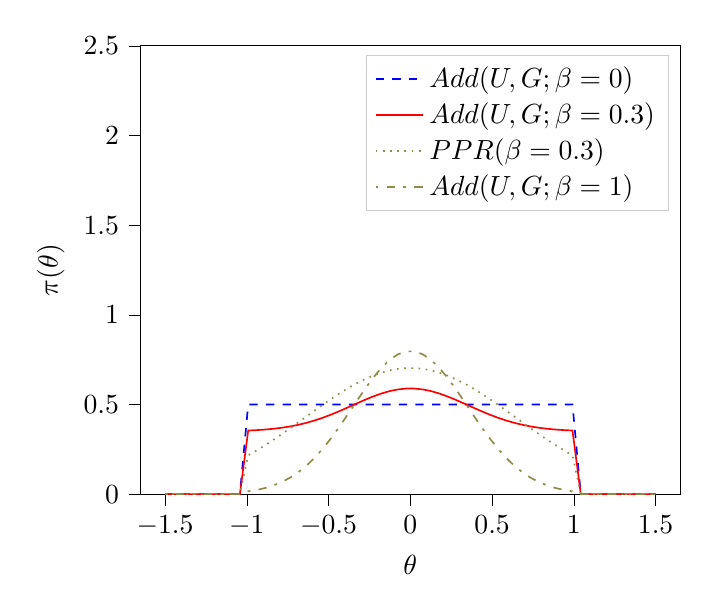
\begin{tikzpicture}

\begin{axis}[
legend cell align={left},
legend style={fill opacity=0.8, draw opacity=1, text opacity=1, draw=white!80!black},
tick align=outside,
tick pos=left,
x grid style={white!69.0196078431373!black},
xlabel={\(\displaystyle \theta\)},
xmin=-1.65, xmax=1.65,
xtick style={color=black},
y grid style={white!69.0196078431373!black},
ylabel={\(\displaystyle \pi(\theta)\)},
ymin=0, ymax=2.5,
ytick style={color=black}
]
\addplot [semithick, blue, dashed]
table {%
-1.5 0
-1.44915254237288 0
-1.39830508474576 0
-1.34745762711864 0
-1.29661016949153 0
-1.24576271186441 0
-1.19491525423729 0
-1.14406779661017 0
-1.09322033898305 0
-1.04237288135593 0
-0.991525423728814 0.5
-0.940677966101695 0.5
-0.889830508474576 0.5
-0.838983050847458 0.5
-0.788135593220339 0.5
-0.73728813559322 0.5
-0.686440677966102 0.5
-0.635593220338983 0.5
-0.584745762711864 0.5
-0.533898305084746 0.5
-0.483050847457627 0.5
-0.432203389830508 0.5
-0.38135593220339 0.5
-0.330508474576271 0.5
-0.279661016949152 0.5
-0.228813559322034 0.5
-0.177966101694915 0.5
-0.127118644067796 0.5
-0.0762711864406778 0.5
-0.0254237288135593 0.5
0.0254237288135595 0.5
0.076271186440678 0.5
0.127118644067797 0.5
0.177966101694915 0.5
0.228813559322034 0.5
0.279661016949153 0.5
0.330508474576271 0.5
0.38135593220339 0.5
0.432203389830509 0.5
0.483050847457627 0.5
0.533898305084746 0.5
0.584745762711865 0.5
0.635593220338983 0.5
0.686440677966102 0.5
0.737288135593221 0.5
0.788135593220339 0.5
0.838983050847458 0.5
0.889830508474577 0.5
0.940677966101695 0.5
0.991525423728814 0.5
1.04237288135593 0
1.09322033898305 0
1.14406779661017 0
1.19491525423729 0
1.24576271186441 0
1.29661016949153 0
1.34745762711864 0
1.39830508474576 0
1.44915254237288 0
1.5 0
};
\addlegendentry{$Add(U, G; \beta=0)$}
\addplot [semithick, red]
table {%
-1.5 0
-1.44915254237288 0
-1.39830508474576 0
-1.34745762711864 0
-1.29661016949153 0
-1.24576271186441 0
-1.19491525423729 0
-1.14406779661017 0
-1.09322033898305 0
-1.04237288135593 0
-0.991525423728814 0.354690318349014
-0.940677966101695 0.356948257984
-0.889830508474576 0.360082465104504
-0.838983050847458 0.364330940676924
-0.788135593220339 0.369952616124693
-0.73728813559322 0.377210854126332
-0.686440677966102 0.386349771016284
-0.635593220338983 0.397563999166328
-0.584745762711864 0.410963827347145
-0.533898305084746 0.426539084688447
-0.483050847457627 0.444126407270881
-0.432203389830508 0.463385332657938
-0.38135593220339 0.483788705911657
-0.330508474576271 0.504631940380111
-0.279661016949152 0.525063713430144
-0.228813559322034 0.54413786330865
-0.177966101694915 0.560882981292239
-0.127118644067796 0.574383024711279
-0.0762711864406778 0.583859836479305
-0.0254237288135593 0.588747297055759
0.0254237288135595 0.588747297055759
0.076271186440678 0.583859836479305
0.127118644067797 0.574383024711279
0.177966101694915 0.560882981292239
0.228813559322034 0.54413786330865
0.279661016949153 0.525063713430144
0.330508474576271 0.504631940380111
0.38135593220339 0.483788705911657
0.432203389830509 0.463385332657938
0.483050847457627 0.444126407270881
0.533898305084746 0.426539084688447
0.584745762711865 0.410963827347145
0.635593220338983 0.397563999166328
0.686440677966102 0.386349771016284
0.737288135593221 0.377210854126332
0.788135593220339 0.369952616124693
0.838983050847458 0.364330940676924
0.889830508474577 0.360082465104504
0.940677966101695 0.356948257984
0.991525423728814 0.354690318349014
1.04237288135593 0
1.09322033898305 0
1.14406779661017 0
1.19491525423729 0
1.24576271186441 0
1.29661016949153 0
1.34745762711864 0
1.39830508474576 0
1.44915254237288 0
1.5 0
};
\addlegendentry{$Add(U, G;\beta=0.3)$}
\addplot [semithick, yellow!50!black, dotted]
table {%
-1.5 0
-1.44915254237288 0
-1.39830508474576 0
-1.34745762711864 0
-1.29661016949153 0
-1.24576271186441 0
-1.19491525423729 0
-1.14406779661017 0
-1.09322033898305 0
-1.04237288135593 0
-0.991525423728814 0.216189593234766
-0.940677966101695 0.243241049554894
-0.889830508474576 0.27198446961261
-0.838983050847458 0.302243171403917
-0.788135593220339 0.333790553940582
-0.73728813559322 0.366350459314597
-0.686440677966102 0.399599183303834
-0.635593220338983 0.433169227869832
-0.584745762711864 0.466654819495022
-0.533898305084746 0.499619139927575
-0.483050847457627 0.531603134276833
-0.432203389830508 0.56213567986932
-0.38135593220339 0.59074482252954
-0.330508474576271 0.616969719742002
-0.279661016949152 0.640372876960198
-0.228813559322034 0.660552228031033
-0.177966101694915 0.677152596268245
-0.127118644067796 0.689876080941671
-0.0762711864406778 0.698490945314958
-0.0254237288135593 0.702838635897227
0.0254237288135595 0.702838635897227
0.076271186440678 0.698490945314958
0.127118644067797 0.689876080941671
0.177966101694915 0.677152596268245
0.228813559322034 0.660552228031033
0.279661016949153 0.640372876960198
0.330508474576271 0.616969719742002
0.38135593220339 0.59074482252954
0.432203389830509 0.56213567986932
0.483050847457627 0.531603134276833
0.533898305084746 0.499619139927575
0.584745762711865 0.466654819495021
0.635593220338983 0.433169227869832
0.686440677966102 0.399599183303834
0.737288135593221 0.366350459314597
0.788135593220339 0.333790553940582
0.838983050847458 0.302243171403917
0.889830508474577 0.27198446961261
0.940677966101695 0.243241049554894
0.991525423728814 0.216189593234766
1.04237288135593 0
1.09322033898305 0
1.14406779661017 0
1.19491525423729 0
1.24576271186441 0
1.29661016949153 0
1.34745762711864 0
1.39830508474576 0
1.44915254237288 0
1.5 0
};
\addlegendentry{$PPR(\beta=0.3)$}
\addplot [semithick, yellow!50!black, dash pattern=on 1pt off 3pt on 3pt off 3pt]
table {%
-1.5 0
-1.44915254237288 0
-1.39830508474576 0
-1.34745762711864 0
-1.29661016949153 0
-1.24576271186441 0
-1.19491525423729 0
-1.14406779661017 0
-1.09322033898305 0
-1.04237288135593 0
-0.991525423728814 0.015634394496712
-0.940677966101695 0.0231608599466659
-0.889830508474576 0.0336082170150122
-0.838983050847458 0.0477698022564135
-0.788135593220339 0.066508720415643
-0.73728813559322 0.0907028470877726
-0.686440677966102 0.121165903387615
-0.635593220338983 0.15854666388776
-0.584745762711864 0.203212757823817
-0.533898305084746 0.255130282294824
-0.483050847457627 0.313754690902936
-0.432203389830508 0.377951108859794
-0.38135593220339 0.445962353038858
-0.330508474576271 0.515439801267037
-0.279661016949152 0.583545711433813
-0.228813559322034 0.647126211028834
-0.177966101694915 0.702943270974129
-0.127118644067796 0.747943415704262
-0.0762711864406778 0.77953278826435
-0.0254237288135593 0.795824323519198
0.0254237288135595 0.795824323519198
0.076271186440678 0.77953278826435
0.127118644067797 0.747943415704262
0.177966101694915 0.702943270974129
0.228813559322034 0.647126211028834
0.279661016949153 0.583545711433812
0.330508474576271 0.515439801267037
0.38135593220339 0.445962353038858
0.432203389830509 0.377951108859794
0.483050847457627 0.313754690902936
0.533898305084746 0.255130282294824
0.584745762711865 0.203212757823817
0.635593220338983 0.15854666388776
0.686440677966102 0.121165903387615
0.737288135593221 0.0907028470877724
0.788135593220339 0.0665087204156429
0.838983050847458 0.0477698022564135
0.889830508474577 0.0336082170150121
0.940677966101695 0.0231608599466659
0.991525423728814 0.015634394496712
1.04237288135593 0
1.09322033898305 0
1.14406779661017 0
1.19491525423729 0
1.24576271186441 0
1.29661016949153 0
1.34745762711864 0
1.39830508474576 0
1.44915254237288 0
1.5 0
};
\addlegendentry{$Add(U, G; \beta=1)$}
\end{axis}

\end{tikzpicture}

\caption{\label{org9a3df54}
An illustration of the additive mixture repartitioning. PPR for the same value of \(\beta=0.3\), added for comparison.}
\end{figure}

This, while inconvenient, can be mitigated. Indeed, since the
probability density functions (PDF) \(\pi_{i}(\theta; \beta) >0\),
the cumulative distribution functions (CDF)
\(CDF{\pi}_{i}(\theta;\beta) = \int_{\Psi} \pi_{i}(\theta; \beta)
	d\theta\) are monotonic, so is their sum, hence one could invert
the CDF numerically. This is extra work that we didn't have to
perform in the PPR case, because raising a Gaussian to a power
\(\beta\), is effectively the same as re-scaling its argument by
\(\sqrt{\beta}\), which transfers to the CDF.

However, one significant improvement over PPR is in
likelihoods. For two priors \(\pi_{1}\) and \(\pi_{2}\)
Normalising the likelihoods is trivial:
\begin{equation}
{\cal L}(\theta; \beta) = \frac{{\cal L}_{1}(\theta) \pi_{1}(\theta)}{\tilde{\pi}(\theta; \beta)}.
\end{equation}
where we've assumed that \({\cal L}_{1}(\theta)\pi_{1}(\theta)
	= {\cal L}_{2}(\theta) \pi_{2}(\theta)\). This generalises
straightforwardly to the case where we have more than one
prior. The likelihood is also a well-behaved function
in the prior space, (because we've required the priors be
non-zero in their domain), which is not always true for every
value of \(\beta\) and every prior in PPR.

Another advantage is that by construction the normalisation
factor \(Z \{ \pi\}(\beta) = 1\) for arbitraty \(\beta\). This
saves considerable effort: one does not care if correlatedness
of the Gaussian, alongside orientation issues can be corrected
for analytically, as one would with PPR\footnote{one couldargue
that correlatedness is irrelevant, as one can always
diagonalise the covariance matrix. The problem, however, is
thus transferred onto the boundary, where for a narrow prior
the orientation of the rectangle's edges in the covariance
eigenbasis can cause issues.}.

A flaw, which additive mixtures share with PPR, is that the
probability of having no bias is negligible. There's always a
preferred direction: if our original prior was uniform, the
probability of having no bias, is the probability of drawing the
value \(\beta=0\) at random. It is not nil, in our case, where
\(\beta\) can only be machine-represent-able 64-bit floating point
number, however this is sufficient to bias the sampler in almost
all cases.

One needs to be aware of this limitation when choosing which
mixing scheme to use. Sometimes, the smooth prior distribution and
likelihood are more beneficial; other times, the ability to with
some probability sample from a completely uniform prior is more
valuable. 

\subsubsection{Re-sizeable-bounds uniform prior.}
\label{sec:orge593f4d}

The three requirements outlined at the beginning of this section
are not necessary and sufficient. As we have noted on page
\pageref{domain-discussion}, the domains of all functions need to be
consistent, otherwise Bayes' theorem no longer holds, and our
analysis is invalid. The mathematical implications of neglecting
function domains have in the context of Quantum mechanics. been
discussed by \cite{Gieres_2000}.

To illustrate, consider a uniform prior with the following
parametrisation.
\begin{equation}
  \tilde{\pi}(\theta; \beta) =
  \begin{cases}
	\frac{1}{\beta(b-a)} & \text{if}\ x \in [\beta a, \beta b] \\
	0 & \text{otherwise}.
  \end{cases}
\end{equation}
Although there are no issues when \(\beta>1\) (we simply set \({\cal
	\tilde{L}}=0\), one can immediately spot the issues with \(\beta \in (0,1)\);
and \(\beta=0\) is altogether nonsensical.

This issue indicates that the prescription of keeping \(\pi {\cal
	L} = \text{Const.}\) is not complete. Nevertheless, such a scheme
may be salvaged, with counter-intuitive extensions, e.g. for a
point \(\theta_{0} \notin \Psi\), we don't expect \({\cal
	L}(\theta_{0}) \rightarrow \infty\), but as we shall see in the
next section, \({\cal L}(\theta_{0}) \rightarrow 0\).

The first crucial step is to recognise that the algorithm draws
from a unit hypercube with uniform probability, and that the prior
is an artifact of a coordinate transformation which we referred to
as the prior quantile.

Let \(u\) be a point in unit hypercube \(\Psi_{C}\). The quantile
defines a mapping functionally dependent on the PDF of the prior
\(C(\beta)\lbrace \tilde{\pi}\rbrace:u \mapsto \theta\), such that
the uniform distribution of \(u\) leads through
\(C_{\beta}\{\tilde{\pi}\}(u)\) to a \(\tilde{\pi}(\theta;\beta)\)
distribution of \(\theta \in\Psi(\beta)\).Note that we replaced the
parametrisation of the function \(\tilde{\pi}\) with an explicit
parametrisation of the coordinate transformation, specifically
\begin{equation}
  \pi(C(\beta)\{\tilde{\pi}\}(u)) \equiv \tilde{\pi}(\theta; \beta),
\end{equation}
where 
\begin{equation}
  \tilde{\pi} =  \pi \circ C(\beta) \{ \pi \} 
\end{equation}
is a parameterised distribution resulting from a parameterised
coordinate transformation of an un-parameterised prior PDF.

We shall make \citeauthor{1763} 's theorem be defined only in the
hypercube
\begin{equation}
{\cal \hat{P}}(u) = {\cal P}(C(\beta_{0}){\tilde{\pi}}^{-1}(\theta)) = \frac{\hat{\pi} (u) {\cal \hat{L}}(u)}{\int_{\Psi}{\cal \hat{L}}(u) \hat{\pi}(u) du},
\end{equation}
which is always true, regardless of the re-partitioning
scheme. Trivially, the functional form of \(P(\theta)\) is not the same
as \(P(u)\); it's related via a co-ordinate transform, which in our
case contributes a Jacobian factor \(J(\beta)\{\tilde{\pi}\}\) to the
evidence. But since we're interested in the posterior in the
coordinates \(\theta\), given by the transformation \(C(\beta_{0})\{\tilde{\pi}\}\),
while the prior and the likelihood are in the from corresponding
to \(\beta\).

Finally, 
\begin{equation}
 {\cal P}(\theta) = \frac{J(\beta_{0})}{J(\beta)} \frac{\pi(\theta; \beta) {\cal L}(\theta; \beta)}{\int \pi(\theta; \beta) {\cal L}(\theta; \beta) d \theta}.
\end{equation}
So we expect that for the simple case of scaling the uniform box
prior with \(\beta\), that we need to re-scale the likelihood by
\(\beta^{2n}\). The second Jacobian factor enters the likelihood because
we have normalised \(\pi(\theta)\), but not \(\pi(\theta; \beta)\). This is hinted at in
the notation, (no tilde), and when accounted for, gives  the correct
posterior and evidence as seen in the experiments. 


\subsubsection{Stochastic superpositional re-partitioning.}
\label{sec:orgf9c6bdb}

Hence we come to the concept of \emph{stochastic superposition-al
posterior repetition} (SSPR). Consider \(\tilde{\pi}(\theta)\) and
\({\cal \tilde{L}}\) which satisfy the normalisation
condition. We construct the parameterised prior like so
\begin{equation}
  \pi(\theta; \beta)  = \begin{cases}
	\pi(\theta) & \text{with probability } \beta\\
	\tilde{\pi}(\theta) & \text{with probability} (1- \beta)
	\end{cases}
\end{equation}
and similarly the likelihood.  The specialisation and
normalisation conditions are trivially satisfied, and the
convergence condition shall be argued later, so this
re-partitioning is valid.

There are difficulties with implementing this scheme,
however. Both the likelihood and the prior are well-defined
single-valued functions, so simply drawing a random number at each
evaluation is not acceptable. Moreover, one needs to make sure
that the branches are simultaneously chosen in both functions, so
as to ensure that the normalisation condition is satisfied. One
way to ensure these are met, is by choosing the branch
deterministic-ally, based on the vector \((\theta; \beta)\). 

To avoid biasing the nested sampler, we must preserve the
uniformity of the distribution. In other words, we must make sure
that the patches belonging to the same branch are interspersed and
are on average the size of regions mapping to the same branch are
the same and of the order of the resolution of the grid. In other
words, for the case \(\beta=1/2\), we wish to have a chequerboard
pattern of branching. 

Note, however, that the prior is no longer normalised. Indeed, for
different values of \(\beta\), integrating over the entire phase
space \(\Psi(\beta)\), one would expect not to obtain unity. And
although intuition might suggest that the normalisation factor
would depend on \(\beta\), as our experiments show this is not the
case. In this particular implementation, the total accessible
prior space volume is restricted by mutual exclusivity. On the
other hand, the posterior and evidence are both fixed by the
normalisation requirement of re-partitioning, so one does not
expect any scaling on \({\cal L}\). 

The greatest advantage that mixture repartitioning nets is
that it is model agnostic: one could, for example, use PPR as
part of a mixture of priors, or even a mixture of
mixtures. One, should judge which mixing method suits their
needs, is it better to have a large bias some of the time, or
a little bias all of the time?

In general,  if one has \(m\) models in a mixture, the likelihood becomes 
\begin{equation}
  {\cal L}(\theta; \beta)  = \begin{cases}
	{\cal L}_{1}(\theta) &  \text{with probability } \beta_{1}\\
		    &\vdots\\
	{\cal L}_{m}(\theta) & \text{with probability} (1- \sum_{i}\beta_{i})
	\end{cases}
\end{equation}


A more important question is of bounded-ness. As we've discussed
(page \pageref{domain-discussion}), when dealing with re-partitioning
schemes such as re-sizeable uniform priors, extra care must be
taken to account for the Jacobian factors arising from a change of
coordinates. Mixture re-partitioning, however, embeds the solution
into its formalism. For example, if a point in the posterior
distribution \(\theta_{e}\), is not represented in the prior, i.e.
\(\pi(\theta_{e}) = 0\), while \({\cal P}(\theta_{e}) \ne 0\), then
one intuitively expects \({\cal L}(\theta_{e}) \rightarrow
	\infty\). In mixture re-partitioning, however, if that same point is
represented in one prior and not the other, the others simply
become unrepresentative, and are selected against by the algorithm
if and only if \({\cal L}(\theta_{e}) = 0\), in the unrepresentative
branch. Thus the value is truly represented, just in a different
prior branch.

\begin{figure}
 % This file was created by tikzplotlib v0.9.1.
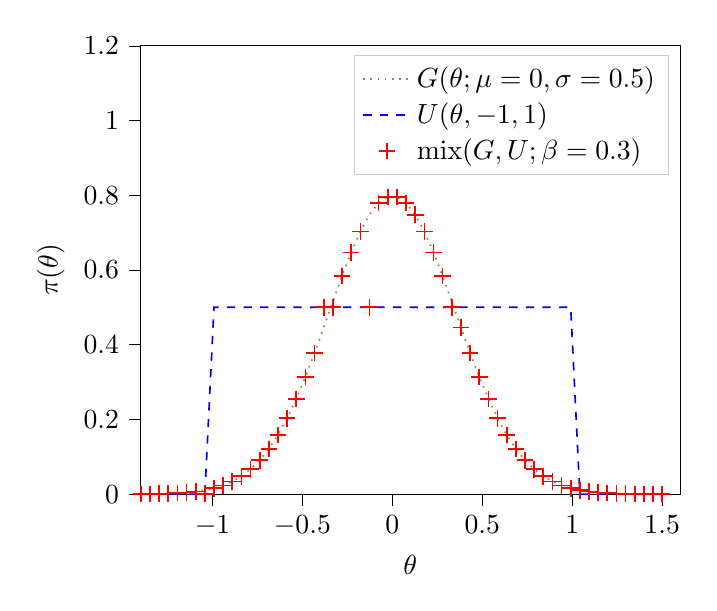
\begin{tikzpicture}

\begin{axis}[
legend cell align={left},
legend style={fill opacity=0.8, draw opacity=1, text opacity=1, draw=white!80!black},
tick align=outside,
tick pos=left,
x grid style={white!69.0196078431373!black},
xlabel={\(\displaystyle \theta\)},
xmin=-1.4, xmax=1.6,
xtick style={color=black},
y grid style={white!69.0196078431373!black},
ylabel={\(\displaystyle \pi(\theta)\)},
ymin=0, ymax=1.2,
ytick style={color=black}
]
\addplot [semithick, yellow!50!black, dotted]
table {%
-1.5 9.8466777332468e-05
-1.44915254237288 0.0001793872435764
-1.39830508474576 0.000320118348094559
-1.34745762711864 0.000559560121531124
-1.29661016949153 0.000958076356441112
-1.24576271186441 0.00160683272401611
-1.19491525423729 0.00263972321036136
-1.14406779661017 0.00424779248787262
-1.09322033898305 0.00669553635076534
-1.04237288135593 0.0103377167883577
-0.991525423728814 0.015634394496712
-0.940677966101695 0.0231608599466659
-0.889830508474576 0.0336082170150122
-0.838983050847458 0.0477698022564135
-0.788135593220339 0.066508720415643
-0.73728813559322 0.0907028470877726
-0.686440677966102 0.121165903387615
-0.635593220338983 0.15854666388776
-0.584745762711864 0.203212757823817
-0.533898305084746 0.255130282294824
-0.483050847457627 0.313754690902936
-0.432203389830508 0.377951108859794
-0.38135593220339 0.445962353038858
-0.330508474576271 0.515439801267037
-0.279661016949152 0.583545711433813
-0.228813559322034 0.647126211028834
-0.177966101694915 0.702943270974129
-0.127118644067796 0.747943415704262
-0.0762711864406778 0.77953278826435
-0.0254237288135593 0.795824323519198
0.0254237288135595 0.795824323519198
0.076271186440678 0.77953278826435
0.127118644067797 0.747943415704262
0.177966101694915 0.702943270974129
0.228813559322034 0.647126211028834
0.279661016949153 0.583545711433812
0.330508474576271 0.515439801267037
0.38135593220339 0.445962353038858
0.432203389830509 0.377951108859794
0.483050847457627 0.313754690902936
0.533898305084746 0.255130282294824
0.584745762711865 0.203212757823817
0.635593220338983 0.15854666388776
0.686440677966102 0.121165903387615
0.737288135593221 0.0907028470877724
0.788135593220339 0.0665087204156429
0.838983050847458 0.0477698022564135
0.889830508474577 0.0336082170150121
0.940677966101695 0.0231608599466659
0.991525423728814 0.015634394496712
1.04237288135593 0.0103377167883577
1.09322033898305 0.00669553635076532
1.14406779661017 0.00424779248787262
1.19491525423729 0.00263972321036135
1.24576271186441 0.0016068327240161
1.29661016949153 0.000958076356441112
1.34745762711864 0.000559560121531121
1.39830508474576 0.000320118348094558
1.44915254237288 0.000179387243576399
1.5 9.8466777332468e-05
};
\addlegendentry{$G(\theta; \mu=0, \sigma=0.5)$}
\addplot [semithick, blue, dashed]
table {%
-1.5 0
-1.44915254237288 0
-1.39830508474576 0
-1.34745762711864 0
-1.29661016949153 0
-1.24576271186441 0
-1.19491525423729 0
-1.14406779661017 0
-1.09322033898305 0
-1.04237288135593 0
-0.991525423728814 0.5
-0.940677966101695 0.5
-0.889830508474576 0.5
-0.838983050847458 0.5
-0.788135593220339 0.5
-0.73728813559322 0.5
-0.686440677966102 0.5
-0.635593220338983 0.5
-0.584745762711864 0.5
-0.533898305084746 0.5
-0.483050847457627 0.5
-0.432203389830508 0.5
-0.38135593220339 0.5
-0.330508474576271 0.5
-0.279661016949152 0.5
-0.228813559322034 0.5
-0.177966101694915 0.5
-0.127118644067796 0.5
-0.0762711864406778 0.5
-0.0254237288135593 0.5
0.0254237288135595 0.5
0.076271186440678 0.5
0.127118644067797 0.5
0.177966101694915 0.5
0.228813559322034 0.5
0.279661016949153 0.5
0.330508474576271 0.5
0.38135593220339 0.5
0.432203389830509 0.5
0.483050847457627 0.5
0.533898305084746 0.5
0.584745762711865 0.5
0.635593220338983 0.5
0.686440677966102 0.5
0.737288135593221 0.5
0.788135593220339 0.5
0.838983050847458 0.5
0.889830508474577 0.5
0.940677966101695 0.5
0.991525423728814 0.5
1.04237288135593 0
1.09322033898305 0
1.14406779661017 0
1.19491525423729 0
1.24576271186441 0
1.29661016949153 0
1.34745762711864 0
1.39830508474576 0
1.44915254237288 0
1.5 0
};
\addlegendentry{$U(\theta, -1, 1)$}
\addplot [semithick, red, mark=+, mark size=3, mark options={solid}, only marks]
table {%
-1.5 9.8466777332468e-05
-1.44915254237288 0.0001793872435764
-1.39830508474576 0
-1.34745762711864 0.000559560121531124
-1.29661016949153 0.000958076356441112
-1.24576271186441 0.00160683272401611
-1.19491525423729 0.00263972321036136
-1.14406779661017 0.00424779248787262
-1.09322033898305 0.00669553635076534
-1.04237288135593 0
-0.991525423728814 0.015634394496712
-0.940677966101695 0.0231608599466659
-0.889830508474576 0.0336082170150122
-0.838983050847458 0.0477698022564135
-0.788135593220339 0.066508720415643
-0.73728813559322 0.0907028470877726
-0.686440677966102 0.121165903387615
-0.635593220338983 0.15854666388776
-0.584745762711864 0.203212757823817
-0.533898305084746 0.255130282294824
-0.483050847457627 0.313754690902936
-0.432203389830508 0.377951108859794
-0.38135593220339 0.5
-0.330508474576271 0.5
-0.279661016949152 0.583545711433813
-0.228813559322034 0.647126211028834
-0.177966101694915 0.702943270974129
-0.127118644067796 0.5
-0.0762711864406778 0.77953278826435
-0.0254237288135593 0.795824323519198
0.0254237288135595 0.795824323519198
0.076271186440678 0.77953278826435
0.127118644067797 0.747943415704262
0.177966101694915 0.702943270974129
0.228813559322034 0.647126211028834
0.279661016949153 0.583545711433812
0.330508474576271 0.5
0.38135593220339 0.445962353038858
0.432203389830509 0.377951108859794
0.483050847457627 0.313754690902936
0.533898305084746 0.255130282294824
0.584745762711865 0.203212757823817
0.635593220338983 0.15854666388776
0.686440677966102 0.121165903387615
0.737288135593221 0.0907028470877724
0.788135593220339 0.0665087204156429
0.838983050847458 0.0477698022564135
0.889830508474577 0.0336082170150121
0.940677966101695 0.0231608599466659
0.991525423728814 0.015634394496712
1.04237288135593 0.0103377167883577
1.09322033898305 0.00669553635076532
1.14406779661017 0.00424779248787262
1.19491525423729 0.00263972321036135
1.24576271186441 0.0016068327240161
1.29661016949153 0.000958076356441112
1.34745762711864 0.000559560121531121
1.39830508474576 0.000320118348094558
1.44915254237288 0.000179387243576399
1.5 9.8466777332468e-05
};
\addlegendentry{mix$(G, U; \beta=0.3)$}
\end{axis}

\end{tikzpicture}

\caption{\label{orgf83cc21}
An example of a mixture re-partitioning. Notice that the mixture is not normalised to emphasise the coincidence of values with both the uniform distribution and a Gaussian.}
\end{figure}



\section{Method}
\label{sec:org759bd76}
In this section we shall describe in detail the types of simulations
and bench-marking that was done. As this project is highly
computational, Cosmological issues are discussed only incidentally,
and only with regard to their computational complexity, not the
Physics.

We have chosen to use Cobaya \citep{cobaya}, with CLASS to provide the
theoretical framework for analysing the Planck \citep{planck}
data. Our primary goal is to improve the performance of the
analysis.

We shall first describe how one would measure the performance of
such a run, then show the small-scale simulation results. Finally,
we shall discuss the results obtained by running Cobaya with the
suggested optimisations on the CSD3 cluster (University of Cambridge).


\subsection{Performance and bench-marking}
\label{sec:org80ad06f}
One cannot use CPU time as a reliable indicator of
performance. There are multiple factors leading to unpredictable
overheads, and these can be practically averaged out on a small
scale model, in case of large distributed systems such as a CPU
cluster, with multiple processes, and with each run taking upwards
of an hour, this metric is beyond the realm usefulness.

Due to the sheer complexity of the Cosmological data and functions
involved in the computation, the usual asymptotic description
common in computer science is insufficient. 

First, note that in Cobaya  the run-time is dominated
by log-likelihood evaluations. A typical run in 3 dimensions
requires \(O(10^{3})\), likelihood calls, and if each of them takes a
second to evaluate, a simple run becomes impractical. 

So a natural choice for a performance metric is using the number of
log-likelihood evaluations. 

Note, however that this does not account for potential extra
complexity introduced by the re-partitioning. For example for PPR,
the effect of adding the extra parameter can be reduced to
\begin{enumerate}
\item one multiplication in the argument of the prior.
\item evaluation of the normalisation factor, which involves standard
numerical functions,
\item addition of the normalisation factor to each log-likelihood call.
\end{enumerate}

The corresponding overhead for mixture modelling is
\begin{enumerate}
\item hashing the vector \(\theta\).
\item generating a pseudo-random number using the hash as seed.
\item performing \(m-1\) conditional checks,
\item addition of \(\ln m\), to the likelihood.
\end{enumerate}

In both cases there's also a minuscule overhead associated with
lengthening the state vector \(\theta\)\footnote{in mixture modelling one could either introduce \(m+1\)
parameters, and perform the hashing once, at the cost of adding an
extra branch index, or add \(m\), parameters but perform the hashing
twice. To choose, mind that the extra branch index parameter, may
adversely impact the convergence as its posterior needs to be computed
just like any other nuisance parameter's.}.  Although these may
become important in low dimensional problems, they are overshadowed
in all practical applications of nested sampling, and thus we shall
ignore them.

Another information-theoretic performance metric that one could use
is the Kullback-Leibler divergence \({\cal D}\). A thorough
explanation of the concept can be found at \cite{Kullback_1951}, but
for our purposes, this is a quantity allowing to compare the prior
to the inferred posterior. The larger the value, the more Shannon
entropy is associated with moving from prior to posterior. 

To understand why K-L divergence is useful, consider that under
ideal circumstances inference with the posterior also the prior is
optimal. Hence, justifiably we expect priors with the smallest
\(\mathcal{D}\) to converge faster. This is a useful worldview when
considering general Bayesian inference, but its applicability to
nested sampling is limited. The performance of a nested sampler
depends on many factors besides the entropy. For example, as we've
shown in a preliminary experiment, \footnote{\texttt{./toy-models/2/2.1 Repartitioning with power posterior.py}} nested sampling can
converge faster if the distribution is narrower than the posterior
(PPR takes care of the correctness). 



\subsection{Correctness}
\label{sec:orgab723c1}
One simple and unreliable way of determining the correctness of a
run is to compare the posteriors of two runs: if the means of two
runs are within one standard deviation of each other, then the
posteriors can be assumed to coincide.

Consider, however, what would happen, if one were to use a Gaussian
prior without posterior re-partitioning on a data set, which was
previously analysed using a uniform prior. One would expect the
posterior to have tighter constraints, smaller variances and for
the evidence to be much higher. Of course, it's normal if said
Gaussian truly represents prior knowledge, but as was mentioned in
previous sections, this is an error for any form of posterior
re-partitioning: it usually means that the re-scaling of the
likelihood is incorrect. Hence we must include (or rather base our
comparison on) the estimated evidences into consideration.

\begin{figure}
% This file was created by tikzplotlib v0.9.1.
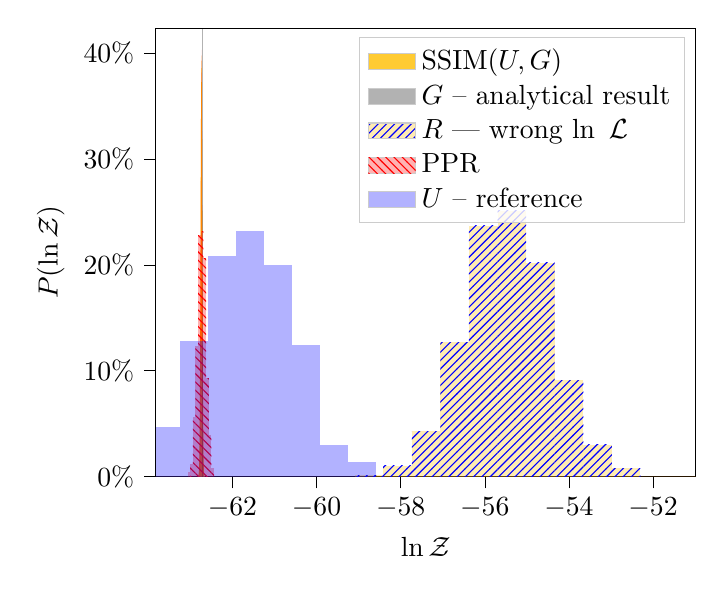
\begin{tikzpicture}

\definecolor{color2}{rgb}{0.0,0.0,1}
\definecolor{color1}{rgb}{1,0.00,0.00}
\definecolor{colorblack}{rgb}{0, 0, 0}
\definecolor{color0}{rgb}{1.0,0.75,0.0}

\begin{axis}[
legend cell align={left},
legend style={fill opacity=0.8, draw opacity=1, text opacity=1, anchor=north east, draw=white!80!black},
tick align=outside,
tick pos=left,
x grid style={white!69.0196078431373!black},
xlabel={\(\ln {\cal Z}\)},
xmin=-63.8198069562379, xmax=-50.9892026507015,
xtick style={color=black},
yticklabel={\pgfmathparse{\tick/10}\pgfmathprintnumber{\pgfmathresult}\%},
y grid style={white!69.0196078431373!black},
ylabel={\(P(\ln {\cal Z})\)},
ymin=0, ymax=423.473092744885,
ytick style={color=black}
]
\path [fill=color0]
(axis cs:-63.8198069562379,0)
--(axis cs:-63.8198069562379,0)
--(axis cs:-63.8069635084846,0)
--(axis cs:-63.7941200607313,0)
--(axis cs:-63.7812766129781,0)
--(axis cs:-63.7684331652248,0)
--(axis cs:-63.7555897174715,0)
--(axis cs:-63.7427462697182,0)
--(axis cs:-63.7299028219649,0)
--(axis cs:-63.7170593742116,0)
--(axis cs:-63.7042159264583,0)
--(axis cs:-63.691372478705,0)
--(axis cs:-63.6785290309517,0)
--(axis cs:-63.6656855831984,0)
--(axis cs:-63.6528421354452,0)
--(axis cs:-63.6399986876919,0)
--(axis cs:-63.6271552399386,0)
--(axis cs:-63.6143117921853,0)
--(axis cs:-63.601468344432,0)
--(axis cs:-63.5886248966787,0)
--(axis cs:-63.5757814489254,0)
--(axis cs:-63.5629380011721,0)
--(axis cs:-63.5500945534188,0)
--(axis cs:-63.5372511056656,0)
--(axis cs:-63.5244076579123,0)
--(axis cs:-63.511564210159,0)
--(axis cs:-63.4987207624057,0)
--(axis cs:-63.4858773146524,0)
--(axis cs:-63.4730338668991,0)
--(axis cs:-63.4601904191458,0)
--(axis cs:-63.4473469713925,0)
--(axis cs:-63.4345035236392,0)
--(axis cs:-63.4216600758859,0)
--(axis cs:-63.4088166281327,0)
--(axis cs:-63.3959731803794,0)
--(axis cs:-63.3831297326261,0)
--(axis cs:-63.3702862848728,0)
--(axis cs:-63.3574428371195,0)
--(axis cs:-63.3445993893662,0)
--(axis cs:-63.3317559416129,0)
--(axis cs:-63.3189124938596,0)
--(axis cs:-63.3060690461063,0)
--(axis cs:-63.293225598353,0)
--(axis cs:-63.2803821505998,0)
--(axis cs:-63.2675387028465,0)
--(axis cs:-63.2546952550932,0)
--(axis cs:-63.2418518073399,0)
--(axis cs:-63.2290083595866,0)
--(axis cs:-63.2161649118333,0)
--(axis cs:-63.20332146408,0)
--(axis cs:-63.1904780163267,0)
--(axis cs:-63.1776345685734,0)
--(axis cs:-63.1647911208201,0)
--(axis cs:-63.1519476730669,0)
--(axis cs:-63.1391042253136,0)
--(axis cs:-63.1262607775603,0)
--(axis cs:-63.113417329807,0)
--(axis cs:-63.1005738820537,0)
--(axis cs:-63.0877304343004,0)
--(axis cs:-63.0748869865471,0)
--(axis cs:-63.0620435387938,0)
--(axis cs:-63.0492000910405,0)
--(axis cs:-63.0363566432872,0)
--(axis cs:-63.023513195534,0)
--(axis cs:-63.0106697477807,0)
--(axis cs:-62.9978263000274,0)
--(axis cs:-62.9849828522741,0)
--(axis cs:-62.9721394045208,0)
--(axis cs:-62.9592959567675,0)
--(axis cs:-62.9464525090142,0)
--(axis cs:-62.9336090612609,0)
--(axis cs:-62.9207656135076,0)
--(axis cs:-62.9079221657544,0)
--(axis cs:-62.8950787180011,0)
--(axis cs:-62.8822352702478,0)
--(axis cs:-62.8693918224945,0)
--(axis cs:-62.8565483747412,0)
--(axis cs:-62.8437049269879,0)
--(axis cs:-62.8308614792346,0)
--(axis cs:-62.8180180314813,0)
--(axis cs:-62.805174583728,0)
--(axis cs:-62.7923311359747,0)
--(axis cs:-62.7794876882215,0)
--(axis cs:-62.7666442404682,0)
--(axis cs:-62.7538007927149,0)
--(axis cs:-62.7409573449616,0)
--(axis cs:-62.7281138972083,0)
--(axis cs:-62.715270449455,0)
--(axis cs:-62.7024270017017,0)
--(axis cs:-62.6895835539484,0)
--(axis cs:-62.6767401061951,0)
--(axis cs:-62.6638966584418,0)
--(axis cs:-62.6510532106886,0)
--(axis cs:-62.6382097629353,0)
--(axis cs:-62.625366315182,0)
--(axis cs:-62.6125228674287,0)
--(axis cs:-62.5996794196754,0)
--(axis cs:-62.5868359719221,0)
--(axis cs:-62.5739925241688,0)
--(axis cs:-62.5611490764155,0)
--(axis cs:-62.5483056286622,0)
--(axis cs:-62.535462180909,0)
--(axis cs:-62.5226187331557,0)
--(axis cs:-62.5097752854024,0)
--(axis cs:-62.4969318376491,0)
--(axis cs:-62.4840883898958,0)
--(axis cs:-62.4712449421425,0)
--(axis cs:-62.4584014943892,0)
--(axis cs:-62.4455580466359,0)
--(axis cs:-62.4327145988826,0)
--(axis cs:-62.4198711511293,0)
--(axis cs:-62.4070277033761,0)
--(axis cs:-62.3941842556228,0)
--(axis cs:-62.3813408078695,0)
--(axis cs:-62.3684973601162,0)
--(axis cs:-62.3556539123629,0)
--(axis cs:-62.3428104646096,0)
--(axis cs:-62.3299670168563,0)
--(axis cs:-62.317123569103,0)
--(axis cs:-62.3042801213497,0)
--(axis cs:-62.2914366735965,0)
--(axis cs:-62.2785932258432,0)
--(axis cs:-62.2657497780899,0)
--(axis cs:-62.2529063303366,0)
--(axis cs:-62.2400628825833,0)
--(axis cs:-62.22721943483,0)
--(axis cs:-62.2143759870767,0)
--(axis cs:-62.2015325393234,0)
--(axis cs:-62.1886890915701,0)
--(axis cs:-62.1758456438168,0)
--(axis cs:-62.1630021960636,0)
--(axis cs:-62.1501587483103,0)
--(axis cs:-62.137315300557,0)
--(axis cs:-62.1244718528037,0)
--(axis cs:-62.1116284050504,0)
--(axis cs:-62.0987849572971,0)
--(axis cs:-62.0859415095438,0)
--(axis cs:-62.0730980617905,0)
--(axis cs:-62.0602546140372,0)
--(axis cs:-62.0474111662839,0)
--(axis cs:-62.0345677185307,0)
--(axis cs:-62.0217242707774,0)
--(axis cs:-62.0088808230241,0)
--(axis cs:-61.9960373752708,0)
--(axis cs:-61.9831939275175,0)
--(axis cs:-61.9703504797642,0)
--(axis cs:-61.9575070320109,0)
--(axis cs:-61.9446635842576,0)
--(axis cs:-61.9318201365043,0)
--(axis cs:-61.918976688751,0)
--(axis cs:-61.9061332409978,0)
--(axis cs:-61.8932897932445,0)
--(axis cs:-61.8804463454912,0)
--(axis cs:-61.8676028977379,0)
--(axis cs:-61.8547594499846,0)
--(axis cs:-61.8419160022313,0)
--(axis cs:-61.829072554478,0)
--(axis cs:-61.8162291067247,0)
--(axis cs:-61.8033856589714,0)
--(axis cs:-61.7905422112181,0)
--(axis cs:-61.7776987634649,0)
--(axis cs:-61.7648553157116,0)
--(axis cs:-61.7520118679583,0)
--(axis cs:-61.739168420205,0)
--(axis cs:-61.7263249724517,0)
--(axis cs:-61.7134815246984,0)
--(axis cs:-61.7006380769451,0)
--(axis cs:-61.6877946291918,0)
--(axis cs:-61.6749511814385,0)
--(axis cs:-61.6621077336853,0)
--(axis cs:-61.649264285932,0)
--(axis cs:-61.6364208381787,0)
--(axis cs:-61.6235773904254,0)
--(axis cs:-61.6107339426721,0)
--(axis cs:-61.5978904949188,0)
--(axis cs:-61.5850470471655,0)
--(axis cs:-61.5722035994122,0)
--(axis cs:-61.5593601516589,0)
--(axis cs:-61.5465167039056,0)
--(axis cs:-61.5336732561524,0)
--(axis cs:-61.5208298083991,0)
--(axis cs:-61.5079863606458,0)
--(axis cs:-61.4951429128925,0)
--(axis cs:-61.4822994651392,0)
--(axis cs:-61.4694560173859,0)
--(axis cs:-61.4566125696326,0)
--(axis cs:-61.4437691218793,0)
--(axis cs:-61.430925674126,0)
--(axis cs:-61.4180822263727,0)
--(axis cs:-61.4052387786195,0)
--(axis cs:-61.3923953308662,0)
--(axis cs:-61.3795518831129,0)
--(axis cs:-61.3667084353596,0)
--(axis cs:-61.3538649876063,0)
--(axis cs:-61.341021539853,0)
--(axis cs:-61.3281780920997,0)
--(axis cs:-61.3153346443464,0)
--(axis cs:-61.3024911965931,0)
--(axis cs:-61.2896477488398,0)
--(axis cs:-61.2768043010866,0)
--(axis cs:-61.2639608533333,0)
--(axis cs:-61.25111740558,0)
--(axis cs:-61.2382739578267,0)
--(axis cs:-61.2254305100734,0)
--(axis cs:-61.2125870623201,0)
--(axis cs:-61.1997436145668,0)
--(axis cs:-61.1869001668135,0)
--(axis cs:-61.1740567190602,0)
--(axis cs:-61.1612132713069,0)
--(axis cs:-61.1483698235537,0)
--(axis cs:-61.1355263758004,0)
--(axis cs:-61.1226829280471,0)
--(axis cs:-61.1098394802938,0)
--(axis cs:-61.0969960325405,0)
--(axis cs:-61.0841525847872,0)
--(axis cs:-61.0713091370339,0)
--(axis cs:-61.0584656892806,0)
--(axis cs:-61.0456222415273,0)
--(axis cs:-61.0327787937741,0)
--(axis cs:-61.0199353460208,0)
--(axis cs:-61.0070918982675,0)
--(axis cs:-60.9942484505142,0)
--(axis cs:-60.9814050027609,0)
--(axis cs:-60.9685615550076,0)
--(axis cs:-60.9557181072543,0)
--(axis cs:-60.942874659501,0)
--(axis cs:-60.9300312117477,0)
--(axis cs:-60.9171877639944,0)
--(axis cs:-60.9043443162412,0)
--(axis cs:-60.8915008684879,0)
--(axis cs:-60.8786574207346,0)
--(axis cs:-60.8658139729813,0)
--(axis cs:-60.852970525228,0)
--(axis cs:-60.8401270774747,0)
--(axis cs:-60.8272836297214,0)
--(axis cs:-60.8144401819681,0)
--(axis cs:-60.8015967342148,0)
--(axis cs:-60.7887532864615,0)
--(axis cs:-60.7759098387083,0)
--(axis cs:-60.763066390955,0)
--(axis cs:-60.7502229432017,0)
--(axis cs:-60.7373794954484,0)
--(axis cs:-60.7245360476951,0)
--(axis cs:-60.7116925999418,0)
--(axis cs:-60.6988491521885,0)
--(axis cs:-60.6860057044352,0)
--(axis cs:-60.6731622566819,0)
--(axis cs:-60.6603188089287,0)
--(axis cs:-60.6474753611754,0)
--(axis cs:-60.6346319134221,0)
--(axis cs:-60.6217884656688,0)
--(axis cs:-60.6089450179155,0)
--(axis cs:-60.5961015701622,0)
--(axis cs:-60.5832581224089,0)
--(axis cs:-60.5704146746556,0)
--(axis cs:-60.5575712269023,0)
--(axis cs:-60.544727779149,0)
--(axis cs:-60.5318843313958,0)
--(axis cs:-60.5190408836425,0)
--(axis cs:-60.5061974358892,0)
--(axis cs:-60.4933539881359,0)
--(axis cs:-60.4805105403826,0)
--(axis cs:-60.4676670926293,0)
--(axis cs:-60.454823644876,0)
--(axis cs:-60.4419801971227,0)
--(axis cs:-60.4291367493694,0)
--(axis cs:-60.4162933016162,0)
--(axis cs:-60.4034498538629,0)
--(axis cs:-60.3906064061096,0)
--(axis cs:-60.3777629583563,0)
--(axis cs:-60.364919510603,0)
--(axis cs:-60.3520760628497,0)
--(axis cs:-60.3392326150964,0)
--(axis cs:-60.3263891673431,0)
--(axis cs:-60.3135457195898,0)
--(axis cs:-60.3007022718365,0)
--(axis cs:-60.2878588240833,0)
--(axis cs:-60.27501537633,0)
--(axis cs:-60.2621719285767,0)
--(axis cs:-60.2493284808234,0)
--(axis cs:-60.2364850330701,0)
--(axis cs:-60.2236415853168,0)
--(axis cs:-60.2107981375635,0)
--(axis cs:-60.1979546898102,0)
--(axis cs:-60.1851112420569,0)
--(axis cs:-60.1722677943036,0)
--(axis cs:-60.1594243465504,0)
--(axis cs:-60.1465808987971,0)
--(axis cs:-60.1337374510438,0)
--(axis cs:-60.1208940032905,0)
--(axis cs:-60.1080505555372,0)
--(axis cs:-60.0952071077839,0)
--(axis cs:-60.0823636600306,0)
--(axis cs:-60.0695202122773,0)
--(axis cs:-60.056676764524,0)
--(axis cs:-60.0438333167707,0)
--(axis cs:-60.0309898690175,0)
--(axis cs:-60.0181464212642,0)
--(axis cs:-60.0053029735109,0)
--(axis cs:-59.9924595257576,0)
--(axis cs:-59.9796160780043,0)
--(axis cs:-59.966772630251,0)
--(axis cs:-59.9539291824977,0)
--(axis cs:-59.9410857347444,0)
--(axis cs:-59.9282422869911,0)
--(axis cs:-59.9153988392378,0)
--(axis cs:-59.9025553914846,0)
--(axis cs:-59.8897119437313,0)
--(axis cs:-59.876868495978,0)
--(axis cs:-59.8640250482247,0)
--(axis cs:-59.8511816004714,0)
--(axis cs:-59.8383381527181,0)
--(axis cs:-59.8254947049648,0)
--(axis cs:-59.8126512572115,0)
--(axis cs:-59.7998078094582,0)
--(axis cs:-59.786964361705,0)
--(axis cs:-59.7741209139517,0)
--(axis cs:-59.7612774661984,0)
--(axis cs:-59.7484340184451,0)
--(axis cs:-59.7355905706918,0)
--(axis cs:-59.7227471229385,0)
--(axis cs:-59.7099036751852,0)
--(axis cs:-59.6970602274319,0)
--(axis cs:-59.6842167796786,0)
--(axis cs:-59.6713733319253,0)
--(axis cs:-59.6585298841721,0)
--(axis cs:-59.6456864364188,0)
--(axis cs:-59.6328429886655,0)
--(axis cs:-59.6199995409122,0)
--(axis cs:-59.6071560931589,0)
--(axis cs:-59.5943126454056,0)
--(axis cs:-59.5814691976523,0)
--(axis cs:-59.568625749899,0)
--(axis cs:-59.5557823021457,0)
--(axis cs:-59.5429388543924,0)
--(axis cs:-59.5300954066392,0)
--(axis cs:-59.5172519588859,0)
--(axis cs:-59.5044085111326,0)
--(axis cs:-59.4915650633793,0)
--(axis cs:-59.478721615626,0)
--(axis cs:-59.4658781678727,0)
--(axis cs:-59.4530347201194,0)
--(axis cs:-59.4401912723661,0)
--(axis cs:-59.4273478246128,0)
--(axis cs:-59.4145043768595,0)
--(axis cs:-59.4016609291063,0)
--(axis cs:-59.388817481353,0)
--(axis cs:-59.3759740335997,0)
--(axis cs:-59.3631305858464,0)
--(axis cs:-59.3502871380931,0)
--(axis cs:-59.3374436903398,0)
--(axis cs:-59.3246002425865,0)
--(axis cs:-59.3117567948332,0)
--(axis cs:-59.2989133470799,0)
--(axis cs:-59.2860698993266,0)
--(axis cs:-59.2732264515734,0)
--(axis cs:-59.2603830038201,0)
--(axis cs:-59.2475395560668,0)
--(axis cs:-59.2346961083135,0)
--(axis cs:-59.2218526605602,0)
--(axis cs:-59.2090092128069,0)
--(axis cs:-59.1961657650536,0)
--(axis cs:-59.1833223173003,0)
--(axis cs:-59.170478869547,0)
--(axis cs:-59.1576354217938,0)
--(axis cs:-59.1447919740405,0)
--(axis cs:-59.1319485262872,0)
--(axis cs:-59.1191050785339,0)
--(axis cs:-59.1062616307806,0)
--(axis cs:-59.0934181830273,0)
--(axis cs:-59.080574735274,0)
--(axis cs:-59.0677312875207,0)
--(axis cs:-59.0548878397674,0)
--(axis cs:-59.0420443920141,0)
--(axis cs:-59.0292009442609,0)
--(axis cs:-59.0163574965076,0)
--(axis cs:-59.0035140487543,0)
--(axis cs:-58.990670601001,0)
--(axis cs:-58.9778271532477,0)
--(axis cs:-58.9649837054944,0)
--(axis cs:-58.9521402577411,0)
--(axis cs:-58.9392968099878,0)
--(axis cs:-58.9264533622345,0)
--(axis cs:-58.9136099144812,0)
--(axis cs:-58.900766466728,0)
--(axis cs:-58.8879230189747,0)
--(axis cs:-58.8750795712214,0)
--(axis cs:-58.8622361234681,0)
--(axis cs:-58.8493926757148,0)
--(axis cs:-58.8365492279615,0)
--(axis cs:-58.8237057802082,0)
--(axis cs:-58.8108623324549,0)
--(axis cs:-58.7980188847016,0)
--(axis cs:-58.7851754369484,0)
--(axis cs:-58.7723319891951,0)
--(axis cs:-58.7594885414418,0)
--(axis cs:-58.7466450936885,0)
--(axis cs:-58.7338016459352,0)
--(axis cs:-58.7209581981819,0)
--(axis cs:-58.7081147504286,0)
--(axis cs:-58.6952713026753,0)
--(axis cs:-58.682427854922,0)
--(axis cs:-58.6695844071687,0)
--(axis cs:-58.6567409594155,0)
--(axis cs:-58.6438975116622,0)
--(axis cs:-58.6310540639089,0)
--(axis cs:-58.6182106161556,0)
--(axis cs:-58.6053671684023,0)
--(axis cs:-58.592523720649,0)
--(axis cs:-58.5796802728957,0)
--(axis cs:-58.5668368251424,0)
--(axis cs:-58.5539933773891,0)
--(axis cs:-58.5411499296358,0)
--(axis cs:-58.5283064818826,0)
--(axis cs:-58.5154630341293,0)
--(axis cs:-58.502619586376,0)
--(axis cs:-58.4897761386227,0)
--(axis cs:-58.4769326908694,0)
--(axis cs:-58.4640892431161,0)
--(axis cs:-58.4512457953628,0)
--(axis cs:-58.4384023476095,0)
--(axis cs:-58.4255588998562,0)
--(axis cs:-58.412715452103,0)
--(axis cs:-58.3998720043497,0)
--(axis cs:-58.3870285565964,0)
--(axis cs:-58.3741851088431,0)
--(axis cs:-58.3613416610898,0)
--(axis cs:-58.3484982133365,0)
--(axis cs:-58.3356547655832,0)
--(axis cs:-58.3228113178299,0)
--(axis cs:-58.3099678700766,0)
--(axis cs:-58.2971244223233,0)
--(axis cs:-58.2842809745701,0)
--(axis cs:-58.2714375268168,0)
--(axis cs:-58.2585940790635,0)
--(axis cs:-58.2457506313102,0)
--(axis cs:-58.2329071835569,0)
--(axis cs:-58.2200637358036,0)
--(axis cs:-58.2072202880503,0)
--(axis cs:-58.194376840297,0)
--(axis cs:-58.1815333925437,0)
--(axis cs:-58.1686899447904,0)
--(axis cs:-58.1558464970372,0)
--(axis cs:-58.1430030492839,0)
--(axis cs:-58.1301596015306,0)
--(axis cs:-58.1173161537773,0)
--(axis cs:-58.104472706024,0)
--(axis cs:-58.0916292582707,0)
--(axis cs:-58.0787858105174,0)
--(axis cs:-58.0659423627641,0)
--(axis cs:-58.0530989150108,0)
--(axis cs:-58.0402554672575,0)
--(axis cs:-58.0274120195043,0)
--(axis cs:-58.014568571751,0)
--(axis cs:-58.0017251239977,0)
--(axis cs:-57.9888816762444,0)
--(axis cs:-57.9760382284911,0)
--(axis cs:-57.9631947807378,0)
--(axis cs:-57.9503513329845,0)
--(axis cs:-57.9375078852312,0)
--(axis cs:-57.9246644374779,0)
--(axis cs:-57.9118209897247,0)
--(axis cs:-57.8989775419714,0)
--(axis cs:-57.8861340942181,0)
--(axis cs:-57.8732906464648,0)
--(axis cs:-57.8604471987115,0)
--(axis cs:-57.8476037509582,0)
--(axis cs:-57.8347603032049,0)
--(axis cs:-57.8219168554516,0)
--(axis cs:-57.8090734076983,0)
--(axis cs:-57.796229959945,0)
--(axis cs:-57.7833865121918,0)
--(axis cs:-57.7705430644385,0)
--(axis cs:-57.7576996166852,0)
--(axis cs:-57.7448561689319,0)
--(axis cs:-57.7320127211786,0)
--(axis cs:-57.7191692734253,0)
--(axis cs:-57.706325825672,0)
--(axis cs:-57.6934823779187,0)
--(axis cs:-57.6806389301654,0)
--(axis cs:-57.6677954824121,0)
--(axis cs:-57.6549520346589,0)
--(axis cs:-57.6421085869056,0)
--(axis cs:-57.6292651391523,0)
--(axis cs:-57.616421691399,0)
--(axis cs:-57.6035782436457,0)
--(axis cs:-57.5907347958924,0)
--(axis cs:-57.5778913481391,0)
--(axis cs:-57.5650479003858,0)
--(axis cs:-57.5522044526325,0)
--(axis cs:-57.5393610048792,0)
--(axis cs:-57.526517557126,0)
--(axis cs:-57.5136741093727,0)
--(axis cs:-57.5008306616194,0)
--(axis cs:-57.4879872138661,0)
--(axis cs:-57.4751437661128,0)
--(axis cs:-57.4623003183595,0)
--(axis cs:-57.4494568706062,0)
--(axis cs:-57.4366134228529,0)
--(axis cs:-57.4237699750996,0)
--(axis cs:-57.4109265273463,0)
--(axis cs:-57.3980830795931,0)
--(axis cs:-57.3852396318398,0)
--(axis cs:-57.3723961840865,0)
--(axis cs:-57.3595527363332,0)
--(axis cs:-57.3467092885799,0)
--(axis cs:-57.3338658408266,0)
--(axis cs:-57.3210223930733,0)
--(axis cs:-57.30817894532,0)
--(axis cs:-57.2953354975667,0)
--(axis cs:-57.2824920498135,0)
--(axis cs:-57.2696486020602,0)
--(axis cs:-57.2568051543069,0)
--(axis cs:-57.2439617065536,0)
--(axis cs:-57.2311182588003,0)
--(axis cs:-57.218274811047,0)
--(axis cs:-57.2054313632937,0)
--(axis cs:-57.1925879155404,0)
--(axis cs:-57.1797444677871,0)
--(axis cs:-57.1669010200338,0)
--(axis cs:-57.1540575722806,0)
--(axis cs:-57.1412141245273,0)
--(axis cs:-57.128370676774,0)
--(axis cs:-57.1155272290207,0)
--(axis cs:-57.1026837812674,0)
--(axis cs:-57.0898403335141,0)
--(axis cs:-57.0769968857608,0)
--(axis cs:-57.0641534380075,0)
--(axis cs:-57.0513099902542,0)
--(axis cs:-57.0384665425009,0)
--(axis cs:-57.0256230947477,0)
--(axis cs:-57.0127796469944,0)
--(axis cs:-56.9999361992411,0)
--(axis cs:-56.9870927514878,0)
--(axis cs:-56.9742493037345,0)
--(axis cs:-56.9614058559812,0)
--(axis cs:-56.9485624082279,0)
--(axis cs:-56.9357189604746,0)
--(axis cs:-56.9228755127213,0)
--(axis cs:-56.910032064968,0)
--(axis cs:-56.8971886172148,0)
--(axis cs:-56.8843451694615,0)
--(axis cs:-56.8715017217082,0)
--(axis cs:-56.8586582739549,0)
--(axis cs:-56.8458148262016,0)
--(axis cs:-56.8329713784483,0)
--(axis cs:-56.820127930695,0)
--(axis cs:-56.8072844829417,0)
--(axis cs:-56.7944410351884,0)
--(axis cs:-56.7815975874352,0)
--(axis cs:-56.7687541396819,0)
--(axis cs:-56.7559106919286,0)
--(axis cs:-56.7430672441753,0)
--(axis cs:-56.730223796422,0)
--(axis cs:-56.7173803486687,0)
--(axis cs:-56.7045369009154,0)
--(axis cs:-56.6916934531621,0)
--(axis cs:-56.6788500054088,0)
--(axis cs:-56.6660065576555,0)
--(axis cs:-56.6531631099023,0)
--(axis cs:-56.640319662149,0)
--(axis cs:-56.6274762143957,0)
--(axis cs:-56.6146327666424,0)
--(axis cs:-56.6017893188891,0)
--(axis cs:-56.5889458711358,0)
--(axis cs:-56.5761024233825,0)
--(axis cs:-56.5632589756292,0)
--(axis cs:-56.5504155278759,0)
--(axis cs:-56.5375720801227,0)
--(axis cs:-56.5247286323694,0)
--(axis cs:-56.5118851846161,0)
--(axis cs:-56.4990417368628,0)
--(axis cs:-56.4861982891095,0)
--(axis cs:-56.4733548413562,0)
--(axis cs:-56.4605113936029,0)
--(axis cs:-56.4476679458496,0)
--(axis cs:-56.4348244980963,0)
--(axis cs:-56.421981050343,0)
--(axis cs:-56.4091376025898,0)
--(axis cs:-56.3962941548365,0)
--(axis cs:-56.3834507070832,0)
--(axis cs:-56.3706072593299,0)
--(axis cs:-56.3577638115766,0)
--(axis cs:-56.3449203638233,0)
--(axis cs:-56.33207691607,0)
--(axis cs:-56.3192334683167,0)
--(axis cs:-56.3063900205634,0)
--(axis cs:-56.2935465728101,0)
--(axis cs:-56.2807031250569,0)
--(axis cs:-56.2678596773036,0)
--(axis cs:-56.2550162295503,0)
--(axis cs:-56.242172781797,0)
--(axis cs:-56.2293293340437,0)
--(axis cs:-56.2164858862904,0)
--(axis cs:-56.2036424385371,0)
--(axis cs:-56.1907989907838,0)
--(axis cs:-56.1779555430305,0)
--(axis cs:-56.1651120952772,0)
--(axis cs:-56.152268647524,0)
--(axis cs:-56.1394251997707,0)
--(axis cs:-56.1265817520174,0)
--(axis cs:-56.1137383042641,0)
--(axis cs:-56.1008948565108,0)
--(axis cs:-56.0880514087575,0)
--(axis cs:-56.0752079610042,0)
--(axis cs:-56.0623645132509,0)
--(axis cs:-56.0495210654976,0)
--(axis cs:-56.0366776177444,0)
--(axis cs:-56.0238341699911,0)
--(axis cs:-56.0109907222378,0)
--(axis cs:-55.9981472744845,0)
--(axis cs:-55.9853038267312,0)
--(axis cs:-55.9724603789779,0)
--(axis cs:-55.9596169312246,0)
--(axis cs:-55.9467734834713,0)
--(axis cs:-55.933930035718,0)
--(axis cs:-55.9210865879647,0)
--(axis cs:-55.9082431402115,0)
--(axis cs:-55.8953996924582,0)
--(axis cs:-55.8825562447049,0)
--(axis cs:-55.8697127969516,0)
--(axis cs:-55.8568693491983,0)
--(axis cs:-55.844025901445,0)
--(axis cs:-55.8311824536917,0)
--(axis cs:-55.8183390059384,0)
--(axis cs:-55.8054955581851,0)
--(axis cs:-55.7926521104318,0)
--(axis cs:-55.7798086626786,0)
--(axis cs:-55.7669652149253,0)
--(axis cs:-55.754121767172,0)
--(axis cs:-55.7412783194187,0)
--(axis cs:-55.7284348716654,0)
--(axis cs:-55.7155914239121,0)
--(axis cs:-55.7027479761588,0)
--(axis cs:-55.6899045284055,0)
--(axis cs:-55.6770610806522,0)
--(axis cs:-55.6642176328989,0)
--(axis cs:-55.6513741851457,0)
--(axis cs:-55.6385307373924,0)
--(axis cs:-55.6256872896391,0)
--(axis cs:-55.6128438418858,0)
--(axis cs:-55.6000003941325,0)
--(axis cs:-55.5871569463792,0)
--(axis cs:-55.5743134986259,0)
--(axis cs:-55.5614700508726,0)
--(axis cs:-55.5486266031193,0)
--(axis cs:-55.535783155366,0)
--(axis cs:-55.5229397076128,0)
--(axis cs:-55.5100962598595,0)
--(axis cs:-55.4972528121062,0)
--(axis cs:-55.4844093643529,0)
--(axis cs:-55.4715659165996,0)
--(axis cs:-55.4587224688463,0)
--(axis cs:-55.445879021093,0)
--(axis cs:-55.4330355733397,0)
--(axis cs:-55.4201921255864,0)
--(axis cs:-55.4073486778332,0)
--(axis cs:-55.3945052300799,0)
--(axis cs:-55.3816617823266,0)
--(axis cs:-55.3688183345733,0)
--(axis cs:-55.35597488682,0)
--(axis cs:-55.3431314390667,0)
--(axis cs:-55.3302879913134,0)
--(axis cs:-55.3174445435601,0)
--(axis cs:-55.3046010958068,0)
--(axis cs:-55.2917576480535,0)
--(axis cs:-55.2789142003003,0)
--(axis cs:-55.266070752547,0)
--(axis cs:-55.2532273047937,0)
--(axis cs:-55.2403838570404,0)
--(axis cs:-55.2275404092871,0)
--(axis cs:-55.2146969615338,0)
--(axis cs:-55.2018535137805,0)
--(axis cs:-55.1890100660272,0)
--(axis cs:-55.1761666182739,0)
--(axis cs:-55.1633231705206,0)
--(axis cs:-55.1504797227674,0)
--(axis cs:-55.1376362750141,0)
--(axis cs:-55.1247928272608,0)
--(axis cs:-55.1119493795075,0)
--(axis cs:-55.0991059317542,0)
--(axis cs:-55.0862624840009,0)
--(axis cs:-55.0734190362476,0)
--(axis cs:-55.0605755884943,0)
--(axis cs:-55.047732140741,0)
--(axis cs:-55.0348886929877,0)
--(axis cs:-55.0220452452345,0)
--(axis cs:-55.0092017974812,0)
--(axis cs:-54.9963583497279,0)
--(axis cs:-54.9835149019746,0)
--(axis cs:-54.9706714542213,0)
--(axis cs:-54.957828006468,0)
--(axis cs:-54.9449845587147,0)
--(axis cs:-54.9321411109614,0)
--(axis cs:-54.9192976632081,0)
--(axis cs:-54.9064542154549,0)
--(axis cs:-54.8936107677016,0)
--(axis cs:-54.8807673199483,0)
--(axis cs:-54.867923872195,0)
--(axis cs:-54.8550804244417,0)
--(axis cs:-54.8422369766884,0)
--(axis cs:-54.8293935289351,0)
--(axis cs:-54.8165500811818,0)
--(axis cs:-54.8037066334285,0)
--(axis cs:-54.7908631856752,0)
--(axis cs:-54.778019737922,0)
--(axis cs:-54.7651762901687,0)
--(axis cs:-54.7523328424154,0)
--(axis cs:-54.7394893946621,0)
--(axis cs:-54.7266459469088,0)
--(axis cs:-54.7138024991555,0)
--(axis cs:-54.7009590514022,0)
--(axis cs:-54.6881156036489,0)
--(axis cs:-54.6752721558956,0)
--(axis cs:-54.6624287081424,0)
--(axis cs:-54.6495852603891,0)
--(axis cs:-54.6367418126358,0)
--(axis cs:-54.6238983648825,0)
--(axis cs:-54.6110549171292,0)
--(axis cs:-54.5982114693759,0)
--(axis cs:-54.5853680216226,0)
--(axis cs:-54.5725245738693,0)
--(axis cs:-54.559681126116,0)
--(axis cs:-54.5468376783627,0)
--(axis cs:-54.5339942306095,0)
--(axis cs:-54.5211507828562,0)
--(axis cs:-54.5083073351029,0)
--(axis cs:-54.4954638873496,0)
--(axis cs:-54.4826204395963,0)
--(axis cs:-54.469776991843,0)
--(axis cs:-54.4569335440897,0)
--(axis cs:-54.4440900963364,0)
--(axis cs:-54.4312466485831,0)
--(axis cs:-54.4184032008298,0)
--(axis cs:-54.4055597530766,0)
--(axis cs:-54.3927163053233,0)
--(axis cs:-54.37987285757,0)
--(axis cs:-54.3670294098167,0)
--(axis cs:-54.3541859620634,0)
--(axis cs:-54.3413425143101,0)
--(axis cs:-54.3284990665568,0)
--(axis cs:-54.3156556188035,0)
--(axis cs:-54.3028121710502,0)
--(axis cs:-54.2899687232969,0)
--(axis cs:-54.2771252755437,0)
--(axis cs:-54.2642818277904,0)
--(axis cs:-54.2514383800371,0)
--(axis cs:-54.2385949322838,0)
--(axis cs:-54.2257514845305,0)
--(axis cs:-54.2129080367772,0)
--(axis cs:-54.2000645890239,0)
--(axis cs:-54.1872211412706,0)
--(axis cs:-54.1743776935173,0)
--(axis cs:-54.161534245764,0)
--(axis cs:-54.1486907980108,0)
--(axis cs:-54.1358473502575,0)
--(axis cs:-54.1230039025042,0)
--(axis cs:-54.1101604547509,0)
--(axis cs:-54.0973170069976,0)
--(axis cs:-54.0844735592443,0)
--(axis cs:-54.071630111491,0)
--(axis cs:-54.0587866637377,0)
--(axis cs:-54.0459432159844,0)
--(axis cs:-54.0330997682312,0)
--(axis cs:-54.0202563204779,0)
--(axis cs:-54.0074128727246,0)
--(axis cs:-53.9945694249713,0)
--(axis cs:-53.981725977218,0)
--(axis cs:-53.9688825294647,0)
--(axis cs:-53.9560390817114,0)
--(axis cs:-53.9431956339581,0)
--(axis cs:-53.9303521862048,0)
--(axis cs:-53.9175087384515,0)
--(axis cs:-53.9046652906983,0)
--(axis cs:-53.891821842945,0)
--(axis cs:-53.8789783951917,0)
--(axis cs:-53.8661349474384,0)
--(axis cs:-53.8532914996851,0)
--(axis cs:-53.8404480519318,0)
--(axis cs:-53.8276046041785,0)
--(axis cs:-53.8147611564252,0)
--(axis cs:-53.8019177086719,0)
--(axis cs:-53.7890742609186,0)
--(axis cs:-53.7762308131654,0)
--(axis cs:-53.7633873654121,0)
--(axis cs:-53.7505439176588,0)
--(axis cs:-53.7377004699055,0)
--(axis cs:-53.7248570221522,0)
--(axis cs:-53.7120135743989,0)
--(axis cs:-53.6991701266456,0)
--(axis cs:-53.6863266788923,0)
--(axis cs:-53.673483231139,0)
--(axis cs:-53.6606397833857,0)
--(axis cs:-53.6477963356325,0)
--(axis cs:-53.6349528878792,0)
--(axis cs:-53.6221094401259,0)
--(axis cs:-53.6092659923726,0)
--(axis cs:-53.5964225446193,0)
--(axis cs:-53.583579096866,0)
--(axis cs:-53.5707356491127,0)
--(axis cs:-53.5578922013594,0)
--(axis cs:-53.5450487536061,0)
--(axis cs:-53.5322053058529,0)
--(axis cs:-53.5193618580996,0)
--(axis cs:-53.5065184103463,0)
--(axis cs:-53.493674962593,0)
--(axis cs:-53.4808315148397,0)
--(axis cs:-53.4679880670864,0)
--(axis cs:-53.4551446193331,0)
--(axis cs:-53.4423011715798,0)
--(axis cs:-53.4294577238265,0)
--(axis cs:-53.4166142760732,0)
--(axis cs:-53.40377082832,0)
--(axis cs:-53.3909273805667,0)
--(axis cs:-53.3780839328134,0)
--(axis cs:-53.3652404850601,0)
--(axis cs:-53.3523970373068,0)
--(axis cs:-53.3395535895535,0)
--(axis cs:-53.3267101418002,0)
--(axis cs:-53.3138666940469,0)
--(axis cs:-53.3010232462936,0)
--(axis cs:-53.2881797985403,0)
--(axis cs:-53.2753363507871,0)
--(axis cs:-53.2624929030338,0)
--(axis cs:-53.2496494552805,0)
--(axis cs:-53.2368060075272,0)
--(axis cs:-53.2239625597739,0)
--(axis cs:-53.2111191120206,0)
--(axis cs:-53.1982756642673,0)
--(axis cs:-53.185432216514,0)
--(axis cs:-53.1725887687607,0)
--(axis cs:-53.1597453210074,0)
--(axis cs:-53.1469018732542,0)
--(axis cs:-53.1340584255009,0)
--(axis cs:-53.1212149777476,0)
--(axis cs:-53.1083715299943,0)
--(axis cs:-53.095528082241,0)
--(axis cs:-53.0826846344877,0)
--(axis cs:-53.0698411867344,0)
--(axis cs:-53.0569977389811,0)
--(axis cs:-53.0441542912278,0)
--(axis cs:-53.0313108434746,0)
--(axis cs:-53.0184673957213,0)
--(axis cs:-53.005623947968,0)
--(axis cs:-52.9927805002147,0)
--(axis cs:-52.9799370524614,0)
--(axis cs:-52.9670936047081,0)
--(axis cs:-52.9542501569548,0)
--(axis cs:-52.9414067092015,0)
--(axis cs:-52.9285632614482,0)
--(axis cs:-52.9157198136949,0)
--(axis cs:-52.9028763659417,0)
--(axis cs:-52.8900329181884,0)
--(axis cs:-52.8771894704351,0)
--(axis cs:-52.8643460226818,0)
--(axis cs:-52.8515025749285,0)
--(axis cs:-52.8386591271752,0)
--(axis cs:-52.8258156794219,0)
--(axis cs:-52.8129722316686,0)
--(axis cs:-52.8001287839153,0)
--(axis cs:-52.787285336162,0)
--(axis cs:-52.7744418884088,0)
--(axis cs:-52.7615984406555,0)
--(axis cs:-52.7487549929022,0)
--(axis cs:-52.7359115451489,0)
--(axis cs:-52.7230680973956,0)
--(axis cs:-52.7102246496423,0)
--(axis cs:-52.697381201889,0)
--(axis cs:-52.6845377541357,0)
--(axis cs:-52.6716943063824,0)
--(axis cs:-52.6588508586292,0)
--(axis cs:-52.6460074108759,0)
--(axis cs:-52.6331639631226,0)
--(axis cs:-52.6203205153693,0)
--(axis cs:-52.607477067616,0)
--(axis cs:-52.5946336198627,0)
--(axis cs:-52.5817901721094,0)
--(axis cs:-52.5689467243561,0)
--(axis cs:-52.5561032766028,0)
--(axis cs:-52.5432598288495,0)
--(axis cs:-52.5304163810963,0)
--(axis cs:-52.517572933343,0)
--(axis cs:-52.5047294855897,0)
--(axis cs:-52.4918860378364,0)
--(axis cs:-52.4790425900831,0)
--(axis cs:-52.4661991423298,0)
--(axis cs:-52.4533556945765,0)
--(axis cs:-52.4405122468232,0)
--(axis cs:-52.4276687990699,0)
--(axis cs:-52.4148253513166,0)
--(axis cs:-52.4019819035634,0)
--(axis cs:-52.3891384558101,0)
--(axis cs:-52.3762950080568,0)
--(axis cs:-52.3634515603035,0)
--(axis cs:-52.3506081125502,0)
--(axis cs:-52.3377646647969,0)
--(axis cs:-52.3249212170436,0)
--(axis cs:-52.3120777692903,0)
--(axis cs:-52.299234321537,0)
--(axis cs:-52.2863908737837,0)
--(axis cs:-52.2735474260305,0)
--(axis cs:-52.2607039782772,0)
--(axis cs:-52.2478605305239,0)
--(axis cs:-52.2350170827706,0)
--(axis cs:-52.2221736350173,0)
--(axis cs:-52.209330187264,0)
--(axis cs:-52.1964867395107,0)
--(axis cs:-52.1836432917574,0)
--(axis cs:-52.1707998440041,0)
--(axis cs:-52.1579563962509,0)
--(axis cs:-52.1451129484976,0)
--(axis cs:-52.1322695007443,0)
--(axis cs:-52.119426052991,0)
--(axis cs:-52.1065826052377,0)
--(axis cs:-52.0937391574844,0)
--(axis cs:-52.0808957097311,0)
--(axis cs:-52.0680522619778,0)
--(axis cs:-52.0552088142245,0)
--(axis cs:-52.0423653664712,0)
--(axis cs:-52.029521918718,0)
--(axis cs:-52.0166784709647,0)
--(axis cs:-52.0038350232114,0)
--(axis cs:-51.9909915754581,0)
--(axis cs:-51.9781481277048,0)
--(axis cs:-51.9653046799515,0)
--(axis cs:-51.9524612321982,0)
--(axis cs:-51.9396177844449,0)
--(axis cs:-51.9267743366916,0)
--(axis cs:-51.9139308889383,0)
--(axis cs:-51.9010874411851,0)
--(axis cs:-51.8882439934318,0)
--(axis cs:-51.8754005456785,0)
--(axis cs:-51.8625570979252,0)
--(axis cs:-51.8497136501719,0)
--(axis cs:-51.8368702024186,0)
--(axis cs:-51.8240267546653,0)
--(axis cs:-51.811183306912,0)
--(axis cs:-51.7983398591587,0)
--(axis cs:-51.7854964114054,0)
--(axis cs:-51.7726529636522,0)
--(axis cs:-51.7598095158989,0)
--(axis cs:-51.7469660681456,0)
--(axis cs:-51.7341226203923,0)
--(axis cs:-51.721279172639,0)
--(axis cs:-51.7084357248857,0)
--(axis cs:-51.6955922771324,0)
--(axis cs:-51.6827488293791,0)
--(axis cs:-51.6699053816258,0)
--(axis cs:-51.6570619338726,0)
--(axis cs:-51.6442184861193,0)
--(axis cs:-51.631375038366,0)
--(axis cs:-51.6185315906127,0)
--(axis cs:-51.6056881428594,0)
--(axis cs:-51.5928446951061,0)
--(axis cs:-51.5800012473528,0)
--(axis cs:-51.5671577995995,0)
--(axis cs:-51.5543143518462,0)
--(axis cs:-51.5414709040929,0)
--(axis cs:-51.5286274563397,0)
--(axis cs:-51.5157840085864,0)
--(axis cs:-51.5029405608331,0)
--(axis cs:-51.4900971130798,0)
--(axis cs:-51.4772536653265,0)
--(axis cs:-51.4644102175732,0)
--(axis cs:-51.4515667698199,0)
--(axis cs:-51.4387233220666,0)
--(axis cs:-51.4258798743133,0)
--(axis cs:-51.41303642656,0)
--(axis cs:-51.4001929788068,0)
--(axis cs:-51.3873495310535,0)
--(axis cs:-51.3745060833002,0)
--(axis cs:-51.3616626355469,0)
--(axis cs:-51.3488191877936,0)
--(axis cs:-51.3359757400403,0)
--(axis cs:-51.323132292287,0)
--(axis cs:-51.3102888445337,0)
--(axis cs:-51.2974453967804,0)
--(axis cs:-51.2846019490271,0)
--(axis cs:-51.2717585012739,0)
--(axis cs:-51.2589150535206,0)
--(axis cs:-51.2460716057673,0)
--(axis cs:-51.233228158014,0)
--(axis cs:-51.2203847102607,0)
--(axis cs:-51.2075412625074,0)
--(axis cs:-51.1946978147541,0)
--(axis cs:-51.1818543670008,0)
--(axis cs:-51.1690109192475,0)
--(axis cs:-51.1561674714942,0)
--(axis cs:-51.143324023741,0)
--(axis cs:-51.1304805759877,0)
--(axis cs:-51.1176371282344,0)
--(axis cs:-51.1047936804811,0)
--(axis cs:-51.0919502327278,0)
--(axis cs:-51.0791067849745,0)
--(axis cs:-51.0662633372212,0)
--(axis cs:-51.0534198894679,0)
--(axis cs:-51.0405764417146,0)
--(axis cs:-51.0277329939614,0)
--(axis cs:-51.0148895462081,0)
--(axis cs:-51.0020460984548,0)
--(axis cs:-50.9892026507015,0)
--(axis cs:-50.9892026507015,0)
--(axis cs:-50.9892026507015,0)
--(axis cs:-51.0020460984548,0)
--(axis cs:-51.0148895462081,0)
--(axis cs:-51.0277329939614,0)
--(axis cs:-51.0405764417146,0)
--(axis cs:-51.0534198894679,0)
--(axis cs:-51.0662633372212,0)
--(axis cs:-51.0791067849745,0)
--(axis cs:-51.0919502327278,0)
--(axis cs:-51.1047936804811,0)
--(axis cs:-51.1176371282344,0)
--(axis cs:-51.1304805759877,0)
--(axis cs:-51.143324023741,0)
--(axis cs:-51.1561674714942,0)
--(axis cs:-51.1690109192475,0)
--(axis cs:-51.1818543670008,0)
--(axis cs:-51.1946978147541,0)
--(axis cs:-51.2075412625074,0)
--(axis cs:-51.2203847102607,0)
--(axis cs:-51.233228158014,0)
--(axis cs:-51.2460716057673,0)
--(axis cs:-51.2589150535206,0)
--(axis cs:-51.2717585012739,0)
--(axis cs:-51.2846019490271,0)
--(axis cs:-51.2974453967804,0)
--(axis cs:-51.3102888445337,0)
--(axis cs:-51.323132292287,0)
--(axis cs:-51.3359757400403,0)
--(axis cs:-51.3488191877936,0)
--(axis cs:-51.3616626355469,0)
--(axis cs:-51.3745060833002,0)
--(axis cs:-51.3873495310535,0)
--(axis cs:-51.4001929788068,0)
--(axis cs:-51.41303642656,0)
--(axis cs:-51.4258798743133,0)
--(axis cs:-51.4387233220666,0)
--(axis cs:-51.4515667698199,0)
--(axis cs:-51.4644102175732,0)
--(axis cs:-51.4772536653265,0)
--(axis cs:-51.4900971130798,0)
--(axis cs:-51.5029405608331,0)
--(axis cs:-51.5157840085864,0)
--(axis cs:-51.5286274563397,0)
--(axis cs:-51.5414709040929,0)
--(axis cs:-51.5543143518462,0)
--(axis cs:-51.5671577995995,0)
--(axis cs:-51.5800012473528,0)
--(axis cs:-51.5928446951061,0)
--(axis cs:-51.6056881428594,0)
--(axis cs:-51.6185315906127,0)
--(axis cs:-51.631375038366,0)
--(axis cs:-51.6442184861193,0)
--(axis cs:-51.6570619338726,0)
--(axis cs:-51.6699053816258,0)
--(axis cs:-51.6827488293791,0)
--(axis cs:-51.6955922771324,0)
--(axis cs:-51.7084357248857,0)
--(axis cs:-51.721279172639,0)
--(axis cs:-51.7341226203923,0)
--(axis cs:-51.7469660681456,0)
--(axis cs:-51.7598095158989,0)
--(axis cs:-51.7726529636522,0)
--(axis cs:-51.7854964114054,0)
--(axis cs:-51.7983398591587,0)
--(axis cs:-51.811183306912,0)
--(axis cs:-51.8240267546653,0)
--(axis cs:-51.8368702024186,0)
--(axis cs:-51.8497136501719,0)
--(axis cs:-51.8625570979252,0)
--(axis cs:-51.8754005456785,0)
--(axis cs:-51.8882439934318,0)
--(axis cs:-51.9010874411851,0)
--(axis cs:-51.9139308889383,0)
--(axis cs:-51.9267743366916,0)
--(axis cs:-51.9396177844449,0)
--(axis cs:-51.9524612321982,0)
--(axis cs:-51.9653046799515,0)
--(axis cs:-51.9781481277048,0)
--(axis cs:-51.9909915754581,0)
--(axis cs:-52.0038350232114,0)
--(axis cs:-52.0166784709647,0)
--(axis cs:-52.029521918718,0)
--(axis cs:-52.0423653664712,0)
--(axis cs:-52.0552088142245,0)
--(axis cs:-52.0680522619778,0)
--(axis cs:-52.0808957097311,0)
--(axis cs:-52.0937391574844,0)
--(axis cs:-52.1065826052377,0)
--(axis cs:-52.119426052991,0)
--(axis cs:-52.1322695007443,0)
--(axis cs:-52.1451129484976,0)
--(axis cs:-52.1579563962509,0)
--(axis cs:-52.1707998440041,0)
--(axis cs:-52.1836432917574,0)
--(axis cs:-52.1964867395107,0)
--(axis cs:-52.209330187264,0)
--(axis cs:-52.2221736350173,0)
--(axis cs:-52.2350170827706,0)
--(axis cs:-52.2478605305239,0)
--(axis cs:-52.2607039782772,0)
--(axis cs:-52.2735474260305,0)
--(axis cs:-52.2863908737837,0)
--(axis cs:-52.299234321537,0)
--(axis cs:-52.3120777692903,0)
--(axis cs:-52.3249212170436,0)
--(axis cs:-52.3377646647969,0)
--(axis cs:-52.3506081125502,0)
--(axis cs:-52.3634515603035,0)
--(axis cs:-52.3762950080568,0)
--(axis cs:-52.3891384558101,0)
--(axis cs:-52.4019819035634,0)
--(axis cs:-52.4148253513166,0)
--(axis cs:-52.4276687990699,0)
--(axis cs:-52.4405122468232,0)
--(axis cs:-52.4533556945765,0)
--(axis cs:-52.4661991423298,0)
--(axis cs:-52.4790425900831,0)
--(axis cs:-52.4918860378364,0)
--(axis cs:-52.5047294855897,0)
--(axis cs:-52.517572933343,0)
--(axis cs:-52.5304163810963,0)
--(axis cs:-52.5432598288495,0)
--(axis cs:-52.5561032766028,0)
--(axis cs:-52.5689467243561,0)
--(axis cs:-52.5817901721094,0)
--(axis cs:-52.5946336198627,0)
--(axis cs:-52.607477067616,0)
--(axis cs:-52.6203205153693,0)
--(axis cs:-52.6331639631226,0)
--(axis cs:-52.6460074108759,0)
--(axis cs:-52.6588508586292,0)
--(axis cs:-52.6716943063824,0)
--(axis cs:-52.6845377541357,0)
--(axis cs:-52.697381201889,0)
--(axis cs:-52.7102246496423,0)
--(axis cs:-52.7230680973956,0)
--(axis cs:-52.7359115451489,0)
--(axis cs:-52.7487549929022,0)
--(axis cs:-52.7615984406555,0)
--(axis cs:-52.7744418884088,0)
--(axis cs:-52.787285336162,0)
--(axis cs:-52.8001287839153,0)
--(axis cs:-52.8129722316686,0)
--(axis cs:-52.8258156794219,0)
--(axis cs:-52.8386591271752,0)
--(axis cs:-52.8515025749285,0)
--(axis cs:-52.8643460226818,0)
--(axis cs:-52.8771894704351,0)
--(axis cs:-52.8900329181884,0)
--(axis cs:-52.9028763659417,0)
--(axis cs:-52.9157198136949,0)
--(axis cs:-52.9285632614482,0)
--(axis cs:-52.9414067092015,0)
--(axis cs:-52.9542501569548,0)
--(axis cs:-52.9670936047081,0)
--(axis cs:-52.9799370524614,0)
--(axis cs:-52.9927805002147,0)
--(axis cs:-53.005623947968,0)
--(axis cs:-53.0184673957213,0)
--(axis cs:-53.0313108434746,0)
--(axis cs:-53.0441542912278,0)
--(axis cs:-53.0569977389811,0)
--(axis cs:-53.0698411867344,0)
--(axis cs:-53.0826846344877,0)
--(axis cs:-53.095528082241,0)
--(axis cs:-53.1083715299943,0)
--(axis cs:-53.1212149777476,0)
--(axis cs:-53.1340584255009,0)
--(axis cs:-53.1469018732542,0)
--(axis cs:-53.1597453210074,0)
--(axis cs:-53.1725887687607,0)
--(axis cs:-53.185432216514,0)
--(axis cs:-53.1982756642673,0)
--(axis cs:-53.2111191120206,0)
--(axis cs:-53.2239625597739,0)
--(axis cs:-53.2368060075272,0)
--(axis cs:-53.2496494552805,0)
--(axis cs:-53.2624929030338,0)
--(axis cs:-53.2753363507871,0)
--(axis cs:-53.2881797985403,0)
--(axis cs:-53.3010232462936,0)
--(axis cs:-53.3138666940469,0)
--(axis cs:-53.3267101418002,0)
--(axis cs:-53.3395535895535,0)
--(axis cs:-53.3523970373068,0)
--(axis cs:-53.3652404850601,0)
--(axis cs:-53.3780839328134,0)
--(axis cs:-53.3909273805667,0)
--(axis cs:-53.40377082832,0)
--(axis cs:-53.4166142760732,0)
--(axis cs:-53.4294577238265,0)
--(axis cs:-53.4423011715798,0)
--(axis cs:-53.4551446193331,0)
--(axis cs:-53.4679880670864,0)
--(axis cs:-53.4808315148397,0)
--(axis cs:-53.493674962593,0)
--(axis cs:-53.5065184103463,0)
--(axis cs:-53.5193618580996,0)
--(axis cs:-53.5322053058529,0)
--(axis cs:-53.5450487536061,0)
--(axis cs:-53.5578922013594,0)
--(axis cs:-53.5707356491127,0)
--(axis cs:-53.583579096866,0)
--(axis cs:-53.5964225446193,0)
--(axis cs:-53.6092659923726,0)
--(axis cs:-53.6221094401259,0)
--(axis cs:-53.6349528878792,0)
--(axis cs:-53.6477963356325,0)
--(axis cs:-53.6606397833857,0)
--(axis cs:-53.673483231139,0)
--(axis cs:-53.6863266788923,0)
--(axis cs:-53.6991701266456,0)
--(axis cs:-53.7120135743989,0)
--(axis cs:-53.7248570221522,0)
--(axis cs:-53.7377004699055,0)
--(axis cs:-53.7505439176588,0)
--(axis cs:-53.7633873654121,0)
--(axis cs:-53.7762308131654,0)
--(axis cs:-53.7890742609186,0)
--(axis cs:-53.8019177086719,0)
--(axis cs:-53.8147611564252,0)
--(axis cs:-53.8276046041785,0)
--(axis cs:-53.8404480519318,0)
--(axis cs:-53.8532914996851,0)
--(axis cs:-53.8661349474384,0)
--(axis cs:-53.8789783951917,0)
--(axis cs:-53.891821842945,0)
--(axis cs:-53.9046652906983,0)
--(axis cs:-53.9175087384515,0)
--(axis cs:-53.9303521862048,0)
--(axis cs:-53.9431956339581,0)
--(axis cs:-53.9560390817114,0)
--(axis cs:-53.9688825294647,0)
--(axis cs:-53.981725977218,0)
--(axis cs:-53.9945694249713,0)
--(axis cs:-54.0074128727246,0)
--(axis cs:-54.0202563204779,0)
--(axis cs:-54.0330997682312,0)
--(axis cs:-54.0459432159844,0)
--(axis cs:-54.0587866637377,0)
--(axis cs:-54.071630111491,0)
--(axis cs:-54.0844735592443,0)
--(axis cs:-54.0973170069976,0)
--(axis cs:-54.1101604547509,0)
--(axis cs:-54.1230039025042,0)
--(axis cs:-54.1358473502575,0)
--(axis cs:-54.1486907980108,0)
--(axis cs:-54.161534245764,0)
--(axis cs:-54.1743776935173,0)
--(axis cs:-54.1872211412706,0)
--(axis cs:-54.2000645890239,0)
--(axis cs:-54.2129080367772,0)
--(axis cs:-54.2257514845305,0)
--(axis cs:-54.2385949322838,0)
--(axis cs:-54.2514383800371,0)
--(axis cs:-54.2642818277904,0)
--(axis cs:-54.2771252755437,0)
--(axis cs:-54.2899687232969,0)
--(axis cs:-54.3028121710502,0)
--(axis cs:-54.3156556188035,0)
--(axis cs:-54.3284990665568,0)
--(axis cs:-54.3413425143101,0)
--(axis cs:-54.3541859620634,0)
--(axis cs:-54.3670294098167,0)
--(axis cs:-54.37987285757,0)
--(axis cs:-54.3927163053233,0)
--(axis cs:-54.4055597530766,0)
--(axis cs:-54.4184032008298,0)
--(axis cs:-54.4312466485831,0)
--(axis cs:-54.4440900963364,0)
--(axis cs:-54.4569335440897,0)
--(axis cs:-54.469776991843,0)
--(axis cs:-54.4826204395963,0)
--(axis cs:-54.4954638873496,0)
--(axis cs:-54.5083073351029,0)
--(axis cs:-54.5211507828562,0)
--(axis cs:-54.5339942306095,0)
--(axis cs:-54.5468376783627,0)
--(axis cs:-54.559681126116,0)
--(axis cs:-54.5725245738693,0)
--(axis cs:-54.5853680216226,0)
--(axis cs:-54.5982114693759,0)
--(axis cs:-54.6110549171292,0)
--(axis cs:-54.6238983648825,0)
--(axis cs:-54.6367418126358,0)
--(axis cs:-54.6495852603891,0)
--(axis cs:-54.6624287081424,0)
--(axis cs:-54.6752721558956,0)
--(axis cs:-54.6881156036489,0)
--(axis cs:-54.7009590514022,0)
--(axis cs:-54.7138024991555,0)
--(axis cs:-54.7266459469088,0)
--(axis cs:-54.7394893946621,0)
--(axis cs:-54.7523328424154,0)
--(axis cs:-54.7651762901687,0)
--(axis cs:-54.778019737922,0)
--(axis cs:-54.7908631856752,0)
--(axis cs:-54.8037066334285,0)
--(axis cs:-54.8165500811818,0)
--(axis cs:-54.8293935289351,0)
--(axis cs:-54.8422369766884,0)
--(axis cs:-54.8550804244417,0)
--(axis cs:-54.867923872195,0)
--(axis cs:-54.8807673199483,0)
--(axis cs:-54.8936107677016,0)
--(axis cs:-54.9064542154549,0)
--(axis cs:-54.9192976632081,0)
--(axis cs:-54.9321411109614,0)
--(axis cs:-54.9449845587147,0)
--(axis cs:-54.957828006468,0)
--(axis cs:-54.9706714542213,0)
--(axis cs:-54.9835149019746,0)
--(axis cs:-54.9963583497279,0)
--(axis cs:-55.0092017974812,0)
--(axis cs:-55.0220452452345,0)
--(axis cs:-55.0348886929877,0)
--(axis cs:-55.047732140741,0)
--(axis cs:-55.0605755884943,0)
--(axis cs:-55.0734190362476,0)
--(axis cs:-55.0862624840009,0)
--(axis cs:-55.0991059317542,0)
--(axis cs:-55.1119493795075,0)
--(axis cs:-55.1247928272608,0)
--(axis cs:-55.1376362750141,0)
--(axis cs:-55.1504797227674,0)
--(axis cs:-55.1633231705206,0)
--(axis cs:-55.1761666182739,0)
--(axis cs:-55.1890100660272,0)
--(axis cs:-55.2018535137805,0)
--(axis cs:-55.2146969615338,0)
--(axis cs:-55.2275404092871,0)
--(axis cs:-55.2403838570404,0)
--(axis cs:-55.2532273047937,0)
--(axis cs:-55.266070752547,0)
--(axis cs:-55.2789142003003,0)
--(axis cs:-55.2917576480535,0)
--(axis cs:-55.3046010958068,0)
--(axis cs:-55.3174445435601,0)
--(axis cs:-55.3302879913134,0)
--(axis cs:-55.3431314390667,0)
--(axis cs:-55.35597488682,0)
--(axis cs:-55.3688183345733,0)
--(axis cs:-55.3816617823266,0)
--(axis cs:-55.3945052300799,0)
--(axis cs:-55.4073486778332,0)
--(axis cs:-55.4201921255864,0)
--(axis cs:-55.4330355733397,0)
--(axis cs:-55.445879021093,0)
--(axis cs:-55.4587224688463,0)
--(axis cs:-55.4715659165996,0)
--(axis cs:-55.4844093643529,0)
--(axis cs:-55.4972528121062,0)
--(axis cs:-55.5100962598595,0)
--(axis cs:-55.5229397076128,0)
--(axis cs:-55.535783155366,0)
--(axis cs:-55.5486266031193,0)
--(axis cs:-55.5614700508726,0)
--(axis cs:-55.5743134986259,0)
--(axis cs:-55.5871569463792,0)
--(axis cs:-55.6000003941325,0)
--(axis cs:-55.6128438418858,0)
--(axis cs:-55.6256872896391,0)
--(axis cs:-55.6385307373924,0)
--(axis cs:-55.6513741851457,0)
--(axis cs:-55.6642176328989,0)
--(axis cs:-55.6770610806522,0)
--(axis cs:-55.6899045284055,0)
--(axis cs:-55.7027479761588,0)
--(axis cs:-55.7155914239121,0)
--(axis cs:-55.7284348716654,0)
--(axis cs:-55.7412783194187,0)
--(axis cs:-55.754121767172,0)
--(axis cs:-55.7669652149253,0)
--(axis cs:-55.7798086626786,0)
--(axis cs:-55.7926521104318,0)
--(axis cs:-55.8054955581851,0)
--(axis cs:-55.8183390059384,0)
--(axis cs:-55.8311824536917,0)
--(axis cs:-55.844025901445,0)
--(axis cs:-55.8568693491983,0)
--(axis cs:-55.8697127969516,0)
--(axis cs:-55.8825562447049,0)
--(axis cs:-55.8953996924582,0)
--(axis cs:-55.9082431402115,0)
--(axis cs:-55.9210865879647,0)
--(axis cs:-55.933930035718,0)
--(axis cs:-55.9467734834713,0)
--(axis cs:-55.9596169312246,0)
--(axis cs:-55.9724603789779,0)
--(axis cs:-55.9853038267312,0)
--(axis cs:-55.9981472744845,0)
--(axis cs:-56.0109907222378,0)
--(axis cs:-56.0238341699911,0)
--(axis cs:-56.0366776177444,0)
--(axis cs:-56.0495210654976,0)
--(axis cs:-56.0623645132509,0)
--(axis cs:-56.0752079610042,0)
--(axis cs:-56.0880514087575,0)
--(axis cs:-56.1008948565108,0)
--(axis cs:-56.1137383042641,0)
--(axis cs:-56.1265817520174,0)
--(axis cs:-56.1394251997707,0)
--(axis cs:-56.152268647524,0)
--(axis cs:-56.1651120952772,0)
--(axis cs:-56.1779555430305,0)
--(axis cs:-56.1907989907838,0)
--(axis cs:-56.2036424385371,0)
--(axis cs:-56.2164858862904,0)
--(axis cs:-56.2293293340437,0)
--(axis cs:-56.242172781797,0)
--(axis cs:-56.2550162295503,0)
--(axis cs:-56.2678596773036,0)
--(axis cs:-56.2807031250569,0)
--(axis cs:-56.2935465728101,0)
--(axis cs:-56.3063900205634,0)
--(axis cs:-56.3192334683167,0)
--(axis cs:-56.33207691607,0)
--(axis cs:-56.3449203638233,0)
--(axis cs:-56.3577638115766,0)
--(axis cs:-56.3706072593299,0)
--(axis cs:-56.3834507070832,0)
--(axis cs:-56.3962941548365,0)
--(axis cs:-56.4091376025898,0)
--(axis cs:-56.421981050343,0)
--(axis cs:-56.4348244980963,0)
--(axis cs:-56.4476679458496,0)
--(axis cs:-56.4605113936029,0)
--(axis cs:-56.4733548413562,0)
--(axis cs:-56.4861982891095,0)
--(axis cs:-56.4990417368628,0)
--(axis cs:-56.5118851846161,0)
--(axis cs:-56.5247286323694,0)
--(axis cs:-56.5375720801227,0)
--(axis cs:-56.5504155278759,0)
--(axis cs:-56.5632589756292,0)
--(axis cs:-56.5761024233825,0)
--(axis cs:-56.5889458711358,0)
--(axis cs:-56.6017893188891,0)
--(axis cs:-56.6146327666424,0)
--(axis cs:-56.6274762143957,0)
--(axis cs:-56.640319662149,0)
--(axis cs:-56.6531631099023,0)
--(axis cs:-56.6660065576555,0)
--(axis cs:-56.6788500054088,0)
--(axis cs:-56.6916934531621,0)
--(axis cs:-56.7045369009154,0)
--(axis cs:-56.7173803486687,0)
--(axis cs:-56.730223796422,0)
--(axis cs:-56.7430672441753,0)
--(axis cs:-56.7559106919286,0)
--(axis cs:-56.7687541396819,0)
--(axis cs:-56.7815975874352,0)
--(axis cs:-56.7944410351884,0)
--(axis cs:-56.8072844829417,0)
--(axis cs:-56.820127930695,0)
--(axis cs:-56.8329713784483,0)
--(axis cs:-56.8458148262016,0)
--(axis cs:-56.8586582739549,0)
--(axis cs:-56.8715017217082,0)
--(axis cs:-56.8843451694615,0)
--(axis cs:-56.8971886172148,0)
--(axis cs:-56.910032064968,0)
--(axis cs:-56.9228755127213,0)
--(axis cs:-56.9357189604746,0)
--(axis cs:-56.9485624082279,0)
--(axis cs:-56.9614058559812,0)
--(axis cs:-56.9742493037345,0)
--(axis cs:-56.9870927514878,0)
--(axis cs:-56.9999361992411,0)
--(axis cs:-57.0127796469944,0)
--(axis cs:-57.0256230947477,0)
--(axis cs:-57.0384665425009,0)
--(axis cs:-57.0513099902542,0)
--(axis cs:-57.0641534380075,0)
--(axis cs:-57.0769968857608,0)
--(axis cs:-57.0898403335141,0)
--(axis cs:-57.1026837812674,0)
--(axis cs:-57.1155272290207,0)
--(axis cs:-57.128370676774,0)
--(axis cs:-57.1412141245273,0)
--(axis cs:-57.1540575722806,0)
--(axis cs:-57.1669010200338,0)
--(axis cs:-57.1797444677871,0)
--(axis cs:-57.1925879155404,0)
--(axis cs:-57.2054313632937,0)
--(axis cs:-57.218274811047,0)
--(axis cs:-57.2311182588003,0)
--(axis cs:-57.2439617065536,0)
--(axis cs:-57.2568051543069,0)
--(axis cs:-57.2696486020602,0)
--(axis cs:-57.2824920498135,0)
--(axis cs:-57.2953354975667,0)
--(axis cs:-57.30817894532,0)
--(axis cs:-57.3210223930733,0)
--(axis cs:-57.3338658408266,0)
--(axis cs:-57.3467092885799,0)
--(axis cs:-57.3595527363332,0)
--(axis cs:-57.3723961840865,0)
--(axis cs:-57.3852396318398,0)
--(axis cs:-57.3980830795931,0)
--(axis cs:-57.4109265273463,0)
--(axis cs:-57.4237699750996,0)
--(axis cs:-57.4366134228529,0)
--(axis cs:-57.4494568706062,0)
--(axis cs:-57.4623003183595,0)
--(axis cs:-57.4751437661128,0)
--(axis cs:-57.4879872138661,0)
--(axis cs:-57.5008306616194,0)
--(axis cs:-57.5136741093727,0)
--(axis cs:-57.526517557126,0)
--(axis cs:-57.5393610048792,0)
--(axis cs:-57.5522044526325,0)
--(axis cs:-57.5650479003858,0)
--(axis cs:-57.5778913481391,0)
--(axis cs:-57.5907347958924,0)
--(axis cs:-57.6035782436457,0)
--(axis cs:-57.616421691399,0)
--(axis cs:-57.6292651391523,0)
--(axis cs:-57.6421085869056,0)
--(axis cs:-57.6549520346589,0)
--(axis cs:-57.6677954824121,0)
--(axis cs:-57.6806389301654,0)
--(axis cs:-57.6934823779187,0)
--(axis cs:-57.706325825672,0)
--(axis cs:-57.7191692734253,0)
--(axis cs:-57.7320127211786,0)
--(axis cs:-57.7448561689319,0)
--(axis cs:-57.7576996166852,0)
--(axis cs:-57.7705430644385,0)
--(axis cs:-57.7833865121918,0)
--(axis cs:-57.796229959945,0)
--(axis cs:-57.8090734076983,0)
--(axis cs:-57.8219168554516,0)
--(axis cs:-57.8347603032049,0)
--(axis cs:-57.8476037509582,0)
--(axis cs:-57.8604471987115,0)
--(axis cs:-57.8732906464648,0)
--(axis cs:-57.8861340942181,0)
--(axis cs:-57.8989775419714,0)
--(axis cs:-57.9118209897247,0)
--(axis cs:-57.9246644374779,0)
--(axis cs:-57.9375078852312,0)
--(axis cs:-57.9503513329845,0)
--(axis cs:-57.9631947807378,0)
--(axis cs:-57.9760382284911,0)
--(axis cs:-57.9888816762444,0)
--(axis cs:-58.0017251239977,0)
--(axis cs:-58.014568571751,0)
--(axis cs:-58.0274120195043,0)
--(axis cs:-58.0402554672575,0)
--(axis cs:-58.0530989150108,0)
--(axis cs:-58.0659423627641,0)
--(axis cs:-58.0787858105174,0)
--(axis cs:-58.0916292582707,0)
--(axis cs:-58.104472706024,0)
--(axis cs:-58.1173161537773,0)
--(axis cs:-58.1301596015306,0)
--(axis cs:-58.1430030492839,0)
--(axis cs:-58.1558464970372,0)
--(axis cs:-58.1686899447904,0)
--(axis cs:-58.1815333925437,0)
--(axis cs:-58.194376840297,0)
--(axis cs:-58.2072202880503,0)
--(axis cs:-58.2200637358036,0)
--(axis cs:-58.2329071835569,0)
--(axis cs:-58.2457506313102,0)
--(axis cs:-58.2585940790635,0)
--(axis cs:-58.2714375268168,0)
--(axis cs:-58.2842809745701,0)
--(axis cs:-58.2971244223233,0)
--(axis cs:-58.3099678700766,0)
--(axis cs:-58.3228113178299,0)
--(axis cs:-58.3356547655832,0)
--(axis cs:-58.3484982133365,0)
--(axis cs:-58.3613416610898,0)
--(axis cs:-58.3741851088431,0)
--(axis cs:-58.3870285565964,0)
--(axis cs:-58.3998720043497,0)
--(axis cs:-58.412715452103,0)
--(axis cs:-58.4255588998562,0)
--(axis cs:-58.4384023476095,0)
--(axis cs:-58.4512457953628,0)
--(axis cs:-58.4640892431161,0)
--(axis cs:-58.4769326908694,0)
--(axis cs:-58.4897761386227,0)
--(axis cs:-58.502619586376,0)
--(axis cs:-58.5154630341293,0)
--(axis cs:-58.5283064818826,0)
--(axis cs:-58.5411499296358,0)
--(axis cs:-58.5539933773891,0)
--(axis cs:-58.5668368251424,0)
--(axis cs:-58.5796802728957,0)
--(axis cs:-58.592523720649,0)
--(axis cs:-58.6053671684023,0)
--(axis cs:-58.6182106161556,0)
--(axis cs:-58.6310540639089,0)
--(axis cs:-58.6438975116622,0)
--(axis cs:-58.6567409594155,0)
--(axis cs:-58.6695844071687,0)
--(axis cs:-58.682427854922,0)
--(axis cs:-58.6952713026753,0)
--(axis cs:-58.7081147504286,0)
--(axis cs:-58.7209581981819,0)
--(axis cs:-58.7338016459352,0)
--(axis cs:-58.7466450936885,0)
--(axis cs:-58.7594885414418,0)
--(axis cs:-58.7723319891951,0)
--(axis cs:-58.7851754369484,0)
--(axis cs:-58.7980188847016,0)
--(axis cs:-58.8108623324549,0)
--(axis cs:-58.8237057802082,0)
--(axis cs:-58.8365492279615,0)
--(axis cs:-58.8493926757148,0)
--(axis cs:-58.8622361234681,0)
--(axis cs:-58.8750795712214,0)
--(axis cs:-58.8879230189747,0)
--(axis cs:-58.900766466728,0)
--(axis cs:-58.9136099144812,0)
--(axis cs:-58.9264533622345,0)
--(axis cs:-58.9392968099878,0)
--(axis cs:-58.9521402577411,0)
--(axis cs:-58.9649837054944,0)
--(axis cs:-58.9778271532477,0)
--(axis cs:-58.990670601001,0)
--(axis cs:-59.0035140487543,0)
--(axis cs:-59.0163574965076,0)
--(axis cs:-59.0292009442609,0)
--(axis cs:-59.0420443920141,0)
--(axis cs:-59.0548878397674,0)
--(axis cs:-59.0677312875207,0)
--(axis cs:-59.080574735274,0)
--(axis cs:-59.0934181830273,0)
--(axis cs:-59.1062616307806,0)
--(axis cs:-59.1191050785339,0)
--(axis cs:-59.1319485262872,0)
--(axis cs:-59.1447919740405,0)
--(axis cs:-59.1576354217938,0)
--(axis cs:-59.170478869547,0)
--(axis cs:-59.1833223173003,0)
--(axis cs:-59.1961657650536,0)
--(axis cs:-59.2090092128069,0)
--(axis cs:-59.2218526605602,0)
--(axis cs:-59.2346961083135,0)
--(axis cs:-59.2475395560668,0)
--(axis cs:-59.2603830038201,0)
--(axis cs:-59.2732264515734,0)
--(axis cs:-59.2860698993266,0)
--(axis cs:-59.2989133470799,0)
--(axis cs:-59.3117567948332,0)
--(axis cs:-59.3246002425865,0)
--(axis cs:-59.3374436903398,0)
--(axis cs:-59.3502871380931,0)
--(axis cs:-59.3631305858464,0)
--(axis cs:-59.3759740335997,0)
--(axis cs:-59.388817481353,0)
--(axis cs:-59.4016609291063,0)
--(axis cs:-59.4145043768595,0)
--(axis cs:-59.4273478246128,0)
--(axis cs:-59.4401912723661,0)
--(axis cs:-59.4530347201194,0)
--(axis cs:-59.4658781678727,0)
--(axis cs:-59.478721615626,0)
--(axis cs:-59.4915650633793,0)
--(axis cs:-59.5044085111326,0)
--(axis cs:-59.5172519588859,0)
--(axis cs:-59.5300954066392,0)
--(axis cs:-59.5429388543924,0)
--(axis cs:-59.5557823021457,0)
--(axis cs:-59.568625749899,0)
--(axis cs:-59.5814691976523,0)
--(axis cs:-59.5943126454056,0)
--(axis cs:-59.6071560931589,0)
--(axis cs:-59.6199995409122,0)
--(axis cs:-59.6328429886655,0)
--(axis cs:-59.6456864364188,0)
--(axis cs:-59.6585298841721,0)
--(axis cs:-59.6713733319253,0)
--(axis cs:-59.6842167796786,0)
--(axis cs:-59.6970602274319,0)
--(axis cs:-59.7099036751852,0)
--(axis cs:-59.7227471229385,0)
--(axis cs:-59.7355905706918,0)
--(axis cs:-59.7484340184451,0)
--(axis cs:-59.7612774661984,0)
--(axis cs:-59.7741209139517,0)
--(axis cs:-59.786964361705,0)
--(axis cs:-59.7998078094582,0)
--(axis cs:-59.8126512572115,0)
--(axis cs:-59.8254947049648,0)
--(axis cs:-59.8383381527181,0)
--(axis cs:-59.8511816004714,0)
--(axis cs:-59.8640250482247,0)
--(axis cs:-59.876868495978,0)
--(axis cs:-59.8897119437313,0)
--(axis cs:-59.9025553914846,0)
--(axis cs:-59.9153988392378,0)
--(axis cs:-59.9282422869911,0)
--(axis cs:-59.9410857347444,0)
--(axis cs:-59.9539291824977,0)
--(axis cs:-59.966772630251,0)
--(axis cs:-59.9796160780043,0)
--(axis cs:-59.9924595257576,0)
--(axis cs:-60.0053029735109,0)
--(axis cs:-60.0181464212642,0)
--(axis cs:-60.0309898690175,0)
--(axis cs:-60.0438333167707,0)
--(axis cs:-60.056676764524,0)
--(axis cs:-60.0695202122773,0)
--(axis cs:-60.0823636600306,0)
--(axis cs:-60.0952071077839,0)
--(axis cs:-60.1080505555372,0)
--(axis cs:-60.1208940032905,0)
--(axis cs:-60.1337374510438,0)
--(axis cs:-60.1465808987971,0)
--(axis cs:-60.1594243465504,0)
--(axis cs:-60.1722677943036,0)
--(axis cs:-60.1851112420569,0)
--(axis cs:-60.1979546898102,0)
--(axis cs:-60.2107981375635,0)
--(axis cs:-60.2236415853168,0)
--(axis cs:-60.2364850330701,0)
--(axis cs:-60.2493284808234,0)
--(axis cs:-60.2621719285767,0)
--(axis cs:-60.27501537633,0)
--(axis cs:-60.2878588240833,0)
--(axis cs:-60.3007022718365,0)
--(axis cs:-60.3135457195898,0)
--(axis cs:-60.3263891673431,0)
--(axis cs:-60.3392326150964,0)
--(axis cs:-60.3520760628497,0)
--(axis cs:-60.364919510603,0)
--(axis cs:-60.3777629583563,0)
--(axis cs:-60.3906064061096,0)
--(axis cs:-60.4034498538629,0)
--(axis cs:-60.4162933016162,0)
--(axis cs:-60.4291367493694,0)
--(axis cs:-60.4419801971227,0)
--(axis cs:-60.454823644876,0)
--(axis cs:-60.4676670926293,0)
--(axis cs:-60.4805105403826,0)
--(axis cs:-60.4933539881359,0)
--(axis cs:-60.5061974358892,0)
--(axis cs:-60.5190408836425,0)
--(axis cs:-60.5318843313958,0)
--(axis cs:-60.544727779149,0)
--(axis cs:-60.5575712269023,0)
--(axis cs:-60.5704146746556,0)
--(axis cs:-60.5832581224089,0)
--(axis cs:-60.5961015701622,0)
--(axis cs:-60.6089450179155,0)
--(axis cs:-60.6217884656688,0)
--(axis cs:-60.6346319134221,0)
--(axis cs:-60.6474753611754,0)
--(axis cs:-60.6603188089287,0)
--(axis cs:-60.6731622566819,0)
--(axis cs:-60.6860057044352,0)
--(axis cs:-60.6988491521885,0)
--(axis cs:-60.7116925999418,0)
--(axis cs:-60.7245360476951,0)
--(axis cs:-60.7373794954484,0)
--(axis cs:-60.7502229432017,0)
--(axis cs:-60.763066390955,0)
--(axis cs:-60.7759098387083,0)
--(axis cs:-60.7887532864615,0)
--(axis cs:-60.8015967342148,0)
--(axis cs:-60.8144401819681,0)
--(axis cs:-60.8272836297214,0)
--(axis cs:-60.8401270774747,0)
--(axis cs:-60.852970525228,0)
--(axis cs:-60.8658139729813,0)
--(axis cs:-60.8786574207346,0)
--(axis cs:-60.8915008684879,0)
--(axis cs:-60.9043443162412,0)
--(axis cs:-60.9171877639944,0)
--(axis cs:-60.9300312117477,0)
--(axis cs:-60.942874659501,0)
--(axis cs:-60.9557181072543,0)
--(axis cs:-60.9685615550076,0)
--(axis cs:-60.9814050027609,0)
--(axis cs:-60.9942484505142,0)
--(axis cs:-61.0070918982675,0)
--(axis cs:-61.0199353460208,0)
--(axis cs:-61.0327787937741,0)
--(axis cs:-61.0456222415273,0)
--(axis cs:-61.0584656892806,0)
--(axis cs:-61.0713091370339,0)
--(axis cs:-61.0841525847872,0)
--(axis cs:-61.0969960325405,0)
--(axis cs:-61.1098394802938,0)
--(axis cs:-61.1226829280471,0)
--(axis cs:-61.1355263758004,0)
--(axis cs:-61.1483698235537,0)
--(axis cs:-61.1612132713069,0)
--(axis cs:-61.1740567190602,0)
--(axis cs:-61.1869001668135,0)
--(axis cs:-61.1997436145668,0)
--(axis cs:-61.2125870623201,0)
--(axis cs:-61.2254305100734,0)
--(axis cs:-61.2382739578267,0)
--(axis cs:-61.25111740558,0)
--(axis cs:-61.2639608533333,0)
--(axis cs:-61.2768043010866,0)
--(axis cs:-61.2896477488398,0)
--(axis cs:-61.3024911965931,0)
--(axis cs:-61.3153346443464,0)
--(axis cs:-61.3281780920997,0)
--(axis cs:-61.341021539853,0)
--(axis cs:-61.3538649876063,0)
--(axis cs:-61.3667084353596,0)
--(axis cs:-61.3795518831129,0)
--(axis cs:-61.3923953308662,0)
--(axis cs:-61.4052387786195,0)
--(axis cs:-61.4180822263727,0)
--(axis cs:-61.430925674126,0)
--(axis cs:-61.4437691218793,0)
--(axis cs:-61.4566125696326,0)
--(axis cs:-61.4694560173859,0)
--(axis cs:-61.4822994651392,0)
--(axis cs:-61.4951429128925,0)
--(axis cs:-61.5079863606458,0)
--(axis cs:-61.5208298083991,0)
--(axis cs:-61.5336732561524,0)
--(axis cs:-61.5465167039056,0)
--(axis cs:-61.5593601516589,0)
--(axis cs:-61.5722035994122,0)
--(axis cs:-61.5850470471655,0)
--(axis cs:-61.5978904949188,0)
--(axis cs:-61.6107339426721,0)
--(axis cs:-61.6235773904254,0)
--(axis cs:-61.6364208381787,0)
--(axis cs:-61.649264285932,0)
--(axis cs:-61.6621077336853,0)
--(axis cs:-61.6749511814385,0)
--(axis cs:-61.6877946291918,0)
--(axis cs:-61.7006380769451,0)
--(axis cs:-61.7134815246984,0)
--(axis cs:-61.7263249724517,0)
--(axis cs:-61.739168420205,0)
--(axis cs:-61.7520118679583,0)
--(axis cs:-61.7648553157116,0)
--(axis cs:-61.7776987634649,0)
--(axis cs:-61.7905422112181,0)
--(axis cs:-61.8033856589714,0)
--(axis cs:-61.8162291067247,0)
--(axis cs:-61.829072554478,0)
--(axis cs:-61.8419160022313,0)
--(axis cs:-61.8547594499846,0)
--(axis cs:-61.8676028977379,0)
--(axis cs:-61.8804463454912,0)
--(axis cs:-61.8932897932445,0)
--(axis cs:-61.9061332409978,0)
--(axis cs:-61.918976688751,0)
--(axis cs:-61.9318201365043,0)
--(axis cs:-61.9446635842576,0)
--(axis cs:-61.9575070320109,0)
--(axis cs:-61.9703504797642,0)
--(axis cs:-61.9831939275175,8.82504997258093e-319)
--(axis cs:-61.9960373752708,6.06291345198859e-308)
--(axis cs:-62.0088808230241,2.71517312354578e-297)
--(axis cs:-62.0217242707774,7.91803296807677e-287)
--(axis cs:-62.0345677185307,1.50362904953414e-276)
--(axis cs:-62.0474111662839,1.85937818624285e-266)
--(axis cs:-62.0602546140372,1.49726398401782e-256)
--(axis cs:-62.0730980617905,7.85113864178543e-247)
--(axis cs:-62.0859415095438,2.68083779344394e-237)
--(axis cs:-62.0987849572971,5.96090294139733e-228)
--(axis cs:-62.1116284050504,8.63092188111326e-219)
--(axis cs:-62.1244718528037,8.13777997387283e-210)
--(axis cs:-62.137315300557,4.99641292589429e-201)
--(axis cs:-62.1501587483103,1.99762665952361e-192)
--(axis cs:-62.1630021960636,5.20084546554104e-184)
--(axis cs:-62.1758456438168,8.81733205209459e-176)
--(axis cs:-62.1886890915701,9.73428517213014e-168)
--(axis cs:-62.2015325393234,6.99800995741273e-160)
--(axis cs:-62.2143759870767,3.27603602933287e-152)
--(axis cs:-62.22721943483,9.98680120479819e-145)
--(axis cs:-62.2400628825833,1.98247519833668e-137)
--(axis cs:-62.2529063303366,2.56267034240983e-130)
--(axis cs:-62.2657497780899,2.15715496624694e-123)
--(axis cs:-62.2785932258432,1.18242490827463e-116)
--(axis cs:-62.2914366735965,4.2205535657579e-110)
--(axis cs:-62.3042801213497,9.80999724938315e-104)
--(axis cs:-62.317123569103,1.48481373723963e-97)
--(axis cs:-62.3299670168563,1.46345270075577e-91)
--(axis cs:-62.3428104646096,9.39266917964288e-86)
--(axis cs:-62.3556539123629,3.92557233474047e-80)
--(axis cs:-62.3684973601162,1.06836724516491e-74)
--(axis cs:-62.3813408078695,1.8933973596717e-69)
--(axis cs:-62.3941842556228,2.18507622649629e-64)
--(axis cs:-62.4070277033761,1.64208275046671e-59)
--(axis cs:-62.4198711511293,8.03576279158625e-55)
--(axis cs:-62.4327145988826,2.56072416492485e-50)
--(axis cs:-62.4455580466359,5.31376218200847e-46)
--(axis cs:-62.4584014943892,7.18034066822263e-42)
--(axis cs:-62.4712449421425,6.31817437681563e-38)
--(axis cs:-62.4840883898958,3.6202768939379e-34)
--(axis cs:-62.4969318376491,1.35081411874364e-30)
--(axis cs:-62.5097752854024,3.28210912274856e-27)
--(axis cs:-62.5226187331557,5.19294907342568e-24)
--(axis cs:-62.535462180909,5.35030737657651e-21)
--(axis cs:-62.5483056286622,3.58960800351009e-18)
--(axis cs:-62.5611490764155,1.56826315378813e-15)
--(axis cs:-62.5739925241688,4.46163948680938e-13)
--(axis cs:-62.5868359719221,8.26558570978294e-11)
--(axis cs:-62.5996794196754,9.97140634167004e-09)
--(axis cs:-62.6125228674287,7.8332649714933e-07)
--(axis cs:-62.625366315182,4.00712456149304e-05)
--(axis cs:-62.6382097629353,0.00133483163340468)
--(axis cs:-62.6510532106886,0.028955012713398)
--(axis cs:-62.6638966584418,0.409001265681965)
--(axis cs:-62.6767401061951,3.76208987272054)
--(axis cs:-62.6895835539484,22.5339487745547)
--(axis cs:-62.7024270017017,87.891942206228)
--(axis cs:-62.715270449455,223.23610812632)
--(axis cs:-62.7281138972083,369.218493309252)
--(axis cs:-62.7409573449616,397.654655440315)
--(axis cs:-62.7538007927149,278.889599710201)
--(axis cs:-62.7666442404682,127.368545377685)
--(axis cs:-62.7794876882215,37.8787536936183)
--(axis cs:-62.7923311359747,7.33555192602132)
--(axis cs:-62.805174583728,0.925067732314325)
--(axis cs:-62.8180180314813,0.0759657607507672)
--(axis cs:-62.8308614792346,0.00406224275347081)
--(axis cs:-62.8437049269879,0.00014145473065702)
--(axis cs:-62.8565483747412,3.20754458524582e-06)
--(axis cs:-62.8693918224945,4.73621653651867e-08)
--(axis cs:-62.8822352702478,4.55401042050374e-10)
--(axis cs:-62.8950787180011,2.85141291612449e-12)
--(axis cs:-62.9079221657544,1.16259868455189e-14)
--(axis cs:-62.9207656135076,3.08676213524e-17)
--(axis cs:-62.9336090612609,5.3367901173064e-20)
--(axis cs:-62.9464525090142,6.0084258357532e-23)
--(axis cs:-62.9592959567675,4.40498981501089e-26)
--(axis cs:-62.9721394045208,2.102968340421e-29)
--(axis cs:-62.9849828522741,6.53768787945e-33)
--(axis cs:-62.9978263000274,1.32348570008865e-36)
--(axis cs:-63.0106697477807,1.74468869073391e-40)
--(axis cs:-63.023513195534,1.49768424384687e-44)
--(axis cs:-63.0363566432872,8.37194175257881e-49)
--(axis cs:-63.0492000910405,3.04744416699634e-53)
--(axis cs:-63.0620435387938,7.22352099250462e-58)
--(axis cs:-63.0748869865471,1.11497657494905e-62)
--(axis cs:-63.0877304343004,1.12069173583038e-67)
--(axis cs:-63.1005738820537,7.33517057961657e-73)
--(axis cs:-63.113417329807,3.12635210300211e-78)
--(axis cs:-63.1262607775603,8.67699168867639e-84)
--(axis cs:-63.1391042253136,1.56820955857842e-89)
--(axis cs:-63.1519476730669,1.84562147180143e-95)
--(axis cs:-63.1647911208201,1.41444086043994e-101)
--(axis cs:-63.1776345685734,7.05879510258635e-108)
--(axis cs:-63.1904780163267,2.29392904264714e-114)
--(axis cs:-63.20332146408,4.85437146580574e-121)
--(axis cs:-63.2161649118333,6.68943834022425e-128)
--(axis cs:-63.2290083595866,6.00274543183212e-135)
--(axis cs:-63.2418518073399,3.50763034924161e-142)
--(axis cs:-63.2546952550932,1.33469285175872e-149)
--(axis cs:-63.2675387028465,3.30713917792429e-157)
--(axis cs:-63.2803821505998,5.3361402065407e-165)
--(axis cs:-63.293225598353,5.60667799537962e-173)
--(axis cs:-63.3060690461063,3.83607967354718e-181)
--(axis cs:-63.3189124938596,1.70912271170511e-189)
--(axis cs:-63.3317559416129,4.9586390276448e-198)
--(axis cs:-63.3445993893662,9.36818299285291e-207)
--(axis cs:-63.3574428371195,1.15252899172844e-215)
--(axis cs:-63.3702862848728,9.23319429334335e-225)
--(axis cs:-63.3831297326261,4.81676781579531e-234)
--(axis cs:-63.3959731803794,1.63630053557068e-243)
--(axis cs:-63.4088166281327,3.61971231154965e-253)
--(axis cs:-63.4216600758859,5.21421169741081e-263)
--(axis cs:-63.4345035236392,4.89110387738958e-273)
--(axis cs:-63.4473469713925,2.9876432350991e-283)
--(axis cs:-63.4601904191458,1.18837691570994e-293)
--(axis cs:-63.4730338668991,3.07810408075147e-304)
--(axis cs:-63.4858773146524,5.19177674570901e-315)
--(axis cs:-63.4987207624057,0)
--(axis cs:-63.511564210159,0)
--(axis cs:-63.5244076579123,0)
--(axis cs:-63.5372511056656,0)
--(axis cs:-63.5500945534188,0)
--(axis cs:-63.5629380011721,0)
--(axis cs:-63.5757814489254,0)
--(axis cs:-63.5886248966787,0)
--(axis cs:-63.601468344432,0)
--(axis cs:-63.6143117921853,0)
--(axis cs:-63.6271552399386,0)
--(axis cs:-63.6399986876919,0)
--(axis cs:-63.6528421354452,0)
--(axis cs:-63.6656855831984,0)
--(axis cs:-63.6785290309517,0)
--(axis cs:-63.691372478705,0)
--(axis cs:-63.7042159264583,0)
--(axis cs:-63.7170593742116,0)
--(axis cs:-63.7299028219649,0)
--(axis cs:-63.7427462697182,0)
--(axis cs:-63.7555897174715,0)
--(axis cs:-63.7684331652248,0)
--(axis cs:-63.7812766129781,0)
--(axis cs:-63.7941200607313,0)
--(axis cs:-63.8069635084846,0)
--(axis cs:-63.8198069562379,0)
--cycle;
\addlegendimage{area legend, fill=color0}
\addlegendentry{SSIM\((U, G)\)}

\path [fill=color1, fill opacity=0.3]
(axis cs:-63.8198069562379,0)
--(axis cs:-63.8198069562379,0)
--(axis cs:-63.8069635084846,0)
--(axis cs:-63.7941200607313,0)
--(axis cs:-63.7812766129781,0)
--(axis cs:-63.7684331652248,0)
--(axis cs:-63.7555897174715,0)
--(axis cs:-63.7427462697182,0)
--(axis cs:-63.7299028219649,0)
--(axis cs:-63.7170593742116,0)
--(axis cs:-63.7042159264583,0)
--(axis cs:-63.691372478705,0)
--(axis cs:-63.6785290309517,0)
--(axis cs:-63.6656855831984,0)
--(axis cs:-63.6528421354452,0)
--(axis cs:-63.6399986876919,0)
--(axis cs:-63.6271552399386,0)
--(axis cs:-63.6143117921853,0)
--(axis cs:-63.601468344432,0)
--(axis cs:-63.5886248966787,0)
--(axis cs:-63.5757814489254,0)
--(axis cs:-63.5629380011721,0)
--(axis cs:-63.5500945534188,0)
--(axis cs:-63.5372511056656,0)
--(axis cs:-63.5244076579123,0)
--(axis cs:-63.511564210159,0)
--(axis cs:-63.4987207624057,0)
--(axis cs:-63.4858773146524,0)
--(axis cs:-63.4730338668991,0)
--(axis cs:-63.4601904191458,0)
--(axis cs:-63.4473469713925,0)
--(axis cs:-63.4345035236392,0)
--(axis cs:-63.4216600758859,0)
--(axis cs:-63.4088166281327,0)
--(axis cs:-63.3959731803794,0)
--(axis cs:-63.3831297326261,0)
--(axis cs:-63.3702862848728,0)
--(axis cs:-63.3574428371195,0)
--(axis cs:-63.3445993893662,0)
--(axis cs:-63.3317559416129,0)
--(axis cs:-63.3189124938596,0)
--(axis cs:-63.3060690461063,0)
--(axis cs:-63.293225598353,0)
--(axis cs:-63.2803821505998,0)
--(axis cs:-63.2675387028465,0)
--(axis cs:-63.2546952550932,0)
--(axis cs:-63.2418518073399,0)
--(axis cs:-63.2290083595866,0)
--(axis cs:-63.2161649118333,0)
--(axis cs:-63.20332146408,0)
--(axis cs:-63.1904780163267,0)
--(axis cs:-63.1776345685734,0)
--(axis cs:-63.1647911208201,0)
--(axis cs:-63.1519476730669,0)
--(axis cs:-63.1391042253136,0)
--(axis cs:-63.1262607775603,0)
--(axis cs:-63.113417329807,0)
--(axis cs:-63.1005738820537,0)
--(axis cs:-63.0877304343004,0)
--(axis cs:-63.0748869865471,0)
--(axis cs:-63.0620435387938,0)
--(axis cs:-63.0492000910405,0)
--(axis cs:-63.0363566432872,0)
--(axis cs:-63.023513195534,0)
--(axis cs:-63.0106697477807,0)
--(axis cs:-62.9978263000274,0)
--(axis cs:-62.9849828522741,0)
--(axis cs:-62.9721394045208,0)
--(axis cs:-62.9592959567675,0)
--(axis cs:-62.9464525090142,0)
--(axis cs:-62.9336090612609,0)
--(axis cs:-62.9207656135076,0)
--(axis cs:-62.9079221657544,0)
--(axis cs:-62.8950787180011,0)
--(axis cs:-62.8822352702478,0)
--(axis cs:-62.8693918224945,0)
--(axis cs:-62.8565483747412,0)
--(axis cs:-62.8437049269879,0)
--(axis cs:-62.8308614792346,0)
--(axis cs:-62.8180180314813,0)
--(axis cs:-62.805174583728,0)
--(axis cs:-62.7923311359747,0)
--(axis cs:-62.7794876882215,0)
--(axis cs:-62.7666442404682,0)
--(axis cs:-62.7538007927149,0)
--(axis cs:-62.7409573449616,0)
--(axis cs:-62.7281138972083,0)
--(axis cs:-62.715270449455,0)
--(axis cs:-62.7024270017017,0)
--(axis cs:-62.6895835539484,0)
--(axis cs:-62.6767401061951,0)
--(axis cs:-62.6638966584418,0)
--(axis cs:-62.6510532106886,0)
--(axis cs:-62.6382097629353,0)
--(axis cs:-62.625366315182,0)
--(axis cs:-62.6125228674287,0)
--(axis cs:-62.5996794196754,0)
--(axis cs:-62.5868359719221,0)
--(axis cs:-62.5739925241688,0)
--(axis cs:-62.5611490764155,0)
--(axis cs:-62.5483056286622,0)
--(axis cs:-62.535462180909,0)
--(axis cs:-62.5226187331557,0)
--(axis cs:-62.5097752854024,0)
--(axis cs:-62.4969318376491,0)
--(axis cs:-62.4840883898958,0)
--(axis cs:-62.4712449421425,0)
--(axis cs:-62.4584014943892,0)
--(axis cs:-62.4455580466359,0)
--(axis cs:-62.4327145988826,0)
--(axis cs:-62.4198711511293,0)
--(axis cs:-62.4070277033761,0)
--(axis cs:-62.3941842556228,0)
--(axis cs:-62.3813408078695,0)
--(axis cs:-62.3684973601162,0)
--(axis cs:-62.3556539123629,0)
--(axis cs:-62.3428104646096,0)
--(axis cs:-62.3299670168563,0)
--(axis cs:-62.317123569103,0)
--(axis cs:-62.3042801213497,0)
--(axis cs:-62.2914366735965,0)
--(axis cs:-62.2785932258432,0)
--(axis cs:-62.2657497780899,0)
--(axis cs:-62.2529063303366,0)
--(axis cs:-62.2400628825833,0)
--(axis cs:-62.22721943483,0)
--(axis cs:-62.2143759870767,0)
--(axis cs:-62.2015325393234,0)
--(axis cs:-62.1886890915701,0)
--(axis cs:-62.1758456438168,0)
--(axis cs:-62.1630021960636,0)
--(axis cs:-62.1501587483103,0)
--(axis cs:-62.137315300557,0)
--(axis cs:-62.1244718528037,0)
--(axis cs:-62.1116284050504,0)
--(axis cs:-62.0987849572971,0)
--(axis cs:-62.0859415095438,0)
--(axis cs:-62.0730980617905,0)
--(axis cs:-62.0602546140372,0)
--(axis cs:-62.0474111662839,0)
--(axis cs:-62.0345677185307,0)
--(axis cs:-62.0217242707774,0)
--(axis cs:-62.0088808230241,0)
--(axis cs:-61.9960373752708,0)
--(axis cs:-61.9831939275175,0)
--(axis cs:-61.9703504797642,0)
--(axis cs:-61.9575070320109,0)
--(axis cs:-61.9446635842576,0)
--(axis cs:-61.9318201365043,0)
--(axis cs:-61.918976688751,0)
--(axis cs:-61.9061332409978,0)
--(axis cs:-61.8932897932445,0)
--(axis cs:-61.8804463454912,0)
--(axis cs:-61.8676028977379,0)
--(axis cs:-61.8547594499846,0)
--(axis cs:-61.8419160022313,0)
--(axis cs:-61.829072554478,0)
--(axis cs:-61.8162291067247,0)
--(axis cs:-61.8033856589714,0)
--(axis cs:-61.7905422112181,0)
--(axis cs:-61.7776987634649,0)
--(axis cs:-61.7648553157116,0)
--(axis cs:-61.7520118679583,0)
--(axis cs:-61.739168420205,0)
--(axis cs:-61.7263249724517,0)
--(axis cs:-61.7134815246984,0)
--(axis cs:-61.7006380769451,0)
--(axis cs:-61.6877946291918,0)
--(axis cs:-61.6749511814385,0)
--(axis cs:-61.6621077336853,0)
--(axis cs:-61.649264285932,0)
--(axis cs:-61.6364208381787,0)
--(axis cs:-61.6235773904254,0)
--(axis cs:-61.6107339426721,0)
--(axis cs:-61.5978904949188,0)
--(axis cs:-61.5850470471655,0)
--(axis cs:-61.5722035994122,0)
--(axis cs:-61.5593601516589,0)
--(axis cs:-61.5465167039056,0)
--(axis cs:-61.5336732561524,0)
--(axis cs:-61.5208298083991,0)
--(axis cs:-61.5079863606458,0)
--(axis cs:-61.4951429128925,0)
--(axis cs:-61.4822994651392,0)
--(axis cs:-61.4694560173859,0)
--(axis cs:-61.4566125696326,0)
--(axis cs:-61.4437691218793,0)
--(axis cs:-61.430925674126,0)
--(axis cs:-61.4180822263727,0)
--(axis cs:-61.4052387786195,0)
--(axis cs:-61.3923953308662,0)
--(axis cs:-61.3795518831129,0)
--(axis cs:-61.3667084353596,0)
--(axis cs:-61.3538649876063,0)
--(axis cs:-61.341021539853,0)
--(axis cs:-61.3281780920997,0)
--(axis cs:-61.3153346443464,0)
--(axis cs:-61.3024911965931,0)
--(axis cs:-61.2896477488398,0)
--(axis cs:-61.2768043010866,0)
--(axis cs:-61.2639608533333,0)
--(axis cs:-61.25111740558,0)
--(axis cs:-61.2382739578267,0)
--(axis cs:-61.2254305100734,0)
--(axis cs:-61.2125870623201,0)
--(axis cs:-61.1997436145668,0)
--(axis cs:-61.1869001668135,0)
--(axis cs:-61.1740567190602,0)
--(axis cs:-61.1612132713069,0)
--(axis cs:-61.1483698235537,0)
--(axis cs:-61.1355263758004,0)
--(axis cs:-61.1226829280471,0)
--(axis cs:-61.1098394802938,0)
--(axis cs:-61.0969960325405,0)
--(axis cs:-61.0841525847872,0)
--(axis cs:-61.0713091370339,0)
--(axis cs:-61.0584656892806,0)
--(axis cs:-61.0456222415273,0)
--(axis cs:-61.0327787937741,0)
--(axis cs:-61.0199353460208,0)
--(axis cs:-61.0070918982675,0)
--(axis cs:-60.9942484505142,0)
--(axis cs:-60.9814050027609,0)
--(axis cs:-60.9685615550076,0)
--(axis cs:-60.9557181072543,0)
--(axis cs:-60.942874659501,0)
--(axis cs:-60.9300312117477,0)
--(axis cs:-60.9171877639944,0)
--(axis cs:-60.9043443162412,0)
--(axis cs:-60.8915008684879,0)
--(axis cs:-60.8786574207346,0)
--(axis cs:-60.8658139729813,0)
--(axis cs:-60.852970525228,0)
--(axis cs:-60.8401270774747,0)
--(axis cs:-60.8272836297214,0)
--(axis cs:-60.8144401819681,0)
--(axis cs:-60.8015967342148,0)
--(axis cs:-60.7887532864615,0)
--(axis cs:-60.7759098387083,0)
--(axis cs:-60.763066390955,0)
--(axis cs:-60.7502229432017,0)
--(axis cs:-60.7373794954484,0)
--(axis cs:-60.7245360476951,0)
--(axis cs:-60.7116925999418,0)
--(axis cs:-60.6988491521885,0)
--(axis cs:-60.6860057044352,0)
--(axis cs:-60.6731622566819,0)
--(axis cs:-60.6603188089287,0)
--(axis cs:-60.6474753611754,0)
--(axis cs:-60.6346319134221,0)
--(axis cs:-60.6217884656688,0)
--(axis cs:-60.6089450179155,0)
--(axis cs:-60.5961015701622,0)
--(axis cs:-60.5832581224089,0)
--(axis cs:-60.5704146746556,0)
--(axis cs:-60.5575712269023,0)
--(axis cs:-60.544727779149,0)
--(axis cs:-60.5318843313958,0)
--(axis cs:-60.5190408836425,0)
--(axis cs:-60.5061974358892,0)
--(axis cs:-60.4933539881359,0)
--(axis cs:-60.4805105403826,0)
--(axis cs:-60.4676670926293,0)
--(axis cs:-60.454823644876,0)
--(axis cs:-60.4419801971227,0)
--(axis cs:-60.4291367493694,0)
--(axis cs:-60.4162933016162,0)
--(axis cs:-60.4034498538629,0)
--(axis cs:-60.3906064061096,0)
--(axis cs:-60.3777629583563,0)
--(axis cs:-60.364919510603,0)
--(axis cs:-60.3520760628497,0)
--(axis cs:-60.3392326150964,0)
--(axis cs:-60.3263891673431,0)
--(axis cs:-60.3135457195898,0)
--(axis cs:-60.3007022718365,0)
--(axis cs:-60.2878588240833,0)
--(axis cs:-60.27501537633,0)
--(axis cs:-60.2621719285767,0)
--(axis cs:-60.2493284808234,0)
--(axis cs:-60.2364850330701,0)
--(axis cs:-60.2236415853168,0)
--(axis cs:-60.2107981375635,0)
--(axis cs:-60.1979546898102,0)
--(axis cs:-60.1851112420569,0)
--(axis cs:-60.1722677943036,0)
--(axis cs:-60.1594243465504,0)
--(axis cs:-60.1465808987971,0)
--(axis cs:-60.1337374510438,0)
--(axis cs:-60.1208940032905,0)
--(axis cs:-60.1080505555372,0)
--(axis cs:-60.0952071077839,0)
--(axis cs:-60.0823636600306,0)
--(axis cs:-60.0695202122773,0)
--(axis cs:-60.056676764524,0)
--(axis cs:-60.0438333167707,0)
--(axis cs:-60.0309898690175,0)
--(axis cs:-60.0181464212642,0)
--(axis cs:-60.0053029735109,0)
--(axis cs:-59.9924595257576,0)
--(axis cs:-59.9796160780043,0)
--(axis cs:-59.966772630251,0)
--(axis cs:-59.9539291824977,0)
--(axis cs:-59.9410857347444,0)
--(axis cs:-59.9282422869911,0)
--(axis cs:-59.9153988392378,0)
--(axis cs:-59.9025553914846,0)
--(axis cs:-59.8897119437313,0)
--(axis cs:-59.876868495978,0)
--(axis cs:-59.8640250482247,0)
--(axis cs:-59.8511816004714,0)
--(axis cs:-59.8383381527181,0)
--(axis cs:-59.8254947049648,0)
--(axis cs:-59.8126512572115,0)
--(axis cs:-59.7998078094582,0)
--(axis cs:-59.786964361705,0)
--(axis cs:-59.7741209139517,0)
--(axis cs:-59.7612774661984,0)
--(axis cs:-59.7484340184451,0)
--(axis cs:-59.7355905706918,0)
--(axis cs:-59.7227471229385,0)
--(axis cs:-59.7099036751852,0)
--(axis cs:-59.6970602274319,0)
--(axis cs:-59.6842167796786,0)
--(axis cs:-59.6713733319253,0)
--(axis cs:-59.6585298841721,0)
--(axis cs:-59.6456864364188,0)
--(axis cs:-59.6328429886655,0)
--(axis cs:-59.6199995409122,0)
--(axis cs:-59.6071560931589,0)
--(axis cs:-59.5943126454056,0)
--(axis cs:-59.5814691976523,0)
--(axis cs:-59.568625749899,0)
--(axis cs:-59.5557823021457,0)
--(axis cs:-59.5429388543924,0)
--(axis cs:-59.5300954066392,0)
--(axis cs:-59.5172519588859,0)
--(axis cs:-59.5044085111326,0)
--(axis cs:-59.4915650633793,0)
--(axis cs:-59.478721615626,0)
--(axis cs:-59.4658781678727,0)
--(axis cs:-59.4530347201194,0)
--(axis cs:-59.4401912723661,0)
--(axis cs:-59.4273478246128,0)
--(axis cs:-59.4145043768595,0)
--(axis cs:-59.4016609291063,0)
--(axis cs:-59.388817481353,0)
--(axis cs:-59.3759740335997,0)
--(axis cs:-59.3631305858464,0)
--(axis cs:-59.3502871380931,0)
--(axis cs:-59.3374436903398,0)
--(axis cs:-59.3246002425865,0)
--(axis cs:-59.3117567948332,0)
--(axis cs:-59.2989133470799,0)
--(axis cs:-59.2860698993266,0)
--(axis cs:-59.2732264515734,0)
--(axis cs:-59.2603830038201,0)
--(axis cs:-59.2475395560668,0)
--(axis cs:-59.2346961083135,0)
--(axis cs:-59.2218526605602,0)
--(axis cs:-59.2090092128069,0)
--(axis cs:-59.1961657650536,0)
--(axis cs:-59.1833223173003,0)
--(axis cs:-59.170478869547,0)
--(axis cs:-59.1576354217938,0)
--(axis cs:-59.1447919740405,0)
--(axis cs:-59.1319485262872,0)
--(axis cs:-59.1191050785339,0)
--(axis cs:-59.1062616307806,0)
--(axis cs:-59.0934181830273,0)
--(axis cs:-59.080574735274,0)
--(axis cs:-59.0677312875207,0)
--(axis cs:-59.0548878397674,0)
--(axis cs:-59.0420443920141,0)
--(axis cs:-59.0292009442609,0)
--(axis cs:-59.0163574965076,0)
--(axis cs:-59.0035140487543,0)
--(axis cs:-58.990670601001,0)
--(axis cs:-58.9778271532477,0)
--(axis cs:-58.9649837054944,0)
--(axis cs:-58.9521402577411,0)
--(axis cs:-58.9392968099878,0)
--(axis cs:-58.9264533622345,0)
--(axis cs:-58.9136099144812,0)
--(axis cs:-58.900766466728,0)
--(axis cs:-58.8879230189747,0)
--(axis cs:-58.8750795712214,0)
--(axis cs:-58.8622361234681,0)
--(axis cs:-58.8493926757148,0)
--(axis cs:-58.8365492279615,0)
--(axis cs:-58.8237057802082,0)
--(axis cs:-58.8108623324549,0)
--(axis cs:-58.7980188847016,0)
--(axis cs:-58.7851754369484,0)
--(axis cs:-58.7723319891951,0)
--(axis cs:-58.7594885414418,0)
--(axis cs:-58.7466450936885,0)
--(axis cs:-58.7338016459352,0)
--(axis cs:-58.7209581981819,0)
--(axis cs:-58.7081147504286,0)
--(axis cs:-58.6952713026753,0)
--(axis cs:-58.682427854922,0)
--(axis cs:-58.6695844071687,0)
--(axis cs:-58.6567409594155,0)
--(axis cs:-58.6438975116622,0)
--(axis cs:-58.6310540639089,0)
--(axis cs:-58.6182106161556,0)
--(axis cs:-58.6053671684023,0)
--(axis cs:-58.592523720649,0)
--(axis cs:-58.5796802728957,0)
--(axis cs:-58.5668368251424,0)
--(axis cs:-58.5539933773891,0)
--(axis cs:-58.5411499296358,0)
--(axis cs:-58.5283064818826,0)
--(axis cs:-58.5154630341293,0)
--(axis cs:-58.502619586376,0)
--(axis cs:-58.4897761386227,0)
--(axis cs:-58.4769326908694,0)
--(axis cs:-58.4640892431161,0)
--(axis cs:-58.4512457953628,0)
--(axis cs:-58.4384023476095,0)
--(axis cs:-58.4255588998562,0)
--(axis cs:-58.412715452103,0)
--(axis cs:-58.3998720043497,0)
--(axis cs:-58.3870285565964,0)
--(axis cs:-58.3741851088431,0)
--(axis cs:-58.3613416610898,0)
--(axis cs:-58.3484982133365,0)
--(axis cs:-58.3356547655832,0)
--(axis cs:-58.3228113178299,0)
--(axis cs:-58.3099678700766,0)
--(axis cs:-58.2971244223233,0)
--(axis cs:-58.2842809745701,0)
--(axis cs:-58.2714375268168,0)
--(axis cs:-58.2585940790635,0)
--(axis cs:-58.2457506313102,0)
--(axis cs:-58.2329071835569,0)
--(axis cs:-58.2200637358036,0)
--(axis cs:-58.2072202880503,0)
--(axis cs:-58.194376840297,0)
--(axis cs:-58.1815333925437,0)
--(axis cs:-58.1686899447904,0)
--(axis cs:-58.1558464970372,0)
--(axis cs:-58.1430030492839,0)
--(axis cs:-58.1301596015306,0)
--(axis cs:-58.1173161537773,0)
--(axis cs:-58.104472706024,0)
--(axis cs:-58.0916292582707,0)
--(axis cs:-58.0787858105174,0)
--(axis cs:-58.0659423627641,0)
--(axis cs:-58.0530989150108,0)
--(axis cs:-58.0402554672575,0)
--(axis cs:-58.0274120195043,0)
--(axis cs:-58.014568571751,0)
--(axis cs:-58.0017251239977,0)
--(axis cs:-57.9888816762444,0)
--(axis cs:-57.9760382284911,0)
--(axis cs:-57.9631947807378,0)
--(axis cs:-57.9503513329845,0)
--(axis cs:-57.9375078852312,0)
--(axis cs:-57.9246644374779,0)
--(axis cs:-57.9118209897247,0)
--(axis cs:-57.8989775419714,0)
--(axis cs:-57.8861340942181,0)
--(axis cs:-57.8732906464648,0)
--(axis cs:-57.8604471987115,0)
--(axis cs:-57.8476037509582,0)
--(axis cs:-57.8347603032049,0)
--(axis cs:-57.8219168554516,0)
--(axis cs:-57.8090734076983,0)
--(axis cs:-57.796229959945,0)
--(axis cs:-57.7833865121918,0)
--(axis cs:-57.7705430644385,0)
--(axis cs:-57.7576996166852,0)
--(axis cs:-57.7448561689319,0)
--(axis cs:-57.7320127211786,0)
--(axis cs:-57.7191692734253,0)
--(axis cs:-57.706325825672,0)
--(axis cs:-57.6934823779187,0)
--(axis cs:-57.6806389301654,0)
--(axis cs:-57.6677954824121,0)
--(axis cs:-57.6549520346589,0)
--(axis cs:-57.6421085869056,0)
--(axis cs:-57.6292651391523,0)
--(axis cs:-57.616421691399,0)
--(axis cs:-57.6035782436457,0)
--(axis cs:-57.5907347958924,0)
--(axis cs:-57.5778913481391,0)
--(axis cs:-57.5650479003858,0)
--(axis cs:-57.5522044526325,0)
--(axis cs:-57.5393610048792,0)
--(axis cs:-57.526517557126,0)
--(axis cs:-57.5136741093727,0)
--(axis cs:-57.5008306616194,0)
--(axis cs:-57.4879872138661,0)
--(axis cs:-57.4751437661128,0)
--(axis cs:-57.4623003183595,0)
--(axis cs:-57.4494568706062,0)
--(axis cs:-57.4366134228529,0)
--(axis cs:-57.4237699750996,0)
--(axis cs:-57.4109265273463,0)
--(axis cs:-57.3980830795931,0)
--(axis cs:-57.3852396318398,0)
--(axis cs:-57.3723961840865,0)
--(axis cs:-57.3595527363332,0)
--(axis cs:-57.3467092885799,0)
--(axis cs:-57.3338658408266,0)
--(axis cs:-57.3210223930733,0)
--(axis cs:-57.30817894532,0)
--(axis cs:-57.2953354975667,0)
--(axis cs:-57.2824920498135,0)
--(axis cs:-57.2696486020602,0)
--(axis cs:-57.2568051543069,0)
--(axis cs:-57.2439617065536,0)
--(axis cs:-57.2311182588003,0)
--(axis cs:-57.218274811047,0)
--(axis cs:-57.2054313632937,0)
--(axis cs:-57.1925879155404,0)
--(axis cs:-57.1797444677871,0)
--(axis cs:-57.1669010200338,0)
--(axis cs:-57.1540575722806,0)
--(axis cs:-57.1412141245273,0)
--(axis cs:-57.128370676774,0)
--(axis cs:-57.1155272290207,0)
--(axis cs:-57.1026837812674,0)
--(axis cs:-57.0898403335141,0)
--(axis cs:-57.0769968857608,0)
--(axis cs:-57.0641534380075,0)
--(axis cs:-57.0513099902542,0)
--(axis cs:-57.0384665425009,0)
--(axis cs:-57.0256230947477,0)
--(axis cs:-57.0127796469944,0)
--(axis cs:-56.9999361992411,0)
--(axis cs:-56.9870927514878,0)
--(axis cs:-56.9742493037345,0)
--(axis cs:-56.9614058559812,0)
--(axis cs:-56.9485624082279,0)
--(axis cs:-56.9357189604746,0)
--(axis cs:-56.9228755127213,0)
--(axis cs:-56.910032064968,0)
--(axis cs:-56.8971886172148,0)
--(axis cs:-56.8843451694615,0)
--(axis cs:-56.8715017217082,0)
--(axis cs:-56.8586582739549,0)
--(axis cs:-56.8458148262016,0)
--(axis cs:-56.8329713784483,0)
--(axis cs:-56.820127930695,0)
--(axis cs:-56.8072844829417,0)
--(axis cs:-56.7944410351884,0)
--(axis cs:-56.7815975874352,0)
--(axis cs:-56.7687541396819,0)
--(axis cs:-56.7559106919286,0)
--(axis cs:-56.7430672441753,0)
--(axis cs:-56.730223796422,0)
--(axis cs:-56.7173803486687,0)
--(axis cs:-56.7045369009154,0)
--(axis cs:-56.6916934531621,0)
--(axis cs:-56.6788500054088,0)
--(axis cs:-56.6660065576555,0)
--(axis cs:-56.6531631099023,0)
--(axis cs:-56.640319662149,0)
--(axis cs:-56.6274762143957,0)
--(axis cs:-56.6146327666424,0)
--(axis cs:-56.6017893188891,0)
--(axis cs:-56.5889458711358,0)
--(axis cs:-56.5761024233825,0)
--(axis cs:-56.5632589756292,0)
--(axis cs:-56.5504155278759,0)
--(axis cs:-56.5375720801227,0)
--(axis cs:-56.5247286323694,0)
--(axis cs:-56.5118851846161,0)
--(axis cs:-56.4990417368628,0)
--(axis cs:-56.4861982891095,0)
--(axis cs:-56.4733548413562,0)
--(axis cs:-56.4605113936029,0)
--(axis cs:-56.4476679458496,0)
--(axis cs:-56.4348244980963,0)
--(axis cs:-56.421981050343,0)
--(axis cs:-56.4091376025898,0)
--(axis cs:-56.3962941548365,0)
--(axis cs:-56.3834507070832,0)
--(axis cs:-56.3706072593299,0)
--(axis cs:-56.3577638115766,0)
--(axis cs:-56.3449203638233,0)
--(axis cs:-56.33207691607,0)
--(axis cs:-56.3192334683167,0)
--(axis cs:-56.3063900205634,0)
--(axis cs:-56.2935465728101,0)
--(axis cs:-56.2807031250569,0)
--(axis cs:-56.2678596773036,0)
--(axis cs:-56.2550162295503,0)
--(axis cs:-56.242172781797,0)
--(axis cs:-56.2293293340437,0)
--(axis cs:-56.2164858862904,0)
--(axis cs:-56.2036424385371,0)
--(axis cs:-56.1907989907838,0)
--(axis cs:-56.1779555430305,0)
--(axis cs:-56.1651120952772,0)
--(axis cs:-56.152268647524,0)
--(axis cs:-56.1394251997707,0)
--(axis cs:-56.1265817520174,0)
--(axis cs:-56.1137383042641,0)
--(axis cs:-56.1008948565108,0)
--(axis cs:-56.0880514087575,0)
--(axis cs:-56.0752079610042,0)
--(axis cs:-56.0623645132509,0)
--(axis cs:-56.0495210654976,0)
--(axis cs:-56.0366776177444,0)
--(axis cs:-56.0238341699911,0)
--(axis cs:-56.0109907222378,0)
--(axis cs:-55.9981472744845,0)
--(axis cs:-55.9853038267312,0)
--(axis cs:-55.9724603789779,0)
--(axis cs:-55.9596169312246,0)
--(axis cs:-55.9467734834713,0)
--(axis cs:-55.933930035718,0)
--(axis cs:-55.9210865879647,0)
--(axis cs:-55.9082431402115,0)
--(axis cs:-55.8953996924582,0)
--(axis cs:-55.8825562447049,0)
--(axis cs:-55.8697127969516,0)
--(axis cs:-55.8568693491983,0)
--(axis cs:-55.844025901445,0)
--(axis cs:-55.8311824536917,0)
--(axis cs:-55.8183390059384,0)
--(axis cs:-55.8054955581851,0)
--(axis cs:-55.7926521104318,0)
--(axis cs:-55.7798086626786,0)
--(axis cs:-55.7669652149253,0)
--(axis cs:-55.754121767172,0)
--(axis cs:-55.7412783194187,0)
--(axis cs:-55.7284348716654,0)
--(axis cs:-55.7155914239121,0)
--(axis cs:-55.7027479761588,0)
--(axis cs:-55.6899045284055,0)
--(axis cs:-55.6770610806522,0)
--(axis cs:-55.6642176328989,0)
--(axis cs:-55.6513741851457,0)
--(axis cs:-55.6385307373924,0)
--(axis cs:-55.6256872896391,0)
--(axis cs:-55.6128438418858,0)
--(axis cs:-55.6000003941325,0)
--(axis cs:-55.5871569463792,0)
--(axis cs:-55.5743134986259,0)
--(axis cs:-55.5614700508726,0)
--(axis cs:-55.5486266031193,0)
--(axis cs:-55.535783155366,0)
--(axis cs:-55.5229397076128,0)
--(axis cs:-55.5100962598595,0)
--(axis cs:-55.4972528121062,0)
--(axis cs:-55.4844093643529,0)
--(axis cs:-55.4715659165996,0)
--(axis cs:-55.4587224688463,0)
--(axis cs:-55.445879021093,0)
--(axis cs:-55.4330355733397,0)
--(axis cs:-55.4201921255864,0)
--(axis cs:-55.4073486778332,0)
--(axis cs:-55.3945052300799,0)
--(axis cs:-55.3816617823266,0)
--(axis cs:-55.3688183345733,0)
--(axis cs:-55.35597488682,0)
--(axis cs:-55.3431314390667,0)
--(axis cs:-55.3302879913134,0)
--(axis cs:-55.3174445435601,0)
--(axis cs:-55.3046010958068,0)
--(axis cs:-55.2917576480535,0)
--(axis cs:-55.2789142003003,0)
--(axis cs:-55.266070752547,0)
--(axis cs:-55.2532273047937,0)
--(axis cs:-55.2403838570404,0)
--(axis cs:-55.2275404092871,0)
--(axis cs:-55.2146969615338,0)
--(axis cs:-55.2018535137805,0)
--(axis cs:-55.1890100660272,0)
--(axis cs:-55.1761666182739,0)
--(axis cs:-55.1633231705206,0)
--(axis cs:-55.1504797227674,0)
--(axis cs:-55.1376362750141,0)
--(axis cs:-55.1247928272608,0)
--(axis cs:-55.1119493795075,0)
--(axis cs:-55.0991059317542,0)
--(axis cs:-55.0862624840009,0)
--(axis cs:-55.0734190362476,0)
--(axis cs:-55.0605755884943,0)
--(axis cs:-55.047732140741,0)
--(axis cs:-55.0348886929877,0)
--(axis cs:-55.0220452452345,0)
--(axis cs:-55.0092017974812,0)
--(axis cs:-54.9963583497279,0)
--(axis cs:-54.9835149019746,0)
--(axis cs:-54.9706714542213,0)
--(axis cs:-54.957828006468,0)
--(axis cs:-54.9449845587147,0)
--(axis cs:-54.9321411109614,0)
--(axis cs:-54.9192976632081,0)
--(axis cs:-54.9064542154549,0)
--(axis cs:-54.8936107677016,0)
--(axis cs:-54.8807673199483,0)
--(axis cs:-54.867923872195,0)
--(axis cs:-54.8550804244417,0)
--(axis cs:-54.8422369766884,0)
--(axis cs:-54.8293935289351,0)
--(axis cs:-54.8165500811818,0)
--(axis cs:-54.8037066334285,0)
--(axis cs:-54.7908631856752,0)
--(axis cs:-54.778019737922,0)
--(axis cs:-54.7651762901687,0)
--(axis cs:-54.7523328424154,0)
--(axis cs:-54.7394893946621,0)
--(axis cs:-54.7266459469088,0)
--(axis cs:-54.7138024991555,0)
--(axis cs:-54.7009590514022,0)
--(axis cs:-54.6881156036489,0)
--(axis cs:-54.6752721558956,0)
--(axis cs:-54.6624287081424,0)
--(axis cs:-54.6495852603891,0)
--(axis cs:-54.6367418126358,0)
--(axis cs:-54.6238983648825,0)
--(axis cs:-54.6110549171292,0)
--(axis cs:-54.5982114693759,0)
--(axis cs:-54.5853680216226,0)
--(axis cs:-54.5725245738693,0)
--(axis cs:-54.559681126116,0)
--(axis cs:-54.5468376783627,0)
--(axis cs:-54.5339942306095,0)
--(axis cs:-54.5211507828562,0)
--(axis cs:-54.5083073351029,0)
--(axis cs:-54.4954638873496,0)
--(axis cs:-54.4826204395963,0)
--(axis cs:-54.469776991843,0)
--(axis cs:-54.4569335440897,0)
--(axis cs:-54.4440900963364,0)
--(axis cs:-54.4312466485831,0)
--(axis cs:-54.4184032008298,0)
--(axis cs:-54.4055597530766,0)
--(axis cs:-54.3927163053233,0)
--(axis cs:-54.37987285757,0)
--(axis cs:-54.3670294098167,0)
--(axis cs:-54.3541859620634,0)
--(axis cs:-54.3413425143101,0)
--(axis cs:-54.3284990665568,0)
--(axis cs:-54.3156556188035,0)
--(axis cs:-54.3028121710502,0)
--(axis cs:-54.2899687232969,0)
--(axis cs:-54.2771252755437,0)
--(axis cs:-54.2642818277904,0)
--(axis cs:-54.2514383800371,0)
--(axis cs:-54.2385949322838,0)
--(axis cs:-54.2257514845305,0)
--(axis cs:-54.2129080367772,0)
--(axis cs:-54.2000645890239,0)
--(axis cs:-54.1872211412706,0)
--(axis cs:-54.1743776935173,0)
--(axis cs:-54.161534245764,0)
--(axis cs:-54.1486907980108,0)
--(axis cs:-54.1358473502575,0)
--(axis cs:-54.1230039025042,0)
--(axis cs:-54.1101604547509,0)
--(axis cs:-54.0973170069976,0)
--(axis cs:-54.0844735592443,0)
--(axis cs:-54.071630111491,0)
--(axis cs:-54.0587866637377,0)
--(axis cs:-54.0459432159844,0)
--(axis cs:-54.0330997682312,0)
--(axis cs:-54.0202563204779,0)
--(axis cs:-54.0074128727246,0)
--(axis cs:-53.9945694249713,0)
--(axis cs:-53.981725977218,0)
--(axis cs:-53.9688825294647,0)
--(axis cs:-53.9560390817114,0)
--(axis cs:-53.9431956339581,0)
--(axis cs:-53.9303521862048,0)
--(axis cs:-53.9175087384515,0)
--(axis cs:-53.9046652906983,0)
--(axis cs:-53.891821842945,0)
--(axis cs:-53.8789783951917,0)
--(axis cs:-53.8661349474384,0)
--(axis cs:-53.8532914996851,0)
--(axis cs:-53.8404480519318,0)
--(axis cs:-53.8276046041785,0)
--(axis cs:-53.8147611564252,0)
--(axis cs:-53.8019177086719,0)
--(axis cs:-53.7890742609186,0)
--(axis cs:-53.7762308131654,0)
--(axis cs:-53.7633873654121,0)
--(axis cs:-53.7505439176588,0)
--(axis cs:-53.7377004699055,0)
--(axis cs:-53.7248570221522,0)
--(axis cs:-53.7120135743989,0)
--(axis cs:-53.6991701266456,0)
--(axis cs:-53.6863266788923,0)
--(axis cs:-53.673483231139,0)
--(axis cs:-53.6606397833857,0)
--(axis cs:-53.6477963356325,0)
--(axis cs:-53.6349528878792,0)
--(axis cs:-53.6221094401259,0)
--(axis cs:-53.6092659923726,0)
--(axis cs:-53.5964225446193,0)
--(axis cs:-53.583579096866,0)
--(axis cs:-53.5707356491127,0)
--(axis cs:-53.5578922013594,0)
--(axis cs:-53.5450487536061,0)
--(axis cs:-53.5322053058529,0)
--(axis cs:-53.5193618580996,0)
--(axis cs:-53.5065184103463,0)
--(axis cs:-53.493674962593,0)
--(axis cs:-53.4808315148397,0)
--(axis cs:-53.4679880670864,0)
--(axis cs:-53.4551446193331,0)
--(axis cs:-53.4423011715798,0)
--(axis cs:-53.4294577238265,0)
--(axis cs:-53.4166142760732,0)
--(axis cs:-53.40377082832,0)
--(axis cs:-53.3909273805667,0)
--(axis cs:-53.3780839328134,0)
--(axis cs:-53.3652404850601,0)
--(axis cs:-53.3523970373068,0)
--(axis cs:-53.3395535895535,0)
--(axis cs:-53.3267101418002,0)
--(axis cs:-53.3138666940469,0)
--(axis cs:-53.3010232462936,0)
--(axis cs:-53.2881797985403,0)
--(axis cs:-53.2753363507871,0)
--(axis cs:-53.2624929030338,0)
--(axis cs:-53.2496494552805,0)
--(axis cs:-53.2368060075272,0)
--(axis cs:-53.2239625597739,0)
--(axis cs:-53.2111191120206,0)
--(axis cs:-53.1982756642673,0)
--(axis cs:-53.185432216514,0)
--(axis cs:-53.1725887687607,0)
--(axis cs:-53.1597453210074,0)
--(axis cs:-53.1469018732542,0)
--(axis cs:-53.1340584255009,0)
--(axis cs:-53.1212149777476,0)
--(axis cs:-53.1083715299943,0)
--(axis cs:-53.095528082241,0)
--(axis cs:-53.0826846344877,0)
--(axis cs:-53.0698411867344,0)
--(axis cs:-53.0569977389811,0)
--(axis cs:-53.0441542912278,0)
--(axis cs:-53.0313108434746,0)
--(axis cs:-53.0184673957213,0)
--(axis cs:-53.005623947968,0)
--(axis cs:-52.9927805002147,0)
--(axis cs:-52.9799370524614,0)
--(axis cs:-52.9670936047081,0)
--(axis cs:-52.9542501569548,0)
--(axis cs:-52.9414067092015,0)
--(axis cs:-52.9285632614482,0)
--(axis cs:-52.9157198136949,0)
--(axis cs:-52.9028763659417,0)
--(axis cs:-52.8900329181884,0)
--(axis cs:-52.8771894704351,0)
--(axis cs:-52.8643460226818,0)
--(axis cs:-52.8515025749285,0)
--(axis cs:-52.8386591271752,0)
--(axis cs:-52.8258156794219,0)
--(axis cs:-52.8129722316686,0)
--(axis cs:-52.8001287839153,0)
--(axis cs:-52.787285336162,0)
--(axis cs:-52.7744418884088,0)
--(axis cs:-52.7615984406555,0)
--(axis cs:-52.7487549929022,0)
--(axis cs:-52.7359115451489,0)
--(axis cs:-52.7230680973956,0)
--(axis cs:-52.7102246496423,0)
--(axis cs:-52.697381201889,0)
--(axis cs:-52.6845377541357,0)
--(axis cs:-52.6716943063824,0)
--(axis cs:-52.6588508586292,0)
--(axis cs:-52.6460074108759,0)
--(axis cs:-52.6331639631226,0)
--(axis cs:-52.6203205153693,0)
--(axis cs:-52.607477067616,0)
--(axis cs:-52.5946336198627,0)
--(axis cs:-52.5817901721094,0)
--(axis cs:-52.5689467243561,0)
--(axis cs:-52.5561032766028,0)
--(axis cs:-52.5432598288495,0)
--(axis cs:-52.5304163810963,0)
--(axis cs:-52.517572933343,0)
--(axis cs:-52.5047294855897,0)
--(axis cs:-52.4918860378364,0)
--(axis cs:-52.4790425900831,0)
--(axis cs:-52.4661991423298,0)
--(axis cs:-52.4533556945765,0)
--(axis cs:-52.4405122468232,0)
--(axis cs:-52.4276687990699,0)
--(axis cs:-52.4148253513166,0)
--(axis cs:-52.4019819035634,0)
--(axis cs:-52.3891384558101,0)
--(axis cs:-52.3762950080568,0)
--(axis cs:-52.3634515603035,0)
--(axis cs:-52.3506081125502,0)
--(axis cs:-52.3377646647969,0)
--(axis cs:-52.3249212170436,0)
--(axis cs:-52.3120777692903,0)
--(axis cs:-52.299234321537,0)
--(axis cs:-52.2863908737837,0)
--(axis cs:-52.2735474260305,0)
--(axis cs:-52.2607039782772,0)
--(axis cs:-52.2478605305239,0)
--(axis cs:-52.2350170827706,0)
--(axis cs:-52.2221736350173,0)
--(axis cs:-52.209330187264,0)
--(axis cs:-52.1964867395107,0)
--(axis cs:-52.1836432917574,0)
--(axis cs:-52.1707998440041,0)
--(axis cs:-52.1579563962509,0)
--(axis cs:-52.1451129484976,0)
--(axis cs:-52.1322695007443,0)
--(axis cs:-52.119426052991,0)
--(axis cs:-52.1065826052377,0)
--(axis cs:-52.0937391574844,0)
--(axis cs:-52.0808957097311,0)
--(axis cs:-52.0680522619778,0)
--(axis cs:-52.0552088142245,0)
--(axis cs:-52.0423653664712,0)
--(axis cs:-52.029521918718,0)
--(axis cs:-52.0166784709647,0)
--(axis cs:-52.0038350232114,0)
--(axis cs:-51.9909915754581,0)
--(axis cs:-51.9781481277048,0)
--(axis cs:-51.9653046799515,0)
--(axis cs:-51.9524612321982,0)
--(axis cs:-51.9396177844449,0)
--(axis cs:-51.9267743366916,0)
--(axis cs:-51.9139308889383,0)
--(axis cs:-51.9010874411851,0)
--(axis cs:-51.8882439934318,0)
--(axis cs:-51.8754005456785,0)
--(axis cs:-51.8625570979252,0)
--(axis cs:-51.8497136501719,0)
--(axis cs:-51.8368702024186,0)
--(axis cs:-51.8240267546653,0)
--(axis cs:-51.811183306912,0)
--(axis cs:-51.7983398591587,0)
--(axis cs:-51.7854964114054,0)
--(axis cs:-51.7726529636522,0)
--(axis cs:-51.7598095158989,0)
--(axis cs:-51.7469660681456,0)
--(axis cs:-51.7341226203923,0)
--(axis cs:-51.721279172639,0)
--(axis cs:-51.7084357248857,0)
--(axis cs:-51.6955922771324,0)
--(axis cs:-51.6827488293791,0)
--(axis cs:-51.6699053816258,0)
--(axis cs:-51.6570619338726,0)
--(axis cs:-51.6442184861193,0)
--(axis cs:-51.631375038366,0)
--(axis cs:-51.6185315906127,0)
--(axis cs:-51.6056881428594,0)
--(axis cs:-51.5928446951061,0)
--(axis cs:-51.5800012473528,0)
--(axis cs:-51.5671577995995,0)
--(axis cs:-51.5543143518462,0)
--(axis cs:-51.5414709040929,0)
--(axis cs:-51.5286274563397,0)
--(axis cs:-51.5157840085864,0)
--(axis cs:-51.5029405608331,0)
--(axis cs:-51.4900971130798,0)
--(axis cs:-51.4772536653265,0)
--(axis cs:-51.4644102175732,0)
--(axis cs:-51.4515667698199,0)
--(axis cs:-51.4387233220666,0)
--(axis cs:-51.4258798743133,0)
--(axis cs:-51.41303642656,0)
--(axis cs:-51.4001929788068,0)
--(axis cs:-51.3873495310535,0)
--(axis cs:-51.3745060833002,0)
--(axis cs:-51.3616626355469,0)
--(axis cs:-51.3488191877936,0)
--(axis cs:-51.3359757400403,0)
--(axis cs:-51.323132292287,0)
--(axis cs:-51.3102888445337,0)
--(axis cs:-51.2974453967804,0)
--(axis cs:-51.2846019490271,0)
--(axis cs:-51.2717585012739,0)
--(axis cs:-51.2589150535206,0)
--(axis cs:-51.2460716057673,0)
--(axis cs:-51.233228158014,0)
--(axis cs:-51.2203847102607,0)
--(axis cs:-51.2075412625074,0)
--(axis cs:-51.1946978147541,0)
--(axis cs:-51.1818543670008,0)
--(axis cs:-51.1690109192475,0)
--(axis cs:-51.1561674714942,0)
--(axis cs:-51.143324023741,0)
--(axis cs:-51.1304805759877,0)
--(axis cs:-51.1176371282344,0)
--(axis cs:-51.1047936804811,0)
--(axis cs:-51.0919502327278,0)
--(axis cs:-51.0791067849745,0)
--(axis cs:-51.0662633372212,0)
--(axis cs:-51.0534198894679,0)
--(axis cs:-51.0405764417146,0)
--(axis cs:-51.0277329939614,0)
--(axis cs:-51.0148895462081,0)
--(axis cs:-51.0020460984548,0)
--(axis cs:-50.9892026507015,0)
--(axis cs:-50.9892026507015,0)
--(axis cs:-50.9892026507015,0)
--(axis cs:-51.0020460984548,0)
--(axis cs:-51.0148895462081,0)
--(axis cs:-51.0277329939614,0)
--(axis cs:-51.0405764417146,0)
--(axis cs:-51.0534198894679,0)
--(axis cs:-51.0662633372212,0)
--(axis cs:-51.0791067849745,0)
--(axis cs:-51.0919502327278,0)
--(axis cs:-51.1047936804811,0)
--(axis cs:-51.1176371282344,0)
--(axis cs:-51.1304805759877,0)
--(axis cs:-51.143324023741,0)
--(axis cs:-51.1561674714942,0)
--(axis cs:-51.1690109192475,0)
--(axis cs:-51.1818543670008,0)
--(axis cs:-51.1946978147541,0)
--(axis cs:-51.2075412625074,0)
--(axis cs:-51.2203847102607,0)
--(axis cs:-51.233228158014,0)
--(axis cs:-51.2460716057673,0)
--(axis cs:-51.2589150535206,0)
--(axis cs:-51.2717585012739,0)
--(axis cs:-51.2846019490271,0)
--(axis cs:-51.2974453967804,0)
--(axis cs:-51.3102888445337,0)
--(axis cs:-51.323132292287,0)
--(axis cs:-51.3359757400403,0)
--(axis cs:-51.3488191877936,0)
--(axis cs:-51.3616626355469,0)
--(axis cs:-51.3745060833002,0)
--(axis cs:-51.3873495310535,0)
--(axis cs:-51.4001929788068,0)
--(axis cs:-51.41303642656,0)
--(axis cs:-51.4258798743133,0)
--(axis cs:-51.4387233220666,0)
--(axis cs:-51.4515667698199,0)
--(axis cs:-51.4644102175732,0)
--(axis cs:-51.4772536653265,0)
--(axis cs:-51.4900971130798,0)
--(axis cs:-51.5029405608331,0)
--(axis cs:-51.5157840085864,0)
--(axis cs:-51.5286274563397,0)
--(axis cs:-51.5414709040929,0)
--(axis cs:-51.5543143518462,0)
--(axis cs:-51.5671577995995,0)
--(axis cs:-51.5800012473528,0)
--(axis cs:-51.5928446951061,0)
--(axis cs:-51.6056881428594,0)
--(axis cs:-51.6185315906127,0)
--(axis cs:-51.631375038366,0)
--(axis cs:-51.6442184861193,0)
--(axis cs:-51.6570619338726,0)
--(axis cs:-51.6699053816258,0)
--(axis cs:-51.6827488293791,0)
--(axis cs:-51.6955922771324,0)
--(axis cs:-51.7084357248857,0)
--(axis cs:-51.721279172639,0)
--(axis cs:-51.7341226203923,0)
--(axis cs:-51.7469660681456,0)
--(axis cs:-51.7598095158989,0)
--(axis cs:-51.7726529636522,0)
--(axis cs:-51.7854964114054,0)
--(axis cs:-51.7983398591587,0)
--(axis cs:-51.811183306912,0)
--(axis cs:-51.8240267546653,0)
--(axis cs:-51.8368702024186,0)
--(axis cs:-51.8497136501719,0)
--(axis cs:-51.8625570979252,0)
--(axis cs:-51.8754005456785,0)
--(axis cs:-51.8882439934318,0)
--(axis cs:-51.9010874411851,0)
--(axis cs:-51.9139308889383,0)
--(axis cs:-51.9267743366916,0)
--(axis cs:-51.9396177844449,0)
--(axis cs:-51.9524612321982,0)
--(axis cs:-51.9653046799515,0)
--(axis cs:-51.9781481277048,0)
--(axis cs:-51.9909915754581,0)
--(axis cs:-52.0038350232114,0)
--(axis cs:-52.0166784709647,0)
--(axis cs:-52.029521918718,0)
--(axis cs:-52.0423653664712,0)
--(axis cs:-52.0552088142245,0)
--(axis cs:-52.0680522619778,0)
--(axis cs:-52.0808957097311,0)
--(axis cs:-52.0937391574844,0)
--(axis cs:-52.1065826052377,0)
--(axis cs:-52.119426052991,0)
--(axis cs:-52.1322695007443,0)
--(axis cs:-52.1451129484976,0)
--(axis cs:-52.1579563962509,0)
--(axis cs:-52.1707998440041,0)
--(axis cs:-52.1836432917574,0)
--(axis cs:-52.1964867395107,0)
--(axis cs:-52.209330187264,0)
--(axis cs:-52.2221736350173,0)
--(axis cs:-52.2350170827706,0)
--(axis cs:-52.2478605305239,0)
--(axis cs:-52.2607039782772,0)
--(axis cs:-52.2735474260305,0)
--(axis cs:-52.2863908737837,0)
--(axis cs:-52.299234321537,0)
--(axis cs:-52.3120777692903,0)
--(axis cs:-52.3249212170436,0)
--(axis cs:-52.3377646647969,0)
--(axis cs:-52.3506081125502,0)
--(axis cs:-52.3634515603035,0)
--(axis cs:-52.3762950080568,0)
--(axis cs:-52.3891384558101,0)
--(axis cs:-52.4019819035634,0)
--(axis cs:-52.4148253513166,0)
--(axis cs:-52.4276687990699,0)
--(axis cs:-52.4405122468232,0)
--(axis cs:-52.4533556945765,0)
--(axis cs:-52.4661991423298,0)
--(axis cs:-52.4790425900831,0)
--(axis cs:-52.4918860378364,0)
--(axis cs:-52.5047294855897,0)
--(axis cs:-52.517572933343,0)
--(axis cs:-52.5304163810963,0)
--(axis cs:-52.5432598288495,0)
--(axis cs:-52.5561032766028,0)
--(axis cs:-52.5689467243561,0)
--(axis cs:-52.5817901721094,0)
--(axis cs:-52.5946336198627,0)
--(axis cs:-52.607477067616,0)
--(axis cs:-52.6203205153693,0)
--(axis cs:-52.6331639631226,0)
--(axis cs:-52.6460074108759,0)
--(axis cs:-52.6588508586292,0)
--(axis cs:-52.6716943063824,0)
--(axis cs:-52.6845377541357,0)
--(axis cs:-52.697381201889,0)
--(axis cs:-52.7102246496423,0)
--(axis cs:-52.7230680973956,0)
--(axis cs:-52.7359115451489,0)
--(axis cs:-52.7487549929022,0)
--(axis cs:-52.7615984406555,0)
--(axis cs:-52.7744418884088,0)
--(axis cs:-52.787285336162,0)
--(axis cs:-52.8001287839153,0)
--(axis cs:-52.8129722316686,0)
--(axis cs:-52.8258156794219,0)
--(axis cs:-52.8386591271752,0)
--(axis cs:-52.8515025749285,0)
--(axis cs:-52.8643460226818,0)
--(axis cs:-52.8771894704351,0)
--(axis cs:-52.8900329181884,0)
--(axis cs:-52.9028763659417,0)
--(axis cs:-52.9157198136949,0)
--(axis cs:-52.9285632614482,0)
--(axis cs:-52.9414067092015,0)
--(axis cs:-52.9542501569548,0)
--(axis cs:-52.9670936047081,0)
--(axis cs:-52.9799370524614,0)
--(axis cs:-52.9927805002147,0)
--(axis cs:-53.005623947968,0)
--(axis cs:-53.0184673957213,0)
--(axis cs:-53.0313108434746,0)
--(axis cs:-53.0441542912278,0)
--(axis cs:-53.0569977389811,0)
--(axis cs:-53.0698411867344,0)
--(axis cs:-53.0826846344877,0)
--(axis cs:-53.095528082241,0)
--(axis cs:-53.1083715299943,0)
--(axis cs:-53.1212149777476,0)
--(axis cs:-53.1340584255009,0)
--(axis cs:-53.1469018732542,0)
--(axis cs:-53.1597453210074,0)
--(axis cs:-53.1725887687607,0)
--(axis cs:-53.185432216514,0)
--(axis cs:-53.1982756642673,0)
--(axis cs:-53.2111191120206,0)
--(axis cs:-53.2239625597739,0)
--(axis cs:-53.2368060075272,0)
--(axis cs:-53.2496494552805,0)
--(axis cs:-53.2624929030338,0)
--(axis cs:-53.2753363507871,0)
--(axis cs:-53.2881797985403,0)
--(axis cs:-53.3010232462936,0)
--(axis cs:-53.3138666940469,0)
--(axis cs:-53.3267101418002,0)
--(axis cs:-53.3395535895535,0)
--(axis cs:-53.3523970373068,0)
--(axis cs:-53.3652404850601,0)
--(axis cs:-53.3780839328134,0)
--(axis cs:-53.3909273805667,0)
--(axis cs:-53.40377082832,0)
--(axis cs:-53.4166142760732,0)
--(axis cs:-53.4294577238265,0)
--(axis cs:-53.4423011715798,0)
--(axis cs:-53.4551446193331,0)
--(axis cs:-53.4679880670864,0)
--(axis cs:-53.4808315148397,0)
--(axis cs:-53.493674962593,0)
--(axis cs:-53.5065184103463,0)
--(axis cs:-53.5193618580996,0)
--(axis cs:-53.5322053058529,0)
--(axis cs:-53.5450487536061,0)
--(axis cs:-53.5578922013594,0)
--(axis cs:-53.5707356491127,0)
--(axis cs:-53.583579096866,0)
--(axis cs:-53.5964225446193,0)
--(axis cs:-53.6092659923726,0)
--(axis cs:-53.6221094401259,0)
--(axis cs:-53.6349528878792,0)
--(axis cs:-53.6477963356325,0)
--(axis cs:-53.6606397833857,0)
--(axis cs:-53.673483231139,0)
--(axis cs:-53.6863266788923,0)
--(axis cs:-53.6991701266456,0)
--(axis cs:-53.7120135743989,0)
--(axis cs:-53.7248570221522,0)
--(axis cs:-53.7377004699055,0)
--(axis cs:-53.7505439176588,0)
--(axis cs:-53.7633873654121,0)
--(axis cs:-53.7762308131654,0)
--(axis cs:-53.7890742609186,0)
--(axis cs:-53.8019177086719,0)
--(axis cs:-53.8147611564252,0)
--(axis cs:-53.8276046041785,0)
--(axis cs:-53.8404480519318,0)
--(axis cs:-53.8532914996851,0)
--(axis cs:-53.8661349474384,0)
--(axis cs:-53.8789783951917,0)
--(axis cs:-53.891821842945,0)
--(axis cs:-53.9046652906983,0)
--(axis cs:-53.9175087384515,0)
--(axis cs:-53.9303521862048,0)
--(axis cs:-53.9431956339581,0)
--(axis cs:-53.9560390817114,0)
--(axis cs:-53.9688825294647,0)
--(axis cs:-53.981725977218,0)
--(axis cs:-53.9945694249713,0)
--(axis cs:-54.0074128727246,0)
--(axis cs:-54.0202563204779,0)
--(axis cs:-54.0330997682312,0)
--(axis cs:-54.0459432159844,0)
--(axis cs:-54.0587866637377,0)
--(axis cs:-54.071630111491,0)
--(axis cs:-54.0844735592443,0)
--(axis cs:-54.0973170069976,0)
--(axis cs:-54.1101604547509,0)
--(axis cs:-54.1230039025042,0)
--(axis cs:-54.1358473502575,0)
--(axis cs:-54.1486907980108,0)
--(axis cs:-54.161534245764,0)
--(axis cs:-54.1743776935173,0)
--(axis cs:-54.1872211412706,0)
--(axis cs:-54.2000645890239,0)
--(axis cs:-54.2129080367772,0)
--(axis cs:-54.2257514845305,0)
--(axis cs:-54.2385949322838,0)
--(axis cs:-54.2514383800371,0)
--(axis cs:-54.2642818277904,0)
--(axis cs:-54.2771252755437,0)
--(axis cs:-54.2899687232969,0)
--(axis cs:-54.3028121710502,0)
--(axis cs:-54.3156556188035,0)
--(axis cs:-54.3284990665568,0)
--(axis cs:-54.3413425143101,0)
--(axis cs:-54.3541859620634,0)
--(axis cs:-54.3670294098167,0)
--(axis cs:-54.37987285757,0)
--(axis cs:-54.3927163053233,0)
--(axis cs:-54.4055597530766,0)
--(axis cs:-54.4184032008298,0)
--(axis cs:-54.4312466485831,0)
--(axis cs:-54.4440900963364,0)
--(axis cs:-54.4569335440897,0)
--(axis cs:-54.469776991843,0)
--(axis cs:-54.4826204395963,0)
--(axis cs:-54.4954638873496,0)
--(axis cs:-54.5083073351029,0)
--(axis cs:-54.5211507828562,0)
--(axis cs:-54.5339942306095,0)
--(axis cs:-54.5468376783627,0)
--(axis cs:-54.559681126116,0)
--(axis cs:-54.5725245738693,0)
--(axis cs:-54.5853680216226,0)
--(axis cs:-54.5982114693759,0)
--(axis cs:-54.6110549171292,0)
--(axis cs:-54.6238983648825,0)
--(axis cs:-54.6367418126358,0)
--(axis cs:-54.6495852603891,0)
--(axis cs:-54.6624287081424,0)
--(axis cs:-54.6752721558956,0)
--(axis cs:-54.6881156036489,0)
--(axis cs:-54.7009590514022,0)
--(axis cs:-54.7138024991555,0)
--(axis cs:-54.7266459469088,0)
--(axis cs:-54.7394893946621,0)
--(axis cs:-54.7523328424154,0)
--(axis cs:-54.7651762901687,0)
--(axis cs:-54.778019737922,0)
--(axis cs:-54.7908631856752,0)
--(axis cs:-54.8037066334285,0)
--(axis cs:-54.8165500811818,0)
--(axis cs:-54.8293935289351,0)
--(axis cs:-54.8422369766884,0)
--(axis cs:-54.8550804244417,0)
--(axis cs:-54.867923872195,0)
--(axis cs:-54.8807673199483,0)
--(axis cs:-54.8936107677016,0)
--(axis cs:-54.9064542154549,0)
--(axis cs:-54.9192976632081,0)
--(axis cs:-54.9321411109614,0)
--(axis cs:-54.9449845587147,0)
--(axis cs:-54.957828006468,0)
--(axis cs:-54.9706714542213,0)
--(axis cs:-54.9835149019746,0)
--(axis cs:-54.9963583497279,0)
--(axis cs:-55.0092017974812,0)
--(axis cs:-55.0220452452345,0)
--(axis cs:-55.0348886929877,0)
--(axis cs:-55.047732140741,0)
--(axis cs:-55.0605755884943,0)
--(axis cs:-55.0734190362476,0)
--(axis cs:-55.0862624840009,0)
--(axis cs:-55.0991059317542,0)
--(axis cs:-55.1119493795075,0)
--(axis cs:-55.1247928272608,0)
--(axis cs:-55.1376362750141,0)
--(axis cs:-55.1504797227674,0)
--(axis cs:-55.1633231705206,0)
--(axis cs:-55.1761666182739,0)
--(axis cs:-55.1890100660272,0)
--(axis cs:-55.2018535137805,0)
--(axis cs:-55.2146969615338,0)
--(axis cs:-55.2275404092871,0)
--(axis cs:-55.2403838570404,0)
--(axis cs:-55.2532273047937,0)
--(axis cs:-55.266070752547,0)
--(axis cs:-55.2789142003003,0)
--(axis cs:-55.2917576480535,0)
--(axis cs:-55.3046010958068,0)
--(axis cs:-55.3174445435601,0)
--(axis cs:-55.3302879913134,0)
--(axis cs:-55.3431314390667,0)
--(axis cs:-55.35597488682,0)
--(axis cs:-55.3688183345733,0)
--(axis cs:-55.3816617823266,0)
--(axis cs:-55.3945052300799,0)
--(axis cs:-55.4073486778332,0)
--(axis cs:-55.4201921255864,0)
--(axis cs:-55.4330355733397,0)
--(axis cs:-55.445879021093,0)
--(axis cs:-55.4587224688463,0)
--(axis cs:-55.4715659165996,0)
--(axis cs:-55.4844093643529,0)
--(axis cs:-55.4972528121062,0)
--(axis cs:-55.5100962598595,0)
--(axis cs:-55.5229397076128,0)
--(axis cs:-55.535783155366,0)
--(axis cs:-55.5486266031193,0)
--(axis cs:-55.5614700508726,0)
--(axis cs:-55.5743134986259,0)
--(axis cs:-55.5871569463792,0)
--(axis cs:-55.6000003941325,0)
--(axis cs:-55.6128438418858,0)
--(axis cs:-55.6256872896391,0)
--(axis cs:-55.6385307373924,0)
--(axis cs:-55.6513741851457,0)
--(axis cs:-55.6642176328989,0)
--(axis cs:-55.6770610806522,0)
--(axis cs:-55.6899045284055,0)
--(axis cs:-55.7027479761588,0)
--(axis cs:-55.7155914239121,0)
--(axis cs:-55.7284348716654,0)
--(axis cs:-55.7412783194187,0)
--(axis cs:-55.754121767172,0)
--(axis cs:-55.7669652149253,0)
--(axis cs:-55.7798086626786,0)
--(axis cs:-55.7926521104318,0)
--(axis cs:-55.8054955581851,0)
--(axis cs:-55.8183390059384,0)
--(axis cs:-55.8311824536917,0)
--(axis cs:-55.844025901445,0)
--(axis cs:-55.8568693491983,0)
--(axis cs:-55.8697127969516,0)
--(axis cs:-55.8825562447049,0)
--(axis cs:-55.8953996924582,0)
--(axis cs:-55.9082431402115,0)
--(axis cs:-55.9210865879647,0)
--(axis cs:-55.933930035718,0)
--(axis cs:-55.9467734834713,0)
--(axis cs:-55.9596169312246,0)
--(axis cs:-55.9724603789779,0)
--(axis cs:-55.9853038267312,0)
--(axis cs:-55.9981472744845,0)
--(axis cs:-56.0109907222378,0)
--(axis cs:-56.0238341699911,0)
--(axis cs:-56.0366776177444,0)
--(axis cs:-56.0495210654976,0)
--(axis cs:-56.0623645132509,0)
--(axis cs:-56.0752079610042,0)
--(axis cs:-56.0880514087575,0)
--(axis cs:-56.1008948565108,0)
--(axis cs:-56.1137383042641,0)
--(axis cs:-56.1265817520174,0)
--(axis cs:-56.1394251997707,0)
--(axis cs:-56.152268647524,0)
--(axis cs:-56.1651120952772,0)
--(axis cs:-56.1779555430305,0)
--(axis cs:-56.1907989907838,0)
--(axis cs:-56.2036424385371,0)
--(axis cs:-56.2164858862904,0)
--(axis cs:-56.2293293340437,0)
--(axis cs:-56.242172781797,0)
--(axis cs:-56.2550162295503,0)
--(axis cs:-56.2678596773036,0)
--(axis cs:-56.2807031250569,0)
--(axis cs:-56.2935465728101,0)
--(axis cs:-56.3063900205634,0)
--(axis cs:-56.3192334683167,0)
--(axis cs:-56.33207691607,0)
--(axis cs:-56.3449203638233,0)
--(axis cs:-56.3577638115766,0)
--(axis cs:-56.3706072593299,0)
--(axis cs:-56.3834507070832,0)
--(axis cs:-56.3962941548365,0)
--(axis cs:-56.4091376025898,0)
--(axis cs:-56.421981050343,0)
--(axis cs:-56.4348244980963,0)
--(axis cs:-56.4476679458496,0)
--(axis cs:-56.4605113936029,0)
--(axis cs:-56.4733548413562,0)
--(axis cs:-56.4861982891095,0)
--(axis cs:-56.4990417368628,0)
--(axis cs:-56.5118851846161,0)
--(axis cs:-56.5247286323694,0)
--(axis cs:-56.5375720801227,0)
--(axis cs:-56.5504155278759,0)
--(axis cs:-56.5632589756292,0)
--(axis cs:-56.5761024233825,0)
--(axis cs:-56.5889458711358,0)
--(axis cs:-56.6017893188891,0)
--(axis cs:-56.6146327666424,0)
--(axis cs:-56.6274762143957,0)
--(axis cs:-56.640319662149,0)
--(axis cs:-56.6531631099023,0)
--(axis cs:-56.6660065576555,0)
--(axis cs:-56.6788500054088,0)
--(axis cs:-56.6916934531621,0)
--(axis cs:-56.7045369009154,0)
--(axis cs:-56.7173803486687,0)
--(axis cs:-56.730223796422,0)
--(axis cs:-56.7430672441753,0)
--(axis cs:-56.7559106919286,0)
--(axis cs:-56.7687541396819,0)
--(axis cs:-56.7815975874352,0)
--(axis cs:-56.7944410351884,0)
--(axis cs:-56.8072844829417,0)
--(axis cs:-56.820127930695,0)
--(axis cs:-56.8329713784483,0)
--(axis cs:-56.8458148262016,0)
--(axis cs:-56.8586582739549,0)
--(axis cs:-56.8715017217082,0)
--(axis cs:-56.8843451694615,0)
--(axis cs:-56.8971886172148,0)
--(axis cs:-56.910032064968,0)
--(axis cs:-56.9228755127213,0)
--(axis cs:-56.9357189604746,0)
--(axis cs:-56.9485624082279,0)
--(axis cs:-56.9614058559812,0)
--(axis cs:-56.9742493037345,0)
--(axis cs:-56.9870927514878,0)
--(axis cs:-56.9999361992411,0)
--(axis cs:-57.0127796469944,0)
--(axis cs:-57.0256230947477,0)
--(axis cs:-57.0384665425009,0)
--(axis cs:-57.0513099902542,0)
--(axis cs:-57.0641534380075,0)
--(axis cs:-57.0769968857608,0)
--(axis cs:-57.0898403335141,0)
--(axis cs:-57.1026837812674,0)
--(axis cs:-57.1155272290207,0)
--(axis cs:-57.128370676774,0)
--(axis cs:-57.1412141245273,0)
--(axis cs:-57.1540575722806,0)
--(axis cs:-57.1669010200338,0)
--(axis cs:-57.1797444677871,0)
--(axis cs:-57.1925879155404,0)
--(axis cs:-57.2054313632937,0)
--(axis cs:-57.218274811047,0)
--(axis cs:-57.2311182588003,0)
--(axis cs:-57.2439617065536,0)
--(axis cs:-57.2568051543069,0)
--(axis cs:-57.2696486020602,0)
--(axis cs:-57.2824920498135,0)
--(axis cs:-57.2953354975667,0)
--(axis cs:-57.30817894532,0)
--(axis cs:-57.3210223930733,0)
--(axis cs:-57.3338658408266,0)
--(axis cs:-57.3467092885799,0)
--(axis cs:-57.3595527363332,0)
--(axis cs:-57.3723961840865,0)
--(axis cs:-57.3852396318398,0)
--(axis cs:-57.3980830795931,0)
--(axis cs:-57.4109265273463,0)
--(axis cs:-57.4237699750996,0)
--(axis cs:-57.4366134228529,0)
--(axis cs:-57.4494568706062,0)
--(axis cs:-57.4623003183595,0)
--(axis cs:-57.4751437661128,0)
--(axis cs:-57.4879872138661,0)
--(axis cs:-57.5008306616194,0)
--(axis cs:-57.5136741093727,0)
--(axis cs:-57.526517557126,0)
--(axis cs:-57.5393610048792,0)
--(axis cs:-57.5522044526325,0)
--(axis cs:-57.5650479003858,0)
--(axis cs:-57.5778913481391,0)
--(axis cs:-57.5907347958924,0)
--(axis cs:-57.6035782436457,0)
--(axis cs:-57.616421691399,0)
--(axis cs:-57.6292651391523,0)
--(axis cs:-57.6421085869056,0)
--(axis cs:-57.6549520346589,0)
--(axis cs:-57.6677954824121,0)
--(axis cs:-57.6806389301654,0)
--(axis cs:-57.6934823779187,0)
--(axis cs:-57.706325825672,0)
--(axis cs:-57.7191692734253,0)
--(axis cs:-57.7320127211786,0)
--(axis cs:-57.7448561689319,0)
--(axis cs:-57.7576996166852,0)
--(axis cs:-57.7705430644385,0)
--(axis cs:-57.7833865121918,0)
--(axis cs:-57.796229959945,0)
--(axis cs:-57.8090734076983,0)
--(axis cs:-57.8219168554516,0)
--(axis cs:-57.8347603032049,0)
--(axis cs:-57.8476037509582,0)
--(axis cs:-57.8604471987115,0)
--(axis cs:-57.8732906464648,0)
--(axis cs:-57.8861340942181,0)
--(axis cs:-57.8989775419714,0)
--(axis cs:-57.9118209897247,0)
--(axis cs:-57.9246644374779,0)
--(axis cs:-57.9375078852312,0)
--(axis cs:-57.9503513329845,0)
--(axis cs:-57.9631947807378,0)
--(axis cs:-57.9760382284911,0)
--(axis cs:-57.9888816762444,0)
--(axis cs:-58.0017251239977,0)
--(axis cs:-58.014568571751,0)
--(axis cs:-58.0274120195043,0)
--(axis cs:-58.0402554672575,0)
--(axis cs:-58.0530989150108,0)
--(axis cs:-58.0659423627641,0)
--(axis cs:-58.0787858105174,0)
--(axis cs:-58.0916292582707,0)
--(axis cs:-58.104472706024,0)
--(axis cs:-58.1173161537773,0)
--(axis cs:-58.1301596015306,0)
--(axis cs:-58.1430030492839,0)
--(axis cs:-58.1558464970372,0)
--(axis cs:-58.1686899447904,0)
--(axis cs:-58.1815333925437,0)
--(axis cs:-58.194376840297,0)
--(axis cs:-58.2072202880503,0)
--(axis cs:-58.2200637358036,0)
--(axis cs:-58.2329071835569,0)
--(axis cs:-58.2457506313102,0)
--(axis cs:-58.2585940790635,0)
--(axis cs:-58.2714375268168,0)
--(axis cs:-58.2842809745701,0)
--(axis cs:-58.2971244223233,0)
--(axis cs:-58.3099678700766,0)
--(axis cs:-58.3228113178299,0)
--(axis cs:-58.3356547655832,0)
--(axis cs:-58.3484982133365,0)
--(axis cs:-58.3613416610898,0)
--(axis cs:-58.3741851088431,0)
--(axis cs:-58.3870285565964,0)
--(axis cs:-58.3998720043497,0)
--(axis cs:-58.412715452103,0)
--(axis cs:-58.4255588998562,0)
--(axis cs:-58.4384023476095,0)
--(axis cs:-58.4512457953628,0)
--(axis cs:-58.4640892431161,0)
--(axis cs:-58.4769326908694,0)
--(axis cs:-58.4897761386227,0)
--(axis cs:-58.502619586376,0)
--(axis cs:-58.5154630341293,0)
--(axis cs:-58.5283064818826,0)
--(axis cs:-58.5411499296358,0)
--(axis cs:-58.5539933773891,0)
--(axis cs:-58.5668368251424,0)
--(axis cs:-58.5796802728957,0)
--(axis cs:-58.592523720649,0)
--(axis cs:-58.6053671684023,0)
--(axis cs:-58.6182106161556,0)
--(axis cs:-58.6310540639089,0)
--(axis cs:-58.6438975116622,0)
--(axis cs:-58.6567409594155,0)
--(axis cs:-58.6695844071687,0)
--(axis cs:-58.682427854922,0)
--(axis cs:-58.6952713026753,0)
--(axis cs:-58.7081147504286,0)
--(axis cs:-58.7209581981819,0)
--(axis cs:-58.7338016459352,0)
--(axis cs:-58.7466450936885,0)
--(axis cs:-58.7594885414418,0)
--(axis cs:-58.7723319891951,0)
--(axis cs:-58.7851754369484,0)
--(axis cs:-58.7980188847016,0)
--(axis cs:-58.8108623324549,0)
--(axis cs:-58.8237057802082,0)
--(axis cs:-58.8365492279615,0)
--(axis cs:-58.8493926757148,0)
--(axis cs:-58.8622361234681,0)
--(axis cs:-58.8750795712214,0)
--(axis cs:-58.8879230189747,0)
--(axis cs:-58.900766466728,0)
--(axis cs:-58.9136099144812,0)
--(axis cs:-58.9264533622345,0)
--(axis cs:-58.9392968099878,0)
--(axis cs:-58.9521402577411,0)
--(axis cs:-58.9649837054944,0)
--(axis cs:-58.9778271532477,0)
--(axis cs:-58.990670601001,0)
--(axis cs:-59.0035140487543,0)
--(axis cs:-59.0163574965076,0)
--(axis cs:-59.0292009442609,0)
--(axis cs:-59.0420443920141,0)
--(axis cs:-59.0548878397674,0)
--(axis cs:-59.0677312875207,0)
--(axis cs:-59.080574735274,0)
--(axis cs:-59.0934181830273,0)
--(axis cs:-59.1062616307806,0)
--(axis cs:-59.1191050785339,0)
--(axis cs:-59.1319485262872,0)
--(axis cs:-59.1447919740405,0)
--(axis cs:-59.1576354217938,0)
--(axis cs:-59.170478869547,0)
--(axis cs:-59.1833223173003,0)
--(axis cs:-59.1961657650536,0)
--(axis cs:-59.2090092128069,0)
--(axis cs:-59.2218526605602,0)
--(axis cs:-59.2346961083135,0)
--(axis cs:-59.2475395560668,0)
--(axis cs:-59.2603830038201,0)
--(axis cs:-59.2732264515734,0)
--(axis cs:-59.2860698993266,0)
--(axis cs:-59.2989133470799,0)
--(axis cs:-59.3117567948332,0)
--(axis cs:-59.3246002425865,0)
--(axis cs:-59.3374436903398,0)
--(axis cs:-59.3502871380931,0)
--(axis cs:-59.3631305858464,0)
--(axis cs:-59.3759740335997,0)
--(axis cs:-59.388817481353,0)
--(axis cs:-59.4016609291063,0)
--(axis cs:-59.4145043768595,0)
--(axis cs:-59.4273478246128,0)
--(axis cs:-59.4401912723661,0)
--(axis cs:-59.4530347201194,0)
--(axis cs:-59.4658781678727,0)
--(axis cs:-59.478721615626,0)
--(axis cs:-59.4915650633793,0)
--(axis cs:-59.5044085111326,0)
--(axis cs:-59.5172519588859,0)
--(axis cs:-59.5300954066392,0)
--(axis cs:-59.5429388543924,0)
--(axis cs:-59.5557823021457,0)
--(axis cs:-59.568625749899,0)
--(axis cs:-59.5814691976523,0)
--(axis cs:-59.5943126454056,0)
--(axis cs:-59.6071560931589,0)
--(axis cs:-59.6199995409122,0)
--(axis cs:-59.6328429886655,0)
--(axis cs:-59.6456864364188,0)
--(axis cs:-59.6585298841721,0)
--(axis cs:-59.6713733319253,0)
--(axis cs:-59.6842167796786,0)
--(axis cs:-59.6970602274319,0)
--(axis cs:-59.7099036751852,0)
--(axis cs:-59.7227471229385,0)
--(axis cs:-59.7355905706918,0)
--(axis cs:-59.7484340184451,0)
--(axis cs:-59.7612774661984,0)
--(axis cs:-59.7741209139517,0)
--(axis cs:-59.786964361705,0)
--(axis cs:-59.7998078094582,0)
--(axis cs:-59.8126512572115,0)
--(axis cs:-59.8254947049648,0)
--(axis cs:-59.8383381527181,0)
--(axis cs:-59.8511816004714,0)
--(axis cs:-59.8640250482247,0)
--(axis cs:-59.876868495978,0)
--(axis cs:-59.8897119437313,0)
--(axis cs:-59.9025553914846,0)
--(axis cs:-59.9153988392378,0)
--(axis cs:-59.9282422869911,0)
--(axis cs:-59.9410857347444,0)
--(axis cs:-59.9539291824977,0)
--(axis cs:-59.966772630251,0)
--(axis cs:-59.9796160780043,0)
--(axis cs:-59.9924595257576,0)
--(axis cs:-60.0053029735109,0)
--(axis cs:-60.0181464212642,0)
--(axis cs:-60.0309898690175,0)
--(axis cs:-60.0438333167707,0)
--(axis cs:-60.056676764524,0)
--(axis cs:-60.0695202122773,0)
--(axis cs:-60.0823636600306,0)
--(axis cs:-60.0952071077839,0)
--(axis cs:-60.1080505555372,0)
--(axis cs:-60.1208940032905,0)
--(axis cs:-60.1337374510438,0)
--(axis cs:-60.1465808987971,0)
--(axis cs:-60.1594243465504,0)
--(axis cs:-60.1722677943036,0)
--(axis cs:-60.1851112420569,0)
--(axis cs:-60.1979546898102,0)
--(axis cs:-60.2107981375635,0)
--(axis cs:-60.2236415853168,0)
--(axis cs:-60.2364850330701,0)
--(axis cs:-60.2493284808234,0)
--(axis cs:-60.2621719285767,0)
--(axis cs:-60.27501537633,0)
--(axis cs:-60.2878588240833,0)
--(axis cs:-60.3007022718365,0)
--(axis cs:-60.3135457195898,0)
--(axis cs:-60.3263891673431,0)
--(axis cs:-60.3392326150964,0)
--(axis cs:-60.3520760628497,0)
--(axis cs:-60.364919510603,0)
--(axis cs:-60.3777629583563,0)
--(axis cs:-60.3906064061096,0)
--(axis cs:-60.4034498538629,0)
--(axis cs:-60.4162933016162,0)
--(axis cs:-60.4291367493694,0)
--(axis cs:-60.4419801971227,0)
--(axis cs:-60.454823644876,0)
--(axis cs:-60.4676670926293,0)
--(axis cs:-60.4805105403826,0)
--(axis cs:-60.4933539881359,0)
--(axis cs:-60.5061974358892,0)
--(axis cs:-60.5190408836425,0)
--(axis cs:-60.5318843313958,0)
--(axis cs:-60.544727779149,0)
--(axis cs:-60.5575712269023,0)
--(axis cs:-60.5704146746556,0)
--(axis cs:-60.5832581224089,0)
--(axis cs:-60.5961015701622,0)
--(axis cs:-60.6089450179155,0)
--(axis cs:-60.6217884656688,0)
--(axis cs:-60.6346319134221,0)
--(axis cs:-60.6474753611754,0)
--(axis cs:-60.6603188089287,0)
--(axis cs:-60.6731622566819,0)
--(axis cs:-60.6860057044352,0)
--(axis cs:-60.6988491521885,0)
--(axis cs:-60.7116925999418,0)
--(axis cs:-60.7245360476951,0)
--(axis cs:-60.7373794954484,0)
--(axis cs:-60.7502229432017,0)
--(axis cs:-60.763066390955,0)
--(axis cs:-60.7759098387083,0)
--(axis cs:-60.7887532864615,0)
--(axis cs:-60.8015967342148,0)
--(axis cs:-60.8144401819681,0)
--(axis cs:-60.8272836297214,0)
--(axis cs:-60.8401270774747,0)
--(axis cs:-60.852970525228,0)
--(axis cs:-60.8658139729813,0)
--(axis cs:-60.8786574207346,0)
--(axis cs:-60.8915008684879,0)
--(axis cs:-60.9043443162412,0)
--(axis cs:-60.9171877639944,0)
--(axis cs:-60.9300312117477,0)
--(axis cs:-60.942874659501,0)
--(axis cs:-60.9557181072543,0)
--(axis cs:-60.9685615550076,0)
--(axis cs:-60.9814050027609,0)
--(axis cs:-60.9942484505142,0)
--(axis cs:-61.0070918982675,0)
--(axis cs:-61.0199353460208,0)
--(axis cs:-61.0327787937741,0)
--(axis cs:-61.0456222415273,0)
--(axis cs:-61.0584656892806,0)
--(axis cs:-61.0713091370339,0)
--(axis cs:-61.0841525847872,0)
--(axis cs:-61.0969960325405,0)
--(axis cs:-61.1098394802938,0)
--(axis cs:-61.1226829280471,0)
--(axis cs:-61.1355263758004,0)
--(axis cs:-61.1483698235537,0)
--(axis cs:-61.1612132713069,0)
--(axis cs:-61.1740567190602,0)
--(axis cs:-61.1869001668135,0)
--(axis cs:-61.1997436145668,0)
--(axis cs:-61.2125870623201,0)
--(axis cs:-61.2254305100734,0)
--(axis cs:-61.2382739578267,0)
--(axis cs:-61.25111740558,0)
--(axis cs:-61.2639608533333,0)
--(axis cs:-61.2768043010866,0)
--(axis cs:-61.2896477488398,0)
--(axis cs:-61.3024911965931,0)
--(axis cs:-61.3153346443464,0)
--(axis cs:-61.3281780920997,0)
--(axis cs:-61.341021539853,0)
--(axis cs:-61.3538649876063,0)
--(axis cs:-61.3667084353596,0)
--(axis cs:-61.3795518831129,0)
--(axis cs:-61.3923953308662,0)
--(axis cs:-61.4052387786195,0)
--(axis cs:-61.4180822263727,0)
--(axis cs:-61.430925674126,0)
--(axis cs:-61.4437691218793,0)
--(axis cs:-61.4566125696326,0)
--(axis cs:-61.4694560173859,0)
--(axis cs:-61.4822994651392,0)
--(axis cs:-61.4951429128925,0)
--(axis cs:-61.5079863606458,0)
--(axis cs:-61.5208298083991,0)
--(axis cs:-61.5336732561524,0)
--(axis cs:-61.5465167039056,0)
--(axis cs:-61.5593601516589,0)
--(axis cs:-61.5722035994122,0)
--(axis cs:-61.5850470471655,0)
--(axis cs:-61.5978904949188,0)
--(axis cs:-61.6107339426721,0)
--(axis cs:-61.6235773904254,0)
--(axis cs:-61.6364208381787,0)
--(axis cs:-61.649264285932,0)
--(axis cs:-61.6621077336853,0)
--(axis cs:-61.6749511814385,0)
--(axis cs:-61.6877946291918,0)
--(axis cs:-61.7006380769451,0)
--(axis cs:-61.7134815246984,0)
--(axis cs:-61.7263249724517,0)
--(axis cs:-61.739168420205,0)
--(axis cs:-61.7520118679583,0)
--(axis cs:-61.7648553157116,0)
--(axis cs:-61.7776987634649,0)
--(axis cs:-61.7905422112181,0)
--(axis cs:-61.8033856589714,0)
--(axis cs:-61.8162291067247,0)
--(axis cs:-61.829072554478,0)
--(axis cs:-61.8419160022313,0)
--(axis cs:-61.8547594499846,0)
--(axis cs:-61.8676028977379,0)
--(axis cs:-61.8804463454912,0)
--(axis cs:-61.8932897932445,0)
--(axis cs:-61.9061332409978,0)
--(axis cs:-61.918976688751,0)
--(axis cs:-61.9318201365043,0)
--(axis cs:-61.9446635842576,0)
--(axis cs:-61.9575070320109,0)
--(axis cs:-61.9703504797642,0)
--(axis cs:-61.9831939275175,0)
--(axis cs:-61.9960373752708,4.30578210350646e-320)
--(axis cs:-62.0088808230241,5.00826648751986e-309)
--(axis cs:-62.0217242707774,3.81218079331649e-298)
--(axis cs:-62.0345677185307,1.85711275398728e-287)
--(axis cs:-62.0474111662839,5.79004288408575e-277)
--(axis cs:-62.0602546140372,1.15532457735787e-266)
--(axis cs:-62.0730980617905,1.47538365642869e-256)
--(axis cs:-62.0859415095438,1.20582601249808e-246)
--(axis cs:-62.0987849572971,6.30729367364622e-237)
--(axis cs:-62.1116284050504,2.11144698276454e-227)
--(axis cs:-62.1244718528037,4.52372330715674e-218)
--(axis cs:-62.137315300557,6.20284044692884e-209)
--(axis cs:-62.1501587483103,5.44332055973654e-200)
--(axis cs:-62.1630021960636,3.05714428198762e-191)
--(axis cs:-62.1758456438168,1.09887093053792e-182)
--(axis cs:-62.1886890915701,2.52787827693356e-174)
--(axis cs:-62.2015325393234,3.72172564553174e-166)
--(axis cs:-62.2143759870767,3.50680224927214e-158)
--(axis cs:-62.22721943483,2.11473971727736e-150)
--(axis cs:-62.2400628825833,8.16171248188926e-143)
--(axis cs:-62.2529063303366,2.0159714865372e-135)
--(axis cs:-62.2657497780899,3.1868836133204e-128)
--(axis cs:-62.2785932258432,3.22423542324438e-121)
--(axis cs:-62.2914366735965,2.08769000099326e-114)
--(axis cs:-62.3042801213497,8.65135237331022e-108)
--(axis cs:-62.317123569103,2.29446118766999e-101)
--(axis cs:-62.3299670168563,3.89453986934125e-95)
--(axis cs:-62.3428104646096,4.23068135731984e-89)
--(axis cs:-62.3556539123629,2.94132628131864e-83)
--(axis cs:-62.3684973601162,1.30874433343345e-77)
--(axis cs:-62.3813408078695,3.72687776799618e-72)
--(axis cs:-62.3941842556228,6.79225853714774e-67)
--(axis cs:-62.4070277033761,7.92249532367058e-62)
--(axis cs:-62.4198711511293,5.91409775588264e-57)
--(axis cs:-62.4327145988826,2.82548971176245e-52)
--(axis cs:-62.4455580466359,8.63928270687568e-48)
--(axis cs:-62.4584014943892,1.69059805707108e-43)
--(axis cs:-62.4712449421425,2.11729693744972e-39)
--(axis cs:-62.4840883898958,1.69707836625577e-35)
--(axis cs:-62.4969318376491,8.70564090787656e-32)
--(axis cs:-62.5097752854024,2.85810595950963e-28)
--(axis cs:-62.5226187331557,6.00529886548773e-25)
--(axis cs:-62.535462180909,8.07550425343282e-22)
--(axis cs:-62.5483056286622,6.94997750259695e-19)
--(axis cs:-62.5611490764155,3.82803474895892e-16)
--(axis cs:-62.5739925241688,1.34941976880515e-13)
--(axis cs:-62.5868359719221,3.0443668840073e-11)
--(axis cs:-62.5996794196754,4.39567560079001e-09)
--(axis cs:-62.6125228674287,4.06193531683418e-07)
--(axis cs:-62.625366315182,2.40225494807654e-05)
--(axis cs:-62.6382097629353,0.000909251265128316)
--(axis cs:-62.6510532106886,0.0220255851734348)
--(axis cs:-62.6638966584418,0.341467772221753)
--(axis cs:-62.6767401061951,3.38805702137958)
--(axis cs:-62.6895835539484,21.5144587522309)
--(axis cs:-62.7024270017017,87.4357144055636)
--(axis cs:-62.715270449455,227.418622686387)
--(axis cs:-62.7281138972083,378.566265855058)
--(axis cs:-62.7409573449616,403.307707376081)
--(axis cs:-62.7538007927149,274.985539304727)
--(axis cs:-62.7666442404682,119.99465868841)
--(axis cs:-62.7794876882215,33.5114097114322)
--(axis cs:-62.7923311359747,5.98966046623646)
--(axis cs:-62.805174583728,0.685157530511397)
--(axis cs:-62.8180180314813,0.0501599841398852)
--(axis cs:-62.8308614792346,0.00235019051799509)
--(axis cs:-62.8437049269879,7.04737648673957e-05)
--(axis cs:-62.8565483747412,1.35247921821584e-06)
--(axis cs:-62.8693918224945,1.66116377622516e-08)
--(axis cs:-62.8822352702478,1.30578906661619e-10)
--(axis cs:-62.8950787180011,6.56919763387975e-13)
--(axis cs:-62.9079221657544,2.11509730443215e-15)
--(axis cs:-62.9207656135076,4.35840014012508e-18)
--(axis cs:-62.9336090612609,5.74781222941461e-21)
--(axis cs:-62.9464525090142,4.85128477002709e-24)
--(axis cs:-62.9592959567675,2.62053333675679e-27)
--(axis cs:-62.9721394045208,9.05943959202056e-31)
--(axis cs:-62.9849828522741,2.00443372946599e-34)
--(axis cs:-62.9978263000274,2.83831632438317e-38)
--(axis cs:-63.0106697477807,2.57222296888514e-42)
--(axis cs:-63.023513195534,1.49188433238498e-46)
--(axis cs:-63.0363566432872,5.53784018318884e-51)
--(axis cs:-63.0492000910405,1.31560164422567e-55)
--(axis cs:-63.0620435387938,2.00026308935469e-60)
--(axis cs:-63.0748869865471,1.94638414667727e-65)
--(axis cs:-63.0877304343004,1.21212866092245e-70)
--(axis cs:-63.1005738820537,4.8311175645515e-76)
--(axis cs:-63.113417329807,1.23232487800128e-81)
--(axis cs:-63.1262607775603,2.01178492777336e-87)
--(axis cs:-63.1391042253136,2.10192206041505e-93)
--(axis cs:-63.1519476730669,1.40549851341582e-99)
--(axis cs:-63.1647911208201,6.01482362698576e-106)
--(axis cs:-63.1776345685734,1.64738128377563e-112)
--(axis cs:-63.1904780163267,2.88764686946249e-119)
--(axis cs:-63.20332146408,3.23946103887979e-126)
--(axis cs:-63.2161649118333,2.32584176018405e-133)
--(axis cs:-63.2290083595866,1.06872579315296e-140)
--(axis cs:-63.2418518073399,3.14290419148331e-148)
--(axis cs:-63.2546952550932,5.91527197277599e-156)
--(axis cs:-63.2675387028465,7.12519930469193e-164)
--(axis cs:-63.2803821505998,5.49285380710959e-172)
--(axis cs:-63.293225598353,2.71005302283902e-180)
--(axis cs:-63.3060690461063,8.55729019038869e-189)
--(axis cs:-63.3189124938596,1.72931240046943e-197)
--(axis cs:-63.3317559416129,2.23660543405676e-206)
--(axis cs:-63.3445993893662,1.85133077210034e-215)
--(axis cs:-63.3574428371195,9.80747902838791e-225)
--(axis cs:-63.3702862848728,3.32513651777335e-234)
--(axis cs:-63.3831297326261,7.21506581506949e-244)
--(axis cs:-63.3959731803794,1.00195873937622e-253)
--(axis cs:-63.4088166281327,8.90508568110845e-264)
--(axis cs:-63.4216600758859,5.06529905644964e-274)
--(axis cs:-63.4345035236392,1.84395706351825e-284)
--(axis cs:-63.4473469713925,4.29610850304525e-295)
--(axis cs:-63.4601904191458,6.4058741563046e-306)
--(axis cs:-63.4730338668991,6.11304162766112e-317)
--(axis cs:-63.4858773146524,0)
--(axis cs:-63.4987207624057,0)
--(axis cs:-63.511564210159,0)
--(axis cs:-63.5244076579123,0)
--(axis cs:-63.5372511056656,0)
--(axis cs:-63.5500945534188,0)
--(axis cs:-63.5629380011721,0)
--(axis cs:-63.5757814489254,0)
--(axis cs:-63.5886248966787,0)
--(axis cs:-63.601468344432,0)
--(axis cs:-63.6143117921853,0)
--(axis cs:-63.6271552399386,0)
--(axis cs:-63.6399986876919,0)
--(axis cs:-63.6528421354452,0)
--(axis cs:-63.6656855831984,0)
--(axis cs:-63.6785290309517,0)
--(axis cs:-63.691372478705,0)
--(axis cs:-63.7042159264583,0)
--(axis cs:-63.7170593742116,0)
--(axis cs:-63.7299028219649,0)
--(axis cs:-63.7427462697182,0)
--(axis cs:-63.7555897174715,0)
--(axis cs:-63.7684331652248,0)
--(axis cs:-63.7812766129781,0)
--(axis cs:-63.7941200607313,0)
--(axis cs:-63.8069635084846,0)
--(axis cs:-63.8198069562379,0)
--cycle;
\draw[draw=none,fill=colorblack,fill opacity=0.3] (axis cs:-62.71953888166818,0) rectangle (axis cs:-62.70,1000);
\addlegendimage{area legend, fill=colorblack, fill opacity=0.3}
\addlegendentry{$G$ -- analytical result}

\draw[draw=none,fill=color0,fill opacity=0.3,postaction={pattern=north east lines, pattern color=blue}] (axis cs:-59.0953888166818,0) rectangle (axis cs:-58.4157262633793,1);
\addlegendimage{area legend,fill=color0,fill opacity=0.3,postaction={pattern=north east lines, pattern color=blue}};
\addlegendentry{$R$ --- wrong \( \ln\  {\cal L} \)}

\draw[draw=none,fill=color0,fill opacity=0.3,postaction={pattern=north east lines, pattern color=blue}] (axis cs:-58.4157262633793,0) rectangle (axis cs:-57.7360637100768,10);
\draw[draw=none,fill=color0,fill opacity=0.3,postaction={pattern=north east lines, pattern color=blue}] (axis cs:-57.7360637100768,0) rectangle (axis cs:-57.0564011567743,43);
\draw[draw=none,fill=color0,fill opacity=0.3,postaction={pattern=north east lines, pattern color=blue}] (axis cs:-57.0564011567743,0) rectangle (axis cs:-56.3767386034718,127);
\draw[draw=none,fill=color0,fill opacity=0.3,postaction={pattern=north east lines, pattern color=blue}] (axis cs:-56.3767386034718,0) rectangle (axis cs:-55.6970760501693,237);
\draw[draw=none,fill=color0,fill opacity=0.3,postaction={pattern=north east lines, pattern color=blue}] (axis cs:-55.6970760501693,0) rectangle (axis cs:-55.0174134968668,251);
\draw[draw=none,fill=color0,fill opacity=0.3,postaction={pattern=north east lines, pattern color=blue}] (axis cs:-55.0174134968668,0) rectangle (axis cs:-54.3377509435643,202);
\draw[draw=none,fill=color0,fill opacity=0.3,postaction={pattern=north east lines, pattern color=blue}] (axis cs:-54.3377509435643,0) rectangle (axis cs:-53.6580883902618,91);
\draw[draw=none,fill=color0,fill opacity=0.3,postaction={pattern=north east lines, pattern color=blue}] (axis cs:-53.6580883902618,0) rectangle (axis cs:-52.9784258369593,30);
\draw[draw=none,fill=color0,fill opacity=0.3,postaction={pattern=north east lines, pattern color=blue}] (axis cs:-52.9784258369593,0) rectangle (axis cs:-52.2987632836568,8);
\draw[draw=none,fill=color1,fill opacity=0.3] (axis cs:-63.0679399785179,0) rectangle (axis cs:-63.0047898352224,4);
\addlegendimage{area legend,draw=none,fill=color1,fill opacity=0.3, postaction={pattern=north west lines, pattern color=red}};0
\addlegendentry{PPR}

\draw[draw=none,fill=color1,fill opacity=0.3, postaction={pattern=north west lines, pattern color=red}] (axis cs:-63.0047898352224,0) rectangle (axis cs:-62.9416396919268,12);
\draw[draw=none,fill=color1,fill opacity=0.3, postaction={pattern=north west lines, pattern color=red}] (axis cs:-62.9416396919268,0) rectangle (axis cs:-62.8784895486313,56);
\draw[draw=none,fill=color1,fill opacity=0.3, postaction={pattern=north west lines, pattern color=red}] (axis cs:-62.8784895486313,0) rectangle (axis cs:-62.8153394053357,123);
\draw[draw=none,fill=color1,fill opacity=0.3, postaction={pattern=north west lines, pattern color=red}] (axis cs:-62.8153394053357,0) rectangle (axis cs:-62.7521892620402,228);
\draw[draw=none,fill=color1,fill opacity=0.3, postaction={pattern=north west lines, pattern color=red}] (axis cs:-62.7521892620402,0) rectangle (axis cs:-62.6890391187446,231);
\draw[draw=none,fill=color1,fill opacity=0.3, postaction={pattern=north west lines, pattern color=red}] (axis cs:-62.6890391187446,0) rectangle (axis cs:-62.6258889754491,206);
\draw[draw=none,fill=color1,fill opacity=0.3, postaction={pattern=north west lines, pattern color=red}] (axis cs:-62.6258889754491,0) rectangle (axis cs:-62.5627388321535,93);
\draw[draw=none,fill=color1,fill opacity=0.3, postaction={pattern=north west lines, pattern color=red}] (axis cs:-62.5627388321535,0) rectangle (axis cs:-62.499588688858,39);
\draw[draw=none,fill=color1,fill opacity=0.3, postaction={pattern=north west lines, pattern color=red}] (axis cs:-62.499588688858,0) rectangle (axis cs:-62.4364385455624,8);
\draw[draw=none,fill=color2,fill opacity=0.3] (axis cs:-65.2622424803312,0) rectangle (axis cs:-64.5935085351571,5);
\addlegendimage{area legend,draw=none,fill=color2,fill opacity=0.3};
\addlegendentry{\(U\) -- reference}

\draw[draw=none,fill=color2,fill opacity=0.3] (axis cs:-64.5935085351571,0) rectangle (axis cs:-63.924774589983,12);
\draw[draw=none,fill=color2,fill opacity=0.3] (axis cs:-63.924774589983,0) rectangle (axis cs:-63.2560406448089,47);
\draw[draw=none,fill=color2,fill opacity=0.3] (axis cs:-63.2560406448089,0) rectangle (axis cs:-62.5873066996347,128);
\draw[draw=none,fill=color2,fill opacity=0.3] (axis cs:-62.5873066996347,0) rectangle (axis cs:-61.9185727544606,208);
\draw[draw=none,fill=color2,fill opacity=0.3] (axis cs:-61.9185727544606,0) rectangle (axis cs:-61.2498388092865,232);
\draw[draw=none,fill=color2,fill opacity=0.3] (axis cs:-61.2498388092865,0) rectangle (axis cs:-60.5811048641124,200);
\draw[draw=none,fill=color2,fill opacity=0.3] (axis cs:-60.5811048641124,0) rectangle (axis cs:-59.9123709189382,124);
\draw[draw=none,fill=color2,fill opacity=0.3] (axis cs:-59.9123709189382,0) rectangle (axis cs:-59.2436369737641,30);
\draw[draw=none,fill=color2,fill opacity=0.3] (axis cs:-59.2436369737641,0) rectangle (axis cs:-58.57490302859,14);
\end{axis}

\end{tikzpicture}

\caption{\label{orgecc39df}
An illustration of the evidence distributions of different types of repartitioning schemes. The Uniform reference obtained a distribution centered around \(\log {\cal Z} = -62 = - \log V(\Psi)\) (see \autoref{eq:evidence}, where \((a,b)=(-6, 6)\cdot 10^{8}\) and \(G=\mathds{1}_{3}\)). Note that both mixture modelling and PPR have found the same value, and the distributions are more sharply peaked. Also notice that if the repartitioning is done incorrectly, the evidnece will also be estimated incorrectly. Finally, Both the true posterior and the mixture repartitioning have terminated without completing a single nested sampling iteration. This was sufficient to (correctly) determine the evidence, but it did not produce all the requisite chains, and hence no histogram could be produced.}
\end{figure}

Unfortunately, while a full analysis of the posterior distributions
would be much more in the spirit of Bayesian analysis, the data-sets
being are huge, so one cannot practically include all of
the ``triangle plots'' to prove the correctness of a run. We shall
provide one example, and drop the discussion: one should assume
that the posteriors coincide unless otherwise specified\footnote{to]] save time, the comparison had been automated: two Guassian
posterior distributions are said to coincide if and only if the means
were within one (the smaller) standard deviation  of each
other.}. 

\begin{figure}
 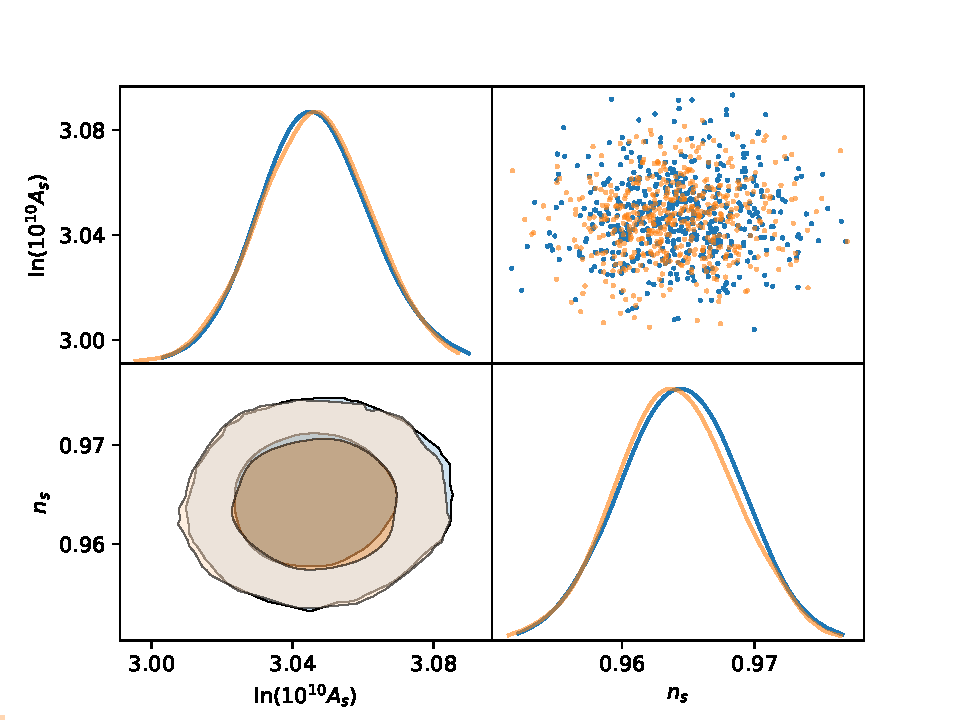
\includegraphics[width=0.5\textwidth]{./illustrations/misfit.pdf}
\caption{\label{orgd969708}
An example of a posterior distribution generated with power posterior re-partitioning, based on data from planck. The posteriors are near identical, and a slight misfit can be explained with arithmetic rounding errors, and run-to-run variance of the position of the live points (see top right figure).}
\end{figure}




\subsection{Qualitative observations.}
\label{sec:org318f3c8}
Last but not least, an interactive cartoon of the convergence
process for as many parameters as one likes can be obtained from

\begin{verbatim}
NestedSamples().gui()
\end{verbatim}
This allows us to see how the points move during the execution of
nested sampling. A more crude picture can be obtained from the plot
of \(\ln Z\) vs \(\ln X\), (which is also present, and used as a
timeline).

Based on the typical shape of the curve, we shall distinguish the
following stages of the algorithm's convergence. 

While \(\ln Z \approx 0\), nested sampling is in its \emph{prior
compression} stage.  Afterwards the algorithm undergoes \emph{discovery}
where most live points enter the typical set and their number is
permanently reduced. The last stage is the \emph{extinction stage},
colloquially referred to as the \emph{tail}.


\subsection{Simulations}
\label{sec:org863b0ec}
\subsubsection{Toy models}
\label{sec:org9512a8f}

We shall begin our analysis with help of a simplified model that is
general-enough to share features with the Cosmological scale
problem, but also practical to investigate in depth, with multiple
variations.

Our original model is a Gaussian peak. By choosing the uniform
prior as a baseline, and setting the log-likelihood as:
\begin{equation}
  \ln {\cal L}(\theta) = - \frac{1}{2} \left\{(\theta - \mu)^{T}G^{-1}(\theta-\mu)  + \ln \det \left| 2\pi G\right| \right\}
\end{equation}
where the covariance matrix \(G\), specifies the extent of the peak,
and the vector \(\mu\), its location. We thus expect the posterior
to be a truncated and re-scaled Gaussian. However its typical set
is still approximately at a distance of the square root of the
diagonal elements of the covariance matrix form the peak, which we
shall refer to as \emph{one standard deviation}.

The covariance matrix is positive semi-definite and symmetric,
hence it can be diagonalised \citep{taboga2017lectures}. If the
covariance matrix is diagonal, the Gaussian distribution is called
uncorrelated. If all diagonal elements are equal, then the
Gaussian is spherical with characteristic diameter given by \(2
	\sigma = 2\sqrt{G}\), where \(G = G \mathds{1}\).

Notice that in this description we have completely neglected any
notion of ``data'', consequently, we don't need to worry about
generating said data, and the extra overheads associated with
\(\chi^2\) fitting.

Under such circumstances it's a matter of integrating \ref{eq:def-z}
to obtain the evidence. Most generally for a correlated Gaussian
likelihood the volume associated is 

\begin{equation}\label{eq:evidence}
   {\cal Z} = \frac{\left( \sqrt{ \det \left| 2\pi G \right|} \right)^{n}}{\mathbf{b}-\mathbf{a}}  
\end{equation}
where \(n\) is the number of parameters in the model.

The internal implementations of all our repartitioning schemes
contain two gaussians: one for the likelihood, and one
entering the repartitioning scheme to improve run-time. These
would be different in general and our simulations will reflect
that in the following ways.

The easiest to account for are translational offsets. One only needs to
modify the values of \(\theta' = \theta - \Delta\) entering \(\ln
	\mathcal{L}(\theta')\). 

One can, without loss of generality assume that one of the
Gaussians is uncorrelated (also WLOG, it's spherical);
effectively we need to apply a coordinate transformation
defined by the eigenvectors of the covariance matrix. We
cannot however assume that both are uncorrelated, nor that the
orthonormal vectors defining the Gaussian are aligned with the
boundaries of the uniform prior. Fortunately, these
complications contribute little. As we shall see, any
repartitioning scheme is easily able to cope with crude
approximations of the orientation and shape of the peak, and
run-time is affected negligibly. Consequently, outside of one
experiment, we shall ignore any deviations from a spherical
Gaussian.





\subsubsection{{\bfseries\sffamily TODO} Cosmological simulations}
\label{sec:org0aa9c59}
For the Cosmological parameter estimation Cobaya \citep{cobaya} with
CLASS \citep{Blas_2011}, and PolyChord \citep{polychord} as a sampler
were chosen. The main reason being the high modularity of the code,
which allows a neater implementation of the re-partitioning
mac
\section{Results and Discussion.}
\label{sec:org048c282}
The first test case is an uncorrelated spherical Gaussian posterior
in three dimensions \(\mathcal{P}(\theta) = G(\theta; \mu = (1,2,3),
  \sigma = 1)\). The corresponding evidence (\autoref{eq:evidence}) is
\(\mathcal{Z}\approx-62.3\). First we shall assume that the mean and
standard deviation of all the repartitioning schemes is exactly the
same as that of the posterior. 

All but one re-partitioning scheme yielded the correct
evidence. The resizeable uniform prior model was constructed to
systematically overestimating the evidence (\autoref{fig:hist}),
which is due to underestimating the normalisation factor for
\(\mathcal{L}\).\footnote{the boundary dependence was omitted.}


We shall now show that repartitioning is able to drastically reduce
the run-time compared to using a uniform prior. More specifically,
guessing a posterior distribution and using re-partitioning, one may
reduce the initial compression stage to virtually none.

     Having proven the correctness of the runs, let's turn to
   performance and benchmarks. The central metric is the number of
@@ -991,19 +996,69 @@ TODO
   case of exact coincidence of the mean and the standard deviation
   produces a respectable speed-up. 

The next trial involves a variable offset, where convergence to the
correct posterior and evidence is not guaranteed even with the
correct normalisation. 


\begin{figure}
  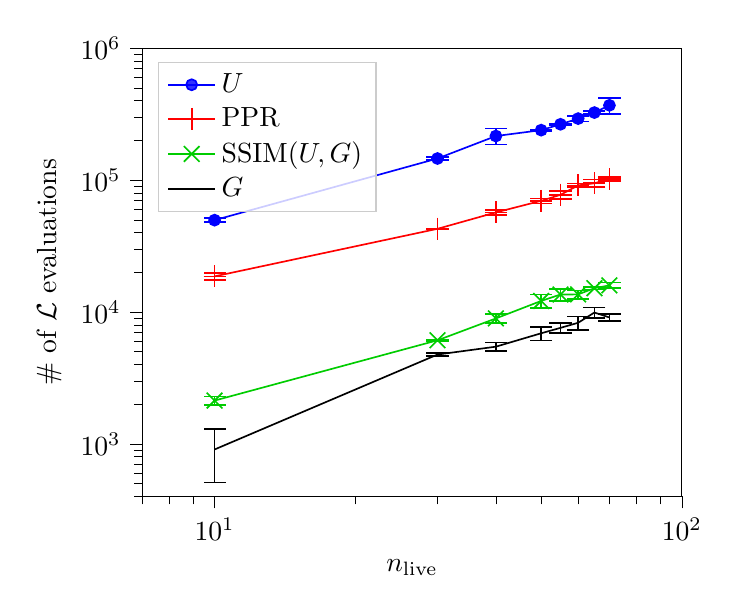
\begin{tikzpicture}

\definecolor{color0}{rgb}{0.0,0.0,1.0} %U
\definecolor{color1}{rgb}{1,0.0,0.0} %PPR
\definecolor{color2}{rgb}{0,0.8,0.0}                              %SSIM
\definecolor{color3}{rgb}{0.,0.0,0.0} %G

\begin{axis}[
legend cell align={left},
legend style={fill opacity=0.8, draw opacity=1, text opacity=1, at={(0.03,0.97)}, anchor=north west, draw=white!80!black},
tick align=outside,
tick pos=left,
x grid style={white!69.0196078431373!black},
xlabel={\(n_\text{live}\)},
xmin=7, xmax=100,
xtick style={color=black},
y grid style={white!69.0196078431373!black},
ylabel={\# of \({\cal L}\) evaluations},
ymin=400, ymax=1000000.0,
ytick style={color=black},
xmode=log,
ymode=log
]
\path [draw=color0, semithick]
(axis cs:10,48051.1762746562)
--(axis cs:10,51361.4903920105);

\path [draw=color0, semithick]
(axis cs:30,141787.579248368)
--(axis cs:30,149701.087418299);

\path [draw=color0, semithick]
(axis cs:40,185671.527674282)
--(axis cs:40,245784.472325718);

\path [draw=color0, semithick]
(axis cs:50,236296.832694899)
--(axis cs:50,241822.500638435);

\path [draw=color0, semithick]
(axis cs:55,262655.71356965)
--(axis cs:55,266952.953097016);

\path [draw=color0, semithick]
(axis cs:60,278243.015081106)
--(axis cs:60,306644.984918894);

\path [draw=color0, semithick]
(axis cs:65,317116.521541605)
--(axis cs:65,332736.145125062);

\path [draw=color0, semithick]
(axis cs:70,318358.948415036)
--(axis cs:70,419081.71825163);

\path [draw=color1, semithick]
(axis cs:10,17520.6487596482)
--(axis cs:10,19742.0179070185);

\path [draw=color1, semithick]
(axis cs:30,42472.9620658463)
--(axis cs:30,42994.371267487);

\path [draw=color1, semithick]
(axis cs:40,54281.6999405287)
--(axis cs:40,59494.3000594713);

\path [draw=color1, semithick]
(axis cs:50,66559.0160569084)
--(axis cs:50,72717.6506097582);

\path [draw=color1, semithick]
(axis cs:55,71552.6011973656)
--(axis cs:55,83118.7321359677);

\path [draw=color1, semithick]
(axis cs:60,88312.8386239607)
--(axis cs:60,94072.4947093726);

\path [draw=color1, semithick]
(axis cs:65,88215.9096228476)
--(axis cs:65,100992.090377152);

\path [draw=color1, semithick]
(axis cs:70,97882.04633)
--(axis cs:70,105637.95367);

\path [draw=color2, semithick]
(axis cs:10,1980.99743591911)
--(axis cs:10,2284.33589741422);

\path [draw=color2, semithick]
(axis cs:30,6035.87692136486)
--(axis cs:30,6174.12307863514);

\path [draw=color2, semithick]
(axis cs:40,8260.41435100755)
--(axis cs:40,9624.91898232578);

\path [draw=color2, semithick]
(axis cs:50,10733.0849396109)
--(axis cs:50,13538.9150603891);

\path [draw=color2, semithick]
(axis cs:55,12122.9645002052)
--(axis cs:55,15015.0354997948);

\path [draw=color2, semithick]
(axis cs:60,12622.7721075812)
--(axis cs:60,14593.2278924188);

\path [draw=color2, semithick]
(axis cs:65,14804.9685728395)
--(axis cs:65,15505.0314271605);

\path [draw=color2, semithick]
(axis cs:70,15158.1193669152)
--(axis cs:70,16693.8806330848);

\path [draw=color3, semithick]
(axis cs:10,511.628293172651)
--(axis cs:10,1305.03837349402);

\path [draw=color3, semithick]
(axis cs:30,4625.34584399058)
--(axis cs:30,4900.65415600942);

\path [draw=color3, semithick]
(axis cs:40,5045.39013421616)
--(axis cs:40,5880.60986578384);

\path [draw=color3, semithick]
(axis cs:50,6085.69651897324)
--(axis cs:50,7719.6368143601);

\path [draw=color3, semithick]
(axis cs:55,6959.0338647499)
--(axis cs:55,8215.63280191676);

\path [draw=color3, semithick]
(axis cs:60,7317.2571539732)
--(axis cs:60,9267.40951269347);

\path [draw=color3, semithick]
(axis cs:65,8986.02980736454)
--(axis cs:65,10838.6368593021);

\path [draw=color3, semithick]
(axis cs:70,8588.48027282128)
--(axis cs:70,9612.18639384539);


\addplot [semithick, color1, mark=-, mark size=4, mark options={solid}, only marks, forget plot]
table {%
10 17520.6487596482
30 42472.9620658463
40 54281.6999405287
50 66559.0160569084
55 71552.6011973656
60 88312.8386239607
65 88215.9096228476
70 97882.04633
};
\addplot [semithick, color1, mark=-, mark size=4, mark options={solid}, only marks, forget plot]
table {%
10 19742.0179070185
30 42994.371267487
40 59494.3000594713
50 72717.6506097582
55 83118.7321359677
60 94072.4947093726
65 100992.090377152
70 105637.95367
};
\addplot [semithick, color2, mark=-, mark size=4, mark options={solid}, only marks, forget plot]
table {%
10 1980.99743591911
30 6035.87692136486
40 8260.41435100755
50 10733.0849396109
55 12122.9645002052
60 12622.7721075812
65 14804.9685728395
70 15158.1193669152
};
\addplot [semithick, color2, mark=-, mark size=4, mark options={solid}, only marks, forget plot]
table {%
10 2284.33589741422
30 6174.12307863514
40 9624.91898232578
50 13538.9150603891
55 15015.0354997948
60 14593.2278924188
65 15505.0314271605
70 16693.8806330848
};
\addplot [semithick, color3, mark=-, mark size=4, mark options={solid}, only marks, forget plot]
table {%
10 511.628293172651
30 4625.34584399058
40 5045.39013421616
50 6085.69651897324
55 6959.0338647499
60 7317.2571539732
65 8986.02980736454
70 8588.48027282128
};
\addplot [semithick, color3, mark=-, mark size=4, mark options={solid}, only marks, forget plot]
table {%
10 1305.03837349402
30 4900.65415600942
40 5880.60986578384
50 7719.6368143601
55 8215.63280191676
60 9267.40951269347
65 10838.6368593021
70 9612.18639384539
};
\addplot [semithick, color0, mark=-, mark size=4, mark options={solid}, only marks, forget plot]
table {%
10 48051.1762746562
30 141787.579248368
40 185671.527674282
50 236296.832694899
55 262655.71356965
60 278243.015081106
65 317116.521541605
70 318358.948415036
};
\addplot [semithick, color0, mark=-, mark size=4, mark options={solid}, only marks, forget plot]
table {%
10 51361.4903920105
30 149701.087418299
40 245784.472325718
50 241822.500638435
55 266952.953097016
60 306644.984918894
65 332736.145125062
70 419081.71825163
};
\addplot [semithick, color0, mark=*, mark size=2, mark options={solid}]
table {%
10 49706.3333333333
30 145744.333333333
40 215728
50 239059.666666667
55 264804.333333333
60 292444
65 324926.333333333
70 368720.333333333
};
\addlegendentry{$U$}
\addplot [semithick, color1, mark=+, mark size=4, mark options={solid}]
table {%
10 18631.3333333333
30 42733.6666666667
40 56888
50 69638.3333333333
55 77335.6666666667
60 91192.6666666667
65 94604
70 101760
};
\addlegendentry{PPR}
\addplot [semithick, color2, mark=x, mark size=4, mark options={solid}]
table {%
10 2132.66666666667
30 6105
40 8942.66666666667
50 12136
55 13569
60 13608
65 15155
70 15926
};
\addlegendentry{$\text{SSIM}(U,G)$}
\addplot [semithick, color3, mark=., mark size=2, mark options={solid}]
table {%
10 908.333333333333
30 4763
40 5463
50 6902.66666666667
55 7587.33333333333
60 8292.33333333333
65 9912.33333333333
70 9100.33333333333
};
\addlegendentry{$G$}
\end{axis}

\end{tikzpicture}

\caption{\label{org671c650}
comparison of likelihood calls necessary for obtaining the correct evidence for the case of a spherical uncorrelated Gaussian posterior. Note that almost all series scale linearly with the number of live points.}
\end{figure}




The next trial involves a variable offset, where convergence to the
correct posterior and evidence is not guaranteed even with the
correct normalisation.    

For this case, we have taken a Gaussian in a box of
\(1000\times1000\times1000\), and generated two nested sampling data
ranges. The ``offset'' posteriors are moved relative to the mean of
the prior. The parameter labeled '1' is offset by double the amount
of parameter '0'. 

The exemplary results are given in \autoref{fig:convergence}.

The main notable feature is the inaccuracy of the posterior for
power posterior repartitioning. One does expect it to produce the
correct posterior distribution if the offset is large compared to
the width of the peaks. If the offset is \(O(2\sigma)\), the
posterior is merely shifted, but if the shift is larger,
e.g. \(O(4\sigma)\), two peaks can be resolved. Unfortunately for
PPR, the evidence was also computed incorrectly: \(\ln {\cal
  Z}\approx -25.4 \pm 0.2\), vs the reference \(\ln {\cal Z} = -22.7 \pm
  0.4\).  Making matters even worse, the smaller of the two peaks is
actually the correct posterior.

This is the fatal flaw of PPR, that prevents it from being useful in
any real application. The constant, ever present bias implicit to
using a Gaussian prior causes the sampler to be strongly biased
towards the original value. It can be redeemed: the mixture model in
the same figure involves the same PPR as one of two models. It
produced the correct result, while also, remarkably managing to do
so faster than a uniform prior would allow\footnote{another method could
involve a prior on \(\beta\), that strongly favours values close to
\(\beta=0\).}.

\begin{figure}
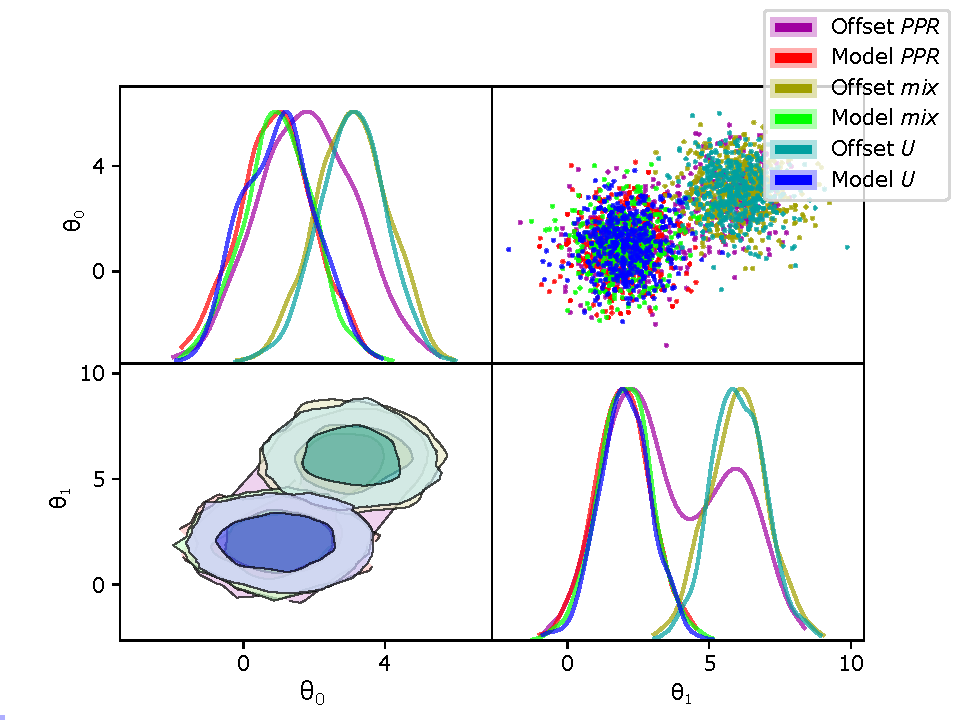
\includegraphics[width=0.5\textwidth]{./illustrations/convergence.pdf}
\caption{\label{orgb4fd87c}
An illustration of how offsets affect the convergence of nested sampling under different kinds of repartitioning. The offset models should produce an offset posterior, whilst sharing the prior with the model runs. The mixture is of the present uniform model and PPR.}
\end{figure}



One last discussion is that of so-called posterior mass. This allows
us to judge how quckly does the algorithm converge to the correct
values \cite{higson2018nestcheck}, as well as diagnose pathological
issues, specific to nested sampling. 

The plot on \autoref{fig:higson} showcases typical behaviour for
both a standard uniform-prior sampling, and the mixture
repartitioning. 

\begin{figure}
% This file was created by tikzplotlib v0.9.1.
\begin{tikzpicture}

\definecolor{color0}{rgb}{0.0313725490196078,0.261314878892734,0.528119953863899}
\definecolor{color1}{rgb}{0.0994232987312572,0.404752018454441,0.679815455594002}
\definecolor{color2}{rgb}{0.240046136101499,0.553771626297578,0.766797385620915}
\definecolor{color3}{rgb}{0.422745098039216,0.684075355632449,0.839892349096501}
\definecolor{color4}{rgb}{0.64236831987697,0.801830065359477,0.890319108035371}
\definecolor{color5}{rgb}{0.805259515570934,0.878016147635525,0.946851211072664}
\definecolor{color6}{rgb}{0.913264129181084,0.948881199538639,0.982283737024221}
\definecolor{color7}{rgb}{0.541222606689735,0.0332179930795848,0.0686966551326413}
\definecolor{color8}{rgb}{0.750495963091119,0.0833217993079585,0.104129181084198}
\definecolor{color9}{rgb}{0.91677047289504,0.211457131872357,0.16401384083045}
\definecolor{color10}{rgb}{0.984375240292195,0.418146866589773,0.292656670511342}
\definecolor{color11}{rgb}{0.988235294117647,0.595878508266051,0.473802383698577}
\definecolor{color12}{rgb}{0.990634371395617,0.777716262975779,0.690149942329873}
\definecolor{color13}{rgb}{0.997785467128028,0.914279123414071,0.874740484429066}

\begin{groupplot}[group style={group size=2 by 4}]
\nextgroupplot[
tick align=outside,
tick pos=left,
xmin=0, xmax=1,
y grid style={white!69.0196078431373!black},
ymin=0, ymax=1,
ytick style={color=black}
]

\nextgroupplot[
tick pos=left,
xmin=-20, xmax=0,
ylabel={posterior
mass},
ymin=0, ymax=0.368699095804214
]
\addplot [draw=none, draw=color0, fill=color0, colormap/viridis]
table{%
x                      y
-18.3838383838384 0.00347016231713772
-18.1818181818182 0.00361357904541066
-18.1364015755841 0.00372423329095166
-18.1818181818182 0.004067768054606
-18.3838383838384 0.00421928867528754
-18.4933820092203 0.00372423329095166
-18.3838383838384 0.00347016231713772
};
\addplot [draw=none, draw=color0, fill=color0, colormap/viridis]
table{%
x                      y
-10.3030303030303 0.00327192681367726
-10.1010101010101 0.00112868215993154
-9.8989898989899 0.00123705047131671
-9.79666193041343 0.00372423329095166
-9.8989898989899 0.00558758419515529
-10.0100168191073 0.00744846658190332
-10.1010101010101 0.0100997410925294
-10.1417009347277 0.011172699872855
-10.2293893988646 0.0148969331638066
-10.2983549558573 0.0186211664547583
-10.3030303030303 0.01891020952064
-10.3491391094173 0.02234539974571
-10.3983625295426 0.0260696330366616
-10.447266559464 0.0297938663276133
-10.4934155978712 0.0335180996185649
-10.5050505050505 0.0345731908406231
-10.5368365675587 0.0372423329095166
-10.5589490385004 0.0409665662004683
-10.5928882597385 0.0446907994914199
-10.6318899491104 0.0484150327823716
-10.6761894179347 0.0521392660733232
-10.7070707070707 0.0546405468236837
-10.7212472344794 0.0558634993642749
-10.7579134380047 0.0595877326552266
-10.7914362229639 0.0633119659461782
-10.8227887708814 0.0670361992371299
-10.8530885291023 0.0707604325280815
-10.8829793861304 0.0744846658190332
-10.9090909090909 0.077791512957631
-10.9127115906451 0.0782088991099849
-10.9378447748353 0.0819331324009365
-10.9612143445816 0.0856573656918882
-10.9828113252983 0.0893815989828398
-11.0030881938824 0.0931058322737915
-11.022461811001 0.0968300655647431
-11.0413019352212 0.100554298855695
-11.0599189743 0.104278532146646
-11.0785509234841 0.108002765437598
-11.0973502915727 0.11172699872855
-11.1111111111111 0.114439588706526
-11.1175976540347 0.115451232019501
-11.1347004164671 0.119175465310453
-11.145652046909 0.122899698601405
-11.1570997554617 0.126623931892356
-11.1714700873055 0.130348165183308
-11.1861753650514 0.13407239847426
-11.201256166292 0.137796631765211
-11.2167012458027 0.141520865056163
-11.2530131361708 0.145245098347115
-11.3092292620823 0.148969331638066
-11.3131313131313 0.149211720686129
-11.3166115230927 0.148969331638066
-11.3532038313037 0.145245098347115
-11.3752533780159 0.141520865056163
-11.3797571289347 0.137796631765211
-11.3833210621102 0.13407239847426
-11.3861040317158 0.130348165183308
-11.3882599739367 0.126623931892356
-11.3854034956823 0.122899698601405
-11.3770824316818 0.119175465310453
-11.3688457849562 0.115451232019501
-11.3607687975806 0.11172699872855
-11.3528908177852 0.108002765437598
-11.3344411973787 0.104278532146646
-11.3131313131313 0.100701344838645
-11.3070870926962 0.100554298855695
-11.2409022799383 0.0968300655647431
-11.2181043794676 0.0931058322737915
-11.2049256945737 0.0893815989828398
-11.1874723978628 0.0856573656918882
-11.189631984956 0.0819331324009365
-11.184657793346 0.0782088991099849
-11.173931299047 0.0744846658190332
-11.162961116242 0.0707604325280815
-11.1516559373422 0.0670361992371299
-11.1399033014476 0.0633119659461782
-11.1275610302693 0.0595877326552265
-11.1144508493498 0.0558634993642749
-11.1111111111111 0.0549696183731783
-11.0828449911407 0.0521392660733232
-11.0429355267719 0.0484150327823716
-11.0012790518248 0.0446907994914199
-10.9591571893565 0.0409665662004683
-10.9175728590714 0.0372423329095166
-10.9090909090909 0.0364567179616725
-10.866760055926 0.0335180996185649
-10.7976841238978 0.0297938663276133
-10.7070707070707 0.0262420371115077
-10.7028699558245 0.0260696330366616
-10.6589094269936 0.02234539974571
-10.6173699756544 0.0186211664547583
-10.5576417347772 0.0148969331638066
-10.5050505050505 0.0118882161462963
-10.4862490683307 0.011172699872855
-10.3756428550804 0.00744846658190332
-10.3124845076355 0.00372423329095166
-10.3030303030303 0.00327192681367726
};
\addplot [draw=none, draw=color0, fill=color0, colormap/viridis]
table{%
x                      y
-9.49494949494949 0
-9.29292929292929 0
-9.09090909090909 0
-9.1072872208643 0.000301930085272384
-9.29292929292929 0.000245875841299915
-9.49494949494949 0.000869612539883298
-9.65557315326096 0
-9.49494949494949 0
};
\addplot [draw=none, draw=color0, fill=color0, colormap/viridis]
table{%
x                      y
-17.7777777777778 0.00739258533327696
-17.5757575757576 0.00662194137049646
-17.4261697010256 0.00744846658190332
-17.5757575757576 0.00890853214859014
-17.7777777777778 0.0074894179639521
-17.7831287062996 0.00744846658190332
-17.7777777777778 0.00739258533327696
};
\addplot [draw=none, draw=color0, fill=color0, colormap/viridis]
table{%
x                      y
-17.1717171717172 0.00986797227494121
-17.0107643471296 0.011172699872855
-16.969696969697 0.0121438609385989
-16.7676767676768 0.0142769715659274
-16.718384673883 0.0148969331638066
-16.5656565656566 0.0173762880038988
-16.4877486072324 0.0186211664547583
-16.3636363636364 0.0210517971540301
-16.2998676453768 0.02234539974571
-16.1616161616162 0.0253590639078499
-16.1313926610354 0.0260696330366616
-15.9841649270977 0.0297938663276133
-15.959595959596 0.0305209774788253
-15.8727789573048 0.0335180996185649
-15.7575757575758 0.0371266580247348
-15.7539861075541 0.0372423329095166
-15.6542283898228 0.0409665662004683
-15.5555555555556 0.0444980120136986
-15.5508398776655 0.0446907994914199
-15.4633382372606 0.0484150327823716
-15.3619190356399 0.0521392660733232
-15.3535353535354 0.052524098200616
-15.2993944888575 0.0558634993642749
-15.2275537614921 0.0595877326552266
-15.1553544161091 0.0633119659461782
-15.1515151515152 0.0634795219034442
-15.0988262142181 0.0670361992371299
-15.038699902062 0.0707604325280815
-14.9762306777734 0.0744846658190332
-14.9494949494949 0.0761292115075881
-14.9199589336947 0.0782088991099849
-14.8695347241454 0.0819331324009365
-14.8189448848524 0.0856573656918882
-14.7757900010053 0.0893815989828398
-14.7474747474747 0.0914375317002598
-14.7242899219916 0.0931058322737915
-14.670433852451 0.0968300655647432
-14.613618913517 0.100554298855695
-14.5583887122277 0.104278532146646
-14.5454545454545 0.105210918153826
-14.5132292271957 0.108002765437598
-14.4651163140416 0.11172699872855
-14.4065903824943 0.115451232019501
-14.3464765760142 0.119175465310453
-14.3434343434343 0.119385466821614
-14.3114732954469 0.122899698601405
-14.2805259184256 0.126623931892356
-14.2510820120814 0.130348165183308
-14.2228916640214 0.13407239847426
-14.2041263322472 0.137796631765211
-14.1847540366164 0.141520865056163
-14.1414141414141 0.144148562558042
-14.1290774304931 0.145245098347115
-14.0871399656895 0.148969331638066
-14.0578395458963 0.152693564929018
-14.0349065225479 0.15641779821997
-14.0173986552155 0.160142031510921
-14.0157509223896 0.163866264801873
-14.0121995251762 0.167590498092825
-14.0042143153615 0.171314731383776
-13.9838182166601 0.175038964674728
-13.9393939393939 0.177728451421158
-13.9309589278557 0.17876319796568
-13.9009530758823 0.182487431256631
-13.8717144337265 0.186211664547583
-13.84284975127 0.189935897838535
-13.8134929480807 0.193660131129486
-13.7829341329184 0.197384364420438
-13.7511375932379 0.20110859771139
-13.7373737373737 0.202682297605094
-13.7183124209922 0.204832831002341
-13.6842827756739 0.208557064293293
-13.6505667971598 0.212281297584245
-13.6182923521905 0.216005530875196
-13.5881200113739 0.219729764166148
-13.5603539686068 0.2234539974571
-13.5353535353535 0.227135723926641
-13.5350477541208 0.227178230748051
-13.5057573459428 0.230902464039003
-13.4720007532626 0.234626697329955
-13.435165919965 0.238350930620906
-13.3333333333333 0.241213326151054
-13.3181532017505 0.242075163911858
-13.2899046988273 0.24579939720281
-13.3098466662574 0.249523630493761
-13.3333333333333 0.251898016431142
-13.3517079827846 0.253247863784713
-13.4025730554633 0.256972097075664
-13.3963635242514 0.260696330366616
-13.3333333333333 0.262060991871049
-13.2218996171082 0.264420563657568
-13.1313131313131 0.267316683153742
-13.1197401790814 0.26814479694852
-13.038555623699 0.271869030239471
-13.0118747429204 0.275593263530423
-13.0049481994887 0.279317496821374
-12.9834962277872 0.283041730112326
-12.9292929292929 0.286256157073769
-12.9165912474805 0.286765963403278
-12.8163976127978 0.290490196694229
-12.7272727272727 0.2939219636131
-12.5252525252525 0.292478768411456
-12.3232323232323 0.293666331758571
-12.3155665333372 0.294214429985181
-12.2530595442172 0.297938663276133
-12.179063592571 0.301662896567084
-12.1212121212121 0.304514240070576
-12.1146753377285 0.305387129858036
-12.0947869177675 0.309111363148988
-12.1088144674984 0.312835596439939
-12.1212121212121 0.314395738017741
-12.1536707861706 0.316559829730891
-12.2214023039496 0.320284063021843
-12.2775226619144 0.324008296312794
-12.3138988346839 0.327732529603746
-12.3232323232323 0.328502955804997
-12.3377854780107 0.327732529603746
-12.3959558434933 0.324008296312794
-12.4522632213118 0.320284063021843
-12.5158838676455 0.316559829730891
-12.5252525252525 0.316088383290851
-12.7272727272727 0.316497875946794
-12.8717856283034 0.312835596439939
-12.9292929292929 0.310621199924715
-12.9539053168602 0.309111363148988
-13.0126966612165 0.305387129858036
-13.064638095353 0.301662896567084
-13.1033278995501 0.297938663276133
-13.1313131313131 0.295912991456343
-13.1509518745114 0.294214429985181
-13.1946312445396 0.290490196694229
-13.3333333333333 0.288171088290999
-13.3683705643631 0.286765963403278
-13.3925519618489 0.283041730112326
-13.4119588034437 0.279317496821374
-13.4152648691221 0.275593263530423
-13.4185601518131 0.271869030239471
-13.4343695555764 0.26814479694852
-13.5187548007554 0.264420563657568
-13.5353535353535 0.26417629744979
-13.5711928109757 0.260696330366616
-13.5992326885096 0.256972097075664
-13.6262410447962 0.253247863784713
-13.6533040636434 0.249523630493761
-13.6809281772308 0.24579939720281
-13.7368988792804 0.242075163911858
-13.7373737373737 0.24205539246939
-13.7633670140915 0.238350930620906
-13.7884503816199 0.234626697329955
-13.8142804601079 0.230902464039003
-13.8449141397406 0.227178230748051
-13.8782148718812 0.2234539974571
-13.9240011485851 0.219729764166148
-13.9393939393939 0.218996522712392
-13.9616992956835 0.216005530875196
-13.9883335413188 0.212281297584245
-14.0109770595535 0.208557064293293
-14.031243979011 0.204832831002341
-14.0352882617268 0.20110859771139
-14.0408888134205 0.197384364420438
-14.0504655472568 0.193660131129486
-14.0661346259365 0.189935897838535
-14.0979056508594 0.186211664547583
-14.1414141414141 0.184164262920096
-14.1503624779514 0.182487431256631
-14.1707327194077 0.17876319796568
-14.1933783476057 0.175038964674728
-14.218389036377 0.171314731383776
-14.2450393591155 0.167590498092825
-14.2724703564996 0.163866264801873
-14.3002742128021 0.160142031510921
-14.32314922854 0.15641779821997
-14.3434343434343 0.154511489799521
-14.3589801102643 0.152693564929018
-14.3953307887217 0.148969331638066
-14.4357085898823 0.145245098347115
-14.478883793238 0.141520865056163
-14.5248894265211 0.137796631765211
-14.5454545454545 0.136214096371427
-14.566104468745 0.13407239847426
-14.6054114356324 0.130348165183308
-14.6477778303131 0.126623931892356
-14.6928423889941 0.122899698601405
-14.740935083037 0.119175465310453
-14.7474747474747 0.118783607524665
-14.7842756553386 0.115451232019501
-14.8267883434353 0.11172699872855
-14.8678605117499 0.108002765437598
-14.9006298636719 0.104278532146646
-14.946165729028 0.100554298855695
-14.9494949494949 0.100420177427089
-14.9946434763327 0.0968300655647431
-15.0433861615934 0.0931058322737915
-15.0899246000292 0.0893815989828398
-15.1305281802333 0.0856573656918882
-15.1515151515152 0.0846429676411423
-15.1920317706858 0.0819331324009365
-15.2482750802087 0.0782088991099849
-15.3001465289912 0.0744846658190332
-15.3535353535354 0.0708371050355906
-15.3548218727991 0.0707604325280815
-15.4270849805159 0.0670361992371299
-15.4960593375344 0.0633119659461782
-15.5555555555556 0.0602251719294998
-15.5678895556783 0.0595877326552266
-15.6489820618915 0.0558634993642749
-15.723797401001 0.0521392660733232
-15.7575757575758 0.0507018381730402
-15.8113193085338 0.0484150327823716
-15.8992454232232 0.0446907994914199
-15.959595959596 0.0421641501023687
-15.9911260091229 0.0409665662004683
-16.0987076940963 0.0372423329095166
-16.1616161616162 0.0351401270646594
-16.212104705259 0.0335180996185649
-16.3346206685432 0.0297938663276133
-16.3636363636364 0.0291067062388521
-16.4831372277396 0.0260696330366616
-16.5656565656566 0.0241401021768713
-16.6455642743329 0.02234539974571
-16.7676767676768 0.0199796418304831
-16.8378551973784 0.0186211664547583
-16.969696969697 0.0165590896971659
-17.0738342920015 0.0148969331638066
-17.1717171717172 0.0133896786851698
-17.3630500465024 0.011172699872855
-17.1717171717172 0.00986797227494121
};
\addplot [draw=none, draw=color0, fill=color0, colormap/viridis]
table{%
x                      y
-11.5151515151515 0.199601139678565
-11.4768566404619 0.20110859771139
-11.344747129973 0.204832831002341
-11.3131313131313 0.205569624613512
-11.2932309434941 0.208557064293293
-11.2792781955305 0.212281297584245
-11.2759855777656 0.216005530875196
-11.2769262668855 0.219729764166148
-11.2877459507342 0.2234539974571
-11.3011779877235 0.227178230748051
-11.3131313131313 0.229949775490787
-11.324172482951 0.230902464039003
-11.3690073597852 0.234626697329955
-11.4112627090852 0.238350930620906
-11.44927043329 0.242075163911858
-11.4830215078444 0.24579939720281
-11.5046229253184 0.249523630493761
-11.5151515151515 0.251690377252088
-11.5657702152118 0.253247863784713
-11.7054827614821 0.256972097075664
-11.7171717171717 0.257254072957953
-11.7629280304746 0.260696330366616
-11.8184333815889 0.264420563657568
-11.8809685815223 0.26814479694852
-11.9191919191919 0.270245836727939
-11.9544086416603 0.271869030239471
-12.021016474088 0.275593263530423
-12.1212121212121 0.277408388050701
-12.1787633107055 0.275593263530423
-12.188695255942 0.271869030239471
-12.1963349464942 0.26814479694852
-12.2023485623864 0.264420563657568
-12.2070496308687 0.260696330366616
-12.2046243042234 0.256972097075664
-12.1888728638376 0.253247863784713
-12.1718569513946 0.249523630493761
-12.1532330926344 0.24579939720281
-12.1212121212121 0.244268477898969
-12.0210244457598 0.242075163911858
-11.9612240848459 0.238350930620906
-11.9348823923319 0.234626697329955
-11.9191919191919 0.232186215007944
-11.9039385727088 0.230902464039003
-11.8600363994874 0.227178230748051
-11.8160743672591 0.2234539974571
-11.7716005520664 0.219729764166148
-11.7265624240544 0.216005530875196
-11.7171717171717 0.21522986505971
-11.6662470262433 0.212281297584245
-11.6114182516437 0.208557064293293
-11.5657859957274 0.204832831002341
-11.5281164158434 0.20110859771139
-11.5151515151515 0.199601139678565
};
\addplot [draw=none, draw=color1, fill=color1, colormap/viridis]
table{%
x                      y
-18.5858585858586 0.00351093408940991
-18.3838383838384 0.0030699548755374
-18.1818181818182 0.00319832469986382
-17.979797979798 0.00368563699997004
-17.9643545513527 0.00372423329095166
-17.7777777777778 0.00554034235171195
-17.5757575757576 0.00554986869246758
-17.3737373737374 0.00663786352206608
-17.2582414591588 0.00744846658190332
-17.1717171717172 0.00830368053144882
-16.969696969697 0.0098410929969911
-16.8445330028666 0.011172699872855
-16.7676767676768 0.012184251755227
-16.5656565656566 0.0146888741516784
-16.5507579926 0.0148969331638066
-16.3636363636364 0.0178579216161578
-16.3185385807505 0.0186211664547583
-16.1616161616162 0.0218172014170024
-16.1348753354342 0.02234539974571
-15.9800808615275 0.0260696330366616
-15.959595959596 0.0265721420881066
-15.8322377007554 0.0297938663276133
-15.7575757575758 0.0322027509399458
-15.7099470028201 0.0335180996185649
-15.5989201839985 0.0372423329095166
-15.5555555555556 0.0386849591126186
-15.485475426278 0.0409665662004683
-15.3959550859237 0.0446907994914199
-15.3535353535354 0.0462004477479314
-15.2929325156378 0.0484150327823716
-15.2193163796936 0.0521392660733232
-15.1515151515152 0.055841524671758
-15.1510096126785 0.0558634993642749
-15.0678494323108 0.0595877326552266
-15.0053922557506 0.0633119659461782
-14.9494949494949 0.0667880401431928
-14.9446288633381 0.0670361992371299
-14.8736896614599 0.0707604325280815
-14.8137890002471 0.0744846658190332
-14.7601960568106 0.0782088991099849
-14.7474747474747 0.0791062806229947
-14.7010313721819 0.0819331324009365
-14.6438432719987 0.0856573656918882
-14.5882088183759 0.0893815989828398
-14.5454545454545 0.0921383975896108
-14.5317362566931 0.0931058322737915
-14.4818002016124 0.0968300655647431
-14.4353989874024 0.100554298855695
-14.3896905242881 0.104278532146646
-14.3434343434343 0.107734870285209
-14.3397798858025 0.108002765437598
-14.2882117995018 0.11172699872855
-14.2427541700801 0.115451232019501
-14.2061710994412 0.119175465310453
-14.1737758580679 0.122899698601405
-14.1433418674597 0.126623931892356
-14.1414141414141 0.126873148358116
-14.1073621461138 0.130348165183308
-14.0724650177126 0.13407239847426
-14.0379901729188 0.137796631765211
-14.0037083984114 0.141520865056163
-13.9711888244947 0.145245098347115
-13.9446347188623 0.148969331638066
-13.9393939393939 0.149877399119944
-13.9192869143814 0.152693564929018
-13.8925580004498 0.15641779821997
-13.8642847415466 0.160142031510921
-13.8337419650579 0.163866264801873
-13.8010680800822 0.167590498092825
-13.7673619787733 0.171314731383776
-13.7373737373737 0.174689733167331
-13.7352359892814 0.175038964674728
-13.7127291066601 0.17876319796568
-13.6887069502824 0.182487431256631
-13.6622787862593 0.186211664547583
-13.6327470485566 0.189935897838535
-13.5999760820193 0.193660131129486
-13.5646191477377 0.197384364420438
-13.5353535353535 0.200384724976471
-13.5310298701894 0.20110859771139
-13.5088532808042 0.204832831002341
-13.4854887977935 0.208557064293293
-13.4602074324177 0.212281297584245
-13.4322719691099 0.216005530875196
-13.4010076935399 0.219729764166148
-13.3658314144198 0.2234539974571
-13.3333333333333 0.226557406962966
-13.3288464181291 0.227178230748051
-13.3019085316078 0.230902464039003
-13.2743625907035 0.234626697329955
-13.2466923738189 0.238350930620906
-13.1984033402991 0.242075163911858
-13.1732810311624 0.24579939720281
-13.1561471922768 0.249523630493761
-13.1313131313131 0.252437152522143
-13.1225659433377 0.253247863784713
-13.0762735256605 0.256972097075664
-13.0261607126013 0.260696330366616
-12.9793058613831 0.264420563657568
-12.9397758479017 0.26814479694852
-12.9292929292929 0.269278001198701
-12.8957646772536 0.271869030239471
-12.8365291165421 0.275593263530423
-12.7584941423699 0.279317496821374
-12.7272727272727 0.280571802305744
-12.5252525252525 0.28121983615182
-12.4689862361015 0.279317496821374
-12.4067158349325 0.275593263530423
-12.3680044290956 0.271869030239471
-12.3383003211872 0.26814479694852
-12.3232323232323 0.266026594582237
-12.3168462913201 0.264420563657568
-12.304583994166 0.260696330366616
-12.2934137268827 0.256972097075664
-12.2788896558442 0.253247863784713
-12.2628668366723 0.249523630493761
-12.2452282763156 0.24579939720281
-12.1867140411619 0.242075163911858
-12.1212121212121 0.239411010345567
-12.0946053004442 0.238350930620906
-12.0608995992594 0.234626697329955
-12.0320665665187 0.230902464039003
-12.0063886633866 0.227178230748051
-11.9828744795461 0.2234539974571
-11.9607061469425 0.219729764166148
-11.9390136061123 0.216005530875196
-11.9191919191919 0.212696100620248
-11.9141548292326 0.212281297584245
-11.8677418175486 0.208557064293293
-11.8202809799709 0.204832831002341
-11.7737459780569 0.20110859771139
-11.7356806797564 0.197384364420438
-11.7171717171717 0.195106300573664
-11.7017694758847 0.193660131129486
-11.6669739421682 0.189935897838535
-11.637967809311 0.186211664547583
-11.6139274633662 0.182487431256631
-11.5940608446058 0.17876319796568
-11.5776207855055 0.175038964674728
-11.5639214052853 0.171314731383776
-11.5311523955304 0.167590498092825
-11.5151515151515 0.16567245544517
-11.4548102746593 0.163866264801873
-11.5107717738965 0.160142031510921
-11.5151515151515 0.159884645257454
-11.5303831793719 0.15641779821997
-11.5420854351303 0.152693564929018
-11.5356493710644 0.148969331638066
-11.5151515151515 0.146724340803863
-11.4975550409341 0.145245098347115
-11.4918501677389 0.141520865056163
-11.4850544898441 0.137796631765211
-11.4788316877428 0.13407239847426
-11.4731248723235 0.130348165183308
-11.4679165621203 0.126623931892356
-11.4613297372096 0.122899698601405
-11.4525875594604 0.119175465310453
-11.4438803521644 0.115451232019501
-11.4353465124547 0.11172699872855
-11.4270870302258 0.108002765437598
-11.4130744735698 0.104278532146646
-11.3966851064445 0.100554298855695
-11.3799128384735 0.0968300655647432
-11.3604984812946 0.0931058322737915
-11.334576260532 0.0893815989828398
-11.3131313131313 0.0880244760749882
-11.2809536924137 0.0856573656918882
-11.2729382677997 0.0819331324009365
-11.2639926804928 0.0782088991099849
-11.2532541090328 0.0744846658190332
-11.2424649525586 0.0707604325280815
-11.2315380157535 0.0670361992371299
-11.2203680079042 0.0633119659461782
-11.2088249673763 0.0595877326552266
-11.1967489975472 0.0558634993642749
-11.183956557269 0.0521392660733232
-11.170286002634 0.0484150327823716
-11.1556916964224 0.0446907994914199
-11.1402108707981 0.0409665662004682
-11.1233204460781 0.0372423329095166
-11.1111111111111 0.0363533438103444
-11.0437120600311 0.0335180996185649
-10.9859808107826 0.0297938663276133
-10.9630776544768 0.0260696330366616
-10.9382289363869 0.02234539974571
-10.9090909090909 0.0210167027791286
-10.8011433468452 0.0186211664547583
-10.7070707070707 0.0149079400230422
-10.7068857476559 0.0148969331638066
-10.6266572947198 0.011172699872855
-10.5050505050505 0.0081107047116825
-10.483648870325 0.00744846658190332
-10.4188187733133 0.00372423329095166
-10.3470098506012 0
-10.3030303030303 0
-10.1010101010101 0
-9.8989898989899 0
-9.6969696969697 0
-9.65557315326096 0
-9.49494949494949 0.000869612539883298
-9.29292929292929 0.000245875841299915
-9.1072872208643 0.000301930085272384
-9.13900497237183 0.000886645400360871
-9.29292929292929 0.000840168266584839
-9.49353150532708 0.00372423329095166
-9.4949494949495 0.00374896743357129
-9.6969696969697 0.00491153683001727
-9.83629700786045 0.00744846658190332
-9.8989898989899 0.00933492274754681
-9.96310963889696 0.011172699872855
-10.0558878384473 0.0148969331638066
-10.091483568182 0.0186211664547583
-10.1010101010101 0.0190302546664071
-10.1568425603537 0.02234539974571
-10.2149960427163 0.0260696330366616
-10.2627987411885 0.0297938663276133
-10.2997717886119 0.0335180996185649
-10.3030303030303 0.0339469888100038
-10.3364079485182 0.0372423329095166
-10.3738681532159 0.0409665662004683
-10.4115895902251 0.0446907994914199
-10.4478594380599 0.0484150327823716
-10.4805999940439 0.0521392660733232
-10.5050505050505 0.0552406167366188
-10.5118590334524 0.0558634993642749
-10.5575329092835 0.0595877326552266
-10.6029427652481 0.0633119659461782
-10.6417932357547 0.0670361992371299
-10.6716195679893 0.0707604325280815
-10.6936558258319 0.0744846658190332
-10.7070707070707 0.0773762280588627
-10.7126531271735 0.0782088991099849
-10.7377750507876 0.0819331324009365
-10.7635510756661 0.0856573656918882
-10.7893075647415 0.0893815989828398
-10.8139266944311 0.0931058322737915
-10.8362766244194 0.0968300655647431
-10.855617018723 0.100554298855695
-10.8717722026147 0.104278532146646
-10.8850458754044 0.108002765437598
-10.8960115671959 0.11172699872855
-10.9053189331808 0.115451232019501
-10.9090909090909 0.117106236991972
-10.9171621352913 0.119175465310453
-10.9323583059274 0.122899698601405
-10.9484560399016 0.126623931892356
-10.9654188705942 0.130348165183308
-10.9830799791518 0.13407239847426
-11.0011537415416 0.137796631765211
-11.0192655856988 0.141520865056163
-11.0369980921652 0.145245098347115
-11.0539454475194 0.148969331638066
-11.0697645962985 0.152693564929018
-11.0842121160079 0.15641779821997
-11.0971607687888 0.160142031510921
-11.1085961761041 0.163866264801873
-11.1111111111111 0.164769215721971
-11.2234772104964 0.167590498092825
-11.3131313131313 0.16839654136295
-11.3723381477665 0.171314731383776
-11.3995700343984 0.175038964674728
-11.3852667968254 0.17876319796568
-11.3437276674408 0.182487431256631
-11.3131313131313 0.184602591756718
-11.2928278595493 0.186211664547583
-11.2471992426053 0.189935897838535
-11.206456803567 0.193660131129486
-11.1718413382165 0.197384364420438
-11.1435721057995 0.20110859771139
-11.1300981444886 0.204832831002341
-11.1446679967529 0.208557064293293
-11.1604368535013 0.212281297584245
-11.186025415518 0.216005530875196
-11.1908874186023 0.219729764166148
-11.2007724353945 0.2234539974571
-11.2125251708067 0.227178230748051
-11.2263413593993 0.230902464039003
-11.2425458038034 0.234626697329955
-11.2619277079906 0.238350930620906
-11.2868896860515 0.242075163911858
-11.3131313131313 0.244313905633531
-11.3373910783816 0.24579939720281
-11.3743358512388 0.249523630493761
-11.3934385475342 0.253247863784713
-11.4126651693277 0.256972097075664
-11.4323128764809 0.260696330366616
-11.4539152931154 0.264420563657568
-11.5151515151515 0.266924176707776
-11.5773901964889 0.26814479694852
-11.6324796011588 0.271869030239471
-11.671412095274 0.275593263530423
-11.7063273264098 0.279317496821374
-11.7171717171717 0.280526001977376
-11.761710388801 0.283041730112326
-11.8282747826181 0.286765963403278
-11.8928174858531 0.290490196694229
-11.9191919191919 0.292132744825677
-11.9518947166545 0.294214429985181
-11.9688554820925 0.297938663276133
-11.9747279720482 0.301662896567084
-11.9776343532839 0.305387129858036
-11.9796531119452 0.309111363148988
-11.9916245070257 0.312835596439939
-12.010750547714 0.316559829730891
-12.0465613245633 0.320284063021843
-12.1212121212121 0.323565858870409
-12.1304435222863 0.324008296312794
-12.1597912262067 0.327732529603746
-12.1959449555796 0.331456762894698
-12.2559838686347 0.335180996185649
-12.3232323232323 0.336985691514823
-12.4403421026517 0.335180996185649
-12.5243758800502 0.331456762894698
-12.5252525252525 0.331400922736442
-12.6341286505916 0.327732529603746
-12.7272727272727 0.3256055557929
-12.7652852162556 0.324008296312794
-12.8929998171008 0.320284063021843
-12.9292929292929 0.319451033271051
-12.9912858472843 0.316559829730891
-13.0539991929715 0.312835596439939
-13.1202384604055 0.309111363148988
-13.1313131313131 0.308396711527138
-13.173730583383 0.305387129858036
-13.2197999057639 0.301662896567084
-13.2675268328131 0.297938663276133
-13.3229210985322 0.294214429985181
-13.3333333333333 0.293614419576065
-13.3759631846827 0.290490196694229
-13.4528232936077 0.286765963403278
-13.4739248807785 0.283041730112326
-13.4938067747374 0.279317496821374
-13.5129110932401 0.275593263530423
-13.5353535353535 0.272924450625612
-13.5484537279513 0.271869030239471
-13.5975912715328 0.26814479694852
-13.641663866152 0.264420563657568
-13.6727697510956 0.260696330366616
-13.7000165685632 0.256972097075664
-13.7309202680518 0.253247863784713
-13.7373737373737 0.25267694348381
-13.7769610280529 0.249523630493761
-13.8133401276803 0.24579939720281
-13.8408282771125 0.242075163911858
-13.8666808932491 0.238350930620906
-13.8932626935799 0.234626697329955
-13.9229906026793 0.230902464039003
-13.9393939393939 0.229296470630729
-13.9611458366597 0.227178230748051
-13.9995345066723 0.2234539974571
-14.0280089256347 0.219729764166148
-14.0536698818208 0.216005530875196
-14.0785108217671 0.212281297584245
-14.1015497957654 0.208557064293293
-14.124205430327 0.204832831002341
-14.1414141414141 0.202091071401214
-14.1489494156523 0.20110859771139
-14.1763819866009 0.197384364420438
-14.2029039122242 0.193660131129486
-14.2289104812697 0.189935897838535
-14.2554262136609 0.186211664547583
-14.2836205929865 0.182487431256631
-14.3139545262982 0.17876319796568
-14.3434343434343 0.175299141554404
-14.3452636185269 0.175038964674728
-14.3693281978939 0.171314731383776
-14.3937547193167 0.167590498092825
-14.4210860220953 0.163866264801873
-14.4532786873773 0.160142031510921
-14.4912532331584 0.15641779821997
-14.5343767468938 0.152693564929018
-14.5454545454545 0.151763459216128
-14.5677074582876 0.148969331638066
-14.5979739031708 0.145245098347115
-14.6320605757521 0.141520865056163
-14.6716784832411 0.137796631765211
-14.7164871728495 0.13407239847426
-14.7474747474747 0.131625002457163
-14.7600566098992 0.130348165183308
-14.7956899567217 0.126623931892356
-14.8347175727401 0.122899698601405
-14.879206856877 0.119175465310453
-14.926863133016 0.115451232019501
-14.9494949494949 0.113602001231074
-14.9683595790646 0.11172699872855
-15.0045706189668 0.108002765437598
-15.0466907512788 0.104278532146646
-15.0975571863877 0.100554298855695
-15.1515151515152 0.0968571002542325
-15.1518350917041 0.0968300655647431
-15.1919871316667 0.0931058322737915
-15.2381277687624 0.0893815989828398
-15.2957796249163 0.0856573656918882
-15.3535353535354 0.082131764017626
-15.3560779761631 0.0819331324009365
-15.4007443183398 0.0782088991099849
-15.4582095523675 0.0744846658190332
-15.5325941345587 0.0707604325280815
-15.5555555555556 0.0695730293521118
-15.5917747939732 0.0670361992371299
-15.6551330822865 0.0633119659461782
-15.7392464472938 0.0595877326552266
-15.7575757575758 0.0587437604233543
-15.807040714195 0.0558634993642749
-15.8876841518917 0.0521392660733232
-15.959595959596 0.0493243685883717
-15.978113202228 0.0484150327823716
-16.0586817947531 0.0446907994914199
-16.1616161616162 0.0412601803937682
-16.1687482180835 0.0409665662004683
-16.259929320098 0.0372423329095166
-16.3636363636364 0.0341921635601007
-16.3832434661208 0.0335180996185649
-16.5062462246164 0.0297938663276133
-16.5656565656566 0.0282816003690468
-16.6438876406581 0.0260696330366616
-16.7676767676768 0.0233670730733485
-16.8109606294525 0.02234539974571
-16.969696969697 0.0193027480538532
-17.0044452039958 0.0186211664547583
-17.1717171717172 0.01587776677504
-17.2354469852069 0.0148969331638066
-17.3737373737374 0.0130485384052449
-17.5413741505849 0.011172699872855
-17.5757575757576 0.0108023599236817
-17.7777777777778 0.00884679475580607
-17.9604908813242 0.00744846658190332
-17.979797979798 0.00531490233263052
-18.1818181818182 0.00535695766279875
-18.3838383838384 0.00499908986958148
-18.5858585858586 0.00409870199410388
-18.6569072471471 0.00372423329095166
-18.5858585858586 0.00351093408940991
-18.4933820092203 0.00372423329095166
-18.3838383838384 0.00421928867528754
-18.1818181818182 0.004067768054606
-18.1364015755841 0.00372423329095166
-18.1818181818182 0.00361357904541066
-18.3838383838384 0.00347016231713772
-18.4933820092203 0.00372423329095166
-10.3124845076355 0.00372423329095166
-10.3756428550804 0.00744846658190332
-10.4862490683307 0.011172699872855
-10.5050505050505 0.0118882161462963
-10.5576417347772 0.0148969331638066
-10.6173699756544 0.0186211664547583
-10.6589094269936 0.02234539974571
-10.7028699558245 0.0260696330366616
-10.7070707070707 0.0262420371115077
-10.7976841238978 0.0297938663276133
-10.866760055926 0.0335180996185649
-10.9090909090909 0.0364567179616725
-10.9175728590714 0.0372423329095166
-10.9591571893565 0.0409665662004683
-11.0012790518248 0.0446907994914199
-11.0429355267719 0.0484150327823716
-11.0828449911407 0.0521392660733232
-11.1111111111111 0.0549696183731783
-11.1144508493498 0.0558634993642749
-11.1275610302693 0.0595877326552266
-11.1399033014476 0.0633119659461782
-11.1516559373423 0.0670361992371299
-11.162961116242 0.0707604325280815
-11.173931299047 0.0744846658190332
-11.184657793346 0.0782088991099849
-11.189631984956 0.0819331324009365
-11.1874723978628 0.0856573656918882
-11.2049256945737 0.0893815989828398
-11.2181043794676 0.0931058322737915
-11.2409022799383 0.0968300655647431
-11.3070870926962 0.100554298855695
-11.3131313131313 0.100701344838645
-11.3344411973787 0.104278532146646
-11.3528908177852 0.108002765437598
-11.3607687975806 0.11172699872855
-11.3688457849562 0.115451232019501
-11.3770824316818 0.119175465310453
-11.3854034956823 0.122899698601405
-11.3882599739367 0.126623931892356
-11.3861040317158 0.130348165183308
-11.3833210621102 0.13407239847426
-11.3797571289347 0.137796631765211
-11.3752533780159 0.141520865056163
-11.3532038313037 0.145245098347115
-11.3166115230927 0.148969331638066
-11.3131313131313 0.149211720686129
-11.3092292620823 0.148969331638066
-11.2530131361708 0.145245098347115
-11.2167012458027 0.141520865056163
-11.201256166292 0.137796631765211
-11.1861753650514 0.13407239847426
-11.1714700873055 0.130348165183308
-11.1570997554617 0.126623931892356
-11.145652046909 0.122899698601405
-11.1347004164671 0.119175465310453
-11.1175976540347 0.115451232019501
-11.1111111111111 0.114439588706526
-11.0973502915727 0.11172699872855
-11.0785509234841 0.108002765437598
-11.0599189743 0.104278532146646
-11.0413019352212 0.100554298855695
-11.022461811001 0.0968300655647431
-11.0030881938824 0.0931058322737915
-10.9828113252983 0.0893815989828398
-10.9612143445816 0.0856573656918882
-10.9378447748353 0.0819331324009365
-10.9127115906451 0.0782088991099849
-10.9090909090909 0.077791512957631
-10.8829793861304 0.0744846658190332
-10.8530885291023 0.0707604325280815
-10.8227887708814 0.0670361992371299
-10.7914362229639 0.0633119659461782
-10.7579134380047 0.0595877326552266
-10.7212472344794 0.0558634993642749
-10.7070707070707 0.0546405468236837
-10.6761894179347 0.0521392660733232
-10.6318899491104 0.0484150327823716
-10.5928882597385 0.0446907994914199
-10.5589490385004 0.0409665662004683
-10.5368365675587 0.0372423329095166
-10.5050505050505 0.0345731908406231
-10.4934155978712 0.0335180996185649
-10.447266559464 0.0297938663276133
-10.3983625295426 0.0260696330366616
-10.3491391094173 0.02234539974571
-10.3030303030303 0.01891020952064
-10.2983549558573 0.0186211664547583
-10.2293893988646 0.0148969331638066
-10.1417009347277 0.011172699872855
-10.1010101010101 0.0100997410925294
-10.0100168191073 0.00744846658190332
-9.8989898989899 0.00558758419515529
-9.79666193041343 0.00372423329095166
-9.8989898989899 0.00123705047131671
-10.1010101010101 0.00112868215993154
-10.3030303030303 0.00327192681367726
-10.3124845076355 0.00372423329095166
-17.7831287062996 0.00744846658190332
-17.7777777777778 0.0074894179639521
-17.5757575757576 0.00890853214859014
-17.4261697010256 0.00744846658190332
-17.5757575757576 0.00662194137049646
-17.7777777777778 0.00739258533327696
-17.7831287062996 0.00744846658190332
-17.3630500465024 0.011172699872855
-17.1717171717172 0.0133896786851698
-17.0738342920015 0.0148969331638066
-16.969696969697 0.0165590896971659
-16.8378551973784 0.0186211664547583
-16.7676767676768 0.0199796418304831
-16.6455642743329 0.02234539974571
-16.5656565656566 0.0241401021768713
-16.4831372277396 0.0260696330366616
-16.3636363636364 0.0291067062388521
-16.3346206685432 0.0297938663276133
-16.212104705259 0.0335180996185649
-16.1616161616162 0.0351401270646594
-16.0987076940963 0.0372423329095166
-15.9911260091229 0.0409665662004683
-15.959595959596 0.0421641501023687
-15.8992454232232 0.0446907994914199
-15.8113193085338 0.0484150327823716
-15.7575757575758 0.0507018381730402
-15.723797401001 0.0521392660733232
-15.6489820618915 0.0558634993642749
-15.5678895556783 0.0595877326552266
-15.5555555555556 0.0602251719294998
-15.4960593375344 0.0633119659461782
-15.4270849805159 0.0670361992371299
-15.3548218727991 0.0707604325280815
-15.3535353535354 0.0708371050355905
-15.3001465289912 0.0744846658190332
-15.2482750802087 0.0782088991099849
-15.1920317706858 0.0819331324009365
-15.1515151515152 0.0846429676411423
-15.1305281802333 0.0856573656918882
-15.0899246000292 0.0893815989828398
-15.0433861615934 0.0931058322737915
-14.9946434763327 0.0968300655647431
-14.9494949494949 0.100420177427089
-14.946165729028 0.100554298855695
-14.9006298636719 0.104278532146646
-14.8678605117499 0.108002765437598
-14.8267883434353 0.11172699872855
-14.7842756553386 0.115451232019501
-14.7474747474747 0.118783607524665
-14.740935083037 0.119175465310453
-14.6928423889941 0.122899698601405
-14.6477778303131 0.126623931892356
-14.6054114356324 0.130348165183308
-14.566104468745 0.13407239847426
-14.5454545454545 0.136214096371427
-14.5248894265211 0.137796631765211
-14.478883793238 0.141520865056163
-14.4357085898823 0.145245098347115
-14.3953307887217 0.148969331638066
-14.3589801102643 0.152693564929018
-14.3434343434343 0.154511489799521
-14.32314922854 0.15641779821997
-14.3002742128021 0.160142031510921
-14.2724703564996 0.163866264801873
-14.2450393591155 0.167590498092825
-14.218389036377 0.171314731383776
-14.1933783476057 0.175038964674728
-14.1707327194077 0.17876319796568
-14.1503624779514 0.182487431256631
-14.1414141414141 0.184164262920096
-14.0979056508594 0.186211664547583
-14.0661346259365 0.189935897838535
-14.0504655472568 0.193660131129486
-14.0408888134205 0.197384364420438
-14.0352882617268 0.20110859771139
-14.031243979011 0.204832831002341
-14.0109770595535 0.208557064293293
-13.9883335413188 0.212281297584245
-13.9616992956835 0.216005530875196
-13.9393939393939 0.218996522712392
-13.9240011485851 0.219729764166148
-13.8782148718812 0.2234539974571
-13.8449141397406 0.227178230748051
-13.8142804601079 0.230902464039003
-13.7884503816199 0.234626697329955
-13.7633670140915 0.238350930620906
-13.7373737373737 0.24205539246939
-13.7368988792804 0.242075163911858
-13.6809281772308 0.24579939720281
-13.6533040636434 0.249523630493761
-13.6262410447962 0.253247863784713
-13.5992326885096 0.256972097075664
-13.5711928109757 0.260696330366616
-13.5353535353535 0.26417629744979
-13.5187548007554 0.264420563657568
-13.4343695555764 0.26814479694852
-13.4185601518131 0.271869030239471
-13.4152648691221 0.275593263530423
-13.4119588034437 0.279317496821374
-13.3925519618489 0.283041730112326
-13.3683705643631 0.286765963403278
-13.3333333333333 0.288171088290999
-13.1946312445396 0.290490196694229
-13.1509518745114 0.294214429985181
-13.1313131313131 0.295912991456343
-13.1033278995501 0.297938663276133
-13.064638095353 0.301662896567084
-13.0126966612165 0.305387129858036
-12.9539053168602 0.309111363148988
-12.9292929292929 0.310621199924715
-12.8717856283034 0.312835596439939
-12.7272727272727 0.316497875946794
-12.5252525252525 0.316088383290851
-12.5158838676455 0.316559829730891
-12.4522632213118 0.320284063021843
-12.3959558434933 0.324008296312794
-12.3377854780107 0.327732529603746
-12.3232323232323 0.328502955804997
-12.3138988346839 0.327732529603746
-12.2775226619144 0.324008296312794
-12.2214023039496 0.320284063021843
-12.1536707861706 0.316559829730891
-12.1212121212121 0.314395738017741
-12.1088144674984 0.312835596439939
-12.0947869177675 0.309111363148988
-12.1146753377285 0.305387129858036
-12.1212121212121 0.304514240070576
-12.179063592571 0.301662896567084
-12.2530595442172 0.297938663276133
-12.3155665333372 0.294214429985181
-12.3232323232323 0.293666331758571
-12.5252525252525 0.292478768411456
-12.7272727272727 0.2939219636131
-12.8163976127978 0.290490196694229
-12.9165912474805 0.286765963403278
-12.9292929292929 0.286256157073769
-12.9834962277872 0.283041730112326
-13.0049481994887 0.279317496821374
-13.0118747429204 0.275593263530423
-13.038555623699 0.271869030239471
-13.1197401790814 0.26814479694852
-13.1313131313131 0.267316683153742
-13.2218996171082 0.264420563657568
-13.3333333333333 0.262060991871049
-13.3963635242514 0.260696330366616
-13.4025730554633 0.256972097075664
-13.3517079827846 0.253247863784713
-13.3333333333333 0.251898016431142
-13.3098466662574 0.249523630493761
-13.2899046988273 0.24579939720281
-13.3181532017505 0.242075163911858
-13.3333333333333 0.241213326151054
-13.435165919965 0.238350930620906
-13.4720007532626 0.234626697329955
-13.5057573459428 0.230902464039003
-13.5350477541208 0.227178230748051
-13.5353535353535 0.227135723926641
-13.5603539686068 0.2234539974571
-13.5881200113739 0.219729764166148
-13.6182923521905 0.216005530875196
-13.6505667971598 0.212281297584245
-13.6842827756739 0.208557064293293
-13.7183124209922 0.204832831002341
-13.7373737373737 0.202682297605094
-13.7511375932379 0.20110859771139
-13.7829341329184 0.197384364420438
-13.8134929480807 0.193660131129486
-13.84284975127 0.189935897838535
-13.8717144337265 0.186211664547583
-13.9009530758823 0.182487431256631
-13.9309589278557 0.17876319796568
-13.9393939393939 0.177728451421158
-13.9838182166601 0.175038964674728
-14.0042143153615 0.171314731383776
-14.0121995251762 0.167590498092825
-14.0157509223896 0.163866264801873
-14.0173986552155 0.160142031510921
-14.0349065225479 0.15641779821997
-14.0578395458963 0.152693564929018
-14.0871399656895 0.148969331638066
-14.1290774304931 0.145245098347115
-14.1414141414141 0.144148562558042
-14.1847540366164 0.141520865056163
-14.2041263322472 0.137796631765211
-14.2228916640214 0.13407239847426
-14.2510820120814 0.130348165183308
-14.2805259184256 0.126623931892356
-14.3114732954469 0.122899698601405
-14.3434343434343 0.119385466821614
-14.3464765760142 0.119175465310453
-14.4065903824943 0.115451232019501
-14.4651163140416 0.11172699872855
-14.5132292271957 0.108002765437598
-14.5454545454545 0.105210918153826
-14.5583887122277 0.104278532146646
-14.613618913517 0.100554298855695
-14.670433852451 0.0968300655647431
-14.7242899219916 0.0931058322737915
-14.7474747474747 0.0914375317002598
-14.7757900010053 0.0893815989828398
-14.8189448848524 0.0856573656918882
-14.8695347241454 0.0819331324009365
-14.9199589336947 0.0782088991099849
-14.9494949494949 0.0761292115075881
-14.9762306777734 0.0744846658190332
-15.038699902062 0.0707604325280815
-15.0988262142181 0.0670361992371299
-15.1515151515152 0.0634795219034442
-15.1553544161091 0.0633119659461782
-15.2275537614921 0.0595877326552266
-15.2993944888575 0.0558634993642749
-15.3535353535354 0.052524098200616
-15.3619190356399 0.0521392660733232
-15.4633382372606 0.0484150327823716
-15.5508398776655 0.0446907994914199
-15.5555555555556 0.0444980120136986
-15.6542283898228 0.0409665662004682
-15.7539861075541 0.0372423329095166
-15.7575757575758 0.0371266580247348
-15.8727789573048 0.0335180996185649
-15.959595959596 0.0305209774788253
-15.9841649270977 0.0297938663276133
-16.1313926610354 0.0260696330366616
-16.1616161616162 0.0253590639078499
-16.2998676453768 0.02234539974571
-16.3636363636364 0.0210517971540301
-16.4877486072324 0.0186211664547583
-16.5656565656566 0.0173762880038988
-16.718384673883 0.0148969331638066
-16.7676767676768 0.0142769715659274
-16.969696969697 0.0121438609385989
-17.0107643471296 0.011172699872855
-17.1717171717172 0.00986797227494121
-17.3630500465024 0.011172699872855
-11.5281164158434 0.20110859771139
-11.5657859957274 0.204832831002341
-11.6114182516437 0.208557064293293
-11.6662470262433 0.212281297584245
-11.7171717171717 0.21522986505971
-11.7265624240544 0.216005530875196
-11.7716005520664 0.219729764166148
-11.8160743672591 0.2234539974571
-11.8600363994874 0.227178230748051
-11.9039385727088 0.230902464039003
-11.9191919191919 0.232186215007944
-11.9348823923319 0.234626697329955
-11.9612240848459 0.238350930620906
-12.0210244457598 0.242075163911858
-12.1212121212121 0.244268477898969
-12.1532330926344 0.24579939720281
-12.1718569513946 0.249523630493761
-12.1888728638376 0.253247863784713
-12.2046243042234 0.256972097075664
-12.2070496308687 0.260696330366616
-12.2023485623864 0.264420563657568
-12.1963349464942 0.26814479694852
-12.188695255942 0.271869030239471
-12.1787633107055 0.275593263530423
-12.1212121212121 0.277408388050701
-12.021016474088 0.275593263530423
-11.9544086416603 0.271869030239471
-11.9191919191919 0.270245836727939
-11.8809685815223 0.26814479694852
-11.8184333815889 0.264420563657568
-11.7629280304746 0.260696330366616
-11.7171717171717 0.257254072957953
-11.7054827614821 0.256972097075664
-11.5657702152118 0.253247863784713
-11.5151515151515 0.251690377252088
-11.5046229253184 0.249523630493761
-11.4830215078444 0.24579939720281
-11.44927043329 0.242075163911858
-11.4112627090852 0.238350930620906
-11.3690073597852 0.234626697329955
-11.324172482951 0.230902464039003
-11.3131313131313 0.229949775490787
-11.3011779877235 0.227178230748051
-11.2877459507342 0.2234539974571
-11.2769262668855 0.219729764166148
-11.2759855777656 0.216005530875196
-11.2792781955305 0.212281297584245
-11.2932309434941 0.208557064293293
-11.3131313131313 0.205569624613512
-11.344747129973 0.204832831002341
-11.4768566404619 0.20110859771139
-11.5151515151515 0.199601139678565
-11.5281164158434 0.20110859771139
};
\addplot [draw=none, draw=color2, fill=color2, colormap/viridis]
table{%
x                      y
-18.7878787878788 0.00364461482886793
-18.5858585858586 0.0030512989810101
-18.3838383838384 0.00266974743393707
-18.1818181818182 0.00278307035431699
-17.979797979798 0.00321006589121691
-17.7777777777778 0.00371356147915537
-17.7723223642664 0.00372423329095166
-17.5757575757576 0.00447779601443869
-17.3737373737374 0.00552709740154936
-17.1717171717172 0.00696765318144856
-17.0661813301794 0.00744846658190332
-16.969696969697 0.00814948885503338
-16.7676767676768 0.00988295186286903
-16.6522372666889 0.011172699872855
-16.5656565656566 0.0121546570410779
-16.3692891949872 0.0148969331638066
-16.3636363636364 0.0149863828359034
-16.1616161616162 0.0182894943156733
-16.1423862925345 0.0186211664547583
-15.95992679386 0.02234539974571
-15.959595959596 0.0223535273764344
-15.7957209197478 0.0260696330366616
-15.7575757575758 0.0271521071344987
-15.6521845958568 0.0297938663276133
-15.5555555555556 0.0328449819028675
-15.5319960573913 0.0335180996185649
-15.4172613508935 0.0372423329095166
-15.3535353535354 0.0397185268387246
-15.3153827789314 0.0409665662004683
-15.218004198257 0.0446907994914199
-15.1515151515152 0.0478593714893869
-15.1368526263652 0.0484150327823716
-15.0483350991717 0.0521392660733232
-14.9749981340296 0.0558634993642749
-14.9494949494949 0.0572935866913829
-14.8980665768267 0.0595877326552266
-14.8265541583045 0.0633119659461782
-14.7635163882166 0.0670361992371299
-14.7474747474747 0.0680295077472422
-14.6931116466926 0.0707604325280815
-14.6288466227774 0.0744846658190332
-14.5710435813208 0.0782088991099849
-14.5454545454545 0.079904186647359
-14.5114186526331 0.0819331324009365
-14.4560208804724 0.0856573656918882
-14.4068761203928 0.0893815989828398
-14.3610335517139 0.0931058322737915
-14.3434343434343 0.0945568265588499
-14.3105175603025 0.0968300655647431
-14.2597384838198 0.100554298855695
-14.2133557917784 0.104278532146646
-14.1705115018382 0.108002765437598
-14.1414141414141 0.110739991050195
-14.1295029532158 0.11172699872855
-14.0839697223898 0.115451232019501
-14.0423694020854 0.119175465310453
-14.004371529019 0.122899698601405
-13.9685391482175 0.126623931892356
-13.9393939393939 0.129723644923225
-13.9347958865979 0.130348165183308
-13.9034478701636 0.13407239847426
-13.8702715184575 0.137796631765211
-13.8381934580913 0.141520865056163
-13.8070307912447 0.145245098347115
-13.7757295519253 0.148969331638066
-13.7429908203895 0.152693564929018
-13.7373737373737 0.153309641855402
-13.717676294118 0.15641779821997
-13.6930337080316 0.160142031510921
-13.6672421392559 0.163866264801873
-13.6400645870406 0.167590498092825
-13.6115074094601 0.171314731383776
-13.5816268436056 0.175038964674728
-13.5499343301964 0.17876319796568
-13.5353535353535 0.180399322201444
-13.5221532488931 0.182487431256631
-13.4985743087227 0.186211664547583
-13.4745808296906 0.189935897838535
-13.4500593109599 0.193660131129486
-13.4248372599498 0.197384364420438
-13.3984334384007 0.20110859771139
-13.3700679675444 0.204832831002341
-13.3388477789634 0.208557064293293
-13.3333333333333 0.209177669189859
-13.3093221678652 0.212281297584245
-13.2814047128085 0.216005530875196
-13.2535194093372 0.219729764166148
-13.2248383908273 0.2234539974571
-13.1948400583037 0.227178230748051
-13.1633653968005 0.230902464039003
-13.1313131313131 0.234553552545816
-13.1307357414126 0.234626697329955
-13.1015636393428 0.238350930620906
-13.069421877861 0.242075163911858
-13.0308046277825 0.24579939720281
-12.9832245987045 0.249523630493761
-12.9292929292929 0.253169117145731
-12.9270963921391 0.253247863784713
-12.8485559261919 0.256972097075664
-12.7972837541448 0.260696330366616
-12.7553411638698 0.264420563657568
-12.7272727272727 0.266629182699094
-12.5252525252525 0.266520387606195
-12.503683057002 0.264420563657568
-12.4685883351817 0.260696330366616
-12.4356627995458 0.256972097075664
-12.4043884742247 0.253247863784713
-12.3746690832378 0.249523630493761
-12.3459009328871 0.24579939720281
-12.3232323232323 0.242923384880588
-12.3173717356114 0.242075163911858
-12.2749464143272 0.238350930620906
-12.2280143766477 0.234626697329955
-12.1772145874163 0.230902464039003
-12.1254476196899 0.227178230748051
-12.1212121212121 0.226856464743785
-12.0976793145579 0.2234539974571
-12.0746728978921 0.219729764166148
-12.0537632387661 0.216005530875196
-12.0341299056236 0.212281297584245
-12.0145286971734 0.208557064293293
-11.9923556917373 0.204832831002341
-11.9524937002602 0.20110859771139
-11.9191919191919 0.197974897336427
-11.9103397575422 0.197384364420438
-11.8670836116344 0.193660131129486
-11.8343671690171 0.189935897838535
-11.8080316488379 0.186211664547583
-11.7685272628992 0.182487431256631
-11.7462657607299 0.17876319796568
-11.7304601702517 0.175038964674728
-11.7183340035343 0.171314731383776
-11.7171717171717 0.170896176249791
-11.6980008650866 0.167590498092825
-11.6755159337914 0.163866264801873
-11.6645319432023 0.160142031510921
-11.6588660866373 0.15641779821997
-11.6550403637671 0.152693564929018
-11.6464463699767 0.148969331638066
-11.6204803647945 0.145245098347115
-11.5992391758499 0.141520865056163
-11.5844904117808 0.137796631765211
-11.5715647727317 0.13407239847426
-11.5596437867166 0.130348165183308
-11.5484447075688 0.126623931892356
-11.5378807083223 0.122899698601405
-11.5279594933025 0.119175465310453
-11.5188199827475 0.115451232019501
-11.5151515151515 0.113897841784292
-11.5099242273289 0.11172699872855
-11.5012832426664 0.108002765437598
-11.4917077497608 0.104278532146646
-11.4811801770395 0.100554298855695
-11.470222116042 0.0968300655647431
-11.4581319671257 0.0931058322737915
-11.4432426166318 0.0893815989828398
-11.4086340133296 0.0856573656918882
-11.3928303507812 0.0819331324009365
-11.3755131866345 0.0782088991099849
-11.35613750127 0.0744846658190332
-11.3341032344665 0.0707604325280815
-11.3131313131313 0.0676379493575947
-11.3114200941648 0.0670361992371299
-11.3008327143608 0.0633119659461782
-11.2900889044834 0.0595877326552266
-11.2790471457446 0.0558634993642749
-11.2675422742515 0.0521392660733232
-11.2554047896333 0.0484150327823716
-11.2425138624628 0.0446907994914199
-11.2288064381772 0.0409665662004683
-11.2139523684333 0.0372423329095166
-11.1747027030117 0.0335180996185649
-11.1111111111111 0.0303774663681555
-11.0991199831089 0.0297938663276133
-11.0723091915534 0.0260696330366616
-11.0477303961993 0.02234539974571
-10.9892751892296 0.0186211664547583
-10.939034766436 0.0148969331638066
-10.9090909090909 0.0124215687266416
-10.8724182049743 0.011172699872855
-10.7179134706076 0.00744846658190332
-10.7070707070707 0.00722681794063917
-10.5856932552342 0.00372423329095166
-10.5050505050505 0.00223046762512086
-10.4702588917289 0
-10.3470098506012 0
-10.4188187733133 0.00372423329095166
-10.483648870325 0.00744846658190332
-10.5050505050505 0.0081107047116825
-10.6266572947198 0.011172699872855
-10.7068857476559 0.0148969331638066
-10.7070707070707 0.0149079400230422
-10.8011433468452 0.0186211664547583
-10.9090909090909 0.0210167027791286
-10.9382289363869 0.02234539974571
-10.9630776544768 0.0260696330366616
-10.9859808107826 0.0297938663276133
-11.0437120600311 0.0335180996185649
-11.1111111111111 0.0363533438103444
-11.1233204460781 0.0372423329095166
-11.1402108707981 0.0409665662004683
-11.1556916964224 0.0446907994914199
-11.170286002634 0.0484150327823716
-11.183956557269 0.0521392660733232
-11.1967489975472 0.0558634993642749
-11.2088249673763 0.0595877326552266
-11.2203680079042 0.0633119659461782
-11.2315380157535 0.0670361992371299
-11.2424649525586 0.0707604325280815
-11.2532541090328 0.0744846658190332
-11.2639926804928 0.0782088991099849
-11.2729382677997 0.0819331324009365
-11.2809536924137 0.0856573656918882
-11.3131313131313 0.0880244760749882
-11.334576260532 0.0893815989828398
-11.3604984812946 0.0931058322737915
-11.3799128384735 0.0968300655647431
-11.3966851064445 0.100554298855695
-11.4130744735698 0.104278532146646
-11.4270870302258 0.108002765437598
-11.4353465124547 0.11172699872855
-11.4438803521644 0.115451232019501
-11.4525875594604 0.119175465310453
-11.4613297372096 0.122899698601405
-11.4679165621203 0.126623931892356
-11.4731248723235 0.130348165183308
-11.4788316877428 0.13407239847426
-11.4850544898441 0.137796631765211
-11.4918501677389 0.141520865056163
-11.4975550409341 0.145245098347115
-11.5151515151515 0.146724340803863
-11.5356493710644 0.148969331638066
-11.5420854351303 0.152693564929018
-11.5303831793719 0.15641779821997
-11.5151515151515 0.159884645257454
-11.5107717738965 0.160142031510921
-11.4548102746593 0.163866264801873
-11.5151515151515 0.16567245544517
-11.5311523955304 0.167590498092825
-11.5639214052853 0.171314731383776
-11.5776207855055 0.175038964674728
-11.5940608446058 0.17876319796568
-11.6139274633662 0.182487431256631
-11.637967809311 0.186211664547583
-11.6669739421682 0.189935897838535
-11.7017694758847 0.193660131129486
-11.7171717171717 0.195106300573664
-11.7356806797564 0.197384364420438
-11.7737459780569 0.20110859771139
-11.8202809799709 0.204832831002341
-11.8677418175486 0.208557064293293
-11.9141548292326 0.212281297584245
-11.9191919191919 0.212696100620248
-11.9390136061123 0.216005530875196
-11.9607061469425 0.219729764166148
-11.9828744795461 0.2234539974571
-12.0063886633866 0.227178230748051
-12.0320665665187 0.230902464039003
-12.0608995992594 0.234626697329955
-12.0946053004442 0.238350930620906
-12.1212121212121 0.239411010345567
-12.1867140411619 0.242075163911858
-12.2452282763156 0.24579939720281
-12.2628668366723 0.249523630493761
-12.2788896558442 0.253247863784713
-12.2934137268827 0.256972097075664
-12.304583994166 0.260696330366616
-12.3168462913201 0.264420563657568
-12.3232323232323 0.266026594582237
-12.3383003211872 0.26814479694852
-12.3680044290956 0.271869030239471
-12.4067158349325 0.275593263530423
-12.4689862361015 0.279317496821374
-12.5252525252525 0.28121983615182
-12.7272727272727 0.280571802305744
-12.7584941423699 0.279317496821374
-12.8365291165421 0.275593263530423
-12.8957646772536 0.271869030239471
-12.9292929292929 0.269278001198701
-12.9397758479017 0.26814479694852
-12.9793058613831 0.264420563657568
-13.0261607126013 0.260696330366616
-13.0762735256605 0.256972097075664
-13.1225659433377 0.253247863784713
-13.1313131313131 0.252437152522143
-13.1561471922768 0.249523630493761
-13.1732810311624 0.245799397202809
-13.1984033402991 0.242075163911858
-13.2466923738189 0.238350930620906
-13.2743625907035 0.234626697329955
-13.3019085316078 0.230902464039003
-13.3288464181291 0.227178230748051
-13.3333333333333 0.226557406962966
-13.3658314144198 0.2234539974571
-13.4010076935399 0.219729764166148
-13.4322719691099 0.216005530875196
-13.4602074324177 0.212281297584245
-13.4854887977935 0.208557064293293
-13.5088532808042 0.204832831002341
-13.5310298701894 0.20110859771139
-13.5353535353535 0.200384724976471
-13.5646191477377 0.197384364420438
-13.5999760820193 0.193660131129486
-13.6327470485566 0.189935897838535
-13.6622787862593 0.186211664547583
-13.6887069502824 0.182487431256631
-13.7127291066601 0.17876319796568
-13.7352359892814 0.175038964674728
-13.7373737373737 0.174689733167331
-13.7673619787733 0.171314731383776
-13.8010680800822 0.167590498092825
-13.8337419650579 0.163866264801873
-13.8642847415466 0.160142031510921
-13.8925580004498 0.15641779821997
-13.9192869143814 0.152693564929018
-13.9393939393939 0.149877399119944
-13.9446347188623 0.148969331638066
-13.9711888244947 0.145245098347115
-14.0037083984114 0.141520865056163
-14.0379901729188 0.137796631765211
-14.0724650177126 0.13407239847426
-14.1073621461138 0.130348165183308
-14.1414141414141 0.126873148358116
-14.1433418674597 0.126623931892356
-14.1737758580679 0.122899698601405
-14.2061710994412 0.119175465310453
-14.2427541700801 0.115451232019501
-14.2882117995018 0.11172699872855
-14.3397798858025 0.108002765437598
-14.3434343434343 0.107734870285209
-14.3896905242881 0.104278532146646
-14.4353989874024 0.100554298855695
-14.4818002016124 0.0968300655647431
-14.5317362566932 0.0931058322737915
-14.5454545454545 0.0921383975896108
-14.5882088183759 0.0893815989828398
-14.6438432719987 0.0856573656918882
-14.7010313721819 0.0819331324009365
-14.7474747474747 0.0791062806229947
-14.7601960568106 0.0782088991099849
-14.8137890002471 0.0744846658190332
-14.8736896614599 0.0707604325280815
-14.9446288633381 0.0670361992371299
-14.9494949494949 0.0667880401431928
-15.0053922557506 0.0633119659461782
-15.0678494323108 0.0595877326552265
-15.1510096126785 0.0558634993642749
-15.1515151515152 0.055841524671758
-15.2193163796936 0.0521392660733232
-15.2929325156378 0.0484150327823716
-15.3535353535354 0.0462004477479314
-15.3959550859237 0.0446907994914199
-15.485475426278 0.0409665662004683
-15.5555555555556 0.0386849591126186
-15.5989201839985 0.0372423329095166
-15.7099470028201 0.0335180996185649
-15.7575757575758 0.0322027509399458
-15.8322377007554 0.0297938663276133
-15.959595959596 0.0265721420881066
-15.9800808615275 0.0260696330366616
-16.1348753354342 0.02234539974571
-16.1616161616162 0.0218172014170024
-16.3185385807505 0.0186211664547583
-16.3636363636364 0.0178579216161578
-16.5507579926 0.0148969331638066
-16.5656565656566 0.0146888741516784
-16.7676767676768 0.012184251755227
-16.8445330028666 0.011172699872855
-16.969696969697 0.00984109299699111
-17.1717171717172 0.00830368053144882
-17.2582414591588 0.00744846658190332
-17.3737373737374 0.00663786352206608
-17.5757575757576 0.00554986869246758
-17.7777777777778 0.00554034235171195
-17.9643545513527 0.00372423329095166
-17.979797979798 0.00368563699997004
-18.1818181818182 0.00319832469986382
-18.3838383838384 0.0030699548755374
-18.5858585858586 0.00351093408940991
-18.6569072471471 0.00372423329095166
-18.5858585858586 0.00409870199410388
-18.3838383838384 0.00499908986958148
-18.1818181818182 0.00535695766279875
-17.979797979798 0.00531490233263052
-17.9604908813242 0.00744846658190332
-17.7777777777778 0.00884679475580608
-17.5757575757576 0.0108023599236817
-17.5413741505849 0.011172699872855
-17.3737373737374 0.0130485384052449
-17.2354469852069 0.0148969331638066
-17.1717171717172 0.01587776677504
-17.0044452039958 0.0186211664547583
-16.969696969697 0.0193027480538532
-16.8109606294525 0.02234539974571
-16.7676767676768 0.0233670730733485
-16.6438876406581 0.0260696330366616
-16.5656565656566 0.0282816003690468
-16.5062462246164 0.0297938663276133
-16.3832434661208 0.0335180996185649
-16.3636363636364 0.0341921635601007
-16.259929320098 0.0372423329095166
-16.1687482180835 0.0409665662004683
-16.1616161616162 0.0412601803937682
-16.0586817947531 0.0446907994914199
-15.978113202228 0.0484150327823716
-15.959595959596 0.0493243685883717
-15.8876841518917 0.0521392660733232
-15.807040714195 0.0558634993642749
-15.7575757575758 0.0587437604233543
-15.7392464472938 0.0595877326552265
-15.6551330822865 0.0633119659461782
-15.5917747939732 0.0670361992371299
-15.5555555555556 0.0695730293521118
-15.5325941345587 0.0707604325280815
-15.4582095523675 0.0744846658190332
-15.4007443183398 0.0782088991099849
-15.3560779761631 0.0819331324009365
-15.3535353535354 0.082131764017626
-15.2957796249163 0.0856573656918882
-15.2381277687624 0.0893815989828398
-15.1919871316667 0.0931058322737915
-15.1518350917041 0.0968300655647431
-15.1515151515152 0.0968571002542325
-15.0975571863877 0.100554298855695
-15.0466907512788 0.104278532146646
-15.0045706189668 0.108002765437598
-14.9683595790646 0.11172699872855
-14.949494949495 0.113602001231074
-14.926863133016 0.115451232019501
-14.879206856877 0.119175465310453
-14.8347175727401 0.122899698601405
-14.7956899567217 0.126623931892356
-14.7600566098992 0.130348165183308
-14.7474747474747 0.131625002457163
-14.7164871728495 0.13407239847426
-14.6716784832411 0.137796631765211
-14.6320605757521 0.141520865056163
-14.5979739031708 0.145245098347115
-14.5677074582876 0.148969331638066
-14.5454545454545 0.151763459216128
-14.5343767468938 0.152693564929018
-14.4912532331584 0.15641779821997
-14.4532786873773 0.160142031510921
-14.4210860220953 0.163866264801873
-14.3937547193167 0.167590498092825
-14.3693281978939 0.171314731383776
-14.3452636185269 0.175038964674728
-14.3434343434343 0.175299141554404
-14.3139545262982 0.17876319796568
-14.2836205929865 0.182487431256631
-14.2554262136609 0.186211664547583
-14.2289104812697 0.189935897838535
-14.2029039122242 0.193660131129486
-14.1763819866009 0.197384364420438
-14.1489494156523 0.20110859771139
-14.1414141414141 0.202091071401214
-14.124205430327 0.204832831002341
-14.1015497957654 0.208557064293293
-14.0785108217671 0.212281297584245
-14.0536698818208 0.216005530875196
-14.0280089256347 0.219729764166148
-13.9995345066723 0.2234539974571
-13.9611458366597 0.227178230748051
-13.9393939393939 0.229296470630729
-13.9229906026793 0.230902464039003
-13.8932626935799 0.234626697329955
-13.8666808932491 0.238350930620906
-13.8408282771125 0.242075163911858
-13.8133401276803 0.24579939720281
-13.7769610280529 0.249523630493761
-13.7373737373737 0.25267694348381
-13.7309202680518 0.253247863784713
-13.7000165685632 0.256972097075664
-13.6727697510956 0.260696330366616
-13.641663866152 0.264420563657568
-13.5975912715328 0.26814479694852
-13.5484537279513 0.271869030239471
-13.5353535353535 0.272924450625612
-13.5129110932401 0.275593263530423
-13.4938067747374 0.279317496821374
-13.4739248807785 0.283041730112326
-13.4528232936077 0.286765963403278
-13.3759631846827 0.290490196694229
-13.3333333333333 0.293614419576065
-13.3229210985322 0.294214429985181
-13.2675268328131 0.297938663276133
-13.2197999057639 0.301662896567084
-13.173730583383 0.305387129858036
-13.1313131313131 0.308396711527138
-13.1202384604055 0.309111363148988
-13.0539991929715 0.312835596439939
-12.9912858472843 0.316559829730891
-12.9292929292929 0.319451033271051
-12.8929998171008 0.320284063021843
-12.7652852162556 0.324008296312794
-12.7272727272727 0.3256055557929
-12.6341286505916 0.327732529603746
-12.5252525252525 0.331400922736442
-12.5243758800502 0.331456762894698
-12.4403421026517 0.335180996185649
-12.3232323232323 0.336985691514823
-12.2559838686347 0.335180996185649
-12.1959449555796 0.331456762894698
-12.1597912262067 0.327732529603746
-12.1304435222863 0.324008296312794
-12.1212121212121 0.323565858870409
-12.0465613245633 0.320284063021843
-12.010750547714 0.316559829730891
-11.9916245070257 0.312835596439939
-11.9796531119452 0.309111363148988
-11.9776343532839 0.305387129858036
-11.9747279720482 0.301662896567084
-11.9688554820925 0.297938663276133
-11.9518947166545 0.294214429985181
-11.9191919191919 0.292132744825677
-11.8928174858531 0.290490196694229
-11.8282747826181 0.286765963403278
-11.761710388801 0.283041730112326
-11.7171717171717 0.280526001977376
-11.7063273264098 0.279317496821374
-11.671412095274 0.275593263530423
-11.6324796011588 0.271869030239471
-11.5773901964889 0.26814479694852
-11.5151515151515 0.266924176707776
-11.4539152931154 0.264420563657568
-11.4323128764809 0.260696330366616
-11.4126651693277 0.256972097075664
-11.3934385475342 0.253247863784713
-11.3743358512388 0.249523630493761
-11.3373910783816 0.24579939720281
-11.3131313131313 0.244313905633531
-11.2868896860515 0.242075163911858
-11.2619277079906 0.238350930620906
-11.2425458038034 0.234626697329955
-11.2263413593993 0.230902464039003
-11.2125251708067 0.227178230748051
-11.2007724353945 0.2234539974571
-11.1908874186023 0.219729764166148
-11.186025415518 0.216005530875196
-11.1604368535013 0.212281297584245
-11.1446679967529 0.208557064293293
-11.1300981444886 0.204832831002341
-11.1435721057995 0.20110859771139
-11.1718413382165 0.197384364420438
-11.206456803567 0.193660131129486
-11.2471992426053 0.189935897838535
-11.2928278595493 0.186211664547583
-11.3131313131313 0.184602591756718
-11.3437276674408 0.182487431256631
-11.3852667968254 0.17876319796568
-11.3995700343984 0.175038964674728
-11.3723381477665 0.171314731383776
-11.3131313131313 0.16839654136295
-11.2234772104964 0.167590498092825
-11.1111111111111 0.164769215721971
-11.1085961761041 0.163866264801873
-11.0971607687888 0.160142031510921
-11.0842121160079 0.15641779821997
-11.0697645962985 0.152693564929018
-11.0539454475194 0.148969331638066
-11.0369980921652 0.145245098347115
-11.0192655856988 0.141520865056163
-11.0011537415416 0.137796631765211
-10.9830799791518 0.13407239847426
-10.9654188705942 0.130348165183308
-10.9484560399016 0.126623931892356
-10.9323583059274 0.122899698601405
-10.9171621352913 0.119175465310453
-10.9090909090909 0.117106236991972
-10.9053189331808 0.115451232019501
-10.8960115671959 0.11172699872855
-10.8850458754044 0.108002765437598
-10.8717722026147 0.104278532146646
-10.855617018723 0.100554298855695
-10.8362766244194 0.0968300655647431
-10.8139266944311 0.0931058322737915
-10.7893075647415 0.0893815989828398
-10.7635510756661 0.0856573656918882
-10.7377750507876 0.0819331324009365
-10.7126531271735 0.0782088991099849
-10.7070707070707 0.0773762280588627
-10.6936558258319 0.0744846658190332
-10.6716195679893 0.0707604325280815
-10.6417932357547 0.0670361992371299
-10.6029427652481 0.0633119659461782
-10.5575329092835 0.0595877326552265
-10.5118590334524 0.0558634993642749
-10.5050505050505 0.0552406167366188
-10.4805999940439 0.0521392660733232
-10.4478594380599 0.0484150327823716
-10.4115895902251 0.0446907994914199
-10.3738681532159 0.0409665662004683
-10.3364079485182 0.0372423329095166
-10.3030303030303 0.0339469888100038
-10.2997717886119 0.0335180996185649
-10.2627987411885 0.0297938663276133
-10.2149960427163 0.0260696330366616
-10.1568425603537 0.02234539974571
-10.1010101010101 0.0190302546664071
-10.091483568182 0.0186211664547583
-10.0558878384473 0.0148969331638066
-9.96310963889696 0.011172699872855
-9.8989898989899 0.00933492274754681
-9.83629700786045 0.00744846658190332
-9.6969696969697 0.00491153683001727
-9.49494949494949 0.00374896743357129
-9.49353150532708 0.00372423329095166
-9.29292929292929 0.000840168266584839
-9.13900497237183 0.000886645400360871
-9.17072272387936 0.00147136071544936
-9.29292929292929 0.00143446069186976
-9.45219527527811 0.00372423329095166
-9.49494949494949 0.00446999965639243
-9.68953781293549 0.00744846658190332
-9.6969696969697 0.00778560237474203
-9.84147943333926 0.011172699872855
-9.8989898989899 0.0140788230794799
-9.92265007339062 0.0148969331638066
-9.8989898989899 0.0162627434548399
-9.88728212628552 0.0186211664547583
-9.8989898989899 0.0193966980211241
-10.0237546418525 0.02234539974571
-10.0672656252051 0.0260696330366616
-10.0952433210368 0.0297938663276133
-10.1010101010101 0.0304306570112228
-10.1507355500758 0.0335180996185649
-10.2020649245961 0.0372423329095166
-10.2373551037933 0.0409665662004683
-10.2644491595087 0.0446907994914199
-10.2902242726084 0.0484150327823716
-10.3030303030303 0.0501902055313109
-10.3285441773472 0.0521392660733232
-10.375099923536 0.0558634993642749
-10.4162277843573 0.0595877326552265
-10.4529976987139 0.0633119659461782
-10.4851953380851 0.0670361992371299
-10.5050505050505 0.0697761965449699
-10.5170173617225 0.0707604325280815
-10.5553818318553 0.0744846658190332
-10.5841370452855 0.0782088991099849
-10.6062176051608 0.0819331324009365
-10.6244649784655 0.0856573656918882
-10.6410232204212 0.0893815989828398
-10.6572962917446 0.0931058322737915
-10.6742582151353 0.0968300655647431
-10.6950994365815 0.100554298855695
-10.7070707070707 0.103203834717213
-10.7148601040295 0.104278532146646
-10.7395490821536 0.108002765437598
-10.7603593634115 0.11172699872855
-10.7777043634025 0.115451232019501
-10.792216907348 0.119175465310453
-10.8045644586329 0.122899698601405
-10.8153496741071 0.126623931892356
-10.8250858145334 0.130348165183308
-10.8342209417727 0.13407239847426
-10.8431745015074 0.137796631765211
-10.8523554970126 0.141520865056163
-10.863647110676 0.145245098347115
-10.8756882862294 0.148969331638066
-10.8842275823057 0.152693564929018
-10.8970129298082 0.15641779821997
-10.9090909090909 0.159267421877766
-10.9139925080074 0.160142031510921
-10.934009739912 0.163866264801873
-10.9522338628507 0.167590498092825
-10.9793172483706 0.171314731383776
-11.0103882079512 0.175038964674728
-11.0418920705689 0.17876319796568
-11.0643311860922 0.182487431256631
-11.0494227602863 0.186211664547583
-11.0401559317636 0.189935897838535
-11.0338975422277 0.193660131129486
-11.0294628977385 0.197384364420438
-11.0262445625921 0.20110859771139
-11.026539358473 0.204832831002341
-11.0365060930635 0.208557064293293
-11.0512740189959 0.212281297584245
-11.0902665965129 0.216005530875196
-11.1018483533103 0.219729764166148
-11.1111111111111 0.222344039163334
-11.1137989200548 0.2234539974571
-11.1238723538899 0.227178230748051
-11.1353334257534 0.230902464039003
-11.1484659457603 0.234626697329955
-11.1637329433411 0.238350930620906
-11.1823641282128 0.242075163911858
-11.2121096012352 0.24579939720281
-11.2426312799398 0.249523630493761
-11.263039716185 0.253247863784713
-11.2838852099894 0.256972097075664
-11.3054276896207 0.260696330366616
-11.3131313131313 0.261967919225894
-11.3273465653001 0.264420563657568
-11.368871261951 0.26814479694852
-11.4131194261491 0.271869030239471
-11.4550612134547 0.275593263530423
-11.4932250839243 0.279317496821374
-11.5151515151515 0.2817338381893
-11.5274100163258 0.283041730112326
-11.5600073614533 0.286765963403278
-11.5910661654019 0.290490196694229
-11.6211789035557 0.294214429985181
-11.6508067489202 0.297938663276133
-11.6806341238435 0.301662896567084
-11.709254141967 0.305387129858036
-11.7171717171717 0.307070890748227
-11.7418907223665 0.309111363148988
-11.7824382957349 0.312835596439939
-11.8184113476163 0.316559829730891
-11.8508101683256 0.320284063021843
-11.880612688442 0.324008296312794
-11.9087400129267 0.327732529603746
-11.9191919191919 0.32914808731076
-11.9371968955963 0.331456762894698
-11.9783497911296 0.335180996185649
-12.0497077231346 0.338905229476601
-12.1212121212121 0.341051199888499
-12.1940063095505 0.342629462767553
-12.3232323232323 0.34413989178958
-12.5252525252525 0.343845608655576
-12.568887072381 0.342629462767553
-12.7272727272727 0.338987760270379
-12.730029837178 0.338905229476601
-12.7892199420138 0.335180996185649
-12.8555552662189 0.331456762894698
-12.9292929292929 0.327966682969399
-12.9337906444315 0.327732529603746
-13.010077215082 0.324008296312794
-13.0860296298485 0.320284063021843
-13.1313131313131 0.317645446400529
-13.153968038747 0.316559829730891
-13.2251951169325 0.312835596439939
-13.2799969139253 0.309111363148988
-13.3250103319794 0.305387129858036
-13.3333333333333 0.304715876269289
-13.3862634478041 0.301662896567084
-13.4384233804227 0.297938663276133
-13.4789539860252 0.294214429985181
-13.5111820765699 0.290490196694229
-13.5353535353535 0.287186655259199
-13.5399413718162 0.286765963403278
-13.5811693169335 0.283041730112326
-13.6203921596034 0.279317496821374
-13.6576038830269 0.275593263530423
-13.692584154382 0.271869030239471
-13.7243811395324 0.26814479694852
-13.7373737373737 0.26644472866475
-13.759197734114 0.264420563657568
-13.7960277624511 0.260696330366616
-13.82945479051 0.256972097075664
-13.8616163898344 0.253247863784713
-13.893221324949 0.249523630493761
-13.919834361909 0.24579939720281
-13.9393939393939 0.242853610360465
-13.947196341922 0.242075163911858
-13.9821527127801 0.238350930620906
-14.0128354255402 0.234626697329955
-14.0415272468875 0.230902464039003
-14.0704416752252 0.227178230748051
-14.0981777984118 0.2234539974571
-14.1222256114826 0.219729764166148
-14.1414141414141 0.21669114078982
-14.1459262123775 0.216005530875196
-14.1728716682904 0.212281297584245
-14.2109783748018 0.208557064293293
-14.2378376916499 0.204832831002341
-14.2625451591782 0.20110859771139
-14.288346075982 0.197384364420438
-14.3160157750348 0.193660131129486
-14.3434343434343 0.190260671915659
-14.3458674454022 0.189935897838535
-14.3763481094465 0.186211664547583
-14.4139661829537 0.182487431256631
-14.4391547727097 0.17876319796568
-14.46358947024 0.175038964674728
-14.4900711069415 0.171314731383776
-14.5210043196868 0.167590498092825
-14.5454545454545 0.165085102453693
-14.5541541276662 0.163866264801873
-14.5847477860644 0.160142031510921
-14.6267457232936 0.15641779821997
-14.6548211393447 0.152693564929018
-14.6849919916692 0.148969331638066
-14.7203200960347 0.145245098347115
-14.7474747474747 0.142801893376719
-14.7593193993551 0.141520865056163
-14.8047804226995 0.137796631765211
-14.8427103373441 0.13407239847426
-14.8770938125314 0.130348165183308
-14.9160631473252 0.126623931892356
-14.9494949494949 0.123890756593283
-14.9601342175638 0.122899698601405
-15.0127931555849 0.119175465310453
-15.0494528474416 0.115451232019501
-15.0855789858815 0.11172699872855
-15.1287787916624 0.108002765437598
-15.1515151515152 0.106366074279474
-15.1818901600638 0.104278532146646
-15.2328264622848 0.100554298855695
-15.273199490803 0.0968300655647431
-15.3200401372682 0.0931058322737915
-15.3535353535354 0.0909688727513538
-15.3765758593685 0.0893815989828398
-15.4349858042339 0.0856573656918882
-15.4802258694212 0.0819331324009365
-15.5374318920422 0.0782088991099849
-15.5555555555556 0.0772643294379837
-15.6095721457093 0.0744846658190332
-15.6635018828418 0.0707604325280815
-15.7230284387729 0.0670361992371299
-15.7575757575758 0.0653832115169009
-15.7955417845404 0.0633119659461782
-15.8690418106234 0.0595877326552265
-15.9425438638031 0.0558634993642749
-15.959595959596 0.0551752552546781
-16.0332299240191 0.0521392660733232
-16.1069591449161 0.0484150327823716
-16.1616161616162 0.0463577705903532
-16.200576757296 0.0446907994914199
-16.2957253949755 0.0409665662004683
-16.3636363636364 0.0386728736435738
-16.40413251561 0.0372423329095166
-16.5163740635991 0.0335180996185649
-16.5656565656566 0.032166773456249
-16.6521726047101 0.0297938663276133
-16.7676767676768 0.0267385741960622
-16.7885094677305 0.0260696330366616
-16.9523147555892 0.02234539974571
-16.969696969697 0.0220122181750522
-17.1425787784966 0.0186211664547583
-17.1717171717172 0.0181432725211978
-17.3737373737374 0.0149888036709803
-17.3801327582826 0.0148969331638066
-17.5757575757576 0.0123006138097765
-17.6828176905093 0.011172699872855
-17.7777777777778 0.0102041715476601
-17.979797979798 0.00863366840026203
-18.0987477336655 0.00744846658190332
-18.1818181818182 0.00664614727099151
-18.3838383838384 0.00577889106387542
-18.5858585858586 0.0049056387370528
-18.779018590784 0.00388757062382581
-18.7878787878788 0.00372423329095166
-18.8039014214462 0.00372423329095166
-18.7878787878788 0.00364461482886793
};
\addplot [draw=none, draw=color3, fill=color3, colormap/viridis]
table{%
x                      y
-18.7878787878788 0.00309379426943822
-18.5858585858586 0.0025916638726103
-18.3838383838384 0.00226953999233674
-18.1818181818182 0.00236781600877015
-17.979797979798 0.00273449478246377
-17.7777777777778 0.00316651903095019
-17.5757575757576 0.00354443347230275
-17.5105314981545 0.00372423329095166
-17.3737373737374 0.00441633128103265
-17.1717171717172 0.00590693397840409
-16.969696969697 0.00679926633700044
-16.7676767676768 0.00742135481411984
-16.7648164389097 0.00744846658190332
-16.5656565656566 0.0101981588036864
-16.3636363636364 0.0111295913746346
-16.3602360119757 0.011172699872855
-16.1616161616162 0.0144659726263167
-16.1326264854042 0.0148969331638066
-15.959595959596 0.0179828110986686
-15.9212325649329 0.0186211664547583
-15.7575757575758 0.0217796557817258
-15.7292954297093 0.02234539974571
-15.5555555555556 0.0257929728376732
-15.5436473617225 0.0260696330366616
-15.3859745851599 0.0297938663276133
-15.3535353535354 0.0309044784891091
-15.3236872704413 0.0335180996185649
-15.1552563557105 0.0372423329095166
-15.1515151515152 0.0374019892303347
-15.1175574103965 0.0409665662004683
-14.962912215025 0.0446907994914199
-14.9494949494949 0.0453797640925173
-14.9265334817115 0.0484150327823716
-14.8457976564359 0.0521392660733232
-14.7474747474747 0.0553077778648589
-14.7388254814295 0.0558634993642749
-14.709259440539 0.0595877326552265
-14.5939129316849 0.0633119659461782
-14.5454545454545 0.0656188505549795
-14.5340202553679 0.0670361992371299
-14.5082270615179 0.0707604325280815
-14.454994005854 0.0744846658190332
-14.3434343434343 0.0780595024210064
-14.340451505635 0.0782088991099849
-14.3199998390794 0.0819331324009365
-14.2904304589788 0.0856573656918882
-14.2422929940853 0.0893815989828398
-14.1538519002678 0.0931058322737915
-14.1414141414141 0.0940625576768692
-14.1225962757189 0.0968300655647431
-14.0953930696234 0.100554298855695
-14.0620128837475 0.104278532146646
-14.0164285363852 0.108002765437598
-13.9393939393939 0.111650643143067
-13.9383976603758 0.11172699872855
-13.9151592644637 0.115451232019501
-13.8928863511607 0.119175465310453
-13.8676169970913 0.122899698601405
-13.8373550351816 0.126623931892356
-13.7974992318598 0.130348165183308
-13.7497174828908 0.13407239847426
-13.7373737373737 0.135259764429445
-13.7208599296851 0.137796631765211
-13.6983996155067 0.141520865056163
-13.6747531311279 0.145245098347115
-13.6494675541066 0.148969331638066
-13.6228211611806 0.152693564929018
-13.5951374468961 0.15641779821997
-13.5662611146171 0.160142031510921
-13.5354392086176 0.163866264801873
-13.5353535353535 0.163876254738346
-13.509885094764 0.167590498092825
-13.4837408096817 0.171314731383776
-13.4578413895357 0.175038964674728
-13.4322492268324 0.17876319796568
-13.4066735285426 0.182487431256631
-13.3806784202892 0.186211664547583
-13.3538814278653 0.189935897838535
-13.3333333333333 0.192710725847541
-13.3257871934148 0.193660131129486
-13.2954403480405 0.197384364420438
-13.2645987650294 0.20110859771139
-13.2351988396049 0.204832831002341
-13.2079944881481 0.208557064293293
-13.1816452670578 0.212281297584245
-13.1545992108629 0.216005530875196
-13.1313131313131 0.219015406828303
-13.1252251198816 0.219729764166148
-13.0933049536974 0.2234539974571
-13.0638010731284 0.227178230748051
-13.0357439712626 0.230902464039003
-13.0061597189761 0.234626697329955
-12.971640885168 0.238350930620906
-12.9292929292929 0.242025984700989
-12.9277806627476 0.242075163911858
-12.7909139332588 0.24579939720281
-12.7272727272727 0.24766423874595
-12.5252525252525 0.249279644532188
-12.4949526464186 0.24579939720281
-12.4664473094787 0.242075163911858
-12.439947982591 0.238350930620906
-12.4123342569427 0.234626697329955
-12.3802696316174 0.230902464039003
-12.3415352806402 0.227178230748051
-12.3232323232323 0.225625497278078
-12.2943601743996 0.2234539974571
-12.2457147732899 0.219729764166148
-12.2019565800791 0.216005530875196
-12.1664175962669 0.212281297584245
-12.140805213448 0.208557064293293
-12.1247767623229 0.204832831002341
-12.1212121212121 0.204558302042891
-12.0763151625211 0.20110859771139
-12.036860766805 0.197384364420438
-12.0027402040632 0.193660131129486
-11.9729251277546 0.189935897838535
-11.9571706548503 0.186211664547583
-11.9191919191919 0.184496854706146
-11.883703263729 0.182487431256631
-11.8447403778903 0.17876319796568
-11.8181660826348 0.175038964674728
-11.7982257376407 0.171314731383776
-11.7826993839041 0.167590498092825
-11.7703757564106 0.163866264801873
-11.7689207007931 0.160142031510921
-11.7680440317795 0.15641779821997
-11.7672217437783 0.152693564929018
-11.7664130485765 0.148969331638066
-11.7532480340374 0.145245098347115
-11.7171717171717 0.142960654921086
-11.7043284604918 0.141520865056163
-11.6815804415659 0.137796631765211
-11.6625935421879 0.13407239847426
-11.6456938790217 0.130348165183308
-11.6302426213763 0.126623931892356
-11.6159528227499 0.122899698601405
-11.6026875025069 0.119175465310453
-11.5919617082191 0.115451232019501
-11.5932665229941 0.11172699872855
-11.5950874929775 0.108002765437598
-11.5978167741412 0.104278532146646
-11.6020345687023 0.100554298855695
-11.6087324096866 0.0968300655647431
-11.6198782417543 0.0931058322737915
-11.6402240298018 0.0893815989828398
-11.6855671021605 0.0856573656918882
-11.7171717171717 0.0842981907012651
-11.724898849963 0.0819331324009365
-11.7324049313962 0.0782088991099849
-11.7362034825173 0.0744846658190332
-11.7291657537965 0.0707604325280815
-11.7216409023974 0.0670361992371299
-11.7171717171717 0.0650194352234575
-11.5458445176712 0.0670361992371299
-11.5151515151515 0.0679751889986163
-11.512379263945 0.0670361992371299
-11.4996688050625 0.0633119659461782
-11.483850976146 0.0595877326552265
-11.4641059397091 0.0558634993642749
-11.4396180265384 0.0521392660733232
-11.4095964645035 0.0484150327823716
-11.3732615132022 0.0446907994914199
-11.3297877656103 0.0409665662004682
-11.3131313131313 0.0397068274019248
-11.3045842907886 0.0372423329095166
-11.2861965098649 0.0335180996185649
-11.2513130568586 0.0297938663276133
-11.2199003714871 0.0260696330366616
-11.1858701371276 0.02234539974571
-11.1496895036063 0.0186211664547583
-11.1119144026619 0.0148969331638066
-11.1111111111111 0.014818535335346
-11.0751493877723 0.011172699872855
-11.036663768434 0.00744846658190332
-10.997716622902 0.00372423329095166
-10.9591375406811 0
-10.9090909090909 0
-10.7070707070707 0
-10.5050505050505 0
-10.4702588917289 0
-10.5050505050505 0.00223046762512086
-10.5856932552342 0.00372423329095166
-10.7070707070707 0.00722681794063917
-10.7179134706076 0.00744846658190332
-10.8724182049743 0.011172699872855
-10.9090909090909 0.0124215687266416
-10.939034766436 0.0148969331638066
-10.9892751892296 0.0186211664547583
-11.0477303961993 0.02234539974571
-11.0723091915534 0.0260696330366616
-11.0991199831089 0.0297938663276133
-11.1111111111111 0.0303774663681555
-11.1747027030117 0.0335180996185649
-11.2139523684333 0.0372423329095166
-11.2288064381772 0.0409665662004683
-11.2425138624628 0.0446907994914199
-11.2554047896333 0.0484150327823716
-11.2675422742515 0.0521392660733232
-11.2790471457446 0.0558634993642749
-11.2900889044834 0.0595877326552266
-11.3008327143608 0.0633119659461782
-11.3114200941648 0.0670361992371299
-11.3131313131313 0.0676379493575947
-11.3341032344665 0.0707604325280815
-11.35613750127 0.0744846658190332
-11.3755131866345 0.0782088991099849
-11.3928303507812 0.0819331324009365
-11.4086340133296 0.0856573656918882
-11.4432426166318 0.0893815989828398
-11.4581319671257 0.0931058322737915
-11.470222116042 0.0968300655647431
-11.4811801770395 0.100554298855695
-11.4917077497608 0.104278532146646
-11.5012832426664 0.108002765437598
-11.5099242273289 0.11172699872855
-11.5151515151515 0.113897841784292
-11.5188199827475 0.115451232019501
-11.5279594933025 0.119175465310453
-11.5378807083223 0.122899698601405
-11.5484447075688 0.126623931892356
-11.5596437867166 0.130348165183308
-11.5715647727317 0.13407239847426
-11.5844904117808 0.137796631765211
-11.5992391758499 0.141520865056163
-11.6204803647945 0.145245098347115
-11.6464463699767 0.148969331638066
-11.6550403637671 0.152693564929018
-11.6588660866373 0.15641779821997
-11.6645319432023 0.160142031510921
-11.6755159337914 0.163866264801873
-11.6980008650866 0.167590498092825
-11.7171717171717 0.170896176249791
-11.7183340035343 0.171314731383776
-11.7304601702517 0.175038964674728
-11.7462657607299 0.17876319796568
-11.7685272628992 0.182487431256631
-11.8080316488379 0.186211664547583
-11.8343671690171 0.189935897838535
-11.8670836116344 0.193660131129486
-11.9103397575422 0.197384364420438
-11.9191919191919 0.197974897336427
-11.9524937002602 0.20110859771139
-11.9923556917373 0.204832831002341
-12.0145286971734 0.208557064293293
-12.0341299056236 0.212281297584245
-12.0537632387661 0.216005530875196
-12.0746728978921 0.219729764166148
-12.0976793145579 0.2234539974571
-12.1212121212121 0.226856464743785
-12.1254476196899 0.227178230748051
-12.1772145874163 0.230902464039003
-12.2280143766477 0.234626697329955
-12.2749464143272 0.238350930620906
-12.3173717356114 0.242075163911858
-12.3232323232323 0.242923384880588
-12.3459009328871 0.24579939720281
-12.3746690832378 0.249523630493761
-12.4043884742247 0.253247863784713
-12.4356627995458 0.256972097075664
-12.4685883351817 0.260696330366616
-12.503683057002 0.264420563657568
-12.5252525252525 0.266520387606195
-12.7272727272727 0.266629182699094
-12.7553411638698 0.264420563657568
-12.7972837541448 0.260696330366616
-12.8485559261919 0.256972097075664
-12.9270963921391 0.253247863784713
-12.9292929292929 0.253169117145731
-12.9832245987045 0.249523630493761
-13.0308046277825 0.24579939720281
-13.069421877861 0.242075163911858
-13.1015636393428 0.238350930620906
-13.1307357414126 0.234626697329955
-13.1313131313131 0.234553552545816
-13.1633653968005 0.230902464039003
-13.1948400583037 0.227178230748051
-13.2248383908273 0.2234539974571
-13.2535194093372 0.219729764166148
-13.2814047128085 0.216005530875196
-13.3093221678652 0.212281297584245
-13.3333333333333 0.209177669189859
-13.3388477789634 0.208557064293293
-13.3700679675444 0.204832831002341
-13.3984334384007 0.20110859771139
-13.4248372599498 0.197384364420438
-13.4500593109599 0.193660131129486
-13.4745808296906 0.189935897838535
-13.4985743087227 0.186211664547583
-13.5221532488931 0.182487431256631
-13.5353535353535 0.180399322201444
-13.5499343301964 0.17876319796568
-13.5816268436056 0.175038964674728
-13.6115074094601 0.171314731383776
-13.6400645870406 0.167590498092825
-13.6672421392559 0.163866264801873
-13.6930337080316 0.160142031510921
-13.717676294118 0.15641779821997
-13.7373737373737 0.153309641855402
-13.7429908203895 0.152693564929018
-13.7757295519253 0.148969331638066
-13.8070307912447 0.145245098347115
-13.8381934580913 0.141520865056163
-13.8702715184575 0.137796631765211
-13.9034478701636 0.13407239847426
-13.9347958865979 0.130348165183308
-13.9393939393939 0.129723644923225
-13.9685391482175 0.126623931892356
-14.004371529019 0.122899698601405
-14.0423694020854 0.119175465310453
-14.0839697223898 0.115451232019501
-14.1295029532158 0.11172699872855
-14.1414141414141 0.110739991050195
-14.1705115018382 0.108002765437598
-14.2133557917784 0.104278532146646
-14.2597384838198 0.100554298855695
-14.3105175603025 0.0968300655647432
-14.3434343434343 0.0945568265588499
-14.3610335517139 0.0931058322737915
-14.4068761203928 0.0893815989828398
-14.4560208804724 0.0856573656918882
-14.5114186526331 0.0819331324009365
-14.5454545454545 0.079904186647359
-14.5710435813208 0.0782088991099849
-14.6288466227774 0.0744846658190332
-14.6931116466926 0.0707604325280815
-14.7474747474747 0.0680295077472422
-14.7635163882166 0.0670361992371299
-14.8265541583045 0.0633119659461782
-14.8980665768267 0.0595877326552266
-14.949494949495 0.0572935866913829
-14.9749981340296 0.0558634993642749
-15.0483350991717 0.0521392660733232
-15.1368526263652 0.0484150327823716
-15.1515151515152 0.0478593714893869
-15.218004198257 0.0446907994914199
-15.3153827789314 0.0409665662004683
-15.3535353535354 0.0397185268387246
-15.4172613508935 0.0372423329095166
-15.5319960573913 0.0335180996185649
-15.5555555555556 0.0328449819028675
-15.6521845958568 0.0297938663276133
-15.7575757575758 0.0271521071344987
-15.7957209197478 0.0260696330366616
-15.959595959596 0.0223535273764344
-15.95992679386 0.02234539974571
-16.1423862925345 0.0186211664547583
-16.1616161616162 0.0182894943156733
-16.3636363636364 0.0149863828359034
-16.3692891949872 0.0148969331638066
-16.5656565656566 0.0121546570410779
-16.6522372666889 0.011172699872855
-16.7676767676768 0.00988295186286903
-16.969696969697 0.00814948885503338
-17.0661813301794 0.00744846658190332
-17.1717171717172 0.00696765318144856
-17.3737373737374 0.00552709740154936
-17.5757575757576 0.00447779601443869
-17.7723223642664 0.00372423329095166
-17.7777777777778 0.00371356147915537
-17.979797979798 0.00321006589121691
-18.1818181818182 0.00278307035431699
-18.3838383838384 0.00266974743393707
-18.5858585858586 0.0030512989810101
-18.7878787878788 0.00364461482886793
-18.8039014214462 0.00372423329095166
-18.9147500331147 0.00372423329095166
-18.7878787878788 0.00309379426943822
};
\addplot [draw=none, draw=color3, fill=color3, colormap/viridis]
table{%
x                      y
-9.29292929292929 0.00143446069186976
-9.17072272387936 0.00147136071544936
-9.20244047538689 0.00205607603053784
-9.29292929292929 0.00202875311715469
-9.41085904522915 0.00372423329095166
-9.49494949494949 0.00519103187921356
-9.6424315495586 0.00744846658190332
-9.6969696969697 0.00992250432021475
-9.75030900291619 0.011172699872855
-9.86311555375958 0.0148969331638066
-9.84910068139791 0.0186211664547583
-9.8989898989899 0.0219258653108774
-9.91674113691521 0.02234539974571
-9.98170283714986 0.0260696330366616
-10.0114424098169 0.0297938663276133
-10.0626724211308 0.0335180996185649
-10.0944415925241 0.0372423329095166
-10.1010101010101 0.0384965831858078
-10.134791448722 0.0409665662004683
-10.1726659772757 0.0446907994914199
-10.2064277758514 0.0484150327823716
-10.2407942694425 0.0521392660733232
-10.2733624270268 0.0558634993642749
-10.3004610857218 0.0595877326552266
-10.3030303030303 0.0599651669223085
-10.3478057480702 0.0633119659461782
-10.3930532088667 0.0670361992371299
-10.4316683143614 0.0707604325280815
-10.4619301142152 0.0744846658190332
-10.4835411263122 0.0782088991099849
-10.4978235745783 0.0819331324009365
-10.5050505050505 0.0848071373710072
-10.5100773775968 0.0856573656918882
-10.5286932461903 0.0893815989828398
-10.5450722536679 0.0931058322737915
-10.5602887716525 0.0968300655647431
-10.5972835837246 0.100554298855695
-10.5926624806833 0.104278532146646
-10.5883266323838 0.108002765437598
-10.6325514203827 0.11172699872855
-10.654870932694 0.115451232019501
-10.675166856755 0.119175465310453
-10.6914505759342 0.122899698601405
-10.7032183484598 0.126623931892356
-10.7070707070707 0.128322271835557
-10.7133049507719 0.130348165183308
-10.7230067603314 0.13407239847426
-10.7313775777047 0.137796631765211
-10.738945290792 0.141520865056163
-10.7514462743572 0.145245098347115
-10.7658252976785 0.148969331638066
-10.7585413001159 0.152693564929018
-10.7584862326842 0.15641779821997
-10.782448212369 0.160142031510921
-10.7945152269115 0.163866264801873
-10.8077128933749 0.167590498092825
-10.8217746982669 0.171314731383776
-10.8364201631557 0.175038964674728
-10.8514098613235 0.17876319796568
-10.8665289545296 0.182487431256631
-10.8815024041338 0.186211664547583
-10.8959040130426 0.189935897838535
-10.9090909090909 0.193642875562936
-10.9091447421388 0.193660131129486
-10.918886308703 0.197384364420438
-10.9262516564376 0.20110859771139
-10.9325385339554 0.204832831002341
-10.9401325522528 0.208557064293293
-10.9489787015847 0.212281297584245
-10.9656358885082 0.216005530875196
-10.9745905773418 0.219729764166148
-10.98429973064 0.2234539974571
-11.0009044456014 0.227178230748051
-10.9987314934407 0.230902464039003
-11.0226125957204 0.234626697329955
-11.0400207358527 0.238350930620906
-11.0603217107702 0.242075163911858
-11.083525381689 0.24579939720281
-11.1092679903075 0.249523630493761
-11.1111111111111 0.249777535353628
-11.13070377341 0.253247863784713
-11.1518345069277 0.256972097075664
-11.1731292341757 0.260696330366616
-11.1948130506651 0.264420563657568
-11.2172771205789 0.26814479694852
-11.2410524130128 0.271869030239471
-11.2667365598199 0.275593263530423
-11.2948999646167 0.279317496821375
-11.3131313131313 0.281537252238861
-11.3295680721859 0.283041730112326
-11.3678129650595 0.286765963403278
-11.4018370886879 0.290490196694229
-11.4317402899734 0.294214429985181
-11.4585521226723 0.297938663276133
-11.4874667957311 0.301662896567084
-11.5151515151515 0.302959957156016
-11.5643248360816 0.305387129858036
-11.5911669539201 0.309111363148988
-11.6103993030908 0.312835596439939
-11.6263731568295 0.316559829730891
-11.6405459879207 0.320284063021843
-11.6536531969288 0.324008296312794
-11.6660445756667 0.327732529603746
-11.6777718511106 0.331456762894698
-11.7171717171717 0.334434236583481
-11.7336506909066 0.335180996185649
-11.7810939947233 0.338905229476601
-11.813708430742 0.342629462767553
-11.8389225468879 0.346353696058504
-11.8600972519081 0.350077929349456
-11.8799708766573 0.353802162640408
-11.8889708689021 0.357526395931359
-11.8965789376407 0.361250629222311
-11.9029453662957 0.364974862513263
-11.9191919191919 0.367253223571191
-11.9605569097427 0.364974862513263
-12.0874513386724 0.361250629222311
-12.1212121212121 0.360153090971898
-12.1860600990779 0.357526395931359
-12.3232323232323 0.354157365076407
-12.3572613182425 0.353802162640408
-12.5252525252525 0.352296387650872
-12.6027927075452 0.350077929349456
-12.7236763287664 0.346353696058504
-12.7272727272727 0.346252955218354
-12.863709044092 0.342629462767553
-12.9292929292929 0.340042480997202
-12.9568450926922 0.338905229476601
-13.0308478501331 0.335180996185649
-13.0942013693487 0.331456762894698
-13.1313131313131 0.329280170552263
-13.1657251292887 0.327732529603746
-13.2487915203569 0.324008296312794
-13.3170517744281 0.320284063021843
-13.3333333333333 0.319234833960331
-13.3907061714618 0.316559829730891
-13.4636549172079 0.312835596439939
-13.5231179395577 0.309111363148988
-13.5353535353535 0.308179503082111
-13.5680284708425 0.305387129858036
-13.6091913286091 0.301662896567084
-13.6471388157348 0.297938663276133
-13.681604465258 0.294214429985181
-13.7128566598895 0.290490196694229
-13.7373737373737 0.287333039056754
-13.7429140180636 0.286765963403278
-13.7824308815363 0.283041730112326
-13.8228823175956 0.279317496821374
-13.8600624800503 0.275593263530423
-13.8914039607974 0.271869030239471
-13.916854260768 0.26814479694852
-13.9380701177615 0.264420563657568
-13.9393939393939 0.264186410399424
-13.9650845039819 0.260696330366616
-13.9969052422652 0.256972097075664
-14.0299919531573 0.253247863784713
-14.0605490914504 0.249523630493761
-14.0864776814649 0.24579939720281
-14.1079524761982 0.242075163911858
-14.126513970681 0.238350930620906
-14.1414141414141 0.235226216405382
-14.2231283366048 0.234626697329955
-14.2364643866824 0.230902464039003
-14.2366222233934 0.227178230748051
-14.2361636887745 0.2234539974571
-14.2353053143618 0.219729764166148
-14.2441149838506 0.216005530875196
-14.276881285522 0.212281297584245
-14.3352304540024 0.208557064293293
-14.3434343434343 0.20714077221118
-14.4018132133838 0.204832831002341
-14.419940395662 0.20110859771139
-14.4269743398348 0.197384364420438
-14.429821622576 0.193660131129486
-14.4509310185954 0.189935897838535
-14.489310023111 0.186211664547583
-14.5419397863353 0.182487431256631
-14.5454545454545 0.181784557576598
-14.5973962068514 0.17876319796568
-14.6124431237685 0.175038964674728
-14.6185237309026 0.171314731383776
-14.621434087312 0.167590498092825
-14.6472225614502 0.163866264801873
-14.6871201821317 0.160142031510921
-14.7474747474747 0.156472617236449
-14.7564223768017 0.15641779821997
-14.8111541068996 0.152693564929018
-14.8232321264171 0.148969331638066
-14.8278164323039 0.145245098347115
-14.8611010993635 0.141520865056163
-14.9292393949728 0.137796631765211
-14.9494949494949 0.135572580234809
-15.0092592338493 0.13407239847426
-15.0308905051474 0.130348165183308
-15.0367584308823 0.126623931892356
-15.0657795111983 0.122899698601405
-15.1439471353101 0.119175465310453
-15.1515151515152 0.11809401040068
-15.2646781854533 0.115451232019501
-15.2597199551865 0.11172699872855
-15.2571767857347 0.108002765437598
-15.3119901113113 0.104278532146646
-15.3535353535354 0.101064344700506
-15.417354811081 0.100554298855695
-15.442762860429 0.0968300655647432
-15.4460820694872 0.0931058322737915
-15.4951645998601 0.0893815989828398
-15.5555555555556 0.0860371485130529
-15.5974099738226 0.0856573656918882
-15.6310130010291 0.0819331324009365
-15.6485297687531 0.0782088991099849
-15.7480090770466 0.0744846658190332
-15.7575757575758 0.0736549456798328
-15.8175940364313 0.0707604325280815
-15.829116033117 0.0670361992371299
-15.9106563321179 0.0633119659461782
-15.959595959596 0.0610489378831253
-16.0240669106486 0.0595877326552265
-16.0469684654313 0.0558634993642749
-16.1616161616162 0.0522406795403869
-16.1843164198481 0.0521392660733232
-16.2240733175583 0.0484150327823716
-16.3139242680212 0.0446907994914199
-16.3636363636364 0.0428834707663061
-16.4192397236999 0.0409665662004682
-16.5255369293751 0.0372423329095166
-16.5656565656566 0.0359607078198727
-16.6217410514013 0.0335180996185649
-16.7676767676768 0.0300717993702237
-16.8064519042966 0.0297938663276133
-16.8981507108988 0.0260696330366616
-16.969696969697 0.024480801683939
-17.0531177511289 0.02234539974571
-17.1717171717172 0.0200645496974039
-17.2447526773327 0.0186211664547583
-17.3737373737374 0.0165063876959066
-17.4857763833997 0.0148969331638066
-17.5757575757576 0.0137027088612203
-17.7777777777778 0.0134987189654039
-17.8261847906003 0.011172699872855
-17.979797979798 0.00996364765138505
-18.1818181818182 0.00794915778913713
-18.2320552274099 0.00744846658190332
-18.3838383838384 0.00655869225816936
-18.5858585858586 0.00571257548000171
-18.7177215173081 0.00501757940212748
-18.779018590784 0.00388757062382581
-18.5858585858586 0.0049056387370528
-18.3838383838384 0.00577889106387542
-18.1818181818182 0.00664614727099151
-18.0987477336655 0.00744846658190332
-17.979797979798 0.00863366840026203
-17.7777777777778 0.0102041715476601
-17.6828176905093 0.011172699872855
-17.5757575757576 0.0123006138097765
-17.3801327582826 0.0148969331638066
-17.3737373737374 0.0149888036709803
-17.1717171717172 0.0181432725211978
-17.1425787784966 0.0186211664547583
-16.969696969697 0.0220122181750522
-16.9523147555892 0.02234539974571
-16.7885094677305 0.0260696330366616
-16.7676767676768 0.0267385741960622
-16.6521726047101 0.0297938663276133
-16.5656565656566 0.032166773456249
-16.5163740635991 0.0335180996185649
-16.40413251561 0.0372423329095166
-16.3636363636364 0.0386728736435738
-16.2957253949755 0.0409665662004683
-16.2005767572961 0.0446907994914199
-16.1616161616162 0.0463577705903532
-16.1069591449161 0.0484150327823716
-16.0332299240191 0.0521392660733232
-15.959595959596 0.0551752552546781
-15.9425438638031 0.0558634993642749
-15.8690418106234 0.0595877326552266
-15.7955417845404 0.0633119659461782
-15.7575757575758 0.0653832115169009
-15.7230284387729 0.0670361992371299
-15.6635018828418 0.0707604325280815
-15.6095721457093 0.0744846658190332
-15.5555555555556 0.0772643294379837
-15.5374318920422 0.0782088991099848
-15.4802258694212 0.0819331324009365
-15.4349858042339 0.0856573656918882
-15.3765758593685 0.0893815989828398
-15.3535353535354 0.0909688727513538
-15.3200401372682 0.0931058322737915
-15.273199490803 0.0968300655647431
-15.2328264622848 0.100554298855695
-15.1818901600638 0.104278532146646
-15.1515151515152 0.106366074279474
-15.1287787916624 0.108002765437598
-15.0855789858815 0.11172699872855
-15.0494528474416 0.115451232019501
-15.0127931555849 0.119175465310453
-14.9601342175638 0.122899698601405
-14.9494949494949 0.123890756593283
-14.9160631473252 0.126623931892356
-14.8770938125314 0.130348165183308
-14.8427103373441 0.13407239847426
-14.8047804226995 0.137796631765211
-14.7593193993551 0.141520865056163
-14.7474747474747 0.142801893376719
-14.7203200960347 0.145245098347115
-14.6849919916692 0.148969331638066
-14.6548211393447 0.152693564929018
-14.6267457232936 0.15641779821997
-14.5847477860644 0.160142031510921
-14.5541541276662 0.163866264801873
-14.5454545454545 0.165085102453693
-14.5210043196868 0.167590498092825
-14.4900711069415 0.171314731383776
-14.46358947024 0.175038964674728
-14.4391547727097 0.17876319796568
-14.4139661829537 0.182487431256631
-14.3763481094465 0.186211664547583
-14.3458674454022 0.189935897838535
-14.3434343434343 0.190260671915659
-14.3160157750348 0.193660131129486
-14.288346075982 0.197384364420438
-14.2625451591782 0.20110859771139
-14.2378376916499 0.204832831002341
-14.2109783748018 0.208557064293293
-14.1728716682904 0.212281297584245
-14.1459262123775 0.216005530875196
-14.1414141414141 0.21669114078982
-14.1222256114826 0.219729764166148
-14.0981777984118 0.2234539974571
-14.0704416752252 0.227178230748051
-14.0415272468875 0.230902464039003
-14.0128354255402 0.234626697329955
-13.9821527127801 0.238350930620906
-13.947196341922 0.242075163911858
-13.9393939393939 0.242853610360465
-13.919834361909 0.24579939720281
-13.893221324949 0.249523630493761
-13.8616163898344 0.253247863784713
-13.82945479051 0.256972097075664
-13.7960277624511 0.260696330366616
-13.759197734114 0.264420563657568
-13.7373737373737 0.26644472866475
-13.7243811395324 0.26814479694852
-13.692584154382 0.271869030239471
-13.6576038830269 0.275593263530423
-13.6203921596034 0.279317496821374
-13.5811693169335 0.283041730112326
-13.5399413718162 0.286765963403278
-13.5353535353535 0.287186655259199
-13.5111820765699 0.290490196694229
-13.4789539860252 0.294214429985181
-13.4384233804227 0.297938663276133
-13.3862634478041 0.301662896567084
-13.3333333333333 0.304715876269289
-13.3250103319794 0.305387129858036
-13.2799969139253 0.309111363148988
-13.2251951169325 0.312835596439939
-13.153968038747 0.316559829730891
-13.1313131313131 0.317645446400529
-13.0860296298485 0.320284063021843
-13.010077215082 0.324008296312794
-12.9337906444315 0.327732529603746
-12.9292929292929 0.327966682969399
-12.8555552662189 0.331456762894698
-12.7892199420138 0.335180996185649
-12.730029837178 0.338905229476601
-12.7272727272727 0.338987760270379
-12.568887072381 0.342629462767553
-12.5252525252525 0.343845608655576
-12.3232323232323 0.34413989178958
-12.1940063095505 0.342629462767553
-12.1212121212121 0.341051199888499
-12.0497077231346 0.338905229476601
-11.9783497911296 0.335180996185649
-11.9371968955963 0.331456762894698
-11.9191919191919 0.32914808731076
-11.9087400129267 0.327732529603746
-11.880612688442 0.324008296312794
-11.8508101683256 0.320284063021843
-11.8184113476163 0.316559829730891
-11.7824382957349 0.312835596439939
-11.7418907223665 0.309111363148988
-11.7171717171717 0.307070890748227
-11.709254141967 0.305387129858036
-11.6806341238435 0.301662896567084
-11.6508067489202 0.297938663276133
-11.6211789035557 0.294214429985181
-11.5910661654019 0.290490196694229
-11.5600073614533 0.286765963403278
-11.5274100163258 0.283041730112326
-11.5151515151515 0.2817338381893
-11.4932250839243 0.279317496821374
-11.4550612134547 0.275593263530423
-11.4131194261491 0.271869030239471
-11.368871261951 0.26814479694852
-11.3273465653001 0.264420563657568
-11.3131313131313 0.261967919225894
-11.3054276896207 0.260696330366616
-11.2838852099894 0.256972097075664
-11.263039716185 0.253247863784713
-11.2426312799398 0.249523630493761
-11.2121096012352 0.24579939720281
-11.1823641282128 0.242075163911858
-11.1637329433411 0.238350930620906
-11.1484659457603 0.234626697329955
-11.1353334257534 0.230902464039003
-11.1238723538899 0.227178230748051
-11.1137989200548 0.2234539974571
-11.1111111111111 0.222344039163334
-11.1018483533103 0.219729764166148
-11.0902665965129 0.216005530875196
-11.0512740189959 0.212281297584245
-11.0365060930635 0.208557064293293
-11.026539358473 0.204832831002341
-11.0262445625921 0.20110859771139
-11.0294628977385 0.197384364420438
-11.0338975422277 0.193660131129486
-11.0401559317636 0.189935897838535
-11.0494227602863 0.186211664547583
-11.0643311860922 0.182487431256631
-11.0418920705689 0.17876319796568
-11.0103882079512 0.175038964674728
-10.9793172483706 0.171314731383776
-10.9522338628507 0.167590498092825
-10.934009739912 0.163866264801873
-10.9139925080074 0.160142031510921
-10.9090909090909 0.159267421877766
-10.8970129298082 0.15641779821997
-10.8842275823057 0.152693564929018
-10.8756882862294 0.148969331638066
-10.863647110676 0.145245098347115
-10.8523554970126 0.141520865056163
-10.8431745015074 0.137796631765211
-10.8342209417727 0.13407239847426
-10.8250858145334 0.130348165183308
-10.8153496741071 0.126623931892356
-10.8045644586329 0.122899698601405
-10.792216907348 0.119175465310453
-10.7777043634025 0.115451232019501
-10.7603593634115 0.11172699872855
-10.7395490821536 0.108002765437598
-10.7148601040295 0.104278532146646
-10.7070707070707 0.103203834717213
-10.6950994365815 0.100554298855695
-10.6742582151353 0.0968300655647431
-10.6572962917446 0.0931058322737915
-10.6410232204212 0.0893815989828398
-10.6244649784655 0.0856573656918882
-10.6062176051608 0.0819331324009365
-10.5841370452855 0.0782088991099849
-10.5553818318553 0.0744846658190332
-10.5170173617225 0.0707604325280815
-10.5050505050505 0.0697761965449699
-10.4851953380851 0.0670361992371299
-10.4529976987139 0.0633119659461782
-10.4162277843573 0.0595877326552265
-10.375099923536 0.0558634993642749
-10.3285441773472 0.0521392660733232
-10.3030303030303 0.0501902055313109
-10.2902242726084 0.0484150327823716
-10.2644491595087 0.0446907994914199
-10.2373551037933 0.0409665662004683
-10.2020649245961 0.0372423329095166
-10.1507355500758 0.0335180996185649
-10.1010101010101 0.0304306570112228
-10.0952433210368 0.0297938663276133
-10.0672656252051 0.0260696330366616
-10.0237546418525 0.02234539974571
-9.8989898989899 0.0193966980211241
-9.88728212628552 0.0186211664547583
-9.8989898989899 0.0162627434548399
-9.92265007339062 0.0148969331638066
-9.8989898989899 0.0140788230794799
-9.84147943333926 0.011172699872855
-9.6969696969697 0.00778560237474203
-9.68953781293548 0.00744846658190332
-9.49494949494949 0.00446999965639243
-9.45219527527811 0.00372423329095166
-9.29292929292929 0.00143446069186976
};
\addplot [draw=none, draw=color3, fill=color3, colormap/viridis]
table{%
x                      y
-11.9191919191919 0.11201035342538
-11.9063817471063 0.115451232019501
-11.8936315258632 0.119175465310453
-11.9011085404617 0.122899698601405
-11.9178178322278 0.126623931892356
-11.9191919191919 0.126815385714722
-11.9197364696507 0.126623931892356
-11.9273823253269 0.122899698601405
-11.9317307822798 0.119175465310453
-11.9253240499588 0.115451232019501
-11.9191919191919 0.11201035342538
};
\addplot [draw=none, draw=color4, fill=color4, colormap/viridis]
table{%
x                      y
-19.1919191919192 0.00309682660734118
-18.989898989899 0.00348032756908204
-18.7878787878788 0.00254297371000851
-18.5858585858586 0.0021320287642105
-18.3838383838384 0.00186933255073641
-18.1818181818182 0.00195256166322332
-17.979797979798 0.00225892367371063
-17.7777777777778 0.00261947658274501
-17.5757575757576 0.00293924525027273
-17.3882864775896 0.00345602121919773
-17.3737373737374 0.00372423329095166
-17.3206625057813 0.00372423329095166
-17.1717171717172 0.00484621477535963
-16.969696969697 0.00569063528105615
-16.7676767676768 0.00632906180847664
-16.6495780254247 0.00744846658190332
-16.5656565656566 0.00860712460571111
-16.3636363636364 0.00970611320810162
-16.247953595576 0.011172699872855
-16.1616161616162 0.0126042421801771
-16.0073923673528 0.0148969331638066
-15.959595959596 0.0157493485360275
-15.7870076305944 0.0186211664547583
-15.7575757575758 0.0191891859481318
-15.5998033964116 0.02234539974571
-15.5555555555556 0.0232234230909891
-15.4330470782008 0.0260696330366616
-15.3535353535354 0.0277287302190367
-15.2666547634603 0.0297938663276133
-15.2030614962455 0.0335180996185649
-15.1515151515152 0.0346430267621166
-15.0533997174648 0.0372423329095166
-14.9968971614795 0.0409665662004683
-14.9494949494949 0.0420527038684111
-14.8568705893605 0.0446907994914199
-14.8127321872379 0.0484150327823716
-14.7474747474747 0.0503670845287583
-14.6920656787911 0.0521392660733232
-14.6359588492828 0.0558634993642749
-14.5896013522405 0.0595877326552266
-14.5454545454545 0.0607521915257558
-14.4703444593149 0.0633119659461782
-14.4355383784731 0.0670361992371299
-14.3982758460468 0.0707604325280815
-14.3434343434343 0.0731704648694555
-14.3114113924643 0.0744846658190332
-14.2424109524412 0.0782088991099849
-14.2091985817622 0.0819331324009365
-14.163360783865 0.0856573656918882
-14.1414141414141 0.0868770784500216
-14.1002478091112 0.0893815989828398
-14.0443998182537 0.0931058322737915
-14.0120408453113 0.0968300655647431
-13.975106228501 0.100554298855695
-13.9393939393939 0.103552511976439
-13.9319163460203 0.104278532146646
-13.8898521875656 0.108002765437598
-13.845142638554 0.11172699872855
-13.8172465912739 0.115451232019501
-13.7881407699621 0.119175465310453
-13.7549888719378 0.122899698601405
-13.7373737373737 0.124615701337633
-13.7207112577617 0.126623931892356
-13.6859927238687 0.130348165183308
-13.6528187636524 0.13407239847426
-13.6245997162659 0.137796631765211
-13.5963537089024 0.141520865056163
-13.5667340681175 0.145245098347115
-13.5359321346044 0.148969331638066
-13.5353535353535 0.149040718968556
-13.5127902125732 0.152693564929018
-13.4883071007456 0.15641779821997
-13.4619231304135 0.160142031510921
-13.4337134703269 0.163866264801873
-13.4045011431468 0.167590498092825
-13.3753871302035 0.171314731383776
-13.3469131591855 0.175038964674728
-13.3333333333333 0.176870190205399
-13.3212117191949 0.17876319796568
-13.2948815701104 0.182487431256631
-13.2645934676585 0.186211664547583
-13.2310858398094 0.189935897838535
-13.1962355751338 0.193660131129486
-13.1619842420019 0.197384364420438
-13.1313131313131 0.200910509006831
-13.1301307487059 0.20110859771139
-13.1081669616358 0.204832831002341
-13.0824158794167 0.208557064293293
-13.0514462663529 0.212281297584245
-13.0175215154251 0.216005530875196
-12.9855399606838 0.219729764166148
-12.9586473862393 0.2234539974571
-12.9354367433124 0.227178230748051
-12.9292929292929 0.228108103799127
-12.9092021816727 0.230902464039003
-12.8559283460259 0.234626697329955
-12.7499245969816 0.238350930620906
-12.7272727272727 0.238976461995047
-12.695309361414 0.238350930620906
-12.5906942123091 0.234626697329955
-12.5514679158022 0.230902464039003
-12.5301380159826 0.227178230748051
-12.5252525252525 0.226181133922162
-12.4984523216595 0.2234539974571
-12.45182127628 0.219729764166148
-12.3985008528358 0.216005530875196
-12.3424089164839 0.212281297584245
-12.3232323232323 0.211116679868155
-12.2897226989686 0.208557064293293
-12.2483113377636 0.204832831002341
-12.1992882028457 0.20110859771139
-12.1581904983279 0.197384364420438
-12.1256704499367 0.193660131129486
-12.1212121212121 0.193092482554643
-12.093285616192 0.189935897838535
-12.1016043260964 0.186211664547583
-12.1212121212121 0.184102212080063
-12.1275953165106 0.182487431256631
-12.1374205288258 0.17876319796568
-12.1435060354138 0.175038964674728
-12.1473055971974 0.171314731383776
-12.152135585193 0.168160570753269
-12.1212121212121 0.167590498092825
-12.1212121212121 0.163866264801873
-12.1212121212121 0.160142031510921
-12.1212121212121 0.15641779821997
-12.1212121212121 0.152693564929018
-12.1212121212121 0.148969331638066
-12.1212121212121 0.147154971259083
-11.975133629958 0.148969331638066
-11.9972667008371 0.152693564929018
-12.0094632102901 0.15641779821997
-12.0187016105052 0.160142031510921
-12.0286861392621 0.163866264801873
-12.0207491267809 0.167590498092825
-12.0058177168238 0.171314731383776
-11.9653817596639 0.175038964674728
-11.9191919191919 0.176467890001233
-11.9058719950178 0.175038964674728
-11.878117471747 0.171314731383776
-11.8567335611552 0.167590498092825
-11.8400418013686 0.163866264801873
-11.8484471462504 0.160142031510921
-11.8611827681995 0.15641779821997
-11.8784574677073 0.152693564929018
-11.902563955971 0.148969331638066
-11.9191919191919 0.146993378840275
-11.9683849579883 0.145245098347115
-11.9926448524658 0.141520865056163
-11.9978802564164 0.137796631765211
-11.9983544620504 0.13407239847426
-11.9969322939928 0.130348165183308
-11.9945588859756 0.126623931892356
-11.9916405752411 0.122899698601405
-11.9882341371994 0.119175465310453
-11.9782327088049 0.115451232019501
-11.9685682124697 0.11172699872855
-11.9589436601169 0.108002765437598
-11.9492714015635 0.104278532146646
-11.9394971725788 0.100554298855695
-11.9295735293756 0.0968300655647431
-11.919428563451 0.0931101948000081
-11.9191919191919 0.0931058322737915
-11.9191919191919 0.0930317619178833
-11.8685327468728 0.0893815989828398
-11.8423077588849 0.0856573656918882
-11.8140522245167 0.0819331324009365
-11.8083505646429 0.0782088991099849
-11.8027396217677 0.0744846658190332
-11.791459132241 0.0707604325280815
-11.7804449424944 0.0670361992371299
-11.7695029811822 0.0633119659461782
-11.7584861254846 0.0595877326552265
-11.7472653231613 0.0558634993642749
-11.7356651176166 0.0521392660733232
-11.7232850730291 0.0484150327823716
-11.7171717171717 0.0468604879158147
-11.6691199234461 0.0446907994914199
-11.5908855335762 0.0409665662004683
-11.567965030589 0.0372423329095166
-11.5480257481828 0.0335180996185649
-11.5300340609934 0.0297938663276133
-11.5151515151515 0.0267229394959063
-11.5040800206907 0.0260696330366616
-11.4224409177045 0.02234539974571
-11.3476846278739 0.0186211664547583
-11.3131313131313 0.016255027996477
-11.3009380843416 0.0148969331638066
-11.2654890321305 0.011172699872855
-11.228156911788 0.00744846658190332
-11.1894508219944 0.00372423329095166
-11.1496060835312 0
-11.1111111111111 0
-10.9591375406811 0
-10.997716622902 0.00372423329095166
-11.036663768434 0.00744846658190332
-11.0751493877723 0.011172699872855
-11.1111111111111 0.014818535335346
-11.1119144026619 0.0148969331638066
-11.1496895036063 0.0186211664547583
-11.1858701371276 0.02234539974571
-11.2199003714871 0.0260696330366616
-11.2513130568586 0.0297938663276133
-11.2861965098649 0.0335180996185649
-11.3045842907886 0.0372423329095166
-11.3131313131313 0.0397068274019248
-11.3297877656103 0.0409665662004683
-11.3732615132022 0.0446907994914199
-11.4095964645035 0.0484150327823716
-11.4396180265384 0.0521392660733232
-11.4641059397091 0.0558634993642749
-11.483850976146 0.0595877326552265
-11.4996688050625 0.0633119659461782
-11.512379263945 0.0670361992371299
-11.5151515151515 0.0679751889986163
-11.5458445176712 0.0670361992371299
-11.7171717171717 0.0650194352234575
-11.7216409023974 0.0670361992371299
-11.7291657537965 0.0707604325280815
-11.7362034825173 0.0744846658190332
-11.7324049313962 0.0782088991099849
-11.724898849963 0.0819331324009365
-11.7171717171717 0.0842981907012651
-11.6855671021605 0.0856573656918882
-11.6402240298018 0.0893815989828398
-11.6198782417543 0.0931058322737915
-11.6087324096866 0.0968300655647431
-11.6020345687023 0.100554298855695
-11.5978167741412 0.104278532146646
-11.5950874929775 0.108002765437598
-11.5932665229941 0.11172699872855
-11.5919617082191 0.115451232019501
-11.6026875025069 0.119175465310453
-11.6159528227499 0.122899698601405
-11.6302426213763 0.126623931892356
-11.6456938790217 0.130348165183308
-11.6625935421879 0.13407239847426
-11.6815804415659 0.137796631765211
-11.7043284604918 0.141520865056163
-11.7171717171717 0.142960654921086
-11.7532480340374 0.145245098347115
-11.7664130485765 0.148969331638066
-11.7672217437783 0.152693564929018
-11.7680440317795 0.15641779821997
-11.7689207007931 0.160142031510921
-11.7703757564106 0.163866264801873
-11.7826993839041 0.167590498092825
-11.7982257376407 0.171314731383776
-11.8181660826348 0.175038964674728
-11.8447403778903 0.17876319796568
-11.883703263729 0.182487431256631
-11.9191919191919 0.184496854706146
-11.9571706548503 0.186211664547583
-11.9729251277546 0.189935897838535
-12.0027402040632 0.193660131129486
-12.036860766805 0.197384364420438
-12.0763151625211 0.20110859771139
-12.1212121212121 0.204558302042891
-12.1247767623229 0.204832831002341
-12.140805213448 0.208557064293293
-12.1664175962669 0.212281297584245
-12.2019565800791 0.216005530875196
-12.2457147732899 0.219729764166148
-12.2943601743996 0.2234539974571
-12.3232323232323 0.225625497278078
-12.3415352806402 0.227178230748051
-12.3802696316174 0.230902464039003
-12.4123342569427 0.234626697329955
-12.439947982591 0.238350930620906
-12.4664473094787 0.242075163911858
-12.4949526464186 0.24579939720281
-12.5252525252525 0.249279644532188
-12.7272727272727 0.24766423874595
-12.7909139332588 0.24579939720281
-12.9277806627476 0.242075163911858
-12.9292929292929 0.242025984700989
-12.971640885168 0.238350930620906
-13.0061597189761 0.234626697329955
-13.0357439712626 0.230902464039003
-13.0638010731284 0.227178230748051
-13.0933049536974 0.2234539974571
-13.1252251198816 0.219729764166148
-13.1313131313131 0.219015406828303
-13.1545992108629 0.216005530875196
-13.1816452670578 0.212281297584245
-13.2079944881481 0.208557064293293
-13.2351988396049 0.204832831002341
-13.2645987650294 0.20110859771139
-13.2954403480405 0.197384364420438
-13.3257871934148 0.193660131129486
-13.3333333333333 0.192710725847541
-13.3538814278653 0.189935897838535
-13.3806784202892 0.186211664547583
-13.4066735285426 0.182487431256631
-13.4322492268324 0.17876319796568
-13.4578413895357 0.175038964674728
-13.4837408096817 0.171314731383776
-13.509885094764 0.167590498092825
-13.5353535353535 0.163876254738346
-13.5354392086176 0.163866264801873
-13.5662611146171 0.160142031510921
-13.5951374468961 0.15641779821997
-13.6228211611806 0.152693564929018
-13.6494675541066 0.148969331638066
-13.6747531311279 0.145245098347115
-13.6983996155067 0.141520865056163
-13.7208599296851 0.137796631765211
-13.7373737373737 0.135259764429445
-13.7497174828908 0.13407239847426
-13.7974992318598 0.130348165183308
-13.8373550351816 0.126623931892356
-13.8676169970913 0.122899698601405
-13.8928863511607 0.119175465310453
-13.9151592644637 0.115451232019501
-13.9383976603758 0.11172699872855
-13.9393939393939 0.111650643143067
-14.0164285363852 0.108002765437598
-14.0620128837475 0.104278532146646
-14.0953930696234 0.100554298855695
-14.1225962757189 0.0968300655647431
-14.1414141414141 0.0940625576768692
-14.1538519002678 0.0931058322737915
-14.2422929940853 0.0893815989828398
-14.2904304589788 0.0856573656918882
-14.3199998390794 0.0819331324009365
-14.340451505635 0.0782088991099849
-14.3434343434343 0.0780595024210064
-14.454994005854 0.0744846658190332
-14.5082270615179 0.0707604325280815
-14.5340202553679 0.0670361992371299
-14.5454545454545 0.0656188505549795
-14.5939129316849 0.0633119659461782
-14.709259440539 0.0595877326552265
-14.7388254814295 0.0558634993642749
-14.7474747474747 0.0553077778648589
-14.8457976564359 0.0521392660733232
-14.9265334817115 0.0484150327823716
-14.9494949494949 0.0453797640925173
-14.962912215025 0.0446907994914199
-15.1175574103965 0.0409665662004683
-15.1515151515152 0.0374019892303347
-15.1552563557105 0.0372423329095166
-15.3236872704413 0.0335180996185649
-15.3535353535354 0.0309044784891091
-15.3859745851599 0.0297938663276133
-15.5436473617225 0.0260696330366616
-15.5555555555556 0.0257929728376732
-15.7292954297093 0.02234539974571
-15.7575757575758 0.0217796557817258
-15.9212325649329 0.0186211664547583
-15.959595959596 0.0179828110986686
-16.1326264854042 0.0148969331638066
-16.1616161616162 0.0144659726263167
-16.3602360119757 0.011172699872855
-16.3636363636364 0.0111295913746346
-16.5656565656566 0.0101981588036864
-16.7648164389097 0.00744846658190332
-16.7676767676768 0.00742135481411984
-16.969696969697 0.00679926633700044
-17.1717171717172 0.00590693397840409
-17.3737373737374 0.00441633128103265
-17.5105314981545 0.00372423329095166
-17.5757575757576 0.00354443347230275
-17.7777777777778 0.00316651903095019
-17.979797979798 0.00273449478246377
-18.1818181818182 0.00236781600877015
-18.3838383838384 0.00226953999233674
-18.5858585858586 0.0025916638726103
-18.7878787878788 0.00309379426943822
-18.9147500331147 0.00372423329095166
-18.989898989899 0.00372423329095166
-19.1919191919192 0.00372423329095166
-19.2303747355926 0.00372423329095166
-19.1919191919192 0.00309682660734118
-11.7211455212792 0.104278532146646
-11.7623062978419 0.108002765437598
-11.7826537554721 0.11172699872855
-11.7958542566787 0.115451232019501
-11.7784497931964 0.119175465310453
-11.759234468458 0.122899698601405
-11.7290152975297 0.126623931892356
-11.7171717171717 0.127630588927964
-11.7120405351839 0.126623931892356
-11.6940249371774 0.122899698601405
-11.6774155117112 0.119175465310453
-11.6651034336907 0.115451232019501
-11.6772694488586 0.11172699872855
-11.6933992668719 0.108002765437598
-11.7155971285469 0.104278532146646
-11.7171717171717 0.104053212017066
-11.7211455212792 0.104278532146646
-11.9253240499588 0.115451232019501
-11.9317307822798 0.119175465310453
-11.9273823253269 0.122899698601405
-11.9197364696507 0.126623931892356
-11.9191919191919 0.126815385714722
-11.9178178322278 0.126623931892356
-11.9011085404617 0.122899698601405
-11.8936315258632 0.119175465310453
-11.9063817471063 0.115451232019501
-11.9191919191919 0.11201035342538
-11.9253240499588 0.115451232019501
};
\addplot [draw=none, draw=color4, fill=color4, colormap/viridis]
table{%
x                      y
-9.29292929292929 0.00202875311715469
-9.20244047538689 0.00205607603053784
-9.23415822689442 0.00264079134562633
-9.29292929292929 0.00262304554243961
-9.36952281518018 0.00372423329095166
-9.49494949494949 0.0059120641020347
-9.59532528618171 0.00744846658190332
-9.67482222615756 0.011172699872855
-9.6969696969697 0.0116520545034361
-9.81949516064137 0.0148969331638066
-9.81091923651029 0.0186211664547583
-9.69779413025087 0.02234539974571
-9.89631816277735 0.0260696330366616
-9.8989898989899 0.0264002323347724
-9.92764149859696 0.0297938663276133
-10.0051388577195 0.0335180996185649
-10.0551686859596 0.0372423329095166
-10.071858043014 0.0404291493292681
-10.1010101010101 0.0409665662004683
-10.1010101010101 0.0446907994914199
-10.1010101010101 0.0464018274760343
-10.1226312790945 0.0484150327823716
-10.1660099668058 0.0521392660733232
-10.2093289553827 0.0558634993642749
-10.2469391584917 0.0595877326552266
-10.2772691374116 0.0633119659461782
-10.3018548103926 0.0670145290834971
-10.3030303030303 0.0670361992371299
-10.3030303030303 0.0671699737450229
-10.3521294860592 0.0707604325280815
-10.3941310713346 0.0744846658190332
-10.4261285801087 0.0782088991099849
-10.449173556489 0.0819331324009365
-10.4653594334227 0.0856573656918882
-10.4767770401505 0.0893815989828398
-10.4813979486175 0.0926697984652761
-10.5050505050505 0.0931058322737915
-10.5050505050505 0.0968300655647431
-10.5050505050505 0.100554298855695
-10.5050505050505 0.104278532146646
-10.5050505050505 0.108002765437598
-10.5050505050505 0.111434165796816
-10.5098186608377 0.11172699872855
-10.5379642117116 0.115451232019501
-10.5682480468676 0.119175465310453
-10.5966998334706 0.122899698601405
-10.6208230656417 0.126623931892356
-10.6399402481115 0.130348165183308
-10.6545121712861 0.13407239847426
-10.6654369308483 0.137796631765211
-10.6736473775659 0.141520865056163
-10.6819990051347 0.145245098347115
-10.6872083725625 0.14860317039938
-10.7070707070707 0.148969331638066
-10.7070707070707 0.152693564929018
-10.7070707070707 0.15641779821997
-10.7070707070707 0.160142031510921
-10.7070707070707 0.163866264801873
-10.7070707070707 0.167590498092825
-10.7070707070707 0.171314731383776
-10.7070707070707 0.175038964674728
-10.7070707070707 0.178701278819207
-10.7072910723803 0.17876319796568
-10.7214063054356 0.182487431256631
-10.7368097212614 0.186211664547583
-10.7536537222866 0.189935897838535
-10.7717392331815 0.193660131129486
-10.7904203322939 0.197384364420438
-10.8087570610482 0.20110859771139
-10.8258238903095 0.204832831002341
-10.8409752422978 0.208557064293293
-10.8539432762828 0.212281297584245
-10.8647841419559 0.216005530875196
-10.8737584057152 0.219729764166148
-10.8812166325627 0.2234539974571
-10.8916943641512 0.227178230748051
-10.8874075736801 0.230902464039003
-10.8979136266642 0.234626697329955
-10.9024934258622 0.238350930620906
-10.906895011399 0.242075163911858
-10.9090909090909 0.243895153461258
-10.9181195394239 0.24579939720281
-10.9391157277165 0.249523630493761
-10.9635382434294 0.253247863784713
-10.9906792836261 0.256972097075664
-11.019402339579 0.260696330366616
-11.0483341731118 0.264420563657568
-11.076133547547 0.26814479694852
-11.1017406393482 0.271869030239471
-11.1111111111111 0.273349729515214
-11.1241577218578 0.275593263530423
-11.1468280023222 0.279317496821374
-11.1713669695031 0.283041730112326
-11.1983520534507 0.286765963403278
-11.2283410345283 0.290490196694229
-11.261869998098 0.294214429985181
-11.2994332408788 0.297938663276133
-11.3131313131313 0.299196095606776
-11.334777984226 0.301662896567084
-11.3840220112348 0.305387129858036
-11.4278808271151 0.309111363148988
-11.4637537329186 0.312835596439939
-11.4913516631278 0.316559829730891
-11.5117329751147 0.320284063021843
-11.5151515151515 0.321080012545145
-11.5252025887303 0.324008296312794
-11.5369649658129 0.327732529603746
-11.5483126858961 0.331456762894698
-11.5700044580764 0.335180996185649
-11.5969680804814 0.338905229476601
-11.6346963111915 0.342629462767553
-11.6938048449404 0.346353696058504
-11.7171717171717 0.347264296543109
-11.7468349064972 0.350077929349456
-11.791414017198 0.353802162640408
-11.8066955430106 0.357526395931359
-11.8200598807773 0.361250629222311
-11.8317135910068 0.364974862513263
-11.8559845091886 0.368699095804214
-11.9191919191919 0.368699095804214
-12.0338630627261 0.368699095804214
-12.1212121212121 0.365530210678232
-12.3232323232323 0.367108569672889
-12.3427353614722 0.364974862513263
-12.4027579409381 0.361250629222311
-12.5252525252525 0.359117599619745
-12.7034072288177 0.357526395931359
-12.7272727272727 0.356863771552763
-12.7916812846456 0.353802162640408
-12.9292929292929 0.350705926149821
-13.0106347696863 0.350077929349456
-13.1313131313131 0.346736001890496
-13.1347881624433 0.346353696058504
-13.1725735177233 0.342629462767553
-13.2257477583615 0.338905229476601
-13.2994330544038 0.335180996185649
-13.3333333333333 0.33368382967491
-13.400284435349 0.331456762894698
-13.4974324201771 0.327732529603746
-13.5353535353535 0.326136788087558
-13.5658329861897 0.324008296312794
-13.6198953861491 0.320284063021843
-13.6746240338561 0.316559829730891
-13.7280864976093 0.312835596439939
-13.7373737373737 0.312131534086311
-13.7651975369862 0.309111363148988
-13.7999691896648 0.305387129858036
-13.8368423740708 0.301662896567084
-13.8769748079141 0.297938663276133
-13.920943376491 0.294214429985181
-13.9393939393939 0.292688674854024
-13.9528767025339 0.290490196694229
-13.9764912500717 0.286765963403278
-14.0018104265043 0.283041730112326
-14.0290849953162 0.279317496821374
-14.0586509406577 0.275593263530423
-14.0908667844829 0.271869030239471
-14.1257774880187 0.26814479694852
-14.1414141414141 0.266493215010928
-14.1512456125652 0.264420563657568
-14.1709476595424 0.260696330366616
-14.1950797176948 0.256972097075664
-14.2257021779744 0.253247863784713
-14.2655645442046 0.249523630493761
-14.3434343434343 0.246427542276942
-14.3487811142587 0.24579939720281
-14.3824120850795 0.242075163911858
-14.4040631389353 0.238350930620906
-14.4243741337947 0.234626697329955
-14.4307583553569 0.230902464039003
-14.4365254216557 0.227178230748051
-14.4400185806411 0.2234539974571
-14.4518405488377 0.219729764166148
-14.5454545454545 0.21928704264622
-14.5779470920786 0.216005530875196
-14.5975247537103 0.212281297584245
-14.6143774734861 0.208557064293293
-14.6191708131383 0.204832831002341
-14.6224533089173 0.20110859771139
-14.6197797691704 0.197384364420438
-14.7474747474747 0.195013109321968
-14.7614633687615 0.193660131129486
-14.7814360134033 0.189935897838535
-14.7996505780141 0.186211664547583
-14.8113097272819 0.182487431256631
-14.8125033365238 0.17876319796568
-14.8061909594004 0.175038964674728
-14.7635522460368 0.171314731383776
-14.7474747474747 0.170882101403876
-14.715484915686 0.167590498092825
-14.7402909952343 0.163866264801873
-14.7474747474747 0.163276747700402
-14.7714599293268 0.163866264801873
-14.8948919575991 0.167590498092825
-14.9494949494949 0.168320175489591
-14.9572963010428 0.167590498092825
-14.9875082800492 0.163866264801873
-15.0122765256121 0.160142031510921
-15.0265938036809 0.15641779821997
-15.0300681783875 0.152693564929018
-15.0190401774105 0.148969331638066
-14.949494949495 0.146907442727801
-14.931076649757 0.145245098347115
-14.9494949494949 0.143101576393446
-15.0651444234939 0.145245098347115
-15.1515151515152 0.146139562832342
-15.1603780667897 0.145245098347115
-15.1972492958824 0.141520865056163
-15.2259943608891 0.137796631765211
-15.2372439762029 0.13407239847426
-15.2395359910121 0.130348165183308
-15.1902404939451 0.126623931892356
-15.3535353535354 0.123898662335403
-15.3599146868147 0.122899698601405
-15.4085545608628 0.119175465310453
-15.4497163386593 0.115451232019501
-15.4688790607237 0.11172699872855
-15.5137202028986 0.108002765437598
-15.5555555555556 0.107651151488881
-15.601375071263 0.104278532146646
-15.6364870516345 0.100554298855695
-15.6500931202186 0.0968300655647431
-15.7575757575758 0.0931218351264557
-15.7577180707782 0.0931058322737915
-15.7989537868615 0.0893815989828398
-15.8229631195656 0.0856573656918882
-15.8235121278589 0.0819331324009365
-15.959595959596 0.0797477246744241
-15.9834529799466 0.0782088991099848
-16.0185572028762 0.0744846658190332
-16.0165465201501 0.0707604325280815
-15.959595959596 0.0686917074385222
-15.9262133203728 0.0670361992371299
-15.959595959596 0.0656424262012408
-16.0875153272257 0.0670361992371299
-16.1616161616162 0.0676096043214879
-16.1701404835622 0.0670361992371299
-16.2138223365335 0.0633119659461782
-16.2151632642925 0.0595877326552265
-16.1616161616162 0.0568389931266614
-16.14691903023 0.0558634993642749
-16.1616161616162 0.055399076085729
-16.205234926874 0.0558634993642749
-16.3636363636364 0.0570452444541231
-16.3869852075235 0.0558634993642749
-16.4178690943664 0.0521392660733232
-16.3636363636364 0.0494484460225666
-16.3325443734176 0.0484150327823716
-16.3636363636364 0.0471562629419761
-16.5656565656566 0.048309480336043
-16.6152809105049 0.0446907994914199
-16.5656565656566 0.0417116776835303
-16.5387726664436 0.0409665662004683
-16.5656565656566 0.0400301092293904
-16.7676767676768 0.0396922814493353
-16.8136500204344 0.0372423329095166
-16.7676767676768 0.0351057328040249
-16.7107897180285 0.0335180996185649
-16.7676767676768 0.0321747009062166
-16.952365068335 0.0335180996185649
-16.969696969697 0.0335930698526174
-16.969696969697 0.0335180996185649
-16.9757424703152 0.0334066510879833
-17.0072386724971 0.0297938663276133
-17.1717171717172 0.0272893392127594
-17.2134514315593 0.0260696330366616
-17.1717171717172 0.0231158810969425
-17.1482350359071 0.02234539974571
-17.1717171717172 0.0218938020032333
-17.2349610466237 0.02234539974571
-17.3737373737374 0.0228284437596921
-17.3940222258059 0.02234539974571
-17.3737373737374 0.0201882004617308
-17.3373132413654 0.0186211664547583
-17.3737373737374 0.0180239717208328
-17.4744302266205 0.0186211664547583
-17.5757575757576 0.0189021118740214
-17.5757575757576 0.0186211664547583
-17.7777777777778 0.0148969331638066
-17.8114076544897 0.0148969331638066
-17.979797979798 0.0112526420206264
-17.9918639073985 0.011172699872855
-18.1818181818182 0.00927494394796465
-18.3650784935342 0.00744846658190332
-18.3838383838384 0.0073384934524633
-18.5858585858586 0.00651951222295062
-18.6564244438321 0.00614758818042915
-18.7177215173081 0.00501757940212748
-18.5858585858586 0.00571257548000171
-18.3838383838384 0.00655869225816936
-18.2320552274099 0.00744846658190332
-18.1818181818182 0.00794915778913713
-17.979797979798 0.00996364765138505
-17.8261847906003 0.011172699872855
-17.7777777777778 0.0134987189654039
-17.5757575757576 0.0137027088612203
-17.4857763833997 0.0148969331638066
-17.3737373737374 0.0165063876959066
-17.2447526773327 0.0186211664547583
-17.1717171717172 0.0200645496974039
-17.0531177511289 0.02234539974571
-16.969696969697 0.024480801683939
-16.8981507108988 0.0260696330366616
-16.8064519042966 0.0297938663276133
-16.7676767676768 0.0300717993702236
-16.6217410514013 0.0335180996185649
-16.5656565656566 0.0359607078198726
-16.5255369293751 0.0372423329095166
-16.4192397236999 0.0409665662004683
-16.3636363636364 0.0428834707663061
-16.3139242680212 0.0446907994914199
-16.2240733175583 0.0484150327823716
-16.1843164198481 0.0521392660733232
-16.1616161616162 0.0522406795403869
-16.0469684654313 0.0558634993642749
-16.0240669106486 0.0595877326552265
-15.959595959596 0.0610489378831254
-15.9106563321179 0.0633119659461782
-15.829116033117 0.0670361992371299
-15.8175940364313 0.0707604325280815
-15.7575757575758 0.0736549456798328
-15.7480090770466 0.0744846658190332
-15.6485297687531 0.0782088991099849
-15.6310130010291 0.0819331324009365
-15.5974099738226 0.0856573656918882
-15.5555555555556 0.0860371485130529
-15.4951645998601 0.0893815989828398
-15.4460820694872 0.0931058322737915
-15.442762860429 0.0968300655647431
-15.417354811081 0.100554298855695
-15.3535353535354 0.101064344700506
-15.3119901113113 0.104278532146646
-15.2571767857347 0.108002765437598
-15.2597199551865 0.11172699872855
-15.2646781854533 0.115451232019501
-15.1515151515152 0.11809401040068
-15.1439471353101 0.119175465310453
-15.0657795111983 0.122899698601405
-15.0367584308823 0.126623931892356
-15.0308905051474 0.130348165183308
-15.0092592338493 0.13407239847426
-14.9494949494949 0.135572580234809
-14.9292393949728 0.137796631765211
-14.8611010993635 0.141520865056163
-14.8278164323039 0.145245098347115
-14.8232321264171 0.148969331638066
-14.8111541068996 0.152693564929018
-14.7564223768017 0.15641779821997
-14.7474747474747 0.156472617236449
-14.6871201821317 0.160142031510921
-14.6472225614502 0.163866264801873
-14.621434087312 0.167590498092825
-14.6185237309026 0.171314731383776
-14.6124431237685 0.175038964674728
-14.5973962068514 0.17876319796568
-14.5454545454545 0.181784557576598
-14.5419397863353 0.182487431256631
-14.489310023111 0.186211664547583
-14.4509310185954 0.189935897838535
-14.429821622576 0.193660131129486
-14.4269743398348 0.197384364420438
-14.419940395662 0.20110859771139
-14.4018132133838 0.204832831002341
-14.3434343434343 0.20714077221118
-14.3352304540024 0.208557064293293
-14.276881285522 0.212281297584245
-14.2441149838506 0.216005530875196
-14.2353053143618 0.219729764166148
-14.2361636887745 0.2234539974571
-14.2366222233934 0.227178230748051
-14.2364643866824 0.230902464039003
-14.2231283366048 0.234626697329955
-14.1414141414141 0.235226216405382
-14.126513970681 0.238350930620906
-14.1079524761982 0.242075163911858
-14.0864776814649 0.24579939720281
-14.0605490914504 0.249523630493761
-14.0299919531573 0.253247863784713
-13.9969052422652 0.256972097075664
-13.9650845039819 0.260696330366616
-13.9393939393939 0.264186410399424
-13.9380701177615 0.264420563657568
-13.916854260768 0.26814479694852
-13.8914039607974 0.271869030239471
-13.8600624800503 0.275593263530423
-13.8228823175956 0.279317496821374
-13.7824308815363 0.283041730112326
-13.7429140180636 0.286765963403278
-13.7373737373737 0.287333039056754
-13.7128566598895 0.290490196694229
-13.681604465258 0.294214429985181
-13.6471388157348 0.297938663276133
-13.6091913286091 0.301662896567084
-13.5680284708425 0.305387129858036
-13.5353535353535 0.308179503082111
-13.5231179395577 0.309111363148988
-13.4636549172079 0.312835596439939
-13.3907061714618 0.316559829730891
-13.3333333333333 0.319234833960331
-13.3170517744281 0.320284063021843
-13.2487915203569 0.324008296312794
-13.1657251292887 0.327732529603746
-13.1313131313131 0.329280170552263
-13.0942013693487 0.331456762894698
-13.0308478501331 0.335180996185649
-12.9568450926922 0.338905229476601
-12.9292929292929 0.340042480997202
-12.863709044092 0.342629462767553
-12.7272727272727 0.346252955218354
-12.7236763287664 0.346353696058504
-12.6027927075452 0.350077929349456
-12.5252525252525 0.352296387650872
-12.3572613182425 0.353802162640408
-12.3232323232323 0.354157365076407
-12.1860600990779 0.357526395931359
-12.1212121212121 0.360153090971898
-12.0874513386724 0.361250629222311
-11.9605569097427 0.364974862513263
-11.9191919191919 0.367253223571191
-11.9029453662957 0.364974862513263
-11.8965789376407 0.361250629222311
-11.8889708689021 0.357526395931359
-11.8799708766573 0.353802162640408
-11.8600972519081 0.350077929349456
-11.8389225468879 0.346353696058504
-11.813708430742 0.342629462767553
-11.7810939947233 0.338905229476601
-11.7336506909066 0.335180996185649
-11.7171717171717 0.334434236583481
-11.6777718511106 0.331456762894698
-11.6660445756667 0.327732529603746
-11.6536531969288 0.324008296312794
-11.6405459879207 0.320284063021843
-11.6263731568295 0.316559829730891
-11.6103993030908 0.312835596439939
-11.5911669539201 0.309111363148988
-11.5643248360816 0.305387129858036
-11.5151515151515 0.302959957156016
-11.4874667957311 0.301662896567084
-11.4585521226723 0.297938663276133
-11.4317402899734 0.294214429985181
-11.4018370886879 0.290490196694229
-11.3678129650595 0.286765963403278
-11.3295680721859 0.283041730112326
-11.3131313131313 0.281537252238861
-11.2948999646167 0.279317496821374
-11.2667365598199 0.275593263530423
-11.2410524130128 0.271869030239471
-11.2172771205789 0.26814479694852
-11.1948130506651 0.264420563657568
-11.1731292341757 0.260696330366616
-11.1518345069277 0.256972097075664
-11.13070377341 0.253247863784713
-11.1111111111111 0.249777535353628
-11.1092679903075 0.249523630493761
-11.083525381689 0.24579939720281
-11.0603217107702 0.242075163911858
-11.0400207358527 0.238350930620906
-11.0226125957204 0.234626697329955
-10.9987314934407 0.230902464039003
-11.0009044456014 0.227178230748051
-10.98429973064 0.2234539974571
-10.9745905773418 0.219729764166148
-10.9656358885082 0.216005530875196
-10.9489787015847 0.212281297584245
-10.9401325522528 0.208557064293293
-10.9325385339554 0.204832831002341
-10.9262516564376 0.20110859771139
-10.918886308703 0.197384364420438
-10.9091447421388 0.193660131129486
-10.9090909090909 0.193642875562936
-10.8959040130426 0.189935897838535
-10.8815024041338 0.186211664547583
-10.8665289545296 0.182487431256631
-10.8514098613235 0.17876319796568
-10.8364201631557 0.175038964674728
-10.8217746982669 0.171314731383776
-10.8077128933749 0.167590498092825
-10.7945152269115 0.163866264801873
-10.782448212369 0.160142031510921
-10.7584862326842 0.15641779821997
-10.7585413001159 0.152693564929018
-10.7658252976785 0.148969331638066
-10.7514462743572 0.145245098347115
-10.738945290792 0.141520865056163
-10.7313775777047 0.137796631765211
-10.7230067603314 0.13407239847426
-10.7133049507719 0.130348165183308
-10.7070707070707 0.128322271835557
-10.7032183484598 0.126623931892356
-10.6914505759342 0.122899698601405
-10.6751668567551 0.119175465310453
-10.654870932694 0.115451232019501
-10.6325514203827 0.11172699872855
-10.5883266323838 0.108002765437598
-10.5926624806833 0.104278532146646
-10.5972835837246 0.100554298855695
-10.5602887716525 0.0968300655647431
-10.5450722536679 0.0931058322737915
-10.5286932461903 0.0893815989828398
-10.5100773775968 0.0856573656918882
-10.5050505050505 0.0848071373710072
-10.4978235745783 0.0819331324009365
-10.4835411263122 0.0782088991099849
-10.4619301142152 0.0744846658190332
-10.4316683143614 0.0707604325280815
-10.3930532088667 0.0670361992371299
-10.3478057480702 0.0633119659461782
-10.3030303030303 0.0599651669223085
-10.3004610857218 0.0595877326552266
-10.2733624270268 0.0558634993642749
-10.2407942694425 0.0521392660733232
-10.2064277758514 0.0484150327823716
-10.1726659772757 0.0446907994914199
-10.134791448722 0.0409665662004682
-10.1010101010101 0.0384965831858078
-10.0944415925241 0.0372423329095166
-10.0626724211308 0.0335180996185649
-10.0114424098169 0.0297938663276133
-9.98170283714986 0.0260696330366616
-9.91674113691521 0.02234539974571
-9.8989898989899 0.0219258653108774
-9.84910068139791 0.0186211664547583
-9.86311555375958 0.0148969331638066
-9.75030900291619 0.011172699872855
-9.6969696969697 0.00992250432021475
-9.6424315495586 0.00744846658190332
-9.49494949494949 0.00519103187921356
-9.41085904522915 0.00372423329095166
-9.29292929292929 0.00202875311715469
-15.7644203336003 0.0782088991099849
-15.7575757575758 0.0783894953152035
-15.7557160077916 0.0782088991099849
-15.7575757575758 0.0781407545022178
-15.7644203336003 0.0782088991099849
-14.5553240284549 0.193660131129486
-14.5454545454545 0.193838658658917
-14.543849518621 0.193660131129486
-14.5454545454545 0.193201888237582
-14.5553240284549 0.193660131129486
-14.3477247675439 0.216005530875196
-14.3434343434343 0.216459697053588
-14.3423037553238 0.216005530875196
-14.3434343434343 0.215890143950572
-14.3477247675439 0.216005530875196
};
\addplot [draw=none, draw=color5, fill=color5, colormap/viridis]
table{%
x                      y
-19.1919191919192 0.00242024288852726
-18.989898989899 0.00272299221850162
-18.7878787878788 0.0019921531505788
-18.5858585858586 0.00167239365581069
-18.3838383838384 0.00146912510913608
-18.1818181818182 0.00153730731767648
-17.979797979798 0.0017833525649575
-17.7777777777778 0.00207243413453983
-17.5757575757576 0.00233405702824271
-17.4268866252199 0.00274442924273703
-17.3882864775896 0.00345602121919773
-17.5757575757576 0.00293924525027273
-17.7777777777778 0.00261947658274501
-17.979797979798 0.00225892367371063
-18.1818181818182 0.00195256166322332
-18.3838383838384 0.00186933255073641
-18.5858585858586 0.0021320287642105
-18.7878787878788 0.00254297371000851
-18.989898989899 0.00348032756908204
-19.1919191919192 0.00309682660734118
-19.2303747355926 0.00372423329095166
-19.2718444799023 0.00372423329095166
-19.1919191919192 0.00242024288852726
};
\addplot [draw=none, draw=color5, fill=color5, colormap/viridis]
table{%
x                      y
-11.3131313131313 0
-11.1496060835312 0
-11.1894508219944 0.00372423329095166
-11.228156911788 0.00744846658190332
-11.2654890321305 0.011172699872855
-11.3009380843416 0.0148969331638066
-11.3131313131313 0.016255027996477
-11.3476846278739 0.0186211664547583
-11.4224409177045 0.02234539974571
-11.5040800206907 0.0260696330366616
-11.5151515151515 0.0267229394959063
-11.5300340609934 0.0297938663276133
-11.5480257481828 0.0335180996185649
-11.567965030589 0.0372423329095166
-11.5908855335762 0.0409665662004683
-11.6691199234461 0.0446907994914199
-11.7171717171717 0.0468604879158147
-11.7232850730291 0.0484150327823716
-11.7356651176166 0.0521392660733232
-11.7472653231613 0.0558634993642749
-11.7584861254846 0.0595877326552265
-11.7695029811822 0.0633119659461782
-11.7804449424944 0.0670361992371299
-11.791459132241 0.0707604325280815
-11.8027396217677 0.0744846658190332
-11.8083505646429 0.0782088991099849
-11.8140522245167 0.0819331324009365
-11.8423077588849 0.0856573656918882
-11.8685327468728 0.0893815989828398
-11.9191919191919 0.0930317619178833
-11.9191919191919 0.0893815989828398
-11.9191919191919 0.0856573656918882
-11.9191919191919 0.0830545247907672
-11.9032055990703 0.0819331324009365
-11.8842961978896 0.0782088991099849
-11.8692757610181 0.0744846658190332
-11.8537525106856 0.0707604325280815
-11.8392489825913 0.0670361992371299
-11.8254331037221 0.0633119659461782
-11.8120471332378 0.0595877326552266
-11.7988786647765 0.0558634993642749
-11.7857044124416 0.0521392660733232
-11.7721430978138 0.0484150327823716
-11.7570413142821 0.0446907994914199
-11.728826099271 0.0409665662004683
-11.7171717171717 0.0374856783323519
-11.7148405819177 0.0372423329095166
-11.6812415385621 0.0335180996185649
-11.6520742056997 0.0297938663276133
-11.6256969287857 0.0260696330366616
-11.5982886203427 0.02234539974571
-11.5654121152144 0.0186211664547583
-11.5347174050227 0.0148969331638066
-11.5151515151515 0.01229110744289
-11.4964305979375 0.011172699872855
-11.4409913140886 0.00744846658190332
-11.391898050486 0.00372423329095166
-11.3470999110536 0
-11.3131313131313 0
};
\addplot [draw=none, draw=color5, fill=color5, colormap/viridis]
table{%
x                      y
-9.29292929292929 0.00262304554243961
-9.23415822689442 0.00264079134562633
-9.26587597840195 0.00322550666071482
-9.29292929292929 0.00321733796772453
-9.32818658513122 0.00372423329095166
-9.49494949494949 0.00663309632485584
-9.54821902280482 0.00744846658190332
-9.62144833165503 0.011172699872855
-9.6969696969697 0.012807266477704
-9.77587476752316 0.0148969331638066
-9.77273779162268 0.0186211664547583
-9.6969696969697 0.0211003480352834
-9.6969696969697 0.02234539974571
-9.6969696969697 0.0238409164612902
-9.81610299085886 0.0260696330366616
-9.83695885155526 0.0286503267725663
-9.8989898989899 0.0297938663276133
-9.8989898989899 0.0314244494084359
-9.94760529430827 0.0335180996185649
-10.0158957793951 0.0372423329095166
-10.02838841055 0.0396277886200485
-10.071858043014 0.0404291493292681
-10.0551686859596 0.0372423329095166
-10.0051388577195 0.0335180996185649
-9.92764149859696 0.0297938663276133
-9.8989898989899 0.0264002323347724
-9.89631816277735 0.0260696330366616
-9.69779413025087 0.02234539974571
-9.81091923651029 0.0186211664547583
-9.81949516064137 0.0148969331638066
-9.6969696969697 0.0116520545034361
-9.67482222615756 0.011172699872855
-9.59532528618171 0.00744846658190332
-9.49494949494949 0.0059120641020347
-9.36952281518018 0.00372423329095166
-9.29292929292929 0.00262304554243961
};
\addplot [draw=none, draw=color5, fill=color5, colormap/viridis]
table{%
x                      y
-18.5858585858586 0.00651951222295062
-18.3838383838384 0.0073384934524633
-18.3650784935342 0.00744846658190332
-18.1818181818182 0.00927494394796465
-17.9918639073985 0.011172699872855
-17.979797979798 0.0112526420206264
-17.8114076544897 0.0148969331638066
-17.8520334017833 0.0148969331638066
-17.979797979798 0.0121318614815787
-18.1245673517839 0.011172699872855
-18.1818181818182 0.0106007301067922
-18.249359987785 0.00992756973340811
-18.3838383838384 0.00744846658190332
-18.5556188864642 0.00744846658190332
-18.5858585858586 0.00732644896589953
-18.5951273703561 0.00727759695873082
-18.6564244438321 0.00614758818042915
-18.5858585858586 0.00651951222295062
};
\addplot [draw=none, draw=color5, fill=color5, colormap/viridis]
table{%
x                      y
-17.1717171717172 0.00378549557231516
-16.969696969697 0.00458200422511186
-16.7676767676768 0.00523676880283344
-16.5656565656566 0.00698963574945219
-16.5016523400425 0.00744846658190332
-16.3636363636364 0.00828263504156859
-16.1616161616162 0.0106249261302688
-16.1125367809826 0.011172699872855
-15.959595959596 0.0131763285036651
-15.842823354314 0.0148969331638066
-15.7575757575758 0.0162613556617067
-15.6238047179031 0.0186211664547583
-15.5555555555556 0.0200251208277019
-15.4508292812512 0.02234539974571
-15.3535353535354 0.0248969203995148
-15.306483793774 0.0260696330366616
-15.1695655519897 0.0297938663276133
-15.1515151515152 0.0307066018972576
-15.05974877143 0.0335180996185649
-14.9540317214267 0.0372423329095166
-14.9494949494949 0.0375028028265037
-14.8542946225913 0.0409665662004682
-14.7598005575837 0.0446907994914199
-14.7474747474747 0.0455451065242485
-14.6814611322934 0.0484150327823716
-14.5856314940041 0.0521392660733232
-14.5454545454545 0.0549641466748792
-14.5278902438903 0.0558634993642749
-14.4570895619782 0.0595877326552266
-14.3777332653942 0.0633119659461782
-14.3434343434343 0.0664818930592684
-14.3337129402429 0.0670361992371299
-14.2690339994042 0.0707604325280815
-14.1936743469455 0.0744846658190332
-14.1443703992474 0.0782088991099849
-14.1414141414141 0.0784773067058759
-14.0902070016671 0.0819331324009365
-14.036143710047 0.0856573656918882
-13.9841700603483 0.0893815989828398
-13.941320057703 0.0931058322737915
-13.9393939393939 0.0932982944145096
-13.9043513053093 0.0968300655647431
-13.8665274643713 0.100554298855695
-13.8279061080516 0.104278532146646
-13.7886645642959 0.108002765437598
-13.7518876167322 0.11172699872855
-13.7373737373737 0.113432382135339
-13.7223426793957 0.115451232019501
-13.693541625022 0.119175465310453
-13.6627654548188 0.122899698601405
-13.6296769852053 0.126623931892356
-13.5945798016286 0.130348165183308
-13.5608817270653 0.13407239847426
-13.5353535353535 0.137022480971576
-13.5302806007581 0.137796631765211
-13.5059695860997 0.141520865056163
-13.4807223067389 0.145245098347115
-13.4542643405676 0.148969331638066
-13.4262642694736 0.152693564929018
-13.3964415637907 0.15641779821997
-13.3648182277316 0.160142031510921
-13.3333333333333 0.163722297811375
-13.3324608528713 0.163866264801873
-13.3097999838815 0.167590498092825
-13.2849264080002 0.171314731383776
-13.257069396853 0.175038964674728
-13.2254266583248 0.17876319796568
-13.1895078420229 0.182487431256631
-13.1497237941071 0.186211664547583
-13.1313131313131 0.187914173850262
-13.1188235055196 0.189935897838535
-13.0951515633412 0.193660131129486
-13.0688513403634 0.197384364420438
-13.0385493267043 0.20110859771139
-13.0037136280931 0.204832831002341
-12.9635063964328 0.208557064293293
-12.9292929292929 0.211523723954647
-12.9254223679521 0.212281297584245
-12.90750579517 0.216005530875196
-12.8880120121806 0.219729764166148
-12.8638586373404 0.2234539974571
-12.8285601462688 0.227178230748051
-12.7695191464375 0.230902464039003
-12.7272727272727 0.232687965027144
-12.6864485309871 0.230902464039003
-12.6308515690418 0.227178230748051
-12.5953487431084 0.2234539974571
-12.5688087718099 0.219729764166148
-12.5465925210477 0.216005530875196
-12.5265224922628 0.212281297584245
-12.5252525252525 0.212052405805956
-12.4607656733791 0.208557064293293
-12.3898949409188 0.204832831002341
-12.3232323232323 0.201217626282931
-12.3217786102377 0.20110859771139
-12.2739366638258 0.197384364420438
-12.232521141792 0.193660131129486
-12.1968638638797 0.189935897838535
-12.1885589008011 0.186211664547583
-12.1890187349524 0.182487431256631
-12.1882896451784 0.17876319796568
-12.1870179133668 0.175038964674728
-12.1854055599707 0.171314731383776
-12.1891895308717 0.168843658566655
-12.152135585193 0.168160570753269
-12.1473055971974 0.171314731383776
-12.1435060354138 0.175038964674728
-12.1374205288258 0.17876319796568
-12.1275953165106 0.182487431256631
-12.1212121212121 0.184102212080063
-12.1016043260964 0.186211664547583
-12.093285616192 0.189935897838535
-12.1212121212121 0.193092482554643
-12.1256704499367 0.193660131129486
-12.1581904983279 0.197384364420438
-12.1992882028457 0.20110859771139
-12.2483113377636 0.204832831002341
-12.2897226989686 0.208557064293293
-12.3232323232323 0.211116679868155
-12.3424089164839 0.212281297584245
-12.3985008528358 0.216005530875196
-12.45182127628 0.219729764166148
-12.4984523216595 0.2234539974571
-12.5252525252525 0.226181133922162
-12.5301380159826 0.227178230748051
-12.5514679158022 0.230902464039003
-12.5906942123091 0.234626697329955
-12.695309361414 0.238350930620906
-12.7272727272727 0.238976461995047
-12.7499245969816 0.238350930620906
-12.8559283460259 0.234626697329955
-12.9092021816727 0.230902464039003
-12.9292929292929 0.228108103799127
-12.9354367433124 0.227178230748051
-12.9586473862393 0.2234539974571
-12.9855399606838 0.219729764166148
-13.0175215154251 0.216005530875196
-13.0514462663529 0.212281297584245
-13.0824158794167 0.208557064293293
-13.1081669616358 0.204832831002341
-13.1301307487059 0.20110859771139
-13.1313131313131 0.200910509006831
-13.1619842420019 0.197384364420438
-13.1962355751338 0.193660131129486
-13.2310858398094 0.189935897838535
-13.2645934676585 0.186211664547583
-13.2948815701104 0.182487431256631
-13.3212117191949 0.17876319796568
-13.3333333333333 0.176870190205399
-13.3469131591855 0.175038964674728
-13.3753871302035 0.171314731383776
-13.4045011431468 0.167590498092825
-13.4337134703269 0.163866264801873
-13.4619231304135 0.160142031510921
-13.4883071007456 0.15641779821997
-13.5127902125732 0.152693564929018
-13.5353535353535 0.149040718968556
-13.5359321346044 0.148969331638066
-13.5667340681175 0.145245098347115
-13.5963537089024 0.141520865056163
-13.6245997162659 0.137796631765211
-13.6528187636524 0.13407239847426
-13.6859927238687 0.130348165183308
-13.7207112577617 0.126623931892356
-13.7373737373737 0.124615701337633
-13.7549888719378 0.122899698601405
-13.7881407699621 0.119175465310453
-13.8172465912739 0.115451232019501
-13.845142638554 0.11172699872855
-13.8898521875656 0.108002765437598
-13.9319163460203 0.104278532146646
-13.9393939393939 0.103552511976439
-13.975106228501 0.100554298855695
-14.0120408453113 0.0968300655647432
-14.0443998182537 0.0931058322737915
-14.1002478091113 0.0893815989828398
-14.1414141414141 0.0868770784500216
-14.163360783865 0.0856573656918882
-14.2091985817622 0.0819331324009365
-14.2424109524412 0.0782088991099849
-14.3114113924643 0.0744846658190332
-14.3434343434343 0.0731704648694555
-14.3982758460468 0.0707604325280815
-14.4355383784731 0.0670361992371299
-14.4703444593149 0.0633119659461782
-14.5454545454545 0.0607521915257558
-14.5896013522405 0.0595877326552266
-14.6359588492828 0.0558634993642749
-14.6920656787911 0.0521392660733232
-14.7474747474747 0.0503670845287583
-14.8127321872379 0.0484150327823716
-14.8568705893605 0.0446907994914199
-14.949494949495 0.0420527038684111
-14.9968971614795 0.0409665662004683
-15.0533997174648 0.0372423329095166
-15.1515151515152 0.0346430267621166
-15.2030614962455 0.0335180996185649
-15.2666547634603 0.0297938663276133
-15.3535353535354 0.0277287302190367
-15.4330470782008 0.0260696330366616
-15.5555555555556 0.0232234230909891
-15.5998033964116 0.02234539974571
-15.7575757575758 0.0191891859481318
-15.7870076305944 0.0186211664547583
-15.959595959596 0.0157493485360275
-16.0073923673528 0.0148969331638066
-16.1616161616162 0.0126042421801771
-16.247953595576 0.011172699872855
-16.3636363636364 0.00970611320810162
-16.5656565656566 0.00860712460571111
-16.6495780254248 0.00744846658190332
-16.7676767676768 0.00632906180847664
-16.969696969697 0.00569063528105615
-17.1717171717172 0.00484621477535963
-17.3206625057813 0.00372423329095166
-17.1798498647161 0.00372423329095166
-17.1717171717172 0.00378549557231516
};
\addplot [draw=none, draw=color5, fill=color5, colormap/viridis]
table{%
x                      y
-17.3737373737374 0.0180239717208328
-17.3373132413654 0.0186211664547583
-17.3737373737374 0.0201882004617308
-17.3940222258059 0.02234539974571
-17.3737373737374 0.0228284437596921
-17.2349610466237 0.02234539974571
-17.1717171717172 0.0218938020032333
-17.1482350359071 0.02234539974571
-17.1717171717172 0.0231158810969425
-17.2134514315593 0.0260696330366616
-17.1717171717172 0.0272893392127594
-17.0072386724971 0.0297938663276133
-16.9757424703152 0.0334066510879833
-17.076584007446 0.0315476419100013
-17.0918733961 0.0297938663276133
-17.1717171717172 0.0285780788421143
-17.2575477849388 0.0260696330366616
-17.3737373737374 0.0237201291176519
-17.4314674793527 0.02234539974571
-17.5757575757576 0.019611576419166
-17.5757575757576 0.0189021118740214
-17.4744302266205 0.0186211664547583
-17.3737373737374 0.0180239717208328
};
\addplot [draw=none, draw=color5, fill=color5, colormap/viridis]
table{%
x                      y
-16.7676767676768 0.0321747009062166
-16.7107897180285 0.0335180996185649
-16.7676767676768 0.0351057328040249
-16.8136500204344 0.0372423329095166
-16.7676767676768 0.0396922814493353
-16.5656565656566 0.0400301092293904
-16.5387726664436 0.0409665662004683
-16.5656565656566 0.0417116776835303
-16.6152809105049 0.0446907994914199
-16.5656565656566 0.048309480336043
-16.3636363636364 0.0471562629419761
-16.3325443734176 0.0484150327823716
-16.3636363636364 0.0494484460225666
-16.4178690943664 0.0521392660733232
-16.3869852075235 0.0558634993642749
-16.3636363636364 0.0570452444541231
-16.205234926874 0.0558634993642749
-16.1616161616162 0.055399076085729
-16.14691903023 0.0558634993642749
-16.1616161616162 0.0568389931266614
-16.2151632642925 0.0595877326552265
-16.2138223365335 0.0633119659461782
-16.1701404835622 0.0670361992371299
-16.1616161616162 0.0676096043214879
-16.0875153272257 0.0670361992371299
-15.959595959596 0.0656424262012408
-15.9262133203728 0.0670361992371299
-15.959595959596 0.0686917074385222
-16.0165465201501 0.0707604325280815
-16.0185572028762 0.0744846658190332
-15.9834529799466 0.0782088991099849
-15.959595959596 0.0797477246744241
-15.8235121278589 0.0819331324009365
-15.8229631195656 0.0856573656918882
-15.7989537868615 0.0893815989828398
-15.7577180707782 0.0931058322737915
-15.7575757575758 0.0931218351264557
-15.6500931202186 0.0968300655647431
-15.6364870516345 0.100554298855695
-15.601375071263 0.104278532146646
-15.5555555555556 0.107651151488881
-15.5137202028986 0.108002765437598
-15.4688790607237 0.11172699872855
-15.4497163386593 0.115451232019501
-15.4085545608628 0.119175465310453
-15.3599146868147 0.122899698601405
-15.3535353535354 0.123898662335403
-15.1902404939451 0.126623931892356
-15.2395359910121 0.130348165183308
-15.2372439762029 0.13407239847426
-15.2259943608891 0.137796631765211
-15.1972492958824 0.141520865056163
-15.1603780667897 0.145245098347115
-15.1515151515152 0.146139562832342
-15.0651444234939 0.145245098347115
-14.9494949494949 0.143101576393446
-14.931076649757 0.145245098347115
-14.949494949495 0.146907442727801
-15.0190401774105 0.148969331638066
-15.0300681783875 0.152693564929018
-15.0265938036809 0.15641779821997
-15.0122765256121 0.160142031510921
-14.9875082800492 0.163866264801873
-14.9572963010428 0.167590498092825
-14.9494949494949 0.168320175489591
-14.8948919575991 0.167590498092825
-14.7714599293268 0.163866264801873
-14.7474747474747 0.163276747700402
-14.7402909952343 0.163866264801873
-14.715484915686 0.167590498092825
-14.7474747474747 0.170882101403876
-14.7635522460368 0.171314731383776
-14.8061909594004 0.175038964674728
-14.8125033365238 0.17876319796568
-14.8113097272819 0.182487431256631
-14.7996505780141 0.186211664547583
-14.7814360134033 0.189935897838535
-14.7614633687615 0.193660131129486
-14.7474747474747 0.195013109321968
-14.6197797691704 0.197384364420438
-14.6224533089173 0.20110859771139
-14.6191708131383 0.204832831002341
-14.6143774734861 0.208557064293293
-14.5975247537103 0.212281297584245
-14.5779470920786 0.216005530875196
-14.5454545454545 0.21928704264622
-14.4518405488377 0.219729764166148
-14.4400185806411 0.2234539974571
-14.4365254216557 0.227178230748051
-14.4307583553569 0.230902464039003
-14.4243741337947 0.234626697329955
-14.4040631389353 0.238350930620906
-14.3824120850795 0.242075163911858
-14.3487811142587 0.24579939720281
-14.3434343434343 0.246427542276942
-14.2655645442046 0.249523630493761
-14.2257021779744 0.253247863784713
-14.1950797176948 0.256972097075664
-14.1709476595424 0.260696330366616
-14.1512456125652 0.264420563657568
-14.1414141414141 0.266493215010928
-14.1257774880187 0.26814479694852
-14.0908667844829 0.271869030239471
-14.0586509406577 0.275593263530423
-14.0290849953162 0.279317496821374
-14.0018104265043 0.283041730112326
-13.9764912500717 0.286765963403278
-13.9528767025339 0.290490196694229
-13.9393939393939 0.292688674854024
-13.920943376491 0.294214429985181
-13.8769748079141 0.297938663276133
-13.8368423740708 0.301662896567084
-13.7999691896648 0.305387129858036
-13.7651975369862 0.309111363148988
-13.7373737373737 0.312131534086311
-13.7280864976093 0.312835596439939
-13.6746240338561 0.316559829730891
-13.6198953861491 0.320284063021843
-13.5658329861897 0.324008296312794
-13.5353535353535 0.326136788087558
-13.4974324201771 0.327732529603746
-13.400284435349 0.331456762894698
-13.3333333333333 0.33368382967491
-13.2994330544038 0.335180996185649
-13.2257477583615 0.338905229476601
-13.1725735177233 0.342629462767553
-13.1347881624433 0.346353696058504
-13.1313131313131 0.346736001890496
-13.0106347696862 0.350077929349456
-12.9292929292929 0.350705926149821
-12.7916812846456 0.353802162640408
-12.7272727272727 0.356863771552763
-12.7034072288177 0.357526395931359
-12.5252525252525 0.359117599619745
-12.4027579409381 0.361250629222311
-12.3427353614722 0.364974862513263
-12.3232323232323 0.367108569672889
-12.1212121212121 0.365530210678232
-12.0338630627261 0.368699095804214
-12.1212121212121 0.368699095804214
-12.3232323232323 0.368699095804214
-12.422304406546 0.368699095804214
-12.4842980783262 0.364974862513263
-12.5252525252525 0.363367497516464
-12.649291229045 0.364974862513263
-12.7272727272727 0.366536401078912
-12.7494314787106 0.364974862513263
-12.8078870295328 0.361250629222311
-12.8851758332169 0.357526395931359
-12.9292929292929 0.356028006728202
-13.0270687595674 0.357526395931359
-13.1313131313131 0.360607736017848
-13.1636119434361 0.357526395931359
-13.2035071389905 0.353802162640408
-13.247362331214 0.350077929349456
-13.3001074106987 0.346353696058504
-13.3333333333333 0.344399178529844
-13.4156264547709 0.342629462767553
-13.5353535353535 0.339522684585384
-13.5444230536069 0.338905229476601
-13.5993049080236 0.335180996185649
-13.6572417959464 0.331456762894698
-13.7185583843651 0.327732529603746
-13.7373737373737 0.326597727574462
-13.7668477073422 0.324008296312794
-13.8085326690282 0.320284063021843
-13.8504673559707 0.316559829730891
-13.893477294733 0.312835596439939
-13.9386756791285 0.309111363148988
-13.9393939393939 0.309052098320916
-13.9629435320745 0.305387129858036
-13.9881989677225 0.301662896567084
-14.015168276657 0.297938663276133
-14.0442373727136 0.294214429985181
-14.0757890079077 0.290490196694229
-14.1101970077808 0.286765963403278
-14.1414141414141 0.283632701899109
-14.1442055389575 0.283041730112326
-14.1618372477317 0.279317496821374
-14.1809961550823 0.275593263530423
-14.2024116689007 0.271869030239471
-14.2271029308711 0.26814479694852
-14.2564884369337 0.264420563657568
-14.2925520702583 0.260696330366616
-14.3380708516649 0.256972097075664
-14.3434343434343 0.256572370240167
-14.3636582402573 0.253247863784713
-14.3867295333124 0.249523630493761
-14.4190873884755 0.24579939720281
-14.4525791492428 0.242075163911858
-14.4795121505812 0.238350930620906
-14.5077446477294 0.234626697329955
-14.5386765016245 0.230902464039003
-14.5454545454545 0.230239784145476
-14.5609569778358 0.227178230748051
-14.5802386049361 0.2234539974571
-14.6031604539072 0.219729764166148
-14.6391778039829 0.216005530875196
-14.6644357860921 0.212281297584245
-14.6907351065522 0.208557064293293
-14.7194289428102 0.204832831002341
-14.7474747474747 0.202370005142019
-14.7474747474747 0.20110859771139
-14.7557831259083 0.200955433130587
-14.7746731982575 0.197384364420438
-14.8125087105057 0.193660131129486
-14.8364504850537 0.189935897838535
-14.860589214126 0.186211664547583
-14.883984794679 0.182487431256631
-14.9111985010426 0.17876319796568
-14.9494949494949 0.175644340602535
-14.9536431639611 0.175038964674728
-14.9788040162193 0.171314731383776
-15.0192193404979 0.167590498092825
-15.0538557794868 0.163866264801873
-15.0870906964008 0.160142031510921
-15.121783783306 0.15641779821997
-15.1515151515152 0.153997754960915
-15.160692704998 0.152693564929018
-15.1872375676318 0.148969331638066
-15.2269110777776 0.145245098347115
-15.2689159349856 0.141520865056163
-15.3086851507079 0.137796631765211
-15.3532982005825 0.13407239847426
-15.3535353535354 0.134055059206602
-15.3779310670082 0.130348165183308
-15.4061262677291 0.126623931892356
-15.4421669077217 0.122899698601405
-15.4994046281081 0.119175465310453
-15.5555555555556 0.115576007004598
-15.5555555555556 0.115451232019501
-15.5568773020305 0.115426865682992
-15.5840210403161 0.11172699872855
-15.6164713490596 0.108002765437598
-15.6731085856383 0.104278532146646
-15.7273941014641 0.100554298855695
-15.7575757575758 0.0987384620531878
-15.7575757575758 0.0968300655647431
-15.7787148866306 0.0964403666763127
-15.8083688664122 0.0931058322737915
-15.8576622081552 0.0893815989828398
-15.9069322521255 0.0856573656918882
-15.959595959596 0.0831309382862915
-15.959595959596 0.0819331324009365
-15.9796718995881 0.0815630333548096
-16.031672367209 0.0782088991099849
-16.0811715001709 0.0744846658190332
-16.1491066698177 0.0707604325280815
-16.1616161616162 0.0704887336446314
-16.2129420316201 0.0670361992371299
-16.269129812832 0.0633119659461782
-16.3443980901038 0.0595877326552266
-16.3636363636364 0.059258291943863
-16.4307104582537 0.0558634993642749
-16.4905325728329 0.0521392660733232
-16.5656565656566 0.0502214136611273
-16.5656565656566 0.0484150327823716
-16.6375759750885 0.0470892017209552
-16.6704661758091 0.0446907994914199
-16.7676767676768 0.0418561764130698
-16.7676767676768 0.0409665662004683
-16.8128746358445 0.0401333455441828
-16.8671244506544 0.0372423329095166
-16.969696969697 0.0348436054357395
-16.969696969697 0.0335930698526174
-16.952365068335 0.0335180996185649
-16.7676767676768 0.0321747009062166
};
\addplot [draw=none, draw=color5, fill=color5, colormap/viridis]
table{%
x                      y
-10.1010101010101 0.0464018274760343
-10.1010101010101 0.0484150327823716
-10.1010101010101 0.0521392660733232
-10.1010101010101 0.0527317298745506
-10.1452954837387 0.0558634993642749
-10.1934172312617 0.0595877326552266
-10.2324160424634 0.0633119659461782
-10.2507453353626 0.0660723282219678
-10.3018548103926 0.0670145290834971
-10.2772691374116 0.0633119659461782
-10.2469391584917 0.0595877326552266
-10.2093289553827 0.0558634993642749
-10.1660099668058 0.0521392660733232
-10.1226312790945 0.0484150327823716
-10.1010101010101 0.0464018274760343
};
\addplot [draw=none, draw=color5, fill=color5, colormap/viridis]
table{%
x                      y
-10.3030303030303 0.0671699737450229
-10.3030303030303 0.0707604325280815
-10.3030303030303 0.0727225613842528
-10.3263320284539 0.0744846658190332
-10.3687160339052 0.0782088991099849
-10.4005235383997 0.0819331324009365
-10.4238439229733 0.0856573656918882
-10.4409662760423 0.0893815989828398
-10.4446347737428 0.0919920709985162
-10.4813979486175 0.0926697984652761
-10.4767770401505 0.0893815989828398
-10.4653594334227 0.0856573656918882
-10.449173556489 0.0819331324009365
-10.4261285801087 0.0782088991099849
-10.3941310713346 0.0744846658190332
-10.3521294860592 0.0707604325280815
-10.3030303030303 0.0671699737450229
};
\addplot [draw=none, draw=color5, fill=color5, colormap/viridis]
table{%
x                      y
-15.7575757575758 0.0781407545022178
-15.7557160077916 0.0782088991099849
-15.7575757575758 0.0783894953152035
-15.7644203336003 0.0782088991099848
-15.7575757575758 0.0781407545022178
};
\addplot [draw=none, draw=color5, fill=color5, colormap/viridis]
table{%
x                      y
-11.9295735293756 0.0968300655647431
-11.9394971725788 0.100554298855695
-11.9492714015635 0.104278532146646
-11.9589436601169 0.108002765437598
-11.9685682124697 0.11172699872855
-11.9782327088049 0.115451232019501
-11.9882341371994 0.119175465310453
-11.9916405752411 0.122899698601405
-11.9945588859756 0.126623931892356
-11.9969322939928 0.130348165183308
-11.9983544620504 0.13407239847426
-11.9978802564164 0.137796631765211
-11.9926448524658 0.141520865056163
-11.9683849579883 0.145245098347115
-11.9191919191919 0.146993378840275
-11.902563955971 0.148969331638066
-11.8784574677073 0.152693564929018
-11.8611827681995 0.15641779821997
-11.8484471462504 0.160142031510921
-11.8400418013686 0.163866264801873
-11.8567335611552 0.167590498092825
-11.878117471747 0.171314731383776
-11.9058719950178 0.175038964674728
-11.9191919191919 0.176467890001233
-11.9653817596639 0.175038964674728
-12.0058177168238 0.171314731383776
-12.0207491267809 0.167590498092825
-12.0286861392621 0.163866264801873
-12.0187016105052 0.160142031510921
-12.0094632102901 0.15641779821997
-11.9972667008371 0.152693564929018
-11.975133629958 0.148969331638066
-12.1212121212121 0.147154971259083
-12.1212121212121 0.145245098347115
-12.1212121212121 0.141520865056163
-12.1212121212121 0.137796631765211
-12.1212121212121 0.13532476339331
-12.1108685323234 0.13407239847426
-12.086732339266 0.130348165183308
-12.0693813023006 0.126623931892356
-12.0558988251554 0.122899698601405
-12.0447374921189 0.119175465310453
-12.0311413676509 0.115451232019501
-12.0184203109265 0.11172699872855
-12.0062385270001 0.108002765437598
-11.9944170205514 0.104278532146646
-11.9828262812297 0.100554298855695
-11.9713613550893 0.0968300655647431
-11.9634285535512 0.0939213326282752
-11.919428563451 0.0931101948000081
-11.9295735293756 0.0968300655647431
-11.9323119396041 0.163866264801873
-11.9191919191919 0.165599644206944
-11.9097078463267 0.163866264801873
-11.9191919191919 0.161809964246696
-11.9323119396041 0.163866264801873
};
\addplot [draw=none, draw=color5, fill=color5, colormap/viridis]
table{%
x                      y
-11.7171717171717 0.104053212017066
-11.7155971285469 0.104278532146646
-11.6933992668719 0.108002765437598
-11.6772694488586 0.11172699872855
-11.6651034336907 0.115451232019501
-11.6774155117112 0.119175465310453
-11.6940249371774 0.122899698601405
-11.7120405351839 0.126623931892356
-11.7171717171717 0.127630588927964
-11.7290152975297 0.126623931892356
-11.759234468458 0.122899698601405
-11.7784497931964 0.119175465310453
-11.7958542566787 0.115451232019501
-11.7826537554721 0.11172699872855
-11.7623062978419 0.108002765437598
-11.7211455212792 0.104278532146646
-11.7171717171717 0.104053212017066
};
\addplot [draw=none, draw=color5, fill=color5, colormap/viridis]
table{%
x                      y
-10.5050505050505 0.111434165796816
-10.5050505050505 0.11172699872855
-10.5050505050505 0.115451232019501
-10.5050505050505 0.119175465310453
-10.5050505050505 0.122899698601405
-10.5050505050505 0.123178130391083
-10.5384277828235 0.126623931892356
-10.5688446442648 0.130348165183308
-10.5931627866303 0.13407239847426
-10.6122362761524 0.137796631765211
-10.627157922092 0.141520865056163
-10.6405238150575 0.145245098347115
-10.644512152049 0.147816067504501
-10.6872083725625 0.14860317039938
-10.6819990051347 0.145245098347115
-10.6736473775659 0.141520865056163
-10.6654369308483 0.137796631765211
-10.6545121712861 0.13407239847426
-10.6399402481115 0.130348165183308
-10.6208230656417 0.126623931892356
-10.5966998334706 0.122899698601405
-10.5682480468676 0.119175465310453
-10.5379642117116 0.115451232019501
-10.5098186608377 0.11172699872855
-10.5050505050505 0.111434165796816
};
\addplot [draw=none, draw=color5, fill=color5, colormap/viridis]
table{%
x                      y
-10.7070707070707 0.178701278819207
-10.7070707070707 0.17876319796568
-10.7070707070707 0.182487431256631
-10.7070707070707 0.186211664547583
-10.7070707070707 0.189935897838535
-10.7070707070707 0.193660131129486
-10.7070707070707 0.197384364420438
-10.7070707070707 0.20110859771139
-10.7070707070707 0.203696794653625
-10.7148839406111 0.204832831002341
-10.7404952588625 0.208557064293293
-10.7635480136914 0.212281297584245
-10.7836807466923 0.216005530875196
-10.8009528103827 0.219729764166148
-10.8156689671477 0.2234539974571
-10.8310409348127 0.227178230748051
-10.8351135848231 0.230902464039003
-10.8485810994714 0.234626697329955
-10.8570673501843 0.238350930620906
-10.8648034808177 0.242075163911858
-10.8683916764052 0.245049108688252
-10.9090909090909 0.24579939720281
-10.9090909090909 0.249523630493761
-10.9090909090909 0.253247863784713
-10.9090909090909 0.256972097075664
-10.9090909090909 0.260696330366616
-10.9090909090909 0.264420563657568
-10.9090909090909 0.267656947354084
-10.9133800565515 0.26814479694852
-10.9465789081769 0.271869030239471
-10.977961338604 0.275593263530423
-11.0067617400069 0.279317496821374
-11.0326614789593 0.283041730112326
-11.0556894400424 0.286765963403278
-11.0760942832053 0.290490196694229
-11.0942305569467 0.294214429985181
-11.1104769628473 0.297938663276133
-11.1111111111111 0.298089862500936
-11.1417017976953 0.301662896567084
-11.1779912486674 0.305387129858036
-11.2190970906872 0.309111363148988
-11.2652085777052 0.312835596439939
-11.3131313131313 0.31633553760867
-11.3154666033014 0.316559829730891
-11.351004799053 0.320284063021843
-11.3803827444533 0.324008296312794
-11.4045096532147 0.327732529603746
-11.4245496481598 0.331456762894698
-11.4415987109131 0.335180996185649
-11.4565635541779 0.338905229476601
-11.4701438027849 0.342629462767553
-11.4828570483113 0.346353696058504
-11.4950760616692 0.350077929349456
-11.5070648110038 0.353802162640408
-11.5151515151515 0.356291266340653
-11.7171717171717 0.356212618235036
-11.7244202171191 0.357526395931359
-11.7435408239139 0.361250629222311
-11.7604818157179 0.364974862513263
-11.7820800073858 0.368699095804214
-11.8559845091886 0.368699095804214
-11.8317135910068 0.364974862513263
-11.8200598807773 0.361250629222311
-11.8066955430106 0.357526395931359
-11.791414017198 0.353802162640408
-11.7468349064972 0.350077929349456
-11.7171717171717 0.347264296543109
-11.6938048449404 0.346353696058504
-11.6346963111915 0.342629462767553
-11.5969680804814 0.338905229476601
-11.5700044580764 0.335180996185649
-11.5483126858961 0.331456762894698
-11.5369649658129 0.327732529603746
-11.5252025887303 0.324008296312794
-11.5151515151515 0.321080012545145
-11.5117329751147 0.320284063021843
-11.4913516631278 0.316559829730891
-11.4637537329186 0.312835596439939
-11.4278808271151 0.309111363148988
-11.3840220112348 0.305387129858036
-11.334777984226 0.301662896567084
-11.3131313131313 0.299196095606775
-11.2994332408788 0.297938663276133
-11.261869998098 0.294214429985181
-11.2283410345283 0.290490196694229
-11.1983520534507 0.286765963403278
-11.1713669695031 0.283041730112326
-11.1468280023222 0.279317496821374
-11.1241577218578 0.275593263530423
-11.1111111111111 0.273349729515214
-11.1017406393482 0.271869030239471
-11.076133547547 0.26814479694852
-11.0483341731118 0.264420563657568
-11.019402339579 0.260696330366616
-10.9906792836261 0.256972097075664
-10.9635382434294 0.253247863784713
-10.9391157277165 0.249523630493761
-10.9181195394239 0.24579939720281
-10.9090909090909 0.243895153461258
-10.906895011399 0.242075163911858
-10.9024934258622 0.238350930620906
-10.8979136266642 0.234626697329955
-10.8874075736801 0.230902464039003
-10.8916943641512 0.227178230748051
-10.8812166325627 0.2234539974571
-10.8737584057152 0.219729764166148
-10.8647841419559 0.216005530875196
-10.8539432762828 0.212281297584245
-10.8409752422978 0.208557064293293
-10.8258238903095 0.204832831002341
-10.8087570610482 0.20110859771139
-10.7904203322939 0.197384364420438
-10.7717392331815 0.193660131129486
-10.7536537222866 0.189935897838535
-10.7368097212614 0.186211664547583
-10.7214063054356 0.182487431256631
-10.7072910723803 0.17876319796568
-10.7070707070707 0.178701278819207
};
\addplot [draw=none, draw=color5, fill=color5, colormap/viridis]
table{%
x                      y
-14.5454545454545 0.193201888237582
-14.543849518621 0.193660131129486
-14.5454545454545 0.193838658658917
-14.5553240284549 0.193660131129486
-14.5454545454545 0.193201888237582
};
\addplot [draw=none, draw=color5, fill=color5, colormap/viridis]
table{%
x                      y
-14.3434343434343 0.215890143950572
-14.3423037553238 0.216005530875196
-14.3434343434343 0.216459697053588
-14.3477247675439 0.216005530875196
-14.3434343434343 0.215890143950572
};
\addplot [draw=none, draw=color6, fill=color6, colormap/viridis]
table{%
x                      y
-19.1919191919192 0.00174365916971334
-18.989898989899 0.00196565686792121
-18.7878787878788 0.00144133259114909
-18.5858585858586 0.00121275854741089
-18.3838383838384 0.00106891766753575
-18.1818181818182 0.00112205297212965
-17.979797979798 0.00130778145620436
-17.7777777777778 0.00152539168633465
-17.5757575757576 0.00172886880621269
-17.4654867728503 0.00203283726627633
-17.4268866252199 0.00274442924273703
-17.5757575757576 0.00233405702824271
-17.7777777777778 0.00207243413453983
-17.979797979798 0.0017833525649575
-18.1818181818182 0.00153730731767648
-18.3838383838384 0.00146912510913608
-18.5858585858586 0.00167239365581069
-18.7878787878788 0.0019921531505788
-18.989898989899 0.00272299221850162
-19.1919191919192 0.00242024288852726
-19.2718444799023 0.00372423329095166
-19.313314224212 0.00372423329095166
-19.1919191919192 0.00174365916971334
};
\addplot [draw=none, draw=color6, fill=color6, colormap/viridis]
table{%
x                      y
-11.5151515151515 0
-11.3470999110536 0
-11.391898050486 0.00372423329095166
-11.4409913140885 0.00744846658190332
-11.4964305979375 0.011172699872855
-11.5151515151515 0.01229110744289
-11.5347174050227 0.0148969331638066
-11.5654121152144 0.0186211664547583
-11.5982886203427 0.02234539974571
-11.6256969287857 0.0260696330366616
-11.6520742056997 0.0297938663276133
-11.6812415385621 0.0335180996185649
-11.7148405819177 0.0372423329095166
-11.7171717171717 0.0374856783323519
-11.728826099271 0.0409665662004683
-11.7570413142821 0.0446907994914199
-11.7721430978138 0.0484150327823716
-11.7857044124416 0.0521392660733232
-11.7988786647765 0.0558634993642749
-11.8120471332378 0.0595877326552266
-11.8254331037221 0.0633119659461782
-11.8392489825913 0.0670361992371299
-11.8537525106856 0.0707604325280815
-11.8692757610181 0.0744846658190332
-11.8842961978896 0.0782088991099849
-11.9032055990703 0.0819331324009365
-11.9191919191919 0.0830545247907672
-11.9191919191919 0.0819331324009365
-11.9191919191919 0.0782088991099849
-11.9191919191919 0.0744846658190332
-11.9191919191919 0.071386777760429
-11.9160458891302 0.0707604325280815
-11.8980530226883 0.0670361992371299
-11.881363226262 0.0633119659461782
-11.8656081409909 0.0595877326552266
-11.8504920063916 0.0558634993642749
-11.8357437072667 0.0521392660733232
-11.8210011225986 0.0484150327823716
-11.8053468823512 0.0446907994914199
-11.7801600203744 0.0409665662004683
-11.7710141655604 0.0382349160113561
-11.7171717171717 0.0372423329095166
-11.7171717171717 0.0335180996185649
-11.7171717171717 0.0297938663276133
-11.7171717171717 0.0260696330366616
-11.7171717171717 0.0234959234683428
-11.7076853345077 0.02234539974571
-11.6758004908538 0.0186211664547583
-11.6439996888151 0.0148969331638066
-11.6136354530299 0.011172699872855
-11.5848947784941 0.00744846658190332
-11.5577160927634 0.00372423329095166
-11.531975261467 0
-11.5151515151515 0
};
\addplot [draw=none, draw=color6, fill=color6, colormap/viridis]
table{%
x                      y
-9.29292929292929 0.00321733796772453
-9.26587597840195 0.00322550666071482
-9.29292929292929 0.00372423329095166
-9.39983621745918 0.00569505761142058
-9.49494949494949 0.00735412854767697
-9.50111275942793 0.00744846658190332
-9.56807443715251 0.011172699872855
-9.6969696969697 0.013962478451972
-9.73225437440495 0.0148969331638066
-9.73455634673508 0.0186211664547583
-9.6969696969697 0.0198510262024364
-9.6969696969697 0.0211003480352834
-9.77273779162268 0.0186211664547583
-9.77587476752316 0.0148969331638066
-9.6969696969697 0.012807266477704
-9.62144833165503 0.011172699872855
-9.54821902280482 0.00744846658190332
-9.49494949494949 0.00663309632485584
-9.32818658513122 0.00372423329095166
-9.29292929292929 0.00321733796772453
};
\addplot [draw=none, draw=color6, fill=color6, colormap/viridis]
table{%
x                      y
-18.5858585858586 0.00732644896589953
-18.5556188864642 0.00744846658190332
-18.5858585858586 0.00744846658190332
-18.5951273703561 0.00727759695873082
-18.5858585858586 0.00732644896589953
};
\addplot [draw=none, draw=color6, fill=color6, colormap/viridis]
table{%
x                      y
-17.1717171717172 0.00372423329095166
-16.969696969697 0.00372423329095166
-16.8948819745645 0.00372423329095166
-16.7676767676768 0.00414447579719024
-16.5656565656566 0.00530125514679582
-16.3636363636364 0.00662498565600192
-16.2527041196259 0.00744846658190332
-16.1616161616162 0.00825431903502881
-15.959595959596 0.0103975108219842
-15.8961968827068 0.011172699872855
-15.7575757575758 0.0131366980438789
-15.6401813548166 0.0148969331638066
-15.5555555555556 0.0163739477612641
-15.4427153810596 0.0186211664547583
-15.3535353535354 0.0206710095809329
-15.2798544115724 0.02234539974571
-15.1515151515152 0.0257015278480665
-15.1377037711647 0.0260696330366616
-15.0091785816361 0.0297938663276133
-14.9494949494949 0.0317397939637633
-14.8942249718694 0.0335180996185649
-14.7890391639584 0.0372423329095166
-14.7474747474747 0.038869071778652
-14.6951156099934 0.0409665662004683
-14.6077704114742 0.0446907994914199
-14.5454545454545 0.0475313110163487
-14.5268364826604 0.0484150327823716
-14.4519620515589 0.0521392660733232
-14.3817381193569 0.0558634993642749
-14.3434343434343 0.0580305190190358
-14.3149007498263 0.0595877326552266
-14.2484327033001 0.0633119659461782
-14.1836022830726 0.0670361992371299
-14.1414141414141 0.069520624237343
-14.1223382208494 0.0707604325280815
-14.0661186746514 0.0744846658190332
-14.0112436389279 0.0782088991099849
-13.9583093888876 0.0819331324009365
-13.9393939393939 0.0833273219180958
-13.9163326899052 0.0856573656918882
-13.879032544962 0.0893815989828398
-13.8409559438283 0.0931058322737915
-13.8021538828052 0.0968300655647431
-13.7628925305132 0.100554298855695
-13.7373737373737 0.102994420846459
-13.7279678309113 0.104278532146646
-13.7002477218693 0.108002765437598
-13.6712649320625 0.11172699872855
-13.6407603174073 0.115451232019501
-13.6084852424099 0.119175465310453
-13.5743250117494 0.122899698601405
-13.5386427126488 0.126623931892356
-13.5353535353535 0.126970530466606
-13.5128080610724 0.130348165183308
-13.4872200814757 0.13407239847426
-13.4606599130369 0.137796631765211
-13.4329166395931 0.141520865056163
-13.4037216895939 0.145245098347115
-13.3727597822183 0.148969331638066
-13.3397383263739 0.152693564929018
-13.3333333333333 0.153405810727853
-13.3333333333333 0.15641779821997
-13.3113876329436 0.156822366214494
-13.2912549696557 0.160142031510921
-13.2655422244206 0.163866264801873
-13.2373184816056 0.167590498092825
-13.2058151295823 0.171314731383776
-13.170166857906 0.175038964674728
-13.1313131313131 0.178623295530329
-13.1313131313131 0.17876319796568
-13.1313131313131 0.182487431256631
-13.100788771524 0.183050146449344
-13.080752668194 0.186211664547583
-13.0532009680978 0.189935897838535
-13.0226643361802 0.193660131129486
-12.9877509096247 0.197384364420438
-12.9469679047028 0.20110859771139
-12.9292929292929 0.202604410932055
-12.9292929292929 0.204832831002341
-12.9292929292929 0.208557064293293
-12.8878696764544 0.209320700086635
-12.8727435239956 0.212281297584245
-12.8481452370571 0.216005530875196
-12.8189029414209 0.219729764166148
-12.780183781585 0.2234539974571
-12.7272727272727 0.226943067225961
-12.6761676236222 0.2234539974571
-12.6369395757837 0.219729764166148
-12.6061003461466 0.216005530875196
-12.5798927142226 0.212281297584245
-12.563100670246 0.209254793135141
-12.5252525252525 0.208557064293293
-12.5252525252525 0.204832831002341
-12.5252525252525 0.203271003117832
-12.480866561375 0.20110859771139
-12.4079074175335 0.197384364420438
-12.3436157749785 0.193660131129486
-12.3232323232323 0.192363585647495
-12.2953717974554 0.189935897838535
-12.2664845915648 0.186211664547583
-12.2504421533943 0.182487431256631
-12.2391587615311 0.17876319796568
-12.2305297913198 0.175038964674728
-12.223505522744 0.171314731383776
-12.2262434765505 0.169526746380042
-12.1891895308717 0.168843658566655
-12.1854055599707 0.171314731383776
-12.1870179133668 0.175038964674728
-12.1882896451784 0.17876319796568
-12.1890187349524 0.182487431256631
-12.1885589008011 0.186211664547583
-12.1968638638797 0.189935897838535
-12.232521141792 0.193660131129486
-12.2739366638258 0.197384364420438
-12.3217786102377 0.20110859771139
-12.3232323232323 0.201217626282931
-12.3898949409188 0.204832831002341
-12.4607656733791 0.208557064293293
-12.5252525252525 0.212052405805956
-12.5265224922628 0.212281297584245
-12.5465925210477 0.216005530875196
-12.5688087718099 0.219729764166148
-12.5953487431084 0.2234539974571
-12.6308515690418 0.227178230748051
-12.6864485309871 0.230902464039003
-12.7272727272727 0.232687965027144
-12.7695191464375 0.230902464039003
-12.8285601462688 0.227178230748051
-12.8638586373404 0.2234539974571
-12.8880120121806 0.219729764166148
-12.90750579517 0.216005530875196
-12.9254223679521 0.212281297584245
-12.9292929292929 0.211523723954647
-12.9635063964328 0.208557064293293
-13.0037136280931 0.204832831002341
-13.0385493267043 0.20110859771139
-13.0688513403634 0.197384364420438
-13.0951515633412 0.193660131129486
-13.1188235055196 0.189935897838535
-13.1313131313131 0.187914173850262
-13.1497237941071 0.186211664547583
-13.1895078420229 0.182487431256631
-13.2254266583248 0.17876319796568
-13.257069396853 0.175038964674728
-13.2849264080002 0.171314731383776
-13.3097999838815 0.167590498092825
-13.3324608528713 0.163866264801873
-13.3333333333333 0.163722297811375
-13.3648182277316 0.160142031510921
-13.3964415637907 0.15641779821997
-13.4262642694736 0.152693564929018
-13.4542643405676 0.148969331638066
-13.4807223067389 0.145245098347115
-13.5059695860997 0.141520865056163
-13.5302806007581 0.137796631765211
-13.5353535353535 0.137022480971576
-13.5608817270653 0.13407239847426
-13.5945798016286 0.130348165183308
-13.6296769852053 0.126623931892356
-13.6627654548188 0.122899698601405
-13.693541625022 0.119175465310453
-13.7223426793957 0.115451232019501
-13.7373737373737 0.113432382135339
-13.7518876167322 0.11172699872855
-13.7886645642959 0.108002765437598
-13.8279061080516 0.104278532146646
-13.8665274643713 0.100554298855695
-13.9043513053093 0.0968300655647431
-13.9393939393939 0.0932982944145096
-13.941320057703 0.0931058322737915
-13.9841700603483 0.0893815989828398
-14.036143710047 0.0856573656918882
-14.0902070016671 0.0819331324009365
-14.1414141414141 0.0784773067058759
-14.1443703992474 0.0782088991099849
-14.1936743469455 0.0744846658190332
-14.2690339994042 0.0707604325280815
-14.3337129402429 0.0670361992371299
-14.3434343434343 0.0664818930592684
-14.3777332653942 0.0633119659461782
-14.4570895619782 0.0595877326552266
-14.5278902438903 0.0558634993642749
-14.5454545454545 0.0549641466748792
-14.5856314940041 0.0521392660733232
-14.6814611322934 0.0484150327823716
-14.7474747474747 0.0455451065242485
-14.7598005575837 0.0446907994914199
-14.8542946225913 0.0409665662004683
-14.9494949494949 0.0375028028265037
-14.9540317214267 0.0372423329095166
-15.05974877143 0.0335180996185649
-15.1515151515152 0.0307066018972576
-15.1695655519897 0.0297938663276133
-15.306483793774 0.0260696330366616
-15.3535353535354 0.0248969203995148
-15.4508292812512 0.02234539974571
-15.5555555555556 0.0200251208277019
-15.6238047179031 0.0186211664547583
-15.7575757575758 0.0162613556617067
-15.842823354314 0.0148969331638066
-15.959595959596 0.0131763285036651
-16.1125367809826 0.011172699872855
-16.1616161616162 0.0106249261302688
-16.3636363636364 0.00828263504156859
-16.5016523400425 0.00744846658190332
-16.5656565656566 0.00698963574945219
-16.7676767676768 0.00523676880283344
-16.969696969697 0.00458200422511186
-17.1717171717172 0.00378549557231516
-17.1798498647161 0.00372423329095166
-17.1717171717172 0.00372423329095166
};
\addplot [draw=none, draw=color6, fill=color6, colormap/viridis]
table{%
x                      y
-18.1818181818182 0.0106007301067922
-18.1245673517839 0.011172699872855
-17.979797979798 0.0121318614815787
-17.8520334017833 0.0148969331638066
-17.8926591490769 0.0148969331638066
-17.979797979798 0.013011080942531
-18.1394872778056 0.0119530681745548
-18.1818181818182 0.011172699872855
-18.249359987785 0.00992756973340811
-18.1818181818182 0.0106007301067922
};
\addplot [draw=none, draw=color6, fill=color6, colormap/viridis]
table{%
x                      y
-17.4314674793527 0.02234539974571
-17.3737373737374 0.0237201291176519
-17.2575477849388 0.0260696330366616
-17.1717171717172 0.0285780788421143
-17.0918733961 0.0297938663276133
-17.076584007446 0.0315476419100013
-17.1717171717172 0.0297938663276133
-17.1784778950081 0.0296692326993968
-17.3016441383182 0.0260696330366616
-17.3737373737374 0.0246118144756117
-17.4689127328996 0.02234539974571
-17.5757575757576 0.0203210409643106
-17.5757575757576 0.019611576419166
-17.4314674793527 0.02234539974571
};
\addplot [draw=none, draw=color6, fill=color6, colormap/viridis]
table{%
x                      y
-9.6969696969697 0.0238409164612902
-9.6969696969697 0.0253415623127961
-9.73588781894037 0.0260696330366616
-9.74270095155753 0.0269126866474879
-9.83695885155526 0.0286503267725663
-9.81610299085886 0.0260696330366616
-9.6969696969697 0.0238409164612902
};
\addplot [draw=none, draw=color6, fill=color6, colormap/viridis]
table{%
x                      y
-9.8989898989899 0.0314244494084359
-9.8989898989899 0.0335180996185649
-9.8989898989899 0.0337889017077653
-9.9766228728306 0.0372423329095166
-9.98491877808612 0.0388264279108289
-10.02838841055 0.0396277886200485
-10.0158957793951 0.0372423329095166
-9.94760529430827 0.0335180996185649
-9.8989898989899 0.0314244494084359
};
\addplot [draw=none, draw=color6, fill=color6, colormap/viridis]
table{%
x                      y
-16.8671244506544 0.0372423329095166
-16.8128746358445 0.0401333455441828
-16.894631280088 0.0386261655037538
-16.9205988808743 0.0372423329095166
-16.969696969697 0.0360941410188615
-16.969696969697 0.0348436054357395
-16.8671244506544 0.0372423329095166
};
\addplot [draw=none, draw=color6, fill=color6, colormap/viridis]
table{%
x                      y
-16.6704661758091 0.0446907994914199
-16.6375759750885 0.0470892017209552
-16.7114326054961 0.0457276580784343
-16.7256514411133 0.0446907994914199
-16.7676767676768 0.0434653573018061
-16.7676767676768 0.0418561764130698
-16.6704661758091 0.0446907994914199
};
\addplot [draw=none, draw=color6, fill=color6, colormap/viridis]
table{%
x                      y
-16.4905325728329 0.0521392660733232
-16.4307104582537 0.0558634993642749
-16.3636363636364 0.059258291943863
-16.3443980901038 0.0595877326552266
-16.269129812832 0.0633119659461782
-16.2129420316201 0.0670361992371299
-16.1616161616162 0.0704887336446314
-16.1491066698177 0.0707604325280815
-16.0811715001709 0.0744846658190332
-16.031672367209 0.0782088991099849
-15.9796718995881 0.0815630333548096
-16.0471875579611 0.0803183852450724
-16.0798917544713 0.0782088991099849
-16.1437857974656 0.0744846658190332
-16.1616161616162 0.0735937598121719
-16.1616161616162 0.0707604325280815
-16.2150121116549 0.0697760806031379
-16.255743579678 0.0670361992371299
-16.3244372891305 0.0633119659461782
-16.3636363636364 0.0616198263486754
-16.3636363636364 0.0595877326552266
-16.4221741555128 0.0585085911084649
-16.4744357089839 0.0558634993642749
-16.5631960512994 0.0521392660733232
-16.5656565656566 0.0520764512092851
-16.5656565656566 0.0502214136611273
-16.4905325728329 0.0521392660733232
};
\addplot [draw=none, draw=color6, fill=color6, colormap/viridis]
table{%
x                      y
-10.1010101010101 0.0527317298745506
-10.1010101010101 0.0558634993642749
-10.1010101010101 0.056973296211848
-10.1398953040316 0.0595877326552266
-10.1875629475152 0.0633119659461782
-10.1996358603326 0.0651301273604385
-10.2507453353626 0.0660723282219678
-10.2324160424634 0.0633119659461782
-10.1934172312617 0.0595877326552266
-10.1452954837387 0.0558634993642749
-10.1010101010101 0.0527317298745506
};
\addplot [draw=none, draw=color6, fill=color6, colormap/viridis]
table{%
x                      y
-10.3030303030303 0.0727225613842528
-10.3030303030303 0.0744846658190332
-10.3030303030303 0.0775384143452392
-10.3113034877017 0.0782088991099849
-10.3518735203105 0.0819331324009365
-10.382328412524 0.0856573656918882
-10.4051555119341 0.0893815989828398
-10.4078715988681 0.0913143435317563
-10.4446347737428 0.0919920709985162
-10.4409662760423 0.0893815989828398
-10.4238439229733 0.0856573656918882
-10.4005235383997 0.0819331324009365
-10.3687160339052 0.0782088991099849
-10.3263320284539 0.0744846658190332
-10.3030303030303 0.0727225613842528
};
\addplot [draw=none, draw=color6, fill=color6, colormap/viridis]
table{%
x                      y
-15.9069322521255 0.0856573656918882
-15.8576622081552 0.0893815989828398
-15.8083688664122 0.0931058322737915
-15.7787148866306 0.0964403666763127
-15.8392977495816 0.0953235243367499
-15.8590196620462 0.0931058322737915
-15.9163706294489 0.0893815989828398
-15.959595959596 0.086909264541967
-15.959595959596 0.0856573656918882
-15.959595959596 0.0831309382862915
-15.9069322521255 0.0856573656918882
};
\addplot [draw=none, draw=color6, fill=color6, colormap/viridis]
table{%
x                      y
-11.9713613550893 0.0968300655647431
-11.9828262812297 0.100554298855695
-11.9944170205514 0.104278532146646
-12.0062385270001 0.108002765437598
-12.0184203109265 0.11172699872855
-12.0311413676509 0.115451232019501
-12.0447374921189 0.119175465310453
-12.0558988251554 0.122899698601405
-12.0693813023006 0.126623931892356
-12.086732339266 0.130348165183308
-12.1108685323234 0.13407239847426
-12.1212121212121 0.13532476339331
-12.1212121212121 0.13407239847426
-12.1212121212121 0.130348165183308
-12.1212121212121 0.126623931892356
-12.1212121212121 0.123088600066605
-12.1201570750696 0.122899698601405
-12.1012408470384 0.119175465310453
-12.084050026497 0.115451232019501
-12.0682724093833 0.11172699872855
-12.0535333938833 0.108002765437598
-12.0395626395392 0.104278532146646
-12.0261553898806 0.100554298855695
-12.0131491808031 0.0968300655647431
-12.0074285436514 0.0947324704565422
-11.9634285535512 0.0939213326282752
-11.9713613550893 0.0968300655647431
};
\addplot [draw=none, draw=color6, fill=color6, colormap/viridis]
table{%
x                      y
-15.7273941014641 0.100554298855695
-15.6731085856383 0.104278532146646
-15.6164713490596 0.108002765437598
-15.5840210403161 0.11172699872855
-15.5568773020305 0.115426865682992
-15.6185689114947 0.114289583651583
-15.6373690833231 0.11172699872855
-15.6817331043761 0.108002765437598
-15.7448421000136 0.104278532146646
-15.7575757575758 0.103496633660995
-15.7575757575758 0.100554298855695
-15.7575757575758 0.0987384620531878
-15.7273941014641 0.100554298855695
};
\addplot [draw=none, draw=color6, fill=color6, colormap/viridis]
table{%
x                      y
-15.4994046281081 0.119175465310453
-15.4421669077217 0.122899698601405
-15.4061262677291 0.126623931892356
-15.3779310670082 0.130348165183308
-15.3535353535354 0.134055059206602
-15.3532982005825 0.13407239847426
-15.3086851507079 0.137796631765211
-15.2689159349856 0.141520865056163
-15.2269110777776 0.145245098347115
-15.1872375676318 0.148969331638066
-15.160692704998 0.152693564929018
-15.1515151515152 0.153997754960915
-15.121783783306 0.15641779821997
-15.0870906964008 0.160142031510921
-15.0538557794868 0.163866264801873
-15.0192193404979 0.167590498092825
-14.9788040162193 0.171314731383776
-14.9536431639611 0.175038964674728
-14.9494949494949 0.175644340602535
-14.9111985010426 0.17876319796568
-14.883984794679 0.182487431256631
-14.860589214126 0.186211664547583
-14.8364504850537 0.189935897838535
-14.8125087105057 0.193660131129486
-14.7746731982575 0.197384364420438
-14.7557831259083 0.200955433130587
-14.8137722145665 0.199886406902847
-14.8270074019431 0.197384364420438
-14.8635540522499 0.193660131129486
-14.8914649567041 0.189935897838535
-14.921527850238 0.186211664547583
-14.949494949495 0.183145992854824
-14.9494949494949 0.182487431256631
-14.9494949494949 0.17876319796568
-14.9880737969842 0.178051998656356
-15.0087199947856 0.175038964674728
-15.0394895872515 0.171314731383776
-15.081142379953 0.167590498092825
-15.1202032789244 0.163866264801873
-15.1515151515152 0.160988770844663
-15.1515151515152 0.160142031510921
-15.1515151515152 0.15641779821997
-15.1945980808177 0.155623566366048
-15.2152164295517 0.152693564929018
-15.2489803566409 0.148969331638066
-15.2934440887655 0.145245098347115
-15.3405825740887 0.141520865056163
-15.3535353535354 0.140466423362908
-15.3535353535354 0.137796631765211
-15.3535353535354 0.13407239847426
-15.4169587074767 0.132903191811708
-15.4337737815388 0.130348165183308
-15.4728309806945 0.126623931892356
-15.5244191286287 0.122899698601405
-15.5555555555556 0.121045883529339
-15.5555555555556 0.119175465310453
-15.5555555555556 0.115576007004598
-15.4994046281081 0.119175465310453
};
\addplot [draw=none, draw=color6, fill=color6, colormap/viridis]
table{%
x                      y
-10.5050505050505 0.123178130391083
-10.5050505050505 0.126623931892356
-10.5050505050505 0.130348165183308
-10.5050505050505 0.131057851436697
-10.5318134019745 0.13407239847426
-10.5590356214565 0.137796631765211
-10.5806684666181 0.141520865056163
-10.5990486249803 0.145245098347115
-10.6018159315356 0.147028964609622
-10.644512152049 0.147816067504501
-10.6405238150575 0.145245098347115
-10.627157922092 0.141520865056163
-10.6122362761524 0.137796631765211
-10.5931627866303 0.13407239847426
-10.5688446442648 0.130348165183308
-10.5384277828235 0.126623931892356
-10.5050505050505 0.123178130391083
};
\addplot [draw=none, draw=color6, fill=color6, colormap/viridis]
table{%
x                      y
-11.9191919191919 0.161809964246696
-11.9097078463267 0.163866264801873
-11.9191919191919 0.165599644206944
-11.9323119396041 0.163866264801873
-11.9191919191919 0.161809964246696
};
\addplot [draw=none, draw=color6, fill=color6, colormap/viridis]
table{%
x                      y
-14.7194289428102 0.204832831002341
-14.6907351065522 0.208557064293293
-14.6644357860921 0.212281297584245
-14.6391778039829 0.216005530875196
-14.6031604539072 0.219729764166148
-14.5802386049361 0.2234539974571
-14.5609569778358 0.227178230748051
-14.5454545454545 0.230239784145476
-14.5386765016245 0.230902464039003
-14.5077446477294 0.234626697329955
-14.4795121505812 0.238350930620906
-14.4525791492428 0.242075163911858
-14.4190873884755 0.24579939720281
-14.3867295333124 0.249523630493761
-14.3636582402573 0.253247863784713
-14.3434343434343 0.256572370240167
-14.3380708516649 0.256972097075664
-14.2925520702583 0.260696330366616
-14.2564884369337 0.264420563657568
-14.2271029308711 0.26814479694852
-14.2024116689007 0.271869030239471
-14.1809961550823 0.275593263530423
-14.1618372477317 0.279317496821374
-14.1442055389575 0.283041730112326
-14.1414141414141 0.283632701899109
-14.1101970077808 0.286765963403278
-14.0757890079077 0.290490196694229
-14.0442373727136 0.294214429985181
-14.015168276657 0.297938663276133
-13.9881989677225 0.301662896567084
-13.9629435320745 0.305387129858036
-13.9393939393939 0.309052098320916
-13.9386756791285 0.309111363148988
-13.893477294733 0.312835596439939
-13.8504673559707 0.316559829730891
-13.8085326690282 0.320284063021843
-13.7668477073422 0.324008296312794
-13.7373737373737 0.326597727574462
-13.7185583843651 0.327732529603746
-13.6572417959464 0.331456762894698
-13.5993049080236 0.335180996185649
-13.5444230536069 0.338905229476601
-13.5353535353535 0.339522684585384
-13.4156264547709 0.342629462767553
-13.3333333333333 0.344399178529844
-13.3001074106987 0.346353696058504
-13.247362331214 0.350077929349456
-13.2035071389905 0.353802162640408
-13.1636119434361 0.357526395931359
-13.1313131313131 0.360607736017848
-13.0270687595674 0.357526395931359
-12.9292929292929 0.356028006728202
-12.8851758332169 0.357526395931359
-12.8078870295328 0.361250629222311
-12.7494314787106 0.364974862513263
-12.7272727272727 0.366536401078912
-12.649291229045 0.364974862513263
-12.5252525252525 0.363367497516464
-12.4842980783262 0.364974862513263
-12.422304406546 0.368699095804214
-12.5252525252525 0.368699095804214
-12.7272727272727 0.368699095804214
-12.8089218480589 0.368699095804214
-12.871262743784 0.364974862513263
-12.9292929292929 0.362070032988269
-13.0220619873736 0.364974862513263
-13.1084532668419 0.368699095804214
-13.1313131313131 0.368699095804214
-13.1453679195297 0.368699095804214
-13.1891879889297 0.364974862513263
-13.2332031551225 0.361250629222311
-13.2791912677047 0.357526395931359
-13.3298366929 0.353802162640408
-13.3333333333333 0.353558462163759
-13.5353535353535 0.35053494154585
-13.5422470164369 0.350077929349456
-13.5981180585559 0.346353696058504
-13.6560063557546 0.342629462767553
-13.7167854975353 0.338905229476601
-13.7373737373737 0.337672241039675
-13.7687668352762 0.335180996185649
-13.8150017079742 0.331456762894698
-13.8610787133926 0.327732529603746
-13.9074170488766 0.324008296312794
-13.9393939393939 0.321455158332361
-13.9471958073397 0.320284063021843
-13.972179122014 0.316559829730891
-13.9982451297292 0.312835596439939
-14.0257004652803 0.309111363148988
-14.0549192333025 0.305387129858036
-14.0863372702039 0.301662896567084
-14.1204359771733 0.297938663276133
-14.1414141414141 0.295774685884221
-14.1414141414141 0.294214429985181
-14.1414141414141 0.290490196694229
-14.1716829838623 0.289932191952146
-14.1868101777404 0.286765963403278
-14.2075937759308 0.283041730112326
-14.2303248076644 0.279317496821374
-14.2557866747487 0.275593263530423
-14.2850692000507 0.271869030239471
-14.319683300199 0.26814479694852
-14.3434343434343 0.26592491967546
-14.3434343434343 0.264420563657568
-14.3549603071966 0.264208083036698
-14.3774407638287 0.260696330366616
-14.4024525023125 0.256972097075664
-14.4284862154928 0.253247863784713
-14.4559845788272 0.249523630493761
-14.4893936626922 0.24579939720281
-14.5227462134061 0.242075163911858
-14.5454545454545 0.239394571852422
-14.5454545454545 0.238350930620906
-14.5454545454545 0.234626697329955
-14.5454545454545 0.230902464039003
-14.6006800491289 0.2298843843755
-14.6143828849697 0.227178230748051
-14.6379667254495 0.2234539974571
-14.6653162907954 0.219729764166148
-14.7004085158872 0.216005530875196
-14.7313468184739 0.212281297584245
-14.7474747474747 0.21047859067112
-14.7474747474747 0.208557064293293
-14.7474747474747 0.204832831002341
-14.7474747474747 0.202370005142019
-14.7194289428102 0.204832831002341
};
\addplot [draw=none, draw=color6, fill=color6, colormap/viridis]
table{%
x                      y
-10.7070707070707 0.203696794653625
-10.7070707070707 0.204832831002341
-10.7070707070707 0.208557064293293
-10.7070707070707 0.212281297584245
-10.7070707070707 0.216005530875196
-10.7070707070707 0.21660378296018
-10.7281472150502 0.219729764166148
-10.7501213017328 0.2234539974571
-10.7703875054742 0.227178230748051
-10.7828195959662 0.230902464039003
-10.7992485722787 0.234626697329955
-10.8116412745064 0.238350930620906
-10.8227119502364 0.242075163911858
-10.8253426235493 0.244255501345092
-10.8683916764052 0.245049108688252
-10.8648034808177 0.242075163911858
-10.8570673501843 0.238350930620906
-10.8485810994714 0.234626697329955
-10.8351135848231 0.230902464039003
-10.8310409348127 0.227178230748051
-10.8156689671477 0.2234539974571
-10.8009528103827 0.219729764166148
-10.7836807466923 0.216005530875196
-10.7635480136914 0.212281297584245
-10.7404952588625 0.208557064293293
-10.7148839406111 0.204832831002341
-10.7070707070707 0.203696794653625
};
\addplot [draw=none, draw=color6, fill=color6, colormap/viridis]
table{%
x                      y
-10.9090909090909 0.267656947354084
-10.9090909090909 0.26814479694852
-10.9090909090909 0.271869030239471
-10.9090909090909 0.275593263530423
-10.9090909090909 0.279317496821374
-10.9090909090909 0.283041730112326
-10.9090909090909 0.283590170288985
-10.9358042198565 0.286765963403278
-10.9642537099252 0.290490196694229
-10.9897436406478 0.294214429985181
-11.0126246692588 0.297938663276133
-11.0332724385072 0.301662896567084
-11.052042979815 0.305387129858036
-11.069251139054 0.309111363148988
-11.0851636298673 0.312835596439939
-11.1000002589465 0.316559829730891
-11.1111111111111 0.319500339640715
-11.1211608390449 0.320284063021843
-11.1726508386935 0.324008296312794
-11.2289798418127 0.327732529603746
-11.2896491893767 0.331456762894698
-11.3131313131313 0.33283389324664
-11.3294284950309 0.335180996185649
-11.3524730777726 0.338905229476601
-11.3727880984616 0.342629462767553
-11.3911004056421 0.346353696058504
-11.407973418487 0.350077929349456
-11.4238354952857 0.353802162640408
-11.4390091987646 0.357526395931359
-11.4537368396356 0.361250629222311
-11.4682010108712 0.364974862513263
-11.4825403198636 0.368699095804214
-11.5151515151515 0.368699095804214
-11.7171717171717 0.368699095804214
-11.7820800073858 0.368699095804214
-11.7604818157179 0.364974862513263
-11.7435408239139 0.361250629222311
-11.7244202171191 0.357526395931359
-11.7171717171717 0.356212618235036
-11.5151515151515 0.356291266340653
-11.5070648110038 0.353802162640408
-11.4950760616692 0.350077929349456
-11.4828570483113 0.346353696058504
-11.4701438027849 0.342629462767553
-11.4565635541779 0.338905229476601
-11.4415987109131 0.335180996185649
-11.4245496481598 0.331456762894698
-11.4045096532147 0.327732529603746
-11.3803827444533 0.324008296312794
-11.351004799053 0.320284063021843
-11.3154666033014 0.316559829730891
-11.3131313131313 0.31633553760867
-11.2652085777052 0.312835596439939
-11.2190970906872 0.309111363148988
-11.1779912486674 0.305387129858036
-11.1417017976953 0.301662896567084
-11.1111111111111 0.298089862500936
-11.1104769628473 0.297938663276133
-11.0942305569467 0.294214429985181
-11.0760942832053 0.290490196694229
-11.0556894400424 0.286765963403278
-11.0326614789593 0.283041730112326
-11.0067617400069 0.279317496821374
-10.977961338604 0.275593263530423
-10.9465789081769 0.271869030239471
-10.9133800565515 0.26814479694852
-10.9090909090909 0.267656947354084
};
\addplot [draw=none, draw=color7, fill=color7, colormap/viridis]
table{%
x                      y
-9.09335078693742 0.00994263895710954
-9.09090909090909 0.0100030896049038
-9.0713674514329 0.0100030896049038
-9.09090909090909 0.0100784205028831
-9.17091581605866 0.0100030896049038
-9.09335078693742 0.00994263895710954
};
\addplot [draw=none, draw=color7, fill=color7, colormap/viridis]
table{%
x                      y
-8.08080808080808 0.0146291854491564
-8.01084284116851 0.0150046344073557
-8.08080808080808 0.0157520275880639
-8.20670779208846 0.0150046344073557
-8.08080808080808 0.0146291854491564
};
\addplot [draw=none, draw=color7, fill=color7, colormap/viridis]
table{%
x                      y
-7.47474747474748 0.0191371647321792
-7.29882883869817 0.0200061792098076
-7.47474747474748 0.0212411687623535
-7.66873314530442 0.0200061792098076
-7.47474747474748 0.0191371647321792
};
\addplot [draw=none, draw=color7, fill=color7, colormap/viridis]
table{%
x                      y
-7.07070707070707 0.0243920405307236
-6.86868686868687 0.0239911356617082
-6.73732735659816 0.0250077240122595
-6.86868686868687 0.0265434458192166
-7.07070707070707 0.0253426485183303
-7.09940855963037 0.0250077240122595
-7.07070707070707 0.0243920405307236
};
\addplot [draw=none, draw=color7, fill=color7, colormap/viridis]
table{%
x                      y
-6.46464646464647 0.0282645574320442
-6.28001653782683 0.0300092688147114
-6.46464646464647 0.0316476606121718
-6.58247218451009 0.0300092688147114
-6.46464646464647 0.0282645574320442
};
\addplot [draw=none, draw=color7, fill=color7, colormap/viridis]
table{%
x                      y
-6.06060606060606 0.0338090018524861
-5.95508807187317 0.0350108136171633
-6.06060606060606 0.036534463003865
-6.17494014562158 0.0350108136171633
-6.06060606060606 0.0338090018524861
};
\addplot [draw=none, draw=color7, fill=color7, colormap/viridis]
table{%
x                      y
-5.85858585858586 0.0391147435380244
-5.65656565656566 0.0395124292079303
-5.63370692465303 0.0400123584196151
-5.65656565656566 0.0412454387045651
-5.85858585858586 0.0402388982090324
-5.87486313306248 0.0400123584196151
-5.85858585858586 0.0391147435380244
};
\addplot [draw=none, draw=color7, fill=color7, colormap/viridis]
table{%
x                      y
-5.45454545454545 0.0442538092924035
-5.42245684362728 0.045013903222067
-5.45454545454546 0.0461755052072816
-5.51815695345071 0.045013903222067
-5.45454545454545 0.0442538092924035
};
\addplot [draw=none, draw=color7, fill=color7, colormap/viridis]
table{%
x                      y
-5.25252525252525 0.0487280449839616
-5.18794564620765 0.0500154480245189
-5.25252525252525 0.0517099813955304
-5.32465229561133 0.0500154480245189
-5.25252525252525 0.0487280449839616
};
\addplot [draw=none, draw=color7, fill=color7, colormap/viridis]
table{%
x                      y
-5.05050505050505 0.0538254323586293
-4.94187085610581 0.0550169928269708
-4.84848484848485 0.0569372266566583
-4.64646464646465 0.0599952781127341
-4.64566491590136 0.0600185376294227
-4.57122896950944 0.0650200824318746
-4.64646464646465 0.0662781082705896
-4.7336574432095 0.0650200824318746
-4.84848484848485 0.0626581388225951
-4.97902862055867 0.0600185376294227
-5.05050505050505 0.0578664343235961
-5.10188273495341 0.0550169928269708
-5.05050505050505 0.0538254323586293
};
\addplot [draw=none, draw=color7, fill=color7, colormap/viridis]
table{%
x                      y
-4.44444444444444 0.067037398538398
-4.35154912438887 0.0700216272343265
-4.44444444444444 0.0721417341666728
-4.53653613346697 0.0700216272343265
-4.44444444444444 0.067037398538398
};
\addplot [draw=none, draw=color7, fill=color7, colormap/viridis]
table{%
x                      y
-4.24242424242424 0.074004545032605
-4.21515995110104 0.0750231720367784
-4.24242424242424 0.0766807806362137
-4.27899663144646 0.0750231720367784
-4.24242424242424 0.074004545032605
};
\addplot [draw=none, draw=color7, fill=color7, colormap/viridis]
table{%
x                      y
-4.04040404040404 0.0817581434250463
-3.96096806105549 0.0850262616416822
-4.04040404040404 0.0864371779647355
-4.07968980028809 0.0850262616416822
-4.04040404040404 0.0817581434250463
};
\addplot [draw=none, draw=color7, fill=color7, colormap/viridis]
table{%
x                      y
-3.83838383838384 0.0873773281867085
-3.78406382226125 0.0900278064441341
-3.83838383838384 0.0933613741560001
-3.92041165156893 0.0900278064441341
-3.83838383838384 0.0873773281867085
};
\addplot [draw=none, draw=color7, fill=color7, colormap/viridis]
table{%
x                      y
-0.404040404040405 0.08667800792863
-0.404040404040405 0.0900278064441341
-0.404040404040405 0.095029351246586
-0.404040404040405 0.100030896049038
-0.404040404040405 0.10503244085149
-0.404040404040405 0.110033985653942
-0.404040404040405 0.115035530456394
-0.404040404040405 0.120037075258845
-0.404040404040405 0.125038620061297
-0.404040404040405 0.130040164863749
-0.404040404040405 0.135041709666201
-0.404040404040405 0.140043254468653
-0.404040404040405 0.145044799271105
-0.404040404040405 0.150046344073557
-0.404040404040405 0.155047888876009
-0.404040404040405 0.159842260924881
-0.411177140996777 0.155047888876009
-0.418139555016258 0.150046344073557
-0.423941599533664 0.145044799271105
-0.428947441311089 0.140043254468653
-0.433198616113342 0.135041709666201
-0.43668281701898 0.130040164863749
-0.437927577187038 0.125038620061297
-0.431364557791083 0.120037075258845
-0.426526487051636 0.115035530456394
-0.421866374638109 0.110033985653942
-0.417450226377739 0.10503244085149
-0.413331282628041 0.100030896049038
-0.409547055584785 0.095029351246586
-0.406117515126776 0.0900278064441341
-0.404040404040405 0.08667800792863
};
\addplot [draw=none, draw=color7, fill=color7, colormap/viridis]
table{%
x                      y
-3.63636363636364 0.0966899368880663
-3.61398475539659 0.100030896049038
-3.63636363636364 0.101327327686185
-3.66842342092624 0.100030896049038
-3.63636363636364 0.0966899368880663
};
\addplot [draw=none, draw=color7, fill=color7, colormap/viridis]
table{%
x                      y
-3.43434343434344 0.107650907603557
-3.37910159264859 0.110033985653942
-3.43434343434344 0.112536900672751
-3.479820153771 0.110033985653942
-3.43434343434344 0.107650907603557
};
\addplot [draw=none, draw=color7, fill=color7, colormap/viridis]
table{%
x                      y
-3.23232323232323 0.116697517781194
-3.14538156559202 0.120037075258845
-3.23232323232323 0.123965989657556
-3.30012611506056 0.120037075258845
-3.23232323232323 0.116697517781194
};
\addplot [draw=none, draw=color7, fill=color7, colormap/viridis]
table{%
x                      y
-3.03030303030303 0.123733538885411
-3.00515703118436 0.125038620061297
-2.97877809762408 0.130040164863749
-3.03030303030303 0.131987609011987
-3.07101824991845 0.130040164863749
-3.15782509443195 0.125038620061297
-3.03030303030303 0.123733538885411
};
\addplot [draw=none, draw=color7, fill=color7, colormap/viridis]
table{%
x                      y
-2.82828282828283 0.13394144710954
-2.8142038182741 0.135041709666201
-2.8035216493207 0.140043254468653
-2.82828282828283 0.141629853962311
-2.871685052271 0.140043254468653
-2.89785352824501 0.135041709666201
-2.82828282828283 0.13394144710954
};
\addplot [draw=none, draw=color7, fill=color7, colormap/viridis]
table{%
x                      y
-2.62626262626263 0.14849391665496
-2.60753392326582 0.150046344073557
-2.61901951888323 0.155047888876009
-2.62626262626263 0.155369560351832
-2.63193979155303 0.155047888876009
-2.66303101285562 0.150046344073557
-2.62626262626263 0.14849391665496
};
\addplot [draw=none, draw=color7, fill=color7, colormap/viridis]
table{%
x                      y
-2.42424242424243 0.165749455791402
-2.38220307234527 0.170052523283364
-2.42424242424243 0.172570179992285
-2.46230054425892 0.170052523283364
-2.42424242424243 0.165749455791402
};
\addplot [draw=none, draw=color7, fill=color7, colormap/viridis]
table{%
x                      y
-2.22222222222222 0.18474791979968
-2.21916593670788 0.18505715769072
-2.17167900496171 0.190058702493172
-2.22222222222222 0.193084033417064
-2.26089748613103 0.190058702493172
-2.22694905985779 0.18505715769072
-2.22222222222222 0.18474791979968
};
\addplot [draw=none, draw=color7, fill=color7, colormap/viridis]
table{%
x                      y
-2.02020202020202 0.200524923363933
-1.97624099796924 0.205063336900528
-2.02020202020202 0.209540835723782
-2.06873906685467 0.205063336900528
-2.02020202020202 0.200524923363933
};
\addplot [draw=none, draw=color7, fill=color7, colormap/viridis]
table{%
x                      y
-1.81818181818182 0.224809422765545
-1.81669796385137 0.225069516110335
-1.78403720486823 0.230071060912787
-1.800292495822 0.235072605715239
-1.81818181818182 0.236683512058926
-1.8279321182556 0.235072605715239
-1.84983847526432 0.230071060912787
-1.82077665216628 0.225069516110335
-1.81818181818182 0.224809422765545
};
\addplot [draw=none, draw=color7, fill=color7, colormap/viridis]
table{%
x                      y
-1.61616161616162 0.256847472156965
-1.60063588552047 0.260080329727498
-1.58068162257308 0.26508187452995
-1.60679627080811 0.270083419332402
-1.61616161616162 0.271287039490256
-1.62113074956932 0.270083419332402
-1.64587478724584 0.26508187452995
-1.63619837280975 0.260080329727498
-1.61616161616162 0.256847472156965
};
\addplot [draw=none, draw=color7, fill=color7, colormap/viridis]
table{%
x                      y
-1.41414141414142 0.296811269593723
-1.39785156028256 0.300092688147114
-1.3717079932715 0.305094232949566
-1.39598958065613 0.310095777752017
-1.41414141414142 0.312044909359145
-1.42261850471434 0.310095777752017
-1.4492111108602 0.305094232949566
-1.43634987938976 0.300092688147114
-1.41414141414142 0.296811269593723
};
\addplot [draw=none, draw=color7, fill=color7, colormap/viridis]
table{%
x                      y
-1.21212121212121 0.337322535173001
-1.19913465782381 0.340105046566729
-1.17375096924979 0.345106591369181
-1.17639896830897 0.350108136171633
-1.2082466474811 0.355109680974084
-1.21212121212121 0.355523594123688
-1.21380479083026 0.355109680974084
-1.23608636999814 0.350108136171633
-1.24863509304848 0.345106591369181
-1.2299395932257 0.340105046566729
-1.21212121212121 0.337322535173001
};
\addplot [draw=none, draw=color7, fill=color7, colormap/viridis]
table{%
x                      y
-1.01010101010101 0.378766465965267
-0.993279615714469 0.380117404986344
-0.955759621135326 0.385118949788796
-0.96824047380447 0.390120494591248
-1.01010101010101 0.394230813189268
-1.0375741875066 0.390120494591248
-1.05668581692936 0.385118949788796
-1.02794077238333 0.380117404986344
-1.01010101010101 0.378766465965267
};
\addplot [draw=none, draw=color7, fill=color7, colormap/viridis]
table{%
x                      y
-0.606060606060606 0.386969936284494
-0.601489633804689 0.390120494591248
-0.594664775185076 0.3951220393937
-0.588477970983693 0.400123584196151
-0.582915150512129 0.405125128998603
-0.577950256215354 0.410126673801055
-0.576277511536792 0.415128218603507
-0.58241728326821 0.420129763405959
-0.588524444076684 0.425131308208411
-0.594555068535707 0.430132853010863
-0.600482487475848 0.435134397813315
-0.606060606060606 0.439922236663189
-0.612365562277334 0.440135942615767
-0.650520874626166 0.445137487418219
-0.80808080808081 0.450031021881346
-0.83676503839442 0.445137487418219
-0.821228409184943 0.440135942615767
-0.80808080808081 0.437574497661724
-0.693141893770719 0.435134397813315
-0.80808080808081 0.431545452516802
-0.815770457454105 0.430132853010863
-0.870261738551072 0.425131308208411
-0.887531072130304 0.420129763405959
-0.80808080808081 0.416812540349119
-0.745347574520593 0.415128218603507
-0.704644275144469 0.410126673801055
-0.673289916361107 0.405125128998603
-0.64957557084941 0.400123584196151
-0.630524273506401 0.3951220393937
-0.614662298401027 0.390120494591248
-0.606060606060606 0.386969936284494
};
\addplot [draw=none, draw=color7, fill=color7, colormap/viridis]
table{%
x                      y
-1.01010101010101 0.397893218878982
-0.998031686338584 0.400123584196151
-0.949533610125944 0.405125128998603
-1.01010101010101 0.408172944774413
-1.02600205250276 0.405125128998603
-1.01391571523993 0.400123584196151
-1.01010101010101 0.397893218878982
};
\addplot [draw=none, draw=color8, fill=color8, colormap/viridis]
table{%
x                      y
-0.202020202020201 8.22875830312958e-223
-0.202020202020201 0.00194244895825811
-0.312431204198325 8.22875830312958e-223
-0.202020202020201 8.22875830312958e-223
};
\addplot [draw=none, draw=color8, fill=color8, colormap/viridis]
table{%
x                      y
-10.5037169522374 0.00503456043195108
-10.5050505050505 0.00500154480245189
-10.4981994039075 0.00500154480245189
-10.5037169522374 0.00503456043195108
};
\addplot [draw=none, draw=color8, fill=color8, colormap/viridis]
table{%
x                      y
-9.29292929292929 0.0095120934166266
-9.11630132548115 0.00937443763061342
-9.09335078693742 0.00994263895710954
-9.17091581605866 0.0100030896049038
-9.09090909090909 0.0100784205028831
-9.0713674514329 0.0100030896049038
-8.88888888888889 0.0100030896049038
-8.88714535162481 0.0100030896049038
-8.88888888888889 0.0100159831777055
-9.09090909090909 0.0107864876240768
-9.2680224137352 0.0106197253221873
-9.29292929292929 0.0100030896049038
-9.48388489234099 0.0100030896049038
-9.29292929292929 0.0095120934166266
};
\addplot [draw=none, draw=color8, fill=color8, colormap/viridis]
table{%
x                      y
-8.48484848484848 0.0147885581049943
-8.28282828282828 0.0142811825677137
-8.08080808080808 0.0139495481916863
-7.88419184760887 0.0150046344073557
-8.08080808080808 0.0171049578346269
-8.28282828282828 0.0159063196030982
-8.48484848484848 0.0150831707226282
-8.50524807165019 0.0150046344073557
-8.48484848484848 0.0147885581049943
-8.20670779208846 0.0150046344073557
-8.08080808080808 0.0157520275880639
-8.01084284116851 0.0150046344073557
-8.08080808080808 0.0146291854491564
-8.20670779208846 0.0150046344073557
};
\addplot [draw=none, draw=color8, fill=color8, colormap/viridis]
table{%
x                      y
-7.67676767676768 0.0178426275869131
-7.47474747474748 0.0180563515686294
-7.27272727272727 0.0191081734508858
-7.15055024995761 0.0200061792098076
-7.07070707070707 0.0216083258547855
-6.86868686868687 0.0224916556386929
-6.66666666666667 0.0242384711204271
-6.58121670257486 0.0250077240122595
-6.46464646464647 0.0265198460493771
-6.26262626262626 0.0285650188450718
-6.15256818958721 0.0300092688147114
-6.06060606060606 0.0316462226967619
-5.85858585858586 0.0341182221326891
-5.79886296316819 0.0350108136171633
-5.65656565656566 0.0374396467455427
-5.53893114937634 0.0400123584196151
-5.45454545454546 0.0420100969890541
-5.32773485164087 0.045013903222067
-5.25252525252525 0.0466577359618131
-5.08409336576854 0.0500154480245189
-5.05050505050505 0.0509465481431473
-4.84848484848485 0.0528279987487797
-4.7611242669362 0.0550169928269708
-4.64646464646465 0.0572977556013058
-4.55291616164164 0.0600185376294227
-4.44444444444444 0.0638775169477133
-4.41542245787391 0.0650200824318746
-4.25549003933262 0.0700216272343265
-4.24242424242424 0.0704985120118235
-4.12131843180523 0.0750231720367784
-4.04040404040404 0.0777721811162252
-3.98626835046481 0.0800247168392303
-3.83838383838384 0.084674195136549
-3.83136051164051 0.0850262616416822
-3.7276329521132 0.0900278064441341
-3.63636363636364 0.0933241621730523
-3.59323859405091 0.095029351246586
-3.54588850940069 0.100030896049038
-3.43434343434344 0.104155838020697
-3.40478306036959 0.10503244085149
-3.2859907277871 0.110033985653942
-3.23232323232323 0.112601625832209
-3.17911136226808 0.115035530456394
-3.05000159853198 0.120037075258845
-3.03030303030303 0.120669817418544
-2.94612596190751 0.125038620061297
-2.84466396460465 0.130040164863749
-2.82828282828283 0.130464812339899
-2.76971664071623 0.135041709666201
-2.73998718938002 0.140043254468653
-2.62626262626263 0.144740908463794
-2.62210941040942 0.145044799271105
-2.56047409749108 0.150046344073557
-2.54697166097783 0.155047888876009
-2.62626262626263 0.158569256223837
-2.68841107890571 0.155047888876009
-2.75541935749323 0.150046344073557
-2.82828282828283 0.145893434051363
-2.84550513253772 0.145044799271105
-2.98305038206933 0.140043254468653
-3.03030303030303 0.137460901390929
-3.07053475012354 0.135041709666201
-3.17699580477412 0.130040164863749
-3.23232323232323 0.127989332008708
-3.2862727270459 0.125038620061297
-3.37450974451242 0.120037075258845
-3.43434343434344 0.116717919086846
-3.46656702252649 0.115035530456394
-3.55647177411985 0.110033985653942
-3.63636363636364 0.105308036804078
-3.64202280707074 0.10503244085149
-3.76597749341832 0.100030896049038
-3.83838383838384 0.0970860245540982
-3.87792870371244 0.095029351246586
-4.00562703265295 0.0900278064441341
-4.04040404040404 0.0889871461516639
-4.15069148640286 0.0850262616416822
-4.24242424242424 0.0812382381760409
-4.2793585202382 0.0800247168392303
-4.40487588168763 0.0750231720367784
-4.44444444444444 0.0743340462446198
-4.63176421797646 0.0700216272343265
-4.64646464646465 0.0695210170530376
-4.84848484848485 0.0667368516913286
-4.89874881507686 0.0650200824318746
-5.05050505050505 0.0616071802561105
-5.0999128760794 0.0600185376294227
-5.2260144166567 0.0550169928269708
-5.25252525252525 0.0544350081476951
-5.44064182129816 0.0500154480245189
-5.45454545454546 0.0496044244028011
-5.65656565656566 0.045620784451189
-5.68963986392842 0.045013903222067
-5.85858585858586 0.0422769693489742
-6.02130205857329 0.0400123584196151
-6.06060606060606 0.039276420797127
-6.26262626262626 0.0361624978398511
-6.33389734955787 0.0350108136171633
-6.46464646464647 0.0332860524096322
-6.66666666666667 0.0306461251871289
-6.73737928722874 0.0300092688147114
-6.86868686868687 0.0288086539235516
-7.07070707070707 0.0268569562606054
-7.22917776464096 0.0250077240122595
-7.27272727272727 0.0236277306301653
-7.47474747474748 0.0227771534894215
-7.67676767676768 0.0211952147687432
-7.78895558274043 0.0200061792098076
-7.67676767676768 0.0178426275869131
-7.66873314530442 0.0200061792098076
-7.47474747474748 0.0212411687623535
-7.29882883869817 0.0200061792098076
-7.47474747474748 0.0191371647321792
-7.66873314530442 0.0200061792098076
-7.09940855963037 0.0250077240122595
-7.07070707070707 0.0253426485183303
-6.86868686868687 0.0265434458192166
-6.73732735659816 0.0250077240122595
-6.86868686868687 0.0239911356617082
-7.07070707070707 0.0243920405307236
-7.09940855963037 0.0250077240122595
-6.58247218451009 0.0300092688147114
-6.46464646464647 0.0316476606121718
-6.28001653782683 0.0300092688147114
-6.46464646464647 0.0282645574320442
-6.58247218451009 0.0300092688147114
-6.17494014562158 0.0350108136171633
-6.06060606060606 0.036534463003865
-5.95508807187316 0.0350108136171633
-6.06060606060606 0.0338090018524861
-6.17494014562158 0.0350108136171633
-5.87486313306248 0.0400123584196151
-5.85858585858586 0.0402388982090324
-5.65656565656566 0.0412454387045651
-5.63370692465304 0.0400123584196151
-5.65656565656566 0.0395124292079303
-5.85858585858586 0.0391147435380244
-5.87486313306248 0.0400123584196151
-5.51815695345071 0.045013903222067
-5.45454545454546 0.0461755052072816
-5.42245684362728 0.045013903222067
-5.45454545454546 0.0442538092924035
-5.51815695345071 0.045013903222067
-5.32465229561133 0.0500154480245189
-5.25252525252525 0.0517099813955304
-5.18794564620765 0.0500154480245189
-5.25252525252525 0.0487280449839616
-5.32465229561133 0.0500154480245189
-5.10188273495341 0.0550169928269708
-5.05050505050505 0.0578664343235961
-4.97902862055867 0.0600185376294227
-4.84848484848485 0.0626581388225951
-4.7336574432095 0.0650200824318746
-4.64646464646465 0.0662781082705896
-4.57122896950944 0.0650200824318746
-4.64566491590136 0.0600185376294227
-4.64646464646465 0.0599952781127341
-4.84848484848485 0.0569372266566583
-4.94187085610581 0.0550169928269708
-5.05050505050505 0.0538254323586293
-5.10188273495341 0.0550169928269708
-4.53653613346697 0.0700216272343265
-4.44444444444444 0.0721417341666728
-4.35154912438887 0.0700216272343265
-4.44444444444444 0.067037398538398
-4.53653613346697 0.0700216272343265
-4.27899663144646 0.0750231720367784
-4.24242424242424 0.0766807806362137
-4.21515995110104 0.0750231720367784
-4.24242424242424 0.074004545032605
-4.27899663144646 0.0750231720367784
-4.07968980028809 0.0850262616416822
-4.04040404040404 0.0864371779647355
-3.96096806105549 0.0850262616416822
-4.04040404040404 0.0817581434250463
-4.07968980028809 0.0850262616416822
-3.92041165156893 0.0900278064441341
-3.83838383838384 0.0933613741560001
-3.78406382226125 0.0900278064441341
-3.83838383838384 0.0873773281867085
-3.92041165156893 0.0900278064441341
-3.66842342092624 0.100030896049038
-3.63636363636364 0.101327327686185
-3.61398475539659 0.100030896049038
-3.63636363636364 0.0966899368880663
-3.66842342092624 0.100030896049038
-3.479820153771 0.110033985653942
-3.43434343434344 0.112536900672751
-3.37910159264859 0.110033985653942
-3.43434343434344 0.107650907603557
-3.479820153771 0.110033985653942
-3.30012611506056 0.120037075258845
-3.23232323232323 0.123965989657556
-3.14538156559202 0.120037075258845
-3.23232323232323 0.116697517781194
-3.30012611506056 0.120037075258845
-3.15782509443196 0.125038620061297
-3.07101824991845 0.130040164863749
-3.03030303030303 0.131987609011987
-2.97877809762408 0.130040164863749
-3.00515703118436 0.125038620061297
-3.03030303030303 0.123733538885411
-3.15782509443196 0.125038620061297
-2.89785352824501 0.135041709666201
-2.871685052271 0.140043254468653
-2.82828282828283 0.141629853962311
-2.8035216493207 0.140043254468653
-2.8142038182741 0.135041709666201
-2.82828282828283 0.13394144710954
-2.89785352824501 0.135041709666201
-2.66303101285562 0.150046344073557
-2.63193979155303 0.155047888876009
-2.62626262626263 0.155369560351832
-2.61901951888323 0.155047888876009
-2.60753392326582 0.150046344073557
-2.62626262626263 0.14849391665496
-2.66303101285562 0.150046344073557
};
\addplot [draw=none, draw=color8, fill=color8, colormap/viridis]
table{%
x                      y
-0.404040404040405 0.0600185376294227
-0.404040404040405 0.0650200824318746
-0.404040404040405 0.0700216272343265
-0.404040404040405 0.0750231720367784
-0.404040404040405 0.0800247168392303
-0.404040404040405 0.0850262616416822
-0.404040404040405 0.08667800792863
-0.406117515126776 0.0900278064441341
-0.409547055584785 0.095029351246586
-0.413331282628041 0.100030896049038
-0.417450226377739 0.10503244085149
-0.421866374638109 0.110033985653942
-0.426526487051636 0.115035530456394
-0.431364557791083 0.120037075258845
-0.437927577187038 0.125038620061297
-0.43668281701898 0.130040164863749
-0.433198616113342 0.135041709666201
-0.428947441311089 0.140043254468653
-0.423941599533664 0.145044799271105
-0.418139555016258 0.150046344073557
-0.411177140996777 0.155047888876009
-0.404040404040405 0.159842260924881
-0.404040404040405 0.160049433678461
-0.404040404040405 0.165050978480912
-0.404040404040405 0.170052523283364
-0.404040404040405 0.175054068085816
-0.404040404040405 0.180055612888268
-0.404040404040405 0.18505715769072
-0.404040404040405 0.190058702493172
-0.404040404040405 0.190269873469473
-0.404278938610023 0.190058702493172
-0.410538657942216 0.18505715769072
-0.418095875900093 0.180055612888268
-0.426916690073386 0.175054068085816
-0.436210295012081 0.170052523283364
-0.444858014695589 0.165050978480912
-0.452647784664882 0.160049433678461
-0.45973202390625 0.155047888876009
-0.465815909476165 0.150046344073557
-0.468928230803649 0.145044799271105
-0.471295430030605 0.140043254468653
-0.472954016585283 0.135041709666201
-0.473855835770442 0.130040164863749
-0.472566959848518 0.125038620061297
-0.464029737062511 0.120037075258845
-0.458771072243994 0.115035530456394
-0.453595814053639 0.110033985653942
-0.448581251955738 0.10503244085149
-0.443793101190471 0.100030896049038
-0.439282092749218 0.095029351246586
-0.435081767541985 0.0900278064441341
-0.431207558113693 0.0850262616416822
-0.427657244046287 0.0800247168392303
-0.424412816862418 0.0750231720367784
-0.421443663212187 0.0700216272343265
-0.41871078274863 0.0650200824318746
-0.416696944540487 0.060331883788481
-0.404040404040405 0.0600185376294227
};
\addplot [draw=none, draw=color8, fill=color8, colormap/viridis]
table{%
x                      y
-2.42424242424243 0.160837167180071
-2.38254724769319 0.165050978480912
-2.33278885700426 0.170052523283364
-2.40349320775895 0.175054068085816
-2.42424242424243 0.175698756034515
-2.43097154017518 0.175054068085816
-2.50703510968633 0.170052523283364
-2.49050124967607 0.165050978480912
-2.42424242424243 0.160837167180071
-2.46230054425892 0.170052523283364
-2.42424242424243 0.172570179992285
-2.38220307234527 0.170052523283364
-2.42424242424243 0.165749455791403
-2.46230054425892 0.170052523283364
};
\addplot [draw=none, draw=color8, fill=color8, colormap/viridis]
table{%
x                      y
-2.22222222222222 0.180290923755451
-2.17511618458459 0.18505715769072
-2.11860924261927 0.190058702493172
-2.14581034107476 0.195060247295624
-2.22222222222222 0.196616528259602
-2.24006674905478 0.195060247295624
-2.30150604204453 0.190058702493172
-2.29507621132867 0.18505715769072
-2.22222222222222 0.180290923755451
-2.22694905985779 0.18505715769072
-2.26089748613103 0.190058702493172
-2.22222222222222 0.193084033417064
-2.17167900496171 0.190058702493172
-2.21916593670788 0.18505715769072
-2.22222222222222 0.18474791979968
-2.22694905985779 0.18505715769072
};
\addplot [draw=none, draw=color8, fill=color8, colormap/viridis]
table{%
x                      y
-2.02020202020202 0.197096316765744
-1.9765715232382 0.200061792098076
-1.92916332536808 0.205063336900528
-1.94648510479357 0.210064881702979
-1.97571617082613 0.215066426505431
-2.02020202020202 0.215940053290806
-2.02712609772919 0.215066426505431
-2.06842024833006 0.21006488170298
-2.12071718463459 0.205063336900528
-2.12516691218021 0.200061792098076
-2.02020202020202 0.197096316765744
-2.06873906685467 0.205063336900528
-2.02020202020202 0.209540835723782
-1.97624099796924 0.205063336900528
-2.02020202020202 0.200524923363933
-2.06873906685467 0.205063336900528
};
\addplot [draw=none, draw=color8, fill=color8, colormap/viridis]
table{%
x                      y
-1.81818181818182 0.217928486948121
-1.8053932284658 0.220067971307883
-1.77557862557369 0.225069516110335
-1.74139114730442 0.230071060912787
-1.74412381214571 0.235072605715239
-1.7852317491314 0.240074150517691
-1.81818181818182 0.242189052528173
-1.8265804281581 0.240074150517691
-1.8585459956053 0.235072605715239
-1.88937711662538 0.230071060912787
-1.89268253550776 0.225069516110335
-1.89072228870157 0.220067971307883
-1.81818181818182 0.217928486948121
-1.82077665216628 0.225069516110335
-1.84983847526432 0.230071060912787
-1.8279321182556 0.235072605715239
-1.81818181818182 0.236683512058926
-1.800292495822 0.235072605715239
-1.78403720486823 0.230071060912787
-1.81669796385137 0.225069516110335
-1.81818181818182 0.224809422765545
-1.82077665216628 0.225069516110335
};
\addplot [draw=none, draw=color8, fill=color8, colormap/viridis]
table{%
x                      y
-1.61616161616162 0.249557317552119
-1.61375853229646 0.250077240122595
-1.58938909648183 0.255078784925047
-1.56370203188406 0.260080329727498
-1.54127090409788 0.26508187452995
-1.55249047468985 0.270083419332402
-1.57733204212814 0.275084964134854
-1.61616161616162 0.278689334756445
-1.62755121741933 0.275084964134854
-1.64994471590344 0.270083419332402
-1.67887979379083 0.26508187452995
-1.68386341701893 0.260080329727498
-1.67900233259816 0.255078784925047
-1.6297597557877 0.250077240122595
-1.61616161616162 0.249557317552119
-1.63619837280975 0.260080329727498
-1.64587478724584 0.26508187452995
-1.62113074956932 0.270083419332402
-1.61616161616162 0.271287039490256
-1.60679627080811 0.270083419332402
-1.58068162257308 0.26508187452995
-1.60063588552047 0.260080329727498
-1.61616161616162 0.256847472156965
-1.63619837280975 0.260080329727498
};
\addplot [draw=none, draw=color8, fill=color8, colormap/viridis]
table{%
x                      y
-1.41414141414142 0.288050569661201
-1.40562736078763 0.29008959854221
-1.38402599945413 0.295091143344662
-1.35643151374489 0.300092688147114
-1.32638500363735 0.305094232949566
-1.32429470396335 0.310095777752017
-1.32680971937885 0.315097322554469
-1.3965882126555 0.320098867356921
-1.41414141414142 0.320462960318887
-1.41504000832695 0.320098867356921
-1.43202373918523 0.315097322554469
-1.45610074020488 0.310095777752017
-1.4866689322725 0.305094232949566
-1.49281911920536 0.300092688147114
-1.48497076707874 0.295091143344662
-1.45187485660234 0.29008959854221
-1.41414141414142 0.288050569661201
-1.43634987938976 0.300092688147114
-1.4492111108602 0.305094232949566
-1.42261850471434 0.310095777752017
-1.41414141414142 0.312044909359145
-1.39598958065613 0.310095777752017
-1.3717079932715 0.305094232949566
-1.39785156028256 0.300092688147114
-1.41414141414142 0.296811269593723
-1.43634987938976 0.300092688147114
};
\addplot [draw=none, draw=color8, fill=color8, colormap/viridis]
table{%
x                      y
-1.21212121212121 0.325380279427606
-1.19748535615453 0.330101956961825
-1.17650412865489 0.335103501764277
-1.15167154740979 0.340105046566729
-1.12596702381007 0.345106591369181
-1.12020554463979 0.350108136171633
-1.1303838248126 0.355109680974084
-1.15519238073222 0.360111225776536
-1.21212121212121 0.363034683448594
-1.2257261629722 0.360111225776536
-1.24763780244504 0.355109680974084
-1.27378512926297 0.350108136171633
-1.29410723925999 0.345106591369181
-1.29506200910249 0.340105046566729
-1.28783448628007 0.335103501764277
-1.26907722550328 0.330101956961825
-1.21212121212121 0.325380279427606
-1.2299395932257 0.340105046566729
-1.24863509304848 0.345106591369181
-1.23608636999814 0.350108136171633
-1.21380479083026 0.355109680974084
-1.21212121212121 0.355523594123688
-1.2082466474811 0.355109680974084
-1.17639896830897 0.350108136171633
-1.17375096924979 0.345106591369181
-1.19913465782381 0.340105046566729
-1.21212121212121 0.337322535173001
-1.2299395932257 0.340105046566729
};
\addplot [draw=none, draw=color8, fill=color8, colormap/viridis]
table{%
x                      y
-0.606060606060606 0.345402868395029
-0.599154850294474 0.350108136171633
-0.592697299081955 0.355109680974084
-0.586868002605702 0.360111225776536
-0.581470002725581 0.365112770578988
-0.576379652196993 0.37011431538144
-0.571530617851751 0.375115860183892
-0.566902439528436 0.380117404986344
-0.562508384662828 0.385118949788796
-0.558380566328576 0.390120494591248
-0.554554588125509 0.3951220393937
-0.551058206808432 0.400123584196152
-0.547906443291909 0.405125128998603
-0.545101797258972 0.410126673801055
-0.544868074825478 0.415128218603507
-0.550998698010771 0.420129763405959
-0.557127334238363 0.425131308208411
-0.563214333089722 0.430132853010863
-0.569233668613376 0.435134397813315
-0.575183089172696 0.440135942615767
-0.581101475058123 0.445137487418219
-0.587110615130927 0.45013903222067
-0.593565315339014 0.455140577023122
-0.602139539959169 0.460142121825574
-0.606060606060606 0.461081509616537
-0.707694726417079 0.460142121825574
-0.80808080808081 0.458758890530001
-0.821491579140976 0.455140577023122
-0.849361440173084 0.45013903222067
-0.878402324737388 0.445137487418219
-0.874386907724868 0.440135942615767
-0.864963316316472 0.435134397813315
-0.898690199482383 0.430132853010863
-0.948270100072337 0.425131308208411
-0.981991273244874 0.420129763405959
-1.01010101010101 0.417020849904616
-1.0146478607511 0.415128218603507
-1.02757136215024 0.410126673801055
-1.05401808741478 0.405125128998603
-1.04899344245402 0.400123584196151
-1.04794219671545 0.3951220393937
-1.08166043878569 0.390120494591248
-1.10397114091874 0.385118949788796
-1.09488554389064 0.380117404986344
-1.04527543769188 0.375115860183892
-1.01010101010101 0.372391807940136
-0.986841642884449 0.375115860183892
-0.930156330447502 0.380117404986344
-0.900601075716369 0.385118949788796
-0.901066804934584 0.390120494591248
-0.919428189675583 0.3951220393937
-0.887049465910016 0.400123584196151
-0.842819952658731 0.405125128998603
-0.80808080808081 0.408932390358882
-0.774977750329126 0.405125128998603
-0.742185109372444 0.400123584196151
-0.71662964731648 0.3951220393937
-0.695785288161471 0.390120494591248
-0.678500841599049 0.385118949788796
-0.664166375789626 0.380117404986344
-0.652185209974788 0.375115860183892
-0.641854768144438 0.37011431538144
-0.632580154481097 0.365112770578988
-0.62415800833441 0.360111225776536
-0.616007789719551 0.355109680974084
-0.610030338940587 0.350108136171633
-0.606060606060606 0.345402868395029
-1.02794077238333 0.380117404986344
-1.05668581692936 0.385118949788796
-1.0375741875066 0.390120494591248
-1.01010101010101 0.394230813189268
-0.96824047380447 0.390120494591248
-0.955759621135326 0.385118949788796
-0.993279615714469 0.380117404986344
-1.01010101010101 0.378766465965267
-1.02794077238333 0.380117404986344
-0.614662298401027 0.390120494591248
-0.630524273506401 0.3951220393937
-0.64957557084941 0.400123584196151
-0.673289916361107 0.405125128998603
-0.704644275144469 0.410126673801055
-0.745347574520593 0.415128218603507
-0.80808080808081 0.416812540349119
-0.887531072130304 0.420129763405959
-0.870261738551072 0.425131308208411
-0.815770457454105 0.430132853010863
-0.80808080808081 0.431545452516802
-0.693141893770719 0.435134397813315
-0.80808080808081 0.437574497661724
-0.821228409184943 0.440135942615767
-0.83676503839442 0.445137487418219
-0.80808080808081 0.450031021881346
-0.650520874626166 0.445137487418219
-0.612365562277334 0.440135942615767
-0.606060606060606 0.439922236663189
-0.600482487475848 0.435134397813315
-0.594555068535707 0.430132853010863
-0.588524444076684 0.425131308208411
-0.58241728326821 0.420129763405959
-0.576277511536792 0.415128218603507
-0.577950256215354 0.410126673801055
-0.582915150512129 0.405125128998603
-0.588477970983693 0.400123584196151
-0.594664775185076 0.3951220393937
-0.601489633804689 0.390120494591248
-0.606060606060606 0.386969936284494
-0.614662298401027 0.390120494591248
-1.01391571523993 0.400123584196151
-1.02600205250276 0.405125128998603
-1.01010101010101 0.408172944774413
-0.949533610125944 0.405125128998603
-0.998031686338584 0.400123584196151
-1.01010101010101 0.397893218878982
-1.01391571523993 0.400123584196151
};
\addplot [draw=none, draw=color9, fill=color9, colormap/viridis]
table{%
x                      y
-0.202020202020201 0.00194244895825811
-0.202020202020201 0.00393747157292713
-0.319606533732181 0.00500154480245189
-0.38680744326485 0.0100030896049038
-0.361000839859739 0.0150046344073557
-0.338959693789161 0.0200061792098076
-0.366608981728019 0.0250077240122595
-0.363024372054339 0.0289938083828057
-0.404040404040405 0.0300092688147114
-0.404040404040405 0.0250077240122595
-0.404040404040405 0.0200061792098076
-0.404040404040405 0.0150046344073557
-0.404040404040405 0.0100030896049038
-0.404040404040405 0.00500154480245189
-0.404040404040405 8.22875830312958e-223
-0.312431204198325 8.22875830312958e-223
-0.202020202020201 0.00194244895825811
};
\addplot [draw=none, draw=color9, fill=color9, colormap/viridis]
table{%
x                      y
-10.3030303030303 0.00500154480245189
-10.3020526119541 0.00500154480245189
-10.3030303030303 0.00500630914014904
-10.4655727050954 0.00597892222908138
-10.5037169522374 0.00503456043195108
-10.4981994039075 0.00500154480245189
-10.3030303030303 0.00500154480245189
};
\addplot [draw=none, draw=color9, fill=color9, colormap/viridis]
table{%
x                      y
-9.6969696969697 0.00984721521205001
-9.49494949494949 0.00921867906913739
-9.29292929292929 0.00892600548661967
-9.13925186402489 0.00880623630411729
-9.11630132548115 0.00937443763061342
-9.29292929292929 0.0095120934166266
-9.48388489234099 0.0100030896049038
-9.49494949494949 0.0100030896049038
-9.6969696969697 0.0100030896049038
-9.72800764078569 0.0100030896049038
-9.6969696969697 0.00984721521205001
};
\addplot [draw=none, draw=color9, fill=color9, colormap/viridis]
table{%
x                      y
-9.09090909090909 0.0107864876240768
-8.88888888888889 0.0100159831777055
-8.88714535162481 0.0100030896049038
-8.68686868686869 0.0100030896049038
-8.63947251661294 0.0100030896049038
-8.48484848484848 0.0121459079041735
-8.28282828282828 0.0131949133970777
-8.08080808080808 0.0132699109342162
-7.87878787878788 0.0143093052726571
-7.72095870687286 0.0150046344073557
-7.67676767676768 0.0156045438174284
-7.47474747474748 0.0169755384050796
-7.27272727272727 0.018088526417743
-7.07070707070707 0.0195326090474972
-6.99145783978224 0.0200061792098076
-6.86868686868687 0.0209921756156776
-6.66666666666667 0.0230276452606733
-6.46464646464647 0.024871114531197
-6.44490756410295 0.0250077240122595
-6.26262626262626 0.0269705897511201
-6.06060606060606 0.0296999105623421
-6.02801566549721 0.0300092688147114
-5.85858585858586 0.0323032723541744
-5.67742548847123 0.0350108136171633
-5.65656565656566 0.0353668642831551
-5.45454545454546 0.039865900588601
-5.44699243793824 0.0400123584196151
-5.25252525252525 0.044673711124464
-5.20966334724328 0.045013903222067
-5.05050505050505 0.04766794301549
-4.84848484848485 0.0496002944181313
-4.82935846993915 0.0500154480245189
-4.64646464646465 0.0545881882093133
-4.6332765683231 0.0550169928269708
-4.46016740738193 0.0600185376294227
-4.44444444444444 0.0605778962379686
-4.33160971431255 0.0650200824318746
-4.24242424242424 0.0677804181517186
-4.17733828880953 0.0700216272343265
-4.04040404040404 0.0746708362545737
-4.03277508279867 0.0750231720367784
-3.90964565572555 0.0800247168392303
-3.83838383838384 0.082265183190273
-3.78330346054197 0.0850262616416822
-3.67120208196515 0.0900278064441341
-3.63636363636364 0.0912860596566404
-3.54169401250149 0.095029351246586
-3.47779226340478 0.100030896049038
-3.43434343434344 0.101637635732727
-3.31986546854884 0.10503244085149
-3.23232323232323 0.108577331332132
-3.1928827481789 0.110033985653942
-3.08171826860821 0.115035530456394
-3.03030303030303 0.117033724790922
-2.98891818081793 0.120037075258845
-2.88709489263066 0.125038620061297
-2.82828282828283 0.127697424175481
-2.79054011058145 0.130040164863749
-2.72522946315835 0.135041709666201
-2.67645272943934 0.140043254468653
-2.62626262626263 0.142116471830335
-2.58624175146881 0.145044799271105
-2.51341427171633 0.150046344073557
-2.47492380307243 0.155047888876009
-2.42424242424243 0.157329062631505
-2.38983841086646 0.160049433678461
-2.33417163651493 0.165050978480912
-2.28337464166325 0.170052523283364
-2.27434070448521 0.175054068085816
-2.22222222222222 0.176548304439766
-2.1880918628989 0.180055612888268
-2.1310664324613 0.18505715769072
-2.06553948027684 0.190058702493172
-2.02020202020202 0.193523707680356
-2.00063961500089 0.195060247295624
-1.9283455113329 0.200061792098076
-1.88208565276691 0.205063336900528
-1.86372298658507 0.210064881702979
-1.81818181818182 0.212583898481544
-1.79980499403151 0.215066426505431
-1.76801602828421 0.220067971307883
-1.73445928729601 0.225069516110335
-1.69874508974061 0.230071060912787
-1.68795512846942 0.235072605715239
-1.68527272610806 0.240074150517691
-1.61616161616162 0.243367558689051
-1.60550658837801 0.245075695320143
-1.5814637452704 0.250077240122595
-1.55462044989386 0.255078784925047
-1.52676817824766 0.260080329727498
-1.50186018562268 0.26508187452995
-1.4981846785716 0.270083419332402
-1.49214773181368 0.275084964134854
-1.43886144137041 0.280086508937306
-1.41414141414142 0.280849113229985
-1.3943012292096 0.285088053739758
-1.37145051150469 0.29008959854221
-1.34608960069999 0.295091143344662
-1.31501146720721 0.300092688147114
-1.28106201400319 0.305094232949566
-1.25259982727058 0.310095777752017
-1.21212121212121 0.313753436022869
-1.20556900518284 0.315097322554469
-1.19009633713898 0.320098867356921
-1.1744805716406 0.325100412159373
-1.15511326099043 0.330101956961825
-1.13094604513866 0.335103501764277
-1.10420843699578 0.340105046566729
-1.07818307837036 0.345106591369181
-1.06401212097061 0.350108136171633
-1.0525210021441 0.355109680974084
-1.02825121211092 0.360111225776536
-1.01010101010101 0.361777214106855
-0.978579262912491 0.365112770578988
-0.936759323251464 0.37011431538144
-0.903738473934422 0.375115860183892
-0.867033045180535 0.380117404986344
-0.845442530297413 0.385118949788796
-0.833893136064698 0.390120494591248
-0.814589630658285 0.3951220393937
-0.80808080808081 0.396007862145375
-0.80273502112656 0.3951220393937
-0.776908277921915 0.390120494591248
-0.75575356307544 0.385118949788796
-0.738582209426301 0.380117404986344
-0.724658681259486 0.375115860183892
-0.71277192285235 0.37011431538144
-0.701446927631486 0.365112770578988
-0.689684818018343 0.360111225776536
-0.672445694012929 0.355109680974084
-0.657739697848591 0.350108136171633
-0.647315632742043 0.345106591369181
-0.639079182580867 0.340105046566729
-0.632441924998887 0.335103501764277
-0.626987266544638 0.330101956961825
-0.624484764711518 0.325556550971326
-0.606060606060606 0.325100412159373
-0.606060606060606 0.320098867356921
-0.606060606060606 0.315097322554469
-0.606060606060606 0.310095777752017
-0.606060606060606 0.305094232949566
-0.606060606060606 0.300092688147114
-0.606060606060606 0.299921196229901
-0.56914802131538 0.300092688147114
-0.526750171808386 0.305094232949566
-0.531898848821679 0.310095777752017
-0.521660812780199 0.315097322554469
-0.51654994444784 0.320098867356921
-0.514236635941328 0.325100412159373
-0.513533314697858 0.330101956961825
-0.513745804609626 0.335103501764277
-0.514432792309289 0.340105046566729
-0.51530226340568 0.345106591369181
-0.516159548006292 0.350108136171633
-0.516877140717244 0.355109680974084
-0.517375704490127 0.360111225776536
-0.51761237307621 0.365112770578988
-0.517574286336091 0.37011431538144
-0.517275233598013 0.375115860183892
-0.516752727722454 0.380117404986344
-0.51606282020114 0.385118949788796
-0.515271498852464 0.390120494591248
-0.514444401065941 0.3951220393937
-0.513638442633172 0.400123584196151
-0.512897736071688 0.405125128998603
-0.51225333830259 0.410126673801055
-0.513458638114165 0.415128218603507
-0.519580112753332 0.420129763405959
-0.525730224400042 0.425131308208411
-0.531873597643736 0.430132853010863
-0.537984849750904 0.435134397813315
-0.544057574516871 0.440135942615767
-0.550119593676383 0.445137487418219
-0.556269043890504 0.45013903222067
-0.562802530647526 0.455140577023122
-0.571137665246827 0.460142121825574
-0.590996160820491 0.465143666628026
-0.602469752444 0.470145211430478
-0.606060606060606 0.472080528837939
-0.687749512391312 0.470145211430478
-0.80808080808081 0.468677660663457
-0.821314232563795 0.465143666628026
-0.841314205757092 0.460142121825574
-0.862530145848195 0.455140577023122
-0.891279460774512 0.45013903222067
-0.920039611080355 0.445137487418219
-0.927545406264795 0.440135942615767
-0.939379014871354 0.435134397813315
-0.981609941510661 0.430132853010863
-1.01010101010101 0.427013821135888
-1.01010101010101 0.425131308208411
-1.01010101010101 0.420129763405959
-1.02884540348404 0.419665696335624
-1.03974622371455 0.415128218603507
-1.05503298536864 0.410126673801055
-1.0820341223268 0.405125128998603
-1.08407116966812 0.400123584196151
-1.09169528013725 0.3951220393937
-1.12574669006478 0.390120494591248
-1.15125646490812 0.385118949788796
-1.16183031539796 0.380117404986344
-1.17094981101377 0.375115860183892
-1.21212121212121 0.371120744702931
-1.21212121212121 0.37011431538144
-1.21462561318195 0.370052312304603
-1.23108770366753 0.365112770578988
-1.25606278358996 0.360111225776536
-1.28147081405982 0.355109680974084
-1.3114838885278 0.350108136171633
-1.33957938547151 0.345106591369181
-1.36018442497927 0.340105046566729
-1.38467991357841 0.335103501764277
-1.41414141414142 0.331518902836036
-1.41414141414142 0.330101956961825
-1.41414141414142 0.325100412159373
-1.42964575003211 0.324716561287955
-1.44104238042723 0.320098867356921
-1.46165437856641 0.315097322554469
-1.48958297569542 0.310095777752017
-1.52412675368481 0.305094232949566
-1.54928835902097 0.300092688147114
-1.57419452854542 0.295091143344662
-1.60334327268167 0.29008959854221
-1.61616161616162 0.288997174058421
-1.61616161616162 0.285088053739758
-1.61616161616162 0.280086508937306
-1.63847908824672 0.279533980846576
-1.65253772195987 0.275084964134854
-1.67875868223755 0.270083419332402
-1.71188480033581 0.26508187452995
-1.73152846122812 0.260080329727498
-1.76061163524317 0.255078784925047
-1.81250369974299 0.250077240122595
-1.81818181818182 0.249809830084468
-1.81818181818182 0.245075695320143
-1.83372512220014 0.244690879689585
-1.8520588830499 0.240074150517691
-1.88915987295501 0.235072605715239
-1.92891575798643 0.230071060912787
-1.96458841884925 0.225069516110335
-2.02020202020202 0.221742539473114
-2.03658249280552 0.220067971307883
-2.08069709538028 0.215066426505431
-2.12255494284388 0.21006488170298
-2.1726953024145 0.205063336900528
-2.22222222222222 0.200794187640785
-2.22873082807373 0.200061792098076
-2.28728995507174 0.195060247295624
-2.34211459795803 0.190058702493172
-2.36320336279955 0.18505715769072
-2.40747509140065 0.180055612888268
-2.42424242424243 0.179711585264535
-2.4728565997015 0.175054068085816
-2.55176967511373 0.170052523283364
-2.5673761172647 0.165050978480912
-2.62626262626263 0.162111595879821
-2.65029206946805 0.160049433678461
-2.7448823662584 0.155047888876009
-2.82828282828283 0.150672455157151
-2.84978279636958 0.150046344073557
-2.95236885133505 0.145044799271105
-3.03030303030303 0.142249700793193
-3.08026035208518 0.140043254468653
-3.17174809698022 0.135041709666201
-3.23232323232323 0.13226085604551
-3.25514826998094 0.130040164863749
-3.35809584419873 0.125038620061297
-3.43434343434344 0.12081525599235
-3.45077427965825 0.120037075258845
-3.54559972646461 0.115035530456394
-3.6331233944687 0.110033985653942
-3.63636363636364 0.109842311345363
-3.73513097292378 0.10503244085149
-3.83838383838384 0.100974244351905
-3.85316816110477 0.100030896049038
-3.95421735141231 0.095029351246586
-4.04040404040404 0.0917473197625335
-4.08317326198297 0.0900278064441341
-4.22169317251762 0.0850262616416822
-4.24242424242424 0.0841701903463227
-4.36859431091579 0.0800247168392303
-4.44444444444444 0.0772563313849549
-4.54330957840642 0.0750231720367784
-4.64646464646465 0.0727310017703239
-4.84848484848485 0.0702430836288889
-4.85458295942815 0.0700216272343265
-5.00151310974816 0.0650200824318746
-5.05050505050505 0.0639182845338685
-5.17178973190675 0.0600185376294227
-5.25252525252525 0.0570766932086935
-5.32811802352095 0.0550169928269708
-5.45454545454546 0.0520205375893462
-5.5542184781278 0.0500154480245189
-5.65656565656566 0.0479292170291456
-5.81544632176986 0.045013903222067
-5.85858585858586 0.0443150404889159
-6.06060606060606 0.0414015830220103
-6.15019070106763 0.0400123584196151
-6.26262626262626 0.0381694988116959
-6.45809905165494 0.0350108136171633
-6.46464646464647 0.0349244442070926
-6.66666666666667 0.0328773264644498
-6.86868686868687 0.0309527418299634
-6.92987587717739 0.0300092688147114
-7.07070707070707 0.0283712640028805
-7.27272727272727 0.0262067614679334
-7.39293309343679 0.0250077240122595
-7.47474747474748 0.0243131382164894
-7.67676767676768 0.0224252113898702
-7.87878787878788 0.0203600495221353
-7.91209616047042 0.0200061792098076
-8.08080808080808 0.0184578880811899
-8.28282828282828 0.0172602076936154
-8.48484848484848 0.0160436833149787
-8.67437131754493 0.0153140398626542
-8.68686868686869 0.0150046344073557
-8.71734670136584 0.0150046344073557
-8.88888888888889 0.0119869154221988
-9.09090909090909 0.0114945547452706
-9.23829179337944 0.0113557855192718
-9.2680224137352 0.0106197253221873
-9.09090909090909 0.0107864876240768
-8.50524807165019 0.0150046344073557
-8.48484848484848 0.0150831707226282
-8.28282828282828 0.0159063196030982
-8.08080808080808 0.0171049578346269
-7.88419184760887 0.0150046344073557
-8.08080808080808 0.0139495481916863
-8.28282828282828 0.0142811825677137
-8.48484848484848 0.0147885581049943
-8.50524807165019 0.0150046344073557
-7.78895558274043 0.0200061792098076
-7.67676767676768 0.0211952147687432
-7.47474747474748 0.0227771534894215
-7.27272727272727 0.0236277306301653
-7.22917776464096 0.0250077240122595
-7.07070707070707 0.0268569562606054
-6.86868686868687 0.0288086539235516
-6.73737928722874 0.0300092688147114
-6.66666666666667 0.0306461251871289
-6.46464646464647 0.0332860524096322
-6.33389734955787 0.0350108136171633
-6.26262626262626 0.0361624978398511
-6.06060606060606 0.039276420797127
-6.02130205857329 0.0400123584196152
-5.85858585858586 0.0422769693489742
-5.68963986392842 0.045013903222067
-5.65656565656566 0.045620784451189
-5.45454545454546 0.0496044244028011
-5.44064182129816 0.0500154480245189
-5.25252525252525 0.0544350081476951
-5.2260144166567 0.0550169928269708
-5.0999128760794 0.0600185376294227
-5.05050505050505 0.0616071802561105
-4.89874881507686 0.0650200824318746
-4.84848484848485 0.0667368516913286
-4.64646464646465 0.0695210170530376
-4.63176421797646 0.0700216272343265
-4.44444444444444 0.0743340462446198
-4.40487588168763 0.0750231720367784
-4.2793585202382 0.0800247168392303
-4.24242424242424 0.0812382381760409
-4.15069148640286 0.0850262616416822
-4.04040404040404 0.0889871461516639
-4.00562703265295 0.0900278064441341
-3.87792870371244 0.095029351246586
-3.83838383838384 0.0970860245540982
-3.76597749341832 0.100030896049038
-3.64202280707074 0.10503244085149
-3.63636363636364 0.105308036804078
-3.55647177411985 0.110033985653942
-3.46656702252649 0.115035530456394
-3.43434343434344 0.116717919086846
-3.37450974451242 0.120037075258845
-3.2862727270459 0.125038620061297
-3.23232323232323 0.127989332008708
-3.17699580477412 0.130040164863749
-3.07053475012354 0.135041709666201
-3.03030303030303 0.137460901390929
-2.98305038206933 0.140043254468653
-2.84550513253772 0.145044799271105
-2.82828282828283 0.145893434051363
-2.75541935749323 0.150046344073557
-2.68841107890571 0.155047888876009
-2.62626262626263 0.158569256223837
-2.54697166097783 0.155047888876009
-2.56047409749108 0.150046344073557
-2.62210941040942 0.145044799271105
-2.62626262626263 0.144740908463794
-2.73998718938002 0.140043254468653
-2.76971664071623 0.135041709666201
-2.82828282828283 0.130464812339899
-2.84466396460465 0.130040164863749
-2.94612596190751 0.125038620061297
-3.03030303030303 0.120669817418544
-3.05000159853198 0.120037075258845
-3.17911136226808 0.115035530456394
-3.23232323232323 0.112601625832209
-3.2859907277871 0.110033985653942
-3.40478306036959 0.10503244085149
-3.43434343434344 0.104155838020697
-3.54588850940069 0.100030896049038
-3.59323859405091 0.095029351246586
-3.63636363636364 0.0933241621730523
-3.7276329521132 0.0900278064441341
-3.83136051164051 0.0850262616416822
-3.83838383838384 0.084674195136549
-3.98626835046481 0.0800247168392303
-4.04040404040404 0.0777721811162252
-4.12131843180523 0.0750231720367784
-4.24242424242424 0.0704985120118235
-4.25549003933262 0.0700216272343265
-4.41542245787391 0.0650200824318746
-4.44444444444444 0.0638775169477133
-4.55291616164164 0.0600185376294227
-4.64646464646465 0.0572977556013058
-4.7611242669362 0.0550169928269708
-4.84848484848485 0.0528279987487797
-5.05050505050505 0.0509465481431473
-5.08409336576854 0.0500154480245189
-5.25252525252525 0.0466577359618131
-5.32773485164087 0.045013903222067
-5.45454545454546 0.0420100969890541
-5.53893114937634 0.0400123584196151
-5.65656565656566 0.0374396467455427
-5.79886296316819 0.0350108136171633
-5.85858585858586 0.0341182221326891
-6.06060606060606 0.0316462226967619
-6.15256818958721 0.0300092688147114
-6.26262626262626 0.0285650188450718
-6.46464646464647 0.0265198460493771
-6.58121670257486 0.0250077240122595
-6.66666666666667 0.0242384711204271
-6.86868686868687 0.0224916556386929
-7.07070707070707 0.0216083258547855
-7.15055024995761 0.0200061792098076
-7.27272727272727 0.0191081734508858
-7.47474747474748 0.0180563515686294
-7.67676767676768 0.0178426275869132
-7.78895558274043 0.0200061792098076
-2.49050124967607 0.165050978480912
-2.50703510968633 0.170052523283364
-2.43097154017518 0.175054068085816
-2.42424242424243 0.175698756034515
-2.40349320775895 0.175054068085816
-2.33278885700426 0.170052523283364
-2.38254724769319 0.165050978480912
-2.42424242424243 0.160837167180071
-2.49050124967607 0.165050978480912
-2.29507621132867 0.18505715769072
-2.30150604204453 0.190058702493172
-2.24006674905478 0.195060247295624
-2.22222222222222 0.196616528259602
-2.14581034107476 0.195060247295624
-2.11860924261927 0.190058702493172
-2.17511618458459 0.18505715769072
-2.22222222222222 0.180290923755451
-2.29507621132867 0.18505715769072
-2.12516691218021 0.200061792098076
-2.12071718463459 0.205063336900528
-2.06842024833006 0.21006488170298
-2.02712609772919 0.215066426505431
-2.02020202020202 0.215940053290806
-1.97571617082613 0.215066426505431
-1.94648510479357 0.21006488170298
-1.92916332536808 0.205063336900528
-1.9765715232382 0.200061792098076
-2.02020202020202 0.197096316765744
-2.12516691218021 0.200061792098076
-1.89072228870157 0.220067971307883
-1.89268253550776 0.225069516110335
-1.88937711662538 0.230071060912787
-1.8585459956053 0.235072605715239
-1.8265804281581 0.240074150517691
-1.81818181818182 0.242189052528173
-1.7852317491314 0.240074150517691
-1.74412381214571 0.235072605715239
-1.74139114730442 0.230071060912787
-1.77557862557369 0.225069516110335
-1.8053932284658 0.220067971307883
-1.81818181818182 0.217928486948121
-1.89072228870157 0.220067971307883
-1.6297597557877 0.250077240122595
-1.67900233259816 0.255078784925047
-1.68386341701893 0.260080329727498
-1.67887979379083 0.26508187452995
-1.64994471590344 0.270083419332402
-1.62755121741933 0.275084964134854
-1.61616161616162 0.278689334756445
-1.57733204212814 0.275084964134854
-1.55249047468985 0.270083419332402
-1.54127090409788 0.26508187452995
-1.56370203188406 0.260080329727498
-1.58938909648183 0.255078784925047
-1.61375853229646 0.250077240122595
-1.61616161616162 0.249557317552119
-1.6297597557877 0.250077240122595
-1.45187485660234 0.29008959854221
-1.48497076707874 0.295091143344662
-1.49281911920536 0.300092688147114
-1.4866689322725 0.305094232949566
-1.45610074020488 0.310095777752017
-1.43202373918523 0.315097322554469
-1.41504000832695 0.320098867356921
-1.41414141414142 0.320462960318887
-1.3965882126555 0.320098867356921
-1.32680971937885 0.315097322554469
-1.32429470396335 0.310095777752017
-1.32638500363735 0.305094232949566
-1.35643151374489 0.300092688147114
-1.38402599945413 0.295091143344662
-1.40562736078763 0.29008959854221
-1.41414141414142 0.288050569661201
-1.45187485660234 0.29008959854221
-1.26907722550328 0.330101956961825
-1.28783448628007 0.335103501764277
-1.29506200910249 0.340105046566729
-1.29410723925999 0.345106591369181
-1.27378512926297 0.350108136171633
-1.24763780244504 0.355109680974084
-1.2257261629722 0.360111225776536
-1.21212121212121 0.363034683448594
-1.15519238073222 0.360111225776536
-1.1303838248126 0.355109680974084
-1.12020554463979 0.350108136171633
-1.12596702381007 0.345106591369181
-1.15167154740979 0.340105046566729
-1.17650412865489 0.335103501764277
-1.19748535615453 0.330101956961825
-1.21212121212121 0.325380279427606
-1.26907722550328 0.330101956961825
-0.610030338940587 0.350108136171633
-0.616007789719551 0.355109680974084
-0.62415800833441 0.360111225776536
-0.632580154481097 0.365112770578988
-0.641854768144438 0.37011431538144
-0.652185209974788 0.375115860183892
-0.664166375789626 0.380117404986344
-0.678500841599049 0.385118949788796
-0.695785288161471 0.390120494591248
-0.71662964731648 0.3951220393937
-0.742185109372444 0.400123584196151
-0.774977750329126 0.405125128998603
-0.80808080808081 0.408932390358882
-0.842819952658731 0.405125128998603
-0.887049465910017 0.400123584196151
-0.919428189675583 0.3951220393937
-0.901066804934584 0.390120494591248
-0.900601075716369 0.385118949788796
-0.930156330447502 0.380117404986344
-0.986841642884449 0.375115860183892
-1.01010101010101 0.372391807940136
-1.04527543769188 0.375115860183892
-1.09488554389064 0.380117404986344
-1.10397114091874 0.385118949788796
-1.08166043878569 0.390120494591248
-1.04794219671545 0.3951220393937
-1.04899344245402 0.400123584196151
-1.05401808741478 0.405125128998603
-1.02757136215024 0.410126673801055
-1.0146478607511 0.415128218603507
-1.01010101010101 0.417020849904616
-0.981991273244874 0.420129763405959
-0.948270100072337 0.425131308208411
-0.898690199482383 0.430132853010863
-0.864963316316472 0.435134397813315
-0.874386907724868 0.440135942615767
-0.878402324737388 0.445137487418219
-0.849361440173084 0.45013903222067
-0.821491579140976 0.455140577023122
-0.80808080808081 0.458758890530001
-0.707694726417079 0.460142121825574
-0.606060606060606 0.461081509616537
-0.602139539959169 0.460142121825574
-0.593565315339014 0.455140577023122
-0.587110615130927 0.45013903222067
-0.581101475058123 0.445137487418219
-0.575183089172696 0.440135942615767
-0.569233668613376 0.435134397813315
-0.563214333089722 0.430132853010863
-0.557127334238363 0.425131308208411
-0.550998698010771 0.420129763405959
-0.544868074825478 0.415128218603507
-0.545101797258972 0.410126673801055
-0.547906443291909 0.405125128998603
-0.551058206808432 0.400123584196151
-0.554554588125509 0.3951220393937
-0.558380566328576 0.390120494591248
-0.562508384662828 0.385118949788796
-0.566902439528436 0.380117404986344
-0.571530617851751 0.375115860183892
-0.576379652196993 0.37011431538144
-0.581470002725581 0.365112770578988
-0.586868002605702 0.360111225776536
-0.592697299081955 0.355109680974084
-0.599154850294474 0.350108136171633
-0.606060606060606 0.345402868395029
-0.610030338940587 0.350108136171633
};
\addplot [draw=none, draw=color9, fill=color9, colormap/viridis]
table{%
x                      y
-0.41871078274863 0.0650200824318746
-0.421443663212187 0.0700216272343265
-0.424412816862418 0.0750231720367784
-0.427657244046287 0.0800247168392303
-0.431207558113693 0.0850262616416822
-0.435081767541985 0.0900278064441341
-0.439282092749218 0.095029351246586
-0.443793101190471 0.100030896049038
-0.448581251955738 0.10503244085149
-0.453595814053639 0.110033985653942
-0.458771072243994 0.115035530456394
-0.464029737062511 0.120037075258845
-0.472566959848518 0.125038620061297
-0.473855835770442 0.130040164863749
-0.472954016585283 0.135041709666201
-0.471295430030605 0.140043254468653
-0.468928230803649 0.145044799271105
-0.465815909476165 0.150046344073557
-0.45973202390625 0.155047888876009
-0.452647784664882 0.160049433678461
-0.444858014695589 0.165050978480912
-0.436210295012081 0.170052523283364
-0.426916690073386 0.175054068085816
-0.418095875900093 0.180055612888268
-0.410538657942216 0.18505715769072
-0.404278938610023 0.190058702493172
-0.404040404040405 0.190269873469473
-0.404040404040405 0.195060247295624
-0.404040404040405 0.200061792098076
-0.404040404040405 0.205063336900528
-0.404040404040405 0.21006488170298
-0.404040404040405 0.215066426505431
-0.404040404040405 0.220067971307883
-0.404040404040405 0.225069516110335
-0.404040404040405 0.230071060912787
-0.404040404040405 0.235072605715239
-0.404040404040405 0.240074150517691
-0.404040404040405 0.245075695320143
-0.404040404040405 0.250077240122595
-0.404040404040405 0.252539013218544
-0.424125618587106 0.250077240122595
-0.428687584354568 0.245075695320143
-0.432781726231059 0.240074150517691
-0.436517657287952 0.235072605715239
-0.439982119457236 0.230071060912787
-0.443263453821511 0.225069516110335
-0.446460776888615 0.220067971307883
-0.449682155440984 0.215066426505431
-0.453035572890802 0.21006488170298
-0.45119992238774 0.205063336900528
-0.451289855255167 0.200061792098076
-0.452080456826777 0.195060247295624
-0.453275698065134 0.190058702493172
-0.4582243770722 0.18505715769072
-0.466766032110598 0.180055612888268
-0.476039891228874 0.175054068085816
-0.485392718095834 0.170052523283364
-0.493962137341319 0.165050978480912
-0.501565862293993 0.160049433678461
-0.508286906815723 0.155047888876009
-0.513492263936072 0.150046344073557
-0.513914862073634 0.145044799271105
-0.513643418750121 0.140043254468653
-0.512709417057224 0.135041709666201
-0.511028854521905 0.130040164863749
-0.507206342509998 0.125038620061297
-0.496694916333939 0.120037075258845
-0.491015657436351 0.115035530456394
-0.485325253469169 0.110033985653942
-0.479712277533738 0.10503244085149
-0.4742549197529 0.100030896049038
-0.469017129913652 0.095029351246586
-0.464046019957194 0.0900278064441341
-0.459370579073652 0.0850262616416822
-0.455001758061868 0.0800247168392303
-0.450933944486636 0.0750231720367784
-0.447147746536751 0.0700216272343265
-0.443613835115461 0.0650200824318746
-0.441867681805382 0.0609550520106795
-0.416696944540487 0.060331883788481
-0.41871078274863 0.0650200824318746
};
\addplot [draw=none, draw=color9, fill=color9, colormap/viridis]
table{%
x                      y
-0.404040404040405 0.285141696305729
-0.404040404040405 0.29008959854221
-0.404040404040405 0.295091143344662
-0.404040404040405 0.299109453546685
-0.483552761305627 0.295091143344662
-0.450409912106049 0.29008959854221
-0.404040404040405 0.285141696305729
};
\addplot [draw=none, draw=color10, fill=color10, colormap/viridis]
table{%
x                      y
-0.202020202020201 0.00393747157292713
-0.202020202020201 0.00500154480245189
-0.202020202020201 0.00546763625737977
-0.353456874256891 0.0100030896049038
-0.293208818905674 0.0150046344073557
-0.251682368313925 0.0200061792098076
-0.322665271569455 0.0250077240122595
-0.320037720140032 0.0279295600387945
-0.363024372054339 0.0289938083828057
-0.366608981728019 0.0250077240122595
-0.338959693789162 0.0200061792098076
-0.361000839859739 0.0150046344073557
-0.38680744326485 0.0100030896049038
-0.319606533732181 0.00500154480245189
-0.202020202020201 0.00393747157292713
};
\addplot [draw=none, draw=color10, fill=color10, colormap/viridis]
table{%
x                      y
-10.3030303030303 0.00500630914014904
-10.3020526119541 0.00500154480245189
-10.1010101010101 0.00500154480245189
-10.0729522390626 0.00500154480245189
-10.1010101010101 0.00582875682198481
-10.3030303030303 0.00617891657390347
-10.4274284579534 0.00692328402621168
-10.4655727050954 0.00597892222908138
-10.3030303030303 0.00500630914014904
};
\addplot [draw=none, draw=color10, fill=color10, colormap/viridis]
table{%
x                      y
-9.8989898989899 0.00870082528419969
-9.6969696969697 0.00850743228902746
-9.49494949494949 0.00839424894491867
-9.29292929292929 0.00833991755661274
-9.16220240256863 0.00823803497762117
-9.13925186402489 0.00880623630411729
-9.29292929292929 0.00892600548661967
-9.49494949494949 0.00921867906913739
-9.6969696969697 0.00984721521205001
-9.72800764078569 0.0100030896049038
-9.8989898989899 0.0100030896049038
-9.95998635103335 0.0100030896049038
-9.8989898989899 0.00870082528419969
};
\addplot [draw=none, draw=color10, fill=color10, colormap/viridis]
table{%
x                      y
-9.09090909090909 0.0114945547452706
-8.88888888888889 0.0119869154221988
-8.71734670136584 0.0150046344073557
-8.8293843133314 0.0150046344073557
-8.88888888888889 0.0139578476666922
-9.09090909090909 0.0122026218664644
-9.20856117302368 0.0120918457163563
-9.23829179337944 0.0113557855192718
-9.09090909090909 0.0114945547452706
};
\addplot [draw=none, draw=color10, fill=color10, colormap/viridis]
table{%
x                      y
-8.48484848484848 0.0100030896049038
-8.46688815349076 0.0100030896049038
-8.28282828282828 0.0121086442264417
-8.08080808080808 0.0125902736767461
-7.87878787878788 0.0135829853819187
-7.70288948384531 0.0143579199346777
-7.67676767676768 0.0150046344073557
-7.58170483893831 0.0150046344073557
-7.47474747474748 0.0158947252415298
-7.27272727272727 0.0170688793846001
-7.07070707070707 0.0184169016346633
-6.86868686868687 0.0197160485013793
-6.83104437681418 0.0200061792098076
-6.66666666666667 0.0218168194009195
-6.46464646464647 0.0238463723357762
-6.29684108935439 0.0250077240122595
-6.26262626262626 0.0253761606571683
-6.06060606060606 0.0284274848852708
-5.8939676637232 0.0300092688147114
-5.85858585858586 0.0304883225756597
-5.65656565656566 0.0339977015644091
-5.60824130411042 0.0350108136171633
-5.45454545454546 0.0385299480373099
-5.37809566583339 0.0400123584196151
-5.25252525252525 0.0430222646126822
-5.05050505050505 0.0443218088638229
-5.00879170196082 0.045013903222067
-4.84848484848485 0.0471907365734251
-4.71834867800543 0.0500154480245189
-4.64646464646465 0.0518127039046083
-4.54791530497888 0.0550169928269708
-4.44444444444444 0.0579850455980638
-4.38683331595298 0.0600185376294227
-4.24779697075118 0.0650200824318746
-4.24242424242424 0.0651863711064745
-4.10200572525206 0.0700216272343265
-4.04040404040404 0.0721131354741772
-3.97739441524691 0.0750231720367784
-3.83838383838384 0.0798890875887407
-3.83562409089064 0.0800247168392303
-3.73524640944343 0.0850262616416822
-3.63636363636364 0.0892435555648243
-3.61611887620412 0.0900278064441341
-3.49014943095208 0.095029351246586
-3.43434343434344 0.0987777619233618
-3.39709474120933 0.100030896049038
-3.23494787672809 0.10503244085149
-3.23232323232323 0.105138721857859
-3.09977869430831 0.110033985653942
-3.03030303030303 0.113097456938963
-3.01243166569815 0.115035530456394
-2.93676156582879 0.120037075258845
-2.82828282828283 0.125029714358695
-2.82815044254208 0.125038620061297
-2.74754594578228 0.130040164863749
-2.68074228560047 0.135041709666201
-2.62626262626263 0.139311025285225
-2.62626262626263 0.140043254468653
-2.61487670457341 0.14032514309601
-2.55037409252819 0.145044799271105
-2.46635444594159 0.150046344073557
-2.42424242424243 0.153802941984787
-2.41379778741142 0.155047888876009
-2.34882631331724 0.160049433678461
-2.28579602533666 0.165050978480912
-2.23396042632224 0.170052523283364
-2.22222222222222 0.171477098210162
-2.22222222222222 0.175054068085816
-2.19390891917004 0.175755038841735
-2.15205912475934 0.180055612888268
-2.08701668033801 0.18505715769072
-2.02020202020202 0.189620369636196
-2.01320934482017 0.190058702493172
-1.94900126768042 0.195060247295624
-1.88011949942761 0.200061792098076
-1.83500798016575 0.205063336900528
-1.81818181818182 0.207278071297804
-1.80385195124663 0.21006488170298
-1.76591786402218 0.215066426505431
-1.73063882810263 0.220067971307883
-1.69333994901833 0.225069516110335
-1.65609903217679 0.230071060912787
-1.63178644479313 0.235072605715239
-1.61616161616162 0.237443695818559
-1.61616161616162 0.240074150517691
-1.60531716294402 0.240342633659889
-1.57579323460389 0.245075695320143
-1.54916895824434 0.250077240122595
-1.51985180330589 0.255078784925047
-1.48983432461125 0.260080329727498
-1.46244946714748 0.26508187452995
-1.44387888245335 0.270083419332402
-1.41414141414142 0.27441795980621
-1.41414141414142 0.275084964134854
-1.41414141414142 0.280086508937306
-1.38300839634631 0.280857289194828
-1.36320647867823 0.285088053739758
-1.33727366222176 0.29008959854221
-1.30815320194585 0.295091143344662
-1.27359142066954 0.300092688147114
-1.23573902436903 0.305094232949566
-1.21212121212121 0.307819056000237
-1.21212121212121 0.310095777752017
-1.19648073409078 0.310482999182442
-1.17398329780941 0.315097322554469
-1.15551102826619 0.320098867356921
-1.13605318464658 0.325100412159373
-1.11274116582633 0.330101956961825
-1.08538796162243 0.335103501764277
-1.05674532658176 0.340105046566729
-1.03039913293064 0.345106591369181
-1.01010101010101 0.34967165763865
-1.00635746472996 0.350108136171633
-0.960619816067907 0.355109680974084
-0.90604418894203 0.360111225776536
-0.868467182568896 0.365112770578988
-0.841012592544589 0.37011431538144
-0.820635304984396 0.375115860183892
-0.80808080808081 0.378595449693707
-0.797132152544184 0.375115860183892
-0.783689077560263 0.37011431538144
-0.770313700781875 0.365112770578988
-0.755211627702277 0.360111225776536
-0.728883598306306 0.355109680974084
-0.705449056756595 0.350108136171633
-0.688787944339618 0.345106591369181
-0.675425903538864 0.340105046566729
-0.664552811357282 0.335103501764277
-0.655599388680684 0.330101956961825
-0.653492273052326 0.326274708616568
-0.624484764711518 0.325556550971326
-0.626987266544638 0.330101956961825
-0.632441924998887 0.335103501764277
-0.639079182580868 0.340105046566729
-0.647315632742043 0.345106591369181
-0.657739697848591 0.350108136171633
-0.672445694012929 0.355109680974084
-0.689684818018343 0.360111225776536
-0.701446927631486 0.365112770578988
-0.712771922852351 0.37011431538144
-0.724658681259486 0.375115860183892
-0.738582209426301 0.380117404986344
-0.75575356307544 0.385118949788796
-0.776908277921915 0.390120494591248
-0.80273502112656 0.3951220393937
-0.80808080808081 0.396007862145375
-0.814589630658285 0.3951220393937
-0.833893136064697 0.390120494591248
-0.845442530297413 0.385118949788796
-0.867033045180535 0.380117404986344
-0.903738473934422 0.375115860183892
-0.936759323251464 0.37011431538144
-0.978579262912491 0.365112770578988
-1.01010101010101 0.361777214106855
-1.02825121211092 0.360111225776536
-1.0525210021441 0.355109680974084
-1.06401212097061 0.350108136171633
-1.07818307837035 0.345106591369181
-1.10420843699578 0.340105046566729
-1.13094604513866 0.335103501764277
-1.15511326099043 0.330101956961825
-1.1744805716406 0.325100412159373
-1.19009633713898 0.320098867356921
-1.20556900518284 0.315097322554469
-1.21212121212121 0.313753436022869
-1.25259982727058 0.310095777752017
-1.28106201400319 0.305094232949566
-1.31501146720721 0.300092688147114
-1.34608960069999 0.295091143344662
-1.37145051150469 0.29008959854221
-1.3943012292096 0.285088053739758
-1.41414141414142 0.280849113229985
-1.43886144137041 0.280086508937306
-1.49214773181368 0.275084964134854
-1.4981846785716 0.270083419332402
-1.50186018562268 0.26508187452995
-1.52676817824766 0.260080329727498
-1.55462044989386 0.255078784925047
-1.5814637452704 0.250077240122595
-1.60550658837801 0.245075695320143
-1.61616161616162 0.243367558689051
-1.68527272610806 0.240074150517691
-1.68795512846942 0.235072605715239
-1.69874508974061 0.230071060912787
-1.73445928729601 0.225069516110335
-1.76801602828421 0.220067971307883
-1.79980499403151 0.215066426505431
-1.81818181818182 0.212583898481544
-1.86372298658507 0.210064881702979
-1.88208565276691 0.205063336900528
-1.9283455113329 0.200061792098076
-2.00063961500089 0.195060247295624
-2.02020202020202 0.193523707680356
-2.06553948027684 0.190058702493172
-2.1310664324613 0.18505715769072
-2.1880918628989 0.180055612888268
-2.22222222222222 0.176548304439766
-2.27434070448521 0.175054068085816
-2.28337464166325 0.170052523283364
-2.33417163651493 0.165050978480912
-2.38983841086646 0.160049433678461
-2.42424242424243 0.157329062631505
-2.47492380307243 0.155047888876009
-2.51341427171633 0.150046344073557
-2.58624175146881 0.145044799271105
-2.62626262626263 0.142116471830335
-2.67645272943934 0.140043254468653
-2.72522946315835 0.135041709666201
-2.79054011058145 0.130040164863749
-2.82828282828283 0.127697424175481
-2.88709489263066 0.125038620061297
-2.98891818081793 0.120037075258845
-3.03030303030303 0.117033724790922
-3.08171826860821 0.115035530456394
-3.1928827481789 0.110033985653942
-3.23232323232323 0.108577331332132
-3.31986546854884 0.10503244085149
-3.43434343434344 0.101637635732727
-3.47779226340478 0.100030896049038
-3.54169401250149 0.095029351246586
-3.63636363636364 0.0912860596566404
-3.67120208196515 0.0900278064441341
-3.78330346054197 0.0850262616416822
-3.83838383838384 0.082265183190273
-3.90964565572555 0.0800247168392303
-4.03277508279867 0.0750231720367784
-4.04040404040404 0.0746708362545737
-4.17733828880953 0.0700216272343265
-4.24242424242424 0.0677804181517186
-4.33160971431255 0.0650200824318746
-4.44444444444444 0.0605778962379686
-4.46016740738193 0.0600185376294227
-4.6332765683231 0.0550169928269708
-4.64646464646465 0.0545881882093133
-4.82935846993915 0.0500154480245189
-4.84848484848485 0.0496002944181313
-5.05050505050505 0.04766794301549
-5.20966334724328 0.045013903222067
-5.25252525252525 0.044673711124464
-5.44699243793824 0.0400123584196151
-5.45454545454546 0.039865900588601
-5.65656565656566 0.0353668642831551
-5.67742548847123 0.0350108136171633
-5.85858585858586 0.0323032723541744
-6.02801566549721 0.0300092688147114
-6.06060606060606 0.0296999105623421
-6.26262626262626 0.0269705897511201
-6.44490756410295 0.0250077240122595
-6.46464646464647 0.024871114531197
-6.66666666666667 0.0230276452606733
-6.86868686868687 0.0209921756156776
-6.99145783978224 0.0200061792098076
-7.07070707070707 0.0195326090474972
-7.27272727272727 0.018088526417743
-7.47474747474748 0.0169755384050796
-7.67676767676768 0.0156045438174284
-7.72095870687286 0.0150046344073557
-7.87878787878788 0.0143093052726571
-8.08080808080808 0.0132699109342162
-8.28282828282828 0.0131949133970777
-8.48484848484848 0.0121459079041735
-8.63947251661294 0.0100030896049038
-8.48484848484848 0.0100030896049038
};
\addplot [draw=none, draw=color10, fill=color10, colormap/viridis]
table{%
x                      y
-8.48484848484848 0.0160436833149787
-8.28282828282828 0.0172602076936154
-8.08080808080808 0.0184578880811899
-7.91209616047042 0.0200061792098076
-7.87878787878788 0.0203600495221353
-7.67676767676768 0.0224252113898702
-7.47474747474748 0.0243131382164894
-7.39293309343679 0.0250077240122595
-7.27272727272727 0.0262067614679334
-7.07070707070707 0.0283712640028805
-6.92987587717739 0.0300092688147114
-6.86868686868687 0.0309527418299634
-6.66666666666667 0.0328773264644498
-6.46464646464647 0.0349244442070926
-6.45809905165494 0.0350108136171633
-6.26262626262626 0.0381694988116959
-6.15019070106763 0.0400123584196151
-6.06060606060606 0.0414015830220103
-5.85858585858586 0.0443150404889159
-5.81544632176987 0.045013903222067
-5.65656565656566 0.0479292170291456
-5.5542184781278 0.0500154480245189
-5.45454545454546 0.0520205375893462
-5.32811802352095 0.0550169928269708
-5.25252525252525 0.0570766932086935
-5.17178973190675 0.0600185376294227
-5.05050505050505 0.0639182845338685
-5.00151310974816 0.0650200824318746
-4.85458295942815 0.0700216272343265
-4.84848484848485 0.0702430836288889
-4.64646464646465 0.0727310017703239
-4.54330957840642 0.0750231720367784
-4.44444444444444 0.0772563313849549
-4.36859431091579 0.0800247168392303
-4.24242424242424 0.0841701903463227
-4.22169317251762 0.0850262616416822
-4.08317326198297 0.0900278064441341
-4.04040404040404 0.0917473197625335
-3.95421735141231 0.095029351246586
-3.85316816110477 0.100030896049038
-3.83838383838384 0.100974244351905
-3.73513097292378 0.10503244085149
-3.63636363636364 0.109842311345363
-3.6331233944687 0.110033985653942
-3.54559972646461 0.115035530456394
-3.45077427965825 0.120037075258845
-3.43434343434344 0.12081525599235
-3.35809584419873 0.125038620061297
-3.25514826998094 0.130040164863749
-3.23232323232323 0.13226085604551
-3.17174809698022 0.135041709666201
-3.08026035208518 0.140043254468653
-3.03030303030303 0.142249700793193
-2.95236885133505 0.145044799271105
-2.84978279636958 0.150046344073557
-2.82828282828283 0.150672455157151
-2.7448823662584 0.155047888876009
-2.65029206946805 0.160049433678461
-2.62626262626263 0.162111595879821
-2.5673761172647 0.165050978480912
-2.55176967511373 0.170052523283364
-2.4728565997015 0.175054068085816
-2.42424242424243 0.179711585264535
-2.40747509140065 0.180055612888268
-2.36320336279955 0.18505715769072
-2.34211459795803 0.190058702493172
-2.28728995507174 0.195060247295624
-2.22873082807373 0.200061792098076
-2.22222222222222 0.200794187640785
-2.1726953024145 0.205063336900528
-2.12255494284388 0.21006488170298
-2.08069709538028 0.215066426505431
-2.03658249280552 0.220067971307883
-2.02020202020202 0.221742539473114
-1.96458841884925 0.225069516110335
-1.92891575798643 0.230071060912787
-1.88915987295501 0.235072605715239
-1.8520588830499 0.240074150517691
-1.83372512220014 0.244690879689585
-1.86198166192324 0.243991314260118
-1.87753733794171 0.240074150517691
-1.91977375030472 0.235072605715239
-1.96845439934749 0.230071060912787
-2.02020202020202 0.225807607832628
-2.02775826690951 0.225069516110335
-2.07866065415038 0.220067971307883
-2.13426809303138 0.215066426505431
-2.17668963735769 0.21006488170298
-2.22222222222222 0.205328873083794
-2.22222222222222 0.205063336900528
-2.22462954460952 0.205003737263196
-2.26854730672556 0.200061792098076
-2.33451316108869 0.195060247295624
-2.38272315387153 0.190058702493172
-2.42424242424243 0.185519106673036
-2.42424242424243 0.18505715769072
-2.42798171456684 0.18496458166169
-2.45296171326078 0.180055612888268
-2.51474165922781 0.175054068085816
-2.59650424054114 0.170052523283364
-2.62626262626263 0.166352486950136
-2.63400514915036 0.165050978480912
-2.69500628099019 0.160049433678461
-2.80135365361108 0.155047888876009
-2.82828282828283 0.153635105109352
-2.95151694721526 0.150046344073557
-3.03030303030303 0.146340303127876
-3.05392935040731 0.145044799271105
-3.1670374682553 0.140043254468653
-3.23232323232323 0.136782121504781
-3.23232323232323 0.135041709666201
-3.25804348342283 0.134404936774587
-3.30290612981439 0.130040164863749
-3.42991896135157 0.125038620061297
-3.43434343434344 0.124793547919051
-3.53477365981559 0.120037075258845
-3.62463243040273 0.115035530456394
-3.63636363636364 0.114364378210942
-3.71359169634702 0.110033985653942
-3.82823913877682 0.10503244085149
-3.83838383838384 0.104633718895919
-3.91052009833015 0.100030896049038
-4.03050599911219 0.095029351246586
-4.04040404040404 0.0946524289685595
-4.15543164929175 0.0900278064441341
-4.24242424242424 0.0868784183143896
-4.3441681649783 0.0850262616416822
-4.44444444444444 0.0809096412251527
-4.64212284002079 0.0800247168392303
-4.64646464646465 0.0799674761918674
-4.73238201312667 0.0750231720367784
-4.84848484848485 0.073695485114011
-4.94964965334188 0.0700216272343265
-5.05050505050505 0.0666721379612229
-5.08758068079186 0.0650200824318746
-5.24366658773409 0.0600185376294227
-5.25252525252525 0.0596957452154848
-5.42423947901615 0.0550169928269708
-5.45454545454546 0.0542987112137938
-5.65656565656566 0.0503114128553631
-5.67554337214182 0.0500154480245189
-5.85858585858586 0.0470867452346677
-5.9437106127799 0.045013903222067
-6.06060606060606 0.0433004648381684
-6.26262626262626 0.0401876117317538
-6.28018843692992 0.0400123584196151
-6.46464646464647 0.0376338237548736
-6.66666666666667 0.0350590972617686
-6.67497203266526 0.0350108136171633
-6.86868686868687 0.0329602341696862
-7.06007193348657 0.0300092688147114
-7.07070707070707 0.0298855717451557
-7.27272727272727 0.0280114318965176
-7.47474747474748 0.0256010255414643
-7.54192292782837 0.0250077240122595
-7.67676767676768 0.0236552080109973
-7.87878787878788 0.0219262972360051
-8.05952028230488 0.0200061792098076
-8.08080808080808 0.0198108183277529
-8.28282828282828 0.0186140957841326
-8.48484848484848 0.0170041959073292
-8.62843081131489 0.0164514186884306
-8.67437131754493 0.0153140398626542
-8.48484848484848 0.0160436833149787
};
\addplot [draw=none, draw=color10, fill=color10, colormap/viridis]
table{%
x                      y
-0.443613835115461 0.0650200824318746
-0.447147746536751 0.0700216272343265
-0.450933944486636 0.0750231720367784
-0.455001758061868 0.0800247168392303
-0.459370579073652 0.0850262616416822
-0.464046019957194 0.0900278064441341
-0.469017129913652 0.095029351246586
-0.4742549197529 0.100030896049038
-0.479712277533738 0.10503244085149
-0.485325253469169 0.110033985653942
-0.491015657436352 0.115035530456394
-0.496694916333939 0.120037075258845
-0.507206342509998 0.125038620061297
-0.511028854521904 0.130040164863749
-0.512709417057224 0.135041709666201
-0.513643418750121 0.140043254468653
-0.513914862073634 0.145044799271105
-0.513492263936072 0.150046344073557
-0.508286906815723 0.155047888876009
-0.501565862293993 0.160049433678461
-0.493962137341319 0.165050978480912
-0.485392718095834 0.170052523283364
-0.476039891228874 0.175054068085816
-0.466766032110598 0.180055612888268
-0.4582243770722 0.18505715769072
-0.453275698065134 0.190058702493172
-0.452080456826777 0.195060247295624
-0.451289855255167 0.200061792098076
-0.45119992238774 0.205063336900528
-0.453035572890802 0.21006488170298
-0.449682155440984 0.215066426505431
-0.446460776888615 0.220067971307883
-0.443263453821511 0.225069516110335
-0.439982119457236 0.230071060912787
-0.436517657287952 0.235072605715239
-0.432781726231059 0.240074150517691
-0.428687584354568 0.245075695320143
-0.424125618587106 0.250077240122595
-0.404040404040405 0.252539013218544
-0.404040404040405 0.255078784925047
-0.404040404040405 0.260080329727498
-0.404040404040405 0.26508187452995
-0.404040404040405 0.270083419332402
-0.404040404040405 0.275084964134854
-0.404040404040405 0.280086508937306
-0.404040404040405 0.285088053739758
-0.404040404040405 0.285141696305729
-0.450409912106049 0.29008959854221
-0.483552761305627 0.295091143344662
-0.404040404040405 0.299109453546685
-0.404040404040405 0.300092688147114
-0.404040404040405 0.305094232949566
-0.404040404040405 0.310095777752017
-0.404040404040405 0.315097322554469
-0.404040404040405 0.320098867356921
-0.404040404040405 0.325100412159373
-0.404040404040405 0.330101956961825
-0.404040404040405 0.335103501764277
-0.404040404040405 0.336105243306672
-0.413569250346276 0.340105046566729
-0.424065908240305 0.345106591369181
-0.43316424571811 0.350108136171633
-0.441056982352533 0.355109680974084
-0.447883406374552 0.360111225776536
-0.45375474342684 0.365112770578988
-0.458768920475188 0.37011431538144
-0.463019849344275 0.375115860183892
-0.466603015916471 0.380117404986344
-0.469617255739452 0.385118949788796
-0.472162431376351 0.390120494591248
-0.474334214006374 0.3951220393937
-0.476218678457911 0.400123584196151
-0.477889028851468 0.405125128998603
-0.479404879346208 0.410126673801055
-0.482049201402852 0.415128218603507
-0.488161527495893 0.420129763405959
-0.494333114561721 0.425131308208411
-0.500532862197751 0.430132853010863
-0.506736030888432 0.435134397813315
-0.512932059861047 0.440135942615767
-0.519137712294642 0.445137487418219
-0.525427472650081 0.45013903222067
-0.532039745956039 0.455140577023122
-0.540135790534484 0.460142121825574
-0.557746798803952 0.465143666628026
-0.568605011734927 0.470145211430478
-0.577724138871602 0.47514675623293
-0.586095206769149 0.480148301035382
-0.593904240034608 0.485149845837834
-0.601255523181135 0.490151390640286
-0.606060606060606 0.493443326069317
-0.629522682750485 0.490151390640286
-0.668588567138191 0.485149845837834
-0.76089146516818 0.480148301035382
-0.80808080808081 0.478395296619797
-0.80808080808081 0.47514675623293
-0.819859704016347 0.474855138487992
-0.835624135205712 0.470145211430478
-0.856497332916803 0.465143666628026
-0.879291986659223 0.460142121825574
-0.903568712555414 0.455140577023122
-0.933197481375941 0.45013903222067
-0.961676897423322 0.445137487418219
-0.98070390480472 0.440135942615767
-1.01010101010101 0.435546343829544
-1.01010101010101 0.435134397813315
-1.01010101010101 0.430132853010863
-1.01010101010101 0.427013821135888
-0.981609941510661 0.430132853010863
-0.939379014871354 0.435134397813315
-0.927545406264795 0.440135942615767
-0.920039611080355 0.445137487418219
-0.891279460774512 0.45013903222067
-0.862530145848195 0.455140577023122
-0.841314205757092 0.460142121825574
-0.821314232563795 0.465143666628026
-0.80808080808081 0.468677660663457
-0.687749512391312 0.470145211430478
-0.606060606060606 0.472080528837939
-0.602469752444 0.470145211430478
-0.590996160820491 0.465143666628026
-0.571137665246827 0.460142121825574
-0.562802530647526 0.455140577023122
-0.556269043890504 0.45013903222067
-0.550119593676383 0.445137487418219
-0.544057574516871 0.440135942615767
-0.537984849750904 0.435134397813315
-0.531873597643736 0.430132853010863
-0.525730224400042 0.425131308208411
-0.519580112753332 0.420129763405959
-0.513458638114165 0.415128218603507
-0.51225333830259 0.410126673801055
-0.512897736071688 0.405125128998603
-0.513638442633172 0.400123584196151
-0.514444401065941 0.3951220393937
-0.515271498852464 0.390120494591248
-0.51606282020114 0.385118949788796
-0.516752727722454 0.380117404986344
-0.517275233598013 0.375115860183892
-0.517574286336091 0.37011431538144
-0.51761237307621 0.365112770578988
-0.517375704490127 0.360111225776536
-0.516877140717244 0.355109680974084
-0.516159548006292 0.350108136171633
-0.51530226340568 0.345106591369181
-0.514432792309289 0.340105046566729
-0.513745804609626 0.335103501764277
-0.513533314697858 0.330101956961825
-0.514236635941328 0.325100412159373
-0.51654994444784 0.320098867356921
-0.521660812780199 0.315097322554469
-0.531898848821679 0.310095777752017
-0.526750171808386 0.305094232949566
-0.56914802131538 0.300092688147114
-0.606060606060606 0.299921196229901
-0.606060606060606 0.295091143344662
-0.606060606060606 0.29008959854221
-0.606060606060606 0.285088053739758
-0.606060606060606 0.280086508937306
-0.606060606060606 0.275084964134854
-0.606060606060606 0.270083419332402
-0.606060606060606 0.26508187452995
-0.606060606060606 0.264867769734054
-0.580852773300327 0.260080329727498
-0.569268285913059 0.255078784925047
-0.56694122194898 0.250077240122595
-0.559812501076626 0.245075695320143
-0.553953597175458 0.240074150517691
-0.548917760526726 0.235072605715239
-0.544497013666165 0.230071060912787
-0.540645526543433 0.225069516110335
-0.537414643960606 0.220067971307883
-0.534896082745432 0.215066426505431
-0.533174863790079 0.210064881702979
-0.5190814296668 0.205063336900528
-0.511332521381687 0.200061792098076
-0.506084631056507 0.195060247295624
-0.502272457520245 0.190058702493172
-0.505910096202185 0.18505715769072
-0.515436188321102 0.180055612888268
-0.525163092384363 0.175054068085816
-0.534575141179587 0.170052523283364
-0.54306625998705 0.165050978480912
-0.550483939923104 0.160049433678461
-0.556841789725196 0.155047888876009
-0.561168618395979 0.150046344073557
-0.558901493343619 0.145044799271105
-0.555991407469636 0.140043254468653
-0.552464817529166 0.135041709666201
-0.548201873273367 0.130040164863749
-0.541845725171477 0.125038620061297
-0.529360095605367 0.120037075258845
-0.523260242628709 0.115035530456394
-0.5170546928847 0.110033985653942
-0.510843303111738 0.10503244085149
-0.50471673831533 0.100030896049038
-0.498752167078085 0.095029351246586
-0.493010272372403 0.0900278064441341
-0.487533600033611 0.0850262616416822
-0.482346272077449 0.0800247168392303
-0.477455072110853 0.0750231720367784
-0.472851829861316 0.0700216272343265
-0.468516887482291 0.0650200824318746
-0.467038419070277 0.0615782202328781
-0.441867681805382 0.0609550520106795
-0.443613835115461 0.0650200824318746
};
\addplot [draw=none, draw=color10, fill=color10, colormap/viridis]
table{%
x                      y
-1.81250369974299 0.250077240122595
-1.76061163524317 0.255078784925047
-1.73152846122812 0.260080329727498
-1.71188480033581 0.26508187452995
-1.67875868223755 0.270083419332402
-1.65253772195987 0.275084964134854
-1.63847908824672 0.279533980846576
-1.66558626067172 0.278862871046687
-1.67752422650042 0.275084964134854
-1.70757264857167 0.270083419332402
-1.7448898068808 0.26508187452995
-1.77919350543731 0.260080329727498
-1.81818181818182 0.256403041468319
-1.81818181818182 0.255078784925047
-1.81818181818182 0.250077240122595
-1.81818181818182 0.249809830084468
-1.81250369974299 0.250077240122595
};
\addplot [draw=none, draw=color10, fill=color10, colormap/viridis]
table{%
x                      y
-1.60334327268167 0.29008959854221
-1.57419452854542 0.295091143344662
-1.54928835902097 0.300092688147114
-1.52412675368481 0.305094232949566
-1.48958297569542 0.310095777752017
-1.46165437856641 0.315097322554469
-1.44104238042723 0.320098867356921
-1.42964575003211 0.324716561287955
-1.45734033728501 0.324030908479247
-1.46704475252751 0.320098867356921
-1.4912850179476 0.315097322554469
-1.52306521118596 0.310095777752017
-1.56158457509711 0.305094232949566
-1.60575759883658 0.300092688147114
-1.61616161616162 0.298801869108159
-1.61616161616162 0.295091143344662
-1.61616161616162 0.29008959854221
-1.61616161616162 0.288997174058421
-1.60334327268167 0.29008959854221
};
\addplot [draw=none, draw=color10, fill=color10, colormap/viridis]
table{%
x                      y
-1.38467991357841 0.335103501764277
-1.36018442497927 0.340105046566729
-1.33957938547151 0.345106591369181
-1.3114838885278 0.350108136171633
-1.28147081405982 0.355109680974084
-1.25606278358996 0.360111225776536
-1.23108770366753 0.365112770578988
-1.21462561318195 0.370052312304603
-1.24497158267099 0.369301017511035
-1.25892982086418 0.365112770578988
-1.28639940420772 0.360111225776536
-1.3153038256746 0.355109680974084
-1.34918264779262 0.350108136171633
-1.38505153168302 0.345106591369181
-1.41414141414142 0.341162181347508
-1.41414141414142 0.340105046566729
-1.41414141414142 0.335103501764277
-1.41414141414142 0.331518902836036
-1.38467991357841 0.335103501764277
};
\addplot [draw=none, draw=color10, fill=color10, colormap/viridis]
table{%
x                      y
-1.17094981101377 0.375115860183892
-1.16183031539796 0.380117404986344
-1.15125646490812 0.385118949788796
-1.12574669006478 0.390120494591248
-1.09169528013725 0.3951220393937
-1.08407116966812 0.400123584196151
-1.0820341223268 0.405125128998603
-1.05503298536864 0.410126673801055
-1.03974622371455 0.415128218603507
-1.02884540348404 0.419665696335624
-1.05553096158105 0.419005024714341
-1.06484458667801 0.415128218603507
-1.08249460858703 0.410126673801055
-1.11005015723881 0.405125128998603
-1.11914889688222 0.400123584196151
-1.13544836355904 0.3951220393937
-1.16983294134387 0.390120494591248
-1.19854178889749 0.385118949788796
-1.21212121212121 0.382438953802267
-1.21212121212121 0.380117404986344
-1.21212121212121 0.375115860183892
-1.21212121212121 0.371120744702931
-1.17094981101377 0.375115860183892
};
\addplot [draw=none, draw=color11, fill=color11, colormap/viridis]
table{%
x                      y
-10.3030303030303 0.00617891657390347
-10.1010101010101 0.00582875682198481
-10.0729522390626 0.00500154480245189
-9.90240829561779 0.00500154480245189
-9.8989898989899 0.00507423644317804
-9.6969696969697 0.00716764936600491
-9.49494949494949 0.00756981882069995
-9.29292929292929 0.00775382962660581
-9.18515294111236 0.00766983365112504
-9.16220240256863 0.00823803497762117
-9.29292929292929 0.00833991755661274
-9.49494949494949 0.00839424894491867
-9.6969696969697 0.00850743228902746
-9.8989898989899 0.00870082528419968
-9.95998635103335 0.0100030896049038
-10.1010101010101 0.0100030896049038
-10.1151195889246 0.0100030896049038
-10.3030303030303 0.00735152400765789
-10.3892842108114 0.00786764582334198
-10.4274284579534 0.00692328402621168
-10.3030303030303 0.00617891657390347
};
\addplot [draw=none, draw=color11, fill=color11, colormap/viridis]
table{%
x                      y
-0.202020202020201 0.00546763625737977
-0.202020202020201 0.00646646928517216
-0.320106305248932 0.0100030896049038
-0.22541679795161 0.0150046344073557
-0.202020202020201 0.017228745059638
-0.202020202020201 0.0200061792098076
-0.202020202020201 0.0209966027001188
-0.27872156141089 0.0250077240122595
-0.277051068225726 0.0268653116947833
-0.320037720140032 0.0279295600387945
-0.322665271569455 0.0250077240122595
-0.251682368313925 0.0200061792098076
-0.293208818905674 0.0150046344073557
-0.353456874256891 0.0100030896049038
-0.202020202020201 0.00546763625737977
};
\addplot [draw=none, draw=color11, fill=color11, colormap/viridis]
table{%
x                      y
-9.09090909090909 0.0122026218664644
-8.88888888888889 0.0139578476666922
-8.8293843133314 0.0150046344073557
-8.88888888888889 0.0150046344073557
-8.91653640878792 0.0150046344073557
-9.09090909090909 0.0129106889876582
-9.17883055266791 0.0128279059134408
-9.20856117302368 0.0120918457163563
-9.09090909090909 0.0122026218664644
};
\addplot [draw=none, draw=color11, fill=color11, colormap/viridis]
table{%
x                      y
-8.28282828282828 0.0110223750558057
-8.08080808080808 0.011910636419276
-7.87878787878788 0.0128566654911803
-7.73857725548828 0.0134743746902563
-7.70288948384531 0.0143579199346777
-7.87878787878788 0.0135829853819187
-8.08080808080808 0.0125902736767461
-8.28282828282828 0.0121086442264417
-8.46688815349076 0.0100030896049038
-8.37193048247777 0.0100030896049038
-8.28282828282828 0.0110223750558057
};
\addplot [draw=none, draw=color11, fill=color11, colormap/viridis]
table{%
x                      y
-8.48484848484848 0.0170041959073292
-8.28282828282828 0.0186140957841326
-8.08080808080808 0.0198108183277529
-8.05952028230488 0.0200061792098076
-7.87878787878788 0.0219262972360051
-7.67676767676768 0.0236552080109973
-7.54192292782837 0.0250077240122595
-7.47474747474748 0.0256010255414643
-7.27272727272727 0.0280114318965176
-7.07070707070707 0.0298855717451557
-7.06007193348657 0.0300092688147114
-6.86868686868687 0.0329602341696862
-6.67497203266526 0.0350108136171633
-6.66666666666667 0.0350590972617686
-6.46464646464647 0.0376338237548736
-6.28018843692992 0.0400123584196151
-6.26262626262626 0.0401876117317538
-6.06060606060606 0.0433004648381684
-5.9437106127799 0.045013903222067
-5.85858585858586 0.0470867452346677
-5.67554337214182 0.0500154480245189
-5.65656565656566 0.0503114128553631
-5.45454545454546 0.0542987112137938
-5.42423947901615 0.0550169928269708
-5.25252525252525 0.0596957452154848
-5.24366658773409 0.0600185376294227
-5.08758068079186 0.0650200824318746
-5.05050505050505 0.0666721379612229
-4.94964965334188 0.0700216272343265
-4.84848484848485 0.073695485114011
-4.73238201312667 0.0750231720367784
-4.64646464646465 0.0799674761918674
-4.64212284002079 0.0800247168392303
-4.44444444444444 0.0809096412251527
-4.3441681649783 0.0850262616416822
-4.24242424242424 0.0868784183143896
-4.15543164929175 0.0900278064441341
-4.04040404040404 0.0946524289685595
-4.03050599911219 0.095029351246586
-3.91052009833015 0.100030896049038
-3.83838383838384 0.104633718895919
-3.82823913877682 0.10503244085149
-3.71359169634702 0.110033985653942
-3.63636363636364 0.114364378210942
-3.62463243040273 0.115035530456394
-3.53477365981559 0.120037075258845
-3.43434343434344 0.124793547919051
-3.42991896135157 0.125038620061297
-3.30290612981439 0.130040164863749
-3.25804348342283 0.134404936774587
-3.32210222515433 0.132818993074131
-3.35066398964784 0.130040164863749
-3.43434343434344 0.126783030434593
-3.48969460227774 0.125038620061297
-3.61877303997292 0.120037075258845
-3.63636363636364 0.119049882340738
-3.6799766872261 0.115035530456394
-3.79422845945916 0.110033985653942
-3.83838383838384 0.108130251555622
-3.8698553315058 0.10503244085149
-3.96787203555552 0.100030896049038
-4.04040404040404 0.0970681088356375
-4.07734999169495 0.095029351246586
-4.22769003660052 0.0900278064441341
-4.24242424242424 0.0894943847900427
-4.44444444444444 0.0856921091921218
-4.51344743859786 0.0850262616416822
-4.64646464646465 0.083181333519556
-4.71883322059998 0.0800247168392303
-4.84848484848485 0.0763051420268889
-4.88256672694359 0.0750231720367784
-5.0447163472556 0.0700216272343265
-5.05050505050505 0.0698293797197207
-5.1584358827416 0.0650200824318746
-5.25252525252525 0.0620075563135613
-5.35158441282062 0.0600185376294227
-5.45454545454546 0.057162744082465
-5.56838385679045 0.0550169928269708
-5.65656565656566 0.0533861652918974
-5.85858585858586 0.0501650200236131
-5.8623518855815 0.0500154480245189
-6.06060606060606 0.0451402289919442
-6.07522116028604 0.045013903222067
-6.26262626262626 0.0423304815079591
-6.46464646464647 0.040244032465961
-6.47248585014671 0.0400123584196152
-6.66666666666667 0.0361616044985681
-6.86461650115074 0.0350108136171633
-6.86868686868687 0.0349677265094089
-7.07070707070707 0.0316395573451816
-7.25163827482783 0.0300092688147114
-7.27272727272727 0.0298161023251017
-7.47474747474748 0.0266841052240103
-7.66455259388577 0.0250077240122595
-7.67676767676768 0.0248852046321243
-7.87878787878788 0.0234925449498749
-7.98599227929248 0.0223535953321478
-8.08080808080808 0.0200061792098076
-8.27637973611092 0.0200061792098076
-8.28282828282828 0.0199679838746497
-8.48484848484848 0.0179647084996798
-8.58249030508486 0.017588797514207
-8.62843081131489 0.0164514186884306
-8.48484848484848 0.0170041959073292
};
\addplot [draw=none, draw=color11, fill=color11, colormap/viridis]
table{%
x                      y
-7.47474747474748 0.0150046344073557
-7.44506314211936 0.0150046344073557
-7.27272727272727 0.0160492323514573
-7.07070707070707 0.0173011942218294
-6.86868686868687 0.0188688058887131
-6.721120393468 0.0200061792098076
-6.66666666666667 0.0206059935411657
-6.46464646464647 0.0228216301403554
-6.30680158599227 0.0239140469603188
-6.26262626262626 0.0250077240122595
-6.19939118201665 0.0250077240122595
-6.06060606060606 0.0271550592081994
-5.85858585858586 0.0293085083755453
-5.80896423108566 0.0300092688147114
-5.65656565656566 0.0327744697819075
-5.54989446712299 0.0350108136171633
-5.45454545454546 0.0371939954860188
-5.30919889372853 0.0400123584196151
-5.25252525252525 0.0413708181009003
-5.05050505050505 0.0413776955688075
-4.84848484848485 0.0447886511591024
-4.8403908809655 0.045013903222067
-4.64646464646465 0.0493543629013017
-4.62895393471825 0.0500154480245189
-4.46255404163466 0.0550169928269708
-4.44444444444444 0.0555364650711
-4.31746226104584 0.0600185376294227
-4.24242424242424 0.0627000204950256
-4.19656899302326 0.0650200824318746
-4.04040404040404 0.069751078182534
-4.03310630649486 0.0700216272343265
-3.92201374769515 0.0750231720367784
-3.83838383838384 0.077950546956803
-3.79617918774379 0.0800247168392303
-3.68718935834489 0.0850262616416822
-3.63636363636364 0.0871939497209585
-3.56321006879912 0.0900278064441341
-3.43860484940266 0.095029351246586
-3.43434343434344 0.095315584531123
-3.29418350400257 0.100030896049038
-3.23232323232323 0.101945590970304
-3.16717591239582 0.10503244085149
-3.03030303030303 0.109479656272912
-3.03030303030303 0.110033985653942
-3.01785354155624 0.110342205698828
-2.97457545267201 0.115035530456394
-2.88460495083965 0.120037075258845
-2.82828282828283 0.122629251731627
-2.79246689939842 0.125038620061297
-2.70455178098311 0.130040164863749
-2.63625510804259 0.135041709666201
-2.62626262626263 0.135824773640068
-2.62626262626263 0.139311025285225
-2.68074228560047 0.135041709666201
-2.74754594578228 0.130040164863749
-2.82815044254208 0.125038620061297
-2.82828282828283 0.125029714358695
-2.93676156582879 0.120037075258845
-3.01243166569815 0.115035530456394
-3.03030303030303 0.113097456938963
-3.09977869430831 0.110033985653942
-3.23232323232323 0.105138721857859
-3.23494787672809 0.10503244085149
-3.39709474120933 0.100030896049038
-3.43434343434344 0.0987777619233618
-3.49014943095208 0.095029351246586
-3.61611887620412 0.0900278064441341
-3.63636363636364 0.0892435555648243
-3.73524640944343 0.0850262616416822
-3.83562409089064 0.0800247168392303
-3.83838383838384 0.0798890875887407
-3.97739441524691 0.0750231720367784
-4.04040404040404 0.0721131354741772
-4.10200572525206 0.0700216272343265
-4.24242424242424 0.0651863711064745
-4.24779697075118 0.0650200824318746
-4.38683331595298 0.0600185376294227
-4.44444444444444 0.0579850455980638
-4.54791530497888 0.0550169928269708
-4.64646464646465 0.0518127039046083
-4.71834867800543 0.0500154480245189
-4.84848484848485 0.0471907365734251
-5.00879170196082 0.045013903222067
-5.05050505050505 0.0443218088638229
-5.25252525252525 0.0430222646126821
-5.37809566583339 0.0400123584196151
-5.45454545454546 0.0385299480373099
-5.60824130411042 0.0350108136171633
-5.65656565656566 0.0339977015644091
-5.85858585858586 0.0304883225756597
-5.8939676637232 0.0300092688147114
-6.06060606060606 0.0284274848852708
-6.26262626262626 0.0253761606571683
-6.29684108935439 0.0250077240122595
-6.46464646464647 0.0238463723357762
-6.66666666666667 0.0218168194009195
-6.83104437681418 0.0200061792098076
-6.86868686868687 0.0197160485013793
-7.07070707070707 0.0184169016346633
-7.27272727272727 0.0170688793846001
-7.47474747474748 0.0158947252415298
-7.58170483893831 0.0150046344073557
-7.47474747474748 0.0150046344073557
};
\addplot [draw=none, draw=color11, fill=color11, colormap/viridis]
table{%
x                      y
-0.468516887482291 0.0650200824318746
-0.472851829861316 0.0700216272343265
-0.477455072110853 0.0750231720367784
-0.482346272077449 0.0800247168392303
-0.487533600033611 0.0850262616416822
-0.493010272372403 0.0900278064441341
-0.498752167078085 0.095029351246586
-0.50471673831533 0.100030896049038
-0.510843303111737 0.10503244085149
-0.5170546928847 0.110033985653942
-0.523260242628709 0.115035530456394
-0.529360095605367 0.120037075258845
-0.541845725171477 0.125038620061297
-0.548201873273367 0.130040164863749
-0.552464817529166 0.135041709666201
-0.555991407469636 0.140043254468653
-0.558901493343619 0.145044799271105
-0.561168618395979 0.150046344073557
-0.556841789725196 0.155047888876009
-0.550483939923104 0.160049433678461
-0.54306625998705 0.165050978480912
-0.534575141179587 0.170052523283364
-0.525163092384363 0.175054068085816
-0.515436188321102 0.180055612888268
-0.505910096202185 0.18505715769072
-0.502272457520245 0.190058702493172
-0.506084631056507 0.195060247295624
-0.511332521381687 0.200061792098076
-0.5190814296668 0.205063336900528
-0.533174863790079 0.21006488170298
-0.534896082745432 0.215066426505431
-0.537414643960606 0.220067971307883
-0.540645526543433 0.225069516110335
-0.544497013666165 0.230071060912787
-0.548917760526726 0.235072605715239
-0.553953597175458 0.240074150517691
-0.559812501076626 0.245075695320143
-0.56694122194898 0.250077240122595
-0.569268285913059 0.255078784925047
-0.580852773300327 0.260080329727498
-0.606060606060606 0.264867769734054
-0.606060606060606 0.260080329727498
-0.606060606060606 0.255078784925047
-0.606060606060606 0.250077240122595
-0.606060606060606 0.245075695320143
-0.606060606060606 0.240074150517691
-0.606060606060606 0.235072605715239
-0.606060606060606 0.230071060912787
-0.606060606060606 0.225069516110335
-0.606060606060606 0.220067971307883
-0.606060606060606 0.215066426505431
-0.606060606060606 0.21006488170298
-0.606060606060606 0.208847459235774
-0.58696293694586 0.205063336900528
-0.571375187508206 0.200061792098076
-0.560088805286238 0.195060247295624
-0.551269216975356 0.190058702493172
-0.553595815332169 0.18505715769072
-0.564106344531606 0.180055612888268
-0.574286293539852 0.175054068085816
-0.58375756426334 0.170052523283364
-0.59217038263278 0.165050978480912
-0.599402017552216 0.160049433678461
-0.605396672634669 0.155047888876009
-0.606060606060606 0.154099013110048
-0.606060606060606 0.150046344073557
-0.606060606060606 0.147308610982788
-0.603888124613605 0.145044799271105
-0.598339396189152 0.140043254468653
-0.592220218001107 0.135041709666201
-0.585374892024829 0.130040164863749
-0.576485107832957 0.125038620061297
-0.562025274876794 0.120037075258845
-0.555504827821067 0.115035530456394
-0.54878413230023 0.110033985653942
-0.541974328689737 0.10503244085149
-0.53517855687776 0.100030896049038
-0.528487204242519 0.095029351246586
-0.521974524787612 0.0900278064441341
-0.51569662099357 0.0850262616416822
-0.50969078609303 0.0800247168392303
-0.503976199735071 0.0750231720367784
-0.49855591318588 0.0700216272343265
-0.493419939849121 0.0650200824318746
-0.492209156335172 0.0622013884550766
-0.467038419070277 0.0615782202328781
-0.468516887482291 0.0650200824318746
};
\addplot [draw=none, draw=color11, fill=color11, colormap/viridis]
table{%
x                      y
-3.1670374682553 0.140043254468653
-3.05392935040731 0.145044799271105
-3.03030303030303 0.146340303127876
-2.95151694721526 0.150046344073557
-2.82828282828283 0.153635105109352
-2.80135365361108 0.155047888876009
-2.69500628099019 0.160049433678461
-2.63400514915036 0.165050978480912
-2.62626262626263 0.166352486950136
-2.59650424054114 0.170052523283364
-2.51474165922781 0.175054068085816
-2.45296171326078 0.180055612888268
-2.42798171456684 0.18496458166169
-2.46392188989175 0.184074787496067
-2.48437404208247 0.180055612888268
-2.55662671875412 0.175054068085816
-2.62626262626263 0.170890849311995
-2.62626262626263 0.170052523283364
-2.63925315716909 0.1697309083078
-2.66709351676296 0.165050978480912
-2.73972049251232 0.160049433678461
-2.82828282828283 0.156092908242248
-2.89612481669621 0.155047888876009
-3.03030303030303 0.150941573520331
-3.04376779640667 0.150046344073557
-3.14120334241449 0.145044799271105
-3.23232323232323 0.141002194529875
-3.23232323232323 0.140043254468653
-3.23232323232323 0.136782121504781
-3.1670374682553 0.140043254468653
};
\addplot [draw=none, draw=color11, fill=color11, colormap/viridis]
table{%
x                      y
-2.61487670457341 0.14032514309601
-2.5606666442275 0.14166725662155
-2.51450643358758 0.145044799271105
-2.42424242424243 0.149845767848298
-2.42424242424243 0.150046344073557
-2.41956875459856 0.150162053135729
-2.37857842779588 0.155047888876009
-2.30781421576801 0.160049433678461
-2.23742041415839 0.165050978480912
-2.22222222222222 0.166510484184409
-2.22222222222222 0.170052523283364
-2.22222222222222 0.171477098210162
-2.23396042632224 0.170052523283364
-2.28579602533666 0.165050978480912
-2.34882631331724 0.160049433678461
-2.41379778741142 0.155047888876009
-2.42424242424243 0.153802941984787
-2.46635444594159 0.150046344073557
-2.55037409252819 0.145044799271105
-2.61487670457341 0.14032514309601
};
\addplot [draw=none, draw=color11, fill=color11, colormap/viridis]
table{%
x                      y
-2.19390891917004 0.175755038841735
-2.14643984099968 0.176930261511675
-2.11602638661978 0.180055612888268
-2.04296692821471 0.18505715769072
-2.02020202020202 0.186611922767273
-1.96521592606741 0.190058702493172
-1.89736292035995 0.195060247295624
-1.83189348752231 0.200061792098076
-1.81818181818182 0.201595972392435
-1.81818181818182 0.205063336900528
-1.79472032230094 0.205644188328292
-1.7719889776415 0.21006488170298
-1.73203073401285 0.215066426505431
-1.69326162792105 0.220067971307883
-1.65222061074066 0.225069516110335
-1.61616161616162 0.229733275212305
-1.61616161616162 0.230071060912787
-1.61616161616162 0.235072605715239
-1.61616161616162 0.237443695818559
-1.63178644479313 0.235072605715239
-1.65609903217679 0.230071060912787
-1.69333994901833 0.225069516110335
-1.73063882810263 0.220067971307883
-1.76591786402218 0.215066426505431
-1.80385195124663 0.21006488170298
-1.81818181818182 0.207278071297804
-1.83500798016575 0.205063336900528
-1.88011949942761 0.200061792098076
-1.94900126768042 0.195060247295624
-2.01320934482017 0.190058702493172
-2.02020202020202 0.189620369636196
-2.08701668033801 0.18505715769072
-2.15205912475934 0.180055612888268
-2.19390891917004 0.175755038841735
};
\addplot [draw=none, draw=color11, fill=color11, colormap/viridis]
table{%
x                      y
-2.38272315387153 0.190058702493172
-2.33451316108869 0.195060247295624
-2.26854730672556 0.200061792098076
-2.22462954460952 0.205003737263196
-2.27567727229226 0.203739915652707
-2.30836378537738 0.200061792098076
-2.38173636710564 0.195060247295624
-2.42333170978503 0.190058702493172
-2.42424242424243 0.189959127632939
-2.42424242424243 0.185519106673036
-2.38272315387153 0.190058702493172
};
\addplot [draw=none, draw=color11, fill=color11, colormap/viridis]
table{%
x                      y
-2.17668963735769 0.21006488170298
-2.13426809303138 0.215066426505431
-2.07866065415038 0.220067971307883
-2.02775826690951 0.225069516110335
-2.02020202020202 0.225807607832628
-1.96845439934749 0.230071060912787
-1.91977375030472 0.235072605715239
-1.87753733794171 0.240074150517691
-1.86198166192324 0.243991314260118
-1.89023820164633 0.243291748830651
-1.90301579283351 0.240074150517691
-1.95038762765443 0.235072605715239
-2.00799304070855 0.230071060912787
-2.02020202020202 0.22906517097297
-2.06110771388225 0.225069516110335
-2.12073881549525 0.220067971307883
-2.18783909068247 0.215066426505431
-2.22222222222222 0.211057425637268
-2.22222222222222 0.21006488170298
-2.22222222222222 0.205328873083794
-2.17668963735769 0.21006488170298
};
\addplot [draw=none, draw=color11, fill=color11, colormap/viridis]
table{%
x                      y
-1.60531716294402 0.240342633659889
-1.57017699167373 0.241212621607711
-1.54607988082976 0.245075695320143
-1.51687417121829 0.250077240122595
-1.48508315671792 0.255078784925047
-1.45290047097485 0.260080329727498
-1.42303874867229 0.26508187452995
-1.41414141414142 0.266746871658555
-1.41414141414142 0.270083419332402
-1.41414141414142 0.27441795980621
-1.44387888245335 0.270083419332402
-1.46244946714748 0.26508187452995
-1.48983432461125 0.260080329727498
-1.51985180330589 0.255078784925047
-1.54916895824434 0.250077240122595
-1.57579323460389 0.245075695320143
-1.60531716294402 0.240342633659889
};
\addplot [draw=none, draw=color11, fill=color11, colormap/viridis]
table{%
x                      y
-1.77919350543731 0.260080329727498
-1.7448898068808 0.26508187452995
-1.70757264857167 0.270083419332402
-1.67752422650042 0.275084964134854
-1.66558626067172 0.278862871046687
-1.69269343309672 0.278191761246797
-1.70251073104096 0.275084964134854
-1.73638661490578 0.270083419332402
-1.77789481342578 0.26508187452995
-1.81818181818182 0.260729420184695
-1.81818181818182 0.260080329727498
-1.81818181818182 0.256403041468319
-1.77919350543731 0.260080329727498
};
\addplot [draw=none, draw=color11, fill=color11, colormap/viridis]
table{%
x                      y
-1.38300839634631 0.280857289194828
-1.34783822731807 0.281728019816545
-1.33211172814686 0.285088053739758
-1.30309681293883 0.29008959854221
-1.27021680319171 0.295091143344662
-1.23217137413186 0.300092688147114
-1.21212121212121 0.302606884358601
-1.21212121212121 0.305094232949566
-1.21212121212121 0.307819056000237
-1.23573902436903 0.305094232949566
-1.27359142066954 0.300092688147114
-1.30815320194585 0.295091143344662
-1.33727366222176 0.29008959854221
-1.36320647867823 0.285088053739758
-1.38300839634631 0.280857289194828
};
\addplot [draw=none, draw=color11, fill=color11, colormap/viridis]
table{%
x                      y
-1.60575759883658 0.300092688147114
-1.56158457509711 0.305094232949566
-1.52306521118596 0.310095777752017
-1.4912850179476 0.315097322554469
-1.46704475252751 0.320098867356921
-1.45734033728501 0.324030908479247
-1.4850349245379 0.32334525567054
-1.49304712462779 0.320098867356921
-1.52091565732879 0.315097322554469
-1.5565474466765 0.310095777752017
-1.59904239650942 0.305094232949566
-1.61616161616162 0.303298297257855
-1.61616161616162 0.300092688147114
-1.61616161616162 0.298801869108159
-1.60575759883658 0.300092688147114
};
\addplot [draw=none, draw=color11, fill=color11, colormap/viridis]
table{%
x                      y
-1.19648073409078 0.310482999182442
-1.16055900328875 0.311372336705082
-1.14239759043599 0.315097322554469
-1.1209257193934 0.320098867356921
-1.09762579765257 0.325100412159373
-1.07036907066224 0.330101956961825
-1.0398298781062 0.335103501764277
-1.01010101010101 0.339976228276381
-1.00879424683673 0.340105046566729
-0.962702800790096 0.345106591369181
-0.914186649625478 0.350108136171633
-0.851916719604095 0.355109680974084
-0.80808080808081 0.358491363590349
-0.785321502599684 0.355109680974084
-0.753158415664599 0.350108136171633
-0.730260255937193 0.345106591369181
-0.711772624496861 0.340105046566729
-0.696663697715676 0.335103501764277
-0.68421151081673 0.330101956961825
-0.682499781393134 0.326992866261809
-0.653492273052326 0.326274708616568
-0.655599388680684 0.330101956961825
-0.664552811357282 0.335103501764277
-0.675425903538864 0.340105046566729
-0.688787944339618 0.345106591369181
-0.705449056756595 0.350108136171633
-0.728883598306306 0.355109680974084
-0.755211627702277 0.360111225776536
-0.770313700781875 0.365112770578988
-0.783689077560263 0.37011431538144
-0.797132152544184 0.375115860183892
-0.80808080808081 0.378595449693707
-0.820635304984395 0.375115860183892
-0.841012592544589 0.37011431538144
-0.868467182568896 0.365112770578988
-0.90604418894203 0.360111225776536
-0.960619816067907 0.355109680974084
-1.00635746472996 0.350108136171633
-1.01010101010101 0.34967165763865
-1.03039913293064 0.345106591369181
-1.05674532658176 0.340105046566729
-1.08538796162243 0.335103501764277
-1.11274116582633 0.330101956961825
-1.13605318464658 0.325100412159373
-1.15551102826619 0.320098867356921
-1.17398329780941 0.315097322554469
-1.19648073409078 0.310482999182442
};
\addplot [draw=none, draw=color11, fill=color11, colormap/viridis]
table{%
x                      y
-0.404040404040405 0.336105243306672
-0.404040404040405 0.340105046566729
-0.404040404040405 0.345106591369181
-0.404040404040405 0.350108136171633
-0.404040404040405 0.355109680974084
-0.404040404040405 0.360111225776536
-0.404040404040405 0.365112770578988
-0.404040404040405 0.37011431538144
-0.404040404040405 0.372331382380839
-0.408764465090537 0.375115860183892
-0.416453304110489 0.380117404986344
-0.423171691277764 0.385118949788796
-0.429053363900238 0.390120494591248
-0.434224026946806 0.3951220393937
-0.438798914282651 0.400123584196151
-0.442880321631247 0.405125128998603
-0.446556420389827 0.410126673801055
-0.450639764691539 0.415128218603507
-0.456742942238455 0.420129763405959
-0.462936004723401 0.425131308208411
-0.469192126751765 0.430132853010863
-0.47548721202596 0.435134397813315
-0.481806545205223 0.440135942615767
-0.488155830912902 0.445137487418219
-0.494585901409658 0.45013903222067
-0.501276961264552 0.455140577023122
-0.509133915822142 0.460142121825574
-0.524497436787412 0.465143666628026
-0.534740271025853 0.470145211430478
-0.543665998713393 0.47514675623293
-0.552022548008365 0.480148301035382
-0.559938264858905 0.485149845837834
-0.567483063609746 0.490151390640286
-0.573610930248908 0.494349557831121
-0.606060606060606 0.495152935442737
-0.757151687738454 0.495152935442737
-0.794425569203319 0.490151390640286
-0.80808080808081 0.488695007324387
-0.80808080808081 0.485149845837834
-0.80808080808081 0.480148301035382
-0.80808080808081 0.478395296619797
-0.76089146516818 0.480148301035382
-0.668588567138191 0.485149845837834
-0.629522682750485 0.490151390640286
-0.606060606060606 0.493443326069317
-0.601255523181135 0.490151390640286
-0.593904240034608 0.485149845837834
-0.586095206769149 0.480148301035382
-0.577724138871602 0.47514675623293
-0.568605011734927 0.470145211430478
-0.557746798803952 0.465143666628026
-0.540135790534484 0.460142121825574
-0.532039745956039 0.455140577023122
-0.525427472650081 0.45013903222067
-0.519137712294642 0.445137487418218
-0.512932059861047 0.440135942615767
-0.506736030888432 0.435134397813315
-0.500532862197751 0.430132853010863
-0.494333114561721 0.425131308208411
-0.488161527495893 0.420129763405959
-0.482049201402852 0.415128218603507
-0.479404879346208 0.410126673801055
-0.477889028851468 0.405125128998603
-0.476218678457911 0.400123584196151
-0.474334214006374 0.3951220393937
-0.472162431376351 0.390120494591248
-0.469617255739452 0.385118949788796
-0.466603015916471 0.380117404986344
-0.463019849344275 0.375115860183892
-0.458768920475188 0.37011431538144
-0.453754743426839 0.365112770578988
-0.447883406374552 0.360111225776536
-0.441056982352533 0.355109680974084
-0.43316424571811 0.350108136171632
-0.424065908240305 0.345106591369181
-0.413569250346276 0.340105046566729
-0.404040404040405 0.336105243306672
};
\addplot [draw=none, draw=color11, fill=color11, colormap/viridis]
table{%
x                      y
-1.38505153168302 0.345106591369181
-1.34918264779262 0.350108136171633
-1.3153038256746 0.355109680974084
-1.28639940420772 0.360111225776536
-1.25892982086418 0.365112770578988
-1.24497158267099 0.369301017511035
-1.27531755216004 0.368549722717467
-1.28677193806083 0.365112770578988
-1.31673602482548 0.360111225776536
-1.34913683728937 0.355109680974084
-1.38688140705745 0.350108136171633
-1.41414141414142 0.34676983295392
-1.41414141414142 0.345106591369181
-1.41414141414142 0.341162181347508
-1.38505153168302 0.345106591369181
};
\addplot [draw=none, draw=color11, fill=color11, colormap/viridis]
table{%
x                      y
-1.19854178889749 0.385118949788796
-1.16983294134387 0.390120494591248
-1.13544836355904 0.3951220393937
-1.11914889688222 0.400123584196151
-1.11005015723881 0.405125128998603
-1.08249460858703 0.410126673801055
-1.06484458667801 0.415128218603507
-1.05553096158105 0.419005024714341
-1.08221651967806 0.418344353093058
-1.08994294964147 0.415128218603507
-1.10995623180542 0.410126673801055
-1.13806619215083 0.405125128998603
-1.15422662409632 0.400123584196151
-1.17920144698083 0.3951220393937
-1.21212121212121 0.390377660338175
-1.21212121212121 0.390120494591248
-1.21212121212121 0.385118949788796
-1.21212121212121 0.382438953802267
-1.19854178889749 0.385118949788796
};
\addplot [draw=none, draw=color11, fill=color11, colormap/viridis]
table{%
x                      y
-0.98070390480472 0.440135942615767
-0.961676897423322 0.445137487418219
-0.933197481375941 0.45013903222067
-0.903568712555414 0.455140577023122
-0.879291986659223 0.460142121825574
-0.856497332916803 0.465143666628026
-0.835624135205712 0.470145211430478
-0.819859704016347 0.474855138487992
-0.855450765569863 0.473973987557805
-0.868265927474002 0.470145211430478
-0.891680433269811 0.465143666628026
-0.917269767561353 0.460142121825574
-0.944607279262633 0.455140577023122
-0.975115501977369 0.45013903222067
-1.00331418376629 0.445137487418219
-1.01010101010101 0.443800997683207
-1.01010101010101 0.440135942615767
-1.01010101010101 0.435546343829544
-0.98070390480472 0.440135942615767
};
\addplot [draw=none, draw=color12, fill=color12, colormap/viridis]
table{%
x                      y
-10.3030303030303 0.00735152400765789
-10.1151195889246 0.0100030896049038
-10.1982197394437 0.0100030896049038
-10.3030303030303 0.00852413144141231
-10.3511399636695 0.00881200762047228
-10.3892842108114 0.00786764582334198
-10.3030303030303 0.00735152400765789
};
\addplot [draw=none, draw=color12, fill=color12, colormap/viridis]
table{%
x                      y
-9.8989898989899 0.00500154480245189
-9.77500343625606 0.00500154480245189
-9.6969696969697 0.00582786644298236
-9.49494949494949 0.00674538869648124
-9.29292929292929 0.00716774169659889
-9.2081034796561 0.00710163232462891
-9.18515294111236 0.00766983365112504
-9.29292929292929 0.00775382962660581
-9.49494949494949 0.00756981882069995
-9.6969696969697 0.00716764936600491
-9.8989898989899 0.00507423644317804
-9.90240829561779 0.00500154480245189
-9.8989898989899 0.00500154480245189
};
\addplot [draw=none, draw=color12, fill=color12, colormap/viridis]
table{%
x                      y
-0.202020202020201 0.00646646928517216
-0.202020202020201 0.00746530231296455
-0.286755736240973 0.0100030896049038
-0.202020202020201 0.0139796731974769
-0.202020202020201 0.0150046344073557
-0.202020202020201 0.017228745059638
-0.22541679795161 0.0150046344073557
-0.320106305248932 0.0100030896049038
-0.202020202020201 0.00646646928517216
};
\addplot [draw=none, draw=color12, fill=color12, colormap/viridis]
table{%
x                      y
-9.09090909090909 0.0129106889876582
-8.91653640878792 0.0150046344073557
-8.97550048773808 0.0150046344073557
-9.09090909090909 0.0136187561088519
-9.14909993231215 0.0135639661105253
-9.17883055266791 0.0128279059134408
-9.09090909090909 0.0129106889876582
};
\addplot [draw=none, draw=color12, fill=color12, colormap/viridis]
table{%
x                      y
-8.28282828282828 0.0100030896049038
-8.27616079760816 0.0100030896049038
-8.08080808080808 0.011230999161806
-7.87878787878788 0.0121303456004419
-7.77426502713125 0.012590829445835
-7.73857725548828 0.0134743746902563
-7.87878787878788 0.0128566654911803
-8.08080808080808 0.011910636419276
-8.28282828282828 0.0110223750558057
-8.37193048247777 0.0100030896049038
-8.28282828282828 0.0100030896049038
};
\addplot [draw=none, draw=color12, fill=color12, colormap/viridis]
table{%
x                      y
-8.48484848484848 0.0179647084996798
-8.28282828282828 0.0199679838746497
-8.27637973611092 0.0200061792098076
-8.28282828282828 0.0200061792098076
-8.37643988128499 0.0200061792098076
-8.48484848484848 0.0189252210920303
-8.53654979885482 0.0187261763399833
-8.58249030508486 0.017588797514207
-8.48484848484848 0.0179647084996798
};
\addplot [draw=none, draw=color12, fill=color12, colormap/viridis]
table{%
x                      y
-7.27272727272727 0.0150295853183145
-7.07070707070707 0.0161854868089955
-6.86868686868687 0.0180215632760469
-6.69174208570565 0.0193853708425771
-6.66666666666667 0.0200061792098076
-6.62140030624832 0.0200061792098076
-6.46464646464647 0.0217968879449346
-6.36425252776967 0.0224916968370674
-6.30680158599227 0.0239140469603188
-6.46464646464647 0.0228216301403554
-6.66666666666667 0.0206059935411657
-6.721120393468 0.0200061792098076
-6.86868686868687 0.0188688058887131
-7.07070707070707 0.0173011942218294
-7.27272727272727 0.0160492323514573
-7.44506314211936 0.0150046344073557
-7.27684362864823 0.0150046344073557
-7.27272727272727 0.0150295853183145
};
\addplot [draw=none, draw=color12, fill=color12, colormap/viridis]
table{%
x                      y
-7.87878787878788 0.0234925449498749
-7.67676767676768 0.0248852046321243
-7.66455259388577 0.0250077240122595
-7.47474747474748 0.0266841052240103
-7.27272727272727 0.0298161023251017
-7.25163827482783 0.0300092688147114
-7.07070707070707 0.0316395573451816
-6.86868686868687 0.0349677265094089
-6.86461650115074 0.0350108136171633
-6.66666666666667 0.0361616044985681
-6.47248585014671 0.0400123584196151
-6.46464646464647 0.040244032465961
-6.26262626262626 0.0423304815079591
-6.07522116028604 0.045013903222067
-6.06060606060606 0.0451402289919442
-5.8623518855815 0.0500154480245189
-5.85858585858586 0.0501650200236131
-5.65656565656566 0.0533861652918974
-5.56838385679045 0.0550169928269708
-5.45454545454546 0.057162744082465
-5.35158441282062 0.0600185376294227
-5.25252525252525 0.0620075563135613
-5.15843588274161 0.0650200824318746
-5.05050505050505 0.0698293797197207
-5.0447163472556 0.0700216272343265
-4.88256672694359 0.0750231720367784
-4.84848484848485 0.0763051420268889
-4.71883322059998 0.0800247168392303
-4.64646464646465 0.083181333519556
-4.51344743859786 0.0850262616416822
-4.44444444444444 0.0856921091921218
-4.24242424242424 0.0894943847900427
-4.22769003660052 0.0900278064441341
-4.07734999169495 0.095029351246586
-4.04040404040404 0.0970681088356375
-3.96787203555553 0.100030896049038
-3.8698553315058 0.10503244085149
-3.83838383838384 0.108130251555622
-3.79422845945916 0.110033985653942
-3.6799766872261 0.115035530456394
-3.63636363636364 0.119049882340738
-3.61877303997292 0.120037075258845
-3.48969460227774 0.125038620061297
-3.43434343434344 0.126783030434593
-3.35066398964784 0.130040164863749
-3.32210222515433 0.132818993074131
-3.38616096688583 0.131233049373675
-3.3984218494813 0.130040164863749
-3.43434343434344 0.128641954930235
-3.54867937071904 0.125038620061297
-3.63636363636364 0.121773528307153
-3.63636363636364 0.120037075258845
-3.69175157885714 0.118665800143156
-3.73119185241927 0.115035530456394
-3.83838383838384 0.110922957652982
-3.83838383838384 0.110033985653942
-3.85973276382744 0.109505436498844
-3.9051751310975 0.10503244085149
-4.0252239727809 0.100030896049038
-4.04040404040404 0.0994108206720189
-4.11980414017262 0.095029351246586
-4.24242424242424 0.0911084969721143
-4.33360416607591 0.0900278064441341
-4.44444444444444 0.0878954938102814
-4.64646464646465 0.0857141448594576
-4.66637281648581 0.0850262616416822
-4.79144101342508 0.0800247168392303
-4.84848484848485 0.0783881865808051
-4.93794561401456 0.0750231720367784
-5.05050505050505 0.0716022332559044
-5.05050505050505 0.0700216272343265
-5.20024148693651 0.066314505432238
-5.22929108469134 0.0650200824318746
-5.25252525252525 0.0642761775933379
-5.41152861662316 0.0610835333079572
-5.45454545454546 0.0600185376294227
-5.45918907890463 0.0600185376294227
-5.65656565656566 0.0555709008763116
-5.70950510850125 0.0550169928269708
-5.85858585858586 0.0522541887280285
-5.9149544167166 0.0500154480245189
-6.06060606060606 0.0464337647317069
-6.22487513662536 0.045013903222067
-6.26262626262626 0.0444733512841644
-6.46464646464647 0.0418870317270879
-6.52808165290387 0.0400123584196151
-6.66666666666667 0.0372641117353677
-6.86868686868687 0.0362931186302775
-6.97397752754777 0.0350108136171633
-7.07070707070707 0.0334148626784892
-7.17205593064851 0.0325016543419743
-7.27272727272727 0.0300092688147114
-7.33360904614819 0.0300092688147114
-7.47474747474748 0.0277671849065563
-7.6155329985503 0.0265237505457707
-7.67676767676768 0.0250077240122595
-7.87878787878788 0.0250077240122595
-7.98599227929248 0.0223535953321478
-7.87878787878788 0.0234925449498749
};
\addplot [draw=none, draw=color12, fill=color12, colormap/viridis]
table{%
x                      y
-0.202020202020201 0.0209966027001188
-0.202020202020201 0.02329465261412
-0.234777851252325 0.0250077240122595
-0.23406441631142 0.0258010633507721
-0.277051068225726 0.0268653116947833
-0.27872156141089 0.0250077240122595
-0.202020202020201 0.0209966027001188
};
\addplot [draw=none, draw=color12, fill=color12, colormap/viridis]
table{%
x                      y
-6.06060606060606 0.0258826335311281
-5.85858585858586 0.0283564544827781
-5.74154823413922 0.0300092688147114
-5.65656565656566 0.0315512379994059
-5.49154763013555 0.0350108136171633
-5.45454545454546 0.0358580429347277
-5.25252525252525 0.0392005956890814
-5.05050505050505 0.0390213948165613
-4.98212309722355 0.0400123584196151
-4.84848484848485 0.0424564605609237
-4.75658843004835 0.045013903222067
-4.64646464646465 0.0474786952786968
-4.57927156565865 0.0500154480245189
-4.44444444444444 0.0538916724898341
-4.40715244647311 0.0550169928269708
-4.24809120613871 0.0600185376294227
-4.24242424242424 0.0602210465226408
-4.14757290030832 0.0650200824318746
-4.04040404040404 0.0682667482957988
-3.99306830053965 0.0700216272343265
-3.86663308014339 0.0750231720367784
-3.83838383838384 0.0760120063248653
-3.75673428459693 0.0800247168392303
-3.63913230724635 0.0850262616416822
-3.63636363636364 0.0851443438770927
-3.51030126139411 0.0900278064441341
-3.43434343434344 0.0930794495539333
-3.37029555986461 0.095029351246586
-3.23232323232323 0.0991908557158735
-3.21185755183321 0.100030896049038
-3.09995078927739 0.10503244085149
-3.03030303030303 0.107295406188687
-3.03030303030303 0.109479656272912
-3.16717591239582 0.10503244085149
-3.23232323232323 0.101945590970304
-3.29418350400257 0.100030896049038
-3.43434343434344 0.095315584531123
-3.43860484940266 0.095029351246586
-3.56321006879912 0.0900278064441341
-3.63636363636364 0.0871939497209585
-3.68718935834489 0.0850262616416822
-3.79617918774379 0.0800247168392303
-3.83838383838384 0.077950546956803
-3.92201374769515 0.0750231720367784
-4.03310630649486 0.0700216272343265
-4.04040404040404 0.069751078182534
-4.19656899302326 0.0650200824318746
-4.24242424242424 0.0627000204950256
-4.31746226104584 0.0600185376294227
-4.44444444444444 0.0555364650711
-4.46255404163466 0.0550169928269708
-4.62895393471825 0.0500154480245189
-4.64646464646465 0.0493543629013017
-4.84039088096551 0.045013903222067
-4.84848484848485 0.0447886511591024
-5.05050505050505 0.0413776955688075
-5.25252525252525 0.0413708181009003
-5.30919889372853 0.0400123584196151
-5.45454545454546 0.0371939954860188
-5.54989446712299 0.0350108136171633
-5.65656565656566 0.0327744697819075
-5.80896423108566 0.0300092688147114
-5.85858585858586 0.0293085083755453
-6.06060606060606 0.0271550592081994
-6.19939118201665 0.0250077240122595
-6.11715262307523 0.0250077240122595
-6.06060606060606 0.0258826335311281
};
\addplot [draw=none, draw=color12, fill=color12, colormap/viridis]
table{%
x                      y
-0.493419939849121 0.0650200824318746
-0.49855591318588 0.0700216272343265
-0.503976199735071 0.0750231720367784
-0.50969078609303 0.0800247168392303
-0.51569662099357 0.0850262616416822
-0.521974524787612 0.0900278064441341
-0.528487204242519 0.095029351246586
-0.53517855687776 0.100030896049038
-0.541974328689737 0.10503244085149
-0.54878413230023 0.110033985653942
-0.555504827821067 0.115035530456394
-0.562025274876794 0.120037075258845
-0.576485107832957 0.125038620061297
-0.585374892024829 0.130040164863749
-0.592220218001107 0.135041709666201
-0.598339396189152 0.140043254468653
-0.603888124613605 0.145044799271105
-0.606060606060606 0.147308610982788
-0.606060606060606 0.145044799271105
-0.606060606060606 0.140043254468653
-0.606060606060606 0.135041709666201
-0.606060606060606 0.130040164863749
-0.606060606060606 0.125038620061297
-0.606060606060606 0.123559330373906
-0.594690454148222 0.120037075258845
-0.587749413013425 0.115035530456394
-0.58051357171576 0.110033985653942
-0.573105354267737 0.10503244085149
-0.565640375440189 0.100030896049038
-0.558222241406952 0.095029351246586
-0.550938777202821 0.0900278064441341
-0.543859641953529 0.0850262616416822
-0.537035300108611 0.0800247168392303
-0.530497327359289 0.0750231720367784
-0.524259996510444 0.0700216272343265
-0.518322992215951 0.0650200824318746
-0.517379893600067 0.0628245566772752
-0.492209156335172 0.0622013884550766
-0.493419939849121 0.0650200824318746
};
\addplot [draw=none, draw=color12, fill=color12, colormap/viridis]
table{%
x                      y
-3.01785354155624 0.110342205698828
-2.96879823657993 0.111556699611731
-2.93671923964586 0.115035530456394
-2.8324483358505 0.120037075258845
-2.82828282828283 0.120228789104559
-2.75678335625475 0.125038620061297
-2.66155761618394 0.130040164863749
-2.62626262626263 0.132612280014105
-2.62626262626263 0.135041709666201
-2.62626262626263 0.135824773640068
-2.63625510804259 0.135041709666201
-2.70455178098311 0.130040164863749
-2.79246689939842 0.125038620061297
-2.82828282828283 0.122629251731627
-2.88460495083965 0.120037075258845
-2.97457545267201 0.115035530456394
-3.01785354155624 0.110342205698828
};
\addplot [draw=none, draw=color12, fill=color12, colormap/viridis]
table{%
x                      y
-3.14120334241449 0.145044799271105
-3.04376779640667 0.150046344073557
-3.03030303030303 0.150941573520331
-2.89612481669621 0.155047888876009
-2.82828282828283 0.156092908242248
-2.73972049251232 0.160049433678461
-2.66709351676296 0.165050978480912
-2.63925315716909 0.1697309083078
-2.67805649461452 0.168770228985746
-2.70018188437557 0.165050978480912
-2.78443470403445 0.160049433678461
-2.82828282828283 0.15809051719992
-3.02580831170033 0.155047888876009
-3.03030303030303 0.154910335009985
-3.10346025332025 0.150046344073557
-3.22847733442168 0.145044799271105
-3.23232323232323 0.144874173021373
-3.23232323232323 0.141002194529875
-3.14120334241449 0.145044799271105
};
\addplot [draw=none, draw=color12, fill=color12, colormap/viridis]
table{%
x                      y
-2.5606666442275 0.14166725662155
-2.50645658388159 0.14300937014709
-2.47863877464696 0.145044799271105
-2.42424242424243 0.147938036242305
-2.42424242424243 0.149845767848298
-2.51450643358758 0.145044799271105
-2.5606666442275 0.14166725662155
};
\addplot [draw=none, draw=color12, fill=color12, colormap/viridis]
table{%
x                      y
-2.41956875459856 0.150162053135729
-2.3751162912816 0.151262591520682
-2.34335906818034 0.155047888876009
-2.26680211821879 0.160049433678461
-2.22222222222222 0.16311609482151
-2.22222222222222 0.165050978480912
-2.22222222222222 0.166510484184409
-2.23742041415839 0.165050978480912
-2.30781421576801 0.160049433678461
-2.37857842779588 0.155047888876009
-2.41956875459856 0.150162053135729
};
\addplot [draw=none, draw=color12, fill=color12, colormap/viridis]
table{%
x                      y
-0.605396672634669 0.155047888876009
-0.599402017552216 0.160049433678461
-0.59217038263278 0.165050978480912
-0.58375756426334 0.170052523283364
-0.574286293539852 0.175054068085816
-0.564106344531606 0.180055612888268
-0.553595815332169 0.18505715769072
-0.551269216975356 0.190058702493172
-0.560088805286238 0.195060247295624
-0.571375187508206 0.200061792098076
-0.58696293694586 0.205063336900528
-0.606060606060606 0.208847459235774
-0.606060606060606 0.205063336900528
-0.606060606060606 0.200061792098076
-0.606060606060606 0.195060247295624
-0.606060606060606 0.192274083440713
-0.600265976430467 0.190058702493172
-0.601281534462154 0.18505715769072
-0.606060606060606 0.182952881264493
-0.606060606060606 0.180055612888268
-0.606060606060606 0.175054068085816
-0.606060606060606 0.170052523283364
-0.606060606060606 0.165050978480912
-0.606060606060606 0.160049433678461
-0.606060606060606 0.155047888876009
-0.606060606060606 0.154099013110048
-0.605396672634669 0.155047888876009
};
\addplot [draw=none, draw=color12, fill=color12, colormap/viridis]
table{%
x                      y
-2.55662671875412 0.175054068085816
-2.48437404208247 0.180055612888268
-2.46392188989175 0.184074787496067
-2.49986206521666 0.183184993330444
-2.51578637090417 0.180055612888268
-2.59851177828044 0.175054068085816
-2.62626262626263 0.17339496927541
-2.62626262626263 0.170890849311995
-2.55662671875412 0.175054068085816
};
\addplot [draw=none, draw=color12, fill=color12, colormap/viridis]
table{%
x                      y
-2.14643984099968 0.176930261511675
-2.09897076282931 0.178105484181616
-2.07999364848022 0.180055612888268
-2.02020202020202 0.183929191134765
-1.99740051012669 0.18505715769072
-1.91722250731465 0.190058702493172
-1.84572457303948 0.195060247295624
-1.81818181818182 0.197196029592613
-1.81818181818182 0.200061792098076
-1.81818181818182 0.201595972392435
-1.83189348752231 0.200061792098076
-1.89736292035995 0.195060247295624
-1.96521592606741 0.190058702493172
-2.02020202020202 0.186611922767273
-2.04296692821471 0.18505715769072
-2.11602638661978 0.180055612888268
-2.14643984099968 0.176930261511675
};
\addplot [draw=none, draw=color12, fill=color12, colormap/viridis]
table{%
x                      y
-2.42333170978503 0.190058702493172
-2.38173636710564 0.195060247295624
-2.30836378537738 0.200061792098076
-2.27567727229226 0.203739915652707
-2.326724999975 0.202476094042217
-2.34818026402921 0.200061792098076
-2.42424242424243 0.195308782002623
-2.42424242424243 0.195060247295624
-2.42424242424243 0.190058702493172
-2.42424242424243 0.189959127632939
-2.42333170978503 0.190058702493172
};
\addplot [draw=none, draw=color12, fill=color12, colormap/viridis]
table{%
x                      y
-1.79472032230094 0.205644188328292
-1.75820933163376 0.206548114538531
-1.74012600403638 0.210064881702979
-1.69814360400352 0.215066426505431
-1.65588442773947 0.220067971307883
-1.61616161616162 0.224550454024033
-1.61616161616162 0.225069516110335
-1.61616161616162 0.229733275212305
-1.65222061074066 0.225069516110335
-1.69326162792105 0.220067971307883
-1.73203073401285 0.215066426505431
-1.7719889776415 0.21006488170298
-1.79472032230094 0.205644188328292
};
\addplot [draw=none, draw=color12, fill=color12, colormap/viridis]
table{%
x                      y
-2.18783909068247 0.215066426505431
-2.12073881549525 0.220067971307883
-2.06110771388225 0.225069516110335
-2.02020202020202 0.22906517097297
-2.00799304070855 0.230071060912787
-1.95038762765443 0.235072605715239
-1.90301579283351 0.240074150517691
-1.89023820164633 0.243291748830651
-1.91849474136942 0.242592183401184
-1.92849424772531 0.240074150517691
-1.98100150500414 0.235072605715239
-2.02020202020202 0.231824443763436
-2.02020202020202 0.230071060912787
-2.05107983938132 0.229306598772452
-2.09445716085499 0.225069516110335
-2.16281697684012 0.220067971307883
-2.22222222222222 0.216078559856154
-2.22222222222222 0.215066426505431
-2.22222222222222 0.211057425637268
-2.18783909068247 0.215066426505431
};
\addplot [draw=none, draw=color12, fill=color12, colormap/viridis]
table{%
x                      y
-1.57017699167373 0.241212621607711
-1.53503682040345 0.242082609555533
-1.51636652705564 0.245075695320143
-1.48457938419223 0.250077240122595
-1.45031451012995 0.255078784925047
-1.41596661733844 0.260080329727498
-1.41414141414142 0.260380414088022
-1.41414141414142 0.26508187452995
-1.41414141414142 0.266746871658555
-1.42303874867229 0.26508187452995
-1.45290047097485 0.260080329727498
-1.48508315671792 0.255078784925047
-1.51687417121829 0.250077240122595
-1.54607988082976 0.245075695320143
-1.57017699167373 0.241212621607711
};
\addplot [draw=none, draw=color12, fill=color12, colormap/viridis]
table{%
x                      y
-1.77789481342578 0.26508187452995
-1.73638661490578 0.270083419332402
-1.70251073104096 0.275084964134854
-1.69269343309672 0.278191761246797
-1.71980060552172 0.277520651446907
-1.7274972355815 0.275084964134854
-1.7652005812399 0.270083419332402
-1.81089981997077 0.26508187452995
-1.81818181818182 0.264295155215676
-1.81818181818182 0.260729420184695
-1.77789481342578 0.26508187452995
};
\addplot [draw=none, draw=color12, fill=color12, colormap/viridis]
table{%
x                      y
-1.34783822731807 0.281728019816545
-1.31266805828982 0.282598750438263
-1.30101697761549 0.285088053739758
-1.26891996365589 0.29008959854221
-1.23228040443757 0.295091143344662
-1.21212121212121 0.297628839032539
-1.21212121212121 0.300092688147114
-1.21212121212121 0.302606884358601
-1.23217137413186 0.300092688147114
-1.27021680319171 0.295091143344662
-1.30309681293883 0.29008959854221
-1.33211172814686 0.285088053739758
-1.34783822731807 0.281728019816545
};
\addplot [draw=none, draw=color12, fill=color12, colormap/viridis]
table{%
x                      y
-1.59904239650942 0.305094232949566
-1.5565474466765 0.310095777752017
-1.52091565732879 0.315097322554469
-1.49304712462779 0.320098867356921
-1.4850349245379 0.32334525567054
-1.51272951179079 0.322659602861833
-1.51904949672808 0.320098867356921
-1.55054629670997 0.315097322554469
-1.59002968216703 0.310095777752017
-1.61616161616162 0.307146230477719
-1.61616161616162 0.305094232949566
-1.61616161616162 0.303298297257855
-1.59904239650942 0.305094232949566
};
\addplot [draw=none, draw=color12, fill=color12, colormap/viridis]
table{%
x                      y
-1.16055900328875 0.311372336705082
-1.12463727248673 0.312261674227723
-1.11081188306256 0.315097322554469
-1.08634041052061 0.320098867356921
-1.05919841065856 0.325100412159373
-1.02799697549814 0.330101956961825
-1.01010101010101 0.332846052550095
-0.985185537692525 0.335103501764277
-0.933044969054722 0.340105046566729
-0.880301284932905 0.345106591369181
-0.822015834520996 0.350108136171633
-0.80808080808081 0.351119158959006
-0.800867774572602 0.350108136171633
-0.771732567534769 0.345106591369181
-0.748119345454857 0.340105046566729
-0.72877458407407 0.335103501764277
-0.712823632952776 0.330101956961825
-0.711507289733942 0.327711023907051
-0.682499781393134 0.326992866261809
-0.68421151081673 0.330101956961825
-0.696663697715676 0.335103501764277
-0.711772624496861 0.340105046566729
-0.730260255937193 0.345106591369181
-0.753158415664599 0.350108136171633
-0.785321502599684 0.355109680974084
-0.80808080808081 0.358491363590349
-0.851916719604095 0.355109680974084
-0.914186649625478 0.350108136171633
-0.962702800790096 0.345106591369181
-1.00879424683673 0.340105046566729
-1.01010101010101 0.339976228276381
-1.0398298781062 0.335103501764277
-1.07036907066224 0.330101956961825
-1.09762579765257 0.325100412159373
-1.1209257193934 0.320098867356921
-1.14239759043599 0.315097322554469
-1.16055900328875 0.311372336705082
};
\addplot [draw=none, draw=color12, fill=color12, colormap/viridis]
table{%
x                      y
-1.38688140705745 0.350108136171633
-1.34913683728937 0.355109680974084
-1.31673602482548 0.360111225776536
-1.28677193806083 0.365112770578988
-1.27531755216004 0.368549722717467
-1.30566352164908 0.367798427923899
-1.31461405525748 0.365112770578988
-1.34707264544324 0.360111225776536
-1.38296984890415 0.355109680974084
-1.41414141414142 0.351263938933266
-1.41414141414142 0.350108136171633
-1.41414141414142 0.34676983295392
-1.38688140705745 0.350108136171633
};
\addplot [draw=none, draw=color12, fill=color12, colormap/viridis]
table{%
x                      y
-0.404040404040405 0.372331382380839
-0.404040404040405 0.375115860183892
-0.404040404040405 0.380117404986344
-0.404040404040405 0.385118949788796
-0.404040404040405 0.390120494591248
-0.404040404040405 0.3951220393937
-0.404040404040405 0.400123584196151
-0.404040404040405 0.402093647732868
-0.407871614411027 0.405125128998603
-0.413707961433445 0.410126673801055
-0.419230327980226 0.415128218603507
-0.425324356981016 0.420129763405959
-0.43153889488508 0.425131308208411
-0.437851391305779 0.430132853010863
-0.444238393163488 0.435134397813315
-0.450681030549398 0.440135942615767
-0.457173949531161 0.445137487418218
-0.463744330169235 0.45013903222067
-0.470514176573065 0.455140577023122
-0.478132041109799 0.460142121825574
-0.491248074770873 0.465143666628026
-0.50087553031678 0.470145211430478
-0.509607858555185 0.47514675623293
-0.517949889247581 0.480148301035382
-0.525972289683203 0.485149845837834
-0.533710604038356 0.490151390640286
-0.538572258240231 0.493482082766166
-0.573610930248908 0.494349557831121
-0.567483063609746 0.490151390640286
-0.559938264858905 0.485149845837834
-0.552022548008365 0.480148301035382
-0.543665998713393 0.47514675623293
-0.534740271025853 0.470145211430478
-0.524497436787412 0.465143666628026
-0.509133915822142 0.460142121825574
-0.501276961264552 0.455140577023122
-0.494585901409658 0.45013903222067
-0.488155830912901 0.445137487418219
-0.481806545205223 0.440135942615767
-0.47548721202596 0.435134397813315
-0.469192126751765 0.430132853010863
-0.462936004723401 0.425131308208411
-0.456742942238455 0.420129763405959
-0.450639764691539 0.415128218603507
-0.446556420389827 0.410126673801055
-0.442880321631247 0.405125128998603
-0.438798914282651 0.400123584196151
-0.434224026946806 0.3951220393937
-0.429053363900238 0.390120494591248
-0.423171691277764 0.385118949788796
-0.416453304110489 0.380117404986344
-0.408764465090537 0.375115860183892
-0.404040404040405 0.372331382380839
};
\addplot [draw=none, draw=color12, fill=color12, colormap/viridis]
table{%
x                      y
-1.17920144698083 0.3951220393937
-1.15422662409632 0.400123584196151
-1.13806619215083 0.405125128998603
-1.10995623180542 0.410126673801055
-1.08994294964147 0.415128218603507
-1.08221651967806 0.418344353093058
-1.10890207777507 0.417683681471775
-1.11504131260493 0.415128218603507
-1.13741785502382 0.410126673801055
-1.16608222706285 0.405125128998603
-1.18930435131042 0.400123584196151
-1.21212121212121 0.396500988547643
-1.21212121212121 0.3951220393937
-1.21212121212121 0.390377660338175
-1.17920144698083 0.3951220393937
};
\addplot [draw=none, draw=color12, fill=color12, colormap/viridis]
table{%
x                      y
-1.00331418376629 0.445137487418219
-0.975115501977369 0.45013903222067
-0.944607279262633 0.455140577023122
-0.917269767561353 0.460142121825574
-0.891680433269811 0.465143666628026
-0.868265927474002 0.470145211430478
-0.855450765569863 0.473973987557805
-0.891041827123379 0.473092836627617
-0.900907719742291 0.470145211430478
-0.92686353362282 0.465143666628026
-0.955247548463483 0.460142121825574
-0.985645845969852 0.455140577023122
-1.01010101010101 0.45122556845215
-1.01010101010101 0.45013903222067
-1.01010101010101 0.445137487418219
-1.01010101010101 0.443800997683207
-1.00331418376629 0.445137487418219
};
\addplot [draw=none, draw=color12, fill=color12, colormap/viridis]
table{%
x                      y
-0.794425569203319 0.490151390640286
-0.757151687738454 0.495152935442737
-0.80808080808081 0.495152935442737
-0.80808080808081 0.490151390640286
-0.80808080808081 0.488695007324387
-0.794425569203319 0.490151390640286
};
\addplot [draw=none, draw=color13, fill=color13, colormap/viridis]
table{%
x                      y
-10.3030303030303 0.00852413144141231
-10.1982197394437 0.0100030896049038
-10.2813198899628 0.0100030896049038
-10.3030303030303 0.00969673887516673
-10.3129957165275 0.00975636941760259
-10.3511399636695 0.00881200762047228
-10.3030303030303 0.00852413144141231
};
\addplot [draw=none, draw=color13, fill=color13, colormap/viridis]
table{%
x                      y
-9.6969696969697 0.00500154480245189
-9.64530132031435 0.00500154480245189
-9.49494949494949 0.00592095857226252
-9.29292929292929 0.00658165376659196
-9.23105401819983 0.00653343099813279
-9.2081034796561 0.00710163232462891
-9.29292929292929 0.00716774169659889
-9.49494949494949 0.00674538869648124
-9.6969696969697 0.00582786644298236
-9.77500343625606 0.00500154480245189
-9.6969696969697 0.00500154480245189
};
\addplot [draw=none, draw=color13, fill=color13, colormap/viridis]
table{%
x                      y
-0.202020202020201 0.00746530231296455
-0.202020202020201 0.00846413534075694
-0.253405167233015 0.0100030896049038
-0.202020202020201 0.0124145526522463
-0.202020202020201 0.0139796731974769
-0.286755736240973 0.0100030896049038
-0.202020202020201 0.00746530231296455
};
\addplot [draw=none, draw=color13, fill=color13, colormap/viridis]
table{%
x                      y
-9.09090909090909 0.0136187561088519
-8.97550048773808 0.0150046344073557
-9.03446456668824 0.0150046344073557
-9.09090909090909 0.0143268232300457
-9.11936931195639 0.0143000263076098
-9.14909993231215 0.0135639661105253
-9.09090909090909 0.0136187561088519
};
\addplot [draw=none, draw=color13, fill=color13, colormap/viridis]
table{%
x                      y
-8.08080808080808 0.0105513619043359
-7.87878787878788 0.0114040257097035
-7.80995279877422 0.0117072842014136
-7.77426502713125 0.012590829445835
-7.87878787878788 0.0121303456004419
-8.08080808080808 0.011230999161806
-8.27616079760816 0.0100030896049038
-8.16803476834238 0.0100030896049038
-8.08080808080808 0.0105513619043359
};
\addplot [draw=none, draw=color13, fill=color13, colormap/viridis]
table{%
x                      y
-8.48484848484848 0.0189252210920303
-8.37643988128499 0.0200061792098076
-8.47276907954846 0.0200061792098076
-8.48484848484848 0.0198857336843808
-8.49060929262479 0.0198635551657597
-8.53654979885482 0.0187261763399833
-8.48484848484848 0.0189252210920303
};
\addplot [draw=none, draw=color13, fill=color13, colormap/viridis]
table{%
x                      y
-7.27272727272727 0.0150046344073557
-7.08211584689198 0.0150046344073557
-7.07070707070707 0.0150697793961616
-6.86868686868687 0.0171743206633807
-6.74143339987167 0.0181551308388116
-6.69174208570565 0.0193853708425771
-6.86868686868687 0.0180215632760469
-7.07070707070707 0.0161854868089955
-7.27272727272727 0.0150295853183145
-7.27684362864823 0.0150046344073557
-7.27272727272727 0.0150046344073557
};
\addplot [draw=none, draw=color13, fill=color13, colormap/viridis]
table{%
x                      y
-6.46464646464647 0.0207721457495138
-6.42170346954707 0.021069346713816
-6.36425252776967 0.0224916968370674
-6.46464646464647 0.0217968879449346
-6.62140030624832 0.0200061792098076
-6.53169712189862 0.0200061792098076
-6.46464646464647 0.0207721457495138
};
\addplot [draw=none, draw=color13, fill=color13, colormap/viridis]
table{%
x                      y
-0.202020202020201 0.02329465261412
-0.202020202020201 0.0250077240122595
-0.23406441631142 0.0258010633507721
-0.234777851252325 0.0250077240122595
-0.202020202020201 0.02329465261412
};
\addplot [draw=none, draw=color13, fill=color13, colormap/viridis]
table{%
x                      y
-7.47474747474748 0.0277671849065563
-7.33360904614819 0.0300092688147114
-7.40178854821158 0.0300092688147114
-7.47474747474748 0.0288502645891024
-7.54752397361023 0.0282074939625544
-7.6155329985503 0.0265237505457707
-7.47474747474748 0.0277671849065563
};
\addplot [draw=none, draw=color13, fill=color13, colormap/viridis]
table{%
x                      y
-6.06060606060606 0.0250077240122595
-6.03830302279084 0.0250077240122595
-5.85858585858586 0.0274044005900109
-5.67413223719277 0.0300092688147114
-5.65656565656566 0.0303280062169043
-5.5725284352564 0.0320898326555979
-5.45454545454546 0.0350108136171633
-5.25252525252525 0.0350108136171633
-5.23894842842538 0.0350108136171633
-5.05050505050505 0.037173438647255
-4.85460393098339 0.0400123584196151
-4.84848484848485 0.040124269962745
-4.6727859791312 0.045013903222067
-4.64646464646465 0.0456030276560919
-4.52958919659905 0.0500154480245189
-4.44444444444444 0.0524633247456315
-4.35981842128817 0.0550169928269708
-4.24242424242424 0.0586670420671174
-4.24242424242424 0.0600185376294227
-4.15431788346821 0.0621998437428354
-4.09857680759338 0.0650200824318746
-4.04040404040404 0.0667824184090635
-3.95303029458444 0.0700216272343265
-3.83838383838384 0.074292470717548
-3.83838383838384 0.0750231720367784
-3.79944210762791 0.0759872776515293
-3.71728938145007 0.0800247168392303
-3.63636363636364 0.083451982783813
-3.63636363636364 0.0850262616416822
-3.49820834798907 0.0884466614709624
-3.45739245398911 0.0900278064441341
-3.43434343434344 0.0909538121596796
-3.3004753440416 0.095029351246586
-3.23232323232323 0.0970849469052323
-3.16055185238262 0.100030896049038
-3.03272566615896 0.10503244085149
-3.03030303030303 0.105111156104462
-3.03030303030303 0.107295406188687
-3.09995078927739 0.10503244085149
-3.21185755183321 0.100030896049038
-3.23232323232323 0.0991908557158735
-3.37029555986461 0.095029351246586
-3.43434343434344 0.0930794495539333
-3.51030126139411 0.0900278064441341
-3.63636363636364 0.0851443438770927
-3.63913230724635 0.0850262616416822
-3.75673428459693 0.0800247168392303
-3.83838383838384 0.0760120063248653
-3.86663308014339 0.0750231720367784
-3.99306830053965 0.0700216272343265
-4.04040404040404 0.0682667482957988
-4.14757290030832 0.0650200824318746
-4.24242424242424 0.0602210465226408
-4.24809120613871 0.0600185376294227
-4.40715244647311 0.0550169928269708
-4.44444444444444 0.0538916724898341
-4.57927156565865 0.0500154480245189
-4.64646464646465 0.0474786952786968
-4.75658843004835 0.045013903222067
-4.84848484848485 0.0424564605609237
-4.98212309722355 0.0400123584196151
-5.05050505050505 0.0390213948165613
-5.25252525252525 0.0392005956890814
-5.45454545454546 0.0358580429347277
-5.49154763013555 0.0350108136171633
-5.65656565656566 0.0315512379994059
-5.74154823413922 0.0300092688147114
-5.85858585858586 0.0283564544827781
-6.06060606060606 0.0258826335311281
-6.11715262307523 0.0250077240122595
-6.06060606060606 0.0250077240122595
};
\addplot [draw=none, draw=color13, fill=color13, colormap/viridis]
table{%
x                      y
-7.07070707070707 0.0334148626784892
-6.97397752754777 0.0350108136171633
-6.86868686868687 0.0362931186302775
-6.66666666666667 0.0372641117353677
-6.52808165290387 0.0400123584196151
-6.46464646464647 0.0418870317270879
-6.26262626262626 0.0444733512841644
-6.22487513662536 0.045013903222067
-6.06060606060606 0.0464337647317069
-5.9149544167166 0.0500154480245189
-5.85858585858586 0.0522541887280285
-5.70950510850126 0.0550169928269708
-5.65656565656566 0.0555709008763116
-5.45918907890463 0.0600185376294227
-5.51153339483413 0.0600185376294227
-5.65656565656566 0.0567504152143517
-5.82223653148806 0.0550169928269708
-5.85858585858586 0.054343357432444
-5.9675569478517 0.0500154480245189
-6.06060606060606 0.0477273004714696
-6.20260235113573 0.0464999540206316
-6.26262626262626 0.045013903222067
-6.35412791362502 0.045013903222067
-6.46464646464647 0.0435300309882148
-6.58367745566103 0.0400123584196151
-6.66666666666667 0.0383666189721672
-6.86868686868687 0.0376035496193231
-7.06018237892445 0.035271380218703
-7.07070707070707 0.0350108136171633
-7.17205593064851 0.0325016543419743
-7.07070707070707 0.0334148626784892
};
\addplot [draw=none, draw=color13, fill=color13, colormap/viridis]
table{%
x                      y
-5.25252525252525 0.0642761775933379
-5.22929108469134 0.0650200824318746
-5.20024148693651 0.066314505432238
-5.25252525252525 0.0650200824318746
-5.41152861662316 0.0610835333079572
-5.25252525252525 0.0642761775933379
};
\addplot [draw=none, draw=color13, fill=color13, colormap/viridis]
table{%
x                      y
-0.518322992215951 0.0650200824318746
-0.524259996510444 0.0700216272343265
-0.530497327359289 0.0750231720367784
-0.537035300108611 0.0800247168392303
-0.543859641953529 0.0850262616416822
-0.550938777202821 0.0900278064441341
-0.558222241406952 0.095029351246586
-0.565640375440189 0.100030896049038
-0.573105354267737 0.10503244085149
-0.58051357171576 0.110033985653942
-0.587749413013425 0.115035530456394
-0.594690454148222 0.120037075258845
-0.606060606060606 0.123559330373906
-0.606060606060606 0.120037075258845
-0.606060606060606 0.115035530456394
-0.606060606060606 0.110033985653942
-0.606060606060606 0.106188830254023
-0.604236379845736 0.10503244085149
-0.596102194002619 0.100030896049038
-0.587957278571386 0.095029351246586
-0.57990302961803 0.0900278064441341
-0.572022662913488 0.0850262616416822
-0.564379814124192 0.0800247168392303
-0.557018454983506 0.0750231720367784
-0.549964079835008 0.0700216272343265
-0.543226044582781 0.0650200824318746
-0.542550630864962 0.0634477248994737
-0.517379893600067 0.0628245566772752
-0.518322992215951 0.0650200824318746
};
\addplot [draw=none, draw=color13, fill=color13, colormap/viridis]
table{%
x                      y
-4.93794561401456 0.0750231720367784
-4.84848484848485 0.0783881865808051
-4.79144101342508 0.0800247168392303
-4.66637281648581 0.0850262616416822
-4.64646464646465 0.0857141448594575
-4.44444444444444 0.0878954938102814
-4.33360416607591 0.0900278064441341
-4.24242424242424 0.0911084969721143
-4.11980414017262 0.095029351246586
-4.04040404040404 0.0994108206720189
-4.0252239727809 0.100030896049038
-3.9051751310975 0.10503244085149
-3.85973276382744 0.109505436498844
-3.90692144051933 0.108337155909662
-3.9404949306892 0.10503244085149
-4.04040404040404 0.10106279970885
-4.04040404040404 0.100030896049038
-4.09702404775868 0.098629117906716
-4.16225828865029 0.095029351246586
-4.24242424242424 0.0924659948576253
-4.44105149695862 0.0901118078395045
-4.44444444444444 0.0900278064441341
-4.44839343211942 0.0900278064441341
-4.64646464646465 0.0873619199676639
-4.71406141560136 0.0850262616416822
-4.84848484848485 0.0803781845248265
-4.84848484848485 0.0800247168392303
-4.88321474455721 0.0791648863398377
-4.99332450108553 0.0750231720367784
-5.05050505050505 0.0732853243260941
-5.05050505050505 0.0716022332559044
-4.93794561401456 0.0750231720367784
};
\addplot [draw=none, draw=color13, fill=color13, colormap/viridis]
table{%
x                      y
-3.73119185241927 0.115035530456394
-3.69175157885714 0.118665800143156
-3.76181087784979 0.116931296765592
-3.78240701761244 0.115035530456394
-3.83838383838384 0.112887900214689
-3.83838383838384 0.110922957652982
-3.73119185241927 0.115035530456394
};
\addplot [draw=none, draw=color13, fill=color13, colormap/viridis]
table{%
x                      y
-2.96879823657993 0.111556699611731
-2.91974293160361 0.112771193524634
-2.89886302661972 0.115035530456394
-2.82828282828283 0.11838435828745
-2.82828282828283 0.120037075258845
-2.77632842104381 0.121323344121525
-2.72109981311109 0.125038620061297
-2.62626262626263 0.129724439464408
-2.62626262626263 0.130040164863749
-2.62626262626263 0.132612280014105
-2.66155761618394 0.130040164863749
-2.75678335625475 0.125038620061297
-2.82828282828283 0.120228789104559
-2.8324483358505 0.120037075258845
-2.93671923964586 0.115035530456394
-2.96879823657993 0.111556699611731
};
\addplot [draw=none, draw=color13, fill=color13, colormap/viridis]
table{%
x                      y
-3.54867937071904 0.125038620061297
-3.43434343434344 0.128641954930235
-3.3984218494813 0.130040164863749
-3.38616096688583 0.131233049373675
-3.43434343434344 0.130040164863749
-3.50251983223834 0.128352277686471
-3.60766413916034 0.125038620061297
-3.63636363636364 0.12396993925548
-3.63636363636364 0.121773528307153
-3.54867937071904 0.125038620061297
};
\addplot [draw=none, draw=color13, fill=color13, colormap/viridis]
table{%
x                      y
-3.22847733442168 0.145044799271105
-3.10346025332025 0.150046344073557
-3.03030303030303 0.154910335009985
-3.02580831170033 0.155047888876009
-2.82828282828283 0.15809051719992
-2.78443470403445 0.160049433678461
-2.70018188437557 0.165050978480912
-2.67805649461452 0.168770228985746
-2.71685983205994 0.167809549663692
-2.73327025198817 0.165050978480912
-2.82828282828283 0.160082945251953
-2.83162791178916 0.160049433678461
-3.03030303030303 0.15732991364426
-3.03030303030303 0.155047888876009
-3.12211428740941 0.152774858202863
-3.16315271023383 0.150046344073557
-3.23232323232323 0.14730569151465
-3.23232323232323 0.145044799271105
-3.23232323232323 0.144874173021373
-3.22847733442168 0.145044799271105
};
\addplot [draw=none, draw=color13, fill=color13, colormap/viridis]
table{%
x                      y
-2.50645658388159 0.14300937014709
-2.45224652353569 0.14435148367263
-2.44277111570635 0.145044799271105
-2.42424242424243 0.146030304636312
-2.42424242424243 0.147938036242305
-2.47863877464696 0.145044799271105
-2.50645658388159 0.14300937014709
};
\addplot [draw=none, draw=color13, fill=color13, colormap/viridis]
table{%
x                      y
-2.3751162912816 0.151262591520682
-2.33066382796464 0.152363129905634
-2.3081397085648 0.155047888876009
-2.22579002066957 0.160049433678461
-2.22222222222222 0.160294863341768
-2.22222222222222 0.16311609482151
-2.26680211821879 0.160049433678461
-2.34335906818034 0.155047888876009
-2.3751162912816 0.151262591520682
};
\addplot [draw=none, draw=color13, fill=color13, colormap/viridis]
table{%
x                      y
-2.59851177828043 0.175054068085816
-2.51578637090417 0.180055612888268
-2.49986206521666 0.183184993330444
-2.53580224054157 0.182295199164821
-2.54719869972586 0.180055612888268
-2.62626262626263 0.175645354908644
-2.62626262626263 0.175054068085816
-2.62626262626263 0.17339496927541
-2.59851177828043 0.175054068085816
};
\addplot [draw=none, draw=color13, fill=color13, colormap/viridis]
table{%
x                      y
-2.09897076282931 0.178105484181616
-2.05150168465894 0.179280706851557
-2.04396091034066 0.180055612888268
-2.02020202020202 0.181594823688378
-1.95021196311944 0.18505715769072
-1.86922908856189 0.190058702493172
-1.81818181818182 0.193535119334579
-1.81818181818182 0.195060247295624
-1.81818181818182 0.197196029592613
-1.84572457303948 0.195060247295624
-1.91722250731465 0.190058702493172
-1.99740051012669 0.18505715769072
-2.02020202020202 0.183929191134765
-2.07999364848022 0.180055612888268
-2.09897076282931 0.178105484181616
};
\addplot [draw=none, draw=color13, fill=color13, colormap/viridis]
table{%
x                      y
-0.601281534462154 0.18505715769072
-0.600265976430467 0.190058702493172
-0.606060606060606 0.192274083440713
-0.606060606060606 0.190058702493172
-0.606060606060606 0.18505715769072
-0.606060606060606 0.182952881264493
-0.601281534462154 0.18505715769072
};
\addplot [draw=none, draw=color13, fill=color13, colormap/viridis]
table{%
x                      y
-2.34818026402921 0.200061792098076
-2.326724999975 0.202476094042217
-2.37777272765774 0.201212272431728
-2.38799674268104 0.200061792098076
-2.42424242424243 0.197796853922576
-2.42424242424243 0.195308782002623
-2.34818026402921 0.200061792098076
};
\addplot [draw=none, draw=color13, fill=color13, colormap/viridis]
table{%
x                      y
-1.75820933163376 0.206548114538531
-1.72169834096659 0.20745204074877
-1.70826303043125 0.21006488170298
-1.66425647399419 0.215066426505431
-1.61850722755788 0.220067971307883
-1.61616161616162 0.220332659584592
-1.61616161616162 0.224550454024033
-1.65588442773947 0.220067971307883
-1.69814360400352 0.215066426505431
-1.74012600403638 0.21006488170298
-1.75820933163376 0.206548114538531
};
\addplot [draw=none, draw=color13, fill=color13, colormap/viridis]
table{%
x                      y
-2.16281697684012 0.220067971307883
-2.09445716085499 0.225069516110335
-2.05107983938132 0.229306598772452
-2.09575170632417 0.228200628470029
-2.12780660782774 0.225069516110335
-2.20489513818498 0.220067971307883
-2.22222222222222 0.218904355754432
-2.22222222222222 0.216078559856154
-2.16281697684012 0.220067971307883
};
\addplot [draw=none, draw=color13, fill=color13, colormap/viridis]
table{%
x                      y
-1.98100150500414 0.235072605715239
-1.92849424772531 0.240074150517691
-1.91849474136942 0.242592183401184
-1.94675128109251 0.241892617971716
-1.95397270261712 0.240074150517691
-2.01161538235385 0.235072605715239
-2.02020202020202 0.234361115312331
-2.02020202020202 0.231824443763436
-1.98100150500414 0.235072605715239
};
\addplot [draw=none, draw=color13, fill=color13, colormap/viridis]
table{%
x                      y
-1.53503682040345 0.242082609555533
-1.49989664913316 0.242952597503356
-1.48665317328151 0.245075695320143
-1.45228459716618 0.250077240122595
-1.41554586354197 0.255078784925047
-1.41414141414142 0.255282657754635
-1.41414141414142 0.260080329727498
-1.41414141414142 0.260380414088022
-1.41596661733844 0.260080329727498
-1.45031451012995 0.255078784925047
-1.48457938419223 0.250077240122595
-1.51636652705564 0.245075695320143
-1.53503682040345 0.242082609555533
};
\addplot [draw=none, draw=color13, fill=color13, colormap/viridis]
table{%
x                      y
-1.81089981997077 0.26508187452995
-1.7652005812399 0.270083419332402
-1.7274972355815 0.275084964134854
-1.71980060552172 0.277520651446907
-1.74690777794672 0.276849541647018
-1.75248374012205 0.275084964134854
-1.79401454757401 0.270083419332402
-1.81818181818182 0.267490894210708
-1.81818181818182 0.26508187452995
-1.81818181818182 0.264295155215676
-1.81089981997077 0.26508187452995
};
\addplot [draw=none, draw=color13, fill=color13, colormap/viridis]
table{%
x                      y
-1.31266805828982 0.282598750438263
-1.27749788926158 0.283469481059981
-1.26992222708413 0.285088053739758
-1.23474311437296 0.29008959854221
-1.21212121212121 0.29301796758321
-1.21212121212121 0.295091143344662
-1.21212121212121 0.297628839032539
-1.23228040443757 0.295091143344662
-1.26891996365589 0.29008959854221
-1.30101697761549 0.285088053739758
-1.31266805828982 0.282598750438263
};
\addplot [draw=none, draw=color13, fill=color13, colormap/viridis]
table{%
x                      y
-1.59002968216703 0.310095777752017
-1.55054629670998 0.315097322554469
-1.51904949672808 0.320098867356921
-1.51272951179079 0.322659602861833
-1.54042409904368 0.321973950053126
-1.54505186882836 0.320098867356921
-1.58017693609116 0.315097322554469
-1.61616161616162 0.310861470997513
-1.61616161616162 0.310095777752017
-1.61616161616162 0.307146230477719
-1.59002968216703 0.310095777752017
};
\addplot [draw=none, draw=color13, fill=color13, colormap/viridis]
table{%
x                      y
-1.12463727248673 0.312261674227723
-1.0887155416847 0.313151011750363
-1.07922617568913 0.315097322554469
-1.05175510164782 0.320098867356921
-1.02077102366455 0.325100412159373
-1.01010101010101 0.326724100065739
-0.969956467703896 0.330101956961825
-0.913476287664271 0.335103501764277
-0.857295691272711 0.340105046566729
-0.80808080808081 0.344307429796685
-0.784466066412854 0.340105046566729
-0.760885470432465 0.335103501764277
-0.741435755088822 0.330101956961825
-0.74051479807475 0.328429181552292
-0.711507289733942 0.327711023907051
-0.712823632952776 0.330101956961825
-0.728774584074071 0.335103501764277
-0.748119345454857 0.340105046566729
-0.771732567534769 0.345106591369181
-0.800867774572602 0.350108136171633
-0.80808080808081 0.351119158959006
-0.822015834520996 0.350108136171633
-0.880301284932905 0.345106591369181
-0.933044969054722 0.340105046566729
-0.985185537692525 0.335103501764277
-1.01010101010101 0.332846052550095
-1.02799697549814 0.330101956961825
-1.05919841065856 0.325100412159373
-1.08634041052061 0.320098867356921
-1.11081188306256 0.315097322554469
-1.12463727248673 0.312261674227723
};
\addplot [draw=none, draw=color13, fill=color13, colormap/viridis]
table{%
x                      y
-1.38296984890415 0.355109680974084
-1.34707264544324 0.360111225776536
-1.31461405525748 0.365112770578988
-1.30566352164908 0.367798427923899
-1.33600949113813 0.367047133130331
-1.34245617245413 0.365112770578988
-1.37740926606099 0.360111225776536
-1.41414141414142 0.355414797434046
-1.41414141414142 0.355109680974084
-1.41414141414142 0.351263938933266
-1.38296984890415 0.355109680974084
};
\addplot [draw=none, draw=color13, fill=color13, colormap/viridis]
table{%
x                      y
-1.18930435131042 0.400123584196151
-1.16608222706285 0.405125128998603
-1.13741785502382 0.410126673801055
-1.11504131260493 0.415128218603507
-1.10890207777507 0.417683681471775
-1.13558763587207 0.417023009850492
-1.14013967556838 0.415128218603507
-1.16487947824221 0.410126673801055
-1.19409826197487 0.405125128998603
-1.21212121212121 0.40188439813536
-1.21212121212121 0.400123584196151
-1.21212121212121 0.396500988547643
-1.18930435131042 0.400123584196151
};
\addplot [draw=none, draw=color13, fill=color13, colormap/viridis]
table{%
x                      y
-0.404040404040405 0.402093647732868
-0.404040404040405 0.405125128998603
-0.404040404040405 0.410126673801055
-0.404040404040405 0.415128218603507
-0.404040404040405 0.420129763405959
-0.404040404040405 0.425131308208411
-0.404040404040405 0.428190802367864
-0.406510655859794 0.430132853010863
-0.412989574301016 0.435134397813315
-0.419555515893574 0.440135942615767
-0.426192068149421 0.445137487418219
-0.432902758928812 0.45013903222067
-0.439751391881577 0.455140577023122
-0.447130166397457 0.460142121825574
-0.457998712754334 0.465143666628026
-0.467010789607706 0.470145211430478
-0.475549718396976 0.47514675623293
-0.483877230486796 0.480148301035382
-0.492006314507501 0.485149845837834
-0.499938144466967 0.490151390640286
-0.503533586231555 0.49261460770121
-0.538572258240231 0.493482082766166
-0.533710604038356 0.490151390640286
-0.525972289683203 0.485149845837834
-0.517949889247581 0.480148301035382
-0.509607858555185 0.47514675623293
-0.50087553031678 0.470145211430478
-0.491248074770873 0.465143666628026
-0.478132041109799 0.460142121825574
-0.470514176573065 0.455140577023122
-0.463744330169235 0.45013903222067
-0.457173949531161 0.445137487418218
-0.450681030549398 0.440135942615767
-0.444238393163488 0.435134397813315
-0.437851391305779 0.430132853010863
-0.43153889488508 0.425131308208411
-0.425324356981016 0.420129763405959
-0.419230327980226 0.415128218603507
-0.413707961433445 0.410126673801055
-0.407871614411027 0.405125128998603
-0.404040404040405 0.402093647732868
};
\addplot [draw=none, draw=color13, fill=color13, colormap/viridis]
table{%
x                      y
-0.985645845969852 0.455140577023122
-0.955247548463483 0.460142121825574
-0.92686353362282 0.465143666628026
-0.900907719742291 0.470145211430478
-0.891041827123379 0.473092836627617
-0.926632888676895 0.47221168569743
-0.933549512010581 0.470145211430478
-0.962046633975828 0.465143666628026
-0.993225329365613 0.460142121825574
-1.01010101010101 0.457522674166776
-1.01010101010101 0.455140577023122
-1.01010101010101 0.45122556845215
-0.985645845969852 0.455140577023122
};
\path [draw=black, line width=0.12pt]
(axis cs:-10.3470098506012,0)
--(axis cs:-10.4188187733133,0.00372423329095166)
--(axis cs:-10.483648870325,0.00744846658190332)
--(axis cs:-10.5050505050505,0.0081107047116825)
--(axis cs:-10.6266572947198,0.011172699872855)
--(axis cs:-10.7068857476559,0.0148969331638066)
--(axis cs:-10.7070707070707,0.0149079400230422)
--(axis cs:-10.8011433468452,0.0186211664547583)
--(axis cs:-10.9090909090909,0.0210167027791286)
--(axis cs:-10.9382289363869,0.02234539974571)
--(axis cs:-10.9630776544768,0.0260696330366616)
--(axis cs:-10.9859808107826,0.0297938663276133)
--(axis cs:-11.0437120600311,0.0335180996185649)
--(axis cs:-11.1111111111111,0.0363533438103444)
--(axis cs:-11.1233204460781,0.0372423329095166)
--(axis cs:-11.1402108707981,0.0409665662004683)
--(axis cs:-11.1556916964224,0.0446907994914199)
--(axis cs:-11.170286002634,0.0484150327823716)
--(axis cs:-11.183956557269,0.0521392660733232)
--(axis cs:-11.1967489975472,0.0558634993642749)
--(axis cs:-11.2088249673763,0.0595877326552266)
--(axis cs:-11.2203680079042,0.0633119659461782)
--(axis cs:-11.2315380157535,0.0670361992371299)
--(axis cs:-11.2424649525586,0.0707604325280815)
--(axis cs:-11.2532541090328,0.0744846658190332)
--(axis cs:-11.2639926804928,0.0782088991099849)
--(axis cs:-11.2729382677997,0.0819331324009365)
--(axis cs:-11.2809536924137,0.0856573656918882)
--(axis cs:-11.3131313131313,0.0880244760749882)
--(axis cs:-11.334576260532,0.0893815989828398)
--(axis cs:-11.3604984812946,0.0931058322737915)
--(axis cs:-11.3799128384735,0.0968300655647431)
--(axis cs:-11.3966851064445,0.100554298855695)
--(axis cs:-11.4130744735698,0.104278532146646)
--(axis cs:-11.4270870302258,0.108002765437598)
--(axis cs:-11.4353465124547,0.11172699872855)
--(axis cs:-11.4438803521644,0.115451232019501)
--(axis cs:-11.4525875594604,0.119175465310453)
--(axis cs:-11.4613297372096,0.122899698601405)
--(axis cs:-11.4679165621203,0.126623931892356)
--(axis cs:-11.4731248723235,0.130348165183308)
--(axis cs:-11.4788316877428,0.13407239847426)
--(axis cs:-11.4850544898441,0.137796631765211)
--(axis cs:-11.4918501677389,0.141520865056163)
--(axis cs:-11.4975550409341,0.145245098347115)
--(axis cs:-11.5151515151515,0.146724340803863)
--(axis cs:-11.5356493710644,0.148969331638066)
--(axis cs:-11.5420854351303,0.152693564929018)
--(axis cs:-11.5303831793719,0.15641779821997)
--(axis cs:-11.5151515151515,0.159884645257454)
--(axis cs:-11.5107717738965,0.160142031510921)
--(axis cs:-11.4548102746593,0.163866264801873)
--(axis cs:-11.5151515151515,0.16567245544517)
--(axis cs:-11.5311523955304,0.167590498092825)
--(axis cs:-11.5639214052853,0.171314731383776)
--(axis cs:-11.5776207855055,0.175038964674728)
--(axis cs:-11.5940608446058,0.17876319796568)
--(axis cs:-11.6139274633662,0.182487431256631)
--(axis cs:-11.637967809311,0.186211664547583)
--(axis cs:-11.6669739421682,0.189935897838535)
--(axis cs:-11.7017694758847,0.193660131129486)
--(axis cs:-11.7171717171717,0.195106300573664)
--(axis cs:-11.7356806797564,0.197384364420438)
--(axis cs:-11.7737459780569,0.20110859771139)
--(axis cs:-11.8202809799709,0.204832831002341)
--(axis cs:-11.8677418175486,0.208557064293293)
--(axis cs:-11.9141548292326,0.212281297584245)
--(axis cs:-11.9191919191919,0.212696100620248)
--(axis cs:-11.9390136061123,0.216005530875196)
--(axis cs:-11.9607061469425,0.219729764166148)
--(axis cs:-11.9828744795461,0.2234539974571)
--(axis cs:-12.0063886633866,0.227178230748051)
--(axis cs:-12.0320665665187,0.230902464039003)
--(axis cs:-12.0608995992594,0.234626697329955)
--(axis cs:-12.0946053004442,0.238350930620906)
--(axis cs:-12.1212121212121,0.239411010345567)
--(axis cs:-12.1867140411619,0.242075163911858)
--(axis cs:-12.2452282763156,0.24579939720281)
--(axis cs:-12.2628668366723,0.249523630493761)
--(axis cs:-12.2788896558442,0.253247863784713)
--(axis cs:-12.2934137268827,0.256972097075664)
--(axis cs:-12.304583994166,0.260696330366616)
--(axis cs:-12.3168462913201,0.264420563657568)
--(axis cs:-12.3232323232323,0.266026594582237)
--(axis cs:-12.3383003211872,0.26814479694852)
--(axis cs:-12.3680044290956,0.271869030239471)
--(axis cs:-12.4067158349325,0.275593263530423)
--(axis cs:-12.4689862361015,0.279317496821374)
--(axis cs:-12.5252525252525,0.28121983615182)
--(axis cs:-12.7272727272727,0.280571802305744)
--(axis cs:-12.7584941423699,0.279317496821374)
--(axis cs:-12.8365291165421,0.275593263530423)
--(axis cs:-12.8957646772536,0.271869030239471)
--(axis cs:-12.9292929292929,0.269278001198701)
--(axis cs:-12.9397758479017,0.26814479694852)
--(axis cs:-12.9793058613831,0.264420563657568)
--(axis cs:-13.0261607126013,0.260696330366616)
--(axis cs:-13.0762735256605,0.256972097075664)
--(axis cs:-13.1225659433377,0.253247863784713)
--(axis cs:-13.1313131313131,0.252437152522143)
--(axis cs:-13.1561471922768,0.249523630493761)
--(axis cs:-13.1732810311624,0.245799397202809)
--(axis cs:-13.1984033402991,0.242075163911858)
--(axis cs:-13.2466923738189,0.238350930620906)
--(axis cs:-13.2743625907035,0.234626697329955)
--(axis cs:-13.3019085316078,0.230902464039003)
--(axis cs:-13.3288464181291,0.227178230748051)
--(axis cs:-13.3333333333333,0.226557406962966)
--(axis cs:-13.3658314144198,0.2234539974571)
--(axis cs:-13.4010076935399,0.219729764166148)
--(axis cs:-13.4322719691099,0.216005530875196)
--(axis cs:-13.4602074324177,0.212281297584245)
--(axis cs:-13.4854887977935,0.208557064293293)
--(axis cs:-13.5088532808042,0.204832831002341)
--(axis cs:-13.5310298701894,0.20110859771139)
--(axis cs:-13.5353535353535,0.200384724976471)
--(axis cs:-13.5646191477377,0.197384364420438)
--(axis cs:-13.5999760820193,0.193660131129486)
--(axis cs:-13.6327470485566,0.189935897838535)
--(axis cs:-13.6622787862593,0.186211664547583)
--(axis cs:-13.6887069502824,0.182487431256631)
--(axis cs:-13.7127291066601,0.17876319796568)
--(axis cs:-13.7352359892814,0.175038964674728)
--(axis cs:-13.7373737373737,0.174689733167331)
--(axis cs:-13.7673619787733,0.171314731383776)
--(axis cs:-13.8010680800822,0.167590498092825)
--(axis cs:-13.8337419650579,0.163866264801873)
--(axis cs:-13.8642847415466,0.160142031510921)
--(axis cs:-13.8925580004498,0.15641779821997)
--(axis cs:-13.9192869143814,0.152693564929018)
--(axis cs:-13.9393939393939,0.149877399119944)
--(axis cs:-13.9446347188623,0.148969331638066)
--(axis cs:-13.9711888244947,0.145245098347115)
--(axis cs:-14.0037083984114,0.141520865056163)
--(axis cs:-14.0379901729188,0.137796631765211)
--(axis cs:-14.0724650177126,0.13407239847426)
--(axis cs:-14.1073621461138,0.130348165183308)
--(axis cs:-14.1414141414141,0.126873148358116)
--(axis cs:-14.1433418674597,0.126623931892356)
--(axis cs:-14.1737758580679,0.122899698601405)
--(axis cs:-14.2061710994412,0.119175465310453)
--(axis cs:-14.2427541700801,0.115451232019501)
--(axis cs:-14.2882117995018,0.11172699872855)
--(axis cs:-14.3397798858025,0.108002765437598)
--(axis cs:-14.3434343434343,0.107734870285209)
--(axis cs:-14.3896905242881,0.104278532146646)
--(axis cs:-14.4353989874024,0.100554298855695)
--(axis cs:-14.4818002016124,0.0968300655647431)
--(axis cs:-14.5317362566932,0.0931058322737915)
--(axis cs:-14.5454545454545,0.0921383975896108)
--(axis cs:-14.5882088183759,0.0893815989828398)
--(axis cs:-14.6438432719987,0.0856573656918882)
--(axis cs:-14.7010313721819,0.0819331324009365)
--(axis cs:-14.7474747474747,0.0791062806229947)
--(axis cs:-14.7601960568106,0.0782088991099849)
--(axis cs:-14.8137890002471,0.0744846658190332)
--(axis cs:-14.8736896614599,0.0707604325280815)
--(axis cs:-14.9446288633381,0.0670361992371299)
--(axis cs:-14.9494949494949,0.0667880401431928)
--(axis cs:-15.0053922557506,0.0633119659461782)
--(axis cs:-15.0678494323108,0.0595877326552265)
--(axis cs:-15.1510096126785,0.0558634993642749)
--(axis cs:-15.1515151515152,0.055841524671758)
--(axis cs:-15.2193163796936,0.0521392660733232)
--(axis cs:-15.2929325156378,0.0484150327823716)
--(axis cs:-15.3535353535354,0.0462004477479314)
--(axis cs:-15.3959550859237,0.0446907994914199)
--(axis cs:-15.485475426278,0.0409665662004683)
--(axis cs:-15.5555555555556,0.0386849591126186)
--(axis cs:-15.5989201839985,0.0372423329095166)
--(axis cs:-15.7099470028201,0.0335180996185649)
--(axis cs:-15.7575757575758,0.0322027509399458)
--(axis cs:-15.8322377007554,0.0297938663276133)
--(axis cs:-15.959595959596,0.0265721420881066)
--(axis cs:-15.9800808615275,0.0260696330366616)
--(axis cs:-16.1348753354342,0.02234539974571)
--(axis cs:-16.1616161616162,0.0218172014170024)
--(axis cs:-16.3185385807505,0.0186211664547583)
--(axis cs:-16.3636363636364,0.0178579216161578)
--(axis cs:-16.5507579926,0.0148969331638066)
--(axis cs:-16.5656565656566,0.0146888741516784)
--(axis cs:-16.7676767676768,0.012184251755227)
--(axis cs:-16.8445330028666,0.011172699872855)
--(axis cs:-16.969696969697,0.00984109299699111)
--(axis cs:-17.1717171717172,0.00830368053144882)
--(axis cs:-17.2582414591588,0.00744846658190332)
--(axis cs:-17.3737373737374,0.00663786352206608)
--(axis cs:-17.5757575757576,0.00554986869246758)
--(axis cs:-17.7777777777778,0.00554034235171195)
--(axis cs:-17.9643545513527,0.00372423329095166)
--(axis cs:-17.979797979798,0.00368563699997004)
--(axis cs:-18.1818181818182,0.00319832469986382)
--(axis cs:-18.3838383838384,0.0030699548755374)
--(axis cs:-18.5858585858586,0.00351093408940991)
--(axis cs:-18.6569072471471,0.00372423329095166)
--(axis cs:-18.5858585858586,0.00409870199410388)
--(axis cs:-18.3838383838384,0.00499908986958148)
--(axis cs:-18.1818181818182,0.00535695766279875)
--(axis cs:-17.979797979798,0.00531490233263052)
--(axis cs:-17.9604908813242,0.00744846658190332)
--(axis cs:-17.7777777777778,0.00884679475580608)
--(axis cs:-17.5757575757576,0.0108023599236817)
--(axis cs:-17.5413741505849,0.011172699872855)
--(axis cs:-17.3737373737374,0.0130485384052449)
--(axis cs:-17.2354469852069,0.0148969331638066)
--(axis cs:-17.1717171717172,0.01587776677504)
--(axis cs:-17.0044452039958,0.0186211664547583)
--(axis cs:-16.969696969697,0.0193027480538532)
--(axis cs:-16.8109606294525,0.02234539974571)
--(axis cs:-16.7676767676768,0.0233670730733485)
--(axis cs:-16.6438876406581,0.0260696330366616)
--(axis cs:-16.5656565656566,0.0282816003690468)
--(axis cs:-16.5062462246164,0.0297938663276133)
--(axis cs:-16.3832434661208,0.0335180996185649)
--(axis cs:-16.3636363636364,0.0341921635601007)
--(axis cs:-16.259929320098,0.0372423329095166)
--(axis cs:-16.1687482180835,0.0409665662004683)
--(axis cs:-16.1616161616162,0.0412601803937682)
--(axis cs:-16.0586817947531,0.0446907994914199)
--(axis cs:-15.978113202228,0.0484150327823716)
--(axis cs:-15.959595959596,0.0493243685883717)
--(axis cs:-15.8876841518917,0.0521392660733232)
--(axis cs:-15.807040714195,0.0558634993642749)
--(axis cs:-15.7575757575758,0.0587437604233543)
--(axis cs:-15.7392464472938,0.0595877326552265)
--(axis cs:-15.6551330822865,0.0633119659461782)
--(axis cs:-15.5917747939732,0.0670361992371299)
--(axis cs:-15.5555555555556,0.0695730293521118)
--(axis cs:-15.5325941345587,0.0707604325280815)
--(axis cs:-15.4582095523675,0.0744846658190332)
--(axis cs:-15.4007443183398,0.0782088991099849)
--(axis cs:-15.3560779761631,0.0819331324009365)
--(axis cs:-15.3535353535354,0.082131764017626)
--(axis cs:-15.2957796249163,0.0856573656918882)
--(axis cs:-15.2381277687624,0.0893815989828398)
--(axis cs:-15.1919871316667,0.0931058322737915)
--(axis cs:-15.1518350917041,0.0968300655647431)
--(axis cs:-15.1515151515152,0.0968571002542325)
--(axis cs:-15.0975571863877,0.100554298855695)
--(axis cs:-15.0466907512788,0.104278532146646)
--(axis cs:-15.0045706189668,0.108002765437598)
--(axis cs:-14.9683595790646,0.11172699872855)
--(axis cs:-14.949494949495,0.113602001231074)
--(axis cs:-14.926863133016,0.115451232019501)
--(axis cs:-14.879206856877,0.119175465310453)
--(axis cs:-14.8347175727401,0.122899698601405)
--(axis cs:-14.7956899567217,0.126623931892356)
--(axis cs:-14.7600566098992,0.130348165183308)
--(axis cs:-14.7474747474747,0.131625002457163)
--(axis cs:-14.7164871728495,0.13407239847426)
--(axis cs:-14.6716784832411,0.137796631765211)
--(axis cs:-14.6320605757521,0.141520865056163)
--(axis cs:-14.5979739031708,0.145245098347115)
--(axis cs:-14.5677074582876,0.148969331638066)
--(axis cs:-14.5454545454545,0.151763459216128)
--(axis cs:-14.5343767468938,0.152693564929018)
--(axis cs:-14.4912532331584,0.15641779821997)
--(axis cs:-14.4532786873773,0.160142031510921)
--(axis cs:-14.4210860220953,0.163866264801873)
--(axis cs:-14.3937547193167,0.167590498092825)
--(axis cs:-14.3693281978939,0.171314731383776)
--(axis cs:-14.3452636185269,0.175038964674728)
--(axis cs:-14.3434343434343,0.175299141554404)
--(axis cs:-14.3139545262982,0.17876319796568)
--(axis cs:-14.2836205929865,0.182487431256631)
--(axis cs:-14.2554262136609,0.186211664547583)
--(axis cs:-14.2289104812697,0.189935897838535)
--(axis cs:-14.2029039122242,0.193660131129486)
--(axis cs:-14.1763819866009,0.197384364420438)
--(axis cs:-14.1489494156523,0.20110859771139)
--(axis cs:-14.1414141414141,0.202091071401214)
--(axis cs:-14.124205430327,0.204832831002341)
--(axis cs:-14.1015497957654,0.208557064293293)
--(axis cs:-14.0785108217671,0.212281297584245)
--(axis cs:-14.0536698818208,0.216005530875196)
--(axis cs:-14.0280089256347,0.219729764166148)
--(axis cs:-13.9995345066723,0.2234539974571)
--(axis cs:-13.9611458366597,0.227178230748051)
--(axis cs:-13.9393939393939,0.229296470630729)
--(axis cs:-13.9229906026793,0.230902464039003)
--(axis cs:-13.8932626935799,0.234626697329955)
--(axis cs:-13.8666808932491,0.238350930620906)
--(axis cs:-13.8408282771125,0.242075163911858)
--(axis cs:-13.8133401276803,0.24579939720281)
--(axis cs:-13.7769610280529,0.249523630493761)
--(axis cs:-13.7373737373737,0.25267694348381)
--(axis cs:-13.7309202680518,0.253247863784713)
--(axis cs:-13.7000165685632,0.256972097075664)
--(axis cs:-13.6727697510956,0.260696330366616)
--(axis cs:-13.641663866152,0.264420563657568)
--(axis cs:-13.5975912715328,0.26814479694852)
--(axis cs:-13.5484537279513,0.271869030239471)
--(axis cs:-13.5353535353535,0.272924450625612)
--(axis cs:-13.5129110932401,0.275593263530423)
--(axis cs:-13.4938067747374,0.279317496821374)
--(axis cs:-13.4739248807785,0.283041730112326)
--(axis cs:-13.4528232936077,0.286765963403278)
--(axis cs:-13.3759631846827,0.290490196694229)
--(axis cs:-13.3333333333333,0.293614419576065)
--(axis cs:-13.3229210985322,0.294214429985181)
--(axis cs:-13.2675268328131,0.297938663276133)
--(axis cs:-13.2197999057639,0.301662896567084)
--(axis cs:-13.173730583383,0.305387129858036)
--(axis cs:-13.1313131313131,0.308396711527138)
--(axis cs:-13.1202384604055,0.309111363148988)
--(axis cs:-13.0539991929715,0.312835596439939)
--(axis cs:-12.9912858472843,0.316559829730891)
--(axis cs:-12.9292929292929,0.319451033271051)
--(axis cs:-12.8929998171008,0.320284063021843)
--(axis cs:-12.7652852162556,0.324008296312794)
--(axis cs:-12.7272727272727,0.3256055557929)
--(axis cs:-12.6341286505916,0.327732529603746)
--(axis cs:-12.5252525252525,0.331400922736442)
--(axis cs:-12.5243758800502,0.331456762894698)
--(axis cs:-12.4403421026517,0.335180996185649)
--(axis cs:-12.3232323232323,0.336985691514823)
--(axis cs:-12.2559838686347,0.335180996185649)
--(axis cs:-12.1959449555796,0.331456762894698)
--(axis cs:-12.1597912262067,0.327732529603746)
--(axis cs:-12.1304435222863,0.324008296312794)
--(axis cs:-12.1212121212121,0.323565858870409)
--(axis cs:-12.0465613245633,0.320284063021843)
--(axis cs:-12.010750547714,0.316559829730891)
--(axis cs:-11.9916245070257,0.312835596439939)
--(axis cs:-11.9796531119452,0.309111363148988)
--(axis cs:-11.9776343532839,0.305387129858036)
--(axis cs:-11.9747279720482,0.301662896567084)
--(axis cs:-11.9688554820925,0.297938663276133)
--(axis cs:-11.9518947166545,0.294214429985181)
--(axis cs:-11.9191919191919,0.292132744825677)
--(axis cs:-11.8928174858531,0.290490196694229)
--(axis cs:-11.8282747826181,0.286765963403278)
--(axis cs:-11.761710388801,0.283041730112326)
--(axis cs:-11.7171717171717,0.280526001977376)
--(axis cs:-11.7063273264098,0.279317496821374)
--(axis cs:-11.671412095274,0.275593263530423)
--(axis cs:-11.6324796011588,0.271869030239471)
--(axis cs:-11.5773901964889,0.26814479694852)
--(axis cs:-11.5151515151515,0.266924176707776)
--(axis cs:-11.4539152931154,0.264420563657568)
--(axis cs:-11.4323128764809,0.260696330366616)
--(axis cs:-11.4126651693277,0.256972097075664)
--(axis cs:-11.3934385475342,0.253247863784713)
--(axis cs:-11.3743358512388,0.249523630493761)
--(axis cs:-11.3373910783816,0.24579939720281)
--(axis cs:-11.3131313131313,0.244313905633531)
--(axis cs:-11.2868896860515,0.242075163911858)
--(axis cs:-11.2619277079906,0.238350930620906)
--(axis cs:-11.2425458038034,0.234626697329955)
--(axis cs:-11.2263413593993,0.230902464039003)
--(axis cs:-11.2125251708067,0.227178230748051)
--(axis cs:-11.2007724353945,0.2234539974571)
--(axis cs:-11.1908874186023,0.219729764166148)
--(axis cs:-11.186025415518,0.216005530875196)
--(axis cs:-11.1604368535013,0.212281297584245)
--(axis cs:-11.1446679967529,0.208557064293293)
--(axis cs:-11.1300981444886,0.204832831002341)
--(axis cs:-11.1435721057995,0.20110859771139)
--(axis cs:-11.1718413382165,0.197384364420438)
--(axis cs:-11.206456803567,0.193660131129486)
--(axis cs:-11.2471992426053,0.189935897838535)
--(axis cs:-11.2928278595493,0.186211664547583)
--(axis cs:-11.3131313131313,0.184602591756718)
--(axis cs:-11.3437276674408,0.182487431256631)
--(axis cs:-11.3852667968254,0.17876319796568)
--(axis cs:-11.3995700343984,0.175038964674728)
--(axis cs:-11.3723381477665,0.171314731383776)
--(axis cs:-11.3131313131313,0.16839654136295)
--(axis cs:-11.2234772104964,0.167590498092825)
--(axis cs:-11.1111111111111,0.164769215721971)
--(axis cs:-11.1085961761041,0.163866264801873)
--(axis cs:-11.0971607687888,0.160142031510921)
--(axis cs:-11.0842121160079,0.15641779821997)
--(axis cs:-11.0697645962985,0.152693564929018)
--(axis cs:-11.0539454475194,0.148969331638066)
--(axis cs:-11.0369980921652,0.145245098347115)
--(axis cs:-11.0192655856988,0.141520865056163)
--(axis cs:-11.0011537415416,0.137796631765211)
--(axis cs:-10.9830799791518,0.13407239847426)
--(axis cs:-10.9654188705942,0.130348165183308)
--(axis cs:-10.9484560399016,0.126623931892356)
--(axis cs:-10.9323583059274,0.122899698601405)
--(axis cs:-10.9171621352913,0.119175465310453)
--(axis cs:-10.9090909090909,0.117106236991972)
--(axis cs:-10.9053189331808,0.115451232019501)
--(axis cs:-10.8960115671959,0.11172699872855)
--(axis cs:-10.8850458754044,0.108002765437598)
--(axis cs:-10.8717722026147,0.104278532146646)
--(axis cs:-10.855617018723,0.100554298855695)
--(axis cs:-10.8362766244194,0.0968300655647431)
--(axis cs:-10.8139266944311,0.0931058322737915)
--(axis cs:-10.7893075647415,0.0893815989828398)
--(axis cs:-10.7635510756661,0.0856573656918882)
--(axis cs:-10.7377750507876,0.0819331324009365)
--(axis cs:-10.7126531271735,0.0782088991099849)
--(axis cs:-10.7070707070707,0.0773762280588627)
--(axis cs:-10.6936558258319,0.0744846658190332)
--(axis cs:-10.6716195679893,0.0707604325280815)
--(axis cs:-10.6417932357547,0.0670361992371299)
--(axis cs:-10.6029427652481,0.0633119659461782)
--(axis cs:-10.5575329092835,0.0595877326552265)
--(axis cs:-10.5118590334524,0.0558634993642749)
--(axis cs:-10.5050505050505,0.0552406167366188)
--(axis cs:-10.4805999940439,0.0521392660733232)
--(axis cs:-10.4478594380599,0.0484150327823716)
--(axis cs:-10.4115895902251,0.0446907994914199)
--(axis cs:-10.3738681532159,0.0409665662004683)
--(axis cs:-10.3364079485182,0.0372423329095166)
--(axis cs:-10.3030303030303,0.0339469888100038)
--(axis cs:-10.2997717886119,0.0335180996185649)
--(axis cs:-10.2627987411885,0.0297938663276133)
--(axis cs:-10.2149960427163,0.0260696330366616)
--(axis cs:-10.1568425603537,0.02234539974571)
--(axis cs:-10.1010101010101,0.0190302546664071)
--(axis cs:-10.091483568182,0.0186211664547583)
--(axis cs:-10.0558878384473,0.0148969331638066)
--(axis cs:-9.96310963889696,0.011172699872855)
--(axis cs:-9.8989898989899,0.00933492274754681)
--(axis cs:-9.83629700786045,0.00744846658190332)
--(axis cs:-9.6969696969697,0.00491153683001727)
--(axis cs:-9.49494949494949,0.00374896743357129)
--(axis cs:-9.49353150532708,0.00372423329095166)
--(axis cs:-9.29292929292929,0.000840168266584839)
--(axis cs:-9.13900497237183,0.000886645400360871);

\path [draw=black, line width=0.12pt]
(axis cs:-10.9591375406811,0)
--(axis cs:-10.997716622902,0.00372423329095166)
--(axis cs:-11.036663768434,0.00744846658190332)
--(axis cs:-11.0751493877723,0.011172699872855)
--(axis cs:-11.1111111111111,0.014818535335346)
--(axis cs:-11.1119144026619,0.0148969331638066)
--(axis cs:-11.1496895036063,0.0186211664547583)
--(axis cs:-11.1858701371276,0.02234539974571)
--(axis cs:-11.2199003714871,0.0260696330366616)
--(axis cs:-11.2513130568586,0.0297938663276133)
--(axis cs:-11.2861965098649,0.0335180996185649)
--(axis cs:-11.3045842907886,0.0372423329095166)
--(axis cs:-11.3131313131313,0.0397068274019248)
--(axis cs:-11.3297877656103,0.0409665662004683)
--(axis cs:-11.3732615132022,0.0446907994914199)
--(axis cs:-11.4095964645035,0.0484150327823716)
--(axis cs:-11.4396180265384,0.0521392660733232)
--(axis cs:-11.4641059397091,0.0558634993642749)
--(axis cs:-11.483850976146,0.0595877326552265)
--(axis cs:-11.4996688050625,0.0633119659461782)
--(axis cs:-11.512379263945,0.0670361992371299)
--(axis cs:-11.5151515151515,0.0679751889986163)
--(axis cs:-11.5458445176712,0.0670361992371299)
--(axis cs:-11.7171717171717,0.0650194352234575)
--(axis cs:-11.7216409023974,0.0670361992371299)
--(axis cs:-11.7291657537965,0.0707604325280815)
--(axis cs:-11.7362034825173,0.0744846658190332)
--(axis cs:-11.7324049313962,0.0782088991099849)
--(axis cs:-11.724898849963,0.0819331324009365)
--(axis cs:-11.7171717171717,0.0842981907012651)
--(axis cs:-11.6855671021605,0.0856573656918882)
--(axis cs:-11.6402240298018,0.0893815989828398)
--(axis cs:-11.6198782417543,0.0931058322737915)
--(axis cs:-11.6087324096866,0.0968300655647431)
--(axis cs:-11.6020345687023,0.100554298855695)
--(axis cs:-11.5978167741412,0.104278532146646)
--(axis cs:-11.5950874929775,0.108002765437598)
--(axis cs:-11.5932665229941,0.11172699872855)
--(axis cs:-11.5919617082191,0.115451232019501)
--(axis cs:-11.6026875025069,0.119175465310453)
--(axis cs:-11.6159528227499,0.122899698601405)
--(axis cs:-11.6302426213763,0.126623931892356)
--(axis cs:-11.6456938790217,0.130348165183308)
--(axis cs:-11.6625935421879,0.13407239847426)
--(axis cs:-11.6815804415659,0.137796631765211)
--(axis cs:-11.7043284604918,0.141520865056163)
--(axis cs:-11.7171717171717,0.142960654921086)
--(axis cs:-11.7532480340374,0.145245098347115)
--(axis cs:-11.7664130485765,0.148969331638066)
--(axis cs:-11.7672217437783,0.152693564929018)
--(axis cs:-11.7680440317795,0.15641779821997)
--(axis cs:-11.7689207007931,0.160142031510921)
--(axis cs:-11.7703757564106,0.163866264801873)
--(axis cs:-11.7826993839041,0.167590498092825)
--(axis cs:-11.7982257376407,0.171314731383776)
--(axis cs:-11.8181660826348,0.175038964674728)
--(axis cs:-11.8447403778903,0.17876319796568)
--(axis cs:-11.883703263729,0.182487431256631)
--(axis cs:-11.9191919191919,0.184496854706146)
--(axis cs:-11.9571706548503,0.186211664547583)
--(axis cs:-11.9729251277546,0.189935897838535)
--(axis cs:-12.0027402040632,0.193660131129486)
--(axis cs:-12.036860766805,0.197384364420438)
--(axis cs:-12.0763151625211,0.20110859771139)
--(axis cs:-12.1212121212121,0.204558302042891)
--(axis cs:-12.1247767623229,0.204832831002341)
--(axis cs:-12.140805213448,0.208557064293293)
--(axis cs:-12.1664175962669,0.212281297584245)
--(axis cs:-12.2019565800791,0.216005530875196)
--(axis cs:-12.2457147732899,0.219729764166148)
--(axis cs:-12.2943601743996,0.2234539974571)
--(axis cs:-12.3232323232323,0.225625497278078)
--(axis cs:-12.3415352806402,0.227178230748051)
--(axis cs:-12.3802696316174,0.230902464039003)
--(axis cs:-12.4123342569427,0.234626697329955)
--(axis cs:-12.439947982591,0.238350930620906)
--(axis cs:-12.4664473094787,0.242075163911858)
--(axis cs:-12.4949526464186,0.24579939720281)
--(axis cs:-12.5252525252525,0.249279644532188)
--(axis cs:-12.7272727272727,0.24766423874595)
--(axis cs:-12.7909139332588,0.24579939720281)
--(axis cs:-12.9277806627476,0.242075163911858)
--(axis cs:-12.9292929292929,0.242025984700989)
--(axis cs:-12.971640885168,0.238350930620906)
--(axis cs:-13.0061597189761,0.234626697329955)
--(axis cs:-13.0357439712626,0.230902464039003)
--(axis cs:-13.0638010731284,0.227178230748051)
--(axis cs:-13.0933049536974,0.2234539974571)
--(axis cs:-13.1252251198816,0.219729764166148)
--(axis cs:-13.1313131313131,0.219015406828303)
--(axis cs:-13.1545992108629,0.216005530875196)
--(axis cs:-13.1816452670578,0.212281297584245)
--(axis cs:-13.2079944881481,0.208557064293293)
--(axis cs:-13.2351988396049,0.204832831002341)
--(axis cs:-13.2645987650294,0.20110859771139)
--(axis cs:-13.2954403480405,0.197384364420438)
--(axis cs:-13.3257871934148,0.193660131129486)
--(axis cs:-13.3333333333333,0.192710725847541)
--(axis cs:-13.3538814278653,0.189935897838535)
--(axis cs:-13.3806784202892,0.186211664547583)
--(axis cs:-13.4066735285426,0.182487431256631)
--(axis cs:-13.4322492268324,0.17876319796568)
--(axis cs:-13.4578413895357,0.175038964674728)
--(axis cs:-13.4837408096817,0.171314731383776)
--(axis cs:-13.509885094764,0.167590498092825)
--(axis cs:-13.5353535353535,0.163876254738346)
--(axis cs:-13.5354392086176,0.163866264801873)
--(axis cs:-13.5662611146171,0.160142031510921)
--(axis cs:-13.5951374468961,0.15641779821997)
--(axis cs:-13.6228211611806,0.152693564929018)
--(axis cs:-13.6494675541066,0.148969331638066)
--(axis cs:-13.6747531311279,0.145245098347115)
--(axis cs:-13.6983996155067,0.141520865056163)
--(axis cs:-13.7208599296851,0.137796631765211)
--(axis cs:-13.7373737373737,0.135259764429445)
--(axis cs:-13.7497174828908,0.13407239847426)
--(axis cs:-13.7974992318598,0.130348165183308)
--(axis cs:-13.8373550351816,0.126623931892356)
--(axis cs:-13.8676169970913,0.122899698601405)
--(axis cs:-13.8928863511607,0.119175465310453)
--(axis cs:-13.9151592644637,0.115451232019501)
--(axis cs:-13.9383976603758,0.11172699872855)
--(axis cs:-13.9393939393939,0.111650643143067)
--(axis cs:-14.0164285363852,0.108002765437598)
--(axis cs:-14.0620128837475,0.104278532146646)
--(axis cs:-14.0953930696234,0.100554298855695)
--(axis cs:-14.1225962757189,0.0968300655647431)
--(axis cs:-14.1414141414141,0.0940625576768692)
--(axis cs:-14.1538519002678,0.0931058322737915)
--(axis cs:-14.2422929940853,0.0893815989828398)
--(axis cs:-14.2904304589788,0.0856573656918882)
--(axis cs:-14.3199998390794,0.0819331324009365)
--(axis cs:-14.340451505635,0.0782088991099849)
--(axis cs:-14.3434343434343,0.0780595024210064)
--(axis cs:-14.454994005854,0.0744846658190332)
--(axis cs:-14.5082270615179,0.0707604325280815)
--(axis cs:-14.5340202553679,0.0670361992371299)
--(axis cs:-14.5454545454545,0.0656188505549795)
--(axis cs:-14.5939129316849,0.0633119659461782)
--(axis cs:-14.709259440539,0.0595877326552265)
--(axis cs:-14.7388254814295,0.0558634993642749)
--(axis cs:-14.7474747474747,0.0553077778648589)
--(axis cs:-14.8457976564359,0.0521392660733232)
--(axis cs:-14.9265334817115,0.0484150327823716)
--(axis cs:-14.9494949494949,0.0453797640925173)
--(axis cs:-14.962912215025,0.0446907994914199)
--(axis cs:-15.1175574103965,0.0409665662004683)
--(axis cs:-15.1515151515152,0.0374019892303347)
--(axis cs:-15.1552563557105,0.0372423329095166)
--(axis cs:-15.3236872704413,0.0335180996185649)
--(axis cs:-15.3535353535354,0.0309044784891091)
--(axis cs:-15.3859745851599,0.0297938663276133)
--(axis cs:-15.5436473617225,0.0260696330366616)
--(axis cs:-15.5555555555556,0.0257929728376732)
--(axis cs:-15.7292954297093,0.02234539974571)
--(axis cs:-15.7575757575758,0.0217796557817258)
--(axis cs:-15.9212325649329,0.0186211664547583)
--(axis cs:-15.959595959596,0.0179828110986686)
--(axis cs:-16.1326264854042,0.0148969331638066)
--(axis cs:-16.1616161616162,0.0144659726263167)
--(axis cs:-16.3602360119757,0.011172699872855)
--(axis cs:-16.3636363636364,0.0111295913746346)
--(axis cs:-16.5656565656566,0.0101981588036864)
--(axis cs:-16.7648164389097,0.00744846658190332)
--(axis cs:-16.7676767676768,0.00742135481411984)
--(axis cs:-16.969696969697,0.00679926633700044)
--(axis cs:-17.1717171717172,0.00590693397840409)
--(axis cs:-17.3737373737374,0.00441633128103265)
--(axis cs:-17.5105314981545,0.00372423329095166)
--(axis cs:-17.5757575757576,0.00354443347230275)
--(axis cs:-17.7777777777778,0.00316651903095019)
--(axis cs:-17.979797979798,0.00273449478246377)
--(axis cs:-18.1818181818182,0.00236781600877015)
--(axis cs:-18.3838383838384,0.00226953999233674)
--(axis cs:-18.5858585858586,0.0025916638726103)
--(axis cs:-18.7878787878788,0.00309379426943822)
--(axis cs:-18.9147500331147,0.00372423329095166);

\path [draw=black, line width=0.12pt]
(axis cs:-18.7177215173081,0.00501757940212748)
--(axis cs:-18.5858585858586,0.00571257548000171)
--(axis cs:-18.3838383838384,0.00655869225816936)
--(axis cs:-18.2320552274099,0.00744846658190332)
--(axis cs:-18.1818181818182,0.00794915778913713)
--(axis cs:-17.979797979798,0.00996364765138505)
--(axis cs:-17.8261847906003,0.011172699872855)
--(axis cs:-17.7777777777778,0.0134987189654039)
--(axis cs:-17.5757575757576,0.0137027088612203)
--(axis cs:-17.4857763833997,0.0148969331638066)
--(axis cs:-17.3737373737374,0.0165063876959066)
--(axis cs:-17.2447526773327,0.0186211664547583)
--(axis cs:-17.1717171717172,0.0200645496974039)
--(axis cs:-17.0531177511289,0.02234539974571)
--(axis cs:-16.969696969697,0.024480801683939)
--(axis cs:-16.8981507108988,0.0260696330366616)
--(axis cs:-16.8064519042966,0.0297938663276133)
--(axis cs:-16.7676767676768,0.0300717993702236)
--(axis cs:-16.6217410514013,0.0335180996185649)
--(axis cs:-16.5656565656566,0.0359607078198726)
--(axis cs:-16.5255369293751,0.0372423329095166)
--(axis cs:-16.4192397236999,0.0409665662004683)
--(axis cs:-16.3636363636364,0.0428834707663061)
--(axis cs:-16.3139242680212,0.0446907994914199)
--(axis cs:-16.2240733175583,0.0484150327823716)
--(axis cs:-16.1843164198481,0.0521392660733232)
--(axis cs:-16.1616161616162,0.0522406795403869)
--(axis cs:-16.0469684654313,0.0558634993642749)
--(axis cs:-16.0240669106486,0.0595877326552265)
--(axis cs:-15.959595959596,0.0610489378831254)
--(axis cs:-15.9106563321179,0.0633119659461782)
--(axis cs:-15.829116033117,0.0670361992371299)
--(axis cs:-15.8175940364313,0.0707604325280815)
--(axis cs:-15.7575757575758,0.0736549456798328)
--(axis cs:-15.7480090770466,0.0744846658190332)
--(axis cs:-15.6485297687531,0.0782088991099849)
--(axis cs:-15.6310130010291,0.0819331324009365)
--(axis cs:-15.5974099738226,0.0856573656918882)
--(axis cs:-15.5555555555556,0.0860371485130529)
--(axis cs:-15.4951645998601,0.0893815989828398)
--(axis cs:-15.4460820694872,0.0931058322737915)
--(axis cs:-15.442762860429,0.0968300655647431)
--(axis cs:-15.417354811081,0.100554298855695)
--(axis cs:-15.3535353535354,0.101064344700506)
--(axis cs:-15.3119901113113,0.104278532146646)
--(axis cs:-15.2571767857347,0.108002765437598)
--(axis cs:-15.2597199551865,0.11172699872855)
--(axis cs:-15.2646781854533,0.115451232019501)
--(axis cs:-15.1515151515152,0.11809401040068)
--(axis cs:-15.1439471353101,0.119175465310453)
--(axis cs:-15.0657795111983,0.122899698601405)
--(axis cs:-15.0367584308823,0.126623931892356)
--(axis cs:-15.0308905051474,0.130348165183308)
--(axis cs:-15.0092592338493,0.13407239847426)
--(axis cs:-14.9494949494949,0.135572580234809)
--(axis cs:-14.9292393949728,0.137796631765211)
--(axis cs:-14.8611010993635,0.141520865056163)
--(axis cs:-14.8278164323039,0.145245098347115)
--(axis cs:-14.8232321264171,0.148969331638066)
--(axis cs:-14.8111541068996,0.152693564929018)
--(axis cs:-14.7564223768017,0.15641779821997)
--(axis cs:-14.7474747474747,0.156472617236449)
--(axis cs:-14.6871201821317,0.160142031510921)
--(axis cs:-14.6472225614502,0.163866264801873)
--(axis cs:-14.621434087312,0.167590498092825)
--(axis cs:-14.6185237309026,0.171314731383776)
--(axis cs:-14.6124431237685,0.175038964674728)
--(axis cs:-14.5973962068514,0.17876319796568)
--(axis cs:-14.5454545454545,0.181784557576598)
--(axis cs:-14.5419397863353,0.182487431256631)
--(axis cs:-14.489310023111,0.186211664547583)
--(axis cs:-14.4509310185954,0.189935897838535)
--(axis cs:-14.429821622576,0.193660131129486)
--(axis cs:-14.4269743398348,0.197384364420438)
--(axis cs:-14.419940395662,0.20110859771139)
--(axis cs:-14.4018132133838,0.204832831002341)
--(axis cs:-14.3434343434343,0.20714077221118)
--(axis cs:-14.3352304540024,0.208557064293293)
--(axis cs:-14.276881285522,0.212281297584245)
--(axis cs:-14.2441149838506,0.216005530875196)
--(axis cs:-14.2353053143618,0.219729764166148)
--(axis cs:-14.2361636887745,0.2234539974571)
--(axis cs:-14.2366222233934,0.227178230748051)
--(axis cs:-14.2364643866824,0.230902464039003)
--(axis cs:-14.2231283366048,0.234626697329955)
--(axis cs:-14.1414141414141,0.235226216405382)
--(axis cs:-14.126513970681,0.238350930620906)
--(axis cs:-14.1079524761982,0.242075163911858)
--(axis cs:-14.0864776814649,0.24579939720281)
--(axis cs:-14.0605490914504,0.249523630493761)
--(axis cs:-14.0299919531573,0.253247863784713)
--(axis cs:-13.9969052422652,0.256972097075664)
--(axis cs:-13.9650845039819,0.260696330366616)
--(axis cs:-13.9393939393939,0.264186410399424)
--(axis cs:-13.9380701177615,0.264420563657568)
--(axis cs:-13.916854260768,0.26814479694852)
--(axis cs:-13.8914039607974,0.271869030239471)
--(axis cs:-13.8600624800503,0.275593263530423)
--(axis cs:-13.8228823175956,0.279317496821374)
--(axis cs:-13.7824308815363,0.283041730112326)
--(axis cs:-13.7429140180636,0.286765963403278)
--(axis cs:-13.7373737373737,0.287333039056754)
--(axis cs:-13.7128566598895,0.290490196694229)
--(axis cs:-13.681604465258,0.294214429985181)
--(axis cs:-13.6471388157348,0.297938663276133)
--(axis cs:-13.6091913286091,0.301662896567084)
--(axis cs:-13.5680284708425,0.305387129858036)
--(axis cs:-13.5353535353535,0.308179503082111)
--(axis cs:-13.5231179395577,0.309111363148988)
--(axis cs:-13.4636549172079,0.312835596439939)
--(axis cs:-13.3907061714618,0.316559829730891)
--(axis cs:-13.3333333333333,0.319234833960331)
--(axis cs:-13.3170517744281,0.320284063021843)
--(axis cs:-13.2487915203569,0.324008296312794)
--(axis cs:-13.1657251292887,0.327732529603746)
--(axis cs:-13.1313131313131,0.329280170552263)
--(axis cs:-13.0942013693487,0.331456762894698)
--(axis cs:-13.0308478501331,0.335180996185649)
--(axis cs:-12.9568450926922,0.338905229476601)
--(axis cs:-12.9292929292929,0.340042480997202)
--(axis cs:-12.863709044092,0.342629462767553)
--(axis cs:-12.7272727272727,0.346252955218354)
--(axis cs:-12.7236763287664,0.346353696058504)
--(axis cs:-12.6027927075452,0.350077929349456)
--(axis cs:-12.5252525252525,0.352296387650872)
--(axis cs:-12.3572613182425,0.353802162640408)
--(axis cs:-12.3232323232323,0.354157365076407)
--(axis cs:-12.1860600990779,0.357526395931359)
--(axis cs:-12.1212121212121,0.360153090971898)
--(axis cs:-12.0874513386724,0.361250629222311)
--(axis cs:-11.9605569097427,0.364974862513263)
--(axis cs:-11.9191919191919,0.367253223571191)
--(axis cs:-11.9029453662957,0.364974862513263)
--(axis cs:-11.8965789376407,0.361250629222311)
--(axis cs:-11.8889708689021,0.357526395931359)
--(axis cs:-11.8799708766573,0.353802162640408)
--(axis cs:-11.8600972519081,0.350077929349456)
--(axis cs:-11.8389225468879,0.346353696058504)
--(axis cs:-11.813708430742,0.342629462767553)
--(axis cs:-11.7810939947233,0.338905229476601)
--(axis cs:-11.7336506909066,0.335180996185649)
--(axis cs:-11.7171717171717,0.334434236583481)
--(axis cs:-11.6777718511106,0.331456762894698)
--(axis cs:-11.6660445756667,0.327732529603746)
--(axis cs:-11.6536531969288,0.324008296312794)
--(axis cs:-11.6405459879207,0.320284063021843)
--(axis cs:-11.6263731568295,0.316559829730891)
--(axis cs:-11.6103993030908,0.312835596439939)
--(axis cs:-11.5911669539201,0.309111363148988)
--(axis cs:-11.5643248360816,0.305387129858036)
--(axis cs:-11.5151515151515,0.302959957156016)
--(axis cs:-11.4874667957311,0.301662896567084)
--(axis cs:-11.4585521226723,0.297938663276133)
--(axis cs:-11.4317402899734,0.294214429985181)
--(axis cs:-11.4018370886879,0.290490196694229)
--(axis cs:-11.3678129650595,0.286765963403278)
--(axis cs:-11.3295680721859,0.283041730112326)
--(axis cs:-11.3131313131313,0.281537252238861)
--(axis cs:-11.2948999646167,0.279317496821374)
--(axis cs:-11.2667365598199,0.275593263530423)
--(axis cs:-11.2410524130128,0.271869030239471)
--(axis cs:-11.2172771205789,0.26814479694852)
--(axis cs:-11.1948130506651,0.264420563657568)
--(axis cs:-11.1731292341757,0.260696330366616)
--(axis cs:-11.1518345069277,0.256972097075664)
--(axis cs:-11.13070377341,0.253247863784713)
--(axis cs:-11.1111111111111,0.249777535353628)
--(axis cs:-11.1092679903075,0.249523630493761)
--(axis cs:-11.083525381689,0.24579939720281)
--(axis cs:-11.0603217107702,0.242075163911858)
--(axis cs:-11.0400207358527,0.238350930620906)
--(axis cs:-11.0226125957204,0.234626697329955)
--(axis cs:-10.9987314934407,0.230902464039003)
--(axis cs:-11.0009044456014,0.227178230748051)
--(axis cs:-10.98429973064,0.2234539974571)
--(axis cs:-10.9745905773418,0.219729764166148)
--(axis cs:-10.9656358885082,0.216005530875196)
--(axis cs:-10.9489787015847,0.212281297584245)
--(axis cs:-10.9401325522528,0.208557064293293)
--(axis cs:-10.9325385339554,0.204832831002341)
--(axis cs:-10.9262516564376,0.20110859771139)
--(axis cs:-10.918886308703,0.197384364420438)
--(axis cs:-10.9091447421388,0.193660131129486)
--(axis cs:-10.9090909090909,0.193642875562936)
--(axis cs:-10.8959040130426,0.189935897838535)
--(axis cs:-10.8815024041338,0.186211664547583)
--(axis cs:-10.8665289545296,0.182487431256631)
--(axis cs:-10.8514098613235,0.17876319796568)
--(axis cs:-10.8364201631557,0.175038964674728)
--(axis cs:-10.8217746982669,0.171314731383776)
--(axis cs:-10.8077128933749,0.167590498092825)
--(axis cs:-10.7945152269115,0.163866264801873)
--(axis cs:-10.782448212369,0.160142031510921)
--(axis cs:-10.7584862326842,0.15641779821997)
--(axis cs:-10.7585413001159,0.152693564929018)
--(axis cs:-10.7658252976785,0.148969331638066)
--(axis cs:-10.7514462743572,0.145245098347115)
--(axis cs:-10.738945290792,0.141520865056163)
--(axis cs:-10.7313775777047,0.137796631765211)
--(axis cs:-10.7230067603314,0.13407239847426)
--(axis cs:-10.7133049507719,0.130348165183308)
--(axis cs:-10.7070707070707,0.128322271835557)
--(axis cs:-10.7032183484598,0.126623931892356)
--(axis cs:-10.6914505759342,0.122899698601405)
--(axis cs:-10.6751668567551,0.119175465310453)
--(axis cs:-10.654870932694,0.115451232019501)
--(axis cs:-10.6325514203827,0.11172699872855)
--(axis cs:-10.5883266323838,0.108002765437598)
--(axis cs:-10.5926624806833,0.104278532146646)
--(axis cs:-10.5972835837246,0.100554298855695)
--(axis cs:-10.5602887716525,0.0968300655647431)
--(axis cs:-10.5450722536679,0.0931058322737915)
--(axis cs:-10.5286932461903,0.0893815989828398)
--(axis cs:-10.5100773775968,0.0856573656918882)
--(axis cs:-10.5050505050505,0.0848071373710072)
--(axis cs:-10.4978235745783,0.0819331324009365)
--(axis cs:-10.4835411263122,0.0782088991099849)
--(axis cs:-10.4619301142152,0.0744846658190332)
--(axis cs:-10.4316683143614,0.0707604325280815)
--(axis cs:-10.3930532088667,0.0670361992371299)
--(axis cs:-10.3478057480702,0.0633119659461782)
--(axis cs:-10.3030303030303,0.0599651669223085)
--(axis cs:-10.3004610857218,0.0595877326552266)
--(axis cs:-10.2733624270268,0.0558634993642749)
--(axis cs:-10.2407942694425,0.0521392660733232)
--(axis cs:-10.2064277758514,0.0484150327823716)
--(axis cs:-10.1726659772757,0.0446907994914199)
--(axis cs:-10.134791448722,0.0409665662004682)
--(axis cs:-10.1010101010101,0.0384965831858078)
--(axis cs:-10.0944415925241,0.0372423329095166)
--(axis cs:-10.0626724211308,0.0335180996185649)
--(axis cs:-10.0114424098169,0.0297938663276133)
--(axis cs:-9.98170283714986,0.0260696330366616)
--(axis cs:-9.91674113691521,0.02234539974571)
--(axis cs:-9.8989898989899,0.0219258653108774)
--(axis cs:-9.84910068139791,0.0186211664547583)
--(axis cs:-9.86311555375958,0.0148969331638066)
--(axis cs:-9.75030900291619,0.011172699872855)
--(axis cs:-9.6969696969697,0.00992250432021475)
--(axis cs:-9.6424315495586,0.00744846658190332)
--(axis cs:-9.49494949494949,0.00519103187921356)
--(axis cs:-9.41085904522915,0.00372423329095166)
--(axis cs:-9.29292929292929,0.00202875311715469)
--(axis cs:-9.20244047538689,0.00205607603053784);

\path [draw=black, line width=0.12pt]
(axis cs:-11.9191919191919,0.11201035342538)
--(axis cs:-11.9253240499588,0.115451232019501)
--(axis cs:-11.9317307822798,0.119175465310453)
--(axis cs:-11.9273823253269,0.122899698601405)
--(axis cs:-11.9197364696507,0.126623931892356)
--(axis cs:-11.9191919191919,0.126815385714722)
--(axis cs:-11.9178178322278,0.126623931892356)
--(axis cs:-11.9011085404617,0.122899698601405)
--(axis cs:-11.8936315258632,0.119175465310453)
--(axis cs:-11.9063817471063,0.115451232019501)
--(axis cs:-11.9191919191919,0.11201035342538);

\path [draw=black, line width=0.12pt]
(axis cs:-17.4268866252199,0.00274442924273703)
--(axis cs:-17.5757575757576,0.00233405702824271)
--(axis cs:-17.7777777777778,0.00207243413453983)
--(axis cs:-17.979797979798,0.0017833525649575)
--(axis cs:-18.1818181818182,0.00153730731767648)
--(axis cs:-18.3838383838384,0.00146912510913608)
--(axis cs:-18.5858585858586,0.00167239365581069)
--(axis cs:-18.7878787878788,0.0019921531505788)
--(axis cs:-18.989898989899,0.00272299221850162)
--(axis cs:-19.1919191919192,0.00242024288852726)
--(axis cs:-19.2718444799023,0.00372423329095166);

\path [draw=black, line width=0.12pt]
(axis cs:-11.3470999110536,0)
--(axis cs:-11.391898050486,0.00372423329095166)
--(axis cs:-11.4409913140885,0.00744846658190332)
--(axis cs:-11.4964305979375,0.011172699872855)
--(axis cs:-11.5151515151515,0.01229110744289)
--(axis cs:-11.5347174050227,0.0148969331638066)
--(axis cs:-11.5654121152144,0.0186211664547583)
--(axis cs:-11.5982886203427,0.02234539974571)
--(axis cs:-11.6256969287857,0.0260696330366616)
--(axis cs:-11.6520742056997,0.0297938663276133)
--(axis cs:-11.6812415385621,0.0335180996185649)
--(axis cs:-11.7148405819177,0.0372423329095166)
--(axis cs:-11.7171717171717,0.0374856783323519)
--(axis cs:-11.728826099271,0.0409665662004683)
--(axis cs:-11.7570413142821,0.0446907994914199)
--(axis cs:-11.7721430978138,0.0484150327823716)
--(axis cs:-11.7857044124416,0.0521392660733232)
--(axis cs:-11.7988786647765,0.0558634993642749)
--(axis cs:-11.8120471332378,0.0595877326552266)
--(axis cs:-11.8254331037221,0.0633119659461782)
--(axis cs:-11.8392489825913,0.0670361992371299)
--(axis cs:-11.8537525106856,0.0707604325280815)
--(axis cs:-11.8692757610181,0.0744846658190332)
--(axis cs:-11.8842961978896,0.0782088991099849)
--(axis cs:-11.9032055990703,0.0819331324009365)
--(axis cs:-11.9191919191919,0.0830545247907672);

\path [draw=black, line width=0.12pt]
(axis cs:-18.5951273703561,0.00727759695873082)
--(axis cs:-18.5858585858586,0.00732644896589953)
--(axis cs:-18.5556188864642,0.00744846658190332);

\path [draw=black, line width=0.12pt]
(axis cs:-18.249359987785,0.00992756973340811)
--(axis cs:-18.1818181818182,0.0106007301067922)
--(axis cs:-18.1245673517839,0.011172699872855)
--(axis cs:-17.979797979798,0.0121318614815787)
--(axis cs:-17.8520334017833,0.0148969331638066);

\path [draw=black, line width=0.12pt]
(axis cs:-17.5757575757576,0.019611576419166)
--(axis cs:-17.4314674793527,0.02234539974571)
--(axis cs:-17.3737373737374,0.0237201291176519)
--(axis cs:-17.2575477849388,0.0260696330366616)
--(axis cs:-17.1717171717172,0.0285780788421143)
--(axis cs:-17.0918733961,0.0297938663276133)
--(axis cs:-17.076584007446,0.0315476419100013);

\path [draw=black, line width=0.12pt]
(axis cs:-9.6969696969697,0.0211003480352834)
--(axis cs:-9.77273779162268,0.0186211664547583)
--(axis cs:-9.77587476752316,0.0148969331638066)
--(axis cs:-9.6969696969697,0.012807266477704)
--(axis cs:-9.62144833165503,0.011172699872855)
--(axis cs:-9.54821902280482,0.00744846658190332)
--(axis cs:-9.49494949494949,0.00663309632485584)
--(axis cs:-9.32818658513122,0.00372423329095166)
--(axis cs:-9.29292929292929,0.00321733796772453)
--(axis cs:-9.26587597840195,0.00322550666071482);

\path [draw=black, line width=0.12pt]
(axis cs:-9.83695885155526,0.0286503267725663)
--(axis cs:-9.81610299085886,0.0260696330366616)
--(axis cs:-9.6969696969697,0.0238409164612902);

\path [draw=black, line width=0.12pt]
(axis cs:-16.969696969697,0.0348436054357395)
--(axis cs:-16.8671244506544,0.0372423329095166)
--(axis cs:-16.8128746358445,0.0401333455441828);

\path [draw=black, line width=0.12pt]
(axis cs:-10.02838841055,0.0396277886200485)
--(axis cs:-10.0158957793951,0.0372423329095166)
--(axis cs:-9.94760529430827,0.0335180996185649)
--(axis cs:-9.8989898989899,0.0314244494084359);

\path [draw=black, line width=0.12pt]
(axis cs:-16.7676767676768,0.0418561764130698)
--(axis cs:-16.6704661758091,0.0446907994914199)
--(axis cs:-16.6375759750885,0.0470892017209552);

\path [draw=black, line width=0.12pt]
(axis cs:-16.5656565656566,0.0502214136611273)
--(axis cs:-16.4905325728329,0.0521392660733232)
--(axis cs:-16.4307104582537,0.0558634993642749)
--(axis cs:-16.3636363636364,0.059258291943863)
--(axis cs:-16.3443980901038,0.0595877326552266)
--(axis cs:-16.269129812832,0.0633119659461782)
--(axis cs:-16.2129420316201,0.0670361992371299)
--(axis cs:-16.1616161616162,0.0704887336446314)
--(axis cs:-16.1491066698177,0.0707604325280815)
--(axis cs:-16.0811715001709,0.0744846658190332)
--(axis cs:-16.031672367209,0.0782088991099849)
--(axis cs:-15.9796718995881,0.0815630333548096);

\path [draw=black, line width=0.12pt]
(axis cs:-10.2507453353626,0.0660723282219678)
--(axis cs:-10.2324160424634,0.0633119659461782)
--(axis cs:-10.1934172312617,0.0595877326552266)
--(axis cs:-10.1452954837387,0.0558634993642749)
--(axis cs:-10.1010101010101,0.0527317298745506);

\path [draw=black, line width=0.12pt]
(axis cs:-15.959595959596,0.0831309382862915)
--(axis cs:-15.9069322521255,0.0856573656918882)
--(axis cs:-15.8576622081552,0.0893815989828398)
--(axis cs:-15.8083688664122,0.0931058322737915)
--(axis cs:-15.7787148866306,0.0964403666763127);

\path [draw=black, line width=0.12pt]
(axis cs:-10.4446347737428,0.0919920709985162)
--(axis cs:-10.4409662760423,0.0893815989828398)
--(axis cs:-10.4238439229733,0.0856573656918882)
--(axis cs:-10.4005235383997,0.0819331324009365)
--(axis cs:-10.3687160339052,0.0782088991099849)
--(axis cs:-10.3263320284539,0.0744846658190332)
--(axis cs:-10.3030303030303,0.0727225613842528);

\path [draw=black, line width=0.12pt]
(axis cs:-11.9634285535512,0.0939213326282752)
--(axis cs:-11.9713613550893,0.0968300655647431)
--(axis cs:-11.9828262812297,0.100554298855695)
--(axis cs:-11.9944170205514,0.104278532146646)
--(axis cs:-12.0062385270001,0.108002765437598)
--(axis cs:-12.0184203109265,0.11172699872855)
--(axis cs:-12.0311413676509,0.115451232019501)
--(axis cs:-12.0447374921189,0.119175465310453)
--(axis cs:-12.0558988251554,0.122899698601405)
--(axis cs:-12.0693813023006,0.126623931892356)
--(axis cs:-12.086732339266,0.130348165183308)
--(axis cs:-12.1108685323234,0.13407239847426)
--(axis cs:-12.1212121212121,0.13532476339331);

\path [draw=black, line width=0.12pt]
(axis cs:-15.7575757575758,0.0987384620531878)
--(axis cs:-15.7273941014641,0.100554298855695)
--(axis cs:-15.6731085856383,0.104278532146646)
--(axis cs:-15.6164713490596,0.108002765437598)
--(axis cs:-15.5840210403161,0.11172699872855)
--(axis cs:-15.5568773020305,0.115426865682992);

\path [draw=black, line width=0.12pt]
(axis cs:-15.5555555555556,0.115576007004598)
--(axis cs:-15.4994046281081,0.119175465310453)
--(axis cs:-15.4421669077217,0.122899698601405)
--(axis cs:-15.4061262677291,0.126623931892356)
--(axis cs:-15.3779310670082,0.130348165183308)
--(axis cs:-15.3535353535354,0.134055059206602)
--(axis cs:-15.3532982005825,0.13407239847426)
--(axis cs:-15.3086851507079,0.137796631765211)
--(axis cs:-15.2689159349856,0.141520865056163)
--(axis cs:-15.2269110777776,0.145245098347115)
--(axis cs:-15.1872375676318,0.148969331638066)
--(axis cs:-15.160692704998,0.152693564929018)
--(axis cs:-15.1515151515152,0.153997754960915)
--(axis cs:-15.121783783306,0.15641779821997)
--(axis cs:-15.0870906964008,0.160142031510921)
--(axis cs:-15.0538557794868,0.163866264801873)
--(axis cs:-15.0192193404979,0.167590498092825)
--(axis cs:-14.9788040162193,0.171314731383776)
--(axis cs:-14.9536431639611,0.175038964674728)
--(axis cs:-14.9494949494949,0.175644340602535)
--(axis cs:-14.9111985010426,0.17876319796568)
--(axis cs:-14.883984794679,0.182487431256631)
--(axis cs:-14.860589214126,0.186211664547583)
--(axis cs:-14.8364504850537,0.189935897838535)
--(axis cs:-14.8125087105057,0.193660131129486)
--(axis cs:-14.7746731982575,0.197384364420438)
--(axis cs:-14.7557831259083,0.200955433130587);

\path [draw=black, line width=0.12pt]
(axis cs:-10.644512152049,0.147816067504501)
--(axis cs:-10.6405238150575,0.145245098347115)
--(axis cs:-10.627157922092,0.141520865056163)
--(axis cs:-10.6122362761524,0.137796631765211)
--(axis cs:-10.5931627866303,0.13407239847426)
--(axis cs:-10.5688446442648,0.130348165183308)
--(axis cs:-10.5384277828235,0.126623931892356)
--(axis cs:-10.5050505050505,0.123178130391083);

\path [draw=black, line width=0.12pt]
(axis cs:-12.1891895308717,0.168843658566655)
--(axis cs:-12.1854055599707,0.171314731383776)
--(axis cs:-12.1870179133668,0.175038964674728)
--(axis cs:-12.1882896451784,0.17876319796568)
--(axis cs:-12.1890187349524,0.182487431256631)
--(axis cs:-12.1885589008011,0.186211664547583)
--(axis cs:-12.1968638638797,0.189935897838535)
--(axis cs:-12.232521141792,0.193660131129486)
--(axis cs:-12.2739366638258,0.197384364420438)
--(axis cs:-12.3217786102377,0.20110859771139)
--(axis cs:-12.3232323232323,0.201217626282931)
--(axis cs:-12.3898949409188,0.204832831002341)
--(axis cs:-12.4607656733791,0.208557064293293)
--(axis cs:-12.5252525252525,0.212052405805956)
--(axis cs:-12.5265224922628,0.212281297584245)
--(axis cs:-12.5465925210477,0.216005530875196)
--(axis cs:-12.5688087718099,0.219729764166148)
--(axis cs:-12.5953487431084,0.2234539974571)
--(axis cs:-12.6308515690418,0.227178230748051)
--(axis cs:-12.6864485309871,0.230902464039003)
--(axis cs:-12.7272727272727,0.232687965027144)
--(axis cs:-12.7695191464375,0.230902464039003)
--(axis cs:-12.8285601462688,0.227178230748051)
--(axis cs:-12.8638586373404,0.2234539974571)
--(axis cs:-12.8880120121806,0.219729764166148)
--(axis cs:-12.90750579517,0.216005530875196)
--(axis cs:-12.9254223679521,0.212281297584245)
--(axis cs:-12.9292929292929,0.211523723954647)
--(axis cs:-12.9635063964328,0.208557064293293)
--(axis cs:-13.0037136280931,0.204832831002341)
--(axis cs:-13.0385493267043,0.20110859771139)
--(axis cs:-13.0688513403634,0.197384364420438)
--(axis cs:-13.0951515633412,0.193660131129486)
--(axis cs:-13.1188235055196,0.189935897838535)
--(axis cs:-13.1313131313131,0.187914173850262)
--(axis cs:-13.1497237941071,0.186211664547583)
--(axis cs:-13.1895078420229,0.182487431256631)
--(axis cs:-13.2254266583248,0.17876319796568)
--(axis cs:-13.257069396853,0.175038964674728)
--(axis cs:-13.2849264080002,0.171314731383776)
--(axis cs:-13.3097999838815,0.167590498092825)
--(axis cs:-13.3324608528713,0.163866264801873)
--(axis cs:-13.3333333333333,0.163722297811375)
--(axis cs:-13.3648182277316,0.160142031510921)
--(axis cs:-13.3964415637907,0.15641779821997)
--(axis cs:-13.4262642694736,0.152693564929018)
--(axis cs:-13.4542643405676,0.148969331638066)
--(axis cs:-13.4807223067389,0.145245098347115)
--(axis cs:-13.5059695860997,0.141520865056163)
--(axis cs:-13.5302806007581,0.137796631765211)
--(axis cs:-13.5353535353535,0.137022480971576)
--(axis cs:-13.5608817270653,0.13407239847426)
--(axis cs:-13.5945798016286,0.130348165183308)
--(axis cs:-13.6296769852053,0.126623931892356)
--(axis cs:-13.6627654548188,0.122899698601405)
--(axis cs:-13.693541625022,0.119175465310453)
--(axis cs:-13.7223426793957,0.115451232019501)
--(axis cs:-13.7373737373737,0.113432382135339)
--(axis cs:-13.7518876167322,0.11172699872855)
--(axis cs:-13.7886645642959,0.108002765437598)
--(axis cs:-13.8279061080516,0.104278532146646)
--(axis cs:-13.8665274643713,0.100554298855695)
--(axis cs:-13.9043513053093,0.0968300655647431)
--(axis cs:-13.9393939393939,0.0932982944145096)
--(axis cs:-13.941320057703,0.0931058322737915)
--(axis cs:-13.9841700603483,0.0893815989828398)
--(axis cs:-14.036143710047,0.0856573656918882)
--(axis cs:-14.0902070016671,0.0819331324009365)
--(axis cs:-14.1414141414141,0.0784773067058759)
--(axis cs:-14.1443703992474,0.0782088991099849)
--(axis cs:-14.1936743469455,0.0744846658190332)
--(axis cs:-14.2690339994042,0.0707604325280815)
--(axis cs:-14.3337129402429,0.0670361992371299)
--(axis cs:-14.3434343434343,0.0664818930592684)
--(axis cs:-14.3777332653942,0.0633119659461782)
--(axis cs:-14.4570895619782,0.0595877326552266)
--(axis cs:-14.5278902438903,0.0558634993642749)
--(axis cs:-14.5454545454545,0.0549641466748792)
--(axis cs:-14.5856314940041,0.0521392660733232)
--(axis cs:-14.6814611322934,0.0484150327823716)
--(axis cs:-14.7474747474747,0.0455451065242485)
--(axis cs:-14.7598005575837,0.0446907994914199)
--(axis cs:-14.8542946225913,0.0409665662004683)
--(axis cs:-14.9494949494949,0.0375028028265037)
--(axis cs:-14.9540317214267,0.0372423329095166)
--(axis cs:-15.05974877143,0.0335180996185649)
--(axis cs:-15.1515151515152,0.0307066018972576)
--(axis cs:-15.1695655519897,0.0297938663276133)
--(axis cs:-15.306483793774,0.0260696330366616)
--(axis cs:-15.3535353535354,0.0248969203995148)
--(axis cs:-15.4508292812512,0.02234539974571)
--(axis cs:-15.5555555555556,0.0200251208277019)
--(axis cs:-15.6238047179031,0.0186211664547583)
--(axis cs:-15.7575757575758,0.0162613556617067)
--(axis cs:-15.842823354314,0.0148969331638066)
--(axis cs:-15.959595959596,0.0131763285036651)
--(axis cs:-16.1125367809826,0.011172699872855)
--(axis cs:-16.1616161616162,0.0106249261302688)
--(axis cs:-16.3636363636364,0.00828263504156859)
--(axis cs:-16.5016523400425,0.00744846658190332)
--(axis cs:-16.5656565656566,0.00698963574945219)
--(axis cs:-16.7676767676768,0.00523676880283344)
--(axis cs:-16.969696969697,0.00458200422511186)
--(axis cs:-17.1717171717172,0.00378549557231516)
--(axis cs:-17.1798498647161,0.00372423329095166);

\path [draw=black, line width=0.12pt]
(axis cs:-14.7474747474747,0.202370005142019)
--(axis cs:-14.7194289428102,0.204832831002341)
--(axis cs:-14.6907351065522,0.208557064293293)
--(axis cs:-14.6644357860921,0.212281297584245)
--(axis cs:-14.6391778039829,0.216005530875196)
--(axis cs:-14.6031604539072,0.219729764166148)
--(axis cs:-14.5802386049361,0.2234539974571)
--(axis cs:-14.5609569778358,0.227178230748051)
--(axis cs:-14.5454545454545,0.230239784145476)
--(axis cs:-14.5386765016245,0.230902464039003)
--(axis cs:-14.5077446477294,0.234626697329955)
--(axis cs:-14.4795121505812,0.238350930620906)
--(axis cs:-14.4525791492428,0.242075163911858)
--(axis cs:-14.4190873884755,0.24579939720281)
--(axis cs:-14.3867295333124,0.249523630493761)
--(axis cs:-14.3636582402573,0.253247863784713)
--(axis cs:-14.3434343434343,0.256572370240167)
--(axis cs:-14.3380708516649,0.256972097075664)
--(axis cs:-14.2925520702583,0.260696330366616)
--(axis cs:-14.2564884369337,0.264420563657568)
--(axis cs:-14.2271029308711,0.26814479694852)
--(axis cs:-14.2024116689007,0.271869030239471)
--(axis cs:-14.1809961550823,0.275593263530423)
--(axis cs:-14.1618372477317,0.279317496821374)
--(axis cs:-14.1442055389575,0.283041730112326)
--(axis cs:-14.1414141414141,0.283632701899109)
--(axis cs:-14.1101970077808,0.286765963403278)
--(axis cs:-14.0757890079077,0.290490196694229)
--(axis cs:-14.0442373727136,0.294214429985181)
--(axis cs:-14.015168276657,0.297938663276133)
--(axis cs:-13.9881989677225,0.301662896567084)
--(axis cs:-13.9629435320745,0.305387129858036)
--(axis cs:-13.9393939393939,0.309052098320916)
--(axis cs:-13.9386756791285,0.309111363148988)
--(axis cs:-13.893477294733,0.312835596439939)
--(axis cs:-13.8504673559707,0.316559829730891)
--(axis cs:-13.8085326690282,0.320284063021843)
--(axis cs:-13.7668477073422,0.324008296312794)
--(axis cs:-13.7373737373737,0.326597727574462)
--(axis cs:-13.7185583843651,0.327732529603746)
--(axis cs:-13.6572417959464,0.331456762894698)
--(axis cs:-13.5993049080236,0.335180996185649)
--(axis cs:-13.5444230536069,0.338905229476601)
--(axis cs:-13.5353535353535,0.339522684585384)
--(axis cs:-13.4156264547709,0.342629462767553)
--(axis cs:-13.3333333333333,0.344399178529844)
--(axis cs:-13.3001074106987,0.346353696058504)
--(axis cs:-13.247362331214,0.350077929349456)
--(axis cs:-13.2035071389905,0.353802162640408)
--(axis cs:-13.1636119434361,0.357526395931359)
--(axis cs:-13.1313131313131,0.360607736017848)
--(axis cs:-13.0270687595674,0.357526395931359)
--(axis cs:-12.9292929292929,0.356028006728202)
--(axis cs:-12.8851758332169,0.357526395931359)
--(axis cs:-12.8078870295328,0.361250629222311)
--(axis cs:-12.7494314787106,0.364974862513263)
--(axis cs:-12.7272727272727,0.366536401078912)
--(axis cs:-12.649291229045,0.364974862513263)
--(axis cs:-12.5252525252525,0.363367497516464)
--(axis cs:-12.4842980783262,0.364974862513263)
--(axis cs:-12.422304406546,0.368699095804214);

\path [draw=black, line width=0.12pt]
(axis cs:-10.8683916764052,0.245049108688252)
--(axis cs:-10.8648034808177,0.242075163911858)
--(axis cs:-10.8570673501843,0.238350930620906)
--(axis cs:-10.8485810994714,0.234626697329955)
--(axis cs:-10.8351135848231,0.230902464039003)
--(axis cs:-10.8310409348127,0.227178230748051)
--(axis cs:-10.8156689671477,0.2234539974571)
--(axis cs:-10.8009528103827,0.219729764166148)
--(axis cs:-10.7836807466923,0.216005530875196)
--(axis cs:-10.7635480136914,0.212281297584245)
--(axis cs:-10.7404952588625,0.208557064293293)
--(axis cs:-10.7148839406111,0.204832831002341)
--(axis cs:-10.7070707070707,0.203696794653625);

\path [draw=black, line width=0.12pt]
(axis cs:-11.7820800073858,0.368699095804214)
--(axis cs:-11.7604818157179,0.364974862513263)
--(axis cs:-11.7435408239139,0.361250629222311)
--(axis cs:-11.7244202171191,0.357526395931359)
--(axis cs:-11.7171717171717,0.356212618235036)
--(axis cs:-11.5151515151515,0.356291266340653)
--(axis cs:-11.5070648110038,0.353802162640408)
--(axis cs:-11.4950760616692,0.350077929349456)
--(axis cs:-11.4828570483113,0.346353696058504)
--(axis cs:-11.4701438027849,0.342629462767553)
--(axis cs:-11.4565635541779,0.338905229476601)
--(axis cs:-11.4415987109131,0.335180996185649)
--(axis cs:-11.4245496481598,0.331456762894698)
--(axis cs:-11.4045096532147,0.327732529603746)
--(axis cs:-11.3803827444533,0.324008296312794)
--(axis cs:-11.351004799053,0.320284063021843)
--(axis cs:-11.3154666033014,0.316559829730891)
--(axis cs:-11.3131313131313,0.31633553760867)
--(axis cs:-11.2652085777052,0.312835596439939)
--(axis cs:-11.2190970906872,0.309111363148988)
--(axis cs:-11.1779912486674,0.305387129858036)
--(axis cs:-11.1417017976953,0.301662896567084)
--(axis cs:-11.1111111111111,0.298089862500936)
--(axis cs:-11.1104769628473,0.297938663276133)
--(axis cs:-11.0942305569467,0.294214429985181)
--(axis cs:-11.0760942832053,0.290490196694229)
--(axis cs:-11.0556894400424,0.286765963403278)
--(axis cs:-11.0326614789593,0.283041730112326)
--(axis cs:-11.0067617400069,0.279317496821374)
--(axis cs:-10.977961338604,0.275593263530423)
--(axis cs:-10.9465789081769,0.271869030239471)
--(axis cs:-10.9133800565515,0.26814479694852)
--(axis cs:-10.9090909090909,0.267656947354084);

\path [draw=black, line width=0.12pt]
(axis cs:-11.9191919191919,0.161809964246696)
--(axis cs:-11.9097078463267,0.163866264801873)
--(axis cs:-11.9191919191919,0.165599644206944)
--(axis cs:-11.9323119396041,0.163866264801873)
--(axis cs:-11.9191919191919,0.161809964246696);

\path [draw=black, line width=0.12pt]
(axis cs:-0.312431204198325,8.22875830312958e-223)
--(axis cs:-0.202020202020201,0.00194244895825811);

\path [draw=black, line width=0.12pt]
(axis cs:-10.5037169522374,0.00503456043195108)
--(axis cs:-10.4981994039075,0.00500154480245189);

\path [draw=black, line width=0.12pt]
(axis cs:-9.11630132548115,0.00937443763061342)
--(axis cs:-9.29292929292929,0.0095120934166266)
--(axis cs:-9.48388489234099,0.0100030896049038);

\path [draw=black, line width=0.12pt]
(axis cs:-9.2680224137352,0.0106197253221873)
--(axis cs:-9.09090909090909,0.0107864876240768)
--(axis cs:-8.88888888888889,0.0100159831777055)
--(axis cs:-8.88714535162481,0.0100030896049038);

\path [draw=black, line width=0.12pt]
(axis cs:-0.416696944540487,0.060331883788481)
--(axis cs:-0.41871078274863,0.0650200824318746)
--(axis cs:-0.421443663212187,0.0700216272343265)
--(axis cs:-0.424412816862418,0.0750231720367784)
--(axis cs:-0.427657244046287,0.0800247168392303)
--(axis cs:-0.431207558113693,0.0850262616416822)
--(axis cs:-0.435081767541985,0.0900278064441341)
--(axis cs:-0.439282092749218,0.095029351246586)
--(axis cs:-0.443793101190471,0.100030896049038)
--(axis cs:-0.448581251955738,0.10503244085149)
--(axis cs:-0.453595814053639,0.110033985653942)
--(axis cs:-0.458771072243994,0.115035530456394)
--(axis cs:-0.464029737062511,0.120037075258845)
--(axis cs:-0.472566959848518,0.125038620061297)
--(axis cs:-0.473855835770442,0.130040164863749)
--(axis cs:-0.472954016585283,0.135041709666201)
--(axis cs:-0.471295430030605,0.140043254468653)
--(axis cs:-0.468928230803649,0.145044799271105)
--(axis cs:-0.465815909476165,0.150046344073557)
--(axis cs:-0.45973202390625,0.155047888876009)
--(axis cs:-0.452647784664882,0.160049433678461)
--(axis cs:-0.444858014695589,0.165050978480912)
--(axis cs:-0.436210295012081,0.170052523283364)
--(axis cs:-0.426916690073386,0.175054068085816)
--(axis cs:-0.418095875900093,0.180055612888268)
--(axis cs:-0.410538657942216,0.18505715769072)
--(axis cs:-0.404278938610023,0.190058702493172)
--(axis cs:-0.404040404040405,0.190269873469473);

\path [draw=black, line width=0.12pt]
(axis cs:-8.48484848484848,0.0147885581049943)
--(axis cs:-8.50524807165019,0.0150046344073557)
--(axis cs:-8.48484848484848,0.0150831707226282)
--(axis cs:-8.28282828282828,0.0159063196030982)
--(axis cs:-8.08080808080808,0.0171049578346269)
--(axis cs:-7.88419184760887,0.0150046344073557)
--(axis cs:-8.08080808080808,0.0139495481916863)
--(axis cs:-8.28282828282828,0.0142811825677137)
--(axis cs:-8.48484848484848,0.0147885581049943);

\path [draw=black, line width=0.12pt]
(axis cs:-7.67676767676768,0.0178426275869131)
--(axis cs:-7.78895558274043,0.0200061792098076)
--(axis cs:-7.67676767676768,0.0211952147687432)
--(axis cs:-7.47474747474748,0.0227771534894215)
--(axis cs:-7.27272727272727,0.0236277306301653)
--(axis cs:-7.22917776464096,0.0250077240122595)
--(axis cs:-7.07070707070707,0.0268569562606054)
--(axis cs:-6.86868686868687,0.0288086539235516)
--(axis cs:-6.73737928722874,0.0300092688147114)
--(axis cs:-6.66666666666667,0.0306461251871289)
--(axis cs:-6.46464646464647,0.0332860524096322)
--(axis cs:-6.33389734955787,0.0350108136171633)
--(axis cs:-6.26262626262626,0.0361624978398511)
--(axis cs:-6.06060606060606,0.039276420797127)
--(axis cs:-6.02130205857329,0.0400123584196152)
--(axis cs:-5.85858585858586,0.0422769693489742)
--(axis cs:-5.68963986392842,0.045013903222067)
--(axis cs:-5.65656565656566,0.045620784451189)
--(axis cs:-5.45454545454546,0.0496044244028011)
--(axis cs:-5.44064182129816,0.0500154480245189)
--(axis cs:-5.25252525252525,0.0544350081476951)
--(axis cs:-5.2260144166567,0.0550169928269708)
--(axis cs:-5.0999128760794,0.0600185376294227)
--(axis cs:-5.05050505050505,0.0616071802561105)
--(axis cs:-4.89874881507686,0.0650200824318746)
--(axis cs:-4.84848484848485,0.0667368516913286)
--(axis cs:-4.64646464646465,0.0695210170530376)
--(axis cs:-4.63176421797646,0.0700216272343265)
--(axis cs:-4.44444444444444,0.0743340462446198)
--(axis cs:-4.40487588168763,0.0750231720367784)
--(axis cs:-4.2793585202382,0.0800247168392303)
--(axis cs:-4.24242424242424,0.0812382381760409)
--(axis cs:-4.15069148640286,0.0850262616416822)
--(axis cs:-4.04040404040404,0.0889871461516639)
--(axis cs:-4.00562703265295,0.0900278064441341)
--(axis cs:-3.87792870371244,0.095029351246586)
--(axis cs:-3.83838383838384,0.0970860245540982)
--(axis cs:-3.76597749341832,0.100030896049038)
--(axis cs:-3.64202280707074,0.10503244085149)
--(axis cs:-3.63636363636364,0.105308036804078)
--(axis cs:-3.55647177411985,0.110033985653942)
--(axis cs:-3.46656702252649,0.115035530456394)
--(axis cs:-3.43434343434344,0.116717919086846)
--(axis cs:-3.37450974451242,0.120037075258845)
--(axis cs:-3.2862727270459,0.125038620061297)
--(axis cs:-3.23232323232323,0.127989332008708)
--(axis cs:-3.17699580477412,0.130040164863749)
--(axis cs:-3.07053475012354,0.135041709666201)
--(axis cs:-3.03030303030303,0.137460901390929)
--(axis cs:-2.98305038206933,0.140043254468653)
--(axis cs:-2.84550513253772,0.145044799271105)
--(axis cs:-2.82828282828283,0.145893434051363)
--(axis cs:-2.75541935749323,0.150046344073557)
--(axis cs:-2.68841107890571,0.155047888876009)
--(axis cs:-2.62626262626263,0.158569256223837)
--(axis cs:-2.54697166097783,0.155047888876009)
--(axis cs:-2.56047409749108,0.150046344073557)
--(axis cs:-2.62210941040942,0.145044799271105)
--(axis cs:-2.62626262626263,0.144740908463794)
--(axis cs:-2.73998718938002,0.140043254468653)
--(axis cs:-2.76971664071623,0.135041709666201)
--(axis cs:-2.82828282828283,0.130464812339899)
--(axis cs:-2.84466396460465,0.130040164863749)
--(axis cs:-2.94612596190751,0.125038620061297)
--(axis cs:-3.03030303030303,0.120669817418544)
--(axis cs:-3.05000159853198,0.120037075258845)
--(axis cs:-3.17911136226808,0.115035530456394)
--(axis cs:-3.23232323232323,0.112601625832209)
--(axis cs:-3.2859907277871,0.110033985653942)
--(axis cs:-3.40478306036959,0.10503244085149)
--(axis cs:-3.43434343434344,0.104155838020697)
--(axis cs:-3.54588850940069,0.100030896049038)
--(axis cs:-3.59323859405091,0.095029351246586)
--(axis cs:-3.63636363636364,0.0933241621730523)
--(axis cs:-3.7276329521132,0.0900278064441341)
--(axis cs:-3.83136051164051,0.0850262616416822)
--(axis cs:-3.83838383838384,0.084674195136549)
--(axis cs:-3.98626835046481,0.0800247168392303)
--(axis cs:-4.04040404040404,0.0777721811162252)
--(axis cs:-4.12131843180523,0.0750231720367784)
--(axis cs:-4.24242424242424,0.0704985120118235)
--(axis cs:-4.25549003933262,0.0700216272343265)
--(axis cs:-4.41542245787391,0.0650200824318746)
--(axis cs:-4.44444444444444,0.0638775169477133)
--(axis cs:-4.55291616164164,0.0600185376294227)
--(axis cs:-4.64646464646465,0.0572977556013058)
--(axis cs:-4.7611242669362,0.0550169928269708)
--(axis cs:-4.84848484848485,0.0528279987487797)
--(axis cs:-5.05050505050505,0.0509465481431473)
--(axis cs:-5.08409336576854,0.0500154480245189)
--(axis cs:-5.25252525252525,0.0466577359618131)
--(axis cs:-5.32773485164087,0.045013903222067)
--(axis cs:-5.45454545454546,0.0420100969890541)
--(axis cs:-5.53893114937634,0.0400123584196151)
--(axis cs:-5.65656565656566,0.0374396467455427)
--(axis cs:-5.79886296316819,0.0350108136171633)
--(axis cs:-5.85858585858586,0.0341182221326891)
--(axis cs:-6.06060606060606,0.0316462226967619)
--(axis cs:-6.15256818958721,0.0300092688147114)
--(axis cs:-6.26262626262626,0.0285650188450718)
--(axis cs:-6.46464646464647,0.0265198460493771)
--(axis cs:-6.58121670257486,0.0250077240122595)
--(axis cs:-6.66666666666667,0.0242384711204271)
--(axis cs:-6.86868686868687,0.0224916556386929)
--(axis cs:-7.07070707070707,0.0216083258547855)
--(axis cs:-7.15055024995761,0.0200061792098076)
--(axis cs:-7.27272727272727,0.0191081734508858)
--(axis cs:-7.47474747474748,0.0180563515686294)
--(axis cs:-7.67676767676768,0.0178426275869132);

\path [draw=black, line width=0.12pt]
(axis cs:-2.42424242424243,0.160837167180071)
--(axis cs:-2.49050124967607,0.165050978480912)
--(axis cs:-2.50703510968633,0.170052523283364)
--(axis cs:-2.43097154017518,0.175054068085816)
--(axis cs:-2.42424242424243,0.175698756034515)
--(axis cs:-2.40349320775895,0.175054068085816)
--(axis cs:-2.33278885700426,0.170052523283364)
--(axis cs:-2.38254724769319,0.165050978480912)
--(axis cs:-2.42424242424243,0.160837167180071);

\path [draw=black, line width=0.12pt]
(axis cs:-2.22222222222222,0.180290923755451)
--(axis cs:-2.29507621132867,0.18505715769072)
--(axis cs:-2.30150604204453,0.190058702493172)
--(axis cs:-2.24006674905478,0.195060247295624)
--(axis cs:-2.22222222222222,0.196616528259602)
--(axis cs:-2.14581034107476,0.195060247295624)
--(axis cs:-2.11860924261927,0.190058702493172)
--(axis cs:-2.17511618458459,0.18505715769072)
--(axis cs:-2.22222222222222,0.180290923755451);

\path [draw=black, line width=0.12pt]
(axis cs:-2.02020202020202,0.197096316765744)
--(axis cs:-2.12516691218021,0.200061792098076)
--(axis cs:-2.12071718463459,0.205063336900528)
--(axis cs:-2.06842024833006,0.21006488170298)
--(axis cs:-2.02712609772919,0.215066426505431)
--(axis cs:-2.02020202020202,0.215940053290806)
--(axis cs:-1.97571617082613,0.215066426505431)
--(axis cs:-1.94648510479357,0.21006488170298)
--(axis cs:-1.92916332536808,0.205063336900528)
--(axis cs:-1.9765715232382,0.200061792098076)
--(axis cs:-2.02020202020202,0.197096316765744);

\path [draw=black, line width=0.12pt]
(axis cs:-1.81818181818182,0.217928486948121)
--(axis cs:-1.89072228870157,0.220067971307883)
--(axis cs:-1.89268253550776,0.225069516110335)
--(axis cs:-1.88937711662538,0.230071060912787)
--(axis cs:-1.8585459956053,0.235072605715239)
--(axis cs:-1.8265804281581,0.240074150517691)
--(axis cs:-1.81818181818182,0.242189052528173)
--(axis cs:-1.7852317491314,0.240074150517691)
--(axis cs:-1.74412381214571,0.235072605715239)
--(axis cs:-1.74139114730442,0.230071060912787)
--(axis cs:-1.77557862557369,0.225069516110335)
--(axis cs:-1.8053932284658,0.220067971307883)
--(axis cs:-1.81818181818182,0.217928486948121);

\path [draw=black, line width=0.12pt]
(axis cs:-1.61616161616162,0.249557317552119)
--(axis cs:-1.6297597557877,0.250077240122595)
--(axis cs:-1.67900233259816,0.255078784925047)
--(axis cs:-1.68386341701893,0.260080329727498)
--(axis cs:-1.67887979379083,0.26508187452995)
--(axis cs:-1.64994471590344,0.270083419332402)
--(axis cs:-1.62755121741933,0.275084964134854)
--(axis cs:-1.61616161616162,0.278689334756445)
--(axis cs:-1.57733204212814,0.275084964134854)
--(axis cs:-1.55249047468985,0.270083419332402)
--(axis cs:-1.54127090409788,0.26508187452995)
--(axis cs:-1.56370203188406,0.260080329727498)
--(axis cs:-1.58938909648183,0.255078784925047)
--(axis cs:-1.61375853229646,0.250077240122595)
--(axis cs:-1.61616161616162,0.249557317552119);

\path [draw=black, line width=0.12pt]
(axis cs:-1.41414141414142,0.288050569661201)
--(axis cs:-1.45187485660234,0.29008959854221)
--(axis cs:-1.48497076707874,0.295091143344662)
--(axis cs:-1.49281911920536,0.300092688147114)
--(axis cs:-1.4866689322725,0.305094232949566)
--(axis cs:-1.45610074020488,0.310095777752017)
--(axis cs:-1.43202373918523,0.315097322554469)
--(axis cs:-1.41504000832695,0.320098867356921)
--(axis cs:-1.41414141414142,0.320462960318887)
--(axis cs:-1.3965882126555,0.320098867356921)
--(axis cs:-1.32680971937885,0.315097322554469)
--(axis cs:-1.32429470396335,0.310095777752017)
--(axis cs:-1.32638500363735,0.305094232949566)
--(axis cs:-1.35643151374489,0.300092688147114)
--(axis cs:-1.38402599945413,0.295091143344662)
--(axis cs:-1.40562736078763,0.29008959854221)
--(axis cs:-1.41414141414142,0.288050569661201);

\path [draw=black, line width=0.12pt]
(axis cs:-1.21212121212121,0.325380279427606)
--(axis cs:-1.26907722550328,0.330101956961825)
--(axis cs:-1.28783448628007,0.335103501764277)
--(axis cs:-1.29506200910249,0.340105046566729)
--(axis cs:-1.29410723925999,0.345106591369181)
--(axis cs:-1.27378512926297,0.350108136171633)
--(axis cs:-1.24763780244504,0.355109680974084)
--(axis cs:-1.2257261629722,0.360111225776536)
--(axis cs:-1.21212121212121,0.363034683448594)
--(axis cs:-1.15519238073222,0.360111225776536)
--(axis cs:-1.1303838248126,0.355109680974084)
--(axis cs:-1.12020554463979,0.350108136171633)
--(axis cs:-1.12596702381007,0.345106591369181)
--(axis cs:-1.15167154740979,0.340105046566729)
--(axis cs:-1.17650412865489,0.335103501764277)
--(axis cs:-1.19748535615453,0.330101956961825)
--(axis cs:-1.21212121212121,0.325380279427606);

\path [draw=black, line width=0.12pt]
(axis cs:-0.606060606060606,0.345402868395029)
--(axis cs:-0.610030338940587,0.350108136171633)
--(axis cs:-0.616007789719551,0.355109680974084)
--(axis cs:-0.62415800833441,0.360111225776536)
--(axis cs:-0.632580154481097,0.365112770578988)
--(axis cs:-0.641854768144438,0.37011431538144)
--(axis cs:-0.652185209974788,0.375115860183892)
--(axis cs:-0.664166375789626,0.380117404986344)
--(axis cs:-0.678500841599049,0.385118949788796)
--(axis cs:-0.695785288161471,0.390120494591248)
--(axis cs:-0.71662964731648,0.3951220393937)
--(axis cs:-0.742185109372444,0.400123584196151)
--(axis cs:-0.774977750329126,0.405125128998603)
--(axis cs:-0.80808080808081,0.408932390358882)
--(axis cs:-0.842819952658731,0.405125128998603)
--(axis cs:-0.887049465910017,0.400123584196151)
--(axis cs:-0.919428189675583,0.3951220393937)
--(axis cs:-0.901066804934584,0.390120494591248)
--(axis cs:-0.900601075716369,0.385118949788796)
--(axis cs:-0.930156330447502,0.380117404986344)
--(axis cs:-0.986841642884449,0.375115860183892)
--(axis cs:-1.01010101010101,0.372391807940136)
--(axis cs:-1.04527543769188,0.375115860183892)
--(axis cs:-1.09488554389064,0.380117404986344)
--(axis cs:-1.10397114091874,0.385118949788796)
--(axis cs:-1.08166043878569,0.390120494591248)
--(axis cs:-1.04794219671545,0.3951220393937)
--(axis cs:-1.04899344245402,0.400123584196151)
--(axis cs:-1.05401808741478,0.405125128998603)
--(axis cs:-1.02757136215024,0.410126673801055)
--(axis cs:-1.0146478607511,0.415128218603507)
--(axis cs:-1.01010101010101,0.417020849904616)
--(axis cs:-0.981991273244874,0.420129763405959)
--(axis cs:-0.948270100072337,0.425131308208411)
--(axis cs:-0.898690199482383,0.430132853010863)
--(axis cs:-0.864963316316472,0.435134397813315)
--(axis cs:-0.874386907724868,0.440135942615767)
--(axis cs:-0.878402324737388,0.445137487418219)
--(axis cs:-0.849361440173084,0.45013903222067)
--(axis cs:-0.821491579140976,0.455140577023122)
--(axis cs:-0.80808080808081,0.458758890530001)
--(axis cs:-0.707694726417079,0.460142121825574)
--(axis cs:-0.606060606060606,0.461081509616537)
--(axis cs:-0.602139539959169,0.460142121825574)
--(axis cs:-0.593565315339014,0.455140577023122)
--(axis cs:-0.587110615130927,0.45013903222067)
--(axis cs:-0.581101475058123,0.445137487418219)
--(axis cs:-0.575183089172696,0.440135942615767)
--(axis cs:-0.569233668613376,0.435134397813315)
--(axis cs:-0.563214333089722,0.430132853010863)
--(axis cs:-0.557127334238363,0.425131308208411)
--(axis cs:-0.550998698010771,0.420129763405959)
--(axis cs:-0.544868074825478,0.415128218603507)
--(axis cs:-0.545101797258972,0.410126673801055)
--(axis cs:-0.547906443291909,0.405125128998603)
--(axis cs:-0.551058206808432,0.400123584196151)
--(axis cs:-0.554554588125509,0.3951220393937)
--(axis cs:-0.558380566328576,0.390120494591248)
--(axis cs:-0.562508384662828,0.385118949788796)
--(axis cs:-0.566902439528436,0.380117404986344)
--(axis cs:-0.571530617851751,0.375115860183892)
--(axis cs:-0.576379652196993,0.37011431538144)
--(axis cs:-0.581470002725581,0.365112770578988)
--(axis cs:-0.586868002605702,0.360111225776536)
--(axis cs:-0.592697299081955,0.355109680974084)
--(axis cs:-0.599154850294474,0.350108136171633)
--(axis cs:-0.606060606060606,0.345402868395029);

\path [draw=black, line width=0.12pt]
(axis cs:-10.4274284579534,0.00692328402621168)
--(axis cs:-10.3030303030303,0.00617891657390347)
--(axis cs:-10.1010101010101,0.00582875682198481)
--(axis cs:-10.0729522390626,0.00500154480245189);

\path [draw=black, line width=0.12pt]
(axis cs:-9.16220240256863,0.00823803497762117)
--(axis cs:-9.29292929292929,0.00833991755661274)
--(axis cs:-9.49494949494949,0.00839424894491867)
--(axis cs:-9.6969696969697,0.00850743228902746)
--(axis cs:-9.8989898989899,0.00870082528419968)
--(axis cs:-9.95998635103335,0.0100030896049038);

\path [draw=black, line width=0.12pt]
(axis cs:-9.20856117302368,0.0120918457163563)
--(axis cs:-9.09090909090909,0.0122026218664644)
--(axis cs:-8.88888888888889,0.0139578476666922)
--(axis cs:-8.8293843133314,0.0150046344073557);

\path [draw=black, line width=0.12pt]
(axis cs:-7.70288948384531,0.0143579199346777)
--(axis cs:-7.87878787878788,0.0135829853819187)
--(axis cs:-8.08080808080808,0.0125902736767461)
--(axis cs:-8.28282828282828,0.0121086442264417)
--(axis cs:-8.46688815349076,0.0100030896049038);

\path [draw=black, line width=0.12pt]
(axis cs:-8.62843081131489,0.0164514186884306)
--(axis cs:-8.48484848484848,0.0170041959073292)
--(axis cs:-8.28282828282828,0.0186140957841326)
--(axis cs:-8.08080808080808,0.0198108183277529)
--(axis cs:-8.05952028230488,0.0200061792098076)
--(axis cs:-7.87878787878788,0.0219262972360051)
--(axis cs:-7.67676767676768,0.0236552080109973)
--(axis cs:-7.54192292782837,0.0250077240122595)
--(axis cs:-7.47474747474748,0.0256010255414643)
--(axis cs:-7.27272727272727,0.0280114318965176)
--(axis cs:-7.07070707070707,0.0298855717451557)
--(axis cs:-7.06007193348657,0.0300092688147114)
--(axis cs:-6.86868686868687,0.0329602341696862)
--(axis cs:-6.67497203266526,0.0350108136171633)
--(axis cs:-6.66666666666667,0.0350590972617686)
--(axis cs:-6.46464646464647,0.0376338237548736)
--(axis cs:-6.28018843692992,0.0400123584196151)
--(axis cs:-6.26262626262626,0.0401876117317538)
--(axis cs:-6.06060606060606,0.0433004648381684)
--(axis cs:-5.9437106127799,0.045013903222067)
--(axis cs:-5.85858585858586,0.0470867452346677)
--(axis cs:-5.67554337214182,0.0500154480245189)
--(axis cs:-5.65656565656566,0.0503114128553631)
--(axis cs:-5.45454545454546,0.0542987112137938)
--(axis cs:-5.42423947901615,0.0550169928269708)
--(axis cs:-5.25252525252525,0.0596957452154848)
--(axis cs:-5.24366658773409,0.0600185376294227)
--(axis cs:-5.08758068079186,0.0650200824318746)
--(axis cs:-5.05050505050505,0.0666721379612229)
--(axis cs:-4.94964965334188,0.0700216272343265)
--(axis cs:-4.84848484848485,0.073695485114011)
--(axis cs:-4.73238201312667,0.0750231720367784)
--(axis cs:-4.64646464646465,0.0799674761918674)
--(axis cs:-4.64212284002079,0.0800247168392303)
--(axis cs:-4.44444444444444,0.0809096412251527)
--(axis cs:-4.3441681649783,0.0850262616416822)
--(axis cs:-4.24242424242424,0.0868784183143896)
--(axis cs:-4.15543164929175,0.0900278064441341)
--(axis cs:-4.04040404040404,0.0946524289685595)
--(axis cs:-4.03050599911219,0.095029351246586)
--(axis cs:-3.91052009833015,0.100030896049038)
--(axis cs:-3.83838383838384,0.104633718895919)
--(axis cs:-3.82823913877682,0.10503244085149)
--(axis cs:-3.71359169634702,0.110033985653942)
--(axis cs:-3.63636363636364,0.114364378210942)
--(axis cs:-3.62463243040273,0.115035530456394)
--(axis cs:-3.53477365981559,0.120037075258845)
--(axis cs:-3.43434343434344,0.124793547919051)
--(axis cs:-3.42991896135157,0.125038620061297)
--(axis cs:-3.30290612981439,0.130040164863749)
--(axis cs:-3.25804348342283,0.134404936774587);

\path [draw=black, line width=0.12pt]
(axis cs:-0.320037720140032,0.0279295600387945)
--(axis cs:-0.322665271569455,0.0250077240122595)
--(axis cs:-0.251682368313925,0.0200061792098076)
--(axis cs:-0.293208818905674,0.0150046344073557)
--(axis cs:-0.353456874256891,0.0100030896049038)
--(axis cs:-0.202020202020201,0.00546763625737977);

\path [draw=black, line width=0.12pt]
(axis cs:-0.467038419070277,0.0615782202328781)
--(axis cs:-0.468516887482291,0.0650200824318746)
--(axis cs:-0.472851829861316,0.0700216272343265)
--(axis cs:-0.477455072110853,0.0750231720367784)
--(axis cs:-0.482346272077449,0.0800247168392303)
--(axis cs:-0.487533600033611,0.0850262616416822)
--(axis cs:-0.493010272372403,0.0900278064441341)
--(axis cs:-0.498752167078085,0.095029351246586)
--(axis cs:-0.50471673831533,0.100030896049038)
--(axis cs:-0.510843303111737,0.10503244085149)
--(axis cs:-0.5170546928847,0.110033985653942)
--(axis cs:-0.523260242628709,0.115035530456394)
--(axis cs:-0.529360095605367,0.120037075258845)
--(axis cs:-0.541845725171477,0.125038620061297)
--(axis cs:-0.548201873273367,0.130040164863749)
--(axis cs:-0.552464817529166,0.135041709666201)
--(axis cs:-0.555991407469636,0.140043254468653)
--(axis cs:-0.558901493343619,0.145044799271105)
--(axis cs:-0.561168618395979,0.150046344073557)
--(axis cs:-0.556841789725196,0.155047888876009)
--(axis cs:-0.550483939923104,0.160049433678461)
--(axis cs:-0.54306625998705,0.165050978480912)
--(axis cs:-0.534575141179587,0.170052523283364)
--(axis cs:-0.525163092384363,0.175054068085816)
--(axis cs:-0.515436188321102,0.180055612888268)
--(axis cs:-0.505910096202185,0.18505715769072)
--(axis cs:-0.502272457520245,0.190058702493172)
--(axis cs:-0.506084631056507,0.195060247295624)
--(axis cs:-0.511332521381687,0.200061792098076)
--(axis cs:-0.5190814296668,0.205063336900528)
--(axis cs:-0.533174863790079,0.21006488170298)
--(axis cs:-0.534896082745432,0.215066426505431)
--(axis cs:-0.537414643960606,0.220067971307883)
--(axis cs:-0.540645526543433,0.225069516110335)
--(axis cs:-0.544497013666165,0.230071060912787)
--(axis cs:-0.548917760526726,0.235072605715239)
--(axis cs:-0.553953597175458,0.240074150517691)
--(axis cs:-0.559812501076626,0.245075695320143)
--(axis cs:-0.56694122194898,0.250077240122595)
--(axis cs:-0.569268285913059,0.255078784925047)
--(axis cs:-0.580852773300327,0.260080329727498)
--(axis cs:-0.606060606060606,0.264867769734054);

\path [draw=black, line width=0.12pt]
(axis cs:-3.23232323232323,0.136782121504781)
--(axis cs:-3.1670374682553,0.140043254468653)
--(axis cs:-3.05392935040731,0.145044799271105)
--(axis cs:-3.03030303030303,0.146340303127876)
--(axis cs:-2.95151694721526,0.150046344073557)
--(axis cs:-2.82828282828283,0.153635105109352)
--(axis cs:-2.80135365361108,0.155047888876009)
--(axis cs:-2.69500628099019,0.160049433678461)
--(axis cs:-2.63400514915036,0.165050978480912)
--(axis cs:-2.62626262626263,0.166352486950136)
--(axis cs:-2.59650424054114,0.170052523283364)
--(axis cs:-2.51474165922781,0.175054068085816)
--(axis cs:-2.45296171326078,0.180055612888268)
--(axis cs:-2.42798171456684,0.18496458166169);

\path [draw=black, line width=0.12pt]
(axis cs:-2.62626262626263,0.139311025285225)
--(axis cs:-2.68074228560047,0.135041709666201)
--(axis cs:-2.74754594578228,0.130040164863749)
--(axis cs:-2.82815044254208,0.125038620061297)
--(axis cs:-2.82828282828283,0.125029714358695)
--(axis cs:-2.93676156582879,0.120037075258845)
--(axis cs:-3.01243166569815,0.115035530456394)
--(axis cs:-3.03030303030303,0.113097456938963)
--(axis cs:-3.09977869430831,0.110033985653942)
--(axis cs:-3.23232323232323,0.105138721857859)
--(axis cs:-3.23494787672809,0.10503244085149)
--(axis cs:-3.39709474120933,0.100030896049038)
--(axis cs:-3.43434343434344,0.0987777619233618)
--(axis cs:-3.49014943095208,0.095029351246586)
--(axis cs:-3.61611887620412,0.0900278064441341)
--(axis cs:-3.63636363636364,0.0892435555648243)
--(axis cs:-3.73524640944343,0.0850262616416822)
--(axis cs:-3.83562409089064,0.0800247168392303)
--(axis cs:-3.83838383838384,0.0798890875887407)
--(axis cs:-3.97739441524691,0.0750231720367784)
--(axis cs:-4.04040404040404,0.0721131354741772)
--(axis cs:-4.10200572525206,0.0700216272343265)
--(axis cs:-4.24242424242424,0.0651863711064745)
--(axis cs:-4.24779697075118,0.0650200824318746)
--(axis cs:-4.38683331595298,0.0600185376294227)
--(axis cs:-4.44444444444444,0.0579850455980638)
--(axis cs:-4.54791530497888,0.0550169928269708)
--(axis cs:-4.64646464646465,0.0518127039046083)
--(axis cs:-4.71834867800543,0.0500154480245189)
--(axis cs:-4.84848484848485,0.0471907365734251)
--(axis cs:-5.00879170196082,0.045013903222067)
--(axis cs:-5.05050505050505,0.0443218088638229)
--(axis cs:-5.25252525252525,0.0430222646126821)
--(axis cs:-5.37809566583339,0.0400123584196151)
--(axis cs:-5.45454545454546,0.0385299480373099)
--(axis cs:-5.60824130411042,0.0350108136171633)
--(axis cs:-5.65656565656566,0.0339977015644091)
--(axis cs:-5.85858585858586,0.0304883225756597)
--(axis cs:-5.8939676637232,0.0300092688147114)
--(axis cs:-6.06060606060606,0.0284274848852708)
--(axis cs:-6.26262626262626,0.0253761606571683)
--(axis cs:-6.29684108935439,0.0250077240122595)
--(axis cs:-6.46464646464647,0.0238463723357762)
--(axis cs:-6.66666666666667,0.0218168194009195)
--(axis cs:-6.83104437681418,0.0200061792098076)
--(axis cs:-6.86868686868687,0.0197160485013793)
--(axis cs:-7.07070707070707,0.0184169016346633)
--(axis cs:-7.27272727272727,0.0170688793846001)
--(axis cs:-7.47474747474748,0.0158947252415298)
--(axis cs:-7.58170483893831,0.0150046344073557);

\path [draw=black, line width=0.12pt]
(axis cs:-2.22222222222222,0.171477098210162)
--(axis cs:-2.23396042632224,0.170052523283364)
--(axis cs:-2.28579602533666,0.165050978480912)
--(axis cs:-2.34882631331724,0.160049433678461)
--(axis cs:-2.41379778741142,0.155047888876009)
--(axis cs:-2.42424242424243,0.153802941984787)
--(axis cs:-2.46635444594159,0.150046344073557)
--(axis cs:-2.55037409252819,0.145044799271105)
--(axis cs:-2.61487670457341,0.14032514309601);

\path [draw=black, line width=0.12pt]
(axis cs:-2.42424242424243,0.185519106673036)
--(axis cs:-2.38272315387153,0.190058702493172)
--(axis cs:-2.33451316108869,0.195060247295624)
--(axis cs:-2.26854730672556,0.200061792098076)
--(axis cs:-2.22462954460952,0.205003737263196);

\path [draw=black, line width=0.12pt]
(axis cs:-2.22222222222222,0.205328873083794)
--(axis cs:-2.17668963735769,0.21006488170298)
--(axis cs:-2.13426809303138,0.215066426505431)
--(axis cs:-2.07866065415038,0.220067971307883)
--(axis cs:-2.02775826690951,0.225069516110335)
--(axis cs:-2.02020202020202,0.225807607832628)
--(axis cs:-1.96845439934749,0.230071060912787)
--(axis cs:-1.91977375030472,0.235072605715239)
--(axis cs:-1.87753733794171,0.240074150517691)
--(axis cs:-1.86198166192324,0.243991314260118);

\path [draw=black, line width=0.12pt]
(axis cs:-1.61616161616162,0.237443695818559)
--(axis cs:-1.63178644479313,0.235072605715239)
--(axis cs:-1.65609903217679,0.230071060912787)
--(axis cs:-1.69333994901833,0.225069516110335)
--(axis cs:-1.73063882810263,0.220067971307883)
--(axis cs:-1.76591786402218,0.215066426505431)
--(axis cs:-1.80385195124663,0.21006488170298)
--(axis cs:-1.81818181818182,0.207278071297804)
--(axis cs:-1.83500798016575,0.205063336900528)
--(axis cs:-1.88011949942761,0.200061792098076)
--(axis cs:-1.94900126768042,0.195060247295624)
--(axis cs:-2.01320934482017,0.190058702493172)
--(axis cs:-2.02020202020202,0.189620369636196)
--(axis cs:-2.08701668033801,0.18505715769072)
--(axis cs:-2.15205912475934,0.180055612888268)
--(axis cs:-2.19390891917004,0.175755038841735);

\path [draw=black, line width=0.12pt]
(axis cs:-1.81818181818182,0.256403041468319)
--(axis cs:-1.77919350543731,0.260080329727498)
--(axis cs:-1.7448898068808,0.26508187452995)
--(axis cs:-1.70757264857167,0.270083419332402)
--(axis cs:-1.67752422650042,0.275084964134854)
--(axis cs:-1.66558626067172,0.278862871046687);

\path [draw=black, line width=0.12pt]
(axis cs:-1.41414141414142,0.27441795980621)
--(axis cs:-1.44387888245335,0.270083419332402)
--(axis cs:-1.46244946714748,0.26508187452995)
--(axis cs:-1.48983432461125,0.260080329727498)
--(axis cs:-1.51985180330589,0.255078784925047)
--(axis cs:-1.54916895824434,0.250077240122595)
--(axis cs:-1.57579323460389,0.245075695320143)
--(axis cs:-1.60531716294402,0.240342633659889);

\path [draw=black, line width=0.12pt]
(axis cs:-1.61616161616162,0.298801869108159)
--(axis cs:-1.60575759883658,0.300092688147114)
--(axis cs:-1.56158457509711,0.305094232949566)
--(axis cs:-1.52306521118596,0.310095777752017)
--(axis cs:-1.4912850179476,0.315097322554469)
--(axis cs:-1.46704475252751,0.320098867356921)
--(axis cs:-1.45734033728501,0.324030908479247);

\path [draw=black, line width=0.12pt]
(axis cs:-1.21212121212121,0.307819056000237)
--(axis cs:-1.23573902436903,0.305094232949566)
--(axis cs:-1.27359142066954,0.300092688147114)
--(axis cs:-1.30815320194585,0.295091143344662)
--(axis cs:-1.33727366222176,0.29008959854221)
--(axis cs:-1.36320647867823,0.285088053739758)
--(axis cs:-1.38300839634631,0.280857289194828);

\path [draw=black, line width=0.12pt]
(axis cs:-0.653492273052326,0.326274708616568)
--(axis cs:-0.655599388680684,0.330101956961825)
--(axis cs:-0.664552811357282,0.335103501764277)
--(axis cs:-0.675425903538864,0.340105046566729)
--(axis cs:-0.688787944339618,0.345106591369181)
--(axis cs:-0.705449056756595,0.350108136171633)
--(axis cs:-0.728883598306306,0.355109680974084)
--(axis cs:-0.755211627702277,0.360111225776536)
--(axis cs:-0.770313700781875,0.365112770578988)
--(axis cs:-0.783689077560263,0.37011431538144)
--(axis cs:-0.797132152544184,0.375115860183892)
--(axis cs:-0.80808080808081,0.378595449693707)
--(axis cs:-0.820635304984395,0.375115860183892)
--(axis cs:-0.841012592544589,0.37011431538144)
--(axis cs:-0.868467182568896,0.365112770578988)
--(axis cs:-0.90604418894203,0.360111225776536)
--(axis cs:-0.960619816067907,0.355109680974084)
--(axis cs:-1.00635746472996,0.350108136171633)
--(axis cs:-1.01010101010101,0.34967165763865)
--(axis cs:-1.03039913293064,0.345106591369181)
--(axis cs:-1.05674532658176,0.340105046566729)
--(axis cs:-1.08538796162243,0.335103501764277)
--(axis cs:-1.11274116582633,0.330101956961825)
--(axis cs:-1.13605318464658,0.325100412159373)
--(axis cs:-1.15551102826619,0.320098867356921)
--(axis cs:-1.17398329780941,0.315097322554469)
--(axis cs:-1.19648073409078,0.310482999182442);

\path [draw=black, line width=0.12pt]
(axis cs:-1.41414141414142,0.341162181347508)
--(axis cs:-1.38505153168302,0.345106591369181)
--(axis cs:-1.34918264779262,0.350108136171633)
--(axis cs:-1.3153038256746,0.355109680974084)
--(axis cs:-1.28639940420772,0.360111225776536)
--(axis cs:-1.25892982086418,0.365112770578988)
--(axis cs:-1.24497158267099,0.369301017511035);

\path [draw=black, line width=0.12pt]
(axis cs:-1.21212121212121,0.382438953802267)
--(axis cs:-1.19854178889749,0.385118949788796)
--(axis cs:-1.16983294134387,0.390120494591248)
--(axis cs:-1.13544836355904,0.3951220393937)
--(axis cs:-1.11914889688222,0.400123584196151)
--(axis cs:-1.11005015723881,0.405125128998603)
--(axis cs:-1.08249460858703,0.410126673801055)
--(axis cs:-1.06484458667801,0.415128218603507)
--(axis cs:-1.05553096158105,0.419005024714341);

\path [draw=black, line width=0.12pt]
(axis cs:-1.01010101010101,0.435546343829544)
--(axis cs:-0.98070390480472,0.440135942615767)
--(axis cs:-0.961676897423322,0.445137487418219)
--(axis cs:-0.933197481375941,0.45013903222067)
--(axis cs:-0.903568712555414,0.455140577023122)
--(axis cs:-0.879291986659223,0.460142121825574)
--(axis cs:-0.856497332916803,0.465143666628026)
--(axis cs:-0.835624135205712,0.470145211430478)
--(axis cs:-0.819859704016347,0.474855138487992);

\path [draw=black, line width=0.12pt]
(axis cs:-0.80808080808081,0.478395296619797)
--(axis cs:-0.76089146516818,0.480148301035382)
--(axis cs:-0.668588567138191,0.485149845837834)
--(axis cs:-0.629522682750485,0.490151390640286)
--(axis cs:-0.606060606060606,0.493443326069317)
--(axis cs:-0.601255523181135,0.490151390640286)
--(axis cs:-0.593904240034608,0.485149845837834)
--(axis cs:-0.586095206769149,0.480148301035382)
--(axis cs:-0.577724138871602,0.47514675623293)
--(axis cs:-0.568605011734927,0.470145211430478)
--(axis cs:-0.557746798803952,0.465143666628026)
--(axis cs:-0.540135790534484,0.460142121825574)
--(axis cs:-0.532039745956039,0.455140577023122)
--(axis cs:-0.525427472650081,0.45013903222067)
--(axis cs:-0.519137712294642,0.445137487418218)
--(axis cs:-0.512932059861047,0.440135942615767)
--(axis cs:-0.506736030888432,0.435134397813315)
--(axis cs:-0.500532862197751,0.430132853010863)
--(axis cs:-0.494333114561721,0.425131308208411)
--(axis cs:-0.488161527495893,0.420129763405959)
--(axis cs:-0.482049201402852,0.415128218603507)
--(axis cs:-0.479404879346208,0.410126673801055)
--(axis cs:-0.477889028851468,0.405125128998603)
--(axis cs:-0.476218678457911,0.400123584196151)
--(axis cs:-0.474334214006374,0.3951220393937)
--(axis cs:-0.472162431376351,0.390120494591248)
--(axis cs:-0.469617255739452,0.385118949788796)
--(axis cs:-0.466603015916471,0.380117404986344)
--(axis cs:-0.463019849344275,0.375115860183892)
--(axis cs:-0.458768920475188,0.37011431538144)
--(axis cs:-0.453754743426839,0.365112770578988)
--(axis cs:-0.447883406374552,0.360111225776536)
--(axis cs:-0.441056982352533,0.355109680974084)
--(axis cs:-0.43316424571811,0.350108136171632)
--(axis cs:-0.424065908240305,0.345106591369181)
--(axis cs:-0.413569250346276,0.340105046566729)
--(axis cs:-0.404040404040405,0.336105243306672);

\path [draw=black, line width=0.12pt]
(axis cs:-10.3511399636695,0.00881200762047228)
--(axis cs:-10.3030303030303,0.00852413144141231)
--(axis cs:-10.1982197394437,0.0100030896049038);

\path [draw=black, line width=0.12pt]
(axis cs:-9.2081034796561,0.00710163232462891)
--(axis cs:-9.29292929292929,0.00716774169659889)
--(axis cs:-9.49494949494949,0.00674538869648124)
--(axis cs:-9.6969696969697,0.00582786644298236)
--(axis cs:-9.77500343625606,0.00500154480245189);

\path [draw=black, line width=0.12pt]
(axis cs:-9.14909993231215,0.0135639661105253)
--(axis cs:-9.09090909090909,0.0136187561088519)
--(axis cs:-8.97550048773808,0.0150046344073557);

\path [draw=black, line width=0.12pt]
(axis cs:-7.77426502713125,0.012590829445835)
--(axis cs:-7.87878787878788,0.0121303456004419)
--(axis cs:-8.08080808080808,0.011230999161806)
--(axis cs:-8.27616079760816,0.0100030896049038);

\path [draw=black, line width=0.12pt]
(axis cs:-0.202020202020201,0.0139796731974769)
--(axis cs:-0.286755736240973,0.0100030896049038)
--(axis cs:-0.202020202020201,0.00746530231296455);

\path [draw=black, line width=0.12pt]
(axis cs:-8.53654979885482,0.0187261763399833)
--(axis cs:-8.48484848484848,0.0189252210920303)
--(axis cs:-8.37643988128499,0.0200061792098076);

\path [draw=black, line width=0.12pt]
(axis cs:-6.69174208570565,0.0193853708425771)
--(axis cs:-6.86868686868687,0.0180215632760469)
--(axis cs:-7.07070707070707,0.0161854868089955)
--(axis cs:-7.27272727272727,0.0150295853183145)
--(axis cs:-7.27684362864823,0.0150046344073557);

\path [draw=black, line width=0.12pt]
(axis cs:-6.36425252776967,0.0224916968370674)
--(axis cs:-6.46464646464647,0.0217968879449346)
--(axis cs:-6.62140030624832,0.0200061792098076);

\path [draw=black, line width=0.12pt]
(axis cs:-7.6155329985503,0.0265237505457707)
--(axis cs:-7.47474747474748,0.0277671849065563)
--(axis cs:-7.33360904614819,0.0300092688147114);

\path [draw=black, line width=0.12pt]
(axis cs:-0.23406441631142,0.0258010633507721)
--(axis cs:-0.234777851252325,0.0250077240122595)
--(axis cs:-0.202020202020201,0.02329465261412);

\path [draw=black, line width=0.12pt]
(axis cs:-7.17205593064851,0.0325016543419743)
--(axis cs:-7.07070707070707,0.0334148626784892)
--(axis cs:-6.97397752754777,0.0350108136171633)
--(axis cs:-6.86868686868687,0.0362931186302775)
--(axis cs:-6.66666666666667,0.0372641117353677)
--(axis cs:-6.52808165290387,0.0400123584196151)
--(axis cs:-6.46464646464647,0.0418870317270879)
--(axis cs:-6.26262626262626,0.0444733512841644)
--(axis cs:-6.22487513662536,0.045013903222067)
--(axis cs:-6.06060606060606,0.0464337647317069)
--(axis cs:-5.9149544167166,0.0500154480245189)
--(axis cs:-5.85858585858586,0.0522541887280285)
--(axis cs:-5.70950510850126,0.0550169928269708)
--(axis cs:-5.65656565656566,0.0555709008763116)
--(axis cs:-5.45918907890463,0.0600185376294227);

\path [draw=black, line width=0.12pt]
(axis cs:-5.41152861662316,0.0610835333079572)
--(axis cs:-5.25252525252525,0.0642761775933379)
--(axis cs:-5.22929108469134,0.0650200824318746)
--(axis cs:-5.20024148693651,0.066314505432238);

\path [draw=black, line width=0.12pt]
(axis cs:-0.517379893600067,0.0628245566772752)
--(axis cs:-0.518322992215951,0.0650200824318746)
--(axis cs:-0.524259996510444,0.0700216272343265)
--(axis cs:-0.530497327359289,0.0750231720367784)
--(axis cs:-0.537035300108611,0.0800247168392303)
--(axis cs:-0.543859641953529,0.0850262616416822)
--(axis cs:-0.550938777202821,0.0900278064441341)
--(axis cs:-0.558222241406952,0.095029351246586)
--(axis cs:-0.565640375440189,0.100030896049038)
--(axis cs:-0.573105354267737,0.10503244085149)
--(axis cs:-0.58051357171576,0.110033985653942)
--(axis cs:-0.587749413013425,0.115035530456394)
--(axis cs:-0.594690454148222,0.120037075258845)
--(axis cs:-0.606060606060606,0.123559330373906);

\path [draw=black, line width=0.12pt]
(axis cs:-5.05050505050505,0.0716022332559044)
--(axis cs:-4.93794561401456,0.0750231720367784)
--(axis cs:-4.84848484848485,0.0783881865808051)
--(axis cs:-4.79144101342508,0.0800247168392303)
--(axis cs:-4.66637281648581,0.0850262616416822)
--(axis cs:-4.64646464646465,0.0857141448594575)
--(axis cs:-4.44444444444444,0.0878954938102814)
--(axis cs:-4.33360416607591,0.0900278064441341)
--(axis cs:-4.24242424242424,0.0911084969721143)
--(axis cs:-4.11980414017262,0.095029351246586)
--(axis cs:-4.04040404040404,0.0994108206720189)
--(axis cs:-4.0252239727809,0.100030896049038)
--(axis cs:-3.9051751310975,0.10503244085149)
--(axis cs:-3.85973276382744,0.109505436498844);

\path [draw=black, line width=0.12pt]
(axis cs:-3.03030303030303,0.107295406188687)
--(axis cs:-3.09995078927739,0.10503244085149)
--(axis cs:-3.21185755183321,0.100030896049038)
--(axis cs:-3.23232323232323,0.0991908557158735)
--(axis cs:-3.37029555986461,0.095029351246586)
--(axis cs:-3.43434343434344,0.0930794495539333)
--(axis cs:-3.51030126139411,0.0900278064441341)
--(axis cs:-3.63636363636364,0.0851443438770927)
--(axis cs:-3.63913230724635,0.0850262616416822)
--(axis cs:-3.75673428459693,0.0800247168392303)
--(axis cs:-3.83838383838384,0.0760120063248653)
--(axis cs:-3.86663308014339,0.0750231720367784)
--(axis cs:-3.99306830053965,0.0700216272343265)
--(axis cs:-4.04040404040404,0.0682667482957988)
--(axis cs:-4.14757290030832,0.0650200824318746)
--(axis cs:-4.24242424242424,0.0602210465226408)
--(axis cs:-4.24809120613871,0.0600185376294227)
--(axis cs:-4.40715244647311,0.0550169928269708)
--(axis cs:-4.44444444444444,0.0538916724898341)
--(axis cs:-4.57927156565865,0.0500154480245189)
--(axis cs:-4.64646464646465,0.0474786952786968)
--(axis cs:-4.75658843004835,0.045013903222067)
--(axis cs:-4.84848484848485,0.0424564605609237)
--(axis cs:-4.98212309722355,0.0400123584196151)
--(axis cs:-5.05050505050505,0.0390213948165613)
--(axis cs:-5.25252525252525,0.0392005956890814)
--(axis cs:-5.45454545454546,0.0358580429347277)
--(axis cs:-5.49154763013555,0.0350108136171633)
--(axis cs:-5.65656565656566,0.0315512379994059)
--(axis cs:-5.74154823413922,0.0300092688147114)
--(axis cs:-5.85858585858586,0.0283564544827781)
--(axis cs:-6.06060606060606,0.0258826335311281)
--(axis cs:-6.11715262307523,0.0250077240122595);

\path [draw=black, line width=0.12pt]
(axis cs:-3.83838383838384,0.110922957652982)
--(axis cs:-3.73119185241927,0.115035530456394)
--(axis cs:-3.69175157885714,0.118665800143156);

\path [draw=black, line width=0.12pt]
(axis cs:-3.63636363636364,0.121773528307153)
--(axis cs:-3.54867937071904,0.125038620061297)
--(axis cs:-3.43434343434344,0.128641954930235)
--(axis cs:-3.3984218494813,0.130040164863749)
--(axis cs:-3.38616096688583,0.131233049373675);

\path [draw=black, line width=0.12pt]
(axis cs:-2.62626262626263,0.132612280014105)
--(axis cs:-2.66155761618394,0.130040164863749)
--(axis cs:-2.75678335625475,0.125038620061297)
--(axis cs:-2.82828282828283,0.120228789104559)
--(axis cs:-2.8324483358505,0.120037075258845)
--(axis cs:-2.93671923964586,0.115035530456394)
--(axis cs:-2.96879823657993,0.111556699611731);

\path [draw=black, line width=0.12pt]
(axis cs:-3.23232323232323,0.144874173021373)
--(axis cs:-3.22847733442168,0.145044799271105)
--(axis cs:-3.10346025332025,0.150046344073557)
--(axis cs:-3.03030303030303,0.154910335009985)
--(axis cs:-3.02580831170033,0.155047888876009)
--(axis cs:-2.82828282828283,0.15809051719992)
--(axis cs:-2.78443470403445,0.160049433678461)
--(axis cs:-2.70018188437557,0.165050978480912)
--(axis cs:-2.67805649461452,0.168770228985746);

\path [draw=black, line width=0.12pt]
(axis cs:-2.42424242424243,0.147938036242305)
--(axis cs:-2.47863877464696,0.145044799271105)
--(axis cs:-2.50645658388159,0.14300937014709);

\path [draw=black, line width=0.12pt]
(axis cs:-2.22222222222222,0.16311609482151)
--(axis cs:-2.26680211821879,0.160049433678461)
--(axis cs:-2.34335906818034,0.155047888876009)
--(axis cs:-2.3751162912816,0.151262591520682);

\path [draw=black, line width=0.12pt]
(axis cs:-2.62626262626263,0.17339496927541)
--(axis cs:-2.59851177828043,0.175054068085816)
--(axis cs:-2.51578637090417,0.180055612888268)
--(axis cs:-2.49986206521666,0.183184993330444);

\path [draw=black, line width=0.12pt]
(axis cs:-0.606060606060606,0.182952881264493)
--(axis cs:-0.601281534462154,0.18505715769072)
--(axis cs:-0.600265976430467,0.190058702493172)
--(axis cs:-0.606060606060606,0.192274083440713);

\path [draw=black, line width=0.12pt]
(axis cs:-2.42424242424243,0.195308782002623)
--(axis cs:-2.34818026402921,0.200061792098076)
--(axis cs:-2.326724999975,0.202476094042217);

\path [draw=black, line width=0.12pt]
(axis cs:-1.81818181818182,0.197196029592613)
--(axis cs:-1.84572457303948,0.195060247295624)
--(axis cs:-1.91722250731465,0.190058702493172)
--(axis cs:-1.99740051012669,0.18505715769072)
--(axis cs:-2.02020202020202,0.183929191134765)
--(axis cs:-2.07999364848022,0.180055612888268)
--(axis cs:-2.09897076282931,0.178105484181616);

\path [draw=black, line width=0.12pt]
(axis cs:-2.22222222222222,0.216078559856154)
--(axis cs:-2.16281697684012,0.220067971307883)
--(axis cs:-2.09445716085499,0.225069516110335)
--(axis cs:-2.05107983938132,0.229306598772452);

\path [draw=black, line width=0.12pt]
(axis cs:-1.61616161616162,0.224550454024033)
--(axis cs:-1.65588442773947,0.220067971307883)
--(axis cs:-1.69814360400352,0.215066426505431)
--(axis cs:-1.74012600403638,0.21006488170298)
--(axis cs:-1.75820933163376,0.206548114538531);

\path [draw=black, line width=0.12pt]
(axis cs:-2.02020202020202,0.231824443763436)
--(axis cs:-1.98100150500414,0.235072605715239)
--(axis cs:-1.92849424772531,0.240074150517691)
--(axis cs:-1.91849474136942,0.242592183401184);

\path [draw=black, line width=0.12pt]
(axis cs:-1.81818181818182,0.264295155215676)
--(axis cs:-1.81089981997077,0.26508187452995)
--(axis cs:-1.7652005812399,0.270083419332402)
--(axis cs:-1.7274972355815,0.275084964134854)
--(axis cs:-1.71980060552172,0.277520651446907);

\path [draw=black, line width=0.12pt]
(axis cs:-1.41414141414142,0.260380414088022)
--(axis cs:-1.41596661733844,0.260080329727498)
--(axis cs:-1.45031451012995,0.255078784925047)
--(axis cs:-1.48457938419223,0.250077240122595)
--(axis cs:-1.51636652705564,0.245075695320143)
--(axis cs:-1.53503682040345,0.242082609555533);

\path [draw=black, line width=0.12pt]
(axis cs:-1.21212121212121,0.297628839032539)
--(axis cs:-1.23228040443757,0.295091143344662)
--(axis cs:-1.26891996365589,0.29008959854221)
--(axis cs:-1.30101697761549,0.285088053739758)
--(axis cs:-1.31266805828982,0.282598750438263);

\path [draw=black, line width=0.12pt]
(axis cs:-1.61616161616162,0.307146230477719)
--(axis cs:-1.59002968216703,0.310095777752017)
--(axis cs:-1.55054629670998,0.315097322554469)
--(axis cs:-1.51904949672808,0.320098867356921)
--(axis cs:-1.51272951179079,0.322659602861833);

\path [draw=black, line width=0.12pt]
(axis cs:-0.711507289733942,0.327711023907051)
--(axis cs:-0.712823632952776,0.330101956961825)
--(axis cs:-0.728774584074071,0.335103501764277)
--(axis cs:-0.748119345454857,0.340105046566729)
--(axis cs:-0.771732567534769,0.345106591369181)
--(axis cs:-0.800867774572602,0.350108136171633)
--(axis cs:-0.80808080808081,0.351119158959006)
--(axis cs:-0.822015834520996,0.350108136171633)
--(axis cs:-0.880301284932905,0.345106591369181)
--(axis cs:-0.933044969054722,0.340105046566729)
--(axis cs:-0.985185537692525,0.335103501764277)
--(axis cs:-1.01010101010101,0.332846052550095)
--(axis cs:-1.02799697549814,0.330101956961825)
--(axis cs:-1.05919841065856,0.325100412159373)
--(axis cs:-1.08634041052061,0.320098867356921)
--(axis cs:-1.11081188306256,0.315097322554469)
--(axis cs:-1.12463727248673,0.312261674227723);

\path [draw=black, line width=0.12pt]
(axis cs:-1.41414141414142,0.351263938933266)
--(axis cs:-1.38296984890415,0.355109680974084)
--(axis cs:-1.34707264544324,0.360111225776536)
--(axis cs:-1.31461405525748,0.365112770578988)
--(axis cs:-1.30566352164908,0.367798427923899);

\path [draw=black, line width=0.12pt]
(axis cs:-1.21212121212121,0.396500988547643)
--(axis cs:-1.18930435131042,0.400123584196151)
--(axis cs:-1.16608222706285,0.405125128998603)
--(axis cs:-1.13741785502382,0.410126673801055)
--(axis cs:-1.11504131260493,0.415128218603507)
--(axis cs:-1.10890207777507,0.417683681471775);

\path [draw=black, line width=0.12pt]
(axis cs:-1.01010101010101,0.45122556845215)
--(axis cs:-0.985645845969852,0.455140577023122)
--(axis cs:-0.955247548463483,0.460142121825574)
--(axis cs:-0.92686353362282,0.465143666628026)
--(axis cs:-0.900907719742291,0.470145211430478)
--(axis cs:-0.891041827123379,0.473092836627617);

\path [draw=black, line width=0.12pt]
(axis cs:-0.538572258240231,0.493482082766166)
--(axis cs:-0.533710604038356,0.490151390640286)
--(axis cs:-0.525972289683203,0.485149845837834)
--(axis cs:-0.517949889247581,0.480148301035382)
--(axis cs:-0.509607858555185,0.47514675623293)
--(axis cs:-0.50087553031678,0.470145211430478)
--(axis cs:-0.491248074770873,0.465143666628026)
--(axis cs:-0.478132041109799,0.460142121825574)
--(axis cs:-0.470514176573065,0.455140577023122)
--(axis cs:-0.463744330169235,0.45013903222067)
--(axis cs:-0.457173949531161,0.445137487418218)
--(axis cs:-0.450681030549398,0.440135942615767)
--(axis cs:-0.444238393163488,0.435134397813315)
--(axis cs:-0.437851391305779,0.430132853010863)
--(axis cs:-0.43153889488508,0.425131308208411)
--(axis cs:-0.425324356981016,0.420129763405959)
--(axis cs:-0.419230327980226,0.415128218603507)
--(axis cs:-0.413707961433445,0.410126673801055)
--(axis cs:-0.407871614411027,0.405125128998603)
--(axis cs:-0.404040404040405,0.402093647732868);


\nextgroupplot[
tick align=outside,
tick pos=left,
x dir=reverse,
xmin=4.36285318279068e-18, xmax=0.482515499985173,
y grid style={white!69.0196078431373!black},
ylabel={\(\displaystyle \theta_1\)},
ymin=-4, ymax=5,
ytick style={color=black}
]
\addplot [draw=none, draw=color0, fill=color0, colormap/viridis]
table{%
x                      y
0.00487516718441725 -3.1843981945279
0.00487516718441725 -3.18181818181818
0.0049387266647718 -3.18063265130552
0.0050687240964444 -3.09090909090909
0.00487516718441725 -3.06219138354686
0.00467207873778648 -3.09090909090909
0.00480484523049672 -3.18181818181818
0.00487516718441725 -3.1843981945279
};
\addplot [draw=none, draw=color0, fill=color0, colormap/viridis]
table{%
x                      y
0.00974904813136374 -2.87927383638854
0.0109400144043188 -2.81818181818182
0.00974904813136374 -2.77078189759442
0.00849245685889802 -2.81818181818182
0.00974904813136374 -2.87927383638854
};
\addplot [draw=none, draw=color0, fill=color0, colormap/viridis]
table{%
x                      y
0.0146229290783102 -2.68539000153902
0.0152985217092696 -2.63636363636364
0.0146229290783102 -2.63203063542704
0.0144767749246087 -2.63636363636364
0.0146229290783102 -2.68539000153902
};
\addplot [draw=none, draw=color0, fill=color0, colormap/viridis]
table{%
x                      y
0.0194968100252567 -2.57245082642593
0.0218587154239497 -2.54545454545454
0.0194968100252567 -2.53494707023348
0.0189308774542964 -2.54545454545455
0.0194968100252567 -2.57245082642593
};
\addplot [draw=none, draw=color0, fill=color0, colormap/viridis]
table{%
x                      y
0.0292445719191497 -2.47130476537568
0.0306400906556454 -2.45454545454545
0.0292445719191497 -2.41054538453498
0.0250036526118503 -2.45454545454545
0.0292445719191497 -2.47130476537568
};
\addplot [draw=none, draw=color0, fill=color0, colormap/viridis]
table{%
x                      y
0.0341184528660962 -2.40126260354251
0.0385231149147816 -2.36363636363636
0.0341184528660962 -2.32733749767818
0.031083098474055 -2.36363636363636
0.0341184528660962 -2.40126260354251
};
\addplot [draw=none, draw=color0, fill=color0, colormap/viridis]
table{%
x                      y
0.0389923338130427 -2.32179527339722
0.0438662147599892 -2.3067392319947
0.0480376671183889 -2.27272727272727
0.0438662147599892 -2.23344881319186
0.0389923338130427 -2.26779099520514
0.038618646331278 -2.27272727272727
0.0389923338130427 -2.32179527339722
};
\addplot [draw=none, draw=color0, fill=color0, colormap/viridis]
table{%
x                      y
0.0487400957069357 -2.22833798603869
0.0536139766538822 -2.2249329725249
0.0584878576008286 -2.18494471786994
0.0590509971758634 -2.18181818181818
0.0633617385477751 -2.14319088334743
0.0682356194947216 -2.10846307229314
0.0707596438742461 -2.09090909090909
0.0731095004416681 -2.06698507307448
0.0779833813886146 -2.02538130208053
0.0813116165316679 -2
0.0828572623355611 -1.98332256848122
0.0877311432825076 -1.92805808222938
0.0897690772295465 -1.90909090909091
0.0926050242294541 -1.87974702729162
0.0974507486219249 -1.81818181818182
0.0974789051764006 -1.81780181765979
0.102352786123347 -1.78069793740556
0.107196912621808 -1.72727272727273
0.107226667070294 -1.72665782777966
0.11210054801724 -1.69391904838426
0.116974428964187 -1.64898776219664
0.118170082933741 -1.63636363636364
0.121848309911133 -1.60806650616672
0.12672219085808 -1.56701479335441
0.128966861364305 -1.54545454545455
0.131596071805026 -1.51583567170446
0.136469952751972 -1.49295978190152
0.141125574732303 -1.45454545454545
0.141343833698919 -1.44545563141431
0.146217714645865 -1.41148552359901
0.151091595592812 -1.39052656184097
0.154897113468626 -1.36363636363636
0.155965476539758 -1.34799522623339
0.160839357486705 -1.29861355661891
0.165713238433651 -1.27654102393183
0.166677139331098 -1.27272727272727
0.170587119380598 -1.2517961146842
0.175461000327544 -1.22385701709439
0.180334881274491 -1.19550705715703
0.183523493186667 -1.18181818181818
0.180334881274491 -1.16481407757885
0.175461000327544 -1.15767985658178
0.170587119380598 -1.15783160154139
0.165713238433651 -1.17610421886954
0.164909407458938 -1.18181818181818
0.160839357486705 -1.24932138300048
0.155965476539758 -1.24614015573343
0.151091595592812 -1.25362560803834
0.148518514053581 -1.27272727272727
0.146217714645865 -1.31122263011405
0.141343833698919 -1.34806420862705
0.138313271595654 -1.36363636363636
0.136469952751972 -1.38220408266016
0.131596071805026 -1.405755226793
0.12672219085808 -1.44504970768988
0.125461101011131 -1.45454545454545
0.121848309911133 -1.48064426613935
0.116974428964187 -1.51741842381311
0.113964539247577 -1.54545454545455
0.11210054801724 -1.56690309197112
0.107226667070294 -1.60240842674774
0.103748106267721 -1.63636363636364
0.102352786123347 -1.66051607233609
0.0974789051764006 -1.6884971180698
0.0931003113506326 -1.72727272727273
0.0926050242294541 -1.73958043872863
0.0877311432825076 -1.78585712129115
0.0834092404792246 -1.81818181818182
0.0828572623355611 -1.8281105951266
0.0779833813886146 -1.88935071314103
0.0762595943220446 -1.90909090909091
0.0731095004416681 -1.95329185555748
0.0682356194947216 -1.99403222077811
0.0676725345536284 -2
0.0633617385477751 -2.04686499361846
0.0584878576008286 -2.09029745392585
0.0584277010150576 -2.09090909090909
0.0536139766538822 -2.13690459844679
0.0487400957069357 -2.17522153747024
0.0481632138556828 -2.18181818181818
0.0487400957069357 -2.22833798603869
};
\addplot [draw=none, draw=color0, fill=color0, colormap/viridis]
table{%
x                      y
0.190082643168384 -1.12939087135623
0.19495652411533 -1.13763298629984
0.199830405062277 -1.12367776596463
0.204704286009223 -1.10084652978628
0.207000396942658 -1.09090909090909
0.204704286009223 -1.06710069058267
0.199830405062277 -1.05473025592036
0.19495652411533 -1.05975025845577
0.190082643168384 -1.07981711207966
0.187525977514459 -1.09090909090909
0.190082643168384 -1.12939087135623
};
\addplot [draw=none, draw=color0, fill=color0, colormap/viridis]
table{%
x                      y
0.214452047903116 -1.01555849473039
0.219325928850063 -1.02921727443972
0.224199809797009 -1.03457709233226
0.229073690743956 -1.01524711209431
0.231574455073065 -1
0.229073690743956 -0.944873964821411
0.224199809797009 -0.944022332846632
0.219325928850063 -0.967269212329866
0.214452047903116 -0.991395115659886
0.212540633432938 -1
0.214452047903116 -1.01555849473039
};
\addplot [draw=none, draw=color0, fill=color0, colormap/viridis]
table{%
x                      y
0.233947571690902 -0.932192424030153
0.238821452637849 -0.942256024515698
0.243695333584795 -0.941643317639285
0.248569214531742 -0.920697402930438
0.250547913715335 -0.909090909090909
0.253443095478688 -0.868449623910526
0.258316976425635 -0.860262801901086
0.263190857372581 -0.836818119990308
0.266273320915043 -0.818181818181818
0.268064738319528 -0.794444160897997
0.272938619266474 -0.768834098466015
0.277812500213421 -0.741460207378668
0.279483204157426 -0.727272727272727
0.282686381160367 -0.691712699987066
0.287560262107314 -0.672379048425603
0.29164810046029 -0.636363636363636
0.29243414305426 -0.622000003187329
0.297308024001207 -0.587244596964107
0.300756601089053 -0.545454545454545
0.299383574794386 -0.454545454545455
0.302181904948153 -0.442355239613547
0.3070557858951 -0.425332922252333
0.311929666842046 -0.386935922078579
0.314320291246138 -0.363636363636363
0.316803547788993 -0.339737770448165
0.321677428735939 -0.306199292623737
0.326551309682886 -0.276989883748563
0.327256826774179 -0.272727272727272
0.331425190629832 -0.244086913254978
0.336299071576779 -0.212000311547997
0.341172952523725 -0.18465833195732
0.341705436465981 -0.181818181818182
0.346046833470672 -0.161989717676587
0.350920714417618 -0.13605331220112
0.355794595364565 -0.107184851999576
0.358368127645114 -0.0909090909090908
0.360668476311511 -0.0753823785593218
0.365542357258458 -0.0487609242973609
0.370416238205404 -0.0180580504065681
0.372987948130303 0
0.375290119152351 0.0198285493887021
0.380164000099297 0.0589147377912188
0.384235471652587 0.0909090909090908
0.385037881046243 0.0965938670360839
0.38991176199319 0.129568574641469
0.394785642940137 0.169951436890341
0.396004732536562 0.181818181818182
0.399659523887083 0.223680030123247
0.403909727181899 0.272727272727272
0.404533404834029 0.291353118304516
0.407302417521484 0.363636363636363
0.405886099102027 0.454545454545455
0.404533404834029 0.469634455551874
0.399659523887083 0.527293869377414
0.398142590331296 0.545454545454546
0.394785642940137 0.566146007372297
0.38991176199319 0.595707922106755
0.385037881046243 0.621462769987641
0.382966254460673 0.636363636363637
0.380164000099297 0.647577298877354
0.375290119152351 0.667288609677868
0.370416238205404 0.685275951034088
0.365542357258458 0.68589929444172
0.360668476311511 0.68848628723996
0.359708140825714 0.727272727272728
0.355794595364565 0.737314441130878
0.350920714417618 0.751685343901828
0.346046833470672 0.765042708986908
0.341172952523725 0.761484222409244
0.336299071576779 0.7404610381375
0.33539356619994 0.727272727272728
0.336299071576779 0.723048569519845
0.341172952523725 0.702848944617428
0.346046833470672 0.685148697573357
0.350920714417618 0.682802127222211
0.355794595364565 0.683299839313562
0.359518123932137 0.636363636363637
0.360668476311511 0.629403465011002
0.365542357258458 0.60142019031499
0.370416238205404 0.575197188427145
0.375290119152351 0.550670535964136
0.375704026751616 0.545454545454546
0.380164000099297 0.497430670216222
0.383981120394632 0.454545454545455
0.385037881046243 0.369253072221662
0.385112808110286 0.363636363636363
0.385037881046243 0.361384702292961
0.381848130877977 0.272727272727272
0.380164000099297 0.253799283005753
0.375290119152351 0.197658924601866
0.373920357192507 0.181818181818182
0.370416238205404 0.158370910098419
0.365542357258458 0.124459689692758
0.361110573208 0.0909090909090908
0.360668476311511 0.0871766288816833
0.355794595364565 0.0479305737068277
0.350920714417618 0.0146944366482151
0.348251991787727 0
0.346046833470672 -0.0124712655129938
0.341172952523725 -0.0406858090669221
0.336299071576779 -0.0696128082618886
0.332421731953158 -0.0909090909090908
0.331425190629832 -0.0999206464410102
0.326551309682886 -0.11761886906556
0.321677428735939 -0.141607225043062
0.316803547788993 -0.17100331092259
0.315187822037816 -0.181818181818182
0.311929666842046 -0.204552952539046
0.3070557858951 -0.233991359075764
0.302181904948153 -0.265394410820957
0.301087100502796 -0.272727272727272
0.297308024001207 -0.307914803811195
0.29243414305426 -0.340760067738441
0.288602507395513 -0.363636363636363
0.287560262107314 -0.372059723713702
0.282686381160367 -0.392800969807213
0.277812500213421 -0.42164088719341
0.275368039954453 -0.454545454545455
0.272938619266474 -0.499776533964559
0.268923190620775 -0.545454545454545
0.270156997690228 -0.636363636363636
0.268064738319528 -0.649263462970006
0.263190857372581 -0.689703341243729
0.25923223511115 -0.727272727272727
0.258316976425635 -0.732904255535634
0.253443095478688 -0.766839872917317
0.248569214531742 -0.81117485457009
0.247717748726237 -0.818181818181818
0.243695333584795 -0.841661365046164
0.238821452637849 -0.86447151912681
0.233947571690902 -0.898464137929281
0.232327137014919 -0.909090909090909
0.233947571690902 -0.932192424030153
0.277971466694542 -0.545454545454545
0.282686381160367 -0.513716175593025
0.287425140320845 -0.545454545454545
0.282686381160367 -0.581099744812612
0.277971466694542 -0.545454545454545
};
\addplot [draw=none, draw=color0, fill=color0, colormap/viridis]
table{%
x                      y
0.3070557858951 0.804520820839866
0.311929666842046 0.788052257417516
0.316803547788993 0.790910530176231
0.321677428735939 0.796560819805586
0.326551309682886 0.807727118129812
0.328347761540035 0.818181818181818
0.326551309682886 0.821504690848991
0.321677428735939 0.830729735365171
0.316803547788993 0.841517680298606
0.311929666842046 0.853000706153984
0.3070557858951 0.842764058874378
0.304703104580722 0.818181818181818
0.3070557858951 0.804520820839866
};
\addplot [draw=none, draw=color0, fill=color0, colormap/viridis]
table{%
x                      y
0.277812500213421 0.895350683698542
0.282686381160367 0.88207729857263
0.287560262107314 0.887801792970852
0.29243414305426 0.901157843125144
0.294209152080567 0.909090909090909
0.29243414305426 0.913323952174189
0.287560262107314 0.926354004571619
0.282686381160367 0.938208299873165
0.277812500213421 0.929690493862623
0.273646721987807 0.909090909090909
0.277812500213421 0.895350683698542
};
\addplot [draw=none, draw=color0, fill=color0, colormap/viridis]
table{%
x                      y
0.243695333584795 0.984852326009863
0.248569214531742 0.982274640446767
0.253443095478688 0.988600807018894
0.25770089556694 1
0.253443095478688 1.01107337464531
0.248569214531742 1.02476000758571
0.243695333584795 1.03183976115116
0.239085084947297 1
0.243695333584795 0.984852326009863
};
\addplot [draw=none, draw=color0, fill=color0, colormap/viridis]
table{%
x                      y
0.214452047903116 1.08210247430141
0.219325928850063 1.06982865389413
0.224199809797009 1.07704864401073
0.229073690743956 1.08910507506445
0.229562130833059 1.09090909090909
0.229073690743956 1.09202623357342
0.224199809797009 1.10577571295089
0.219325928850063 1.12325356508677
0.214452047903116 1.11489081017363
0.211996894140802 1.09090909090909
0.214452047903116 1.08210247430141
};
\addplot [draw=none, draw=color0, fill=color0, colormap/viridis]
table{%
x                      y
0.190082643168384 1.17832994910495
0.19495652411533 1.1601829181066
0.199830405062277 1.15733074311234
0.204704286009223 1.17651742292462
0.205284372316766 1.18181818181818
0.204704286009223 1.18387537367265
0.199830405062277 1.2009660633877
0.19495652411533 1.20853120075938
0.190082643168384 1.19099035265672
0.188931310352225 1.18181818181818
0.190082643168384 1.17832994910495
};
\addplot [draw=none, draw=color0, fill=color0, colormap/viridis]
table{%
x                      y
0.170587119380598 1.2540242000975
0.175461000327544 1.23681936654838
0.180334881274491 1.25494570739466
0.181827124427768 1.27272727272727
0.180334881274491 1.28001232327902
0.175461000327544 1.30271434887358
0.170587119380598 1.30016162485294
0.165828675092943 1.27272727272727
0.170587119380598 1.2540242000975
};
\addplot [draw=none, draw=color0, fill=color0, colormap/viridis]
table{%
x                      y
0.146217714645865 1.3479595102266
0.151091595592812 1.32694595944273
0.155965476539758 1.33859969778014
0.159299331048222 1.36363636363636
0.155965476539758 1.38236123212986
0.151091595592812 1.4103370092267
0.146217714645865 1.40570739479741
0.143100485954061 1.36363636363636
0.146217714645865 1.3479595102266
};
\addplot [draw=none, draw=color0, fill=color0, colormap/viridis]
table{%
x                      y
0.12672219085808 1.44586213961342
0.131596071805026 1.42263287944995
0.136469952751972 1.41363812856411
0.141343833698919 1.43065882869724
0.142062701031715 1.45454545454546
0.141343833698919 1.45908651467656
0.136469952751972 1.4931857760505
0.131596071805026 1.51661846683849
0.128867446907119 1.54545454545455
0.12672219085808 1.56124873344121
0.121848309911133 1.60018114703895
0.118335266780064 1.63636363636364
0.116974428964187 1.64862667012491
0.11210054801724 1.6868901699685
0.108294045419529 1.72727272727273
0.107226667070294 1.73904764013442
0.102352786123347 1.77450897565775
0.0984440941989574 1.81818181818182
0.0974789051764006 1.82929834697444
0.0926050242294541 1.86583107091623
0.0880639159713661 1.90909090909091
0.0877311432825076 1.91262907119351
0.0828572623355611 1.95592856527899
0.0779833813886146 1.98352544319204
0.0769061574942531 2
0.0731095004416681 2.03158815494705
0.0685701653304629 2.09090909090909
0.0682356194947216 2.09474233261478
0.0633617385477751 2.14072076579091
0.0599092652660806 2.18181818181818
0.0584878576008286 2.19887862987919
0.0536139766538822 2.23441634579871
0.0503087121755805 2.27272727272727
0.0487400957069357 2.28920779421291
0.0438662147599892 2.33497855221506
0.0417285735124395 2.36363636363636
0.0389923338130427 2.39209168281565
0.0341184528660962 2.45362971171378
0.034094001527373 2.45454545454546
0.0292445719191497 2.51310370542206
0.0271736186778773 2.54545454545455
0.0243706909722032 2.57735241149581
0.0208268759549475 2.54545454545455
0.0243706909722032 2.48921951319741
0.0259086691758386 2.45454545454546
0.0292445719191497 2.40369109573679
0.0322363254318626 2.36363636363636
0.0341184528660962 2.33566269170995
0.0389923338130427 2.29360970805217
0.0397207863159288 2.27272727272727
0.0438662147599892 2.21704772904719
0.0479302541841985 2.18181818181818
0.0487400957069357 2.16994022551939
0.0536139766538822 2.10262182323224
0.0547146059416732 2.09090909090909
0.0584878576008286 2.04548787834985
0.0614834538130483 2
0.0633617385477751 1.9784673331563
0.0682356194947216 1.93025527784757
0.0714598744665356 1.90909090909091
0.0731095004416681 1.89190166387002
0.0779833813886146 1.84741732114907
0.0815194698447052 1.81818181818182
0.0828572623355611 1.80403375486699
0.0877311432825076 1.75273226876125
0.0906770856103753 1.72727272727273
0.0926050242294541 1.70959733401729
0.0974789051764006 1.65729054072359
0.0997243099390258 1.63636363636364
0.102352786123347 1.6180005167666
0.107226667070294 1.57838913121746
0.110536499611541 1.54545454545455
0.11210054801724 1.53648837791617
0.116974428964187 1.50796648620948
0.121848309911133 1.48007392624742
0.124996964761172 1.45454545454546
0.12672219085808 1.44586213961342
};
\addplot [draw=none, draw=color0, fill=color0, colormap/viridis]
table{%
x                      y
0.0194968100252567 2.56992185511479
0.0212281057019531 2.63636363636364
0.0194968100252567 2.66247583486705
0.0163324566506489 2.63636363636364
0.0194968100252567 2.56992185511479
};
\addplot [draw=none, draw=color0, fill=color0, colormap/viridis]
table{%
x                      y
0.0146229290783102 2.66493065182274
0.0161927367578658 2.72727272727273
0.0146229290783102 2.76012700823117
0.0124288856520749 2.72727272727273
0.0146229290783102 2.66493065182274
};
\addplot [draw=none, draw=color0, fill=color0, colormap/viridis]
table{%
x                      y
0.00974904813136374 2.7956901456978
0.0106514912526754 2.81818181818182
0.00974904813136374 2.86769137573941
0.00929572392270714 2.81818181818182
0.00974904813136374 2.7956901456978
};
\addplot [draw=none, draw=color0, fill=color0, colormap/viridis]
table{%
x                      y
0.00487516718441725 3.0719745000669
0.00552763344633209 3.09090909090909
0.00529083308487169 3.18181818181818
0.00487516718441725 3.2203694504051
0.00462946531831089 3.18181818181818
0.00462187534744805 3.09090909090909
0.00487516718441725 3.0719745000669
};
\addplot [draw=none, draw=color1, fill=color1, colormap/viridis]
table{%
x                      y
0.00487516718441725 -3.21620182941081
0.00487516718441725 -3.1843981945279
0.00480484523049672 -3.18181818181818
0.00467207873778648 -3.09090909090909
0.00487516718441725 -3.06219138354686
0.0050687240964444 -3.09090909090909
0.0049387266647718 -3.18063265130552
0.00572221990064865 -3.1660187002094
0.00583104367290904 -3.09090909090909
0.0058689188148034 -3
0.00487516718441725 -2.9548298573766
0.00452538519682755 -3
0.00387221942509646 -3.09090909090909
0.00393799145946149 -3.18181818181818
0.00487516718441725 -3.21620182941081
};
\addplot [draw=none, draw=color1, fill=color1, colormap/viridis]
table{%
x                      y
0.00974904813136374 -2.93058664579113
0.0102285766844002 -2.90909090909091
0.0122155290099475 -2.81818181818182
0.0146229290783102 -2.75759989175943
0.0160928807038438 -2.72727272727273
0.0194968100252567 -2.65589413138981
0.0207765502788023 -2.63636363636364
0.0243706909722032 -2.57524984812898
0.0265060990374036 -2.54545454545455
0.0292445719191497 -2.507454299309
0.0336501996291332 -2.45454545454545
0.0341184528660962 -2.44737257663706
0.0389923338130427 -2.39665449423676
0.04282208243714 -2.36363636363636
0.0438662147599892 -2.35229565918326
0.0487400957069357 -2.30264973982159
0.0536139766538822 -2.27309027708932
0.0536583425185032 -2.27272727272727
0.0584878576008287 -2.22206376045891
0.0633617385477751 -2.19275061429729
0.0654579151765793 -2.18181818181818
0.0682356194947216 -2.1583397407507
0.0731095004416681 -2.11605536745868
0.0779833813886146 -2.09095398512967
0.0779918843829844 -2.09090909090909
0.0828572623355611 -2.0459671336728
0.0877311432825076 -2.01244664897341
0.0899661126702353 -2
0.0926050242294541 -1.97050893142593
0.0974789051764006 -1.93049063663699
0.100802791563912 -1.90909090909091
0.102352786123347 -1.8891078285769
0.107226667070294 -1.83829809400218
0.109894799135361 -1.81818181818182
0.11210054801724 -1.79269158233425
0.116974428964187 -1.74020948757142
0.118426337804032 -1.72727272727273
0.121848309911133 -1.69406667634387
0.12672219085808 -1.64372379212529
0.127472097238947 -1.63636363636364
0.131596071805026 -1.60132258281256
0.136469952751972 -1.5533758497024
0.137267282409843 -1.54545454545455
0.141343833698919 -1.51661141974884
0.146217714645865 -1.47369899798891
0.148271106738124 -1.45454545454545
0.151091595592812 -1.43764541484673
0.155965476539758 -1.40789712903348
0.160839357486705 -1.36646355890397
0.161217322818797 -1.36363636363636
0.165713238433651 -1.33411187232875
0.170587119380598 -1.31132269121495
0.175461000327544 -1.28773714686328
0.178073892488526 -1.27272727272727
0.180334881274491 -1.25744688632329
0.185208762221437 -1.22996848517914
0.190082643168384 -1.21009146773236
0.19495652411533 -1.19243094372628
0.197375796996321 -1.18181818181818
0.199830405062277 -1.17099038135564
0.204704286009223 -1.14719079663038
0.20957816695617 -1.12530888697464
0.214452047903116 -1.10494471960268
0.2176876415254 -1.09090909090909
0.219325928850063 -1.08264322386571
0.224199809797009 -1.0698069504452
0.229073690743956 -1.05274862594397
0.233947571690902 -1.02740175518768
0.238412889214922 -1
0.238821452637849 -0.996927691049714
0.243695333584795 -0.979716562829503
0.248569214531742 -0.962396004338021
0.253443095478688 -0.938649664000216
0.257410124732147 -0.909090909090909
0.258316976425635 -0.9032642981903
0.263190857372581 -0.881670874081225
0.268064738319528 -0.85881835909876
0.272938619266474 -0.818276240235901
0.272951408923887 -0.818181818181818
0.277812500213421 -0.793478481952766
0.282686381160367 -0.760750025502496
0.286715040904283 -0.727272727272727
0.287560262107314 -0.722278150883395
0.29243414305426 -0.692319998390952
0.297277144226241 -0.636363636363636
0.297308024001207 -0.636095385068278
0.302181904948153 -0.595468503098172
0.306384168010574 -0.545454545454545
0.3070557858951 -0.532511100734465
0.311929666842046 -0.484702369636063
0.315600064362507 -0.454545454545455
0.316803547788993 -0.444111829165069
0.321677428735939 -0.400148410559698
0.326239040242746 -0.363636363636363
0.326551309682886 -0.361608670029023
0.331425190629832 -0.331435969506256
0.336299071576779 -0.301114715863262
0.340534554200303 -0.272727272727272
0.341172952523725 -0.268552221693532
0.346046833470672 -0.23998722187792
0.350920714417618 -0.213561553965147
0.355794595364565 -0.184254241238387
0.356171668781221 -0.181818181818182
0.360668476311511 -0.155993941962911
0.365542357258458 -0.127309851307139
0.370416238205404 -0.0968372079884451
0.371336786852371 -0.0909090909090908
0.375290119152351 -0.0682134407603024
0.380164000099297 -0.0376637738447966
0.385037881046244 -0.00552034181082791
0.385902439068334 0
0.38991176199319 0.0271017763990368
0.394785642940137 0.0608340201920656
0.399187062309501 0.0909090909090908
0.399659523887083 0.0945454814240884
0.404533404834029 0.139298004341565
0.408443019831078 0.181818181818182
0.409407285780976 0.191882192067838
0.414281166727922 0.241002719375414
0.417267789927988 0.272727272727272
0.419155047674869 0.304137910097409
0.422798684573826 0.363636363636363
0.420711124952688 0.454545454545455
0.419155047674869 0.470141169838205
0.414281166727922 0.517910285066929
0.411579941469389 0.545454545454546
0.409407285780976 0.558151474643302
0.404533404834029 0.58674201347979
0.399659523887083 0.614070285850331
0.395630471967892 0.636363636363637
0.394785642940137 0.639716043369441
0.38991176199319 0.658823744808188
0.385037881046243 0.67724393006547
0.380164000099297 0.696489584543488
0.375290119152351 0.716414761414145
0.372577915819036 0.727272727272728
0.370416238205404 0.734517945426917
0.365542357258457 0.74557999115807
0.360668476311511 0.758073072509247
0.355794595364565 0.770860708102993
0.350920714417618 0.787533758996442
0.346046833470672 0.805881802435189
0.342775632104678 0.818181818181818
0.341172952523725 0.822452958494539
0.336299071576779 0.833120950476542
0.331425190629832 0.843084239039133
0.326551309682886 0.853158243230066
0.321677428735939 0.863787697830531
0.316803547788993 0.875907298175744
0.311929666842046 0.889612292561443
0.3070557858951 0.904377268306999
0.306201946073385 0.909090909090909
0.302181904948153 0.9190366844696
0.297308024001207 0.930671962675999
0.29243414305426 0.943071178040926
0.287560262107314 0.956299191278279
0.282686381160367 0.968704862638521
0.277812500213421 0.97387784042251
0.272938619266474 0.985473223818201
0.270637070292384 1
0.268064738319528 1.00568831041677
0.263190857372581 1.01721154660003
0.258316976425635 1.02974947290314
0.253443095478688 1.04278052963851
0.248569214531742 1.0581576575343
0.243695333584795 1.07499578860852
0.240583944967094 1.09090909090909
0.238821452637849 1.09688866917785
0.233947571690902 1.10943629120045
0.229073690743956 1.1213590030883
0.224199809797009 1.13675364101721
0.219325928850063 1.15570159120908
0.214452047903116 1.17206018660193
0.213175149171959 1.18181818181818
0.20957816695617 1.19616381771973
0.204704286009223 1.21320470863499
0.199830405062277 1.23058647143285
0.19495652411533 1.24434370153894
0.190082643168384 1.26100118772354
0.188856134500204 1.27272727272727
0.185208762221437 1.29015051933936
0.180334881274491 1.3129038266559
0.175461000327544 1.33529022754593
0.170587119380598 1.35465669945169
0.168990498148269 1.36363636363636
0.165713238433651 1.3778613686276
0.160839357486705 1.40140632876219
0.155965476539758 1.43242746482885
0.15179104423705 1.45454545454546
0.151091595592812 1.45847832549698
0.146217714645865 1.48426545536502
0.141343833698919 1.51555451189256
0.137032072593157 1.54545454545455
0.136469952751972 1.54995655412247
0.131596071805026 1.58555541712477
0.12672219085808 1.62092404433238
0.124893081842631 1.63636363636364
0.121848309911133 1.66577735517788
0.116974428964187 1.70423243365278
0.113886891487227 1.72727272727273
0.11210054801724 1.74644883824
0.107226667070294 1.79428044907168
0.103965274405926 1.81818181818182
0.102352786123347 1.83601075358564
0.0974789051764006 1.88657003097433
0.0944228726146547 1.90909090909091
0.0926050242294541 1.92834771586512
0.0877311432825076 1.97565379780741
0.0844576598899217 2
0.0828572623355611 2.01488841655829
0.0779833813886146 2.06083718287773
0.0741744900571823 2.09090909090909
0.0731095004416681 2.09997442646298
0.0682356194947216 2.15383540179308
0.064950053400054 2.18181818181818
0.0633617385477751 2.19680708452124
0.0584878576008286 2.25261913767573
0.0562000753144182 2.27272727272727
0.0536139766538822 2.29611913487433
0.0487400957069357 2.34938822639568
0.0474163319692563 2.36363636363636
0.0438662147599892 2.39424668147624
0.0389923338130427 2.45298700230983
0.0388701285091074 2.45454545454546
0.0341184528660962 2.49794883833913
0.0306984537362676 2.54545454545455
0.0292445719191497 2.56178902456886
0.0243706909722032 2.62124133284633
0.0235653674360085 2.63636363636364
0.0194968100252567 2.69772749244096
0.0179902621498547 2.72727272727273
0.0146229290783102 2.79774716070428
0.0132250264457952 2.81818181818182
0.0107789565801175 2.90909090909091
0.00974904813136374 2.96082617511238
0.00835712167918989 2.90909090909091
0.00800296011596964 2.81818181818182
0.00974904813136374 2.73154969260683
0.00991657231513097 2.72727272727273
0.0129482858997471 2.63636363636364
0.0146229290783102 2.59184838774397
0.0168759057103856 2.54545454545455
0.0194968100252567 2.49539969008592
0.0220224299855337 2.45454545454546
0.0243706909722032 2.41698478268578
0.0281225374569343 2.36363636363636
0.0292445719191497 2.34691153346309
0.0341184528660962 2.27758184216885
0.0345498846043618 2.27272727272727
0.0389923338130427 2.20419496128618
0.0407499054105508 2.18181818181818
0.0438662147599892 2.14479486781603
0.0472007945479778 2.09090909090909
0.0487400957069357 2.06958831301913
0.0536139766538822 2.00561459391145
0.0540458442647626 2
0.0584878576008286 1.94587564337471
0.0618234954934359 1.90909090909091
0.0633617385477751 1.89022817337734
0.0682356194947216 1.83217155231166
0.0695615627748112 1.81818181818182
0.0731095004416681 1.7837867871348
0.0779833813886146 1.72859765758054
0.0781044087171113 1.72727272727273
0.0828572623355611 1.69062198043709
0.0877311432825076 1.64601339532612
0.0886797771274021 1.63636363636364
0.0926050242294541 1.60945587055492
0.0974789051764006 1.57297291489856
0.100841760210712 1.54545454545455
0.102352786123347 1.5365002651806
0.107226667070294 1.50732734219484
0.11210054801724 1.47974199279427
0.116075788089861 1.45454545454546
0.116974428964187 1.44980639002934
0.121848309911133 1.42207847114225
0.12672219085808 1.39872822201806
0.131596071805026 1.3785948462772
0.134917504231094 1.36363636363636
0.136469952751972 1.35711084222827
0.141343833698919 1.33186131579446
0.146217714645865 1.30880736419045
0.151091595592812 1.28943708325455
0.155796634233118 1.27272727272727
0.155965476539758 1.27227547443459
0.160839357486705 1.25621506676529
0.165713238433651 1.2369954151502
0.170587119380598 1.21687277280968
0.175461000327544 1.19781150898486
0.179464609710803 1.18181818181818
0.180334881274491 1.17998723594161
0.185208762221437 1.16838485284716
0.190082643168384 1.15170439998907
0.19495652411533 1.13117785131715
0.199830405062277 1.11945042074799
0.204704286009223 1.10094463042794
0.205603784429714 1.09090909090909
0.20957816695617 1.07849281838455
0.214452047903116 1.06110861750779
0.219325928850063 1.04868072713628
0.224199809797009 1.0481673066244
0.229073690743956 1.04173710438202
0.233806683415317 1
0.233947571690902 0.99945525702876
0.238821452637849 0.980414729276072
0.243695333584795 0.964320971156735
0.248569214531742 0.958365707805189
0.253443095478688 0.955960713982558
0.258316976425635 0.951541129957632
0.263190857372581 0.938750335689365
0.265519077443705 0.909090909090909
0.268064738319528 0.901638411267285
0.272938619266474 0.88440823285245
0.277812500213421 0.865877074984973
0.282686381160367 0.853784163557537
0.287560262107314 0.850872925969728
0.29243414305426 0.845409129857503
0.297308024001207 0.821929164177805
0.297568435012621 0.818181818181818
0.302181904948153 0.798414250600639
0.3070557858951 0.77028074074241
0.311929666842046 0.756371434692136
0.316803547788993 0.750721349727875
0.321677428735939 0.739599481733207
0.324259033059471 0.727272727272728
0.326551309682886 0.718718500317132
0.331425190629832 0.692696024247385
0.336299071576779 0.672359199748984
0.341172952523725 0.655365550363626
0.346046833470672 0.63960175507471
0.347009443130938 0.636363636363637
0.350920714417618 0.616905016711896
0.355794595364565 0.585079340768532
0.360668476311511 0.55889242507725
0.363409438483437 0.545454545454546
0.365542357258458 0.528687869386126
0.370416238205404 0.479732523798058
0.372879448777825 0.454545454545455
0.375290119152351 0.377741875414225
0.375600872186392 0.363636363636363
0.375290119152351 0.357023757388718
0.370416238205404 0.275786371424445
0.370286447291319 0.272727272727272
0.365542357258458 0.21049844691629
0.361679884708457 0.181818181818182
0.360668476311511 0.174433918892909
0.355794595364565 0.125784404327984
0.350920714417618 0.0916761945908441
0.350805984736636 0.0909090909090908
0.346046833470672 0.056252866012925
0.341172952523725 0.0304824803447894
0.336299071576779 0.00594478242238205
0.335259975959316 0
0.331425190629832 -0.0248077107861178
0.326551309682886 -0.0525212534212043
0.321677428735939 -0.0762953665119487
0.318740100157606 -0.0909090909090908
0.316803547788993 -0.101334606063756
0.311929666842046 -0.130774849830138
0.3070557858951 -0.161160735265047
0.303359500579362 -0.181818181818182
0.302181904948153 -0.188658685005611
0.297308024001207 -0.217816166644048
0.29243414305426 -0.249909935564791
0.289061179452513 -0.272727272727272
0.287560262107314 -0.283057140044504
0.282686381160367 -0.316794380458273
0.277812500213421 -0.357550246657682
0.2771704336515 -0.363636363636363
0.272938619266474 -0.407251503691461
0.269282955444843 -0.454545454545455
0.268064738319528 -0.468285436395095
0.263190857372581 -0.537638813765259
0.262552660717141 -0.545454545454545
0.258316976425635 -0.602195240740409
0.255123046020257 -0.636363636363636
0.253443095478688 -0.653316134670436
0.248569214531742 -0.702097490147662
0.24600345150391 -0.727272727272727
0.243695333584795 -0.749013764819523
0.238821452637849 -0.789141226447467
0.233947571690902 -0.817734291456223
0.233869032901894 -0.818181818181818
0.229073690743956 -0.851461273030485
0.224199809797009 -0.884149605448369
0.219325928850063 -0.907759575928859
0.218984972030534 -0.909090909090909
0.214452047903116 -0.93138409777672
0.20957816695617 -0.956460214756909
0.204704286009223 -0.982512841332942
0.200355186924168 -1
0.199830405062277 -1.00249392649247
0.19495652411533 -1.0217022197864
0.190082643168384 -1.04430697210109
0.185208762221437 -1.06715247427248
0.180334881274491 -1.08956971262506
0.180075219402674 -1.09090909090909
0.175461000327544 -1.11842875383129
0.170587119380598 -1.13113176526812
0.165713238433651 -1.1497707057461
0.161204851844574 -1.18181818181818
0.160839357486705 -1.18788003347567
0.155965476539758 -1.21165556508677
0.151091595592812 -1.22530135939636
0.146217714645865 -1.25924453191392
0.143669802223464 -1.27272727272727
0.141343833698919 -1.2927666538814
0.136469952751972 -1.32360036435044
0.131596071805026 -1.34635107813068
0.127973184161181 -1.36363636363636
0.12672219085808 -1.37348857515354
0.121848309911133 -1.41504209015935
0.116974428964187 -1.44804440589819
0.115944484358943 -1.45454545454545
0.11210054801724 -1.48772623083335
0.107226667070294 -1.53471255647633
0.106137095645433 -1.54545454545455
0.102352786123347 -1.58005216207355
0.0974789051764006 -1.63628624544151
0.0974730197335455 -1.63636363636364
0.0926050242294541 -1.67770008465906
0.0891894755214796 -1.72727272727273
0.0877311432825076 -1.74374279247818
0.0828572623355611 -1.77887046559945
0.0801348398441262 -1.81818181818182
0.0779833813886146 -1.84779961934714
0.0731095004416681 -1.90097683121123
0.0723608811994633 -1.90909090909091
0.0682356194947216 -1.94483090343082
0.0633617385477751 -1.99542743404271
0.0629003556768314 -2
0.0584878576008286 -2.03664572776704
0.0536139766538822 -2.08523643946025
0.0530596884944848 -2.09090909090909
0.0487400957069357 -2.12515281923968
0.0438662147599892 -2.18054883573465
0.0437519022818598 -2.18181818181818
0.0389923338130427 -2.21936870307824
0.0349529682317288 -2.27272727272727
0.0341184528660962 -2.28285418664659
0.0292445719191497 -2.33347489361816
0.0271201440996254 -2.36363636363636
0.0243706909722032 -2.40116962583838
0.0206763502746743 -2.45454545454545
0.0194968100252567 -2.47296571885254
0.0155925621310985 -2.54545454545455
0.0146229290783102 -2.56494109243511
0.0122138131755359 -2.63636363636364
0.00974904813136374 -2.7167269757565
0.00955676558459321 -2.72727272727273
0.00714665844484326 -2.81818181818182
0.00709651866302087 -2.90909090909091
0.00974904813136374 -2.93058664579113
0.00849245685889802 -2.81818181818182
0.00974904813136374 -2.77078189759442
0.0109400144043188 -2.81818181818182
0.00974904813136374 -2.87927383638854
0.00849245685889802 -2.81818181818182
0.0144767749246087 -2.63636363636364
0.0146229290783102 -2.63203063542704
0.0152985217092696 -2.63636363636364
0.0146229290783102 -2.68539000153902
0.0144767749246087 -2.63636363636364
0.0189308774542964 -2.54545454545455
0.0194968100252567 -2.53494707023348
0.0218587154239497 -2.54545454545455
0.0194968100252567 -2.57245082642593
0.0189308774542964 -2.54545454545455
0.0250036526118503 -2.45454545454545
0.0292445719191497 -2.41054538453498
0.0306400906556454 -2.45454545454545
0.0292445719191497 -2.47130476537568
0.0250036526118503 -2.45454545454545
0.031083098474055 -2.36363636363636
0.0341184528660962 -2.32733749767818
0.0385231149147816 -2.36363636363636
0.0341184528660962 -2.40126260354251
0.031083098474055 -2.36363636363636
0.038618646331278 -2.27272727272727
0.0389923338130427 -2.26779099520514
0.0438662147599892 -2.23344881319186
0.0480376671183889 -2.27272727272727
0.0438662147599892 -2.3067392319947
0.0389923338130427 -2.32179527339722
0.038618646331278 -2.27272727272727
0.0481632138556828 -2.18181818181818
0.0487400957069357 -2.17522153747024
0.0536139766538822 -2.13690459844679
0.0584277010150576 -2.09090909090909
0.0584878576008286 -2.09029745392585
0.0633617385477751 -2.04686499361846
0.0676725345536284 -2
0.0682356194947216 -1.99403222077811
0.0731095004416681 -1.95329185555748
0.0762595943220446 -1.90909090909091
0.0779833813886146 -1.88935071314103
0.0828572623355611 -1.8281105951266
0.0834092404792246 -1.81818181818182
0.0877311432825076 -1.78585712129115
0.0926050242294541 -1.73958043872863
0.0931003113506326 -1.72727272727273
0.0974789051764006 -1.6884971180698
0.102352786123347 -1.66051607233609
0.103748106267721 -1.63636363636364
0.107226667070294 -1.60240842674774
0.11210054801724 -1.56690309197112
0.113964539247577 -1.54545454545455
0.116974428964187 -1.51741842381311
0.121848309911133 -1.48064426613935
0.125461101011131 -1.45454545454545
0.12672219085808 -1.44504970768988
0.131596071805026 -1.405755226793
0.136469952751972 -1.38220408266016
0.138313271595654 -1.36363636363636
0.141343833698919 -1.34806420862705
0.146217714645865 -1.31122263011405
0.148518514053581 -1.27272727272727
0.151091595592812 -1.25362560803834
0.155965476539758 -1.24614015573343
0.160839357486705 -1.24932138300048
0.164909407458938 -1.18181818181818
0.165713238433651 -1.17610421886954
0.170587119380598 -1.15783160154139
0.175461000327544 -1.15767985658178
0.180334881274491 -1.16481407757885
0.183523493186667 -1.18181818181818
0.180334881274491 -1.19550705715703
0.175461000327544 -1.22385701709439
0.170587119380598 -1.2517961146842
0.166677139331098 -1.27272727272727
0.165713238433651 -1.27654102393183
0.160839357486705 -1.29861355661891
0.155965476539758 -1.34799522623339
0.154897113468626 -1.36363636363636
0.151091595592812 -1.39052656184097
0.146217714645865 -1.41148552359901
0.141343833698919 -1.44545563141431
0.141125574732303 -1.45454545454545
0.136469952751972 -1.49295978190152
0.131596071805026 -1.51583567170446
0.128966861364305 -1.54545454545455
0.12672219085808 -1.56701479335441
0.121848309911133 -1.60806650616672
0.118170082933741 -1.63636363636364
0.116974428964187 -1.64898776219664
0.11210054801724 -1.69391904838426
0.107226667070294 -1.72665782777966
0.107196912621808 -1.72727272727273
0.102352786123347 -1.78069793740556
0.0974789051764006 -1.81780181765979
0.0974507486219249 -1.81818181818182
0.0926050242294541 -1.87974702729162
0.0897690772295465 -1.90909090909091
0.0877311432825076 -1.92805808222938
0.0828572623355611 -1.98332256848122
0.0813116165316679 -2
0.0779833813886146 -2.02538130208053
0.0731095004416681 -2.06698507307448
0.0707596438742461 -2.09090909090909
0.0682356194947216 -2.10846307229314
0.0633617385477751 -2.14319088334743
0.0590509971758634 -2.18181818181818
0.0584878576008286 -2.18494471786994
0.0536139766538822 -2.2249329725249
0.0487400957069357 -2.22833798603869
0.0481632138556828 -2.18181818181818
0.187525977514459 -1.09090909090909
0.190082643168384 -1.07981711207966
0.19495652411533 -1.05975025845577
0.199830405062277 -1.05473025592036
0.204704286009223 -1.06710069058267
0.207000396942658 -1.09090909090909
0.204704286009223 -1.10084652978628
0.199830405062277 -1.12367776596463
0.19495652411533 -1.13763298629984
0.190082643168384 -1.12939087135623
0.187525977514459 -1.09090909090909
0.212540633432938 -1
0.214452047903116 -0.991395115659886
0.219325928850063 -0.967269212329866
0.224199809797009 -0.944022332846632
0.229073690743956 -0.944873964821411
0.231574455073065 -1
0.229073690743956 -1.01524711209431
0.224199809797009 -1.03457709233226
0.219325928850063 -1.02921727443972
0.214452047903116 -1.01555849473039
0.212540633432938 -1
0.232327137014919 -0.909090909090909
0.233947571690902 -0.898464137929281
0.238821452637849 -0.86447151912681
0.243695333584795 -0.841661365046164
0.247717748726237 -0.818181818181818
0.248569214531742 -0.81117485457009
0.253443095478688 -0.766839872917317
0.258316976425635 -0.732904255535634
0.25923223511115 -0.727272727272727
0.263190857372581 -0.689703341243729
0.268064738319528 -0.649263462970005
0.270156997690228 -0.636363636363636
0.268923190620775 -0.545454545454545
0.272938619266474 -0.499776533964559
0.275368039954453 -0.454545454545455
0.277812500213421 -0.42164088719341
0.282686381160367 -0.392800969807213
0.287560262107314 -0.372059723713702
0.288602507395513 -0.363636363636363
0.29243414305426 -0.340760067738441
0.297308024001207 -0.307914803811195
0.301087100502796 -0.272727272727272
0.302181904948153 -0.265394410820957
0.3070557858951 -0.233991359075764
0.311929666842046 -0.204552952539046
0.315187822037816 -0.181818181818182
0.316803547788993 -0.17100331092259
0.321677428735939 -0.141607225043062
0.326551309682886 -0.11761886906556
0.331425190629832 -0.0999206464410102
0.332421731953158 -0.0909090909090908
0.336299071576779 -0.0696128082618886
0.341172952523725 -0.0406858090669221
0.346046833470672 -0.0124712655129938
0.348251991787727 0
0.350920714417618 0.0146944366482151
0.355794595364565 0.0479305737068277
0.360668476311511 0.0871766288816833
0.361110573208 0.0909090909090908
0.365542357258458 0.124459689692758
0.370416238205404 0.158370910098419
0.373920357192507 0.181818181818182
0.375290119152351 0.197658924601866
0.380164000099297 0.253799283005753
0.381848130877977 0.272727272727272
0.385037881046243 0.361384702292961
0.385112808110286 0.363636363636363
0.385037881046243 0.369253072221662
0.383981120394632 0.454545454545455
0.380164000099297 0.497430670216222
0.375704026751616 0.545454545454546
0.375290119152351 0.550670535964136
0.370416238205404 0.575197188427145
0.365542357258458 0.60142019031499
0.360668476311511 0.629403465011002
0.359518123932137 0.636363636363637
0.355794595364565 0.683299839313562
0.350920714417618 0.682802127222211
0.346046833470672 0.685148697573357
0.341172952523725 0.702848944617428
0.336299071576779 0.723048569519845
0.33539356619994 0.727272727272728
0.336299071576779 0.7404610381375
0.341172952523725 0.761484222409244
0.346046833470672 0.765042708986908
0.350920714417618 0.751685343901828
0.355794595364565 0.737314441130878
0.359708140825714 0.727272727272728
0.360668476311511 0.68848628723996
0.365542357258458 0.68589929444172
0.370416238205404 0.685275951034088
0.375290119152351 0.667288609677868
0.380164000099297 0.647577298877354
0.382966254460673 0.636363636363637
0.385037881046243 0.621462769987641
0.38991176199319 0.595707922106755
0.394785642940137 0.566146007372297
0.398142590331296 0.545454545454546
0.399659523887083 0.527293869377414
0.404533404834029 0.469634455551874
0.405886099102027 0.454545454545455
0.407302417521484 0.363636363636363
0.404533404834029 0.291353118304516
0.403909727181899 0.272727272727272
0.399659523887083 0.223680030123247
0.396004732536562 0.181818181818182
0.394785642940137 0.169951436890341
0.38991176199319 0.129568574641469
0.385037881046243 0.0965938670360839
0.384235471652587 0.0909090909090908
0.380164000099297 0.0589147377912188
0.375290119152351 0.0198285493887021
0.372987948130303 0
0.370416238205404 -0.0180580504065681
0.365542357258458 -0.0487609242973609
0.360668476311511 -0.0753823785593218
0.358368127645114 -0.0909090909090908
0.355794595364565 -0.107184851999576
0.350920714417618 -0.13605331220112
0.346046833470672 -0.161989717676587
0.341705436465981 -0.181818181818182
0.341172952523725 -0.18465833195732
0.336299071576779 -0.212000311547997
0.331425190629832 -0.244086913254978
0.327256826774179 -0.272727272727272
0.326551309682886 -0.276989883748563
0.321677428735939 -0.306199292623737
0.316803547788993 -0.339737770448165
0.314320291246138 -0.363636363636363
0.311929666842046 -0.386935922078579
0.3070557858951 -0.425332922252333
0.302181904948153 -0.442355239613547
0.299383574794386 -0.454545454545455
0.300756601089053 -0.545454545454545
0.297308024001207 -0.587244596964107
0.29243414305426 -0.622000003187329
0.29164810046029 -0.636363636363636
0.287560262107314 -0.672379048425603
0.282686381160367 -0.691712699987066
0.279483204157426 -0.727272727272727
0.277812500213421 -0.741460207378668
0.272938619266474 -0.768834098466015
0.268064738319528 -0.794444160897997
0.266273320915043 -0.818181818181818
0.263190857372581 -0.836818119990308
0.258316976425635 -0.860262801901086
0.253443095478688 -0.868449623910526
0.250547913715335 -0.909090909090909
0.248569214531742 -0.920697402930438
0.243695333584795 -0.941643317639285
0.238821452637849 -0.942256024515698
0.233947571690902 -0.932192424030153
0.232327137014919 -0.909090909090909
0.304703104580722 0.818181818181818
0.3070557858951 0.842764058874378
0.311929666842046 0.853000706153984
0.316803547788993 0.841517680298606
0.321677428735939 0.83072973536517
0.326551309682886 0.821504690848991
0.328347761540035 0.818181818181818
0.326551309682886 0.807727118129812
0.321677428735939 0.796560819805586
0.316803547788993 0.790910530176231
0.311929666842046 0.788052257417516
0.3070557858951 0.804520820839866
0.304703104580722 0.818181818181818
0.273646721987807 0.909090909090909
0.277812500213421 0.929690493862623
0.282686381160367 0.938208299873165
0.287560262107314 0.926354004571619
0.29243414305426 0.913323952174189
0.294209152080567 0.909090909090909
0.29243414305426 0.901157843125144
0.287560262107314 0.887801792970852
0.282686381160367 0.88207729857263
0.277812500213421 0.895350683698542
0.273646721987807 0.909090909090909
0.239085084947297 1
0.243695333584795 1.03183976115116
0.248569214531742 1.02476000758571
0.253443095478688 1.01107337464531
0.25770089556694 1
0.253443095478688 0.988600807018894
0.248569214531742 0.982274640446767
0.243695333584795 0.984852326009863
0.239085084947297 1
0.211996894140802 1.09090909090909
0.214452047903116 1.11489081017363
0.219325928850063 1.12325356508677
0.224199809797009 1.10577571295089
0.229073690743956 1.09202623357342
0.229562130833059 1.09090909090909
0.229073690743956 1.08910507506445
0.224199809797009 1.07704864401073
0.219325928850063 1.06982865389413
0.214452047903116 1.08210247430141
0.211996894140802 1.09090909090909
0.188931310352225 1.18181818181818
0.190082643168384 1.19099035265672
0.19495652411533 1.20853120075938
0.199830405062277 1.2009660633877
0.204704286009223 1.18387537367265
0.205284372316766 1.18181818181818
0.204704286009223 1.17651742292462
0.199830405062277 1.15733074311234
0.19495652411533 1.1601829181066
0.190082643168384 1.17832994910495
0.188931310352225 1.18181818181818
0.165828675092943 1.27272727272727
0.170587119380598 1.30016162485294
0.175461000327544 1.30271434887358
0.180334881274491 1.28001232327902
0.181827124427768 1.27272727272727
0.180334881274491 1.25494570739466
0.175461000327544 1.23681936654838
0.170587119380598 1.2540242000975
0.165828675092943 1.27272727272727
0.143100485954061 1.36363636363636
0.146217714645865 1.40570739479741
0.151091595592812 1.4103370092267
0.155965476539758 1.38236123212986
0.159299331048222 1.36363636363636
0.155965476539758 1.33859969778014
0.151091595592812 1.32694595944273
0.146217714645865 1.3479595102266
0.143100485954061 1.36363636363636
0.124996964761172 1.45454545454546
0.121848309911133 1.48007392624742
0.116974428964187 1.50796648620948
0.11210054801724 1.53648837791617
0.110536499611541 1.54545454545455
0.107226667070294 1.57838913121746
0.102352786123347 1.6180005167666
0.0997243099390258 1.63636363636364
0.0974789051764006 1.65729054072359
0.0926050242294541 1.70959733401729
0.0906770856103753 1.72727272727273
0.0877311432825076 1.75273226876125
0.0828572623355611 1.80403375486699
0.0815194698447052 1.81818181818182
0.0779833813886146 1.84741732114907
0.0731095004416681 1.89190166387002
0.0714598744665356 1.90909090909091
0.0682356194947216 1.93025527784757
0.0633617385477751 1.9784673331563
0.0614834538130483 2
0.0584878576008286 2.04548787834985
0.0547146059416732 2.09090909090909
0.0536139766538822 2.10262182323224
0.0487400957069357 2.16994022551939
0.0479302541841985 2.18181818181818
0.0438662147599892 2.21704772904719
0.0397207863159288 2.27272727272727
0.0389923338130427 2.29360970805217
0.0341184528660962 2.33566269170995
0.0322363254318626 2.36363636363636
0.0292445719191497 2.40369109573679
0.0259086691758386 2.45454545454546
0.0243706909722032 2.48921951319741
0.0208268759549475 2.54545454545455
0.0243706909722032 2.57735241149581
0.0271736186778773 2.54545454545455
0.0292445719191497 2.51310370542206
0.034094001527373 2.45454545454546
0.0341184528660962 2.45362971171378
0.0389923338130427 2.39209168281565
0.0417285735124395 2.36363636363636
0.0438662147599892 2.33497855221506
0.0487400957069357 2.28920779421291
0.0503087121755805 2.27272727272727
0.0536139766538822 2.23441634579871
0.0584878576008286 2.19887862987919
0.0599092652660806 2.18181818181818
0.0633617385477751 2.14072076579091
0.0682356194947216 2.09474233261478
0.0685701653304629 2.09090909090909
0.0731095004416681 2.03158815494705
0.0769061574942531 2
0.0779833813886146 1.98352544319204
0.0828572623355611 1.95592856527899
0.0877311432825076 1.91262907119351
0.0880639159713661 1.90909090909091
0.0926050242294541 1.86583107091623
0.0974789051764006 1.82929834697444
0.0984440941989574 1.81818181818182
0.102352786123347 1.77450897565775
0.107226667070294 1.73904764013442
0.108294045419529 1.72727272727273
0.11210054801724 1.6868901699685
0.116974428964187 1.64862667012491
0.118335266780064 1.63636363636364
0.121848309911133 1.60018114703895
0.12672219085808 1.56124873344121
0.128867446907119 1.54545454545455
0.131596071805026 1.51661846683849
0.136469952751972 1.4931857760505
0.141343833698919 1.45908651467656
0.142062701031715 1.45454545454546
0.141343833698919 1.43065882869724
0.136469952751972 1.41363812856411
0.131596071805026 1.42263287944995
0.12672219085808 1.44586213961342
0.124996964761172 1.45454545454546
0.0163324566506489 2.63636363636364
0.0194968100252567 2.66247583486705
0.0212281057019531 2.63636363636364
0.0194968100252567 2.56992185511479
0.0163324566506489 2.63636363636364
0.0124288856520749 2.72727272727273
0.0146229290783102 2.76012700823117
0.0161927367578658 2.72727272727273
0.0146229290783102 2.66493065182274
0.0124288856520749 2.72727272727273
0.00929572392270714 2.81818181818182
0.00974904813136374 2.86769137573941
0.0106514912526754 2.81818181818182
0.00974904813136374 2.7956901456978
0.00929572392270714 2.81818181818182
};
\addplot [draw=none, draw=color1, fill=color1, colormap/viridis]
table{%
x                      y
0.282686381160367 -0.581099744812612
0.287425140320845 -0.545454545454545
0.282686381160367 -0.513716175593025
0.277971466694542 -0.545454545454545
0.282686381160367 -0.581099744812612
};
\addplot [draw=none, draw=color1, fill=color1, colormap/viridis]
table{%
x                      y
0.00487516718441725 3.03015352990753
0.00696874048143777 3.09090909090909
0.0063372733088119 3.18181818181818
0.00547839305200129 3.26147572271367
0.00487516718441725 3.27272727272727
0.00487516718441725 3.29660464230906
0.00453691338170934 3.27272727272727
0.00401091009039884 3.18181818181818
0.00406242780280426 3.09090909090909
0.00487516718441725 3.03015352990753
0.00462187534744805 3.09090909090909
0.00462946531831089 3.18181818181818
0.00487516718441725 3.2203694504051
0.00529083308487169 3.18181818181818
0.00552763344633209 3.09090909090909
0.00487516718441725 3.0719745000669
0.00462187534744805 3.09090909090909
};
\addplot [draw=none, draw=color2, fill=color2, colormap/viridis]
table{%
x                      y
0.00487516718441725 -3.24800546429372
0.00487516718441725 -3.21620182941081
0.00393799145946149 -3.18181818181818
0.00387221942509646 -3.09090909090909
0.00452538519682755 -3
0.00487516718441725 -2.95482985737661
0.0058689188148034 -3
0.00583104367290904 -3.09090909090909
0.00572221990064865 -3.1660187002094
0.0065057131365255 -3.15140474911328
0.00659336324937368 -3.09090909090909
0.00807656855727012 -3
0.00974904813136374 -2.97008027114246
0.0111096035262808 -2.90909090909091
0.0134910436155762 -2.81818181818182
0.0146229290783102 -2.7896980598223
0.0176486725201659 -2.72727272727273
0.0194968100252567 -2.68851826216615
0.0229142540766563 -2.63636363636364
0.0243706909722032 -2.61159878055957
0.0291112010671377 -2.54545454545455
0.0292445719191497 -2.54360383324232
0.0341184528660962 -2.481324022645
0.0369660238538021 -2.45454545454545
0.0389923338130427 -2.43281607247964
0.0438662147599892 -2.38511043559843
0.0462540979495183 -2.36363636363636
0.0487400957069357 -2.33687492272496
0.0536139766538822 -2.302041565289
0.0571967268112333 -2.27272727272727
0.0584878576008286 -2.25918280304788
0.0633617385477751 -2.22352597295518
0.0682356194947216 -2.19552430745587
0.0702390737722624 -2.18181818181818
0.0731095004416681 -2.1534566068768
0.0779833813886146 -2.12298125998116
0.0828572623355611 -2.09636282468825
0.0837297768051549 -2.09090909090909
0.0877311432825076 -2.05357628823371
0.0926050242294541 -2.02443198348459
0.0964112199552861 -2
0.0974789051764006 -1.98938284063758
0.102352786123347 -1.94886516424749
0.107226667070294 -1.91415765756489
0.10787806170907 -1.90909090909091
0.11210054801724 -1.86789046133895
0.116974428964187 -1.82863084421699
0.118156487067701 -1.81818181818182
0.121848309911133 -1.7798764590401
0.12672219085808 -1.73853034991796
0.128066435207649 -1.72727272727273
0.131596071805026 -1.69197932660955
0.136469952751972 -1.64331884021531
0.137241378334554 -1.63636363636364
0.141343833698919 -1.5974027216828
0.146217714645865 -1.54751437479668
0.146443147627074 -1.54545454545455
0.151091595592812 -1.50803641457606
0.155965476539758 -1.46549128731063
0.15718802430526 -1.45454545454545
0.160839357486705 -1.43203914715874
0.165713238433651 -1.40001618042347
0.170587119380598 -1.36436566604372
0.17068222707286 -1.36363636363636
0.175461000327544 -1.34038608779612
0.180334881274491 -1.31418589216705
0.185208762221437 -1.28539935664044
0.187361726378653 -1.27272727272727
0.190082643168384 -1.25931018931385
0.19495652411533 -1.23948124764962
0.199830405062277 -1.21901801138774
0.204704286009223 -1.19468689744193
0.207168285549029 -1.18181818181818
0.20957816695617 -1.17061527929235
0.214452047903116 -1.15087845924185
0.219325928850063 -1.13178585207361
0.224199809797009 -1.11100919294954
0.228869096312501 -1.09090909090909
0.229073690743956 -1.09025013979364
0.233947571690902 -1.07201696556847
0.238821452637849 -1.04887124721118
0.243695333584795 -1.02590900522725
0.248569214531742 -1.00549478828796
0.2500263709388 -1
0.253443095478688 -0.988517962738369
0.258316976425635 -0.964797924130037
0.263190857372581 -0.937767955415757
0.268064738319528 -0.91374393736814
0.26920495879817 -0.909090909090909
0.272938619266474 -0.893846104608253
0.277812500213421 -0.866044911487748
0.282686381160367 -0.835641853694735
0.285766892825021 -0.818181818181818
0.287560262107314 -0.808627455685999
0.29243414305426 -0.777045884714465
0.297308024001207 -0.735406203328185
0.298193629880109 -0.727272727272727
0.302181904948153 -0.692406386618186
0.3070557858951 -0.643821568096326
0.307751227900258 -0.636363636363636
0.311929666842046 -0.595766855767894
0.316613430846693 -0.545454545454545
0.316803547788993 -0.543832102435397
0.321677428735939 -0.505820214525912
0.326551309682886 -0.461984322226898
0.327354855965599 -0.454545454545455
0.331425190629832 -0.424400588452479
0.336299071576779 -0.39262729655073
0.340572465333321 -0.363636363636363
0.341172952523725 -0.360111076766624
0.346046833470672 -0.33215919411095
0.350920714417618 -0.303158085267819
0.355794595364565 -0.275077195248463
0.356239522235874 -0.272727272727272
0.360668476311511 -0.251439209907301
0.365542357258458 -0.223823619990569
0.370416238205404 -0.195606449059793
0.373257295826374 -0.181818181818182
0.375290119152351 -0.172276768417765
0.380164000099297 -0.146221977387524
0.385037881046243 -0.114689388783543
0.388963915548343 -0.0909090909090908
0.38991176199319 -0.0858948727163878
0.394785642940137 -0.0594534105192246
0.399659523887083 -0.0267057506986665
0.402996805456438 0
0.404533404834029 0.0104584081141224
0.409407285780976 0.0431646892846601
0.414281166727922 0.0773250820918885
0.416029111701925 0.0909090909090908
0.419155047674869 0.118801986966775
0.424028928621815 0.153991131665302
0.428102823325254 0.181818181818182
0.428902809568762 0.191472648197336
0.433776690515708 0.258158137847952
0.434749849212551 0.272727272727272
0.438142315931622 0.363636363636363
0.438650571462655 0.445188833160183
0.4387174695328 0.454545454545455
0.438650571462655 0.455480398839715
0.433776690515708 0.522106404544826
0.431765368214138 0.545454545454546
0.428902809568762 0.560445595595247
0.424028928621815 0.581953082160284
0.419155047674869 0.603219771923994
0.414281166727922 0.62540511522993
0.412003043602124 0.636363636363637
0.409407285780976 0.644216190357197
0.404533404834029 0.662442349833833
0.399659523887083 0.680455067679513
0.394785642940137 0.695968497531155
0.38991176199319 0.710372798984805
0.385037881046243 0.72646680447254
0.384831690295695 0.727272727272728
0.380164000099297 0.742269869577543
0.375290119152351 0.75862357004327
0.370416238205404 0.775646842225751
0.365542357258458 0.778515862792296
0.360668476311511 0.791315188558142
0.355794595364565 0.804406975075108
0.352193067020825 0.818181818181818
0.350920714417618 0.822431507382443
0.346046833470672 0.838518366538021
0.341172952523725 0.851398044176273
0.336299071576779 0.862476766409735
0.331425190629832 0.873446774363304
0.326551309682886 0.884811795611141
0.321677428735939 0.896845660295892
0.317225070548902 0.909090909090909
0.316803547788993 0.909894692861612
0.311929666842046 0.920942935993605
0.3070557858951 0.933837980621144
0.302181904948153 0.946648941371403
0.297308024001207 0.959386706005096
0.29243414305426 0.972818403907664
0.287560262107314 0.986244377984938
0.282686381160367 0.999201425403878
0.282392999552693 1
0.277812500213421 1.00939047236993
0.272938619266474 1.02154432899422
0.268064738319528 1.03475228549535
0.263190857372581 1.04814854666245
0.258316976425635 1.06108228722334
0.253443095478688 1.0744876846317
0.248744745784099 1.09090909090909
0.248569214531742 1.09151781440005
0.243695333584795 1.11018006151142
0.238821452637849 1.1255158595233
0.233947571690902 1.13759081990074
0.229073690743956 1.15069177260318
0.224199809797009 1.16773156908352
0.220789357789654 1.18181818181818
0.219325928850063 1.18845929772776
0.214452047903116 1.20896317249643
0.20957816695617 1.22599983315905
0.204704286009223 1.24253404359732
0.199830405062277 1.26020687947801
0.196561000489469 1.27272727272727
0.19495652411533 1.28042737234846
0.190082643168384 1.30364374468126
0.185208762221437 1.32513148807523
0.180334881274491 1.34579533003277
0.176402354758808 1.36363636363636
0.175461000327544 1.36997271756553
0.170587119380598 1.39858929573444
0.165713238433651 1.41991859462748
0.160839357486705 1.44706440468976
0.159733401997272 1.45454545454546
0.155965476539758 1.48440788322744
0.151091595592812 1.51160963840271
0.146217714645865 1.53979748234555
0.145350256724857 1.54545454545455
0.141343833698919 1.58037862177488
0.136469952751972 1.6151738535801
0.133200994825127 1.63636363636364
0.131596071805026 1.65202091897199
0.12672219085808 1.69918692949732
0.122974393352416 1.72727272727273
0.121848309911133 1.73793369027454
0.116974428964187 1.78798750901569
0.113376004789874 1.81818181818182
0.11210054801724 1.82824568950329
0.107226667070294 1.87685735255916
0.103732206428917 1.90909090909091
0.102352786123347 1.91834565544177
0.0974789051764006 1.9625446917125
0.0937439973660756 2
0.0926050242294541 2.00781588522525
0.0877311432825076 2.04511614568996
0.0831213109135397 2.09090909090909
0.0828572623355611 2.09293908151515
0.0779833813886146 2.13030649559884
0.0731095004416681 2.17562569491989
0.0724536679279287 2.18181818181818
0.0682356194947216 2.21461883378861
0.0633617385477751 2.26228413990156
0.0623718899754724 2.27272727272727
0.0584878576008286 2.30404391565927
0.0536139766538822 2.35142413173441
0.0525203114115049 2.36363636363636
0.0487400957069357 2.39502024591838
0.0438662147599892 2.44245620509482
0.0428686428851785 2.45454545454546
0.0389923338130427 2.48959245535084
0.0341184528660962 2.54156598728569
0.033838510384207 2.54545454545455
0.0292445719191497 2.59706781348392
0.0261762248950567 2.63636363636364
0.0243706909722032 2.65811851352236
0.0198481826063932 2.72727272727273
0.0194968100252567 2.73345176131085
0.0154547708154839 2.81818181818182
0.0146229290783102 2.83800691904614
0.0122361440306216 2.90909090909091
0.0104014290807802 3
0.00974904813136374 3.03031112030171
0.00840984751654346 3.09090909090909
0.00738371353275211 3.18181818181818
0.00678826415723351 3.23704361354216
0.00547839305200129 3.26147572271367
0.0063372733088119 3.18181818181818
0.00696874048143777 3.09090909090909
0.00487516718441725 3.03015352990753
0.00406242780280426 3.09090909090909
0.00401091009039884 3.18181818181818
0.00453691338170934 3.27272727272727
0.00487516718441725 3.29660464230906
0.00487516718441725 3.3484530098358
0.00380241423932917 3.27272727272727
0.00339235486248678 3.18181818181818
0.00350298025816047 3.09090909090909
0.00466719791168207 3.00387910532226
0.00487516718441725 3
0.00487516718441725 2.97577660011212
0.00638772550559141 2.90909090909091
0.00671019630923215 2.81818181818182
0.00840062268526533 2.72727272727273
0.00974904813136374 2.64865341981055
0.0101563778686248 2.63636363636364
0.0135834736678842 2.54545454545455
0.0146229290783102 2.51945709386537
0.0180211434012695 2.45454545454546
0.0194968100252567 2.42740257100071
0.0234709998648087 2.36363636363636
0.0243706909722032 2.35048444363617
0.0292445719191497 2.27556449588784
0.0294472707284729 2.27272727272727
0.0341184528660962 2.21676524632178
0.036278530306651 2.18181818181818
0.0389923338130427 2.14455385634657
0.0428436792274976 2.09090909090909
0.0438662147599892 2.07357642726075
0.0487400957069357 2.00589940132239
0.0491764931678685 2
0.0536139766538822 1.9265723004152
0.0549500629317339 1.90909090909091
0.0584878576008286 1.85829923462748
0.0615216061562712 1.81818181818182
0.0633617385477751 1.79410009635552
0.0682356194947216 1.74429693023514
0.0697626733036953 1.72727272727273
0.0731095004416681 1.69489751029627
0.0779833813886146 1.6515866064227
0.0796440468100048 1.63636363636364
0.0828572623355611 1.611889312924
0.0877311432825076 1.57680555470331
0.0917690408781584 1.54545454545455
0.0926050242294541 1.54049241186244
0.0974789051764006 1.51149461166783
0.102352786123347 1.48039956187875
0.106517116353266 1.45454545454546
0.107226667070294 1.45174008273833
0.11210054801724 1.43040327287476
0.116974428964187 1.40259278763403
0.121848309911133 1.37316577759731
0.123956971762054 1.36363636363636
0.12672219085808 1.35688382036827
0.131596071805026 1.33812010091587
0.136469952751972 1.31600876181363
0.141343833698919 1.29082724773143
0.145481656904475 1.27272727272727
0.146217714645865 1.27131655166095
0.151091595592812 1.26077888223665
0.155965476539758 1.24401437649525
0.160839357486705 1.22258363574816
0.165713238433651 1.20082177515269
0.170114292449198 1.18181818181818
0.170587119380598 1.18091163484716
0.175461000327544 1.17112536147793
0.180334881274491 1.15944320367002
0.185208762221437 1.14507966558261
0.190082643168384 1.12507885087319
0.19495652411533 1.10217278452771
0.197937742495346 1.09090909090909
0.199830405062277 1.08634055740235
0.204704286009223 1.07340129239424
0.20957816695617 1.05733130510273
0.214452047903116 1.04011476071418
0.219325928850063 1.02753280037842
0.224199809797009 1.01928596923806
0.228337163354677 1
0.229073690743956 0.997524529252188
0.233947571690902 0.978686281361624
0.238821452637849 0.959966772980306
0.243695333584795 0.943789616303606
0.248569214531742 0.93445677516361
0.253443095478688 0.923320620946222
0.256959707746703 0.909090909090909
0.258316976425635 0.905295154760102
0.263190857372581 0.891569674346423
0.268064738319528 0.87633817352689
0.272938619266474 0.857601295705153
0.277812500213421 0.836403466271405
0.282686381160367 0.825491028542444
0.286061171934095 0.818181818181818
0.287560262107314 0.814957097623811
0.29243414305426 0.802263192562709
0.297308024001207 0.785786969326604
0.302181904948153 0.763882444038358
0.3070557858951 0.736040660644954
0.310752922314122 0.727272727272728
0.311929666842046 0.724722572263996
0.316803547788993 0.712504488593161
0.321677428735939 0.696319131920997
0.326551309682886 0.674200580778498
0.331425190629832 0.638226343167331
0.331939491126118 0.636363636363637
0.336299071576779 0.623698087744574
0.341172952523725 0.59969226757486
0.346046833470672 0.5758864576211
0.350920714417618 0.549543668980469
0.351473811509752 0.545454545454546
0.355794595364565 0.505468657992025
0.360668476311511 0.467945073753031
0.362077167418796 0.454545454545455
0.365542357258458 0.365270445871332
0.365610076954224 0.363636363636363
0.365542357258458 0.361743743450064
0.363123251680248 0.272727272727272
0.360668476311511 0.250242670385964
0.355794595364565 0.198860916017987
0.354457406255463 0.181818181818182
0.350920714417618 0.152968784930834
0.346046833470672 0.120633090172306
0.341172952523725 0.093397479193856
0.340656780322823 0.0909090909090908
0.336299071576779 0.0688843438504085
0.331425190629832 0.0420952069776189
0.326551309682886 0.0124632427417402
0.324013105708692 0
0.321677428735939 -0.0119113833910685
0.316803547788993 -0.0357711912982931
0.311929666842046 -0.0618844985307316
0.3070557858951 -0.0879390177932199
0.306640652695299 -0.0909090909090908
0.302181904948153 -0.123954855746897
0.297308024001207 -0.147412249710505
0.29243414305426 -0.169263995704479
0.290841093763433 -0.181818181818182
0.287560262107314 -0.2105739897264
0.282686381160367 -0.239680797125976
0.277812500213421 -0.267301226027673
0.27715885002481 -0.272727272727272
0.272938619266474 -0.315195106774194
0.268064738319528 -0.358151899428368
0.267453883880001 -0.363636363636363
0.263190857372581 -0.418801647903788
0.260268623322365 -0.454545454545455
0.258316976425635 -0.478038743283554
0.253443095478688 -0.542230021207413
0.253225318839214 -0.545454545454545
0.248569214531742 -0.599985210287928
0.245874002120258 -0.636363636363636
0.243695333584795 -0.661046394330997
0.238821452637849 -0.710947932109159
0.237161566698266 -0.727272727272727
0.233947571690902 -0.753451544478883
0.229073690743956 -0.787972727409316
0.224402972763921 -0.818181818181818
0.224199809797009 -0.819791281098691
0.219325928850063 -0.860113776316924
0.214452047903116 -0.882684841270381
0.20957816695617 -0.902507388706247
0.20865834666968 -0.909090909090909
0.204704286009223 -0.938316352566583
0.199830405062277 -0.963799556246348
0.19495652411533 -0.983426671166
0.191865201740269 -1
0.190082643168384 -1.00879683212251
0.185208762221437 -1.03401421794457
0.180334881274491 -1.05562266320975
0.175461000327544 -1.07882884658202
0.173652222318477 -1.09090909090909
0.170587119380598 -1.10443192899484
0.165713238433651 -1.12343719262266
0.160839357486705 -1.15053981341578
0.155965476539758 -1.17636349503034
0.154985091669341 -1.18181818181818
0.151091595592812 -1.19697711075438
0.146217714645865 -1.22528050747801
0.141343833698919 -1.24892947685565
0.136844216931356 -1.27272727272727
0.136469952751972 -1.27528940912208
0.131596071805026 -1.3029979784223
0.12672219085808 -1.32762738318457
0.121848309911133 -1.35560675105335
0.120511504014566 -1.36363636363636
0.116974428964187 -1.39220689180294
0.11210054801724 -1.42407054589914
0.107614084996816 -1.45454545454545
0.107226667070294 -1.45827775347719
0.102352786123347 -1.5069880123489
0.0981643434926297 -1.54545454545455
0.0974789051764006 -1.55247534363608
0.0926050242294541 -1.61288778714408
0.0908783523066289 -1.63636363636364
0.0877311432825076 -1.674020031477
0.0839876706344095 -1.72727272727273
0.0828572623355611 -1.73528666745316
0.0779833813886146 -1.79272768167757
0.0757695857077945 -1.81818181818182
0.0731095004416681 -1.83942344596921
0.0682356194947216 -1.88586905626921
0.0660920998092506 -1.90909090909091
0.0633617385477751 -1.93140334780024
0.0584878576008286 -1.975887577099
0.0560575550558703 -2
0.0536139766538822 -2.02059980487613
0.0487400957069357 -2.06733638145606
0.0463001123316378 -2.09090909090909
0.0438662147599892 -2.11239608962329
0.0389923338130427 -2.16584530001556
0.0373199037555007 -2.18181818181818
0.0341184528660962 -2.21432012453331
0.0293591791907752 -2.27272727272727
0.0292445719191497 -2.27383646840887
0.0243706909722032 -2.33798931390571
0.022636720999553 -2.36363636363636
0.0194968100252567 -2.40644834294997
0.0172988230559434 -2.45454545454545
0.0146229290783102 -2.50424227192333
0.0131827210204562 -2.54545454545455
0.00995085142646301 -2.63636363636364
0.00974904813136374 -2.64294340620134
0.00821145675173656 -2.72727272727273
0.00580086003078851 -2.81818181818182
0.00487516718441725 -2.86893609999335
0.00451119546033154 -2.90909090909091
0.00374833377752892 -3
0.00307236011240645 -3.09090909090909
0.00307113768842626 -3.18181818181818
0.00487516718441725 -3.24800546429372
0.00709651866302087 -2.90909090909091
0.00714665844484327 -2.81818181818182
0.00955676558459321 -2.72727272727273
0.00974904813136374 -2.7167269757565
0.0122138131755359 -2.63636363636364
0.0146229290783102 -2.56494109243511
0.0155925621310985 -2.54545454545455
0.0194968100252567 -2.47296571885254
0.0206763502746743 -2.45454545454545
0.0243706909722032 -2.40116962583838
0.0271201440996254 -2.36363636363636
0.0292445719191497 -2.33347489361816
0.0341184528660962 -2.28285418664659
0.0349529682317288 -2.27272727272727
0.0389923338130427 -2.21936870307824
0.0437519022818598 -2.18181818181818
0.0438662147599892 -2.18054883573465
0.0487400957069357 -2.12515281923968
0.0530596884944848 -2.09090909090909
0.0536139766538822 -2.08523643946025
0.0584878576008287 -2.03664572776704
0.0629003556768314 -2
0.0633617385477751 -1.99542743404271
0.0682356194947216 -1.94483090343082
0.0723608811994633 -1.90909090909091
0.0731095004416681 -1.90097683121123
0.0779833813886146 -1.84779961934714
0.0801348398441262 -1.81818181818182
0.0828572623355611 -1.77887046559945
0.0877311432825076 -1.74374279247818
0.0891894755214795 -1.72727272727273
0.0926050242294541 -1.67770008465906
0.0974730197335455 -1.63636363636364
0.0974789051764006 -1.63628624544151
0.102352786123347 -1.58005216207355
0.106137095645433 -1.54545454545455
0.107226667070294 -1.53471255647633
0.11210054801724 -1.48772623083335
0.115944484358943 -1.45454545454545
0.116974428964187 -1.44804440589819
0.121848309911133 -1.41504209015935
0.12672219085808 -1.37348857515354
0.127973184161181 -1.36363636363636
0.131596071805026 -1.34635107813068
0.136469952751972 -1.32360036435044
0.141343833698919 -1.2927666538814
0.143669802223464 -1.27272727272727
0.146217714645865 -1.25924453191392
0.151091595592812 -1.22530135939636
0.155965476539758 -1.21165556508677
0.160839357486705 -1.18788003347567
0.161204851844574 -1.18181818181818
0.165713238433651 -1.1497707057461
0.170587119380598 -1.13113176526812
0.175461000327544 -1.11842875383129
0.180075219402674 -1.09090909090909
0.180334881274491 -1.08956971262506
0.185208762221437 -1.06715247427248
0.190082643168384 -1.04430697210109
0.19495652411533 -1.0217022197864
0.199830405062277 -1.00249392649247
0.200355186924168 -1
0.204704286009223 -0.982512841332942
0.20957816695617 -0.956460214756909
0.214452047903116 -0.93138409777672
0.218984972030534 -0.909090909090909
0.219325928850063 -0.907759575928859
0.224199809797009 -0.884149605448369
0.229073690743956 -0.851461273030485
0.233869032901894 -0.818181818181818
0.233947571690902 -0.817734291456223
0.238821452637849 -0.789141226447467
0.243695333584795 -0.749013764819523
0.24600345150391 -0.727272727272727
0.248569214531742 -0.702097490147662
0.253443095478688 -0.653316134670436
0.255123046020257 -0.636363636363636
0.258316976425635 -0.602195240740409
0.262552660717141 -0.545454545454545
0.263190857372581 -0.537638813765259
0.268064738319528 -0.468285436395095
0.269282955444843 -0.454545454545455
0.272938619266474 -0.407251503691461
0.2771704336515 -0.363636363636363
0.277812500213421 -0.357550246657682
0.282686381160367 -0.316794380458273
0.287560262107314 -0.283057140044504
0.289061179452513 -0.272727272727272
0.29243414305426 -0.249909935564791
0.297308024001207 -0.217816166644048
0.302181904948153 -0.188658685005611
0.303359500579362 -0.181818181818182
0.3070557858951 -0.161160735265047
0.311929666842046 -0.130774849830138
0.316803547788993 -0.101334606063756
0.318740100157606 -0.0909090909090908
0.321677428735939 -0.0762953665119487
0.326551309682886 -0.0525212534212043
0.331425190629832 -0.0248077107861178
0.335259975959316 0
0.336299071576779 0.00594478242238205
0.341172952523725 0.0304824803447894
0.346046833470672 0.056252866012925
0.350805984736636 0.0909090909090908
0.350920714417618 0.0916761945908441
0.355794595364565 0.125784404327984
0.360668476311511 0.174433918892909
0.361679884708457 0.181818181818182
0.365542357258458 0.21049844691629
0.370286447291319 0.272727272727272
0.370416238205404 0.275786371424445
0.375290119152351 0.357023757388718
0.375600872186392 0.363636363636363
0.375290119152351 0.377741875414225
0.372879448777825 0.454545454545455
0.370416238205404 0.479732523798058
0.365542357258458 0.528687869386126
0.363409438483437 0.545454545454546
0.360668476311511 0.55889242507725
0.355794595364565 0.585079340768532
0.350920714417618 0.616905016711896
0.347009443130938 0.636363636363637
0.346046833470672 0.63960175507471
0.341172952523725 0.655365550363626
0.336299071576779 0.672359199748984
0.331425190629832 0.692696024247385
0.326551309682886 0.718718500317132
0.324259033059471 0.727272727272728
0.321677428735939 0.739599481733207
0.316803547788993 0.750721349727875
0.311929666842046 0.756371434692136
0.3070557858951 0.77028074074241
0.302181904948153 0.798414250600639
0.297568435012621 0.818181818181818
0.297308024001207 0.821929164177805
0.29243414305426 0.845409129857503
0.287560262107314 0.850872925969728
0.282686381160367 0.853784163557537
0.277812500213421 0.865877074984973
0.272938619266474 0.88440823285245
0.268064738319528 0.901638411267285
0.265519077443705 0.909090909090909
0.263190857372581 0.938750335689365
0.258316976425635 0.951541129957632
0.253443095478688 0.955960713982558
0.248569214531742 0.958365707805189
0.243695333584795 0.964320971156735
0.238821452637849 0.980414729276072
0.233947571690902 0.99945525702876
0.233806683415317 1
0.229073690743956 1.04173710438202
0.224199809797009 1.0481673066244
0.219325928850063 1.04868072713628
0.214452047903116 1.06110861750779
0.20957816695617 1.07849281838455
0.205603784429714 1.09090909090909
0.204704286009223 1.10094463042794
0.199830405062277 1.11945042074799
0.19495652411533 1.13117785131715
0.190082643168384 1.15170439998907
0.185208762221437 1.16838485284716
0.180334881274491 1.17998723594161
0.179464609710803 1.18181818181818
0.175461000327544 1.19781150898486
0.170587119380598 1.21687277280968
0.165713238433651 1.2369954151502
0.160839357486705 1.25621506676529
0.155965476539758 1.27227547443459
0.155796634233118 1.27272727272727
0.151091595592812 1.28943708325455
0.146217714645865 1.30880736419045
0.141343833698919 1.33186131579446
0.136469952751972 1.35711084222827
0.134917504231094 1.36363636363636
0.131596071805026 1.3785948462772
0.12672219085808 1.39872822201806
0.121848309911133 1.42207847114225
0.116974428964187 1.44980639002934
0.116075788089861 1.45454545454546
0.11210054801724 1.47974199279427
0.107226667070294 1.50732734219484
0.102352786123347 1.5365002651806
0.100841760210712 1.54545454545455
0.0974789051764006 1.57297291489856
0.0926050242294541 1.60945587055492
0.0886797771274021 1.63636363636364
0.0877311432825076 1.64601339532613
0.0828572623355611 1.69062198043709
0.0781044087171113 1.72727272727273
0.0779833813886146 1.72859765758054
0.0731095004416681 1.7837867871348
0.0695615627748112 1.81818181818182
0.0682356194947216 1.83217155231166
0.0633617385477751 1.89022817337734
0.0618234954934359 1.90909090909091
0.0584878576008286 1.94587564337471
0.0540458442647626 2
0.0536139766538822 2.00561459391145
0.0487400957069357 2.06958831301913
0.0472007945479778 2.09090909090909
0.0438662147599892 2.14479486781603
0.0407499054105508 2.18181818181818
0.0389923338130427 2.20419496128618
0.0345498846043618 2.27272727272727
0.0341184528660962 2.27758184216885
0.0292445719191497 2.34691153346309
0.0281225374569343 2.36363636363636
0.0243706909722032 2.41698478268578
0.0220224299855337 2.45454545454546
0.0194968100252567 2.49539969008592
0.0168759057103856 2.54545454545455
0.0146229290783102 2.59184838774397
0.0129482858997471 2.63636363636364
0.00991657231513097 2.72727272727273
0.00974904813136374 2.73154969260683
0.00800296011596964 2.81818181818182
0.00835712167918989 2.90909090909091
0.00974904813136374 2.96082617511238
0.0107789565801175 2.90909090909091
0.0132250264457952 2.81818181818182
0.0146229290783102 2.79774716070428
0.0179902621498547 2.72727272727273
0.0194968100252567 2.69772749244096
0.0235653674360085 2.63636363636364
0.0243706909722032 2.62124133284633
0.0292445719191497 2.56178902456886
0.0306984537362676 2.54545454545455
0.0341184528660962 2.49794883833913
0.0388701285091074 2.45454545454546
0.0389923338130427 2.45298700230983
0.0438662147599892 2.39424668147624
0.0474163319692563 2.36363636363636
0.0487400957069357 2.34938822639568
0.0536139766538822 2.29611913487433
0.0562000753144182 2.27272727272727
0.0584878576008286 2.25261913767573
0.0633617385477751 2.19680708452124
0.064950053400054 2.18181818181818
0.0682356194947216 2.15383540179308
0.0731095004416681 2.09997442646298
0.0741744900571823 2.09090909090909
0.0779833813886146 2.06083718287773
0.0828572623355611 2.01488841655829
0.0844576598899217 2
0.0877311432825076 1.97565379780741
0.0926050242294541 1.92834771586512
0.0944228726146547 1.90909090909091
0.0974789051764006 1.88657003097433
0.102352786123347 1.83601075358564
0.103965274405926 1.81818181818182
0.107226667070294 1.79428044907168
0.11210054801724 1.74644883824
0.113886891487227 1.72727272727273
0.116974428964187 1.70423243365278
0.121848309911133 1.66577735517788
0.124893081842631 1.63636363636364
0.12672219085808 1.62092404433238
0.131596071805026 1.58555541712477
0.136469952751972 1.54995655412247
0.137032072593157 1.54545454545455
0.141343833698919 1.51555451189256
0.146217714645865 1.48426545536502
0.151091595592812 1.45847832549698
0.15179104423705 1.45454545454546
0.155965476539758 1.43242746482885
0.160839357486705 1.40140632876219
0.165713238433651 1.3778613686276
0.168990498148269 1.36363636363636
0.170587119380598 1.35465669945168
0.175461000327544 1.33529022754593
0.180334881274491 1.3129038266559
0.185208762221437 1.29015051933936
0.188856134500204 1.27272727272727
0.190082643168384 1.26100118772354
0.19495652411533 1.24434370153894
0.199830405062277 1.23058647143285
0.204704286009223 1.21320470863499
0.20957816695617 1.19616381771973
0.213175149171959 1.18181818181818
0.214452047903116 1.17206018660193
0.219325928850063 1.15570159120908
0.224199809797009 1.13675364101721
0.229073690743956 1.1213590030883
0.233947571690902 1.10943629120045
0.238821452637849 1.09688866917785
0.240583944967094 1.09090909090909
0.243695333584795 1.07499578860852
0.248569214531742 1.0581576575343
0.253443095478688 1.04278052963851
0.258316976425635 1.02974947290314
0.263190857372581 1.01721154660003
0.268064738319528 1.00568831041677
0.270637070292384 1
0.272938619266474 0.985473223818201
0.277812500213421 0.97387784042251
0.282686381160367 0.968704862638521
0.287560262107314 0.956299191278279
0.29243414305426 0.943071178040926
0.297308024001207 0.930671962675999
0.302181904948153 0.9190366844696
0.306201946073385 0.909090909090909
0.3070557858951 0.904377268306999
0.311929666842046 0.889612292561443
0.316803547788993 0.875907298175744
0.321677428735939 0.863787697830531
0.326551309682886 0.853158243230066
0.331425190629832 0.843084239039133
0.336299071576779 0.833120950476542
0.341172952523725 0.822452958494539
0.342775632104678 0.818181818181818
0.346046833470672 0.805881802435189
0.350920714417618 0.787533758996442
0.355794595364565 0.770860708102993
0.360668476311511 0.758073072509247
0.365542357258458 0.74557999115807
0.370416238205404 0.734517945426917
0.372577915819036 0.727272727272728
0.375290119152351 0.716414761414145
0.380164000099297 0.696489584543488
0.385037881046243 0.67724393006547
0.38991176199319 0.658823744808188
0.394785642940137 0.63971604336944
0.395630471967892 0.636363636363637
0.399659523887083 0.614070285850331
0.404533404834029 0.58674201347979
0.409407285780976 0.558151474643302
0.411579941469389 0.545454545454546
0.414281166727922 0.517910285066929
0.419155047674869 0.470141169838205
0.420711124952688 0.454545454545455
0.422798684573826 0.363636363636363
0.419155047674869 0.304137910097409
0.417267789927988 0.272727272727272
0.414281166727922 0.241002719375414
0.409407285780976 0.191882192067838
0.408443019831078 0.181818181818182
0.404533404834029 0.139298004341565
0.399659523887083 0.0945454814240884
0.399187062309501 0.0909090909090908
0.394785642940137 0.0608340201920656
0.38991176199319 0.0271017763990368
0.385902439068334 0
0.385037881046243 -0.00552034181082791
0.380164000099297 -0.0376637738447966
0.375290119152351 -0.0682134407603024
0.371336786852371 -0.0909090909090908
0.370416238205404 -0.0968372079884451
0.365542357258458 -0.127309851307139
0.360668476311511 -0.155993941962911
0.356171668781221 -0.181818181818182
0.355794595364565 -0.184254241238387
0.350920714417618 -0.213561553965147
0.346046833470672 -0.23998722187792
0.341172952523725 -0.268552221693532
0.340534554200303 -0.272727272727272
0.336299071576779 -0.301114715863262
0.331425190629832 -0.331435969506256
0.326551309682886 -0.361608670029023
0.326239040242746 -0.363636363636363
0.321677428735939 -0.400148410559698
0.316803547788993 -0.444111829165069
0.315600064362507 -0.454545454545455
0.311929666842046 -0.484702369636063
0.3070557858951 -0.532511100734465
0.306384168010574 -0.545454545454545
0.302181904948153 -0.595468503098172
0.297308024001207 -0.636095385068278
0.297277144226241 -0.636363636363636
0.29243414305426 -0.692319998390951
0.287560262107314 -0.722278150883395
0.286715040904283 -0.727272727272727
0.282686381160367 -0.760750025502496
0.277812500213421 -0.793478481952766
0.272951408923887 -0.818181818181818
0.272938619266474 -0.818276240235901
0.268064738319528 -0.85881835909876
0.263190857372581 -0.881670874081225
0.258316976425635 -0.903264298190299
0.257410124732147 -0.909090909090909
0.253443095478688 -0.938649664000216
0.248569214531742 -0.962396004338021
0.243695333584795 -0.979716562829503
0.238821452637849 -0.996927691049714
0.238412889214922 -1
0.233947571690902 -1.02740175518768
0.229073690743956 -1.05274862594397
0.224199809797009 -1.0698069504452
0.219325928850063 -1.08264322386571
0.2176876415254 -1.09090909090909
0.214452047903116 -1.10494471960268
0.20957816695617 -1.12530888697464
0.204704286009223 -1.14719079663038
0.199830405062277 -1.17099038135564
0.197375796996321 -1.18181818181818
0.19495652411533 -1.19243094372628
0.190082643168384 -1.21009146773236
0.185208762221437 -1.22996848517914
0.180334881274491 -1.25744688632329
0.178073892488526 -1.27272727272727
0.175461000327544 -1.28773714686328
0.170587119380598 -1.31132269121495
0.165713238433651 -1.33411187232875
0.161217322818797 -1.36363636363636
0.160839357486705 -1.36646355890397
0.155965476539758 -1.40789712903348
0.151091595592812 -1.43764541484673
0.148271106738124 -1.45454545454545
0.146217714645865 -1.47369899798891
0.141343833698919 -1.51661141974884
0.137267282409843 -1.54545454545455
0.136469952751972 -1.5533758497024
0.131596071805026 -1.60132258281256
0.127472097238947 -1.63636363636364
0.12672219085808 -1.64372379212529
0.121848309911133 -1.69406667634387
0.118426337804032 -1.72727272727273
0.116974428964187 -1.74020948757142
0.11210054801724 -1.79269158233425
0.109894799135361 -1.81818181818182
0.107226667070294 -1.83829809400218
0.102352786123347 -1.8891078285769
0.100802791563912 -1.90909090909091
0.0974789051764006 -1.93049063663699
0.0926050242294541 -1.97050893142593
0.0899661126702353 -2
0.0877311432825076 -2.01244664897341
0.0828572623355611 -2.0459671336728
0.0779918843829844 -2.09090909090909
0.0779833813886146 -2.09095398512967
0.0731095004416681 -2.11605536745868
0.0682356194947216 -2.1583397407507
0.0654579151765793 -2.18181818181818
0.0633617385477751 -2.19275061429729
0.0584878576008287 -2.22206376045891
0.0536583425185032 -2.27272727272727
0.0536139766538822 -2.27309027708932
0.0487400957069357 -2.30264973982159
0.0438662147599892 -2.35229565918326
0.04282208243714 -2.36363636363636
0.0389923338130427 -2.39665449423676
0.0341184528660962 -2.44737257663706
0.0336501996291332 -2.45454545454545
0.0292445719191497 -2.507454299309
0.0265060990374036 -2.54545454545455
0.0243706909722032 -2.57524984812898
0.0207765502788023 -2.63636363636364
0.0194968100252567 -2.65589413138981
0.0160928807038438 -2.72727272727273
0.0146229290783102 -2.75759989175943
0.0122155290099475 -2.81818181818182
0.0102285766844002 -2.90909090909091
0.00974904813136374 -2.93058664579113
0.00709651866302087 -2.90909090909091
};
\addplot [draw=none, draw=color3, fill=color3, colormap/viridis]
table{%
x                      y
0.00487516718441725 -3.27703200109569
0.00487516718441725 -3.27272727272727
0.00487516718441725 -3.24800546429372
0.00307113768842626 -3.18181818181818
0.00307236011240645 -3.09090909090909
0.00374833377752892 -3
0.00451119546033154 -2.90909090909091
0.00487516718441725 -2.86893609999335
0.00580086003078851 -2.81818181818182
0.00821145675173656 -2.72727272727273
0.00974904813136374 -2.64294340620134
0.00995085142646301 -2.63636363636364
0.0131827210204562 -2.54545454545455
0.0146229290783102 -2.50424227192333
0.0172988230559434 -2.45454545454545
0.0194968100252567 -2.40644834294997
0.022636720999553 -2.36363636363636
0.0243706909722032 -2.33798931390571
0.0292445719191497 -2.27383646840887
0.0293591791907752 -2.27272727272727
0.0341184528660962 -2.21432012453331
0.0373199037555007 -2.18181818181818
0.0389923338130427 -2.16584530001556
0.0438662147599892 -2.11239608962329
0.0463001123316378 -2.09090909090909
0.0487400957069357 -2.06733638145606
0.0536139766538822 -2.02059980487613
0.0560575550558703 -2
0.0584878576008286 -1.975887577099
0.0633617385477751 -1.93140334780024
0.0660920998092506 -1.90909090909091
0.0682356194947216 -1.88586905626921
0.0731095004416681 -1.83942344596921
0.0757695857077945 -1.81818181818182
0.0779833813886146 -1.79272768167757
0.0828572623355611 -1.73528666745316
0.0839876706344095 -1.72727272727273
0.0877311432825076 -1.674020031477
0.0908783523066289 -1.63636363636364
0.0926050242294541 -1.61288778714408
0.0974789051764006 -1.55247534363608
0.0981643434926297 -1.54545454545455
0.102352786123347 -1.5069880123489
0.107226667070294 -1.45827775347719
0.107614084996816 -1.45454545454545
0.11210054801724 -1.42407054589914
0.116974428964187 -1.39220689180294
0.120511504014566 -1.36363636363636
0.121848309911133 -1.35560675105335
0.12672219085808 -1.32762738318457
0.131596071805026 -1.3029979784223
0.136469952751972 -1.27528940912208
0.136844216931356 -1.27272727272727
0.141343833698919 -1.24892947685565
0.146217714645865 -1.22528050747801
0.151091595592812 -1.19697711075438
0.154985091669341 -1.18181818181818
0.155965476539758 -1.17636349503034
0.160839357486705 -1.15053981341578
0.165713238433651 -1.12343719262266
0.170587119380598 -1.10443192899484
0.173652222318477 -1.09090909090909
0.175461000327544 -1.07882884658202
0.180334881274491 -1.05562266320975
0.185208762221437 -1.03401421794457
0.190082643168384 -1.00879683212251
0.191865201740269 -1
0.19495652411533 -0.983426671166
0.199830405062277 -0.963799556246348
0.204704286009223 -0.938316352566583
0.20865834666968 -0.909090909090909
0.20957816695617 -0.902507388706247
0.214452047903116 -0.882684841270381
0.219325928850063 -0.860113776316924
0.224199809797009 -0.819791281098691
0.224402972763921 -0.818181818181818
0.229073690743956 -0.787972727409316
0.233947571690902 -0.753451544478883
0.237161566698266 -0.727272727272727
0.238821452637849 -0.710947932109159
0.243695333584795 -0.661046394330997
0.245874002120258 -0.636363636363636
0.248569214531742 -0.599985210287928
0.253225318839214 -0.545454545454545
0.253443095478688 -0.542230021207413
0.258316976425635 -0.478038743283554
0.260268623322365 -0.454545454545455
0.263190857372581 -0.418801647903788
0.267453883880001 -0.363636363636363
0.268064738319528 -0.358151899428368
0.272938619266474 -0.315195106774194
0.27715885002481 -0.272727272727272
0.277812500213421 -0.267301226027673
0.282686381160367 -0.239680797125976
0.287560262107314 -0.2105739897264
0.290841093763433 -0.181818181818182
0.29243414305426 -0.169263995704479
0.297308024001207 -0.147412249710505
0.302181904948153 -0.123954855746897
0.306640652695299 -0.0909090909090908
0.3070557858951 -0.0879390177932199
0.311929666842046 -0.0618844985307316
0.316803547788993 -0.0357711912982931
0.321677428735939 -0.0119113833910685
0.324013105708692 0
0.326551309682886 0.0124632427417402
0.331425190629832 0.0420952069776189
0.336299071576779 0.0688843438504085
0.340656780322823 0.0909090909090908
0.341172952523725 0.093397479193856
0.346046833470672 0.120633090172306
0.350920714417618 0.152968784930834
0.354457406255463 0.181818181818182
0.355794595364565 0.198860916017987
0.360668476311511 0.250242670385964
0.363123251680248 0.272727272727272
0.365542357258458 0.361743743450064
0.365610076954224 0.363636363636363
0.365542357258458 0.365270445871332
0.362077167418796 0.454545454545455
0.360668476311511 0.467945073753031
0.355794595364565 0.505468657992025
0.351473811509752 0.545454545454546
0.350920714417618 0.549543668980469
0.346046833470672 0.5758864576211
0.341172952523725 0.59969226757486
0.336299071576779 0.623698087744574
0.331939491126118 0.636363636363637
0.331425190629832 0.638226343167331
0.326551309682886 0.674200580778498
0.321677428735939 0.696319131920997
0.316803547788993 0.712504488593161
0.311929666842046 0.724722572263996
0.310752922314122 0.727272727272728
0.3070557858951 0.736040660644954
0.302181904948153 0.763882444038358
0.297308024001207 0.785786969326604
0.29243414305426 0.802263192562709
0.287560262107314 0.814957097623811
0.286061171934095 0.818181818181818
0.282686381160367 0.825491028542444
0.277812500213421 0.836403466271405
0.272938619266474 0.857601295705153
0.268064738319528 0.87633817352689
0.263190857372581 0.891569674346423
0.258316976425635 0.905295154760102
0.256959707746703 0.909090909090909
0.253443095478688 0.923320620946222
0.248569214531742 0.93445677516361
0.243695333584795 0.943789616303606
0.238821452637849 0.959966772980306
0.233947571690902 0.978686281361624
0.229073690743956 0.997524529252188
0.228337163354677 1
0.224199809797009 1.01928596923806
0.219325928850063 1.02753280037842
0.214452047903116 1.04011476071418
0.20957816695617 1.05733130510273
0.204704286009223 1.07340129239424
0.199830405062277 1.08634055740235
0.197937742495346 1.09090909090909
0.19495652411533 1.10217278452771
0.190082643168384 1.12507885087319
0.185208762221437 1.14507966558261
0.180334881274491 1.15944320367002
0.175461000327544 1.17112536147793
0.170587119380598 1.18091163484716
0.170114292449198 1.18181818181818
0.165713238433651 1.20082177515269
0.160839357486705 1.22258363574816
0.155965476539758 1.24401437649525
0.151091595592812 1.26077888223665
0.146217714645865 1.27131655166095
0.145481656904475 1.27272727272727
0.141343833698919 1.29082724773143
0.136469952751972 1.31600876181363
0.131596071805026 1.33812010091587
0.12672219085808 1.35688382036827
0.123956971762054 1.36363636363636
0.121848309911133 1.37316577759731
0.116974428964187 1.40259278763403
0.11210054801724 1.43040327287476
0.107226667070294 1.45174008273833
0.106517116353266 1.45454545454546
0.102352786123347 1.48039956187875
0.0974789051764006 1.51149461166783
0.0926050242294541 1.54049241186244
0.0917690408781584 1.54545454545455
0.0877311432825076 1.57680555470331
0.0828572623355611 1.611889312924
0.0796440468100048 1.63636363636364
0.0779833813886146 1.6515866064227
0.0731095004416681 1.69489751029627
0.0697626733036953 1.72727272727273
0.0682356194947216 1.74429693023514
0.0633617385477751 1.79410009635552
0.0615216061562712 1.81818181818182
0.0584878576008286 1.85829923462748
0.0549500629317339 1.90909090909091
0.0536139766538822 1.9265723004152
0.0491764931678685 2
0.0487400957069357 2.00589940132239
0.0438662147599892 2.07357642726075
0.0428436792274976 2.09090909090909
0.0389923338130427 2.14455385634657
0.036278530306651 2.18181818181818
0.0341184528660962 2.21676524632178
0.0294472707284729 2.27272727272727
0.0292445719191497 2.27556449588784
0.0243706909722032 2.35048444363617
0.0234709998648087 2.36363636363636
0.0194968100252567 2.42740257100071
0.0180211434012695 2.45454545454546
0.0146229290783102 2.51945709386537
0.0135834736678842 2.54545454545455
0.0101563778686248 2.63636363636364
0.00974904813136374 2.64865341981055
0.00840062268526533 2.72727272727273
0.00671019630923215 2.81818181818182
0.00638772550559141 2.90909090909091
0.00487516718441725 2.97577660011212
0.00487516718441725 2.90909090909091
0.00487516718441725 2.87671900742288
0.00541743250249465 2.81818181818182
0.00695585856755435 2.72727272727273
0.00833322784848515 2.63636363636364
0.00974904813136374 2.57359122697604
0.0108106060438146 2.54545454545455
0.0143875723530702 2.45454545454546
0.0146229290783102 2.4491235538045
0.0192881782516248 2.36363636363636
0.0194968100252567 2.35990358586888
0.0243706909722032 2.28964241016413
0.0254649953026338 2.27272727272727
0.0292445719191497 2.21899250251683
0.0322094691378533 2.18181818181818
0.0341184528660962 2.15204202205248
0.0389923338130427 2.09272474508084
0.0391226859790292 2.09090909090909
0.0438662147599892 2.01050309399839
0.0446219769322331 2
0.0487400957069357 1.9134995419031
0.0490142981238785 1.90909090909091
0.0536139766538822 1.82118071866649
0.0538453384444341 1.81818181818182
0.0584878576008287 1.75445392232776
0.0610133164864689 1.72727272727273
0.0633617385477751 1.704252151498
0.0682356194947216 1.6586200587752
0.0709672767769979 1.63636363636364
0.0731095004416681 1.6217069066144
0.0779833813886146 1.58222820206613
0.0828572623355611 1.54832870566201
0.083245952298785 1.54545454545455
0.0877311432825076 1.52674609483755
0.0926050242294541 1.49037222228655
0.0974789051764006 1.4588255065796
0.0981172984884213 1.45454545454546
0.102352786123347 1.44129288940821
0.107226667070294 1.41601354712695
0.11210054801724 1.38698050938945
0.115778074631594 1.36363636363636
0.116974428964187 1.36040449328055
0.121848309911133 1.34643160135427
0.12672219085808 1.33045363826152
0.131596071805026 1.29947830612964
0.136469952751972 1.27490668139898
0.136892280344821 1.27272727272727
0.141343833698919 1.26410314724286
0.146217714645865 1.25333745790042
0.151091595592812 1.23923124606552
0.155965476539758 1.21575327855591
0.160839357486705 1.18895220473103
0.16234473849662 1.18181818181818
0.165713238433651 1.17500004689361
0.170587119380598 1.16484957318994
0.175461000327544 1.15300185404185
0.180334881274491 1.13889917139844
0.185208762221437 1.12177447831806
0.190082643168384 1.09845330175731
0.191625631192154 1.09090909090909
0.19495652411533 1.08057237017585
0.199830405062277 1.06780991595512
0.204704286009223 1.05321257278643
0.20957816695617 1.03616979182091
0.214452047903116 1.01912090392056
0.219325928850063 1.00638487362056
0.221646356647702 1
0.224199809797009 0.993339663287347
0.229073690743956 0.976700375462742
0.233947571690902 0.957917305694487
0.238821452637849 0.93951881668454
0.243695333584795 0.923258261450478
0.248569214531742 0.910547842522032
0.249044428512957 0.909090909090909
0.253443095478688 0.897101664970601
0.258316976425635 0.88273656024804
0.263190857372581 0.867587630088389
0.268064738319528 0.851037935786495
0.272938619266474 0.830794358557857
0.275629277463813 0.818181818181818
0.277812500213421 0.809671808049949
0.282686381160367 0.799586880455745
0.287560262107314 0.786856096455292
0.29243414305426 0.771148210629109
0.297308024001207 0.752310421932856
0.302181904948153 0.729350637476077
0.302546634938563 0.727272727272728
0.3070557858951 0.70674762302601
0.311929666842046 0.69343388094683
0.316803547788993 0.677050269597696
0.321677428735939 0.656817067227926
0.325456099101838 0.636363636363637
0.326551309682886 0.630976570665205
0.331425190629832 0.602232736325215
0.336299071576779 0.58000561892755
0.340564257462926 0.545454545454546
0.341172952523725 0.540684202383048
0.346046833470672 0.517002023274112
0.350920714417618 0.462604026342257
0.351834259231627 0.454545454545455
0.355794595364565 0.376502690322806
0.356360141388538 0.363636363636363
0.355794595364565 0.343444483497403
0.354332051040244 0.272727272727272
0.350920714417618 0.22709806738534
0.346046833470672 0.182548484899834
0.345943761315873 0.181818181818182
0.341172952523725 0.153431097505985
0.336299071576779 0.127255599228205
0.331425190629832 0.10330150837655
0.329087738555666 0.0909090909090908
0.326551309682886 0.0744548576945427
0.321677428735939 0.0440801780121502
0.316803547788993 0.0215769690165021
0.311929666842046 0.000525434361055684
0.31180036832237 0
0.3070557858951 -0.0266150459760564
0.302181904948153 -0.0590641797567797
0.297308024001207 -0.0861571418221757
0.296076734464412 -0.0909090909090908
0.29243414305426 -0.105787556867533
0.287560262107314 -0.133704249625027
0.282686381160367 -0.169231859890348
0.280752740964356 -0.181818181818182
0.277812500213421 -0.196357017028037
0.272938619266474 -0.227346983091609
0.268079707533368 -0.272727272727272
0.268064738319528 -0.272860282125611
0.263190857372581 -0.313165652611948
0.259340429750402 -0.363636363636363
0.258316976425635 -0.377623339769957
0.253443095478688 -0.426046366238816
0.251694103550524 -0.454545454545455
0.248569214531742 -0.504499143627668
0.245644074540187 -0.545454545454545
0.243695333584795 -0.572934124893741
0.238821452637849 -0.632948570479731
0.238542482470171 -0.636363636363636
0.233947571690902 -0.683689147768982
0.230085142923177 -0.727272727272727
0.229073690743956 -0.735428826884323
0.224199809797009 -0.765394081864196
0.219325928850063 -0.810867486893817
0.218433873078866 -0.818181818181818
0.214452047903116 -0.840671421041177
0.20957816695617 -0.85970921999385
0.204704286009223 -0.889281523115423
0.202581822296548 -0.909090909090909
0.199830405062277 -0.92578413693083
0.19495652411533 -0.944849059308765
0.190082643168384 -0.970223556041074
0.185374208383886 -1
0.185208762221437 -1.00087596161667
0.180334881274491 -1.02167561379445
0.175461000327544 -1.03841071221206
0.170587119380598 -1.0684533481253
0.167286476181101 -1.09090909090909
0.165713238433651 -1.09710367949921
0.160839357486705 -1.11583770813158
0.155965476539758 -1.13588700545676
0.151091595592812 -1.15659295255124
0.148048584088203 -1.18181818181818
0.146217714645865 -1.19131648304209
0.141343833698919 -1.21160593493649
0.136469952751972 -1.23107786603599
0.131596071805026 -1.25707592100472
0.129210345456816 -1.27272727272727
0.12672219085808 -1.28586934593401
0.121848309911133 -1.3140847456957
0.116974428964187 -1.34384570100662
0.11307078765847 -1.36363636363636
0.11210054801724 -1.37017749590817
0.107226667070294 -1.4089527443036
0.102352786123347 -1.44148494218367
0.10026086723295 -1.45454545454545
0.0974789051764006 -1.48225891252321
0.0926050242294541 -1.52141060872286
0.0900765548933662 -1.54545454545455
0.0877311432825076 -1.57669721941666
0.0828572623355611 -1.63160686862304
0.0824015678422976 -1.63636363636364
0.0779833813886146 -1.69104332971872
0.0750782036870358 -1.72727272727273
0.0731095004416681 -1.74663152692535
0.0682356194947216 -1.79633754880697
0.066699631541225 -1.81818181818182
0.0633617385477751 -1.85483346074482
0.0584878576008286 -1.89831975870031
0.0575799356496093 -1.90909090909091
0.0536139766538822 -1.94897669757755
0.0487400957069357 -1.99330474530751
0.0481528083462269 -2
0.0438662147599892 -2.04624856260562
0.0393444933692257 -2.09090909090909
0.0389923338130427 -2.09470292972202
0.0341184528660962 -2.15419762870248
0.0316421895998641 -2.18181818181818
0.0292445719191497 -2.21454789730994
0.0243706909722032 -2.26794668770757
0.0240473557603856 -2.27272727272727
0.0194968100252567 -2.34724143332311
0.0185397177356384 -2.36363636363636
0.0146229290783102 -2.44671709558657
0.0142821967760688 -2.45454545454545
0.0111529559108893 -2.54545454545455
0.00974904813136374 -2.58469251457423
0.00840461210766988 -2.63636363636364
0.00686614791887992 -2.72727272727273
0.00487516718441725 -2.80234665632736
0.00487516718441725 -2.81818181818182
0.00462390390208655 -2.82286845637101
0.00384236526508002 -2.90909090909091
0.00297128235823028 -3
0.00227250079971643 -3.09090909090909
0.00220428391739103 -3.18181818181818
0.0045052723095885 -3.27272727272727
0.00487516718441725 -3.27703200109569
};
\addplot [draw=none, draw=color3, fill=color3, colormap/viridis]
table{%
x                      y
0.0065057131365255 -3.15140474911328
0.00728920637240235 -3.13679079801716
0.00735568282583833 -3.09090909090909
0.00974904813136374 -3.00651621763232
0.00974904813136374 -3
0.0101148198517459 -2.99317751604068
0.0119906303681613 -2.90909090909091
0.0146229290783102 -2.82148362250141
0.0147235535789055 -2.81818181818182
0.0192044643364881 -2.72727272727273
0.0194968100252567 -2.7211423929425
0.0243706909722032 -2.64160660961002
0.0247834450096964 -2.63636363636364
0.0292445719191497 -2.56508792454187
0.0315906439298376 -2.54545454545455
0.0341184528660962 -2.51303566031796
0.0389923338130427 -2.46159353105868
0.0400566613256764 -2.45454545454545
0.0438662147599892 -2.41370202792999
0.0487400957069357 -2.36799309526356
0.0495299857617269 -2.36363636363636
0.0536139766538822 -2.33099285348867
0.0584878576008286 -2.28766039144066
0.0609966589465422 -2.27272727272727
0.0633617385477751 -2.25430133161307
0.0682356194947216 -2.22142058731462
0.0731095004416681 -2.18719756191059
0.0742014622463242 -2.18181818181818
0.0779833813886146 -2.15500853483266
0.0828572623355611 -2.12391741329441
0.0877311432825076 -2.09312717714246
0.0882661337603756 -2.09090909090909
0.0926050242294541 -2.06244744890199
0.0974789051764006 -2.03010046771577
0.101980555077627 -2
0.102352786123347 -1.99675405938805
0.107226667070294 -1.9643951402638
0.11210054801724 -1.92735374663782
0.115173208013098 -1.90909090909091
0.116974428964187 -1.89551576773295
0.121848309911133 -1.85644564101056
0.12672219085808 -1.81827377956376
0.126739675188423 -1.81818181818182
0.131596071805026 -1.7816226600748
0.136469952751972 -1.73137501648665
0.136946150895462 -1.72727272727273
0.141343833698919 -1.68167618295889
0.146217714645865 -1.63927407350418
0.146675338698558 -1.63636363636364
0.151091595592812 -1.58922237717288
0.155965476539758 -1.55271575060673
0.157673783715926 -1.54545454545455
0.160839357486705 -1.51711860063288
0.165713238433651 -1.47245712730954
0.169401029821821 -1.45454545454545
0.170587119380598 -1.44734500245845
0.175461000327544 -1.40833181539836
0.180334881274491 -1.36953246176203
0.181476662101885 -1.36363636363636
0.185208762221437 -1.34414811741631
0.190082643168384 -1.3172908494962
0.19495652411533 -1.28887172902948
0.19847190965081 -1.27272727272727
0.199830405062277 -1.26725784027234
0.204704286009223 -1.2455870608389
0.20957816695617 -1.21879609020029
0.214452047903116 -1.19524320180813
0.218858703772707 -1.18181818181818
0.219325928850063 -1.18014448340142
0.224199809797009 -1.16113220365314
0.229073690743956 -1.13809757033806
0.233947571690902 -1.11050682771205
0.238821452637849 -1.09607442667753
0.241366095744682 -1.09090909090909
0.243695333584795 -1.08135872720055
0.248569214531742 -1.06145255342435
0.253443095478688 -1.04084246612503
0.258316976425635 -1.01441409717371
0.263190857372581 -1.00400494939297
0.26574627981611 -1
0.268064738319528 -0.989272020130631
0.272938619266474 -0.965930601249656
0.277812500213421 -0.944100618687716
0.282686381160367 -0.917925672504546
0.286667870769766 -0.909090909090909
0.287560262107314 -0.904007663916658
0.29243414305426 -0.877135109533653
0.297308024001207 -0.849979483076597
0.302181904948153 -0.822400132893893
0.30291588471969 -0.818181818181818
0.3070557858951 -0.782305418995113
0.311929666842046 -0.739684721287968
0.313175969938247 -0.727272727272727
0.316803547788993 -0.684949837283388
0.320462903047385 -0.636363636363636
0.321677428735939 -0.624371239368907
0.326551309682886 -0.583961286425943
0.331425190629832 -0.550973586469116
0.332278405532338 -0.545454545454545
0.336299071576779 -0.513522713032053
0.341172952523725 -0.47982785282522
0.346046833470672 -0.455563089791731
0.346252695013718 -0.454545454545455
0.350920714417618 -0.421141188075854
0.355794595364565 -0.386609219015993
0.360439502564948 -0.363636363636363
0.360668476311511 -0.362438981713932
0.365542357258458 -0.334759471569731
0.370416238205404 -0.305108557690505
0.375290119152351 -0.277674233438385
0.376331004125455 -0.272727272727272
0.380164000099297 -0.251121314840704
0.385037881046243 -0.225254441470937
0.38991176199319 -0.198475862095675
0.392679819221999 -0.181818181818182
0.394785642940137 -0.166630842601726
0.399659523887083 -0.13637699925592
0.404533404834029 -0.112114272566632
0.408369111811936 -0.0909090909090908
0.409407285780976 -0.0817205931917391
0.414281166727922 -0.041087341967598
0.419155047674869 -0.0126470022464167
0.421603573022696 0
0.424028928621815 0.0182006328813753
0.428902809568762 0.0600766106829238
0.432511219693009 0.0909090909090908
0.433776690515708 0.100050721306235
0.438650571462655 0.14027671475411
0.442502868760741 0.181818181818182
0.443524452409601 0.197514531371675
0.448398333356548 0.261427317450516
0.44982604089139 0.272727272727272
0.453272214303494 0.31929466596938
0.456380629007266 0.363636363636363
0.456978476396089 0.454545454545455
0.453272214303494 0.507209108763919
0.450341784803721 0.545454545454546
0.448398333356548 0.551024687770709
0.443524452409601 0.573651384937915
0.438650571462655 0.607879935617918
0.434736948133782 0.636363636363637
0.433776690515708 0.638079534738882
0.428902809568762 0.645576883661581
0.424028928621815 0.654077108648285
0.419155047674869 0.665914896553537
0.414281166727922 0.683197251235683
0.409407285780976 0.705224664652177
0.404533404834029 0.726624559221425
0.404336567342353 0.727272727272728
0.399659523887083 0.732943352413116
0.394785642940137 0.739711502066961
0.38991176199319 0.749638895858675
0.385037881046243 0.764613928968122
0.380164000099297 0.782732042066456
0.375290119152351 0.798869696784898
0.370416238205404 0.816775739024585
0.365542357258458 0.811451734426522
0.363028213013711 0.818181818181818
0.360668476311511 0.822986858212881
0.355794595364565 0.83481634957676
0.350920714417618 0.851726545096389
0.346046833470672 0.867619734403401
0.341172952523725 0.880343129858006
0.336299071576779 0.891832582342928
0.331425190629832 0.903809309687476
0.329341715643826 0.909090909090909
0.326551309682886 0.913183534305645
0.321677428735939 0.921777673773841
0.316803547788993 0.932814806593851
0.311929666842046 0.946269631256692
0.3070557858951 0.960635134575859
0.302181904948153 0.974261198273206
0.297308024001207 0.988101449334192
0.293273826428319 1
0.29243414305426 1
0.292346815770503 1.00162885471851
0.287560262107314 1.00932970827833
0.282686381160367 1.01942683644306
0.277812500213421 1.03235951539038
0.272938619266474 1.04766228400921
0.268064738319528 1.06381626057392
0.263190857372581 1.07908554672487
0.258861462026349 1.09090909090909
0.258316976425635 1.09211546743146
0.253443095478688 1.1050444349964
0.248569214531742 1.1229777535144
0.243695333584795 1.14070779071832
0.238821452637849 1.15414304986875
0.233947571690902 1.16574534860102
0.229073690743956 1.18002454211806
0.228582233847305 1.18181818181818
0.224199809797009 1.21328758463854
0.219325928850063 1.22249440746958
0.214452047903116 1.24169502190801
0.20957816695617 1.25583584859838
0.204704286009223 1.27186337855965
0.204467685208309 1.27272727272727
0.199830405062277 1.29243015555759
0.19495652411533 1.3175470973775
0.190082643168384 1.34078018288296
0.185208762221437 1.3601124568111
0.184329361979754 1.36363636363636
0.180334881274491 1.38515822627376
0.175461000327544 1.41877292060963
0.170587119380598 1.4404380371783
0.167389220077935 1.45454545454546
0.165713238433651 1.46607061036162
0.160839357486705 1.50732904599943
0.155965476539758 1.53790317108118
0.154600825656993 1.54545454545455
0.151091595592812 1.57571360206309
0.146217714645865 1.61884841774506
0.143947273436897 1.63636363636364
0.141343833698919 1.65758191708175
0.136469952751972 1.69886317162967
0.133701268960638 1.72727272727273
0.131596071805026 1.74581640034777
0.12672219085808 1.7845648213033
0.123747578298222 1.81818181818182
0.121848309911133 1.83388947034861
0.116974428964187 1.87280993127404
0.113397651087539 1.90909090909091
0.11210054801724 1.91536767664045
0.107226667070294 1.95076098839361
0.102352786123347 1.99357957061848
0.101722746218632 2
0.0974789051764006 2.02412257905878
0.0926050242294541 2.06809747795117
0.090163800662712 2.09090909090909
0.0877311432825076 2.10374484194674
0.0828572623355611 2.14983351995891
0.0794954753203402 2.18181818181818
0.0779833813886146 2.18957653506279
0.0731095004416681 2.23031495008996
0.0686127322279895 2.27272727272727
0.0682356194947216 2.27460656171323
0.0633617385477751 2.30717720442029
0.0584878576008286 2.35408416427358
0.0575287797635026 2.36363636363636
0.0536139766538822 2.38942457990047
0.0487400957069357 2.43613936704406
0.0469172584742197 2.45454545454546
0.0438662147599892 2.47528635646618
0.0389923338130427 2.52555994756874
0.037150857141474 2.54545454545455
0.0341184528660962 2.56825881405417
0.0292445719191497 2.63234660239897
0.0289309087023522 2.63636363636364
0.0243706909722032 2.69130969707218
0.0220188009553638 2.72727272727273
0.0194968100252567 2.77162299430425
0.017275725812359 2.81818181818182
0.0146229290783102 2.88140533832369
0.0136933314811256 2.90909090909091
0.0118049146793373 3
0.00991485899438318 3.08781633690381
0.00974904813136374 3.09090909090909
0.00974904813136374 3.09573867241924
0.00843015375669233 3.18181818181818
0.00809813526246574 3.21261150437065
0.00678826415723351 3.23704361354216
0.00738371353275211 3.18181818181818
0.00840984751654346 3.09090909090909
0.00974904813136374 3.03031112030171
0.0104014290807802 3
0.0122361440306216 2.90909090909091
0.0146229290783102 2.83800691904614
0.0154547708154839 2.81818181818182
0.0194968100252567 2.73345176131085
0.0198481826063932 2.72727272727273
0.0243706909722032 2.65811851352236
0.0261762248950567 2.63636363636364
0.0292445719191497 2.59706781348392
0.033838510384207 2.54545454545455
0.0341184528660962 2.54156598728569
0.0389923338130427 2.48959245535084
0.0428686428851785 2.45454545454546
0.0438662147599892 2.44245620509482
0.0487400957069357 2.39502024591838
0.0525203114115049 2.36363636363636
0.0536139766538822 2.35142413173441
0.0584878576008286 2.30404391565927
0.0623718899754724 2.27272727272727
0.0633617385477751 2.26228413990156
0.0682356194947216 2.21461883378861
0.0724536679279287 2.18181818181818
0.0731095004416681 2.17562569491989
0.0779833813886146 2.13030649559884
0.0828572623355611 2.09293908151515
0.0831213109135397 2.09090909090909
0.0877311432825076 2.04511614568996
0.0926050242294541 2.00781588522525
0.0937439973660756 2
0.0974789051764006 1.9625446917125
0.102352786123347 1.91834565544177
0.103732206428917 1.90909090909091
0.107226667070294 1.87685735255916
0.11210054801724 1.82824568950329
0.113376004789874 1.81818181818182
0.116974428964187 1.78798750901569
0.121848309911133 1.73793369027454
0.122974393352416 1.72727272727273
0.12672219085808 1.69918692949732
0.131596071805026 1.65202091897199
0.133200994825127 1.63636363636364
0.136469952751972 1.6151738535801
0.141343833698919 1.58037862177488
0.145350256724857 1.54545454545455
0.146217714645865 1.53979748234555
0.151091595592812 1.51160963840271
0.155965476539758 1.48440788322744
0.159733401997272 1.45454545454546
0.160839357486705 1.44706440468976
0.165713238433651 1.41991859462748
0.170587119380598 1.39858929573444
0.175461000327544 1.36997271756553
0.176402354758808 1.36363636363636
0.180334881274491 1.34579533003277
0.185208762221437 1.32513148807523
0.190082643168384 1.30364374468126
0.19495652411533 1.28042737234846
0.196561000489469 1.27272727272727
0.199830405062277 1.26020687947801
0.204704286009223 1.24253404359732
0.20957816695617 1.22599983315905
0.214452047903116 1.20896317249643
0.219325928850063 1.18845929772776
0.220789357789654 1.18181818181818
0.224199809797009 1.16773156908352
0.229073690743956 1.15069177260318
0.233947571690902 1.13759081990074
0.238821452637849 1.1255158595233
0.243695333584795 1.11018006151142
0.248569214531742 1.09151781440005
0.248744745784099 1.09090909090909
0.253443095478688 1.0744876846317
0.258316976425635 1.06108228722334
0.263190857372581 1.04814854666245
0.268064738319528 1.03475228549535
0.272938619266474 1.02154432899422
0.277812500213421 1.00939047236993
0.282392999552693 1
0.282686381160367 0.999201425403878
0.287560262107314 0.986244377984938
0.29243414305426 0.972818403907664
0.297308024001207 0.959386706005096
0.302181904948153 0.946648941371403
0.3070557858951 0.933837980621144
0.311929666842046 0.920942935993605
0.316803547788993 0.909894692861612
0.317225070548902 0.909090909090909
0.321677428735939 0.896845660295892
0.326551309682886 0.884811795611141
0.331425190629832 0.873446774363304
0.336299071576779 0.862476766409735
0.341172952523725 0.851398044176273
0.346046833470672 0.838518366538021
0.350920714417618 0.822431507382443
0.352193067020825 0.818181818181818
0.355794595364565 0.804406975075108
0.360668476311511 0.791315188558142
0.365542357258458 0.778515862792296
0.370416238205404 0.775646842225751
0.375290119152351 0.75862357004327
0.380164000099297 0.742269869577543
0.384831690295695 0.727272727272727
0.385037881046243 0.72646680447254
0.38991176199319 0.710372798984805
0.394785642940137 0.695968497531155
0.399659523887083 0.680455067679513
0.404533404834029 0.662442349833833
0.409407285780976 0.644216190357197
0.412003043602124 0.636363636363637
0.414281166727922 0.62540511522993
0.419155047674869 0.603219771923994
0.424028928621815 0.581953082160284
0.428902809568762 0.560445595595247
0.431765368214138 0.545454545454546
0.433776690515708 0.522106404544826
0.438650571462655 0.455480398839715
0.4387174695328 0.454545454545455
0.438650571462655 0.445188833160183
0.438142315931622 0.363636363636363
0.434749849212551 0.272727272727272
0.433776690515708 0.258158137847952
0.428902809568762 0.191472648197336
0.428102823325254 0.181818181818182
0.424028928621815 0.153991131665302
0.419155047674869 0.118801986966775
0.416029111701925 0.0909090909090908
0.414281166727922 0.0773250820918885
0.409407285780976 0.0431646892846601
0.404533404834029 0.0104584081141224
0.402996805456438 0
0.399659523887083 -0.0267057506986665
0.394785642940137 -0.0594534105192246
0.38991176199319 -0.0858948727163878
0.388963915548343 -0.0909090909090908
0.385037881046243 -0.114689388783543
0.380164000099297 -0.146221977387524
0.375290119152351 -0.172276768417765
0.373257295826374 -0.181818181818182
0.370416238205404 -0.195606449059793
0.365542357258458 -0.223823619990569
0.360668476311511 -0.251439209907301
0.356239522235874 -0.272727272727272
0.355794595364565 -0.275077195248463
0.350920714417618 -0.303158085267819
0.346046833470672 -0.33215919411095
0.341172952523725 -0.360111076766624
0.340572465333321 -0.363636363636363
0.336299071576779 -0.39262729655073
0.331425190629832 -0.424400588452479
0.327354855965599 -0.454545454545455
0.326551309682886 -0.461984322226898
0.321677428735939 -0.505820214525912
0.316803547788993 -0.543832102435397
0.316613430846693 -0.545454545454545
0.311929666842046 -0.595766855767894
0.307751227900258 -0.636363636363636
0.3070557858951 -0.643821568096326
0.302181904948153 -0.692406386618186
0.298193629880109 -0.727272727272727
0.297308024001207 -0.735406203328185
0.29243414305426 -0.777045884714465
0.287560262107314 -0.808627455685999
0.285766892825021 -0.818181818181818
0.282686381160367 -0.835641853694735
0.277812500213421 -0.866044911487748
0.272938619266474 -0.893846104608253
0.26920495879817 -0.909090909090909
0.268064738319528 -0.91374393736814
0.263190857372581 -0.937767955415757
0.258316976425635 -0.964797924130037
0.253443095478688 -0.988517962738369
0.2500263709388 -1
0.248569214531742 -1.00549478828796
0.243695333584795 -1.02590900522725
0.238821452637849 -1.04887124721118
0.233947571690902 -1.07201696556847
0.229073690743956 -1.09025013979364
0.228869096312501 -1.09090909090909
0.224199809797009 -1.11100919294954
0.219325928850063 -1.13178585207361
0.214452047903116 -1.15087845924185
0.20957816695617 -1.17061527929235
0.207168285549029 -1.18181818181818
0.204704286009223 -1.19468689744193
0.199830405062277 -1.21901801138774
0.19495652411533 -1.23948124764962
0.190082643168384 -1.25931018931385
0.187361726378653 -1.27272727272727
0.185208762221437 -1.28539935664044
0.180334881274491 -1.31418589216705
0.175461000327544 -1.34038608779612
0.17068222707286 -1.36363636363636
0.170587119380598 -1.36436566604372
0.165713238433651 -1.40001618042347
0.160839357486705 -1.43203914715874
0.15718802430526 -1.45454545454545
0.155965476539758 -1.46549128731063
0.151091595592812 -1.50803641457606
0.146443147627074 -1.54545454545455
0.146217714645865 -1.54751437479668
0.141343833698919 -1.5974027216828
0.137241378334554 -1.63636363636364
0.136469952751972 -1.64331884021531
0.131596071805026 -1.69197932660955
0.128066435207649 -1.72727272727273
0.12672219085808 -1.73853034991796
0.121848309911133 -1.7798764590401
0.118156487067701 -1.81818181818182
0.116974428964187 -1.82863084421699
0.11210054801724 -1.86789046133895
0.10787806170907 -1.90909090909091
0.107226667070294 -1.91415765756489
0.102352786123347 -1.94886516424749
0.0974789051764006 -1.98938284063758
0.0964112199552861 -2
0.0926050242294541 -2.02443198348459
0.0877311432825076 -2.05357628823371
0.0837297768051549 -2.09090909090909
0.0828572623355611 -2.09636282468825
0.0779833813886146 -2.12298125998116
0.0731095004416681 -2.1534566068768
0.0702390737722624 -2.18181818181818
0.0682356194947216 -2.19552430745587
0.0633617385477751 -2.22352597295518
0.0584878576008286 -2.25918280304788
0.0571967268112333 -2.27272727272727
0.0536139766538822 -2.302041565289
0.0487400957069357 -2.33687492272496
0.0462540979495183 -2.36363636363636
0.0438662147599892 -2.38511043559843
0.0389923338130427 -2.43281607247964
0.0369660238538021 -2.45454545454545
0.0341184528660962 -2.481324022645
0.0292445719191497 -2.54360383324232
0.0291112010671377 -2.54545454545455
0.0243706909722032 -2.61159878055957
0.0229142540766563 -2.63636363636364
0.0194968100252567 -2.68851826216615
0.0176486725201659 -2.72727272727273
0.0146229290783102 -2.7896980598223
0.0134910436155762 -2.81818181818182
0.0111096035262808 -2.90909090909091
0.00974904813136374 -2.97008027114246
0.00807656855727012 -3
0.00659336324937368 -3.09090909090909
0.0065057131365255 -3.15140474911328
};
\addplot [draw=none, draw=color3, fill=color3, colormap/viridis]
table{%
x                      y
0.00350298025816047 3.09090909090909
0.00339235486248678 3.18181818181818
0.00380241423932917 3.27272727272727
0.00487516718441725 3.3484530098358
0.00487516718441725 3.36363636363636
0.00487516718441725 3.3897471226813
0.00417662793188633 3.36363636363636
0.003067915096949 3.27272727272727
0.00277379963457472 3.18181818181818
0.00294353271351669 3.09090909090909
0.0039217493332971 3.01778343604313
0.00466719791168207 3.00387910532226
0.00350298025816047 3.09090909090909
};
\addplot [draw=none, draw=color4, fill=color4, colormap/viridis]
table{%
x                      y
0.00487516718441725 -3.2963640209183
0.00487516718441725 -3.27703200109569
0.0045052723095885 -3.27272727272727
0.00220428391739103 -3.18181818181818
0.00227250079971643 -3.09090909090909
0.00297128235823028 -3
0.00384236526508002 -2.90909090909091
0.00462390390208655 -2.82286845637101
0.00381898782174167 -2.83788199279481
0.00317353506982849 -2.90909090909091
0.00219423093893165 -3
0.00147264148702642 -3.09090909090909
0.0013374301463558 -3.18181818181818
0.00284411870349002 -3.27272727272727
0.00487516718441725 -3.2963640209183
};
\addplot [draw=none, draw=color4, fill=color4, colormap/viridis]
table{%
x                      y
0.00728920637240235 -3.13679079801716
0.0080726996082792 -3.12217684692104
0.00811800240230297 -3.09090909090909
0.00974904813136374 -3.03339650175128
0.00974904813136374 -3.00651621763232
0.00735568282583833 -3.09090909090909
0.00728920637240235 -3.13679079801716
};
\addplot [draw=none, draw=color4, fill=color4, colormap/viridis]
table{%
x                      y
0.0101148198517459 -2.99317751604068
0.0116236779533812 -2.96503384166217
0.0128716572100418 -2.90909090909091
0.0146229290783102 -2.85080566362542
0.0156171606673182 -2.81818181818182
0.0194968100252567 -2.74159781913462
0.0202853811422886 -2.72727272727273
0.0243706909722032 -2.65805819970323
0.0260785994793186 -2.63636363636364
0.0292445719191497 -2.58578069087987
0.0340633064151561 -2.54545454545455
0.0341184528660962 -2.54474729799091
0.0389923338130427 -2.47925332220673
0.0427234600687061 -2.45454545454545
0.0438662147599892 -2.44229362026154
0.0487400957069357 -2.38797100138123
0.0531520471389702 -2.36363636363636
0.0536139766538822 -2.35994414168834
0.0584878576008286 -2.31117314272717
0.0633617385477751 -2.27959431434504
0.0647763878281854 -2.27272727272727
0.0682356194947216 -2.24731686717337
0.0731095004416681 -2.20945452545997
0.0777192156835429 -2.18674547987056
0.0779833813886146 -2.18181818181818
0.0786114458704304 -2.18181818181818
0.0828572623355611 -2.15147200190058
0.0877311432825076 -2.11715483400529
0.0926050242294541 -2.09566470218722
0.0939550454187745 -2.09090909090909
0.0974789051764006 -2.06682094925064
0.102352786123347 -2.02966644786864
0.107226667070294 -2.0070080731946
0.109350224703738 -2
0.11210054801724 -1.9801015785768
0.116974428964187 -1.94317496537805
0.121848309911133 -1.9184947173912
0.123646359514145 -1.90909090909091
0.12672219085808 -1.87860046511429
0.131596071805026 -1.8427668409547
0.134612931835555 -1.81818181818182
0.136469952751972 -1.79544292796979
0.141343833698919 -1.74494359692727
0.142913055218241 -1.72727272727273
0.146217714645865 -1.68656863917662
0.151091595592812 -1.65126628228241
0.152668673478236 -1.63636363636364
0.155965476539758 -1.59795548521882
0.160839357486705 -1.56889059221874
0.165108419632673 -1.54545454545455
0.165713238433651 -1.53884633350914
0.170587119380598 -1.49003918363401
0.175461000327544 -1.46704567710491
0.177786187118779 -1.45454545454545
0.180334881274491 -1.42763046341632
0.185208762221437 -1.3921247566134
0.190082643168384 -1.37144485264017
0.19205346827315 -1.36363636363636
0.19495652411533 -1.34389825987456
0.199830405062277 -1.31113817429041
0.204704286009223 -1.28830739785983
0.208733658778011 -1.27272727272727
0.20957816695617 -1.26792113970321
0.214452047903116 -1.23637036408124
0.219325928850063 -1.21298158647689
0.224199809797009 -1.19688911695724
0.229073690743956 -1.18373830548617
0.229442069722513 -1.18181818181818
0.233947571690902 -1.14449797415059
0.238821452637849 -1.12352585691416
0.243695333584795 -1.10953639123228
0.248569214531742 -1.09980048945789
0.253380973531166 -1.09206780812772
0.253443095478688 -1.09090909090909
0.253630834792931 -1.09090909090909
0.258316976425635 -1.0461836093772
0.263190857372581 -1.02958634097665
0.268064738319528 -1.01807123214486
0.272938619266474 -1.00928860733278
0.277650699112163 -1.00301796272488
0.277812500213421 -1
0.278379445738084 -1
0.282686381160367 -0.955310170310568
0.287560262107314 -0.936931943561543
0.29243414305426 -0.924957625242991
0.297308024001207 -0.916510433981611
0.302104590846626 -0.910532994927795
0.302181904948153 -0.909090909090909
0.30244477102959 -0.909090909090909
0.3070557858951 -0.853207997168975
0.311929666842046 -0.834660633384643
0.316803547788993 -0.823181722580437
0.318155130734439 -0.818181818181818
0.321677428735939 -0.769413628958636
0.326551309682886 -0.731519719604296
0.32737111194047 -0.727272727272727
0.331425190629832 -0.68070472111848
0.335490340747631 -0.636363636363636
0.336299071576779 -0.630707625909747
0.341172952523725 -0.591230982376554
0.346046833470672 -0.545656985899949
0.3460636292557 -0.545454545454545
0.350920714417618 -0.504107636837077
0.355794595364565 -0.473511391700788
0.358857240900292 -0.454545454545455
0.360668476311511 -0.438248572280168
0.365542357258458 -0.402684213333177
0.370416238205404 -0.380814843591595
0.374745157574581 -0.363636363636363
0.375290119152351 -0.359388696372829
0.380164000099297 -0.319939003710796
0.385037881046243 -0.295013027398194
0.38991176199319 -0.277449644669158
0.391336739630377 -0.272727272727272
0.394785642940137 -0.249389988082
0.399659523887083 -0.216175465433745
0.404533404834029 -0.190695906580394
0.407289275362105 -0.181818181818182
0.409407285780976 -0.172148088685303
0.414281166727922 -0.146648066715142
0.419155047674869 -0.114323236850038
0.423602836363203 -0.0909090909090908
0.424028928621815 -0.0887326231777817
0.428902809568762 -0.0660715253983157
0.433776690515708 -0.0360692377036262
0.438614409604074 0
0.438650571462655 0.000317363025758809
0.443524452409601 0.0458037255719766
0.447430621119893 0.0909090909090908
0.448398333356548 0.103360298344076
0.453272214303494 0.176116232156662
0.453645080571191 0.181818181818182
0.458146095250441 0.221084390481461
0.463019976197387 0.249424569872729
0.467620690865083 0.272727272727272
0.467893857144334 0.276667980892194
0.47276773809128 0.332169542517444
0.477641619038227 0.358260385978665
0.478866334480692 0.363636363636363
0.481287785230946 0.454545454545455
0.477641619038227 0.474104666051416
0.47276773809128 0.511204271694173
0.469742587310477 0.545454545454546
0.467893857144334 0.549247735170317
0.463019976197387 0.559213983093128
0.458146095250441 0.571422087770895
0.453272214303494 0.588746147269131
0.448398333356548 0.61583355498703
0.445656935603703 0.636363636363637
0.443524452409601 0.641209943680641
0.438650571462655 0.651792815342016
0.433776690515708 0.662542528997962
0.428902809568762 0.674314552587347
0.424028928621815 0.689003155276866
0.419155047674869 0.709124905289765
0.415657079992136 0.727272727272728
0.414281166727922 0.727272727272728
0.414104383921202 0.730570133266477
0.409407285780976 0.738819083836258
0.404533404834029 0.747431526726845
0.399659523887083 0.756575021607433
0.394785642940137 0.767758051478932
0.38991176199319 0.782914045132687
0.385037881046243 0.802576692427195
0.381292662228101 0.818181818181818
0.380164000099297 0.818181818181818
0.375290119152351 0.818181818181818
0.374768309861764 0.827914761754193
0.370416238205404 0.834735452606228
0.365542357258458 0.835640631357546
0.360668476311511 0.848040585517571
0.355794595364565 0.863040236481897
0.350920714417618 0.881021582810334
0.346046833470672 0.896721102268782
0.341249880165106 0.909090909090909
0.341172952523725 0.909090909090909
0.336299071576779 0.909090909090909
0.331425190629832 0.909090909090909
0.330580814636093 0.924840463668016
0.326551309682886 0.930750447306685
0.321677428735939 0.941928750530969
0.316803547788993 0.95573492032609
0.311929666842046 0.971596326519779
0.3070557858951 0.987432288530575
0.302797888434327 1
0.302181904948153 1
0.297308024001207 1
0.293273826428319 1
0.297308024001207 0.988101449334192
0.302181904948153 0.974261198273206
0.3070557858951 0.960635134575859
0.311929666842046 0.946269631256692
0.316803547788993 0.932814806593851
0.321677428735939 0.921777673773841
0.326551309682886 0.913183534305645
0.329341715643826 0.909090909090909
0.331425190629832 0.903809309687476
0.336299071576779 0.891832582342928
0.341172952523725 0.880343129858006
0.346046833470672 0.867619734403402
0.350920714417618 0.851726545096389
0.355794595364565 0.83481634957676
0.360668476311511 0.822986858212881
0.363028213013711 0.818181818181818
0.365542357258458 0.811451734426522
0.370416238205404 0.816775739024585
0.375290119152351 0.798869696784898
0.380164000099297 0.782732042066456
0.385037881046243 0.764613928968122
0.38991176199319 0.749638895858675
0.394785642940137 0.739711502066961
0.399659523887083 0.732943352413116
0.404336567342353 0.727272727272728
0.404533404834029 0.726624559221425
0.409407285780976 0.705224664652177
0.414281166727922 0.683197251235682
0.419155047674869 0.665914896553537
0.424028928621815 0.654077108648285
0.428902809568762 0.645576883661581
0.433776690515708 0.638079534738882
0.434736948133782 0.636363636363637
0.438650571462655 0.607879935617918
0.443524452409601 0.573651384937915
0.448398333356548 0.551024687770709
0.450341784803721 0.545454545454546
0.453272214303494 0.507209108763919
0.456978476396089 0.454545454545455
0.456380629007266 0.363636363636363
0.453272214303494 0.31929466596938
0.44982604089139 0.272727272727272
0.448398333356548 0.261427317450516
0.443524452409601 0.197514531371675
0.442502868760741 0.181818181818182
0.438650571462655 0.14027671475411
0.433776690515708 0.100050721306235
0.432511219693009 0.0909090909090908
0.428902809568762 0.0600766106829238
0.424028928621815 0.0182006328813753
0.421603573022696 0
0.419155047674869 -0.0126470022464167
0.414281166727922 -0.041087341967598
0.409407285780976 -0.0817205931917391
0.408369111811936 -0.0909090909090908
0.404533404834029 -0.112114272566632
0.399659523887083 -0.13637699925592
0.394785642940137 -0.166630842601726
0.392679819221999 -0.181818181818182
0.38991176199319 -0.198475862095675
0.385037881046243 -0.225254441470937
0.380164000099297 -0.251121314840704
0.376331004125455 -0.272727272727272
0.375290119152351 -0.277674233438385
0.370416238205404 -0.305108557690505
0.365542357258458 -0.334759471569731
0.360668476311511 -0.362438981713932
0.360439502564948 -0.363636363636363
0.355794595364565 -0.386609219015993
0.350920714417618 -0.421141188075854
0.346252695013718 -0.454545454545455
0.346046833470672 -0.455563089791731
0.341172952523725 -0.47982785282522
0.336299071576779 -0.513522713032053
0.332278405532338 -0.545454545454545
0.331425190629832 -0.550973586469116
0.326551309682886 -0.583961286425943
0.321677428735939 -0.624371239368907
0.320462903047385 -0.636363636363636
0.316803547788993 -0.684949837283388
0.313175969938247 -0.727272727272727
0.311929666842046 -0.739684721287968
0.3070557858951 -0.782305418995113
0.30291588471969 -0.818181818181818
0.302181904948153 -0.822400132893893
0.297308024001207 -0.849979483076597
0.29243414305426 -0.877135109533653
0.287560262107314 -0.904007663916658
0.286667870769766 -0.909090909090909
0.282686381160367 -0.917925672504546
0.277812500213421 -0.944100618687716
0.272938619266474 -0.965930601249656
0.268064738319528 -0.989272020130631
0.26574627981611 -1
0.263190857372581 -1.00400494939297
0.258316976425635 -1.01441409717371
0.253443095478688 -1.04084246612503
0.248569214531742 -1.06145255342435
0.243695333584795 -1.08135872720055
0.241366095744682 -1.09090909090909
0.238821452637849 -1.09607442667753
0.233947571690902 -1.11050682771205
0.229073690743956 -1.13809757033806
0.224199809797009 -1.16113220365314
0.219325928850063 -1.18014448340142
0.218858703772707 -1.18181818181818
0.214452047903116 -1.19524320180813
0.20957816695617 -1.21879609020029
0.204704286009223 -1.2455870608389
0.199830405062277 -1.26725784027234
0.19847190965081 -1.27272727272727
0.19495652411533 -1.28887172902948
0.190082643168384 -1.3172908494962
0.185208762221437 -1.34414811741631
0.181476662101885 -1.36363636363636
0.180334881274491 -1.36953246176203
0.175461000327544 -1.40833181539836
0.170587119380598 -1.44734500245845
0.169401029821821 -1.45454545454545
0.165713238433651 -1.47245712730954
0.160839357486705 -1.51711860063288
0.157673783715926 -1.54545454545455
0.155965476539758 -1.55271575060673
0.151091595592812 -1.58922237717288
0.146675338698558 -1.63636363636364
0.146217714645865 -1.63927407350418
0.141343833698919 -1.68167618295889
0.136946150895462 -1.72727272727273
0.136469952751972 -1.73137501648665
0.131596071805026 -1.7816226600748
0.126739675188423 -1.81818181818182
0.12672219085808 -1.81827377956376
0.121848309911133 -1.85644564101056
0.116974428964187 -1.89551576773295
0.115173208013098 -1.90909090909091
0.11210054801724 -1.92735374663782
0.107226667070294 -1.9643951402638
0.102352786123347 -1.99675405938805
0.101980555077627 -2
0.0974789051764006 -2.03010046771577
0.0926050242294541 -2.06244744890199
0.0882661337603756 -2.09090909090909
0.0877311432825076 -2.09312717714246
0.0828572623355611 -2.12391741329441
0.0779833813886146 -2.15500853483266
0.0742014622463242 -2.18181818181818
0.0731095004416681 -2.18719756191059
0.0682356194947216 -2.22142058731462
0.0633617385477751 -2.25430133161307
0.0609966589465422 -2.27272727272727
0.0584878576008286 -2.28766039144066
0.0536139766538822 -2.33099285348867
0.0495299857617269 -2.36363636363636
0.0487400957069357 -2.36799309526356
0.0438662147599892 -2.41370202792999
0.0400566613256764 -2.45454545454545
0.0389923338130427 -2.46159353105868
0.0341184528660962 -2.51303566031796
0.0315906439298376 -2.54545454545455
0.0292445719191497 -2.56508792454187
0.0247834450096964 -2.63636363636364
0.0243706909722032 -2.64160660961002
0.0194968100252567 -2.7211423929425
0.0192044643364881 -2.72727272727273
0.0147235535789055 -2.81818181818182
0.0146229290783102 -2.82148362250141
0.0119906303681613 -2.90909090909091
0.0101148198517459 -2.99317751604068
};
\addplot [draw=none, draw=color4, fill=color4, colormap/viridis]
table{%
x                      y
0.00686614791887992 -2.72727272727273
0.00840461210766988 -2.63636363636364
0.00974904813136374 -2.58469251457423
0.0111529559108893 -2.54545454545455
0.0142821967760688 -2.45454545454545
0.0146229290783102 -2.44671709558657
0.0185397177356384 -2.36363636363636
0.0194968100252567 -2.34724143332311
0.0240473557603856 -2.27272727272727
0.0243706909722032 -2.26794668770757
0.0292445719191497 -2.21454789730994
0.0316421895998641 -2.18181818181818
0.0341184528660962 -2.15419762870248
0.0389923338130427 -2.09470292972202
0.0393444933692257 -2.09090909090909
0.0438662147599892 -2.04624856260562
0.0481528083462269 -2
0.0487400957069357 -1.99330474530751
0.0536139766538822 -1.94897669757755
0.0575799356496093 -1.90909090909091
0.0584878576008286 -1.89831975870031
0.0633617385477751 -1.85483346074482
0.066699631541225 -1.81818181818182
0.0682356194947216 -1.79633754880697
0.0731095004416681 -1.74663152692535
0.0750782036870358 -1.72727272727273
0.0779833813886146 -1.69104332971872
0.0824015678422976 -1.63636363636364
0.0828572623355611 -1.63160686862304
0.0877311432825076 -1.57669721941665
0.0900765548933662 -1.54545454545455
0.0926050242294541 -1.52141060872286
0.0974789051764006 -1.48225891252321
0.10026086723295 -1.45454545454545
0.102352786123347 -1.44148494218367
0.107226667070294 -1.4089527443036
0.11210054801724 -1.37017749590817
0.11307078765847 -1.36363636363636
0.116974428964187 -1.34384570100662
0.121848309911133 -1.3140847456957
0.12672219085808 -1.28586934593401
0.129210345456816 -1.27272727272727
0.131596071805026 -1.25707592100472
0.136469952751972 -1.23107786603599
0.141343833698919 -1.21160593493649
0.146217714645865 -1.19131648304209
0.148048584088203 -1.18181818181818
0.151091595592812 -1.15659295255124
0.155965476539758 -1.13588700545676
0.160839357486705 -1.11583770813158
0.165713238433651 -1.09710367949921
0.167286476181101 -1.09090909090909
0.170587119380598 -1.0684533481253
0.175461000327544 -1.03841071221206
0.180334881274491 -1.02167561379445
0.185208762221437 -1.00087596161667
0.185374208383886 -1
0.190082643168384 -0.970223556041074
0.19495652411533 -0.944849059308765
0.199830405062277 -0.92578413693083
0.202581822296548 -0.909090909090909
0.204704286009223 -0.889281523115423
0.20957816695617 -0.85970921999385
0.214452047903116 -0.840671421041177
0.218433873078866 -0.818181818181818
0.219325928850063 -0.810867486893817
0.224199809797009 -0.765394081864195
0.229073690743956 -0.735428826884323
0.230085142923177 -0.727272727272727
0.233947571690902 -0.683689147768982
0.238542482470171 -0.636363636363636
0.238821452637849 -0.632948570479731
0.243695333584795 -0.572934124893741
0.245644074540187 -0.545454545454545
0.248569214531742 -0.504499143627668
0.251694103550524 -0.454545454545455
0.253443095478688 -0.426046366238816
0.258316976425635 -0.377623339769957
0.259340429750402 -0.363636363636363
0.263190857372581 -0.313165652611948
0.268064738319528 -0.272860282125611
0.268079707533368 -0.272727272727272
0.272938619266474 -0.227346983091609
0.277812500213421 -0.196357017028037
0.280752740964356 -0.181818181818182
0.282686381160367 -0.169231859890348
0.287560262107314 -0.133704249625027
0.29243414305426 -0.105787556867533
0.296076734464412 -0.0909090909090908
0.297308024001207 -0.0861571418221757
0.302181904948153 -0.0590641797567797
0.3070557858951 -0.0266150459760564
0.31180036832237 0
0.311929666842046 0.000525434361055686
0.316803547788993 0.0215769690165021
0.321677428735939 0.0440801780121502
0.326551309682886 0.0744548576945427
0.329087738555666 0.0909090909090908
0.331425190629832 0.10330150837655
0.336299071576779 0.127255599228205
0.341172952523725 0.153431097505985
0.345943761315873 0.181818181818182
0.346046833470672 0.182548484899834
0.350920714417618 0.22709806738534
0.354332051040244 0.272727272727272
0.355794595364565 0.343444483497403
0.356360141388538 0.363636363636363
0.355794595364565 0.376502690322806
0.351834259231627 0.454545454545455
0.350920714417618 0.462604026342257
0.346046833470672 0.517002023274112
0.341172952523725 0.540684202383048
0.340564257462926 0.545454545454546
0.336299071576779 0.58000561892755
0.331425190629832 0.602232736325215
0.326551309682886 0.630976570665205
0.325456099101838 0.636363636363637
0.321677428735939 0.656817067227926
0.316803547788993 0.677050269597696
0.311929666842046 0.69343388094683
0.3070557858951 0.70674762302601
0.302546634938563 0.727272727272728
0.302181904948153 0.729350637476077
0.297308024001207 0.752310421932856
0.29243414305426 0.771148210629109
0.287560262107314 0.786856096455292
0.282686381160367 0.799586880455745
0.277812500213421 0.809671808049949
0.275629277463813 0.818181818181818
0.272938619266474 0.830794358557857
0.268064738319528 0.851037935786495
0.263190857372581 0.867587630088389
0.258316976425635 0.88273656024804
0.253443095478688 0.897101664970601
0.249044428512957 0.909090909090909
0.248569214531742 0.910547842522032
0.243695333584795 0.923258261450478
0.238821452637849 0.93951881668454
0.233947571690902 0.957917305694487
0.229073690743956 0.976700375462742
0.224199809797009 0.993339663287347
0.221646356647702 1
0.219325928850063 1.00638487362056
0.214452047903116 1.01912090392056
0.20957816695617 1.03616979182091
0.204704286009223 1.05321257278643
0.199830405062277 1.06780991595512
0.19495652411533 1.08057237017585
0.191625631192154 1.09090909090909
0.190082643168384 1.09845330175731
0.185208762221437 1.12177447831806
0.180334881274491 1.13889917139844
0.175461000327544 1.15300185404185
0.170587119380598 1.16484957318994
0.165713238433651 1.17500004689361
0.16234473849662 1.18181818181818
0.160839357486705 1.18895220473103
0.155965476539758 1.21575327855591
0.151091595592812 1.23923124606552
0.146217714645865 1.25333745790042
0.141343833698919 1.26410314724286
0.136892280344821 1.27272727272727
0.136469952751972 1.27490668139898
0.131596071805026 1.29947830612964
0.12672219085808 1.33045363826152
0.121848309911133 1.34643160135427
0.116974428964187 1.36040449328055
0.115778074631594 1.36363636363636
0.11210054801724 1.38698050938945
0.107226667070294 1.41601354712695
0.102352786123347 1.44129288940821
0.0981172984884213 1.45454545454546
0.0974789051764006 1.4588255065796
0.0926050242294541 1.49037222228655
0.0877311432825076 1.52674609483755
0.083245952298785 1.54545454545455
0.0828572623355611 1.54832870566202
0.0779833813886146 1.58222820206613
0.0731095004416681 1.6217069066144
0.0709672767769979 1.63636363636364
0.0682356194947216 1.6586200587752
0.0633617385477751 1.704252151498
0.0610133164864689 1.72727272727273
0.0584878576008287 1.75445392232776
0.0538453384444341 1.81818181818182
0.0536139766538822 1.82118071866649
0.0490142981238785 1.90909090909091
0.0487400957069357 1.9134995419031
0.0446219769322331 2
0.0438662147599892 2.01050309399839
0.0391226859790292 2.09090909090909
0.0389923338130427 2.09272474508084
0.0341184528660962 2.15204202205248
0.0322094691378533 2.18181818181818
0.0292445719191497 2.21899250251683
0.0254649953026338 2.27272727272727
0.0243706909722032 2.28964241016413
0.0194968100252567 2.35990358586888
0.0192881782516248 2.36363636363636
0.0146229290783102 2.4491235538045
0.0143875723530702 2.45454545454546
0.0108106060438146 2.54545454545455
0.00974904813136374 2.57359122697604
0.00833322784848515 2.63636363636364
0.00695585856755435 2.72727272727273
0.00541743250249465 2.81818181818182
0.00487516718441725 2.87671900742288
0.00487516718441725 2.81818181818182
0.00487516718441725 2.76647584353315
0.00551109444984337 2.72727272727273
0.00667555947644189 2.63636363636364
0.00830260144754631 2.54545454545455
0.00974904813136374 2.48161223028311
0.0107110301079913 2.45454545454546
0.0146229290783102 2.36442723972035
0.0146660891586658 2.36363636363636
0.0194968100252567 2.2772065397518
0.0198369421238301 2.27272727272727
0.0243706909722032 2.21907138944887
0.027289713804512 2.18181818181818
0.0292445719191497 2.1375881343324
0.0328710816808405 2.09090909090909
0.0341184528660962 2.06672953433262
0.037954131871293 2
0.0389923338130427 1.9827021372881
0.0417552675943839 1.90909090909091
0.0438662147599892 1.84997945351027
0.0450575698318659 1.81818181818182
0.0487400957069357 1.76124034961292
0.0508729537335059 1.72727272727273
0.0536139766538822 1.70965249352227
0.0584878576008286 1.64891518251751
0.0596889193614526 1.63636363636364
0.0633617385477751 1.62487320424483
0.0682356194947216 1.60746255384403
0.0731095004416681 1.54954438092103
0.073648412283127 1.54545454545455
0.0779833813886146 1.53529208190998
0.0828572623355611 1.51988407095002
0.0877311432825076 1.49089212297136
0.0915349486419692 1.45454545454546
0.0926050242294541 1.44937989912329
0.0974789051764006 1.43532591919504
0.102352786123347 1.41671233080499
0.107226667070294 1.38028701151557
0.109673213637585 1.36363636363636
0.11210054801724 1.36363636363636
0.112636247758311 1.35364433121065
0.116974428964187 1.3419250279445
0.121848309911133 1.32506387185315
0.12672219085808 1.30402345615478
0.130590740281108 1.27272727272727
0.131596071805026 1.27272727272727
0.136469952751972 1.27272727272727
0.137344153729473 1.25642141359745
0.141343833698919 1.24867271573624
0.146217714645865 1.23535836413989
0.151091595592812 1.21768360989439
0.155965476539758 1.18749218061657
0.156955245635671 1.18181818181818
0.160839357486705 1.18181818181818
0.161519968189221 1.16912322662698
0.165713238433651 1.16063568533674
0.170587119380598 1.14878751153272
0.175461000327544 1.13487834660577
0.180334881274491 1.11835513912685
0.185208762221437 1.09846929105352
0.186727496868689 1.09090909090909
0.190082643168384 1.09090909090909
0.190861534515053 1.07638097563228
0.19495652411533 1.06367304269062
0.199830405062277 1.0492792745079
0.204704286009223 1.03302385317861
0.20957816695617 1.01500827853909
0.213907460609249 1
0.214452047903116 1
0.214553034458968 0.998116368436888
0.219325928850063 0.987086969706362
0.224199809797009 0.973292550062264
0.229073690743956 0.955876221673295
0.233947571690902 0.937148330027351
0.238821452637849 0.919070860388775
0.24180225831272 0.909090909090909
0.243695333584795 0.903292538834434
0.248569214531742 0.890328386660175
0.253443095478688 0.875845720312291
0.258316976425635 0.860177965735978
0.263190857372581 0.843605585830354
0.268064738319528 0.825737698046099
0.26982235709995 0.818181818181818
0.272938619266474 0.806379857225339
0.277812500213421 0.787380518810931
0.282686381160367 0.774514874510992
0.287560262107314 0.758755095286774
0.29243414305426 0.74003322869551
0.295452636047985 0.727272727272728
0.297308024001207 0.720502071731732
0.302181904948153 0.701087600087256
0.3070557858951 0.679157439089132
0.311929666842046 0.662145189629664
0.316803547788993 0.64159605060223
0.317945652158009 0.636363636363637
0.321677428735939 0.619881854662255
0.326551309682886 0.595080469741438
0.331425190629832 0.566893329989058
0.335049223717246 0.545454545454546
0.336299071576779 0.536184072633067
0.341172952523725 0.498414144831148
0.346046833470672 0.46357785067538
0.346811442042191 0.454545454545455
0.350741613886506 0.363636363636363
0.347797178321555 0.272727272727272
0.346046833470672 0.254035558781259
0.341172952523725 0.216414179477133
0.336299071576779 0.183274716215504
0.336094097815123 0.181818181818182
0.331425190629832 0.15396455589388
0.326551309682886 0.125277810198458
0.321677428735939 0.0967828932685866
0.320539567126133 0.0909090909090908
0.316803547788993 0.0697050108451011
0.311929666842046 0.0449502841703192
0.3070557858951 0.0229759850738989
0.302181904948153 0.00404268572854082
0.301200401981134 0
0.297308024001207 -0.0261812868978495
0.29243414305426 -0.0518978260240719
0.287560262107314 -0.0704298953016877
0.282686381160367 -0.0848921041093874
0.281444600276031 -0.0909090909090908
0.277812500213421 -0.12476751970381
0.272938619266474 -0.153869788149432
0.268064738319528 -0.173138571656843
0.266290630741084 -0.181818181818182
0.263190857372581 -0.214730803293531
0.258316976425635 -0.26080627670611
0.256656776813731 -0.272727272727272
0.253443095478688 -0.315488436142347
0.24954496138999 -0.363636363636363
0.248569214531742 -0.377346176490501
0.243695333584795 -0.452891062303293
0.243592896096919 -0.454545454545455
0.238829670972338 -0.545454545454545
0.238821452637849 -0.545556778396435
0.233947571690902 -0.601337833278719
0.232305182325928 -0.636363636363636
0.229073690743956 -0.677595000169441
0.224199809797009 -0.712971598389802
0.222035982377048 -0.727272727272727
0.219325928850063 -0.749875741803115
0.214452047903116 -0.790692338371464
0.20957816695617 -0.816718361545976
0.208988667956443 -0.818181818181818
0.204704286009223 -0.830801618223356
0.199830405062277 -0.862874892930292
0.19495652411533 -0.903252949514189
0.194379705353949 -0.909090909090909
0.190082643168384 -0.930641573205291
0.185208762221437 -0.916199396299073
0.180334881274491 -0.951559100049238
0.175461000327544 -0.995703344155907
0.175024139156774 -1
0.170587119380598 -1.0229524952611
0.165713238433651 -1.00524088456107
0.160839357486705 -1.04544879098804
0.157345208742848 -1.09090909090909
0.155965476539758 -1.09541051588319
0.151091595592812 -1.10232266654413
0.146217714645865 -1.10182454244432
0.141343833698919 -1.16295061629744
0.13828682165858 -1.18181818181818
0.136469952751972 -1.18709590817887
0.131596071805026 -1.20520967916044
0.12672219085808 -1.23489279474938
0.121848309911133 -1.27251487313256
0.121822857438135 -1.27272727272727
0.116974428964187 -1.30331825120221
0.11210054801724 -1.33229679000767
0.107226667070294 -1.36185096703247
0.1069156372167 -1.36363636363636
0.102352786123347 -1.39825763479605
0.0974789051764006 -1.43142503086493
0.0926050242294541 -1.45126243581732
0.0917607049549166 -1.45454545454545
0.0877311432825076 -1.49264941109928
0.0828572623355611 -1.5305275627269
0.0793613662794384 -1.54545454545455
0.0779833813886146 -1.55873756774062
0.0731095004416681 -1.61236608532607
0.0699953569806025 -1.63636363636364
0.0682356194947216 -1.65723590120771
0.0634189582909502 -1.72727272727273
0.0633617385477751 -1.72796127466299
0.0584878576008286 -1.77521951839619
0.0572857721220186 -1.81818181818182
0.0536139766538822 -1.85251952010558
0.0503091712345224 -1.90909090909091
0.0487400957069357 -1.9243856594028
0.0438662147599892 -1.98036912258149
0.0427781953738317 -2
0.0389923338130427 -2.04697768270253
0.0353106795145136 -2.09090909090909
0.0341184528660962 -2.10575857245905
0.0292445719191497 -2.16421953412047
0.0279022771462202 -2.18181818181818
0.0243706909722032 -2.22840955901644
0.0213732592162748 -2.27272727272727
0.0194968100252567 -2.30345370522746
0.0159835069961281 -2.36363636363636
0.0146229290783102 -2.39249618201745
0.0119222108828472 -2.45454545454545
0.00974904813136374 -2.5226499452013
0.00916143263460341 -2.54545454545455
0.00692854543757495 -2.63636363636364
0.00552083908602328 -2.72727272727273
0.00487516718441725 -2.75161908366619
0.00487516718441725 -2.80234665632736
0.00686614791887992 -2.72727272727273
};
\addplot [draw=none, draw=color4, fill=color4, colormap/viridis]
table{%
x                      y
0.263190857372581 1.07908554672487
0.268064738319528 1.06381626057392
0.272938619266474 1.04766228400921
0.277812500213421 1.03235951539038
0.282686381160367 1.01942683644306
0.287560262107314 1.00932970827833
0.292346815770503 1.00162885471851
0.291334298508597 1.02051463071748
0.287560262107314 1.02658649446346
0.282686381160367 1.03937605770148
0.277812500213421 1.05532855841083
0.272938619266474 1.0737802390242
0.268521522764975 1.09090909090909
0.268064738319528 1.09214715085732
0.263190857372581 1.10395614940672
0.258316976425635 1.11721434170966
0.253443095478688 1.13436531120543
0.248569214531742 1.15443769262875
0.243695333584795 1.17123551992521
0.239248104766375 1.18181818181818
0.238821452637849 1.18304684600011
0.233947571690902 1.20192497077964
0.229073690743956 1.23036382180747
0.224199809797009 1.27100108283086
0.219325928850063 1.25652951721141
0.214931505324136 1.27272727272727
0.214452047903116 1.28163828553278
0.209897979112943 1.36363636363636
0.20957816695617 1.36511950645121
0.209166173179225 1.36363636363636
0.204704286009223 1.33887083443359
0.199830405062277 1.32655921544823
0.19495652411533 1.35466682240654
0.193075709389762 1.36363636363636
0.190082643168384 1.40190877384252
0.185208762221437 1.40104057257768
0.180334881274491 1.43219240050739
0.177214044348582 1.45454545454546
0.175461000327544 1.47760539590078
0.170587119380598 1.48685744391496
0.165713238433651 1.53130509241826
0.163988547074952 1.54545454545455
0.160839357486705 1.5715013652625
0.155965476539758 1.5982244741609
0.152578220691201 1.63636363636364
0.151091595592812 1.6788634770899
0.146217714645865 1.68673734374742
0.142482682275815 1.72727272727273
0.141343833698919 1.74928130416856
0.136469952751972 1.79536313882483
0.132951126730776 1.81818181818182
0.131596071805026 1.82217313276519
0.12672219085808 1.8524732832495
0.121848309911133 1.89659715548326
0.120515396901629 1.90909090909091
0.116974428964187 1.92384622420398
0.11210054801724 1.95213809784149
0.107837741673787 2
0.107226667070294 2.00418623994755
0.102352786123347 2.02630134063034
0.0974789051764006 2.06608710067247
0.0951023980007632 2.09090909090909
0.0926050242294541 2.10626177477177
0.0877311432825076 2.13778382812008
0.0840896864196328 2.18181818181818
0.0828572623355611 2.19190987917973
0.0779833813886146 2.22025891376094
0.0736130845193498 2.27272727272727
0.0731095004416681 2.27678763590606
0.0682356194947216 2.30251481593372
0.0633617385477751 2.34816428985063
0.0618112325781727 2.36363636363636
0.0584878576008287 2.3827338342086
0.0536139766538822 2.42252102244481
0.0505112975595014 2.45454545454546
0.0487400957069357 2.46486321306395
0.0438662147599892 2.50296911979097
0.0400914493829577 2.54545454545455
0.0389923338130427 2.54545454545455
0.0379873088445647 2.56420057294677
0.0341184528660962 2.59329512067005
0.0309016286400735 2.63636363636364
0.0292445719191497 2.65063364385809
0.0243706909722032 2.72450088062199
0.0241894193043345 2.72727272727273
0.0194968100252567 2.80979422729765
0.0190966808092341 2.81818181818182
0.0149997817522461 2.90909090909091
0.0146229290783102 2.93311739917363
0.0132084002778943 3
0.0122596690713641 3.04408023526875
0.00991485899438318 3.08781633690381
0.0118049146793373 3
0.0136933314811256 2.90909090909091
0.0146229290783102 2.88140533832369
0.017275725812359 2.81818181818182
0.0194968100252567 2.77162299430425
0.0220188009553638 2.72727272727273
0.0243706909722032 2.69130969707218
0.0289309087023522 2.63636363636364
0.0292445719191497 2.63234660239897
0.0341184528660962 2.56825881405417
0.037150857141474 2.54545454545455
0.0389923338130427 2.52555994756874
0.0438662147599892 2.47528635646618
0.0469172584742197 2.45454545454546
0.0487400957069357 2.43613936704406
0.0536139766538822 2.38942457990047
0.0575287797635026 2.36363636363636
0.0584878576008286 2.35408416427359
0.0633617385477751 2.30717720442029
0.0682356194947216 2.27460656171323
0.0686127322279895 2.27272727272727
0.0731095004416681 2.23031495008996
0.0779833813886146 2.18957653506279
0.0794954753203402 2.18181818181818
0.0828572623355611 2.14983351995891
0.0877311432825076 2.10374484194674
0.090163800662712 2.09090909090909
0.0926050242294541 2.06809747795117
0.0974789051764006 2.02412257905878
0.101722746218632 2
0.102352786123347 1.99357957061848
0.107226667070294 1.95076098839361
0.11210054801724 1.91536767664045
0.113397651087539 1.90909090909091
0.116974428964187 1.87280993127404
0.121848309911133 1.83388947034861
0.123747578298222 1.81818181818182
0.12672219085808 1.7845648213033
0.131596071805026 1.74581640034777
0.133701268960638 1.72727272727273
0.136469952751972 1.69886317162967
0.141343833698919 1.65758191708175
0.143947273436897 1.63636363636364
0.146217714645865 1.61884841774506
0.151091595592812 1.57571360206309
0.154600825656993 1.54545454545455
0.155965476539758 1.53790317108118
0.160839357486705 1.50732904599943
0.165713238433651 1.46607061036162
0.167389220077935 1.45454545454546
0.170587119380598 1.4404380371783
0.175461000327544 1.41877292060963
0.180334881274491 1.38515822627376
0.184329361979754 1.36363636363636
0.185208762221437 1.3601124568111
0.190082643168384 1.34078018288296
0.19495652411533 1.3175470973775
0.199830405062277 1.29243015555759
0.204467685208309 1.27272727272727
0.204704286009223 1.27186337855965
0.20957816695617 1.25583584859838
0.214452047903116 1.24169502190801
0.219325928850063 1.22249440746958
0.224199809797009 1.21328758463854
0.228582233847305 1.18181818181818
0.229073690743956 1.18002454211806
0.233947571690902 1.16574534860102
0.238821452637849 1.15414304986875
0.243695333584795 1.14070779071832
0.248569214531742 1.1229777535144
0.253443095478688 1.1050444349964
0.258316976425635 1.09211546743146
0.258861462026349 1.09090909090909
0.263190857372581 1.07908554672487
};
\addplot [draw=none, draw=color4, fill=color4, colormap/viridis]
table{%
x                      y
0.185208762221437 1.54407711987621
0.185403101806675 1.54545454545455
0.185208762221437 1.54626927854807
0.184734936852298 1.54545454545455
0.185208762221437 1.54407711987621
};
\addplot [draw=none, draw=color4, fill=color4, colormap/viridis]
table{%
x                      y
0.170587119380598 1.62983488819982
0.171640711103298 1.63636363636364
0.170587119380598 1.63983080067633
0.169497369738483 1.63636363636364
0.170587119380598 1.62983488819982
};
\addplot [draw=none, draw=color4, fill=color4, colormap/viridis]
table{%
x                      y
0.00294353271351669 3.09090909090909
0.00277379963457472 3.18181818181818
0.003067915096949 3.27272727272727
0.00417662793188633 3.36363636363636
0.00487516718441725 3.3897471226813
0.00487516718441725 3.42667061169113
0.00318881649486999 3.36363636363636
0.00233341595456883 3.27272727272727
0.00215524440666266 3.18181818181818
0.0023840851688729 3.09090909090909
0.00317630075491213 3.03168776676399
0.0039217493332971 3.01778343604313
0.00294353271351669 3.09090909090909
};
\addplot [draw=none, draw=color4, fill=color4, colormap/viridis]
table{%
x                      y
0.00974904813136374 3.09573867241924
0.00974904813136374 3.16403607577615
0.00947659398063254 3.18181818181818
0.00940800636769796 3.18817939519913
0.00809813526246574 3.21261150437065
0.00843015375669233 3.18181818181818
0.00974904813136374 3.09573867241924
};
\addplot [draw=none, draw=color5, fill=color5, colormap/viridis]
table{%
x                      y
0.00487516718441725 -3.3156960407409
0.00487516718441725 -3.2963640209183
0.00284411870349002 -3.27272727272727
0.0013374301463558 -3.18181818181818
0.00147264148702642 -3.09090909090909
0.00219423093893165 -3
0.00317353506982849 -2.90909090909091
0.00381898782174167 -2.83788199279481
0.0030140717413968 -2.85289552921861
0.00250470487457696 -2.90909090909091
0.00141717951963301 -3
0.000672782174336402 -3.09090909090909
0.000470576375320565 -3.18181818181818
0.00118296509739154 -3.27272727272727
0.00487516718441725 -3.3156960407409
};
\addplot [draw=none, draw=color5, fill=color5, colormap/viridis]
table{%
x                      y
0.0080726996082792 -3.12217684692104
0.00885619284415605 -3.10756289582492
0.00888032197876761 -3.09090909090909
0.00974904813136374 -3.06027678587024
0.00974904813136374 -3.03339650175128
0.00811800240230297 -3.09090909090909
0.0080726996082792 -3.12217684692104
};
\addplot [draw=none, draw=color5, fill=color5, colormap/viridis]
table{%
x                      y
0.0116236779533812 -2.96503384166217
0.0131325360550166 -2.93689016728366
0.0137526840519223 -2.90909090909091
0.0146229290783102 -2.88012770474943
0.016510767755731 -2.81818181818182
0.0194968100252567 -2.75923755873313
0.0212564177885774 -2.72727272727273
0.0243706909722032 -2.67450978979645
0.0273737539489409 -2.63636363636364
0.0292445719191497 -2.60647345721787
0.0321511356051055 -2.58214953773549
0.0341184528660962 -2.54545454545455
0.0353972171318373 -2.54545454545455
0.0389923338130427 -2.49691311335478
0.0430272962886172 -2.47019321377664
0.0438662147599892 -2.45454545454545
0.0448253982855251 -2.45454545454545
0.0487400957069357 -2.40794890749889
0.0522871515989208 -2.38838470296901
0.0536139766538822 -2.36363636363636
0.0556352887416032 -2.36363636363636
0.0584878576008286 -2.33468589401368
0.0633617385477751 -2.29670732133163
0.0682123495838425 -2.27316131009228
0.0682356194947216 -2.27272727272727
0.0682847416102789 -2.27272727272727
0.0731095004416681 -2.23171148900934
0.0760976919068374 -2.21699062825075
0.0777192156835429 -2.18674547987056
0.0731095004416681 -2.20945452545997
0.0682356194947216 -2.24731686717337
0.0647763878281854 -2.27272727272727
0.0633617385477751 -2.27959431434504
0.0584878576008286 -2.31117314272717
0.0536139766538822 -2.35994414168834
0.0531520471389702 -2.36363636363636
0.0487400957069357 -2.38797100138123
0.0438662147599892 -2.44229362026154
0.0427234600687061 -2.45454545454545
0.0389923338130427 -2.47925332220673
0.0341184528660962 -2.54474729799091
0.0340633064151561 -2.54545454545454
0.0292445719191497 -2.58578069087987
0.0260785994793187 -2.63636363636364
0.0243706909722032 -2.65805819970323
0.0202853811422886 -2.72727272727273
0.0194968100252567 -2.74159781913462
0.0156171606673182 -2.81818181818182
0.0146229290783102 -2.85080566362542
0.0128716572100418 -2.90909090909091
0.0116236779533812 -2.96503384166217
};
\addplot [draw=none, draw=color5, fill=color5, colormap/viridis]
table{%
x                      y
0.00552083908602328 -2.72727272727273
0.00692854543757495 -2.63636363636364
0.00916143263460341 -2.54545454545455
0.00974904813136374 -2.5226499452013
0.0119222108828472 -2.45454545454545
0.0146229290783102 -2.39249618201745
0.0159835069961281 -2.36363636363636
0.0194968100252567 -2.30345370522746
0.0213732592162748 -2.27272727272727
0.0243706909722032 -2.22840955901644
0.0279022771462202 -2.18181818181818
0.0292445719191497 -2.16421953412047
0.0341184528660962 -2.10575857245905
0.0353106795145136 -2.09090909090909
0.0389923338130427 -2.04697768270253
0.0427781953738317 -2
0.0438662147599892 -1.98036912258149
0.0487400957069357 -1.9243856594028
0.0503091712345224 -1.90909090909091
0.0536139766538822 -1.85251952010558
0.0572857721220186 -1.81818181818182
0.0584878576008286 -1.77521951839619
0.0633617385477751 -1.72796127466299
0.0634189582909502 -1.72727272727273
0.0682356194947216 -1.65723590120771
0.0699953569806025 -1.63636363636364
0.0731095004416681 -1.61236608532607
0.0779833813886146 -1.55873756774062
0.0793613662794384 -1.54545454545455
0.0828572623355611 -1.5305275627269
0.0877311432825076 -1.49264941109928
0.0917607049549166 -1.45454545454545
0.0926050242294541 -1.45126243581732
0.0974789051764006 -1.43142503086493
0.102352786123347 -1.39825763479605
0.1069156372167 -1.36363636363636
0.107226667070294 -1.36185096703247
0.11210054801724 -1.33229679000767
0.116974428964187 -1.30331825120221
0.121822857438135 -1.27272727272727
0.121848309911133 -1.27251487313256
0.12672219085808 -1.23489279474938
0.131596071805026 -1.20520967916044
0.136469952751972 -1.18709590817887
0.13828682165858 -1.18181818181818
0.141343833698919 -1.16295061629744
0.146217714645865 -1.10182454244432
0.151091595592812 -1.10232266654413
0.155965476539758 -1.09541051588319
0.157345208742848 -1.09090909090909
0.160839357486705 -1.04544879098804
0.165713238433651 -1.00524088456107
0.170587119380598 -1.0229524952611
0.175024139156774 -1
0.175461000327544 -0.995703344155907
0.180334881274491 -0.951559100049238
0.185208762221437 -0.916199396299073
0.190082643168384 -0.930641573205291
0.194379705353949 -0.909090909090909
0.19495652411533 -0.903252949514189
0.199830405062277 -0.862874892930292
0.204704286009223 -0.830801618223356
0.208988667956443 -0.818181818181818
0.20957816695617 -0.816718361545976
0.214452047903116 -0.790692338371464
0.219325928850063 -0.749875741803115
0.222035982377048 -0.727272727272727
0.224199809797009 -0.712971598389802
0.229073690743956 -0.677595000169441
0.232305182325928 -0.636363636363636
0.233947571690902 -0.601337833278719
0.238821452637849 -0.545556778396435
0.238829670972338 -0.545454545454545
0.243592896096919 -0.454545454545455
0.243695333584795 -0.452891062303293
0.248569214531742 -0.377346176490501
0.24954496138999 -0.363636363636363
0.253443095478688 -0.315488436142347
0.256656776813731 -0.272727272727272
0.258316976425635 -0.26080627670611
0.263190857372581 -0.214730803293531
0.266290630741084 -0.181818181818182
0.268064738319528 -0.173138571656843
0.272938619266474 -0.153869788149432
0.277812500213421 -0.12476751970381
0.281444600276031 -0.0909090909090908
0.282686381160367 -0.0848921041093874
0.287560262107314 -0.0704298953016877
0.29243414305426 -0.0518978260240719
0.297308024001207 -0.0261812868978495
0.301200401981134 0
0.302181904948153 0.00404268572854083
0.3070557858951 0.0229759850738989
0.311929666842046 0.0449502841703192
0.316803547788993 0.0697050108451011
0.320539567126133 0.0909090909090908
0.321677428735939 0.0967828932685866
0.326551309682886 0.125277810198458
0.331425190629832 0.15396455589388
0.336094097815123 0.181818181818182
0.336299071576779 0.183274716215504
0.341172952523725 0.216414179477133
0.346046833470672 0.254035558781259
0.347797178321555 0.272727272727272
0.350741613886506 0.363636363636363
0.346811442042191 0.454545454545455
0.346046833470671 0.46357785067538
0.341172952523725 0.498414144831148
0.336299071576779 0.536184072633067
0.335049223717246 0.545454545454546
0.331425190629832 0.566893329989058
0.326551309682886 0.595080469741438
0.321677428735939 0.619881854662255
0.317945652158009 0.636363636363637
0.316803547788993 0.64159605060223
0.311929666842046 0.662145189629664
0.3070557858951 0.679157439089132
0.302181904948153 0.701087600087256
0.297308024001207 0.720502071731732
0.295452636047985 0.727272727272728
0.29243414305426 0.74003322869551
0.287560262107314 0.758755095286774
0.282686381160367 0.774514874510992
0.277812500213421 0.787380518810931
0.272938619266474 0.806379857225339
0.26982235709995 0.818181818181818
0.268064738319528 0.825737698046099
0.263190857372581 0.843605585830354
0.258316976425635 0.860177965735978
0.253443095478688 0.875845720312291
0.248569214531742 0.890328386660175
0.243695333584795 0.903292538834434
0.24180225831272 0.909090909090909
0.238821452637849 0.919070860388775
0.233947571690902 0.937148330027351
0.229073690743956 0.955876221673295
0.224199809797009 0.973292550062264
0.219325928850063 0.987086969706362
0.214553034458968 0.998116368436888
0.215684988883519 0.977002814616722
0.219325928850063 0.968589182268216
0.224199809797009 0.95324543683718
0.229073690743956 0.935052067883848
0.233947571690902 0.916379354360215
0.235929795271631 0.909090909090909
0.238821452637849 0.909090909090909
0.23943575027823 0.897632845046562
0.243695333584795 0.884586009818142
0.248569214531742 0.870348344759336
0.253443095478688 0.854589775653982
0.258316976425635 0.837619371223917
0.263190857372581 0.81962354157232
0.263575643035825 0.818181818181818
0.268064738319528 0.80276763230863
0.272938619266474 0.784091173128823
0.277812500213421 0.765089229571914
0.282686381160367 0.749442868566239
0.287560262107314 0.730654094118255
0.28838601830283 0.727272727272728
0.29243414305426 0.712220814430179
0.297308024001207 0.693643187205651
0.302181904948153 0.673225930204016
0.3070557858951 0.651567255152254
0.310749775822324 0.636363636363637
0.311929666842046 0.631061973749545
0.316803547788993 0.609177976490709
0.321677428735939 0.585702794217442
0.326551309682886 0.559184368817672
0.32895414346534 0.545454545454546
0.331425190629832 0.528037962475036
0.336299071576779 0.491874661495248
0.341172952523725 0.456144087279248
0.34138512836796 0.454545454545455
0.345302917328669 0.363636363636363
0.341172952523725 0.288685921575403
0.340064753993947 0.272727272727272
0.336299071576779 0.243620549144973
0.331425190629832 0.207150010909623
0.328093780767491 0.181818181818182
0.326551309682886 0.172065138131666
0.321677428735939 0.140557046755645
0.316803547788993 0.113031582904531
0.312213008317025 0.0909090909090908
0.311929666842046 0.0893751339795828
0.3070557858951 0.0635701154596523
0.302181904948153 0.0407691254017536
0.297308024001207 0.0191703578777665
0.292589147306456 0
0.29243414305426 -0.000943104607674842
0.287560262107314 -0.0271182871717839
0.282686381160367 -0.0475943869852443
0.277812500213421 -0.0717033531415329
0.273770465622027 -0.0909090909090908
0.272938619266474 -0.0970814919797093
0.268064738319528 -0.125275570595121
0.263190857372581 -0.151418337618116
0.258316976425635 -0.179345593297824
0.257846161804856 -0.181818181818182
0.253443095478688 -0.220373926056758
0.248569214531742 -0.255568285072429
0.246023609527104 -0.272727272727272
0.243695333584795 -0.301085044031827
0.238821452637849 -0.353397644794587
0.237845002374654 -0.363636363636363
0.233947571690902 -0.432032938466557
0.23276068464434 -0.454545454545455
0.23049160228751 -0.545454545454545
0.229073690743956 -0.579270638294718
0.22742579598596 -0.636363636363636
0.224199809797009 -0.664640099405169
0.219325928850063 -0.700158299900735
0.214952954274949 -0.727272727272727
0.214452047903116 -0.731537561143397
0.20957816695617 -0.767430593674382
0.204704286009223 -0.788873573330664
0.199830405062277 -0.804419223238934
0.195562775779279 -0.818181818181818
0.19495652411533 -0.823374388499781
0.190082643168384 -0.874864719805496
0.185208762221437 -0.875533623563312
0.180334881274491 -0.889430637314881
0.175469404671263 -0.909090909090909
0.175461000327544 -0.909192984307092
0.170587119380598 -0.960588052414334
0.165713238433651 -0.963749634490991
0.160839357486705 -0.978605147312019
0.156122670113533 -1
0.155965476539758 -1.00238477282207
0.151091595592812 -1.04229869702236
0.146217714645865 -1.05680961315657
0.141343833698919 -1.08308018420575
0.13953658577322 -1.09090909090909
0.136469952751972 -1.11876166146256
0.131596071805026 -1.15312602337497
0.12672219085808 -1.1801965697393
0.126464188524838 -1.18181818181818
0.121848309911133 -1.21891292186519
0.116974428964187 -1.26067615854277
0.115668809572853 -1.27272727272727
0.11210054801724 -1.29662800847523
0.107226667070294 -1.32914823021571
0.102352786123347 -1.35777196006994
0.101334604462931 -1.36363636363636
0.0974789051764006 -1.39277513357754
0.0926050242294541 -1.42032445785292
0.0877311432825076 -1.44176041341985
0.0848372459945753 -1.45454545454545
0.0828572623355611 -1.4737264332876
0.0779833813886146 -1.50921318531387
0.0731095004416681 -1.53105494272441
0.0695394024259308 -1.54545454545455
0.0682356194947216 -1.56014126595873
0.0633617385477751 -1.60360495731951
0.0584878576008286 -1.63377023156597
0.0581220098342436 -1.63636363636364
0.0536139766538822 -1.7019500312787
0.0516956927479932 -1.72727272727273
0.0487400957069357 -1.79500025505622
0.047856231070801 -1.81818181818182
0.044195320671155 -1.90909090909091
0.0438662147599892 -1.91289277897084
0.0390383946308345 -2
0.0389923338130427 -2.00057155562836
0.0341184528660962 -2.0607549766174
0.0319508943009785 -2.09090909090909
0.0292445719191497 -2.12492783727399
0.0249053969198265 -2.18181818181818
0.0243706909722032 -2.18887243032531
0.0194968100252567 -2.26104168794915
0.0188482316441687 -2.27272727272727
0.0146229290783102 -2.34599982670376
0.0137012643508822 -2.36363636363636
0.00974904813136374 -2.45109363345788
0.00960770431035983 -2.45454545454545
0.00725569249877071 -2.54545454545455
0.00545247876748001 -2.63636363636364
0.00487516718441725 -2.67538580880192
0.00487516718441725 -2.72727272727273
0.00487516718441725 -2.75161908366619
0.00552083908602328 -2.72727272727273
};
\addplot [draw=none, draw=color5, fill=color5, colormap/viridis]
table{%
x                      y
0.0828572623355611 -2.17902659050674
0.0877311432825076 -2.14118249086812
0.0926050242294541 -2.11458767870856
0.0970486410611752 -2.09893450638225
0.0974789051764006 -2.09090909090909
0.0988007260579614 -2.09090909090909
0.102352786123347 -2.06148991085794
0.107226667070294 -2.03106855481596
0.111124529037304 -2.01820499908427
0.11210054801724 -2
0.115290247522947 -2
0.116974428964187 -1.98593840213572
0.121848309911133 -1.95032278954424
0.12672219085808 -1.92195756496833
0.129017766692243 -1.90909090909091
0.131596071805026 -1.88540550129331
0.136469952751972 -1.84223708655515
0.13881820488777 -1.81818181818182
0.141343833698919 -1.78818239256185
0.146217714645865 -1.7330881155177
0.146778697048639 -1.72727272727273
0.151091595592812 -1.68796069086442
0.155965476539758 -1.6418384185754
0.156592526218844 -1.63636363636364
0.160839357486705 -1.60224787556969
0.165713238433651 -1.57136113391147
0.169022362273898 -1.54545454545455
0.170587119380598 -1.52890549992755
0.175461000327544 -1.49662202696904
0.180334881274491 -1.46853282928899
0.182948257108522 -1.45454545454545
0.185208762221437 -1.43475429936984
0.190082643168384 -1.40351057389458
0.19495652411533 -1.38045275879779
0.198620402688071 -1.36363636363636
0.199830405062277 -1.35446102077736
0.204704286009223 -1.32168418798946
0.20957816695617 -1.29729993168423
0.214452047903116 -1.27548542615055
0.215036766687957 -1.27272727272727
0.219325928850063 -1.245262228278
0.224199809797009 -1.22255069280729
0.229073690743956 -1.20512774015413
0.233545668999096 -1.18181818181818
0.233947571690902 -1.17848912058913
0.238821452637849 -1.15097728715079
0.243695333584795 -1.13203950811849
0.248569214531742 -1.11857481939716
0.25227953372661 -1.11261219409308
0.253380973531166 -1.09206780812772
0.248569214531742 -1.09980048945789
0.243695333584795 -1.10953639123228
0.238821452637849 -1.12352585691416
0.233947571690902 -1.14449797415059
0.229442069722513 -1.18181818181818
0.229073690743956 -1.18373830548617
0.224199809797009 -1.19688911695724
0.219325928850063 -1.21298158647689
0.214452047903116 -1.23637036408124
0.20957816695617 -1.26792113970321
0.208733658778011 -1.27272727272727
0.204704286009223 -1.28830739785983
0.199830405062277 -1.31113817429041
0.19495652411533 -1.34389825987456
0.19205346827315 -1.36363636363636
0.190082643168384 -1.37144485264017
0.185208762221437 -1.3921247566134
0.180334881274491 -1.42763046341632
0.177786187118779 -1.45454545454545
0.175461000327544 -1.46704567710491
0.170587119380598 -1.49003918363401
0.165713238433651 -1.53884633350914
0.165108419632673 -1.54545454545455
0.160839357486705 -1.56889059221874
0.155965476539758 -1.59795548521883
0.152668673478236 -1.63636363636364
0.151091595592812 -1.65126628228241
0.146217714645865 -1.68656863917662
0.142913055218241 -1.72727272727273
0.141343833698919 -1.74494359692727
0.136469952751972 -1.79544292796979
0.134612931835555 -1.81818181818182
0.131596071805026 -1.8427668409547
0.12672219085808 -1.87860046511429
0.123646359514145 -1.90909090909091
0.121848309911133 -1.9184947173912
0.116974428964187 -1.94317496537805
0.11210054801724 -1.9801015785768
0.109350224703738 -2
0.107226667070294 -2.0070080731946
0.102352786123347 -2.02966644786864
0.0974789051764006 -2.06682094925064
0.0939550454187745 -2.09090909090909
0.0926050242294541 -2.09566470218722
0.0877311432825076 -2.11715483400529
0.0828572623355611 -2.15147200190058
0.0786114458704304 -2.18181818181818
0.0824666832120535 -2.18181818181818
0.0828572623355611 -2.17902659050674
};
\addplot [draw=none, draw=color5, fill=color5, colormap/viridis]
table{%
x                      y
0.258316976425635 -1.07795312158069
0.263190857372581 -1.05516773256033
0.268064738319528 -1.03913424680255
0.272938619266474 -1.02709917968104
0.27662246654939 -1.02219686523447
0.277650699112163 -1.00301796272488
0.272938619266474 -1.00928860733278
0.268064738319528 -1.01807123214486
0.263190857372581 -1.02958634097665
0.258316976425635 -1.0461836093772
0.253630834792931 -1.09090909090909
0.256959506250192 -1.09090909090909
0.258316976425635 -1.07795312158069
};
\addplot [draw=none, draw=color5, fill=color5, colormap/viridis]
table{%
x                      y
0.282686381160367 -0.992694668116591
0.287560262107314 -0.966330140120376
0.29243414305426 -0.948819485379276
0.297308024001207 -0.936393950220789
0.30096226110039 -0.931840072363459
0.302104590846626 -0.910532994927795
0.297308024001207 -0.916510433981611
0.29243414305426 -0.924957625242991
0.287560262107314 -0.936931943561543
0.282686381160367 -0.955310170310568
0.278379445738084 -1
0.281982337469021 -1
0.282686381160367 -0.992694668116591
};
\addplot [draw=none, draw=color5, fill=color5, colormap/viridis]
table{%
x                      y
0.3070557858951 -0.900278607498357
0.311929666842046 -0.870963542007171
0.316803547788993 -0.852039050823944
0.321677428735939 -0.832368080671299
0.325684619255014 -0.818181818181818
0.326551309682886 -0.808991728334457
0.331425190629832 -0.769136128965447
0.336299071576779 -0.741214268645387
0.338840049448806 -0.727272727272727
0.341172952523725 -0.696814498247438
0.346046833470671 -0.639687517588679
0.34633250971734 -0.636363636363636
0.350920714417618 -0.580018685851089
0.353336299341621 -0.545454545454545
0.355794595364565 -0.525412459790256
0.360668476311511 -0.489823447722527
0.365542357258458 -0.45549205365564
0.365681007329025 -0.454545454545455
0.370416238205404 -0.422417356181085
0.375290119152351 -0.397356625821497
0.380164000099297 -0.372862198257365
0.3820418436602 -0.363636363636363
0.385037881046243 -0.342405797307384
0.38991176199319 -0.316382227164074
0.394785642940137 -0.29628671082976
0.399659523887083 -0.279227878616253
0.401610122020341 -0.272727272727272
0.404533404834029 -0.252362341406881
0.409407285780976 -0.225999954798073
0.414281166727922 -0.208005230259851
0.419155047674869 -0.19384617711046
0.423589366783712 -0.181818181818182
0.424028928621815 -0.178674590764877
0.428902809568762 -0.145393352418097
0.433776690515708 -0.121200013743581
0.438650571462655 -0.10140524731334
0.441260216682281 -0.0909090909090908
0.443524452409601 -0.0705814016096132
0.448398333356548 -0.0267861335867713
0.451518288839202 0
0.453272214303494 0.0258173372606838
0.456639799976418 0.0909090909090908
0.458146095250441 0.11460052275718
0.462680996115153 0.181818181818182
0.463019976197387 0.184388835827686
0.467893857144334 0.218961384566443
0.47276773809128 0.250319034206641
0.476095256511303 0.272727272727272
0.477641619038227 0.287574739879961
0.482515499985173 0.323208702242734
0.482515499985173 0.363636363636363
0.482515499985173 0.454545454545455
0.482515499985173 0.528183555667557
0.480520326295211 0.545454545454546
0.477641619038227 0.552294664044517
0.47276773809128 0.563847468285768
0.467893857144334 0.576376496000294
0.463019976197387 0.591155949988146
0.458146095250441 0.610524464816394
0.453567522331749 0.636363636363637
0.453272214303494 0.636363636363637
0.448398333356548 0.636363636363637
0.447577987872917 0.651664966650545
0.443524452409601 0.660877080785813
0.438650571462655 0.673398468146564
0.433776690515708 0.687005523257042
0.428902809568762 0.703052221513113
0.424028928621815 0.723929201905448
0.423338450024542 0.727272727272728
0.419155047674869 0.727272727272728
0.415657079992136 0.727272727272728
0.419155047674869 0.709124905289765
0.424028928621815 0.689003155276866
0.428902809568762 0.674314552587347
0.433776690515708 0.662542528997962
0.438650571462655 0.651792815342016
0.443524452409601 0.641209943680641
0.445656935603703 0.636363636363637
0.448398333356548 0.61583355498703
0.453272214303494 0.588746147269131
0.458146095250441 0.571422087770895
0.463019976197387 0.559213983093128
0.467893857144334 0.549247735170317
0.469742587310477 0.545454545454546
0.47276773809128 0.511204271694173
0.477641619038227 0.474104666051416
0.481287785230946 0.454545454545455
0.478866334480692 0.363636363636363
0.477641619038227 0.358260385978665
0.47276773809128 0.332169542517444
0.467893857144334 0.276667980892194
0.467620690865083 0.272727272727272
0.463019976197387 0.249424569872729
0.458146095250441 0.221084390481461
0.453645080571191 0.181818181818182
0.453272214303494 0.176116232156662
0.448398333356548 0.103360298344076
0.447430621119893 0.0909090909090908
0.443524452409601 0.0458037255719766
0.438650571462655 0.000317363025758808
0.438614409604074 0
0.433776690515708 -0.0360692377036262
0.428902809568762 -0.0660715253983157
0.424028928621815 -0.0887326231777817
0.423602836363203 -0.0909090909090908
0.419155047674869 -0.114323236850038
0.414281166727922 -0.146648066715142
0.409407285780976 -0.172148088685303
0.407289275362105 -0.181818181818182
0.404533404834029 -0.190695906580394
0.399659523887083 -0.216175465433745
0.394785642940137 -0.249389988082
0.391336739630377 -0.272727272727272
0.38991176199319 -0.277449644669158
0.385037881046243 -0.295013027398194
0.380164000099297 -0.319939003710795
0.375290119152351 -0.359388696372829
0.374745157574581 -0.363636363636363
0.370416238205404 -0.380814843591595
0.365542357258458 -0.402684213333177
0.360668476311511 -0.438248572280168
0.358857240900292 -0.454545454545455
0.355794595364565 -0.473511391700788
0.350920714417618 -0.504107636837077
0.3460636292557 -0.545454545454545
0.346046833470672 -0.545656985899949
0.341172952523725 -0.591230982376554
0.336299071576779 -0.630707625909747
0.335490340747631 -0.636363636363636
0.331425190629832 -0.68070472111848
0.32737111194047 -0.727272727272727
0.326551309682886 -0.731519719604296
0.321677428735939 -0.769413628958636
0.318155130734439 -0.818181818181818
0.316803547788993 -0.823181722580437
0.311929666842046 -0.834660633384643
0.3070557858951 -0.853207997168975
0.30244477102959 -0.909090909090909
0.30632866462949 -0.909090909090909
0.3070557858951 -0.900278607498357
};
\addplot [draw=none, draw=color5, fill=color5, colormap/viridis]
table{%
x                      y
0.385037881046243 0.802576692427195
0.38991176199319 0.782914045132687
0.394785642940137 0.767758051478932
0.399659523887083 0.756575021607433
0.404533404834029 0.747431526726845
0.409407285780976 0.738819083836258
0.414104383921202 0.730570133266477
0.413034283330603 0.750529970802845
0.409407285780976 0.756899631944766
0.404533404834029 0.767795984273599
0.399659523887083 0.78020669080175
0.394785642940137 0.795804600890904
0.38991176199319 0.816189194406698
0.389461923622128 0.818181818181818
0.385037881046243 0.818181818181818
0.381292662228101 0.818181818181818
0.385037881046243 0.802576692427195
};
\addplot [draw=none, draw=color5, fill=color5, colormap/viridis]
table{%
x                      y
0.346046833470672 0.896721102268782
0.350920714417618 0.881021582810334
0.355794595364565 0.863040236481897
0.360668476311511 0.848040585517571
0.365542357258458 0.835640631357546
0.370416238205404 0.834735452606228
0.374768309861764 0.827914761754193
0.373765119000862 0.846626578921181
0.370416238205404 0.851875040437837
0.365542357258458 0.85758315917996
0.360668476311511 0.87309431282226
0.355794595364565 0.891264123387035
0.351223515069126 0.909090909090909
0.350920714417618 0.909090909090909
0.346046833470672 0.909090909090909
0.341249880165106 0.909090909090909
0.346046833470672 0.896721102268782
};
\addplot [draw=none, draw=color5, fill=color5, colormap/viridis]
table{%
x                      y
0.3070557858951 0.987432288530575
0.311929666842046 0.971596326519779
0.316803547788993 0.95573492032609
0.321677428735939 0.941928750530969
0.326551309682886 0.930750447306685
0.330580814636093 0.924840463668016
0.32955862806308 0.94390659456116
0.326551309682886 0.948317360307725
0.321677428735939 0.962079827288097
0.316803547788993 0.978655034058329
0.311929666842046 0.996923021782866
0.311022176240473 1
0.3070557858951 1
0.302797888434327 1
0.3070557858951 0.987432288530575
};
\addplot [draw=none, draw=color5, fill=color5, colormap/viridis]
table{%
x                      y
0.19495652411533 1.04677371520539
0.199830405062277 1.03074863306067
0.204704286009223 1.01283513357079
0.208048591061086 1
0.20957816695617 1
0.213907460609249 1
0.20957816695617 1.01500827853909
0.204704286009223 1.03302385317861
0.199830405062277 1.0492792745079
0.19495652411533 1.06367304269062
0.190861534515053 1.07638097563228
0.191948377037091 1.0561088625636
0.19495652411533 1.04677371520539
};
\addplot [draw=none, draw=color5, fill=color5, colormap/viridis]
table{%
x                      y
0.272938619266474 1.0737802390242
0.277812500213421 1.05532855841083
0.282686381160367 1.03937605770148
0.287560262107314 1.02658649446346
0.291334298508597 1.02051463071748
0.290321781246691 1.03940040671644
0.287560262107314 1.04384328064858
0.282686381160367 1.0593252789599
0.277812500213421 1.07829760143129
0.274816573218471 1.09090909090909
0.272938619266474 1.09090909090909
0.272544511709619 1.09826010339875
0.268064738319528 1.1104019967287
0.263190857372581 1.12507409124455
0.258316976425635 1.14231321598785
0.253443095478688 1.16368618741446
0.24941405824656 1.18181818181818
0.248569214531742 1.1848912094412
0.243695333584795 1.20060101610487
0.238821452637849 1.21999122205266
0.233947571690902 1.2487807426104
0.230346864818777 1.27272727272727
0.229073690743956 1.27885231637427
0.224199809797009 1.30914626504428
0.219325928850063 1.31679443617274
0.216810200553732 1.36363636363636
0.214452047903116 1.38262362827372
0.20957816695617 1.40932081906858
0.204957663017904 1.45454545454546
0.204704286009223 1.45659158698376
0.199830405062277 1.48702680221821
0.19495652411533 1.51195679578625
0.192410587657796 1.54545454545455
0.190082643168384 1.563249947471
0.185208762221437 1.58743773799171
0.180334881274491 1.60803125860991
0.178590056275582 1.63636363636364
0.175461000327544 1.65638385283633
0.170587119380598 1.6771067378217
0.165713238433651 1.68921574528365
0.162130773542019 1.72727272727273
0.160839357486705 1.73209398103188
0.155965476539758 1.7574258554615
0.151091595592812 1.76400511070576
0.146217714645865 1.78657651507336
0.144605428594795 1.81818181818182
0.141343833698919 1.82799797650452
0.136469952751972 1.84296299852237
0.131596071805026 1.86679371368287
0.12672219085808 1.90890292653548
0.126701998886309 1.90909090909091
0.121848309911133 1.92718626552854
0.116974428964187 1.95172387240556
0.11210054801724 1.98890851904253
0.111112688503692 2
0.107226667070294 2.0266216564533
0.102352786123347 2.05505664647121
0.0986816894004701 2.09090909090909
0.0974789051764006 2.09952900375353
0.0926050242294541 2.13096112720245
0.0877311432825076 2.17182281429341
0.0869045681970739 2.18181818181818
0.0828572623355611 2.21495952205318
0.0779833813886146 2.25094129245909
0.076168741037065 2.27272727272727
0.0731095004416681 2.29739371556992
0.0682356194947216 2.33042307015421
0.0650356065219744 2.36363636363636
0.0633617385477751 2.36363636363636
0.062223248668387 2.38487181872257
0.0584878576008286 2.4063369021016
0.0536900624806574 2.45454545454546
0.0536139766538822 2.45454545454546
0.0535668087926063 2.45542524365713
0.0487400957069357 2.48354223099196
0.0438662147599892 2.53065188311575
0.0425510207514174 2.54545454545455
0.0400914493829577 2.54545454545455
0.0438662147599892 2.50296911979097
0.0487400957069357 2.46486321306395
0.0505112975595014 2.45454545454546
0.0536139766538822 2.42252102244481
0.0584878576008287 2.3827338342086
0.0618112325781727 2.36363636363636
0.0633617385477751 2.34816428985063
0.0682356194947216 2.30251481593372
0.0731095004416681 2.27678763590606
0.0736130845193498 2.27272727272727
0.0779833813886146 2.22025891376094
0.0828572623355611 2.19190987917973
0.0840896864196328 2.18181818181818
0.0877311432825076 2.13778382812008
0.0926050242294541 2.10626177477177
0.0951023980007632 2.09090909090909
0.0974789051764006 2.06608710067247
0.102352786123347 2.02630134063034
0.107226667070294 2.00418623994755
0.107837741673787 2
0.11210054801724 1.95213809784149
0.116974428964187 1.92384622420398
0.120515396901629 1.90909090909091
0.121848309911133 1.89659715548326
0.12672219085808 1.8524732832495
0.131596071805026 1.82217313276519
0.132951126730776 1.81818181818182
0.136469952751972 1.79536313882483
0.141343833698919 1.74928130416856
0.142482682275815 1.72727272727273
0.146217714645865 1.68673734374742
0.151091595592812 1.6788634770899
0.152578220691201 1.63636363636364
0.155965476539758 1.5982244741609
0.160839357486705 1.5715013652625
0.163988547074952 1.54545454545455
0.165713238433651 1.53130509241826
0.170587119380598 1.48685744391496
0.175461000327544 1.47760539590078
0.177214044348582 1.45454545454546
0.180334881274491 1.43219240050739
0.185208762221437 1.40104057257768
0.190082643168384 1.40190877384252
0.193075709389762 1.36363636363636
0.19495652411533 1.35466682240654
0.199830405062277 1.32655921544823
0.204704286009223 1.33887083443359
0.209166173179225 1.36363636363636
0.20957816695617 1.36511950645121
0.209897979112943 1.36363636363636
0.214452047903116 1.28163828553278
0.214931505324136 1.27272727272727
0.219325928850063 1.25652951721141
0.224199809797009 1.27100108283086
0.229073690743956 1.23036382180747
0.233947571690902 1.20192497077964
0.238821452637849 1.18304684600011
0.239248104766375 1.18181818181818
0.243695333584795 1.17123551992521
0.248569214531742 1.15443769262875
0.253443095478688 1.13436531120543
0.258316976425635 1.11721434170966
0.263190857372581 1.10395614940672
0.268064738319528 1.09214715085732
0.268521522764975 1.09090909090909
0.272938619266474 1.0737802390242
0.199332018001745 1.36363636363636
0.199830405062277 1.37250666622926
0.200412722535094 1.36363636363636
0.199830405062277 1.36068827533887
0.199332018001745 1.36363636363636
0.183488087667321 1.45454545454546
0.185208762221437 1.47447581178059
0.187051204694927 1.45454545454546
0.185208762221437 1.44263490415525
0.183488087667321 1.45454545454546
0.1695871284758 1.54545454545455
0.170587119380598 1.55964346251469
0.172951649229051 1.54545454545455
0.170587119380598 1.53560119114642
0.1695871284758 1.54545454545455
0.184734936852298 1.54545454545455
0.185208762221437 1.54626927854807
0.185403101806675 1.54545454545455
0.185208762221437 1.54407711987621
0.184734936852298 1.54545454545455
0.169497369738483 1.63636363636364
0.170587119380598 1.63983080067633
0.171640711103298 1.63636363636364
0.170587119380598 1.62983488819982
0.169497369738483 1.63636363636364
};
\addplot [draw=none, draw=color5, fill=color5, colormap/viridis]
table{%
x                      y
0.165713238433651 1.14627132377987
0.170587119380598 1.13272544987549
0.175461000327544 1.11675483916969
0.180334881274491 1.09781110685527
0.181953604487941 1.09090909090909
0.185208762221437 1.09090909090909
0.186727496868689 1.09090909090909
0.185208762221437 1.09846929105352
0.180334881274491 1.11835513912685
0.175461000327544 1.13487834660577
0.170587119380598 1.14878751153272
0.165713238433651 1.16063568533674
0.161519968189221 1.16912322662698
0.162383822940641 1.15301034841269
0.165713238433651 1.14627132377987
};
\addplot [draw=none, draw=color5, fill=color5, colormap/viridis]
table{%
x                      y
0.141343833698919 1.23324228422961
0.146217714645865 1.21737927037936
0.151091595592812 1.19613597372327
0.153304175565757 1.18181818181818
0.155965476539758 1.18181818181818
0.156955245635671 1.18181818181818
0.155965476539758 1.18749218061657
0.151091595592812 1.21768360989439
0.146217714645865 1.23535836413989
0.141343833698919 1.24867271573624
0.137344153729473 1.25642141359745
0.138267304100884 1.23920253567432
0.141343833698919 1.23324228422961
};
\addplot [draw=none, draw=color5, fill=color5, colormap/viridis]
table{%
x                      y
0.116974428964187 1.32344556260844
0.121848309911133 1.30369614235203
0.12672219085808 1.27759327404803
0.127323681664314 1.27272727272727
0.130590740281108 1.27272727272727
0.12672219085808 1.30402345615478
0.121848309911133 1.32506387185315
0.116974428964187 1.3419250279445
0.112636247758311 1.35364433121065
0.113794771889098 1.33203519125163
0.116974428964187 1.32344556260844
};
\addplot [draw=none, draw=color5, fill=color5, colormap/viridis]
table{%
x                      y
0.0926050242294541 1.43126676848065
0.0974789051764006 1.41440639993958
0.102352786123347 1.39213177220178
0.105689721448029 1.36363636363636
0.107226667070294 1.36363636363636
0.109673213637585 1.36363636363636
0.107226667070294 1.38028701151557
0.102352786123347 1.41671233080499
0.0974789051764006 1.43532591919504
0.0926050242294541 1.44937989912329
0.0915349486419692 1.45454545454546
0.0877311432825076 1.49089212297136
0.0828572623355611 1.51988407095002
0.0779833813886146 1.53529208190998
0.073648412283127 1.54545454545455
0.0731095004416681 1.54954438092103
0.0682356194947216 1.60746255384403
0.0633617385477751 1.62487320424483
0.0596889193614526 1.63636363636364
0.0584878576008286 1.64891518251751
0.0536139766538822 1.70965249352227
0.0508729537335059 1.72727272727273
0.0487400957069357 1.76124034961292
0.0450575698318659 1.81818181818182
0.0438662147599892 1.84997945351027
0.0417552675943839 1.90909090909091
0.0389923338130427 1.9827021372881
0.037954131871293 2
0.0341184528660962 2.06672953433262
0.0328710816808405 2.09090909090909
0.0292445719191497 2.1375881343324
0.027289713804512 2.18181818181818
0.0243706909722032 2.21907138944887
0.0198369421238301 2.27272727272727
0.0194968100252567 2.2772065397518
0.0146660891586658 2.36363636363636
0.0146229290783102 2.36442723972035
0.0107110301079913 2.45454545454546
0.00974904813136374 2.48161223028311
0.00830260144754631 2.54545454545455
0.00667555947644189 2.63636363636364
0.00551109444984337 2.72727272727273
0.00487516718441725 2.76647584353315
0.00487516718441725 2.72727272727273
0.00426027460397428 2.7158035662277
0.00487516718441725 2.64848118404438
0.00501789110439863 2.63636363636364
0.00595889641725905 2.54545454545455
0.00741908994857337 2.45454545454546
0.0092165594149175 2.36363636363636
0.00974904813136374 2.34312502249124
0.0124326767059518 2.27272727272727
0.0146229290783102 2.2200958857333
0.0163210209104122 2.18181818181818
0.0194968100252567 2.12626401274394
0.0219297633421558 2.09090909090909
0.0243706909722032 2.0586597750959
0.028492183116455 2
0.0292445719191497 1.99129013391349
0.0341184528660962 1.93199841414925
0.0354215823547578 1.90909090909091
0.0389923338130427 1.85972471209678
0.0408448961613889 1.81818181818182
0.0438662147599892 1.76783708511823
0.046252114240126 1.72727272727273
0.0487400957069357 1.69935116452
0.0536139766538822 1.66294714842863
0.0555334015229163 1.63636363636364
0.0584878576008286 1.61420731860835
0.0633617385477751 1.59454684159658
0.0682356194947216 1.5684601518159
0.0701107233462285 1.54545454545455
0.0731095004416681 1.52754622164491
0.0779833813886146 1.51300071969723
0.0828572623355611 1.49310255767368
0.0877311432825076 1.45503815110517
0.0877827056923676 1.45454545454546
0.0926050242294541 1.43126676848065
};
\addplot [draw=none, draw=color5, fill=color5, colormap/viridis]
table{%
x                      y
0.0341184528660962 2.59329512067005
0.0379873088445647 2.56420057294677
0.0357382909025782 2.60614993091628
0.0341184528660962 2.61833142728593
0.0327716117670768 2.63636363636364
0.0292445719191497 2.66673730096281
0.0253260457229551 2.72727272727273
0.0243706909722032 2.72727272727273
0.0194968100252567 2.81818181818182
0.0194968100252567 2.83547930752096
0.0160406376058852 2.90909090909091
0.0146229290783102 2.99947784869311
0.0146118858764514 3
0.0146044791483449 3.0003441336337
0.0122596690713641 3.04408023526875
0.0132084002778943 3
0.0146229290783102 2.93311739917363
0.0149997817522461 2.90909090909091
0.0190966808092341 2.81818181818182
0.0194968100252567 2.80979422729765
0.0241894193043345 2.72727272727273
0.0243706909722032 2.72450088062199
0.0292445719191497 2.65063364385809
0.0309016286400735 2.63636363636364
0.0341184528660962 2.59329512067005
};
\addplot [draw=none, draw=color5, fill=color5, colormap/viridis]
table{%
x                      y
0.0023840851688729 3.09090909090909
0.00215524440666266 3.18181818181818
0.00233341595456883 3.27272727272727
0.00318881649486999 3.36363636363636
0.00487516718441725 3.42667061169113
0.00487516718441725 3.45454545454546
0.00447918246901621 3.46193148035997
0.00444587352868819 3.45454545454546
0.00220100505785366 3.36363636363636
0.00159891681218866 3.27272727272727
0.0015366891787506 3.18181818181818
0.00182463762422912 3.09090909090909
0.00243085217652716 3.04559209748485
0.00317630075491213 3.03168776676399
0.0023840851688729 3.09090909090909
};
\addplot [draw=none, draw=color5, fill=color5, colormap/viridis]
table{%
x                      y
0.00974904813136374 3.16403607577615
0.00974904813136374 3.18181818181818
0.00940800636769796 3.18817939519913
0.00947659398063254 3.18181818181818
0.00974904813136374 3.16403607577615
};
\addplot [draw=none, draw=color6, fill=color6, colormap/viridis]
table{%
x                      y
0.00487516718441725 -3.33502806056351
0.00487516718441725 -3.3156960407409
0.00118296509739154 -3.27272727272727
0.000470576375320565 -3.18181818181818
0.000672782174336402 -3.09090909090909
0.00141717951963301 -3
0.00250470487457696 -2.90909090909091
0.0030140717413968 -2.85289552921861
0.00220915566105192 -2.86790906564242
0.00183587467932543 -2.90909090909091
0.00064012810033438 -3
1.28623747076046e-06 -3.07606170572491
1.28623747076046e-06 -3.09090909090909
1.28623747076046e-06 -3.18181818181818
1.28623747076046e-06 -3.27272727272727
1.28623747076046e-06 -3.32698162704182
0.00487516718441725 -3.33502806056351
};
\addplot [draw=none, draw=color6, fill=color6, colormap/viridis]
table{%
x                      y
0.00885619284415605 -3.10756289582492
0.0096396860800329 -3.0929489447288
0.00964264155523226 -3.09090909090909
0.00974904813136374 -3.0871570699892
0.00974904813136374 -3.06027678587024
0.00888032197876761 -3.09090909090909
0.00885619284415605 -3.10756289582492
};
\addplot [draw=none, draw=color6, fill=color6, colormap/viridis]
table{%
x                      y
0.0131325360550166 -2.93689016728366
0.0146229290783102 -2.90909090909091
0.0146482691830378 -2.90861825784862
0.0174043748441438 -2.81818181818182
0.0194968100252567 -2.77687729833164
0.0222274544348663 -2.72727272727273
0.0243706909722032 -2.69096137988967
0.0286689084185631 -2.63636363636364
0.0292445719191497 -2.62716622355586
0.0301389414691431 -2.61968158696364
0.0321511356051055 -2.58214953773549
0.0292445719191497 -2.60647345721787
0.0273737539489409 -2.63636363636364
0.0243706909722032 -2.67450978979645
0.0212564177885774 -2.72727272727273
0.0194968100252567 -2.75923755873313
0.016510767755731 -2.81818181818182
0.0146229290783102 -2.88012770474943
0.0137526840519223 -2.90909090909091
0.0131325360550166 -2.93689016728366
};
\addplot [draw=none, draw=color6, fill=color6, colormap/viridis]
table{%
x                      y
0.00545247876748001 -2.63636363636364
0.00725569249877071 -2.54545454545455
0.00960770431035983 -2.45454545454545
0.00974904813136374 -2.45109363345788
0.0137012643508822 -2.36363636363636
0.0146229290783102 -2.34599982670376
0.0188482316441687 -2.27272727272727
0.0194968100252567 -2.26104168794915
0.0243706909722032 -2.18887243032531
0.0249053969198265 -2.18181818181818
0.0292445719191497 -2.12492783727399
0.0319508943009785 -2.09090909090909
0.0341184528660962 -2.0607549766174
0.0389923338130427 -2.00057155562836
0.0390383946308345 -2
0.0438662147599892 -1.91289277897084
0.044195320671155 -1.90909090909091
0.047856231070801 -1.81818181818182
0.0487400957069357 -1.79500025505622
0.0516956927479932 -1.72727272727273
0.0536139766538822 -1.7019500312787
0.0581220098342436 -1.63636363636364
0.0584878576008286 -1.63377023156597
0.0633617385477751 -1.60360495731951
0.0682356194947216 -1.56014126595873
0.0695394024259308 -1.54545454545455
0.0731095004416681 -1.53105494272441
0.0779833813886146 -1.50921318531387
0.0828572623355611 -1.4737264332876
0.0848372459945753 -1.45454545454545
0.0877311432825076 -1.44176041341985
0.0926050242294541 -1.42032445785292
0.0974789051764006 -1.39277513357754
0.101334604462931 -1.36363636363636
0.102352786123347 -1.35777196006994
0.107226667070294 -1.32914823021571
0.11210054801724 -1.29662800847523
0.115668809572853 -1.27272727272727
0.116974428964187 -1.26067615854277
0.121848309911133 -1.21891292186519
0.126464188524838 -1.18181818181818
0.12672219085808 -1.1801965697393
0.131596071805026 -1.15312602337497
0.136469952751972 -1.11876166146256
0.13953658577322 -1.09090909090909
0.141343833698919 -1.08308018420575
0.146217714645865 -1.05680961315657
0.151091595592812 -1.04229869702236
0.155965476539758 -1.00238477282207
0.156122670113533 -1
0.160839357486705 -0.978605147312019
0.165713238433651 -0.963749634490992
0.170587119380598 -0.960588052414334
0.175461000327544 -0.909192984307092
0.175469404671263 -0.909090909090909
0.180334881274491 -0.889430637314881
0.185208762221437 -0.875533623563312
0.190082643168384 -0.874864719805496
0.19495652411533 -0.823374388499781
0.195562775779279 -0.818181818181818
0.199830405062277 -0.804419223238934
0.204704286009223 -0.788873573330664
0.20957816695617 -0.767430593674382
0.214452047903116 -0.731537561143397
0.214952954274949 -0.727272727272727
0.219325928850063 -0.700158299900735
0.224199809797009 -0.664640099405169
0.22742579598596 -0.636363636363636
0.229073690743956 -0.579270638294718
0.23049160228751 -0.545454545454545
0.23276068464434 -0.454545454545455
0.233947571690902 -0.432032938466557
0.237845002374654 -0.363636363636363
0.238821452637849 -0.353397644794587
0.243695333584795 -0.301085044031827
0.246023609527104 -0.272727272727272
0.248569214531742 -0.255568285072429
0.253443095478688 -0.220373926056758
0.257846161804856 -0.181818181818182
0.258316976425635 -0.179345593297824
0.263190857372581 -0.151418337618116
0.268064738319528 -0.125275570595121
0.272938619266474 -0.0970814919797093
0.273770465622027 -0.0909090909090908
0.277812500213421 -0.0717033531415329
0.282686381160367 -0.0475943869852443
0.287560262107314 -0.0271182871717839
0.29243414305426 -0.000943104607674843
0.292589147306456 0
0.297308024001207 0.0191703578777665
0.302181904948153 0.0407691254017536
0.3070557858951 0.0635701154596523
0.311929666842046 0.0893751339795828
0.312213008317025 0.0909090909090908
0.316803547788993 0.113031582904531
0.321677428735939 0.140557046755645
0.326551309682886 0.172065138131666
0.328093780767491 0.181818181818182
0.331425190629832 0.207150010909623
0.336299071576779 0.243620549144973
0.340064753993947 0.272727272727272
0.341172952523725 0.288685921575403
0.345302917328669 0.363636363636363
0.34138512836796 0.454545454545455
0.341172952523725 0.456144087279248
0.336299071576779 0.491874661495248
0.331425190629832 0.528037962475036
0.32895414346534 0.545454545454546
0.326551309682886 0.559184368817672
0.321677428735939 0.585702794217442
0.316803547788993 0.609177976490709
0.311929666842046 0.631061973749545
0.310749775822324 0.636363636363637
0.3070557858951 0.651567255152254
0.302181904948153 0.673225930204016
0.297308024001207 0.693643187205651
0.29243414305426 0.712220814430179
0.28838601830283 0.727272727272728
0.287560262107314 0.730654094118255
0.282686381160367 0.749442868566239
0.277812500213421 0.765089229571913
0.272938619266474 0.784091173128823
0.268064738319528 0.80276763230863
0.263575643035825 0.818181818181818
0.263190857372581 0.81962354157232
0.258316976425635 0.837619371223917
0.253443095478688 0.854589775653982
0.248569214531742 0.870348344759336
0.243695333584795 0.884586009818142
0.23943575027823 0.897632845046562
0.240635704931062 0.87525093054997
0.243695333584795 0.865879480801851
0.248569214531742 0.850368302858497
0.253443095478688 0.833333830995672
0.257524773677141 0.818181818181818
0.258316976425635 0.818181818181818
0.263190857372581 0.818181818181818
0.264548182717901 0.792864578275041
0.268064738319528 0.780789797444779
0.272938619266474 0.761802489032307
0.277812500213421 0.742797940332896
0.281991846333761 0.727272727272728
0.282686381160367 0.727272727272728
0.282877358846049 0.723710554134277
0.287560262107314 0.705762236130308
0.29243414305426 0.686704429159235
0.297308024001207 0.66678430267957
0.302181904948153 0.645364260320776
0.304221415025887 0.636363636363637
0.3070557858951 0.62342812397962
0.311929666842046 0.600940686892427
0.316803547788993 0.577285561513346
0.321677428735939 0.551523733772629
0.322765940731123 0.545454545454546
0.326551309682886 0.518922378363286
0.331425190629832 0.483759964578033
0.335359674357326 0.454545454545455
0.336299071576779 0.431698864896038
0.339148795082364 0.363636363636363
0.336299071576779 0.320408971544855
0.332605868898903 0.272727272727272
0.331425190629832 0.263415692865926
0.326551309682886 0.224063552997714
0.321677428735939 0.184762805073528
0.321326293408229 0.181818181818182
0.316803547788993 0.152576737121356
0.311929666842046 0.125291667998603
0.3070557858951 0.101501170565257
0.304755176010542 0.0909090909090908
0.302181904948153 0.0774955650749664
0.297308024001207 0.053192352241581
0.29243414305426 0.0309853822682379
0.287560262107314 0.0109608726037039
0.284756578990743 0
0.282686381160367 -0.0102966698611013
0.277812500213421 -0.0353387553956574
0.272938619266474 -0.0597602096245504
0.268064738319528 -0.081645094263688
0.265923209744276 -0.0909090909090908
0.263190857372581 -0.106918984663589
0.258316976425635 -0.136008657785114
0.253443095478688 -0.162762082484995
0.249798217886699 -0.181818181818182
0.248569214531742 -0.191840671812529
0.243695333584795 -0.22926017953608
0.238821452637849 -0.263512149062495
0.237515552634317 -0.272727272727272
0.233947571690902 -0.313431811291072
0.229317821290135 -0.363636363636363
0.229073690743956 -0.368261253532756
0.224893723978909 -0.454545454545455
0.224199809797009 -0.493402132109391
0.223412783622278 -0.545454545454545
0.221942198935178 -0.636363636363636
0.219325928850063 -0.657079088413014
0.214452047903116 -0.691388121244004
0.20957816695617 -0.720791525481906
0.208494991232022 -0.727272727272727
0.204704286009223 -0.751500275187646
0.199830405062277 -0.774343614157156
0.19495652411533 -0.793786030960531
0.190510888547559 -0.810194056779637
0.190082643168384 -0.818181818181818
0.188611404607426 -0.818181818181818
0.185208762221437 -0.838955578684995
0.180334881274491 -0.86064898355011
0.175461000327544 -0.882798589714329
0.171199101474562 -0.897676035313626
0.170587119380598 -0.909090909090909
0.168411797215342 -0.909090909090909
0.165713238433651 -0.925720030360577
0.160839357486705 -0.948825206475941
0.155965476539758 -0.973006789020414
0.151672681553679 -0.989161410174454
0.151091595592812 -1
0.149220906871431 -1
0.146217714645865 -1.01899300557268
0.141343833698919 -1.04890380747189
0.136469952751972 -1.07271705128421
0.132753951261547 -1.09090909090909
0.131596071805026 -1.10086376589469
0.12672219085808 -1.13827418454092
0.121848309911133 -1.17051800049001
0.120203097046749 -1.18181818181818
0.116974428964187 -1.21152380767244
0.11210054801724 -1.25757873947349
0.110576638521035 -1.27272727272727
0.107226667070294 -1.29644549339894
0.102352786123347 -1.32831561467508
0.0980411447681384 -1.35314930194685
0.0974789051764006 -1.36363636363636
0.0963667141679879 -1.36363636363636
0.0926050242294541 -1.38938647988851
0.0877311432825076 -1.41585641350981
0.084062554098335 -1.43206399067165
0.0828572623355611 -1.45454545454545
0.0796753491845968 -1.45454545454545
0.0779833813886146 -1.46878391985621
0.0731095004416681 -1.50048617708998
0.0682356194947216 -1.52443416652555
0.0637012166037072 -1.54545454545455
0.0633617385477751 -1.54884877124286
0.0584878576008286 -1.59263646027553
0.0536139766538822 -1.62854363079129
0.0526049115479525 -1.63636363636364
0.0487400957069357 -1.69215668967506
0.0462317085245429 -1.72727272727273
0.0438662147599892 -1.78541012573294
0.0426390449589582 -1.81818181818182
0.0396168273165689 -1.90909090909091
0.0389923338130427 -1.92028384259333
0.0355162192490867 -2
0.0341184528660962 -2.01727014980801
0.0292445719191497 -2.08493682796881
0.0288570899662418 -2.09090909090909
0.0243706909722032 -2.15037539513667
0.0221989862088824 -2.18181818181818
0.0194968100252567 -2.22186600241604
0.0166738857998208 -2.27272727272727
0.0146229290783102 -2.30829368122417
0.0117307854281436 -2.36363636363636
0.00974904813136374 -2.40748956494248
0.00782222195223291 -2.45454545454545
0.00534995236293801 -2.54545454545455
0.00487516718441725 -2.57185088253575
0.00487516718441725 -2.63636363636364
0.00487516718441725 -2.67538580880192
0.00545247876748001 -2.63636363636364
};
\addplot [draw=none, draw=color6, fill=color6, colormap/viridis]
table{%
x                      y
0.0389923338130427 -2.51457290450283
0.0415593421816509 -2.49757393456428
0.0430272962886172 -2.47019321377664
0.0389923338130427 -2.49691311335478
0.0353972171318373 -2.54545454545455
0.0367051515498513 -2.54545454545455
0.0389923338130427 -2.51457290450283
};
\addplot [draw=none, draw=color6, fill=color6, colormap/viridis]
table{%
x                      y
0.0487400957069357 -2.42792681361656
0.0507663790504017 -2.41675060918836
0.0522871515989208 -2.38838470296901
0.0487400957069357 -2.40794890749889
0.0448253982855251 -2.45454545454545
0.0465037942723748 -2.45454545454546
0.0487400957069357 -2.42792681361656
};
\addplot [draw=none, draw=color6, fill=color6, colormap/viridis]
table{%
x                      y
0.0584878576008286 -2.35819864530019
0.0633617385477751 -2.31382032831822
0.0669721026343719 -2.29629476860439
0.0682123495838425 -2.27316131009228
0.0633617385477751 -2.29670732133163
0.0584878576008286 -2.33468589401368
0.0556352887416032 -2.36363636363636
0.0579520643583295 -2.36363636363636
0.0584878576008286 -2.35819864530019
};
\addplot [draw=none, draw=color6, fill=color6, colormap/viridis]
table{%
x                      y
0.0731095004416681 -2.25396845255872
0.0744761681301319 -2.24723577663094
0.0760976919068374 -2.21699062825075
0.0731095004416681 -2.23171148900934
0.0682847416102789 -2.27272727272727
0.0709028674074905 -2.27272727272727
0.0731095004416681 -2.25396845255872
};
\addplot [draw=none, draw=color6, fill=color6, colormap/viridis]
table{%
x                      y
0.0828572623355611 -2.18181818181818
0.0856122276560537 -2.18181818181818
0.0877311432825076 -2.16521014773095
0.0926050242294541 -2.1335106552299
0.0957979222194706 -2.12226328977271
0.0970486410611752 -2.09893450638225
0.0926050242294541 -2.11458767870856
0.0877311432825076 -2.14118249086812
0.0828572623355611 -2.17902659050674
0.0824666832120535 -2.18181818181818
0.0828572623355611 -2.18181818181818
};
\addplot [draw=none, draw=color6, fill=color6, colormap/viridis]
table{%
x                      y
0.102352786123347 -2.09090909090909
0.102588429091213 -2.09090909090909
0.107226667070294 -2.05512903643732
0.109557289798773 -2.04743761595833
0.111124529037304 -2.01820499908427
0.107226667070294 -2.03106855481596
0.102352786123347 -2.06148991085794
0.0988007260579614 -2.09090909090909
0.102352786123347 -2.09090909090909
};
\addplot [draw=none, draw=color6, fill=color6, colormap/viridis]
table{%
x                      y
0.116974428964187 -2
0.119629706377506 -2
0.121848309911133 -1.98215086169728
0.12672219085808 -1.94797299661315
0.130709753130034 -1.92562279115294
0.131596071805026 -1.90909090909091
0.133347042535504 -1.90909090909091
0.136469952751972 -1.87952736726942
0.141343833698919 -1.82935931256906
0.14245319648802 -1.81818181818182
0.146217714645865 -1.774820487425
0.150804417306651 -1.72727272727273
0.151091595592812 -1.72465509944643
0.155965476539758 -1.67809321887247
0.160744939961025 -1.63636363636364
0.160839357486705 -1.63560515892064
0.165713238433651 -1.60013144568784
0.170587119380598 -1.56196225200755
0.172871192312833 -1.54545454545455
0.175461000327544 -1.52619837683318
0.180334881274491 -1.49459312646053
0.184159026393116 -1.47412544242086
0.185208762221437 -1.45454545454545
0.187525012605982 -1.45454545454545
0.190082643168384 -1.43557629514899
0.19495652411533 -1.40667517684067
0.198360627750292 -1.39105109139148
0.199830405062277 -1.36363636363636
0.203506136774676 -1.36363636363636
0.204704286009223 -1.35506097811909
0.20957816695617 -1.3245373549695
0.214452047903116 -1.29926508909534
0.219071363534637 -1.27747550142926
0.219325928850063 -1.27272727272727
0.219984219589891 -1.27272727272727
0.224199809797009 -1.24821226865734
0.229073690743956 -1.22651717482208
0.232511957227926 -1.20859569385546
0.233947571690902 -1.18181818181818
0.238234650487549 -1.18181818181818
0.238821452637849 -1.17842871738741
0.243695333584795 -1.15454262500469
0.248569214531742 -1.13734914933644
0.251178093922054 -1.13315658005843
0.25227953372661 -1.11261219409308
0.248569214531742 -1.11857481939716
0.243695333584795 -1.13203950811849
0.238821452637849 -1.15097728715079
0.233947571690902 -1.17848912058913
0.233545668999096 -1.18181818181818
0.229073690743956 -1.20512774015413
0.224199809797009 -1.22255069280729
0.219325928850063 -1.245262228278
0.215036766687957 -1.27272727272727
0.214452047903116 -1.27548542615055
0.20957816695617 -1.29729993168423
0.204704286009223 -1.32168418798946
0.199830405062277 -1.35446102077736
0.198620402688071 -1.36363636363636
0.19495652411533 -1.38045275879779
0.190082643168384 -1.40351057389458
0.185208762221437 -1.43475429936984
0.182948257108522 -1.45454545454545
0.180334881274491 -1.46853282928899
0.175461000327544 -1.49662202696904
0.170587119380598 -1.52890549992755
0.169022362273898 -1.54545454545455
0.165713238433651 -1.57136113391147
0.160839357486705 -1.60224787556969
0.156592526218844 -1.63636363636364
0.155965476539758 -1.6418384185754
0.151091595592812 -1.68796069086442
0.146778697048639 -1.72727272727273
0.146217714645865 -1.7330881155177
0.141343833698919 -1.78818239256185
0.13881820488777 -1.81818181818182
0.136469952751972 -1.84223708655515
0.131596071805026 -1.88540550129331
0.129017766692243 -1.90909090909091
0.12672219085808 -1.92195756496833
0.121848309911133 -1.95032278954424
0.116974428964187 -1.98593840213572
0.115290247522947 -2
0.116974428964187 -2
};
\addplot [draw=none, draw=color6, fill=color6, colormap/viridis]
table{%
x                      y
0.258316976425635 -1.09090909090909
0.261234299744034 -1.09090909090909
0.263190857372581 -1.08074912414401
0.268064738319528 -1.06019726146023
0.272938619266474 -1.0449097520293
0.275594233986618 -1.04137576774405
0.27662246654939 -1.02219686523447
0.272938619266474 -1.02709917968104
0.268064738319528 -1.03913424680255
0.263190857372581 -1.05516773256033
0.258316976425635 -1.07795312158069
0.256959506250192 -1.09090909090909
0.258316976425635 -1.09090909090909
};
\addplot [draw=none, draw=color6, fill=color6, colormap/viridis]
table{%
x                      y
0.282686381160367 -1
0.286814712371041 -1
0.287560262107314 -0.99572833667921
0.29243414305426 -0.972681345515561
0.297308024001207 -0.956277466459967
0.299819931354153 -0.953147149799123
0.30096226110039 -0.931840072363459
0.297308024001207 -0.936393950220789
0.29243414305426 -0.948819485379276
0.287560262107314 -0.966330140120376
0.282686381160367 -0.992694668116591
0.281982337469021 -1
0.282686381160367 -1
};
\addplot [draw=none, draw=color6, fill=color6, colormap/viridis]
table{%
x                      y
0.3070557858951 -0.909090909090909
0.311645851719033 -0.909090909090909
0.311929666842046 -0.907266450629698
0.316803547788993 -0.880896379067452
0.321677428735939 -0.858233353256788
0.325042782358238 -0.846319322808622
0.326551309682886 -0.818181818181818
0.331425190629832 -0.818181818181818
0.332277225916808 -0.818181818181818
0.336299071576779 -0.786774824350011
0.341172952523725 -0.755335915419348
0.345948233448564 -0.727272727272727
0.346046833470672 -0.725991365369764
0.350920714417618 -0.664271405790008
0.353306998175497 -0.636363636363636
0.355794595364565 -0.600625315446232
0.359314413792929 -0.545454545454545
0.360668476311511 -0.534827239824826
0.365542357258458 -0.497354219670536
0.370416238205404 -0.463391884714085
0.371744650328947 -0.454545454545455
0.375290119152351 -0.432925840871676
0.380164000099297 -0.40572041555632
0.385037881046243 -0.380624908682198
0.388551362054355 -0.363636363636363
0.38991176199319 -0.355314809658989
0.394785642940137 -0.329636971504231
0.399659523887083 -0.308727928960179
0.404533404834029 -0.29061696627598
0.409303631455415 -0.274660664332051
0.409407285780976 -0.272727272727272
0.409842637629072 -0.272727272727272
0.414281166727922 -0.248314945189323
0.419155047674869 -0.227864705308334
0.424028928621815 -0.210694022266647
0.428902809568762 -0.194923868320522
0.433068981242013 -0.181818181818182
0.433776690515708 -0.177230386446332
0.438650571462655 -0.14838774644505
0.443524452409601 -0.124218408839761
0.448398333356548 -0.102059193392781
0.450857742182962 -0.0909090909090908
0.453272214303494 -0.0674199040960984
0.458146095250441 -0.0214910541415489
0.460437482133619 0
0.463019976197387 0.0654290093215698
0.463848719113451 0.0909090909090908
0.467893857144334 0.150734921699589
0.470130993348521 0.181818181818182
0.47276773809128 0.200742355799355
0.477641619038227 0.235707349211715
0.482515499985173 0.271173481074845
0.482515499985173 0.272727272727272
0.482515499985173 0.323208702242734
0.477641619038227 0.287574739879961
0.476095256511303 0.272727272727272
0.47276773809128 0.250319034206641
0.467893857144334 0.218961384566443
0.463019976197387 0.184388835827686
0.462680996115153 0.181818181818182
0.458146095250441 0.11460052275718
0.456639799976418 0.0909090909090908
0.453272214303494 0.0258173372606838
0.451518288839202 0
0.448398333356548 -0.0267861335867713
0.443524452409601 -0.0705814016096132
0.441260216682281 -0.0909090909090908
0.438650571462655 -0.10140524731334
0.433776690515708 -0.121200013743581
0.428902809568762 -0.145393352418097
0.424028928621815 -0.178674590764877
0.423589366783712 -0.181818181818182
0.419155047674869 -0.19384617711046
0.414281166727922 -0.208005230259851
0.409407285780976 -0.225999954798073
0.404533404834029 -0.252362341406881
0.401610122020341 -0.272727272727272
0.399659523887083 -0.279227878616253
0.394785642940137 -0.29628671082976
0.38991176199319 -0.316382227164074
0.385037881046243 -0.342405797307384
0.3820418436602 -0.363636363636363
0.380164000099297 -0.372862198257365
0.375290119152351 -0.397356625821497
0.370416238205404 -0.422417356181085
0.365681007329025 -0.454545454545455
0.365542357258458 -0.45549205365564
0.360668476311511 -0.489823447722527
0.355794595364565 -0.525412459790256
0.353336299341621 -0.545454545454545
0.350920714417618 -0.580018685851089
0.34633250971734 -0.636363636363636
0.346046833470672 -0.63968751758868
0.341172952523725 -0.696814498247438
0.338840049448806 -0.727272727272727
0.336299071576779 -0.741214268645387
0.331425190629832 -0.769136128965447
0.326551309682886 -0.808991728334457
0.325684619255014 -0.818181818181818
0.321677428735939 -0.832368080671299
0.316803547788993 -0.852039050823944
0.311929666842046 -0.870963542007171
0.3070557858951 -0.900278607498357
0.30632866462949 -0.909090909090909
0.3070557858951 -0.909090909090909
};
\addplot [draw=none, draw=color6, fill=color6, colormap/viridis]
table{%
x                      y
0.482515499985173 0.528183555667557
0.482515499985173 0.545454545454546
0.481481338330832 0.564744039160396
0.477641619038227 0.573867625884924
0.47276773809128 0.587697083676415
0.467893857144334 0.60350525683027
0.463019976197387 0.623097916883165
0.460337193028258 0.636363636363637
0.458146095250441 0.636363636363637
0.453567522331749 0.636363636363637
0.458146095250441 0.610524464816394
0.463019976197387 0.591155949988146
0.467893857144334 0.576376496000294
0.47276773809128 0.563847468285768
0.477641619038227 0.552294664044517
0.480520326295211 0.545454545454546
0.482515499985173 0.528183555667557
};
\addplot [draw=none, draw=color6, fill=color6, colormap/viridis]
table{%
x                      y
0.424028928621815 0.723929201905448
0.428902809568762 0.703052221513113
0.433776690515708 0.687005523257042
0.438650571462655 0.673398468146564
0.443524452409601 0.660877080785813
0.447577987872917 0.651664966650545
0.446377285086878 0.67406083555235
0.443524452409601 0.680544217890985
0.438650571462655 0.695004120951111
0.433776690515708 0.711468517516122
0.429856589760684 0.727272727272728
0.428902809568762 0.727272727272728
0.424028928621815 0.727272727272728
0.423338450024542 0.727272727272728
0.424028928621815 0.723929201905448
};
\addplot [draw=none, draw=color6, fill=color6, colormap/viridis]
table{%
x                      y
0.38991176199319 0.816189194406698
0.394785642940137 0.795804600890904
0.399659523887083 0.78020669080175
0.404533404834029 0.767795984273599
0.409407285780976 0.756899631944766
0.413034283330603 0.750529970802845
0.411964182740004 0.770489808339212
0.409407285780976 0.774980180053274
0.404533404834029 0.788160441820354
0.399659523887083 0.803838359996066
0.396003301640069 0.818181818181818
0.394785642940137 0.818181818181818
0.38991176199319 0.818181818181818
0.389461923622128 0.818181818181818
0.38991176199319 0.816189194406698
};
\addplot [draw=none, draw=color6, fill=color6, colormap/viridis]
table{%
x                      y
0.355794595364565 0.891264123387035
0.360668476311511 0.87309431282226
0.365542357258458 0.85758315917996
0.370416238205404 0.851875040437837
0.373765119000862 0.846626578921181
0.37276192813996 0.865338396088169
0.370416238205404 0.869014628269446
0.365542357258458 0.879525687002374
0.360668476311511 0.89814804012695
0.358024521906543 0.909090909090909
0.355794595364565 0.909090909090909
0.351223515069126 0.909090909090909
0.355794595364565 0.891264123387035
};
\addplot [draw=none, draw=color6, fill=color6, colormap/viridis]
table{%
x                      y
0.219325928850063 0.95009139483007
0.224199809797009 0.933198323612097
0.229073690743956 0.914227914094401
0.230415924227558 0.909090909090909
0.233947571690902 0.909090909090909
0.235929795271631 0.909090909090909
0.233947571690902 0.916379354360215
0.229073690743956 0.935052067883848
0.224199809797009 0.95324543683718
0.219325928850063 0.968589182268216
0.215684988883519 0.977002814616722
0.21681694330807 0.955889260796557
0.219325928850063 0.95009139483007
};
\addplot [draw=none, draw=color6, fill=color6, colormap/viridis]
table{%
x                      y
0.311929666842046 0.996923021782866
0.316803547788993 0.978655034058329
0.321677428735939 0.962079827288097
0.326551309682886 0.948317360307725
0.32955862806308 0.94390659456116
0.328536441490067 0.962972725454305
0.326551309682886 0.965884273308764
0.321677428735939 0.982230904045226
0.317155934442837 1
0.316803547788993 1
0.311929666842046 1
0.311022176240473 1
0.311929666842046 0.996923021782866
};
\addplot [draw=none, draw=color6, fill=color6, colormap/viridis]
table{%
x                      y
0.19495652411533 1.02987438772015
0.199830405062277 1.01221799161344
0.202969912714412 1
0.204704286009223 1
0.208048591061086 1
0.204704286009223 1.01283513357079
0.199830405062277 1.03074863306067
0.19495652411533 1.04677371520539
0.191948377037091 1.0561088625636
0.193035219559129 1.03583674949491
0.19495652411533 1.02987438772015
};
\addplot [draw=none, draw=color6, fill=color6, colormap/viridis]
table{%
x                      y
0.277812500213421 1.07829760143129
0.282686381160367 1.0593252789599
0.287560262107314 1.04384328064858
0.290321781246691 1.03940040671644
0.289309263984785 1.05828618271541
0.287560262107314 1.06110006683371
0.282686381160367 1.07927450021832
0.279937737879716 1.09090909090909
0.277812500213421 1.09090909090909
0.274816573218471 1.09090909090909
0.277812500213421 1.07829760143129
};
\addplot [draw=none, draw=color6, fill=color6, colormap/viridis]
table{%
x                      y
0.165713238433651 1.131906962223
0.170587119380598 1.11666338821827
0.175461000327544 1.09863133173361
0.177366016405432 1.09090909090909
0.180334881274491 1.09090909090909
0.181953604487941 1.09090909090909
0.180334881274491 1.09781110685527
0.175461000327544 1.11675483916969
0.170587119380598 1.13272544987549
0.165713238433651 1.14627132377987
0.162383822940641 1.15301034841269
0.163247677692061 1.1368974701984
0.165713238433651 1.131906962223
};
\addplot [draw=none, draw=color6, fill=color6, colormap/viridis]
table{%
x                      y
0.253443095478688 1.16368618741446
0.258316976425635 1.14231321598785
0.263190857372581 1.12507409124455
0.268064738319528 1.1104019967287
0.272544511709619 1.09826010339875
0.271399427123087 1.11961856494279
0.268064738319528 1.12865684260009
0.263190857372581 1.14619203308237
0.258316976425635 1.16741209026605
0.255389441090276 1.18181818181818
0.253443095478688 1.18181818181818
0.252840799742461 1.19305238274242
0.248569214531742 1.20858981187445
0.243695333584795 1.22934984255989
0.238821452637849 1.25693559810522
0.23654802455976 1.27272727272727
0.233947571690902 1.28683357588128
0.229073690743956 1.31274685077023
0.224199809797009 1.34668812071172
0.221739610182465 1.36363636363636
0.219325928850063 1.3797528726626
0.214452047903116 1.41898424833508
0.20957816695617 1.45352213168595
0.209473616256035 1.45454545454546
0.204704286009223 1.49305992504861
0.199830405062277 1.52768396575075
0.197366493434844 1.54545454545455
0.19495652411533 1.56015141503461
0.190082643168384 1.59724520177607
0.185208762221437 1.62860619743534
0.184087233838595 1.63636363636364
0.180334881274491 1.65496921692701
0.175461000327544 1.68659227797512
0.170587119380598 1.71438267496708
0.168623495913792 1.72727272727273
0.165713238433651 1.72727272727273
0.164770770314396 1.74485192562922
0.160839357486705 1.75952910018987
0.155965476539758 1.78758544380661
0.151091595592812 1.81726414752292
0.150989335510606 1.81818181818182
0.146217714645865 1.81818181818182
0.144945300342444 1.84191527183875
0.141343833698919 1.8527543146676
0.136469952751972 1.87524214955091
0.131826636934743 1.90909090909091
0.131596071805026 1.90909090909091
0.12672219085808 1.90909090909091
0.125213065356032 1.93723957110221
0.121848309911133 1.94978393672026
0.116974428964187 1.97960152060714
0.114480647818998 2
0.11210054801724 2
0.110772943300693 2.02476288181466
0.107226667070294 2.04905707295905
0.102352786123347 2.08381195231207
0.101626077452465 2.09090909090909
0.0974789051764006 2.12063035167656
0.0926050242294541 2.15566047963312
0.0896812355790875 2.18181818181818
0.0877311432825076 2.18181818181818
0.0861751857839937 2.21084036828987
0.0828572623355611 2.23800916492662
0.0787701544084608 2.27272727272727
0.0779833813886146 2.27272727272727
0.0774191588377985 2.28325132116494
0.0731095004416681 2.31799979523378
0.0682356194947216 2.3583313243747
0.0677244929945035 2.36363636363636
0.0650356065219744 2.36363636363636
0.0682356194947216 2.33042307015421
0.0731095004416681 2.29739371556992
0.076168741037065 2.27272727272727
0.0779833813886146 2.25094129245909
0.0828572623355611 2.21495952205318
0.0869045681970739 2.18181818181818
0.0877311432825076 2.17182281429341
0.0926050242294541 2.13096112720245
0.0974789051764006 2.09952900375353
0.0986816894004701 2.09090909090909
0.102352786123347 2.05505664647121
0.107226667070294 2.0266216564533
0.111112688503692 2
0.11210054801724 1.98890851904253
0.116974428964187 1.95172387240556
0.121848309911133 1.92718626552854
0.126701998886309 1.90909090909091
0.12672219085808 1.90890292653548
0.131596071805026 1.86679371368287
0.136469952751972 1.84296299852237
0.141343833698919 1.82799797650452
0.144605428594795 1.81818181818182
0.146217714645865 1.78657651507336
0.151091595592812 1.76400511070576
0.155965476539758 1.7574258554615
0.160839357486705 1.73209398103188
0.162130773542019 1.72727272727273
0.165713238433651 1.68921574528365
0.170587119380598 1.6771067378217
0.175461000327544 1.65638385283633
0.178590056275582 1.63636363636364
0.180334881274491 1.60803125860991
0.185208762221437 1.58743773799171
0.190082643168384 1.563249947471
0.192410587657796 1.54545454545455
0.19495652411533 1.51195679578625
0.199830405062277 1.48702680221821
0.204704286009223 1.45659158698376
0.204957663017904 1.45454545454546
0.20957816695617 1.40932081906858
0.214452047903116 1.38262362827372
0.216810200553732 1.36363636363636
0.219325928850063 1.31679443617274
0.224199809797009 1.30914626504428
0.229073690743956 1.27885231637427
0.230346864818777 1.27272727272727
0.233947571690902 1.2487807426104
0.238821452637849 1.21999122205266
0.243695333584795 1.20060101610487
0.248569214531742 1.1848912094412
0.249414058246559 1.18181818181818
0.253443095478688 1.16368618741446
};
\addplot [draw=none, draw=color6, fill=color6, colormap/viridis]
table{%
x                      y
0.141343833698919 1.21781185272299
0.146217714645865 1.19940017661883
0.149846526590407 1.18181818181818
0.151091595592812 1.18181818181818
0.153304175565757 1.18181818181818
0.151091595592812 1.19613597372327
0.146217714645865 1.21737927037936
0.141343833698919 1.23324228422961
0.138267304100884 1.23920253567432
0.139190454472295 1.22198365775119
0.141343833698919 1.21781185272299
};
\addplot [draw=none, draw=color6, fill=color6, colormap/viridis]
table{%
x                      y
0.116974428964187 1.30496609727239
0.121848309911133 1.28232841285092
0.123579213490117 1.27272727272727
0.12672219085808 1.27272727272727
0.127323681664314 1.27272727272727
0.12672219085808 1.27759327404803
0.121848309911133 1.30369614235203
0.116974428964187 1.32344556260844
0.113794771889098 1.33203519125163
0.114953296019886 1.31042605129262
0.116974428964187 1.30496609727239
};
\addplot [draw=none, draw=color6, fill=color6, colormap/viridis]
table{%
x                      y
0.199830405062277 1.36068827533887
0.200412722535094 1.36363636363636
0.199830405062277 1.37250666622926
0.199332018001745 1.36363636363636
0.199830405062277 1.36068827533887
};
\addplot [draw=none, draw=color6, fill=color6, colormap/viridis]
table{%
x                      y
0.0926050242294541 1.41315363783802
0.0974789051764006 1.39348688068412
0.102352786123347 1.36755121359856
0.102811231949793 1.36363636363636
0.105689721448029 1.36363636363636
0.102352786123347 1.39213177220178
0.0974789051764006 1.41440639993958
0.0926050242294541 1.43126676848065
0.0877827056923676 1.45454545454545
0.0877311432825076 1.45503815110517
0.0828572623355611 1.49310255767368
0.0779833813886146 1.51300071969723
0.0731095004416681 1.52754622164491
0.0701107233462285 1.54545454545455
0.0682356194947216 1.5684601518159
0.0633617385477751 1.59454684159658
0.0584878576008286 1.61420731860835
0.0555334015229163 1.63636363636364
0.0536139766538822 1.66294714842863
0.0487400957069357 1.69935116452
0.046252114240126 1.72727272727273
0.0438662147599892 1.76783708511823
0.0408448961613889 1.81818181818182
0.0389923338130427 1.85972471209678
0.0354215823547578 1.90909090909091
0.0341184528660962 1.93199841414925
0.0292445719191497 1.99129013391349
0.028492183116455 2
0.0243706909722032 2.0586597750959
0.0219297633421558 2.09090909090909
0.0194968100252567 2.12626401274394
0.0163210209104122 2.18181818181818
0.0146229290783102 2.2200958857333
0.0124326767059518 2.27272727272727
0.00974904813136374 2.34312502249124
0.0092165594149175 2.36363636363636
0.00741908994857337 2.45454545454546
0.00595889641725905 2.54545454545455
0.00501789110439863 2.63636363636364
0.00487516718441725 2.64848118404438
0.00426027460397428 2.7158035662277
0.00316193847603801 2.6953170709706
0.0037003928259263 2.63636363636364
0.00392222196435539 2.54545454545455
0.00445299673987955 2.45454545454546
0.00487516718441725 2.41989452234484
0.00591444030465144 2.36363636363636
0.00833682501848381 2.27272727272727
0.00974904813136374 2.23402298736088
0.0120536377481787 2.18181818181818
0.0146229290783102 2.1316792268962
0.0169269789250861 2.09090909090909
0.0194968100252567 2.052390242346
0.023118269314777 2
0.0243706909722032 1.98435566480718
0.0292445719191497 1.92442438750149
0.0303558588281477 1.90909090909091
0.0341184528660962 1.8605316358994
0.0369596310877984 1.81818181818182
0.0389923338130427 1.78243134095343
0.0423970158019137 1.72727272727273
0.0438662147599892 1.71276551713412
0.0487400957069357 1.6598269367406
0.0515643382786589 1.63636363636364
0.0536139766538822 1.62453859444202
0.0584878576008286 1.58891751872623
0.0633617385477751 1.56422047894833
0.0662928423307532 1.54545454545455
0.0682356194947216 1.54545454545455
0.0688496664669656 1.53400115694756
0.0731095004416681 1.50856195831213
0.0779833813886146 1.49070935748448
0.0828572623355611 1.46632104439733
0.0843601219460124 1.45454545454546
0.0877311432825076 1.45454545454546
0.089023309600692 1.4304435803782
0.0926050242294541 1.41315363783802
};
\addplot [draw=none, draw=color6, fill=color6, colormap/viridis]
table{%
x                      y
0.185208762221437 1.44263490415525
0.187051204694927 1.45454545454546
0.185208762221437 1.47447581178059
0.183488087667321 1.45454545454546
0.185208762221437 1.44263490415525
};
\addplot [draw=none, draw=color6, fill=color6, colormap/viridis]
table{%
x                      y
0.170587119380598 1.53560119114642
0.172951649229051 1.54545454545455
0.170587119380598 1.55964346251469
0.1695871284758 1.54545454545455
0.170587119380598 1.53560119114642
};
\addplot [draw=none, draw=color6, fill=color6, colormap/viridis]
table{%
x                      y
0.0584878576008286 2.4063369021016
0.062223248668387 2.38487181872257
0.0603943887565039 2.41898426295318
0.0584878576008286 2.4299399699946
0.0560390789563126 2.45454545454546
0.0536900624806574 2.45454545454546
0.0584878576008286 2.4063369021016
};
\addplot [draw=none, draw=color6, fill=color6, colormap/viridis]
table{%
x                      y
0.0438662147599892 2.53065188311575
0.0487400957069357 2.48354223099196
0.0535668087926063 2.45542524365713
0.0521105837904689 2.48258718965959
0.0487400957069357 2.50222124891997
0.0446819874216352 2.54545454545455
0.0438662147599892 2.54545454545455
0.0425510207514174 2.54545454545455
0.0438662147599892 2.53065188311575
};
\addplot [draw=none, draw=color6, fill=color6, colormap/viridis]
table{%
x                      y
0.0341184528660962 2.61833142728593
0.0357382909025782 2.60614993091628
0.0341184528660962 2.63636363636364
0.0336697643139411 2.64473270996674
0.0292445719191497 2.68284095806754
0.0263684535503377 2.72727272727273
0.0253260457229551 2.72727272727273
0.0292445719191497 2.66673730096281
0.0327716117670767 2.63636363636364
0.0341184528660962 2.61833142728593
};
\addplot [draw=none, draw=color6, fill=color6, colormap/viridis]
table{%
x                      y
0.0194968100252567 2.83547930752096
0.0194968100252567 2.85764807027145
0.0170814934595244 2.90909090909091
0.0160826496394002 2.97277285378234
0.0146229290783102 3
0.0146044791483449 3.0003441336337
0.0146118858764514 3
0.0146229290783102 2.99947784869311
0.0160406376058852 2.90909090909091
0.0194968100252567 2.83547930752096
};
\addplot [draw=none, draw=color6, fill=color6, colormap/viridis]
table{%
x                      y
0.00182463762422912 3.09090909090909
0.0015366891787506 3.18181818181818
0.00159891681218866 3.27272727272727
0.00220100505785366 3.36363636363636
0.00444587352868819 3.45454545454546
0.00447918246901621 3.46193148035997
0.00286334546578944 3.49207055733366
0.00269411759670737 3.45454545454546
0.00121319362083732 3.36363636363636
0.00086441766980849 3.27272727272727
0.000918133950838544 3.18181818181818
0.00126519007958533 3.09090909090909
0.00168540359814219 3.05949642820571
0.00243085217652716 3.04559209748485
0.00182463762422912 3.09090909090909
};
\addplot [draw=none, draw=color7, fill=color7, colormap/viridis]
table{%
x                      y
0.00480746904755283 -2.94477035302706
0.00632472576044175 -2.90909090909091
0.00480746904755283 -2.86133970866446
0.0036385502018383 -2.90909090909091
0.00480746904755283 -2.94477035302706
};
\addplot [draw=none, draw=color7, fill=color7, colormap/viridis]
table{%
x                      y
0.00961493809510565 -2.84021828593884
0.0110841572183683 -2.81818181818182
0.00961493809510565 -2.75620837662546
0.00752710690894714 -2.81818181818182
0.00961493809510565 -2.84021828593884
};
\addplot [draw=none, draw=color7, fill=color7, colormap/viridis]
table{%
x                      y
0.0144224071426585 -2.76000095550009
0.0169753766950186 -2.72727272727273
0.0192298761902113 -2.68928149877786
0.0238037754212271 -2.63636363636364
0.0240373452377641 -2.62948747822775
0.0288448142853169 -2.57271599380138
0.0312571116822286 -2.54545454545455
0.0336522833328698 -2.51340533657776
0.0381993517984726 -2.45454545454545
0.0384597523804226 -2.45026061491462
0.0432672214279754 -2.37294841247542
0.0438609181550129 -2.36363636363636
0.0476942460721618 -2.27272727272727
0.0480746904755282 -2.26540875206161
0.0527029727093699 -2.18181818181818
0.0528821595230811 -2.17870362056379
0.0576896285706339 -2.13539269716002
0.0615742862165534 -2.09090909090909
0.0624970976181867 -2.07751535682605
0.0673045666657395 -2.04155664651468
0.0712942232193829 -2
0.0721120357132924 -1.98706263796534
0.0769195047608452 -1.93164705229094
0.0793049525193633 -1.90909090909091
0.081726973808398 -1.88507487753848
0.0865344428559508 -1.82899722543778
0.0876244623641868 -1.81818181818182
0.0913419119035036 -1.78874021069937
0.0961493809510565 -1.74500104832648
0.0981715288788507 -1.72727272727273
0.100956849998609 -1.705507694379
0.105764319046162 -1.67033047011453
0.110571788093715 -1.63734363420015
0.110699456371391 -1.63636363636364
0.110571788093715 -1.61825147576608
0.105764319046162 -1.59557628669613
0.100956849998609 -1.59604357044408
0.0961493809510565 -1.63445441319852
0.0959328489988406 -1.63636363636364
0.0913419119035036 -1.68112984223787
0.0865344428559508 -1.704217581656
0.0838620415887305 -1.72727272727273
0.081726973808398 -1.76113956641077
0.0769195047608452 -1.78454817341373
0.0734171371400862 -1.81818181818182
0.0721120357132924 -1.84261095900432
0.0673045666657395 -1.87753166384279
0.0648729206494754 -1.90909090909091
0.0624970976181867 -1.95076304391332
0.0577243989208666 -2
0.0576896285706339 -2.00090150972816
0.0528821595230811 -2.05312262920728
0.0492702069537295 -2.09090909090909
0.0480746904755282 -2.11503311220471
0.0432672214279754 -2.16027420611226
0.0416485816785912 -2.18181818181818
0.0384597523804226 -2.24134954177076
0.0362103595230492 -2.27272727272727
0.0336522833328698 -2.33812287613551
0.032312169499341 -2.36363636363636
0.0288448142853169 -2.4225674871054
0.0270635004339055 -2.45454545454545
0.0240373452377641 -2.49710506103489
0.0211539935109606 -2.54545454545455
0.0192298761902113 -2.57218290826363
0.0154625500374566 -2.63636363636364
0.0144224071426585 -2.65941048122585
0.0109012329116841 -2.72727272727273
0.0144224071426585 -2.76000095550009
};
\addplot [draw=none, draw=color7, fill=color7, colormap/viridis]
table{%
x                      y
0.115379257141268 -1.58499730346209
0.120186726188821 -1.58669025353555
0.124994195236373 -1.55755643627928
0.126413948586901 -1.54545454545455
0.129801664283926 -1.49637320122925
0.134609133331479 -1.487812459009
0.139416602379032 -1.46101760131707
0.140332108026747 -1.45454545454545
0.139416602379032 -1.38994059239007
0.134609133331479 -1.40336726377698
0.129801664283926 -1.42486671535746
0.125300129870848 -1.45454545454545
0.124994195236373 -1.465583663834
0.120186726188821 -1.48693239136851
0.115379257141268 -1.51924068464656
0.111171159299331 -1.54545454545455
0.115379257141268 -1.58499730346209
};
\addplot [draw=none, draw=color7, fill=color7, colormap/viridis]
table{%
x                      y
0.144224071426585 -1.40356077463522
0.149031540474138 -1.39428848500788
0.15383900952169 -1.3688219635337
0.154745880212015 -1.36363636363636
0.15383900952169 -1.3420978548864
0.149031540474138 -1.32158100882827
0.144224071426585 -1.33709936039567
0.139940514419184 -1.36363636363636
0.144224071426585 -1.40356077463522
};
\addplot [draw=none, draw=color7, fill=color7, colormap/viridis]
table{%
x                      y
0.158646478569243 -1.28314896196736
0.163453947616796 -1.30154152102466
0.168261416664349 -1.30004389239522
0.173068885711902 -1.27692786298467
0.173794341744766 -1.27272727272727
0.173068885711902 -1.24742385057225
0.168261416664349 -1.22490999776582
0.163453947616796 -1.24225645423575
0.158646478569243 -1.26886278468378
0.157937740466645 -1.27272727272727
0.158646478569243 -1.28314896196736
};
\addplot [draw=none, draw=color7, fill=color7, colormap/viridis]
table{%
x                      y
0.177876354759454 -1.19612837780458
0.182683823807007 -1.20881510764612
0.18749129285456 -1.21399442625604
0.192298761902113 -1.19686941438139
0.195435888979728 -1.18181818181818
0.197106230949666 -1.15124785702585
0.201913699997219 -1.13905567051121
0.206721169044771 -1.11898479281267
0.211528638092324 -1.10178149248914
0.215031376507827 -1.09090909090909
0.216336107139877 -1.05724177112414
0.22114357618743 -1.05190848958271
0.225951045234983 -1.04831590081176
0.230758514282536 -1.02692011037521
0.235565983330088 -1.00660113683251
0.237340406784769 -1
0.235565983330088 -0.974465534700823
0.230758514282536 -0.964418207285615
0.225951045234983 -0.960123537284462
0.22114357618743 -0.974560414547604
0.216336107139877 -0.992781606566288
0.214711204656706 -1
0.211528638092324 -1.05033223720593
0.206721169044771 -1.05342259778929
0.201913699997219 -1.05361580807853
0.197106230949666 -1.07177992751288
0.193290354981867 -1.09090909090909
0.192298761902113 -1.11041007086727
0.18749129285456 -1.12842483520306
0.182683823807007 -1.15385753288187
0.177876354759454 -1.17573361275483
0.176489505942853 -1.18181818181818
0.177876354759454 -1.19612837780458
};
\addplot [draw=none, draw=color7, fill=color7, colormap/viridis]
table{%
x                      y
0.240373452377641 -0.936777503892495
0.245180921425194 -0.95409415051625
0.249988390472747 -0.958070531042997
0.2547958595203 -0.940115575041471
0.259603328567852 -0.918390013165688
0.261820317475147 -0.909090909090909
0.259603328567852 -0.885574390519366
0.2547958595203 -0.871524041399906
0.249988390472747 -0.867457942091618
0.245180921425194 -0.884683009299228
0.240373452377641 -0.904159931010239
0.239285860939579 -0.909090909090909
0.240373452377641 -0.936777503892495
};
\addplot [draw=none, draw=color7, fill=color7, colormap/viridis]
table{%
x                      y
0.269218266662958 -0.854742230839839
0.274025735710511 -0.863025807725231
0.278833204758064 -0.855119973066288
0.283640673805617 -0.83522568526003
0.287864859697774 -0.818181818181818
0.283640673805617 -0.778714064674753
0.278833204758064 -0.773761042556734
0.274025735710511 -0.780823956053011
0.269218266662958 -0.800394909085206
0.265387218791582 -0.818181818181818
0.269218266662958 -0.854742230839839
};
\addplot [draw=none, draw=color7, fill=color7, colormap/viridis]
table{%
x                      y
0.293255611900722 -0.766436311099058
0.298063080948275 -0.769583557844618
0.302870549995828 -0.759289617995499
0.307678019043381 -0.740625450783791
0.311128698832292 -0.727272727272727
0.312485488090934 -0.700239257455095
0.317292957138486 -0.689099052154306
0.322100426186039 -0.670801237532442
0.326907895233592 -0.648617004947815
0.330012090676711 -0.636363636363636
0.326907895233592 -0.599198757125452
0.322100426186039 -0.594373015449067
0.317292957138486 -0.598053760400132
0.312485488090934 -0.620552896315255
0.309762470348281 -0.636363636363636
0.307678019043381 -0.674146320445828
0.302870549995828 -0.679324026497104
0.298063080948275 -0.688257444252603
0.293255611900722 -0.708635631188851
0.289311989670684 -0.727272727272727
0.293255611900722 -0.766436311099058
};
\addplot [draw=none, draw=color7, fill=color7, colormap/viridis]
table{%
x                      y
0.331715364281145 -0.588957094086639
0.336522833328698 -0.595758479559997
0.341330302376251 -0.587400607752833
0.346137771423803 -0.563502707623627
0.350006186937982 -0.545454545454545
0.350945240471356 -0.528882861782444
0.355752709518909 -0.512063036382791
0.360560178566462 -0.493067283615333
0.365367647614015 -0.468239437955903
0.368187060445831 -0.454545454545455
0.370175116661567 -0.439688057750945
0.37498258570912 -0.416075432629163
0.379790054756673 -0.387417455722631
0.383720650241777 -0.363636363636363
0.384597523804226 -0.357752953276133
0.389404992851779 -0.329145618586122
0.394212461899331 -0.29603339188756
0.396976601554111 -0.272727272727272
0.399019930946884 -0.227466126438655
0.40143956306314 -0.181818181818182
0.402008399028138 -0.0909090909090908
0.399019930946884 -0.0258359414469996
0.39797965254861 0
0.394212461899331 0.0287325135671999
0.389404992851779 0.062738608328178
0.385027548041602 0.0909090909090908
0.384597523804226 0.0933023427596997
0.379790054756673 0.120293190262573
0.37498258570912 0.145273882716661
0.370175116661567 0.163481216833962
0.366937063324089 0.181818181818182
0.365367647614015 0.19015384482629
0.360560178566462 0.216154038862358
0.355752709518909 0.239700845384974
0.350945240471356 0.252440651624061
0.347970518820587 0.272727272727272
0.346137771423803 0.283335005556855
0.341330302376251 0.311769164547239
0.336522833328698 0.338433292663607
0.331715364281145 0.362433567030824
0.33158876417591 0.363636363636363
0.326907895233592 0.392688729299899
0.322100426186039 0.421553418802102
0.317292957138486 0.44493739012205
0.315765014738803 0.454545454545455
0.312485488090933 0.473033786015014
0.307678019043381 0.501817799324928
0.302870549995828 0.531807003363273
0.300883029900107 0.545454545454546
0.298063080948275 0.563809498971272
0.293255611900722 0.595340982121974
0.288448142853169 0.625607440278435
0.287202487992871 0.636363636363637
0.283640673805617 0.66257044531981
0.278833204758064 0.697553742701275
0.274350673397747 0.727272727272728
0.274025735710511 0.729233997713515
0.269218266662958 0.765492533421678
0.264410797615405 0.818078926208454
0.264405415061426 0.818181818181818
0.259603328567852 0.858096858789108
0.2547958595203 0.873581368607485
0.252719595970045 0.909090909090909
0.249988390472747 0.93222823710872
0.245180921425194 0.952866595076053
0.240373452377641 0.961043152833566
0.23733216888167 1
0.235565983330088 1.01336190812263
0.230758514282536 1.04927445867412
0.225951045234983 1.05739652233025
0.221538156307783 1.09090909090909
0.22114357618743 1.09702323237299
0.216336107139877 1.1641560853068
0.214786285444397 1.18181818181818
0.211528638092324 1.24449143167347
0.210162324415419 1.27272727272727
0.206721169044771 1.31040326292923
0.202117854819257 1.36363636363636
0.201913699997219 1.36503828005599
0.197106230949666 1.39885312317635
0.192298761902113 1.44103633691395
0.190945061320426 1.45454545454546
0.18749129285456 1.47599233753661
0.182683823807007 1.50319303545027
0.177876354759454 1.51640496544783
0.174950583077717 1.54545454545455
0.173068885711902 1.55722944437003
0.168261416664349 1.58719062904937
0.163453947616796 1.59465709711235
0.158646478569243 1.61842136253166
0.157913273664496 1.63636363636364
0.15383900952169 1.67097441905269
0.149031540474138 1.68539575697725
0.144224071426585 1.69135741767456
0.140601432709193 1.72727272727273
0.139416602379032 1.7345254585131
0.134609133331479 1.76536049615098
0.129801664283926 1.79184641303541
0.125442689642966 1.81818181818182
0.124994195236373 1.82090622568608
0.120186726188821 1.85108666706731
0.115379257141268 1.8803354347114
0.110995250778456 1.90909090909091
0.110571788093715 1.91180111512067
0.105764319046162 1.94419320107589
0.100956849998609 1.96917709261763
0.0970703194927921 2
0.0961493809510565 2.00549643194115
0.0913419119035036 2.03527794032546
0.0865344428559508 2.05905456070786
0.0827268319448179 2.09090909090909
0.081726973808398 2.09558641548439
0.0769195047608452 2.1210502331789
0.0721120357132924 2.14555192437897
0.0678422595105128 2.18181818181818
0.0673045666657395 2.18414932536055
0.0624970976181867 2.20599041235224
0.0576896285706339 2.22973902247626
0.0531465483983309 2.18181818181818
0.0576896285706339 2.13952947912572
0.0624970976181867 2.12404712331271
0.0655063428706084 2.09090909090909
0.0673045666657395 2.07578979705326
0.0721120357132924 2.03714504844159
0.0769195047608452 2.01214321645625
0.0780461711378531 2
0.081726973808398 1.97530391461732
0.0865344428559508 1.94000807933377
0.0911634465047205 1.90909090909091
0.0913419119035036 1.90800786222382
0.0961493809510565 1.87959335792644
0.100956849998609 1.8488896460023
0.105384865323158 1.81818181818182
0.105764319046162 1.81589421025745
0.110571788093715 1.78681577579323
0.115379257141268 1.75800662781433
0.120085267641572 1.72727272727273
0.120186726188821 1.72672095299834
0.124994195236373 1.69893846762449
0.129801664283926 1.66960442949662
0.134609133331479 1.65185343628792
0.136356289153955 1.63636363636364
0.139416602379032 1.62308449274913
0.144224071426585 1.59889736717186
0.149031540474138 1.5680463403456
0.152453042894666 1.54545454545455
0.15383900952169 1.53772610629428
0.158646478569243 1.51021467744659
0.163453947616796 1.48541624259166
0.168261416664349 1.45472103699735
0.168284270923359 1.45454545454546
0.173068885711902 1.42179139175813
0.177876354759454 1.38683817324131
0.18047759563458 1.36363636363636
0.182683823807007 1.34388235813569
0.18749129285456 1.29791788067589
0.189830010122429 1.27272727272727
0.192298761902113 1.24833794379522
0.196493513645151 1.18181818181818
0.197106230949666 1.17635245126087
0.201913699997219 1.14396972120269
0.205891310626588 1.09090909090909
0.206721169044771 1.0801412029825
0.211528638092324 1.0511403163154
0.216336107139877 1.04681400204693
0.220541458941091 1
0.22114357618743 0.994208473178508
0.225951045234983 0.954852358447368
0.230758514282536 0.935701273144537
0.234594441729604 0.909090909090909
0.235565983330088 0.901564798246145
0.240373452377641 0.861505894278067
0.244674639717934 0.818181818181818
0.245180921425194 0.813511687143405
0.249988390472747 0.770601339243665
0.253351915593907 0.727272727272728
0.2547958595203 0.714415555307358
0.259603328567852 0.674225491021732
0.264410797615405 0.639735507329206
0.26483947928267 0.636363636363637
0.269218266662958 0.605923822279379
0.274025735710511 0.567036304995372
0.276840644176105 0.545454545454546
0.278833204758064 0.534224781362651
0.283640673805617 0.507132670619835
0.288448142853169 0.473594054435263
0.290940006451626 0.454545454545455
0.293255611900722 0.441651604718178
0.298063080948275 0.416443771544401
0.302870549995828 0.390465143735206
0.307241686765336 0.363636363636363
0.307678019043381 0.361491622648426
0.312485488090934 0.339813481358063
0.317292957138486 0.316233254809182
0.322100426186039 0.297195303460798
0.324688802366037 0.272727272727272
0.326907895233592 0.26056412122754
0.331715364281145 0.239201045426702
0.336522833328698 0.224848740603502
0.341330302376251 0.213742629787972
0.3438310638601 0.181818181818182
0.346137771423803 0.167325190907853
0.350945240471356 0.143114847392678
0.355752709518909 0.125583859110094
0.360560178566462 0.102914379939656
0.361279576091386 0.0909090909090908
0.365367647614015 0.0572010628610222
0.370175116661567 0.0222559394479023
0.37337730148514 0
0.37498258570912 -0.0317528477105777
0.377441311057481 -0.0909090909090908
0.378293060717185 -0.181818181818182
0.37498258570912 -0.254408882960572
0.373989150478269 -0.272727272727272
0.370175116661567 -0.299320940000083
0.365367647614015 -0.334047781421615
0.361340696699358 -0.363636363636363
0.360560178566462 -0.372727963370436
0.355752709518909 -0.401113076863371
0.350945240471356 -0.434638495687308
0.347186142014398 -0.454545454545455
0.346137771423803 -0.475722356900922
0.341330302376251 -0.492458006148374
0.336522833328698 -0.510381631187586
0.331715364281145 -0.538622917372809
0.33047377171238 -0.545454545454545
0.331715364281145 -0.588957094086639
};
\addplot [draw=none, draw=color7, fill=color7, colormap/viridis]
table{%
x                      y
0.0432672214279754 2.2474946348898
0.0480746904755282 2.22895657758642
0.0528665800654457 2.27272727272727
0.0480746904755282 2.29870550454107
0.0432672214279754 2.30796191973433
0.0408272348661852 2.27272727272727
0.0432672214279754 2.2474946348898
};
\addplot [draw=none, draw=color7, fill=color7, colormap/viridis]
table{%
x                      y
0.0336522833328698 2.32647818067638
0.0384597523804226 2.34143660525144
0.0392556549230082 2.36363636363636
0.0384597523804226 2.3686959604364
0.0336522833328698 2.39815465835123
0.0297816264346323 2.36363636363636
0.0336522833328698 2.32647818067638
};
\addplot [draw=none, draw=color7, fill=color7, colormap/viridis]
table{%
x                      y
0.0240373452377641 2.41579612097607
0.0276454241060343 2.45454545454546
0.0240373452377641 2.48825505046619
0.0206285828044646 2.45454545454546
0.0240373452377641 2.41579612097607
};
\addplot [draw=none, draw=color7, fill=color7, colormap/viridis]
table{%
x                      y
0.0144224071426585 2.5426198929816
0.0192298761902113 2.52938331543975
0.0194672039936318 2.54545454545455
0.0192298761902113 2.54811659192161
0.0144224071426585 2.56335344020051
0.0142679276681737 2.54545454545455
0.0144224071426585 2.5426198929816
};
\addplot [draw=none, draw=color7, fill=color7, colormap/viridis]
table{%
x                      y
0.00961493809510565 2.6900315704307
0.00991280895731725 2.72727272727273
0.00961493809510565 2.73403607176429
0.00900246250479258 2.72727272727273
0.00961493809510565 2.6900315704307
};
\addplot [draw=none, draw=color7, fill=color7, colormap/viridis]
table{%
x                      y
0.00480746904755283 2.81042450257962
0.00504231196818927 2.81818181818182
0.00497706063744174 2.90909090909091
0.00480746904755283 2.91640537754134
0.00451003860238895 2.90909090909091
0.00468055011930307 2.81818181818182
0.00480746904755283 2.81042450257962
};
\addplot [draw=none, draw=color8, fill=color8, colormap/viridis]
table{%
x                      y
0.00480746904755283 -2.98711104882707
0.00812525003559367 -2.90909090909091
0.00961493809510565 -2.87790789902922
0.0135970055074559 -2.81818181818182
0.0144224071426585 -2.80379626279078
0.0192298761902113 -2.74060366586686
0.0204808023274558 -2.72727272727273
0.0240373452377641 -2.68149154905862
0.0285013319858044 -2.63636363636364
0.0288448142853169 -2.63201503953194
0.0336522833328698 -2.57518044797767
0.0365639044613557 -2.54545454545455
0.0384597523804226 -2.52081728112969
0.0432672214279754 -2.46088016890922
0.0438162186272068 -2.45454545454545
0.0480746904755282 -2.38826146471411
0.0498677864075291 -2.36363636363636
0.0528821595230811 -2.30896380022968
0.0554603890597017 -2.27272727272727
0.0576896285706339 -2.2400981019216
0.0622063778620863 -2.18181818181818
0.0624970976181867 -2.17887819848565
0.0673045666657395 -2.12575108187031
0.0702605547546799 -2.09090909090909
0.0721120357132924 -2.07349510912003
0.0769195047608452 -2.02341560181251
0.0789013501553556 -2
0.081726973808398 -1.96712891059371
0.0865344428559508 -1.91951442373849
0.0876072343368993 -1.90909090909091
0.0913419119035036 -1.86578512391253
0.0961493809510565 -1.82410024723256
0.0969311336318872 -1.81818181818182
0.100956849998609 -1.78126611156001
0.105764319046162 -1.73854346601314
0.107277651656435 -1.72727272727273
0.110571788093715 -1.70317123307063
0.115379257141268 -1.66528119882989
0.119006409425077 -1.63636363636364
0.120186726188821 -1.62996610892216
0.124994195236373 -1.60216181777724
0.129801664283926 -1.56085546384527
0.132041223114593 -1.54545454545455
0.134609133331479 -1.5288587833863
0.139416602379032 -1.49923358598002
0.144224071426585 -1.46577159847467
0.14588108944328 -1.45454545454545
0.149031540474138 -1.43360979256796
0.15383900952169 -1.40898975744609
0.158646478569243 -1.38304764706116
0.161582940095788 -1.36363636363636
0.163453947616796 -1.34992596579198
0.168261416664349 -1.33392238425395
0.173068885711902 -1.31463112977283
0.177876354759455 -1.28937230857954
0.180796815561635 -1.27272727272727
0.182683823807007 -1.26031249425724
0.18749129285456 -1.2466665117725
0.192298761902113 -1.23035699972363
0.197106230949666 -1.21125409378508
0.201913699997219 -1.18828032131748
0.203219004663638 -1.18181818181818
0.206721169044771 -1.16420190163487
0.211528638092324 -1.14488123556274
0.216336107139877 -1.12899934251589
0.22114357618743 -1.11400404583071
0.225951045234983 -1.0974618587029
0.227729223577715 -1.09090909090909
0.230758514282536 -1.0775904456751
0.235565983330088 -1.05689059910194
0.240373452377641 -1.03803641071697
0.245180921425194 -1.02137935449358
0.249988390472747 -1.00709859619579
0.252659232759439 -1
0.2547958595203 -0.992754117382478
0.259603328567852 -0.972948636843546
0.264410797615405 -0.95140077637017
0.269218266662958 -0.932468238383683
0.274025735710511 -0.91753353448088
0.276817529554016 -0.909090909090909
0.278833204758064 -0.902527571472964
0.283640673805617 -0.882786005238428
0.288448142853169 -0.86204731191259
0.293255611900722 -0.843243038230034
0.298063080948275 -0.82267831351431
0.298936726982608 -0.818181818181818
0.302870549995828 -0.801089696209623
0.307678019043381 -0.781773936704392
0.312485488090933 -0.764786539998075
0.317292957138486 -0.74613781823115
0.320897149712047 -0.727272727272727
0.322100426186039 -0.720671434098913
0.326907895233592 -0.695326511237856
0.331715364281145 -0.675591443694281
0.336522833328698 -0.658028114154438
0.341330302376251 -0.638934798294448
0.341848455629736 -0.636363636363636
0.346137771423803 -0.615186347474086
0.350945240471356 -0.591574081832652
0.355752709518909 -0.571264287029108
0.360560178566462 -0.550536968143015
0.361642946024735 -0.545454545454545
0.365367647614015 -0.526994731339037
0.370175116661567 -0.503870110842123
0.37498258570912 -0.483895810609941
0.379790054756673 -0.464510794454333
0.382315082077902 -0.454545454545455
0.384597523804226 -0.442697790666726
0.389404992851779 -0.417644351696141
0.394212461899332 -0.393610670868102
0.399019930946884 -0.372450188887994
0.401155255444255 -0.363636363636363
0.403827399994437 -0.342263633213083
0.40863486904199 -0.294224935442776
0.411006613503872 -0.272727272727272
0.413442338089543 -0.237788965275928
0.417321828990967 -0.181818181818182
0.417960335142247 -0.0909090909090908
0.413442338089543 -0.0154280149826125
0.412573432110076 0
0.40863486904199 0.0273228534990845
0.403827399994437 0.0659650177024612
0.400402216887498 0.0909090909090908
0.399019930946884 0.0968154015607046
0.394212461899331 0.121126217841574
0.389404992851779 0.14970516504901
0.384597523804226 0.175824348073368
0.383398037714745 0.181818181818182
0.379790054756673 0.199080549642775
0.37498258570912 0.223812165082287
0.370175116661567 0.247925458046055
0.365367647614015 0.270543738747587
0.364868218209307 0.272727272727272
0.360560178566462 0.290458390221432
0.355752709518909 0.314680490046464
0.350945240471356 0.342085749129043
0.347118861287158 0.363636363636363
0.346137771423803 0.367794148730793
0.341330302376251 0.389951754770367
0.336522833328698 0.416753198270311
0.331715364281145 0.447297058547154
0.330547620673739 0.454545454545455
0.326907895233592 0.473366030143414
0.322100426186039 0.500031861773617
0.317292957138486 0.528080078383498
0.314314706272676 0.545454545454546
0.312485488090934 0.554563870617852
0.307678019043381 0.58078598523479
0.302870549995828 0.610360386410056
0.298685035211629 0.636363636363637
0.298063080948275 0.639579527198827
0.293255611900722 0.666858697208616
0.288448142853169 0.700058654154742
0.284912945461163 0.727272727272727
0.283640673805617 0.734676944369566
0.278833204758064 0.762528743000409
0.274025735710511 0.797543124397804
0.271867301234383 0.818181818181818
0.269218266662958 0.835975582254997
0.264410797615405 0.867418122465521
0.259603328567852 0.901691702930944
0.258495703309621 0.909090909090909
0.2547958595203 0.936211471517379
0.249988390472747 0.972844291598825
0.245739597867136 1
0.245180921425194 1.00574967371711
0.240373452377641 1.04476005415226
0.235565983330088 1.08587195861626
0.234855713126266 1.09090909090909
0.230758514282536 1.13496088708756
0.226513808992294 1.18181818181818
0.225951045234983 1.18954371038481
0.22114357618743 1.25631902679125
0.220122624858243 1.27272727272727
0.216336107139877 1.31363294585274
0.211989670416646 1.36363636363636
0.211528638092324 1.36735543731453
0.206721169044771 1.40373761537499
0.201913699997219 1.43793188673347
0.199824884604239 1.45454545454546
0.197106230949666 1.47423999422666
0.192298761902113 1.50502117239168
0.18749129285456 1.53037907773538
0.184497213180046 1.54545454545455
0.182683823807007 1.5578576812947
0.177876354759454 1.58957367068193
0.173068885711902 1.61394615377912
0.168261416664349 1.63426386346033
0.167740184903548 1.63636363636364
0.163453947616796 1.66394111586743
0.158646478569243 1.6949711086356
0.15383900952169 1.7217400117515
0.152476842476644 1.72727272727273
0.149031540474138 1.74709867964203
0.144224071426585 1.77392454887415
0.139416602379032 1.80267956841614
0.136868874400339 1.81818181818182
0.134609133331479 1.83222541033945
0.129801664283926 1.86020166785881
0.124994195236373 1.88941641492453
0.121648092169366 1.90909090909091
0.120186726188821 1.91708579082044
0.115379257141268 1.94389952869888
0.110571788093715 1.97400614658405
0.106295478666058 2
0.105764319046162 2.00281853424721
0.100956849998609 2.02816808255406
0.0961493809510565 2.05629653101639
0.0913419119035036 2.08783824900813
0.0908917462184728 2.09090909090909
0.0865344428559508 2.11425042117371
0.081726973808398 2.13658208481219
0.0769195047608452 2.1669394074079
0.0749897462848705 2.18181818181818
0.0721120357132924 2.19796791139746
0.0673045666657395 2.21998980767364
0.0624970976181867 2.24587284940346
0.0592526213607417 2.27272727272727
0.0576896285706339 2.28156588885738
0.0528821595230811 2.30496021342923
0.0480746904755282 2.33712203895819
0.0444426773690344 2.36363636363636
0.0432672214279754 2.36992154603494
0.0384597523804226 2.40153230781053
0.0336522833328698 2.44097480007324
0.0321732681918263 2.45454545454546
0.0288448142853169 2.47959615411974
0.0240373452377641 2.52732896574694
0.0225891426021919 2.54545454545455
0.0192298761902113 2.58313459454727
0.0159849934153152 2.63636363636364
0.0144224071426585 2.66397650252227
0.0115968082912201 2.72727272727273
0.00961493809510565 2.77227233137754
0.00712013677986234 2.81818181818182
0.00579324061756733 2.90909090909091
0.00480746904755283 2.95160713912877
0.00307861871310314 2.90909090909091
0.003557606760084 2.81818181818182
0.00480746904755283 2.7417899327721
0.0055398596893943 2.72727272727273
0.00810122052996061 2.63636363636364
0.00961493809510565 2.59707759282713
0.0119168378223682 2.54545454545455
0.0144224071426585 2.49947809263721
0.0173895075919225 2.45454545454546
0.0192298761902113 2.42763777460799
0.0240373452377641 2.37088047794564
0.0248398494387438 2.36363636363636
0.0288448142853169 2.3204645134829
0.0336522833328698 2.28038324251036
0.0348108592902716 2.27272727272727
0.0384597523804226 2.2382242303498
0.0432672214279754 2.19615728511416
0.0457039553224139 2.18181818181818
0.0480746904755282 2.16194509719906
0.0528821595230811 2.11756834261511
0.0564752791795824 2.09090909090909
0.0576896285706339 2.0817486717115
0.0624970976181867 2.04334915904831
0.0673045666657395 2.00301283557343
0.06769965185705 2
0.0721120357132924 1.96907643239697
0.0769195047608452 1.93609227842928
0.0806241894628256 1.90909090909091
0.081726973808398 1.90294785941455
0.0865344428559508 1.87072601872916
0.0913419119035036 1.84033448778282
0.0951293239873636 1.81818181818182
0.0961493809510565 1.81333601912281
0.100956849998609 1.7867468290647
0.105764319046162 1.7570993111374
0.110571788093715 1.72820918174045
0.110720072787319 1.72727272727273
0.115379257141268 1.70255575214745
0.120186726188821 1.67532288408956
0.124994195236373 1.64051183802731
0.125644649886532 1.63636363636364
0.129801664283926 1.61305353980626
0.134609133331479 1.58851288083989
0.139416602379032 1.55895527427738
0.141441323572081 1.54545454545455
0.144224071426585 1.52698677657312
0.149031540474138 1.49883988691102
0.15383900952169 1.46969854720162
0.156303419088011 1.45454545454546
0.158646478569243 1.43826973893245
0.163453947616796 1.40474340133102
0.168261416664349 1.36838894191553
0.168895796156197 1.36363636363636
0.173068885711902 1.33433240324296
0.177876354759454 1.29274632476128
0.179967702416752 1.27272727272727
0.182683823807007 1.2544942003835
0.18749129285456 1.21681908874102
0.190521684922242 1.18181818181818
0.192298761902113 1.16577655086614
0.197106230949666 1.12476632566546
0.201913699997219 1.09267062772401
0.20204575096458 1.09090909090909
0.206721169044771 1.030242865449
0.211528638092324 1.0046644479922
0.212432555233082 1
0.216336107139877 0.964090232457093
0.22114357618743 0.922816501928948
0.223124171453848 0.909090909090909
0.225951045234983 0.882729252621241
0.230758514282536 0.841463752415485
0.233545285132967 0.818181818181818
0.235565983330088 0.801398617466385
0.240373452377641 0.757671139596528
0.243522941749873 0.727272727272728
0.245180921425194 0.713323471014124
0.249988390472747 0.672419794281958
0.25401823183773 0.636363636363637
0.2547958595203 0.629842283724687
0.259603328567852 0.595715410793431
0.264410797615405 0.562709217022163
0.266508421014348 0.545454545454546
0.269218266662958 0.524753081513424
0.274025735710511 0.494218523679104
0.278833204758064 0.466767131654599
0.280796390793117 0.454545454545455
0.283640673805617 0.437457930921312
0.288448142853169 0.409469431811684
0.293255611900722 0.384328131206364
0.296942337999779 0.363636363636363
0.298063080948275 0.355677334138305
0.302870549995828 0.32793914509755
0.307678019043381 0.308007266156123
0.312485488090934 0.288217858205337
0.315391340209933 0.272727272727272
0.317292957138486 0.256333662061155
0.322100426186039 0.226272242931851
0.326907895233592 0.207323395141356
0.331715364281145 0.190887894864525
0.333964045167678 0.181818181818182
0.336522833328698 0.161028577653282
0.341330302376251 0.128213810150457
0.346137771423803 0.107017295055312
0.350096086459128 0.0909090909090908
0.350945240471356 0.0839210541280723
0.355752709518909 0.0418026134491658
0.360560178566462 0.00571851336885936
0.361348274115104 0
0.365367647614015 -0.0533212443737879
0.367731958793189 -0.0909090909090908
0.368875626938911 -0.181818181818182
0.365367647614015 -0.238480715716048
0.363462884157369 -0.272727272727272
0.360560178566462 -0.295758343453715
0.355752709518909 -0.335860388337762
0.353230972015577 -0.363636363636363
0.350945240471356 -0.382287250478397
0.346137771423803 -0.408091679745231
0.341330302376251 -0.432493781628162
0.337254003573231 -0.454545454545455
0.336522833328698 -0.458435381872119
0.331715364281145 -0.486902476973473
0.326907895233592 -0.51304570828
0.322100426186039 -0.535375523046688
0.31933762252481 -0.545454545454545
0.317292957138486 -0.552103631553201
0.312485488090934 -0.568108979332964
0.307678019043381 -0.589284429973978
0.302870549995828 -0.616649215339293
0.298756148418034 -0.636363636363636
0.298063080948275 -0.638968459385693
0.293255611900722 -0.655215630035249
0.288448142853169 -0.673249331516414
0.283640673805617 -0.694185563023587
0.278833204758064 -0.715820841640704
0.275993357199472 -0.727272727272727
0.274025735710511 -0.733344570630358
0.269218266662958 -0.749004900988743
0.264410797615405 -0.767348740513496
0.259603328567852 -0.787945098269625
0.2547958595203 -0.808455432813844
0.252248302845775 -0.818181818181818
0.249988390472747 -0.824410429384617
0.245180921425194 -0.838233517781869
0.240373452377641 -0.853975182396937
0.235565983330088 -0.87305903225246
0.230758514282536 -0.899106848431573
0.228676965961465 -0.909090909090909
0.225951045234983 -0.918556815957033
0.22114357618743 -0.932329895968071
0.216336107139877 -0.947598917613039
0.211528638092324 -0.966397968910808
0.206721169044771 -0.993763342989695
0.205611466884671 -1
0.201913699997219 -1.01486620222822
0.197106230949666 -1.03128150661982
0.192298761902113 -1.05084691309203
0.18749129285456 -1.07492557533312
0.18445838093317 -1.09090909090909
0.182683823807007 -1.10052181764717
0.177876354759454 -1.12378043466885
0.173068885711902 -1.14529290508439
0.168261416664349 -1.1672934793008
0.165370394386755 -1.18181818181818
0.163453947616796 -1.19109032215062
0.158646478569243 -1.21511323080578
0.15383900952169 -1.23979166452492
0.149031540474138 -1.2671625866849
0.148048739378132 -1.27272727272727
0.144224071426585 -1.29002959500252
0.139416602379032 -1.31351311242482
0.134609133331479 -1.34126800378389
0.131107126171819 -1.36363636363636
0.129801664283926 -1.37107227423744
0.124994195236373 -1.40007493392495
0.120186726188821 -1.42878471587464
0.115726425138037 -1.45454545454545
0.115379257141268 -1.45684118227417
0.110571788093715 -1.49077342637596
0.105764319046162 -1.52365946504784
0.102622587011792 -1.54545454545455
0.100956849998609 -1.55412771635555
0.0961493809510565 -1.58277627678832
0.0913419119035036 -1.62181280414312
0.0897036387908688 -1.63636363636364
0.0865344428559508 -1.65640606452452
0.081726973808398 -1.68956855179859
0.077921881771545 -1.72727272727273
0.0769195047608452 -1.73525536376988
0.0721120357132924 -1.77366925106348
0.0681969384187139 -1.81818181818182
0.0673045666657395 -1.8268043416701
0.0624970976181867 -1.87996490285286
0.0600925994297731 -1.90909090909091
0.0576896285706339 -1.93478354597457
0.0528821595230811 -1.99896615484919
0.0528075431186924 -2
0.0480746904755282 -2.04474833693098
0.045116209579941 -2.09090909090909
0.0432672214279754 -2.11339203714459
0.0384597523804226 -2.17579967132777
0.0381341877913665 -2.18181818181818
0.0336522833328698 -2.24911539513251
0.0319324965029837 -2.27272727272727
0.0288448142853169 -2.3313499935409
0.0261987351473766 -2.36363636363636
0.0240373452377641 -2.40248393071456
0.0210640182576704 -2.45454545454545
0.0192298761902113 -2.48463685574239
0.0160107861243229 -2.54545454545455
0.0144224071426585 -2.57180261088923
0.0112378525735397 -2.63636363636364
0.00961493809510565 -2.66758499972318
0.00717797733733037 -2.72727272727273
0.00480746904755283 -2.79526304071765
0.00427375609815897 -2.81818181818182
0.00225139749424922 -2.90909090909091
0.00480746904755283 -2.98711104882707
0.0036385502018383 -2.90909090909091
0.00480746904755283 -2.86133970866446
0.00632472576044175 -2.90909090909091
0.00480746904755283 -2.94477035302706
0.0036385502018383 -2.90909090909091
0.00752710690894714 -2.81818181818182
0.00961493809510565 -2.75620837662546
0.0110841572183683 -2.81818181818182
0.00961493809510565 -2.84021828593884
0.00752710690894714 -2.81818181818182
0.0109012329116841 -2.72727272727273
0.0144224071426585 -2.65941048122585
0.0154625500374566 -2.63636363636364
0.0192298761902113 -2.57218290826363
0.0211539935109606 -2.54545454545455
0.0240373452377641 -2.49710506103489
0.0270635004339055 -2.45454545454545
0.0288448142853169 -2.4225674871054
0.032312169499341 -2.36363636363636
0.0336522833328698 -2.33812287613551
0.0362103595230492 -2.27272727272727
0.0384597523804226 -2.24134954177076
0.0416485816785912 -2.18181818181818
0.0432672214279754 -2.16027420611226
0.0480746904755282 -2.11503311220471
0.0492702069537295 -2.09090909090909
0.0528821595230811 -2.05312262920728
0.0576896285706339 -2.00090150972816
0.0577243989208666 -2
0.0624970976181867 -1.95076304391332
0.0648729206494754 -1.90909090909091
0.0673045666657395 -1.87753166384279
0.0721120357132924 -1.84261095900432
0.0734171371400862 -1.81818181818182
0.0769195047608452 -1.78454817341373
0.081726973808398 -1.76113956641077
0.0838620415887305 -1.72727272727273
0.0865344428559508 -1.704217581656
0.0913419119035036 -1.68112984223787
0.0959328489988406 -1.63636363636364
0.0961493809510565 -1.63445441319852
0.100956849998609 -1.59604357044408
0.105764319046162 -1.59557628669613
0.110571788093715 -1.61825147576608
0.110699456371391 -1.63636363636364
0.110571788093715 -1.63734363420015
0.105764319046162 -1.67033047011453
0.100956849998609 -1.705507694379
0.0981715288788507 -1.72727272727273
0.0961493809510565 -1.74500104832648
0.0913419119035036 -1.78874021069937
0.0876244623641868 -1.81818181818182
0.0865344428559508 -1.82899722543778
0.081726973808398 -1.88507487753848
0.0793049525193633 -1.90909090909091
0.0769195047608452 -1.93164705229094
0.0721120357132924 -1.98706263796534
0.0712942232193829 -2
0.0673045666657395 -2.04155664651468
0.0624970976181867 -2.07751535682605
0.0615742862165534 -2.09090909090909
0.0576896285706339 -2.13539269716002
0.0528821595230811 -2.17870362056379
0.0527029727093699 -2.18181818181818
0.0480746904755282 -2.26540875206161
0.0476942460721618 -2.27272727272727
0.0438609181550129 -2.36363636363636
0.0432672214279754 -2.37294841247542
0.0384597523804226 -2.45026061491462
0.0381993517984726 -2.45454545454545
0.0336522833328698 -2.51340533657776
0.0312571116822286 -2.54545454545455
0.0288448142853169 -2.57271599380138
0.0240373452377641 -2.62948747822775
0.0238037754212271 -2.63636363636364
0.0192298761902113 -2.68928149877786
0.0169753766950186 -2.72727272727273
0.0144224071426585 -2.76000095550009
0.0109012329116841 -2.72727272727273
0.111171159299331 -1.54545454545455
0.115379257141268 -1.51924068464656
0.120186726188821 -1.48693239136851
0.124994195236373 -1.465583663834
0.125300129870848 -1.45454545454545
0.129801664283926 -1.42486671535746
0.134609133331479 -1.40336726377698
0.139416602379032 -1.38994059239007
0.140332108026747 -1.45454545454545
0.139416602379032 -1.46101760131707
0.134609133331479 -1.487812459009
0.129801664283926 -1.49637320122925
0.126413948586901 -1.54545454545455
0.124994195236373 -1.55755643627928
0.120186726188821 -1.58669025353555
0.115379257141268 -1.58499730346209
0.111171159299331 -1.54545454545455
0.139940514419184 -1.36363636363636
0.144224071426585 -1.33709936039567
0.149031540474138 -1.32158100882827
0.15383900952169 -1.3420978548864
0.154745880212015 -1.36363636363636
0.15383900952169 -1.3688219635337
0.149031540474138 -1.39428848500788
0.144224071426585 -1.40356077463522
0.139940514419184 -1.36363636363636
0.157937740466645 -1.27272727272727
0.158646478569243 -1.26886278468378
0.163453947616796 -1.24225645423575
0.168261416664349 -1.22490999776582
0.173068885711902 -1.24742385057225
0.173794341744766 -1.27272727272727
0.173068885711902 -1.27692786298467
0.168261416664349 -1.30004389239522
0.163453947616796 -1.30154152102466
0.158646478569243 -1.28314896196736
0.157937740466645 -1.27272727272727
0.176489505942853 -1.18181818181818
0.177876354759454 -1.17573361275483
0.182683823807007 -1.15385753288187
0.18749129285456 -1.12842483520306
0.192298761902113 -1.11041007086727
0.193290354981867 -1.09090909090909
0.197106230949666 -1.07177992751288
0.201913699997219 -1.05361580807853
0.206721169044771 -1.05342259778929
0.211528638092324 -1.05033223720593
0.214711204656706 -1
0.216336107139877 -0.992781606566288
0.22114357618743 -0.974560414547604
0.225951045234983 -0.960123537284462
0.230758514282536 -0.964418207285615
0.235565983330088 -0.974465534700823
0.237340406784769 -1
0.235565983330088 -1.00660113683251
0.230758514282536 -1.02692011037521
0.225951045234983 -1.04831590081176
0.22114357618743 -1.05190848958271
0.216336107139877 -1.05724177112414
0.215031376507827 -1.09090909090909
0.211528638092324 -1.10178149248914
0.206721169044771 -1.11898479281267
0.201913699997219 -1.13905567051121
0.197106230949666 -1.15124785702585
0.195435888979728 -1.18181818181818
0.192298761902113 -1.19686941438139
0.18749129285456 -1.21399442625604
0.182683823807007 -1.20881510764612
0.177876354759454 -1.19612837780458
0.176489505942853 -1.18181818181818
0.239285860939579 -0.909090909090909
0.240373452377641 -0.904159931010239
0.245180921425194 -0.884683009299228
0.249988390472747 -0.867457942091618
0.2547958595203 -0.871524041399906
0.259603328567852 -0.885574390519366
0.261820317475147 -0.909090909090909
0.259603328567852 -0.918390013165688
0.2547958595203 -0.940115575041471
0.249988390472747 -0.958070531042997
0.245180921425194 -0.95409415051625
0.240373452377641 -0.936777503892495
0.239285860939579 -0.909090909090909
0.265387218791582 -0.818181818181818
0.269218266662958 -0.800394909085206
0.274025735710511 -0.780823956053011
0.278833204758064 -0.773761042556734
0.283640673805617 -0.778714064674753
0.287864859697774 -0.818181818181818
0.283640673805617 -0.83522568526003
0.278833204758064 -0.855119973066288
0.274025735710511 -0.863025807725231
0.269218266662958 -0.854742230839839
0.265387218791582 -0.818181818181818
0.289311989670684 -0.727272727272727
0.293255611900722 -0.708635631188851
0.298063080948275 -0.688257444252603
0.302870549995828 -0.679324026497104
0.307678019043381 -0.674146320445828
0.309762470348281 -0.636363636363636
0.312485488090934 -0.620552896315255
0.317292957138486 -0.598053760400132
0.322100426186039 -0.594373015449067
0.326907895233592 -0.599198757125452
0.330012090676711 -0.636363636363636
0.326907895233592 -0.648617004947815
0.322100426186039 -0.670801237532442
0.317292957138486 -0.689099052154306
0.312485488090933 -0.700239257455095
0.311128698832292 -0.727272727272727
0.307678019043381 -0.740625450783791
0.302870549995828 -0.759289617995499
0.298063080948275 -0.769583557844618
0.293255611900722 -0.766436311099058
0.289311989670684 -0.727272727272727
0.33047377171238 -0.545454545454545
0.331715364281145 -0.538622917372809
0.336522833328698 -0.510381631187586
0.341330302376251 -0.492458006148374
0.346137771423803 -0.475722356900922
0.347186142014398 -0.454545454545455
0.350945240471356 -0.434638495687308
0.355752709518909 -0.401113076863371
0.360560178566462 -0.372727963370436
0.361340696699358 -0.363636363636363
0.365367647614015 -0.334047781421615
0.370175116661567 -0.299320940000083
0.373989150478269 -0.272727272727272
0.37498258570912 -0.254408882960572
0.378293060717185 -0.181818181818182
0.377441311057481 -0.0909090909090908
0.37498258570912 -0.0317528477105777
0.37337730148514 0
0.370175116661567 0.0222559394479023
0.365367647614015 0.0572010628610222
0.361279576091386 0.0909090909090908
0.360560178566462 0.102914379939656
0.355752709518909 0.125583859110094
0.350945240471356 0.143114847392678
0.346137771423803 0.167325190907853
0.3438310638601 0.181818181818182
0.341330302376251 0.213742629787972
0.336522833328698 0.224848740603502
0.331715364281145 0.239201045426702
0.326907895233592 0.26056412122754
0.324688802366037 0.272727272727272
0.322100426186039 0.297195303460798
0.317292957138486 0.316233254809182
0.312485488090934 0.339813481358063
0.307678019043381 0.361491622648426
0.307241686765336 0.363636363636363
0.302870549995828 0.390465143735206
0.298063080948275 0.416443771544401
0.293255611900722 0.441651604718178
0.290940006451626 0.454545454545455
0.288448142853169 0.473594054435263
0.283640673805617 0.507132670619835
0.278833204758064 0.534224781362651
0.276840644176105 0.545454545454546
0.274025735710511 0.567036304995372
0.269218266662958 0.605923822279379
0.26483947928267 0.636363636363637
0.264410797615405 0.639735507329206
0.259603328567852 0.674225491021732
0.2547958595203 0.714415555307358
0.253351915593907 0.727272727272728
0.249988390472747 0.770601339243665
0.245180921425194 0.813511687143405
0.244674639717934 0.818181818181818
0.240373452377641 0.861505894278067
0.235565983330088 0.901564798246145
0.234594441729604 0.909090909090909
0.230758514282536 0.935701273144537
0.225951045234983 0.954852358447368
0.22114357618743 0.994208473178508
0.220541458941091 1
0.216336107139877 1.04681400204693
0.211528638092324 1.0511403163154
0.206721169044771 1.0801412029825
0.205891310626588 1.09090909090909
0.201913699997219 1.14396972120269
0.197106230949666 1.17635245126087
0.196493513645151 1.18181818181818
0.192298761902113 1.24833794379522
0.189830010122429 1.27272727272727
0.18749129285456 1.29791788067589
0.182683823807007 1.34388235813569
0.18047759563458 1.36363636363636
0.177876354759455 1.38683817324131
0.173068885711902 1.42179139175813
0.168284270923359 1.45454545454546
0.168261416664349 1.45472103699735
0.163453947616796 1.48541624259166
0.158646478569243 1.51021467744659
0.15383900952169 1.53772610629428
0.152453042894666 1.54545454545455
0.149031540474138 1.5680463403456
0.144224071426585 1.59889736717186
0.139416602379032 1.62308449274913
0.136356289153955 1.63636363636364
0.134609133331479 1.65185343628792
0.129801664283926 1.66960442949662
0.124994195236373 1.69893846762449
0.120186726188821 1.72672095299834
0.120085267641572 1.72727272727273
0.115379257141268 1.75800662781433
0.110571788093715 1.78681577579323
0.105764319046162 1.81589421025745
0.105384865323158 1.81818181818182
0.100956849998609 1.8488896460023
0.0961493809510565 1.87959335792644
0.0913419119035036 1.90800786222382
0.0911634465047205 1.90909090909091
0.0865344428559508 1.94000807933377
0.081726973808398 1.97530391461732
0.0780461711378531 2
0.0769195047608452 2.01214321645625
0.0721120357132924 2.03714504844159
0.0673045666657395 2.07578979705326
0.0655063428706085 2.09090909090909
0.0624970976181867 2.12404712331271
0.0576896285706339 2.13952947912572
0.0531465483983309 2.18181818181818
0.0576896285706339 2.22973902247626
0.0624970976181867 2.20599041235224
0.0673045666657395 2.18414932536055
0.0678422595105128 2.18181818181818
0.0721120357132924 2.14555192437897
0.0769195047608452 2.1210502331789
0.081726973808398 2.09558641548439
0.0827268319448179 2.09090909090909
0.0865344428559508 2.05905456070786
0.0913419119035036 2.03527794032546
0.0961493809510565 2.00549643194115
0.0970703194927921 2
0.100956849998609 1.96917709261763
0.105764319046162 1.94419320107589
0.110571788093715 1.91180111512067
0.110995250778456 1.90909090909091
0.115379257141268 1.8803354347114
0.120186726188821 1.85108666706731
0.124994195236373 1.82090622568608
0.125442689642966 1.81818181818182
0.129801664283926 1.79184641303541
0.134609133331479 1.76536049615098
0.139416602379032 1.7345254585131
0.140601432709193 1.72727272727273
0.144224071426585 1.69135741767456
0.149031540474138 1.68539575697725
0.15383900952169 1.67097441905269
0.157913273664496 1.63636363636364
0.158646478569243 1.61842136253166
0.163453947616796 1.59465709711235
0.168261416664349 1.58719062904937
0.173068885711902 1.55722944437003
0.174950583077717 1.54545454545455
0.177876354759454 1.51640496544783
0.182683823807007 1.50319303545027
0.18749129285456 1.47599233753661
0.190945061320426 1.45454545454546
0.192298761902113 1.44103633691395
0.197106230949666 1.39885312317635
0.201913699997219 1.36503828005599
0.202117854819257 1.36363636363636
0.206721169044771 1.31040326292923
0.210162324415419 1.27272727272727
0.211528638092324 1.24449143167347
0.214786285444397 1.18181818181818
0.216336107139877 1.1641560853068
0.22114357618743 1.09702323237299
0.221538156307783 1.09090909090909
0.225951045234983 1.05739652233025
0.230758514282536 1.04927445867412
0.235565983330088 1.01336190812263
0.23733216888167 1
0.240373452377641 0.961043152833566
0.245180921425194 0.952866595076053
0.249988390472747 0.93222823710872
0.252719595970045 0.909090909090909
0.2547958595203 0.873581368607485
0.259603328567852 0.858096858789108
0.264405415061426 0.818181818181818
0.264410797615405 0.818078926208454
0.269218266662958 0.765492533421678
0.274025735710511 0.729233997713515
0.274350673397747 0.727272727272728
0.278833204758064 0.697553742701275
0.283640673805617 0.66257044531981
0.287202487992871 0.636363636363637
0.288448142853169 0.625607440278435
0.293255611900722 0.595340982121974
0.298063080948275 0.563809498971272
0.300883029900107 0.545454545454546
0.302870549995828 0.531807003363273
0.307678019043381 0.501817799324928
0.312485488090934 0.473033786015014
0.315765014738803 0.454545454545455
0.317292957138486 0.44493739012205
0.322100426186039 0.421553418802102
0.326907895233592 0.392688729299899
0.33158876417591 0.363636363636363
0.331715364281145 0.362433567030824
0.336522833328698 0.338433292663607
0.341330302376251 0.311769164547239
0.346137771423803 0.283335005556855
0.347970518820587 0.272727272727272
0.350945240471356 0.252440651624061
0.355752709518909 0.239700845384974
0.360560178566462 0.216154038862358
0.365367647614015 0.19015384482629
0.366937063324089 0.181818181818182
0.370175116661567 0.163481216833962
0.37498258570912 0.145273882716661
0.379790054756673 0.120293190262573
0.384597523804226 0.0933023427596997
0.385027548041602 0.0909090909090908
0.389404992851779 0.062738608328178
0.394212461899331 0.0287325135671999
0.39797965254861 0
0.399019930946884 -0.0258359414469996
0.402008399028138 -0.0909090909090908
0.40143956306314 -0.181818181818182
0.399019930946884 -0.227466126438655
0.396976601554111 -0.272727272727272
0.394212461899331 -0.29603339188756
0.389404992851779 -0.329145618586122
0.384597523804226 -0.357752953276133
0.383720650241777 -0.363636363636363
0.379790054756673 -0.387417455722631
0.37498258570912 -0.416075432629163
0.370175116661567 -0.439688057750945
0.368187060445831 -0.454545454545455
0.365367647614015 -0.468239437955903
0.360560178566462 -0.493067283615333
0.355752709518909 -0.512063036382791
0.350945240471356 -0.528882861782444
0.350006186937982 -0.545454545454545
0.346137771423803 -0.563502707623627
0.341330302376251 -0.587400607752833
0.336522833328698 -0.595758479559997
0.331715364281145 -0.588957094086639
0.33047377171238 -0.545454545454545
0.0408272348661852 2.27272727272727
0.0432672214279754 2.30796191973433
0.0480746904755282 2.29870550454107
0.0528665800654457 2.27272727272727
0.0480746904755282 2.22895657758642
0.0432672214279754 2.2474946348898
0.0408272348661852 2.27272727272727
0.0297816264346323 2.36363636363636
0.0336522833328698 2.39815465835123
0.0384597523804226 2.3686959604364
0.0392556549230082 2.36363636363636
0.0384597523804226 2.34143660525144
0.0336522833328698 2.32647818067638
0.0297816264346323 2.36363636363636
0.0206285828044646 2.45454545454546
0.0240373452377641 2.48825505046619
0.0276454241060343 2.45454545454546
0.0240373452377641 2.41579612097607
0.0206285828044646 2.45454545454546
0.0142679276681737 2.54545454545455
0.0144224071426585 2.56335344020051
0.0192298761902113 2.54811659192161
0.0194672039936318 2.54545454545455
0.0192298761902113 2.52938331543975
0.0144224071426585 2.5426198929816
0.0142679276681737 2.54545454545455
0.00900246250479258 2.72727272727273
0.00961493809510565 2.73403607176429
0.00991280895731725 2.72727272727273
0.00961493809510565 2.6900315704307
0.00900246250479258 2.72727272727273
0.00468055011930307 2.81818181818182
0.00451003860238895 2.90909090909091
0.00480746904755283 2.91640537754134
0.00497706063744174 2.90909090909091
0.00504231196818927 2.81818181818182
0.00480746904755283 2.81042450257962
0.00468055011930307 2.81818181818182
};
\addplot [draw=none, draw=color9, fill=color9, colormap/viridis]
table{%
x                      y
4.36285318279068e-18 -3.18181818181818
0.00023678767271722 -3.17734053425513
4.36285318279068e-18 -3.10528141495748
4.36285318279068e-18 -3.18181818181818
};
\addplot [draw=none, draw=color9, fill=color9, colormap/viridis]
table{%
x                      y
0.00480746904755283 -3.01117511090728
0.00581158899549296 -3
0.00961493809510565 -2.91468131272987
0.00984517032106747 -2.90909090909091
0.0144224071426585 -2.83305811488357
0.0163783657486658 -2.81818181818182
0.0192298761902113 -2.77980451004982
0.0240373452377641 -2.72860713574832
0.0241845395961195 -2.72727272727273
0.0288448142853169 -2.67899567129014
0.033106282661047 -2.63636363636364
0.0336522833328698 -2.62987034951575
0.0384597523804226 -2.58336845893793
0.042027464760276 -2.54545454545455
0.0432672214279754 -2.52994804760834
0.0480746904755282 -2.47793719017824
0.0501258448107459 -2.45454545454545
0.0528821595230811 -2.41718051593682
0.0572443468247366 -2.36363636363636
0.0576896285706339 -2.35720745742698
0.0624970976181867 -2.29511038020139
0.0642113212407096 -2.27272727272727
0.0673045666657395 -2.23232862317013
0.0708453042686789 -2.18181818181818
0.0721120357132924 -2.16611715831404
0.0769195047608452 -2.1035536548126
0.0777350443484912 -2.09090909090909
0.081726973808398 -2.04427029582021
0.0851128470510792 -2
0.0865344428559508 -1.98455529247978
0.0913419119035036 -1.93743220801328
0.0940971107280851 -1.90909090909091
0.0961493809510565 -1.88803669979857
0.100956849998609 -1.84737479637166
0.104491231266289 -1.81818181818182
0.105764319046162 -1.80555099780543
0.110571788093715 -1.76122333286971
0.115379257141268 -1.72854454645293
0.115515094803825 -1.72727272727273
0.120186726188821 -1.68061818404084
0.124994195236373 -1.64756130695127
0.126159677160047 -1.63636363636364
0.129801664283926 -1.60453128234552
0.134609133331479 -1.57302909468949
0.138165896299525 -1.54545454545455
0.139416602379032 -1.53744957064298
0.144224071426585 -1.50585987287116
0.149031540474138 -1.47555171113389
0.152767314010492 -1.45454545454545
0.15383900952169 -1.44915755135849
0.158646478569243 -1.42669532794468
0.163453947616796 -1.39616214905559
0.168261416664349 -1.36926349640801
0.169659518536977 -1.36363636363636
0.173068885711902 -1.35233439656099
0.177876354759454 -1.33398448046445
0.182683823807007 -1.31065442842967
0.18749129285456 -1.28375346053503
0.189571693810567 -1.27272727272727
0.192298761902113 -1.26384458506587
0.197106230949666 -1.24995044343944
0.201913699997219 -1.23278334774565
0.206721169044771 -1.21189363713854
0.211528638092324 -1.18921965473236
0.213249902740688 -1.18181818181818
0.216336107139877 -1.17103991705235
0.22114357618743 -1.15619447668602
0.225951045234983 -1.13993204259874
0.230758514282536 -1.1218713992052
0.235565983330088 -1.10444146837304
0.239437977474904 -1.09090909090909
0.240373452377641 -1.08707574116017
0.245180921425194 -1.06745663916286
0.249988390472747 -1.04835253803703
0.2547958595203 -1.03329071813579
0.259603328567852 -1.01937649177215
0.264410797615405 -1.00320628398999
0.265208898393494 -1
0.269218266662958 -0.98062095945689
0.274025735710511 -0.961562444878204
0.278833204758064 -0.945417530851326
0.283640673805617 -0.928052931191819
0.288248311200196 -0.909090909090909
0.288448142853169 -0.908196421830393
0.293255611900722 -0.88973547980638
0.298063080948275 -0.872193060563518
0.302870549995828 -0.850303988330948
0.307678019043381 -0.824660729314685
0.309229656677882 -0.818181818181818
0.312485488090934 -0.80778685219772
0.317292957138486 -0.793718252417856
0.322100426186039 -0.774983958858383
0.326907895233592 -0.747478843697808
0.330330961251385 -0.727272727272727
0.331715364281145 -0.721415181885559
0.336522833328698 -0.705642403136738
0.341330302376251 -0.690879583151199
0.346137771423803 -0.671830564676132
0.350945240471356 -0.644212773828052
0.352404178189959 -0.636363636363636
0.355752709518909 -0.623130586929805
0.360560178566462 -0.606184607542009
0.365367647614015 -0.588123669514114
0.370175116661567 -0.566082110030194
0.374971221743252 -0.545454545454545
0.37498258570912 -0.545411477691872
0.379790054756673 -0.528925594055338
0.384597523804226 -0.510431693593604
0.389404992851779 -0.490719004637911
0.394212461899332 -0.470666177811306
0.39793110463909 -0.454545454545455
0.399019930946884 -0.448481562294655
0.403827399994437 -0.421252580969706
0.40863486904199 -0.39616006777684
0.413442338089543 -0.372107237237323
0.415158707243799 -0.363636363636363
0.418249807137096 -0.334608393878405
0.423057276184649 -0.301760130265581
0.427864745232201 -0.27767846389212
0.428979473291508 -0.272727272727272
0.432672214279754 -0.225304995731436
0.43700043520299 -0.181818181818182
0.435588683773443 -0.0909090909090908
0.432672214279754 -0.0657228320628936
0.427864745232201 -0.015051954271491
0.426738242417486 0
0.423057276184649 0.0261652332800811
0.418249807137096 0.0542197045849459
0.413442338089543 0.0821712766996246
0.41245822715504 0.0909090909090908
0.40863486904199 0.121363897674218
0.403827399994437 0.143642554178224
0.399019930946884 0.162949429660536
0.396247634866347 0.181818181818182
0.394212461899332 0.194937918423394
0.389404992851779 0.219732436842066
0.384597523804226 0.241402189748499
0.380377827166549 0.272727272727272
0.379790054756673 0.275617527587717
0.37498258570912 0.292656528898622
0.370175116661567 0.311539650454802
0.365367647614015 0.336530543302695
0.360916055447561 0.363636363636363
0.360560178566462 0.365055963893517
0.355752709518909 0.384096928402305
0.350945240471356 0.406836315407765
0.346137771423803 0.433092510811303
0.342577737829963 0.454545454545455
0.341330302376251 0.460237242135238
0.336522833328698 0.483085602522173
0.331715364281145 0.510338028917946
0.326907895233592 0.543713923980684
0.326636163653545 0.545454545454546
0.322100426186039 0.567451903871487
0.317292957138486 0.594997634728476
0.312485488090934 0.624579598362933
0.310623103232921 0.636363636363637
0.307678019043381 0.650480056833492
0.302870549995828 0.677284139096081
0.298063080948275 0.704622764691867
0.294494456842006 0.727272727272728
0.293255611900722 0.733204811520827
0.288448142853169 0.759804747123025
0.283640673805617 0.789554827049529
0.279228115774755 0.818181818181818
0.278833204758064 0.820491443970064
0.274025735710511 0.850497963523017
0.269218266662958 0.883961697937946
0.265505938999037 0.909090909090909
0.264410797615405 0.919418487462759
0.259603328567852 0.954672385979756
0.2547958595203 0.984047834834023
0.252384644765981 1
0.249988390472747 1.02706808844169
0.245180921425194 1.07115076130748
0.242753159909275 1.09090909090909
0.240373452377641 1.12344423450615
0.235829296160413 1.18181818181818
0.235565983330088 1.18518946359087
0.230758514282536 1.25178330529971
0.229292615022444 1.27272727272727
0.225951045234983 1.30738977218141
0.22114357618743 1.35898172136151
0.220734766487154 1.36363636363636
0.216336107139877 1.40189611375848
0.211528638092324 1.44025525166962
0.209559063858136 1.45454545454546
0.206721169044771 1.46923757997459
0.201913699997219 1.50950522492206
0.197106230949666 1.54063242059759
0.19622314102515 1.54545454545455
0.192298761902113 1.56159044850429
0.18749129285456 1.59955698960204
0.182683823807007 1.63173753399556
0.181809820736235 1.63636363636364
0.177876354759454 1.65256449070019
0.173068885711902 1.67871169002793
0.168261416664349 1.71046218354557
0.165478014000707 1.72727272727273
0.163453947616796 1.73753993277701
0.158646478569243 1.76465857382555
0.15383900952169 1.79365879136385
0.149196269836158 1.81818181818182
0.149031540474138 1.81900618722354
0.144224071426585 1.84585417307316
0.139416602379032 1.87549682226495
0.134609133331479 1.90183513354925
0.133325674697654 1.90909090909091
0.129801664283926 1.92880419721636
0.124994195236373 1.95635029440222
0.120186726188821 1.98083047241136
0.116711469906055 2
0.115379257141268 2.00639682204948
0.110571788093715 2.03315189468925
0.105764319046162 2.05712133578641
0.100956849998609 2.08000600448676
0.0990453361817938 2.09090909090909
0.0961493809510565 2.10473845658331
0.0913419119035037 2.13234630908201
0.0865344428559508 2.15552480917531
0.081726973808398 2.17757775413999
0.0810888022558847 2.18181818181818
0.0769195047608452 2.20401714620611
0.0721120357132924 2.23136927392149
0.0673045666657395 2.25583028998673
0.0644647583822986 2.27272727272727
0.0624970976181867 2.28104469086372
0.0576896285706339 2.30881408494037
0.0528821595230811 2.33726417610455
0.0493972397107958 2.36363636363636
0.0480746904755282 2.37004669034019
0.0432672214279754 2.39805976154056
0.0384597523804226 2.43436865518466
0.0361831241765731 2.45454545454546
0.0336522833328698 2.47493961631602
0.0288448142853169 2.51471960987036
0.0258637547829552 2.54545454545455
0.0240373452377641 2.56929007732325
0.0192298761902113 2.61815259717293
0.0181197174241239 2.63636363636364
0.0144224071426585 2.70169976258945
0.013280807625123 2.72727272727273
0.00961493809510565 2.81050859099078
0.00919796159153541 2.81818181818182
0.00660942059769292 2.90909090909091
0.00480746904755283 2.98680890071619
0.00164719882381732 2.90909090909091
0.00243466340086493 2.81818181818182
0.00404279081935404 2.72727272727273
0.00480746904755283 2.67642700733274
0.00606964478489928 2.63636363636364
0.00958773565711372 2.54545454545455
0.00961493809510565 2.54471218216235
0.0144224071426585 2.45633629229282
0.0145406640648072 2.45454545454546
0.0192298761902113 2.3859853741645
0.0211054945921844 2.36363636363636
0.0240373452377641 2.32454904722528
0.0284120937471791 2.27272727272727
0.0288448142853169 2.26808013015003
0.0336522833328698 2.22192028344519
0.0375927056397295 2.18181818181818
0.0384597523804226 2.1756441496841
0.0432672214279754 2.13857537186656
0.0479073593437968 2.09090909090909
0.0480746904755282 2.08975260592397
0.0528821595230811 2.06091885173153
0.0576896285706339 2.01343109686995
0.0592595970695218 2
0.0624970976181867 1.98211538221331
0.0673045666657395 1.94768695031144
0.0715001367221156 1.90909090909091
0.0721120357132924 1.90483969422443
0.0769195047608452 1.87981010589876
0.081726973808398 1.84860043471448
0.085273781255717 1.81818181818182
0.0865344428559508 1.80875920769208
0.0913419119035036 1.78373933355153
0.0961493809510565 1.75837240283731
0.100956849998609 1.72916957755503
0.101258154475015 1.72727272727273
0.105764319046162 1.69736468106617
0.110571788093715 1.67440556880404
0.115379257141268 1.6533244223542
0.118203076641118 1.63636363636364
0.120186726188821 1.61791252733955
0.124994195236373 1.58393444549743
0.129801664283926 1.5616810588698
0.132708468389094 1.54545454545455
0.134609133331479 1.52802267583157
0.139416602379032 1.49115930633951
0.144224071426585 1.46315976128376
0.14566196402871 1.45454545454546
0.149031540474138 1.43000426168434
0.15383900952169 1.39573336123917
0.158340188998477 1.36363636363636
0.158646478569243 1.36172256241529
0.163453947616796 1.33004865007906
0.168261416664349 1.29509295949135
0.17097232551591 1.27272727272727
0.173068885711902 1.25929105865661
0.177876354759454 1.22601064201254
0.182683823807007 1.18946152292765
0.183554140548542 1.18181818181818
0.18749129285456 1.15227787111734
0.192298761902113 1.1073641052283
0.194464299599605 1.09090909090909
0.197106230949666 1.06284912815438
0.201913699997219 1.012656643211
0.203278667336635 1
0.206721169044771 0.962348426999106
0.211528638092324 0.920275657996263
0.212840856643258 0.909090909090909
0.216336107139877 0.875913809948736
0.22114357618743 0.830993230561711
0.222526541877266 0.818181818181818
0.225951045234983 0.786429380815021
0.230758514282536 0.748219770236846
0.233191798733532 0.727272727272728
0.235565983330088 0.703903899729194
0.240373452377641 0.663874535038729
0.243951263740355 0.636363636363637
0.245180921425194 0.625721167573879
0.249988390472747 0.583449334235126
0.2547958595203 0.550478583245689
0.255589415394694 0.545454545454546
0.259603328567852 0.51927338880667
0.264410797615405 0.484853454610396
0.269103946987612 0.454545454545455
0.269218266662958 0.453849122769353
0.274025735710511 0.424271764359512
0.278833204758064 0.396779686046777
0.283640673805617 0.372359851357081
0.285413798299601 0.363636363636363
0.288448142853169 0.343220861715354
0.293255611900722 0.307383145296934
0.298063080948275 0.283145296225514
0.301226318790425 0.272727272727272
0.302870549995828 0.264764226765928
0.307678019043381 0.227128514196006
0.312485488090934 0.192388859373285
0.314709563210441 0.181818181818182
0.317292957138486 0.17106422102946
0.322100426186039 0.145600279876289
0.326907895233592 0.113352254056781
0.330308292149631 0.0909090909090908
0.331715364281145 0.0826774743796036
0.336522833328698 0.0558288706966569
0.341330302376251 0.0267739708543989
0.345241617435937 0
0.346137771423803 -0.00650492838081021
0.350945240471356 -0.0442485882425224
0.355687754132616 -0.0909090909090908
0.355752709518909 -0.0923258248644788
0.358856809309732 -0.181818181818182
0.355752709518909 -0.247947290378883
0.354548152566675 -0.272727272727272
0.350945240471356 -0.302844406343382
0.346137771423803 -0.347416831301482
0.344587434467331 -0.363636363636363
0.341330302376251 -0.379672765955949
0.336522833328698 -0.403772448547758
0.331715364281145 -0.431848101270839
0.32807701910611 -0.454545454545455
0.326907895233592 -0.460827465490234
0.322100426186039 -0.483827096949184
0.317292957138486 -0.503644130785332
0.312485488090934 -0.519906240766412
0.307678019043381 -0.533932872711952
0.304404202325793 -0.545454545454545
0.302870549995828 -0.55381090244501
0.298063080948275 -0.586089558938311
0.293255611900722 -0.608050539953225
0.288448142853169 -0.623002950347735
0.283640673805617 -0.63427036284494
0.282695327147549 -0.636363636363636
0.278833204758064 -0.653775659922514
0.274025735710511 -0.68028053641628
0.269218266662958 -0.703313916375619
0.264410797615405 -0.717182871280612
0.260017029617071 -0.727272727272727
0.259603328567852 -0.728837496965452
0.2547958595203 -0.748823888234776
0.249988390472747 -0.773737007803654
0.245180921425194 -0.793912500413923
0.240373452377641 -0.807283034743967
0.235746440780981 -0.818181818181818
0.235565983330088 -0.818788787628012
0.230758514282536 -0.841692891606311
0.225951045234983 -0.869963343744508
0.22114357618743 -0.888743981860272
0.216336107139877 -0.902995229643736
0.21411353068254 -0.909090909090909
0.211528638092324 -0.917493161911605
0.206721169044771 -0.939594169261096
0.201913699997219 -0.96742141347381
0.197106230949666 -0.988820315514478
0.193897688308147 -1
0.192298761902113 -1.00517935744947
0.18749129285456 -1.02303672819641
0.182683823807007 -1.04472990376568
0.177876354759454 -1.06956772837344
0.17373266572131 -1.09090909090909
0.173068885711902 -1.09393103116696
0.168261416664349 -1.11416160203672
0.163453947616796 -1.13507117119116
0.158646478569243 -1.15884427696312
0.154171983460621 -1.18181818181818
0.15383900952169 -1.18341472907682
0.149031540474138 -1.20825022841894
0.144224071426585 -1.23572590984159
0.139416602379032 -1.25914897414238
0.136338811324924 -1.27272727272727
0.134609133331479 -1.2809447791982
0.129801664283926 -1.31538355371335
0.124994195236373 -1.34650845653391
0.121889903431905 -1.36363636363636
0.120186726188821 -1.37428495846149
0.115379257141268 -1.40659919513061
0.110571788093715 -1.43540492747511
0.107622373696147 -1.45454545454545
0.105764319046162 -1.46781293588301
0.100956849998609 -1.50003303636509
0.0961493809510565 -1.52849694533021
0.0929309794851785 -1.54545454545455
0.0913419119035036 -1.55466484635715
0.0865344428559508 -1.58941812650293
0.081726973808398 -1.62639561551778
0.0799130194246399 -1.63636363636364
0.0769195047608452 -1.65517727966808
0.0721120357132924 -1.70482734205474
0.069730656946271 -1.72727272727273
0.0673045666657395 -1.74678741460048
0.0624970976181867 -1.80047652484412
0.0609581359345297 -1.81818181818182
0.0576896285706339 -1.85181900055572
0.0530314065467802 -1.90909090909091
0.0528821595230811 -1.91080850825791
0.0480746904755282 -1.97225874216178
0.0460851604371882 -2
0.0432672214279754 -2.03734256285306
0.0403442574644193 -2.09090909090909
0.0384597523804226 -2.11223685321289
0.0346958282850083 -2.18181818181818
0.0336522833328698 -2.19748733940453
0.0288448142853169 -2.26328651976975
0.0282233976295088 -2.27272727272727
0.0240373452377641 -2.33240594132873
0.021306823266739 -2.36363636363636
0.0192298761902113 -2.40077022487086
0.0152935243376203 -2.45454545454545
0.0144224071426585 -2.47100202427608
0.0104253224209577 -2.54545454545455
0.00961493809510565 -2.56230478323468
0.00666515104812429 -2.63636363636364
0.00480746904755283 -2.68830357691461
0.00386259219994234 -2.72727272727273
0.00203487797426757 -2.81818181818182
0.000864244786660139 -2.90909090909091
0.00156008544126905 -3
0.00480746904755283 -3.01117511090728
0.00225139749424922 -2.90909090909091
0.00427375609815897 -2.81818181818182
0.00480746904755283 -2.79526304071765
0.00717797733733037 -2.72727272727273
0.00961493809510565 -2.66758499972318
0.0112378525735397 -2.63636363636364
0.0144224071426585 -2.57180261088923
0.0160107861243229 -2.54545454545455
0.0192298761902113 -2.48463685574239
0.0210640182576704 -2.45454545454545
0.0240373452377641 -2.40248393071456
0.0261987351473766 -2.36363636363636
0.0288448142853169 -2.3313499935409
0.0319324965029837 -2.27272727272727
0.0336522833328698 -2.24911539513251
0.0381341877913665 -2.18181818181818
0.0384597523804226 -2.17579967132777
0.0432672214279754 -2.11339203714459
0.045116209579941 -2.09090909090909
0.0480746904755282 -2.04474833693098
0.0528075431186924 -2
0.0528821595230811 -1.99896615484919
0.0576896285706339 -1.93478354597457
0.0600925994297731 -1.90909090909091
0.0624970976181867 -1.87996490285286
0.0673045666657395 -1.8268043416701
0.0681969384187139 -1.81818181818182
0.0721120357132924 -1.77366925106348
0.0769195047608452 -1.73525536376988
0.077921881771545 -1.72727272727273
0.081726973808398 -1.68956855179859
0.0865344428559508 -1.65640606452452
0.0897036387908688 -1.63636363636364
0.0913419119035036 -1.62181280414312
0.0961493809510565 -1.58277627678832
0.100956849998609 -1.55412771635555
0.102622587011792 -1.54545454545455
0.105764319046162 -1.52365946504784
0.110571788093715 -1.49077342637596
0.115379257141268 -1.45684118227417
0.115726425138037 -1.45454545454545
0.120186726188821 -1.42878471587464
0.124994195236373 -1.40007493392495
0.129801664283926 -1.37107227423744
0.131107126171819 -1.36363636363636
0.134609133331479 -1.34126800378389
0.139416602379032 -1.31351311242482
0.144224071426585 -1.29002959500252
0.148048739378132 -1.27272727272727
0.149031540474138 -1.2671625866849
0.15383900952169 -1.23979166452492
0.158646478569243 -1.21511323080578
0.163453947616796 -1.19109032215062
0.165370394386755 -1.18181818181818
0.168261416664349 -1.1672934793008
0.173068885711902 -1.14529290508439
0.177876354759454 -1.12378043466885
0.182683823807007 -1.10052181764717
0.18445838093317 -1.09090909090909
0.18749129285456 -1.07492557533312
0.192298761902113 -1.05084691309203
0.197106230949666 -1.03128150661982
0.201913699997219 -1.01486620222822
0.205611466884671 -1
0.206721169044771 -0.993763342989695
0.211528638092324 -0.966397968910808
0.216336107139877 -0.947598917613039
0.22114357618743 -0.932329895968071
0.225951045234983 -0.918556815957033
0.228676965961465 -0.909090909090909
0.230758514282536 -0.899106848431573
0.235565983330088 -0.87305903225246
0.240373452377641 -0.853975182396937
0.245180921425194 -0.838233517781869
0.249988390472747 -0.824410429384617
0.252248302845775 -0.818181818181818
0.2547958595203 -0.808455432813844
0.259603328567852 -0.787945098269625
0.264410797615405 -0.767348740513496
0.269218266662958 -0.749004900988743
0.274025735710511 -0.733344570630358
0.275993357199472 -0.727272727272727
0.278833204758064 -0.715820841640704
0.283640673805617 -0.694185563023587
0.288448142853169 -0.673249331516414
0.293255611900722 -0.655215630035249
0.298063080948275 -0.638968459385693
0.298756148418034 -0.636363636363636
0.302870549995828 -0.616649215339293
0.307678019043381 -0.589284429973978
0.312485488090934 -0.568108979332964
0.317292957138486 -0.552103631553201
0.31933762252481 -0.545454545454545
0.322100426186039 -0.535375523046688
0.326907895233592 -0.51304570828
0.331715364281145 -0.486902476973473
0.336522833328698 -0.458435381872119
0.337254003573231 -0.454545454545455
0.341330302376251 -0.432493781628162
0.346137771423803 -0.408091679745231
0.350945240471356 -0.382287250478398
0.353230972015577 -0.363636363636363
0.355752709518909 -0.335860388337762
0.360560178566462 -0.295758343453715
0.363462884157369 -0.272727272727272
0.365367647614015 -0.238480715716048
0.368875626938911 -0.181818181818182
0.367731958793189 -0.0909090909090908
0.365367647614015 -0.0533212443737879
0.361348274115104 0
0.360560178566462 0.00571851336885936
0.355752709518909 0.0418026134491658
0.350945240471356 0.0839210541280723
0.350096086459128 0.0909090909090908
0.346137771423803 0.107017295055312
0.341330302376251 0.128213810150457
0.336522833328698 0.161028577653282
0.333964045167678 0.181818181818182
0.331715364281145 0.190887894864525
0.326907895233592 0.207323395141356
0.322100426186039 0.226272242931851
0.317292957138486 0.256333662061155
0.315391340209933 0.272727272727272
0.312485488090934 0.288217858205337
0.307678019043381 0.308007266156123
0.302870549995828 0.32793914509755
0.298063080948275 0.355677334138305
0.296942337999779 0.363636363636363
0.293255611900722 0.384328131206364
0.288448142853169 0.409469431811684
0.283640673805617 0.437457930921312
0.280796390793117 0.454545454545455
0.278833204758064 0.466767131654599
0.274025735710511 0.494218523679104
0.269218266662958 0.524753081513424
0.266508421014348 0.545454545454546
0.264410797615405 0.562709217022163
0.259603328567852 0.595715410793431
0.2547958595203 0.629842283724687
0.25401823183773 0.636363636363637
0.249988390472747 0.672419794281958
0.245180921425194 0.713323471014124
0.243522941749873 0.727272727272728
0.240373452377641 0.757671139596528
0.235565983330088 0.801398617466385
0.233545285132967 0.818181818181818
0.230758514282536 0.841463752415485
0.225951045234983 0.882729252621241
0.223124171453848 0.909090909090909
0.22114357618743 0.922816501928948
0.216336107139877 0.964090232457093
0.212432555233082 1
0.211528638092324 1.0046644479922
0.206721169044771 1.030242865449
0.20204575096458 1.09090909090909
0.201913699997219 1.09267062772401
0.197106230949666 1.12476632566546
0.192298761902113 1.16577655086614
0.190521684922242 1.18181818181818
0.18749129285456 1.21681908874102
0.182683823807007 1.2544942003835
0.179967702416752 1.27272727272727
0.177876354759455 1.29274632476128
0.173068885711902 1.33433240324296
0.168895796156197 1.36363636363636
0.168261416664349 1.36838894191553
0.163453947616796 1.40474340133102
0.158646478569243 1.43826973893245
0.156303419088011 1.45454545454546
0.15383900952169 1.46969854720162
0.149031540474138 1.49883988691102
0.144224071426585 1.52698677657312
0.141441323572081 1.54545454545455
0.139416602379032 1.55895527427738
0.134609133331479 1.58851288083989
0.129801664283926 1.61305353980626
0.125644649886532 1.63636363636364
0.124994195236373 1.64051183802731
0.120186726188821 1.67532288408956
0.115379257141268 1.70255575214745
0.110720072787319 1.72727272727273
0.110571788093715 1.72820918174045
0.105764319046162 1.7570993111374
0.100956849998609 1.7867468290647
0.0961493809510565 1.81333601912281
0.0951293239873636 1.81818181818182
0.0913419119035036 1.84033448778282
0.0865344428559508 1.87072601872916
0.081726973808398 1.90294785941455
0.0806241894628256 1.90909090909091
0.0769195047608452 1.93609227842928
0.0721120357132924 1.96907643239697
0.06769965185705 2
0.0673045666657395 2.00301283557343
0.0624970976181867 2.04334915904831
0.0576896285706339 2.0817486717115
0.0564752791795824 2.09090909090909
0.0528821595230811 2.11756834261511
0.0480746904755282 2.16194509719906
0.0457039553224139 2.18181818181818
0.0432672214279754 2.19615728511416
0.0384597523804226 2.2382242303498
0.0348108592902716 2.27272727272727
0.0336522833328698 2.28038324251036
0.0288448142853169 2.3204645134829
0.0248398494387438 2.36363636363636
0.0240373452377641 2.37088047794564
0.0192298761902113 2.42763777460799
0.0173895075919225 2.45454545454546
0.0144224071426585 2.49947809263721
0.0119168378223682 2.54545454545455
0.00961493809510565 2.59707759282713
0.00810122052996061 2.63636363636364
0.0055398596893943 2.72727272727273
0.00480746904755283 2.7417899327721
0.003557606760084 2.81818181818182
0.00307861871310314 2.90909090909091
0.00480746904755283 2.95160713912877
0.00579324061756733 2.90909090909091
0.00712013677986234 2.81818181818182
0.00961493809510565 2.77227233137754
0.0115968082912201 2.72727272727273
0.0144224071426585 2.66397650252227
0.0159849934153152 2.63636363636364
0.0192298761902113 2.58313459454727
0.0225891426021919 2.54545454545455
0.0240373452377641 2.52732896574694
0.0288448142853169 2.47959615411974
0.0321732681918263 2.45454545454546
0.0336522833328698 2.44097480007324
0.0384597523804226 2.40153230781053
0.0432672214279754 2.36992154603494
0.0444426773690344 2.36363636363636
0.0480746904755282 2.33712203895819
0.0528821595230811 2.30496021342923
0.0576896285706339 2.28156588885738
0.0592526213607417 2.27272727272727
0.0624970976181867 2.24587284940346
0.0673045666657395 2.21998980767364
0.0721120357132924 2.19796791139746
0.0749897462848705 2.18181818181818
0.0769195047608452 2.1669394074079
0.081726973808398 2.13658208481219
0.0865344428559508 2.11425042117371
0.0908917462184728 2.09090909090909
0.0913419119035036 2.08783824900813
0.0961493809510565 2.05629653101639
0.100956849998609 2.02816808255406
0.105764319046162 2.00281853424721
0.106295478666058 2
0.110571788093715 1.97400614658405
0.115379257141268 1.94389952869888
0.120186726188821 1.91708579082044
0.121648092169366 1.90909090909091
0.124994195236373 1.88941641492453
0.129801664283926 1.86020166785881
0.134609133331479 1.83222541033945
0.136868874400339 1.81818181818182
0.139416602379032 1.80267956841614
0.144224071426585 1.77392454887415
0.149031540474138 1.74709867964203
0.152476842476644 1.72727272727273
0.15383900952169 1.7217400117515
0.158646478569243 1.6949711086356
0.163453947616796 1.66394111586743
0.167740184903548 1.63636363636364
0.168261416664349 1.63426386346033
0.173068885711902 1.61394615377912
0.177876354759454 1.58957367068193
0.182683823807007 1.5578576812947
0.184497213180046 1.54545454545455
0.18749129285456 1.53037907773538
0.192298761902113 1.50502117239168
0.197106230949666 1.47423999422666
0.199824884604239 1.45454545454546
0.201913699997219 1.43793188673347
0.206721169044771 1.40373761537499
0.211528638092324 1.36735543731453
0.211989670416646 1.36363636363636
0.216336107139877 1.31363294585274
0.220122624858243 1.27272727272727
0.22114357618743 1.25631902679125
0.225951045234983 1.18954371038481
0.226513808992294 1.18181818181818
0.230758514282536 1.13496088708756
0.234855713126267 1.09090909090909
0.235565983330088 1.08587195861626
0.240373452377641 1.04476005415226
0.245180921425194 1.00574967371711
0.245739597867136 1
0.249988390472747 0.972844291598825
0.2547958595203 0.936211471517379
0.258495703309621 0.909090909090909
0.259603328567852 0.901691702930944
0.264410797615405 0.867418122465521
0.269218266662958 0.835975582254997
0.271867301234383 0.818181818181818
0.274025735710511 0.797543124397804
0.278833204758064 0.762528743000409
0.283640673805617 0.734676944369566
0.284912945461163 0.727272727272728
0.288448142853169 0.700058654154742
0.293255611900722 0.666858697208616
0.298063080948275 0.639579527198827
0.298685035211629 0.636363636363637
0.302870549995828 0.610360386410056
0.307678019043381 0.58078598523479
0.312485488090934 0.554563870617852
0.314314706272676 0.545454545454546
0.317292957138486 0.528080078383498
0.322100426186039 0.500031861773617
0.326907895233592 0.473366030143414
0.330547620673739 0.454545454545455
0.331715364281145 0.447297058547154
0.336522833328698 0.416753198270311
0.341330302376251 0.389951754770367
0.346137771423803 0.367794148730793
0.347118861287158 0.363636363636363
0.350945240471356 0.342085749129043
0.355752709518909 0.314680490046464
0.360560178566462 0.290458390221432
0.364868218209307 0.272727272727272
0.365367647614015 0.270543738747587
0.370175116661567 0.247925458046055
0.37498258570912 0.223812165082287
0.379790054756673 0.199080549642775
0.383398037714745 0.181818181818182
0.384597523804226 0.175824348073368
0.389404992851779 0.14970516504901
0.394212461899332 0.121126217841574
0.399019930946884 0.0968154015607046
0.400402216887498 0.0909090909090908
0.403827399994437 0.0659650177024612
0.40863486904199 0.0273228534990845
0.412573432110076 0
0.413442338089543 -0.0154280149826125
0.417960335142247 -0.0909090909090908
0.417321828990967 -0.181818181818182
0.413442338089543 -0.237788965275928
0.411006613503872 -0.272727272727272
0.40863486904199 -0.294224935442776
0.403827399994437 -0.342263633213083
0.401155255444255 -0.363636363636363
0.399019930946884 -0.372450188887994
0.394212461899332 -0.393610670868102
0.389404992851779 -0.417644351696141
0.384597523804226 -0.442697790666726
0.382315082077902 -0.454545454545455
0.379790054756673 -0.464510794454333
0.37498258570912 -0.483895810609941
0.370175116661567 -0.503870110842123
0.365367647614015 -0.526994731339037
0.361642946024735 -0.545454545454545
0.360560178566462 -0.550536968143015
0.355752709518909 -0.571264287029108
0.350945240471356 -0.591574081832652
0.346137771423803 -0.615186347474087
0.341848455629736 -0.636363636363636
0.341330302376251 -0.638934798294448
0.336522833328698 -0.658028114154438
0.331715364281145 -0.675591443694281
0.326907895233592 -0.695326511237856
0.322100426186039 -0.720671434098913
0.320897149712047 -0.727272727272727
0.317292957138486 -0.74613781823115
0.312485488090934 -0.764786539998075
0.307678019043381 -0.781773936704392
0.302870549995828 -0.801089696209623
0.298936726982608 -0.818181818181818
0.298063080948275 -0.822678313514309
0.293255611900722 -0.843243038230034
0.288448142853169 -0.86204731191259
0.283640673805617 -0.882786005238428
0.278833204758064 -0.902527571472964
0.276817529554016 -0.909090909090909
0.274025735710511 -0.91753353448088
0.269218266662958 -0.932468238383683
0.264410797615405 -0.95140077637017
0.259603328567852 -0.972948636843546
0.2547958595203 -0.992754117382478
0.252659232759439 -1
0.249988390472747 -1.00709859619579
0.245180921425194 -1.02137935449358
0.240373452377641 -1.03803641071697
0.235565983330088 -1.05689059910194
0.230758514282536 -1.0775904456751
0.227729223577715 -1.09090909090909
0.225951045234983 -1.0974618587029
0.22114357618743 -1.11400404583071
0.216336107139877 -1.12899934251589
0.211528638092324 -1.14488123556274
0.206721169044771 -1.16420190163487
0.203219004663638 -1.18181818181818
0.201913699997219 -1.18828032131748
0.197106230949666 -1.21125409378508
0.192298761902113 -1.23035699972363
0.18749129285456 -1.2466665117725
0.182683823807007 -1.26031249425724
0.180796815561635 -1.27272727272727
0.177876354759455 -1.28937230857954
0.173068885711902 -1.31463112977283
0.168261416664349 -1.33392238425395
0.163453947616796 -1.34992596579198
0.161582940095788 -1.36363636363636
0.158646478569243 -1.38304764706116
0.15383900952169 -1.40898975744609
0.149031540474138 -1.43360979256796
0.14588108944328 -1.45454545454545
0.144224071426585 -1.46577159847467
0.139416602379032 -1.49923358598002
0.134609133331479 -1.5288587833863
0.132041223114593 -1.54545454545455
0.129801664283926 -1.56085546384527
0.124994195236373 -1.60216181777724
0.120186726188821 -1.62996610892216
0.119006409425077 -1.63636363636364
0.115379257141268 -1.66528119882989
0.110571788093715 -1.70317123307063
0.107277651656435 -1.72727272727273
0.105764319046162 -1.73854346601314
0.100956849998609 -1.78126611156001
0.0969311336318872 -1.81818181818182
0.0961493809510565 -1.82410024723256
0.0913419119035036 -1.86578512391253
0.0876072343368993 -1.90909090909091
0.0865344428559508 -1.91951442373849
0.081726973808398 -1.96712891059371
0.0789013501553556 -2
0.0769195047608452 -2.02341560181251
0.0721120357132924 -2.07349510912003
0.0702605547546799 -2.09090909090909
0.0673045666657395 -2.12575108187031
0.0624970976181867 -2.17887819848565
0.0622063778620863 -2.18181818181818
0.0576896285706339 -2.2400981019216
0.0554603890597017 -2.27272727272727
0.0528821595230811 -2.30896380022968
0.0498677864075291 -2.36363636363636
0.0480746904755282 -2.38826146471411
0.0438162186272068 -2.45454545454545
0.0432672214279754 -2.46088016890922
0.0384597523804226 -2.52081728112969
0.0365639044613557 -2.54545454545454
0.0336522833328698 -2.57518044797767
0.0288448142853169 -2.63201503953194
0.0285013319858044 -2.63636363636364
0.0240373452377641 -2.68149154905862
0.0204808023274558 -2.72727272727273
0.0192298761902113 -2.74060366586686
0.0144224071426585 -2.80379626279078
0.0135970055074559 -2.81818181818182
0.00961493809510565 -2.87790789902922
0.00812525003559367 -2.90909090909091
0.00480746904755283 -2.98711104882707
0.00225139749424922 -2.90909090909091
};
\addplot [draw=none, draw=color9, fill=color9, colormap/viridis]
table{%
x                      y
1.70104196395729e-05 3.09090909090909
0.000586351989658482 3.17073028383999
4.36285318279068e-18 3.18181818181818
4.36285318279068e-18 3.09090909090909
4.36285318279068e-18 3.08965780281086
1.70104196395729e-05 3.09090909090909
};
\addplot [draw=none, draw=color10, fill=color10, colormap/viridis]
table{%
x                      y
0.00023678767271722 -3.17734053425513
0.00115773822157894 -3.15992538787746
0.00093094932243631 -3.09090909090909
0.00480746904755283 -3.02724077959507
0.007255141416607 -3
0.00961493809510565 -2.94706382465537
0.0111787945608076 -2.90909090909091
0.0144224071426585 -2.85521103843163
0.0192298761902113 -2.81981966512363
0.0193109402931821 -2.81818181818182
0.0240373452377641 -2.76886779552927
0.0286255650330914 -2.72727272727273
0.0288448142853169 -2.72500146449752
0.0336522833328698 -2.67391887408475
0.0384597523804226 -2.64542152286993
0.0391788554119734 -2.63636363636364
0.0432672214279754 -2.59860175705382
0.0480746904755282 -2.55860044666154
0.04948577106697 -2.54545454545455
0.0528821595230811 -2.50941231701682
0.0576896285706339 -2.46273034428002
0.0584996187758409 -2.45454545454545
0.0624970976181867 -2.40540150745215
0.0657367974857223 -2.36363636363636
0.0673045666657395 -2.34336786700744
0.0721120357132924 -2.27462196781171
0.0722256294958614 -2.27272727272727
0.0769195047608452 -2.20605016397797
0.0785158614913995 -2.18181818181818
0.081726973808398 -2.13172792927146
0.0844603315798736 -2.09090909090909
0.0865344428559508 -2.06483339023653
0.0913419119035037 -2.00164164211951
0.0915077560093738 -2
0.0961493809510565 -1.95449017736846
0.100299010265896 -1.90909090909091
0.100956849998609 -1.90315953691958
0.105764319046162 -1.86374435280657
0.110223237698426 -1.81818181818182
0.110571788093715 -1.81478421195033
0.115379257141268 -1.77723144848899
0.120186726188821 -1.73383285493087
0.12082789470271 -1.72727272727273
0.124994195236373 -1.69557143316436
0.129801664283926 -1.65460453071319
0.131840628503826 -1.63636363636364
0.134609133331479 -1.61931980482325
0.139416602379032 -1.58871907310069
0.144224071426585 -1.54617681895524
0.144328236643677 -1.54545454545455
0.149031540474138 -1.52047770909734
0.15383900952169 -1.49741696458291
0.158646478569243 -1.47215038040856
0.161330458477885 -1.45454545454545
0.163453947616796 -1.44154889239211
0.168261416664349 -1.41504046859284
0.173068885711902 -1.39331785251365
0.177876354759454 -1.38567322624995
0.181952442829437 -1.36363636363636
0.182683823807007 -1.36062932757703
0.18749129285456 -1.33824307870675
0.192298761902113 -1.31267526261206
0.197106230949666 -1.29082573728854
0.201913699997219 -1.27624493863326
0.203374626831763 -1.27272727272727
0.206721169044771 -1.2611648077215
0.211528638092324 -1.24098212401057
0.216336107139877 -1.21782012363326
0.22114357618743 -1.19691882834489
0.225951045234983 -1.18224932476244
0.226100970100382 -1.18181818181818
0.230758514282536 -1.16387406468713
0.235565983330088 -1.14626663101261
0.240373452377641 -1.12986400360454
0.245180921425194 -1.11163514097859
0.249697920779857 -1.09090909090909
0.249988390472747 -1.08960647987827
0.2547958595203 -1.07189552531889
0.259603328567852 -1.05780833495665
0.264410797615405 -1.04322920333941
0.269218266662958 -1.02513521725319
0.274025735710511 -1.00532038778268
0.275474098062211 -1
0.278833204758064 -0.987581542701045
0.283640673805617 -0.970481638925145
0.288448142853169 -0.951516117380878
0.293255611900722 -0.933339122144693
0.298063080948275 -0.918654718883049
0.301702591779663 -0.909090909090909
0.302870549995828 -0.90464718092421
0.307678019043381 -0.880897731732268
0.312485488090934 -0.856429235119651
0.317292957138486 -0.838304785442337
0.322100426186039 -0.82547679667452
0.325318207382079 -0.818181818181818
0.326907895233592 -0.811408882729865
0.331715364281145 -0.785479019050877
0.336522833328698 -0.760484030827998
0.341330302376251 -0.742394598747422
0.346137771423803 -0.730443608418583
0.347603192709219 -0.727272727272727
0.350945240471356 -0.714822557544228
0.355752709518909 -0.691071870390871
0.360560178566462 -0.667424454414998
0.365367647614015 -0.649323202974079
0.370035019682719 -0.636363636363636
0.370175116661567 -0.635892909713082
0.37498258570912 -0.615585898326542
0.379790054756673 -0.593407385134153
0.384597523804226 -0.572134239049361
0.389404992851779 -0.552143645854738
0.390984657347729 -0.545454545454545
0.394212461899332 -0.529849594236989
0.399019930946884 -0.505178539699128
0.403827399994437 -0.480219082889866
0.40863486904199 -0.455984874424233
0.408913363594921 -0.454545454545455
0.413442338089543 -0.426936801619658
0.418249807137096 -0.400175569032323
0.423057276184649 -0.376725084946294
0.426195624363708 -0.363636363636363
0.427864745232201 -0.352437151331529
0.432672214279754 -0.323693516274058
0.437479683327307 -0.299275763754178
0.44228715237486 -0.282381090238376
0.44597493912643 -0.272727272727272
0.447094621422413 -0.262211804959657
0.451902090469965 -0.217224126548452
0.456559784604884 -0.181818181818182
0.456709559517518 -0.168277649625828
0.457621545304221 -0.0909090909090908
0.456709559517518 -0.0765708356786453
0.451902090469965 -0.0224450799329081
0.449089427562713 0
0.447094621422413 0.0103651262090108
0.44228715237486 0.0382517900134415
0.437479683327307 0.0671847940443139
0.43310877254308 0.0909090909090908
0.432672214279754 0.0917409003723875
0.427864745232201 0.104232916565228
0.423057276184649 0.125731703057265
0.418249807137096 0.15605469607985
0.413872840384656 0.181818181818182
0.413442338089543 0.1826055947403
0.40863486904199 0.191531460801427
0.403827399994437 0.205227361077757
0.399019930946884 0.22766581452628
0.394212461899332 0.257576973448595
0.391169804557952 0.272727272727272
0.389404992851779 0.277771021010032
0.384597523804226 0.293803328638368
0.379790054756673 0.318176789940821
0.37498258570912 0.340206553489419
0.370646610784932 0.363636363636363
0.370175116661567 0.365455931044919
0.365367647614015 0.385752706883792
0.360560178566462 0.408021618435093
0.355752709518909 0.433931678539771
0.352344815279192 0.454545454545455
0.350945240471356 0.461603266871652
0.346137771423803 0.484937098175763
0.341330302376251 0.509679704483896
0.336522833328698 0.537210918270585
0.335253664950484 0.545454545454546
0.331715364281145 0.567592193623286
0.326907895233592 0.595094571992263
0.322100426186039 0.620712926207863
0.319878428617627 0.636363636363637
0.317292957138486 0.655105597640006
0.312485488090934 0.680261213998875
0.307678019043381 0.703519355935243
0.304275163430103 0.727272727272728
0.302870549995828 0.737898394732383
0.298063080948275 0.761290372648426
0.293255611900722 0.782275915020791
0.288448142853169 0.811847664460904
0.287473045677668 0.818181818181818
0.283640673805617 0.844823210067964
0.278833204758064 0.869962871702287
0.274025735710511 0.896805234755016
0.272305933698533 0.909090909090909
0.269218266662958 0.949729965767552
0.264410797615405 0.986270017514245
0.261810643669175 1
0.259603328567852 1.01874243001715
0.2547958595203 1.06844688058571
0.252390129709872 1.09090909090909
0.249988390472747 1.11343582534866
0.245180921425194 1.17297542455979
0.244516234279655 1.18181818181818
0.240373452377641 1.2282300185991
0.237049705352814 1.27272727272727
0.235565983330088 1.29037055411468
0.230758514282536 1.34564267416928
0.229031871425583 1.36363636363636
0.225951045234983 1.38484707907323
0.22114357618743 1.42657959121682
0.21827471107605 1.45454545454546
0.216336107139877 1.46462910876529
0.211528638092324 1.48776147751733
0.206721169044771 1.52125498886595
0.204391927834437 1.54545454545455
0.201913699997219 1.56137819318679
0.197106230949666 1.58159240688709
0.192298761902113 1.61158323433813
0.189925154365977 1.63636363636364
0.18749129285456 1.65669993562408
0.182683823807007 1.68048241721
0.177876354759454 1.71005368999533
0.175500431640001 1.72727272727273
0.173068885711902 1.74334235422942
0.168261416664349 1.77215367948776
0.163453947616796 1.80268014930231
0.161159289677633 1.81818181818182
0.158646478569243 1.83199563033431
0.15383900952169 1.85896519935156
0.149031540474138 1.88959617178178
0.146103944781361 1.90909090909091
0.144224071426585 1.9168160236355
0.139416602379032 1.93847109731606
0.134609133331479 1.96670815868688
0.129801664283926 1.99768367245848
0.129370834838484 2
0.124994195236373 2.01273080124259
0.120186726188821 2.03314023281441
0.115379257141268 2.06188622625802
0.110571788093715 2.0901015650235
0.110397876118771 2.09090909090909
0.105764319046162 2.10227167722107
0.100956849998609 2.12068994367764
0.0961493809510565 2.14813808258422
0.0913419119035036 2.17635472379632
0.0901166646220276 2.18181818181818
0.0865344428559508 2.19066731095993
0.081726973808398 2.20916281321646
0.0769195047608452 2.2368671626669
0.0721120357132924 2.26477063644552
0.0706184831419308 2.27272727272727
0.0673045666657395 2.28346848808626
0.0624970976181867 2.30650666167493
0.0576896285706339 2.33606228102336
0.0536205148188827 2.36363636363636
0.0528821595230811 2.36639140136419
0.0480746904755282 2.39073717906825
0.0432672214279754 2.42619797704618
0.0397903220366154 2.45454545454546
0.0384597523804226 2.4615516549233
0.0336522833328698 2.50479589686751
0.0292488289461624 2.54545454545455
0.0288448142853169 2.54905944991395
0.0240373452377641 2.61374933995333
0.0215638283210259 2.63636363636364
0.0192298761902113 2.67187532915616
0.0158684596770998 2.72727272727273
0.0144224071426585 2.74527686578817
0.0114416898259339 2.81818181818182
0.00961493809510565 2.83905227394998
0.00742560057781851 2.90909090909091
0.00556113075867248 3
0.00480746904755283 3.03178164276687
0.00223146021922926 3.09090909090909
0.00253761648204604 3.1338319326761
0.000586351989658482 3.17073028383999
1.70104196395728e-05 3.09090909090909
4.36285318279068e-18 3.08965780281086
4.36285318279068e-18 3
4.36285318279068e-18 2.93191797313415
0.000215778934531504 2.90909090909091
0.00131172004164586 2.81818181818182
0.0030729845121814 2.72727272727273
0.00447669134555975 2.63636363636364
0.00480746904755283 2.62509524864763
0.00828756851708061 2.54545454545455
0.00961493809510565 2.50923020224708
0.0125790130956991 2.45454545454546
0.0144224071426585 2.41564673676405
0.0179531071914483 2.36363636363636
0.0192298761902113 2.34399681113376
0.0240373452377641 2.27794536506698
0.0244778519920438 2.27272727272727
0.0288448142853169 2.22582888307927
0.032464543876054 2.18181818181818
0.0336522833328698 2.16890885816433
0.0384597523804226 2.13301496911614
0.0424389694229201 2.09090909090909
0.0432672214279754 2.08313429661574
0.0480746904755282 2.04938350460417
0.0528821595230811 2.01120485863785
0.053935377238817 2
0.0576896285706339 1.96962554265307
0.0624970976181867 1.93800084670015
0.0658201083075582 1.90909090909091
0.0673045666657395 1.89738825941285
0.0721120357132924 1.8636248810839
0.0769195047608452 1.83260417332654
0.0788888686985527 1.81818181818182
0.081726973808398 1.79684498335993
0.0865344428559508 1.76139504792251
0.0913419119035036 1.73253539970963
0.0922621093682748 1.72727272727273
0.0961493809510565 1.69773738546354
0.100956849998609 1.66181538683232
0.105764319046162 1.63666247784551
0.105844049295916 1.63636363636364
0.110571788093715 1.6060236466334
0.115379257141268 1.56850907587427
0.119310748018054 1.54545454545455
0.120186726188821 1.54058310508394
0.124994195236373 1.51024973526591
0.129801664283926 1.47354929951767
0.132603309910706 1.45454545454546
0.134609133331479 1.44378946829393
0.139416602379032 1.414865950523
0.144224071426585 1.38394322838392
0.147263864090004 1.36363636363636
0.149031540474138 1.35503884718969
0.15383900952169 1.3265062019429
0.158646478569243 1.29541973233546
0.161916050259432 1.27272727272727
0.163453947616796 1.26403114862496
0.168261416664349 1.23445154959573
0.173068885711902 1.20294453324799
0.175915618131348 1.18181818181818
0.177876354759454 1.16885576825421
0.182683823807007 1.13440602900401
0.18749129285456 1.09671833974544
0.188102170938338 1.09090909090909
0.192298761902113 1.03957718874993
0.19569453763042 1
0.197106230949666 0.96893702709844
0.201630993167764 0.909090909090909
0.201913699997219 0.905520576447916
0.206721169044771 0.855768814667989
0.211142275450081 0.818181818181818
0.211528638092324 0.813814577528309
0.216336107139877 0.755983341188002
0.219689645857156 0.727272727272728
0.22114357618743 0.717928714002983
0.225951045234983 0.673683956914043
0.22989622434199 0.636363636363637
0.230758514282536 0.632175223236121
0.235565983330088 0.604924622725827
0.240373452377641 0.565468667123721
0.24263473241461 0.545454545454546
0.245180921425194 0.531026067518788
0.249988390472747 0.503174048361511
0.2547958595203 0.471648055224413
0.257248678600538 0.454545454545455
0.259603328567852 0.44185390752938
0.264410797615405 0.412451953278766
0.269218266662958 0.379991794030262
0.271848859484184 0.363636363636363
0.274025735710511 0.354967153596949
0.278833204758064 0.332912597589259
0.283640673805617 0.300718937345611
0.286761823669013 0.272727272727272
0.288448142853169 0.263490707128938
0.293255611900722 0.242439633380603
0.298063080948275 0.219152764628168
0.301565719811851 0.181818181818182
0.302870549995828 0.169671603615709
0.307678019043381 0.146512051915206
0.312485488090934 0.125022576318719
0.315989527191315 0.0909090909090908
0.317292957138486 0.0749817103507982
0.322100426186039 0.0472884838359604
0.326907895233592 0.00286322638843551
0.327316545200777 0
0.331715364281145 -0.0629645718709922
0.335663771247376 -0.0909090909090908
0.336522833328698 -0.103442446909317
0.341081299669944 -0.181818181818182
0.341313504385175 -0.272727272727272
0.336522833328698 -0.322253933246295
0.333242862201528 -0.363636363636363
0.331715364281145 -0.371222590371817
0.326907895233592 -0.395489051747058
0.322100426186039 -0.422489807802088
0.317341330714155 -0.454545454545455
0.317292957138486 -0.454760085812295
0.312485488090934 -0.474928851751945
0.307678019043381 -0.493345062261815
0.302870549995828 -0.51287387261354
0.298063080948275 -0.536873946553025
0.296368420257843 -0.545454545454545
0.293255611900722 -0.564296625479149
0.288448142853169 -0.586834915973555
0.283640673805617 -0.60379704558192
0.278833204758064 -0.617473254483691
0.274025735710511 -0.631946845756525
0.272910971027399 -0.636363636363636
0.269218266662958 -0.661798967233015
0.264410797615405 -0.681296679138322
0.259603328567852 -0.696644769596617
0.2547958595203 -0.709493729641958
0.249988390472747 -0.724522627472737
0.249224848642787 -0.727272727272727
0.245180921425194 -0.751208266918817
0.240373452377641 -0.769277468921652
0.235565983330088 -0.784170247579539
0.230758514282536 -0.799293494969727
0.226123924982618 -0.818181818181818
0.225951045234983 -0.819297819138112
0.22114357618743 -0.843499538077858
0.216336107139877 -0.861731952508213
0.211528638092324 -0.877394281813586
0.206721169044771 -0.893315258837338
0.202834835388062 -0.909090909090909
0.201913699997219 -0.914564316259983
0.197106230949666 -0.939697631466002
0.192298761902113 -0.959815941502973
0.18749129285456 -0.976937621337914
0.182683823807007 -0.99222729647399
0.180228323797666 -1
0.177876354759454 -1.01146264321981
0.173068885711902 -1.03870956909014
0.168261416664349 -1.06346172756301
0.163453947616796 -1.0815147246828
0.160358916538001 -1.09090909090909
0.158646478569243 -1.09847434166467
0.15383900952169 -1.1240816398509
0.149031540474138 -1.15385767516861
0.144224071426585 -1.17861725063349
0.14340072780382 -1.18181818181818
0.139416602379032 -1.20313247342521
0.134609133331479 -1.22843758006401
0.129801664283926 -1.26171125669358
0.12831890693167 -1.27272727272727
0.124994195236373 -1.29841301980599
0.120186726188821 -1.32494577139149
0.115379257141268 -1.35631966077217
0.11418456291731 -1.36363636363636
0.110571788093715 -1.38464929055531
0.105764319046162 -1.41403890399437
0.100956849998609 -1.44356881643554
0.0985861213064462 -1.45454545454545
0.0961493809510565 -1.46745539852585
0.0913419119035036 -1.49276185704822
0.0865344428559508 -1.52608497659147
0.0824142394353549 -1.54545454545455
0.081726973808398 -1.55117697833006
0.0769195047608452 -1.58869072699769
0.0721120357132924 -1.62509587857653
0.0696999132634634 -1.63636363636364
0.0673045666657395 -1.66288791075502
0.0624970976181867 -1.70456741529991
0.0597773661065797 -1.72727272727273
0.0576896285706339 -1.75152613106737
0.0528821595230811 -1.80497302108511
0.0516405844295089 -1.81818181818182
0.0480746904755282 -1.86131039630476
0.0445480039210047 -1.90909090909091
0.0432672214279754 -1.92653918953802
0.039037219908367 -2
0.0384597523804226 -2.01052359125357
0.035219638868656 -2.09090909090909
0.0336522833328698 -2.1196149057162
0.0309523881540958 -2.18181818181818
0.0288448142853169 -2.2105116770886
0.024749610485914 -2.27272727272727
0.0240373452377641 -2.2828817184252
0.0192298761902113 -2.34241269416348
0.0177405312256743 -2.36363636363636
0.0144224071426585 -2.41618436766254
0.0112216665708525 -2.45454545454545
0.00961493809510565 -2.48462759514731
0.00606958351395244 -2.54545454545455
0.00480746904755283 -2.5758194694944
0.00260359472982485 -2.63636363636364
0.000635721922517841 -2.72727272727273
4.36285318279068e-18 -2.78943267108257
4.36285318279068e-18 -2.81818181818182
4.36285318279068e-18 -2.90909090909091
4.36285318279068e-18 -3
4.36285318279068e-18 -3.09090909090909
4.36285318279068e-18 -3.10528141495748
0.00023678767271722 -3.17734053425513
0.00156008544126905 -3
0.00086424478666014 -2.90909090909091
0.00203487797426757 -2.81818181818182
0.00386259219994234 -2.72727272727273
0.00480746904755283 -2.68830357691461
0.00666515104812428 -2.63636363636364
0.00961493809510565 -2.56230478323468
0.0104253224209577 -2.54545454545455
0.0144224071426585 -2.47100202427608
0.0152935243376202 -2.45454545454545
0.0192298761902113 -2.40077022487086
0.021306823266739 -2.36363636363636
0.0240373452377641 -2.33240594132873
0.0282233976295088 -2.27272727272727
0.0288448142853169 -2.26328651976975
0.0336522833328698 -2.19748733940453
0.0346958282850083 -2.18181818181818
0.0384597523804226 -2.11223685321289
0.0403442574644193 -2.09090909090909
0.0432672214279754 -2.03734256285306
0.0460851604371882 -2
0.0480746904755282 -1.97225874216178
0.0528821595230811 -1.91080850825791
0.0530314065467802 -1.90909090909091
0.0576896285706339 -1.85181900055572
0.0609581359345297 -1.81818181818182
0.0624970976181867 -1.80047652484412
0.0673045666657395 -1.74678741460048
0.069730656946271 -1.72727272727273
0.0721120357132924 -1.70482734205474
0.0769195047608452 -1.65517727966808
0.0799130194246399 -1.63636363636364
0.081726973808398 -1.62639561551778
0.0865344428559508 -1.58941812650293
0.0913419119035037 -1.55466484635715
0.0929309794851785 -1.54545454545455
0.0961493809510565 -1.52849694533021
0.100956849998609 -1.50003303636509
0.105764319046162 -1.46781293588301
0.107622373696147 -1.45454545454545
0.110571788093715 -1.43540492747512
0.115379257141268 -1.40659919513061
0.120186726188821 -1.37428495846149
0.121889903431906 -1.36363636363636
0.124994195236373 -1.34650845653391
0.129801664283926 -1.31538355371335
0.134609133331479 -1.2809447791982
0.136338811324924 -1.27272727272727
0.139416602379032 -1.25914897414238
0.144224071426585 -1.23572590984159
0.149031540474138 -1.20825022841894
0.15383900952169 -1.18341472907682
0.154171983460621 -1.18181818181818
0.158646478569243 -1.15884427696312
0.163453947616796 -1.13507117119116
0.168261416664349 -1.11416160203672
0.173068885711902 -1.09393103116696
0.17373266572131 -1.09090909090909
0.177876354759454 -1.06956772837344
0.182683823807007 -1.04472990376568
0.18749129285456 -1.02303672819641
0.192298761902113 -1.00517935744947
0.193897688308147 -1
0.197106230949666 -0.988820315514478
0.201913699997219 -0.96742141347381
0.206721169044771 -0.939594169261096
0.211528638092324 -0.917493161911605
0.21411353068254 -0.909090909090909
0.216336107139877 -0.902995229643736
0.22114357618743 -0.888743981860272
0.225951045234983 -0.869963343744508
0.230758514282535 -0.841692891606311
0.235565983330088 -0.818788787628012
0.235746440780981 -0.818181818181818
0.240373452377641 -0.807283034743967
0.245180921425194 -0.793912500413923
0.249988390472747 -0.773737007803654
0.2547958595203 -0.748823888234776
0.259603328567852 -0.728837496965452
0.260017029617071 -0.727272727272727
0.264410797615405 -0.717182871280612
0.269218266662958 -0.703313916375619
0.274025735710511 -0.68028053641628
0.278833204758064 -0.653775659922514
0.282695327147549 -0.636363636363636
0.283640673805617 -0.63427036284494
0.288448142853169 -0.623002950347735
0.293255611900722 -0.608050539953225
0.298063080948275 -0.586089558938311
0.302870549995828 -0.55381090244501
0.304404202325793 -0.545454545454545
0.307678019043381 -0.533932872711952
0.312485488090934 -0.519906240766412
0.317292957138486 -0.503644130785332
0.322100426186039 -0.483827096949184
0.326907895233592 -0.460827465490234
0.32807701910611 -0.454545454545455
0.331715364281145 -0.431848101270839
0.336522833328698 -0.403772448547758
0.341330302376251 -0.379672765955949
0.344587434467331 -0.363636363636363
0.346137771423803 -0.347416831301482
0.350945240471356 -0.302844406343382
0.354548152566675 -0.272727272727272
0.355752709518909 -0.247947290378883
0.358856809309732 -0.181818181818182
0.355752709518909 -0.0923258248644788
0.355687754132616 -0.0909090909090908
0.350945240471356 -0.0442485882425224
0.346137771423803 -0.00650492838081022
0.345241617435937 0
0.341330302376251 0.0267739708543989
0.336522833328698 0.0558288706966569
0.331715364281145 0.0826774743796036
0.330308292149631 0.0909090909090908
0.326907895233592 0.113352254056781
0.322100426186039 0.145600279876289
0.317292957138486 0.17106422102946
0.314709563210441 0.181818181818182
0.312485488090934 0.192388859373285
0.307678019043381 0.227128514196006
0.302870549995828 0.264764226765928
0.301226318790425 0.272727272727272
0.298063080948275 0.283145296225514
0.293255611900722 0.307383145296934
0.288448142853169 0.343220861715354
0.285413798299601 0.363636363636363
0.283640673805617 0.372359851357081
0.278833204758064 0.396779686046777
0.274025735710511 0.424271764359512
0.269218266662958 0.453849122769353
0.269103946987612 0.454545454545455
0.264410797615405 0.484853454610396
0.259603328567852 0.51927338880667
0.255589415394694 0.545454545454546
0.2547958595203 0.550478583245689
0.249988390472747 0.583449334235126
0.245180921425194 0.625721167573879
0.243951263740355 0.636363636363637
0.240373452377641 0.663874535038729
0.235565983330088 0.703903899729194
0.233191798733532 0.727272727272728
0.230758514282536 0.748219770236846
0.225951045234983 0.786429380815021
0.222526541877266 0.818181818181818
0.22114357618743 0.830993230561711
0.216336107139877 0.875913809948736
0.212840856643258 0.909090909090909
0.211528638092324 0.920275657996263
0.206721169044771 0.962348426999106
0.203278667336635 1
0.201913699997219 1.012656643211
0.197106230949666 1.06284912815438
0.194464299599605 1.09090909090909
0.192298761902113 1.1073641052283
0.18749129285456 1.15227787111734
0.183554140548542 1.18181818181818
0.182683823807007 1.18946152292765
0.177876354759454 1.22601064201254
0.173068885711902 1.25929105865661
0.17097232551591 1.27272727272727
0.168261416664349 1.29509295949135
0.163453947616796 1.33004865007906
0.158646478569243 1.36172256241529
0.158340188998477 1.36363636363636
0.15383900952169 1.39573336123917
0.149031540474138 1.43000426168434
0.14566196402871 1.45454545454546
0.144224071426585 1.46315976128376
0.139416602379032 1.49115930633951
0.134609133331479 1.52802267583157
0.132708468389094 1.54545454545455
0.129801664283926 1.5616810588698
0.124994195236373 1.58393444549743
0.120186726188821 1.61791252733955
0.118203076641118 1.63636363636364
0.115379257141268 1.6533244223542
0.110571788093715 1.67440556880404
0.105764319046162 1.69736468106617
0.101258154475015 1.72727272727273
0.100956849998609 1.72916957755503
0.0961493809510565 1.75837240283731
0.0913419119035036 1.78373933355153
0.0865344428559508 1.80875920769208
0.085273781255717 1.81818181818182
0.081726973808398 1.84860043471448
0.0769195047608452 1.87981010589876
0.0721120357132924 1.90483969422443
0.0715001367221156 1.90909090909091
0.0673045666657395 1.94768695031144
0.0624970976181867 1.98211538221331
0.0592595970695218 2
0.0576896285706339 2.01343109686995
0.0528821595230811 2.06091885173153
0.0480746904755282 2.08975260592397
0.0479073593437968 2.09090909090909
0.0432672214279754 2.13857537186656
0.0384597523804226 2.1756441496841
0.0375927056397295 2.18181818181818
0.0336522833328698 2.22192028344519
0.0288448142853169 2.26808013015003
0.0284120937471791 2.27272727272727
0.0240373452377641 2.32454904722528
0.0211054945921844 2.36363636363636
0.0192298761902113 2.3859853741645
0.0145406640648072 2.45454545454546
0.0144224071426585 2.45633629229282
0.00961493809510565 2.54471218216235
0.00958773565711372 2.54545454545455
0.00606964478489928 2.63636363636364
0.00480746904755283 2.67642700733274
0.00404279081935404 2.72727272727273
0.00243466340086493 2.81818181818182
0.00164719882381732 2.90909090909091
0.00480746904755283 2.98680890071619
0.00660942059769292 2.90909090909091
0.00919796159153541 2.81818181818182
0.00961493809510565 2.81050859099078
0.013280807625123 2.72727272727273
0.0144224071426585 2.70169976258945
0.0181197174241239 2.63636363636364
0.0192298761902113 2.61815259717293
0.0240373452377641 2.56929007732325
0.0258637547829552 2.54545454545455
0.0288448142853169 2.51471960987036
0.0336522833328698 2.47493961631602
0.0361831241765731 2.45454545454546
0.0384597523804226 2.43436865518466
0.0432672214279754 2.39805976154056
0.0480746904755282 2.37004669034019
0.0493972397107958 2.36363636363636
0.0528821595230811 2.33726417610455
0.0576896285706339 2.30881408494037
0.0624970976181867 2.28104469086372
0.0644647583822986 2.27272727272727
0.0673045666657395 2.25583028998673
0.0721120357132924 2.23136927392149
0.0769195047608452 2.20401714620611
0.0810888022558847 2.18181818181818
0.081726973808398 2.17757775413999
0.0865344428559508 2.15552480917531
0.0913419119035036 2.13234630908201
0.0961493809510565 2.10473845658331
0.0990453361817938 2.09090909090909
0.100956849998609 2.08000600448676
0.105764319046162 2.05712133578641
0.110571788093715 2.03315189468925
0.115379257141268 2.00639682204948
0.116711469906055 2
0.120186726188821 1.98083047241136
0.124994195236373 1.95635029440222
0.129801664283926 1.92880419721636
0.133325674697654 1.90909090909091
0.134609133331479 1.90183513354925
0.139416602379032 1.87549682226495
0.144224071426585 1.84585417307316
0.149031540474138 1.81900618722354
0.149196269836158 1.81818181818182
0.15383900952169 1.79365879136385
0.158646478569243 1.76465857382555
0.163453947616796 1.73753993277701
0.165478014000707 1.72727272727273
0.168261416664349 1.71046218354557
0.173068885711902 1.67871169002793
0.177876354759454 1.65256449070019
0.181809820736235 1.63636363636364
0.182683823807007 1.63173753399556
0.18749129285456 1.59955698960204
0.192298761902113 1.56159044850429
0.19622314102515 1.54545454545455
0.197106230949666 1.54063242059759
0.201913699997219 1.50950522492206
0.206721169044771 1.46923757997459
0.209559063858136 1.45454545454546
0.211528638092324 1.44025525166962
0.216336107139877 1.40189611375848
0.220734766487154 1.36363636363636
0.22114357618743 1.35898172136151
0.225951045234983 1.30738977218141
0.229292615022444 1.27272727272727
0.230758514282536 1.25178330529971
0.235565983330088 1.18518946359087
0.235829296160413 1.18181818181818
0.240373452377641 1.12344423450615
0.242753159909275 1.09090909090909
0.245180921425194 1.07115076130748
0.249988390472747 1.02706808844169
0.252384644765981 1
0.2547958595203 0.984047834834023
0.259603328567852 0.954672385979756
0.264410797615405 0.919418487462759
0.265505938999037 0.909090909090909
0.269218266662958 0.883961697937946
0.274025735710511 0.850497963523017
0.278833204758064 0.820491443970064
0.279228115774755 0.818181818181818
0.283640673805617 0.789554827049529
0.288448142853169 0.759804747123025
0.293255611900722 0.733204811520827
0.294494456842006 0.727272727272728
0.298063080948275 0.704622764691867
0.302870549995828 0.677284139096081
0.307678019043381 0.650480056833492
0.310623103232921 0.636363636363637
0.312485488090933 0.624579598362933
0.317292957138486 0.594997634728476
0.322100426186039 0.567451903871487
0.326636163653545 0.545454545454546
0.326907895233592 0.543713923980684
0.331715364281145 0.510338028917946
0.336522833328698 0.483085602522173
0.341330302376251 0.460237242135238
0.342577737829963 0.454545454545455
0.346137771423803 0.433092510811303
0.350945240471356 0.406836315407765
0.355752709518909 0.384096928402305
0.360560178566462 0.365055963893517
0.360916055447561 0.363636363636363
0.365367647614015 0.336530543302695
0.370175116661567 0.311539650454802
0.37498258570912 0.292656528898622
0.379790054756673 0.275617527587717
0.380377827166549 0.272727272727272
0.384597523804226 0.241402189748499
0.389404992851779 0.219732436842066
0.394212461899332 0.194937918423394
0.396247634866347 0.181818181818182
0.399019930946884 0.162949429660536
0.403827399994437 0.143642554178224
0.40863486904199 0.121363897674218
0.41245822715504 0.0909090909090908
0.413442338089543 0.0821712766996246
0.418249807137096 0.0542197045849459
0.423057276184649 0.0261652332800811
0.426738242417486 0
0.427864745232201 -0.015051954271491
0.432672214279754 -0.0657228320628936
0.435588683773443 -0.0909090909090908
0.43700043520299 -0.181818181818182
0.432672214279754 -0.225304995731436
0.428979473291508 -0.272727272727272
0.427864745232201 -0.27767846389212
0.423057276184649 -0.301760130265581
0.418249807137096 -0.334608393878405
0.415158707243799 -0.363636363636363
0.413442338089543 -0.372107237237323
0.40863486904199 -0.39616006777684
0.403827399994437 -0.421252580969706
0.399019930946884 -0.448481562294655
0.39793110463909 -0.454545454545455
0.394212461899332 -0.470666177811306
0.389404992851779 -0.490719004637911
0.384597523804226 -0.510431693593604
0.379790054756673 -0.528925594055338
0.37498258570912 -0.545411477691872
0.374971221743252 -0.545454545454546
0.370175116661567 -0.566082110030194
0.365367647614015 -0.588123669514114
0.360560178566462 -0.606184607542009
0.355752709518909 -0.623130586929805
0.352404178189959 -0.636363636363636
0.350945240471356 -0.644212773828052
0.346137771423803 -0.671830564676132
0.341330302376251 -0.690879583151199
0.336522833328698 -0.705642403136738
0.331715364281145 -0.721415181885559
0.330330961251385 -0.727272727272727
0.326907895233592 -0.747478843697809
0.322100426186039 -0.774983958858383
0.317292957138486 -0.793718252417856
0.312485488090934 -0.80778685219772
0.309229656677882 -0.818181818181818
0.307678019043381 -0.824660729314685
0.302870549995828 -0.850303988330948
0.298063080948275 -0.872193060563518
0.293255611900722 -0.88973547980638
0.288448142853169 -0.908196421830393
0.288248311200196 -0.909090909090909
0.283640673805617 -0.928052931191819
0.278833204758064 -0.945417530851326
0.274025735710511 -0.961562444878204
0.269218266662958 -0.98062095945689
0.265208898393494 -1
0.264410797615405 -1.00320628398999
0.259603328567852 -1.01937649177215
0.2547958595203 -1.03329071813579
0.249988390472747 -1.04835253803703
0.245180921425194 -1.06745663916286
0.240373452377641 -1.08707574116017
0.239437977474904 -1.09090909090909
0.235565983330088 -1.10444146837304
0.230758514282536 -1.1218713992052
0.225951045234983 -1.13993204259874
0.22114357618743 -1.15619447668602
0.216336107139877 -1.17103991705235
0.213249902740688 -1.18181818181818
0.211528638092324 -1.18921965473236
0.206721169044771 -1.21189363713854
0.201913699997219 -1.23278334774565
0.197106230949666 -1.24995044343944
0.192298761902113 -1.26384458506587
0.189571693810567 -1.27272727272727
0.18749129285456 -1.28375346053503
0.182683823807007 -1.31065442842967
0.177876354759454 -1.33398448046445
0.173068885711902 -1.35233439656099
0.169659518536977 -1.36363636363636
0.168261416664349 -1.36926349640801
0.163453947616796 -1.39616214905559
0.158646478569243 -1.42669532794468
0.15383900952169 -1.44915755135849
0.152767314010492 -1.45454545454545
0.149031540474138 -1.47555171113389
0.144224071426585 -1.50585987287116
0.139416602379032 -1.53744957064298
0.138165896299526 -1.54545454545455
0.134609133331479 -1.57302909468949
0.129801664283926 -1.60453128234552
0.126159677160047 -1.63636363636364
0.124994195236373 -1.64756130695127
0.120186726188821 -1.68061818404084
0.115515094803825 -1.72727272727273
0.115379257141268 -1.72854454645293
0.110571788093715 -1.76122333286971
0.105764319046162 -1.80555099780543
0.104491231266289 -1.81818181818182
0.100956849998609 -1.84737479637166
0.0961493809510565 -1.88803669979857
0.0940971107280851 -1.90909090909091
0.0913419119035036 -1.93743220801328
0.0865344428559508 -1.98455529247978
0.0851128470510792 -2
0.081726973808398 -2.04427029582021
0.0777350443484912 -2.09090909090909
0.0769195047608452 -2.1035536548126
0.0721120357132924 -2.16611715831404
0.0708453042686789 -2.18181818181818
0.0673045666657395 -2.23232862317013
0.0642113212407096 -2.27272727272727
0.0624970976181867 -2.29511038020139
0.0576896285706339 -2.35720745742698
0.0572443468247366 -2.36363636363636
0.0528821595230811 -2.41718051593682
0.0501258448107459 -2.45454545454545
0.0480746904755282 -2.47793719017824
0.0432672214279754 -2.52994804760834
0.042027464760276 -2.54545454545455
0.0384597523804226 -2.58336845893793
0.0336522833328698 -2.62987034951575
0.033106282661047 -2.63636363636364
0.0288448142853169 -2.67899567129014
0.0241845395961195 -2.72727272727273
0.0240373452377641 -2.72860713574832
0.0192298761902113 -2.77980451004982
0.0163783657486658 -2.81818181818182
0.0144224071426585 -2.83305811488357
0.00984517032106747 -2.90909090909091
0.00961493809510565 -2.91468131272987
0.00581158899549296 -3
0.00480746904755283 -3.01117511090728
0.00156008544126905 -3
};
\addplot [draw=none, draw=color11, fill=color11, colormap/viridis]
table{%
x                      y
0.00115773822157894 -3.15992538787746
0.00207868877044066 -3.1425102414998
0.00190912638226557 -3.09090909090909
0.00480746904755283 -3.04330644828287
0.00869869383772104 -3
0.00961493809510565 -2.97944633658088
0.0125124188005477 -2.90909090909091
0.0144224071426585 -2.87736396197969
0.0192298761902113 -2.89778222995257
0.0231696435833507 -2.81818181818182
0.0240373452377641 -2.80912845531022
0.0288448142853169 -2.8090410645859
0.0326449203369158 -2.72727272727273
0.0336522833328698 -2.7165337395978
0.0368723146336431 -2.72727272727273
0.0382844231083191 -2.73058819838217
0.0384597523804226 -2.72727272727273
0.0388339928612819 -2.72727272727273
0.0432672214279754 -2.6576159046285
0.0480746904755282 -2.6366345189531
0.0481551471001588 -2.63636363636364
0.0528821595230811 -2.58793777085663
0.0576896285706339 -2.54956170225319
0.0585109780193367 -2.54545454545455
0.0624970976181867 -2.50364125172438
0.0673045666657395 -2.45543808888574
0.0674090645682235 -2.45454545454545
0.0721120357132924 -2.38687802255659
0.0736564114902808 -2.36363636363636
0.0769195047608452 -2.30905712086751
0.078611172649973 -2.27272727272727
0.081726973808398 -2.2236150185497
0.0836434949181975 -2.18181818181818
0.0865344428559508 -2.13426899761369
0.0898689411601913 -2.09090909090909
0.0913419119035036 -2.06997979569924
0.0961493809510565 -2.01509915917704
0.0977959912607601 -2
0.100956849998609 -1.96244671817005
0.105764319046162 -1.91753020541387
0.106963863895434 -1.90909090909091
0.110571788093715 -1.8743779998625
0.115379257141268 -1.82647930492998
0.117020428950133 -1.81818181818182
0.120186726188821 -1.79839033268217
0.124994195236373 -1.75254101275567
0.128882706254148 -1.72727272727273
0.129801664283926 -1.72187251569301
0.134609133331479 -1.69438230006919
0.139416602379032 -1.64823620497589
0.140349675802315 -1.63636363636364
0.144224071426585 -1.60483685122604
0.149031540474138 -1.63193545157077
0.15383900952169 -1.54855905718144
0.154105850306128 -1.54545454545455
0.158646478569243 -1.52079171895359
0.16327148891705 -1.54545454545455
0.163453947616796 -1.54612838764321
0.163561525550867 -1.54545454545455
0.168261416664349 -1.46686682292341
0.169394182020021 -1.45454545454545
0.173068885711902 -1.43570550410597
0.177876354759454 -1.45138802103646
0.182683823807007 -1.4112009571918
0.18749129285456 -1.38560485661976
0.192298761902113 -1.36567028026798
0.192718681116086 -1.36363636363636
0.197106230949666 -1.3348185521941
0.201913699997219 -1.31058213876248
0.206721169044771 -1.29346541313574
0.211528638092324 -1.28119329430139
0.215098202497802 -1.27272727272727
0.216336107139877 -1.26623440682087
0.22114357618743 -1.23537559969504
0.225951045234983 -1.21360089916787
0.230758514282535 -1.1968066904378
0.235565983330088 -1.18509603412077
0.237466407249932 -1.18181818181818
0.240373452377641 -1.17212219171858
0.245180921425194 -1.15384540225964
0.249988390472747 -1.13076474723966
0.2547958595203 -1.10949310781321
0.259603328567852 -1.09514548568878
0.261623962842164 -1.09090909090909
0.264410797615405 -1.08325212268882
0.269218266662958 -1.06719897424255
0.274025735710511 -1.04721557516022
0.278833204758064 -1.02725090122528
0.283640673805617 -1.01035610940597
0.287083109600328 -1
0.288448142853169 -0.994779887703008
0.293255611900722 -0.97488233318837
0.298063080948275 -0.956187684838641
0.302870549995828 -0.939654724426599
0.307678019043381 -0.924033263083082
0.3120955160417 -0.909090909090909
0.312485488090934 -0.906870376222228
0.317292957138486 -0.879723004461931
0.322100426186039 -0.859494688411017
0.326907895233592 -0.843948281186681
0.331715364281145 -0.831009721757055
0.336522833328698 -0.819351956717482
0.336974764792884 -0.818181818181818
0.341330302376251 -0.792903890580884
0.346137771423803 -0.771456437642668
0.350945240471356 -0.75540911721722
0.355752709518909 -0.742170929656534
0.360560178566462 -0.730338887146289
0.361770383607347 -0.727272727272727
0.365367647614015 -0.707013217890674
0.370175116661567 -0.683879194322761
0.37498258570912 -0.664822172048662
0.379790054756673 -0.648090965283377
0.383408958572776 -0.636363636363636
0.384597523804226 -0.630013322887563
0.389404992851779 -0.603981582113088
0.394212461899331 -0.579697964328286
0.399019930946884 -0.556717955707085
0.401346845246978 -0.545454545454545
0.403827399994437 -0.530958828778691
0.40863486904199 -0.50247280823414
0.413442338089543 -0.475651042631714
0.417626381055598 -0.454545454545455
0.418249807137096 -0.450800543418478
0.423057276184649 -0.423193522882761
0.427864745232201 -0.399127414351941
0.432672214279754 -0.378130641272616
0.435864239136437 -0.363636363636363
0.437479683327307 -0.353067432789302
0.44228715237486 -0.327379970270578
0.447094621422413 -0.308459978660055
0.451902090469965 -0.292974222662378
0.456709559517518 -0.277929153019685
0.457878691502406 -0.272727272727272
0.461517028565071 -0.234825266135271
0.466324497612624 -0.211160603095658
0.471131966660177 -0.196239664412407
0.475530620119323 -0.181818181818182
0.47593943570773 -0.176400835784924
0.47593943570773 -0.0909090909090908
0.47593943570773 -0.00400921203877149
0.475558785571455 0
0.471131966660177 0.0126059032395372
0.466324497612624 0.0264657104938613
0.461517028565071 0.0462664402012538
0.456709559517518 0.078499853535612
0.455069415783671 0.0909090909090908
0.451902090469965 0.0968429978758643
0.447094621422413 0.105507316283699
0.44228715237486 0.115744795506781
0.437479683327307 0.129582702779684
0.432672214279754 0.149905433016594
0.427864745232201 0.180522900881611
0.427679782457423 0.181818181818182
0.423057276184648 0.192434017953298
0.418249807137096 0.203915181802719
0.413442338089543 0.217047609877582
0.40863486904199 0.234244755934265
0.403827399994437 0.258884928903533
0.401594966236945 0.272727272727272
0.399019930946884 0.281108597561151
0.394212461899332 0.296550042395929
0.389404992851779 0.313723766416573
0.384597523804226 0.334930895037204
0.379790054756673 0.360736052293925
0.379220688649287 0.363636363636363
0.37498258570912 0.379145768618794
0.370175116661567 0.399415377572079
0.365367647614015 0.423448561021871
0.360560178566462 0.450987272976668
0.359965221751159 0.454545454545455
0.355752709518909 0.477181196988168
0.350945240471356 0.50314980387707
0.346137771423803 0.530198943651085
0.343496529373527 0.545454545454546
0.341330302376251 0.558838452258724
0.336522833328698 0.589296998877294
0.331715364281145 0.619728239428164
0.32869744178321 0.636363636363637
0.326907895233592 0.646739132935074
0.322100426186039 0.678118529077732
0.317292957138486 0.709919953386188
0.313719388741654 0.727272727272728
0.312485488090934 0.733579266903879
0.307678019043381 0.763429903959328
0.302870549995828 0.795378220416529
0.298063080948275 0.813483032727392
0.296855193311243 0.818181818181818
0.293255611900722 0.836033369635623
0.288448142853169 0.874556840783631
0.283640673805617 0.900517439565033
0.281602051272623 0.909090909090909
0.278833204758064 0.920289099248007
0.274025735710511 0.971835098431635
0.271884909797918 1
0.269218266662958 1.01589446900671
0.264410797615405 1.0451973596503
0.260998747087579 1.09090909090909
0.259603328567852 1.10774344492682
0.2547958595203 1.14772461041484
0.251999298968578 1.18181818181818
0.249988390472747 1.21046308466806
0.245180921425194 1.26421932491847
0.244470468324494 1.27272727272727
0.240373452377641 1.32135911043432
0.236809470805908 1.36363636363636
0.235565983330088 1.37200138010461
0.230758514282536 1.40599294209403
0.225951045234983 1.44300773104529
0.224721281077727 1.45454545454546
0.22114357618743 1.47328889087491
0.216336107139877 1.49991750843547
0.211528638092324 1.52907623540684
0.209482033133163 1.54545454545455
0.206721169044771 1.56255534676114
0.201913699997219 1.59354864071667
0.197106230949666 1.6205605497314
0.194963465734789 1.63636363636364
0.192298761902113 1.65809846948722
0.18749129285456 1.69671135555033
0.182720395432537 1.72727272727273
0.182683823807007 1.72755136913274
0.177876354759454 1.76217225335243
0.173068885711902 1.79576670914515
0.169776334658295 1.81818181818182
0.168261416664349 1.8264994685603
0.163453947616796 1.85417838272635
0.158646478569243 1.88500375008341
0.155178247353656 1.90909090909091
0.15383900952169 1.91452746539141
0.149031540474138 1.93529502124786
0.144224071426585 1.96037855763289
0.139416602379032 1.99216396058821
0.138300026568485 2
0.134609133331479 2.01169105688897
0.129801664283926 2.02840723049941
0.124994195236373 2.0499965789241
0.120186726188821 2.08053240982171
0.118674176858474 2.09090909090909
0.115379257141268 2.10020574993996
0.110571788093715 2.11432039419207
0.105764319046162 2.1323481516752
0.100956849998609 2.1584029942288
0.0974237799098373 2.18181818181818
0.0961493809510565 2.18181818181818
0.0958904635454837 2.18671430194466
0.0913419119035036 2.19837120226244
0.0865344428559508 2.21504766041736
0.081726973808398 2.23966217647412
0.0769195047608452 2.2697171791277
0.0764033275148905 2.27272727272727
0.0721120357132924 2.27272727272727
0.0711240127786645 2.29141075584404
0.0673045666657395 2.30379051663335
0.0624970976181867 2.33196863248614
0.0576896285706339 2.36331047710635
0.0576415374199903 2.36363636363636
0.0528821595230811 2.3813951116829
0.0480746904755282 2.41142766779632
0.0432672214279754 2.4543361925518
0.0432415548444714 2.45454545454546
0.0384597523804226 2.47972434395909
0.0336522833328698 2.534652177419
0.0324823542632619 2.54545454545455
0.0288448142853169 2.57791124903141
0.0249757074144398 2.63636363636364
0.0240373452377641 2.6490354527995
0.0195976319525317 2.72727272727273
0.0192298761902113 2.73306000028381
0.0144224071426585 2.80117466728553
0.0137270701659466 2.81818181818182
0.00961493809510565 2.86516251569479
0.0082417805579441 2.90909090909091
0.00676646567801504 3
0.00480746904755283 3.08261018195864
0.00444591001881895 3.09090909090909
0.00448888097443359 3.09693358151221
0.00253761648204604 3.1338319326761
0.00223146021922926 3.09090909090909
0.00480746904755283 3.03178164276687
0.00556113075867248 3
0.00742560057781851 2.90909090909091
0.00961493809510565 2.83905227394998
0.0114416898259339 2.81818181818182
0.0144224071426585 2.74527686578817
0.0158684596770998 2.72727272727273
0.0192298761902113 2.67187532915616
0.0215638283210259 2.63636363636364
0.0240373452377641 2.61374933995333
0.0288448142853169 2.54905944991395
0.0292488289461624 2.54545454545455
0.0336522833328698 2.50479589686751
0.0384597523804226 2.4615516549233
0.0397903220366154 2.45454545454546
0.0432672214279754 2.42619797704618
0.0480746904755282 2.39073717906825
0.0528821595230811 2.36639140136419
0.0536205148188827 2.36363636363636
0.0576896285706339 2.33606228102336
0.0624970976181867 2.30650666167493
0.0673045666657395 2.28346848808626
0.0706184831419308 2.27272727272727
0.0721120357132924 2.26477063644552
0.0769195047608452 2.2368671626669
0.081726973808398 2.20916281321646
0.0865344428559508 2.19066731095993
0.0901166646220276 2.18181818181818
0.0913419119035036 2.17635472379632
0.0961493809510565 2.14813808258422
0.100956849998609 2.12068994367764
0.105764319046162 2.10227167722107
0.110397876118771 2.09090909090909
0.110571788093715 2.0901015650235
0.115379257141268 2.06188622625802
0.120186726188821 2.03314023281441
0.124994195236373 2.01273080124259
0.129370834838484 2
0.129801664283926 1.99768367245848
0.134609133331479 1.96670815868688
0.139416602379032 1.93847109731606
0.144224071426585 1.9168160236355
0.146103944781361 1.90909090909091
0.149031540474138 1.88959617178178
0.15383900952169 1.85896519935156
0.158646478569243 1.83199563033431
0.161159289677633 1.81818181818182
0.163453947616796 1.80268014930231
0.168261416664349 1.77215367948776
0.173068885711902 1.74334235422942
0.175500431640001 1.72727272727273
0.177876354759454 1.71005368999533
0.182683823807007 1.68048241721
0.18749129285456 1.65669993562408
0.189925154365977 1.63636363636364
0.192298761902113 1.61158323433813
0.197106230949666 1.58159240688709
0.201913699997219 1.56137819318679
0.204391927834437 1.54545454545455
0.206721169044771 1.52125498886595
0.211528638092324 1.48776147751733
0.216336107139877 1.46462910876529
0.21827471107605 1.45454545454546
0.22114357618743 1.42657959121682
0.225951045234983 1.38484707907323
0.229031871425583 1.36363636363636
0.230758514282536 1.34564267416928
0.235565983330088 1.29037055411468
0.237049705352814 1.27272727272727
0.240373452377641 1.2282300185991
0.244516234279655 1.18181818181818
0.245180921425194 1.17297542455979
0.249988390472747 1.11343582534866
0.252390129709872 1.09090909090909
0.2547958595203 1.06844688058571
0.259603328567852 1.01874243001715
0.261810643669175 1
0.264410797615405 0.986270017514245
0.269218266662958 0.949729965767552
0.272305933698533 0.909090909090909
0.274025735710511 0.896805234755016
0.278833204758064 0.869962871702287
0.283640673805617 0.844823210067964
0.287473045677667 0.818181818181818
0.288448142853169 0.811847664460904
0.293255611900722 0.782275915020791
0.298063080948275 0.761290372648426
0.302870549995828 0.737898394732383
0.304275163430103 0.727272727272728
0.307678019043381 0.703519355935243
0.312485488090934 0.680261213998875
0.317292957138486 0.655105597640006
0.319878428617627 0.636363636363637
0.322100426186039 0.620712926207863
0.326907895233592 0.595094571992263
0.331715364281145 0.567592193623286
0.335253664950484 0.545454545454546
0.336522833328698 0.537210918270585
0.341330302376251 0.509679704483896
0.346137771423803 0.484937098175763
0.350945240471356 0.461603266871652
0.352344815279192 0.454545454545455
0.355752709518909 0.433931678539771
0.360560178566462 0.408021618435093
0.365367647614015 0.385752706883792
0.370175116661567 0.365455931044919
0.370646610784932 0.363636363636363
0.37498258570912 0.340206553489419
0.379790054756673 0.318176789940821
0.384597523804226 0.293803328638368
0.389404992851779 0.277771021010032
0.391169804557952 0.272727272727272
0.394212461899332 0.257576973448595
0.399019930946884 0.22766581452628
0.403827399994437 0.205227361077757
0.40863486904199 0.191531460801427
0.413442338089543 0.1826055947403
0.413872840384656 0.181818181818182
0.418249807137096 0.15605469607985
0.423057276184649 0.125731703057265
0.427864745232201 0.104232916565228
0.432672214279754 0.0917409003723875
0.43310877254308 0.0909090909090908
0.437479683327307 0.0671847940443139
0.44228715237486 0.0382517900134415
0.447094621422413 0.0103651262090108
0.449089427562713 0
0.451902090469965 -0.0224450799329081
0.456709559517518 -0.0765708356786453
0.457621545304221 -0.0909090909090908
0.456709559517518 -0.168277649625828
0.456559784604884 -0.181818181818182
0.451902090469965 -0.217224126548452
0.447094621422413 -0.262211804959657
0.44597493912643 -0.272727272727272
0.44228715237486 -0.282381090238376
0.437479683327307 -0.299275763754178
0.432672214279754 -0.323693516274058
0.427864745232201 -0.352437151331529
0.426195624363708 -0.363636363636363
0.423057276184649 -0.376725084946294
0.418249807137096 -0.400175569032323
0.413442338089543 -0.426936801619658
0.408913363594921 -0.454545454545455
0.40863486904199 -0.455984874424233
0.403827399994437 -0.480219082889866
0.399019930946884 -0.505178539699128
0.394212461899332 -0.529849594236989
0.390984657347729 -0.545454545454545
0.389404992851779 -0.552143645854738
0.384597523804226 -0.572134239049361
0.379790054756673 -0.593407385134153
0.37498258570912 -0.615585898326542
0.370175116661567 -0.635892909713082
0.370035019682719 -0.636363636363636
0.365367647614015 -0.649323202974079
0.360560178566462 -0.667424454414998
0.355752709518909 -0.691071870390871
0.350945240471356 -0.714822557544228
0.347603192709219 -0.727272727272727
0.346137771423803 -0.730443608418583
0.341330302376251 -0.742394598747422
0.336522833328698 -0.760484030827998
0.331715364281145 -0.785479019050877
0.326907895233592 -0.811408882729865
0.325318207382079 -0.818181818181818
0.322100426186039 -0.82547679667452
0.317292957138486 -0.838304785442337
0.312485488090934 -0.856429235119651
0.307678019043381 -0.880897731732268
0.302870549995828 -0.90464718092421
0.301702591779663 -0.909090909090909
0.298063080948275 -0.918654718883049
0.293255611900722 -0.933339122144693
0.288448142853169 -0.951516117380878
0.283640673805617 -0.970481638925145
0.278833204758064 -0.987581542701045
0.275474098062211 -1
0.274025735710511 -1.00532038778268
0.269218266662958 -1.02513521725319
0.264410797615405 -1.04322920333941
0.259603328567852 -1.05780833495665
0.2547958595203 -1.07189552531889
0.249988390472747 -1.08960647987827
0.249697920779857 -1.09090909090909
0.245180921425194 -1.11163514097859
0.240373452377641 -1.12986400360454
0.235565983330088 -1.14626663101261
0.230758514282536 -1.16387406468713
0.226100970100382 -1.18181818181818
0.225951045234983 -1.18224932476244
0.22114357618743 -1.19691882834489
0.216336107139877 -1.21782012363326
0.211528638092324 -1.24098212401057
0.206721169044771 -1.2611648077215
0.203374626831763 -1.27272727272727
0.201913699997219 -1.27624493863326
0.197106230949666 -1.29082573728854
0.192298761902113 -1.31267526261206
0.18749129285456 -1.33824307870675
0.182683823807007 -1.36062932757703
0.181952442829437 -1.36363636363636
0.177876354759454 -1.38567322624995
0.173068885711902 -1.39331785251365
0.168261416664349 -1.41504046859284
0.163453947616796 -1.44154889239211
0.161330458477885 -1.45454545454545
0.158646478569243 -1.47215038040856
0.15383900952169 -1.49741696458291
0.149031540474138 -1.52047770909734
0.144328236643677 -1.54545454545455
0.144224071426585 -1.54617681895524
0.139416602379032 -1.58871907310069
0.134609133331479 -1.61931980482325
0.131840628503826 -1.63636363636364
0.129801664283926 -1.65460453071319
0.124994195236373 -1.69557143316436
0.12082789470271 -1.72727272727273
0.120186726188821 -1.73383285493087
0.115379257141268 -1.77723144848899
0.110571788093715 -1.81478421195033
0.110223237698426 -1.81818181818182
0.105764319046162 -1.86374435280657
0.100956849998609 -1.90315953691958
0.100299010265896 -1.90909090909091
0.0961493809510565 -1.95449017736846
0.0915077560093739 -2
0.0913419119035036 -2.00164164211951
0.0865344428559508 -2.06483339023653
0.0844603315798736 -2.09090909090909
0.081726973808398 -2.13172792927146
0.0785158614913995 -2.18181818181818
0.0769195047608452 -2.20605016397797
0.0722256294958614 -2.27272727272727
0.0721120357132924 -2.27462196781171
0.0673045666657395 -2.34336786700744
0.0657367974857223 -2.36363636363636
0.0624970976181867 -2.40540150745215
0.0584996187758409 -2.45454545454545
0.0576896285706339 -2.46273034428002
0.0528821595230811 -2.50941231701682
0.04948577106697 -2.54545454545455
0.0480746904755282 -2.55860044666154
0.0432672214279754 -2.59860175705382
0.0391788554119734 -2.63636363636364
0.0384597523804226 -2.64542152286993
0.0336522833328698 -2.67391887408475
0.0288448142853169 -2.72500146449752
0.0286255650330914 -2.72727272727273
0.0240373452377641 -2.76886779552927
0.0193109402931821 -2.81818181818182
0.0192298761902113 -2.81981966512363
0.0144224071426585 -2.85521103843163
0.0111787945608076 -2.90909090909091
0.00961493809510565 -2.94706382465537
0.007255141416607 -3
0.00480746904755283 -3.02724077959507
0.00093094932243631 -3.09090909090909
0.00115773822157894 -3.15992538787746
};
\addplot [draw=none, draw=color11, fill=color11, colormap/viridis]
table{%
x                      y
0.000635721922517841 -2.72727272727273
0.00260359472982485 -2.63636363636364
0.00480746904755283 -2.5758194694944
0.00606958351395244 -2.54545454545454
0.00961493809510565 -2.48462759514731
0.0112216665708525 -2.45454545454545
0.0144224071426585 -2.41618436766254
0.0177405312256743 -2.36363636363636
0.0192298761902113 -2.34241269416348
0.0240373452377641 -2.2828817184252
0.024749610485914 -2.27272727272727
0.0288448142853169 -2.2105116770886
0.0309523881540958 -2.18181818181818
0.0336522833328698 -2.1196149057162
0.035219638868656 -2.09090909090909
0.0384597523804226 -2.01052359125357
0.039037219908367 -2
0.0432672214279754 -1.92653918953802
0.0445480039210047 -1.90909090909091
0.0480746904755282 -1.86131039630476
0.0516405844295089 -1.81818181818182
0.0528821595230811 -1.80497302108511
0.0576896285706339 -1.75152613106737
0.0597773661065797 -1.72727272727273
0.0624970976181867 -1.70456741529991
0.0673045666657395 -1.66288791075502
0.0696999132634634 -1.63636363636364
0.0721120357132924 -1.62509587857653
0.0769195047608452 -1.58869072699769
0.081726973808398 -1.55117697833006
0.0824142394353549 -1.54545454545455
0.0865344428559508 -1.52608497659147
0.0913419119035037 -1.49276185704822
0.0961493809510565 -1.46745539852585
0.0985861213064463 -1.45454545454545
0.100956849998609 -1.44356881643554
0.105764319046162 -1.41403890399437
0.110571788093715 -1.38464929055531
0.11418456291731 -1.36363636363636
0.115379257141268 -1.35631966077217
0.120186726188821 -1.32494577139149
0.124994195236373 -1.29841301980599
0.12831890693167 -1.27272727272727
0.129801664283926 -1.26171125669358
0.134609133331479 -1.22843758006401
0.139416602379032 -1.20313247342521
0.14340072780382 -1.18181818181818
0.144224071426585 -1.17861725063349
0.149031540474138 -1.15385767516861
0.15383900952169 -1.1240816398509
0.158646478569243 -1.09847434166467
0.160358916538 -1.09090909090909
0.163453947616796 -1.0815147246828
0.168261416664349 -1.06346172756301
0.173068885711902 -1.03870956909014
0.177876354759455 -1.01146264321981
0.180228323797666 -1
0.182683823807007 -0.99222729647399
0.18749129285456 -0.976937621337914
0.192298761902113 -0.959815941502973
0.197106230949666 -0.939697631466002
0.201913699997219 -0.914564316259983
0.202834835388062 -0.909090909090909
0.206721169044771 -0.893315258837338
0.211528638092324 -0.877394281813586
0.216336107139877 -0.861731952508213
0.22114357618743 -0.843499538077858
0.225951045234983 -0.819297819138112
0.226123924982618 -0.818181818181818
0.230758514282536 -0.799293494969727
0.235565983330088 -0.784170247579539
0.240373452377641 -0.769277468921652
0.245180921425194 -0.751208266918817
0.249224848642787 -0.727272727272727
0.249988390472747 -0.724522627472737
0.2547958595203 -0.709493729641958
0.259603328567852 -0.696644769596617
0.264410797615405 -0.681296679138322
0.269218266662958 -0.661798967233015
0.272910971027399 -0.636363636363636
0.274025735710511 -0.631946845756525
0.278833204758064 -0.617473254483691
0.283640673805617 -0.60379704558192
0.288448142853169 -0.586834915973555
0.293255611900722 -0.564296625479149
0.296368420257843 -0.545454545454545
0.298063080948275 -0.536873946553025
0.302870549995828 -0.51287387261354
0.307678019043381 -0.493345062261815
0.312485488090933 -0.474928851751945
0.317292957138486 -0.454760085812295
0.317341330714155 -0.454545454545455
0.322100426186039 -0.422489807802088
0.326907895233592 -0.395489051747058
0.331715364281145 -0.371222590371817
0.333242862201528 -0.363636363636363
0.336522833328698 -0.322253933246295
0.341313504385175 -0.272727272727272
0.341081299669944 -0.181818181818182
0.336522833328698 -0.103442446909317
0.335663771247376 -0.0909090909090908
0.331715364281145 -0.0629645718709922
0.327316545200777 0
0.326907895233592 0.00286322638843551
0.322100426186039 0.0472884838359604
0.317292957138486 0.0749817103507982
0.315989527191315 0.0909090909090908
0.312485488090934 0.125022576318719
0.307678019043381 0.146512051915206
0.302870549995828 0.169671603615709
0.301565719811851 0.181818181818182
0.298063080948275 0.219152764628168
0.293255611900722 0.242439633380603
0.288448142853169 0.263490707128938
0.286761823669013 0.272727272727272
0.283640673805617 0.300718937345611
0.278833204758064 0.332912597589259
0.274025735710511 0.354967153596949
0.271848859484184 0.363636363636363
0.269218266662958 0.379991794030262
0.264410797615405 0.412451953278766
0.259603328567852 0.44185390752938
0.257248678600538 0.454545454545455
0.2547958595203 0.471648055224413
0.249988390472747 0.503174048361511
0.245180921425194 0.531026067518788
0.24263473241461 0.545454545454546
0.240373452377641 0.565468667123721
0.235565983330088 0.604924622725827
0.230758514282536 0.632175223236121
0.22989622434199 0.636363636363637
0.225951045234983 0.673683956914043
0.22114357618743 0.717928714002983
0.219689645857156 0.727272727272728
0.216336107139877 0.755983341188002
0.211528638092324 0.813814577528309
0.211142275450081 0.818181818181818
0.206721169044771 0.85576881466799
0.201913699997219 0.905520576447916
0.201630993167764 0.909090909090909
0.197106230949666 0.96893702709844
0.19569453763042 1
0.192298761902113 1.03957718874993
0.188102170938338 1.09090909090909
0.18749129285456 1.09671833974544
0.182683823807007 1.134406029004
0.177876354759454 1.16885576825421
0.175915618131348 1.18181818181818
0.173068885711902 1.20294453324799
0.168261416664349 1.23445154959573
0.163453947616796 1.26403114862496
0.161916050259432 1.27272727272727
0.158646478569243 1.29541973233545
0.15383900952169 1.3265062019429
0.149031540474138 1.35503884718969
0.147263864090004 1.36363636363636
0.144224071426585 1.38394322838392
0.139416602379032 1.414865950523
0.134609133331479 1.44378946829393
0.132603309910706 1.45454545454546
0.129801664283926 1.47354929951767
0.124994195236373 1.51024973526591
0.120186726188821 1.54058310508394
0.119310748018054 1.54545454545455
0.115379257141268 1.56850907587427
0.110571788093715 1.6060236466334
0.105844049295916 1.63636363636364
0.105764319046162 1.63666247784551
0.100956849998609 1.66181538683232
0.0961493809510565 1.69773738546354
0.0922621093682748 1.72727272727273
0.0913419119035036 1.73253539970963
0.0865344428559508 1.76139504792251
0.081726973808398 1.79684498335993
0.0788888686985527 1.81818181818182
0.0769195047608452 1.83260417332654
0.0721120357132924 1.8636248810839
0.0673045666657395 1.89738825941285
0.0658201083075582 1.90909090909091
0.0624970976181867 1.93800084670015
0.0576896285706339 1.96962554265307
0.053935377238817 2
0.0528821595230811 2.01120485863785
0.0480746904755282 2.04938350460417
0.0432672214279754 2.08313429661574
0.0424389694229201 2.09090909090909
0.0384597523804226 2.13301496911614
0.0336522833328698 2.16890885816433
0.032464543876054 2.18181818181818
0.0288448142853169 2.22582888307927
0.0244778519920438 2.27272727272727
0.0240373452377641 2.27794536506698
0.0192298761902113 2.34399681113376
0.0179531071914483 2.36363636363636
0.0144224071426585 2.41564673676405
0.0125790130956991 2.45454545454546
0.00961493809510565 2.50923020224708
0.00828756851708061 2.54545454545455
0.00480746904755283 2.62509524864763
0.00447669134555975 2.63636363636364
0.0030729845121814 2.72727272727273
0.00131172004164586 2.81818181818182
0.000215778934531504 2.90909090909091
4.36285318279068e-18 2.93191797313415
4.36285318279068e-18 2.90909090909091
4.36285318279068e-18 2.83320359786893
0.000188776682426795 2.81818181818182
0.00210317820500876 2.72727272727273
0.00360328356074296 2.63636363636364
0.00480746904755283 2.59534143666397
0.0069874013770475 2.54545454545455
0.00961493809510565 2.4737482223318
0.0106557848820064 2.45454545454546
0.0144224071426585 2.37506338366217
0.0151981250953751 2.36363636363636
0.0192298761902113 2.30161904697125
0.0213177698016417 2.27272727272727
0.0240373452377641 2.23706785601765
0.0288448142853169 2.1835776360085
0.0289895233722836 2.18181818181818
0.0336522833328698 2.13113949373891
0.0384049788172432 2.09090909090909
0.0384597523804226 2.09040702260563
0.0432672214279754 2.04531719034822
0.0480746904755282 2.00901440328436
0.049150441200201 2
0.0528821595230811 1.97040313745295
0.0576896285706339 1.93181824767334
0.06074518981932 1.90909090909091
0.0624970976181867 1.89527082179801
0.0673045666657395 1.8574138109943
0.0721120357132924 1.82241006794336
0.0727308025414616 1.81818181818182
0.0769195047608452 1.78552444134568
0.081726973808398 1.74838448270701
0.0846552428736851 1.72727272727273
0.0865344428559508 1.71210553775393
0.0913419119035036 1.67227975620824
0.0954618334628866 1.63636363636364
0.0961493809510565 1.63046934467984
0.100956849998609 1.59304266298347
0.105764319046162 1.55145111642781
0.106457319495786 1.54545454545455
0.110571788093715 1.51694048636141
0.115379257141268 1.48205933007738
0.118897739885426 1.45454545454546
0.120186726188821 1.44846245593993
0.124994195236373 1.42448857229388
0.129801664283926 1.39414351223255
0.134230845349689 1.36363636363636
0.134609133331479 1.36249247503238
0.139416602379032 1.3477275303552
0.144224071426585 1.3260512022573
0.149031540474138 1.29561575871587
0.152391125239047 1.27272727272727
0.15383900952169 1.2659724858782
0.158646478569243 1.240753041989
0.163453947616796 1.2100129947291
0.167849766519129 1.18181818181818
0.168261416664349 1.17602394147411
0.173068885711902 1.09724960483506
0.177876354759454 1.1186612951763
0.181452338863546 1.09090909090909
0.182683823807007 1.05715450681265
0.18749129285456 1.00150018948295
0.187647901652718 1
0.192298761902113 0.930149104084478
0.193234679729749 0.909090909090909
0.197106230949666 0.855702982124198
0.199742579072013 0.818181818181818
0.201913699997219 0.794543924977297
0.206721169044771 0.741006953124084
0.20773257583041 0.727272727272728
0.211528638092324 0.700791126047908
0.216336107139877 0.664682196640543
0.219080262866578 0.636363636363637
0.22114357618743 0.62204824387691
0.225951045234983 0.593559015710773
0.230758514282536 0.561386857448559
0.232754343366572 0.545454545454546
0.235565983330088 0.528238988300805
0.240373452377641 0.498095612049615
0.245180921425194 0.466189155293105
0.246895185340451 0.454545454545455
0.249988390472747 0.439505560237615
0.2547958595203 0.412974717073285
0.259603328567852 0.380944069580844
0.261986051658253 0.363636363636363
0.264410797615405 0.353384185717363
0.269218266662958 0.332377332978654
0.274025735710511 0.307659540269131
0.278833204758064 0.274964707666233
0.279117319573073 0.272727272727272
0.283640673805617 0.246253404547142
0.288448142853169 0.219118365355565
0.293255611900722 0.192485605014361
0.294920114731992 0.181818181818182
0.298063080948275 0.152719315144303
0.302870549995828 0.115035151634702
0.307678019043381 0.0931621979001569
0.308086617460307 0.0909090909090908
0.312485488090934 0.0319320557528388
0.316549615829847 0
0.317292957138486 -0.0180068370833814
0.32036876894571 -0.0909090909090908
0.322100426186039 -0.157077695969562
0.322794823589801 -0.181818181818182
0.324636955305627 -0.272727272727272
0.322100426186039 -0.309065776307445
0.3191047650094 -0.363636363636363
0.317292957138486 -0.373788177579531
0.312485488090934 -0.408194161842452
0.307678019043381 -0.450811196440789
0.307322795287518 -0.454545454545455
0.302870549995828 -0.475296027245734
0.298063080948275 -0.500274434181714
0.293255611900722 -0.525555175371372
0.289419198490304 -0.545454545454545
0.288448142853169 -0.550666881599375
0.283640673805617 -0.573323728318899
0.278833204758064 -0.591213468602447
0.274025735710511 -0.608066793781616
0.269218266662958 -0.627408674874501
0.266306196583282 -0.636363636363636
0.264410797615405 -0.645410486996032
0.259603328567852 -0.665183941889966
0.2547958595203 -0.6816529100627
0.249988390472747 -0.698536195216882
0.245180921425194 -0.716334681755448
0.241302115547073 -0.727272727272727
0.240373452377641 -0.731271903099338
0.235565983330088 -0.749773982153769
0.230758514282536 -0.76730644063629
0.225951045234983 -0.78748175224436
0.22114357618743 -0.80524677630805
0.216873443301721 -0.818181818181818
0.216336107139877 -0.820468675372691
0.211528638092324 -0.839122190806897
0.206721169044771 -0.857206196866919
0.201913699997219 -0.877533942172096
0.197106230949666 -0.896609570822772
0.1934534448426 -0.909090909090909
0.192298761902113 -0.91449143191119
0.18749129285456 -0.935461283205446
0.182683823807007 -0.954488058220599
0.177876354759455 -0.972344458438168
0.173068885711902 -0.990326938183533
0.170657928159509 -1
0.168261416664349 -1.01465446927423
0.163453947616796 -1.04003702110353
0.158646478569243 -1.05981480176581
0.15383900952169 -1.07703271003123
0.150729654138254 -1.09090909090909
0.149031540474138 -1.1031432792596
0.144224071426585 -1.13790985801886
0.139416602379032 -1.1606303228753
0.134609133331479 -1.17911127112076
0.13407567193207 -1.18181818181818
0.129801664283926 -1.21546036233574
0.124994195236373 -1.25197307571825
0.120935348030493 -1.27272727272727
0.120186726188821 -1.27685975115693
0.115379257141268 -1.30287586692048
0.110571788093715 -1.33379277623659
0.105764319046162 -1.36139529148667
0.1053156271635 -1.36363636363636
0.100956849998609 -1.39022330065758
0.0961493809510565 -1.41909763069091
0.0913419119035036 -1.4412268747923
0.0896426939191169 -1.45454545454545
0.0865344428559508 -1.48361610978927
0.081726973808398 -1.51450552391414
0.0769195047608452 -1.53732324254393
0.0760205229446334 -1.54545454545455
0.0721120357132924 -1.58996436357524
0.0673045666657395 -1.61751087303158
0.0624970976181867 -1.63448029243324
0.0622579487577772 -1.63636363636364
0.0576896285706339 -1.69805481607679
0.0528821595230811 -1.72051412837556
0.0520520874464167 -1.72727272727273
0.0480746904755282 -1.78528257048193
0.0434087236072749 -1.81818181818182
0.0432672214279754 -1.82016423805496
0.0384597523804226 -1.90897075086995
0.0384525327768312 -1.90909090909091
0.0346673492038367 -2
0.0336522833328698 -2.02407048695954
0.0309563500916285 -2.09090909090909
0.0288448142853169 -2.13982308219331
0.0269030839419306 -2.18181818181818
0.0240373452377641 -2.2235111917142
0.0214952968098399 -2.27272727272727
0.0192298761902113 -2.30162405683339
0.0148782386473104 -2.36363636363636
0.0144224071426585 -2.37085521234197
0.00961493809510565 -2.4343326859124
0.00816710606112825 -2.45454545454545
0.00480746904755283 -2.51434906697122
0.00318900678381636 -2.54545454545455
4.36285318279068e-18 -2.62093067169745
4.36285318279068e-18 -2.63636363636364
4.36285318279068e-18 -2.72727272727273
4.36285318279068e-18 -2.78943267108257
0.000635721922517841 -2.72727272727273
};
\addplot [draw=none, draw=color12, fill=color12, colormap/viridis]
table{%
x                      y
0.00207868877044066 -3.1425102414998
0.00299963931930238 -3.12509509512213
0.00288730344209482 -3.09090909090909
0.00480746904755283 -3.05937211697067
0.00886069471495054 -3.01426271897663
0.00961493809510565 -3
0.0118170400316156 -2.9583583205306
0.0138460430402879 -2.90909090909091
0.0144224071426585 -2.89951688552776
0.0160366127161919 -2.90909090909091
0.0192298761902113 -2.90909090909091
0.0240373452377641 -2.81818181818182
0.0288448142853169 -2.81818181818182
0.0301976685763158 -2.81818181818182
0.0336522833328698 -2.74971341134377
0.0368731352718963 -2.7572756076928
0.0382844231083191 -2.73058819838217
0.0368723146336431 -2.72727272727273
0.0336522833328698 -2.7165337395978
0.0326449203369158 -2.72727272727273
0.0288448142853169 -2.8090410645859
0.0240373452377641 -2.80912845531022
0.0231696435833507 -2.81818181818182
0.0192298761902113 -2.89778222995257
0.0144224071426585 -2.87736396197969
0.0125124188005477 -2.90909090909091
0.00961493809510565 -2.97944633658088
0.00869869383772104 -3
0.00480746904755283 -3.04330644828287
0.00190912638226557 -3.09090909090909
0.00207868877044066 -3.1425102414998
};
\addplot [draw=none, draw=color12, fill=color12, colormap/viridis]
table{%
x                      y
0.0432672214279754 -2.70494797140731
0.0480746904755282 -2.65998910083804
0.0524035176376374 -2.64541473960451
0.0528821595230811 -2.63636363636364
0.053980565827067 -2.63636363636364
0.0576896285706339 -2.59138046393151
0.0624970976181867 -2.55868438905288
0.0649762220841848 -2.54545454545455
0.0673045666657395 -2.5157899555125
0.0721120357132924 -2.46758687509095
0.0736378576851532 -2.45454545454546
0.0769195047608452 -2.40165627997396
0.0793752205333052 -2.36363636363636
0.081726973808398 -2.31378687563453
0.0833001613518133 -2.27272727272727
0.0865344428559508 -2.20203282060007
0.0872637650200665 -2.18181818181818
0.0913419119035037 -2.12191416321356
0.0938328876865355 -2.09090909090909
0.0961493809510565 -2.06118014316966
0.100956849998609 -2.01304081626277
0.102383020086213 -2
0.105764319046162 -1.96140597814658
0.110571788093715 -1.92288524898669
0.112590835647654 -1.90909090909091
0.115379257141268 -1.87869635858287
0.120186726188821 -1.84328977478589
0.124994195236373 -1.82137478301465
0.125631426702914 -1.81818181818182
0.129801664283926 -1.77677509369199
0.134609133331479 -1.7500613250023
0.139416602379032 -1.73098671661553
0.140217130098107 -1.72727272727273
0.144224071426585 -1.67276969264727
0.149031540474138 -1.66858214321749
0.15383900952169 -1.64083108691634
0.154797326557137 -1.63636363636364
0.158646478569243 -1.58530495460566
0.163453947616796 -1.57981590461281
0.168261416664349 -1.54923745998956
0.169024112047113 -1.54545454545455
0.173068885711902 -1.49579393515101
0.177876354759455 -1.48699113250411
0.182683823807007 -1.45878097157095
0.183526210786083 -1.45454545454545
0.18749129285456 -1.42674594421018
0.192298761902113 -1.39811247442095
0.197106230949666 -1.3730970014316
0.198969412900174 -1.36363636363636
0.201913699997219 -1.34491933889169
0.206721169044771 -1.32056240408249
0.211528638092324 -1.30308544416693
0.21518990440457 -1.29440193097958
0.216336107139877 -1.27272727272727
0.22114357618743 -1.27272727272727
0.22129461535824 -1.27272727272727
0.225951045234983 -1.2449524735733
0.230758514282536 -1.22297440864096
0.235565983330088 -1.20694894904313
0.239393605028259 -1.20034706487098
0.240373452377641 -1.18181818181818
0.245180921425194 -1.18181818181818
0.247987299317292 -1.18181818181818
0.249988390472747 -1.17191989513968
0.2547958595203 -1.1461131650908
0.259603328567852 -1.12568568372972
0.264410797615405 -1.11129346251006
0.269218266662958 -1.1002072890678
0.273595153556639 -1.09090909090909
0.274025735710511 -1.08911076253775
0.278833204758064 -1.06587876812947
0.283640673805617 -1.04439054324915
0.288448142853169 -1.026146844234
0.293255611900722 -1.01039857945953
0.296633688374229 -1
0.298063080948275 -0.993720650794234
0.302870549995828 -0.97294035829581
0.307678019043381 -0.95399754918942
0.312485488090933 -0.935593514569988
0.317292957138486 -0.916743680147734
0.319160656024249 -0.909090909090909
0.322100426186039 -0.893512580147514
0.326907895233592 -0.872767988317403
0.331715364281145 -0.856163652453426
0.336522833328698 -0.841885852572227
0.340640594834412 -0.831224166453116
0.341330302376251 -0.818181818181818
0.345089571075157 -0.818181818181818
0.346137771423803 -0.812469266866754
0.350945240471356 -0.789568635692629
0.355752709518909 -0.771549052731652
0.360560178566462 -0.756291427664842
0.365367647614015 -0.742500523662811
0.370040480568153 -0.729818691632515
0.370175116661567 -0.727272727272727
0.370875579476159 -0.727272727272727
0.37498258570912 -0.705249758286645
0.379790054756673 -0.683196174958369
0.384597523804226 -0.664071897340435
0.389404992851779 -0.646907922150916
0.39244367948284 -0.636363636363636
0.394212461899332 -0.626203560827947
0.399019930946884 -0.598746749573766
0.403827399994437 -0.572935035227882
0.40863486904199 -0.548149708937831
0.409140287021666 -0.545454545454545
0.413442338089543 -0.518162852078294
0.418249807137096 -0.490300228421539
0.423057276184649 -0.465922977335252
0.425452751521842 -0.454545454545455
0.427864745232201 -0.440872006511084
0.432672214279754 -0.415464788315588
0.437479683327307 -0.3913408050601
0.44228715237486 -0.36978201684119
0.443751469575669 -0.363636363636363
0.447094621422413 -0.346682368605721
0.451902090469965 -0.325973871557822
0.456709559517518 -0.307457706306269
0.461517028565071 -0.285674189253729
0.464560371270474 -0.272727272727272
0.466324497612624 -0.259950236930094
0.471131966660177 -0.23469996579044
0.47593943570773 -0.214106401947716
0.47593943570773 -0.181818181818182
0.47593943570773 -0.176400835784924
0.475530620119323 -0.181818181818182
0.471131966660177 -0.196239664412407
0.466324497612624 -0.211160603095658
0.461517028565071 -0.234825266135271
0.457878691502406 -0.272727272727272
0.456709559517518 -0.277929153019685
0.451902090469965 -0.292974222662378
0.447094621422413 -0.308459978660055
0.44228715237486 -0.327379970270578
0.437479683327307 -0.353067432789302
0.435864239136437 -0.363636363636363
0.432672214279754 -0.378130641272616
0.427864745232201 -0.399127414351941
0.423057276184649 -0.423193522882761
0.418249807137096 -0.450800543418478
0.417626381055598 -0.454545454545455
0.413442338089543 -0.475651042631714
0.40863486904199 -0.50247280823414
0.403827399994437 -0.530958828778691
0.401346845246978 -0.545454545454545
0.399019930946884 -0.556717955707085
0.394212461899332 -0.579697964328286
0.389404992851779 -0.603981582113088
0.384597523804226 -0.630013322887563
0.383408958572776 -0.636363636363636
0.379790054756673 -0.648090965283377
0.37498258570912 -0.664822172048662
0.370175116661567 -0.683879194322761
0.365367647614015 -0.707013217890674
0.361770383607347 -0.727272727272727
0.360560178566462 -0.730338887146289
0.355752709518909 -0.742170929656534
0.350945240471356 -0.75540911721722
0.346137771423803 -0.771456437642668
0.341330302376251 -0.792903890580884
0.336974764792884 -0.818181818181818
0.336522833328698 -0.819351956717482
0.331715364281145 -0.831009721757055
0.326907895233592 -0.843948281186681
0.322100426186039 -0.859494688411017
0.317292957138486 -0.879723004461931
0.312485488090934 -0.906870376222228
0.3120955160417 -0.909090909090909
0.307678019043381 -0.924033263083082
0.302870549995828 -0.939654724426599
0.298063080948275 -0.956187684838641
0.293255611900722 -0.97488233318837
0.288448142853169 -0.994779887703008
0.287083109600328 -1
0.283640673805617 -1.01035610940597
0.278833204758064 -1.02725090122528
0.274025735710511 -1.04721557516022
0.269218266662958 -1.06719897424255
0.264410797615405 -1.08325212268882
0.261623962842164 -1.09090909090909
0.259603328567852 -1.09514548568878
0.2547958595203 -1.10949310781321
0.249988390472747 -1.13076474723966
0.245180921425194 -1.15384540225964
0.240373452377641 -1.17212219171858
0.237466407249932 -1.18181818181818
0.235565983330088 -1.18509603412077
0.230758514282536 -1.1968066904378
0.225951045234983 -1.21360089916787
0.22114357618743 -1.23537559969504
0.216336107139877 -1.26623440682087
0.215098202497802 -1.27272727272727
0.211528638092324 -1.28119329430139
0.206721169044771 -1.29346541313574
0.201913699997219 -1.31058213876248
0.197106230949666 -1.3348185521941
0.192718681116086 -1.36363636363636
0.192298761902113 -1.36567028026798
0.18749129285456 -1.38560485661976
0.182683823807007 -1.4112009571918
0.177876354759455 -1.45138802103646
0.173068885711902 -1.43570550410597
0.169394182020021 -1.45454545454545
0.168261416664349 -1.46686682292341
0.163561525550867 -1.54545454545455
0.163453947616796 -1.54612838764321
0.16327148891705 -1.54545454545455
0.158646478569243 -1.52079171895359
0.154105850306128 -1.54545454545455
0.15383900952169 -1.54855905718144
0.149031540474138 -1.63193545157077
0.144224071426585 -1.60483685122604
0.140349675802315 -1.63636363636364
0.139416602379032 -1.64823620497589
0.134609133331479 -1.69438230006919
0.129801664283926 -1.72187251569301
0.128882706254148 -1.72727272727273
0.124994195236373 -1.75254101275567
0.120186726188821 -1.79839033268217
0.117020428950133 -1.81818181818182
0.115379257141268 -1.82647930492998
0.110571788093715 -1.8743779998625
0.106963863895434 -1.90909090909091
0.105764319046162 -1.91753020541387
0.100956849998609 -1.96244671817005
0.0977959912607601 -2
0.0961493809510565 -2.01509915917704
0.0913419119035036 -2.06997979569924
0.0898689411601913 -2.09090909090909
0.0865344428559508 -2.13426899761369
0.0836434949181975 -2.18181818181818
0.081726973808398 -2.2236150185497
0.078611172649973 -2.27272727272727
0.0769195047608452 -2.30905712086751
0.0736564114902808 -2.36363636363636
0.0721120357132924 -2.38687802255659
0.0674090645682235 -2.45454545454545
0.0673045666657395 -2.45543808888574
0.0624970976181867 -2.50364125172438
0.0585109780193367 -2.54545454545455
0.0576896285706339 -2.54956170225319
0.0528821595230811 -2.58793777085663
0.0481551471001588 -2.63636363636364
0.0480746904755282 -2.6366345189531
0.0432672214279754 -2.6576159046285
0.0388339928612819 -2.72727272727273
0.0418463879519418 -2.72727272727273
0.0432672214279754 -2.70494797140731
};
\addplot [draw=none, draw=color12, fill=color12, colormap/viridis]
table{%
x                      y
0.00318900678381636 -2.54545454545455
0.00480746904755283 -2.51434906697122
0.00816710606112825 -2.45454545454545
0.00961493809510565 -2.4343326859124
0.0144224071426585 -2.37085521234197
0.0148782386473104 -2.36363636363636
0.0192298761902113 -2.30162405683339
0.0214952968098399 -2.27272727272727
0.0240373452377641 -2.2235111917142
0.0269030839419306 -2.18181818181818
0.0288448142853169 -2.13982308219331
0.0309563500916285 -2.09090909090909
0.0336522833328698 -2.02407048695954
0.0346673492038367 -2
0.0384525327768312 -1.90909090909091
0.0384597523804226 -1.90897075086995
0.0432672214279754 -1.82016423805496
0.0434087236072749 -1.81818181818182
0.0480746904755282 -1.78528257048193
0.0520520874464167 -1.72727272727273
0.0528821595230811 -1.72051412837556
0.0576896285706339 -1.69805481607679
0.0622579487577772 -1.63636363636364
0.0624970976181867 -1.63448029243324
0.0673045666657395 -1.61751087303158
0.0721120357132924 -1.58996436357524
0.0760205229446334 -1.54545454545455
0.0769195047608452 -1.53732324254393
0.081726973808398 -1.51450552391414
0.0865344428559508 -1.48361610978927
0.0896426939191169 -1.45454545454545
0.0913419119035036 -1.4412268747923
0.0961493809510565 -1.41909763069091
0.100956849998609 -1.39022330065758
0.1053156271635 -1.36363636363636
0.105764319046162 -1.36139529148667
0.110571788093715 -1.33379277623659
0.115379257141268 -1.30287586692048
0.120186726188821 -1.27685975115693
0.120935348030493 -1.27272727272727
0.124994195236373 -1.25197307571825
0.129801664283926 -1.21546036233574
0.13407567193207 -1.18181818181818
0.134609133331479 -1.17911127112076
0.139416602379032 -1.1606303228753
0.144224071426585 -1.13790985801886
0.149031540474138 -1.1031432792596
0.150729654138254 -1.09090909090909
0.15383900952169 -1.07703271003123
0.158646478569243 -1.05981480176581
0.163453947616796 -1.04003702110353
0.168261416664349 -1.01465446927423
0.170657928159509 -1
0.173068885711902 -0.990326938183533
0.177876354759454 -0.972344458438168
0.182683823807007 -0.954488058220599
0.18749129285456 -0.935461283205446
0.192298761902113 -0.91449143191119
0.1934534448426 -0.909090909090909
0.197106230949666 -0.896609570822772
0.201913699997219 -0.877533942172096
0.206721169044771 -0.857206196866919
0.211528638092324 -0.839122190806897
0.216336107139877 -0.820468675372691
0.216873443301721 -0.818181818181818
0.22114357618743 -0.80524677630805
0.225951045234983 -0.78748175224436
0.230758514282536 -0.76730644063629
0.235565983330088 -0.749773982153769
0.240373452377641 -0.731271903099338
0.241302115547073 -0.727272727272727
0.245180921425194 -0.716334681755448
0.249988390472747 -0.698536195216882
0.2547958595203 -0.6816529100627
0.259603328567852 -0.665183941889966
0.264410797615405 -0.645410486996032
0.266306196583282 -0.636363636363636
0.269218266662958 -0.627408674874501
0.274025735710511 -0.608066793781616
0.278833204758064 -0.591213468602447
0.283640673805617 -0.573323728318899
0.288448142853169 -0.550666881599375
0.289419198490304 -0.545454545454545
0.293255611900722 -0.525555175371372
0.298063080948275 -0.500274434181714
0.302870549995828 -0.475296027245734
0.307322795287518 -0.454545454545455
0.307678019043381 -0.450811196440789
0.312485488090934 -0.408194161842452
0.317292957138486 -0.373788177579531
0.3191047650094 -0.363636363636363
0.322100426186039 -0.309065776307445
0.324636955305627 -0.272727272727272
0.322794823589801 -0.181818181818182
0.322100426186039 -0.157077695969562
0.32036876894571 -0.0909090909090908
0.317292957138486 -0.0180068370833814
0.316549615829847 0
0.312485488090934 0.0319320557528388
0.308086617460307 0.0909090909090908
0.307678019043381 0.0931621979001569
0.302870549995828 0.115035151634702
0.298063080948275 0.152719315144303
0.294920114731992 0.181818181818182
0.293255611900722 0.192485605014361
0.288448142853169 0.219118365355565
0.283640673805617 0.246253404547142
0.279117319573073 0.272727272727272
0.278833204758064 0.274964707666233
0.274025735710511 0.307659540269131
0.269218266662958 0.332377332978654
0.264410797615405 0.353384185717363
0.261986051658253 0.363636363636363
0.259603328567852 0.380944069580844
0.2547958595203 0.412974717073285
0.249988390472747 0.439505560237615
0.246895185340451 0.454545454545455
0.245180921425194 0.466189155293105
0.240373452377641 0.498095612049615
0.235565983330088 0.528238988300805
0.232754343366572 0.545454545454546
0.230758514282536 0.561386857448559
0.225951045234983 0.593559015710773
0.22114357618743 0.62204824387691
0.219080262866578 0.636363636363637
0.216336107139877 0.664682196640543
0.211528638092324 0.700791126047909
0.20773257583041 0.727272727272728
0.206721169044771 0.741006953124084
0.201913699997219 0.794543924977297
0.199742579072013 0.818181818181818
0.197106230949666 0.855702982124198
0.193234679729749 0.909090909090909
0.192298761902113 0.930149104084478
0.187647901652718 1
0.18749129285456 1.00150018948295
0.182683823807007 1.05715450681265
0.181452338863546 1.09090909090909
0.177876354759454 1.1186612951763
0.173068885711902 1.09724960483506
0.168261416664349 1.17602394147411
0.167849766519129 1.18181818181818
0.163453947616796 1.2100129947291
0.158646478569243 1.240753041989
0.15383900952169 1.2659724858782
0.152391125239047 1.27272727272727
0.149031540474138 1.29561575871587
0.144224071426585 1.3260512022573
0.139416602379032 1.3477275303552
0.134609133331479 1.36249247503238
0.134230845349689 1.36363636363636
0.129801664283926 1.39414351223255
0.124994195236373 1.42448857229388
0.120186726188821 1.44846245593993
0.118897739885426 1.45454545454546
0.115379257141268 1.48205933007738
0.110571788093715 1.51694048636141
0.106457319495786 1.54545454545455
0.105764319046162 1.55145111642781
0.100956849998609 1.59304266298347
0.0961493809510565 1.63046934467984
0.0954618334628866 1.63636363636364
0.0913419119035036 1.67227975620824
0.0865344428559508 1.71210553775393
0.0846552428736851 1.72727272727273
0.081726973808398 1.74838448270701
0.0769195047608452 1.78552444134568
0.0727308025414616 1.81818181818182
0.0721120357132924 1.82241006794336
0.0673045666657395 1.8574138109943
0.0624970976181867 1.89527082179801
0.06074518981932 1.90909090909091
0.0576896285706339 1.93181824767334
0.0528821595230811 1.97040313745295
0.049150441200201 2
0.0480746904755282 2.00901440328436
0.0432672214279754 2.04531719034822
0.0384597523804226 2.09040702260563
0.0384049788172432 2.09090909090909
0.0336522833328698 2.13113949373891
0.0289895233722836 2.18181818181818
0.0288448142853169 2.1835776360085
0.0240373452377641 2.23706785601765
0.0213177698016417 2.27272727272727
0.0192298761902113 2.30161904697125
0.0151981250953751 2.36363636363636
0.0144224071426585 2.37506338366217
0.0106557848820064 2.45454545454546
0.00961493809510565 2.4737482223318
0.0069874013770475 2.54545454545455
0.00480746904755283 2.59534143666397
0.00360328356074296 2.63636363636364
0.00210317820500876 2.72727272727273
0.000188776682426795 2.81818181818182
4.36285318279068e-18 2.83320359786893
4.36285318279068e-18 2.81818181818182
4.36285318279068e-18 2.78037896296959
0.00113337189783613 2.72727272727273
0.00272987577592617 2.63636363636364
0.00480746904755283 2.5655876246803
0.00568723423701439 2.54545454545455
0.00889106392322322 2.45454545454546
0.00961493809510565 2.43328206886392
0.0128674548761603 2.36363636363636
0.0144224071426585 2.33275953751049
0.0183378315589152 2.27272727272727
0.0192298761902113 2.25907458369547
0.0240373452377641 2.19691233015539
0.0253917321084904 2.18181818181818
0.0288448142853169 2.14150297457131
0.0336522833328698 2.09337012931348
0.0339430228057231 2.09090909090909
0.0384597523804226 2.04950760772777
0.0432672214279754 2.0075000840807
0.0442450851158944 2
0.0480746904755282 1.97094698737747
0.0528821595230811 1.93219458664935
0.0557788615037657 1.90909090909091
0.0576896285706339 1.89340587701696
0.0624970976181867 1.85517329764573
0.0672096890726293 1.81818181818182
0.0673045666657395 1.81736610563133
0.0721120357132924 1.77764123458304
0.0769195047608452 1.73850022831335
0.0783487354842868 1.72727272727273
0.081726973808398 1.69976533760529
0.0865344428559508 1.65785467568526
0.0888851295658369 1.63636363636364
0.0913419119035037 1.61339634143897
0.0961493809510565 1.57019450622974
0.0988710512362508 1.54545454545455
0.100956849998609 1.52868897897504
0.105764319046162 1.49034283183366
0.10996626658877 1.45454545454546
0.110571788093715 1.45140734386737
0.115379257141268 1.4271871053273
0.120186726188821 1.39924183208194
0.124994195236373 1.36395896543786
0.125037506396934 1.36363636363636
0.129801664283926 1.34772835763415
0.134609133331479 1.33012192911931
0.139416602379032 1.30758054006078
0.144224071426585 1.27601737836285
0.144688569490423 1.27272727272727
0.149031540474138 1.25191187173098
0.15383900952169 1.22528118702494
0.158646478569243 1.1921411644781
0.160125163722434 1.18181818181818
0.163453947616796 1.13237800846925
0.166276426345548 1.09090909090909
0.168261416664349 1.07615039874077
0.173068885711902 1.03168501752244
0.176452285574796 1
0.177876354759455 0.993097831435249
0.182683823807007 0.971165879962032
0.18749129285456 0.933432158228267
0.188904002494549 0.909090909090909
0.192298761902113 0.845528295437595
0.194122984537377 0.818181818181818
0.197106230949666 0.778223436398773
0.201447096231921 0.727272727272727
0.201913699997219 0.72330143193699
0.206721169044771 0.683425043644346
0.211528638092324 0.643152671081295
0.21228162032469 0.636363636363637
0.216336107139877 0.604674575434651
0.22114357618743 0.569996067778635
0.224620576832217 0.545454545454546
0.225951045234983 0.537086866279807
0.230758514282536 0.506618989135028
0.235565983330088 0.473942992077252
0.238338735209845 0.454545454545455
0.240373452377641 0.444826420376963
0.245180921425194 0.420817550938017
0.249988390472747 0.393091983824462
0.25431362544335 0.363636363636363
0.2547958595203 0.361509106798558
0.259603328567852 0.34052099130241
0.264410797615405 0.317929682858402
0.269218266662958 0.292227206290796
0.272342805718959 0.272727272727272
0.274025735710511 0.261758955393793
0.278833204758064 0.232000283599579
0.283640673805617 0.203187071581632
0.287279347113527 0.181818181818182
0.288448142853169 0.167686034669678
0.293255611900722 0.117648603131785
0.296599072687259 0.0909090909090908
0.298063080948275 0.0675931657717989
0.302404054406862 0
0.302870549995828 -0.00955185808164456
0.306775356070685 -0.0909090909090908
0.307678019043381 -0.119474743719311
0.309686963541627 -0.181818181818182
0.310743510022435 -0.272727272727272
0.307950569114792 -0.363636363636363
0.307678019043381 -0.366052708344742
0.302870549995828 -0.416955772582638
0.299782985428599 -0.454545454545455
0.298063080948275 -0.463674921810403
0.293255611900722 -0.490604905511755
0.288448142853169 -0.517030769085139
0.283640673805617 -0.542747926589937
0.283144506785689 -0.545454545454545
0.278833204758064 -0.564953682721204
0.274025735710511 -0.584186741806707
0.269218266662958 -0.604288426341332
0.264410797615405 -0.620369556192363
0.259715814864985 -0.634236523966051
0.259603328567852 -0.636363636363636
0.259035550123913 -0.636363636363636
0.2547958595203 -0.653812090483442
0.249988390472747 -0.672549762961027
0.245180921425194 -0.691447449137793
0.240373452377641 -0.706826675943608
0.236050760907045 -0.718105598295227
0.235565983330088 -0.727272727272727
0.232782956011183 -0.727272727272727
0.230758514282536 -0.735319386302853
0.225951045234983 -0.756090230558781
0.22114357618743 -0.775877233265347
0.216336107139877 -0.792917672660085
0.211528638092324 -0.80722863673354
0.207448575184229 -0.818181818181818
0.206721169044771 -0.8210971348965
0.201913699997219 -0.842331751995988
0.197106230949666 -0.86349668978191
0.192298761902113 -0.882405455662856
0.18749129285456 -0.899035188381483
0.184403933951263 -0.909090909090909
0.182683823807007 -0.916748819967208
0.177876354759454 -0.937892411529904
0.173068885711902 -0.958303479720828
0.168261416664349 -0.978785375305187
0.163453947616796 -0.99899677914076
0.163221164591527 -1
0.158646478569243 -1.02426567880482
0.15383900952169 -1.04561831502775
0.149031540474138 -1.06813913257255
0.145037806870743 -1.09090909090909
0.144224071426585 -1.09720246540423
0.139416602379032 -1.12642876204952
0.134609133331479 -1.1492957625391
0.129801664283926 -1.17405116112136
0.128255477996091 -1.18181818181818
0.124994195236373 -1.20743063962423
0.120186726188821 -1.23787601632616
0.115379257141268 -1.25891745622884
0.112078975793543 -1.27272727272727
0.110571788093715 -1.28286499304523
0.105764319046162 -1.31771335283938
0.100956849998609 -1.34552508604771
0.0976772601923885 -1.36363636363636
0.0961493809510565 -1.37414192857471
0.0913419119035036 -1.40563582790571
0.0865344428559508 -1.44355397350575
0.0851624744907986 -1.45454545454545
0.081726973808398 -1.481008108543
0.0769195047608452 -1.5094197227695
0.072935561387885 -1.54545454545455
0.0721120357132924 -1.55483284857395
0.0673045666657395 -1.58984723783327
0.0624970976181867 -1.61223887710173
0.0594337120134502 -1.63636363636364
0.0576896285706339 -1.65991596209779
0.0528821595230811 -1.69107327339051
0.0484362445760191 -1.72727272727273
0.0480746904755282 -1.73254594913985
0.0432672214279754 -1.77935495722371
0.0397840302416404 -1.81818181818182
0.0384597523804226 -1.8428461681465
0.034479493969439 -1.90909090909091
0.0336522833328698 -1.92872901722094
0.0309574088711903 -2
0.0288448142853169 -2.05076059763998
0.0272645138731682 -2.09090909090909
0.0240373452377641 -2.15868543487482
0.0229096156231274 -2.18181818181818
0.0192298761902113 -2.25319694067887
0.018299686726761 -2.27272727272727
0.0144224071426585 -2.32646148006166
0.0122405643670041 -2.36363636363636
0.00961493809510565 -2.39919102545117
0.00564992384494576 -2.45454545454545
0.00480746904755283 -2.4695416699062
0.000857614218198871 -2.54545454545455
4.36285318279068e-18 -2.56575221284396
4.36285318279068e-18 -2.62093067169745
0.00318900678381636 -2.54545454545455
};
\addplot [draw=none, draw=color12, fill=color12, colormap/viridis]
table{%
x                      y
0.47593943570773 -0.00400921203877149
0.47593943570773 0
0.47593943570773 0.0355295798996477
0.471131966660177 0.0553253694334295
0.466324497612624 0.0805709986190188
0.464758314050758 0.0909090909090908
0.461517028565071 0.0909090909090908
0.460974628487545 0.101165859589067
0.456709559517518 0.110964855438905
0.451902090469965 0.122483154670603
0.447094621422413 0.135417532834901
0.44228715237486 0.151870792272115
0.437479683327307 0.174719143455202
0.436237329700583 0.181818181818182
0.432672214279754 0.181818181818182
0.432054964591432 0.193490354321886
0.427864745232201 0.203900475071457
0.423057276184649 0.217452708811813
0.418249807137096 0.232703828634818
0.413442338089543 0.251489625014863
0.409300234554655 0.272727272727272
0.40863486904199 0.27514021688326
0.403827399994437 0.291961429948575
0.399019930946884 0.309274872843893
0.394212461899332 0.32797297097491
0.389404992851779 0.349676511823114
0.386700948568711 0.363636363636363
0.384597523804226 0.37136323942447
0.379790054756673 0.389493739750149
0.37498258570912 0.409720645555313
0.370175116661567 0.433374824099239
0.366421649486667 0.454545454545455
0.365367647614015 0.460630845230384
0.360560178566462 0.487946130391318
0.355752709518909 0.515785199843148
0.350945240471356 0.544696340882489
0.350816446631272 0.545454545454546
0.346137771423803 0.574934286123225
0.341330302376251 0.607254580416058
0.337148580609878 0.636363636363637
0.336522833328698 0.640138943934818
0.331715364281145 0.668871714449849
0.326907895233592 0.701576790553581
0.323373125089625 0.727272727272728
0.322100426186039 0.733791287331823
0.317292957138486 0.759203811079316
0.312485488090934 0.791274301883641
0.308928094003281 0.818181818181818
0.307678019043381 0.823094737989379
0.302870549995828 0.840963837312155
0.298063080948275 0.864774442753605
0.293255611900722 0.902572070640715
0.29241448198837 0.909090909090909
0.288448142853169 0.921886118104809
0.283640673805617 0.94043229984883
0.278833204758064 0.973848951161678
0.276807002371814 1
0.274025735710511 1.02188290115956
0.269218266662958 1.05458656413938
0.265242343687169 1.09090909090909
0.264410797615405 1.1014149170684
0.259603328567852 1.1589627232684
0.257408520999107 1.18181818181818
0.2547958595203 1.23141755732471
0.251798789501597 1.27272727272727
0.249988390472747 1.2947994292709
0.245180921425194 1.35330122083776
0.244305753301837 1.36363636363636
0.240373452377641 1.38775536899637
0.235565983330088 1.4220857758974
0.231333293410776 1.45454545454546
0.230758514282536 1.45697452115255
0.225951045234983 1.47886087570704
0.22114357618743 1.50576587334623
0.216336107139877 1.53520590810565
0.214774346955315 1.54545454545455
0.211528638092324 1.56414210916408
0.206721169044771 1.59453263114147
0.201913699997219 1.62571908824655
0.200194664769488 1.63636363636364
0.197106230949666 1.66201280852821
0.192298761902113 1.70119573731173
0.188840995253629 1.72727272727273
0.18749129285456 1.73799525114996
0.182683823807007 1.77514110516314
0.177876354759454 1.81199439733136
0.177019301087067 1.81818181818182
0.173068885711902 1.83987270044056
0.168261416664349 1.86877959665792
0.163453947616796 1.90141634837615
0.162350864475668 1.90909090909091
0.158646478569243 1.92389508645921
0.15383900952169 1.94551100591563
0.149031540474138 1.97149697685253
0.144719547358003 2
0.144224071426585 2
0.144102818825511 2.00229288293381
0.139416602379032 2.01784632633725
0.134609133331479 2.03592535569815
0.129801664283926 2.05780300274687
0.124994195236373 2.08726235660561
0.124458930060301 2.09090909090909
0.120186726188821 2.09090909090909
0.119240483908808 2.1088025031401
0.115379257141268 2.1196970049124
0.110571788093715 2.13806843618715
0.105764319046162 2.16242462612932
0.102736872355679 2.18181818181818
0.100956849998609 2.18181818181818
0.0974237799098373 2.18181818181818
0.100956849998609 2.1584029942288
0.105764319046162 2.1323481516752
0.110571788093715 2.11432039419207
0.115379257141268 2.10020574993996
0.118674176858474 2.09090909090909
0.120186726188821 2.08053240982171
0.124994195236373 2.0499965789241
0.129801664283926 2.02840723049941
0.134609133331479 2.01169105688897
0.138300026568485 2
0.139416602379032 1.99216396058821
0.144224071426585 1.96037855763289
0.149031540474138 1.93529502124786
0.15383900952169 1.91452746539141
0.155178247353656 1.90909090909091
0.158646478569243 1.88500375008341
0.163453947616796 1.85417838272635
0.168261416664349 1.8264994685603
0.169776334658295 1.81818181818182
0.173068885711902 1.79576670914515
0.177876354759454 1.76217225335243
0.182683823807007 1.72755136913274
0.182720395432537 1.72727272727273
0.18749129285456 1.69671135555033
0.192298761902113 1.65809846948722
0.194963465734789 1.63636363636364
0.197106230949666 1.6205605497314
0.201913699997219 1.59354864071667
0.206721169044771 1.56255534676114
0.209482033133163 1.54545454545455
0.211528638092324 1.52907623540684
0.216336107139877 1.49991750843547
0.22114357618743 1.47328889087491
0.224721281077727 1.45454545454546
0.225951045234983 1.44300773104529
0.230758514282536 1.40599294209403
0.235565983330088 1.37200138010461
0.236809470805908 1.36363636363636
0.240373452377641 1.32135911043432
0.244470468324494 1.27272727272727
0.245180921425194 1.26421932491847
0.249988390472747 1.21046308466806
0.251999298968578 1.18181818181818
0.2547958595203 1.14772461041484
0.259603328567852 1.10774344492682
0.260998747087579 1.09090909090909
0.264410797615405 1.0451973596503
0.269218266662958 1.01589446900671
0.271884909797918 1
0.274025735710511 0.971835098431634
0.278833204758064 0.920289099248007
0.281602051272623 0.909090909090909
0.283640673805617 0.900517439565033
0.288448142853169 0.874556840783631
0.293255611900722 0.836033369635623
0.296855193311243 0.818181818181818
0.298063080948275 0.813483032727392
0.302870549995828 0.795378220416529
0.307678019043381 0.763429903959328
0.312485488090934 0.733579266903879
0.313719388741654 0.727272727272728
0.317292957138486 0.709919953386188
0.322100426186039 0.678118529077732
0.326907895233592 0.646739132935074
0.32869744178321 0.636363636363637
0.331715364281145 0.619728239428164
0.336522833328698 0.589296998877294
0.341330302376251 0.558838452258724
0.343496529373527 0.545454545454546
0.346137771423803 0.530198943651085
0.350945240471356 0.50314980387707
0.355752709518909 0.477181196988168
0.359965221751159 0.454545454545455
0.360560178566462 0.450987272976668
0.365367647614015 0.423448561021871
0.370175116661567 0.399415377572079
0.37498258570912 0.379145768618794
0.379220688649287 0.363636363636363
0.379790054756673 0.360736052293925
0.384597523804226 0.334930895037204
0.389404992851779 0.313723766416573
0.394212461899331 0.296550042395929
0.399019930946884 0.281108597561151
0.401594966236945 0.272727272727272
0.403827399994437 0.258884928903533
0.40863486904199 0.234244755934265
0.413442338089543 0.217047609877582
0.418249807137096 0.203915181802719
0.423057276184649 0.192434017953298
0.427679782457423 0.181818181818182
0.427864745232201 0.180522900881611
0.432672214279754 0.149905433016594
0.437479683327307 0.129582702779684
0.44228715237486 0.115744795506781
0.447094621422413 0.105507316283699
0.451902090469965 0.0968429978758643
0.455069415783671 0.0909090909090908
0.456709559517518 0.078499853535612
0.461517028565071 0.0462664402012538
0.466324497612624 0.0264657104938613
0.471131966660177 0.0126059032395372
0.475558785571455 0
0.47593943570773 -0.00400921203877149
};
\addplot [draw=none, draw=color12, fill=color12, colormap/viridis]
table{%
x                      y
0.0769195047608452 2.2697171791277
0.081726973808398 2.23966217647412
0.0865344428559508 2.21504766041736
0.0913419119035036 2.19837120226244
0.0958904635454837 2.18671430194466
0.0947343456771535 2.20857645505559
0.0913419119035036 2.21727048899139
0.0865344428559508 2.23942800987479
0.081726973808398 2.27016153973177
0.0813194904764526 2.27272727272727
0.0769195047608452 2.27272727272727
0.0764033275148905 2.27272727272727
0.0769195047608452 2.2697171791277
};
\addplot [draw=none, draw=color12, fill=color12, colormap/viridis]
table{%
x                      y
0.0576896285706339 2.36331047710635
0.0624970976181867 2.33196863248614
0.0673045666657395 2.30379051663335
0.0711240127786645 2.29141075584404
0.0698270323392864 2.31593661581412
0.0673045666657395 2.32411254518044
0.0624970976181867 2.35743060329735
0.0615458556092722 2.36363636363636
0.0576896285706339 2.36363636363636
0.0567129761633023 2.38210483043385
0.0528821595230811 2.3963988220016
0.0480746904755282 2.43211815652438
0.0455651764776989 2.45454545454546
0.0432672214279754 2.45454545454546
0.0419452480178257 2.47954393081934
0.0384597523804226 2.49789703299487
0.0345948063459846 2.54545454545455
0.0336522833328698 2.54545454545455
0.0318086484356915 2.58031762430392
0.0288448142853169 2.60676304814886
0.0268854787565072 2.63636363636364
0.0240373452377641 2.67482535832073
0.0210611260087651 2.72727272727273
0.0192298761902113 2.75609061059997
0.0154085501796151 2.81818181818182
0.0144224071426585 2.83624519434427
0.00961493809510565 2.8912727574396
0.0090579605380697 2.90909090909091
0.0079718005973576 3
0.00663593992312334 3.05633276323903
0.00480746904755283 3.09090909090909
0.00448888097443359 3.09693358151221
0.00444591001881895 3.09090909090909
0.00480746904755283 3.08261018195864
0.00676646567801504 3
0.0082417805579441 2.90909090909091
0.00961493809510565 2.86516251569479
0.0137270701659466 2.81818181818182
0.0144224071426585 2.80117466728553
0.0192298761902113 2.73306000028381
0.0195976319525317 2.72727272727273
0.0240373452377641 2.6490354527995
0.0249757074144398 2.63636363636364
0.0288448142853169 2.57791124903141
0.0324823542632619 2.54545454545455
0.0336522833328698 2.534652177419
0.0384597523804226 2.47972434395909
0.0432415548444714 2.45454545454546
0.0432672214279754 2.4543361925518
0.0480746904755282 2.41142766779632
0.0528821595230811 2.3813951116829
0.0576415374199903 2.36363636363636
0.0576896285706339 2.36331047710635
};
\addplot [draw=none, draw=color13, fill=color13, colormap/viridis]
table{%
x                      y
0.00299963931930238 -3.12509509512213
0.0039205898681641 -3.10767994874446
0.00386548050192408 -3.09090909090909
0.00480746904755283 -3.07543778565847
0.00679588720309331 -3.0533081651248
0.00886069471495054 -3.01426271897663
0.00480746904755283 -3.05937211697067
0.00288730344209482 -3.09090909090909
0.00299963931930238 -3.12509509512213
};
\addplot [draw=none, draw=color13, fill=color13, colormap/viridis]
table{%
x                      y
0.0118170400316156 -2.9583583205306
0.0144224071426585 -2.90909090909091
0.0160366127161919 -2.90909090909091
0.0144224071426585 -2.89951688552776
0.0138460430402879 -2.90909090909091
0.0118170400316156 -2.9583583205306
};
\addplot [draw=none, draw=color13, fill=color13, colormap/viridis]
table{%
x                      y
0.0336522833328698 -2.77971436499797
0.0354618474354736 -2.78396301700344
0.0368731352718963 -2.7572756076928
0.0336522833328698 -2.74971341134377
0.0301976685763158 -2.81818181818182
0.0317113847848679 -2.81818181818182
0.0336522833328698 -2.77971436499797
};
\addplot [draw=none, draw=color13, fill=color13, colormap/viridis]
table{%
x                      y
0.0432672214279754 -2.72727272727273
0.0443214565816234 -2.72727272727273
0.0480746904755282 -2.68334368272299
0.0509009537334549 -2.67382817653169
0.0524035176376374 -2.64541473960451
0.0480746904755282 -2.65998910083804
0.0432672214279754 -2.70494797140731
0.0418463879519418 -2.72727272727273
0.0432672214279754 -2.72727272727273
};
\addplot [draw=none, draw=color13, fill=color13, colormap/viridis]
table{%
x                      y
0.000857614218198871 -2.54545454545454
0.00480746904755283 -2.4695416699062
0.00564992384494576 -2.45454545454545
0.00961493809510565 -2.39919102545117
0.0122405643670041 -2.36363636363636
0.0144224071426585 -2.32646148006166
0.018299686726761 -2.27272727272727
0.0192298761902113 -2.25319694067887
0.0229096156231274 -2.18181818181818
0.0240373452377641 -2.15868543487482
0.0272645138731682 -2.09090909090909
0.0288448142853169 -2.05076059763998
0.0309574088711903 -2
0.0336522833328698 -1.92872901722094
0.034479493969439 -1.90909090909091
0.0384597523804226 -1.8428461681465
0.0397840302416404 -1.81818181818182
0.0432672214279754 -1.77935495722371
0.0480746904755282 -1.73254594913985
0.0484362445760191 -1.72727272727273
0.0528821595230811 -1.69107327339051
0.0576896285706339 -1.65991596209779
0.0594337120134502 -1.63636363636364
0.0624970976181867 -1.61223887710173
0.0673045666657395 -1.58984723783327
0.0721120357132923 -1.55483284857395
0.072935561387885 -1.54545454545455
0.0769195047608452 -1.5094197227695
0.081726973808398 -1.481008108543
0.0851624744907986 -1.45454545454545
0.0865344428559508 -1.44355397350575
0.0913419119035036 -1.40563582790571
0.0961493809510565 -1.37414192857471
0.0976772601923885 -1.36363636363636
0.100956849998609 -1.34552508604771
0.105764319046162 -1.31771335283938
0.110571788093715 -1.28286499304523
0.112078975793543 -1.27272727272727
0.115379257141268 -1.25891745622884
0.120186726188821 -1.23787601632616
0.124994195236373 -1.20743063962423
0.128255477996091 -1.18181818181818
0.129801664283926 -1.17405116112136
0.134609133331479 -1.1492957625391
0.139416602379032 -1.12642876204952
0.144224071426585 -1.09720246540423
0.145037806870743 -1.09090909090909
0.149031540474138 -1.06813913257255
0.15383900952169 -1.04561831502775
0.158646478569243 -1.02426567880482
0.163221164591527 -1
0.163453947616796 -0.99899677914076
0.168261416664349 -0.978785375305187
0.173068885711902 -0.958303479720828
0.177876354759454 -0.937892411529904
0.182683823807007 -0.916748819967208
0.184403933951263 -0.909090909090909
0.18749129285456 -0.899035188381483
0.192298761902113 -0.882405455662856
0.197106230949666 -0.86349668978191
0.201913699997219 -0.842331751995987
0.206721169044771 -0.8210971348965
0.207448575184229 -0.818181818181818
0.211528638092324 -0.80722863673354
0.216336107139877 -0.792917672660085
0.22114357618743 -0.775877233265347
0.225951045234983 -0.756090230558781
0.230758514282536 -0.735319386302853
0.232782956011183 -0.727272727272727
0.230758514282536 -0.727272727272727
0.225951045234983 -0.727272727272727
0.225416121584326 -0.727272727272727
0.22114357618743 -0.746507690222645
0.216336107139877 -0.766171208009512
0.211528638092324 -0.783041701083462
0.208091499455345 -0.79226891252646
0.206721169044771 -0.818181818181818
0.201913699997219 -0.818181818181818
0.199702034696085 -0.818181818181818
0.197106230949666 -0.830383808741049
0.192298761902113 -0.852110257520866
0.18749129285456 -0.871425267438024
0.182683823807007 -0.88884908782458
0.178143931422412 -0.90403104267527
0.177876354759454 -0.909090909090909
0.176751202686621 -0.909090909090909
0.173068885711902 -0.926280021258123
0.168261416664349 -0.94846786107412
0.163453947616796 -0.970113733691922
0.159274384215313 -0.988126323665053
0.158646478569243 -1
0.156663619725143 -1
0.15383900952169 -1.01420392002426
0.149031540474138 -1.03812981726011
0.144224071426585 -1.06509738769732
0.139626206558676 -1.09090909090909
0.139416602379032 -1.09222720122374
0.134609133331479 -1.11948025395744
0.129801664283926 -1.14556041588957
0.124994195236373 -1.17024355027106
0.122712006589994 -1.18181818181818
0.120186726188821 -1.19974807141692
0.115379257141268 -1.22723500675891
0.110571788093715 -1.25038977299682
0.105937079996039 -1.27272727272727
0.105764319046162 -1.27403141419208
0.100956849998609 -1.30941870487
0.0961493809510565 -1.33946618546256
0.092256584302456 -1.36363636363636
0.0913419119035036 -1.37004478101913
0.0865344428559508 -1.40871382023606
0.081726973808398 -1.44757571703274
0.0808688837447112 -1.45454545454545
0.0769195047608452 -1.48151620299507
0.0721120357132924 -1.52312608957675
0.0694777341104273 -1.54545454545455
0.0673045666657395 -1.56218360263495
0.0624970976181867 -1.58999746177023
0.0584605023555202 -1.62178643694821
0.0576896285706339 -1.63636363636364
0.0562077345226065 -1.63636363636364
0.0528821595230811 -1.66163241840547
0.0480746904755282 -1.70065239381272
0.0445165783187639 -1.72727272727273
0.0432672214279754 -1.7397793709814
0.0384597523804226 -1.79288215397362
0.0361721844942118 -1.81818181818182
0.0336522833328698 -1.86053615447431
0.0309148775424486 -1.90909090909091
0.0288448142853169 -1.96317755186852
0.0275551699257288 -2
0.0240373452377641 -2.08750717874387
0.0239089054691434 -2.09090909090909
0.0194562118584125 -2.18181818181818
0.0192298761902113 -2.1862085902633
0.0151091696594595 -2.27272727272727
0.0144224071426585 -2.28224493547684
0.00964543725186668 -2.36363636363636
0.00961493809510565 -2.36404936498994
0.00480746904755283 -2.4304185865534
0.00303042754351858 -2.45454545454545
4.36285318279068e-18 -2.51292674748568
4.36285318279068e-18 -2.54545454545455
4.36285318279068e-18 -2.56575221284396
0.000857614218198871 -2.54545454545454
};
\addplot [draw=none, draw=color13, fill=color13, colormap/viridis]
table{%
x                      y
0.0576896285706339 -2.63319922560982
0.0624970976181867 -2.58396316205637
0.0663576042947266 -2.56336157458409
0.0673045666657395 -2.54545454545455
0.0689290203817375 -2.54545454545455
0.0721120357132924 -2.50659247241624
0.0769195047608452 -2.46276235316151
0.077866536249475 -2.45454545454546
0.081726973808398 -2.39145717053312
0.0835315476928804 -2.36363636363636
0.0865344428559508 -2.287398973843
0.0870447898981337 -2.27272727272727
0.0903063547690918 -2.18181818181818
0.0913419119035036 -2.16660685284475
0.0961493809510565 -2.10404569176587
0.0972358452247228 -2.09090909090909
0.100956849998609 -2.04819052765173
0.105331050695289 -2.00819309110634
0.105764319046162 -2
0.106156258814529 -2
0.110571788093715 -1.95561400018814
0.114246774873837 -1.93050611372029
0.115379257141268 -1.90909090909091
0.117005813265946 -1.90909090909091
0.120186726188821 -1.87949820597035
0.124994195236373 -1.84853646974745
0.129350853471722 -1.82670663668905
0.129801664283926 -1.81818181818182
0.130766652832393 -1.81818181818182
0.134609133331479 -1.78556690579174
0.139416602379032 -1.75783216992342
0.143645568946603 -1.73821219126585
0.144224071426585 -1.72727272727273
0.145583212621013 -1.72727272727273
0.149031540474138 -1.70155024451053
0.15383900952169 -1.6692404883181
0.15791196118129 -1.6502533374382
0.158646478569243 -1.63636363636364
0.160338003552758 -1.63636363636364
0.163453947616796 -1.61350342158242
0.168261416664349 -1.57923297899856
0.172356792372086 -1.5589202084728
0.173068885711902 -1.54545454545455
0.174590273960407 -1.54545454545455
0.177876354759454 -1.52107442862179
0.182683823807007 -1.48828529018757
0.186802060351731 -1.46757881984379
0.18749129285456 -1.45454545454545
0.188956825109782 -1.45454545454545
0.192298761902113 -1.43055466857392
0.197106230949666 -1.40052368956522
0.201011713009478 -1.38069290966011
0.201913699997219 -1.36363636363636
0.204007416712432 -1.36363636363636
0.206721169044771 -1.34765939502924
0.211528638092324 -1.32497759403247
0.213866175689834 -1.31943360000887
0.21518990440457 -1.29440193097958
0.211528638092324 -1.30308544416693
0.206721169044771 -1.32056240408249
0.201913699997219 -1.34491933889169
0.198969412900173 -1.36363636363636
0.197106230949666 -1.3730970014316
0.192298761902113 -1.39811247442095
0.18749129285456 -1.42674594421018
0.183526210786083 -1.45454545454545
0.182683823807007 -1.45878097157095
0.177876354759454 -1.48699113250411
0.173068885711902 -1.49579393515101
0.169024112047113 -1.54545454545455
0.168261416664349 -1.54923745998956
0.163453947616796 -1.57981590461281
0.158646478569243 -1.58530495460566
0.154797326557137 -1.63636363636364
0.15383900952169 -1.64083108691634
0.149031540474138 -1.66858214321749
0.144224071426585 -1.67276969264727
0.140217130098107 -1.72727272727273
0.139416602379032 -1.73098671661553
0.134609133331479 -1.7500613250023
0.129801664283926 -1.77677509369199
0.125631426702914 -1.81818181818182
0.124994195236373 -1.82137478301465
0.120186726188821 -1.84328977478589
0.115379257141268 -1.87869635858287
0.112590835647654 -1.90909090909091
0.110571788093715 -1.92288524898669
0.105764319046162 -1.96140597814658
0.102383020086213 -2
0.100956849998609 -2.01304081626277
0.0961493809510565 -2.06118014316966
0.0938328876865355 -2.09090909090909
0.0913419119035036 -2.12191416321356
0.0872637650200665 -2.18181818181818
0.0865344428559508 -2.20203282060007
0.0833001613518133 -2.27272727272727
0.081726973808398 -2.31378687563453
0.0793752205333052 -2.36363636363636
0.0769195047608452 -2.40165627997396
0.0736378576851532 -2.45454545454545
0.0721120357132924 -2.46758687509095
0.0673045666657395 -2.5157899555125
0.0649762220841848 -2.54545454545455
0.0624970976181867 -2.55868438905288
0.0576896285706339 -2.59138046393151
0.053980565827067 -2.63636363636364
0.0574287088222543 -2.63636363636364
0.0576896285706339 -2.63319922560982
};
\addplot [draw=none, draw=color13, fill=color13, colormap/viridis]
table{%
x                      y
0.225951045234983 -1.27272727272727
0.226491195586179 -1.27272727272727
0.230758514282536 -1.24914212684411
0.235565983330088 -1.22880186396548
0.238121990206836 -1.22439326179052
0.239393605028259 -1.20034706487098
0.235565983330088 -1.20694894904313
0.230758514282536 -1.22297440864096
0.225951045234983 -1.2449524735733
0.22129461535824 -1.27272727272727
0.225951045234983 -1.27272727272727
};
\addplot [draw=none, draw=color13, fill=color13, colormap/viridis]
table{%
x                      y
0.249988390472747 -1.18181818181818
0.2547958595203 -1.18181818181818
0.254935059674002 -1.18181818181818
0.259603328567852 -1.15622588177066
0.264410797615405 -1.13650026262289
0.269218266662958 -1.12151734750351
0.272810684923345 -1.11388566369137
0.274025735710511 -1.09090909090909
0.278833204758064 -1.09090909090909
0.281187466681997 -1.09090909090909
0.283640673805617 -1.07842497709234
0.288448142853169 -1.05588139454567
0.293255611900722 -1.03669849226234
0.296679789290108 -1.02615800244623
0.298063080948275 -1
0.302870549995828 -1
0.30411551335655 -1
0.307678019043381 -0.983961835295759
0.312485488090934 -0.963316550664263
0.317292957138486 -0.943047072529366
0.321137871155001 -0.927292794938975
0.322100426186039 -0.909090909090909
0.325348053077704 -0.909090909090909
0.326907895233592 -0.901587695448125
0.331715364281145 -0.881317583149796
0.336522833328698 -0.864419748426972
0.339259906925926 -0.85733293207346
0.340640594834412 -0.831224166453116
0.336522833328698 -0.841885852572227
0.331715364281145 -0.856163652453426
0.326907895233592 -0.872767988317403
0.322100426186039 -0.893512580147514
0.319160656024249 -0.909090909090909
0.317292957138486 -0.916743680147734
0.312485488090934 -0.935593514569988
0.307678019043381 -0.95399754918942
0.302870549995828 -0.97294035829581
0.298063080948275 -0.993720650794234
0.296633688374229 -1
0.293255611900722 -1.01039857945953
0.288448142853169 -1.026146844234
0.283640673805617 -1.04439054324915
0.278833204758064 -1.06587876812947
0.274025735710511 -1.08911076253775
0.273595153556639 -1.09090909090909
0.269218266662958 -1.1002072890678
0.264410797615405 -1.11129346251006
0.259603328567852 -1.12568568372972
0.2547958595203 -1.1461131650908
0.249988390472747 -1.17191989513968
0.247987299317292 -1.18181818181818
0.249988390472747 -1.18181818181818
};
\addplot [draw=none, draw=color13, fill=color13, colormap/viridis]
table{%
x                      y
0.346137771423803 -0.818181818181818
0.350945240471356 -0.818181818181818
0.351986421125559 -0.818181818181818
0.355752709518909 -0.80092717580677
0.360560178566462 -0.782243968183396
0.365367647614015 -0.765970465848874
0.368591362658955 -0.75722146644857
0.370040480568153 -0.729818691632515
0.365367647614015 -0.742500523662811
0.360560178566462 -0.756291427664842
0.355752709518909 -0.771549052731652
0.350945240471356 -0.789568635692629
0.346137771423803 -0.812469266866753
0.345089571075157 -0.818181818181818
0.346137771423803 -0.818181818181818
};
\addplot [draw=none, draw=color13, fill=color13, colormap/viridis]
table{%
x                      y
0.240373452377641 -0.706826675943608
0.245180921425194 -0.691447449137793
0.249988390472747 -0.672549762961027
0.2547958595203 -0.653812090483442
0.259035550123913 -0.636363636363636
0.2547958595203 -0.636363636363636
0.252452464101403 -0.636363636363636
0.249988390472747 -0.646563330705173
0.245180921425194 -0.666560216520139
0.240373452377641 -0.683976154330069
0.237452570358728 -0.691597424946688
0.236050760907045 -0.718105598295227
0.240373452377641 -0.706826675943608
};
\addplot [draw=none, draw=color13, fill=color13, colormap/viridis]
table{%
x                      y
0.37498258570912 -0.727272727272727
0.378061624003543 -0.727272727272727
0.379790054756673 -0.718301384633361
0.384597523804226 -0.695194874830803
0.389404992851779 -0.675001946071893
0.394212461899332 -0.656563420651885
0.398842279879525 -0.639723012549517
0.399019930946884 -0.636363636363636
0.399689502419623 -0.636363636363636
0.403827399994437 -0.611406284100526
0.40863486904199 -0.583884322904714
0.413442338089543 -0.557505831711754
0.415630781421368 -0.545454545454545
0.418249807137096 -0.52891119406065
0.423057276184649 -0.50089770641969
0.427864745232201 -0.47606072511306
0.432359523208694 -0.454545454545455
0.432672214279754 -0.452798935358559
0.437479683327307 -0.425819605023778
0.44228715237486 -0.401414608555157
0.447094621422413 -0.379781930483088
0.450928523859618 -0.363636363636363
0.451902090469965 -0.358973520453267
0.456709559517518 -0.336986259592854
0.461517028565071 -0.314331974236092
0.466324497612624 -0.292914709803928
0.471111126489216 -0.273121359715175
0.471131966660177 -0.272727272727272
0.471202852052411 -0.272727272727272
0.47593943570773 -0.247560503263371
0.47593943570773 -0.214106401947716
0.471131966660177 -0.23469996579044
0.466324497612624 -0.259950236930094
0.464560371270474 -0.272727272727272
0.461517028565071 -0.285674189253729
0.456709559517518 -0.307457706306269
0.451902090469965 -0.325973871557822
0.447094621422413 -0.346682368605721
0.443751469575669 -0.363636363636363
0.44228715237486 -0.36978201684119
0.437479683327307 -0.3913408050601
0.432672214279754 -0.415464788315588
0.427864745232201 -0.440872006511084
0.425452751521842 -0.454545454545455
0.423057276184649 -0.465922977335252
0.418249807137096 -0.490300228421539
0.413442338089543 -0.518162852078294
0.409140287021666 -0.545454545454545
0.40863486904199 -0.548149708937831
0.403827399994437 -0.572935035227882
0.399019930946884 -0.598746749573766
0.394212461899332 -0.626203560827947
0.39244367948284 -0.636363636363636
0.389404992851779 -0.646907922150916
0.384597523804226 -0.664071897340435
0.379790054756673 -0.683196174958369
0.37498258570912 -0.705249758286645
0.370875579476159 -0.727272727272727
0.37498258570912 -0.727272727272727
};
\addplot [draw=none, draw=color13, fill=color13, colormap/viridis]
table{%
x                      y
0.264410797615405 -0.620369556192364
0.269218266662958 -0.604288426341332
0.274025735710511 -0.584186741806707
0.278833204758064 -0.564953682721204
0.283144506785689 -0.545454545454545
0.283640673805617 -0.542747926589937
0.288448142853169 -0.517030769085139
0.293255611900722 -0.490604905511755
0.298063080948275 -0.463674921810403
0.299782985428599 -0.454545454545455
0.302870549995828 -0.416955772582638
0.307678019043381 -0.366052708344742
0.307950569114792 -0.363636363636363
0.310743510022435 -0.272727272727272
0.309686963541627 -0.181818181818182
0.307678019043381 -0.119474743719311
0.306775356070685 -0.0909090909090908
0.302870549995828 -0.00955185808164457
0.302404054406862 0
0.298063080948275 0.0675931657717989
0.296599072687259 0.0909090909090908
0.293255611900722 0.117648603131785
0.288448142853169 0.167686034669678
0.287279347113527 0.181818181818182
0.283640673805617 0.203187071581632
0.278833204758064 0.232000283599579
0.274025735710511 0.261758955393793
0.272342805718959 0.272727272727272
0.269218266662958 0.292227206290796
0.264410797615405 0.317929682858402
0.259603328567852 0.340520991302411
0.2547958595203 0.361509106798558
0.25431362544335 0.363636363636363
0.249988390472747 0.393091983824462
0.245180921425194 0.420817550938017
0.240373452377641 0.444826420376963
0.238338735209845 0.454545454545455
0.235565983330088 0.473942992077252
0.230758514282536 0.506618989135028
0.225951045234983 0.537086866279807
0.224620576832217 0.545454545454546
0.22114357618743 0.569996067778635
0.216336107139877 0.604674575434651
0.21228162032469 0.636363636363637
0.211528638092324 0.643152671081295
0.206721169044771 0.683425043644346
0.201913699997219 0.72330143193699
0.201447096231921 0.727272727272728
0.197106230949666 0.778223436398773
0.194122984537377 0.818181818181818
0.192298761902113 0.845528295437595
0.188904002494549 0.909090909090909
0.18749129285456 0.933432158228267
0.182683823807007 0.971165879962032
0.177876354759454 0.993097831435249
0.176452285574796 1
0.173068885711902 1.03168501752244
0.168261416664349 1.07615039874077
0.166276426345548 1.09090909090909
0.163453947616796 1.13237800846925
0.160125163722434 1.18181818181818
0.158646478569243 1.1921411644781
0.15383900952169 1.22528118702494
0.149031540474138 1.25191187173098
0.144688569490423 1.27272727272727
0.144224071426585 1.27601737836285
0.139416602379032 1.30758054006078
0.134609133331479 1.33012192911931
0.129801664283926 1.34772835763415
0.125037506396934 1.36363636363636
0.124994195236373 1.36395896543786
0.120186726188821 1.39924183208194
0.115379257141268 1.4271871053273
0.110571788093715 1.45140734386737
0.10996626658877 1.45454545454546
0.105764319046162 1.49034283183366
0.100956849998609 1.52868897897504
0.0988710512362508 1.54545454545455
0.0961493809510565 1.57019450622974
0.0913419119035036 1.61339634143897
0.0888851295658369 1.63636363636364
0.0865344428559508 1.65785467568526
0.081726973808398 1.69976533760529
0.0783487354842868 1.72727272727273
0.0769195047608452 1.73850022831335
0.0721120357132924 1.77764123458304
0.0673045666657395 1.81736610563133
0.0672096890726293 1.81818181818182
0.0624970976181867 1.85517329764573
0.0576896285706339 1.89340587701696
0.0557788615037657 1.90909090909091
0.0528821595230811 1.93219458664935
0.0480746904755282 1.97094698737747
0.0442450851158944 2
0.0432672214279754 2.0075000840807
0.0384597523804226 2.04950760772777
0.0339430228057231 2.09090909090909
0.0336522833328698 2.09337012931348
0.0288448142853169 2.14150297457131
0.0253917321084904 2.18181818181818
0.0240373452377641 2.19691233015539
0.0192298761902113 2.25907458369547
0.0183378315589152 2.27272727272727
0.0144224071426585 2.33275953751049
0.0128674548761603 2.36363636363636
0.00961493809510565 2.43328206886392
0.00889106392322322 2.45454545454546
0.00568723423701439 2.54545454545455
0.00480746904755283 2.5655876246803
0.00272987577592617 2.63636363636364
0.00113337189783613 2.72727272727273
4.36285318279068e-18 2.78037896296959
4.36285318279068e-18 2.73493689542994
0.00016356559066349 2.72727272727273
0.00185646799110939 2.63636363636364
0.004172704376867 2.55745792573271
0.00480746904755283 2.54545454545455
0.00480746904755283 2.53007729875928
0.00731331626415338 2.45454545454546
0.00961493809510565 2.38693664270277
0.0107030819859476 2.36363636363636
0.0144224071426585 2.28978139159406
0.01553471089548 2.27272727272727
0.0192298761902113 2.21617299178646
0.0219316528598282 2.18181818181818
0.0240373452377641 2.1539008470528
0.0288448142853169 2.09943598615402
0.0297014574349421 2.09090909090909
0.0336522833328698 2.05231160004234
0.0384597523804226 2.0086081928499
0.0394594479182956 2
0.0432672214279754 1.97130991981656
0.0480746904755282 1.93354130071199
0.0510703805583777 1.90909090909091
0.0528821595230811 1.89373250762936
0.0576896285706339 1.85408158331459
0.0621210821824109 1.81818181818182
0.0624970976181867 1.81485250780909
0.0673045666657395 1.77344744031767
0.0721120357132924 1.73246611083578
0.0727427951144337 1.72727272727273
0.0769195047608452 1.69328789963196
0.081726973808398 1.65102372755033
0.0833253627331783 1.63636363636364
0.0865344428559508 1.60434086473026
0.0913419119035036 1.55792264024356
0.0926688257117392 1.54545454545455
0.0961493809510565 1.51638635558009
0.100956849998609 1.47539006170576
0.103345272859319 1.45454545454546
0.105764319046162 1.44163046714554
0.110571788093715 1.41534727686094
0.115379257141268 1.38590097634596
0.118556829796359 1.36363636363636
0.120186726188821 1.36363636363636
0.120615659527384 1.35552524747864
0.124994195236373 1.33995474548365
0.129801664283926 1.32059331636567
0.134609133331479 1.29775138320624
0.138716084629084 1.27272727272727
0.139416602379032 1.27272727272727
0.13969022970753 1.26755298841351
0.144224071426585 1.245497550604
0.149031540474138 1.21805587410458
0.15383900952169 1.18458988817169
0.154221666841164 1.18181818181818
0.158646478569243 1.11755769226082
0.160342868458947 1.09090909090909
0.163453947616796 1.06567436486708
0.168261416664349 1.02381388950951
0.170575991639817 1
0.173068885711902 0.986544351934143
0.177876354759454 0.960939221257147
0.182683823807007 0.928612676784201
0.184691371849986 0.909090909090909
0.18749129285456 0.849345212492271
0.189160176590516 0.818181818181818
0.192298761902113 0.77527269572525
0.195945206203352 0.727272727272728
0.197106230949666 0.717038794403939
0.201913699997219 0.675718947383399
0.206405674950991 0.636363636363637
0.206721169044771 0.633501972278152
0.211528638092324 0.59281210944703
0.216336107139877 0.55470996486397
0.217583771450983 0.545454545454546
0.22114357618743 0.522582642387647
0.225951045234983 0.490705598177424
0.230758514282536 0.456504090665374
0.231034082341279 0.454545454545455
0.235565983330088 0.432643773627395
0.240373452377641 0.407753971664373
0.245180921425194 0.379706795166958
0.247665830603671 0.363636363636363
0.249988390472747 0.353243602786107
0.2547958595203 0.331444979562364
0.259603328567852 0.308230056931353
0.264410797615405 0.282475179999442
0.266085482916396 0.272727272727272
0.269218266662958 0.251232106489538
0.274025735710511 0.21983003282116
0.278833204758064 0.189637623241789
0.280122253972577 0.181818181818182
0.283640673805617 0.134649666614955
0.287375929233143 0.0909090909090908
0.288448142853169 0.0727709959979738
0.292821157713665 0
0.293255611900722 -0.00858819157608583
0.297391602917532 -0.0909090909090908
0.298063080948275 -0.109170595294858
0.300700018300162 -0.181818181818182
0.302032593087289 -0.272727272727272
0.300350039017911 -0.363636363636363
0.298063080948275 -0.391458956670188
0.293450640640886 -0.454545454545455
0.293255611900722 -0.455654635652138
0.288448142853169 -0.483820982855928
0.283640673805617 -0.511075346475211
0.278833204758064 -0.537621263009333
0.277425773865285 -0.545454545454545
0.274025735710511 -0.560306689831797
0.269218266662958 -0.581168177808163
0.264410797615405 -0.598984283608314
0.261056046747839 -0.608892780538389
0.259715814864985 -0.634236523966051
0.264410797615405 -0.620369556192364
};
\addplot [draw=none, draw=color13, fill=color13, colormap/viridis]
table{%
x                      y
0.466324497612624 0.0805709986190188
0.471131966660177 0.0553253694334295
0.47593943570773 0.0355295798996477
0.47593943570773 0.0719841439558732
0.472302260558709 0.0909090909090908
0.471131966660177 0.0909090909090908
0.466324497612624 0.0909090909090908
0.464758314050758 0.0909090909090908
0.466324497612624 0.0805709986190188
};
\addplot [draw=none, draw=color13, fill=color13, colormap/viridis]
table{%
x                      y
0.437479683327307 0.174719143455202
0.44228715237486 0.151870792272115
0.447094621422413 0.135417532834901
0.451902090469965 0.122483154670603
0.456709559517518 0.110964855438905
0.460974628487545 0.101165859589067
0.459602974946036 0.127103785609483
0.456709559517518 0.133751407482692
0.451902090469965 0.148123311465341
0.447094621422413 0.165327749386104
0.443425390857047 0.181818181818182
0.44228715237486 0.181818181818182
0.437479683327307 0.181818181818182
0.436237329700583 0.181818181818182
0.437479683327307 0.174719143455202
};
\addplot [draw=none, draw=color13, fill=color13, colormap/viridis]
table{%
x                      y
0.413442338089543 0.251489625014863
0.418249807137096 0.232703828634818
0.423057276184649 0.217452708811813
0.427864745232201 0.203900475071457
0.432054964591432 0.193490354321886
0.430687360779773 0.219351700076162
0.427864745232201 0.226364165572774
0.423057276184649 0.242471399670327
0.418249807137096 0.261492475466917
0.415824722835866 0.272727272727272
0.413442338089543 0.272727272727272
0.412831259573886 0.284282748546869
0.40863486904199 0.299500934367196
0.403827399994437 0.317882622696879
0.399019930946884 0.337441148126635
0.394212461899332 0.359395899553891
0.393343586349015 0.363636363636363
0.389404992851779 0.363636363636363
0.388377905851972 0.383058547016721
0.384597523804226 0.396945681468936
0.379790054756673 0.417242099849072
0.37498258570912 0.440295522491831
0.372323615529307 0.454545454545455
0.370175116661567 0.467137561310871
0.365367647614015 0.495392986275512
0.360560178566462 0.524362621772012
0.357125295194654 0.545454545454546
0.355752709518909 0.554319329906559
0.350945240471356 0.585742770764299
0.346137771423803 0.619401946967078
0.343787443232592 0.636363636363637
0.341330302376251 0.651428746161248
0.336522833328698 0.682102321460167
0.331715364281145 0.716612888262362
0.330293040285467 0.727272727272728
0.326907895233592 0.744965003561308
0.322100426186039 0.772428129252841
0.317292957138486 0.805925858047146
0.315708571798157 0.818181818181818
0.312485488090934 0.818181818181818
0.311417592821928 0.838375684669806
0.307678019043381 0.853072584198074
0.302870549995828 0.878727647476538
0.298751955970922 0.909090909090909
0.298063080948275 0.909090909090909
0.293255611900722 0.909090909090909
0.29166271372418 0.939212564312777
0.288448142853169 0.949582607010223
0.283640673805617 0.977476155056091
0.281030240037733 1
0.278833204758064 1.01616305352059
0.274025735710511 1.05453381546098
0.269468769069055 1.09090909090909
0.269218266662958 1.09418701964038
0.264410797615405 1.15492406688321
0.262123485227533 1.18181818181818
0.259603328567852 1.24309358784355
0.258043494542091 1.27272727272727
0.2547958595203 1.31487912768109
0.250975089430789 1.36363636363636
0.249988390472747 1.36997001617816
0.245180921425194 1.40035636102232
0.240373452377641 1.43402191177954
0.237692649481551 1.45454545454546
0.235565983330088 1.45454545454546
0.234904541066916 1.46705330727192
0.230758514282536 1.48457477720575
0.225951045234983 1.50919360670624
0.22114357618743 1.53824285581754
0.21999770908994 1.54545454545455
0.216336107139877 1.5662305716531
0.211528638092324 1.59510370301666
0.206721169044771 1.6265099155218
0.205205300380476 1.63636363636364
0.201913699997219 1.66469650626489
0.197106230949666 1.70515971892623
0.194391039316157 1.72727272727273
0.192298761902113 1.74441922926503
0.18749129285456 1.78339432174373
0.183217024178258 1.81818181818182
0.182683823807007 1.82120216054979
0.177876354759454 1.84823414254198
0.173068885711902 1.87776537240406
0.168517772445488 1.90909090909091
0.168261416664349 1.90909090909091
0.168185692488093 1.91052285092041
0.163453947616796 1.92940948629221
0.158646478569243 1.95102909537881
0.15383900952169 1.97649454643984
0.150084125927628 2
0.149031540474138 2
0.144719547358003 2
0.149031540474138 1.97149697685253
0.15383900952169 1.94551100591563
0.158646478569243 1.92389508645921
0.162350864475668 1.90909090909091
0.163453947616796 1.90141634837615
0.168261416664349 1.86877959665792
0.173068885711902 1.83987270044056
0.177019301087067 1.81818181818182
0.177876354759454 1.81199439733135
0.182683823807007 1.77514110516314
0.18749129285456 1.73799525114996
0.188840995253629 1.72727272727273
0.192298761902113 1.70119573731173
0.197106230949666 1.66201280852821
0.200194664769488 1.63636363636364
0.201913699997219 1.62571908824655
0.206721169044771 1.59453263114147
0.211528638092324 1.56414210916408
0.214774346955315 1.54545454545455
0.216336107139877 1.53520590810565
0.22114357618743 1.50576587334623
0.225951045234983 1.47886087570704
0.230758514282536 1.45697452115255
0.231333293410776 1.45454545454546
0.235565983330088 1.4220857758974
0.240373452377641 1.38775536899637
0.244305753301837 1.36363636363636
0.245180921425194 1.35330122083776
0.249988390472747 1.2947994292709
0.251798789501597 1.27272727272727
0.2547958595203 1.23141755732471
0.257408520999107 1.18181818181818
0.259603328567852 1.1589627232684
0.264410797615405 1.1014149170684
0.265242343687169 1.09090909090909
0.269218266662958 1.05458656413938
0.274025735710511 1.02188290115956
0.276807002371814 1
0.278833204758064 0.973848951161678
0.283640673805617 0.94043229984883
0.288448142853169 0.921886118104809
0.29241448198837 0.909090909090909
0.293255611900722 0.902572070640715
0.298063080948275 0.864774442753605
0.302870549995828 0.840963837312155
0.307678019043381 0.823094737989379
0.308928094003281 0.818181818181818
0.312485488090934 0.791274301883641
0.317292957138486 0.759203811079316
0.322100426186039 0.733791287331823
0.323373125089625 0.727272727272728
0.326907895233592 0.701576790553581
0.331715364281145 0.668871714449849
0.336522833328698 0.640138943934818
0.337148580609878 0.636363636363637
0.341330302376251 0.607254580416058
0.346137771423803 0.574934286123225
0.350816446631272 0.545454545454546
0.350945240471356 0.544696340882489
0.355752709518909 0.515785199843148
0.360560178566462 0.487946130391318
0.365367647614015 0.460630845230384
0.366421649486667 0.454545454545455
0.370175116661567 0.433374824099239
0.37498258570912 0.409720645555313
0.379790054756673 0.389493739750149
0.384597523804226 0.37136323942447
0.386700948568711 0.363636363636363
0.389404992851779 0.349676511823114
0.394212461899332 0.32797297097491
0.399019930946884 0.309274872843893
0.403827399994437 0.291961429948575
0.40863486904199 0.27514021688326
0.409300234554655 0.272727272727272
0.413442338089543 0.251489625014863
};
\addplot [draw=none, draw=color13, fill=color13, colormap/viridis]
table{%
x                      y
0.124994195236373 2.08726235660561
0.129801664283926 2.05780300274687
0.134609133331479 2.03592535569815
0.139416602379032 2.01784632633725
0.144102818825511 2.00229288293381
0.142762563116675 2.02763707691007
0.139416602379032 2.0387422427848
0.134609133331479 2.06015965450733
0.129801664283926 2.08719877499433
0.129211603803649 2.09090909090909
0.124994195236373 2.09090909090909
0.124458930060301 2.09090909090909
0.124994195236373 2.08726235660561
};
\addplot [draw=none, draw=color13, fill=color13, colormap/viridis]
table{%
x                      y
0.105764319046162 2.16242462612932
0.110571788093715 2.13806843618715
0.115379257141268 2.1196970049124
0.119240483908808 2.1088025031401
0.118028978280917 2.13171203707019
0.115379257141268 2.13918825988484
0.110571788093715 2.16181647818224
0.107190341471561 2.18181818181818
0.105764319046162 2.18181818181818
0.102736872355679 2.18181818181818
0.105764319046162 2.16242462612932
};
\addplot [draw=none, draw=color13, fill=color13, colormap/viridis]
table{%
x                      y
0.081726973808398 2.27016153973177
0.0865344428559508 2.23942800987479
0.0913419119035036 2.21727048899139
0.0947343456771535 2.20857645505559
0.0935782278088234 2.23043860816652
0.0913419119035036 2.23616977572034
0.0865344428559508 2.26380835933222
0.0851622908237018 2.27272727272727
0.081726973808398 2.27272727272727
0.0813194904764526 2.27272727272727
0.081726973808398 2.27016153973177
};
\addplot [draw=none, draw=color13, fill=color13, colormap/viridis]
table{%
x                      y
0.0624970976181867 2.35743060329735
0.0673045666657395 2.32411254518044
0.0698270323392864 2.31593661581412
0.0685300518999084 2.34046247578419
0.0673045666657395 2.34443457372752
0.0646343359068546 2.36363636363636
0.0624970976181867 2.36363636363636
0.0615458556092722 2.36363636363636
0.0624970976181867 2.35743060329735
};
\addplot [draw=none, draw=color13, fill=color13, colormap/viridis]
table{%
x                      y
0.0480746904755283 2.43211815652438
0.0528821595230811 2.3963988220016
0.0567129761633023 2.38210483043385
0.0557245016697774 2.40079685251539
0.0528821595230811 2.41140253232031
0.0480746904755282 2.45280864525244
0.047880349310209 2.45454545454546
0.0455651764776989 2.45454545454546
0.0480746904755283 2.43211815652438
};
\addplot [draw=none, draw=color13, fill=color13, colormap/viridis]
table{%
x                      y
0.0384597523804226 2.49789703299487
0.0419452480178257 2.47954393081934
0.0406133695179187 2.504729712034
0.0384597523804226 2.51606972203065
0.0360716805303414 2.54545454545455
0.0345948063459846 2.54545454545455
0.0384597523804226 2.49789703299487
};
\addplot [draw=none, draw=color13, fill=color13, colormap/viridis]
table{%
x                      y
0.0288448142853169 2.60676304814886
0.0318086484356915 2.58031762430392
0.0289197886973777 2.63494587255185
0.0288448142853169 2.63561484726632
0.0287952500985747 2.63636363636364
0.0240373452377641 2.70061526384195
0.0225246200649985 2.72727272727273
0.0192298761902113 2.77912122091613
0.0168259403974658 2.81818181818182
0.0144224071426585 2.86220781002427
0.0103339621376434 2.90909090909091
0.00961493809510565 2.95149819321671
0.00917713551670016 3
0.00882120471457812 3.01500947366155
0.00663593992312334 3.05633276323903
0.0079718005973576 3
0.0090579605380697 2.90909090909091
0.00961493809510565 2.8912727574396
0.0144224071426585 2.83624519434427
0.0154085501796151 2.81818181818182
0.0192298761902113 2.75609061059997
0.0210611260087651 2.72727272727273
0.0240373452377641 2.67482535832073
0.0268854787565072 2.63636363636364
0.0288448142853169 2.60676304814886
};
\path [draw=black, line width=0.12pt]
(axis cs:0.00487516718441725,-3.21620182941081)
--(axis cs:0.00393799145946149,-3.18181818181818)
--(axis cs:0.00387221942509646,-3.09090909090909)
--(axis cs:0.00452538519682755,-3)
--(axis cs:0.00487516718441725,-2.95482985737661)
--(axis cs:0.0058689188148034,-3)
--(axis cs:0.00583104367290904,-3.09090909090909)
--(axis cs:0.00572221990064865,-3.1660187002094);

\path [draw=black, line width=0.12pt]
(axis cs:0.00547839305200129,3.26147572271367)
--(axis cs:0.0063372733088119,3.18181818181818)
--(axis cs:0.00696874048143777,3.09090909090909)
--(axis cs:0.00487516718441725,3.03015352990753)
--(axis cs:0.00406242780280426,3.09090909090909)
--(axis cs:0.00401091009039884,3.18181818181818)
--(axis cs:0.00453691338170934,3.27272727272727)
--(axis cs:0.00487516718441725,3.29660464230906);

\path [draw=black, line width=0.12pt]
(axis cs:0.00974904813136374,-2.93058664579113)
--(axis cs:0.00709651866302087,-2.90909090909091)
--(axis cs:0.00714665844484327,-2.81818181818182)
--(axis cs:0.00955676558459321,-2.72727272727273)
--(axis cs:0.00974904813136374,-2.7167269757565)
--(axis cs:0.0122138131755359,-2.63636363636364)
--(axis cs:0.0146229290783102,-2.56494109243511)
--(axis cs:0.0155925621310985,-2.54545454545455)
--(axis cs:0.0194968100252567,-2.47296571885254)
--(axis cs:0.0206763502746743,-2.45454545454545)
--(axis cs:0.0243706909722032,-2.40116962583838)
--(axis cs:0.0271201440996254,-2.36363636363636)
--(axis cs:0.0292445719191497,-2.33347489361816)
--(axis cs:0.0341184528660962,-2.28285418664659)
--(axis cs:0.0349529682317288,-2.27272727272727)
--(axis cs:0.0389923338130427,-2.21936870307824)
--(axis cs:0.0437519022818598,-2.18181818181818)
--(axis cs:0.0438662147599892,-2.18054883573465)
--(axis cs:0.0487400957069357,-2.12515281923968)
--(axis cs:0.0530596884944848,-2.09090909090909)
--(axis cs:0.0536139766538822,-2.08523643946025)
--(axis cs:0.0584878576008287,-2.03664572776704)
--(axis cs:0.0629003556768314,-2)
--(axis cs:0.0633617385477751,-1.99542743404271)
--(axis cs:0.0682356194947216,-1.94483090343082)
--(axis cs:0.0723608811994633,-1.90909090909091)
--(axis cs:0.0731095004416681,-1.90097683121123)
--(axis cs:0.0779833813886146,-1.84779961934714)
--(axis cs:0.0801348398441262,-1.81818181818182)
--(axis cs:0.0828572623355611,-1.77887046559945)
--(axis cs:0.0877311432825076,-1.74374279247818)
--(axis cs:0.0891894755214795,-1.72727272727273)
--(axis cs:0.0926050242294541,-1.67770008465906)
--(axis cs:0.0974730197335455,-1.63636363636364)
--(axis cs:0.0974789051764006,-1.63628624544151)
--(axis cs:0.102352786123347,-1.58005216207355)
--(axis cs:0.106137095645433,-1.54545454545455)
--(axis cs:0.107226667070294,-1.53471255647633)
--(axis cs:0.11210054801724,-1.48772623083335)
--(axis cs:0.115944484358943,-1.45454545454545)
--(axis cs:0.116974428964187,-1.44804440589819)
--(axis cs:0.121848309911133,-1.41504209015935)
--(axis cs:0.12672219085808,-1.37348857515354)
--(axis cs:0.127973184161181,-1.36363636363636)
--(axis cs:0.131596071805026,-1.34635107813068)
--(axis cs:0.136469952751972,-1.32360036435044)
--(axis cs:0.141343833698919,-1.2927666538814)
--(axis cs:0.143669802223464,-1.27272727272727)
--(axis cs:0.146217714645865,-1.25924453191392)
--(axis cs:0.151091595592812,-1.22530135939636)
--(axis cs:0.155965476539758,-1.21165556508677)
--(axis cs:0.160839357486705,-1.18788003347567)
--(axis cs:0.161204851844574,-1.18181818181818)
--(axis cs:0.165713238433651,-1.1497707057461)
--(axis cs:0.170587119380598,-1.13113176526812)
--(axis cs:0.175461000327544,-1.11842875383129)
--(axis cs:0.180075219402674,-1.09090909090909)
--(axis cs:0.180334881274491,-1.08956971262506)
--(axis cs:0.185208762221437,-1.06715247427248)
--(axis cs:0.190082643168384,-1.04430697210109)
--(axis cs:0.19495652411533,-1.0217022197864)
--(axis cs:0.199830405062277,-1.00249392649247)
--(axis cs:0.200355186924168,-1)
--(axis cs:0.204704286009223,-0.982512841332942)
--(axis cs:0.20957816695617,-0.956460214756909)
--(axis cs:0.214452047903116,-0.93138409777672)
--(axis cs:0.218984972030534,-0.909090909090909)
--(axis cs:0.219325928850063,-0.907759575928859)
--(axis cs:0.224199809797009,-0.884149605448369)
--(axis cs:0.229073690743956,-0.851461273030485)
--(axis cs:0.233869032901894,-0.818181818181818)
--(axis cs:0.233947571690902,-0.817734291456223)
--(axis cs:0.238821452637849,-0.789141226447467)
--(axis cs:0.243695333584795,-0.749013764819523)
--(axis cs:0.24600345150391,-0.727272727272727)
--(axis cs:0.248569214531742,-0.702097490147662)
--(axis cs:0.253443095478688,-0.653316134670436)
--(axis cs:0.255123046020257,-0.636363636363636)
--(axis cs:0.258316976425635,-0.602195240740409)
--(axis cs:0.262552660717141,-0.545454545454545)
--(axis cs:0.263190857372581,-0.537638813765259)
--(axis cs:0.268064738319528,-0.468285436395095)
--(axis cs:0.269282955444843,-0.454545454545455)
--(axis cs:0.272938619266474,-0.407251503691461)
--(axis cs:0.2771704336515,-0.363636363636363)
--(axis cs:0.277812500213421,-0.357550246657682)
--(axis cs:0.282686381160367,-0.316794380458273)
--(axis cs:0.287560262107314,-0.283057140044504)
--(axis cs:0.289061179452513,-0.272727272727272)
--(axis cs:0.29243414305426,-0.249909935564791)
--(axis cs:0.297308024001207,-0.217816166644048)
--(axis cs:0.302181904948153,-0.188658685005611)
--(axis cs:0.303359500579362,-0.181818181818182)
--(axis cs:0.3070557858951,-0.161160735265047)
--(axis cs:0.311929666842046,-0.130774849830138)
--(axis cs:0.316803547788993,-0.101334606063756)
--(axis cs:0.318740100157606,-0.0909090909090908)
--(axis cs:0.321677428735939,-0.0762953665119487)
--(axis cs:0.326551309682886,-0.0525212534212043)
--(axis cs:0.331425190629832,-0.0248077107861178)
--(axis cs:0.335259975959316,0)
--(axis cs:0.336299071576779,0.00594478242238205)
--(axis cs:0.341172952523725,0.0304824803447894)
--(axis cs:0.346046833470672,0.056252866012925)
--(axis cs:0.350805984736636,0.0909090909090908)
--(axis cs:0.350920714417618,0.0916761945908441)
--(axis cs:0.355794595364565,0.125784404327984)
--(axis cs:0.360668476311511,0.174433918892909)
--(axis cs:0.361679884708457,0.181818181818182)
--(axis cs:0.365542357258458,0.21049844691629)
--(axis cs:0.370286447291319,0.272727272727272)
--(axis cs:0.370416238205404,0.275786371424445)
--(axis cs:0.375290119152351,0.357023757388718)
--(axis cs:0.375600872186392,0.363636363636363)
--(axis cs:0.375290119152351,0.377741875414225)
--(axis cs:0.372879448777825,0.454545454545455)
--(axis cs:0.370416238205404,0.479732523798058)
--(axis cs:0.365542357258458,0.528687869386126)
--(axis cs:0.363409438483437,0.545454545454546)
--(axis cs:0.360668476311511,0.55889242507725)
--(axis cs:0.355794595364565,0.585079340768532)
--(axis cs:0.350920714417618,0.616905016711896)
--(axis cs:0.347009443130938,0.636363636363637)
--(axis cs:0.346046833470672,0.63960175507471)
--(axis cs:0.341172952523725,0.655365550363626)
--(axis cs:0.336299071576779,0.672359199748984)
--(axis cs:0.331425190629832,0.692696024247385)
--(axis cs:0.326551309682886,0.718718500317132)
--(axis cs:0.324259033059471,0.727272727272728)
--(axis cs:0.321677428735939,0.739599481733207)
--(axis cs:0.316803547788993,0.750721349727875)
--(axis cs:0.311929666842046,0.756371434692136)
--(axis cs:0.3070557858951,0.77028074074241)
--(axis cs:0.302181904948153,0.798414250600639)
--(axis cs:0.297568435012621,0.818181818181818)
--(axis cs:0.297308024001207,0.821929164177805)
--(axis cs:0.29243414305426,0.845409129857503)
--(axis cs:0.287560262107314,0.850872925969728)
--(axis cs:0.282686381160367,0.853784163557537)
--(axis cs:0.277812500213421,0.865877074984973)
--(axis cs:0.272938619266474,0.88440823285245)
--(axis cs:0.268064738319528,0.901638411267285)
--(axis cs:0.265519077443705,0.909090909090909)
--(axis cs:0.263190857372581,0.938750335689365)
--(axis cs:0.258316976425635,0.951541129957632)
--(axis cs:0.253443095478688,0.955960713982558)
--(axis cs:0.248569214531742,0.958365707805189)
--(axis cs:0.243695333584795,0.964320971156735)
--(axis cs:0.238821452637849,0.980414729276072)
--(axis cs:0.233947571690902,0.99945525702876)
--(axis cs:0.233806683415317,1)
--(axis cs:0.229073690743956,1.04173710438202)
--(axis cs:0.224199809797009,1.0481673066244)
--(axis cs:0.219325928850063,1.04868072713628)
--(axis cs:0.214452047903116,1.06110861750779)
--(axis cs:0.20957816695617,1.07849281838455)
--(axis cs:0.205603784429714,1.09090909090909)
--(axis cs:0.204704286009223,1.10094463042794)
--(axis cs:0.199830405062277,1.11945042074799)
--(axis cs:0.19495652411533,1.13117785131715)
--(axis cs:0.190082643168384,1.15170439998907)
--(axis cs:0.185208762221437,1.16838485284716)
--(axis cs:0.180334881274491,1.17998723594161)
--(axis cs:0.179464609710803,1.18181818181818)
--(axis cs:0.175461000327544,1.19781150898486)
--(axis cs:0.170587119380598,1.21687277280968)
--(axis cs:0.165713238433651,1.2369954151502)
--(axis cs:0.160839357486705,1.25621506676529)
--(axis cs:0.155965476539758,1.27227547443459)
--(axis cs:0.155796634233118,1.27272727272727)
--(axis cs:0.151091595592812,1.28943708325455)
--(axis cs:0.146217714645865,1.30880736419045)
--(axis cs:0.141343833698919,1.33186131579446)
--(axis cs:0.136469952751972,1.35711084222827)
--(axis cs:0.134917504231094,1.36363636363636)
--(axis cs:0.131596071805026,1.3785948462772)
--(axis cs:0.12672219085808,1.39872822201806)
--(axis cs:0.121848309911133,1.42207847114225)
--(axis cs:0.116974428964187,1.44980639002934)
--(axis cs:0.116075788089861,1.45454545454546)
--(axis cs:0.11210054801724,1.47974199279427)
--(axis cs:0.107226667070294,1.50732734219484)
--(axis cs:0.102352786123347,1.5365002651806)
--(axis cs:0.100841760210712,1.54545454545455)
--(axis cs:0.0974789051764006,1.57297291489856)
--(axis cs:0.0926050242294541,1.60945587055492)
--(axis cs:0.0886797771274021,1.63636363636364)
--(axis cs:0.0877311432825076,1.64601339532613)
--(axis cs:0.0828572623355611,1.69062198043709)
--(axis cs:0.0781044087171113,1.72727272727273)
--(axis cs:0.0779833813886146,1.72859765758054)
--(axis cs:0.0731095004416681,1.7837867871348)
--(axis cs:0.0695615627748112,1.81818181818182)
--(axis cs:0.0682356194947216,1.83217155231166)
--(axis cs:0.0633617385477751,1.89022817337734)
--(axis cs:0.0618234954934359,1.90909090909091)
--(axis cs:0.0584878576008286,1.94587564337471)
--(axis cs:0.0540458442647626,2)
--(axis cs:0.0536139766538822,2.00561459391145)
--(axis cs:0.0487400957069357,2.06958831301913)
--(axis cs:0.0472007945479778,2.09090909090909)
--(axis cs:0.0438662147599892,2.14479486781603)
--(axis cs:0.0407499054105508,2.18181818181818)
--(axis cs:0.0389923338130427,2.20419496128618)
--(axis cs:0.0345498846043618,2.27272727272727)
--(axis cs:0.0341184528660962,2.27758184216885)
--(axis cs:0.0292445719191497,2.34691153346309)
--(axis cs:0.0281225374569343,2.36363636363636)
--(axis cs:0.0243706909722032,2.41698478268578)
--(axis cs:0.0220224299855337,2.45454545454546)
--(axis cs:0.0194968100252567,2.49539969008592)
--(axis cs:0.0168759057103856,2.54545454545455)
--(axis cs:0.0146229290783102,2.59184838774397)
--(axis cs:0.0129482858997471,2.63636363636364)
--(axis cs:0.00991657231513097,2.72727272727273)
--(axis cs:0.00974904813136374,2.73154969260683)
--(axis cs:0.00800296011596964,2.81818181818182)
--(axis cs:0.00835712167918989,2.90909090909091)
--(axis cs:0.00974904813136374,2.96082617511238)
--(axis cs:0.0107789565801175,2.90909090909091)
--(axis cs:0.0132250264457952,2.81818181818182)
--(axis cs:0.0146229290783102,2.79774716070428)
--(axis cs:0.0179902621498547,2.72727272727273)
--(axis cs:0.0194968100252567,2.69772749244096)
--(axis cs:0.0235653674360085,2.63636363636364)
--(axis cs:0.0243706909722032,2.62124133284633)
--(axis cs:0.0292445719191497,2.56178902456886)
--(axis cs:0.0306984537362676,2.54545454545455)
--(axis cs:0.0341184528660962,2.49794883833913)
--(axis cs:0.0388701285091074,2.45454545454546)
--(axis cs:0.0389923338130427,2.45298700230983)
--(axis cs:0.0438662147599892,2.39424668147624)
--(axis cs:0.0474163319692563,2.36363636363636)
--(axis cs:0.0487400957069357,2.34938822639568)
--(axis cs:0.0536139766538822,2.29611913487433)
--(axis cs:0.0562000753144182,2.27272727272727)
--(axis cs:0.0584878576008286,2.25261913767573)
--(axis cs:0.0633617385477751,2.19680708452124)
--(axis cs:0.064950053400054,2.18181818181818)
--(axis cs:0.0682356194947216,2.15383540179308)
--(axis cs:0.0731095004416681,2.09997442646298)
--(axis cs:0.0741744900571823,2.09090909090909)
--(axis cs:0.0779833813886146,2.06083718287773)
--(axis cs:0.0828572623355611,2.01488841655829)
--(axis cs:0.0844576598899217,2)
--(axis cs:0.0877311432825076,1.97565379780741)
--(axis cs:0.0926050242294541,1.92834771586512)
--(axis cs:0.0944228726146547,1.90909090909091)
--(axis cs:0.0974789051764006,1.88657003097433)
--(axis cs:0.102352786123347,1.83601075358564)
--(axis cs:0.103965274405926,1.81818181818182)
--(axis cs:0.107226667070294,1.79428044907168)
--(axis cs:0.11210054801724,1.74644883824)
--(axis cs:0.113886891487227,1.72727272727273)
--(axis cs:0.116974428964187,1.70423243365278)
--(axis cs:0.121848309911133,1.66577735517788)
--(axis cs:0.124893081842631,1.63636363636364)
--(axis cs:0.12672219085808,1.62092404433238)
--(axis cs:0.131596071805026,1.58555541712477)
--(axis cs:0.136469952751972,1.54995655412247)
--(axis cs:0.137032072593157,1.54545454545455)
--(axis cs:0.141343833698919,1.51555451189256)
--(axis cs:0.146217714645865,1.48426545536502)
--(axis cs:0.151091595592812,1.45847832549698)
--(axis cs:0.15179104423705,1.45454545454546)
--(axis cs:0.155965476539758,1.43242746482885)
--(axis cs:0.160839357486705,1.40140632876219)
--(axis cs:0.165713238433651,1.3778613686276)
--(axis cs:0.168990498148269,1.36363636363636)
--(axis cs:0.170587119380598,1.35465669945168)
--(axis cs:0.175461000327544,1.33529022754593)
--(axis cs:0.180334881274491,1.3129038266559)
--(axis cs:0.185208762221437,1.29015051933936)
--(axis cs:0.188856134500204,1.27272727272727)
--(axis cs:0.190082643168384,1.26100118772354)
--(axis cs:0.19495652411533,1.24434370153894)
--(axis cs:0.199830405062277,1.23058647143285)
--(axis cs:0.204704286009223,1.21320470863499)
--(axis cs:0.20957816695617,1.19616381771973)
--(axis cs:0.213175149171959,1.18181818181818)
--(axis cs:0.214452047903116,1.17206018660193)
--(axis cs:0.219325928850063,1.15570159120908)
--(axis cs:0.224199809797009,1.13675364101721)
--(axis cs:0.229073690743956,1.1213590030883)
--(axis cs:0.233947571690902,1.10943629120045)
--(axis cs:0.238821452637849,1.09688866917785)
--(axis cs:0.240583944967094,1.09090909090909)
--(axis cs:0.243695333584795,1.07499578860852)
--(axis cs:0.248569214531742,1.0581576575343)
--(axis cs:0.253443095478688,1.04278052963851)
--(axis cs:0.258316976425635,1.02974947290314)
--(axis cs:0.263190857372581,1.01721154660003)
--(axis cs:0.268064738319528,1.00568831041677)
--(axis cs:0.270637070292384,1)
--(axis cs:0.272938619266474,0.985473223818201)
--(axis cs:0.277812500213421,0.97387784042251)
--(axis cs:0.282686381160367,0.968704862638521)
--(axis cs:0.287560262107314,0.956299191278279)
--(axis cs:0.29243414305426,0.943071178040926)
--(axis cs:0.297308024001207,0.930671962675999)
--(axis cs:0.302181904948153,0.9190366844696)
--(axis cs:0.306201946073385,0.909090909090909)
--(axis cs:0.3070557858951,0.904377268306999)
--(axis cs:0.311929666842046,0.889612292561443)
--(axis cs:0.316803547788993,0.875907298175744)
--(axis cs:0.321677428735939,0.863787697830531)
--(axis cs:0.326551309682886,0.853158243230066)
--(axis cs:0.331425190629832,0.843084239039133)
--(axis cs:0.336299071576779,0.833120950476542)
--(axis cs:0.341172952523725,0.822452958494539)
--(axis cs:0.342775632104678,0.818181818181818)
--(axis cs:0.346046833470672,0.805881802435189)
--(axis cs:0.350920714417618,0.787533758996442)
--(axis cs:0.355794595364565,0.770860708102993)
--(axis cs:0.360668476311511,0.758073072509247)
--(axis cs:0.365542357258458,0.74557999115807)
--(axis cs:0.370416238205404,0.734517945426917)
--(axis cs:0.372577915819036,0.727272727272728)
--(axis cs:0.375290119152351,0.716414761414145)
--(axis cs:0.380164000099297,0.696489584543488)
--(axis cs:0.385037881046243,0.67724393006547)
--(axis cs:0.38991176199319,0.658823744808188)
--(axis cs:0.394785642940137,0.63971604336944)
--(axis cs:0.395630471967892,0.636363636363637)
--(axis cs:0.399659523887083,0.614070285850331)
--(axis cs:0.404533404834029,0.58674201347979)
--(axis cs:0.409407285780976,0.558151474643302)
--(axis cs:0.411579941469389,0.545454545454546)
--(axis cs:0.414281166727922,0.517910285066929)
--(axis cs:0.419155047674869,0.470141169838205)
--(axis cs:0.420711124952688,0.454545454545455)
--(axis cs:0.422798684573826,0.363636363636363)
--(axis cs:0.419155047674869,0.304137910097409)
--(axis cs:0.417267789927988,0.272727272727272)
--(axis cs:0.414281166727922,0.241002719375414)
--(axis cs:0.409407285780976,0.191882192067838)
--(axis cs:0.408443019831078,0.181818181818182)
--(axis cs:0.404533404834029,0.139298004341565)
--(axis cs:0.399659523887083,0.0945454814240884)
--(axis cs:0.399187062309501,0.0909090909090908)
--(axis cs:0.394785642940137,0.0608340201920656)
--(axis cs:0.38991176199319,0.0271017763990368)
--(axis cs:0.385902439068334,0)
--(axis cs:0.385037881046243,-0.00552034181082791)
--(axis cs:0.380164000099297,-0.0376637738447966)
--(axis cs:0.375290119152351,-0.0682134407603024)
--(axis cs:0.371336786852371,-0.0909090909090908)
--(axis cs:0.370416238205404,-0.0968372079884451)
--(axis cs:0.365542357258458,-0.127309851307139)
--(axis cs:0.360668476311511,-0.155993941962911)
--(axis cs:0.356171668781221,-0.181818181818182)
--(axis cs:0.355794595364565,-0.184254241238387)
--(axis cs:0.350920714417618,-0.213561553965147)
--(axis cs:0.346046833470672,-0.23998722187792)
--(axis cs:0.341172952523725,-0.268552221693532)
--(axis cs:0.340534554200303,-0.272727272727272)
--(axis cs:0.336299071576779,-0.301114715863262)
--(axis cs:0.331425190629832,-0.331435969506256)
--(axis cs:0.326551309682886,-0.361608670029023)
--(axis cs:0.326239040242746,-0.363636363636363)
--(axis cs:0.321677428735939,-0.400148410559698)
--(axis cs:0.316803547788993,-0.444111829165069)
--(axis cs:0.315600064362507,-0.454545454545455)
--(axis cs:0.311929666842046,-0.484702369636063)
--(axis cs:0.3070557858951,-0.532511100734465)
--(axis cs:0.306384168010574,-0.545454545454545)
--(axis cs:0.302181904948153,-0.595468503098172)
--(axis cs:0.297308024001207,-0.636095385068278)
--(axis cs:0.297277144226241,-0.636363636363636)
--(axis cs:0.29243414305426,-0.692319998390951)
--(axis cs:0.287560262107314,-0.722278150883395)
--(axis cs:0.286715040904283,-0.727272727272727)
--(axis cs:0.282686381160367,-0.760750025502496)
--(axis cs:0.277812500213421,-0.793478481952766)
--(axis cs:0.272951408923887,-0.818181818181818)
--(axis cs:0.272938619266474,-0.818276240235901)
--(axis cs:0.268064738319528,-0.85881835909876)
--(axis cs:0.263190857372581,-0.881670874081225)
--(axis cs:0.258316976425635,-0.903264298190299)
--(axis cs:0.257410124732147,-0.909090909090909)
--(axis cs:0.253443095478688,-0.938649664000216)
--(axis cs:0.248569214531742,-0.962396004338021)
--(axis cs:0.243695333584795,-0.979716562829503)
--(axis cs:0.238821452637849,-0.996927691049714)
--(axis cs:0.238412889214922,-1)
--(axis cs:0.233947571690902,-1.02740175518768)
--(axis cs:0.229073690743956,-1.05274862594397)
--(axis cs:0.224199809797009,-1.0698069504452)
--(axis cs:0.219325928850063,-1.08264322386571)
--(axis cs:0.2176876415254,-1.09090909090909)
--(axis cs:0.214452047903116,-1.10494471960268)
--(axis cs:0.20957816695617,-1.12530888697464)
--(axis cs:0.204704286009223,-1.14719079663038)
--(axis cs:0.199830405062277,-1.17099038135564)
--(axis cs:0.197375796996321,-1.18181818181818)
--(axis cs:0.19495652411533,-1.19243094372628)
--(axis cs:0.190082643168384,-1.21009146773236)
--(axis cs:0.185208762221437,-1.22996848517914)
--(axis cs:0.180334881274491,-1.25744688632329)
--(axis cs:0.178073892488526,-1.27272727272727)
--(axis cs:0.175461000327544,-1.28773714686328)
--(axis cs:0.170587119380598,-1.31132269121495)
--(axis cs:0.165713238433651,-1.33411187232875)
--(axis cs:0.161217322818797,-1.36363636363636)
--(axis cs:0.160839357486705,-1.36646355890397)
--(axis cs:0.155965476539758,-1.40789712903348)
--(axis cs:0.151091595592812,-1.43764541484673)
--(axis cs:0.148271106738124,-1.45454545454545)
--(axis cs:0.146217714645865,-1.47369899798891)
--(axis cs:0.141343833698919,-1.51661141974884)
--(axis cs:0.137267282409843,-1.54545454545455)
--(axis cs:0.136469952751972,-1.5533758497024)
--(axis cs:0.131596071805026,-1.60132258281256)
--(axis cs:0.127472097238947,-1.63636363636364)
--(axis cs:0.12672219085808,-1.64372379212529)
--(axis cs:0.121848309911133,-1.69406667634387)
--(axis cs:0.118426337804032,-1.72727272727273)
--(axis cs:0.116974428964187,-1.74020948757142)
--(axis cs:0.11210054801724,-1.79269158233425)
--(axis cs:0.109894799135361,-1.81818181818182)
--(axis cs:0.107226667070294,-1.83829809400218)
--(axis cs:0.102352786123347,-1.8891078285769)
--(axis cs:0.100802791563912,-1.90909090909091)
--(axis cs:0.0974789051764006,-1.93049063663699)
--(axis cs:0.0926050242294541,-1.97050893142593)
--(axis cs:0.0899661126702353,-2)
--(axis cs:0.0877311432825076,-2.01244664897341)
--(axis cs:0.0828572623355611,-2.0459671336728)
--(axis cs:0.0779918843829844,-2.09090909090909)
--(axis cs:0.0779833813886146,-2.09095398512967)
--(axis cs:0.0731095004416681,-2.11605536745868)
--(axis cs:0.0682356194947216,-2.1583397407507)
--(axis cs:0.0654579151765793,-2.18181818181818)
--(axis cs:0.0633617385477751,-2.19275061429729)
--(axis cs:0.0584878576008287,-2.22206376045891)
--(axis cs:0.0536583425185032,-2.27272727272727)
--(axis cs:0.0536139766538822,-2.27309027708932)
--(axis cs:0.0487400957069357,-2.30264973982159)
--(axis cs:0.0438662147599892,-2.35229565918326)
--(axis cs:0.04282208243714,-2.36363636363636)
--(axis cs:0.0389923338130427,-2.39665449423676)
--(axis cs:0.0341184528660962,-2.44737257663706)
--(axis cs:0.0336501996291332,-2.45454545454545)
--(axis cs:0.0292445719191497,-2.507454299309)
--(axis cs:0.0265060990374036,-2.54545454545455)
--(axis cs:0.0243706909722032,-2.57524984812898)
--(axis cs:0.0207765502788023,-2.63636363636364)
--(axis cs:0.0194968100252567,-2.65589413138981)
--(axis cs:0.0160928807038438,-2.72727272727273)
--(axis cs:0.0146229290783102,-2.75759989175943)
--(axis cs:0.0122155290099475,-2.81818181818182)
--(axis cs:0.0102285766844002,-2.90909090909091)
--(axis cs:0.00974904813136374,-2.93058664579113);

\path [draw=black, line width=0.12pt]
(axis cs:0.00487516718441725,-3.27703200109569)
--(axis cs:0.0045052723095885,-3.27272727272727)
--(axis cs:0.00220428391739103,-3.18181818181818)
--(axis cs:0.00227250079971643,-3.09090909090909)
--(axis cs:0.00297128235823028,-3)
--(axis cs:0.00384236526508002,-2.90909090909091)
--(axis cs:0.00462390390208655,-2.82286845637101);

\path [draw=black, line width=0.12pt]
(axis cs:0.00974904813136374,-3.00651621763232)
--(axis cs:0.00735568282583833,-3.09090909090909)
--(axis cs:0.00728920637240235,-3.13679079801716);

\path [draw=black, line width=0.12pt]
(axis cs:0.00487516718441725,-2.80234665632736)
--(axis cs:0.00686614791887992,-2.72727272727273)
--(axis cs:0.00840461210766988,-2.63636363636364)
--(axis cs:0.00974904813136374,-2.58469251457423)
--(axis cs:0.0111529559108893,-2.54545454545455)
--(axis cs:0.0142821967760688,-2.45454545454545)
--(axis cs:0.0146229290783102,-2.44671709558657)
--(axis cs:0.0185397177356384,-2.36363636363636)
--(axis cs:0.0194968100252567,-2.34724143332311)
--(axis cs:0.0240473557603856,-2.27272727272727)
--(axis cs:0.0243706909722032,-2.26794668770757)
--(axis cs:0.0292445719191497,-2.21454789730994)
--(axis cs:0.0316421895998641,-2.18181818181818)
--(axis cs:0.0341184528660962,-2.15419762870248)
--(axis cs:0.0389923338130427,-2.09470292972202)
--(axis cs:0.0393444933692257,-2.09090909090909)
--(axis cs:0.0438662147599892,-2.04624856260562)
--(axis cs:0.0481528083462269,-2)
--(axis cs:0.0487400957069357,-1.99330474530751)
--(axis cs:0.0536139766538822,-1.94897669757755)
--(axis cs:0.0575799356496093,-1.90909090909091)
--(axis cs:0.0584878576008286,-1.89831975870031)
--(axis cs:0.0633617385477751,-1.85483346074482)
--(axis cs:0.066699631541225,-1.81818181818182)
--(axis cs:0.0682356194947216,-1.79633754880697)
--(axis cs:0.0731095004416681,-1.74663152692535)
--(axis cs:0.0750782036870358,-1.72727272727273)
--(axis cs:0.0779833813886146,-1.69104332971872)
--(axis cs:0.0824015678422976,-1.63636363636364)
--(axis cs:0.0828572623355611,-1.63160686862304)
--(axis cs:0.0877311432825076,-1.57669721941665)
--(axis cs:0.0900765548933662,-1.54545454545455)
--(axis cs:0.0926050242294541,-1.52141060872286)
--(axis cs:0.0974789051764006,-1.48225891252321)
--(axis cs:0.10026086723295,-1.45454545454545)
--(axis cs:0.102352786123347,-1.44148494218367)
--(axis cs:0.107226667070294,-1.4089527443036)
--(axis cs:0.11210054801724,-1.37017749590817)
--(axis cs:0.11307078765847,-1.36363636363636)
--(axis cs:0.116974428964187,-1.34384570100662)
--(axis cs:0.121848309911133,-1.3140847456957)
--(axis cs:0.12672219085808,-1.28586934593401)
--(axis cs:0.129210345456816,-1.27272727272727)
--(axis cs:0.131596071805026,-1.25707592100472)
--(axis cs:0.136469952751972,-1.23107786603599)
--(axis cs:0.141343833698919,-1.21160593493649)
--(axis cs:0.146217714645865,-1.19131648304209)
--(axis cs:0.148048584088203,-1.18181818181818)
--(axis cs:0.151091595592812,-1.15659295255124)
--(axis cs:0.155965476539758,-1.13588700545676)
--(axis cs:0.160839357486705,-1.11583770813158)
--(axis cs:0.165713238433651,-1.09710367949921)
--(axis cs:0.167286476181101,-1.09090909090909)
--(axis cs:0.170587119380598,-1.0684533481253)
--(axis cs:0.175461000327544,-1.03841071221206)
--(axis cs:0.180334881274491,-1.02167561379445)
--(axis cs:0.185208762221437,-1.00087596161667)
--(axis cs:0.185374208383886,-1)
--(axis cs:0.190082643168384,-0.970223556041074)
--(axis cs:0.19495652411533,-0.944849059308765)
--(axis cs:0.199830405062277,-0.92578413693083)
--(axis cs:0.202581822296548,-0.909090909090909)
--(axis cs:0.204704286009223,-0.889281523115423)
--(axis cs:0.20957816695617,-0.85970921999385)
--(axis cs:0.214452047903116,-0.840671421041177)
--(axis cs:0.218433873078866,-0.818181818181818)
--(axis cs:0.219325928850063,-0.810867486893817)
--(axis cs:0.224199809797009,-0.765394081864195)
--(axis cs:0.229073690743956,-0.735428826884323)
--(axis cs:0.230085142923177,-0.727272727272727)
--(axis cs:0.233947571690902,-0.683689147768982)
--(axis cs:0.238542482470171,-0.636363636363636)
--(axis cs:0.238821452637849,-0.632948570479731)
--(axis cs:0.243695333584795,-0.572934124893741)
--(axis cs:0.245644074540187,-0.545454545454545)
--(axis cs:0.248569214531742,-0.504499143627668)
--(axis cs:0.251694103550524,-0.454545454545455)
--(axis cs:0.253443095478688,-0.426046366238816)
--(axis cs:0.258316976425635,-0.377623339769957)
--(axis cs:0.259340429750402,-0.363636363636363)
--(axis cs:0.263190857372581,-0.313165652611948)
--(axis cs:0.268064738319528,-0.272860282125611)
--(axis cs:0.268079707533368,-0.272727272727272)
--(axis cs:0.272938619266474,-0.227346983091609)
--(axis cs:0.277812500213421,-0.196357017028037)
--(axis cs:0.280752740964356,-0.181818181818182)
--(axis cs:0.282686381160367,-0.169231859890348)
--(axis cs:0.287560262107314,-0.133704249625027)
--(axis cs:0.29243414305426,-0.105787556867533)
--(axis cs:0.296076734464412,-0.0909090909090908)
--(axis cs:0.297308024001207,-0.0861571418221757)
--(axis cs:0.302181904948153,-0.0590641797567797)
--(axis cs:0.3070557858951,-0.0266150459760564)
--(axis cs:0.31180036832237,0)
--(axis cs:0.311929666842046,0.000525434361055686)
--(axis cs:0.316803547788993,0.0215769690165021)
--(axis cs:0.321677428735939,0.0440801780121502)
--(axis cs:0.326551309682886,0.0744548576945427)
--(axis cs:0.329087738555666,0.0909090909090908)
--(axis cs:0.331425190629832,0.10330150837655)
--(axis cs:0.336299071576779,0.127255599228205)
--(axis cs:0.341172952523725,0.153431097505985)
--(axis cs:0.345943761315873,0.181818181818182)
--(axis cs:0.346046833470672,0.182548484899834)
--(axis cs:0.350920714417618,0.22709806738534)
--(axis cs:0.354332051040244,0.272727272727272)
--(axis cs:0.355794595364565,0.343444483497403)
--(axis cs:0.356360141388538,0.363636363636363)
--(axis cs:0.355794595364565,0.376502690322806)
--(axis cs:0.351834259231627,0.454545454545455)
--(axis cs:0.350920714417618,0.462604026342257)
--(axis cs:0.346046833470672,0.517002023274112)
--(axis cs:0.341172952523725,0.540684202383048)
--(axis cs:0.340564257462926,0.545454545454546)
--(axis cs:0.336299071576779,0.58000561892755)
--(axis cs:0.331425190629832,0.602232736325215)
--(axis cs:0.326551309682886,0.630976570665205)
--(axis cs:0.325456099101838,0.636363636363637)
--(axis cs:0.321677428735939,0.656817067227926)
--(axis cs:0.316803547788993,0.677050269597696)
--(axis cs:0.311929666842046,0.69343388094683)
--(axis cs:0.3070557858951,0.70674762302601)
--(axis cs:0.302546634938563,0.727272727272728)
--(axis cs:0.302181904948153,0.729350637476077)
--(axis cs:0.297308024001207,0.752310421932856)
--(axis cs:0.29243414305426,0.771148210629109)
--(axis cs:0.287560262107314,0.786856096455292)
--(axis cs:0.282686381160367,0.799586880455745)
--(axis cs:0.277812500213421,0.809671808049949)
--(axis cs:0.275629277463813,0.818181818181818)
--(axis cs:0.272938619266474,0.830794358557857)
--(axis cs:0.268064738319528,0.851037935786495)
--(axis cs:0.263190857372581,0.867587630088389)
--(axis cs:0.258316976425635,0.88273656024804)
--(axis cs:0.253443095478688,0.897101664970601)
--(axis cs:0.249044428512957,0.909090909090909)
--(axis cs:0.248569214531742,0.910547842522032)
--(axis cs:0.243695333584795,0.923258261450478)
--(axis cs:0.238821452637849,0.93951881668454)
--(axis cs:0.233947571690902,0.957917305694487)
--(axis cs:0.229073690743956,0.976700375462742)
--(axis cs:0.224199809797009,0.993339663287347)
--(axis cs:0.221646356647702,1)
--(axis cs:0.219325928850063,1.00638487362056)
--(axis cs:0.214452047903116,1.01912090392056)
--(axis cs:0.20957816695617,1.03616979182091)
--(axis cs:0.204704286009223,1.05321257278643)
--(axis cs:0.199830405062277,1.06780991595512)
--(axis cs:0.19495652411533,1.08057237017585)
--(axis cs:0.191625631192154,1.09090909090909)
--(axis cs:0.190082643168384,1.09845330175731)
--(axis cs:0.185208762221437,1.12177447831806)
--(axis cs:0.180334881274491,1.13889917139844)
--(axis cs:0.175461000327544,1.15300185404185)
--(axis cs:0.170587119380598,1.16484957318994)
--(axis cs:0.165713238433651,1.17500004689361)
--(axis cs:0.16234473849662,1.18181818181818)
--(axis cs:0.160839357486705,1.18895220473103)
--(axis cs:0.155965476539758,1.21575327855591)
--(axis cs:0.151091595592812,1.23923124606552)
--(axis cs:0.146217714645865,1.25333745790042)
--(axis cs:0.141343833698919,1.26410314724286)
--(axis cs:0.136892280344821,1.27272727272727)
--(axis cs:0.136469952751972,1.27490668139898)
--(axis cs:0.131596071805026,1.29947830612964)
--(axis cs:0.12672219085808,1.33045363826152)
--(axis cs:0.121848309911133,1.34643160135427)
--(axis cs:0.116974428964187,1.36040449328055)
--(axis cs:0.115778074631594,1.36363636363636)
--(axis cs:0.11210054801724,1.38698050938945)
--(axis cs:0.107226667070294,1.41601354712695)
--(axis cs:0.102352786123347,1.44129288940821)
--(axis cs:0.0981172984884213,1.45454545454546)
--(axis cs:0.0974789051764006,1.4588255065796)
--(axis cs:0.0926050242294541,1.49037222228655)
--(axis cs:0.0877311432825076,1.52674609483755)
--(axis cs:0.083245952298785,1.54545454545455)
--(axis cs:0.0828572623355611,1.54832870566202)
--(axis cs:0.0779833813886146,1.58222820206613)
--(axis cs:0.0731095004416681,1.6217069066144)
--(axis cs:0.0709672767769979,1.63636363636364)
--(axis cs:0.0682356194947216,1.6586200587752)
--(axis cs:0.0633617385477751,1.704252151498)
--(axis cs:0.0610133164864689,1.72727272727273)
--(axis cs:0.0584878576008287,1.75445392232776)
--(axis cs:0.0538453384444341,1.81818181818182)
--(axis cs:0.0536139766538822,1.82118071866649)
--(axis cs:0.0490142981238785,1.90909090909091)
--(axis cs:0.0487400957069357,1.9134995419031)
--(axis cs:0.0446219769322331,2)
--(axis cs:0.0438662147599892,2.01050309399839)
--(axis cs:0.0391226859790292,2.09090909090909)
--(axis cs:0.0389923338130427,2.09272474508084)
--(axis cs:0.0341184528660962,2.15204202205248)
--(axis cs:0.0322094691378533,2.18181818181818)
--(axis cs:0.0292445719191497,2.21899250251683)
--(axis cs:0.0254649953026338,2.27272727272727)
--(axis cs:0.0243706909722032,2.28964241016413)
--(axis cs:0.0194968100252567,2.35990358586888)
--(axis cs:0.0192881782516248,2.36363636363636)
--(axis cs:0.0146229290783102,2.4491235538045)
--(axis cs:0.0143875723530702,2.45454545454546)
--(axis cs:0.0108106060438146,2.54545454545455)
--(axis cs:0.00974904813136374,2.57359122697604)
--(axis cs:0.00833322784848515,2.63636363636364)
--(axis cs:0.00695585856755435,2.72727272727273)
--(axis cs:0.00541743250249465,2.81818181818182)
--(axis cs:0.00487516718441725,2.87671900742288);

\path [draw=black, line width=0.12pt]
(axis cs:0.293273826428319,1)
--(axis cs:0.297308024001207,0.988101449334192)
--(axis cs:0.302181904948153,0.974261198273206)
--(axis cs:0.3070557858951,0.960635134575859)
--(axis cs:0.311929666842046,0.946269631256692)
--(axis cs:0.316803547788993,0.932814806593851)
--(axis cs:0.321677428735939,0.921777673773841)
--(axis cs:0.326551309682886,0.913183534305645)
--(axis cs:0.329341715643826,0.909090909090909)
--(axis cs:0.331425190629832,0.903809309687476)
--(axis cs:0.336299071576779,0.891832582342928)
--(axis cs:0.341172952523725,0.880343129858006)
--(axis cs:0.346046833470672,0.867619734403402)
--(axis cs:0.350920714417618,0.851726545096389)
--(axis cs:0.355794595364565,0.83481634957676)
--(axis cs:0.360668476311511,0.822986858212881)
--(axis cs:0.363028213013711,0.818181818181818)
--(axis cs:0.365542357258458,0.811451734426522)
--(axis cs:0.370416238205404,0.816775739024585)
--(axis cs:0.375290119152351,0.798869696784898)
--(axis cs:0.380164000099297,0.782732042066456)
--(axis cs:0.385037881046243,0.764613928968122)
--(axis cs:0.38991176199319,0.749638895858675)
--(axis cs:0.394785642940137,0.739711502066961)
--(axis cs:0.399659523887083,0.732943352413116)
--(axis cs:0.404336567342353,0.727272727272728)
--(axis cs:0.404533404834029,0.726624559221425)
--(axis cs:0.409407285780976,0.705224664652177)
--(axis cs:0.414281166727922,0.683197251235682)
--(axis cs:0.419155047674869,0.665914896553537)
--(axis cs:0.424028928621815,0.654077108648285)
--(axis cs:0.428902809568762,0.645576883661581)
--(axis cs:0.433776690515708,0.638079534738882)
--(axis cs:0.434736948133782,0.636363636363637)
--(axis cs:0.438650571462655,0.607879935617918)
--(axis cs:0.443524452409601,0.573651384937915)
--(axis cs:0.448398333356548,0.551024687770709)
--(axis cs:0.450341784803721,0.545454545454546)
--(axis cs:0.453272214303494,0.507209108763919)
--(axis cs:0.456978476396089,0.454545454545455)
--(axis cs:0.456380629007266,0.363636363636363)
--(axis cs:0.453272214303494,0.31929466596938)
--(axis cs:0.44982604089139,0.272727272727272)
--(axis cs:0.448398333356548,0.261427317450516)
--(axis cs:0.443524452409601,0.197514531371675)
--(axis cs:0.442502868760741,0.181818181818182)
--(axis cs:0.438650571462655,0.14027671475411)
--(axis cs:0.433776690515708,0.100050721306235)
--(axis cs:0.432511219693009,0.0909090909090908)
--(axis cs:0.428902809568762,0.0600766106829238)
--(axis cs:0.424028928621815,0.0182006328813753)
--(axis cs:0.421603573022696,0)
--(axis cs:0.419155047674869,-0.0126470022464167)
--(axis cs:0.414281166727922,-0.041087341967598)
--(axis cs:0.409407285780976,-0.0817205931917391)
--(axis cs:0.408369111811936,-0.0909090909090908)
--(axis cs:0.404533404834029,-0.112114272566632)
--(axis cs:0.399659523887083,-0.13637699925592)
--(axis cs:0.394785642940137,-0.166630842601726)
--(axis cs:0.392679819221999,-0.181818181818182)
--(axis cs:0.38991176199319,-0.198475862095675)
--(axis cs:0.385037881046243,-0.225254441470937)
--(axis cs:0.380164000099297,-0.251121314840704)
--(axis cs:0.376331004125455,-0.272727272727272)
--(axis cs:0.375290119152351,-0.277674233438385)
--(axis cs:0.370416238205404,-0.305108557690505)
--(axis cs:0.365542357258458,-0.334759471569731)
--(axis cs:0.360668476311511,-0.362438981713932)
--(axis cs:0.360439502564948,-0.363636363636363)
--(axis cs:0.355794595364565,-0.386609219015993)
--(axis cs:0.350920714417618,-0.421141188075854)
--(axis cs:0.346252695013718,-0.454545454545455)
--(axis cs:0.346046833470672,-0.455563089791731)
--(axis cs:0.341172952523725,-0.47982785282522)
--(axis cs:0.336299071576779,-0.513522713032053)
--(axis cs:0.332278405532338,-0.545454545454545)
--(axis cs:0.331425190629832,-0.550973586469116)
--(axis cs:0.326551309682886,-0.583961286425943)
--(axis cs:0.321677428735939,-0.624371239368907)
--(axis cs:0.320462903047385,-0.636363636363636)
--(axis cs:0.316803547788993,-0.684949837283388)
--(axis cs:0.313175969938247,-0.727272727272727)
--(axis cs:0.311929666842046,-0.739684721287968)
--(axis cs:0.3070557858951,-0.782305418995113)
--(axis cs:0.30291588471969,-0.818181818181818)
--(axis cs:0.302181904948153,-0.822400132893893)
--(axis cs:0.297308024001207,-0.849979483076597)
--(axis cs:0.29243414305426,-0.877135109533653)
--(axis cs:0.287560262107314,-0.904007663916658)
--(axis cs:0.286667870769766,-0.909090909090909)
--(axis cs:0.282686381160367,-0.917925672504546)
--(axis cs:0.277812500213421,-0.944100618687716)
--(axis cs:0.272938619266474,-0.965930601249656)
--(axis cs:0.268064738319528,-0.989272020130631)
--(axis cs:0.26574627981611,-1)
--(axis cs:0.263190857372581,-1.00400494939297)
--(axis cs:0.258316976425635,-1.01441409717371)
--(axis cs:0.253443095478688,-1.04084246612503)
--(axis cs:0.248569214531742,-1.06145255342435)
--(axis cs:0.243695333584795,-1.08135872720055)
--(axis cs:0.241366095744682,-1.09090909090909)
--(axis cs:0.238821452637849,-1.09607442667753)
--(axis cs:0.233947571690902,-1.11050682771205)
--(axis cs:0.229073690743956,-1.13809757033806)
--(axis cs:0.224199809797009,-1.16113220365314)
--(axis cs:0.219325928850063,-1.18014448340142)
--(axis cs:0.218858703772707,-1.18181818181818)
--(axis cs:0.214452047903116,-1.19524320180813)
--(axis cs:0.20957816695617,-1.21879609020029)
--(axis cs:0.204704286009223,-1.2455870608389)
--(axis cs:0.199830405062277,-1.26725784027234)
--(axis cs:0.19847190965081,-1.27272727272727)
--(axis cs:0.19495652411533,-1.28887172902948)
--(axis cs:0.190082643168384,-1.3172908494962)
--(axis cs:0.185208762221437,-1.34414811741631)
--(axis cs:0.181476662101885,-1.36363636363636)
--(axis cs:0.180334881274491,-1.36953246176203)
--(axis cs:0.175461000327544,-1.40833181539836)
--(axis cs:0.170587119380598,-1.44734500245845)
--(axis cs:0.169401029821821,-1.45454545454545)
--(axis cs:0.165713238433651,-1.47245712730954)
--(axis cs:0.160839357486705,-1.51711860063288)
--(axis cs:0.157673783715926,-1.54545454545455)
--(axis cs:0.155965476539758,-1.55271575060673)
--(axis cs:0.151091595592812,-1.58922237717288)
--(axis cs:0.146675338698558,-1.63636363636364)
--(axis cs:0.146217714645865,-1.63927407350418)
--(axis cs:0.141343833698919,-1.68167618295889)
--(axis cs:0.136946150895462,-1.72727272727273)
--(axis cs:0.136469952751972,-1.73137501648665)
--(axis cs:0.131596071805026,-1.7816226600748)
--(axis cs:0.126739675188423,-1.81818181818182)
--(axis cs:0.12672219085808,-1.81827377956376)
--(axis cs:0.121848309911133,-1.85644564101056)
--(axis cs:0.116974428964187,-1.89551576773295)
--(axis cs:0.115173208013098,-1.90909090909091)
--(axis cs:0.11210054801724,-1.92735374663782)
--(axis cs:0.107226667070294,-1.9643951402638)
--(axis cs:0.102352786123347,-1.99675405938805)
--(axis cs:0.101980555077627,-2)
--(axis cs:0.0974789051764006,-2.03010046771577)
--(axis cs:0.0926050242294541,-2.06244744890199)
--(axis cs:0.0882661337603756,-2.09090909090909)
--(axis cs:0.0877311432825076,-2.09312717714246)
--(axis cs:0.0828572623355611,-2.12391741329441)
--(axis cs:0.0779833813886146,-2.15500853483266)
--(axis cs:0.0742014622463242,-2.18181818181818)
--(axis cs:0.0731095004416681,-2.18719756191059)
--(axis cs:0.0682356194947216,-2.22142058731462)
--(axis cs:0.0633617385477751,-2.25430133161307)
--(axis cs:0.0609966589465422,-2.27272727272727)
--(axis cs:0.0584878576008286,-2.28766039144066)
--(axis cs:0.0536139766538822,-2.33099285348867)
--(axis cs:0.0495299857617269,-2.36363636363636)
--(axis cs:0.0487400957069357,-2.36799309526356)
--(axis cs:0.0438662147599892,-2.41370202792999)
--(axis cs:0.0400566613256764,-2.45454545454545)
--(axis cs:0.0389923338130427,-2.46159353105868)
--(axis cs:0.0341184528660962,-2.51303566031796)
--(axis cs:0.0315906439298376,-2.54545454545455)
--(axis cs:0.0292445719191497,-2.56508792454187)
--(axis cs:0.0247834450096964,-2.63636363636364)
--(axis cs:0.0243706909722032,-2.64160660961002)
--(axis cs:0.0194968100252567,-2.7211423929425)
--(axis cs:0.0192044643364881,-2.72727272727273)
--(axis cs:0.0147235535789055,-2.81818181818182)
--(axis cs:0.0146229290783102,-2.82148362250141)
--(axis cs:0.0119906303681613,-2.90909090909091)
--(axis cs:0.0101148198517459,-2.99317751604068);

\path [draw=black, line width=0.12pt]
(axis cs:0.0039217493332971,3.01778343604313)
--(axis cs:0.00294353271351669,3.09090909090909)
--(axis cs:0.00277379963457472,3.18181818181818)
--(axis cs:0.003067915096949,3.27272727272727)
--(axis cs:0.00417662793188633,3.36363636363636)
--(axis cs:0.00487516718441725,3.3897471226813);

\path [draw=black, line width=0.12pt]
(axis cs:0.00991485899438318,3.08781633690381)
--(axis cs:0.0118049146793373,3)
--(axis cs:0.0136933314811256,2.90909090909091)
--(axis cs:0.0146229290783102,2.88140533832369)
--(axis cs:0.017275725812359,2.81818181818182)
--(axis cs:0.0194968100252567,2.77162299430425)
--(axis cs:0.0220188009553638,2.72727272727273)
--(axis cs:0.0243706909722032,2.69130969707218)
--(axis cs:0.0289309087023522,2.63636363636364)
--(axis cs:0.0292445719191497,2.63234660239897)
--(axis cs:0.0341184528660962,2.56825881405417)
--(axis cs:0.037150857141474,2.54545454545455)
--(axis cs:0.0389923338130427,2.52555994756874)
--(axis cs:0.0438662147599892,2.47528635646618)
--(axis cs:0.0469172584742197,2.45454545454546)
--(axis cs:0.0487400957069357,2.43613936704406)
--(axis cs:0.0536139766538822,2.38942457990047)
--(axis cs:0.0575287797635026,2.36363636363636)
--(axis cs:0.0584878576008286,2.35408416427359)
--(axis cs:0.0633617385477751,2.30717720442029)
--(axis cs:0.0682356194947216,2.27460656171323)
--(axis cs:0.0686127322279895,2.27272727272727)
--(axis cs:0.0731095004416681,2.23031495008996)
--(axis cs:0.0779833813886146,2.18957653506279)
--(axis cs:0.0794954753203402,2.18181818181818)
--(axis cs:0.0828572623355611,2.14983351995891)
--(axis cs:0.0877311432825076,2.10374484194674)
--(axis cs:0.090163800662712,2.09090909090909)
--(axis cs:0.0926050242294541,2.06809747795117)
--(axis cs:0.0974789051764006,2.02412257905878)
--(axis cs:0.101722746218632,2)
--(axis cs:0.102352786123347,1.99357957061848)
--(axis cs:0.107226667070294,1.95076098839361)
--(axis cs:0.11210054801724,1.91536767664045)
--(axis cs:0.113397651087539,1.90909090909091)
--(axis cs:0.116974428964187,1.87280993127404)
--(axis cs:0.121848309911133,1.83388947034861)
--(axis cs:0.123747578298222,1.81818181818182)
--(axis cs:0.12672219085808,1.7845648213033)
--(axis cs:0.131596071805026,1.74581640034777)
--(axis cs:0.133701268960638,1.72727272727273)
--(axis cs:0.136469952751972,1.69886317162967)
--(axis cs:0.141343833698919,1.65758191708175)
--(axis cs:0.143947273436897,1.63636363636364)
--(axis cs:0.146217714645865,1.61884841774506)
--(axis cs:0.151091595592812,1.57571360206309)
--(axis cs:0.154600825656993,1.54545454545455)
--(axis cs:0.155965476539758,1.53790317108118)
--(axis cs:0.160839357486705,1.50732904599943)
--(axis cs:0.165713238433651,1.46607061036162)
--(axis cs:0.167389220077935,1.45454545454546)
--(axis cs:0.170587119380598,1.4404380371783)
--(axis cs:0.175461000327544,1.41877292060963)
--(axis cs:0.180334881274491,1.38515822627376)
--(axis cs:0.184329361979754,1.36363636363636)
--(axis cs:0.185208762221437,1.3601124568111)
--(axis cs:0.190082643168384,1.34078018288296)
--(axis cs:0.19495652411533,1.3175470973775)
--(axis cs:0.199830405062277,1.29243015555759)
--(axis cs:0.204467685208309,1.27272727272727)
--(axis cs:0.204704286009223,1.27186337855965)
--(axis cs:0.20957816695617,1.25583584859838)
--(axis cs:0.214452047903116,1.24169502190801)
--(axis cs:0.219325928850063,1.22249440746958)
--(axis cs:0.224199809797009,1.21328758463854)
--(axis cs:0.228582233847305,1.18181818181818)
--(axis cs:0.229073690743956,1.18002454211806)
--(axis cs:0.233947571690902,1.16574534860102)
--(axis cs:0.238821452637849,1.15414304986875)
--(axis cs:0.243695333584795,1.14070779071832)
--(axis cs:0.248569214531742,1.1229777535144)
--(axis cs:0.253443095478688,1.1050444349964)
--(axis cs:0.258316976425635,1.09211546743146)
--(axis cs:0.258861462026349,1.09090909090909)
--(axis cs:0.263190857372581,1.07908554672487)
--(axis cs:0.268064738319528,1.06381626057392)
--(axis cs:0.272938619266474,1.04766228400921)
--(axis cs:0.277812500213421,1.03235951539038)
--(axis cs:0.282686381160367,1.01942683644306)
--(axis cs:0.287560262107314,1.00932970827833)
--(axis cs:0.292346815770503,1.00162885471851);

\path [draw=black, line width=0.12pt]
(axis cs:0.00809813526246574,3.21261150437065)
--(axis cs:0.00843015375669233,3.18181818181818)
--(axis cs:0.00974904813136374,3.09573867241924);

\path [draw=black, line width=0.12pt]
(axis cs:0.00487516718441725,-3.3156960407409)
--(axis cs:0.00118296509739154,-3.27272727272727)
--(axis cs:0.000470576375320565,-3.18181818181818)
--(axis cs:0.000672782174336402,-3.09090909090909)
--(axis cs:0.00141717951963301,-3)
--(axis cs:0.00250470487457696,-2.90909090909091)
--(axis cs:0.0030140717413968,-2.85289552921861);

\path [draw=black, line width=0.12pt]
(axis cs:0.00974904813136374,-3.06027678587024)
--(axis cs:0.00888032197876761,-3.09090909090909)
--(axis cs:0.00885619284415605,-3.10756289582492);

\path [draw=black, line width=0.12pt]
(axis cs:0.00487516718441725,-2.67538580880192)
--(axis cs:0.00545247876748001,-2.63636363636364)
--(axis cs:0.00725569249877071,-2.54545454545455)
--(axis cs:0.00960770431035983,-2.45454545454545)
--(axis cs:0.00974904813136374,-2.45109363345788)
--(axis cs:0.0137012643508822,-2.36363636363636)
--(axis cs:0.0146229290783102,-2.34599982670376)
--(axis cs:0.0188482316441687,-2.27272727272727)
--(axis cs:0.0194968100252567,-2.26104168794915)
--(axis cs:0.0243706909722032,-2.18887243032531)
--(axis cs:0.0249053969198265,-2.18181818181818)
--(axis cs:0.0292445719191497,-2.12492783727399)
--(axis cs:0.0319508943009785,-2.09090909090909)
--(axis cs:0.0341184528660962,-2.0607549766174)
--(axis cs:0.0389923338130427,-2.00057155562836)
--(axis cs:0.0390383946308345,-2)
--(axis cs:0.0438662147599892,-1.91289277897084)
--(axis cs:0.044195320671155,-1.90909090909091)
--(axis cs:0.047856231070801,-1.81818181818182)
--(axis cs:0.0487400957069357,-1.79500025505622)
--(axis cs:0.0516956927479932,-1.72727272727273)
--(axis cs:0.0536139766538822,-1.7019500312787)
--(axis cs:0.0581220098342436,-1.63636363636364)
--(axis cs:0.0584878576008286,-1.63377023156597)
--(axis cs:0.0633617385477751,-1.60360495731951)
--(axis cs:0.0682356194947216,-1.56014126595873)
--(axis cs:0.0695394024259308,-1.54545454545455)
--(axis cs:0.0731095004416681,-1.53105494272441)
--(axis cs:0.0779833813886146,-1.50921318531387)
--(axis cs:0.0828572623355611,-1.4737264332876)
--(axis cs:0.0848372459945753,-1.45454545454545)
--(axis cs:0.0877311432825076,-1.44176041341985)
--(axis cs:0.0926050242294541,-1.42032445785292)
--(axis cs:0.0974789051764006,-1.39277513357754)
--(axis cs:0.101334604462931,-1.36363636363636)
--(axis cs:0.102352786123347,-1.35777196006994)
--(axis cs:0.107226667070294,-1.32914823021571)
--(axis cs:0.11210054801724,-1.29662800847523)
--(axis cs:0.115668809572853,-1.27272727272727)
--(axis cs:0.116974428964187,-1.26067615854277)
--(axis cs:0.121848309911133,-1.21891292186519)
--(axis cs:0.126464188524838,-1.18181818181818)
--(axis cs:0.12672219085808,-1.1801965697393)
--(axis cs:0.131596071805026,-1.15312602337497)
--(axis cs:0.136469952751972,-1.11876166146256)
--(axis cs:0.13953658577322,-1.09090909090909)
--(axis cs:0.141343833698919,-1.08308018420575)
--(axis cs:0.146217714645865,-1.05680961315657)
--(axis cs:0.151091595592812,-1.04229869702236)
--(axis cs:0.155965476539758,-1.00238477282207)
--(axis cs:0.156122670113533,-1)
--(axis cs:0.160839357486705,-0.978605147312019)
--(axis cs:0.165713238433651,-0.963749634490992)
--(axis cs:0.170587119380598,-0.960588052414334)
--(axis cs:0.175461000327544,-0.909192984307092)
--(axis cs:0.175469404671263,-0.909090909090909)
--(axis cs:0.180334881274491,-0.889430637314881)
--(axis cs:0.185208762221437,-0.875533623563312)
--(axis cs:0.190082643168384,-0.874864719805496)
--(axis cs:0.19495652411533,-0.823374388499781)
--(axis cs:0.195562775779279,-0.818181818181818)
--(axis cs:0.199830405062277,-0.804419223238934)
--(axis cs:0.204704286009223,-0.788873573330664)
--(axis cs:0.20957816695617,-0.767430593674382)
--(axis cs:0.214452047903116,-0.731537561143397)
--(axis cs:0.214952954274949,-0.727272727272727)
--(axis cs:0.219325928850063,-0.700158299900735)
--(axis cs:0.224199809797009,-0.664640099405169)
--(axis cs:0.22742579598596,-0.636363636363636)
--(axis cs:0.229073690743956,-0.579270638294718)
--(axis cs:0.23049160228751,-0.545454545454545)
--(axis cs:0.23276068464434,-0.454545454545455)
--(axis cs:0.233947571690902,-0.432032938466557)
--(axis cs:0.237845002374654,-0.363636363636363)
--(axis cs:0.238821452637849,-0.353397644794587)
--(axis cs:0.243695333584795,-0.301085044031827)
--(axis cs:0.246023609527104,-0.272727272727272)
--(axis cs:0.248569214531742,-0.255568285072429)
--(axis cs:0.253443095478688,-0.220373926056758)
--(axis cs:0.257846161804856,-0.181818181818182)
--(axis cs:0.258316976425635,-0.179345593297824)
--(axis cs:0.263190857372581,-0.151418337618116)
--(axis cs:0.268064738319528,-0.125275570595121)
--(axis cs:0.272938619266474,-0.0970814919797093)
--(axis cs:0.273770465622027,-0.0909090909090908)
--(axis cs:0.277812500213421,-0.0717033531415329)
--(axis cs:0.282686381160367,-0.0475943869852443)
--(axis cs:0.287560262107314,-0.0271182871717839)
--(axis cs:0.29243414305426,-0.000943104607674843)
--(axis cs:0.292589147306456,0)
--(axis cs:0.297308024001207,0.0191703578777665)
--(axis cs:0.302181904948153,0.0407691254017536)
--(axis cs:0.3070557858951,0.0635701154596523)
--(axis cs:0.311929666842046,0.0893751339795828)
--(axis cs:0.312213008317025,0.0909090909090908)
--(axis cs:0.316803547788993,0.113031582904531)
--(axis cs:0.321677428735939,0.140557046755645)
--(axis cs:0.326551309682886,0.172065138131666)
--(axis cs:0.328093780767491,0.181818181818182)
--(axis cs:0.331425190629832,0.207150010909623)
--(axis cs:0.336299071576779,0.243620549144973)
--(axis cs:0.340064753993947,0.272727272727272)
--(axis cs:0.341172952523725,0.288685921575403)
--(axis cs:0.345302917328669,0.363636363636363)
--(axis cs:0.34138512836796,0.454545454545455)
--(axis cs:0.341172952523725,0.456144087279248)
--(axis cs:0.336299071576779,0.491874661495248)
--(axis cs:0.331425190629832,0.528037962475036)
--(axis cs:0.32895414346534,0.545454545454546)
--(axis cs:0.326551309682886,0.559184368817672)
--(axis cs:0.321677428735939,0.585702794217442)
--(axis cs:0.316803547788993,0.609177976490709)
--(axis cs:0.311929666842046,0.631061973749545)
--(axis cs:0.310749775822324,0.636363636363637)
--(axis cs:0.3070557858951,0.651567255152254)
--(axis cs:0.302181904948153,0.673225930204016)
--(axis cs:0.297308024001207,0.693643187205651)
--(axis cs:0.29243414305426,0.712220814430179)
--(axis cs:0.28838601830283,0.727272727272728)
--(axis cs:0.287560262107314,0.730654094118255)
--(axis cs:0.282686381160367,0.749442868566239)
--(axis cs:0.277812500213421,0.765089229571913)
--(axis cs:0.272938619266474,0.784091173128823)
--(axis cs:0.268064738319528,0.80276763230863)
--(axis cs:0.263575643035825,0.818181818181818)
--(axis cs:0.263190857372581,0.81962354157232)
--(axis cs:0.258316976425635,0.837619371223917)
--(axis cs:0.253443095478688,0.854589775653982)
--(axis cs:0.248569214531742,0.870348344759336)
--(axis cs:0.243695333584795,0.884586009818142)
--(axis cs:0.23943575027823,0.897632845046562);

\path [draw=black, line width=0.12pt]
(axis cs:0.0321511356051055,-2.58214953773549)
--(axis cs:0.0292445719191497,-2.60647345721787)
--(axis cs:0.0273737539489409,-2.63636363636364)
--(axis cs:0.0243706909722032,-2.67450978979645)
--(axis cs:0.0212564177885774,-2.72727272727273)
--(axis cs:0.0194968100252567,-2.75923755873313)
--(axis cs:0.016510767755731,-2.81818181818182)
--(axis cs:0.0146229290783102,-2.88012770474943)
--(axis cs:0.0137526840519223,-2.90909090909091)
--(axis cs:0.0131325360550166,-2.93689016728366);

\path [draw=black, line width=0.12pt]
(axis cs:0.0430272962886172,-2.47019321377664)
--(axis cs:0.0389923338130427,-2.49691311335478)
--(axis cs:0.0353972171318373,-2.54545454545455);

\path [draw=black, line width=0.12pt]
(axis cs:0.0522871515989208,-2.38838470296901)
--(axis cs:0.0487400957069357,-2.40794890749889)
--(axis cs:0.0448253982855251,-2.45454545454545);

\path [draw=black, line width=0.12pt]
(axis cs:0.0682123495838425,-2.27316131009228)
--(axis cs:0.0633617385477751,-2.29670732133163)
--(axis cs:0.0584878576008286,-2.33468589401368)
--(axis cs:0.0556352887416032,-2.36363636363636);

\path [draw=black, line width=0.12pt]
(axis cs:0.0760976919068374,-2.21699062825075)
--(axis cs:0.0731095004416681,-2.23171148900934)
--(axis cs:0.0682847416102789,-2.27272727272727);

\path [draw=black, line width=0.12pt]
(axis cs:0.0970486410611752,-2.09893450638225)
--(axis cs:0.0926050242294541,-2.11458767870856)
--(axis cs:0.0877311432825076,-2.14118249086812)
--(axis cs:0.0828572623355611,-2.17902659050674)
--(axis cs:0.0824666832120535,-2.18181818181818);

\path [draw=black, line width=0.12pt]
(axis cs:0.111124529037304,-2.01820499908427)
--(axis cs:0.107226667070294,-2.03106855481596)
--(axis cs:0.102352786123347,-2.06148991085794)
--(axis cs:0.0988007260579614,-2.09090909090909);

\path [draw=black, line width=0.12pt]
(axis cs:0.25227953372661,-1.11261219409308)
--(axis cs:0.248569214531742,-1.11857481939716)
--(axis cs:0.243695333584795,-1.13203950811849)
--(axis cs:0.238821452637849,-1.15097728715079)
--(axis cs:0.233947571690902,-1.17848912058913)
--(axis cs:0.233545668999096,-1.18181818181818)
--(axis cs:0.229073690743956,-1.20512774015413)
--(axis cs:0.224199809797009,-1.22255069280729)
--(axis cs:0.219325928850063,-1.245262228278)
--(axis cs:0.215036766687957,-1.27272727272727)
--(axis cs:0.214452047903116,-1.27548542615055)
--(axis cs:0.20957816695617,-1.29729993168423)
--(axis cs:0.204704286009223,-1.32168418798946)
--(axis cs:0.199830405062277,-1.35446102077736)
--(axis cs:0.198620402688071,-1.36363636363636)
--(axis cs:0.19495652411533,-1.38045275879779)
--(axis cs:0.190082643168384,-1.40351057389458)
--(axis cs:0.185208762221437,-1.43475429936984)
--(axis cs:0.182948257108522,-1.45454545454545)
--(axis cs:0.180334881274491,-1.46853282928899)
--(axis cs:0.175461000327544,-1.49662202696904)
--(axis cs:0.170587119380598,-1.52890549992755)
--(axis cs:0.169022362273898,-1.54545454545455)
--(axis cs:0.165713238433651,-1.57136113391147)
--(axis cs:0.160839357486705,-1.60224787556969)
--(axis cs:0.156592526218844,-1.63636363636364)
--(axis cs:0.155965476539758,-1.6418384185754)
--(axis cs:0.151091595592812,-1.68796069086442)
--(axis cs:0.146778697048639,-1.72727272727273)
--(axis cs:0.146217714645865,-1.7330881155177)
--(axis cs:0.141343833698919,-1.78818239256185)
--(axis cs:0.13881820488777,-1.81818181818182)
--(axis cs:0.136469952751972,-1.84223708655515)
--(axis cs:0.131596071805026,-1.88540550129331)
--(axis cs:0.129017766692243,-1.90909090909091)
--(axis cs:0.12672219085808,-1.92195756496833)
--(axis cs:0.121848309911133,-1.95032278954424)
--(axis cs:0.116974428964187,-1.98593840213572)
--(axis cs:0.115290247522947,-2);

\path [draw=black, line width=0.12pt]
(axis cs:0.27662246654939,-1.02219686523447)
--(axis cs:0.272938619266474,-1.02709917968104)
--(axis cs:0.268064738319528,-1.03913424680255)
--(axis cs:0.263190857372581,-1.05516773256033)
--(axis cs:0.258316976425635,-1.07795312158069)
--(axis cs:0.256959506250192,-1.09090909090909);

\path [draw=black, line width=0.12pt]
(axis cs:0.30096226110039,-0.931840072363459)
--(axis cs:0.297308024001207,-0.936393950220789)
--(axis cs:0.29243414305426,-0.948819485379276)
--(axis cs:0.287560262107314,-0.966330140120376)
--(axis cs:0.282686381160367,-0.992694668116591)
--(axis cs:0.281982337469021,-1);

\path [draw=black, line width=0.12pt]
(axis cs:0.482515499985173,0.323208702242734)
--(axis cs:0.477641619038227,0.287574739879961)
--(axis cs:0.476095256511303,0.272727272727272)
--(axis cs:0.47276773809128,0.250319034206641)
--(axis cs:0.467893857144334,0.218961384566443)
--(axis cs:0.463019976197387,0.184388835827686)
--(axis cs:0.462680996115153,0.181818181818182)
--(axis cs:0.458146095250441,0.11460052275718)
--(axis cs:0.456639799976418,0.0909090909090908)
--(axis cs:0.453272214303494,0.0258173372606838)
--(axis cs:0.451518288839202,0)
--(axis cs:0.448398333356548,-0.0267861335867713)
--(axis cs:0.443524452409601,-0.0705814016096132)
--(axis cs:0.441260216682281,-0.0909090909090908)
--(axis cs:0.438650571462655,-0.10140524731334)
--(axis cs:0.433776690515708,-0.121200013743581)
--(axis cs:0.428902809568762,-0.145393352418097)
--(axis cs:0.424028928621815,-0.178674590764877)
--(axis cs:0.423589366783712,-0.181818181818182)
--(axis cs:0.419155047674869,-0.19384617711046)
--(axis cs:0.414281166727922,-0.208005230259851)
--(axis cs:0.409407285780976,-0.225999954798073)
--(axis cs:0.404533404834029,-0.252362341406881)
--(axis cs:0.401610122020341,-0.272727272727272)
--(axis cs:0.399659523887083,-0.279227878616253)
--(axis cs:0.394785642940137,-0.29628671082976)
--(axis cs:0.38991176199319,-0.316382227164074)
--(axis cs:0.385037881046243,-0.342405797307384)
--(axis cs:0.3820418436602,-0.363636363636363)
--(axis cs:0.380164000099297,-0.372862198257365)
--(axis cs:0.375290119152351,-0.397356625821497)
--(axis cs:0.370416238205404,-0.422417356181085)
--(axis cs:0.365681007329025,-0.454545454545455)
--(axis cs:0.365542357258458,-0.45549205365564)
--(axis cs:0.360668476311511,-0.489823447722527)
--(axis cs:0.355794595364565,-0.525412459790256)
--(axis cs:0.353336299341621,-0.545454545454545)
--(axis cs:0.350920714417618,-0.580018685851089)
--(axis cs:0.34633250971734,-0.636363636363636)
--(axis cs:0.346046833470672,-0.63968751758868)
--(axis cs:0.341172952523725,-0.696814498247438)
--(axis cs:0.338840049448806,-0.727272727272727)
--(axis cs:0.336299071576779,-0.741214268645387)
--(axis cs:0.331425190629832,-0.769136128965447)
--(axis cs:0.326551309682886,-0.808991728334457)
--(axis cs:0.325684619255014,-0.818181818181818)
--(axis cs:0.321677428735939,-0.832368080671299)
--(axis cs:0.316803547788993,-0.852039050823944)
--(axis cs:0.311929666842046,-0.870963542007171)
--(axis cs:0.3070557858951,-0.900278607498357)
--(axis cs:0.30632866462949,-0.909090909090909);

\path [draw=black, line width=0.12pt]
(axis cs:0.453567522331749,0.636363636363637)
--(axis cs:0.458146095250441,0.610524464816394)
--(axis cs:0.463019976197387,0.591155949988146)
--(axis cs:0.467893857144334,0.576376496000294)
--(axis cs:0.47276773809128,0.563847468285768)
--(axis cs:0.477641619038227,0.552294664044517)
--(axis cs:0.480520326295211,0.545454545454546)
--(axis cs:0.482515499985173,0.528183555667557);

\path [draw=black, line width=0.12pt]
(axis cs:0.423338450024542,0.727272727272728)
--(axis cs:0.424028928621815,0.723929201905448)
--(axis cs:0.428902809568762,0.703052221513113)
--(axis cs:0.433776690515708,0.687005523257042)
--(axis cs:0.438650571462655,0.673398468146564)
--(axis cs:0.443524452409601,0.660877080785813)
--(axis cs:0.447577987872917,0.651664966650545);

\path [draw=black, line width=0.12pt]
(axis cs:0.389461923622128,0.818181818181818)
--(axis cs:0.38991176199319,0.816189194406698)
--(axis cs:0.394785642940137,0.795804600890904)
--(axis cs:0.399659523887083,0.78020669080175)
--(axis cs:0.404533404834029,0.767795984273599)
--(axis cs:0.409407285780976,0.756899631944766)
--(axis cs:0.413034283330603,0.750529970802845);

\path [draw=black, line width=0.12pt]
(axis cs:0.351223515069126,0.909090909090909)
--(axis cs:0.355794595364565,0.891264123387035)
--(axis cs:0.360668476311511,0.87309431282226)
--(axis cs:0.365542357258458,0.85758315917996)
--(axis cs:0.370416238205404,0.851875040437837)
--(axis cs:0.373765119000862,0.846626578921181);

\path [draw=black, line width=0.12pt]
(axis cs:0.235929795271631,0.909090909090909)
--(axis cs:0.233947571690902,0.916379354360215)
--(axis cs:0.229073690743956,0.935052067883848)
--(axis cs:0.224199809797009,0.95324543683718)
--(axis cs:0.219325928850063,0.968589182268216)
--(axis cs:0.215684988883519,0.977002814616722);

\path [draw=black, line width=0.12pt]
(axis cs:0.311022176240473,1)
--(axis cs:0.311929666842046,0.996923021782866)
--(axis cs:0.316803547788993,0.978655034058329)
--(axis cs:0.321677428735939,0.962079827288097)
--(axis cs:0.326551309682886,0.948317360307725)
--(axis cs:0.32955862806308,0.94390659456116);

\path [draw=black, line width=0.12pt]
(axis cs:0.208048591061086,1)
--(axis cs:0.204704286009223,1.01283513357079)
--(axis cs:0.199830405062277,1.03074863306067)
--(axis cs:0.19495652411533,1.04677371520539)
--(axis cs:0.191948377037091,1.0561088625636);

\path [draw=black, line width=0.12pt]
(axis cs:0.274816573218471,1.09090909090909)
--(axis cs:0.277812500213421,1.07829760143129)
--(axis cs:0.282686381160367,1.0593252789599)
--(axis cs:0.287560262107314,1.04384328064858)
--(axis cs:0.290321781246691,1.03940040671644);

\path [draw=black, line width=0.12pt]
(axis cs:0.181953604487941,1.09090909090909)
--(axis cs:0.180334881274491,1.09781110685527)
--(axis cs:0.175461000327544,1.11675483916969)
--(axis cs:0.170587119380598,1.13272544987549)
--(axis cs:0.165713238433651,1.14627132377987)
--(axis cs:0.162383822940641,1.15301034841269);

\path [draw=black, line width=0.12pt]
(axis cs:0.153304175565757,1.18181818181818)
--(axis cs:0.151091595592812,1.19613597372327)
--(axis cs:0.146217714645865,1.21737927037936)
--(axis cs:0.141343833698919,1.23324228422961)
--(axis cs:0.138267304100884,1.23920253567432);

\path [draw=black, line width=0.12pt]
(axis cs:0.127323681664314,1.27272727272727)
--(axis cs:0.12672219085808,1.27759327404803)
--(axis cs:0.121848309911133,1.30369614235203)
--(axis cs:0.116974428964187,1.32344556260844)
--(axis cs:0.113794771889098,1.33203519125163);

\path [draw=black, line width=0.12pt]
(axis cs:0.105689721448029,1.36363636363636)
--(axis cs:0.102352786123347,1.39213177220178)
--(axis cs:0.0974789051764006,1.41440639993958)
--(axis cs:0.0926050242294541,1.43126676848065)
--(axis cs:0.0877827056923676,1.45454545454545)
--(axis cs:0.0877311432825076,1.45503815110517)
--(axis cs:0.0828572623355611,1.49310255767368)
--(axis cs:0.0779833813886146,1.51300071969723)
--(axis cs:0.0731095004416681,1.52754622164491)
--(axis cs:0.0701107233462285,1.54545454545455)
--(axis cs:0.0682356194947216,1.5684601518159)
--(axis cs:0.0633617385477751,1.59454684159658)
--(axis cs:0.0584878576008286,1.61420731860835)
--(axis cs:0.0555334015229163,1.63636363636364)
--(axis cs:0.0536139766538822,1.66294714842863)
--(axis cs:0.0487400957069357,1.69935116452)
--(axis cs:0.046252114240126,1.72727272727273)
--(axis cs:0.0438662147599892,1.76783708511823)
--(axis cs:0.0408448961613889,1.81818181818182)
--(axis cs:0.0389923338130427,1.85972471209678)
--(axis cs:0.0354215823547578,1.90909090909091)
--(axis cs:0.0341184528660962,1.93199841414925)
--(axis cs:0.0292445719191497,1.99129013391349)
--(axis cs:0.028492183116455,2)
--(axis cs:0.0243706909722032,2.0586597750959)
--(axis cs:0.0219297633421558,2.09090909090909)
--(axis cs:0.0194968100252567,2.12626401274394)
--(axis cs:0.0163210209104122,2.18181818181818)
--(axis cs:0.0146229290783102,2.2200958857333)
--(axis cs:0.0124326767059518,2.27272727272727)
--(axis cs:0.00974904813136374,2.34312502249124)
--(axis cs:0.0092165594149175,2.36363636363636)
--(axis cs:0.00741908994857337,2.45454545454546)
--(axis cs:0.00595889641725905,2.54545454545455)
--(axis cs:0.00501789110439863,2.63636363636364)
--(axis cs:0.00487516718441725,2.64848118404438)
--(axis cs:0.00426027460397428,2.7158035662277);

\path [draw=black, line width=0.12pt]
(axis cs:0.0650356065219744,2.36363636363636)
--(axis cs:0.0682356194947216,2.33042307015421)
--(axis cs:0.0731095004416681,2.29739371556992)
--(axis cs:0.076168741037065,2.27272727272727)
--(axis cs:0.0779833813886146,2.25094129245909)
--(axis cs:0.0828572623355611,2.21495952205318)
--(axis cs:0.0869045681970739,2.18181818181818)
--(axis cs:0.0877311432825076,2.17182281429341)
--(axis cs:0.0926050242294541,2.13096112720245)
--(axis cs:0.0974789051764006,2.09952900375353)
--(axis cs:0.0986816894004701,2.09090909090909)
--(axis cs:0.102352786123347,2.05505664647121)
--(axis cs:0.107226667070294,2.0266216564533)
--(axis cs:0.111112688503692,2)
--(axis cs:0.11210054801724,1.98890851904253)
--(axis cs:0.116974428964187,1.95172387240556)
--(axis cs:0.121848309911133,1.92718626552854)
--(axis cs:0.126701998886309,1.90909090909091)
--(axis cs:0.12672219085808,1.90890292653548)
--(axis cs:0.131596071805026,1.86679371368287)
--(axis cs:0.136469952751972,1.84296299852237)
--(axis cs:0.141343833698919,1.82799797650452)
--(axis cs:0.144605428594795,1.81818181818182)
--(axis cs:0.146217714645865,1.78657651507336)
--(axis cs:0.151091595592812,1.76400511070576)
--(axis cs:0.155965476539758,1.7574258554615)
--(axis cs:0.160839357486705,1.73209398103188)
--(axis cs:0.162130773542019,1.72727272727273)
--(axis cs:0.165713238433651,1.68921574528365)
--(axis cs:0.170587119380598,1.6771067378217)
--(axis cs:0.175461000327544,1.65638385283633)
--(axis cs:0.178590056275582,1.63636363636364)
--(axis cs:0.180334881274491,1.60803125860991)
--(axis cs:0.185208762221437,1.58743773799171)
--(axis cs:0.190082643168384,1.563249947471)
--(axis cs:0.192410587657796,1.54545454545455)
--(axis cs:0.19495652411533,1.51195679578625)
--(axis cs:0.199830405062277,1.48702680221821)
--(axis cs:0.204704286009223,1.45659158698376)
--(axis cs:0.204957663017904,1.45454545454546)
--(axis cs:0.20957816695617,1.40932081906858)
--(axis cs:0.214452047903116,1.38262362827372)
--(axis cs:0.216810200553732,1.36363636363636)
--(axis cs:0.219325928850063,1.31679443617274)
--(axis cs:0.224199809797009,1.30914626504428)
--(axis cs:0.229073690743956,1.27885231637427)
--(axis cs:0.230346864818777,1.27272727272727)
--(axis cs:0.233947571690902,1.2487807426104)
--(axis cs:0.238821452637849,1.21999122205266)
--(axis cs:0.243695333584795,1.20060101610487)
--(axis cs:0.248569214531742,1.1848912094412)
--(axis cs:0.249414058246559,1.18181818181818)
--(axis cs:0.253443095478688,1.16368618741446)
--(axis cs:0.258316976425635,1.14231321598785)
--(axis cs:0.263190857372581,1.12507409124455)
--(axis cs:0.268064738319528,1.1104019967287)
--(axis cs:0.272544511709619,1.09826010339875);

\path [draw=black, line width=0.12pt]
(axis cs:0.0536900624806574,2.45454545454546)
--(axis cs:0.0584878576008286,2.4063369021016)
--(axis cs:0.062223248668387,2.38487181872257);

\path [draw=black, line width=0.12pt]
(axis cs:0.0425510207514174,2.54545454545455)
--(axis cs:0.0438662147599892,2.53065188311575)
--(axis cs:0.0487400957069357,2.48354223099196)
--(axis cs:0.0535668087926063,2.45542524365713);

\path [draw=black, line width=0.12pt]
(axis cs:0.0253260457229551,2.72727272727273)
--(axis cs:0.0292445719191497,2.66673730096281)
--(axis cs:0.0327716117670767,2.63636363636364)
--(axis cs:0.0341184528660962,2.61833142728593)
--(axis cs:0.0357382909025782,2.60614993091628);

\path [draw=black, line width=0.12pt]
(axis cs:0.00243085217652716,3.04559209748485)
--(axis cs:0.00182463762422912,3.09090909090909)
--(axis cs:0.0015366891787506,3.18181818181818)
--(axis cs:0.00159891681218866,3.27272727272727)
--(axis cs:0.00220100505785366,3.36363636363636)
--(axis cs:0.00444587352868819,3.45454545454546)
--(axis cs:0.00447918246901621,3.46193148035997);

\path [draw=black, line width=0.12pt]
(axis cs:0.0146044791483449,3.0003441336337)
--(axis cs:0.0146118858764514,3)
--(axis cs:0.0146229290783102,2.99947784869311)
--(axis cs:0.0160406376058852,2.90909090909091)
--(axis cs:0.0194968100252567,2.83547930752096);

\path [draw=black, line width=0.12pt]
(axis cs:0.199830405062277,1.36068827533887)
--(axis cs:0.200412722535094,1.36363636363636)
--(axis cs:0.199830405062277,1.37250666622926)
--(axis cs:0.199332018001745,1.36363636363636)
--(axis cs:0.199830405062277,1.36068827533887);

\path [draw=black, line width=0.12pt]
(axis cs:0.185208762221437,1.44263490415525)
--(axis cs:0.187051204694927,1.45454545454546)
--(axis cs:0.185208762221437,1.47447581178059)
--(axis cs:0.183488087667321,1.45454545454546)
--(axis cs:0.185208762221437,1.44263490415525);

\path [draw=black, line width=0.12pt]
(axis cs:0.170587119380598,1.53560119114642)
--(axis cs:0.172951649229051,1.54545454545455)
--(axis cs:0.170587119380598,1.55964346251469)
--(axis cs:0.1695871284758,1.54545454545455)
--(axis cs:0.170587119380598,1.53560119114642);

\path [draw=black, line width=0.12pt]
(axis cs:0.00480746904755283,-2.98711104882707)
--(axis cs:0.00225139749424922,-2.90909090909091)
--(axis cs:0.00427375609815897,-2.81818181818182)
--(axis cs:0.00480746904755283,-2.79526304071765)
--(axis cs:0.00717797733733037,-2.72727272727273)
--(axis cs:0.00961493809510565,-2.66758499972318)
--(axis cs:0.0112378525735397,-2.63636363636364)
--(axis cs:0.0144224071426585,-2.57180261088923)
--(axis cs:0.0160107861243229,-2.54545454545455)
--(axis cs:0.0192298761902113,-2.48463685574239)
--(axis cs:0.0210640182576704,-2.45454545454545)
--(axis cs:0.0240373452377641,-2.40248393071456)
--(axis cs:0.0261987351473766,-2.36363636363636)
--(axis cs:0.0288448142853169,-2.3313499935409)
--(axis cs:0.0319324965029837,-2.27272727272727)
--(axis cs:0.0336522833328698,-2.24911539513251)
--(axis cs:0.0381341877913665,-2.18181818181818)
--(axis cs:0.0384597523804226,-2.17579967132777)
--(axis cs:0.0432672214279754,-2.11339203714459)
--(axis cs:0.045116209579941,-2.09090909090909)
--(axis cs:0.0480746904755282,-2.04474833693098)
--(axis cs:0.0528075431186924,-2)
--(axis cs:0.0528821595230811,-1.99896615484919)
--(axis cs:0.0576896285706339,-1.93478354597457)
--(axis cs:0.0600925994297731,-1.90909090909091)
--(axis cs:0.0624970976181867,-1.87996490285286)
--(axis cs:0.0673045666657395,-1.8268043416701)
--(axis cs:0.0681969384187139,-1.81818181818182)
--(axis cs:0.0721120357132924,-1.77366925106348)
--(axis cs:0.0769195047608452,-1.73525536376988)
--(axis cs:0.077921881771545,-1.72727272727273)
--(axis cs:0.081726973808398,-1.68956855179859)
--(axis cs:0.0865344428559508,-1.65640606452452)
--(axis cs:0.0897036387908688,-1.63636363636364)
--(axis cs:0.0913419119035036,-1.62181280414312)
--(axis cs:0.0961493809510565,-1.58277627678832)
--(axis cs:0.100956849998609,-1.55412771635555)
--(axis cs:0.102622587011792,-1.54545454545455)
--(axis cs:0.105764319046162,-1.52365946504784)
--(axis cs:0.110571788093715,-1.49077342637596)
--(axis cs:0.115379257141268,-1.45684118227417)
--(axis cs:0.115726425138037,-1.45454545454545)
--(axis cs:0.120186726188821,-1.42878471587464)
--(axis cs:0.124994195236373,-1.40007493392495)
--(axis cs:0.129801664283926,-1.37107227423744)
--(axis cs:0.131107126171819,-1.36363636363636)
--(axis cs:0.134609133331479,-1.34126800378389)
--(axis cs:0.139416602379032,-1.31351311242482)
--(axis cs:0.144224071426585,-1.29002959500252)
--(axis cs:0.148048739378132,-1.27272727272727)
--(axis cs:0.149031540474138,-1.2671625866849)
--(axis cs:0.15383900952169,-1.23979166452492)
--(axis cs:0.158646478569243,-1.21511323080578)
--(axis cs:0.163453947616796,-1.19109032215062)
--(axis cs:0.165370394386755,-1.18181818181818)
--(axis cs:0.168261416664349,-1.1672934793008)
--(axis cs:0.173068885711902,-1.14529290508439)
--(axis cs:0.177876354759454,-1.12378043466885)
--(axis cs:0.182683823807007,-1.10052181764717)
--(axis cs:0.18445838093317,-1.09090909090909)
--(axis cs:0.18749129285456,-1.07492557533312)
--(axis cs:0.192298761902113,-1.05084691309203)
--(axis cs:0.197106230949666,-1.03128150661982)
--(axis cs:0.201913699997219,-1.01486620222822)
--(axis cs:0.205611466884671,-1)
--(axis cs:0.206721169044771,-0.993763342989695)
--(axis cs:0.211528638092324,-0.966397968910808)
--(axis cs:0.216336107139877,-0.947598917613039)
--(axis cs:0.22114357618743,-0.932329895968071)
--(axis cs:0.225951045234983,-0.918556815957033)
--(axis cs:0.228676965961465,-0.909090909090909)
--(axis cs:0.230758514282536,-0.899106848431573)
--(axis cs:0.235565983330088,-0.87305903225246)
--(axis cs:0.240373452377641,-0.853975182396937)
--(axis cs:0.245180921425194,-0.838233517781869)
--(axis cs:0.249988390472747,-0.824410429384617)
--(axis cs:0.252248302845775,-0.818181818181818)
--(axis cs:0.2547958595203,-0.808455432813844)
--(axis cs:0.259603328567852,-0.787945098269625)
--(axis cs:0.264410797615405,-0.767348740513496)
--(axis cs:0.269218266662958,-0.749004900988743)
--(axis cs:0.274025735710511,-0.733344570630358)
--(axis cs:0.275993357199472,-0.727272727272727)
--(axis cs:0.278833204758064,-0.715820841640704)
--(axis cs:0.283640673805617,-0.694185563023587)
--(axis cs:0.288448142853169,-0.673249331516414)
--(axis cs:0.293255611900722,-0.655215630035249)
--(axis cs:0.298063080948275,-0.638968459385693)
--(axis cs:0.298756148418034,-0.636363636363636)
--(axis cs:0.302870549995828,-0.616649215339293)
--(axis cs:0.307678019043381,-0.589284429973978)
--(axis cs:0.312485488090934,-0.568108979332964)
--(axis cs:0.317292957138486,-0.552103631553201)
--(axis cs:0.31933762252481,-0.545454545454545)
--(axis cs:0.322100426186039,-0.535375523046688)
--(axis cs:0.326907895233592,-0.51304570828)
--(axis cs:0.331715364281145,-0.486902476973473)
--(axis cs:0.336522833328698,-0.458435381872119)
--(axis cs:0.337254003573231,-0.454545454545455)
--(axis cs:0.341330302376251,-0.432493781628162)
--(axis cs:0.346137771423803,-0.408091679745231)
--(axis cs:0.350945240471356,-0.382287250478398)
--(axis cs:0.353230972015577,-0.363636363636363)
--(axis cs:0.355752709518909,-0.335860388337762)
--(axis cs:0.360560178566462,-0.295758343453715)
--(axis cs:0.363462884157369,-0.272727272727272)
--(axis cs:0.365367647614015,-0.238480715716048)
--(axis cs:0.368875626938911,-0.181818181818182)
--(axis cs:0.367731958793189,-0.0909090909090908)
--(axis cs:0.365367647614015,-0.0533212443737879)
--(axis cs:0.361348274115104,0)
--(axis cs:0.360560178566462,0.00571851336885936)
--(axis cs:0.355752709518909,0.0418026134491658)
--(axis cs:0.350945240471356,0.0839210541280723)
--(axis cs:0.350096086459128,0.0909090909090908)
--(axis cs:0.346137771423803,0.107017295055312)
--(axis cs:0.341330302376251,0.128213810150457)
--(axis cs:0.336522833328698,0.161028577653282)
--(axis cs:0.333964045167678,0.181818181818182)
--(axis cs:0.331715364281145,0.190887894864525)
--(axis cs:0.326907895233592,0.207323395141356)
--(axis cs:0.322100426186039,0.226272242931851)
--(axis cs:0.317292957138486,0.256333662061155)
--(axis cs:0.315391340209933,0.272727272727272)
--(axis cs:0.312485488090934,0.288217858205337)
--(axis cs:0.307678019043381,0.308007266156123)
--(axis cs:0.302870549995828,0.32793914509755)
--(axis cs:0.298063080948275,0.355677334138305)
--(axis cs:0.296942337999779,0.363636363636363)
--(axis cs:0.293255611900722,0.384328131206364)
--(axis cs:0.288448142853169,0.409469431811684)
--(axis cs:0.283640673805617,0.437457930921312)
--(axis cs:0.280796390793117,0.454545454545455)
--(axis cs:0.278833204758064,0.466767131654599)
--(axis cs:0.274025735710511,0.494218523679104)
--(axis cs:0.269218266662958,0.524753081513424)
--(axis cs:0.266508421014348,0.545454545454546)
--(axis cs:0.264410797615405,0.562709217022163)
--(axis cs:0.259603328567852,0.595715410793431)
--(axis cs:0.2547958595203,0.629842283724687)
--(axis cs:0.25401823183773,0.636363636363637)
--(axis cs:0.249988390472747,0.672419794281958)
--(axis cs:0.245180921425194,0.713323471014124)
--(axis cs:0.243522941749873,0.727272727272728)
--(axis cs:0.240373452377641,0.757671139596528)
--(axis cs:0.235565983330088,0.801398617466385)
--(axis cs:0.233545285132967,0.818181818181818)
--(axis cs:0.230758514282536,0.841463752415485)
--(axis cs:0.225951045234983,0.882729252621241)
--(axis cs:0.223124171453848,0.909090909090909)
--(axis cs:0.22114357618743,0.922816501928948)
--(axis cs:0.216336107139877,0.964090232457093)
--(axis cs:0.212432555233082,1)
--(axis cs:0.211528638092324,1.0046644479922)
--(axis cs:0.206721169044771,1.030242865449)
--(axis cs:0.20204575096458,1.09090909090909)
--(axis cs:0.201913699997219,1.09267062772401)
--(axis cs:0.197106230949666,1.12476632566546)
--(axis cs:0.192298761902113,1.16577655086614)
--(axis cs:0.190521684922242,1.18181818181818)
--(axis cs:0.18749129285456,1.21681908874102)
--(axis cs:0.182683823807007,1.2544942003835)
--(axis cs:0.179967702416752,1.27272727272727)
--(axis cs:0.177876354759455,1.29274632476128)
--(axis cs:0.173068885711902,1.33433240324296)
--(axis cs:0.168895796156197,1.36363636363636)
--(axis cs:0.168261416664349,1.36838894191553)
--(axis cs:0.163453947616796,1.40474340133102)
--(axis cs:0.158646478569243,1.43826973893245)
--(axis cs:0.156303419088011,1.45454545454546)
--(axis cs:0.15383900952169,1.46969854720162)
--(axis cs:0.149031540474138,1.49883988691102)
--(axis cs:0.144224071426585,1.52698677657312)
--(axis cs:0.141441323572081,1.54545454545455)
--(axis cs:0.139416602379032,1.55895527427738)
--(axis cs:0.134609133331479,1.58851288083989)
--(axis cs:0.129801664283926,1.61305353980626)
--(axis cs:0.125644649886532,1.63636363636364)
--(axis cs:0.124994195236373,1.64051183802731)
--(axis cs:0.120186726188821,1.67532288408956)
--(axis cs:0.115379257141268,1.70255575214745)
--(axis cs:0.110720072787319,1.72727272727273)
--(axis cs:0.110571788093715,1.72820918174045)
--(axis cs:0.105764319046162,1.7570993111374)
--(axis cs:0.100956849998609,1.7867468290647)
--(axis cs:0.0961493809510565,1.81333601912281)
--(axis cs:0.0951293239873636,1.81818181818182)
--(axis cs:0.0913419119035036,1.84033448778282)
--(axis cs:0.0865344428559508,1.87072601872916)
--(axis cs:0.081726973808398,1.90294785941455)
--(axis cs:0.0806241894628256,1.90909090909091)
--(axis cs:0.0769195047608452,1.93609227842928)
--(axis cs:0.0721120357132924,1.96907643239697)
--(axis cs:0.06769965185705,2)
--(axis cs:0.0673045666657395,2.00301283557343)
--(axis cs:0.0624970976181867,2.04334915904831)
--(axis cs:0.0576896285706339,2.0817486717115)
--(axis cs:0.0564752791795824,2.09090909090909)
--(axis cs:0.0528821595230811,2.11756834261511)
--(axis cs:0.0480746904755282,2.16194509719906)
--(axis cs:0.0457039553224139,2.18181818181818)
--(axis cs:0.0432672214279754,2.19615728511416)
--(axis cs:0.0384597523804226,2.2382242303498)
--(axis cs:0.0348108592902716,2.27272727272727)
--(axis cs:0.0336522833328698,2.28038324251036)
--(axis cs:0.0288448142853169,2.3204645134829)
--(axis cs:0.0248398494387438,2.36363636363636)
--(axis cs:0.0240373452377641,2.37088047794564)
--(axis cs:0.0192298761902113,2.42763777460799)
--(axis cs:0.0173895075919225,2.45454545454546)
--(axis cs:0.0144224071426585,2.49947809263721)
--(axis cs:0.0119168378223682,2.54545454545455)
--(axis cs:0.00961493809510565,2.59707759282713)
--(axis cs:0.00810122052996061,2.63636363636364)
--(axis cs:0.0055398596893943,2.72727272727273)
--(axis cs:0.00480746904755283,2.7417899327721)
--(axis cs:0.003557606760084,2.81818181818182)
--(axis cs:0.00307861871310314,2.90909090909091)
--(axis cs:0.00480746904755283,2.95160713912877)
--(axis cs:0.00579324061756733,2.90909090909091)
--(axis cs:0.00712013677986234,2.81818181818182)
--(axis cs:0.00961493809510565,2.77227233137754)
--(axis cs:0.0115968082912201,2.72727272727273)
--(axis cs:0.0144224071426585,2.66397650252227)
--(axis cs:0.0159849934153152,2.63636363636364)
--(axis cs:0.0192298761902113,2.58313459454727)
--(axis cs:0.0225891426021919,2.54545454545455)
--(axis cs:0.0240373452377641,2.52732896574694)
--(axis cs:0.0288448142853169,2.47959615411974)
--(axis cs:0.0321732681918263,2.45454545454546)
--(axis cs:0.0336522833328698,2.44097480007324)
--(axis cs:0.0384597523804226,2.40153230781053)
--(axis cs:0.0432672214279754,2.36992154603494)
--(axis cs:0.0444426773690344,2.36363636363636)
--(axis cs:0.0480746904755282,2.33712203895819)
--(axis cs:0.0528821595230811,2.30496021342923)
--(axis cs:0.0576896285706339,2.28156588885738)
--(axis cs:0.0592526213607417,2.27272727272727)
--(axis cs:0.0624970976181867,2.24587284940346)
--(axis cs:0.0673045666657395,2.21998980767364)
--(axis cs:0.0721120357132924,2.19796791139746)
--(axis cs:0.0749897462848705,2.18181818181818)
--(axis cs:0.0769195047608452,2.1669394074079)
--(axis cs:0.081726973808398,2.13658208481219)
--(axis cs:0.0865344428559508,2.11425042117371)
--(axis cs:0.0908917462184728,2.09090909090909)
--(axis cs:0.0913419119035036,2.08783824900813)
--(axis cs:0.0961493809510565,2.05629653101639)
--(axis cs:0.100956849998609,2.02816808255406)
--(axis cs:0.105764319046162,2.00281853424721)
--(axis cs:0.106295478666058,2)
--(axis cs:0.110571788093715,1.97400614658405)
--(axis cs:0.115379257141268,1.94389952869888)
--(axis cs:0.120186726188821,1.91708579082044)
--(axis cs:0.121648092169366,1.90909090909091)
--(axis cs:0.124994195236373,1.88941641492453)
--(axis cs:0.129801664283926,1.86020166785881)
--(axis cs:0.134609133331479,1.83222541033945)
--(axis cs:0.136868874400339,1.81818181818182)
--(axis cs:0.139416602379032,1.80267956841614)
--(axis cs:0.144224071426585,1.77392454887415)
--(axis cs:0.149031540474138,1.74709867964203)
--(axis cs:0.152476842476644,1.72727272727273)
--(axis cs:0.15383900952169,1.7217400117515)
--(axis cs:0.158646478569243,1.6949711086356)
--(axis cs:0.163453947616796,1.66394111586743)
--(axis cs:0.167740184903548,1.63636363636364)
--(axis cs:0.168261416664349,1.63426386346033)
--(axis cs:0.173068885711902,1.61394615377912)
--(axis cs:0.177876354759454,1.58957367068193)
--(axis cs:0.182683823807007,1.5578576812947)
--(axis cs:0.184497213180046,1.54545454545455)
--(axis cs:0.18749129285456,1.53037907773538)
--(axis cs:0.192298761902113,1.50502117239168)
--(axis cs:0.197106230949666,1.47423999422666)
--(axis cs:0.199824884604239,1.45454545454546)
--(axis cs:0.201913699997219,1.43793188673347)
--(axis cs:0.206721169044771,1.40373761537499)
--(axis cs:0.211528638092324,1.36735543731453)
--(axis cs:0.211989670416646,1.36363636363636)
--(axis cs:0.216336107139877,1.31363294585274)
--(axis cs:0.220122624858243,1.27272727272727)
--(axis cs:0.22114357618743,1.25631902679125)
--(axis cs:0.225951045234983,1.18954371038481)
--(axis cs:0.226513808992294,1.18181818181818)
--(axis cs:0.230758514282536,1.13496088708756)
--(axis cs:0.234855713126267,1.09090909090909)
--(axis cs:0.235565983330088,1.08587195861626)
--(axis cs:0.240373452377641,1.04476005415226)
--(axis cs:0.245180921425194,1.00574967371711)
--(axis cs:0.245739597867136,1)
--(axis cs:0.249988390472747,0.972844291598825)
--(axis cs:0.2547958595203,0.936211471517379)
--(axis cs:0.258495703309621,0.909090909090909)
--(axis cs:0.259603328567852,0.901691702930944)
--(axis cs:0.264410797615405,0.867418122465521)
--(axis cs:0.269218266662958,0.835975582254997)
--(axis cs:0.271867301234383,0.818181818181818)
--(axis cs:0.274025735710511,0.797543124397804)
--(axis cs:0.278833204758064,0.762528743000409)
--(axis cs:0.283640673805617,0.734676944369566)
--(axis cs:0.284912945461163,0.727272727272728)
--(axis cs:0.288448142853169,0.700058654154742)
--(axis cs:0.293255611900722,0.666858697208616)
--(axis cs:0.298063080948275,0.639579527198827)
--(axis cs:0.298685035211629,0.636363636363637)
--(axis cs:0.302870549995828,0.610360386410056)
--(axis cs:0.307678019043381,0.58078598523479)
--(axis cs:0.312485488090934,0.554563870617852)
--(axis cs:0.314314706272676,0.545454545454546)
--(axis cs:0.317292957138486,0.528080078383498)
--(axis cs:0.322100426186039,0.500031861773617)
--(axis cs:0.326907895233592,0.473366030143414)
--(axis cs:0.330547620673739,0.454545454545455)
--(axis cs:0.331715364281145,0.447297058547154)
--(axis cs:0.336522833328698,0.416753198270311)
--(axis cs:0.341330302376251,0.389951754770367)
--(axis cs:0.346137771423803,0.367794148730793)
--(axis cs:0.347118861287158,0.363636363636363)
--(axis cs:0.350945240471356,0.342085749129043)
--(axis cs:0.355752709518909,0.314680490046464)
--(axis cs:0.360560178566462,0.290458390221432)
--(axis cs:0.364868218209307,0.272727272727272)
--(axis cs:0.365367647614015,0.270543738747587)
--(axis cs:0.370175116661567,0.247925458046055)
--(axis cs:0.37498258570912,0.223812165082287)
--(axis cs:0.379790054756673,0.199080549642775)
--(axis cs:0.383398037714745,0.181818181818182)
--(axis cs:0.384597523804226,0.175824348073368)
--(axis cs:0.389404992851779,0.14970516504901)
--(axis cs:0.394212461899332,0.121126217841574)
--(axis cs:0.399019930946884,0.0968154015607046)
--(axis cs:0.400402216887498,0.0909090909090908)
--(axis cs:0.403827399994437,0.0659650177024612)
--(axis cs:0.40863486904199,0.0273228534990845)
--(axis cs:0.412573432110076,0)
--(axis cs:0.413442338089543,-0.0154280149826125)
--(axis cs:0.417960335142247,-0.0909090909090908)
--(axis cs:0.417321828990967,-0.181818181818182)
--(axis cs:0.413442338089543,-0.237788965275928)
--(axis cs:0.411006613503872,-0.272727272727272)
--(axis cs:0.40863486904199,-0.294224935442776)
--(axis cs:0.403827399994437,-0.342263633213083)
--(axis cs:0.401155255444255,-0.363636363636363)
--(axis cs:0.399019930946884,-0.372450188887994)
--(axis cs:0.394212461899332,-0.393610670868102)
--(axis cs:0.389404992851779,-0.417644351696141)
--(axis cs:0.384597523804226,-0.442697790666726)
--(axis cs:0.382315082077902,-0.454545454545455)
--(axis cs:0.379790054756673,-0.464510794454333)
--(axis cs:0.37498258570912,-0.483895810609941)
--(axis cs:0.370175116661567,-0.503870110842123)
--(axis cs:0.365367647614015,-0.526994731339037)
--(axis cs:0.361642946024735,-0.545454545454545)
--(axis cs:0.360560178566462,-0.550536968143015)
--(axis cs:0.355752709518909,-0.571264287029108)
--(axis cs:0.350945240471356,-0.591574081832652)
--(axis cs:0.346137771423803,-0.615186347474087)
--(axis cs:0.341848455629736,-0.636363636363636)
--(axis cs:0.341330302376251,-0.638934798294448)
--(axis cs:0.336522833328698,-0.658028114154438)
--(axis cs:0.331715364281145,-0.675591443694281)
--(axis cs:0.326907895233592,-0.695326511237856)
--(axis cs:0.322100426186039,-0.720671434098913)
--(axis cs:0.320897149712047,-0.727272727272727)
--(axis cs:0.317292957138486,-0.74613781823115)
--(axis cs:0.312485488090934,-0.764786539998075)
--(axis cs:0.307678019043381,-0.781773936704392)
--(axis cs:0.302870549995828,-0.801089696209623)
--(axis cs:0.298936726982608,-0.818181818181818)
--(axis cs:0.298063080948275,-0.822678313514309)
--(axis cs:0.293255611900722,-0.843243038230034)
--(axis cs:0.288448142853169,-0.86204731191259)
--(axis cs:0.283640673805617,-0.882786005238428)
--(axis cs:0.278833204758064,-0.902527571472964)
--(axis cs:0.276817529554016,-0.909090909090909)
--(axis cs:0.274025735710511,-0.91753353448088)
--(axis cs:0.269218266662958,-0.932468238383683)
--(axis cs:0.264410797615405,-0.95140077637017)
--(axis cs:0.259603328567852,-0.972948636843546)
--(axis cs:0.2547958595203,-0.992754117382478)
--(axis cs:0.252659232759439,-1)
--(axis cs:0.249988390472747,-1.00709859619579)
--(axis cs:0.245180921425194,-1.02137935449358)
--(axis cs:0.240373452377641,-1.03803641071697)
--(axis cs:0.235565983330088,-1.05689059910194)
--(axis cs:0.230758514282536,-1.0775904456751)
--(axis cs:0.227729223577715,-1.09090909090909)
--(axis cs:0.225951045234983,-1.0974618587029)
--(axis cs:0.22114357618743,-1.11400404583071)
--(axis cs:0.216336107139877,-1.12899934251589)
--(axis cs:0.211528638092324,-1.14488123556274)
--(axis cs:0.206721169044771,-1.16420190163487)
--(axis cs:0.203219004663638,-1.18181818181818)
--(axis cs:0.201913699997219,-1.18828032131748)
--(axis cs:0.197106230949666,-1.21125409378508)
--(axis cs:0.192298761902113,-1.23035699972363)
--(axis cs:0.18749129285456,-1.2466665117725)
--(axis cs:0.182683823807007,-1.26031249425724)
--(axis cs:0.180796815561635,-1.27272727272727)
--(axis cs:0.177876354759455,-1.28937230857954)
--(axis cs:0.173068885711902,-1.31463112977283)
--(axis cs:0.168261416664349,-1.33392238425395)
--(axis cs:0.163453947616796,-1.34992596579198)
--(axis cs:0.161582940095788,-1.36363636363636)
--(axis cs:0.158646478569243,-1.38304764706116)
--(axis cs:0.15383900952169,-1.40898975744609)
--(axis cs:0.149031540474138,-1.43360979256796)
--(axis cs:0.14588108944328,-1.45454545454545)
--(axis cs:0.144224071426585,-1.46577159847467)
--(axis cs:0.139416602379032,-1.49923358598002)
--(axis cs:0.134609133331479,-1.5288587833863)
--(axis cs:0.132041223114593,-1.54545454545455)
--(axis cs:0.129801664283926,-1.56085546384527)
--(axis cs:0.124994195236373,-1.60216181777724)
--(axis cs:0.120186726188821,-1.62996610892216)
--(axis cs:0.119006409425077,-1.63636363636364)
--(axis cs:0.115379257141268,-1.66528119882989)
--(axis cs:0.110571788093715,-1.70317123307063)
--(axis cs:0.107277651656435,-1.72727272727273)
--(axis cs:0.105764319046162,-1.73854346601314)
--(axis cs:0.100956849998609,-1.78126611156001)
--(axis cs:0.0969311336318872,-1.81818181818182)
--(axis cs:0.0961493809510565,-1.82410024723256)
--(axis cs:0.0913419119035036,-1.86578512391253)
--(axis cs:0.0876072343368993,-1.90909090909091)
--(axis cs:0.0865344428559508,-1.91951442373849)
--(axis cs:0.081726973808398,-1.96712891059371)
--(axis cs:0.0789013501553556,-2)
--(axis cs:0.0769195047608452,-2.02341560181251)
--(axis cs:0.0721120357132924,-2.07349510912003)
--(axis cs:0.0702605547546799,-2.09090909090909)
--(axis cs:0.0673045666657395,-2.12575108187031)
--(axis cs:0.0624970976181867,-2.17887819848565)
--(axis cs:0.0622063778620863,-2.18181818181818)
--(axis cs:0.0576896285706339,-2.2400981019216)
--(axis cs:0.0554603890597017,-2.27272727272727)
--(axis cs:0.0528821595230811,-2.30896380022968)
--(axis cs:0.0498677864075291,-2.36363636363636)
--(axis cs:0.0480746904755282,-2.38826146471411)
--(axis cs:0.0438162186272068,-2.45454545454545)
--(axis cs:0.0432672214279754,-2.46088016890922)
--(axis cs:0.0384597523804226,-2.52081728112969)
--(axis cs:0.0365639044613557,-2.54545454545454)
--(axis cs:0.0336522833328698,-2.57518044797767)
--(axis cs:0.0288448142853169,-2.63201503953194)
--(axis cs:0.0285013319858044,-2.63636363636364)
--(axis cs:0.0240373452377641,-2.68149154905862)
--(axis cs:0.0204808023274558,-2.72727272727273)
--(axis cs:0.0192298761902113,-2.74060366586686)
--(axis cs:0.0144224071426585,-2.80379626279078)
--(axis cs:0.0135970055074559,-2.81818181818182)
--(axis cs:0.00961493809510565,-2.87790789902922)
--(axis cs:0.00812525003559367,-2.90909090909091)
--(axis cs:0.00480746904755283,-2.98711104882707);

\path [draw=black, line width=0.12pt]
(axis cs:4.36285318279068e-18,-2.78943267108257)
--(axis cs:0.000635721922517841,-2.72727272727273)
--(axis cs:0.00260359472982485,-2.63636363636364)
--(axis cs:0.00480746904755283,-2.5758194694944)
--(axis cs:0.00606958351395244,-2.54545454545454)
--(axis cs:0.00961493809510565,-2.48462759514731)
--(axis cs:0.0112216665708525,-2.45454545454545)
--(axis cs:0.0144224071426585,-2.41618436766254)
--(axis cs:0.0177405312256743,-2.36363636363636)
--(axis cs:0.0192298761902113,-2.34241269416348)
--(axis cs:0.0240373452377641,-2.2828817184252)
--(axis cs:0.024749610485914,-2.27272727272727)
--(axis cs:0.0288448142853169,-2.2105116770886)
--(axis cs:0.0309523881540958,-2.18181818181818)
--(axis cs:0.0336522833328698,-2.1196149057162)
--(axis cs:0.035219638868656,-2.09090909090909)
--(axis cs:0.0384597523804226,-2.01052359125357)
--(axis cs:0.039037219908367,-2)
--(axis cs:0.0432672214279754,-1.92653918953802)
--(axis cs:0.0445480039210047,-1.90909090909091)
--(axis cs:0.0480746904755282,-1.86131039630476)
--(axis cs:0.0516405844295089,-1.81818181818182)
--(axis cs:0.0528821595230811,-1.80497302108511)
--(axis cs:0.0576896285706339,-1.75152613106737)
--(axis cs:0.0597773661065797,-1.72727272727273)
--(axis cs:0.0624970976181867,-1.70456741529991)
--(axis cs:0.0673045666657395,-1.66288791075502)
--(axis cs:0.0696999132634634,-1.63636363636364)
--(axis cs:0.0721120357132924,-1.62509587857653)
--(axis cs:0.0769195047608452,-1.58869072699769)
--(axis cs:0.081726973808398,-1.55117697833006)
--(axis cs:0.0824142394353549,-1.54545454545455)
--(axis cs:0.0865344428559508,-1.52608497659147)
--(axis cs:0.0913419119035037,-1.49276185704822)
--(axis cs:0.0961493809510565,-1.46745539852585)
--(axis cs:0.0985861213064463,-1.45454545454545)
--(axis cs:0.100956849998609,-1.44356881643554)
--(axis cs:0.105764319046162,-1.41403890399437)
--(axis cs:0.110571788093715,-1.38464929055531)
--(axis cs:0.11418456291731,-1.36363636363636)
--(axis cs:0.115379257141268,-1.35631966077217)
--(axis cs:0.120186726188821,-1.32494577139149)
--(axis cs:0.124994195236373,-1.29841301980599)
--(axis cs:0.12831890693167,-1.27272727272727)
--(axis cs:0.129801664283926,-1.26171125669358)
--(axis cs:0.134609133331479,-1.22843758006401)
--(axis cs:0.139416602379032,-1.20313247342521)
--(axis cs:0.14340072780382,-1.18181818181818)
--(axis cs:0.144224071426585,-1.17861725063349)
--(axis cs:0.149031540474138,-1.15385767516861)
--(axis cs:0.15383900952169,-1.1240816398509)
--(axis cs:0.158646478569243,-1.09847434166467)
--(axis cs:0.160358916538,-1.09090909090909)
--(axis cs:0.163453947616796,-1.0815147246828)
--(axis cs:0.168261416664349,-1.06346172756301)
--(axis cs:0.173068885711902,-1.03870956909014)
--(axis cs:0.177876354759455,-1.01146264321981)
--(axis cs:0.180228323797666,-1)
--(axis cs:0.182683823807007,-0.99222729647399)
--(axis cs:0.18749129285456,-0.976937621337914)
--(axis cs:0.192298761902113,-0.959815941502973)
--(axis cs:0.197106230949666,-0.939697631466002)
--(axis cs:0.201913699997219,-0.914564316259983)
--(axis cs:0.202834835388062,-0.909090909090909)
--(axis cs:0.206721169044771,-0.893315258837338)
--(axis cs:0.211528638092324,-0.877394281813586)
--(axis cs:0.216336107139877,-0.861731952508213)
--(axis cs:0.22114357618743,-0.843499538077858)
--(axis cs:0.225951045234983,-0.819297819138112)
--(axis cs:0.226123924982618,-0.818181818181818)
--(axis cs:0.230758514282536,-0.799293494969727)
--(axis cs:0.235565983330088,-0.784170247579539)
--(axis cs:0.240373452377641,-0.769277468921652)
--(axis cs:0.245180921425194,-0.751208266918817)
--(axis cs:0.249224848642787,-0.727272727272727)
--(axis cs:0.249988390472747,-0.724522627472737)
--(axis cs:0.2547958595203,-0.709493729641958)
--(axis cs:0.259603328567852,-0.696644769596617)
--(axis cs:0.264410797615405,-0.681296679138322)
--(axis cs:0.269218266662958,-0.661798967233015)
--(axis cs:0.272910971027399,-0.636363636363636)
--(axis cs:0.274025735710511,-0.631946845756525)
--(axis cs:0.278833204758064,-0.617473254483691)
--(axis cs:0.283640673805617,-0.60379704558192)
--(axis cs:0.288448142853169,-0.586834915973555)
--(axis cs:0.293255611900722,-0.564296625479149)
--(axis cs:0.296368420257843,-0.545454545454545)
--(axis cs:0.298063080948275,-0.536873946553025)
--(axis cs:0.302870549995828,-0.51287387261354)
--(axis cs:0.307678019043381,-0.493345062261815)
--(axis cs:0.312485488090933,-0.474928851751945)
--(axis cs:0.317292957138486,-0.454760085812295)
--(axis cs:0.317341330714155,-0.454545454545455)
--(axis cs:0.322100426186039,-0.422489807802088)
--(axis cs:0.326907895233592,-0.395489051747058)
--(axis cs:0.331715364281145,-0.371222590371817)
--(axis cs:0.333242862201528,-0.363636363636363)
--(axis cs:0.336522833328698,-0.322253933246295)
--(axis cs:0.341313504385175,-0.272727272727272)
--(axis cs:0.341081299669944,-0.181818181818182)
--(axis cs:0.336522833328698,-0.103442446909317)
--(axis cs:0.335663771247376,-0.0909090909090908)
--(axis cs:0.331715364281145,-0.0629645718709922)
--(axis cs:0.327316545200777,0)
--(axis cs:0.326907895233592,0.00286322638843551)
--(axis cs:0.322100426186039,0.0472884838359604)
--(axis cs:0.317292957138486,0.0749817103507982)
--(axis cs:0.315989527191315,0.0909090909090908)
--(axis cs:0.312485488090934,0.125022576318719)
--(axis cs:0.307678019043381,0.146512051915206)
--(axis cs:0.302870549995828,0.169671603615709)
--(axis cs:0.301565719811851,0.181818181818182)
--(axis cs:0.298063080948275,0.219152764628168)
--(axis cs:0.293255611900722,0.242439633380603)
--(axis cs:0.288448142853169,0.263490707128938)
--(axis cs:0.286761823669013,0.272727272727272)
--(axis cs:0.283640673805617,0.300718937345611)
--(axis cs:0.278833204758064,0.332912597589259)
--(axis cs:0.274025735710511,0.354967153596949)
--(axis cs:0.271848859484184,0.363636363636363)
--(axis cs:0.269218266662958,0.379991794030262)
--(axis cs:0.264410797615405,0.412451953278766)
--(axis cs:0.259603328567852,0.44185390752938)
--(axis cs:0.257248678600538,0.454545454545455)
--(axis cs:0.2547958595203,0.471648055224413)
--(axis cs:0.249988390472747,0.503174048361511)
--(axis cs:0.245180921425194,0.531026067518788)
--(axis cs:0.24263473241461,0.545454545454546)
--(axis cs:0.240373452377641,0.565468667123721)
--(axis cs:0.235565983330088,0.604924622725827)
--(axis cs:0.230758514282536,0.632175223236121)
--(axis cs:0.22989622434199,0.636363636363637)
--(axis cs:0.225951045234983,0.673683956914043)
--(axis cs:0.22114357618743,0.717928714002983)
--(axis cs:0.219689645857156,0.727272727272728)
--(axis cs:0.216336107139877,0.755983341188002)
--(axis cs:0.211528638092324,0.813814577528309)
--(axis cs:0.211142275450081,0.818181818181818)
--(axis cs:0.206721169044771,0.85576881466799)
--(axis cs:0.201913699997219,0.905520576447916)
--(axis cs:0.201630993167764,0.909090909090909)
--(axis cs:0.197106230949666,0.96893702709844)
--(axis cs:0.19569453763042,1)
--(axis cs:0.192298761902113,1.03957718874993)
--(axis cs:0.188102170938338,1.09090909090909)
--(axis cs:0.18749129285456,1.09671833974544)
--(axis cs:0.182683823807007,1.134406029004)
--(axis cs:0.177876354759454,1.16885576825421)
--(axis cs:0.175915618131348,1.18181818181818)
--(axis cs:0.173068885711902,1.20294453324799)
--(axis cs:0.168261416664349,1.23445154959573)
--(axis cs:0.163453947616796,1.26403114862496)
--(axis cs:0.161916050259432,1.27272727272727)
--(axis cs:0.158646478569243,1.29541973233545)
--(axis cs:0.15383900952169,1.3265062019429)
--(axis cs:0.149031540474138,1.35503884718969)
--(axis cs:0.147263864090004,1.36363636363636)
--(axis cs:0.144224071426585,1.38394322838392)
--(axis cs:0.139416602379032,1.414865950523)
--(axis cs:0.134609133331479,1.44378946829393)
--(axis cs:0.132603309910706,1.45454545454546)
--(axis cs:0.129801664283926,1.47354929951767)
--(axis cs:0.124994195236373,1.51024973526591)
--(axis cs:0.120186726188821,1.54058310508394)
--(axis cs:0.119310748018054,1.54545454545455)
--(axis cs:0.115379257141268,1.56850907587427)
--(axis cs:0.110571788093715,1.6060236466334)
--(axis cs:0.105844049295916,1.63636363636364)
--(axis cs:0.105764319046162,1.63666247784551)
--(axis cs:0.100956849998609,1.66181538683232)
--(axis cs:0.0961493809510565,1.69773738546354)
--(axis cs:0.0922621093682748,1.72727272727273)
--(axis cs:0.0913419119035036,1.73253539970963)
--(axis cs:0.0865344428559508,1.76139504792251)
--(axis cs:0.081726973808398,1.79684498335993)
--(axis cs:0.0788888686985527,1.81818181818182)
--(axis cs:0.0769195047608452,1.83260417332654)
--(axis cs:0.0721120357132924,1.8636248810839)
--(axis cs:0.0673045666657395,1.89738825941285)
--(axis cs:0.0658201083075582,1.90909090909091)
--(axis cs:0.0624970976181867,1.93800084670015)
--(axis cs:0.0576896285706339,1.96962554265307)
--(axis cs:0.053935377238817,2)
--(axis cs:0.0528821595230811,2.01120485863785)
--(axis cs:0.0480746904755282,2.04938350460417)
--(axis cs:0.0432672214279754,2.08313429661574)
--(axis cs:0.0424389694229201,2.09090909090909)
--(axis cs:0.0384597523804226,2.13301496911614)
--(axis cs:0.0336522833328698,2.16890885816433)
--(axis cs:0.032464543876054,2.18181818181818)
--(axis cs:0.0288448142853169,2.22582888307927)
--(axis cs:0.0244778519920438,2.27272727272727)
--(axis cs:0.0240373452377641,2.27794536506698)
--(axis cs:0.0192298761902113,2.34399681113376)
--(axis cs:0.0179531071914483,2.36363636363636)
--(axis cs:0.0144224071426585,2.41564673676405)
--(axis cs:0.0125790130956991,2.45454545454546)
--(axis cs:0.00961493809510565,2.50923020224708)
--(axis cs:0.00828756851708061,2.54545454545455)
--(axis cs:0.00480746904755283,2.62509524864763)
--(axis cs:0.00447669134555975,2.63636363636364)
--(axis cs:0.0030729845121814,2.72727272727273)
--(axis cs:0.00131172004164586,2.81818181818182)
--(axis cs:0.000215778934531504,2.90909090909091)
--(axis cs:4.36285318279068e-18,2.93191797313415);

\path [draw=black, line width=0.12pt]
(axis cs:0.00253761648204604,3.1338319326761)
--(axis cs:0.00223146021922926,3.09090909090909)
--(axis cs:0.00480746904755283,3.03178164276687)
--(axis cs:0.00556113075867248,3)
--(axis cs:0.00742560057781851,2.90909090909091)
--(axis cs:0.00961493809510565,2.83905227394998)
--(axis cs:0.0114416898259339,2.81818181818182)
--(axis cs:0.0144224071426585,2.74527686578817)
--(axis cs:0.0158684596770998,2.72727272727273)
--(axis cs:0.0192298761902113,2.67187532915616)
--(axis cs:0.0215638283210259,2.63636363636364)
--(axis cs:0.0240373452377641,2.61374933995333)
--(axis cs:0.0288448142853169,2.54905944991395)
--(axis cs:0.0292488289461624,2.54545454545455)
--(axis cs:0.0336522833328698,2.50479589686751)
--(axis cs:0.0384597523804226,2.4615516549233)
--(axis cs:0.0397903220366154,2.45454545454546)
--(axis cs:0.0432672214279754,2.42619797704618)
--(axis cs:0.0480746904755282,2.39073717906825)
--(axis cs:0.0528821595230811,2.36639140136419)
--(axis cs:0.0536205148188827,2.36363636363636)
--(axis cs:0.0576896285706339,2.33606228102336)
--(axis cs:0.0624970976181867,2.30650666167493)
--(axis cs:0.0673045666657395,2.28346848808626)
--(axis cs:0.0706184831419308,2.27272727272727)
--(axis cs:0.0721120357132924,2.26477063644552)
--(axis cs:0.0769195047608452,2.2368671626669)
--(axis cs:0.081726973808398,2.20916281321646)
--(axis cs:0.0865344428559508,2.19066731095993)
--(axis cs:0.0901166646220276,2.18181818181818)
--(axis cs:0.0913419119035036,2.17635472379632)
--(axis cs:0.0961493809510565,2.14813808258422)
--(axis cs:0.100956849998609,2.12068994367764)
--(axis cs:0.105764319046162,2.10227167722107)
--(axis cs:0.110397876118771,2.09090909090909)
--(axis cs:0.110571788093715,2.0901015650235)
--(axis cs:0.115379257141268,2.06188622625802)
--(axis cs:0.120186726188821,2.03314023281441)
--(axis cs:0.124994195236373,2.01273080124259)
--(axis cs:0.129370834838484,2)
--(axis cs:0.129801664283926,1.99768367245848)
--(axis cs:0.134609133331479,1.96670815868688)
--(axis cs:0.139416602379032,1.93847109731606)
--(axis cs:0.144224071426585,1.9168160236355)
--(axis cs:0.146103944781361,1.90909090909091)
--(axis cs:0.149031540474138,1.88959617178178)
--(axis cs:0.15383900952169,1.85896519935156)
--(axis cs:0.158646478569243,1.83199563033431)
--(axis cs:0.161159289677633,1.81818181818182)
--(axis cs:0.163453947616796,1.80268014930231)
--(axis cs:0.168261416664349,1.77215367948776)
--(axis cs:0.173068885711902,1.74334235422942)
--(axis cs:0.175500431640001,1.72727272727273)
--(axis cs:0.177876354759454,1.71005368999533)
--(axis cs:0.182683823807007,1.68048241721)
--(axis cs:0.18749129285456,1.65669993562408)
--(axis cs:0.189925154365977,1.63636363636364)
--(axis cs:0.192298761902113,1.61158323433813)
--(axis cs:0.197106230949666,1.58159240688709)
--(axis cs:0.201913699997219,1.56137819318679)
--(axis cs:0.204391927834437,1.54545454545455)
--(axis cs:0.206721169044771,1.52125498886595)
--(axis cs:0.211528638092324,1.48776147751733)
--(axis cs:0.216336107139877,1.46462910876529)
--(axis cs:0.21827471107605,1.45454545454546)
--(axis cs:0.22114357618743,1.42657959121682)
--(axis cs:0.225951045234983,1.38484707907323)
--(axis cs:0.229031871425583,1.36363636363636)
--(axis cs:0.230758514282536,1.34564267416928)
--(axis cs:0.235565983330088,1.29037055411468)
--(axis cs:0.237049705352814,1.27272727272727)
--(axis cs:0.240373452377641,1.2282300185991)
--(axis cs:0.244516234279655,1.18181818181818)
--(axis cs:0.245180921425194,1.17297542455979)
--(axis cs:0.249988390472747,1.11343582534866)
--(axis cs:0.252390129709872,1.09090909090909)
--(axis cs:0.2547958595203,1.06844688058571)
--(axis cs:0.259603328567852,1.01874243001715)
--(axis cs:0.261810643669175,1)
--(axis cs:0.264410797615405,0.986270017514245)
--(axis cs:0.269218266662958,0.949729965767552)
--(axis cs:0.272305933698533,0.909090909090909)
--(axis cs:0.274025735710511,0.896805234755016)
--(axis cs:0.278833204758064,0.869962871702287)
--(axis cs:0.283640673805617,0.844823210067964)
--(axis cs:0.287473045677667,0.818181818181818)
--(axis cs:0.288448142853169,0.811847664460904)
--(axis cs:0.293255611900722,0.782275915020791)
--(axis cs:0.298063080948275,0.761290372648426)
--(axis cs:0.302870549995828,0.737898394732383)
--(axis cs:0.304275163430103,0.727272727272728)
--(axis cs:0.307678019043381,0.703519355935243)
--(axis cs:0.312485488090934,0.680261213998875)
--(axis cs:0.317292957138486,0.655105597640006)
--(axis cs:0.319878428617627,0.636363636363637)
--(axis cs:0.322100426186039,0.620712926207863)
--(axis cs:0.326907895233592,0.595094571992263)
--(axis cs:0.331715364281145,0.567592193623286)
--(axis cs:0.335253664950484,0.545454545454546)
--(axis cs:0.336522833328698,0.537210918270585)
--(axis cs:0.341330302376251,0.509679704483896)
--(axis cs:0.346137771423803,0.484937098175763)
--(axis cs:0.350945240471356,0.461603266871652)
--(axis cs:0.352344815279192,0.454545454545455)
--(axis cs:0.355752709518909,0.433931678539771)
--(axis cs:0.360560178566462,0.408021618435093)
--(axis cs:0.365367647614015,0.385752706883792)
--(axis cs:0.370175116661567,0.365455931044919)
--(axis cs:0.370646610784932,0.363636363636363)
--(axis cs:0.37498258570912,0.340206553489419)
--(axis cs:0.379790054756673,0.318176789940821)
--(axis cs:0.384597523804226,0.293803328638368)
--(axis cs:0.389404992851779,0.277771021010032)
--(axis cs:0.391169804557952,0.272727272727272)
--(axis cs:0.394212461899332,0.257576973448595)
--(axis cs:0.399019930946884,0.22766581452628)
--(axis cs:0.403827399994437,0.205227361077757)
--(axis cs:0.40863486904199,0.191531460801427)
--(axis cs:0.413442338089543,0.1826055947403)
--(axis cs:0.413872840384656,0.181818181818182)
--(axis cs:0.418249807137096,0.15605469607985)
--(axis cs:0.423057276184649,0.125731703057265)
--(axis cs:0.427864745232201,0.104232916565228)
--(axis cs:0.432672214279754,0.0917409003723875)
--(axis cs:0.43310877254308,0.0909090909090908)
--(axis cs:0.437479683327307,0.0671847940443139)
--(axis cs:0.44228715237486,0.0382517900134415)
--(axis cs:0.447094621422413,0.0103651262090108)
--(axis cs:0.449089427562713,0)
--(axis cs:0.451902090469965,-0.0224450799329081)
--(axis cs:0.456709559517518,-0.0765708356786453)
--(axis cs:0.457621545304221,-0.0909090909090908)
--(axis cs:0.456709559517518,-0.168277649625828)
--(axis cs:0.456559784604884,-0.181818181818182)
--(axis cs:0.451902090469965,-0.217224126548452)
--(axis cs:0.447094621422413,-0.262211804959657)
--(axis cs:0.44597493912643,-0.272727272727272)
--(axis cs:0.44228715237486,-0.282381090238376)
--(axis cs:0.437479683327307,-0.299275763754178)
--(axis cs:0.432672214279754,-0.323693516274058)
--(axis cs:0.427864745232201,-0.352437151331529)
--(axis cs:0.426195624363708,-0.363636363636363)
--(axis cs:0.423057276184649,-0.376725084946294)
--(axis cs:0.418249807137096,-0.400175569032323)
--(axis cs:0.413442338089543,-0.426936801619658)
--(axis cs:0.408913363594921,-0.454545454545455)
--(axis cs:0.40863486904199,-0.455984874424233)
--(axis cs:0.403827399994437,-0.480219082889866)
--(axis cs:0.399019930946884,-0.505178539699128)
--(axis cs:0.394212461899332,-0.529849594236989)
--(axis cs:0.390984657347729,-0.545454545454545)
--(axis cs:0.389404992851779,-0.552143645854738)
--(axis cs:0.384597523804226,-0.572134239049361)
--(axis cs:0.379790054756673,-0.593407385134153)
--(axis cs:0.37498258570912,-0.615585898326542)
--(axis cs:0.370175116661567,-0.635892909713082)
--(axis cs:0.370035019682719,-0.636363636363636)
--(axis cs:0.365367647614015,-0.649323202974079)
--(axis cs:0.360560178566462,-0.667424454414998)
--(axis cs:0.355752709518909,-0.691071870390871)
--(axis cs:0.350945240471356,-0.714822557544228)
--(axis cs:0.347603192709219,-0.727272727272727)
--(axis cs:0.346137771423803,-0.730443608418583)
--(axis cs:0.341330302376251,-0.742394598747422)
--(axis cs:0.336522833328698,-0.760484030827998)
--(axis cs:0.331715364281145,-0.785479019050877)
--(axis cs:0.326907895233592,-0.811408882729865)
--(axis cs:0.325318207382079,-0.818181818181818)
--(axis cs:0.322100426186039,-0.82547679667452)
--(axis cs:0.317292957138486,-0.838304785442337)
--(axis cs:0.312485488090934,-0.856429235119651)
--(axis cs:0.307678019043381,-0.880897731732268)
--(axis cs:0.302870549995828,-0.90464718092421)
--(axis cs:0.301702591779663,-0.909090909090909)
--(axis cs:0.298063080948275,-0.918654718883049)
--(axis cs:0.293255611900722,-0.933339122144693)
--(axis cs:0.288448142853169,-0.951516117380878)
--(axis cs:0.283640673805617,-0.970481638925145)
--(axis cs:0.278833204758064,-0.987581542701045)
--(axis cs:0.275474098062211,-1)
--(axis cs:0.274025735710511,-1.00532038778268)
--(axis cs:0.269218266662958,-1.02513521725319)
--(axis cs:0.264410797615405,-1.04322920333941)
--(axis cs:0.259603328567852,-1.05780833495665)
--(axis cs:0.2547958595203,-1.07189552531889)
--(axis cs:0.249988390472747,-1.08960647987827)
--(axis cs:0.249697920779857,-1.09090909090909)
--(axis cs:0.245180921425194,-1.11163514097859)
--(axis cs:0.240373452377641,-1.12986400360454)
--(axis cs:0.235565983330088,-1.14626663101261)
--(axis cs:0.230758514282536,-1.16387406468713)
--(axis cs:0.226100970100382,-1.18181818181818)
--(axis cs:0.225951045234983,-1.18224932476244)
--(axis cs:0.22114357618743,-1.19691882834489)
--(axis cs:0.216336107139877,-1.21782012363326)
--(axis cs:0.211528638092324,-1.24098212401057)
--(axis cs:0.206721169044771,-1.2611648077215)
--(axis cs:0.203374626831763,-1.27272727272727)
--(axis cs:0.201913699997219,-1.27624493863326)
--(axis cs:0.197106230949666,-1.29082573728854)
--(axis cs:0.192298761902113,-1.31267526261206)
--(axis cs:0.18749129285456,-1.33824307870675)
--(axis cs:0.182683823807007,-1.36062932757703)
--(axis cs:0.181952442829437,-1.36363636363636)
--(axis cs:0.177876354759454,-1.38567322624995)
--(axis cs:0.173068885711902,-1.39331785251365)
--(axis cs:0.168261416664349,-1.41504046859284)
--(axis cs:0.163453947616796,-1.44154889239211)
--(axis cs:0.161330458477885,-1.45454545454545)
--(axis cs:0.158646478569243,-1.47215038040856)
--(axis cs:0.15383900952169,-1.49741696458291)
--(axis cs:0.149031540474138,-1.52047770909734)
--(axis cs:0.144328236643677,-1.54545454545455)
--(axis cs:0.144224071426585,-1.54617681895524)
--(axis cs:0.139416602379032,-1.58871907310069)
--(axis cs:0.134609133331479,-1.61931980482325)
--(axis cs:0.131840628503826,-1.63636363636364)
--(axis cs:0.129801664283926,-1.65460453071319)
--(axis cs:0.124994195236373,-1.69557143316436)
--(axis cs:0.12082789470271,-1.72727272727273)
--(axis cs:0.120186726188821,-1.73383285493087)
--(axis cs:0.115379257141268,-1.77723144848899)
--(axis cs:0.110571788093715,-1.81478421195033)
--(axis cs:0.110223237698426,-1.81818181818182)
--(axis cs:0.105764319046162,-1.86374435280657)
--(axis cs:0.100956849998609,-1.90315953691958)
--(axis cs:0.100299010265896,-1.90909090909091)
--(axis cs:0.0961493809510565,-1.95449017736846)
--(axis cs:0.0915077560093739,-2)
--(axis cs:0.0913419119035036,-2.00164164211951)
--(axis cs:0.0865344428559508,-2.06483339023653)
--(axis cs:0.0844603315798736,-2.09090909090909)
--(axis cs:0.081726973808398,-2.13172792927146)
--(axis cs:0.0785158614913995,-2.18181818181818)
--(axis cs:0.0769195047608452,-2.20605016397797)
--(axis cs:0.0722256294958614,-2.27272727272727)
--(axis cs:0.0721120357132924,-2.27462196781171)
--(axis cs:0.0673045666657395,-2.34336786700744)
--(axis cs:0.0657367974857223,-2.36363636363636)
--(axis cs:0.0624970976181867,-2.40540150745215)
--(axis cs:0.0584996187758409,-2.45454545454545)
--(axis cs:0.0576896285706339,-2.46273034428002)
--(axis cs:0.0528821595230811,-2.50941231701682)
--(axis cs:0.04948577106697,-2.54545454545455)
--(axis cs:0.0480746904755282,-2.55860044666154)
--(axis cs:0.0432672214279754,-2.59860175705382)
--(axis cs:0.0391788554119734,-2.63636363636364)
--(axis cs:0.0384597523804226,-2.64542152286993)
--(axis cs:0.0336522833328698,-2.67391887408475)
--(axis cs:0.0288448142853169,-2.72500146449752)
--(axis cs:0.0286255650330914,-2.72727272727273)
--(axis cs:0.0240373452377641,-2.76886779552927)
--(axis cs:0.0193109402931821,-2.81818181818182)
--(axis cs:0.0192298761902113,-2.81981966512363)
--(axis cs:0.0144224071426585,-2.85521103843163)
--(axis cs:0.0111787945608076,-2.90909090909091)
--(axis cs:0.00961493809510565,-2.94706382465537)
--(axis cs:0.007255141416607,-3)
--(axis cs:0.00480746904755283,-3.02724077959507)
--(axis cs:0.00093094932243631,-3.09090909090909)
--(axis cs:0.00115773822157894,-3.15992538787746);

\path [draw=black, line width=0.12pt]
(axis cs:0.00886069471495054,-3.01426271897663)
--(axis cs:0.00480746904755283,-3.05937211697067)
--(axis cs:0.00288730344209482,-3.09090909090909)
--(axis cs:0.00299963931930238,-3.12509509512213);

\path [draw=black, line width=0.12pt]
(axis cs:0.0160366127161919,-2.90909090909091)
--(axis cs:0.0144224071426585,-2.89951688552776)
--(axis cs:0.0138460430402879,-2.90909090909091)
--(axis cs:0.0118170400316156,-2.9583583205306);

\path [draw=black, line width=0.12pt]
(axis cs:0.0368731352718963,-2.7572756076928)
--(axis cs:0.0336522833328698,-2.74971341134377)
--(axis cs:0.0301976685763158,-2.81818181818182);

\path [draw=black, line width=0.12pt]
(axis cs:0.0524035176376374,-2.64541473960451)
--(axis cs:0.0480746904755282,-2.65998910083804)
--(axis cs:0.0432672214279754,-2.70494797140731)
--(axis cs:0.0418463879519418,-2.72727272727273);

\path [draw=black, line width=0.12pt]
(axis cs:4.36285318279068e-18,-2.56575221284396)
--(axis cs:0.000857614218198871,-2.54545454545454)
--(axis cs:0.00480746904755283,-2.4695416699062)
--(axis cs:0.00564992384494576,-2.45454545454545)
--(axis cs:0.00961493809510565,-2.39919102545117)
--(axis cs:0.0122405643670041,-2.36363636363636)
--(axis cs:0.0144224071426585,-2.32646148006166)
--(axis cs:0.018299686726761,-2.27272727272727)
--(axis cs:0.0192298761902113,-2.25319694067887)
--(axis cs:0.0229096156231274,-2.18181818181818)
--(axis cs:0.0240373452377641,-2.15868543487482)
--(axis cs:0.0272645138731682,-2.09090909090909)
--(axis cs:0.0288448142853169,-2.05076059763998)
--(axis cs:0.0309574088711903,-2)
--(axis cs:0.0336522833328698,-1.92872901722094)
--(axis cs:0.034479493969439,-1.90909090909091)
--(axis cs:0.0384597523804226,-1.8428461681465)
--(axis cs:0.0397840302416404,-1.81818181818182)
--(axis cs:0.0432672214279754,-1.77935495722371)
--(axis cs:0.0480746904755282,-1.73254594913985)
--(axis cs:0.0484362445760191,-1.72727272727273)
--(axis cs:0.0528821595230811,-1.69107327339051)
--(axis cs:0.0576896285706339,-1.65991596209779)
--(axis cs:0.0594337120134502,-1.63636363636364)
--(axis cs:0.0624970976181867,-1.61223887710173)
--(axis cs:0.0673045666657395,-1.58984723783327)
--(axis cs:0.0721120357132923,-1.55483284857395)
--(axis cs:0.072935561387885,-1.54545454545455)
--(axis cs:0.0769195047608452,-1.5094197227695)
--(axis cs:0.081726973808398,-1.481008108543)
--(axis cs:0.0851624744907986,-1.45454545454545)
--(axis cs:0.0865344428559508,-1.44355397350575)
--(axis cs:0.0913419119035036,-1.40563582790571)
--(axis cs:0.0961493809510565,-1.37414192857471)
--(axis cs:0.0976772601923885,-1.36363636363636)
--(axis cs:0.100956849998609,-1.34552508604771)
--(axis cs:0.105764319046162,-1.31771335283938)
--(axis cs:0.110571788093715,-1.28286499304523)
--(axis cs:0.112078975793543,-1.27272727272727)
--(axis cs:0.115379257141268,-1.25891745622884)
--(axis cs:0.120186726188821,-1.23787601632616)
--(axis cs:0.124994195236373,-1.20743063962423)
--(axis cs:0.128255477996091,-1.18181818181818)
--(axis cs:0.129801664283926,-1.17405116112136)
--(axis cs:0.134609133331479,-1.1492957625391)
--(axis cs:0.139416602379032,-1.12642876204952)
--(axis cs:0.144224071426585,-1.09720246540423)
--(axis cs:0.145037806870743,-1.09090909090909)
--(axis cs:0.149031540474138,-1.06813913257255)
--(axis cs:0.15383900952169,-1.04561831502775)
--(axis cs:0.158646478569243,-1.02426567880482)
--(axis cs:0.163221164591527,-1)
--(axis cs:0.163453947616796,-0.99899677914076)
--(axis cs:0.168261416664349,-0.978785375305187)
--(axis cs:0.173068885711902,-0.958303479720828)
--(axis cs:0.177876354759454,-0.937892411529904)
--(axis cs:0.182683823807007,-0.916748819967208)
--(axis cs:0.184403933951263,-0.909090909090909)
--(axis cs:0.18749129285456,-0.899035188381483)
--(axis cs:0.192298761902113,-0.882405455662856)
--(axis cs:0.197106230949666,-0.86349668978191)
--(axis cs:0.201913699997219,-0.842331751995987)
--(axis cs:0.206721169044771,-0.8210971348965)
--(axis cs:0.207448575184229,-0.818181818181818)
--(axis cs:0.211528638092324,-0.80722863673354)
--(axis cs:0.216336107139877,-0.792917672660085)
--(axis cs:0.22114357618743,-0.775877233265347)
--(axis cs:0.225951045234983,-0.756090230558781)
--(axis cs:0.230758514282536,-0.735319386302853)
--(axis cs:0.232782956011183,-0.727272727272727);

\path [draw=black, line width=0.12pt]
(axis cs:0.21518990440457,-1.29440193097958)
--(axis cs:0.211528638092324,-1.30308544416693)
--(axis cs:0.206721169044771,-1.32056240408249)
--(axis cs:0.201913699997219,-1.34491933889169)
--(axis cs:0.198969412900173,-1.36363636363636)
--(axis cs:0.197106230949666,-1.3730970014316)
--(axis cs:0.192298761902113,-1.39811247442095)
--(axis cs:0.18749129285456,-1.42674594421018)
--(axis cs:0.183526210786083,-1.45454545454545)
--(axis cs:0.182683823807007,-1.45878097157095)
--(axis cs:0.177876354759454,-1.48699113250411)
--(axis cs:0.173068885711902,-1.49579393515101)
--(axis cs:0.169024112047113,-1.54545454545455)
--(axis cs:0.168261416664349,-1.54923745998956)
--(axis cs:0.163453947616796,-1.57981590461281)
--(axis cs:0.158646478569243,-1.58530495460566)
--(axis cs:0.154797326557137,-1.63636363636364)
--(axis cs:0.15383900952169,-1.64083108691634)
--(axis cs:0.149031540474138,-1.66858214321749)
--(axis cs:0.144224071426585,-1.67276969264727)
--(axis cs:0.140217130098107,-1.72727272727273)
--(axis cs:0.139416602379032,-1.73098671661553)
--(axis cs:0.134609133331479,-1.7500613250023)
--(axis cs:0.129801664283926,-1.77677509369199)
--(axis cs:0.125631426702914,-1.81818181818182)
--(axis cs:0.124994195236373,-1.82137478301465)
--(axis cs:0.120186726188821,-1.84328977478589)
--(axis cs:0.115379257141268,-1.87869635858287)
--(axis cs:0.112590835647654,-1.90909090909091)
--(axis cs:0.110571788093715,-1.92288524898669)
--(axis cs:0.105764319046162,-1.96140597814658)
--(axis cs:0.102383020086213,-2)
--(axis cs:0.100956849998609,-2.01304081626277)
--(axis cs:0.0961493809510565,-2.06118014316966)
--(axis cs:0.0938328876865355,-2.09090909090909)
--(axis cs:0.0913419119035036,-2.12191416321356)
--(axis cs:0.0872637650200665,-2.18181818181818)
--(axis cs:0.0865344428559508,-2.20203282060007)
--(axis cs:0.0833001613518133,-2.27272727272727)
--(axis cs:0.081726973808398,-2.31378687563453)
--(axis cs:0.0793752205333052,-2.36363636363636)
--(axis cs:0.0769195047608452,-2.40165627997396)
--(axis cs:0.0736378576851532,-2.45454545454545)
--(axis cs:0.0721120357132924,-2.46758687509095)
--(axis cs:0.0673045666657395,-2.5157899555125)
--(axis cs:0.0649762220841848,-2.54545454545455)
--(axis cs:0.0624970976181867,-2.55868438905288)
--(axis cs:0.0576896285706339,-2.59138046393151)
--(axis cs:0.053980565827067,-2.63636363636364);

\path [draw=black, line width=0.12pt]
(axis cs:0.239393605028259,-1.20034706487098)
--(axis cs:0.235565983330088,-1.20694894904313)
--(axis cs:0.230758514282536,-1.22297440864096)
--(axis cs:0.225951045234983,-1.2449524735733)
--(axis cs:0.22129461535824,-1.27272727272727);

\path [draw=black, line width=0.12pt]
(axis cs:0.340640594834412,-0.831224166453116)
--(axis cs:0.336522833328698,-0.841885852572227)
--(axis cs:0.331715364281145,-0.856163652453426)
--(axis cs:0.326907895233592,-0.872767988317403)
--(axis cs:0.322100426186039,-0.893512580147514)
--(axis cs:0.319160656024249,-0.909090909090909)
--(axis cs:0.317292957138486,-0.916743680147734)
--(axis cs:0.312485488090934,-0.935593514569988)
--(axis cs:0.307678019043381,-0.95399754918942)
--(axis cs:0.302870549995828,-0.97294035829581)
--(axis cs:0.298063080948275,-0.993720650794234)
--(axis cs:0.296633688374229,-1)
--(axis cs:0.293255611900722,-1.01039857945953)
--(axis cs:0.288448142853169,-1.026146844234)
--(axis cs:0.283640673805617,-1.04439054324915)
--(axis cs:0.278833204758064,-1.06587876812947)
--(axis cs:0.274025735710511,-1.08911076253775)
--(axis cs:0.273595153556639,-1.09090909090909)
--(axis cs:0.269218266662958,-1.1002072890678)
--(axis cs:0.264410797615405,-1.11129346251006)
--(axis cs:0.259603328567852,-1.12568568372972)
--(axis cs:0.2547958595203,-1.1461131650908)
--(axis cs:0.249988390472747,-1.17191989513968)
--(axis cs:0.247987299317292,-1.18181818181818);

\path [draw=black, line width=0.12pt]
(axis cs:0.370040480568153,-0.729818691632515)
--(axis cs:0.365367647614015,-0.742500523662811)
--(axis cs:0.360560178566462,-0.756291427664842)
--(axis cs:0.355752709518909,-0.771549052731652)
--(axis cs:0.350945240471356,-0.789568635692629)
--(axis cs:0.346137771423803,-0.812469266866753)
--(axis cs:0.345089571075157,-0.818181818181818);

\path [draw=black, line width=0.12pt]
(axis cs:0.236050760907045,-0.718105598295227)
--(axis cs:0.240373452377641,-0.706826675943608)
--(axis cs:0.245180921425194,-0.691447449137793)
--(axis cs:0.249988390472747,-0.672549762961027)
--(axis cs:0.2547958595203,-0.653812090483442)
--(axis cs:0.259035550123913,-0.636363636363636);

\path [draw=black, line width=0.12pt]
(axis cs:0.259715814864985,-0.634236523966051)
--(axis cs:0.264410797615405,-0.620369556192364)
--(axis cs:0.269218266662958,-0.604288426341332)
--(axis cs:0.274025735710511,-0.584186741806707)
--(axis cs:0.278833204758064,-0.564953682721204)
--(axis cs:0.283144506785689,-0.545454545454545)
--(axis cs:0.283640673805617,-0.542747926589937)
--(axis cs:0.288448142853169,-0.517030769085139)
--(axis cs:0.293255611900722,-0.490604905511755)
--(axis cs:0.298063080948275,-0.463674921810403)
--(axis cs:0.299782985428599,-0.454545454545455)
--(axis cs:0.302870549995828,-0.416955772582638)
--(axis cs:0.307678019043381,-0.366052708344742)
--(axis cs:0.307950569114792,-0.363636363636363)
--(axis cs:0.310743510022435,-0.272727272727272)
--(axis cs:0.309686963541627,-0.181818181818182)
--(axis cs:0.307678019043381,-0.119474743719311)
--(axis cs:0.306775356070685,-0.0909090909090908)
--(axis cs:0.302870549995828,-0.00955185808164457)
--(axis cs:0.302404054406862,0)
--(axis cs:0.298063080948275,0.0675931657717989)
--(axis cs:0.296599072687259,0.0909090909090908)
--(axis cs:0.293255611900722,0.117648603131785)
--(axis cs:0.288448142853169,0.167686034669678)
--(axis cs:0.287279347113527,0.181818181818182)
--(axis cs:0.283640673805617,0.203187071581632)
--(axis cs:0.278833204758064,0.232000283599579)
--(axis cs:0.274025735710511,0.261758955393793)
--(axis cs:0.272342805718959,0.272727272727272)
--(axis cs:0.269218266662958,0.292227206290796)
--(axis cs:0.264410797615405,0.317929682858402)
--(axis cs:0.259603328567852,0.340520991302411)
--(axis cs:0.2547958595203,0.361509106798558)
--(axis cs:0.25431362544335,0.363636363636363)
--(axis cs:0.249988390472747,0.393091983824462)
--(axis cs:0.245180921425194,0.420817550938017)
--(axis cs:0.240373452377641,0.444826420376963)
--(axis cs:0.238338735209845,0.454545454545455)
--(axis cs:0.235565983330088,0.473942992077252)
--(axis cs:0.230758514282536,0.506618989135028)
--(axis cs:0.225951045234983,0.537086866279807)
--(axis cs:0.224620576832217,0.545454545454546)
--(axis cs:0.22114357618743,0.569996067778635)
--(axis cs:0.216336107139877,0.604674575434651)
--(axis cs:0.21228162032469,0.636363636363637)
--(axis cs:0.211528638092324,0.643152671081295)
--(axis cs:0.206721169044771,0.683425043644346)
--(axis cs:0.201913699997219,0.72330143193699)
--(axis cs:0.201447096231921,0.727272727272728)
--(axis cs:0.197106230949666,0.778223436398773)
--(axis cs:0.194122984537377,0.818181818181818)
--(axis cs:0.192298761902113,0.845528295437595)
--(axis cs:0.188904002494549,0.909090909090909)
--(axis cs:0.18749129285456,0.933432158228267)
--(axis cs:0.182683823807007,0.971165879962032)
--(axis cs:0.177876354759454,0.993097831435249)
--(axis cs:0.176452285574796,1)
--(axis cs:0.173068885711902,1.03168501752244)
--(axis cs:0.168261416664349,1.07615039874077)
--(axis cs:0.166276426345548,1.09090909090909)
--(axis cs:0.163453947616796,1.13237800846925)
--(axis cs:0.160125163722434,1.18181818181818)
--(axis cs:0.158646478569243,1.1921411644781)
--(axis cs:0.15383900952169,1.22528118702494)
--(axis cs:0.149031540474138,1.25191187173098)
--(axis cs:0.144688569490423,1.27272727272727)
--(axis cs:0.144224071426585,1.27601737836285)
--(axis cs:0.139416602379032,1.30758054006078)
--(axis cs:0.134609133331479,1.33012192911931)
--(axis cs:0.129801664283926,1.34772835763415)
--(axis cs:0.125037506396934,1.36363636363636)
--(axis cs:0.124994195236373,1.36395896543786)
--(axis cs:0.120186726188821,1.39924183208194)
--(axis cs:0.115379257141268,1.4271871053273)
--(axis cs:0.110571788093715,1.45140734386737)
--(axis cs:0.10996626658877,1.45454545454546)
--(axis cs:0.105764319046162,1.49034283183366)
--(axis cs:0.100956849998609,1.52868897897504)
--(axis cs:0.0988710512362508,1.54545454545455)
--(axis cs:0.0961493809510565,1.57019450622974)
--(axis cs:0.0913419119035036,1.61339634143897)
--(axis cs:0.0888851295658369,1.63636363636364)
--(axis cs:0.0865344428559508,1.65785467568526)
--(axis cs:0.081726973808398,1.69976533760529)
--(axis cs:0.0783487354842868,1.72727272727273)
--(axis cs:0.0769195047608452,1.73850022831335)
--(axis cs:0.0721120357132924,1.77764123458304)
--(axis cs:0.0673045666657395,1.81736610563133)
--(axis cs:0.0672096890726293,1.81818181818182)
--(axis cs:0.0624970976181867,1.85517329764573)
--(axis cs:0.0576896285706339,1.89340587701696)
--(axis cs:0.0557788615037657,1.90909090909091)
--(axis cs:0.0528821595230811,1.93219458664935)
--(axis cs:0.0480746904755282,1.97094698737747)
--(axis cs:0.0442450851158944,2)
--(axis cs:0.0432672214279754,2.0075000840807)
--(axis cs:0.0384597523804226,2.04950760772777)
--(axis cs:0.0339430228057231,2.09090909090909)
--(axis cs:0.0336522833328698,2.09337012931348)
--(axis cs:0.0288448142853169,2.14150297457131)
--(axis cs:0.0253917321084904,2.18181818181818)
--(axis cs:0.0240373452377641,2.19691233015539)
--(axis cs:0.0192298761902113,2.25907458369547)
--(axis cs:0.0183378315589152,2.27272727272727)
--(axis cs:0.0144224071426585,2.33275953751049)
--(axis cs:0.0128674548761603,2.36363636363636)
--(axis cs:0.00961493809510565,2.43328206886392)
--(axis cs:0.00889106392322322,2.45454545454546)
--(axis cs:0.00568723423701439,2.54545454545455)
--(axis cs:0.00480746904755283,2.5655876246803)
--(axis cs:0.00272987577592617,2.63636363636364)
--(axis cs:0.00113337189783613,2.72727272727273)
--(axis cs:4.36285318279068e-18,2.78037896296959);

\path [draw=black, line width=0.12pt]
(axis cs:0.47593943570773,-0.214106401947716)
--(axis cs:0.471131966660177,-0.23469996579044)
--(axis cs:0.466324497612624,-0.259950236930094)
--(axis cs:0.464560371270474,-0.272727272727272)
--(axis cs:0.461517028565071,-0.285674189253729)
--(axis cs:0.456709559517518,-0.307457706306269)
--(axis cs:0.451902090469965,-0.325973871557822)
--(axis cs:0.447094621422413,-0.346682368605721)
--(axis cs:0.443751469575669,-0.363636363636363)
--(axis cs:0.44228715237486,-0.36978201684119)
--(axis cs:0.437479683327307,-0.3913408050601)
--(axis cs:0.432672214279754,-0.415464788315588)
--(axis cs:0.427864745232201,-0.440872006511084)
--(axis cs:0.425452751521842,-0.454545454545455)
--(axis cs:0.423057276184649,-0.465922977335252)
--(axis cs:0.418249807137096,-0.490300228421539)
--(axis cs:0.413442338089543,-0.518162852078294)
--(axis cs:0.409140287021666,-0.545454545454545)
--(axis cs:0.40863486904199,-0.548149708937831)
--(axis cs:0.403827399994437,-0.572935035227882)
--(axis cs:0.399019930946884,-0.598746749573766)
--(axis cs:0.394212461899332,-0.626203560827947)
--(axis cs:0.39244367948284,-0.636363636363636)
--(axis cs:0.389404992851779,-0.646907922150916)
--(axis cs:0.384597523804226,-0.664071897340435)
--(axis cs:0.379790054756673,-0.683196174958369)
--(axis cs:0.37498258570912,-0.705249758286645)
--(axis cs:0.370875579476159,-0.727272727272727);

\path [draw=black, line width=0.12pt]
(axis cs:0.464758314050758,0.0909090909090908)
--(axis cs:0.466324497612624,0.0805709986190188)
--(axis cs:0.471131966660177,0.0553253694334295)
--(axis cs:0.47593943570773,0.0355295798996477);

\path [draw=black, line width=0.12pt]
(axis cs:0.436237329700583,0.181818181818182)
--(axis cs:0.437479683327307,0.174719143455202)
--(axis cs:0.44228715237486,0.151870792272115)
--(axis cs:0.447094621422413,0.135417532834901)
--(axis cs:0.451902090469965,0.122483154670603)
--(axis cs:0.456709559517518,0.110964855438905)
--(axis cs:0.460974628487545,0.101165859589067);

\path [draw=black, line width=0.12pt]
(axis cs:0.144719547358003,2)
--(axis cs:0.149031540474138,1.97149697685253)
--(axis cs:0.15383900952169,1.94551100591563)
--(axis cs:0.158646478569243,1.92389508645921)
--(axis cs:0.162350864475668,1.90909090909091)
--(axis cs:0.163453947616796,1.90141634837615)
--(axis cs:0.168261416664349,1.86877959665792)
--(axis cs:0.173068885711902,1.83987270044056)
--(axis cs:0.177019301087067,1.81818181818182)
--(axis cs:0.177876354759454,1.81199439733135)
--(axis cs:0.182683823807007,1.77514110516314)
--(axis cs:0.18749129285456,1.73799525114996)
--(axis cs:0.188840995253629,1.72727272727273)
--(axis cs:0.192298761902113,1.70119573731173)
--(axis cs:0.197106230949666,1.66201280852821)
--(axis cs:0.200194664769488,1.63636363636364)
--(axis cs:0.201913699997219,1.62571908824655)
--(axis cs:0.206721169044771,1.59453263114147)
--(axis cs:0.211528638092324,1.56414210916408)
--(axis cs:0.214774346955315,1.54545454545455)
--(axis cs:0.216336107139877,1.53520590810565)
--(axis cs:0.22114357618743,1.50576587334623)
--(axis cs:0.225951045234983,1.47886087570704)
--(axis cs:0.230758514282536,1.45697452115255)
--(axis cs:0.231333293410776,1.45454545454546)
--(axis cs:0.235565983330088,1.4220857758974)
--(axis cs:0.240373452377641,1.38775536899637)
--(axis cs:0.244305753301837,1.36363636363636)
--(axis cs:0.245180921425194,1.35330122083776)
--(axis cs:0.249988390472747,1.2947994292709)
--(axis cs:0.251798789501597,1.27272727272727)
--(axis cs:0.2547958595203,1.23141755732471)
--(axis cs:0.257408520999107,1.18181818181818)
--(axis cs:0.259603328567852,1.1589627232684)
--(axis cs:0.264410797615405,1.1014149170684)
--(axis cs:0.265242343687169,1.09090909090909)
--(axis cs:0.269218266662958,1.05458656413938)
--(axis cs:0.274025735710511,1.02188290115956)
--(axis cs:0.276807002371814,1)
--(axis cs:0.278833204758064,0.973848951161678)
--(axis cs:0.283640673805617,0.94043229984883)
--(axis cs:0.288448142853169,0.921886118104809)
--(axis cs:0.29241448198837,0.909090909090909)
--(axis cs:0.293255611900722,0.902572070640715)
--(axis cs:0.298063080948275,0.864774442753605)
--(axis cs:0.302870549995828,0.840963837312155)
--(axis cs:0.307678019043381,0.823094737989379)
--(axis cs:0.308928094003281,0.818181818181818)
--(axis cs:0.312485488090934,0.791274301883641)
--(axis cs:0.317292957138486,0.759203811079316)
--(axis cs:0.322100426186039,0.733791287331823)
--(axis cs:0.323373125089625,0.727272727272728)
--(axis cs:0.326907895233592,0.701576790553581)
--(axis cs:0.331715364281145,0.668871714449849)
--(axis cs:0.336522833328698,0.640138943934818)
--(axis cs:0.337148580609878,0.636363636363637)
--(axis cs:0.341330302376251,0.607254580416058)
--(axis cs:0.346137771423803,0.574934286123225)
--(axis cs:0.350816446631272,0.545454545454546)
--(axis cs:0.350945240471356,0.544696340882489)
--(axis cs:0.355752709518909,0.515785199843148)
--(axis cs:0.360560178566462,0.487946130391318)
--(axis cs:0.365367647614015,0.460630845230384)
--(axis cs:0.366421649486667,0.454545454545455)
--(axis cs:0.370175116661567,0.433374824099239)
--(axis cs:0.37498258570912,0.409720645555313)
--(axis cs:0.379790054756673,0.389493739750149)
--(axis cs:0.384597523804226,0.37136323942447)
--(axis cs:0.386700948568711,0.363636363636363)
--(axis cs:0.389404992851779,0.349676511823114)
--(axis cs:0.394212461899332,0.32797297097491)
--(axis cs:0.399019930946884,0.309274872843893)
--(axis cs:0.403827399994437,0.291961429948575)
--(axis cs:0.40863486904199,0.27514021688326)
--(axis cs:0.409300234554655,0.272727272727272)
--(axis cs:0.413442338089543,0.251489625014863)
--(axis cs:0.418249807137096,0.232703828634818)
--(axis cs:0.423057276184649,0.217452708811813)
--(axis cs:0.427864745232201,0.203900475071457)
--(axis cs:0.432054964591432,0.193490354321886);

\path [draw=black, line width=0.12pt]
(axis cs:0.124458930060301,2.09090909090909)
--(axis cs:0.124994195236373,2.08726235660561)
--(axis cs:0.129801664283926,2.05780300274687)
--(axis cs:0.134609133331479,2.03592535569815)
--(axis cs:0.139416602379032,2.01784632633725)
--(axis cs:0.144102818825511,2.00229288293381);

\path [draw=black, line width=0.12pt]
(axis cs:0.102736872355679,2.18181818181818)
--(axis cs:0.105764319046162,2.16242462612932)
--(axis cs:0.110571788093715,2.13806843618715)
--(axis cs:0.115379257141268,2.1196970049124)
--(axis cs:0.119240483908808,2.1088025031401);

\path [draw=black, line width=0.12pt]
(axis cs:0.0813194904764526,2.27272727272727)
--(axis cs:0.081726973808398,2.27016153973177)
--(axis cs:0.0865344428559508,2.23942800987479)
--(axis cs:0.0913419119035036,2.21727048899139)
--(axis cs:0.0947343456771535,2.20857645505559);

\path [draw=black, line width=0.12pt]
(axis cs:0.0615458556092722,2.36363636363636)
--(axis cs:0.0624970976181867,2.35743060329735)
--(axis cs:0.0673045666657395,2.32411254518044)
--(axis cs:0.0698270323392864,2.31593661581412);

\path [draw=black, line width=0.12pt]
(axis cs:0.0455651764776989,2.45454545454546)
--(axis cs:0.0480746904755283,2.43211815652438)
--(axis cs:0.0528821595230811,2.3963988220016)
--(axis cs:0.0567129761633023,2.38210483043385);

\path [draw=black, line width=0.12pt]
(axis cs:0.0345948063459846,2.54545454545455)
--(axis cs:0.0384597523804226,2.49789703299487)
--(axis cs:0.0419452480178257,2.47954393081934);

\path [draw=black, line width=0.12pt]
(axis cs:0.00663593992312334,3.05633276323903)
--(axis cs:0.0079718005973576,3)
--(axis cs:0.0090579605380697,2.90909090909091)
--(axis cs:0.00961493809510565,2.8912727574396)
--(axis cs:0.0144224071426585,2.83624519434427)
--(axis cs:0.0154085501796151,2.81818181818182)
--(axis cs:0.0192298761902113,2.75609061059997)
--(axis cs:0.0210611260087651,2.72727272727273)
--(axis cs:0.0240373452377641,2.67482535832073)
--(axis cs:0.0268854787565072,2.63636363636364)
--(axis cs:0.0288448142853169,2.60676304814886)
--(axis cs:0.0318086484356915,2.58031762430392);

\addplot [blue!54.5098039215686!black, dashed]
table {%
0.482515499985173 0.0502746872427526
0 0.0502746872427526
};
\addplot [red!54.5098039215686!black, dashed]
table {%
0.482515499985173 0.0281070410489894
0 0.0281070410489894
};

\nextgroupplot[
tick align=outside,
tick pos=left,
xmin=-20, xmax=0,
y grid style={white!69.0196078431373!black},
ymin=-4, ymax=5,
ytick style={color=black}
]
\addplot [only marks, mark=*, draw=blue, fill=blue, colormap/viridis]
table{%
x                      y
-0.00833333333333333 93.7075772967321
-0.0166666666666667 -96.718684212657
-0.025 -78.4955393551919
-0.0333333333333333 -85.002167138649
-0.0416666666666667 -79.0743291036598
-0.05 -67.5147992043184
-0.0583333333333333 83.5478039741737
-0.0666666666666667 -52.0083747963403
-0.075 -75.5040965877851
-0.0833333333333333 91.3830110338433
-0.0916666666666667 -42.4084106456167
-0.1 -98.4430358452019
-0.108333333333333 -96.3209338815534
-0.116666666666667 -29.1822588985351
-0.125 -74.8670515105577
-0.133333333333333 -95.0352854228505
-0.141666666666667 -99.7763326264245
-0.15 28.8370241615964
-0.158333333333333 -10.067767598852
-0.166666666666667 12.022789704245
-0.175 -62.4730589048174
-0.183333333333333 71.6149962353039
-0.191666666666667 -90.1871911285677
-0.2 -77.6662585708427
-0.208333333333333 16.4931836103425
-0.216666666666667 -60.1960519066433
-0.225 99.7238655887088
-0.233333333333333 -67.5888578034879
-0.241666666666667 5.82052742360004
-0.25 -65.8625294742504
-0.258333333333333 -32.0418600390427
-0.266666666666667 -21.8038363981182
-0.275 -1.28640826464053
-0.283333333333333 -35.3905250531108
-0.291666666666667 -65.1656622339119
-0.3 -92.6570569643486
-0.308333333333333 -31.0831979992704
-0.316666666666667 46.3619225069017
-0.325 25.4538386376945
-0.333333333333334 67.2647975196034
-0.341666666666667 -99.5548084961492
-0.35 42.7259005443416
-0.358333333333334 60.3985667308971
-0.366666666666667 -79.839966306898
-0.375 -10.2998431779253
-0.383333333333334 -88.9902961674416
-0.391666666666667 -30.8081035985417
-0.4 5.29562292042618
-0.408333333333334 -7.86020225779349
-0.416666666666667 69.2865858069096
-0.425 15.3591878962725
-0.433333333333334 95.2302750320518
-0.441666666666667 52.9672062713857
-0.450000000000001 -5.51099179728539
-0.458333333333334 94.8458352432809
-0.466666666666667 59.7930671754054
-0.475000000000001 -3.20184382963282
-0.483333333333334 43.1940096779279
-0.491666666666667 -27.8250116556771
-0.500000000000001 4.47118613732529
-0.508333333333334 -64.0902287369556
-0.516666666666667 38.0945704334463
-0.525000000000001 -89.6594858976043
-0.533333333333334 22.050830390939
-0.541666666666667 -6.87953296297547
-0.55 76.3459344089
-0.558333333333334 85.2731250648552
-0.566666666666667 -69.7247861634831
-0.575 57.5190825278095
-0.583333333333334 92.3563849469832
-0.591666666666667 -93.0736426842771
-0.6 -87.7590519445355
-0.608333333333334 3.60831284651681
-0.616666666666667 -35.7842885988821
-0.625 6.85903147688455
-0.633333333333334 -72.5075896883306
-0.641666666666667 49.7917920497507
-0.65 -12.7443024383613
-0.658333333333333 -32.3989562528821
-0.666666666666667 39.0971173548404
-0.675 -81.1167133920956
-0.683333333333333 -60.9129555061028
-0.691666666666667 -57.5438380010785
-0.7 -4.29065040205279
-0.708333333333333 1.62224080694804
-0.716666666666667 -97.7837575133813
-0.725 66.9743593685887
-0.733333333333333 -94.1113494072022
-0.741666666666666 -86.7610681543032
-0.75 70.6937966972746
-0.758333333333333 -40.8635877825336
-0.766666666666666 68.168368099149
-0.775 -35.2257677523383
-0.783333333333333 81.1514476995777
-0.791666666666666 33.5001425561744
-0.8 -30.6525899327643
-0.808333333333333 33.3951235610656
-0.816666666666666 30.0551828121936
-0.825 55.613213848619
-0.833333333333333 -4.16903021871866
-0.841666666666666 25.1506252167423
-0.849999999999999 80.4720217722851
-0.858333333333333 -15.7243073241172
-0.866666666666666 -48.5502981473519
-0.874999999999999 -76.4980478568653
-0.883333333333333 -1.48803179665065
-0.891666666666666 -80.0890033425416
-0.899999999999999 57.1398078956293
-0.908333333333333 -69.2438881441956
-0.916666666666666 14.2146337499224
-0.924999999999999 87.9142398371416
-0.933333333333332 -1.86278342253104
-0.941666666666666 -41.3093141387168
-0.949999999999999 20.841120781623
-0.958333333333332 76.7157310922922
-0.966666666666666 38.4870574482806
-0.974999999999999 -24.4487045104925
-0.983333333333332 -54.3257154126275
-0.991666666666666 9.1520582189909
-0.999999999999999 -56.18247237439
-1.00833333333333 -84.4219228272089
-1.01666666666667 -85.7917715311439
-1.025 -28.1454496848425
-1.03333333333333 39.066849921713
-1.04166666666667 70.7831002689601
-1.05 -50.0536593760331
-1.05833333333333 -46.652563375667
-1.06666666666667 70.9982089300645
-1.075 -8.20089100461001
-1.08333333333333 47.1966006200943
-1.09166666666667 -29.7413943839921
-1.1 -67.839190852734
-1.10833333333333 -4.07223956909479
-1.11666666666667 -2.60090793478274
-1.125 -44.3096737849984
-1.13333333333333 -26.3910620298741
-1.14166666666667 -45.2967089089144
-1.15 -68.7561545096025
-1.15833333333333 -23.1714801656512
-1.16666666666666 -13.9418753632343
-1.175 34.8981374858676
-1.18333333333333 10.3631083036714
-1.19166666666666 -84.1055076973446
-1.2 -47.4124805083522
-1.20833333333333 44.3257848568346
-1.21666666666666 5.38678871863154
-1.225 -49.5065131150877
-1.23333333333333 82.858318250884
-1.24166666666666 -43.7123789885276
-1.25 -77.895097304592
-1.25833333333333 -27.3720084659129
-1.26666666666666 17.9682286170247
-1.275 11.4224799322541
-1.28333333333333 10.3053856273813
-1.29166666666666 -61.7081847989236
-1.3 -18.9814497861844
-1.30833333333333 -69.0069483000088
-1.31666666666666 -78.6484450655826
-1.325 -37.1597241922372
-1.33333333333333 -49.8836918177621
-1.34166666666666 -27.0799828089615
-1.35 44.3055581409667
-1.35833333333333 -42.4967149363827
-1.36666666666666 -21.0896943500688
-1.375 -51.6844769447924
-1.38333333333333 -30.4124350813512
-1.39166666666666 -58.3344855951474
-1.4 -70.1180466029507
-1.40833333333333 -29.8326715335471
-1.41666666666666 -46.6216869154097
-1.425 7.30028287353774
-1.43333333333333 -21.4694203673318
-1.44166666666666 37.6105005085917
-1.45 31.903760220031
-1.45833333333333 15.5393296546153
-1.46666666666666 -45.0985490345667
-1.475 74.6123650012023
-1.48333333333333 -14.482802478034
-1.49166666666666 -66.7005050607808
-1.5 -57.6762918892392
-1.50833333333333 1.26185912476437
-1.51666666666666 18.8924026755053
-1.525 55.8643146138207
-1.53333333333333 13.463029457313
-1.54166666666666 -36.283464382291
-1.55 51.5199185686391
-1.55833333333333 71.6028333561414
-1.56666666666666 -56.7870228572775
-1.575 31.6886924109831
-1.58333333333333 -24.107054706924
-1.59166666666666 -23.3384946930578
-1.6 -22.6977258925637
-1.60833333333333 36.0857671724508
-1.61666666666666 -63.9366614860673
-1.625 -35.3187560564304
-1.63333333333333 -4.08554811481177
-1.64166666666666 53.3867675347898
-1.65 14.0878078288404
-1.65833333333333 -70.3993676912985
-1.66666666666666 -56.3655730508845
-1.675 -64.8561543126663
-1.68333333333333 -14.9113729088936
-1.69166666666666 54.7455127327914
-1.7 61.2591361708694
-1.70833333333333 -63.4161009130956
-1.71666666666666 -0.167550380827961
-1.725 13.4783915660009
-1.73333333333333 -3.08828812313236
-1.74166666666666 64.2246666657449
-1.75 29.9483983149621
-1.75833333333333 64.6233119758322
-1.76666666666666 -51.0532440605939
-1.775 -60.5807420618662
-1.78333333333333 -9.59188015011536
-1.79166666666666 -41.0088843835341
-1.8 24.9729460078883
-1.80833333333333 -3.25357947381897
-1.81666666666666 28.0879430205036
-1.825 13.9852558026089
-1.83333333333333 -1.73364189925518
-1.84166666666666 27.5599325104142
-1.85 22.1559282119727
-1.85833333333333 5.33846754022545
-1.86666666666666 23.7535936573112
-1.875 -14.0374468942798
-1.88333333333333 29.2433355722603
-1.89166666666666 35.6080709292324
-1.9 -48.5247113002826
-1.90833333333333 -25.9592825834245
-1.91666666666666 64.5634237727933
-1.925 49.0786584507495
-1.93333333333333 35.3331998312115
-1.94166666666666 28.2114340071688
-1.95 -18.1116913918987
-1.95833333333333 60.2536971619813
-1.96666666666666 56.9175284546631
-1.975 39.1878799818398
-1.98333333333333 -19.2640909280145
-1.99166666666666 2.41864763211169
-2 -19.1388230015636
-2.00833333333333 16.2225486188109
-2.01666666666666 -45.4080864104968
-2.025 -52.4609803153211
-2.03333333333333 -54.9346298894063
-2.04166666666666 -43.092900376074
-2.05 -24.3857670052217
-2.05833333333333 -5.31275032731844
-2.06666666666666 -40.72770340598
-2.075 24.7475249608838
-2.08333333333333 12.3045828344759
-2.09166666666666 -3.38834004086249
-2.1 -55.9062493014849
-2.10833333333333 49.3165542536864
-2.11666666666666 -47.0530484276189
-2.125 -30.3777331874491
-2.13333333333333 -14.4472643249059
-2.14166666666666 10.0939100734274
-2.15 17.5787722812986
-2.15833333333333 -32.060508087279
-2.16666666666666 -0.287152210039395
-2.17499999999999 -41.4930171407111
-2.18333333333333 46.4129003965953
-2.19166666666666 56.5582061917207
-2.19999999999999 -20.5781596450728
-2.20833333333333 45.7533087612364
-2.21666666666666 18.8250088252994
-2.22499999999999 -12.3510367990336
-2.23333333333333 55.3752030022021
-2.24166666666666 56.939171951477
-2.24999999999999 -56.1878653893298
-2.25833333333333 2.74410303419295
-2.26666666666666 -37.7052091426989
-2.27499999999999 39.5585195384637
-2.28333333333333 -0.323416506693732
-2.29166666666666 35.4608946281303
-2.29999999999999 34.6899316075493
-2.30833333333333 -33.4202955026849
-2.31666666666666 36.4783856085949
-2.32499999999999 41.1795566920149
-2.33333333333333 29.7135005141311
-2.34166666666666 46.9633118468689
-2.34999999999999 -38.6536538503862
-2.35833333333333 -50.3508176310868
-2.36666666666666 -15.0145798506204
-2.37499999999999 8.97620996821679
-2.38333333333333 -50.1702772248793
-2.39166666666666 -22.7719191789319
-2.39999999999999 -20.3202640239322
-2.40833333333333 -8.53695431350971
-2.41666666666666 -6.48562433337516
-2.42499999999999 -17.7800064707664
-2.43333333333333 3.03285808611493
-2.44166666666666 -10.9365397051003
-2.44999999999999 -33.8329802964088
-2.45833333333333 -12.9825369737169
-2.46666666666666 -5.67131318142815
-2.47499999999999 35.1701436532394
-2.48333333333333 -23.316888798537
-2.49166666666666 -52.4104222588941
-2.49999999999999 47.1582605373019
-2.50833333333333 35.7953214844929
-2.51666666666666 -28.6936609370588
-2.52499999999999 -11.4131253493342
-2.53333333333333 48.913751672828
-2.54166666666666 -5.55317835639703
-2.54999999999999 0.605602187318354
-2.55833333333333 -40.2560194138846
-2.56666666666666 -2.12409238797883
-2.57499999999999 7.40217833362334
-2.58333333333333 30.9262095750644
-2.59166666666666 10.7560542742268
-2.59999999999999 30.6263669352048
-2.60833333333333 -4.14174004692197
-2.61666666666666 -41.685563319468
-2.62499999999999 47.4018844189318
-2.63333333333333 1.74753744495607
-2.64166666666666 -15.0537857362473
-2.64999999999999 -15.7230798216295
-2.65833333333333 33.696150355224
-2.66666666666666 37.4023634136694
-2.67499999999999 8.95121315489095
-2.68333333333333 -9.54111294342856
-2.69166666666666 -11.0805774461973
-2.69999999999999 44.7002843737852
-2.70833333333333 34.2527311921821
-2.71666666666666 -22.9656908914124
-2.72499999999999 19.6519390586573
-2.73333333333333 30.8904814609857
-2.74166666666666 -30.7126205332489
-2.74999999999999 27.2116927409076
-2.75833333333333 31.5699975690588
-2.76666666666666 42.5164032706247
-2.77499999999999 36.1975400091717
-2.78333333333333 20.5108611113441
-2.79166666666666 13.9232230729979
-2.79999999999999 -45.7253044221135
-2.80833333333333 32.1936437252459
-2.81666666666666 -2.72152675897385
-2.82499999999999 -38.6293380535021
-2.83333333333333 -19.1963687317873
-2.84166666666666 41.6708029143605
-2.84999999999999 2.05457150046098
-2.85833333333333 -37.9922771557538
-2.86666666666666 10.0577076108387
-2.87499999999999 28.00266023408
-2.88333333333333 23.0464262419451
-2.89166666666666 7.73979247543753
-2.89999999999999 -4.04752760131585
-2.90833333333333 18.0619084647506
-2.91666666666666 -17.010856933707
-2.92499999999999 20.988885197149
-2.93333333333333 -2.96707406638916
-2.94166666666666 -37.9649820469797
-2.94999999999999 -30.4657927297729
-2.95833333333333 24.2002456101132
-2.96666666666666 8.96425622298844
-2.97499999999999 0.54168831631489
-2.98333333333333 33.5746417278247
-2.99166666666666 -9.7908533981807
-2.99999999999999 42.5719956106087
-3.00833333333333 -36.745361016159
-3.01666666666666 -22.2592954625085
-3.02499999999999 28.8950229337895
-3.03333333333333 -40.7309490000793
-3.04166666666666 11.7423954611782
-3.04999999999999 12.4118343108184
-3.05833333333333 -26.8578722616248
-3.06666666666666 -12.6904765762557
-3.07499999999999 -2.66627566120603
-3.08333333333333 -39.0616114443784
-3.09166666666666 -17.4098340949236
-3.09999999999999 -29.4740492718724
-3.10833333333332 27.2099642298733
-3.11666666666666 16.7870118931062
-3.12499999999999 -1.46958047519435
-3.13333333333332 38.5955041814745
-3.14166666666666 -26.5233866352514
-3.14999999999999 -39.6808550982095
-3.15833333333332 39.6786956326966
-3.16666666666666 -8.53334169476952
-3.17499999999999 -36.105884491075
-3.18333333333332 -21.7334823930864
-3.19166666666666 -17.5499606599701
-3.19999999999999 29.3693955442136
-3.20833333333332 5.51385924826748
-3.21666666666666 16.1635517448888
-3.22499999999999 29.214735633633
-3.23333333333332 32.0683584613909
-3.24166666666666 30.0610984517033
-3.24999999999999 -0.684094245677883
-3.25833333333332 -7.61903039915278
-3.26666666666666 -19.2383818079031
-3.27499999999999 22.0620365053773
-3.28333333333332 -28.2045957675473
-3.29166666666666 2.50000823668451
-3.29999999999999 -24.2441336495128
-3.30833333333332 2.20451436692935
-3.31666666666666 21.5716712432617
-3.32499999999999 -23.5394776213433
-3.33333333333332 7.14202234640146
-3.34166666666666 32.6076863623766
-3.34999999999999 -8.55496534248618
-3.35833333333332 19.0018791474363
-3.36666666666666 -4.68629941845209
-3.37499999999999 -23.5620200175809
-3.38333333333332 -22.6054408327173
-3.39166666666666 -9.42436595506102
-3.39999999999999 10.0231437654405
-3.40833333333332 2.53532779676003
-3.41666666666666 -6.77278472689459
-3.42499999999999 -1.80603293371608
-3.43333333333332 4.41073508078841
-3.44166666666666 5.51925140217406
-3.44999999999999 -23.2819037799596
-3.45833333333332 -21.365096194701
-3.46666666666666 35.2802562268262
-3.47499999999999 23.1307917687916
-3.48333333333332 6.50541414277144
-3.49166666666666 22.2315464748416
-3.49999999999999 7.26182436723771
-3.50833333333332 26.820417403665
-3.51666666666666 -10.8169022945657
-3.52499999999999 -25.760046381397
-3.53333333333332 -17.8549911497606
-3.54166666666666 10.0509748203432
-3.54999999999999 -17.2126968768299
-3.55833333333332 -12.3071482195738
-3.56666666666666 24.0168493762077
-3.57499999999999 6.68383662272196
-3.58333333333332 18.4012337889992
-3.59166666666666 -25.6976166215973
-3.59999999999999 -34.2990788720379
-3.60833333333332 11.7044740658746
-3.61666666666666 5.40946952827908
-3.62499999999999 22.2177277750195
-3.63333333333332 -15.3962067966673
-3.64166666666666 -19.7410813827215
-3.64999999999999 9.79648133634477
-3.65833333333332 21.0720289174839
-3.66666666666666 20.2772023260181
-3.67499999999999 20.6839625991337
-3.68333333333332 -3.77469170859186
-3.69166666666666 -19.5262331604742
-3.69999999999999 24.5820530928923
-3.70833333333332 -2.24751905980845
-3.71666666666666 30.8730966517173
-3.72499999999999 -13.355394478393
-3.73333333333332 26.656037182693
-3.74166666666666 -0.520922933223474
-3.74999999999999 31.6253026614019
-3.75833333333332 30.8646073164337
-3.76666666666666 27.5901050357683
-3.77499999999999 4.22794601362222
-3.78333333333332 -17.6911617417004
-3.79166666666666 28.9808546811524
-3.79999999999999 -12.148190458664
-3.80833333333332 -13.283473496888
-3.81666666666666 28.3490059295015
-3.82499999999999 -16.3571267284469
-3.83333333333332 11.2958357414027
-3.84166666666666 -22.7883026978311
-3.84999999999999 17.8165288977113
-3.85833333333332 -24.1258556702076
-3.86666666666666 -7.04864387215407
-3.87499999999999 -18.1269102622598
-3.88333333333332 -27.3757815147549
-3.89166666666666 -5.35994507268279
-3.89999999999999 21.8121225018781
-3.90833333333332 -14.1626205888348
-3.91666666666666 -9.10405047093749
-3.92499999999999 14.4901311448834
-3.93333333333332 16.8565899765861
-3.94166666666666 -28.6277275490937
-3.94999999999999 25.1452375357255
-3.95833333333332 -7.73369353606732
-3.96666666666666 -27.8653396654935
-3.97499999999999 1.06356406240297
-3.98333333333332 -28.3698660024258
-3.99166666666666 19.4819973618866
-3.99999999999999 -28.2119988524478
-4.00833333333332 -14.2068928814072
-4.01666666666666 19.4224049536363
-4.02499999999999 28.4000947978988
-4.03333333333332 -21.3386291959252
-4.04166666666666 -4.65996850366986
-4.04999999999999 -2.65756790171491
-4.05833333333332 15.4199737346186
-4.06666666666666 -10.5158050250113
-4.07499999999999 3.78830100622285
-4.08333333333333 8.83236059238568
-4.09166666666666 23.8683231100725
-4.09999999999999 -5.49639162952657
-4.10833333333333 23.3497474721448
-4.11666666666666 15.5453542785067
-4.12499999999999 -14.8053007619112
-4.13333333333333 3.74979544375287
-4.14166666666666 6.65611687467585
-4.15 -10.8621603808885
-4.15833333333333 0.0825832226561118
-4.16666666666666 20.2423868423703
-4.175 21.3946991020809
-4.18333333333333 -16.2261737632397
-4.19166666666666 10.3029059188432
-4.2 11.9338272592198
-4.20833333333333 -0.774242238387103
-4.21666666666667 -22.4122594697115
-4.225 -7.88661366454623
-4.23333333333333 7.37165429881085
-4.24166666666667 24.6964216086862
-4.25 -17.3673336073063
-4.25833333333333 21.6080801254573
-4.26666666666667 -0.176572331196795
-4.275 13.4193901656976
-4.28333333333334 11.2496435467621
-4.29166666666667 4.80317189781358
-4.3 -0.513261115150584
-4.30833333333334 -15.800534062446
-4.31666666666667 -22.7159805153405
-4.325 1.97879193355249
-4.33333333333334 23.4759021400886
-4.34166666666667 21.5794215941583
-4.35000000000001 13.3732354367142
-4.35833333333334 -13.1048835552052
-4.36666666666667 -23.8560907680279
-4.37500000000001 -13.1902930300542
-4.38333333333334 -15.128570611584
-4.39166666666667 -0.434609820482336
-4.40000000000001 -17.1294898606194
-4.40833333333334 3.60685916072453
-4.41666666666668 -22.5286412064313
-4.42500000000001 -22.8513503438703
-4.43333333333334 14.1275125179599
-4.44166666666668 4.80956573297793
-4.45000000000001 1.36523851927979
-4.45833333333334 -1.61691449629473
-4.46666666666668 1.74927493478651
-4.47500000000001 2.57439065415852
-4.48333333333335 -9.31657975094964
-4.49166666666668 2.67810252698546
-4.50000000000001 8.25771098933031
-4.50833333333335 5.98305332199726
-4.51666666666668 1.45297615202415
-4.52500000000001 20.8753843657284
-4.53333333333335 -7.22245435793781
-4.54166666666668 19.440205877804
-4.55000000000002 -12.3294631330899
-4.55833333333335 -16.5913123708732
-4.56666666666668 -9.63277094250185
-4.57500000000002 -11.3812532199921
-4.58333333333335 10.8321849954977
-4.59166666666668 21.9700178116125
-4.60000000000002 19.554958217077
-4.60833333333335 -4.66186191905484
-4.61666666666669 -2.1506781004272
-4.62500000000002 -5.80083613593855
-4.63333333333335 -15.5179830418361
-4.64166666666669 -14.6301578682441
-4.65000000000002 8.67104291450431
-4.65833333333335 -14.2139423794225
-4.66666666666669 -16.7897055147076
-4.67500000000002 -5.41140240511734
-4.68333333333336 -19.5742809577214
-4.69166666666669 10.617066104407
-4.70000000000002 14.1117196665895
-4.70833333333336 -5.79494293106964
-4.71666666666669 1.48552372346332
-4.72500000000002 8.99422499961489
-4.73333333333336 3.50560163951808
-4.74166666666669 -0.613498413024288
-4.75000000000003 4.58190261517861
-4.75833333333336 -13.6810913208721
-4.76666666666669 14.0712329703274
-4.77500000000003 20.6123668006563
-4.78333333333336 11.286266601024
-4.79166666666669 6.29276378644165
-4.80000000000003 15.1546745402037
-4.80833333333336 -5.94134860235842
-4.8166666666667 -12.9697607154794
-4.82500000000003 11.7822291556829
-4.83333333333336 8.53312585065649
-4.8416666666667 15.8925415484752
-4.85000000000003 -14.1507897162296
-4.85833333333336 -14.2045707744908
-4.8666666666667 16.4972229674676
-4.87500000000003 -10.1619438367527
-4.88333333333337 -12.2204509866998
-4.8916666666667 -5.2536330145157
-4.90000000000003 11.1522986361664
-4.90833333333337 -3.14997825020428
-4.9166666666667 3.19713754221549
-4.92500000000003 -13.606442341716
-4.93333333333337 5.83363166928905
-4.9416666666667 -4.25897831147806
-4.95000000000004 15.8687126923214
-4.95833333333337 15.3877181465443
-4.9666666666667 -18.5030030248423
-4.97500000000004 -5.94771516276518
-4.98333333333337 -7.96528457713089
-4.9916666666667 -16.5244503550022
-5.00000000000004 -15.176362695953
-5.00833333333337 -11.6414221589303
-5.01666666666671 1.4760483084481
-5.02500000000004 16.8103335117464
-5.03333333333337 -7.05973326621151
-5.04166666666671 -9.61356385086275
-5.05000000000004 -14.8430757034828
-5.05833333333337 -9.10784880633963
-5.06666666666671 -14.6453912470809
-5.07500000000004 18.1792278846204
-5.08333333333338 -17.8914495255934
-5.09166666666671 -4.79618117222037
-5.10000000000004 10.1014468406831
-5.10833333333338 18.2192012017813
-5.11666666666671 4.99569250195458
-5.12500000000004 12.3385780719336
-5.13333333333338 12.8786843355882
-5.14166666666671 -18.8668367679783
-5.15000000000005 -17.4793620285942
-5.15833333333338 -5.92988332490015
-5.16666666666671 17.989145235682
-5.17500000000005 11.9717496228383
-5.18333333333338 -17.2276822216269
-5.19166666666671 -16.0909741184515
-5.20000000000005 -2.39179170525395
-5.20833333333338 -1.46094203070822
-5.21666666666672 5.89294596308211
-5.22500000000005 2.77104682534977
-5.23333333333338 13.8445475238632
-5.24166666666672 -0.847586128952628
-5.25000000000005 -0.997679125189649
-5.25833333333338 -11.6710179181182
-5.26666666666672 -16.6674795410521
-5.27500000000005 -8.16601116057029
-5.28333333333339 -13.1561300436682
-5.29166666666672 -9.18810249968941
-5.30000000000005 -16.6738812256056
-5.30833333333339 2.18243097191584
-5.31666666666672 -11.3639280927234
-5.32500000000005 17.9916383737771
-5.33333333333339 -9.53017548485964
-5.34166666666672 -13.4636565214381
-5.35000000000006 -13.4056262641966
-5.35833333333339 -2.48144209904478
-5.36666666666672 0.358371845181708
-5.37500000000006 -13.127949272639
-5.38333333333339 -8.54456982121822
-5.39166666666672 -12.4924180429146
-5.40000000000006 -13.1235829077477
-5.40833333333339 17.498000117306
-5.41666666666673 0.105123432241115
-5.42500000000006 -13.9478810236706
-5.43333333333339 15.3949173624693
-5.44166666666673 9.85132090592815
-5.45000000000006 -9.23277543690706
-5.45833333333339 -12.3806314384548
-5.46666666666673 -17.2810901806648
-5.47500000000006 0.954976385325551
-5.4833333333334 -13.5611015257865
-5.49166666666673 -4.16979336226191
-5.50000000000006 -7.56531058876405
-5.5083333333334 -17.1115881151061
-5.51666666666673 -1.04860756152976
-5.52500000000006 -4.64739781336287
-5.5333333333334 9.19593355572958
-5.54166666666673 -4.80135580862712
-5.55000000000007 15.1211736177493
-5.5583333333334 4.68897878015309
-5.56666666666673 -6.07117668085863
-5.57500000000007 3.49914402305087
-5.5833333333334 0.733085085540424
-5.59166666666673 -2.44352883655699
-5.60000000000007 8.27423995151955
-5.6083333333334 13.8131186743833
-5.61666666666674 -14.6252591757263
-5.62500000000007 15.6490429745005
-5.6333333333334 2.04885747937686
-5.64166666666674 -14.1441967990756
-5.65000000000007 8.09761147119335
-5.6583333333334 -2.28830052446921
-5.66666666666674 4.82060164573245
-5.67500000000007 -2.67470235033905
-5.68333333333341 13.2291623220046
-5.69166666666674 4.23964022353307
-5.70000000000007 8.06032924218525
-5.70833333333341 -15.6543150748087
-5.71666666666674 9.05201472761496
-5.72500000000007 -8.50546718545758
-5.73333333333341 14.3067000059201
-5.74166666666674 14.0872916871808
-5.75000000000008 -10.4576188174026
-5.75833333333341 -15.4007094551835
-5.76666666666674 0.0151291758770071
-5.77500000000008 -8.96417484949686
-5.78333333333341 12.3570014416364
-5.79166666666674 -14.732535393201
-5.80000000000008 -14.130261909712
-5.80833333333341 5.40851970855832
-5.81666666666675 3.42275965173668
-5.82500000000008 13.6955493878138
-5.83333333333341 13.7465087100951
-5.84166666666675 -1.5259323902024
-5.85000000000008 -7.54604757346225
-5.85833333333341 -5.60703021764432
-5.86666666666675 10.3472559265272
-5.87500000000008 -11.8592424527066
-5.88333333333342 5.0475448863849
-5.89166666666675 14.3624136618432
-5.90000000000008 -7.01167101052508
-5.90833333333342 2.94401228796531
-5.91666666666675 -3.33080133228695
-5.92500000000008 -5.77235404916027
-5.93333333333342 -5.60453953391749
-5.94166666666675 2.91635547836412
-5.95000000000009 -14.8158608355723
-5.95833333333342 -13.5037407522826
-5.96666666666675 3.0990712693917
-5.97500000000009 7.24203584151462
-5.98333333333342 -13.9297551931036
-5.99166666666675 11.8723243101068
-6.00000000000009 14.2953266060651
-6.00833333333342 -9.03001918289638
-6.01666666666676 -10.9463557785703
-6.02500000000009 3.54119261988674
-6.03333333333342 -12.3082548182309
-6.04166666666676 12.7347826885169
-6.05000000000009 1.13713147693393
-6.05833333333342 -6.8133366219066
-6.06666666666676 -13.7496542651637
-6.07500000000009 0.21246583469761
-6.08333333333343 -12.5652542799194
-6.09166666666676 2.1966028950616
-6.10000000000009 -5.28186440536368
-6.10833333333343 -2.74648065241911
-6.11666666666676 -5.2781185360262
-6.12500000000009 2.15769447270313
-6.13333333333343 9.09203506972649
-6.14166666666676 2.51210762622365
-6.1500000000001 6.87300907086765
-6.15833333333343 -12.3227445042723
-6.16666666666676 -2.16474987621559
-6.1750000000001 -1.61464100490889
-6.18333333333343 -1.70445469324247
-6.19166666666676 -6.40421313747858
-6.2000000000001 6.40977161427807
-6.20833333333343 12.5420006952925
-6.21666666666677 10.1160836786654
-6.2250000000001 -1.58429797867325
-6.23333333333343 9.42273808855767
-6.24166666666677 12.1614844087588
-6.2500000000001 2.85710968871872
-6.25833333333343 11.4784855570234
-6.26666666666677 -7.48467162838054
-6.2750000000001 0.922580954992355
-6.28333333333344 1.9018976673681
-6.29166666666677 12.8613669681415
-6.3000000000001 -2.13160825697094
-6.30833333333344 9.97661834225984
-6.31666666666677 -1.82512496169517
-6.3250000000001 8.5605974678562
-6.33333333333344 -11.0528639730787
-6.34166666666677 -6.07260336517
-6.35000000000011 -5.38074511244768
-6.35833333333344 12.9222751140602
-6.36666666666677 -9.17230976190643
-6.37500000000011 10.0206928675235
-6.38333333333344 -2.1681047760504
-6.39166666666677 -6.93163098929782
-6.40000000000011 5.95590549873393
-6.40833333333344 3.5593246034022
-6.41666666666678 8.9991637713174
-6.42500000000011 -10.3801426881048
-6.43333333333344 -5.73929177864227
-6.44166666666678 -11.650424077564
-6.45000000000011 2.10107247765059
-6.45833333333344 -4.02632971563412
-6.46666666666678 -2.98788813774252
-6.47500000000011 2.63751656275646
-6.48333333333345 8.69421834863641
-6.49166666666678 3.48211950226884
-6.50000000000011 -5.84903601375602
-6.50833333333345 9.85979717824345
-6.51666666666678 -1.03291635178354
-6.52500000000011 12.0227016760734
-6.53333333333345 3.80772806514931
-6.54166666666678 -10.0886429947938
-6.55000000000012 9.88971073917462
-6.55833333333345 -5.83544513345726
-6.56666666666678 -3.33721367065156
-6.57500000000012 8.91510517642405
-6.58333333333345 -0.528665748706075
-6.59166666666678 -1.109498773604
-6.60000000000012 -5.8723764997638
-6.60833333333345 -0.759393069591823
-6.61666666666679 4.63786735234628
-6.62500000000012 -2.7960700047135
-6.63333333333345 -4.19142417838968
-6.64166666666679 -0.334586309664886
-6.65000000000012 10.6433449698092
-6.65833333333345 3.15265469765163
-6.66666666666679 1.48250285093489
-6.67500000000012 -5.40047634544554
-6.68333333333346 -1.33219924379159
-6.69166666666679 -6.53028579449175
-6.70000000000012 -1.39258533345649
-6.70833333333346 3.44136986620018
-6.71666666666679 0.420986143450989
-6.72500000000012 -3.51425418881573
-6.73333333333346 -0.974835308763602
-6.74166666666679 8.28268555139491
-6.75000000000013 -4.40079542841171
-6.75833333333346 1.92516337177196
-6.76666666666679 8.38725789384969
-6.77500000000013 -1.20056292706238
-6.78333333333346 7.99093296350316
-6.79166666666679 -3.35414863365635
-6.80000000000013 -6.79482800910543
-6.80833333333346 -5.8992108044541
-6.8166666666668 1.88000863504057
-6.82500000000013 3.04827429058338
-6.83333333333346 10.2803635843169
-6.8416666666668 10.1450294130897
-6.85000000000013 9.05257698898889
-6.85833333333346 8.0081685041326
-6.8666666666668 -5.03004583982516
-6.87500000000013 8.17186649595745
-6.88333333333347 -0.652665330167295
-6.8916666666668 0.60974323849004
-6.90000000000013 -9.19278758392448
-6.90833333333347 -0.828321971833489
-6.9166666666668 8.33407964559692
-6.92500000000013 -2.51657474388631
-6.93333333333347 5.27497828223629
-6.9416666666668 -7.18139413040126
-6.95000000000014 -6.14079411657583
-6.95833333333347 -8.53309237519142
-6.9666666666668 1.97058847330148
-6.97500000000014 5.99306582221391
-6.98333333333347 3.88150163540901
-6.9916666666668 0.770096265825245
-7.00000000000014 9.68832934511697
-7.00833333333347 -2.69544004452409
-7.01666666666681 -8.677544678972
-7.02500000000014 2.99485752918909
-7.03333333333347 -2.63146052785588
-7.04166666666681 -2.75426689881139
-7.05000000000014 -9.5589436197523
-7.05833333333347 -1.55696088535531
-7.06666666666681 6.19658347258924
-7.07500000000014 -5.33583918489161
-7.08333333333348 -6.08076499446791
-7.09166666666681 8.12289068941612
-7.10000000000014 -6.46080510629984
-7.10833333333348 -9.57139120282218
-7.11666666666681 -6.89561307315768
-7.12500000000014 -7.3322939203178
-7.13333333333348 0.967016306218611
-7.14166666666681 -1.15801047174907
-7.15000000000015 4.81861160299701
-7.15833333333348 -1.02164558039483
-7.16666666666681 7.92493736739584
-7.17500000000015 -2.28516015542772
-7.18333333333348 3.73728016331984
-7.19166666666681 -8.01001219744822
-7.20000000000015 2.32473694215034
-7.20833333333348 -2.86325956034122
-7.21666666666682 8.33034643944156
-7.22500000000015 -5.86655919587363
-7.23333333333348 0.671128008435119
-7.24166666666682 -3.15799636826202
-7.25000000000015 8.78800032573946
-7.25833333333348 6.21910681771338
-7.26666666666682 5.53414627488939
-7.27500000000015 9.25855164909046
-7.28333333333349 3.61390016115233
-7.29166666666682 5.69530692952782
-7.30000000000015 5.09137937041473
-7.30833333333349 -2.72679446157944
-7.31666666666682 3.55913195291859
-7.32500000000015 0.937726356752961
-7.33333333333349 -7.99217987221074
-7.34166666666682 6.0754187792769
-7.35000000000016 2.68093052828982
-7.35833333333349 -7.33460118035364
-7.36666666666682 -4.04909064519676
-7.37500000000016 1.01179515554006
-7.38333333333349 4.56485761494609
-7.39166666666682 -6.98761682168431
-7.40000000000016 -1.07123851622997
-7.40833333333349 -6.05011573545934
-7.41666666666683 6.80758836731235
-7.42500000000016 -8.04676511783353
-7.43333333333349 -2.22548902371751
-7.44166666666683 -6.68339587774732
-7.45000000000016 -2.90332409478029
-7.45833333333349 8.35630202905146
-7.46666666666683 -2.39625961486885
-7.47500000000016 -7.6047920417565
-7.4833333333335 -0.772549916729588
-7.49166666666683 -8.38089707357759
-7.50000000000016 -1.93691940024068
-7.5083333333335 -6.00946599689571
-7.51666666666683 -7.42332304055741
-7.52500000000016 -1.98927879775417
-7.5333333333335 -1.93999511487988
-7.54166666666683 7.43908490315768
-7.55000000000017 0.214367339882273
-7.5583333333335 -5.17137562638766
-7.56666666666683 1.11324608995594
-7.57500000000017 -2.11280464215126
-7.5833333333335 -4.32039714357468
-7.59166666666683 -1.09846582889423
-7.60000000000017 0.396136118243803
-7.6083333333335 3.28203277779697
-7.61666666666684 4.11873354058483
-7.62500000000017 -6.04358364073633
-7.6333333333335 -6.91241330342837
-7.64166666666684 1.24734075554629
-7.65000000000017 2.34146657147711
-7.6583333333335 3.44844792290763
-7.66666666666684 4.38841345010366
-7.67500000000017 3.71231575161461
-7.6833333333335 -2.22784267559891
-7.69166666666684 7.25265102383079
-7.70000000000017 1.5139113398054
-7.70833333333351 2.0533341357276
-7.71666666666684 6.79033400326088
-7.72500000000017 -2.95298400743297
-7.73333333333351 8.02633819980365
-7.74166666666684 1.80690686429131
-7.75000000000017 3.23364903535115
-7.75833333333351 1.35439770510261
-7.76666666666684 0.375883131229045
-7.77500000000018 6.11404117015897
-7.78333333333351 1.68829394807071
-7.79166666666684 4.01584372652081
-7.80000000000018 -0.955361369619595
-7.80833333333351 5.84496180224075
-7.81666666666684 -5.09942522451689
-7.82500000000018 0.0998630355725822
-7.83333333333351 4.32044529941749
-7.84166666666685 0.133121007757111
-7.85000000000018 0.240998498355012
-7.85833333333351 0.617605383274793
-7.86666666666685 -0.610280610299768
-7.87500000000018 -6.58391468244932
-7.88333333333351 -6.75812755613249
-7.89166666666685 -1.65593427090811
-7.90000000000018 6.64773752268249
-7.90833333333352 -2.94806558248169
-7.91666666666685 -1.25972255338961
-7.92500000000018 3.09877532002045
-7.93333333333352 -1.55666215722239
-7.94166666666685 4.85687299235344
-7.95000000000018 -5.09041106167653
-7.95833333333352 3.24683802117896
-7.96666666666685 4.27208016403296
-7.97500000000019 3.55232285253446
-7.98333333333352 4.44459473823923
-7.99166666666685 5.58546323133594
-8.00000000000019 -0.246853088418192
-8.00833333333352 -0.267531666021753
-8.01666666666685 0.933397558498598
-8.02500000000019 -4.36861541575271
-8.03333333333352 6.66381254697505
-8.04166666666685 3.47330958758066
-8.05000000000018 -5.7143622762292
-8.05833333333352 -3.52275400942558
-8.06666666666685 -6.10389731739656
-8.07500000000018 5.73102161812102
-8.08333333333352 -5.58155812259147
-8.09166666666685 0.59006529782431
-8.10000000000018 6.86586826222084
-8.10833333333351 -6.20613918935607
-8.11666666666685 4.23367164961834
-8.12500000000018 3.09420977826329
-8.13333333333351 1.32707897293251
-8.14166666666685 -1.05521048172724
-8.15000000000018 5.38247095957503
-8.15833333333351 6.27009564455763
-8.16666666666684 -0.517234639145272
-8.17500000000018 0.397174144002534
-8.18333333333351 0.388212866250484
-8.19166666666684 -1.93522623850799
-8.20000000000018 -2.28151050050415
-8.20833333333351 -3.11699614001456
-8.21666666666684 -4.06362415159592
-8.22500000000017 -6.70798767285696
-8.23333333333351 -5.56226394361433
-8.24166666666684 -4.66741474204882
-8.25000000000017 -2.47705299985911
-8.25833333333351 3.51529303987286
-8.26666666666684 5.15032765688855
-8.27500000000017 1.21749175353678
-8.2833333333335 5.29756579448841
-8.29166666666684 6.16716958576187
-8.30000000000017 6.55069330359501
-8.3083333333335 -6.12368661417118
-8.31666666666684 2.40517584297943
-8.32500000000017 -1.5474364308255
-8.3333333333335 1.82108900147139
-8.34166666666683 -2.70446296391395
-8.35000000000017 6.27422888823502
-8.3583333333335 -3.30626448966071
-8.36666666666683 3.07034674311724
-8.37500000000017 1.52927384572644
-8.3833333333335 2.77450177541729
-8.39166666666683 3.69883463670972
-8.40000000000016 -1.10853328683528
-8.4083333333335 0.395353001978123
-8.41666666666683 -3.94910714547905
-8.42500000000016 -3.69925761807168
-8.4333333333335 3.14509078126517
-8.44166666666683 4.95758574267902
-8.45000000000016 0.809619027791214
-8.45833333333349 -2.24694703006618
-8.46666666666683 -0.221165668199916
-8.47500000000016 5.3976000131821
-8.48333333333349 5.51617102638315
-8.49166666666683 -1.48352788435095
-8.50000000000016 2.13864200204436
-8.50833333333349 6.39097547544235
-8.51666666666682 3.31724794456647
-8.52500000000016 -2.29658741527068
-8.53333333333349 5.39323058865531
-8.54166666666682 -2.05789624129473
-8.55000000000016 -3.66631498918409
-8.55833333333349 -5.89439959047763
-8.56666666666682 0.827045613548577
-8.57500000000015 -1.60846090506656
-8.58333333333349 -3.70657715958379
-8.59166666666682 -1.8516321335587
-8.60000000000015 2.1885758114568
-8.60833333333349 -5.72384023089752
-8.61666666666682 1.54832693408981
-8.62500000000015 1.0695597755027
-8.63333333333348 -1.30337613508385
-8.64166666666682 -5.85124984754796
-8.65000000000015 -1.71346231426345
-8.65833333333348 -3.93360070151374
-8.66666666666682 -6.15551025612547
-8.67500000000015 2.50681122232888
-8.68333333333348 5.5182060714581
-8.69166666666681 -0.793614477398592
-8.70000000000015 4.53311667198469
-8.70833333333348 1.98782460253186
-8.71666666666681 -1.8971484554133
-8.72500000000015 -2.44837630886356
-8.73333333333348 -5.35953890651595
-8.74166666666681 -2.27493662467995
-8.75000000000014 0.0963775051463074
-8.75833333333348 1.15710905324833
-8.76666666666681 -1.25432306319887
-8.77500000000014 -5.39450084035215
-8.78333333333348 -2.51239991110754
-8.79166666666681 -1.02779827273596
-8.80000000000014 1.05023126721126
-8.80833333333347 -0.487904086098951
-8.81666666666681 -3.52057878087982
-8.82500000000014 -1.62132347050394
-8.83333333333347 -4.6452326186906
-8.84166666666681 -1.44294038596564
-8.85000000000014 0.98237897418376
-8.85833333333347 -3.13022092169622
-8.8666666666668 0.696579444584629
-8.87500000000014 3.91475283029914
-8.88333333333347 3.0735719552587
-8.8916666666668 -1.40673771244838
-8.90000000000014 0.246703810123108
-8.90833333333347 -5.31709841482976
-8.9166666666668 -2.82722382773991
-8.92500000000013 5.3981272365597
-8.93333333333347 3.3898130313176
-8.9416666666668 0.79371971138238
-8.95000000000013 -3.12780313539851
-8.95833333333347 -1.23110054254822
-8.9666666666668 0.812210874299453
-8.97500000000013 4.66591459256782
-8.98333333333346 1.15673370563383
-8.9916666666668 5.1681230451853
-9.00000000000013 -0.75175715404302
-9.00833333333346 1.74125743201398
-9.0166666666668 -0.247265836472977
-9.02500000000013 4.07465464947138
-9.03333333333346 -0.120039960803524
-9.04166666666679 3.80892679135742
-9.05000000000013 1.76375422891518
-9.05833333333346 -1.21033516471167
-9.06666666666679 1.96582048443163
-9.07500000000013 1.09491063180862
-9.08333333333346 -2.54809616900786
-9.09166666666679 -3.7388983081358
-9.10000000000012 1.39472812030388
-9.10833333333346 3.54453053776598
-9.11666666666679 4.96054128232733
-9.12500000000012 -1.87355434969712
-9.13333333333346 -3.365117655745
-9.14166666666679 -1.55885666794717
-9.15000000000012 0.356053048107327
-9.15833333333345 -3.9294804854997
-9.16666666666679 0.315862520082504
-9.17500000000012 2.08751198520795
-9.18333333333345 0.876865995352574
-9.19166666666679 -1.1148909202758
-9.20000000000012 1.54989999732284
-9.20833333333345 4.74230889598329
-9.21666666666678 3.40864958202414
-9.22500000000012 -2.29702345222725
-9.23333333333345 -1.59557614144153
-9.24166666666678 0.575685056454489
-9.25000000000012 -0.587885843579755
-9.25833333333345 3.2539568304873
-9.26666666666678 0.0384998506375922
-9.27500000000011 -3.86388408301586
-9.28333333333345 -0.967838145100899
-9.29166666666678 4.57025905855846
-9.30000000000011 -3.13366188387022
-9.30833333333345 -4.05039502892267
-9.31666666666678 0.746649692212543
-9.32500000000011 3.81223393078558
-9.33333333333344 0.237315534922985
-9.34166666666678 0.593536031399751
-9.35000000000011 3.46036495295839
-9.35833333333344 -3.51347884777614
-9.36666666666678 -1.39115345608364
-9.37500000000011 -0.280621449937144
-9.38333333333344 4.63500480649537
-9.39166666666677 2.55766441372214
-9.40000000000011 1.72976182955642
-9.40833333333344 -1.07134250493878
-9.41666666666677 -3.12140117930545
-9.42500000000011 0.965810011765257
-9.43333333333344 -1.77021417276396
-9.44166666666677 0.596943394503739
-9.4500000000001 2.46160562188066
-9.45833333333344 3.43706622040369
-9.46666666666677 2.22304733747237
-9.4750000000001 -2.31347935806052
-9.48333333333344 2.3842606098315
-9.49166666666677 -3.29640097528041
-9.5000000000001 -3.86334053896681
-9.50833333333343 2.90120012854909
-9.51666666666677 -1.30848469405575
-9.5250000000001 2.49498294083365
-9.53333333333343 -1.25452121605876
-9.54166666666677 -0.252719519579401
-9.5500000000001 1.11151604052426
-9.55833333333343 3.6197785786779
-9.56666666666676 1.26300867934037
-9.5750000000001 3.64400071634799
-9.58333333333343 -4.06934532786224
-9.59166666666676 -2.07422036675986
-9.6000000000001 -3.18735651477738
-9.60833333333343 2.97106249165542
-9.61666666666676 -3.9061823054422
-9.62500000000009 0.984976676993398
-9.63333333333343 -0.346628795850137
-9.64166666666676 0.0792820235629819
-9.65000000000009 1.03810291115474
-9.65833333333343 2.13515552183961
-9.66666666666676 0.908763644586386
-9.67500000000009 1.85147354323374
-9.68333333333342 0.0129406701917958
-9.69166666666676 -3.40870117883543
-9.70000000000009 1.22898121390168
-9.70833333333342 -0.823659395843308
-9.71666666666676 4.06253049234205
-9.72500000000009 -1.09328532457052
-9.73333333333342 -4.06058640683185
-9.74166666666675 2.80434762633716
-9.75000000000009 -1.56065924987286
-9.75833333333342 1.28147302127381
-9.76666666666675 1.93451268654603
-9.77500000000009 3.38733275528047
-9.78333333333342 -2.69430393561888
-9.79166666666675 0.634715864387772
-9.80000000000008 2.00695632045745
-9.80833333333342 0.106088084696026
-9.81666666666675 1.94581030373836
-9.82500000000008 -1.44509745736539
-9.83333333333342 0.570959680289945
-9.84166666666675 0.035193250478514
-9.85000000000008 2.55403714182107
-9.85833333333341 2.61714514377704
-9.86666666666675 -1.9594570016948
-9.87500000000008 -0.643867786374415
-9.88333333333341 3.88307029063664
-9.89166666666675 -2.63203511474293
-9.90000000000008 -1.78375866565466
-9.90833333333341 1.01920519422363
-9.91666666666674 2.16217990687089
-9.92500000000008 2.62558075823604
-9.93333333333341 -3.63856589892245
-9.94166666666674 3.94367069741652
-9.95000000000008 -1.04522639530835
-9.95833333333341 -1.45646586301621
-9.96666666666674 3.66389430460536
-9.97500000000007 1.85609203513653
-9.98333333333341 -3.67079938547565
-9.99166666666674 -3.7051158788838
-10.0000000000001 -0.321055548962107
-10.0083333333334 -2.93327605632624
-10.0166666666667 -2.03589668573649
-10.0250000000001 -3.05941302655947
-10.0333333333334 1.99143554556062
-10.0416666666667 -0.0905606130180985
-10.0500000000001 2.81847063639889
-10.0583333333334 -1.27335772130974
-10.0666666666667 2.57649680306974
-10.0750000000001 1.18156632925673
-10.0833333333334 -3.85949436749341
-10.0916666666667 0.0765353875078745
-10.1000000000001 1.07572389882399
-10.1083333333334 3.78818846290076
-10.1166666666667 1.25346833258946
-10.1250000000001 -1.77119427844826
-10.1333333333334 -0.69355915859613
-10.1416666666667 -0.194177403537878
-10.1500000000001 3.67659804040956
-10.1583333333334 0.417968731576849
-10.1666666666667 2.73658243614234
-10.1750000000001 -0.508559360733258
-10.1833333333334 2.92420360509446
-10.1916666666667 -3.72368317455415
-10.2000000000001 -0.223937634464605
-10.2083333333334 3.48027767530239
-10.2166666666667 2.31648839234036
-10.2250000000001 -2.20024245821617
-10.2333333333334 -0.19575688434314
-10.2416666666667 2.80617770226539
-10.2500000000001 0.0448725686532043
-10.2583333333334 -3.33058691567119
-10.2666666666667 2.89708020599204
-10.2750000000001 -1.3694902176364
-10.2833333333334 -0.425853959815598
-10.2916666666667 1.14342079025064
-10.3000000000001 -0.949128950852881
-10.3083333333334 -0.224786506226948
-10.3166666666667 -0.989737289484978
-10.3250000000001 -1.04061546731694
-10.3333333333334 3.49290486213715
-10.3416666666667 -1.56859398315552
-10.3500000000001 -2.40624313087281
-10.3583333333334 -2.0733060056651
-10.3666666666667 1.4571430835086
-10.3750000000001 -1.4026505821824
-10.3833333333334 2.36220453417843
-10.3916666666667 0.785930468241517
-10.4000000000001 3.14368488697664
-10.4083333333334 -0.845600154211638
-10.4166666666667 -1.79455321655139
-10.425 -0.652210131946177
-10.4333333333334 0.590653449746142
-10.4416666666667 -1.38648110105028
-10.45 -0.185431617586403
-10.4583333333334 -1.83321966483709
-10.4666666666667 0.878086403295939
-10.475 2.96900065676111
-10.4833333333334 -3.33664848396219
-10.4916666666667 2.56571734869497
-10.5 -1.07643844215362
-10.5083333333334 -0.203973322945089
-10.5166666666667 -1.79700907688252
-10.525 -0.0961932796245009
-10.5333333333334 0.07305026493718
-10.5416666666667 -0.44938512117794
-10.55 0.310238894573715
-10.5583333333334 -2.93557934730715
-10.5666666666667 -0.593736462502022
-10.575 2.21466290247822
-10.5833333333334 -0.43257628727261
-10.5916666666667 1.22723359412285
-10.6 1.11794596631394
-10.6083333333334 3.09137836427284
-10.6166666666667 -1.94103775402303
-10.625 -2.49604167128079
-10.6333333333334 -2.87087973030272
-10.6416666666667 1.87799915007633
-10.65 2.60414306314394
-10.6583333333334 -2.12435721419631
-10.6666666666667 -1.48114499674821
-10.675 3.06197353631686
-10.6833333333334 -0.669205406740176
-10.6916666666667 -0.930500274521151
-10.7 3.12451887412055
-10.7083333333334 2.09456135246464
-10.7166666666667 3.16676094625863
-10.725 -2.67900200020324
-10.7333333333334 2.94732893150093
-10.7416666666667 -1.89615947347009
-10.75 -1.02830314440617
-10.7583333333334 -0.0704868904929157
-10.7666666666667 2.11482599813515
-10.775 0.508483866035505
-10.7833333333334 -1.0858918479114
-10.7916666666667 -1.84393556295636
-10.8 0.0831414660139558
-10.8083333333334 2.87219051763286
-10.8166666666667 -1.09179029660845
-10.825 -1.22140636286893
-10.8333333333334 -2.57484338026003
-10.8416666666667 -3.00481445443415
-10.85 -0.157159966316172
-10.8583333333334 2.97438833723433
-10.8666666666667 -2.4944105871061
-10.875 -3.0246057226917
-10.8833333333334 1.40597835023664
-10.8916666666667 2.24484746196221
-10.9 0.050752340274073
-10.9083333333334 1.11871590950226
-10.9166666666667 1.88784004723075
-10.925 2.1109857259387
-10.9333333333334 2.13363670710851
-10.9416666666667 0.0417955575018993
-10.95 1.56992867392189
-10.9583333333334 -0.857333426002697
-10.9666666666667 -2.91433058266885
-10.975 -1.32654853760178
-10.9833333333334 2.13477808554181
-10.9916666666667 -2.36760274354782
-11 2.53562855918712
-11.0083333333333 0.343878196221993
-11.0166666666667 0.843844391175068
-11.025 -1.52119226311662
-11.0333333333333 -2.49916371408662
-11.0416666666667 0.739233545688307
-11.05 -1.62754583257698
-11.0583333333333 1.13068653005067
-11.0666666666667 -0.767773264983092
-11.075 2.26181636799774
-11.0833333333333 0.887569959480032
-11.0916666666667 -0.952849398517046
-11.1 2.59965067380263
-11.1083333333333 2.51551878480751
-11.1166666666667 -0.490687734167807
-11.125 -2.08379172421789
-11.1333333333333 1.20093054138231
-11.1416666666667 -1.48826226971009
-11.15 -0.292286897937387
-11.1583333333333 -1.44254693205251
-11.1666666666667 -1.44160915897214
-11.175 0.939509423897263
-11.1833333333333 -0.458884862114573
-11.1916666666667 1.82722517409411
-11.2 -0.502421768468835
-11.2083333333333 1.34039100588075
-11.2166666666667 -1.60979769084796
-11.225 -0.88301136076538
-11.2333333333333 2.35324949484237
-11.2416666666667 2.35643776632988
-11.25 -2.48920778066585
-11.2583333333333 0.473393552665485
-11.2666666666667 -0.681796803063605
-11.275 -1.24147297996043
-11.2833333333333 0.390829739934787
-11.2916666666667 2.07316455430917
-11.3 -2.50955289836094
-11.3083333333333 -1.95000946568766
-11.3166666666667 1.47060056156938
-11.325 -2.08932271973183
-11.3333333333333 1.96798180061938
-11.3416666666667 -0.52116522207298
-11.35 2.30869319888316
-11.3583333333333 1.62670216517617
-11.3666666666667 1.32554686374833
-11.375 -2.37121346504253
-11.3833333333333 -1.05992961642562
-11.3916666666667 -1.71932653591711
-11.4 0.284228040258029
-11.4083333333333 -1.96514754802875
-11.4166666666667 0.327024079266593
-11.425 0.0995279573879913
-11.4333333333333 0.0328841070595729
-11.4416666666667 1.87005623165737
-11.45 -2.25639683614865
-11.4583333333333 -2.3650305715677
-11.4666666666667 -0.668296409611557
-11.475 -2.25859030435331
-11.4833333333333 0.418037754365443
-11.4916666666667 -1.50789872586883
-11.5 1.89650015146903
-11.5083333333333 0.432779445599635
-11.5166666666667 -0.76197882348454
-11.525 2.36644821482092
-11.5333333333333 -1.36614523054942
-11.5416666666667 0.142726444788323
-11.55 -1.05083943231433
-11.5583333333333 2.28425401952109
-11.5666666666667 2.32563329373087
-11.575 2.24675702011348
-11.5833333333333 -2.01258097960419
-11.5916666666666 -2.0295075957992
-11.6 1.91757093903549
-11.6083333333333 2.09125548707345
-11.6166666666666 1.88583419297889
-11.625 -0.5669963909953
-11.6333333333333 -1.05641724663745
-11.6416666666666 2.19503072003823
-11.65 1.52767190449943
-11.6583333333333 -1.14668797924782
-11.6666666666666 -0.620245224058579
-11.675 1.34343723566552
-11.6833333333333 -0.784976324784793
-11.6916666666666 -0.553254964358601
-11.7 0.327909420103197
-11.7083333333333 -1.79159578965333
-11.7166666666666 -1.91563991817017
-11.725 0.0597181040834727
-11.7333333333333 1.7602227755693
-11.7416666666666 1.1242019520332
-11.75 -0.360985013430621
-11.7583333333333 -1.61468369512518
-11.7666666666666 1.44085960177982
-11.775 -1.66299068779163
-11.7833333333333 1.5408406783457
-11.7916666666666 1.90848356991341
-11.8 -0.12376229805237
-11.8083333333333 -0.787797705117455
-11.8166666666666 -0.448708535220504
-11.825 1.77136167633545
-11.8333333333333 0.694760879359379
-11.8416666666666 1.94010523664213
-11.85 -1.91593544934142
-11.8583333333333 0.769708974035879
-11.8666666666666 1.06747976229661
-11.875 0.034584675814159
-11.8833333333333 1.32866956228639
-11.8916666666666 1.88762013354329
-11.9 -0.992624628945634
-11.9083333333333 -1.93752108068898
-11.9166666666666 1.91631858316829
-11.925 -1.67236563814073
-11.9333333333333 -0.301256070945172
-11.9416666666666 1.34967552464356
-11.95 -1.81124516365176
-11.9583333333333 -0.923162690291065
-11.9666666666666 -1.95743702577903
-11.975 1.55572845059351
-11.9833333333333 -1.98726092587066
-11.9916666666666 -1.90246538778509
-12 1.62314264972194
-12.0083333333333 -1.49227228670037
-12.0166666666666 1.77855090508328
-12.025 0.829749318066519
-12.0333333333333 1.36780130507003
-12.0416666666666 -1.85127304366257
-12.05 -1.44735852009279
-12.0583333333333 -1.75273756384459
-12.0666666666666 1.37328474860855
-12.075 -1.26978146343312
-12.0833333333333 -0.00667778604611158
-12.0916666666666 0.995602355904566
-12.1 -1.36566722148494
-12.1083333333333 -0.119680497233503
-12.1166666666666 -1.89893972874876
-12.125 1.61420943743553
-12.1333333333333 -1.1342231481255
-12.1416666666666 -0.568150516391825
-12.15 0.702123866057391
-12.1583333333333 -0.0393476889541375
-12.1666666666666 0.599149569414067
-12.1749999999999 -1.91844093253708
-12.1833333333333 1.2749038997211
-12.1916666666666 1.12259773310785
-12.1999999999999 -0.98304512128675
-12.2083333333333 0.564230008898733
-12.2166666666666 -1.73415959856284
-12.2249999999999 1.93322381111759
-12.2333333333333 -1.12776485939411
-12.2416666666666 1.50210672103435
-12.2499999999999 -0.927413384650364
-12.2583333333333 0.871745147431497
-12.2666666666666 0.431347414089174
-12.2749999999999 0.795912701612849
-12.2833333333333 1.7492620199
-12.2916666666666 -0.514708186519456
-12.2999999999999 1.17123555981289
-12.3083333333333 -1.61587274978595
-12.3166666666666 0.0367341758725814
-12.3249999999999 -0.967413819969522
-12.3333333333333 0.418430671706219
-12.3416666666666 1.37729972288427
-12.3499999999999 1.17420179077843
-12.3583333333333 0.842516494811392
-12.3666666666666 1.11915170631069
-12.3749999999999 -0.880913762189252
-12.3833333333333 0.192715162190254
-12.3916666666666 0.776217163246457
-12.3999999999999 0.510458226140202
-12.4083333333333 -0.0183274980760757
-12.4166666666666 -0.522043568339754
-12.4249999999999 0.246564423815272
-12.4333333333333 0.117861546036636
-12.4416666666666 1.00113288296831
-12.4499999999999 0.498710067262749
-12.4583333333333 -1.7022333850186
-12.4666666666666 -1.3710603908455
-12.4749999999999 -1.30616781644054
-12.4833333333333 0.399772447468479
-12.4916666666666 -0.896776426498064
-12.4999999999999 0.884042124533053
-12.5083333333333 0.296320141341269
-12.5166666666666 0.0146997895997174
-12.5249999999999 -0.345669955323942
-12.5333333333333 -1.42385775588323
-12.5416666666666 0.637858936823463
-12.5499999999999 0.700685341898549
-12.5583333333333 1.07386595277393
-12.5666666666666 1.66577905066035
-12.5749999999999 -0.885792327531448
-12.5833333333333 1.06198162224671
-12.5916666666666 -0.69745004374731
-12.5999999999999 -0.82153194369215
-12.6083333333333 0.0475770136269205
-12.6166666666666 -0.432843253885977
-12.6249999999999 0.606720865274497
-12.6333333333333 -0.746859160187313
-12.6416666666666 -1.13497354674071
-12.6499999999999 -0.20675686438932
-12.6583333333333 0.97816478134709
-12.6666666666666 -0.485128945878316
-12.6749999999999 1.5059179565929
-12.6833333333333 0.391532356696842
-12.6916666666666 -0.727254551251505
-12.6999999999999 -0.791014068981312
-12.7083333333333 -1.23603106828794
-12.7166666666666 -1.47450625010156
-12.7249999999999 1.36821867146924
-12.7333333333333 -1.34325773871936
-12.7416666666666 -1.15690988869115
-12.7499999999999 1.49069591188655
-12.7583333333332 -0.511450153380551
-12.7666666666666 -1.53825479481353
-12.7749999999999 1.39450837649062
-12.7833333333332 0.488270067104054
-12.7916666666666 0.245921319475258
-12.7999999999999 -0.73324939581245
-12.8083333333332 0.205902421272739
-12.8166666666666 0.839639429917852
-12.8249999999999 -0.685605922781633
-12.8333333333332 -0.883405714335197
-12.8416666666666 0.539975350579709
-12.8499999999999 0.473018343949377
-12.8583333333332 0.59337557890224
-12.8666666666666 0.390454733062185
-12.8749999999999 0.568847443531581
-12.8833333333332 -1.22361403739988
-12.8916666666666 -1.48339721540796
-12.8999999999999 0.616358085076982
-12.9083333333332 1.08279399718172
-12.9166666666666 0.0729374382820112
-12.9249999999999 -0.0505097922739992
-12.9333333333332 1.28614139324013
-12.9416666666666 0.387009481995676
-12.9499999999999 -0.811705898728292
-12.9583333333332 -0.0991701756409498
-12.9666666666666 -0.453922127719053
-12.9749999999999 0.587605472429644
-12.9833333333332 -1.26282146705684
-12.9916666666666 -0.225450266892025
-12.9999999999999 1.09760239682008
-13.0083333333332 0.465098381201543
-13.0166666666666 0.856268305023249
-13.0249999999999 0.637955444428883
-13.0333333333332 -0.0192009306568366
-13.0416666666666 1.00194975068912
-13.0499999999999 0.951740794724643
-13.0583333333332 0.524149420231936
-13.0666666666666 -1.07593673589507
-13.0749999999999 -1.25800679103504
-13.0833333333332 0.927189199924811
-13.0916666666666 -0.777439751734974
-13.0999999999999 -0.927043250552558
-13.1083333333332 1.24343275747931
-13.1166666666666 0.355260216582494
-13.1249999999999 0.997443856217203
-13.1333333333332 1.03589085592918
-13.1416666666666 0.525569723029506
-13.1499999999999 -1.2073331943043
-13.1583333333332 -0.358889014872389
-13.1666666666666 -0.412827757054586
-13.1749999999999 0.585654525809232
-13.1833333333332 -1.3338596341263
-13.1916666666666 0.256895678295251
-13.1999999999999 1.25781577264408
-13.2083333333332 0.212101898502695
-13.2166666666666 0.443985452619074
-13.2249999999999 0.879750052107184
-13.2333333333332 0.820960223903924
-13.2416666666666 0.265683198320673
-13.2499999999999 -1.04070199232314
-13.2583333333332 0.982816053539381
-13.2666666666666 0.179848418430879
-13.2749999999999 -0.971833464334011
-13.2833333333332 0.510181297261198
-13.2916666666666 -0.871226760238528
-13.2999999999999 1.01931763768852
-13.3083333333332 -0.179297055268862
-13.3166666666666 0.57191952004942
-13.3249999999999 -0.841250847667865
-13.3333333333332 -0.164435949530258
-13.3416666666665 -0.738203288654674
-13.3499999999999 0.234797484083686
-13.3583333333332 0.798531894950159
-13.3666666666665 0.684723776377581
-13.3749999999999 -0.40008485592783
-13.3833333333332 -0.53107178654156
-13.3916666666665 0.318121679875219
-13.3999999999999 0.938494373579687
-13.4083333333332 -0.823320793785214
-13.4166666666665 1.22555682624123
-13.4249999999999 0.540604032334315
-13.4333333333332 0.530546436222679
-13.4416666666665 -0.624787285311115
-13.4499999999999 1.09274098605042
-13.4583333333332 0.0182060309381598
-13.4666666666665 -0.890261277486843
-13.4749999999999 -0.0224521364564225
-13.4833333333332 1.11488128598351
-13.4916666666665 0.670061216321244
-13.4999999999999 0.549902401701559
-13.5083333333332 0.677930874051768
-13.5166666666665 -0.744502786921089
-13.5249999999999 0.915324731287924
-13.5333333333332 -0.739205149150891
-13.5416666666665 -0.0872932849322723
-13.5499999999999 0.146441537753915
-13.5583333333332 0.672823098246894
-13.5666666666665 -1.17127986582256
-13.5749999999999 -1.10752673661861
-13.5833333333332 0.874408053242732
-13.5916666666665 -0.0990932309852752
-13.5999999999999 0.678320350534761
-13.6083333333332 1.10883953310807
-13.6166666666665 -0.841285384290174
-13.6249999999999 0.770717343045774
-13.6333333333332 -0.330014763438541
-13.6416666666665 0.688724353761728
-13.6499999999999 0.541617229839517
-13.6583333333332 0.862121649100374
-13.6666666666665 0.420455695507655
-13.6749999999999 0.716529311038741
-13.6833333333332 0.320837426474952
-13.6916666666665 0.635162723050257
-13.6999999999999 0.349442233534589
-13.7083333333332 0.123866073329111
-13.7166666666665 0.0601233037886573
-13.7249999999999 -0.714701922762487
-13.7333333333332 0.97849485235119
-13.7416666666665 -0.615816560783173
-13.7499999999999 0.836017398384143
-13.7583333333332 0.393506640301126
-13.7666666666665 -0.401627825071159
-13.7749999999999 -0.84098180100365
-13.7833333333332 0.642283359295149
-13.7916666666665 0.065122640485086
-13.7999999999999 -0.465708074552751
-13.8083333333332 0.535840850601474
-13.8166666666665 -0.663737815980241
-13.8249999999999 -0.835836598448722
-13.8333333333332 0.0670097309712645
-13.8416666666665 -0.92642440061617
-13.8499999999999 -0.143304707144395
-13.8583333333332 0.747926048452641
-13.8666666666665 -0.202333915410819
-13.8749999999999 -0.961209020733705
-13.8833333333332 0.0292888591775835
-13.8916666666665 0.732104283156104
-13.8999999999999 -0.188037121874714
-13.9083333333332 0.449566801042778
-13.9166666666665 0.332863294994979
-13.9249999999998 0.557050470881435
-13.9333333333332 0.184514318644517
-13.9416666666665 0.403390884719258
-13.9499999999998 0.435342384987521
-13.9583333333332 -0.0749172719812776
-13.9666666666665 0.16322341477921
-13.9749999999998 -0.208003673701967
-13.9833333333332 -0.431035967016044
-13.9916666666665 -0.865888898166816
-13.9999999999998 0.657941136598453
-14.0083333333332 -0.751203119066432
-14.0166666666665 -0.944735210067165
-14.0249999999998 0.210475219836198
-14.0333333333332 -0.809712543530765
-14.0416666666665 0.696142950366394
-14.0499999999998 -0.683908915505953
-14.0583333333332 -0.257453864525843
-14.0666666666665 0.468909061833941
-14.0749999999998 0.55194753282754
-14.0833333333332 -0.902340502743911
-14.0916666666665 0.892915056223686
-14.0999999999998 0.52441224457236
-14.1083333333332 -0.582251289822295
-14.1166666666665 -0.0811309545260457
-14.1249999999998 -0.709072943796173
-14.1333333333332 0.00813962204676955
-14.1416666666665 -0.0680949617417781
-14.1499999999998 -0.0932316734839702
-14.1583333333332 -0.0284752538520365
-14.1666666666665 -0.353405073641056
-14.1749999999998 -0.0823157796010889
-14.1833333333332 0.326941992170319
-14.1916666666665 0.0647409809240855
-14.1999999999998 0.626249203378507
-14.2083333333332 -0.898162098190497
-14.2166666666665 -0.286009357168155
-14.2249999999998 0.402884111260533
-14.2333333333332 0.53194171526674
-14.2416666666665 0.564465079489125
-14.2499999999998 0.386576090442972
-14.2583333333332 -0.336780962931854
-14.2666666666665 0.38129627710299
-14.2749999999998 0.799153888514056
-14.2833333333332 0.470745741450472
-14.2916666666665 -0.196923795266272
-14.2999999999998 0.40679731477131
-14.3083333333332 -0.702711570135833
-14.3166666666665 -0.897530428297273
-14.3249999999998 0.69507267708579
-14.3333333333332 0.886699785458035
-14.3416666666665 0.795979969136425
-14.3499999999998 0.207156941023868
-14.3583333333332 0.234884944981033
-14.3666666666665 0.320029215846901
-14.3749999999998 0.0985927862232643
-14.3833333333332 -0.135969548068331
-14.3916666666665 0.404315692922964
-14.3999999999998 -0.324792108483791
-14.4083333333332 -0.712762698745223
-14.4166666666665 0.151582276166678
-14.4249999999998 0.737128617085659
-14.4333333333332 0.271010409769985
-14.4416666666665 -0.787471621328081
-14.4499999999998 -0.330078881111334
-14.4583333333332 -0.48421580150486
-14.4666666666665 0.812195455130322
-14.4749999999998 0.636760376923547
-14.4833333333332 0.268347901272776
-14.4916666666665 -0.688069254924457
-14.4999999999998 0.385320949489738
-14.5083333333331 -0.219847121854457
-14.5166666666665 -0.0736297224828206
-14.5249999999998 0.829883094404948
-14.5333333333331 -0.207217809646224
-14.5416666666665 -0.106084451911769
-14.5499999999998 0.845440372764855
-14.5583333333331 -0.404617966202764
-14.5666666666665 0.720606660894688
-14.5749999999998 0.62781079142178
-14.5833333333331 0.141002325708357
-14.5916666666665 0.50004024750892
-14.5999999999998 0.633844572124033
-14.6083333333331 0.808662029324523
-14.6166666666665 0.483492992658711
-14.6249999999998 0.240591625193758
-14.6333333333331 0.0460462629410898
-14.6416666666665 -0.503861498844387
-14.6499999999998 0.12599113777884
-14.6583333333331 -0.557554355727518
-14.6666666666665 0.193322903901816
-14.6749999999998 -0.0850885720394103
-14.6833333333331 -0.493906897126038
-14.6916666666665 0.508238746346052
-14.6999999999998 -0.495186228169331
-14.7083333333331 0.656868149979289
-14.7166666666665 -0.276073711984964
-14.7249999999998 0.750652624908653
-14.7333333333331 -0.0677988226664468
-14.7416666666665 -0.183639851816281
-14.7499999999998 -0.217077902428798
-14.7583333333331 -0.189351261709021
-14.7666666666665 0.445454152027281
-14.7749999999998 0.548950219310143
-14.7833333333331 0.798641275258902
-14.7916666666665 0.636070303347353
-14.7999999999998 -0.649537852522414
-14.8083333333331 0.398329520377743
-14.8166666666665 0.65646670232293
-14.8249999999998 -0.737484002698764
-14.8333333333331 -0.681348437538233
-14.8416666666665 0.6753618592072
-14.8499999999998 0.255222483948401
-14.8583333333331 0.736060653180346
-14.8666666666665 0.724986492000951
-14.8749999999998 0.705862783875006
-14.8833333333331 -0.199155038600296
-14.8916666666665 0.52348864302796
-14.8999999999998 0.51948306173351
-14.9083333333331 -0.230637569150829
-14.9166666666665 0.757666959971658
-14.9249999999998 -0.156088004370375
-14.9333333333331 -0.110883074971937
-14.9416666666665 0.436066960448088
-14.9499999999998 0.684326399126945
-14.9583333333331 -0.190685624871989
-14.9666666666665 -0.145259970967331
-14.9749999999998 0.60902414398241
-14.9833333333331 0.280821429956205
-14.9916666666665 -0.0822506016873632
-14.9999999999998 -0.25288440553318
-15.0083333333331 -0.491226924231526
-15.0166666666665 0.636956370020414
-15.0249999999998 0.698633284805794
-15.0333333333331 0.579281425651999
-15.0416666666665 0.406631603102682
-15.0499999999998 0.727020631042848
-15.0583333333331 0.496762062113419
-15.0666666666665 0.211996573025203
-15.0749999999998 0.603165057166549
-15.0833333333331 0.36305587086531
-15.0916666666665 -0.0386244599003334
-15.0999999999998 -0.392886781067176
-15.1083333333331 -0.487801080342493
-15.1166666666664 0.461446703519684
-15.1249999999998 -0.610541726152192
-15.1333333333331 -0.08159757341258
-15.1416666666664 -0.432546698869118
-15.1499999999998 -0.294798385001954
-15.1583333333331 -0.495946128358966
-15.1666666666664 -0.333251915282446
-15.1749999999998 -0.548985035678072
-15.1833333333331 0.260930049633899
-15.1916666666664 -0.513171513090242
-15.1999999999998 0.182961944665166
-15.2083333333331 0.268887624839536
-15.2166666666664 0.24317996681711
-15.2249999999998 0.263707507114347
-15.2333333333331 -0.173046237834512
-15.2416666666664 0.0360166406306206
-15.2499999999998 -0.316045676863055
-15.2583333333331 -0.573130105820852
-15.2666666666664 -0.653010779310023
-15.2749999999998 -0.428195691503205
-15.2833333333331 0.280545375641992
-15.2916666666664 -0.286223973618178
-15.2999999999998 0.0517119434279891
-15.3083333333331 -0.595848993213977
-15.3166666666664 -0.401806496278041
-15.3249999999998 -0.154809397184607
-15.3333333333331 0.236969278728807
-15.3416666666664 0.236241561359066
-15.3499999999998 -0.520557740655519
-15.3583333333331 -0.309902712979749
-15.3666666666664 -0.650586426299981
-15.3749999999998 -0.627241574121754
-15.3833333333331 0.08055893708665
-15.3916666666664 0.103909582712987
-15.3999999999998 0.278709981885967
-15.4083333333331 -0.436309111756501
-15.4166666666664 -0.53202289944636
-15.4249999999998 -0.556869892961018
-15.4333333333331 -0.514113770566169
-15.4416666666664 0.204437781055077
-15.4499999999998 -0.303579951583814
-15.4583333333331 0.525643725016351
-15.4666666666664 0.201760121945924
-15.4749999999998 -0.485099644041469
-15.4833333333331 0.0816830087615443
-15.4916666666664 0.161681915574846
-15.4999999999998 0.553810516644759
-15.5083333333331 0.456916506472822
-15.5166666666664 0.311944332757164
-15.5249999999998 -0.463297532976142
-15.5333333333331 -0.00610238393835516
-15.5416666666664 0.185961939688667
-15.5499999999998 0.241369565709789
-15.5583333333331 0.146182115460405
-15.5666666666664 0.294722331516112
-15.5749999999998 -0.54660275612963
-15.5833333333331 0.512742221996817
-15.5916666666664 0.399445418042802
-15.5999999999998 -0.291874457504122
-15.6083333333331 -0.0925667201773734
-15.6166666666664 0.241197887234293
-15.6249999999998 0.267326589767961
-15.6333333333331 -0.123788707310979
-15.6416666666664 -0.536786249085296
-15.6499999999998 0.00800591538660456
-15.6583333333331 0.411847191268549
-15.6666666666664 -0.040331676251455
-15.6749999999998 -0.404347038890535
-15.6833333333331 0.186728951162053
-15.6916666666664 0.353875310656022
-15.6999999999997 0.455541402910768
-15.7083333333331 -0.192280953393279
-15.7166666666664 -0.307825045196097
-15.7249999999997 0.248908074881115
-15.7333333333331 0.213364085433838
-15.7416666666664 -0.250971659919159
-15.7499999999997 0.531204544461232
-15.7583333333331 -0.0508475930228229
-15.7666666666664 0.150925113470166
-15.7749999999997 0.00411184001629294
-15.7833333333331 -0.457514229532904
-15.7916666666664 -0.0345508533108188
-15.7999999999997 0.409355374251447
-15.8083333333331 -0.222751942603821
-15.8166666666664 0.342745584809194
-15.8249999999997 -0.173243391931678
-15.8333333333331 0.443040667903844
-15.8416666666664 -0.455758972218888
-15.8499999999997 -0.195709034868599
-15.8583333333331 0.39220431369165
-15.8666666666664 -0.0931347539232519
-15.8749999999997 -0.167812825599412
-15.8833333333331 -0.0888279291856264
-15.8916666666664 -0.29900796464392
-15.8999999999997 -0.116323808581981
-15.9083333333331 -0.111751719570435
-15.9166666666664 -0.326543725470941
-15.9249999999997 0.392314476944676
-15.9333333333331 -0.228946696325707
-15.9416666666664 -0.119546151973509
-15.9499999999997 0.373409979079042
-15.9583333333331 -0.269359609274346
-15.9666666666664 -0.00963475928227808
-15.9749999999997 0.121452155068269
-15.9833333333331 0.119640960196762
-15.9916666666664 -0.298898022059674
-15.9999999999997 -0.0858536308557092
-16.0083333333331 -0.0401596728780618
-16.0166666666664 -0.360346053534855
-16.0249999999997 -0.223228798364829
-16.0333333333331 -0.120225895313908
-16.0416666666664 -0.459123572041804
-16.0499999999997 -0.441290997263906
-16.0583333333331 0.342822664840028
-16.0666666666664 0.195136071340812
-16.0749999999997 -0.0540400378598775
-16.0833333333331 0.443207547357872
-16.0916666666664 -0.161862414347922
-16.0999999999997 -0.103609755428238
-16.1083333333331 -0.445745330520907
-16.1166666666664 0.357505845575432
-16.1249999999997 0.409235051209421
-16.1333333333331 0.312764202804345
-16.1416666666664 0.187179964761313
-16.1499999999997 0.269343656159222
-16.1583333333331 -0.0324909378685163
-16.1666666666664 0.387790219354798
-16.1749999999997 -0.0558261228980541
-16.1833333333331 0.402389189066895
-16.1916666666664 0.151465456049564
-16.1999999999997 0.278569963791313
-16.2083333333331 -0.388489153915046
-16.2166666666664 0.0185749706605094
-16.2249999999997 0.119200388120319
-16.2333333333331 -0.141196217183023
-16.2416666666664 -0.263559237575151
-16.2499999999997 -0.0145868385050534
-16.2583333333331 0.0730864556813202
-16.2666666666664 -0.420009860199684
-16.2749999999997 0.379666659875653
-16.2833333333331 -0.16737343692968
-16.2916666666664 0.0928570821371153
-16.2999999999997 0.0519710483378901
-16.308333333333 0.322953805712231
-16.3166666666664 -0.224986554634228
-16.3249999999997 -0.319828530657574
-16.333333333333 0.0620771156886377
-16.3416666666664 0.306376692291295
-16.3499999999997 0.29405906384477
-16.358333333333 -0.41366574109459
-16.3666666666664 0.321510310874146
-16.3749999999997 -0.0451851538021941
-16.383333333333 0.110518000467621
-16.3916666666664 -0.323052509913808
-16.3999999999997 0.304960462981057
-16.408333333333 0.262970131389778
-16.4166666666664 0.108145646253149
-16.4249999999997 0.31597731808921
-16.433333333333 0.337222453830904
-16.4416666666664 0.0758894918433839
-16.4499999999997 -0.399256123810673
-16.458333333333 -0.1038298190483
-16.4666666666664 0.0299938246071747
-16.4749999999997 0.220039689883251
-16.483333333333 0.290345948254682
-16.4916666666664 -0.0439461014641722
-16.4999999999997 -0.210529154257031
-16.508333333333 -0.158733866596748
-16.5166666666664 0.24073303007259
-16.5249999999997 0.156788491724228
-16.533333333333 0.144487563882748
-16.5416666666664 0.32841510584079
-16.5499999999997 0.133203732428072
-16.558333333333 0.277524953170882
-16.5666666666664 -0.14644927989815
-16.5749999999997 -0.0936181630726338
-16.583333333333 0.0916621339009964
-16.5916666666664 0.306504016546299
-16.5999999999997 0.285523656432488
-16.608333333333 -0.0677490130401281
-16.6166666666664 0.260252292622539
-16.6249999999997 -0.260171432550138
-16.633333333333 0.203797427708778
-16.6416666666664 0.221729962662948
-16.6499999999997 -0.259623812546835
-16.658333333333 -0.173525138310765
-16.6666666666664 -0.274681045065535
-16.6749999999997 -0.17728429756481
-16.683333333333 -0.385058109478038
-16.6916666666664 0.0216694959419783
-16.6999999999997 -0.03815329401246
-16.708333333333 0.182486284043648
-16.7166666666664 0.0546615956358067
-16.7249999999997 -0.0329797160409697
-16.733333333333 0.00724114971859535
-16.7416666666664 0.263695509067219
-16.7499999999997 -0.252785819630418
-16.758333333333 -0.376050449457026
-16.7666666666664 -0.333078481904408
-16.7749999999997 -0.38636264744089
-16.783333333333 -0.190269863508561
-16.7916666666664 0.0505537973504886
-16.7999999999997 -0.0722919434059293
-16.808333333333 0.213584107680063
-16.8166666666664 -0.0876788299127469
-16.8249999999997 -0.0946661896108765
-16.833333333333 0.232432069188974
-16.8416666666664 0.315613754176795
-16.8499999999997 0.0856593270266472
-16.858333333333 -0.158727354524487
-16.8666666666664 -0.301884256753809
-16.8749999999997 0.115441405338473
-16.883333333333 -0.31757772552281
-16.8916666666663 -0.348115942809116
-16.8999999999997 0.197431991537684
-16.908333333333 -0.296928073645347
-16.9166666666663 -0.0056904080079363
-16.9249999999997 -0.252967754213032
-16.933333333333 0.302938375929699
-16.9416666666663 -0.0593716724543611
-16.9499999999997 -0.0991433470271801
-16.958333333333 -0.14971359626162
-16.9666666666663 -0.306497218935647
-16.9749999999997 0.291399475877867
-16.983333333333 -0.257641821360124
-16.9916666666663 0.133859093476957
-16.9999999999997 -0.0859852902769518
-17.008333333333 0.0979608439998287
-17.0166666666663 -0.326442050632608
-17.0249999999997 -0.327529249239362
-17.033333333333 -0.0544130963079965
-17.0416666666663 0.35008850053822
-17.0499999999997 0.124794309507251
-17.058333333333 -0.0962628063905129
-17.0666666666663 0.0588650179047363
-17.0749999999997 0.300207780732606
-17.083333333333 0.0678964140415701
-17.0916666666663 -0.0677177973805243
-17.0999999999997 0.171972174361471
-17.108333333333 0.23202655529208
-17.1166666666663 -0.000477459866502272
-17.1249999999997 -0.201351050490885
-17.133333333333 0.0875038456568973
-17.1416666666663 -0.0248563759138847
-17.1499999999997 -0.013795844883731
-17.158333333333 0.309748841306174
-17.1666666666663 -0.0833039103862063
-17.1749999999997 -0.291463797428264
-17.183333333333 -0.0474386034916137
-17.1916666666663 -0.070327532325507
-17.1999999999997 0.119243121686424
-17.208333333333 -0.0411111261984871
-17.2166666666663 -0.150182127027577
-17.2249999999997 0.186433463453326
-17.233333333333 -0.173154950996334
-17.2416666666663 0.10706214965586
-17.2499999999997 0.259487907971149
-17.258333333333 -0.310665664866022
-17.2666666666663 0.1190546045368
-17.2749999999997 -0.293966447707078
-17.283333333333 0.220509099876807
-17.2916666666663 -0.0136308000672472
-17.2999999999997 0.253657098679881
-17.308333333333 -0.134981106811651
-17.3166666666663 0.113894440326121
-17.3249999999997 -0.30499960020957
-17.333333333333 0.0817419998709425
-17.3416666666663 0.0206537676344993
-17.3499999999997 -0.107119564035216
-17.358333333333 -0.161364672662828
-17.3666666666663 0.300876350580211
-17.3749999999997 -0.208314897242786
-17.383333333333 0.0780166426866487
-17.3916666666663 -0.0763502133131624
-17.3999999999997 0.29640655936349
-17.408333333333 0.162671472374115
-17.4166666666663 0.212486129532621
-17.4249999999997 0.0193564828679058
-17.433333333333 0.0277840628833701
-17.4416666666663 0.0229048177886995
-17.4499999999997 -0.102290719612441
-17.458333333333 0.0288733704358606
-17.4666666666663 -0.116900645816443
-17.4749999999996 0.0461050966053449
-17.483333333333 -0.156378830276907
-17.4916666666663 0.23912887781492
-17.4999999999996 0.0219895025181955
-17.508333333333 0.0576723671350692
-17.5166666666663 -0.125810923924277
-17.5249999999996 0.129057461724642
-17.533333333333 0.0817564481245654
-17.5416666666663 -0.249630898949121
-17.5499999999996 0.143077001317408
-17.558333333333 0.277211298424021
-17.5666666666663 -0.134953047381686
-17.5749999999996 -0.077209096146106
-17.583333333333 -0.275522186778531
-17.5916666666663 -0.142514108871239
-17.5999999999996 -0.0119019927375774
-17.608333333333 -0.0837028017798787
-17.6166666666663 0.168024325556246
-17.6249999999996 -0.121335419521529
-17.633333333333 -0.0744529544508339
-17.6416666666663 -0.185956470215515
-17.6499999999996 0.27213601728775
-17.658333333333 -0.0119602338690328
-17.6666666666663 0.0416986198287645
-17.6749999999996 0.159365032678281
-17.683333333333 -0.183361981505897
-17.6916666666663 0.0288387750690475
-17.6999999999996 -0.260511062600116
-17.708333333333 0.237614071402476
-17.7166666666663 -0.170327702010255
-17.7249999999996 0.109326985476343
-17.733333333333 0.166999902301754
-17.7416666666663 0.15728631045009
-17.7499999999996 0.243272911127619
-17.758333333333 0.22116322285963
-17.7666666666663 0.120864400337624
-17.7749999999996 0.219438810821345
-17.783333333333 -0.0139755691893839
-17.7916666666663 0.171357225161103
-17.7999999999996 0.0602300288331321
-17.808333333333 0.0135195726554969
-17.8166666666663 -0.125593515542349
-17.8249999999996 -0.194448795137816
-17.833333333333 0.244274047034935
-17.8416666666663 0.0654546892243673
-17.8499999999996 -0.112343212729911
-17.858333333333 0.253684058273635
-17.8666666666663 -0.0486747534650078
-17.8749999999996 -0.236062497186609
-17.883333333333 0.0969475923396459
-17.8916666666663 0.120881082696698
-17.8999999999996 -0.0677186839416066
-17.908333333333 0.211894668351547
-17.9166666666663 -0.000125448252745741
-17.9249999999996 0.147767866897496
-17.933333333333 -0.116312144785752
-17.9416666666663 -0.159742075888232
-17.9499999999996 -0.0141583003898944
-17.958333333333 -0.0955177494278416
-17.9666666666663 0.20440873969676
-17.9749999999996 0.0494596475454188
-17.983333333333 0.135006091683891
-17.9916666666663 0.0566239417293843
-17.9999999999996 0.1413918735457
-18.008333333333 0.075522524511598
-18.0166666666663 -0.105341933010621
-18.0249999999996 -0.00569773918563499
-18.033333333333 -0.128933299260623
-18.0416666666663 -0.214044448388762
-18.0499999999996 -0.098863424971384
-18.0583333333329 0.149236162734169
-18.0666666666663 0.134177545474913
-18.0749999999996 -0.115171401524577
-18.0833333333329 0.0307317403074308
-18.0916666666663 -0.00208014797686928
-18.0999999999996 0.0199503204724465
-18.1083333333329 -0.187867166677322
-18.1166666666663 0.120287426232579
-18.1249999999996 0.14251695064867
-18.1333333333329 0.0552717058544658
-18.1416666666663 0.205249954779688
-18.1499999999996 0.0337803251363624
-18.1583333333329 -0.0538890340067582
-18.1666666666663 0.100332596330162
-18.1749999999996 0.227907694075213
-18.1833333333329 0.0857976778719376
-18.1916666666663 -0.0219993544440769
-18.1999999999996 0.218663982059496
-18.2083333333329 -0.230117426912159
-18.2166666666663 0.0696024221539915
-18.2249999999996 0.00824616357209607
-18.2333333333329 0.0572379390065976
-18.2416666666663 0.130172344882823
-18.2499999999996 0.111047671442748
-18.2583333333329 0.204627717062706
-18.2666666666663 0.188483058378267
-18.2749999999996 -0.174582673173987
-18.2833333333329 0.115877641433173
-18.2916666666663 0.0539564132677128
-18.2999999999996 -0.0647053727517175
-18.3083333333329 -0.0252620010237621
-18.3166666666663 -0.0826711776038849
-18.3249999999996 -0.114572188142574
-18.3333333333329 0.214210025709676
-18.3416666666663 -0.0303956910943413
-18.3499999999996 0.0240545197453201
-18.3583333333329 0.0792699911203272
-18.3666666666663 -0.184853403458945
-18.3749999999996 0.206350616122776
-18.3833333333329 0.201983132754748
-18.3916666666663 0.164874164672369
-18.3999999999996 -0.00908012383108314
-18.4083333333329 -0.0381137294596243
-18.4166666666663 -0.0318898223569022
-18.4249999999996 -0.186703711484313
-18.4333333333329 -0.156730573129579
-18.4416666666663 -0.0550177300596459
-18.4499999999996 0.14549954637009
-18.4583333333329 -0.0654654917010049
-18.4666666666663 -0.143069229189607
-18.4749999999996 -0.178124856266976
-18.4833333333329 -0.0213097742928028
-18.4916666666663 0.136786861700116
-18.4999999999996 0.0799433694256493
-18.5083333333329 0.134152906588028
-18.5166666666663 -0.0129276913976355
-18.5249999999996 0.175470593442625
-18.5333333333329 0.169961606199934
-18.5416666666663 -0.0930452019627523
-18.5499999999996 -0.0675901880767498
-18.5583333333329 0.194543833918374
-18.5666666666663 0.0332675827471149
-18.5749999999996 -0.16892474761876
-18.5833333333329 0.0815735487732354
-18.5916666666663 0.0497274736380291
-18.5999999999996 0.110760184802515
-18.6083333333329 0.0219087551149926
-18.6166666666663 0.0969601160296918
-18.6249999999996 0.176757296315216
-18.6333333333329 -0.0318007868094554
-18.6416666666663 -0.194607709646661
-18.6499999999996 -0.149200356278982
-18.6583333333329 0.0439671847537682
-18.6666666666662 -0.188154420828951
-18.6749999999996 0.154420777385695
-18.6833333333329 0.123705389838861
-18.6916666666662 0.161197650882542
-18.6999999999996 0.12961783212873
-18.7083333333329 0.145175070575362
-18.7166666666662 -0.122836552659749
-18.7249999999996 0.141674777698
-18.7333333333329 -0.0222159554667911
-18.7416666666662 0.0246519057007788
-18.7499999999996 -0.130699119072418
-18.7583333333329 0.144298542399653
-18.7666666666662 -0.0258672681004413
-18.7749999999996 -0.0381459068630647
-18.7833333333329 0.129757720749552
-18.7916666666662 -0.187507916287572
-18.7999999999996 0.0696241737293803
-18.8083333333329 0.0114174825637434
-18.8166666666662 0.168733108387414
-18.8249999999996 -0.0258887720387122
-18.8333333333329 -0.0401964891617865
-18.8416666666662 -0.170059421551088
-18.8499999999996 -0.111429865024022
-18.8583333333329 -0.141004161377239
-18.8666666666662 0.013451822668145
-18.8749999999996 -0.010686678723502
-18.8833333333329 0.148625568837161
-18.8916666666662 -0.18128817153476
-18.8999999999996 -0.0543417765093608
-18.9083333333329 -0.0282374640538876
-18.9166666666662 -0.162518803713681
-18.9249999999996 -0.0143283517020478
-18.9333333333329 -0.0908588237226411
-18.9416666666662 -0.119147569594787
-18.9499999999996 0.130252638421993
-18.9583333333329 0.104581733729731
-18.9666666666662 0.148539303659561
-18.9749999999996 -0.0682793468368885
-18.9833333333329 -0.0065855044215084
-18.9916666666662 -0.092156805591344
-18.9999999999996 0.0519218956639662
-19.0083333333329 -0.122987463033951
-19.0166666666662 0.0505736328199333
-19.0249999999996 0.0943178911408893
-19.0333333333329 0.0761115137119219
-19.0416666666662 -0.0822619471877317
-19.0499999999996 -0.0542408202659743
-19.0583333333329 0.0371773277084486
-19.0666666666662 -0.12646550486113
-19.0749999999996 -0.0652277021905689
-19.0833333333329 -0.170741931216028
-19.0916666666662 -0.118006415189996
-19.0999999999996 0.00452024619607982
-19.1083333333329 -0.0399500378681807
-19.1166666666662 -0.0577276769961657
-19.1249999999996 0.0907080601663779
-19.1333333333329 -0.0445813510755784
-19.1416666666662 -0.14312501669032
-19.1499999999996 0.149217937056292
-19.1583333333329 0.139816845484503
-19.1666666666662 -0.120768608658963
-19.1749999999996 0.141181257355115
-19.1833333333329 0.112887384706497
-19.1916666666662 -0.108007176491398
-19.1999999999996 0.00755198760072062
-19.2083333333329 0.0971691239291488
-19.2166666666662 -0.150484566614111
-19.2249999999996 -0.131897034623478
-19.2333333333329 0.0437786668678228
-19.2416666666662 -0.148188841587015
-19.2499999999995 0.125334880795577
-19.2583333333329 -0.159776445515945
-19.2666666666662 0.12160396281628
-19.2749999999995 0.0751621665263826
-19.2833333333329 0.143149240233669
-19.2916666666662 -0.155974090989048
-19.2999999999995 -0.087932673714036
-19.3083333333329 0.0992459433446697
-19.3166666666662 0.15309861647836
-19.3249999999995 -0.077753383088691
-19.3333333333329 0.151837001858141
-19.3416666666662 -0.0879454542451157
-19.3499999999995 -0.143696075108096
-19.3583333333329 0.135088163423831
-19.3666666666662 0.119371809893494
-19.3749999999995 -0.135186535583998
-19.3833333333329 -0.0854204100225076
-19.3916666666662 0.0681683654743637
-19.3999999999995 0.0964071403444393
-19.4083333333329 0.125462258735183
-19.4166666666662 0.0582800729852266
-19.4249999999995 -0.103080639043355
-19.4333333333329 -0.134570738019377
-19.4416666666662 -0.153452048997011
-19.4499999999995 -0.00323419511451561
-19.4583333333329 0.0356933531320891
-19.4666666666662 0.105797522482604
-19.4749999999995 0.00979993517886157
-19.4833333333329 0.0941433849237114
-19.4916666666662 0.0139037825835402
-19.4999999999995 -0.0227810748090747
-19.5083333333329 -0.00255964953659316
-19.5166666666662 0.0524513413498795
-19.5249999999995 0.129784675379668
-19.5333333333329 0.00293975109291011
-19.5416666666662 0.128734252200886
-19.5499999999995 -0.0435677284555283
-19.5583333333329 -0.106682171504175
-19.5666666666662 0.0590926710904824
-19.5749999999995 0.0266434347512501
-19.5833333333329 0.136051307211034
-19.5916666666662 -0.0106532874672354
-19.5999999999995 -0.0632313950044079
-19.6083333333329 -0.108234774304904
-19.6166666666662 -0.113887275126601
-19.6249999999995 -0.093713182544235
-19.6333333333329 0.091010616230264
-19.6416666666662 -0.05214046351864
-19.6499999999995 -0.0132697545299578
-19.6583333333329 -0.0215540093339399
-19.6666666666662 0.0401929047950489
-19.6749999999995 -0.0649939870628344
-19.6833333333329 0.0410164381595308
-19.6916666666662 0.0646786275175373
-19.6999999999995 -0.0654973070366509
-19.7083333333329 0.125771245255009
-19.7166666666662 -0.0638526697041328
-19.7249999999995 -0.0843666432772636
-19.7333333333329 0.0971433422131582
-19.7416666666662 0.0386933153994278
-19.7499999999995 0.022086656803296
-19.7583333333329 0.0731714487540103
-19.7666666666662 -0.0595842884392681
-19.7749999999995 0.0638815055857549
-19.7833333333329 -0.0610931953255545
-19.7916666666662 -0.117900485622613
-19.7999999999995 -0.0109372883221255
-19.8084033613441 -0.0727424520383408
-19.8168779376152 0.0698012446373184
-19.8254249461623 -0.0112738673003037
-19.8340456358174 -0.133170075893702
-19.8427412879913 0.126367880682437
-19.8515132178159 0.00215165632073422
-19.860362775338 -0.0431291441806678
-19.8692913467666 -0.00511760188518906
-19.8783003557756 0.0371372796227973
-19.8873912648665 0.082245603561276
-19.8965655767931 -0.108708601094321
-19.9058248360524 -0.00692474979710767
-19.9151706304449 0.0248152807278359
-19.924604592709 0.0613337201946536
-19.9341284022329 -0.016673416227448
-19.9437437868482 0.0988507289848144
-19.9534525247123 -0.0808105012341116
-19.9632564462809 0.0512648650798724
-19.97315743638 -0.0340999870986565
-19.98315743638 -0.0825402986514518
-19.993258446481 0.090233963317246
-20.0034625281136 -0.101348771369942
-20.0137718064641 -0.107927969894533
-20.0241884731308 -0.102577734290406
-20.0347147889203 0.114421430926768
-20.0453530867926 0.0873573358555433
-20.0561057749647 0.122165779977649
-20.0669753401821 0.121654588329221
-20.0779643511711 -0.0171575078433364
-20.0890754622822 0.0165894592416294
-20.1003114173384 0.0817389442014758
-20.111675053702 -0.0747575168444143
-20.1231693065756 0.0294235048942539
-20.1347972135523 0.088029015236188
-20.1465619194347 -0.12396105068089
-20.1584666813394 0.0144500312680549
-20.1705148741105 -0.123237600362032
-20.1827099960617 0.0719391502535416
-20.1950556750741 0.102819908521283
-20.2075556750741 4.06420108731709e-05
-20.2202139029222 -0.0300618258392404
-20.2330344157427 0.101037815221034
-20.2460214287297 -0.119747693664848
-20.2591793234665 0.0888290364664073
-20.2725126567999 -0.119385181051271
-20.2860261703134 -0.0744924062447723
-20.2997248004504 -0.00339984827162709
-20.3136136893393 0.0172455215236482
-20.3276981963815 0.034379987391489
-20.3419839106672 0.0440514685336098
-20.3564766642904 0.0840651963816015
-20.3711825466434 0.0986797490150337
-20.3861079197777 0.0026692399180348
-20.4012594349292 -0.00541510667149225
-20.4166440503138 0.102055189946327
-20.4322690503138 -0.0739962913707757
-20.4481420661868 0.104887923323574
-20.4642710984449 0.0161352784859901
-20.4806645410678 -0.0645697288339449
-20.4973312077345 -0.0730596282475915
-20.5142803602769 0.0830904437347328
-20.5315217395872 0.00812896867043378
-20.5490655992364 -0.103775999032052
-20.5669227420935 0.0104760186431037
-20.5851045602753 0.0145455372632597
-20.6036230787938 -0.0077214627418698
-20.6224910033221 0.10466335980874
-20.6417217725529 -0.0918575812272593
-20.6613296156902 0.0664524823564392
-20.6813296156902 0.0643719264261193
-20.7017377789555 -0.00936962264658803
-20.7225711122888 -0.0946439323179362
-20.7438477080335 -0.0530042562346438
-20.7655868384683 -0.0310479748866044
-20.7878090606905 -0.024989542034632
-20.8105363334178 0.0216443738528369
-20.8337921473712 -0.061596863405768
-20.8576016711808 -0.0857184085358256
-20.8819919150832 -0.0799109196373848
-20.9069919150832 -0.0321899426572827
-20.9326329407242 0.0410524960814342
-20.9589487301979 -0.0585013745516676
-20.9859757572249 -0.00651338754386188
-21.0137535350027 -0.0612964535535383
-21.0423249635741 -0.058993828202702
-21.07173672828 0.0410852955711789
-21.1020397585831 -0.0669746188740987
-21.1332897585831 -0.0594879907587398
-21.1655478230992 0.0203035496560346
-21.1988811564325 -0.0479582867189237
-21.2333639150532 0.0515843726801819
-21.2690782007675 0.00714258038460969
-21.3061152378045 0.0672283309979917
-21.3445767762661 -0.0440002692834156
-21.3845767762661 0.000522896745010826
-21.4262434429327 0.0218035629072801
-21.4697217038023 0.0405261239524179
-21.5151762492569 0.0672083955002307
-21.5627952968759 -0.03269360830285
-21.6127952968759 0.0305175129546456
-21.6654268758233 0.0163949502763643
-21.7209824313788 -0.0373044967626299
-21.7798059607906 0.0166505513422379
-21.8423059607906 -0.0428323290000918
-21.9089726274573 0.0091998385587857
-21.9804011988858 0.0212243280582385
-22.0573242758089 0.0541875136518257
-22.1406576091422 0.0306345166630564
-22.2315667000513 0.0317299113493448
-22.3315667000513 0.0492102490632078
-22.4426778111624 -0.0343955523255772
-22.5676778111624 -0.0261577509123043
-22.7105349540196 5.20655427607153e-05
-22.8772016206863 0.00771806818956122
-23.0772016206863 0.0130332456359668
-23.3272016206863 -0.015441618284072
-23.6605349540196 0.0115022438595105
-24.1605349540196 0.0236891569077642
-25.1605349540196 0.00327845922214465
};
\addplot [only marks, mark=*, draw=red, fill=red, colormap/viridis]
table{%
x                      y
-0.00833333333333333 -28.6202398007783
-0.0166666666666667 23.2858307590263
-0.025 7.50149118721359
-0.0333333333333333 -2.63871070863051
-0.0416666666666667 1.39278560721322
-0.05 -4.85340844152961
-0.0583333333333333 -1.70982017114892
-0.0666666666666667 6.98089643081977
-0.075 -3.00229549546373
-0.0833333333333333 7.41730100862345
-0.0916666666666667 -6.57144437035516
-0.1 -6.78239507701108
-0.108333333333333 4.54914311168793
-0.116666666666667 5.36720729961576
-0.125 1.72779074830298
-0.133333333333333 -4.9808672610047
-0.141666666666667 2.57815148271143
-0.15 -1.53434084197121
-0.158333333333333 -3.90216626366253
-0.166666666666667 -3.08908592125604
-0.175 4.26066987848596
-0.183333333333333 1.41996149439694
-0.191666666666667 3.57161220816844
-0.2 -4.34430582039848
-0.208333333333333 0.974769026444638
-0.216666666666667 -0.963523156884043
-0.225 -0.282781764781286
-0.233333333333333 -2.24570105686045
-0.241666666666667 -1.06522015691852
-0.25 2.69840670911813
-0.258333333333333 -3.97998755268481
-0.266666666666667 -4.05167977141318
-0.275 -4.04581257018261
-0.283333333333333 -2.4742999739056
-0.291666666666667 1.55865257739753
-0.3 -0.0788110004215846
-0.308333333333333 -0.147579448694307
-0.316666666666667 1.07739432492934
-0.325 1.24622581845038
-0.333333333333334 0.763740888474721
-0.341666666666667 -1.75413823692986
-0.35 2.44762037897251
-0.358333333333334 2.74473032267872
-0.366666666666667 -0.999076918820676
-0.375 -2.27177008729548
-0.383333333333334 1.21421223012286
-0.391666666666667 -0.832980445663094
-0.4 1.86019907407552
-0.408333333333334 2.59442750910713
-0.416666666666667 0.607594829994262
-0.425 -0.589670514855084
-0.433333333333334 -2.43745290145526
-0.441666666666667 1.99760494098907
-0.450000000000001 1.95892922480602
-0.458333333333334 2.70615675898558
-0.466666666666667 -2.47910725940993
-0.475000000000001 -0.527931270073446
-0.483333333333334 1.02456372215821
-0.491666666666667 0.621664726620197
-0.500000000000001 -1.74060769691544
-0.508333333333334 1.40731640255805
-0.516666666666667 2.23617983164453
-0.525000000000001 -2.53544550380534
-0.533333333333334 2.06249872422847
-0.541666666666667 0.58486427936289
-0.55 -1.88767096364721
-0.558333333333334 0.799578098132657
-0.566666666666667 0.60011471304965
-0.575 -0.988158766346569
-0.583333333333334 -1.98754013642727
-0.591666666666667 -0.262328989836159
-0.6 -1.08925109029584
-0.608333333333334 -2.28694051667009
-0.616666666666667 2.2406419332779
-0.625 -0.957715349030173
-0.633333333333334 -2.42817703606769
-0.641666666666667 1.91952840563614
-0.65 -1.5275458773155
-0.658333333333333 0.388456420475835
-0.666666666666667 1.95287752789333
-0.675 -1.97432161520423
-0.683333333333333 1.33495232903232
-0.691666666666667 2.1568321768804
-0.7 1.95637091191694
-0.708333333333333 -0.620690659771893
-0.716666666666667 -2.40108988688684
-0.725 -0.80539439020722
-0.733333333333333 0.410615210531882
-0.741666666666666 0.304378866511528
-0.75 -0.0176030359977956
-0.758333333333333 2.05843789706456
-0.766666666666666 0.120740558870322
-0.775 -2.02269551452433
-0.783333333333333 -0.418360182718189
-0.791666666666666 0.966178296096799
-0.8 0.777362919168496
-0.808333333333333 -0.0134344387828228
-0.816666666666666 1.364855720011
-0.825 -0.922695994088718
-0.833333333333333 -2.03027092938696
-0.841666666666666 0.107639552199704
-0.849999999999999 -1.06517566311341
-0.858333333333333 -0.403488928974757
-0.866666666666666 1.67957493251501
-0.874999999999999 0.923702755799605
-0.883333333333333 -0.475701050443025
-0.891666666666666 1.62313773339586
-0.899999999999999 -0.813761741501364
-0.908333333333333 -1.72456552462595
-0.916666666666666 -1.4195531277027
-0.924999999999999 1.45931406839913
-0.933333333333332 1.89729584451207
-0.941666666666666 1.8324343695101
-0.949999999999999 1.46257446077063
-0.958333333333332 1.01132998036595
-0.966666666666666 -0.563589068109681
-0.974999999999999 0.174836467002827
-0.983333333333332 0.637899767704491
-0.991666666666666 1.83347759270743
-0.999999999999999 1.30787656527323
-1.00833333333333 -1.24086584843711
-1.01666666666667 -1.55778855664762
-1.025 -1.29842237835954
-1.03333333333333 -0.498455526361797
-1.04166666666667 -0.208393023358382
-1.05 -1.20043660243349
-1.05833333333333 -1.29303718363225
-1.06666666666667 1.89300965943196
-1.075 0.975164087106988
-1.08333333333333 0.490469099419557
-1.09166666666667 -0.384412336550497
-1.1 -0.505718440220253
-1.10833333333333 -0.43688493997101
-1.11666666666667 1.15317777704401
-1.125 -0.872440864564143
-1.13333333333333 -0.35181836778941
-1.14166666666667 1.35043212370455
-1.15 0.380571227037125
-1.15833333333333 -0.312252401203632
-1.16666666666666 -0.108300942040055
-1.175 -1.03027730736734
-1.18333333333333 1.02295754407638
-1.19166666666666 0.691834420627599
-1.2 1.4757249727654
-1.20833333333333 -1.38737523086693
-1.21666666666666 1.34035352922163
-1.225 -0.470838183006335
-1.23333333333333 1.43589167899433
-1.24166666666666 1.27290363664353
-1.25 -0.237794216670723
-1.25833333333333 -1.0923249344288
-1.26666666666666 -0.149536354783118
-1.275 0.0934489485609914
-1.28333333333333 0.138565729118349
-1.29166666666666 0.652319724017733
-1.3 0.434479338731081
-1.30833333333333 0.281154778227308
-1.31666666666666 -0.540854665240912
-1.325 1.27072591235544
-1.33333333333333 0.720825487865889
-1.34166666666666 1.53893609024364
-1.35 0.0863391711487613
-1.35833333333333 -0.0648519938793977
-1.36666666666666 -0.237607627395926
-1.375 -0.973048287771356
-1.38333333333333 1.04022544402493
-1.39166666666666 0.0813964667011576
-1.4 0.569026264443962
-1.40833333333333 0.975599392548233
-1.41666666666666 -0.117911818266994
-1.425 0.296279097543125
-1.43333333333333 -1.03077369076317
-1.44166666666666 1.75259217768789
-1.45 -0.152826739724606
-1.45833333333333 0.752831917303631
-1.46666666666666 -0.0987469730202579
-1.475 -0.921314568162016
-1.48333333333333 0.153643169294146
-1.49166666666666 -0.136042402286879
-1.5 -0.083946457684922
-1.50833333333333 -0.122797721771887
-1.51666666666666 -0.808505970362165
-1.525 -0.229290296847305
-1.53333333333333 -1.47680930277792
-1.54166666666666 -0.838013296032124
-1.55 -0.923711294525663
-1.55833333333333 -0.0966381224039093
-1.56666666666666 -1.85334356797285
-1.575 -0.662544847515474
-1.58333333333333 -1.11297867510019
-1.59166666666666 -1.59906208358334
-1.6 1.24428818092515
-1.60833333333333 0.708749886805968
-1.61666666666666 0.657493028618026
-1.625 -0.428497424384245
-1.63333333333333 -0.669996732950958
-1.64166666666666 1.27644931731153
-1.65 1.19909416235549
-1.65833333333333 -0.26091635641652
-1.66666666666666 -0.829519630456902
-1.675 0.63719374023687
-1.68333333333333 1.63686050452513
-1.69166666666666 -0.648002635253266
-1.7 -0.140206709730738
-1.70833333333333 -0.134917875155924
-1.71666666666666 1.58478176289456
-1.725 0.0890364073050973
-1.73333333333333 0.298614100740203
-1.74166666666666 -0.54132643994663
-1.75 -2.04873218821552
-1.75833333333333 1.18550492439726
-1.76666666666666 1.62637708647151
-1.775 -0.623696752007522
-1.78333333333333 -0.45628380064379
-1.79166666666666 -1.78846829585233
-1.8 0.0986012886092462
-1.80833333333333 1.80734516870164
-1.81666666666666 -1.81594922020009
-1.825 0.536130060304601
-1.83333333333333 1.08025085603628
-1.84166666666666 1.53377366334141
-1.85 -0.701702965285367
-1.85833333333333 -0.364656397181012
-1.86666666666666 0.355544079578685
-1.875 1.03587302415082
-1.88333333333333 -0.244740469418053
-1.89166666666666 -0.0786239189276472
-1.9 0.743122003418819
-1.90833333333333 -0.685024893250966
-1.91666666666666 -1.36368377399739
-1.925 0.962084819704518
-1.93333333333333 -1.52315219701105
-1.94166666666666 -0.485921260292866
-1.95 0.0702898673155934
-1.95833333333333 1.35399756806777
-1.96666666666666 -1.38304627471201
-1.975 0.0831265324126573
-1.98333333333333 0.845368421045742
-1.99166666666666 0.234134535269701
-2 1.70358536592849
-2.00833333333333 1.62088443235699
-2.01666666666666 0.172457760563348
-2.025 1.71836645838571
-2.03333333333333 0.437212059017166
-2.04166666666666 0.783956300054344
-2.05 0.451437077247175
-2.05833333333333 1.24736782220029
-2.06666666666666 1.20865275450504
-2.075 1.03173022611369
-2.08333333333333 -0.660441112745859
-2.09166666666666 1.32292275282038
-2.1 -0.177386217350594
-2.10833333333333 -0.163071118392784
-2.11666666666666 -0.237051295296937
-2.125 -2.02654969496058
-2.13333333333333 -0.34318207346599
-2.14166666666666 -0.0692028784357424
-2.15 0.019826406073438
-2.15833333333333 -0.49760879945884
-2.16666666666666 0.0324175433705686
-2.17499999999999 0.592258705706172
-2.18333333333333 -0.659967890467773
-2.19166666666666 0.121091842053814
-2.19999999999999 -1.40408270487436
-2.20833333333333 -0.268803752591103
-2.21666666666666 -0.212908802393888
-2.22499999999999 0.317353545489348
-2.23333333333333 -0.272916746153112
-2.24166666666666 1.14734526924024
-2.24999999999999 -0.0582556547443875
-2.25833333333333 -1.48929835100326
-2.26666666666666 -0.257126544373322
-2.27499999999999 -0.0441571926763021
-2.28333333333333 -0.417452194646574
-2.29166666666666 -0.308664398414303
-2.29999999999999 1.40112138759548
-2.30833333333333 -0.824328023311087
-2.31666666666666 -0.951324728283433
-2.32499999999999 -1.38393765042061
-2.33333333333333 2.10482841199579
-2.34166666666666 -0.271590914764846
-2.34999999999999 -1.08702267297909
-2.35833333333333 0.60740093563435
-2.36666666666666 -2.32238959862772
-2.37499999999999 0.694959241082573
-2.38333333333333 -0.214353914756636
-2.39166666666666 0.784431756989311
-2.39999999999999 -0.66671576280094
-2.40833333333333 0.103087215348362
-2.41666666666666 1.35346898059691
-2.42499999999999 0.35731442460236
-2.43333333333333 -0.377445514718045
-2.44166666666666 -0.676189696246115
-2.44999999999999 0.00581706826034817
-2.45833333333333 0.592358071295052
-2.46666666666666 -1.23582048480192
-2.47499999999999 -0.151289774679372
-2.48333333333333 -0.444122893184936
-2.49166666666666 -1.56126806492882
-2.49999999999999 0.352929716791959
-2.50833333333333 -0.914514320639347
-2.51666666666666 0.2175873745333
-2.52499999999999 0.439117272919278
-2.53333333333333 -0.925697843414358
-2.54166666666666 0.241064937093066
-2.54999999999999 0.776880514083053
-2.55833333333333 -0.350525609760076
-2.56666666666666 0.0485267263709633
-2.57499999999999 -0.164385957884983
-2.58333333333333 -0.620091295467525
-2.59166666666666 -0.21532555215393
-2.59999999999999 -0.630812302483834
-2.60833333333333 -0.798649062876744
-2.61666666666666 -0.179223471195425
-2.62499999999999 -0.616681003813769
-2.63333333333333 -0.437717177531778
-2.64166666666666 -0.665869879699802
-2.64999999999999 -0.182523274301307
-2.65833333333333 -0.907828744827448
-2.66666666666666 -1.23000289976505
-2.67499999999999 -0.634900101388739
-2.68333333333333 -0.735865514967071
-2.69166666666666 0.193124928385315
-2.69999999999999 -0.0464215943266214
-2.70833333333333 -0.620751990450653
-2.71666666666666 0.31915006772454
-2.72499999999999 -1.67653623193004
-2.73333333333333 0.846828082173264
-2.74166666666666 -1.56084160284306
-2.74999999999999 -1.0854291519358
-2.75833333333333 0.927012270905737
-2.76666666666666 -0.813299351614697
-2.77499999999999 0.500355965684143
-2.78333333333333 -0.67390408750264
-2.79166666666666 0.0722649485061667
-2.79999999999999 -0.375840081425968
-2.80833333333333 -0.049697803437455
-2.81666666666666 -0.590370940782516
-2.82499999999999 0.673369530872556
-2.83333333333333 -0.0806601904018762
-2.84166666666666 -0.487285058181295
-2.84999999999999 1.6266919278797
-2.85833333333333 -0.55869531534121
-2.86666666666666 -0.637954009483178
-2.87499999999999 -0.760311740147568
-2.88333333333333 -0.101431244271909
-2.89166666666666 -1.13461946156395
-2.89999999999999 1.10593693072032
-2.90833333333333 -1.06200566804941
-2.91666666666666 -0.303479495755137
-2.92499999999999 0.515332653181859
-2.93333333333333 1.66823604792593
-2.94166666666666 -0.578969893377877
-2.94999999999999 -0.933825143263283
-2.95833333333333 0.223204157164526
-2.96666666666666 0.270526839576964
-2.97499999999999 -0.823145679940232
-2.98333333333333 1.32842280356506
-2.99166666666666 0.869054314438472
-2.99999999999999 0.221586949696827
-3.00833333333333 0.282914014234179
-3.01666666666666 0.873831567135197
-3.02499999999999 -0.404056663822052
-3.03333333333333 -0.206021990110588
-3.04166666666666 -0.163946993087851
-3.04999999999999 0.502841526280148
-3.05833333333333 -0.000462330756041303
-3.06666666666666 0.691085308082378
-3.07499999999999 -0.0997551217533471
-3.08333333333333 -0.452848740363734
-3.09166666666666 -1.22723422473708
-3.09999999999999 0.456772335121381
-3.10833333333332 -0.126215494928447
-3.11666666666666 -0.95602888311862
-3.12499999999999 -0.0317800919395238
-3.13333333333332 0.351599568826674
-3.14166666666666 0.848136017590559
-3.14999999999999 0.530142880095072
-3.15833333333332 0.415950951813712
-3.16666666666666 0.0768741798516282
-3.17499999999999 0.0804445011865037
-3.18333333333332 -0.227723572496182
-3.19166666666666 0.571844649489154
-3.19999999999999 0.993207873086181
-3.20833333333332 0.927484710594373
-3.21666666666666 0.411521141257623
-3.22499999999999 -0.598382373841035
-3.23333333333332 1.61201502727522
-3.24166666666666 1.09003343778754
-3.24999999999999 0.284329246213785
-3.25833333333332 -1.11269514380833
-3.26666666666666 0.100373098847579
-3.27499999999999 0.769504707079969
-3.28333333333332 2.28127892083572
-3.29166666666666 -1.52038522114293
-3.29999999999999 -1.18079207478873
-3.30833333333332 -1.60753291967885
-3.31666666666666 -0.764916454714086
-3.32499999999999 1.36120380995351
-3.33333333333332 -1.09135513132761
-3.34166666666666 -1.59896286736191
-3.34999999999999 1.23457762560825
-3.35833333333332 -0.618613108124266
-3.36666666666666 0.696432581466222
-3.37499999999999 -1.24280242158335
-3.38333333333332 0.773214285322107
-3.39166666666666 -0.789007378642328
-3.39999999999999 -0.122255519733585
-3.40833333333332 1.27385656425945
-3.41666666666666 -0.475151498590498
-3.42499999999999 0.619207005673369
-3.43333333333332 -0.095003078425096
-3.44166666666666 -0.895415383153062
-3.44999999999999 0.837641876988701
-3.45833333333332 0.159168485768315
-3.46666666666666 -0.711290386834161
-3.47499999999999 0.96431189861486
-3.48333333333332 1.35281833479852
-3.49166666666666 -0.778468594552285
-3.49999999999999 0.543438221817768
-3.50833333333332 -1.67479408587711
-3.51666666666666 0.10006522362337
-3.52499999999999 1.21592418949067
-3.53333333333332 0.812823157785931
-3.54166666666666 0.78224174265942
-3.54999999999999 0.341438731207944
-3.55833333333332 0.787956598255349
-3.56666666666666 1.39530803056538
-3.57499999999999 -0.669853313911845
-3.58333333333332 1.55758669727666
-3.59166666666666 -1.20917280309736
-3.59999999999999 0.887124983728949
-3.60833333333332 -0.428858270635388
-3.61666666666666 0.685051025353677
-3.62499999999999 0.50760552364252
-3.63333333333332 -0.300123530165131
-3.64166666666666 0.734058048757061
-3.64999999999999 0.077078082298261
-3.65833333333332 -0.432087558492914
-3.66666666666666 0.269949048073207
-3.67499999999999 0.421611711485965
-3.68333333333332 0.795415873815086
-3.69166666666666 0.398929715136554
-3.69999999999999 -0.108014005404547
-3.70833333333332 0.618971726995993
-3.71666666666666 -0.408373400919062
-3.72499999999999 0.28694043407724
-3.73333333333332 -1.21802798519347
-3.74166666666666 -0.455606506917358
-3.74999999999999 -1.60894040423149
-3.75833333333332 0.18257476263931
-3.76666666666666 0.943127377399398
-3.77499999999999 -0.201358845047514
-3.78333333333332 -0.449314017136263
-3.79166666666666 -1.23882456943945
-3.79999999999999 -0.266969912594673
-3.80833333333332 0.98641659511928
-3.81666666666666 0.0353801709158145
-3.82499999999999 -0.292591181286181
-3.83333333333332 0.092761353336026
-3.84166666666666 -0.0940830940316247
-3.84999999999999 -0.316939270193437
-3.85833333333332 1.23863132007013
-3.86666666666666 0.0627811468102639
-3.87499999999999 0.654998043911269
-3.88333333333332 0.551534077300427
-3.89166666666666 -0.143762877470834
-3.89999999999999 -0.473528012714232
-3.90833333333332 0.0779506398237819
-3.91666666666666 0.744116032518497
-3.92499999999999 -0.984510751728924
-3.93333333333332 0.358503554984232
-3.94166666666666 0.0576636571671029
-3.94999999999999 -0.215547605106123
-3.95833333333332 0.926652588061277
-3.96666666666666 -0.416924317408355
-3.97499999999999 0.450267230622069
-3.98333333333332 -0.206663850211704
-3.99166666666666 0.726426716975004
-3.99999999999999 -0.172334751907167
-4.00833333333332 -0.835787612713559
-4.01666666666666 1.32731413192978
-4.02499999999999 -0.00772528844571122
-4.03333333333332 0.198011821899816
-4.04166666666666 -0.800810809922653
-4.04999999999999 0.866678641555558
-4.05833333333332 -0.180156133420065
-4.06666666666666 0.213432914277626
-4.07499999999999 -0.851712201403878
-4.08333333333333 -0.622583680152768
-4.09166666666666 -1.24575642786975
-4.09999999999999 -0.135141351494007
-4.10833333333333 -0.520847131708128
-4.11666666666666 -0.48011157606022
-4.12499999999999 0.928633678018133
-4.13333333333333 -0.585401788086342
-4.14166666666666 1.91488330573607
-4.15 0.290360163410731
-4.15833333333333 0.709966576020682
-4.16666666666666 0.911132345006856
-4.175 1.02293585757691
-4.18333333333333 0.420796164343153
-4.19166666666666 -0.866442416372599
-4.2 -0.253264282689588
-4.20833333333333 0.341791340576799
-4.21666666666667 1.776791180453
-4.225 -0.381290738738852
-4.23333333333333 -0.483259016013926
-4.24166666666667 0.440116868565888
-4.25 -0.305404713082181
-4.25833333333333 -1.24793345434666
-4.26666666666667 -0.646601349943405
-4.275 -1.42114689048266
-4.28333333333334 0.185140780380482
-4.29166666666667 0.115558163727944
-4.3 -0.631967950670998
-4.30833333333334 0.182581959979366
-4.31666666666667 1.26901020005239
-4.325 0.381581717693391
-4.33333333333334 -1.01590101111689
-4.34166666666667 0.358866064786942
-4.35000000000001 -1.08530342397996
-4.35833333333334 -0.598499088636529
-4.36666666666667 0.713507466964999
-4.37500000000001 -0.243865026671777
-4.38333333333334 0.330533173024549
-4.39166666666667 0.955574978399494
-4.40000000000001 -0.604810648416664
-4.40833333333334 -0.240872584956686
-4.41666666666668 -1.08773841318326
-4.42500000000001 1.28304521561457
-4.43333333333334 -0.144702573720418
-4.44166666666668 0.612337708535468
-4.45000000000001 0.914399344747896
-4.45833333333334 0.337918665172095
-4.46666666666668 0.43915416048356
-4.47500000000001 0.983221933600835
-4.48333333333335 0.404613550331701
-4.49166666666668 0.650310388023042
-4.50000000000001 -0.373628870642686
-4.50833333333335 -1.4831764395972
-4.51666666666668 -0.326364166299877
-4.52500000000001 -0.763022664597288
-4.53333333333335 0.394249453763167
-4.54166666666668 0.214724344511953
-4.55000000000002 0.132255494474815
-4.55833333333335 -0.0206464770590474
-4.56666666666668 0.0628902682138054
-4.57500000000002 0.674221760378007
-4.58333333333335 0.770871747920031
-4.59166666666668 -0.440357462294303
-4.60000000000002 -0.633415311833004
-4.60833333333335 0.335619888196973
-4.61666666666669 -0.28197346176297
-4.62500000000002 0.897877390866232
-4.63333333333335 -0.327587516818901
-4.64166666666669 -1.96001595039617
-4.65000000000002 0.0032380768067594
-4.65833333333335 -0.0624379156239493
-4.66666666666669 0.134551027543627
-4.67500000000002 -0.425380496737726
-4.68333333333336 1.08523709502904
-4.69166666666669 -0.426009332577119
-4.70000000000002 0.245161091590124
-4.70833333333336 -0.547195026654686
-4.71666666666669 -0.738151406182664
-4.72500000000002 0.378206519982217
-4.73333333333336 -0.311830195827328
-4.74166666666669 1.70717283049681
-4.75000000000003 1.04478824412799
-4.75833333333336 1.57175110116941
-4.76666666666669 0.636589997245232
-4.77500000000003 0.00145210010876821
-4.78333333333336 -0.104988696359597
-4.79166666666669 1.31744016970134
-4.80000000000003 -0.422051312680293
-4.80833333333336 -0.201967913351267
-4.8166666666667 -0.107432415787199
-4.82500000000003 1.35982912943866
-4.83333333333336 -0.647244084003032
-4.8416666666667 -1.13841971944599
-4.85000000000003 -1.15998798245087
-4.85833333333336 0.250886713571786
-4.8666666666667 0.0824169808924701
-4.87500000000003 -0.857406570822512
-4.88333333333337 0.0903380492962749
-4.8916666666667 -0.788199261186459
-4.90000000000003 1.54981386807393
-4.90833333333337 0.399787178500248
-4.9166666666667 0.369537215157137
-4.92500000000003 0.19206261195341
-4.93333333333337 -0.103280637595052
-4.9416666666667 -1.36536307577484
-4.95000000000004 -0.620969738188806
-4.95833333333337 0.33213850637655
-4.9666666666667 -0.616692650202283
-4.97500000000004 0.285259144922136
-4.98333333333337 -0.0844709621365919
-4.9916666666667 -0.688740112321387
-5.00000000000004 0.38491816279993
-5.00833333333337 0.627640974018871
-5.01666666666671 0.428479785806222
-5.02500000000004 0.185189422715715
-5.03333333333337 -1.41074146601472
-5.04166666666671 0.51873439734781
-5.05000000000004 -0.36648543581328
-5.05833333333337 -0.0477766574557638
-5.06666666666671 0.0547456511997806
-5.07500000000004 -0.664664330572929
-5.08333333333338 -0.356556434864627
-5.09166666666671 0.201348293180435
-5.10000000000004 1.4924746143416
-5.10833333333338 -0.506826108496201
-5.11666666666671 0.318273360602288
-5.12500000000004 -0.6880344475948
-5.13333333333338 -0.25590907142299
-5.14166666666671 -1.54173911579077
-5.15000000000005 -0.439932073345921
-5.15833333333338 0.837483828235992
-5.16666666666671 -0.556421958878404
-5.17500000000005 0.69230046559203
-5.18333333333338 -0.170098429251258
-5.19166666666671 0.223566548567602
-5.20000000000005 0.0660320018045852
-5.20833333333338 1.45499452258819
-5.21666666666672 -1.47355090814719
-5.22500000000005 -1.35031380557043
-5.23333333333338 0.309706909319963
-5.24166666666672 -0.582199514892417
-5.25000000000005 -0.644371072784821
-5.25833333333338 0.175965566763266
-5.26666666666672 -1.23297619108203
-5.27500000000005 0.516948829453428
-5.28333333333339 -0.254605344126286
-5.29166666666672 0.794318290174262
-5.30000000000005 0.950328954955691
-5.30833333333339 0.29620298620767
-5.31666666666672 -0.744122761572536
-5.32500000000005 0.912224921376898
-5.33333333333339 0.429162233237793
-5.34166666666672 -0.218246797955642
-5.35000000000006 0.959443160011598
-5.35833333333339 -1.78189933694425
-5.36666666666672 1.24954751877602
-5.37500000000006 -0.143437118654511
-5.38333333333339 0.342421383410825
-5.39166666666672 0.385459776020607
-5.40000000000006 -1.53513113311206
-5.40833333333339 1.15391118388255
-5.41666666666673 0.34028199615041
-5.42500000000006 0.500494777307649
-5.43333333333339 -0.308552845558246
-5.44166666666673 -0.848716250714944
-5.45000000000006 -0.322429848951277
-5.45833333333339 -0.305979475085306
-5.46666666666673 -0.105071220485847
-5.47500000000006 -1.11911136963054
-5.4833333333334 0.103387244886469
-5.49166666666673 0.136411097386859
-5.50000000000006 -0.964972834405145
-5.5083333333334 -0.985871128507586
-5.51666666666673 0.218762606774314
-5.52500000000006 0.789252070644443
-5.5333333333334 -0.85556413408058
-5.54166666666673 0.235696203147883
-5.55000000000007 -0.907174726744088
-5.5583333333334 -0.26708182183771
-5.56666666666673 -0.0329637137861199
-5.57500000000007 0.277923255419972
-5.5833333333334 0.0884340068886671
-5.59166666666673 -0.00374968263765784
-5.60000000000007 -0.158586532527
-5.6083333333334 0.131232978630851
-5.61666666666674 0.313143788331865
-5.62500000000007 1.19543899954137
-5.6333333333334 -0.334784088881331
-5.64166666666674 -0.782313180539735
-5.65000000000007 0.365977092021899
-5.6583333333334 -1.26125250696195
-5.66666666666674 -0.355023989355977
-5.67500000000007 -1.01843662747881
-5.68333333333341 0.682537728707521
-5.69166666666674 0.250230402701144
-5.70000000000007 0.130963334512834
-5.70833333333341 -0.804223236397879
-5.71666666666674 -1.19385887137933
-5.72500000000007 -2.11636208077564
-5.73333333333341 -0.152979316784248
-5.74166666666674 -0.275512554846339
-5.75000000000008 -0.381330021324758
-5.75833333333341 0.601394468175677
-5.76666666666674 -1.03417607588033
-5.77500000000008 0.318985181561301
-5.78333333333341 -0.730143055504884
-5.79166666666674 0.801320887293977
-5.80000000000008 -1.58881557057397
-5.80833333333341 0.119164667219483
-5.81666666666675 0.366374416308015
-5.82500000000008 -1.20970304199799
-5.83333333333341 -0.819401725510411
-5.84166666666675 -1.1821000651654
-5.85000000000008 -0.103886419599695
-5.85833333333341 0.291668841152457
-5.86666666666675 -0.503362382922772
-5.87500000000008 -0.729104396788636
-5.88333333333342 0.519504828501544
-5.89166666666675 1.23091476425837
-5.90000000000008 -0.00309327123864761
-5.90833333333342 1.47021074804311
-5.91666666666675 -0.27425852781769
-5.92500000000008 0.0758939511033478
-5.93333333333342 0.296017150694805
-5.94166666666675 -0.561249988879854
-5.95000000000009 0.105959851423383
-5.95833333333342 1.01684543806077
-5.96666666666675 0.889175207578393
-5.97500000000009 1.4514282363083
-5.98333333333342 0.150265396915559
-5.99166666666675 -0.0182934443907332
-6.00000000000009 -0.875911601319481
-6.00833333333342 -0.277054493282014
-6.01666666666676 -0.45941236997021
-6.02500000000009 0.823171659881393
-6.03333333333342 0.158668162835707
-6.04166666666676 0.0959071596805416
-6.05000000000009 -0.918240914833472
-6.05833333333342 -0.273611029992819
-6.06666666666676 0.177314556712979
-6.07500000000009 -0.829408055465929
-6.08333333333343 1.22902825709233
-6.09166666666676 0.736512528151667
-6.10000000000009 -0.277974273800671
-6.10833333333343 -0.477097063650635
-6.11666666666676 0.441481594945914
-6.12500000000009 -0.775266951005679
-6.13333333333343 -0.189859099969776
-6.14166666666676 -0.393686128903109
-6.1500000000001 -0.162215846537057
-6.15833333333343 0.198709507650182
-6.16666666666676 -0.031693746785107
-6.1750000000001 1.16109076487407
-6.18333333333343 1.51525348946574
-6.19166666666676 0.244202690136107
-6.2000000000001 -0.051608120155665
-6.20833333333343 -0.538283954858369
-6.21666666666677 -0.0487706863572801
-6.2250000000001 -0.471575880006849
-6.23333333333343 0.828170700859606
-6.24166666666677 0.154203447203466
-6.2500000000001 0.201457780336057
-6.25833333333343 -0.116349823263311
-6.26666666666677 -0.17419903201235
-6.2750000000001 -0.0376025632179163
-6.28333333333344 -0.00722994969953105
-6.29166666666677 -0.900202514820443
-6.3000000000001 -0.909385347248079
-6.30833333333344 -0.0372088451894566
-6.31666666666677 0.194484574688364
-6.3250000000001 0.345510989148461
-6.33333333333344 1.40601192518202
-6.34166666666677 2.44439670635621
-6.35000000000011 0.157828536682975
-6.35833333333344 1.04010473749343
-6.36666666666677 0.38194046947513
-6.37500000000011 -0.464030465667135
-6.38333333333344 -0.724972411540879
-6.39166666666677 -0.913943630282879
-6.40000000000011 -0.964376504326034
-6.40833333333344 -0.328404226903075
-6.41666666666678 -0.0620547709021709
-6.42500000000011 -0.0886439889445238
-6.43333333333344 1.03986795903137
-6.44166666666678 -1.96596927528435
-6.45000000000011 0.616527215867503
-6.45833333333344 0.253998123879086
-6.46666666666678 -1.52385348361393
-6.47500000000011 -0.903155082281387
-6.48333333333345 0.0389032443510942
-6.49166666666678 1.29256630572263
-6.50000000000011 0.518016681309959
-6.50833333333345 -1.29105658973768
-6.51666666666678 0.0973154334043076
-6.52500000000011 1.83818461043626
-6.53333333333345 0.83094386520156
-6.54166666666678 -0.0728804116605027
-6.55000000000012 0.244311673148317
-6.55833333333345 0.645232995726701
-6.56666666666678 0.0994788621717057
-6.57500000000012 -0.0116130196688051
-6.58333333333345 1.11652876640808
-6.59166666666678 0.973276516779566
-6.60000000000012 1.19381328693271
-6.60833333333345 -0.797273025276552
-6.61666666666679 0.117172462466764
-6.62500000000012 0.784639767832781
-6.63333333333345 -0.914428229123879
-6.64166666666679 -0.141116789760634
-6.65000000000012 1.19102098480701
-6.65833333333345 -0.341488081375271
-6.66666666666679 -0.819598107092669
-6.67500000000012 -0.10115849623404
-6.68333333333346 -0.585427024099314
-6.69166666666679 0.8178719154872
-6.70000000000012 0.37705398995768
-6.70833333333346 0.326036933338644
-6.71666666666679 0.380848493455083
-6.72500000000012 0.555388572047554
-6.73333333333346 -0.34644588542006
-6.74166666666679 -0.497193649787004
-6.75000000000013 -0.137313416331152
-6.75833333333346 0.347159173967543
-6.76666666666679 -0.188989961538235
-6.77500000000013 -0.860913252050881
-6.78333333333346 -0.408764908449676
-6.79166666666679 -1.44342654700897
-6.80000000000013 -1.20971219213179
-6.80833333333346 0.22637268278511
-6.8166666666668 -0.182007951171353
-6.82500000000013 -0.534267121729415
-6.83333333333346 0.357226185837191
-6.8416666666668 0.81470347371268
-6.85000000000013 -0.640075570974422
-6.85833333333346 0.968397182189677
-6.8666666666668 0.842041380025087
-6.87500000000013 0.68018865082947
-6.88333333333347 -0.327696774403949
-6.8916666666668 0.509078074272196
-6.90000000000013 -0.121670483771456
-6.90833333333347 0.0348201086465746
-6.9166666666668 0.771564630036623
-6.92500000000013 -0.356988885481245
-6.93333333333347 -0.103779075183179
-6.9416666666668 0.769038489067053
-6.95000000000014 0.10663061290331
-6.95833333333347 -0.627992432870113
-6.9666666666668 1.03238110970992
-6.97500000000014 -0.529254833788346
-6.98333333333347 -0.128056370628558
-6.9916666666668 -0.528475243184593
-7.00000000000014 0.500970495440622
-7.00833333333347 0.248917267282343
-7.01666666666681 0.67796010547544
-7.02500000000014 -0.189549631843364
-7.03333333333347 1.34821758017787
-7.04166666666681 -1.24141285178978
-7.05000000000014 -0.728335217206538
-7.05833333333347 1.0643583217058
-7.06666666666681 -0.685305675727674
-7.07500000000014 -0.649633724908779
-7.08333333333348 0.189050205236958
-7.09166666666681 0.183896255989516
-7.10000000000014 0.436791416279815
-7.10833333333348 -1.51625259306059
-7.11666666666681 -1.09892200957149
-7.12500000000014 0.554504800244177
-7.13333333333348 -0.259881704447021
-7.14166666666681 -1.21749150642662
-7.15000000000015 0.773724021920626
-7.15833333333348 1.04592524537827
-7.16666666666681 -0.823285602755476
-7.17500000000015 -0.252144500819847
-7.18333333333348 0.457175299879345
-7.19166666666681 -0.907662187352958
-7.20000000000015 0.393000680851548
-7.20833333333348 0.838065335767027
-7.21666666666682 1.60424051215232
-7.22500000000015 -0.547133117720846
-7.23333333333348 0.211496843978352
-7.24166666666682 -0.197825499070462
-7.25000000000015 0.766026389201133
-7.25833333333348 -0.967745742620408
-7.26666666666682 1.3404907403284
-7.27500000000015 -0.04178259617201
-7.28333333333349 0.416018775729936
-7.29166666666682 0.106143669060955
-7.30000000000015 -0.389091540805115
-7.30833333333349 -0.625147729506048
-7.31666666666682 1.33280089751859
-7.32500000000015 1.05471320054834
-7.33333333333349 0.0253116679489874
-7.34166666666682 0.353433159341754
-7.35000000000016 -1.17439226320973
-7.35833333333349 -1.07032914914301
-7.36666666666682 -0.902350967728847
-7.37500000000016 1.77421877278522
-7.38333333333349 0.00687862372883842
-7.39166666666682 -0.60576083883855
-7.40000000000016 1.67251900734699
-7.40833333333349 0.145281762213222
-7.41666666666683 -0.341842773465294
-7.42500000000016 1.25397399164097
-7.43333333333349 -0.312329842005508
-7.44166666666683 -0.366712339547219
-7.45000000000016 -0.638264882192525
-7.45833333333349 -0.269020648324023
-7.46666666666683 -0.0982267353612663
-7.47500000000016 -0.098693100736082
-7.4833333333335 1.40089612958389
-7.49166666666683 0.128563600405535
-7.50000000000016 0.810985839933945
-7.5083333333335 0.140931744466375
-7.51666666666683 0.0338897586271232
-7.52500000000016 0.463983307725126
-7.5333333333335 0.0228416391508525
-7.54166666666683 0.101999477360017
-7.55000000000017 -1.65266644123505
-7.5583333333335 -0.261795122853689
-7.56666666666683 0.212028597640098
-7.57500000000017 -0.187544083018191
-7.5833333333335 2.14808286850831
-7.59166666666683 -0.649855679438672
-7.60000000000017 0.112818549396288
-7.6083333333335 0.473540729599822
-7.61666666666684 -0.752595077055205
-7.62500000000017 -0.260424970677908
-7.6333333333335 0.0129552683283186
-7.64166666666684 -1.90008472407038
-7.65000000000017 0.681845788591737
-7.6583333333335 -0.319060015634788
-7.66666666666684 -0.0510774245451283
-7.67500000000017 -0.0576622227875276
-7.6833333333335 0.530169335964587
-7.69166666666684 0.313906631752048
-7.70000000000017 -1.40382738038369
-7.70833333333351 -0.229866284034872
-7.71666666666684 1.505429865181
-7.72500000000017 0.835390094914525
-7.73333333333351 1.29133632722705
-7.74166666666684 0.355205959976142
-7.75000000000017 -1.86416959088925
-7.75833333333351 -1.05776385979401
-7.76666666666684 0.124224895040574
-7.77500000000018 -0.369074671078376
-7.78333333333351 -0.226563224273006
-7.79166666666684 0.263156088969986
-7.80000000000018 -1.47503122906176
-7.80833333333351 0.0534159896585121
-7.81666666666684 -0.771500902148754
-7.82500000000018 -1.42033321260112
-7.83333333333351 0.0976804959701896
-7.84166666666685 0.535713708890618
-7.85000000000018 1.00388634425381
-7.85833333333351 0.431458160491959
-7.86666666666685 0.369016652259989
-7.87500000000018 0.177246261797197
-7.88333333333351 0.370455386840703
-7.89166666666685 0.175909371378495
-7.90000000000018 -0.815156681794564
-7.90833333333352 0.489072844204681
-7.91666666666685 0.0885112835285734
-7.92500000000018 -0.427953668301272
-7.93333333333352 -0.826860395852718
-7.94166666666685 1.77117471525622
-7.95000000000018 -1.21129947616664
-7.95833333333352 0.587658743327702
-7.96666666666685 -0.0577863441823424
-7.97500000000019 -1.26157889857066
-7.98333333333352 -0.962802940326037
-7.99166666666685 -0.0953127828191113
-8.00000000000019 -0.462510516229416
-8.00833333333352 -1.49965735372272
-8.01666666666685 -0.796351982292271
-8.02500000000019 0.0102987492091164
-8.03333333333352 -0.0253436034134126
-8.04166666666685 -0.17943367852555
-8.05000000000018 -1.62098600052805
-8.05833333333352 0.453478044272613
-8.06666666666685 -0.276421977256728
-8.07500000000018 -0.739679063518297
-8.08333333333352 -0.673185645590826
-8.09166666666685 1.89065990990396
-8.10000000000018 -0.147646731906871
-8.10833333333351 1.8945955652718
-8.11666666666685 0.309899304811085
-8.12500000000018 -0.0900185896360559
-8.13333333333351 -0.212163031771228
-8.14166666666685 -1.80440476036065
-8.15000000000018 -0.912771867474347
-8.15833333333351 -0.0353878749505908
-8.16666666666684 1.27729874707926
-8.17500000000018 0.721927698215939
-8.18333333333351 1.33953906103928
-8.19166666666684 -0.470683131659376
-8.20000000000018 -0.389983498309511
-8.20833333333351 0.521482695638075
-8.21666666666684 -0.54423789001189
-8.22500000000017 -0.199230986389308
-8.23333333333351 -0.211953382058921
-8.24166666666684 -1.19859251290197
-8.25000000000017 0.332359719112818
-8.25833333333351 0.0581007881002072
-8.26666666666684 -0.594027910942928
-8.27500000000017 0.727733445318974
-8.2833333333335 0.954450049551066
-8.29166666666684 0.807671908496085
-8.30000000000017 -0.268681378036995
-8.3083333333335 0.952174505276381
-8.31666666666684 0.675289520475327
-8.32500000000017 0.927373260857701
-8.3333333333335 0.985914793639826
-8.34166666666683 0.35596879126609
-8.35000000000017 -0.993982963729808
-8.3583333333335 -0.166287375110447
-8.36666666666683 -0.710800750539483
-8.37500000000017 -1.0159279334053
-8.3833333333335 0.422589521604011
-8.39166666666683 -0.677042352712917
-8.40000000000016 0.0411008573716461
-8.4083333333335 1.44948419133537
-8.41666666666683 -0.0947146854761874
-8.42500000000016 -0.552725221691904
-8.4333333333335 0.034034300939035
-8.44166666666683 0.339442816978815
-8.45000000000016 0.899615103698686
-8.45833333333349 0.332083964579353
-8.46666666666683 -0.237826797208626
-8.47500000000016 -0.416505884366264
-8.48333333333349 -0.295072295728033
-8.49166666666683 1.28839010025315
-8.50000000000016 -0.537375915547911
-8.50833333333349 -0.430373019470461
-8.51666666666682 0.216928399734908
-8.52500000000016 -1.45413955028541
-8.53333333333349 -0.514549304522181
-8.54166666666682 0.101622860111926
-8.55000000000016 -1.3132854783443
-8.55833333333349 -0.671668859864897
-8.56666666666682 -1.31725782997584
-8.57500000000015 0.281347084755416
-8.58333333333349 -0.202138422519671
-8.59166666666682 1.48191500824868
-8.60000000000015 -0.815191345633407
-8.60833333333349 -1.18850149492414
-8.61666666666682 -0.476336686407087
-8.62500000000015 -0.115332585600019
-8.63333333333348 -1.36786224946742
-8.64166666666682 1.47799777496463
-8.65000000000015 -0.824956464605192
-8.65833333333348 0.745125138425575
-8.66666666666682 -0.0349418429892747
-8.67500000000015 -0.194842007789707
-8.68333333333348 -0.769495843372791
-8.69166666666681 -0.747002254330192
-8.70000000000015 1.31442908408028
-8.70833333333348 0.0379781552059872
-8.71666666666681 -0.200160008087987
-8.72500000000015 -1.57510453225586
-8.73333333333348 -0.19024532454182
-8.74166666666681 1.2545823319538
-8.75000000000014 2.23624298579717
-8.75833333333348 0.178767541674654
-8.76666666666681 -0.627420689610939
-8.77500000000014 -1.00681846749974
-8.78333333333348 -0.701148435129547
-8.79166666666681 -0.608113598790632
-8.80000000000014 -0.0808082847105721
-8.80833333333347 0.980763056031247
-8.81666666666681 2.21143634640626
-8.82500000000014 0.266025302553436
-8.83333333333347 0.667441030801114
-8.84166666666681 0.511809317316927
-8.85000000000014 0.481474556507558
-8.85833333333347 -0.149734693385169
-8.8666666666668 0.00280792978283212
-8.87500000000014 0.507585326697591
-8.88333333333347 0.164682673669954
-8.8916666666668 -0.433526376816786
-8.90000000000014 0.452882358244725
-8.90833333333347 -0.119333619014273
-8.9166666666668 0.131432525043301
-8.92500000000013 -0.687551128914728
-8.93333333333347 0.0935088274845761
-8.9416666666668 -0.0131591954853937
-8.95000000000013 0.350699061310048
-8.95833333333347 -0.245615951073876
-8.9666666666668 0.259357860001526
-8.97500000000013 -1.59724212823239
-8.98333333333346 -1.16329945921087
-8.9916666666668 1.43497277458675
-9.00000000000013 -0.566353094803302
-9.00833333333346 -0.927373597729901
-9.0166666666668 0.64901246781657
-9.02500000000013 -0.338743796582938
-9.03333333333346 -0.131869091677447
-9.04166666666679 0.316526659383028
-9.05000000000013 -0.762439913562027
-9.05833333333346 1.51168225955854
-9.06666666666679 1.1092150393239
-9.07500000000013 1.11717019747983
-9.08333333333346 0.714582702022551
-9.09166666666679 0.575970006687079
-9.10000000000012 -0.673165198280482
-9.10833333333346 -1.26999455666791
-9.11666666666679 -0.268859133556148
-9.12500000000012 -0.861277022594217
-9.13333333333346 0.253842513684544
-9.14166666666679 0.73041789548924
-9.15000000000012 -0.48617147511172
-9.15833333333345 -0.401042463982582
-9.16666666666679 -0.0913783577484876
-9.17500000000012 -0.899042849344844
-9.18333333333345 -0.361903025528692
-9.19166666666679 0.755524464642005
-9.20000000000012 0.568066814971552
-9.20833333333345 -0.0655854064658146
-9.21666666666678 -0.869912092046749
-9.22500000000012 -0.42399725603225
-9.23333333333345 0.226197652492946
-9.24166666666678 -0.10710074658345
-9.25000000000012 -2.23547100743704
-9.25833333333345 0.836043975686594
-9.26666666666678 -0.309215997123497
-9.27500000000011 0.602425943029401
-9.28333333333345 -1.62227628516904
-9.29166666666678 -0.242244973027927
-9.30000000000011 -0.754822786125878
-9.30833333333345 0.048763284953619
-9.31666666666678 0.121450377053978
-9.32500000000011 0.398204689360966
-9.33333333333344 -1.15617731849949
-9.34166666666678 1.60427270842341
-9.35000000000011 0.935105340743569
-9.35833333333344 -0.248280796188373
-9.36666666666678 0.242902293201543
-9.37500000000011 0.155973824296294
-9.38333333333344 -0.0548725908487471
-9.39166666666677 1.04334875847523
-9.40000000000011 -0.384012443197454
-9.40833333333344 -0.205678665610966
-9.41666666666677 1.78797868313666
-9.42500000000011 -0.491530053478268
-9.43333333333344 -0.579439300407118
-9.44166666666677 0.620755621974092
-9.4500000000001 0.317212726543816
-9.45833333333344 -0.033665298401897
-9.46666666666677 -0.227218822882489
-9.4750000000001 1.0160437778597
-9.48333333333344 0.765558830191226
-9.49166666666677 0.685073500476621
-9.5000000000001 1.0344782241735
-9.50833333333343 -0.0385046264587131
-9.51666666666677 0.311597978796931
-9.5250000000001 0.10042307278622
-9.53333333333343 0.196012321467111
-9.54166666666677 0.69020914112949
-9.5500000000001 -0.401366443671721
-9.55833333333343 -0.424494445013051
-9.56666666666676 -0.0519854788970694
-9.5750000000001 -1.7870009112304
-9.58333333333343 0.615855474142906
-9.59166666666676 0.140039347392238
-9.6000000000001 0.216077410986199
-9.60833333333343 0.440832634548235
-9.61666666666676 -0.218786632020723
-9.62500000000009 -0.289887662268096
-9.63333333333343 0.816957630631208
-9.64166666666676 -0.331441745488056
-9.65000000000009 0.116433893444968
-9.65833333333343 -0.085795641668626
-9.66666666666676 0.368548272452518
-9.67500000000009 0.129216867291492
-9.68333333333342 -0.0283198593711436
-9.69166666666676 -0.0241231740543829
-9.70000000000009 1.31619566735507
-9.70833333333342 0.13944767724992
-9.71666666666676 -0.124263312256515
-9.72500000000009 -0.286969653557402
-9.73333333333342 -0.712702436897276
-9.74166666666675 0.63030045503387
-9.75000000000009 -0.541900607755421
-9.75833333333342 -0.0771595536167598
-9.76666666666675 -0.997586214858975
-9.77500000000009 -1.84096245729841
-9.78333333333342 -1.57313313733631
-9.79166666666675 1.31172034902806
-9.80000000000008 1.0859436777903
-9.80833333333342 0.34804877534106
-9.81666666666675 0.998580511384335
-9.82500000000008 -0.428599311995329
-9.83333333333342 -0.468732683433781
-9.84166666666675 0.883242819486506
-9.85000000000008 1.03943951925687
-9.85833333333341 -1.28917647158279
-9.86666666666675 -0.0991348895475129
-9.87500000000008 -0.968993496816307
-9.88333333333341 0.0148911308273325
-9.89166666666675 0.0685488445823687
-9.90000000000008 -0.284224946785089
-9.90833333333341 0.327420292888323
-9.91666666666674 -0.238345649280802
-9.92500000000008 -0.416651223150206
-9.93333333333341 -0.265031106882041
-9.94166666666674 -0.193750318572692
-9.95000000000008 -0.471687462299017
-9.95833333333341 -1.48988038267127
-9.96666666666674 0.569801484692072
-9.97500000000007 -1.30424912074061
-9.98333333333341 0.596662174075384
-9.99166666666674 -0.47958906052459
-10.0000000000001 -0.415904070553281
-10.0083333333334 0.898608594449757
-10.0166666666667 0.76847406592259
-10.0250000000001 -0.444452222183964
-10.0333333333334 0.957424697213373
-10.0416666666667 -0.969354276921109
-10.0500000000001 -1.55071831703271
-10.0583333333334 -2.08419067821893
-10.0666666666667 0.806388196114679
-10.0750000000001 1.3952207296444
-10.0833333333334 1.30771108002652
-10.0916666666667 0.273939351766057
-10.1000000000001 0.518616294075857
-10.1083333333334 -0.0909517472142872
-10.1166666666667 -0.953101859731785
-10.1250000000001 -0.912048728099962
-10.1333333333334 -0.0176236796483039
-10.1416666666667 0.826387507256202
-10.1500000000001 -0.110079819305891
-10.1583333333334 -0.110935397534232
-10.1666666666667 -1.05817066878921
-10.1750000000001 -1.17374777505428
-10.1833333333334 0.576387508117807
-10.1916666666667 0.798096989351815
-10.2000000000001 0.131116638309782
-10.2083333333334 0.481827191010937
-10.2166666666667 1.05731942091763
-10.2250000000001 0.454738583850485
-10.2333333333334 0.175650283226236
-10.2416666666667 -1.67580046898269
-10.2500000000001 0.88973952212281
-10.2583333333334 -1.22153853713079
-10.2666666666667 0.35063414553669
-10.2750000000001 0.437360568908939
-10.2833333333334 0.349996040582917
-10.2916666666667 1.03652044638586
-10.3000000000001 1.17279392633675
-10.3083333333334 0.503693229921135
-10.3166666666667 0.370185474349037
-10.3250000000001 0.431194287440181
-10.3333333333334 -0.0949288800324894
-10.3416666666667 -0.541953419348402
-10.3500000000001 0.872754406470604
-10.3583333333334 -1.2898588384533
-10.3666666666667 -0.149568887512061
-10.3750000000001 0.889397712752146
-10.3833333333334 0.265214877594542
-10.3916666666667 -0.53805651626719
-10.4000000000001 0.00175684099449999
-10.4083333333334 0.686389675101361
-10.4166666666667 -0.735287075016578
-10.425 -0.190186789953316
-10.4333333333334 0.319810869408326
-10.4416666666667 0.0291464035445098
-10.45 -1.01963606510983
-10.4583333333334 0.431278577340808
-10.4666666666667 0.315234464305133
-10.475 0.00812926492298584
-10.4833333333334 -1.34677558273257
-10.4916666666667 0.591703417615065
-10.5 -0.593970051607989
-10.5083333333334 -1.45384661400552
-10.5166666666667 -2.18931921812809
-10.525 1.08509596310526
-10.5333333333334 1.23199130531316
-10.5416666666667 1.0860169073014
-10.55 -0.614472121421225
-10.5583333333334 1.39864502647852
-10.5666666666667 -1.12465445588097
-10.575 -0.217767116876576
-10.5833333333334 0.383283814243832
-10.5916666666667 -0.151940420984825
-10.6 0.343406664883245
-10.6083333333334 1.52939618841723
-10.6166666666667 0.546439070812666
-10.625 -0.0317374595995063
-10.6333333333334 0.17601538169737
-10.6416666666667 -0.406939619412101
-10.65 -0.574425380293395
-10.6583333333334 -0.820623775616869
-10.6666666666667 -0.855970026074435
-10.675 0.0447190713201421
-10.6833333333334 -0.164476014307866
-10.6916666666667 -1.74912337579189
-10.7 0.663005668097413
-10.7083333333334 0.405557006355613
-10.7166666666667 -1.25721380102783
-10.725 -0.353738504659618
-10.7333333333334 0.512934319509044
-10.7416666666667 0.252867191350333
-10.75 -1.22773197784872
-10.7583333333334 0.0902752996982047
-10.7666666666667 -0.552556011438519
-10.775 -1.74270768290968
-10.7833333333334 0.000186938366480055
-10.7916666666667 -0.64334086391281
-10.8 -0.328859596637287
-10.8083333333334 0.282781848286918
-10.8166666666667 -0.0695140212423248
-10.825 -0.35423723710956
-10.8333333333334 -0.67299747317996
-10.8416666666667 -1.05548694708783
-10.85 0.473147798558648
-10.8583333333334 0.0356501897498733
-10.8666666666667 -2.17636028044119
-10.875 -0.645447616441028
-10.8833333333334 0.174137665523252
-10.8916666666667 -0.46779576593938
-10.9 -0.144972471944527
-10.9083333333334 -0.0818313842164226
-10.9166666666667 0.432282468743067
-10.925 0.834304249357246
-10.9333333333334 0.323276312920768
-10.9416666666667 0.399811609237098
-10.95 -0.182615463157304
-10.9583333333334 0.0899629683034671
-10.9666666666667 -0.72516256324358
-10.975 0.0617926296147891
-10.9833333333334 -1.2502305130876
-10.9916666666667 0.286608103533829
-11 -0.739618389876943
-11.0083333333333 -0.166811071805596
-11.0166666666667 -1.00757857349693
-11.025 -0.689260695276517
-11.0333333333333 0.224056178023702
-11.0416666666667 0.177659103245149
-11.05 -0.671201008454649
-11.0583333333333 -0.262208025325383
-11.0666666666667 0.148443563510388
-11.075 -0.22478443046
-11.0833333333333 0.38545579587667
-11.0916666666667 0.418271174715145
-11.1 0.156877802985522
-11.1083333333333 0.37134777145632
-11.1166666666667 1.02694123428752
-11.125 0.334058931433172
-11.1333333333333 -0.130621438570664
-11.1416666666667 0.148945099693576
-11.15 0.0474565505000799
-11.1583333333333 -1.14859735501046
-11.1666666666667 -1.2949884026897
-11.175 0.116550364137882
-11.1833333333333 0.63240381562191
-11.1916666666667 -0.287976097713456
-11.2 -0.274311820556919
-11.2083333333333 -0.415940513582562
-11.2166666666667 -1.28502145136687
-11.225 -0.868953439275547
-11.2333333333333 1.18140464364637
-11.2416666666667 2.28565049753869
-11.25 1.52482978519378
-11.2583333333333 -1.22769577900691
-11.2666666666667 2.46786904455299
-11.275 0.0985388296930916
-11.2833333333333 1.12514652797715
-11.2916666666667 -0.0303129835316379
-11.3 0.697913076768735
-11.3083333333333 -0.129026577230616
-11.3166666666667 -0.855081704133856
-11.325 -0.766173652081112
-11.3333333333333 0.00391937799799938
-11.3416666666667 -0.867573557618923
-11.35 -0.862093110778038
-11.3583333333333 0.82667953751028
-11.3666666666667 1.94034123723738
-11.375 -0.0631269159763733
-11.3833333333333 -0.745020299480601
-11.3916666666667 -0.143184265218816
-11.4 0.294048292397475
-11.4083333333333 0.982529874054306
-11.4166666666667 -0.100055693023187
-11.425 -0.192166117508192
-11.4333333333333 -0.88340329941103
-11.4416666666667 0.390558929729541
-11.45 0.277779405197489
-11.4583333333333 -0.13704343573792
-11.4666666666667 -0.205491554268153
-11.475 -0.295175781221928
-11.4833333333333 -0.977422308570951
-11.4916666666667 0.287775898979953
-11.5 -0.995570092007021
-11.5083333333333 0.817888988799904
-11.5166666666667 -0.762516256868489
-11.525 -0.258780865129052
-11.5333333333333 1.09006224776419
-11.5416666666667 -0.373845488038582
-11.55 -0.0968405510022055
-11.5583333333333 0.369198111086788
-11.5666666666667 -0.0700275145405148
-11.575 -0.428551115837475
-11.5833333333333 0.147639987820921
-11.5916666666666 -0.256351994259156
-11.6 0.146182540365134
-11.6083333333333 -0.347690889810661
-11.6166666666666 -0.205332236874854
-11.625 -0.240541840529249
-11.6333333333333 -0.610770841472789
-11.6416666666666 -0.264460565110645
-11.65 -0.686873072522871
-11.6583333333333 -1.10440523614113
-11.6666666666666 0.59277660906672
-11.675 0.536977355845463
-11.6833333333333 -0.923770727541038
-11.6916666666666 0.270773407486613
-11.7 -0.149638132053017
-11.7083333333333 0.896292354781006
-11.7166666666666 0.384119428813483
-11.725 -0.406630840866649
-11.7333333333333 -0.124168285929552
-11.7416666666666 -1.14518016264915
-11.75 -0.475976376829778
-11.7583333333333 -0.181065233768794
-11.7666666666666 1.27329292495177
-11.775 0.551548688726527
-11.7833333333333 -0.0214434571349691
-11.7916666666666 -0.957948594490696
-11.8 0.129953227680471
-11.8083333333333 -0.756699074292059
-11.8166666666666 -1.08773567956462
-11.825 0.670770999950745
-11.8333333333333 -1.43317542897295
-11.8416666666666 -0.661933938132233
-11.85 0.00944012657276045
-11.8583333333333 0.350902800488188
-11.8666666666666 -0.341333597090783
-11.875 1.11990707307588
-11.8833333333333 -0.559152691190792
-11.8916666666666 -0.185047552003054
-11.9 1.02537550256391
-11.9083333333333 0.574807618871422
-11.9166666666666 1.26261886194589
-11.925 -0.359954751922032
-11.9333333333333 -0.329086548536793
-11.9416666666666 1.0142078041016
-11.95 -0.118108637834092
-11.9583333333333 0.229629343727073
-11.9666666666666 0.987363165075703
-11.975 0.893089242875131
-11.9833333333333 0.646707998029423
-11.9916666666666 0.0614789828896571
-12 -2.171223866361
-12.0083333333333 0.53170105587489
-12.0166666666666 -0.682234285422575
-12.025 -0.322372310467212
-12.0333333333333 0.523354714521529
-12.0416666666666 -0.746459351563314
-12.05 -0.702908031611118
-12.0583333333333 0.849354089126779
-12.0666666666666 -1.2103418187206
-12.075 -0.346660328041379
-12.0833333333333 0.316804007213414
-12.0916666666666 0.450137753543255
-12.1 -0.0254574081921244
-12.1083333333333 -0.228655632386391
-12.1166666666666 -0.870326689908643
-12.125 0.574287482952532
-12.1333333333333 0.393495881938674
-12.1416666666666 0.649448175314998
-12.15 1.46192454207228
-12.1583333333333 -1.20362045496179
-12.1666666666666 0.942199270913356
-12.1749999999999 -0.0897616480889417
-12.1833333333333 -0.636637689171193
-12.1916666666666 0.121215655254677
-12.1999999999999 0.305124511210119
-12.2083333333333 -0.209955258357523
-12.2166666666666 1.0475121032977
-12.2249999999999 1.61847613364481
-12.2333333333333 0.33281018495439
-12.2416666666666 -0.318242246093814
-12.2499999999999 -0.520126363286902
-12.2583333333333 0.591386198287398
-12.2666666666666 0.435406304017391
-12.2749999999999 0.505900826583178
-12.2833333333333 0.730591438276219
-12.2916666666666 0.935500327895384
-12.2999999999999 0.908160773785188
-12.3083333333333 -0.149596385927445
-12.3166666666666 0.0860361626401939
-12.3249999999999 -0.142272699885603
-12.3333333333333 -0.0621196999157424
-12.3416666666666 1.14336531707616
-12.3499999999999 0.721862023655306
-12.3583333333333 0.0831973318994142
-12.3666666666666 -0.179960146110882
-12.3749999999999 0.271383190630511
-12.3833333333333 0.102245005046071
-12.3916666666666 0.655648583374396
-12.3999999999999 0.268485152057784
-12.4083333333333 -0.0418816847432506
-12.4166666666666 -0.265541214661162
-12.4249999999999 -1.03130168775638
-12.4333333333333 0.0914439705779899
-12.4416666666666 -1.2103081152788
-12.4499999999999 1.69494859178098
-12.4583333333333 -0.584553433654935
-12.4666666666666 -0.705244342740538
-12.4749999999999 0.92016355148129
-12.4833333333333 -0.210918274061829
-12.4916666666666 -0.599089120233667
-12.4999999999999 0.547751761925002
-12.5083333333333 -1.62760113656611
-12.5166666666666 0.60689016116582
-12.5249999999999 0.0899340027338196
-12.5333333333333 -0.366032263416477
-12.5416666666666 -1.22438242740802
-12.5499999999999 0.933188026627933
-12.5583333333333 -0.602218396048245
-12.5666666666666 -0.362112325728167
-12.5749999999999 0.36015542518396
-12.5833333333333 -0.414000585428353
-12.5916666666666 0.0523881294172744
-12.5999999999999 -0.745210089918018
-12.6083333333333 -0.927529289591835
-12.6166666666666 1.36062081991636
-12.6249999999999 0.239927456706874
-12.6333333333333 -0.890766376582675
-12.6416666666666 0.583612749385233
-12.6499999999999 -0.0488554545337834
-12.6583333333333 0.645155670694114
-12.6666666666666 0.269983496664727
-12.6749999999999 -0.812287793649087
-12.6833333333333 0.445344593311532
-12.6916666666666 0.175805569359595
-12.6999999999999 -1.17996587999784
-12.7083333333333 0.607564439881485
-12.7166666666666 0.225950904910407
-12.7249999999999 -0.258018373042143
-12.7333333333333 0.978194633188436
-12.7416666666666 0.959388178186132
-12.7499999999999 1.60772153526392
-12.7583333333332 0.305105750923504
-12.7666666666666 0.475033763029184
-12.7749999999999 -0.0659278786174349
-12.7833333333332 -1.06043256651584
-12.7916666666666 -0.577110733938235
-12.7999999999999 1.32571241087544
-12.8083333333332 0.609260349738332
-12.8166666666666 -0.433805972267234
-12.8249999999999 0.240273176542016
-12.8333333333332 -1.30616638102936
-12.8416666666666 0.516660816221735
-12.8499999999999 -0.723105331866263
-12.8583333333332 0.204466753892807
-12.8666666666666 -0.237947621517209
-12.8749999999999 -0.379006226208058
-12.8833333333332 -1.18600297574565
-12.8916666666666 1.21480294495462
-12.8999999999999 -0.915076351267002
-12.9083333333332 -0.933467344333446
-12.9166666666666 -0.739060739613987
-12.9249999999999 -1.08925685184212
-12.9333333333332 0.589646116736252
-12.9416666666666 0.113104044627272
-12.9499999999999 -1.34568366807312
-12.9583333333332 -0.28004526574795
-12.9666666666666 1.57858527982809
-12.9749999999999 -0.353490607553447
-12.9833333333332 -1.00988095868464
-12.9916666666666 -0.944257370366252
-12.9999999999999 -0.307522513878275
-13.0083333333332 -0.524438184631384
-13.0166666666666 0.511538160418477
-13.0249999999999 0.178016326224582
-13.0333333333332 0.189842636590207
-13.0416666666666 1.79818725780923
-13.0499999999999 -0.309560435972326
-13.0583333333332 -0.913664485845481
-13.0666666666666 0.137662391012146
-13.0749999999999 0.202018639315272
-13.0833333333332 -0.163145513363003
-13.0916666666666 0.345636760681925
-13.0999999999999 -0.100500361058725
-13.1083333333332 -0.545946456382413
-13.1166666666666 1.0743179812787
-13.1249999999999 -0.566404620268902
-13.1333333333332 0.077671947997215
-13.1416666666666 0.00702297978425089
-13.1499999999999 -1.38362230675832
-13.1583333333332 1.20880062933331
-13.1666666666666 1.25248427095942
-13.1749999999999 0.013312866947725
-13.1833333333332 -0.519965575071594
-13.1916666666666 -0.674955668098109
-13.1999999999999 0.504142617016712
-13.2083333333332 0.645028170331436
-13.2166666666666 0.329019159052359
-13.2249999999999 -0.36738052280696
-13.2333333333332 0.214642368391831
-13.2416666666666 -0.00808692626655211
-13.2499999999999 -0.393626703439738
-13.2583333333332 1.61593156520709
-13.2666666666666 -0.574482245125034
-13.2749999999999 -1.05671179862226
-13.2833333333332 0.336814099931099
-13.2916666666666 -0.352809898754156
-13.2999999999999 -0.390510272974935
-13.3083333333332 -0.794356650687828
-13.3166666666666 1.1694940165506
-13.3249999999999 -0.621489828497732
-13.3333333333332 -0.638435652292433
-13.3416666666665 -0.95468772832692
-13.3499999999999 1.35764076451739
-13.3583333333332 -0.606682887001436
-13.3666666666665 -0.583859445387369
-13.3749999999999 -1.13931951830475
-13.3833333333332 0.314371898685721
-13.3916666666665 -0.137861403195896
-13.3999999999999 -0.277288153459793
-13.4083333333332 0.0274932507016598
-13.4166666666665 -0.96790114494267
-13.4249999999999 1.14473477190091
-13.4333333333332 0.911532334732325
-13.4416666666665 -1.71579578881888
-13.4499999999999 0.576484831294988
-13.4583333333332 0.936068726832861
-13.4666666666665 0.948259921627514
-13.4749999999999 0.467946368831666
-13.4833333333332 0.535960555271369
-13.4916666666665 -0.303587927757755
-13.4999999999999 -1.16207490643895
-13.5083333333332 0.341759487427973
-13.5166666666665 -0.526544192892518
-13.5249999999999 0.594442539177346
-13.5333333333332 -0.247938606054971
-13.5416666666665 -0.230528658979683
-13.5499999999999 -0.050518635331187
-13.5583333333332 0.160423114264299
-13.5666666666665 1.33401617226474
-13.5749999999999 1.00108211108221
-13.5833333333332 -0.09594187820804
-13.5916666666665 0.111138416471636
-13.5999999999999 0.246706699858553
-13.6083333333332 0.940687344154671
-13.6166666666665 1.88945240299974
-13.6249999999999 0.294215516650789
-13.6333333333332 0.668694681286889
-13.6416666666665 0.748288048389706
-13.6499999999999 0.283513150178477
-13.6583333333332 -0.408429884984784
-13.6666666666665 -0.558778668933194
-13.6749999999999 0.103757814809137
-13.6833333333332 -0.330423145159375
-13.6916666666665 -0.401684428634026
-13.6999999999999 -0.469248019245575
-13.7083333333332 0.349945025422018
-13.7166666666665 -0.0676204822533746
-13.7249999999999 0.627623390123893
-13.7333333333332 0.102349545252414
-13.7416666666665 0.813147280672668
-13.7499999999999 -0.0671406652781737
-13.7583333333332 -0.683984672862392
-13.7666666666665 -1.09839917123667
-13.7749999999999 -0.755037371004505
-13.7833333333332 0.134376294016092
-13.7916666666665 -0.353774466481843
-13.7999999999999 0.186402532781053
-13.8083333333332 -0.775955177462499
-13.8166666666665 0.401924393351406
-13.8249999999999 -1.26895289282919
-13.8333333333332 -0.0385371289646
-13.8416666666665 0.336090158422091
-13.8499999999999 0.571268401584937
-13.8583333333332 1.23634460055665
-13.8666666666665 -0.0008764407293632
-13.8749999999999 -0.0560601687204561
-13.8833333333332 0.901680373194353
-13.8916666666665 0.809632871548955
-13.8999999999999 0.0363704918812917
-13.9083333333332 -0.596855311248487
-13.9166666666665 -0.916933259321338
-13.9249999999998 0.724351240325863
-13.9333333333332 -0.700948409033644
-13.9416666666665 -0.614284949715814
-13.9499999999998 0.173379262572959
-13.9583333333332 -1.44276692936899
-13.9666666666665 -0.195666924593962
-13.9749999999998 -0.139110339580122
-13.9833333333332 -0.244964339635093
-13.9916666666665 -0.850074999209915
-13.9999999999998 -0.360424631429691
-14.0083333333332 0.513921486022139
-14.0166666666665 0.235281594316881
-14.0249999999998 1.10830777048248
-14.0333333333332 -0.412674963590555
-14.0416666666665 -2.06026609988735
-14.0499999999998 0.0689224667387973
-14.0583333333332 0.0696902286139779
-14.0666666666665 -0.286231901230923
-14.0749999999998 -0.208276219298301
-14.0833333333332 -0.305902883871477
-14.0916666666665 -1.3400175974755
-14.0999999999998 -0.00630233390039996
-14.1083333333332 0.30078266598293
-14.1166666666665 -1.04417823932918
-14.1249999999998 1.36905467474607
-14.1333333333332 -0.178192728188298
-14.1416666666665 1.42572897145149
-14.1499999999998 -0.70696532020539
-14.1583333333332 -0.523469704838867
-14.1666666666665 -0.483004609587182
-14.1749999999998 -0.37708365222789
-14.1833333333332 1.2206667717452
-14.1916666666665 -0.210228298417746
-14.1999999999998 -0.890072644234132
-14.2083333333332 0.0608874597736023
-14.2166666666665 0.63439687963806
-14.2249999999998 -0.373934672571991
-14.2333333333332 -0.840482190915179
-14.2416666666665 -0.544743521779472
-14.2499999999998 -0.38659143436719
-14.2583333333332 -0.370835315891019
-14.2666666666665 -0.962739118225227
-14.2749999999998 -0.573765012975259
-14.2833333333332 0.487713277812723
-14.2916666666665 0.271055347120745
-14.2999999999998 -0.0285568009099275
-14.3083333333332 -1.26107578606432
-14.3166666666665 -0.524573813597451
-14.3249999999998 -0.390163803943441
-14.3333333333332 -0.529442017136699
-14.3416666666665 0.69637471482413
-14.3499999999998 -0.126494950089388
-14.3583333333332 -0.256459045648472
-14.3666666666665 -1.30828759910144
-14.3749999999998 2.14050907738539
-14.3833333333332 0.263093963226408
-14.3916666666665 -0.912839123364712
-14.3999999999998 -0.412568898293796
-14.4083333333332 0.672430626023702
-14.4166666666665 -0.531030627472064
-14.4249999999998 -0.117398850800605
-14.4333333333332 -0.0314643798758901
-14.4416666666665 -0.949712632498638
-14.4499999999998 1.59962031152546
-14.4583333333332 0.289011511026847
-14.4666666666665 0.776933614984159
-14.4749999999998 0.745141012697788
-14.4833333333332 0.337111632406702
-14.4916666666665 -1.6649488213729
-14.4999999999998 0.675154080961579
-14.5083333333331 0.0316111429453732
-14.5166666666665 0.968980200075001
-14.5249999999998 -0.464217277019833
-14.5333333333331 0.133347070530981
-14.5416666666665 -0.098305735762078
-14.5499999999998 -0.333000373565993
-14.5583333333331 0.13268675250209
-14.5666666666665 0.752037973965681
-14.5749999999998 1.01837308303279
-14.5833333333331 0.0286585834868781
-14.5916666666665 0.259383387968694
-14.5999999999998 0.129117406831419
-14.6083333333331 1.25467633907784
-14.6166666666665 -0.399468817057854
-14.6249999999998 0.0383245866954621
-14.6333333333331 0.550291243588079
-14.6416666666665 -0.7839179997317
-14.6499999999998 0.930193714707503
-14.6583333333331 0.157937652722938
-14.6666666666665 -1.42191475094383
-14.6749999999998 -0.655263159242107
-14.6833333333331 -0.215943370350147
-14.6916666666665 0.232581148287761
-14.6999999999998 -1.81130385223862
-14.7083333333331 -0.699465453338206
-14.7166666666665 0.596301422180556
-14.7249999999998 0.839378334869526
-14.7333333333331 -0.868530044224465
-14.7416666666665 0.396095937540327
-14.7499999999998 0.290578214870431
-14.7583333333331 -0.0487770959367187
-14.7666666666665 0.128936420787105
-14.7749999999998 -1.86793934453892
-14.7833333333331 -1.0254117800879
-14.7916666666665 -0.631300102012064
-14.7999999999998 2.07278980984423
-14.8083333333331 -0.00511419585368022
-14.8166666666665 -0.670785589003511
-14.8249999999998 -0.738582286500661
-14.8333333333331 1.13639138928385
-14.8416666666665 0.77675152944558
-14.8499999999998 0.182566469337561
-14.8583333333331 -0.286083786071446
-14.8666666666665 1.09372566665711
-14.8749999999998 1.56764822177416
-14.8833333333331 -0.922434849935885
-14.8916666666665 -0.754752628290226
-14.8999999999998 -1.1079953980642
-14.9083333333331 0.0449134433713529
-14.9166666666665 0.306895831358249
-14.9249999999998 1.32537038988645
-14.9333333333331 -0.0196437062435412
-14.9416666666665 -0.586944728325689
-14.9499999999998 -0.154280774326136
-14.9583333333331 -0.656780948663258
-14.9666666666665 -0.264799985138713
-14.9749999999998 -0.229238368330678
-14.9833333333331 -0.384900854988446
-14.9916666666665 1.20608033225462
-14.9999999999998 0.215934051111767
-15.0083333333331 -0.76484433060655
-15.0166666666665 -0.70486348975721
-15.0249999999998 -0.209326195334343
-15.0333333333331 -0.381191797116944
-15.0416666666665 -0.18373903473031
-15.0499999999998 -0.932715118957564
-15.0583333333331 0.684044595063415
-15.0666666666665 -0.732187123614573
-15.0749999999998 -1.49536704832238
-15.0833333333331 0.183523547515842
-15.0916666666665 1.35930644070067
-15.0999999999998 0.844661291681594
-15.1083333333331 -1.00990628273734
-15.1166666666664 0.0732331940948253
-15.1249999999998 -1.30343212505601
-15.1333333333331 -1.40295985376451
-15.1416666666664 0.220213246235885
-15.1499999999998 0.219750855798305
-15.1583333333331 0.573033216523999
-15.1666666666664 -0.0694125928284725
-15.1749999999998 0.676737574163563
-15.1833333333331 0.757737279042408
-15.1916666666664 0.308490416186998
-15.1999999999998 0.328073435328511
-15.2083333333331 -0.217901454350333
-15.2166666666664 -0.310569575500801
-15.2249999999998 -1.64311508388208
-15.2333333333331 0.411612457298568
-15.2416666666664 -0.690075030431061
-15.2499999999998 0.0744355183334858
-15.2583333333331 0.148302206597178
-15.2666666666664 0.167491833436526
-15.2749999999998 -0.52145222714768
-15.2833333333331 0.947175258011227
-15.2916666666664 -0.913829589625012
-15.2999999999998 0.659286755460327
-15.3083333333331 -1.26199601320386
-15.3166666666664 0.0592651542592906
-15.3249999999998 -0.158378515213454
-15.3333333333331 0.974593936797728
-15.3416666666664 0.232364397551696
-15.3499999999998 -0.232965064883352
-15.3583333333331 0.805601917652332
-15.3666666666664 0.633474843808439
-15.3749999999998 0.484246842749904
-15.3833333333331 -1.68517054522532
-15.3916666666664 -0.603096334943293
-15.3999999999998 -0.0716063646733562
-15.4083333333331 0.84360113279164
-15.4166666666664 -0.110863723613806
-15.4249999999998 -0.830964010769717
-15.4333333333331 -1.10575972092888
-15.4416666666664 -0.636611440863701
-15.4499999999998 -1.60889709122714
-15.4583333333331 0.473690540775031
-15.4666666666664 0.845476028729198
-15.4749999999998 1.34743700674795
-15.4833333333331 -0.715147038694308
-15.4916666666664 -0.18791602851561
-15.4999999999998 0.405837855925156
-15.5083333333331 -1.31558362773714
-15.5166666666664 -0.492271189800323
-15.5249999999998 1.18630955410613
-15.5333333333331 0.429364692004128
-15.5416666666664 0.558222891364046
-15.5499999999998 -1.00596919005268
-15.5583333333331 -0.184299008087097
-15.5666666666664 0.822786569679701
-15.5749999999998 0.0245223382213878
-15.5833333333331 -1.88896143986702
-15.5916666666664 -0.796815797461565
-15.5999999999998 -1.16054091532335
-15.6083333333331 0.465115107127533
-15.6166666666664 -0.866688083924895
-15.6249999999998 0.860491457063443
-15.6333333333331 0.73628113629883
-15.6416666666664 -0.224746260598687
-15.6499999999998 -0.0271435625018985
-15.6583333333331 -2.16815906012873
-15.6666666666664 -0.414960222380145
-15.6749999999998 0.919138732678895
-15.6833333333331 -0.428105208256936
-15.6916666666664 -0.158789976930207
-15.6999999999997 -0.747331649234591
-15.7083333333331 -0.720604610902028
-15.7166666666664 -1.00354747499865
-15.7249999999997 0.627036371670865
-15.7333333333331 1.79591212092494
-15.7416666666664 0.122819008358213
-15.7499999999997 -0.0484484019571372
-15.7583333333331 1.02020734584048
-15.7666666666664 0.416658928136535
-15.7749999999997 -1.26684410264448
-15.7833333333331 0.00591613928399755
-15.7916666666664 -0.778141215486649
-15.7999999999997 0.00407101364357393
-15.8083333333331 0.0521193483481723
-15.8166666666664 0.138914140796405
-15.8249999999997 0.219782027482588
-15.8333333333331 0.147152026055561
-15.8416666666664 0.401507108994527
-15.8499999999997 -0.947273052602864
-15.8583333333331 -0.860444932069
-15.8666666666664 -0.941929218550455
-15.8749999999997 0.739831794119666
-15.8833333333331 -2.00187054051763
-15.8916666666664 -0.399340691585419
-15.8999999999997 0.455407150083645
-15.9083333333331 -0.0624052630060612
-15.9166666666664 0.681752032520244
-15.9249999999997 0.15599720153275
-15.9333333333331 1.51191570627942
-15.9416666666664 0.965616864529765
-15.9499999999997 -0.331519959827553
-15.9583333333331 0.148261167677652
-15.9666666666664 0.369603132075614
-15.9749999999997 0.461852222460772
-15.9833333333331 1.91444663653965
-15.9916666666664 0.127459444256969
-15.9999999999997 -1.1766231055621
-16.0083333333331 -0.160610024846879
-16.0166666666664 1.19441599491113
-16.0249999999997 -0.276044034565863
-16.0333333333331 -0.571072277430435
-16.0416666666664 0.409071337772316
-16.0499999999997 2.52507152000087
-16.0583333333331 0.059391782745192
-16.0666666666664 -0.151495944072473
-16.0749999999997 0.362984363912112
-16.0833333333331 -0.41772469305956
-16.0916666666664 -0.855579432191425
-16.0999999999997 0.100337073443467
-16.1083333333331 -0.174879074310133
-16.1166666666664 0.540872182117902
-16.1249999999997 0.416338743402516
-16.1333333333331 0.0623270552943406
-16.1416666666664 -0.77288632167676
-16.1499999999997 0.798507289790859
-16.1583333333331 -0.591058038035197
-16.1666666666664 0.0640428223987681
-16.1749999999997 -0.447950693585307
-16.1833333333331 0.185425375084757
-16.1916666666664 0.583273075842384
-16.1999999999997 -1.33967156623634
-16.2083333333331 0.247869485722919
-16.2166666666664 -0.481566572370194
-16.2249999999997 -1.97872952476135
-16.2333333333331 -0.0145453328514641
-16.2416666666664 0.497824296496817
-16.2499999999997 0.26878296395531
-16.2583333333331 1.84795365781584
-16.2666666666664 0.00824522907686623
-16.2749999999997 -0.182340542931942
-16.2833333333331 -0.814374020435614
-16.2916666666664 -0.726466372799252
-16.2999999999997 0.237343545825455
-16.308333333333 0.0836169253070759
-16.3166666666664 1.33516170367548
-16.3249999999997 -1.07974528457658
-16.333333333333 -0.331632244024692
-16.3416666666664 -0.0860806854262627
-16.3499999999997 0.493234940302864
-16.358333333333 0.543773629789408
-16.3666666666664 0.725791957627023
-16.3749999999997 0.433062275507398
-16.383333333333 -0.0499374639571833
-16.3916666666664 -0.174942155765242
-16.3999999999997 -0.862521679136979
-16.408333333333 -0.326757546727989
-16.4166666666664 0.337918671591123
-16.4249999999997 -0.706255239032233
-16.433333333333 -0.56991411556054
-16.4416666666664 -0.279494570105804
-16.4499999999997 0.206298144473524
-16.458333333333 -0.376114432369418
-16.4666666666664 -0.47390903752547
-16.4749999999997 -0.262139792189289
-16.483333333333 -0.300516916882456
-16.4916666666664 -0.909970537656474
-16.4999999999997 0.875437418103534
-16.508333333333 -0.785804422281663
-16.5166666666664 -0.027533240014047
-16.5249999999997 -0.393755165694991
-16.533333333333 2.02229542434763
-16.5416666666664 0.488434651636167
-16.5499999999997 -0.677806790085718
-16.558333333333 -0.33054045969706
-16.5666666666664 0.517271360689383
-16.5749999999997 0.934665153196689
-16.583333333333 0.251814985386636
-16.5916666666664 0.178944800583924
-16.5999999999997 0.617256317005008
-16.608333333333 -0.600857060928135
-16.6166666666664 -0.303473072100055
-16.6249999999997 0.268230499718849
-16.633333333333 0.372457143761282
-16.6416666666664 0.847871993044959
-16.6499999999997 0.241400150560696
-16.658333333333 -1.31268656144979
-16.6666666666664 0.501823472473597
-16.6749999999997 0.349988489382805
-16.683333333333 0.743328483374241
-16.6916666666664 0.136031445409214
-16.6999999999997 -0.755232772165019
-16.708333333333 -0.020877691642114
-16.7166666666664 1.39407393966124
-16.7249999999997 1.06913332518222
-16.733333333333 -0.260247944598338
-16.7416666666664 0.146483634707798
-16.7499999999997 -0.665787742865645
-16.758333333333 0.412935872115532
-16.7666666666664 0.0698537115918832
-16.7749999999997 -0.880618800859878
-16.783333333333 -1.35067014219841
-16.7916666666664 -0.952682393428687
-16.7999999999997 1.0348587917662
-16.808333333333 -0.250773339437769
-16.8166666666664 -0.434399805046074
-16.8249999999997 0.76201903691242
-16.833333333333 -1.00449903048448
-16.8416666666664 0.0911001194616417
-16.8499999999997 0.519574816771704
-16.858333333333 -0.368947167735297
-16.8666666666664 -1.09349359700216
-16.8749999999997 0.984464859062751
-16.883333333333 0.260943964806639
-16.8916666666663 -0.673861298040188
-16.8999999999997 1.23552217680192
-16.908333333333 0.16687793684456
-16.9166666666663 -0.116946281261299
-16.9249999999997 1.1302400395528
-16.933333333333 -0.858307413057094
-16.9416666666663 0.0222648951811121
-16.9499999999997 -0.228792285189599
-16.958333333333 0.589203721472718
-16.9666666666663 -0.203033923338279
-16.9749999999997 0.80252406940057
-16.983333333333 -0.768226051042953
-16.9916666666663 0.771358074768859
-16.9999999999997 0.730142233634069
-17.008333333333 0.856905709121645
-17.0166666666663 0.875921940140883
-17.0249999999997 -1.75273178573167
-17.033333333333 0.742795975254128
-17.0416666666663 -0.865859970893805
-17.0499999999997 0.702173585717342
-17.058333333333 0.576511158814438
-17.0666666666663 0.924585533242545
-17.0749999999997 -0.511921809820012
-17.083333333333 -0.826314573735309
-17.0916666666663 -0.773109936385232
-17.0999999999997 0.141904480745152
-17.108333333333 0.249368091808891
-17.1166666666663 -1.14567396453536
-17.1249999999997 0.877880953112983
-17.133333333333 -0.478260818858683
-17.1416666666663 -1.61766242903313
-17.1499999999997 -0.132141048372523
-17.158333333333 -0.966941958708533
-17.1666666666663 -0.0504922319091644
-17.1749999999997 0.597227429218642
-17.1834033613442 -1.76460265793239
-17.1918779376154 1.17659121033302
-17.2004249461624 -0.152152869153361
-17.2090456358176 1.41062830520454
-17.2177412879915 -0.811635492984783
-17.226513217816 0.246523946839481
-17.2353627753382 -0.735103034812991
-17.2442913467667 0.884342019329251
-17.2533003557757 -0.00527016088327245
-17.2623912648667 1.55968823804807
-17.2715655767933 0.575779087687086
-17.2808248360525 -0.355727672154164
-17.290170630445 0.40797712948935
-17.2996045927092 -0.405524191611116
-17.309128402233 0.0161356501911668
-17.3187437868484 -0.653507872827532
-17.3284525247125 -0.292185387014262
-17.3382564462811 1.08006424029418
-17.3481574363801 0.192783005733781
-17.3581574363801 0.502415904914234
-17.3682584464811 0.0568773209744012
-17.3784625281138 1.12379062908297
-17.3887718064643 0.339635725041027
-17.399188473131 0.762952936177828
-17.4097147889204 0.181455270478678
-17.4203530867928 -1.01951686752972
-17.4311057749648 0.0600529032650952
-17.4419753401822 -0.288072712342334
-17.4529643511712 -1.12831258839071
-17.4640754622823 0.521795059970674
-17.4753114173385 0.872601645657455
-17.4866750537021 -0.0594312748136986
-17.4981693065757 -0.0745253119970696
-17.5097972135525 -0.791830585475042
-17.5215619194348 0.910877964773489
-17.5334666813396 0.188207692253826
-17.5455148741107 0.388442215005861
-17.5577099960619 -0.4848424640282
-17.5700556750742 0.684594461398817
-17.5825556750742 0.947892407302411
-17.5952139029223 1.15770540276724
-17.6080344157428 0.798963418844678
-17.6210214287298 0.65917841300811
-17.6341793234667 0.0898550202358953
-17.6475126568 0.569415371059556
-17.6610261703135 1.38705032303385
-17.6747248004505 0.335523581912911
-17.6886136893394 0.0710735330324566
-17.7026981963817 0.306472860187075
-17.7169839106674 -0.565821117508687
-17.7314766642906 0.421416059396866
-17.7461825466435 1.47505779171213
-17.7611079197778 -0.138134039026111
-17.7762594349293 0.34376814652878
-17.791644050314 -1.11833051996468
-17.807269050314 0.267277865268006
-17.823142066187 -0.576725653084335
-17.839271098445 -0.501687271452249
-17.855664541068 -0.685893650839662
-17.8723312077347 0.729043173306502
-17.889280360277 0.818576866253906
-17.9065217395874 -0.753051315417861
-17.9240655992365 0.694847995482543
-17.9419227420936 -0.386489115894246
-17.9601045602755 -0.460381643647868
-17.978623078794 0.70652172864956
-17.9974910033223 0.125245329486774
-18.0167217725531 -0.251395141615583
-18.0363296156903 -0.735047972925253
-18.0563296156903 -1.81158246943504
-18.0767377789556 0.119961520911812
-18.0975711122889 -0.752958907178366
-18.1188477080336 1.11867286847474
-18.1405868384684 1.5709108323417
-18.1628090606906 0.201359391577447
-18.1855363334179 0.429502773754184
-18.2087921473714 -0.120393862357264
-18.2326016711809 1.08256215797567
-18.2569919150834 -0.277679926393534
-18.2819919150833 -0.482953994551649
-18.3076329407244 -0.366396618597002
-18.3339487301981 0.787661830235155
-18.3609757572251 -0.613820442462481
-18.3887535350029 -1.7518380760586
-18.4173249635743 0.611572303510751
-18.4467367282802 0.543402297772758
-18.4770397585832 0.681971261469266
-18.5082897585832 1.26838500295132
-18.5405478230993 -0.719800496004909
-18.5738811564327 -0.144321002476713
-18.6083639150534 1.57023407943025
-18.6440782007676 -0.731053699466027
-18.6811152378047 -0.888341980664983
-18.7195767762662 0.562259185321072
-18.7595767762662 -0.615539193359764
-18.8012434429329 -0.703099621947442
-18.8447217038025 0.262417612615005
-18.890176249257 -0.289585276661323
-18.9377952968761 -0.0346288450070068
-18.9877952968761 1.23197093139727
-19.0404268758234 -0.0291630591846158
-19.095982431379 -0.704373563454619
-19.1548059607907 -0.3916280377017
-19.2173059607907 0.590412995503285
-19.2839726274574 0.263058562095141
-19.355401198886 0.286137913777471
-19.4323242758091 0.397147169425183
-19.5156576091424 -0.513574491757121
-19.6065667000515 -0.213201467906856
-19.7065667000515 0.22617828963365
-19.8176778111626 -0.282640928310436
-19.9426778111626 -0.0429819222899353
-20.0855349540197 0.94694841139286
-20.2522016206864 -0.294632788295091
-20.4522016206864 -1.51922548786149
-20.7022016206864 -0.535430266598369
-21.0355349540197 1.23918661793348
-21.5355349540197 0.781152430852425
-22.5355349540197 0.082976150619376
};
\addplot [black, dash pattern=on 1pt off 3pt on 3pt off 3pt]
table {%
-0.00833333333333333 93.7075772967321
-0.166666666666667 12.022789704245
-0.841666666666666 25.1506252167423
-2.44166666666666 -10.9365397051003
-2.92499999999999 20.988885197149
-4.61666666666669 -2.1506781004272
-11.4 0.284228040258029
-11.425 0.0995279573879913
-11.525 2.36644821482092
-11.7416666666666 1.1242019520332
-13.1166666666666 0.355260216582494
-13.9666666666665 0.16322341477921
-14.4749999999998 0.636760376923547
-15.0999999999998 -0.392886781067176
-15.4416666666664 0.204437781055077
-15.6333333333331 -0.123788707310979
-15.8333333333331 0.443040667903844
-16.9416666666663 -0.0593716724543611
-18.0166666666663 -0.105341933010621
-19.9341284022329 -0.016673416227448
};
\addplot [blue!54.5098039215686!black, dashed]
table {%
-20 0.0502746872427526
0 0.0502746872427526
};
\addplot [black]
table {%
-0.00833333333333333 -28.6202398007783
-1.05 -1.20043660243349
-2.18333333333333 -0.659967890467773
-5.46666666666673 -0.105071220485847
-5.54166666666673 0.235696203147883
-6.50833333333345 -1.29105658973768
-7.45000000000016 -0.638264882192525
-7.61666666666684 -0.752595077055205
-9.22500000000012 -0.42399725603225
-9.80833333333342 0.34804877534106
-10.2500000000001 0.88973952212281
-10.5666666666667 -1.12465445588097
-12.9499999999999 -1.34568366807312
-13.1999999999999 0.504142617016712
-13.2166666666666 0.329019159052359
-13.2833333333332 0.336814099931099
-13.4583333333332 0.936068726832861
-13.4916666666665 -0.303587927757755
-13.7916666666665 -0.353774466481843
-18.5405478230993 -0.719800496004909
};
\addplot [red!54.5098039215686!black, dashed]
table {%
-20 0.0281070410489894
0 0.0281070410489894
};

\nextgroupplot[
tick align=outside,
tick pos=left,
x dir=reverse,
xmin=4.38164915095503e-16, xmax=0.46234080084288,
y grid style={white!69.0196078431373!black},
ylabel={\(\displaystyle \theta_2\)},
ymin=0, ymax=9,
ytick style={color=black}
]
\addplot [draw=none, draw=color0, fill=color0, colormap/viridis]
table{%
x                      y
0.00508786067484744 1
0.00459378324185444 1.0385413791132
0.00459378324185444 1
0.00459378324185444 0.910802614214959
0.00508786067484744 1
};
\addplot [draw=none, draw=color0, fill=color0, colormap/viridis]
table{%
x                      y
0.00918700338596288 1.23539718483178
0.00979544922777696 1.27272727272727
0.0092164191018503 1.36363636363636
0.00918700338596288 1.36519150932078
0.00916469535228179 1.36363636363636
0.00831751604398729 1.27272727272727
0.00918700338596288 1.23539718483178
};
\addplot [draw=none, draw=color0, fill=color0, colormap/viridis]
table{%
x                      y
0.0137802235300713 1.49793561931836
0.0148138615320526 1.54545454545455
0.0137802235300713 1.57035826391648
0.0131330246099651 1.54545454545455
0.0137802235300713 1.49793561931836
};
\addplot [draw=none, draw=color0, fill=color0, colormap/viridis]
table{%
x                      y
0.0183734436741798 1.59980840843714
0.0202338853101696 1.63636363636364
0.0183734436741798 1.68938094955247
0.0162314505313344 1.63636363636364
0.0183734436741798 1.59980840843714
};
\addplot [draw=none, draw=color0, fill=color0, colormap/viridis]
table{%
x                      y
0.0229666638182882 1.69066843764232
0.0251627563532331 1.72727272727273
0.0275598839623967 1.77687877122329
0.0311659854613714 1.81818181818182
0.0275598839623967 1.85828277712264
0.0251333114330593 1.81818181818182
0.0229666638182882 1.77745743986337
0.0202990515017189 1.72727272727273
0.0229666638182882 1.69066843764232
};
\addplot [draw=none, draw=color0, fill=color0, colormap/viridis]
table{%
x                      y
0.0367463242506135 1.87754806348171
0.0398555621317127 1.90909090909091
0.0367463242506135 1.95903270510376
0.0322733835730055 1.90909090909091
0.0367463242506135 1.87754806348171
};
\addplot [draw=none, draw=color0, fill=color0, colormap/viridis]
table{%
x                      y
0.041339544394722 1.99783088574098
0.0459327645388304 1.96788163096463
0.0505259846829389 1.99327216179954
0.0512010959318956 2
0.0505259846829389 2.03694321704789
0.0459327645388304 2.04517549539563
0.041339544394722 2.0006010681614
0.0412751350435503 2
0.041339544394722 1.99783088574098
};
\addplot [draw=none, draw=color0, fill=color0, colormap/viridis]
table{%
x                      y
0.0551192048270473 2.0672234681755
0.0597124249711558 2.06010166112037
0.064210347181748 2.09090909090909
0.0597124249711558 2.14518336096704
0.0551192048270473 2.11389597904309
0.0524399484836195 2.09090909090909
0.0551192048270473 2.0672234681755
};
\addplot [draw=none, draw=color0, fill=color0, colormap/viridis]
table{%
x                      y
0.0688988652593727 2.16063580817181
0.0734920854034811 2.14986861295123
0.0780853055475896 2.17192468939538
0.0792108377904453 2.18181818181818
0.0780853055475896 2.23567315067255
0.0734920854034811 2.23751740592089
0.0688988652593727 2.20418419661753
0.06578529362846 2.18181818181818
0.0688988652593727 2.16063580817181
};
\addplot [draw=none, draw=color0, fill=color0, colormap/viridis]
table{%
x                      y
0.082678525691698 2.2515399258752
0.0872717458358064 2.24277438279115
0.0918649659799149 2.25078820731217
0.0953813662762207 2.27272727272727
0.0964581861240233 2.32352668064724
0.101051406268132 2.32750495144776
0.10564462641224 2.33370994722246
0.110237846556349 2.35345995344936
0.11233257024479 2.36363636363636
0.114831066700457 2.4092545622631
0.119424286844566 2.41237816946205
0.124017506988674 2.42621026931386
0.128610727132782 2.44658944248916
0.130316680074021 2.45454545454545
0.133203947276891 2.50136395840426
0.137797167420999 2.50430248098713
0.142390387565108 2.51467631260502
0.146983607709216 2.53563593815021
0.148761384247065 2.54545454545455
0.151576827853325 2.59416205259845
0.156170047997433 2.59723260330765
0.160763268141542 2.60387544037534
0.16535648828565 2.62498675524849
0.167115009142283 2.63636363636364
0.169949708429758 2.68283531587337
0.174542928573867 2.68411083755798
0.179136148717975 2.69823886993548
0.183729368862084 2.72112866397226
0.184853999144658 2.72727272727273
0.183729368862084 2.74402926566225
0.179136148717975 2.76037952799518
0.174542928573867 2.75696928987118
0.169949708429758 2.73999158975295
0.166081969949567 2.72727272727273
0.16535648828565 2.70688350397421
0.160763268141542 2.6900139937302
0.156170047997433 2.6735680324243
0.151576827853325 2.65058455284117
0.147624650955374 2.63636363636364
0.146983607709216 2.61981396251101
0.142390387565108 2.60546622227587
0.137797167420999 2.5908017566183
0.133203947276891 2.56398131484916
0.129545383450444 2.54545454545455
0.128610727132782 2.51914905888466
0.124017506988674 2.51166347757331
0.119424286844566 2.50130764234684
0.114831066700457 2.47375187722946
0.111780884053102 2.45454545454545
0.110237846556349 2.42048769808255
0.10564462641224 2.41733521489187
0.101051406268132 2.40246033565501
0.0964581861240233 2.37332387269479
0.0950227212031204 2.36363636363636
0.0918649659799149 2.33207170103136
0.0872717458358064 2.31835466064814
0.082678525691698 2.28920249772964
0.0800309635750981 2.27272727272727
0.082678525691698 2.2515399258752
};
\addplot [draw=none, draw=color0, fill=color0, colormap/viridis]
table{%
x                      y
0.192915809150301 2.78802671482308
0.197509029294409 2.77895545143973
0.202102249438518 2.79390639427356
0.206695469582626 2.81639747148258
0.207045563792327 2.81818181818182
0.206695469582626 2.82203452747238
0.202102249438518 2.8469012100922
0.197509029294409 2.85110701001388
0.192915809150301 2.83317498148982
0.18898126747139 2.81818181818182
0.192915809150301 2.78802671482308
};
\addplot [draw=none, draw=color0, fill=color0, colormap/viridis]
table{%
x                      y
0.215881909870843 2.90463413537997
0.220475130014951 2.880908044794
0.22506835015906 2.87562601332122
0.229661570303168 2.89194895167821
0.234254790447277 2.90796887906947
0.234563701088105 2.90909090909091
0.234254790447277 2.91460209223155
0.229661570303168 2.94349925288002
0.22506835015906 2.95203329414512
0.220475130014951 2.9350058665305
0.215881909870843 2.91126308560926
0.215452746298904 2.90909090909091
0.215881909870843 2.90463413537997
};
\addplot [draw=none, draw=color0, fill=color0, colormap/viridis]
table{%
x                      y
0.243441230735494 2.97387187530937
0.248034450879602 2.96855946254221
0.25262767102371 2.97907681765555
0.257220891167819 2.99138147580521
0.26070252533877 3
0.261814111311927 3.05755704786147
0.266407331456036 3.05556515315348
0.271000551600144 3.06115433074547
0.275593771744253 3.06408476813328
0.280186991888361 3.07751119144971
0.284427282248729 3.09090909090909
0.28478021203247 3.09649612556381
0.289373432176578 3.13346428764326
0.293966652320686 3.15353983314518
0.298559872464795 3.17216509543646
0.301132672176421 3.18181818181818
0.303153092608903 3.20187851198876
0.307746312753012 3.217212359145
0.31233953289712 3.24196341161875
0.316932753041229 3.26679777872753
0.317925627469732 3.27272727272727
0.321525973185337 3.30183246169566
0.326119193329446 3.33244510715017
0.330712413473554 3.36002831945931
0.331310493199483 3.36363636363636
0.335305633617662 3.3880768653479
0.339898853761771 3.4164630424107
0.344492073905879 3.44585513363233
0.345750874521029 3.45454545454545
0.349085294049988 3.48229769956194
0.353678514194096 3.52155332606525
0.356740469446537 3.54545454545454
0.358271734338205 3.55803666621654
0.362864954482313 3.59410766613433
0.367458174626421 3.62777365682618
0.368719796161125 3.63636363636364
0.37205139477053 3.66538442546567
0.376644614914638 3.69880600333194
0.381237835058747 3.72394068497814
0.381955176481795 3.72727272727273
0.385831055202855 3.7473997060717
0.390424275346964 3.78106993965129
0.394457627001907 3.81818181818182
0.395017495491072 3.82822430761705
0.399610715635181 3.906244657235
0.399766384534579 3.90909090909091
0.399610715635181 3.92480300925625
0.39887566558252 4
0.398320489545297 4.09090909090909
0.395017495491072 4.14716678836136
0.392466018968188 4.18181818181818
0.390424275346964 4.2028538482954
0.385831055202855 4.24539365865775
0.382771560084092 4.27272727272727
0.381237835058747 4.28760663269924
0.376644614914638 4.32359248161984
0.37205139477053 4.35284039363044
0.370426191215793 4.36363636363636
0.367458174626421 4.38752127433054
0.362864954482313 4.42545148463192
0.35925137238172 4.45454545454546
0.358271734338205 4.4614497183054
0.353678514194096 4.4947568012055
0.349085294049988 4.5260474070727
0.346192159107534 4.54545454545455
0.344492073905879 4.55628842466344
0.339898853761771 4.58675160637108
0.335305633617662 4.61396859006589
0.331214856896132 4.63636363636364
0.330712413473554 4.6386807115529
0.326119193329446 4.66266622459958
0.321525973185337 4.68932374309387
0.316932753041229 4.70643412133155
0.313354856285367 4.72727272727273
0.31233953289712 4.73061759128047
0.307746312753012 4.74721036075102
0.303153092608903 4.76718360969111
0.298559872464795 4.78414018459917
0.293966652320686 4.78687688171873
0.292308188180785 4.72727272727273
0.293966652320686 4.71438653910745
0.298559872464795 4.69295684502099
0.303153092608903 4.6881949930133
0.307746312753012 4.67937537635377
0.310366092665158 4.63636363636364
0.31233953289712 4.62335474804087
0.316932753041229 4.59708675985936
0.321525973185337 4.57971626499366
0.325891854429797 4.54545454545455
0.326119193329446 4.54365010606575
0.330712413473554 4.50821546187351
0.335305633617662 4.4722189573392
0.337620300310666 4.45454545454546
0.339898853761771 4.43532482419898
0.344492073905879 4.38106493410354
0.346309592275383 4.36363636363636
0.349085294049988 4.33753692506139
0.353678514194096 4.29904813458572
0.357174698523002 4.27272727272727
0.358271734338205 4.26064548981326
0.362864954482313 4.21741467998492
0.367251957108742 4.18181818181818
0.367458174626421 4.17868896342738
0.37205139477053 4.11190341855035
0.373728397109778 4.09090909090909
0.374710036539894 4
0.375521124911423 3.90909090909091
0.37205139477053 3.84630804560601
0.37050388068995 3.81818181818182
0.367458174626421 3.79736987442813
0.362864954482313 3.76923680127112
0.359723229818122 3.72727272727273
0.358271734338205 3.70651641348552
0.353678514194096 3.66921761151317
0.349085294049988 3.63838969691493
0.348801700636298 3.63636363636364
0.344492073905879 3.60106205644489
0.339898853761771 3.5692901303218
0.335803005837602 3.54545454545455
0.335305633617662 3.54165274725474
0.330712413473554 3.50897570658735
0.326119193329446 3.47659162466663
0.322858124324693 3.45454545454545
0.321525973185337 3.4449753452121
0.316932753041229 3.42163513124002
0.31233953289712 3.39464735290669
0.307746312753012 3.36450421983878
0.307622454406107 3.36363636363636
0.303153092608903 3.33049174492232
0.298559872464795 3.29754327877235
0.294543729242863 3.27272727272727
0.293966652320686 3.26723416616378
0.289373432176578 3.24964388343582
0.28478021203247 3.22611061992667
0.280186991888361 3.19971216604496
0.277110114468162 3.18181818181818
0.275593771744253 3.17128465963031
0.271000551600144 3.14654085064486
0.266407331456036 3.11929154978674
0.261814111311927 3.09507097210642
0.260809477626752 3.09090909090909
0.257220891167819 3.05473665349739
0.25262767102371 3.05565127087948
0.248034450879602 3.0501580473405
0.243441230735494 3.0246114631706
0.239636662255662 3
0.243441230735494 2.97387187530937
};
\addplot [draw=none, draw=color0, fill=color0, colormap/viridis]
table{%
x                      y
0.275593771744253 4.80223932012535
0.280186991888361 4.78354860618527
0.28478021203247 4.78641555437043
0.289373432176578 4.79387800751798
0.29190636356186 4.81818181818182
0.289373432176578 4.82821886931801
0.28478021203247 4.84819122183324
0.280186991888361 4.86888447134325
0.275593771744253 4.86725092047923
0.272486788345508 4.81818181818182
0.275593771744253 4.80223932012535
};
\addplot [draw=none, draw=color0, fill=color0, colormap/viridis]
table{%
x                      y
0.25262767102371 4.90806729199435
0.257220891167819 4.88580187220258
0.261814111311927 4.87832322822163
0.266407331456036 4.88262114876425
0.271000551600144 4.90893996784035
0.27100483314181 4.90909090909091
0.271000551600144 4.909106874143
0.266407331456036 4.9276257394662
0.261814111311927 4.95010381169556
0.257220891167819 4.96213922566019
0.25262767102371 4.94153851796654
0.252457278790873 4.90909090909091
0.25262767102371 4.90806729199435
};
\addplot [draw=none, draw=color0, fill=color0, colormap/viridis]
table{%
x                      y
0.238848010591385 4.97794312661129
0.243441230735494 4.96307008842912
0.248034450879602 4.96697690436449
0.252129425084587 5
0.248034450879602 5.02033892436226
0.243441230735494 5.04455150418571
0.238848010591385 5.05266174456285
0.235026199241519 5.09090909090909
0.234254790447277 5.09595314376846
0.229661570303168 5.12440880061485
0.22506835015906 5.15426405411419
0.222655388303889 5.18181818181818
0.220475130014951 5.20182688101513
0.215881909870843 5.23202322568216
0.211288689726734 5.24442370463334
0.209994297489517 5.27272727272727
0.206695469582626 5.30363871497483
0.202102249438518 5.32163537905776
0.197509029294409 5.32489401353882
0.192915809150301 5.34982398270064
0.192604066963831 5.36363636363636
0.188322589006192 5.38441474945526
0.183729368862084 5.41336249038758
0.179136148717975 5.44357873472344
0.177711972991365 5.45454545454546
0.174542928573867 5.46593140067542
0.169949708429758 5.48374369711437
0.16535648828565 5.49661039124978
0.160763268141542 5.49599174122069
0.158305807727804 5.45454545454546
0.160763268141542 5.44197785343824
0.16535648828565 5.41882483169339
0.169949708429758 5.4070791456114
0.173069204176124 5.36363636363636
0.174542928573867 5.35160437094077
0.179136148717975 5.32637283283886
0.183729368862084 5.32069520167791
0.188322589006192 5.31627011035437
0.191507678150726 5.27272727272727
0.192915809150301 5.26443573638771
0.197509029294409 5.23777940140496
0.202102249438518 5.20531538420794
0.205384496187118 5.18181818181818
0.206695469582626 5.17442936052568
0.211288689726734 5.14564458653932
0.215881909870843 5.10877739235732
0.217808827880439 5.09090909090909
0.220475130014951 5.07562003600145
0.22506835015906 5.05150666084029
0.229661570303168 5.04806258373785
0.234254790447277 5.01918407380668
0.234428093305089 5
0.238848010591385 4.97794312661129
};
\addplot [draw=none, draw=color0, fill=color0, colormap/viridis]
table{%
x                      y
0.142390387565108 5.53828074084602
0.146983607709216 5.51811057005014
0.151576827853325 5.50062113150395
0.156170047997433 5.49994454188069
0.158108252469721 5.54545454545454
0.156170047997433 5.55328595531854
0.151576827853325 5.56942721334912
0.146983607709216 5.56940547905414
0.142390387565108 5.55663658403974
0.140209933857478 5.54545454545455
0.142390387565108 5.53828074084602
};
\addplot [draw=none, draw=color0, fill=color0, colormap/viridis]
table{%
x                      y
0.119424286844566 5.62811581765809
0.124017506988674 5.61086646348274
0.128610727132782 5.60294887707563
0.132245649280441 5.63636363636364
0.128610727132782 5.65106589297555
0.124017506988674 5.65709143340417
0.119424286844566 5.64774969790043
0.116574354880902 5.63636363636364
0.119424286844566 5.62811581765809
};
\addplot [draw=none, draw=color0, fill=color0, colormap/viridis]
table{%
x                      y
0.0918649659799149 5.72071365604702
0.0964581861240233 5.70239973646513
0.101051406268132 5.71176131311453
0.103993914454294 5.72727272727273
0.101051406268132 5.73614227422761
0.0964581861240233 5.7537348964084
0.0918649659799149 5.73984778479387
0.0903104966501321 5.72727272727273
0.0918649659799149 5.72071365604702
};
\addplot [draw=none, draw=color0, fill=color0, colormap/viridis]
table{%
x                      y
0.0688988652593727 5.80663274829314
0.0734920854034811 5.7990060211863
0.0780853055475896 5.814254148943
0.0789266506920196 5.81818181818182
0.0780853055475896 5.82048185416143
0.0734920854034811 5.83917713329373
0.0688988652593727 5.84271775099726
0.0671673985388301 5.81818181818182
0.0688988652593727 5.80663274829314
};
\addplot [draw=none, draw=color0, fill=color0, colormap/viridis]
table{%
x                      y
0.0505259846829389 5.90403317258577
0.0551192048270473 5.8847336281117
0.0597124249711558 5.90203342573261
0.060749862438041 5.90909090909091
0.0597124249711558 5.91327057815668
0.0551192048270473 5.93936816493594
0.0505259846829389 5.93243415011006
0.0498401797438102 5.90909090909091
0.0505259846829389 5.90403317258577
};
\addplot [draw=none, draw=color0, fill=color0, colormap/viridis]
table{%
x                      y
0.041339544394722 5.9799246926888
0.0459327645388304 5.96739273816541
0.048339692828587 6
0.0459327645388304 6.02166765338068
0.041339544394722 6.03743544983907
0.0384694768731297 6
0.041339544394722 5.9799246926888
};
\addplot [draw=none, draw=color0, fill=color0, colormap/viridis]
table{%
x                      y
0.0321531041065051 6.06071414667044
0.0367463242506135 6.0448137540889
0.0381327390720839 6.09090909090909
0.0367463242506135 6.11345609051089
0.0321531041065051 6.17666609011238
0.0319669467020364 6.18181818181818
0.0294728694923837 6.27272727272727
0.0278308288488189 6.36363636363636
0.0275598839623967 6.3731207937556
0.0258182553730932 6.45454545454546
0.0229666638182882 6.54429326462173
0.0227612096752321 6.54545454545455
0.0195939021712637 6.63636363636364
0.0183734436741798 6.66348988119491
0.0158291207617679 6.63636363636364
0.0174624997933791 6.54545454545455
0.0183734436741798 6.49931918895947
0.0193447734312026 6.45454545454546
0.0207367760161632 6.36363636363637
0.0220294513650139 6.27272727272727
0.0229666638182882 6.22879593524238
0.0241060948355282 6.18181818181818
0.0275598839623967 6.11645454442901
0.0292008851536849 6.09090909090909
0.0321531041065051 6.06071414667044
};
\addplot [draw=none, draw=color0, fill=color0, colormap/viridis]
table{%
x                      y
0.0137802235300713 6.67183848812751
0.0153814479385601 6.72727272727273
0.0137802235300713 6.77606767720214
0.0121797598201613 6.72727272727273
0.0137802235300713 6.67183848812751
};
\addplot [draw=none, draw=color0, fill=color0, colormap/viridis]
table{%
x                      y
0.00918700338596288 6.84740681389525
0.0104440338818926 6.90909090909091
0.00918700338596288 6.94666447735528
0.00766406473290097 6.90909090909091
0.00918700338596288 6.84740681389525
};
\addplot [draw=none, draw=color0, fill=color0, colormap/viridis]
table{%
x                      y
0.00459378324185444 7.07623073855312
0.00487771744912013 7.09090909090909
0.00459378324185444 7.139702815746
0.00444926437064159 7.09090909090909
0.00459378324185444 7.07623073855312
};
\addplot [draw=none, draw=color1, fill=color1, colormap/viridis]
table{%
x                      y
0.00459378324185444 0.909090909090909
0.00560439751722974 0.929093003950648
0.00599716179256105 1
0.00532406557160036 1.09090909090909
0.00459378324185444 1.12711893690404
0.00459378324185444 1.09090909090909
0.00459378324185444 1.0385413791132
0.00508786067484744 1
0.00459378324185444 0.910802614214959
0.00459378324185444 0.909090909090909
};
\addplot [draw=none, draw=color1, fill=color1, colormap/viridis]
table{%
x                      y
0.00918700338596288 1.16834272415308
0.0094089609414189 1.18181818181818
0.0109459032540547 1.27272727272727
0.0110155926862289 1.36363636363636
0.0137802235300713 1.42778598589436
0.0147327007120512 1.45454545454545
0.017442796473396 1.54545454545455
0.0183734436741798 1.55966527818013
0.0222769296342062 1.63636363636364
0.0229666638182882 1.65006978843209
0.0275598839623967 1.72650435786345
0.0276159643041845 1.72727272727273
0.0321531041065051 1.78391827951455
0.0348504696054255 1.81818181818182
0.0367463242506135 1.83912828680911
0.041339544394722 1.88190157044537
0.0439738014976964 1.90909090909091
0.0459327645388304 1.92739911191623
0.0505259846829389 1.95494306853608
0.055047264827976 2
0.0551192048270473 2.00123428326459
0.0597124249711558 2.02532087284723
0.0643056451152642 2.05272708939319
0.068542757019402 2.09090909090909
0.0688988652593727 2.09622121985923
0.0734920854034811 2.11593838648849
0.0780853055475896 2.13487436416414
0.082678525691698 2.17271862662914
0.0838126735204117 2.18181818181818
0.0872717458358064 2.20321204350934
0.0918649659799149 2.21537336337427
0.0964581861240233 2.23751673202137
0.100943596604983 2.27272727272727
0.101051406268132 2.27377373982836
0.10564462641224 2.29584714247524
0.110237846556349 2.31311405155263
0.114831066700457 2.33259800200624
0.119424286844566 2.35903670768626
0.120058428822316 2.36363636363636
0.124017506988674 2.38598369121923
0.128610727132782 2.40546152017351
0.133203947276891 2.42423073733726
0.137797167420999 2.44971707741843
0.13852326154727 2.45454545454545
0.142390387565108 2.47393734109247
0.146983607709216 2.49303260726666
0.151576827853325 2.5145194637889
0.156170047997433 2.54414944119852
0.156397802082785 2.54545454545455
0.160763268141542 2.56247178902572
0.16535648828565 2.57995942470964
0.169949708429758 2.60405307630978
0.174542928573867 2.63355761921195
0.175033237545709 2.63636363636364
0.179136148717975 2.6525406476313
0.183729368862084 2.67065468905442
0.188322589006192 2.69147851564988
0.192915809150301 2.7154745277471
0.195086674171362 2.72727272727273
0.197509029294409 2.73594386447075
0.202102249438518 2.75066539255253
0.206695469582626 2.76845756747184
0.211288689726734 2.78905999047899
0.215881909870843 2.81067366019078
0.217507208357339 2.81818181818182
0.220475130014951 2.83032457554011
0.22506835015906 2.84026984350447
0.229661570303168 2.85594319655928
0.234254790447277 2.87187729157782
0.238848010591385 2.88806831806376
0.24333883871841 2.90909090909091
0.243441230735494 2.90992032961118
0.248034450879602 2.93345571624671
0.25262767102371 2.94822542814213
0.257220891167819 2.96189257497052
0.261814111311927 2.97499118365906
0.266407331456036 2.98915882685645
0.268586596413147 3
0.271000551600144 3.01986001009115
0.275593771744253 3.03386445441212
0.280186991888361 3.04933652578102
0.28478021203247 3.06521939616415
0.289373432176578 3.08729040676997
0.290545722579984 3.09090909090909
0.293966652320686 3.10839893342484
0.298559872464795 3.1303329585615
0.303153092608903 3.14999093465164
0.307746312753012 3.16768914954524
0.311477269651134 3.18181818181818
0.31233953289712 3.18670033769142
0.316932753041229 3.21388760428663
0.321525973185337 3.24144284658746
0.326119193329446 3.26688761280702
0.327341014146354 3.27272727272727
0.330712413473554 3.29331504534398
0.335305633617662 3.32081351010111
0.339898853761771 3.349039455017
0.342179749321876 3.36363636363636
0.344492073905879 3.37834525722759
0.349085294049988 3.4086594504166
0.353678514194096 3.44434165420255
0.354948575688773 3.45454545454545
0.358271734338205 3.48103506043485
0.362864954482313 3.5129515805317
0.367458174626421 3.54343190871871
0.367792313157929 3.54545454545455
0.37205139477053 3.5725315716886
0.376644614914638 3.60089292014749
0.381237835058747 3.62919619344111
0.382465394602574 3.63636363636364
0.385831055202855 3.65537491192145
0.390424275346964 3.67885899947502
0.395017495491072 3.70491369504887
0.398209179475097 3.72727272727273
0.399610715635181 3.74077096569424
0.404203935779289 3.78273435681723
0.408797155923398 3.81597617737801
0.409155058986016 3.81818181818182
0.412783469779224 3.90909090909091
0.412709134695815 4
0.408797155923398 4.08995328111301
0.408762483648662 4.09090909090909
0.404203935779289 4.17349643289805
0.403746290552964 4.18181818181818
0.399610715635181 4.24285050317429
0.397013136299893 4.27272727272727
0.395017495491072 4.28955390381805
0.390424275346964 4.33899315339127
0.388044197828777 4.36363636363636
0.385831055202855 4.37827106871637
0.381237835058747 4.40539335342959
0.376644614914638 4.43513505392085
0.373951593650879 4.45454545454546
0.37205139477053 4.46558470297254
0.367458174626421 4.49365613062397
0.362864954482313 4.52430811333434
0.359727641928507 4.54545454545455
0.358271734338205 4.55262559153221
0.353678514194096 4.57641678910362
0.349085294049988 4.60429866480729
0.344492073905879 4.63411277119958
0.344119942611787 4.63636363636364
0.339898853761771 4.65357606188941
0.335305633617662 4.67314439318167
0.330712413473554 4.6972121889706
0.326119193329446 4.72635107399791
0.325968038051596 4.72727272727273
0.321525973185337 4.74501963957279
0.316932753041229 4.76368056807807
0.31233953289712 4.78307459699939
0.307746312753012 4.80352860343869
0.304524320500987 4.81818181818182
0.303153092608903 4.82275394555562
0.298559872464795 4.83849056084321
0.293966652320686 4.85674399880939
0.289373432176578 4.87715546317953
0.28478021203247 4.8988085966723
0.28261822156847 4.90909090909091
0.280186991888361 4.91946268405904
0.275593771744253 4.93708438339158
0.271000551600144 4.95527574330805
0.266407331456036 4.97697346377347
0.262108194322468 5
0.261814111311927 5.00174384240448
0.257220891167819 5.02627229128344
0.25262767102371 5.04839533822894
0.248034450879602 5.07058045862692
0.24414482838185 5.09090909090909
0.243441230735494 5.09588517014687
0.238848010591385 5.12856616488759
0.234254790447277 5.15581287719411
0.229867108510037 5.18181818181818
0.229661570303168 5.18348110951774
0.22506835015906 5.22480626484926
0.220475130014951 5.25756096718509
0.217765977173607 5.27272727272727
0.215881909870843 5.2865551125494
0.211288689726734 5.32263443641364
0.206695469582626 5.35488724548697
0.204939956353208 5.36363636363636
0.202102249438518 5.37882795648736
0.197509029294409 5.40149975654366
0.192915809150301 5.42488846219214
0.188322589006192 5.45354776628626
0.188179400311247 5.45454545454546
0.183729368862084 5.47159506131499
0.179136148717975 5.48966737182226
0.174542928573867 5.50763803514524
0.169949708429758 5.52611629835194
0.165500697600128 5.54545454545455
0.16535648828565 5.54577398748585
0.160763268141542 5.56110494702017
0.156170047997433 5.58118758570503
0.151576827853325 5.5979146834145
0.146983607709216 5.60622135810412
0.142390387565108 5.61425552019605
0.138803535958112 5.63636363636364
0.137797167420999 5.63826002917209
0.133203947276891 5.65273871385185
0.128610727132782 5.67307072445051
0.124017506988674 5.68549995198451
0.119424286844566 5.69168336076186
0.114831066700457 5.70168774223736
0.111912595077205 5.72727272727273
0.110237846556349 5.73047709767454
0.10564462641224 5.74267080836266
0.101051406268132 5.75888683855999
0.0964581861240233 5.78047773915571
0.0918649659799149 5.79009831341596
0.0874466228925028 5.81818181818182
0.0872717458358064 5.81857395151579
0.082678525691698 5.83088922745462
0.0780853055475896 5.84596500321746
0.0734920854034811 5.86903264270503
0.0688988652593727 5.89484731116334
0.0673136799537104 5.90909090909091
0.0643056451152642 5.92248539941194
0.0597124249711558 5.94302200540592
0.0551192048270473 5.97506583487289
0.0524115876312634 6
0.0505259846829389 6.01789792353935
0.0459327645388304 6.05999025108399
0.042443732189357 6.09090909090909
0.041339544394722 6.11039908701271
0.0368605712934276 6.18181818181818
0.0367463242506135 6.18525387708429
0.0338951152785431 6.27272727272727
0.0321531041065051 6.33940769026525
0.0316393594600093 6.36363636363636
0.0289329575745179 6.45454545454546
0.0275598839623967 6.48716884803098
0.0256613499227619 6.54545454545455
0.0229666638182882 6.60091357134021
0.0216618874757824 6.63636363636364
0.0183734436741798 6.70945348897993
0.017537559290485 6.72727272727273
0.0145323976273783 6.81818181818182
0.0137802235300713 6.83522584288278
0.011749282385138 6.90909090909091
0.00918700338596288 6.98567931740686
0.00608270819152804 6.90909090909091
0.00803168374768603 6.81818181818182
0.00918700338596288 6.76516996484667
0.010024672778653 6.72727272727273
0.0122705238799881 6.63636363636364
0.0137802235300713 6.56203261267619
0.0141660256787265 6.54545454545455
0.0159932386250464 6.45454545454546
0.0172465819165876 6.36363636363636
0.0183734436741798 6.2859048403167
0.0185849911723718 6.27272727272727
0.0208785522709544 6.18181818181818
0.0229666638182882 6.13348645623144
0.0252081958262873 6.09090909090909
0.0275598839623967 6.06013146988549
0.0321531041065051 6.0120202332371
0.0333672605514632 6
0.0367463242506135 5.97367086581543
0.041339544394722 5.94141619854021
0.0459327645388304 5.90972175019365
0.0459750437975759 5.90909090909091
0.0505259846829389 5.87552821723008
0.0551192048270473 5.85601576208686
0.0597124249711558 5.85179734258983
0.0631611020859465 5.81818181818182
0.0643056451152642 5.81164332127261
0.0688988652593727 5.78209535091139
0.0734920854034811 5.77173788138379
0.0780853055475896 5.77073770766002
0.082678525691698 5.75022524486095
0.0839793116567223 5.72727272727273
0.0872717458358064 5.71259177696585
0.0918649659799149 5.69450329511568
0.0964581861240233 5.67726292782285
0.101051406268132 5.67198472035256
0.10564462641224 5.64756128718232
0.106632904015824 5.63636363636364
0.110237846556349 5.62416997915573
0.114831066700457 5.61089513373697
0.119424286844566 5.59629121481531
0.124017506988674 5.57592126848124
0.128610727132782 5.55293708865988
0.129922177168928 5.54545454545455
0.133203947276891 5.53320819102289
0.137797167420999 5.51919669284265
0.142390387565108 5.50131547851154
0.146983607709216 5.47607911908193
0.15061796973243 5.45454545454546
0.151576827853325 5.44954223137317
0.156170047997433 5.42814080392166
0.160763268141542 5.4029686011781
0.16535648828565 5.37672464985332
0.167455775064402 5.36363636363636
0.169949708429758 5.34587712779499
0.174542928573867 5.31122105928954
0.179136148717975 5.2847065753213
0.181565244350219 5.27272727272727
0.183729368862084 5.25810188274768
0.188322589006192 5.22926114479407
0.192915809150301 5.19655609350084
0.195005583779207 5.18181818181818
0.197509029294409 5.16736727213711
0.202102249438518 5.14102525866439
0.206695469582626 5.1114803407011
0.209502869210848 5.09090909090909
0.211288689726734 5.07982685931557
0.215881909870843 5.05401380238979
0.220475130014951 5.03045350835353
0.22506835015906 5.00837575791279
0.226681458954448 5
0.229661570303168 4.98315130103799
0.234254790447277 4.95932957014472
0.238848010591385 4.93957059029886
0.243441230735494 4.92160841474691
0.245782498697559 4.90909090909091
0.248034450879602 4.89636614949566
0.25262767102371 4.87062460838927
0.257220891167819 4.85241255273557
0.261814111311927 4.83965716497757
0.265793772659289 4.81818181818182
0.266407331456036 4.81462120294225
0.271000551600144 4.7870722993325
0.275593771744253 4.76556123597792
0.280186991888361 4.74795390227184
0.28478021203247 4.73283485342567
0.285660403158554 4.72727272727273
0.289373432176578 4.70527109688371
0.293966652320686 4.67381852978444
0.298559872464795 4.65420493452248
0.302495446090036 4.63636363636364
0.303153092608903 4.63161493118029
0.307746312753012 4.59591635802361
0.31233953289712 4.56903209339271
0.316862180391799 4.54545454545455
0.316932753041229 4.54490835600743
0.321525973185337 4.5073166403466
0.326119193329446 4.47221372735492
0.328350814685886 4.45454545454546
0.330712413473554 4.43126604970243
0.335305633617662 4.39330949901384
0.338728045079307 4.36363636363636
0.339898853761771 4.34729205749295
0.344492073905879 4.27883331459942
0.345119356610529 4.27272727272727
0.349085294049988 4.21115464301577
0.351213720113185 4.18181818181818
0.353678514194096 4.15114781650753
0.357891107588944 4.09090909090909
0.358271734338205 4.08435585717031
0.362864954482313 4.0084407040316
0.363282008360862 4
0.363698612795288 3.90909090909091
0.362864954482313 3.89168945978063
0.360289027359436 3.81818181818182
0.358271734338205 3.79680436871983
0.353678514194096 3.73102273053587
0.353364375556144 3.72727272727273
0.349085294049988 3.70093698647692
0.344492073905879 3.67139692410638
0.339898853761771 3.63684650567302
0.339838847958439 3.63636363636364
0.335305633617662 3.6062127260514
0.330712413473554 3.58008031097863
0.326119193329446 3.55848894233403
0.323327371717536 3.54545454545454
0.321525973185337 3.53287321463001
0.316932753041229 3.50008278905707
0.31233953289712 3.47258229802643
0.30855455837677 3.45454545454545
0.307746312753012 3.44978078305617
0.303153092608903 3.41892487312418
0.298559872464795 3.38555871296292
0.295443795345485 3.36363636363636
0.293966652320686 3.35352810785881
0.289373432176578 3.32562851961653
0.28478021203247 3.30091843051157
0.280186991888361 3.27564229112039
0.279699231175255 3.27272727272727
0.275593771744253 3.24911278883259
0.271000551600144 3.22284382724017
0.266407331456036 3.19731886430115
0.263559992265691 3.18181818181818
0.261814111311927 3.17204274769119
0.257220891167819 3.14863831122327
0.25262767102371 3.12833472694792
0.248034450879602 3.10784155750164
0.244680010856079 3.09090909090909
0.243441230735494 3.08485080794907
0.238848010591385 3.05859112157985
0.234254790447277 3.03281854662232
0.229661570303168 3.01266222830818
0.226022918148782 3
0.22506835015906 2.99740257510037
0.220475130014951 2.98151882699653
0.215881909870843 2.95977637307495
0.211288689726734 2.93636103877409
0.206695469582626 2.91633432656249
0.204746488000693 2.90909090909091
0.202102249438518 2.89805810357084
0.197509029294409 2.88720937863921
0.192915809150301 2.87004287147748
0.188322589006192 2.85147823118334
0.183729368862084 2.83396933497929
0.180015698355722 2.81818181818182
0.179136148717975 2.81248841320534
0.174542928573867 2.79127178954322
0.169949708429758 2.77264897409337
0.16535648828565 2.7566541622669
0.160763268141542 2.74190100668387
0.156763575122182 2.72727272727273
0.156170047997433 2.72387551517344
0.151576827853325 2.69555412346109
0.146983607709216 2.67270871022573
0.142390387565108 2.65699186810294
0.137797167420999 2.64448862398869
0.135302109482696 2.63636363636364
0.133203947276891 2.62407000719605
0.128610727132782 2.59586678079314
0.124017506988674 2.57267686957452
0.119424286844566 2.55475098623265
0.116255802493681 2.54545454545455
0.114831066700457 2.53805418618441
0.110237846556349 2.50951855962461
0.10564462641224 2.48260232686711
0.101051406268132 2.45899928355799
0.0997804670521757 2.45454545454545
0.0964581861240233 2.43800000012316
0.0918649659799149 2.40978029571626
0.0872717458358064 2.38060621462566
0.0842516087617401 2.36363636363636
0.082678525691698 2.35510218549848
0.0780853055475896 2.32873894444534
0.0734920854034811 2.3001682620728
0.0689854789646182 2.27272727272727
0.0688988652593727 2.27219818124197
0.0643056451152642 2.24206831057914
0.0597124249711558 2.20876820056295
0.0557205898907454 2.18181818181818
0.0551192048270473 2.1779384586799
0.0505259846829389 2.14301422583197
0.0459327645388304 2.10198328311014
0.0445111606597706 2.09090909090909
0.041339544394722 2.06335483658457
0.0367463242506135 2.01556023224863
0.035280389089676 2
0.0321531041065051 1.96218238467141
0.0277326218790552 1.90909090909091
0.0275598839623967 1.90722079141636
0.0229666638182882 1.82875648662354
0.0224123002503645 1.81818181818182
0.0183734436741798 1.74104854126842
0.0176970669777613 1.72727272727273
0.0138792203683673 1.63636363636364
0.0137802235300713 1.63369790072208
0.0114869513698118 1.54545454545455
0.00918700338596288 1.45832461313426
0.00911252331583114 1.45454545454545
0.00780025380436722 1.36363636363636
0.00667348276340645 1.27272727272727
0.00744781914886141 1.18181818181818
0.00918700338596288 1.16834272415308
0.00831751604398729 1.27272727272727
0.00916469535228179 1.36363636363636
0.00918700338596288 1.36519150932078
0.0092164191018503 1.36363636363636
0.00979544922777696 1.27272727272727
0.00918700338596288 1.23539718483178
0.00831751604398729 1.27272727272727
0.0131330246099651 1.54545454545455
0.0137802235300713 1.57035826391648
0.0148138615320526 1.54545454545455
0.0137802235300713 1.49793561931836
0.0131330246099651 1.54545454545455
0.0162314505313344 1.63636363636364
0.0183734436741798 1.68938094955247
0.0202338853101696 1.63636363636364
0.0183734436741798 1.59980840843714
0.0162314505313344 1.63636363636364
0.0202990515017189 1.72727272727273
0.0229666638182882 1.77745743986337
0.0251333114330593 1.81818181818182
0.0275598839623967 1.85828277712264
0.0311659854613714 1.81818181818182
0.0275598839623967 1.77687877122329
0.0251627563532331 1.72727272727273
0.0229666638182882 1.69066843764232
0.0202990515017189 1.72727272727273
0.0322733835730055 1.90909090909091
0.0367463242506135 1.95903270510376
0.0398555621317127 1.90909090909091
0.0367463242506135 1.87754806348171
0.0322733835730055 1.90909090909091
0.0412751350435503 2
0.041339544394722 2.0006010681614
0.0459327645388304 2.04517549539563
0.0505259846829389 2.03694321704789
0.0512010959318956 2
0.0505259846829389 1.99327216179954
0.0459327645388304 1.96788163096463
0.041339544394722 1.99783088574098
0.0412751350435503 2
0.0524399484836195 2.09090909090909
0.0551192048270473 2.11389597904309
0.0597124249711558 2.14518336096704
0.064210347181748 2.09090909090909
0.0597124249711558 2.06010166112037
0.0551192048270473 2.0672234681755
0.0524399484836195 2.09090909090909
0.06578529362846 2.18181818181818
0.0688988652593727 2.20418419661753
0.0734920854034811 2.23751740592089
0.0780853055475896 2.23567315067255
0.0792108377904453 2.18181818181818
0.0780853055475896 2.17192468939538
0.0734920854034811 2.14986861295123
0.0688988652593727 2.16063580817181
0.06578529362846 2.18181818181818
0.0800309635750981 2.27272727272727
0.082678525691698 2.28920249772964
0.0872717458358064 2.31835466064814
0.0918649659799149 2.33207170103136
0.0950227212031204 2.36363636363636
0.0964581861240233 2.37332387269479
0.101051406268132 2.40246033565501
0.10564462641224 2.41733521489187
0.110237846556349 2.42048769808255
0.111780884053102 2.45454545454545
0.114831066700457 2.47375187722946
0.119424286844566 2.50130764234685
0.124017506988674 2.51166347757331
0.128610727132782 2.51914905888466
0.129545383450444 2.54545454545455
0.133203947276891 2.56398131484916
0.137797167420999 2.5908017566183
0.142390387565108 2.60546622227587
0.146983607709216 2.61981396251101
0.147624650955374 2.63636363636364
0.151576827853325 2.65058455284117
0.156170047997433 2.6735680324243
0.160763268141542 2.6900139937302
0.16535648828565 2.70688350397421
0.166081969949567 2.72727272727273
0.169949708429758 2.73999158975295
0.174542928573867 2.75696928987118
0.179136148717975 2.76037952799518
0.183729368862084 2.74402926566225
0.184853999144658 2.72727272727273
0.183729368862084 2.72112866397226
0.179136148717975 2.69823886993548
0.174542928573867 2.68411083755798
0.169949708429758 2.68283531587337
0.167115009142283 2.63636363636364
0.16535648828565 2.62498675524849
0.160763268141542 2.60387544037534
0.156170047997433 2.59723260330765
0.151576827853325 2.59416205259845
0.148761384247065 2.54545454545455
0.146983607709216 2.53563593815021
0.142390387565108 2.51467631260502
0.137797167420999 2.50430248098713
0.133203947276891 2.50136395840426
0.130316680074021 2.45454545454545
0.128610727132782 2.44658944248916
0.124017506988674 2.42621026931386
0.119424286844566 2.41237816946205
0.114831066700457 2.4092545622631
0.11233257024479 2.36363636363636
0.110237846556349 2.35345995344936
0.10564462641224 2.33370994722246
0.101051406268132 2.32750495144776
0.0964581861240233 2.32352668064724
0.0953813662762207 2.27272727272727
0.0918649659799149 2.25078820731217
0.0872717458358064 2.24277438279115
0.082678525691698 2.2515399258752
0.0800309635750981 2.27272727272727
0.18898126747139 2.81818181818182
0.192915809150301 2.83317498148982
0.197509029294409 2.85110701001388
0.202102249438518 2.8469012100922
0.206695469582626 2.82203452747238
0.207045563792327 2.81818181818182
0.206695469582626 2.81639747148258
0.202102249438518 2.79390639427356
0.197509029294409 2.77895545143973
0.192915809150301 2.78802671482308
0.18898126747139 2.81818181818182
0.215452746298904 2.90909090909091
0.215881909870843 2.91126308560927
0.220475130014951 2.9350058665305
0.22506835015906 2.95203329414512
0.229661570303168 2.94349925288003
0.234254790447277 2.91460209223155
0.234563701088105 2.90909090909091
0.234254790447277 2.90796887906947
0.229661570303168 2.89194895167821
0.22506835015906 2.87562601332123
0.220475130014951 2.880908044794
0.215881909870843 2.90463413537997
0.215452746298904 2.90909090909091
0.239636662255662 3
0.243441230735494 3.0246114631706
0.248034450879602 3.0501580473405
0.25262767102371 3.05565127087948
0.257220891167819 3.05473665349739
0.260809477626752 3.09090909090909
0.261814111311927 3.09507097210642
0.266407331456036 3.11929154978674
0.271000551600144 3.14654085064486
0.275593771744253 3.17128465963031
0.277110114468162 3.18181818181818
0.280186991888361 3.19971216604496
0.28478021203247 3.22611061992667
0.289373432176578 3.24964388343582
0.293966652320686 3.26723416616378
0.294543729242863 3.27272727272727
0.298559872464795 3.29754327877235
0.303153092608903 3.33049174492232
0.307622454406107 3.36363636363636
0.307746312753012 3.36450421983878
0.31233953289712 3.39464735290669
0.316932753041229 3.42163513124002
0.321525973185337 3.4449753452121
0.322858124324693 3.45454545454545
0.326119193329446 3.47659162466663
0.330712413473554 3.50897570658735
0.335305633617662 3.54165274725474
0.335803005837602 3.54545454545455
0.339898853761771 3.5692901303218
0.344492073905879 3.60106205644489
0.348801700636298 3.63636363636364
0.349085294049988 3.63838969691493
0.353678514194096 3.66921761151317
0.358271734338205 3.70651641348552
0.359723229818122 3.72727272727273
0.362864954482313 3.76923680127112
0.367458174626421 3.79736987442813
0.37050388068995 3.81818181818182
0.37205139477053 3.84630804560601
0.375521124911423 3.90909090909091
0.374710036539894 4
0.373728397109778 4.09090909090909
0.37205139477053 4.11190341855035
0.367458174626421 4.17868896342738
0.367251957108742 4.18181818181818
0.362864954482313 4.21741467998492
0.358271734338205 4.26064548981326
0.357174698523002 4.27272727272727
0.353678514194096 4.29904813458572
0.349085294049988 4.33753692506139
0.346309592275383 4.36363636363636
0.344492073905879 4.38106493410354
0.339898853761771 4.43532482419898
0.337620300310666 4.45454545454546
0.335305633617662 4.4722189573392
0.330712413473554 4.50821546187351
0.326119193329446 4.54365010606575
0.325891854429797 4.54545454545455
0.321525973185337 4.57971626499366
0.316932753041229 4.59708675985936
0.31233953289712 4.62335474804087
0.310366092665157 4.63636363636364
0.307746312753012 4.67937537635377
0.303153092608903 4.6881949930133
0.298559872464795 4.69295684502099
0.293966652320686 4.71438653910745
0.292308188180785 4.72727272727273
0.293966652320686 4.78687688171873
0.298559872464795 4.78414018459917
0.303153092608903 4.76718360969111
0.307746312753012 4.74721036075102
0.31233953289712 4.73061759128047
0.313354856285367 4.72727272727273
0.316932753041229 4.70643412133155
0.321525973185337 4.68932374309387
0.326119193329446 4.66266622459958
0.330712413473554 4.6386807115529
0.331214856896132 4.63636363636364
0.335305633617662 4.61396859006589
0.339898853761771 4.58675160637108
0.344492073905879 4.55628842466344
0.346192159107534 4.54545454545455
0.349085294049988 4.5260474070727
0.353678514194096 4.4947568012055
0.358271734338205 4.4614497183054
0.35925137238172 4.45454545454546
0.362864954482313 4.42545148463192
0.367458174626421 4.38752127433054
0.370426191215793 4.36363636363636
0.37205139477053 4.35284039363044
0.376644614914638 4.32359248161984
0.381237835058747 4.28760663269924
0.382771560084092 4.27272727272727
0.385831055202855 4.24539365865775
0.390424275346964 4.2028538482954
0.392466018968188 4.18181818181818
0.395017495491072 4.14716678836136
0.398320489545297 4.09090909090909
0.39887566558252 4
0.399610715635181 3.92480300925625
0.399766384534579 3.90909090909091
0.399610715635181 3.906244657235
0.395017495491072 3.82822430761705
0.394457627001907 3.81818181818182
0.390424275346964 3.78106993965129
0.385831055202855 3.7473997060717
0.381955176481795 3.72727272727273
0.381237835058747 3.72394068497814
0.376644614914638 3.69880600333194
0.37205139477053 3.66538442546567
0.368719796161125 3.63636363636364
0.367458174626421 3.62777365682618
0.362864954482313 3.59410766613433
0.358271734338205 3.55803666621654
0.356740469446537 3.54545454545455
0.353678514194096 3.52155332606525
0.349085294049988 3.48229769956194
0.345750874521029 3.45454545454545
0.344492073905879 3.44585513363233
0.339898853761771 3.4164630424107
0.335305633617662 3.3880768653479
0.331310493199483 3.36363636363636
0.330712413473554 3.36002831945931
0.326119193329446 3.33244510715017
0.321525973185337 3.30183246169566
0.317925627469732 3.27272727272727
0.316932753041229 3.26679777872753
0.31233953289712 3.24196341161875
0.307746312753012 3.217212359145
0.303153092608903 3.20187851198876
0.301132672176421 3.18181818181818
0.298559872464795 3.17216509543646
0.293966652320686 3.15353983314518
0.289373432176578 3.13346428764326
0.28478021203247 3.09649612556381
0.284427282248729 3.09090909090909
0.280186991888361 3.07751119144971
0.275593771744253 3.06408476813328
0.271000551600144 3.06115433074547
0.266407331456036 3.05556515315348
0.261814111311927 3.05755704786147
0.260702525338771 3
0.257220891167819 2.99138147580521
0.25262767102371 2.97907681765555
0.248034450879602 2.96855946254221
0.243441230735494 2.97387187530937
0.239636662255662 3
0.272486788345508 4.81818181818182
0.275593771744253 4.86725092047923
0.280186991888361 4.86888447134325
0.28478021203247 4.84819122183324
0.289373432176578 4.82821886931801
0.29190636356186 4.81818181818182
0.289373432176578 4.79387800751798
0.28478021203247 4.78641555437043
0.280186991888361 4.78354860618527
0.275593771744253 4.80223932012535
0.272486788345508 4.81818181818182
0.252457278790873 4.90909090909091
0.25262767102371 4.94153851796654
0.257220891167819 4.96213922566019
0.261814111311927 4.95010381169556
0.266407331456036 4.9276257394662
0.271000551600144 4.909106874143
0.27100483314181 4.90909090909091
0.271000551600144 4.90893996784035
0.266407331456036 4.88262114876425
0.261814111311927 4.87832322822163
0.257220891167819 4.88580187220258
0.25262767102371 4.90806729199435
0.252457278790873 4.90909090909091
0.234428093305089 5
0.234254790447277 5.01918407380668
0.229661570303168 5.04806258373785
0.22506835015906 5.05150666084029
0.220475130014951 5.07562003600145
0.217808827880439 5.09090909090909
0.215881909870843 5.10877739235732
0.211288689726734 5.14564458653932
0.206695469582626 5.17442936052568
0.205384496187118 5.18181818181818
0.202102249438518 5.20531538420794
0.197509029294409 5.23777940140496
0.192915809150301 5.26443573638771
0.191507678150726 5.27272727272727
0.188322589006192 5.31627011035437
0.183729368862084 5.32069520167791
0.179136148717975 5.32637283283886
0.174542928573867 5.35160437094077
0.173069204176124 5.36363636363636
0.169949708429758 5.4070791456114
0.16535648828565 5.4188248316934
0.160763268141542 5.44197785343824
0.158305807727804 5.45454545454546
0.160763268141542 5.49599174122069
0.16535648828565 5.49661039124978
0.169949708429758 5.48374369711437
0.174542928573867 5.46593140067542
0.177711972991365 5.45454545454546
0.179136148717975 5.44357873472344
0.183729368862084 5.41336249038758
0.188322589006192 5.38441474945526
0.192604066963831 5.36363636363637
0.192915809150301 5.34982398270064
0.197509029294409 5.32489401353882
0.202102249438518 5.32163537905776
0.206695469582626 5.30363871497483
0.209994297489517 5.27272727272727
0.211288689726734 5.24442370463334
0.215881909870843 5.23202322568216
0.220475130014951 5.20182688101513
0.222655388303889 5.18181818181818
0.22506835015906 5.15426405411419
0.229661570303168 5.12440880061485
0.234254790447277 5.09595314376846
0.235026199241519 5.09090909090909
0.238848010591385 5.05266174456285
0.243441230735494 5.04455150418571
0.248034450879602 5.02033892436226
0.252129425084587 5
0.248034450879602 4.96697690436449
0.243441230735494 4.96307008842912
0.238848010591385 4.97794312661129
0.234428093305089 5
0.140209933857478 5.54545454545455
0.142390387565108 5.55663658403974
0.146983607709216 5.56940547905414
0.151576827853325 5.56942721334912
0.156170047997433 5.55328595531854
0.158108252469721 5.54545454545455
0.156170047997433 5.49994454188069
0.151576827853325 5.50062113150395
0.146983607709216 5.51811057005014
0.142390387565108 5.53828074084602
0.140209933857478 5.54545454545455
0.116574354880902 5.63636363636364
0.119424286844566 5.64774969790043
0.124017506988674 5.65709143340417
0.128610727132782 5.65106589297555
0.132245649280441 5.63636363636364
0.128610727132782 5.60294887707562
0.124017506988674 5.61086646348274
0.119424286844566 5.62811581765809
0.116574354880902 5.63636363636364
0.0903104966501321 5.72727272727273
0.0918649659799149 5.73984778479387
0.0964581861240233 5.7537348964084
0.101051406268132 5.73614227422761
0.103993914454294 5.72727272727273
0.101051406268132 5.71176131311453
0.0964581861240233 5.70239973646513
0.0918649659799149 5.72071365604702
0.0903104966501321 5.72727272727273
0.0671673985388301 5.81818181818182
0.0688988652593727 5.84271775099726
0.0734920854034811 5.83917713329373
0.0780853055475896 5.82048185416143
0.0789266506920196 5.81818181818182
0.0780853055475896 5.814254148943
0.0734920854034811 5.79900602118629
0.0688988652593727 5.80663274829314
0.0671673985388301 5.81818181818182
0.0498401797438102 5.90909090909091
0.0505259846829389 5.93243415011006
0.0551192048270473 5.93936816493594
0.0597124249711558 5.91327057815668
0.060749862438041 5.90909090909091
0.0597124249711558 5.90203342573261
0.0551192048270473 5.8847336281117
0.0505259846829389 5.90403317258577
0.0498401797438102 5.90909090909091
0.0384694768731297 6
0.041339544394722 6.03743544983907
0.0459327645388304 6.02166765338068
0.048339692828587 6
0.0459327645388304 5.96739273816541
0.041339544394722 5.9799246926888
0.0384694768731297 6
0.0292008851536849 6.09090909090909
0.0275598839623967 6.11645454442901
0.0241060948355282 6.18181818181818
0.0229666638182882 6.22879593524238
0.0220294513650139 6.27272727272727
0.0207367760161632 6.36363636363636
0.0193447734312026 6.45454545454546
0.0183734436741798 6.49931918895947
0.0174624997933791 6.54545454545455
0.0158291207617679 6.63636363636364
0.0183734436741798 6.66348988119491
0.0195939021712637 6.63636363636364
0.0227612096752321 6.54545454545455
0.0229666638182882 6.54429326462173
0.0258182553730932 6.45454545454546
0.0275598839623967 6.3731207937556
0.0278308288488189 6.36363636363636
0.0294728694923837 6.27272727272727
0.0319669467020364 6.18181818181818
0.0321531041065051 6.17666609011238
0.0367463242506135 6.11345609051089
0.0381327390720839 6.09090909090909
0.0367463242506135 6.0448137540889
0.0321531041065051 6.06071414667044
0.0292008851536849 6.09090909090909
0.0121797598201613 6.72727272727273
0.0137802235300713 6.77606767720214
0.0153814479385601 6.72727272727273
0.0137802235300713 6.67183848812751
0.0121797598201613 6.72727272727273
0.00766406473290097 6.90909090909091
0.00918700338596288 6.94666447735528
0.0104440338818926 6.90909090909091
0.00918700338596288 6.84740681389525
0.00766406473290097 6.90909090909091
};
\addplot [draw=none, draw=color1, fill=color1, colormap/viridis]
table{%
x                      y
0.00459378324185444 7.00000551648002
0.00635219819996325 7.09090909090909
0.00527017787236615 7.18181818181818
0.00459378324185444 7.21916008504351
0.00390869925312723 7.18181818181818
0.003698772572598 7.09090909090909
0.00459378324185444 7.00000551648002
0.00444926437064159 7.09090909090909
0.00459378324185444 7.139702815746
0.00487771744912013 7.09090909090909
0.00459378324185444 7.07623073855312
0.00444926437064159 7.09090909090909
};
\addplot [draw=none, draw=color2, fill=color2, colormap/viridis]
table{%
x                      y
0.00560439751722974 0.929093003950648
0.0066256606192925 0.949305860568593
0.00690646291027466 1
0.00811443070066373 1.09090909090909
0.00918700338596288 1.11240910046974
0.0103302573225211 1.18181818181818
0.0120963572803325 1.27272727272727
0.0128147662706074 1.36363636363636
0.0137802235300713 1.38603852942237
0.0162186606992893 1.45454545454545
0.0183734436741798 1.51743712508254
0.0198546519773082 1.54545454545455
0.0229666638182882 1.60654737215055
0.0249657969946944 1.63636363636364
0.0275598839623967 1.67802942305387
0.0311539642290284 1.72727272727273
0.0321531041065051 1.73974684810487
0.0367463242506135 1.79512614188
0.0391200974313314 1.81818181818182
0.041339544394722 1.83719323091591
0.0459327645388304 1.8844058365601
0.0493142836553777 1.90909090909091
0.0505259846829389 1.91661397527262
0.0551192048270473 1.95581090613164
0.0597124249711558 1.99009109911948
0.0617048830607549 2
0.0643056451152642 2.01381483379108
0.0688988652593727 2.04757209594462
0.0734920854034811 2.07987304324846
0.0761758934348843 2.09090909090909
0.0780853055475896 2.09782403893291
0.082678525691698 2.12139670390475
0.0872717458358064 2.15652291921425
0.0918649659799149 2.17961384656281
0.0925864673437063 2.18181818181818
0.0964581861240233 2.1940627836305
0.101051406268132 2.21803742174203
0.10564462641224 2.24863738140179
0.110225926004727 2.27272727272727
0.110237846556349 2.27276814965589
0.114831066700457 2.28820370307517
0.119424286844566 2.30734505507894
0.124017506988674 2.33436817032772
0.128441968451823 2.36363636363636
0.128610727132782 2.36433359785786
0.133203947276891 2.37915979709218
0.137797167420999 2.39569309640755
0.142390387565108 2.42296375464618
0.146983607709216 2.44450677274222
0.148337744736592 2.45454545454545
0.151576827853325 2.46580388721654
0.156170047997433 2.4832856398024
0.160763268141542 2.50809652737951
0.16535648828565 2.52162756318534
0.168834451715798 2.54545454545455
0.169949708429758 2.54953957004292
0.174542928573867 2.56722706686466
0.179136148717975 2.58630300724003
0.183729368862084 2.60807818442537
0.188322589006192 2.632791182732
0.18902710292158 2.63636363636364
0.192915809150301 2.65017197833366
0.197509029294409 2.66837203043204
0.202102249438518 2.6895102319326
0.206695469582626 2.71481258922997
0.208814186407415 2.72727272727273
0.211288689726734 2.73600407412739
0.215881909870843 2.75355947309215
0.220475130014951 2.77241925984453
0.22506835015906 2.79401547384247
0.229133393201118 2.81818181818182
0.229661570303168 2.81993744144035
0.234254790447277 2.83578570408617
0.238848010591385 2.85111085291448
0.243441230735494 2.86907525956684
0.248034450879602 2.89744750586345
0.250480736044389 2.90909090909091
0.25262767102371 2.91737403862871
0.257220891167819 2.93240367413582
0.261814111311927 2.94740860062691
0.266407331456036 2.96418953017165
0.271000551600144 2.98723006406035
0.274727862148557 3
0.275593771744253 3.00364414069097
0.280186991888361 3.02116186011232
0.28478021203247 3.03847101292409
0.289373432176578 3.06003554813638
0.293966652320686 3.07562348208918
0.298559872464795 3.0895932847378
0.299017756798938 3.09090909090909
0.303153092608903 3.11111966680653
0.307746312753012 3.13072715002314
0.31233953289712 3.14893337167193
0.316932753041229 3.16765453203291
0.320377111099576 3.18181818181818
0.321525973185337 3.18874208079546
0.326119193329446 3.21467287230106
0.330712413473554 3.23748339487055
0.335305633617662 3.25840681536032
0.33850196823784 3.27272727272727
0.339898853761771 3.28112040658834
0.344492073905879 3.30899042860141
0.349085294049988 3.33827382159834
0.353101881644058 3.36363636363636
0.353678514194096 3.36753298869971
0.358271734338205 3.39891210691067
0.362864954482313 3.43035334582571
0.366495672446557 3.45454545454545
0.367458174626421 3.46030505540817
0.37205139477053 3.48514065574812
0.376644614914638 3.5096468647491
0.381237835058747 3.5370819791447
0.382514177933677 3.54545454545455
0.385831055202855 3.56572105321779
0.390424275346964 3.59318538324807
0.395017495491072 3.61844318951665
0.398575968586131 3.63636363636364
0.399610715635181 3.64290202050847
0.404203935779289 3.68080917199546
0.408797155923398 3.71930249546089
0.409842489543458 3.72727272727273
0.413390376067506 3.75622516015401
0.417983596211614 3.78727038882892
0.422576816355723 3.81616239845656
0.422847724043882 3.81818181818182
0.427170036499831 3.88661695890639
0.430260872577687 3.90909090909091
0.431494988981357 4
0.427170036499831 4.07993263011397
0.426663845302687 4.09090909090909
0.422576816355723 4.13264192204076
0.419110083664433 4.18181818181818
0.417983596211614 4.19355596885037
0.413390376067506 4.24499980672287
0.411206361946704 4.27272727272727
0.408797155923398 4.29201351075417
0.404203935779289 4.32512152532927
0.399897927852828 4.36363636363636
0.399610715635181 4.36675667913885
0.395017495491072 4.41014208444614
0.390424275346964 4.44479526310232
0.389034914864678 4.45454545454546
0.385831055202855 4.47812332462797
0.381237835058747 4.50711277767315
0.376644614914638 4.53272989127071
0.374402878096162 4.54545454545455
0.37205139477053 4.55683768331465
0.367458174626421 4.57951870846299
0.362864954482313 4.6007293470082
0.358271734338205 4.62266426316633
0.355872435449397 4.63636363636364
0.353678514194096 4.64712925108481
0.349085294049988 4.66939302777864
0.344492073905879 4.68821317715803
0.339898853761771 4.70604228196454
0.335335784884916 4.72727272727273
0.335305633617662 4.72740324799944
0.330712413473554 4.74880141369422
0.326119193329446 4.76809745057337
0.321525973185337 4.78674785179917
0.316932753041229 4.81064010225804
0.315431414447918 4.81818181818182
0.31233953289712 4.83116687139459
0.307746312753012 4.84935746161388
0.303153092608903 4.86404437070052
0.298559872464795 4.88170881761798
0.293966652320686 4.90302774940889
0.292708926118414 4.90909090909091
0.289373432176578 4.92848059695648
0.28478021203247 4.94809028586222
0.280186991888361 4.96486622174979
0.275593771744253 4.98156250217738
0.271322925924371 5
0.271000551600144 5.00192465483504
0.266407331456036 5.03064275994518
0.261814111311927 5.05637710199522
0.257220891167819 5.07858752090052
0.25451855082744 5.09090909090909
0.25262767102371 5.10125269313728
0.248034450879602 5.12967129210398
0.243441230735494 5.16387204774641
0.24068690057349 5.18181818181818
0.238848010591385 5.19491602437761
0.234254790447277 5.227415400314
0.229661570303168 5.26519366167105
0.228654147166849 5.27272727272727
0.22506835015906 5.29753074709406
0.220475130014951 5.32830582753801
0.215881909870843 5.35962400395617
0.215292311847436 5.36363636363636
0.211288689726734 5.38223240750153
0.206695469582626 5.40798105836918
0.202102249438518 5.43387791756826
0.198314094266547 5.45454545454546
0.197509029294409 5.4563677871843
0.192915809150301 5.46886737439837
0.188322589006192 5.48871131414184
0.183729368862084 5.50960968232724
0.179136148717975 5.52970088896479
0.17542304114426 5.54545454545455
0.174542928573867 5.54693484317818
0.169949708429758 5.55548651028276
0.16535648828565 5.56736784493351
0.160763268141542 5.58653140632381
0.156170047997433 5.60908921609153
0.151576827853325 5.62640215347989
0.148551764332363 5.63636363636364
0.146983607709216 5.63870443112598
0.142390387565108 5.64564849867351
0.137797167420999 5.65587565821974
0.133203947276891 5.67261488908017
0.128610727132782 5.69507555592548
0.124017506988674 5.71390847056485
0.120745364380635 5.72727272727273
0.119424286844566 5.72727272727273
0.119275770384709 5.73021216756233
0.114831066700457 5.73686402011683
0.110237846556349 5.74742040273408
0.10564462641224 5.76238072539734
0.101051406268132 5.78163140289237
0.0964581861240233 5.80722058190303
0.094245923024963 5.81818181818182
0.0918649659799149 5.82459366566933
0.0872717458358064 5.83630154121804
0.082678525691698 5.85215652217484
0.0780853055475896 5.87144815227349
0.0734920854034811 5.89888815211634
0.0720230425469208 5.90909090909091
0.0688988652593727 5.92505109854334
0.0643056451152642 5.94831916554105
0.0597124249711558 5.97277343265516
0.056257524605131 6
0.0551192048270473 6.0103253364336
0.0505259846829389 6.05469257571752
0.0466863974399747 6.09090909090909
0.0459327645388304 6.1033493403577
0.0415699622275766 6.18181818181818
0.041339544394722 6.18792830547833
0.0381482165396501 6.27272727272727
0.0367463242506135 6.31978774543434
0.035381854080353 6.36363636363636
0.0324519018133133 6.45454545454546
0.0321531041065051 6.46156066541999
0.0285986893788661 6.54545454545454
0.0275598839623967 6.56842323015896
0.0243014837769851 6.63636363636364
0.0229666638182882 6.66049935827405
0.020095373656096 6.72727272727273
0.0183734436741798 6.76577504611064
0.0166273838720391 6.81818181818182
0.0137802235300713 6.88269756177075
0.0130545308883834 6.90909090909091
0.0104111769778734 7
0.00918700338596288 7.03699097094612
0.00782667895080636 7.09090909090909
0.00608140615618224 7.18181818181818
0.00459378324185444 7.26394578661685
0.00308704945968549 7.18181818181818
0.0029482807745544 7.09090909090909
0.00377200965333566 7
0.00454761946069598 6.90909090909091
0.00459378324185444 6.90123501801455
0.00590683074741045 6.81818181818182
0.00823437116789835 6.72727272727273
0.00918700338596288 6.64591707639192
0.00939352717478931 6.63636363636364
0.0113738330697827 6.54545454545455
0.0128032038648112 6.45454545454546
0.0137802235300713 6.38760430523875
0.0141361407545087 6.36363636363636
0.0156084491624178 6.27272727272727
0.0179853940925571 6.18181818181818
0.0183734436741798 6.17232912419461
0.0219261073856491 6.09090909090909
0.0229666638182882 6.07587308440806
0.0275598839623967 6.01316546443458
0.0288057563894278 6
0.0321531041065051 5.97482089210813
0.0367463242506135 5.93534635384035
0.0404674090141903 5.90909090909091
0.041339544394722 5.90465391353371
0.0459327645388304 5.87855683119706
0.0505259846829389 5.84702326187438
0.0551192048270473 5.82729789606203
0.0573682972001386 5.81818181818182
0.0597124249711558 5.80808194983228
0.0643056451152642 5.78220085318484
0.0688988652593727 5.75755795352965
0.0734920854034811 5.74446974158129
0.0780767088806291 5.72727272727273
0.0780853055475896 5.72723353875819
0.082678525691698 5.70220303695493
0.0872717458358064 5.683850948399
0.0918649659799149 5.66829293418433
0.0964581861240233 5.65212611918058
0.100395447704194 5.63636363636364
0.101051406268132 5.63252456384512
0.10564462641224 5.6078868484663
0.110237846556349 5.59371021635995
0.114831066700457 5.58062846300969
0.119424286844566 5.56446661197253
0.123206196316393 5.54545454545455
0.124017506988674 5.54017622743404
0.128610727132782 5.51576736444305
0.133203947276891 5.50049871621828
0.137797167420999 5.48575803808812
0.142390387565108 5.46435021617704
0.144008511255064 5.45454545454546
0.146983607709216 5.43394725657119
0.151576827853325 5.41252702716017
0.156170047997433 5.3914679212648
0.160763268141542 5.36395934891797
0.160817800375888 5.36363636363636
0.16535648828565 5.32646070515877
0.169949708429758 5.29779182139038
0.17416458361659 5.27272727272727
0.174542928573867 5.2693047572742
0.179136148717975 5.22950164681412
0.183729368862084 5.20100363473756
0.186555566873333 5.18181818181818
0.188322589006192 5.16705729070621
0.192915809150301 5.13623293600056
0.197509029294409 5.11180754627117
0.200905794880414 5.09090909090909
0.202102249438518 5.08145525139075
0.206695469582626 5.0501992894374
0.211288689726734 5.02651523116455
0.215881909870843 5.00516951245638
0.217008289031419 5
0.220475130014951 4.98088926974908
0.22506835015906 4.95747851614923
0.229661570303168 4.93618763703087
0.234254790447277 4.91772137555054
0.236561029565262 4.90909090909091
0.238848010591385 4.89967033581732
0.243441230735494 4.87659030974324
0.248034450879602 4.85254633074617
0.25262767102371 4.8331819247842
0.257220891167819 4.81902323326856
0.25746727488609 4.81818181818182
0.261814111311927 4.79825395124994
0.266407331456036 4.77303926294495
0.271000551600144 4.74779651110859
0.275593771744253 4.72888315183049
0.276029458585026 4.72727272727273
0.280186991888361 4.70889639962472
0.28478021203247 4.68376963129652
0.289373432176578 4.6550286174918
0.293180291407536 4.63636363636364
0.293966652320686 4.63222518281702
0.298559872464795 4.60554237856111
0.303153092608903 4.56989045812649
0.306490142317716 4.54545454545455
0.307746312753012 4.53464724879553
0.31233953289712 4.49896802107168
0.316932753041229 4.46426251587858
0.318289186957074 4.45454545454546
0.321525973185337 4.420872182927
0.326119193329446 4.37631946382903
0.327669057781665 4.36363636363636
0.330712413473554 4.33471764311786
0.335305633617662 4.27980609035897
0.335818557844713 4.27272727272727
0.339898853761771 4.2185859735462
0.342529272615475 4.18181818181818
0.344492073905879 4.15368179816868
0.349085294049988 4.09352601867616
0.349267530333326 4.09090909090909
0.353678514194096 4.00327924807895
0.353864782872461 4
0.353678514194096 3.96043925858148
0.35344833101579 3.90909090909091
0.350612838643086 3.81818181818182
0.349085294049988 3.8004491069296
0.344492073905879 3.75002844018241
0.342115451970706 3.72727272727273
0.339898853761771 3.7136500707233
0.335305633617662 3.6800518402282
0.330712413473554 3.6407814119066
0.33009765550484 3.63636363636364
0.326119193329446 3.61676609848856
0.321525973185337 3.5957023941394
0.316932753041229 3.57121336411662
0.312878010193544 3.54545454545455
0.31233953289712 3.541516962294
0.307746312753012 3.51109627562644
0.303153092608903 3.48710904303046
0.298559872464795 3.46522247396842
0.296329009054911 3.45454545454546
0.293966652320686 3.43669803992279
0.289373432176578 3.39954416329344
0.28478021203247 3.37538954702327
0.281888446872848 3.36363636363636
0.280186991888361 3.35476594054702
0.275593771744253 3.33047799273874
0.271000551600144 3.30235289925484
0.26650815393476 3.27272727272727
0.266407331456036 3.2721567816622
0.261814111311927 3.24665048684805
0.257220891167819 3.22185558123204
0.25262767102371 3.19616710728234
0.250360631907559 3.18181818181818
0.248034450879602 3.17001789112222
0.243441230735494 3.14619111362342
0.238848010591385 3.12181986641654
0.234254790447277 3.09628599858876
0.23337459319567 3.09090909090909
0.229661570303168 3.07068458483016
0.22506835015906 3.04910843066213
0.220475130014951 3.02937362584987
0.215881909870843 3.00823568271419
0.214282427145038 3
0.211288689726734 2.98457882514914
0.206695469582626 2.96190176514861
0.202102249438518 2.94217681769168
0.197509029294409 2.92437555764508
0.193515353035376 2.90909090909091
0.192915809150301 2.90691076146514
0.188322589006192 2.88720709164355
0.183729368862084 2.86819173920417
0.179136148717975 2.84915775068781
0.174542928573867 2.82612293764614
0.172919559699101 2.81818181818182
0.169949708429758 2.80530635843378
0.16535648828565 2.78835114728618
0.160763268141542 2.77404627707767
0.156170047997433 2.76028329442642
0.151576827853325 2.73931010530173
0.149694239258344 2.72727272727273
0.146983607709216 2.71101883289276
0.142390387565108 2.69075182948829
0.137797167420999 2.67788457208416
0.133203947276891 2.66518447922231
0.128610727132782 2.64671162236914
0.126698867382903 2.63636363636364
0.124017506988674 2.61934777612282
0.119424286844566 2.5910732777065
0.114831066700457 2.57679239545373
0.110237846556349 2.56137222187135
0.105777309720927 2.54545454545455
0.10564462641224 2.54463330483113
0.101051406268132 2.50450965929213
0.0964581861240233 2.48173505679829
0.0918649659799149 2.46599827050703
0.0881557571777066 2.45454545454545
0.0872717458358064 2.44885967655207
0.082678525691698 2.40316385092061
0.0780853055475896 2.38045902211089
0.0734920854034811 2.36550013776112
0.0729254598899838 2.36363636363636
0.0688988652593727 2.33511332581837
0.0643056451152642 2.29297397874595
0.0597124249711558 2.27409583791275
0.0594084667499691 2.27272727272727
0.0551192048270473 2.23573424965047
0.0505259846829389 2.19760822780151
0.0481566088483254 2.18181818181818
0.0459327645388304 2.15825177060653
0.041339544394722 2.11397876403312
0.0390836888156148 2.09090909090909
0.0367463242506135 2.063213739066
0.0321531041065051 2.0132870369667
0.0312807671498237 2
0.0275598839623967 1.94784794607677
0.0253514854605913 1.90909090909091
0.0229666638182882 1.86816275219132
0.0203464768064336 1.81818181818182
0.0183734436741798 1.78050122515289
0.0157599853650922 1.72727272727273
0.0137802235300713 1.68034615808523
0.0120680938649402 1.63636363636364
0.00984087812965843 1.54545454545455
0.00918700338596288 1.52068352342961
0.00788354710247712 1.45454545454545
0.00643581225645265 1.36363636363636
0.00502944948282561 1.27272727272727
0.00459378324185444 1.24502546485929
0.00459378324185444 1.18181818181818
0.00459378324185444 1.12711893690404
0.00532406557160036 1.09090909090909
0.00599716179256105 1
0.00560439751722974 0.929093003950648
0.00744781914886141 1.18181818181818
0.00667348276340645 1.27272727272727
0.00780025380436722 1.36363636363636
0.00911252331583114 1.45454545454545
0.00918700338596288 1.45832461313426
0.0114869513698118 1.54545454545455
0.0137802235300713 1.63369790072208
0.0138792203683673 1.63636363636364
0.0176970669777613 1.72727272727273
0.0183734436741798 1.74104854126842
0.0224123002503645 1.81818181818182
0.0229666638182882 1.82875648662354
0.0275598839623967 1.90722079141636
0.0277326218790552 1.90909090909091
0.0321531041065051 1.96218238467141
0.035280389089676 2
0.0367463242506135 2.01556023224863
0.041339544394722 2.06335483658457
0.0445111606597706 2.09090909090909
0.0459327645388304 2.10198328311014
0.0505259846829389 2.14301422583197
0.0551192048270473 2.1779384586799
0.0557205898907454 2.18181818181818
0.0597124249711558 2.20876820056295
0.0643056451152642 2.24206831057914
0.0688988652593727 2.27219818124197
0.0689854789646182 2.27272727272727
0.0734920854034811 2.3001682620728
0.0780853055475896 2.32873894444534
0.082678525691698 2.35510218549848
0.0842516087617401 2.36363636363636
0.0872717458358064 2.38060621462566
0.0918649659799149 2.40978029571626
0.0964581861240233 2.43800000012316
0.0997804670521757 2.45454545454545
0.101051406268132 2.45899928355799
0.10564462641224 2.48260232686711
0.110237846556349 2.50951855962461
0.114831066700457 2.53805418618441
0.116255802493681 2.54545454545455
0.119424286844566 2.55475098623265
0.124017506988674 2.57267686957452
0.128610727132782 2.59586678079314
0.133203947276891 2.62407000719605
0.135302109482696 2.63636363636364
0.137797167420999 2.64448862398869
0.142390387565108 2.65699186810294
0.146983607709216 2.67270871022573
0.151576827853325 2.69555412346109
0.156170047997433 2.72387551517344
0.156763575122182 2.72727272727273
0.160763268141542 2.74190100668387
0.16535648828565 2.7566541622669
0.169949708429758 2.77264897409337
0.174542928573867 2.79127178954322
0.179136148717975 2.81248841320534
0.180015698355722 2.81818181818182
0.183729368862084 2.83396933497929
0.188322589006192 2.85147823118334
0.192915809150301 2.87004287147748
0.197509029294409 2.88720937863921
0.202102249438518 2.89805810357084
0.204746488000693 2.90909090909091
0.206695469582626 2.91633432656249
0.211288689726734 2.93636103877409
0.215881909870843 2.95977637307495
0.220475130014951 2.98151882699653
0.22506835015906 2.99740257510037
0.226022918148782 3
0.229661570303168 3.01266222830818
0.234254790447277 3.03281854662232
0.238848010591385 3.05859112157985
0.243441230735494 3.08485080794907
0.244680010856079 3.09090909090909
0.248034450879602 3.10784155750164
0.25262767102371 3.12833472694792
0.257220891167819 3.14863831122327
0.261814111311927 3.17204274769119
0.263559992265691 3.18181818181818
0.266407331456036 3.19731886430115
0.271000551600144 3.22284382724017
0.275593771744253 3.24911278883259
0.279699231175255 3.27272727272727
0.280186991888361 3.27564229112039
0.28478021203247 3.30091843051157
0.289373432176578 3.32562851961653
0.293966652320686 3.35352810785881
0.295443795345485 3.36363636363636
0.298559872464795 3.38555871296292
0.303153092608903 3.41892487312418
0.307746312753012 3.44978078305617
0.30855455837677 3.45454545454545
0.31233953289712 3.47258229802643
0.316932753041229 3.50008278905707
0.321525973185337 3.53287321463001
0.323327371717536 3.54545454545455
0.326119193329446 3.55848894233403
0.330712413473554 3.58008031097863
0.335305633617662 3.6062127260514
0.339838847958439 3.63636363636364
0.339898853761771 3.63684650567302
0.344492073905879 3.67139692410638
0.349085294049988 3.70093698647692
0.353364375556144 3.72727272727273
0.353678514194096 3.73102273053587
0.358271734338205 3.79680436871983
0.360289027359436 3.81818181818182
0.362864954482313 3.89168945978062
0.363698612795288 3.90909090909091
0.363282008360862 4
0.362864954482313 4.0084407040316
0.358271734338205 4.08435585717031
0.357891107588944 4.09090909090909
0.353678514194096 4.15114781650753
0.351213720113185 4.18181818181818
0.349085294049988 4.21115464301577
0.345119356610529 4.27272727272727
0.344492073905879 4.27883331459942
0.339898853761771 4.34729205749295
0.338728045079307 4.36363636363636
0.335305633617662 4.39330949901384
0.330712413473554 4.43126604970243
0.328350814685886 4.45454545454546
0.326119193329446 4.47221372735493
0.321525973185337 4.5073166403466
0.316932753041229 4.54490835600743
0.316862180391799 4.54545454545454
0.31233953289712 4.56903209339271
0.307746312753012 4.59591635802361
0.303153092608903 4.63161493118029
0.302495446090036 4.63636363636364
0.298559872464795 4.65420493452248
0.293966652320686 4.67381852978444
0.289373432176578 4.70527109688371
0.285660403158554 4.72727272727273
0.28478021203247 4.73283485342567
0.280186991888361 4.74795390227184
0.275593771744253 4.76556123597792
0.271000551600144 4.7870722993325
0.266407331456036 4.81462120294225
0.265793772659289 4.81818181818182
0.261814111311927 4.83965716497756
0.257220891167819 4.85241255273557
0.25262767102371 4.87062460838927
0.248034450879602 4.89636614949566
0.245782498697559 4.90909090909091
0.243441230735494 4.92160841474691
0.238848010591385 4.93957059029886
0.234254790447277 4.95932957014472
0.229661570303168 4.98315130103799
0.226681458954448 5
0.22506835015906 5.00837575791279
0.220475130014951 5.03045350835353
0.215881909870843 5.05401380238979
0.211288689726734 5.07982685931557
0.209502869210848 5.09090909090909
0.206695469582626 5.1114803407011
0.202102249438518 5.14102525866439
0.197509029294409 5.16736727213711
0.195005583779207 5.18181818181818
0.192915809150301 5.19655609350084
0.188322589006192 5.22926114479407
0.183729368862084 5.25810188274768
0.181565244350219 5.27272727272727
0.179136148717975 5.2847065753213
0.174542928573867 5.31122105928954
0.169949708429758 5.34587712779499
0.167455775064402 5.36363636363636
0.16535648828565 5.37672464985332
0.160763268141542 5.4029686011781
0.156170047997433 5.42814080392166
0.151576827853325 5.44954223137317
0.15061796973243 5.45454545454546
0.146983607709216 5.47607911908193
0.142390387565108 5.50131547851154
0.137797167420999 5.51919669284265
0.133203947276891 5.53320819102289
0.129922177168928 5.54545454545455
0.128610727132782 5.55293708865988
0.124017506988674 5.57592126848124
0.119424286844566 5.59629121481531
0.114831066700457 5.61089513373697
0.110237846556349 5.62416997915573
0.106632904015824 5.63636363636364
0.10564462641224 5.64756128718232
0.101051406268132 5.67198472035256
0.0964581861240233 5.67726292782285
0.0918649659799149 5.69450329511568
0.0872717458358064 5.71259177696585
0.0839793116567223 5.72727272727273
0.082678525691698 5.75022524486095
0.0780853055475896 5.77073770766002
0.0734920854034811 5.77173788138379
0.0688988652593727 5.78209535091139
0.0643056451152642 5.81164332127261
0.0631611020859465 5.81818181818182
0.0597124249711558 5.85179734258983
0.0551192048270473 5.85601576208686
0.0505259846829389 5.87552821723008
0.0459750437975759 5.90909090909091
0.0459327645388304 5.90972175019365
0.041339544394722 5.94141619854021
0.0367463242506135 5.97367086581543
0.0333672605514632 6
0.0321531041065051 6.0120202332371
0.0275598839623967 6.06013146988549
0.0252081958262873 6.09090909090909
0.0229666638182882 6.13348645623144
0.0208785522709544 6.18181818181818
0.0185849911723718 6.27272727272727
0.0183734436741798 6.2859048403167
0.0172465819165876 6.36363636363636
0.0159932386250464 6.45454545454546
0.0141660256787265 6.54545454545455
0.0137802235300713 6.56203261267619
0.0122705238799881 6.63636363636364
0.010024672778653 6.72727272727273
0.00918700338596288 6.76516996484667
0.00803168374768603 6.81818181818182
0.00608270819152804 6.90909090909091
0.00918700338596288 6.98567931740686
0.011749282385138 6.90909090909091
0.0137802235300713 6.83522584288278
0.0145323976273783 6.81818181818182
0.017537559290485 6.72727272727273
0.0183734436741798 6.70945348897993
0.0216618874757824 6.63636363636364
0.0229666638182882 6.60091357134021
0.0256613499227619 6.54545454545454
0.0275598839623967 6.48716884803098
0.0289329575745179 6.45454545454546
0.0316393594600093 6.36363636363636
0.0321531041065051 6.33940769026525
0.0338951152785431 6.27272727272727
0.0367463242506135 6.18525387708429
0.0368605712934276 6.18181818181818
0.041339544394722 6.11039908701271
0.042443732189357 6.09090909090909
0.0459327645388304 6.05999025108399
0.0505259846829389 6.01789792353935
0.0524115876312634 6
0.0551192048270473 5.97506583487289
0.0597124249711558 5.94302200540592
0.0643056451152642 5.92248539941194
0.0673136799537104 5.90909090909091
0.0688988652593727 5.89484731116334
0.0734920854034811 5.86903264270503
0.0780853055475896 5.84596500321746
0.082678525691698 5.83088922745462
0.0872717458358064 5.81857395151579
0.0874466228925028 5.81818181818182
0.0918649659799149 5.79009831341596
0.0964581861240233 5.78047773915571
0.101051406268132 5.75888683855999
0.10564462641224 5.74267080836266
0.110237846556349 5.73047709767454
0.111912595077205 5.72727272727273
0.114831066700457 5.70168774223737
0.119424286844566 5.69168336076185
0.124017506988674 5.68549995198451
0.128610727132782 5.67307072445051
0.133203947276891 5.65273871385185
0.137797167420999 5.63826002917209
0.138803535958112 5.63636363636364
0.142390387565108 5.61425552019605
0.146983607709216 5.60622135810412
0.151576827853325 5.5979146834145
0.156170047997433 5.58118758570503
0.160763268141542 5.56110494702017
0.16535648828565 5.54577398748585
0.165500697600128 5.54545454545455
0.169949708429758 5.52611629835194
0.174542928573867 5.50763803514524
0.179136148717975 5.48966737182226
0.183729368862084 5.47159506131499
0.188179400311247 5.45454545454546
0.188322589006192 5.45354776628626
0.192915809150301 5.42488846219214
0.197509029294409 5.40149975654366
0.202102249438518 5.37882795648737
0.204939956353208 5.36363636363637
0.206695469582626 5.35488724548697
0.211288689726734 5.32263443641364
0.215881909870843 5.2865551125494
0.217765977173607 5.27272727272727
0.220475130014951 5.25756096718509
0.22506835015906 5.22480626484926
0.229661570303168 5.18348110951774
0.229867108510037 5.18181818181818
0.234254790447277 5.15581287719411
0.238848010591385 5.12856616488759
0.243441230735494 5.09588517014687
0.24414482838185 5.09090909090909
0.248034450879602 5.07058045862692
0.25262767102371 5.04839533822894
0.257220891167819 5.02627229128344
0.261814111311927 5.00174384240448
0.262108194322468 5
0.266407331456036 4.97697346377347
0.271000551600144 4.95527574330805
0.275593771744253 4.93708438339158
0.280186991888361 4.91946268405904
0.28261822156847 4.90909090909091
0.28478021203247 4.8988085966723
0.289373432176578 4.87715546317953
0.293966652320686 4.85674399880939
0.298559872464795 4.83849056084321
0.303153092608903 4.82275394555562
0.304524320500987 4.81818181818182
0.307746312753012 4.80352860343869
0.31233953289712 4.78307459699939
0.316932753041229 4.76368056807807
0.321525973185337 4.74501963957279
0.325968038051596 4.72727272727273
0.326119193329446 4.72635107399791
0.330712413473554 4.6972121889706
0.335305633617662 4.67314439318167
0.339898853761771 4.65357606188941
0.344119942611787 4.63636363636364
0.344492073905879 4.63411277119958
0.349085294049988 4.60429866480729
0.353678514194096 4.57641678910362
0.358271734338205 4.55262559153221
0.359727641928507 4.54545454545455
0.362864954482313 4.52430811333434
0.367458174626421 4.49365613062397
0.37205139477053 4.46558470297254
0.373951593650879 4.45454545454546
0.376644614914638 4.43513505392085
0.381237835058747 4.40539335342959
0.385831055202855 4.37827106871637
0.388044197828777 4.36363636363636
0.390424275346964 4.33899315339127
0.395017495491072 4.28955390381805
0.397013136299893 4.27272727272727
0.399610715635181 4.24285050317429
0.403746290552964 4.18181818181818
0.404203935779289 4.17349643289805
0.408762483648662 4.09090909090909
0.408797155923397 4.08995328111301
0.412709134695815 4
0.412783469779224 3.90909090909091
0.409155058986016 3.81818181818182
0.408797155923398 3.81597617737801
0.404203935779289 3.78273435681723
0.399610715635181 3.74077096569424
0.398209179475097 3.72727272727273
0.395017495491072 3.70491369504887
0.390424275346964 3.67885899947502
0.385831055202855 3.65537491192145
0.382465394602574 3.63636363636364
0.381237835058747 3.62919619344111
0.376644614914638 3.60089292014749
0.37205139477053 3.57253157168859
0.367792313157929 3.54545454545455
0.367458174626421 3.54343190871871
0.362864954482313 3.5129515805317
0.358271734338205 3.48103506043485
0.354948575688773 3.45454545454545
0.353678514194096 3.44434165420255
0.349085294049988 3.4086594504166
0.344492073905879 3.37834525722759
0.342179749321876 3.36363636363636
0.339898853761771 3.349039455017
0.335305633617662 3.32081351010111
0.330712413473554 3.29331504534399
0.327341014146354 3.27272727272727
0.326119193329446 3.26688761280702
0.321525973185337 3.24144284658746
0.316932753041229 3.21388760428663
0.31233953289712 3.18670033769142
0.311477269651134 3.18181818181818
0.307746312753012 3.16768914954524
0.303153092608903 3.14999093465164
0.298559872464795 3.1303329585615
0.293966652320686 3.10839893342484
0.290545722579984 3.09090909090909
0.289373432176578 3.08729040676997
0.28478021203247 3.06521939616415
0.280186991888361 3.04933652578102
0.275593771744253 3.03386445441212
0.271000551600144 3.01986001009115
0.268586596413147 3
0.266407331456036 2.98915882685645
0.261814111311927 2.97499118365906
0.257220891167819 2.96189257497052
0.25262767102371 2.94822542814213
0.248034450879602 2.93345571624671
0.243441230735494 2.90992032961118
0.24333883871841 2.90909090909091
0.238848010591385 2.88806831806376
0.234254790447277 2.87187729157782
0.229661570303168 2.85594319655928
0.22506835015906 2.84026984350447
0.220475130014951 2.83032457554011
0.217507208357339 2.81818181818182
0.215881909870843 2.81067366019078
0.211288689726734 2.78905999047899
0.206695469582626 2.76845756747184
0.202102249438518 2.75066539255253
0.197509029294409 2.73594386447075
0.195086674171362 2.72727272727273
0.192915809150301 2.7154745277471
0.188322589006192 2.69147851564988
0.183729368862084 2.67065468905442
0.179136148717975 2.6525406476313
0.175033237545709 2.63636363636364
0.174542928573867 2.63355761921195
0.169949708429758 2.60405307630978
0.16535648828565 2.57995942470964
0.160763268141542 2.56247178902572
0.156397802082785 2.54545454545455
0.156170047997433 2.54414944119852
0.151576827853325 2.5145194637889
0.146983607709216 2.49303260726666
0.142390387565108 2.47393734109247
0.13852326154727 2.45454545454545
0.137797167420999 2.44971707741843
0.133203947276891 2.42423073733726
0.128610727132782 2.40546152017351
0.124017506988674 2.38598369121923
0.120058428822316 2.36363636363636
0.119424286844566 2.35903670768626
0.114831066700457 2.33259800200624
0.110237846556349 2.31311405155263
0.10564462641224 2.29584714247524
0.101051406268132 2.27377373982836
0.100943596604983 2.27272727272727
0.0964581861240233 2.23751673202137
0.0918649659799149 2.21537336337427
0.0872717458358064 2.20321204350934
0.0838126735204117 2.18181818181818
0.082678525691698 2.17271862662914
0.0780853055475896 2.13487436416414
0.0734920854034811 2.11593838648849
0.0688988652593727 2.09622121985923
0.068542757019402 2.09090909090909
0.0643056451152642 2.05272708939319
0.0597124249711558 2.02532087284723
0.0551192048270473 2.00123428326459
0.055047264827976 2
0.0505259846829389 1.95494306853608
0.0459327645388304 1.92739911191623
0.0439738014976964 1.90909090909091
0.041339544394722 1.88190157044537
0.0367463242506135 1.83912828680911
0.0348504696054255 1.81818181818182
0.0321531041065051 1.78391827951455
0.0276159643041845 1.72727272727273
0.0275598839623967 1.72650435786345
0.0229666638182882 1.65006978843209
0.0222769296342062 1.63636363636364
0.0183734436741798 1.55966527818013
0.017442796473396 1.54545454545455
0.0147327007120512 1.45454545454545
0.0137802235300713 1.42778598589436
0.0110155926862289 1.36363636363636
0.0109459032540547 1.27272727272727
0.0094089609414189 1.18181818181818
0.00918700338596288 1.16834272415308
0.00744781914886141 1.18181818181818
0.003698772572598 7.09090909090909
0.00390869925312723 7.18181818181818
0.00459378324185444 7.21916008504351
0.00527017787236615 7.18181818181818
0.00635219819996325 7.09090909090909
0.00459378324185444 7.00000551648002
0.003698772572598 7.09090909090909
};
\addplot [draw=none, draw=color3, fill=color3, colormap/viridis]
table{%
x                      y
0.00459378324185444 0.795186422345606
0.00459378324185444 0.818181818181818
0.00401322081387546 0.806691316771552
0.00459378324185444 0.795186422345606
};
\addplot [draw=none, draw=color3, fill=color3, colormap/viridis]
table{%
x                      y
0.0066256606192925 0.949305860568593
0.00764692372135526 0.969518717186539
0.00781576402798827 1
0.00918700338596288 1.06455560530916
0.00918700338596288 1.09090909090909
0.0100284926332501 1.10756386034765
0.0112515537036233 1.18181818181818
0.0132468113066102 1.27272727272727
0.0137802235300713 1.31819482024668
0.014490440976153 1.36363636363636
0.0177046206865274 1.45454545454545
0.0183734436741798 1.47406639724698
0.0221475498005116 1.54545454545455
0.0229666638182882 1.56153481548222
0.0275598839623967 1.63279890166979
0.0278681147419355 1.63636363636364
0.0321531041065051 1.70284300470954
0.0352741455875014 1.72727272727273
0.0367463242506135 1.74443202418604
0.041339544394722 1.80416483903739
0.0438677128490397 1.81818181818182
0.0459327645388304 1.83933955767754
0.0505259846829389 1.89052490284027
0.05491445517672 1.90909090909091
0.0551192048270473 1.91077953071158
0.0597124249711558 1.95365954893872
0.0643056451152642 1.98664835054106
0.0688481708237112 2
0.0688988652593727 2.00033997194413
0.0734920854034811 2.03780378091098
0.0780853055475896 2.06931030798577
0.082678525691698 2.08337786074251
0.0858009464898925 2.09090909090909
0.0872717458358064 2.1014418175443
0.0918649659799149 2.13763515740985
0.0964581861240233 2.16050620523364
0.101051406268132 2.17403508376155
0.104791029196733 2.18181818181818
0.10564462641224 2.18676972399947
0.110237846556349 2.21851582637985
0.114831066700457 2.24526641571944
0.119424286844566 2.26229107583155
0.124017506988674 2.27120404178626
0.124980324167208 2.27272727272727
0.128610727132782 2.29062898129761
0.133203947276891 2.32028758035987
0.137797167420999 2.34337454792268
0.142390387565108 2.36302275765229
0.146983607709216 2.35795809385694
0.1489716067668 2.36363636363636
0.151576827853325 2.38856441825537
0.156170047997433 2.41618048489442
0.160763268141542 2.4449718939514
0.16535648828565 2.44165719952611
0.169112783412655 2.45454545454545
0.169949708429758 2.46146529770149
0.174542928573867 2.4889783902575
0.179136148717975 2.51326698795675
0.183729368862084 2.53019446123057
0.188322589006192 2.54282093812676
0.189236315491088 2.54545454545455
0.192915809150301 2.56770535693231
0.197509029294409 2.59538553563473
0.202102249438518 2.61620523999873
0.206695469582626 2.63126456577173
0.208331805884144 2.63636363636364
0.211288689726734 2.65420017170304
0.215881909870843 2.68726224103935
0.220475130014951 2.71346636372199
0.224484795926764 2.72727272727273
0.22506835015906 2.72961842309493
0.229661570303168 2.75154569774821
0.234254790447277 2.7905824905572
0.238848010591385 2.81323716928116
0.240222172777256 2.81818181818182
0.243441230735494 2.82853380707347
0.248034450879602 2.85938722191959
0.25262767102371 2.88327296388299
0.257220891167819 2.90249164510345
0.258827873584165 2.90909090909091
0.261814111311927 2.91982601759476
0.266407331456036 2.93922023348686
0.271000551600144 2.96262811440246
0.275593771744253 2.98036847062795
0.280186991888361 2.99497838539258
0.281850757830794 3
0.28478021203247 3.01172262968404
0.289373432176578 3.03278068950278
0.293966652320686 3.05066942229325
0.298559872464795 3.06673745809569
0.303153092608903 3.0808725830436
0.307109497445455 3.09090909090909
0.307746312753012 3.09376515050105
0.31233953289712 3.1128618635615
0.316932753041229 3.13169607996513
0.321525973185337 3.15086049759406
0.326119193329446 3.16912278787111
0.329799155053672 3.18181818181818
0.330712413473554 3.18650867572493
0.335305633617662 3.2077622428461
0.339898853761771 3.22703516730631
0.344492073905879 3.24616672554039
0.349085294049988 3.26773167655769
0.350045976328018 3.27272727272727
0.353678514194096 3.29607196365469
0.358271734338205 3.3220685677725
0.362864954482313 3.34370773801915
0.367458174626421 3.36329481416154
0.367529712365694 3.36363636363636
0.37205139477053 3.39274096418063
0.376644614914638 3.42091000312161
0.381237835058747 3.44426398716978
0.383080789064551 3.45454545454546
0.385831055202855 3.47439129750764
0.390424275346964 3.51289666084083
0.395017495491072 3.54344501115049
0.395308134693977 3.54545454545455
0.399610715635181 3.5768029300184
0.404203935779289 3.60811570340664
0.408362260618687 3.63636363636364
0.408797155923398 3.64060225300582
0.413390376067506 3.68299579822167
0.417983596211614 3.71693435007236
0.41957523979909 3.72727272727273
0.422576816355723 3.74961989160072
0.427170036499831 3.78501019331599
0.431319291281251 3.81818181818182
0.43176325664394 3.8233125080153
0.436356476788048 3.86372896061116
0.440949696932157 3.89275432731629
0.44359305002183 3.90909090909091
0.445542917076265 3.96786337782749
0.447026501132828 4
0.445542917076265 4.02662226668706
0.441162715495349 4.09090909090909
0.440949696932157 4.09272995780188
0.436356476788048 4.13459097788193
0.43176325664394 4.17646959377641
0.431244901665298 4.18181818181818
0.427170036499831 4.21497892245538
0.422576816355723 4.26234777369161
0.421672859072117 4.27272727272727
0.417983596211614 4.31556585769471
0.413390376067506 4.35599646775557
0.412297240489371 4.36363636363636
0.408797155923398 4.39752912431456
0.404203935779289 4.44712264813787
0.403396997124098 4.45454545454546
0.399610715635181 4.47836862850399
0.395017495491072 4.51327860191854
0.390867812302729 4.54545454545455
0.390424275346964 4.5475013080367
0.385831055202855 4.57044820561713
0.381237835058747 4.59409635280977
0.376644614914638 4.61646547591009
0.372193792880549 4.63636363636364
0.37205139477053 4.63682998258973
0.367458174626421 4.6518640705313
0.362864954482313 4.66777385252082
0.358271734338205 4.6864509759102
0.353678514194096 4.70732133150979
0.349085294049988 4.72593309523294
0.348712790134966 4.72727272727273
0.344492073905879 4.74356559087308
0.339898853761771 4.75511436984269
0.335305633617662 4.77621805878659
0.330712413473554 4.79306078350275
0.326119193329446 4.80952166915544
0.32401224236048 4.81818181818182
0.321525973185337 4.84192643571804
0.316932753041229 4.87315874618456
0.31233953289712 4.87042712901971
0.307746312753012 4.89149729781147
0.303153092608903 4.90533479584543
0.302239571072146 4.90909090909091
0.298559872464795 4.93801752354714
0.293966652320686 4.96672058596025
0.289373432176578 4.98429243289615
0.28478021203247 4.99703147881107
0.283808946410396 5
0.280186991888361 5.01847566797158
0.275593771744253 5.04162994154182
0.271000551600144 5.06343536370785
0.266407331456036 5.08809269211202
0.265867282448623 5.09090909090909
0.261814111311927 5.1174761293787
0.257220891167819 5.14269059366742
0.25262767102371 5.16401660720108
0.249928530216537 5.18181818181818
0.248034450879602 5.19972689458114
0.243441230735494 5.23733726125044
0.238848010591385 5.26923747965713
0.238403254542631 5.27272727272727
0.234254790447277 5.29734880991158
0.229661570303168 5.34047940807104
0.226390336431434 5.36363636363636
0.22506835015906 5.36660490434581
0.220475130014951 5.37897540092825
0.215881909870843 5.39805910037405
0.211288689726734 5.4321043359058
0.207720163413361 5.45454545454546
0.206695469582626 5.45676734015871
0.202102249438518 5.46680835050344
0.197509029294409 5.4792076123887
0.192915809150301 5.49607381054772
0.188322589006192 5.52337745571675
0.184107171422034 5.54545454545454
0.183729368862084 5.54545454545455
0.179136148717975 5.54545454545455
0.178604661365552 5.55597375213801
0.174542928573867 5.56280534846762
0.169949708429758 5.57394070451823
0.16535648828565 5.58896170238116
0.160763268141542 5.61195786562744
0.156275157123113 5.63636363636364
0.156170047997433 5.63636363636364
0.151576827853325 5.63636363636364
0.151117914180248 5.64544646355594
0.146983607709216 5.65161776225816
0.142390387565108 5.6607138756156
0.137797167420999 5.67349128726739
0.133203947276891 5.69249106430849
0.128610727132782 5.71708038740044
0.126467683732466 5.72727272727273
0.124017506988674 5.72727272727273
0.120745364380635 5.72727272727273
0.124017506988674 5.71390847056485
0.128610727132782 5.69507555592548
0.133203947276891 5.67261488908017
0.137797167420999 5.65587565821974
0.142390387565108 5.64564849867351
0.146983607709216 5.63870443112598
0.148551764332363 5.63636363636364
0.151576827853325 5.62640215347989
0.156170047997433 5.60908921609153
0.160763268141542 5.58653140632381
0.16535648828565 5.56736784493351
0.169949708429758 5.55548651028276
0.174542928573867 5.54693484317818
0.17542304114426 5.54545454545455
0.179136148717975 5.52970088896479
0.183729368862084 5.50960968232724
0.188322589006192 5.48871131414184
0.192915809150301 5.46886737439837
0.197509029294409 5.4563677871843
0.198314094266547 5.45454545454546
0.202102249438518 5.43387791756826
0.206695469582626 5.40798105836918
0.211288689726734 5.38223240750153
0.215292311847436 5.36363636363636
0.215881909870843 5.35962400395617
0.220475130014951 5.32830582753801
0.22506835015906 5.29753074709406
0.228654147166849 5.27272727272727
0.229661570303168 5.26519366167105
0.234254790447277 5.227415400314
0.238848010591385 5.19491602437761
0.24068690057349 5.18181818181818
0.243441230735494 5.16387204774641
0.248034450879602 5.12967129210398
0.25262767102371 5.10125269313728
0.25451855082744 5.09090909090909
0.257220891167819 5.07858752090052
0.261814111311927 5.05637710199522
0.266407331456036 5.03064275994518
0.271000551600144 5.00192465483504
0.271322925924371 5
0.275593771744253 4.98156250217738
0.280186991888361 4.96486622174979
0.28478021203247 4.94809028586222
0.289373432176578 4.92848059695648
0.292708926118414 4.90909090909091
0.293966652320686 4.90302774940889
0.298559872464795 4.88170881761798
0.303153092608903 4.86404437070052
0.307746312753012 4.84935746161388
0.31233953289712 4.83116687139459
0.315431414447918 4.81818181818182
0.316932753041229 4.81064010225804
0.321525973185337 4.78674785179917
0.326119193329446 4.76809745057337
0.330712413473554 4.74880141369422
0.335305633617662 4.72740324799944
0.335335784884916 4.72727272727273
0.339898853761771 4.70604228196454
0.344492073905879 4.68821317715803
0.349085294049988 4.66939302777864
0.353678514194096 4.64712925108481
0.355872435449397 4.63636363636364
0.358271734338205 4.62266426316633
0.362864954482313 4.6007293470082
0.367458174626421 4.57951870846299
0.37205139477053 4.55683768331465
0.374402878096162 4.54545454545455
0.376644614914638 4.53272989127071
0.381237835058747 4.50711277767315
0.385831055202855 4.47812332462797
0.389034914864678 4.45454545454546
0.390424275346964 4.44479526310232
0.395017495491072 4.41014208444614
0.399610715635181 4.36675667913885
0.399897927852828 4.36363636363636
0.404203935779289 4.32512152532927
0.408797155923398 4.29201351075417
0.411206361946704 4.27272727272727
0.413390376067506 4.24499980672287
0.417983596211614 4.19355596885037
0.419110083664433 4.18181818181818
0.422576816355723 4.13264192204076
0.426663845302687 4.09090909090909
0.427170036499831 4.07993263011397
0.431494988981357 4
0.430260872577687 3.90909090909091
0.427170036499831 3.88661695890639
0.422847724043882 3.81818181818182
0.422576816355723 3.81616239845656
0.417983596211614 3.78727038882892
0.413390376067506 3.75622516015401
0.409842489543458 3.72727272727273
0.408797155923398 3.71930249546089
0.404203935779289 3.68080917199546
0.399610715635181 3.64290202050847
0.398575968586131 3.63636363636364
0.395017495491072 3.61844318951665
0.390424275346964 3.59318538324807
0.385831055202855 3.56572105321779
0.382514177933677 3.54545454545455
0.381237835058747 3.5370819791447
0.376644614914638 3.5096468647491
0.37205139477053 3.48514065574812
0.367458174626421 3.46030505540817
0.366495672446557 3.45454545454545
0.362864954482313 3.43035334582571
0.358271734338205 3.39891210691068
0.353678514194096 3.36753298869971
0.353101881644058 3.36363636363636
0.349085294049988 3.33827382159834
0.344492073905879 3.30899042860141
0.339898853761771 3.28112040658834
0.33850196823784 3.27272727272727
0.335305633617662 3.25840681536032
0.330712413473554 3.23748339487055
0.326119193329446 3.21467287230106
0.321525973185337 3.18874208079546
0.320377111099576 3.18181818181818
0.316932753041229 3.16765453203291
0.31233953289712 3.14893337167193
0.307746312753012 3.13072715002314
0.303153092608903 3.11111966680653
0.299017756798938 3.09090909090909
0.298559872464795 3.0895932847378
0.293966652320686 3.07562348208918
0.289373432176578 3.06003554813638
0.28478021203247 3.03847101292409
0.280186991888361 3.02116186011232
0.275593771744253 3.00364414069097
0.274727862148557 3
0.271000551600144 2.98723006406035
0.266407331456036 2.96418953017165
0.261814111311927 2.94740860062691
0.257220891167819 2.93240367413582
0.25262767102371 2.91737403862871
0.250480736044389 2.90909090909091
0.248034450879602 2.89744750586345
0.243441230735494 2.86907525956684
0.238848010591385 2.85111085291448
0.234254790447277 2.83578570408617
0.229661570303168 2.81993744144035
0.229133393201117 2.81818181818182
0.22506835015906 2.79401547384247
0.220475130014951 2.77241925984453
0.215881909870843 2.75355947309215
0.211288689726734 2.73600407412739
0.208814186407415 2.72727272727273
0.206695469582626 2.71481258922997
0.202102249438518 2.6895102319326
0.197509029294409 2.66837203043204
0.192915809150301 2.65017197833366
0.18902710292158 2.63636363636364
0.188322589006192 2.632791182732
0.183729368862084 2.60807818442537
0.179136148717975 2.58630300724003
0.174542928573867 2.56722706686466
0.169949708429758 2.54953957004292
0.168834451715798 2.54545454545455
0.16535648828565 2.52162756318534
0.160763268141542 2.50809652737951
0.156170047997433 2.4832856398024
0.151576827853325 2.46580388721654
0.148337744736592 2.45454545454545
0.146983607709216 2.44450677274222
0.142390387565108 2.42296375464618
0.137797167420999 2.39569309640755
0.133203947276891 2.37915979709218
0.128610727132782 2.36433359785786
0.128441968451823 2.36363636363636
0.124017506988674 2.33436817032772
0.119424286844566 2.30734505507894
0.114831066700457 2.28820370307517
0.110237846556349 2.27276814965589
0.110225926004727 2.27272727272727
0.10564462641224 2.24863738140179
0.101051406268132 2.21803742174203
0.0964581861240233 2.1940627836305
0.0925864673437063 2.18181818181818
0.0918649659799149 2.17961384656281
0.0872717458358064 2.15652291921425
0.082678525691698 2.12139670390475
0.0780853055475896 2.09782403893291
0.0761758934348843 2.09090909090909
0.0734920854034811 2.07987304324846
0.0688988652593727 2.04757209594462
0.0643056451152642 2.01381483379108
0.0617048830607549 2
0.0597124249711558 1.99009109911948
0.0551192048270473 1.95581090613164
0.0505259846829389 1.91661397527262
0.0493142836553777 1.90909090909091
0.0459327645388304 1.8844058365601
0.041339544394722 1.83719323091591
0.0391200974313314 1.81818181818182
0.0367463242506135 1.79512614188
0.0321531041065051 1.73974684810487
0.0311539642290284 1.72727272727273
0.0275598839623967 1.67802942305387
0.0249657969946944 1.63636363636364
0.0229666638182882 1.60654737215055
0.0198546519773082 1.54545454545455
0.0183734436741798 1.51743712508254
0.0162186606992893 1.45454545454545
0.0137802235300713 1.38603852942237
0.0128147662706074 1.36363636363636
0.0120963572803325 1.27272727272727
0.0103302573225211 1.18181818181818
0.00918700338596288 1.11240910046974
0.00811443070066373 1.09090909090909
0.00690646291027466 1
0.0066256606192925 0.949305860568593
};
\addplot [draw=none, draw=color3, fill=color3, colormap/viridis]
table{%
x                      y
0.00502944948282561 1.27272727272727
0.00643581225645265 1.36363636363636
0.00788354710247712 1.45454545454545
0.00918700338596288 1.52068352342961
0.00984087812965843 1.54545454545455
0.0120680938649402 1.63636363636364
0.0137802235300713 1.68034615808523
0.0157599853650922 1.72727272727273
0.0183734436741798 1.78050122515289
0.0203464768064336 1.81818181818182
0.0229666638182882 1.86816275219132
0.0253514854605913 1.90909090909091
0.0275598839623967 1.94784794607677
0.0312807671498237 2
0.0321531041065051 2.0132870369667
0.0367463242506135 2.063213739066
0.0390836888156148 2.09090909090909
0.041339544394722 2.11397876403312
0.0459327645388304 2.15825177060653
0.0481566088483254 2.18181818181818
0.0505259846829389 2.19760822780151
0.0551192048270473 2.23573424965047
0.0594084667499691 2.27272727272727
0.0597124249711558 2.27409583791275
0.0643056451152642 2.29297397874595
0.0688988652593727 2.33511332581837
0.0729254598899838 2.36363636363636
0.0734920854034811 2.36550013776112
0.0780853055475896 2.38045902211089
0.082678525691698 2.40316385092061
0.0872717458358064 2.44885967655207
0.0881557571777067 2.45454545454545
0.0918649659799149 2.46599827050703
0.0964581861240233 2.48173505679829
0.101051406268132 2.50450965929213
0.10564462641224 2.54463330483113
0.105777309720927 2.54545454545455
0.110237846556349 2.56137222187135
0.114831066700457 2.57679239545373
0.119424286844566 2.5910732777065
0.124017506988674 2.61934777612282
0.126698867382903 2.63636363636364
0.128610727132782 2.64671162236914
0.133203947276891 2.66518447922231
0.137797167420999 2.67788457208416
0.142390387565108 2.69075182948829
0.146983607709216 2.71101883289276
0.149694239258344 2.72727272727273
0.151576827853325 2.73931010530173
0.156170047997433 2.76028329442642
0.160763268141542 2.77404627707767
0.16535648828565 2.78835114728618
0.169949708429758 2.80530635843378
0.172919559699101 2.81818181818182
0.174542928573867 2.82612293764615
0.179136148717975 2.84915775068781
0.183729368862084 2.86819173920417
0.188322589006192 2.88720709164355
0.192915809150301 2.90691076146514
0.193515353035376 2.90909090909091
0.197509029294409 2.92437555764508
0.202102249438518 2.94217681769168
0.206695469582626 2.96190176514861
0.211288689726734 2.98457882514914
0.214282427145038 3
0.215881909870843 3.00823568271419
0.220475130014951 3.02937362584987
0.22506835015906 3.04910843066213
0.229661570303168 3.07068458483016
0.23337459319567 3.09090909090909
0.234254790447277 3.09628599858876
0.238848010591385 3.12181986641654
0.243441230735494 3.14619111362342
0.248034450879602 3.17001789112222
0.250360631907559 3.18181818181818
0.25262767102371 3.19616710728234
0.257220891167819 3.22185558123204
0.261814111311927 3.24665048684805
0.266407331456036 3.2721567816622
0.26650815393476 3.27272727272727
0.271000551600144 3.30235289925484
0.275593771744253 3.33047799273874
0.280186991888361 3.35476594054702
0.281888446872848 3.36363636363636
0.28478021203247 3.37538954702327
0.289373432176578 3.39954416329344
0.293966652320686 3.43669803992279
0.296329009054911 3.45454545454545
0.298559872464795 3.46522247396842
0.303153092608903 3.48710904303046
0.307746312753012 3.51109627562644
0.31233953289712 3.541516962294
0.312878010193544 3.54545454545455
0.316932753041229 3.57121336411662
0.321525973185337 3.5957023941394
0.326119193329446 3.61676609848856
0.33009765550484 3.63636363636364
0.330712413473554 3.6407814119066
0.335305633617662 3.6800518402282
0.339898853761771 3.7136500707233
0.342115451970706 3.72727272727273
0.344492073905879 3.75002844018241
0.349085294049988 3.8004491069296
0.350612838643086 3.81818181818182
0.35344833101579 3.90909090909091
0.353678514194096 3.96043925858148
0.353864782872461 4
0.353678514194096 4.00327924807895
0.349267530333326 4.09090909090909
0.349085294049988 4.09352601867616
0.344492073905879 4.15368179816868
0.342529272615475 4.18181818181818
0.339898853761771 4.2185859735462
0.335818557844713 4.27272727272727
0.335305633617662 4.27980609035897
0.330712413473554 4.33471764311786
0.327669057781665 4.36363636363636
0.326119193329446 4.37631946382903
0.321525973185337 4.420872182927
0.318289186957074 4.45454545454546
0.316932753041229 4.46426251587858
0.31233953289712 4.49896802107168
0.307746312753012 4.53464724879553
0.306490142317716 4.54545454545455
0.303153092608903 4.56989045812649
0.298559872464795 4.60554237856111
0.293966652320686 4.63222518281702
0.293180291407536 4.63636363636364
0.289373432176578 4.6550286174918
0.28478021203247 4.68376963129652
0.280186991888361 4.70889639962472
0.276029458585026 4.72727272727273
0.275593771744253 4.72888315183049
0.271000551600144 4.74779651110859
0.266407331456036 4.77303926294495
0.261814111311927 4.79825395124994
0.25746727488609 4.81818181818182
0.257220891167819 4.81902323326856
0.25262767102371 4.8331819247842
0.248034450879602 4.85254633074617
0.243441230735494 4.87659030974324
0.238848010591385 4.89967033581732
0.236561029565262 4.90909090909091
0.234254790447277 4.91772137555054
0.229661570303168 4.93618763703087
0.22506835015906 4.95747851614923
0.220475130014951 4.98088926974908
0.217008289031419 5
0.215881909870843 5.00516951245638
0.211288689726734 5.02651523116455
0.206695469582626 5.0501992894374
0.202102249438518 5.08145525139075
0.200905794880414 5.09090909090909
0.197509029294409 5.11180754627117
0.192915809150301 5.13623293600056
0.188322589006192 5.16705729070621
0.186555566873333 5.18181818181818
0.183729368862084 5.20100363473756
0.179136148717975 5.22950164681412
0.174542928573867 5.2693047572742
0.17416458361659 5.27272727272727
0.169949708429758 5.29779182139038
0.16535648828565 5.32646070515877
0.160817800375888 5.36363636363636
0.160763268141542 5.36395934891797
0.156170047997433 5.3914679212648
0.151576827853325 5.41252702716017
0.146983607709216 5.43394725657119
0.144008511255064 5.45454545454546
0.142390387565108 5.46435021617704
0.137797167420999 5.48575803808812
0.133203947276891 5.50049871621828
0.128610727132782 5.51576736444305
0.124017506988674 5.54017622743404
0.123206196316393 5.54545454545455
0.119424286844566 5.56446661197253
0.114831066700457 5.58062846300969
0.110237846556349 5.59371021635995
0.10564462641224 5.6078868484663
0.101051406268132 5.63252456384512
0.100395447704194 5.63636363636364
0.0964581861240233 5.65212611918058
0.0918649659799149 5.66829293418433
0.0872717458358064 5.683850948399
0.082678525691698 5.70220303695493
0.0780853055475896 5.72723353875819
0.0780767088806291 5.72727272727273
0.0734920854034811 5.74446974158129
0.0688988652593727 5.75755795352965
0.0643056451152642 5.78220085318484
0.0597124249711558 5.80808194983228
0.0573682972001386 5.81818181818182
0.0551192048270473 5.82729789606203
0.0505259846829389 5.84702326187438
0.0459327645388304 5.87855683119706
0.041339544394722 5.90465391353371
0.0404674090141903 5.90909090909091
0.0367463242506135 5.93534635384035
0.0321531041065051 5.97482089210813
0.0288057563894278 6
0.0275598839623967 6.01316546443458
0.0229666638182882 6.07587308440806
0.0219261073856491 6.09090909090909
0.0183734436741798 6.17232912419461
0.0179853940925571 6.18181818181818
0.0156084491624178 6.27272727272727
0.0141361407545087 6.36363636363636
0.0137802235300713 6.38760430523875
0.0128032038648112 6.45454545454546
0.0113738330697827 6.54545454545455
0.00939352717478931 6.63636363636364
0.00918700338596288 6.64591707639192
0.00823437116789835 6.72727272727273
0.00590683074741045 6.81818181818182
0.00459378324185444 6.90123501801455
0.00454761946069598 6.90909090909091
0.00377200965333565 7
0.0029482807745544 7.09090909090909
0.00308704945968549 7.18181818181818
0.00459378324185444 7.26394578661685
0.00608140615618224 7.18181818181818
0.00782667895080636 7.09090909090909
0.00918700338596288 7.03699097094612
0.0104111769778734 7
0.0130545308883834 6.90909090909091
0.0137802235300713 6.88269756177075
0.0166273838720391 6.81818181818182
0.0183734436741798 6.76577504611064
0.020095373656096 6.72727272727273
0.0229666638182882 6.66049935827405
0.0243014837769851 6.63636363636364
0.0275598839623967 6.56842323015896
0.0285986893788661 6.54545454545455
0.0321531041065051 6.46156066541999
0.0324519018133133 6.45454545454546
0.035381854080353 6.36363636363636
0.0367463242506135 6.31978774543434
0.0381482165396501 6.27272727272727
0.041339544394722 6.18792830547833
0.0415699622275766 6.18181818181818
0.0459327645388304 6.1033493403577
0.0466863974399747 6.09090909090909
0.0505259846829389 6.05469257571752
0.0551192048270473 6.0103253364336
0.056257524605131 6
0.0597124249711558 5.97277343265516
0.0643056451152642 5.94831916554105
0.0688988652593727 5.92505109854334
0.0720230425469208 5.90909090909091
0.0734920854034811 5.89888815211634
0.0780853055475896 5.87144815227349
0.082678525691698 5.85215652217484
0.0872717458358064 5.83630154121804
0.0918649659799149 5.82459366566933
0.094245923024963 5.81818181818182
0.0964581861240233 5.80722058190303
0.101051406268132 5.78163140289237
0.10564462641224 5.76238072539734
0.110237846556349 5.74742040273408
0.114831066700457 5.73686402011683
0.119275770384709 5.73021216756233
0.118493814447074 5.74568865272766
0.114831066700457 5.75117024603188
0.110237846556349 5.76436370779362
0.10564462641224 5.78209064243202
0.101051406268132 5.80437596722475
0.0987224298471298 5.81818181818182
0.0964581861240233 5.81818181818182
0.095956550718879 5.82811019461898
0.0918649659799149 5.83912871231254
0.0872717458358064 5.85402913092028
0.082678525691698 5.87342381689506
0.0780853055475896 5.89693130132952
0.076155003212966 5.90909090909091
0.0734920854034811 5.92120136324829
0.0688988652593727 5.94701167726863
0.0643056451152642 5.97415293167017
0.060071565893166 6
0.0597124249711558 6.00229778950684
0.0551192048270473 6.04456980034255
0.050578706523268 6.09090909090909
0.0505259846829389 6.09180293790333
0.0459327645388304 6.16774132653427
0.0451501030948129 6.18181818181818
0.0418173686020455 6.27272727272727
0.041339544394722 6.28827035354939
0.0392754028194417 6.36363636363636
0.0367463242506135 6.4286681099716
0.0358807415433884 6.45454545454546
0.0321531041065051 6.54206340427428
0.0320094282847446 6.54545454545455
0.0279378650814731 6.63636363636364
0.0275598839623967 6.64161340874831
0.0229666638182882 6.72589733013886
0.0229075210145206 6.72727272727273
0.0187672928740736 6.81818181818182
0.0183734436741798 6.82819812272724
0.0149201574837299 6.90909090909091
0.0137802235300713 6.94312754203597
0.0123452756392323 7
0.00962102646951745 7.0823188986863
0.00918700338596288 7.09090909090909
0.00918700338596288 7.09333134303004
0.00689263443999833 7.18181818181818
0.00561041333761399 7.25260611264857
0.00459378324185444 7.27272727272727
0.00459378324185444 7.29908570893976
0.0036449598499304 7.27272727272727
0.00226539966624375 7.18181818181818
0.0021977889765108 7.09090909090909
0.00295017658810351 7
0.0037578310780951 6.90909090909091
0.00425233009293945 6.82493986468994
0.00459378324185444 6.81818181818182
0.00430697774228604 6.81250535887539
0.00459378324185444 6.79796790724735
0.00667601543286174 6.72727272727273
0.00768695277345516 6.63636363636364
0.0088363397744592 6.54545454545455
0.00918700338596288 6.49824108798826
0.00974607417236406 6.45454545454546
0.0111255769133665 6.36363636363636
0.0129963259620308 6.27272727272727
0.0137802235300713 6.23816786973171
0.015387406489621 6.18181818181818
0.0183734436741798 6.10879998967909
0.0191540911912702 6.09090909090909
0.0229666638182882 6.03581754084283
0.0255116166615557 6
0.0275598839623967 5.98065775253853
0.0321531041065051 5.94138903325308
0.0356171441781313 5.90909090909091
0.0367463242506135 5.9015992108065
0.041339544394722 5.87702066738361
0.0459327645388304 5.84768505867184
0.0505259846829389 5.81851830651868
0.0506040713202334 5.81818181818182
0.0551192048270473 5.79965327840536
0.0597124249711558 5.77755482771589
0.0643056451152642 5.75275838509707
0.0688988652593727 5.7330205561479
0.0706814679974359 5.72727272727273
0.0734920854034811 5.7160468078828
0.0780853055475896 5.69409488719355
0.082678525691698 5.67079484582274
0.0872717458358064 5.65511011983215
0.0918649659799149 5.64208257325299
0.0935603946613464 5.63636363636364
0.0964581861240233 5.62159627178798
0.101051406268132 5.59577690369261
0.10564462641224 5.57589959222721
0.110237846556349 5.56325045356417
0.114831066700457 5.55036179228241
0.11614977274864 5.54545454545455
0.119424286844566 5.52587611670133
0.124017506988674 5.49898989121399
0.128610727132782 5.48085705724006
0.133203947276891 5.46778924141368
0.137148593215916 5.45454545454546
0.137797167420999 5.45042123824048
0.142390387565108 5.4153803689792
0.146983607709216 5.39170990811054
0.151576827853325 5.37551182294718
0.154199347070713 5.36363636363636
0.156170047997433 5.34951363620566
0.160763268141542 5.30214986252669
0.165318504652937 5.27272727272727
0.16535648828565 5.27255403053707
0.169949708429758 5.23463427862761
0.174542928573867 5.19615806608718
0.176738818147847 5.18181818181818
0.179136148717975 5.16170090393689
0.183729368862084 5.12253913778225
0.188322589006192 5.09679474187682
0.189582545707858 5.09090909090909
0.192915809150301 5.07784825015342
0.197509029294409 5.04808346729155
0.202102249438518 5.01010040092206
0.204190044026821 5
0.206695469582626 4.99458857237486
0.211288689726734 4.98100087233014
0.215881909870843 4.9605936439843
0.220475130014951 4.92222249925286
0.223825560385793 4.90909090909091
0.22506835015906 4.90731475393959
0.229661570303168 4.89832636242968
0.234254790447277 4.88455699275486
0.238848010591385 4.85387052253815
0.243441230735494 4.83003415226759
0.24592731088626 4.81818181818182
0.248034450879602 4.81132264764191
0.25262767102371 4.79666962856555
0.257220891167819 4.7762724651502
0.261814111311927 4.75343137707604
0.266407331456036 4.73145732294766
0.26720694213919 4.72727272727273
0.271000551600144 4.70529169149043
0.275593771744253 4.68506556734622
0.280186991888361 4.66503689826828
0.284621446161145 4.63636363636364
0.28478021203247 4.63492605219382
0.289373432176578 4.60243790502493
0.293966652320686 4.57829567060611
0.298559872464795 4.54842388750912
0.298923813962053 4.54545454545455
0.303153092608903 4.50316150398728
0.307746312753012 4.46212687937488
0.308598158930578 4.45454545454546
0.31233953289712 4.41644765299925
0.31672416467309 4.36363636363636
0.316932753041229 4.36107237596801
0.321525973185337 4.31682467468114
0.325954489698698 4.27272727272727
0.326119193329446 4.27045891918463
0.330712413473554 4.20699113691589
0.332669888983625 4.18181818181818
0.335305633617662 4.13449973519729
0.338180620374975 4.09090909090909
0.339898853761771 4.05558369297339
0.342551624100577 4
0.344492073905879 3.91074350316077
0.344521304854491 3.90909090909091
0.344492073905879 3.90847372061438
0.340527275224402 3.81818181818182
0.339898853761771 3.81121989119978
0.335305633617662 3.76331392733474
0.330889345858319 3.72727272727273
0.330712413473554 3.7257995424897
0.326119193329446 3.68646072745207
0.321525973185337 3.65568459545571
0.317953435939819 3.63636363636364
0.316932753041229 3.63110110740155
0.31233953289712 3.60235214501228
0.307746312753012 3.57030502176359
0.303730415173328 3.54545454545455
0.303153092608903 3.54208473444752
0.298559872464795 3.51782229538705
0.293966652320686 3.4940499389812
0.289373432176578 3.46469348143317
0.287474118385069 3.45454545454545
0.28478021203247 3.43707388816767
0.280186991888361 3.41481985581431
0.275593771744253 3.39495758185068
0.271000551600144 3.37718169861953
0.267677796353143 3.36363636363636
0.266407331456036 3.35429114259516
0.261814111311927 3.32159062520669
0.257220891167819 3.29400651635488
0.25262767102371 3.27346928590342
0.252419745408378 3.27272727272727
0.248034450879602 3.24959022520873
0.243441230735494 3.21958075428485
0.238848010591385 3.1850963301158
0.238341766105881 3.18181818181818
0.234254790447277 3.16135852040321
0.229661570303168 3.13643800684077
0.22506835015906 3.10527149117725
0.223096198423131 3.09090909090909
0.220475130014951 3.07811308992164
0.215881909870843 3.05643307765347
0.211288689726734 3.03328027989056
0.206695469582626 3.00802223957027
0.205287314180427 3
0.202102249438518 2.9843602637972
0.197509029294409 2.96317861620419
0.192915809150301 2.94266318457459
0.188322589006192 2.92190510326059
0.185267525856105 2.90909090909091
0.183729368862084 2.90241414342905
0.179136148717975 2.88393324591281
0.174542928573867 2.86297127247066
0.169949708429758 2.8404994662432
0.16535648828565 2.82020127046825
0.164730280533188 2.81818181818182
0.160763268141542 2.80619154747147
0.156170047997433 2.79568446595278
0.151576827853325 2.78016114124391
0.146983607709216 2.75338697461947
0.142961694447268 2.72727272727273
0.142390387565108 2.72451179087365
0.137797167420999 2.71128052017963
0.133203947276891 2.7014184884382
0.128610727132782 2.68651751064774
0.124017506988674 2.66313274272057
0.120709637472422 2.63636363636364
0.119424286844566 2.62739556918036
0.114831066700457 2.61220587642922
0.110237846556349 2.59713630031548
0.10564462641224 2.57987324295238
0.101051406268132 2.5492940949836
0.100505665280545 2.54545454545455
0.0964581861240233 2.51827138737918
0.0918649659799149 2.49876428533597
0.0872717458358064 2.48180677583145
0.0832549753361302 2.45454545454546
0.082678525691698 2.44857178134912
0.0780853055475896 2.41469111823824
0.0734920854034811 2.3946958079894
0.0688988652593727 2.37784797959436
0.0672671840962598 2.36363636363636
0.0643056451152642 2.32845336824411
0.0597124249711558 2.30405798702364
0.0551192048270473 2.28235065265942
0.0540148223607532 2.27272727272727
0.0505259846829389 2.23299375000936
0.0459327645388304 2.20085125277224
0.0437635510308274 2.18181818181818
0.041339544394722 2.15510742622903
0.0367463242506135 2.10875996381743
0.0351315838814103 2.09090909090909
0.0321531041065051 2.05707861652732
0.0284057082982581 2
0.0275598839623967 1.988144890836
0.0230553421185164 1.90909090909091
0.0229666638182882 1.9075690177591
0.0183734436741798 1.82155498175289
0.0182231504375605 1.81818181818182
0.0138229037524231 1.72727272727273
0.0137802235300713 1.72626107204648
0.0102807409986675 1.63636363636364
0.00918700338596288 1.59056614639248
0.00821981266119801 1.54545454545455
0.0066545708891231 1.45454545454545
0.00507137070853807 1.36363636363636
0.00459378324185444 1.33430952322514
0.00459378324185444 1.27272727272727
0.00459378324185444 1.24502546485929
0.00502944948282561 1.27272727272727
};
\addplot [draw=none, draw=color4, fill=color4, colormap/viridis]
table{%
x                      y
0.00459378324185444 0.767820371129883
0.00459378324185444 0.795186422345606
0.00401322081387546 0.806691316771552
0.00332231289251765 0.793016855486892
0.00459378324185444 0.767820371129883
};
\addplot [draw=none, draw=color4, fill=color4, colormap/viridis]
table{%
x                      y
0.00764692372135526 0.969518717186539
0.00866818682341803 0.989731573804485
0.00872506514570188 1
0.00918700338596288 1.0217472628262
0.00918700338596288 1.06455560530916
0.00781576402798827 1
0.00764692372135526 0.969518717186539
};
\addplot [draw=none, draw=color4, fill=color4, colormap/viridis]
table{%
x                      y
0.0100284926332501 1.10756386034765
0.0113953994796714 1.13461770380972
0.0121728500847255 1.18181818181818
0.0137802235300713 1.25135153665639
0.0137802235300713 1.27272727272727
0.0149704336374816 1.2962839313373
0.0160231019424425 1.36363636363636
0.0183734436741798 1.4305504678326
0.0190885536336585 1.45454545454545
0.0229666638182882 1.52933493579426
0.0239238045491116 1.54545454545455
0.0275598839623967 1.60742123637762
0.0300624372449214 1.63636363636364
0.0321531041065051 1.66879923901157
0.0348640704871629 1.69001912889796
0.0367463242506135 1.72727272727273
0.0378259092785585 1.72727272727273
0.041339544394722 1.77977764800256
0.0450246962543977 1.80020931531212
0.0459327645388304 1.81818181818182
0.0468480746229047 1.81818181818182
0.0505259846829389 1.86742493661541
0.053690427979976 1.88081253352778
0.0551192048270473 1.90909090909091
0.058847302740871 1.90909090909091
0.0597124249711558 1.91722799875796
0.0643056451152642 1.96594730800498
0.0676793594711227 1.97586352077847
0.0688988652593727 2
0.0734920854034811 2
0.0737641998897532 2
0.0780853055475896 2.04275540786291
0.082678525691698 2.06482590401049
0.0864084326264982 2.07382238124448
0.0872717458358064 2.09090909090909
0.0913014926196851 2.09090909090909
0.0918649659799149 2.09565646825689
0.0964581861240233 2.13083273775872
0.101051406268132 2.15183774721462
0.10564462641224 2.16573939077081
0.109914941610284 2.17542724165511
0.110237846556349 2.18181818181818
0.112032122847229 2.18181818181818
0.114831066700457 2.2031089001542
0.119424286844566 2.23069517774885
0.124017506988674 2.24737674973067
0.128610727132782 2.25844784152151
0.132907766195314 2.2668652517429
0.133203947276891 2.27272727272727
0.135049978080257 2.27272727272727
0.137797167420999 2.29354473148785
0.142390387565108 2.32382197396443
0.146983607709216 2.33234226782515
0.151576827853325 2.3481306340071
0.156170047997433 2.35851741077242
0.158291662264227 2.36363636363636
0.160763268141542 2.3834871681015
0.16535648828565 2.40398017234814
0.169949708429758 2.42517616409162
0.174542928573867 2.43912267700902
0.179136148717975 2.45146265456974
0.180231691929517 2.45454545454545
0.183729368862084 2.47760126824055
0.188322589006192 2.50132155058253
0.192915809150301 2.51999026779793
0.197509029294409 2.5363264951473
0.200087408042069 2.54545454545455
0.202102249438518 2.55925807770717
0.206695469582626 2.58608044721005
0.211288689726734 2.60664234941288
0.215881909870843 2.62604099843362
0.217906051794618 2.63636363636364
0.220475130014951 2.65830352292543
0.22506835015906 2.68536587800083
0.229661570303168 2.7039862063438
0.233284453546815 2.72727272727273
0.234254790447277 2.73670323774845
0.238848010591385 2.76787416917368
0.243441230735494 2.79022298337051
0.247575650618803 2.81818181818182
0.248034450879602 2.82132693797573
0.25262767102371 2.84797917141045
0.257220891167819 2.87098245425471
0.261814111311927 2.89181775219383
0.265246154128768 2.90909090909091
0.266407331456036 2.91425093680207
0.271000551600144 2.93802616474456
0.275593771744253 2.95804505424383
0.280186991888361 2.97480353360983
0.28478021203247 2.98963153869184
0.28815528843472 3
0.289373432176578 3.00552583086919
0.293966652320686 3.02571536249732
0.298559872464795 3.04388163145358
0.303153092608903 3.05996597429816
0.307746312753012 3.07339737288122
0.31233953289712 3.08419471005391
0.315759473220013 3.09090909090909
0.316932753041229 3.09573762789734
0.321525973185337 3.11522036362942
0.326119193329446 3.13488286081633
0.330712413473554 3.15305659056431
0.335305633617662 3.16797568256445
0.339898853761771 3.17852886778826
0.341944261887682 3.18181818181818
0.344492073905879 3.19094522499384
0.349085294049988 3.2101401675295
0.353678514194096 3.23422817205367
0.358271734338205 3.25694948105112
0.362864954482313 3.27248690296598
0.362952191297131 3.27272727272727
0.367458174626421 3.29277303895078
0.37205139477053 3.31593816151613
0.376644614914638 3.34305170594006
0.379836502304006 3.36363636363636
0.381237835058747 3.37333629865162
0.385831055202855 3.40466456587619
0.390424275346964 3.44065675983023
0.391895444613447 3.45454545454545
0.395017495491072 3.48273226570463
0.399610715635181 3.51836674043057
0.403201736332564 3.54545454545455
0.404203935779289 3.55326213166125
0.408797155923398 3.58915335914485
0.413390376067506 3.62217362050216
0.415426420599168 3.63636363636364
0.417983596211614 3.65888027504535
0.422576816355723 3.69399222785772
0.427170036499831 3.72279588867222
0.427933342570019 3.72727272727273
0.43176325664394 3.75925708944612
0.436356476788048 3.79724223330691
0.439013434813081 3.81818181818182
0.440949696932157 3.83348002542474
0.445542917076265 3.86636518236923
0.450136137220374 3.89758643112655
0.451795323843705 3.90909090909091
0.454729357364482 3.95383377429895
0.454729357364482 4
0.454729357364482 4.09090909090909
0.454729357364482 4.11420603504438
0.450136137220373 4.14957724613927
0.446557818130428 4.18181818181818
0.445542917076265 4.18613990323142
0.440949696932157 4.20617193097063
0.436356476788048 4.23307006215775
0.43176325664394 4.26989970095428
0.431458891635546 4.27272727272727
0.427170036499831 4.31879375557237
0.423677222300376 4.36363636363636
0.422576816355723 4.37346535092934
0.417983596211614 4.41658874728268
0.41462968438486 4.45454545454546
0.413390376067506 4.4620792263628
0.408797155923398 4.48993418745002
0.404203935779289 4.52786147201618
0.402203360343787 4.54545454545455
0.399610715635181 4.5577136922419
0.395017495491072 4.57986778201147
0.390424275346964 4.60966440313652
0.386827755174304 4.63636363636364
0.385831055202855 4.64076791535586
0.381237835058747 4.65725728524991
0.376644614914638 4.67629931192561
0.37205139477053 4.69699460068637
0.367458174626421 4.7151826856649
0.363927946854884 4.72727272727273
0.362864954482313 4.72972501750308
0.358271734338205 4.74550007559869
0.353678514194096 4.76791564419963
0.349085294049988 4.8042946318773
0.344492073905879 4.80425499945893
0.339898853761771 4.80187952157104
0.336624075674066 4.81818181818182
0.335305633617662 4.8249911537832
0.330712413473554 4.84584964907716
0.326119193329446 4.87920262614447
0.323538769891782 4.90909090909091
0.321525973185337 4.91770403858969
0.316932753041229 4.92576355856422
0.31233953289712 4.91018450616585
0.307746312753012 4.95297226300635
0.303153092608903 4.98742211685057
0.301294918345652 5
0.298559872464795 5.01115611460717
0.293966652320686 5.03305758626693
0.289373432176578 5.05865067513857
0.28478021203247 5.08259606329006
0.282690201158652 5.09090909090909
0.280186991888361 5.09797319453728
0.275593771744253 5.11814768512901
0.271000551600144 5.15222641019242
0.266919255099484 5.18181818181818
0.266407331456036 5.18315951426956
0.261814111311927 5.18834196502968
0.257220891167819 5.21538495404683
0.25262767102371 5.25322765032317
0.250289715812944 5.27272727272727
0.248034450879602 5.27830190011947
0.243441230735494 5.29225119793282
0.238848010591385 5.31577746339871
0.234254790447277 5.35356536388079
0.233307743884596 5.36363636363637
0.229661570303168 5.37755250848275
0.22506835015906 5.39027921427687
0.220475130014951 5.40752398489219
0.215881909870843 5.43448188544191
0.213583574347126 5.45454545454546
0.211288689726734 5.45454545454546
0.210752011339402 5.46516740227978
0.206695469582626 5.47396336796103
0.202102249438518 5.4864425666131
0.197509029294409 5.50204743759311
0.192915809150301 5.52328024669706
0.189738348444293 5.54545454545455
0.188322589006192 5.54545454545455
0.184107171422034 5.54545454545454
0.188322589006192 5.52337745571675
0.192915809150301 5.49607381054772
0.197509029294409 5.4792076123887
0.202102249438518 5.46680835050344
0.206695469582626 5.45676734015871
0.207720163413361 5.45454545454546
0.211288689726734 5.4321043359058
0.215881909870843 5.39805910037405
0.220475130014951 5.37897540092825
0.22506835015906 5.36660490434581
0.226390336431434 5.36363636363636
0.229661570303168 5.34047940807104
0.234254790447277 5.29734880991158
0.238403254542631 5.27272727272727
0.238848010591385 5.26923747965713
0.243441230735494 5.23733726125044
0.248034450879602 5.19972689458114
0.249928530216537 5.18181818181818
0.25262767102371 5.16401660720108
0.257220891167819 5.14269059366742
0.261814111311927 5.1174761293787
0.265867282448623 5.09090909090909
0.266407331456036 5.08809269211202
0.271000551600144 5.06343536370785
0.275593771744253 5.04162994154182
0.280186991888361 5.01847566797158
0.283808946410396 5
0.28478021203247 4.99703147881107
0.289373432176578 4.98429243289615
0.293966652320686 4.96672058596025
0.298559872464795 4.93801752354714
0.302239571072146 4.90909090909091
0.303153092608903 4.90533479584543
0.307746312753012 4.89149729781147
0.31233953289712 4.87042712901971
0.316932753041229 4.87315874618456
0.321525973185337 4.84192643571804
0.32401224236048 4.81818181818182
0.326119193329446 4.80952166915544
0.330712413473554 4.79306078350275
0.335305633617662 4.77621805878659
0.339898853761771 4.75511436984269
0.344492073905879 4.74356559087308
0.348712790134966 4.72727272727273
0.349085294049988 4.72593309523294
0.353678514194096 4.70732133150979
0.358271734338205 4.6864509759102
0.362864954482313 4.66777385252082
0.367458174626421 4.6518640705313
0.37205139477053 4.63682998258973
0.372193792880549 4.63636363636364
0.376644614914638 4.61646547591009
0.381237835058747 4.59409635280977
0.385831055202855 4.57044820561713
0.390424275346964 4.5475013080367
0.390867812302729 4.54545454545455
0.395017495491072 4.51327860191854
0.399610715635181 4.47836862850399
0.403396997124098 4.45454545454546
0.404203935779289 4.44712264813787
0.408797155923398 4.39752912431456
0.412297240489371 4.36363636363636
0.413390376067506 4.35599646775557
0.417983596211614 4.31556585769471
0.421672859072117 4.27272727272727
0.422576816355723 4.26234777369161
0.427170036499831 4.21497892245538
0.431244901665298 4.18181818181818
0.43176325664394 4.17646959377641
0.436356476788048 4.13459097788193
0.440949696932157 4.09272995780188
0.441162715495349 4.09090909090909
0.445542917076265 4.02662226668706
0.447026501132828 4
0.445542917076265 3.96786337782749
0.44359305002183 3.90909090909091
0.440949696932157 3.89275432731629
0.436356476788048 3.86372896061116
0.43176325664394 3.8233125080153
0.431319291281251 3.81818181818182
0.427170036499831 3.78501019331599
0.422576816355723 3.74961989160072
0.41957523979909 3.72727272727273
0.417983596211614 3.71693435007236
0.413390376067506 3.68299579822167
0.408797155923398 3.64060225300582
0.408362260618687 3.63636363636364
0.404203935779289 3.60811570340664
0.399610715635181 3.5768029300184
0.395308134693977 3.54545454545455
0.395017495491072 3.54344501115049
0.390424275346964 3.51289666084083
0.385831055202855 3.47439129750764
0.383080789064551 3.45454545454546
0.381237835058747 3.44426398716978
0.376644614914638 3.42091000312161
0.37205139477053 3.39274096418063
0.367529712365694 3.36363636363636
0.367458174626421 3.36329481416154
0.362864954482313 3.34370773801915
0.358271734338205 3.3220685677725
0.353678514194096 3.29607196365469
0.350045976328018 3.27272727272727
0.349085294049988 3.26773167655769
0.344492073905879 3.24616672554039
0.339898853761771 3.22703516730631
0.335305633617662 3.2077622428461
0.330712413473554 3.18650867572493
0.329799155053672 3.18181818181818
0.326119193329446 3.16912278787111
0.321525973185337 3.15086049759406
0.316932753041229 3.13169607996513
0.31233953289712 3.1128618635615
0.307746312753012 3.09376515050105
0.307109497445455 3.09090909090909
0.303153092608903 3.0808725830436
0.298559872464795 3.06673745809569
0.293966652320686 3.05066942229325
0.289373432176578 3.03278068950278
0.28478021203247 3.01172262968404
0.281850757830794 3
0.280186991888361 2.99497838539258
0.275593771744253 2.98036847062795
0.271000551600144 2.96262811440246
0.266407331456036 2.93922023348686
0.261814111311927 2.91982601759476
0.258827873584165 2.90909090909091
0.257220891167819 2.90249164510345
0.25262767102371 2.88327296388299
0.248034450879602 2.85938722191959
0.243441230735494 2.82853380707347
0.240222172777256 2.81818181818182
0.238848010591385 2.81323716928116
0.234254790447277 2.7905824905572
0.229661570303168 2.75154569774821
0.22506835015906 2.72961842309493
0.224484795926764 2.72727272727273
0.220475130014951 2.71346636372199
0.215881909870843 2.68726224103935
0.211288689726734 2.65420017170304
0.208331805884144 2.63636363636364
0.206695469582626 2.63126456577173
0.202102249438518 2.61620523999873
0.197509029294409 2.59538553563473
0.192915809150301 2.56770535693231
0.189236315491088 2.54545454545455
0.188322589006192 2.54282093812676
0.183729368862084 2.53019446123057
0.179136148717975 2.51326698795675
0.174542928573867 2.4889783902575
0.169949708429758 2.46146529770149
0.169112783412655 2.45454545454545
0.16535648828565 2.44165719952611
0.160763268141542 2.4449718939514
0.156170047997433 2.41618048489442
0.151576827853325 2.38856441825537
0.1489716067668 2.36363636363636
0.146983607709216 2.35795809385694
0.142390387565108 2.36302275765229
0.137797167420999 2.34337454792268
0.133203947276891 2.32028758035987
0.128610727132782 2.29062898129761
0.124980324167208 2.27272727272727
0.124017506988674 2.27120404178626
0.119424286844566 2.26229107583155
0.114831066700457 2.24526641571944
0.110237846556349 2.21851582637985
0.10564462641224 2.18676972399947
0.104791029196733 2.18181818181818
0.101051406268132 2.17403508376155
0.0964581861240233 2.16050620523364
0.0918649659799149 2.13763515740985
0.0872717458358064 2.1014418175443
0.0858009464898925 2.09090909090909
0.082678525691698 2.08337786074251
0.0780853055475896 2.06931030798577
0.0734920854034811 2.03780378091098
0.0688988652593727 2.00033997194413
0.0688481708237112 2
0.0643056451152642 1.98664835054106
0.0597124249711558 1.95365954893872
0.0551192048270473 1.91077953071158
0.0549144551767201 1.90909090909091
0.0505259846829389 1.89052490284027
0.0459327645388304 1.83933955767754
0.0438677128490397 1.81818181818182
0.041339544394722 1.80416483903739
0.0367463242506135 1.74443202418604
0.0352741455875014 1.72727272727273
0.0321531041065051 1.70284300470954
0.0278681147419355 1.63636363636364
0.0275598839623967 1.63279890166979
0.0229666638182882 1.56153481548222
0.0221475498005116 1.54545454545455
0.0183734436741798 1.47406639724698
0.0177046206865274 1.45454545454545
0.014490440976153 1.36363636363636
0.0137802235300713 1.31819482024668
0.0132468113066102 1.27272727272727
0.0112515537036233 1.18181818181818
0.0100284926332501 1.10756386034765
};
\addplot [draw=none, draw=color4, fill=color4, colormap/viridis]
table{%
x                      y
0.00507137070853807 1.36363636363636
0.0066545708891231 1.45454545454545
0.00821981266119801 1.54545454545455
0.00918700338596288 1.59056614639248
0.0102807409986675 1.63636363636364
0.0137802235300713 1.72626107204648
0.0138229037524231 1.72727272727273
0.0182231504375605 1.81818181818182
0.0183734436741798 1.82155498175289
0.0229666638182882 1.9075690177591
0.0230553421185164 1.90909090909091
0.0275598839623967 1.988144890836
0.0284057082982581 2
0.0321531041065051 2.05707861652732
0.0351315838814103 2.09090909090909
0.0367463242506135 2.10875996381743
0.041339544394722 2.15510742622903
0.0437635510308274 2.18181818181818
0.0459327645388304 2.20085125277224
0.0505259846829389 2.23299375000936
0.0540148223607532 2.27272727272727
0.0551192048270473 2.28235065265942
0.0597124249711558 2.30405798702364
0.0643056451152642 2.32845336824411
0.0672671840962598 2.36363636363636
0.0688988652593727 2.37784797959436
0.0734920854034811 2.3946958079894
0.0780853055475896 2.41469111823824
0.082678525691698 2.44857178134912
0.0832549753361302 2.45454545454545
0.0872717458358064 2.48180677583145
0.0918649659799149 2.49876428533597
0.0964581861240233 2.51827138737918
0.100505665280545 2.54545454545455
0.101051406268132 2.5492940949836
0.10564462641224 2.57987324295238
0.110237846556349 2.59713630031548
0.114831066700457 2.61220587642922
0.119424286844566 2.62739556918036
0.120709637472422 2.63636363636364
0.124017506988674 2.66313274272057
0.128610727132782 2.68651751064774
0.133203947276891 2.7014184884382
0.137797167420999 2.71128052017963
0.142390387565108 2.72451179087365
0.142961694447268 2.72727272727273
0.146983607709216 2.75338697461947
0.151576827853325 2.78016114124391
0.156170047997433 2.79568446595278
0.160763268141542 2.80619154747147
0.164730280533188 2.81818181818182
0.16535648828565 2.82020127046825
0.169949708429758 2.8404994662432
0.174542928573867 2.86297127247066
0.179136148717975 2.88393324591281
0.183729368862084 2.90241414342905
0.185267525856105 2.90909090909091
0.188322589006192 2.92190510326059
0.192915809150301 2.94266318457459
0.197509029294409 2.96317861620419
0.202102249438518 2.9843602637972
0.205287314180427 3
0.206695469582626 3.00802223957027
0.211288689726734 3.03328027989056
0.215881909870843 3.05643307765347
0.220475130014951 3.07811308992164
0.223096198423131 3.09090909090909
0.22506835015906 3.10527149117725
0.229661570303168 3.13643800684077
0.234254790447277 3.16135852040321
0.238341766105881 3.18181818181818
0.238848010591385 3.1850963301158
0.243441230735494 3.21958075428485
0.248034450879602 3.24959022520873
0.252419745408378 3.27272727272727
0.25262767102371 3.27346928590342
0.257220891167819 3.29400651635488
0.261814111311927 3.32159062520669
0.266407331456036 3.35429114259516
0.267677796353143 3.36363636363636
0.271000551600144 3.37718169861953
0.275593771744253 3.39495758185068
0.280186991888361 3.41481985581431
0.28478021203247 3.43707388816767
0.287474118385069 3.45454545454545
0.289373432176578 3.46469348143317
0.293966652320686 3.4940499389812
0.298559872464795 3.51782229538705
0.303153092608903 3.54208473444752
0.303730415173328 3.54545454545455
0.307746312753012 3.57030502176359
0.31233953289712 3.60235214501228
0.316932753041229 3.63110110740155
0.31795343593982 3.63636363636364
0.321525973185337 3.65568459545571
0.326119193329446 3.68646072745207
0.330712413473554 3.7257995424897
0.330889345858319 3.72727272727273
0.335305633617662 3.76331392733474
0.339898853761771 3.81121989119978
0.340527275224402 3.81818181818182
0.344492073905879 3.90847372061438
0.344521304854491 3.90909090909091
0.344492073905879 3.91074350316077
0.342551624100577 4
0.339898853761771 4.05558369297339
0.338180620374975 4.09090909090909
0.335305633617662 4.13449973519729
0.332669888983625 4.18181818181818
0.330712413473554 4.20699113691589
0.326119193329446 4.27045891918463
0.325954489698698 4.27272727272727
0.321525973185337 4.31682467468114
0.316932753041229 4.36107237596801
0.31672416467309 4.36363636363636
0.31233953289712 4.41644765299925
0.308598158930578 4.45454545454546
0.307746312753012 4.46212687937488
0.303153092608903 4.50316150398728
0.298923813962053 4.54545454545455
0.298559872464795 4.54842388750912
0.293966652320686 4.57829567060611
0.289373432176578 4.60243790502493
0.28478021203247 4.63492605219382
0.284621446161145 4.63636363636364
0.280186991888361 4.66503689826828
0.275593771744253 4.68506556734622
0.271000551600144 4.70529169149043
0.26720694213919 4.72727272727273
0.266407331456036 4.73145732294766
0.261814111311927 4.75343137707604
0.257220891167819 4.7762724651502
0.25262767102371 4.79666962856555
0.248034450879602 4.81132264764191
0.24592731088626 4.81818181818182
0.243441230735494 4.83003415226759
0.238848010591385 4.85387052253815
0.234254790447277 4.88455699275486
0.229661570303168 4.89832636242968
0.22506835015906 4.90731475393958
0.223825560385793 4.90909090909091
0.220475130014951 4.92222249925286
0.215881909870843 4.9605936439843
0.211288689726734 4.98100087233014
0.206695469582626 4.99458857237486
0.204190044026821 5
0.202102249438518 5.01010040092206
0.197509029294409 5.04808346729155
0.192915809150301 5.07784825015342
0.189582545707858 5.09090909090909
0.188322589006192 5.09679474187682
0.183729368862084 5.12253913778225
0.179136148717975 5.16170090393689
0.176738818147847 5.18181818181818
0.174542928573867 5.19615806608718
0.169949708429758 5.23463427862761
0.16535648828565 5.27255403053707
0.165318504652937 5.27272727272727
0.160763268141542 5.30214986252669
0.156170047997433 5.34951363620566
0.154199347070713 5.36363636363636
0.151576827853325 5.37551182294718
0.146983607709216 5.39170990811054
0.142390387565108 5.4153803689792
0.137797167420999 5.45042123824048
0.137148593215916 5.45454545454546
0.133203947276891 5.46778924141368
0.128610727132782 5.48085705724006
0.124017506988674 5.49898989121399
0.119424286844566 5.52587611670133
0.11614977274864 5.54545454545455
0.114831066700457 5.55036179228241
0.110237846556349 5.56325045356417
0.10564462641224 5.57589959222721
0.101051406268132 5.59577690369261
0.0964581861240233 5.62159627178798
0.0935603946613464 5.63636363636364
0.0918649659799149 5.64208257325299
0.0872717458358064 5.65511011983215
0.082678525691698 5.67079484582274
0.0780853055475896 5.69409488719355
0.0734920854034811 5.7160468078828
0.0706814679974359 5.72727272727273
0.0688988652593727 5.7330205561479
0.0643056451152642 5.75275838509707
0.0597124249711558 5.77755482771589
0.0551192048270473 5.79965327840536
0.0506040713202334 5.81818181818182
0.0505259846829389 5.81851830651868
0.0459327645388304 5.84768505867184
0.041339544394722 5.87702066738361
0.0367463242506135 5.9015992108065
0.0356171441781313 5.90909090909091
0.0321531041065051 5.94138903325308
0.0275598839623967 5.98065775253853
0.0255116166615557 6
0.0229666638182882 6.03581754084283
0.0191540911912702 6.09090909090909
0.0183734436741798 6.10879998967909
0.015387406489621 6.18181818181818
0.0137802235300713 6.23816786973171
0.0129963259620308 6.27272727272727
0.0111255769133665 6.36363636363636
0.00974607417236406 6.45454545454546
0.00918700338596288 6.49824108798826
0.0088363397744592 6.54545454545455
0.00768695277345516 6.63636363636364
0.00667601543286174 6.72727272727273
0.00459378324185444 6.79796790724735
0.00430697774228604 6.81250535887539
0.00355628126361294 6.79764756145143
0.00459378324185444 6.74505918763928
0.00511765969782514 6.72727272727273
0.0060708941932099 6.63636363636364
0.00706170086404623 6.54545454545455
0.00779437906025201 6.45454545454546
0.00862915818078875 6.36363636363636
0.00918700338596288 6.3368040215744
0.0109302020882757 6.27272727272727
0.013059950776218 6.18181818181818
0.0137802235300713 6.16338129209379
0.0168854190769359 6.09090909090909
0.0183734436741798 6.06740953114995
0.0227423510719983 6
0.0229666638182882 5.99738388095292
0.0275598839623967 5.95378161173151
0.0320613025516691 5.90909090909091
0.0321531041065051 5.90833741519014
0.0367463242506135 5.87780982632079
0.041339544394722 5.8493874212335
0.0457592691439928 5.81818181818182
0.0459327645388304 5.81724902093457
0.0505259846829389 5.79505628863281
0.0551192048270473 5.7725077894831
0.0597124249711558 5.7470277055995
0.0635157886554765 5.72727272727273
0.0643056451152642 5.72422025465296
0.0688988652593727 5.70708102210044
0.0734920854034811 5.68565199853204
0.0780853055475896 5.6609562356289
0.082678525691698 5.63938665469056
0.0836742571617656 5.63636363636364
0.0872717458358064 5.62538097296374
0.0918649659799149 5.6071101735358
0.0964581861240233 5.58199828635359
0.101051406268132 5.55902924354009
0.10511434526308 5.54545454545455
0.10564462641224 5.54373814057873
0.110237846556349 5.52735923493342
0.114831066700457 5.503751491346
0.119424286844566 5.47724595452564
0.124017506988674 5.45780355499394
0.125134090590511 5.45454545454546
0.128610727132782 5.4434568582316
0.133203947276891 5.42077869771512
0.137797167420999 5.3884698305676
0.14207796264293 5.36363636363636
0.142390387565108 5.36279499395703
0.146983607709216 5.3511922532534
0.151576827853325 5.33042367235453
0.156170047997433 5.29093405405068
0.157877193651087 5.27272727272727
0.160763268141542 5.2539230460384
0.16535648828565 5.22877382633476
0.168853482580371 5.18181818181818
0.169949708429758 5.1668289932502
0.174542928573867 5.13827287328414
0.17812497784819 5.09090909090909
0.179136148717975 5.08333733448816
0.183729368862084 5.06713763998524
0.188322589006192 5.04798207514655
0.192915809150301 5.01891145554254
0.195291359983939 5
0.197509029294409 4.99282246456354
0.202102249438518 4.97710662177225
0.206695469582626 4.96273170948037
0.211288689726734 4.9432019686178
0.215881909870843 4.91652300207977
0.216701762797777 4.90909090909091
0.220475130014951 4.89496009580192
0.22506835015906 4.8859223944804
0.229661570303168 4.87287993471291
0.234254790447277 4.85360240543754
0.238105152424115 4.81818181818182
0.238848010591385 4.81246112515941
0.243441230735494 4.796824496944
0.248034450879602 4.77953440049843
0.25262767102371 4.76077918205589
0.257220891167819 4.73327968869739
0.258374905783676 4.72727272727273
0.261814111311927 4.70805067911096
0.266407331456036 4.68344259269436
0.271000551600144 4.65925274608161
0.275593771744253 4.64092011305807
0.276648564048745 4.63636363636364
0.280186991888361 4.61118169122469
0.28478021203247 4.5735070297652
0.289373432176578 4.54845918754061
0.289945795643392 4.54545454545455
0.293966652320686 4.5147251595384
0.298559872464795 4.47219587482926
0.300524614946412 4.45454545454546
0.303153092608903 4.43228679943426
0.307746312753012 4.38496682138631
0.309722570750717 4.36363636363636
0.31233953289712 4.3324079660374
0.316932753041229 4.27639422806457
0.317286895212827 4.27272727272727
0.321525973185337 4.21452728753471
0.323788854327571 4.18181818181818
0.326119193329446 4.13631963325735
0.328739346049809 4.09090909090909
0.330712413473554 4.04026033430045
0.332309143078102 4
0.335305633617662 3.91328464908273
0.335445403754207 3.90909090909091
0.335305633617662 3.90495821691295
0.332995605459033 3.81818181818182
0.330712413473554 3.79493621734583
0.326119193329446 3.75419386508563
0.322596668372818 3.72727272727273
0.321525973185337 3.71850289891712
0.316932753041229 3.68445255120686
0.31233953289712 3.65630873333557
0.308821875023396 3.63636363636364
0.307746312753012 3.6285872002736
0.303153092608903 3.59474378311333
0.298559872464795 3.56698857519711
0.294165984483342 3.54545454545455
0.293966652320686 3.5443709436217
0.289373432176578 3.51551065074161
0.28478021203247 3.48782685923588
0.280186991888361 3.46692457947801
0.27708109134832 3.45454545454546
0.275593771744253 3.44682424510303
0.271000551600144 3.42273141021909
0.266407331456036 3.39988091336897
0.261814111311927 3.37974644528944
0.25762508140981 3.36363636363636
0.257220891167819 3.36079032644474
0.25262767102371 3.33004709025675
0.248034450879602 3.30669185000346
0.243441230735494 3.28886444710381
0.239267890481379 3.27272727272727
0.238848010591385 3.26926869658576
0.234254790447277 3.22590732474832
0.229661570303168 3.19984871122708
0.225669623555548 3.18181818181818
0.22506835015906 3.17797770682365
0.220475130014951 3.13984839820538
0.215881909870843 3.10806273347899
0.21305455271764 3.09090909090909
0.211288689726734 3.08220915856698
0.206695469582626 3.05696358886578
0.202102249438518 3.02977671330352
0.197509029294409 3.00229209930043
0.197152497851468 3
0.192915809150301 2.97834549985054
0.188322589006192 2.95497372969778
0.183729368862084 2.93337881970908
0.179136148717975 2.91647048237667
0.176730998486961 2.90909090909091
0.174542928573867 2.89981960729517
0.169949708429758 2.87734300019314
0.16535648828565 2.85449911350522
0.160763268141542 2.83677935957809
0.156170047997433 2.82702928915349
0.151576827853325 2.8195912434516
0.150937515811356 2.81818181818182
0.146983607709216 2.79874559197646
0.142390387565108 2.76797210778446
0.137797167420999 2.74616966128815
0.133203947276891 2.73533075769076
0.12896373574145 2.72727272727273
0.128610727132782 2.72632339892634
0.124017506988674 2.70526177695682
0.119424286844566 2.67152243107058
0.114831066700457 2.64886543167748
0.111310473875551 2.63636363636364
0.110237846556349 2.63290037875962
0.10564462641224 2.61475373025389
0.101051406268132 2.58756804982945
0.0964581861240233 2.55557722343339
0.094731426366348 2.54545454545455
0.0918649659799149 2.5315303001649
0.0872717458358064 2.51154544342299
0.082678525691698 2.48285700005631
0.0788158154055549 2.45454545454546
0.0780853055475896 2.44892321436559
0.0734920854034811 2.42389147821768
0.0688988652593727 2.4038596919776
0.0643056451152642 2.36389955137854
0.0642671505987884 2.36363636363636
0.0597124249711558 2.33402013613453
0.0551192048270473 2.30942496479428
0.0509077647760438 2.27272727272727
0.0505259846829389 2.26837927221722
0.0459327645388304 2.2336003083879
0.041339544394722 2.19372917577463
0.0398271427587798 2.18181818181818
0.0367463242506135 2.15138197446569
0.0321531041065051 2.10086213439834
0.0310628868817134 2.09090909090909
0.0275598839623967 2.04466133970736
0.0242004410076762 2
0.0229666638182882 1.98069401410089
0.019048460501103 1.90909090909091
0.0183734436741798 1.89665291233855
0.014877119089447 1.81818181818182
0.0137802235300713 1.79535894185146
0.0106224972093793 1.72727272727273
0.00918700338596288 1.67873314578747
0.00840586453398543 1.63636363636364
0.00661522771590356 1.54545454545455
0.00542559467576908 1.45454545454545
0.00459378324185444 1.40817082889175
0.00459378324185444 1.36363636363636
0.00459378324185444 1.33430952322514
0.00507137070853807 1.36363636363636
};
\addplot [draw=none, draw=color4, fill=color4, colormap/viridis]
table{%
x                      y
0.160763268141542 5.61195786562744
0.16535648828565 5.58896170238116
0.169949708429758 5.57394070451823
0.174542928573867 5.56280534846762
0.178604661365552 5.55597375213801
0.177728325692189 5.5733182026318
0.174542928573867 5.57867585375706
0.169949708429758 5.5923948987537
0.16535648828565 5.61055555982882
0.160912531025345 5.63636363636364
0.160763268141542 5.63636363636364
0.156275157123113 5.63636363636364
0.160763268141542 5.61195786562744
};
\addplot [draw=none, draw=color4, fill=color4, colormap/viridis]
table{%
x                      y
0.128610727132782 5.71708038740044
0.133203947276891 5.69249106430849
0.137797167420999 5.67349128726739
0.142390387565108 5.6607138756156
0.146983607709216 5.65161776225816
0.151117914180248 5.64544646355594
0.150412241149376 5.65941315613824
0.146983607709216 5.66453109339033
0.142390387565108 5.67577925255769
0.137797167420999 5.69110691631504
0.133203947276891 5.71236723953681
0.130526980863958 5.72727272727273
0.128610727132782 5.72727272727273
0.126467683732466 5.72727272727273
0.128610727132782 5.71708038740044
};
\addplot [draw=none, draw=color4, fill=color4, colormap/viridis]
table{%
x                      y
0.101051406268132 5.80437596722475
0.10564462641224 5.78209064243202
0.110237846556349 5.76436370779362
0.114831066700457 5.75117024603188
0.118493814447074 5.74568865272766
0.117711858509438 5.761165137893
0.114831066700457 5.76547647194693
0.110237846556349 5.78130701285315
0.10564462641224 5.8018005594667
0.102526059674822 5.81818181818182
0.101051406268132 5.81818181818182
0.0987224298471298 5.81818181818182
0.101051406268132 5.80437596722475
};
\addplot [draw=none, draw=color4, fill=color4, colormap/viridis]
table{%
x                      y
0.0780853055475896 5.89693130132952
0.082678525691698 5.87342381689506
0.0872717458358064 5.85402913092028
0.0918649659799149 5.83912871231254
0.095956550718879 5.82811019461898
0.0951065005808897 5.84493440135135
0.0918649659799149 5.85366375895575
0.0872717458358064 5.87175672062252
0.082678525691698 5.89469111161528
0.0800866884079207 5.90909090909091
0.0780853055475896 5.90909090909091
0.0774543142342417 5.92157949985475
0.0734920854034811 5.93959897850522
0.0688988652593727 5.96897225599393
0.0643056451152642 5.99998669779928
0.0643034660452452 6
0.0597124249711558 6.02937355605832
0.0551192048270473 6.0788142642515
0.0539341081358403 6.09090909090909
0.0505259846829389 6.1486904749685
0.0485645911704176 6.18181818181818
0.0462544329009291 6.27272727272727
0.0459327645388304 6.29566845496373
0.0444154056759583 6.36363636363636
0.0416195364322285 6.45454545454546
0.041339544394722 6.45870567981287
0.0375256705302716 6.54545454545454
0.0367463242506135 6.55494077619823
0.0321531041065051 6.6273724658115
0.0317520958389025 6.63636363636364
0.0275598839623967 6.69458918528458
0.0257842332104895 6.72727272727273
0.0229666638182882 6.77798851580638
0.0211319994589025 6.81818181818182
0.0183734436741798 6.8883369304755
0.0174874632181811 6.90909090909091
0.0157454973299795 6.96110326765716
0.0137802235300713 7
0.00962102646951745 7.0823188986863
0.0123452756392323 7
0.0137802235300713 6.94312754203597
0.0149201574837299 6.90909090909091
0.0183734436741798 6.82819812272724
0.0187672928740736 6.81818181818182
0.0229075210145206 6.72727272727273
0.0229666638182882 6.72589733013886
0.0275598839623967 6.64161340874831
0.0279378650814731 6.63636363636364
0.0320094282847446 6.54545454545455
0.0321531041065051 6.54206340427428
0.0358807415433885 6.45454545454546
0.0367463242506135 6.4286681099716
0.0392754028194417 6.36363636363637
0.041339544394722 6.28827035354939
0.0418173686020455 6.27272727272727
0.0451501030948129 6.18181818181818
0.0459327645388304 6.16774132653427
0.0505259846829389 6.09180293790333
0.050578706523268 6.09090909090909
0.0551192048270473 6.04456980034255
0.0597124249711558 6.00229778950684
0.060071565893166 6
0.0643056451152642 5.97415293167017
0.0688988652593727 5.94701167726863
0.0734920854034811 5.92120136324829
0.076155003212966 5.90909090909091
0.0780853055475896 5.89693130132952
};
\addplot [draw=none, draw=color4, fill=color4, colormap/viridis]
table{%
x                      y
0.0037578310780951 6.90909090909091
0.00295017658810351 7
0.0021977889765108 7.09090909090909
0.00226539966624375 7.18181818181818
0.0036449598499304 7.27272727272727
0.00459378324185444 7.29908570893976
0.00459378324185444 7.33187301017587
0.00246471690531533 7.27272727272727
0.00144374987280201 7.18181818181818
0.0014472971784672 7.09090909090909
0.00212834352287136 7
0.00296804269549421 6.90909090909091
0.00335859661534554 6.84262865281983
0.00425233009293945 6.82493986468994
0.0037578310780951 6.90909090909091
};
\addplot [draw=none, draw=color4, fill=color4, colormap/viridis]
table{%
x                      y
0.00918700338596288 7.09333134303004
0.00918700338596288 7.12461795301344
0.00770386272381442 7.18181818181818
0.0068750011502842 7.22757736923595
0.00561041333761399 7.25260611264857
0.00689263443999833 7.18181818181818
0.00918700338596288 7.09333134303004
};
\addplot [draw=none, draw=color5, fill=color5, colormap/viridis]
table{%
x                      y
0.00459378324185444 0.74045431991416
0.00459378324185444 0.767820371129883
0.00332231289251765 0.793016855486892
0.00263140497115984 0.779342394202233
0.00459378324185444 0.74045431991416
};
\addplot [draw=none, draw=color5, fill=color5, colormap/viridis]
table{%
x                      y
0.00866818682341803 0.989731573804485
0.00918700338596288 1
0.00918700338596288 1.0217472628262
0.00872506514570188 1
0.00866818682341803 0.989731573804485
};
\addplot [draw=none, draw=color5, fill=color5, colormap/viridis]
table{%
x                      y
0.0113953994796714 1.13461770380972
0.0127623063260926 1.1616715472718
0.0130941464658277 1.18181818181818
0.0137802235300713 1.21149718397698
0.0137802235300713 1.25135153665639
0.0121728500847255 1.18181818181818
0.0113953994796714 1.13461770380972
};
\addplot [draw=none, draw=color5, fill=color5, colormap/viridis]
table{%
x                      y
0.0149704336374816 1.2962839313373
0.0171895410041722 1.34020454193427
0.017555762908732 1.36363636363636
0.0183734436741798 1.38691569157392
0.0203889779037619 1.45454545454545
0.0229666638182882 1.50425621138105
0.0254129143426397 1.54545454545455
0.0275598839623967 1.58204357108546
0.0320073873178209 1.63347960721331
0.0321531041065051 1.63636363636364
0.0348640704871629 1.69001912889796
0.0321531041065051 1.66879923901157
0.0300624372449214 1.63636363636364
0.0275598839623967 1.60742123637762
0.0239238045491116 1.54545454545455
0.0229666638182882 1.52933493579426
0.0190885536336585 1.45454545454545
0.0183734436741798 1.4305504678326
0.0160231019424425 1.36363636363636
0.0149704336374816 1.2962839313373
};
\addplot [draw=none, draw=color5, fill=color5, colormap/viridis]
table{%
x                      y
0.00542559467576908 1.45454545454545
0.00661522771590356 1.54545454545455
0.00840586453398543 1.63636363636364
0.00918700338596288 1.67873314578747
0.0106224972093793 1.72727272727273
0.0137802235300713 1.79535894185146
0.014877119089447 1.81818181818182
0.0183734436741798 1.89665291233855
0.019048460501103 1.90909090909091
0.0229666638182882 1.98069401410089
0.0242004410076762 2
0.0275598839623967 2.04466133970736
0.0310628868817134 2.09090909090909
0.0321531041065051 2.10086213439834
0.0367463242506135 2.15138197446569
0.0398271427587798 2.18181818181818
0.041339544394722 2.19372917577463
0.0459327645388304 2.2336003083879
0.0505259846829389 2.26837927221722
0.0509077647760438 2.27272727272727
0.0551192048270473 2.30942496479428
0.0597124249711558 2.33402013613453
0.0642671505987884 2.36363636363636
0.0643056451152642 2.36389955137854
0.0688988652593727 2.4038596919776
0.0734920854034811 2.42389147821768
0.0780853055475896 2.44892321436559
0.0788158154055549 2.45454545454546
0.082678525691698 2.48285700005631
0.0872717458358064 2.51154544342299
0.0918649659799149 2.5315303001649
0.094731426366348 2.54545454545455
0.0964581861240233 2.55557722343339
0.101051406268132 2.58756804982945
0.10564462641224 2.61475373025389
0.110237846556349 2.63290037875962
0.111310473875551 2.63636363636364
0.114831066700457 2.64886543167748
0.119424286844566 2.67152243107058
0.124017506988674 2.70526177695682
0.128610727132782 2.72632339892634
0.12896373574145 2.72727272727273
0.133203947276891 2.73533075769076
0.137797167420999 2.74616966128815
0.142390387565108 2.76797210778446
0.146983607709216 2.79874559197646
0.150937515811356 2.81818181818182
0.151576827853325 2.8195912434516
0.156170047997433 2.82702928915349
0.160763268141542 2.83677935957809
0.16535648828565 2.85449911350522
0.169949708429758 2.87734300019314
0.174542928573867 2.89981960729517
0.176730998486961 2.90909090909091
0.179136148717975 2.91647048237667
0.183729368862084 2.93337881970908
0.188322589006192 2.95497372969778
0.192915809150301 2.97834549985054
0.197152497851468 3
0.197509029294409 3.00229209930043
0.202102249438518 3.02977671330352
0.206695469582626 3.05696358886578
0.211288689726734 3.08220915856698
0.21305455271764 3.09090909090909
0.215881909870843 3.10806273347899
0.220475130014951 3.13984839820538
0.22506835015906 3.17797770682365
0.225669623555548 3.18181818181818
0.229661570303168 3.19984871122708
0.234254790447277 3.22590732474832
0.238848010591385 3.26926869658576
0.239267890481379 3.27272727272727
0.243441230735494 3.28886444710381
0.248034450879602 3.30669185000346
0.25262767102371 3.33004709025675
0.257220891167819 3.36079032644474
0.25762508140981 3.36363636363636
0.261814111311927 3.37974644528944
0.266407331456036 3.39988091336897
0.271000551600144 3.42273141021909
0.275593771744253 3.44682424510303
0.27708109134832 3.45454545454546
0.280186991888361 3.46692457947801
0.28478021203247 3.48782685923588
0.289373432176578 3.51551065074161
0.293966652320686 3.5443709436217
0.294165984483342 3.54545454545455
0.298559872464795 3.56698857519711
0.303153092608903 3.59474378311333
0.307746312753012 3.6285872002736
0.308821875023396 3.63636363636364
0.31233953289712 3.65630873333557
0.316932753041229 3.68445255120686
0.321525973185337 3.71850289891712
0.322596668372818 3.72727272727273
0.326119193329446 3.75419386508563
0.330712413473554 3.79493621734583
0.332995605459033 3.81818181818182
0.335305633617662 3.90495821691295
0.335445403754207 3.90909090909091
0.335305633617662 3.91328464908273
0.332309143078102 4
0.330712413473554 4.04026033430045
0.328739346049809 4.09090909090909
0.326119193329446 4.13631963325735
0.323788854327571 4.18181818181818
0.321525973185337 4.21452728753471
0.317286895212827 4.27272727272727
0.316932753041229 4.27639422806457
0.31233953289712 4.3324079660374
0.309722570750717 4.36363636363636
0.307746312753012 4.38496682138631
0.303153092608903 4.43228679943426
0.300524614946412 4.45454545454546
0.298559872464795 4.47219587482926
0.293966652320686 4.5147251595384
0.289945795643392 4.54545454545455
0.289373432176578 4.54845918754061
0.28478021203247 4.5735070297652
0.280186991888361 4.61118169122469
0.276648564048745 4.63636363636364
0.275593771744253 4.64092011305807
0.271000551600144 4.65925274608161
0.266407331456036 4.68344259269436
0.261814111311927 4.70805067911096
0.258374905783676 4.72727272727273
0.257220891167819 4.73327968869739
0.25262767102371 4.76077918205589
0.248034450879602 4.77953440049843
0.243441230735494 4.796824496944
0.238848010591385 4.81246112515941
0.238105152424115 4.81818181818182
0.234254790447277 4.85360240543754
0.229661570303168 4.87287993471291
0.22506835015906 4.8859223944804
0.220475130014951 4.89496009580192
0.216701762797777 4.90909090909091
0.215881909870843 4.91652300207977
0.211288689726734 4.9432019686178
0.206695469582626 4.96273170948037
0.202102249438518 4.97710662177225
0.197509029294409 4.99282246456354
0.195291359983939 5
0.192915809150301 5.01891145554254
0.188322589006192 5.04798207514655
0.183729368862084 5.06713763998524
0.179136148717975 5.08333733448816
0.17812497784819 5.09090909090909
0.174542928573867 5.13827287328414
0.169949708429758 5.1668289932502
0.168853482580371 5.18181818181818
0.16535648828565 5.22877382633476
0.160763268141542 5.2539230460384
0.157877193651087 5.27272727272727
0.156170047997433 5.29093405405068
0.151576827853325 5.33042367235453
0.146983607709216 5.3511922532534
0.142390387565108 5.36279499395703
0.14207796264293 5.36363636363636
0.137797167420999 5.3884698305676
0.133203947276891 5.42077869771512
0.128610727132782 5.4434568582316
0.125134090590511 5.45454545454546
0.124017506988674 5.45780355499394
0.119424286844566 5.47724595452564
0.114831066700457 5.503751491346
0.110237846556349 5.52735923493342
0.10564462641224 5.54373814057873
0.10511434526308 5.54545454545455
0.101051406268132 5.55902924354009
0.0964581861240233 5.58199828635359
0.0918649659799149 5.6071101735358
0.0872717458358064 5.62538097296374
0.0836742571617656 5.63636363636364
0.082678525691698 5.63938665469056
0.0780853055475896 5.6609562356289
0.0734920854034811 5.68565199853204
0.0688988652593727 5.70708102210045
0.0643056451152642 5.72422025465296
0.0635157886554765 5.72727272727273
0.0597124249711558 5.7470277055995
0.0551192048270473 5.7725077894831
0.0505259846829389 5.79505628863281
0.0459327645388304 5.81724902093457
0.0457592691439928 5.81818181818182
0.041339544394722 5.8493874212335
0.0367463242506135 5.87780982632079
0.0321531041065051 5.90833741519014
0.0320613025516691 5.90909090909091
0.0275598839623967 5.95378161173151
0.0229666638182882 5.99738388095292
0.0227423510719983 6
0.0183734436741798 6.06740953114995
0.0168854190769359 6.09090909090909
0.0137802235300713 6.16338129209379
0.013059950776218 6.18181818181818
0.0109302020882757 6.27272727272727
0.00918700338596288 6.3368040215744
0.00862915818078875 6.36363636363636
0.00779437906025201 6.45454545454546
0.00706170086404623 6.54545454545455
0.0060708941932099 6.63636363636364
0.00511765969782514 6.72727272727273
0.00459378324185444 6.74505918763928
0.00355628126361294 6.79764756145143
0.00280558478493984 6.78278976402747
0.00390086557199935 6.72727272727273
0.00448391745016757 6.63636363636364
0.00459378324185444 6.61996482505948
0.00528706195363327 6.54545454545455
0.00609008250973802 6.45454545454546
0.00705022026768183 6.36363636363636
0.00891709111235828 6.27272727272727
0.00918700338596288 6.26095504984574
0.0111713244988442 6.18181818181818
0.0137802235300713 6.11503794685374
0.0148140656765146 6.09090909090909
0.0183734436741798 6.03469777819529
0.0206222559305363 6
0.0229666638182882 5.97265759422632
0.0275598839623967 5.92690547092449
0.0293542348018164 5.90909090909091
0.0321531041065051 5.88611819415274
0.0367463242506135 5.85402044183508
0.041339544394722 5.8217541750834
0.0418455059101909 5.81818181818182
0.0459327645388304 5.79620668967111
0.0505259846829389 5.77165451149916
0.0551192048270473 5.74536230056085
0.0581222438353066 5.72727272727273
0.0597124249711558 5.72727272727273
0.0602156375210824 5.71731313595931
0.0643056451152642 5.7015069270701
0.0688988652593727 5.6807125669944
0.0734920854034811 5.65525718918128
0.0767384658270535 5.63636363636364
0.0780853055475896 5.63034864029903
0.082678525691698 5.61249697788328
0.0872717458358064 5.59379802852084
0.0918649659799149 5.56969238267666
0.0959694508833361 5.54545454545455
0.0964581861240233 5.54349069009172
0.101051406268132 5.52687736220789
0.10564462641224 5.5081378646315
0.110237846556349 5.48383545170554
0.114754623767485 5.45454545454546
0.114831066700457 5.45426700904681
0.119424286844566 5.43931746896488
0.124017506988674 5.42216075278916
0.128610727132782 5.39843771570972
0.133203947276891 5.36403819692291
0.133257605220028 5.36363636363636
0.137797167420999 5.34936686530235
0.142390387565108 5.33403561757299
0.146983607709216 5.31408313856711
0.151576827853325 5.28152204049455
0.152527383571792 5.27272727272727
0.156170047997433 5.24950988983895
0.160763268141542 5.21813552535022
0.16535648828565 5.18499362213244
0.165592977354782 5.18181818181818
0.169949708429758 5.12224664037051
0.173846874293425 5.09090909090909
0.174542928573867 5.08685488249428
0.179136148717975 5.05266366581809
0.183729368862084 5.03032307286161
0.188322589006192 5.00113046158173
0.188480182306556 5
0.192915809150301 4.98523421463919
0.197509029294409 4.96886149192845
0.202102249438518 4.95043829657701
0.206695469582626 4.93087484658588
0.210715163863226 4.90909090909091
0.211288689726734 4.90909090909091
0.215881909870843 4.90909090909091
0.216825109564307 4.89042308477847
0.220475130014951 4.87675419052023
0.22506835015906 4.86453003502122
0.229661570303168 4.84743350699613
0.234254790447277 4.82264781812021
0.234740262814723 4.81818181818182
0.238848010591385 4.78654837174598
0.243441230735494 4.76817304838067
0.248034450879602 4.74774615335495
0.252198242466497 4.72727272727273
0.25262767102371 4.72440289088285
0.257220891167819 4.69021893750103
0.261814111311927 4.66188773597011
0.266141457029865 4.63636363636364
0.266407331456036 4.63469998713905
0.271000551600144 4.60768731441604
0.275593771744253 4.57569040832957
0.279372955325837 4.54545454545455
0.280186991888361 4.54055839917468
0.28478021203247 4.51314402604134
0.289373432176578 4.47885505279774
0.292108378729472 4.45454545454546
0.293966652320686 4.44165370092048
0.298559872464795 4.40544108651817
0.302783041192144 4.36363636363636
0.303153092608903 4.35937446203736
0.307746312753012 4.30575620556802
0.310390022704896 4.27272727272727
0.31233953289712 4.23130005029299
0.315409178494009 4.18181818181818
0.316932753041229 4.14866601528249
0.319689656309397 4.09090909090909
0.321525973185337 4.0560380961352
0.324107859774622 4
0.326119193329446 3.95600079869997
0.328059893332938 3.90909090909091
0.326677660962608 3.81818181818182
0.326119193329446 3.81280772108053
0.321525973185337 3.77165004084034
0.316932753041229 3.7360699385091
0.315767689880903 3.72727272727273
0.31233953289712 3.70201474047771
0.307746312753012 3.67186771067863
0.303153092608903 3.64418728342429
0.301860030335328 3.63636363636364
0.298559872464795 3.61235486665386
0.293966652320686 3.58398548916601
0.289373432176578 3.55984749458448
0.286479045965158 3.54545454545455
0.28478021203247 3.53426007975927
0.280186991888361 3.50674535192534
0.275593771744253 3.48406086068661
0.271000551600144 3.46391805051864
0.268830500705729 3.45454545454545
0.266407331456036 3.4407752325324
0.261814111311927 3.41622190104161
0.257220891167819 3.39490671640516
0.25262767102371 3.37572212071027
0.249613393077832 3.36363636363636
0.248034450879602 3.35364332994148
0.243441230735494 3.32837753481048
0.238848010591385 3.30648289362107
0.234254790447277 3.28198361178834
0.232442973728976 3.27272727272727
0.229661570303168 3.25126282173397
0.22506835015906 3.22304876931096
0.220475130014951 3.19649487036225
0.217621588610137 3.18181818181818
0.215881909870843 3.16831620537048
0.211288689726734 3.13521562959732
0.206695469582626 3.10578128316771
0.204343010579325 3.09090909090909
0.202102249438518 3.07709807062101
0.197509029294409 3.04717356270962
0.192915809150301 3.01680986387522
0.190523255249326 3
0.188322589006192 2.98804235613498
0.183729368862084 2.96355385787533
0.179136148717975 2.94315303560802
0.174542928573867 2.92670737370997
0.170145055832685 2.91295722819915
0.169949708429758 2.90909090909091
0.169079487870023 2.90909090909091
0.16535648828565 2.8887969565422
0.160763268141542 2.86644063500515
0.156170047997433 2.85130201261821
0.151576827853325 2.83993370964286
0.147644630929829 2.83126480096303
0.146983607709216 2.81818181818182
0.143256368635043 2.81818181818182
0.142390387565108 2.81229638943822
0.137797167420999 2.78243088969053
0.133203947276891 2.76345996842483
0.128610727132782 2.74968968895302
0.124651437226456 2.73981948527876
0.124017506988674 2.72727272727273
0.120752026864021 2.72727272727273
0.119424286844566 2.71820801702064
0.114831066700457 2.68819939250419
0.110237846556349 2.66580233530341
0.10564462641224 2.64707738807698
0.10297811432098 2.63636363636364
0.101051406268132 2.62584200467529
0.0964581861240233 2.59511947594506
0.0918649659799149 2.56660058049398
0.0881722865210242 2.54545454545455
0.0872717458358064 2.54128411101454
0.082678525691698 2.51545730190329
0.0780853055475896 2.48375277829993
0.073751118757418 2.45454545454545
0.0734920854034811 2.45308714844596
0.0688988652593727 2.42987140436085
0.0643056451152642 2.39540402542131
0.0597124249711558 2.36400453047089
0.0596601200758711 2.36363636363636
0.0551192048270473 2.33649927692913
0.0505259846829389 2.29991670448177
0.0467673144518111 2.27272727272727
0.0459327645388304 2.26634936400357
0.041339544394722 2.22770659428718
0.0367463242506135 2.19108295557912
0.035590390276473 2.18181818181818
0.0321531041065051 2.14461827269865
0.0275598839623967 2.10129061712546
0.0264593116487663 2.09090909090909
0.0229666638182882 2.04222627984641
0.0194308694623365 2
0.0183734436741798 1.98092635431134
0.0140275017940864 1.90909090909091
0.0137802235300713 1.9030937310094
0.010861903688687 1.81818181818182
0.00918700338596288 1.78091976506021
0.0080713580884661 1.72727272727273
0.00639297517081669 1.63636363636364
0.0050106427706091 1.54545454545455
0.00459378324185444 1.50494143087615
0.00459378324185444 1.45454545454545
0.00459378324185444 1.40817082889175
0.00542559467576908 1.45454545454545
};
\addplot [draw=none, draw=color5, fill=color5, colormap/viridis]
table{%
x                      y
0.041339544394722 1.75539045696773
0.0433130375918374 1.76633213806434
0.0450246962543977 1.80020931531212
0.041339544394722 1.77977764800256
0.0378259092785585 1.72727272727273
0.0394579028062789 1.72727272727273
0.041339544394722 1.75539045696773
};
\addplot [draw=none, draw=color5, fill=color5, colormap/viridis]
table{%
x                      y
0.0505259846829389 1.84432497039055
0.0522059863847383 1.8514324403259
0.053690427979976 1.88081253352778
0.0505259846829389 1.86742493661541
0.0468480746229047 1.81818181818182
0.0485733836786143 1.81818181818182
0.0505259846829389 1.84432497039055
};
\addplot [draw=none, draw=color5, fill=color5, colormap/viridis]
table{%
x                      y
0.0597124249711558 1.90909090909091
0.0611262323665034 1.90909090909091
0.0643056451152642 1.9452462654689
0.0664510121659978 1.95155205010516
0.0676793594711227 1.97586352077847
0.0643056451152642 1.96594730800498
0.0597124249711558 1.91722799875796
0.058847302740871 1.90909090909091
0.0597124249711558 1.90909090909091
};
\addplot [draw=none, draw=color5, fill=color5, colormap/viridis]
table{%
x                      y
0.0780853055475896 2.01620050774005
0.082678525691698 2.04627394727846
0.0853410032843993 2.0526958016216
0.0864084326264982 2.07382238124448
0.082678525691698 2.06482590401049
0.0780853055475896 2.04275540786291
0.0737641998897532 2
0.076447989728271 2
0.0780853055475896 2.01620050774005
};
\addplot [draw=none, draw=color5, fill=color5, colormap/viridis]
table{%
x                      y
0.0918649659799149 2.09090909090909
0.0951706806874191 2.09090909090909
0.0964581861240233 2.10115927028381
0.101051406268132 2.1296404106677
0.10564462641224 2.14826179005791
0.108917553331905 2.15568691595201
0.109914941610284 2.17542724165511
0.10564462641224 2.16573939077081
0.101051406268132 2.15183774721462
0.0964581861240233 2.13083273775872
0.0918649659799149 2.09565646825689
0.0913014926196851 2.09090909090909
0.0918649659799149 2.09090909090909
};
\addplot [draw=none, draw=color5, fill=color5, colormap/viridis]
table{%
x                      y
0.114831066700457 2.18181818181818
0.117013125460615 2.18181818181818
0.119424286844566 2.19909927966614
0.124017506988674 2.22354945767507
0.128610727132782 2.23963319196506
0.131852727135962 2.24598390080606
0.132907766195314 2.2668652517429
0.128610727132782 2.25844784152151
0.124017506988674 2.24737674973067
0.119424286844566 2.23069517774885
0.114831066700457 2.2031089001542
0.112032122847229 2.18181818181818
0.114831066700457 2.18181818181818
};
\addplot [draw=none, draw=color5, fill=color5, colormap/viridis]
table{%
x                      y
0.137797167420999 2.27272727272727
0.140816800891137 2.27272727272727
0.142390387565108 2.28462119027658
0.146983607709216 2.30672644179335
0.151576827853325 2.32627639519147
0.156170047997433 2.34004672363774
0.160043600451271 2.34939268851815
0.160763268141542 2.36363636363636
0.164921806497109 2.36363636363636
0.16535648828565 2.36630314517017
0.169949708429758 2.39338379670129
0.174542928573867 2.41300169869288
0.179136148717975 2.42901119335454
0.182986694038043 2.43984642184588
0.183729368862084 2.45454545454545
0.187474651905514 2.45454545454545
0.188322589006192 2.4598221630383
0.192915809150301 2.48578463380346
0.197509029294409 2.5068989502639
0.202102249438518 2.52558079410752
0.206695469582626 2.54303278363298
0.207321829485705 2.54545454545455
0.211288689726734 2.56930764539179
0.215881909870843 2.59309980663568
0.220475130014951 2.61756802786223
0.224269910349149 2.63636363636364
0.22506835015906 2.64187484541212
0.229661570303168 2.66835264903173
0.234254790447277 2.69783585280505
0.238848010591385 2.72374607816636
0.239464872915403 2.72727272727273
0.243441230735494 2.7526770438922
0.248034450879602 2.78422706569274
0.25262767102371 2.81279120012397
0.253487993545945 2.81818181818182
0.257220891167819 2.83947326340597
0.261814111311927 2.86353824457144
0.266407331456036 2.88791430217911
0.270166049487704 2.90909090909091
0.271000551600144 2.91342421508666
0.275593771744253 2.9357216378597
0.280186991888361 2.95462868182709
0.28478021203247 2.97117392352821
0.288493322129764 2.98258084704292
0.289373432176578 3
0.293797363539361 3
0.293966652320686 3.00076130270139
0.298559872464795 3.02102580481147
0.303153092608903 3.03905936555272
0.307746312753012 3.05441920911552
0.31233953289712 3.06704035198873
0.316099779101221 3.07442285657648
0.316932753041229 3.09090909090909
0.321525973185337 3.09090909090909
0.32395067550068 3.09090909090909
0.326119193329446 3.10064293376155
0.330712413473554 3.12138026825838
0.335305633617662 3.13959378214826
0.339898853761771 3.15373919233439
0.344492073905879 3.16393084945632
0.348489148590763 3.17001926078949
0.349085294049988 3.18181818181818
0.353678514194096 3.18181818181818
0.354412651162132 3.18181818181818
0.358271734338205 3.20505291536258
0.362864954482313 3.22880815436143
0.367458174626421 3.24666538090956
0.37205139477053 3.26116012103284
0.375967683468978 3.27272727272727
0.376644614914638 3.27696952863185
0.381237835058747 3.3098898851712
0.385831055202855 3.3430774728381
0.388702028555965 3.36363636363636
0.390424275346964 3.37717153080344
0.395017495491072 3.41924019536926
0.398354757257017 3.45454545454545
0.399610715635181 3.46525406377779
0.404203935779289 3.5032446752995
0.408797155923398 3.53964895658128
0.409515955072607 3.54545454545455
0.413390376067506 3.57622364191511
0.417983596211614 3.61020733436436
0.421672454922003 3.63636363636364
0.422576816355723 3.643883602518
0.427170036499831 3.67899556679997
0.43176325664394 3.70831248580286
0.435100161124698 3.72727272727273
0.436356476788048 3.73811692328446
0.440949696932157 3.77736220207638
0.445542917076265 3.81303502883387
0.446232202084694 3.81818181818182
0.450136137220374 3.84717318937006
0.454729357364482 3.8804095406409
0.454729357364482 3.90909090909091
0.454729357364482 3.95383377429895
0.451795323843705 3.90909090909091
0.450136137220374 3.89758643112655
0.445542917076265 3.86636518236923
0.440949696932157 3.83348002542474
0.439013434813081 3.81818181818182
0.436356476788048 3.79724223330691
0.43176325664394 3.75925708944612
0.427933342570019 3.72727272727273
0.427170036499831 3.72279588867222
0.422576816355723 3.69399222785772
0.417983596211614 3.65888027504535
0.415426420599168 3.63636363636364
0.413390376067506 3.62217362050216
0.408797155923397 3.58915335914485
0.404203935779289 3.55326213166125
0.403201736332564 3.54545454545455
0.399610715635181 3.51836674043057
0.395017495491072 3.48273226570463
0.391895444613447 3.45454545454545
0.390424275346964 3.44065675983023
0.385831055202855 3.40466456587619
0.381237835058747 3.37333629865162
0.379836502304006 3.36363636363636
0.376644614914638 3.34305170594006
0.37205139477053 3.31593816151613
0.367458174626421 3.29277303895078
0.362952191297131 3.27272727272727
0.362864954482313 3.27248690296598
0.358271734338205 3.25694948105112
0.353678514194096 3.23422817205367
0.349085294049988 3.2101401675295
0.344492073905879 3.19094522499384
0.341944261887682 3.18181818181818
0.339898853761771 3.17852886778826
0.335305633617662 3.16797568256445
0.330712413473554 3.15305659056431
0.326119193329446 3.13488286081633
0.321525973185337 3.11522036362942
0.316932753041229 3.09573762789734
0.315759473220013 3.09090909090909
0.31233953289712 3.08419471005391
0.307746312753012 3.07339737288122
0.303153092608903 3.05996597429816
0.298559872464795 3.04388163145358
0.293966652320686 3.02571536249732
0.289373432176578 3.00552583086919
0.28815528843472 3
0.28478021203247 2.98963153869184
0.280186991888361 2.97480353360983
0.275593771744253 2.95804505424383
0.271000551600144 2.93802616474456
0.266407331456036 2.91425093680207
0.265246154128768 2.90909090909091
0.261814111311927 2.89181775219383
0.257220891167819 2.87098245425471
0.25262767102371 2.84797917141045
0.248034450879602 2.82132693797573
0.247575650618803 2.81818181818182
0.243441230735494 2.79022298337051
0.238848010591385 2.76787416917368
0.234254790447277 2.73670323774845
0.233284453546815 2.72727272727273
0.229661570303168 2.7039862063438
0.22506835015906 2.68536587800083
0.220475130014951 2.65830352292543
0.217906051794618 2.63636363636364
0.215881909870843 2.62604099843362
0.211288689726734 2.60664234941288
0.206695469582626 2.58608044721005
0.202102249438518 2.55925807770717
0.200087408042069 2.54545454545455
0.197509029294409 2.5363264951473
0.192915809150301 2.51999026779793
0.188322589006192 2.50132155058253
0.183729368862084 2.47760126824055
0.180231691929517 2.45454545454545
0.179136148717975 2.45146265456974
0.174542928573867 2.43912267700902
0.169949708429758 2.42517616409162
0.16535648828565 2.40398017234814
0.160763268141542 2.3834871681015
0.158291662264227 2.36363636363636
0.156170047997433 2.35851741077242
0.151576827853325 2.3481306340071
0.146983607709216 2.33234226782515
0.142390387565108 2.32382197396443
0.137797167420999 2.29354473148785
0.135049978080257 2.27272727272727
0.137797167420999 2.27272727272727
};
\addplot [draw=none, draw=color5, fill=color5, colormap/viridis]
table{%
x                      y
0.450136137220373 4.14957724613927
0.454729357364482 4.11420603504438
0.454729357364482 4.18181818181818
0.454729357364482 4.19436078352883
0.450136137220374 4.21734691594213
0.445542917076265 4.24267296368819
0.441056732976743 4.27272727272727
0.440949696932157 4.27345425810678
0.436356476788048 4.30804947571011
0.43176325664394 4.35739169397521
0.431257597969399 4.36363636363636
0.427170036499831 4.40020390004417
0.422576816355723 4.44737469717094
0.421924279588928 4.45454545454546
0.417983596211614 4.48022564289577
0.413390376067506 4.51131625688115
0.409176805532138 4.54545454545455
0.408797155923398 4.54761512658313
0.404203935779289 4.57387111003795
0.399610715635181 4.59935885439745
0.395017495491072 4.62960142268929
0.394133469872959 4.63636363636364
0.390424275346964 4.65521712303224
0.385831055202855 4.67777004473956
0.381237835058747 4.70129666561582
0.376886897492015 4.72727272727273
0.376644614914638 4.72805283387163
0.37205139477053 4.74092539606956
0.367458174626421 4.75446011489045
0.362864954482313 4.7723778678564
0.358271734338205 4.79842460859401
0.35513402000576 4.81818181818182
0.353678514194096 4.81818181818182
0.353463917305531 4.82242912343593
0.349085294049988 4.83537285581853
0.344492073905879 4.8394206421885
0.339898853761771 4.84462572275469
0.335305633617662 4.87350873304994
0.330784049398581 4.90909090909091
0.330712413473554 4.90936150414488
0.326119193329445 4.9251503498389
0.321525973185337 4.94620670664046
0.316932753041229 4.96270062307702
0.31233953289712 4.98216525819654
0.310514275912286 5
0.307746312753012 5.01282412967095
0.303153092608903 5.03516870910131
0.298559872464795 5.06308188572925
0.294853208611186 5.09090909090909
0.293966652320686 5.09455437907223
0.289373432176578 5.11160279449337
0.28478021203247 5.13128694170121
0.280186991888361 5.16035865440747
0.277664964342472 5.18181818181818
0.275593771744253 5.18918383743071
0.271000551600144 5.20471651568092
0.266407331456036 5.22320386669
0.261814111311927 5.24823880386212
0.25908203299942 5.27272727272727
0.257220891167819 5.27272727272727
0.256819049015689 5.28068053941011
0.25262767102371 5.29244099305289
0.248034450879602 5.30784425985975
0.243441230735494 5.32903170809413
0.238848010591385 5.36094868656306
0.238537572127273 5.36363636363636
0.234254790447277 5.36363636363636
0.233218075893268 5.38415503565299
0.229661570303168 5.39772894973951
0.22506835015906 5.41395352420793
0.220475130014951 5.43607256885613
0.217763869781307 5.45454545454546
0.215881909870843 5.45454545454546
0.213583574347126 5.45454545454546
0.215881909870843 5.43448188544191
0.220475130014951 5.40752398489219
0.22506835015906 5.39027921427687
0.229661570303168 5.37755250848275
0.233307743884596 5.36363636363637
0.234254790447277 5.35356536388079
0.238848010591385 5.31577746339871
0.243441230735494 5.29225119793282
0.248034450879602 5.27830190011947
0.250289715812944 5.27272727272727
0.25262767102371 5.25322765032317
0.257220891167819 5.21538495404683
0.261814111311927 5.18834196502968
0.266407331456036 5.18315951426956
0.266919255099484 5.18181818181818
0.271000551600144 5.15222641019242
0.275593771744253 5.11814768512901
0.280186991888361 5.09797319453728
0.282690201158652 5.09090909090909
0.28478021203247 5.08259606329006
0.289373432176578 5.05865067513857
0.293966652320686 5.03305758626693
0.298559872464795 5.01115611460717
0.301294918345652 5
0.303153092608903 4.98742211685057
0.307746312753012 4.95297226300635
0.31233953289712 4.91018450616585
0.316932753041229 4.92576355856422
0.321525973185337 4.91770403858969
0.323538769891782 4.90909090909091
0.326119193329446 4.87920262614447
0.330712413473554 4.84584964907716
0.335305633617662 4.8249911537832
0.336624075674066 4.81818181818182
0.339898853761771 4.80187952157104
0.344492073905879 4.80425499945893
0.349085294049988 4.8042946318773
0.353678514194096 4.76791564419963
0.358271734338205 4.74550007559869
0.362864954482313 4.72972501750308
0.363927946854884 4.72727272727273
0.367458174626421 4.7151826856649
0.37205139477053 4.69699460068637
0.376644614914638 4.67629931192561
0.381237835058747 4.65725728524991
0.385831055202855 4.64076791535586
0.386827755174304 4.63636363636364
0.390424275346964 4.60966440313652
0.395017495491072 4.57986778201147
0.399610715635181 4.5577136922419
0.402203360343787 4.54545454545455
0.404203935779289 4.52786147201618
0.408797155923398 4.48993418745002
0.413390376067506 4.4620792263628
0.41462968438486 4.45454545454546
0.417983596211614 4.41658874728268
0.422576816355723 4.37346535092934
0.423677222300376 4.36363636363636
0.427170036499831 4.31879375557237
0.431458891635546 4.27272727272727
0.43176325664394 4.26989970095428
0.436356476788048 4.23307006215775
0.440949696932157 4.20617193097063
0.445542917076265 4.18613990323142
0.446557818130428 4.18181818181818
0.450136137220373 4.14957724613927
};
\addplot [draw=none, draw=color5, fill=color5, colormap/viridis]
table{%
x                      y
0.192915809150301 5.52328024669706
0.197509029294409 5.50204743759311
0.202102249438518 5.4864425666131
0.206695469582626 5.47396336796103
0.210752011339402 5.46516740227978
0.209776276888293 5.48447915506672
0.206695469582626 5.49115939576335
0.202102249438518 5.50607678272277
0.197509029294409 5.52488726279751
0.193698487652651 5.54545454545455
0.192915809150301 5.54545454545455
0.189738348444293 5.54545454545455
0.192915809150301 5.52328024669706
};
\addplot [draw=none, draw=color5, fill=color5, colormap/viridis]
table{%
x                      y
0.16535648828565 5.61055555982882
0.169949708429758 5.59239489875371
0.174542928573867 5.57867585375706
0.177728325692189 5.5733182026318
0.176851990018827 5.59066265312559
0.174542928573867 5.5945463590465
0.169949708429758 5.61084909298918
0.16535648828565 5.63214941727648
0.164630831358695 5.63636363636364
0.160912531025345 5.63636363636364
0.16535648828565 5.61055555982882
};
\addplot [draw=none, draw=color5, fill=color5, colormap/viridis]
table{%
x                      y
0.133203947276891 5.71236723953681
0.137797167420999 5.69110691631504
0.142390387565108 5.67577925255769
0.146983607709216 5.66453109339033
0.150412241149376 5.65941315613824
0.149706568118504 5.67337984872055
0.146983607709216 5.67744442452251
0.142390387565108 5.69084462949978
0.137797167420999 5.70872254536269
0.134085425189803 5.72727272727273
0.133203947276891 5.72727272727273
0.130526980863958 5.72727272727273
0.133203947276891 5.71236723953681
};
\addplot [draw=none, draw=color5, fill=color5, colormap/viridis]
table{%
x                      y
0.10564462641224 5.8018005594667
0.110237846556349 5.78130701285315
0.114831066700457 5.76547647194693
0.117711858509438 5.761165137893
0.116929902571802 5.77664162305833
0.114831066700457 5.77978269786198
0.110237846556349 5.79825031791269
0.106221259717785 5.81818181818182
0.10564462641224 5.81818181818182
0.102526059674822 5.81818181818182
0.10564462641224 5.8018005594667
};
\addplot [draw=none, draw=color5, fill=color5, colormap/viridis]
table{%
x                      y
0.082678525691698 5.89469111161528
0.0872717458358064 5.87175672062252
0.0918649659799149 5.85366375895575
0.0951065005808897 5.84493440135135
0.0942564504429004 5.86175860808372
0.0918649659799149 5.86819880559896
0.0872717458358064 5.88948431032476
0.0837165309067099 5.90909090909091
0.082678525691698 5.90909090909091
0.0800866884079207 5.90909090909091
0.082678525691698 5.89469111161528
};
\addplot [draw=none, draw=color5, fill=color5, colormap/viridis]
table{%
x                      y
0.0643056451152642 5.99998669779928
0.0688988652593727 5.96897225599393
0.0734920854034811 5.93959897850522
0.0774543142342417 5.92157949985475
0.0762474544861074 5.94546568843606
0.0734920854034811 5.95799659376215
0.0688988652593727 5.99093283471922
0.0675561098895709 6
0.0643056451152642 6.01976441719353
0.0597124249711558 6.05644932260979
0.05666695054503 6.09090909090909
0.0551192048270473 6.11793354090833
0.0515114607532865 6.18181818181818
0.0505259846829389 6.26028216792357
0.0502605956448847 6.27272727272727
0.0482899844934468 6.36363636363636
0.0459327645388304 6.42850317119677
0.0449222408511219 6.45454545454546
0.041339544394722 6.50777848379912
0.0396831337223729 6.54545454545455
0.0367463242506135 6.58120149520785
0.0335253022409233 6.63636363636364
0.0321531041065051 6.63636363636364
0.0275598839623967 6.72727272727273
0.0229666638182882 6.81818181818182
0.0183734436741798 6.90909090909091
0.0157454973299795 6.96110326765716
0.0174874632181811 6.90909090909091
0.0183734436741798 6.8883369304755
0.0211319994589025 6.81818181818182
0.0229666638182882 6.77798851580638
0.0257842332104895 6.72727272727273
0.0275598839623967 6.69458918528458
0.0317520958389025 6.63636363636364
0.0321531041065051 6.6273724658115
0.0367463242506135 6.55494077619823
0.0375256705302716 6.54545454545455
0.041339544394722 6.45870567981287
0.0416195364322285 6.45454545454546
0.0444154056759583 6.36363636363637
0.0459327645388304 6.29566845496373
0.0462544329009291 6.27272727272727
0.0485645911704176 6.18181818181818
0.0505259846829389 6.1486904749685
0.0539341081358403 6.09090909090909
0.0551192048270473 6.0788142642515
0.0597124249711558 6.02937355605832
0.0643034660452452 6
0.0643056451152642 5.99998669779928
};
\addplot [draw=none, draw=color5, fill=color5, colormap/viridis]
table{%
x                      y
0.00296804269549421 6.90909090909091
0.00212834352287136 7
0.0014472971784672 7.09090909090909
0.00144374987280201 7.18181818181818
0.00246471690531533 7.27272727272727
0.00459378324185444 7.33187301017587
0.00459378324185444 7.36363636363636
0.00450944287453813 7.36530562961516
0.00451141957337732 7.36363636363636
0.00128447396070026 7.27272727272727
0.000622100079360269 7.18181818181818
0.000696805380423607 7.09090909090909
0.00130651045763921 7
0.00217825431289333 6.90909090909091
0.00246486313775162 6.86031744094972
0.00335859661534554 6.84262865281983
0.00296804269549421 6.90909090909091
};
\addplot [draw=none, draw=color5, fill=color5, colormap/viridis]
table{%
x                      y
0.00918700338596288 7.12461795301344
0.00918700338596288 7.15590456299684
0.0085150910076305 7.18181818181818
0.00813958896295441 7.20254862582333
0.0068750011502842 7.22757736923595
0.00770386272381442 7.18181818181818
0.00918700338596288 7.12461795301344
};
\addplot [draw=none, draw=color6, fill=color6, colormap/viridis]
table{%
x                      y
0.00384156257562783 0.712384763102883
0.00459378324185444 0.727272727272727
0.00459378324185444 0.74045431991416
0.00263140497115984 0.779342394202233
0.00194049704980203 0.765667932917574
0.00387800407825894 0.727272727272727
0.00384156257562783 0.712384763102883
};
\addplot [draw=none, draw=color6, fill=color6, colormap/viridis]
table{%
x                      y
0.0127623063260926 1.1616715472718
0.0137802235300713 1.18181818181818
0.0137802235300713 1.21149718397698
0.0130941464658277 1.18181818181818
0.0127623063260926 1.1616715472718
};
\addplot [draw=none, draw=color6, fill=color6, colormap/viridis]
table{%
x                      y
0.0171895410041722 1.34020454193427
0.0183734436741798 1.36363636363636
0.0198525227563312 1.3929103218884
0.0216894021738654 1.45454545454545
0.0229666638182882 1.47917748696784
0.0269020241361679 1.54545454545455
0.0275598839623967 1.55666590579329
0.028922657686639 1.57242658609244
0.0320073873178209 1.63347960721331
0.0275598839623967 1.58204357108546
0.0254129143426397 1.54545454545455
0.0229666638182882 1.50425621138105
0.0203889779037619 1.45454545454545
0.0183734436741798 1.38691569157392
0.017555762908732 1.36363636363636
0.0171895410041722 1.34020454193427
};
\addplot [draw=none, draw=color6, fill=color6, colormap/viridis]
table{%
x                      y
0.0050106427706091 1.54545454545455
0.00639297517081669 1.63636363636364
0.0080713580884661 1.72727272727273
0.00918700338596288 1.78091976506021
0.010861903688687 1.81818181818182
0.0137802235300713 1.9030937310094
0.0140275017940864 1.90909090909091
0.0183734436741798 1.98092635431134
0.0194308694623365 2
0.0229666638182882 2.04222627984641
0.0264593116487663 2.09090909090909
0.0275598839623967 2.10129061712546
0.0321531041065051 2.14461827269865
0.035590390276473 2.18181818181818
0.0367463242506135 2.19108295557912
0.041339544394722 2.22770659428718
0.0459327645388304 2.26634936400357
0.0467673144518111 2.27272727272727
0.0505259846829389 2.29991670448177
0.0551192048270473 2.33649927692913
0.0596601200758711 2.36363636363636
0.0597124249711558 2.36400453047089
0.0643056451152642 2.39540402542131
0.0688988652593727 2.42987140436085
0.0734920854034811 2.45308714844596
0.073751118757418 2.45454545454545
0.0780853055475896 2.48375277829993
0.082678525691698 2.51545730190329
0.0872717458358064 2.54128411101454
0.0881722865210242 2.54545454545455
0.0918649659799149 2.56660058049398
0.0964581861240233 2.59511947594506
0.101051406268132 2.62584200467529
0.10297811432098 2.63636363636364
0.10564462641224 2.64707738807698
0.110237846556349 2.66580233530341
0.114831066700457 2.68819939250419
0.119424286844566 2.71820801702064
0.120752026864021 2.72727272727273
0.119424286844566 2.72727272727273
0.114831066700457 2.72727272727273
0.114796966523871 2.72727272727273
0.110237846556349 2.69839741836297
0.10564462641224 2.67523748711021
0.101051406268132 2.65473960635976
0.096715553320395 2.63636363636364
0.0964581861240233 2.63466172845674
0.0918649659799149 2.60337373474737
0.0872717458358064 2.57467498649877
0.082678525691698 2.54799197513258
0.0822447134643599 2.54545454545455
0.0780853055475896 2.51869975308446
0.0734920854034811 2.48754307142101
0.0688988652593727 2.45629896944306
0.0686445127905014 2.45454545454545
0.0643056451152642 2.42690849946408
0.0597124249711558 2.39589345936311
0.0551297090501424 2.36363636363636
0.0551192048270473 2.36357358906399
0.0505259846829389 2.33091506351751
0.0459327645388304 2.29752801568414
0.0426603631908145 2.27272727272727
0.041339544394722 2.26168401279972
0.0367463242506136 2.22348814679285
0.0321531041065051 2.18648926366251
0.0315969024639502 2.18181818181818
0.0275598839623967 2.13986603212003
0.0229666638182882 2.09608802584229
0.0224734548871938 2.09090909090909
0.0183734436741798 2.03553238853535
0.0159047137982015 2
0.0137802235300713 1.96246328656814
0.0112905777940361 1.90909090909091
0.00918700338596288 1.85753112100871
0.00804929591286518 1.81818181818182
0.00606270272273228 1.72727272727273
0.00459378324185444 1.64788815861908
0.00459378324185444 1.63636363636364
0.00459378324185444 1.54545454545455
0.00459378324185444 1.50494143087615
0.0050106427706091 1.54545454545455
};
\addplot [draw=none, draw=color6, fill=color6, colormap/viridis]
table{%
x                      y
0.041339544394722 1.73100326593291
0.0416013789292771 1.73245496081656
0.0433130375918374 1.76633213806434
0.041339544394722 1.75539045696773
0.0394579028062789 1.72727272727273
0.0410898963339992 1.72727272727273
0.041339544394722 1.73100326593291
};
\addplot [draw=none, draw=color6, fill=color6, colormap/viridis]
table{%
x                      y
0.0505259846829389 1.82122500416569
0.0507215447895007 1.82205234712401
0.0522059863847383 1.8514324403259
0.0505259846829389 1.84432497039055
0.0485733836786143 1.81818181818182
0.0502986927343239 1.81818181818182
0.0505259846829389 1.82122500416569
};
\addplot [draw=none, draw=color6, fill=color6, colormap/viridis]
table{%
x                      y
0.0643056451152642 1.92454522293282
0.0652226648608729 1.92724057943186
0.0664510121659978 1.95155205010516
0.0643056451152642 1.9452462654689
0.0611262323665034 1.90909090909091
0.0629466309227713 1.90909090909091
0.0643056451152642 1.92454522293282
};
\addplot [draw=none, draw=color6, fill=color6, colormap/viridis]
table{%
x                      y
0.0780853055475896 2
0.0790358384295971 2
0.082678525691698 2.02772199054644
0.0842735739423003 2.03156922199873
0.0853410032843993 2.0526958016216
0.082678525691698 2.04627394727846
0.0780853055475896 2.01620050774005
0.076447989728271 2
0.0780853055475896 2
};
\addplot [draw=none, draw=color6, fill=color6, colormap/viridis]
table{%
x                      y
0.0964581861240233 2.09090909090909
0.0986066113999055 2.09090909090909
0.101051406268132 2.10744307412078
0.10564462641224 2.13078418934501
0.107920165053527 2.1359465902489
0.108917553331905 2.15568691595201
0.10564462641224 2.14826179005791
0.101051406268132 2.1296404106677
0.0964581861240233 2.10115927028381
0.0951706806874191 2.09090909090909
0.0964581861240233 2.09090909090909
};
\addplot [draw=none, draw=color6, fill=color6, colormap/viridis]
table{%
x                      y
0.119424286844566 2.18181818181818
0.121152023406578 2.18181818181818
0.124017506988674 2.19972216561948
0.128610727132782 2.22081854240861
0.130797688076609 2.22510254986921
0.131852727135962 2.24598390080606
0.128610727132782 2.23963319196506
0.124017506988674 2.22354945767507
0.119424286844566 2.19909927966614
0.117013125460615 2.18181818181818
0.119424286844566 2.18181818181818
};
\addplot [draw=none, draw=color6, fill=color6, colormap/viridis]
table{%
x                      y
0.142390387565108 2.27272727272727
0.145515409177644 2.27272727272727
0.146983607709216 2.28111061576155
0.151576827853325 2.30442215637584
0.156170047997433 2.32157603650307
0.158980799514737 2.32835771437663
0.160043600451271 2.34939268851815
0.156170047997433 2.34004672363774
0.151576827853325 2.32627639519147
0.146983607709216 2.30672644179335
0.142390387565108 2.28462119027658
0.140816800891137 2.27272727272727
0.142390387565108 2.27272727272727
};
\addplot [draw=none, draw=color6, fill=color6, colormap/viridis]
table{%
x                      y
0.16535648828565 2.36363636363636
0.169949708429758 2.36363636363636
0.170259333962285 2.36363636363636
0.174542928573867 2.38688072037673
0.179136148717975 2.40655973213933
0.18166431401375 2.41367385400172
0.182986694038043 2.43984642184588
0.179136148717975 2.42901119335454
0.174542928573867 2.41300169869288
0.169949708429758 2.39338379670129
0.16535648828565 2.36630314517017
0.164921806497109 2.36363636363636
0.16535648828565 2.36363636363636
};
\addplot [draw=none, draw=color6, fill=color6, colormap/viridis]
table{%
x                      y
0.188322589006192 2.45454545454545
0.192915809150301 2.45454545454545
0.193375902050425 2.45454545454545
0.197509029294409 2.47747140538051
0.202102249438518 2.49934856139368
0.206695469582626 2.51902664747786
0.210744368807631 2.53468133660194
0.211288689726734 2.54545454545455
0.213342769565786 2.54545454545455
0.215881909870843 2.56015861483774
0.220475130014951 2.58636011203058
0.22506835015906 2.61072146301902
0.229459514071669 2.63236453600662
0.229661570303168 2.63636363636364
0.230230982184129 2.63636363636364
0.234254790447277 2.66215347534968
0.238848010591385 2.6901479624126
0.243441230735494 2.71695560006059
0.245164120968718 2.72727272727273
0.248034450879602 2.74721370624159
0.25262767102371 2.77817690774487
0.257220891167819 2.80758790071608
0.258825693347062 2.81818181818182
0.261814111311927 2.83525873694905
0.266407331456036 2.86122149582359
0.271000551600144 2.8877325039199
0.274722163012057 2.90909090909091
0.275593771744253 2.91339822147558
0.280186991888361 2.93445383004434
0.28478021203247 2.95271630836459
0.287389394463603 2.96073189197185
0.288493322129764 2.98258084704292
0.28478021203247 2.97117392352821
0.280186991888361 2.95462868182709
0.275593771744253 2.9357216378597
0.271000551600144 2.91342421508666
0.270166049487704 2.90909090909091
0.266407331456036 2.88791430217911
0.261814111311927 2.86353824457144
0.257220891167819 2.83947326340597
0.253487993545945 2.81818181818182
0.25262767102371 2.81279120012397
0.248034450879602 2.78422706569274
0.243441230735494 2.7526770438922
0.239464872915403 2.72727272727273
0.238848010591385 2.72374607816636
0.234254790447277 2.69783585280505
0.229661570303168 2.66835264903173
0.22506835015906 2.64187484541212
0.224269910349149 2.63636363636364
0.220475130014951 2.61756802786223
0.215881909870843 2.59309980663568
0.211288689726734 2.56930764539179
0.207321829485705 2.54545454545455
0.206695469582626 2.54303278363298
0.202102249438518 2.52558079410752
0.197509029294409 2.5068989502639
0.192915809150301 2.48578463380346
0.188322589006192 2.4598221630383
0.187474651905514 2.45454545454545
0.188322589006192 2.45454545454545
};
\addplot [draw=none, draw=color6, fill=color6, colormap/viridis]
table{%
x                      y
0.128610727132782 2.74968968895302
0.133203947276891 2.76345996842483
0.137797167420999 2.78243088969053
0.142390387565108 2.81229638943822
0.143256368635043 2.81818181818182
0.142390387565108 2.81818181818182
0.137797167420999 2.81818181818182
0.137729795478078 2.81818181818182
0.133203947276891 2.79158917915891
0.128610727132782 2.77265433311472
0.125978942807836 2.76609349823561
0.124651437226456 2.73981948527876
0.128610727132782 2.74968968895302
};
\addplot [draw=none, draw=color6, fill=color6, colormap/viridis]
table{%
x                      y
0.151576827853325 2.83993370964286
0.156170047997433 2.85130201261821
0.160763268141542 2.86644063500515
0.16535648828565 2.8887969565422
0.169079487870023 2.90909090909091
0.16535648828565 2.90909090909091
0.163140235578012 2.90909090909091
0.160763268141542 2.89610191043221
0.156170047997433 2.87557473608293
0.151576827853325 2.86027617583411
0.148801279602881 2.85415721109565
0.147644630929829 2.83126480096303
0.151576827853325 2.83993370964286
};
\addplot [draw=none, draw=color6, fill=color6, colormap/viridis]
table{%
x                      y
0.174542928573867 2.92670737370997
0.179136148717975 2.94315303560802
0.183729368862084 2.96355385787533
0.188322589006192 2.98804235613498
0.190523255249326 3
0.192915809150301 3.01680986387522
0.197509029294409 3.04717356270962
0.202102249438518 3.07709807062101
0.204343010579325 3.09090909090909
0.206695469582626 3.10578128316771
0.211288689726734 3.13521562959732
0.215881909870843 3.16831620537048
0.217621588610137 3.18181818181818
0.220475130014951 3.19649487036225
0.22506835015906 3.22304876931096
0.229661570303168 3.25126282173397
0.232442973728976 3.27272727272727
0.234254790447277 3.28198361178834
0.238848010591385 3.30648289362107
0.243441230735494 3.32837753481048
0.248034450879602 3.35364332994148
0.249613393077832 3.36363636363636
0.25262767102371 3.37572212071027
0.257220891167819 3.39490671640516
0.261814111311927 3.41622190104161
0.266407331456036 3.4407752325324
0.268830500705729 3.45454545454545
0.271000551600144 3.46391805051864
0.275593771744253 3.48406086068661
0.280186991888361 3.50674535192534
0.28478021203247 3.53426007975927
0.286479045965158 3.54545454545455
0.289373432176578 3.55984749458448
0.293966652320686 3.583985489166
0.298559872464795 3.61235486665386
0.301860030335328 3.63636363636364
0.303153092608903 3.64418728342429
0.307746312753012 3.67186771067863
0.31233953289712 3.70201474047771
0.315767689880903 3.72727272727273
0.316932753041229 3.7360699385091
0.321525973185337 3.77165004084034
0.326119193329446 3.81280772108053
0.326677660962608 3.81818181818182
0.328059893332938 3.90909090909091
0.326119193329446 3.95600079869997
0.324107859774622 4
0.321525973185337 4.0560380961352
0.319689656309397 4.09090909090909
0.316932753041229 4.14866601528249
0.315409178494009 4.18181818181818
0.31233953289712 4.23130005029299
0.310390022704896 4.27272727272727
0.307746312753012 4.30575620556802
0.303153092608903 4.35937446203736
0.302783041192144 4.36363636363636
0.298559872464795 4.40544108651817
0.293966652320686 4.44165370092048
0.292108378729472 4.45454545454546
0.289373432176578 4.47885505279773
0.28478021203247 4.51314402604134
0.280186991888361 4.54055839917468
0.279372955325837 4.54545454545455
0.275593771744253 4.57569040832957
0.271000551600144 4.60768731441604
0.266407331456036 4.63469998713905
0.266141457029865 4.63636363636364
0.261814111311927 4.66188773597011
0.257220891167819 4.69021893750103
0.25262767102371 4.72440289088285
0.252198242466497 4.72727272727273
0.248034450879602 4.74774615335495
0.243441230735494 4.76817304838067
0.238848010591385 4.78654837174598
0.234740262814723 4.81818181818182
0.234254790447277 4.82264781812022
0.229661570303168 4.84743350699613
0.22506835015906 4.86453003502122
0.220475130014951 4.87675419052023
0.216825109564307 4.89042308477847
0.217959636371873 4.86796851098233
0.220475130014951 4.85854828523854
0.22506835015906 4.84313767556203
0.229661570303168 4.82198707927935
0.230344843953399 4.81818181818182
0.234254790447277 4.79282576086026
0.238848010591385 4.76063561833254
0.243441230735494 4.73952159981734
0.245947638760892 4.72727272727273
0.248034450879602 4.71289908255143
0.25262767102371 4.68119816483558
0.257220891167819 4.64714714635158
0.258869708556921 4.63636363636364
0.261814111311927 4.61672932688486
0.266407331456036 4.5857277607747
0.271000551600144 4.5506576387716
0.271650933705532 4.54545454545455
0.275593771744253 4.5204305713513
0.280186991888361 4.48969622732635
0.284684299037065 4.45454545454546
0.28478021203247 4.45389794496469
0.289373432176578 4.42275474094966
0.293966652320686 4.38660874483277
0.296487439994427 4.36363636363636
0.298559872464795 4.33963411003603
0.303153092608903 4.28533099817408
0.304186987440713 4.27272727272727
0.307448742261578 4.18181818181818
0.307746312753012 4.17508460788012
0.311558646748286 4.09090909090909
0.31233953289712 4.07832380355083
0.316810850760996 4
0.316932753041229 3.99787715141663
0.321515337314547 3.90909090909091
0.3209977945544 3.81818181818182
0.316932753041229 3.78291143945359
0.31233953289712 3.74681670409667
0.309769886107982 3.72727272727273
0.307746312753012 3.7128383943655
0.303153092608903 3.6819173783622
0.298559872464795 3.65305395877312
0.295859869276605 3.63636363636364
0.293966652320686 3.62336441020458
0.289373432176578 3.5948879444879
0.28478021203247 3.56975528511514
0.28024781347916 3.54665832741006
0.280186991888361 3.54545454545455
0.280026382417822 3.54545454545455
0.275593771744253 3.51873862473614
0.271000551600144 3.4949991065042
0.266407331456036 3.47348908706888
0.262140082965854 3.45454545454545
0.261814111311927 3.45269735679378
0.257220891167819 3.42756899421201
0.25262767102371 3.40546676163453
0.248034450879602 3.3853213457929
0.243629950286953 3.36737150419607
0.243441230735494 3.36363636363636
0.242764939425303 3.36363636363636
0.238848010591385 3.34168493878251
0.234254790447277 3.31602063092837
0.229661570303168 3.29167962123846
0.225964757370454 3.27272727272727
0.22506835015906 3.26657868646717
0.220475130014951 3.23642472103899
0.215881909870843 3.21011022139014
0.211288689726734 3.18637972623806
0.210403751077746 3.18181818181818
0.206695469582626 3.15431906458666
0.202102249438518 3.12257507113315
0.197509029294409 3.09198526480077
0.197354409989097 3.09090909090909
0.192915809150301 3.0595688293401
0.188322589006192 3.02644982083816
0.184857419048454 3
0.183729368862084 2.99372889604158
0.179136148717975 2.96983558883938
0.174542928573867 2.95024643195564
0.171557500547138 2.9409123579168
0.170145055832685 2.91295722819915
0.174542928573867 2.92670737370997
};
\addplot [draw=none, draw=color6, fill=color6, colormap/viridis]
table{%
x                      y
0.293966652320686 3
0.298559872464795 3
0.298947674038939 3
0.303153092608903 3.01815275680728
0.307746312753012 3.03544104534982
0.31233953289712 3.04988599392356
0.315137603219311 3.05537945522082
0.316099779101221 3.07442285657648
0.31233953289712 3.06704035198873
0.307746312753012 3.05441920911552
0.303153092608903 3.03905936555272
0.298559872464795 3.02102580481147
0.293966652320686 3.00076130270139
0.293797363539361 3
0.293966652320686 3
};
\addplot [draw=none, draw=color6, fill=color6, colormap/viridis]
table{%
x                      y
0.326119193329446 3.09090909090909
0.330712413473554 3.09090909090909
0.330944367975596 3.09090909090909
0.335305633617662 3.11121188173207
0.339898853761771 3.12894951688052
0.344492073905879 3.14250169310788
0.347316156594092 3.14680338331891
0.348489148590763 3.17001926078949
0.344492073905879 3.16393084945632
0.339898853761771 3.15373919233439
0.335305633617662 3.13959378214826
0.330712413473554 3.12138026825838
0.326119193329446 3.10064293376155
0.32395067550068 3.09090909090909
0.326119193329446 3.09090909090909
};
\addplot [draw=none, draw=color6, fill=color6, colormap/viridis]
table{%
x                      y
0.358271734338205 3.18181818181818
0.362310572072881 3.18181818181818
0.362864954482313 3.18512940575687
0.367458174626421 3.21025341187294
0.37205139477053 3.23001543897258
0.376644614914638 3.24693847946064
0.380568454478532 3.25947888094323
0.381237835058747 3.27272727272727
0.384227787963749 3.27272727272727
0.385831055202855 3.28523125495366
0.390424275346964 3.32141565697263
0.395017495491072 3.35580064252589
0.396057976951332 3.36363636363636
0.399610715635181 3.40005141118435
0.404203935779289 3.45380525682121
0.40426180922555 3.45454545454545
0.408797155923398 3.49291676991307
0.413390376067506 3.53057713460122
0.415184521269414 3.54545454545455
0.417983596211614 3.56747831182204
0.422576816355723 3.60209396011752
0.427170036499831 3.63533436119522
0.427310018111797 3.63636363636364
0.43176325664394 3.66939229726848
0.436356476788048 3.69853394294022
0.440949696932157 3.72437190479336
0.44147634946776 3.72727272727273
0.445542917076265 3.76234576051674
0.450136137220374 3.79835401082046
0.452850681602268 3.81818181818182
0.454729357364482 3.83232313789615
0.454729357364482 3.8804095406409
0.450136137220374 3.84717318937007
0.446232202084694 3.81818181818182
0.445542917076265 3.81303502883387
0.440949696932157 3.77736220207638
0.436356476788048 3.73811692328446
0.435100161124698 3.72727272727273
0.43176325664394 3.70831248580286
0.427170036499831 3.67899556679997
0.422576816355723 3.643883602518
0.421672454922003 3.63636363636364
0.417983596211614 3.61020733436436
0.413390376067506 3.57622364191511
0.409515955072607 3.54545454545455
0.408797155923398 3.53964895658128
0.404203935779289 3.5032446752995
0.399610715635181 3.46525406377779
0.398354757257017 3.45454545454545
0.395017495491072 3.41924019536926
0.390424275346964 3.37717153080344
0.388702028555965 3.36363636363636
0.385831055202855 3.3430774728381
0.381237835058747 3.3098898851712
0.376644614914638 3.27696952863185
0.375967683468978 3.27272727272727
0.37205139477053 3.26116012103284
0.367458174626421 3.24666538090956
0.362864954482313 3.22880815436143
0.358271734338205 3.20505291536258
0.354412651162132 3.18181818181818
0.358271734338205 3.18181818181818
};
\addplot [draw=none, draw=color6, fill=color6, colormap/viridis]
table{%
x                      y
0.445542917076265 4.24267296368819
0.450136137220374 4.21734691594212
0.454729357364482 4.19436078352883
0.454729357364482 4.23773826892477
0.450136137220374 4.26598520394436
0.449087202274564 4.27272727272727
0.445542917076265 4.29556673861977
0.440949696932157 4.33076928042877
0.437569049883593 4.36363636363636
0.436356476788048 4.37442251622267
0.43176325664394 4.41634195136378
0.427966711564055 4.45454545454546
0.427170036499831 4.46001380809022
0.422576816355723 4.49135075425392
0.417983596211614 4.52405508898247
0.415162339497861 4.54545454545455
0.413390376067506 4.55545946836373
0.408797155923398 4.58220014392928
0.404203935779289 4.61063952043916
0.400241756551919 4.63636363636364
0.399610715635181 4.63636363636364
0.399378743380035 4.64095483516749
0.395017495491072 4.66290979178882
0.390424275346964 4.68826459792231
0.385831055202855 4.71477217412328
0.383756522080975 4.72727272727273
0.381237835058747 4.72727272727273
0.380649995506062 4.73890725765847
0.376644614914638 4.75180386732934
0.37205139477053 4.76840963937321
0.367458174626421 4.78806377813101
0.362864954482313 4.81503071820971
0.362380580693794 4.81818181818182
0.358271734338205 4.81818181818182
0.35513402000576 4.81818181818182
0.358271734338205 4.79842460859401
0.362864954482313 4.7723778678564
0.367458174626421 4.75446011489044
0.37205139477053 4.74092539606956
0.376644614914638 4.72805283387163
0.376886897492015 4.72727272727273
0.381237835058747 4.70129666561582
0.385831055202855 4.67777004473957
0.390424275346964 4.65521712303224
0.394133469872959 4.63636363636364
0.395017495491072 4.62960142268929
0.399610715635181 4.59935885439745
0.404203935779289 4.57387111003795
0.408797155923398 4.54761512658313
0.409176805532138 4.54545454545455
0.413390376067506 4.51131625688115
0.417983596211614 4.48022564289577
0.421924279588928 4.45454545454546
0.422576816355723 4.44737469717093
0.427170036499831 4.40020390004417
0.431257597969399 4.36363636363636
0.43176325664394 4.35739169397521
0.436356476788048 4.30804947571011
0.440949696932157 4.27345425810678
0.441056732976743 4.27272727272727
0.445542917076265 4.24267296368819
};
\addplot [draw=none, draw=color6, fill=color6, colormap/viridis]
table{%
x                      y
0.335305633617662 4.87350873304994
0.339898853761771 4.84462572275469
0.344492073905879 4.8394206421885
0.349085294049988 4.83537285581853
0.353463917305531 4.82242912343593
0.352224680492921 4.84695611942588
0.349085294049988 4.856236520043
0.344492073905879 4.86698480558924
0.339898853761771 4.88522116940167
0.33673859192597 4.90909090909091
0.335305633617662 4.90909090909091
0.334917921321172 4.91676451743154
0.330712413473554 4.93265025664095
0.326119193329446 4.95136582869283
0.321525973185337 4.97470937469124
0.316932753041229 4.99963768758981
0.31687362935468 5
0.31233953289712 5.0223395882726
0.307746312753012 5.04695451312756
0.303153092608903 5.07634822993975
0.301166843468289 5.09090909090909
0.298559872464795 5.09090909090909
0.297718135096167 5.10756877116942
0.293966652320686 5.12299388957672
0.289373432176578 5.14581946887802
0.28478021203247 5.17588078651217
0.284005263792739 5.18181818181818
0.280186991888361 5.18181818181818
0.279133463912197 5.20266962537096
0.275593771744253 5.21525761622505
0.271000551600144 5.23595773002942
0.266407331456036 5.26324821911045
0.265093986111682 5.27272727272727
0.261814111311927 5.27272727272727
0.25908203299942 5.27272727272727
0.261814111311927 5.24823880386212
0.266407331456036 5.22320386669
0.271000551600144 5.20471651568092
0.275593771744253 5.18918383743071
0.277664964342472 5.18181818181818
0.280186991888361 5.16035865440747
0.28478021203247 5.13128694170121
0.289373432176578 5.11160279449337
0.293966652320686 5.09455437907223
0.294853208611186 5.09090909090909
0.298559872464795 5.06308188572925
0.303153092608903 5.03516870910131
0.307746312753012 5.01282412967095
0.310514275912286 5
0.31233953289712 4.98216525819654
0.316932753041229 4.96270062307702
0.321525973185337 4.94620670664046
0.326119193329446 4.9251503498389
0.330712413473554 4.90936150414488
0.330784049398581 4.90909090909091
0.335305633617662 4.87350873304994
};
\addplot [draw=none, draw=color6, fill=color6, colormap/viridis]
table{%
x                      y
0.192915809150301 4.96349178648405
0.197509029294409 4.94490051929335
0.202102249438518 4.92376997138178
0.205019603822203 4.90909090909091
0.206695469582626 4.90909090909091
0.210715163863226 4.90909090909091
0.206695469582626 4.93087484658588
0.202102249438518 4.95043829657701
0.197509029294409 4.96886149192845
0.192915809150301 4.98523421463919
0.188480182306556 5
0.188322589006192 5.00113046158173
0.183729368862084 5.03032307286161
0.179136148717975 5.05266366581809
0.174542928573867 5.08685488249428
0.173846874293425 5.09090909090909
0.169949708429758 5.12224664037051
0.165592977354782 5.18181818181818
0.16535648828565 5.18499362213244
0.160763268141542 5.21813552535022
0.156170047997433 5.24950988983895
0.152527383571792 5.27272727272727
0.151576827853325 5.28152204049455
0.146983607709216 5.31408313856711
0.142390387565108 5.33403561757299
0.137797167420999 5.34936686530235
0.133257605220028 5.36363636363636
0.133203947276891 5.36403819692291
0.128610727132782 5.39843771570972
0.124017506988674 5.42216075278916
0.119424286844566 5.43931746896488
0.114831066700457 5.45426700904681
0.114754623767485 5.45454545454546
0.110237846556349 5.48383545170554
0.10564462641224 5.5081378646315
0.101051406268132 5.52687736220789
0.0964581861240233 5.54349069009172
0.0959694508833361 5.54545454545455
0.0918649659799149 5.56969238267666
0.0872717458358064 5.59379802852084
0.082678525691698 5.61249697788328
0.0780853055475896 5.63034864029903
0.0767384658270535 5.63636363636364
0.0734920854034811 5.65525718918128
0.0688988652593727 5.6807125669944
0.0643056451152642 5.7015069270701
0.0602156375210824 5.71731313595931
0.0616416889424269 5.68908870206834
0.0643056451152642 5.67879359948725
0.0688988652593727 5.65434411188836
0.0718528589774328 5.63636363636364
0.0734920854034811 5.63636363636364
0.0740679513627339 5.62496608754197
0.0780853055475896 5.60702455430411
0.082678525691698 5.58608852244142
0.0872717458358064 5.56221508407793
0.0900325197819478 5.54545454545455
0.0918649659799149 5.54545454545455
0.0924335292782545 5.53420153102139
0.0964581861240233 5.51802949497388
0.101051406268132 5.49741768352865
0.10564462641224 5.47253758868427
0.108433314954898 5.45454545454546
0.110237846556349 5.45454545454546
0.110732924800082 5.44474685755802
0.114831066700457 5.4298192622841
0.119424286844566 5.41075792187905
0.124017506988674 5.38699414965598
0.127440912873978 5.36363636363637
0.128610727132782 5.36363636363636
0.133203947276891 5.36363636363636
0.134624346177534 5.33552380453089
0.137797167420999 5.32555047110282
0.142390387565108 5.30527624118895
0.146983607709216 5.27697402388082
0.147546040636265 5.27272727272727
0.151576827853325 5.24688634645588
0.156170047997433 5.21582224468388
0.160763268141542 5.18234800466205
0.160835435275815 5.18181818181818
0.16535648828565 5.12707083616189
0.168449669862024 5.09090909090909
0.169949708429758 5.08197556933721
0.174542928573867 5.05456177749851
0.179136148717975 5.02198999714802
0.182822637822342 5
0.183729368862084 5
0.188322589006192 5
0.189611398580921 4.97449185906235
0.192915809150301 4.96349178648405
};
\addplot [draw=none, draw=color6, fill=color6, colormap/viridis]
table{%
x                      y
0.238848010591385 5.36094868656306
0.243441230735494 5.32903170809413
0.248034450879602 5.30784425985975
0.25262767102371 5.29244099305289
0.256819049015689 5.28068053941011
0.255376231404175 5.30923681002095
0.25262767102371 5.31694890780853
0.248034450879602 5.33738661960004
0.24372794993889 5.36363636363636
0.243441230735494 5.36363636363636
0.238848010591385 5.36363636363636
0.238537572127273 5.36363636363636
0.238848010591385 5.36094868656306
};
\addplot [draw=none, draw=color6, fill=color6, colormap/viridis]
table{%
x                      y
0.220475130014951 5.43607256885613
0.22506835015906 5.41395352420793
0.229661570303168 5.39772894973951
0.233218075893268 5.38415503565299
0.231955104396464 5.40915178891461
0.229661570303168 5.41790539099626
0.22506835015906 5.43762783413898
0.221993675496046 5.45454545454546
0.220475130014951 5.45454545454546
0.217763869781307 5.45454545454546
0.220475130014951 5.43607256885613
};
\addplot [draw=none, draw=color6, fill=color6, colormap/viridis]
table{%
x                      y
0.197509029294409 5.52488726279751
0.202102249438518 5.50607678272277
0.206695469582626 5.49115939576335
0.209776276888293 5.48447915506672
0.208800542437183 5.50379090785366
0.206695469582626 5.50835542356567
0.202102249438518 5.52571099883243
0.197922598035615 5.54545454545455
0.197509029294409 5.54545454545455
0.193698487652651 5.54545454545455
0.197509029294409 5.52488726279751
};
\addplot [draw=none, draw=color6, fill=color6, colormap/viridis]
table{%
x                      y
0.16535648828565 5.63214941727648
0.169949708429758 5.61084909298918
0.174542928573867 5.5945463590465
0.176851990018827 5.59066265312559
0.175975654345465 5.60800710361938
0.174542928573867 5.61041686433594
0.169949708429758 5.62930328722465
0.168469780721152 5.63636363636364
0.16535648828565 5.63636363636364
0.164630831358695 5.63636363636364
0.16535648828565 5.63214941727648
};
\addplot [draw=none, draw=color6, fill=color6, colormap/viridis]
table{%
x                      y
0.137797167420999 5.70872254536269
0.142390387565108 5.69084462949978
0.146983607709216 5.67744442452251
0.149706568118504 5.67337984872055
0.149000895087632 5.68734654130286
0.146983607709216 5.69035775565469
0.142390387565108 5.70591000644187
0.137797167420999 5.72633817441034
0.137610170908327 5.72727272727273
0.134085425189803 5.72727272727273
0.137797167420999 5.70872254536269
};
\addplot [draw=none, draw=color6, fill=color6, colormap/viridis]
table{%
x                      y
0.0459327645388304 5.77516435840766
0.0505259846829389 5.74825273436551
0.0538735306588561 5.72727272727273
0.0551192048270473 5.72727272727273
0.0581222438353066 5.72727272727273
0.0551192048270473 5.74536230056085
0.0505259846829389 5.77165451149916
0.0459327645388304 5.79620668967111
0.0418455059101909 5.81818181818182
0.041339544394722 5.8217541750834
0.0367463242506135 5.85402044183508
0.0321531041065051 5.88611819415274
0.0293542348018164 5.90909090909091
0.0275598839623967 5.92690547092449
0.0229666638182882 5.97265759422632
0.0206222559305363 6
0.0183734436741798 6.03469777819529
0.0148140656765146 6.09090909090909
0.0137802235300713 6.11503794685374
0.0111713244988442 6.18181818181818
0.00918700338596288 6.26095504984574
0.00891709111235828 6.27272727272727
0.00705022026768183 6.36363636363636
0.00609008250973802 6.45454545454546
0.00528706195363327 6.54545454545455
0.00459378324185444 6.61996482505949
0.00448391745016757 6.63636363636364
0.00390086557199935 6.72727272727273
0.00280558478493984 6.78278976402747
0.00205488830626674 6.7679319666035
0.00285704357712876 6.72727272727273
0.00320610107611608 6.63636363636364
0.00368373643613871 6.54545454545455
0.00439512532583304 6.45454545454545
0.00459378324185444 6.43817649680351
0.0054712823545749 6.36363636363636
0.00719015174178132 6.27272727272727
0.00918700338596288 6.18563459515941
0.00928269822147036 6.18181818181818
0.0128490950588158 6.09090909090909
0.0137802235300713 6.07505958708896
0.0183734436741798 6.00198602524063
0.0185021607890744 6
0.0229666638182882 5.94793130749972
0.0267482100138308 5.90909090909091
0.0275598839623967 5.90909090909091
0.0282065814915072 5.89629146063861
0.0321531041065051 5.86389897311534
0.0367463242506135 5.83023105734937
0.0384355616361731 5.81818181818182
0.041339544394722 5.81818181818182
0.0426105377259317 5.79302629663774
0.0459327645388304 5.77516435840766
};
\addplot [draw=none, draw=color6, fill=color6, colormap/viridis]
table{%
x                      y
0.110237846556349 5.79825031791269
0.114831066700457 5.77978269786198
0.116929902571802 5.77664162305833
0.116147946634167 5.79211810822367
0.114831066700457 5.79408892377703
0.110237846556349 5.81519362297223
0.109635666821365 5.81818181818182
0.106221259717785 5.81818181818182
0.110237846556349 5.79825031791269
};
\addplot [draw=none, draw=color6, fill=color6, colormap/viridis]
table{%
x                      y
0.0872717458358064 5.88948431032476
0.0918649659799149 5.86819880559896
0.0942564504429004 5.86175860808372
0.0934064003049111 5.87858281481609
0.0918649659799149 5.88273385224217
0.0872717458358064 5.90721190002701
0.0869310298781043 5.90909090909091
0.0837165309067099 5.90909090909091
0.0872717458358064 5.88948431032476
};
\addplot [draw=none, draw=color6, fill=color6, colormap/viridis]
table{%
x                      y
0.0688988652593727 5.99093283471922
0.0734920854034811 5.95799659376215
0.0762474544861074 5.94546568843606
0.0750405947379731 5.96935187701737
0.0734920854034811 5.97639420901908
0.0703408210379808 6
0.0688988652593727 6
0.0680521332290547 6.01675853468912
0.0643056451152642 6.0395390166303
0.0597124249711558 6.08352508916127
0.0590598440167473 6.09090909090909
0.0551192048270473 6.15971471285964
0.0538709602097337 6.18181818181818
0.0526768756742928 6.27272727272727
0.0510588500170783 6.36363636363636
0.0505259846829389 6.3756040353708
0.0471969305580533 6.45454545454546
0.0459327645388304 6.45454545454546
0.041339544394722 6.54545454545455
0.0405391711427471 6.5612955464173
0.0367463242506135 6.60746221421746
0.0350587154143056 6.63636363636364
0.0335253022409233 6.63636363636364
0.0367463242506135 6.58120149520785
0.0396831337223729 6.54545454545455
0.041339544394722 6.50777848379912
0.0449222408511219 6.45454545454546
0.0459327645388304 6.42850317119677
0.0482899844934468 6.36363636363637
0.0502605956448847 6.27272727272727
0.0505259846829389 6.26028216792357
0.0515114607532865 6.18181818181818
0.0551192048270473 6.11793354090833
0.0566669505450299 6.09090909090909
0.0597124249711558 6.05644932260979
0.0643056451152642 6.01976441719353
0.0675561098895709 6
0.0688988652593727 5.99093283471922
};
\addplot [draw=none, draw=color6, fill=color6, colormap/viridis]
table{%
x                      y
0.00217825431289333 6.90909090909091
0.00130651045763921 7
0.000696805380423607 7.09090909090909
0.00062210007936027 7.18181818181818
0.00128447396070026 7.27272727272727
0.00451141957337732 7.36363636363636
0.00450944287453813 7.36530562961516
0.00180882366774562 7.41875633070904
0.00187409521602673 7.36363636363636
0.00010423101608519 7.27272727272727
5.63097745994754e-07 7.24863121441254
5.63097745994754e-07 7.18181818181818
5.63097745994754e-07 7.09090909090909
5.63097745994754e-07 7.08097279030565
0.000484677392407069 7
0.00138846593029245 6.90909090909091
0.00157112966015771 6.87800622907961
0.00246486313775162 6.86031744094972
0.00217825431289333 6.90909090909091
};
\addplot [draw=none, draw=color6, fill=color6, colormap/viridis]
table{%
x                      y
0.00918700338596288 7.15590456299684
0.00918700338596288 7.18181818181818
0.00813958896295441 7.20254862582333
0.0085150910076305 7.18181818181818
0.00918700338596288 7.15590456299684
};
\addplot [draw=none, draw=color7, fill=color7, colormap/viridis]
table{%
x                      y
0.000839946487404986 0.363636363636364
0.00126316499040057 0.454545454545455
0.001508250502799 0.545454545454545
0.00078247269081136 0.636363636363636
4.38164915095503e-16 0.659407295975198
4.38164915095503e-16 0.636363636363636
4.38164915095503e-16 0.545454545454545
4.38164915095503e-16 0.454545454545455
4.38164915095503e-16 0.363636363636364
4.38164915095503e-16 0.299015611327478
0.000839946487404986 0.363636363636364
};
\addplot [draw=none, draw=color7, fill=color7, colormap/viridis]
table{%
x                      y
0.00467010909942346 1.20271019836035
0.00576031148914354 1.27272727272727
0.00467010909942346 1.30933877102391
0.00412682499130242 1.27272727272727
0.00467010909942346 1.20271019836035
};
\addplot [draw=none, draw=color7, fill=color7, colormap/viridis]
table{%
x                      y
0.00934021819884649 1.35495586458957
0.00979085739554093 1.36363636363636
0.00934021819884649 1.44122097552772
0.00845545191419713 1.36363636363636
0.00934021819884649 1.35495586458957
};
\addplot [draw=none, draw=color7, fill=color7, colormap/viridis]
table{%
x                      y
0.0140103272982695 1.44160679911986
0.0149067366220716 1.45454545454545
0.0140103272982695 1.53048680898246
0.00980503586630157 1.45454545454545
0.0140103272982695 1.44160679911986
};
\addplot [draw=none, draw=color7, fill=color7, colormap/viridis]
table{%
x                      y
0.0186804363976925 1.5094702927211
0.021591997108078 1.54545454545455
0.0233505454971156 1.58070674194217
0.0280206545965386 1.62197535529955
0.0294460741311707 1.63636363636364
0.0326907636959616 1.67493308264796
0.0373608727953846 1.71788942989645
0.038495661885165 1.72727272727273
0.0373608727953846 1.76969527348803
0.0326907636959616 1.77480119171324
0.0280206545965386 1.73151099643112
0.0276743337350684 1.72727272727273
0.0233505454971156 1.67318013105986
0.0203151092373036 1.63636363636364
0.0186804363976925 1.60551858365905
0.0143218025151603 1.54545454545455
0.0186804363976925 1.5094702927211
};
\addplot [draw=none, draw=color7, fill=color7, colormap/viridis]
table{%
x                      y
0.0420309818948077 1.78313905061625
0.0467010909942307 1.78103614381688
0.0513712000936537 1.81806803549678
0.0513815269746016 1.81818181818182
0.0560413091930767 1.87032254445751
0.0607114182924997 1.8975970828027
0.0619119398451233 1.90909090909091
0.0653815273919228 1.95314611616699
0.0700516364913458 1.98658895081409
0.0724272334910971 2
0.0747217455907688 2.02145913483643
0.0793918546901919 2.06512672417041
0.0835180342225654 2.09090909090909
0.0840619637896149 2.09624724608902
0.0887320728890379 2.14586110449122
0.0933505637881885 2.18181818181818
0.0934021819884609 2.18220163260506
0.098072291087884 2.22682535978709
0.102250380926765 2.27272727272727
0.102742400187307 2.27854460049731
0.10741250928673 2.30954556383664
0.112082618386153 2.35345186768646
0.113170234149471 2.36363636363636
0.116752727485576 2.38886857967246
0.121422836584999 2.41203906964526
0.126092945684422 2.44647064685487
0.12723393156613 2.45454545454545
0.130763054783845 2.48974927496698
0.135433163883268 2.4884304614545
0.140103272982691 2.51183285032646
0.144773382082114 2.53873382515902
0.145964667611684 2.54545454545455
0.144773382082114 2.57708000413377
0.140103272982691 2.58619167925012
0.135433163883268 2.58640471268078
0.130763054783845 2.56358046580925
0.127301243188497 2.54545454545455
0.126092945684422 2.48811233288805
0.121422836584999 2.49122684054297
0.116752727485576 2.4859004208331
0.112082618386153 2.46394745223775
0.110425907949716 2.45454545454545
0.10741250928673 2.41651666311827
0.102742400187307 2.39349071599003
0.098072291087884 2.36971906709035
0.0969917258899055 2.36363636363636
0.0934021819884609 2.33290709301935
0.0887320728890379 2.29186834839986
0.0856792585252378 2.27272727272727
0.0840619637896149 2.25417562680947
0.0793918546901919 2.21365198972778
0.0763383315968068 2.18181818181818
0.0747217455907688 2.1588570713807
0.0700516364913458 2.12100928715875
0.0673439335513347 2.09090909090909
0.0653815273919228 2.06658467227864
0.0607114182924997 2.02745894075272
0.0580655311467983 2
0.0560413091930767 1.97741471950683
0.0513712000936537 1.929550092086
0.0492064771274532 1.90909090909091
0.0467010909942307 1.8881189188586
0.0420309818948077 1.84577165808914
0.0390843073317352 1.81818181818182
0.0420309818948077 1.78313905061625
};
\addplot [draw=none, draw=color7, fill=color7, colormap/viridis]
table{%
x                      y
0.149443491181537 2.59648197248558
0.15411360028096 2.59154631836811
0.158783709380383 2.59060352722474
0.163453818479806 2.61209133200792
0.167449738804852 2.63636363636364
0.168123927579229 2.65440876283782
0.172794036678652 2.67506212832522
0.177464145778075 2.68428312708625
0.182134254877498 2.70568552008449
0.18637437775631 2.72727272727273
0.186804363976921 2.73234367542237
0.191474473076344 2.75909049720687
0.196144582175767 2.78495412658149
0.20081469127519 2.8080182702088
0.202838057027272 2.81818181818182
0.205484800374614 2.84564924244966
0.210154909474037 2.8854695153981
0.214643940426973 2.90909090909091
0.21482501857346 2.90994438969281
0.219495127672883 2.94169669238026
0.224165236772306 2.98240618522659
0.22631395024177 3
0.228835345871729 3.0187518134705
0.233505454971152 3.04201074826756
0.238175564070575 3.07825329075203
0.239637997305676 3.09090909090909
0.242845673169998 3.12504188011977
0.247515782269421 3.13431193361688
0.252185891368844 3.16233576454085
0.255119981891923 3.18181818181818
0.252185891368844 3.21956135355229
0.247515782269421 3.22717545569634
0.242845673169998 3.20881295208485
0.238175564070575 3.18435199665714
0.237571859119724 3.18181818181818
0.233505454971152 3.14753758550831
0.228835345871729 3.13382371998291
0.224165236772306 3.10619906849659
0.221415592133253 3.09090909090909
0.219495127672883 3.06747211569978
0.21482501857346 3.05327132960061
0.210154909474037 3.02502788739328
0.206518940545762 3
0.205484800374614 2.98083274251538
0.20081469127519 2.95749719990435
0.196144582175767 2.94259232603502
0.19265129316321 2.90909090909091
0.191474473076344 2.88917442758753
0.186804363976921 2.86058557073977
0.182134254877498 2.82951261386395
0.180444935584104 2.81818181818182
0.177464145778075 2.79363267166383
0.172794036678652 2.7728556847871
0.168123927579229 2.74709668787279
0.164537472754826 2.72727272727273
0.163453818479806 2.71175392044795
0.158783709380383 2.69510940552125
0.15411360028096 2.67059228740931
0.149443491181537 2.64786732460301
0.146879355373608 2.63636363636364
0.149443491181537 2.59648197248558
};
\addplot [draw=none, draw=color7, fill=color7, colormap/viridis]
table{%
x                      y
0.26152610956769 3.24220973521973
0.266196218667113 3.23511960701293
0.270866327766536 3.24616073098398
0.275362984171518 3.27272727272727
0.270866327766536 3.31325776801652
0.266196218667113 3.30554295060477
0.26152610956769 3.28612793686643
0.257564448841866 3.27272727272727
0.26152610956769 3.24220973521973
};
\addplot [draw=none, draw=color7, fill=color7, colormap/viridis]
table{%
x                      y
0.280206545965382 3.33104989378312
0.284876655064805 3.32454705243001
0.289546764164228 3.3390564102668
0.294216873263651 3.35582384060831
0.296305244657574 3.36363636363636
0.294216873263651 3.37751257674805
0.289546764164228 3.38862515899531
0.284876655064805 3.39102687072414
0.280206545965382 3.37504361409351
0.277172182125781 3.36363636363636
0.280206545965382 3.33104989378312
};
\addplot [draw=none, draw=color7, fill=color7, colormap/viridis]
table{%
x                      y
0.303557091462497 3.41183690682392
0.30822720056192 3.41346364486777
0.312897309661343 3.43124895952367
0.317567418760766 3.44468636538328
0.322237527860189 3.45453558075312
0.322241545041305 3.45454545454545
0.322237527860189 3.45457591192929
0.317567418760766 3.46916556443608
0.312897309661343 3.47545894766158
0.30822720056192 3.47990791078124
0.303557091462497 3.4696873235355
0.300933812759331 3.45454545454545
0.303557091462497 3.41183690682392
};
\addplot [draw=none, draw=color7, fill=color7, colormap/viridis]
table{%
x                      y
0.331577746059035 3.51329963819238
0.336247855158458 3.51523720269278
0.340917964257881 3.54321337052305
0.345588073357304 3.52845985160521
0.350258182456727 3.52385992386926
0.353731802559419 3.54545454545455
0.350258182456727 3.60254557956519
0.345588073357304 3.5786787029398
0.340917964257881 3.54835881708386
0.336247855158458 3.56842177326427
0.331577746059035 3.55915539569556
0.329096774587231 3.54545454545455
0.331577746059035 3.51329963819238
};
\addplot [draw=none, draw=color7, fill=color7, colormap/viridis]
table{%
x                      y
0.359598400655573 3.60413350312337
0.364268509754996 3.5992741112796
0.368938618854419 3.61407593526619
0.373608727953842 3.62651764599882
0.377223677592417 3.63636363636364
0.373608727953842 3.68001699914115
0.368938618854419 3.68313495559346
0.364268509754996 3.68256295895941
0.359598400655573 3.65970877218112
0.35565258404364 3.63636363636364
0.359598400655573 3.60413350312337
};
\addplot [draw=none, draw=color7, fill=color7, colormap/viridis]
table{%
x                      y
0.382948946152688 3.71255350949218
0.387619055252111 3.70548278540597
0.392289164351534 3.70100905956966
0.396959273450957 3.70047526874048
0.40162938255038 3.71413229275442
0.403290463450963 3.72727272727273
0.406299491649804 3.77487344983529
0.410969600749227 3.78405422835441
0.41563970984865 3.80260287391551
0.417774109119189 3.81818181818182
0.420309818948073 3.86420302027788
0.424979928047496 3.9059690076586
0.425420442819349 3.90909090909091
0.428745431097008 4
0.42632112308298 4.09090909090909
0.424979928047496 4.10313474511486
0.420309818948073 4.14425772920541
0.416109834092572 4.18181818181818
0.41563970984865 4.18359689496932
0.410969600749227 4.20430879702741
0.406299491649804 4.22691563121816
0.40162938255038 4.25064163103857
0.398262176189653 4.27272727272727
0.396959273450957 4.28092797831869
0.392289164351534 4.30706197854398
0.387619055252111 4.32787724220558
0.382948946152688 4.34509954622908
0.379890913695551 4.36363636363636
0.378278837053265 4.37116040806629
0.373608727953842 4.39392901348371
0.368938618854419 4.41445691797639
0.364268509754996 4.42555896577217
0.359598400655573 4.45316941643056
0.359500982661417 4.45454545454546
0.35492829155615 4.47489845048381
0.350258182456727 4.49347691360119
0.345588073357304 4.50203954245386
0.340917964257881 4.5002343993009
0.336247855158458 4.50604156303547
0.335591936436961 4.54545454545455
0.331577746059035 4.56439955362265
0.326907636959612 4.58681403085881
0.322237527860189 4.59234583019803
0.317567418760766 4.58622329238199
0.314923136990842 4.54545454545455
0.317567418760766 4.5332386544978
0.322237527860189 4.50880164922637
0.326907636959612 4.49323580245167
0.331577746059035 4.49287115469978
0.335189815863743 4.45454545454546
0.336247855158458 4.44983305791194
0.340917964257881 4.42350016125987
0.345588073357304 4.39434608217796
0.350258182456727 4.37038302393573
0.351192667507313 4.36363636363636
0.35492829155615 4.34763684855745
0.359598400655573 4.31989268104983
0.364268509754996 4.29018968661359
0.367628127266149 4.27272727272727
0.368938618854419 4.26754546655473
0.373608727953842 4.24914902309296
0.378278837053265 4.23036808965815
0.382948946152688 4.20901451640158
0.38642276548583 4.18181818181818
0.387619055252111 4.16980073356748
0.392289164351534 4.14015328689351
0.396959273450957 4.10768798580661
0.398216344121985 4.09090909090909
0.40162938255038 4.01644586458678
0.40305945586537 4
0.40162938255038 3.92742554099252
0.401190330470469 3.90909090909091
0.396959273450957 3.84523284788643
0.394706071655855 3.81818181818182
0.392289164351534 3.80451536237072
0.387619055252111 3.7743369761182
0.382948946152688 3.74222274108105
0.380583790587622 3.72727272727273
0.382948946152688 3.71255350949218
};
\addplot [draw=none, draw=color7, fill=color7, colormap/viridis]
table{%
x                      y
0.294216873263651 4.63570946541779
0.298886982363074 4.61495058327256
0.303557091462497 4.59707212945142
0.30822720056192 4.59659847676402
0.312897309661343 4.61131386953129
0.313791856031324 4.63636363636364
0.312897309661343 4.63984474051232
0.30822720056192 4.66497513551956
0.303557091462497 4.69602131328952
0.298886982363074 4.71347728731074
0.297627240846991 4.72727272727273
0.294216873263651 4.7476486042364
0.289546764164228 4.7797236080562
0.284876655064805 4.80316463089222
0.282302732080616 4.81818181818182
0.280206545965382 4.83069930234596
0.275536436865959 4.85845229755989
0.270866327766536 4.88595139213837
0.266872513238577 4.90909090909091
0.266196218667113 4.91502741678758
0.26152610956769 4.93840495869787
0.256856000468267 4.96730595027791
0.252185891368844 4.98669611375296
0.250328317611987 5
0.247515782269421 5.02043092985347
0.242845673169998 5.04908979273514
0.238175564070575 5.07127358619718
0.233919329176009 5.09090909090909
0.233505454971152 5.09317741420061
0.228835345871729 5.12229899252431
0.224165236772306 5.15052006014912
0.219495127672883 5.17249236858236
0.21826105008352 5.18181818181818
0.21482501857346 5.19804285493458
0.210154909474037 5.22275257524588
0.205484800374614 5.24581936037863
0.201017288746377 5.27272727272727
0.20081469127519 5.27365410078486
0.196144582175767 5.29181357234606
0.191474473076344 5.31078283241271
0.186804363976921 5.33192598592327
0.182134254877498 5.30119241390167
0.181559256398043 5.27272727272727
0.182134254877498 5.26959979840778
0.186804363976921 5.23774504967454
0.191474473076344 5.2353320426352
0.196144582175767 5.21345222223256
0.19755308750137 5.18181818181818
0.20081469127519 5.16470947431993
0.205484800374614 5.13855005927748
0.210154909474037 5.10498187123687
0.21133769348495 5.09090909090909
0.21482501857346 5.07489024771067
0.219495127672883 5.05236223419325
0.224165236772306 5.01614849910383
0.226275017383215 5
0.228835345871729 4.98925095263192
0.233505454971152 4.96860989279779
0.238175564070575 4.94250770596248
0.242772050407236 4.90909090909091
0.242845673169998 4.90855539182589
0.247515782269421 4.88544315606357
0.252185891368844 4.86613989422369
0.256856000468267 4.85473895856384
0.260500178612297 4.81818181818182
0.26152610956769 4.80995356145378
0.266196218667113 4.78076240109577
0.270866327766536 4.77402579694319
0.275536436865959 4.77028103460686
0.278401118494895 4.72727272727273
0.280206545965382 4.71644324588053
0.284876655064805 4.69147709579436
0.289546764164228 4.68108260275503
0.294101768369856 4.63636363636364
0.294216873263651 4.63570946541779
};
\addplot [draw=none, draw=color7, fill=color7, colormap/viridis]
table{%
x                      y
0.163453818479806 5.35475138947562
0.168123927579229 5.33620186741167
0.172794036678652 5.33495455842903
0.177464145778075 5.34269542471435
0.179765645990222 5.36363636363636
0.177464145778075 5.37395045567481
0.172794036678652 5.39901010846456
0.168123927579229 5.44059696872063
0.163453818479806 5.39061083414332
0.161771954587926 5.36363636363636
0.163453818479806 5.35475138947562
};
\addplot [draw=none, draw=color7, fill=color7, colormap/viridis]
table{%
x                      y
0.144773382082114 5.43888200179634
0.149443491181537 5.4316976019823
0.15411360028096 5.43936937423755
0.158240386631628 5.45454545454546
0.15411360028096 5.47572696124717
0.149443491181537 5.5048614107403
0.144773382082114 5.51899825697533
0.141399814926654 5.54545454545455
0.140103272982691 5.55081982200686
0.135433163883268 5.57252403360269
0.130763054783845 5.60167666540278
0.127213492380951 5.63636363636364
0.126092945684422 5.64368314493156
0.121422836584999 5.6706509861666
0.116752727485576 5.66987594232894
0.112082618386153 5.69117860868972
0.111304577411161 5.72727272727273
0.10741250928673 5.75296698486628
0.102742400187307 5.75887469748561
0.098072291087884 5.7507579095505
0.0954437585716581 5.72727272727273
0.098072291087884 5.71533454834478
0.102742400187307 5.68439727672997
0.10741250928673 5.6579850576235
0.109779669863433 5.63636363636364
0.112082618386153 5.62863289821864
0.116752727485576 5.61006013989171
0.121422836584999 5.57794946740283
0.123837108338723 5.54545454545455
0.126092945684422 5.53274689365843
0.130763054783845 5.52039366114751
0.135433163883268 5.52477329089047
0.140103272982691 5.50242118242222
0.14080053536448 5.45454545454546
0.144773382082114 5.43888200179634
};
\addplot [draw=none, draw=color7, fill=color7, colormap/viridis]
table{%
x                      y
0.0793918546901919 5.81607985220056
0.0840619637896149 5.78484502305729
0.0887320728890379 5.76874090117791
0.0934021819884609 5.79423928205018
0.0938140644497446 5.81818181818182
0.0934021819884609 5.82122320959039
0.0887320728890379 5.85004337899561
0.0840619637896149 5.85717501294612
0.0793918546901919 5.82866902726628
0.0790112182764097 5.81818181818182
0.0793918546901919 5.81607985220056
};
\addplot [draw=none, draw=color7, fill=color7, colormap/viridis]
table{%
x                      y
0.0653815273919228 5.89514426221906
0.0700516364913458 5.86392597426126
0.0747217455907688 5.87362903352054
0.0769844030264638 5.90909090909091
0.0747217455907688 5.92584144496405
0.0700516364913458 5.95900500925241
0.0653815273919228 5.95649090134203
0.0635130950820815 6
0.0607114182924997 6.01819127613502
0.0560413091930767 6.05327596670088
0.0527836900556126 6.09090909090909
0.0513712000936537 6.10024949304616
0.0467010909942307 6.12725156571206
0.04235801855104 6.18181818181818
0.0420309818948077 6.18556173579532
0.0373608727953846 6.21839244625417
0.032994048478589 6.27272727272727
0.0326907636959616 6.27671546605828
0.0280206545965386 6.3188231568609
0.0239314212981564 6.36363636363636
0.0233505454971156 6.37354716768488
0.0192766971152412 6.45454545454546
0.0186804363976925 6.47765607360486
0.0172515296204256 6.54545454545455
0.015355519707483 6.63636363636364
0.0152862455104046 6.72727272727273
0.0147185159421195 6.81818181818182
0.0140103272982695 6.8527020131918
0.0115470427615382 6.90909090909091
0.0101057922267398 7
0.00934021819884649 7.02797925654612
0.00717933279696545 7
0.0076879653715297 6.90909090909091
0.0074398012759313 6.81818181818182
0.00761754445137032 6.72727272727273
0.00934021819884649 6.64618142400003
0.0101185506889763 6.63636363636364
0.0113286438938867 6.54545454545455
0.0121954946007922 6.45454545454546
0.0140103272982695 6.40615502461611
0.016149380544334 6.36363636363636
0.0186804363976925 6.3184664475752
0.0233505454971156 6.31143605511954
0.0237843634403059 6.27272727272727
0.0280206545965386 6.22286729780273
0.0326234036186082 6.18181818181818
0.0326907636959616 6.18111148651716
0.0373608727953846 6.12932662172877
0.0415784766454272 6.09090909090909
0.0420309818948076 6.08697628578471
0.0467010909942307 6.04134251808301
0.0509588366786117 6
0.0513712000936537 5.99698462155935
0.0560413091930767 5.96166138229228
0.0607114182924997 5.95027554272023
0.0631992408704214 5.90909090909091
0.0653815273919228 5.89514426221906
};
\addplot [draw=none, draw=color7, fill=color7, colormap/viridis]
table{%
x                      y
0.00467010909942346 7.07653919865504
0.00508278115569151 7.09090909090909
0.00590873220800523 7.18181818181818
0.00467010909942346 7.21891119551229
0.00318593882317021 7.18181818181818
0.00452965686218017 7.09090909090909
0.00467010909942346 7.07653919865504
};
\addplot [draw=none, draw=color8, fill=color8, colormap/viridis]
table{%
x                      y
4.38164915095503e-16 0.181818181818182
0.000702639439212365 0.195495873558514
0.00096022523120687 0.272727272727273
0.00232687984348402 0.363636363636364
0.00318306378127576 0.454545454545455
0.00403815091476854 0.545454545454545
0.00467010909942346 0.599600709731428
0.00510517607078338 0.636363636363636
0.00553071135994765 0.727272727272727
0.00547906537188065 0.818181818181818
0.00520402281432173 0.909090909090909
0.00500468484011213 1
0.00511344203850245 1.09090909090909
0.00589529220168373 1.18181818181818
0.00781874590018876 1.27272727272727
0.00934021819884649 1.3076746986859
0.0122454105850243 1.36363636363636
0.0140103272982695 1.39624977904071
0.0180491385457207 1.45454545454545
0.0186804363976925 1.46373376692372
0.0233505454971156 1.51932223360538
0.0258253707323093 1.54545454545455
0.0280206545965386 1.56976126930572
0.0326907636959616 1.61667827973972
0.0347042999859039 1.63636363636364
0.0373608727953846 1.66323902580609
0.0420309818948077 1.7031050266477
0.0444740154651089 1.72727272727273
0.0467010909942307 1.74328048120682
0.0513712000936537 1.77725433401253
0.0550857657709685 1.81818181818182
0.0560413091930767 1.82887389040338
0.0607114182924997 1.85863282217514
0.0653815273919228 1.90165499564277
0.0662470488648537 1.90909090909091
0.0700516364913458 1.9395710693155
0.0747217455907688 1.96679872793895
0.0793629618908769 2
0.0793918546901919 2.00029241706844
0.0840619637896149 2.03889644551657
0.0887320728890379 2.06921450348636
0.091779077626369 2.09090909090909
0.0934021819884609 2.10761301551566
0.098072291087884 2.14538338256844
0.102742400187307 2.17912299072765
0.103111617155389 2.18181818181818
0.10741250928673 2.22517795748756
0.112082618386153 2.25741457054553
0.11434498826063 2.27272727272727
0.116752727485576 2.29507249813259
0.121422836584999 2.33339168429424
0.126092945684422 2.35990243414787
0.126731007510283 2.36363636363636
0.130763054783845 2.39116243384501
0.135433163883268 2.42241266315425
0.140103272982691 2.4462773532456
0.141854140081261 2.45454545454545
0.144773382082114 2.46841845864984
0.149443491181537 2.49481501174831
0.15411360028096 2.52099165937716
0.158783709380383 2.54260373907698
0.159489940510746 2.54545454545455
0.163453818479806 2.55981414615683
0.168123927579229 2.58262517299034
0.172794036678652 2.60946779896069
0.177464145778075 2.63271316351327
0.178331804136009 2.63636363636364
0.182134254877498 2.65194965874776
0.186804363976921 2.67344482694072
0.191474473076344 2.69715333597373
0.196144582175767 2.72059673612987
0.197479269544721 2.72727272727273
0.20081469127519 2.74536135134426
0.205484800374614 2.76985810482908
0.210154909474037 2.79618845693364
0.213492017348336 2.81818181818182
0.21482501857346 2.82933652309563
0.219495127672883 2.86059184508949
0.224165236772306 2.88947225343356
0.226881169655936 2.90909090909091
0.228835345871729 2.92682561447509
0.233505454971152 2.9650120083534
0.238175564070575 2.99807048161733
0.238440904700946 3
0.242845673169998 3.03400917711851
0.247515782269421 3.07392193312921
0.249830714822669 3.09090909090909
0.252185891368844 3.10295115389292
0.256856000468267 3.12974473910943
0.26152610956769 3.16123766147093
0.264802257805229 3.18181818181818
0.266196218667113 3.18814397644341
0.270866327766536 3.20549907618557
0.275536436865959 3.2292574635468
0.280206545965382 3.2585529027311
0.282776162403893 3.27272727272727
0.284876655064805 3.28271008259912
0.289546764164228 3.29833080516655
0.294216873263651 3.31393737900236
0.298886982363074 3.33190148873762
0.303557091462497 3.35103884050385
0.307059268698413 3.36363636363636
0.30822720056192 3.36860064142847
0.312897309661343 3.38777754931327
0.317567418760766 3.40450595187797
0.322237527860189 3.41823060597338
0.326907636959612 3.43131020710211
0.331577746059035 3.44607643548026
0.33400776706487 3.45454545454545
0.336247855158458 3.4660910155042
0.340917964257881 3.49260967733478
0.345588073357304 3.49597360890517
0.350258182456727 3.49882531112841
0.35492829155615 3.5233543829179
0.359598400655573 3.54044176080412
0.360799871056964 3.54545454545455
0.364268509754996 3.56145103621447
0.368938618854419 3.57874277706133
0.373608727953842 3.59269818987044
0.378278837053265 3.60562735986049
0.382948946152688 3.62127842520438
0.386370873765978 3.63636363636364
0.387619055252111 3.64558018896164
0.392289164351534 3.66280857499355
0.396959273450957 3.67135079993364
0.40162938255038 3.68486967577801
0.406299491649804 3.71952603250412
0.407703609020039 3.72727272727273
0.410969600749227 3.74445521856419
0.41563970984865 3.76464267501871
0.420309818948073 3.79465232473577
0.423338707365495 3.81818181818182
0.424979928047496 3.83725994211128
0.429650037146919 3.87076305654784
0.433208334679265 3.90909090909091
0.434320146246342 3.9307781972879
0.438548264549767 4
0.438990255345765 4.04354731967929
0.439340487252698 4.09090909090909
0.438990255345765 4.09708711324602
0.434320146246342 4.14090891803762
0.430088760411275 4.18181818181818
0.429650037146919 4.18573991917473
0.424979928047496 4.2241104042086
0.420309818948073 4.24520893205335
0.41563970984865 4.26640383083973
0.414247555255241 4.27272727272727
0.410969600749227 4.28761810635575
0.406299491649804 4.31049611223435
0.40162938255038 4.33435220612986
0.396959273450957 4.35729334814483
0.395505098516145 4.36363636363636
0.392289164351534 4.37566204640502
0.387619055252111 4.39552999951021
0.382948946152688 4.41579390585748
0.378278837053265 4.43492174786831
0.373608727953842 4.4530722320028
0.373238704721577 4.45454545454546
0.368938618854419 4.46952289655214
0.364268509754996 4.48964085565447
0.359598400655573 4.51051057717069
0.35492829155615 4.52893541970015
0.350258182456727 4.54379184424057
0.349691071640505 4.54545454545455
0.345588073357304 4.55621910730825
0.340917964257881 4.57247771203603
0.336247855158458 4.59233153712587
0.331577746059035 4.61413223153081
0.326907636959612 4.63534773606217
0.326652223726505 4.63636363636364
0.322237527860189 4.65329367402283
0.317567418760766 4.67034967282345
0.312897309661343 4.69029685342413
0.30822720056192 4.72464465962474
0.307853997464085 4.72727272727273
0.303557091462497 4.75348343728119
0.298886982363074 4.77733746086994
0.294544063693726 4.81818181818182
0.294216873263651 4.82194807038456
0.289546764164228 4.85419328341495
0.284876655064805 4.88948481209633
0.282201664457294 4.90909090909091
0.280206545965382 4.92348700711802
0.275536436865959 4.95680386601344
0.270866327766536 4.99235073233825
0.270132024260516 5
0.266196218667113 5.02334038331646
0.26152610956769 5.01999994589332
0.256856000468267 5.06413090691095
0.25274062574111 5.09090909090909
0.252185891368844 5.09279322844113
0.247515782269421 5.10831225625725
0.242845673169998 5.12758281717366
0.238175564070575 5.1517793474714
0.233505454971152 5.17980358488615
0.233163648713824 5.18181818181818
0.228835345871729 5.19862040470889
0.224165236772306 5.21875473202421
0.219495127672883 5.23991847066038
0.21482501857346 5.26172976583934
0.212689760859732 5.27272727272727
0.210154909474037 5.2822921388523
0.205484800374614 5.30395579574018
0.20081469127519 5.32768354141648
0.196144582175767 5.35047925470495
0.193275115894529 5.36363636363636
0.191474473076344 5.36998778152968
0.186804363976921 5.38703936612462
0.182134254877498 5.40670357770056
0.177464145778075 5.43143819001942
0.17357887389067 5.45454545454546
0.172794036678652 5.45814356473715
0.168123927579229 5.48701203847933
0.163453818479806 5.47345213359498
0.158783709380383 5.51343852923499
0.15411360028096 5.54113684692039
0.153386165106335 5.54545454545455
0.149443491181537 5.5629349361307
0.144773382082114 5.58291609913463
0.140103272982691 5.60446048343158
0.135433163883268 5.6302861378954
0.134549061572366 5.63636363636364
0.130763054783845 5.65862614049484
0.126092945684422 5.68588321120905
0.121422836584999 5.7068898943843
0.116752727485576 5.72633830815096
0.11666459944258 5.72727272727273
0.112082618386153 5.76557374223522
0.10741250928673 5.78977180113909
0.102742400187307 5.80333318632178
0.100387974188667 5.81818181818182
0.098072291087884 5.8339458762152
0.0934021819884609 5.86804813557161
0.0887320728890379 5.8942724507598
0.0854274691390523 5.90909090909091
0.0840619637896149 5.91513785834837
0.0793918546901919 5.94134327055484
0.0747217455907688 5.97915888052302
0.0716014474680909 6
0.0700516364913458 6.00826224562531
0.0653815273919228 6.03132687186962
0.0607114182924997 6.06263977299509
0.0578942344907233 6.09090909090909
0.0560413091930767 6.10825783715451
0.0513712000936537 6.13728266223103
0.0467010909942307 6.16791568429226
0.0455945617973511 6.18181818181818
0.0420309818948077 6.22261010364956
0.0373608727953846 6.25791853166285
0.0361707121787259 6.27272727272727
0.0326907636959616 6.31848857736968
0.0287566432525958 6.36363636363636
0.0280206545965386 6.37410814652526
0.023562379654565 6.45454545454546
0.0233505454971156 6.45943386065748
0.0201601986217389 6.54545454545455
0.0186804363976925 6.61546617566267
0.0181737704157739 6.63636363636364
0.0175481233644716 6.72727272727273
0.0168612604639278 6.81818181818182
0.0150963047315908 6.90909090909091
0.0140103272982695 6.94485545994409
0.0123898870599394 7
0.00983690259943857 7.09090909090909
0.00934021819884649 7.10222245244499
0.00716490614501359 7.18181818181818
0.00467010909942346 7.25652980340424
0.00168073840651841 7.18181818181818
0.00260754634277411 7.09090909090909
0.0033851414924275 7
0.00440358179003347 6.90909090909091
0.00467010909942346 6.86874573798541
0.00502315666677808 6.81818181818182
0.00543270087280588 6.72727272727273
0.00670632565854117 6.63636363636364
0.00826878193435772 6.54545454545455
0.00934021819884649 6.49608573125786
0.00996238527718321 6.45454545454546
0.0129629948387582 6.36363636363636
0.0140103272982695 6.33926569503444
0.017951383823858 6.27272727272727
0.0186804363976925 6.26200058426914
0.0233505454971156 6.19941513338779
0.0252371609987543 6.18181818181818
0.0280206545965386 6.15869555694375
0.0326907636959616 6.10963874586078
0.0347833660398521 6.09090909090909
0.0373608727953846 6.07323430764198
0.0420309818948077 6.03284942663469
0.0453210666527242 6
0.0467010909942307 5.98949011637659
0.0513712000936537 5.95521791348227
0.0560413091930767 5.91510430030626
0.0568046747442446 5.90909090909091
0.0607114182924997 5.88489665863281
0.0653815273919228 5.84824066016144
0.0700066044095133 5.81818181818182
0.0700516364913458 5.81796438915956
0.0747217455907688 5.79876372117103
0.0793918546901919 5.76785823559024
0.0840619637896149 5.73332796202344
0.0851312925919811 5.72727272727273
0.0887320728890379 5.71338713134126
0.0934021819884609 5.69378189934935
0.098072291087884 5.66429493384876
0.101475761302517 5.63636363636364
0.102742400187307 5.62985233808616
0.10741250928673 5.61088106578293
0.112082618386153 5.59215710466662
0.116752727485576 5.5657433554325
0.119048026037781 5.54545454545455
0.121422836584999 5.53137682582209
0.126092945684422 5.50690718762849
0.130763054783845 5.49225250704225
0.135433163883268 5.48064268980573
0.137299091237993 5.45454545454546
0.140103272982691 5.43172646764205
0.144773382082114 5.41417762876431
0.149443491181537 5.40299623824953
0.15411360028096 5.39250464020861
0.156818598154109 5.36363636363636
0.158783709380383 5.35005589822842
0.163453818479806 5.32617872205149
0.168123927579229 5.30668111533275
0.172794036678652 5.2859460175135
0.174673353096027 5.27272727272727
0.177464145778075 5.25802679701752
0.182134254877498 5.23244348384869
0.186804363976921 5.2020850000801
0.190690591031622 5.18181818181818
0.191474473076344 5.17671502769547
0.196144582175767 5.14664734355971
0.20081469127519 5.12215706541687
0.205426094612701 5.09090909090909
0.205484800374614 5.09040947189458
0.210154909474037 5.05137601354487
0.21482501857346 5.02933656608916
0.219495127672883 5.00420478950194
0.219937641291982 5
0.224165236772306 4.95722776338846
0.228835345871729 4.93584207122415
0.233505454971152 4.91434292314009
0.234360434726843 4.90909090909091
0.238175564070575 4.88065492406921
0.242845673169998 4.84970727730443
0.247515782269421 4.83087478993563
0.251119024577453 4.81818181818182
0.252185891368844 4.81435969684708
0.256856000468267 4.78686064098827
0.26152610956769 4.75387528187827
0.266196218667113 4.73378407940272
0.268196209111378 4.72727272727273
0.270866327766536 4.71879864875023
0.275536436865959 4.69758990236209
0.280206545965382 4.67132912145381
0.284876655064805 4.64785926261825
0.286943880898435 4.63636363636364
0.289546764164228 4.62254335570952
0.294216873263651 4.59696505634501
0.298886982363074 4.57695167414446
0.303557091462497 4.55531369603266
0.305337242429415 4.54545454545455
0.30822720056192 4.52992021259275
0.312897309661343 4.50865273558426
0.317567418760766 4.48164828920964
0.322237527860189 4.45488960987073
0.322317031869167 4.45454545454546
0.326907636959612 4.4389710741433
0.331577746059035 4.41955944238956
0.336247855158458 4.39188995981178
0.339928560324264 4.36363636363636
0.340917964257881 4.35815893122159
0.345588073357304 4.33747098231043
0.350258182456727 4.31489668831204
0.35492829155615 4.28310982401668
0.356184955501907 4.27272727272727
0.359598400655573 4.24753836302405
0.364268509754996 4.22150895202435
0.368938618854419 4.19692394641539
0.372187744081882 4.18181818181818
0.373608727953842 4.1693830953459
0.378278837053265 4.13381925663902
0.382948946152688 4.09976081627001
0.384357325487375 4.09090909090909
0.386429713289763 4
0.383202071081931 3.90909090909091
0.382948946152688 3.9064531877228
0.378278837053265 3.85091888760565
0.375836388010292 3.81818181818182
0.373608727953842 3.80158964121908
0.368938618854419 3.76647149654003
0.364268509754996 3.73178473703909
0.363684300854604 3.72727272727273
0.359598400655573 3.70950660806812
0.35492829155615 3.68517140340986
0.350258182456727 3.66241567821619
0.345588073357304 3.64120455210071
0.34460058913571 3.63636363636364
0.340917964257881 3.61393463109104
0.336247855158458 3.60577620532134
0.331577746059035 3.59275161360723
0.326907636959612 3.56991506931915
0.322237527860189 3.55281350106696
0.320359962795439 3.54545454545455
0.317567418760766 3.5287493709354
0.312897309661343 3.51448366092137
0.30822720056192 3.50760474230503
0.303557091462497 3.49526234943329
0.298886982363074 3.46900561001472
0.294505436446924 3.45454545454545
0.294216873263651 3.45190921732768
0.289546764164228 3.4300281590913
0.284876655064805 3.4203427062638
0.280206545965382 3.40387652008181
0.275536436865959 3.38642502526214
0.270866327766536 3.36817366727908
0.269416319572689 3.36363636363636
0.266196218667113 3.34653292250494
0.26152610956769 3.32492564329721
0.256856000468267 3.30706457484425
0.252185891368844 3.29113485676398
0.247515782269421 3.27651310130657
0.24635936904289 3.27272727272727
0.242845673169998 3.25566467431838
0.238175564070575 3.2256262787174
0.233505454971152 3.20464569913184
0.228835345871729 3.18618093517232
0.227853485561038 3.18181818181818
0.224165236772306 3.15940741450711
0.219495127672883 3.13199302779642
0.21482501857346 3.10663298831056
0.212048629925109 3.09090909090909
0.210154909474037 3.07939365722033
0.205484800374614 3.04992405130277
0.20081469127519 3.01783745946219
0.198404625825291 3
0.196144582175767 2.98834564992667
0.191474473076344 2.95684182188508
0.186804363976921 2.92442230667648
0.184586838939697 2.90909090909091
0.182134254877498 2.89402414352028
0.177464145778075 2.86547621479739
0.172794036678652 2.83700176209702
0.169674712050121 2.81818181818182
0.168123927579229 2.80976876001494
0.163453818479806 2.78371978975102
0.158783709380383 2.75615955212507
0.154170164060675 2.72727272727273
0.15411360028096 2.72694644183372
0.149443491181537 2.70060067816369
0.144773382082114 2.67753170530839
0.140103272982691 2.65443701514717
0.137196307307933 2.63636363636364
0.135433163883268 2.62735487990702
0.130763054783845 2.60353010420596
0.126092945684422 2.58087709863288
0.121422836584999 2.55255944582385
0.120522805385921 2.54545454545455
0.116752727485576 2.5223652283822
0.112082618386153 2.50083907424816
0.10741250928673 2.47641787523196
0.105084472104427 2.45454545454545
0.102742400187307 2.433144946313
0.098072291087884 2.40929066357165
0.0934021819884609 2.38468800860518
0.0911487642781931 2.36363636363636
0.0887320728890379 2.33893446346967
0.0840619637896149 2.3097556773236
0.0797036104287787 2.27272727272727
0.0793918546901919 2.26958817102896
0.0747217455907688 2.2274378103691
0.0700516364913458 2.18645445536312
0.0694317124350921 2.18181818181818
0.0653815273919228 2.14287179147477
0.0607114182924997 2.0955385743369
0.0601858035032764 2.09090909090909
0.0560413091930767 2.05180262520146
0.0513712000936537 2.0080677865957
0.0504839512960412 2
0.0467010909942307 1.96135967398016
0.0420309818948077 1.92100064919732
0.0405382966699436 1.90909090909091
0.0373608727953846 1.87468098509291
0.0326907636959616 1.82748336888042
0.0316779627327243 1.81818181818182
0.0280206545965386 1.77951399096381
0.0237518744012173 1.72727272727273
0.0233505454971156 1.72225191654764
0.0186804363976925 1.66751216485375
0.0165139044713126 1.63636363636364
0.0140103272982695 1.59801213847859
0.0110219063441565 1.54545454545455
0.00934021819884649 1.51325760388268
0.00707705688015791 1.45454545454545
0.00467010909942346 1.37930673463558
0.00439254022473036 1.36363636363636
0.00310103866605183 1.27272727272727
0.00348797796222553 1.18181818181818
0.00382136345673926 1.09090909090909
0.00345335067314115 1
2.3986456068756e-05 0.909090909090909
4.38164915095503e-16 0.908642735984629
4.38164915095503e-16 0.818181818181818
4.38164915095503e-16 0.727272727272727
4.38164915095503e-16 0.659407295975198
0.00078247269081136 0.636363636363636
0.001508250502799 0.545454545454545
0.00126316499040057 0.454545454545455
0.000839946487404986 0.363636363636364
4.38164915095503e-16 0.299015611327478
4.38164915095503e-16 0.272727272727273
4.38164915095503e-16 0.181818181818182
0.00412682499130242 1.27272727272727
0.00467010909942346 1.30933877102391
0.00576031148914354 1.27272727272727
0.00467010909942346 1.20271019836035
0.00412682499130242 1.27272727272727
0.00845545191419713 1.36363636363636
0.00934021819884649 1.44122097552772
0.00979085739554093 1.36363636363636
0.00934021819884649 1.35495586458957
0.00845545191419713 1.36363636363636
0.00980503586630157 1.45454545454545
0.0140103272982695 1.53048680898246
0.0149067366220716 1.45454545454545
0.0140103272982695 1.44160679911986
0.00980503586630157 1.45454545454545
0.0143218025151603 1.54545454545455
0.0186804363976925 1.60551858365905
0.0203151092373036 1.63636363636364
0.0233505454971156 1.67318013105986
0.0276743337350684 1.72727272727273
0.0280206545965386 1.73151099643112
0.0326907636959616 1.77480119171324
0.0373608727953846 1.76969527348803
0.038495661885165 1.72727272727273
0.0373608727953846 1.71788942989645
0.0326907636959616 1.67493308264796
0.0294460741311707 1.63636363636364
0.0280206545965386 1.62197535529955
0.0233505454971156 1.58070674194217
0.021591997108078 1.54545454545455
0.0186804363976925 1.5094702927211
0.0143218025151603 1.54545454545455
0.0390843073317352 1.81818181818182
0.0420309818948077 1.84577165808914
0.0467010909942307 1.8881189188586
0.0492064771274532 1.90909090909091
0.0513712000936537 1.929550092086
0.0560413091930767 1.97741471950683
0.0580655311467983 2
0.0607114182924997 2.02745894075272
0.0653815273919228 2.06658467227864
0.0673439335513347 2.09090909090909
0.0700516364913458 2.12100928715875
0.0747217455907688 2.1588570713807
0.0763383315968068 2.18181818181818
0.0793918546901919 2.21365198972779
0.0840619637896149 2.25417562680947
0.0856792585252378 2.27272727272727
0.0887320728890379 2.29186834839986
0.0934021819884609 2.33290709301935
0.0969917258899055 2.36363636363636
0.098072291087884 2.36971906709035
0.102742400187307 2.39349071599003
0.10741250928673 2.41651666311827
0.110425907949716 2.45454545454545
0.112082618386153 2.46394745223775
0.116752727485576 2.4859004208331
0.121422836584999 2.49122684054297
0.126092945684422 2.48811233288805
0.127301243188497 2.54545454545455
0.130763054783845 2.56358046580925
0.135433163883268 2.58640471268078
0.140103272982691 2.58619167925012
0.144773382082114 2.57708000413377
0.145964667611684 2.54545454545455
0.144773382082114 2.53873382515902
0.140103272982691 2.51183285032646
0.135433163883268 2.4884304614545
0.130763054783845 2.48974927496698
0.12723393156613 2.45454545454545
0.126092945684422 2.44647064685487
0.121422836584999 2.41203906964526
0.116752727485576 2.38886857967246
0.113170234149471 2.36363636363636
0.112082618386153 2.35345186768646
0.10741250928673 2.30954556383664
0.102742400187307 2.27854460049731
0.102250380926765 2.27272727272727
0.098072291087884 2.22682535978709
0.0934021819884609 2.18220163260506
0.0933505637881885 2.18181818181818
0.0887320728890379 2.14586110449122
0.0840619637896149 2.09624724608902
0.0835180342225654 2.09090909090909
0.0793918546901919 2.06512672417041
0.0747217455907688 2.02145913483643
0.0724272334910971 2
0.0700516364913458 1.98658895081409
0.0653815273919228 1.95314611616699
0.0619119398451233 1.90909090909091
0.0607114182924997 1.8975970828027
0.0560413091930767 1.87032254445751
0.0513815269746016 1.81818181818182
0.0513712000936537 1.81806803549678
0.0467010909942307 1.78103614381688
0.0420309818948077 1.78313905061625
0.0390843073317352 1.81818181818182
0.146879355373608 2.63636363636364
0.149443491181537 2.64786732460301
0.15411360028096 2.67059228740931
0.158783709380383 2.69510940552125
0.163453818479806 2.71175392044795
0.164537472754826 2.72727272727273
0.168123927579229 2.74709668787279
0.172794036678652 2.7728556847871
0.177464145778075 2.79363267166383
0.180444935584104 2.81818181818182
0.182134254877498 2.82951261386395
0.186804363976921 2.86058557073977
0.191474473076344 2.88917442758753
0.19265129316321 2.90909090909091
0.196144582175767 2.94259232603502
0.20081469127519 2.95749719990435
0.205484800374614 2.98083274251538
0.206518940545762 3
0.210154909474037 3.02502788739328
0.21482501857346 3.05327132960061
0.219495127672883 3.06747211569978
0.221415592133253 3.09090909090909
0.224165236772306 3.10619906849659
0.228835345871729 3.13382371998291
0.233505454971152 3.14753758550831
0.237571859119724 3.18181818181818
0.238175564070575 3.18435199665714
0.242845673169998 3.20881295208485
0.247515782269421 3.22717545569634
0.252185891368844 3.21956135355229
0.255119981891923 3.18181818181818
0.252185891368844 3.16233576454085
0.247515782269421 3.13431193361688
0.242845673169998 3.12504188011977
0.239637997305676 3.09090909090909
0.238175564070575 3.07825329075203
0.233505454971152 3.04201074826756
0.228835345871729 3.0187518134705
0.22631395024177 3
0.224165236772306 2.98240618522659
0.219495127672883 2.94169669238026
0.21482501857346 2.90994438969281
0.214643940426973 2.90909090909091
0.210154909474037 2.8854695153981
0.205484800374613 2.84564924244966
0.202838057027272 2.81818181818182
0.20081469127519 2.8080182702088
0.196144582175767 2.78495412658149
0.191474473076344 2.75909049720687
0.186804363976921 2.73234367542237
0.18637437775631 2.72727272727273
0.182134254877498 2.70568552008449
0.177464145778075 2.68428312708625
0.172794036678652 2.67506212832522
0.168123927579229 2.65440876283782
0.167449738804852 2.63636363636364
0.163453818479806 2.61209133200792
0.158783709380383 2.59060352722474
0.15411360028096 2.59154631836811
0.149443491181537 2.59648197248558
0.146879355373608 2.63636363636364
0.257564448841866 3.27272727272727
0.26152610956769 3.28612793686643
0.266196218667113 3.30554295060477
0.270866327766536 3.31325776801652
0.275362984171518 3.27272727272727
0.270866327766536 3.24616073098398
0.266196218667113 3.23511960701293
0.26152610956769 3.24220973521973
0.257564448841866 3.27272727272727
0.277172182125781 3.36363636363636
0.280206545965382 3.37504361409351
0.284876655064805 3.39102687072414
0.289546764164228 3.38862515899531
0.294216873263651 3.37751257674805
0.296305244657574 3.36363636363636
0.294216873263651 3.35582384060831
0.289546764164228 3.3390564102668
0.284876655064805 3.32454705243001
0.280206545965382 3.33104989378312
0.277172182125781 3.36363636363636
0.300933812759331 3.45454545454545
0.303557091462497 3.4696873235355
0.30822720056192 3.47990791078124
0.312897309661343 3.47545894766158
0.317567418760766 3.46916556443608
0.322237527860189 3.45457591192929
0.322241545041305 3.45454545454545
0.322237527860189 3.45453558075312
0.317567418760766 3.44468636538328
0.312897309661343 3.43124895952367
0.30822720056192 3.41346364486777
0.303557091462497 3.41183690682392
0.300933812759331 3.45454545454545
0.329096774587231 3.54545454545455
0.331577746059035 3.55915539569556
0.336247855158458 3.56842177326427
0.340917964257881 3.54835881708386
0.345588073357304 3.5786787029398
0.350258182456727 3.6025455795652
0.353731802559419 3.54545454545455
0.350258182456727 3.52385992386926
0.345588073357304 3.52845985160521
0.340917964257881 3.54321337052305
0.336247855158458 3.51523720269278
0.331577746059035 3.51329963819238
0.329096774587231 3.54545454545455
0.35565258404364 3.63636363636364
0.359598400655573 3.65970877218112
0.364268509754996 3.68256295895941
0.368938618854419 3.68313495559346
0.373608727953842 3.68001699914115
0.377223677592417 3.63636363636364
0.373608727953842 3.62651764599882
0.368938618854419 3.61407593526619
0.364268509754996 3.5992741112796
0.359598400655573 3.60413350312337
0.35565258404364 3.63636363636364
0.380583790587622 3.72727272727273
0.382948946152688 3.74222274108105
0.387619055252111 3.7743369761182
0.392289164351534 3.80451536237072
0.394706071655855 3.81818181818182
0.396959273450957 3.84523284788643
0.401190330470469 3.90909090909091
0.40162938255038 3.92742554099252
0.40305945586537 4
0.401629382550381 4.01644586458678
0.398216344121985 4.09090909090909
0.396959273450957 4.10768798580661
0.392289164351534 4.14015328689351
0.387619055252111 4.16980073356748
0.38642276548583 4.18181818181818
0.382948946152688 4.20901451640158
0.378278837053265 4.23036808965815
0.373608727953842 4.24914902309296
0.368938618854419 4.26754546655473
0.367628127266149 4.27272727272727
0.364268509754996 4.29018968661359
0.359598400655573 4.31989268104983
0.35492829155615 4.34763684855745
0.351192667507313 4.36363636363636
0.350258182456727 4.37038302393573
0.345588073357304 4.39434608217796
0.340917964257881 4.42350016125987
0.336247855158458 4.44983305791194
0.335189815863743 4.45454545454546
0.331577746059035 4.49287115469978
0.326907636959612 4.49323580245167
0.322237527860189 4.50880164922637
0.317567418760766 4.5332386544978
0.314923136990842 4.54545454545455
0.317567418760766 4.58622329238199
0.322237527860189 4.59234583019803
0.326907636959612 4.58681403085881
0.331577746059035 4.56439955362265
0.335591936436961 4.54545454545455
0.336247855158458 4.50604156303547
0.340917964257881 4.5002343993009
0.345588073357304 4.50203954245386
0.350258182456727 4.49347691360119
0.35492829155615 4.47489845048381
0.359500982661417 4.45454545454546
0.359598400655573 4.45316941643056
0.364268509754996 4.42555896577217
0.368938618854419 4.41445691797639
0.373608727953842 4.39392901348371
0.378278837053265 4.37116040806629
0.379890913695551 4.36363636363636
0.382948946152688 4.34509954622908
0.387619055252111 4.32787724220558
0.392289164351534 4.30706197854398
0.396959273450957 4.28092797831869
0.398262176189652 4.27272727272727
0.40162938255038 4.25064163103857
0.406299491649804 4.22691563121816
0.410969600749227 4.20430879702741
0.41563970984865 4.18359689496932
0.416109834092572 4.18181818181818
0.420309818948073 4.14425772920541
0.424979928047496 4.10313474511486
0.42632112308298 4.09090909090909
0.428745431097008 4
0.425420442819349 3.90909090909091
0.424979928047496 3.9059690076586
0.420309818948073 3.86420302027788
0.417774109119189 3.81818181818182
0.41563970984865 3.80260287391551
0.410969600749227 3.78405422835441
0.406299491649804 3.77487344983529
0.403290463450963 3.72727272727273
0.40162938255038 3.71413229275442
0.396959273450957 3.70047526874048
0.392289164351534 3.70100905956966
0.387619055252111 3.70548278540597
0.382948946152688 3.71255350949218
0.380583790587622 3.72727272727273
0.294101768369856 4.63636363636364
0.289546764164228 4.68108260275503
0.284876655064805 4.69147709579436
0.280206545965382 4.71644324588053
0.278401118494895 4.72727272727273
0.275536436865959 4.77028103460686
0.270866327766536 4.77402579694319
0.266196218667113 4.78076240109577
0.26152610956769 4.80995356145378
0.260500178612297 4.81818181818182
0.256856000468267 4.85473895856384
0.252185891368844 4.86613989422369
0.247515782269421 4.88544315606357
0.242845673169998 4.90855539182589
0.242772050407236 4.90909090909091
0.238175564070575 4.94250770596248
0.233505454971152 4.96860989279779
0.228835345871729 4.98925095263192
0.226275017383215 5
0.224165236772306 5.01614849910383
0.219495127672883 5.05236223419325
0.21482501857346 5.07489024771067
0.21133769348495 5.09090909090909
0.210154909474037 5.10498187123687
0.205484800374614 5.13855005927748
0.20081469127519 5.16470947431993
0.19755308750137 5.18181818181818
0.196144582175767 5.21345222223256
0.191474473076344 5.2353320426352
0.186804363976921 5.23774504967454
0.182134254877498 5.26959979840779
0.181559256398043 5.27272727272727
0.182134254877498 5.30119241390167
0.186804363976921 5.33192598592327
0.191474473076344 5.31078283241271
0.196144582175767 5.29181357234606
0.20081469127519 5.27365410078486
0.201017288746377 5.27272727272727
0.205484800374614 5.24581936037863
0.210154909474037 5.22275257524588
0.21482501857346 5.19804285493458
0.21826105008352 5.18181818181818
0.219495127672883 5.17249236858236
0.224165236772306 5.15052006014912
0.228835345871729 5.12229899252431
0.233505454971152 5.09317741420061
0.233919329176009 5.09090909090909
0.238175564070575 5.07127358619718
0.242845673169998 5.04908979273514
0.247515782269421 5.02043092985347
0.250328317611987 5
0.252185891368844 4.98669611375296
0.256856000468267 4.96730595027791
0.26152610956769 4.93840495869787
0.266196218667113 4.91502741678758
0.266872513238577 4.90909090909091
0.270866327766536 4.88595139213837
0.275536436865959 4.85845229755989
0.280206545965382 4.83069930234596
0.282302732080616 4.81818181818182
0.284876655064805 4.80316463089222
0.289546764164228 4.7797236080562
0.294216873263651 4.7476486042364
0.297627240846991 4.72727272727273
0.298886982363074 4.71347728731074
0.303557091462497 4.69602131328952
0.30822720056192 4.66497513551956
0.312897309661343 4.63984474051232
0.313791856031324 4.63636363636364
0.312897309661343 4.61131386953129
0.30822720056192 4.59659847676402
0.303557091462497 4.59707212945142
0.298886982363074 4.61495058327256
0.294216873263651 4.63570946541779
0.294101768369856 4.63636363636364
0.161771954587926 5.36363636363636
0.163453818479806 5.39061083414332
0.168123927579229 5.44059696872063
0.172794036678652 5.39901010846456
0.177464145778075 5.37395045567481
0.179765645990222 5.36363636363636
0.177464145778075 5.34269542471435
0.172794036678652 5.33495455842903
0.168123927579229 5.33620186741167
0.163453818479806 5.35475138947562
0.161771954587926 5.36363636363636
0.14080053536448 5.45454545454546
0.140103272982691 5.50242118242222
0.135433163883268 5.52477329089047
0.130763054783845 5.52039366114751
0.126092945684422 5.53274689365843
0.123837108338723 5.54545454545455
0.121422836584999 5.57794946740284
0.116752727485576 5.61006013989171
0.112082618386153 5.62863289821863
0.109779669863433 5.63636363636364
0.10741250928673 5.6579850576235
0.102742400187307 5.68439727672997
0.098072291087884 5.71533454834479
0.0954437585716581 5.72727272727273
0.098072291087884 5.7507579095505
0.102742400187307 5.75887469748561
0.10741250928673 5.75296698486628
0.111304577411161 5.72727272727273
0.112082618386153 5.69117860868972
0.116752727485576 5.66987594232894
0.121422836584999 5.6706509861666
0.126092945684422 5.64368314493156
0.127213492380951 5.63636363636364
0.130763054783845 5.60167666540278
0.135433163883268 5.57252403360269
0.140103272982691 5.55081982200686
0.141399814926654 5.54545454545455
0.144773382082114 5.51899825697533
0.149443491181537 5.5048614107403
0.15411360028096 5.47572696124717
0.158240386631628 5.45454545454545
0.15411360028096 5.43936937423755
0.149443491181537 5.4316976019823
0.144773382082114 5.43888200179634
0.14080053536448 5.45454545454546
0.0790112182764097 5.81818181818182
0.0793918546901919 5.82866902726628
0.0840619637896149 5.85717501294612
0.0887320728890379 5.85004337899561
0.0934021819884609 5.82122320959039
0.0938140644497446 5.81818181818182
0.0934021819884609 5.79423928205018
0.0887320728890379 5.76874090117791
0.0840619637896149 5.78484502305729
0.0793918546901919 5.81607985220056
0.0790112182764097 5.81818181818182
0.0631992408704214 5.90909090909091
0.0607114182924997 5.95027554272023
0.0560413091930767 5.96166138229228
0.0513712000936537 5.99698462155935
0.0509588366786117 6
0.0467010909942307 6.04134251808301
0.0420309818948077 6.08697628578471
0.0415784766454272 6.09090909090909
0.0373608727953846 6.12932662172877
0.0326907636959616 6.18111148651716
0.0326234036186082 6.18181818181818
0.0280206545965386 6.22286729780273
0.0237843634403059 6.27272727272727
0.0233505454971156 6.31143605511954
0.0186804363976925 6.3184664475752
0.016149380544334 6.36363636363636
0.0140103272982695 6.40615502461611
0.0121954946007922 6.45454545454546
0.0113286438938867 6.54545454545455
0.0101185506889763 6.63636363636364
0.00934021819884649 6.64618142400002
0.00761754445137032 6.72727272727273
0.0074398012759313 6.81818181818182
0.0076879653715297 6.90909090909091
0.00717933279696545 7
0.00934021819884649 7.02797925654612
0.0101057922267398 7
0.0115470427615382 6.90909090909091
0.0140103272982695 6.8527020131918
0.0147185159421195 6.81818181818182
0.0152862455104046 6.72727272727273
0.015355519707483 6.63636363636364
0.0172515296204256 6.54545454545454
0.0186804363976925 6.47765607360486
0.0192766971152412 6.45454545454546
0.0233505454971156 6.37354716768488
0.0239314212981564 6.36363636363636
0.0280206545965386 6.3188231568609
0.0326907636959616 6.27671546605828
0.032994048478589 6.27272727272727
0.0373608727953846 6.21839244625417
0.0420309818948077 6.18556173579532
0.04235801855104 6.18181818181818
0.0467010909942307 6.12725156571206
0.0513712000936537 6.10024949304616
0.0527836900556126 6.09090909090909
0.0560413091930767 6.05327596670088
0.0607114182924997 6.01819127613502
0.0635130950820815 6
0.0653815273919228 5.95649090134203
0.0700516364913458 5.95900500925241
0.0747217455907688 5.92584144496405
0.0769844030264638 5.90909090909091
0.0747217455907688 5.87362903352054
0.0700516364913458 5.86392597426126
0.0653815273919228 5.89514426221906
0.0631992408704214 5.90909090909091
0.00452965686218017 7.09090909090909
0.00318593882317021 7.18181818181818
0.00467010909942346 7.21891119551229
0.00590873220800523 7.18181818181818
0.00508278115569151 7.09090909090909
0.00467010909942346 7.07653919865504
0.00452965686218017 7.09090909090909
};
\addplot [draw=none, draw=color9, fill=color9, colormap/viridis]
table{%
x                      y
0.000702639439212365 0.195495873558514
0.00203592526635729 0.221449828784677
0.00220694820717629 0.272727272727273
0.00381381319956305 0.363636363636364
0.00467010909942346 0.428968151304152
0.00524024304787814 0.454545454545455
0.00659214829740767 0.545454545454545
0.00767042087406607 0.636363636363636
0.00800088597543916 0.727272727272727
0.00773228619726868 0.818181818181818
0.0071399578532086 0.909090909090909
0.00678779754654625 1
0.00668594009162274 1.09090909090909
0.00735043524250364 1.18181818181818
0.00934021819884649 1.25816307456659
0.00983417456061331 1.27272727272727
0.0140103272982695 1.35336366674228
0.0150216272506459 1.36363636363636
0.0186804363976925 1.41453355076464
0.0220731528624347 1.45454545454545
0.0233505454971156 1.46952729115472
0.0280206545965386 1.51886482396009
0.0308472407732643 1.54545454545455
0.0326907636959616 1.56386487572522
0.0373608727953846 1.60793640096895
0.0403552956762241 1.63636363636364
0.0420309818948077 1.65114222718202
0.0467010909942307 1.6917233719991
0.050060959588977 1.72727272727273
0.0513712000936537 1.73644063252827
0.0560413091930767 1.77336070833027
0.0604830203200627 1.81818181818182
0.0607114182924997 1.81966856154758
0.0653815273919228 1.85123417826605
0.0700516364913458 1.88885627050084
0.0727400390095425 1.90909090909091
0.0747217455907688 1.92097243883939
0.0793918546901919 1.95328677802915
0.0840619637896149 1.9879121610156
0.0862086989244284 2
0.0887320728890379 2.0176579550291
0.0934021819884609 2.05300466181449
0.098072291087884 2.08484297666939
0.0992374677167451 2.09090909090909
0.102742400187307 2.11777890435714
0.10741250928673 2.15284780484857
0.111967193600641 2.18181818181818
0.112082618386153 2.18274204203455
0.116752727485576 2.21795271109475
0.121422836584999 2.25227182686106
0.124594392722827 2.27272727272727
0.126092945684422 2.28372843125523
0.130763054783845 2.31407083629011
0.135433163883268 2.34560081569357
0.138165850785874 2.36363636363636
0.140103272982691 2.37640547206297
0.144773382082114 2.40186002486635
0.149443491181537 2.42657850215542
0.153909430080354 2.45454545454545
0.15411360028096 2.45581696334519
0.158783709380383 2.4843517207159
0.163453818479806 2.50589745270078
0.168123927579229 2.52462987372327
0.171907040528209 2.54545454545455
0.172794036678652 2.55046886981516
0.177464145778075 2.57755714814332
0.182134254877498 2.59853247234657
0.186804363976921 2.62061671353203
0.190745304702199 2.63636363636364
0.191474473076344 2.6399533065993
0.196144582175767 2.66280703387145
0.20081469127519 2.68418013965842
0.205484800374614 2.70677268492763
0.209120251731973 2.72727272727273
0.210154909474037 2.73278928790123
0.21482501857346 2.75817126473507
0.219495127672883 2.78617691370134
0.224165236772306 2.81568709872873
0.22459205733866 2.81818181818182
0.228835345871729 2.84180796894215
0.233505454971152 2.87526867551405
0.237238663150283 2.90909090909091
0.238175564070575 2.91608035586621
0.242845673169998 2.94725014669297
0.247515782269421 2.986328943545
0.248704456643732 3
0.252185891368844 3.0297868107062
0.256856000468267 3.06064207736634
0.260733867204829 3.09090909090909
0.26152610956769 3.09620958352249
0.266196218667113 3.12961893059419
0.270866327766536 3.15658577629941
0.274917421082303 3.18181818181818
0.275536436865959 3.1846637882189
0.280206545965382 3.20999453790669
0.284876655064805 3.23733542133363
0.289546764164228 3.25842685715632
0.294216873263651 3.27220692754801
0.294384138302777 3.27272727272727
0.298886982363074 3.29065628678733
0.303557091462497 3.31307266772891
0.30822720056192 3.33628688579853
0.312897309661343 3.35236176579357
0.317393969746352 3.36363636363636
0.317567418760766 3.36432553837265
0.322237527860189 3.38192563119364
0.326907636959612 3.3973455090525
0.331577746059035 3.41284393862694
0.336247855158458 3.4296703186594
0.340917964257881 3.44694804520847
0.343130452507817 3.45454545454545
0.345588073357304 3.46348736620513
0.350258182456727 3.47379069838756
0.35492829155615 3.4919121085123
0.359598400655573 3.50622356149547
0.364268509754996 3.52306426559934
0.368938618854419 3.54293261074009
0.369532897303059 3.54545454545455
0.373608727953842 3.55887873374207
0.378278837053265 3.57203659320357
0.382948946152688 3.5855153008299
0.387619055252111 3.60179631778025
0.392289164351534 3.62160548746798
0.395112463421893 3.63636363636364
0.396959273450957 3.6422263311268
0.40162938255038 3.65560705880161
0.406299491649804 3.67799943899766
0.410969600749227 3.70122883086575
0.41563970984865 3.72647814905479
0.415790064898065 3.72727272727273
0.420309818948073 3.74873520259715
0.424979928047496 3.77618412473302
0.429650037146919 3.80263764527941
0.432144961156185 3.81818181818182
0.434320146246342 3.83576608352955
0.438990255345765 3.87702065613387
0.442641799597829 3.90909090909091
0.443660364445188 3.92778847207835
0.447150376758964 4
0.445570120043769 4.09090909090909
0.443660364445188 4.12708084100723
0.44028895010917 4.18181818181818
0.438990255345765 4.19362705105462
0.434320146246342 4.23478164388744
0.429650037146919 4.27177204406107
0.429502343165943 4.27272727272727
0.424979928047496 4.29468081337222
0.420309818948073 4.318260264902
0.41563970984865 4.34352108701167
0.412082305244752 4.36363636363636
0.410969600749227 4.36688017494799
0.406299491649804 4.38110804930194
0.40162938255038 4.39799457283537
0.396959273450957 4.41825728953982
0.392289164351534 4.44112866887719
0.389468326349578 4.45454545454546
0.387619055252111 4.45832376382707
0.382948946152688 4.46854641157445
0.378278837053265 4.48163690399428
0.373608727953842 4.49912640928606
0.368938618854419 4.52126285913586
0.364268509754996 4.54537893080128
0.364251923740113 4.54545454545455
0.359598400655573 4.55653538567834
0.35492829155615 4.56888803483544
0.350258182456727 4.58349607121489
0.345588073357304 4.60124326711712
0.340917964257881 4.62125604186369
0.337545368296674 4.63636363636364
0.336247855158458 4.64125648936819
0.331577746059035 4.66083789444987
0.326907636959612 4.68125129827621
0.322237527860189 4.70008796674997
0.317567418760766 4.71829950931873
0.315643459248024 4.72727272727273
0.312897309661343 4.74511752947214
0.30822720056192 4.78041849122551
0.303557091462497 4.80517078012155
0.301288233265145 4.81818181818182
0.298886982363074 4.84080263227568
0.294216873263651 4.89009397944692
0.29174053276389 4.90909090909091
0.289546764164228 4.92545508839509
0.284876655064805 4.96465322388933
0.280911263125362 5
0.280206545965382 5.00403225892504
0.275536436865959 5.02969859162179
0.270866327766536 5.05585522289557
0.266196218667113 5.08763624802454
0.26567582185102 5.09090909090909
0.26152610956769 5.10800650361607
0.256856000468267 5.12908100275319
0.252185891368844 5.15206047284457
0.247515782269421 5.17700923871628
0.246617901793173 5.18181818181818
0.242845673169998 5.19322877653112
0.238175564070575 5.21059597723775
0.233505454971152 5.23171041650194
0.228835345871729 5.25567492513655
0.225564198399961 5.27272727272727
0.224165236772306 5.27774015439214
0.219495127672883 5.29255251783638
0.21482501857346 5.30854375680278
0.210154909474037 5.32895083885359
0.205484800374614 5.35418412028243
0.203803618189669 5.36363636363636
0.20081469127519 5.377025933406
0.196144582175767 5.3951604763491
0.191474473076344 5.41511804790447
0.186804363976921 5.43635848470003
0.183084902118548 5.45454545454546
0.182134254877498 5.45904956010262
0.177464145778075 5.48157148911202
0.172794036678652 5.50245776802458
0.168123927579229 5.52605471185784
0.163453818479806 5.54535041642775
0.163439756746669 5.54545454545455
0.158783709380383 5.56984954488939
0.15411360028096 5.59130193783829
0.149443491181537 5.6117940566294
0.144773382082114 5.63355734053519
0.144211587949893 5.63636363636364
0.140103272982691 5.6577208137645
0.135433163883268 5.68329417403677
0.130763054783845 5.70803596356613
0.126312509757736 5.72727272727273
0.126092945684422 5.72816419514852
0.121422836584999 5.7486225977098
0.116752727485576 5.77891890742619
0.112082618386153 5.81008690713915
0.110010922077776 5.81818181818182
0.10741250928673 5.82782525079097
0.102742400187307 5.84834501284221
0.098072291087884 5.88193493147665
0.0942387311296821 5.90909090909091
0.0934021819884609 5.91354617165178
0.0887320728890379 5.936529869933
0.0840619637896149 5.95881629759644
0.0793918546901919 5.98978992618282
0.0781913835304431 6
0.0747217455907688 6.02658201727365
0.0700516364913458 6.05081852668743
0.0653815273919228 6.07441385798364
0.0629875761137116 6.09090909090909
0.0607114182924997 6.11005666476454
0.0560413091930767 6.14973099604547
0.0513712000936537 6.17431583141589
0.0502719856046943 6.18181818181818
0.0467010909942307 6.2168882834797
0.0420309818948077 6.25965847150379
0.0403467035715829 6.27272727272727
0.0373608727953846 6.30435613800756
0.0326907636959616 6.36026168868108
0.0323966988296826 6.36363636363636
0.0280206545965386 6.42589953134219
0.0264329410746644 6.45454545454546
0.0233505454971156 6.52567657694045
0.0226170175067362 6.54545454545455
0.0213000793815865 6.63636363636364
0.0203303148595442 6.72727272727273
0.0191867299705647 6.81818181818182
0.0186804363976925 6.83868440733137
0.0174565202229565 6.90909090909091
0.0148431030376353 7
0.0140103272982695 7.01944037073071
0.0118548360206553 7.09090909090909
0.00934021819884649 7.14818646968086
0.00842108008202194 7.18181818181818
0.00515494364259999 7.27272727272727
0.00467010909942346 7.2899838711424
0.000561674268708333 7.36363636363636
0.000730474246592563 7.44032592599132
4.38164915095503e-16 7.45454545454546
4.38164915095503e-16 7.36363636363636
4.38164915095503e-16 7.27272727272727
4.38164915095503e-16 7.22410301727596
0.000175537989866608 7.18181818181818
0.00068543582336805 7.09090909090909
0.00128137192605314 7
0.00211708575919944 6.90909090909091
0.00295988358536896 6.81818181818182
0.00347697013509028 6.72727272727273
0.00410488831198917 6.63636363636364
0.00467010909942346 6.57014602083309
0.00503294976058769 6.54545454545455
0.00689853956986029 6.45454545454546
0.00931178934871594 6.36363636363636
0.00934021819884649 6.36285424561844
0.0133206814368744 6.27272727272727
0.0140103272982695 6.26070218552541
0.0186804363976925 6.18772099523993
0.0191121686850411 6.18181818181818
0.0233505454971156 6.14111720389947
0.0277941146630913 6.09090909090909
0.0280206545965386 6.0885714154163
0.0326907636959616 6.05552364324361
0.0373608727953846 6.01847579398684
0.0395178895326309 6
0.0420309818948077 5.98257673264413
0.0467010909942307 5.94820407155762
0.0513712000936537 5.9134512054052
0.0518711236561135 5.90909090909091
0.0560413091930767 5.87713911406722
0.0607114182924997 5.84829539159718
0.0639624327512198 5.81818181818182
0.0653815273919228 5.80715003194214
0.0700516364913458 5.78311875214134
0.0747217455907688 5.76059759905126
0.0786749112779077 5.72727272727273
0.0793918546901919 5.72258626583579
0.0840619637896149 5.69715746590459
0.0887320728890379 5.67830392651646
0.0934021819884609 5.65285608144247
0.0956014323300462 5.63636363636364
0.098072291087884 5.62322221943847
0.102742400187307 5.59788157490768
0.10741250928673 5.57830086309113
0.112082618386153 5.5556813111146
0.113674438584748 5.54545454545455
0.116752727485576 5.52892977232434
0.121422836584999 5.501656457178
0.126092945684422 5.48106748159856
0.130763054783845 5.464111352937
0.132883773987985 5.45454545454546
0.135433163883268 5.44093441801722
0.140103272982691 5.40605029570973
0.144773382082114 5.38947325573229
0.149443491181537 5.37429487451677
0.151739442594763 5.36363636363636
0.15411360028096 5.35017058087537
0.158783709380383 5.31970862015549
0.163453818479806 5.29760605462736
0.168123927579229 5.27716036325383
0.168920460655491 5.27272727272727
0.172794036678652 5.24610128686285
0.177464145778075 5.22132517348607
0.182134254877498 5.19528716928959
0.184265928186149 5.18181818181818
0.186804363976921 5.16248618052254
0.191474473076344 5.13219939926741
0.196144582175767 5.10408679197251
0.198658082870997 5.09090909090909
0.20081469127519 5.07546529809597
0.205484800374614 5.0369661286928
0.210154909474037 5.00648944509173
0.211503715584552 5
0.21482501857346 4.97807321303032
0.219495127672883 4.94025171956194
0.223633034960278 4.90909090909091
0.224165236772306 4.90680356688871
0.228835345871729 4.88555559714605
0.233505454971152 4.85227286899636
0.237772339563348 4.81818181818182
0.238175564070575 4.81676939345372
0.242845673169998 4.80297048889094
0.247515782269421 4.78635093930228
0.252185891368844 4.75886322450497
0.256224123276663 4.72727272727273
0.256856000468267 4.72453630378125
0.26152610956769 4.70882594648389
0.266196218667113 4.69229741161513
0.270866327766536 4.67300384959139
0.275536436865959 4.6496461069704
0.278113778904756 4.63636363636364
0.280206545965382 4.62771369003142
0.284876655064805 4.60574056076252
0.289546764164228 4.58089656442689
0.294216873263651 4.55822064727222
0.297290744570365 4.54545454545455
0.298886982363074 4.5391399817513
0.303557091462497 4.51546712808619
0.30822720056192 4.48939152055668
0.312897309661343 4.46369540361162
0.314298835953848 4.45454545454546
0.317567418760766 4.43790067079968
0.322237527860189 4.41736485707231
0.326907636959612 4.39671772493074
0.331577746059035 4.37112597858068
0.332660418348452 4.36363636363636
0.336247855158458 4.34238391921869
0.340917964257881 4.31636989026328
0.345588073357304 4.29199449514044
0.34882033763126 4.27272727272727
0.350258182456727 4.26183761255552
0.35492829155615 4.22419657748492
0.359598400655573 4.18990510781221
0.36088039716777 4.18181818181818
0.364268509754996 4.14228039023109
0.36881024530741 4.09090909090909
0.368938618854419 4.0879308202281
0.372761988000771 4
0.37058511646502 3.90909090909091
0.368938618854419 3.88431659468313
0.364268509754996 3.82089443022968
0.364060589991152 3.81818181818182
0.359598400655573 3.77848593540099
0.35492829155615 3.7420935235335
0.352625042708378 3.72727272727273
0.350258182456727 3.71568729485221
0.345588073357304 3.69398687730181
0.340917964257881 3.67109121094394
0.336247855158458 3.64298970959371
0.334482662066123 3.63636363636364
0.331577746059035 3.62634783151891
0.326907636959612 3.60812503525676
0.322237527860189 3.59185247954335
0.317567418760766 3.5647925902065
0.312897309661343 3.55043478019799
0.311215136083738 3.54545454545455
0.30822720056192 3.53530157382881
0.303557091462497 3.52083737533108
0.298886982363074 3.49588103580367
0.294216873263651 3.47570319439529
0.289546764164228 3.46261041117633
0.286231662730786 3.45454545454545
0.284876655064805 3.44965854180346
0.280206545965382 3.4327094260701
0.275536436865959 3.41539152631362
0.270866327766536 3.3923222135664
0.266196218667113 3.37619487254104
0.26152610956769 3.36368012574022
0.261507003077631 3.36363636363636
0.256856000468267 3.34366238634126
0.252185891368844 3.32535794610108
0.247515782269421 3.30809894299419
0.242845673169998 3.29162065432511
0.239024074089979 3.27272727272727
0.238175564070575 3.26690056077767
0.233505454971152 3.2435676533916
0.228835345871729 3.2250903050023
0.224165236772306 3.20529756465236
0.219495127672883 3.18308728701146
0.219217538955877 3.18181818181818
0.21482501857346 3.15726685034655
0.210154909474037 3.13222035405385
0.205484800374614 3.10661504419694
0.202133313148955 3.09090909090909
0.20081469127519 3.08350573023232
0.196144582175767 3.05559457894456
0.191474473076344 3.02461708828007
0.187335734089968 3
0.186804363976921 2.99702528299865
0.182134254877498 2.96920519363365
0.177464145778075 2.9382135846815
0.173196452296514 2.90909090909091
0.172794036678652 2.9067012129926
0.168123927579229 2.87653589975577
0.163453818479806 2.845451553842
0.158924775809146 2.81818181818182
0.158783709380383 2.81732859483718
0.15411360028096 2.78252574224122
0.149443491181537 2.7531533804665
0.144773382082114 2.72760897502789
0.144691527714423 2.72727272727273
0.140103272982691 2.70426552758825
0.135433163883268 2.67671072942944
0.130763054783845 2.64372100446689
0.129087515725125 2.63636363636364
0.126092945684422 2.62296485584261
0.121422836584999 2.59956114841961
0.116752727485576 2.56157042023275
0.113779616517265 2.54545454545455
0.112082618386153 2.53773069625856
0.10741250928673 2.51719086911663
0.102742400187307 2.48087775625458
0.0991828510847896 2.45454545454545
0.098072291087884 2.44886226005294
0.0934021819884609 2.42770534529512
0.0887320728890379 2.39129364342028
0.0851342214613883 2.36363636363636
0.0840619637896149 2.35695268302669
0.0793918546901919 2.32207384607524
0.0747217455907688 2.28791289568878
0.072772591554912 2.27272727272727
0.0700516364913458 2.24688404743941
0.0653815273919228 2.20823749085892
0.0621968004511483 2.18181818181818
0.0607114182924997 2.16553548318033
0.0560413091930767 2.11974917603615
0.0529953216622242 2.09090909090909
0.0513712000936537 2.07406973485243
0.0467010909942307 2.0264779973666
0.0444742929316882 2
0.0420309818948077 1.97279005398933
0.0373608727953846 1.93020517562406
0.0357364560954284 1.90909090909091
0.0326907636959616 1.8691809982811
0.0280206545965386 1.82458530247517
0.0274865563043568 1.81818181818182
0.0233505454971156 1.76122432802235
0.0193236898210176 1.72727272727273
0.0186804363976925 1.71977797336418
0.0140103272982695 1.64867442554215
0.0130998286566729 1.63636363636364
0.00934021819884649 1.56975197549461
0.00818687270728343 1.54545454545455
0.00474021367520301 1.45454545454545
0.00467010909942346 1.45235405738109
0.00309865489330883 1.36363636363636
0.00207525234080125 1.27272727272727
0.00208396749680475 1.18181818181818
0.000810870093697149 1.09090909090909
4.38164915095503e-16 1.05767632752148
4.38164915095503e-16 1
4.38164915095503e-16 0.909090909090909
4.38164915095503e-16 0.908642735984629
2.39864560687558e-05 0.909090909090909
0.00345335067314115 1
0.00382136345673926 1.09090909090909
0.00348797796222553 1.18181818181818
0.00310103866605183 1.27272727272727
0.00439254022473036 1.36363636363636
0.00467010909942346 1.37930673463558
0.0070770568801579 1.45454545454545
0.00934021819884649 1.51325760388268
0.0110219063441565 1.54545454545455
0.0140103272982695 1.59801213847859
0.0165139044713126 1.63636363636364
0.0186804363976925 1.66751216485375
0.0233505454971156 1.72225191654764
0.0237518744012173 1.72727272727273
0.0280206545965386 1.77951399096381
0.0316779627327243 1.81818181818182
0.0326907636959616 1.82748336888042
0.0373608727953846 1.87468098509291
0.0405382966699436 1.90909090909091
0.0420309818948077 1.92100064919732
0.0467010909942307 1.96135967398016
0.0504839512960412 2
0.0513712000936537 2.0080677865957
0.0560413091930767 2.05180262520146
0.0601858035032764 2.09090909090909
0.0607114182924997 2.0955385743369
0.0653815273919228 2.14287179147477
0.0694317124350921 2.18181818181818
0.0700516364913458 2.18645445536312
0.0747217455907688 2.2274378103691
0.0793918546901919 2.26958817102896
0.0797036104287787 2.27272727272727
0.0840619637896149 2.3097556773236
0.0887320728890379 2.33893446346967
0.0911487642781931 2.36363636363636
0.0934021819884609 2.38468800860518
0.098072291087884 2.40929066357165
0.102742400187307 2.433144946313
0.105084472104427 2.45454545454545
0.10741250928673 2.47641787523196
0.112082618386153 2.50083907424816
0.116752727485576 2.5223652283822
0.120522805385921 2.54545454545455
0.121422836584999 2.55255944582385
0.126092945684422 2.58087709863288
0.130763054783845 2.60353010420596
0.135433163883268 2.62735487990702
0.137196307307933 2.63636363636364
0.140103272982691 2.65443701514717
0.144773382082114 2.67753170530839
0.149443491181537 2.70060067816369
0.15411360028096 2.72694644183372
0.154170164060675 2.72727272727273
0.158783709380383 2.75615955212507
0.163453818479806 2.78371978975102
0.168123927579229 2.80976876001494
0.169674712050121 2.81818181818182
0.172794036678652 2.83700176209702
0.177464145778075 2.86547621479739
0.182134254877498 2.89402414352028
0.184586838939697 2.90909090909091
0.186804363976921 2.92442230667648
0.191474473076344 2.95684182188508
0.196144582175767 2.98834564992667
0.198404625825291 3
0.20081469127519 3.01783745946219
0.205484800374613 3.04992405130277
0.210154909474037 3.07939365722033
0.212048629925109 3.09090909090909
0.21482501857346 3.10663298831056
0.219495127672883 3.13199302779642
0.224165236772306 3.15940741450711
0.227853485561038 3.18181818181818
0.228835345871729 3.18618093517232
0.233505454971152 3.20464569913184
0.238175564070575 3.2256262787174
0.242845673169998 3.25566467431838
0.24635936904289 3.27272727272727
0.247515782269421 3.27651310130657
0.252185891368844 3.29113485676398
0.256856000468267 3.30706457484425
0.26152610956769 3.32492564329721
0.266196218667113 3.34653292250494
0.269416319572689 3.36363636363636
0.270866327766536 3.36817366727908
0.275536436865959 3.38642502526214
0.280206545965382 3.40387652008181
0.284876655064805 3.4203427062638
0.289546764164228 3.4300281590913
0.294216873263651 3.45190921732768
0.294505436446924 3.45454545454545
0.298886982363074 3.46900561001472
0.303557091462497 3.49526234943329
0.30822720056192 3.50760474230503
0.312897309661343 3.51448366092137
0.317567418760766 3.5287493709354
0.320359962795439 3.54545454545455
0.322237527860189 3.55281350106696
0.326907636959612 3.56991506931915
0.331577746059035 3.59275161360723
0.336247855158458 3.60577620532134
0.340917964257881 3.61393463109104
0.34460058913571 3.63636363636364
0.345588073357304 3.64120455210071
0.350258182456727 3.66241567821619
0.35492829155615 3.68517140340986
0.359598400655573 3.70950660806812
0.363684300854604 3.72727272727273
0.364268509754996 3.73178473703909
0.368938618854419 3.76647149654003
0.373608727953842 3.80158964121908
0.375836388010292 3.81818181818182
0.378278837053265 3.85091888760565
0.382948946152688 3.9064531877228
0.383202071081931 3.90909090909091
0.386429713289763 4
0.384357325487375 4.09090909090909
0.382948946152688 4.09976081627001
0.378278837053265 4.13381925663902
0.373608727953842 4.1693830953459
0.372187744081882 4.18181818181818
0.368938618854419 4.19692394641539
0.364268509754996 4.22150895202435
0.359598400655573 4.24753836302405
0.356184955501907 4.27272727272727
0.35492829155615 4.28310982401668
0.350258182456727 4.31489668831204
0.345588073357304 4.33747098231043
0.340917964257881 4.35815893122159
0.339928560324264 4.36363636363636
0.336247855158458 4.39188995981179
0.331577746059035 4.41955944238956
0.326907636959612 4.4389710741433
0.322317031869167 4.45454545454546
0.322237527860189 4.45488960987073
0.317567418760766 4.48164828920964
0.312897309661343 4.50865273558426
0.30822720056192 4.52992021259275
0.305337242429415 4.54545454545455
0.303557091462497 4.55531369603266
0.298886982363074 4.57695167414446
0.294216873263651 4.59696505634501
0.289546764164228 4.62254335570952
0.286943880898435 4.63636363636364
0.284876655064805 4.64785926261825
0.280206545965382 4.67132912145381
0.275536436865959 4.69758990236209
0.270866327766536 4.71879864875023
0.268196209111378 4.72727272727273
0.266196218667113 4.73378407940272
0.26152610956769 4.75387528187827
0.256856000468267 4.78686064098827
0.252185891368844 4.81435969684708
0.251119024577453 4.81818181818182
0.247515782269421 4.83087478993563
0.242845673169998 4.84970727730443
0.238175564070575 4.88065492406921
0.234360434726843 4.90909090909091
0.233505454971152 4.91434292314009
0.228835345871729 4.93584207122415
0.224165236772306 4.95722776338846
0.219937641291982 5
0.219495127672883 5.00420478950194
0.21482501857346 5.02933656608916
0.210154909474037 5.05137601354487
0.205484800374614 5.09040947189458
0.205426094612701 5.09090909090909
0.20081469127519 5.12215706541687
0.196144582175767 5.14664734355971
0.191474473076344 5.17671502769547
0.190690591031622 5.18181818181818
0.186804363976921 5.2020850000801
0.182134254877498 5.23244348384869
0.177464145778075 5.25802679701752
0.174673353096027 5.27272727272727
0.172794036678652 5.2859460175135
0.168123927579229 5.30668111533275
0.163453818479806 5.32617872205149
0.158783709380383 5.35005589822842
0.156818598154109 5.36363636363636
0.15411360028096 5.39250464020861
0.149443491181537 5.40299623824953
0.144773382082114 5.41417762876431
0.140103272982691 5.43172646764205
0.137299091237993 5.45454545454546
0.135433163883268 5.48064268980573
0.130763054783845 5.49225250704225
0.126092945684422 5.50690718762849
0.121422836584999 5.53137682582209
0.119048026037781 5.54545454545455
0.116752727485576 5.5657433554325
0.112082618386153 5.59215710466662
0.10741250928673 5.61088106578292
0.102742400187307 5.62985233808616
0.101475761302517 5.63636363636364
0.0980722910878839 5.66429493384876
0.0934021819884609 5.69378189934935
0.0887320728890379 5.71338713134126
0.0851312925919811 5.72727272727273
0.0840619637896149 5.73332796202344
0.0793918546901919 5.76785823559024
0.0747217455907688 5.79876372117103
0.0700516364913458 5.81796438915956
0.0700066044095133 5.81818181818182
0.0653815273919228 5.84824066016144
0.0607114182924997 5.8848966586328
0.0568046747442446 5.90909090909091
0.0560413091930767 5.91510430030626
0.0513712000936537 5.95521791348227
0.0467010909942307 5.98949011637659
0.0453210666527242 6
0.0420309818948077 6.03284942663469
0.0373608727953846 6.07323430764198
0.0347833660398521 6.09090909090909
0.0326907636959616 6.10963874586078
0.0280206545965386 6.15869555694375
0.0252371609987543 6.18181818181818
0.0233505454971156 6.19941513338779
0.0186804363976925 6.26200058426914
0.017951383823858 6.27272727272727
0.0140103272982695 6.33926569503444
0.0129629948387582 6.36363636363636
0.00996238527718321 6.45454545454546
0.00934021819884649 6.49608573125786
0.00826878193435772 6.54545454545455
0.00670632565854117 6.63636363636364
0.00543270087280588 6.72727272727273
0.00502315666677808 6.81818181818182
0.00467010909942346 6.86874573798541
0.00440358179003347 6.90909090909091
0.0033851414924275 7
0.00260754634277411 7.09090909090909
0.00168073840651841 7.18181818181818
0.00467010909942346 7.25652980340424
0.00716490614501359 7.18181818181818
0.00934021819884649 7.10222245244499
0.00983690259943856 7.09090909090909
0.0123898870599394 7
0.0140103272982695 6.94485545994409
0.0150963047315908 6.90909090909091
0.0168612604639278 6.81818181818182
0.0175481233644716 6.72727272727273
0.0181737704157739 6.63636363636364
0.0186804363976925 6.61546617566267
0.0201601986217389 6.54545454545455
0.0233505454971156 6.45943386065748
0.023562379654565 6.45454545454546
0.0280206545965386 6.37410814652526
0.0287566432525958 6.36363636363636
0.0326907636959616 6.31848857736968
0.0361707121787259 6.27272727272727
0.0373608727953846 6.25791853166285
0.0420309818948077 6.22261010364956
0.0455945617973511 6.18181818181818
0.0467010909942307 6.16791568429226
0.0513712000936537 6.13728266223103
0.0560413091930767 6.10825783715451
0.0578942344907233 6.09090909090909
0.0607114182924998 6.06263977299509
0.0653815273919228 6.03132687186962
0.0700516364913458 6.00826224562531
0.0716014474680909 6
0.0747217455907688 5.97915888052302
0.0793918546901919 5.94134327055484
0.0840619637896149 5.91513785834837
0.0854274691390523 5.90909090909091
0.0887320728890379 5.8942724507598
0.0934021819884609 5.86804813557161
0.098072291087884 5.8339458762152
0.100387974188667 5.81818181818182
0.102742400187307 5.80333318632178
0.10741250928673 5.78977180113909
0.112082618386153 5.76557374223522
0.11666459944258 5.72727272727273
0.116752727485576 5.72633830815096
0.121422836584999 5.7068898943843
0.126092945684422 5.68588321120905
0.130763054783845 5.65862614049484
0.134549061572366 5.63636363636364
0.135433163883268 5.6302861378954
0.140103272982691 5.60446048343158
0.144773382082114 5.58291609913463
0.149443491181537 5.5629349361307
0.153386165106335 5.54545454545455
0.15411360028096 5.54113684692039
0.158783709380383 5.51343852923499
0.163453818479806 5.47345213359498
0.168123927579229 5.48701203847933
0.172794036678652 5.45814356473715
0.17357887389067 5.45454545454546
0.177464145778075 5.43143819001942
0.182134254877498 5.40670357770057
0.186804363976921 5.38703936612462
0.191474473076344 5.36998778152968
0.193275115894529 5.36363636363636
0.196144582175767 5.35047925470495
0.20081469127519 5.32768354141648
0.205484800374614 5.30395579574018
0.210154909474037 5.2822921388523
0.212689760859732 5.27272727272727
0.21482501857346 5.26172976583934
0.219495127672883 5.23991847066038
0.224165236772306 5.21875473202421
0.228835345871729 5.19862040470889
0.233163648713824 5.18181818181818
0.233505454971152 5.17980358488615
0.238175564070575 5.1517793474714
0.242845673169998 5.12758281717366
0.247515782269421 5.10831225625725
0.252185891368844 5.09279322844113
0.25274062574111 5.09090909090909
0.256856000468267 5.06413090691095
0.26152610956769 5.01999994589332
0.266196218667113 5.02334038331646
0.270132024260516 5
0.270866327766536 4.99235073233825
0.275536436865959 4.95680386601344
0.280206545965382 4.92348700711802
0.282201664457294 4.90909090909091
0.284876655064805 4.88948481209633
0.289546764164228 4.85419328341495
0.294216873263651 4.82194807038456
0.294544063693726 4.81818181818182
0.298886982363074 4.77733746086994
0.303557091462497 4.75348343728119
0.307853997464085 4.72727272727273
0.30822720056192 4.72464465962474
0.312897309661343 4.69029685342413
0.317567418760766 4.67034967282345
0.322237527860189 4.65329367402283
0.326652223726505 4.63636363636364
0.326907636959612 4.63534773606217
0.331577746059035 4.61413223153081
0.336247855158458 4.59233153712587
0.340917964257881 4.57247771203603
0.345588073357304 4.55621910730825
0.349691071640505 4.54545454545455
0.350258182456727 4.54379184424057
0.35492829155615 4.52893541970015
0.359598400655573 4.51051057717069
0.364268509754996 4.48964085565447
0.368938618854419 4.46952289655214
0.373238704721577 4.45454545454546
0.373608727953842 4.4530722320028
0.378278837053265 4.43492174786831
0.382948946152688 4.41579390585749
0.387619055252111 4.39552999951021
0.392289164351534 4.37566204640502
0.395505098516145 4.36363636363636
0.396959273450957 4.35729334814483
0.40162938255038 4.33435220612986
0.406299491649804 4.31049611223435
0.410969600749227 4.28761810635575
0.414247555255241 4.27272727272727
0.41563970984865 4.26640383083973
0.420309818948073 4.24520893205335
0.424979928047496 4.2241104042086
0.429650037146919 4.18573991917473
0.430088760411275 4.18181818181818
0.434320146246342 4.14090891803762
0.438990255345765 4.09708711324602
0.439340487252698 4.09090909090909
0.438990255345765 4.04354731967929
0.438548264549767 4
0.434320146246342 3.9307781972879
0.433208334679265 3.90909090909091
0.429650037146919 3.87076305654784
0.424979928047496 3.83725994211128
0.423338707365495 3.81818181818182
0.420309818948073 3.79465232473577
0.41563970984865 3.76464267501871
0.410969600749227 3.74445521856419
0.407703609020039 3.72727272727273
0.406299491649804 3.71952603250412
0.40162938255038 3.68486967577801
0.396959273450957 3.67135079993364
0.392289164351534 3.66280857499355
0.387619055252111 3.64558018896164
0.386370873765978 3.63636363636364
0.382948946152688 3.62127842520438
0.378278837053265 3.60562735986049
0.373608727953842 3.59269818987044
0.368938618854419 3.57874277706133
0.364268509754996 3.56145103621447
0.360799871056964 3.54545454545455
0.359598400655573 3.54044176080412
0.35492829155615 3.5233543829179
0.350258182456727 3.49882531112841
0.345588073357304 3.49597360890517
0.340917964257881 3.49260967733478
0.336247855158458 3.4660910155042
0.33400776706487 3.45454545454546
0.331577746059035 3.44607643548026
0.326907636959612 3.43131020710211
0.322237527860189 3.41823060597338
0.317567418760766 3.40450595187797
0.312897309661343 3.38777754931327
0.30822720056192 3.36860064142847
0.307059268698413 3.36363636363636
0.303557091462497 3.35103884050385
0.298886982363074 3.33190148873762
0.294216873263651 3.31393737900236
0.289546764164228 3.29833080516655
0.284876655064805 3.28271008259912
0.282776162403893 3.27272727272727
0.280206545965382 3.2585529027311
0.275536436865959 3.2292574635468
0.270866327766536 3.20549907618557
0.266196218667113 3.18814397644341
0.264802257805229 3.18181818181818
0.26152610956769 3.16123766147093
0.256856000468267 3.12974473910943
0.252185891368844 3.10295115389292
0.249830714822669 3.09090909090909
0.247515782269421 3.07392193312921
0.242845673169998 3.03400917711851
0.238440904700946 3
0.238175564070575 2.99807048161733
0.233505454971152 2.9650120083534
0.228835345871729 2.92682561447509
0.226881169655936 2.90909090909091
0.224165236772306 2.88947225343356
0.219495127672883 2.86059184508949
0.21482501857346 2.82933652309563
0.213492017348336 2.81818181818182
0.210154909474037 2.79618845693364
0.205484800374614 2.76985810482908
0.20081469127519 2.74536135134426
0.197479269544721 2.72727272727273
0.196144582175767 2.72059673612987
0.191474473076344 2.69715333597373
0.186804363976921 2.67344482694072
0.182134254877498 2.65194965874776
0.178331804136009 2.63636363636364
0.177464145778075 2.63271316351327
0.172794036678652 2.60946779896069
0.168123927579229 2.58262517299034
0.163453818479806 2.55981414615683
0.159489940510746 2.54545454545455
0.158783709380383 2.54260373907698
0.15411360028096 2.52099165937716
0.149443491181537 2.49481501174831
0.144773382082114 2.46841845864984
0.141854140081261 2.45454545454545
0.140103272982691 2.4462773532456
0.135433163883268 2.42241266315425
0.130763054783845 2.39116243384501
0.126731007510283 2.36363636363636
0.126092945684422 2.35990243414787
0.121422836584999 2.33339168429424
0.116752727485576 2.29507249813259
0.11434498826063 2.27272727272727
0.112082618386153 2.25741457054553
0.10741250928673 2.22517795748756
0.103111617155389 2.18181818181818
0.102742400187307 2.17912299072765
0.098072291087884 2.14538338256844
0.0934021819884609 2.10761301551566
0.091779077626369 2.09090909090909
0.0887320728890379 2.06921450348636
0.0840619637896149 2.03889644551657
0.0793918546901919 2.00029241706844
0.0793629618908769 2
0.0747217455907688 1.96679872793895
0.0700516364913458 1.9395710693155
0.0662470488648537 1.90909090909091
0.0653815273919228 1.90165499564277
0.0607114182924997 1.85863282217514
0.0560413091930767 1.82887389040338
0.0550857657709685 1.81818181818182
0.0513712000936537 1.77725433401253
0.0467010909942307 1.74328048120682
0.0444740154651089 1.72727272727273
0.0420309818948077 1.7031050266477
0.0373608727953846 1.66323902580609
0.0347042999859039 1.63636363636364
0.0326907636959616 1.61667827973972
0.0280206545965386 1.56976126930572
0.0258253707323093 1.54545454545455
0.0233505454971156 1.51932223360538
0.0186804363976925 1.46373376692372
0.0180491385457207 1.45454545454545
0.0140103272982695 1.39624977904071
0.0122454105850243 1.36363636363636
0.00934021819884649 1.3076746986859
0.00781874590018876 1.27272727272727
0.00589529220168373 1.18181818181818
0.00511344203850245 1.09090909090909
0.00500468484011213 1
0.00520402281432173 0.909090909090909
0.00547906537188065 0.818181818181818
0.00553071135994765 0.727272727272727
0.00510517607078338 0.636363636363636
0.00467010909942346 0.599600709731428
0.00403815091476854 0.545454545454545
0.00318306378127576 0.454545454545455
0.00232687984348402 0.363636363636364
0.000960225231206871 0.272727272727273
0.000702639439212365 0.195495873558514
};
\addplot [draw=none, draw=color10, fill=color10, colormap/viridis]
table{%
x                      y
0.00203592526635729 0.221449828784677
0.00336921109350222 0.24740378401084
0.00345367118314572 0.272727272727273
0.00467010909942346 0.336092747128579
0.00508784009510197 0.363636363636364
0.00776904216176245 0.454545454545455
0.00915416925295691 0.545454545454545
0.00934021819884649 0.56110985210205
0.010195345762963 0.636363636363636
0.0104905287042703 0.727272727272727
0.00994962946314641 0.818181818181818
0.00934021819884649 0.879741747915197
0.00907589289209547 0.909090909090909
0.00857091025298037 1
0.00825843814474304 1.09090909090909
0.00880557828332355 1.18181818181818
0.00934021819884649 1.20233148799537
0.0117277472152921 1.27272727272727
0.0140103272982695 1.31680109820835
0.0186210446381515 1.36363636363636
0.0186804363976925 1.3644625541748
0.0233505454971156 1.43904726251954
0.0266418468516224 1.45454545454545
0.0280206545965386 1.46911601582959
0.0326907636959616 1.5264134030519
0.0366494303434685 1.54545454545455
0.0373608727953846 1.55200268063846
0.0420309818948077 1.60533993337471
0.0467010909942307 1.63369505929316
0.0472698702025277 1.63636363636364
0.0513712000936537 1.68083777471657
0.0560413091930767 1.71823894751752
0.0577783896193503 1.72727272727273
0.0607114182924997 1.7539813819864
0.0653815273919228 1.80121224590326
0.0681891387468632 1.81818181818182
0.0700516364913458 1.83132779825051
0.0747217455907688 1.87445856107416
0.0793918546901918 1.90713326766412
0.0796753207650797 1.90909090909091
0.0840619637896149 1.94642676420192
0.0887320728890379 1.97880694948771
0.0928679553175994 2
0.0934021819884609 2.00414923503331
0.098072291087884 2.04318419868707
0.102742400187307 2.07244928359708
0.107074925070795 2.09090909090909
0.10741250928673 2.09350753282054
0.112082618386153 2.12954591340239
0.116752727485576 2.16039327580003
0.120964087668688 2.18181818181818
0.121422836584999 2.18534858068512
0.126092945684422 2.21903911073302
0.130763054783845 2.24847357455679
0.135016935606986 2.27272727272727
0.135433163883268 2.27563182674298
0.140103272982691 2.30881999921228
0.144773382082114 2.33715582682149
0.149443491181537 2.36131965558599
0.149909598266538 2.36363636363636
0.15411360028096 2.38790503038151
0.158783709380383 2.41966811790042
0.163453818479806 2.45050996500651
0.164433815632839 2.45454545454545
0.168123927579229 2.46718089709302
0.172794036678652 2.47467234541326
0.177464145778075 2.51272884245798
0.182134254877498 2.54517222495532
0.182163671127685 2.54545454545455
0.186804363976921 2.57419028046904
0.191474473076344 2.57305064355742
0.196144582175767 2.58027319544954
0.20081469127519 2.62120061585813
0.204588095209756 2.63636363636364
0.205484800374614 2.63972121517487
0.210154909474037 2.65798007045063
0.21482501857346 2.68142444393509
0.219495127672883 2.70737097240566
0.223967607943614 2.72727272727273
0.224165236772306 2.72823447674008
0.228835345871729 2.7500511022238
0.233505454971152 2.7754799527594
0.238175564070575 2.80633402075762
0.23997069109336 2.81818181818182
0.242845673169998 2.8414493274553
0.247515782269421 2.87761525862702
0.251738389784362 2.90909090909091
0.252185891368844 2.91287433369781
0.256856000468267 2.96222795705577
0.260097987487339 3
0.26152610956769 3.00797920987529
0.266196218667113 3.04196663116528
0.269953979521292 3.09090909090909
0.270866327766536 3.09616496257285
0.275536436865959 3.12002599829656
0.280206545965382 3.15227151446892
0.283398659336945 3.18181818181818
0.284876655064805 3.19085207909767
0.289546764164228 3.21991407584857
0.294216873263651 3.23998212295383
0.298886982363074 3.25700480027698
0.3030910507586 3.27272727272727
0.303557091462497 3.27510649495396
0.30822720056192 3.30553453222333
0.312897309661343 3.32700651619817
0.317567418760766 3.34236653702989
0.322237527860189 3.35429698993812
0.326907636959612 3.36351197106867
0.326979607479511 3.36363636363636
0.331577746059035 3.37961144177363
0.336247855158458 3.39715708132329
0.340917964257881 3.41628829971021
0.345588073357304 3.43438892914713
0.350258182456727 3.44887841857414
0.35283156199341 3.45454545454545
0.35492829155615 3.46046983410669
0.359598400655573 3.47200536218681
0.364268509754996 3.48426436801341
0.368938618854419 3.49935749252711
0.373608727953842 3.51766164049
0.378278837053265 3.53619699177425
0.381242222797301 3.54545454545455
0.382948946152688 3.54975217645541
0.387619055252111 3.5609434127569
0.392289164351534 3.57364783055943
0.396959273450957 3.59063978329924
0.40162938255038 3.61370888956755
0.406263894356466 3.63636363636364
0.406299491649804 3.63647284549119
0.410969600749227 3.655222020805
0.41563970984865 3.67537727928016
0.420309818948073 3.67268922539226
0.424979928047496 3.70032270351947
0.42785943871455 3.72727272727273
0.429650037146919 3.73404424508746
0.434320146246342 3.75136607610258
0.438990255345765 3.77673961913587
0.443660364445188 3.81604481532646
0.443882155333473 3.81818181818182
0.448330473544611 3.85640692527797
0.453000582644034 3.901270374572
0.453672885081695 3.90909090909091
0.456447606280054 4
0.454882818746806 4.09090909090909
0.453000582644034 4.12922702306382
0.450388187290182 4.18181818181818
0.448330473544611 4.20161630546683
0.443660364445188 4.24591173006412
0.440761867761006 4.27272727272727
0.438990255345765 4.28166422226109
0.434320146246342 4.3060354872862
0.429650037146919 4.33199073898813
0.424979928047496 4.35925370690515
0.42422687610859 4.36363636363636
0.420309818948073 4.37454572894261
0.41563970984865 4.3892801375316
0.410969600749227 4.40639656849622
0.406299491649804 4.42648831303786
0.40162938255038 4.45031540460163
0.400828881463364 4.45454545454546
0.396959273450957 4.46293689589544
0.392289164351534 4.47388946274739
0.387619055252111 4.48644578444854
0.382948946152688 4.50161898997522
0.378278837053265 4.52077328244821
0.373608727953842 4.54484621736599
0.373494867587528 4.54545454545455
0.368938618854419 4.55753576586549
0.364268509754996 4.5708982465082
0.359598400655573 4.58564784351831
0.35492829155615 4.60263930163176
0.350258182456727 4.62283767493281
0.347410196153485 4.63636363636364
0.345588073357304 4.6434094140355
0.340917964257881 4.66156069081685
0.336247855158458 4.68231907820581
0.331577746059035 4.70509658716965
0.326907636959612 4.72709862971399
0.3268656983889 4.72727272727273
0.322237527860189 4.75214680534504
0.317567418760766 4.7811205844563
0.312897309661343 4.81192459420518
0.311841777911184 4.81818181818182
0.30822720056192 4.84071358042246
0.303557091462497 4.87942524895263
0.300524634105762 4.90909090909091
0.298886982363074 4.91913727771027
0.294216873263651 4.95163468076684
0.289546764164228 4.99171794417283
0.288628035962981 5
0.284876655064805 5.02158379517232
0.280206545965382 5.05037034536413
0.275536436865959 5.08111601922065
0.274067153071517 5.09090909090909
0.270866327766536 5.10388949603368
0.266196218667113 5.12507863013279
0.26152610956769 5.15012810984528
0.256856000468267 5.1790339440035
0.256385844386738 5.18181818181818
0.252185891368844 5.19586377007255
0.247515782269421 5.2123775541363
0.242845673169998 5.23202744529202
0.238175564070575 5.25560347194761
0.235098697472995 5.27272727272727
0.233505454971152 5.27951310581795
0.228835345871729 5.2989871289693
0.224165236772306 5.31695835436848
0.219495127672883 5.33326347967532
0.21482501857346 5.3518359760412
0.212419525002733 5.36363636363636
0.210154909474037 5.37615801092245
0.205484800374614 5.39951857389119
0.20081469127519 5.4170461931954
0.196144582175767 5.43579861206212
0.192478658399696 5.45454545454546
0.191474473076344 5.46209335896249
0.186804363976921 5.48766712139646
0.182134254877498 5.50683815231892
0.177464145778075 5.52676184002199
0.17310717850945 5.54545454545455
0.172794036678652 5.54761728165233
0.168123927579229 5.57604791872465
0.163453818479806 5.59928814324822
0.158783709380383 5.62072039356073
0.155096908128306 5.63636363636364
0.15411360028096 5.64143746890332
0.149443491181537 5.65774734804865
0.144773382082114 5.68650023422121
0.140103272982691 5.71042294944553
0.137000479859703 5.72727272727273
0.135433163883268 5.73418082528913
0.130763054783845 5.7452886664366
0.126092945684422 5.77457711664544
0.121422836584999 5.79741752199985
0.11849121887922 5.81818181818182
0.116752727485576 5.82628658352028
0.112082618386153 5.84015583592957
0.10741250928673 5.87010437572193
0.102742400187307 5.89363432491666
0.100686911172678 5.90909090909091
0.0980722910878839 5.921276212658
0.0934021819884609 5.94962570103352
0.0887320728890379 5.97779387726086
0.0845100642716347 6
0.0840619637896149 6.00243190338281
0.0793918546901919 6.03441558406468
0.0747217455907688 6.07022258874233
0.0705602963857487 6.09090909090909
0.0700516364913458 6.09521714562425
0.0653815273919228 6.12743686117247
0.0607114182924997 6.16266012994832
0.0578311340820574 6.18181818181818
0.0560413091930767 6.19325277295153
0.0513712000936537 6.22634537254443
0.0467010909942307 6.27017708723681
0.046379568285712 6.27272727272727
0.0420309818948077 6.29973767742388
0.0373608727953846 6.35493459874496
0.0366245963577159 6.36363636363636
0.0326907636959616 6.40538283466848
0.0293852753857013 6.45454545454546
0.0280206545965386 6.48761274982934
0.0255591948520825 6.54545454545454
0.024117927181541 6.63636363636364
0.0235439201405052 6.72727272727273
0.0233505454971156 6.7510800815194
0.0225395207536812 6.81818181818182
0.020411837697539 6.90909090909091
0.0186804363976925 6.96244720542926
0.017709260792293 7
0.0140103272982695 7.0863481427627
0.0138727694418721 7.09090909090909
0.00966501511145646 7.18181818181818
0.00934021819884649 7.18764805825878
0.00600638300533782 7.27272727272727
0.00467010909942346 7.32028894606823
0.00225213200010057 7.36363636363636
0.00235147749241284 7.40877121746076
0.000730474246592563 7.44032592599132
0.000561674268708333 7.36363636363636
0.00467010909942346 7.2899838711424
0.00515494364259999 7.27272727272727
0.00842108008202194 7.18181818181818
0.00934021819884649 7.14818646968086
0.0118548360206553 7.09090909090909
0.0140103272982695 7.01944037073071
0.0148431030376353 7
0.0174565202229565 6.90909090909091
0.0186804363976925 6.83868440733137
0.0191867299705647 6.81818181818182
0.0203303148595442 6.72727272727273
0.0213000793815865 6.63636363636364
0.0226170175067362 6.54545454545455
0.0233505454971156 6.52567657694045
0.0264329410746644 6.45454545454546
0.0280206545965386 6.42589953134219
0.0323966988296826 6.36363636363637
0.0326907636959616 6.36026168868108
0.0373608727953846 6.30435613800756
0.0403467035715829 6.27272727272727
0.0420309818948077 6.25965847150379
0.0467010909942307 6.2168882834797
0.0502719856046943 6.18181818181818
0.0513712000936537 6.17431583141589
0.0560413091930767 6.14973099604547
0.0607114182924997 6.11005666476454
0.0629875761137116 6.09090909090909
0.0653815273919228 6.07441385798364
0.0700516364913458 6.05081852668743
0.0747217455907688 6.02658201727365
0.0781913835304431 6
0.0793918546901919 5.98978992618282
0.0840619637896149 5.95881629759644
0.0887320728890379 5.936529869933
0.0934021819884609 5.91354617165178
0.0942387311296821 5.90909090909091
0.098072291087884 5.88193493147665
0.102742400187307 5.84834501284221
0.10741250928673 5.82782525079097
0.110010922077776 5.81818181818182
0.112082618386153 5.81008690713915
0.116752727485576 5.77891890742619
0.121422836584999 5.7486225977098
0.126092945684422 5.72816419514852
0.126312509757736 5.72727272727273
0.130763054783845 5.70803596356613
0.135433163883268 5.68329417403677
0.140103272982691 5.6577208137645
0.144211587949893 5.63636363636364
0.144773382082114 5.63355734053519
0.149443491181537 5.6117940566294
0.15411360028096 5.59130193783829
0.158783709380383 5.56984954488939
0.163439756746669 5.54545454545455
0.163453818479806 5.54535041642775
0.168123927579229 5.52605471185784
0.172794036678652 5.50245776802458
0.177464145778075 5.48157148911202
0.182134254877498 5.45904956010262
0.183084902118548 5.45454545454546
0.186804363976921 5.43635848470003
0.191474473076344 5.41511804790447
0.196144582175767 5.3951604763491
0.20081469127519 5.377025933406
0.203803618189669 5.36363636363636
0.205484800374614 5.35418412028243
0.210154909474037 5.32895083885359
0.21482501857346 5.30854375680278
0.219495127672883 5.29255251783638
0.224165236772306 5.27774015439214
0.225564198399961 5.27272727272727
0.228835345871729 5.25567492513655
0.233505454971152 5.23171041650194
0.238175564070575 5.21059597723775
0.242845673169998 5.19322877653112
0.246617901793173 5.18181818181818
0.247515782269421 5.17700923871628
0.252185891368844 5.15206047284457
0.256856000468267 5.12908100275319
0.26152610956769 5.10800650361607
0.26567582185102 5.09090909090909
0.266196218667113 5.08763624802454
0.270866327766536 5.05585522289557
0.275536436865959 5.02969859162179
0.280206545965382 5.00403225892504
0.280911263125362 5
0.284876655064805 4.96465322388933
0.289546764164228 4.92545508839509
0.29174053276389 4.90909090909091
0.294216873263651 4.89009397944692
0.298886982363074 4.84080263227568
0.301288233265145 4.81818181818182
0.303557091462497 4.80517078012155
0.30822720056192 4.78041849122551
0.312897309661343 4.74511752947214
0.315643459248024 4.72727272727273
0.317567418760766 4.71829950931873
0.322237527860189 4.70008796674997
0.326907636959612 4.68125129827621
0.331577746059035 4.66083789444987
0.336247855158458 4.64125648936819
0.337545368296674 4.63636363636364
0.340917964257881 4.62125604186369
0.345588073357304 4.60124326711712
0.350258182456727 4.58349607121489
0.35492829155615 4.56888803483544
0.359598400655573 4.55653538567834
0.364251923740113 4.54545454545455
0.364268509754996 4.54537893080128
0.368938618854419 4.52126285913586
0.373608727953842 4.49912640928606
0.378278837053265 4.48163690399428
0.382948946152688 4.46854641157445
0.387619055252111 4.45832376382707
0.389468326349578 4.45454545454546
0.392289164351534 4.44112866887719
0.396959273450957 4.41825728953982
0.40162938255038 4.39799457283537
0.406299491649804 4.38110804930194
0.410969600749227 4.36688017494799
0.412082305244752 4.36363636363636
0.41563970984865 4.34352108701167
0.420309818948073 4.318260264902
0.424979928047496 4.29468081337222
0.429502343165943 4.27272727272727
0.429650037146919 4.27177204406107
0.434320146246342 4.23478164388744
0.438990255345765 4.19362705105462
0.44028895010917 4.18181818181818
0.443660364445188 4.12708084100723
0.445570120043769 4.09090909090909
0.447150376758964 4
0.443660364445188 3.92778847207835
0.442641799597829 3.90909090909091
0.438990255345765 3.87702065613387
0.434320146246342 3.83576608352955
0.432144961156185 3.81818181818182
0.429650037146919 3.80263764527941
0.424979928047496 3.77618412473302
0.420309818948073 3.74873520259715
0.415790064898065 3.72727272727273
0.41563970984865 3.72647814905479
0.410969600749227 3.70122883086575
0.406299491649804 3.67799943899766
0.40162938255038 3.65560705880161
0.396959273450957 3.6422263311268
0.395112463421893 3.63636363636364
0.392289164351534 3.62160548746798
0.387619055252111 3.60179631778025
0.382948946152688 3.5855153008299
0.378278837053265 3.57203659320357
0.373608727953842 3.55887873374207
0.369532897303059 3.54545454545455
0.368938618854419 3.54293261074009
0.364268509754996 3.52306426559934
0.359598400655573 3.50622356149547
0.35492829155615 3.4919121085123
0.350258182456727 3.47379069838756
0.345588073357304 3.46348736620513
0.343130452507817 3.45454545454545
0.340917964257881 3.44694804520847
0.336247855158458 3.4296703186594
0.331577746059035 3.41284393862694
0.326907636959612 3.3973455090525
0.322237527860189 3.38192563119365
0.317567418760766 3.36432553837265
0.317393969746352 3.36363636363636
0.312897309661343 3.35236176579357
0.30822720056192 3.33628688579853
0.303557091462497 3.31307266772891
0.298886982363074 3.29065628678733
0.294384138302777 3.27272727272727
0.294216873263651 3.27220692754801
0.289546764164228 3.25842685715632
0.284876655064805 3.23733542133363
0.280206545965382 3.20999453790669
0.275536436865959 3.1846637882189
0.274917421082303 3.18181818181818
0.270866327766536 3.15658577629941
0.266196218667113 3.12961893059419
0.26152610956769 3.09620958352249
0.260733867204829 3.09090909090909
0.256856000468267 3.06064207736634
0.252185891368844 3.0297868107062
0.248704456643732 3
0.247515782269421 2.986328943545
0.242845673169998 2.94725014669297
0.238175564070575 2.91608035586621
0.237238663150283 2.90909090909091
0.233505454971152 2.87526867551405
0.228835345871729 2.84180796894215
0.22459205733866 2.81818181818182
0.224165236772306 2.81568709872873
0.219495127672883 2.78617691370134
0.21482501857346 2.75817126473507
0.210154909474037 2.73278928790123
0.209120251731973 2.72727272727273
0.205484800374614 2.70677268492763
0.20081469127519 2.68418013965842
0.196144582175767 2.66280703387145
0.191474473076344 2.6399533065993
0.190745304702199 2.63636363636364
0.186804363976921 2.62061671353203
0.182134254877498 2.59853247234657
0.177464145778075 2.57755714814332
0.172794036678652 2.55046886981516
0.171907040528209 2.54545454545454
0.168123927579229 2.52462987372327
0.163453818479806 2.50589745270078
0.158783709380383 2.4843517207159
0.15411360028096 2.45581696334519
0.153909430080354 2.45454545454546
0.149443491181537 2.42657850215542
0.144773382082114 2.40186002486635
0.140103272982691 2.37640547206297
0.138165850785874 2.36363636363636
0.135433163883268 2.34560081569357
0.130763054783845 2.31407083629011
0.126092945684422 2.28372843125523
0.124594392722827 2.27272727272727
0.121422836584999 2.25227182686106
0.116752727485576 2.21795271109475
0.112082618386153 2.18274204203455
0.111967193600641 2.18181818181818
0.10741250928673 2.15284780484857
0.102742400187307 2.11777890435714
0.0992374677167451 2.09090909090909
0.098072291087884 2.08484297666939
0.0934021819884609 2.05300466181449
0.0887320728890379 2.0176579550291
0.0862086989244284 2
0.0840619637896149 1.98791216101559
0.0793918546901919 1.95328677802915
0.0747217455907688 1.92097243883939
0.0727400390095425 1.90909090909091
0.0700516364913458 1.88885627050084
0.0653815273919228 1.85123417826605
0.0607114182924997 1.81966856154758
0.0604830203200626 1.81818181818182
0.0560413091930767 1.77336070833027
0.0513712000936537 1.73644063252827
0.050060959588977 1.72727272727273
0.0467010909942307 1.6917233719991
0.0420309818948077 1.65114222718202
0.0403552956762241 1.63636363636364
0.0373608727953846 1.60793640096895
0.0326907636959616 1.56386487572522
0.0308472407732643 1.54545454545455
0.0280206545965386 1.51886482396009
0.0233505454971156 1.46952729115472
0.0220731528624347 1.45454545454545
0.0186804363976925 1.41453355076464
0.0150216272506459 1.36363636363636
0.0140103272982695 1.35336366674228
0.00983417456061331 1.27272727272727
0.00934021819884649 1.25816307456659
0.00735043524250364 1.18181818181818
0.00668594009162274 1.09090909090909
0.00678779754654625 1
0.0071399578532086 0.909090909090909
0.00773228619726868 0.818181818181818
0.00800088597543916 0.727272727272727
0.00767042087406607 0.636363636363636
0.00659214829740767 0.545454545454545
0.00524024304787814 0.454545454545455
0.00467010909942346 0.428968151304152
0.00381381319956305 0.363636363636364
0.00220694820717629 0.272727272727273
0.00203592526635729 0.221449828784677
};
\addplot [draw=none, draw=color10, fill=color10, colormap/viridis]
table{%
x                      y
0.000810870093697149 1.09090909090909
0.00208396749680475 1.18181818181818
0.00207525234080125 1.27272727272727
0.00309865489330883 1.36363636363636
0.00467010909942346 1.45235405738109
0.00474021367520301 1.45454545454545
0.00818687270728343 1.54545454545455
0.00934021819884649 1.56975197549461
0.0130998286566729 1.63636363636364
0.0140103272982695 1.64867442554215
0.0186804363976925 1.71977797336418
0.0193236898210176 1.72727272727273
0.0233505454971156 1.76122432802235
0.0274865563043568 1.81818181818182
0.0280206545965386 1.82458530247517
0.0326907636959616 1.8691809982811
0.0357364560954284 1.90909090909091
0.0373608727953846 1.93020517562406
0.0420309818948077 1.97279005398933
0.0444742929316882 2
0.0467010909942307 2.0264779973666
0.0513712000936537 2.07406973485243
0.0529953216622242 2.09090909090909
0.0560413091930767 2.11974917603615
0.0607114182924997 2.16553548318033
0.0621968004511483 2.18181818181818
0.0653815273919228 2.20823749085892
0.0700516364913458 2.24688404743942
0.072772591554912 2.27272727272727
0.0747217455907688 2.28791289568878
0.0793918546901919 2.32207384607524
0.0840619637896149 2.35695268302669
0.0851342214613883 2.36363636363636
0.0887320728890379 2.39129364342028
0.0934021819884609 2.42770534529512
0.098072291087884 2.44886226005294
0.0991828510847896 2.45454545454545
0.102742400187307 2.48087775625458
0.10741250928673 2.51719086911663
0.112082618386153 2.53773069625856
0.113779616517265 2.54545454545455
0.116752727485576 2.56157042023275
0.121422836584999 2.59956114841961
0.126092945684422 2.62296485584261
0.129087515725125 2.63636363636364
0.130763054783845 2.64372100446689
0.135433163883268 2.67671072942944
0.140103272982691 2.70426552758825
0.144691527714423 2.72727272727273
0.144773382082114 2.72760897502789
0.149443491181537 2.7531533804665
0.15411360028096 2.78252574224122
0.158783709380383 2.81732859483718
0.158924775809146 2.81818181818182
0.163453818479806 2.845451553842
0.168123927579229 2.87653589975577
0.172794036678652 2.9067012129926
0.173196452296514 2.90909090909091
0.177464145778075 2.9382135846815
0.182134254877498 2.96920519363365
0.186804363976921 2.99702528299865
0.187335734089968 3
0.191474473076344 3.02461708828007
0.196144582175767 3.05559457894456
0.20081469127519 3.08350573023232
0.202133313148955 3.09090909090909
0.205484800374614 3.10661504419694
0.210154909474037 3.13222035405385
0.21482501857346 3.15726685034655
0.219217538955877 3.18181818181818
0.219495127672883 3.18308728701146
0.224165236772306 3.20529756465236
0.228835345871729 3.2250903050023
0.233505454971152 3.2435676533916
0.238175564070575 3.26690056077767
0.239024074089979 3.27272727272727
0.242845673169998 3.29162065432511
0.247515782269421 3.30809894299419
0.252185891368844 3.32535794610108
0.256856000468267 3.34366238634126
0.261507003077631 3.36363636363636
0.26152610956769 3.36368012574022
0.266196218667113 3.37619487254104
0.270866327766536 3.3923222135664
0.275536436865959 3.41539152631362
0.280206545965382 3.4327094260701
0.284876655064805 3.44965854180346
0.286231662730786 3.45454545454545
0.289546764164228 3.46261041117633
0.294216873263651 3.47570319439529
0.298886982363074 3.49588103580367
0.303557091462497 3.52083737533108
0.30822720056192 3.53530157382881
0.311215136083738 3.54545454545455
0.312897309661343 3.55043478019799
0.317567418760766 3.5647925902065
0.322237527860189 3.59185247954335
0.326907636959612 3.60812503525676
0.331577746059035 3.62634783151891
0.334482662066123 3.63636363636364
0.336247855158458 3.64298970959371
0.340917964257881 3.67109121094394
0.345588073357304 3.69398687730181
0.350258182456727 3.71568729485221
0.352625042708378 3.72727272727273
0.35492829155615 3.7420935235335
0.359598400655573 3.77848593540099
0.364060589991152 3.81818181818182
0.364268509754996 3.82089443022968
0.368938618854419 3.88431659468313
0.37058511646502 3.90909090909091
0.372761988000771 4
0.368938618854419 4.0879308202281
0.36881024530741 4.09090909090909
0.364268509754996 4.14228039023109
0.36088039716777 4.18181818181818
0.359598400655573 4.18990510781221
0.35492829155615 4.22419657748492
0.350258182456727 4.26183761255552
0.34882033763126 4.27272727272727
0.345588073357304 4.29199449514044
0.340917964257881 4.31636989026328
0.336247855158458 4.34238391921869
0.332660418348452 4.36363636363636
0.331577746059035 4.37112597858068
0.326907636959612 4.39671772493074
0.322237527860189 4.41736485707231
0.317567418760766 4.43790067079968
0.314298835953848 4.45454545454546
0.312897309661343 4.46369540361162
0.30822720056192 4.48939152055668
0.303557091462497 4.51546712808619
0.298886982363074 4.5391399817513
0.297290744570365 4.54545454545455
0.294216873263651 4.55822064727222
0.289546764164228 4.58089656442689
0.284876655064805 4.60574056076252
0.280206545965382 4.62771369003142
0.278113778904756 4.63636363636364
0.275536436865959 4.6496461069704
0.270866327766536 4.67300384959139
0.266196218667113 4.69229741161513
0.26152610956769 4.70882594648389
0.256856000468267 4.72453630378125
0.256224123276663 4.72727272727273
0.252185891368844 4.75886322450497
0.247515782269421 4.78635093930228
0.242845673169998 4.80297048889094
0.238175564070575 4.81676939345372
0.237772339563348 4.81818181818182
0.233505454971152 4.85227286899636
0.228835345871729 4.88555559714605
0.224165236772306 4.90680356688871
0.223633034960278 4.90909090909091
0.219495127672883 4.94025171956194
0.21482501857346 4.97807321303032
0.211503715584552 5
0.210154909474037 5.00648944509173
0.205484800374614 5.0369661286928
0.20081469127519 5.07546529809597
0.198658082870997 5.09090909090909
0.196144582175767 5.10408679197251
0.191474473076344 5.13219939926741
0.186804363976921 5.16248618052254
0.184265928186149 5.18181818181818
0.182134254877498 5.19528716928959
0.177464145778075 5.22132517348607
0.172794036678652 5.24610128686285
0.168920460655491 5.27272727272727
0.168123927579229 5.27716036325383
0.163453818479806 5.29760605462736
0.158783709380383 5.31970862015549
0.15411360028096 5.35017058087537
0.151739442594763 5.36363636363636
0.149443491181537 5.37429487451677
0.144773382082114 5.38947325573229
0.140103272982691 5.40605029570973
0.135433163883268 5.44093441801722
0.132883773987985 5.45454545454546
0.130763054783845 5.464111352937
0.126092945684422 5.48106748159856
0.121422836584999 5.501656457178
0.116752727485576 5.52892977232434
0.113674438584748 5.54545454545455
0.112082618386153 5.5556813111146
0.10741250928673 5.57830086309113
0.102742400187307 5.59788157490768
0.098072291087884 5.62322221943847
0.0956014323300462 5.63636363636364
0.0934021819884609 5.65285608144247
0.0887320728890379 5.67830392651646
0.0840619637896149 5.69715746590459
0.0793918546901919 5.72258626583579
0.0786749112779077 5.72727272727273
0.0747217455907688 5.76059759905127
0.0700516364913458 5.78311875214134
0.0653815273919228 5.80715003194214
0.0639624327512198 5.81818181818182
0.0607114182924997 5.84829539159718
0.0560413091930767 5.87713911406722
0.0518711236561135 5.90909090909091
0.0513712000936537 5.9134512054052
0.0467010909942307 5.94820407155762
0.0420309818948077 5.98257673264413
0.039517889532631 6
0.0373608727953846 6.01847579398684
0.0326907636959616 6.05552364324361
0.0280206545965386 6.0885714154163
0.0277941146630913 6.09090909090909
0.0233505454971156 6.14111720389948
0.0191121686850411 6.18181818181818
0.0186804363976925 6.18772099523993
0.0140103272982695 6.26070218552541
0.0133206814368744 6.27272727272727
0.00934021819884649 6.36285424561844
0.00931178934871594 6.36363636363636
0.00689853956986029 6.45454545454546
0.00503294976058769 6.54545454545455
0.00467010909942346 6.57014602083309
0.00410488831198917 6.63636363636364
0.00347697013509028 6.72727272727273
0.00295988358536896 6.81818181818182
0.00211708575919944 6.90909090909091
0.00128137192605314 7
0.00068543582336805 7.09090909090909
0.000175537989866608 7.18181818181818
4.38164915095503e-16 7.22410301727596
4.38164915095503e-16 7.18181818181818
4.38164915095503e-16 7.09090909090909
4.38164915095503e-16 7
4.38164915095503e-16 6.90909090909091
4.38164915095503e-16 6.89688766230703
0.000957066569613872 6.81818181818182
0.00164408653806455 6.72727272727273
0.00222530462126266 6.63636363636364
0.00300476169138726 6.54545454545454
0.0040683184590569 6.45454545454546
0.00467010909942346 6.42719618326698
0.00672432730874136 6.36363636363636
0.00934021819884649 6.29166949235313
0.0101768024804293 6.27272727272727
0.0140103272982695 6.20588358844595
0.015518331226394 6.18181818181818
0.0186804363976925 6.13438901099478
0.0231512058075159 6.09090909090909
0.0233505454971156 6.08959128384226
0.0280206545965386 6.04092527298245
0.0326907636959616 6.00757243048816
0.0335895914107916 6
0.0373608727953846 5.97520836449399
0.0420309818948077 5.9382543390741
0.0463552104172552 5.90909090909091
0.0467010909942307 5.9077101002183
0.0513712000936537 5.87708328958467
0.0560413091930767 5.8404482674215
0.0596557224988679 5.81818181818182
0.0607114182924997 5.81285664465814
0.0653815273919228 5.77643243730887
0.0700516364913458 5.74827311512312
0.0739097161301464 5.72727272727273
0.0747217455907688 5.72334709881263
0.0793918546901919 5.69299151180593
0.0840619637896149 5.66303103754048
0.0887320728890379 5.64322072169166
0.0898838951826599 5.63636363636364
0.0934021819884609 5.61957246870952
0.098072291087884 5.59419661564933
0.102742400187307 5.56591081172921
0.10741250928673 5.54572066039934
0.107464921491617 5.54545454545455
0.112082618386153 5.52559736260782
0.116752727485576 5.49845176388381
0.121422836584999 5.47193608853392
0.126092945684422 5.45522777556863
0.126272584472654 5.45454545454546
0.130763054783845 5.43250433870771
0.135433163883268 5.40762598135465
0.140103272982691 5.38037412377741
0.144773382082114 5.36476888270027
0.14509079688493 5.36363636363636
0.149443491181537 5.34099841916016
0.15411360028096 5.31510421689213
0.158783709380383 5.28936134208256
0.162562543507877 5.27272727272727
0.163453818479806 5.26781128611048
0.168123927579229 5.23959043072192
0.172794036678652 5.20964115412171
0.177464145778075 5.18462354995463
0.17796414430856 5.18181818181818
0.182134254877498 5.15211277794328
0.186804363976921 5.1177015534309
0.190969979310359 5.09090909090909
0.191474473076344 5.08714172709792
0.196144582175767 5.05290282214253
0.20081469127519 5.01733142214787
0.203110539514206 5
0.205484800374614 4.98536890732606
0.210154909474037 4.95410634801374
0.21482501857346 4.91648113331633
0.215695143300698 4.90909090909091
0.219495127672883 4.89239818153135
0.224165236772306 4.86944153091888
0.228835345871729 4.83840247531996
0.231093428295292 4.81818181818182
0.233505454971152 4.80690924468175
0.238175564070575 4.78919016534253
0.242845673169998 4.77020800533778
0.247515782269421 4.744871710776
0.249833136727132 4.72727272727273
0.252185891368844 4.7150564956903
0.256856000468267 4.69381421053342
0.26152610956769 4.67373049992919
0.266196218667113 4.65169438035237
0.2692496926774 4.63636363636364
0.270866327766536 4.63019458932355
0.275536436865959 4.61139752547374
0.280206545965382 4.58926176143541
0.284876655064805 4.56415835546221
0.288384786871661 4.54545454545455
0.289546764164228 4.54101247906358
0.294216873263651 4.52327029039573
0.298886982363074 4.50223523933118
0.303557091462497 4.4762114627525
0.307281129019626 4.45454545454546
0.30822720056192 4.44981389233255
0.312897309661343 4.42691176472209
0.317567418760766 4.40283341609062
0.322237527860189 4.37994538698269
0.325354988844394 4.36363636363636
0.326907636959612 4.35466414172742
0.331577746059035 4.32822245915383
0.336247855158458 4.30090688552229
0.340917964257881 4.27458084930497
0.341251702959432 4.27272727272727
0.345588073357304 4.24097029451705
0.350258182456727 4.20405768807672
0.353014379837878 4.18181818181818
0.35492829155615 4.15684632056038
0.359598400655573 4.09696183425194
0.36009257848456 4.09090909090909
0.363634777052089 4
0.362446167479555 3.90909090909091
0.359598400655573 3.86976206601449
0.355615417556942 3.81818181818182
0.35492829155615 3.8121239738742
0.350258182456727 3.77325650981639
0.345588073357304 3.74375132123424
0.341611737259523 3.72727272727273
0.340917964257881 3.72387122036728
0.336247855158458 3.67956620806586
0.331577746059035 3.65872999700512
0.326907636959612 3.64361537082296
0.323869447318325 3.63636363636364
0.322237527860189 3.63089145801974
0.317567418760766 3.5916645836299
0.312897309661343 3.57456643725536
0.30822720056192 3.5594378409275
0.303557091462497 3.54621355958355
0.303358786767667 3.54545454545455
0.298886982363074 3.52275646159263
0.294216873263651 3.49763819884543
0.289546764164228 3.48238532772528
0.284876655064805 3.46959993830662
0.280206545965382 3.45857687469198
0.27829981948453 3.45454545454546
0.275536436865959 3.44435802736509
0.270866327766536 3.41647075985372
0.266196218667113 3.39774563401806
0.26152610956769 3.3831989847482
0.256856000468267 3.37164874120514
0.2531521337174 3.36363636363636
0.252185891368844 3.35958103543817
0.247515782269421 3.33968478468181
0.242845673169998 3.32133577692774
0.238175564070575 3.29875372550795
0.233505454971152 3.27983879916998
0.231040102040717 3.27272727272727
0.228835345871729 3.26399967483228
0.224165236772306 3.24586241353696
0.219495127672883 3.22450399740295
0.21482501857346 3.202036240394
0.210154909474037 3.18366764112999
0.209565708826879 3.18181818181818
0.205484800374614 3.16142679582946
0.20081469127519 3.13703296824349
0.196144582175767 3.11443938122297
0.191474473076344 3.09610706253
0.190398213590749 3.09090909090909
0.186804363976921 3.06102877254371
0.182134254877498 3.03003468041918
0.177464145778075 3.0093713596968
0.176135625215984 3
0.172794036678652 2.96607502665386
0.168123927579229 2.93261862257078
0.163828536270786 2.90909090909091
0.163453818479806 2.90634452175314
0.158783709380383 2.86326898276968
0.15411360028096 2.83233478728026
0.151324707887027 2.81818181818182
0.149443491181537 2.80552119796314
0.144773382082114 2.76842955934517
0.140103272982691 2.74589279866272
0.135433163883268 2.72796589618289
0.135332581698137 2.72727272727273
0.130763054783845 2.68502508079791
0.126092945684422 2.66135601547617
0.121422836584999 2.6434062554743
0.120320511676021 2.63636363636364
0.116752727485576 2.60550617520888
0.112082618386153 2.57602008174717
0.10741250928673 2.55589246969368
0.104123903003301 2.54545454545455
0.102742400187307 2.53808182410056
0.098072291087884 2.48640483200255
0.0934021819884609 2.46655439914317
0.0896070138765232 2.45454545454545
0.0887320728890379 2.44949916140814
0.0840619637896149 2.39758581258578
0.0793918546901919 2.37086799952325
0.0780850596546179 2.36363636363636
0.0747217455907688 2.33748196556405
0.0700516364913458 2.29967733878522
0.0666673270526531 2.27272727272727
0.0653815273919228 2.26120870567315
0.0607114182924997 2.22225892860249
0.0562159353423476 2.18181818181818
0.0560413091930767 2.18002154009276
0.0513712000936537 2.13206724134325
0.0475488198317268 2.09090909090909
0.0467010909942307 2.08177432584838
0.0420309818948077 2.0261804633897
0.0401236058812841 2
0.0373608727953846 1.97156657285692
0.0326907636959616 1.91109918500137
0.03256634455042 1.90909090909091
0.0280206545965386 1.85751309167942
0.0247401333924499 1.81818181818182
0.0233505454971156 1.79904564021641
0.0186804363976925 1.75313085591537
0.0165112937530445 1.72727272727273
0.0140103272982695 1.68821792217636
0.0101752151776057 1.63636363636364
0.00934021819884649 1.62156940802543
0.00572721330728645 1.54545454545455
0.00467010909942346 1.51754252339748
0.00298387049944013 1.45454545454545
0.0018047695618873 1.36363636363636
0.00104946601555066 1.27272727272727
0.000679957031383975 1.18181818181818
4.38164915095503e-16 1.14558048228876
4.38164915095503e-16 1.09090909090909
4.38164915095503e-16 1.05767632752148
0.000810870093697149 1.09090909090909
};
\addplot [draw=none, draw=color11, fill=color11, colormap/viridis]
table{%
x                      y
0.00336921109350222 0.24740378401084
0.00467010909942346 0.272727272727273
0.0047040573685801 0.273388115166125
0.00607277707468909 0.363636363636364
0.00934021819884649 0.445231286266575
0.00934021819884649 0.454545454545455
0.0100889412774629 0.469120217783445
0.0108281531302849 0.545454545454545
0.012645083567421 0.636363636363636
0.0130032288208569 0.727272727272727
0.0120775729533788 0.818181818181818
0.0105448028527103 0.909090909090909
0.0102100170553378 0.983068356298751
0.00934021819884649 1
0.00934021819884649 1.09090909090909
0.00934021819884649 1.18181818181818
0.0128654796974849 1.25044148616403
0.0136213198699709 1.27272727272727
0.0140103272982695 1.28023852967442
0.014817273753654 1.2884354215327
0.0186804363976925 1.36363636363636
0.0200371939949221 1.36363636363636
0.0233505454971156 1.41687941620512
0.02695845203321 1.43386844950387
0.0280206545965386 1.45454545454545
0.0295454384769433 1.45454545454545
0.0326907636959616 1.49718265599434
0.0373608727953846 1.53087376254859
0.0406224042208759 1.54545454545455
0.0420309818948077 1.56198608732712
0.0467010909942307 1.60778382145529
0.0509198266044166 1.62757712780604
0.0513712000936537 1.63636363636364
0.0522265386590421 1.63636363636364
0.0560413091930767 1.68011942323526
0.0607114182924997 1.71225131235797
0.0632563437694758 1.72727272727273
0.0653815273919228 1.75194939599038
0.0700516364913458 1.79379783881728
0.0737463781482817 1.81818181818182
0.0747217455907688 1.82770400977515
0.0793918546901919 1.87347176520058
0.0840619637896149 1.90647808990721
0.0844318375668252 1.90909090909091
0.0887320728890379 1.94657432785962
0.0934021819884609 1.97671396458473
0.0978926045834711 2
0.098072291087884 2.00152542070476
0.102742400187307 2.03960159985687
0.10741250928673 2.06612873569855
0.112082618386153 2.08519515226167
0.113582678781032 2.09090909090909
0.116752727485576 2.11615228814596
0.121422836584999 2.14800258001779
0.126092945684422 2.17024114986269
0.129409953305412 2.18181818181818
0.130763054783845 2.19130592039797
0.135433163883268 2.22508950844362
0.140103272982691 2.25374631064901
0.144615861081695 2.27272727272727
0.144773382082114 2.27374960291774
0.149443491181537 2.30280066202708
0.15411360028096 2.33104845549071
0.158783709380383 2.35467821187188
0.160911679277029 2.36363636363636
0.163453818479806 2.38142193764055
0.168123927579229 2.41058899503406
0.172794036678652 2.42528135761693
0.177464145778075 2.44585507489292
0.179787698956357 2.45454545454545
0.182134254877498 2.47321391815846
0.186804363976921 2.51993747118628
0.191474473076344 2.52338481505227
0.196144582175767 2.52814828617183
0.200471370043339 2.54545454545455
0.20081469127519 2.54924177118205
0.205484800374614 2.5820843423331
0.210154909474037 2.60547396314525
0.21482501857346 2.62118092703559
0.219495127672883 2.63330577139554
0.220622802987762 2.63636363636364
0.224165236772306 2.6602224448929
0.228835345871729 2.68694267368001
0.233505454971152 2.70582214845591
0.238175564070575 2.72058523998834
0.240265517269767 2.72727272727273
0.242845673169998 2.7484365791312
0.247515782269421 2.7826213211435
0.252185891368844 2.80429387563894
0.256543291625617 2.81818181818182
0.256856000468267 2.82058690228355
0.26152610956769 2.86106080343879
0.266196218667113 2.89524838945963
0.268402694742055 2.90909090909091
0.270866327766536 2.9352186262381
0.275536436865959 2.9847748937728
0.276741015709308 3
0.280206545965382 3.06685854940496
0.281210998024159 3.09090909090909
0.284876655064805 3.12431999445756
0.289546764164228 3.18101751529233
0.289608733125024 3.18181818181818
0.294216873263651 3.20775731835965
0.298886982363074 3.22919251147476
0.303557091462497 3.24927780628052
0.307916429764324 3.27272727272727
0.30822720056192 3.27478217864814
0.312897309661343 3.30165126660278
0.317567418760766 3.32072552360833
0.322237527860189 3.33547642839221
0.326907636959612 3.34697934550413
0.33109373477719 3.35421452258608
0.331577746059035 3.36363636363636
0.335984877125418 3.36363636363636
0.336247855158458 3.36464384398718
0.340917964257881 3.38562855421195
0.345588073357304 3.40657714825783
0.350258182456727 3.42437280260602
0.35492829155615 3.43741845563473
0.359598400655573 3.44576159731981
0.364041410520188 3.45012470450662
0.364268509754996 3.45454545454545
0.368433478186939 3.45454545454545
0.368938618854419 3.45578237431412
0.373608727953842 3.47157541414264
0.378278837053265 3.49182820917998
0.382948946152688 3.51127681124877
0.387619055252111 3.52558807246227
0.392289164351534 3.53477217664526
0.396959273450957 3.54096824725377
0.401021158144636 3.54545454545455
0.40162938255038 3.54754217570167
0.406299491649804 3.56950774295267
0.410969600749227 3.59793669344998
0.41563970984865 3.62312828779866
0.420309818948073 3.61497814759564
0.424979928047496 3.62036312422229
0.429099299372281 3.63636363636364
0.429650037146919 3.64405695252345
0.434320146246342 3.67683457954856
0.438990255345765 3.70002209857121
0.443660364445188 3.71704137257413
0.44678520572256 3.72727272727273
0.448330473544611 3.7419027466203
0.453000582644034 3.78973177814064
0.456572479544616 3.81818181818182
0.457670691743457 3.82946741731774
0.46234080084288 3.89842205337529
0.46234080084288 3.90909090909091
0.46234080084288 4
0.46234080084288 4.09090909090909
0.46234080084288 4.11989154346716
0.459181753920681 4.18181818181818
0.457670691743457 4.19746056123031
0.453000582644034 4.24480357988126
0.450226068125592 4.27272727272727
0.448330473544611 4.28228206082029
0.443660364445188 4.30656845475679
0.438990255345765 4.33307199134434
0.434320146246342 4.36168461970605
0.433997098242287 4.36363636363636
0.429650037146919 4.37549327798612
0.424979928047496 4.38947460173144
0.420309818948073 4.40544706791709
0.41563970984865 4.42404857541417
0.410969600749227 4.44591296204446
0.409269791851214 4.45454545454546
0.406299491649804 4.46127133927883
0.40162938255038 4.47228209729176
0.396959273450957 4.48440831061194
0.392289164351534 4.49821973849494
0.387619055252111 4.51456780507001
0.382948946152688 4.534691568376
0.380761489764289 4.54545454545455
0.378278837053265 4.55238937689415
0.373608727953842 4.56569276991613
0.368938618854419 4.58022618344423
0.364268509754996 4.59637651155016
0.359598400655573 4.61476030135829
0.354933308022591 4.63636363636364
0.35492829155615 4.63638417381437
0.350258182456727 4.65505709589097
0.345588073357304 4.67544060632278
0.340917964257881 4.69806331604443
0.336247855158458 4.72338166704342
0.335502470997903 4.72727272727273
0.331577746059035 4.75008641750183
0.326907636959612 4.77889359987702
0.322237527860189 4.81150390160323
0.321287502860321 4.81818181818182
0.317567418760766 4.84022493370977
0.312897309661343 4.87130738389043
0.308412711580063 4.90909090909091
0.30822720056192 4.91015785007724
0.303557091462497 4.93772261431412
0.298886982363074 4.97046204473056
0.295329889121517 5
0.294216873263651 5.00642571243202
0.289546764164228 5.03385376707422
0.284876655064805 5.06387554858555
0.28097119990863 5.09090909090909
0.280206545965382 5.09405170328855
0.275536436865959 5.11335311477947
0.270866327766536 5.1351735751443
0.266196218667113 5.16108078154079
0.262930292682325 5.18181818181818
0.26152610956769 5.18749200627575
0.256856000468267 5.20544192438525
0.252185891368844 5.22407306919354
0.247515782269421 5.24523717363974
0.242845673169998 5.27082611405293
0.242503375164332 5.27272727272727
0.238175564070575 5.2918788387779
0.233505454971152 5.31395718902016
0.228835345871729 5.33644118204026
0.224165236772306 5.35617655434483
0.222165208749072 5.36363636363636
0.219495127672883 5.37401823749261
0.21482501857346 5.39832976920193
0.210154909474037 5.42495407158146
0.205484800374614 5.4437185864831
0.201770006926191 5.45454545454546
0.20081469127519 5.45802946002278
0.196144582175767 5.48935745739364
0.191474473076344 5.52182460833779
0.186804363976921 5.54013800700758
0.185190785529164 5.54545454545455
0.182134254877498 5.55833634076336
0.177464145778075 5.59180916835052
0.172794036678652 5.62036515659493
0.168289828464164 5.63636363636364
0.168123927579229 5.63685631510073
0.163453818479806 5.66995665208413
0.159261898713384 5.72727272727273
0.158783709380383 5.7290978968403
0.158150468553856 5.72727272727273
0.15411360028096 5.70330154728135
0.149443491181537 5.70076130850427
0.146049882784987 5.72727272727273
0.144773382082114 5.79829390667296
0.140103272982691 5.79378476029901
0.135433163883268 5.77695570397279
0.130763054783845 5.77479062564435
0.126277472838065 5.81818181818182
0.126092945684422 5.89148547681177
0.121422836584999 5.86160494178588
0.116752727485576 5.85840341325959
0.112082618386153 5.86701415481916
0.107633668957261 5.90909090909091
0.10741250928673 5.94245256992271
0.102742400187307 5.94670496011402
0.098072291087884 5.94934509504597
0.0934021819884609 5.98570523041525
0.0912457854659767 6
0.0887320728890379 6.06859153672196
0.0840619637896149 6.04501023960979
0.0793918546901919 6.07802094496404
0.0777117084257534 6.09090909090909
0.0747217455907688 6.12946328672419
0.0700516364913458 6.16957069031416
0.0669233728733501 6.18181818181818
0.0653815273919228 6.18374168031805
0.0607114182924997 6.20495600816047
0.0560413091930767 6.24377802046205
0.0524367211901622 6.27272727272727
0.0513712000936537 6.27272727272727
0.0510885582994441 6.27822922311376
0.0467010909942307 6.29689700586533
0.0420309818948077 6.34146868217892
0.0402057497245238 6.36363636363636
0.0373608727953846 6.38741045758796
0.0326907636959616 6.45079822515756
0.0324388157125438 6.45454545454546
0.0283968839276665 6.54545454545455
0.0280206545965386 6.56455434432398
0.0262615014705921 6.63636363636364
0.0257970929498083 6.72727272727273
0.0251772197006703 6.81818181818182
0.0236743962523771 6.90909090909091
0.0233505454971156 6.91766206749564
0.01995753785206 7
0.0186804363976925 7.02319160607851
0.0155306690353027 7.09090909090909
0.0140103272982695 7.11496582269157
0.0108755731352858 7.18181818181818
0.00934021819884649 7.2093767244779
0.00685782236807565 7.27272727272727
0.00467010909942346 7.35059402099407
0.0039425897314928 7.36363636363636
0.00397248073823312 7.3772165089302
0.00235147749241284 7.40877121746076
0.00225213200010057 7.36363636363636
0.00467010909942346 7.32028894606823
0.00600638300533782 7.27272727272727
0.00934021819884649 7.18764805825878
0.00966501511145646 7.18181818181818
0.0138727694418721 7.09090909090909
0.0140103272982695 7.0863481427627
0.017709260792293 7
0.0186804363976925 6.96244720542926
0.020411837697539 6.90909090909091
0.0225395207536812 6.81818181818182
0.0233505454971156 6.7510800815194
0.0235439201405052 6.72727272727273
0.024117927181541 6.63636363636364
0.0255591948520825 6.54545454545455
0.0280206545965386 6.48761274982934
0.0293852753857013 6.45454545454546
0.0326907636959616 6.40538283466848
0.0366245963577159 6.36363636363636
0.0373608727953846 6.35493459874496
0.0420309818948077 6.29973767742388
0.046379568285712 6.27272727272727
0.0467010909942307 6.27017708723681
0.0513712000936537 6.22634537254443
0.0560413091930767 6.19325277295153
0.0578311340820574 6.18181818181818
0.0607114182924997 6.16266012994832
0.0653815273919228 6.12743686117247
0.0700516364913458 6.09521714562425
0.0705602963857487 6.09090909090909
0.0747217455907688 6.07022258874233
0.0793918546901919 6.03441558406468
0.0840619637896149 6.00243190338281
0.0845100642716347 6
0.0887320728890379 5.97779387726086
0.0934021819884609 5.94962570103352
0.098072291087884 5.921276212658
0.100686911172678 5.90909090909091
0.102742400187307 5.89363432491666
0.10741250928673 5.87010437572193
0.112082618386153 5.84015583592957
0.116752727485576 5.82628658352028
0.11849121887922 5.81818181818182
0.121422836584999 5.79741752199985
0.126092945684422 5.77457711664544
0.130763054783845 5.7452886664366
0.135433163883268 5.73418082528913
0.137000479859703 5.72727272727273
0.140103272982691 5.71042294944553
0.144773382082114 5.68650023422121
0.149443491181537 5.65774734804865
0.15411360028096 5.64143746890332
0.155096908128306 5.63636363636364
0.158783709380383 5.62072039356073
0.163453818479806 5.59928814324822
0.168123927579229 5.57604791872465
0.172794036678652 5.54761728165233
0.17310717850945 5.54545454545455
0.177464145778075 5.52676184002199
0.182134254877498 5.50683815231892
0.186804363976921 5.48766712139646
0.191474473076344 5.46209335896249
0.192478658399696 5.45454545454546
0.196144582175767 5.43579861206212
0.20081469127519 5.4170461931954
0.205484800374614 5.39951857389119
0.210154909474037 5.37615801092245
0.212419525002733 5.36363636363636
0.21482501857346 5.3518359760412
0.219495127672883 5.33326347967532
0.224165236772306 5.31695835436848
0.228835345871729 5.2989871289693
0.233505454971152 5.27951310581795
0.235098697472995 5.27272727272727
0.238175564070575 5.25560347194761
0.242845673169998 5.23202744529202
0.247515782269421 5.2123775541363
0.252185891368844 5.19586377007255
0.256385844386738 5.18181818181818
0.256856000468267 5.1790339440035
0.26152610956769 5.15012810984528
0.266196218667113 5.12507863013279
0.270866327766536 5.10388949603368
0.274067153071517 5.09090909090909
0.275536436865959 5.08111601922065
0.280206545965382 5.05037034536413
0.284876655064805 5.02158379517232
0.288628035962981 5
0.289546764164228 4.99171794417283
0.294216873263651 4.95163468076684
0.298886982363074 4.91913727771027
0.300524634105762 4.90909090909091
0.303557091462497 4.87942524895263
0.30822720056192 4.84071358042246
0.311841777911184 4.81818181818182
0.312897309661343 4.81192459420518
0.317567418760766 4.7811205844563
0.322237527860189 4.75214680534504
0.3268656983889 4.72727272727273
0.326907636959612 4.72709862971399
0.331577746059035 4.70509658716965
0.336247855158458 4.68231907820581
0.340917964257881 4.66156069081685
0.345588073357304 4.6434094140355
0.347410196153485 4.63636363636364
0.350258182456727 4.62283767493281
0.35492829155615 4.60263930163176
0.359598400655573 4.58564784351831
0.364268509754996 4.5708982465082
0.368938618854419 4.55753576586549
0.373494867587528 4.54545454545455
0.373608727953842 4.54484621736599
0.378278837053265 4.52077328244821
0.382948946152688 4.50161898997522
0.387619055252111 4.48644578444854
0.392289164351534 4.47388946274739
0.396959273450957 4.46293689589544
0.400828881463364 4.45454545454546
0.40162938255038 4.45031540460163
0.406299491649804 4.42648831303786
0.410969600749227 4.40639656849622
0.41563970984865 4.3892801375316
0.420309818948073 4.37454572894261
0.42422687610859 4.36363636363636
0.424979928047496 4.35925370690515
0.429650037146919 4.33199073898813
0.434320146246342 4.30603548728621
0.438990255345765 4.28166422226109
0.440761867761006 4.27272727272727
0.443660364445188 4.24591173006412
0.448330473544611 4.20161630546683
0.450388187290182 4.18181818181818
0.453000582644034 4.12922702306382
0.454882818746806 4.09090909090909
0.456447606280054 4
0.453672885081695 3.90909090909091
0.453000582644034 3.901270374572
0.448330473544611 3.85640692527797
0.443882155333473 3.81818181818182
0.443660364445188 3.81604481532646
0.438990255345765 3.77673961913587
0.434320146246342 3.75136607610258
0.429650037146919 3.73404424508746
0.42785943871455 3.72727272727273
0.424979928047496 3.70032270351947
0.420309818948073 3.67268922539226
0.41563970984865 3.67537727928016
0.410969600749227 3.655222020805
0.406299491649804 3.63647284549119
0.406263894356466 3.63636363636364
0.40162938255038 3.61370888956755
0.396959273450957 3.59063978329924
0.392289164351534 3.57364783055943
0.387619055252111 3.5609434127569
0.382948946152688 3.54975217645541
0.381242222797301 3.54545454545455
0.378278837053265 3.53619699177425
0.373608727953842 3.51766164049
0.368938618854419 3.49935749252711
0.364268509754996 3.48426436801341
0.359598400655573 3.47200536218681
0.35492829155615 3.46046983410669
0.35283156199341 3.45454545454545
0.350258182456727 3.44887841857414
0.345588073357304 3.43438892914713
0.340917964257881 3.41628829971021
0.336247855158458 3.39715708132329
0.331577746059035 3.37961144177363
0.326979607479511 3.36363636363636
0.326907636959612 3.36351197106867
0.322237527860189 3.35429698993812
0.317567418760766 3.34236653702989
0.312897309661343 3.32700651619817
0.30822720056192 3.30553453222333
0.303557091462497 3.27510649495396
0.3030910507586 3.27272727272727
0.298886982363074 3.25700480027698
0.294216873263651 3.23998212295383
0.289546764164228 3.21991407584857
0.284876655064805 3.19085207909767
0.283398659336945 3.18181818181818
0.280206545965382 3.15227151446892
0.275536436865959 3.12002599829656
0.270866327766536 3.09616496257285
0.269953979521292 3.09090909090909
0.266196218667113 3.04196663116528
0.26152610956769 3.00797920987529
0.260097987487339 3
0.256856000468267 2.96222795705577
0.252185891368844 2.91287433369781
0.251738389784362 2.90909090909091
0.247515782269421 2.87761525862702
0.242845673169998 2.8414493274553
0.23997069109336 2.81818181818182
0.238175564070575 2.80633402075762
0.233505454971152 2.7754799527594
0.228835345871729 2.7500511022238
0.224165236772306 2.72823447674008
0.223967607943614 2.72727272727273
0.219495127672883 2.70737097240566
0.21482501857346 2.68142444393509
0.210154909474037 2.65798007045063
0.205484800374614 2.63972121517487
0.204588095209756 2.63636363636364
0.20081469127519 2.62120061585813
0.196144582175767 2.58027319544954
0.191474473076344 2.57305064355742
0.186804363976921 2.57419028046904
0.182163671127685 2.54545454545455
0.182134254877498 2.54517222495532
0.177464145778075 2.51272884245798
0.172794036678652 2.47467234541326
0.168123927579229 2.46718089709302
0.164433815632839 2.45454545454545
0.163453818479806 2.45050996500651
0.158783709380383 2.41966811790042
0.15411360028096 2.38790503038151
0.149909598266538 2.36363636363636
0.149443491181537 2.36131965558599
0.144773382082114 2.33715582682149
0.140103272982691 2.30881999921228
0.135433163883268 2.27563182674298
0.135016935606986 2.27272727272727
0.130763054783845 2.24847357455679
0.126092945684422 2.21903911073302
0.121422836584999 2.18534858068512
0.120964087668688 2.18181818181818
0.116752727485576 2.16039327580003
0.112082618386153 2.12954591340239
0.10741250928673 2.09350753282054
0.107074925070795 2.09090909090909
0.102742400187307 2.07244928359708
0.098072291087884 2.04318419868707
0.0934021819884609 2.00414923503331
0.0928679553175994 2
0.0887320728890379 1.97880694948771
0.0840619637896149 1.94642676420192
0.0796753207650797 1.90909090909091
0.0793918546901919 1.90713326766412
0.0747217455907688 1.87445856107416
0.0700516364913458 1.83132779825051
0.0681891387468632 1.81818181818182
0.0653815273919228 1.80121224590326
0.0607114182924998 1.7539813819864
0.0577783896193503 1.72727272727273
0.0560413091930767 1.71823894751752
0.0513712000936537 1.68083777471657
0.0472698702025277 1.63636363636364
0.0467010909942307 1.63369505929316
0.0420309818948077 1.60533993337471
0.0373608727953846 1.55200268063846
0.0366494303434685 1.54545454545455
0.0326907636959616 1.5264134030519
0.0280206545965386 1.46911601582959
0.0266418468516224 1.45454545454545
0.0233505454971156 1.43904726251954
0.0186804363976925 1.3644625541748
0.0186210446381515 1.36363636363636
0.0140103272982695 1.31680109820835
0.0117277472152921 1.27272727272727
0.00934021819884649 1.20233148799537
0.00880557828332355 1.18181818181818
0.00825843814474304 1.09090909090909
0.00857091025298037 1
0.00907589289209547 0.909090909090909
0.00934021819884649 0.879741747915197
0.00994962946314641 0.818181818181818
0.0104905287042703 0.727272727272727
0.010195345762963 0.636363636363636
0.00934021819884649 0.56110985210205
0.00915416925295691 0.545454545454545
0.00776904216176245 0.454545454545455
0.00508784009510197 0.363636363636364
0.00467010909942346 0.336092747128579
0.00345367118314572 0.272727272727273
0.00336921109350222 0.24740378401084
};
\addplot [draw=none, draw=color11, fill=color11, colormap/viridis]
table{%
x                      y
0.000679957031383975 1.18181818181818
0.00104946601555066 1.27272727272727
0.0018047695618873 1.36363636363636
0.00298387049944013 1.45454545454545
0.00467010909942346 1.51754252339748
0.00572721330728645 1.54545454545455
0.00934021819884649 1.62156940802543
0.0101752151776057 1.63636363636364
0.0140103272982695 1.68821792217636
0.0165112937530445 1.72727272727273
0.0186804363976925 1.75313085591537
0.0233505454971156 1.79904564021641
0.0247401333924499 1.81818181818182
0.0280206545965386 1.85751309167942
0.03256634455042 1.90909090909091
0.0326907636959616 1.91109918500137
0.0373608727953846 1.97156657285692
0.0401236058812841 2
0.0420309818948077 2.0261804633897
0.0467010909942307 2.08177432584838
0.0475488198317269 2.09090909090909
0.0513712000936537 2.13206724134325
0.0560413091930767 2.18002154009276
0.0562159353423476 2.18181818181818
0.0607114182924997 2.22225892860249
0.0653815273919228 2.26120870567315
0.0666673270526531 2.27272727272727
0.0700516364913458 2.29967733878522
0.0747217455907688 2.33748196556405
0.0780850596546179 2.36363636363636
0.0793918546901919 2.37086799952325
0.0840619637896149 2.39758581258578
0.0887320728890379 2.44949916140814
0.0896070138765232 2.45454545454545
0.0934021819884609 2.46655439914317
0.098072291087884 2.48640483200255
0.102742400187307 2.53808182410056
0.104123903003301 2.54545454545455
0.10741250928673 2.55589246969368
0.112082618386153 2.57602008174717
0.116752727485576 2.60550617520888
0.120320511676021 2.63636363636364
0.121422836584999 2.6434062554743
0.126092945684422 2.66135601547617
0.130763054783845 2.68502508079791
0.135332581698137 2.72727272727273
0.135433163883268 2.72796589618289
0.140103272982691 2.74589279866272
0.144773382082114 2.76842955934517
0.149443491181537 2.80552119796314
0.151324707887027 2.81818181818182
0.15411360028096 2.83233478728026
0.158783709380383 2.86326898276968
0.163453818479806 2.90634452175314
0.163828536270786 2.90909090909091
0.168123927579229 2.93261862257078
0.172794036678652 2.96607502665386
0.176135625215984 3
0.177464145778075 3.0093713596968
0.182134254877498 3.03003468041918
0.186804363976921 3.06102877254371
0.190398213590749 3.09090909090909
0.191474473076344 3.09610706253
0.196144582175767 3.11443938122297
0.20081469127519 3.13703296824349
0.205484800374614 3.16142679582946
0.209565708826879 3.18181818181818
0.210154909474037 3.18366764112999
0.21482501857346 3.202036240394
0.219495127672883 3.22450399740295
0.224165236772306 3.24586241353696
0.228835345871729 3.26399967483228
0.231040102040717 3.27272727272727
0.233505454971152 3.27983879916998
0.238175564070575 3.29875372550795
0.242845673169998 3.32133577692774
0.247515782269421 3.33968478468181
0.252185891368844 3.35958103543817
0.2531521337174 3.36363636363636
0.256856000468267 3.37164874120514
0.26152610956769 3.3831989847482
0.266196218667113 3.39774563401806
0.270866327766536 3.41647075985372
0.275536436865959 3.44435802736509
0.27829981948453 3.45454545454546
0.280206545965382 3.45857687469198
0.284876655064805 3.46959993830662
0.289546764164228 3.48238532772528
0.294216873263651 3.49763819884543
0.298886982363074 3.52275646159263
0.303358786767667 3.54545454545455
0.303557091462497 3.54621355958355
0.30822720056192 3.5594378409275
0.312897309661343 3.57456643725536
0.317567418760766 3.5916645836299
0.322237527860189 3.63089145801974
0.323869447318325 3.63636363636364
0.326907636959612 3.64361537082296
0.331577746059035 3.65872999700512
0.336247855158458 3.67956620806586
0.340917964257881 3.72387122036728
0.341611737259523 3.72727272727273
0.345588073357304 3.74375132123424
0.350258182456727 3.77325650981639
0.35492829155615 3.8121239738742
0.355615417556942 3.81818181818182
0.359598400655573 3.86976206601449
0.362446167479555 3.90909090909091
0.363634777052089 4
0.36009257848456 4.09090909090909
0.359598400655573 4.09696183425194
0.35492829155615 4.15684632056038
0.353014379837878 4.18181818181818
0.350258182456727 4.20405768807672
0.345588073357304 4.24097029451705
0.341251702959432 4.27272727272727
0.340917964257881 4.27458084930497
0.336247855158458 4.30090688552229
0.331577746059035 4.32822245915383
0.326907636959612 4.35466414172742
0.325354988844394 4.36363636363636
0.322237527860189 4.37994538698269
0.317567418760766 4.40283341609062
0.312897309661343 4.42691176472209
0.30822720056192 4.44981389233255
0.307281129019626 4.45454545454546
0.303557091462497 4.4762114627525
0.298886982363074 4.50223523933118
0.294216873263651 4.52327029039573
0.289546764164228 4.54101247906358
0.288384786871661 4.54545454545455
0.284876655064805 4.56415835546221
0.280206545965382 4.58926176143541
0.275536436865959 4.61139752547374
0.270866327766536 4.63019458932355
0.2692496926774 4.63636363636364
0.266196218667113 4.65169438035237
0.26152610956769 4.67373049992919
0.256856000468267 4.69381421053342
0.252185891368844 4.7150564956903
0.249833136727132 4.72727272727273
0.247515782269421 4.744871710776
0.242845673169998 4.77020800533778
0.238175564070575 4.78919016534253
0.233505454971152 4.80690924468175
0.231093428295292 4.81818181818182
0.228835345871729 4.83840247531996
0.224165236772306 4.86944153091888
0.219495127672883 4.89239818153135
0.215695143300698 4.90909090909091
0.21482501857346 4.91648113331633
0.210154909474037 4.95410634801374
0.205484800374614 4.98536890732606
0.203110539514206 5
0.20081469127519 5.01733142214787
0.196144582175767 5.05290282214253
0.191474473076344 5.08714172709792
0.190969979310359 5.09090909090909
0.186804363976921 5.1177015534309
0.182134254877498 5.15211277794328
0.17796414430856 5.18181818181818
0.177464145778075 5.18462354995463
0.172794036678652 5.20964115412171
0.168123927579229 5.23959043072192
0.163453818479806 5.26781128611048
0.162562543507877 5.27272727272727
0.158783709380383 5.28936134208256
0.15411360028096 5.31510421689213
0.149443491181537 5.34099841916016
0.14509079688493 5.36363636363636
0.144773382082114 5.36476888270027
0.140103272982691 5.38037412377741
0.135433163883268 5.40762598135465
0.130763054783845 5.43250433870771
0.126272584472654 5.45454545454546
0.126092945684422 5.45522777556863
0.121422836584999 5.47193608853392
0.116752727485576 5.49845176388381
0.112082618386153 5.52559736260782
0.107464921491617 5.54545454545455
0.10741250928673 5.54572066039934
0.102742400187307 5.56591081172921
0.098072291087884 5.59419661564933
0.0934021819884609 5.61957246870952
0.0898838951826599 5.63636363636364
0.0887320728890379 5.64322072169166
0.0840619637896149 5.66303103754048
0.0793918546901919 5.69299151180593
0.0747217455907688 5.72334709881263
0.0739097161301464 5.72727272727273
0.0700516364913458 5.74827311512312
0.0653815273919228 5.77643243730887
0.0607114182924997 5.81285664465814
0.0596557224988679 5.81818181818182
0.0560413091930767 5.8404482674215
0.0513712000936537 5.87708328958467
0.0467010909942307 5.9077101002183
0.0463552104172552 5.90909090909091
0.0420309818948077 5.9382543390741
0.0373608727953846 5.97520836449399
0.0335895914107916 6
0.0326907636959616 6.00757243048816
0.0280206545965386 6.04092527298245
0.0233505454971156 6.08959128384226
0.0231512058075159 6.09090909090909
0.0186804363976925 6.13438901099478
0.015518331226394 6.18181818181818
0.0140103272982695 6.20588358844595
0.0101768024804293 6.27272727272727
0.00934021819884649 6.29166949235313
0.00672432730874136 6.36363636363637
0.00467010909942346 6.42719618326698
0.0040683184590569 6.45454545454546
0.00300476169138726 6.54545454545454
0.00222530462126266 6.63636363636364
0.00164408653806455 6.72727272727273
0.000957066569613872 6.81818181818182
4.38164915095503e-16 6.89688766230703
4.38164915095503e-16 6.81818181818182
4.38164915095503e-16 6.72727272727273
4.38164915095503e-16 6.69463829446709
0.000345720930536153 6.63636363636364
0.0011290914362599 6.54545454545455
0.00230670857496884 6.45454545454546
0.00426282922066168 6.36363636363636
0.00467010909942346 6.34872824315207
0.0074195989642601 6.27272727272727
0.00934021819884649 6.23501344772326
0.0123689377284982 6.18181818181818
0.0140103272982695 6.15998719116271
0.0183029165159863 6.09090909090909
0.0186804363976925 6.08675715696863
0.0233505454971156 6.05456790876364
0.0276329457949525 6
0.0280206545965386 5.9968588215451
0.0326907636959616 5.97737673702212
0.0373608727953846 5.93779239557545
0.0405908589477808 5.90909090909091
0.0420309818948077 5.90150572792497
0.0467010909942307 5.88147391815288
0.0513712000936537 5.84134468657091
0.0542780711528705 5.81818181818182
0.0560413091930767 5.80738454726262
0.0607114182924997 5.78281390380761
0.0653815273919228 5.7457148426756
0.0681917934984828 5.72727272727273
0.0700516364913458 5.71601305416274
0.0747217455907688 5.69239930544424
0.0793918546901919 5.66339675777607
0.0831602539615362 5.63636363636364
0.0840619637896149 5.63130672259463
0.0887320728890379 5.61504802707178
0.0934021819884609 5.59144731895256
0.098072291087884 5.56517101186019
0.101124240264983 5.54545454545455
0.102742400187307 5.53753554480982
0.10741250928673 5.52064117330644
0.112082618386153 5.49800371209159
0.116752727485576 5.46797375544328
0.119158020209041 5.45454545454546
0.121422836584999 5.4430198291273
0.126092945684422 5.42373538765184
0.130763054783845 5.39911247336806
0.135433163883268 5.37431754469208
0.137672392808308 5.36363636363636
0.140103272982691 5.3526756158077
0.144773382082114 5.33052646368598
0.149443491181537 5.30498749096104
0.15411360028096 5.28003785290888
0.155587985606943 5.27272727272727
0.158783709380383 5.25670943600211
0.163453818479806 5.22978551358751
0.168123927579229 5.20059817568546
0.171254335169152 5.18181818181818
0.172794036678652 5.17156567456119
0.177464145778075 5.13967552573247
0.182134254877498 5.10551641329669
0.184181155964978 5.09090909090909
0.186804363976921 5.07107615592441
0.191474473076344 5.03514485114589
0.195889635353583 5
0.196144582175767 4.99845258650344
0.20081469127519 4.96984070793964
0.205484800374614 4.93791340404518
0.209176616770576 4.90909090909091
0.210154909474037 4.9049189642183
0.21482501857346 4.88410154848249
0.219495127672883 4.86054196030226
0.224165236772306 4.83207949494904
0.226007114919271 4.81818181818182
0.228835345871729 4.80469933760019
0.233505454971152 4.78230013255418
0.238175564070575 4.76161093723134
0.242845673169998 4.73744552178463
0.2444819258509 4.72727272727273
0.247515782269421 4.71156729593023
0.252185891368844 4.68669715226158
0.256856000468267 4.66309211728559
0.26152610956769 4.63863505337449
0.261965980100598 4.63636363636364
0.266196218667113 4.61899341024407
0.270866327766536 4.59933461681049
0.275536436865959 4.57686422013534
0.280206545965382 4.5508098328394
0.281149904771098 4.54545454545455
0.284876655064805 4.53031915288018
0.289546764164228 4.51119707205157
0.294216873263651 4.49018438358381
0.298886982363074 4.46533049691106
0.300730501006057 4.45454545454546
0.303557091462497 4.43976470703372
0.30822720056192 4.41606822141592
0.312897309661343 4.3922167698306
0.317567418760766 4.36776616138156
0.318373943392323 4.36363636363636
0.322237527860189 4.34056316383951
0.326907636959612 4.31333107097849
0.331577746059035 4.28633049958843
0.333927724779435 4.27272727272727
0.336247855158458 4.25691731827324
0.340917964257881 4.2228767293579
0.345588073357304 4.18586780211468
0.346086507679833 4.18181818181818
0.350258182456727 4.12672246197643
0.352948355941069 4.09090909090909
0.35492829155615 4.01735391637254
0.355475031562699 4
0.355231660008625 3.90909090909091
0.35492829155615 3.90501205702764
0.350258182456727 3.84008789205233
0.349041468288378 3.81818181818182
0.345588073357304 3.78836341111532
0.340917964257881 3.76117725354924
0.337394034621088 3.72727272727273
0.336247855158458 3.71614270653801
0.331577746059035 3.69059649246764
0.326907636959612 3.67140379611711
0.322237527860189 3.65712610461151
0.31960136789429 3.63636363636364
0.317567418760766 3.61853657705329
0.312897309661343 3.59869809431274
0.30822720056192 3.58151354040939
0.303557091462497 3.56647945610631
0.298886982363074 3.54852355741274
0.298343383509977 3.54545454545455
0.294216873263651 3.51957320329556
0.289546764164228 3.50216024427422
0.284876655064805 3.48766601406986
0.280206545965382 3.47518965058651
0.276157126761615 3.46662790335966
0.275536436865959 3.45454545454545
0.273064868518594 3.45454545454545
0.270866327766536 3.44061930614104
0.266196218667113 3.41929639549509
0.26152610956769 3.40271784375617
0.256856000468267 3.38928820273632
0.252185891368844 3.37780125095102
0.247740741947811 3.36801546472763
0.247515782269421 3.36363636363636
0.24581900131512 3.36363636363636
0.242845673169998 3.35105089953036
0.238175564070575 3.32905828939609
0.233505454971152 3.30819210901566
0.228835345871729 3.29205286427109
0.224165236772306 3.28000682934041
0.221023790368158 3.27272727272727
0.219495127672883 3.26592070779443
0.21482501857346 3.24128543770779
0.210154909474037 3.21809988725299
0.205484800374614 3.2000591911165
0.20081469127519 3.18525987526897
0.199814082966765 3.18181818181818
0.196144582175767 3.15912383687119
0.191474473076344 3.13307243726881
0.186804363976921 3.10819359914899
0.183551109742527 3.09090909090909
0.182134254877498 3.07948501287548
0.177464145778075 3.05037033098155
0.172794036678652 3.01721692368315
0.170602278482515 3
0.168123927579229 2.97812650796836
0.163453818479806 2.94798277048212
0.158794057328032 2.90909090909091
0.158783709380383 2.90899394722121
0.15411360028096 2.87182269474287
0.149443491181537 2.84465310367748
0.145819229745156 2.81818181818182
0.144773382082114 2.80925014366246
0.140103272982691 2.780485082319
0.135433163883268 2.75875376611615
0.13086511181015 2.72727272727273
0.130763054783845 2.72632915712893
0.126092945684422 2.69802073153054
0.121422836584999 2.67586121404095
0.116752727485576 2.64632493840995
0.11513358044044 2.63636363636364
0.112082618386153 2.61467960568914
0.10741250928673 2.58991394365344
0.102742400187307 2.57113152196439
0.0999528547269928 2.54545454545455
0.098072291087884 2.52360712998328
0.0934021819884609 2.49848773351578
0.0887320728890379 2.4797493603361
0.0855807876872764 2.45454545454545
0.0840619637896149 2.43713606752012
0.0793918546901919 2.40614263536248
0.0747217455907688 2.37876383717365
0.0720660636028929 2.36363636363636
0.0700516364913458 2.34676472174951
0.0653815273919228 2.30741969596097
0.0607114182924997 2.27441562580306
0.0604879238600687 2.27272727272727
0.0560413091930767 2.23047628244308
0.0513712000936537 2.18673012730794
0.0508908652604618 2.18181818181818
0.0467010909942307 2.13545160314102
0.0428342351756705 2.09090909090909
0.0420309818948077 2.08134321649152
0.0373608727953846 2.0182700621342
0.0361549590547288 2
0.0326907636959616 1.95794120201481
0.0296643310860831 1.90909090909091
0.0280206545965386 1.89044088088366
0.0233505454971156 1.83468833986207
0.0219513752191678 1.81818181818182
0.0186804363976925 1.78331768113296
0.0140103272982695 1.72767422896579
0.013971415617185 1.72727272727273
0.00934021819884649 1.66608595129441
0.00736382705705741 1.63636363636364
0.00467010909942346 1.57902781764816
0.0033622733868146 1.54545454545455
0.00124548074263906 1.45454545454545
0.000510884230465776 1.36363636363636
2.36796903000772e-05 1.27272727272727
4.38164915095503e-16 1.26883226443971
4.38164915095503e-16 1.18181818181818
4.38164915095503e-16 1.14558048228876
0.000679957031383975 1.18181818181818
};
\addplot [draw=none, draw=color12, fill=color12, colormap/viridis]
table{%
x                      y
0.0047040573685801 0.273388115166125
0.0061015810182894 0.300592534123858
0.00705771405427621 0.363636363636364
0.00934021819884649 0.420635324597711
0.00934021819884649 0.445231286266575
0.00607277707468909 0.363636363636364
0.0047040573685801 0.273388115166125
};
\addplot [draw=none, draw=color12, fill=color12, colormap/viridis]
table{%
x                      y
0.0100889412774629 0.469120217783445
0.0120660973252018 0.507607853737723
0.0124325998406588 0.545454545454545
0.0140103272982695 0.608142029754474
0.0140103272982695 0.636363636363636
0.0140103272982695 0.727272727272727
0.0140103272982695 0.818181818181818
0.0140103272982695 0.823473380546217
0.0119398639090614 0.909090909090909
0.0117398475053178 0.95328843199893
0.0102100170553378 0.983068356298751
0.0105448028527103 0.909090909090909
0.0120775729533788 0.818181818181818
0.0130032288208569 0.727272727272727
0.012645083567421 0.636363636363636
0.0108281531302849 0.545454545454545
0.0100889412774629 0.469120217783445
};
\addplot [draw=none, draw=color12, fill=color12, colormap/viridis]
table{%
x                      y
2.36796903000775e-05 1.27272727272727
0.000510884230465776 1.36363636363636
0.00124548074263906 1.45454545454545
0.0033622733868146 1.54545454545455
0.00467010909942346 1.57902781764816
0.00736382705705741 1.63636363636364
0.00934021819884649 1.66608595129441
0.013971415617185 1.72727272727273
0.0140103272982695 1.72767422896579
0.0186804363976925 1.78331768113296
0.0219513752191678 1.81818181818182
0.0233505454971156 1.83468833986207
0.0280206545965386 1.89044088088366
0.0296643310860831 1.90909090909091
0.0326907636959616 1.95794120201481
0.0361549590547288 2
0.0373608727953846 2.0182700621342
0.0420309818948077 2.08134321649152
0.0428342351756705 2.09090909090909
0.0467010909942307 2.13545160314102
0.0508908652604618 2.18181818181818
0.0513712000936537 2.18673012730794
0.0560413091930767 2.23047628244308
0.0604879238600687 2.27272727272727
0.0607114182924997 2.27441562580306
0.0653815273919228 2.30741969596097
0.0700516364913458 2.34676472174951
0.072066063602893 2.36363636363636
0.0747217455907688 2.37876383717365
0.0793918546901919 2.40614263536248
0.0840619637896149 2.43713606752012
0.0855807876872764 2.45454545454545
0.0887320728890379 2.4797493603361
0.0934021819884609 2.49848773351578
0.098072291087884 2.52360712998328
0.0999528547269928 2.54545454545455
0.102742400187307 2.57113152196439
0.10741250928673 2.58991394365344
0.112082618386153 2.61467960568914
0.11513358044044 2.63636363636364
0.116752727485576 2.64632493840995
0.121422836584999 2.67586121404095
0.126092945684422 2.69802073153054
0.130763054783845 2.72632915712893
0.13086511181015 2.72727272727273
0.135433163883268 2.75875376611615
0.140103272982691 2.780485082319
0.144773382082114 2.80925014366246
0.145819229745156 2.81818181818182
0.149443491181537 2.84465310367748
0.15411360028096 2.87182269474287
0.158783709380383 2.90899394722121
0.158794057328032 2.90909090909091
0.163453818479806 2.94798277048212
0.168123927579229 2.97812650796836
0.170602278482515 3
0.172794036678652 3.01721692368315
0.177464145778075 3.05037033098155
0.182134254877498 3.07948501287548
0.183551109742527 3.09090909090909
0.186804363976921 3.10819359914899
0.191474473076344 3.13307243726881
0.196144582175767 3.15912383687119
0.199814082966765 3.18181818181818
0.20081469127519 3.18525987526897
0.205484800374614 3.2000591911165
0.210154909474037 3.21809988725299
0.21482501857346 3.24128543770779
0.219495127672883 3.26592070779443
0.221023790368158 3.27272727272727
0.224165236772306 3.28000682934041
0.228835345871729 3.29205286427109
0.233505454971152 3.30819210901566
0.238175564070575 3.32905828939609
0.242845673169998 3.35105089953036
0.24581900131512 3.36363636363636
0.242845673169998 3.36363636363636
0.239093459325991 3.36363636363636
0.238175564070575 3.35936285328423
0.233505454971152 3.33654541886135
0.228835345871729 3.31696679544058
0.224165236772306 3.30156116044199
0.22054545865013 3.29317318357484
0.219495127672883 3.27272727272727
0.21482501857346 3.27272727272727
0.21364227718337 3.27272727272727
0.210154909474037 3.252532133376
0.205484800374614 3.22910657781578
0.20081469127519 3.21011144846307
0.196144582175767 3.19270906065677
0.193310054281011 3.18181818181818
0.191474473076344 3.17003781200763
0.186804363976921 3.14077820295173
0.182134254877498 3.11370592867336
0.177464145778075 3.09120754369102
0.177401034227298 3.09090909090909
0.172794036678652 3.05772058151916
0.168123927579229 3.02099321186744
0.165078875196544 3
0.163453818479806 2.98871157765094
0.158783709380383 2.95206579448256
0.15411360028096 2.91157433778461
0.153822546970482 2.90909090909091
0.149443491181537 2.87956474546458
0.144773382082114 2.84606429210594
0.140584493463252 2.81818181818182
0.140103272982691 2.81507736597527
0.135433163883268 2.78954163604941
0.130763054783845 2.7592481106341
0.126092945684422 2.73358829214418
0.124892097916669 2.72727272727273
0.121422836584999 2.7083161726076
0.116752727485576 2.67978934377713
0.112082618386153 2.65091794411938
0.10953334299176 2.63636363636364
0.10741250928673 2.6239354176132
0.102742400187307 2.60060749662193
0.098072291087884 2.56030749118808
0.0958906224204496 2.54545454545455
0.0934021819884609 2.5304210678884
0.0887320728890379 2.50734581976504
0.0840619637896149 2.47212007090562
0.0812567712769902 2.45454545454545
0.0793918546901919 2.4414172712017
0.0747217455907688 2.41078883411217
0.0700516364913458 2.38265158325386
0.066757610226416 2.36363636363636
0.0653815273919228 2.35175220311885
0.0607114182924998 2.31428936385018
0.0560413091930767 2.278596896211
0.0552253336381377 2.27272727272727
0.0513712000936537 2.23603450995425
0.0467010909942307 2.18823285177565
0.046095817475519 2.18181818181818
0.0420309818948077 2.1349454922832
0.0384208522958497 2.09090909090909
0.0373608727953846 2.07672280391454
0.0326907636959616 2.00614407484658
0.032323768429596 2
0.0280206545965386 1.9332606687807
0.0268011169311608 1.90909090909091
0.0233505454971156 1.8680998370484
0.0191192598462008 1.81818181818182
0.0186804363976925 1.81350450635055
0.0140103272982695 1.76016257717498
0.0108227956578614 1.72727272727273
0.00934021819884649 1.70768510734186
0.00467010909942346 1.63747834225672
0.00460315700221347 1.63636363636364
0.00106872342727559 1.54545454545455
4.38164915095503e-16 1.48893670861479
4.38164915095503e-16 1.45454545454545
4.38164915095503e-16 1.36363636363636
4.38164915095503e-16 1.27272727272727
4.38164915095503e-16 1.26883226443971
2.36796903000775e-05 1.27272727272727
};
\addplot [draw=none, draw=color12, fill=color12, colormap/viridis]
table{%
x                      y
0.0128654796974849 1.25044148616403
0.0140103272982695 1.27272727272727
0.014817273753654 1.2884354215327
0.0140103272982695 1.28023852967442
0.0136213198699709 1.27272727272727
0.0128654796974849 1.25044148616403
};
\addplot [draw=none, draw=color12, fill=color12, colormap/viridis]
table{%
x                      y
0.0233505454971156 1.3947115698907
0.0254562932772738 1.40462718682756
0.02695845203321 1.43386844950387
0.0233505454971156 1.41687941620512
0.0200371939949221 1.36363636363636
0.0214167142016462 1.36363636363636
0.0233505454971156 1.3947115698907
};
\addplot [draw=none, draw=color12, fill=color12, colormap/viridis]
table{%
x                      y
0.0326907636959616 1.46795190893677
0.0373608727953846 1.51435968398011
0.0413496508764934 1.53219164684458
0.0420309818948077 1.54545454545455
0.0434583872899057 1.54545454545455
0.0467010909942307 1.58187258361743
0.0491660333826042 1.59343750835749
0.0509198266044166 1.62757712780604
0.0467010909942307 1.60778382145529
0.0420309818948077 1.56198608732712
0.0406224042208759 1.54545454545455
0.0373608727953846 1.53087376254859
0.0326907636959616 1.49718265599434
0.0295454384769433 1.45454545454545
0.0317017762000259 1.45454545454545
0.0326907636959616 1.46795190893677
};
\addplot [draw=none, draw=color12, fill=color12, colormap/viridis]
table{%
x                      y
0.0560413091930767 1.64199989895299
0.0607114182924997 1.68720953009505
0.0644601028216237 1.7093361291668
0.0653815273919228 1.72727272727273
0.0668347345632897 1.72727272727273
0.0700516364913458 1.76219138746064
0.0747217455907688 1.79910235542376
0.0773064083807097 1.81818181818182
0.0793918546901919 1.83981026273703
0.0840619637896149 1.88035620744284
0.0881296821766742 1.90909090909091
0.0887320728890379 1.91434170623154
0.0934021819884609 1.95126672442009
0.098072291087884 1.97950154852163
0.101920980961025 2
0.102742400187307 2.00675391611666
0.10741250928673 2.04021358604399
0.112082618386153 2.06403234795756
0.116172307494281 2.07961054249603
0.116752727485576 2.09090909090909
0.118702147652733 2.09090909090909
0.121422836584999 2.1123037600414
0.126092945684422 2.14178548135108
0.130763054783845 2.16251429055703
0.13524571952824 2.17816936001362
0.135433163883268 2.18181818181818
0.136119917594402 2.18181818181818
0.140103272982691 2.21265294684888
0.144773382082114 2.24037126752251
0.149443491181537 2.25976811405645
0.153008805436483 2.27272727272727
0.15411360028096 2.28036200814366
0.158783709380383 2.31310752785615
0.163453818479806 2.33851134382701
0.168123927579229 2.35889181971183
0.16919789326409 2.36363636363636
0.172794036678652 2.38572551416991
0.177464145778075 2.41202605622463
0.182134254877498 2.43325623416679
0.186804363976921 2.45393984423474
0.18693072131363 2.45454545454545
0.191474473076344 2.4860724476603
0.196144582175767 2.50205665348237
0.20081469127519 2.52291833260456
0.204966318350268 2.53536169141569
0.205484800374614 2.54545454545455
0.207724181060945 2.54545454545455
0.210154909474037 2.5622828573393
0.21482501857346 2.58767205485852
0.219495127672883 2.60601031333109
0.224165236772306 2.62121446955221
0.228769630455529 2.63508440955797
0.228835345871729 2.63636363636364
0.229133467885461 2.63636363636364
0.233505454971152 2.66443731653033
0.238175564070575 2.68689739396037
0.242845673169998 2.70548978615674
0.247515782269421 2.72263543398385
0.248738411031541 2.72727272727273
0.252185891368844 2.75319691474431
0.256856000468267 2.77878943333494
0.26152610956769 2.79840781217756
0.266196218667113 2.81591043433488
0.266770727141185 2.81818181818182
0.270866327766536 2.85487542004891
0.275536436865959 2.88806828886247
0.278919139253552 2.90909090909091
0.280206545965382 2.9259122799381
0.284876655064805 2.99791515936148
0.284991237213232 3
0.28818805998583 3.09090909090909
0.289546764164228 3.10705053072656
0.294216873263651 3.16794989359901
0.295230809125416 3.18181818181818
0.298886982363074 3.20138022267254
0.303557091462497 3.2242605884273
0.30822720056192 3.24982003472481
0.312285242404468 3.27272727272727
0.312897309661343 3.27629601700739
0.317567418760766 3.29908451018677
0.322237527860189 3.31665586684631
0.326907636959612 3.3304467199396
0.330161677459376 3.33607094571587
0.33109373477719 3.35421452258608
0.326907636959612 3.34697934550413
0.322237527860189 3.33547642839221
0.317567418760766 3.32072552360833
0.312897309661343 3.30165126660278
0.30822720056192 3.27478217864814
0.307916429764324 3.27272727272727
0.303557091462497 3.24927780628052
0.298886982363074 3.22919251147476
0.294216873263651 3.20775731835965
0.289608733125024 3.18181818181818
0.289546764164228 3.18101751529233
0.284876655064805 3.12431999445756
0.281210998024159 3.09090909090909
0.280206545965382 3.06685854940496
0.276741015709308 3
0.275536436865959 2.9847748937728
0.270866327766536 2.9352186262381
0.268402694742055 2.90909090909091
0.266196218667113 2.89524838945963
0.26152610956769 2.86106080343879
0.256856000468267 2.82058690228355
0.256543291625617 2.81818181818182
0.252185891368844 2.80429387563894
0.247515782269421 2.7826213211435
0.242845673169998 2.7484365791312
0.240265517269767 2.72727272727273
0.238175564070575 2.72058523998834
0.233505454971152 2.70582214845591
0.228835345871729 2.68694267368001
0.224165236772306 2.6602224448929
0.220622802987762 2.63636363636364
0.219495127672883 2.63330577139554
0.21482501857346 2.62118092703559
0.210154909474037 2.60547396314525
0.205484800374614 2.5820843423331
0.20081469127519 2.54924177118205
0.200471370043339 2.54545454545454
0.196144582175767 2.52814828617183
0.191474473076344 2.52338481505227
0.186804363976921 2.51993747118628
0.182134254877498 2.47321391815846
0.179787698956357 2.45454545454545
0.177464145778075 2.44585507489292
0.172794036678652 2.42528135761693
0.168123927579229 2.41058899503406
0.163453818479806 2.38142193764055
0.160911679277029 2.36363636363636
0.158783709380383 2.35467821187188
0.15411360028096 2.33104845549071
0.149443491181537 2.30280066202708
0.144773382082114 2.27374960291774
0.144615861081695 2.27272727272727
0.140103272982691 2.25374631064901
0.135433163883268 2.22508950844362
0.130763054783845 2.19130592039797
0.129409953305412 2.18181818181818
0.126092945684422 2.17024114986269
0.121422836584999 2.14800258001779
0.116752727485576 2.11615228814596
0.113582678781032 2.09090909090909
0.112082618386153 2.08519515226167
0.10741250928673 2.06612873569855
0.102742400187307 2.03960159985687
0.098072291087884 2.00152542070476
0.0978926045834711 2
0.0934021819884609 1.97671396458473
0.0887320728890379 1.94657432785962
0.0844318375668252 1.90909090909091
0.0840619637896149 1.90647808990721
0.0793918546901919 1.87347176520058
0.0747217455907688 1.82770400977515
0.0737463781482817 1.81818181818182
0.0700516364913458 1.79379783881728
0.0653815273919228 1.75194939599038
0.0632563437694758 1.72727272727273
0.0607114182924997 1.71225131235797
0.0560413091930767 1.68011942323526
0.0522265386590421 1.63636363636364
0.0555499216536175 1.63636363636364
0.0560413091930767 1.64199989895299
};
\addplot [draw=none, draw=color12, fill=color12, colormap/viridis]
table{%
x                      y
0.252185891368844 3.37780125095102
0.256856000468267 3.38928820273632
0.26152610956769 3.40271784375617
0.266196218667113 3.41929639549509
0.270866327766536 3.44061930614104
0.273064868518594 3.45454545454545
0.270866327766536 3.45454545454545
0.268999447760097 3.45454545454545
0.266196218667113 3.44084715697211
0.26152610956769 3.42223670276414
0.256856000468267 3.4069276642675
0.252185891368844 3.39387026587684
0.24867148549649 3.38613346755768
0.247740741947811 3.36801546472763
0.252185891368844 3.37780125095102
};
\addplot [draw=none, draw=color12, fill=color12, colormap/viridis]
table{%
x                      y
0.336247855158458 3.36363636363636
0.340917964257881 3.36363636363636
0.342515011657285 3.36363636363636
0.345588073357304 3.37876536736854
0.350258182456727 3.3998671866379
0.35492829155615 3.41631515527317
0.359598400655573 3.42782613091232
0.363071094204472 3.43123637186214
0.364041410520188 3.45012470450662
0.359598400655573 3.44576159731981
0.35492829155615 3.43741845563473
0.350258182456727 3.42437280260602
0.345588073357304 3.40657714825783
0.340917964257881 3.38562855421195
0.336247855158458 3.36464384398718
0.335984877125418 3.36363636363636
0.336247855158458 3.36363636363636
};
\addplot [draw=none, draw=color12, fill=color12, colormap/viridis]
table{%
x                      y
0.280206545965382 3.47518965058651
0.284876655064805 3.48766601406986
0.289546764164228 3.50216024427422
0.294216873263651 3.51957320329556
0.298343383509977 3.54545454545455
0.298886982363074 3.54852355741274
0.303557091462497 3.56647945610631
0.30822720056192 3.58151354040939
0.312897309661343 3.59869809431274
0.317567418760766 3.61853657705329
0.31960136789429 3.63636363636364
0.322237527860189 3.65712610461151
0.326907636959612 3.67140379611711
0.331577746059035 3.69059649246764
0.336247855158458 3.71614270653801
0.337394034621088 3.72727272727273
0.340917964257881 3.76117725354924
0.345588073357304 3.78836341111532
0.349041468288378 3.81818181818182
0.350258182456727 3.84008789205233
0.35492829155615 3.90501205702764
0.355231660008625 3.90909090909091
0.355475031562699 4
0.35492829155615 4.01735391637254
0.352948355941069 4.09090909090909
0.350258182456727 4.12672246197643
0.346086507679833 4.18181818181818
0.345588073357304 4.18586780211468
0.340917964257881 4.2228767293579
0.336247855158458 4.25691731827325
0.333927724779435 4.27272727272727
0.331577746059035 4.28633049958843
0.326907636959612 4.31333107097849
0.322237527860189 4.34056316383951
0.318373943392323 4.36363636363636
0.317567418760766 4.36776616138156
0.312897309661343 4.3922167698306
0.30822720056192 4.41606822141592
0.303557091462497 4.43976470703372
0.300730501006057 4.45454545454546
0.298886982363074 4.46533049691106
0.294216873263651 4.49018438358381
0.289546764164228 4.51119707205157
0.284876655064805 4.53031915288018
0.281149904771098 4.54545454545455
0.280206545965382 4.5508098328394
0.275536436865959 4.57686422013534
0.270866327766536 4.59933461681049
0.266196218667113 4.61899341024407
0.261965980100598 4.63636363636364
0.26152610956769 4.63863505337449
0.256856000468267 4.66309211728559
0.252185891368844 4.68669715226158
0.247515782269421 4.71156729593023
0.2444819258509 4.72727272727273
0.242845673169998 4.73744552178463
0.238175564070575 4.76161093723134
0.233505454971152 4.78230013255418
0.228835345871729 4.80469933760019
0.226007114919271 4.81818181818182
0.224165236772306 4.83207949494904
0.219495127672883 4.86054196030226
0.21482501857346 4.88410154848249
0.210154909474037 4.9049189642183
0.209176616770576 4.90909090909091
0.205484800374613 4.93791340404518
0.20081469127519 4.96984070793964
0.196144582175767 4.99845258650344
0.195889635353583 5
0.191474473076344 5.03514485114589
0.186804363976921 5.07107615592441
0.184181155964978 5.09090909090909
0.182134254877498 5.10551641329669
0.177464145778075 5.13967552573247
0.172794036678652 5.17156567456119
0.171254335169152 5.18181818181818
0.168123927579229 5.20059817568546
0.163453818479806 5.22978551358752
0.158783709380383 5.25670943600211
0.155587985606943 5.27272727272727
0.15411360028096 5.28003785290888
0.149443491181537 5.30498749096104
0.144773382082114 5.33052646368598
0.140103272982691 5.3526756158077
0.137672392808308 5.36363636363636
0.135433163883268 5.37431754469208
0.130763054783845 5.39911247336806
0.126092945684422 5.42373538765184
0.121422836584999 5.4430198291273
0.119158020209041 5.45454545454546
0.116752727485576 5.46797375544328
0.112082618386153 5.49800371209159
0.10741250928673 5.52064117330644
0.102742400187307 5.53753554480982
0.101124240264983 5.54545454545455
0.098072291087884 5.56517101186019
0.0934021819884609 5.59144731895256
0.0887320728890379 5.61504802707178
0.0840619637896149 5.63130672259463
0.0831602539615362 5.63636363636364
0.0793918546901919 5.66339675777607
0.0747217455907688 5.69239930544424
0.0700516364913458 5.71601305416274
0.0681917934984828 5.72727272727273
0.0653815273919228 5.7457148426756
0.0607114182924997 5.78281390380761
0.0560413091930767 5.80738454726262
0.0542780711528705 5.81818181818182
0.0513712000936537 5.84134468657091
0.0467010909942307 5.88147391815288
0.0420309818948077 5.90150572792497
0.0405908589477808 5.90909090909091
0.0373608727953846 5.93779239557545
0.0326907636959616 5.97737673702212
0.0280206545965386 5.9968588215451
0.0276329457949525 6
0.0233505454971156 6.05456790876364
0.0186804363976925 6.08675715696863
0.0183029165159863 6.09090909090909
0.0140103272982695 6.15998719116271
0.0123689377284982 6.18181818181818
0.00934021819884649 6.23501344772326
0.0074195989642601 6.27272727272727
0.00467010909942346 6.34872824315207
0.00426282922066168 6.36363636363636
0.00230670857496884 6.45454545454546
0.0011290914362599 6.54545454545455
0.000345720930536153 6.63636363636364
4.38164915095503e-16 6.69463829446709
4.38164915095503e-16 6.63636363636364
4.38164915095503e-16 6.54545454545455
4.38164915095503e-16 6.49430740014719
0.000545098690880767 6.45454545454546
0.00228658277324607 6.36363636363636
0.00467010909942346 6.27638948624047
0.00480259713057787 6.27272727272727
0.00934021819884649 6.18362525613727
0.00944310557404125 6.18181818181818
0.0140103272982695 6.12107271552587
0.0158847281477699 6.09090909090909
0.0186804363976925 6.06016211165594
0.0233505454971156 6.01954453368503
0.0248843685585118 6
0.0280206545965386 5.97459011997988
0.0326907636959616 5.95051082291173
0.0367479546457866 5.90909090909091
0.0373608727953846 5.90909090909091
0.0377246560822125 5.90200944542713
0.0420309818948077 5.87932786708304
0.0467010909942307 5.85523773608746
0.0504397583829292 5.81818181818182
0.0513712000936537 5.80886291778491
0.0560413091930767 5.77991989828377
0.0607114182924997 5.75277116295707
0.0638865397376217 5.72727272727273
0.0653815273919228 5.71632600768125
0.0700516364913458 5.68767477889025
0.0747217455907688 5.66145151207586
0.0789413121994217 5.63636363636364
0.0793918546901919 5.6343778062728
0.0840619637896149 5.60817040720804
0.0887320728890379 5.58855413063529
0.0934021819884609 5.5633221691956
0.096505568534827 5.54545454545455
0.098072291087884 5.54545454545455
0.0985562155921741 5.53603439363002
0.102742400187307 5.51554791509941
0.10741250928673 5.49562345656377
0.112082618386153 5.47041006157535
0.114449634684905 5.45454545454546
0.116752727485576 5.4399234244489
0.121422836584999 5.41523773601266
0.126092945684422 5.39208968715158
0.130763054783845 5.36572060802841
0.131156044926485 5.36363636363636
0.135433163883268 5.34426013812831
0.140103272982691 5.32119015146267
0.144773382082114 5.29582578547317
0.148811624446139 5.27272727272727
0.149443491181537 5.26968503634701
0.15411360028096 5.24724014615739
0.158783709380383 5.22126202502528
0.163453818479806 5.19175974106455
0.165019543179397 5.18181818181818
0.168123927579229 5.16056552132428
0.172794036678652 5.12828666194828
0.177464145778075 5.0940450016451
0.177889109271553 5.09090909090909
0.182134254877498 5.05866826001811
0.186804363976921 5.0217096334043
0.189493003357809 5
0.191474473076344 4.9879734188786
0.196144582175767 4.95880479589315
0.20081469127519 4.9268708279441
0.203210943057272 4.90909090909091
0.205484800374614 4.89967731012044
0.210154909474037 4.87899718228918
0.21482501857346 4.85570498019674
0.219495127672883 4.82868573907318
0.221102918010981 4.81818181818182
0.224165236772306 4.80389719262665
0.228835345871729 4.78109432941584
0.233505454971152 4.7576910204266
0.238175564070575 4.73403170912015
0.239400215835525 4.72727272727273
0.242845673169998 4.70929406579602
0.247515782269421 4.68428745959977
0.252185891368844 4.65833780883286
0.256185080539941 4.63636363636364
0.256856000468267 4.63313593191691
0.26152610956769 4.61208134129347
0.266196218667113 4.59108601007383
0.270866327766536 4.56847464429742
0.275031390318042 4.54545454545455
0.275536436865959 4.54318738305396
0.280206545965382 4.52306969564077
0.284876655064805 4.50281009932647
0.289546764164228 4.48138166503956
0.294216873263651 4.45709847677189
0.294675977489883 4.45454545454546
0.298886982363074 4.4315059768965
0.303557091462497 4.40677781743575
0.30822720056192 4.38232255049929
0.311769800830488 4.36363636363636
0.312897309661343 4.35655127070093
0.317567418760766 4.3278484001422
0.322237527860189 4.29966460209094
0.326785796433582 4.27272727272727
0.326907636959612 4.27195459777379
0.331577746059035 4.24133353460706
0.336247855158458 4.20760324312355
0.339566645499935 4.18181818181818
0.340917964257881 4.16439460279728
0.345588073357304 4.10234430566693
0.346436872931719 4.09090909090909
0.348410020531388 4
0.348633053260025 3.90909090909091
0.345588073357304 3.85515176588758
0.343876067425294 3.81818181818182
0.340917964257881 3.79741734033033
0.336247855158458 3.75636260115002
0.332410306202693 3.72727272727273
0.331577746059035 3.72246298793017
0.326907636959612 3.69919222141127
0.322237527860189 3.68127334378373
0.317567418760766 3.64601270733822
0.315815828083056 3.63636363636364
0.312897309661343 3.62282975137011
0.30822720056192 3.60358923989129
0.303557091462497 3.58674535262906
0.298886982363074 3.56826841061571
0.294846075678695 3.54545454545455
0.294216873263651 3.5415082077457
0.289546764164228 3.52193516082317
0.284876655064805 3.50573208983309
0.280206545965382 3.49180242648104
0.277114533641132 3.4852649388537
0.276157126761615 3.46662790335966
0.280206545965382 3.47518965058651
};
\addplot [draw=none, draw=color12, fill=color12, colormap/viridis]
table{%
x                      y
0.368938618854419 3.45454545454545
0.373608727953842 3.45454545454545
0.378278837053265 3.45454545454545
0.379481568028016 3.45454545454546
0.382948946152688 3.47243100181792
0.387619055252111 3.49358988892264
0.392289164351534 3.50885172830443
0.396959273450957 3.51967654545658
0.400506395240016 3.52359429480209
0.40162938255038 3.54545454545455
0.406299491649804 3.54545454545455
0.410969600749227 3.54545454545455
0.412526260309531 3.54545454545455
0.41563970984865 3.56717353230509
0.420309818948073 3.58185131033092
0.424979928047496 3.59468992475169
0.429650037146919 3.61407818296669
0.434320146246342 3.62711251054861
0.437511691848331 3.63636363636364
0.438990255345765 3.64693392596631
0.443660364445188 3.67558652500016
0.448330473544611 3.6972984044709
0.453000582644034 3.71552998920587
0.456200714714498 3.72727272727273
0.457670691743457 3.74244472943888
0.46234080084288 3.78386020664425
0.46234080084288 3.81818181818182
0.46234080084288 3.89842205337529
0.457670691743457 3.82946741731774
0.456572479544616 3.81818181818182
0.453000582644034 3.78973177814064
0.448330473544611 3.7419027466203
0.44678520572256 3.72727272727273
0.443660364445188 3.71704137257413
0.438990255345765 3.70002209857121
0.434320146246342 3.67683457954856
0.429650037146919 3.64405695252345
0.429099299372281 3.63636363636364
0.424979928047496 3.62036312422229
0.420309818948073 3.61497814759564
0.41563970984865 3.62312828779866
0.410969600749227 3.59793669344998
0.406299491649804 3.56950774295267
0.40162938255038 3.54754217570167
0.401021158144636 3.54545454545455
0.396959273450957 3.54096824725377
0.392289164351534 3.53477217664526
0.387619055252111 3.52558807246227
0.382948946152688 3.51127681124877
0.378278837053265 3.49182820917998
0.373608727953842 3.47157541414264
0.368938618854419 3.45578237431412
0.368433478186939 3.45454545454545
0.368938618854419 3.45454545454545
};
\addplot [draw=none, draw=color12, fill=color12, colormap/viridis]
table{%
x                      y
0.46234080084288 4.11989154346716
0.46234080084288 4.18181818181818
0.46234080084288 4.2297463375674
0.458343037554917 4.27272727272727
0.457670691743457 4.27618459841872
0.453000582644034 4.30017160278457
0.448330473544611 4.32584893984123
0.443660364445188 4.3538606117135
0.442083400865675 4.36363636363636
0.438990255345765 4.37231340936459
0.434320146246342 4.38587237297083
0.429650037146919 4.40061668656961
0.424979928047496 4.41719421019699
0.420309818948073 4.43634840689158
0.416445850992433 4.45454545454546
0.41563970984865 4.45454545454546
0.410969600749227 4.45454545454546
0.410169081652487 4.47012848735918
0.406299491649804 4.47889070483172
0.40162938255038 4.4915788495187
0.396959273450957 4.50587972532844
0.392289164351534 4.5225500142425
0.387619055252111 4.54268982569148
0.387025007267397 4.54545454545455
0.382948946152688 4.54545454545455
0.382189304051896 4.56024186012517
0.378278837053265 4.57116502685132
0.373608727953842 4.58620390673626
0.368938618854419 4.60291660102297
0.364268509754996 4.62185477659211
0.361054276392809 4.63636363636364
0.359598400655573 4.64245865212718
0.35492829155615 4.66212170983703
0.350258182456727 4.68354488901509
0.345588073357304 4.70747179861006
0.34205868998837 4.72727272727273
0.340917964257881 4.73493891011885
0.336247855158458 4.76465392766032
0.331577746059035 4.79581048406152
0.328452263464616 4.81818181818182
0.326907636959612 4.82797439775598
0.322237527860189 4.85750104033654
0.317567418760766 4.8902614321722
0.315165624393779 4.90909090909091
0.312897309661343 4.92202431640973
0.30822720056192 4.95017117996597
0.303557091462497 4.9826319922859
0.301330711361527 5
0.298886982363074 5.01414061951195
0.294216873263651 5.04210874376673
0.289546764164228 5.07254325199138
0.286893336649963 5.09090909090909
0.284876655064805 5.09927952812235
0.280206545965382 5.11916190921416
0.275536436865959 5.14107760317432
0.270866327766536 5.16645765425492
0.268360275446465 5.18181818181818
0.266196218667113 5.19092760918843
0.26152610956769 5.21040240408908
0.256856000468267 5.2304601109923
0.252185891368844 5.25228236831454
0.248375005679654 5.27272727272727
0.247515782269421 5.27686749102175
0.242845673169998 5.29911103909193
0.238175564070575 5.32279167299087
0.233505454971152 5.34840127222236
0.230621347301045 5.36363636363636
0.228835345871729 5.37121528142356
0.224165236772306 5.39050640598199
0.219495127672883 5.41490166624697
0.21482501857346 5.44602323260177
0.213366777305648 5.45454545454546
0.210154909474037 5.46673794077678
0.205484800374614 5.48510265040106
0.20081469127519 5.51333723099716
0.197009224638056 5.54545454545455
0.196144582175767 5.54913363995298
0.191474473076344 5.56650100129989
0.186804363976921 5.58846375243545
0.182134254877498 5.62545250970077
0.180866739311519 5.63636363636364
0.177464145778075 5.64981296256614
0.172794036678652 5.6686029869852
0.168123927579229 5.69768034210592
0.165741485870967 5.72727272727273
0.163453818479806 5.73895384589384
0.158783709380383 5.75912600866019
0.15411360028096 5.76366068154179
0.150679198039156 5.81818181818182
0.149443491181537 5.81818181818182
0.148956228010402 5.82766696102931
0.144773382082114 5.84073177875233
0.140103272982691 5.84732738217018
0.135433163883268 5.83548525371075
0.134562225200866 5.90909090909091
0.130763054783845 5.90909090909091
0.129885634482047 5.92617091306587
0.126092945684422 5.93212362631948
0.121422836584999 5.92669018767365
0.119595165576247 5.90909090909091
0.116752727485576 5.8905202429989
0.112082618386153 5.89387247370874
0.110473510208159 5.90909090909091
0.112082618386153 5.94642846914814
0.116542539988996 6
0.112082618386153 6
0.111191733991481 6.01734209816098
0.10741250928673 6.01824046793409
0.102742400187307 6.00311362330673
0.102385053656092 6
0.098072291087884 5.97741397743395
0.0954042261957386 6
0.0961238219554132 6.09090909090909
0.0934021819884609 6.09090909090909
0.0887320728890379 6.09090909090909
0.087534616106468 6.11421897622201
0.0844545453374994 6.09090909090909
0.0840619637896149 6.08758857583678
0.0835964823583549 6.09090909090909
0.0793918546901919 6.13191748363565
0.0758893132545785 6.18181818181818
0.0747217455907688 6.18181818181818
0.0700516364913458 6.18181818181818
0.0689653974405793 6.20296308496987
0.0653815273919228 6.2074340703866
0.0607114182924997 6.24134754056585
0.0575880956213943 6.27272727272727
0.0560413091930767 6.27272727272727
0.0524367211901622 6.27272727272727
0.0560413091930767 6.24377802046205
0.0607114182924997 6.20495600816047
0.0653815273919228 6.18374168031805
0.0669233728733501 6.18181818181818
0.0700516364913458 6.16957069031416
0.0747217455907688 6.12946328672419
0.0777117084257534 6.09090909090909
0.0793918546901919 6.07802094496404
0.0840619637896149 6.04501023960979
0.0887320728890379 6.06859153672196
0.0912457854659767 6
0.0934021819884609 5.98570523041525
0.098072291087884 5.94934509504597
0.102742400187307 5.94670496011402
0.10741250928673 5.94245256992271
0.107633668957261 5.90909090909091
0.112082618386153 5.86701415481916
0.116752727485576 5.85840341325959
0.121422836584999 5.86160494178588
0.126092945684422 5.89148547681177
0.126277472838065 5.81818181818182
0.130763054783845 5.77479062564435
0.135433163883268 5.77695570397279
0.140103272982691 5.79378476029901
0.144773382082114 5.79829390667296
0.146049882784987 5.72727272727273
0.149443491181537 5.70076130850427
0.15411360028096 5.70330154728135
0.158150468553856 5.72727272727273
0.158783709380383 5.7290978968403
0.159261898713384 5.72727272727273
0.163453818479806 5.66995665208413
0.168123927579229 5.63685631510073
0.168289828464164 5.63636363636364
0.172794036678652 5.62036515659493
0.177464145778075 5.59180916835052
0.182134254877498 5.55833634076336
0.185190785529164 5.54545454545455
0.186804363976921 5.54013800700758
0.191474473076344 5.52182460833779
0.196144582175767 5.48935745739364
0.20081469127519 5.45802946002278
0.201770006926191 5.45454545454546
0.205484800374614 5.4437185864831
0.210154909474037 5.42495407158146
0.21482501857346 5.39832976920193
0.219495127672883 5.37401823749261
0.222165208749072 5.36363636363636
0.224165236772306 5.35617655434483
0.228835345871729 5.33644118204026
0.233505454971152 5.31395718902016
0.238175564070575 5.2918788387779
0.242503375164332 5.27272727272727
0.242845673169998 5.27082611405293
0.247515782269421 5.24523717363974
0.252185891368844 5.22407306919354
0.256856000468267 5.20544192438525
0.26152610956769 5.18749200627575
0.262930292682325 5.18181818181818
0.266196218667113 5.16108078154079
0.270866327766536 5.1351735751443
0.275536436865959 5.11335311477947
0.280206545965382 5.09405170328855
0.28097119990863 5.09090909090909
0.284876655064805 5.06387554858555
0.289546764164228 5.03385376707422
0.294216873263651 5.00642571243202
0.295329889121517 5
0.298886982363074 4.97046204473056
0.303557091462497 4.93772261431412
0.30822720056192 4.91015785007724
0.308412711580063 4.90909090909091
0.312897309661343 4.87130738389043
0.317567418760766 4.84022493370977
0.321287502860321 4.81818181818182
0.322237527860189 4.81150390160323
0.326907636959612 4.77889359987702
0.331577746059035 4.75008641750183
0.335502470997903 4.72727272727273
0.336247855158458 4.72338166704342
0.340917964257881 4.69806331604443
0.345588073357304 4.67544060632278
0.350258182456727 4.65505709589097
0.35492829155615 4.63638417381437
0.354933308022591 4.63636363636364
0.359598400655573 4.61476030135829
0.364268509754996 4.59637651155016
0.368938618854419 4.58022618344423
0.373608727953842 4.56569276991613
0.378278837053265 4.55238937689415
0.380761489764289 4.54545454545455
0.382948946152688 4.534691568376
0.387619055252111 4.51456780507001
0.392289164351534 4.49821973849494
0.396959273450957 4.48440831061194
0.40162938255038 4.47228209729176
0.406299491649804 4.46127133927883
0.409269791851214 4.45454545454546
0.410969600749227 4.44591296204446
0.41563970984865 4.42404857541417
0.420309818948073 4.40544706791709
0.424979928047496 4.38947460173144
0.429650037146919 4.37549327798612
0.433997098242287 4.36363636363636
0.434320146246342 4.36168461970605
0.438990255345765 4.33307199134434
0.443660364445188 4.30656845475679
0.448330473544611 4.28228206082029
0.450226068125592 4.27272727272727
0.453000582644034 4.24480357988126
0.457670691743457 4.19746056123031
0.459181753920681 4.18181818181818
0.46234080084288 4.11989154346716
0.129327249713249 5.81818181818182
0.130763054783845 5.85563793030463
0.135099647043882 5.81818181818182
0.130763054783845 5.8042925848521
0.129327249713249 5.81818181818182
};
\addplot [draw=none, draw=color12, fill=color12, colormap/viridis]
table{%
x                      y
0.0420309818948077 6.34146868217892
0.0467010909942307 6.29689700586533
0.0510885582994441 6.27822922311376
0.0494197707136255 6.31071410925184
0.0467010909942307 6.32228153958059
0.0430745473828589 6.36363636363636
0.0420309818948077 6.36363636363636
0.0408192897594363 6.38722335660445
0.0373608727953846 6.41612468761986
0.0345904411458308 6.45454545454546
0.0326907636959616 6.48917332279246
0.0301204954811369 6.54545454545455
0.0282885911096902 6.63636363636364
0.0280406193191917 6.72727272727273
0.0280206545965386 6.7334559170312
0.0275867476972757 6.81818181818182
0.0254454872640771 6.90909090909091
0.0233505454971156 6.96453644207663
0.0218891519510914 7
0.0186804363976925 7.05826887666435
0.017162230548986 7.09090909090909
0.0140103272982695 7.14078241166313
0.0120861311591152 7.18181818181818
0.00934021819884649 7.23110539069701
0.00770926173081348 7.27272727272727
0.00574056007777023 7.34279879362836
0.00467010909942346 7.36363636363636
0.00397248073823312 7.3772165089302
0.0039425897314928 7.36363636363636
0.00467010909942346 7.35059402099407
0.00685782236807565 7.27272727272727
0.00934021819884649 7.2093767244779
0.0108755731352858 7.18181818181818
0.0140103272982695 7.11496582269157
0.0155306690353027 7.09090909090909
0.0186804363976925 7.02319160607851
0.01995753785206 7
0.0233505454971156 6.91766206749564
0.0236743962523771 6.90909090909091
0.0251772197006703 6.81818181818182
0.0257970929498083 6.72727272727273
0.0262615014705921 6.63636363636364
0.0280206545965386 6.56455434432398
0.0283968839276665 6.54545454545455
0.0324388157125438 6.45454545454545
0.0326907636959616 6.45079822515756
0.0373608727953846 6.38741045758796
0.0402057497245238 6.36363636363636
0.0420309818948077 6.34146868217892
};
\addplot [draw=none, draw=color13, fill=color13, colormap/viridis]
table{%
x                      y
0.0061015810182894 0.300592534123858
0.00749910466799869 0.327796953081591
0.00804265103386333 0.363636363636364
0.00934021819884649 0.396039362928847
0.00934021819884649 0.420635324597711
0.00705771405427621 0.363636363636364
0.0061015810182894 0.300592534123858
};
\addplot [draw=none, draw=color13, fill=color13, colormap/viridis]
table{%
x                      y
0.0120660973252018 0.507607853737723
0.0140103272982695 0.545454545454545
0.0140103272982695 0.608142029754474
0.0124325998406588 0.545454545454545
0.0120660973252018 0.507607853737723
};
\addplot [draw=none, draw=color13, fill=color13, colormap/viridis]
table{%
x                      y
0.0140103272982695 0.823473380546217
0.0140103272982695 0.881161761049007
0.0133349249654126 0.909090909090909
0.0132696779552977 0.923508507699109
0.0117398475053178 0.95328843199893
0.0119398639090614 0.909090909090909
0.0140103272982695 0.823473380546217
};
\addplot [draw=none, draw=color13, fill=color13, colormap/viridis]
table{%
x                      y
0.0233505454971156 1.37254372357628
0.0239541345213376 1.37538592415124
0.0254562932772738 1.40462718682756
0.0233505454971156 1.3947115698907
0.0214167142016462 1.36363636363636
0.0227962344083703 1.36363636363636
0.0233505454971156 1.37254372357628
};
\addplot [draw=none, draw=color13, fill=color13, colormap/viridis]
table{%
x                      y
0.00106872342727559 1.54545454545455
0.00460315700221347 1.63636363636364
0.00467010909942346 1.63747834225672
0.00934021819884649 1.70768510734186
0.0108227956578614 1.72727272727273
0.0140103272982695 1.76016257717498
0.0186804363976925 1.81350450635055
0.0191192598462008 1.81818181818182
0.0233505454971156 1.8680998370484
0.0268011169311608 1.90909090909091
0.0280206545965386 1.9332606687807
0.032323768429596 2
0.0326907636959616 2.00614407484658
0.0373608727953846 2.07672280391454
0.0384208522958497 2.09090909090909
0.0420309818948077 2.1349454922832
0.046095817475519 2.18181818181818
0.0467010909942307 2.18823285177565
0.0513712000936537 2.23603450995425
0.0552253336381377 2.27272727272727
0.0560413091930767 2.278596896211
0.0607114182924997 2.31428936385018
0.0653815273919228 2.35175220311885
0.066757610226416 2.36363636363636
0.0700516364913458 2.38265158325386
0.0747217455907688 2.41078883411217
0.0793918546901919 2.4414172712017
0.0812567712769902 2.45454545454545
0.0840619637896149 2.47212007090562
0.0887320728890379 2.50734581976504
0.0934021819884609 2.5304210678884
0.0958906224204496 2.54545454545455
0.098072291087884 2.56030749118808
0.102742400187307 2.60060749662193
0.10741250928673 2.6239354176132
0.10953334299176 2.63636363636364
0.112082618386153 2.65091794411938
0.116752727485576 2.67978934377713
0.121422836584999 2.7083161726076
0.124892097916669 2.72727272727273
0.126092945684422 2.73358829214418
0.130763054783845 2.7592481106341
0.135433163883268 2.78954163604941
0.140103272982691 2.81507736597527
0.140584493463252 2.81818181818182
0.144773382082114 2.84606429210594
0.149443491181537 2.87956474546458
0.153822546970482 2.90909090909091
0.15411360028096 2.91157433778461
0.158783709380383 2.95206579448256
0.163453818479806 2.98871157765094
0.165078875196544 3
0.168123927579229 3.02099321186744
0.172794036678652 3.05772058151916
0.177401034227298 3.09090909090909
0.177464145778075 3.09120754369102
0.182134254877498 3.11370592867336
0.186804363976921 3.14077820295173
0.191474473076344 3.17003781200763
0.193310054281011 3.18181818181818
0.196144582175767 3.19270906065677
0.20081469127519 3.21011144846308
0.205484800374614 3.22910657781578
0.210154909474037 3.252532133376
0.21364227718337 3.27272727272727
0.210154909474037 3.27272727272727
0.208044959218976 3.27272727272727
0.205484800374614 3.25815396451506
0.20081469127519 3.23496302165718
0.196144582175767 3.21483959919951
0.192439519794376 3.20060393563106
0.191474473076344 3.18181818181818
0.188092461177414 3.18181818181818
0.186804363976921 3.17336280675447
0.182134254877498 3.14335153073199
0.177464145778075 3.11779588586145
0.173119877540337 3.09725196125455
0.172794036678652 3.09090909090909
0.171867420960146 3.09090909090909
0.168123927579229 3.06141551782631
0.163453818479806 3.02699993145569
0.159415247436473 3
0.158783709380383 2.9951320037324
0.15411360028096 2.95575404974691
0.149443491181537 2.91578377487931
0.148660526031931 2.90909090909091
0.144773382082114 2.88175628926127
0.140103272982691 2.84970822723359
0.135433163883268 2.82047896522396
0.135059031380981 2.81818181818182
0.130763054783845 2.79197103211941
0.126092945684422 2.76482626996917
0.121422836584999 2.73961167238283
0.119096201544166 2.72727272727273
0.116752727485576 2.71325374914432
0.112082618386153 2.68406352641716
0.10741250928673 2.65649246495515
0.103916106318695 2.63636363636364
0.102742400187307 2.63008347127947
0.098072291087884 2.59629368077502
0.0934021819884609 2.56402383061073
0.0906866666018806 2.54545454545455
0.0887320728890379 2.53494227919398
0.0840619637896149 2.50351362603968
0.0793918546901919 2.47379261664078
0.076442588838024 2.45454545454545
0.0747217455907688 2.44281383105069
0.0700516364913458 2.41228438047648
0.0653815273919228 2.38397135274042
0.0618558400416462 2.36363636363636
0.0607114182924997 2.3541631018973
0.0560413091930767 2.31585021477623
0.0513712000936537 2.28149781770449
0.0501540728691223 2.27272727272727
0.0467010909942307 2.23719589385203
0.0420309818948077 2.18750416254497
0.0415196514604413 2.18181818181818
0.0373608727953846 2.13059647389439
0.0343279224282774 2.09090909090909
0.0326907636959616 2.06631293953693
0.0287297873868299 2
0.0280206545965386 1.9890016741351
0.0239885835668161 1.90909090909091
0.0233505454971156 1.90151133423472
0.0186804363976925 1.84536870276152
0.0162606120543393 1.81818181818182
0.0140103272982695 1.79265092538418
0.00934021819884649 1.7429509215684
0.00783186958285053 1.72727272727273
0.00467010909942346 1.68005192974823
0.00204607805790437 1.63636363636364
4.38164915095503e-16 1.58184227762293
4.38164915095503e-16 1.54545454545455
4.38164915095503e-16 1.48893670861479
0.00106872342727559 1.54545454545455
};
\addplot [draw=none, draw=color13, fill=color13, colormap/viridis]
table{%
x                      y
0.0326907636959616 1.45454545454545
0.033489974108172 1.45454545454545
0.0373608727953846 1.49784560541163
0.040248391272445 1.51075435119954
0.0413496508764934 1.53219164684458
0.0373608727953846 1.51435968398011
0.0326907636959616 1.46795190893677
0.0317017762000259 1.45454545454545
0.0326907636959616 1.45454545454545
};
\addplot [draw=none, draw=color13, fill=color13, colormap/viridis]
table{%
x                      y
0.0467010909942307 1.55596134577957
0.0474122401607918 1.55929788890894
0.0491660333826042 1.59343750835749
0.0467010909942307 1.58187258361743
0.0434583872899057 1.54545454545455
0.0457655534954184 1.54545454545455
0.0467010909942307 1.55596134577957
};
\addplot [draw=none, draw=color13, fill=color13, colormap/viridis]
table{%
x                      y
0.0560413091930767 1.63636363636364
0.0581552103180519 1.63636363636364
0.0607114182924997 1.66216774783214
0.0626138624497554 1.67339691870447
0.0644601028216237 1.7093361291668
0.0607114182924997 1.68720953009505
0.0560413091930767 1.64199989895299
0.0555499216536175 1.63636363636364
0.0560413091930767 1.63636363636364
};
\addplot [draw=none, draw=color13, fill=color13, colormap/viridis]
table{%
x                      y
0.0700516364913458 1.730584936104
0.0747217455907688 1.77514331207193
0.0786831124534467 1.8043853284083
0.0793918546901919 1.81818181818182
0.0803526046895076 1.81818181818182
0.0840619637896149 1.85423432497846
0.0869689371763029 1.87476942721934
0.0887320728890379 1.90909090909091
0.0913479223644435 1.90909090909091
0.0934021819884609 1.92581948425545
0.098072291087884 1.95822397552387
0.10154702996549 1.97673073201253
0.102742400187307 2
0.105498360361121 2
0.10741250928673 2.01429843638942
0.112082618386153 2.04286954365345
0.11482065800741 2.05329911733161
0.116172307494281 2.07961054249603
0.112082618386153 2.06403234795756
0.10741250928673 2.04021358604399
0.102742400187307 2.00675391611666
0.101920980961025 2
0.098072291087884 1.97950154852163
0.0934021819884609 1.95126672442009
0.0887320728890379 1.91434170623154
0.0881296821766742 1.90909090909091
0.0840619637896149 1.88035620744284
0.0793918546901919 1.83981026273703
0.0773064083807097 1.81818181818182
0.0747217455907688 1.79910235542376
0.0700516364913458 1.76219138746064
0.0668347345632897 1.72727272727273
0.0697464973216837 1.72727272727273
0.0700516364913458 1.730584936104
};
\addplot [draw=none, draw=color13, fill=color13, colormap/viridis]
table{%
x                      y
0.121422836584999 2.09090909090909
0.122997170462579 2.09090909090909
0.126092945684422 2.11332981283948
0.130763054783845 2.13936915352951
0.133796776012021 2.14996399370765
0.13524571952824 2.17816936001362
0.130763054783845 2.16251429055703
0.126092945684422 2.14178548135108
0.121422836584999 2.1123037600414
0.118702147652733 2.09090909090909
0.121422836584999 2.09090909090909
};
\addplot [draw=none, draw=color13, fill=color13, colormap/viridis]
table{%
x                      y
0.140103272982691 2.18181818181818
0.141235042083993 2.18181818181818
0.144773382082114 2.20748502095264
0.149443491181537 2.23310821554001
0.152683262895847 2.24488409634624
0.15411360028096 2.27272727272727
0.158783709380383 2.27272727272727
0.158921172470921 2.27272727272727
0.163453818479806 2.30467596281867
0.168123927579229 2.33044244639396
0.171959235631524 2.34738599289154
0.172794036678652 2.36363636363636
0.175158951470073 2.36363636363636
0.177464145778075 2.37819703755634
0.182134254877498 2.40450898778837
0.186804363976921 2.42816609214673
0.191202122768997 2.44924383988879
0.191474473076344 2.45454545454545
0.192216399610038 2.45454545454545
0.196144582175767 2.47596502079292
0.20081469127519 2.49913013650373
0.203521890065209 2.50724421932188
0.204966318350268 2.53536169141569
0.20081469127519 2.52291833260456
0.196144582175767 2.50205665348237
0.191474473076344 2.4860724476603
0.18693072131363 2.45454545454545
0.186804363976921 2.45393984423474
0.182134254877498 2.43325623416679
0.177464145778075 2.41202605622463
0.172794036678652 2.38572551416991
0.16919789326409 2.36363636363636
0.168123927579229 2.35889181971183
0.163453818479806 2.33851134382701
0.158783709380383 2.31310752785615
0.15411360028096 2.28036200814366
0.153008805436483 2.27272727272727
0.149443491181537 2.25976811405645
0.144773382082114 2.24037126752251
0.140103272982691 2.21265294684888
0.136119917594402 2.18181818181818
0.140103272982691 2.18181818181818
};
\addplot [draw=none, draw=color13, fill=color13, colormap/viridis]
table{%
x                      y
0.210154909474037 2.54545454545455
0.213430368062339 2.54545454545455
0.21482501857346 2.55416318268144
0.219495127672883 2.57871485526664
0.224165236772306 2.59783896377701
0.227348958082696 2.6074293738523
0.228769630455529 2.63508440955797
0.224165236772306 2.62121446955221
0.219495127672883 2.60601031333109
0.21482501857346 2.58767205485852
0.210154909474037 2.5622828573393
0.207724181060945 2.54545454545455
0.210154909474037 2.54545454545455
};
\addplot [draw=none, draw=color13, fill=color13, colormap/viridis]
table{%
x                      y
0.233505454971152 2.63636363636364
0.235333500361315 2.63636363636364
0.238175564070575 2.6532095479324
0.242845673169998 2.67663533999325
0.247515782269421 2.69686263001469
0.251375792582677 2.71150321469194
0.252185891368844 2.72727272727273
0.255154857309355 2.72727272727273
0.256856000468267 2.73861339760014
0.26152610956769 2.76492652913291
0.266196218667113 2.78655385553949
0.270017714011325 2.80166256705154
0.270866327766536 2.81818181818182
0.273757226887248 2.81818181818182
0.275536436865959 2.83329758931765
0.280206545965382 2.86885599598112
0.284876655064805 2.89979755789533
0.286286937988055 2.90909090909091
0.289546764164228 2.96831399072682
0.291059902992043 3
0.29376583550169 3.09090909090909
0.294216873263651 3.09685118552674
0.298886982363074 3.16155890403588
0.30028185476341 3.18181818181818
0.303557091462497 3.19924337057408
0.30822720056192 3.22527250384443
0.311371220730591 3.24302018143936
0.312897309661343 3.27272727272727
0.316622584782936 3.27272727272727
0.317567418760766 3.27744349676521
0.322237527860189 3.2978353053004
0.326907636959612 3.31391409437507
0.329229620141562 3.31792736884566
0.330161677459376 3.33607094571587
0.326907636959612 3.3304467199396
0.322237527860189 3.31665586684631
0.317567418760766 3.29908451018677
0.312897309661343 3.27629601700739
0.312285242404468 3.27272727272727
0.30822720056192 3.24982003472481
0.303557091462497 3.2242605884273
0.298886982363074 3.20138022267254
0.295230809125416 3.18181818181818
0.294216873263651 3.16794989359901
0.289546764164228 3.10705053072656
0.28818805998583 3.09090909090909
0.284991237213232 3
0.284876655064805 2.99791515936148
0.280206545965382 2.9259122799381
0.278919139253552 2.90909090909091
0.275536436865959 2.88806828886247
0.270866327766536 2.85487542004891
0.266770727141185 2.81818181818182
0.266196218667113 2.81591043433488
0.26152610956769 2.79840781217756
0.256856000468267 2.77878943333494
0.252185891368844 2.75319691474431
0.248738411031541 2.72727272727273
0.247515782269421 2.72263543398385
0.242845673169998 2.70548978615674
0.238175564070575 2.68689739396037
0.233505454971152 2.66443731653033
0.229133467885461 2.63636363636364
0.233505454971152 2.63636363636364
};
\addplot [draw=none, draw=color13, fill=color13, colormap/viridis]
table{%
x                      y
0.224165236772306 3.30156116044199
0.228835345871729 3.31696679544058
0.233505454971152 3.33654541886135
0.238175564070575 3.35936285328423
0.239093459325991 3.36363636363636
0.238175564070575 3.36363636363636
0.233505454971152 3.36363636363636
0.233278895761111 3.36363636363636
0.228835345871729 3.34188072661007
0.224165236772306 3.32311549154356
0.221802351775639 3.31764006624875
0.22054545865013 3.29317318357484
0.224165236772306 3.30156116044199
};
\addplot [draw=none, draw=color13, fill=color13, colormap/viridis]
table{%
x                      y
0.252185891368844 3.39387026587684
0.256856000468267 3.4069276642675
0.26152610956769 3.42223670276414
0.266196218667113 3.44084715697211
0.268999447760097 3.45454545454545
0.266196218667113 3.45454545454545
0.264527326589618 3.45454545454545
0.26152610956769 3.44175556177212
0.256856000468267 3.42456712579867
0.252185891368844 3.40993928080266
0.24960222904517 3.40425147038772
0.24867148549649 3.38613346755768
0.252185891368844 3.39387026587684
};
\addplot [draw=none, draw=color13, fill=color13, colormap/viridis]
table{%
x                      y
0.345588073357304 3.36363636363636
0.347867035025026 3.36363636363636
0.350258182456727 3.37536157066978
0.35492829155615 3.3952118549116
0.359598400655573 3.40989066450482
0.362100777888757 3.41234803921766
0.363071094204472 3.43123637186214
0.359598400655573 3.42782613091232
0.35492829155615 3.41631515527317
0.350258182456727 3.3998671866379
0.345588073357304 3.37876536736854
0.342515011657285 3.36363636363636
0.345588073357304 3.36363636363636
};
\addplot [draw=none, draw=color13, fill=color13, colormap/viridis]
table{%
x                      y
0.280206545965382 3.49180242648104
0.284876655064805 3.50573208983309
0.289546764164228 3.52193516082317
0.294216873263651 3.5415082077457
0.294846075678695 3.54545454545455
0.298886982363074 3.56826841061571
0.303557091462497 3.58674535262906
0.30822720056192 3.60358923989129
0.312897309661343 3.62282975137011
0.315815828083056 3.63636363636364
0.317567418760766 3.64601270733822
0.322237527860189 3.68127334378373
0.326907636959612 3.69919222141127
0.331577746059035 3.72246298793017
0.332410306202693 3.72727272727273
0.336247855158458 3.75636260115002
0.340917964257881 3.79741734033033
0.343876067425294 3.81818181818182
0.345588073357304 3.85515176588758
0.348633053260025 3.90909090909091
0.348410020531388 4
0.346436872931719 4.09090909090909
0.345588073357304 4.10234430566693
0.340917964257881 4.16439460279728
0.339566645499935 4.18181818181818
0.336247855158458 4.20760324312355
0.331577746059035 4.24133353460706
0.326907636959612 4.27195459777379
0.326785796433582 4.27272727272727
0.322237527860189 4.29966460209094
0.317567418760766 4.3278484001422
0.312897309661343 4.35655127070093
0.311769800830488 4.36363636363636
0.30822720056192 4.38232255049929
0.303557091462497 4.40677781743575
0.298886982363074 4.4315059768965
0.294675977489883 4.45454545454546
0.294216873263651 4.45709847677189
0.289546764164228 4.48138166503956
0.284876655064805 4.50281009932647
0.280206545965382 4.52306969564077
0.275536436865959 4.54318738305396
0.275031390318042 4.54545454545455
0.270866327766536 4.56847464429742
0.266196218667113 4.59108601007383
0.26152610956769 4.61208134129347
0.256856000468267 4.63313593191691
0.256185080539941 4.63636363636364
0.252185891368844 4.65833780883286
0.247515782269421 4.68428745959977
0.242845673169998 4.70929406579602
0.239400215835525 4.72727272727273
0.238175564070575 4.73403170912015
0.233505454971152 4.7576910204266
0.228835345871729 4.78109432941584
0.224165236772306 4.80389719262665
0.221102918010981 4.81818181818182
0.219495127672883 4.82868573907318
0.21482501857346 4.85570498019674
0.210154909474037 4.87899718228918
0.205484800374614 4.89967731012044
0.203210943057272 4.90909090909091
0.20081469127519 4.9268708279441
0.196144582175767 4.95880479589315
0.191474473076344 4.9879734188786
0.189493003357809 5
0.186804363976921 5.0217096334043
0.182134254877498 5.05866826001811
0.177889109271553 5.09090909090909
0.177464145778075 5.0940450016451
0.172794036678652 5.12828666194828
0.168123927579229 5.16056552132428
0.165019543179397 5.18181818181818
0.163453818479806 5.19175974106455
0.158783709380383 5.22126202502528
0.15411360028096 5.24724014615739
0.149443491181537 5.26968503634701
0.148811624446139 5.27272727272727
0.144773382082114 5.29582578547317
0.140103272982691 5.32119015146267
0.135433163883268 5.34426013812831
0.131156044926485 5.36363636363636
0.130763054783845 5.36572060802841
0.126092945684422 5.39208968715158
0.121422836584999 5.41523773601266
0.116752727485576 5.4399234244489
0.114449634684905 5.45454545454546
0.112082618386153 5.47041006157535
0.10741250928673 5.49562345656377
0.102742400187307 5.51554791509941
0.0985562155921741 5.53603439363002
0.100065077299413 5.50666265023124
0.102742400187307 5.49356028538901
0.10741250928673 5.4706057398211
0.110222210964148 5.45454545454546
0.112082618386153 5.45454545454546
0.112929624500709 5.43805749800537
0.116752727485576 5.41378512526786
0.121422836584999 5.38745564289802
0.125601299821077 5.36363636363636
0.126092945684422 5.36363636363636
0.126270434247634 5.36018134286815
0.130763054783845 5.33922108036082
0.135433163883268 5.3157373781742
0.140103272982691 5.28970468711763
0.142985934548031 5.27272727272727
0.144773382082114 5.27272727272727
0.145439933100018 5.25975208396998
0.149443491181537 5.24047623138309
0.15411360028096 5.21503997974978
0.158783709380383 5.18581461404845
0.159402198939586 5.18181818181818
0.163453818479806 5.15278436224782
0.168123927579229 5.11956619169732
0.172031688660419 5.09090909090909
0.172794036678652 5.08507127041056
0.177464145778075 5.04923086961551
0.182134254877498 5.01170513118975
0.183572198953205 5
0.186804363976921 4.98032131842074
0.191474473076344 4.95086543607592
0.196144582175767 4.91915700528286
0.197555923689427 4.90909090909091
0.20081469127519 4.90909090909091
0.201731728949066 4.89123970701263
0.205484800374614 4.87570227243474
0.210154909474037 4.85307540036005
0.21482501857346 4.82730841191098
0.216338591189772 4.81818181818182
0.219495127672883 4.81818181818182
0.220525122150734 4.79813178088517
0.224165236772306 4.78115194357897
0.228835345871729 4.7574893212315
0.233505454971152 4.73308190829902
0.234617903099055 4.72727272727273
0.238175564070575 4.70839921603189
0.242845673169998 4.68321908973669
0.247515782269421 4.6570076232693
0.251115024239946 4.63636363636364
0.252185891368844 4.63636363636364
0.252567361395204 4.62893787979839
0.256856000468267 4.60830582100553
0.26152610956769 4.58611871571996
0.266196218667113 4.56317860990358
0.269531989818199 4.54545454545455
0.270866327766536 4.54545454545455
0.271291481158205 4.53717844151121
0.275536436865959 4.5181227643415
0.280206545965382 4.49706280747407
0.284876655064805 4.47530104577277
0.289000612653159 4.45454545454546
0.289546764164228 4.4513007956248
0.294216873263651 4.42464527548524
0.298886982363074 4.39895330644644
0.303557091462497 4.37379092783778
0.305463507557958 4.36363636363636
0.30822720056192 4.34586707155044
0.312897309661343 4.31634950483059
0.317567418760766 4.28728315158818
0.319960713517999 4.27272727272727
0.322237527860189 4.25860297478672
0.326907636959612 4.22816160048114
0.331577746059035 4.19484346304081
0.333305518203171 4.18181818181818
0.336247855158458 4.14459257813917
0.340314649782784 4.09090909090909
0.340917964257881 4.05795248938913
0.342033064409378 4
0.34251742803812 3.90909090909091
0.340917964257881 3.87396660354232
0.338715516121991 3.81818181818182
0.336247855158458 3.79817607877182
0.331577746059035 3.76149132812536
0.326964742869874 3.72727272727273
0.326907636959612 3.72698064670542
0.322237527860189 3.70542058295595
0.317567418760766 3.67467955759165
0.312897309661343 3.64870595089136
0.310677193098369 3.63636363636364
0.30822720056192 3.62566493937318
0.303557091462497 3.60701124915182
0.298886982363074 3.58801326381867
0.295388511618455 3.56826184512184
0.294216873263651 3.54545454545455
0.290422796829193 3.54545454545455
0.289546764164228 3.54171007737212
0.284876655064805 3.52379816559632
0.280206545965382 3.50841520237557
0.278071940520648 3.50390197434774
0.277114533641132 3.4852649388537
0.280206545965382 3.49180242648104
};
\addplot [draw=none, draw=color13, fill=color13, colormap/viridis]
table{%
x                      y
0.382948946152688 3.45454545454545
0.38626551924766 3.45454545454546
0.387619055252111 3.46159170538301
0.392289164351534 3.4829312799636
0.396959273450957 3.4983848436594
0.399346822164939 3.50102185980032
0.400506395240016 3.52359429480209
0.396959273450957 3.51967654545658
0.392289164351534 3.50885172830443
0.387619055252111 3.49358988892264
0.382948946152688 3.47243100181792
0.379481568028016 3.45454545454546
0.382948946152688 3.45454545454545
};
\addplot [draw=none, draw=color13, fill=color13, colormap/viridis]
table{%
x                      y
0.41563970984865 3.54545454545455
0.419661055352665 3.54545454545454
0.420309818948073 3.5487244730662
0.424979928047496 3.56901672528109
0.429650037146919 3.5897670384846
0.434320146246342 3.60558744891857
0.437949710923403 3.61610823215925
0.438990255345765 3.63636363636364
0.443660364445188 3.63636363636364
0.44396019039559 3.63636363636364
0.448330473544611 3.6631571859271
0.453000582644034 3.68613089899229
0.457670691743457 3.70588078423742
0.462107919803293 3.72273942769705
0.46234080084288 3.72727272727273
0.46234080084288 3.78386020664425
0.457670691743457 3.74244472943888
0.456200714714498 3.72727272727273
0.453000582644034 3.71552998920587
0.448330473544611 3.6972984044709
0.443660364445188 3.67558652500016
0.438990255345765 3.64693392596631
0.437511691848331 3.63636363636364
0.434320146246342 3.62711251054861
0.429650037146919 3.61407818296669
0.424979928047496 3.59468992475169
0.420309818948073 3.58185131033092
0.41563970984865 3.56717353230509
0.412526260309531 3.54545454545455
0.41563970984865 3.54545454545455
};
\addplot [draw=none, draw=color13, fill=color13, colormap/viridis]
table{%
x                      y
0.46234080084288 4.2297463375674
0.46234080084288 4.27272727272727
0.46234080084288 4.28913091452577
0.457670691743457 4.3140637516772
0.453000582644034 4.34059040034088
0.4492119347818 4.36363636363636
0.448330473544611 4.36363636363636
0.443660364445188 4.36363636363636
0.442641384781466 4.38347198479888
0.438990255345765 4.39371431477313
0.434320146246342 4.40891659658672
0.429650037146919 4.42574009515311
0.424979928047496 4.44491381866254
0.422840821541313 4.45454545454546
0.420309818948073 4.45454545454546
0.416445850992433 4.45454545454546
0.420309818948073 4.43634840689158
0.424979928047496 4.41719421019699
0.429650037146919 4.40061668656961
0.434320146246342 4.38587237297083
0.438990255345765 4.37231340936459
0.442083400865675 4.36363636363636
0.443660364445188 4.3538606117135
0.448330473544611 4.32584893984123
0.453000582644034 4.30017160278457
0.457670691743457 4.27618459841872
0.458343037554917 4.27272727272727
0.46234080084288 4.2297463375674
};
\addplot [draw=none, draw=color13, fill=color13, colormap/viridis]
table{%
x                      y
0.387619055252111 4.54268982569148
0.392289164351534 4.5225500142425
0.396959273450957 4.50587972532844
0.40162938255038 4.4915788495187
0.406299491649804 4.47889070483172
0.410169081652487 4.47012848735918
0.409144806007345 4.49006720094334
0.406299491649804 4.4965100703846
0.40162938255038 4.51087560174564
0.396959273450957 4.52735114004494
0.392592651732885 4.54545454545455
0.392289164351534 4.54545454545455
0.387619055252111 4.54545454545455
0.387025007267397 4.54545454545455
0.387619055252111 4.54268982569148
};
\addplot [draw=none, draw=color13, fill=color13, colormap/viridis]
table{%
x                      y
0.364268509754996 4.62185477659211
0.368938618854419 4.60291660102297
0.373608727953842 4.58620390673626
0.378278837053265 4.57116502685132
0.382189304051896 4.56024186012517
0.381063182496781 4.58216312248738
0.378278837053265 4.58994067680848
0.373608727953842 4.6067150435564
0.368938618854419 4.62560701860171
0.366491225053823 4.63636363636364
0.364268509754996 4.63636363636364
0.363602678954185 4.64932480525978
0.359598400655573 4.66608869432492
0.35492829155615 4.6878592458597
0.350258182456727 4.71203268213921
0.347533072196336 4.72727272727273
0.345588073357304 4.7412633243409
0.340917964257881 4.77330824898449
0.336247855158458 4.80594813640667
0.334533393432768 4.81818181818182
0.331577746059035 4.83756385057441
0.326907636959612 4.86847333952261
0.322237527860189 4.90180459381688
0.321263013350467 4.90909090909091
0.317567418760766 4.93012711881399
0.312897309661343 4.95841532718682
0.30822720056192 4.99018450985469
0.306892886306747 5
0.303557091462497 5.01930399061692
0.298886982363074 5.04745269886862
0.294216873263651 5.07779177510144
0.292294208774695 5.09090909090909
0.289546764164228 5.09090909090909
0.288751015369899 5.10639926425287
0.284876655064805 5.12248018149533
0.280206545965382 5.14427211513976
0.275536436865959 5.16880209156918
0.273295690199141 5.18181818181818
0.270866327766536 5.18181818181818
0.270149549766878 5.19577109703821
0.266196218667113 5.21241233439734
0.26152610956769 5.23331280190242
0.256856000468267 5.25547829759935
0.253518338948515 5.27272727272727
0.252185891368844 5.27272727272727
0.251709790398775 5.28199513038293
0.247515782269421 5.30220420403892
0.242845673169998 5.32685423936334
0.238175564070575 5.35370450720383
0.236468524697181 5.36363636363636
0.233505454971152 5.36363636363636
0.232491762656961 5.38336906040699
0.228835345871729 5.39888510745831
0.224165236772306 5.42368802102483
0.219642589255112 5.45454545454546
0.219495127672883 5.45454545454546
0.21944304306082 5.45555934193698
0.21482501857346 5.47581916335608
0.210154909474037 5.49771712757575
0.205484800374614 5.52557316825697
0.202965215746719 5.54545454545455
0.20081469127519 5.54545454545455
0.200046054092082 5.56041695983667
0.196144582175767 5.5770179070364
0.191474473076344 5.60132331173452
0.186804363976921 5.63632214334613
0.186799533984632 5.63636363636364
0.182134254877498 5.65778495821144
0.177464145778075 5.68063074022486
0.172794036678652 5.70993107938268
0.170693883336636 5.72727272727273
0.168123927579229 5.72727272727273
0.167229854081805 5.74467690501813
0.163453818479806 5.76395781969782
0.158783709380383 5.78915412048009
0.15447977863702 5.81818181818182
0.15411360028096 5.81818181818182
0.150679198039156 5.81818181818182
0.15411360028096 5.76366068154179
0.158783709380383 5.75912600866019
0.163453818479806 5.73895384589384
0.165741485870967 5.72727272727273
0.168123927579229 5.69768034210592
0.172794036678652 5.6686029869852
0.177464145778075 5.64981296256614
0.180866739311519 5.63636363636364
0.182134254877498 5.62545250970077
0.186804363976921 5.58846375243545
0.191474473076344 5.56650100129989
0.196144582175767 5.54913363995298
0.197009224638056 5.54545454545455
0.20081469127519 5.51333723099716
0.205484800374614 5.48510265040106
0.210154909474037 5.46673794077678
0.213366777305648 5.45454545454546
0.21482501857346 5.44602323260177
0.219495127672883 5.41490166624697
0.224165236772306 5.39050640598199
0.228835345871729 5.37121528142356
0.230621347301045 5.36363636363636
0.233505454971152 5.34840127222236
0.238175564070575 5.32279167299087
0.242845673169998 5.29911103909193
0.247515782269421 5.27686749102175
0.248375005679654 5.27272727272727
0.252185891368844 5.25228236831454
0.256856000468267 5.2304601109923
0.26152610956769 5.21040240408908
0.266196218667113 5.19092760918843
0.268360275446465 5.18181818181818
0.270866327766536 5.16645765425492
0.275536436865959 5.14107760317432
0.280206545965382 5.11916190921416
0.284876655064805 5.09927952812235
0.286893336649963 5.09090909090909
0.289546764164228 5.07254325199138
0.294216873263651 5.04210874376673
0.298886982363074 5.01414061951195
0.301330711361527 5
0.303557091462497 4.9826319922859
0.30822720056192 4.95017117996597
0.312897309661343 4.92202431640973
0.315165624393779 4.90909090909091
0.317567418760766 4.8902614321722
0.322237527860189 4.85750104033654
0.326907636959612 4.82797439775598
0.328452263464616 4.81818181818182
0.331577746059035 4.79581048406152
0.336247855158458 4.76465392766032
0.340917964257881 4.73493891011885
0.34205868998837 4.72727272727273
0.345588073357304 4.70747179861006
0.350258182456727 4.68354488901509
0.35492829155615 4.66212170983703
0.359598400655573 4.64245865212718
0.361054276392809 4.63636363636364
0.364268509754996 4.62185477659211
};
\addplot [draw=none, draw=color13, fill=color13, colormap/viridis]
table{%
x                      y
0.0793918546901919 5.61143534657609
0.0840619637896149 5.58503409182146
0.0887320728890379 5.5620602341988
0.0916843170973549 5.54545454545455
0.0934021819884609 5.54545454545455
0.096505568534827 5.54545454545455
0.0934021819884609 5.5633221691956
0.0887320728890379 5.58855413063529
0.0840619637896149 5.60817040720804
0.0793918546901919 5.6343778062728
0.0789413121994217 5.63636363636364
0.0747217455907688 5.66145151207586
0.0700516364913458 5.68767477889025
0.0653815273919228 5.71632600768125
0.0638865397376217 5.72727272727273
0.0607114182924997 5.75277116295707
0.0560413091930767 5.77991989828377
0.0513712000936537 5.80886291778491
0.0504397583829291 5.81818181818182
0.0467010909942307 5.85523773608746
0.0420309818948077 5.87932786708304
0.0377246560822125 5.90200944542713
0.0392865737584633 5.87160490604703
0.0420309818948077 5.85715000624112
0.0467010909942307 5.82900155402204
0.047792722124329 5.81818181818182
0.0513712000936537 5.78237981427251
0.0560413091930767 5.75245524930491
0.0600500926477967 5.72727272727273
0.0607114182924997 5.72727272727273
0.0610526137538834 5.72063096183292
0.0653815273919228 5.68893344005406
0.0700516364913458 5.65933650361776
0.0738374800516878 5.63636363636364
0.0747217455907688 5.63636363636364
0.0750102281589036 5.63074798853745
0.0793918546901919 5.61143534657609
};
\addplot [draw=none, draw=color13, fill=color13, colormap/viridis]
table{%
x                      y
0.130763054783845 5.8042925848521
0.135099647043882 5.81818181818182
0.130763054783845 5.85563793030463
0.129327249713249 5.81818181818182
0.130763054783845 5.8042925848521
};
\addplot [draw=none, draw=color13, fill=color13, colormap/viridis]
table{%
x                      y
0.112082618386153 5.89387247370874
0.116752727485576 5.8905202429989
0.119595165576247 5.90909090909091
0.121422836584999 5.92669018767365
0.126092945684422 5.93212362631949
0.129885634482047 5.92617091306587
0.128579670957166 5.95159300798482
0.126092945684422 5.95549598112051
0.121422836584999 5.97402634998628
0.11972624525984 6
0.116752727485576 6
0.116542539988996 6
0.112082618386153 5.94642846914814
0.110473510208159 5.90909090909091
0.112082618386153 5.89387247370874
};
\addplot [draw=none, draw=color13, fill=color13, colormap/viridis]
table{%
x                      y
0.135433163883268 5.83548525371075
0.140103272982691 5.84732738217018
0.144773382082114 5.84073177875232
0.148956228010402 5.82766696102931
0.147480614066365 5.85639149815023
0.144773382082114 5.86484734209346
0.140103272982691 5.88616391485986
0.13818380674837 5.90909090909091
0.135433163883268 5.90909090909091
0.134562225200866 5.90909090909091
0.135433163883268 5.83548525371075
};
\addplot [draw=none, draw=color13, fill=color13, colormap/viridis]
table{%
x                      y
0.0280206545965386 5.95232141841465
0.0326907636959616 5.92364490880135
0.0341163667564699 5.90909090909091
0.0367479546457866 5.90909090909091
0.0326907636959616 5.95051082291173
0.0280206545965386 5.97459011997987
0.0248843685585118 6
0.0233505454971156 6.01954453368503
0.0186804363976925 6.06016211165594
0.0158847281477699 6.09090909090909
0.0140103272982695 6.12107271552587
0.00944310557404125 6.18181818181818
0.00934021819884649 6.18362525613727
0.00480259713057787 6.27272727272727
0.00467010909942346 6.27638948624047
0.00228658277324607 6.36363636363637
0.000545098690880766 6.45454545454546
4.38164915095503e-16 6.49430740014719
4.38164915095503e-16 6.45454545454546
4.38164915095503e-16 6.38047889335651
0.000310336325830459 6.36363636363636
0.00228987458179661 6.27272727272727
0.00467010909942346 6.21530781037245
0.0063729957164026 6.18181818181818
0.00934021819884649 6.14205150051102
0.013293824744387 6.09090909090909
0.0140103272982695 6.08413687034115
0.0186804363976925 6.03356706634325
0.0221393639026752 6
0.0233505454971156 6
0.024216578096114 5.98314167086968
0.0280206545965386 5.95232141841465
};
\addplot [draw=none, draw=color13, fill=color13, colormap/viridis]
table{%
x                      y
0.098072291087884 5.97741397743395
0.102385053656092 6
0.102742400187307 6.00311362330673
0.10741250928673 6.01824046793409
0.111191733991481 6.01734209816098
0.110095906856701 6.03867364449011
0.10741250928673 6.03931152221754
0.102742400187307 6.04981368037287
0.0996249079610561 6.09090909090909
0.098072291087884 6.09090909090909
0.0961238219554132 6.09090909090909
0.0954042261957386 6
0.098072291087884 5.97741397743395
};
\addplot [draw=none, draw=color13, fill=color13, colormap/viridis]
table{%
x                      y
0.0840619637896149 6.08758857583678
0.0844545453374994 6.09090909090909
0.087534616106468 6.11421897622201
0.0861253917297482 6.14165116340375
0.0840619637896149 6.12603520122503
0.0798068718307943 6.18181818181818
0.0793918546901919 6.18181818181818
0.0758893132545785 6.18181818181818
0.0793918546901919 6.13191748363565
0.0835964823583549 6.09090909090909
0.0840619637896149 6.08758857583678
};
\addplot [draw=none, draw=color13, fill=color13, colormap/viridis]
table{%
x                      y
0.0607114182924997 6.24134754056585
0.0653815273919228 6.2074340703866
0.0689653974405793 6.20296308496987
0.067664948938992 6.22827782356302
0.0653815273919228 6.23112646045515
0.0610510703195804 6.27272727272727
0.0607114182924997 6.27272727272727
0.0575880956213943 6.27272727272727
0.0607114182924997 6.24134754056585
};
\addplot [draw=none, draw=color13, fill=color13, colormap/viridis]
table{%
x                      y
0.0467010909942307 6.32228153958059
0.0494197707136255 6.31071410925184
0.0477509831278069 6.34319899538991
0.0467010909942307 6.34766607329586
0.0453006025209147 6.36363636363636
0.0430745473828589 6.36363636363636
0.0467010909942307 6.32228153958059
};
\addplot [draw=none, draw=color13, fill=color13, colormap/viridis]
table{%
x                      y
0.0373608727953846 6.41612468761986
0.0408192897594363 6.38722335660445
0.0382345995463454 6.43753734982203
0.0373608727953846 6.44483891765177
0.0366609571203563 6.45454545454546
0.0326907636959616 6.52691528492089
0.0318441070346073 6.54545454545455
0.0297826342993296 6.63636363636364
0.0295597751482376 6.72727272727273
0.0291815243201737 6.81818181818182
0.0280206545965386 6.87669268296671
0.0272165782757771 6.90909090909091
0.0249806100292597 6.96826890302013
0.0233505454971156 7
0.0186804363976925 7.09090909090909
0.0181880693583219 7.10049358647223
0.0140103272982695 7.16659900063469
0.0132966891829446 7.18181818181818
0.00934021819884649 7.25283405691613
0.00856070109355131 7.27272727272727
0.007619758374448 7.30621801892869
0.00574056007777023 7.34279879362836
0.00770926173081348 7.27272727272727
0.00934021819884649 7.23110539069701
0.0120861311591152 7.18181818181818
0.0140103272982695 7.14078241166313
0.017162230548986 7.09090909090909
0.0186804363976925 7.05826887666435
0.0218891519510914 7
0.0233505454971156 6.96453644207663
0.0254454872640771 6.90909090909091
0.0275867476972757 6.81818181818182
0.0280206545965386 6.7334559170312
0.0280406193191917 6.72727272727273
0.0282885911096902 6.63636363636364
0.0301204954811369 6.54545454545455
0.0326907636959616 6.48917332279246
0.0345904411458308 6.45454545454546
0.0373608727953846 6.41612468761986
};
\path [draw=black, line width=0.12pt]
(axis cs:0.00459378324185444,1.12711893690404)
--(axis cs:0.00532406557160036,1.09090909090909)
--(axis cs:0.00599716179256105,1)
--(axis cs:0.00560439751722974,0.929093003950648);

\path [draw=black, line width=0.12pt]
(axis cs:0.00918700338596288,1.16834272415308)
--(axis cs:0.00744781914886141,1.18181818181818)
--(axis cs:0.00667348276340645,1.27272727272727)
--(axis cs:0.00780025380436722,1.36363636363636)
--(axis cs:0.00911252331583114,1.45454545454545)
--(axis cs:0.00918700338596288,1.45832461313426)
--(axis cs:0.0114869513698118,1.54545454545455)
--(axis cs:0.0137802235300713,1.63369790072208)
--(axis cs:0.0138792203683673,1.63636363636364)
--(axis cs:0.0176970669777613,1.72727272727273)
--(axis cs:0.0183734436741798,1.74104854126842)
--(axis cs:0.0224123002503645,1.81818181818182)
--(axis cs:0.0229666638182882,1.82875648662354)
--(axis cs:0.0275598839623967,1.90722079141636)
--(axis cs:0.0277326218790552,1.90909090909091)
--(axis cs:0.0321531041065051,1.96218238467141)
--(axis cs:0.035280389089676,2)
--(axis cs:0.0367463242506135,2.01556023224863)
--(axis cs:0.041339544394722,2.06335483658457)
--(axis cs:0.0445111606597706,2.09090909090909)
--(axis cs:0.0459327645388304,2.10198328311014)
--(axis cs:0.0505259846829389,2.14301422583197)
--(axis cs:0.0551192048270473,2.1779384586799)
--(axis cs:0.0557205898907454,2.18181818181818)
--(axis cs:0.0597124249711558,2.20876820056295)
--(axis cs:0.0643056451152642,2.24206831057914)
--(axis cs:0.0688988652593727,2.27219818124197)
--(axis cs:0.0689854789646182,2.27272727272727)
--(axis cs:0.0734920854034811,2.3001682620728)
--(axis cs:0.0780853055475896,2.32873894444534)
--(axis cs:0.082678525691698,2.35510218549848)
--(axis cs:0.0842516087617401,2.36363636363636)
--(axis cs:0.0872717458358064,2.38060621462566)
--(axis cs:0.0918649659799149,2.40978029571626)
--(axis cs:0.0964581861240233,2.43800000012316)
--(axis cs:0.0997804670521757,2.45454545454545)
--(axis cs:0.101051406268132,2.45899928355799)
--(axis cs:0.10564462641224,2.48260232686711)
--(axis cs:0.110237846556349,2.50951855962461)
--(axis cs:0.114831066700457,2.53805418618441)
--(axis cs:0.116255802493681,2.54545454545455)
--(axis cs:0.119424286844566,2.55475098623265)
--(axis cs:0.124017506988674,2.57267686957452)
--(axis cs:0.128610727132782,2.59586678079314)
--(axis cs:0.133203947276891,2.62407000719605)
--(axis cs:0.135302109482696,2.63636363636364)
--(axis cs:0.137797167420999,2.64448862398869)
--(axis cs:0.142390387565108,2.65699186810294)
--(axis cs:0.146983607709216,2.67270871022573)
--(axis cs:0.151576827853325,2.69555412346109)
--(axis cs:0.156170047997433,2.72387551517344)
--(axis cs:0.156763575122182,2.72727272727273)
--(axis cs:0.160763268141542,2.74190100668387)
--(axis cs:0.16535648828565,2.7566541622669)
--(axis cs:0.169949708429758,2.77264897409337)
--(axis cs:0.174542928573867,2.79127178954322)
--(axis cs:0.179136148717975,2.81248841320534)
--(axis cs:0.180015698355722,2.81818181818182)
--(axis cs:0.183729368862084,2.83396933497929)
--(axis cs:0.188322589006192,2.85147823118334)
--(axis cs:0.192915809150301,2.87004287147748)
--(axis cs:0.197509029294409,2.88720937863921)
--(axis cs:0.202102249438518,2.89805810357084)
--(axis cs:0.204746488000693,2.90909090909091)
--(axis cs:0.206695469582626,2.91633432656249)
--(axis cs:0.211288689726734,2.93636103877409)
--(axis cs:0.215881909870843,2.95977637307495)
--(axis cs:0.220475130014951,2.98151882699653)
--(axis cs:0.22506835015906,2.99740257510037)
--(axis cs:0.226022918148782,3)
--(axis cs:0.229661570303168,3.01266222830818)
--(axis cs:0.234254790447277,3.03281854662232)
--(axis cs:0.238848010591385,3.05859112157985)
--(axis cs:0.243441230735494,3.08485080794907)
--(axis cs:0.244680010856079,3.09090909090909)
--(axis cs:0.248034450879602,3.10784155750164)
--(axis cs:0.25262767102371,3.12833472694792)
--(axis cs:0.257220891167819,3.14863831122327)
--(axis cs:0.261814111311927,3.17204274769119)
--(axis cs:0.263559992265691,3.18181818181818)
--(axis cs:0.266407331456036,3.19731886430115)
--(axis cs:0.271000551600144,3.22284382724017)
--(axis cs:0.275593771744253,3.24911278883259)
--(axis cs:0.279699231175255,3.27272727272727)
--(axis cs:0.280186991888361,3.27564229112039)
--(axis cs:0.28478021203247,3.30091843051157)
--(axis cs:0.289373432176578,3.32562851961653)
--(axis cs:0.293966652320686,3.35352810785881)
--(axis cs:0.295443795345485,3.36363636363636)
--(axis cs:0.298559872464795,3.38555871296292)
--(axis cs:0.303153092608903,3.41892487312418)
--(axis cs:0.307746312753012,3.44978078305617)
--(axis cs:0.30855455837677,3.45454545454545)
--(axis cs:0.31233953289712,3.47258229802643)
--(axis cs:0.316932753041229,3.50008278905707)
--(axis cs:0.321525973185337,3.53287321463001)
--(axis cs:0.323327371717536,3.54545454545455)
--(axis cs:0.326119193329446,3.55848894233403)
--(axis cs:0.330712413473554,3.58008031097863)
--(axis cs:0.335305633617662,3.6062127260514)
--(axis cs:0.339838847958439,3.63636363636364)
--(axis cs:0.339898853761771,3.63684650567302)
--(axis cs:0.344492073905879,3.67139692410638)
--(axis cs:0.349085294049988,3.70093698647692)
--(axis cs:0.353364375556144,3.72727272727273)
--(axis cs:0.353678514194096,3.73102273053587)
--(axis cs:0.358271734338205,3.79680436871983)
--(axis cs:0.360289027359436,3.81818181818182)
--(axis cs:0.362864954482313,3.89168945978062)
--(axis cs:0.363698612795288,3.90909090909091)
--(axis cs:0.363282008360862,4)
--(axis cs:0.362864954482313,4.0084407040316)
--(axis cs:0.358271734338205,4.08435585717031)
--(axis cs:0.357891107588944,4.09090909090909)
--(axis cs:0.353678514194096,4.15114781650753)
--(axis cs:0.351213720113185,4.18181818181818)
--(axis cs:0.349085294049988,4.21115464301577)
--(axis cs:0.345119356610529,4.27272727272727)
--(axis cs:0.344492073905879,4.27883331459942)
--(axis cs:0.339898853761771,4.34729205749295)
--(axis cs:0.338728045079307,4.36363636363636)
--(axis cs:0.335305633617662,4.39330949901384)
--(axis cs:0.330712413473554,4.43126604970243)
--(axis cs:0.328350814685886,4.45454545454546)
--(axis cs:0.326119193329446,4.47221372735493)
--(axis cs:0.321525973185337,4.5073166403466)
--(axis cs:0.316932753041229,4.54490835600743)
--(axis cs:0.316862180391799,4.54545454545454)
--(axis cs:0.31233953289712,4.56903209339271)
--(axis cs:0.307746312753012,4.59591635802361)
--(axis cs:0.303153092608903,4.63161493118029)
--(axis cs:0.302495446090036,4.63636363636364)
--(axis cs:0.298559872464795,4.65420493452248)
--(axis cs:0.293966652320686,4.67381852978444)
--(axis cs:0.289373432176578,4.70527109688371)
--(axis cs:0.285660403158554,4.72727272727273)
--(axis cs:0.28478021203247,4.73283485342567)
--(axis cs:0.280186991888361,4.74795390227184)
--(axis cs:0.275593771744253,4.76556123597792)
--(axis cs:0.271000551600144,4.7870722993325)
--(axis cs:0.266407331456036,4.81462120294225)
--(axis cs:0.265793772659289,4.81818181818182)
--(axis cs:0.261814111311927,4.83965716497756)
--(axis cs:0.257220891167819,4.85241255273557)
--(axis cs:0.25262767102371,4.87062460838927)
--(axis cs:0.248034450879602,4.89636614949566)
--(axis cs:0.245782498697559,4.90909090909091)
--(axis cs:0.243441230735494,4.92160841474691)
--(axis cs:0.238848010591385,4.93957059029886)
--(axis cs:0.234254790447277,4.95932957014472)
--(axis cs:0.229661570303168,4.98315130103799)
--(axis cs:0.226681458954448,5)
--(axis cs:0.22506835015906,5.00837575791279)
--(axis cs:0.220475130014951,5.03045350835353)
--(axis cs:0.215881909870843,5.05401380238979)
--(axis cs:0.211288689726734,5.07982685931557)
--(axis cs:0.209502869210848,5.09090909090909)
--(axis cs:0.206695469582626,5.1114803407011)
--(axis cs:0.202102249438518,5.14102525866439)
--(axis cs:0.197509029294409,5.16736727213711)
--(axis cs:0.195005583779207,5.18181818181818)
--(axis cs:0.192915809150301,5.19655609350084)
--(axis cs:0.188322589006192,5.22926114479407)
--(axis cs:0.183729368862084,5.25810188274768)
--(axis cs:0.181565244350219,5.27272727272727)
--(axis cs:0.179136148717975,5.2847065753213)
--(axis cs:0.174542928573867,5.31122105928954)
--(axis cs:0.169949708429758,5.34587712779499)
--(axis cs:0.167455775064402,5.36363636363636)
--(axis cs:0.16535648828565,5.37672464985332)
--(axis cs:0.160763268141542,5.4029686011781)
--(axis cs:0.156170047997433,5.42814080392166)
--(axis cs:0.151576827853325,5.44954223137317)
--(axis cs:0.15061796973243,5.45454545454546)
--(axis cs:0.146983607709216,5.47607911908193)
--(axis cs:0.142390387565108,5.50131547851154)
--(axis cs:0.137797167420999,5.51919669284265)
--(axis cs:0.133203947276891,5.53320819102289)
--(axis cs:0.129922177168928,5.54545454545455)
--(axis cs:0.128610727132782,5.55293708865988)
--(axis cs:0.124017506988674,5.57592126848124)
--(axis cs:0.119424286844566,5.59629121481531)
--(axis cs:0.114831066700457,5.61089513373697)
--(axis cs:0.110237846556349,5.62416997915573)
--(axis cs:0.106632904015824,5.63636363636364)
--(axis cs:0.10564462641224,5.64756128718232)
--(axis cs:0.101051406268132,5.67198472035256)
--(axis cs:0.0964581861240233,5.67726292782285)
--(axis cs:0.0918649659799149,5.69450329511568)
--(axis cs:0.0872717458358064,5.71259177696585)
--(axis cs:0.0839793116567223,5.72727272727273)
--(axis cs:0.082678525691698,5.75022524486095)
--(axis cs:0.0780853055475896,5.77073770766002)
--(axis cs:0.0734920854034811,5.77173788138379)
--(axis cs:0.0688988652593727,5.78209535091139)
--(axis cs:0.0643056451152642,5.81164332127261)
--(axis cs:0.0631611020859465,5.81818181818182)
--(axis cs:0.0597124249711558,5.85179734258983)
--(axis cs:0.0551192048270473,5.85601576208686)
--(axis cs:0.0505259846829389,5.87552821723008)
--(axis cs:0.0459750437975759,5.90909090909091)
--(axis cs:0.0459327645388304,5.90972175019365)
--(axis cs:0.041339544394722,5.94141619854021)
--(axis cs:0.0367463242506135,5.97367086581543)
--(axis cs:0.0333672605514632,6)
--(axis cs:0.0321531041065051,6.0120202332371)
--(axis cs:0.0275598839623967,6.06013146988549)
--(axis cs:0.0252081958262873,6.09090909090909)
--(axis cs:0.0229666638182882,6.13348645623144)
--(axis cs:0.0208785522709544,6.18181818181818)
--(axis cs:0.0185849911723718,6.27272727272727)
--(axis cs:0.0183734436741798,6.2859048403167)
--(axis cs:0.0172465819165876,6.36363636363636)
--(axis cs:0.0159932386250464,6.45454545454546)
--(axis cs:0.0141660256787265,6.54545454545455)
--(axis cs:0.0137802235300713,6.56203261267619)
--(axis cs:0.0122705238799881,6.63636363636364)
--(axis cs:0.010024672778653,6.72727272727273)
--(axis cs:0.00918700338596288,6.76516996484667)
--(axis cs:0.00803168374768603,6.81818181818182)
--(axis cs:0.00608270819152804,6.90909090909091)
--(axis cs:0.00918700338596288,6.98567931740686)
--(axis cs:0.011749282385138,6.90909090909091)
--(axis cs:0.0137802235300713,6.83522584288278)
--(axis cs:0.0145323976273783,6.81818181818182)
--(axis cs:0.017537559290485,6.72727272727273)
--(axis cs:0.0183734436741798,6.70945348897993)
--(axis cs:0.0216618874757824,6.63636363636364)
--(axis cs:0.0229666638182882,6.60091357134021)
--(axis cs:0.0256613499227619,6.54545454545454)
--(axis cs:0.0275598839623967,6.48716884803098)
--(axis cs:0.0289329575745179,6.45454545454546)
--(axis cs:0.0316393594600093,6.36363636363636)
--(axis cs:0.0321531041065051,6.33940769026525)
--(axis cs:0.0338951152785431,6.27272727272727)
--(axis cs:0.0367463242506135,6.18525387708429)
--(axis cs:0.0368605712934276,6.18181818181818)
--(axis cs:0.041339544394722,6.11039908701271)
--(axis cs:0.042443732189357,6.09090909090909)
--(axis cs:0.0459327645388304,6.05999025108399)
--(axis cs:0.0505259846829389,6.01789792353935)
--(axis cs:0.0524115876312634,6)
--(axis cs:0.0551192048270473,5.97506583487289)
--(axis cs:0.0597124249711558,5.94302200540592)
--(axis cs:0.0643056451152642,5.92248539941194)
--(axis cs:0.0673136799537104,5.90909090909091)
--(axis cs:0.0688988652593727,5.89484731116334)
--(axis cs:0.0734920854034811,5.86903264270503)
--(axis cs:0.0780853055475896,5.84596500321746)
--(axis cs:0.082678525691698,5.83088922745462)
--(axis cs:0.0872717458358064,5.81857395151579)
--(axis cs:0.0874466228925028,5.81818181818182)
--(axis cs:0.0918649659799149,5.79009831341596)
--(axis cs:0.0964581861240233,5.78047773915571)
--(axis cs:0.101051406268132,5.75888683855999)
--(axis cs:0.10564462641224,5.74267080836266)
--(axis cs:0.110237846556349,5.73047709767454)
--(axis cs:0.111912595077205,5.72727272727273)
--(axis cs:0.114831066700457,5.70168774223737)
--(axis cs:0.119424286844566,5.69168336076185)
--(axis cs:0.124017506988674,5.68549995198451)
--(axis cs:0.128610727132782,5.67307072445051)
--(axis cs:0.133203947276891,5.65273871385185)
--(axis cs:0.137797167420999,5.63826002917209)
--(axis cs:0.138803535958112,5.63636363636364)
--(axis cs:0.142390387565108,5.61425552019605)
--(axis cs:0.146983607709216,5.60622135810412)
--(axis cs:0.151576827853325,5.5979146834145)
--(axis cs:0.156170047997433,5.58118758570503)
--(axis cs:0.160763268141542,5.56110494702017)
--(axis cs:0.16535648828565,5.54577398748585)
--(axis cs:0.165500697600128,5.54545454545455)
--(axis cs:0.169949708429758,5.52611629835194)
--(axis cs:0.174542928573867,5.50763803514524)
--(axis cs:0.179136148717975,5.48966737182226)
--(axis cs:0.183729368862084,5.47159506131499)
--(axis cs:0.188179400311247,5.45454545454546)
--(axis cs:0.188322589006192,5.45354776628626)
--(axis cs:0.192915809150301,5.42488846219214)
--(axis cs:0.197509029294409,5.40149975654366)
--(axis cs:0.202102249438518,5.37882795648737)
--(axis cs:0.204939956353208,5.36363636363637)
--(axis cs:0.206695469582626,5.35488724548697)
--(axis cs:0.211288689726734,5.32263443641364)
--(axis cs:0.215881909870843,5.2865551125494)
--(axis cs:0.217765977173607,5.27272727272727)
--(axis cs:0.220475130014951,5.25756096718509)
--(axis cs:0.22506835015906,5.22480626484926)
--(axis cs:0.229661570303168,5.18348110951774)
--(axis cs:0.229867108510037,5.18181818181818)
--(axis cs:0.234254790447277,5.15581287719411)
--(axis cs:0.238848010591385,5.12856616488759)
--(axis cs:0.243441230735494,5.09588517014687)
--(axis cs:0.24414482838185,5.09090909090909)
--(axis cs:0.248034450879602,5.07058045862692)
--(axis cs:0.25262767102371,5.04839533822894)
--(axis cs:0.257220891167819,5.02627229128344)
--(axis cs:0.261814111311927,5.00174384240448)
--(axis cs:0.262108194322468,5)
--(axis cs:0.266407331456036,4.97697346377347)
--(axis cs:0.271000551600144,4.95527574330805)
--(axis cs:0.275593771744253,4.93708438339158)
--(axis cs:0.280186991888361,4.91946268405904)
--(axis cs:0.28261822156847,4.90909090909091)
--(axis cs:0.28478021203247,4.8988085966723)
--(axis cs:0.289373432176578,4.87715546317953)
--(axis cs:0.293966652320686,4.85674399880939)
--(axis cs:0.298559872464795,4.83849056084321)
--(axis cs:0.303153092608903,4.82275394555562)
--(axis cs:0.304524320500987,4.81818181818182)
--(axis cs:0.307746312753012,4.80352860343869)
--(axis cs:0.31233953289712,4.78307459699939)
--(axis cs:0.316932753041229,4.76368056807807)
--(axis cs:0.321525973185337,4.74501963957279)
--(axis cs:0.325968038051596,4.72727272727273)
--(axis cs:0.326119193329446,4.72635107399791)
--(axis cs:0.330712413473554,4.6972121889706)
--(axis cs:0.335305633617662,4.67314439318167)
--(axis cs:0.339898853761771,4.65357606188941)
--(axis cs:0.344119942611787,4.63636363636364)
--(axis cs:0.344492073905879,4.63411277119958)
--(axis cs:0.349085294049988,4.60429866480729)
--(axis cs:0.353678514194096,4.57641678910362)
--(axis cs:0.358271734338205,4.55262559153221)
--(axis cs:0.359727641928507,4.54545454545455)
--(axis cs:0.362864954482313,4.52430811333434)
--(axis cs:0.367458174626421,4.49365613062397)
--(axis cs:0.37205139477053,4.46558470297254)
--(axis cs:0.373951593650879,4.45454545454546)
--(axis cs:0.376644614914638,4.43513505392085)
--(axis cs:0.381237835058747,4.40539335342959)
--(axis cs:0.385831055202855,4.37827106871637)
--(axis cs:0.388044197828777,4.36363636363636)
--(axis cs:0.390424275346964,4.33899315339127)
--(axis cs:0.395017495491072,4.28955390381805)
--(axis cs:0.397013136299893,4.27272727272727)
--(axis cs:0.399610715635181,4.24285050317429)
--(axis cs:0.403746290552964,4.18181818181818)
--(axis cs:0.404203935779289,4.17349643289805)
--(axis cs:0.408762483648662,4.09090909090909)
--(axis cs:0.408797155923397,4.08995328111301)
--(axis cs:0.412709134695815,4)
--(axis cs:0.412783469779224,3.90909090909091)
--(axis cs:0.409155058986016,3.81818181818182)
--(axis cs:0.408797155923398,3.81597617737801)
--(axis cs:0.404203935779289,3.78273435681723)
--(axis cs:0.399610715635181,3.74077096569424)
--(axis cs:0.398209179475097,3.72727272727273)
--(axis cs:0.395017495491072,3.70491369504887)
--(axis cs:0.390424275346964,3.67885899947502)
--(axis cs:0.385831055202855,3.65537491192145)
--(axis cs:0.382465394602574,3.63636363636364)
--(axis cs:0.381237835058747,3.62919619344111)
--(axis cs:0.376644614914638,3.60089292014749)
--(axis cs:0.37205139477053,3.57253157168859)
--(axis cs:0.367792313157929,3.54545454545455)
--(axis cs:0.367458174626421,3.54343190871871)
--(axis cs:0.362864954482313,3.5129515805317)
--(axis cs:0.358271734338205,3.48103506043485)
--(axis cs:0.354948575688773,3.45454545454545)
--(axis cs:0.353678514194096,3.44434165420255)
--(axis cs:0.349085294049988,3.4086594504166)
--(axis cs:0.344492073905879,3.37834525722759)
--(axis cs:0.342179749321876,3.36363636363636)
--(axis cs:0.339898853761771,3.349039455017)
--(axis cs:0.335305633617662,3.32081351010111)
--(axis cs:0.330712413473554,3.29331504534399)
--(axis cs:0.327341014146354,3.27272727272727)
--(axis cs:0.326119193329446,3.26688761280702)
--(axis cs:0.321525973185337,3.24144284658746)
--(axis cs:0.316932753041229,3.21388760428663)
--(axis cs:0.31233953289712,3.18670033769142)
--(axis cs:0.311477269651134,3.18181818181818)
--(axis cs:0.307746312753012,3.16768914954524)
--(axis cs:0.303153092608903,3.14999093465164)
--(axis cs:0.298559872464795,3.1303329585615)
--(axis cs:0.293966652320686,3.10839893342484)
--(axis cs:0.290545722579984,3.09090909090909)
--(axis cs:0.289373432176578,3.08729040676997)
--(axis cs:0.28478021203247,3.06521939616415)
--(axis cs:0.280186991888361,3.04933652578102)
--(axis cs:0.275593771744253,3.03386445441212)
--(axis cs:0.271000551600144,3.01986001009115)
--(axis cs:0.268586596413147,3)
--(axis cs:0.266407331456036,2.98915882685645)
--(axis cs:0.261814111311927,2.97499118365906)
--(axis cs:0.257220891167819,2.96189257497052)
--(axis cs:0.25262767102371,2.94822542814213)
--(axis cs:0.248034450879602,2.93345571624671)
--(axis cs:0.243441230735494,2.90992032961118)
--(axis cs:0.24333883871841,2.90909090909091)
--(axis cs:0.238848010591385,2.88806831806376)
--(axis cs:0.234254790447277,2.87187729157782)
--(axis cs:0.229661570303168,2.85594319655928)
--(axis cs:0.22506835015906,2.84026984350447)
--(axis cs:0.220475130014951,2.83032457554011)
--(axis cs:0.217507208357339,2.81818181818182)
--(axis cs:0.215881909870843,2.81067366019078)
--(axis cs:0.211288689726734,2.78905999047899)
--(axis cs:0.206695469582626,2.76845756747184)
--(axis cs:0.202102249438518,2.75066539255253)
--(axis cs:0.197509029294409,2.73594386447075)
--(axis cs:0.195086674171362,2.72727272727273)
--(axis cs:0.192915809150301,2.7154745277471)
--(axis cs:0.188322589006192,2.69147851564988)
--(axis cs:0.183729368862084,2.67065468905442)
--(axis cs:0.179136148717975,2.6525406476313)
--(axis cs:0.175033237545709,2.63636363636364)
--(axis cs:0.174542928573867,2.63355761921195)
--(axis cs:0.169949708429758,2.60405307630978)
--(axis cs:0.16535648828565,2.57995942470964)
--(axis cs:0.160763268141542,2.56247178902572)
--(axis cs:0.156397802082785,2.54545454545455)
--(axis cs:0.156170047997433,2.54414944119852)
--(axis cs:0.151576827853325,2.5145194637889)
--(axis cs:0.146983607709216,2.49303260726666)
--(axis cs:0.142390387565108,2.47393734109247)
--(axis cs:0.13852326154727,2.45454545454545)
--(axis cs:0.137797167420999,2.44971707741843)
--(axis cs:0.133203947276891,2.42423073733726)
--(axis cs:0.128610727132782,2.40546152017351)
--(axis cs:0.124017506988674,2.38598369121923)
--(axis cs:0.120058428822316,2.36363636363636)
--(axis cs:0.119424286844566,2.35903670768626)
--(axis cs:0.114831066700457,2.33259800200624)
--(axis cs:0.110237846556349,2.31311405155263)
--(axis cs:0.10564462641224,2.29584714247524)
--(axis cs:0.101051406268132,2.27377373982836)
--(axis cs:0.100943596604983,2.27272727272727)
--(axis cs:0.0964581861240233,2.23751673202137)
--(axis cs:0.0918649659799149,2.21537336337427)
--(axis cs:0.0872717458358064,2.20321204350934)
--(axis cs:0.0838126735204117,2.18181818181818)
--(axis cs:0.082678525691698,2.17271862662914)
--(axis cs:0.0780853055475896,2.13487436416414)
--(axis cs:0.0734920854034811,2.11593838648849)
--(axis cs:0.0688988652593727,2.09622121985923)
--(axis cs:0.068542757019402,2.09090909090909)
--(axis cs:0.0643056451152642,2.05272708939319)
--(axis cs:0.0597124249711558,2.02532087284723)
--(axis cs:0.0551192048270473,2.00123428326459)
--(axis cs:0.055047264827976,2)
--(axis cs:0.0505259846829389,1.95494306853608)
--(axis cs:0.0459327645388304,1.92739911191623)
--(axis cs:0.0439738014976964,1.90909090909091)
--(axis cs:0.041339544394722,1.88190157044537)
--(axis cs:0.0367463242506135,1.83912828680911)
--(axis cs:0.0348504696054255,1.81818181818182)
--(axis cs:0.0321531041065051,1.78391827951455)
--(axis cs:0.0276159643041845,1.72727272727273)
--(axis cs:0.0275598839623967,1.72650435786345)
--(axis cs:0.0229666638182882,1.65006978843209)
--(axis cs:0.0222769296342062,1.63636363636364)
--(axis cs:0.0183734436741798,1.55966527818013)
--(axis cs:0.017442796473396,1.54545454545455)
--(axis cs:0.0147327007120512,1.45454545454545)
--(axis cs:0.0137802235300713,1.42778598589436)
--(axis cs:0.0110155926862289,1.36363636363636)
--(axis cs:0.0109459032540547,1.27272727272727)
--(axis cs:0.0094089609414189,1.18181818181818)
--(axis cs:0.00918700338596288,1.16834272415308);

\path [draw=black, line width=0.12pt]
(axis cs:0.00459378324185444,7.00000551648002)
--(axis cs:0.003698772572598,7.09090909090909)
--(axis cs:0.00390869925312723,7.18181818181818)
--(axis cs:0.00459378324185444,7.21916008504351)
--(axis cs:0.00527017787236615,7.18181818181818)
--(axis cs:0.00635219819996325,7.09090909090909)
--(axis cs:0.00459378324185444,7.00000551648002);

\path [draw=black, line width=0.12pt]
(axis cs:0.00459378324185444,0.795186422345606)
--(axis cs:0.00401322081387546,0.806691316771552);

\path [draw=black, line width=0.12pt]
(axis cs:0.00918700338596288,1.06455560530916)
--(axis cs:0.00781576402798827,1)
--(axis cs:0.00764692372135526,0.969518717186539);

\path [draw=black, line width=0.12pt]
(axis cs:0.00459378324185444,1.33430952322514)
--(axis cs:0.00507137070853807,1.36363636363636)
--(axis cs:0.0066545708891231,1.45454545454545)
--(axis cs:0.00821981266119801,1.54545454545455)
--(axis cs:0.00918700338596288,1.59056614639248)
--(axis cs:0.0102807409986675,1.63636363636364)
--(axis cs:0.0137802235300713,1.72626107204648)
--(axis cs:0.0138229037524231,1.72727272727273)
--(axis cs:0.0182231504375605,1.81818181818182)
--(axis cs:0.0183734436741798,1.82155498175289)
--(axis cs:0.0229666638182882,1.9075690177591)
--(axis cs:0.0230553421185164,1.90909090909091)
--(axis cs:0.0275598839623967,1.988144890836)
--(axis cs:0.0284057082982581,2)
--(axis cs:0.0321531041065051,2.05707861652732)
--(axis cs:0.0351315838814103,2.09090909090909)
--(axis cs:0.0367463242506135,2.10875996381743)
--(axis cs:0.041339544394722,2.15510742622903)
--(axis cs:0.0437635510308274,2.18181818181818)
--(axis cs:0.0459327645388304,2.20085125277224)
--(axis cs:0.0505259846829389,2.23299375000936)
--(axis cs:0.0540148223607532,2.27272727272727)
--(axis cs:0.0551192048270473,2.28235065265942)
--(axis cs:0.0597124249711558,2.30405798702364)
--(axis cs:0.0643056451152642,2.32845336824411)
--(axis cs:0.0672671840962598,2.36363636363636)
--(axis cs:0.0688988652593727,2.37784797959436)
--(axis cs:0.0734920854034811,2.3946958079894)
--(axis cs:0.0780853055475896,2.41469111823824)
--(axis cs:0.082678525691698,2.44857178134912)
--(axis cs:0.0832549753361302,2.45454545454545)
--(axis cs:0.0872717458358064,2.48180677583145)
--(axis cs:0.0918649659799149,2.49876428533597)
--(axis cs:0.0964581861240233,2.51827138737918)
--(axis cs:0.100505665280545,2.54545454545455)
--(axis cs:0.101051406268132,2.5492940949836)
--(axis cs:0.10564462641224,2.57987324295238)
--(axis cs:0.110237846556349,2.59713630031548)
--(axis cs:0.114831066700457,2.61220587642922)
--(axis cs:0.119424286844566,2.62739556918036)
--(axis cs:0.120709637472422,2.63636363636364)
--(axis cs:0.124017506988674,2.66313274272057)
--(axis cs:0.128610727132782,2.68651751064774)
--(axis cs:0.133203947276891,2.7014184884382)
--(axis cs:0.137797167420999,2.71128052017963)
--(axis cs:0.142390387565108,2.72451179087365)
--(axis cs:0.142961694447268,2.72727272727273)
--(axis cs:0.146983607709216,2.75338697461947)
--(axis cs:0.151576827853325,2.78016114124391)
--(axis cs:0.156170047997433,2.79568446595278)
--(axis cs:0.160763268141542,2.80619154747147)
--(axis cs:0.164730280533188,2.81818181818182)
--(axis cs:0.16535648828565,2.82020127046825)
--(axis cs:0.169949708429758,2.8404994662432)
--(axis cs:0.174542928573867,2.86297127247066)
--(axis cs:0.179136148717975,2.88393324591281)
--(axis cs:0.183729368862084,2.90241414342905)
--(axis cs:0.185267525856105,2.90909090909091)
--(axis cs:0.188322589006192,2.92190510326059)
--(axis cs:0.192915809150301,2.94266318457459)
--(axis cs:0.197509029294409,2.96317861620419)
--(axis cs:0.202102249438518,2.9843602637972)
--(axis cs:0.205287314180427,3)
--(axis cs:0.206695469582626,3.00802223957027)
--(axis cs:0.211288689726734,3.03328027989056)
--(axis cs:0.215881909870843,3.05643307765347)
--(axis cs:0.220475130014951,3.07811308992164)
--(axis cs:0.223096198423131,3.09090909090909)
--(axis cs:0.22506835015906,3.10527149117725)
--(axis cs:0.229661570303168,3.13643800684077)
--(axis cs:0.234254790447277,3.16135852040321)
--(axis cs:0.238341766105881,3.18181818181818)
--(axis cs:0.238848010591385,3.1850963301158)
--(axis cs:0.243441230735494,3.21958075428485)
--(axis cs:0.248034450879602,3.24959022520873)
--(axis cs:0.252419745408378,3.27272727272727)
--(axis cs:0.25262767102371,3.27346928590342)
--(axis cs:0.257220891167819,3.29400651635488)
--(axis cs:0.261814111311927,3.32159062520669)
--(axis cs:0.266407331456036,3.35429114259516)
--(axis cs:0.267677796353143,3.36363636363636)
--(axis cs:0.271000551600144,3.37718169861953)
--(axis cs:0.275593771744253,3.39495758185068)
--(axis cs:0.280186991888361,3.41481985581431)
--(axis cs:0.28478021203247,3.43707388816767)
--(axis cs:0.287474118385069,3.45454545454545)
--(axis cs:0.289373432176578,3.46469348143317)
--(axis cs:0.293966652320686,3.4940499389812)
--(axis cs:0.298559872464795,3.51782229538705)
--(axis cs:0.303153092608903,3.54208473444752)
--(axis cs:0.303730415173328,3.54545454545455)
--(axis cs:0.307746312753012,3.57030502176359)
--(axis cs:0.31233953289712,3.60235214501228)
--(axis cs:0.316932753041229,3.63110110740155)
--(axis cs:0.31795343593982,3.63636363636364)
--(axis cs:0.321525973185337,3.65568459545571)
--(axis cs:0.326119193329446,3.68646072745207)
--(axis cs:0.330712413473554,3.7257995424897)
--(axis cs:0.330889345858319,3.72727272727273)
--(axis cs:0.335305633617662,3.76331392733474)
--(axis cs:0.339898853761771,3.81121989119978)
--(axis cs:0.340527275224402,3.81818181818182)
--(axis cs:0.344492073905879,3.90847372061438)
--(axis cs:0.344521304854491,3.90909090909091)
--(axis cs:0.344492073905879,3.91074350316077)
--(axis cs:0.342551624100577,4)
--(axis cs:0.339898853761771,4.05558369297339)
--(axis cs:0.338180620374975,4.09090909090909)
--(axis cs:0.335305633617662,4.13449973519729)
--(axis cs:0.332669888983625,4.18181818181818)
--(axis cs:0.330712413473554,4.20699113691589)
--(axis cs:0.326119193329446,4.27045891918463)
--(axis cs:0.325954489698698,4.27272727272727)
--(axis cs:0.321525973185337,4.31682467468114)
--(axis cs:0.316932753041229,4.36107237596801)
--(axis cs:0.31672416467309,4.36363636363636)
--(axis cs:0.31233953289712,4.41644765299925)
--(axis cs:0.308598158930578,4.45454545454546)
--(axis cs:0.307746312753012,4.46212687937488)
--(axis cs:0.303153092608903,4.50316150398728)
--(axis cs:0.298923813962053,4.54545454545455)
--(axis cs:0.298559872464795,4.54842388750912)
--(axis cs:0.293966652320686,4.57829567060611)
--(axis cs:0.289373432176578,4.60243790502493)
--(axis cs:0.28478021203247,4.63492605219382)
--(axis cs:0.284621446161145,4.63636363636364)
--(axis cs:0.280186991888361,4.66503689826828)
--(axis cs:0.275593771744253,4.68506556734622)
--(axis cs:0.271000551600144,4.70529169149043)
--(axis cs:0.26720694213919,4.72727272727273)
--(axis cs:0.266407331456036,4.73145732294766)
--(axis cs:0.261814111311927,4.75343137707604)
--(axis cs:0.257220891167819,4.7762724651502)
--(axis cs:0.25262767102371,4.79666962856555)
--(axis cs:0.248034450879602,4.81132264764191)
--(axis cs:0.24592731088626,4.81818181818182)
--(axis cs:0.243441230735494,4.83003415226759)
--(axis cs:0.238848010591385,4.85387052253815)
--(axis cs:0.234254790447277,4.88455699275486)
--(axis cs:0.229661570303168,4.89832636242968)
--(axis cs:0.22506835015906,4.90731475393958)
--(axis cs:0.223825560385793,4.90909090909091)
--(axis cs:0.220475130014951,4.92222249925286)
--(axis cs:0.215881909870843,4.9605936439843)
--(axis cs:0.211288689726734,4.98100087233014)
--(axis cs:0.206695469582626,4.99458857237486)
--(axis cs:0.204190044026821,5)
--(axis cs:0.202102249438518,5.01010040092206)
--(axis cs:0.197509029294409,5.04808346729155)
--(axis cs:0.192915809150301,5.07784825015342)
--(axis cs:0.189582545707858,5.09090909090909)
--(axis cs:0.188322589006192,5.09679474187682)
--(axis cs:0.183729368862084,5.12253913778225)
--(axis cs:0.179136148717975,5.16170090393689)
--(axis cs:0.176738818147847,5.18181818181818)
--(axis cs:0.174542928573867,5.19615806608718)
--(axis cs:0.169949708429758,5.23463427862761)
--(axis cs:0.16535648828565,5.27255403053707)
--(axis cs:0.165318504652937,5.27272727272727)
--(axis cs:0.160763268141542,5.30214986252669)
--(axis cs:0.156170047997433,5.34951363620566)
--(axis cs:0.154199347070713,5.36363636363636)
--(axis cs:0.151576827853325,5.37551182294718)
--(axis cs:0.146983607709216,5.39170990811054)
--(axis cs:0.142390387565108,5.4153803689792)
--(axis cs:0.137797167420999,5.45042123824048)
--(axis cs:0.137148593215916,5.45454545454546)
--(axis cs:0.133203947276891,5.46778924141368)
--(axis cs:0.128610727132782,5.48085705724006)
--(axis cs:0.124017506988674,5.49898989121399)
--(axis cs:0.119424286844566,5.52587611670133)
--(axis cs:0.11614977274864,5.54545454545455)
--(axis cs:0.114831066700457,5.55036179228241)
--(axis cs:0.110237846556349,5.56325045356417)
--(axis cs:0.10564462641224,5.57589959222721)
--(axis cs:0.101051406268132,5.59577690369261)
--(axis cs:0.0964581861240233,5.62159627178798)
--(axis cs:0.0935603946613464,5.63636363636364)
--(axis cs:0.0918649659799149,5.64208257325299)
--(axis cs:0.0872717458358064,5.65511011983215)
--(axis cs:0.082678525691698,5.67079484582274)
--(axis cs:0.0780853055475896,5.69409488719355)
--(axis cs:0.0734920854034811,5.7160468078828)
--(axis cs:0.0706814679974359,5.72727272727273)
--(axis cs:0.0688988652593727,5.7330205561479)
--(axis cs:0.0643056451152642,5.75275838509707)
--(axis cs:0.0597124249711558,5.77755482771589)
--(axis cs:0.0551192048270473,5.79965327840536)
--(axis cs:0.0506040713202334,5.81818181818182)
--(axis cs:0.0505259846829389,5.81851830651868)
--(axis cs:0.0459327645388304,5.84768505867184)
--(axis cs:0.041339544394722,5.87702066738361)
--(axis cs:0.0367463242506135,5.9015992108065)
--(axis cs:0.0356171441781313,5.90909090909091)
--(axis cs:0.0321531041065051,5.94138903325308)
--(axis cs:0.0275598839623967,5.98065775253853)
--(axis cs:0.0255116166615557,6)
--(axis cs:0.0229666638182882,6.03581754084283)
--(axis cs:0.0191540911912702,6.09090909090909)
--(axis cs:0.0183734436741798,6.10879998967909)
--(axis cs:0.015387406489621,6.18181818181818)
--(axis cs:0.0137802235300713,6.23816786973171)
--(axis cs:0.0129963259620308,6.27272727272727)
--(axis cs:0.0111255769133665,6.36363636363636)
--(axis cs:0.00974607417236406,6.45454545454546)
--(axis cs:0.00918700338596288,6.49824108798826)
--(axis cs:0.0088363397744592,6.54545454545455)
--(axis cs:0.00768695277345516,6.63636363636364)
--(axis cs:0.00667601543286174,6.72727272727273)
--(axis cs:0.00459378324185444,6.79796790724735)
--(axis cs:0.00430697774228604,6.81250535887539);

\path [draw=black, line width=0.12pt]
(axis cs:0.184107171422034,5.54545454545454)
--(axis cs:0.188322589006192,5.52337745571675)
--(axis cs:0.192915809150301,5.49607381054772)
--(axis cs:0.197509029294409,5.4792076123887)
--(axis cs:0.202102249438518,5.46680835050344)
--(axis cs:0.206695469582626,5.45676734015871)
--(axis cs:0.207720163413361,5.45454545454546)
--(axis cs:0.211288689726734,5.4321043359058)
--(axis cs:0.215881909870843,5.39805910037405)
--(axis cs:0.220475130014951,5.37897540092825)
--(axis cs:0.22506835015906,5.36660490434581)
--(axis cs:0.226390336431434,5.36363636363636)
--(axis cs:0.229661570303168,5.34047940807104)
--(axis cs:0.234254790447277,5.29734880991158)
--(axis cs:0.238403254542631,5.27272727272727)
--(axis cs:0.238848010591385,5.26923747965713)
--(axis cs:0.243441230735494,5.23733726125044)
--(axis cs:0.248034450879602,5.19972689458114)
--(axis cs:0.249928530216537,5.18181818181818)
--(axis cs:0.25262767102371,5.16401660720108)
--(axis cs:0.257220891167819,5.14269059366742)
--(axis cs:0.261814111311927,5.1174761293787)
--(axis cs:0.265867282448623,5.09090909090909)
--(axis cs:0.266407331456036,5.08809269211202)
--(axis cs:0.271000551600144,5.06343536370785)
--(axis cs:0.275593771744253,5.04162994154182)
--(axis cs:0.280186991888361,5.01847566797158)
--(axis cs:0.283808946410396,5)
--(axis cs:0.28478021203247,4.99703147881107)
--(axis cs:0.289373432176578,4.98429243289615)
--(axis cs:0.293966652320686,4.96672058596025)
--(axis cs:0.298559872464795,4.93801752354714)
--(axis cs:0.302239571072146,4.90909090909091)
--(axis cs:0.303153092608903,4.90533479584543)
--(axis cs:0.307746312753012,4.89149729781147)
--(axis cs:0.31233953289712,4.87042712901971)
--(axis cs:0.316932753041229,4.87315874618456)
--(axis cs:0.321525973185337,4.84192643571804)
--(axis cs:0.32401224236048,4.81818181818182)
--(axis cs:0.326119193329446,4.80952166915544)
--(axis cs:0.330712413473554,4.79306078350275)
--(axis cs:0.335305633617662,4.77621805878659)
--(axis cs:0.339898853761771,4.75511436984269)
--(axis cs:0.344492073905879,4.74356559087308)
--(axis cs:0.348712790134966,4.72727272727273)
--(axis cs:0.349085294049988,4.72593309523294)
--(axis cs:0.353678514194096,4.70732133150979)
--(axis cs:0.358271734338205,4.6864509759102)
--(axis cs:0.362864954482313,4.66777385252082)
--(axis cs:0.367458174626421,4.6518640705313)
--(axis cs:0.37205139477053,4.63682998258973)
--(axis cs:0.372193792880549,4.63636363636364)
--(axis cs:0.376644614914638,4.61646547591009)
--(axis cs:0.381237835058747,4.59409635280977)
--(axis cs:0.385831055202855,4.57044820561713)
--(axis cs:0.390424275346964,4.5475013080367)
--(axis cs:0.390867812302729,4.54545454545455)
--(axis cs:0.395017495491072,4.51327860191854)
--(axis cs:0.399610715635181,4.47836862850399)
--(axis cs:0.403396997124098,4.45454545454546)
--(axis cs:0.404203935779289,4.44712264813787)
--(axis cs:0.408797155923398,4.39752912431456)
--(axis cs:0.412297240489371,4.36363636363636)
--(axis cs:0.413390376067506,4.35599646775557)
--(axis cs:0.417983596211614,4.31556585769471)
--(axis cs:0.421672859072117,4.27272727272727)
--(axis cs:0.422576816355723,4.26234777369161)
--(axis cs:0.427170036499831,4.21497892245538)
--(axis cs:0.431244901665298,4.18181818181818)
--(axis cs:0.43176325664394,4.17646959377641)
--(axis cs:0.436356476788048,4.13459097788193)
--(axis cs:0.440949696932157,4.09272995780188)
--(axis cs:0.441162715495349,4.09090909090909)
--(axis cs:0.445542917076265,4.02662226668706)
--(axis cs:0.447026501132828,4)
--(axis cs:0.445542917076265,3.96786337782749)
--(axis cs:0.44359305002183,3.90909090909091)
--(axis cs:0.440949696932157,3.89275432731629)
--(axis cs:0.436356476788048,3.86372896061116)
--(axis cs:0.43176325664394,3.8233125080153)
--(axis cs:0.431319291281251,3.81818181818182)
--(axis cs:0.427170036499831,3.78501019331599)
--(axis cs:0.422576816355723,3.74961989160072)
--(axis cs:0.41957523979909,3.72727272727273)
--(axis cs:0.417983596211614,3.71693435007236)
--(axis cs:0.413390376067506,3.68299579822167)
--(axis cs:0.408797155923398,3.64060225300582)
--(axis cs:0.408362260618687,3.63636363636364)
--(axis cs:0.404203935779289,3.60811570340664)
--(axis cs:0.399610715635181,3.5768029300184)
--(axis cs:0.395308134693977,3.54545454545455)
--(axis cs:0.395017495491072,3.54344501115049)
--(axis cs:0.390424275346964,3.51289666084083)
--(axis cs:0.385831055202855,3.47439129750764)
--(axis cs:0.383080789064551,3.45454545454546)
--(axis cs:0.381237835058747,3.44426398716978)
--(axis cs:0.376644614914638,3.42091000312161)
--(axis cs:0.37205139477053,3.39274096418063)
--(axis cs:0.367529712365694,3.36363636363636)
--(axis cs:0.367458174626421,3.36329481416154)
--(axis cs:0.362864954482313,3.34370773801915)
--(axis cs:0.358271734338205,3.3220685677725)
--(axis cs:0.353678514194096,3.29607196365469)
--(axis cs:0.350045976328018,3.27272727272727)
--(axis cs:0.349085294049988,3.26773167655769)
--(axis cs:0.344492073905879,3.24616672554039)
--(axis cs:0.339898853761771,3.22703516730631)
--(axis cs:0.335305633617662,3.2077622428461)
--(axis cs:0.330712413473554,3.18650867572493)
--(axis cs:0.329799155053672,3.18181818181818)
--(axis cs:0.326119193329446,3.16912278787111)
--(axis cs:0.321525973185337,3.15086049759406)
--(axis cs:0.316932753041229,3.13169607996513)
--(axis cs:0.31233953289712,3.1128618635615)
--(axis cs:0.307746312753012,3.09376515050105)
--(axis cs:0.307109497445455,3.09090909090909)
--(axis cs:0.303153092608903,3.0808725830436)
--(axis cs:0.298559872464795,3.06673745809569)
--(axis cs:0.293966652320686,3.05066942229325)
--(axis cs:0.289373432176578,3.03278068950278)
--(axis cs:0.28478021203247,3.01172262968404)
--(axis cs:0.281850757830794,3)
--(axis cs:0.280186991888361,2.99497838539258)
--(axis cs:0.275593771744253,2.98036847062795)
--(axis cs:0.271000551600144,2.96262811440246)
--(axis cs:0.266407331456036,2.93922023348686)
--(axis cs:0.261814111311927,2.91982601759476)
--(axis cs:0.258827873584165,2.90909090909091)
--(axis cs:0.257220891167819,2.90249164510345)
--(axis cs:0.25262767102371,2.88327296388299)
--(axis cs:0.248034450879602,2.85938722191959)
--(axis cs:0.243441230735494,2.82853380707347)
--(axis cs:0.240222172777256,2.81818181818182)
--(axis cs:0.238848010591385,2.81323716928116)
--(axis cs:0.234254790447277,2.7905824905572)
--(axis cs:0.229661570303168,2.75154569774821)
--(axis cs:0.22506835015906,2.72961842309493)
--(axis cs:0.224484795926764,2.72727272727273)
--(axis cs:0.220475130014951,2.71346636372199)
--(axis cs:0.215881909870843,2.68726224103935)
--(axis cs:0.211288689726734,2.65420017170304)
--(axis cs:0.208331805884144,2.63636363636364)
--(axis cs:0.206695469582626,2.63126456577173)
--(axis cs:0.202102249438518,2.61620523999873)
--(axis cs:0.197509029294409,2.59538553563473)
--(axis cs:0.192915809150301,2.56770535693231)
--(axis cs:0.189236315491088,2.54545454545455)
--(axis cs:0.188322589006192,2.54282093812676)
--(axis cs:0.183729368862084,2.53019446123057)
--(axis cs:0.179136148717975,2.51326698795675)
--(axis cs:0.174542928573867,2.4889783902575)
--(axis cs:0.169949708429758,2.46146529770149)
--(axis cs:0.169112783412655,2.45454545454545)
--(axis cs:0.16535648828565,2.44165719952611)
--(axis cs:0.160763268141542,2.4449718939514)
--(axis cs:0.156170047997433,2.41618048489442)
--(axis cs:0.151576827853325,2.38856441825537)
--(axis cs:0.1489716067668,2.36363636363636)
--(axis cs:0.146983607709216,2.35795809385694)
--(axis cs:0.142390387565108,2.36302275765229)
--(axis cs:0.137797167420999,2.34337454792268)
--(axis cs:0.133203947276891,2.32028758035987)
--(axis cs:0.128610727132782,2.29062898129761)
--(axis cs:0.124980324167208,2.27272727272727)
--(axis cs:0.124017506988674,2.27120404178626)
--(axis cs:0.119424286844566,2.26229107583155)
--(axis cs:0.114831066700457,2.24526641571944)
--(axis cs:0.110237846556349,2.21851582637985)
--(axis cs:0.10564462641224,2.18676972399947)
--(axis cs:0.104791029196733,2.18181818181818)
--(axis cs:0.101051406268132,2.17403508376155)
--(axis cs:0.0964581861240233,2.16050620523364)
--(axis cs:0.0918649659799149,2.13763515740985)
--(axis cs:0.0872717458358064,2.1014418175443)
--(axis cs:0.0858009464898925,2.09090909090909)
--(axis cs:0.082678525691698,2.08337786074251)
--(axis cs:0.0780853055475896,2.06931030798577)
--(axis cs:0.0734920854034811,2.03780378091098)
--(axis cs:0.0688988652593727,2.00033997194413)
--(axis cs:0.0688481708237112,2)
--(axis cs:0.0643056451152642,1.98664835054106)
--(axis cs:0.0597124249711558,1.95365954893872)
--(axis cs:0.0551192048270473,1.91077953071158)
--(axis cs:0.0549144551767201,1.90909090909091)
--(axis cs:0.0505259846829389,1.89052490284027)
--(axis cs:0.0459327645388304,1.83933955767754)
--(axis cs:0.0438677128490397,1.81818181818182)
--(axis cs:0.041339544394722,1.80416483903739)
--(axis cs:0.0367463242506135,1.74443202418604)
--(axis cs:0.0352741455875014,1.72727272727273)
--(axis cs:0.0321531041065051,1.70284300470954)
--(axis cs:0.0278681147419355,1.63636363636364)
--(axis cs:0.0275598839623967,1.63279890166979)
--(axis cs:0.0229666638182882,1.56153481548222)
--(axis cs:0.0221475498005116,1.54545454545455)
--(axis cs:0.0183734436741798,1.47406639724698)
--(axis cs:0.0177046206865274,1.45454545454545)
--(axis cs:0.014490440976153,1.36363636363636)
--(axis cs:0.0137802235300713,1.31819482024668)
--(axis cs:0.0132468113066102,1.27272727272727)
--(axis cs:0.0112515537036233,1.18181818181818)
--(axis cs:0.0100284926332501,1.10756386034765);

\path [draw=black, line width=0.12pt]
(axis cs:0.156275157123113,5.63636363636364)
--(axis cs:0.160763268141542,5.61195786562744)
--(axis cs:0.16535648828565,5.58896170238116)
--(axis cs:0.169949708429758,5.57394070451823)
--(axis cs:0.174542928573867,5.56280534846762)
--(axis cs:0.178604661365552,5.55597375213801);

\path [draw=black, line width=0.12pt]
(axis cs:0.126467683732466,5.72727272727273)
--(axis cs:0.128610727132782,5.71708038740044)
--(axis cs:0.133203947276891,5.69249106430849)
--(axis cs:0.137797167420999,5.67349128726739)
--(axis cs:0.142390387565108,5.6607138756156)
--(axis cs:0.146983607709216,5.65161776225816)
--(axis cs:0.151117914180248,5.64544646355594);

\path [draw=black, line width=0.12pt]
(axis cs:0.0987224298471298,5.81818181818182)
--(axis cs:0.101051406268132,5.80437596722475)
--(axis cs:0.10564462641224,5.78209064243202)
--(axis cs:0.110237846556349,5.76436370779362)
--(axis cs:0.114831066700457,5.75117024603188)
--(axis cs:0.118493814447074,5.74568865272766);

\path [draw=black, line width=0.12pt]
(axis cs:0.00425233009293945,6.82493986468994)
--(axis cs:0.0037578310780951,6.90909090909091)
--(axis cs:0.00295017658810351,7)
--(axis cs:0.0021977889765108,7.09090909090909)
--(axis cs:0.00226539966624375,7.18181818181818)
--(axis cs:0.0036449598499304,7.27272727272727)
--(axis cs:0.00459378324185444,7.29908570893976);

\path [draw=black, line width=0.12pt]
(axis cs:0.00962102646951745,7.0823188986863)
--(axis cs:0.0123452756392323,7)
--(axis cs:0.0137802235300713,6.94312754203597)
--(axis cs:0.0149201574837299,6.90909090909091)
--(axis cs:0.0183734436741798,6.82819812272724)
--(axis cs:0.0187672928740736,6.81818181818182)
--(axis cs:0.0229075210145206,6.72727272727273)
--(axis cs:0.0229666638182882,6.72589733013886)
--(axis cs:0.0275598839623967,6.64161340874831)
--(axis cs:0.0279378650814731,6.63636363636364)
--(axis cs:0.0320094282847446,6.54545454545455)
--(axis cs:0.0321531041065051,6.54206340427428)
--(axis cs:0.0358807415433885,6.45454545454546)
--(axis cs:0.0367463242506135,6.4286681099716)
--(axis cs:0.0392754028194417,6.36363636363637)
--(axis cs:0.041339544394722,6.28827035354939)
--(axis cs:0.0418173686020455,6.27272727272727)
--(axis cs:0.0451501030948129,6.18181818181818)
--(axis cs:0.0459327645388304,6.16774132653427)
--(axis cs:0.0505259846829389,6.09180293790333)
--(axis cs:0.050578706523268,6.09090909090909)
--(axis cs:0.0551192048270473,6.04456980034255)
--(axis cs:0.0597124249711558,6.00229778950684)
--(axis cs:0.060071565893166,6)
--(axis cs:0.0643056451152642,5.97415293167017)
--(axis cs:0.0688988652593727,5.94701167726863)
--(axis cs:0.0734920854034811,5.92120136324829)
--(axis cs:0.076155003212966,5.90909090909091)
--(axis cs:0.0780853055475896,5.89693130132952)
--(axis cs:0.082678525691698,5.87342381689506)
--(axis cs:0.0872717458358064,5.85402913092028)
--(axis cs:0.0918649659799149,5.83912871231254)
--(axis cs:0.095956550718879,5.82811019461898);

\path [draw=black, line width=0.12pt]
(axis cs:0.00561041333761399,7.25260611264857)
--(axis cs:0.00689263443999833,7.18181818181818)
--(axis cs:0.00918700338596288,7.09333134303004);

\path [draw=black, line width=0.12pt]
(axis cs:0.00459378324185444,0.74045431991416)
--(axis cs:0.00263140497115984,0.779342394202233);

\path [draw=black, line width=0.12pt]
(axis cs:0.0137802235300713,1.21149718397698)
--(axis cs:0.0130941464658277,1.18181818181818)
--(axis cs:0.0127623063260926,1.1616715472718);

\path [draw=black, line width=0.12pt]
(axis cs:0.00459378324185444,1.50494143087615)
--(axis cs:0.0050106427706091,1.54545454545455)
--(axis cs:0.00639297517081669,1.63636363636364)
--(axis cs:0.0080713580884661,1.72727272727273)
--(axis cs:0.00918700338596288,1.78091976506021)
--(axis cs:0.010861903688687,1.81818181818182)
--(axis cs:0.0137802235300713,1.9030937310094)
--(axis cs:0.0140275017940864,1.90909090909091)
--(axis cs:0.0183734436741798,1.98092635431134)
--(axis cs:0.0194308694623365,2)
--(axis cs:0.0229666638182882,2.04222627984641)
--(axis cs:0.0264593116487663,2.09090909090909)
--(axis cs:0.0275598839623967,2.10129061712546)
--(axis cs:0.0321531041065051,2.14461827269865)
--(axis cs:0.035590390276473,2.18181818181818)
--(axis cs:0.0367463242506135,2.19108295557912)
--(axis cs:0.041339544394722,2.22770659428718)
--(axis cs:0.0459327645388304,2.26634936400357)
--(axis cs:0.0467673144518111,2.27272727272727)
--(axis cs:0.0505259846829389,2.29991670448177)
--(axis cs:0.0551192048270473,2.33649927692913)
--(axis cs:0.0596601200758711,2.36363636363636)
--(axis cs:0.0597124249711558,2.36400453047089)
--(axis cs:0.0643056451152642,2.39540402542131)
--(axis cs:0.0688988652593727,2.42987140436085)
--(axis cs:0.0734920854034811,2.45308714844596)
--(axis cs:0.073751118757418,2.45454545454545)
--(axis cs:0.0780853055475896,2.48375277829993)
--(axis cs:0.082678525691698,2.51545730190329)
--(axis cs:0.0872717458358064,2.54128411101454)
--(axis cs:0.0881722865210242,2.54545454545455)
--(axis cs:0.0918649659799149,2.56660058049398)
--(axis cs:0.0964581861240233,2.59511947594506)
--(axis cs:0.101051406268132,2.62584200467529)
--(axis cs:0.10297811432098,2.63636363636364)
--(axis cs:0.10564462641224,2.64707738807698)
--(axis cs:0.110237846556349,2.66580233530341)
--(axis cs:0.114831066700457,2.68819939250419)
--(axis cs:0.119424286844566,2.71820801702064)
--(axis cs:0.120752026864021,2.72727272727273);

\path [draw=black, line width=0.12pt]
(axis cs:0.0320073873178209,1.63347960721331)
--(axis cs:0.0275598839623967,1.58204357108546)
--(axis cs:0.0254129143426397,1.54545454545455)
--(axis cs:0.0229666638182882,1.50425621138105)
--(axis cs:0.0203889779037619,1.45454545454545)
--(axis cs:0.0183734436741798,1.38691569157392)
--(axis cs:0.017555762908732,1.36363636363636)
--(axis cs:0.0171895410041722,1.34020454193427);

\path [draw=black, line width=0.12pt]
(axis cs:0.0433130375918374,1.76633213806434)
--(axis cs:0.041339544394722,1.75539045696773)
--(axis cs:0.0394579028062789,1.72727272727273);

\path [draw=black, line width=0.12pt]
(axis cs:0.0522059863847383,1.8514324403259)
--(axis cs:0.0505259846829389,1.84432497039055)
--(axis cs:0.0485733836786143,1.81818181818182);

\path [draw=black, line width=0.12pt]
(axis cs:0.0664510121659978,1.95155205010516)
--(axis cs:0.0643056451152642,1.9452462654689)
--(axis cs:0.0611262323665034,1.90909090909091);

\path [draw=black, line width=0.12pt]
(axis cs:0.0853410032843993,2.0526958016216)
--(axis cs:0.082678525691698,2.04627394727846)
--(axis cs:0.0780853055475896,2.01620050774005)
--(axis cs:0.076447989728271,2);

\path [draw=black, line width=0.12pt]
(axis cs:0.108917553331905,2.15568691595201)
--(axis cs:0.10564462641224,2.14826179005791)
--(axis cs:0.101051406268132,2.1296404106677)
--(axis cs:0.0964581861240233,2.10115927028381)
--(axis cs:0.0951706806874191,2.09090909090909);

\path [draw=black, line width=0.12pt]
(axis cs:0.131852727135962,2.24598390080606)
--(axis cs:0.128610727132782,2.23963319196506)
--(axis cs:0.124017506988674,2.22354945767507)
--(axis cs:0.119424286844566,2.19909927966614)
--(axis cs:0.117013125460615,2.18181818181818);

\path [draw=black, line width=0.12pt]
(axis cs:0.160043600451271,2.34939268851815)
--(axis cs:0.156170047997433,2.34004672363774)
--(axis cs:0.151576827853325,2.32627639519147)
--(axis cs:0.146983607709216,2.30672644179335)
--(axis cs:0.142390387565108,2.28462119027658)
--(axis cs:0.140816800891137,2.27272727272727);

\path [draw=black, line width=0.12pt]
(axis cs:0.182986694038043,2.43984642184588)
--(axis cs:0.179136148717975,2.42901119335454)
--(axis cs:0.174542928573867,2.41300169869288)
--(axis cs:0.169949708429758,2.39338379670129)
--(axis cs:0.16535648828565,2.36630314517017)
--(axis cs:0.164921806497109,2.36363636363636);

\path [draw=black, line width=0.12pt]
(axis cs:0.124651437226456,2.73981948527876)
--(axis cs:0.128610727132782,2.74968968895302)
--(axis cs:0.133203947276891,2.76345996842483)
--(axis cs:0.137797167420999,2.78243088969053)
--(axis cs:0.142390387565108,2.81229638943822)
--(axis cs:0.143256368635043,2.81818181818182);

\path [draw=black, line width=0.12pt]
(axis cs:0.147644630929829,2.83126480096303)
--(axis cs:0.151576827853325,2.83993370964286)
--(axis cs:0.156170047997433,2.85130201261821)
--(axis cs:0.160763268141542,2.86644063500515)
--(axis cs:0.16535648828565,2.8887969565422)
--(axis cs:0.169079487870023,2.90909090909091);

\path [draw=black, line width=0.12pt]
(axis cs:0.170145055832685,2.91295722819915)
--(axis cs:0.174542928573867,2.92670737370997)
--(axis cs:0.179136148717975,2.94315303560802)
--(axis cs:0.183729368862084,2.96355385787533)
--(axis cs:0.188322589006192,2.98804235613498)
--(axis cs:0.190523255249326,3)
--(axis cs:0.192915809150301,3.01680986387522)
--(axis cs:0.197509029294409,3.04717356270962)
--(axis cs:0.202102249438518,3.07709807062101)
--(axis cs:0.204343010579325,3.09090909090909)
--(axis cs:0.206695469582626,3.10578128316771)
--(axis cs:0.211288689726734,3.13521562959732)
--(axis cs:0.215881909870843,3.16831620537048)
--(axis cs:0.217621588610137,3.18181818181818)
--(axis cs:0.220475130014951,3.19649487036225)
--(axis cs:0.22506835015906,3.22304876931096)
--(axis cs:0.229661570303168,3.25126282173397)
--(axis cs:0.232442973728976,3.27272727272727)
--(axis cs:0.234254790447277,3.28198361178834)
--(axis cs:0.238848010591385,3.30648289362107)
--(axis cs:0.243441230735494,3.32837753481048)
--(axis cs:0.248034450879602,3.35364332994148)
--(axis cs:0.249613393077832,3.36363636363636)
--(axis cs:0.25262767102371,3.37572212071027)
--(axis cs:0.257220891167819,3.39490671640516)
--(axis cs:0.261814111311927,3.41622190104161)
--(axis cs:0.266407331456036,3.4407752325324)
--(axis cs:0.268830500705729,3.45454545454545)
--(axis cs:0.271000551600144,3.46391805051864)
--(axis cs:0.275593771744253,3.48406086068661)
--(axis cs:0.280186991888361,3.50674535192534)
--(axis cs:0.28478021203247,3.53426007975927)
--(axis cs:0.286479045965158,3.54545454545455)
--(axis cs:0.289373432176578,3.55984749458448)
--(axis cs:0.293966652320686,3.583985489166)
--(axis cs:0.298559872464795,3.61235486665386)
--(axis cs:0.301860030335328,3.63636363636364)
--(axis cs:0.303153092608903,3.64418728342429)
--(axis cs:0.307746312753012,3.67186771067863)
--(axis cs:0.31233953289712,3.70201474047771)
--(axis cs:0.315767689880903,3.72727272727273)
--(axis cs:0.316932753041229,3.7360699385091)
--(axis cs:0.321525973185337,3.77165004084034)
--(axis cs:0.326119193329446,3.81280772108053)
--(axis cs:0.326677660962608,3.81818181818182)
--(axis cs:0.328059893332938,3.90909090909091)
--(axis cs:0.326119193329446,3.95600079869997)
--(axis cs:0.324107859774622,4)
--(axis cs:0.321525973185337,4.0560380961352)
--(axis cs:0.319689656309397,4.09090909090909)
--(axis cs:0.316932753041229,4.14866601528249)
--(axis cs:0.315409178494009,4.18181818181818)
--(axis cs:0.31233953289712,4.23130005029299)
--(axis cs:0.310390022704896,4.27272727272727)
--(axis cs:0.307746312753012,4.30575620556802)
--(axis cs:0.303153092608903,4.35937446203736)
--(axis cs:0.302783041192144,4.36363636363636)
--(axis cs:0.298559872464795,4.40544108651817)
--(axis cs:0.293966652320686,4.44165370092048)
--(axis cs:0.292108378729472,4.45454545454546)
--(axis cs:0.289373432176578,4.47885505279773)
--(axis cs:0.28478021203247,4.51314402604134)
--(axis cs:0.280186991888361,4.54055839917468)
--(axis cs:0.279372955325837,4.54545454545455)
--(axis cs:0.275593771744253,4.57569040832957)
--(axis cs:0.271000551600144,4.60768731441604)
--(axis cs:0.266407331456036,4.63469998713905)
--(axis cs:0.266141457029865,4.63636363636364)
--(axis cs:0.261814111311927,4.66188773597011)
--(axis cs:0.257220891167819,4.69021893750103)
--(axis cs:0.25262767102371,4.72440289088285)
--(axis cs:0.252198242466497,4.72727272727273)
--(axis cs:0.248034450879602,4.74774615335495)
--(axis cs:0.243441230735494,4.76817304838067)
--(axis cs:0.238848010591385,4.78654837174598)
--(axis cs:0.234740262814723,4.81818181818182)
--(axis cs:0.234254790447277,4.82264781812022)
--(axis cs:0.229661570303168,4.84743350699613)
--(axis cs:0.22506835015906,4.86453003502122)
--(axis cs:0.220475130014951,4.87675419052023)
--(axis cs:0.216825109564307,4.89042308477847);

\path [draw=black, line width=0.12pt]
(axis cs:0.288493322129764,2.98258084704292)
--(axis cs:0.28478021203247,2.97117392352821)
--(axis cs:0.280186991888361,2.95462868182709)
--(axis cs:0.275593771744253,2.9357216378597)
--(axis cs:0.271000551600144,2.91342421508666)
--(axis cs:0.270166049487704,2.90909090909091)
--(axis cs:0.266407331456036,2.88791430217911)
--(axis cs:0.261814111311927,2.86353824457144)
--(axis cs:0.257220891167819,2.83947326340597)
--(axis cs:0.253487993545945,2.81818181818182)
--(axis cs:0.25262767102371,2.81279120012397)
--(axis cs:0.248034450879602,2.78422706569274)
--(axis cs:0.243441230735494,2.7526770438922)
--(axis cs:0.239464872915403,2.72727272727273)
--(axis cs:0.238848010591385,2.72374607816636)
--(axis cs:0.234254790447277,2.69783585280505)
--(axis cs:0.229661570303168,2.66835264903173)
--(axis cs:0.22506835015906,2.64187484541212)
--(axis cs:0.224269910349149,2.63636363636364)
--(axis cs:0.220475130014951,2.61756802786223)
--(axis cs:0.215881909870843,2.59309980663568)
--(axis cs:0.211288689726734,2.56930764539179)
--(axis cs:0.207321829485705,2.54545454545455)
--(axis cs:0.206695469582626,2.54303278363298)
--(axis cs:0.202102249438518,2.52558079410752)
--(axis cs:0.197509029294409,2.5068989502639)
--(axis cs:0.192915809150301,2.48578463380346)
--(axis cs:0.188322589006192,2.4598221630383)
--(axis cs:0.187474651905514,2.45454545454545);

\path [draw=black, line width=0.12pt]
(axis cs:0.316099779101221,3.07442285657648)
--(axis cs:0.31233953289712,3.06704035198873)
--(axis cs:0.307746312753012,3.05441920911552)
--(axis cs:0.303153092608903,3.03905936555272)
--(axis cs:0.298559872464795,3.02102580481147)
--(axis cs:0.293966652320686,3.00076130270139)
--(axis cs:0.293797363539361,3);

\path [draw=black, line width=0.12pt]
(axis cs:0.348489148590763,3.17001926078949)
--(axis cs:0.344492073905879,3.16393084945632)
--(axis cs:0.339898853761771,3.15373919233439)
--(axis cs:0.335305633617662,3.13959378214826)
--(axis cs:0.330712413473554,3.12138026825838)
--(axis cs:0.326119193329446,3.10064293376155)
--(axis cs:0.32395067550068,3.09090909090909);

\path [draw=black, line width=0.12pt]
(axis cs:0.454729357364482,3.8804095406409)
--(axis cs:0.450136137220374,3.84717318937007)
--(axis cs:0.446232202084694,3.81818181818182)
--(axis cs:0.445542917076265,3.81303502883387)
--(axis cs:0.440949696932157,3.77736220207638)
--(axis cs:0.436356476788048,3.73811692328446)
--(axis cs:0.435100161124698,3.72727272727273)
--(axis cs:0.43176325664394,3.70831248580286)
--(axis cs:0.427170036499831,3.67899556679997)
--(axis cs:0.422576816355723,3.643883602518)
--(axis cs:0.421672454922003,3.63636363636364)
--(axis cs:0.417983596211614,3.61020733436436)
--(axis cs:0.413390376067506,3.57622364191511)
--(axis cs:0.409515955072607,3.54545454545455)
--(axis cs:0.408797155923398,3.53964895658128)
--(axis cs:0.404203935779289,3.5032446752995)
--(axis cs:0.399610715635181,3.46525406377779)
--(axis cs:0.398354757257017,3.45454545454545)
--(axis cs:0.395017495491072,3.41924019536926)
--(axis cs:0.390424275346964,3.37717153080344)
--(axis cs:0.388702028555965,3.36363636363636)
--(axis cs:0.385831055202855,3.3430774728381)
--(axis cs:0.381237835058747,3.3098898851712)
--(axis cs:0.376644614914638,3.27696952863185)
--(axis cs:0.375967683468978,3.27272727272727)
--(axis cs:0.37205139477053,3.26116012103284)
--(axis cs:0.367458174626421,3.24666538090956)
--(axis cs:0.362864954482313,3.22880815436143)
--(axis cs:0.358271734338205,3.20505291536258)
--(axis cs:0.354412651162132,3.18181818181818);

\path [draw=black, line width=0.12pt]
(axis cs:0.35513402000576,4.81818181818182)
--(axis cs:0.358271734338205,4.79842460859401)
--(axis cs:0.362864954482313,4.7723778678564)
--(axis cs:0.367458174626421,4.75446011489044)
--(axis cs:0.37205139477053,4.74092539606956)
--(axis cs:0.376644614914638,4.72805283387163)
--(axis cs:0.376886897492015,4.72727272727273)
--(axis cs:0.381237835058747,4.70129666561582)
--(axis cs:0.385831055202855,4.67777004473957)
--(axis cs:0.390424275346964,4.65521712303224)
--(axis cs:0.394133469872959,4.63636363636364)
--(axis cs:0.395017495491072,4.62960142268929)
--(axis cs:0.399610715635181,4.59935885439745)
--(axis cs:0.404203935779289,4.57387111003795)
--(axis cs:0.408797155923398,4.54761512658313)
--(axis cs:0.409176805532138,4.54545454545455)
--(axis cs:0.413390376067506,4.51131625688115)
--(axis cs:0.417983596211614,4.48022564289577)
--(axis cs:0.421924279588928,4.45454545454546)
--(axis cs:0.422576816355723,4.44737469717093)
--(axis cs:0.427170036499831,4.40020390004417)
--(axis cs:0.431257597969399,4.36363636363636)
--(axis cs:0.43176325664394,4.35739169397521)
--(axis cs:0.436356476788048,4.30804947571011)
--(axis cs:0.440949696932157,4.27345425810678)
--(axis cs:0.441056732976743,4.27272727272727)
--(axis cs:0.445542917076265,4.24267296368819)
--(axis cs:0.450136137220374,4.21734691594212)
--(axis cs:0.454729357364482,4.19436078352883);

\path [draw=black, line width=0.12pt]
(axis cs:0.210715163863226,4.90909090909091)
--(axis cs:0.206695469582626,4.93087484658588)
--(axis cs:0.202102249438518,4.95043829657701)
--(axis cs:0.197509029294409,4.96886149192845)
--(axis cs:0.192915809150301,4.98523421463919)
--(axis cs:0.188480182306556,5)
--(axis cs:0.188322589006192,5.00113046158173)
--(axis cs:0.183729368862084,5.03032307286161)
--(axis cs:0.179136148717975,5.05266366581809)
--(axis cs:0.174542928573867,5.08685488249428)
--(axis cs:0.173846874293425,5.09090909090909)
--(axis cs:0.169949708429758,5.12224664037051)
--(axis cs:0.165592977354782,5.18181818181818)
--(axis cs:0.16535648828565,5.18499362213244)
--(axis cs:0.160763268141542,5.21813552535022)
--(axis cs:0.156170047997433,5.24950988983895)
--(axis cs:0.152527383571792,5.27272727272727)
--(axis cs:0.151576827853325,5.28152204049455)
--(axis cs:0.146983607709216,5.31408313856711)
--(axis cs:0.142390387565108,5.33403561757299)
--(axis cs:0.137797167420999,5.34936686530235)
--(axis cs:0.133257605220028,5.36363636363636)
--(axis cs:0.133203947276891,5.36403819692291)
--(axis cs:0.128610727132782,5.39843771570972)
--(axis cs:0.124017506988674,5.42216075278916)
--(axis cs:0.119424286844566,5.43931746896488)
--(axis cs:0.114831066700457,5.45426700904681)
--(axis cs:0.114754623767485,5.45454545454546)
--(axis cs:0.110237846556349,5.48383545170554)
--(axis cs:0.10564462641224,5.5081378646315)
--(axis cs:0.101051406268132,5.52687736220789)
--(axis cs:0.0964581861240233,5.54349069009172)
--(axis cs:0.0959694508833361,5.54545454545455)
--(axis cs:0.0918649659799149,5.56969238267666)
--(axis cs:0.0872717458358064,5.59379802852084)
--(axis cs:0.082678525691698,5.61249697788328)
--(axis cs:0.0780853055475896,5.63034864029903)
--(axis cs:0.0767384658270535,5.63636363636364)
--(axis cs:0.0734920854034811,5.65525718918128)
--(axis cs:0.0688988652593727,5.6807125669944)
--(axis cs:0.0643056451152642,5.7015069270701)
--(axis cs:0.0602156375210824,5.71731313595931);

\path [draw=black, line width=0.12pt]
(axis cs:0.25908203299942,5.27272727272727)
--(axis cs:0.261814111311927,5.24823880386212)
--(axis cs:0.266407331456036,5.22320386669)
--(axis cs:0.271000551600144,5.20471651568092)
--(axis cs:0.275593771744253,5.18918383743071)
--(axis cs:0.277664964342472,5.18181818181818)
--(axis cs:0.280186991888361,5.16035865440747)
--(axis cs:0.28478021203247,5.13128694170121)
--(axis cs:0.289373432176578,5.11160279449337)
--(axis cs:0.293966652320686,5.09455437907223)
--(axis cs:0.294853208611186,5.09090909090909)
--(axis cs:0.298559872464795,5.06308188572925)
--(axis cs:0.303153092608903,5.03516870910131)
--(axis cs:0.307746312753012,5.01282412967095)
--(axis cs:0.310514275912286,5)
--(axis cs:0.31233953289712,4.98216525819654)
--(axis cs:0.316932753041229,4.96270062307702)
--(axis cs:0.321525973185337,4.94620670664046)
--(axis cs:0.326119193329446,4.9251503498389)
--(axis cs:0.330712413473554,4.90936150414488)
--(axis cs:0.330784049398581,4.90909090909091)
--(axis cs:0.335305633617662,4.87350873304994)
--(axis cs:0.339898853761771,4.84462572275469)
--(axis cs:0.344492073905879,4.8394206421885)
--(axis cs:0.349085294049988,4.83537285581853)
--(axis cs:0.353463917305531,4.82242912343593);

\path [draw=black, line width=0.12pt]
(axis cs:0.238537572127273,5.36363636363636)
--(axis cs:0.238848010591385,5.36094868656306)
--(axis cs:0.243441230735494,5.32903170809413)
--(axis cs:0.248034450879602,5.30784425985975)
--(axis cs:0.25262767102371,5.29244099305289)
--(axis cs:0.256819049015689,5.28068053941011);

\path [draw=black, line width=0.12pt]
(axis cs:0.217763869781307,5.45454545454546)
--(axis cs:0.220475130014951,5.43607256885613)
--(axis cs:0.22506835015906,5.41395352420793)
--(axis cs:0.229661570303168,5.39772894973951)
--(axis cs:0.233218075893268,5.38415503565299);

\path [draw=black, line width=0.12pt]
(axis cs:0.193698487652651,5.54545454545455)
--(axis cs:0.197509029294409,5.52488726279751)
--(axis cs:0.202102249438518,5.50607678272277)
--(axis cs:0.206695469582626,5.49115939576335)
--(axis cs:0.209776276888293,5.48447915506672);

\path [draw=black, line width=0.12pt]
(axis cs:0.164630831358695,5.63636363636364)
--(axis cs:0.16535648828565,5.63214941727648)
--(axis cs:0.169949708429758,5.61084909298918)
--(axis cs:0.174542928573867,5.5945463590465)
--(axis cs:0.176851990018827,5.59066265312559);

\path [draw=black, line width=0.12pt]
(axis cs:0.134085425189803,5.72727272727273)
--(axis cs:0.137797167420999,5.70872254536269)
--(axis cs:0.142390387565108,5.69084462949978)
--(axis cs:0.146983607709216,5.67744442452251)
--(axis cs:0.149706568118504,5.67337984872055);

\path [draw=black, line width=0.12pt]
(axis cs:0.0581222438353066,5.72727272727273)
--(axis cs:0.0551192048270473,5.74536230056085)
--(axis cs:0.0505259846829389,5.77165451149916)
--(axis cs:0.0459327645388304,5.79620668967111)
--(axis cs:0.0418455059101909,5.81818181818182)
--(axis cs:0.041339544394722,5.8217541750834)
--(axis cs:0.0367463242506135,5.85402044183508)
--(axis cs:0.0321531041065051,5.88611819415274)
--(axis cs:0.0293542348018164,5.90909090909091)
--(axis cs:0.0275598839623967,5.92690547092449)
--(axis cs:0.0229666638182882,5.97265759422632)
--(axis cs:0.0206222559305363,6)
--(axis cs:0.0183734436741798,6.03469777819529)
--(axis cs:0.0148140656765146,6.09090909090909)
--(axis cs:0.0137802235300713,6.11503794685374)
--(axis cs:0.0111713244988442,6.18181818181818)
--(axis cs:0.00918700338596288,6.26095504984574)
--(axis cs:0.00891709111235828,6.27272727272727)
--(axis cs:0.00705022026768183,6.36363636363636)
--(axis cs:0.00609008250973802,6.45454545454546)
--(axis cs:0.00528706195363327,6.54545454545455)
--(axis cs:0.00459378324185444,6.61996482505949)
--(axis cs:0.00448391745016757,6.63636363636364)
--(axis cs:0.00390086557199935,6.72727272727273)
--(axis cs:0.00280558478493984,6.78278976402747);

\path [draw=black, line width=0.12pt]
(axis cs:0.106221259717785,5.81818181818182)
--(axis cs:0.110237846556349,5.79825031791269)
--(axis cs:0.114831066700457,5.77978269786198)
--(axis cs:0.116929902571802,5.77664162305833);

\path [draw=black, line width=0.12pt]
(axis cs:0.0837165309067099,5.90909090909091)
--(axis cs:0.0872717458358064,5.88948431032476)
--(axis cs:0.0918649659799149,5.86819880559896)
--(axis cs:0.0942564504429004,5.86175860808372);

\path [draw=black, line width=0.12pt]
(axis cs:0.0335253022409233,6.63636363636364)
--(axis cs:0.0367463242506135,6.58120149520785)
--(axis cs:0.0396831337223729,6.54545454545455)
--(axis cs:0.041339544394722,6.50777848379912)
--(axis cs:0.0449222408511219,6.45454545454546)
--(axis cs:0.0459327645388304,6.42850317119677)
--(axis cs:0.0482899844934468,6.36363636363637)
--(axis cs:0.0502605956448847,6.27272727272727)
--(axis cs:0.0505259846829389,6.26028216792357)
--(axis cs:0.0515114607532865,6.18181818181818)
--(axis cs:0.0551192048270473,6.11793354090833)
--(axis cs:0.0566669505450299,6.09090909090909)
--(axis cs:0.0597124249711558,6.05644932260979)
--(axis cs:0.0643056451152642,6.01976441719353)
--(axis cs:0.0675561098895709,6)
--(axis cs:0.0688988652593727,5.99093283471922)
--(axis cs:0.0734920854034811,5.95799659376215)
--(axis cs:0.0762474544861074,5.94546568843606);

\path [draw=black, line width=0.12pt]
(axis cs:0.00246486313775162,6.86031744094972)
--(axis cs:0.00217825431289333,6.90909090909091)
--(axis cs:0.00130651045763921,7)
--(axis cs:0.000696805380423607,7.09090909090909)
--(axis cs:0.00062210007936027,7.18181818181818)
--(axis cs:0.00128447396070026,7.27272727272727)
--(axis cs:0.00451141957337732,7.36363636363636)
--(axis cs:0.00450944287453813,7.36530562961516);

\path [draw=black, line width=0.12pt]
(axis cs:0.00813958896295441,7.20254862582333)
--(axis cs:0.0085150910076305,7.18181818181818)
--(axis cs:0.00918700338596288,7.15590456299684);

\path [draw=black, line width=0.12pt]
(axis cs:4.38164915095503e-16,0.908642735984629)
--(axis cs:2.39864560687558e-05,0.909090909090909)
--(axis cs:0.00345335067314115,1)
--(axis cs:0.00382136345673926,1.09090909090909)
--(axis cs:0.00348797796222553,1.18181818181818)
--(axis cs:0.00310103866605183,1.27272727272727)
--(axis cs:0.00439254022473036,1.36363636363636)
--(axis cs:0.00467010909942346,1.37930673463558)
--(axis cs:0.0070770568801579,1.45454545454545)
--(axis cs:0.00934021819884649,1.51325760388268)
--(axis cs:0.0110219063441565,1.54545454545455)
--(axis cs:0.0140103272982695,1.59801213847859)
--(axis cs:0.0165139044713126,1.63636363636364)
--(axis cs:0.0186804363976925,1.66751216485375)
--(axis cs:0.0233505454971156,1.72225191654764)
--(axis cs:0.0237518744012173,1.72727272727273)
--(axis cs:0.0280206545965386,1.77951399096381)
--(axis cs:0.0316779627327243,1.81818181818182)
--(axis cs:0.0326907636959616,1.82748336888042)
--(axis cs:0.0373608727953846,1.87468098509291)
--(axis cs:0.0405382966699436,1.90909090909091)
--(axis cs:0.0420309818948077,1.92100064919732)
--(axis cs:0.0467010909942307,1.96135967398016)
--(axis cs:0.0504839512960412,2)
--(axis cs:0.0513712000936537,2.0080677865957)
--(axis cs:0.0560413091930767,2.05180262520146)
--(axis cs:0.0601858035032764,2.09090909090909)
--(axis cs:0.0607114182924997,2.0955385743369)
--(axis cs:0.0653815273919228,2.14287179147477)
--(axis cs:0.0694317124350921,2.18181818181818)
--(axis cs:0.0700516364913458,2.18645445536312)
--(axis cs:0.0747217455907688,2.2274378103691)
--(axis cs:0.0793918546901919,2.26958817102896)
--(axis cs:0.0797036104287787,2.27272727272727)
--(axis cs:0.0840619637896149,2.3097556773236)
--(axis cs:0.0887320728890379,2.33893446346967)
--(axis cs:0.0911487642781931,2.36363636363636)
--(axis cs:0.0934021819884609,2.38468800860518)
--(axis cs:0.098072291087884,2.40929066357165)
--(axis cs:0.102742400187307,2.433144946313)
--(axis cs:0.105084472104427,2.45454545454545)
--(axis cs:0.10741250928673,2.47641787523196)
--(axis cs:0.112082618386153,2.50083907424816)
--(axis cs:0.116752727485576,2.5223652283822)
--(axis cs:0.120522805385921,2.54545454545455)
--(axis cs:0.121422836584999,2.55255944582385)
--(axis cs:0.126092945684422,2.58087709863288)
--(axis cs:0.130763054783845,2.60353010420596)
--(axis cs:0.135433163883268,2.62735487990702)
--(axis cs:0.137196307307933,2.63636363636364)
--(axis cs:0.140103272982691,2.65443701514717)
--(axis cs:0.144773382082114,2.67753170530839)
--(axis cs:0.149443491181537,2.70060067816369)
--(axis cs:0.15411360028096,2.72694644183372)
--(axis cs:0.154170164060675,2.72727272727273)
--(axis cs:0.158783709380383,2.75615955212507)
--(axis cs:0.163453818479806,2.78371978975102)
--(axis cs:0.168123927579229,2.80976876001494)
--(axis cs:0.169674712050121,2.81818181818182)
--(axis cs:0.172794036678652,2.83700176209702)
--(axis cs:0.177464145778075,2.86547621479739)
--(axis cs:0.182134254877498,2.89402414352028)
--(axis cs:0.184586838939697,2.90909090909091)
--(axis cs:0.186804363976921,2.92442230667648)
--(axis cs:0.191474473076344,2.95684182188508)
--(axis cs:0.196144582175767,2.98834564992667)
--(axis cs:0.198404625825291,3)
--(axis cs:0.20081469127519,3.01783745946219)
--(axis cs:0.205484800374613,3.04992405130277)
--(axis cs:0.210154909474037,3.07939365722033)
--(axis cs:0.212048629925109,3.09090909090909)
--(axis cs:0.21482501857346,3.10663298831056)
--(axis cs:0.219495127672883,3.13199302779642)
--(axis cs:0.224165236772306,3.15940741450711)
--(axis cs:0.227853485561038,3.18181818181818)
--(axis cs:0.228835345871729,3.18618093517232)
--(axis cs:0.233505454971152,3.20464569913184)
--(axis cs:0.238175564070575,3.2256262787174)
--(axis cs:0.242845673169998,3.25566467431838)
--(axis cs:0.24635936904289,3.27272727272727)
--(axis cs:0.247515782269421,3.27651310130657)
--(axis cs:0.252185891368844,3.29113485676398)
--(axis cs:0.256856000468267,3.30706457484425)
--(axis cs:0.26152610956769,3.32492564329721)
--(axis cs:0.266196218667113,3.34653292250494)
--(axis cs:0.269416319572689,3.36363636363636)
--(axis cs:0.270866327766536,3.36817366727908)
--(axis cs:0.275536436865959,3.38642502526214)
--(axis cs:0.280206545965382,3.40387652008181)
--(axis cs:0.284876655064805,3.4203427062638)
--(axis cs:0.289546764164228,3.4300281590913)
--(axis cs:0.294216873263651,3.45190921732768)
--(axis cs:0.294505436446924,3.45454545454545)
--(axis cs:0.298886982363074,3.46900561001472)
--(axis cs:0.303557091462497,3.49526234943329)
--(axis cs:0.30822720056192,3.50760474230503)
--(axis cs:0.312897309661343,3.51448366092137)
--(axis cs:0.317567418760766,3.5287493709354)
--(axis cs:0.320359962795439,3.54545454545455)
--(axis cs:0.322237527860189,3.55281350106696)
--(axis cs:0.326907636959612,3.56991506931915)
--(axis cs:0.331577746059035,3.59275161360723)
--(axis cs:0.336247855158458,3.60577620532134)
--(axis cs:0.340917964257881,3.61393463109104)
--(axis cs:0.34460058913571,3.63636363636364)
--(axis cs:0.345588073357304,3.64120455210071)
--(axis cs:0.350258182456727,3.66241567821619)
--(axis cs:0.35492829155615,3.68517140340986)
--(axis cs:0.359598400655573,3.70950660806812)
--(axis cs:0.363684300854604,3.72727272727273)
--(axis cs:0.364268509754996,3.73178473703909)
--(axis cs:0.368938618854419,3.76647149654003)
--(axis cs:0.373608727953842,3.80158964121908)
--(axis cs:0.375836388010292,3.81818181818182)
--(axis cs:0.378278837053265,3.85091888760565)
--(axis cs:0.382948946152688,3.9064531877228)
--(axis cs:0.383202071081931,3.90909090909091)
--(axis cs:0.386429713289763,4)
--(axis cs:0.384357325487375,4.09090909090909)
--(axis cs:0.382948946152688,4.09976081627001)
--(axis cs:0.378278837053265,4.13381925663902)
--(axis cs:0.373608727953842,4.1693830953459)
--(axis cs:0.372187744081882,4.18181818181818)
--(axis cs:0.368938618854419,4.19692394641539)
--(axis cs:0.364268509754996,4.22150895202435)
--(axis cs:0.359598400655573,4.24753836302405)
--(axis cs:0.356184955501907,4.27272727272727)
--(axis cs:0.35492829155615,4.28310982401668)
--(axis cs:0.350258182456727,4.31489668831204)
--(axis cs:0.345588073357304,4.33747098231043)
--(axis cs:0.340917964257881,4.35815893122159)
--(axis cs:0.339928560324264,4.36363636363636)
--(axis cs:0.336247855158458,4.39188995981179)
--(axis cs:0.331577746059035,4.41955944238956)
--(axis cs:0.326907636959612,4.4389710741433)
--(axis cs:0.322317031869167,4.45454545454546)
--(axis cs:0.322237527860189,4.45488960987073)
--(axis cs:0.317567418760766,4.48164828920964)
--(axis cs:0.312897309661343,4.50865273558426)
--(axis cs:0.30822720056192,4.52992021259275)
--(axis cs:0.305337242429415,4.54545454545455)
--(axis cs:0.303557091462497,4.55531369603266)
--(axis cs:0.298886982363074,4.57695167414446)
--(axis cs:0.294216873263651,4.59696505634501)
--(axis cs:0.289546764164228,4.62254335570952)
--(axis cs:0.286943880898435,4.63636363636364)
--(axis cs:0.284876655064805,4.64785926261825)
--(axis cs:0.280206545965382,4.67132912145381)
--(axis cs:0.275536436865959,4.69758990236209)
--(axis cs:0.270866327766536,4.71879864875023)
--(axis cs:0.268196209111378,4.72727272727273)
--(axis cs:0.266196218667113,4.73378407940272)
--(axis cs:0.26152610956769,4.75387528187827)
--(axis cs:0.256856000468267,4.78686064098827)
--(axis cs:0.252185891368844,4.81435969684708)
--(axis cs:0.251119024577453,4.81818181818182)
--(axis cs:0.247515782269421,4.83087478993563)
--(axis cs:0.242845673169998,4.84970727730443)
--(axis cs:0.238175564070575,4.88065492406921)
--(axis cs:0.234360434726843,4.90909090909091)
--(axis cs:0.233505454971152,4.91434292314009)
--(axis cs:0.228835345871729,4.93584207122415)
--(axis cs:0.224165236772306,4.95722776338846)
--(axis cs:0.219937641291982,5)
--(axis cs:0.219495127672883,5.00420478950194)
--(axis cs:0.21482501857346,5.02933656608916)
--(axis cs:0.210154909474037,5.05137601354487)
--(axis cs:0.205484800374614,5.09040947189458)
--(axis cs:0.205426094612701,5.09090909090909)
--(axis cs:0.20081469127519,5.12215706541687)
--(axis cs:0.196144582175767,5.14664734355971)
--(axis cs:0.191474473076344,5.17671502769547)
--(axis cs:0.190690591031622,5.18181818181818)
--(axis cs:0.186804363976921,5.2020850000801)
--(axis cs:0.182134254877498,5.23244348384869)
--(axis cs:0.177464145778075,5.25802679701752)
--(axis cs:0.174673353096027,5.27272727272727)
--(axis cs:0.172794036678652,5.2859460175135)
--(axis cs:0.168123927579229,5.30668111533275)
--(axis cs:0.163453818479806,5.32617872205149)
--(axis cs:0.158783709380383,5.35005589822842)
--(axis cs:0.156818598154109,5.36363636363636)
--(axis cs:0.15411360028096,5.39250464020861)
--(axis cs:0.149443491181537,5.40299623824953)
--(axis cs:0.144773382082114,5.41417762876431)
--(axis cs:0.140103272982691,5.43172646764205)
--(axis cs:0.137299091237993,5.45454545454546)
--(axis cs:0.135433163883268,5.48064268980573)
--(axis cs:0.130763054783845,5.49225250704225)
--(axis cs:0.126092945684422,5.50690718762849)
--(axis cs:0.121422836584999,5.53137682582209)
--(axis cs:0.119048026037781,5.54545454545455)
--(axis cs:0.116752727485576,5.5657433554325)
--(axis cs:0.112082618386153,5.59215710466662)
--(axis cs:0.10741250928673,5.61088106578292)
--(axis cs:0.102742400187307,5.62985233808616)
--(axis cs:0.101475761302517,5.63636363636364)
--(axis cs:0.0980722910878839,5.66429493384876)
--(axis cs:0.0934021819884609,5.69378189934935)
--(axis cs:0.0887320728890379,5.71338713134126)
--(axis cs:0.0851312925919811,5.72727272727273)
--(axis cs:0.0840619637896149,5.73332796202344)
--(axis cs:0.0793918546901919,5.76785823559024)
--(axis cs:0.0747217455907688,5.79876372117103)
--(axis cs:0.0700516364913458,5.81796438915956)
--(axis cs:0.0700066044095133,5.81818181818182)
--(axis cs:0.0653815273919228,5.84824066016144)
--(axis cs:0.0607114182924997,5.8848966586328)
--(axis cs:0.0568046747442446,5.90909090909091)
--(axis cs:0.0560413091930767,5.91510430030626)
--(axis cs:0.0513712000936537,5.95521791348227)
--(axis cs:0.0467010909942307,5.98949011637659)
--(axis cs:0.0453210666527242,6)
--(axis cs:0.0420309818948077,6.03284942663469)
--(axis cs:0.0373608727953846,6.07323430764198)
--(axis cs:0.0347833660398521,6.09090909090909)
--(axis cs:0.0326907636959616,6.10963874586078)
--(axis cs:0.0280206545965386,6.15869555694375)
--(axis cs:0.0252371609987543,6.18181818181818)
--(axis cs:0.0233505454971156,6.19941513338779)
--(axis cs:0.0186804363976925,6.26200058426914)
--(axis cs:0.017951383823858,6.27272727272727)
--(axis cs:0.0140103272982695,6.33926569503444)
--(axis cs:0.0129629948387582,6.36363636363636)
--(axis cs:0.00996238527718321,6.45454545454546)
--(axis cs:0.00934021819884649,6.49608573125786)
--(axis cs:0.00826878193435772,6.54545454545455)
--(axis cs:0.00670632565854117,6.63636363636364)
--(axis cs:0.00543270087280588,6.72727272727273)
--(axis cs:0.00502315666677808,6.81818181818182)
--(axis cs:0.00467010909942346,6.86874573798541)
--(axis cs:0.00440358179003347,6.90909090909091)
--(axis cs:0.0033851414924275,7)
--(axis cs:0.00260754634277411,7.09090909090909)
--(axis cs:0.00168073840651841,7.18181818181818)
--(axis cs:0.00467010909942346,7.25652980340424)
--(axis cs:0.00716490614501359,7.18181818181818)
--(axis cs:0.00934021819884649,7.10222245244499)
--(axis cs:0.00983690259943856,7.09090909090909)
--(axis cs:0.0123898870599394,7)
--(axis cs:0.0140103272982695,6.94485545994409)
--(axis cs:0.0150963047315908,6.90909090909091)
--(axis cs:0.0168612604639278,6.81818181818182)
--(axis cs:0.0175481233644716,6.72727272727273)
--(axis cs:0.0181737704157739,6.63636363636364)
--(axis cs:0.0186804363976925,6.61546617566267)
--(axis cs:0.0201601986217389,6.54545454545455)
--(axis cs:0.0233505454971156,6.45943386065748)
--(axis cs:0.023562379654565,6.45454545454546)
--(axis cs:0.0280206545965386,6.37410814652526)
--(axis cs:0.0287566432525958,6.36363636363636)
--(axis cs:0.0326907636959616,6.31848857736968)
--(axis cs:0.0361707121787259,6.27272727272727)
--(axis cs:0.0373608727953846,6.25791853166285)
--(axis cs:0.0420309818948077,6.22261010364956)
--(axis cs:0.0455945617973511,6.18181818181818)
--(axis cs:0.0467010909942307,6.16791568429226)
--(axis cs:0.0513712000936537,6.13728266223103)
--(axis cs:0.0560413091930767,6.10825783715451)
--(axis cs:0.0578942344907233,6.09090909090909)
--(axis cs:0.0607114182924998,6.06263977299509)
--(axis cs:0.0653815273919228,6.03132687186962)
--(axis cs:0.0700516364913458,6.00826224562531)
--(axis cs:0.0716014474680909,6)
--(axis cs:0.0747217455907688,5.97915888052302)
--(axis cs:0.0793918546901919,5.94134327055484)
--(axis cs:0.0840619637896149,5.91513785834837)
--(axis cs:0.0854274691390523,5.90909090909091)
--(axis cs:0.0887320728890379,5.8942724507598)
--(axis cs:0.0934021819884609,5.86804813557161)
--(axis cs:0.098072291087884,5.8339458762152)
--(axis cs:0.100387974188667,5.81818181818182)
--(axis cs:0.102742400187307,5.80333318632178)
--(axis cs:0.10741250928673,5.78977180113909)
--(axis cs:0.112082618386153,5.76557374223522)
--(axis cs:0.11666459944258,5.72727272727273)
--(axis cs:0.116752727485576,5.72633830815096)
--(axis cs:0.121422836584999,5.7068898943843)
--(axis cs:0.126092945684422,5.68588321120905)
--(axis cs:0.130763054783845,5.65862614049484)
--(axis cs:0.134549061572366,5.63636363636364)
--(axis cs:0.135433163883268,5.6302861378954)
--(axis cs:0.140103272982691,5.60446048343158)
--(axis cs:0.144773382082114,5.58291609913463)
--(axis cs:0.149443491181537,5.5629349361307)
--(axis cs:0.153386165106335,5.54545454545455)
--(axis cs:0.15411360028096,5.54113684692039)
--(axis cs:0.158783709380383,5.51343852923499)
--(axis cs:0.163453818479806,5.47345213359498)
--(axis cs:0.168123927579229,5.48701203847933)
--(axis cs:0.172794036678652,5.45814356473715)
--(axis cs:0.17357887389067,5.45454545454546)
--(axis cs:0.177464145778075,5.43143819001942)
--(axis cs:0.182134254877498,5.40670357770057)
--(axis cs:0.186804363976921,5.38703936612462)
--(axis cs:0.191474473076344,5.36998778152968)
--(axis cs:0.193275115894529,5.36363636363636)
--(axis cs:0.196144582175767,5.35047925470495)
--(axis cs:0.20081469127519,5.32768354141648)
--(axis cs:0.205484800374614,5.30395579574018)
--(axis cs:0.210154909474037,5.2822921388523)
--(axis cs:0.212689760859732,5.27272727272727)
--(axis cs:0.21482501857346,5.26172976583934)
--(axis cs:0.219495127672883,5.23991847066038)
--(axis cs:0.224165236772306,5.21875473202421)
--(axis cs:0.228835345871729,5.19862040470889)
--(axis cs:0.233163648713824,5.18181818181818)
--(axis cs:0.233505454971152,5.17980358488615)
--(axis cs:0.238175564070575,5.1517793474714)
--(axis cs:0.242845673169998,5.12758281717366)
--(axis cs:0.247515782269421,5.10831225625725)
--(axis cs:0.252185891368844,5.09279322844113)
--(axis cs:0.25274062574111,5.09090909090909)
--(axis cs:0.256856000468267,5.06413090691095)
--(axis cs:0.26152610956769,5.01999994589332)
--(axis cs:0.266196218667113,5.02334038331646)
--(axis cs:0.270132024260516,5)
--(axis cs:0.270866327766536,4.99235073233825)
--(axis cs:0.275536436865959,4.95680386601344)
--(axis cs:0.280206545965382,4.92348700711802)
--(axis cs:0.282201664457294,4.90909090909091)
--(axis cs:0.284876655064805,4.88948481209633)
--(axis cs:0.289546764164228,4.85419328341495)
--(axis cs:0.294216873263651,4.82194807038456)
--(axis cs:0.294544063693726,4.81818181818182)
--(axis cs:0.298886982363074,4.77733746086994)
--(axis cs:0.303557091462497,4.75348343728119)
--(axis cs:0.307853997464085,4.72727272727273)
--(axis cs:0.30822720056192,4.72464465962474)
--(axis cs:0.312897309661343,4.69029685342413)
--(axis cs:0.317567418760766,4.67034967282345)
--(axis cs:0.322237527860189,4.65329367402283)
--(axis cs:0.326652223726505,4.63636363636364)
--(axis cs:0.326907636959612,4.63534773606217)
--(axis cs:0.331577746059035,4.61413223153081)
--(axis cs:0.336247855158458,4.59233153712587)
--(axis cs:0.340917964257881,4.57247771203603)
--(axis cs:0.345588073357304,4.55621910730825)
--(axis cs:0.349691071640505,4.54545454545455)
--(axis cs:0.350258182456727,4.54379184424057)
--(axis cs:0.35492829155615,4.52893541970015)
--(axis cs:0.359598400655573,4.51051057717069)
--(axis cs:0.364268509754996,4.48964085565447)
--(axis cs:0.368938618854419,4.46952289655214)
--(axis cs:0.373238704721577,4.45454545454546)
--(axis cs:0.373608727953842,4.4530722320028)
--(axis cs:0.378278837053265,4.43492174786831)
--(axis cs:0.382948946152688,4.41579390585749)
--(axis cs:0.387619055252111,4.39552999951021)
--(axis cs:0.392289164351534,4.37566204640502)
--(axis cs:0.395505098516145,4.36363636363636)
--(axis cs:0.396959273450957,4.35729334814483)
--(axis cs:0.40162938255038,4.33435220612986)
--(axis cs:0.406299491649804,4.31049611223435)
--(axis cs:0.410969600749227,4.28761810635575)
--(axis cs:0.414247555255241,4.27272727272727)
--(axis cs:0.41563970984865,4.26640383083973)
--(axis cs:0.420309818948073,4.24520893205335)
--(axis cs:0.424979928047496,4.2241104042086)
--(axis cs:0.429650037146919,4.18573991917473)
--(axis cs:0.430088760411275,4.18181818181818)
--(axis cs:0.434320146246342,4.14090891803762)
--(axis cs:0.438990255345765,4.09708711324602)
--(axis cs:0.439340487252698,4.09090909090909)
--(axis cs:0.438990255345765,4.04354731967929)
--(axis cs:0.438548264549767,4)
--(axis cs:0.434320146246342,3.9307781972879)
--(axis cs:0.433208334679265,3.90909090909091)
--(axis cs:0.429650037146919,3.87076305654784)
--(axis cs:0.424979928047496,3.83725994211128)
--(axis cs:0.423338707365495,3.81818181818182)
--(axis cs:0.420309818948073,3.79465232473577)
--(axis cs:0.41563970984865,3.76464267501871)
--(axis cs:0.410969600749227,3.74445521856419)
--(axis cs:0.407703609020039,3.72727272727273)
--(axis cs:0.406299491649804,3.71952603250412)
--(axis cs:0.40162938255038,3.68486967577801)
--(axis cs:0.396959273450957,3.67135079993364)
--(axis cs:0.392289164351534,3.66280857499355)
--(axis cs:0.387619055252111,3.64558018896164)
--(axis cs:0.386370873765978,3.63636363636364)
--(axis cs:0.382948946152688,3.62127842520438)
--(axis cs:0.378278837053265,3.60562735986049)
--(axis cs:0.373608727953842,3.59269818987044)
--(axis cs:0.368938618854419,3.57874277706133)
--(axis cs:0.364268509754996,3.56145103621447)
--(axis cs:0.360799871056964,3.54545454545455)
--(axis cs:0.359598400655573,3.54044176080412)
--(axis cs:0.35492829155615,3.5233543829179)
--(axis cs:0.350258182456727,3.49882531112841)
--(axis cs:0.345588073357304,3.49597360890517)
--(axis cs:0.340917964257881,3.49260967733478)
--(axis cs:0.336247855158458,3.4660910155042)
--(axis cs:0.33400776706487,3.45454545454546)
--(axis cs:0.331577746059035,3.44607643548026)
--(axis cs:0.326907636959612,3.43131020710211)
--(axis cs:0.322237527860189,3.41823060597338)
--(axis cs:0.317567418760766,3.40450595187797)
--(axis cs:0.312897309661343,3.38777754931327)
--(axis cs:0.30822720056192,3.36860064142847)
--(axis cs:0.307059268698413,3.36363636363636)
--(axis cs:0.303557091462497,3.35103884050385)
--(axis cs:0.298886982363074,3.33190148873762)
--(axis cs:0.294216873263651,3.31393737900236)
--(axis cs:0.289546764164228,3.29833080516655)
--(axis cs:0.284876655064805,3.28271008259912)
--(axis cs:0.282776162403893,3.27272727272727)
--(axis cs:0.280206545965382,3.2585529027311)
--(axis cs:0.275536436865959,3.2292574635468)
--(axis cs:0.270866327766536,3.20549907618557)
--(axis cs:0.266196218667113,3.18814397644341)
--(axis cs:0.264802257805229,3.18181818181818)
--(axis cs:0.26152610956769,3.16123766147093)
--(axis cs:0.256856000468267,3.12974473910943)
--(axis cs:0.252185891368844,3.10295115389292)
--(axis cs:0.249830714822669,3.09090909090909)
--(axis cs:0.247515782269421,3.07392193312921)
--(axis cs:0.242845673169998,3.03400917711851)
--(axis cs:0.238440904700946,3)
--(axis cs:0.238175564070575,2.99807048161733)
--(axis cs:0.233505454971152,2.9650120083534)
--(axis cs:0.228835345871729,2.92682561447509)
--(axis cs:0.226881169655936,2.90909090909091)
--(axis cs:0.224165236772306,2.88947225343356)
--(axis cs:0.219495127672883,2.86059184508949)
--(axis cs:0.21482501857346,2.82933652309563)
--(axis cs:0.213492017348336,2.81818181818182)
--(axis cs:0.210154909474037,2.79618845693364)
--(axis cs:0.205484800374614,2.76985810482908)
--(axis cs:0.20081469127519,2.74536135134426)
--(axis cs:0.197479269544721,2.72727272727273)
--(axis cs:0.196144582175767,2.72059673612987)
--(axis cs:0.191474473076344,2.69715333597373)
--(axis cs:0.186804363976921,2.67344482694072)
--(axis cs:0.182134254877498,2.65194965874776)
--(axis cs:0.178331804136009,2.63636363636364)
--(axis cs:0.177464145778075,2.63271316351327)
--(axis cs:0.172794036678652,2.60946779896069)
--(axis cs:0.168123927579229,2.58262517299034)
--(axis cs:0.163453818479806,2.55981414615683)
--(axis cs:0.159489940510746,2.54545454545455)
--(axis cs:0.158783709380383,2.54260373907698)
--(axis cs:0.15411360028096,2.52099165937716)
--(axis cs:0.149443491181537,2.49481501174831)
--(axis cs:0.144773382082114,2.46841845864984)
--(axis cs:0.141854140081261,2.45454545454545)
--(axis cs:0.140103272982691,2.4462773532456)
--(axis cs:0.135433163883268,2.42241266315425)
--(axis cs:0.130763054783845,2.39116243384501)
--(axis cs:0.126731007510283,2.36363636363636)
--(axis cs:0.126092945684422,2.35990243414787)
--(axis cs:0.121422836584999,2.33339168429424)
--(axis cs:0.116752727485576,2.29507249813259)
--(axis cs:0.11434498826063,2.27272727272727)
--(axis cs:0.112082618386153,2.25741457054553)
--(axis cs:0.10741250928673,2.22517795748756)
--(axis cs:0.103111617155389,2.18181818181818)
--(axis cs:0.102742400187307,2.17912299072765)
--(axis cs:0.098072291087884,2.14538338256844)
--(axis cs:0.0934021819884609,2.10761301551566)
--(axis cs:0.091779077626369,2.09090909090909)
--(axis cs:0.0887320728890379,2.06921450348636)
--(axis cs:0.0840619637896149,2.03889644551657)
--(axis cs:0.0793918546901919,2.00029241706844)
--(axis cs:0.0793629618908769,2)
--(axis cs:0.0747217455907688,1.96679872793895)
--(axis cs:0.0700516364913458,1.9395710693155)
--(axis cs:0.0662470488648537,1.90909090909091)
--(axis cs:0.0653815273919228,1.90165499564277)
--(axis cs:0.0607114182924997,1.85863282217514)
--(axis cs:0.0560413091930767,1.82887389040338)
--(axis cs:0.0550857657709685,1.81818181818182)
--(axis cs:0.0513712000936537,1.77725433401253)
--(axis cs:0.0467010909942307,1.74328048120682)
--(axis cs:0.0444740154651089,1.72727272727273)
--(axis cs:0.0420309818948077,1.7031050266477)
--(axis cs:0.0373608727953846,1.66323902580609)
--(axis cs:0.0347042999859039,1.63636363636364)
--(axis cs:0.0326907636959616,1.61667827973972)
--(axis cs:0.0280206545965386,1.56976126930572)
--(axis cs:0.0258253707323093,1.54545454545455)
--(axis cs:0.0233505454971156,1.51932223360538)
--(axis cs:0.0186804363976925,1.46373376692372)
--(axis cs:0.0180491385457207,1.45454545454545)
--(axis cs:0.0140103272982695,1.39624977904071)
--(axis cs:0.0122454105850243,1.36363636363636)
--(axis cs:0.00934021819884649,1.3076746986859)
--(axis cs:0.00781874590018876,1.27272727272727)
--(axis cs:0.00589529220168373,1.18181818181818)
--(axis cs:0.00511344203850245,1.09090909090909)
--(axis cs:0.00500468484011213,1)
--(axis cs:0.00520402281432173,0.909090909090909)
--(axis cs:0.00547906537188065,0.818181818181818)
--(axis cs:0.00553071135994765,0.727272727272727)
--(axis cs:0.00510517607078338,0.636363636363636)
--(axis cs:0.00467010909942346,0.599600709731428)
--(axis cs:0.00403815091476854,0.545454545454545)
--(axis cs:0.00318306378127576,0.454545454545455)
--(axis cs:0.00232687984348402,0.363636363636364)
--(axis cs:0.000960225231206871,0.272727272727273)
--(axis cs:0.000702639439212365,0.195495873558514);

\path [draw=black, line width=0.12pt]
(axis cs:4.38164915095503e-16,1.14558048228876)
--(axis cs:0.000679957031383975,1.18181818181818)
--(axis cs:0.00104946601555066,1.27272727272727)
--(axis cs:0.0018047695618873,1.36363636363636)
--(axis cs:0.00298387049944013,1.45454545454545)
--(axis cs:0.00467010909942346,1.51754252339748)
--(axis cs:0.00572721330728645,1.54545454545455)
--(axis cs:0.00934021819884649,1.62156940802543)
--(axis cs:0.0101752151776057,1.63636363636364)
--(axis cs:0.0140103272982695,1.68821792217636)
--(axis cs:0.0165112937530445,1.72727272727273)
--(axis cs:0.0186804363976925,1.75313085591537)
--(axis cs:0.0233505454971156,1.79904564021641)
--(axis cs:0.0247401333924499,1.81818181818182)
--(axis cs:0.0280206545965386,1.85751309167942)
--(axis cs:0.03256634455042,1.90909090909091)
--(axis cs:0.0326907636959616,1.91109918500137)
--(axis cs:0.0373608727953846,1.97156657285692)
--(axis cs:0.0401236058812841,2)
--(axis cs:0.0420309818948077,2.0261804633897)
--(axis cs:0.0467010909942307,2.08177432584838)
--(axis cs:0.0475488198317269,2.09090909090909)
--(axis cs:0.0513712000936537,2.13206724134325)
--(axis cs:0.0560413091930767,2.18002154009276)
--(axis cs:0.0562159353423476,2.18181818181818)
--(axis cs:0.0607114182924997,2.22225892860249)
--(axis cs:0.0653815273919228,2.26120870567315)
--(axis cs:0.0666673270526531,2.27272727272727)
--(axis cs:0.0700516364913458,2.29967733878522)
--(axis cs:0.0747217455907688,2.33748196556405)
--(axis cs:0.0780850596546179,2.36363636363636)
--(axis cs:0.0793918546901919,2.37086799952325)
--(axis cs:0.0840619637896149,2.39758581258578)
--(axis cs:0.0887320728890379,2.44949916140814)
--(axis cs:0.0896070138765232,2.45454545454545)
--(axis cs:0.0934021819884609,2.46655439914317)
--(axis cs:0.098072291087884,2.48640483200255)
--(axis cs:0.102742400187307,2.53808182410056)
--(axis cs:0.104123903003301,2.54545454545455)
--(axis cs:0.10741250928673,2.55589246969368)
--(axis cs:0.112082618386153,2.57602008174717)
--(axis cs:0.116752727485576,2.60550617520888)
--(axis cs:0.120320511676021,2.63636363636364)
--(axis cs:0.121422836584999,2.6434062554743)
--(axis cs:0.126092945684422,2.66135601547617)
--(axis cs:0.130763054783845,2.68502508079791)
--(axis cs:0.135332581698137,2.72727272727273)
--(axis cs:0.135433163883268,2.72796589618289)
--(axis cs:0.140103272982691,2.74589279866272)
--(axis cs:0.144773382082114,2.76842955934517)
--(axis cs:0.149443491181537,2.80552119796314)
--(axis cs:0.151324707887027,2.81818181818182)
--(axis cs:0.15411360028096,2.83233478728026)
--(axis cs:0.158783709380383,2.86326898276968)
--(axis cs:0.163453818479806,2.90634452175314)
--(axis cs:0.163828536270786,2.90909090909091)
--(axis cs:0.168123927579229,2.93261862257078)
--(axis cs:0.172794036678652,2.96607502665386)
--(axis cs:0.176135625215984,3)
--(axis cs:0.177464145778075,3.0093713596968)
--(axis cs:0.182134254877498,3.03003468041918)
--(axis cs:0.186804363976921,3.06102877254371)
--(axis cs:0.190398213590749,3.09090909090909)
--(axis cs:0.191474473076344,3.09610706253)
--(axis cs:0.196144582175767,3.11443938122297)
--(axis cs:0.20081469127519,3.13703296824349)
--(axis cs:0.205484800374614,3.16142679582946)
--(axis cs:0.209565708826879,3.18181818181818)
--(axis cs:0.210154909474037,3.18366764112999)
--(axis cs:0.21482501857346,3.202036240394)
--(axis cs:0.219495127672883,3.22450399740295)
--(axis cs:0.224165236772306,3.24586241353696)
--(axis cs:0.228835345871729,3.26399967483228)
--(axis cs:0.231040102040717,3.27272727272727)
--(axis cs:0.233505454971152,3.27983879916998)
--(axis cs:0.238175564070575,3.29875372550795)
--(axis cs:0.242845673169998,3.32133577692774)
--(axis cs:0.247515782269421,3.33968478468181)
--(axis cs:0.252185891368844,3.35958103543817)
--(axis cs:0.2531521337174,3.36363636363636)
--(axis cs:0.256856000468267,3.37164874120514)
--(axis cs:0.26152610956769,3.3831989847482)
--(axis cs:0.266196218667113,3.39774563401806)
--(axis cs:0.270866327766536,3.41647075985372)
--(axis cs:0.275536436865959,3.44435802736509)
--(axis cs:0.27829981948453,3.45454545454546)
--(axis cs:0.280206545965382,3.45857687469198)
--(axis cs:0.284876655064805,3.46959993830662)
--(axis cs:0.289546764164228,3.48238532772528)
--(axis cs:0.294216873263651,3.49763819884543)
--(axis cs:0.298886982363074,3.52275646159263)
--(axis cs:0.303358786767667,3.54545454545455)
--(axis cs:0.303557091462497,3.54621355958355)
--(axis cs:0.30822720056192,3.5594378409275)
--(axis cs:0.312897309661343,3.57456643725536)
--(axis cs:0.317567418760766,3.5916645836299)
--(axis cs:0.322237527860189,3.63089145801974)
--(axis cs:0.323869447318325,3.63636363636364)
--(axis cs:0.326907636959612,3.64361537082296)
--(axis cs:0.331577746059035,3.65872999700512)
--(axis cs:0.336247855158458,3.67956620806586)
--(axis cs:0.340917964257881,3.72387122036728)
--(axis cs:0.341611737259523,3.72727272727273)
--(axis cs:0.345588073357304,3.74375132123424)
--(axis cs:0.350258182456727,3.77325650981639)
--(axis cs:0.35492829155615,3.8121239738742)
--(axis cs:0.355615417556942,3.81818181818182)
--(axis cs:0.359598400655573,3.86976206601449)
--(axis cs:0.362446167479555,3.90909090909091)
--(axis cs:0.363634777052089,4)
--(axis cs:0.36009257848456,4.09090909090909)
--(axis cs:0.359598400655573,4.09696183425194)
--(axis cs:0.35492829155615,4.15684632056038)
--(axis cs:0.353014379837878,4.18181818181818)
--(axis cs:0.350258182456727,4.20405768807672)
--(axis cs:0.345588073357304,4.24097029451705)
--(axis cs:0.341251702959432,4.27272727272727)
--(axis cs:0.340917964257881,4.27458084930497)
--(axis cs:0.336247855158458,4.30090688552229)
--(axis cs:0.331577746059035,4.32822245915383)
--(axis cs:0.326907636959612,4.35466414172742)
--(axis cs:0.325354988844394,4.36363636363636)
--(axis cs:0.322237527860189,4.37994538698269)
--(axis cs:0.317567418760766,4.40283341609062)
--(axis cs:0.312897309661343,4.42691176472209)
--(axis cs:0.30822720056192,4.44981389233255)
--(axis cs:0.307281129019626,4.45454545454546)
--(axis cs:0.303557091462497,4.4762114627525)
--(axis cs:0.298886982363074,4.50223523933118)
--(axis cs:0.294216873263651,4.52327029039573)
--(axis cs:0.289546764164228,4.54101247906358)
--(axis cs:0.288384786871661,4.54545454545455)
--(axis cs:0.284876655064805,4.56415835546221)
--(axis cs:0.280206545965382,4.58926176143541)
--(axis cs:0.275536436865959,4.61139752547374)
--(axis cs:0.270866327766536,4.63019458932355)
--(axis cs:0.2692496926774,4.63636363636364)
--(axis cs:0.266196218667113,4.65169438035237)
--(axis cs:0.26152610956769,4.67373049992919)
--(axis cs:0.256856000468267,4.69381421053342)
--(axis cs:0.252185891368844,4.7150564956903)
--(axis cs:0.249833136727132,4.72727272727273)
--(axis cs:0.247515782269421,4.744871710776)
--(axis cs:0.242845673169998,4.77020800533778)
--(axis cs:0.238175564070575,4.78919016534253)
--(axis cs:0.233505454971152,4.80690924468175)
--(axis cs:0.231093428295292,4.81818181818182)
--(axis cs:0.228835345871729,4.83840247531996)
--(axis cs:0.224165236772306,4.86944153091888)
--(axis cs:0.219495127672883,4.89239818153135)
--(axis cs:0.215695143300698,4.90909090909091)
--(axis cs:0.21482501857346,4.91648113331633)
--(axis cs:0.210154909474037,4.95410634801374)
--(axis cs:0.205484800374614,4.98536890732606)
--(axis cs:0.203110539514206,5)
--(axis cs:0.20081469127519,5.01733142214787)
--(axis cs:0.196144582175767,5.05290282214253)
--(axis cs:0.191474473076344,5.08714172709792)
--(axis cs:0.190969979310359,5.09090909090909)
--(axis cs:0.186804363976921,5.1177015534309)
--(axis cs:0.182134254877498,5.15211277794328)
--(axis cs:0.17796414430856,5.18181818181818)
--(axis cs:0.177464145778075,5.18462354995463)
--(axis cs:0.172794036678652,5.20964115412171)
--(axis cs:0.168123927579229,5.23959043072192)
--(axis cs:0.163453818479806,5.26781128611048)
--(axis cs:0.162562543507877,5.27272727272727)
--(axis cs:0.158783709380383,5.28936134208256)
--(axis cs:0.15411360028096,5.31510421689213)
--(axis cs:0.149443491181537,5.34099841916016)
--(axis cs:0.14509079688493,5.36363636363636)
--(axis cs:0.144773382082114,5.36476888270027)
--(axis cs:0.140103272982691,5.38037412377741)
--(axis cs:0.135433163883268,5.40762598135465)
--(axis cs:0.130763054783845,5.43250433870771)
--(axis cs:0.126272584472654,5.45454545454546)
--(axis cs:0.126092945684422,5.45522777556863)
--(axis cs:0.121422836584999,5.47193608853392)
--(axis cs:0.116752727485576,5.49845176388381)
--(axis cs:0.112082618386153,5.52559736260782)
--(axis cs:0.107464921491617,5.54545454545455)
--(axis cs:0.10741250928673,5.54572066039934)
--(axis cs:0.102742400187307,5.56591081172921)
--(axis cs:0.098072291087884,5.59419661564933)
--(axis cs:0.0934021819884609,5.61957246870952)
--(axis cs:0.0898838951826599,5.63636363636364)
--(axis cs:0.0887320728890379,5.64322072169166)
--(axis cs:0.0840619637896149,5.66303103754048)
--(axis cs:0.0793918546901919,5.69299151180593)
--(axis cs:0.0747217455907688,5.72334709881263)
--(axis cs:0.0739097161301464,5.72727272727273)
--(axis cs:0.0700516364913458,5.74827311512312)
--(axis cs:0.0653815273919228,5.77643243730887)
--(axis cs:0.0607114182924997,5.81285664465814)
--(axis cs:0.0596557224988679,5.81818181818182)
--(axis cs:0.0560413091930767,5.8404482674215)
--(axis cs:0.0513712000936537,5.87708328958467)
--(axis cs:0.0467010909942307,5.9077101002183)
--(axis cs:0.0463552104172552,5.90909090909091)
--(axis cs:0.0420309818948077,5.9382543390741)
--(axis cs:0.0373608727953846,5.97520836449399)
--(axis cs:0.0335895914107916,6)
--(axis cs:0.0326907636959616,6.00757243048816)
--(axis cs:0.0280206545965386,6.04092527298245)
--(axis cs:0.0233505454971156,6.08959128384226)
--(axis cs:0.0231512058075159,6.09090909090909)
--(axis cs:0.0186804363976925,6.13438901099478)
--(axis cs:0.015518331226394,6.18181818181818)
--(axis cs:0.0140103272982695,6.20588358844595)
--(axis cs:0.0101768024804293,6.27272727272727)
--(axis cs:0.00934021819884649,6.29166949235313)
--(axis cs:0.00672432730874136,6.36363636363637)
--(axis cs:0.00467010909942346,6.42719618326698)
--(axis cs:0.0040683184590569,6.45454545454546)
--(axis cs:0.00300476169138726,6.54545454545454)
--(axis cs:0.00222530462126266,6.63636363636364)
--(axis cs:0.00164408653806455,6.72727272727273)
--(axis cs:0.000957066569613872,6.81818181818182)
--(axis cs:4.38164915095503e-16,6.89688766230703);

\path [draw=black, line width=0.12pt]
(axis cs:0.00235147749241284,7.40877121746076)
--(axis cs:0.00225213200010057,7.36363636363636)
--(axis cs:0.00467010909942346,7.32028894606823)
--(axis cs:0.00600638300533782,7.27272727272727)
--(axis cs:0.00934021819884649,7.18764805825878)
--(axis cs:0.00966501511145646,7.18181818181818)
--(axis cs:0.0138727694418721,7.09090909090909)
--(axis cs:0.0140103272982695,7.0863481427627)
--(axis cs:0.017709260792293,7)
--(axis cs:0.0186804363976925,6.96244720542926)
--(axis cs:0.020411837697539,6.90909090909091)
--(axis cs:0.0225395207536812,6.81818181818182)
--(axis cs:0.0233505454971156,6.7510800815194)
--(axis cs:0.0235439201405052,6.72727272727273)
--(axis cs:0.024117927181541,6.63636363636364)
--(axis cs:0.0255591948520825,6.54545454545455)
--(axis cs:0.0280206545965386,6.48761274982934)
--(axis cs:0.0293852753857013,6.45454545454546)
--(axis cs:0.0326907636959616,6.40538283466848)
--(axis cs:0.0366245963577159,6.36363636363636)
--(axis cs:0.0373608727953846,6.35493459874496)
--(axis cs:0.0420309818948077,6.29973767742388)
--(axis cs:0.046379568285712,6.27272727272727)
--(axis cs:0.0467010909942307,6.27017708723681)
--(axis cs:0.0513712000936537,6.22634537254443)
--(axis cs:0.0560413091930767,6.19325277295153)
--(axis cs:0.0578311340820574,6.18181818181818)
--(axis cs:0.0607114182924997,6.16266012994832)
--(axis cs:0.0653815273919228,6.12743686117247)
--(axis cs:0.0700516364913458,6.09521714562425)
--(axis cs:0.0705602963857487,6.09090909090909)
--(axis cs:0.0747217455907688,6.07022258874233)
--(axis cs:0.0793918546901919,6.03441558406468)
--(axis cs:0.0840619637896149,6.00243190338281)
--(axis cs:0.0845100642716347,6)
--(axis cs:0.0887320728890379,5.97779387726086)
--(axis cs:0.0934021819884609,5.94962570103352)
--(axis cs:0.098072291087884,5.921276212658)
--(axis cs:0.100686911172678,5.90909090909091)
--(axis cs:0.102742400187307,5.89363432491666)
--(axis cs:0.10741250928673,5.87010437572193)
--(axis cs:0.112082618386153,5.84015583592957)
--(axis cs:0.116752727485576,5.82628658352028)
--(axis cs:0.11849121887922,5.81818181818182)
--(axis cs:0.121422836584999,5.79741752199985)
--(axis cs:0.126092945684422,5.77457711664544)
--(axis cs:0.130763054783845,5.7452886664366)
--(axis cs:0.135433163883268,5.73418082528913)
--(axis cs:0.137000479859703,5.72727272727273)
--(axis cs:0.140103272982691,5.71042294944553)
--(axis cs:0.144773382082114,5.68650023422121)
--(axis cs:0.149443491181537,5.65774734804865)
--(axis cs:0.15411360028096,5.64143746890332)
--(axis cs:0.155096908128306,5.63636363636364)
--(axis cs:0.158783709380383,5.62072039356073)
--(axis cs:0.163453818479806,5.59928814324822)
--(axis cs:0.168123927579229,5.57604791872465)
--(axis cs:0.172794036678652,5.54761728165233)
--(axis cs:0.17310717850945,5.54545454545455)
--(axis cs:0.177464145778075,5.52676184002199)
--(axis cs:0.182134254877498,5.50683815231892)
--(axis cs:0.186804363976921,5.48766712139646)
--(axis cs:0.191474473076344,5.46209335896249)
--(axis cs:0.192478658399696,5.45454545454546)
--(axis cs:0.196144582175767,5.43579861206212)
--(axis cs:0.20081469127519,5.4170461931954)
--(axis cs:0.205484800374614,5.39951857389119)
--(axis cs:0.210154909474037,5.37615801092245)
--(axis cs:0.212419525002733,5.36363636363636)
--(axis cs:0.21482501857346,5.3518359760412)
--(axis cs:0.219495127672883,5.33326347967532)
--(axis cs:0.224165236772306,5.31695835436848)
--(axis cs:0.228835345871729,5.2989871289693)
--(axis cs:0.233505454971152,5.27951310581795)
--(axis cs:0.235098697472995,5.27272727272727)
--(axis cs:0.238175564070575,5.25560347194761)
--(axis cs:0.242845673169998,5.23202744529202)
--(axis cs:0.247515782269421,5.2123775541363)
--(axis cs:0.252185891368844,5.19586377007255)
--(axis cs:0.256385844386738,5.18181818181818)
--(axis cs:0.256856000468267,5.1790339440035)
--(axis cs:0.26152610956769,5.15012810984528)
--(axis cs:0.266196218667113,5.12507863013279)
--(axis cs:0.270866327766536,5.10388949603368)
--(axis cs:0.274067153071517,5.09090909090909)
--(axis cs:0.275536436865959,5.08111601922065)
--(axis cs:0.280206545965382,5.05037034536413)
--(axis cs:0.284876655064805,5.02158379517232)
--(axis cs:0.288628035962981,5)
--(axis cs:0.289546764164228,4.99171794417283)
--(axis cs:0.294216873263651,4.95163468076684)
--(axis cs:0.298886982363074,4.91913727771027)
--(axis cs:0.300524634105762,4.90909090909091)
--(axis cs:0.303557091462497,4.87942524895263)
--(axis cs:0.30822720056192,4.84071358042246)
--(axis cs:0.311841777911184,4.81818181818182)
--(axis cs:0.312897309661343,4.81192459420518)
--(axis cs:0.317567418760766,4.7811205844563)
--(axis cs:0.322237527860189,4.75214680534504)
--(axis cs:0.3268656983889,4.72727272727273)
--(axis cs:0.326907636959612,4.72709862971399)
--(axis cs:0.331577746059035,4.70509658716965)
--(axis cs:0.336247855158458,4.68231907820581)
--(axis cs:0.340917964257881,4.66156069081685)
--(axis cs:0.345588073357304,4.6434094140355)
--(axis cs:0.347410196153485,4.63636363636364)
--(axis cs:0.350258182456727,4.62283767493281)
--(axis cs:0.35492829155615,4.60263930163176)
--(axis cs:0.359598400655573,4.58564784351831)
--(axis cs:0.364268509754996,4.5708982465082)
--(axis cs:0.368938618854419,4.55753576586549)
--(axis cs:0.373494867587528,4.54545454545455)
--(axis cs:0.373608727953842,4.54484621736599)
--(axis cs:0.378278837053265,4.52077328244821)
--(axis cs:0.382948946152688,4.50161898997522)
--(axis cs:0.387619055252111,4.48644578444854)
--(axis cs:0.392289164351534,4.47388946274739)
--(axis cs:0.396959273450957,4.46293689589544)
--(axis cs:0.400828881463364,4.45454545454546)
--(axis cs:0.40162938255038,4.45031540460163)
--(axis cs:0.406299491649804,4.42648831303786)
--(axis cs:0.410969600749227,4.40639656849622)
--(axis cs:0.41563970984865,4.3892801375316)
--(axis cs:0.420309818948073,4.37454572894261)
--(axis cs:0.42422687610859,4.36363636363636)
--(axis cs:0.424979928047496,4.35925370690515)
--(axis cs:0.429650037146919,4.33199073898813)
--(axis cs:0.434320146246342,4.30603548728621)
--(axis cs:0.438990255345765,4.28166422226109)
--(axis cs:0.440761867761006,4.27272727272727)
--(axis cs:0.443660364445188,4.24591173006412)
--(axis cs:0.448330473544611,4.20161630546683)
--(axis cs:0.450388187290182,4.18181818181818)
--(axis cs:0.453000582644034,4.12922702306382)
--(axis cs:0.454882818746806,4.09090909090909)
--(axis cs:0.456447606280054,4)
--(axis cs:0.453672885081695,3.90909090909091)
--(axis cs:0.453000582644034,3.901270374572)
--(axis cs:0.448330473544611,3.85640692527797)
--(axis cs:0.443882155333473,3.81818181818182)
--(axis cs:0.443660364445188,3.81604481532646)
--(axis cs:0.438990255345765,3.77673961913587)
--(axis cs:0.434320146246342,3.75136607610258)
--(axis cs:0.429650037146919,3.73404424508746)
--(axis cs:0.42785943871455,3.72727272727273)
--(axis cs:0.424979928047496,3.70032270351947)
--(axis cs:0.420309818948073,3.67268922539226)
--(axis cs:0.41563970984865,3.67537727928016)
--(axis cs:0.410969600749227,3.655222020805)
--(axis cs:0.406299491649804,3.63647284549119)
--(axis cs:0.406263894356466,3.63636363636364)
--(axis cs:0.40162938255038,3.61370888956755)
--(axis cs:0.396959273450957,3.59063978329924)
--(axis cs:0.392289164351534,3.57364783055943)
--(axis cs:0.387619055252111,3.5609434127569)
--(axis cs:0.382948946152688,3.54975217645541)
--(axis cs:0.381242222797301,3.54545454545455)
--(axis cs:0.378278837053265,3.53619699177425)
--(axis cs:0.373608727953842,3.51766164049)
--(axis cs:0.368938618854419,3.49935749252711)
--(axis cs:0.364268509754996,3.48426436801341)
--(axis cs:0.359598400655573,3.47200536218681)
--(axis cs:0.35492829155615,3.46046983410669)
--(axis cs:0.35283156199341,3.45454545454545)
--(axis cs:0.350258182456727,3.44887841857414)
--(axis cs:0.345588073357304,3.43438892914713)
--(axis cs:0.340917964257881,3.41628829971021)
--(axis cs:0.336247855158458,3.39715708132329)
--(axis cs:0.331577746059035,3.37961144177363)
--(axis cs:0.326979607479511,3.36363636363636)
--(axis cs:0.326907636959612,3.36351197106867)
--(axis cs:0.322237527860189,3.35429698993812)
--(axis cs:0.317567418760766,3.34236653702989)
--(axis cs:0.312897309661343,3.32700651619817)
--(axis cs:0.30822720056192,3.30553453222333)
--(axis cs:0.303557091462497,3.27510649495396)
--(axis cs:0.3030910507586,3.27272727272727)
--(axis cs:0.298886982363074,3.25700480027698)
--(axis cs:0.294216873263651,3.23998212295383)
--(axis cs:0.289546764164228,3.21991407584857)
--(axis cs:0.284876655064805,3.19085207909767)
--(axis cs:0.283398659336945,3.18181818181818)
--(axis cs:0.280206545965382,3.15227151446892)
--(axis cs:0.275536436865959,3.12002599829656)
--(axis cs:0.270866327766536,3.09616496257285)
--(axis cs:0.269953979521292,3.09090909090909)
--(axis cs:0.266196218667113,3.04196663116528)
--(axis cs:0.26152610956769,3.00797920987529)
--(axis cs:0.260097987487339,3)
--(axis cs:0.256856000468267,2.96222795705577)
--(axis cs:0.252185891368844,2.91287433369781)
--(axis cs:0.251738389784362,2.90909090909091)
--(axis cs:0.247515782269421,2.87761525862702)
--(axis cs:0.242845673169998,2.8414493274553)
--(axis cs:0.23997069109336,2.81818181818182)
--(axis cs:0.238175564070575,2.80633402075762)
--(axis cs:0.233505454971152,2.7754799527594)
--(axis cs:0.228835345871729,2.7500511022238)
--(axis cs:0.224165236772306,2.72823447674008)
--(axis cs:0.223967607943614,2.72727272727273)
--(axis cs:0.219495127672883,2.70737097240566)
--(axis cs:0.21482501857346,2.68142444393509)
--(axis cs:0.210154909474037,2.65798007045063)
--(axis cs:0.205484800374614,2.63972121517487)
--(axis cs:0.204588095209756,2.63636363636364)
--(axis cs:0.20081469127519,2.62120061585813)
--(axis cs:0.196144582175767,2.58027319544954)
--(axis cs:0.191474473076344,2.57305064355742)
--(axis cs:0.186804363976921,2.57419028046904)
--(axis cs:0.182163671127685,2.54545454545455)
--(axis cs:0.182134254877498,2.54517222495532)
--(axis cs:0.177464145778075,2.51272884245798)
--(axis cs:0.172794036678652,2.47467234541326)
--(axis cs:0.168123927579229,2.46718089709302)
--(axis cs:0.164433815632839,2.45454545454545)
--(axis cs:0.163453818479806,2.45050996500651)
--(axis cs:0.158783709380383,2.41966811790042)
--(axis cs:0.15411360028096,2.38790503038151)
--(axis cs:0.149909598266538,2.36363636363636)
--(axis cs:0.149443491181537,2.36131965558599)
--(axis cs:0.144773382082114,2.33715582682149)
--(axis cs:0.140103272982691,2.30881999921228)
--(axis cs:0.135433163883268,2.27563182674298)
--(axis cs:0.135016935606986,2.27272727272727)
--(axis cs:0.130763054783845,2.24847357455679)
--(axis cs:0.126092945684422,2.21903911073302)
--(axis cs:0.121422836584999,2.18534858068512)
--(axis cs:0.120964087668688,2.18181818181818)
--(axis cs:0.116752727485576,2.16039327580003)
--(axis cs:0.112082618386153,2.12954591340239)
--(axis cs:0.10741250928673,2.09350753282054)
--(axis cs:0.107074925070795,2.09090909090909)
--(axis cs:0.102742400187307,2.07244928359708)
--(axis cs:0.098072291087884,2.04318419868707)
--(axis cs:0.0934021819884609,2.00414923503331)
--(axis cs:0.0928679553175994,2)
--(axis cs:0.0887320728890379,1.97880694948771)
--(axis cs:0.0840619637896149,1.94642676420192)
--(axis cs:0.0796753207650797,1.90909090909091)
--(axis cs:0.0793918546901919,1.90713326766412)
--(axis cs:0.0747217455907688,1.87445856107416)
--(axis cs:0.0700516364913458,1.83132779825051)
--(axis cs:0.0681891387468632,1.81818181818182)
--(axis cs:0.0653815273919228,1.80121224590326)
--(axis cs:0.0607114182924998,1.7539813819864)
--(axis cs:0.0577783896193503,1.72727272727273)
--(axis cs:0.0560413091930767,1.71823894751752)
--(axis cs:0.0513712000936537,1.68083777471657)
--(axis cs:0.0472698702025277,1.63636363636364)
--(axis cs:0.0467010909942307,1.63369505929316)
--(axis cs:0.0420309818948077,1.60533993337471)
--(axis cs:0.0373608727953846,1.55200268063846)
--(axis cs:0.0366494303434685,1.54545454545455)
--(axis cs:0.0326907636959616,1.5264134030519)
--(axis cs:0.0280206545965386,1.46911601582959)
--(axis cs:0.0266418468516224,1.45454545454545)
--(axis cs:0.0233505454971156,1.43904726251954)
--(axis cs:0.0186804363976925,1.3644625541748)
--(axis cs:0.0186210446381515,1.36363636363636)
--(axis cs:0.0140103272982695,1.31680109820835)
--(axis cs:0.0117277472152921,1.27272727272727)
--(axis cs:0.00934021819884649,1.20233148799537)
--(axis cs:0.00880557828332355,1.18181818181818)
--(axis cs:0.00825843814474304,1.09090909090909)
--(axis cs:0.00857091025298037,1)
--(axis cs:0.00907589289209547,0.909090909090909)
--(axis cs:0.00934021819884649,0.879741747915197)
--(axis cs:0.00994962946314641,0.818181818181818)
--(axis cs:0.0104905287042703,0.727272727272727)
--(axis cs:0.010195345762963,0.636363636363636)
--(axis cs:0.00934021819884649,0.56110985210205)
--(axis cs:0.00915416925295691,0.545454545454545)
--(axis cs:0.00776904216176245,0.454545454545455)
--(axis cs:0.00508784009510197,0.363636363636364)
--(axis cs:0.00467010909942346,0.336092747128579)
--(axis cs:0.00345367118314572,0.272727272727273)
--(axis cs:0.00336921109350222,0.24740378401084);

\path [draw=black, line width=0.12pt]
(axis cs:0.00934021819884649,0.420635324597711)
--(axis cs:0.00705771405427621,0.363636363636364)
--(axis cs:0.0061015810182894,0.300592534123858);

\path [draw=black, line width=0.12pt]
(axis cs:0.0140103272982695,0.608142029754474)
--(axis cs:0.0124325998406588,0.545454545454545)
--(axis cs:0.0120660973252018,0.507607853737723);

\path [draw=black, line width=0.12pt]
(axis cs:0.0117398475053178,0.95328843199893)
--(axis cs:0.0119398639090614,0.909090909090909)
--(axis cs:0.0140103272982695,0.823473380546217);

\path [draw=black, line width=0.12pt]
(axis cs:0.0254562932772738,1.40462718682756)
--(axis cs:0.0233505454971156,1.3947115698907)
--(axis cs:0.0214167142016462,1.36363636363636);

\path [draw=black, line width=0.12pt]
(axis cs:4.38164915095503e-16,1.48893670861479)
--(axis cs:0.00106872342727559,1.54545454545455)
--(axis cs:0.00460315700221347,1.63636363636364)
--(axis cs:0.00467010909942346,1.63747834225672)
--(axis cs:0.00934021819884649,1.70768510734186)
--(axis cs:0.0108227956578614,1.72727272727273)
--(axis cs:0.0140103272982695,1.76016257717498)
--(axis cs:0.0186804363976925,1.81350450635055)
--(axis cs:0.0191192598462008,1.81818181818182)
--(axis cs:0.0233505454971156,1.8680998370484)
--(axis cs:0.0268011169311608,1.90909090909091)
--(axis cs:0.0280206545965386,1.9332606687807)
--(axis cs:0.032323768429596,2)
--(axis cs:0.0326907636959616,2.00614407484658)
--(axis cs:0.0373608727953846,2.07672280391454)
--(axis cs:0.0384208522958497,2.09090909090909)
--(axis cs:0.0420309818948077,2.1349454922832)
--(axis cs:0.046095817475519,2.18181818181818)
--(axis cs:0.0467010909942307,2.18823285177565)
--(axis cs:0.0513712000936537,2.23603450995425)
--(axis cs:0.0552253336381377,2.27272727272727)
--(axis cs:0.0560413091930767,2.278596896211)
--(axis cs:0.0607114182924997,2.31428936385018)
--(axis cs:0.0653815273919228,2.35175220311885)
--(axis cs:0.066757610226416,2.36363636363636)
--(axis cs:0.0700516364913458,2.38265158325386)
--(axis cs:0.0747217455907688,2.41078883411217)
--(axis cs:0.0793918546901919,2.4414172712017)
--(axis cs:0.0812567712769902,2.45454545454545)
--(axis cs:0.0840619637896149,2.47212007090562)
--(axis cs:0.0887320728890379,2.50734581976504)
--(axis cs:0.0934021819884609,2.5304210678884)
--(axis cs:0.0958906224204496,2.54545454545455)
--(axis cs:0.098072291087884,2.56030749118808)
--(axis cs:0.102742400187307,2.60060749662193)
--(axis cs:0.10741250928673,2.6239354176132)
--(axis cs:0.10953334299176,2.63636363636364)
--(axis cs:0.112082618386153,2.65091794411938)
--(axis cs:0.116752727485576,2.67978934377713)
--(axis cs:0.121422836584999,2.7083161726076)
--(axis cs:0.124892097916669,2.72727272727273)
--(axis cs:0.126092945684422,2.73358829214418)
--(axis cs:0.130763054783845,2.7592481106341)
--(axis cs:0.135433163883268,2.78954163604941)
--(axis cs:0.140103272982691,2.81507736597527)
--(axis cs:0.140584493463252,2.81818181818182)
--(axis cs:0.144773382082114,2.84606429210594)
--(axis cs:0.149443491181537,2.87956474546458)
--(axis cs:0.153822546970482,2.90909090909091)
--(axis cs:0.15411360028096,2.91157433778461)
--(axis cs:0.158783709380383,2.95206579448256)
--(axis cs:0.163453818479806,2.98871157765094)
--(axis cs:0.165078875196544,3)
--(axis cs:0.168123927579229,3.02099321186744)
--(axis cs:0.172794036678652,3.05772058151916)
--(axis cs:0.177401034227298,3.09090909090909)
--(axis cs:0.177464145778075,3.09120754369102)
--(axis cs:0.182134254877498,3.11370592867336)
--(axis cs:0.186804363976921,3.14077820295173)
--(axis cs:0.191474473076344,3.17003781200763)
--(axis cs:0.193310054281011,3.18181818181818)
--(axis cs:0.196144582175767,3.19270906065677)
--(axis cs:0.20081469127519,3.21011144846308)
--(axis cs:0.205484800374614,3.22910657781578)
--(axis cs:0.210154909474037,3.252532133376)
--(axis cs:0.21364227718337,3.27272727272727);

\path [draw=black, line width=0.12pt]
(axis cs:0.0413496508764934,1.53219164684458)
--(axis cs:0.0373608727953846,1.51435968398011)
--(axis cs:0.0326907636959616,1.46795190893677)
--(axis cs:0.0317017762000259,1.45454545454545);

\path [draw=black, line width=0.12pt]
(axis cs:0.0491660333826042,1.59343750835749)
--(axis cs:0.0467010909942307,1.58187258361743)
--(axis cs:0.0434583872899057,1.54545454545455);

\path [draw=black, line width=0.12pt]
(axis cs:0.0644601028216237,1.7093361291668)
--(axis cs:0.0607114182924997,1.68720953009505)
--(axis cs:0.0560413091930767,1.64199989895299)
--(axis cs:0.0555499216536175,1.63636363636364);

\path [draw=black, line width=0.12pt]
(axis cs:0.116172307494281,2.07961054249603)
--(axis cs:0.112082618386153,2.06403234795756)
--(axis cs:0.10741250928673,2.04021358604399)
--(axis cs:0.102742400187307,2.00675391611666)
--(axis cs:0.101920980961025,2)
--(axis cs:0.098072291087884,1.97950154852163)
--(axis cs:0.0934021819884609,1.95126672442009)
--(axis cs:0.0887320728890379,1.91434170623154)
--(axis cs:0.0881296821766742,1.90909090909091)
--(axis cs:0.0840619637896149,1.88035620744284)
--(axis cs:0.0793918546901919,1.83981026273703)
--(axis cs:0.0773064083807097,1.81818181818182)
--(axis cs:0.0747217455907688,1.79910235542376)
--(axis cs:0.0700516364913458,1.76219138746064)
--(axis cs:0.0668347345632897,1.72727272727273);

\path [draw=black, line width=0.12pt]
(axis cs:0.13524571952824,2.17816936001362)
--(axis cs:0.130763054783845,2.16251429055703)
--(axis cs:0.126092945684422,2.14178548135108)
--(axis cs:0.121422836584999,2.1123037600414)
--(axis cs:0.118702147652733,2.09090909090909);

\path [draw=black, line width=0.12pt]
(axis cs:0.204966318350268,2.53536169141569)
--(axis cs:0.20081469127519,2.52291833260456)
--(axis cs:0.196144582175767,2.50205665348237)
--(axis cs:0.191474473076344,2.4860724476603)
--(axis cs:0.18693072131363,2.45454545454545)
--(axis cs:0.186804363976921,2.45393984423474)
--(axis cs:0.182134254877498,2.43325623416679)
--(axis cs:0.177464145778075,2.41202605622463)
--(axis cs:0.172794036678652,2.38572551416991)
--(axis cs:0.16919789326409,2.36363636363636)
--(axis cs:0.168123927579229,2.35889181971183)
--(axis cs:0.163453818479806,2.33851134382701)
--(axis cs:0.158783709380383,2.31310752785615)
--(axis cs:0.15411360028096,2.28036200814366)
--(axis cs:0.153008805436483,2.27272727272727)
--(axis cs:0.149443491181537,2.25976811405645)
--(axis cs:0.144773382082114,2.24037126752251)
--(axis cs:0.140103272982691,2.21265294684888)
--(axis cs:0.136119917594402,2.18181818181818);

\path [draw=black, line width=0.12pt]
(axis cs:0.228769630455529,2.63508440955797)
--(axis cs:0.224165236772306,2.62121446955221)
--(axis cs:0.219495127672883,2.60601031333109)
--(axis cs:0.21482501857346,2.58767205485852)
--(axis cs:0.210154909474037,2.5622828573393)
--(axis cs:0.207724181060945,2.54545454545455);

\path [draw=black, line width=0.12pt]
(axis cs:0.22054545865013,3.29317318357484)
--(axis cs:0.224165236772306,3.30156116044199)
--(axis cs:0.228835345871729,3.31696679544058)
--(axis cs:0.233505454971152,3.33654541886135)
--(axis cs:0.238175564070575,3.35936285328423)
--(axis cs:0.239093459325991,3.36363636363636);

\path [draw=black, line width=0.12pt]
(axis cs:0.330161677459376,3.33607094571587)
--(axis cs:0.326907636959612,3.3304467199396)
--(axis cs:0.322237527860189,3.31665586684631)
--(axis cs:0.317567418760766,3.29908451018677)
--(axis cs:0.312897309661343,3.27629601700739)
--(axis cs:0.312285242404468,3.27272727272727)
--(axis cs:0.30822720056192,3.24982003472481)
--(axis cs:0.303557091462497,3.2242605884273)
--(axis cs:0.298886982363074,3.20138022267254)
--(axis cs:0.295230809125416,3.18181818181818)
--(axis cs:0.294216873263651,3.16794989359901)
--(axis cs:0.289546764164228,3.10705053072656)
--(axis cs:0.28818805998583,3.09090909090909)
--(axis cs:0.284991237213232,3)
--(axis cs:0.284876655064805,2.99791515936148)
--(axis cs:0.280206545965382,2.9259122799381)
--(axis cs:0.278919139253552,2.90909090909091)
--(axis cs:0.275536436865959,2.88806828886247)
--(axis cs:0.270866327766536,2.85487542004891)
--(axis cs:0.266770727141185,2.81818181818182)
--(axis cs:0.266196218667113,2.81591043433488)
--(axis cs:0.26152610956769,2.79840781217756)
--(axis cs:0.256856000468267,2.77878943333494)
--(axis cs:0.252185891368844,2.75319691474431)
--(axis cs:0.248738411031541,2.72727272727273)
--(axis cs:0.247515782269421,2.72263543398385)
--(axis cs:0.242845673169998,2.70548978615674)
--(axis cs:0.238175564070575,2.68689739396037)
--(axis cs:0.233505454971152,2.66443731653033)
--(axis cs:0.229133467885461,2.63636363636364);

\path [draw=black, line width=0.12pt]
(axis cs:0.24867148549649,3.38613346755768)
--(axis cs:0.252185891368844,3.39387026587684)
--(axis cs:0.256856000468267,3.4069276642675)
--(axis cs:0.26152610956769,3.42223670276414)
--(axis cs:0.266196218667113,3.44084715697211)
--(axis cs:0.268999447760097,3.45454545454545);

\path [draw=black, line width=0.12pt]
(axis cs:0.363071094204472,3.43123637186214)
--(axis cs:0.359598400655573,3.42782613091232)
--(axis cs:0.35492829155615,3.41631515527317)
--(axis cs:0.350258182456727,3.3998671866379)
--(axis cs:0.345588073357304,3.37876536736854)
--(axis cs:0.342515011657285,3.36363636363636);

\path [draw=black, line width=0.12pt]
(axis cs:0.277114533641132,3.4852649388537)
--(axis cs:0.280206545965382,3.49180242648104)
--(axis cs:0.284876655064805,3.50573208983309)
--(axis cs:0.289546764164228,3.52193516082317)
--(axis cs:0.294216873263651,3.5415082077457)
--(axis cs:0.294846075678695,3.54545454545455)
--(axis cs:0.298886982363074,3.56826841061571)
--(axis cs:0.303557091462497,3.58674535262906)
--(axis cs:0.30822720056192,3.60358923989129)
--(axis cs:0.312897309661343,3.62282975137011)
--(axis cs:0.315815828083056,3.63636363636364)
--(axis cs:0.317567418760766,3.64601270733822)
--(axis cs:0.322237527860189,3.68127334378373)
--(axis cs:0.326907636959612,3.69919222141127)
--(axis cs:0.331577746059035,3.72246298793017)
--(axis cs:0.332410306202693,3.72727272727273)
--(axis cs:0.336247855158458,3.75636260115002)
--(axis cs:0.340917964257881,3.79741734033033)
--(axis cs:0.343876067425294,3.81818181818182)
--(axis cs:0.345588073357304,3.85515176588758)
--(axis cs:0.348633053260025,3.90909090909091)
--(axis cs:0.348410020531388,4)
--(axis cs:0.346436872931719,4.09090909090909)
--(axis cs:0.345588073357304,4.10234430566693)
--(axis cs:0.340917964257881,4.16439460279728)
--(axis cs:0.339566645499935,4.18181818181818)
--(axis cs:0.336247855158458,4.20760324312355)
--(axis cs:0.331577746059035,4.24133353460706)
--(axis cs:0.326907636959612,4.27195459777379)
--(axis cs:0.326785796433582,4.27272727272727)
--(axis cs:0.322237527860189,4.29966460209094)
--(axis cs:0.317567418760766,4.3278484001422)
--(axis cs:0.312897309661343,4.35655127070093)
--(axis cs:0.311769800830488,4.36363636363636)
--(axis cs:0.30822720056192,4.38232255049929)
--(axis cs:0.303557091462497,4.40677781743575)
--(axis cs:0.298886982363074,4.4315059768965)
--(axis cs:0.294675977489883,4.45454545454546)
--(axis cs:0.294216873263651,4.45709847677189)
--(axis cs:0.289546764164228,4.48138166503956)
--(axis cs:0.284876655064805,4.50281009932647)
--(axis cs:0.280206545965382,4.52306969564077)
--(axis cs:0.275536436865959,4.54318738305396)
--(axis cs:0.275031390318042,4.54545454545455)
--(axis cs:0.270866327766536,4.56847464429742)
--(axis cs:0.266196218667113,4.59108601007383)
--(axis cs:0.26152610956769,4.61208134129347)
--(axis cs:0.256856000468267,4.63313593191691)
--(axis cs:0.256185080539941,4.63636363636364)
--(axis cs:0.252185891368844,4.65833780883286)
--(axis cs:0.247515782269421,4.68428745959977)
--(axis cs:0.242845673169998,4.70929406579602)
--(axis cs:0.239400215835525,4.72727272727273)
--(axis cs:0.238175564070575,4.73403170912015)
--(axis cs:0.233505454971152,4.7576910204266)
--(axis cs:0.228835345871729,4.78109432941584)
--(axis cs:0.224165236772306,4.80389719262665)
--(axis cs:0.221102918010981,4.81818181818182)
--(axis cs:0.219495127672883,4.82868573907318)
--(axis cs:0.21482501857346,4.85570498019674)
--(axis cs:0.210154909474037,4.87899718228918)
--(axis cs:0.205484800374614,4.89967731012044)
--(axis cs:0.203210943057272,4.90909090909091)
--(axis cs:0.20081469127519,4.9268708279441)
--(axis cs:0.196144582175767,4.95880479589315)
--(axis cs:0.191474473076344,4.9879734188786)
--(axis cs:0.189493003357809,5)
--(axis cs:0.186804363976921,5.0217096334043)
--(axis cs:0.182134254877498,5.05866826001811)
--(axis cs:0.177889109271553,5.09090909090909)
--(axis cs:0.177464145778075,5.0940450016451)
--(axis cs:0.172794036678652,5.12828666194828)
--(axis cs:0.168123927579229,5.16056552132428)
--(axis cs:0.165019543179397,5.18181818181818)
--(axis cs:0.163453818479806,5.19175974106455)
--(axis cs:0.158783709380383,5.22126202502528)
--(axis cs:0.15411360028096,5.24724014615739)
--(axis cs:0.149443491181537,5.26968503634701)
--(axis cs:0.148811624446139,5.27272727272727)
--(axis cs:0.144773382082114,5.29582578547317)
--(axis cs:0.140103272982691,5.32119015146267)
--(axis cs:0.135433163883268,5.34426013812831)
--(axis cs:0.131156044926485,5.36363636363636)
--(axis cs:0.130763054783845,5.36572060802841)
--(axis cs:0.126092945684422,5.39208968715158)
--(axis cs:0.121422836584999,5.41523773601266)
--(axis cs:0.116752727485576,5.4399234244489)
--(axis cs:0.114449634684905,5.45454545454546)
--(axis cs:0.112082618386153,5.47041006157535)
--(axis cs:0.10741250928673,5.49562345656377)
--(axis cs:0.102742400187307,5.51554791509941)
--(axis cs:0.0985562155921741,5.53603439363002);

\path [draw=black, line width=0.12pt]
(axis cs:0.400506395240016,3.52359429480209)
--(axis cs:0.396959273450957,3.51967654545658)
--(axis cs:0.392289164351534,3.50885172830443)
--(axis cs:0.387619055252111,3.49358988892264)
--(axis cs:0.382948946152688,3.47243100181792)
--(axis cs:0.379481568028016,3.45454545454546);

\path [draw=black, line width=0.12pt]
(axis cs:0.46234080084288,3.78386020664425)
--(axis cs:0.457670691743457,3.74244472943888)
--(axis cs:0.456200714714498,3.72727272727273)
--(axis cs:0.453000582644034,3.71552998920587)
--(axis cs:0.448330473544611,3.6972984044709)
--(axis cs:0.443660364445188,3.67558652500016)
--(axis cs:0.438990255345765,3.64693392596631)
--(axis cs:0.437511691848331,3.63636363636364)
--(axis cs:0.434320146246342,3.62711251054861)
--(axis cs:0.429650037146919,3.61407818296669)
--(axis cs:0.424979928047496,3.59468992475169)
--(axis cs:0.420309818948073,3.58185131033092)
--(axis cs:0.41563970984865,3.56717353230509)
--(axis cs:0.412526260309531,3.54545454545455);

\path [draw=black, line width=0.12pt]
(axis cs:0.416445850992433,4.45454545454546)
--(axis cs:0.420309818948073,4.43634840689158)
--(axis cs:0.424979928047496,4.41719421019699)
--(axis cs:0.429650037146919,4.40061668656961)
--(axis cs:0.434320146246342,4.38587237297083)
--(axis cs:0.438990255345765,4.37231340936459)
--(axis cs:0.442083400865675,4.36363636363636)
--(axis cs:0.443660364445188,4.3538606117135)
--(axis cs:0.448330473544611,4.32584893984123)
--(axis cs:0.453000582644034,4.30017160278457)
--(axis cs:0.457670691743457,4.27618459841872)
--(axis cs:0.458343037554917,4.27272727272727)
--(axis cs:0.46234080084288,4.2297463375674);

\path [draw=black, line width=0.12pt]
(axis cs:0.387025007267397,4.54545454545455)
--(axis cs:0.387619055252111,4.54268982569148)
--(axis cs:0.392289164351534,4.5225500142425)
--(axis cs:0.396959273450957,4.50587972532844)
--(axis cs:0.40162938255038,4.4915788495187)
--(axis cs:0.406299491649804,4.47889070483172)
--(axis cs:0.410169081652487,4.47012848735918);

\path [draw=black, line width=0.12pt]
(axis cs:0.096505568534827,5.54545454545455)
--(axis cs:0.0934021819884609,5.5633221691956)
--(axis cs:0.0887320728890379,5.58855413063529)
--(axis cs:0.0840619637896149,5.60817040720804)
--(axis cs:0.0793918546901919,5.6343778062728)
--(axis cs:0.0789413121994217,5.63636363636364)
--(axis cs:0.0747217455907688,5.66145151207586)
--(axis cs:0.0700516364913458,5.68767477889025)
--(axis cs:0.0653815273919228,5.71632600768125)
--(axis cs:0.0638865397376217,5.72727272727273)
--(axis cs:0.0607114182924997,5.75277116295707)
--(axis cs:0.0560413091930767,5.77991989828377)
--(axis cs:0.0513712000936537,5.80886291778491)
--(axis cs:0.0504397583829291,5.81818181818182)
--(axis cs:0.0467010909942307,5.85523773608746)
--(axis cs:0.0420309818948077,5.87932786708304)
--(axis cs:0.0377246560822125,5.90200944542713);

\path [draw=black, line width=0.12pt]
(axis cs:0.150679198039156,5.81818181818182)
--(axis cs:0.15411360028096,5.76366068154179)
--(axis cs:0.158783709380383,5.75912600866019)
--(axis cs:0.163453818479806,5.73895384589384)
--(axis cs:0.165741485870967,5.72727272727273)
--(axis cs:0.168123927579229,5.69768034210592)
--(axis cs:0.172794036678652,5.6686029869852)
--(axis cs:0.177464145778075,5.64981296256614)
--(axis cs:0.180866739311519,5.63636363636364)
--(axis cs:0.182134254877498,5.62545250970077)
--(axis cs:0.186804363976921,5.58846375243545)
--(axis cs:0.191474473076344,5.56650100129989)
--(axis cs:0.196144582175767,5.54913363995298)
--(axis cs:0.197009224638056,5.54545454545455)
--(axis cs:0.20081469127519,5.51333723099716)
--(axis cs:0.205484800374614,5.48510265040106)
--(axis cs:0.210154909474037,5.46673794077678)
--(axis cs:0.213366777305648,5.45454545454546)
--(axis cs:0.21482501857346,5.44602323260177)
--(axis cs:0.219495127672883,5.41490166624697)
--(axis cs:0.224165236772306,5.39050640598199)
--(axis cs:0.228835345871729,5.37121528142356)
--(axis cs:0.230621347301045,5.36363636363636)
--(axis cs:0.233505454971152,5.34840127222236)
--(axis cs:0.238175564070575,5.32279167299087)
--(axis cs:0.242845673169998,5.29911103909193)
--(axis cs:0.247515782269421,5.27686749102175)
--(axis cs:0.248375005679654,5.27272727272727)
--(axis cs:0.252185891368844,5.25228236831454)
--(axis cs:0.256856000468267,5.2304601109923)
--(axis cs:0.26152610956769,5.21040240408908)
--(axis cs:0.266196218667113,5.19092760918843)
--(axis cs:0.268360275446465,5.18181818181818)
--(axis cs:0.270866327766536,5.16645765425492)
--(axis cs:0.275536436865959,5.14107760317432)
--(axis cs:0.280206545965382,5.11916190921416)
--(axis cs:0.284876655064805,5.09927952812235)
--(axis cs:0.286893336649963,5.09090909090909)
--(axis cs:0.289546764164228,5.07254325199138)
--(axis cs:0.294216873263651,5.04210874376673)
--(axis cs:0.298886982363074,5.01414061951195)
--(axis cs:0.301330711361527,5)
--(axis cs:0.303557091462497,4.9826319922859)
--(axis cs:0.30822720056192,4.95017117996597)
--(axis cs:0.312897309661343,4.92202431640973)
--(axis cs:0.315165624393779,4.90909090909091)
--(axis cs:0.317567418760766,4.8902614321722)
--(axis cs:0.322237527860189,4.85750104033654)
--(axis cs:0.326907636959612,4.82797439775598)
--(axis cs:0.328452263464616,4.81818181818182)
--(axis cs:0.331577746059035,4.79581048406152)
--(axis cs:0.336247855158458,4.76465392766032)
--(axis cs:0.340917964257881,4.73493891011885)
--(axis cs:0.34205868998837,4.72727272727273)
--(axis cs:0.345588073357304,4.70747179861006)
--(axis cs:0.350258182456727,4.68354488901509)
--(axis cs:0.35492829155615,4.66212170983703)
--(axis cs:0.359598400655573,4.64245865212718)
--(axis cs:0.361054276392809,4.63636363636364)
--(axis cs:0.364268509754996,4.62185477659211)
--(axis cs:0.368938618854419,4.60291660102297)
--(axis cs:0.373608727953842,4.58620390673626)
--(axis cs:0.378278837053265,4.57116502685132)
--(axis cs:0.382189304051896,4.56024186012517);

\path [draw=black, line width=0.12pt]
(axis cs:0.134562225200866,5.90909090909091)
--(axis cs:0.135433163883268,5.83548525371075)
--(axis cs:0.140103272982691,5.84732738217018)
--(axis cs:0.144773382082114,5.84073177875232)
--(axis cs:0.148956228010402,5.82766696102931);

\path [draw=black, line width=0.12pt]
(axis cs:0.0367479546457866,5.90909090909091)
--(axis cs:0.0326907636959616,5.95051082291173)
--(axis cs:0.0280206545965386,5.97459011997987)
--(axis cs:0.0248843685585118,6)
--(axis cs:0.0233505454971156,6.01954453368503)
--(axis cs:0.0186804363976925,6.06016211165594)
--(axis cs:0.0158847281477699,6.09090909090909)
--(axis cs:0.0140103272982695,6.12107271552587)
--(axis cs:0.00944310557404125,6.18181818181818)
--(axis cs:0.00934021819884649,6.18362525613727)
--(axis cs:0.00480259713057787,6.27272727272727)
--(axis cs:0.00467010909942346,6.27638948624047)
--(axis cs:0.00228658277324607,6.36363636363637)
--(axis cs:0.000545098690880766,6.45454545454546)
--(axis cs:4.38164915095503e-16,6.49430740014719);

\path [draw=black, line width=0.12pt]
(axis cs:0.116542539988996,6)
--(axis cs:0.112082618386153,5.94642846914814)
--(axis cs:0.110473510208159,5.90909090909091)
--(axis cs:0.112082618386153,5.89387247370874)
--(axis cs:0.116752727485576,5.8905202429989)
--(axis cs:0.119595165576247,5.90909090909091)
--(axis cs:0.121422836584999,5.92669018767365)
--(axis cs:0.126092945684422,5.93212362631949)
--(axis cs:0.129885634482047,5.92617091306587);

\path [draw=black, line width=0.12pt]
(axis cs:0.0961238219554132,6.09090909090909)
--(axis cs:0.0954042261957386,6)
--(axis cs:0.098072291087884,5.97741397743395)
--(axis cs:0.102385053656092,6)
--(axis cs:0.102742400187307,6.00311362330673)
--(axis cs:0.10741250928673,6.01824046793409)
--(axis cs:0.111191733991481,6.01734209816098);

\path [draw=black, line width=0.12pt]
(axis cs:0.0758893132545785,6.18181818181818)
--(axis cs:0.0793918546901919,6.13191748363565)
--(axis cs:0.0835964823583549,6.09090909090909)
--(axis cs:0.0840619637896149,6.08758857583678)
--(axis cs:0.0844545453374994,6.09090909090909)
--(axis cs:0.087534616106468,6.11421897622201);

\path [draw=black, line width=0.12pt]
(axis cs:0.0575880956213943,6.27272727272727)
--(axis cs:0.0607114182924997,6.24134754056585)
--(axis cs:0.0653815273919228,6.2074340703866)
--(axis cs:0.0689653974405793,6.20296308496987);

\path [draw=black, line width=0.12pt]
(axis cs:0.0430745473828589,6.36363636363636)
--(axis cs:0.0467010909942307,6.32228153958059)
--(axis cs:0.0494197707136255,6.31071410925184);

\path [draw=black, line width=0.12pt]
(axis cs:0.00574056007777023,7.34279879362836)
--(axis cs:0.00770926173081348,7.27272727272727)
--(axis cs:0.00934021819884649,7.23110539069701)
--(axis cs:0.0120861311591152,7.18181818181818)
--(axis cs:0.0140103272982695,7.14078241166313)
--(axis cs:0.017162230548986,7.09090909090909)
--(axis cs:0.0186804363976925,7.05826887666435)
--(axis cs:0.0218891519510914,7)
--(axis cs:0.0233505454971156,6.96453644207663)
--(axis cs:0.0254454872640771,6.90909090909091)
--(axis cs:0.0275867476972757,6.81818181818182)
--(axis cs:0.0280206545965386,6.7334559170312)
--(axis cs:0.0280406193191917,6.72727272727273)
--(axis cs:0.0282885911096902,6.63636363636364)
--(axis cs:0.0301204954811369,6.54545454545455)
--(axis cs:0.0326907636959616,6.48917332279246)
--(axis cs:0.0345904411458308,6.45454545454546)
--(axis cs:0.0373608727953846,6.41612468761986)
--(axis cs:0.0408192897594363,6.38722335660445);

\path [draw=black, line width=0.12pt]
(axis cs:0.130763054783845,5.8042925848521)
--(axis cs:0.135099647043882,5.81818181818182)
--(axis cs:0.130763054783845,5.85563793030463)
--(axis cs:0.129327249713249,5.81818181818182)
--(axis cs:0.130763054783845,5.8042925848521);

\addplot [blue!54.5098039215686!black, dashed]
table {%
0.46234080084288 4.02868579448005
3.33066907387547e-16 4.02868579448005
};
\addplot [red!54.5098039215686!black, dashed]
table {%
0.46234080084288 4.02224624679659
3.33066907387547e-16 4.02224624679659
};

\nextgroupplot[
tick align=outside,
tick pos=left,
xmin=-20, xmax=0,
y grid style={white!69.0196078431373!black},
ymin=0, ymax=9,
ytick style={color=black}
]
\addplot [only marks, mark=*, draw=blue, fill=blue, colormap/viridis]
table{%
x                      y
-0.00833333333333333 -88.9950428735024
-0.0166666666666667 -78.5925155899727
-0.025 75.352556270944
-0.0333333333333333 75.1799116021846
-0.0416666666666667 -42.0904535412991
-0.05 80.7452651829553
-0.0583333333333333 79.82838739052
-0.0666666666666667 78.2465394975771
-0.075 -53.0426641112253
-0.0833333333333333 89.2702625580239
-0.0916666666666667 -93.8536401635177
-0.1 -77.9258746171409
-0.108333333333333 84.6630357543729
-0.116666666666667 -70.904304546432
-0.125 -60.30206068717
-0.133333333333333 -78.2019567848908
-0.141666666666667 70.047348167874
-0.15 71.0818229902035
-0.158333333333333 73.9755375442203
-0.166666666666667 -69.7295036577819
-0.175 -56.3164116203528
-0.183333333333333 -55.4317329678479
-0.191666666666667 -58.2221053803916
-0.2 52.1261438118787
-0.208333333333333 -69.8625939917006
-0.216666666666667 -72.8436194562444
-0.225 -31.2608543544669
-0.233333333333333 88.1771300096936
-0.241666666666667 86.8002347028931
-0.25 48.5215850914484
-0.258333333333333 91.4495347705913
-0.266666666666667 87.5496557849851
-0.275 -54.1710563648968
-0.283333333333333 -95.8567505745673
-0.291666666666667 -88.4780836066276
-0.3 -47.6146626976448
-0.308333333333333 -86.450242960433
-0.316666666666667 -52.9718751257649
-0.325 90.1759271901071
-0.333333333333334 65.3181802805782
-0.341666666666667 11.0627530305919
-0.35 -93.6779630676591
-0.358333333333334 -83.8427183074842
-0.366666666666667 -37.70984833247
-0.375 66.9490659855004
-0.383333333333334 14.1505177593288
-0.391666666666667 76.4888000228667
-0.4 -95.0010318254358
-0.408333333333334 -98.703608767121
-0.416666666666667 -55.6782734364392
-0.425 -81.0783758414086
-0.433333333333334 -15.5637448402073
-0.441666666666667 73.4505491348522
-0.450000000000001 -20.0588816853612
-0.458333333333334 38.2622309977166
-0.466666666666667 59.8984618632685
-0.475000000000001 59.3941953714321
-0.483333333333334 94.7970470997129
-0.491666666666667 45.4676835861992
-0.500000000000001 -81.3155906472239
-0.508333333333334 3.38211335620051
-0.516666666666667 50.0647349323885
-0.525000000000001 7.3090807194494
-0.533333333333334 -12.4772996860614
-0.541666666666667 75.416292064904
-0.55 71.6855913304631
-0.558333333333334 -52.6915974358071
-0.566666666666667 -63.6516941383096
-0.575 -59.2241790965376
-0.583333333333334 -21.0662609048844
-0.591666666666667 23.3492835570353
-0.6 51.8869898161537
-0.608333333333334 51.3071692153184
-0.616666666666667 -47.8156902916343
-0.625 -67.3280058267228
-0.633333333333334 49.9532841691971
-0.641666666666667 -4.21790522426917
-0.65 -73.1620180043143
-0.658333333333333 90.9352857182364
-0.666666666666667 -87.5712226685012
-0.675 -52.6862099155816
-0.683333333333333 31.5552360442557
-0.691666666666667 -17.290134490146
-0.7 -87.2979761542059
-0.708333333333333 98.3542110114892
-0.716666666666667 3.51159353572558
-0.725 -51.5039485781517
-0.733333333333333 28.0604568178198
-0.741666666666666 21.356742650554
-0.75 67.7630185690202
-0.758333333333333 73.608229957608
-0.766666666666666 -22.64819816868
-0.775 78.4476676406664
-0.783333333333333 -44.1343616399953
-0.791666666666666 18.9049084535054
-0.8 -15.7810082645542
-0.808333333333333 -2.70648197904805
-0.816666666666666 -85.0135295363929
-0.825 -58.813443925322
-0.833333333333333 98.5884904140197
-0.841666666666666 65.2633931912236
-0.849999999999999 12.3881120675551
-0.858333333333333 -75.9316291668894
-0.866666666666666 83.3810516838547
-0.874999999999999 -45.6269478101445
-0.883333333333333 -89.7072141815078
-0.891666666666666 52.2430039168818
-0.899999999999999 15.3929740604321
-0.908333333333333 64.4888424620439
-0.916666666666666 53.4415286890533
-0.924999999999999 -22.4629307631
-0.933333333333332 66.5989524822814
-0.941666666666666 63.0093240732041
-0.949999999999999 26.7014734955286
-0.958333333333332 44.2898482926043
-0.966666666666666 12.0792020890416
-0.974999999999999 66.9137463452422
-0.983333333333332 -68.4816390593491
-0.991666666666666 -63.0457788841742
-0.999999999999999 71.6165285675833
-1.00833333333333 -21.8887126268154
-1.01666666666667 -6.26695022341107
-1.025 -79.4590704950399
-1.03333333333333 -69.9142983937723
-1.04166666666667 -21.1553708316962
-1.05 -22.7289505226712
-1.05833333333333 75.5690882090154
-1.06666666666667 30.4017345815099
-1.075 -79.1919186083684
-1.08333333333333 -56.5006557407286
-1.09166666666667 5.61117613652054
-1.1 58.8261748041168
-1.10833333333333 -11.828136518003
-1.11666666666667 31.2204053318174
-1.125 -62.382056556566
-1.13333333333333 -33.9401644040984
-1.14166666666667 -53.5993126672039
-1.15 -30.2930955653197
-1.15833333333333 -78.1219734577684
-1.16666666666666 75.2049276027458
-1.175 -73.6188083340495
-1.18333333333333 8.33477982511543
-1.19166666666666 5.66539180339345
-1.2 73.7202422824448
-1.20833333333333 41.5453654274654
-1.21666666666666 9.14564841883312
-1.225 69.6126409582764
-1.23333333333333 15.0693273614587
-1.24166666666666 41.1814417516532
-1.25 33.6679786104602
-1.25833333333333 47.4022819816415
-1.26666666666666 84.6634430424079
-1.275 77.7915989466459
-1.28333333333333 32.8574438368193
-1.29166666666666 57.9841722685252
-1.3 -61.731605359187
-1.30833333333333 -40.0000924844825
-1.31666666666666 -5.65957356742189
-1.325 -36.1696073414324
-1.33333333333333 1.68073784432232
-1.34166666666666 -36.6605271035615
-1.35 -27.9245912500771
-1.35833333333333 -64.8240568447131
-1.36666666666666 -58.0947863029611
-1.375 -56.2059856879562
-1.38333333333333 -54.7576622688113
-1.39166666666666 -24.0016939205557
-1.4 33.8170823484267
-1.40833333333333 -69.2334878753348
-1.41666666666666 -13.880984602
-1.425 -61.7462800879428
-1.43333333333333 -72.632524145238
-1.44166666666666 -63.3199068055283
-1.45 75.7164092389851
-1.45833333333333 -51.9040217724181
-1.46666666666666 51.8258557544473
-1.475 25.8032957461665
-1.48333333333333 -64.745450010028
-1.49166666666666 33.1038107391151
-1.5 40.3152428276062
-1.50833333333333 14.3133532936388
-1.51666666666666 -36.045411864098
-1.525 8.04586182514311
-1.53333333333333 -23.2310758475036
-1.54166666666666 26.1348998176782
-1.55 -24.9500337653862
-1.55833333333333 18.1457075071023
-1.56666666666666 -43.6469413240338
-1.575 -65.6081374222057
-1.58333333333333 -59.1732812132103
-1.59166666666666 66.6773925907214
-1.6 -22.90424599487
-1.60833333333333 37.9033724507098
-1.61666666666666 -26.8762026502436
-1.625 27.3094925994039
-1.63333333333333 75.1273795041527
-1.64166666666666 36.3953130321866
-1.65 18.181153165623
-1.65833333333333 -6.52474961308036
-1.66666666666666 46.8088318021629
-1.675 35.5587067518755
-1.68333333333333 -35.1031369321583
-1.69166666666666 26.1158774189092
-1.7 19.254471097293
-1.70833333333333 30.7689439216192
-1.71666666666666 59.1612163322964
-1.725 24.3737517576796
-1.73333333333333 -44.0859021735722
-1.74166666666666 -28.8074307488718
-1.75 47.7116185905807
-1.75833333333333 -14.8590878448273
-1.76666666666666 34.0571833929853
-1.775 -0.169926416067099
-1.78333333333333 -61.887697348328
-1.79166666666666 -47.1058040795242
-1.8 67.4003275681291
-1.80833333333333 -21.1484185402605
-1.81666666666666 27.6870219397589
-1.825 -62.4998168609153
-1.83333333333333 -9.47993369755686
-1.84166666666666 -28.9012645095679
-1.85 61.5154741583161
-1.85833333333333 69.3072154917376
-1.86666666666666 68.5345229977735
-1.875 52.6349889150534
-1.88333333333333 -41.4755781083653
-1.89166666666666 42.6399106905717
-1.9 -33.7493731553751
-1.90833333333333 52.2561917606496
-1.91666666666666 -15.8642440805658
-1.925 -19.1823806246706
-1.93333333333333 27.4070682684975
-1.94166666666666 61.3852319396277
-1.95 26.4686522754577
-1.95833333333333 -17.2934492210764
-1.96666666666666 32.3570990658748
-1.975 20.4790139079447
-1.98333333333333 43.2555622522025
-1.99166666666666 68.4505208369895
-2 -17.2976806999116
-2.00833333333333 61.764988676413
-2.01666666666666 43.0645447332253
-2.025 7.43440183547071
-2.03333333333333 18.3615449893486
-2.04166666666666 -26.1373775563231
-2.05 -47.7872446374054
-2.05833333333333 -25.5624006911938
-2.06666666666666 50.2603094539984
-2.075 -52.0749997686764
-2.08333333333333 33.9150627152266
-2.09166666666666 4.33043761362772
-2.1 -5.20917272708144
-2.10833333333333 26.872482807229
-2.11666666666666 -20.7767353086261
-2.125 -40.4506738975818
-2.13333333333333 -29.2142487434618
-2.14166666666666 64.2015222068111
-2.15 42.1839713137852
-2.15833333333333 30.817728366578
-2.16666666666666 27.9267843972145
-2.17499999999999 -8.32078165267947
-2.18333333333333 35.7908938917672
-2.19166666666666 -0.103530311787509
-2.19999999999999 28.9417968653241
-2.20833333333333 21.3116577082122
-2.21666666666666 40.79258294115
-2.22499999999999 20.5330825762171
-2.23333333333333 2.09445856093767
-2.24166666666666 18.9539670257219
-2.24999999999999 -13.4845891283035
-2.25833333333333 62.0647023652142
-2.26666666666666 48.3091696396826
-2.27499999999999 34.7969475054583
-2.28333333333333 44.4056645469775
-2.29166666666666 28.8829258129062
-2.29999999999999 39.9013394912421
-2.30833333333333 3.64742021522781
-2.31666666666666 48.661416653769
-2.32499999999999 28.0692057001365
-2.33333333333333 -2.29650888753456
-2.34166666666666 10.6728314913494
-2.34999999999999 -26.4040640964952
-2.35833333333333 -20.4604729245185
-2.36666666666666 55.8774348953406
-2.37499999999999 -5.25836264940426
-2.38333333333333 2.13151671724327
-2.39166666666666 54.9135708852528
-2.39999999999999 -48.5614688202924
-2.40833333333333 -15.1494957147527
-2.41666666666666 -23.6623181769549
-2.42499999999999 32.8730042201193
-2.43333333333333 -7.61406819325143
-2.44166666666666 49.4220310419705
-2.44999999999999 38.6130017353855
-2.45833333333333 42.8990357279457
-2.46666666666666 -37.9772553815222
-2.47499999999999 36.3509833984572
-2.48333333333333 45.2627067434616
-2.49166666666666 19.5039665440041
-2.49999999999999 -21.8650911409656
-2.50833333333333 -35.9051370081338
-2.51666666666666 -29.4825474863601
-2.52499999999999 -46.9691903187779
-2.53333333333333 23.1392265697013
-2.54166666666666 57.1010664854361
-2.54999999999999 57.0370873837255
-2.55833333333333 17.67836679525
-2.56666666666666 34.5331672413322
-2.57499999999999 -47.9184231707681
-2.58333333333333 45.6992508474446
-2.59166666666666 46.2099038170456
-2.59999999999999 -36.3516526498898
-2.60833333333333 -9.79276035315722
-2.61666666666666 7.6660323150372
-2.62499999999999 -14.6405520162337
-2.63333333333333 51.3405562085831
-2.64166666666666 53.5345649009996
-2.64999999999999 -45.159783508375
-2.65833333333333 22.5404416275875
-2.66666666666666 33.8492084642644
-2.67499999999999 29.762756081657
-2.68333333333333 32.5443478632584
-2.69166666666666 30.6265160007215
-2.69999999999999 26.1188030187121
-2.70833333333333 22.5968141977063
-2.71666666666666 -25.5240476846303
-2.72499999999999 -41.4974279953113
-2.73333333333333 -34.00866338424
-2.74166666666666 -14.8204779042325
-2.74999999999999 -32.1476352485347
-2.75833333333333 -6.42391347397732
-2.76666666666666 -14.3667565745943
-2.77499999999999 -0.31515888820654
-2.78333333333333 -33.9931121749898
-2.79166666666666 11.055872640656
-2.79999999999999 12.9853935757573
-2.80833333333333 -7.68574254071919
-2.81666666666666 49.9537069655517
-2.82499999999999 -5.92364790573737
-2.83333333333333 -38.3638947474037
-2.84166666666666 21.74422047469
-2.84999999999999 -7.59517187422429
-2.85833333333333 3.13736763621095
-2.86666666666666 -29.2551418086632
-2.87499999999999 24.947711933216
-2.88333333333333 42.5186945656054
-2.89166666666666 -29.5781383580424
-2.89999999999999 -37.629776234651
-2.90833333333333 -21.5078909024795
-2.91666666666666 -37.7496980764541
-2.92499999999999 -29.343622797038
-2.93333333333333 34.897030653962
-2.94166666666666 24.7414520738284
-2.94999999999999 31.3343832277962
-2.95833333333333 -32.9213694960666
-2.96666666666666 -21.0742227264261
-2.97499999999999 16.0925167448735
-2.98333333333333 -17.1363716217681
-2.99166666666666 34.5067305137864
-2.99999999999999 10.4675156018251
-3.00833333333333 26.8626738733471
-3.01666666666666 24.0465885307776
-3.02499999999999 -25.6838340926197
-3.03333333333333 -5.93438316561581
-3.04166666666666 -21.3606432023075
-3.04999999999999 8.39297761949349
-3.05833333333333 23.6317641491339
-3.06666666666666 -33.8524065388252
-3.07499999999999 28.1571537016467
-3.08333333333333 18.2311745639072
-3.09166666666666 -32.9927326444985
-3.09999999999999 -8.16758188305879
-3.10833333333332 9.31001590284136
-3.11666666666666 -2.84930578426889
-3.12499999999999 -31.6334701717802
-3.13333333333332 2.98990018255508
-3.14166666666666 23.1012235424217
-3.14999999999999 7.89912790295372
-3.15833333333332 12.1611662867738
-3.16666666666666 35.3168760661487
-3.17499999999999 -9.54482288274238
-3.18333333333332 32.1435346675696
-3.19166666666666 -31.7309845094947
-3.19999999999999 22.4504707861742
-3.20833333333332 34.4871789723811
-3.21666666666666 36.5296783420063
-3.22499999999999 -14.7542778662395
-3.23333333333332 14.9985775593261
-3.24166666666666 16.1297801138107
-3.24999999999999 8.08367229048122
-3.25833333333332 32.8815780176558
-3.26666666666666 -15.993982256713
-3.27499999999999 -26.6167213648611
-3.28333333333332 25.9315985168596
-3.29166666666666 41.6365969623078
-3.29999999999999 32.3697943606871
-3.30833333333332 -16.5079226287396
-3.31666666666666 -25.9208255542447
-3.32499999999999 -16.7890733815499
-3.33333333333332 18.8634617766209
-3.34166666666666 16.583360712471
-3.34999999999999 -32.0556946168033
-3.35833333333332 15.36217606781
-3.36666666666666 -9.12427775987045
-3.37499999999999 24.6647507307489
-3.38333333333332 -19.3215017816181
-3.39166666666666 39.9093449460787
-3.39999999999999 39.1470585267814
-3.40833333333332 32.7458646380889
-3.41666666666666 40.4469647576225
-3.42499999999999 39.2015028776387
-3.43333333333332 -24.7928819691764
-3.44166666666666 11.7139523320685
-3.44999999999999 7.79907430664279
-3.45833333333332 28.2214745176696
-3.46666666666666 11.2785774850553
-3.47499999999999 -20.6947756495634
-3.48333333333332 7.51046097584872
-3.49166666666666 -24.1361329578555
-3.49999999999999 39.0528479587474
-3.50833333333332 28.7136301574891
-3.51666666666666 35.539116916362
-3.52499999999999 28.687128727783
-3.53333333333332 34.7430475243743
-3.54166666666666 0.0740919651217808
-3.54999999999999 -12.0945769494442
-3.55833333333332 30.5163548872583
-3.56666666666666 -8.25715810371321
-3.57499999999999 36.8411874861911
-3.58333333333332 -26.3077755232809
-3.59166666666666 -6.8537033678637
-3.59999999999999 11.9770823225168
-3.60833333333332 -24.5321258500123
-3.61666666666666 -28.3857421787638
-3.62499999999999 30.2581634698383
-3.63333333333332 25.7160444167699
-3.64166666666666 -24.1776919428002
-3.64999999999999 -18.0449706184124
-3.65833333333332 20.3395127049902
-3.66666666666666 20.2961560504934
-3.67499999999999 -17.0673949326706
-3.68333333333332 -26.8804575022348
-3.69166666666666 -21.6798697682125
-3.69999999999999 -13.047940314634
-3.70833333333332 34.9040685222016
-3.71666666666666 16.575139652991
-3.72499999999999 -7.20295894134357
-3.73333333333332 20.1811735346795
-3.74166666666666 -26.9103522407509
-3.74999999999999 -0.04837725009547
-3.75833333333332 10.8837540873567
-3.76666666666666 15.6846415197729
-3.77499999999999 -26.9136338871123
-3.78333333333332 -15.5475272669897
-3.79166666666666 -2.53321750350098
-3.79999999999999 9.15419117823168
-3.80833333333332 -12.8348969353276
-3.81666666666666 -8.28388126559454
-3.82499999999999 7.06526760064851
-3.83333333333332 -24.6349270945974
-3.84166666666666 8.04672131893345
-3.84999999999999 13.443728988661
-3.85833333333332 -13.3139797619947
-3.86666666666666 32.8024314491144
-3.87499999999999 -19.9303310564198
-3.88333333333332 11.1771453053465
-3.89166666666666 -24.7852088696461
-3.89999999999999 -15.6694155571628
-3.90833333333332 -12.1435948335829
-3.91666666666666 -13.1278715940081
-3.92499999999999 -16.9989465921526
-3.93333333333332 -15.1275881172678
-3.94166666666666 3.14515831110747
-3.94999999999999 -2.64056784721512
-3.95833333333332 9.24748543699612
-3.96666666666666 11.7639011147707
-3.97499999999999 25.9418310250502
-3.98333333333332 3.22291462324857
-3.99166666666666 22.7957992113033
-3.99999999999999 0.602168191251337
-4.00833333333332 -20.7144081778952
-4.01666666666666 14.9176532669953
-4.02499999999999 0.00668460013486083
-4.03333333333332 -14.1015133692621
-4.04166666666666 26.6629226638251
-4.04999999999999 31.0056817446512
-4.05833333333332 -11.2687893906609
-4.06666666666666 20.1431108708069
-4.07499999999999 2.21532441235199
-4.08333333333333 -14.9107395894575
-4.09166666666666 10.5493195945364
-4.09999999999999 31.0818103155262
-4.10833333333333 5.04647671314378
-4.11666666666666 1.5395980589423
-4.12499999999999 -5.39426548017244
-4.13333333333333 -8.51772792558792
-4.14166666666666 7.61265360692877
-4.15 -7.54068759905934
-4.15833333333333 -23.323869260834
-4.16666666666666 -13.3358668147663
-4.175 18.5508728090722
-4.18333333333333 3.47869552724715
-4.19166666666666 28.3837551004283
-4.2 28.0172900612159
-4.20833333333333 16.8076569856405
-4.21666666666667 6.1838281886683
-4.225 -3.08280920302325
-4.23333333333333 15.70636421613
-4.24166666666667 -3.26211778053151
-4.25 -14.9900114967243
-4.25833333333333 6.32142039662999
-4.26666666666667 16.5043351116112
-4.275 -16.0742741223546
-4.28333333333334 -17.7797831449511
-4.29166666666667 9.97350458434489
-4.3 -20.9844249652622
-4.30833333333334 -15.4831024241888
-4.31666666666667 4.33081684954234
-4.325 25.4914837818835
-4.33333333333334 8.77447333827422
-4.34166666666667 15.8665792563228
-4.35000000000001 -16.9119060642592
-4.35833333333334 25.0550482535168
-4.36666666666667 6.71801132992459
-4.37500000000001 -2.99601459522812
-4.38333333333334 -2.46848121079745
-4.39166666666667 -20.6332862720678
-4.40000000000001 7.7544745597297
-4.40833333333334 2.47856304669621
-4.41666666666668 -2.07218662625175
-4.42500000000001 12.499651955422
-4.43333333333334 11.3483965024691
-4.44166666666668 8.7209227747159
-4.45000000000001 -2.12162768001464
-4.45833333333334 2.42031023088896
-4.46666666666668 -17.8098078157331
-4.47500000000001 22.1911371245502
-4.48333333333335 -7.49806867548291
-4.49166666666668 16.1460752817937
-4.50000000000001 15.7453918346419
-4.50833333333335 18.1110141062423
-4.51666666666668 27.5981831022683
-4.52500000000001 -5.6951428146711
-4.53333333333335 2.31177334028716
-4.54166666666668 -8.4289799524507
-4.55000000000002 -15.8983196140718
-4.55833333333335 7.70736353352224
-4.56666666666668 22.1121224501138
-4.57500000000002 -8.62051729843112
-4.58333333333335 0.961658008665964
-4.59166666666668 9.31894738114846
-4.60000000000002 12.4109437847712
-4.60833333333335 7.57157064661126
-4.61666666666669 15.1062207993315
-4.62500000000002 6.80287482154895
-4.63333333333335 7.83744337898808
-4.64166666666669 19.4453368999349
-4.65000000000002 -10.1692224849386
-4.65833333333335 3.00442668889093
-4.66666666666669 -3.80448269573046
-4.67500000000002 -16.0290852543676
-4.68333333333336 -4.31397852549658
-4.69166666666669 -14.421782595403
-4.70000000000002 16.6619113042333
-4.70833333333336 3.02536938582463
-4.71666666666669 6.25553905597434
-4.72500000000002 15.1551914688827
-4.73333333333336 20.2003618295285
-4.74166666666669 -15.7554753934063
-4.75000000000003 -6.29460867707398
-4.75833333333336 2.30935262230969
-4.76666666666669 -11.8696943344367
-4.77500000000003 9.92507485875169
-4.78333333333336 17.5764352362648
-4.79166666666669 -5.99394546415361
-4.80000000000003 -7.2746571506139
-4.80833333333336 24.6923422091895
-4.8166666666667 17.3707669341549
-4.82500000000003 7.98387991763295
-4.83333333333336 4.84401405123383
-4.8416666666667 16.9346025734319
-4.85000000000003 -11.5253021739884
-4.85833333333336 -8.06917483080149
-4.8666666666667 -8.92604095147249
-4.87500000000003 21.9894169646908
-4.88333333333337 19.6109576745603
-4.8916666666667 24.2400121827839
-4.90000000000003 -13.706028438429
-4.90833333333337 0.987028046309618
-4.9166666666667 20.1053297438289
-4.92500000000003 16.3495302331693
-4.93333333333337 -11.8889982099863
-4.9416666666667 21.4675613518158
-4.95000000000004 9.98190370548464
-4.95833333333337 17.2235680817359
-4.9666666666667 -4.35382477207239
-4.97500000000004 20.0353317909816
-4.98333333333337 21.2543332836591
-4.9916666666667 7.02261847827404
-5.00000000000004 -1.80339993037157
-5.00833333333337 20.0298592373503
-5.01666666666671 14.1294582056966
-5.02500000000004 -3.62340795793853
-5.03333333333337 21.6985108272237
-5.04166666666671 19.6651013963382
-5.05000000000004 11.9043198951207
-5.05833333333337 7.50086019604205
-5.06666666666671 16.0170443973842
-5.07500000000004 -0.81936231086307
-5.08333333333338 -2.21718107050528
-5.09166666666671 -14.9263129871047
-5.10000000000004 15.0936871172439
-5.10833333333338 -2.66886141281137
-5.11666666666671 -0.96147078362992
-5.12500000000004 17.5051133681146
-5.13333333333338 -10.2401271375959
-5.14166666666671 0.602315682174705
-5.15000000000005 -2.07957029143073
-5.15833333333338 -14.0580170404116
-5.16666666666671 -2.37756997721515
-5.17500000000005 -2.15120212376688
-5.18333333333338 -1.30812195010719
-5.19166666666671 -5.49572337772214
-5.20000000000005 -13.4866233116055
-5.20833333333338 21.6261443434942
-5.21666666666672 11.5963160671957
-5.22500000000005 -11.6672656486684
-5.23333333333338 16.0410358362825
-5.24166666666672 -0.976976228522986
-5.25000000000005 5.08249699743244
-5.25833333333338 16.975719980602
-5.26666666666672 -1.03896084545173
-5.27500000000005 15.0309623361749
-5.28333333333339 11.9360795754205
-5.29166666666672 9.83574373268137
-5.30000000000005 -2.56752982180255
-5.30833333333339 15.0156923308373
-5.31666666666672 -9.22237415447799
-5.32500000000005 6.81402845414905
-5.33333333333339 -5.04160562799483
-5.34166666666672 4.2411023024282
-5.35000000000006 -8.17253795569923
-5.35833333333339 15.0657936174979
-5.36666666666672 17.4180627142837
-5.37500000000006 -7.8909039729439
-5.38333333333339 -11.3062158615557
-5.39166666666672 -7.17696947553189
-5.40000000000006 -3.72672856216201
-5.40833333333339 2.3230802422552
-5.41666666666673 16.7516896675953
-5.42500000000006 -2.45981303442392
-5.43333333333339 -3.86230009357335
-5.44166666666673 17.8724834865877
-5.45000000000006 -10.2116223985398
-5.45833333333339 -8.17008840563759
-5.46666666666673 3.2935904424872
-5.47500000000006 -12.2903482761407
-5.4833333333334 -3.67675683687337
-5.49166666666673 16.5773269664681
-5.50000000000006 3.2609895786543
-5.5083333333334 1.28759333833652
-5.51666666666673 19.1604848234095
-5.52500000000006 -12.2268198410546
-5.5333333333334 13.1589478235155
-5.54166666666673 20.2210861917425
-5.55000000000007 3.42681136182598
-5.5583333333334 -8.71931409171384
-5.56666666666673 15.0370490687801
-5.57500000000007 20.3988490200793
-5.5833333333334 -8.02506903287625
-5.59166666666673 2.71566553217914
-5.60000000000007 -1.12769836678905
-5.6083333333334 2.22950939038398
-5.61666666666674 3.72267279644518
-5.62500000000007 9.16430157023731
-5.6333333333334 -2.72356880525099
-5.64166666666674 6.11907164217318
-5.65000000000007 -10.3766978423783
-5.6583333333334 -3.37888014917563
-5.66666666666674 19.2532426972329
-5.67500000000007 -11.9652493251179
-5.68333333333341 13.59638766803
-5.69166666666674 14.0417180685571
-5.70000000000007 2.21636010111396
-5.70833333333341 7.16573305479102
-5.71666666666674 17.1073863399937
-5.72500000000007 -9.26299980615265
-5.73333333333341 -2.61410308609349
-5.74166666666674 3.12105867015215
-5.75000000000008 -4.9003563907734
-5.75833333333341 5.91153914649824
-5.76666666666674 9.55612650985451
-5.77500000000008 16.6033956169649
-5.78333333333341 -4.27117257144926
-5.79166666666674 -0.828672224165601
-5.80000000000008 1.25173101493488
-5.80833333333341 -8.61443616633835
-5.81666666666675 2.04638868167919
-5.82500000000008 10.8961930450603
-5.83333333333341 4.74982069237002
-5.84166666666675 12.3012415349332
-5.85000000000008 -4.59135872309673
-5.85833333333341 -9.94398859607641
-5.86666666666675 13.0101772753463
-5.87500000000008 1.53218522065887
-5.88333333333342 15.5585045744449
-5.89166666666675 3.84799513125628
-5.90000000000008 -9.16232054513547
-5.90833333333342 11.6480425289587
-5.91666666666675 17.7699921056749
-5.92500000000008 -6.21595904703814
-5.93333333333342 -9.49383858823832
-5.94166666666675 0.650421865919839
-5.95000000000009 5.1661481093969
-5.95833333333342 6.7793125406514
-5.96666666666675 16.4031352799234
-5.97500000000009 -7.03131766931928
-5.98333333333342 -0.513770744842276
-5.99166666666675 12.6190752886478
-6.00000000000009 6.29004720563722
-6.00833333333342 -7.08597657947223
-6.01666666666676 0.0153785486448186
-6.02500000000009 7.2408178301469
-6.03333333333342 5.58694125559367
-6.04166666666676 9.70064549279468
-6.05000000000009 -6.57320248526618
-6.05833333333342 -8.16397256677359
-6.06666666666676 1.76733684302293
-6.07500000000009 -1.54851784275651
-6.08333333333343 9.09425179693332
-6.09166666666676 -4.84154233410725
-6.10000000000009 16.3264902979485
-6.10833333333343 4.22598600509696
-6.11666666666676 -6.00324934340352
-6.12500000000009 -1.06429990339295
-6.13333333333343 7.96610313595218
-6.14166666666676 -7.3590218999627
-6.1500000000001 5.0206758118487
-6.15833333333343 -2.32022581710811
-6.16666666666676 0.332502457881432
-6.1750000000001 -6.57125829650799
-6.18333333333343 -2.81037116648106
-6.19166666666676 -0.755490205003198
-6.2000000000001 14.195601545781
-6.20833333333343 7.57040071183643
-6.21666666666677 1.32072011378139
-6.2250000000001 -9.10137665377233
-6.23333333333343 13.3719931310239
-6.24166666666677 9.55167613392982
-6.2500000000001 -8.1285007576638
-6.25833333333343 10.3479998555377
-6.26666666666677 -4.52675819864186
-6.2750000000001 6.04378707948985
-6.28333333333344 -9.19338227027096
-6.29166666666677 7.27136176153319
-6.3000000000001 -8.28947776277298
-6.30833333333344 -3.57648544810783
-6.31666666666677 3.11735069370852
-6.3250000000001 -0.555866060975319
-6.33333333333344 9.15048445464855
-6.34166666666677 14.1043267703481
-6.35000000000011 -7.85666496039703
-6.35833333333344 4.97932746712554
-6.36666666666677 -2.94280972360768
-6.37500000000011 2.15511849244466
-6.38333333333344 -3.79904184951441
-6.39166666666677 -5.74973072483496
-6.40000000000011 14.7142191720725
-6.40833333333344 10.7755961175256
-6.41666666666678 1.77429890997203
-6.42500000000011 -3.24295208422521
-6.43333333333344 11.9688766873856
-6.44166666666678 8.56280073233036
-6.45000000000011 4.6768336055687
-6.45833333333344 10.0853887142791
-6.46666666666678 -5.09664527746993
-6.47500000000011 8.79959169313318
-6.48333333333345 11.9186949552441
-6.49166666666678 -3.71439518552414
-6.50000000000011 12.9712533090824
-6.50833333333345 11.5228336061397
-6.51666666666678 -2.44575833356396
-6.52500000000011 6.07743098338027
-6.53333333333345 5.43916989552882
-6.54166666666678 4.20248214997004
-6.55000000000012 -1.98509264377546
-6.55833333333345 -3.97316761314447
-6.56666666666678 14.5731225168064
-6.57500000000012 9.22280099477597
-6.58333333333345 -1.6666191093738
-6.59166666666678 12.8554713487915
-6.60000000000012 12.6437374309574
-6.60833333333345 -6.76205474153264
-6.61666666666679 14.3735591866032
-6.62500000000012 8.90512667584014
-6.63333333333345 15.2096844119152
-6.64166666666679 7.9110428969319
-6.65000000000012 -1.53413282988791
-6.65833333333345 14.450953314913
-6.66666666666679 -7.029501468438
-6.67500000000012 13.3117704783737
-6.68333333333346 -6.4639888123716
-6.69166666666679 3.32120477046689
-6.70000000000012 -5.4195125610412
-6.70833333333346 -5.60657185454295
-6.71666666666679 -7.63343123620841
-6.72500000000012 -6.38360630471641
-6.73333333333346 -7.1680090458147
-6.74166666666679 -1.23235163184411
-6.75000000000013 -4.94031467095679
-6.75833333333346 3.42533604869782
-6.76666666666679 11.5346961144617
-6.77500000000013 13.7922163507103
-6.78333333333346 11.6160380839783
-6.79166666666679 12.8083869384652
-6.80000000000013 12.7722207488502
-6.80833333333346 4.82413898822097
-6.8166666666668 12.6589903144144
-6.82500000000013 6.13128832857566
-6.83333333333346 5.17868609825732
-6.8416666666668 0.208145506867538
-6.85000000000013 0.823704895771812
-6.85833333333346 -2.82097570601496
-6.8666666666668 4.55740552394592
-6.87500000000013 1.21692056156961
-6.88333333333347 -3.79187029450189
-6.8916666666668 7.87604367249806
-6.90000000000013 3.11769918203065
-6.90833333333347 -0.77351122503552
-6.9166666666668 1.5994962654311
-6.92500000000013 4.02079943944391
-6.93333333333347 -3.96676239468115
-6.9416666666668 -3.63162900092881
-6.95000000000014 11.0499952858487
-6.95833333333347 8.65383118157929
-6.9666666666668 7.10749172173246
-6.97500000000014 10.6857081933981
-6.98333333333347 7.39550867641221
-6.9916666666668 -2.08342750922138
-7.00000000000014 -0.0992916156447308
-7.00833333333347 6.30666969446234
-7.01666666666681 8.65558192270746
-7.02500000000014 -0.564887628997027
-7.03333333333347 10.5022666143684
-7.04166666666681 -1.93866987134399
-7.05000000000014 7.20219212120381
-7.05833333333347 2.62532375755875
-7.06666666666681 7.66982942594328
-7.07500000000014 5.8150288707087
-7.08333333333348 6.99816269259796
-7.09166666666681 1.80269190119913
-7.10000000000014 6.11616408083555
-7.10833333333348 6.8011067066985
-7.11666666666681 4.0869751891764
-7.12500000000014 7.57395411324369
-7.13333333333348 10.6747256602119
-7.14166666666681 -4.80524367524124
-7.15000000000015 9.64770943595785
-7.15833333333348 -3.62954637226527
-7.16666666666681 3.06215120973796
-7.17500000000015 3.42181650058076
-7.18333333333348 -2.03908510615783
-7.19166666666681 -0.67426992347302
-7.20000000000015 8.58234850633224
-7.20833333333348 3.86144152349719
-7.21666666666682 4.56178144250701
-7.22500000000015 -2.64372434877774
-7.23333333333348 12.854714408631
-7.24166666666682 -4.31226087898979
-7.25000000000015 5.15251606581356
-7.25833333333348 7.71407533471987
-7.26666666666682 -3.21221527882429
-7.27500000000015 5.31578376387785
-7.28333333333349 6.93015292155378
-7.29166666666682 -2.92655636753345
-7.30000000000015 11.4664301805463
-7.30833333333349 -4.16654510437098
-7.31666666666682 11.8770439370836
-7.32500000000015 -4.03317444302709
-7.33333333333349 7.21779282944756
-7.34166666666682 -3.07269654691406
-7.35000000000016 0.169818399131344
-7.35833333333349 9.55301069905035
-7.36666666666682 -2.26240564910336
-7.37500000000016 8.17595908601764
-7.38333333333349 9.9736159166346
-7.39166666666682 8.03147256166356
-7.40000000000016 5.67745411063134
-7.40833333333349 10.6962145329217
-7.41666666666683 1.08891836112892
-7.42500000000016 7.23265671031604
-7.43333333333349 0.679611608097332
-7.44166666666683 10.073816316391
-7.45000000000016 0.27527235234092
-7.45833333333349 3.47427134302937
-7.46666666666683 3.04324269944125
-7.47500000000016 4.64864114467491
-7.4833333333335 6.93714657331373
-7.49166666666683 5.08015893806761
-7.50000000000016 -3.7000740055812
-7.5083333333335 9.77158672135229
-7.51666666666683 -0.581378126350131
-7.52500000000016 7.03426132681373
-7.5333333333335 12.0066352223823
-7.54166666666683 6.45975179532445
-7.55000000000017 4.2333576101973
-7.5583333333335 -0.616608287820497
-7.56666666666683 -4.24171518822286
-7.57500000000017 -3.25346831927391
-7.5833333333335 -2.14040254544365
-7.59166666666683 12.4904538951666
-7.60000000000017 12.5695269381645
-7.6083333333335 10.1566446246782
-7.61666666666684 1.98917279025838
-7.62500000000017 0.629877615225041
-7.6333333333335 2.31600710246892
-7.64166666666684 9.61826544962693
-7.65000000000017 -2.5399086954672
-7.6583333333335 -0.918246094154114
-7.66666666666684 10.3147575684773
-7.67500000000017 2.60328218176377
-7.6833333333335 -1.75599470108614
-7.69166666666684 7.07692146987972
-7.70000000000017 11.8257478558171
-7.70833333333351 -3.20016856662502
-7.71666666666684 8.52555697804279
-7.72500000000017 11.4393185754346
-7.73333333333351 2.88102685832928
-7.74166666666684 7.48096382633807
-7.75000000000017 -1.22204663348546
-7.75833333333351 -3.87880064763824
-7.76666666666684 -3.78112548853737
-7.77500000000018 5.47685188137879
-7.78333333333351 -3.94366506329558
-7.79166666666684 10.4509214191357
-7.80000000000018 -3.83185551242899
-7.80833333333351 3.92422712871084
-7.81666666666684 9.8659446413712
-7.82500000000018 6.60986753983596
-7.83333333333351 -1.97858102828333
-7.84166666666685 -2.8377120404174
-7.85000000000018 2.6828018287536
-7.85833333333351 4.74426728902095
-7.86666666666685 8.53147278252384
-7.87500000000018 8.27234029374449
-7.88333333333351 1.31354500650296
-7.89166666666685 11.3201983879639
-7.90000000000018 6.60010955796513
-7.90833333333352 9.02199442325913
-7.91666666666685 -3.59749261805695
-7.92500000000018 10.6105131734449
-7.93333333333352 7.80576521491024
-7.94166666666685 8.52167537656516
-7.95000000000018 2.67326960030221
-7.95833333333352 -1.20682971572867
-7.96666666666685 -0.284422397696375
-7.97500000000019 9.89610874038789
-7.98333333333352 -2.18785076887895
-7.99166666666685 3.66737055174808
-8.00000000000019 -2.18440294764829
-8.00833333333352 11.4475354341127
-8.01666666666685 5.67060141371232
-8.02500000000019 5.16235189675518
-8.03333333333352 4.75466453292451
-8.04166666666685 -2.00218017203171
-8.05000000000018 1.94748862421096
-8.05833333333352 10.6041675532931
-8.06666666666685 3.70598663413486
-8.07500000000018 5.3053243037315
-8.08333333333352 8.8248108928036
-8.09166666666685 9.40404067779639
-8.10000000000018 6.72102436959159
-8.10833333333351 6.41260385637969
-8.11666666666685 7.17905298756953
-8.12500000000018 4.43492802847922
-8.13333333333351 3.53177429257696
-8.14166666666685 4.79221518313054
-8.15000000000018 4.42592397114774
-8.15833333333351 7.40254827321951
-8.16666666666684 0.492448606795051
-8.17500000000018 -2.69175778263488
-8.18333333333351 2.40856142037084
-8.19166666666684 9.07913025419643
-8.20000000000018 8.84937464056522
-8.20833333333351 10.2323892266893
-8.21666666666684 -1.81514669936053
-8.22500000000017 4.00499800063872
-8.23333333333351 -0.132890863769404
-8.24166666666684 2.46855952744949
-8.25000000000017 8.77268053127212
-8.25833333333351 7.40999911853717
-8.26666666666684 8.7065389378763
-8.27500000000017 2.1254745660809
-8.2833333333335 4.14932532372163
-8.29166666666684 2.81369932970786
-8.30000000000017 2.38850723078264
-8.3083333333335 3.35759435720995
-8.31666666666684 -1.39220143152126
-8.32500000000017 -2.54290353457051
-8.3333333333335 -0.326460174674779
-8.34166666666683 9.58376997821999
-8.35000000000017 1.48251892536983
-8.3583333333335 3.60030087982597
-8.36666666666683 1.32026010655653
-8.37500000000017 6.19731443865909
-8.3833333333335 4.30525809519129
-8.39166666666683 4.50598295055484
-8.40000000000016 -2.0253349769192
-8.4083333333335 4.55004817955088
-8.41666666666683 5.97375481473965
-8.42500000000016 9.10909698345219
-8.4333333333335 -1.49216259435569
-8.44166666666683 3.0920511764393
-8.45000000000016 9.70606787174056
-8.45833333333349 -1.59667890632983
-8.46666666666683 7.98420096307342
-8.47500000000016 6.60962678779265
-8.48333333333349 7.27179300207206
-8.49166666666683 -2.34778945431533
-8.50000000000016 -1.98529705328262
-8.50833333333349 3.70586328809497
-8.51666666666682 3.27489144495088
-8.52500000000016 10.0363128355109
-8.53333333333349 2.92179800612737
-8.54166666666682 -1.5171118126686
-8.55000000000016 5.6500318621631
-8.55833333333349 1.63961029995458
-8.56666666666682 6.14331013274429
-8.57500000000015 9.7193911837709
-8.58333333333349 2.05487710610166
-8.59166666666682 9.61225345942962
-8.60000000000015 -0.154990158083962
-8.60833333333349 3.48510817420713
-8.61666666666682 -2.02694408756506
-8.62500000000015 9.52354066506874
-8.63333333333348 7.9388674474898
-8.64166666666682 5.73649954213326
-8.65000000000015 0.959143651154861
-8.65833333333348 3.11468750869923
-8.66666666666682 3.89592206259692
-8.67500000000015 7.07304041928769
-8.68333333333348 1.29774104086688
-8.69166666666681 8.50067394627516
-8.70000000000015 5.61465203483237
-8.70833333333348 6.17572077591653
-8.71666666666681 -1.1160508557341
-8.72500000000015 8.67242904791701
-8.73333333333348 2.9952067653127
-8.74166666666681 6.42107369484073
-8.75000000000014 2.86159034147937
-8.75833333333348 7.42706051268986
-8.76666666666681 -1.02364834061957
-8.77500000000014 6.24004391972682
-8.78333333333348 9.28571287546251
-8.79166666666681 1.47032199057928
-8.80000000000014 8.9146858377547
-8.80833333333347 6.28411163834662
-8.81666666666681 -0.00420430468308552
-8.82500000000014 1.12669382216517
-8.83333333333347 5.94116181319177
-8.84166666666681 -0.0939928029988835
-8.85000000000014 8.23101431937043
-8.85833333333347 0.716435735762232
-8.8666666666668 8.75975828208549
-8.87500000000014 5.11997376258013
-8.88333333333347 4.82473399787722
-8.8916666666668 5.26635088595397
-8.90000000000014 5.89232943132288
-8.90833333333347 5.7385713380983
-8.9166666666668 7.42758718125654
-8.92500000000013 3.090450098839
-8.93333333333347 8.18028865470022
-8.9416666666668 4.74194871841682
-8.95000000000013 0.510100336387282
-8.95833333333347 9.01799043258609
-8.9666666666668 7.1147050975451
-8.97500000000013 4.65241299561218
-8.98333333333346 0.265422665146417
-8.9916666666668 3.20986878877159
-9.00000000000013 6.44170247511555
-9.00833333333346 4.19043235246875
-9.0166666666668 4.00252761456514
-9.02500000000013 3.83142718755791
-9.03333333333346 -0.926698711851017
-9.04166666666679 6.59428189279603
-9.05000000000013 8.00415576818057
-9.05833333333346 2.18889947441659
-9.06666666666679 -0.65223224654514
-9.07500000000013 1.66613815031678
-9.08333333333346 -0.395015255066795
-9.09166666666679 7.64672462519161
-9.10000000000012 8.92153875791519
-9.10833333333346 5.29623020367451
-9.11666666666679 2.62340817927296
-9.12500000000012 6.25461681950325
-9.13333333333346 3.69409400177486
-9.14166666666679 0.345167056374308
-9.15000000000012 8.51323101038986
-9.15833333333345 7.13110551280134
-9.16666666666679 4.81160932783385
-9.17500000000012 7.90837803547365
-9.18333333333345 -0.607114984799978
-9.19166666666679 2.39628323241934
-9.20000000000012 8.7571371992419
-9.20833333333345 3.24273064869523
-9.21666666666678 5.25963014376114
-9.22500000000012 -0.155216930179776
-9.23333333333345 1.02966180305837
-9.24166666666678 3.9058547955964
-9.25000000000012 -0.569501484067786
-9.25833333333345 3.62808638750293
-9.26666666666678 -0.890564411488484
-9.27500000000011 6.48273774157175
-9.28333333333345 3.28095805673041
-9.29166666666678 2.66153664675551
-9.30000000000011 2.50935190193763
-9.30833333333345 1.31271889058988
-9.31666666666678 6.12629993622053
-9.32500000000011 3.21222994786545
-9.33333333333344 8.32913306985733
-9.34166666666678 -0.668471521207337
-9.35000000000011 2.1740240391544
-9.35833333333344 5.55282162301987
-9.36666666666678 1.14364176672106
-9.37500000000011 8.57504251988838
-9.38333333333344 3.39102472578348
-9.39166666666677 0.242667803784769
-9.40000000000011 6.90121490202284
-9.40833333333344 -0.638160321160029
-9.41666666666677 5.52180273745853
-9.42500000000011 0.321668061498514
-9.43333333333344 6.09364501797889
-9.44166666666677 3.38718648733618
-9.4500000000001 0.183678622579492
-9.45833333333344 7.24506092689342
-9.46666666666677 0.212053330726732
-9.4750000000001 0.0984609839604929
-9.48333333333344 0.0257353110126814
-9.49166666666677 6.58657470578584
-9.5000000000001 5.89333026289567
-9.50833333333343 5.33254630748759
-9.51666666666677 -0.343551944667325
-9.5250000000001 0.242314276116119
-9.53333333333343 -0.120524382969194
-9.54166666666677 1.9573992489083
-9.5500000000001 2.08398188476851
-9.55833333333343 6.6073918127656
-9.56666666666676 0.70160480943386
-9.5750000000001 4.41633270744022
-9.58333333333343 4.34433479487259
-9.59166666666676 7.66984345863608
-9.6000000000001 6.56019063472067
-9.60833333333343 2.88184835043737
-9.61666666666676 5.0952064039022
-9.62500000000009 8.12045413589151
-9.63333333333343 4.06256713883413
-9.64166666666676 0.174485343329223
-9.65000000000009 6.91714008051454
-9.65833333333343 3.84332262239646
-9.66666666666676 2.49676218557806
-9.67500000000009 1.25165688420607
-9.68333333333342 1.37453109785675
-9.69166666666676 1.38358417418432
-9.70000000000009 8.07864115531005
-9.70833333333342 6.17640005299424
-9.71666666666676 5.20813173095247
-9.72500000000009 0.533858182821632
-9.73333333333342 3.75469969839264
-9.74166666666675 4.02285921705885
-9.75000000000009 1.18553998077466
-9.75833333333342 3.70885636425749
-9.76666666666675 7.77344379400624
-9.77500000000009 2.86041843954838
-9.78333333333342 0.748762221310642
-9.79166666666675 6.79319542995238
-9.80000000000008 4.23533610596265
-9.80833333333342 2.4288982115382
-9.81666666666675 7.7071524066034
-9.82500000000008 5.88945701744107
-9.83333333333342 -0.104042773046899
-9.84166666666675 2.88378692820477
-9.85000000000008 2.51896552661397
-9.85833333333341 6.0381892778049
-9.86666666666675 7.630423392285
-9.87500000000008 0.656264027161129
-9.88333333333341 5.22045245569322
-9.89166666666675 5.06382757000645
-9.90000000000008 0.301817435987857
-9.90833333333341 1.81668719898825
-9.91666666666674 1.33157255736623
-9.92500000000008 5.6391116053578
-9.93333333333341 2.45354603401367
-9.94166666666674 3.00133649128422
-9.95000000000008 7.38026260757894
-9.95833333333341 6.83428703579952
-9.96666666666674 4.94336334737181
-9.97500000000007 4.66211007283928
-9.98333333333341 2.76624091607465
-9.99166666666674 5.44115395573577
-10.0000000000001 1.00874087240308
-10.0083333333334 1.3174055529603
-10.0166666666667 7.32111190538602
-10.0250000000001 3.11572244287852
-10.0333333333334 3.50297843095495
-10.0416666666667 7.51323899904706
-10.0500000000001 4.84193644295911
-10.0583333333334 0.825391501146115
-10.0666666666667 6.92117135451957
-10.0750000000001 7.53686820327107
-10.0833333333334 3.95449507251182
-10.0916666666667 1.13124685420871
-10.1000000000001 4.0764909840231
-10.1083333333334 3.32584080601801
-10.1166666666667 1.92992754916639
-10.1250000000001 5.67325496154632
-10.1333333333334 6.97214785092872
-10.1416666666667 6.54505590561041
-10.1500000000001 4.62217861869468
-10.1583333333334 2.9323145901114
-10.1666666666667 4.8628579746831
-10.1750000000001 4.97431272005031
-10.1833333333334 1.663248300372
-10.1916666666667 4.37017784694757
-10.2000000000001 7.74956233927959
-10.2083333333334 5.32155781745193
-10.2166666666667 4.82893007380247
-10.2250000000001 2.61470422102916
-10.2333333333334 3.87440731871736
-10.2416666666667 5.01550963936084
-10.2500000000001 0.341747597469151
-10.2583333333334 5.28074375411147
-10.2666666666667 4.59948083790387
-10.2750000000001 1.05766566451977
-10.2833333333334 2.03305011596682
-10.2916666666667 0.893400699923674
-10.3000000000001 5.87053315896173
-10.3083333333334 7.44059801918624
-10.3166666666667 2.20899689038106
-10.3250000000001 7.2547067643371
-10.3333333333334 3.37173193150426
-10.3416666666667 1.6423143851419
-10.3500000000001 2.25778151811046
-10.3583333333334 6.11532526613291
-10.3666666666667 6.76724806694205
-10.3750000000001 3.61658745543194
-10.3833333333334 5.50788661586907
-10.3916666666667 6.15748110273169
-10.4000000000001 3.73538655549773
-10.4083333333334 5.56059564708815
-10.4166666666667 6.69893110108039
-10.425 5.86121795117343
-10.4333333333334 2.67741396010521
-10.4416666666667 0.898805384213802
-10.45 1.72830620275199
-10.4583333333334 2.1780949502036
-10.4666666666667 1.47955877173737
-10.475 3.88567865701002
-10.4833333333334 3.29387043849205
-10.4916666666667 5.76451080065861
-10.5 1.53869090863894
-10.5083333333334 0.906942728471051
-10.5166666666667 1.29271617989144
-10.525 3.85222156171029
-10.5333333333334 3.59809930379053
-10.5416666666667 1.01971667942615
-10.55 6.3660761792067
-10.5583333333334 5.16288405305509
-10.5666666666667 6.80928290888991
-10.575 1.63796813362096
-10.5833333333334 3.40265270089344
-10.5916666666667 4.79148725443011
-10.6 6.02031494172068
-10.6083333333334 5.03584455954491
-10.6166666666667 6.42535961462285
-10.625 2.42961748106654
-10.6333333333334 4.1366855885863
-10.6416666666667 1.35305995339667
-10.65 3.24235895929539
-10.6583333333334 5.28441439968752
-10.6666666666667 3.5052081236713
-10.675 5.02533221757255
-10.6833333333334 1.30932068988284
-10.6916666666667 4.44251582287319
-10.7 4.61719007965615
-10.7083333333334 2.48156802817437
-10.7166666666667 3.53588265342005
-10.725 4.716142723524
-10.7333333333334 3.37084336882903
-10.7416666666667 1.55263988247494
-10.75 5.70678789196432
-10.7583333333334 6.40051489327836
-10.7666666666667 1.76368574087337
-10.775 1.17123444231115
-10.7833333333334 2.95437403736985
-10.7916666666667 5.89692036052764
-10.8 6.96830333367744
-10.8083333333334 5.15142033324867
-10.8166666666667 6.9200150169676
-10.825 6.8407687274554
-10.8333333333334 5.56491504304681
-10.8416666666667 4.73330424745535
-10.85 1.09902000475878
-10.8583333333334 3.87213514261259
-10.8666666666667 3.3949666204127
-10.875 3.95416648187152
-10.8833333333334 1.38353265586207
-10.8916666666667 2.43744011977481
-10.9 7.02751238193085
-10.9083333333334 6.63226043144363
-10.9166666666667 4.48528358142912
-10.925 3.52771997482925
-10.9333333333334 6.11572987640841
-10.9416666666667 6.06940167550532
-10.95 1.80246773974162
-10.9583333333334 4.75352981538701
-10.9666666666667 4.31837372357823
-10.975 2.84275624038102
-10.9833333333334 5.64920112535373
-10.9916666666667 2.89090285244183
-11 4.50228702646167
-11.0083333333333 6.80754920448594
-11.0166666666667 1.25742635115149
-11.025 6.08698986243394
-11.0333333333333 3.84227032190181
-11.0416666666667 6.53356499846107
-11.05 5.25335453389202
-11.0583333333333 1.93359215246549
-11.0666666666667 1.73757569788069
-11.075 3.42140305167959
-11.0833333333333 3.8144767478654
-11.0916666666667 5.61701682132802
-11.1 2.97016666927573
-11.1083333333333 5.10228814018379
-11.1166666666667 2.54314731761069
-11.125 4.99770679222013
-11.1333333333333 1.78532393433861
-11.1416666666667 2.16921129402181
-11.15 6.43217868739086
-11.1583333333333 3.22367944415913
-11.1666666666667 4.41535298064137
-11.175 2.72612096942626
-11.1833333333333 2.08885241899705
-11.1916666666667 5.86703810126885
-11.2 4.26124569176127
-11.2083333333333 5.71109259385003
-11.2166666666667 2.28376890634796
-11.225 6.513864466298
-11.2333333333333 4.59013879550032
-11.2416666666667 4.90056154150231
-11.25 4.72043750181864
-11.2583333333333 6.59616849988124
-11.2666666666667 3.83907582509306
-11.275 6.30831851741027
-11.2833333333333 3.35122784761208
-11.2916666666667 5.60561967447011
-11.3 3.99385042781219
-11.3083333333333 5.04072276734846
-11.3166666666667 5.48356776986816
-11.325 2.54150300001743
-11.3333333333333 5.04089802576601
-11.3416666666667 5.53835235220497
-11.35 3.41899858438902
-11.3583333333333 4.5367602638904
-11.3666666666667 5.57389967389727
-11.375 4.8355114587856
-11.3833333333333 2.64336501446269
-11.3916666666667 5.78221685097702
-11.4 2.0017853591991
-11.4083333333333 3.05034453114115
-11.4166666666667 1.782018796758
-11.425 6.40110391285533
-11.4333333333333 3.95642791145401
-11.4416666666667 2.62555176046256
-11.45 3.29345211914567
-11.4583333333333 3.63703416804056
-11.4666666666667 3.69972080696573
-11.475 4.54763965164757
-11.4833333333333 6.22437157064668
-11.4916666666667 2.90546488897169
-11.5 2.57109004145275
-11.5083333333333 6.33721411840844
-11.5166666666667 5.908006894712
-11.525 3.81980971477121
-11.5333333333333 5.37763214380962
-11.5416666666667 6.3715045582445
-11.55 5.55606467545718
-11.5583333333333 4.48020488070406
-11.5666666666667 3.69648036594548
-11.575 4.70274795326216
-11.5833333333333 3.19179418010269
-11.5916666666666 3.41660376068218
-11.6 2.65298983712334
-11.6083333333333 4.5224789648892
-11.6166666666666 2.98138340920569
-11.625 5.28753415612029
-11.6333333333333 5.43429847691192
-11.6416666666666 4.77852047341985
-11.65 2.81481605201937
-11.6583333333333 3.74832278923634
-11.6666666666666 3.08602525974453
-11.675 5.81856849800447
-11.6833333333333 4.20323422707889
-11.6916666666666 2.69965800371033
-11.7 3.92825978098985
-11.7083333333333 3.58144574778083
-11.7166666666666 5.24264771890948
-11.725 2.41281649657697
-11.7333333333333 5.16247888589048
-11.7416666666666 2.8908760638281
-11.75 4.12727156219827
-11.7583333333333 4.14430531689705
-11.7666666666666 3.90456061993756
-11.775 4.57550771246804
-11.7833333333333 4.46380514995688
-11.7916666666666 3.39013343171553
-11.8 1.83144265060433
-11.8083333333333 4.09915476346147
-11.8166666666666 2.47279683348849
-11.825 3.80569735791492
-11.8333333333333 4.838987276004
-11.8416666666666 2.97699581240005
-11.85 4.26644957425084
-11.8583333333333 2.04335027510594
-11.8666666666666 2.3351696930374
-11.875 2.13067905765377
-11.8833333333333 3.0614312293558
-11.8916666666666 5.05302721729544
-11.9 5.10999096028131
-11.9083333333333 3.25649464703186
-11.9166666666666 4.95750885010271
-11.925 2.76994819911471
-11.9333333333333 4.34935919356087
-11.9416666666666 3.4054601546468
-11.95 2.92025936371969
-11.9583333333333 4.56409227660102
-11.9666666666666 4.31448128092681
-11.975 2.68640412200102
-11.9833333333333 3.28459006517316
-11.9916666666666 4.88913218585807
-12 4.44788473111646
-12.0083333333333 2.55654718005864
-12.0166666666666 3.91533972527098
-12.025 2.12741845872695
-12.0333333333333 4.87536114793899
-12.0416666666666 3.86042219352238
-12.05 5.20570390708073
-12.0583333333333 3.10503399720221
-12.0666666666666 5.0030827498824
-12.075 5.48205694968482
-12.0833333333333 4.39688586586374
-12.0916666666666 2.26422302144753
-12.1 2.74172919717151
-12.1083333333333 5.85541588626933
-12.1166666666666 3.84885670271427
-12.125 5.18186666844835
-12.1333333333333 4.73396440357033
-12.1416666666666 2.25878502283932
-12.15 5.43765905314754
-12.1583333333333 4.1122136404145
-12.1666666666666 4.7070356972273
-12.1749999999999 4.34772247091067
-12.1833333333333 2.49876628230035
-12.1916666666666 5.54629750160586
-12.1999999999999 4.37786905169189
-12.2083333333333 2.73659162785724
-12.2166666666666 3.8054695864342
-12.2249999999999 3.94120290226978
-12.2333333333333 3.2845562235061
-12.2416666666666 2.79035899966293
-12.2499999999999 3.73091142426061
-12.2583333333333 5.6152436239951
-12.2666666666666 2.96509858620362
-12.2749999999999 5.60397258539706
-12.2833333333333 3.53941904717145
-12.2916666666666 2.59222541134547
-12.2999999999999 5.35060594381078
-12.3083333333333 3.59284682589656
-12.3166666666666 5.55462832874338
-12.3249999999999 5.57725432065483
-12.3333333333333 5.50895134037515
-12.3416666666666 4.01767484153164
-12.3499999999999 5.40885575797402
-12.3583333333333 3.0346282112023
-12.3666666666666 2.90544753388701
-12.3749999999999 5.50433139950476
-12.3833333333333 2.19083080839593
-12.3916666666666 2.35571942964154
-12.3999999999999 2.62526327373649
-12.4083333333333 5.33047291523931
-12.4166666666666 3.42400131139409
-12.4249999999999 5.29645541657425
-12.4333333333333 5.4362066173796
-12.4416666666666 2.92231962988643
-12.4499999999999 5.47024149322395
-12.4583333333333 4.16644087570199
-12.4666666666666 5.01830437775648
-12.4749999999999 4.88649560502405
-12.4833333333333 2.9626011504202
-12.4916666666666 2.978076802912
-12.4999999999999 5.45818274719798
-12.5083333333333 2.33682056680907
-12.5166666666666 2.27837360886134
-12.5249999999999 5.48722700988087
-12.5333333333333 4.51898769205224
-12.5416666666666 5.39456053226696
-12.5499999999999 2.53044880980602
-12.5583333333333 4.7047824359279
-12.5666666666666 4.21658847623954
-12.5749999999999 2.65588315195835
-12.5833333333333 5.31779021597438
-12.5916666666666 2.66737233920962
-12.5999999999999 4.21677287575176
-12.6083333333333 4.55360145991568
-12.6166666666666 5.44993200775039
-12.6249999999999 2.46194040752701
-12.6333333333333 3.38869392693728
-12.6416666666666 2.97609338661164
-12.6499999999999 3.45689047412814
-12.6583333333333 5.27830809274651
-12.6666666666666 5.21271498435732
-12.6749999999999 4.26530126586132
-12.6833333333333 3.45911816239719
-12.6916666666666 3.36577342321181
-12.6999999999999 3.54117789006088
-12.7083333333333 3.20464588364004
-12.7166666666666 4.12179733871571
-12.7249999999999 4.24226533218092
-12.7333333333333 3.5186893273373
-12.7416666666666 3.4165734262247
-12.7499999999999 4.32792319387509
-12.7583333333332 5.49704779908187
-12.7666666666666 4.28650255022288
-12.7749999999999 3.26423352952365
-12.7833333333332 4.89899680955048
-12.7916666666666 4.87385690390308
-12.7999999999999 2.65281300856755
-12.8083333333332 5.00361110105416
-12.8166666666666 3.13467451736251
-12.8249999999999 3.08684284067395
-12.8333333333332 3.1613748231584
-12.8416666666666 5.46393711157604
-12.8499999999999 5.11794437344895
-12.8583333333332 3.50713397284295
-12.8666666666666 2.6171061052091
-12.8749999999999 5.24362026478768
-12.8833333333332 4.83909511637732
-12.8916666666666 4.41153407501523
-12.8999999999999 3.93129453329068
-12.9083333333332 3.83444587788775
-12.9166666666666 2.52564226471532
-12.9249999999999 3.24548406527738
-12.9333333333332 3.32821887924672
-12.9416666666666 5.36509931726795
-12.9499999999999 4.72174115378361
-12.9583333333332 2.69434799433625
-12.9666666666666 4.14533307976544
-12.9749999999999 5.15664289968865
-12.9833333333332 4.68134449616859
-12.9916666666666 5.38136282573876
-12.9999999999999 4.54437047575868
-13.0083333333332 3.02625079084649
-13.0166666666666 3.19017063396394
-13.0249999999999 5.30964561608702
-13.0333333333332 3.37186917782464
-13.0416666666666 3.26531080501968
-13.0499999999999 4.62463631880208
-13.0583333333332 2.78940640141434
-13.0666666666666 3.08026838140339
-13.0749999999999 3.69819895727889
-13.0833333333332 5.02266636213588
-13.0916666666666 4.7687392121185
-13.0999999999999 3.43671878141225
-13.1083333333332 3.86745379253981
-13.1166666666666 2.64551260566131
-13.1249999999999 4.97767677389798
-13.1333333333332 4.24452582149351
-13.1416666666666 3.79070723679244
-13.1499999999999 4.53617489228282
-13.1583333333332 5.13390055948474
-13.1666666666666 4.53060125079399
-13.1749999999999 3.99815986009098
-13.1833333333332 3.71529357668705
-13.1916666666666 3.12617594572475
-13.1999999999999 4.15028045855298
-13.2083333333332 4.35127679968062
-13.2166666666666 4.22742390574911
-13.2249999999999 3.02223824904814
-13.2333333333332 3.70747107174788
-13.2416666666666 4.29257053541683
-13.2499999999999 3.93183088384184
-13.2583333333332 4.42672885962139
-13.2666666666666 4.87241823611488
-13.2749999999999 4.638302186505
-13.2833333333332 3.55433784353146
-13.2916666666666 4.65357550517074
-13.2999999999999 4.72881124125517
-13.3083333333332 4.53621330131352
-13.3166666666666 2.90683474464927
-13.3249999999999 5.00538511919588
-13.3333333333332 4.48803922108243
-13.3416666666665 3.23457313373675
-13.3499999999999 5.10454294308367
-13.3583333333332 2.96015088043733
-13.3666666666665 4.15130148396388
-13.3749999999999 4.69632429156586
-13.3833333333332 5.18079714392437
-13.3916666666665 5.19253148857024
-13.3999999999999 3.61987732481157
-13.4083333333332 3.35374481163313
-13.4166666666665 3.67662466389407
-13.4249999999999 4.86559639019559
-13.4333333333332 4.83005918535694
-13.4416666666665 3.7473780303833
-13.4499999999999 3.77741529678499
-13.4583333333332 3.22593161078963
-13.4666666666665 3.90333352026235
-13.4749999999999 3.03494535330091
-13.4833333333332 3.45681145475933
-13.4916666666665 4.70072365032799
-13.4999999999999 3.87385755011698
-13.5083333333332 3.63074982859486
-13.5166666666665 4.27724358931036
-13.5249999999999 3.88174925539155
-13.5333333333332 4.64308746933956
-13.5416666666665 4.34344533970913
-13.5499999999999 4.32899704741519
-13.5583333333332 3.91462884927498
-13.5666666666665 3.77330360861043
-13.5749999999999 3.96174482933131
-13.5833333333332 4.03870950117744
-13.5916666666665 3.02004413374671
-13.5999999999999 3.71110329528624
-13.6083333333332 3.62771323669318
-13.6166666666665 3.1944112995151
-13.6249999999999 4.68074631322268
-13.6333333333332 4.79207159273018
-13.6416666666665 3.07736584257515
-13.6499999999999 3.02146881583243
-13.6583333333332 3.58232953241648
-13.6666666666665 4.34844266594364
-13.6749999999999 4.21382491841966
-13.6833333333332 5.02395534015146
-13.6916666666665 3.24535608400642
-13.6999999999999 3.48357174855451
-13.7083333333332 2.95826670115949
-13.7166666666665 4.68588872347431
-13.7249999999999 3.21298486197412
-13.7333333333332 3.89045991771721
-13.7416666666665 4.95808549032037
-13.7499999999999 4.76056747478837
-13.7583333333332 2.96553628587586
-13.7666666666665 3.85005687801436
-13.7749999999999 4.62359777414036
-13.7833333333332 4.10633954841056
-13.7916666666665 4.22760280143315
-13.7999999999999 3.98503110739557
-13.8083333333332 4.71628629464307
-13.8166666666665 3.8391005647085
-13.8249999999999 3.3893472971136
-13.8333333333332 3.90886444739948
-13.8416666666665 4.47550650483049
-13.8499999999999 3.49234619649607
-13.8583333333332 3.21580644082142
-13.8666666666665 3.15808209965832
-13.8749999999999 4.28280291866079
-13.8833333333332 4.84424634754845
-13.8916666666665 3.3766904912367
-13.8999999999999 4.88955390029582
-13.9083333333332 3.30365261896301
-13.9166666666665 2.99784412406777
-13.9249999999998 3.11155823236646
-13.9333333333332 4.27124644179671
-13.9416666666665 3.74079659195259
-13.9499999999998 4.92629902600163
-13.9583333333332 3.0031571612132
-13.9666666666665 5.0303258875978
-13.9749999999998 3.30958498193652
-13.9833333333332 4.26294088732639
-13.9916666666665 3.43872939351265
-13.9999999999998 4.75876405715073
-14.0083333333332 3.70576148552617
-14.0166666666665 3.69333111405568
-14.0249999999998 3.4883577835471
-14.0333333333332 4.6055425814379
-14.0416666666665 3.4512931578675
-14.0499999999998 3.81955150903323
-14.0583333333332 4.79659252577986
-14.0666666666665 3.97420600791767
-14.0749999999998 4.60196401886301
-14.0833333333332 3.95682914626695
-14.0916666666665 4.40419865682762
-14.0999999999998 4.84855598056741
-14.1083333333332 4.47587318545844
-14.1166666666665 4.73495886245772
-14.1249999999998 3.87458812532826
-14.1333333333332 4.75065287519105
-14.1416666666665 3.20776153404341
-14.1499999999998 4.41509095921715
-14.1583333333332 4.99440629893991
-14.1666666666665 4.91038947044333
-14.1749999999998 4.07976964132149
-14.1833333333332 3.12912105692837
-14.1916666666665 3.68465182123816
-14.1999999999998 3.34630579962121
-14.2083333333332 4.41356299389753
-14.2166666666665 4.62792387032493
-14.2249999999998 4.69698462163461
-14.2333333333332 3.8923174107929
-14.2416666666665 3.20700822282905
-14.2499999999998 4.66891187270187
-14.2583333333332 3.11824687634332
-14.2666666666665 3.16674008308544
-14.2749999999998 4.02999534149609
-14.2833333333332 3.65749136332268
-14.2916666666665 3.23194038688163
-14.2999999999998 4.87501150282448
-14.3083333333332 4.38924563149602
-14.3166666666665 4.05849131589645
-14.3249999999998 3.38400244681812
-14.3333333333332 3.67950463799716
-14.3416666666665 3.82023534434659
-14.3499999999998 3.48932429880236
-14.3583333333332 4.08688303258926
-14.3666666666665 3.11633490091722
-14.3749999999998 3.07797267770684
-14.3833333333332 3.78174567992238
-14.3916666666665 4.5360115083174
-14.3999999999998 3.24165351567115
-14.4083333333332 4.58876368989462
-14.4166666666665 4.89104312390411
-14.4249999999998 4.48839617952477
-14.4333333333332 3.85635022892666
-14.4416666666665 3.89678970255601
-14.4499999999998 3.96196638990961
-14.4583333333332 4.04718499533574
-14.4666666666665 4.20101090903636
-14.4749999999998 4.63936175526953
-14.4833333333332 3.17294291430699
-14.4916666666665 3.41876252055444
-14.4999999999998 4.71021279482717
-14.5083333333331 3.94594703910217
-14.5166666666665 4.42730484770189
-14.5249999999998 3.67815643718004
-14.5333333333331 4.57450623853023
-14.5416666666665 3.47361423254573
-14.5499999999998 3.99343774996154
-14.5583333333331 3.63599389411323
-14.5666666666665 4.11957119231381
-14.5749999999998 4.59181189507159
-14.5833333333331 3.19690681565623
-14.5916666666665 3.55669489488977
-14.5999999999998 3.4281059201237
-14.6083333333331 4.21470745774863
-14.6166666666665 3.97356882818987
-14.6249999999998 4.68127879884534
-14.6333333333331 4.02229388730422
-14.6416666666665 3.52673086532134
-14.6499999999998 3.23205849197366
-14.6583333333331 4.20105396932244
-14.6666666666665 3.3020960253574
-14.6749999999998 4.05557177675408
-14.6833333333331 3.78619755622402
-14.6916666666665 3.3479571024525
-14.6999999999998 3.43965823630288
-14.7083333333331 4.05250346994703
-14.7166666666665 4.75294037986231
-14.7249999999998 4.21667182401082
-14.7333333333331 4.34027711391467
-14.7416666666665 4.5437319225254
-14.7499999999998 4.57765320966838
-14.7583333333331 4.57510278777973
-14.7666666666665 4.68905903533347
-14.7749999999998 3.8209427775987
-14.7833333333331 4.03753823250452
-14.7916666666665 4.40651650810386
-14.7999999999998 3.77179356151503
-14.8083333333331 3.93037015673372
-14.8166666666665 3.96450164574095
-14.8249999999998 4.05507762280703
-14.8333333333331 4.23493217187544
-14.8416666666665 3.70949154669684
-14.8499999999998 4.72833945387015
-14.8583333333331 3.87391754281354
-14.8666666666665 4.1021461895366
-14.8749999999998 4.2599597916111
-14.8833333333331 4.69681193902028
-14.8916666666665 4.51158558666145
-14.8999999999998 3.4625984183299
-14.9083333333331 3.26843817224834
-14.9166666666665 4.08824372002007
-14.9249999999998 3.65009477447018
-14.9333333333331 4.57214395661534
-14.9416666666665 4.61856973080661
-14.9499999999998 3.66535557788468
-14.9583333333331 3.94051824270416
-14.9666666666665 4.57183492913754
-14.9749999999998 3.58836044737814
-14.9833333333331 4.16833937483479
-14.9916666666665 4.70061426076079
-14.9999999999998 4.21687739488628
-15.0083333333331 3.83482111357098
-15.0166666666665 4.36247326635157
-15.0249999999998 4.24513968868088
-15.0333333333331 3.55905156367069
-15.0416666666665 3.4606841981208
-15.0499999999998 4.08117255127125
-15.0583333333331 4.45748922351285
-15.0666666666665 4.54990802735693
-15.0749999999998 3.63605392967878
-15.0833333333331 3.51553084224633
-15.0916666666665 4.37228341165135
-15.0999999999998 3.81854755214792
-15.1083333333331 3.87716823697868
-15.1166666666664 4.52198494978772
-15.1249999999998 4.0426955924306
-15.1333333333331 4.65559299489993
-15.1416666666664 4.04260799435166
-15.1499999999998 3.9143029384373
-15.1583333333331 3.51555590097136
-15.1666666666664 4.12134640380866
-15.1749999999998 3.81062278406341
-15.1833333333331 4.47325509207425
-15.1916666666664 3.58636227097382
-15.1999999999998 3.94118079826764
-15.2083333333331 4.63586355167003
-15.2166666666664 3.57406700810965
-15.2249999999998 3.51121287981495
-15.2333333333331 4.22745728410146
-15.2416666666664 3.87220714604067
-15.2499999999998 3.61085367843985
-15.2583333333331 4.36005416738648
-15.2666666666664 4.17946100122528
-15.2749999999998 4.0059479269698
-15.2833333333331 3.91744045270205
-15.2916666666664 3.42494615688813
-15.2999999999998 4.306090626315
-15.3083333333331 4.12281412560067
-15.3166666666664 3.85614951306104
-15.3249999999998 3.55442557931048
-15.3333333333331 4.42906630256073
-15.3416666666664 4.4533233344259
-15.3499999999998 3.59632154796066
-15.3583333333331 4.30374219565719
-15.3666666666664 4.00166041421663
-15.3749999999998 3.85197537679814
-15.3833333333331 3.88602845112973
-15.3916666666664 3.43287849533966
-15.3999999999998 3.46262145640148
-15.4083333333331 4.40806568725827
-15.4166666666664 4.30044128009438
-15.4249999999998 3.84307566300362
-15.4333333333331 3.8621273219249
-15.4416666666664 3.83929446317566
-15.4499999999998 3.55153970290228
-15.4583333333331 3.64449565093545
-15.4666666666664 4.57093312034054
-15.4749999999998 4.39556188237538
-15.4833333333331 3.73627232601154
-15.4916666666664 4.5303171240334
-15.4999999999998 3.98384729968843
-15.5083333333331 3.58058177553085
-15.5166666666664 4.2008089632624
-15.5249999999998 3.95719266590643
-15.5333333333331 4.60408476177854
-15.5416666666664 4.55316654549087
-15.5499999999998 3.68089139663741
-15.5583333333331 4.5302048711989
-15.5666666666664 3.99626894888468
-15.5749999999998 4.24165830712178
-15.5833333333331 3.90396166439689
-15.5916666666664 3.63676236860371
-15.5999999999998 4.508003907044
-15.6083333333331 3.61673858584601
-15.6166666666664 4.17688972833461
-15.6249999999998 3.4884524182486
-15.6333333333331 4.56692743493224
-15.6416666666664 4.20175138766987
-15.6499999999998 3.73808723564267
-15.6583333333331 4.39266454500138
-15.6666666666664 3.45788411357155
-15.6749999999998 4.00064492782029
-15.6833333333331 3.45912042442336
-15.6916666666664 3.78760850714279
-15.6999999999997 4.20330809874902
-15.7083333333331 3.70368802245578
-15.7166666666664 4.39414512541364
-15.7249999999997 3.84110584088057
-15.7333333333331 3.61523532408195
-15.7416666666664 4.49217796804891
-15.7499999999997 3.88818250080666
-15.7583333333331 3.89744555711431
-15.7666666666664 4.13173047723427
-15.7749999999997 3.92992427044069
-15.7833333333331 3.85538965614553
-15.7916666666664 3.86319770739622
-15.7999999999997 3.65421366044376
-15.8083333333331 4.00262244717185
-15.8166666666664 4.36496598451053
-15.8249999999997 4.18442820298314
-15.8333333333331 4.13029992502186
-15.8416666666664 4.27305537389904
-15.8499999999997 4.47251323456904
-15.8583333333331 3.66151597237265
-15.8666666666664 3.62413723025314
-15.8749999999997 3.54545677269522
-15.8833333333331 3.81682488457587
-15.8916666666664 4.40577234680984
-15.8999999999997 4.40841648889712
-15.9083333333331 3.87502477025339
-15.9166666666664 4.33195323799276
-15.9249999999997 3.87129293719299
-15.9333333333331 3.68041586762217
-15.9416666666664 3.55718642249833
-15.9499999999997 4.15041328622286
-15.9583333333331 4.36703622163618
-15.9666666666664 4.47492985104682
-15.9749999999997 4.02792030561531
-15.9833333333331 4.15357829006663
-15.9916666666664 3.77318321528118
-15.9999999999997 3.90778501590204
-16.0083333333331 4.35251652319444
-16.0166666666664 3.77823825111929
-16.0249999999997 4.0054885518425
-16.0333333333331 3.93137619501383
-16.0416666666664 3.96376216300392
-16.0499999999997 3.77484982224495
-16.0583333333331 4.32845782980165
-16.0666666666664 3.99410971427751
-16.0749999999997 4.13550287416643
-16.0833333333331 3.90121304285398
-16.0916666666664 4.18311209347726
-16.0999999999997 3.543714430162
-16.1083333333331 3.79333134550166
-16.1166666666664 3.97849752805722
-16.1249999999997 4.16544993110008
-16.1333333333331 3.63863083986293
-16.1416666666664 4.42885001601844
-16.1499999999997 3.88412937225648
-16.1583333333331 4.46728569925183
-16.1666666666664 3.88051368798526
-16.1749999999997 3.68618895579542
-16.1833333333331 3.78326170699168
-16.1916666666664 3.74544452940341
-16.1999999999997 4.36995734725367
-16.2083333333331 3.85209771420124
-16.2166666666664 3.81538761179327
-16.2249999999997 4.19240721058065
-16.2333333333331 4.41126427260824
-16.2416666666664 3.63516646399231
-16.2499999999997 4.34262018986628
-16.2583333333331 4.44195560754052
-16.2666666666664 4.12645068507102
-16.2749999999997 4.00681932551896
-16.2833333333331 4.2832840248205
-16.2916666666664 3.56043154051568
-16.2999999999997 3.60194731192323
-16.308333333333 3.76515377257016
-16.3166666666664 3.67673238050676
-16.3249999999997 4.12622858245899
-16.333333333333 4.08770718662896
-16.3416666666664 3.8155277122452
-16.3499999999997 4.29671642406345
-16.358333333333 4.13940050083723
-16.3666666666664 4.14439621761169
-16.3749999999997 3.58750855122602
-16.383333333333 4.25361013758973
-16.3916666666664 4.19895960936931
-16.3999999999997 3.84023870041949
-16.408333333333 3.67761244221583
-16.4166666666664 3.83516471501065
-16.4249999999997 4.24978133100767
-16.433333333333 4.09549459452563
-16.4416666666664 3.87091073177086
-16.4499999999997 3.87230248123656
-16.458333333333 3.75250449603803
-16.4666666666664 4.4167556747111
-16.4749999999997 4.1367045124437
-16.483333333333 3.88419301669963
-16.4916666666664 4.30905799580574
-16.4999999999997 3.7095849091271
-16.508333333333 3.80145812746639
-16.5166666666664 3.99169045172658
-16.5249999999997 3.71516148342761
-16.533333333333 3.61303160674942
-16.5416666666664 4.22757615274149
-16.5499999999997 4.09754421541824
-16.558333333333 4.18484664768037
-16.5666666666664 3.78383089383192
-16.5749999999997 4.38754138263448
-16.583333333333 4.33470180936185
-16.5916666666664 3.79296905245656
-16.5999999999997 4.11093044294932
-16.608333333333 4.33639385795357
-16.6166666666664 3.68972768684517
-16.6249999999997 4.28999018331659
-16.633333333333 3.82497682126181
-16.6416666666664 3.66358515145512
-16.6499999999997 3.70874628713212
-16.658333333333 4.18780089788832
-16.6666666666664 4.1424744737714
-16.6749999999997 3.77764334465809
-16.683333333333 4.09828065840469
-16.6916666666664 3.83330293946669
-16.6999999999997 3.66202727340388
-16.708333333333 4.08579081233165
-16.7166666666664 4.38189360388148
-16.7249999999997 4.16228759601407
-16.733333333333 3.69396358410184
-16.7416666666664 4.26569461467361
-16.7499999999997 4.29535841254125
-16.758333333333 3.92589273268176
-16.7666666666664 3.85436362096358
-16.7749999999997 3.97415082520804
-16.783333333333 3.67874060022319
-16.7916666666664 3.98697327122359
-16.7999999999997 3.68142359188556
-16.808333333333 3.83097125241005
-16.8166666666664 4.00389777114756
-16.8249999999997 3.96811249750593
-16.833333333333 4.21757446175042
-16.8416666666664 4.11245073131697
-16.8499999999997 4.33486576165659
-16.858333333333 4.33774272940401
-16.8666666666664 4.0125023864902
-16.8749999999997 3.70752341767526
-16.883333333333 4.19171702850821
-16.8916666666663 3.96344837202255
-16.8999999999997 4.14432782556391
-16.908333333333 3.81822616795657
-16.9166666666663 3.82041184862646
-16.9249999999997 4.14880703787657
-16.933333333333 3.7979212955416
-16.9416666666663 4.35809071244049
-16.9499999999997 4.31385484032798
-16.958333333333 3.71073767015405
-16.9666666666663 3.91755590883409
-16.9749999999997 3.87902715694646
-16.983333333333 3.93358353461402
-16.9916666666663 3.90729321589127
-16.9999999999997 4.01782931534338
-17.008333333333 4.21270005391175
-17.0166666666663 3.86681635651873
-17.0249999999997 3.9094722652853
-17.033333333333 4.16609917640322
-17.0416666666663 4.03447151951519
-17.0499999999997 4.06873629591496
-17.058333333333 3.920805688512
-17.0666666666663 4.1886120453341
-17.0749999999997 3.86042937222028
-17.083333333333 3.92024918168792
-17.0916666666663 3.91211076432745
-17.0999999999997 4.05057558035971
-17.108333333333 4.15465017463769
-17.1166666666663 3.67583479913615
-17.1249999999997 3.81520347013139
-17.133333333333 3.74748755423194
-17.1416666666663 3.73812611961068
-17.1499999999997 3.91311945449485
-17.158333333333 3.96609696789653
-17.1666666666663 3.9481386491657
-17.1749999999997 3.96128487578538
-17.183333333333 4.29286551465734
-17.1916666666663 3.71727967022686
-17.1999999999997 3.77106867486231
-17.208333333333 3.8482433829041
-17.2166666666663 4.14367398673492
-17.2249999999997 3.84186277619696
-17.233333333333 4.16425065463675
-17.2416666666663 3.9831905749538
-17.2499999999997 3.8553505695575
-17.258333333333 4.06322895163476
-17.2666666666663 4.19150109049528
-17.2749999999997 3.93043638146746
-17.283333333333 4.05387486901832
-17.2916666666663 4.31281276520852
-17.2999999999997 4.13773875485811
-17.308333333333 3.72972875241031
-17.3166666666663 3.72324982339424
-17.3249999999997 4.07618096438655
-17.333333333333 3.85496797760985
-17.3416666666663 4.10403740839753
-17.3499999999997 4.18834581863328
-17.358333333333 3.8376552003335
-17.3666666666663 3.94987186405669
-17.3749999999997 3.77546149436074
-17.383333333333 3.87907210666609
-17.3916666666663 3.85735413622841
-17.3999999999997 4.07275666276693
-17.408333333333 4.23062472939509
-17.4166666666663 3.86145265053793
-17.4249999999997 3.69934302001963
-17.433333333333 4.15639083005972
-17.4416666666663 3.98922979041367
-17.4499999999997 3.74596584563334
-17.458333333333 3.7576491120938
-17.4666666666663 3.99497632497436
-17.4749999999996 4.26361742269319
-17.483333333333 3.82439277508723
-17.4916666666663 3.99113406344117
-17.4999999999996 3.92680218174
-17.508333333333 3.89697362090229
-17.5166666666663 4.0509582905035
-17.5249999999996 3.9696327481189
-17.533333333333 3.99073207745673
-17.5416666666663 4.02172524591519
-17.5499999999996 4.24169292048344
-17.558333333333 4.06558768236904
-17.5666666666663 4.20625744491386
-17.5749999999996 4.15661804010294
-17.583333333333 4.02895345351982
-17.5916666666663 3.81733612270052
-17.5999999999996 4.06627618111888
-17.608333333333 4.04560631656064
-17.6166666666663 3.77926830419793
-17.6249999999996 4.16007982814935
-17.633333333333 3.75034443963156
-17.6416666666663 4.01062419459308
-17.6499999999996 4.01920463980001
-17.658333333333 3.81868482966719
-17.6666666666663 4.24712409975416
-17.6749999999996 4.18565513764548
-17.683333333333 3.79890303024162
-17.6916666666663 3.89304904673465
-17.6999999999996 4.07985422196191
-17.708333333333 4.10247521991371
-17.7166666666663 4.0445266718274
-17.7249999999996 4.2215498800856
-17.733333333333 4.08771588802117
-17.7416666666663 3.81423885672407
-17.7499999999996 3.88777526505244
-17.758333333333 4.14984302206702
-17.7666666666663 4.23949559073303
-17.7749999999996 4.07519269328999
-17.783333333333 4.26201858504174
-17.7916666666663 4.16423691506391
-17.7999999999996 4.17214397462351
-17.808333333333 3.9179544913581
-17.8166666666663 3.76593851910323
-17.8249999999996 3.90666342474699
-17.833333333333 4.10197828487743
-17.8416666666663 3.78737026577708
-17.8499999999996 4.18576338058844
-17.858333333333 3.93524014087659
-17.8666666666663 4.230606862317
-17.8749999999996 4.01053699456044
-17.883333333333 3.85605262969395
-17.8916666666663 3.9883039769152
-17.8999999999996 4.11142459480097
-17.908333333333 3.85734092374175
-17.9166666666663 4.2492356777949
-17.9249999999996 4.05748794784064
-17.933333333333 4.20774019317804
-17.9416666666663 4.05954511153151
-17.9499999999996 4.20106071961754
-17.958333333333 4.01017245267683
-17.9666666666663 4.04577290588752
-17.9749999999996 4.15383014268906
-17.983333333333 3.94495346418921
-17.9916666666663 4.23566232430129
-17.9999999999996 3.82851851256861
-18.008333333333 4.11072878412655
-18.0166666666663 4.0709631537926
-18.0249999999996 4.19536336727826
-18.033333333333 3.8559150589362
-18.0416666666663 4.04179865694772
-18.0499999999996 4.19860869644208
-18.0583333333329 3.96716531752625
-18.0666666666663 4.00872143674904
-18.0749999999996 4.02475598673142
-18.0833333333329 3.8589125117991
-18.0916666666663 3.76970844767632
-18.0999999999996 4.22143516009135
-18.1083333333329 4.01997920945409
-18.1166666666663 3.86190636324616
-18.1249999999996 3.95935100828343
-18.1333333333329 4.19554104204155
-18.1416666666663 4.0597445697893
-18.1499999999996 3.79985239036922
-18.1583333333329 3.95230747255155
-18.1666666666663 4.21048739260171
-18.1749999999996 4.01121035785508
-18.1833333333329 3.92637692606981
-18.1916666666663 4.22502721898603
-18.1999999999996 4.01947772433505
-18.2083333333329 3.98377696640009
-18.2166666666663 3.79663415648486
-18.2249999999996 4.04968545014547
-18.2333333333329 4.1965475990104
-18.2416666666663 3.91993568908806
-18.2499999999996 4.17092466777945
-18.2583333333329 3.92452489662985
-18.2666666666663 3.88013316945499
-18.2749999999996 3.86639974473491
-18.2833333333329 4.19640471921217
-18.2916666666663 3.8140608661263
-18.2999999999996 4.17295229677805
-18.3083333333329 3.96619733399466
-18.3166666666663 3.82348899510457
-18.3249999999996 3.82723382579083
-18.3333333333329 4.0549620212505
-18.3416666666663 3.98065559388469
-18.3499999999996 4.15282280142632
-18.3583333333329 4.18466029094063
-18.3666666666663 4.01368491372463
-18.3749999999996 3.97496504256623
-18.3833333333329 3.94623594159501
-18.3916666666663 3.87032268171599
-18.3999999999996 4.11325853741246
-18.4083333333329 3.89582059163635
-18.4166666666663 4.06004862939125
-18.4249999999996 4.11091232872411
-18.4333333333329 3.89857958383585
-18.4416666666663 3.81156069860835
-18.4499999999996 4.15722940458623
-18.4583333333329 3.93782536022323
-18.4666666666663 4.05249763534195
-18.4749999999996 4.04973161060657
-18.4833333333329 4.06606725116387
-18.4916666666663 3.98633306921268
-18.4999999999996 3.80400814392263
-18.5083333333329 4.15966799892324
-18.5166666666663 4.09516674147858
-18.5249999999996 3.96482291504077
-18.5333333333329 4.12092565783264
-18.5416666666663 4.18716321839752
-18.5499999999996 4.02124463640992
-18.5583333333329 3.93418212051779
-18.5666666666663 4.20422724701879
-18.5749999999996 3.9101817814205
-18.5833333333329 3.81081145728297
-18.5916666666663 4.05543905591583
-18.5999999999996 3.86636478956406
-18.6083333333329 4.20233989275158
-18.6166666666663 4.16337127623714
-18.6249999999996 4.07926180868235
-18.6333333333329 4.14581129999287
-18.6416666666663 3.98987879230019
-18.6499999999996 4.10041926837646
-18.6583333333329 3.99596012006882
-18.6666666666662 3.97643182647352
-18.6749999999996 4.11601451821571
-18.6833333333329 3.9861117609824
-18.6916666666662 4.02313580360796
-18.6999999999996 4.0051992571529
-18.7083333333329 3.88591516602332
-18.7166666666662 3.85167254785088
-18.7249999999996 4.12112223392411
-18.7333333333329 4.08976449474419
-18.7416666666662 3.81911145540148
-18.7499999999996 4.03604038947228
-18.7583333333329 4.00291116125202
-18.7666666666662 3.8298451627724
-18.7749999999996 3.86401344362963
-18.7833333333329 3.90875165193292
-18.7916666666662 4.01057502512762
-18.7999999999996 3.83473976945477
-18.8083333333329 4.18459896211867
-18.8166666666662 4.06223149996055
-18.8249999999996 4.06838218528792
-18.8333333333329 4.01048933004664
-18.8416666666662 4.07756337515761
-18.8499999999996 4.06211915893635
-18.8583333333329 3.94397799153221
-18.8666666666662 3.81482933711614
-18.8749999999996 4.12574778826524
-18.8833333333329 3.89135988708531
-18.8916666666662 4.01139818570597
-18.8999999999996 4.08353578847867
-18.9083333333329 3.81816018476412
-18.9166666666662 3.98628828980748
-18.9249999999996 3.98411252751801
-18.9333333333329 4.07954779778123
-18.9416666666662 3.95043721777746
-18.9499999999996 4.0691680476499
-18.9583333333329 4.1364520340846
-18.9666666666662 3.95959703219808
-18.9749999999996 4.05335938323086
-18.9833333333329 4.04863678788314
-18.9916666666662 3.84869422273977
-18.9999999999996 3.94320914557305
-19.0083333333329 3.9169936333271
-19.0166666666662 4.0356630457687
-19.0249999999996 4.01929421931419
-19.0333333333329 4.13519341075165
-19.0416666666662 4.06285651810832
-19.0499999999996 3.86918244378158
-19.0583333333329 3.92534466043392
-19.0666666666662 4.10406575680369
-19.0749999999996 3.88566597501674
-19.0833333333329 4.02645853909831
-19.0916666666662 3.90758950156696
-19.0999999999996 3.827156815758
-19.1083333333329 4.15927308373918
-19.1166666666662 3.85528529870936
-19.1249999999996 4.01325818582417
-19.1333333333329 3.97779147649584
-19.1416666666662 4.03755425289012
-19.1499999999996 4.05973932951922
-19.1583333333329 3.93460248446
-19.1666666666662 4.10664939607481
-19.1749999999996 4.04220577945011
-19.1833333333329 4.00941434584155
-19.1916666666662 4.12733791571563
-19.1999999999996 4.12112999720475
-19.2083333333329 3.88283928889082
-19.2166666666662 4.05536033288176
-19.2249999999996 4.01112532466766
-19.2333333333329 3.94749301948814
-19.2416666666662 3.93765349810613
-19.2499999999995 3.90807850527071
-19.2583333333329 3.98450028370145
-19.2666666666662 4.02103434264134
-19.2749999999995 3.85701156320329
-19.2833333333329 3.92735856964404
-19.2916666666662 3.95927462592466
-19.2999999999995 3.89220807289622
-19.3083333333329 4.03333898807743
-19.3166666666662 3.96879635444903
-19.3249999999995 4.04021740393001
-19.3333333333329 3.9728232332005
-19.3416666666662 4.13228281333531
-19.3499999999995 3.99712077189591
-19.3583333333329 3.93778244935072
-19.3666666666662 4.10116517950547
-19.3749999999995 3.9395077994449
-19.3833333333329 3.99064443302966
-19.3916666666662 4.09042352598232
-19.3999999999995 4.093818371723
-19.4083333333329 4.09069701192884
-19.4166666666662 3.86670869809585
-19.4249999999995 4.04576397199243
-19.4333333333329 4.07219724864075
-19.4416666666662 3.99467687065518
-19.4499999999995 4.02595454843437
-19.4583333333329 4.05824471162678
-19.4666666666662 3.94935003136993
-19.4749999999995 3.84843171563578
-19.4833333333329 3.9722339459272
-19.4916666666662 4.14348059252374
-19.4999999999995 4.06281494880405
-19.5083333333329 4.13660506096696
-19.5166666666662 3.86034536151358
-19.5249999999995 4.07434285575434
-19.5333333333329 4.06474247557202
-19.5416666666662 3.93221843040092
-19.5499999999995 4.13682646617663
-19.5583333333329 4.07001338666772
-19.5666666666662 4.08145974251141
-19.5749999999995 4.1432873660374
-19.5833333333329 3.94781998110827
-19.5916666666662 4.11149294564946
-19.5999999999995 3.96704138631596
-19.6083333333329 4.04791876187329
-19.6166666666662 3.98604948884396
-19.6249999999995 4.11189628324907
-19.6333333333329 3.88877667971256
-19.6416666666662 4.13583114292587
-19.6499999999995 4.11131167746544
-19.6583333333329 3.99249495502434
-19.6666666666662 3.86280028186232
-19.6749999999995 4.00004816455892
-19.6833333333329 4.12322223569377
-19.6916666666662 3.99738419137894
-19.6999999999995 3.90552858343645
-19.7083333333329 3.96816326112794
-19.7166666666662 4.12665455918115
-19.7249999999995 3.88685749285906
-19.7333333333329 3.97402775664399
-19.7416666666662 3.86451766919045
-19.7499999999995 3.88230839486413
-19.7583333333329 4.10802246018591
-19.7666666666662 3.88605414597943
-19.7749999999995 4.10773096351275
-19.7833333333329 3.87723652166601
-19.7916666666662 4.04653490968087
-19.7999999999995 3.86655556465077
-19.8084033613441 4.1101496206245
-19.8168779376152 3.88399006269238
-19.8254249461623 3.87246539797464
-19.8340456358174 3.97370256979177
-19.8427412879913 3.97821674884824
-19.8515132178159 3.91319429094636
-19.860362775338 4.01334887567799
-19.8692913467666 4.09463338368397
-19.8783003557756 3.90899488540148
-19.8873912648665 4.07358288032469
-19.8965655767931 3.92854756217889
-19.9058248360524 4.09652418709179
-19.9151706304449 4.09772052635802
-19.924604592709 4.02666909740216
-19.9341284022329 4.03766221088367
-19.9437437868482 3.92459042768662
-19.9534525247123 3.94923487552271
-19.9632564462809 3.96383205797481
-19.97315743638 4.10577483859278
-19.98315743638 4.07485823700091
-19.993258446481 3.93840735363436
-20.0034625281136 3.97636433804611
-20.0137718064641 3.94912695600208
-20.0241884731308 4.07805845706406
-20.0347147889203 4.05492167601355
-20.0453530867926 3.93968822030371
-20.0561057749647 4.04092918536692
-20.0669753401821 4.00041557375879
-20.0779643511711 3.89386709899644
-20.0890754622822 3.99335066482224
-20.1003114173384 4.0963996598343
-20.111675053702 3.91624013032055
-20.1231693065756 3.92924031608901
-20.1347972135523 3.95532601365527
-20.1465619194347 4.034295023242
-20.1584666813394 4.11867267235341
-20.1705148741105 4.02843417241681
-20.1827099960617 4.09771397776578
-20.1950556750741 4.04974961188461
-20.2075556750741 3.95650685690691
-20.2202139029222 4.00549581642507
-20.2330344157427 3.98701028247058
-20.2460214287297 4.00117553283614
-20.2591793234665 4.08252244216014
-20.2725126567999 3.98792025587831
-20.2860261703134 3.92875109519069
-20.2997248004504 4.06118883661972
-20.3136136893393 3.92383286203459
-20.3276981963815 3.89460395268995
-20.3419839106672 3.96566516652459
-20.3564766642904 4.0243092835513
-20.3711825466434 4.00361397153391
-20.3861079197777 3.9438228844102
-20.4012594349292 3.96609471239869
-20.4166440503138 4.05143368004279
-20.4322690503138 4.00772339833804
-20.4481420661868 4.04434009023429
-20.4642710984449 3.94890428449406
-20.4806645410678 4.02587658230648
-20.4973312077345 3.91595871712167
-20.5142803602769 3.97205787132901
-20.5315217395872 3.8910291114185
-20.5490655992364 3.96008993912235
-20.5669227420935 3.98388693681633
-20.5851045602753 3.95380644737327
-20.6036230787938 4.07870493349425
-20.6224910033221 4.0109553284385
-20.6417217725529 4.00873016318076
-20.6613296156902 4.0401487341162
-20.6813296156902 4.06778856547277
-20.7017377789555 3.92365065516309
-20.7225711122888 3.96314123978674
-20.7438477080335 3.912711280051
-20.7655868384683 3.99052344544619
-20.7878090606905 3.99012282841487
-20.8105363334178 3.92337409787216
-20.8337921473712 4.02278539484541
-20.8576016711808 3.95986818064777
-20.8819919150832 4.01102204556439
-20.9069919150832 4.0118871902733
-20.9326329407242 4.08494172649529
-20.9589487301979 3.96792637929811
-20.9859757572249 4.02188058426731
-21.0137535350027 3.95136095259522
-21.0423249635741 3.99361729373402
-21.07173672828 4.0310932191225
-21.1020397585831 3.98880476091139
-21.1332897585831 3.96532036159387
-21.1655478230992 3.97822029472003
-21.1988811564325 4.02859845399988
-21.2333639150532 4.01447163941997
-21.2690782007675 3.92760369568404
-21.3061152378045 4.02264082868167
-21.3445767762661 3.94907378461448
-21.3845767762661 4.07084461024365
-21.4262434429327 4.06917952667531
-21.4697217038023 3.94478160300437
-21.5151762492569 4.00327490542469
-21.5627952968759 3.94181592266096
-21.6127952968759 4.02287334289385
-21.6654268758233 3.99056461774425
-21.7209824313788 3.9557861981615
-21.7798059607906 3.94567463544237
-21.8423059607906 3.96385600452622
-21.9089726274573 3.9489484420004
-21.9804011988858 4.02074676316467
-22.0573242758089 4.00635783611759
-22.1406576091422 3.95803574642244
-22.2315667000513 3.9843655463167
-22.3315667000513 3.98398346194557
-22.4426778111624 4.02327555018307
-22.5676778111624 3.98981532896734
-22.7105349540196 4.02234370472314
-22.8772016206863 4.0304300302743
-23.0772016206863 4.03416659438444
-23.3272016206863 4.00864289626037
-23.6605349540196 3.9684438278677
-24.1605349540196 4.01678248778974
-25.1605349540196 4.00446335271457
};
\addplot [only marks, mark=*, draw=red, fill=red, colormap/viridis]
table{%
x                      y
-0.00833333333333333 3.6579248205982
-0.0166666666666667 12.9975272349391
-0.025 -12.372535593978
-0.0333333333333333 16.7742981939892
-0.0416666666666667 14.1613467757341
-0.05 -2.26648316647855
-0.0583333333333333 -2.72250711332413
-0.0666666666666667 3.42171835410407
-0.075 -3.61701128574599
-0.0833333333333333 7.22945125237939
-0.0916666666666667 8.01211755206581
-0.1 7.18095059079971
-0.108333333333333 4.02804571361618
-0.116666666666667 0.959576120749277
-0.125 8.60068367026374
-0.133333333333333 4.5107401543181
-0.141666666666667 5.6975245692281
-0.15 2.79508486673917
-0.158333333333333 4.23785262038126
-0.166666666666667 -0.460272522140802
-0.175 1.78982071828464
-0.183333333333333 2.86030461626698
-0.191666666666667 7.4777674724022
-0.2 3.61279024006489
-0.208333333333333 -0.742965118187302
-0.216666666666667 8.3163428739591
-0.225 7.36630437752595
-0.233333333333333 4.64210022064917
-0.241666666666667 6.4035311300985
-0.25 0.599279976898211
-0.258333333333333 2.35252787757699
-0.266666666666667 4.57217776302089
-0.275 5.11138664613385
-0.283333333333333 6.81438378415602
-0.291666666666667 1.88814394494192
-0.3 0.109291368049386
-0.308333333333333 5.58995196289392
-0.316666666666667 2.50218410588414
-0.325 3.30442259931762
-0.333333333333334 6.90530532322029
-0.341666666666667 4.78716612485478
-0.35 1.97260315519698
-0.358333333333334 5.56697453635061
-0.366666666666667 2.94292441050278
-0.375 1.62138942907441
-0.383333333333334 1.03600549135632
-0.391666666666667 2.23088571244345
-0.4 6.61062729205656
-0.408333333333334 5.85671918573072
-0.416666666666667 4.15711063056019
-0.425 5.33574063528723
-0.433333333333334 1.9858888953416
-0.441666666666667 2.04708688144477
-0.450000000000001 6.23372283659693
-0.458333333333334 5.36613718630405
-0.466666666666667 3.37770893412132
-0.475000000000001 5.78017293557271
-0.483333333333334 0.674941512572803
-0.491666666666667 5.20771470435495
-0.500000000000001 4.33071725133181
-0.508333333333334 2.09782615019429
-0.516666666666667 4.09258357454496
-0.525000000000001 4.76285117238145
-0.533333333333334 2.39465857120339
-0.541666666666667 2.77436280034134
-0.55 2.90545663436297
-0.558333333333334 1.8148233873383
-0.566666666666667 4.95176113903992
-0.575 6.26121808458614
-0.583333333333334 2.55565686780049
-0.591666666666667 5.74006151274787
-0.6 5.34462301267502
-0.608333333333334 3.54173715866741
-0.616666666666667 4.19270669149271
-0.625 5.03413237812906
-0.633333333333334 4.51248868144033
-0.641666666666667 4.48697436466405
-0.65 3.58977135960216
-0.658333333333333 1.69808020905741
-0.666666666666667 3.77767238183141
-0.675 5.02774400149584
-0.683333333333333 4.30551678257295
-0.691666666666667 2.24611088123799
-0.7 4.1779635714048
-0.708333333333333 2.08619806268776
-0.716666666666667 4.24017696150269
-0.725 4.36321244367836
-0.733333333333333 6.01163800497146
-0.741666666666666 2.29706099477377
-0.75 5.9157299362546
-0.758333333333333 4.13718836348655
-0.766666666666666 5.56801760514693
-0.775 4.8355377611026
-0.783333333333333 2.80639701408932
-0.791666666666666 2.15010690775453
-0.8 3.92718374993236
-0.808333333333333 5.75086561320355
-0.816666666666666 2.81950697342632
-0.825 3.58401260327271
-0.833333333333333 4.22673367347631
-0.841666666666666 1.76655929039489
-0.849999999999999 6.72867779874562
-0.858333333333333 5.0363832163572
-0.866666666666666 4.45609493468092
-0.874999999999999 6.1448985467996
-0.883333333333333 5.88385365785531
-0.891666666666666 5.02695874533996
-0.899999999999999 2.69535580805018
-0.908333333333333 5.5757035098385
-0.916666666666666 3.52083888774572
-0.924999999999999 3.00462015453062
-0.933333333333332 3.86287486128685
-0.941666666666666 4.49012661365796
-0.949999999999999 3.73730338324329
-0.958333333333332 3.56568543628993
-0.966666666666666 5.69468201135749
-0.974999999999999 2.97754825109844
-0.983333333333332 5.48396420433236
-0.991666666666666 2.73767575421751
-0.999999999999999 4.06615730225157
-1.00833333333333 5.14533359271846
-1.01666666666667 3.81546640521574
-1.025 4.16794974893723
-1.03333333333333 5.41725744593498
-1.04166666666667 3.82459389404342
-1.05 3.72468258973395
-1.05833333333333 3.86504529365464
-1.06666666666667 4.70561870293159
-1.075 3.53560940381724
-1.08333333333333 4.4478993349786
-1.09166666666667 3.86961634911946
-1.1 4.36787234948866
-1.10833333333333 3.53890543840108
-1.11666666666667 4.67264305257428
-1.125 3.1665235484461
-1.13333333333333 2.15501504863657
-1.14166666666667 4.18867665952857
-1.15 2.59319124036718
-1.15833333333333 5.09462181203235
-1.16666666666666 2.99130638870076
-1.175 3.60600088663329
-1.18333333333333 4.24841624584349
-1.19166666666666 2.77697258685124
-1.2 3.39689387030631
-1.20833333333333 4.76483710270653
-1.21666666666666 3.35038008688375
-1.225 3.13703571578552
-1.23333333333333 4.98371798247447
-1.24166666666666 5.76028557795048
-1.25 3.21066116656288
-1.25833333333333 5.40707089458784
-1.26666666666666 4.26263137443516
-1.275 3.80070579741369
-1.28333333333333 3.88935408366432
-1.29166666666666 3.39314527012603
-1.3 5.22525085370011
-1.30833333333333 3.30842129301273
-1.31666666666666 2.19029514613413
-1.325 4.06426888182419
-1.33333333333333 5.3901215842439
-1.34166666666666 4.98672941317887
-1.35 4.08918227469832
-1.35833333333333 5.37999477181865
-1.36666666666666 4.00577451245953
-1.375 4.86886480969761
-1.38333333333333 5.06603146954923
-1.39166666666666 4.54128996928672
-1.4 4.19195101367732
-1.40833333333333 3.65871633214272
-1.41666666666666 4.34492358899862
-1.425 4.11771381535834
-1.43333333333333 5.03078626309016
-1.44166666666666 4.72310996496676
-1.45 3.2538365766641
-1.45833333333333 2.54821242789491
-1.46666666666666 4.01127898921384
-1.475 3.63240190295082
-1.48333333333333 4.63782206648607
-1.49166666666666 3.2939344801841
-1.5 4.37995025396714
-1.50833333333333 5.50094977888349
-1.51666666666666 6.9261019208176
-1.525 5.26303787561827
-1.53333333333333 4.41890416457826
-1.54166666666666 4.32444726530331
-1.55 2.669137477753
-1.55833333333333 4.21977278631044
-1.56666666666666 2.69290524964308
-1.575 3.02825639749213
-1.58333333333333 3.78075967098502
-1.59166666666666 3.40371884282247
-1.6 4.88072829248237
-1.60833333333333 3.10029836037569
-1.61666666666666 3.85775340595191
-1.625 3.22821493540656
-1.63333333333333 4.45590913664493
-1.64166666666666 5.1982069901529
-1.65 4.16624456123793
-1.65833333333333 3.9388907877281
-1.66666666666666 4.26772671957129
-1.675 5.53343303692748
-1.68333333333333 4.00895143817122
-1.69166666666666 4.85531393856301
-1.7 5.5843531327292
-1.70833333333333 4.50766342650554
-1.71666666666666 4.40881112299988
-1.725 5.21648775759496
-1.73333333333333 4.8109757916553
-1.74166666666666 4.78638836436231
-1.75 3.84730854610223
-1.75833333333333 3.38596828191834
-1.76666666666666 4.16486194105401
-1.775 3.65546869922373
-1.78333333333333 5.1956180692665
-1.79166666666666 4.26127802085784
-1.8 3.69137838879831
-1.80833333333333 4.5236633241404
-1.81666666666666 5.54354699012048
-1.825 4.08891817176538
-1.83333333333333 2.63670233340749
-1.84166666666666 3.7995221930407
-1.85 2.71044875574948
-1.85833333333333 4.41478370373049
-1.86666666666666 4.00640137902215
-1.875 2.85591818893559
-1.88333333333333 3.18246814822182
-1.89166666666666 5.52950211566855
-1.9 3.25255688059153
-1.90833333333333 2.80066123849554
-1.91666666666666 3.57329861117685
-1.925 3.74383621706073
-1.93333333333333 3.72248938735995
-1.94166666666666 2.57049122238664
-1.95 4.62200502175762
-1.95833333333333 3.83819422581805
-1.96666666666666 4.61109313336175
-1.975 2.68606010926255
-1.98333333333333 4.06115089726046
-1.99166666666666 4.4020349597794
-2 4.58513309674064
-2.00833333333333 3.50852945097754
-2.01666666666666 4.0476159507025
-2.025 3.12269827664132
-2.03333333333333 4.20219884299731
-2.04166666666666 2.87218594120285
-2.05 3.11218034283507
-2.05833333333333 3.50487196710591
-2.06666666666666 5.0465606659031
-2.075 3.96022651656534
-2.08333333333333 3.10360899421441
-2.09166666666666 3.76652804212421
-2.1 4.05148165730618
-2.10833333333333 4.71398340347645
-2.11666666666666 5.37832729744387
-2.125 4.00486805125447
-2.13333333333333 4.67661132252097
-2.14166666666666 3.98142532112299
-2.15 3.6372057377677
-2.15833333333333 4.0982294799833
-2.16666666666666 3.74871981445735
-2.17499999999999 4.80036072349187
-2.18333333333333 4.49955545858242
-2.19166666666666 2.84618069716031
-2.19999999999999 4.53537545132816
-2.20833333333333 2.81924090582982
-2.21666666666666 3.49153267553118
-2.22499999999999 3.8680679223822
-2.23333333333333 4.33711582158466
-2.24166666666666 5.16755497672962
-2.24999999999999 4.15299991209799
-2.25833333333333 3.64306588511062
-2.26666666666666 4.93707779337277
-2.27499999999999 4.42988164674057
-2.28333333333333 3.84527592086343
-2.29166666666666 2.49408482776049
-2.29999999999999 4.46999331122764
-2.30833333333333 4.69457412538674
-2.31666666666666 3.74235644543536
-2.32499999999999 5.23235100140904
-2.33333333333333 3.58838200303702
-2.34166666666666 4.49722805192087
-2.34999999999999 2.75430570721172
-2.35833333333333 4.4208188275144
-2.36666666666666 3.71441673511661
-2.37499999999999 4.93525459818914
-2.38333333333333 4.02832790521189
-2.39166666666666 3.3446331749353
-2.39999999999999 4.53862696944908
-2.40833333333333 2.26309099137055
-2.41666666666666 4.47452709636657
-2.42499999999999 4.67669650987024
-2.43333333333333 4.04556767186432
-2.44166666666666 2.36643914841913
-2.44999999999999 2.9180970196588
-2.45833333333333 2.91757147566868
-2.46666666666666 2.79736728750694
-2.47499999999999 2.93015475399367
-2.48333333333333 3.63601252401198
-2.49166666666666 3.93297349971186
-2.49999999999999 2.89916349726277
-2.50833333333333 4.47785992264671
-2.51666666666666 4.64553330939742
-2.52499999999999 3.56882163554401
-2.53333333333333 2.93528934560692
-2.54166666666666 3.36747818760463
-2.54999999999999 3.75595719784452
-2.55833333333333 3.81047345915271
-2.56666666666666 3.89780020485673
-2.57499999999999 5.28092440593245
-2.58333333333333 3.70443268212785
-2.59166666666666 4.65812147870624
-2.59999999999999 3.44633502972349
-2.60833333333333 2.96877511515033
-2.61666666666666 4.39398266355636
-2.62499999999999 3.95129269291357
-2.63333333333333 4.16018099774385
-2.64166666666666 3.83961299436946
-2.64999999999999 5.2458268136018
-2.65833333333333 3.41899462199594
-2.66666666666666 5.29853413800511
-2.67499999999999 4.14051494240264
-2.68333333333333 2.66739928358495
-2.69166666666666 4.27705004842935
-2.69999999999999 4.7303895557646
-2.70833333333333 4.60687134158457
-2.71666666666666 2.20857714073522
-2.72499999999999 3.67400386760273
-2.73333333333333 4.34241611838716
-2.74166666666666 4.07680238345398
-2.74999999999999 1.93477689216088
-2.75833333333333 5.1705005632013
-2.76666666666666 5.08094374602611
-2.77499999999999 3.62528408001566
-2.78333333333333 4.17312549405842
-2.79166666666666 4.29679603225892
-2.79999999999999 5.3933579923568
-2.80833333333333 5.30566309491199
-2.81666666666666 4.83509710208692
-2.82499999999999 4.11240044137813
-2.83333333333333 4.45379039316874
-2.84166666666666 5.30041789757583
-2.84999999999999 2.54626200570702
-2.85833333333333 4.42193186165501
-2.86666666666666 5.19902632160204
-2.87499999999999 5.07864405868131
-2.88333333333333 1.70691426061416
-2.89166666666666 3.17960334331347
-2.89999999999999 5.75622005774899
-2.90833333333333 3.51804907350382
-2.91666666666666 4.81101893675474
-2.92499999999999 4.38239509992036
-2.93333333333333 3.99976783025413
-2.94166666666666 3.70172519995194
-2.94999999999999 3.78321237492749
-2.95833333333333 2.30735889612679
-2.96666666666666 4.51440729576301
-2.97499999999999 2.9367591826151
-2.98333333333333 2.45992786716159
-2.99166666666666 3.74337216339294
-2.99999999999999 5.28297872593435
-3.00833333333333 3.77352152919064
-3.01666666666666 5.24124708552645
-3.02499999999999 3.19401308657649
-3.03333333333333 2.6515664134171
-3.04166666666666 3.54931817748033
-3.04999999999999 4.88842054802866
-3.05833333333333 4.17397973578486
-3.06666666666666 3.89163363962033
-3.07499999999999 4.37559552114037
-3.08333333333333 2.5219761998902
-3.09166666666666 3.53384488095231
-3.09999999999999 3.44621778874211
-3.10833333333332 4.1309737917836
-3.11666666666666 3.99859974266772
-3.12499999999999 5.11630236192974
-3.13333333333332 3.36235895087894
-3.14166666666666 3.1525526043639
-3.14999999999999 3.85780824907945
-3.15833333333332 4.24237916970169
-3.16666666666666 3.1159306844717
-3.17499999999999 4.57655092592084
-3.18333333333332 5.12942568489172
-3.19166666666666 3.64534021673212
-3.19999999999999 5.21955809979071
-3.20833333333332 5.06909729130345
-3.21666666666666 2.92497964206848
-3.22499999999999 4.97882789485834
-3.23333333333332 4.43626435600191
-3.24166666666666 3.38602387561533
-3.24999999999999 5.08383796732491
-3.25833333333332 4.76121644733985
-3.26666666666666 4.13203056748531
-3.27499999999999 5.5538629172013
-3.28333333333332 3.49581148413571
-3.29166666666666 2.7838815409545
-3.29999999999999 3.06900583923298
-3.30833333333332 3.4267072691514
-3.31666666666666 2.89728244243436
-3.32499999999999 5.0426637679938
-3.33333333333332 5.97462673983558
-3.34166666666666 3.89994770171624
-3.34999999999999 4.39595903461116
-3.35833333333332 2.95916144953493
-3.36666666666666 3.09379566918029
-3.37499999999999 3.80098942529962
-3.38333333333332 4.32687918307237
-3.39166666666666 4.51021010613784
-3.39999999999999 4.61767624619441
-3.40833333333332 3.93918055766346
-3.41666666666666 2.39173079760268
-3.42499999999999 3.80198037865008
-3.43333333333332 4.86635987812505
-3.44166666666666 3.35520278812075
-3.44999999999999 2.41145093662588
-3.45833333333332 3.40143383189438
-3.46666666666666 4.39651577190837
-3.47499999999999 5.19763706851006
-3.48333333333332 3.0519867590263
-3.49166666666666 4.91154126716542
-3.49999999999999 3.4412405871195
-3.50833333333332 4.32594728005597
-3.51666666666666 3.39085582386504
-3.52499999999999 2.53555155233925
-3.53333333333332 3.38738810986193
-3.54166666666666 2.84030862397871
-3.54999999999999 3.81039664770264
-3.55833333333332 4.78077821565615
-3.56666666666666 2.5943192520483
-3.57499999999999 4.20231517563041
-3.58333333333332 3.28880498059679
-3.59166666666666 4.59696079198502
-3.59999999999999 3.90151520329071
-3.60833333333332 3.47037938960242
-3.61666666666666 3.20093389257946
-3.62499999999999 4.79339124881241
-3.63333333333332 3.50673425794816
-3.64166666666666 4.59552297385818
-3.64999999999999 3.78784611034821
-3.65833333333332 5.33847713683638
-3.66666666666666 5.28035472669501
-3.67499999999999 5.00355057530949
-3.68333333333332 3.42677324188581
-3.69166666666666 3.63371123887051
-3.69999999999999 3.73458227203201
-3.70833333333332 3.77131170076549
-3.71666666666666 5.673424341722
-3.72499999999999 3.40176761577705
-3.73333333333332 3.59566262976662
-3.74166666666666 4.35614366025496
-3.74999999999999 5.00341532108737
-3.75833333333332 3.80416113935961
-3.76666666666666 4.03025832405399
-3.77499999999999 4.94144459079697
-3.78333333333332 3.23770213275763
-3.79166666666666 4.33718519071983
-3.79999999999999 2.18813951869059
-3.80833333333332 4.63219931589224
-3.81666666666666 5.12262033981246
-3.82499999999999 3.88287409065532
-3.83333333333332 5.16065446699644
-3.84166666666666 3.5572243993486
-3.84999999999999 4.06667668611128
-3.85833333333332 3.28538355247486
-3.86666666666666 2.1737727981911
-3.87499999999999 2.77572281154373
-3.88333333333332 4.35519701690364
-3.89166666666666 4.37937928879709
-3.89999999999999 3.4165242895235
-3.90833333333332 3.51338646310513
-3.91666666666666 1.95768708745242
-3.92499999999999 3.88656321074808
-3.93333333333332 3.70667046676318
-3.94166666666666 3.77823100567675
-3.94999999999999 3.85111110922657
-3.95833333333332 2.93846508721943
-3.96666666666666 4.05438187667651
-3.97499999999999 3.81119522335207
-3.98333333333332 3.09173023455495
-3.99166666666666 3.29538521131561
-3.99999999999999 3.09867235506949
-4.00833333333332 2.92088797013179
-4.01666666666666 4.90229598551815
-4.02499999999999 3.40531071901792
-4.03333333333332 4.70215446651589
-4.04166666666666 4.75349681797768
-4.04999999999999 3.93495102494707
-4.05833333333332 3.52986572339564
-4.06666666666666 3.92728404825231
-4.07499999999999 3.19719436709343
-4.08333333333333 2.79883491934629
-4.09166666666666 3.16571191828345
-4.09999999999999 2.8050583904158
-4.10833333333333 3.4097385363332
-4.11666666666666 2.28411676591759
-4.12499999999999 3.38116134025127
-4.13333333333333 4.03933050949724
-4.14166666666666 4.59737362316612
-4.15 4.45900314252435
-4.15833333333333 3.99499720605804
-4.16666666666666 3.70968393715927
-4.175 3.98355182117621
-4.18333333333333 3.85098909179154
-4.19166666666666 3.15086089418488
-4.2 3.05744721467249
-4.20833333333333 4.68737836785402
-4.21666666666667 3.96800082026885
-4.225 4.22350127499581
-4.23333333333333 4.74965330594969
-4.24166666666667 4.4461361316187
-4.25 2.85255895650995
-4.25833333333333 4.73403432209992
-4.26666666666667 3.46301049234364
-4.275 4.23818068150367
-4.28333333333334 3.66523648907827
-4.29166666666667 4.15220046722534
-4.3 2.36701386328259
-4.30833333333334 4.80627823610082
-4.31666666666667 3.51795186164818
-4.325 2.86303213265549
-4.33333333333334 4.697944473504
-4.34166666666667 4.05858520612973
-4.35000000000001 4.44051342636084
-4.35833333333334 3.94907072492991
-4.36666666666667 3.7572563138533
-4.37500000000001 3.49290959456625
-4.38333333333334 5.2581133377196
-4.39166666666667 5.08164387195818
-4.40000000000001 5.18016055401582
-4.40833333333334 4.66198947124479
-4.41666666666668 3.66664986710893
-4.42500000000001 4.12546611422905
-4.43333333333334 4.10542290347063
-4.44166666666668 2.93538331269878
-4.45000000000001 2.82600900080216
-4.45833333333334 4.22913273459612
-4.46666666666668 4.83749449855925
-4.47500000000001 3.8888541626551
-4.48333333333335 2.44242378900511
-4.49166666666668 3.84148189137145
-4.50000000000001 2.64025467926986
-4.50833333333335 3.48366270021155
-4.51666666666668 4.80254931286422
-4.52500000000001 4.65909118575659
-4.53333333333335 3.72861888120625
-4.54166666666668 2.57538375712126
-4.55000000000002 3.18660059955925
-4.55833333333335 3.94531748582546
-4.56666666666668 5.63630066212023
-4.57500000000002 4.41440594199333
-4.58333333333335 5.90124061230457
-4.59166666666668 3.71144379422514
-4.60000000000002 5.92191705651288
-4.60833333333335 4.10353299350721
-4.61666666666669 3.47852363992478
-4.62500000000002 4.68402603665094
-4.63333333333335 3.81531250382303
-4.64166666666669 3.76579856374455
-4.65000000000002 3.86710568018742
-4.65833333333335 3.92579416485807
-4.66666666666669 4.19625137991083
-4.67500000000002 3.35535183702036
-4.68333333333336 4.3528308152409
-4.69166666666669 4.11280064735497
-4.70000000000002 3.13910968423332
-4.70833333333336 3.90875264738676
-4.71666666666669 4.9928676840492
-4.72500000000002 5.29037601430691
-4.73333333333336 2.60666147784732
-4.74166666666669 3.87457470077093
-4.75000000000003 2.93042876277323
-4.75833333333336 3.91425626722466
-4.76666666666669 3.48447204191318
-4.77500000000003 3.86369031615121
-4.78333333333336 4.83775195346518
-4.79166666666669 3.9710353814804
-4.80000000000003 4.45197374388617
-4.80833333333336 3.78625366727797
-4.8166666666667 3.81888483573132
-4.82500000000003 5.07332505026035
-4.83333333333336 4.03659244425473
-4.8416666666667 3.84873565601305
-4.85000000000003 5.10221184358176
-4.85833333333336 3.6075153109363
-4.8666666666667 5.01970124610569
-4.87500000000003 3.53979835823451
-4.88333333333337 4.26139984084483
-4.8916666666667 4.25401840839393
-4.90000000000003 4.25763387520227
-4.90833333333337 4.88012998437326
-4.9166666666667 3.97749570070475
-4.92500000000003 4.57680818675688
-4.93333333333337 3.88340709963587
-4.9416666666667 3.89545527670997
-4.95000000000004 4.73151971433594
-4.95833333333337 4.84478469907664
-4.9666666666667 3.32053919514031
-4.97500000000004 5.50381534892313
-4.98333333333337 4.85276469112758
-4.9916666666667 4.99007396811132
-5.00000000000004 3.84181660900089
-5.00833333333337 3.43380070337587
-5.01666666666671 4.37905480360594
-5.02500000000004 3.37978108095729
-5.03333333333337 4.45331519165016
-5.04166666666671 3.46184429326451
-5.05000000000004 4.26960422962345
-5.05833333333337 5.02092640244631
-5.06666666666671 4.14140487561866
-5.07500000000004 3.98554274689096
-5.08333333333338 3.55013553180133
-5.09166666666671 4.33087426761291
-5.10000000000004 2.18743296657073
-5.10833333333338 3.60426170407112
-5.11666666666671 4.03261319559159
-5.12500000000004 3.35589647406749
-5.13333333333338 2.18067742498721
-5.14166666666671 4.16939362155611
-5.15000000000005 3.38240129268675
-5.15833333333338 3.01664470309128
-5.16666666666671 4.48725353764931
-5.17500000000005 3.93566233569075
-5.18333333333338 3.16951632213764
-5.19166666666671 3.79099010848497
-5.20000000000005 3.55751535601151
-5.20833333333338 4.46624135878885
-5.21666666666672 4.00601950989703
-5.22500000000005 3.68230680486817
-5.23333333333338 3.39382159874543
-5.24166666666672 3.65678456403634
-5.25000000000005 4.59800803011355
-5.25833333333338 4.26132829286471
-5.26666666666672 4.92793471733363
-5.27500000000005 4.82154496738091
-5.28333333333339 3.01000933664196
-5.29166666666672 4.042366622413
-5.30000000000005 4.11258564244043
-5.30833333333339 3.73906885336107
-5.31666666666672 2.96495342514485
-5.32500000000005 3.05703274379383
-5.33333333333339 4.12400918326593
-5.34166666666672 4.47902979130727
-5.35000000000006 3.74176959371075
-5.35833333333339 4.44317265164873
-5.36666666666672 4.99177935759022
-5.37500000000006 3.29561319589113
-5.38333333333339 3.00400801076111
-5.39166666666672 4.11551338859144
-5.40000000000006 3.60506877511576
-5.40833333333339 4.42522348960583
-5.41666666666673 3.34011783410293
-5.42500000000006 3.10980174293659
-5.43333333333339 4.01098764940478
-5.44166666666673 5.87822153990038
-5.45000000000006 4.28284761636181
-5.45833333333339 3.4041461404285
-5.46666666666673 3.62264940458005
-5.47500000000006 3.75183352083401
-5.4833333333334 5.14133259826539
-5.49166666666673 3.80317847262447
-5.50000000000006 4.32792895389192
-5.5083333333334 5.13498219367471
-5.51666666666673 3.60601033003804
-5.52500000000006 5.04646888230981
-5.5333333333334 4.03399245797874
-5.54166666666673 5.51973234151484
-5.55000000000007 3.18588445438874
-5.5583333333334 4.65581003730795
-5.56666666666673 3.38052946926188
-5.57500000000007 5.55352057776612
-5.5833333333334 5.5430053373943
-5.59166666666673 4.90391211164074
-5.60000000000007 4.09367120096451
-5.6083333333334 3.83236743756793
-5.61666666666674 4.88805934524974
-5.62500000000007 5.0465223320804
-5.6333333333334 3.77842867732031
-5.64166666666674 2.86097459731185
-5.65000000000007 4.53364137651384
-5.6583333333334 4.41057040321794
-5.66666666666674 4.12785689447704
-5.67500000000007 3.52902637975976
-5.68333333333341 1.97374923748563
-5.69166666666674 4.84119382970397
-5.70000000000007 5.31592192619698
-5.70833333333341 4.69675367779733
-5.71666666666674 3.65776098877363
-5.72500000000007 4.82677564920117
-5.73333333333341 1.7011109075506
-5.74166666666674 4.50583773686383
-5.75000000000008 4.08472543342961
-5.75833333333341 4.59217166148734
-5.76666666666674 4.34896932092929
-5.77500000000008 2.92357925006634
-5.78333333333341 4.03594245453443
-5.79166666666674 2.91523976600335
-5.80000000000008 4.74562033034461
-5.80833333333341 4.49432978609898
-5.81666666666675 3.35557635743819
-5.82500000000008 4.15712930291769
-5.83333333333341 4.28927506862909
-5.84166666666675 3.73224462832367
-5.85000000000008 4.62389313478008
-5.85833333333341 3.93436459282197
-5.86666666666675 3.00194326244668
-5.87500000000008 4.52605623113173
-5.88333333333342 4.29092028328474
-5.89166666666675 4.48052618022124
-5.90000000000008 3.01733435920227
-5.90833333333342 4.94393890872665
-5.91666666666675 3.06062437794767
-5.92500000000008 4.83017907134318
-5.93333333333342 4.36516580305086
-5.94166666666675 3.94098621854255
-5.95000000000009 4.08761792362376
-5.95833333333342 4.93444846300836
-5.96666666666675 4.69870453013063
-5.97500000000009 3.52312728370813
-5.98333333333342 2.54835335187433
-5.99166666666675 4.94618675657279
-6.00000000000009 4.27044207848798
-6.00833333333342 4.02681153800305
-6.01666666666676 4.29050133957197
-6.02500000000009 4.86364193525305
-6.03333333333342 3.54301922249182
-6.04166666666676 2.805694338533
-6.05000000000009 4.26702974769629
-6.05833333333342 4.7695615693931
-6.06666666666676 2.84332348918905
-6.07500000000009 4.87870027381438
-6.08333333333343 4.58716345962751
-6.09166666666676 4.53534705109688
-6.10000000000009 3.37253628804915
-6.10833333333343 4.21556647257094
-6.11666666666676 3.45580597098116
-6.12500000000009 4.14489022711667
-6.13333333333343 4.45637733194397
-6.14166666666676 4.30664482797228
-6.1500000000001 4.37254062696769
-6.15833333333343 3.06897308401351
-6.16666666666676 4.47071332630718
-6.1750000000001 3.04321709046349
-6.18333333333343 3.77229664930982
-6.19166666666676 2.74118183109347
-6.2000000000001 5.89469890115229
-6.20833333333343 3.16589583029481
-6.21666666666677 4.23106359692916
-6.2250000000001 3.86318109568682
-6.23333333333343 2.12770903301709
-6.24166666666677 4.67363323749427
-6.2500000000001 3.35576630287727
-6.25833333333343 4.43073428044793
-6.26666666666677 3.41916773577682
-6.2750000000001 4.9610074736994
-6.28333333333344 5.00347019942879
-6.29166666666677 3.69520118817984
-6.3000000000001 5.07692547959078
-6.30833333333344 5.09097101906426
-6.31666666666677 2.52930139101856
-6.3250000000001 4.88586464510001
-6.33333333333344 3.7117977908364
-6.34166666666677 3.85592963045879
-6.35000000000011 5.15962765309327
-6.35833333333344 3.01467776698328
-6.36666666666677 3.82767558463344
-6.37500000000011 3.20900950106538
-6.38333333333344 5.59162385414259
-6.39166666666677 3.92426323324281
-6.40000000000011 3.02973220105616
-6.40833333333344 5.14102411265716
-6.41666666666678 3.62765051049737
-6.42500000000011 4.4512511603303
-6.43333333333344 4.04701905138648
-6.44166666666678 4.86424028441036
-6.45000000000011 4.5731033473315
-6.45833333333344 4.45485783364897
-6.46666666666678 3.78980576183857
-6.47500000000011 3.59425090080191
-6.48333333333345 5.0316516825651
-6.49166666666678 3.43908527480567
-6.50000000000011 3.443955434946
-6.50833333333345 2.88397220799979
-6.51666666666678 3.82582944645805
-6.52500000000011 3.36916914796868
-6.53333333333345 4.11563488483741
-6.54166666666678 3.4326068214406
-6.55000000000012 2.8664371975557
-6.55833333333345 3.82533333726116
-6.56666666666678 3.30655038609486
-6.57500000000012 4.52529172801429
-6.58333333333345 4.25680373214865
-6.59166666666678 5.07187435917536
-6.60000000000012 2.56664872845894
-6.60833333333345 3.09507711848319
-6.61666666666679 3.61431279038868
-6.62500000000012 5.13243699092677
-6.63333333333345 3.86478493366807
-6.64166666666679 2.43174722857354
-6.65000000000012 5.0518424923422
-6.65833333333345 4.56870827815527
-6.66666666666679 4.87081848726764
-6.67500000000012 3.65706834938906
-6.68333333333346 4.38389674067131
-6.69166666666679 4.00493651902767
-6.70000000000012 3.50849629264321
-6.70833333333346 2.76101034860023
-6.71666666666679 4.54195833167176
-6.72500000000012 3.50040175664475
-6.73333333333346 4.55951145100988
-6.74166666666679 3.61021270863087
-6.75000000000013 2.52796203471784
-6.75833333333346 3.32899896869411
-6.76666666666679 3.71291903575598
-6.77500000000013 3.24211897726417
-6.78333333333346 4.68183441917148
-6.79166666666679 3.76427567271411
-6.80000000000013 6.05004215371637
-6.80833333333346 3.81514123149558
-6.8166666666668 3.57770733591207
-6.82500000000013 2.75374156126016
-6.83333333333346 3.81242829896022
-6.8416666666668 3.81230451036734
-6.85000000000013 4.3466331751789
-6.85833333333346 4.29321241106755
-6.8666666666668 4.95947214368993
-6.87500000000013 1.8720329555207
-6.88333333333347 3.03052337671167
-6.8916666666668 2.14898956815446
-6.90000000000013 4.35827744133576
-6.90833333333347 4.37890522707634
-6.9166666666668 3.37869133744933
-6.92500000000013 5.73915495082504
-6.93333333333347 3.89015056497342
-6.9416666666668 4.30424085640006
-6.95000000000014 3.47902605127863
-6.95833333333347 3.30305001456249
-6.9666666666668 3.24290020741149
-6.97500000000014 3.78772574805723
-6.98333333333347 3.64825167963963
-6.9916666666668 4.00524826394247
-7.00000000000014 4.63593372459246
-7.00833333333347 3.27639036817851
-7.01666666666681 3.53492936884302
-7.02500000000014 2.73772885528698
-7.03333333333347 3.84235504523854
-7.04166666666681 4.38701315419419
-7.05000000000014 2.7681747215075
-7.05833333333347 4.86414704096178
-7.06666666666681 3.60682723112405
-7.07500000000014 3.29916715128076
-7.08333333333348 4.92728520837353
-7.09166666666681 4.98293320904918
-7.10000000000014 3.9826547692784
-7.10833333333348 5.15085708230121
-7.11666666666681 2.79666400800659
-7.12500000000014 3.40423947792818
-7.13333333333348 3.0730564614661
-7.14166666666681 3.61177148796664
-7.15000000000015 4.67211783233377
-7.15833333333348 2.29242537158538
-7.16666666666681 4.65431954528823
-7.17500000000015 3.27648065570239
-7.18333333333348 4.74242413743707
-7.19166666666681 4.38571316155121
-7.20000000000015 5.60244595848015
-7.20833333333348 4.02565578076655
-7.21666666666682 4.13563267358553
-7.22500000000015 4.57686514982209
-7.23333333333348 3.74909043585185
-7.24166666666682 4.6807885338107
-7.25000000000015 3.79913635335402
-7.25833333333348 4.24013754066206
-7.26666666666682 4.49438840849937
-7.27500000000015 5.10336417572224
-7.28333333333349 4.7059224252387
-7.29166666666682 4.16194941862384
-7.30000000000015 2.82324999818023
-7.30833333333349 4.03427758698123
-7.31666666666682 4.98121341848943
-7.32500000000015 3.83582934679577
-7.33333333333349 1.74165577593956
-7.34166666666682 4.07554202688497
-7.35000000000016 4.40884025319254
-7.35833333333349 3.10649948186656
-7.36666666666682 4.14911181296548
-7.37500000000016 4.03898042340646
-7.38333333333349 4.30065004241339
-7.39166666666682 5.04431789950604
-7.40000000000016 3.92334784034819
-7.40833333333349 4.60825053148957
-7.41666666666683 3.89238698911666
-7.42500000000016 4.12185559847774
-7.43333333333349 4.71996485300363
-7.44166666666683 3.78934463767506
-7.45000000000016 2.73755874321835
-7.45833333333349 3.53114930391532
-7.46666666666683 4.00019104060988
-7.47500000000016 5.54999533558114
-7.4833333333335 4.23783083653632
-7.49166666666683 4.24672362529872
-7.50000000000016 3.03080813420631
-7.5083333333335 3.28992455216815
-7.51666666666683 3.93086214706263
-7.52500000000016 2.5067110954062
-7.5333333333335 3.22094009697575
-7.54166666666683 3.69332445065531
-7.55000000000017 3.67700481651435
-7.5583333333335 3.52790626013234
-7.56666666666683 3.70865392032445
-7.57500000000017 4.50542142042278
-7.5833333333335 3.10813346021359
-7.59166666666683 4.00976186505746
-7.60000000000017 2.9296553457983
-7.6083333333335 3.9584584736226
-7.61666666666684 3.15546061638638
-7.62500000000017 5.07396798332634
-7.6333333333335 4.61120531293341
-7.64166666666684 3.88364912721255
-7.65000000000017 5.0351447514629
-7.6583333333335 3.62724024247983
-7.66666666666684 3.78486300207802
-7.67500000000017 3.76620806392016
-7.6833333333335 3.61554761747391
-7.69166666666684 4.86024142594932
-7.70000000000017 5.59483266941229
-7.70833333333351 3.82088315203597
-7.71666666666684 5.01964281301276
-7.72500000000017 4.4790554981205
-7.73333333333351 3.46850703616212
-7.74166666666684 4.49874724873994
-7.75000000000017 5.80649081815092
-7.75833333333351 3.6169178495534
-7.76666666666684 4.31701920592713
-7.77500000000018 4.36149466821262
-7.78333333333351 3.81358666921152
-7.79166666666684 2.93776220493502
-7.80000000000018 4.7644274147902
-7.80833333333351 2.66581810699596
-7.81666666666684 3.31656830752101
-7.82500000000018 3.66630609575492
-7.83333333333351 2.59932233031462
-7.84166666666685 4.80180243066297
-7.85000000000018 3.91743776422105
-7.85833333333351 3.35476457854627
-7.86666666666685 5.03366080352044
-7.87500000000018 4.67953247858162
-7.88333333333351 3.63906403821008
-7.89166666666685 3.69175855092432
-7.90000000000018 4.18876116250494
-7.90833333333352 3.41480141844395
-7.91666666666685 5.47428378636286
-7.92500000000018 4.91835769370183
-7.93333333333352 4.362785541769
-7.94166666666685 3.6964280373974
-7.95000000000018 4.39951950730269
-7.95833333333352 5.16739549716888
-7.96666666666685 4.11753924774481
-7.97500000000019 4.37455007898453
-7.98333333333352 2.36817584099608
-7.99166666666685 2.81154215594771
-8.00000000000019 5.19078817916251
-8.00833333333352 4.2307847978861
-8.01666666666685 3.32574271575356
-8.02500000000019 3.87237401438944
-8.03333333333352 2.82356580271468
-8.04166666666685 4.84355278418315
-8.05000000000018 2.42961406399332
-8.05833333333352 3.90026466889091
-8.06666666666685 2.77963146968837
-8.07500000000018 4.28696731703662
-8.08333333333352 5.16481045300522
-8.09166666666685 4.07131124656915
-8.10000000000018 4.8237432256376
-8.10833333333351 4.42615261716874
-8.11666666666685 3.81873266755043
-8.12500000000018 5.35423470008109
-8.13333333333351 2.56705706856765
-8.14166666666685 3.63981601251788
-8.15000000000018 4.69601015239745
-8.15833333333351 3.48382888810217
-8.16666666666684 3.18935163813372
-8.17500000000018 5.16739362905868
-8.18333333333351 3.29070826077129
-8.19166666666684 4.87761319516676
-8.20000000000018 3.34251252056834
-8.20833333333351 4.34524837958784
-8.21666666666684 4.51883930877745
-8.22500000000017 3.54065857935193
-8.23333333333351 4.54859652287637
-8.24166666666684 3.59915876361635
-8.25000000000017 4.0162667691069
-8.25833333333351 4.17481322693085
-8.26666666666684 5.34236558542157
-8.27500000000017 4.65535078627217
-8.2833333333335 3.33862582326085
-8.29166666666684 2.23984741663722
-8.30000000000017 4.20398104379195
-8.3083333333335 4.25235431671948
-8.31666666666684 4.13115982760138
-8.32500000000017 3.26632271370984
-8.3333333333335 4.60193174869194
-8.34166666666683 4.13003818675751
-8.35000000000017 4.53275065947827
-8.3583333333335 4.51480080260898
-8.36666666666683 3.59979805639589
-8.37500000000017 3.66277776077083
-8.3833333333335 4.19954276682518
-8.39166666666683 4.35371134299736
-8.40000000000016 4.72987101736964
-8.4083333333335 3.48073411355149
-8.41666666666683 4.86082888897315
-8.42500000000016 4.76151843577126
-8.4333333333335 3.75157934864682
-8.44166666666683 3.52835470233177
-8.45000000000016 4.22286145784307
-8.45833333333349 3.08075647746158
-8.46666666666683 3.28663467028711
-8.47500000000016 5.3440899723089
-8.48333333333349 3.86141112839352
-8.49166666666683 3.79412750351494
-8.50000000000016 4.39987376762138
-8.50833333333349 4.4364220886388
-8.51666666666682 4.75754271963543
-8.52500000000016 3.6136750568312
-8.53333333333349 3.64903234793401
-8.54166666666682 4.86551328546997
-8.55000000000016 5.03754207304656
-8.55833333333349 5.03626472804562
-8.56666666666682 4.47268435706248
-8.57500000000015 2.80357369360672
-8.58333333333349 3.99452072132373
-8.59166666666682 3.83613710837859
-8.60000000000015 3.09423940370371
-8.60833333333349 4.42356744124006
-8.61666666666682 4.52709924162393
-8.62500000000015 4.72996562715297
-8.63333333333348 3.90629687307957
-8.64166666666682 4.14568678669341
-8.65000000000015 3.03087535703344
-8.65833333333348 3.985934234329
-8.66666666666682 4.22747225332845
-8.67500000000015 3.87331760390242
-8.68333333333348 4.55864685600571
-8.69166666666681 4.47847628502902
-8.70000000000015 3.80999658613725
-8.70833333333348 4.69603451187179
-8.71666666666681 5.35689441583257
-8.72500000000015 4.09655645426411
-8.73333333333348 4.70229437687849
-8.74166666666681 4.25759362563428
-8.75000000000014 1.25388965374433
-8.75833333333348 3.73567440798465
-8.76666666666681 3.7665088855886
-8.77500000000014 1.97164907913261
-8.78333333333348 3.85577697900248
-8.79166666666681 3.81533319724752
-8.80000000000014 4.30479333720002
-8.80833333333347 4.2483185681847
-8.81666666666681 3.1984273563215
-8.82500000000014 4.17558905425215
-8.83333333333347 3.33729963888554
-8.84166666666681 3.53236046859875
-8.85000000000014 4.36724955399109
-8.85833333333347 3.03250993154024
-8.8666666666668 3.42890884756378
-8.87500000000014 4.89831619426144
-8.88333333333347 3.87056543628708
-8.8916666666668 4.01632090013951
-8.90000000000014 3.10942961232604
-8.90833333333347 3.19258534581762
-8.9166666666668 4.96382216573795
-8.92500000000013 4.1748110066875
-8.93333333333347 4.92715094113875
-8.9416666666668 3.50574670024336
-8.95000000000013 4.38371030141302
-8.95833333333347 5.72114609267208
-8.9666666666668 2.86558999502801
-8.97500000000013 3.80036910704273
-8.98333333333346 4.25922370914514
-8.9916666666668 3.5339813528283
-9.00000000000013 3.67538814360836
-9.00833333333346 3.74851881410376
-9.0166666666668 5.0294959352979
-9.02500000000013 3.25529266739991
-9.03333333333346 3.62182917091151
-9.04166666666679 3.05786300451661
-9.05000000000013 4.99165120413188
-9.05833333333346 4.27636087328406
-9.06666666666679 4.14173030792237
-9.07500000000013 3.64064076807334
-9.08333333333346 4.10017188661397
-9.09166666666679 3.51998862953643
-9.10000000000012 3.14395196237992
-9.10833333333346 4.66024124292568
-9.11666666666679 3.31962947584181
-9.12500000000012 4.84299637323887
-9.13333333333346 4.70843555390674
-9.14166666666679 3.61132677596541
-9.15000000000012 3.16517957855286
-9.15833333333345 5.0918692833922
-9.16666666666679 5.09521330116224
-9.17500000000012 4.74716944878105
-9.18333333333345 4.65256260892694
-9.19166666666679 3.76690689083833
-9.20000000000012 3.44914036344479
-9.20833333333345 2.97793831282103
-9.21666666666678 2.87573723159185
-9.22500000000012 4.35989641695377
-9.23333333333345 4.91121755319057
-9.24166666666678 4.12983855708726
-9.25000000000012 5.18373835528643
-9.25833333333345 4.70887173885378
-9.26666666666678 2.93123372446005
-9.27500000000011 4.40347339142194
-9.28333333333345 3.72105369244738
-9.29166666666678 4.23744839494373
-9.30000000000011 4.23614631057324
-9.30833333333345 4.17050197508584
-9.31666666666678 2.73087567551705
-9.32500000000011 4.45660493123528
-9.33333333333344 4.7694438292875
-9.34166666666678 2.87636044577555
-9.35000000000011 3.60688719661078
-9.35833333333344 3.5611075710033
-9.36666666666678 4.26693577971746
-9.37500000000011 3.77330165479566
-9.38333333333344 5.58509121973803
-9.39166666666677 4.37917795517112
-9.40000000000011 2.35892481381045
-9.40833333333344 3.02360674246437
-9.41666666666677 4.29606606860764
-9.42500000000011 4.70953026246971
-9.43333333333344 4.00704676441607
-9.44166666666677 4.06260249729384
-9.4500000000001 3.9554662072712
-9.45833333333344 3.90440956890751
-9.46666666666677 4.60138323497484
-9.4750000000001 3.80221837660069
-9.48333333333344 3.67338483506525
-9.49166666666677 2.89359644450282
-9.5000000000001 3.64533438073924
-9.50833333333343 3.59231934175114
-9.51666666666677 3.15633221125768
-9.5250000000001 4.50342728707058
-9.53333333333343 4.29241491359649
-9.54166666666677 3.95435441810693
-9.5500000000001 4.40242488709923
-9.55833333333343 3.15070543027465
-9.56666666666676 5.36087905972468
-9.5750000000001 4.25941472096155
-9.58333333333343 4.43628926931492
-9.59166666666676 3.96078323475764
-9.6000000000001 5.18564773149104
-9.60833333333343 4.38272778327948
-9.61666666666676 4.97502143549887
-9.62500000000009 4.31613709872346
-9.63333333333343 4.30086925312791
-9.64166666666676 3.99410229668851
-9.65000000000009 2.84830462012224
-9.65833333333343 3.72417284981658
-9.66666666666676 2.72669211443714
-9.67500000000009 4.41144329996549
-9.68333333333342 4.1659012158456
-9.69166666666676 3.22782238905509
-9.70000000000009 3.25312405036907
-9.70833333333342 3.56868678991258
-9.71666666666676 3.81729584137354
-9.72500000000009 3.10274290682121
-9.73333333333342 3.79801136976248
-9.74166666666675 4.70330518993041
-9.75000000000009 4.36471232476595
-9.75833333333342 4.64702824929564
-9.76666666666675 4.75327576907188
-9.77500000000009 4.13848396873616
-9.78333333333342 4.27664092789115
-9.79166666666675 3.87506474896605
-9.80000000000008 3.61526297570721
-9.80833333333342 5.25977230481611
-9.81666666666675 4.80919949825891
-9.82500000000008 3.86146839377852
-9.83333333333342 3.43334158885597
-9.84166666666675 4.01259965822235
-9.85000000000008 4.62876989205638
-9.85833333333341 3.52229340192045
-9.86666666666675 2.14189086397205
-9.87500000000008 5.03924787281508
-9.88333333333341 4.03262445593625
-9.89166666666675 5.36983323747178
-9.90000000000008 3.22661181585309
-9.90833333333341 4.59397755833557
-9.91666666666674 4.91390740234779
-9.92500000000008 4.0084121342101
-9.93333333333341 3.30977345169015
-9.94166666666674 3.30220847975464
-9.95000000000008 3.7370366256937
-9.95833333333341 5.08123561059547
-9.96666666666674 3.47037968469719
-9.97500000000007 4.41625114535444
-9.98333333333341 4.53600636380083
-9.99166666666674 3.89992274451363
-10.0000000000001 4.38997239472589
-10.0083333333334 4.48408795007812
-10.0166666666667 3.59784905570025
-10.0250000000001 3.60556533349146
-10.0333333333334 4.07541827093036
-10.0416666666667 3.40560266796648
-10.0500000000001 4.09612997202201
-10.0583333333334 5.21447257932764
-10.0666666666667 3.20203207235716
-10.0750000000001 3.73365795498867
-10.0833333333334 3.50626401538372
-10.0916666666667 3.1904489210308
-10.1000000000001 3.65247515026829
-10.1083333333334 4.39226172890605
-10.1166666666667 2.59581834147844
-10.1250000000001 4.09085393605425
-10.1333333333334 3.48546187700617
-10.1416666666667 2.22460282924718
-10.1500000000001 4.20611011061175
-10.1583333333334 5.05200481120265
-10.1666666666667 4.8624173313383
-10.1750000000001 3.48446294031627
-10.1833333333334 5.40682924608591
-10.1916666666667 3.92253744555147
-10.2000000000001 3.3279863014245
-10.2083333333334 3.58912448904246
-10.2166666666667 3.41996960458898
-10.2250000000001 3.05296656527613
-10.2333333333334 3.04258370604624
-10.2416666666667 3.65367965563534
-10.2500000000001 4.54353295877826
-10.2583333333334 4.66090724778836
-10.2666666666667 3.5309399731079
-10.2750000000001 3.74569181464973
-10.2833333333334 3.08644480879625
-10.2916666666667 4.32958904064923
-10.3000000000001 5.09431227195761
-10.3083333333334 3.59172084583612
-10.3166666666667 4.0791278045727
-10.3250000000001 4.33251118155548
-10.3333333333334 2.4367599732703
-10.3416666666667 5.99245503737438
-10.3500000000001 4.9632889078887
-10.3583333333334 3.31185173908811
-10.3666666666667 4.37792145177876
-10.3750000000001 4.02056764647391
-10.3833333333334 3.97767161153456
-10.3916666666667 3.66501742457243
-10.4000000000001 4.62867529688217
-10.4083333333334 3.65915492469266
-10.4166666666667 4.86719730839735
-10.425 4.47653708592163
-10.4333333333334 4.2815875999117
-10.4416666666667 5.9258400716753
-10.45 3.74207318887701
-10.4583333333334 5.9944779663721
-10.4666666666667 2.54299924713684
-10.475 3.78842316914955
-10.4833333333334 3.95162213039662
-10.4916666666667 2.23889479890143
-10.5 4.65450030660775
-10.5083333333334 4.60534404276768
-10.5166666666667 4.8363316447179
-10.525 3.86907166207806
-10.5333333333334 3.63894956577797
-10.5416666666667 5.3860268159927
-10.55 3.82595339892641
-10.5583333333334 1.91352620459768
-10.5666666666667 3.5592218285659
-10.575 3.14633928645086
-10.5833333333334 4.35752421522486
-10.5916666666667 3.42145067948105
-10.6 3.58225977130106
-10.6083333333334 3.59325849116407
-10.6166666666667 3.82948174296438
-10.625 4.49718148090718
-10.6333333333334 4.06317723067229
-10.6416666666667 3.94304517983446
-10.65 1.54540530681909
-10.6583333333334 4.32692805915522
-10.6666666666667 3.41074794160051
-10.675 4.19317209996673
-10.6833333333334 5.11786971361378
-10.6916666666667 2.9934819559909
-10.7 5.12163778744212
-10.7083333333334 3.93855829012135
-10.7166666666667 2.49584885165403
-10.725 4.23919224656686
-10.7333333333334 5.21227402823398
-10.7416666666667 3.58343999781073
-10.75 3.97591344785514
-10.7583333333334 4.03002150773095
-10.7666666666667 4.69768512583711
-10.775 4.192522203146
-10.7833333333334 5.59500346495754
-10.7916666666667 4.53277193070088
-10.8 3.60696264677272
-10.8083333333334 3.8336456713403
-10.8166666666667 4.44079923446133
-10.825 4.24234737637518
-10.8333333333334 3.25210919246384
-10.8416666666667 2.7384212933339
-10.85 5.01088414259114
-10.8583333333334 3.51483675752072
-10.8666666666667 3.36537695255299
-10.875 6.63640224426208
-10.8833333333334 4.90026995960675
-10.8916666666667 4.18980772351682
-10.9 4.13209282287257
-10.9083333333334 2.80671469202832
-10.9166666666667 3.14417073776983
-10.925 3.17327525804168
-10.9333333333334 4.65471943035193
-10.9416666666667 4.34802233733472
-10.95 2.63022246798442
-10.9583333333334 4.23306284489295
-10.9666666666667 5.57502324967997
-10.975 4.66171977121592
-10.9833333333334 5.35906302362209
-10.9916666666667 3.52125376027172
-11 5.01131233648714
-11.0083333333333 4.57352496023229
-11.0166666666667 3.27175613117836
-11.025 3.29084365134291
-11.0333333333333 3.82609299169161
-11.0416666666667 3.20476825469746
-11.05 3.85157385106425
-11.0583333333333 5.97885219426185
-11.0666666666667 4.15669147285211
-11.075 3.17527307769395
-11.0833333333333 4.18269642542539
-11.0916666666667 5.22798072724547
-11.1 4.47292725728367
-11.1083333333333 5.03319715519685
-11.1166666666667 3.95729792585819
-11.125 3.37166989636883
-11.1333333333333 4.23600382561166
-11.1416666666667 5.22602697736073
-11.15 3.94071729814691
-11.1583333333333 4.22183466706332
-11.1666666666667 3.21036499370655
-11.175 2.93013128723266
-11.1833333333333 3.89353826580021
-11.1916666666667 3.20859393250519
-11.2 3.05435498457054
-11.2083333333333 3.55640049732486
-11.2166666666667 4.17520246698562
-11.225 4.31495261114247
-11.2333333333333 3.95484556100047
-11.2416666666667 4.15256431610024
-11.25 4.11723204719599
-11.2583333333333 3.50302927006043
-11.2666666666667 2.35226246206442
-11.275 3.81693740390603
-11.2833333333333 3.68092265936232
-11.2916666666667 3.82434408499507
-11.3 4.50578792145805
-11.3083333333333 3.2311467243102
-11.3166666666667 4.40692025964636
-11.325 4.78843292037796
-11.3333333333333 4.08047346102502
-11.3416666666667 4.02297881311559
-11.35 5.25948547155615
-11.3583333333333 4.52567673800507
-11.3666666666667 3.78232882120382
-11.375 4.41307019422551
-11.3833333333333 2.83158585201537
-11.3916666666667 5.08269776005897
-11.4 2.95250805692421
-11.4083333333333 1.91527595227113
-11.4166666666667 4.39922104133601
-11.425 2.68884160868666
-11.4333333333333 3.79576066123585
-11.4416666666667 4.13365589917533
-11.45 3.20675480568279
-11.4583333333333 4.5280140623838
-11.4666666666667 4.1141893309473
-11.475 4.40683933452454
-11.4833333333333 3.32965272438257
-11.4916666666667 3.82526796909029
-11.5 3.3891218811015
-11.5083333333333 4.377343060814
-11.5166666666667 3.16323234061322
-11.525 3.42157442246168
-11.5333333333333 4.42736180653814
-11.5416666666667 4.35945704752872
-11.55 3.88491147145924
-11.5583333333333 3.39278862954048
-11.5666666666667 4.30377148857886
-11.575 4.23418475088271
-11.5833333333333 4.02512461009545
-11.5916666666666 3.99467640695522
-11.6 4.05826997432735
-11.6083333333333 4.38988091442237
-11.6166666666666 4.7591177589756
-11.625 3.09818018661653
-11.6333333333333 3.31326295518906
-11.6416666666666 4.98981190904923
-11.65 4.24774808847899
-11.6583333333333 3.66499114892184
-11.6666666666666 4.56723743761119
-11.675 3.74743437186009
-11.6833333333333 3.96728352997462
-11.6916666666666 3.29986886078565
-11.7 4.40299052604485
-11.7083333333333 2.18300548184736
-11.7166666666666 2.84982004894478
-11.725 3.11580942783991
-11.7333333333333 4.07252384323004
-11.7416666666666 5.13729990638782
-11.75 3.27505050418229
-11.7583333333333 2.1103109625274
-11.7666666666666 5.17046244012898
-11.775 3.79518659934258
-11.7833333333333 5.39696748680676
-11.7916666666666 3.28148753812084
-11.8 2.96476877373931
-11.8083333333333 3.12116568283264
-11.8166666666666 4.859916596723
-11.825 3.9367797250659
-11.8333333333333 4.62891935704406
-11.8416666666666 4.75514460965013
-11.85 3.92595547558001
-11.8583333333333 4.98059415206729
-11.8666666666666 4.50378094806752
-11.875 4.3560171273869
-11.8833333333333 4.27868948879414
-11.8916666666666 4.93754685401973
-11.9 4.16309948884873
-11.9083333333333 4.58373368926306
-11.9166666666666 4.42260406774939
-11.925 3.21924756830584
-11.9333333333333 4.05862905243618
-11.9416666666666 2.74904827315495
-11.95 4.82873043712372
-11.9583333333333 4.93258848200549
-11.9666666666666 4.90782967897961
-11.975 4.93094123339449
-11.9833333333333 4.27770854540106
-11.9916666666666 3.55422685555306
-12 4.51535018196174
-12.0083333333333 3.3394332218743
-12.0166666666666 3.37599728293117
-12.025 4.35825226804192
-12.0333333333333 4.70154970843987
-12.0416666666666 3.7577469821998
-12.05 3.69403325717116
-12.0583333333333 3.43131177223662
-12.0666666666666 3.75018828635524
-12.075 4.08580065365923
-12.0833333333333 4.17097980716951
-12.0916666666666 3.64621505746223
-12.1 3.20358787987047
-12.1083333333333 2.44076123213649
-12.1166666666666 4.30899506712069
-12.125 3.85829919128412
-12.1333333333333 4.77908884446939
-12.1416666666666 4.70684102606016
-12.15 3.39870571687094
-12.1583333333333 3.81157526544349
-12.1666666666666 3.24975316186777
-12.1749999999999 4.61970597029338
-12.1833333333333 3.435923322381
-12.1916666666666 4.2787173934577
-12.1999999999999 4.51704904313822
-12.2083333333333 5.65735492925735
-12.2166666666666 5.51183917288665
-12.2249999999999 4.44331246623963
-12.2333333333333 3.73101467132337
-12.2416666666666 3.03758461962408
-12.2499999999999 3.60776510018517
-12.2583333333333 4.22595410771094
-12.2666666666666 4.30547560715976
-12.2749999999999 3.75840361463074
-12.2833333333333 3.98834870541765
-12.2916666666666 3.21484067524943
-12.2999999999999 2.75952640264221
-12.3083333333333 3.04351644804003
-12.3166666666666 3.7550121387337
-12.3249999999999 4.25101606868242
-12.3333333333333 4.13201498216181
-12.3416666666666 3.64295127140233
-12.3499999999999 3.49579847997604
-12.3583333333333 3.9350323882923
-12.3666666666666 2.61374413446967
-12.3749999999999 4.1073773252833
-12.3833333333333 4.68461581696521
-12.3916666666666 3.69733825293113
-12.3999999999999 4.18307072923798
-12.4083333333333 4.05940328455212
-12.4166666666666 3.76881324816961
-12.4249999999999 4.13045875779639
-12.4333333333333 4.41368154516941
-12.4416666666666 5.13528177362178
-12.4499999999999 4.66774889114109
-12.4583333333333 4.3946612206744
-12.4666666666666 4.27194275179651
-12.4749999999999 4.7663933211569
-12.4833333333333 4.10536382405865
-12.4916666666666 4.39586568569079
-12.4999999999999 4.74102224330311
-12.5083333333333 4.88647747557743
-12.5166666666666 4.09197705669548
-12.5249999999999 4.009467108817
-12.5333333333333 3.5364042436975
-12.5416666666666 4.92814146018989
-12.5499999999999 4.09249823496399
-12.5583333333333 4.00823625474312
-12.5666666666666 2.85981593632594
-12.5749999999999 3.40188815731578
-12.5833333333333 2.75719243530138
-12.5916666666666 3.90290755370924
-12.5999999999999 3.47167633651012
-12.6083333333333 4.01453502354482
-12.6166666666666 3.80291940745577
-12.6249999999999 5.03126560079881
-12.6333333333333 4.75448208887439
-12.6416666666666 4.53841074810504
-12.6499999999999 4.30897718909833
-12.6583333333333 3.32627007734307
-12.6666666666666 3.98122487465773
-12.6749999999999 4.30851571808555
-12.6833333333333 3.29567075028862
-12.6916666666666 3.26768000314959
-12.6999999999999 3.77960872548285
-12.7083333333333 4.40738275491699
-12.7166666666666 3.77762283465524
-12.7249999999999 4.74698505796941
-12.7333333333333 3.73291126197996
-12.7416666666666 3.90823499492004
-12.7499999999999 3.47223935123978
-12.7583333333332 3.24832795229686
-12.7666666666666 4.0062429055457
-12.7749999999999 4.01526290451638
-12.7833333333332 4.62394659479281
-12.7916666666666 2.79200576807239
-12.7999999999999 5.79124745321166
-12.8083333333332 3.52596191517577
-12.8166666666666 3.7170890494359
-12.8249999999999 2.61764159385681
-12.8333333333332 3.71836330402761
-12.8416666666666 2.60471401145751
-12.8499999999999 4.89684088528422
-12.8583333333332 3.72308712791741
-12.8666666666666 2.98030547698387
-12.8749999999999 4.03523704768526
-12.8833333333332 2.7960170375729
-12.8916666666666 4.01707057424645
-12.8999999999999 3.76461583243719
-12.9083333333332 4.87418802270161
-12.9166666666666 5.14635212280261
-12.9249999999999 3.25238633463184
-12.9333333333332 4.28061837402466
-12.9416666666666 4.88724317057977
-12.9499999999999 3.78117429336046
-12.9583333333332 3.95868299033121
-12.9666666666666 4.04265909010536
-12.9749999999999 5.5257128762102
-12.9833333333332 2.94697465430601
-12.9916666666666 4.94232028187172
-12.9999999999999 3.40328623379395
-13.0083333333332 4.48620138961004
-13.0166666666666 2.95330838234169
-13.0249999999999 3.16405976510454
-13.0333333333332 5.43341886793835
-13.0416666666666 4.37469806789239
-13.0499999999999 4.03188644225971
-13.0583333333332 4.86986547264792
-13.0666666666666 2.26081703160911
-13.0749999999999 4.62069853992513
-13.0833333333332 4.05894162547357
-13.0916666666666 4.77289449061207
-13.0999999999999 4.47292934328802
-13.1083333333332 3.96033436770888
-13.1166666666666 4.43199890927269
-13.1249999999999 5.69337337470004
-13.1333333333332 5.31133254994933
-13.1416666666666 5.22466947496636
-13.1499999999999 3.83137353974348
-13.1583333333332 3.88104028094965
-13.1666666666666 4.4497098510458
-13.1749999999999 5.01609930856493
-13.1833333333332 3.82658881754074
-13.1916666666666 3.18357315676912
-13.1999999999999 4.00769051078937
-13.2083333333332 4.29712940788141
-13.2166666666666 5.25421336805658
-13.2249999999999 5.34763749411001
-13.2333333333332 4.02005905892534
-13.2416666666666 4.05209902027604
-13.2499999999999 4.58252038598914
-13.2583333333332 4.26152232361436
-13.2666666666666 3.44248612202649
-13.2749999999999 3.66437673349054
-13.2833333333332 3.30708474260518
-13.2916666666666 4.65495934526988
-13.2999999999999 4.19820009622347
-13.3083333333332 4.85275709895632
-13.3166666666666 3.57110055621241
-13.3249999999999 5.06721959418567
-13.3333333333332 4.38136339023928
-13.3416666666665 3.64435994466473
-13.3499999999999 5.13614425380053
-13.3583333333332 4.09510879906698
-13.3666666666665 5.29221880962339
-13.3749999999999 3.28043808632987
-13.3833333333332 5.26299541091684
-13.3916666666665 4.23593457266044
-13.3999999999999 4.43733411877002
-13.4083333333332 2.37250964245596
-13.4166666666665 5.58325910136219
-13.4249999999999 4.6574389259511
-13.4333333333332 5.11000892620427
-13.4416666666665 4.35095691441001
-13.4499999999999 3.22325202126063
-13.4583333333332 4.65230860177978
-13.4666666666665 1.02861366093048
-13.4749999999999 4.6448569244283
-13.4833333333332 5.12530659104759
-13.4916666666665 2.91791809841252
-13.4999999999999 3.79120415862937
-13.5083333333332 2.65747041813292
-13.5166666666665 4.185299797441
-13.5249999999999 4.08356779628547
-13.5333333333332 2.18649850689083
-13.5416666666665 3.39367583268265
-13.5499999999999 5.16590860407727
-13.5583333333332 3.54588062897543
-13.5666666666665 3.39229426458291
-13.5749999999999 4.25037835394926
-13.5833333333332 4.20039440053951
-13.5916666666665 3.03016974090064
-13.5999999999999 3.95001681218506
-13.6083333333332 3.36201904136364
-13.6166666666665 4.45072367029951
-13.6249999999999 4.89296536270199
-13.6333333333332 3.58785841243298
-13.6416666666665 4.32402029175209
-13.6499999999999 3.6386769308261
-13.6583333333332 4.15864373899264
-13.6666666666665 3.96949940280527
-13.6749999999999 2.8122011748695
-13.6833333333332 3.84780172115705
-13.6916666666665 5.2492852953317
-13.6999999999999 3.54839422065131
-13.7083333333332 4.24225756607757
-13.7166666666665 4.07354214594009
-13.7249999999999 2.99656267233614
-13.7333333333332 5.42563293133767
-13.7416666666665 4.49224328707981
-13.7499999999999 4.99171077890168
-13.7583333333332 3.63721443787518
-13.7666666666665 4.09566816097241
-13.7749999999999 2.0937984087005
-13.7833333333332 2.86390261439392
-13.7916666666665 4.05366273678105
-13.7999999999999 5.17434681414287
-13.8083333333332 3.74695172925719
-13.8166666666665 3.51352451817497
-13.8249999999999 4.62101816647184
-13.8333333333332 3.53865877516818
-13.8416666666665 2.88397718447842
-13.8499999999999 4.55306345331199
-13.8583333333332 2.35560282699999
-13.8666666666665 4.14981022550948
-13.8749999999999 4.64640309814939
-13.8833333333332 3.72687527006024
-13.8916666666665 4.35734041790458
-13.8999999999999 4.13037267446192
-13.9083333333332 3.34853175790046
-13.9166666666665 3.67526041618627
-13.9249999999998 3.85622655958963
-13.9333333333332 3.62749869287876
-13.9416666666665 3.86857359094755
-13.9499999999998 3.56151886167583
-13.9583333333332 4.80346647264976
-13.9666666666665 3.25806177017645
-13.9749999999998 5.36983935572821
-13.9833333333332 5.06991104769209
-13.9916666666665 3.74229188960458
-13.9999999999998 3.73018072961847
-14.0083333333332 4.46618363010773
-14.0166666666665 2.20086077278389
-14.0249999999998 2.94565968789815
-14.0333333333332 1.75612588104472
-14.0416666666665 2.83107520170643
-14.0499999999998 3.43722916828185
-14.0583333333332 3.71533710922962
-14.0666666666665 4.6075538070378
-14.0749999999998 3.06990908929897
-14.0833333333332 3.20066814545474
-14.0916666666665 4.84969983664762
-14.0999999999998 5.34640670214148
-14.1083333333332 3.87398685025787
-14.1166666666665 3.94336777254641
-14.1249999999998 3.87686934138942
-14.1333333333332 4.27220854216659
-14.1416666666665 3.85809795432859
-14.1499999999998 4.11116365255069
-14.1583333333332 4.78908238192946
-14.1666666666665 4.11061184616644
-14.1749999999998 4.36064940470413
-14.1833333333332 2.7272205714816
-14.1916666666665 3.523059852697
-14.1999999999998 3.64116087044162
-14.2083333333332 2.98592011775103
-14.2166666666665 4.2759012604737
-14.2249999999998 5.99179287240328
-14.2333333333332 5.15473760704319
-14.2416666666665 3.9516453229846
-14.2499999999998 4.51316300381864
-14.2583333333332 3.229053810177
-14.2666666666665 2.5001652752431
-14.2749999999998 5.38429611932816
-14.2833333333332 4.69098030028826
-14.2916666666665 4.82323864514298
-14.2999999999998 4.21312583007622
-14.3083333333332 2.24046648875989
-14.3166666666665 3.55890516841069
-14.3249999999998 4.04870757120724
-14.3333333333332 4.05633912517211
-14.3416666666665 4.52806004167687
-14.3499999999998 3.95961555121173
-14.3583333333332 4.6713117345821
-14.3666666666665 3.22959936119029
-14.3749999999998 4.57970307213311
-14.3833333333332 4.17012621935244
-14.3916666666665 5.36928573790726
-14.3999999999998 2.85981584306283
-14.4083333333332 3.33586923946548
-14.4166666666665 3.5127184264825
-14.4249999999998 3.81877923370738
-14.4333333333332 3.99088093689096
-14.4416666666665 3.92030957687277
-14.4499999999998 3.50343489205266
-14.4583333333332 4.50266683079813
-14.4666666666665 3.1350396171529
-14.4749999999998 4.22476749535296
-14.4833333333332 3.18770732052271
-14.4916666666665 4.81107154961112
-14.4999999999998 2.53145774033326
-14.5083333333331 4.49651717836184
-14.5166666666665 3.71376466387597
-14.5249999999998 4.35881463670095
-14.5333333333331 4.09068385371901
-14.5416666666665 3.10465296664353
-14.5499999999998 4.54826369787858
-14.5583333333331 3.73814859410896
-14.5666666666665 4.89781958787567
-14.5749999999998 2.9338135002444
-14.5833333333331 4.0929623671522
-14.5916666666665 4.05327527286739
-14.5999999999998 3.80954936236879
-14.6083333333331 4.73850035736289
-14.6166666666665 5.45719936348208
-14.6249999999998 3.50492110171383
-14.6333333333331 2.92376885568493
-14.6416666666665 3.46077576319528
-14.6499999999998 3.77326964396613
-14.6583333333331 3.52910107072322
-14.6666666666665 4.52998780471312
-14.6749999999998 3.92958854363226
-14.6833333333331 4.10318436313993
-14.6916666666665 3.79223209981423
-14.6999999999998 4.68571753218332
-14.7083333333331 4.75065483594826
-14.7166666666665 3.31238806683558
-14.7249999999998 3.53179409680948
-14.7333333333331 4.25992456680341
-14.7416666666665 4.07706918829119
-14.7499999999998 4.43723510797848
-14.7583333333331 4.19775454291046
-14.7666666666665 5.0431217707475
-14.7749999999998 3.09489547176223
-14.7833333333331 3.61208308341183
-14.7916666666665 3.79828834918956
-14.7999999999998 1.93774588113626
-14.8083333333331 3.47985822257464
-14.8166666666665 4.23807685165474
-14.8249999999998 3.93843749654988
-14.8333333333331 2.36634729320754
-14.8416666666665 5.71742575366501
-14.8499999999998 3.38402455525676
-14.8583333333331 4.62920133610345
-14.8666666666665 4.38419184990254
-14.8749999999998 3.35848483125847
-14.8833333333331 2.00946075618381
-14.8916666666665 4.5909631456883
-14.8999999999998 3.09846098053792
-14.9083333333331 2.83014096523502
-14.9166666666665 4.81546842650547
-14.9249999999998 4.04581882468906
-14.9333333333331 3.99749278950034
-14.9416666666665 3.12578953163906
-14.9499999999998 4.74097407253043
-14.9583333333331 3.06107387821404
-14.9666666666665 2.66072675227677
-14.9749999999998 4.02156075045665
-14.9833333333331 3.83645054635193
-14.9916666666665 4.03917031790635
-14.9999999999998 5.60149178085732
-15.0083333333331 3.24703703912456
-15.0166666666665 2.44723924045831
-15.0249999999998 4.06420697625103
-15.0333333333331 4.55677380914574
-15.0416666666665 5.22839522933013
-15.0499999999998 2.85336818243139
-15.0583333333331 3.74576918924686
-15.0666666666665 2.12402483794852
-15.0749999999998 2.60871555591343
-15.0833333333331 4.0082537325491
-15.0916666666665 4.30752554660529
-15.0999999999998 4.45167098179594
-15.1083333333331 3.21930307658735
-15.1166666666664 4.43890625872952
-15.1249999999998 4.19590902006902
-15.1333333333331 5.83166896155455
-15.1416666666664 4.06430859734303
-15.1499999999998 4.91824818767452
-15.1583333333331 2.98324838675895
-15.1666666666664 4.22355469041493
-15.1749999999998 4.25956726757012
-15.1833333333331 4.47826560436181
-15.1916666666664 4.4931654575883
-15.1999999999998 4.85207446148241
-15.2083333333331 4.72178164256045
-15.2166666666664 3.86850434130547
-15.2249999999998 3.64870087690936
-15.2333333333331 2.769803649408
-15.2416666666664 3.81946489162331
-15.2499999999998 4.46104482862591
-15.2583333333331 5.33468695438988
-15.2666666666664 4.49081147571802
-15.2749999999998 4.01719803194637
-15.2833333333331 4.41356109023306
-15.2916666666664 5.16902287774361
-15.2999999999998 3.0867923541049
-15.3083333333331 3.76852716488321
-15.3166666666664 4.03957584965557
-15.3249999999998 4.14269032116192
-15.3333333333331 4.61787015814916
-15.3416666666664 1.52070330494085
-15.3499999999998 4.85765435032943
-15.3583333333331 4.81081009702454
-15.3666666666664 3.12866149906745
-15.3749999999998 4.5024986760521
-15.3833333333331 4.21505309912282
-15.3916666666664 3.74097636207797
-15.3999999999998 5.12629075661992
-15.4083333333331 3.97914812718897
-15.4166666666664 3.91331954563822
-15.4249999999998 5.28190278748322
-15.4333333333331 3.98477897193831
-15.4416666666664 4.27633059836656
-15.4499999999998 5.44359916409345
-15.4583333333331 3.33407455374094
-15.4666666666664 4.79764427134483
-15.4749999999998 4.28241824520749
-15.4833333333331 4.66199509592083
-15.4916666666664 2.35991290514936
-15.4999999999998 4.34764826591959
-15.5083333333331 4.17870231202282
-15.5166666666664 2.21027059277778
-15.5249999999998 3.54486220155638
-15.5333333333331 4.30414063457828
-15.5416666666664 4.80776124838024
-15.5499999999998 3.53486177189111
-15.5583333333331 3.61310828746162
-15.5666666666664 4.82308623942972
-15.5749999999998 5.13271230422154
-15.5833333333331 4.37529832230818
-15.5916666666664 3.36351668034523
-15.5999999999998 5.13927354381857
-15.6083333333331 3.96684279213047
-15.6166666666664 5.00243586451693
-15.6249999999998 3.79416342930083
-15.6333333333331 4.00011743852556
-15.6416666666664 4.28232081306718
-15.6499999999998 3.65362415307725
-15.6583333333331 5.00710764847091
-15.6666666666664 4.71122484455982
-15.6749999999998 3.89025479549678
-15.6833333333331 2.77998890996098
-15.6916666666664 4.11242499519924
-15.6999999999997 4.71772638151545
-15.7083333333331 3.89921424335484
-15.7166666666664 3.83835124048295
-15.7249999999997 3.50006458998712
-15.7333333333331 3.84526271807009
-15.7416666666664 3.27529000124828
-15.7499999999997 3.70705889273798
-15.7583333333331 4.84508190074803
-15.7666666666664 4.01947566968111
-15.7749999999997 3.09429681197532
-15.7833333333331 4.82424040062544
-15.7916666666664 3.58437838453477
-15.7999999999997 4.30293925289622
-15.8083333333331 3.4250648163713
-15.8166666666664 3.86222022519659
-15.8249999999997 3.83860811331239
-15.8333333333331 2.70980558953063
-15.8416666666664 2.69817648231671
-15.8499999999997 5.26717901434056
-15.8583333333331 3.64217182215504
-15.8666666666664 4.78424760084535
-15.8749999999997 3.66412410670812
-15.8833333333331 3.14312452092972
-15.8916666666664 3.92696335642706
-15.8999999999997 3.81549780852568
-15.9083333333331 3.50827472806103
-15.9166666666664 4.271378425525
-15.9249999999997 3.14581362278537
-15.9333333333331 4.0571724364301
-15.9416666666664 3.74757452945902
-15.9499999999997 4.8774101912347
-15.9583333333331 5.26763185035178
-15.9666666666664 3.38265161288715
-15.9749999999997 2.66028983826114
-15.9833333333331 4.71049720492171
-15.9916666666664 3.97688126577638
-15.9999999999997 3.34501783156685
-16.0083333333331 3.40447654543439
-16.0166666666664 4.2225996009871
-16.0249999999997 3.19495062831946
-16.0333333333331 3.54847168567055
-16.0416666666664 4.81296167918956
-16.0499999999997 3.30225988440808
-16.0583333333331 2.7552439457736
-16.0666666666664 2.60714197932802
-16.0749999999997 5.25886951933419
-16.0833333333331 3.55919948880247
-16.0916666666664 4.24554384084717
-16.0999999999997 4.04562564303338
-16.1083333333331 3.73699940531902
-16.1166666666664 3.98730846769181
-16.1249999999997 4.52518437620401
-16.1333333333331 3.23291076281691
-16.1416666666664 2.92337097073102
-16.1499999999997 2.56085625134117
-16.1583333333331 3.27228678591508
-16.1666666666664 4.3101989723617
-16.1749999999997 4.39780845664085
-16.1833333333331 4.10053299843157
-16.1916666666664 3.91891402644249
-16.1999999999997 3.78393272553348
-16.2083333333331 3.22082167627638
-16.2166666666664 3.67842985689554
-16.2249999999997 4.39338556681579
-16.2333333333331 4.03315722657892
-16.2416666666664 4.41056984838179
-16.2499999999997 2.52694766840052
-16.2583333333331 3.95019725307605
-16.2666666666664 4.24887824288795
-16.2749999999997 4.44564656609464
-16.2833333333331 3.78220268563226
-16.2916666666664 4.87349474187351
-16.2999999999997 4.4908088606654
-16.308333333333 2.65421036193656
-16.3166666666664 3.70500922715705
-16.3249999999997 4.08669240823645
-16.333333333333 4.51708939878885
-16.3416666666664 4.33955741976335
-16.3499999999997 2.77264965276793
-16.358333333333 4.70590307378992
-16.3666666666664 2.37895579800404
-16.3749999999997 4.38640575215279
-16.383333333333 3.38627578648063
-16.3916666666664 4.97824099362707
-16.3999999999997 4.70115205303373
-16.408333333333 4.47960385911179
-16.4166666666664 4.17586070842105
-16.4249999999997 3.75003842124717
-16.433333333333 3.87973199654566
-16.4416666666664 3.83650030298913
-16.4499999999997 4.07697245077915
-16.458333333333 4.75030751463304
-16.4666666666664 2.33210678620797
-16.4749999999997 3.97037059182809
-16.483333333333 3.3404476768333
-16.4916666666664 3.80367318412279
-16.4999999999997 4.14520259244885
-16.508333333333 3.01573432849415
-16.5166666666664 3.42636554196918
-16.5249999999997 4.07468015966683
-16.533333333333 3.81428528905788
-16.5416666666664 1.47738257458255
-16.5499999999997 4.27301533331993
-16.558333333333 4.62449016534079
-16.5666666666664 3.43431940852352
-16.5749999999997 5.01553690109721
-16.583333333333 3.48472364683819
-16.5916666666664 4.84013552744901
-16.5999999999997 3.91568571429165
-16.608333333333 4.55224077572534
-16.6166666666664 3.63303583413303
-16.6249999999997 3.76121890658749
-16.633333333333 3.60333898669251
-16.6416666666664 3.30842552779771
-16.6499999999997 4.79501733914326
-16.658333333333 4.17839299981315
-16.6666666666664 6.25919723051457
-16.6749999999997 5.70186511877695
-16.683333333333 3.33854862080109
-16.6916666666664 3.64606898753909
-16.6999999999997 3.02429185856888
-16.708333333333 3.49485329288951
-16.7166666666664 2.52972879749675
-16.7249999999997 3.60650532763557
-16.733333333333 4.99594350891271
-16.7416666666664 4.86858139784825
-16.7499999999997 4.69299355710364
-16.758333333333 3.40056825607792
-16.7666666666664 3.4429817123329
-16.7749999999997 2.05575671983782
-16.783333333333 4.01026105102978
-16.7916666666664 5.00830368191898
-16.7999999999997 4.78165904272671
-16.808333333333 4.05701024939925
-16.8166666666664 3.81789527473125
-16.8249999999997 5.02223007652839
-16.833333333333 3.04963745292309
-16.8416666666664 5.26089981249964
-16.8499999999997 4.0735123938459
-16.858333333333 4.18855797066723
-16.8666666666664 4.98610488954873
-16.8749999999997 3.98904602444925
-16.883333333333 3.62133028062598
-16.8916666666663 5.69256049102101
-16.8999999999997 5.15814205623637
-16.908333333333 4.1101643239445
-16.9166666666663 3.68363996909453
-16.9249999999997 4.19972840609146
-16.933333333333 4.05619809248635
-16.9416666666663 3.25171778305109
-16.9499999999997 2.77877023945769
-16.958333333333 4.18189649217164
-16.9666666666663 3.96511124765908
-16.9749999999997 3.71617211061017
-16.983333333333 3.52863730453883
-16.9916666666663 3.22041794564356
-16.9999999999997 3.07285054263324
-17.008333333333 2.05728183160585
-17.0166666666663 4.65872671998121
-17.0249999999997 3.63347165075833
-17.033333333333 3.72828075644807
-17.0416666666663 3.88867646215796
-17.0499999999997 4.89634010870372
-17.058333333333 3.21436072296236
-17.0666666666663 4.29578346777639
-17.0749999999997 5.0043950229665
-17.083333333333 3.22686868178539
-17.0916666666663 4.74765079715858
-17.0999999999997 4.58694707919591
-17.108333333333 2.85471960461509
-17.1166666666663 4.95756742972615
-17.1249999999997 3.61571881761002
-17.133333333333 4.1783416142725
-17.1416666666663 3.55928674497081
-17.1499999999997 4.31028992549283
-17.158333333333 4.69014644603095
-17.1666666666663 3.71860277907612
-17.1749999999997 2.70383680314486
-17.1834033613442 4.40985262658306
-17.1918779376154 4.39496938856767
-17.2004249461624 3.60380947085186
-17.2090456358176 4.06534799527982
-17.2177412879915 3.35049848733064
-17.226513217816 4.07222128957368
-17.2353627753382 5.26502751837722
-17.2442913467667 3.83046124352397
-17.2533003557757 3.83710052110896
-17.2623912648667 3.92052627073245
-17.2715655767933 4.49772910839025
-17.2808248360525 5.3295198856067
-17.290170630445 2.52557180165048
-17.2996045927092 4.21286507550562
-17.309128402233 3.93264057708694
-17.3187437868484 4.491480317829
-17.3284525247125 3.95097576954282
-17.3382564462811 4.44981310386065
-17.3481574363801 2.84497112271703
-17.3581574363801 2.96665453395433
-17.3682584464811 4.34088862243273
-17.3784625281138 2.52692681082721
-17.3887718064643 4.39753573109341
-17.399188473131 3.68119362304335
-17.4097147889204 4.43070332335193
-17.4203530867928 4.52369589688626
-17.4311057749648 4.12916436884757
-17.4419753401822 4.99287493124192
-17.4529643511712 4.09039647636707
-17.4640754622823 4.02773266340301
-17.4753114173385 3.52516365992587
-17.4866750537021 4.52106687879122
-17.4981693065757 5.45432251219193
-17.5097972135525 4.42871976595697
-17.5215619194348 4.61834567379187
-17.5334666813396 3.75308963055911
-17.5455148741107 5.14173192756389
-17.5577099960619 4.06687685040609
-17.5700556750742 4.21546969261266
-17.5825556750742 3.09026686125938
-17.5952139029223 2.88888687924723
-17.6080344157428 2.65344810417383
-17.6210214287298 2.8260206957812
-17.6341793234667 4.30010209393955
-17.6475126568 4.03114165338124
-17.6610261703135 4.12552790994395
-17.6747248004505 4.34388711374199
-17.6886136893394 3.88442582753898
-17.7026981963817 3.39942135148585
-17.7169839106674 3.89540427781358
-17.7314766642906 3.0020156836201
-17.7461825466435 4.11965240329324
-17.7611079197778 5.40408017450326
-17.7762594349293 3.77776059440571
-17.791644050314 2.74526250697502
-17.807269050314 4.35620538491472
-17.823142066187 3.94974174994772
-17.839271098445 1.73905346645588
-17.855664541068 4.93895386208238
-17.8723312077347 2.2728292943856
-17.889280360277 3.51577849178085
-17.9065217395874 3.9805687520703
-17.9240655992365 2.70020026513555
-17.9419227420936 3.58841867936407
-17.9601045602755 4.67352547661587
-17.978623078794 3.67333904597344
-17.9974910033223 3.20145036549457
-18.0167217725531 4.30028316140084
-18.0363296156903 3.33798247092359
-18.0563296156903 3.71484921605176
-18.0767377789556 2.52685903053558
-18.0975711122889 3.9036851732402
-18.1188477080336 3.69987836918837
-18.1405868384684 4.64860620871576
-18.1628090606906 4.20132701346035
-18.1855363334179 3.84039239959677
-18.2087921473714 3.23608438175758
-18.2326016711809 5.26626457304008
-18.2569919150834 3.77635896713122
-18.2819919150833 4.29373566456654
-18.3076329407244 3.32781226933284
-18.3339487301981 4.71543460650307
-18.3609757572251 3.78543535675257
-18.3887535350029 3.97517855382616
-18.4173249635743 3.60634119952638
-18.4467367282802 4.00052467995434
-18.4770397585832 2.65406753037062
-18.5082897585832 3.16342998832519
-18.5405478230993 4.21901743202024
-18.5738811564327 5.81865026738249
-18.6083639150534 4.69605876086568
-18.6440782007676 4.02860465245808
-18.6811152378047 4.20262771014517
-18.7195767762662 3.78305212240811
-18.7595767762662 4.79337922884116
-18.8012434429329 3.8184027317713
-18.8447217038025 4.28110362012529
-18.890176249257 2.88112909746433
-18.9377952968761 4.41692847709503
-18.9877952968761 3.84604155431455
-19.0404268758234 2.44164570557948
-19.095982431379 4.74461922907563
-19.1548059607907 5.09959445313726
-19.2173059607907 2.65382264406058
-19.2839726274574 2.96014301128925
-19.355401198886 4.06584938821095
-19.4323242758091 2.52223612112078
-19.5156576091424 4.24336765696384
-19.6065667000515 3.11423784295629
-19.7065667000515 4.68386098120223
-19.8176778111626 3.52426684860876
-19.9426778111626 4.5178152262791
-20.0855349540197 3.72437005232736
-20.2522016206864 3.38159281544051
-20.4522016206864 3.5603799952766
-20.7022016206864 3.29442284770972
-21.0355349540197 4.04592172807387
-21.5355349540197 3.29295550236722
-22.5355349540197 3.61159257823214
};
\addplot [black, dash pattern=on 1pt off 3pt on 3pt off 3pt]
table {%
-0.00833333333333333 -88.9950428735024
-0.166666666666667 -69.7295036577819
-0.841666666666666 65.2633931912236
-2.44166666666666 49.4220310419705
-2.92499999999999 -29.343622797038
-4.61666666666669 15.1062207993315
-11.4 2.0017853591991
-11.425 6.40110391285533
-11.525 3.81980971477121
-11.7416666666666 2.8908760638281
-13.1166666666666 2.64551260566131
-13.9666666666665 5.0303258875978
-14.4749999999998 4.63936175526953
-15.0999999999998 3.81854755214792
-15.4416666666664 3.83929446317566
-15.6333333333331 4.56692743493224
-15.8333333333331 4.13029992502186
-16.9416666666663 4.35809071244049
-18.0166666666663 4.0709631537926
-19.9341284022329 4.03766221088367
};
\addplot [blue!54.5098039215686!black, dashed]
table {%
-20 4.02868579448005
0 4.02868579448005
};
\addplot [black]
table {%
-0.00833333333333333 3.6579248205982
-1.05 3.72468258973395
-2.18333333333333 4.49955545858242
-5.46666666666673 3.62264940458005
-5.54166666666673 5.51973234151484
-6.50833333333345 2.88397220799979
-7.45000000000016 2.73755874321835
-7.61666666666684 3.15546061638638
-9.22500000000012 4.35989641695377
-9.80833333333342 5.25977230481611
-10.2500000000001 4.54353295877826
-10.5666666666667 3.5592218285659
-12.9499999999999 3.78117429336046
-13.1999999999999 4.00769051078937
-13.2166666666666 5.25421336805658
-13.2833333333332 3.30708474260518
-13.4583333333332 4.65230860177978
-13.4916666666665 2.91791809841252
-13.7916666666665 4.05366273678105
-18.5405478230993 4.21901743202024
};
\addplot [red!54.5098039215686!black, dashed]
table {%
-20 4.02224624679659
0 4.02224624679659
};

\nextgroupplot[
tick align=outside,
tick pos=left,
x dir=reverse,
xmin=8.94679281325807e-11, xmax=0.455299710453254,
y grid style={white!69.0196078431373!black},
ylabel={\(\displaystyle \theta_3\)},
ymin=4, ymax=13,
ytick style={color=black}
]
\addplot [draw=none, draw=color0, fill=color0, colormap/viridis]
table{%
x                      y
0.00440613169704542 4.86085987413017
0.00503648410950934 4.90909090909091
0.00440613169704542 4.94166824049302
0.00406936260710029 4.90909090909091
0.00440613169704542 4.86085987413017
};
\addplot [draw=none, draw=color0, fill=color0, colormap/viridis]
table{%
x                      y
0.00881056573003291 5.0681722558528
0.00938367167187842 5.09090909090909
0.00885034778058369 5.18181818181818
0.00881056573003291 5.1846913227075
0.00878065056517225 5.18181818181818
0.00772145572765022 5.09090909090909
0.00881056573003291 5.0681722558528
};
\addplot [draw=none, draw=color0, fill=color0, colormap/viridis]
table{%
x                      y
0.0132149997630204 5.30050302176514
0.0140187336412218 5.36363636363636
0.0152342455141081 5.45454545454546
0.0159499515724691 5.54545454545454
0.0176194337960079 5.57377246884101
0.018743436135433 5.63636363636364
0.0203560551804078 5.72727272727273
0.0220238678289954 5.77101861485329
0.0237469875687965 5.81818181818182
0.0264283018619829 5.86862136673177
0.0282443852926169 5.90909090909091
0.0308327358949704 5.9631459073011
0.0332966722026648 6
0.0352371699279579 6.04143224658952
0.0396416039609454 6.08455109364604
0.0402136032447734 6.09090909090909
0.0396416039609454 6.16133238084731
0.0352371699279579 6.13124242594844
0.0318499131058043 6.09090909090909
0.0308327358949704 6.07088869552376
0.0264283018619829 6.00022589670133
0.0264149759353283 6
0.0228305776588044 5.90909090909091
0.0220238678289954 5.88920737793346
0.018416315783454 5.81818181818182
0.0176194337960079 5.80665977113018
0.0150575799122859 5.72727272727273
0.0140248639839077 5.63636363636364
0.0132149997630204 5.61517102367641
0.0125395537759571 5.54545454545454
0.0115193857661371 5.45454545454546
0.0118285861370958 5.36363636363636
0.0132149997630204 5.30050302176514
};
\addplot [draw=none, draw=color0, fill=color0, colormap/viridis]
table{%
x                      y
0.0440460379939329 6.14202954360912
0.0484504720269204 6.16890240968502
0.0497933458598358 6.18181818181818
0.0484504720269204 6.22769603442782
0.0440460379939329 6.2157933958548
0.0398743106598507 6.18181818181818
0.0440460379939329 6.14202954360912
};
\addplot [draw=none, draw=color0, fill=color0, colormap/viridis]
table{%
x                      y
0.0528549060599079 6.23437948693162
0.0572593400928954 6.24002659835982
0.061519687136987 6.27272727272727
0.0572593400928954 6.30897204591766
0.0528549060599079 6.29123051483908
0.0500850041330604 6.27272727272727
0.0528549060599079 6.23437948693162
};
\addplot [draw=none, draw=color0, fill=color0, colormap/viridis]
table{%
x                      y
0.0660682081588704 6.32118888764179
0.0704726421918579 6.3302882949251
0.0748770762248454 6.35833086450284
0.0758624673956957 6.36363636363636
0.0748770762248454 6.37584886022576
0.0704726421918579 6.39365609133845
0.0660682081588704 6.38223081303251
0.0626319720619629 6.36363636363636
0.0660682081588704 6.32118888764179
};
\addplot [draw=none, draw=color0, fill=color0, colormap/viridis]
table{%
x                      y
0.0792815102578328 6.44047696187826
0.0836859442908204 6.41018793533527
0.0880903783238078 6.42608475021845
0.0924948123567953 6.44718035769845
0.0941783553785075 6.45454545454546
0.0924948123567953 6.46671348611493
0.0880903783238078 6.47824306090761
0.0836859442908203 6.47645342456108
0.0792815102578328 6.45651047134164
0.0788862724019941 6.45454545454546
0.0792815102578328 6.44047696187826
};
\addplot [draw=none, draw=color0, fill=color0, colormap/viridis]
table{%
x                      y
0.10130368042277 6.53294717045815
0.105708114455758 6.50914343004682
0.110112548488745 6.51588263897252
0.114516982521733 6.53273829547374
0.117841046188849 6.54545454545454
0.114516982521733 6.56200035860411
0.110112548488745 6.57021667435247
0.105708114455758 6.56558427534719
0.10130368042277 6.5485462043311
0.100516277303076 6.54545454545454
0.10130368042277 6.53294717045815
};
\addplot [draw=none, draw=color0, fill=color0, colormap/viridis]
table{%
x                      y
0.127730284620695 6.6265507145776
0.132134718653683 6.60854996256885
0.13653915268667 6.60458335233187
0.140943586719658 6.6202369780892
0.14502600224002 6.63636363636364
0.140943586719658 6.65693896936504
0.13653915268667 6.66383942376328
0.132134718653683 6.65357210571398
0.127730284620695 6.63985047294294
0.126649474018757 6.63636363636364
0.127730284620695 6.6265507145776
};
\addplot [draw=none, draw=color0, fill=color0, colormap/viridis]
table{%
x                      y
0.158561322851608 6.70353576759511
0.162965756884595 6.69289448224375
0.167370190917583 6.70426668265117
0.17177462495057 6.71872387554802
0.174266600327673 6.72727272727273
0.17177462495057 6.74090711256997
0.167370190917583 6.75234849885431
0.162965756884595 6.75450045780313
0.158561322851608 6.73962084283493
0.155093658910887 6.72727272727273
0.158561322851608 6.70353576759511
};
\addplot [draw=none, draw=color0, fill=color0, colormap/viridis]
table{%
x                      y
0.184987927049533 6.80862073160893
0.18939236108252 6.78797865212761
0.193796795115508 6.78531628180073
0.198201229148495 6.79951331190249
0.202605663181483 6.81453395244666
0.203642858710447 6.81818181818182
0.202605663181483 6.8260304961969
0.198201229148495 6.84263515409845
0.193796795115508 6.84991240405955
0.18939236108252 6.83922023090276
0.184987927049533 6.8215866110546
0.184052239369642 6.81818181818182
0.184987927049533 6.80862073160893
};
\addplot [draw=none, draw=color0, fill=color0, colormap/viridis]
table{%
x                      y
0.215818965280445 6.89026341495094
0.220223399313433 6.87804649195497
0.22462783334642 6.8742138114501
0.229032267379408 6.8885422034399
0.233436701412395 6.90497368962865
0.234486988631009 6.90909090909091
0.233436701412395 6.92461777693625
0.229032267379408 6.94384221790968
0.22462783334642 6.94902115223791
0.220223399313433 6.93536998089505
0.215818965280445 6.9191582260906
0.2130207387466 6.90909090909091
0.215818965280445 6.89026341495094
};
\addplot [draw=none, draw=color0, fill=color0, colormap/viridis]
table{%
x                      y
0.24224556947837 6.96775443886466
0.246650003511358 6.96033104484378
0.251054437544345 6.96598032174094
0.255458871577333 6.97944575818916
0.25986330561032 6.99243731507957
0.262230123326815 7
0.264267739643308 7.02411449151985
0.268672173676295 7.03490026615003
0.273076607709283 7.049445655382
0.27748104174227 7.06723176751797
0.281885475775258 7.08202068312089
0.284752503347981 7.09090909090909
0.286289909808245 7.10223740242994
0.290694343841233 7.11903275123976
0.29509877787422 7.14214963806331
0.299503211907208 7.16236356771572
0.303907645940195 7.17774501060672
0.305215020925854 7.18181818181818
0.308312079973183 7.19509170753294
0.31271651400617 7.21924653740657
0.317120948039158 7.24369100150694
0.321525382072145 7.26142987576075
0.324925957936889 7.27272727272727
0.325929816105133 7.31389534597796
0.33033425013812 7.32129301523562
0.334738684171108 7.32251627893914
0.339143118204095 7.32355585562008
0.343547552237083 7.34310856873114
0.346705238838256 7.36363636363636
0.34795198627007 7.38186770621956
0.352356420303058 7.4155689694039
0.356760854336045 7.43951191798489
0.359195648348158 7.45454545454546
0.361165288369033 7.48871875950501
0.36556972240202 7.53873750997511
0.36631714096264 7.54545454545454
0.369974156435008 7.57947739972537
0.374378590467995 7.62599849688781
0.375186965589494 7.63636363636364
0.374378590467995 7.72450658373453
0.374313496154757 7.72727272727273
0.374362409077464 7.81818181818182
0.374378590467995 7.81866689403512
0.377640253644151 7.90909090909091
0.377298234695288 8
0.376915203643736 8.09090909090909
0.378783024500983 8.16596295904498
0.379043663996645 8.18181818181818
0.378783024500983 8.19117513881385
0.377136874169374 8.27272727272727
0.374378590467995 8.33336697953423
0.372907692878536 8.36363636363636
0.371006763701888 8.45454545454546
0.37212327877126 8.54545454545455
0.369974156435008 8.58744955819788
0.36556972240202 8.63278339349258
0.365160044741022 8.63636363636364
0.361165288369033 8.66696366850616
0.356760854336045 8.71897147469956
0.356035165114057 8.72727272727273
0.352356420303058 8.74590831987334
0.34795198627007 8.76627391057376
0.343547552237083 8.78749713233103
0.339143118204095 8.81361641376099
0.338974687127958 8.81818181818182
0.334738684171108 8.84423321874232
0.33033425013812 8.85292276172938
0.325929816105133 8.85414654407118
0.321525382072145 8.88120792479975
0.320001028789924 8.90909090909091
0.317120948039158 8.91960354094405
0.31271651400617 8.931788926881
0.308312079973183 8.94175134176989
0.303907645940195 8.94123564842075
0.299503211907208 8.93833311465926
0.29509877787422 8.91234525255226
0.294922736791556 8.90909090909091
0.29509877787422 8.90849107297912
0.299503211907208 8.88995039260905
0.303907645940195 8.867740633512
0.308312079973183 8.84383765724889
0.31271651400617 8.82245532506489
0.313323578650322 8.81818181818182
0.317120948039158 8.80077492031913
0.321525382072145 8.78023716108503
0.325929816105133 8.75634740695137
0.33033425013812 8.73220998272057
0.331135983837628 8.72727272727273
0.334738684171108 8.6946802411029
0.339143118204095 8.65018631135318
0.340630038895871 8.63636363636364
0.343547552237083 8.58938409394289
0.346979147785821 8.54545454545455
0.347413486660911 8.45454545454546
0.34795198627007 8.43588174590889
0.349863761880384 8.36363636363636
0.352356420303058 8.29511426226739
0.353288656952809 8.27272727272727
0.353321261535812 8.18181818181818
0.352356420303058 8.1657591159375
0.35005721600842 8.09090909090909
0.34795198627007 8.01041392364597
0.347735463953491 8
0.34786375462818 7.90909090909091
0.346407778612497 7.81818181818182
0.34795198627007 7.75409122745769
0.348624370701575 7.72727272727273
0.352356420303058 7.64502689072497
0.353245122213743 7.63636363636364
0.352356420303058 7.62863544967368
0.34795198627007 7.58636512471107
0.344880981026175 7.54545454545454
0.343547552237083 7.52540135755526
0.339143118204095 7.47408526448406
0.336802695972169 7.45454545454546
0.334738684171108 7.43861365971459
0.33033425013812 7.40170510572482
0.325929816105133 7.37011792858766
0.324800587841324 7.36363636363636
0.321525382072145 7.31741100416004
0.317120948039158 7.31567547446161
0.31271651400617 7.31668146342713
0.308312079973183 7.31755047718974
0.303907645940195 7.29838153551992
0.301307329525841 7.27272727272727
0.299503211907208 7.22345202332191
0.29509877787422 7.2204041114225
0.290694343841233 7.22179504340206
0.286289909808245 7.21082411473454
0.281885475775258 7.18524945253014
0.281402150602328 7.18181818181818
0.27748104174227 7.13179727944958
0.273076607709283 7.13140300555014
0.268672173676295 7.12646712772501
0.264267739643308 7.1096456705637
0.260562385697558 7.09090909090909
0.25986330561032 7.06270015582381
0.255458871577333 7.04303275190457
0.251054437544345 7.04194658286693
0.246650003511358 7.03403042200754
0.24224556947837 7.0163402447287
0.238518029859062 7
0.24224556947837 6.96775443886466
};
\addplot [draw=none, draw=color0, fill=color0, colormap/viridis]
table{%
x                      y
0.268672173676295 8.98978112812001
0.273076607709283 8.97295901252311
0.27748104174227 8.95626376425384
0.281885475775258 8.95697256381874
0.286289909808245 8.96217758141835
0.290694343841233 8.98981288077262
0.291139880205484 9
0.290694343841233 9.00120955298306
0.286289909808245 9.01412396491592
0.281885475775258 9.02953605832143
0.27748104174227 9.0470729798051
0.273076607709283 9.04858311687885
0.268672173676295 9.04887420678759
0.266252897308667 9
0.268672173676295 8.98978112812001
};
\addplot [draw=none, draw=color0, fill=color0, colormap/viridis]
table{%
x                      y
0.24224556947837 9.08146788863531
0.246650003511358 9.06045248269702
0.251054437544345 9.05444597328626
0.255458871577333 9.05604975594228
0.25986330561032 9.05771480662527
0.264267739643308 9.06278167124889
0.265586628756073 9.09090909090909
0.264267739643308 9.09559794030432
0.25986330561032 9.11050281671987
0.255458871577333 9.12647858065591
0.251054437544345 9.1448448351402
0.246650003511358 9.15766586948763
0.24224556947837 9.16454917404514
0.24112991205688 9.18181818181818
0.237841135445383 9.19300721542544
0.233436701412395 9.21052925304015
0.229032267379408 9.23043634843837
0.22462783334642 9.24982500808725
0.220223399313433 9.26121778129641
0.218208951720194 9.27272727272727
0.215818965280445 9.28139033513999
0.211414531247458 9.30029069238994
0.20701009721447 9.32076821582672
0.202605663181483 9.34017251620265
0.198201229148495 9.35305733684288
0.196840939802788 9.36363636363636
0.193796795115508 9.37505538705274
0.18939236108252 9.39460058158541
0.184987927049533 9.41472077364775
0.180583493016545 9.42477399144779
0.176179058983558 9.44116722862501
0.175202961825107 9.45454545454546
0.17177462495057 9.46490415182082
0.167370190917583 9.47938589167078
0.162965756884595 9.49578617545927
0.158561322851608 9.5045732774991
0.15415688881862 9.5379636435796
0.153871477157049 9.54545454545455
0.149752454785633 9.56050987946142
0.145348020752645 9.57340186066225
0.140943586719658 9.5746881549975
0.13653915268667 9.57029203732664
0.132134718653683 9.56222718144986
0.129687744404912 9.54545454545455
0.132134718653683 9.53713193447115
0.13653915268667 9.52062125753776
0.140943586719658 9.50174406227481
0.145348020752645 9.48394909690294
0.149752454785633 9.45851418000795
0.149998465531696 9.45454545454546
0.15415688881862 9.43677596824043
0.158561322851608 9.42083690161244
0.162965756884595 9.41076761428145
0.167370190917583 9.40690615850169
0.171756035269099 9.36363636363636
0.17177462495057 9.36353191872825
0.176179058983558 9.34590944347226
0.180583493016545 9.33085198276456
0.184987927049533 9.3214228775895
0.18939236108252 9.31910504918229
0.19266695554899 9.27272727272727
0.193796795115508 9.26464860882321
0.198201229148495 9.24614225909362
0.202605663181483 9.23378820553932
0.20701009721447 9.23555514197975
0.211414531247458 9.23503614717705
0.214852535783959 9.18181818181818
0.215818965280445 9.17582267260893
0.220223399313433 9.15462743440741
0.22462783334642 9.14314975569454
0.229032267379408 9.14524061457574
0.233436701412395 9.14670239753816
0.237841135445383 9.14439534645395
0.240030072566522 9.09090909090909
0.24224556947837 9.08146788863531
};
\addplot [draw=none, draw=color0, fill=color0, colormap/viridis]
table{%
x                      y
0.110112548488745 9.63015847397165
0.114516982521733 9.60914101971109
0.11892141655472 9.58646248401048
0.123325850587708 9.57726317587646
0.127730284620695 9.57314262649303
0.129018166277585 9.63636363636364
0.127730284620695 9.64377084152029
0.123325850587708 9.65667410062977
0.11892141655472 9.66338117159286
0.114516982521733 9.65736621062521
0.110112548488745 9.64590186417806
0.108384738144678 9.63636363636364
0.110112548488745 9.63015847397165
};
\addplot [draw=none, draw=color0, fill=color0, colormap/viridis]
table{%
x                      y
0.0880903783238078 9.72451300497584
0.0924948123567953 9.70325472050139
0.0968992463897828 9.67777545947998
0.10130368042277 9.67017056550248
0.104985113825371 9.72727272727273
0.10130368042277 9.74707167657944
0.0968992463897828 9.75639746467529
0.0924948123567953 9.7510419566437
0.0880903783238078 9.73532610095272
0.0874420476664089 9.72727272727273
0.0880903783238078 9.72451300497584
};
\addplot [draw=none, draw=color0, fill=color0, colormap/viridis]
table{%
x                      y
0.0704726421918579 9.80206446003546
0.0748770762248454 9.77816586317563
0.0792815102578328 9.78360561809368
0.0836859442908203 9.81435852400287
0.0837922045101467 9.81818181818182
0.0836859442908203 9.81882092993504
0.0792815102578328 9.84189223028751
0.0748770762248454 9.87166849648742
0.0704726421918579 9.90754730153224
0.0704335834914635 9.90909090909091
0.0660682081588704 9.95677079971341
0.0616637741258829 9.99769582699298
0.061564096735923 10
0.0572593400928954 10.0603276889946
0.0549297312136348 10.0909090909091
0.0528549060599079 10.1152950045956
0.050210005004606 10.1818181818182
0.0484504720269204 10.2037269208442
0.0440460379939329 10.2295722511015
0.0423555942640757 10.2727272727273
0.0396416039609454 10.304866753502
0.0352371699279579 10.3062328896321
0.0338355387625602 10.3636363636364
0.0308327358949704 10.3960579761281
0.0264283018619829 10.4065049313045
0.0263103100759409 10.3636363636364
0.0264283018619829 10.3616325166987
0.0308327358949704 10.2940178526282
0.0331620286192855 10.2727272727273
0.0352371699279579 10.2385560166316
0.0386400256962127 10.1818181818182
0.0396416039609454 10.1673663633201
0.0430265348231435 10.0909090909091
0.0440460379939329 10.0762995536361
0.0484504720269204 10.0179867533769
0.0498001841892451 10
0.0528549060599079 9.96579241069871
0.0572593400928954 9.92365770042401
0.0580366147453767 9.90909090909091
0.0616637741258829 9.87823631375831
0.0660682081588704 9.85834295446463
0.0687302242405342 9.81818181818182
0.0704726421918579 9.80206446003546
};
\addplot [draw=none, draw=color0, fill=color0, colormap/viridis]
table{%
x                      y
0.0220238678289954 10.4236248572112
0.0261795934356304 10.4545454545455
0.0220238678289954 10.4762139816735
0.0202737166176989 10.4545454545455
0.0220238678289954 10.4236248572112
};
\addplot [draw=none, draw=color0, fill=color0, colormap/viridis]
table{%
x                      y
0.0176194337960079 10.4916166655046
0.0194165730540674 10.5454545454545
0.0176194337960079 10.5710589332514
0.0149106084254417 10.5454545454545
0.0176194337960079 10.4916166655046
};
\addplot [draw=none, draw=color0, fill=color0, colormap/viridis]
table{%
x                      y
0.0132149997630204 10.6114818379442
0.0135878610813029 10.6363636363636
0.0132149997630204 10.6421556592166
0.0122337233034058 10.6363636363636
0.0132149997630204 10.6114818379442
};
\addplot [draw=none, draw=color0, fill=color0, colormap/viridis]
table{%
x                      y
0.00881056573003291 10.711334830668
0.00902215538985102 10.7272727272727
0.00881056573003291 10.7319892593469
0.00845716270413065 10.7272727272727
0.00881056573003291 10.711334830668
};
\addplot [draw=none, draw=color0, fill=color0, colormap/viridis]
table{%
x                      y
0.00440613169704542 10.8132365765814
0.00455952801651527 10.8181818181818
0.00440613169704542 10.8615958468096
0.00433526664857908 10.8181818181818
0.00440613169704542 10.8132365765814
};
\addplot [draw=none, draw=color1, fill=color1, colormap/viridis]
table{%
x                      y
0.00440613169704542 4.79686027329468
0.00470470266002751 4.81818181818182
0.00601680368445735 4.90909090909091
0.00440613169704542 4.99233227388385
0.00354562172091859 4.90909090909091
0.00409051251838159 4.81818181818182
0.00440613169704542 4.79686027329468
0.00406936260710029 4.90909090909091
0.00440613169704542 4.94166824049302
0.00503648410950934 4.90909090909091
0.00440613169704542 4.86085987413017
0.00406936260710029 4.90909090909091
};
\addplot [draw=none, draw=color1, fill=color1, colormap/viridis]
table{%
x                      y
0.00881056573003291 5.0314932892803
0.0103082037640278 5.09090909090909
0.0110442098566395 5.18181818181818
0.0132149997630204 5.23248804541984
0.014319744317373 5.27272727272727
0.0156695030157293 5.36363636363636
0.017359603317406 5.45454545454546
0.0176194337960079 5.46688527805553
0.0190487755418604 5.54545454545454
0.021038222086499 5.63636363636364
0.0220238678289954 5.68284629260326
0.0232321231192972 5.72727272727273
0.0264283018619829 5.81726545254476
0.026461055758231 5.81818181818182
0.0305331846317252 5.90909090909091
0.0308327358949704 5.91534672427447
0.0352371699279579 5.98093326397698
0.0365920042679213 6
0.0396416039609454 6.03967498640477
0.0440460379939329 6.08845096497781
0.0443222145148464 6.09090909090909
0.0484504720269204 6.12454972587411
0.0528549060599079 6.16562515353813
0.0550567871528607 6.18181818181818
0.0572593400928954 6.19646375997931
0.0616637741258829 6.22793215980571
0.0660682081588704 6.25732396106424
0.068493217518919 6.27272727272727
0.0704726421918579 6.28500798466473
0.0748770762248454 6.31302245935905
0.0792815102578328 6.33618472879954
0.0836859442908203 6.35745816226073
0.0848637202185122 6.36363636363636
0.0880903783238078 6.38033740264348
0.0924948123567953 6.40258713021632
0.0968992463897828 6.4219085997221
0.10130368042277 6.44082563873904
0.104388252778516 6.45454545454546
0.105708114455758 6.46076308627278
0.110112548488745 6.47606436907722
0.114516982521733 6.49203788584294
0.11892141655472 6.50788248249828
0.123325850587708 6.52602630081806
0.127716051912767 6.54545454545454
0.127730284620695 6.54557219415354
0.132134718653683 6.56283042229034
0.13653915268667 6.5695807258006
0.140943586719658 6.58264716464393
0.145348020752645 6.59776917480677
0.149752454785633 6.61409284848619
0.15415688881862 6.63049765282581
0.155875836835152 6.63636363636364
0.158561322851608 6.64829281291447
0.162965756884595 6.6561427185568
0.167370190917583 6.66732134454513
0.17177462495057 6.67992939450632
0.176179058983558 6.69362901114683
0.180583493016545 6.70885388538412
0.184987927049533 6.7244658876569
0.185858041376818 6.72727272727273
0.18939236108252 6.74040333048034
0.193796795115508 6.74835784946599
0.198201229148495 6.75954508038286
0.202605663181483 6.77142791236527
0.20701009721447 6.78567100778846
0.211414531247458 6.80153708142034
0.215818965280445 6.81571715082295
0.216717326128811 6.81818181818182
0.220223399313433 6.82969072075437
0.22462783334642 6.83734695936414
0.229032267379408 6.84908811938562
0.233436701412395 6.86230246102009
0.237841135445383 6.87778908722704
0.24224556947837 6.89477512859712
0.246147820986539 6.90909090909091
0.246650003511358 6.91108568541452
0.251054437544345 6.92477014271779
0.255458871577333 6.93807191585714
0.25986330561032 6.95062040681852
0.264267739643308 6.96350329365188
0.268672173676295 6.97847184572635
0.273076607709283 6.99697302433837
0.273736980702622 7
0.27748104174227 7.01716291672305
0.281885475775258 7.03402890532727
0.286289909808245 7.04831946533116
0.290694343841233 7.06215059530199
0.29509877787422 7.07797723173926
0.298032006054178 7.09090909090909
0.299503211907208 7.0988460566529
0.303907645940195 7.1202186699845
0.308312079973183 7.13750025289661
0.31271651400617 7.15381456733224
0.317120948039158 7.17280446028403
0.31884399950418 7.18181818181818
0.321525382072145 7.19784745423549
0.325929816105133 7.22023614389233
0.33033425013812 7.23983118143704
0.334738684171108 7.26089721805061
0.336832330573323 7.27272727272727
0.339143118204095 7.28257406248973
0.343547552237083 7.30397395471625
0.34795198627007 7.32954597337534
0.35211142034611 7.36363636363636
0.352356420303058 7.36595356587051
0.356760854336045 7.39529771326531
0.361165288369033 7.42123536669755
0.36556972240202 7.44641358891753
0.366899987797477 7.45454545454545
0.369974156435008 7.48821220352062
0.374378590467995 7.5288004255893
0.37700838184641 7.54545454545454
0.378783024500983 7.56704627272149
0.38318745853397 7.63004991294128
0.383720638483929 7.63636363636364
0.387591892566958 7.69792045003598
0.390124760220156 7.72727272727273
0.391996326599945 7.76651638131327
0.395419264542086 7.81818181818182
0.396400760632933 7.83954419559812
0.399509823001881 7.90909090909091
0.399909058034944 8
0.397486134194211 8.09090909090909
0.396400760632933 8.11369982279133
0.393564879349447 8.18181818181818
0.391996326599945 8.20905893466587
0.388660614240893 8.27272727272727
0.387591892566958 8.29803106799686
0.384792549657178 8.36363636363636
0.38318745853397 8.41719498664963
0.382140035869511 8.45454545454546
0.379747839529821 8.54545454545455
0.378783024500983 8.56224493210443
0.375076070065427 8.63636363636364
0.374378590467995 8.64189537024621
0.369974156435008 8.67454803866271
0.36556972240202 8.71138115390934
0.363653611410483 8.72727272727273
0.361165288369033 8.74111167583337
0.356760854336045 8.77118336175018
0.352356420303058 8.79488652164795
0.348305307835281 8.81818181818182
0.34795198627007 8.81983141279279
0.343547552237083 8.8384211629649
0.339143118204095 8.85582766082538
0.334738684171108 8.8783518578755
0.33033425013812 8.89223697282314
0.326476184804975 8.90909090909091
0.325929816105133 8.91139359810329
0.321525382072145 8.93557355144036
0.317120948039158 8.95035451267578
0.31271651400617 8.96321732653741
0.308312079973183 8.97689760759361
0.303907645940195 8.99502175436725
0.303069010656393 9
0.299503211907208 9.01511396933811
0.29509877787422 9.02917369253089
0.290694343841233 9.04234250636292
0.286289909808245 9.05696071771368
0.281885475775258 9.07446881798173
0.278177836583032 9.09090909090909
0.27748104174227 9.09404642022759
0.273076607709283 9.11175154844073
0.268672173676295 9.12923090125898
0.264267739643308 9.1475455862547
0.25986330561032 9.16673208595664
0.256592620475173 9.18181818181818
0.255458871577333 9.18631212236274
0.251054437544345 9.20275114007253
0.246650003511358 9.22130621065052
0.24224556947837 9.24179719599068
0.237841135445383 9.26273832726575
0.235796740260373 9.27272727272727
0.233436701412395 9.28125240024089
0.229032267379408 9.29621820267216
0.22462783334642 9.31260911882962
0.220223399313433 9.33230662138912
0.215818965280445 9.35434134169657
0.213944598967702 9.36363636363636
0.211414531247458 9.37202706416402
0.20701009721447 9.38494169504391
0.202605663181483 9.3980678245955
0.198201229148495 9.41387037398078
0.193796795115508 9.43329784436337
0.18939236108252 9.45406115798061
0.189282813745614 9.45454545454546
0.184987927049533 9.46785055875572
0.180583493016545 9.48095674617133
0.176179058983558 9.49411083908065
0.17177462495057 9.50821135343421
0.167370190917583 9.524036257109
0.162965756884595 9.54216797401397
0.162276573390174 9.54545454545455
0.158561322851608 9.55790225907738
0.15415688881862 9.57580821865687
0.149752454785633 9.59131288281896
0.145348020752645 9.60464416551926
0.140943586719658 9.61363026579183
0.13653915268667 9.62768971397823
0.135213592067587 9.63636363636364
0.132134718653683 9.64717669080505
0.127730284620695 9.67139007230842
0.123325850587708 9.68479757502551
0.11892141655472 9.69521187928814
0.114516982521733 9.70430217970678
0.110946040121127 9.72727272727273
0.110112548488745 9.73149972282528
0.105708114455758 9.75618161421597
0.10130368042277 9.77726308647813
0.0968992463897828 9.79187744714404
0.0924948123567953 9.81038270195329
0.0915418617469894 9.81818181818182
0.0880903783238078 9.8393584997521
0.0836859442908203 9.86815849562219
0.0792815102578328 9.89864949294764
0.0778657612138485 9.90909090909091
0.0748770762248454 9.93450534136734
0.0704726421918579 9.98481183537743
0.0689568143228799 10
0.0660682081588704 10.0284971562945
0.0616637741258829 10.0884955534559
0.0614907666620077 10.0909090909091
0.0572593400928954 10.1333259867507
0.0536511006279272 10.1818181818182
0.0528549060599079 10.190429967221
0.0484504720269204 10.2431973506602
0.0456102237938767 10.2727272727273
0.0440460379939329 10.2905853805171
0.0396416039609454 10.3389131901207
0.0371678340153171 10.3636363636364
0.0352371699279579 10.3849898675516
0.0308327358949704 10.430987111261
0.0290309793178542 10.4545454545455
0.0264283018619829 10.4852234587274
0.0220238678289954 10.526622285145
0.0213147278216953 10.5454545454545
0.0176194337960079 10.598102519635
0.0152573914485824 10.6363636363636
0.0132149997630204 10.668090122157
0.0102996802094253 10.7272727272727
0.00881056573003291 10.760466486411
0.00632340466845493 10.7272727272727
0.00832632998906457 10.6363636363636
0.00881056573003291 10.6227800292525
0.0121373497690814 10.5454545454545
0.0132149997630204 10.5207997995936
0.0165568361507095 10.4545454545455
0.0176194337960079 10.4320014687434
0.0214252192709937 10.3636363636364
0.0220238678289954 10.3504680979664
0.0264283018619829 10.2743429465333
0.0265392713033014 10.2727272727273
0.0308327358949704 10.2004200639744
0.0318943757541164 10.1818181818182
0.0352371699279579 10.1266048290466
0.0375276219388475 10.0909090909091
0.0396416039609454 10.0581038902042
0.0440460379939329 10.0021147295312
0.0442063909194699 10
0.0484504720269204 9.94783801253845
0.0523111892458597 9.90909090909091
0.0528549060599079 9.90367808596741
0.0572593400928954 9.85953547366175
0.0616637741258829 9.82708642915756
0.0628754299194177 9.81818181818182
0.0660682081588704 9.79485005968035
0.0704726421918579 9.75657188961348
0.0748770762248454 9.73239155700941
0.0760192943753827 9.72727272727273
0.0792815102578328 9.71238255884636
0.0836859442908203 9.69257342305915
0.0880903783238078 9.67032568650852
0.0924948123567953 9.64329289336692
0.093681872776508 9.63636363636364
0.0968992463897828 9.62125623815739
0.10130368042277 9.60521952194694
0.105708114455758 9.5896204404008
0.110112548488745 9.57039526570807
0.114516982521733 9.5483046728133
0.115107668634039 9.54545454545455
0.11892141655472 9.52852599146195
0.123325850587708 9.51155825425779
0.127730284620695 9.49614286976329
0.132134718653683 9.48044945732235
0.13653915268667 9.4632332959278
0.138495729530679 9.45454545454546
0.140943586719658 9.44262274767464
0.145348020752645 9.42186480429062
0.149752454785633 9.40429039494025
0.15415688881862 9.38965943491372
0.158561322851608 9.37626559740459
0.162388561759681 9.36363636363636
0.162965756884595 9.36075359651151
0.167370190917583 9.33506943828252
0.17177462495057 9.31476617841516
0.176179058983558 9.3009932848341
0.180583493016545 9.2878978741168
0.184987927049533 9.27307527047721
0.185056125705234 9.27272727272727
0.18939236108252 9.24802017991028
0.193796795115508 9.22147633970888
0.198201229148495 9.2061800754456
0.202605663181483 9.19327184248577
0.206071430304403 9.18181818181818
0.20701009721447 9.17860578584068
0.211414531247458 9.15971618443503
0.215818965280445 9.13389602682697
0.220223399313433 9.11524901534847
0.22462783334642 9.10226093311947
0.228420031642163 9.09090909090909
0.229032267379408 9.08946632331253
0.233436701412395 9.07613764934475
0.237841135445383 9.05940747214334
0.24224556947837 9.04079378926551
0.246650003511358 9.02285500555103
0.251054437544345 9.01120940663601
0.254601693801084 9
0.255458871577333 8.99769727573063
0.25986330561032 8.98426663757956
0.264267739643308 8.96698918643363
0.268672173676295 8.94816045640784
0.273076607709283 8.93015251935222
0.27748104174227 8.91252752850768
0.278478174530798 8.90909090909091
0.281885475775258 8.89711817189878
0.286289909808245 8.88260013315051
0.290694343841233 8.86649105084329
0.29509877787422 8.84665832591989
0.299503211907208 8.8233933447744
0.30045584455945 8.81818181818182
0.303907645940195 8.80219561078092
0.308312079973183 8.77916935636757
0.31271651400617 8.7527063139875
0.316521472700573 8.72727272727273
0.317120948039158 8.72308132166928
0.321525382072145 8.69386954873061
0.325929816105133 8.6609709351473
0.328476877055007 8.63636363636364
0.33033425013812 8.60677248743794
0.333986845291649 8.54545454545455
0.334738684171108 8.51582175921903
0.336483969660639 8.45454545454546
0.338848308907567 8.36363636363636
0.339143118204095 8.34996529022327
0.341003456509315 8.27272727272727
0.342812389806062 8.18181818181818
0.343547552237083 8.14228075209223
0.34410707151424 8.09090909090909
0.343901669287792 8
0.343547552237083 7.96805869200713
0.342359400005842 7.90909090909091
0.340734214872743 7.81818181818182
0.340608459284546 7.72727272727273
0.339143118204095 7.64083596257443
0.339041417056756 7.63636363636364
0.334738684171108 7.55124861708865
0.334457028396175 7.54545454545454
0.33033425013812 7.50975827732751
0.325929816105133 7.47293295092595
0.323875782385762 7.45454545454546
0.321525382072145 7.43667683147785
0.317120948039158 7.40949222262282
0.31271651400617 7.38583432254817
0.308442143001328 7.36363636363636
0.308312079973183 7.36323964487025
0.303907645940195 7.34748212365002
0.299503211907208 7.31608137254508
0.29509877787422 7.28702110021832
0.292574514587047 7.27272727272727
0.290694343841233 7.26578840291309
0.286289909808245 7.25239888597244
0.281885475775258 7.23336726041421
0.27748104174227 7.20558517614694
0.273076607709283 7.18287852058781
0.272835938649736 7.18181818181818
0.268672173676295 7.16806944198375
0.264267739643308 7.15309122940296
0.25986330561032 7.13382395355879
0.255458871577333 7.11201244286554
0.251054437544345 7.09255071100157
0.250635509936407 7.09090909090909
0.246650003511358 7.07627606111478
0.24224556947837 7.05972283593273
0.237841135445383 7.04141059407099
0.233436701412395 7.02213902177311
0.229032267379408 7.00586373390556
0.227127426429894 7
0.22462783334642 6.99122943410293
0.220223399313433 6.97630309869079
0.215818965280445 6.96020439223898
0.211414531247458 6.94234734825746
0.20701009721447 6.92395645491241
0.202605663181483 6.91199145785379
0.2013751655628 6.90909090909091
0.198201229148495 6.89498838347415
0.193796795115508 6.88559454530032
0.18939236108252 6.87235944718063
0.184987927049533 6.85266725229166
0.180583493016545 6.83490529613131
0.176179058983558 6.82189220360384
0.17456353777817 6.81818181818182
0.17177462495057 6.8027796211784
0.167370190917583 6.79261760528223
0.162965756884595 6.78360802618954
0.158561322851608 6.768358574948
0.15415688881862 6.75287259123549
0.149752454785633 6.73799281612125
0.146035094084495 6.72727272727273
0.145348020752645 6.72119305993495
0.140943586719658 6.70489824995097
0.13653915268667 6.69410110185404
0.132134718653683 6.68185903082137
0.127730284620695 6.66862466204878
0.123325850587708 6.6546096042412
0.11892141655472 6.63989363125663
0.117890860384791 6.63636363636364
0.114516982521733 6.6149579029964
0.110112548488745 6.60355862787984
0.105708114455758 6.59240480237726
0.10130368042277 6.57624545116764
0.0968992463897828 6.55938351302768
0.093039639380981 6.54545454545454
0.0924948123567953 6.54038689612689
0.0880903783238078 6.51633426984215
0.0836859442908203 6.50297983428075
0.0792815102578328 6.48292641225336
0.0748770762248454 6.46134210544286
0.0734147904810828 6.45454545454546
0.0704726421918579 6.4344171499788
0.0660682081588704 6.41402349608824
0.0616637741258829 6.38851106789968
0.0578609765043783 6.36363636363636
0.0572593400928954 6.3572562243688
0.0528549060599079 6.32943071310209
0.0484504720269204 6.29821361282175
0.0451473158847151 6.27272727272727
0.0440460379939329 6.26177809752951
0.0396416039609454 6.22446228035895
0.0352371699279579 6.18546737626844
0.0348827417553063 6.18181818181818
0.0308327358949704 6.13000261105265
0.0275681691438718 6.09090909090909
0.0264283018619829 6.07145429358862
0.0222131244382975 6
0.0220238678289954 5.99527788710932
0.0184576703471806 5.90909090909091
0.0176194337960079 5.89240617750554
0.0150980634412625 5.81818181818182
0.0132149997630204 5.75650734972338
0.0127087063168864 5.72727272727273
0.011598018134794 5.63636363636364
0.0106789694245602 5.54545454545454
0.00973466667599377 5.45454545454546
0.00898106506557199 5.36363636363636
0.00881056573003291 5.35284155232783
0.00810886154067356 5.27272727272727
0.00713091796521535 5.18181818181818
0.00596450805783327 5.09090909090909
0.00881056573003291 5.0314932892803
0.00772145572765022 5.09090909090909
0.00878065056517225 5.18181818181818
0.00881056573003291 5.1846913227075
0.00885034778058369 5.18181818181818
0.00938367167187842 5.09090909090909
0.00881056573003291 5.0681722558528
0.00772145572765022 5.09090909090909
0.0118285861370958 5.36363636363636
0.0115193857661371 5.45454545454546
0.0125395537759571 5.54545454545454
0.0132149997630204 5.61517102367641
0.0140248639839077 5.63636363636364
0.0150575799122859 5.72727272727273
0.0176194337960079 5.80665977113018
0.018416315783454 5.81818181818182
0.0220238678289954 5.88920737793346
0.0228305776588044 5.90909090909091
0.0264149759353283 6
0.0264283018619829 6.00022589670133
0.0308327358949704 6.07088869552376
0.0318499131058043 6.09090909090909
0.0352371699279579 6.13124242594844
0.0396416039609454 6.16133238084731
0.0402136032447734 6.09090909090909
0.0396416039609454 6.08455109364604
0.0352371699279579 6.04143224658952
0.0332966722026648 6
0.0308327358949704 5.9631459073011
0.0282443852926169 5.90909090909091
0.0264283018619829 5.86862136673177
0.0237469875687965 5.81818181818182
0.0220238678289954 5.77101861485329
0.0203560551804078 5.72727272727273
0.018743436135433 5.63636363636364
0.0176194337960079 5.57377246884101
0.0159499515724691 5.54545454545454
0.0152342455141081 5.45454545454546
0.0140187336412218 5.36363636363636
0.0132149997630204 5.30050302176514
0.0118285861370958 5.36363636363636
0.0398743106598507 6.18181818181818
0.0440460379939329 6.2157933958548
0.0484504720269204 6.22769603442782
0.0497933458598359 6.18181818181818
0.0484504720269204 6.16890240968502
0.0440460379939329 6.14202954360912
0.0398743106598507 6.18181818181818
0.0500850041330604 6.27272727272727
0.0528549060599079 6.29123051483908
0.0572593400928954 6.30897204591766
0.061519687136987 6.27272727272727
0.0572593400928954 6.24002659835982
0.0528549060599079 6.23437948693161
0.0500850041330604 6.27272727272727
0.0626319720619629 6.36363636363636
0.0660682081588704 6.38223081303251
0.0704726421918579 6.39365609133845
0.0748770762248454 6.37584886022576
0.0758624673956957 6.36363636363636
0.0748770762248454 6.35833086450284
0.0704726421918579 6.3302882949251
0.0660682081588704 6.32118888764179
0.0626319720619629 6.36363636363636
0.0788862724019941 6.45454545454546
0.0792815102578328 6.45651047134164
0.0836859442908204 6.47645342456108
0.0880903783238078 6.47824306090761
0.0924948123567953 6.46671348611493
0.0941783553785075 6.45454545454546
0.0924948123567953 6.44718035769845
0.0880903783238078 6.42608475021845
0.0836859442908203 6.41018793533527
0.0792815102578328 6.44047696187826
0.0788862724019941 6.45454545454546
0.100516277303076 6.54545454545454
0.10130368042277 6.5485462043311
0.105708114455758 6.56558427534719
0.110112548488745 6.57021667435247
0.114516982521733 6.56200035860411
0.117841046188849 6.54545454545454
0.114516982521733 6.53273829547374
0.110112548488745 6.51588263897252
0.105708114455758 6.50914343004682
0.10130368042277 6.53294717045815
0.100516277303076 6.54545454545454
0.126649474018757 6.63636363636364
0.127730284620695 6.63985047294294
0.132134718653683 6.65357210571398
0.13653915268667 6.66383942376328
0.140943586719658 6.65693896936504
0.14502600224002 6.63636363636364
0.140943586719658 6.6202369780892
0.13653915268667 6.60458335233187
0.132134718653683 6.60854996256885
0.127730284620695 6.6265507145776
0.126649474018757 6.63636363636364
0.155093658910887 6.72727272727273
0.158561322851608 6.73962084283493
0.162965756884595 6.75450045780313
0.167370190917583 6.75234849885431
0.17177462495057 6.74090711256997
0.174266600327673 6.72727272727273
0.17177462495057 6.71872387554802
0.167370190917583 6.70426668265117
0.162965756884595 6.69289448224375
0.158561322851608 6.70353576759511
0.155093658910887 6.72727272727273
0.184052239369642 6.81818181818182
0.184987927049533 6.8215866110546
0.18939236108252 6.83922023090276
0.193796795115508 6.84991240405955
0.198201229148495 6.84263515409845
0.202605663181483 6.8260304961969
0.203642858710447 6.81818181818182
0.202605663181483 6.81453395244666
0.198201229148495 6.79951331190249
0.193796795115508 6.78531628180073
0.18939236108252 6.78797865212761
0.184987927049533 6.80862073160893
0.184052239369642 6.81818181818182
0.2130207387466 6.90909090909091
0.215818965280445 6.9191582260906
0.220223399313433 6.93536998089505
0.22462783334642 6.94902115223791
0.229032267379408 6.94384221790968
0.233436701412395 6.92461777693625
0.234486988631009 6.90909090909091
0.233436701412395 6.90497368962865
0.229032267379408 6.8885422034399
0.22462783334642 6.8742138114501
0.220223399313433 6.87804649195497
0.215818965280445 6.89026341495094
0.2130207387466 6.90909090909091
0.238518029859062 7
0.24224556947837 7.0163402447287
0.246650003511358 7.03403042200754
0.251054437544345 7.04194658286693
0.255458871577333 7.04303275190457
0.25986330561032 7.06270015582381
0.260562385697558 7.09090909090909
0.264267739643308 7.1096456705637
0.268672173676295 7.12646712772501
0.273076607709283 7.13140300555014
0.27748104174227 7.13179727944958
0.281402150602328 7.18181818181818
0.281885475775258 7.18524945253014
0.286289909808245 7.21082411473454
0.290694343841233 7.22179504340206
0.29509877787422 7.2204041114225
0.299503211907208 7.22345202332191
0.301307329525841 7.27272727272727
0.303907645940195 7.29838153551992
0.308312079973183 7.31755047718974
0.31271651400617 7.31668146342713
0.317120948039158 7.31567547446161
0.321525382072145 7.31741100416004
0.324800587841324 7.36363636363636
0.325929816105133 7.37011792858766
0.33033425013812 7.40170510572482
0.334738684171108 7.43861365971459
0.336802695972169 7.45454545454546
0.339143118204095 7.47408526448406
0.343547552237083 7.52540135755526
0.344880981026175 7.54545454545454
0.34795198627007 7.58636512471107
0.352356420303058 7.62863544967368
0.353245122213743 7.63636363636364
0.352356420303058 7.64502689072497
0.348624370701575 7.72727272727273
0.34795198627007 7.75409122745769
0.346407778612496 7.81818181818182
0.34786375462818 7.90909090909091
0.347735463953491 8
0.34795198627007 8.01041392364597
0.35005721600842 8.09090909090909
0.352356420303058 8.1657591159375
0.353321261535812 8.18181818181818
0.353288656952809 8.27272727272727
0.352356420303058 8.29511426226739
0.349863761880384 8.36363636363636
0.34795198627007 8.43588174590889
0.34741348666091 8.45454545454546
0.346979147785821 8.54545454545455
0.343547552237083 8.58938409394288
0.340630038895871 8.63636363636364
0.339143118204095 8.65018631135318
0.334738684171108 8.6946802411029
0.331135983837628 8.72727272727273
0.33033425013812 8.73220998272057
0.325929816105133 8.75634740695137
0.321525382072145 8.78023716108503
0.317120948039158 8.80077492031913
0.313323578650322 8.81818181818182
0.31271651400617 8.82245532506488
0.308312079973183 8.84383765724889
0.303907645940195 8.867740633512
0.299503211907208 8.88995039260905
0.29509877787422 8.90849107297912
0.294922736791556 8.90909090909091
0.29509877787422 8.91234525255226
0.299503211907208 8.93833311465926
0.303907645940195 8.94123564842075
0.308312079973183 8.94175134176989
0.31271651400617 8.931788926881
0.317120948039158 8.91960354094405
0.320001028789924 8.90909090909091
0.321525382072145 8.88120792479975
0.325929816105133 8.85414654407118
0.33033425013812 8.85292276172938
0.334738684171108 8.84423321874232
0.338974687127958 8.81818181818182
0.339143118204095 8.81361641376099
0.343547552237083 8.78749713233103
0.34795198627007 8.76627391057376
0.352356420303058 8.74590831987334
0.356035165114057 8.72727272727273
0.356760854336045 8.71897147469956
0.361165288369033 8.66696366850616
0.365160044741022 8.63636363636364
0.36556972240202 8.63278339349258
0.369974156435008 8.58744955819789
0.37212327877126 8.54545454545455
0.371006763701888 8.45454545454546
0.372907692878536 8.36363636363636
0.374378590467995 8.33336697953423
0.377136874169374 8.27272727272727
0.378783024500983 8.19117513881385
0.379043663996645 8.18181818181818
0.378783024500983 8.16596295904498
0.376915203643736 8.09090909090909
0.377298234695288 8
0.377640253644151 7.90909090909091
0.374378590467995 7.81866689403512
0.374362409077464 7.81818181818182
0.374313496154757 7.72727272727273
0.374378590467995 7.72450658373453
0.375186965589494 7.63636363636364
0.374378590467995 7.62599849688781
0.369974156435008 7.57947739972537
0.36631714096264 7.54545454545454
0.36556972240202 7.53873750997511
0.361165288369033 7.48871875950501
0.359195648348158 7.45454545454546
0.356760854336045 7.43951191798489
0.352356420303058 7.4155689694039
0.34795198627007 7.38186770621956
0.346705238838256 7.36363636363636
0.343547552237083 7.34310856873114
0.339143118204095 7.32355585562008
0.334738684171108 7.32251627893914
0.33033425013812 7.32129301523562
0.325929816105133 7.31389534597796
0.324925957936889 7.27272727272727
0.321525382072145 7.26142987576075
0.317120948039158 7.24369100150694
0.31271651400617 7.21924653740657
0.308312079973183 7.19509170753294
0.305215020925854 7.18181818181818
0.303907645940195 7.17774501060672
0.299503211907208 7.16236356771572
0.29509877787422 7.14214963806331
0.290694343841233 7.11903275123976
0.286289909808245 7.10223740242994
0.284752503347981 7.09090909090909
0.281885475775258 7.08202068312089
0.27748104174227 7.06723176751797
0.273076607709283 7.049445655382
0.268672173676295 7.03490026615003
0.264267739643308 7.02411449151985
0.262230123326815 7
0.25986330561032 6.99243731507957
0.255458871577333 6.97944575818916
0.251054437544345 6.96598032174094
0.246650003511358 6.96033104484378
0.24224556947837 6.96775443886466
0.238518029859062 7
0.266252897308667 9
0.268672173676295 9.04887420678759
0.273076607709283 9.04858311687885
0.27748104174227 9.0470729798051
0.281885475775258 9.02953605832143
0.286289909808245 9.01412396491592
0.290694343841233 9.00120955298306
0.291139880205484 9
0.290694343841233 8.98981288077262
0.286289909808245 8.96217758141835
0.281885475775258 8.95697256381874
0.27748104174227 8.95626376425384
0.273076607709283 8.97295901252311
0.268672173676295 8.98978112812001
0.266252897308667 9
0.240030072566522 9.09090909090909
0.237841135445383 9.14439534645395
0.233436701412395 9.14670239753816
0.229032267379408 9.14524061457574
0.22462783334642 9.14314975569454
0.220223399313433 9.1546274344074
0.215818965280445 9.17582267260892
0.214852535783959 9.18181818181818
0.211414531247458 9.23503614717705
0.20701009721447 9.23555514197975
0.202605663181483 9.23378820553932
0.198201229148495 9.24614225909362
0.193796795115508 9.26464860882321
0.19266695554899 9.27272727272727
0.18939236108252 9.31910504918229
0.184987927049533 9.3214228775895
0.180583493016545 9.33085198276456
0.176179058983558 9.34590944347226
0.17177462495057 9.36353191872825
0.171756035269099 9.36363636363636
0.167370190917583 9.40690615850169
0.162965756884595 9.41076761428144
0.158561322851608 9.42083690161243
0.15415688881862 9.43677596824043
0.149998465531696 9.45454545454546
0.149752454785633 9.45851418000795
0.145348020752645 9.48394909690294
0.140943586719658 9.50174406227481
0.13653915268667 9.52062125753776
0.132134718653683 9.53713193447115
0.129687744404912 9.54545454545455
0.132134718653683 9.56222718144985
0.13653915268667 9.57029203732664
0.140943586719658 9.5746881549975
0.145348020752645 9.57340186066225
0.149752454785633 9.56050987946142
0.153871477157049 9.54545454545455
0.15415688881862 9.5379636435796
0.158561322851608 9.5045732774991
0.162965756884595 9.49578617545927
0.167370190917583 9.47938589167078
0.17177462495057 9.46490415182082
0.175202961825107 9.45454545454546
0.176179058983558 9.44116722862501
0.180583493016545 9.4247739914478
0.184987927049533 9.41472077364775
0.18939236108252 9.39460058158541
0.193796795115508 9.37505538705274
0.196840939802788 9.36363636363636
0.198201229148495 9.35305733684288
0.202605663181483 9.34017251620265
0.20701009721447 9.32076821582672
0.211414531247458 9.30029069238994
0.215818965280445 9.28139033513999
0.218208951720194 9.27272727272727
0.220223399313433 9.26121778129641
0.22462783334642 9.24982500808725
0.229032267379408 9.23043634843837
0.233436701412395 9.21052925304015
0.237841135445383 9.19300721542544
0.24112991205688 9.18181818181818
0.24224556947837 9.16454917404514
0.246650003511358 9.15766586948763
0.251054437544345 9.1448448351402
0.255458871577333 9.12647858065591
0.25986330561032 9.11050281671987
0.264267739643308 9.09559794030432
0.265586628756073 9.09090909090909
0.264267739643308 9.06278167124889
0.25986330561032 9.05771480662527
0.255458871577333 9.05604975594228
0.251054437544345 9.05444597328626
0.246650003511358 9.06045248269702
0.24224556947837 9.08146788863531
0.240030072566522 9.09090909090909
0.108384738144678 9.63636363636364
0.110112548488745 9.64590186417806
0.114516982521733 9.65736621062521
0.11892141655472 9.66338117159286
0.123325850587708 9.65667410062977
0.127730284620695 9.64377084152029
0.129018166277585 9.63636363636364
0.127730284620695 9.57314262649304
0.123325850587708 9.57726317587646
0.11892141655472 9.58646248401048
0.114516982521733 9.60914101971109
0.110112548488745 9.63015847397165
0.108384738144678 9.63636363636364
0.0874420476664089 9.72727272727273
0.0880903783238078 9.73532610095272
0.0924948123567953 9.7510419566437
0.0968992463897828 9.75639746467529
0.10130368042277 9.74707167657944
0.104985113825371 9.72727272727273
0.10130368042277 9.67017056550248
0.0968992463897828 9.67777545947998
0.0924948123567953 9.70325472050139
0.0880903783238078 9.72451300497584
0.0874420476664089 9.72727272727273
0.0687302242405342 9.81818181818182
0.0660682081588704 9.85834295446463
0.0616637741258829 9.87823631375831
0.0580366147453767 9.90909090909091
0.0572593400928954 9.92365770042401
0.0528549060599079 9.96579241069871
0.0498001841892451 10
0.0484504720269204 10.0179867533769
0.0440460379939329 10.0762995536361
0.0430265348231435 10.0909090909091
0.0396416039609454 10.1673663633201
0.0386400256962127 10.1818181818182
0.0352371699279579 10.2385560166316
0.0331620286192855 10.2727272727273
0.0308327358949704 10.2940178526282
0.0264283018619829 10.3616325166987
0.0263103100759409 10.3636363636364
0.0264283018619829 10.4065049313045
0.0308327358949704 10.3960579761281
0.0338355387625602 10.3636363636364
0.0352371699279579 10.3062328896321
0.0396416039609454 10.304866753502
0.0423555942640757 10.2727272727273
0.0440460379939329 10.2295722511015
0.0484504720269204 10.2037269208442
0.050210005004606 10.1818181818182
0.0528549060599079 10.1152950045956
0.0549297312136348 10.0909090909091
0.0572593400928954 10.0603276889946
0.061564096735923 10
0.0616637741258829 9.99769582699298
0.0660682081588704 9.95677079971341
0.0704335834914635 9.90909090909091
0.0704726421918579 9.90754730153224
0.0748770762248454 9.87166849648742
0.0792815102578328 9.84189223028751
0.0836859442908203 9.81882092993504
0.0837922045101467 9.81818181818182
0.0836859442908203 9.81435852400288
0.0792815102578328 9.78360561809368
0.0748770762248454 9.77816586317563
0.0704726421918579 9.80206446003546
0.0687302242405342 9.81818181818182
0.0202737166176989 10.4545454545455
0.0220238678289954 10.4762139816735
0.0261795934356304 10.4545454545455
0.0220238678289954 10.4236248572112
0.0202737166176989 10.4545454545455
0.0149106084254417 10.5454545454545
0.0176194337960079 10.5710589332514
0.0194165730540674 10.5454545454545
0.0176194337960079 10.4916166655046
0.0149106084254417 10.5454545454545
0.0122337233034058 10.6363636363636
0.0132149997630204 10.6421556592166
0.0135878610813029 10.6363636363636
0.0132149997630204 10.6114818379442
0.0122337233034058 10.6363636363636
0.00845716270413065 10.7272727272727
0.00881056573003291 10.7319892593469
0.00902215538985102 10.7272727272727
0.00881056573003291 10.711334830668
0.00845716270413065 10.7272727272727
};
\addplot [draw=none, draw=color1, fill=color1, colormap/viridis]
table{%
x                      y
0.00440613169704542 10.7679577194413
0.00596403169829913 10.8181818181818
0.00485591874424631 10.9090909090909
0.00440613169704542 10.9532551577809
0.00378349184818599 10.9090909090909
0.00368642303991399 10.8181818181818
0.00440613169704542 10.7679577194413
0.00433526664857908 10.8181818181818
0.00440613169704542 10.8615958468096
0.00455952801651527 10.8181818181818
0.00440613169704542 10.8132365765814
0.00433526664857908 10.8181818181818
};
\addplot [draw=none, draw=color2, fill=color2, colormap/viridis]
table{%
x                      y
0.00440613169704542 4.7473931095781
0.00539740381207968 4.81818181818182
0.00699712325940535 4.90909090909091
0.00881056573003291 4.9935453212627
0.00890523025310846 5
0.0112327358561772 5.09090909090909
0.0132149997630204 5.18137444860333
0.0132247377207491 5.18181818181818
0.0157256413016468 5.27272727272727
0.0173202723902368 5.36363636363636
0.0176194337960079 5.37919392948952
0.0189971918140126 5.45454545454546
0.0208850360040488 5.54545454545454
0.0220238678289954 5.59280664324197
0.0233136892079582 5.63636363636364
0.0261753891205363 5.72727272727273
0.0264283018619829 5.73439382677659
0.0294231579176162 5.81818181818182
0.0308327358949704 5.85034626673524
0.0336702207828782 5.90909090909091
0.0352371699279579 5.93238973067379
0.0396416039609454 5.99286087183962
0.0401836561402403 6
0.0440460379939329 6.04000697855913
0.0484504720269204 6.07925538489289
0.049793131310868 6.09090909090909
0.0528549060599079 6.11744477410772
0.0572593400928954 6.15236538481007
0.0616419393716703 6.18181818181818
0.0616637741258829 6.18197018622803
0.0660682081588704 6.21096587339993
0.0704726421918579 6.24001712527161
0.0748770762248454 6.26782479360076
0.0758859341548046 6.27272727272727
0.0792815102578328 6.28994675559978
0.0836859442908203 6.31109481691843
0.0880903783238078 6.33479688603549
0.0924948123567953 6.35782813533825
0.093774758207227 6.36363636363636
0.0968992463897828 6.37738784440691
0.10130368042277 6.39514568106543
0.105708114455758 6.41495650382549
0.110112548488745 6.43505216060702
0.114516982521733 6.45163939143196
0.115496931119508 6.45454545454546
0.11892141655472 6.46606390231741
0.123325850587708 6.48267327917546
0.127730284620695 6.50178551538186
0.132134718653683 6.52001144956118
0.13653915268667 6.53441899375719
0.140943586719658 6.54514323461474
0.141088936053187 6.54545454545454
0.145348020752645 6.55782290827097
0.149752454785633 6.57229014148553
0.15415688881862 6.58805842976091
0.158561322851608 6.60425245794556
0.162965756884595 6.61899815771889
0.167370190917583 6.63094722003321
0.169874313032837 6.63636363636364
0.17177462495057 6.64113491346461
0.176179058983558 6.65313751177651
0.180583493016545 6.66731554787889
0.184987927049533 6.68315693677423
0.18939236108252 6.69833351351094
0.193796795115508 6.71091069313516
0.198201229148495 6.7204493124245
0.202111408487072 6.72727272727273
0.202605663181483 6.72832187228388
0.20701009721447 6.74084489660304
0.211414531247458 6.75803591902903
0.215818965280445 6.77530212371092
0.220223399313433 6.78926511465645
0.22462783334642 6.80049001386029
0.229032267379408 6.81030471591407
0.232839756174519 6.81818181818182
0.233436701412395 6.81963123241152
0.237841135445383 6.83254632962753
0.24224556947837 6.84929386981437
0.246650003511358 6.86716888597147
0.251054437544345 6.8832847010754
0.255458871577333 6.89694365132058
0.25986330561032 6.90881489070144
0.259977268232153 6.90909090909091
0.264267739643308 6.92027624285031
0.268672173676295 6.93241350464317
0.273076607709283 6.94690746487446
0.27748104174227 6.96464565178694
0.281885475775258 6.98399444600741
0.285982111576637 7
0.286289909808245 7.00103365948039
0.290694343841233 7.0136508996727
0.29509877787422 7.02607004068215
0.299503211907208 7.04078594932201
0.303907645940195 7.05990280628592
0.308312079973183 7.08258898631421
0.310034810000263 7.09090909090909
0.31271651400617 7.10115845285204
0.317120948039158 7.11716435752025
0.321525382072145 7.13610726008101
0.325929816105133 7.16096864443927
0.329301013074298 7.18181818181818
0.33033425013812 7.18679981640148
0.334738684171108 7.20655470201771
0.339143118204095 7.22884580624143
0.343547552237083 7.25931334453253
0.34524470857378 7.27272727272727
0.34795198627007 7.28655113457855
0.352356420303058 7.31352527735584
0.356760854336045 7.3458529221844
0.359087458735376 7.36363636363636
0.361165288369033 7.37528675431405
0.36556972240202 7.3992092962395
0.369974156435008 7.42488812462919
0.373297125800889 7.45454545454546
0.374378590467995 7.46670848189282
0.378783024500983 7.50316170363425
0.38318745853397 7.53093889294338
0.385106930001726 7.54545454545454
0.387591892566958 7.58025642495257
0.391996326599945 7.61890309139513
0.394680572130691 7.63636363636364
0.396400760632933 7.65558385774151
0.40080519466592 7.69888642245121
0.404254063261735 7.72727272727273
0.405209628698908 7.73968997415749
0.409614062731895 7.79975596769179
0.410806135498665 7.81818181818182
0.413735974334622 7.90909090909091
0.413786155885644 8
0.412093767508498 8.09090909090909
0.409614062731895 8.14325707438348
0.407714092085119 8.18181818181818
0.405209628698908 8.23291945484785
0.40289159807848 8.27272727272727
0.40080519466592 8.33218250809714
0.399644979258846 8.36363636363636
0.396400760632933 8.4363257023327
0.395741194421308 8.45454545454546
0.391996326599945 8.51343071207945
0.390597893092518 8.54545454545455
0.387591892566958 8.57869984514599
0.383753402463702 8.63636363636364
0.38318745853397 8.64212808519206
0.378783024500983 8.68143873694185
0.374378590467995 8.71622585268929
0.373000548774139 8.72727272727273
0.369974156435008 8.74605779048442
0.36556972240202 8.76996084620323
0.361165288369033 8.79341852265992
0.356852092834089 8.81818181818182
0.356760854336045 8.81864411996845
0.352356420303058 8.84042099767863
0.34795198627007 8.85959778532915
0.343547552237083 8.87711545755403
0.339143118204095 8.89465222700865
0.335665061240955 8.90909090909091
0.334738684171108 8.91316749009935
0.33033425013812 8.93200884597211
0.325929816105133 8.94932223828702
0.321525382072145 8.9679065047832
0.317120948039158 8.9811054844075
0.31271651400617 8.99464572619381
0.311253950187847 9
0.308312079973183 9.01342605059249
0.303907645940195 9.03516374223749
0.299503211907208 9.05351904460292
0.29509877787422 9.0686665540791
0.290694343841233 9.08347545974278
0.288643996307146 9.09090909090909
0.286289909808245 9.10054554502798
0.281885475775258 9.12032178058639
0.27748104174227 9.13967182344556
0.273076607709283 9.15810358662116
0.268672173676295 9.17781122430115
0.267812798187376 9.18181818181818
0.264267739643308 9.19958478885654
0.25986330561032 9.21810080183341
0.255458871577333 9.23463299380705
0.251054437544345 9.25236889805581
0.247364533781822 9.27272727272727
0.246650003511358 9.27709898114657
0.24224556947837 9.29975458609736
0.237841135445383 9.31707878232047
0.233436701412395 9.33280535111707
0.229032267379408 9.3495298415417
0.226063936259536 9.36363636363636
0.22462783334642 9.36948467380492
0.220223399313433 9.38888347567626
0.215818965280445 9.40611256391014
0.211414531247458 9.42081376101789
0.20701009721447 9.43448888477073
0.202605663181483 9.44979399767923
0.201459814533187 9.45454545454546
0.198201229148495 9.46373922097876
0.193796795115508 9.47881027030655
0.18939236108252 9.49484807373416
0.184987927049533 9.50951697229243
0.180583493016545 9.52299064676414
0.176179058983558 9.53656757718763
0.173540011851688 9.54545454545455
0.17177462495057 9.54929006744403
0.167370190917583 9.56109703226395
0.162965756884595 9.57509468461324
0.158561322851608 9.59048899479808
0.15415688881862 9.60722591033261
0.149752454785633 9.62211588617652
0.145348020752645 9.63588647037628
0.145192124344766 9.63636363636364
0.140943586719658 9.64667636287879
0.13653915268667 9.66066277249438
0.132134718653683 9.67798266383519
0.127730284620695 9.69900930309655
0.123325850587708 9.71292104942124
0.11892141655472 9.72704258698342
0.118859920018282 9.72727272727273
0.114516982521733 9.74654419939887
0.110112548488745 9.76850365131061
0.105708114455758 9.78936405076339
0.10130368042277 9.80745449637681
0.0987546013512765 9.81818181818182
0.0968992463897828 9.8333965641353
0.0924948123567953 9.86048827846948
0.0880903783238078 9.88384519151174
0.0847028725224851 9.90909090909091
0.0836859442908203 9.91822994097965
0.0792815102578328 9.95707561625286
0.0748770762248454 9.99994613900165
0.0748725532016781 10
0.0704726421918579 10.0496404316167
0.0669557993148812 10.0909090909091
0.0660682081588704 10.1034186547001
0.0616637741258829 10.1482496892982
0.0586003134864834 10.1818181818182
0.0572593400928954 10.1977733209205
0.0528549060599079 10.2424233984557
0.0497794046580337 10.2727272727273
0.0484504720269204 10.2842066484351
0.0440460379939329 10.3339277803601
0.0408989114330016 10.3636363636364
0.0396416039609454 10.3705210827012
0.0352371699279579 10.4226679842601
0.032056559230281 10.4545454545455
0.0308327358949704 10.4617582738874
0.0264283018619829 10.5167115223742
0.0238162997280273 10.5454545454545
0.0220238678289954 10.5613285887378
0.0176194337960079 10.6251461060187
0.0169269218158618 10.6363636363636
0.0132149997630204 10.6940245850975
0.0115772050289995 10.7272727272727
0.00881056573003291 10.7889437134752
0.007368535380083 10.8181818181818
0.00536674096941164 10.9090909090909
0.00445013496428882 10.9990917568541
0.00440613169704542 11
0.00440613169704542 11.0035891422065
0.00433796282654068 11
0.00307636105140044 10.9090909090909
0.00303757943124889 10.8181818181818
0.00432063494136139 10.7272727272727
0.00440613169704542 10.7169076573201
0.00613430955606707 10.6363636363636
0.00881056573003291 10.5612902592452
0.00949186764109991 10.5454545454545
0.0132149997630204 10.4602757983761
0.0135040354709939 10.4545454545455
0.0176194337960079 10.3672334961392
0.0178196809046678 10.3636363636364
0.0219176744148606 10.2727272727273
0.0220238678289954 10.2695328334706
0.0259087745284482 10.1818181818182
0.0264283018619829 10.1690819686326
0.0303137783874464 10.0909090909091
0.0308327358949704 10.0824694755816
0.0352371699279579 10.0103853233694
0.0359965135117528 10
0.0396416039609454 9.95948172746315
0.0440460379939329 9.90986791387581
0.0441283878002859 9.90909090909091
0.0484504720269204 9.88032697976084
0.0528549060599079 9.8350996767021
0.0549441279245398 9.81818181818182
0.0572593400928954 9.80687311459307
0.0616637741258829 9.77991258110466
0.0660682081588704 9.74398873251042
0.0681826127462056 9.72727272727273
0.0704726421918579 9.71087833981707
0.0748770762248454 9.68685161391841
0.0792815102578328 9.66576097157379
0.0836859442908203 9.64335044032225
0.0848994281853243 9.63636363636364
0.0880903783238078 9.6164766084997
0.0924948123567953 9.59296975834281
0.0968992463897828 9.57302269184714
0.10130368042277 9.55430961550803
0.103314146358186 9.54545454545455
0.105708114455758 9.53307122832484
0.110112548488745 9.51179083284537
0.114516982521733 9.49129613623116
0.11892141655472 9.47256009044803
0.123325850587708 9.45610951074895
0.123763725274904 9.45454545454546
0.127730284620695 9.43734586006161
0.132134718653683 9.41748714690068
0.13653915268667 9.39765814651912
0.140943586719658 9.37967290994423
0.145348020752645 9.36476612243321
0.145728770879027 9.36363636363636
0.149752454785633 9.34927287973828
0.15415688881862 9.33147201633639
0.158561322851608 9.31217869002164
0.162965756884595 9.29329290020006
0.167370190917583 9.27732288025388
0.168981576253539 9.27272727272727
0.17177462495057 9.26546022555797
0.176179058983558 9.25184006374182
0.180583493016545 9.2344509873958
0.184987927049533 9.21414391231151
0.18939236108252 9.19403392998632
0.192631564396484 9.18181818181818
0.193796795115508 9.17917390993068
0.198201229148495 9.16802846260765
0.202605663181483 9.15422268283902
0.20701009721447 9.13664891562977
0.211414531247458 9.1147282952313
0.215818965280445 9.09196938104501
0.216092512206992 9.09090909090909
0.220223399313433 9.08173120954963
0.22462783334642 9.07111801215361
0.229032267379408 9.05727735916949
0.233436701412395 9.03805350622627
0.237841135445383 9.01853154850899
0.24224556947837 9.00011968989571
0.242278376818162 9
0.246650003511358 8.98931543590524
0.251054437544345 8.97606323448774
0.255458871577333 8.96094094295208
0.25986330561032 8.94434754779626
0.264267739643308 8.92564987618102
0.268087645799951 8.90909090909091
0.268672173676295 8.9072884839008
0.273076607709283 8.89199094458842
0.27748104174227 8.87138257765246
0.281885475775258 8.85252730892908
0.286289909808245 8.8332891135904
0.289380671689214 8.81818181818182
0.290694343841233 8.81112536538562
0.29509877787422 8.79023459843375
0.299503211907208 8.76953025700375
0.303907645940195 8.74585076423658
0.306898902532271 8.72727272727273
0.308312079973183 8.71560927836684
0.31271651400617 8.68361217179248
0.317120948039158 8.65206411735589
0.319139764784601 8.63636363636364
0.321525382072145 8.59886543686605
0.325049814348345 8.54545454545455
0.325929816105133 8.51204951336443
0.327273395078275 8.45454545454546
0.328437063397987 8.36363636363636
0.329398389454555 8.27272727272727
0.33033425013812 8.23620751826017
0.3320175224325 8.18181818181818
0.334671799967567 8.09090909090909
0.334738684171108 8.00110395570497
0.334739462489236 8
0.334738684171108 7.99987175745873
0.334216241266976 7.90909090909091
0.334115458500917 7.81818181818182
0.332221183822979 7.72727272727273
0.33033425013812 7.68343826811819
0.327560508578889 7.63636363636364
0.325929816105133 7.60688524207007
0.321562324289384 7.54545454545454
0.321525382072145 7.54515597483457
0.317120948039158 7.50732632146302
0.31271651400617 7.46761544557423
0.311256521218388 7.45454545454546
0.308312079973183 7.43710167387306
0.303907645940195 7.40962420710042
0.299503211907208 7.3821918406864
0.296463557347058 7.36363636363636
0.29509877787422 7.35452200044011
0.290694343841233 7.32498293507337
0.286289909808245 7.30078475340912
0.281885475775258 7.28142194919496
0.279734540265331 7.27272727272727
0.27748104174227 7.26197459817822
0.273076607709283 7.23838774814593
0.268672173676295 7.21646393157349
0.264267739643308 7.19661140008457
0.260192458851504 7.18181818181818
0.25986330561032 7.18053989873062
0.255458871577333 7.15919292496725
0.251054437544345 7.1376391103945
0.246650003511358 7.11794484400694
0.24224556947837 7.10057333086012
0.239108311239159 7.09090909090909
0.237841135445383 7.0858615316598
0.233436701412395 7.06378816946378
0.229032267379408 7.04289383583951
0.22462783334642 7.02616138658134
0.220223399313433 7.01214014613305
0.215818965280445 7.00077949636841
0.215560897803739 7
0.211414531247458 6.9810530081543
0.20701009721447 6.95495504795079
0.202605663181483 6.9397658264138
0.198201229148495 6.92745181714136
0.193796795115508 6.91689998976712
0.190453544381318 6.90909090909091
0.18939236108252 6.9054986634585
0.184987927049533 6.88374789352872
0.180583493016545 6.86306445537516
0.176179058983558 6.84762318510857
0.17177462495057 6.83565398767504
0.167370190917583 6.82588070247538
0.164461573096697 6.81818181818182
0.162965756884595 6.81271559457594
0.158561322851608 6.79709630706106
0.15415688881862 6.78183421881136
0.149752454785633 6.76660721863549
0.145348020752645 6.75086017856795
0.140943586719658 6.73902051641156
0.137211815881328 6.72727272727273
0.13653915268667 6.7243627799448
0.132134718653683 6.71014595592876
0.127730284620695 6.69739885115462
0.123325850587708 6.68369338219347
0.11892141655472 6.66848464099906
0.114516982521733 6.65128929318158
0.110112548488745 6.63673727928907
0.11000427583698 6.63636363636364
0.105708114455758 6.61922532940733
0.10130368042277 6.60394469800418
0.0968992463897828 6.58796854610109
0.0924948123567953 6.57113130602166
0.0880903783238078 6.55177312858697
0.0868506833987441 6.54545454545454
0.0836859442908203 6.52950624400042
0.0792815102578328 6.50934235316508
0.0748770762248454 6.48903482038582
0.0704726421918579 6.46860181469928
0.0676171156245894 6.45454545454546
0.0660682081588704 6.44581617914397
0.0616637741258829 6.41829372986817
0.0572593400928954 6.38941625242658
0.0528549060599079 6.36650043898565
0.0523638020450894 6.36363636363636
0.0484504720269204 6.33390038426184
0.0440460379939329 6.30067800891524
0.0400844261293905 6.27272727272727
0.0396416039609454 6.26893944837374
0.0352371699279579 6.22568571313433
0.0309765340054127 6.18181818181818
0.0308327358949704 6.17997843604385
0.0264283018619829 6.12645939631312
0.0241012424334416 6.09090909090909
0.0220238678289954 6.05412924589817
0.0189460865766232 6
0.0176194337960079 5.96928695332927
0.0151461956003683 5.90909090909091
0.0132149997630204 5.85112428428661
0.0126081140853717 5.81818181818182
0.0110449957115566 5.72727272727273
0.0097804607421455 5.63636363636364
0.00881838507316337 5.54545454545454
0.00881056573003291 5.54466909462445
0.00811461246357248 5.45454545454546
0.00736661915499471 5.36363636363636
0.00652978402891435 5.27272727272727
0.00548118536525844 5.18181818181818
0.00440613169704542 5.10434567020029
0.0043325394594663 5.09090909090909
0.00389749932326651 5
0.00302188083473688 4.90909090909091
0.00335825856278413 4.81818181818182
0.00440613169704542 4.7473931095781
0.00409051251838159 4.81818181818182
0.00354562172091859 4.90909090909091
0.00440613169704542 4.99233227388385
0.00601680368445735 4.90909090909091
0.00470470266002751 4.81818181818182
0.00440613169704542 4.79686027329468
0.00409051251838159 4.81818181818182
0.00596450805783327 5.09090909090909
0.00713091796521535 5.18181818181818
0.00810886154067355 5.27272727272727
0.00881056573003291 5.35284155232783
0.00898106506557199 5.36363636363636
0.00973466667599377 5.45454545454546
0.0106789694245602 5.54545454545454
0.011598018134794 5.63636363636364
0.0127087063168864 5.72727272727273
0.0132149997630204 5.75650734972338
0.0150980634412625 5.81818181818182
0.0176194337960079 5.89240617750554
0.0184576703471806 5.90909090909091
0.0220238678289954 5.99527788710932
0.0222131244382975 6
0.0264283018619829 6.07145429358862
0.0275681691438718 6.09090909090909
0.0308327358949704 6.13000261105265
0.0348827417553063 6.18181818181818
0.0352371699279579 6.18546737626844
0.0396416039609454 6.22446228035895
0.0440460379939329 6.26177809752951
0.0451473158847151 6.27272727272727
0.0484504720269204 6.29821361282175
0.0528549060599079 6.32943071310209
0.0572593400928954 6.3572562243688
0.0578609765043783 6.36363636363636
0.0616637741258829 6.38851106789968
0.0660682081588704 6.41402349608824
0.0704726421918579 6.4344171499788
0.0734147904810828 6.45454545454546
0.0748770762248454 6.46134210544286
0.0792815102578328 6.48292641225336
0.0836859442908203 6.50297983428075
0.0880903783238078 6.51633426984215
0.0924948123567953 6.54038689612689
0.093039639380981 6.54545454545454
0.0968992463897828 6.55938351302768
0.10130368042277 6.57624545116764
0.105708114455758 6.59240480237726
0.110112548488745 6.60355862787984
0.114516982521733 6.6149579029964
0.117890860384791 6.63636363636364
0.11892141655472 6.63989363125663
0.123325850587708 6.6546096042412
0.127730284620695 6.66862466204878
0.132134718653683 6.68185903082137
0.13653915268667 6.69410110185404
0.140943586719658 6.70489824995097
0.145348020752645 6.72119305993495
0.146035094084495 6.72727272727273
0.149752454785633 6.73799281612125
0.15415688881862 6.75287259123549
0.158561322851608 6.768358574948
0.162965756884595 6.78360802618953
0.167370190917583 6.79261760528223
0.17177462495057 6.8027796211784
0.17456353777817 6.81818181818182
0.176179058983558 6.82189220360384
0.180583493016545 6.83490529613131
0.184987927049533 6.85266725229166
0.18939236108252 6.87235944718063
0.193796795115508 6.88559454530032
0.198201229148495 6.89498838347415
0.2013751655628 6.90909090909091
0.202605663181483 6.91199145785379
0.20701009721447 6.92395645491241
0.211414531247458 6.94234734825746
0.215818965280445 6.96020439223898
0.220223399313433 6.97630309869079
0.22462783334642 6.99122943410293
0.227127426429894 7
0.229032267379408 7.00586373390556
0.233436701412395 7.02213902177311
0.237841135445383 7.04141059407099
0.24224556947837 7.05972283593273
0.246650003511358 7.07627606111478
0.250635509936407 7.09090909090909
0.251054437544345 7.09255071100157
0.255458871577333 7.11201244286554
0.25986330561032 7.13382395355879
0.264267739643308 7.15309122940296
0.268672173676295 7.16806944198375
0.272835938649736 7.18181818181818
0.273076607709283 7.18287852058781
0.27748104174227 7.20558517614694
0.281885475775258 7.23336726041421
0.286289909808245 7.25239888597244
0.290694343841233 7.26578840291309
0.292574514587047 7.27272727272727
0.29509877787422 7.28702110021832
0.299503211907208 7.31608137254508
0.303907645940195 7.34748212365002
0.308312079973183 7.36323964487025
0.308442143001328 7.36363636363636
0.31271651400617 7.38583432254817
0.317120948039158 7.40949222262282
0.321525382072145 7.43667683147785
0.323875782385762 7.45454545454546
0.325929816105133 7.47293295092595
0.33033425013812 7.50975827732751
0.334457028396175 7.54545454545454
0.334738684171108 7.55124861708865
0.339041417056756 7.63636363636364
0.339143118204095 7.64083596257443
0.340608459284546 7.72727272727273
0.340734214872743 7.81818181818182
0.342359400005842 7.90909090909091
0.343547552237083 7.96805869200713
0.343901669287792 8
0.34410707151424 8.09090909090909
0.343547552237083 8.14228075209223
0.342812389806062 8.18181818181818
0.341003456509315 8.27272727272727
0.339143118204095 8.34996529022327
0.338848308907567 8.36363636363636
0.336483969660639 8.45454545454546
0.334738684171108 8.51582175921903
0.333986845291649 8.54545454545455
0.33033425013812 8.60677248743794
0.328476877055007 8.63636363636364
0.325929816105133 8.6609709351473
0.321525382072145 8.69386954873061
0.317120948039158 8.72308132166928
0.316521472700573 8.72727272727273
0.31271651400617 8.7527063139875
0.308312079973183 8.77916935636757
0.303907645940195 8.80219561078092
0.30045584455945 8.81818181818182
0.299503211907208 8.8233933447744
0.29509877787422 8.84665832591989
0.290694343841233 8.86649105084329
0.286289909808245 8.88260013315051
0.281885475775258 8.89711817189878
0.278478174530798 8.90909090909091
0.27748104174227 8.91252752850768
0.273076607709283 8.93015251935222
0.268672173676295 8.94816045640784
0.264267739643308 8.96698918643363
0.25986330561032 8.98426663757956
0.255458871577333 8.99769727573063
0.254601693801084 9
0.251054437544345 9.01120940663601
0.246650003511358 9.02285500555103
0.24224556947837 9.04079378926551
0.237841135445383 9.05940747214334
0.233436701412395 9.07613764934475
0.229032267379408 9.08946632331253
0.228420031642163 9.09090909090909
0.22462783334642 9.10226093311947
0.220223399313433 9.11524901534847
0.215818965280445 9.13389602682697
0.211414531247458 9.15971618443503
0.20701009721447 9.17860578584068
0.206071430304403 9.18181818181818
0.202605663181483 9.19327184248577
0.198201229148495 9.2061800754456
0.193796795115508 9.22147633970888
0.18939236108252 9.24802017991028
0.185056125705234 9.27272727272727
0.184987927049533 9.27307527047721
0.180583493016545 9.2878978741168
0.176179058983558 9.3009932848341
0.17177462495057 9.31476617841516
0.167370190917583 9.33506943828252
0.162965756884595 9.36075359651151
0.162388561759681 9.36363636363636
0.158561322851608 9.37626559740459
0.15415688881862 9.38965943491372
0.149752454785633 9.40429039494025
0.145348020752645 9.42186480429062
0.140943586719658 9.44262274767464
0.138495729530679 9.45454545454546
0.13653915268667 9.4632332959278
0.132134718653683 9.48044945732235
0.127730284620695 9.49614286976329
0.123325850587708 9.51155825425779
0.11892141655472 9.52852599146195
0.115107668634039 9.54545454545455
0.114516982521733 9.5483046728133
0.110112548488745 9.57039526570807
0.105708114455758 9.5896204404008
0.10130368042277 9.60521952194694
0.0968992463897828 9.62125623815739
0.093681872776508 9.63636363636364
0.0924948123567953 9.64329289336692
0.0880903783238078 9.67032568650852
0.0836859442908203 9.69257342305915
0.0792815102578328 9.71238255884636
0.0760192943753827 9.72727272727273
0.0748770762248454 9.73239155700941
0.0704726421918579 9.75657188961348
0.0660682081588704 9.79485005968035
0.0628754299194177 9.81818181818182
0.0616637741258829 9.82708642915756
0.0572593400928954 9.85953547366175
0.0528549060599079 9.90367808596741
0.0523111892458597 9.90909090909091
0.0484504720269204 9.94783801253845
0.0442063909194699 10
0.0440460379939329 10.0021147295312
0.0396416039609454 10.0581038902042
0.0375276219388475 10.0909090909091
0.0352371699279579 10.1266048290466
0.0318943757541164 10.1818181818182
0.0308327358949704 10.2004200639744
0.0265392713033014 10.2727272727273
0.0264283018619829 10.2743429465333
0.0220238678289954 10.3504680979664
0.0214252192709937 10.3636363636364
0.0176194337960079 10.4320014687434
0.0165568361507095 10.4545454545455
0.0132149997630204 10.5207997995936
0.0121373497690814 10.5454545454545
0.00881056573003291 10.6227800292525
0.00832632998906457 10.6363636363636
0.00632340466845493 10.7272727272727
0.00881056573003291 10.760466486411
0.0102996802094253 10.7272727272727
0.0132149997630204 10.668090122157
0.0152573914485824 10.6363636363636
0.0176194337960079 10.598102519635
0.0213147278216953 10.5454545454545
0.0220238678289954 10.526622285145
0.0264283018619829 10.4852234587274
0.0290309793178542 10.4545454545455
0.0308327358949704 10.430987111261
0.0352371699279579 10.3849898675516
0.0371678340153171 10.3636363636364
0.0396416039609454 10.3389131901207
0.0440460379939329 10.2905853805171
0.0456102237938767 10.2727272727273
0.0484504720269204 10.2431973506602
0.0528549060599079 10.190429967221
0.0536511006279272 10.1818181818182
0.0572593400928954 10.1333259867507
0.0614907666620077 10.0909090909091
0.0616637741258829 10.0884955534559
0.0660682081588704 10.0284971562945
0.0689568143228799 10
0.0704726421918579 9.98481183537743
0.0748770762248454 9.93450534136734
0.0778657612138485 9.90909090909091
0.0792815102578328 9.89864949294764
0.0836859442908203 9.86815849562219
0.0880903783238078 9.8393584997521
0.0915418617469894 9.81818181818182
0.0924948123567953 9.81038270195329
0.0968992463897828 9.79187744714404
0.10130368042277 9.77726308647813
0.105708114455758 9.75618161421597
0.110112548488745 9.73149972282528
0.110946040121127 9.72727272727273
0.114516982521733 9.70430217970678
0.11892141655472 9.69521187928814
0.123325850587708 9.68479757502551
0.127730284620695 9.67139007230842
0.132134718653683 9.64717669080505
0.135213592067587 9.63636363636364
0.13653915268667 9.62768971397823
0.140943586719658 9.61363026579183
0.145348020752645 9.60464416551926
0.149752454785633 9.59131288281897
0.15415688881862 9.57580821865687
0.158561322851608 9.55790225907738
0.162276573390174 9.54545454545455
0.162965756884595 9.54216797401397
0.167370190917583 9.524036257109
0.17177462495057 9.50821135343421
0.176179058983558 9.49411083908065
0.180583493016545 9.48095674617133
0.184987927049533 9.46785055875572
0.189282813745614 9.45454545454546
0.18939236108252 9.45406115798061
0.193796795115508 9.43329784436337
0.198201229148495 9.41387037398078
0.202605663181483 9.3980678245955
0.20701009721447 9.38494169504391
0.211414531247458 9.37202706416402
0.213944598967702 9.36363636363636
0.215818965280445 9.35434134169657
0.220223399313433 9.33230662138912
0.22462783334642 9.31260911882962
0.229032267379408 9.29621820267216
0.233436701412395 9.28125240024089
0.235796740260373 9.27272727272727
0.237841135445383 9.26273832726575
0.24224556947837 9.24179719599068
0.246650003511358 9.22130621065052
0.251054437544345 9.20275114007253
0.255458871577333 9.18631212236274
0.256592620475173 9.18181818181818
0.25986330561032 9.16673208595664
0.264267739643308 9.1475455862547
0.268672173676295 9.12923090125898
0.273076607709283 9.11175154844073
0.27748104174227 9.09404642022759
0.278177836583032 9.09090909090909
0.281885475775258 9.07446881798173
0.286289909808245 9.05696071771368
0.290694343841233 9.04234250636292
0.29509877787422 9.02917369253089
0.299503211907208 9.01511396933811
0.303069010656393 9
0.303907645940195 8.99502175436725
0.308312079973183 8.97689760759361
0.31271651400617 8.96321732653741
0.317120948039158 8.95035451267577
0.321525382072145 8.93557355144036
0.325929816105133 8.91139359810329
0.326476184804975 8.90909090909091
0.33033425013812 8.89223697282314
0.334738684171108 8.8783518578755
0.339143118204095 8.85582766082538
0.343547552237083 8.8384211629649
0.34795198627007 8.81983141279279
0.348305307835281 8.81818181818182
0.352356420303058 8.79488652164795
0.356760854336045 8.77118336175018
0.361165288369033 8.74111167583337
0.363653611410483 8.72727272727273
0.36556972240202 8.71138115390934
0.369974156435008 8.67454803866271
0.374378590467995 8.64189537024621
0.375076070065427 8.63636363636364
0.378783024500983 8.56224493210443
0.379747839529821 8.54545454545455
0.382140035869511 8.45454545454546
0.38318745853397 8.41719498664963
0.384792549657178 8.36363636363636
0.387591892566958 8.29803106799686
0.388660614240893 8.27272727272727
0.391996326599945 8.20905893466587
0.393564879349447 8.18181818181818
0.396400760632933 8.11369982279134
0.397486134194211 8.09090909090909
0.399909058034944 8
0.399509823001881 7.90909090909091
0.396400760632933 7.83954419559812
0.395419264542086 7.81818181818182
0.391996326599945 7.76651638131327
0.390124760220156 7.72727272727273
0.387591892566958 7.69792045003598
0.38372063848393 7.63636363636364
0.38318745853397 7.63004991294128
0.378783024500983 7.56704627272149
0.37700838184641 7.54545454545454
0.374378590467995 7.5288004255893
0.369974156435008 7.48821220352062
0.366899987797477 7.45454545454546
0.36556972240202 7.44641358891753
0.361165288369033 7.42123536669755
0.356760854336045 7.39529771326531
0.352356420303058 7.36595356587052
0.35211142034611 7.36363636363636
0.34795198627007 7.32954597337534
0.343547552237083 7.30397395471625
0.339143118204095 7.28257406248973
0.336832330573323 7.27272727272727
0.334738684171108 7.26089721805061
0.33033425013812 7.23983118143704
0.325929816105133 7.22023614389233
0.321525382072145 7.19784745423549
0.31884399950418 7.18181818181818
0.317120948039158 7.17280446028403
0.31271651400617 7.15381456733224
0.308312079973183 7.13750025289661
0.303907645940195 7.1202186699845
0.299503211907208 7.0988460566529
0.298032006054178 7.09090909090909
0.29509877787422 7.07797723173926
0.290694343841233 7.06215059530199
0.286289909808245 7.04831946533116
0.281885475775258 7.03402890532727
0.27748104174227 7.01716291672305
0.273736980702622 7
0.273076607709283 6.99697302433837
0.268672173676295 6.97847184572635
0.264267739643308 6.96350329365188
0.25986330561032 6.95062040681852
0.255458871577333 6.93807191585714
0.251054437544345 6.92477014271779
0.246650003511358 6.91108568541452
0.246147820986539 6.90909090909091
0.24224556947837 6.89477512859712
0.237841135445383 6.87778908722704
0.233436701412395 6.86230246102008
0.229032267379408 6.84908811938562
0.22462783334642 6.83734695936414
0.220223399313433 6.82969072075437
0.216717326128811 6.81818181818182
0.215818965280445 6.81571715082295
0.211414531247458 6.80153708142034
0.20701009721447 6.78567100778846
0.202605663181483 6.77142791236527
0.198201229148495 6.75954508038286
0.193796795115508 6.74835784946599
0.18939236108252 6.74040333048034
0.185858041376818 6.72727272727273
0.184987927049533 6.7244658876569
0.180583493016545 6.70885388538412
0.176179058983558 6.69362901114683
0.17177462495057 6.67992939450632
0.167370190917583 6.66732134454513
0.162965756884595 6.6561427185568
0.158561322851608 6.64829281291447
0.155875836835152 6.63636363636364
0.15415688881862 6.63049765282581
0.149752454785633 6.61409284848619
0.145348020752645 6.59776917480677
0.140943586719658 6.58264716464393
0.13653915268667 6.5695807258006
0.132134718653683 6.56283042229034
0.127730284620695 6.54557219415354
0.127716051912767 6.54545454545454
0.123325850587708 6.52602630081806
0.11892141655472 6.50788248249828
0.114516982521733 6.49203788584294
0.110112548488745 6.47606436907722
0.105708114455758 6.46076308627278
0.104388252778516 6.45454545454546
0.10130368042277 6.44082563873904
0.0968992463897828 6.4219085997221
0.0924948123567953 6.40258713021632
0.0880903783238078 6.38033740264348
0.0848637202185122 6.36363636363636
0.0836859442908203 6.35745816226073
0.0792815102578328 6.33618472879954
0.0748770762248454 6.31302245935905
0.0704726421918579 6.28500798466473
0.068493217518919 6.27272727272727
0.0660682081588704 6.25732396106424
0.0616637741258829 6.22793215980571
0.0572593400928954 6.19646375997931
0.0550567871528607 6.18181818181818
0.0528549060599079 6.16562515353813
0.0484504720269204 6.12454972587411
0.0443222145148464 6.09090909090909
0.0440460379939329 6.08845096497781
0.0396416039609454 6.03967498640477
0.0365920042679213 6
0.0352371699279579 5.98093326397698
0.0308327358949704 5.91534672427447
0.0305331846317252 5.90909090909091
0.026461055758231 5.81818181818182
0.0264283018619829 5.81726545254476
0.0232321231192973 5.72727272727273
0.0220238678289954 5.68284629260326
0.021038222086499 5.63636363636364
0.0190487755418604 5.54545454545454
0.0176194337960079 5.46688527805553
0.017359603317406 5.45454545454546
0.0156695030157293 5.36363636363636
0.014319744317373 5.27272727272727
0.0132149997630204 5.23248804541984
0.0110442098566395 5.18181818181818
0.0103082037640278 5.09090909090909
0.00881056573003291 5.0314932892803
0.00596450805783327 5.09090909090909
0.00368642303991399 10.8181818181818
0.00378349184818599 10.9090909090909
0.00440613169704542 10.9532551577809
0.00485591874424631 10.9090909090909
0.00596403169829913 10.8181818181818
0.00440613169704542 10.7679577194413
0.00368642303991399 10.8181818181818
};
\addplot [draw=none, draw=color3, fill=color3, colormap/viridis]
table{%
x                      y
0.00440613169704542 4.68626183279492
0.00440613169704542 4.72727272727273
0.0049841470778483 4.73920317109518
0.00609010496413185 4.81818181818182
0.00797744283435336 4.90909090909091
0.00881056573003291 4.9478905432459
0.0095748046754731 5
0.0121572679483267 5.09090909090909
0.0132149997630204 5.13918121382396
0.0141506903494015 5.18181818181818
0.0171315382859206 5.27272727272727
0.0176194337960079 5.29978884411597
0.0185780782642984 5.36363636363636
0.0205668438452954 5.45454545454546
0.0220238678289954 5.51905803180227
0.0226637562114985 5.54545454545454
0.0255746112699752 5.63636363636364
0.0264283018619829 5.66293876642068
0.0289170848388709 5.72727272727273
0.0308327358949704 5.77937101557116
0.0328363101423983 5.81818181818182
0.0352371699279579 5.86791280163786
0.0378400071745784 5.90909090909091
0.0396416039609454 5.93126332565569
0.0440460379939329 5.9900778911173
0.0449852708358669 6
0.0484504720269204 6.03100381830668
0.0528549060599079 6.06709979493439
0.0552264290310597 6.09090909090909
0.0572593400928954 6.10799577903884
0.0616637741258829 6.14428148180686
0.0660682081588704 6.16151350412954
0.0685162959124833 6.18181818181818
0.0704726421918579 6.19513398424177
0.0748770762248454 6.223517227525
0.0792815102578328 6.24359612270635
0.0836859442908203 6.26644619277838
0.0850952438370588 6.27272727272727
0.0880903783238078 6.28937529304355
0.0924948123567953 6.3119248228906
0.0968992463897828 6.33612831115603
0.10130368042277 6.35388496000326
0.104409369448079 6.36363636363636
0.105708114455758 6.36952946764805
0.110112548488745 6.39263595392817
0.114516982521733 6.41476945440538
0.11892141655472 6.43269519886326
0.123325850587708 6.44594583075467
0.126911428439404 6.45454545454546
0.127730284620695 6.45805294896008
0.132134718653683 6.47897064868314
0.13653915268667 6.49890433317308
0.140943586719658 6.51568128692007
0.145348020752645 6.52870258194809
0.149752454785633 6.53824552666014
0.154109671690537 6.54545454545454
0.15415688881862 6.54561920669601
0.158561322851608 6.5632974443059
0.162965756884595 6.58139585146598
0.167370190917583 6.5975264283055
0.17177462495057 6.61086036907364
0.176179058983558 6.62168530383525
0.180583493016545 6.63083158478949
0.183479372111429 6.63636363636364
0.184987927049533 6.64184798589156
0.18939236108252 6.65836243912553
0.193796795115508 6.67281434611352
0.198201229148495 6.68501218492622
0.202605663181483 6.6960067002398
0.20701009721447 6.70720265487031
0.211414531247458 6.71959217117213
0.21409457983266 6.72727272727273
0.215818965280445 6.73488709659888
0.220223399313433 6.75131644895942
0.22462783334642 6.76364379393239
0.229032267379408 6.77394629871839
0.233436701412395 6.78416535134993
0.237841135445383 6.79549250707942
0.24224556947837 6.80836925511752
0.245428873811602 6.81818181818182
0.246650003511358 6.8234770421713
0.251054437544345 6.84163021332647
0.255458871577333 6.85638967760826
0.25986330561032 6.86865548689377
0.264267739643308 6.88004274594851
0.268672173676295 6.89094304911166
0.273076607709283 6.90095010637178
0.276961412119528 6.90909090909091
0.27748104174227 6.91085135493564
0.281885475775258 6.92898176917263
0.286289909808245 6.94859990051862
0.290694343841233 6.96603040643966
0.29509877787422 6.97958749626768
0.299503211907208 6.9898714337836
0.303907645940195 6.99840709826248
0.304693333203763 7
0.308312079973183 7.01605027546031
0.31271651400617 7.03908879296055
0.317120948039158 7.06038449627739
0.321525382072145 7.07779783648416
0.325476345361234 7.09090909090909
0.325929816105133 7.09294291455744
0.33033425013812 7.11630936143533
0.334738684171108 7.14177386966539
0.339143118204095 7.16808798472038
0.34147959038795 7.18181818181818
0.343547552237083 7.19276245380474
0.34795198627007 7.21971131831414
0.352356420303058 7.25248573123393
0.354876224407905 7.27272727272727
0.356760854336045 7.28321532178996
0.361165288369033 7.30879123716936
0.36556972240202 7.34208570372782
0.367786795270427 7.36363636363636
0.369974156435008 7.3756148282332
0.374378590467995 7.40679848599825
0.378783024500983 7.45040622883972
0.379199769938333 7.45454545454546
0.38318745853397 7.48197524211135
0.387591892566958 7.51343595890673
0.391996326599945 7.54431681319968
0.392198785790075 7.54545454545454
0.396400760632933 7.57705271236674
0.40080519466592 7.60537191702472
0.405209628698908 7.63291690411555
0.405804096392579 7.63636363636364
0.409614062731895 7.66904960533063
0.414018496764883 7.70786684647401
0.415935648246474 7.72727272727273
0.41842293079787 7.77040044544877
0.421048025416098 7.81818181818182
0.422827364830858 7.8688177290199
0.4243978148007 7.90909090909091
0.42719809992941 8
0.427231798863845 8.04836423637875
0.427260333439674 8.09090909090909
0.427231798863845 8.0917973633589
0.423562856145386 8.18181818181818
0.422827364830858 8.21322151963338
0.421465556910166 8.27272727272727
0.418960695156758 8.36363636363636
0.41842293079787 8.36902996016425
0.414018496764883 8.41768445936679
0.411461864861769 8.45454545454546
0.409614062731895 8.46812885588268
0.405209628698908 8.497316755914
0.401012696485637 8.54545454545455
0.40080519466592 8.54696602496485
0.396400760632933 8.58882352554266
0.391996326599945 8.63554955947417
0.391930172764826 8.63636363636364
0.387591892566958 8.68471346328798
0.38318745853397 8.72283405463131
0.382637363331187 8.72727272727273
0.378783024500983 8.75560966222317
0.374378590467995 8.7824151034099
0.369974156435008 8.80361202973006
0.366821610978198 8.81818181818182
0.36556972240202 8.82333379455367
0.361165288369033 8.84444985109675
0.356760854336045 8.86480740344448
0.352356420303058 8.88283189358336
0.34795198627007 8.89936415786552
0.34537613966044 8.90909090909091
0.343547552237083 8.91582737047716
0.339143118204095 8.93471063790552
0.334738684171108 8.95432262489931
0.33033425013812 8.97212414355245
0.325929816105133 8.98725087847076
0.32162033239783 9
0.321525382072145 9.00021821219263
0.317120948039158 9.01298472507932
0.31271651400617 9.03098361166471
0.308312079973183 9.05260576684615
0.303907645940195 9.07391407370671
0.299753546307896 9.09090909090909
0.299503211907208 9.09186908925638
0.29509877787422 9.1081193546466
0.290694343841233 9.12650310378585
0.286289909808245 9.14698757624236
0.281885475775258 9.16670570378061
0.278316350288862 9.18181818181818
0.27748104174227 9.18556639235164
0.273076607709283 9.20788560424327
0.268672173676295 9.23199489076426
0.264267739643308 9.25180152329101
0.25986330561032 9.26768728343136
0.258434331787674 9.27272727272727
0.255458871577333 9.28325953859801
0.251054437544345 9.30571165132167
0.246650003511358 9.3321213937176
0.24224556947837 9.35250228661455
0.239263060172283 9.36363636363636
0.237841135445383 9.36680369826461
0.233436701412395 9.37816215992346
0.229032267379408 9.39401181050468
0.22462783334642 9.41516816225361
0.220223399313433 9.43681031473136
0.21587822530256 9.45454545454546
0.215818965280445 9.45465749484345
0.211414531247458 9.46225802494921
0.20701009721447 9.47141954871441
0.202605663181483 9.4835068098397
0.198201229148495 9.49893375142983
0.193796795115508 9.5170113335845
0.18939236108252 9.53548164665687
0.186569370415197 9.54545454545455
0.184987927049533 9.54804529341115
0.180583493016545 9.55541284501153
0.176179058983558 9.56470321025757
0.17177462495057 9.57668212900697
0.167370190917583 9.59116075620977
0.162965756884595 9.60699526979755
0.158561322851608 9.62307573051879
0.15482230828677 9.63636363636364
0.15415688881862 9.63752488037875
0.149752454785633 9.64620648465021
0.145348020752645 9.65724509361457
0.140943586719658 9.67145307797396
0.13653915268667 9.68928770051051
0.132134718653683 9.70878863686533
0.127730284620695 9.72662853388468
0.127530038030674 9.72727272727273
0.123325850587708 9.74157836248702
0.11892141655472 9.76142265920327
0.114516982521733 9.78428712911445
0.110112548488745 9.80550757979593
0.106930230792684 9.81818181818182
0.105708114455758 9.82787942543766
0.10130368042277 9.86537354371757
0.0968992463897828 9.8922284930762
0.0925278495409789 9.90909090909091
0.0924948123567953 9.90980752575748
0.0880903783238078 9.97465942728104
0.0836859442908203 9.97187532114766
0.0807788129485614 10
0.0792815102578328 10.0610165011094
0.0748770762248454 10.0651149550086
0.0724896030105961 10.0909090909091
0.0704726421918579 10.1518024749222
0.0660682081588704 10.1778843860115
0.0655866036713367 10.1818181818182
0.0616637741258829 10.216002848505
0.0572593400928954 10.2617528695776
0.0559759945258052 10.2727272727273
0.0528549060599079 10.2859850600443
0.0484504720269204 10.3297874079547
0.0453565693658612 10.3636363636364
0.0440460379939329 10.3685525216039
0.0396416039609454 10.3956625110494
0.0355088320446439 10.4545454545455
0.0352371699279579 10.4545454545455
0.0350058595462899 10.4593197834054
0.0308327358949704 10.4839148259413
0.0265623367772239 10.5454545454545
0.0264283018619829 10.5454545454545
0.0262408307600041 10.5493240159302
0.0220238678289954 10.5866700663586
0.0186317408295725 10.6363636363636
0.0176194337960079 10.6460977431138
0.0132149997630204 10.719959048038
0.0128547298485738 10.7272727272727
0.00881056573003291 10.8174209405393
0.00877303906186686 10.8181818181818
0.00587756319457698 10.9090909090909
0.00509691727792634 10.9857419389868
0.00445013496428882 10.9990917568541
0.00536674096941164 10.9090909090909
0.007368535380083 10.8181818181818
0.00881056573003291 10.7889437134752
0.0115772050289995 10.7272727272727
0.0132149997630204 10.6940245850975
0.0169269218158619 10.6363636363636
0.0176194337960079 10.6251461060187
0.0220238678289954 10.5613285887378
0.0238162997280273 10.5454545454545
0.0264283018619829 10.5167115223742
0.0308327358949704 10.4617582738874
0.032056559230281 10.4545454545455
0.0352371699279579 10.4226679842601
0.0396416039609454 10.3705210827012
0.0408989114330016 10.3636363636364
0.0440460379939329 10.3339277803601
0.0484504720269204 10.2842066484351
0.0497794046580337 10.2727272727273
0.0528549060599079 10.2424233984557
0.0572593400928954 10.1977733209205
0.0586003134864834 10.1818181818182
0.0616637741258829 10.1482496892982
0.0660682081588704 10.1034186547001
0.0669557993148812 10.0909090909091
0.0704726421918579 10.0496404316167
0.0748725532016781 10
0.0748770762248454 9.99994613900165
0.0792815102578328 9.95707561625286
0.0836859442908203 9.91822994097965
0.0847028725224851 9.90909090909091
0.0880903783238078 9.88384519151174
0.0924948123567953 9.86048827846948
0.0968992463897828 9.8333965641353
0.0987546013512765 9.81818181818182
0.10130368042277 9.80745449637681
0.105708114455758 9.78936405076339
0.110112548488745 9.76850365131061
0.114516982521733 9.74654419939887
0.118859920018282 9.72727272727273
0.11892141655472 9.72704258698342
0.123325850587708 9.71292104942124
0.127730284620695 9.69900930309655
0.132134718653683 9.67798266383519
0.13653915268667 9.66066277249438
0.140943586719658 9.64667636287879
0.145192124344766 9.63636363636364
0.145348020752645 9.63588647037628
0.149752454785633 9.62211588617651
0.15415688881862 9.60722591033261
0.158561322851608 9.59048899479808
0.162965756884595 9.57509468461324
0.167370190917583 9.56109703226395
0.17177462495057 9.54929006744403
0.173540011851688 9.54545454545455
0.176179058983558 9.53656757718763
0.180583493016545 9.52299064676414
0.184987927049533 9.50951697229243
0.18939236108252 9.49484807373416
0.193796795115508 9.47881027030655
0.198201229148495 9.46373922097876
0.201459814533187 9.45454545454546
0.202605663181483 9.44979399767923
0.20701009721447 9.43448888477073
0.211414531247458 9.42081376101789
0.215818965280445 9.40611256391014
0.220223399313433 9.38888347567626
0.22462783334642 9.36948467380492
0.226063936259536 9.36363636363636
0.229032267379408 9.3495298415417
0.233436701412395 9.33280535111707
0.237841135445383 9.31707878232047
0.24224556947837 9.29975458609736
0.246650003511358 9.27709898114657
0.247364533781822 9.27272727272727
0.251054437544345 9.25236889805581
0.255458871577333 9.23463299380705
0.25986330561032 9.21810080183341
0.264267739643308 9.19958478885654
0.267812798187376 9.18181818181818
0.268672173676295 9.17781122430115
0.273076607709283 9.15810358662116
0.27748104174227 9.13967182344556
0.281885475775258 9.12032178058639
0.286289909808245 9.10054554502798
0.288643996307146 9.09090909090909
0.290694343841233 9.08347545974278
0.29509877787422 9.0686665540791
0.299503211907208 9.05351904460292
0.303907645940195 9.0351637422375
0.308312079973183 9.01342605059249
0.311253950187847 9
0.31271651400617 8.99464572619381
0.317120948039158 8.98110548440749
0.321525382072145 8.9679065047832
0.325929816105133 8.94932223828702
0.33033425013812 8.93200884597211
0.334738684171108 8.91316749009935
0.335665061240955 8.90909090909091
0.339143118204095 8.89465222700865
0.343547552237083 8.87711545755403
0.34795198627007 8.85959778532915
0.352356420303058 8.84042099767863
0.356760854336045 8.81864411996845
0.356852092834089 8.81818181818182
0.361165288369033 8.79341852265992
0.36556972240202 8.76996084620323
0.369974156435008 8.74605779048442
0.373000548774139 8.72727272727273
0.374378590467995 8.71622585268929
0.378783024500983 8.68143873694185
0.38318745853397 8.64212808519206
0.383753402463702 8.63636363636364
0.387591892566958 8.57869984514599
0.390597893092518 8.54545454545455
0.391996326599945 8.51343071207945
0.395741194421308 8.45454545454546
0.396400760632933 8.4363257023327
0.399644979258846 8.36363636363636
0.40080519466592 8.33218250809714
0.40289159807848 8.27272727272727
0.405209628698908 8.23291945484785
0.407714092085119 8.18181818181818
0.409614062731895 8.14325707438348
0.412093767508498 8.09090909090909
0.413786155885644 8
0.413735974334622 7.90909090909091
0.410806135498665 7.81818181818182
0.409614062731895 7.79975596769179
0.405209628698908 7.73968997415749
0.404254063261735 7.72727272727273
0.40080519466592 7.69888642245121
0.396400760632933 7.65558385774151
0.394680572130691 7.63636363636364
0.391996326599945 7.61890309139513
0.387591892566958 7.58025642495257
0.385106930001726 7.54545454545454
0.38318745853397 7.53093889294338
0.378783024500983 7.50316170363425
0.374378590467995 7.46670848189282
0.373297125800889 7.45454545454546
0.369974156435008 7.42488812462919
0.36556972240202 7.3992092962395
0.361165288369033 7.37528675431405
0.359087458735376 7.36363636363636
0.356760854336045 7.3458529221844
0.352356420303058 7.31352527735584
0.34795198627007 7.28655113457855
0.34524470857378 7.27272727272727
0.343547552237083 7.25931334453253
0.339143118204095 7.22884580624143
0.334738684171108 7.20655470201771
0.33033425013812 7.18679981640148
0.329301013074298 7.18181818181818
0.325929816105133 7.16096864443927
0.321525382072145 7.13610726008102
0.317120948039158 7.11716435752025
0.31271651400617 7.10115845285204
0.310034810000263 7.09090909090909
0.308312079973183 7.08258898631421
0.303907645940195 7.05990280628592
0.299503211907208 7.04078594932201
0.29509877787422 7.02607004068215
0.290694343841233 7.0136508996727
0.286289909808245 7.00103365948039
0.285982111576637 7
0.281885475775258 6.98399444600741
0.27748104174227 6.96464565178694
0.273076607709283 6.94690746487446
0.268672173676295 6.93241350464317
0.264267739643308 6.92027624285031
0.259977268232153 6.90909090909091
0.25986330561032 6.90881489070144
0.255458871577333 6.89694365132058
0.251054437544345 6.8832847010754
0.246650003511358 6.86716888597147
0.24224556947837 6.84929386981437
0.237841135445383 6.83254632962753
0.233436701412395 6.81963123241152
0.232839756174519 6.81818181818182
0.229032267379408 6.81030471591407
0.22462783334642 6.80049001386029
0.220223399313433 6.78926511465645
0.215818965280445 6.77530212371092
0.211414531247458 6.75803591902903
0.20701009721447 6.74084489660304
0.202605663181483 6.72832187228388
0.202111408487072 6.72727272727273
0.198201229148495 6.7204493124245
0.193796795115508 6.71091069313516
0.18939236108252 6.69833351351094
0.184987927049533 6.68315693677423
0.180583493016545 6.66731554787889
0.176179058983558 6.65313751177651
0.17177462495057 6.64113491346461
0.169874313032837 6.63636363636364
0.167370190917583 6.63094722003321
0.162965756884595 6.61899815771889
0.158561322851608 6.60425245794556
0.15415688881862 6.58805842976091
0.149752454785633 6.57229014148553
0.145348020752645 6.55782290827097
0.141088936053187 6.54545454545454
0.140943586719658 6.54514323461474
0.13653915268667 6.53441899375719
0.132134718653683 6.52001144956118
0.127730284620695 6.50178551538186
0.123325850587708 6.48267327917546
0.11892141655472 6.46606390231741
0.115496931119508 6.45454545454546
0.114516982521733 6.45163939143196
0.110112548488745 6.43505216060702
0.105708114455758 6.41495650382549
0.10130368042277 6.39514568106543
0.0968992463897828 6.37738784440691
0.093774758207227 6.36363636363636
0.0924948123567953 6.35782813533825
0.0880903783238078 6.33479688603549
0.0836859442908203 6.31109481691843
0.0792815102578328 6.28994675559978
0.0758859341548046 6.27272727272727
0.0748770762248454 6.26782479360076
0.0704726421918579 6.24001712527161
0.0660682081588704 6.21096587339993
0.0616637741258829 6.18197018622804
0.0616419393716703 6.18181818181818
0.0572593400928954 6.15236538481007
0.0528549060599079 6.11744477410772
0.049793131310868 6.09090909090909
0.0484504720269204 6.07925538489289
0.0440460379939329 6.04000697855913
0.0401836561402403 6
0.0396416039609454 5.99286087183962
0.0352371699279579 5.93238973067379
0.0336702207828782 5.90909090909091
0.0308327358949704 5.85034626673524
0.0294231579176162 5.81818181818182
0.0264283018619829 5.73439382677659
0.0261753891205363 5.72727272727273
0.0233136892079582 5.63636363636364
0.0220238678289954 5.59280664324197
0.0208850360040488 5.54545454545454
0.0189971918140126 5.45454545454546
0.0176194337960079 5.37919392948952
0.0173202723902368 5.36363636363636
0.0157256413016468 5.27272727272727
0.0132247377207491 5.18181818181818
0.0132149997630204 5.18137444860333
0.0112327358561772 5.09090909090909
0.00890523025310846 5
0.00881056573003291 4.9935453212627
0.00699712325940535 4.90909090909091
0.00539740381207968 4.81818181818182
0.00440613169704542 4.7473931095781
0.00335825856278413 4.81818181818182
0.00302188083473688 4.90909090909091
0.00389749932326651 5
0.0043325394594663 5.09090909090909
0.00440613169704542 5.10434567020029
0.00548118536525844 5.18181818181818
0.00652978402891435 5.27272727272727
0.00736661915499471 5.36363636363636
0.00811461246357248 5.45454545454546
0.00881056573003291 5.54466909462445
0.00881838507316337 5.54545454545454
0.0097804607421455 5.63636363636364
0.0110449957115566 5.72727272727273
0.0126081140853717 5.81818181818182
0.0132149997630204 5.85112428428661
0.0151461956003683 5.90909090909091
0.0176194337960079 5.96928695332927
0.0189460865766232 6
0.0220238678289954 6.05412924589817
0.0241012424334416 6.09090909090909
0.0264283018619829 6.12645939631312
0.0308327358949704 6.17997843604385
0.0309765340054127 6.18181818181818
0.0352371699279579 6.22568571313433
0.0396416039609454 6.26893944837374
0.0400844261293905 6.27272727272727
0.0440460379939329 6.30067800891524
0.0484504720269204 6.33390038426184
0.0523638020450894 6.36363636363636
0.0528549060599079 6.36650043898565
0.0572593400928954 6.38941625242658
0.0616637741258829 6.41829372986817
0.0660682081588704 6.44581617914397
0.0676171156245894 6.45454545454546
0.0704726421918579 6.46860181469928
0.0748770762248454 6.48903482038582
0.0792815102578328 6.50934235316508
0.0836859442908203 6.52950624400042
0.0868506833987441 6.54545454545454
0.0880903783238078 6.55177312858697
0.0924948123567953 6.57113130602166
0.0968992463897828 6.58796854610109
0.10130368042277 6.60394469800418
0.105708114455758 6.61922532940733
0.11000427583698 6.63636363636364
0.110112548488745 6.63673727928907
0.114516982521733 6.65128929318158
0.11892141655472 6.66848464099906
0.123325850587708 6.68369338219347
0.127730284620695 6.69739885115462
0.132134718653683 6.71014595592876
0.13653915268667 6.7243627799448
0.137211815881328 6.72727272727273
0.140943586719658 6.73902051641156
0.145348020752645 6.75086017856794
0.149752454785633 6.76660721863549
0.15415688881862 6.78183421881136
0.158561322851608 6.79709630706106
0.162965756884595 6.81271559457594
0.164461573096697 6.81818181818182
0.167370190917583 6.82588070247538
0.17177462495057 6.83565398767504
0.176179058983558 6.84762318510857
0.180583493016545 6.86306445537516
0.184987927049533 6.88374789352872
0.18939236108252 6.9054986634585
0.190453544381318 6.90909090909091
0.193796795115508 6.91689998976712
0.198201229148495 6.92745181714136
0.202605663181483 6.9397658264138
0.20701009721447 6.95495504795079
0.211414531247458 6.9810530081543
0.215560897803739 7
0.215818965280445 7.00077949636841
0.220223399313433 7.01214014613305
0.22462783334642 7.02616138658134
0.229032267379408 7.04289383583951
0.233436701412395 7.06378816946378
0.237841135445383 7.0858615316598
0.239108311239159 7.09090909090909
0.24224556947837 7.10057333086012
0.246650003511358 7.11794484400694
0.251054437544345 7.1376391103945
0.255458871577333 7.15919292496725
0.25986330561032 7.18053989873062
0.260192458851504 7.18181818181818
0.264267739643308 7.19661140008457
0.268672173676295 7.21646393157349
0.273076607709283 7.23838774814593
0.27748104174227 7.26197459817822
0.279734540265331 7.27272727272727
0.281885475775258 7.28142194919496
0.286289909808245 7.30078475340912
0.290694343841233 7.32498293507337
0.29509877787422 7.35452200044011
0.296463557347058 7.36363636363636
0.299503211907208 7.3821918406864
0.303907645940195 7.40962420710042
0.308312079973183 7.43710167387306
0.311256521218388 7.45454545454546
0.31271651400617 7.46761544557423
0.317120948039158 7.50732632146302
0.321525382072145 7.54515597483457
0.321562324289384 7.54545454545454
0.325929816105133 7.60688524207007
0.327560508578889 7.63636363636364
0.33033425013812 7.68343826811819
0.332221183822979 7.72727272727273
0.334115458500917 7.81818181818182
0.334216241266976 7.90909090909091
0.334738684171108 7.99987175745873
0.334739462489236 8
0.334738684171108 8.00110395570497
0.334671799967567 8.09090909090909
0.3320175224325 8.18181818181818
0.33033425013812 8.23620751826017
0.329398389454555 8.27272727272727
0.328437063397987 8.36363636363636
0.327273395078275 8.45454545454546
0.325929816105133 8.51204951336443
0.325049814348345 8.54545454545455
0.321525382072145 8.59886543686605
0.319139764784601 8.63636363636364
0.317120948039158 8.65206411735589
0.31271651400617 8.68361217179248
0.308312079973183 8.71560927836684
0.306898902532271 8.72727272727273
0.303907645940195 8.74585076423658
0.299503211907208 8.76953025700375
0.29509877787422 8.79023459843375
0.290694343841233 8.81112536538562
0.289380671689214 8.81818181818182
0.286289909808245 8.8332891135904
0.281885475775258 8.85252730892908
0.27748104174227 8.87138257765246
0.273076607709283 8.89199094458842
0.268672173676295 8.9072884839008
0.268087645799951 8.90909090909091
0.264267739643308 8.92564987618102
0.25986330561032 8.94434754779626
0.255458871577333 8.96094094295208
0.251054437544345 8.97606323448774
0.246650003511358 8.98931543590524
0.242278376818162 9
0.24224556947837 9.00011968989571
0.237841135445383 9.01853154850899
0.233436701412395 9.03805350622627
0.229032267379408 9.05727735916949
0.22462783334642 9.07111801215361
0.220223399313433 9.08173120954963
0.216092512206992 9.09090909090909
0.215818965280445 9.09196938104501
0.211414531247458 9.1147282952313
0.20701009721447 9.13664891562977
0.202605663181483 9.15422268283902
0.198201229148495 9.16802846260765
0.193796795115508 9.17917390993068
0.192631564396484 9.18181818181818
0.18939236108252 9.19403392998632
0.184987927049533 9.21414391231151
0.180583493016545 9.2344509873958
0.176179058983558 9.25184006374182
0.17177462495057 9.26546022555797
0.168981576253539 9.27272727272727
0.167370190917583 9.27732288025388
0.162965756884595 9.29329290020006
0.158561322851608 9.31217869002164
0.15415688881862 9.33147201633639
0.149752454785633 9.34927287973828
0.145728770879027 9.36363636363636
0.145348020752645 9.36476612243321
0.140943586719658 9.37967290994423
0.13653915268667 9.39765814651912
0.132134718653683 9.41748714690068
0.127730284620695 9.4373458600616
0.123763725274904 9.45454545454546
0.123325850587708 9.45610951074895
0.11892141655472 9.47256009044803
0.114516982521733 9.49129613623116
0.110112548488745 9.51179083284537
0.105708114455758 9.53307122832484
0.103314146358186 9.54545454545455
0.10130368042277 9.55430961550803
0.0968992463897828 9.57302269184714
0.0924948123567953 9.59296975834281
0.0880903783238078 9.6164766084997
0.0848994281853243 9.63636363636364
0.0836859442908203 9.64335044032225
0.0792815102578328 9.66576097157379
0.0748770762248454 9.68685161391841
0.0704726421918579 9.71087833981707
0.0681826127462056 9.72727272727273
0.0660682081588704 9.74398873251042
0.0616637741258829 9.77991258110466
0.0572593400928954 9.80687311459307
0.0549441279245398 9.81818181818182
0.0528549060599079 9.8350996767021
0.0484504720269204 9.88032697976084
0.0441283878002859 9.90909090909091
0.0440460379939329 9.90986791387581
0.0396416039609454 9.95948172746315
0.0359965135117528 10
0.0352371699279579 10.0103853233694
0.0308327358949704 10.0824694755816
0.0303137783874464 10.0909090909091
0.0264283018619829 10.1690819686326
0.0259087745284482 10.1818181818182
0.0220238678289954 10.2695328334706
0.0219176744148606 10.2727272727273
0.0178196809046678 10.3636363636364
0.0176194337960079 10.3672334961392
0.0135040354709939 10.4545454545455
0.0132149997630204 10.4602757983761
0.00949186764109991 10.5454545454545
0.00881056573003291 10.5612902592452
0.00613430955606707 10.6363636363636
0.00440613169704542 10.7169076573201
0.00432063494136139 10.7272727272727
0.00303757943124889 10.8181818181818
0.00307636105140044 10.9090909090909
0.00433796282654068 11
0.00440613169704542 11.0035891422065
0.00440613169704542 11.0563441725877
0.00333598223407192 11
0.0023692302546149 10.9090909090909
0.0023887358225838 10.8181818181818
0.00347794683221463 10.7272727272727
0.00418956663117527 10.6363636363636
0.00440613169704542 10.621672461686
0.00703357955686785 10.5454545454545
0.00881056573003291 10.4924970407122
0.0104409512554685 10.4545454545455
0.0132149997630204 10.3799847850751
0.0139799371174854 10.3636363636364
0.0169373575761999 10.2727272727273
0.0176194337960079 10.2530733632145
0.0203178375363911 10.1818181818182
0.0219441408749215 10.0909090909091
0.0220238678289954 10.0894614077041
0.0264283018619829 10.0551303801654
0.0293850080141843 10
0.0308327358949704 9.98423583360799
0.0352371699279579 9.92479337403107
0.0364267042402847 9.90909090909091
0.0396416039609454 9.89256592677487
0.0440460379939329 9.86652106302558
0.0482620388455712 9.81818181818182
0.0484504720269204 9.81631172304245
0.0528549060599079 9.78957677911293
0.0572593400928954 9.76550663095637
0.0616637741258829 9.73357681636016
0.0624059565448145 9.72727272727273
0.0660682081588704 9.69445779836129
0.0704726421918579 9.66482115271286
0.0748770762248454 9.64134117889824
0.0758831325972967 9.63636363636364
0.0792815102578328 9.61353176622309
0.0836859442908203 9.58610598157313
0.0880903783238078 9.56319550018252
0.0921134706361944 9.54545454545455
0.0924948123567953 9.54326349634553
0.0968992463897828 9.51694773031037
0.10130368042277 9.49362879624347
0.105708114455758 9.47328162762061
0.10998748361567 9.45454545454546
0.110112548488745 9.45389491707301
0.114516982521733 9.43039722982633
0.11892141655472 9.40956020438261
0.123325850587708 9.39014675960592
0.127730284620695 9.37003371269049
0.129098296604476 9.36363636363636
0.132134718653683 9.35089095301656
0.13653915268667 9.33372727376943
0.140943586719658 9.317578824053
0.145348020752645 9.3003852585773
0.149752454785633 9.28057926929255
0.151449551237868 9.27272727272727
0.15415688881862 9.26504474427122
0.158561322851608 9.2524428067176
0.162965756884595 9.23981576371412
0.167370190917583 9.22702481821437
0.17177462495057 9.212778250328
0.176179058983558 9.19549382135087
0.179204930069476 9.18181818181818
0.180583493016545 9.17905190853173
0.184987927049533 9.16945136910854
0.18939236108252 9.15872996098356
0.193796795115508 9.1466879667507
0.198201229148495 9.13270429294043
0.202605663181483 9.11575175056178
0.20701009721447 9.09469204541886
0.20771834280335 9.09090909090909
0.211414531247458 9.08148752244373
0.215818965280445 9.06980190342993
0.220223399313433 9.05769885342695
0.22462783334642 9.04372069875832
0.229032267379408 9.02508839502644
0.233432160148556 9
0.233436701412395 8.99998377517808
0.237841135445383 8.98812130167657
0.24224556947837 8.97605544825643
0.246650003511358 8.96206677194952
0.251054437544345 8.94374867531352
0.255458871577333 8.92418461017353
0.258887977068762 8.90909090909091
0.25986330561032 8.90629213461757
0.264267739643308 8.89326432022462
0.268672173676295 8.87788256889977
0.273076607709283 8.85832833455082
0.27748104174227 8.83045860309383
0.27997519262438 8.81818181818182
0.281885475775258 8.80761078896746
0.286289909808245 8.7762423594216
0.290694343841233 8.7569349780647
0.29509877787422 8.73842859737192
0.297385433223727 8.72727272727273
0.299503211907208 8.70266708853229
0.303907645940195 8.66687567724824
0.308312079973183 8.6407340186752
0.308985808434812 8.63636363636364
0.31271651400617 8.55678717655378
0.313408411517772 8.54545454545455
0.316878003390424 8.45454545454546
0.317120948039158 8.44999403111086
0.320463916689913 8.36363636363636
0.321525382072145 8.31774084957355
0.322047676024754 8.27272727272727
0.323211760802405 8.18181818181818
0.323242292194815 8.09090909090909
0.32278415694888 8
0.32450713731319 7.90909090909091
0.32576145236058 7.81818181818182
0.323830695840897 7.72727272727273
0.321525382072145 7.69355996204224
0.317120948039158 7.63826865892376
0.316986263374832 7.63636363636364
0.31271651400617 7.57819548724903
0.309758961452443 7.54545454545454
0.308312079973183 7.5306145201744
0.303907645940195 7.4834611469541
0.300973414335136 7.45454545454546
0.299503211907208 7.44389304046138
0.29509877787422 7.41068499438575
0.290694343841233 7.38125715630584
0.287512104800425 7.36363636363636
0.286289909808245 7.35568742834611
0.281885475775258 7.32919296285863
0.27748104174227 7.30623753774149
0.273076607709283 7.28657398814671
0.269492391904116 7.27272727272727
0.268672173676295 7.26821109145657
0.264267739643308 7.24027719398505
0.25986330561032 7.21691110871798
0.255458871577333 7.19886658014274
0.251054437544345 7.18242989778467
0.250897048289193 7.18181818181818
0.246650003511358 7.15930792764097
0.24224556947837 7.13494920926054
0.237841135445383 7.11754415192189
0.233436701412395 7.10069224447033
0.231056495015818 7.09090909090909
0.229032267379408 7.07992393777346
0.22462783334642 7.05918478985038
0.220223399313433 7.04097095317879
0.215818965280445 7.02636433732694
0.211414531247458 7.01210841097191
0.209081233695241 7
0.20701009721447 6.98595364098917
0.202605663181483 6.96754019497381
0.198201229148495 6.95258214773003
0.193796795115508 6.9397663781275
0.18939236108252 6.92792221708133
0.184987927049533 6.91290112583464
0.183995297383689 6.90909090909091
0.180583493016545 6.89122361461901
0.176179058983558 6.8733541666133
0.17177462495057 6.85891716194781
0.167370190917583 6.84696396910333
0.162965756884595 6.8343325090577
0.158561322851608 6.82316160974037
0.156311573702384 6.81818181818182
0.15415688881862 6.81079584638724
0.149752454785633 6.79522162114974
0.145348020752645 6.77620242838232
0.140943586719658 6.76104200744107
0.13653915268667 6.74599571358615
0.132134718653683 6.73477017972555
0.128119255598961 6.72727272727273
0.127730284620695 6.72617304026047
0.123325850587708 6.71277716014574
0.11892141655472 6.6970756507415
0.114516982521733 6.67634098143151
0.110112548488745 6.65993888102543
0.105708114455758 6.6442856808367
0.102715962962284 6.63636363636364
0.10130368042277 6.63164394484071
0.0968992463897828 6.6165535791745
0.0924948123567953 6.59870471225127
0.0880903783238078 6.57860227351808
0.0836859442908203 6.55617928426698
0.0813925261196927 6.54545454545454
0.0792815102578328 6.5357582940768
0.0748770762248454 6.51672753532878
0.0704726421918579 6.49637087153258
0.0660682081588704 6.47438180789085
0.062678671069046 6.45454545454546
0.0616637741258829 6.44807639183666
0.0572593400928954 6.41912128265874
0.0528549060599079 6.39388983413435
0.0484504720269204 6.36798457521241
0.047618621103233 6.36363636363636
0.0440460379939329 6.33736380743001
0.0396416039609454 6.30777543558875
0.0359261862764288 6.27272727272727
0.0352371699279579 6.26590405000022
0.0308327358949704 6.23160207545589
0.0269587138262609 6.18181818181818
0.0264283018619829 6.17536832449213
0.0220238678289954 6.12193620650683
0.0202181943071175 6.09090909090909
0.0176194337960079 6.04890525178079
0.0153922379250207 6
0.0132149997630204 5.94468098216971
0.012479251538063 5.90909090909091
0.0109129207677478 5.81818181818182
0.00938128510622674 5.72727272727273
0.00881056573003291 5.68874431170238
0.00828974595623313 5.63636363636364
0.00756937257166323 5.54545454545454
0.00667136950048176 5.45454545454546
0.00583070771904835 5.36363636363636
0.00495070651715514 5.27272727272727
0.00440613169704542 5.22750076560348
0.00412366455766929 5.18181818181818
0.00368139951904169 5.09090909090909
0.00329816023574518 5
0.00249813994855518 4.90909090909091
0.00262600460718666 4.81818181818182
0.00359447059824918 4.72727272727273
0.00440613169704542 4.68626183279492
};
\addplot [draw=none, draw=color4, fill=color4, colormap/viridis]
table{%
x                      y
1.6976640579187e-06 4.45454545454546
0.00184951337674659 4.49268503056134
0.000662217164715913 4.54545454545454
1.6976640579187e-06 4.55897462387872
1.6976640579187e-06 4.54545454545454
1.6976640579187e-06 4.45454545454546
};
\addplot [draw=none, draw=color4, fill=color4, colormap/viridis]
table{%
x                      y
0.00440613169704542 4.61611783544347
0.00440613169704542 4.63636363636364
0.00440613169704542 4.68626183279492
0.00359447059824918 4.72727272727273
0.00262600460718666 4.81818181818182
0.00249813994855518 4.90909090909091
0.00329816023574518 5
0.00368139951904169 5.09090909090909
0.00412366455766929 5.18181818181818
0.00440613169704542 5.22750076560348
0.00495070651715514 5.27272727272727
0.00583070771904835 5.36363636363636
0.00667136950048176 5.45454545454546
0.00756937257166323 5.54545454545454
0.00828974595623313 5.63636363636364
0.00881056573003291 5.68874431170238
0.00938128510622674 5.72727272727273
0.0109129207677478 5.81818181818182
0.012479251538063 5.90909090909091
0.0132149997630204 5.94468098216971
0.0153922379250207 6
0.0176194337960079 6.04890525178079
0.0202181943071175 6.09090909090909
0.0220238678289954 6.12193620650683
0.0264283018619829 6.17536832449213
0.0269587138262609 6.18181818181818
0.0308327358949704 6.23160207545589
0.0352371699279579 6.26590405000022
0.0359261862764288 6.27272727272727
0.0396416039609454 6.30777543558875
0.0440460379939329 6.33736380743001
0.047618621103233 6.36363636363636
0.0484504720269204 6.36798457521241
0.0528549060599079 6.39388983413435
0.0572593400928954 6.41912128265874
0.0616637741258829 6.44807639183666
0.062678671069046 6.45454545454546
0.0660682081588704 6.47438180789085
0.0704726421918579 6.49637087153258
0.0748770762248454 6.51672753532878
0.0792815102578328 6.5357582940768
0.0813925261196927 6.54545454545454
0.0836859442908203 6.55617928426698
0.0880903783238078 6.57860227351808
0.0924948123567953 6.59870471225127
0.0968992463897828 6.6165535791745
0.10130368042277 6.63164394484071
0.102715962962284 6.63636363636364
0.105708114455758 6.6442856808367
0.110112548488745 6.65993888102543
0.114516982521733 6.67634098143151
0.11892141655472 6.6970756507415
0.123325850587708 6.71277716014574
0.127730284620695 6.72617304026047
0.128119255598961 6.72727272727273
0.132134718653683 6.73477017972555
0.13653915268667 6.74599571358615
0.140943586719658 6.76104200744106
0.145348020752645 6.77620242838232
0.149752454785633 6.79522162114974
0.15415688881862 6.81079584638724
0.156311573702384 6.81818181818182
0.158561322851608 6.82316160974037
0.162965756884595 6.8343325090577
0.167370190917583 6.84696396910333
0.17177462495057 6.85891716194781
0.176179058983558 6.8733541666133
0.180583493016545 6.89122361461901
0.183995297383689 6.90909090909091
0.184987927049533 6.91290112583464
0.18939236108252 6.92792221708133
0.193796795115508 6.9397663781275
0.198201229148495 6.95258214773003
0.202605663181483 6.96754019497381
0.20701009721447 6.98595364098917
0.209081233695241 7
0.211414531247458 7.01210841097191
0.215818965280445 7.02636433732694
0.220223399313433 7.04097095317879
0.22462783334642 7.05918478985038
0.229032267379408 7.07992393777346
0.231056495015818 7.09090909090909
0.233436701412395 7.10069224447033
0.237841135445383 7.11754415192189
0.24224556947837 7.13494920926054
0.246650003511358 7.15930792764097
0.250897048289193 7.18181818181818
0.251054437544345 7.18242989778467
0.255458871577333 7.19886658014274
0.25986330561032 7.21691110871798
0.264267739643308 7.24027719398505
0.268672173676295 7.26821109145657
0.269492391904116 7.27272727272727
0.273076607709283 7.28657398814671
0.27748104174227 7.30623753774149
0.281885475775258 7.32919296285863
0.286289909808245 7.35568742834611
0.287512104800425 7.36363636363636
0.290694343841233 7.38125715630584
0.29509877787422 7.41068499438575
0.299503211907208 7.44389304046138
0.300973414335136 7.45454545454546
0.303907645940195 7.4834611469541
0.308312079973183 7.5306145201744
0.309758961452443 7.54545454545454
0.31271651400617 7.57819548724903
0.316986263374832 7.63636363636364
0.317120948039158 7.63826865892376
0.321525382072145 7.69355996204224
0.323830695840897 7.72727272727273
0.32576145236058 7.81818181818182
0.32450713731319 7.90909090909091
0.32278415694888 8
0.323242292194815 8.09090909090909
0.323211760802405 8.18181818181818
0.322047676024754 8.27272727272727
0.321525382072145 8.31774084957356
0.320463916689913 8.36363636363636
0.317120948039158 8.44999403111086
0.316878003390424 8.45454545454546
0.313408411517772 8.54545454545455
0.31271651400617 8.55678717655378
0.308985808434812 8.63636363636364
0.308312079973183 8.6407340186752
0.303907645940195 8.66687567724824
0.299503211907208 8.70266708853229
0.297385433223727 8.72727272727273
0.29509877787422 8.73842859737192
0.290694343841233 8.7569349780647
0.286289909808245 8.7762423594216
0.281885475775258 8.80761078896746
0.27997519262438 8.81818181818182
0.27748104174227 8.83045860309383
0.273076607709283 8.85832833455082
0.268672173676295 8.87788256889977
0.264267739643308 8.89326432022462
0.25986330561032 8.90629213461757
0.258887977068762 8.90909090909091
0.255458871577333 8.92418461017353
0.251054437544345 8.94374867531352
0.246650003511358 8.96206677194952
0.24224556947837 8.97605544825643
0.237841135445383 8.98812130167657
0.233436701412395 8.99998377517808
0.233432160148556 9
0.229032267379408 9.02508839502644
0.22462783334642 9.04372069875832
0.220223399313433 9.05769885342695
0.215818965280445 9.06980190342993
0.211414531247458 9.08148752244373
0.20771834280335 9.09090909090909
0.20701009721447 9.09469204541886
0.202605663181483 9.11575175056178
0.198201229148495 9.13270429294043
0.193796795115508 9.1466879667507
0.18939236108252 9.15872996098356
0.184987927049533 9.16945136910854
0.180583493016545 9.17905190853173
0.179204930069476 9.18181818181818
0.176179058983558 9.19549382135087
0.17177462495057 9.212778250328
0.167370190917583 9.22702481821437
0.162965756884595 9.23981576371412
0.158561322851608 9.2524428067176
0.15415688881862 9.26504474427122
0.151449551237868 9.27272727272727
0.149752454785633 9.28057926929255
0.145348020752645 9.3003852585773
0.140943586719658 9.317578824053
0.13653915268667 9.33372727376943
0.132134718653683 9.35089095301656
0.129098296604476 9.36363636363636
0.127730284620695 9.37003371269049
0.123325850587708 9.39014675960592
0.11892141655472 9.40956020438261
0.114516982521733 9.43039722982633
0.110112548488745 9.45389491707301
0.10998748361567 9.45454545454546
0.105708114455758 9.47328162762061
0.10130368042277 9.49362879624347
0.0968992463897828 9.51694773031037
0.0924948123567953 9.54326349634553
0.0921134706361944 9.54545454545455
0.0880903783238078 9.56319550018252
0.0836859442908203 9.58610598157313
0.0792815102578328 9.61353176622309
0.0758831325972967 9.63636363636364
0.0748770762248454 9.64134117889824
0.0704726421918579 9.66482115271286
0.0660682081588704 9.69445779836129
0.0624059565448145 9.72727272727273
0.0616637741258829 9.73357681636016
0.0572593400928954 9.76550663095637
0.0528549060599079 9.78957677911293
0.0484504720269204 9.81631172304245
0.0482620388455712 9.81818181818182
0.0440460379939329 9.86652106302558
0.0396416039609454 9.89256592677487
0.0364267042402847 9.90909090909091
0.0352371699279579 9.92479337403107
0.0308327358949704 9.98423583360799
0.0293850080141843 10
0.0264283018619829 10.0551303801654
0.0220238678289954 10.0894614077041
0.0219441408749215 10.0909090909091
0.0203178375363911 10.1818181818182
0.0176194337960079 10.2530733632145
0.0169373575761999 10.2727272727273
0.0139799371174854 10.3636363636364
0.0132149997630204 10.3799847850751
0.0104409512554685 10.4545454545455
0.00881056573003291 10.4924970407122
0.00703357955686785 10.5454545454545
0.00440613169704542 10.621672461686
0.00418956663117527 10.6363636363636
0.00347794683221463 10.7272727272727
0.0023887358225838 10.8181818181818
0.0023692302546149 10.9090909090909
0.00333598223407192 11
0.00440613169704542 11.0563441725877
0.00440613169704542 11.0909090909091
0.00440613169704542 11.1063160193576
0.00384955338120473 11.0909090909091
0.00233400164160316 11
0.00166209945782936 10.9090909090909
0.00173989221391871 10.8181818181818
0.00263525872306787 10.7272727272727
0.00316612661920789 10.6363636363636
0.00440613169704542 10.552245123867
0.0046402222048815 10.5454545454545
0.00749160694913252 10.4545454545455
0.00881056573003291 10.405732727368
0.0102855003650457 10.3636363636364
0.0132149997630204 10.2816824764308
0.0135147531643581 10.2727272727273
0.0167472339869081 10.1818181818182
0.0176194337960079 10.162666769024
0.0198238927255779 10.0909090909091
0.0220238678289954 10.0509619106156
0.0259903539693563 10
0.0264283018619829 9.99472814090747
0.0308327358949704 9.94652969330139
0.0332610154814731 9.90909090909091
0.0352371699279579 9.88755890877563
0.0396416039609454 9.86071401052766
0.0440460379939329 9.82359168384406
0.0445178699042779 9.81818181818182
0.0484504720269204 9.77915291646732
0.0528549060599079 9.75160412787274
0.0567938243790697 9.72727272727273
0.0572593400928954 9.72304338176857
0.0616637741258829 9.68095286319234
0.0660682081588704 9.64557816446195
0.0675232389289609 9.63636363636364
0.0704726421918579 9.61370790534658
0.0748770762248454 9.58151499333798
0.0792815102578328 9.55173180983045
0.0803792985096172 9.54545454545455
0.0836859442908203 9.52575472571147
0.0880903783238078 9.4998571735631
0.0924948123567953 9.473841987232
0.0960947029518716 9.45454545454546
0.0968992463897828 9.4507756801203
0.10130368042277 9.42938800269551
0.105708114455758 9.40603113586496
0.110112548488745 9.38286169948472
0.114165153486862 9.36363636363636
0.114516982521733 9.36259365610586
0.11892141655472 9.34808622039325
0.123325850587708 9.33004409021292
0.127730284620695 9.30991287072543
0.132134718653683 9.29047174959536
0.13653915268667 9.27299601401777
0.136609087042229 9.27272727272727
0.140943586719658 9.26416729258921
0.145348020752645 9.25265832199983
0.149752454785633 9.23838836699256
0.15415688881862 9.22291347595216
0.158561322851608 9.20742225265184
0.162965756884595 9.19247105627107
0.16611613005386 9.18181818181818
0.167370190917583 9.18014002044124
0.17177462495057 9.17327482566415
0.176179058983558 9.16453637898731
0.180583493016545 9.15403485158908
0.184987927049533 9.14210213899746
0.18939236108252 9.12888960935063
0.193796795115508 9.11420202357072
0.198201229148495 9.09738012327321
0.199702513449842 9.09090909090909
0.202605663181483 9.08469757296203
0.20701009721447 9.07385275205525
0.211414531247458 9.06146471608533
0.215818965280445 9.04814708349548
0.220223399313433 9.03366649730427
0.22462783334642 9.01632338536303
0.227842184471174 9
0.229032267379408 8.99565897810735
0.233436701412395 8.97981500492893
0.237841135445383 8.96639087677903
0.24224556947837 8.95204022797304
0.246650003511358 8.9348181079938
0.251054437544345 8.9114341161393
0.251536973511087 8.90909090909091
0.255458871577333 8.89610162751291
0.25986330561032 8.88232951761279
0.264267739643308 8.86686193091573
0.268672173676295 8.84847665389874
0.273076607709283 8.82466572451322
0.274027016142268 8.81818181818182
0.27748104174227 8.7872422677466
0.281885475775258 8.76160257131446
0.285395646735974 8.72727272727273
0.286289909808245 8.69925375145254
0.289534300094581 8.63636363636364
0.290694343841233 8.62013496083238
0.294290083330837 8.54545454545455
0.29509877787422 8.52902573981729
0.299503211907208 8.48454183086513
0.301262869602852 8.45454545454546
0.303907645940195 8.39020676740205
0.305278869439173 8.36363636363636
0.308312079973183 8.2960250717162
0.309820249524536 8.27272727272727
0.311779759801663 8.18181818181818
0.309974975515228 8.09090909090909
0.311668631047237 8
0.31271651400617 7.97841926919176
0.315584898654644 7.90909090909091
0.317120948039158 7.85497400131996
0.318091461464139 7.81818181818182
0.317120948039158 7.78215198448662
0.315602192929591 7.72727272727273
0.31271651400617 7.68587736831626
0.309831667828157 7.63636363636364
0.308312079973183 7.61627107166572
0.303907645940195 7.56459970094073
0.302457312687788 7.54545454545454
0.299503211907208 7.50986910760148
0.29509877787422 7.46569928518071
0.293978839289453 7.45454545454546
0.290694343841233 7.42800027493399
0.286289909808245 7.39802333131125
0.281885475775258 7.37353972319771
0.280038340675217 7.36363636363636
0.27748104174227 7.34764330350081
0.273076607709283 7.32288155835651
0.268672173676295 7.30207952655038
0.264267739643308 7.28047275583701
0.262860406202531 7.27272727272727
0.25986330561032 7.25299129360798
0.255458871577333 7.23162342288396
0.251054437544345 7.21276141154513
0.246650003511358 7.19478636798175
0.244199496971645 7.18181818181818
0.24224556947837 7.16932508766096
0.237841135445383 7.14759115511416
0.233436701412395 7.12873833906377
0.229032267379408 7.10990903922523
0.22462783334642 7.09193179167598
0.224403236161149 7.09090909090909
0.220223399313433 7.06980176022454
0.215818965280445 7.05194917828547
0.211414531247458 7.03582782544644
0.20701009721447 7.01347972420246
0.203644016998482 7
0.202605663181483 6.99531456353381
0.198201229148495 6.9777124783187
0.193796795115508 6.96263276648788
0.18939236108252 6.94904298765975
0.184987927049533 6.9335410187726
0.180583493016545 6.91661149978816
0.178449505455356 6.90909090909091
0.176179058983558 6.89908514811803
0.17177462495057 6.88218033622058
0.167370190917583 6.86804723573128
0.162965756884595 6.8542174751424
0.158561322851608 6.84186309731273
0.15415688881862 6.83121518766934
0.149939664009329 6.82204588339623
0.149752454785633 6.81818181818182
0.148733466374816 6.81818181818182
0.145348020752645 6.80154467819669
0.140943586719658 6.78306349847057
0.13653915268667 6.76671063614909
0.132134718653683 6.75377349101721
0.127730284620695 6.74384144419391
0.12378449163562 6.73673924224536
0.123325850587708 6.72727272727273
0.119364996351399 6.72727272727273
0.11892141655472 6.72566666048394
0.114516982521733 6.70139266968144
0.110112548488745 6.68314048276179
0.105708114455758 6.66623038012102
0.10130368042277 6.6530425667814
0.0968992463897828 6.64201236939905
0.0948894822267872 6.63636363636364
0.0924948123567953 6.62627811848089
0.0880903783238078 6.6054314184492
0.0836859442908203 6.583073395079
0.0792815102578328 6.56190949457884
0.0751224947714607 6.54545454545454
0.0748770762248454 6.54442025027175
0.0704726421918579 6.52413992836588
0.0660682081588704 6.50172602797949
0.0616637741258829 6.47607929414876
0.0581287866940932 6.45454545454546
0.0572593400928954 6.44882631289089
0.0528549060599079 6.42127922928305
0.0484504720269204 6.39406070608336
0.0440460379939329 6.37045130304758
0.0423610162459646 6.36363636363636
0.0396416039609454 6.34608627788637
0.0352371699279579 6.30830584805299
0.0308327358949704 6.28008437560759
0.0290706271644742 6.27272727272727
0.0264283018619829 6.24901132693175
0.0220238678289954 6.20230247874689
0.0196342094392389 6.18181818181818
0.0176194337960079 6.14958244082215
0.0132149997630204 6.09911058405326
0.0128737005325926 6.09090909090909
0.0119580171285127 6
0.0104909843637804 5.90909090909091
0.00921772745012392 5.81818181818182
0.00881056573003291 5.79384342406216
0.00800406659768788 5.72727272727273
0.00717300437156017 5.63636363636364
0.00632294112611024 5.54545454545454
0.00522812653739105 5.45454545454546
0.00440613169704542 5.37390033855651
0.00433047336494006 5.36363636363636
0.00375877051305623 5.27272727272727
0.00331278526054371 5.18181818181818
0.00303025957861708 5.09090909090909
0.00269882114822384 5
0.00197439906237348 4.90909090909091
0.00189375065158919 4.81818181818182
0.00222632831736549 4.72727272727273
0.00343270554154173 4.63636363636364
0.00440613169704542 4.61611783544347
};
\addplot [draw=none, draw=color4, fill=color4, colormap/viridis]
table{%
x                      y
0.0049841470778483 4.73920317109518
0.00595845431352875 4.75931322028617
0.00678280611618402 4.81818181818182
0.00881056573003291 4.90465540239797
0.00881056573003291 4.90909090909091
0.00895474973453707 4.91206691842036
0.0102443790978377 5
0.0130818000404761 5.09090909090909
0.0132149997630204 5.09698797904459
0.0150766429780539 5.18181818181818
0.0176194337960079 5.25526369298978
0.0176194337960079 5.27272727272727
0.0187272690974148 5.29559338886696
0.0197489066153434 5.36363636363636
0.0220238678289954 5.4513078717755
0.0220880826825202 5.45454545454546
0.0243485188872196 5.54545454545454
0.0264283018619829 5.60589148462623
0.0275205515532082 5.63636363636364
0.0308327358949704 5.71493317431047
0.0313123063379073 5.72727272727273
0.0352371699279579 5.80609687298433
0.0359265379967122 5.81818181818182
0.0396416039609454 5.88708811065582
0.0422970933135825 5.90909090909091
0.0440460379939329 5.93310668569002
0.0484504720269204 5.98846776424107
0.0509754704033499 6
0.0528549060599079 6.01410108791871
0.0572593400928954 6.06595824967818
0.0598834729623808 6.09090909090909
0.0616637741258829 6.10662022934468
0.0660682081588704 6.10682062990574
0.0704726421918579 6.15656286014431
0.0748770762248454 6.18039654366682
0.0755423077445002 6.18181818181818
0.0792815102578328 6.19717863789736
0.0836859442908203 6.23002559235468
0.0880903783238078 6.25569269213308
0.0924948123567953 6.26984167048578
0.0933654811678599 6.27272727272727
0.0968992463897828 6.29632629138798
0.10130368042277 6.32245069185931
0.105708114455758 6.34233636216373
0.110112548488745 6.35741823076763
0.112093836456428 6.36363636363636
0.114516982521733 6.3778995173788
0.11892141655472 6.40253867489543
0.123325850587708 6.42145881255635
0.127730284620695 6.43596692918722
0.131687344848967 6.44531149949502
0.132134718653683 6.45454545454546
0.13486173997829 6.45454545454546
0.13653915268667 6.46338967258897
0.140943586719658 6.4862193392254
0.145348020752645 6.5044375614434
0.149752454785633 6.51811094617662
0.15415688881862 6.52850267897884
0.158055119130008 6.53500631991621
0.158561322851608 6.54545454545454
0.162965756884595 6.54545454545454
0.163288810620003 6.54545454545454
0.167370190917583 6.56410563657779
0.17177462495057 6.58178062628671
0.176179058983558 6.59662597692304
0.180583493016545 6.60912527657928
0.184987927049533 6.61985394622657
0.18893791233276 6.62698365192159
0.18939236108252 6.63636363636364
0.193796795115508 6.63636363636364
0.194254133268888 6.63636363636364
0.198201229148495 6.64957505742795
0.202605663181483 6.66396071557505
0.20701009721447 6.67841706036254
0.211414531247458 6.69336247354122
0.215818965280445 6.70781654536061
0.220223399313433 6.71939831929623
0.22462783334642 6.72702943620068
0.224819327400941 6.72727272727273
0.229032267379408 6.7375878815227
0.233436701412395 6.74895281996307
0.237841135445383 6.76224816421122
0.24224556947837 6.77731063682464
0.246650003511358 6.79289318108358
0.251054437544345 6.80675126323396
0.255458871577333 6.81684199583908
0.256268582758899 6.81818181818182
0.25986330561032 6.8284960830861
0.264267739643308 6.84085425857136
0.268672173676295 6.85417890061618
0.273076607709283 6.86767606602907
0.27748104174227 6.88041904763317
0.281885475775258 6.89220770889125
0.286289909808245 6.90318066562658
0.288704991375977 6.90909090909091
0.290694343841233 6.91875431258611
0.29509877787422 6.93857849505002
0.299503211907208 6.95469847025621
0.303907645940195 6.96799199057771
0.308312079973183 6.9796736006867
0.31271651400617 6.99055369272586
0.316670223259095 7
0.317120948039158 7.00258626411064
0.321525382072145 7.02746511174042
0.325929816105133 7.04840587255729
0.33033425013812 7.06600354654095
0.334738684171108 7.08051394332965
0.338588006073126 7.09090909090909
0.339143118204095 7.09419117763559
0.343547552237083 7.12138310418504
0.34795198627007 7.14746547947086
0.352356420303058 7.1691074745863
0.355440652729992 7.18181818181818
0.356760854336045 7.19099613456989
0.361165288369033 7.22519633311582
0.36556972240202 7.25604174774024
0.368099945162729 7.27272727272727
0.369974156435008 7.28803958605405
0.374378590467995 7.33601206568151
0.376782410618358 7.36363636363636
0.378783024500983 7.37970599681122
0.38318745853397 7.42184220212988
0.386567086906797 7.45454545454546
0.387591892566958 7.46147490336683
0.391996326599945 7.49223236548575
0.396400760632933 7.51960448655554
0.40080519466592 7.54027989395487
0.402122319527694 7.54545454545454
0.405209628698908 7.56552598982021
0.409614062731895 7.59434974580448
0.414018496764883 7.62032780254157
0.416966263272353 7.63636363636364
0.41842293079787 7.65096157785221
0.422827364830858 7.70166636069163
0.424993443386783 7.72727272727273
0.427231798863845 7.76761239073616
0.43031853357097 7.81818181818182
0.431636232896833 7.84570460524984
0.435514587352574 7.90909090909091
0.43604066692982 7.92208340890014
0.43604066692982 8
0.43604066692982 8.09090909090909
0.43604066692982 8.18181818181818
0.43604066692982 8.20751039915469
0.433134507085016 8.27272727272727
0.431636232896833 8.29235749324899
0.427231798863845 8.3452741693613
0.426375677070784 8.36363636363636
0.422827364830858 8.42439349127907
0.41997300225422 8.45454545454546
0.41842293079787 8.49306182334256
0.414018496764883 8.50423149896975
0.410138813234146 8.54545454545455
0.409614062731895 8.55212891903205
0.405209628698908 8.57067921452712
0.40080519466592 8.61008276833145
0.398815965749332 8.63636363636364
0.396400760632933 8.69164757101199
0.393746971253249 8.72727272727273
0.391996326599945 8.74078915354735
0.387591892566958 8.76813759189737
0.38318745853397 8.80159703749263
0.380607224922513 8.81818181818182
0.378783024500983 8.82371541046725
0.374378590467995 8.83739371912044
0.369974156435008 8.85440941673899
0.36556972240202 8.87458376453659
0.361165288369033 8.89433441241999
0.3572937867872 8.90909090909091
0.356760854336045 8.91020962537339
0.352356420303058 8.92105402943746
0.34795198627007 8.93585604227049
0.343547552237083 8.95462313030372
0.339143118204095 8.97549959814334
0.334738684171108 8.99547775969928
0.333572458044429 9
0.33033425013812 9.0069128687646
0.325929816105133 9.01703760389166
0.321525382072145 9.02968242273968
0.317120948039158 9.04666198151832
0.31271651400617 9.06832965102153
0.308469217941566 9.09090909090909
0.308312079973183 9.09163520339965
0.303907645940195 9.11001953432763
0.299503211907208 9.12819200247786
0.29509877787422 9.14752050065956
0.290694343841233 9.16994869188951
0.288394547495488 9.18181818181818
0.286289909808245 9.19210606560451
0.281885475775258 9.21207332074059
0.27748104174227 9.23472172794996
0.273076607709283 9.26126080922552
0.271063452110605 9.27272727272727
0.268672173676295 9.28117667478864
0.264267739643308 9.29503694324025
0.25986330561032 9.31127419103914
0.255458871577333 9.33302472323386
0.251054437544345 9.36164621757293
0.25071583638274 9.36363636363636
0.246650003511358 9.37429658060423
0.24224556947837 9.38551639581304
0.237841135445383 9.39827744604945
0.233436701412395 9.41430007566902
0.229032267379408 9.43531674687926
0.225635158256966 9.45454545454546
0.22462783334642 9.45712947434691
0.220223399313433 9.46721994978812
0.215818965280445 9.47685804768564
0.211414531247458 9.4872511004137
0.20701009721447 9.49976971383863
0.202605663181483 9.51539758422464
0.198201229148495 9.5341282818809
0.195745754316791 9.54545454545455
0.193796795115508 9.54545454545455
0.193566888345008 9.55019990327883
0.18939236108252 9.55817508580742
0.184987927049533 9.56688805541375
0.180583493016545 9.57680201889813
0.176179058983558 9.58904759880551
0.17177462495057 9.60407419056991
0.167370190917583 9.6212244801556
0.163565497331464 9.63636363636364
0.162965756884595 9.63636363636364
0.158561322851608 9.63636363636364
0.158059780649153 9.64671564648257
0.15415688881862 9.6535267032622
0.149752454785633 9.66452026612476
0.145348020752645 9.6784504213739
0.140943586719658 9.69622979306913
0.13653915268667 9.71791262852664
0.134558050743533 9.72727272727273
0.132134718653683 9.73543649479273
0.127730284620695 9.75094806159353
0.123325850587708 9.77079199226809
0.11892141655472 9.79582129790901
0.115114153686898 9.81818181818182
0.114516982521733 9.82291087039794
0.110112548488745 9.85751138807048
0.105708114455758 9.90160557235037
0.104821390330105 9.90909090909091
0.10130368042277 9.94369685730676
0.0968992463897828 9.99876923834339
0.0968407491955296 10
0.0924948123567953 10.0450985521635
0.0880903783238078 10.0860005198735
0.0877683376147334 10.0909090909091
0.0836859442908203 10.1157019280394
0.0792815102578328 10.1476940525338
0.0762240884987678 10.1818181818182
0.0748770762248454 10.1865099135442
0.0704726421918579 10.2055989609804
0.0660682081588704 10.2312809980783
0.0628304741558087 10.2727272727273
0.0616637741258829 10.2727272727273
0.0613490630730337 10.279223021216
0.0572593400928954 10.2892983851624
0.0528549060599079 10.3177661542531
0.049117040847036 10.3636363636364
0.0484504720269204 10.3636363636364
0.0482122957965537 10.3685524060647
0.0440460379939329 10.3841811669856
0.0396416039609454 10.4208039393976
0.0372734141603498 10.4545454545455
0.0355088320446439 10.4545454545455
0.0396416039609454 10.3956625110494
0.0440460379939329 10.3685525216039
0.0453565693658612 10.3636363636364
0.0484504720269204 10.3297874079547
0.0528549060599079 10.2859850600443
0.0559759945258052 10.2727272727273
0.0572593400928954 10.2617528695776
0.0616637741258829 10.216002848505
0.0655866036713367 10.1818181818182
0.0660682081588703 10.1778843860115
0.0704726421918579 10.1518024749222
0.0724896030105961 10.0909090909091
0.0748770762248454 10.0651149550086
0.0792815102578328 10.0610165011094
0.0807788129485614 10
0.0836859442908203 9.97187532114766
0.0880903783238078 9.97465942728104
0.0924948123567953 9.90980752575748
0.0925278495409789 9.90909090909091
0.0968992463897828 9.89222849307621
0.10130368042277 9.86537354371757
0.105708114455758 9.82787942543766
0.106930230792684 9.81818181818182
0.110112548488745 9.80550757979593
0.114516982521733 9.78428712911445
0.11892141655472 9.76142265920327
0.123325850587708 9.74157836248702
0.127530038030674 9.72727272727273
0.127730284620695 9.72662853388468
0.132134718653683 9.70878863686533
0.13653915268667 9.68928770051051
0.140943586719658 9.67145307797396
0.145348020752645 9.65724509361457
0.149752454785633 9.64620648465021
0.15415688881862 9.63752488037875
0.15482230828677 9.63636363636364
0.158561322851608 9.62307573051879
0.162965756884595 9.60699526979755
0.167370190917583 9.59116075620977
0.17177462495057 9.57668212900697
0.176179058983558 9.56470321025757
0.180583493016545 9.55541284501153
0.184987927049533 9.54804529341115
0.186569370415197 9.54545454545455
0.18939236108252 9.53548164665687
0.193796795115508 9.51701133358451
0.198201229148495 9.49893375142983
0.202605663181483 9.4835068098397
0.20701009721447 9.47141954871441
0.211414531247458 9.46225802494921
0.215818965280445 9.45465749484345
0.21587822530256 9.45454545454546
0.220223399313433 9.43681031473136
0.22462783334642 9.41516816225361
0.229032267379408 9.39401181050468
0.233436701412395 9.37816215992345
0.237841135445383 9.36680369826461
0.239263060172283 9.36363636363636
0.24224556947837 9.35250228661455
0.246650003511358 9.3321213937176
0.251054437544345 9.30571165132167
0.255458871577333 9.28325953859801
0.258434331787674 9.27272727272727
0.25986330561032 9.26768728343136
0.264267739643308 9.25180152329101
0.268672173676295 9.23199489076426
0.273076607709283 9.20788560424327
0.27748104174227 9.18556639235164
0.278316350288862 9.18181818181818
0.281885475775258 9.16670570378061
0.286289909808245 9.14698757624236
0.290694343841233 9.12650310378585
0.29509877787422 9.1081193546466
0.299503211907208 9.09186908925638
0.299753546307896 9.09090909090909
0.303907645940195 9.07391407370672
0.308312079973183 9.05260576684615
0.31271651400617 9.03098361166471
0.317120948039158 9.01298472507932
0.321525382072145 9.00021821219263
0.32162033239783 9
0.325929816105133 8.98725087847076
0.33033425013812 8.97212414355245
0.334738684171108 8.95432262489931
0.339143118204095 8.93471063790552
0.343547552237083 8.91582737047716
0.34537613966044 8.90909090909091
0.34795198627007 8.89936415786552
0.352356420303058 8.88283189358336
0.356760854336045 8.86480740344448
0.361165288369033 8.84444985109675
0.36556972240202 8.82333379455367
0.366821610978198 8.81818181818182
0.369974156435008 8.80361202973006
0.374378590467995 8.7824151034099
0.378783024500983 8.75560966222317
0.382637363331187 8.72727272727273
0.38318745853397 8.72283405463131
0.387591892566958 8.68471346328798
0.391930172764826 8.63636363636364
0.391996326599945 8.63554955947417
0.396400760632933 8.58882352554266
0.40080519466592 8.54696602496485
0.401012696485637 8.54545454545455
0.405209628698908 8.49731675591401
0.409614062731895 8.46812885588268
0.411461864861769 8.45454545454546
0.414018496764883 8.41768445936679
0.41842293079787 8.36902996016425
0.418960695156758 8.36363636363636
0.421465556910166 8.27272727272727
0.422827364830858 8.21322151963338
0.423562856145386 8.18181818181818
0.427231798863845 8.0917973633589
0.427260333439674 8.09090909090909
0.427231798863845 8.04836423637875
0.42719809992941 8
0.4243978148007 7.90909090909091
0.422827364830858 7.8688177290199
0.421048025416098 7.81818181818182
0.41842293079787 7.77040044544877
0.415935648246474 7.72727272727273
0.414018496764883 7.70786684647401
0.409614062731895 7.66904960533063
0.405804096392579 7.63636363636364
0.405209628698908 7.63291690411555
0.40080519466592 7.60537191702472
0.396400760632933 7.57705271236674
0.392198785790075 7.54545454545454
0.391996326599945 7.54431681319968
0.387591892566958 7.51343595890673
0.38318745853397 7.48197524211135
0.379199769938333 7.45454545454546
0.378783024500983 7.45040622883972
0.374378590467995 7.40679848599825
0.369974156435008 7.3756148282332
0.367786795270427 7.36363636363636
0.36556972240202 7.34208570372782
0.361165288369033 7.30879123716936
0.356760854336045 7.28321532178996
0.354876224407905 7.27272727272727
0.352356420303058 7.25248573123393
0.34795198627007 7.21971131831414
0.343547552237083 7.19276245380474
0.34147959038795 7.18181818181818
0.339143118204095 7.16808798472038
0.334738684171108 7.14177386966539
0.33033425013812 7.11630936143533
0.325929816105133 7.09294291455744
0.325476345361234 7.09090909090909
0.321525382072145 7.07779783648416
0.317120948039158 7.06038449627739
0.31271651400617 7.03908879296055
0.308312079973183 7.01605027546031
0.304693333203763 7
0.303907645940195 6.99840709826248
0.299503211907208 6.9898714337836
0.29509877787422 6.97958749626768
0.290694343841233 6.96603040643966
0.286289909808245 6.94859990051862
0.281885475775258 6.92898176917263
0.27748104174227 6.91085135493564
0.276961412119528 6.90909090909091
0.273076607709283 6.90095010637178
0.268672173676295 6.89094304911166
0.264267739643308 6.88004274594851
0.25986330561032 6.86865548689377
0.255458871577333 6.85638967760826
0.251054437544345 6.84163021332647
0.246650003511358 6.8234770421713
0.245428873811602 6.81818181818182
0.24224556947837 6.80836925511752
0.237841135445383 6.79549250707942
0.233436701412395 6.78416535134993
0.229032267379408 6.77394629871839
0.22462783334642 6.76364379393239
0.220223399313433 6.75131644895942
0.215818965280445 6.73488709659888
0.21409457983266 6.72727272727273
0.211414531247458 6.71959217117213
0.20701009721447 6.70720265487031
0.202605663181483 6.69600670023979
0.198201229148495 6.68501218492622
0.193796795115508 6.67281434611352
0.18939236108252 6.65836243912553
0.184987927049533 6.64184798589156
0.183479372111429 6.63636363636364
0.180583493016545 6.63083158478949
0.176179058983558 6.62168530383525
0.17177462495057 6.61086036907364
0.167370190917583 6.5975264283055
0.162965756884595 6.58139585146598
0.158561322851608 6.5632974443059
0.15415688881862 6.54561920669601
0.154109671690537 6.54545454545454
0.149752454785633 6.53824552666014
0.145348020752645 6.52870258194809
0.140943586719658 6.51568128692007
0.13653915268667 6.49890433317308
0.132134718653683 6.47897064868314
0.127730284620695 6.45805294896008
0.126911428439404 6.45454545454546
0.123325850587708 6.44594583075467
0.11892141655472 6.43269519886326
0.114516982521733 6.41476945440538
0.110112548488745 6.39263595392817
0.105708114455758 6.36952946764805
0.104409369448079 6.36363636363636
0.10130368042277 6.35388496000326
0.0968992463897828 6.33612831115603
0.0924948123567953 6.3119248228906
0.0880903783238078 6.28937529304355
0.0850952438370588 6.27272727272727
0.0836859442908203 6.26644619277838
0.0792815102578328 6.24359612270635
0.0748770762248454 6.223517227525
0.0704726421918579 6.19513398424177
0.0685162959124832 6.18181818181818
0.0660682081588704 6.16151350412954
0.0616637741258829 6.14428148180686
0.0572593400928954 6.10799577903884
0.0552264290310597 6.09090909090909
0.0528549060599079 6.06709979493439
0.0484504720269204 6.03100381830668
0.0449852708358669 6
0.0440460379939329 5.9900778911173
0.0396416039609454 5.93126332565569
0.0378400071745784 5.90909090909091
0.0352371699279579 5.86791280163786
0.0328363101423983 5.81818181818182
0.0308327358949704 5.77937101557116
0.0289170848388709 5.72727272727273
0.0264283018619829 5.66293876642068
0.0255746112699752 5.63636363636364
0.0226637562114985 5.54545454545454
0.0220238678289954 5.51905803180227
0.0205668438452954 5.45454545454546
0.0185780782642984 5.36363636363636
0.0176194337960079 5.29978884411597
0.0171315382859206 5.27272727272727
0.0141506903494015 5.18181818181818
0.0132149997630204 5.13918121382396
0.0121572679483267 5.09090909090909
0.0095748046754731 5
0.00881056573003291 4.9478905432459
0.00797744283435336 4.90909090909091
0.00609010496413185 4.81818181818182
0.0049841470778483 4.73920317109518
};
\addplot [draw=none, draw=color4, fill=color4, colormap/viridis]
table{%
x                      y
0.422827364830858 8.5332601248883
0.423392357772476 8.54545454545455
0.424148916180247 8.63636363636364
0.422827364830858 8.64104526872867
0.42098688319196 8.63636363636364
0.422063805172094 8.54545454545455
0.422827364830858 8.5332601248883
};
\addplot [draw=none, draw=color4, fill=color4, colormap/viridis]
table{%
x                      y
0.0308327358949704 10.4839148259413
0.0350058595462899 10.4593197834054
0.0335033822496847 10.4903314512208
0.0308327358949704 10.5060713779953
0.0280998368030926 10.5454545454545
0.0265623367772239 10.5454545454545
0.0308327358949704 10.4839148259413
};
\addplot [draw=none, draw=color4, fill=color4, colormap/viridis]
table{%
x                      y
0.0220238678289954 10.5866700663586
0.0262408307600041 10.5493240159302
0.0240903700115958 10.5937102935335
0.0220238678289954 10.6120115439795
0.020361572484538 10.6363636363636
0.0176194337960079 10.6627313981521
0.0139027437832737 10.7272727272727
0.0132149997630204 10.7272727272727
0.00881056573003291 10.8181818181818
0.00881056573003291 10.833663875556
0.00638838541974231 10.9090909090909
0.00574369959156385 10.9723921211195
0.00509691727792634 10.9857419389868
0.00587756319457698 10.9090909090909
0.00877303906186686 10.8181818181818
0.00881056573003291 10.8174209405393
0.0128547298485738 10.7272727272727
0.0132149997630204 10.719959048038
0.0176194337960079 10.6460977431138
0.0186317408295725 10.6363636363636
0.0220238678289954 10.5866700663586
};
\addplot [draw=none, draw=color5, fill=color5, colormap/viridis]
table{%
x                      y
0.00184951337674659 4.49268503056134
0.00440613169704542 4.54545454545454
0.00440613169704542 4.61611783544347
0.00343270554154173 4.63636363636364
0.00222632831736549 4.72727272727273
0.00189375065158919 4.81818181818182
0.00197439906237348 4.90909090909091
0.00269882114822384 5
0.00303025957861708 5.09090909090909
0.00331278526054371 5.18181818181818
0.00375877051305623 5.27272727272727
0.00433047336494006 5.36363636363636
0.00440613169704542 5.37390033855651
0.00522812653739105 5.45454545454546
0.00632294112611024 5.54545454545454
0.00717300437156017 5.63636363636364
0.00800406659768788 5.72727272727273
0.00881056573003291 5.79384342406216
0.00921772745012392 5.81818181818182
0.0104909843637804 5.90909090909091
0.0119580171285127 6
0.0128737005325926 6.09090909090909
0.0132149997630204 6.09911058405326
0.0176194337960079 6.14958244082215
0.0196342094392389 6.18181818181818
0.0220238678289954 6.20230247874689
0.0264283018619829 6.24901132693175
0.0290706271644742 6.27272727272727
0.0308327358949704 6.28008437560759
0.0352371699279579 6.30830584805299
0.0396416039609454 6.34608627788637
0.0423610162459646 6.36363636363636
0.0440460379939329 6.37045130304758
0.0484504720269204 6.39406070608336
0.0528549060599079 6.42127922928305
0.0572593400928954 6.44882631289089
0.0581287866940932 6.45454545454546
0.0616637741258829 6.47607929414876
0.0660682081588704 6.50172602797949
0.0704726421918579 6.52413992836588
0.0748770762248454 6.54442025027175
0.0751224947714607 6.54545454545454
0.0792815102578328 6.56190949457884
0.0836859442908203 6.583073395079
0.0880903783238078 6.6054314184492
0.0924948123567953 6.62627811848089
0.0948894822267872 6.63636363636364
0.0968992463897828 6.64201236939905
0.10130368042277 6.6530425667814
0.105708114455758 6.66623038012102
0.110112548488745 6.68314048276179
0.114516982521733 6.70139266968144
0.11892141655472 6.72566666048394
0.119364996351399 6.72727272727273
0.11892141655472 6.72727272727273
0.114666066276532 6.72727272727273
0.114516982521733 6.72644435793137
0.110112548488745 6.70634208449815
0.105708114455758 6.68817507940533
0.10130368042277 6.67314712512929
0.0968992463897828 6.66041347075472
0.0931493677938965 6.64987389427437
0.0924948123567953 6.63636363636364
0.0889460900356279 6.63636363636364
0.0880903783238078 6.63226056338031
0.0836859442908203 6.60996750589102
0.0792815102578328 6.58790716414619
0.0748770762248454 6.56872713288759
0.0704726421918579 6.55072724012073
0.0692416287897831 6.54545454545455
0.0660682081588704 6.52907024806812
0.0616637741258829 6.5035883483555
0.0572593400928954 6.47661157783117
0.0537795725423067 6.45454545454546
0.0528549060599079 6.44866862443174
0.0484504720269204 6.42013683695431
0.0440460379939329 6.39446029916288
0.0396416039609454 6.37512070383005
0.036777105019666 6.36363636363636
0.0352371699279579 6.35115376651523
0.0308327358949704 6.31608935690937
0.0264283018619829 6.29233461255116
0.0226181946250313 6.27272727272727
0.0220238678289954 6.26585177789383
0.0176194337960079 6.2152904306416
0.0144446583757771 6.18181818181818
0.0132149997630204 6.16362211278894
0.0101890997258639 6.09090909090909
0.00899919203349785 6
0.00881056573003291 5.97348608161997
0.00853764245399465 5.90909090909091
0.0077454100591045 5.81818181818182
0.00677644360867963 5.72727272727273
0.00605626278688722 5.63636363636364
0.00507650968055726 5.54545454545454
0.00440613169704542 5.49495902120957
0.00440613169704542 5.45454545454546
0.00387623185526341 5.44360813262657
0.00328673989874666 5.36363636363636
0.00277063051508947 5.27272727272727
0.00250190596341812 5.18181818181818
0.00237911963819248 5.09090909090909
0.0020994820607025 5
0.00145065817619177 4.90909090909091
0.00116149669599172 4.81818181818182
0.000858186036481789 4.72727272727273
1.6976640579187e-06 4.63911087697594
1.6976640579187e-06 4.63636363636364
1.6976640579187e-06 4.55897462387872
0.000662217164715912 4.54545454545454
0.00184951337674659 4.49268503056134
};
\addplot [draw=none, draw=color5, fill=color5, colormap/viridis]
table{%
x                      y
0.00595845431352875 4.75931322028617
0.0069327615492092 4.77942326947717
0.00747550726823618 4.81818181818182
0.00881056573003291 4.87511523846557
0.00881056573003291 4.90465540239797
0.00678280611618402 4.81818181818182
0.00595845431352875 4.75931322028617
};
\addplot [draw=none, draw=color5, fill=color5, colormap/viridis]
table{%
x                      y
0.00895474973453707 4.91206691842036
0.00991500510654877 4.93188693212844
0.0109139535202024 5
0.0132149997630204 5.07278178875193
0.0132149997630204 5.09090909090909
0.0146638028340372 5.12081290354562
0.0160025956067063 5.18181818181818
0.0176194337960079 5.22851864434013
0.0176194337960079 5.25526369298978
0.0150766429780539 5.18181818181818
0.0132149997630204 5.09698797904459
0.0130818000404761 5.09090909090909
0.0102443790978377 5
0.00895474973453707 4.91206691842036
};
\addplot [draw=none, draw=color5, fill=color5, colormap/viridis]
table{%
x                      y
0.0187272690974148 5.29559338886696
0.0204238919821441 5.330612290935
0.0209197349663884 5.36363636363636
0.0220238678289954 5.40618697622256
0.0229830194006558 5.45454545454546
0.0260332815629407 5.54545454545454
0.0264283018619829 5.55693354017394
0.0292754095682199 5.63636363636364
0.0308327358949704 5.6733055445728
0.0329301429720837 5.72727272727273
0.0352371699279579 5.77360540222006
0.0377799665465091 5.81818181818182
0.0396416039609454 5.85271109259974
0.0424364606459331 5.87586865797792
0.0440460379939329 5.90909090909091
0.04529566390492 5.90909090909091
0.0484504720269204 5.95620567225134
0.0513817466012052 5.96959346282593
0.0528549060599079 6
0.0552327683560133 6
0.0572593400928954 6.02538124821434
0.0616637741258829 6.07550477042816
0.0651923761365421 6.07283160527925
0.0660682081588704 6.09090909090909
0.0680995625607962 6.09090909090909
0.0704726421918579 6.1206542845567
0.0748770762248454 6.15624901272268
0.0784083341231768 6.1637955146581
0.0792815102578328 6.18181818181818
0.0822500694208462 6.18181818181818
0.0836859442908203 6.19360499193097
0.0880903783238078 6.22880212156476
0.0924948123567953 6.25008870345913
0.09643513593124 6.26314786716653
0.0968992463897828 6.27272727272727
0.0987123508104461 6.27272727272727
0.10130368042277 6.29101642371535
0.105708114455758 6.31786128760196
0.110112548488745 6.33775980115256
0.113828283732564 6.34942137474912
0.114516982521733 6.36363636363636
0.117507115737915 6.36363636363636
0.11892141655472 6.37238215092759
0.123325850587708 6.39697179435803
0.127730284620695 6.4157684173212
0.130582324760066 6.42250349034653
0.131687344848967 6.44531149949502
0.127730284620695 6.43596692918722
0.123325850587708 6.42145881255635
0.11892141655472 6.40253867489543
0.114516982521733 6.3778995173788
0.112093836456428 6.36363636363636
0.110112548488745 6.35741823076763
0.105708114455758 6.34233636216373
0.10130368042277 6.32245069185931
0.0968992463897828 6.29632629138798
0.0933654811678599 6.27272727272727
0.0924948123567953 6.26984167048578
0.0880903783238078 6.25569269213308
0.0836859442908203 6.23002559235468
0.0792815102578328 6.19717863789736
0.0755423077445002 6.18181818181818
0.0748770762248454 6.18039654366682
0.0704726421918579 6.15656286014431
0.0660682081588704 6.10682062990574
0.0616637741258829 6.10662022934468
0.0598834729623808 6.09090909090909
0.0572593400928954 6.06595824967818
0.0528549060599079 6.01410108791871
0.0509754704033499 6
0.0484504720269204 5.98846776424107
0.0440460379939329 5.93310668569002
0.0422970933135825 5.90909090909091
0.0396416039609454 5.88708811065582
0.0359265379967122 5.81818181818182
0.0352371699279579 5.80609687298433
0.0313123063379073 5.72727272727273
0.0308327358949704 5.71493317431047
0.0275205515532082 5.63636363636364
0.0264283018619829 5.60589148462623
0.0243485188872196 5.54545454545454
0.0220880826825202 5.45454545454546
0.0220238678289954 5.4513078717755
0.0197489066153434 5.36363636363636
0.0187272690974148 5.29559338886696
};
\addplot [draw=none, draw=color5, fill=color5, colormap/viridis]
table{%
x                      y
0.13653915268667 6.45454545454546
0.140543276865958 6.45454545454546
0.140943586719658 6.45675739153073
0.145348020752645 6.48017254093871
0.149752454785633 6.4979763656931
0.15415688881862 6.51148478425214
0.157158118552068 6.51649190774093
0.158055119130008 6.53500631991621
0.15415688881862 6.52850267897884
0.149752454785633 6.51811094617662
0.145348020752645 6.5044375614434
0.140943586719658 6.4862193392254
0.13653915268667 6.46338967258897
0.13486173997829 6.45454545454546
0.13653915268667 6.45454545454546
};
\addplot [draw=none, draw=color5, fill=color5, colormap/viridis]
table{%
x                      y
0.167370190917583 6.54545454545454
0.170186573143424 6.54545454545454
0.17177462495057 6.55270088349979
0.176179058983558 6.57156665001083
0.180583493016545 6.58741896836906
0.184987927049533 6.60081680545823
0.187927199543552 6.6061221791083
0.18893791233276 6.62698365192159
0.184987927049533 6.61985394622657
0.180583493016545 6.60912527657928
0.176179058983558 6.59662597692304
0.17177462495057 6.58178062628671
0.167370190917583 6.56410563657779
0.163288810620003 6.54545454545454
0.167370190917583 6.54545454545454
};
\addplot [draw=none, draw=color5, fill=color5, colormap/viridis]
table{%
x                      y
0.198201229148495 6.63636363636364
0.202605663181483 6.63636363636364
0.203625195397525 6.63636363636364
0.20701009721447 6.64963146585477
0.211414531247458 6.66713277591032
0.215818965280445 6.68384379077111
0.220223399313433 6.6979078857037
0.22462783334642 6.7081631946183
0.228334598815274 6.71287259902782
0.229032267379408 6.72727272727273
0.233436701412395 6.72727272727273
0.237315567487647 6.72727272727273
0.237841135445383 6.72900382134302
0.24224556947837 6.74625201853176
0.246650003511358 6.7641170235087
0.251054437544345 6.78059881408477
0.255458871577333 6.79368237382351
0.25986330561032 6.80314496654015
0.263822731928683 6.80899670007559
0.264267739643308 6.81818181818182
0.268672173676295 6.81818181818182
0.268852951817852 6.81818181818182
0.273076607709283 6.83440202568635
0.27748104174227 6.85077713959252
0.281885475775258 6.8657628913281
0.286289909808245 6.87936313256206
0.290694343841233 6.89182360872926
0.29476197521081 6.90213918187306
0.29509877787422 6.90909090909091
0.297241072650465 6.90909090909091
0.299503211907208 6.91952550672881
0.303907645940195 6.93757688289295
0.308312079973183 6.95288543828742
0.31271651400617 6.96648733007059
0.317120948039158 6.97899557727195
0.320974656605504 6.98863282974887
0.321525382072145 7
0.325104110231714 7
0.325929816105133 7.00459273522377
0.33033425013812 7.02760964969971
0.334738684171108 7.04676169031829
0.339143118204095 7.06247257419644
0.343547552237083 7.0755890206236
0.34795198627007 7.08727097280556
0.349302710362651 7.09090909090909
0.352356420303058 7.11091201019532
0.356760854336045 7.13655156710149
0.361165288369033 7.15852326691058
0.36556972240202 7.17872739822037
0.366209524979663 7.18181818181818
0.369974156435008 7.21411842468438
0.374378590467995 7.24956780355307
0.377148832301559 7.27272727272727
0.378783024500983 7.29293346850841
0.38318745853397 7.34629863015127
0.384694565002391 7.36363636363636
0.387591892566958 7.39319981794517
0.391996326599945 7.43673413227869
0.393863120908074 7.45454545454546
0.396400760632933 7.47231505678277
0.40080519466592 7.49955527733954
0.405209628698908 7.52099608777406
0.409614062731895 7.53883471832108
0.411285790380192 7.54545454545454
0.414018496764883 7.56510566024477
0.41842293079787 7.59493468760577
0.422827364830858 7.62191582686047
0.42522256629415 7.63636363636364
0.427231798863845 7.66162743933192
0.431636232896833 7.71456184144393
0.432780071825187 7.72727272727273
0.43604066692982 7.7781760565123
0.43604066692982 7.81818181818182
0.43604066692982 7.90909090909091
0.43604066692982 7.92208340890014
0.435514587352574 7.90909090909091
0.431636232896833 7.84570460524984
0.43031853357097 7.81818181818182
0.427231798863845 7.76761239073616
0.424993443386783 7.72727272727273
0.422827364830858 7.70166636069163
0.41842293079787 7.65096157785221
0.416966263272353 7.63636363636364
0.414018496764883 7.62032780254157
0.409614062731895 7.59434974580448
0.405209628698908 7.56552598982021
0.402122319527694 7.54545454545454
0.40080519466592 7.54027989395487
0.396400760632933 7.51960448655554
0.391996326599945 7.49223236548575
0.387591892566958 7.46147490336683
0.386567086906797 7.45454545454546
0.38318745853397 7.42184220212988
0.378783024500983 7.37970599681122
0.376782410618358 7.36363636363636
0.374378590467995 7.33601206568151
0.369974156435008 7.28803958605405
0.368099945162729 7.27272727272727
0.36556972240202 7.25604174774024
0.361165288369033 7.22519633311582
0.356760854336045 7.19099613456989
0.355440652729992 7.18181818181818
0.352356420303058 7.1691074745863
0.34795198627007 7.14746547947086
0.343547552237083 7.12138310418504
0.339143118204095 7.09419117763559
0.338588006073126 7.09090909090909
0.334738684171108 7.08051394332965
0.33033425013812 7.06600354654095
0.325929816105133 7.04840587255729
0.321525382072145 7.02746511174042
0.317120948039158 7.00258626411064
0.316670223259095 7
0.31271651400617 6.99055369272586
0.308312079973183 6.9796736006867
0.303907645940195 6.96799199057771
0.299503211907208 6.95469847025621
0.29509877787422 6.93857849505002
0.290694343841233 6.91875431258611
0.288704991375977 6.90909090909091
0.286289909808245 6.90318066562658
0.281885475775258 6.89220770889125
0.27748104174227 6.88041904763317
0.273076607709283 6.86767606602907
0.268672173676295 6.85417890061618
0.264267739643308 6.84085425857136
0.25986330561032 6.8284960830861
0.256268582758899 6.81818181818182
0.255458871577333 6.81684199583908
0.251054437544345 6.80675126323396
0.246650003511358 6.79289318108358
0.24224556947837 6.77731063682464
0.237841135445383 6.76224816421122
0.233436701412395 6.74895281996307
0.229032267379408 6.7375878815227
0.224819327400941 6.72727272727273
0.22462783334642 6.72702943620068
0.220223399313433 6.71939831929623
0.215818965280445 6.70781654536061
0.211414531247458 6.69336247354122
0.20701009721447 6.67841706036254
0.202605663181483 6.66396071557505
0.198201229148495 6.64957505742795
0.194254133268888 6.63636363636364
0.198201229148495 6.63636363636364
};
\addplot [draw=none, draw=color5, fill=color5, colormap/viridis]
table{%
x                      y
0.127730284620695 6.74384144419391
0.132134718653683 6.75377349101721
0.13653915268667 6.76671063614909
0.140943586719658 6.78306349847057
0.145348020752645 6.80154467819669
0.148733466374816 6.81818181818182
0.145348020752645 6.81818181818182
0.14373548523516 6.81818181818182
0.140943586719658 6.80508498950008
0.13653915268667 6.78742555871204
0.132134718653683 6.77277680230888
0.127730284620695 6.76106854343201
0.124698861091683 6.75561215426612
0.12378449163562 6.73673924224536
0.127730284620695 6.74384144419391
};
\addplot [draw=none, draw=color5, fill=color5, colormap/viridis]
table{%
x                      y
0.15415688881862 6.83121518766934
0.158561322851608 6.84186309731273
0.162965756884595 6.8542174751424
0.167370190917583 6.86804723573128
0.17177462495057 6.88218033622058
0.176179058983558 6.89908514811803
0.178449505455356 6.90909090909091
0.180583493016545 6.91661149978816
0.184987927049533 6.9335410187726
0.18939236108252 6.94904298765975
0.193796795115508 6.96263276648788
0.198201229148495 6.9777124783187
0.202605663181483 6.99531456353381
0.203644016998482 7
0.20701009721447 7.01347972420246
0.211414531247458 7.03582782544644
0.215818965280445 7.05194917828547
0.220223399313433 7.06980176022454
0.224403236161149 7.09090909090909
0.22462783334642 7.09193179167598
0.229032267379408 7.10990903922523
0.233436701412395 7.12873833906378
0.237841135445383 7.14759115511416
0.24224556947837 7.16932508766096
0.244199496971645 7.18181818181818
0.246650003511358 7.19478636798175
0.251054437544345 7.21276141154513
0.255458871577333 7.23162342288396
0.25986330561032 7.25299129360798
0.262860406202531 7.27272727272727
0.264267739643308 7.28047275583701
0.268672173676295 7.30207952655038
0.273076607709283 7.32288155835651
0.27748104174227 7.34764330350081
0.280038340675217 7.36363636363636
0.281885475775258 7.37353972319771
0.286289909808245 7.39802333131125
0.290694343841233 7.42800027493399
0.293978839289453 7.45454545454546
0.29509877787422 7.46569928518071
0.299503211907208 7.50986910760148
0.302457312687788 7.54545454545454
0.303907645940195 7.56459970094073
0.308312079973183 7.61627107166572
0.309831667828157 7.63636363636364
0.31271651400617 7.68587736831626
0.315602192929591 7.72727272727273
0.317120948039158 7.78215198448662
0.318091461464139 7.81818181818182
0.317120948039158 7.85497400131996
0.315584898654644 7.90909090909091
0.31271651400617 7.97841926919176
0.311668631047237 8
0.309974975515228 8.09090909090909
0.311779759801663 8.18181818181818
0.309820249524536 8.27272727272727
0.308312079973183 8.2960250717162
0.305278869439173 8.36363636363636
0.303907645940195 8.39020676740205
0.301262869602852 8.45454545454546
0.299503211907208 8.48454183086513
0.29509877787422 8.52902573981729
0.294290083330837 8.54545454545455
0.290694343841233 8.62013496083238
0.289534300094581 8.63636363636364
0.286289909808245 8.69925375145254
0.285395646735974 8.72727272727273
0.281885475775258 8.76160257131446
0.27748104174227 8.7872422677466
0.274027016142268 8.81818181818182
0.273076607709283 8.82466572451322
0.268672173676295 8.84847665389874
0.264267739643308 8.86686193091573
0.25986330561032 8.88232951761279
0.255458871577333 8.89610162751291
0.251536973511087 8.90909090909091
0.251054437544345 8.9114341161393
0.246650003511358 8.9348181079938
0.24224556947837 8.95204022797304
0.237841135445383 8.96639087677903
0.233436701412395 8.97981500492893
0.229032267379408 8.99565897810735
0.227842184471174 9
0.22462783334642 9.01632338536303
0.220223399313433 9.03366649730427
0.215818965280445 9.04814708349548
0.211414531247458 9.06146471608533
0.20701009721447 9.07385275205525
0.202605663181483 9.08469757296203
0.199702513449842 9.09090909090909
0.198201229148495 9.09738012327321
0.193796795115508 9.11420202357072
0.18939236108252 9.12888960935064
0.184987927049533 9.14210213899746
0.180583493016545 9.15403485158908
0.176179058983558 9.16453637898731
0.17177462495057 9.17327482566415
0.167370190917583 9.18014002044124
0.16611613005386 9.18181818181818
0.162965756884595 9.19247105627107
0.158561322851608 9.20742225265184
0.15415688881862 9.22291347595216
0.149752454785633 9.23838836699256
0.145348020752645 9.25265832199983
0.140943586719658 9.26416729258921
0.136609087042229 9.27272727272727
0.13653915268667 9.27299601401777
0.132134718653683 9.29047174959536
0.127730284620695 9.30991287072543
0.123325850587708 9.33004409021292
0.11892141655472 9.34808622039325
0.114516982521733 9.36259365610586
0.114165153486862 9.36363636363636
0.110112548488745 9.38286169948472
0.105708114455758 9.40603113586496
0.10130368042277 9.42938800269551
0.0968992463897828 9.4507756801203
0.0960947029518716 9.45454545454546
0.0924948123567953 9.473841987232
0.0880903783238078 9.4998571735631
0.0836859442908203 9.52575472571147
0.0803792985096172 9.54545454545455
0.0792815102578328 9.55173180983045
0.0748770762248454 9.58151499333798
0.0704726421918579 9.61370790534658
0.0675232389289609 9.63636363636364
0.0660682081588704 9.64557816446195
0.0616637741258829 9.68095286319234
0.0572593400928954 9.72304338176857
0.0567938243790697 9.72727272727273
0.0528549060599079 9.75160412787274
0.0484504720269204 9.77915291646732
0.0445178699042779 9.81818181818182
0.0440460379939329 9.82359168384406
0.0396416039609454 9.86071401052766
0.0352371699279579 9.88755890877563
0.0332610154814731 9.90909090909091
0.0308327358949704 9.94652969330139
0.0264283018619829 9.99472814090747
0.0259903539693563 10
0.0220238678289954 10.0509619106156
0.0198238927255779 10.0909090909091
0.0176194337960079 10.162666769024
0.0167472339869081 10.1818181818182
0.0135147531643581 10.2727272727273
0.0132149997630204 10.2816824764308
0.0102855003650457 10.3636363636364
0.00881056573003291 10.405732727368
0.00749160694913252 10.4545454545455
0.0046402222048815 10.5454545454545
0.00440613169704542 10.552245123867
0.00316612661920789 10.6363636363636
0.00263525872306787 10.7272727272727
0.00173989221391871 10.8181818181818
0.00166209945782936 10.9090909090909
0.00233400164160316 11
0.00384955338120473 11.0909090909091
0.00440613169704542 11.1063160193576
0.00440613169704542 11.1509992503189
0.00223536288776082 11.0909090909091
0.0013320210491344 11
0.000954968661043814 10.9090909090909
0.00109104860525362 10.8181818181818
0.0017925706139211 10.7272727272727
0.00214268660724051 10.6363636363636
0.00313143311281014 10.5454545454545
0.00440613169704542 10.4631741245817
0.00467282247384787 10.4545454545455
0.00719204846251449 10.3636363636364
0.00881056573003291 10.30949340401
0.0101646511395905 10.2727272727273
0.0132149997630204 10.1926777898649
0.0136040613978816 10.1818181818182
0.0176194337960079 10.0936502488323
0.0177036445762343 10.0909090909091
0.0220238678289954 10.0124624135272
0.0229938469748699 10
0.0264283018619829 9.95865726829758
0.0308101257907936 9.90909090909091
0.0308327358949704 9.90887214741375
0.0352371699279579 9.86091165089898
0.0396416039609454 9.82886209428044
0.0408628569995535 9.81818181818182
0.0440460379939329 9.7809640401439
0.0484504720269204 9.74199410989219
0.0507603665068099 9.72727272727273
0.0528549060599079 9.70813243366037
0.0572593400928954 9.66719384106619
0.0606345496798229 9.63636363636364
0.0616637741258829 9.62714439017294
0.0660682081588704 9.59031271160669
0.0704726421918579 9.55441933927273
0.071649989945075 9.54545454545455
0.0748770762248454 9.52177696845068
0.0792815102578328 9.49136280160548
0.0836859442908203 9.46136584059595
0.0847389077122776 9.45454545454546
0.0880903783238078 9.43805754824665
0.0924948123567953 9.41529600012167
0.0968992463897828 9.39009227533374
0.101161292897523 9.36363636363636
0.10130368042277 9.36318752481847
0.105708114455758 9.34994551188538
0.110112548488745 9.33537005543525
0.114516982521733 9.31821719547767
0.11892141655472 9.29755567296256
0.123325850587708 9.27405242813118
0.123588231576763 9.27272727272727
0.127730284620695 9.26455354627622
0.132134718653683 9.25554143453071
0.13653915268667 9.24537026843009
0.140943586719658 9.2329566830311
0.145348020752645 9.2175346200224
0.149752454785633 9.19961780744908
0.153932982324636 9.18181818181818
0.15415688881862 9.18181818181818
0.158561322851608 9.18181818181818
0.162965756884595 9.18181818181818
0.163718026380176 9.16629107085461
0.167370190917583 9.16140381087689
0.17177462495057 9.1525546889337
0.176179058983558 9.14171587526732
0.180583493016545 9.12901779464644
0.184987927049533 9.11475290888639
0.18939236108252 9.09904925771771
0.191554186396023 9.09090909090909
0.193796795115508 9.09090909090909
0.198201229148495 9.09090909090909
0.19897537132369 9.07493052002933
0.202605663181483 9.06716322412242
0.20701009721447 9.05510616600508
0.211414531247458 9.04144190972691
0.215818965280445 9.02649226356103
0.220223399313433 9.00963414118159
0.222416547107795 9
0.22462783334642 9
0.225095931912336 8.99033827847924
0.229032267379408 8.97597985158213
0.233436701412395 8.95964623467977
0.237841135445383 8.94466045188149
0.24224556947837 8.92802500768964
0.246358709094958 8.90909090909091
0.246650003511358 8.90909090909091
0.246720806927654 8.90762950130037
0.251054437544345 8.88968552613365
0.255458871577333 8.87406190662687
0.25986330561032 8.85836690060801
0.264267739643308 8.84045954160684
0.268672173676295 8.81907073889771
0.268831128635275 8.81818181818182
0.273076607709283 8.77760059888594
0.27748104174227 8.74304353863964
0.28005465462164 8.72727272727273
0.281885475775258 8.6613130181534
0.282517271964902 8.63636363636364
0.286289909808245 8.57636564374119
0.288482572348267 8.54545454545455
0.290694343841233 8.50320408648942
0.293103516071634 8.45454545454545
0.29509877787422 8.37371122798934
0.29540822348677 8.36363636363636
0.29509877787422 8.34165524838469
0.293979954954664 8.27272727272727
0.294581743582203 8.18181818181818
0.29509877787422 8.1708603343567
0.298605639850904 8.09090909090909
0.299503211907208 8.07545920280424
0.303072484485048 8
0.303907645940195 7.98614238977875
0.308163482814291 7.90909090909091
0.308312079973183 7.90521336978736
0.311344898208997 7.81818181818182
0.308501775996327 7.72727272727273
0.308312079973183 7.72406310206357
0.303907645940195 7.63887065377028
0.303790733460329 7.63636363636364
0.299503211907208 7.58018135412818
0.297086022523546 7.54545454545454
0.29509877787422 7.52330035091384
0.290694343841233 7.47778611707558
0.288422795307005 7.45454545454546
0.286289909808245 7.43823176886121
0.281885475775258 7.40903696707557
0.27748104174227 7.38352604650479
0.273809374994129 7.36363636363636
0.273076607709283 7.35918912856631
0.268672173676295 7.33423841497779
0.264267739643308 7.31062800357265
0.25986330561032 7.28600828559921
0.257044493890837 7.27272727272727
0.255458871577333 7.26438026562517
0.251054437544345 7.24309292530558
0.246650003511358 7.22323855178229
0.24224556947837 7.19999441956953
0.238631048867031 7.18181818181818
0.237841135445383 7.17763815830643
0.233436701412395 7.15678443365722
0.229032267379408 7.13692272346529
0.22462783334642 7.11792902236363
0.220223399313433 7.09777056767831
0.218731104205127 7.09090909090909
0.215818965280445 7.077534019244
0.211414531247458 7.05954723992098
0.20701009721447 7.03812853946438
0.202605663181483 7.01981828469088
0.198201229148495 7.00259970034646
0.197534487894389 7
0.193796795115508 6.98549915484826
0.18939236108252 6.97016375823816
0.184987927049533 6.95418091171056
0.180583493016545 6.93718828696367
0.176179058983558 6.92138766286823
0.17267388193536 6.90909090909091
0.17177462495057 6.90544351049335
0.167370190917583 6.88913050235923
0.162965756884595 6.87410244122711
0.158561322851608 6.86056458488508
0.15415688881862 6.84871025697257
0.150887079185189 6.84160087087155
0.149939664009329 6.82204588339623
0.15415688881862 6.83121518766934
};
\addplot [draw=none, draw=color5, fill=color5, colormap/viridis]
table{%
x                      y
0.43604066692982 8.20751039915469
0.43604066692982 8.27272727272727
0.43604066692982 8.31648176941448
0.43251109906163 8.36363636363636
0.431636232896833 8.38878216855905
0.428672056158919 8.45454545454546
0.431636232896833 8.53524126186919
0.432040044644054 8.54545454545455
0.433210790848118 8.63636363636364
0.431636232896833 8.64864212392893
0.427231798863845 8.67016793436127
0.422827364830858 8.69238477415619
0.41842293079787 8.71616420332357
0.417199922260435 8.72727272727273
0.414018496764883 8.72727272727273
0.413625143867504 8.73539167150922
0.409614062731895 8.74806558923488
0.405209628698908 8.75247568485175
0.40080519466592 8.75048819431556
0.396400760632933 8.76662451648749
0.391996326599945 8.80368299443649
0.390188551454647 8.81818181818182
0.387591892566958 8.82790853091899
0.38318745853397 8.84388270169411
0.378783024500983 8.8608331989969
0.374378590467995 8.88029919309878
0.369974156435008 8.90291653585173
0.368739223916561 8.90909090909091
0.36556972240202 8.91611733357578
0.361165288369033 8.92606852913211
0.356760854336045 8.93768288102316
0.352356420303058 8.95246626375551
0.34795198627007 8.97128765593785
0.343547552237083 8.99341889013029
0.342234403430054 9
0.339143118204095 9
0.338698882294272 9.00916918777957
0.334738684171108 9.01818395950364
0.33033425013812 9.02957009507232
0.325929816105133 9.04270184142005
0.321525382072145 9.05914663328673
0.317120948039158 9.08033923795732
0.315171916193366 9.09090909090909
0.31271651400617 9.10339651135414
0.308312079973183 9.12409656219497
0.303907645940195 9.14405885032689
0.299503211907208 9.16451491569934
0.29604033370491 9.18181818181818
0.29509877787422 9.18671634191734
0.290694343841233 9.21020641089561
0.286289909808245 9.23325434789193
0.281885475775258 9.25694978976777
0.279208291833332 9.27272727272727
0.27748104174227 9.27939717715364
0.273076607709283 9.29692279663603
0.268672173676295 9.31428850871979
0.264267739643308 9.3322661369062
0.25986330561032 9.35418230695923
0.258259831101683 9.36363636363636
0.255458871577333 9.37212335360958
0.251054437544345 9.38593857342727
0.246650003511358 9.39924828908139
0.24224556947837 9.41325061570597
0.237841135445383 9.42975119383428
0.233436701412395 9.45043799141459
0.23266430832035 9.45454545454546
0.229032267379408 9.45454545454546
0.228478752647488 9.46597019622775
0.22462783334642 9.4758486888805
0.220223399313433 9.48733966841511
0.215818965280445 9.49905860052783
0.211414531247458 9.51224417587819
0.20701009721447 9.52811987896285
0.202984267467066 9.54545454545455
0.202605663181483 9.54545454545455
0.198201229148495 9.54545454545455
0.195745754316791 9.54545454545455
0.198201229148495 9.5341282818809
0.202605663181483 9.51539758422464
0.20701009721447 9.49976971383863
0.211414531247458 9.4872511004137
0.215818965280445 9.47685804768564
0.220223399313433 9.46721994978812
0.22462783334642 9.45712947434691
0.225635158256966 9.45454545454546
0.229032267379408 9.43531674687926
0.233436701412395 9.41430007566902
0.237841135445383 9.39827744604945
0.24224556947837 9.38551639581304
0.246650003511358 9.37429658060423
0.25071583638274 9.36363636363636
0.251054437544345 9.36164621757293
0.255458871577333 9.33302472323386
0.25986330561032 9.31127419103914
0.264267739643308 9.29503694324025
0.268672173676295 9.28117667478864
0.271063452110605 9.27272727272727
0.273076607709283 9.26126080922552
0.27748104174227 9.23472172794996
0.281885475775258 9.21207332074059
0.286289909808245 9.19210606560451
0.288394547495488 9.18181818181818
0.290694343841233 9.16994869188951
0.29509877787422 9.14752050065956
0.299503211907208 9.12819200247786
0.303907645940195 9.11001953432763
0.308312079973183 9.09163520339965
0.308469217941566 9.09090909090909
0.31271651400617 9.06832965102153
0.317120948039158 9.04666198151832
0.321525382072145 9.02968242273968
0.325929816105133 9.01703760389166
0.33033425013812 9.0069128687646
0.333572458044429 9
0.334738684171108 8.99547775969928
0.339143118204095 8.97549959814334
0.343547552237083 8.95462313030372
0.34795198627007 8.93585604227049
0.352356420303058 8.92105402943746
0.356760854336045 8.91020962537339
0.3572937867872 8.90909090909091
0.361165288369033 8.89433441241999
0.36556972240202 8.87458376453659
0.369974156435008 8.85440941673899
0.374378590467995 8.83739371912044
0.378783024500983 8.82371541046725
0.380607224922513 8.81818181818182
0.38318745853397 8.80159703749263
0.387591892566958 8.76813759189737
0.391996326599945 8.74078915354735
0.393746971253249 8.72727272727273
0.396400760632933 8.69164757101199
0.398815965749332 8.63636363636364
0.40080519466592 8.61008276833145
0.405209628698908 8.57067921452712
0.409614062731895 8.55212891903205
0.410138813234146 8.54545454545455
0.414018496764883 8.50423149896975
0.41842293079787 8.49306182334257
0.41997300225422 8.45454545454546
0.422827364830858 8.42439349127907
0.426375677070784 8.36363636363636
0.427231798863845 8.3452741693613
0.431636232896833 8.29235749324899
0.433134507085016 8.27272727272727
0.43604066692982 8.20751039915469
0.422063805172094 8.54545454545455
0.42098688319196 8.63636363636364
0.422827364830858 8.64104526872867
0.424148916180247 8.63636363636364
0.423392357772476 8.54545454545455
0.422827364830858 8.5332601248883
0.422063805172094 8.54545454545455
0.403580115268496 8.63636363636364
0.405209628698908 8.66106962070746
0.409614062731895 8.64513623765733
0.41042561223738 8.63636363636364
0.409614062731895 8.62856033549576
0.405209628698908 8.6195983042207
0.403580115268496 8.63636363636364
};
\addplot [draw=none, draw=color5, fill=color5, colormap/viridis]
table{%
x                      y
0.167370190917583 9.6212244801556
0.17177462495057 9.60407419056991
0.176179058983558 9.58904759880551
0.180583493016545 9.57680201889813
0.184987927049533 9.56688805541375
0.18939236108252 9.55817508580742
0.193566888345008 9.55019990327883
0.192666825132243 9.56877752933029
0.18939236108252 9.57503319538248
0.184987927049533 9.58573081741635
0.180583493016545 9.59819119278473
0.176179058983558 9.61339198735344
0.17177462495057 9.63146625213285
0.170608394016148 9.63636363636364
0.167370190917583 9.63636363636364
0.163565497331464 9.63636363636364
0.167370190917583 9.6212244801556
};
\addplot [draw=none, draw=color5, fill=color5, colormap/viridis]
table{%
x                      y
0.13653915268667 9.71791262852664
0.140943586719658 9.69622979306913
0.145348020752645 9.6784504213739
0.149752454785633 9.66452026612476
0.15415688881862 9.6535267032622
0.158059780649153 9.64671564648257
0.157212909449744 9.66419537038779
0.15415688881862 9.66952852614565
0.149752454785633 9.68283404759932
0.145348020752645 9.69965574913323
0.140943586719658 9.72100650816429
0.13974054641362 9.72727272727273
0.13653915268667 9.72727272727273
0.135743839388746 9.74368827768413
0.132134718653683 9.75584675268477
0.127730284620695 9.77518878878489
0.123325850587708 9.80000562204916
0.12050695988167 9.81818181818182
0.11892141655472 9.83147287463495
0.114516982521733 9.86929265930642
0.110721710233954 9.90909090909091
0.110112548488745 9.9161105220894
0.105708114455758 9.96610781248391
0.103031313604048 10
0.10130368042277 10.0138960250947
0.0968992463897828 10.0532841361357
0.0936924995344432 10.0909090909091
0.0924948123567953 10.097093613797
0.0880903783238078 10.1203876378632
0.0836859442908203 10.1568456612514
0.081223242678104 10.1818181818182
0.0792815102578328 10.1818181818182
0.0787118708200823 10.1935757431857
0.0748770762248454 10.2069325832187
0.0704726421918579 10.2340729293628
0.0666493298578708 10.2727272727273
0.0660682081588704 10.2727272727273
0.0628304741558087 10.2727272727273
0.0660682081588704 10.2312809980783
0.0704726421918579 10.2055989609804
0.0748770762248454 10.1865099135442
0.0762240884987678 10.1818181818182
0.0792815102578328 10.1476940525338
0.0836859442908203 10.1157019280394
0.0877683376147334 10.0909090909091
0.0880903783238078 10.0860005198735
0.0924948123567953 10.0450985521635
0.0968407491955296 10
0.0968992463897828 9.99876923834339
0.10130368042277 9.94369685730676
0.104821390330105 9.90909090909091
0.105708114455758 9.90160557235037
0.110112548488745 9.85751138807048
0.114516982521733 9.82291087039794
0.115114153686898 9.81818181818182
0.11892141655472 9.79582129790901
0.123325850587708 9.77079199226809
0.127730284620695 9.75094806159353
0.132134718653683 9.73543649479273
0.134558050743533 9.72727272727273
0.13653915268667 9.71791262852664
};
\addplot [draw=none, draw=color5, fill=color5, colormap/viridis]
table{%
x                      y
0.0528549060599079 10.3177661542531
0.0572593400928954 10.2892983851624
0.0613490630730337 10.279223021216
0.0602486444034777 10.3019360554264
0.0572593400928954 10.3093004488149
0.0528549060599079 10.3495472484618
0.0517068142112095 10.3636363636364
0.049117040847036 10.3636363636364
0.0528549060599079 10.3177661542531
};
\addplot [draw=none, draw=color5, fill=color5, colormap/viridis]
table{%
x                      y
0.0396416039609454 10.4208039393976
0.0440460379939329 10.3841811669856
0.0482122957965537 10.3685524060647
0.0472869262941579 10.3876523629689
0.0440460379939329 10.3998098123672
0.0396416039609454 10.4459453677459
0.0390379962760557 10.4545454545455
0.0372734141603498 10.4545454545455
0.0396416039609454 10.4208039393976
};
\addplot [draw=none, draw=color5, fill=color5, colormap/viridis]
table{%
x                      y
0.0308327358949704 10.5060713779953
0.0335033822496847 10.4903314512208
0.0320009049530795 10.5213431190362
0.0308327358949704 10.5282279300492
0.0296373368289613 10.5454545454545
0.0280998368030926 10.5454545454545
0.0308327358949704 10.5060713779953
};
\addplot [draw=none, draw=color5, fill=color5, colormap/viridis]
table{%
x                      y
0.0220238678289954 10.6120115439795
0.0240903700115958 10.5937102935335
0.0220238678289954 10.6363636363636
0.0219649619469824 10.6375794747989
0.0176194337960079 10.6793650531904
0.014860612801445 10.7272727272727
0.0139027437832737 10.7272727272727
0.0176194337960079 10.6627313981521
0.020361572484538 10.6363636363636
0.0220238678289954 10.6120115439795
};
\addplot [draw=none, draw=color5, fill=color5, colormap/viridis]
table{%
x                      y
0.00881056573003291 10.833663875556
0.00881056573003291 10.8495709510715
0.00689920764490765 10.9090909090909
0.00639048190520137 10.9590423032522
0.00574369959156385 10.9723921211195
0.00638838541974231 10.9090909090909
0.00881056573003291 10.833663875556
};
\addplot [draw=none, draw=color6, fill=color6, colormap/viridis]
table{%
x                      y
0.000858186036481789 4.72727272727273
0.00116149669599172 4.81818181818182
0.00145065817619177 4.90909090909091
0.0020994820607025 5
0.00237911963819248 5.09090909090909
0.00250190596341812 5.18181818181818
0.00277063051508947 5.27272727272727
0.00328673989874666 5.36363636363636
0.00387623185526341 5.44360813262657
0.00264520323755831 5.41819926245608
0.00224300643255326 5.36363636363636
0.00178249051712271 5.27272727272727
0.00169102666629253 5.18181818181818
0.00172797969776787 5.09090909090909
0.00150014297318117 5
0.000926917290010068 4.90909090909091
0.000429242740394256 4.81818181818182
1.6976640579187e-06 4.76276662532264
1.6976640579187e-06 4.72727272727273
1.6976640579187e-06 4.63911087697594
0.000858186036481789 4.72727272727273
};
\addplot [draw=none, draw=color6, fill=color6, colormap/viridis]
table{%
x                      y
0.0069327615492092 4.77942326947717
0.00790706878488965 4.79953331866816
0.00816820842028835 4.81818181818182
0.00881056573003291 4.84557507453316
0.00881056573003291 4.87511523846557
0.00747550726823618 4.81818181818182
0.0069327615492092 4.77942326947717
};
\addplot [draw=none, draw=color6, fill=color6, colormap/viridis]
table{%
x                      y
0.00991500510654877 4.93188693212844
0.0108752604785605 4.95170694583652
0.011583527942567 5
0.0132149997630204 5.05160323820592
0.0132149997630204 5.07278178875193
0.0109139535202024 5
0.00991500510654877 4.93188693212844
};
\addplot [draw=none, draw=color6, fill=color6, colormap/viridis]
table{%
x                      y
0.0146638028340372 5.12081290354562
0.0163564733045097 5.15575022637231
0.0169285482353587 5.18181818181818
0.0176194337960079 5.20177359569048
0.0176194337960079 5.22851864434013
0.0160025956067063 5.18181818181818
0.0146638028340372 5.12081290354562
};
\addplot [draw=none, draw=color6, fill=color6, colormap/viridis]
table{%
x                      y
0.0204238919821441 5.330612290935
0.0220238678289954 5.36363636363636
0.0221101837699091 5.36541795547328
0.0238779561187914 5.45454545454546
0.0264283018619829 5.52620461309991
0.0264283018619829 5.54545454545454
0.0308327358949704 5.63636363636364
0.0317532969528562 5.65536434525652
0.0345479796062601 5.72727272727273
0.0352371699279579 5.74111393145578
0.039633395096306 5.81818181818182
0.0396416039609454 5.81833407454366
0.0396539278431555 5.8184361875105
0.0424364606459331 5.87586865797792
0.0396416039609454 5.85271109259974
0.0377799665465091 5.81818181818182
0.0352371699279579 5.77360540222006
0.0329301429720837 5.72727272727273
0.0308327358949704 5.6733055445728
0.0292754095682199 5.63636363636364
0.0264283018619829 5.55693354017394
0.0260332815629407 5.54545454545454
0.0229830194006558 5.45454545454546
0.0220238678289954 5.40618697622256
0.0209197349663884 5.36363636363636
0.0204238919821441 5.330612290935
};
\addplot [draw=none, draw=color6, fill=color6, colormap/viridis]
table{%
x                      y
0.00507650968055726 5.54545454545454
0.00605626278688722 5.63636363636364
0.00677644360867963 5.72727272727273
0.0077454100591045 5.81818181818182
0.00853764245399465 5.90909090909091
0.00881056573003291 5.97348608161997
0.00899919203349785 6
0.0101890997258639 6.09090909090909
0.0132149997630204 6.16362211278894
0.0144446583757771 6.18181818181818
0.0176194337960079 6.2152904306416
0.0220238678289954 6.26585177789383
0.0226181946250313 6.27272727272727
0.0264283018619829 6.29233461255116
0.0308327358949704 6.31608935690937
0.0352371699279579 6.35115376651523
0.036777105019666 6.36363636363636
0.0396416039609454 6.37512070383005
0.0440460379939329 6.39446029916288
0.0484504720269204 6.42013683695431
0.0528549060599079 6.44866862443175
0.0537795725423067 6.45454545454546
0.0572593400928954 6.47661157783117
0.0616637741258829 6.5035883483555
0.0660682081588704 6.52907024806812
0.0692416287897831 6.54545454545454
0.0704726421918579 6.55072724012073
0.0748770762248454 6.56872713288759
0.0792815102578328 6.58790716414619
0.0836859442908203 6.60996750589102
0.0880903783238078 6.63226056338031
0.0889460900356279 6.63636363636364
0.0880903783238078 6.63636363636364
0.0836859442908203 6.63636363636364
0.0835935207429684 6.63636363636364
0.0792815102578328 6.61390483371354
0.0748770762248454 6.59290265175054
0.0704726421918579 6.57341205300037
0.0666240736565048 6.55692780778046
0.0660682081588704 6.54545454545454
0.0641549988335068 6.54545454545454
0.0616637741258829 6.53109740256223
0.0572593400928954 6.50393909822668
0.0528549060599079 6.4757905639074
0.0497241735885008 6.45454545454546
0.0484504720269204 6.44621296782526
0.0440460379939329 6.41846929527818
0.0396416039609454 6.39631332005495
0.0361402165668821 6.38227556866889
0.0352371699279579 6.36363636363636
0.0322045369613696 6.36363636363636
0.0308327358949704 6.35209433821116
0.0264283018619829 6.32060381742779
0.0220238678289954 6.29439601560057
0.0185826120406623 6.27272727272727
0.0176194337960079 6.26125425917612
0.0132149997630204 6.20958880392367
0.0109763968515824 6.18181818181818
0.00881056573003291 6.12835499641257
0.00761670900488488 6.09090909090909
0.00680210334958605 6
0.00677494320617201 5.90909090909091
0.00634354633227855 5.81818181818182
0.00554882061967137 5.72727272727273
0.00493952120221426 5.63636363636364
0.00440613169704542 5.5901609552258
0.00440613169704542 5.54545454545454
0.00440613169704542 5.49495902120957
0.00507650968055726 5.54545454545454
};
\addplot [draw=none, draw=color6, fill=color6, colormap/viridis]
table{%
x                      y
0.0484504720269204 5.9239435802616
0.0493745402900808 5.9281640079528
0.0513817466012052 5.96959346282593
0.0484504720269204 5.95620567225133
0.04529566390492 5.90909090909091
0.0474559360365099 5.90909090909091
0.0484504720269204 5.9239435802616
};
\addplot [draw=none, draw=color6, fill=color6, colormap/viridis]
table{%
x                      y
0.0572593400928954 6
0.0579985770494047 6
0.0616637741258829 6.04907456592272
0.0639572002366461 6.04733713372368
0.0651923761365421 6.07283160527925
0.0616637741258829 6.07550477042816
0.0572593400928954 6.02538124821434
0.0552327683560133 6
0.0572593400928954 6
};
\addplot [draw=none, draw=color6, fill=color6, colormap/viridis]
table{%
x                      y
0.0704726421918579 6.09090909090909
0.0708752943639999 6.09090909090909
0.0748770762248454 6.13210148177854
0.077103294921952 6.13685903962055
0.0784083341231768 6.1637955146581
0.0748770762248454 6.15624901272268
0.0704726421918579 6.1206542845567
0.0680995625607962 6.09090909090909
0.0704726421918579 6.09090909090909
};
\addplot [draw=none, draw=color6, fill=color6, colormap/viridis]
table{%
x                      y
0.0836859442908203 6.18181818181818
0.0857785489050291 6.18181818181818
0.0880903783238078 6.20191155099644
0.0924948123567953 6.23033573643247
0.0952950672783344 6.23961644314398
0.09643513593124 6.26314786716653
0.0924948123567953 6.25008870345913
0.0880903783238078 6.22880212156476
0.0836859442908203 6.19360499193097
0.0822500694208462 6.18181818181818
0.0836859442908203 6.18181818181818
};
\addplot [draw=none, draw=color6, fill=color6, colormap/viridis]
table{%
x                      y
0.10130368042277 6.27272727272727
0.102762840159589 6.27272727272727
0.105708114455758 6.29338621304019
0.110112548488745 6.31810137153749
0.112705068604265 6.32623781349147
0.113828283732564 6.34942137474912
0.110112548488745 6.33775980115256
0.105708114455758 6.31786128760196
0.10130368042277 6.29101642371535
0.0987123508104461 6.27272727272727
0.10130368042277 6.27272727272727
};
\addplot [draw=none, draw=color6, fill=color6, colormap/viridis]
table{%
x                      y
0.11892141655472 6.36363636363636
0.121840280876619 6.36363636363636
0.123325850587708 6.37248477615971
0.127730284620695 6.39556990545519
0.129477304671165 6.39969548119804
0.130582324760066 6.42250349034653
0.127730284620695 6.4157684173212
0.123325850587708 6.39697179435803
0.11892141655472 6.37238215092759
0.117507115737915 6.36363636363636
0.11892141655472 6.36363636363636
};
\addplot [draw=none, draw=color6, fill=color6, colormap/viridis]
table{%
x                      y
0.140943586719658 6.45454545454546
0.145096012857523 6.45454545454546
0.145348020752645 6.45590752043402
0.149752454785633 6.47784178520958
0.15415688881862 6.49446688952543
0.156261117974127 6.49797749556566
0.157158118552068 6.51649190774093
0.15415688881862 6.51148478425214
0.149752454785633 6.4979763656931
0.145348020752645 6.48017254093871
0.140943586719658 6.45675739153073
0.140543276865958 6.45454545454546
0.140943586719658 6.45454545454546
};
\addplot [draw=none, draw=color6, fill=color6, colormap/viridis]
table{%
x                      y
0.17177462495057 6.54545454545454
0.175945669554536 6.54545454545454
0.176179058983558 6.54650732309862
0.180583493016545 6.56571266015884
0.184987927049533 6.58177966468988
0.186916486754344 6.58526070629501
0.187927199543552 6.6061221791083
0.184987927049533 6.60081680545823
0.180583493016545 6.58741896836906
0.176179058983558 6.57156665001083
0.17177462495057 6.55270088349979
0.170186573143424 6.54545454545454
0.17177462495057 6.54545454545454
};
\addplot [draw=none, draw=color6, fill=color6, colormap/viridis]
table{%
x                      y
0.0968992463897828 6.66041347075472
0.10130368042277 6.67314712512929
0.105708114455758 6.68817507940533
0.110112548488745 6.70634208449815
0.114516982521733 6.72644435793137
0.114666066276532 6.72727272727273
0.114516982521733 6.72727272727273
0.110112548488745 6.72727272727273
0.109622392976216 6.72727272727273
0.105708114455758 6.71011977868964
0.10130368042277 6.69325168347717
0.0968992463897828 6.67881457211039
0.0941814148088942 6.67117571312469
0.0931493677938965 6.64987389427437
0.0968992463897828 6.66041347075472
};
\addplot [draw=none, draw=color6, fill=color6, colormap/viridis]
table{%
x                      y
0.20701009721447 6.63636363636364
0.210344170165883 6.63636363636364
0.211414531247458 6.64090307827941
0.215818965280445 6.65987103618161
0.220223399313433 6.67641745211117
0.22462783334642 6.68929695303593
0.22736059932942 6.69276890190312
0.228334598815274 6.71287259902782
0.22462783334642 6.7081631946183
0.220223399313433 6.6979078857037
0.215818965280445 6.68384379077111
0.211414531247458 6.66713277591032
0.20701009721447 6.64963146585477
0.203625195397525 6.63636363636364
0.20701009721447 6.63636363636364
};
\addplot [draw=none, draw=color6, fill=color6, colormap/viridis]
table{%
x                      y
0.127730284620695 6.76106854343201
0.132134718653683 6.77277680230888
0.13653915268667 6.78742555871204
0.140943586719658 6.80508498950008
0.14373548523516 6.81818181818182
0.140943586719658 6.81818181818182
0.138938005006399 6.81818181818182
0.13653915268667 6.80814048127498
0.132134718653683 6.79178011360055
0.127730284620695 6.77829564267012
0.125613230547747 6.77448506628688
0.124698861091683 6.75561215426612
0.127730284620695 6.76106854343201
};
\addplot [draw=none, draw=color6, fill=color6, colormap/viridis]
table{%
x                      y
0.237841135445383 6.72727272727273
0.24224556947837 6.72727272727273
0.244804935591472 6.72727272727273
0.246650003511358 6.73534086593382
0.251054437544345 6.75444636493558
0.255458871577333 6.77052275180793
0.25986330561032 6.78291148734514
0.262766838879917 6.7872026905748
0.263822731928683 6.80899670007559
0.25986330561032 6.80314496654015
0.255458871577333 6.79368237382351
0.251054437544345 6.78059881408477
0.246650003511358 6.7641170235087
0.24224556947837 6.74625201853176
0.237841135445383 6.72900382134302
0.237315567487647 6.72727272727273
0.237841135445383 6.72727272727273
};
\addplot [draw=none, draw=color6, fill=color6, colormap/viridis]
table{%
x                      y
0.15415688881862 6.84871025697257
0.158561322851608 6.86056458488508
0.162965756884595 6.87410244122711
0.167370190917583 6.88913050235923
0.17177462495057 6.90544351049335
0.17267388193536 6.90909090909091
0.176179058983558 6.92138766286823
0.180583493016545 6.93718828696368
0.184987927049533 6.95418091171056
0.18939236108252 6.97016375823816
0.193796795115508 6.98549915484826
0.197534487894389 7
0.198201229148495 7.00259970034646
0.202605663181483 7.01981828469088
0.20701009721447 7.03812853946438
0.211414531247458 7.05954723992098
0.215818965280445 7.077534019244
0.218731104205127 7.09090909090909
0.220223399313433 7.09777056767831
0.22462783334642 7.11792902236363
0.229032267379408 7.13692272346529
0.233436701412395 7.15678443365722
0.237841135445383 7.17763815830643
0.238631048867031 7.18181818181818
0.24224556947837 7.19999441956953
0.246650003511358 7.22323855178229
0.251054437544345 7.24309292530558
0.255458871577333 7.26438026562517
0.257044493890837 7.27272727272727
0.25986330561032 7.28600828559921
0.264267739643308 7.31062800357265
0.268672173676295 7.33423841497779
0.273076607709283 7.35918912856631
0.273809374994129 7.36363636363636
0.27748104174227 7.38352604650478
0.281885475775258 7.40903696707557
0.286289909808245 7.43823176886121
0.288422795307005 7.45454545454546
0.290694343841233 7.47778611707558
0.29509877787422 7.52330035091384
0.297086022523546 7.54545454545454
0.299503211907208 7.58018135412818
0.303790733460329 7.63636363636364
0.303907645940195 7.63887065377028
0.308312079973183 7.72406310206357
0.308501775996327 7.72727272727273
0.311344898208997 7.81818181818182
0.308312079973183 7.90521336978736
0.308163482814291 7.90909090909091
0.303907645940195 7.98614238977875
0.303072484485048 8
0.299503211907208 8.07545920280424
0.298605639850904 8.09090909090909
0.29509877787422 8.1708603343567
0.294581743582203 8.18181818181818
0.293979954954664 8.27272727272727
0.29509877787422 8.34165524838469
0.29540822348677 8.36363636363636
0.29509877787422 8.37371122798934
0.293103516071634 8.45454545454546
0.290694343841233 8.50320408648942
0.288482572348267 8.54545454545455
0.286289909808245 8.57636564374119
0.282517271964902 8.63636363636364
0.281885475775258 8.6613130181534
0.28005465462164 8.72727272727273
0.27748104174227 8.74304353863964
0.273076607709283 8.77760059888594
0.268831128635275 8.81818181818182
0.268672173676295 8.81907073889771
0.264267739643308 8.84045954160684
0.25986330561032 8.85836690060801
0.255458871577333 8.87406190662687
0.251054437544345 8.88968552613365
0.246720806927654 8.90762950130037
0.247988860041321 8.88145643231477
0.251054437544345 8.86876300007483
0.255458871577333 8.85202218574083
0.25986330561032 8.83440428360322
0.263441931389175 8.81818181818182
0.264267739643308 8.80940116782445
0.268672173676295 8.76550595903572
0.273076607709283 8.72733809281594
0.273085495265163 8.72727272727273
0.277464627629476 8.63636363636364
0.27748104174227 8.63599010010335
0.281475228405089 8.54545454545455
0.281885475775258 8.53834254985477
0.286289909808245 8.45840790147548
0.286490029821124 8.45454545454546
0.288004618710682 8.36363636363636
0.286289909808245 8.30641687792739
0.285224398367292 8.27272727272727
0.285579284290057 8.18181818181818
0.286289909808245 8.16689114487587
0.289950202324647 8.09090909090909
0.290694343841233 8.08024126425334
0.29509877787422 8.01088688466941
0.29570584339453 8
0.299503211907208 7.93792962132165
0.301206806593071 7.90909090909091
0.303907645940195 7.84817175634904
0.305094681130354 7.81818181818182
0.303907645940195 7.78042616381839
0.302302375538953 7.72727272727273
0.299503211907208 7.6671532045624
0.29819778667864 7.63636363636364
0.29509877787422 7.59236507200845
0.291995899746421 7.54545454545454
0.290694343841233 7.53157086435819
0.286289909808245 7.48529714855306
0.283302999305378 7.45454545454546
0.281885475775258 7.44453421095342
0.27748104174227 7.41593296775392
0.273076607709283 7.39014265156093
0.268842661069953 7.36715528430875
0.268672173676295 7.36363636363636
0.268223988904558 7.36363636363636
0.264267739643308 7.34078325130829
0.25986330561032 7.31532640644695
0.255458871577333 7.29312110959683
0.251093380461452 7.27353106843974
0.251054437544345 7.27272727272727
0.250921643581753 7.27272727272727
0.246650003511358 7.25169073558283
0.24224556947837 7.22854764806976
0.237841135445383 7.2058333903655
0.233625521733372 7.18571550065565
0.233436701412395 7.18181818181818
0.23282181718177 7.18181818181818
0.229032267379408 7.16393640770535
0.22462783334642 7.14392625305127
0.220223399313433 7.12338363406589
0.21658089759007 7.10663564580434
0.215818965280445 7.09090909090909
0.213189694879113 7.09090909090909
0.211414531247458 7.08326665439551
0.20701009721447 7.0627773547263
0.202605663181483 7.04365829344464
0.198201229148495 7.02558095982136
0.194299002049013 7.01036573040515
0.193796795115508 7
0.191726980238941 7
0.18939236108252 6.99128452881657
0.184987927049533 6.97482080464852
0.180583493016545 6.95776507413919
0.176179058983558 6.94150868714077
0.172764940885962 6.92953138355937
0.17177462495057 6.90909090909091
0.167370190917583 6.90909090909091
0.167081593152724 6.90909090909091
0.162965756884595 6.89398740731181
0.158561322851608 6.87926607245744
0.15415688881862 6.8662053262758
0.151834494361049 6.86115585834686
0.150887079185189 6.84160087087155
0.15415688881862 6.84871025697257
};
\addplot [draw=none, draw=color6, fill=color6, colormap/viridis]
table{%
x                      y
0.273076607709283 6.81818181818182
0.276764170661081 6.81818181818182
0.27748104174227 6.82113523155188
0.281885475775258 6.83931807376496
0.286289909808245 6.85554559949753
0.290694343841233 6.87012001601316
0.293563169289495 6.87739539966018
0.29476197521081 6.90213918187306
0.290694343841233 6.89182360872926
0.286289909808245 6.87936313256206
0.281885475775258 6.8657628913281
0.27748104174227 6.85077713959252
0.273076607709283 6.83440202568635
0.268852951817852 6.81818181818182
0.273076607709283 6.81818181818182
};
\addplot [draw=none, draw=color6, fill=color6, colormap/viridis]
table{%
x                      y
0.299503211907208 6.90909090909091
0.303907645940195 6.90909090909091
0.304307717579642 6.90909090909091
0.308312079973183 6.92609727588814
0.31271651400617 6.94242096741533
0.317120948039158 6.95700725582449
0.319762483156626 6.96361313699465
0.320974656605504 6.98863282974887
0.317120948039158 6.97899557727195
0.31271651400617 6.96648733007059
0.308312079973183 6.95288543828742
0.303907645940195 6.93757688289295
0.299503211907208 6.91952550672881
0.297241072650465 6.90909090909091
0.299503211907208 6.90909090909091
};
\addplot [draw=none, draw=color6, fill=color6, colormap/viridis]
table{%
x                      y
0.325929816105133 7
0.33033425013812 7
0.33219091117572 7
0.334738684171108 7.01300943730692
0.339143118204095 7.03271436260802
0.343547552237083 7.04911480561729
0.34795198627007 7.06334146943458
0.351481368590389 7.0728477111492
0.352356420303058 7.09090909090909
0.356760854336045 7.09090909090909
0.357352692517973 7.09090909090909
0.361165288369033 7.11500739234351
0.36556972240202 7.13975305681871
0.369974156435008 7.16269345087436
0.373712096432893 7.18181818181818
0.374378590467995 7.1877018701705
0.378783024500983 7.22769572434141
0.38318745853397 7.26836493226145
0.383627617557575 7.27272727272727
0.387591892566958 7.32246749109207
0.391170154035216 7.36363636363636
0.391996326599945 7.37229999344608
0.396400760632933 7.41788908906353
0.400169859982536 7.45454545454546
0.40080519466592 7.45883066072421
0.405209628698908 7.4861631146281
0.409614062731895 7.50842585734428
0.414018496764883 7.52786969296528
0.418271389846244 7.54545454545454
0.41842293079787 7.54656475307704
0.422827364830858 7.57881323276151
0.427231798863845 7.60811700229701
0.431636232896833 7.63573493124962
0.431734452870822 7.63636363636364
0.43604066692982 7.68916186001798
0.43604066692982 7.72727272727273
0.43604066692982 7.7781760565123
0.432780071825187 7.72727272727273
0.431636232896833 7.71456184144393
0.427231798863845 7.66162743933192
0.42522256629415 7.63636363636364
0.422827364830858 7.62191582686047
0.41842293079787 7.59493468760577
0.414018496764883 7.56510566024477
0.411285790380192 7.54545454545454
0.409614062731895 7.53883471832108
0.405209628698908 7.52099608777406
0.40080519466592 7.49955527733954
0.396400760632933 7.47231505678277
0.393863120908074 7.45454545454546
0.391996326599945 7.43673413227869
0.387591892566958 7.39319981794517
0.384694565002391 7.36363636363636
0.38318745853397 7.34629863015127
0.378783024500983 7.29293346850841
0.377148832301559 7.27272727272727
0.374378590467995 7.24956780355307
0.369974156435008 7.21411842468438
0.366209524979663 7.18181818181818
0.36556972240202 7.17872739822037
0.361165288369033 7.15852326691058
0.356760854336045 7.13655156710149
0.352356420303058 7.11091201019532
0.349302710362651 7.09090909090909
0.34795198627007 7.08727097280556
0.343547552237083 7.0755890206236
0.339143118204095 7.06247257419644
0.334738684171108 7.04676169031829
0.33033425013812 7.02760964969971
0.325929816105133 7.00459273522377
0.325104110231714 7
0.325929816105133 7
};
\addplot [draw=none, draw=color6, fill=color6, colormap/viridis]
table{%
x                      y
0.43604066692982 8.31648176941448
0.43604066692982 8.36363636363636
0.43604066692982 8.45300689670019
0.435990592378526 8.45454545454546
0.43604066692982 8.45576654794579
0.43604066692982 8.54545454545455
0.43604066692982 8.63636363636364
0.43604066692982 8.65348542707321
0.431636232896833 8.68697351351173
0.427231798863845 8.71310629648806
0.424997486595422 8.72727272727273
0.422827364830858 8.72727272727273
0.41842293079787 8.72727272727273
0.417199922260435 8.72727272727273
0.41842293079787 8.71616420332357
0.422827364830858 8.69238477415619
0.427231798863845 8.67016793436127
0.431636232896833 8.64864212392893
0.433210790848118 8.63636363636364
0.432040044644054 8.54545454545455
0.431636232896833 8.53524126186919
0.428672056158919 8.45454545454546
0.431636232896833 8.38878216855905
0.432511099061631 8.36363636363636
0.43604066692982 8.31648176941448
};
\addplot [draw=none, draw=color6, fill=color6, colormap/viridis]
table{%
x                      y
0.405209628698908 8.6195983042207
0.409614062731895 8.62856033549576
0.41042561223738 8.63636363636364
0.409614062731895 8.64513623765733
0.405209628698908 8.66106962070746
0.403580115268496 8.63636363636364
0.405209628698908 8.6195983042207
};
\addplot [draw=none, draw=color6, fill=color6, colormap/viridis]
table{%
x                      y
0.391996326599945 8.80368299443649
0.396400760632933 8.76662451648749
0.40080519466592 8.75048819431556
0.405209628698908 8.75247568485175
0.409614062731895 8.74806558923488
0.413625143867504 8.73539167150922
0.41238079265103 8.76107552487472
0.409614062731895 8.76981763359272
0.405209628698908 8.77991931174839
0.40080519466592 8.79253651898703
0.397107952189475 8.81818181818182
0.396400760632933 8.81818181818182
0.396209705854337 8.82212525702228
0.391996326599945 8.83911184578825
0.387591892566958 8.85728306225647
0.38318745853397 8.87645126707734
0.378783024500983 8.89795098752655
0.376681721388857 8.90909090909091
0.374378590467995 8.90909090909091
0.369974156435008 8.90909090909091
0.368955333393593 8.93011978040525
0.36556972240202 8.93762529502901
0.361165288369033 8.95017805911761
0.356760854336045 8.96515613667293
0.352356420303058 8.98387849807356
0.34914035121823 9
0.34795198627007 9
0.343547552237083 9
0.342234403430054 9
0.343547552237083 8.99341889013029
0.34795198627007 8.97128765593785
0.352356420303058 8.95246626375551
0.356760854336045 8.93768288102316
0.361165288369033 8.92606852913211
0.36556972240202 8.91611733357578
0.368739223916561 8.90909090909091
0.369974156435008 8.90291653585173
0.374378590467995 8.88029919309878
0.378783024500983 8.8608331989969
0.38318745853397 8.84388270169411
0.387591892566958 8.82790853091899
0.390188551454647 8.81818181818182
0.391996326599945 8.80368299443649
};
\addplot [draw=none, draw=color6, fill=color6, colormap/viridis]
table{%
x                      y
0.229032267379408 8.95630072505691
0.233436701412395 8.93947746443062
0.237841135445383 8.92293002698395
0.241147208156433 8.90909090909091
0.24224556947837 8.90909090909091
0.246358709094958 8.90909090909091
0.24224556947837 8.92802500768965
0.237841135445383 8.94466045188149
0.233436701412395 8.95964623467977
0.229032267379408 8.97597985158213
0.225095931912336 8.99033827847924
0.226254025325345 8.96643481697297
0.229032267379408 8.95630072505691
};
\addplot [draw=none, draw=color6, fill=color6, colormap/viridis]
table{%
x                      y
0.202605663181483 9.0496288752828
0.20701009721447 9.0363595799549
0.211414531247458 9.02141910336851
0.215818965280445 9.00483744362658
0.217015187915625 9
0.220223399313433 9
0.222416547107795 9
0.220223399313433 9.00963414118159
0.215818965280445 9.02649226356103
0.211414531247458 9.04144190972691
0.20701009721447 9.05510616600507
0.202605663181483 9.06716322412242
0.19897537132369 9.07493052002933
0.199923134100952 9.05536835793697
0.202605663181483 9.0496288752828
};
\addplot [draw=none, draw=color6, fill=color6, colormap/viridis]
table{%
x                      y
0.317120948039158 9.08033923795732
0.321525382072145 9.05914663328673
0.325929816105133 9.04270184142005
0.33033425013812 9.02957009507232
0.334738684171108 9.01818395950364
0.338698882294272 9.00916918777957
0.33758644984703 9.03213019065057
0.334738684171108 9.03861268387279
0.33033425013812 9.05222732138004
0.325929816105133 9.06836607894845
0.321525382072145 9.08861084383378
0.321075791903888 9.09090909090909
0.317120948039158 9.11236622986537
0.31271651400617 9.13497830487244
0.308312079973183 9.15655792099029
0.303907645940195 9.17809816632614
0.303147126482798 9.18181818181818
0.299503211907208 9.20085088087682
0.29509877787422 9.22453243877898
0.290694343841233 9.2492658064123
0.286569507064558 9.27272727272727
0.286289909808245 9.27272727272727
0.286221671437359 9.27413573706478
0.281885475775258 9.29094539599943
0.27748104174227 9.30880233781992
0.273076607709283 9.32773834973213
0.268672173676295 9.34740034265096
0.265337887750282 9.36363636363636
0.264267739643308 9.36363636363636
0.25986330561032 9.36363636363636
0.258887030757016 9.38378702515759
0.255458871577333 9.39417444858575
0.251054437544345 9.40906356813025
0.246650003511358 9.42419999755854
0.24224556947837 9.44098483559889
0.23917422564034 9.45454545454546
0.237841135445383 9.45454545454546
0.233436701412395 9.45454545454546
0.23266430832035 9.45454545454546
0.233436701412395 9.45043799141459
0.237841135445383 9.42975119383428
0.24224556947837 9.41325061570597
0.246650003511358 9.39924828908139
0.251054437544345 9.38593857342727
0.255458871577333 9.37212335360958
0.258259831101683 9.36363636363636
0.25986330561032 9.35418230695923
0.264267739643308 9.3322661369062
0.268672173676295 9.31428850871979
0.273076607709283 9.29692279663603
0.27748104174227 9.27939717715364
0.279208291833332 9.27272727272727
0.281885475775258 9.25694978976777
0.286289909808245 9.23325434789193
0.290694343841233 9.21020641089561
0.29509877787422 9.18671634191734
0.29604033370491 9.18181818181818
0.299503211907208 9.16451491569934
0.303907645940195 9.14405885032689
0.308312079973183 9.12409656219497
0.31271651400617 9.10339651135414
0.315171916193366 9.09090909090909
0.317120948039158 9.08033923795732
};
\addplot [draw=none, draw=color6, fill=color6, colormap/viridis]
table{%
x                      y
0.167370190917583 9.14266760131254
0.17177462495057 9.13183455220324
0.176179058983558 9.11889537154733
0.180583493016545 9.10400073770379
0.184121399673211 9.09090909090909
0.184987927049533 9.09090909090909
0.18939236108252 9.09090909090909
0.191554186396023 9.09090909090909
0.18939236108252 9.09904925771771
0.184987927049533 9.11475290888639
0.180583493016545 9.12901779464644
0.176179058983558 9.14171587526732
0.17177462495057 9.15255468893369
0.167370190917583 9.16140381087689
0.163718026380176 9.16629107085461
0.164688705037636 9.14625591681357
0.167370190917583 9.14266760131254
};
\addplot [draw=none, draw=color6, fill=color6, colormap/viridis]
table{%
x                      y
0.127730284620695 9.2426762647634
0.132134718653683 9.23120959370052
0.13653915268667 9.21789166885659
0.140943586719658 9.20174607347299
0.145348020752645 9.18241091804497
0.145481278652942 9.18181818181818
0.149752454785633 9.18181818181818
0.153932982324636 9.18181818181818
0.149752454785633 9.19961780744908
0.145348020752645 9.2175346200224
0.140943586719658 9.2329566830311
0.13653915268667 9.24537026843009
0.132134718653683 9.25554143453071
0.127730284620695 9.26455354627622
0.123588231576763 9.27272727272727
0.123325850587708 9.27405242813118
0.11892141655472 9.29755567296256
0.114516982521733 9.31821719547767
0.110112548488745 9.33537005543525
0.105708114455758 9.34994551188538
0.10130368042277 9.36318752481847
0.101161292897523 9.36363636363636
0.0968992463897828 9.39009227533374
0.0924948123567953 9.41529600012167
0.0880903783238078 9.43805754824665
0.0847389077122776 9.45454545454546
0.0836859442908203 9.46136584059595
0.0792815102578328 9.49136280160548
0.0748770762248454 9.52177696845068
0.071649989945075 9.54545454545455
0.0704726421918579 9.55441933927273
0.0660682081588704 9.59031271160669
0.0616637741258829 9.62714439017294
0.0606345496798229 9.63636363636364
0.0572593400928954 9.66719384106619
0.0528549060599079 9.70813243366037
0.0507603665068099 9.72727272727273
0.0484504720269204 9.74199410989219
0.0440460379939329 9.7809640401439
0.0408628569995535 9.81818181818182
0.0396416039609454 9.82886209428044
0.0352371699279579 9.86091165089898
0.0308327358949704 9.90887214741375
0.0308101257907936 9.90909090909091
0.0264283018619829 9.95865726829758
0.0229938469748699 10
0.0220238678289954 10.0124624135272
0.0177036445762343 10.0909090909091
0.0176194337960079 10.0936502488323
0.0136040613978816 10.1818181818182
0.0132149997630204 10.1926777898649
0.0101646511395905 10.2727272727273
0.00881056573003291 10.30949340401
0.00719204846251449 10.3636363636364
0.00467282247384787 10.4545454545455
0.00440613169704542 10.4631741245817
0.00313143311281014 10.5454545454545
0.00214268660724051 10.6363636363636
0.0017925706139211 10.7272727272727
0.00109104860525362 10.8181818181818
0.000954968661043814 10.9090909090909
0.0013320210491344 11
0.00223536288776082 11.0909090909091
0.00440613169704542 11.1509992503189
0.00440613169704542 11.1818181818182
0.00440613169704542 11.2502358213704
0.0033707469761144 11.2727272727273
0.0016101947622513 11.3636363636364
0.00169006913890107 11.4196968645234
1.6976640579187e-06 11.4545454545455
1.6976640579187e-06 11.3636363636364
1.6976640579187e-06 11.2727272727273
1.6976640579187e-06 11.2214370152523
0.00199442104447782 11.1818181818182
0.000621172394316912 11.0909090909091
0.00033004045666564 11
0.000247837864258271 10.9090909090909
0.000442204996588524 10.8181818181818
0.000949882504774344 10.7272727272727
0.00111924659527313 10.6363636363636
0.00171854186390724 10.5454545454545
0.00282887809500437 10.4545454545455
0.00440613169704542 10.3662387934657
0.00447853401113978 10.3636363636364
0.007219444139811 10.2727272727273
0.00881056573003291 10.2273467792224
0.0105952320272166 10.1818181818182
0.0132149997630204 10.1253012051986
0.014787468531804 10.0909090909091
0.0176194337960079 10.0401285775051
0.0199483273954568 10
0.0220238678289954 9.97543381429636
0.0264283018619829 9.92258639568769
0.027621345834693 9.90909090909091
0.0308327358949704 9.87801944342623
0.0352371699279579 9.83426439302232
0.0373331960014526 9.81818181818182
0.0396416039609454 9.78646922044471
0.0440460379939329 9.73837990309579
0.0453746662137795 9.72727272727273
0.0484504720269204 9.69696948790451
0.0528549060599079 9.65485229731885
0.0547774256243724 9.63636363636364
0.0572593400928954 9.61228188913374
0.0616637741258829 9.5723760898742
0.0647518600219629 9.54545454545455
0.0660682081588704 9.53404085651489
0.0704726421918579 9.49852209648049
0.0748770762248454 9.46464725032098
0.07625472547278 9.45454545454546
0.0792815102578328 9.43842518443626
0.0836859442908203 9.41462259018685
0.0880903783238078 9.38915344183832
0.092112033402297 9.36363636363636
0.0924948123567953 9.36363636363636
0.0925759036596976 9.3619626101933
0.0968992463897828 9.34767138215512
0.10130368042277 9.33237098592731
0.105708114455758 9.31571662223641
0.110112548488745 9.29661443074195
0.114516982521733 9.27384073484947
0.114724037453626 9.27272727272727
0.11892141655472 9.27272727272727
0.123325850587708 9.27272727272727
0.124470089364695 9.24910977585486
0.127730284620695 9.2426762647634
};
\addplot [draw=none, draw=color6, fill=color6, colormap/viridis]
table{%
x                      y
0.20701009721447 9.52811987896285
0.211414531247458 9.51224417587819
0.215818965280445 9.49905860052783
0.220223399313433 9.48733966841511
0.22462783334642 9.4758486888805
0.228478752647488 9.46597019622775
0.227443118749763 9.48734604961815
0.22462783334642 9.4945679034141
0.220223399313433 9.5074593870421
0.215818965280445 9.52125915337001
0.211414531247458 9.53723725134268
0.209395804041011 9.54545454545455
0.20701009721447 9.54545454545455
0.202984267467066 9.54545454545455
0.20701009721447 9.52811987896285
};
\addplot [draw=none, draw=color6, fill=color6, colormap/viridis]
table{%
x                      y
0.17177462495057 9.63146625213285
0.176179058983558 9.61339198735345
0.180583493016545 9.59819119278473
0.184987927049533 9.58573081741635
0.18939236108252 9.57503319538248
0.192666825132243 9.56877752933029
0.191766761919478 9.58735515538176
0.18939236108252 9.59189130495753
0.184987927049533 9.60457357941895
0.180583493016545 9.61958036667133
0.176474354904467 9.63636363636364
0.176179058983558 9.63636363636364
0.17177462495057 9.63636363636364
0.170608394016148 9.63636363636364
0.17177462495057 9.63146625213285
};
\addplot [draw=none, draw=color6, fill=color6, colormap/viridis]
table{%
x                      y
0.140943586719658 9.72100650816429
0.145348020752645 9.69965574913323
0.149752454785633 9.68283404759932
0.15415688881862 9.66952852614565
0.157212909449744 9.66419537038779
0.156366038250335 9.68167509429302
0.15415688881862 9.6855303490291
0.149752454785633 9.70114782907388
0.145348020752645 9.72086107689256
0.144079048708361 9.72727272727273
0.140943586719658 9.72727272727273
0.13974054641362 9.72727272727273
0.140943586719658 9.72100650816429
};
\addplot [draw=none, draw=color6, fill=color6, colormap/viridis]
table{%
x                      y
0.123325850587708 9.80000562204916
0.127730284620695 9.77518878878489
0.132134718653683 9.75584675268477
0.135743839388746 9.74368827768413
0.134562111506073 9.76807956308225
0.132134718653683 9.7762570105768
0.127730284620695 9.79942951597625
0.124771106472817 9.81818181818182
0.123325850587708 9.8306721676026
0.11892141655472 9.86945175409988
0.115044264062426 9.90909090909091
0.114516982521733 9.91528705412224
0.110112548488745 9.96707962715968
0.107553875700869 10
0.105708114455758 10.0152665575428
0.10130368042277 10.0542099463416
0.0979931251139255 10.0909090909091
0.0968992463897828 10.0909090909091
0.0964389738938505 10.1004092795513
0.0924948123567953 10.1207758308135
0.0880903783238078 10.151337398502
0.0849423061515555 10.1818181818182
0.0836859442908203 10.1818181818182
0.081223242678104 10.1818181818182
0.0836859442908204 10.1568456612514
0.0880903783238078 10.1203876378632
0.0924948123567953 10.097093613797
0.0936924995344432 10.0909090909091
0.0968992463897828 10.0532841361357
0.10130368042277 10.0138960250947
0.103031313604048 10
0.105708114455758 9.96610781248391
0.110112548488745 9.9161105220894
0.110721710233954 9.90909090909091
0.114516982521733 9.86929265930642
0.11892141655472 9.83147287463495
0.12050695988167 9.81818181818182
0.123325850587708 9.80000562204916
};
\addplot [draw=none, draw=color6, fill=color6, colormap/viridis]
table{%
x                      y
0.0704726421918579 10.2340729293628
0.0748770762248454 10.2069325832187
0.0787118708200823 10.1935757431857
0.0775215506913168 10.2181443756107
0.0748770762248454 10.2273552528931
0.0704726421918579 10.2625468977451
0.0694656983442608 10.2727272727273
0.0666493298578708 10.2727272727273
0.0704726421918579 10.2340729293628
};
\addplot [draw=none, draw=color6, fill=color6, colormap/viridis]
table{%
x                      y
0.0528549060599079 10.3495472484618
0.0572593400928954 10.3093004488149
0.0602486444034777 10.3019360554264
0.0591482257339217 10.3246490896368
0.0572593400928954 10.3293025124674
0.053933506082916 10.3636363636364
0.0528549060599079 10.3636363636364
0.0517068142112095 10.3636363636364
0.0528549060599079 10.3495472484618
};
\addplot [draw=none, draw=color6, fill=color6, colormap/viridis]
table{%
x                      y
0.0396416039609454 10.4459453677459
0.0440460379939329 10.3998098123672
0.0472869262941579 10.3876523629689
0.046361556791762 10.4067523198732
0.0440460379939329 10.4154384577489
0.0405585777441838 10.4545454545455
0.0396416039609454 10.4545454545455
0.0390379962760557 10.4545454545455
0.0396416039609454 10.4459453677459
};
\addplot [draw=none, draw=color6, fill=color6, colormap/viridis]
table{%
x                      y
0.0308327358949704 10.5282279300492
0.0320009049530795 10.5213431190362
0.0308327358949704 10.5454545454545
0.0296373368289613 10.5454545454545
0.0308327358949704 10.5282279300492
};
\addplot [draw=none, draw=color6, fill=color6, colormap/viridis]
table{%
x                      y
0.0176194337960079 10.6793650531904
0.0219649619469824 10.6375794747989
0.0204561845411221 10.6687211791186
0.0176194337960079 10.6959987082288
0.0158184818196163 10.7272727272727
0.014860612801445 10.7272727272727
0.0176194337960079 10.6793650531904
};
\addplot [draw=none, draw=color6, fill=color6, colormap/viridis]
table{%
x                      y
0.00881056573003291 10.8495709510715
0.00881056573003291 10.865478026587
0.00741002987007298 10.9090909090909
0.00703726421883888 10.9456924853849
0.00639048190520137 10.9590423032522
0.00689920764490765 10.9090909090909
0.00881056573003291 10.8495709510715
};
\addplot [draw=none, draw=color7, fill=color7, colormap/viridis]
table{%
x                      y
0.0045989870628395 4.06383935179815
0.00522435892869859 4.09090909090909
0.00620480930406961 4.18181818181818
0.00619632313383889 4.27272727272727
0.00590271605321547 4.36363636363636
0.0045989870628395 4.4480983095887
0.0023480794285195 4.36363636363636
0.00162560661393531 4.27272727272727
0.000206574831038488 4.18181818181818
8.94679281325807e-11 4.16589958933664
8.94679281325807e-11 4.09090909090909
8.94679281325807e-11 4
0.00121931016502376 4
0.0045989870628395 4.06383935179815
};
\addplot [draw=none, draw=color7, fill=color7, colormap/viridis]
table{%
x                      y
0.0045989870628395 4.7440695078525
0.00526966491430597 4.81818181818182
0.00650855346268201 4.90909090909091
0.0045989870628395 4.99978649932868
0.00361484761014648 4.90909090909091
0.00405266457966723 4.81818181818182
0.0045989870628395 4.7440695078525
};
\addplot [draw=none, draw=color7, fill=color7, colormap/viridis]
table{%
x                      y
0.00919797403621108 5.03735027194926
0.0107738360255716 5.09090909090909
0.0126238013529796 5.18181818181818
0.0137969610095827 5.21393324806786
0.0160514159371381 5.27272727272727
0.0183959479829542 5.32596972716638
0.0203708007006851 5.36363636363636
0.0229949349563258 5.40879481545179
0.0249565926160661 5.45454545454546
0.0275939219296974 5.50235468501795
0.0303360954147775 5.54545454545454
0.032192908903069 5.57717376906813
0.0367918958764405 5.60561577200785
0.0376953268962578 5.63636363636364
0.0413908828498121 5.6634509176169
0.0459898698231837 5.71980917403401
0.0463557520122593 5.72727272727273
0.0505888567965553 5.81687821180244
0.0506572750800621 5.81818181818182
0.0551878437699269 5.8923816293543
0.0562983977349285 5.90909090909091
0.0597868307432984 5.95675712379731
0.0634161324350041 6
0.06438581771667 6.01981819795959
0.0689848046900416 6.06073541396686
0.0725976407636472 6.09090909090909
0.0735837916634132 6.11127435232538
0.0781827786367847 6.13961139579718
0.0827817656101563 6.17309465508755
0.0841060709248095 6.18181818181818
0.0873807525835279 6.22121624529849
0.0919797395568995 6.23299151793269
0.0965787265302711 6.26042872471373
0.0986269063390835 6.27272727272727
0.0965787265302711 6.30723763377918
0.0919797395568995 6.3146743531189
0.0873807525835279 6.29792859362355
0.0828480842138222 6.27272727272727
0.0827817656101563 6.26862123684047
0.0781827786367847 6.23560113979212
0.0735837916634132 6.20990021839165
0.0698045514168024 6.18181818181818
0.0689848046900416 6.16634683729245
0.06438581771667 6.13904094384603
0.0597868307432984 6.09348341180737
0.0595117287890939 6.09090909090909
0.0551878437699268 6.04496264933199
0.0510024117892764 6
0.0505888567965553 5.99440348872329
0.0459898698231837 5.92670430926606
0.044775300645275 5.90909090909091
0.0413908828498121 5.84653664985024
0.0400470508262424 5.81818181818182
0.0367918958764405 5.74833027063126
0.0357045839480152 5.72727272727273
0.032192908903069 5.69163943823942
0.0275939219296974 5.65626909748487
0.0267194043877458 5.63636363636364
0.0229949349563258 5.56640911140471
0.0220274135306326 5.54545454545454
0.0183959479829542 5.47257463826217
0.0175633313479245 5.45454545454545
0.0137969610095827 5.37781850966899
0.0131853921139603 5.36363636363636
0.0118143215886884 5.27272727272727
0.00919797403621108 5.23156843965669
0.00788687143691651 5.18181818181818
0.00730235299565338 5.09090909090909
0.00919797403621108 5.03735027194926
};
\addplot [draw=none, draw=color7, fill=color7, colormap/viridis]
table{%
x                      y
0.101177713503643 6.33352462097712
0.105776700477014 6.32116912311526
0.110375687450386 6.32944249471837
0.114974674423757 6.35255199252734
0.117173682033371 6.36363636363636
0.114974674423757 6.3878764627053
0.110375687450386 6.39944470544678
0.105776700477014 6.39147516744261
0.101177713503643 6.37000768760783
0.0999175341164893 6.36363636363636
0.101177713503643 6.33352462097712
};
\addplot [draw=none, draw=color7, fill=color7, colormap/viridis]
table{%
x                      y
0.124172648370501 6.41985838085179
0.128771635343872 6.4127213881011
0.133370622317244 6.42872560488725
0.137969609290615 6.44941395986863
0.139141740695092 6.45454545454546
0.137969609290615 6.4726747578319
0.133370622317244 6.48825844032211
0.128771635343872 6.48935307648255
0.124172648370501 6.47109715731103
0.120431597692547 6.45454545454546
0.124172648370501 6.41985838085179
};
\addplot [draw=none, draw=color7, fill=color7, colormap/viridis]
table{%
x                      y
0.142568596263987 6.5225072146832
0.147167583237358 6.50257128063013
0.15176657021073 6.50598752982356
0.156365557184102 6.52610061496861
0.160911520475846 6.54545454545454
0.156365557184102 6.57615588536472
0.15176657021073 6.58169398340785
0.147167583237358 6.57061589134818
0.142568596263987 6.55003672172503
0.141660908239255 6.54545454545454
0.142568596263987 6.5225072146832
};
\addplot [draw=none, draw=color7, fill=color7, colormap/viridis]
table{%
x                      y
0.165563531130845 6.6041352846418
0.170162518104216 6.59185076650065
0.174761505077588 6.59721668349676
0.179360492050959 6.61924242980558
0.182730802557094 6.63636363636364
0.179360492050959 6.67667365126891
0.174761505077588 6.67535249289408
0.170162518104216 6.66479850433212
0.165563531130845 6.64546311739726
0.163605127407976 6.63636363636364
0.165563531130845 6.6041352846418
};
\addplot [draw=none, draw=color7, fill=color7, colormap/viridis]
table{%
x                      y
0.183959479024331 6.67375830698258
0.188558465997703 6.67435971568841
0.193157452971074 6.6826693894137
0.197756439944446 6.70659593879273
0.201517132138292 6.72727272727273
0.202355426917817 6.73819695989615
0.206954413891189 6.75579233763604
0.21155340086456 6.78307910996314
0.216152387837932 6.81259061764615
0.21711349361716 6.81818181818182
0.220751374811304 6.83701098672316
0.225350361784675 6.86661470802431
0.229949348758047 6.90436714812927
0.230558298676884 6.90909090909091
0.234548335731418 6.9318564336454
0.23914732270479 6.9538651823954
0.243746309678162 6.99117198330531
0.244683425300796 7
0.248345296651533 7.02744285497468
0.252944283624905 7.04979845207827
0.257543270598276 7.08182423629333
0.258726719381621 7.09090909090909
0.262142257571648 7.12457932555202
0.266741244545019 7.1328429052138
0.271340231518391 7.15424677334616
0.275939218491763 7.17803816743106
0.276542638818447 7.18181818181818
0.275939218491763 7.21707664096693
0.271340231518391 7.2382121470328
0.266741244545019 7.23976151924644
0.262142257571648 7.22037322342245
0.257543270598276 7.19474364875227
0.255013697975756 7.18181818181818
0.252944283624905 7.16253386561442
0.248345296651533 7.1466923201234
0.243746309678162 7.1161789944964
0.240208373683255 7.09090909090909
0.23914732270479 7.0772734374429
0.234548335731418 7.05672669827857
0.229949348758047 7.02505929818648
0.226703502009549 7
0.225350361784675 6.97759679076613
0.220751374811304 6.96160396758894
0.216152387837932 6.9344091198408
0.212369849159276 6.90909090909091
0.21155340086456 6.89185442077884
0.206954413891189 6.85984539924156
0.202355426917817 6.84036989699376
0.198313457542291 6.81818181818182
0.197756439944446 6.80148927654336
0.193157452971074 6.76755038504368
0.188558465997703 6.75498567096538
0.183959479024331 6.73443459069705
0.182609230173426 6.72727272727273
0.183959479024331 6.67375830698258
};
\addplot [draw=none, draw=color7, fill=color7, colormap/viridis]
table{%
x                      y
0.280538205465134 7.24934635937646
0.285137192438506 7.24267932440331
0.289736179411877 7.2382777728952
0.294335166385249 7.24306256043401
0.29893415335862 7.2579268385889
0.300930035825239 7.27272727272727
0.303533140331992 7.31159684661906
0.308132127305364 7.34121466456084
0.312731114278735 7.35606402859084
0.317330101252107 7.34703978802736
0.32098964418084 7.36363636363636
0.321929088225478 7.37596457576342
0.32652807519885 7.39154599996743
0.331127062172221 7.41360961542297
0.335726049145593 7.43257547402953
0.340325036118965 7.44687661941159
0.343569733317177 7.45454545454546
0.344924023092336 7.46630276792576
0.349523010065708 7.480716210968
0.354121997039079 7.48936055385678
0.358720984012451 7.509280555306
0.363319970985822 7.52922356847381
0.367503904659211 7.54545454545454
0.367918957959194 7.54849338911386
0.372517944932566 7.57195264406896
0.377116931905937 7.59623848173673
0.381715918879309 7.62031981067815
0.384901295331063 7.63636363636364
0.38631490585268 7.6493834495109
0.390913892826052 7.69085778719315
0.395371015865958 7.72727272727273
0.395512879799424 7.7300000739383
0.400103530855525 7.81818181818182
0.400111866772795 7.81851199913222
0.402263024424877 7.90909090909091
0.400699234658089 8
0.400111866772795 8.0150369023218
0.396911046640558 8.09090909090909
0.395512879799424 8.11147987534111
0.393463827537962 8.18181818181818
0.390913892826052 8.20448991707639
0.38631490585268 8.23694326512931
0.381715918879309 8.26535746991177
0.380963064013837 8.27272727272727
0.377116931905937 8.29738666063801
0.372517944932566 8.32937289711607
0.368162768403312 8.36363636363636
0.367918957959194 8.36518733277706
0.363319970985823 8.39041706920086
0.358720984012451 8.41357789815655
0.354121997039079 8.42379380897716
0.350846818492615 8.45454545454546
0.349523010065708 8.46219610155169
0.344924023092336 8.48683934805111
0.340325036118965 8.5090845356733
0.335726049145593 8.51199765599387
0.331127062172221 8.52258871702922
0.329976765793457 8.54545454545455
0.32652807519885 8.56240700302934
0.321929088225478 8.59151277143781
0.317330101252107 8.6258230698544
0.315967114915465 8.63636363636364
0.312731114278735 8.6549879211956
0.308132127305364 8.69183233925863
0.304806063412127 8.72727272727273
0.303533140331992 8.7352929683155
0.29893415335862 8.76391869472929
0.294335166385249 8.77751037178993
0.289736179411877 8.79013381881792
0.287249177657385 8.81818181818182
0.285137192438506 8.82829018533188
0.280538205465134 8.85027301866529
0.275939218491763 8.87364193890309
0.271340231518391 8.88564121845064
0.268425681874508 8.90909090909091
0.266741244545019 8.91902825616363
0.262142257571648 8.94780348539975
0.257543270598276 8.97404824541631
0.252944283624905 8.99394768414958
0.252390933801634 9
0.248345296651533 9.02239589766766
0.243746309678162 9.04619200395946
0.23914732270479 9.06061362545245
0.234548335731418 9.0726087099431
0.23327612338778 9.09090909090909
0.229949348758047 9.10867592537228
0.225350361784675 9.13425750443481
0.220751374811304 9.15174138725215
0.216152387837932 9.15839286257699
0.212958332669985 9.18181818181818
0.21155340086456 9.18651027330884
0.206954413891189 9.20584756264002
0.202355426917817 9.23051734737008
0.197756439944446 9.25754807276526
0.195861149246358 9.27272727272727
0.193157452971074 9.28352871188464
0.188558465997703 9.30812441596683
0.183959479024331 9.31449738359117
0.179589817738649 9.36363636363636
0.179360492050959 9.36510157531815
0.174761505077588 9.3830291556673
0.170162518104216 9.3944737832917
0.165563531130845 9.39241825801525
0.160964544157473 9.39133715517554
0.156626645723586 9.45454545454546
0.156365557184102 9.45600155263083
0.15176657021073 9.47531216754303
0.147167583237358 9.49264185819463
0.142568596263987 9.49408213975503
0.137969609290615 9.49348649087725
0.134289636883213 9.45454545454546
0.137969609290615 9.43691523831274
0.142568596263987 9.41167788118262
0.147167583237358 9.38829443807237
0.15176657021073 9.38150931608037
0.155030726794691 9.36363636363636
0.156365557184102 9.35947815372863
0.160964544157473 9.33875993581239
0.165563531130845 9.30802180031599
0.170162518104216 9.27437675982499
0.170424475908609 9.27272727272727
0.174761505077588 9.25833419877513
0.179360492050959 9.24336835382065
0.183959479024331 9.22380350032133
0.18855509238616 9.18181818181818
0.188558465997703 9.18179813140881
0.193157452971074 9.16140317174066
0.197756439944446 9.14585812967322
0.202355426917817 9.14326562189633
0.206954413891189 9.13427059208185
0.210371653953722 9.09090909090909
0.211553400864561 9.08576587395088
0.216152387837932 9.06735214519643
0.220751374811304 9.04796237911126
0.225350361784675 9.03915336086691
0.229949348758047 9.00957294025454
0.230280413843375 9
0.234548335731418 8.98044002248341
0.23914732270479 8.9579307533607
0.243746309678162 8.93997367236032
0.246934995498912 8.90909090909091
0.248345296651533 8.90115387507738
0.252944283624905 8.88003332037996
0.257543270598276 8.86279731105139
0.262142257571648 8.86209819082409
0.266402113961904 8.81818181818182
0.266741244545019 8.81565635919584
0.271340231518391 8.78248661644577
0.275939218491763 8.76614157873954
0.280538205465134 8.76082775991839
0.284163836764803 8.72727272727273
0.285137192438506 8.72080242830694
0.289736179411877 8.6864848107602
0.294335166385249 8.63725049177909
0.294408953109907 8.63636363636364
0.29893415335862 8.61051031026886
0.303533140331992 8.58423456361325
0.307630094127997 8.54545454545455
0.308132127305364 8.54098692424993
0.312731114278735 8.51265243553144
0.317330101252107 8.50083935222326
0.321929088225478 8.50158709455978
0.32652807519885 8.4970023226053
0.328684478504221 8.45454545454546
0.331127062172221 8.43970363747298
0.335726049145593 8.41332938758521
0.340325036118965 8.39027402882378
0.344924023092336 8.37692993854204
0.346215227802488 8.36363636363636
0.349523010065708 8.3410317973812
0.354121997039079 8.30876563623531
0.358720984012451 8.27747955020606
0.359342528430021 8.27272727272727
0.363319970985823 8.2373716540205
0.367918957959194 8.20104591023417
0.370823156196627 8.18181818181818
0.372517944932566 8.13883453798136
0.373227335812815 8.09090909090909
0.376800569549263 8
0.377116931905937 7.96889062896756
0.378028867259449 7.90909090909091
0.377116931905937 7.89024621563815
0.37314412819478 7.81818181818182
0.372517944932566 7.80838769365223
0.367918957959194 7.74779849944211
0.366123335533692 7.72727272727273
0.363319970985823 7.70186138476575
0.358720984012451 7.663823853284
0.354972651605471 7.63636363636364
0.354121997039079 7.63154566139488
0.349523010065708 7.60846258947276
0.344924023092336 7.5833631629516
0.340325036118965 7.55684786469747
0.338387638552473 7.54545454545454
0.335726049145593 7.51745885394298
0.331127062172221 7.50780774981808
0.32652807519885 7.50560937045304
0.321929088225478 7.491915811476
0.317330101252107 7.46974159081565
0.315419673164711 7.45454545454546
0.312731114278735 7.38892959252258
0.308132127305364 7.39322862287109
0.303533140331992 7.39833090293763
0.29893415335862 7.40043868568052
0.294335166385249 7.38800327271798
0.291611585790456 7.36363636363636
0.289736179411877 7.33194576133114
0.285137192438506 7.30377064752454
0.280538205465134 7.28216881183605
0.277814411912813 7.27272727272727
0.280538205465134 7.24934635937646
};
\addplot [draw=none, draw=color7, fill=color7, colormap/viridis]
table{%
x                      y
0.114974674423757 9.53836328717471
0.119573661397129 9.51080203066848
0.124172648370501 9.49221607384527
0.128771635343872 9.492585832223
0.133370622317244 9.49573280593365
0.13421811445895 9.54545454545455
0.133370622317244 9.54898631314923
0.128771635343872 9.57040616448034
0.124172648370501 9.59662229217178
0.119573661397129 9.6108188764786
0.117137268565391 9.63636363636364
0.114974674423757 9.64781565177907
0.110375687450386 9.67399931665426
0.105776700477014 9.69846491513775
0.102280350856448 9.72727272727273
0.101177713503643 9.7342406604732
0.0965787265302711 9.76542634781287
0.0919797395568995 9.79177977689498
0.0890128284896114 9.81818181818182
0.0873807525835279 9.82847920707813
0.0827817656101563 9.86183496305384
0.0781827786367847 9.88801404750353
0.0762171501518427 9.90909090909091
0.0735837916634132 9.92634500147089
0.0689848046900416 9.95880078649923
0.06438581771667 9.9769456578055
0.0633495746607406 10
0.0597868307432984 10.0356908290245
0.0551878437699269 10.0540571717087
0.0505888567965553 10.0677121141234
0.0491493522654564 10.0909090909091
0.0459898698231837 10.1218137752303
0.0413908828498121 10.13828237083
0.037814514081999 10.1818181818182
0.0367918958764405 10.1995567305253
0.032192908903069 10.2531398913026
0.0300356396911989 10.2727272727273
0.0275939219296974 10.3043496600087
0.0239008632039797 10.3636363636364
0.0229949349563258 10.3756615296624
0.0191853619012779 10.4545454545455
0.0183959479829542 10.4675440669718
0.0144234322111216 10.5454545454545
0.0137969610095827 10.5585739857108
0.0101576493174896 10.6363636363636
0.00919797403621108 10.667168909268
0.00741511154506349 10.7272727272727
0.00579666668584426 10.8181818181818
0.0045989870628395 10.9070771563537
0.00372470057543295 10.8181818181818
0.00333632903068142 10.7272727272727
0.00455535026572184 10.6363636363636
0.0045989870628395 10.6340320788433
0.00681048281064306 10.5454545454545
0.00919797403621108 10.4829600727041
0.0106868011469694 10.4545454545455
0.0137969610095827 10.3785559375519
0.0145679278883734 10.3636363636364
0.0183959479829542 10.3091946495775
0.0201711421064046 10.2727272727273
0.0229949349563258 10.2372298457748
0.0267889337066358 10.1818181818182
0.0275939219296974 10.1700600848641
0.032192908903069 10.1403319892981
0.0351348743670003 10.0909090909091
0.0367918958764405 10.0672022622863
0.0413908828498121 10.0530266693347
0.0459898698231837 10.0299160065167
0.0472289891216548 10
0.0505888567965553 9.97833154349295
0.0551878437699269 9.94574725116064
0.0592690456043794 9.90909090909091
0.0597868307432984 9.9041093431954
0.06438581771667 9.86645113453934
0.0689848046900416 9.84003552902678
0.071581070956146 9.81818181818182
0.0735837916634132 9.80128117287097
0.0781827786367847 9.76532812103305
0.0827817656101563 9.74197934697852
0.0841873843901015 9.72727272727273
0.0873807525835279 9.70506205233481
0.0919797395568995 9.67449473154382
0.0965787265302711 9.65268849396611
0.0979156898572371 9.63636363636364
0.101177713503643 9.61429809486766
0.105776700477014 9.58813414872223
0.110375687450386 9.57793507421668
0.113892111189215 9.54545454545455
0.114974674423757 9.53836328717471
};
\addplot [draw=none, draw=color8, fill=color8, colormap/viridis]
table{%
x                      y
0.0045989870628395 4
0.00539414208644325 4
0.007419665814774 4.09090909090909
0.00828397281179504 4.18181818181818
0.00837106366316 4.27272727272727
0.00799157577660421 4.36363636363636
0.00684812285530133 4.45454545454546
0.00591575276061677 4.54545454545454
0.00556658061539615 4.63636363636364
0.00586578848770312 4.72727272727273
0.00693824404058031 4.81818181818182
0.00862207644227334 4.90909090909091
0.00919797403621108 4.94011795632676
0.010430464843343 5
0.0130917714649678 5.09090909090909
0.0137969610095827 5.11740276088853
0.0162388393305228 5.18181818181818
0.0183959479829542 5.23312303240311
0.0205838255415921 5.27272727272727
0.0229949349563258 5.3190889944307
0.0262888692854026 5.36363636363636
0.0275939219296974 5.39697440251947
0.032192908903069 5.43128286171144
0.0339259435813149 5.45454545454546
0.0367918958764405 5.49844780557668
0.0400001145887672 5.54545454545454
0.0413908828498121 5.57865101897976
0.04485983378207 5.63636363636364
0.0459898698231837 5.65028693325666
0.0497639074620144 5.72727272727273
0.0505888567965553 5.74473508377007
0.0544436242916524 5.81818181818182
0.0551878437699269 5.83037034208222
0.0597868307432984 5.89780380780003
0.0604913982112077 5.90909090909091
0.06438581771667 5.95604261324384
0.0684827902519049 6
0.0689848046900416 6.0053903009407
0.0735837916634132 6.05017723584087
0.0781827786367847 6.0881689465232
0.0785135356233551 6.09090909090909
0.0827817656101563 6.12418910339838
0.0873807525835279 6.15441164706516
0.0914760014177183 6.18181818181818
0.0919797395568995 6.18511005819449
0.0965787265302711 6.21086427181164
0.101177713503643 6.23711865694648
0.105776700477014 6.26325560997482
0.107858572217594 6.27272727272727
0.110375687450386 6.28328408383792
0.114974674423757 6.30312277967998
0.119573661397129 6.32559636550586
0.124172648370501 6.34730237002815
0.127923605889074 6.36363636363636
0.128771635343872 6.36705078048693
0.133370622317244 6.38479265165698
0.137969609290615 6.40356776211207
0.142568596263987 6.42223349061627
0.147167583237358 6.44093611578398
0.150424903820204 6.45454545454546
0.15176657021073 6.45971006085368
0.156365557184102 6.47821799069308
0.160964544157473 6.49701035776471
0.165563531130845 6.5147375938938
0.170162518104216 6.53156255872272
0.17389773249592 6.54545454545454
0.174761505077588 6.54847880647569
0.179360492050959 6.56610733019506
0.183959479024331 6.58662465571757
0.188558465997703 6.6075748332396
0.193157452971074 6.62648259416259
0.1956867287399 6.63636363636364
0.197756439944446 6.64487491336102
0.202355426917817 6.66552213566593
0.206954413891189 6.68718737583094
0.21155340086456 6.70788613468951
0.215884582005261 6.72727272727273
0.216152387837932 6.72870555138977
0.220751374811304 6.75495785596774
0.225350361784675 6.78067165591693
0.229949348758047 6.80457842522283
0.232552433700771 6.81818181818182
0.234548335731418 6.83296751939511
0.23914732270479 6.86706665583386
0.243746309678162 6.89731534833113
0.24556025110716 6.90909090909091
0.248345296651533 6.93086572734937
0.252944283624905 6.97416933877182
0.2557263612044 7
0.257543270598276 7.01044815128151
0.262142257571648 7.03909085491802
0.266741244545019 7.07309698909429
0.269095851476424 7.09090909090909
0.271340231518391 7.10058404456362
0.275939218491763 7.11991357285092
0.280538205465134 7.14383561550884
0.285137192438506 7.17573359096279
0.286022790474597 7.18181818181818
0.289736179411877 7.19564761410676
0.294335166385249 7.20631609917341
0.29893415335862 7.21974637398531
0.303533140331992 7.248190301102
0.307166313226324 7.27272727272727
0.308132127305364 7.28068310079488
0.312731114278735 7.30279637357276
0.317330101252107 7.30885798844269
0.321929088225478 7.32680916789893
0.32652807519885 7.34014176835015
0.331127062172221 7.35491032087931
0.333616150742318 7.36363636363636
0.335726049145593 7.37445923808687
0.340325036118965 7.39614142618478
0.344924023092336 7.4136662928355
0.349523010065708 7.42730008371912
0.354121997039079 7.43934890361257
0.358720984012451 7.45206930389375
0.359494142580501 7.45454545454546
0.363319970985823 7.47360828979359
0.367918957959194 7.49491594776447
0.372517944932566 7.51349598234082
0.377116931905937 7.53032263946121
0.381715918879309 7.54512279440534
0.381823582269334 7.54545454545454
0.38631490585268 7.56996272477582
0.390913892826052 7.59423110499884
0.395512879799424 7.61699246162339
0.399563000534542 7.63636363636364
0.400111866772795 7.64098124632845
0.404710853746167 7.6766623310225
0.409309840719538 7.71034655140583
0.411223784697544 7.72727272727273
0.41390882769291 7.78093075929581
0.416134084509409 7.81818181818182
0.417595468099218 7.90909090909091
0.416205155817362 8
0.41390882769291 8.04223311176293
0.411412973255928 8.09090909090909
0.409309840719538 8.11531298054699
0.404710853746167 8.16399665421478
0.403218772328918 8.18181818181818
0.400111866772795 8.2119358904479
0.395512879799424 8.2506250729036
0.392327471550674 8.27272727272727
0.390913892826052 8.28210410361562
0.38631490585268 8.31080667034023
0.381715918879309 8.33672600128561
0.377181023034025 8.36363636363636
0.377116931905937 8.36405331464303
0.372517944932566 8.39601988592059
0.367918957959194 8.42133546992908
0.363319970985823 8.44335444029738
0.361059895583804 8.45454545454546
0.358720984012451 8.46880278763356
0.354121997039079 8.49611211321769
0.349523010065708 8.52083891417442
0.344924023092336 8.54368120302792
0.344530215591045 8.54545454545455
0.340325036118965 8.56613636827239
0.335726049145593 8.58906948224167
0.331127062172221 8.61483769262205
0.327885572869954 8.63636363636364
0.32652807519885 8.64291153054303
0.321929088225478 8.66468040473633
0.317330101252107 8.68934367259582
0.312731114278735 8.72446251547457
0.312427676409312 8.72727272727273
0.308132127305364 8.75710026504162
0.303533140331992 8.78432676567271
0.29893415335862 8.81063794635348
0.297545482772678 8.81818181818182
0.294335166385249 8.8420029265419
0.289736179411877 8.86820048602549
0.285137192438506 8.89146667095161
0.281676829628461 8.90909090909091
0.280538205465134 8.9154071565441
0.275939218491763 8.94010416931648
0.271340231518391 8.96623652458704
0.266741244545019 8.99445036821985
0.265802599127124 9
0.262142257571648 9.01789244666405
0.257543270598276 9.04206940217422
0.252944283624905 9.06795259977484
0.248511310111348 9.09090909090909
0.248345296651533 9.09151966279676
0.243746309678162 9.10747210078255
0.23914732270479 9.12584916355593
0.234548335731418 9.1483764946302
0.229949348758047 9.17357877667382
0.228360481166253 9.18181818181818
0.225350361784675 9.19204704362093
0.220751374811304 9.20799486149925
0.216152387837932 9.22583588363829
0.21155340086456 9.24729725757663
0.206954413891189 9.27269279675401
0.206948509310252 9.27272727272727
0.202355426917817 9.28788977474041
0.197756439944446 9.30467726001756
0.193157452971074 9.32387826191484
0.188558465997703 9.34638587709498
0.184814370365427 9.36363636363636
0.183959479024331 9.36712386053387
0.179360492050959 9.39622419899808
0.174761505077588 9.41319534037033
0.170162518104216 9.42683382849043
0.165563531130845 9.44104345457206
0.163485357486129 9.45454545454546
0.160964544157473 9.46723329162923
0.156365557184102 9.49248111507012
0.15176657021073 9.51155273312543
0.147167583237358 9.53115752589289
0.144339537321932 9.54545454545455
0.142568596263987 9.55573919767429
0.137969609290615 9.57687867908766
0.133370622317244 9.59761040327872
0.128771635343872 9.62240678675754
0.126539449543452 9.63636363636364
0.124172648370501 9.65078573394185
0.119573661397129 9.67619800288379
0.114974674423757 9.70230208425555
0.110975464536002 9.72727272727273
0.110375687450386 9.73092276814179
0.105776700477014 9.75923244386815
0.101177713503643 9.78925842825223
0.0972023897060824 9.81818181818182
0.0965787265302711 9.82231200034107
0.0919797395568995 9.85205235465356
0.0873807525835279 9.88522143346141
0.0844337406123363 9.90909090909091
0.0827817656101563 9.91984698252599
0.0781827786367847 9.94811357831624
0.0735837916634132 9.98373026247534
0.0713310367721427 10
0.0689848046900416 10.0136791876588
0.06438581771667 10.0437241498901
0.0597868307432984 10.0867401799829
0.0591458808272726 10.0909090909091
0.0551878437699269 10.1157468605984
0.0505888567965553 10.1526695470609
0.0485485181367958 10.1818181818182
0.0459898698231837 10.2055420322397
0.0413908828498121 10.2165114122933
0.0381269749478286 10.2727272727273
0.0367918958764405 10.2862862909722
0.032192908903069 10.3346612557429
0.0302109442317468 10.3636363636364
0.0275939219296974 10.3960976679576
0.0236273699526015 10.4545454545455
0.0229949349563258 10.4646040355341
0.0183959479829542 10.5398356677763
0.0181094514727101 10.5454545454545
0.0137969610095827 10.6357658971136
0.013768996371315 10.6363636363636
0.0105450739781547 10.7272727272727
0.00919797403621108 10.7661651310068
0.00786557669849301 10.8181818181818
0.0061764928455051 10.9090909090909
0.00502643396759473 11
0.0045989870628395 11.0453721780319
0.00387300024824622 11
0.00296174396348523 10.9090909090909
0.00221443018844836 10.8181818181818
0.00179455877315665 10.7272727272727
0.0026277987253375 10.6363636363636
0.00429542843401193 10.5454545454545
0.0045989870628395 10.5317483232443
0.00725271634083597 10.4545454545455
0.00919797403621108 10.4161988986949
0.0114480438557989 10.3636363636364
0.0137969610095827 10.325680658108
0.0171596336900252 10.2727272727273
0.0183959479829542 10.2545514622245
0.0229949349563258 10.1984793483537
0.0241357136390214 10.1818181818182
0.0275939219296974 10.1313057057292
0.032192908903069 10.0954950127033
0.0324658921553381 10.0909090909091
0.0367918958764405 10.0290174206721
0.0413551984799891 10
0.0413908828498121 9.99953022005334
0.0459898698231837 9.9450265563269
0.0505888567965553 9.91158901633514
0.0509040447244793 9.90909090909091
0.0551878437699269 9.86403517711342
0.0597868307432984 9.82418776781889
0.0606560142544337 9.81818181818182
0.06438581771667 9.78995471166545
0.0689848046900416 9.75314312329992
0.0724871112282054 9.72727272727273
0.0735837916634132 9.72036289425672
0.0781827786367847 9.69057894785587
0.0827817656101563 9.66030658066587
0.0868227180236173 9.63636363636364
0.0873807525835279 9.63333221296928
0.0919797395568995 9.60603365859033
0.0965787265302711 9.57679519460815
0.101177713503643 9.55203100355424
0.10260833428778 9.54545454545455
0.105776700477014 9.52946757793728
0.110375687450386 9.50224570052696
0.114974674423757 9.47538233124894
0.119357166240443 9.45454545454546
0.119573661397129 9.45363592216294
0.124172648370501 9.4338100389204
0.128771635343872 9.41233427673576
0.133370622317244 9.38906103278463
0.137969609290615 9.3637377871446
0.137988391437958 9.36363636363636
0.142568596263987 9.34683891873856
0.147167583237358 9.32964584807859
0.15176657021073 9.31109598042569
0.156365557184102 9.28696446185037
0.158490840453805 9.27272727272727
0.160964544157473 9.26208963683865
0.165563531130845 9.24412051165821
0.170162518104216 9.22690444699756
0.174761505077588 9.20896800130981
0.179360492050959 9.18838815089348
0.180542079093336 9.18181818181818
0.183959479024331 9.16508137284741
0.188558465997703 9.14005976876986
0.193157452971074 9.12270703995333
0.197756439944446 9.10744842151175
0.201778411230102 9.09090909090909
0.202355426917817 9.08790274598769
0.206954413891189 9.06060186104227
0.21155340086456 9.04039909719387
0.216152387837932 9.02075469965732
0.220751374811304 9.00000367523199
0.220752114593067 9
0.225350361784675 8.9763764962549
0.229949348758047 8.95461336758641
0.234548335731418 8.93334692485887
0.239019807994814 8.90909090909091
0.23914732270479 8.90818865099755
0.243746309678162 8.87645762889035
0.248345296651533 8.85310708089263
0.252944283624905 8.83311187401987
0.256575032134991 8.81818181818182
0.257543270598276 8.81201107534141
0.262142257571648 8.7819843909714
0.266741244545019 8.75147135975124
0.271340231518391 8.72805940118653
0.271527024419194 8.72727272727273
0.275939218491763 8.70221209673962
0.280538205465134 8.67277196353327
0.285137192438506 8.63766780054924
0.285282416519566 8.63636363636364
0.289736179411877 8.60585939688856
0.294335166385249 8.57939298647613
0.29893415335862 8.55523286703764
0.300560945799935 8.54545454545455
0.303533140331992 8.52269521554736
0.308132127305364 8.48711780015714
0.312731114278735 8.4661426504789
0.315951929308386 8.45454545454546
0.317330101252107 8.44667581634797
0.321929088225478 8.41810921950113
0.32652807519885 8.39054640649763
0.331127062172221 8.36547236860603
0.331497380467691 8.36363636363636
0.335726049145593 8.33821923173055
0.340325036118965 8.30932869166221
0.344924023092336 8.27979713800098
0.34600830025759 8.27272727272727
0.349523010065708 8.24554110871849
0.354121997039079 8.20730680191334
0.357085584758278 8.18181818181818
0.358720984012451 8.16638309122126
0.363319970985822 8.11624735500113
0.365161126770261 8.09090909090909
0.367918957959194 8.024350001809
0.368937513311818 8
0.367918957959194 7.95058089803344
0.366741352642439 7.90909090909091
0.363319970985823 7.86166347343869
0.359832991219871 7.81818181818182
0.358720984012451 7.80609512951947
0.354121997039079 7.75584649375696
0.35053862129338 7.72727272727273
0.349523010065708 7.72049144978997
0.344924023092336 7.68690632845509
0.340325036118965 7.65296605190718
0.337761906569584 7.63636363636364
0.335726049145593 7.62527991413768
0.331127062172221 7.59875417748314
0.32652807519885 7.5710105511619
0.322235741857623 7.54545454545454
0.321929088225478 7.54445753277604
0.317330101252107 7.52773133997614
0.312731114278735 7.50130202368032
0.308132127305364 7.47331984197248
0.30488445662764 7.45454545454546
0.303533140331992 7.44958726286267
0.29893415335862 7.43894512031104
0.294335166385249 7.42680190850628
0.289736179411877 7.39595809912508
0.285137192438506 7.37123290810495
0.28376718770657 7.36363636363636
0.280538205465134 7.34549369447106
0.275939218491763 7.32508343222964
0.271340231518391 7.30935682817261
0.266741244545019 7.2955419530946
0.262142257571648 7.27995862727276
0.260492688603451 7.27272727272727
0.257543270598276 7.25606119783015
0.252944283624905 7.22771671557538
0.248345296651533 7.20325896202904
0.243746309678162 7.18524942654318
0.242905912387745 7.18181818181818
0.23914732270479 7.15439305565868
0.234548335731418 7.11875598163883
0.229949348758047 7.09254012819404
0.22965521383122 7.09090909090909
0.225350361784675 7.05834467848093
0.220751374811304 7.01984152168188
0.218389688632732 7
0.216152387837932 6.98571737669254
0.21155340086456 6.95524283322717
0.207375580104807 6.90909090909091
0.206954413891189 6.90502175160219
0.202355426917817 6.88095100816683
0.197756439944446 6.86016082278624
0.193191001605442 6.81818181818182
0.193157452971074 6.8178401142463
0.188558465997703 6.79484798691414
0.183959479024331 6.77703800720077
0.179360492050959 6.75653483177536
0.175242839120824 6.72727272727273
0.174761505077588 6.72389354029655
0.170162518104216 6.70530575965952
0.165563531130845 6.68886792040489
0.160964544157473 6.67034343267509
0.156365557184102 6.64640584892706
0.154434883225433 6.63636363636364
0.15176657021073 6.62418692184157
0.147167583237358 6.60926695818983
0.142568596263987 6.59150769007115
0.137969609290615 6.56919149384676
0.133370622317244 6.54558084580857
0.133342638405995 6.54545454545454
0.128771635343872 6.52736194024492
0.124172648370501 6.51117913432551
0.119573661397129 6.49382529827552
0.114974674423757 6.47228412809326
0.111605633944885 6.45454545454546
0.110375687450386 6.44778249834751
0.105776700477014 6.43063879364575
0.101177713503643 6.41163567019001
0.0965787265302711 6.38989633584577
0.0919797395568995 6.36492439643112
0.0917103096315676 6.36363636363636
0.0873807525835279 6.34162875779625
0.0827817656101563 6.31701875409355
0.0781827786367847 6.29136010227112
0.0747854691847639 6.27272727272727
0.0735837916634132 6.26437750671693
0.0689848046900416 6.22809558989675
0.06438581771667 6.19919856272386
0.0613797713818771 6.18181818181818
0.0597868307432984 6.16813357792775
0.0551878437699269 6.12199561610889
0.0508480812928126 6.09090909090909
0.0505888567965553 6.08835823369791
0.0459898698231837 6.03393768578699
0.0430940664018521 6
0.0413908828498121 5.97574303949141
0.037004797360694 5.90909090909091
0.0367918958764405 5.90455491636968
0.0323035854400294 5.81818181818182
0.032192908903069 5.81604454844118
0.0284575828973884 5.72727272727273
0.0275939219296974 5.71946904567064
0.0239428063977644 5.63636363636364
0.0229949349563258 5.61856032299809
0.019619469853228 5.54545454545454
0.0183959479829542 5.52089967657787
0.0153316035324939 5.45454545454546
0.0137969610095827 5.42328234930543
0.0112248799225586 5.36363636363636
0.00919797403621108 5.29674101275519
0.00834358761830495 5.27272727272727
0.00616204815243023 5.18181818181818
0.0045989870628395 5.09386446023654
0.00454846636078729 5.09090909090909
0.00329269531730338 5
0.00252559439090221 4.90909090909091
0.00269346911847464 4.81818181818182
0.00323939779843989 4.72727272727273
0.00356131098800603 4.63636363636364
0.00301029368272454 4.54545454545454
0.000825005520010313 4.45454545454546
8.94679281325807e-11 4.42057327931882
8.94679281325807e-11 4.36363636363636
8.94679281325807e-11 4.27272727272727
8.94679281325807e-11 4.18181818181818
8.94679281325807e-11 4.16589958933664
0.000206574831038488 4.18181818181818
0.00162560661393531 4.27272727272727
0.0023480794285195 4.36363636363636
0.0045989870628395 4.4480983095887
0.00590271605321547 4.36363636363636
0.00619632313383889 4.27272727272727
0.00620480930406961 4.18181818181818
0.00522435892869859 4.09090909090909
0.0045989870628395 4.06383935179815
0.00121931016502376 4
0.0045989870628395 4
0.00405266457966723 4.81818181818182
0.00361484761014648 4.90909090909091
0.0045989870628395 4.99978649932868
0.00650855346268201 4.90909090909091
0.00526966491430597 4.81818181818182
0.0045989870628395 4.7440695078525
0.00405266457966723 4.81818181818182
0.00730235299565338 5.09090909090909
0.00788687143691651 5.18181818181818
0.00919797403621108 5.23156843965669
0.0118143215886884 5.27272727272727
0.0131853921139603 5.36363636363636
0.0137969610095827 5.37781850966899
0.0175633313479245 5.45454545454546
0.0183959479829542 5.47257463826217
0.0220274135306326 5.54545454545454
0.0229949349563258 5.56640911140471
0.0267194043877458 5.63636363636364
0.0275939219296974 5.65626909748487
0.032192908903069 5.69163943823942
0.0357045839480152 5.72727272727273
0.0367918958764405 5.74833027063126
0.0400470508262424 5.81818181818182
0.0413908828498121 5.84653664985024
0.044775300645275 5.90909090909091
0.0459898698231837 5.92670430926606
0.0505888567965553 5.99440348872329
0.0510024117892764 6
0.0551878437699269 6.04496264933199
0.0595117287890939 6.09090909090909
0.0597868307432984 6.09348341180737
0.06438581771667 6.13904094384603
0.0689848046900416 6.16634683729245
0.0698045514168024 6.18181818181818
0.0735837916634132 6.20990021839165
0.0781827786367847 6.23560113979212
0.0827817656101563 6.26862123684047
0.0828480842138222 6.27272727272727
0.0873807525835279 6.29792859362355
0.0919797395568995 6.3146743531189
0.0965787265302711 6.30723763377918
0.0986269063390835 6.27272727272727
0.0965787265302711 6.26042872471373
0.0919797395568995 6.23299151793269
0.0873807525835279 6.22121624529849
0.0841060709248095 6.18181818181818
0.0827817656101563 6.17309465508755
0.0781827786367847 6.13961139579718
0.0735837916634132 6.11127435232538
0.0725976407636472 6.09090909090909
0.0689848046900416 6.06073541396686
0.06438581771667 6.01981819795959
0.0634161324350041 6
0.0597868307432984 5.95675712379731
0.0562983977349285 5.90909090909091
0.0551878437699269 5.8923816293543
0.0506572750800621 5.81818181818182
0.0505888567965553 5.81687821180244
0.0463557520122593 5.72727272727273
0.0459898698231837 5.71980917403401
0.0413908828498121 5.6634509176169
0.0376953268962578 5.63636363636364
0.0367918958764405 5.60561577200785
0.032192908903069 5.57717376906813
0.0303360954147775 5.54545454545454
0.0275939219296974 5.50235468501795
0.0249565926160661 5.45454545454546
0.0229949349563258 5.40879481545179
0.0203708007006851 5.36363636363636
0.0183959479829542 5.32596972716638
0.0160514159371381 5.27272727272727
0.0137969610095827 5.21393324806786
0.0126238013529796 5.18181818181818
0.0107738360255716 5.09090909090909
0.00919797403621108 5.03735027194926
0.00730235299565338 5.09090909090909
0.0999175341164893 6.36363636363636
0.101177713503643 6.37000768760783
0.105776700477014 6.39147516744261
0.110375687450386 6.39944470544678
0.114974674423757 6.38787646270529
0.117173682033371 6.36363636363636
0.114974674423757 6.35255199252734
0.110375687450386 6.32944249471837
0.105776700477014 6.32116912311526
0.101177713503643 6.33352462097712
0.0999175341164893 6.36363636363636
0.120431597692547 6.45454545454546
0.124172648370501 6.47109715731103
0.128771635343872 6.48935307648255
0.133370622317244 6.48825844032211
0.137969609290615 6.4726747578319
0.139141740695092 6.45454545454546
0.137969609290615 6.44941395986863
0.133370622317244 6.42872560488725
0.128771635343872 6.4127213881011
0.124172648370501 6.41985838085179
0.120431597692547 6.45454545454546
0.141660908239255 6.54545454545454
0.142568596263987 6.55003672172503
0.147167583237358 6.57061589134818
0.15176657021073 6.58169398340785
0.156365557184102 6.57615588536472
0.160911520475846 6.54545454545454
0.156365557184102 6.52610061496861
0.15176657021073 6.50598752982356
0.147167583237358 6.50257128063013
0.142568596263987 6.5225072146832
0.141660908239255 6.54545454545454
0.163605127407976 6.63636363636364
0.165563531130845 6.64546311739726
0.170162518104216 6.66479850433212
0.174761505077588 6.67535249289408
0.179360492050959 6.67667365126891
0.182730802557094 6.63636363636364
0.179360492050959 6.61924242980558
0.174761505077588 6.59721668349676
0.170162518104216 6.59185076650065
0.165563531130845 6.6041352846418
0.163605127407976 6.63636363636364
0.182609230173426 6.72727272727273
0.183959479024331 6.73443459069705
0.188558465997703 6.75498567096538
0.193157452971074 6.76755038504368
0.197756439944446 6.80148927654336
0.198313457542291 6.81818181818182
0.202355426917817 6.84036989699376
0.206954413891189 6.85984539924156
0.21155340086456 6.89185442077884
0.212369849159276 6.90909090909091
0.216152387837932 6.9344091198408
0.220751374811304 6.96160396758894
0.225350361784675 6.97759679076613
0.226703502009549 7
0.229949348758047 7.02505929818648
0.234548335731418 7.05672669827857
0.23914732270479 7.0772734374429
0.240208373683255 7.09090909090909
0.243746309678162 7.1161789944964
0.248345296651533 7.1466923201234
0.252944283624905 7.16253386561442
0.255013697975756 7.18181818181818
0.257543270598276 7.19474364875227
0.262142257571648 7.22037322342245
0.266741244545019 7.23976151924644
0.271340231518391 7.2382121470328
0.275939218491763 7.21707664096693
0.276542638818447 7.18181818181818
0.275939218491763 7.17803816743106
0.271340231518391 7.15424677334616
0.266741244545019 7.1328429052138
0.262142257571648 7.12457932555202
0.258726719381621 7.09090909090909
0.257543270598276 7.08182423629333
0.252944283624905 7.04979845207827
0.248345296651533 7.02744285497468
0.244683425300796 7
0.243746309678162 6.99117198330531
0.23914732270479 6.9538651823954
0.234548335731418 6.9318564336454
0.230558298676884 6.90909090909091
0.229949348758047 6.90436714812927
0.225350361784675 6.86661470802431
0.220751374811304 6.83701098672316
0.21711349361716 6.81818181818182
0.216152387837932 6.81259061764615
0.21155340086456 6.78307910996314
0.206954413891189 6.75579233763604
0.202355426917817 6.73819695989615
0.201517132138292 6.72727272727273
0.197756439944446 6.70659593879273
0.193157452971074 6.6826693894137
0.188558465997703 6.67435971568841
0.183959479024331 6.67375830698258
0.182609230173426 6.72727272727273
0.277814411912813 7.27272727272727
0.280538205465134 7.28216881183604
0.285137192438506 7.30377064752454
0.289736179411877 7.33194576133114
0.291611585790456 7.36363636363636
0.294335166385249 7.38800327271798
0.29893415335862 7.40043868568052
0.303533140331992 7.39833090293763
0.308132127305364 7.39322862287109
0.312731114278735 7.38892959252258
0.315419673164711 7.45454545454546
0.317330101252107 7.46974159081565
0.321929088225478 7.491915811476
0.32652807519885 7.50560937045304
0.331127062172221 7.50780774981808
0.335726049145593 7.51745885394298
0.338387638552473 7.54545454545454
0.340325036118965 7.55684786469747
0.344924023092336 7.5833631629516
0.349523010065708 7.60846258947276
0.354121997039079 7.63154566139488
0.354972651605471 7.63636363636364
0.358720984012451 7.663823853284
0.363319970985823 7.70186138476575
0.366123335533692 7.72727272727273
0.367918957959194 7.74779849944211
0.372517944932566 7.80838769365223
0.37314412819478 7.81818181818182
0.377116931905937 7.89024621563815
0.378028867259449 7.90909090909091
0.377116931905937 7.96889062896757
0.376800569549263 8
0.373227335812815 8.09090909090909
0.372517944932566 8.13883453798136
0.370823156196627 8.18181818181818
0.367918957959194 8.20104591023417
0.363319970985823 8.2373716540205
0.359342528430021 8.27272727272727
0.358720984012451 8.27747955020606
0.354121997039079 8.30876563623531
0.349523010065708 8.3410317973812
0.346215227802488 8.36363636363636
0.344924023092336 8.37692993854204
0.340325036118965 8.39027402882378
0.335726049145593 8.41332938758521
0.331127062172221 8.43970363747298
0.328684478504221 8.45454545454546
0.32652807519885 8.4970023226053
0.321929088225478 8.50158709455978
0.317330101252107 8.50083935222326
0.312731114278735 8.51265243553144
0.308132127305364 8.54098692424993
0.307630094127997 8.54545454545455
0.303533140331992 8.58423456361325
0.29893415335862 8.61051031026886
0.294408953109907 8.63636363636364
0.294335166385249 8.63725049177909
0.289736179411877 8.6864848107602
0.285137192438506 8.72080242830694
0.284163836764803 8.72727272727273
0.280538205465134 8.76082775991839
0.275939218491763 8.76614157873954
0.271340231518391 8.78248661644577
0.266741244545019 8.81565635919584
0.266402113961904 8.81818181818182
0.262142257571648 8.86209819082409
0.257543270598276 8.86279731105139
0.252944283624905 8.88003332037996
0.248345296651533 8.90115387507738
0.246934995498912 8.90909090909091
0.243746309678162 8.93997367236032
0.23914732270479 8.9579307533607
0.234548335731418 8.98044002248341
0.230280413843375 9
0.229949348758047 9.00957294025454
0.225350361784675 9.03915336086691
0.220751374811304 9.04796237911126
0.216152387837932 9.06735214519643
0.21155340086456 9.08576587395088
0.210371653953722 9.09090909090909
0.206954413891189 9.13427059208185
0.202355426917817 9.14326562189633
0.197756439944446 9.14585812967322
0.193157452971074 9.16140317174066
0.188558465997703 9.18179813140881
0.18855509238616 9.18181818181818
0.183959479024331 9.22380350032133
0.179360492050959 9.24336835382065
0.174761505077588 9.25833419877513
0.170424475908609 9.27272727272727
0.170162518104216 9.27437675982499
0.165563531130845 9.30802180031598
0.160964544157473 9.33875993581239
0.156365557184102 9.35947815372863
0.155030726794691 9.36363636363636
0.15176657021073 9.38150931608037
0.147167583237358 9.38829443807237
0.142568596263987 9.41167788118262
0.137969609290615 9.43691523831274
0.134289636883213 9.45454545454546
0.137969609290615 9.49348649087725
0.142568596263987 9.49408213975503
0.147167583237358 9.49264185819463
0.15176657021073 9.47531216754303
0.156365557184102 9.45600155263083
0.156626645723586 9.45454545454546
0.160964544157473 9.39133715517554
0.165563531130845 9.39241825801525
0.170162518104216 9.3944737832917
0.174761505077588 9.3830291556673
0.179360492050959 9.36510157531814
0.179589817738649 9.36363636363636
0.183959479024331 9.31449738359117
0.188558465997703 9.30812441596683
0.193157452971074 9.28352871188464
0.195861149246358 9.27272727272727
0.197756439944446 9.25754807276526
0.202355426917817 9.23051734737008
0.206954413891189 9.20584756264002
0.21155340086456 9.18651027330884
0.212958332669985 9.18181818181818
0.216152387837932 9.15839286257699
0.220751374811304 9.15174138725215
0.225350361784675 9.1342575044348
0.229949348758047 9.10867592537228
0.23327612338778 9.09090909090909
0.234548335731418 9.0726087099431
0.23914732270479 9.06061362545245
0.243746309678162 9.04619200395946
0.248345296651533 9.02239589766766
0.252390933801634 9
0.252944283624905 8.99394768414958
0.257543270598276 8.97404824541631
0.262142257571648 8.94780348539975
0.266741244545019 8.91902825616363
0.268425681874508 8.90909090909091
0.271340231518391 8.88564121845064
0.275939218491763 8.87364193890309
0.280538205465134 8.85027301866529
0.285137192438506 8.82829018533188
0.287249177657385 8.81818181818182
0.289736179411877 8.79013381881792
0.294335166385249 8.77751037178993
0.29893415335862 8.76391869472929
0.303533140331992 8.7352929683155
0.304806063412127 8.72727272727273
0.308132127305364 8.69183233925863
0.312731114278735 8.6549879211956
0.315967114915465 8.63636363636364
0.317330101252107 8.6258230698544
0.321929088225478 8.59151277143781
0.32652807519885 8.56240700302934
0.329976765793457 8.54545454545455
0.331127062172221 8.52258871702922
0.335726049145593 8.51199765599387
0.340325036118965 8.5090845356733
0.344924023092336 8.48683934805111
0.349523010065708 8.46219610155169
0.350846818492615 8.45454545454546
0.354121997039079 8.42379380897716
0.358720984012451 8.41357789815655
0.363319970985823 8.39041706920086
0.367918957959194 8.36518733277706
0.368162768403312 8.36363636363636
0.372517944932566 8.32937289711607
0.377116931905937 8.29738666063801
0.380963064013837 8.27272727272727
0.381715918879309 8.26535746991177
0.38631490585268 8.23694326512931
0.390913892826052 8.20448991707639
0.393463827537962 8.18181818181818
0.395512879799424 8.11147987534111
0.396911046640558 8.09090909090909
0.400111866772795 8.0150369023218
0.400699234658089 8
0.402263024424877 7.90909090909091
0.400111866772795 7.81851199913222
0.400103530855525 7.81818181818182
0.395512879799424 7.7300000739383
0.395371015865958 7.72727272727273
0.390913892826052 7.69085778719315
0.38631490585268 7.6493834495109
0.384901295331063 7.63636363636364
0.381715918879309 7.62031981067815
0.377116931905937 7.59623848173673
0.372517944932566 7.57195264406896
0.367918957959194 7.54849338911386
0.367503904659211 7.54545454545454
0.363319970985822 7.52922356847381
0.358720984012451 7.509280555306
0.354121997039079 7.48936055385678
0.349523010065708 7.480716210968
0.344924023092336 7.46630276792576
0.343569733317177 7.45454545454546
0.340325036118965 7.44687661941159
0.335726049145593 7.43257547402953
0.331127062172221 7.41360961542297
0.32652807519885 7.39154599996743
0.321929088225478 7.37596457576342
0.32098964418084 7.36363636363636
0.317330101252107 7.34703978802736
0.312731114278735 7.35606402859084
0.308132127305364 7.34121466456084
0.303533140331992 7.31159684661906
0.300930035825239 7.27272727272727
0.29893415335862 7.2579268385889
0.294335166385249 7.24306256043401
0.289736179411877 7.2382777728952
0.285137192438506 7.24267932440331
0.280538205465134 7.24934635937646
0.277814411912813 7.27272727272727
0.113892111189215 9.54545454545455
0.110375687450386 9.57793507421668
0.105776700477014 9.58813414872223
0.101177713503643 9.61429809486766
0.0979156898572371 9.63636363636364
0.0965787265302711 9.65268849396611
0.0919797395568995 9.67449473154382
0.0873807525835279 9.70506205233481
0.0841873843901015 9.72727272727273
0.0827817656101563 9.74197934697852
0.0781827786367847 9.76532812103305
0.0735837916634132 9.80128117287097
0.071581070956146 9.81818181818182
0.0689848046900416 9.84003552902678
0.06438581771667 9.86645113453934
0.0597868307432984 9.9041093431954
0.0592690456043794 9.90909090909091
0.0551878437699269 9.94574725116064
0.0505888567965553 9.97833154349295
0.0472289891216548 10
0.0459898698231837 10.0299160065167
0.0413908828498121 10.0530266693347
0.0367918958764405 10.0672022622863
0.0351348743670003 10.0909090909091
0.032192908903069 10.1403319892981
0.0275939219296974 10.1700600848641
0.0267889337066358 10.1818181818182
0.0229949349563258 10.2372298457748
0.0201711421064046 10.2727272727273
0.0183959479829542 10.3091946495775
0.0145679278883734 10.3636363636364
0.0137969610095827 10.3785559375519
0.0106868011469694 10.4545454545455
0.00919797403621108 10.4829600727041
0.00681048281064306 10.5454545454545
0.0045989870628395 10.6340320788433
0.00455535026572185 10.6363636363636
0.00333632903068142 10.7272727272727
0.00372470057543295 10.8181818181818
0.0045989870628395 10.9070771563537
0.00579666668584426 10.8181818181818
0.00741511154506349 10.7272727272727
0.00919797403621108 10.667168909268
0.0101576493174896 10.6363636363636
0.0137969610095827 10.5585739857108
0.0144234322111216 10.5454545454545
0.0183959479829542 10.4675440669718
0.0191853619012779 10.4545454545455
0.0229949349563258 10.3756615296624
0.0239008632039797 10.3636363636364
0.0275939219296974 10.3043496600087
0.0300356396911989 10.2727272727273
0.032192908903069 10.2531398913026
0.0367918958764405 10.1995567305253
0.037814514081999 10.1818181818182
0.0413908828498121 10.13828237083
0.0459898698231837 10.1218137752303
0.0491493522654564 10.0909090909091
0.0505888567965553 10.0677121141234
0.0551878437699269 10.0540571717087
0.0597868307432984 10.0356908290245
0.0633495746607406 10
0.06438581771667 9.9769456578055
0.0689848046900416 9.95880078649923
0.0735837916634132 9.92634500147089
0.0762171501518427 9.90909090909091
0.0781827786367847 9.88801404750353
0.0827817656101563 9.86183496305384
0.0873807525835279 9.82847920707813
0.0890128284896114 9.81818181818182
0.0919797395568995 9.79177977689498
0.0965787265302711 9.76542634781287
0.101177713503643 9.7342406604732
0.102280350856448 9.72727272727273
0.105776700477014 9.69846491513775
0.110375687450386 9.67399931665426
0.114974674423757 9.64781565177907
0.117137268565391 9.63636363636364
0.119573661397129 9.6108188764786
0.124172648370501 9.59662229217178
0.128771635343872 9.57040616448034
0.133370622317244 9.54898631314923
0.13421811445895 9.54545454545455
0.133370622317244 9.49573280593365
0.128771635343872 9.492585832223
0.124172648370501 9.49221607384527
0.119573661397129 9.51080203066848
0.114974674423757 9.53836328717471
0.113892111189215 9.54545454545455
};
\addplot [draw=none, draw=color9, fill=color9, colormap/viridis]
table{%
x                      y
0.00919797403621108 4.06818555216819
0.00968431538648268 4.09090909090909
0.0108538095272715 4.18181818181818
0.0110238970007187 4.27272727272727
0.0102497776034662 4.36363636363636
0.00920716277331317 4.45454545454546
0.00919797403621108 4.45513844123657
0.0077798063265203 4.54545454545454
0.00720912672620292 4.63636363636364
0.00725955775485226 4.72727272727273
0.00860682316685464 4.81818181818182
0.00919797403621108 4.84795403576021
0.0109590706237267 4.90909090909091
0.0127740958323724 5
0.0137969610095827 5.03504357307807
0.0157390145259588 5.09090909090909
0.0183959479829542 5.15755375584029
0.0194700944089583 5.18181818181818
0.0229949349563258 5.24719607976962
0.0245794085910854 5.27272727272727
0.0275939219296974 5.31975639026735
0.0308080117106431 5.36363636363636
0.032192908903069 5.3807891127498
0.0367918958764405 5.44128659263801
0.0378242163694574 5.45454545454546
0.0413908828498121 5.5054565677782
0.0445921220783919 5.54545454545454
0.0459898698231837 5.5691678938616
0.0500243697523557 5.63636363636364
0.0505888567965553 5.6480579230283
0.0545950127218796 5.72727272727273
0.0551878437699269 5.73840901729838
0.0593538484639739 5.81818181818182
0.0597868307432984 5.82431816541997
0.06438581771667 5.89058552190301
0.0654870383893956 5.90909090909091
0.0689848046900416 5.94063740067843
0.0733489581509619 6
0.0735837916634132 6.00232416993581
0.0781827786367847 6.03620682005997
0.0827817656101563 6.07232491567933
0.0851727359170848 6.09090909090909
0.0873807525835279 6.10537705909572
0.0919797395568995 6.13761873020229
0.0965787265302711 6.16421979291622
0.10048757351792 6.18181818181818
0.101177713503643 6.18558481583771
0.105776700477014 6.21318378139498
0.110375687450386 6.23723908179685
0.114974674423757 6.25663111053532
0.119048125537064 6.27272727272727
0.119573661397129 6.27522948725339
0.124172648370501 6.29790754842367
0.128771635343872 6.31855105807515
0.133370622317244 6.33826463693437
0.137969609290615 6.35726687953885
0.139669413244868 6.36363636363636
0.142568596263987 6.37420486971503
0.147167583237358 6.39070724224532
0.15176657021073 6.40805913065219
0.156365557184102 6.42687538381259
0.160964544157473 6.4472106735251
0.162694340443821 6.45454545454546
0.165563531130845 6.46505690542938
0.170162518104216 6.47979048324029
0.174761505077588 6.49390530063438
0.179360492050959 6.50938831061219
0.183959479024331 6.52824796386287
0.187500028257495 6.54545454545454
0.188558465997703 6.55008631939631
0.193157452971074 6.56784789117692
0.197756439944446 6.58320252843332
0.202355426917817 6.59905413576726
0.206954413891189 6.61752654805463
0.211245303038307 6.63636363636364
0.21155340086456 6.63770717329097
0.216152387837932 6.6565068215981
0.220751374811304 6.67597300481656
0.225350361784675 6.69939741295323
0.22975515310177 6.72727272727273
0.229949348758047 6.72840927117678
0.234548335731418 6.75188368480039
0.23914732270479 6.77475962797223
0.243746309678162 6.80560454351865
0.245009002858477 6.81818181818182
0.248345296651533 6.84480146107161
0.252944283624905 6.8759221807166
0.257543270598276 6.90581879330136
0.257856170261155 6.90909090909091
0.262142257571648 6.95493278319449
0.266741244545019 6.98339657979647
0.27029529333129 7
0.271340231518391 7.00675481668378
0.275939218491763 7.03780726616321
0.280538205465134 7.06880285240252
0.283870213170951 7.09090909090909
0.285137192438506 7.09708738561543
0.289736179411877 7.12243424095632
0.294335166385249 7.15059817814393
0.29893415335862 7.18118039727848
0.299022486815121 7.18181818181818
0.303533140331992 7.19856251156946
0.308132127305364 7.22239471210717
0.312731114278735 7.24634378375613
0.317330101252107 7.26941511857782
0.318019452298885 7.27272727272727
0.321929088225478 7.28535646904354
0.32652807519885 7.29984577867602
0.331127062172221 7.31519177069666
0.335726049145593 7.33129885909296
0.340325036118965 7.34874674836873
0.343591137173692 7.36363636363636
0.344924023092336 7.37003441509467
0.349523010065708 7.38845543703456
0.354121997039079 7.40289331963607
0.358720984012451 7.41632222147385
0.363319970985823 7.43100407988161
0.367918957959194 7.44682773901053
0.370333976660727 7.45454545454546
0.372517944932566 7.46448734704971
0.377116931905937 7.48491373754828
0.381715918879309 7.50372119666554
0.38631490585268 7.51902386936673
0.390913892826052 7.53347785319881
0.394591544198444 7.54545454545454
0.395512879799424 7.5504955935845
0.400111866772795 7.57505506246853
0.404710853746167 7.59833623105288
0.409309840719538 7.61996649461358
0.413072662700349 7.63636363636364
0.41390882769291 7.64305132486896
0.418507814666281 7.68053347235558
0.423106801639653 7.71587278615147
0.424746732105394 7.72727272727273
0.427705788613025 7.76522667831055
0.431990584308502 7.81818181818182
0.432304775586396 7.84988065174754
0.432830155806768 7.90909090909091
0.432304775586396 7.92067902565889
0.428797337548342 8
0.427705788613025 8.02340020977205
0.424366565033537 8.09090909090909
0.423106801639653 8.11589698464526
0.418507814666281 8.17916571400832
0.418264867708369 8.18181818181818
0.41390882769291 8.22360194334635
0.409309840719538 8.26397092302484
0.408211204888978 8.27272727272727
0.404710853746167 8.29284918428089
0.400111866772795 8.32166477980531
0.395512879799424 8.34757258917113
0.392087143226502 8.36363636363636
0.390913892826052 8.36836673690534
0.38631490585268 8.39001173630913
0.381715918879309 8.41523976081044
0.377116931905937 8.43969697491361
0.373901758105717 8.45454545454545
0.372517944932566 8.45983227115817
0.367918957959194 8.48157396834132
0.363319970985823 8.5074571132405
0.358720984012451 8.53397168058793
0.356544287751696 8.54545454545455
0.354121997039079 8.55382371965445
0.349523010065708 8.57601694483246
0.344924023092336 8.60230951379409
0.340325036118965 8.62821811097773
0.338897417916274 8.63636363636364
0.335726049145593 8.65075553686269
0.331127062172222 8.67430125519214
0.32652807519885 8.69693787244413
0.321929088225478 8.72001325741532
0.320712906327965 8.72727272727273
0.317330101252107 8.75027643652709
0.312731114278735 8.78169618764111
0.308132127305364 8.80919039766202
0.306485727656483 8.81818181818182
0.303533140331992 8.84058686106435
0.29893415335862 8.87610993749886
0.294335166385249 8.90581677577493
0.293726752150818 8.90909090909091
0.289736179411877 8.93137419940517
0.285137192438506 8.95777162734851
0.280538205465134 8.98421619467
0.277809319038887 9
0.275939218491763 9.00893226162267
0.271340231518391 9.03081101947102
0.266741244545019 9.0538847266646
0.262142257571648 9.08024930187934
0.260396879504745 9.09090909090909
0.257543270598276 9.10272813644785
0.252944283624905 9.12176211489228
0.248345296651533 9.14201001035394
0.243746309678162 9.16320054184941
0.240014685989687 9.18181818181818
0.23914732270479 9.18392802268212
0.234548335731418 9.19679525501213
0.229949348758047 9.21536457808455
0.225350361784675 9.23457741901963
0.220751374811304 9.25496971928431
0.217272110478051 9.27272727272727
0.216152387837932 9.27579905845337
0.21155340086456 9.28908037785039
0.206954413891189 9.30704008816295
0.202355426917817 9.32568262345216
0.197756439944446 9.34400783933052
0.193288676279576 9.36363636363637
0.193157452971074 9.3640640852897
0.188558465997703 9.38078616943035
0.183959479024331 9.40100125857419
0.179360492050959 9.42734682267801
0.174761505077588 9.44336152507335
0.171446814196732 9.45454545454546
0.170162518104216 9.4593994359236
0.165563531130845 9.48004128708879
0.160964544157473 9.5049029782221
0.156365557184102 9.52896067750941
0.152340997330747 9.54545454545455
0.15176657021073 9.54798515753626
0.147167583237358 9.57239872757246
0.142568596263987 9.5999841650827
0.137969609290615 9.62319423583161
0.135286332303092 9.63636363636364
0.133370622317244 9.64674066308613
0.128771635343872 9.67399604584876
0.124172648370501 9.70146357871627
0.119759377686553 9.72727272727273
0.119573661397129 9.72851375925402
0.114974674423757 9.75688905246357
0.110375687450386 9.78402841490214
0.105776700477014 9.81264019144794
0.104951177388423 9.81818181818182
0.101177713503643 9.84423374795206
0.0965787265302711 9.87238981706328
0.0919797395568995 9.90259799916864
0.0911450737316243 9.90909090909091
0.0873807525835279 9.93755455014204
0.0827817656101563 9.96546072235261
0.0781827786367847 9.99842848094533
0.0779906692698902 10
0.0735837916634132 10.0313296129264
0.0689848046900416 10.0600050054273
0.0651849433542527 10.0909090909091
0.06438581771667 10.0968090597416
0.0597868307432984 10.1297262635074
0.0551878437699269 10.1649989255515
0.0534844986862254 10.1818181818182
0.0505888567965553 10.2095109767082
0.0459898698231837 10.2506419526577
0.0435599667479558 10.2727272727273
0.0413908828498121 10.2992000648434
0.0367918958764405 10.3451780745977
0.035297348534921 10.3636363636364
0.032192908903069 10.4089405433916
0.0285428088772634 10.4545454545455
0.0275939219296974 10.4685237800909
0.0229949349563258 10.5406453413815
0.0226998000208421 10.5454545454545
0.0183959479829542 10.6216666524218
0.0176969116053777 10.6363636363636
0.0137969610095827 10.7144875904245
0.0133426736390978 10.7272727272727
0.0100413155354599 10.8181818181818
0.00919797403621108 10.8441504385024
0.00777496050039198 10.9090909090909
0.0066328912552523 11
0.00575330958188783 11.0909090909091
0.00507605706177494 11.1818181818182
0.0045989870628395 11.2501224587166
0.00257899527209365 11.1818181818182
0.00147836535010033 11.0909090909091
0.001144551881742 11
0.00130274520337777 10.9090909090909
0.000704159801463784 10.8181818181818
0.000252788515631873 10.7272727272727
0.00070024718495315 10.6363636363636
0.00212635897301736 10.5454545454545
0.00417731724587882 10.4545454545455
0.0045989870628395 10.4440839646498
0.008677089532564 10.3636363636364
0.00919797403621108 10.3547132714896
0.0137969610095827 10.2797767030572
0.0142446175024133 10.2727272727273
0.0183959479829542 10.2116960312539
0.0209261456504079 10.1818181818182
0.0229949349563258 10.1491383089484
0.0275939219296974 10.0925513265943
0.0278012245874121 10.0909090909091
0.032192908903069 10.0298002624341
0.0351630592248746 10
0.0367918958764405 9.97806926185083
0.0413908828498121 9.92047548287588
0.0425556912212757 9.90909090909091
0.0459898698231837 9.87252472772882
0.0505888567965553 9.82143417309013
0.0509059423732156 9.81818181818182
0.0551878437699269 9.78143161863809
0.0597868307432984 9.742880293478
0.0616404631723792 9.72727272727273
0.06438581771667 9.70633339960751
0.0689848046900416 9.67550461138532
0.0735837916634132 9.6444621326683
0.0747514670979228 9.63636363636364
0.0781827786367847 9.61344879716525
0.0827817656101563 9.58799825103668
0.0873807525835279 9.56225112910293
0.0900833903907507 9.54545454545455
0.0919797395568995 9.53411669991717
0.0965787265302711 9.50979303952926
0.101177713503643 9.48685897919692
0.105776700477014 9.46112021320579
0.106893892411019 9.45454545454546
0.110375687450386 9.43821674705183
0.114974674423757 9.41870628447186
0.119573661397129 9.39798559510243
0.124172648370501 9.37426607777303
0.126112855679649 9.36363636363636
0.128771635343872 9.35161782280546
0.133370622317244 9.3335737572662
0.137969609290615 9.31611457984621
0.142568596263987 9.29714054037466
0.147167583237358 9.27585145917008
0.147788427130341 9.27272727272727
0.15176657021073 9.25432403094986
0.156365557184102 9.23393120079877
0.160964544157473 9.21554067196824
0.165563531130845 9.19830245825908
0.16977182600829 9.18181818181818
0.170162518104216 9.18035671231938
0.174761505077588 9.15976533470214
0.179360492050959 9.13741400110669
0.183959479024331 9.11665459363756
0.188558465997703 9.09832140613091
0.190853594818418 9.09090909090909
0.193157452971074 9.08291794458826
0.197756439944446 9.06307818836601
0.202355426917817 9.03923813790444
0.206954413891189 9.01551326142391
0.210443099023176 9
0.211553400864561 8.99443459249059
0.216152387837932 8.96996261678708
0.220751374811304 8.94689084934102
0.225350361784675 8.92678145036414
0.229600007030719 8.90909090909091
0.229949348758047 8.90682840614879
0.234548335731418 8.87424067259613
0.23914732270479 8.84676171802744
0.243746309678162 8.82436917143486
0.245140324887654 8.81818181818182
0.248345296651533 8.79738545501299
0.252944283624905 8.76810548885883
0.257543270598276 8.73928984068958
0.259439433641802 8.72727272727273
0.262142257571648 8.71001189653052
0.266741244545019 8.68311192274756
0.271340231518391 8.65706456370583
0.274736296980099 8.63636363636364
0.275939218491763 8.62728835373444
0.280538205465134 8.5933783273972
0.285137192438506 8.56539081950941
0.289064202294932 8.54545454545455
0.289736179411877 8.54177575172824
0.294335166385249 8.51285382414308
0.29893415335862 8.4820802519287
0.30315279000475 8.45454545454546
0.303533140331992 8.45258707195754
0.308132127305364 8.42900686852082
0.312731114278735 8.40428154401378
0.317330101252107 8.37291792642765
0.318661594468863 8.36363636363636
0.321929088225478 8.34591733647515
0.32652807519885 8.32219703406174
0.331127062172221 8.28542462806929
0.332818139404487 8.27272727272727
0.335726049145593 8.25740635643644
0.340325036118965 8.23018981615163
0.344711657667492 8.18181818181818
0.344924023092336 8.17967692996745
0.349523010065708 8.14045061566418
0.354121997039079 8.09600918787628
0.354612079913802 8.09090909090909
0.357512936761204 8
0.355643045904805 7.90909090909091
0.354121997039079 7.8872097336507
0.349523010065708 7.82587000569277
0.348947674950508 7.81818181818182
0.344924023092336 7.78097268955856
0.340325036118965 7.75177841037079
0.336339399934386 7.72727272727273
0.335726049145593 7.7220655473702
0.331127062172221 7.68499265561769
0.32652807519885 7.65845949543186
0.321930319748822 7.63636363636364
0.321929088225478 7.63635567505783
0.317330101252107 7.60583764770643
0.312731114278735 7.57792881891612
0.308132127305364 7.55337510965215
0.306524112279507 7.54545454545454
0.303533140331992 7.52907084395941
0.29893415335862 7.50341111382941
0.294335166385249 7.47769769164113
0.290157720372511 7.45454545454546
0.289736179411877 7.45290800560211
0.285137192438506 7.43372612574456
0.280538205465134 7.4123094752569
0.275939218491763 7.38855906732983
0.27154577741652 7.36363636363636
0.271340231518391 7.36278837590339
0.266741244545019 7.34500829052825
0.262142257571648 7.3275290446945
0.257543270598276 7.30782934609262
0.252944283624905 7.28259702326772
0.251712420540474 7.27272727272727
0.248345296651533 7.2491087633473
0.243746309678162 7.22496113714849
0.23914732270479 7.20577844257836
0.234955975330211 7.18181818181818
0.234548335731418 7.17826692513942
0.229949348758047 7.14306663847945
0.225350361784675 7.11561146834219
0.221167502988013 7.09090909090909
0.220751374811304 7.08736525451651
0.216152387837932 7.04709033348055
0.21155340086456 7.00898546830332
0.210194373531254 7
0.206954413891189 6.97644070199115
0.202355426917817 6.93849813607931
0.198686922148904 6.90909090909091
0.197756439944446 6.90556061003701
0.193157452971074 6.88555328196899
0.188558465997703 6.85567939243933
0.183959479024331 6.8216923407572
0.183414055434637 6.81818181818182
0.179360492050959 6.8056707774084
0.174761505077588 6.78569933783975
0.170162518104216 6.76056398503794
0.165563531130845 6.73550245875071
0.163892323111831 6.72727272727273
0.160964544157473 6.71771311779506
0.156365557184102 6.69483912937139
0.15176657021073 6.66894061257146
0.147167583237358 6.65012093551533
0.143554980971874 6.63636363636364
0.142568596263987 6.63297865841728
0.137969609290615 6.61229746122169
0.133370622317244 6.58892109914601
0.128771635343872 6.56884752089161
0.124172648370501 6.55214653901358
0.122182605097873 6.54545454545454
0.119573661397129 6.53721410991491
0.114974674423757 6.51857031165635
0.110375687450386 6.4909670938118
0.105776700477014 6.47125446057113
0.101514593043152 6.45454545454546
0.101177713503643 6.45326365277219
0.0965787265302711 6.43406872809387
0.0919797395568995 6.40602373435999
0.0873807525835279 6.38390978110703
0.0831533907207071 6.36363636363636
0.0827817656101563 6.36168713173319
0.0781827786367847 6.33436053415907
0.0735837916634132 6.30817086904686
0.0689848046900416 6.27941340787167
0.067898170583338 6.27272727272727
0.06438581771667 6.24943996578544
0.0597868307432984 6.22081297575049
0.0551878437699269 6.18787088602777
0.0544145248469194 6.18181818181818
0.0505888567965553 6.14760194435851
0.0459898698231837 6.11398424008919
0.0434945115242876 6.09090909090909
0.0413908828498121 6.06316630787358
0.0367918958764405 6.01474541734943
0.0355253680462125 6
0.032192908903069 5.94527995461379
0.0300013870770986 5.90909090909091
0.0275939219296974 5.86067737973072
0.0258741637027009 5.81818181818182
0.0229949349563258 5.74279306952861
0.0225126264943358 5.72727272727273
0.019444441455898 5.63636363636364
0.0183959479829542 5.61060299003767
0.0161615177825399 5.54545454545454
0.0137969610095827 5.48863883728789
0.0124023526320283 5.45454545454546
0.00926436773115688 5.36363636363636
0.00919797403621108 5.36144512745238
0.00604147571421835 5.27272727272727
0.0045989870628395 5.19365347563934
0.00440906880144036 5.18181818181818
0.00288933607814297 5.09090909090909
0.00198361933786324 5
0.00143634117165795 4.90909090909091
0.00133427365728206 4.81818181818182
0.00174354083500926 4.72727272727273
0.00179979573556208 4.63636363636364
0.000761291020117557 4.54545454545454
8.94679281325807e-11 4.51822945058182
8.94679281325807e-11 4.45454545454546
8.94679281325807e-11 4.42057327931882
0.000825005520010314 4.45454545454546
0.00301029368272454 4.54545454545454
0.00356131098800603 4.63636363636364
0.00323939779843989 4.72727272727273
0.00269346911847464 4.81818181818182
0.00252559439090221 4.90909090909091
0.00329269531730338 5
0.00454846636078729 5.09090909090909
0.0045989870628395 5.09386446023654
0.00616204815243023 5.18181818181818
0.00834358761830495 5.27272727272727
0.00919797403621108 5.29674101275519
0.0112248799225586 5.36363636363636
0.0137969610095827 5.42328234930543
0.0153316035324939 5.45454545454546
0.0183959479829542 5.52089967657787
0.019619469853228 5.54545454545454
0.0229949349563258 5.61856032299809
0.0239428063977644 5.63636363636364
0.0275939219296974 5.71946904567064
0.0284575828973884 5.72727272727273
0.032192908903069 5.81604454844118
0.0323035854400294 5.81818181818182
0.0367918958764405 5.90455491636968
0.037004797360694 5.90909090909091
0.0413908828498121 5.97574303949141
0.0430940664018521 6
0.0459898698231837 6.03393768578699
0.0505888567965553 6.08835823369791
0.0508480812928126 6.09090909090909
0.0551878437699269 6.1219956161089
0.0597868307432984 6.16813357792775
0.0613797713818771 6.18181818181818
0.06438581771667 6.19919856272386
0.0689848046900416 6.22809558989675
0.0735837916634132 6.26437750671693
0.0747854691847639 6.27272727272727
0.0781827786367847 6.29136010227112
0.0827817656101563 6.31701875409355
0.0873807525835279 6.34162875779625
0.0917103096315676 6.36363636363636
0.0919797395568995 6.36492439643112
0.0965787265302711 6.38989633584577
0.101177713503643 6.41163567019001
0.105776700477014 6.43063879364575
0.110375687450386 6.44778249834751
0.111605633944885 6.45454545454546
0.114974674423757 6.47228412809326
0.119573661397129 6.49382529827552
0.124172648370501 6.51117913432551
0.128771635343872 6.52736194024492
0.133342638405995 6.54545454545454
0.133370622317244 6.54558084580857
0.137969609290615 6.56919149384676
0.142568596263987 6.59150769007115
0.147167583237358 6.60926695818983
0.15176657021073 6.62418692184157
0.154434883225433 6.63636363636364
0.156365557184102 6.64640584892706
0.160964544157473 6.67034343267509
0.165563531130845 6.68886792040489
0.170162518104216 6.70530575965952
0.174761505077588 6.72389354029655
0.175242839120824 6.72727272727273
0.179360492050959 6.75653483177536
0.183959479024331 6.77703800720077
0.188558465997703 6.79484798691414
0.193157452971074 6.8178401142463
0.193191001605442 6.81818181818182
0.197756439944446 6.86016082278624
0.202355426917817 6.88095100816683
0.206954413891189 6.90502175160219
0.207375580104807 6.90909090909091
0.21155340086456 6.95524283322717
0.216152387837932 6.98571737669254
0.218389688632732 7
0.220751374811304 7.01984152168188
0.225350361784675 7.05834467848093
0.22965521383122 7.09090909090909
0.229949348758047 7.09254012819403
0.234548335731418 7.11875598163883
0.23914732270479 7.15439305565868
0.242905912387745 7.18181818181818
0.243746309678162 7.18524942654318
0.248345296651533 7.20325896202904
0.252944283624905 7.22771671557538
0.257543270598276 7.25606119783015
0.260492688603451 7.27272727272727
0.262142257571648 7.27995862727276
0.266741244545019 7.2955419530946
0.271340231518391 7.30935682817261
0.275939218491763 7.32508343222964
0.280538205465134 7.34549369447106
0.28376718770657 7.36363636363636
0.285137192438506 7.37123290810495
0.289736179411877 7.39595809912508
0.294335166385249 7.42680190850628
0.29893415335862 7.43894512031104
0.303533140331992 7.44958726286267
0.30488445662764 7.45454545454546
0.308132127305364 7.47331984197248
0.312731114278735 7.50130202368032
0.317330101252107 7.52773133997614
0.321929088225478 7.54445753277604
0.322235741857623 7.54545454545454
0.32652807519885 7.57101055116191
0.331127062172221 7.59875417748314
0.335726049145593 7.62527991413768
0.337761906569584 7.63636363636364
0.340325036118965 7.65296605190718
0.344924023092336 7.68690632845509
0.349523010065708 7.72049144978996
0.35053862129338 7.72727272727273
0.354121997039079 7.75584649375696
0.358720984012451 7.80609512951947
0.359832991219871 7.81818181818182
0.363319970985823 7.86166347343869
0.366741352642439 7.90909090909091
0.367918957959194 7.95058089803344
0.368937513311818 8
0.367918957959194 8.024350001809
0.365161126770261 8.09090909090909
0.363319970985823 8.11624735500113
0.358720984012451 8.16638309122126
0.357085584758278 8.18181818181818
0.354121997039079 8.20730680191334
0.349523010065708 8.24554110871849
0.34600830025759 8.27272727272727
0.344924023092336 8.27979713800098
0.340325036118965 8.30932869166221
0.335726049145593 8.33821923173055
0.331497380467691 8.36363636363636
0.331127062172221 8.36547236860603
0.32652807519885 8.39054640649763
0.321929088225478 8.41810921950113
0.317330101252107 8.44667581634797
0.315951929308386 8.45454545454546
0.312731114278735 8.4661426504789
0.308132127305364 8.48711780015714
0.303533140331992 8.52269521554736
0.300560945799935 8.54545454545455
0.29893415335862 8.55523286703764
0.294335166385249 8.57939298647613
0.289736179411877 8.60585939688856
0.285282416519566 8.63636363636364
0.285137192438506 8.63766780054924
0.280538205465134 8.67277196353327
0.275939218491763 8.70221209673962
0.271527024419194 8.72727272727273
0.271340231518391 8.72805940118653
0.266741244545019 8.75147135975123
0.262142257571648 8.7819843909714
0.257543270598276 8.81201107534141
0.256575032134991 8.81818181818182
0.252944283624905 8.83311187401987
0.248345296651533 8.85310708089263
0.243746309678162 8.87645762889035
0.23914732270479 8.90818865099755
0.239019807994814 8.90909090909091
0.234548335731418 8.93334692485887
0.229949348758047 8.95461336758641
0.225350361784675 8.9763764962549
0.220752114593067 9
0.220751374811304 9.00000367523199
0.216152387837932 9.02075469965732
0.21155340086456 9.04039909719387
0.206954413891189 9.06060186104227
0.202355426917817 9.08790274598769
0.201778411230102 9.09090909090909
0.197756439944446 9.10744842151175
0.193157452971074 9.12270703995333
0.188558465997703 9.14005976876986
0.183959479024331 9.16508137284741
0.180542079093336 9.18181818181818
0.179360492050959 9.18838815089348
0.174761505077588 9.20896800130981
0.170162518104216 9.22690444699756
0.165563531130845 9.24412051165821
0.160964544157473 9.26208963683865
0.158490840453805 9.27272727272727
0.156365557184102 9.28696446185037
0.15176657021073 9.31109598042569
0.147167583237358 9.32964584807859
0.142568596263987 9.34683891873856
0.137988391437958 9.36363636363636
0.137969609290615 9.3637377871446
0.133370622317244 9.38906103278463
0.128771635343872 9.41233427673576
0.124172648370501 9.43381003892041
0.119573661397129 9.45363592216294
0.119357166240443 9.45454545454546
0.114974674423757 9.47538233124894
0.110375687450386 9.50224570052696
0.105776700477014 9.52946757793728
0.10260833428778 9.54545454545455
0.101177713503643 9.55203100355424
0.0965787265302711 9.57679519460815
0.0919797395568995 9.60603365859033
0.0873807525835279 9.63333221296928
0.0868227180236173 9.63636363636364
0.0827817656101563 9.66030658066587
0.0781827786367847 9.69057894785587
0.0735837916634132 9.72036289425672
0.0724871112282054 9.72727272727273
0.0689848046900416 9.75314312329992
0.06438581771667 9.78995471166545
0.0606560142544337 9.81818181818182
0.0597868307432984 9.82418776781889
0.0551878437699269 9.86403517711342
0.0509040447244793 9.90909090909091
0.0505888567965553 9.91158901633514
0.0459898698231837 9.9450265563269
0.0413908828498121 9.99953022005334
0.0413551984799891 10
0.0367918958764405 10.0290174206721
0.0324658921553381 10.0909090909091
0.032192908903069 10.0954950127033
0.0275939219296974 10.1313057057292
0.0241357136390214 10.1818181818182
0.0229949349563258 10.1984793483537
0.0183959479829542 10.2545514622245
0.0171596336900252 10.2727272727273
0.0137969610095827 10.325680658108
0.0114480438557989 10.3636363636364
0.00919797403621108 10.4161988986949
0.00725271634083597 10.4545454545455
0.0045989870628395 10.5317483232443
0.00429542843401193 10.5454545454545
0.0026277987253375 10.6363636363636
0.00179455877315665 10.7272727272727
0.00221443018844836 10.8181818181818
0.00296174396348523 10.9090909090909
0.00387300024824622 11
0.0045989870628395 11.0453721780319
0.00502643396759473 11
0.0061764928455051 10.9090909090909
0.00786557669849301 10.8181818181818
0.00919797403621108 10.7661651310068
0.0105450739781547 10.7272727272727
0.013768996371315 10.6363636363636
0.0137969610095827 10.6357658971136
0.0181094514727101 10.5454545454545
0.0183959479829542 10.5398356677763
0.0229949349563258 10.4646040355341
0.0236273699526015 10.4545454545455
0.0275939219296974 10.3960976679576
0.0302109442317468 10.3636363636364
0.032192908903069 10.3346612557429
0.0367918958764405 10.2862862909722
0.0381269749478286 10.2727272727273
0.0413908828498121 10.2165114122933
0.0459898698231837 10.2055420322397
0.0485485181367958 10.1818181818182
0.0505888567965553 10.1526695470609
0.0551878437699269 10.1157468605984
0.0591458808272726 10.0909090909091
0.0597868307432984 10.0867401799829
0.06438581771667 10.0437241498901
0.0689848046900416 10.0136791876588
0.0713310367721427 10
0.0735837916634132 9.98373026247534
0.0781827786367847 9.94811357831624
0.0827817656101563 9.91984698252599
0.0844337406123363 9.90909090909091
0.0873807525835279 9.88522143346141
0.0919797395568995 9.85205235465356
0.0965787265302711 9.82231200034107
0.0972023897060824 9.81818181818182
0.101177713503643 9.78925842825222
0.105776700477014 9.75923244386815
0.110375687450386 9.73092276814179
0.110975464536002 9.72727272727273
0.114974674423757 9.70230208425555
0.119573661397129 9.67619800288379
0.124172648370501 9.65078573394185
0.126539449543452 9.63636363636364
0.128771635343872 9.62240678675754
0.133370622317244 9.59761040327872
0.137969609290615 9.57687867908766
0.142568596263987 9.5557391976743
0.144339537321932 9.54545454545455
0.147167583237358 9.53115752589289
0.15176657021073 9.51155273312543
0.156365557184102 9.49248111507012
0.160964544157473 9.46723329162923
0.163485357486129 9.45454545454545
0.165563531130845 9.44104345457206
0.170162518104216 9.42683382849043
0.174761505077588 9.41319534037032
0.179360492050959 9.39622419899808
0.183959479024331 9.36712386053387
0.184814370365427 9.36363636363636
0.188558465997703 9.34638587709498
0.193157452971074 9.32387826191484
0.197756439944446 9.30467726001756
0.202355426917817 9.28788977474041
0.206948509310252 9.27272727272727
0.206954413891189 9.27269279675401
0.21155340086456 9.24729725757663
0.216152387837932 9.22583588363829
0.220751374811304 9.20799486149925
0.225350361784675 9.19204704362093
0.228360481166253 9.18181818181818
0.229949348758047 9.17357877667382
0.234548335731418 9.1483764946302
0.23914732270479 9.12584916355593
0.243746309678162 9.10747210078255
0.248345296651533 9.09151966279676
0.248511310111348 9.09090909090909
0.252944283624905 9.06795259977484
0.257543270598276 9.04206940217422
0.262142257571648 9.01789244666405
0.265802599127124 9
0.266741244545019 8.99445036821985
0.271340231518391 8.96623652458704
0.275939218491763 8.94010416931648
0.280538205465134 8.9154071565441
0.281676829628461 8.90909090909091
0.285137192438506 8.89146667095161
0.289736179411877 8.86820048602549
0.294335166385249 8.8420029265419
0.297545482772678 8.81818181818182
0.29893415335862 8.81063794635348
0.303533140331992 8.78432676567271
0.308132127305364 8.75710026504162
0.312427676409312 8.72727272727273
0.312731114278735 8.72446251547457
0.317330101252107 8.68934367259582
0.321929088225478 8.66468040473633
0.32652807519885 8.64291153054303
0.327885572869954 8.63636363636364
0.331127062172221 8.61483769262205
0.335726049145593 8.58906948224167
0.340325036118965 8.56613636827239
0.344530215591045 8.54545454545455
0.344924023092336 8.54368120302792
0.349523010065708 8.52083891417442
0.354121997039079 8.49611211321769
0.358720984012451 8.46880278763356
0.361059895583804 8.45454545454546
0.363319970985822 8.44335444029738
0.367918957959194 8.42133546992908
0.372517944932566 8.39601988592059
0.377116931905937 8.36405331464303
0.377181023034025 8.36363636363636
0.381715918879309 8.33672600128561
0.38631490585268 8.31080667034023
0.390913892826052 8.28210410361562
0.392327471550674 8.27272727272727
0.395512879799424 8.2506250729036
0.400111866772795 8.2119358904479
0.403218772328918 8.18181818181818
0.404710853746167 8.16399665421478
0.409309840719538 8.11531298054699
0.411412973255928 8.09090909090909
0.41390882769291 8.04223311176293
0.416205155817362 8
0.417595468099218 7.90909090909091
0.416134084509409 7.81818181818182
0.41390882769291 7.78093075929581
0.411223784697544 7.72727272727273
0.409309840719538 7.71034655140583
0.404710853746167 7.6766623310225
0.400111866772795 7.64098124632845
0.399563000534542 7.63636363636364
0.395512879799424 7.61699246162339
0.390913892826052 7.59423110499884
0.38631490585268 7.56996272477582
0.381823582269334 7.54545454545454
0.381715918879309 7.54512279440534
0.377116931905937 7.53032263946121
0.372517944932566 7.51349598234082
0.367918957959194 7.49491594776447
0.363319970985823 7.47360828979359
0.359494142580501 7.45454545454546
0.358720984012451 7.45206930389375
0.354121997039079 7.43934890361257
0.349523010065708 7.42730008371912
0.344924023092336 7.4136662928355
0.340325036118965 7.39614142618478
0.335726049145593 7.37445923808687
0.333616150742318 7.36363636363636
0.331127062172221 7.35491032087931
0.32652807519885 7.34014176835015
0.321929088225478 7.32680916789893
0.317330101252107 7.30885798844269
0.312731114278735 7.30279637357276
0.308132127305364 7.28068310079488
0.307166313226324 7.27272727272727
0.303533140331992 7.248190301102
0.29893415335862 7.21974637398531
0.294335166385249 7.20631609917341
0.289736179411877 7.19564761410676
0.286022790474597 7.18181818181818
0.285137192438506 7.17573359096279
0.280538205465134 7.14383561550884
0.275939218491763 7.11991357285092
0.271340231518391 7.10058404456362
0.269095851476424 7.09090909090909
0.266741244545019 7.07309698909429
0.262142257571648 7.03909085491802
0.257543270598276 7.01044815128151
0.2557263612044 7
0.252944283624905 6.97416933877182
0.248345296651533 6.93086572734937
0.24556025110716 6.90909090909091
0.243746309678162 6.89731534833113
0.23914732270479 6.86706665583386
0.234548335731418 6.83296751939511
0.232552433700771 6.81818181818182
0.229949348758047 6.80457842522283
0.225350361784675 6.78067165591693
0.220751374811304 6.75495785596774
0.216152387837932 6.72870555138977
0.215884582005261 6.72727272727273
0.21155340086456 6.70788613468951
0.206954413891189 6.68718737583094
0.202355426917817 6.66552213566593
0.197756439944446 6.64487491336102
0.1956867287399 6.63636363636364
0.193157452971074 6.62648259416259
0.188558465997703 6.6075748332396
0.183959479024331 6.58662465571757
0.179360492050959 6.56610733019506
0.174761505077588 6.54847880647569
0.17389773249592 6.54545454545454
0.170162518104216 6.53156255872272
0.165563531130845 6.5147375938938
0.160964544157473 6.49701035776471
0.156365557184102 6.47821799069308
0.15176657021073 6.45971006085368
0.150424903820204 6.45454545454545
0.147167583237358 6.44093611578398
0.142568596263987 6.42223349061627
0.137969609290615 6.40356776211207
0.133370622317244 6.38479265165698
0.128771635343872 6.36705078048693
0.127923605889074 6.36363636363636
0.124172648370501 6.34730237002815
0.119573661397129 6.32559636550586
0.114974674423757 6.30312277967998
0.110375687450386 6.28328408383792
0.107858572217594 6.27272727272727
0.105776700477014 6.26325560997482
0.101177713503643 6.23711865694648
0.0965787265302711 6.21086427181164
0.0919797395568995 6.18511005819449
0.0914760014177183 6.18181818181818
0.0873807525835279 6.15441164706516
0.0827817656101563 6.12418910339838
0.0785135356233551 6.09090909090909
0.0781827786367847 6.0881689465232
0.0735837916634132 6.05017723584087
0.0689848046900416 6.0053903009407
0.0684827902519048 6
0.06438581771667 5.95604261324384
0.0604913982112077 5.90909090909091
0.0597868307432984 5.89780380780003
0.0551878437699269 5.83037034208222
0.0544436242916524 5.81818181818182
0.0505888567965553 5.74473508377007
0.0497639074620144 5.72727272727273
0.0459898698231837 5.65028693325666
0.04485983378207 5.63636363636364
0.0413908828498121 5.57865101897976
0.0400001145887672 5.54545454545454
0.0367918958764405 5.49844780557668
0.0339259435813149 5.45454545454546
0.032192908903069 5.43128286171144
0.0275939219296974 5.39697440251947
0.0262888692854026 5.36363636363636
0.0229949349563258 5.3190889944307
0.0205838255415921 5.27272727272727
0.0183959479829542 5.23312303240311
0.0162388393305228 5.18181818181818
0.0137969610095827 5.11740276088853
0.0130917714649678 5.09090909090909
0.010430464843343 5
0.00919797403621108 4.94011795632676
0.00862207644227334 4.90909090909091
0.00693824404058031 4.81818181818182
0.00586578848770312 4.72727272727273
0.00556658061539615 4.63636363636364
0.00591575276061677 4.54545454545454
0.00684812285530133 4.45454545454546
0.00799157577660421 4.36363636363636
0.00837106366316 4.27272727272727
0.00828397281179504 4.18181818181818
0.007419665814774 4.09090909090909
0.00539414208644325 4
0.00781700353657714 4
0.00919797403621108 4.06818555216819
};
\addplot [draw=none, draw=color10, fill=color10, colormap/viridis]
table{%
x                      y
0.00919797403621108 4
0.00993406967211274 4
0.0122446797371946 4.09090909090909
0.0137969610095827 4.18123381896044
0.0138052670381007 4.18181818181818
0.0139238136998666 4.27272727272727
0.0137969610095827 4.28377379663537
0.0127394841784595 4.36363636363636
0.0110466927586421 4.45454545454546
0.00940767678499247 4.54545454545454
0.00919797403621108 4.59377456251622
0.00885167283700969 4.63636363636364
0.0086533270220014 4.72727272727273
0.00919797403621108 4.76154689923945
0.0111195853183048 4.81818181818182
0.0133797630379664 4.90909090909091
0.0137969610095827 4.93038161032977
0.0156580178316743 5
0.0183959479829542 5.08592258637885
0.0186085334960287 5.09090909090909
0.0225694739442419 5.18181818181818
0.0229949349563258 5.18970953073356
0.0275939219296974 5.25757235499055
0.0282658673719793 5.27272727272727
0.032192908903069 5.32531427619428
0.0350716093016766 5.36363636363636
0.0367918958764405 5.38560695459297
0.0413908828498121 5.44460855046044
0.042317354683868 5.45454545454546
0.0459898698231837 5.49951728787725
0.0495953636120544 5.54545454545454
0.0505888567965553 5.56201266337864
0.0551878437699269 5.62199699801967
0.0564778406811532 5.63636363636364
0.0597868307432984 5.69114498702202
0.0626379020517838 5.72727272727273
0.06438581771667 5.75893502838323
0.0678293684563804 5.81818181818182
0.0689848046900416 5.83715968377816
0.0735659002660899 5.90909090909091
0.0735837916634132 5.90928466857388
0.0781827786367847 5.97292455318694
0.0807337309977931 6
0.0827817656101563 6.01415928499782
0.0873807525835279 6.05332776314097
0.0919797395568995 6.09023356521053
0.0920782739653254 6.09090909090909
0.0965787265302711 6.12170887127164
0.101177713503643 6.14700411334125
0.105776700477014 6.1696110091112
0.108748762175682 6.18181818181818
0.110375687450386 6.19122770846075
0.114974674423757 6.21483049475322
0.119573661397129 6.23990291211676
0.124172648370501 6.25879897642227
0.128771635343872 6.27133974416726
0.129459048523194 6.27272727272727
0.133370622317244 6.2893261785468
0.137969609290615 6.30789637452656
0.142568596263987 6.33570309120665
0.147167583237358 6.35026078632769
0.15176657021073 6.36002508405667
0.154032129043208 6.36363636363636
0.156365557184102 6.37214961852089
0.160964544157473 6.38970952162347
0.165563531130845 6.40745919544089
0.170162518104216 6.42996589768372
0.174761505077588 6.44542850661977
0.179360492050959 6.45269664891833
0.180801036291047 6.45454545454546
0.183959479024331 6.4644035353499
0.188558465997703 6.48249437842628
0.193157452971074 6.50230525680826
0.197756439944446 6.52202338366453
0.202355426917817 6.53877933168666
0.206516180161899 6.54545454545454
0.206954413891189 6.54687650316066
0.21155340086456 6.56499618714781
0.216152387837932 6.5845797277281
0.220751374811304 6.60252098775268
0.225350361784675 6.62477148822836
0.229201175482288 6.63636363636364
0.229949348758047 6.64038525517914
0.234548335731418 6.66794112979486
0.23914732270479 6.69165409259463
0.243746309678162 6.71406528772728
0.247811514716691 6.72727272727273
0.248345296651533 6.73102146612982
0.252944283624905 6.77960054820813
0.256896411898942 6.81818181818182
0.257543270598276 6.82152397843594
0.262142257571648 6.8480525197711
0.266726495627101 6.90909090909091
0.266741244545019 6.90920268955968
0.271340231518391 6.95376265545991
0.275939218491763 6.95381487336415
0.280538205465134 6.93851550618624
0.285137192438506 6.97604594524392
0.287176870607958 7
0.289736179411877 7.01528490865091
0.294335166385249 7.05397555123728
0.29893415335862 7.08593774403208
0.299790135210412 7.09090909090909
0.303533140331992 7.11814040397293
0.308132127305364 7.15485934562693
0.311910433032341 7.18181818181818
0.312731114278735 7.1857630002197
0.317330101252107 7.20775795875938
0.321929088225478 7.22900247227813
0.32652807519885 7.25621927842092
0.330324462866637 7.27272727272727
0.331127062172221 7.27547322051401
0.335726049145593 7.2915610611326
0.340325036118965 7.30730834504605
0.344924023092336 7.33655872206689
0.349523010065708 7.35348805134527
0.353314980823816 7.36363636363636
0.354121997039079 7.36643773565958
0.358720984012451 7.38057513905395
0.363319970985823 7.39518540431543
0.367918957959194 7.41242301014277
0.372517944932566 7.42874675579398
0.377116931905937 7.44437188264013
0.380052007763484 7.45454545454546
0.381715918879309 7.46231959892574
0.38631490585268 7.47932188613761
0.390913892826052 7.4938988791155
0.395512879799424 7.50849996966659
0.400111866772795 7.52397114241784
0.404710853746167 7.539828279869
0.406406159692038 7.54545454545454
0.409309840719538 7.56014017090535
0.41390882769291 7.58159125616317
0.418507814666282 7.60160762412029
0.423106801639653 7.62110835216905
0.426725468293132 7.63636363636364
0.427705788613025 7.64390570039225
0.432304775586396 7.67776391284974
0.436903762559768 7.70966727711003
0.43932973912318 7.72727272727273
0.441502749533139 7.76358350241233
0.444117235360459 7.81818181818182
0.445146515548416 7.90909090909091
0.444437388771164 8
0.442575234823923 8.09090909090909
0.441502749533139 8.10595795443429
0.437682688603825 8.18181818181818
0.436903762559768 8.18815944558807
0.432304775586396 8.22407550234004
0.427705788613025 8.26633832114822
0.42705099998412 8.27272727272727
0.423106801639653 8.29750115971024
0.418507814666281 8.32347237960527
0.41390882769291 8.34882990956587
0.411418864266639 8.36363636363636
0.409309840719538 8.37113377861731
0.404710853746167 8.39099851029018
0.400111866772795 8.41236221833424
0.395512879799424 8.4326279193437
0.390913892826052 8.45357849363218
0.390721423133645 8.45454545454546
0.38631490585268 8.4656763998932
0.381715918879309 8.48107387385961
0.377116931905937 8.4999424746614
0.372517944932566 8.52240884591973
0.368312477278448 8.54545454545455
0.367918957959194 8.54635166399431
0.363319970985823 8.5585778351686
0.358720984012451 8.574729489593
0.354121997039079 8.59650567079538
0.349523010065708 8.62868851471579
0.348337825420876 8.63636363636364
0.344924023092336 8.65328405581955
0.340325036118965 8.67527879440855
0.335726049145593 8.70013294359021
0.331191474904953 8.72727272727273
0.331127062172221 8.72779406879397
0.32652807519885 8.75895449639601
0.321929088225478 8.78843824427046
0.317330101252107 8.8133137339575
0.31651165019751 8.81818181818182
0.312731114278735 8.84721729142579
0.308132127305364 8.8811398988846
0.304118014406395 8.90909090909091
0.303533140331992 8.91304875949406
0.29893415335862 8.94441170168822
0.294335166385249 8.97100968529719
0.289736179411877 8.99759006127021
0.289328859049288 9
0.285137192438506 9.0216098854833
0.280538205465134 9.04425717022805
0.275939218491763 9.06575415616591
0.271340231518391 9.08746318502361
0.270680911507485 9.09090909090909
0.266741244545019 9.10457877677336
0.262142257571648 9.12412112999565
0.257543270598276 9.14501573894712
0.252944283624905 9.16732914856705
0.250182741706578 9.18181818181818
0.248345296651533 9.18642969413594
0.243746309678162 9.19788519710056
0.23914732270479 9.21109859416009
0.234548335731418 9.22806302033159
0.229949348758047 9.25378894010692
0.226145306425476 9.27272727272727
0.225350361784675 9.27491851879654
0.220751374811304 9.2871016737697
0.216152387837932 9.30104840988827
0.21155340086456 9.31719522956619
0.206954413891189 9.34137060984445
0.202355426917817 9.36347547216391
0.202316671793283 9.36363636363636
0.197756439944446 9.37711771403154
0.193157452971074 9.39324394090347
0.188558465997703 9.41201635463818
0.183959479024331 9.4348786566145
0.180181097026239 9.45454545454546
0.179360492050959 9.45817503971818
0.174761505077588 9.47433963674929
0.170162518104216 9.49319050594857
0.165563531130845 9.5153381845638
0.160964544157473 9.54257266481498
0.160401025499126 9.54545454545455
0.156365557184102 9.56439077468527
0.15176657021073 9.58719870560182
0.147167583237358 9.61524889654149
0.143787885845787 9.63636363636364
0.142568596263987 9.64387894298755
0.137969609290615 9.67025692208754
0.133370622317244 9.69785815778314
0.128771635343872 9.72543439103957
0.128459433948913 9.72727272727273
0.124172648370501 9.75671912275047
0.119573661397129 9.78642168385716
0.114974674423757 9.81156107487168
0.113809485323411 9.81818181818182
0.110375687450386 9.8416827984942
0.105776700477014 9.87426435046812
0.101177713503643 9.8991620175803
0.0993215956965883 9.90909090909091
0.0965787265302711 9.92481460502127
0.0919797395568995 9.9595024833394
0.0873807525835279 9.98668613564009
0.0849550621532637 10
0.0827817656101563 10.0113420461043
0.0781827786367847 10.0451875756812
0.0735837916634132 10.0750566012459
0.0711863039486118 10.0909090909091
0.0689848046900416 10.1047129369595
0.06438581771667 10.1388632814726
0.0597868307432984 10.1719953093146
0.0585871897147987 10.1818181818182
0.0551878437699269 10.213340999301
0.0505888567965553 10.2572135970139
0.0487987523084288 10.2727272727273
0.0459898698231837 10.3049040876361
0.0413908828498121 10.3597598641699
0.0409986732163338 10.3636363636364
0.0367918958764405 10.4158883750629
0.0340519476100497 10.4545454545455
0.032192908903069 10.4777445006417
0.0278623784445437 10.5454545454545
0.0275939219296974 10.5487378986774
0.0229949349563258 10.6152370273106
0.0218153868018743 10.6363636363636
0.0183959479829542 10.6915521190586
0.0166092919473033 10.7272727272727
0.0137969610095827 10.7807862624049
0.0124103143745393 10.8181818181818
0.00937219870838767 10.9090909090909
0.00919797403621108 10.9232148848745
0.00823934854290987 11
0.00732820154654725 11.0909090909091
0.00638318567252573 11.1818181818182
0.00538734252675736 11.2727272727273
0.00477517841653333 11.3601535540778
0.0045989870628395 11.3636363636364
0.0045989870628395 11.3907589970428
8.94679281325807e-11 11.4089148908101
8.94679281325807e-11 11.3636363636364
8.94679281325807e-11 11.2727272727273
8.94679281325807e-11 11.1818181818182
8.94679281325807e-11 11.0909090909091
8.94679281325807e-11 11
8.94679281325807e-11 10.9090909090909
8.94679281325807e-11 10.8181818181818
8.94679281325807e-11 10.7272727272727
8.94679281325807e-11 10.6363636363636
8.94679281325807e-11 10.5454545454545
8.94679281325807e-11 10.5438520368626
0.00218560505289975 10.4545454545455
0.0045989870628395 10.394670238213
0.00617217655465377 10.3636363636364
0.00919797403621108 10.3118024742497
0.0115814666132696 10.2727272727273
0.0137969610095827 10.2374648330091
0.0175460042491702 10.1818181818182
0.0183959479829542 10.1657613069333
0.0229949349563258 10.0918092148296
0.0230691225521476 10.0909090909091
0.0275939219296974 10.0131358501
0.0286213945429962 10
0.032192908903069 9.95920227100677
0.0355879776810611 9.90909090909091
0.0367918958764405 9.89335116510114
0.0413908828498121 9.84278508591161
0.04351827168698 9.81818181818182
0.0459898698231837 9.79126536502632
0.0505888567965553 9.74762106591493
0.0528430724666767 9.72727272727273
0.0551878437699269 9.70381403186022
0.0597868307432984 9.66476132282816
0.0638220102659495 9.63636363636364
0.06438581771667 9.63206483816804
0.0689848046900416 9.5965073254116
0.0735837916634132 9.56466981066837
0.0771465156120099 9.54545454545455
0.0781827786367847 9.54051761002348
0.0827817656101563 9.51541207730072
0.0873807525835279 9.48871594181092
0.0919797395568995 9.46573605961156
0.0943987259601124 9.45454545454546
0.0965787265302711 9.4454072083372
0.101177713503643 9.422753449758
0.105776700477014 9.4016849225624
0.110375687450386 9.38375164058193
0.114974674423757 9.3651475110338
0.115290404603607 9.36363636363636
0.119573661397129 9.34304189500671
0.124172648370501 9.32083286832255
0.128771635343872 9.30248930423811
0.133370622317244 9.28623889074062
0.136883381030169 9.27272727272727
0.137969609290615 9.26908558357855
0.142568596263987 9.24944290184764
0.147167583237358 9.22688346637927
0.15176657021073 9.20487060525564
0.156365557184102 9.18565708905721
0.157395564147163 9.18181818181818
0.160964544157473 9.17310235545534
0.165563531130845 9.15799840868844
0.170162518104216 9.13660167694148
0.174761505077588 9.11076251314893
0.178619296110075 9.09090909090909
0.179360492050959 9.088841805914
0.183959479024331 9.07652919180934
0.188558465997703 9.06062348992378
0.193157452971074 9.03809071070956
0.197756439944446 9.01420034701757
0.200515729993159 9
0.202355426917817 8.99283099425308
0.206954413891189 8.97148750305857
0.21155340086456 8.94360913226669
0.216152387837932 8.91580175730243
0.217534760763561 8.90909090909091
0.220751374811304 8.89328762513049
0.225350361784675 8.86688478280297
0.229949348758047 8.82966905942668
0.231805723138605 8.81818181818182
0.234548335731418 8.80350584839505
0.23914732270479 8.77711259599845
0.243746309678162 8.74819150446365
0.247281284297894 8.72727272727273
0.248345296651533 8.72160964529122
0.252944283624905 8.6926789682918
0.257543270598276 8.66290461580286
0.262142257571648 8.63673269979649
0.262209288315966 8.63636363636364
0.266741244545019 8.60925625063314
0.271340231518391 8.57467692653179
0.275129051175324 8.54545454545455
0.275939218491763 8.54155787944843
0.280538205465134 8.52095402168262
0.285137192438506 8.49733091368805
0.289736179411877 8.46402082137121
0.291170805095126 8.45454545454546
0.294335166385249 8.44049672457544
0.29893415335862 8.41833231897885
0.303533140331992 8.39184885391837
0.308132127305364 8.36440830677421
0.308267841764458 8.36363636363636
0.312731114278735 8.34307317965556
0.317330101252107 8.31510962973871
0.321929088225478 8.28853853896475
0.324488619804072 8.27272727272727
0.32652807519885 8.26245870965723
0.331127062172221 8.23125974950909
0.335726049145593 8.20113302350677
0.338136594552435 8.18181818181818
0.340325036118965 8.16269479708446
0.344924023092336 8.11542619619779
0.346925885414176 8.09090909090909
0.349169175032015 8
0.347142691153426 7.90909090909091
0.344924023092336 7.87949484334172
0.340325036118965 7.82395550874879
0.339756813795913 7.81818181818182
0.335726049145593 7.79208700595575
0.331127062172221 7.76113587848548
0.32652807519885 7.72734986286335
0.326516785239579 7.72727272727273
0.321929088225478 7.70073058654261
0.317330101252107 7.67727817675471
0.312731114278735 7.65353181484492
0.309524216624481 7.63636363636364
0.308132127305364 7.62756667507667
0.303533140331992 7.60064378798856
0.29893415335862 7.57687170484869
0.294335166385249 7.55548444414789
0.292065839989784 7.54545454545454
0.289736179411877 7.531876723624
0.285137192438506 7.50498327489877
0.280538205465134 7.48057606099185
0.275939218491763 7.46059078904508
0.274387055090907 7.45454545454545
0.271340231518391 7.43919505774982
0.266741244545019 7.41154318292265
0.262142257571648 7.38093826020521
0.259362669684913 7.36363636363636
0.257543270598276 7.35603319928686
0.252944283624905 7.33496765399991
0.248345296651533 7.30462879286663
0.245102693282193 7.27272727272727
0.243746309678162 7.2646728477538
0.23914732270479 7.24482916042586
0.234548335731418 7.22225600991549
0.229949348758047 7.1927361731712
0.228292748347332 7.18181818181818
0.225350361784675 7.16243621666305
0.220751374811304 7.13854253010647
0.216152387837932 7.10594493105538
0.213384276671198 7.09090909090909
0.21155340086456 7.076286134683
0.206954413891189 7.04821706698874
0.202355426917817 7.02605034241649
0.198628203484377 7
0.197756439944446 6.99241702140309
0.193157452971074 6.95950064294736
0.188558465997703 6.93566018101032
0.183959479024331 6.91690576048528
0.182924680716988 6.90909090909091
0.179360492050959 6.87231032586439
0.174761505077588 6.83867332438603
0.170162518104216 6.82521268130691
0.167544670121149 6.81818181818182
0.165563531130845 6.80694448862832
0.160964544157473 6.76536191668835
0.156365557184102 6.74223468919982
0.153866082426668 6.72727272727273
0.15176657021073 6.7146023496133
0.147167583237358 6.69614104998081
0.142568596263987 6.68102319543995
0.137969609290615 6.66137563409856
0.134182233241915 6.63636363636364
0.133370622317244 6.63226135248346
0.128771635343872 6.61349146915274
0.124172648370501 6.59834050930623
0.119573661397129 6.57901611406714
0.114974674423757 6.56571619674803
0.112243666752311 6.54545454545454
0.110375687450386 6.53331342143655
0.105776700477014 6.51414537978089
0.101177713503643 6.49190644529964
0.0965787265302711 6.47299138516108
0.0931380686934062 6.45454545454546
0.0919797395568995 6.44712307228887
0.0873807525835279 6.42475105294902
0.0827817656101563 6.39919500485746
0.0781827786367847 6.37475201850916
0.0759042332975761 6.36363636363636
0.0735837916634132 6.35003028223632
0.0689848046900416 6.32603986857741
0.06438581771667 6.29434658102412
0.0604302196777403 6.27272727272727
0.0597868307432984 6.26856071625188
0.0551878437699269 6.23887914036907
0.0505888567965553 6.2044128323167
0.0475745973920705 6.18181818181818
0.0459898698231837 6.16971747990206
0.0413908828498121 6.13164500167487
0.0378731792697436 6.09090909090909
0.0367918958764405 6.0782100460099
0.032192908903069 6.0218981862305
0.0310971444201019 6
0.0275939219296974 5.93718864277438
0.0261549170785629 5.90909090909091
0.0229949349563258 5.8383187841371
0.0221257164176337 5.81818181818182
0.0189232070657975 5.72727272727273
0.0183959479829542 5.71325137899642
0.0150514778966392 5.63636363636364
0.0137969610095827 5.60122146305816
0.0113728235764548 5.54545454545454
0.00919797403621108 5.49056714956004
0.00802311871920572 5.45454545454546
0.00487015905333413 5.36363636363636
0.0045989870628395 5.35095432725404
0.00358045680547881 5.27272727272727
0.00238402556051567 5.18181818181818
0.00123020579549865 5.09090909090909
0.00067454335842311 5
0.000347087952413676 4.90909090909091
8.94679281325807e-11 4.82312831846204
8.94679281325807e-11 4.81818181818182
8.94679281325807e-11 4.80911848794981
0.000247683871578625 4.72727272727273
3.8280483118129e-05 4.63636363636364
8.94679281325807e-11 4.63347208834067
8.94679281325807e-11 4.54545454545454
8.94679281325807e-11 4.51822945058182
0.000761291020117557 4.54545454545454
0.00179979573556208 4.63636363636364
0.00174354083500926 4.72727272727273
0.00133427365728206 4.81818181818182
0.00143634117165795 4.90909090909091
0.00198361933786324 5
0.00288933607814297 5.09090909090909
0.00440906880144036 5.18181818181818
0.0045989870628395 5.19365347563934
0.00604147571421835 5.27272727272727
0.00919797403621108 5.36144512745238
0.00926436773115688 5.36363636363636
0.0124023526320283 5.45454545454546
0.0137969610095827 5.48863883728789
0.0161615177825399 5.54545454545454
0.0183959479829542 5.61060299003767
0.019444441455898 5.63636363636364
0.0225126264943358 5.72727272727273
0.0229949349563258 5.74279306952861
0.0258741637027009 5.81818181818182
0.0275939219296974 5.86067737973072
0.0300013870770986 5.90909090909091
0.032192908903069 5.9452799546138
0.0355253680462125 6
0.0367918958764405 6.01474541734943
0.0413908828498121 6.06316630787358
0.0434945115242876 6.09090909090909
0.0459898698231837 6.11398424008919
0.0505888567965553 6.14760194435851
0.0544145248469194 6.18181818181818
0.0551878437699269 6.18787088602777
0.0597868307432984 6.22081297575049
0.06438581771667 6.24943996578544
0.067898170583338 6.27272727272727
0.0689848046900416 6.27941340787167
0.0735837916634132 6.30817086904686
0.0781827786367847 6.33436053415907
0.0827817656101563 6.36168713173319
0.0831533907207071 6.36363636363636
0.0873807525835279 6.38390978110703
0.0919797395568995 6.40602373435999
0.0965787265302711 6.43406872809387
0.101177713503643 6.45326365277219
0.101514593043152 6.45454545454546
0.105776700477014 6.47125446057113
0.110375687450386 6.4909670938118
0.114974674423757 6.51857031165635
0.119573661397129 6.53721410991491
0.122182605097873 6.54545454545454
0.124172648370501 6.55214653901358
0.128771635343872 6.56884752089161
0.133370622317244 6.58892109914601
0.137969609290615 6.61229746122169
0.142568596263987 6.63297865841728
0.143554980971874 6.63636363636364
0.147167583237358 6.65012093551533
0.15176657021073 6.66894061257146
0.156365557184102 6.69483912937139
0.160964544157473 6.71771311779506
0.163892323111831 6.72727272727273
0.165563531130845 6.73550245875071
0.170162518104216 6.76056398503794
0.174761505077588 6.78569933783975
0.179360492050959 6.8056707774084
0.183414055434637 6.81818181818182
0.183959479024331 6.8216923407572
0.188558465997703 6.85567939243933
0.193157452971074 6.88555328196899
0.197756439944446 6.90556061003701
0.198686922148904 6.90909090909091
0.202355426917817 6.93849813607931
0.206954413891189 6.97644070199115
0.210194373531254 7
0.21155340086456 7.00898546830332
0.216152387837932 7.04709033348055
0.220751374811304 7.08736525451651
0.221167502988013 7.09090909090909
0.225350361784675 7.11561146834219
0.229949348758047 7.14306663847945
0.234548335731418 7.17826692513942
0.234955975330211 7.18181818181818
0.23914732270479 7.20577844257836
0.243746309678162 7.22496113714849
0.248345296651533 7.2491087633473
0.251712420540473 7.27272727272727
0.252944283624905 7.28259702326772
0.257543270598276 7.30782934609262
0.262142257571648 7.3275290446945
0.266741244545019 7.34500829052825
0.271340231518391 7.36278837590339
0.27154577741652 7.36363636363636
0.275939218491763 7.38855906732983
0.280538205465134 7.4123094752569
0.285137192438506 7.43372612574456
0.289736179411877 7.45290800560211
0.290157720372511 7.45454545454546
0.294335166385249 7.47769769164113
0.29893415335862 7.50341111382941
0.303533140331992 7.52907084395941
0.306524112279507 7.54545454545454
0.308132127305364 7.55337510965215
0.312731114278735 7.57792881891612
0.317330101252107 7.60583764770643
0.321929088225478 7.63635567505783
0.321930319748822 7.63636363636364
0.32652807519885 7.65845949543186
0.331127062172221 7.68499265561769
0.335726049145593 7.7220655473702
0.336339399934386 7.72727272727273
0.340325036118965 7.75177841037079
0.344924023092336 7.78097268955856
0.348947674950508 7.81818181818182
0.349523010065708 7.82587000569277
0.354121997039079 7.8872097336507
0.355643045904805 7.90909090909091
0.357512936761204 8
0.354612079913802 8.09090909090909
0.354121997039079 8.09600918787628
0.349523010065708 8.14045061566418
0.344924023092336 8.17967692996745
0.344711657667492 8.18181818181818
0.340325036118965 8.23018981615163
0.335726049145593 8.25740635643644
0.332818139404487 8.27272727272727
0.331127062172221 8.28542462806929
0.32652807519885 8.32219703406174
0.321929088225478 8.34591733647515
0.318661594468863 8.36363636363636
0.317330101252107 8.37291792642765
0.312731114278735 8.40428154401378
0.308132127305364 8.42900686852082
0.303533140331992 8.45258707195754
0.30315279000475 8.45454545454546
0.29893415335862 8.4820802519287
0.294335166385249 8.51285382414308
0.289736179411877 8.54177575172824
0.289064202294932 8.54545454545455
0.285137192438506 8.56539081950941
0.280538205465134 8.5933783273972
0.275939218491763 8.62728835373444
0.274736296980099 8.63636363636364
0.271340231518391 8.65706456370583
0.266741244545019 8.68311192274756
0.262142257571648 8.71001189653052
0.259439433641802 8.72727272727273
0.257543270598276 8.73928984068958
0.252944283624905 8.76810548885883
0.248345296651533 8.79738545501299
0.245140324887654 8.81818181818182
0.243746309678162 8.82436917143486
0.23914732270479 8.84676171802744
0.234548335731418 8.87424067259613
0.229949348758047 8.90682840614879
0.229600007030719 8.90909090909091
0.225350361784675 8.92678145036414
0.220751374811304 8.94689084934102
0.216152387837932 8.96996261678708
0.21155340086456 8.99443459249059
0.210443099023176 9
0.206954413891189 9.01551326142391
0.202355426917817 9.03923813790444
0.197756439944446 9.06307818836601
0.193157452971074 9.08291794458826
0.190853594818418 9.09090909090909
0.188558465997703 9.09832140613091
0.183959479024331 9.11665459363756
0.179360492050959 9.13741400110669
0.174761505077588 9.15976533470214
0.170162518104216 9.18035671231938
0.16977182600829 9.18181818181818
0.165563531130845 9.19830245825908
0.160964544157473 9.21554067196824
0.156365557184102 9.23393120079877
0.15176657021073 9.25432403094986
0.147788427130341 9.27272727272728
0.147167583237358 9.27585145917008
0.142568596263987 9.29714054037466
0.137969609290615 9.31611457984621
0.133370622317244 9.3335737572662
0.128771635343872 9.35161782280545
0.126112855679649 9.36363636363636
0.124172648370501 9.37426607777303
0.119573661397129 9.39798559510243
0.114974674423757 9.41870628447186
0.110375687450386 9.43821674705183
0.106893892411019 9.45454545454546
0.105776700477014 9.46112021320579
0.101177713503643 9.48685897919692
0.0965787265302711 9.50979303952926
0.0919797395568995 9.53411669991717
0.0900833903907507 9.54545454545455
0.0873807525835279 9.56225112910293
0.0827817656101563 9.58799825103668
0.0781827786367847 9.61344879716525
0.0747514670979228 9.63636363636364
0.0735837916634132 9.6444621326683
0.0689848046900416 9.67550461138532
0.06438581771667 9.70633339960751
0.0616404631723792 9.72727272727273
0.0597868307432984 9.742880293478
0.0551878437699269 9.78143161863809
0.0509059423732156 9.81818181818182
0.0505888567965553 9.82143417309013
0.0459898698231837 9.87252472772882
0.0425556912212757 9.90909090909091
0.0413908828498121 9.92047548287588
0.0367918958764405 9.97806926185083
0.0351630592248746 10
0.032192908903069 10.0298002624341
0.0278012245874121 10.0909090909091
0.0275939219296974 10.0925513265943
0.0229949349563258 10.1491383089484
0.0209261456504079 10.1818181818182
0.0183959479829542 10.2116960312539
0.0142446175024133 10.2727272727273
0.0137969610095827 10.2797767030572
0.00919797403621108 10.3547132714896
0.008677089532564 10.3636363636364
0.0045989870628395 10.4440839646498
0.00417731724587882 10.4545454545455
0.00212635897301736 10.5454545454545
0.00070024718495315 10.6363636363636
0.000252788515631873 10.7272727272727
0.000704159801463784 10.8181818181818
0.00130274520337777 10.9090909090909
0.001144551881742 11
0.00147836535010033 11.0909090909091
0.00257899527209365 11.1818181818182
0.0045989870628395 11.2501224587166
0.00507605706177494 11.1818181818182
0.00575330958188783 11.0909090909091
0.0066328912552523 11
0.00777496050039198 10.9090909090909
0.00919797403621108 10.8441504385024
0.0100413155354599 10.8181818181818
0.0133426736390978 10.7272727272727
0.0137969610095827 10.7144875904245
0.0176969116053777 10.6363636363636
0.0183959479829542 10.6216666524218
0.0226998000208421 10.5454545454545
0.0229949349563258 10.5406453413815
0.0275939219296974 10.4685237800909
0.0285428088772634 10.4545454545455
0.032192908903069 10.4089405433916
0.035297348534921 10.3636363636364
0.0367918958764405 10.3451780745977
0.0413908828498121 10.2992000648434
0.0435599667479558 10.2727272727273
0.0459898698231837 10.2506419526577
0.0505888567965553 10.2095109767082
0.0534844986862254 10.1818181818182
0.0551878437699269 10.1649989255515
0.0597868307432984 10.1297262635074
0.06438581771667 10.0968090597416
0.0651849433542527 10.0909090909091
0.0689848046900416 10.0600050054273
0.0735837916634132 10.0313296129264
0.0779906692698902 10
0.0781827786367847 9.99842848094533
0.0827817656101563 9.96546072235261
0.0873807525835279 9.93755455014204
0.0911450737316243 9.90909090909091
0.0919797395568995 9.90259799916864
0.0965787265302711 9.87238981706328
0.101177713503643 9.84423374795206
0.104951177388423 9.81818181818182
0.105776700477014 9.81264019144794
0.110375687450386 9.78402841490214
0.114974674423757 9.75688905246357
0.119573661397129 9.72851375925402
0.119759377686553 9.72727272727273
0.124172648370501 9.70146357871627
0.128771635343872 9.67399604584876
0.133370622317244 9.64674066308613
0.135286332303092 9.63636363636364
0.137969609290615 9.62319423583161
0.142568596263987 9.5999841650827
0.147167583237358 9.57239872757246
0.15176657021073 9.54798515753627
0.152340997330747 9.54545454545455
0.156365557184102 9.52896067750941
0.160964544157473 9.5049029782221
0.165563531130845 9.48004128708879
0.170162518104216 9.4593994359236
0.171446814196732 9.45454545454546
0.174761505077588 9.44336152507335
0.179360492050959 9.42734682267801
0.183959479024331 9.40100125857419
0.188558465997703 9.38078616943035
0.193157452971074 9.3640640852897
0.193288676279576 9.36363636363636
0.197756439944446 9.34400783933052
0.202355426917817 9.32568262345216
0.206954413891189 9.30704008816295
0.21155340086456 9.28908037785039
0.216152387837932 9.27579905845337
0.217272110478051 9.27272727272727
0.220751374811304 9.25496971928431
0.225350361784675 9.23457741901963
0.229949348758047 9.21536457808455
0.234548335731418 9.19679525501213
0.23914732270479 9.18392802268212
0.240014685989687 9.18181818181818
0.243746309678162 9.16320054184941
0.248345296651533 9.14201001035394
0.252944283624905 9.12176211489228
0.257543270598276 9.10272813644785
0.260396879504745 9.09090909090909
0.262142257571648 9.08024930187934
0.266741244545019 9.0538847266646
0.271340231518391 9.03081101947101
0.275939218491763 9.00893226162267
0.277809319038887 9
0.280538205465134 8.98421619467
0.285137192438506 8.95777162734851
0.289736179411877 8.93137419940517
0.293726752150818 8.90909090909091
0.294335166385249 8.90581677577494
0.29893415335862 8.87610993749886
0.303533140331992 8.84058686106435
0.306485727656483 8.81818181818182
0.308132127305364 8.80919039766202
0.312731114278735 8.7816961876411
0.317330101252107 8.75027643652709
0.320712906327965 8.72727272727273
0.321929088225478 8.72001325741532
0.32652807519885 8.69693787244413
0.331127062172221 8.67430125519214
0.335726049145593 8.65075553686269
0.338897417916274 8.63636363636364
0.340325036118965 8.62821811097773
0.344924023092336 8.60230951379409
0.349523010065708 8.57601694483246
0.354121997039079 8.55382371965445
0.356544287751696 8.54545454545455
0.358720984012451 8.53397168058793
0.363319970985823 8.5074571132405
0.367918957959194 8.48157396834132
0.372517944932566 8.45983227115817
0.373901758105717 8.45454545454546
0.377116931905937 8.43969697491361
0.381715918879309 8.41523976081044
0.38631490585268 8.39001173630913
0.390913892826052 8.36836673690534
0.392087143226502 8.36363636363636
0.395512879799424 8.34757258917113
0.400111866772795 8.32166477980531
0.404710853746167 8.29284918428089
0.408211204888978 8.27272727272727
0.409309840719538 8.26397092302485
0.41390882769291 8.22360194334635
0.418264867708369 8.18181818181818
0.418507814666281 8.17916571400832
0.423106801639653 8.11589698464526
0.424366565033537 8.09090909090909
0.427705788613025 8.02340020977205
0.428797337548342 8
0.432304775586396 7.92067902565889
0.432830155806768 7.90909090909091
0.432304775586396 7.84988065174754
0.431990584308502 7.81818181818182
0.427705788613025 7.76522667831055
0.424746732105394 7.72727272727273
0.423106801639653 7.71587278615147
0.418507814666281 7.68053347235558
0.41390882769291 7.64305132486896
0.413072662700349 7.63636363636364
0.409309840719538 7.61996649461358
0.404710853746167 7.59833623105288
0.400111866772795 7.57505506246852
0.395512879799424 7.5504955935845
0.394591544198444 7.54545454545454
0.390913892826052 7.5334778531988
0.38631490585268 7.51902386936673
0.381715918879309 7.50372119666554
0.377116931905937 7.48491373754828
0.372517944932566 7.46448734704971
0.370333976660727 7.45454545454546
0.367918957959194 7.44682773901053
0.363319970985823 7.43100407988161
0.358720984012451 7.41632222147385
0.354121997039079 7.40289331963607
0.349523010065708 7.38845543703456
0.344924023092336 7.37003441509467
0.343591137173692 7.36363636363636
0.340325036118965 7.34874674836873
0.335726049145593 7.33129885909296
0.331127062172222 7.31519177069666
0.32652807519885 7.29984577867602
0.321929088225478 7.28535646904354
0.318019452298885 7.27272727272727
0.317330101252107 7.26941511857782
0.312731114278735 7.24634378375613
0.308132127305364 7.22239471210717
0.303533140331992 7.19856251156946
0.299022486815121 7.18181818181818
0.29893415335862 7.18118039727848
0.294335166385249 7.15059817814393
0.289736179411877 7.12243424095632
0.285137192438506 7.09708738561543
0.283870213170951 7.09090909090909
0.280538205465134 7.06880285240252
0.275939218491763 7.03780726616321
0.271340231518391 7.00675481668378
0.27029529333129 7
0.266741244545019 6.98339657979647
0.262142257571648 6.95493278319449
0.257856170261155 6.90909090909091
0.257543270598276 6.90581879330136
0.252944283624905 6.8759221807166
0.248345296651533 6.84480146107161
0.245009002858477 6.81818181818182
0.243746309678162 6.80560454351865
0.23914732270479 6.77475962797223
0.234548335731418 6.75188368480039
0.229949348758047 6.72840927117678
0.22975515310177 6.72727272727273
0.225350361784675 6.69939741295323
0.220751374811304 6.67597300481656
0.216152387837932 6.6565068215981
0.21155340086456 6.63770717329097
0.211245303038307 6.63636363636364
0.206954413891189 6.61752654805463
0.202355426917817 6.59905413576726
0.197756439944446 6.58320252843332
0.193157452971074 6.56784789117692
0.188558465997703 6.55008631939631
0.187500028257494 6.54545454545454
0.183959479024331 6.52824796386287
0.179360492050959 6.50938831061219
0.174761505077588 6.49390530063438
0.170162518104216 6.47979048324029
0.165563531130845 6.46505690542938
0.162694340443821 6.45454545454546
0.160964544157473 6.4472106735251
0.156365557184102 6.42687538381259
0.15176657021073 6.40805913065219
0.147167583237358 6.39070724224532
0.142568596263987 6.37420486971503
0.139669413244868 6.36363636363636
0.137969609290615 6.35726687953885
0.133370622317244 6.33826463693437
0.128771635343872 6.31855105807515
0.124172648370501 6.29790754842367
0.119573661397129 6.27522948725339
0.119048125537064 6.27272727272727
0.114974674423757 6.25663111053532
0.110375687450386 6.23723908179685
0.105776700477014 6.21318378139498
0.101177713503643 6.18558481583771
0.10048757351792 6.18181818181818
0.0965787265302711 6.16421979291621
0.0919797395568995 6.13761873020229
0.0873807525835279 6.10537705909572
0.0851727359170848 6.09090909090909
0.0827817656101563 6.07232491567933
0.0781827786367847 6.03620682005997
0.0735837916634132 6.00232416993581
0.0733489581509619 6
0.0689848046900416 5.94063740067843
0.0654870383893956 5.90909090909091
0.06438581771667 5.89058552190301
0.0597868307432984 5.82431816541997
0.0593538484639739 5.81818181818182
0.0551878437699269 5.73840901729838
0.0545950127218796 5.72727272727273
0.0505888567965553 5.6480579230283
0.0500243697523557 5.63636363636364
0.0459898698231837 5.5691678938616
0.0445921220783919 5.54545454545454
0.0413908828498121 5.5054565677782
0.0378242163694574 5.45454545454546
0.0367918958764405 5.44128659263801
0.032192908903069 5.3807891127498
0.0308080117106431 5.36363636363636
0.0275939219296974 5.31975639026735
0.0245794085910854 5.27272727272727
0.0229949349563258 5.24719607976962
0.0194700944089583 5.18181818181818
0.0183959479829542 5.15755375584029
0.0157390145259588 5.09090909090909
0.0137969610095827 5.03504357307807
0.0127740958323724 5
0.0109590706237267 4.90909090909091
0.00919797403621108 4.84795403576021
0.00860682316685464 4.81818181818182
0.00725955775485226 4.72727272727273
0.00720912672620292 4.63636363636364
0.0077798063265203 4.54545454545454
0.00919797403621108 4.45513844123657
0.00920716277331317 4.45454545454546
0.0102497776034662 4.36363636363636
0.0110238970007187 4.27272727272727
0.0108538095272715 4.18181818181818
0.00968431538648268 4.09090909090909
0.00919797403621108 4.06818555216819
0.00781700353657714 4
0.00919797403621108 4
};
\addplot [draw=none, draw=color10, fill=color10, colormap/viridis]
table{%
x                      y
0.00127370221910423 11.5454545454545
0.00170722883415826 11.6363636363636
0.000814452937214235 11.7272727272727
0.000839413419492623 11.801588967806
8.94679281325807e-11 11.8181818181818
8.94679281325807e-11 11.7272727272727
8.94679281325807e-11 11.6363636363636
8.94679281325807e-11 11.5454545454545
8.94679281325807e-11 11.4799755165832
0.00127370221910423 11.5454545454545
};
\addplot [draw=none, draw=color11, fill=color11, colormap/viridis]
table{%
x                      y
0.0137969610095827 4.06922165084338
0.0143777083435846 4.09090909090909
0.0159228909387929 4.18181818181818
0.0160830223732491 4.27272727272727
0.0147247635331076 4.36363636363636
0.0137969610095827 4.41249537272728
0.0128862227439709 4.45454545454546
0.0102843521744428 4.54545454545454
0.0100254245691368 4.63636363636364
0.0121934483190678 4.72727272727273
0.0137969610095827 4.79679486101574
0.0139897271144498 4.81818181818182
0.0183319219200457 4.90909090909091
0.0183959479829542 4.91490844815278
0.0189788172711278 5
0.0229949349563258 5.0903568576989
0.0230083615197646 5.09090909090909
0.0275939219296974 5.17419421421083
0.0279936607958688 5.18181818181818
0.032192908903069 5.26925353279473
0.032541176700751 5.27272727272727
0.0367918958764405 5.33221589071779
0.0394438099813528 5.36363636363636
0.0413908828498121 5.3885530806992
0.0459898698231837 5.4441999416292
0.0470868050651847 5.45454545454546
0.0505888567965553 5.50381422156325
0.0545754100076861 5.54545454545454
0.0551878437699269 5.55385268361609
0.0597868307432984 5.61021432866219
0.0618646151303012 5.63636363636364
0.06438581771667 5.67420669347886
0.0679026391743668 5.72727272727273
0.0689848046900416 5.74708625711103
0.0734491704370263 5.81818181818182
0.0735837916634132 5.82049142017089
0.0781827786367847 5.89276600655328
0.0793940411629675 5.90909090909091
0.0827817656101563 5.95574339838993
0.0873788546868111 6
0.0873807525835279 6.00001665161103
0.0919797395568995 6.04764793766566
0.096578726530271 6.08194851514377
0.0982262800463062 6.09090909090909
0.101177713503643 6.10944481727674
0.105776700477014 6.13693550518526
0.110375687450386 6.16014204206923
0.114974674423757 6.1771243457905
0.116058779663872 6.18181818181818
0.119573661397129 6.2053625968638
0.124172648370501 6.23038689246864
0.128771635343872 6.24806170318887
0.133370622317244 6.26008970971181
0.137667611510718 6.26675762250083
0.137969609290615 6.27272727272727
0.139234252566566 6.27272727272727
0.142568596263987 6.29988909121194
0.147167583237358 6.32124963129537
0.15176657021073 6.33611525858602
0.156365557184102 6.34682320691873
0.160964544157473 6.35446170410907
0.165325115523015 6.3589235548609
0.165563531130845 6.36363636363636
0.167450300546171 6.36363636363636
0.170162518104216 6.38199468236679
0.174761505077588 6.41330848306778
0.179360492050959 6.42644429254169
0.183959479024331 6.43607301694291
0.188558465997703 6.4435621225568
0.192843208276853 6.44833371712587
0.193157452971074 6.45454545454546
0.196513810636412 6.45454545454546
0.197756439944446 6.46161044773938
0.202355426917817 6.50384722472643
0.206954413891189 6.51783743619701
0.21155340086456 6.52824439999834
0.216152387837932 6.53629323302101
0.22054670184971 6.54140873428354
0.220751374811304 6.54545454545454
0.221847116936418 6.54545454545454
0.225350361784675 6.57537467390184
0.229949348758047 6.60330893303219
0.234548335731418 6.61756149177329
0.23914732270479 6.62835269113694
0.24155180847391 6.63636363636364
0.243746309678162 6.65376540860721
0.248345296651533 6.68954185625336
0.252944283624905 6.7054234799105
0.257543270598276 6.71843653579539
0.259306061654195 6.72727272727273
0.262142257571648 6.76323765446492
0.266741244545019 6.79044673954264
0.271340231518391 6.80525279680479
0.275771771636176 6.81818181818182
0.275939218491763 6.82138644228706
0.280538205465134 6.85486428042046
0.285137192438506 6.87613800652182
0.288851346987418 6.90909090909091
0.289736179411877 6.92390478224039
0.294335166385249 6.96641653179259
0.297997520591765 7
0.29893415335862 7.00921984960141
0.303533140331992 7.04883012790332
0.308132127305364 7.07731433902886
0.309561005551366 7.09090909090909
0.312731114278735 7.12788218464457
0.317330101252107 7.15644560793843
0.321929088225478 7.17308067098693
0.32351599353456 7.18181818181818
0.32652807519885 7.20573877835187
0.331127062172221 7.23934376856878
0.335726049145593 7.25668070411285
0.340325036118965 7.26844342384884
0.340971553218959 7.27272727272727
0.344924023092336 7.30482821074353
0.349523010065708 7.32538170607556
0.354121997039079 7.34067739756004
0.358720984012451 7.3520956093373
0.363319970985823 7.36130735047685
0.36434041428712 7.36363636363636
0.367918957959194 7.37801828127501
0.372517944932566 7.39638268016591
0.377116931905937 7.41365700770619
0.381715918879309 7.4307730710137
0.38631490585268 7.44445397626086
0.390913892826052 7.45440839360321
0.390987711086187 7.45454545454546
0.395512879799424 7.46851411392101
0.400111866772795 7.48390872859585
0.404710853746167 7.50057093531528
0.409309840719538 7.51724525511771
0.41390882769291 7.53227984052526
0.418507814666281 7.54483280931463
0.418757654706346 7.54545454545454
0.423106801639653 7.56480761533491
0.427705788613025 7.58557610735898
0.432304775586396 7.60649289422937
0.436903762559768 7.62690112482499
0.439061799314652 7.63636363636364
0.441502749533139 7.65519427767759
0.446101736506511 7.69366232047896
0.449420934352514 7.72727272727273
0.450700723479883 7.76186201662968
0.452350968368907 7.81818181818182
0.454393024903673 7.90909090909091
0.455299710453254 7.94106017005688
0.455299710453254 8
0.455299710453254 8.09090909090909
0.455299710453254 8.1130207533006
0.450700723479882 8.17366176443617
0.450107043030357 8.18181818181818
0.446101736506511 8.22200786999204
0.441502749533139 8.26274411193295
0.440317995554229 8.27272727272727
0.436903762559768 8.29103756099003
0.432304775586396 8.32322398938799
0.427705788613025 8.35936188436235
0.427089517727471 8.36363636363636
0.423106801639653 8.37422499201876
0.418507814666281 8.38838142409018
0.41390882769291 8.40743683600164
0.409309840719538 8.43322579794039
0.40590553479312 8.45454545454546
0.404710853746167 8.45734081192338
0.400111866772795 8.46683179939703
0.395512879799424 8.47725006878971
0.390913892826052 8.49068852281809
0.38631490585268 8.50852035194083
0.381715918879309 8.53062431698255
0.378927050907336 8.54545454545455
0.377116931905937 8.54932965927811
0.372517944932566 8.55973030487196
0.367918957959194 8.57238440890487
0.363319970985823 8.58883788546643
0.358720984012451 8.61026602989517
0.354502091175332 8.63636363636364
0.354121997039079 8.63878006158934
0.349523010065708 8.66811862804663
0.344924023092336 8.69359748721543
0.340325036118965 8.7200709757878
0.339115117501664 8.72727272727273
0.335726049145593 8.75502019250245
0.331127062172221 8.79456831626635
0.328080598188081 8.81818181818182
0.32652807519885 8.83018266096947
0.321929088225478 8.86170564922134
0.317330101252107 8.8953048274013
0.315456094328264 8.90909090909091
0.312731114278735 8.92655990206904
0.308132127305364 8.95760980187974
0.303533140331992 8.98699766131301
0.301244790379821 9
0.29893415335862 9.00835908667073
0.294335166385249 9.02953778026023
0.289736179411877 9.05461004753022
0.285137192438506 9.07930750413016
0.282758511129457 9.09090909090909
0.280538205465134 9.09591294716752
0.275939218491763 9.10777335602549
0.271340231518391 9.12298796635285
0.266741244545019 9.14218921422364
0.262142257571648 9.16418139773487
0.258589889576439 9.18181818181818
0.257543270598276 9.18423367580478
0.252944283624905 9.19551944055308
0.248345296651533 9.20822645704849
0.243746309678162 9.22201266640304
0.23914732270479 9.23826916563806
0.234548335731418 9.25933078565105
0.232442233108689 9.27272727272727
0.229949348758047 9.2828303067745
0.225350361784675 9.29619327200843
0.220751374811304 9.31021247950342
0.216152387837932 9.32629776132317
0.21155340086456 9.34531008128199
0.208565373284958 9.36363636363636
0.206954413891189 9.37175570191192
0.202355426917817 9.38809377890931
0.197756439944446 9.40403010062124
0.193157452971074 9.42242379651724
0.188558465997703 9.443246539846
0.186428731945548 9.45454545454546
0.183959479024331 9.4661484835532
0.179360492050959 9.48696261595252
0.174761505077588 9.50579611803364
0.170162518104216 9.52698157597353
0.166536914219448 9.54545454545455
0.165563531130845 9.54979991717389
0.160964544157473 9.57442545751791
0.156365557184102 9.59895476528309
0.15176657021073 9.62641225366737
0.150232958875788 9.63636363636364
0.147167583237358 9.6558860636005
0.142568596263987 9.68615402535374
0.137969609290615 9.71761645265114
0.136477553319346 9.72727272727273
0.133370622317244 9.74719589130336
0.128771635343872 9.78095842877654
0.124172648370501 9.81672547958189
0.123938067157375 9.81818181818182
0.119573661397129 9.83817114369944
0.114974674423757 9.86878419182617
0.110375687450386 9.90753435639889
0.110142950600731 9.90909090909091
0.105776700477014 9.92453180257298
0.101177713503643 9.94774914905971
0.0965787265302711 9.98367866785984
0.0943692184872233 10
0.0919797395568995 10.0083923317966
0.0873807525835279 10.0274070441151
0.0827817656101563 10.0580579165212
0.0783086413199821 10.0909090909091
0.0781827786367848 10.0914138219942
0.0735837916634132 10.1126451173711
0.0689848046900416 10.1461787363098
0.06438581771667 10.1809175032037
0.0642609845126512 10.1818181818182
0.0597868307432984 10.211909919133
0.0551878437699269 10.2612111627883
0.0539791554058676 10.2727272727273
0.0505888567965553 10.3020787412226
0.0462023339515861 10.3636363636364
0.0459898698231837 10.366274265195
0.0413908828498121 10.4184027101998
0.0388310535972181 10.4545454545455
0.0367918958764405 10.4774580515876
0.032192908903069 10.5450594403144
0.0321676391687385 10.5454545454545
0.0275939219296974 10.6013933228975
0.0253814802286376 10.6363636363636
0.0229949349563258 10.6622608411879
0.0193453895976617 10.7272727272727
0.0183959479829542 10.7425017556844
0.0144930389865638 10.8181818181818
0.0137969610095827 10.8352987959373
0.0109594655371017 10.9090909090909
0.0100444741465586 10.9832670638269
0.00919797403621108 11
0.00919797403621108 11.0620834899297
0.00890309351120667 11.0909090909091
0.00769031428327651 11.1818181818182
0.00628400195254515 11.2727272727273
0.00581588292204075 11.3395817409702
0.00477517841653333 11.3601535540778
0.00538734252675736 11.2727272727273
0.00638318567252573 11.1818181818182
0.00732820154654724 11.0909090909091
0.00823934854290987 11
0.00919797403621108 10.9232148848745
0.00937219870838767 10.9090909090909
0.0124103143745393 10.8181818181818
0.0137969610095827 10.7807862624049
0.0166092919473033 10.7272727272727
0.0183959479829542 10.6915521190586
0.0218153868018743 10.6363636363636
0.0229949349563258 10.6152370273106
0.0275939219296974 10.5487378986774
0.0278623784445437 10.5454545454545
0.032192908903069 10.4777445006417
0.0340519476100497 10.4545454545455
0.0367918958764405 10.4158883750629
0.0409986732163338 10.3636363636364
0.0413908828498121 10.3597598641699
0.0459898698231837 10.3049040876361
0.0487987523084288 10.2727272727273
0.0505888567965553 10.2572135970139
0.0551878437699269 10.213340999301
0.0585871897147987 10.1818181818182
0.0597868307432984 10.1719953093146
0.06438581771667 10.1388632814726
0.0689848046900416 10.1047129369595
0.0711863039486118 10.0909090909091
0.0735837916634132 10.0750566012459
0.0781827786367847 10.0451875756812
0.0827817656101563 10.0113420461043
0.0849550621532637 10
0.0873807525835279 9.98668613564009
0.0919797395568995 9.9595024833394
0.0965787265302711 9.92481460502127
0.0993215956965883 9.90909090909091
0.101177713503643 9.8991620175803
0.105776700477014 9.87426435046812
0.110375687450386 9.8416827984942
0.113809485323411 9.81818181818182
0.114974674423757 9.81156107487168
0.119573661397129 9.78642168385716
0.124172648370501 9.75671912275047
0.128459433948913 9.72727272727273
0.128771635343872 9.72543439103957
0.133370622317244 9.69785815778314
0.137969609290615 9.67025692208754
0.142568596263987 9.64387894298755
0.143787885845787 9.63636363636364
0.147167583237358 9.61524889654149
0.15176657021073 9.58719870560182
0.156365557184102 9.56439077468527
0.160401025499126 9.54545454545455
0.160964544157473 9.54257266481498
0.165563531130845 9.5153381845638
0.170162518104216 9.49319050594857
0.174761505077588 9.47433963674929
0.179360492050959 9.45817503971818
0.180181097026239 9.45454545454546
0.183959479024331 9.4348786566145
0.188558465997703 9.41201635463818
0.193157452971074 9.39324394090347
0.197756439944446 9.37711771403154
0.202316671793283 9.36363636363636
0.202355426917817 9.36347547216391
0.206954413891189 9.34137060984445
0.21155340086456 9.31719522956619
0.216152387837932 9.30104840988827
0.220751374811304 9.2871016737697
0.225350361784675 9.27491851879654
0.226145306425476 9.27272727272727
0.229949348758047 9.25378894010692
0.234548335731418 9.22806302033159
0.23914732270479 9.21109859416009
0.243746309678162 9.19788519710056
0.248345296651533 9.18642969413594
0.250182741706578 9.18181818181818
0.252944283624905 9.16732914856705
0.257543270598276 9.14501573894712
0.262142257571648 9.12412112999565
0.266741244545019 9.10457877677336
0.270680911507485 9.09090909090909
0.271340231518391 9.08746318502361
0.275939218491763 9.06575415616591
0.280538205465134 9.04425717022805
0.285137192438506 9.0216098854833
0.289328859049288 9
0.289736179411877 8.99759006127021
0.294335166385249 8.97100968529719
0.29893415335862 8.94441170168822
0.303533140331992 8.91304875949406
0.304118014406395 8.90909090909091
0.308132127305364 8.8811398988846
0.312731114278735 8.84721729142579
0.31651165019751 8.81818181818182
0.317330101252107 8.8133137339575
0.321929088225478 8.78843824427046
0.32652807519885 8.75895449639601
0.331127062172221 8.72779406879397
0.331191474904953 8.72727272727273
0.335726049145593 8.70013294359021
0.340325036118965 8.67527879440855
0.344924023092336 8.65328405581954
0.348337825420876 8.63636363636364
0.349523010065708 8.62868851471579
0.354121997039079 8.59650567079538
0.358720984012451 8.574729489593
0.363319970985823 8.5585778351686
0.367918957959194 8.54635166399431
0.368312477278448 8.54545454545455
0.372517944932566 8.52240884591973
0.377116931905937 8.4999424746614
0.381715918879309 8.48107387385961
0.38631490585268 8.4656763998932
0.390721423133645 8.45454545454546
0.390913892826052 8.45357849363218
0.395512879799424 8.4326279193437
0.400111866772795 8.41236221833424
0.404710853746167 8.39099851029018
0.409309840719538 8.37113377861731
0.411418864266639 8.36363636363636
0.41390882769291 8.34882990956587
0.418507814666282 8.32347237960527
0.423106801639653 8.29750115971024
0.42705099998412 8.27272727272727
0.427705788613025 8.26633832114822
0.432304775586396 8.22407550234004
0.436903762559768 8.18815944558808
0.437682688603825 8.18181818181818
0.441502749533139 8.10595795443429
0.442575234823923 8.09090909090909
0.444437388771164 8
0.445146515548416 7.90909090909091
0.444117235360459 7.81818181818182
0.441502749533139 7.76358350241233
0.43932973912318 7.72727272727273
0.436903762559768 7.70966727711003
0.432304775586396 7.67776391284973
0.427705788613025 7.64390570039225
0.426725468293132 7.63636363636364
0.423106801639653 7.62110835216905
0.418507814666282 7.60160762412029
0.41390882769291 7.58159125616317
0.409309840719538 7.56014017090535
0.406406159692038 7.54545454545454
0.404710853746167 7.539828279869
0.400111866772795 7.52397114241784
0.395512879799424 7.50849996966659
0.390913892826052 7.4938988791155
0.38631490585268 7.47932188613761
0.381715918879309 7.46231959892574
0.380052007763484 7.45454545454546
0.377116931905937 7.44437188264013
0.372517944932566 7.42874675579398
0.367918957959194 7.41242301014277
0.363319970985822 7.39518540431543
0.358720984012451 7.38057513905395
0.354121997039079 7.36643773565958
0.353314980823816 7.36363636363636
0.349523010065708 7.35348805134527
0.344924023092336 7.33655872206689
0.340325036118965 7.30730834504605
0.335726049145593 7.2915610611326
0.331127062172221 7.27547322051401
0.330324462866637 7.27272727272727
0.32652807519885 7.25621927842092
0.321929088225478 7.22900247227813
0.317330101252107 7.20775795875938
0.312731114278735 7.1857630002197
0.311910433032341 7.18181818181818
0.308132127305364 7.15485934562693
0.303533140331992 7.11814040397293
0.299790135210412 7.09090909090909
0.29893415335862 7.08593774403208
0.294335166385249 7.05397555123728
0.289736179411877 7.01528490865091
0.287176870607958 7
0.285137192438506 6.97604594524392
0.280538205465134 6.93851550618624
0.275939218491763 6.95381487336415
0.271340231518391 6.95376265545991
0.266741244545019 6.90920268955968
0.266726495627101 6.90909090909091
0.262142257571648 6.8480525197711
0.257543270598276 6.82152397843594
0.256896411898942 6.81818181818182
0.252944283624905 6.77960054820813
0.248345296651533 6.73102146612982
0.247811514716691 6.72727272727273
0.243746309678162 6.71406528772728
0.23914732270479 6.69165409259463
0.234548335731418 6.66794112979486
0.229949348758047 6.64038525517914
0.229201175482288 6.63636363636364
0.225350361784675 6.62477148822836
0.220751374811304 6.60252098775268
0.216152387837932 6.5845797277281
0.21155340086456 6.56499618714781
0.206954413891189 6.54687650316066
0.206516180161899 6.54545454545454
0.202355426917817 6.53877933168666
0.197756439944446 6.52202338366453
0.193157452971074 6.50230525680826
0.188558465997703 6.48249437842628
0.183959479024331 6.4644035353499
0.180801036291047 6.45454545454546
0.179360492050959 6.45269664891833
0.174761505077588 6.44542850661977
0.170162518104216 6.42996589768372
0.165563531130845 6.40745919544089
0.160964544157473 6.38970952162347
0.156365557184102 6.37214961852089
0.154032129043208 6.36363636363636
0.15176657021073 6.36002508405667
0.147167583237358 6.35026078632769
0.142568596263987 6.33570309120665
0.137969609290615 6.30789637452656
0.133370622317244 6.2893261785468
0.129459048523194 6.27272727272727
0.128771635343872 6.27133974416726
0.124172648370501 6.25879897642227
0.119573661397129 6.23990291211676
0.114974674423757 6.21483049475322
0.110375687450386 6.19122770846075
0.108748762175682 6.18181818181818
0.105776700477014 6.1696110091112
0.101177713503643 6.14700411334125
0.0965787265302711 6.12170887127164
0.0920782739653254 6.09090909090909
0.0919797395568995 6.09023356521053
0.0873807525835279 6.05332776314097
0.0827817656101563 6.01415928499782
0.0807337309977931 6
0.0781827786367847 5.97292455318694
0.0735837916634132 5.90928466857388
0.0735659002660899 5.90909090909091
0.0689848046900416 5.83715968377816
0.0678293684563804 5.81818181818182
0.06438581771667 5.75893502838323
0.0626379020517838 5.72727272727273
0.0597868307432984 5.69114498702202
0.0564778406811532 5.63636363636364
0.0551878437699269 5.62199699801967
0.0505888567965553 5.56201266337864
0.0495953636120544 5.54545454545454
0.0459898698231837 5.49951728787725
0.042317354683868 5.45454545454546
0.0413908828498121 5.44460855046044
0.0367918958764406 5.38560695459297
0.0350716093016766 5.36363636363636
0.032192908903069 5.32531427619428
0.0282658673719793 5.27272727272727
0.0275939219296974 5.25757235499055
0.0229949349563258 5.18970953073356
0.0225694739442419 5.18181818181818
0.0186085334960287 5.09090909090909
0.0183959479829542 5.08592258637885
0.0156580178316743 5
0.0137969610095827 4.93038161032977
0.0133797630379664 4.90909090909091
0.0111195853183048 4.81818181818182
0.00919797403621108 4.76154689923945
0.0086533270220014 4.72727272727273
0.00885167283700969 4.63636363636364
0.00919797403621108 4.59377456251622
0.00940767678499247 4.54545454545454
0.0110466927586421 4.45454545454546
0.0127394841784595 4.36363636363636
0.0137969610095827 4.28377379663537
0.0139238136998666 4.27272727272727
0.0138052670381007 4.18181818181818
0.0137969610095827 4.18123381896044
0.0122446797371946 4.09090909090909
0.00993406967211274 4
0.0116458205410325 4
0.0137969610095827 4.06922165084338
};
\addplot [draw=none, draw=color11, fill=color11, colormap/viridis]
table{%
x                      y
3.82804831181288e-05 4.63636363636364
0.000247683871578625 4.72727272727273
8.94679281325807e-11 4.80911848794981
8.94679281325807e-11 4.72727272727273
8.94679281325807e-11 4.63636363636364
8.94679281325807e-11 4.63347208834067
3.82804831181288e-05 4.63636363636364
};
\addplot [draw=none, draw=color11, fill=color11, colormap/viridis]
table{%
x                      y
0.000347087952413676 4.90909090909091
0.000674543358423109 5
0.00123020579549865 5.09090909090909
0.00238402556051567 5.18181818181818
0.00358045680547881 5.27272727272727
0.00459898706283951 5.35095432725404
0.00487015905333413 5.36363636363636
0.00802311871920572 5.45454545454546
0.00919797403621108 5.49056714956004
0.0113728235764548 5.54545454545454
0.0137969610095827 5.60122146305816
0.0150514778966392 5.63636363636364
0.0183959479829542 5.71325137899642
0.0189232070657975 5.72727272727273
0.0221257164176337 5.81818181818182
0.0229949349563258 5.8383187841371
0.0261549170785629 5.90909090909091
0.0275939219296974 5.93718864277438
0.0310971444201019 6
0.032192908903069 6.0218981862305
0.0367918958764405 6.0782100460099
0.0378731792697436 6.09090909090909
0.0413908828498121 6.13164500167487
0.0459898698231837 6.16971747990206
0.0475745973920705 6.18181818181818
0.0505888567965553 6.2044128323167
0.0551878437699268 6.23887914036907
0.0597868307432984 6.26856071625188
0.0604302196777403 6.27272727272727
0.06438581771667 6.29434658102412
0.0689848046900416 6.32603986857741
0.0735837916634132 6.35003028223632
0.0759042332975761 6.36363636363636
0.0781827786367847 6.37475201850916
0.0827817656101563 6.39919500485746
0.0873807525835279 6.42475105294902
0.0919797395568995 6.44712307228887
0.0931380686934062 6.45454545454546
0.0965787265302711 6.47299138516108
0.101177713503643 6.49190644529964
0.105776700477014 6.51414537978089
0.110375687450386 6.53331342143655
0.112243666752311 6.54545454545454
0.114974674423757 6.56571619674803
0.119573661397129 6.57901611406714
0.124172648370501 6.59834050930623
0.128771635343872 6.61349146915274
0.133370622317244 6.63226135248346
0.134182233241915 6.63636363636364
0.137969609290615 6.66137563409856
0.142568596263987 6.68102319543995
0.147167583237358 6.69614104998081
0.15176657021073 6.7146023496133
0.153866082426668 6.72727272727273
0.156365557184102 6.74223468919982
0.160964544157473 6.76536191668835
0.165563531130845 6.80694448862832
0.167544670121149 6.81818181818182
0.170162518104216 6.82521268130691
0.174761505077588 6.83867332438603
0.179360492050959 6.87231032586439
0.182924680716988 6.90909090909091
0.183959479024331 6.91690576048528
0.188558465997703 6.93566018101032
0.193157452971074 6.95950064294736
0.197756439944446 6.99241702140309
0.198628203484377 7
0.202355426917817 7.02605034241649
0.206954413891189 7.04821706698874
0.21155340086456 7.076286134683
0.213384276671198 7.09090909090909
0.216152387837932 7.10594493105538
0.220751374811304 7.13854253010647
0.225350361784675 7.16243621666305
0.228292748347332 7.18181818181818
0.229949348758047 7.1927361731712
0.234548335731418 7.22225600991549
0.23914732270479 7.24482916042586
0.243746309678162 7.2646728477538
0.245102693282193 7.27272727272727
0.248345296651533 7.30462879286663
0.252944283624905 7.33496765399991
0.257543270598276 7.35603319928686
0.259362669684913 7.36363636363636
0.262142257571648 7.38093826020521
0.266741244545019 7.41154318292265
0.271340231518391 7.43919505774982
0.274387055090907 7.45454545454546
0.275939218491763 7.46059078904508
0.280538205465134 7.48057606099185
0.285137192438506 7.50498327489877
0.289736179411877 7.531876723624
0.292065839989784 7.54545454545454
0.294335166385249 7.55548444414789
0.29893415335862 7.57687170484869
0.303533140331992 7.60064378798856
0.308132127305364 7.62756667507667
0.309524216624481 7.63636363636364
0.312731114278735 7.65353181484492
0.317330101252107 7.67727817675471
0.321929088225478 7.70073058654261
0.326516785239579 7.72727272727273
0.32652807519885 7.72734986286335
0.331127062172221 7.76113587848548
0.335726049145593 7.79208700595575
0.339756813795913 7.81818181818182
0.340325036118965 7.82395550874879
0.344924023092336 7.87949484334172
0.347142691153426 7.90909090909091
0.349169175032015 8
0.346925885414176 8.09090909090909
0.344924023092336 8.11542619619779
0.340325036118965 8.16269479708446
0.338136594552435 8.18181818181818
0.335726049145593 8.20113302350677
0.331127062172221 8.23125974950909
0.32652807519885 8.26245870965723
0.324488619804072 8.27272727272727
0.321929088225478 8.28853853896475
0.317330101252107 8.31510962973871
0.312731114278735 8.34307317965556
0.308267841764458 8.36363636363637
0.308132127305364 8.36440830677421
0.303533140331992 8.39184885391837
0.29893415335862 8.41833231897885
0.294335166385249 8.44049672457544
0.291170805095126 8.45454545454546
0.289736179411877 8.46402082137121
0.285137192438506 8.49733091368805
0.280538205465134 8.52095402168262
0.275939218491763 8.54155787944843
0.275129051175324 8.54545454545455
0.271340231518391 8.57467692653178
0.266741244545019 8.60925625063314
0.262209288315966 8.63636363636364
0.262142257571648 8.63673269979649
0.257543270598276 8.66290461580286
0.252944283624905 8.6926789682918
0.248345296651533 8.72160964529122
0.247281284297894 8.72727272727273
0.243746309678162 8.74819150446365
0.23914732270479 8.77711259599845
0.234548335731418 8.80350584839505
0.231805723138605 8.81818181818182
0.229949348758047 8.82966905942668
0.225350361784675 8.86688478280297
0.220751374811304 8.89328762513049
0.217534760763561 8.90909090909091
0.216152387837932 8.91580175730243
0.21155340086456 8.94360913226669
0.206954413891189 8.97148750305857
0.202355426917817 8.99283099425308
0.200515729993159 9
0.197756439944446 9.01420034701757
0.193157452971074 9.03809071070956
0.188558465997703 9.06062348992378
0.183959479024331 9.07652919180934
0.179360492050959 9.088841805914
0.178619296110075 9.09090909090909
0.174761505077588 9.11076251314893
0.170162518104216 9.13660167694148
0.165563531130845 9.15799840868844
0.160964544157473 9.17310235545534
0.157395564147163 9.18181818181818
0.156365557184102 9.18565708905721
0.15176657021073 9.20487060525564
0.147167583237358 9.22688346637927
0.142568596263987 9.24944290184764
0.137969609290615 9.26908558357855
0.136883381030169 9.27272727272727
0.133370622317244 9.28623889074062
0.128771635343872 9.30248930423811
0.124172648370501 9.32083286832255
0.119573661397129 9.34304189500671
0.115290404603607 9.36363636363636
0.114974674423757 9.3651475110338
0.110375687450386 9.38375164058194
0.105776700477014 9.4016849225624
0.101177713503643 9.422753449758
0.0965787265302711 9.4454072083372
0.0943987259601124 9.45454545454546
0.0919797395568995 9.46573605961156
0.0873807525835279 9.48871594181092
0.0827817656101563 9.51541207730072
0.0781827786367847 9.54051761002348
0.0771465156120099 9.54545454545455
0.0735837916634132 9.56466981066837
0.0689848046900416 9.5965073254116
0.06438581771667 9.63206483816804
0.0638220102659495 9.63636363636364
0.0597868307432984 9.66476132282816
0.0551878437699269 9.70381403186022
0.0528430724666767 9.72727272727273
0.0505888567965553 9.74762106591493
0.0459898698231837 9.79126536502632
0.04351827168698 9.81818181818182
0.0413908828498121 9.84278508591161
0.0367918958764405 9.89335116510114
0.0355879776810611 9.90909090909091
0.032192908903069 9.95920227100677
0.0286213945429962 10
0.0275939219296974 10.0131358501
0.0230691225521476 10.0909090909091
0.0229949349563258 10.0918092148296
0.0183959479829542 10.1657613069333
0.0175460042491702 10.1818181818182
0.0137969610095827 10.2374648330091
0.0115814666132696 10.2727272727273
0.00919797403621108 10.3118024742497
0.00617217655465377 10.3636363636364
0.0045989870628395 10.394670238213
0.00218560505289975 10.4545454545455
8.94679281325807e-11 10.5438520368626
8.94679281325807e-11 10.462468158307
0.000193892859920672 10.4545454545455
0.00383798533812632 10.3636363636364
0.0045989870628395 10.3493135301263
0.00900017688245495 10.2727272727273
0.00919797403621108 10.2694153072979
0.0137969610095827 10.1958046799269
0.0147392636469905 10.1818181818182
0.0183959479829542 10.1127372291123
0.0197521726554251 10.0909090909091
0.0229949349563258 10.03092761538
0.0247293137142492 10
0.0275939219296974 9.95149235707142
0.0308274124804749 9.90909090909091
0.032192908903069 9.88637641425105
0.0367918958764405 9.82907593240664
0.0377069299381959 9.81818181818182
0.0413908828498121 9.76540133228129
0.0450733503769291 9.72727272727273
0.0459898698231837 9.71721886396076
0.0505888567965553 9.6669781963813
0.0537405943219071 9.63636363636364
0.0551878437699269 9.62530165640873
0.0597868307432984 9.58869311270088
0.06438581771667 9.54827749022599
0.0647382266407754 9.54545454545455
0.0689848046900416 9.52470013172634
0.0735837916634132 9.49935275219197
0.0781827786367847 9.46962402800994
0.0805204006457975 9.45454545454546
0.0827817656101563 9.44658071217874
0.0873807525835279 9.42964415341354
0.0919797395568995 9.40856692763204
0.0965787265302711 9.38344608696192
0.100475119974082 9.36363636363636
0.101177713503643 9.36183005474004
0.105776700477014 9.35056912644068
0.110375687450386 9.33529894780233
0.114974674423757 9.31365484757469
0.119573661397129 9.28923767119125
0.123252408666759 9.27272727272727
0.124172648370501 9.27072223872887
0.128771635343872 9.26071983587931
0.133370622317244 9.24713701954069
0.137969609290615 9.22782799012353
0.142568596263987 9.20367701666266
0.146550109563493 9.18181818181818
0.147167583237358 9.18023439689119
0.15176657021073 9.16911486503301
0.156365557184102 9.15681133504266
0.160964544157473 9.1414714744825
0.165563531130845 9.12079298373524
0.170162518104216 9.09284664156358
0.17048115481651 9.09090909090909
0.174761505077588 9.07676871098662
0.179360492050959 9.06228402845859
0.183959479024331 9.04582667824775
0.188558465997703 9.0237980616622
0.192289770571741 9
0.193157452971074 8.99568722812465
0.197756439944446 8.97721098664936
0.202355426917817 8.95582065545155
0.206954413891189 8.92801924074287
0.209602355387786 8.90909090909091
0.21155340086456 8.89527841356642
0.216152387837932 8.86764324822609
0.220751374811304 8.83847485631973
0.223463044019817 8.81818181818182
0.225350361784675 8.80460875913163
0.229949348758047 8.769971543999
0.234548335731418 8.73678205797241
0.235876240113125 8.72727272727273
0.23914732270479 8.7098101569441
0.243746309678162 8.68311320205877
0.248345296651533 8.65017440865608
0.25023519706304 8.63636363636364
0.252944283624905 8.62230993447529
0.257543270598276 8.59761249728353
0.262142257571648 8.56731072268175
0.26496289540662 8.54545454545455
0.266741244545019 8.53615103046448
0.271340231518391 8.51197797195994
0.275939218491763 8.48733276103841
0.280538205465134 8.46177102853534
0.281710802870854 8.45454545454546
0.285137192438506 8.43795275385404
0.289736179411877 8.41218473080624
0.294335166385249 8.38823045452624
0.298660608638782 8.36363636363636
0.29893415335862 8.36251061723015
0.303533140331992 8.34160631674446
0.308132127305364 8.31852655413249
0.312731114278735 8.29074921847783
0.315457718149609 8.27272727272727
0.317330101252107 8.26420546676039
0.321929088225478 8.24297675439949
0.32652807519885 8.2156915766781
0.331127062172221 8.18199157012183
0.33115157440779 8.18181818181818
0.335726049145593 8.14321039334082
0.340325036118965 8.10132472840914
0.341315392562295 8.09090909090909
0.342869050614613 8
0.340325036118965 7.94010754041178
0.338545276435487 7.90909090909091
0.335726049145593 7.87750392719604
0.331127062172222 7.83590949623789
0.32872268234062 7.81818181818182
0.32652807519885 7.80336874216031
0.321929088225478 7.77077652894685
0.317330101252107 7.74121288357792
0.314826277087605 7.72727272727273
0.312731114278735 7.71638511345755
0.308132127305364 7.6910925644881
0.303533140331992 7.66514729368192
0.29893415335862 7.64059882504143
0.298096923202353 7.63636363636364
0.294335166385249 7.6158636400522
0.289736179411877 7.592491815375
0.285137192438506 7.57028098924005
0.280538205465134 7.5480333755347
0.280052620403199 7.54545454545454
0.275939218491763 7.51994380755819
0.271340231518391 7.49581647206709
0.266741244545019 7.47489090031559
0.262390794826102 7.45454545454546
0.262142257571648 7.45273895557675
0.257543270598276 7.4153365830479
0.252944283624905 7.38693607956041
0.248345296651533 7.36807036872484
0.24685062508785 7.36363636363636
0.243746309678162 7.34438140757171
0.23914732270479 7.30340440456371
0.236287251469286 7.27272727272727
0.234548335731418 7.26526006229426
0.229949348758047 7.23958539193267
0.225350361784675 7.24580262414532
0.220751374811304 7.25230119945783
0.219948176745122 7.18181818181818
0.216152387837932 7.15171559823007
0.21155340086456 7.14645090843518
0.206954413891189 7.16536243023558
0.202355426917817 7.1309698700727
0.200359981813256 7.09090909090909
0.197756439944446 7.07892561197363
0.193157452971074 7.04814057252464
0.188558465997703 7.00094757367753
0.188489094140841 7
0.183959479024331 6.97004997039246
0.179360492050959 6.93492796397868
0.177391067231912 6.90909090909091
0.174761505077588 6.8811208442979
0.170162518104216 6.85904017588091
0.165563531130845 6.84208355376169
0.161482205321163 6.81818181818182
0.160964544157473 6.81308128456696
0.156365557184102 6.78752664396615
0.15176657021073 6.75978983824813
0.147167583237358 6.73993678191044
0.142568596263987 6.72884384401675
0.141510363261997 6.72727272727273
0.137969609290615 6.71800263638674
0.133370622317244 6.69922657143528
0.128771635343872 6.67225131807209
0.124172648370501 6.64783651208557
0.12272282387908 6.63636363636364
0.119573661397129 6.62044609577445
0.114974674423757 6.61405332381132
0.110375687450386 6.62729879253555
0.105776700477014 6.61165525358359
0.103892696357345 6.54545454545454
0.101177713503643 6.53045439807202
0.0965787265302711 6.50737745768301
0.0919797395568995 6.50909981608702
0.0873807525835279 6.51676141285769
0.0857421525035937 6.45454545454546
0.0827817656101563 6.4363761513208
0.0781827786367847 6.4095783796631
0.0735837916634132 6.40906705199541
0.0689848046900416 6.40895452778377
0.0680093924815446 6.36363636363636
0.06438581771667 6.33464414385942
0.0597868307432984 6.32233948017541
0.0551878437699269 6.32842464994738
0.0525432437333282 6.27272727272727
0.0505888567965553 6.25912492713449
0.0459898698231837 6.24948218659626
0.0413908828498121 6.25201780806374
0.0395781943436067 6.18181818181818
0.0367918958764405 6.15674183271111
0.0332020926271536 6.09090909090909
0.032192908903069 6.07823946164918
0.0282778804007443 6
0.0275939219296974 5.98773690224641
0.0235661249924795 5.90909090909091
0.0229949349563258 5.89629832639667
0.0196230110394338 5.81818181818182
0.0183959479829542 5.78500318767127
0.0156166548787024 5.72727272727273
0.0137969610095827 5.68685768051858
0.0110050353315993 5.63636363636364
0.00919797403621108 5.59616645282475
0.00693050520193947 5.54545454545454
0.0045989870628395 5.47565474778138
0.00407070950257809 5.45454545454546
0.00213739404904162 5.36363636363636
0.000852784394621421 5.27272727272727
0.000358982319590981 5.18181818181818
8.94679281325807e-11 5.14483846460958
8.94679281325807e-11 5.09090909090909
8.94679281325807e-11 5
8.94679281325807e-11 4.90909090909091
8.94679281325807e-11 4.82312831846204
0.000347087952413676 4.90909090909091
};
\addplot [draw=none, draw=color11, fill=color11, colormap/viridis]
table{%
x                      y
0.0505888567965553 6.34056597921025
0.0518970590209628 6.36363636363636
0.0505888567965553 6.36768935272107
0.0496298291637154 6.36363636363636
0.0505888567965553 6.34056597921025
};
\addplot [draw=none, draw=color11, fill=color11, colormap/viridis]
table{%
x                      y
0.06438581771667 6.44722514457717
0.065509644220422 6.45454545454546
0.06438581771667 6.45679663080243
0.0635590502915817 6.45454545454546
0.06438581771667 6.44722514457717
};
\addplot [draw=none, draw=color11, fill=color11, colormap/viridis]
table{%
x                      y
0.0827817656101563 6.54197414753937
0.0834022043067734 6.54545454545454
0.0827817656101563 6.54598372850327
0.0825386648275583 6.54545454545454
0.0827817656101563 6.54197414753937
};
\addplot [draw=none, draw=color11, fill=color11, colormap/viridis]
table{%
x                      y
0.0045989870628395 11.3907589970428
0.0045989870628395 11.4545454545455
0.0045989870628395 11.5454545454545
0.0045989870628395 11.6089984031902
0.00421967946125954 11.6363636363636
0.00173025064324372 11.7272727272727
0.00174917108158191 11.7836056070165
0.000839413419492623 11.801588967806
0.000814452937214235 11.7272727272727
0.00170722883415826 11.6363636363636
0.00127370221910423 11.5454545454545
8.94679281325807e-11 11.4799755165832
8.94679281325807e-11 11.4545454545455
8.94679281325807e-11 11.4089148908101
0.0045989870628395 11.3907589970428
};
\addplot [draw=none, draw=color12, fill=color12, colormap/viridis]
table{%
x                      y
0.0137969610095827 4.01413913870084
0.015852710555924 4.09090909090909
0.0180405148394852 4.18181818181818
0.0182422310466317 4.27272727272727
0.0163376025716779 4.36363636363636
0.0151006606028308 4.42877496519052
0.0137969610095827 4.45454545454546
0.0137969610095827 4.46761643390081
0.0111610275638932 4.54545454545454
0.0110739344939 4.63636363636364
0.0137969610095827 4.70854366351894
0.0137969610095827 4.72727272727273
0.0153724424680242 4.75841558285382
0.0159111308049057 4.81818181818182
0.0183959479829542 4.86971109930283
0.0195211134072326 4.90909090909091
0.0223891146765458 5
0.0229949349563258 5.01363008285662
0.0248738359078623 5.09090909090909
0.0275939219296974 5.1403125834962
0.0297701379982184 5.18181818181818
0.032192908903069 5.23226431383838
0.0362496160410839 5.27272727272727
0.0367918958764405 5.28031645390725
0.0413908828498121 5.34799844705846
0.0427565158365712 5.36363636363636
0.0459898698231837 5.40940275196657
0.0505888567965553 5.45334870359898
0.0507167524054901 5.45454545454546
0.0551878437699268 5.51541451758056
0.0591643790091475 5.54545454545454
0.0597868307432984 5.55326964508568
0.06438581771667 5.61745837813793
0.0659011597015841 5.63636363636364
0.0689848046900416 5.68569120629132
0.0713295945042149 5.72727272727273
0.0735837916634132 5.76622568744259
0.0770921387593228 5.81818181818182
0.0781827786367847 5.83551610163712
0.0827817656101563 5.90020289721727
0.0834494624170038 5.90909090909091
0.0873807525835279 5.95853629614662
0.0914909880897101 6
0.0919797395568995 6.0050623101208
0.0965787265302711 6.04942202390976
0.101177713503643 6.07814463626118
0.103723226157055 6.09090909090909
0.105776700477014 6.10426000125932
0.110375687450386 6.13289344538433
0.114974674423757 6.15479862036297
0.119113264112295 6.17271741704898
0.119573661397129 6.18181818181818
0.120998163264879 6.18181818181818
0.124172648370501 6.201974808515
0.128771635343872 6.22478366221048
0.133370622317244 6.24096567110765
0.136617730545965 6.24600441649674
0.137667611510718 6.26675762250083
0.133370622317244 6.26008970971181
0.128771635343872 6.24806170318887
0.124172648370501 6.23038689246864
0.119573661397129 6.2053625968638
0.116058779663872 6.18181818181818
0.114974674423757 6.1771243457905
0.110375687450386 6.16014204206923
0.105776700477014 6.13693550518526
0.101177713503643 6.10944481727674
0.0982262800463062 6.09090909090909
0.0965787265302711 6.08194851514377
0.0919797395568995 6.04764793766566
0.0873807525835279 6.00001665161103
0.0873788546868111 6
0.0827817656101563 5.95574339838993
0.0793940411629675 5.90909090909091
0.0781827786367847 5.89276600655328
0.0735837916634132 5.82049142017089
0.0734491704370263 5.81818181818182
0.0689848046900416 5.74708625711103
0.0679026391743668 5.72727272727273
0.06438581771667 5.67420669347886
0.0618646151303012 5.63636363636364
0.0597868307432984 5.61021432866219
0.0551878437699269 5.55385268361609
0.0545754100076861 5.54545454545455
0.0505888567965553 5.50381422156325
0.0470868050651847 5.45454545454546
0.0459898698231837 5.4441999416292
0.0413908828498121 5.3885530806992
0.0394438099813528 5.36363636363636
0.0367918958764405 5.33221589071779
0.032541176700751 5.27272727272727
0.032192908903069 5.26925353279473
0.0279936607958688 5.18181818181818
0.0275939219296974 5.17419421421083
0.0230083615197646 5.09090909090909
0.0229949349563258 5.0903568576989
0.0189788172711278 5
0.0183959479829542 4.91490844815278
0.0183319219200457 4.90909090909091
0.0139897271144498 4.81818181818182
0.0137969610095827 4.79679486101574
0.0121934483190678 4.72727272727273
0.0100254245691368 4.63636363636364
0.0102843521744428 4.54545454545454
0.0128862227439709 4.45454545454546
0.0137969610095827 4.41249537272728
0.0147247635331076 4.36363636363636
0.0160830223732491 4.27272727272727
0.0159228909387929 4.18181818181818
0.0143777083435846 4.09090909090909
0.0137969610095827 4.06922165084338
0.0116458205410325 4
0.0133575714099522 4
0.0137969610095827 4.01413913870084
};
\addplot [draw=none, draw=color12, fill=color12, colormap/viridis]
table{%
x                      y
0.000358982319590982 5.18181818181818
0.000852784394621421 5.27272727272727
0.00213739404904162 5.36363636363636
0.00407070950257809 5.45454545454546
0.0045989870628395 5.47565474778138
0.00693050520193947 5.54545454545454
0.00919797403621108 5.59616645282475
0.0110050353315993 5.63636363636364
0.0137969610095827 5.68685768051858
0.0156166548787024 5.72727272727273
0.0183959479829542 5.78500318767127
0.0196230110394338 5.81818181818182
0.0229949349563258 5.89629832639667
0.0235661249924795 5.90909090909091
0.0275939219296974 5.98773690224641
0.0282778804007443 6
0.032192908903069 6.07823946164918
0.0332020926271536 6.09090909090909
0.0367918958764405 6.15674183271111
0.0395781943436067 6.18181818181818
0.0413908828498121 6.25201780806374
0.0459898698231837 6.24948218659626
0.0505888567965553 6.25912492713449
0.0525432437333282 6.27272727272727
0.0551878437699268 6.32842464994738
0.0597868307432984 6.32233948017541
0.06438581771667 6.33464414385942
0.0680093924815446 6.36363636363636
0.0689848046900416 6.40895452778377
0.0735837916634132 6.40906705199541
0.0781827786367847 6.4095783796631
0.0827817656101563 6.4363761513208
0.0857421525035937 6.45454545454546
0.0873807525835279 6.51676141285769
0.0919797395568995 6.50909981608702
0.0965787265302711 6.50737745768301
0.101177713503643 6.53045439807202
0.103892696357345 6.54545454545454
0.105776700477014 6.61165525358359
0.110375687450386 6.62729879253555
0.114974674423757 6.61405332381132
0.119573661397129 6.62044609577445
0.12272282387908 6.63636363636364
0.124172648370501 6.64783651208557
0.128771635343872 6.67225131807208
0.133370622317244 6.69922657143528
0.137969609290615 6.71800263638674
0.141510363261997 6.72727272727273
0.142568596263987 6.72884384401675
0.147167583237358 6.73993678191044
0.15176657021073 6.75978983824813
0.156365557184102 6.78752664396615
0.160964544157473 6.81308128456696
0.161482205321163 6.81818181818182
0.165563531130845 6.84208355376169
0.170162518104216 6.85904017588091
0.174761505077588 6.8811208442979
0.177391067231912 6.90909090909091
0.179360492050959 6.93492796397868
0.183959479024331 6.97004997039246
0.188489094140841 7
0.188558465997703 7.00094757367753
0.193157452971074 7.04814057252464
0.197756439944446 7.07892561197363
0.200359981813256 7.09090909090909
0.202355426917817 7.1309698700727
0.206954413891189 7.16536243023558
0.21155340086456 7.14645090843518
0.216152387837932 7.15171559823007
0.219948176745122 7.18181818181818
0.220751374811304 7.25230119945783
0.225350361784675 7.24580262414532
0.229949348758047 7.23958539193267
0.234548335731418 7.26526006229426
0.236287251469286 7.27272727272727
0.23914732270479 7.30340440456371
0.243746309678162 7.34438140757171
0.24685062508785 7.36363636363636
0.248345296651533 7.36807036872484
0.252944283624905 7.38693607956041
0.257543270598276 7.4153365830479
0.262142257571648 7.45273895557675
0.262390794826102 7.45454545454546
0.266741244545019 7.47489090031559
0.271340231518391 7.49581647206709
0.275939218491763 7.51994380755819
0.280052620403199 7.54545454545454
0.280538205465134 7.5480333755347
0.285137192438506 7.57028098924005
0.289736179411877 7.592491815375
0.294335166385249 7.6158636400522
0.298096923202353 7.63636363636364
0.29893415335862 7.64059882504143
0.303533140331992 7.66514729368192
0.308132127305364 7.6910925644881
0.312731114278735 7.71638511345755
0.314826277087605 7.72727272727273
0.317330101252107 7.74121288357792
0.321929088225478 7.77077652894685
0.32652807519885 7.80336874216031
0.32872268234062 7.81818181818182
0.331127062172221 7.83590949623789
0.335726049145593 7.87750392719604
0.338545276435487 7.90909090909091
0.340325036118965 7.94010754041178
0.342869050614613 8
0.341315392562295 8.09090909090909
0.340325036118965 8.10132472840914
0.335726049145593 8.14321039334082
0.33115157440779 8.18181818181818
0.331127062172221 8.18199157012183
0.32652807519885 8.2156915766781
0.321929088225478 8.24297675439949
0.317330101252107 8.26420546676039
0.315457718149609 8.27272727272727
0.312731114278735 8.29074921847783
0.308132127305364 8.31852655413249
0.303533140331992 8.34160631674446
0.29893415335862 8.36251061723015
0.298660608638782 8.36363636363636
0.294335166385249 8.38823045452624
0.289736179411877 8.41218473080624
0.285137192438506 8.43795275385404
0.281710802870854 8.45454545454546
0.280538205465134 8.46177102853534
0.275939218491763 8.48733276103841
0.271340231518391 8.51197797195994
0.266741244545019 8.53615103046448
0.26496289540662 8.54545454545455
0.262142257571648 8.56731072268175
0.257543270598276 8.59761249728353
0.252944283624905 8.62230993447529
0.25023519706304 8.63636363636364
0.248345296651533 8.65017440865608
0.243746309678162 8.68311320205877
0.23914732270479 8.7098101569441
0.235876240113125 8.72727272727273
0.234548335731418 8.73678205797241
0.229949348758047 8.769971543999
0.225350361784675 8.80460875913163
0.223463044019817 8.81818181818182
0.220751374811304 8.83847485631973
0.216152387837932 8.86764324822609
0.21155340086456 8.89527841356642
0.209602355387786 8.90909090909091
0.206954413891189 8.92801924074287
0.202355426917817 8.95582065545155
0.197756439944446 8.97721098664936
0.193157452971074 8.99568722812465
0.192289770571741 9
0.188558465997703 9.0237980616622
0.183959479024331 9.04582667824775
0.179360492050959 9.06228402845859
0.174761505077588 9.07676871098662
0.17048115481651 9.09090909090909
0.170162518104216 9.09284664156358
0.165563531130845 9.12079298373524
0.160964544157473 9.1414714744825
0.156365557184102 9.15681133504266
0.15176657021073 9.16911486503301
0.147167583237358 9.18023439689119
0.146550109563493 9.18181818181818
0.142568596263987 9.20367701666266
0.137969609290615 9.22782799012353
0.133370622317244 9.24713701954069
0.128771635343872 9.26071983587931
0.124172648370501 9.27072223872887
0.123252408666759 9.27272727272727
0.119573661397129 9.28923767119125
0.114974674423757 9.31365484757469
0.110375687450386 9.33529894780233
0.105776700477014 9.35056912644068
0.101177713503643 9.36183005474004
0.100475119974082 9.36363636363636
0.0965787265302711 9.38344608696192
0.0919797395568995 9.40856692763204
0.0873807525835279 9.42964415341354
0.0827817656101563 9.44658071217874
0.0805204006457975 9.45454545454546
0.0781827786367847 9.46962402800994
0.0735837916634132 9.49935275219197
0.0689848046900416 9.52470013172634
0.0647382266407754 9.54545454545455
0.06438581771667 9.54827749022599
0.0597868307432984 9.58869311270088
0.0551878437699269 9.62530165640873
0.0537405943219071 9.63636363636364
0.0505888567965553 9.66697819638131
0.0459898698231837 9.71721886396076
0.0450733503769291 9.72727272727273
0.0413908828498121 9.76540133228129
0.0377069299381959 9.81818181818182
0.0367918958764405 9.82907593240664
0.032192908903069 9.88637641425105
0.0308274124804749 9.90909090909091
0.0275939219296974 9.95149235707142
0.0247293137142492 10
0.0229949349563258 10.03092761538
0.0197521726554251 10.0909090909091
0.0183959479829542 10.1127372291123
0.0147392636469905 10.1818181818182
0.0137969610095827 10.1958046799269
0.00919797403621108 10.2694153072979
0.00900017688245495 10.2727272727273
0.0045989870628395 10.3493135301263
0.00383798533812632 10.3636363636364
0.000193892859920672 10.4545454545455
8.94679281325807e-11 10.462468158307
8.94679281325807e-11 10.4545454545455
8.94679281325807e-11 10.4084075183192
0.00179205312229958 10.3636363636364
0.0045989870628395 10.3108069859903
0.00678731760723206 10.2727272727273
0.00919797403621108 10.2323626334826
0.0122908564261828 10.1818181818182
0.0137969610095827 10.145559994419
0.0166937627905209 10.0909090909091
0.0183959479829542 10.0501207431534
0.0211314751662548 10
0.0229949349563258 9.96206405945241
0.0263067968797977 9.90909090909091
0.0275939219296974 9.88478016041498
0.0317863336175146 9.81818181818182
0.032192908903069 9.8118205618886
0.0367918958764405 9.74269062270347
0.0379447090661905 9.72727272727273
0.0413908828498121 9.6891284123199
0.0459042197570275 9.63636363636364
0.0459898698231837 9.63568102206967
0.0505888567965553 9.59993863164436
0.0551878437699269 9.55958114108486
0.0567300923842241 9.54545454545455
0.0597868307432984 9.52876097926632
0.06438581771667 9.50286757716107
0.0689848046900416 9.47357972275562
0.0716895002150996 9.45454545454546
0.0735837916634132 9.44673111329558
0.0781827786367847 9.42819726107959
0.0827817656101563 9.40787081438171
0.0873807525835279 9.38353637532332
0.0906118679431037 9.36363636363636
0.0919797395568995 9.35915539691891
0.0965787265302711 9.34513436777874
0.101177713503643 9.33049780799609
0.105776700477014 9.31317537715164
0.110375687450386 9.29036712741617
0.113400820040331 9.27272727272727
0.114974674423757 9.27272727272727
0.115246217225117 9.2673596321235
0.119573661397129 9.25676728054341
0.124172648370501 9.24460185559699
0.128771635343872 9.23025960928218
0.133370622317244 9.21132404260252
0.137969609290615 9.1865703966685
0.138800478261585 9.18181818181818
0.142568596263987 9.18181818181818
0.143217887462617 9.16898351345654
0.147167583237358 9.15885276797054
0.15176657021073 9.1453194603512
0.156365557184102 9.12964406240241
0.160964544157473 9.10984059350966
0.16442557134204 9.09090909090909
0.165563531130845 9.09090909090909
0.165834220850401 9.08555831334313
0.170162518104216 9.06972995517908
0.174761505077588 9.05299743163412
0.179360492050959 9.03572625100319
0.183959479024331 9.01512416468617
0.186636197472982 9
0.188558465997703 8.9902691572417
0.193157452971074 8.96698850199133
0.197756439944446 8.9450899294469
0.202355426917817 8.91881031665002
0.203815547012915 8.90909090909091
0.206954413891189 8.88546018599594
0.21155340086456 8.85222842049884
0.216152387837932 8.82033365069732
0.216462165963352 8.81818181818182
0.220751374811304 8.7880301932828
0.225350361784675 8.75193381431143
0.228364459397871 8.72727272727273
0.229949348758047 8.71784191723748
0.234548335731418 8.69055120121726
0.23914732270479 8.66006919027425
0.24229303156556 8.63636363636364
0.243746309678162 8.62728084460509
0.248345296651533 8.6001312557159
0.252944283624905 8.57159903692345
0.25669083311884 8.54545454545455
0.257543270598276 8.54074048101698
0.262142257571648 8.51576425527132
0.266741244545019 8.48929365361366
0.271340231518391 8.46155659180843
0.272536889616754 8.45454545454546
0.275939218491763 8.4392415206255
0.280538205465134 8.41700677443711
0.285137192438506 8.3914419503664
0.289736179411877 8.36394547803617
0.289791175808348 8.36363636363636
0.294335166385249 8.34538969962739
0.29893415335862 8.32468086595966
0.303533140331992 8.30046762796481
0.308132127305364 8.2728711696216
0.308154132215702 8.27272727272727
0.312731114278735 8.2512009311143
0.317330101252107 8.22817599357451
0.321929088225478 8.20190987083233
0.324870509802128 8.18181818181818
0.32652807519885 8.16686520874417
0.331127062172221 8.1260961650923
0.335040197608414 8.09090909090909
0.335726049145593 8.04965280540015
0.336561206262825 8
0.335726049145593 7.98497518524138
0.331127062172221 7.91980413221367
0.33019293595947 7.90909090909091
0.32652807519885 7.87577566881605
0.321929088225478 7.84063699475343
0.318638429314301 7.81818181818182
0.317330101252107 7.80855348024116
0.312731114278735 7.77629043748194
0.308132127305364 7.74903505553686
0.303924482482062 7.72727272727273
0.303533140331992 7.72495157368115
0.29893415335862 7.69664579763162
0.294335166385249 7.67041546718361
0.289736179411877 7.64703479271011
0.287491985741843 7.63636363636364
0.285137192438506 7.62368079578358
0.280538205465134 7.59885848758702
0.275939218491763 7.57352029788576
0.271340231518391 7.54726962929279
0.271033185335282 7.54545454545454
0.266741244545019 7.52108808234092
0.262142257571648 7.49682721721951
0.257543270598276 7.47015349879574
0.255080246582071 7.45454545454546
0.252944283624905 7.43841801699049
0.248345296651533 7.4110596219256
0.243746309678162 7.39196288035759
0.23914732270479 7.37728654431567
0.234548335731418 7.36390718620499
0.23446335873599 7.36363636363636
0.229949348758047 7.30556956881797
0.225350361784675 7.30906403698691
0.220751374811304 7.30414792412193
0.216152387837932 7.28795805738154
0.212665813950251 7.27272727272727
0.21155340086456 7.25029052299537
0.206954413891189 7.23239030167432
0.202355426917817 7.21657471348633
0.197756439944446 7.18618171064144
0.196810781538811 7.18181818181818
0.193157452971074 7.14361313676485
0.188558465997703 7.10399153730906
0.187021290511523 7.09090909090909
0.183959479024331 7.04983678282331
0.181005030160171 7
0.179360492050959 6.98728148435902
0.174761505077588 6.93191035973323
0.172850148469738 6.90909090909091
0.170162518104216 6.89286767045491
0.165563531130845 6.87044659681698
0.160964544157473 6.84359724420662
0.156365557184102 6.82632010852023
0.153970765944654 6.81818181818182
0.15176657021073 6.80479519111971
0.147167583237358 6.77908133665657
0.142568596263987 6.76095548401213
0.137969609290615 6.74916534295667
0.133370622317244 6.74034722675842
0.129076932985194 6.73330760651678
0.128771635343872 6.72727272727273
0.126338986474483 6.72727272727273
0.124172648370501 6.71269856671233
0.119573661397129 6.67517632468661
0.114974674423757 6.66001464856794
0.110375687450386 6.66222400152273
0.105776700477014 6.65647855721789
0.101463854704994 6.64201984644578
0.101177713503643 6.63636363636364
0.0991330399908589 6.63636363636364
0.0972660694637324 6.54545454545454
0.0965787265302711 6.54176353020494
0.0956992283880523 6.54545454545454
0.0919797395568995 6.5769157307981
0.0873807525835279 6.57823759702432
0.0827817656101563 6.57318664787186
0.0781827786367847 6.56102529169631
0.0746463143179206 6.54545454545454
0.0735837916634132 6.51124095915567
0.0689848046900416 6.50050774588692
0.06438581771667 6.49252599870612
0.0597868307432984 6.4763760083583
0.0551878437699269 6.4566839944075
0.054801680457579 6.45454545454546
0.0505888567965553 6.41562600485292
0.0459898698231837 6.39133929576885
0.0426713296743094 6.36363636363636
0.0413908828498121 6.34384435541473
0.0367918958764405 6.28687574580592
0.0355657883506657 6.27272727272727
0.032192908903069 6.19394057078308
0.0317788553651357 6.18181818181818
0.0293762610095016 6.09090909090909
0.0275939219296974 6.05517669875893
0.0253114514973644 6
0.0229949349563258 5.95485859138142
0.0207903764362893 5.90909090909091
0.0183959479829542 5.85234877442025
0.0169857534755349 5.81818181818182
0.0137969610095827 5.75244894835141
0.0124421208856671 5.72727272727273
0.00919797403621108 5.66741426449927
0.00736724729068199 5.63636363636364
0.0045989870628395 5.5757338060705
0.00339927117446394 5.54545454545454
0.00108946881550536 5.45454545454546
8.94679281325807e-11 5.39410978615975
8.94679281325807e-11 5.36363636363636
8.94679281325807e-11 5.27272727272727
8.94679281325807e-11 5.18181818181818
8.94679281325807e-11 5.14483846460958
0.000358982319590982 5.18181818181818
0.0496298291637154 6.36363636363636
0.0505888567965553 6.36768935272107
0.0518970590209628 6.36363636363636
0.0505888567965553 6.34056597921025
0.0496298291637154 6.36363636363636
0.0635590502915817 6.45454545454546
0.06438581771667 6.45679663080243
0.065509644220422 6.45454545454546
0.06438581771667 6.44722514457717
0.0635590502915817 6.45454545454546
0.0760071459083989 6.45454545454546
0.0781827786367847 6.48262774674889
0.0798514562706088 6.45454545454546
0.0781827786367847 6.44440474081705
0.0760071459083989 6.45454545454546
0.0825386648275583 6.54545454545454
0.0827817656101563 6.54598372850327
0.0834022043067734 6.54545454545454
0.0827817656101563 6.54197414753937
0.0825386648275583 6.54545454545454
};
\addplot [draw=none, draw=color12, fill=color12, colormap/viridis]
table{%
x                      y
0.142568596263987 6.27272727272727
0.143784020694384 6.27272727272727
0.147167583237358 6.29223847626304
0.15176657021073 6.31220543311537
0.156365557184102 6.32691273548503
0.160964544157473 6.33767560275754
0.164429568913647 6.34122110677924
0.165325115523015 6.3589235548609
0.160964544157473 6.35446170410907
0.156365557184102 6.34682320691873
0.15176657021073 6.33611525858602
0.147167583237358 6.32124963129537
0.142568596263987 6.29988909121194
0.139234252566566 6.27272727272727
0.142568596263987 6.27272727272727
};
\addplot [draw=none, draw=color12, fill=color12, colormap/viridis]
table{%
x                      y
0.170162518104216 6.36363636363636
0.172602009683647 6.36363636363636
0.174761505077588 6.38118845951579
0.179360492050959 6.40019193616504
0.183959479024331 6.41422745279504
0.188558465997703 6.42500453281014
0.191848353921253 6.4286682330577
0.192843208276853 6.44833371712587
0.188558465997703 6.4435621225568
0.183959479024331 6.43607301694291
0.179360492050959 6.42644429254169
0.174761505077588 6.41330848306778
0.170162518104216 6.38199468236679
0.167450300546171 6.36363636363636
0.170162518104216 6.36363636363636
};
\addplot [draw=none, draw=color12, fill=color12, colormap/viridis]
table{%
x                      y
0.197756439944446 6.45454545454546
0.200893887462424 6.45454545454546
0.202355426917817 6.46891511776619
0.206954413891189 6.48965306641091
0.21155340086456 6.50471478250168
0.216152387837932 6.5161956899913
0.219466367722169 6.52005355454908
0.22054670184971 6.54140873428354
0.216152387837932 6.53629323302101
0.21155340086456 6.52824439999834
0.206954413891189 6.51783743619701
0.202355426917817 6.50384722472643
0.197756439944446 6.46161044773938
0.196513810636412 6.45454545454546
0.197756439944446 6.45454545454546
};
\addplot [draw=none, draw=color12, fill=color12, colormap/viridis]
table{%
x                      y
0.225350361784675 6.54545454545454
0.227053425341787 6.54545454545454
0.229949348758047 6.5686751098246
0.234548335731418 6.58810462443772
0.23914732270479 6.60301772453809
0.243746309678162 6.61956896824554
0.246774927872849 6.63636363636364
0.248345296651533 6.65069372659656
0.252944283624905 6.67288298803962
0.257543270598276 6.69026041997837
0.262142257571648 6.71337565692301
0.264771006098313 6.72727272727273
0.266741244545019 6.74437887472491
0.271340231518391 6.76979310154685
0.275939218491763 6.78880745836632
0.280538205465134 6.80648305889981
0.283464913585198 6.81818181818182
0.285137192438506 6.82980633022153
0.289736179411877 6.8686955867385
0.294335166385249 6.90050520645253
0.295525518154481 6.90909090909091
0.29893415335862 6.94470341736678
0.303533140331992 6.99041012249374
0.304487808321597 7
0.308132127305364 7.03025067663917
0.312731114278735 7.0736666701997
0.314661933214993 7.09090909090909
0.317330101252107 7.11264618265338
0.321929088225478 7.13808171424818
0.32652807519885 7.16453702807427
0.328669071323771 7.18181818181818
0.331127062172221 7.20348087823196
0.335726049145593 7.2261767330982
0.340325036118965 7.24255640490564
0.3448784138225 7.27272727272727
0.344924023092336 7.27309769942017
0.349523010065708 7.29727536080586
0.354121997039079 7.31580733027186
0.358720984012451 7.33016124304554
0.363319970985823 7.341768872608
0.367268624857097 7.3507810997615
0.367918957959194 7.36363636363636
0.372426469621487 7.36363636363636
0.372517944932566 7.36401860453784
0.377116931905937 7.38294213277224
0.381715918879309 7.40150488202015
0.38631490585268 7.41761063329054
0.390913892826052 7.43035721564885
0.395512879799424 7.44055431418132
0.399792364100095 7.4482297816187
0.400111866772795 7.45454545454546
0.402906652598847 7.45454545454546
0.404710853746167 7.46131359076156
0.409309840719538 7.47985863505157
0.41390882769291 7.49764796326897
0.418507814666282 7.5133471808881
0.423106801639653 7.52677401134095
0.427705788613025 7.53852139026076
0.430571328651608 7.54545454545454
0.432304775586396 7.55396967470901
0.436903762559768 7.57729744269884
0.441502749533139 7.59991056291712
0.446101736506511 7.6214737946859
0.449380187834262 7.63636363636364
0.450700723479882 7.64903002660254
0.455299710453254 7.70177850125898
0.455299710453254 7.72727272727273
0.455299710453254 7.81818181818182
0.455299710453254 7.90909090909091
0.455299710453254 7.94106017005688
0.454393024903673 7.90909090909091
0.452350968368907 7.81818181818182
0.450700723479883 7.76186201662968
0.449420934352514 7.72727272727273
0.446101736506511 7.69366232047896
0.441502749533139 7.65519427767759
0.439061799314652 7.63636363636364
0.436903762559768 7.62690112482499
0.432304775586396 7.60649289422937
0.427705788613025 7.58557610735898
0.423106801639653 7.56480761533491
0.418757654706346 7.54545454545454
0.418507814666281 7.54483280931463
0.41390882769291 7.53227984052526
0.409309840719538 7.51724525511771
0.404710853746167 7.50057093531528
0.400111866772795 7.48390872859585
0.395512879799424 7.46851411392101
0.390987711086187 7.45454545454546
0.390913892826052 7.45440839360321
0.38631490585268 7.44445397626086
0.381715918879309 7.4307730710137
0.377116931905937 7.41365700770619
0.372517944932566 7.39638268016591
0.367918957959194 7.37801828127501
0.36434041428712 7.36363636363636
0.363319970985823 7.36130735047685
0.358720984012451 7.3520956093373
0.354121997039079 7.34067739756004
0.349523010065708 7.32538170607556
0.344924023092336 7.30482821074353
0.340971553218959 7.27272727272727
0.340325036118965 7.26844342384884
0.335726049145593 7.25668070411285
0.331127062172221 7.23934376856878
0.32652807519885 7.20573877835187
0.32351599353456 7.18181818181818
0.321929088225478 7.17308067098693
0.317330101252107 7.15644560793843
0.312731114278735 7.12788218464457
0.309561005551366 7.09090909090909
0.308132127305364 7.07731433902886
0.303533140331992 7.04883012790332
0.29893415335862 7.00921984960141
0.297997520591765 7
0.294335166385249 6.96641653179259
0.289736179411877 6.92390478224039
0.288851346987418 6.90909090909091
0.285137192438506 6.87613800652182
0.280538205465134 6.85486428042046
0.275939218491763 6.82138644228706
0.275771771636176 6.81818181818182
0.271340231518391 6.80525279680479
0.266741244545019 6.79044673954264
0.262142257571648 6.76323765446492
0.259306061654195 6.72727272727273
0.257543270598276 6.71843653579539
0.252944283624905 6.7054234799105
0.248345296651533 6.68954185625336
0.243746309678162 6.65376540860721
0.24155180847391 6.63636363636364
0.23914732270479 6.62835269113694
0.234548335731418 6.61756149177329
0.229949348758047 6.60330893303219
0.225350361784675 6.57537467390184
0.221847116936418 6.54545454545454
0.225350361784675 6.54545454545454
};
\addplot [draw=none, draw=color12, fill=color12, colormap/viridis]
table{%
x                      y
0.450700723479882 8.17366176443617
0.455299710453254 8.1130207533006
0.455299710453254 8.18181818181818
0.455299710453254 8.23501892166209
0.452006420848259 8.27272727272727
0.450700723479882 8.27853011151134
0.446101736506511 8.29959718121753
0.441502749533139 8.32622779318452
0.436903762559768 8.36184988185414
0.436686650423226 8.36363636363636
0.432304775586396 8.377150547578
0.427705788613025 8.39206509521358
0.423106801639653 8.40893270973898
0.418507814666281 8.43009726136065
0.414447769494664 8.45454545454546
0.41390882769291 8.45454545454546
0.413813302450315 8.45643372102967
0.409309840719538 8.46835007628575
0.404710853746167 8.48053982580099
0.400111866772795 8.4932682785111
0.395512879799424 8.5081908167965
0.390913892826052 8.52724644086236
0.387312344468209 8.54545454545455
0.38631490585268 8.54545454545455
0.381715918879309 8.54545454545455
0.380922913006877 8.56113005037895
0.377116931905937 8.56927791798603
0.372517944932566 8.58232854286537
0.367918957959194 8.59841715381543
0.363319970985823 8.61909793576426
0.360181832883612 8.63636363636364
0.358720984012451 8.64570798192802
0.354121997039079 8.67530211199107
0.349523010065708 8.70529012333493
0.345925665917282 8.72727272727273
0.344924023092336 8.73540952318606
0.340325036118965 8.77359693401157
0.335726049145593 8.8166318977433
0.335553764505482 8.81818181818182
0.331127062172221 8.85766528311531
0.32652807519885 8.89677409369103
0.324998725015009 8.90909090909091
0.321929088225478 8.93018900530159
0.317330101252107 8.96319712666803
0.312731114278735 8.99939207202602
0.312646855526763 9
0.308132127305364 9.01547868490766
0.303533140331992 9.03321201788455
0.29893415335862 9.05544161714498
0.294335166385249 9.08268019570244
0.292950611961703 9.09090909090909
0.289736179411877 9.09858754590541
0.285137192438506 9.1098225641068
0.280538205465134 9.12257347937846
0.275939218491763 9.13803390203445
0.271340231518391 9.15714443165884
0.266741244545019 9.17979965167392
0.266338864942831 9.18181818181818
0.262142257571648 9.18181818181818
0.261545232959618 9.19361968615908
0.257543270598276 9.20285582291955
0.252944283624905 9.2156084330767
0.248345296651533 9.23002321996105
0.243746309678162 9.24614013570552
0.23914732270479 9.26543973711603
0.237678451897381 9.27272727272727
0.234548335731418 9.27272727272727
0.233823741772478 9.28705046574062
0.229949348758047 9.3027524073598
0.225350361784675 9.31746802522033
0.220751374811304 9.33332328523714
0.216152387837932 9.35154711275806
0.213489653704346 9.36363636363636
0.21155340086456 9.37185417368091
0.206954413891189 9.39485943016091
0.202355426917817 9.41265575928714
0.197756439944446 9.43094248721095
0.193157452971074 9.45160365213101
0.192530066069131 9.45454545454546
0.188558465997703 9.47161263561214
0.183959479024331 9.49380955550959
0.179360492050959 9.51575019218687
0.174761505077588 9.53725259931799
0.173082176099139 9.54545454545455
0.170162518104216 9.55766128582899
0.165563531130845 9.57940652984301
0.160964544157473 9.60579636889995
0.156365557184102 9.63351875588092
0.155908687615871 9.63636363636364
0.15176657021073 9.66279538152858
0.147167583237358 9.69437342449555
0.142711199791202 9.72727272727273
0.142568596263987 9.72822951373511
0.137969609290615 9.75885002330467
0.133370622317244 9.79412146571098
0.130577231728358 9.81818181818182
0.128771635343872 9.82763048085983
0.124172648370501 9.85166204127466
0.119573661397129 9.88244029006375
0.116503983242931 9.90909090909091
0.114974674423757 9.91583090066527
0.110375687450386 9.93540141908027
0.105776700477014 9.95935199721403
0.101177713503643 9.99493713958725
0.100583232135812 10
0.0965787265302711 10.0158900072667
0.0919797395568995 10.0363801895766
0.0873807525835279 10.0650016059243
0.0841661862634582 10.0909090909091
0.0827817656101563 10.0909090909091
0.0823013034145028 10.1004064827643
0.0781827786367847 10.1169224780332
0.0735837916634132 10.1467426266013
0.0695374958804654 10.1818181818182
0.0689848046900416 10.1818181818182
0.068716481492935 10.1871221798638
0.06438581771667 10.2092217036936
0.0597868307432984 10.2511117384378
0.0578522876774215 10.2727272727273
0.0551878437699269 10.2945019056162
0.0505888567965553 10.3455763449739
0.0493019213799928 10.3636363636364
0.0459898698231837 10.4047579686329
0.0424399042950038 10.4545454545455
0.0413908828498121 10.4656659809314
0.0367918958764405 10.5240227124047
0.035336489952732 10.5454545454545
0.032192908903069 10.5729026804668
0.028180272451799 10.6363636363636
0.0275939219296974 10.6363636363636
0.0262321639651807 10.6632817770997
0.0229949349563258 10.6984100370485
0.0213746820535127 10.7272727272727
0.0183959479829542 10.7750515744274
0.0161716710623122 10.8181818181818
0.0137969610095827 10.8765773722612
0.0125467323658158 10.9090909090909
0.0121435780854473 10.9417736584503
0.0100444741465586 10.9832670638269
0.0109594655371017 10.9090909090909
0.0137969610095827 10.8352987959373
0.0144930389865638 10.8181818181818
0.0183959479829542 10.7425017556844
0.0193453895976617 10.7272727272727
0.0229949349563258 10.6622608411879
0.0253814802286376 10.6363636363636
0.0275939219296974 10.6013933228975
0.0321676391687385 10.5454545454545
0.032192908903069 10.5450594403144
0.0367918958764405 10.4774580515876
0.0388310535972181 10.4545454545455
0.0413908828498121 10.4184027101998
0.0459898698231837 10.366274265195
0.0462023339515861 10.3636363636364
0.0505888567965553 10.3020787412226
0.0539791554058676 10.2727272727273
0.0551878437699269 10.2612111627883
0.0597868307432984 10.211909919133
0.0642609845126512 10.1818181818182
0.06438581771667 10.1809175032037
0.0689848046900416 10.1461787363098
0.0735837916634132 10.1126451173711
0.0781827786367847 10.0914138219942
0.0783086413199821 10.0909090909091
0.0827817656101563 10.0580579165212
0.0873807525835279 10.0274070441151
0.0919797395568995 10.0083923317966
0.0943692184872233 10
0.0965787265302711 9.98367866785984
0.101177713503643 9.94774914905971
0.105776700477014 9.92453180257298
0.110142950600731 9.90909090909091
0.110375687450386 9.90753435639889
0.114974674423757 9.86878419182617
0.119573661397129 9.83817114369944
0.123938067157375 9.81818181818182
0.124172648370501 9.81672547958189
0.128771635343872 9.78095842877654
0.133370622317244 9.74719589130336
0.136477553319346 9.72727272727273
0.137969609290615 9.71761645265114
0.142568596263987 9.68615402535374
0.147167583237358 9.6558860636005
0.150232958875788 9.63636363636364
0.15176657021073 9.62641225366737
0.156365557184102 9.59895476528309
0.160964544157473 9.57442545751791
0.165563531130845 9.54979991717389
0.166536914219448 9.54545454545455
0.170162518104216 9.52698157597353
0.174761505077588 9.50579611803364
0.179360492050959 9.48696261595252
0.183959479024331 9.4661484835532
0.186428731945548 9.45454545454546
0.188558465997703 9.443246539846
0.193157452971074 9.42242379651724
0.197756439944446 9.40403010062124
0.202355426917817 9.38809377890931
0.206954413891189 9.37175570191192
0.208565373284958 9.36363636363636
0.21155340086456 9.34531008128199
0.216152387837932 9.32629776132317
0.220751374811304 9.31021247950342
0.225350361784675 9.29619327200843
0.229949348758047 9.2828303067745
0.232442233108689 9.27272727272727
0.234548335731418 9.25933078565105
0.23914732270479 9.23826916563806
0.243746309678162 9.22201266640304
0.248345296651533 9.20822645704849
0.252944283624905 9.19551944055308
0.257543270598276 9.18423367580478
0.258589889576439 9.18181818181818
0.262142257571648 9.16418139773487
0.266741244545019 9.14218921422364
0.271340231518391 9.12298796635285
0.275939218491763 9.10777335602549
0.280538205465134 9.09591294716752
0.282758511129457 9.09090909090909
0.285137192438506 9.07930750413016
0.289736179411877 9.05461004753022
0.294335166385249 9.02953778026023
0.29893415335862 9.00835908667073
0.301244790379821 9
0.303533140331992 8.98699766131301
0.308132127305364 8.95760980187974
0.312731114278735 8.92655990206904
0.315456094328264 8.90909090909091
0.317330101252107 8.8953048274013
0.321929088225478 8.86170564922134
0.32652807519885 8.83018266096947
0.328080598188081 8.81818181818182
0.331127062172221 8.79456831626635
0.335726049145593 8.75502019250245
0.339115117501664 8.72727272727273
0.340325036118965 8.7200709757878
0.344924023092336 8.69359748721543
0.349523010065708 8.66811862804663
0.354121997039079 8.63878006158934
0.354502091175332 8.63636363636364
0.358720984012451 8.61026602989517
0.363319970985823 8.58883788546643
0.367918957959194 8.57238440890487
0.372517944932566 8.55973030487196
0.377116931905937 8.54932965927811
0.378927050907336 8.54545454545455
0.381715918879309 8.53062431698255
0.38631490585268 8.50852035194083
0.390913892826052 8.49068852281809
0.395512879799424 8.47725006878971
0.400111866772795 8.46683179939703
0.404710853746167 8.45734081192338
0.40590553479312 8.45454545454546
0.409309840719538 8.43322579794039
0.41390882769291 8.40743683600164
0.418507814666281 8.38838142409018
0.423106801639653 8.37422499201876
0.427089517727471 8.36363636363636
0.427705788613025 8.35936188436235
0.432304775586396 8.32322398938799
0.436903762559768 8.29103756099003
0.440317995554229 8.27272727272727
0.441502749533139 8.26274411193295
0.446101736506511 8.22200786999204
0.450107043030357 8.18181818181818
0.450700723479882 8.17366176443617
};
\addplot [draw=none, draw=color12, fill=color12, colormap/viridis]
table{%
x                      y
0.00919797403621108 11.0620834899297
0.00919797403621108 11.0909090909091
0.00919797403621108 11.1673832389217
0.0089974428940273 11.1818181818182
0.00718066137833295 11.2727272727273
0.00685658742754817 11.3190099278626
0.00581588292204075 11.3395817409702
0.00628400195254515 11.2727272727273
0.00769031428327651 11.1818181818182
0.00890309351120666 11.0909090909091
0.00919797403621108 11.0620834899297
};
\addplot [draw=none, draw=color12, fill=color12, colormap/viridis]
table{%
x                      y
0.0045989870628395 11.6089984031902
0.0045989870628395 11.6363636363636
0.0045989870628395 11.6622511728417
0.0026460483492732 11.7272727272727
0.0026589287436712 11.7656222462271
0.00174917108158191 11.7836056070165
0.00173025064324372 11.7272727272727
0.00421967946125954 11.6363636363636
0.0045989870628395 11.6089984031902
};
\addplot [draw=none, draw=color13, fill=color13, colormap/viridis]
table{%
x                      y
0.0137969610095827 4
0.0161263568376316 4.04604563098819
0.0173277127682634 4.09090909090909
0.0183959479829542 4.13321155226371
0.0183959479829542 4.18181818181818
0.0183959479829542 4.27272727272727
0.0183959479829542 4.34279764326572
0.0179504416102483 4.36363636363636
0.0176827190371709 4.37773490217249
0.0151006606028308 4.42877496519052
0.0163376025716779 4.36363636363636
0.0182422310466317 4.27272727272727
0.0180405148394852 4.18181818181818
0.015852710555924 4.09090909090909
0.0137969610095827 4.01413913870084
0.0133575714099522 4
0.0137969610095827 4
};
\addplot [draw=none, draw=color13, fill=color13, colormap/viridis]
table{%
x                      y
0.0137969610095827 4.46761643390081
0.0137969610095827 4.49350432453478
0.0120377029533436 4.54545454545454
0.0121224444186633 4.63636363636364
0.0137969610095827 4.68075051703059
0.0137969610095827 4.70854366351894
0.0110739344939 4.63636363636364
0.0111610275638932 4.54545454545454
0.0137969610095827 4.46761643390081
};
\addplot [draw=none, draw=color13, fill=color13, colormap/viridis]
table{%
x                      y
0.0153724424680242 4.75841558285382
0.0177103909922947 4.8046302766906
0.0178325344953617 4.81818181818182
0.0183959479829542 4.82986569265194
0.0206595819300913 4.90909090909091
0.0229949349563258 4.97398459561428
0.0229949349563258 5
0.0259485264719512 5.05838423138769
0.0267393102959601 5.09090909090909
0.0275939219296974 5.10643095278158
0.031546615200568 5.18181818181818
0.032192908903069 5.19527509488203
0.0335670640004083 5.20898137914632
0.0367918958764405 5.27272727272727
0.0383453413749896 5.27272727272727
0.0413908828498121 5.31984732718698
0.0452149058477469 5.36363636363636
0.0459898698231837 5.37460556230394
0.0505888567965553 5.42979902872553
0.0532334832399354 5.45454545454546
0.0551878437699268 5.48115195497163
0.0573664050094314 5.49760950819898
0.0597868307432984 5.54545454545454
0.0623480007724774 5.54545454545454
0.06438581771667 5.57476318431885
0.0689848046900416 5.63306008599628
0.0692553812630312 5.63636363636364
0.0735837916634132 5.7140330704803
0.0742822186557878 5.72727272727273
0.0781827786367847 5.78942161850028
0.0802307513738552 5.81818181818182
0.0827817656101563 5.85630553623823
0.0867471771558487 5.90909090909091
0.0873807525835279 5.91705963714801
0.0919797395568995 5.97012261017225
0.0948730627075885 6
0.0965787265302711 6.01689553267576
0.101177713503643 6.05294306059151
0.104766415087902 6.07093857853002
0.105776700477014 6.09090909090909
0.108179002259036 6.09090909090909
0.110375687450386 6.10564484869943
0.114974674423757 6.13247289493543
0.117667064432421 6.14413010011775
0.119113264112295 6.17271741704898
0.114974674423757 6.15479862036297
0.110375687450386 6.13289344538433
0.105776700477014 6.10426000125932
0.103723226157055 6.09090909090909
0.101177713503643 6.07814463626118
0.0965787265302711 6.04942202390976
0.0919797395568995 6.0050623101208
0.0914909880897101 6
0.0873807525835279 5.95853629614662
0.0834494624170038 5.90909090909091
0.0827817656101563 5.90020289721727
0.0781827786367847 5.83551610163712
0.0770921387593228 5.81818181818182
0.0735837916634132 5.76622568744259
0.0713295945042149 5.72727272727273
0.0689848046900416 5.68569120629132
0.0659011597015841 5.63636363636364
0.06438581771667 5.61745837813793
0.0597868307432984 5.55326964508568
0.0591643790091475 5.54545454545454
0.0551878437699269 5.51541451758056
0.0507167524054901 5.45454545454546
0.0505888567965553 5.45334870359898
0.0459898698231837 5.40940275196657
0.0427565158365712 5.36363636363636
0.0413908828498121 5.34799844705846
0.0367918958764405 5.28031645390724
0.0362496160410839 5.27272727272727
0.032192908903069 5.23226431383838
0.0297701379982184 5.18181818181818
0.0275939219296974 5.1403125834962
0.0248738359078623 5.09090909090909
0.0229949349563258 5.01363008285662
0.0223891146765458 5
0.0195211134072326 4.90909090909091
0.0183959479829542 4.86971109930283
0.0159111308049057 4.81818181818182
0.0153724424680242 4.75841558285382
};
\addplot [draw=none, draw=color13, fill=color13, colormap/viridis]
table{%
x                      y
0.00108946881550536 5.45454545454546
0.00339927117446394 5.54545454545454
0.0045989870628395 5.5757338060705
0.00736724729068199 5.63636363636364
0.00919797403621108 5.66741426449927
0.0124421208856671 5.72727272727273
0.0137969610095827 5.75244894835141
0.0169857534755349 5.81818181818182
0.0183959479829542 5.85234877442025
0.0207903764362893 5.90909090909091
0.0229949349563258 5.95485859138142
0.0253114514973644 6
0.0275939219296974 6.05517669875893
0.0293762610095016 6.09090909090909
0.0317788553651357 6.18181818181818
0.032192908903069 6.19394057078308
0.0355657883506657 6.27272727272727
0.0367918958764405 6.28687574580592
0.0413908828498121 6.34384435541473
0.0426713296743094 6.36363636363636
0.0459898698231837 6.39133929576885
0.0505888567965553 6.41562600485292
0.054801680457579 6.45454545454546
0.0551878437699269 6.4566839944075
0.0597868307432984 6.4763760083583
0.06438581771667 6.49252599870612
0.0689848046900416 6.50050774588692
0.0735837916634132 6.51124095915567
0.0746463143179206 6.54545454545454
0.0781827786367847 6.56102529169631
0.0827817656101563 6.57318664787186
0.0873807525835279 6.57823759702432
0.0919797395568995 6.5769157307981
0.0956992283880522 6.54545454545454
0.0965787265302711 6.54176353020494
0.0972660694637324 6.54545454545454
0.0991330399908589 6.63636363636364
0.0965787265302711 6.63636363636364
0.0919797395568995 6.63636363636364
0.0910373790270521 6.63636363636364
0.0873807525835279 6.61569294027047
0.0827817656101563 6.60038956724045
0.0781827786367847 6.58492742292683
0.0748350008928299 6.57018744733966
0.0735837916634132 6.54545454545454
0.0689848046900416 6.54545454545454
0.0675758001173117 6.54545454545454
0.06438581771667 6.52825536660981
0.0597868307432984 6.50701424130521
0.0551878437699268 6.48541961817094
0.0509687326778417 6.46205453670333
0.0505888567965553 6.45454545454546
0.0494158630256305 6.45454545454546
0.0459898698231837 6.43213304556214
0.0413908828498121 6.39540925387832
0.0367918958764405 6.36410780982882
0.0367281506796901 6.36363636363636
0.032192908903069 6.30661266685704
0.0295802668561689 6.27272727272727
0.0275939219296974 6.21526406726354
0.0266392363321414 6.18181818181818
0.0258916568013226 6.09090909090909
0.0229949349563258 6.01914512031815
0.0223321641901487 6
0.0183959479829542 5.91822898908114
0.0179839031593777 5.90909090909091
0.0142190677691005 5.81818181818182
0.0137969610095827 5.80948062831946
0.00937300228706855 5.72727272727273
0.00919797403621108 5.72404324275047
0.0045989870628395 5.64441585719049
0.00413185664000257 5.63636363636364
0.000501897926582852 5.54545454545454
8.94679281325807e-11 5.52595955228643
8.94679281325807e-11 5.45454545454546
8.94679281325807e-11 5.39410978615975
0.00108946881550536 5.45454545454546
};
\addplot [draw=none, draw=color13, fill=color13, colormap/viridis]
table{%
x                      y
0.124172648370501 6.18181818181818
0.125348634589605 6.18181818181818
0.128771635343872 6.20150562123208
0.133370622317244 6.22184163250349
0.135567849581212 6.22525121049266
0.136617730545965 6.24600441649674
0.133370622317244 6.24096567110765
0.128771635343872 6.22478366221048
0.124172648370501 6.201974808515
0.120998163264879 6.18181818181818
0.124172648370501 6.18181818181818
};
\addplot [draw=none, draw=color13, fill=color13, colormap/viridis]
table{%
x                      y
0.147167583237358 6.27272727272727
0.148706516195663 6.27272727272727
0.15176657021073 6.28829560764473
0.156365557184102 6.30700226405133
0.160964544157473 6.32088950140601
0.16353402230428 6.32351865869759
0.164429568913647 6.34122110677924
0.160964544157473 6.33767560275754
0.156365557184102 6.32691273548503
0.15176657021073 6.31220543311537
0.147167583237358 6.29223847626304
0.143784020694384 6.27272727272727
0.147167583237358 6.27272727272727
};
\addplot [draw=none, draw=color13, fill=color13, colormap/viridis]
table{%
x                      y
0.0781827786367847 6.44440474081705
0.0798514562706088 6.45454545454546
0.0781827786367847 6.48262774674889
0.0760071459083989 6.45454545454546
0.0781827786367847 6.44440474081705
};
\addplot [draw=none, draw=color13, fill=color13, colormap/viridis]
table{%
x                      y
0.174761505077588 6.36363636363636
0.177227011372732 6.36363636363636
0.179360492050959 6.3739395797884
0.183959479024331 6.39238188864717
0.188558465997703 6.40644694306348
0.190853499565653 6.40900274898954
0.191848353921253 6.4286682330577
0.188558465997703 6.42500453281014
0.183959479024331 6.41422745279504
0.179360492050959 6.40019193616504
0.174761505077588 6.38118845951579
0.172602009683647 6.36363636363636
0.174761505077588 6.36363636363636
};
\addplot [draw=none, draw=color13, fill=color13, colormap/viridis]
table{%
x                      y
0.202355426917817 6.45454545454546
0.205600313716638 6.45454545454546
0.206954413891189 6.46146869662481
0.21155340086456 6.48118516500502
0.216152387837932 6.49609814696158
0.218386033594628 6.49869837481462
0.219466367722169 6.52005355454908
0.216152387837932 6.5161956899913
0.21155340086456 6.50471478250168
0.206954413891189 6.48965306641091
0.202355426917817 6.46891511776619
0.200893887462424 6.45454545454546
0.202355426917817 6.45454545454546
};
\addplot [draw=none, draw=color13, fill=color13, colormap/viridis]
table{%
x                      y
0.229949348758047 6.54545454545454
0.231898806887926 6.54545454545454
0.234548335731418 6.55864775710215
0.23914732270479 6.57768275793924
0.243746309678161 6.59596148224858
0.247297665277159 6.61565489846034
0.248345296651533 6.63636363636364
0.252197884027485 6.63636363636364
0.252944283624905 6.64034249616874
0.257543270598276 6.66208430416135
0.262142257571648 6.68532526873897
0.266741244545019 6.70966194956272
0.270233985696377 6.72727272727273
0.271340231518391 6.73433340628892
0.275939218491763 6.75902275630978
0.280538205465134 6.77984071854272
0.283871631776703 6.79316522867615
0.285137192438506 6.81818181818182
0.289510797646341 6.81818181818182
0.289736179411877 6.82005932075648
0.294335166385249 6.85711594507642
0.29893415335862 6.89154129198364
0.301248539469838 6.90909090909091
0.303533140331992 6.93345566634751
0.308132127305364 6.98109376591531
0.30997476392131 7
0.312731114278735 7.02565610276118
0.317330101252107 7.06792763278257
0.320050540322555 7.09090909090909
0.321929088225478 7.10308275750943
0.32652807519885 7.13169198096779
0.331127062172221 7.1678388592555
0.333269050001468 7.18181818181818
0.335726049145593 7.19567276208355
0.340325036118965 7.21666938596244
0.344924023092336 7.24522931494116
0.349280989674146 7.26794320747427
0.349523010065708 7.27272727272727
0.350200964694686 7.27272727272727
0.354121997039079 7.29093726298368
0.358720984012451 7.30822687675379
0.363319970985823 7.32223039473915
0.366151172677412 7.32869220010214
0.367268624857097 7.3507810997615
0.363319970985823 7.341768872608
0.358720984012451 7.33016124304554
0.354121997039079 7.31580733027186
0.349523010065708 7.29727536080586
0.344924023092336 7.27309769942017
0.3448784138225 7.27272727272727
0.340325036118965 7.24255640490564
0.335726049145593 7.2261767330982
0.331127062172221 7.20348087823196
0.328669071323771 7.18181818181818
0.32652807519885 7.16453702807427
0.321929088225478 7.13808171424818
0.317330101252107 7.11264618265338
0.314661933214993 7.09090909090909
0.312731114278735 7.0736666701997
0.308132127305364 7.03025067663917
0.304487808321597 7
0.303533140331992 6.99041012249374
0.29893415335862 6.94470341736678
0.295525518154481 6.90909090909091
0.294335166385249 6.90050520645253
0.289736179411877 6.8686955867385
0.285137192438506 6.82980633022153
0.283464913585198 6.81818181818182
0.280538205465134 6.80648305889981
0.275939218491763 6.78880745836632
0.271340231518391 6.76979310154685
0.266741244545019 6.74437887472491
0.264771006098312 6.72727272727273
0.262142257571648 6.71337565692301
0.257543270598276 6.69026041997837
0.252944283624905 6.67288298803962
0.248345296651533 6.65069372659656
0.246774927872849 6.63636363636364
0.243746309678162 6.61956896824554
0.23914732270479 6.60301772453809
0.234548335731418 6.58810462443772
0.229949348758047 6.5686751098246
0.227053425341787 6.54545454545454
0.229949348758047 6.54545454545454
};
\addplot [draw=none, draw=color13, fill=color13, colormap/viridis]
table{%
x                      y
0.105776700477014 6.65647855721789
0.110375687450386 6.66222400152273
0.114974674423757 6.66001464856794
0.119573661397129 6.67517632468661
0.124172648370501 6.71269856671233
0.126338986474483 6.72727272727273
0.124172648370501 6.72727272727273
0.119573661397129 6.72727272727273
0.118441655214042 6.72727272727273
0.114974674423757 6.70393942398034
0.110375687450386 6.69030263541128
0.105776700477014 6.67884795008118
0.10282661863539 6.6689578723096
0.101463854704994 6.64201984644578
0.105776700477014 6.65647855721789
};
\addplot [draw=none, draw=color13, fill=color13, colormap/viridis]
table{%
x                      y
0.133370622317244 6.74034722675842
0.137969609290615 6.74916534295667
0.142568596263987 6.76095548401213
0.147167583237358 6.77908133665657
0.15176657021073 6.80479519111971
0.153970765944654 6.81818181818182
0.156365557184102 6.82632010852023
0.160964544157473 6.84359724420662
0.165563531130845 6.87044659681698
0.170162518104216 6.89286767045491
0.172850148469738 6.90909090909091
0.174761505077588 6.93191035973323
0.179360492050959 6.98728148435902
0.181005030160171 7
0.183959479024331 7.04983678282331
0.187021290511523 7.09090909090909
0.188558465997703 7.10399153730906
0.193157452971074 7.14361313676485
0.196810781538811 7.18181818181818
0.197756439944446 7.18618171064144
0.202355426917817 7.21657471348633
0.206954413891189 7.23239030167432
0.21155340086456 7.25029052299537
0.212665813950251 7.27272727272727
0.216152387837932 7.28795805738154
0.220751374811304 7.30414792412193
0.225350361784675 7.30906403698691
0.229949348758047 7.30556956881797
0.23446335873599 7.36363636363636
0.234548335731418 7.36390718620499
0.23914732270479 7.37728654431567
0.243746309678162 7.39196288035759
0.248345296651533 7.4110596219256
0.252944283624905 7.43841801699049
0.255080246582071 7.45454545454546
0.257543270598276 7.47015349879574
0.262142257571648 7.49682721721951
0.266741244545019 7.52108808234092
0.271033185335282 7.54545454545454
0.271340231518391 7.54726962929279
0.275939218491763 7.57352029788576
0.280538205465134 7.59885848758702
0.285137192438506 7.62368079578358
0.287491985741843 7.63636363636364
0.289736179411877 7.64703479271011
0.294335166385249 7.67041546718361
0.29893415335862 7.69664579763162
0.303533140331992 7.72495157368115
0.303924482482062 7.72727272727273
0.308132127305364 7.74903505553686
0.312731114278735 7.77629043748194
0.317330101252107 7.80855348024116
0.318638429314301 7.81818181818182
0.321929088225478 7.84063699475343
0.32652807519885 7.87577566881605
0.33019293595947 7.90909090909091
0.331127062172221 7.91980413221367
0.335726049145593 7.98497518524138
0.336561206262825 8
0.335726049145593 8.04965280540015
0.335040197608414 8.09090909090909
0.331127062172221 8.1260961650923
0.32652807519885 8.16686520874417
0.324870509802128 8.18181818181818
0.321929088225478 8.20190987083233
0.317330101252107 8.22817599357451
0.312731114278735 8.2512009311143
0.308154132215702 8.27272727272727
0.308132127305364 8.2728711696216
0.303533140331992 8.30046762796481
0.29893415335862 8.32468086595966
0.294335166385249 8.34538969962739
0.289791175808348 8.36363636363636
0.289736179411877 8.36394547803617
0.285137192438506 8.3914419503664
0.280538205465134 8.41700677443711
0.275939218491763 8.4392415206255
0.272536889616754 8.45454545454546
0.271340231518391 8.46155659180843
0.266741244545019 8.48929365361366
0.262142257571648 8.51576425527132
0.257543270598276 8.54074048101698
0.25669083311884 8.54545454545455
0.252944283624905 8.57159903692345
0.248345296651533 8.6001312557159
0.243746309678162 8.62728084460509
0.24229303156556 8.63636363636364
0.23914732270479 8.66006919027425
0.234548335731418 8.69055120121726
0.229949348758047 8.71784191723748
0.228364459397871 8.72727272727273
0.225350361784675 8.75193381431143
0.220751374811304 8.7880301932828
0.216462165963352 8.81818181818182
0.216152387837932 8.82033365069732
0.21155340086456 8.85222842049884
0.206954413891189 8.88546018599595
0.203815547012915 8.90909090909091
0.202355426917817 8.91881031665002
0.197756439944446 8.9450899294469
0.193157452971074 8.96698850199133
0.188558465997703 8.9902691572417
0.186636197472982 9
0.183959479024331 9.01512416468617
0.179360492050959 9.03572625100319
0.174761505077588 9.05299743163412
0.170162518104216 9.06972995517908
0.165834220850401 9.08555831334313
0.16720976983001 9.05836756286672
0.170162518104216 9.04756951584922
0.174761505077588 9.02922615228163
0.179360492050959 9.00916847354779
0.181222621847783 9
0.183959479024331 8.98653111873322
0.188558465997703 8.96276225865351
0.193157452971074 8.93828977585801
0.197756439944446 8.91296887224444
0.198403478065141 8.90909090909091
0.202355426917817 8.87896742973408
0.206954413891189 8.84360242835691
0.210375342085813 8.81818181818182
0.21155340086456 8.80984337975128
0.216152387837932 8.77677499439904
0.220751374811304 8.74015339897865
0.222296335393168 8.72727272727273
0.225350361784675 8.70850964192631
0.229949348758047 8.67953305678719
0.234548335731418 8.64772637301145
0.236095405295571 8.63636363636364
0.23914732270479 8.61593264352128
0.243746309678162 8.5860280605347
0.248345296651533 8.55521511263415
0.249769442043346 8.54545454545455
0.252944283624905 8.52720540235898
0.257543270598276 8.50055348432173
0.262142257571648 8.47242586660871
0.264970016946064 8.45454545454546
0.266741244545019 8.44602167550992
0.271340231518391 8.42404904099204
0.275939218491763 8.40053152390758
0.280538205465134 8.37424769433577
0.282293163170386 8.36363636363636
0.285137192438506 8.35178200264546
0.289736179411877 8.33219315618466
0.294335166385249 8.31092602175441
0.29893415335862 8.28685111468918
0.301390443726947 8.27272727272727
0.303533140331992 8.26337303402876
0.308132127305364 8.24213180382556
0.312731114278735 8.2183648586903
0.317330101252107 8.19214652038864
0.31898338474841 8.18181818181818
0.321929088225478 8.15473882954091
0.32652807519885 8.11262898386353
0.328916187117905 8.09090909090909
0.330477404096916 8
0.32652807519885 7.94918695288448
0.322631335679465 7.90909090909091
0.321929088225478 7.90307886431424
0.317330101252107 7.86587465982333
0.312731114278735 7.83302649229678
0.310552314893242 7.81818181818182
0.308132127305364 7.80118469353389
0.303533140331992 7.77199512391052
0.298934153358621 7.74643309762669
0.29518508308405 7.72727272727273
0.294335166385249 7.72197172169648
0.289736179411877 7.69417886479084
0.285137192438506 7.66937390753927
0.280538205465134 7.64688173531877
0.278301262238328 7.63636363636364
0.275939218491763 7.62274236842226
0.271340231518391 7.59537235647854
0.266741244545019 7.56767666136934
0.26308066735705 7.54545454545454
0.262142257571648 7.54020024123509
0.257543270598276 7.51336139005088
0.252944283624905 7.48459511926947
0.248421374265649 7.45454545454546
0.248345296651533 7.45404887512635
0.243746309678162 7.42801171291046
0.23914732270479 7.40836176447952
0.234548335731418 7.39171717963008
0.230758977462994 7.37964045539979
0.229949348758047 7.36363636363636
0.226334789423819 7.36363636363636
0.225350361784675 7.35729569431606
0.220751374811304 7.33688905355458
0.216152387837932 7.31752443449566
0.21155340086456 7.29658889084487
0.207432286488273 7.2821734754721
0.206954413891189 7.27272727272727
0.20508344777768 7.27272727272727
0.202355426917817 7.25677004308198
0.197756439944446 7.22643801068534
0.193157452971074 7.20254952437554
0.189079424594346 7.18181818181818
0.188558465997703 7.17643876616018
0.183959479024331 7.13048868174501
0.179579395075563 7.09090909090909
0.179360492050959 7.08722222599407
0.174866517349707 7
0.174761505077588 6.99881639242787
0.170162518104216 6.943056702529
0.167451714378711 6.90909090909091
0.165563531130845 6.89880963987227
0.160964544157473 6.87205433565975
0.156365557184102 6.85150317911465
0.152847432078858 6.8395474298695
0.15176657021073 6.81818181818182
0.147167583237358 6.81818181818182
0.147160972111136 6.81818181818182
0.142568596263987 6.79306712400751
0.137969609290615 6.77534342682496
0.133370622317244 6.7622813078378
0.130286910814031 6.75722547909972
0.129076932985194 6.73330760651678
0.133370622317244 6.74034722675842
};
\addplot [draw=none, draw=color13, fill=color13, colormap/viridis]
table{%
x                      y
0.372517944932566 7.36363636363636
0.377116931905937 7.36363636363636
0.37968465964981 7.36363636363636
0.381715918879309 7.37223669302659
0.38631490585268 7.39076729032022
0.390913892826052 7.40630603769448
0.395512879799424 7.41905131622719
0.398596001722911 7.42458104837868
0.399792364100095 7.4482297816187
0.395512879799424 7.44055431418132
0.390913892826052 7.43035721564885
0.38631490585268 7.41761063329054
0.381715918879309 7.40150488202015
0.377116931905937 7.38294213277224
0.372517944932566 7.36401860453784
0.372426469621487 7.36363636363636
0.372517944932566 7.36363636363636
};
\addplot [draw=none, draw=color13, fill=color13, colormap/viridis]
table{%
x                      y
0.404710853746167 7.45454545454546
0.409309840719538 7.45454545454546
0.411926768335908 7.45454545454546
0.41390882769291 7.46301608601269
0.418507814666281 7.48186155246157
0.423106801639653 7.4983086731542
0.427705788613025 7.51265147020891
0.431055281441175 7.52075554598009
0.432304775586396 7.54545454545454
0.436903762559768 7.54545454545454
0.440013135313893 7.54545454545454
0.441502749533139 7.5534278871973
0.446101736506511 7.57794982087109
0.450700723479882 7.6011117406308
0.455299710453254 7.62302643679289
0.455299710453254 7.63636363636364
0.455299710453254 7.70177850125898
0.450700723479882 7.64903002660254
0.449380187834262 7.63636363636364
0.446101736506511 7.6214737946859
0.441502749533139 7.59991056291712
0.436903762559768 7.57729744269884
0.432304775586396 7.55396967470901
0.430571328651608 7.54545454545454
0.427705788613025 7.53852139026076
0.423106801639653 7.52677401134095
0.418507814666281 7.5133471808881
0.41390882769291 7.49764796326897
0.409309840719538 7.47985863505157
0.404710853746167 7.46131359076156
0.402906652598847 7.45454545454546
0.404710853746167 7.45454545454546
};
\addplot [draw=none, draw=color13, fill=color13, colormap/viridis]
table{%
x                      y
0.455299710453254 8.23501892166209
0.455299710453254 8.27272727272727
0.455299710453254 8.29675079747624
0.450700723479882 8.32028965489371
0.446101736506511 8.34844310690111
0.443981123618092 8.36363636363636
0.441502749533139 8.36363636363636
0.440969595613376 8.37417532329007
0.436903762559768 8.38728627433188
0.432304775586396 8.40369197008128
0.427705788613025 8.42190235274953
0.423106801639653 8.44364042745919
0.421122291386133 8.45454545454546
0.418507814666281 8.45454545454546
0.414447769494664 8.45454545454546
0.418507814666281 8.43009726136065
0.423106801639653 8.40893270973898
0.427705788613025 8.39206509521358
0.432304775586396 8.377150547578
0.436686650423226 8.36363636363636
0.436903762559768 8.36184988185414
0.441502749533139 8.32622779318452
0.446101736506511 8.29959718121753
0.450700723479882 8.27853011151134
0.452006420848259 8.27272727272727
0.455299710453254 8.23501892166209
};
\addplot [draw=none, draw=color13, fill=color13, colormap/viridis]
table{%
x                      y
0.390913892826052 8.52724644086236
0.395512879799424 8.5081908167965
0.400111866772795 8.4932682785111
0.404710853746167 8.48053982580099
0.409309840719538 8.46835007628575
0.413813302450315 8.45643372102967
0.412585407139346 8.48070577204832
0.409309840719538 8.48937306300286
0.404710853746167 8.50373883967859
0.400111866772795 8.51970475762518
0.395512879799424 8.53913156480329
0.394182221450758 8.54545454545455
0.390913892826052 8.54545454545455
0.387312344468209 8.54545454545455
0.390913892826052 8.52724644086236
};
\addplot [draw=none, draw=color13, fill=color13, colormap/viridis]
table{%
x                      y
0.363319970985823 8.61909793576426
0.367918957959194 8.59841715381543
0.372517944932566 8.58232854286537
0.377116931905937 8.56927791798603
0.380922913006877 8.56113005037895
0.379791186352156 8.58350111642761
0.377116931905937 8.58922617669395
0.372517944932566 8.60492678085877
0.367918957959194 8.624449898726
0.365546306940832 8.63636363636364
0.363319970985823 8.65084614805371
0.358720984012451 8.68088840787406
0.354121997039079 8.71182416239281
0.351782751805081 8.72727272727273
0.349523010065708 8.74570337811588
0.344924023092336 8.78482391139864
0.341344623729614 8.81818181818182
0.340325036118965 8.82905326136823
0.335726049145593 8.87479620542232
0.33209846720361 8.90909090909091
0.331127062172222 8.91647950078386
0.32652807519885 8.9505079581705
0.321929088225478 8.9870197233474
0.320338516917456 9
0.317330101252107 9.01202134007642
0.312731114278735 9.03029324384997
0.308132127305364 9.05008764830098
0.303533140331992 9.07350948706975
0.300606360328332 9.09090909090909
0.29893415335862 9.09090909090909
0.294335166385249 9.09090909090909
0.293296433346914 9.11144193363271
0.289736179411877 9.11994646722983
0.285137192438506 9.13349623664711
0.280538205465134 9.1492340115894
0.275939218491763 9.16829444804341
0.27310246019608 9.18181818181818
0.271340231518391 9.18181818181818
0.266741244545019 9.18181818181818
0.266338864942831 9.18181818181818
0.266741244545019 9.17979965167392
0.271340231518391 9.15714443165884
0.275939218491763 9.13803390203445
0.280538205465134 9.12257347937846
0.285137192438506 9.1098225641068
0.289736179411877 9.09858754590541
0.292950611961703 9.09090909090909
0.294335166385249 9.08268019570244
0.29893415335862 9.05544161714498
0.303533140331992 9.03321201788455
0.308132127305364 9.01547868490766
0.312646855526763 9
0.312731114278735 8.99939207202602
0.317330101252107 8.96319712666803
0.321929088225478 8.93018900530159
0.324998725015009 8.90909090909091
0.32652807519885 8.89677409369103
0.331127062172221 8.85766528311531
0.335553764505482 8.81818181818182
0.335726049145593 8.8166318977433
0.340325036118965 8.77359693401157
0.344924023092336 8.73540952318606
0.345925665917282 8.72727272727273
0.349523010065708 8.70529012333493
0.354121997039079 8.67530211199107
0.358720984012451 8.64570798192802
0.360181832883612 8.63636363636364
0.363319970985823 8.61909793576426
};
\addplot [draw=none, draw=color13, fill=color13, colormap/viridis]
table{%
x                      y
0.147167583237358 9.13747113904989
0.15176657021073 9.12152405566938
0.156365557184102 9.10247678976216
0.158732618432333 9.09090909090909
0.160964544157473 9.09090909090909
0.16442557134204 9.09090909090909
0.160964544157473 9.10984059350966
0.156365557184102 9.12964406240241
0.15176657021073 9.1453194603512
0.147167583237358 9.15885276797054
0.143217887462617 9.16898351345654
0.144460842407911 9.14441377564866
0.147167583237358 9.13747113904989
};
\addplot [draw=none, draw=color13, fill=color13, colormap/viridis]
table{%
x                      y
0.119573661397129 9.23374161923191
0.124172648370501 9.21848147246512
0.128771635343872 9.19979938268506
0.132313853203265 9.18181818181818
0.133370622317244 9.18181818181818
0.137969609290615 9.18181818181818
0.138800478261585 9.18181818181818
0.137969609290615 9.1865703966685
0.133370622317244 9.21132404260252
0.128771635343872 9.23025960928218
0.124172648370501 9.24460185559699
0.119573661397129 9.25676728054341
0.115246217225117 9.2673596321235
0.116575683029829 9.24107981693792
0.119573661397129 9.23374161923191
};
\addplot [draw=none, draw=color13, fill=color13, colormap/viridis]
table{%
x                      y
0.23914732270479 9.26543973711603
0.243746309678162 9.24614013570552
0.248345296651533 9.23002321996105
0.252944283624905 9.2156084330767
0.257543270598276 9.20285582291955
0.261545232959618 9.19361968615908
0.260478629474994 9.21470344954199
0.257543270598276 9.22147797003431
0.252944283624905 9.23569742560033
0.248345296651533 9.2518199828736
0.243746309678162 9.27026760500801
0.243183966791491 9.27272727272727
0.23914732270479 9.27272727272727
0.237678451897381 9.27272727272727
0.23914732270479 9.26543973711603
};
\addplot [draw=none, draw=color13, fill=color13, colormap/viridis]
table{%
x                      y
0.0919797395568995 9.33463092256523
0.0965787265302711 9.31793706320376
0.101177713503643 9.29916556125214
0.105776700477014 9.27578162786261
0.10632183939068 9.27272727272727
0.110375687450386 9.27272727272727
0.113400820040331 9.27272727272727
0.110375687450386 9.29036712741617
0.105776700477014 9.31317537715165
0.101177713503643 9.33049780799609
0.0965787265302711 9.34513436777874
0.0919797395568995 9.35915539691891
0.0906118679431037 9.36363636363636
0.0873807525835279 9.38353637532332
0.0827817656101563 9.40787081438171
0.0781827786367847 9.42819726107959
0.0735837916634132 9.44673111329558
0.0716895002150996 9.45454545454546
0.0689848046900416 9.47357972275562
0.06438581771667 9.50286757716107
0.0597868307432984 9.52876097926632
0.0567300923842241 9.54545454545455
0.0551878437699269 9.55958114108486
0.0505888567965553 9.59993863164436
0.0459898698231837 9.63568102206967
0.0459042197570275 9.63636363636364
0.0413908828498121 9.6891284123199
0.0379447090661905 9.72727272727273
0.0367918958764405 9.74269062270347
0.032192908903069 9.8118205618886
0.0317863336175146 9.81818181818182
0.0275939219296974 9.88478016041498
0.0263067968797977 9.90909090909091
0.0229949349563258 9.96206405945241
0.0211314751662548 10
0.0183959479829542 10.0501207431534
0.0166937627905209 10.0909090909091
0.0137969610095827 10.145559994419
0.0122908564261828 10.1818181818182
0.00919797403621108 10.2323626334826
0.00678731760723206 10.2727272727273
0.0045989870628395 10.3108069859903
0.00179205312229958 10.3636363636364
8.94679281325807e-11 10.4084075183192
8.94679281325807e-11 10.3636363636364
8.94679281325807e-11 10.3585742991693
0.0045748897581003 10.2727272727273
0.0045989870628395 10.2722993769896
0.00919797403621108 10.1953099596673
0.0100235539118432 10.1818181818182
0.0137969610095827 10.0909766139806
0.0138005401078453 10.0909090909091
0.0173958038517886 10
0.0183959479829542 9.9746713689788
0.021599975531609 9.90909090909091
0.0229949349563258 9.87924954438105
0.026235757926344 9.81818181818182
0.0275939219296974 9.79577413660681
0.031897104781056 9.72727272727273
0.032192908903069 9.72375724200998
0.0367918958764405 9.67092136071426
0.0396909574942559 9.63636363636364
0.0413908828498121 9.62234534991659
0.0459898698231837 9.58439723264884
0.0502914570467572 9.54545454545455
0.0505888567965553 9.54369051471678
0.0551878437699268 9.51730429327082
0.0597868307432984 9.48957698614901
0.06438581771667 9.45879575064883
0.064998341224013 9.45454545454546
0.0689848046900416 9.43719366187124
0.0735837916634132 9.41676557445548
0.0781827786367847 9.39473103285642
0.0827817656101563 9.36916091658468
0.0837047512786831 9.36363636363636
0.0873807525835279 9.36363636363636
0.0882260310593488 9.34692757575615
0.0919797395568995 9.33463092256523
};
\addplot [draw=none, draw=color13, fill=color13, colormap/viridis]
table{%
x                      y
0.216152387837932 9.35154711275806
0.220751374811304 9.33332328523714
0.225350361784675 9.31746802522033
0.229949348758047 9.3027524073598
0.233823741772478 9.28705046574062
0.23255598500927 9.3121104660199
0.229949348758047 9.3226745079451
0.225350361784675 9.33874277843223
0.220751374811304 9.35643409097086
0.219030490258724 9.36363636363636
0.216152387837932 9.36363636363636
0.215359876420187 9.37930209457656
0.21155340086456 9.39545747078188
0.206954413891189 9.4179631584099
0.202355426917817 9.43721773966497
0.198439094792336 9.45454545454546
0.197756439944446 9.45454545454546
0.197556481700658 9.45849806895114
0.193157452971074 9.47722380619331
0.188558465997703 9.49835509668426
0.183959479024331 9.52147062746597
0.179360492050959 9.54453776842121
0.179170556497705 9.54545454545455
0.174761505077588 9.54545454545455
0.17348432921492 9.57070073494767
0.170162518104216 9.58458882933127
0.165563531130845 9.60901314251213
0.161088635918009 9.63636363636364
0.160964544157473 9.63636363636364
0.160901790033213 9.63760410962879
0.156365557184102 9.66648726327086
0.15176657021073 9.69821594922758
0.147859159267135 9.72727272727273
0.147167583237358 9.73188718720517
0.142568596263987 9.76320781746033
0.137969609290615 9.79851465913455
0.135650069390155 9.81818181818182
0.133370622317244 9.81818181818182
0.132414830556716 9.83707514415797
0.128771635343872 9.85613993789154
0.124172648370501 9.8859750316782
0.121281599373421 9.90909090909091
0.119573661397129 9.90909090909091
0.118991385891679 9.92060086490631
0.114974674423757 9.93830337280465
0.110375687450386 9.96234889449202
0.105776700477014 9.99417219185509
0.105050596723687 10
0.101177713503643 10
0.0999354190273833 10.024556682185
0.0965787265302711 10.0378761461652
0.0919797395568995 10.0643680473566
0.088516171767054 10.0909090909091
0.0873807525835279 10.0909090909091
0.0841661862634582 10.0909090909091
0.0873807525835279 10.0650016059243
0.0919797395568995 10.0363801895766
0.0965787265302711 10.0158900072667
0.100583232135812 10
0.101177713503643 9.99493713958725
0.105776700477014 9.95935199721403
0.110375687450386 9.93540141908027
0.114974674423757 9.91583090066527
0.116503983242931 9.90909090909091
0.119573661397129 9.88244029006375
0.124172648370501 9.85166204127466
0.128771635343872 9.82763048085983
0.130577231728358 9.81818181818182
0.133370622317244 9.79412146571098
0.137969609290615 9.75885002330467
0.142568596263987 9.72822951373511
0.142711199791202 9.72727272727273
0.147167583237358 9.69437342449555
0.15176657021073 9.66279538152858
0.155908687615871 9.63636363636364
0.156365557184102 9.63351875588092
0.160964544157473 9.60579636889995
0.165563531130845 9.57940652984301
0.170162518104216 9.55766128582899
0.173082176099139 9.54545454545455
0.174761505077588 9.53725259931799
0.179360492050959 9.51575019218687
0.183959479024331 9.49380955550959
0.188558465997703 9.47161263561214
0.192530066069131 9.45454545454546
0.193157452971074 9.45160365213101
0.197756439944446 9.43094248721095
0.202355426917817 9.41265575928714
0.206954413891189 9.39485943016091
0.21155340086456 9.37185417368091
0.213489653704346 9.36363636363636
0.216152387837932 9.35154711275806
};
\addplot [draw=none, draw=color13, fill=color13, colormap/viridis]
table{%
x                      y
0.0735837916634132 10.1467426266013
0.0781827786367847 10.1169224780332
0.0823013034145028 10.1004064827643
0.0806824284225524 10.1324071069595
0.0781827786367847 10.1424311340721
0.0735837916634132 10.1808401358314
0.0734709648434982 10.1818181818182
0.0695374958804654 10.1818181818182
0.0735837916634132 10.1467426266013
};
\addplot [draw=none, draw=color13, fill=color13, colormap/viridis]
table{%
x                      y
0.0597868307432984 10.2511117384378
0.06438581771667 10.2092217036936
0.068716481492935 10.1871221798638
0.0668068419217465 10.2248704053722
0.06438581771667 10.2372249738348
0.0609888503129876 10.2727272727273
0.0597868307432984 10.2727272727273
0.0586774929879113 10.2946557729464
0.0551878437699269 10.3231742305574
0.0519363083766674 10.3636363636364
0.0505888567965553 10.3809653387535
0.0459898698231837 10.4432416720708
0.0451838833913014 10.4545454545455
0.0413908828498121 10.4947545110876
0.0378793198412962 10.5454545454545
0.0367918958764405 10.5454545454545
0.0354415221817216 10.5721476510635
0.032192908903069 10.600512873549
0.0299260650517168 10.6363636363636
0.028180272451799 10.6363636363636
0.032192908903069 10.5729026804668
0.035336489952732 10.5454545454545
0.0367918958764405 10.5240227124047
0.0413908828498121 10.4656659809314
0.0424399042950038 10.4545454545455
0.0459898698231837 10.4047579686329
0.0493019213799928 10.3636363636364
0.0505888567965553 10.3455763449739
0.0551878437699269 10.2945019056162
0.0578522876774215 10.2727272727273
0.0597868307432984 10.2511117384378
};
\addplot [draw=none, draw=color13, fill=color13, colormap/viridis]
table{%
x                      y
0.0229949349563258 10.6984100370485
0.0262321639651807 10.6632817770997
0.0229949349563258 10.7272727272727
0.0212346426089759 10.7620687764806
0.0183959479829542 10.8076013931703
0.0178503031380607 10.8181818181818
0.0156141503011065 10.8731701666625
0.0137969610095827 10.9090909090909
0.0121435780854473 10.9417736584503
0.0125467323658158 10.9090909090909
0.0137969610095827 10.8765773722612
0.0161716710623122 10.8181818181818
0.0183959479829542 10.7750515744274
0.0213746820535127 10.7272727272727
0.0229949349563258 10.6984100370485
};
\addplot [draw=none, draw=color13, fill=color13, colormap/viridis]
table{%
x                      y
0.00919797403621108 11.1673832389217
0.00919797403621108 11.1818181818182
0.00919797403621108 11.2185299577139
0.00807732080412074 11.2727272727273
0.00789729193305559 11.2984381147549
0.00685658742754817 11.3190099278626
0.00718066137833295 11.2727272727273
0.0089974428940273 11.1818181818182
0.00919797403621108 11.1673832389217
};
\addplot [draw=none, draw=color13, fill=color13, colormap/viridis]
table{%
x                      y
0.0045989870628395 11.6622511728417
0.0045989870628395 11.6927419352895
0.00356184605530268 11.7272727272727
0.00356868640576049 11.7476388854376
0.0026589287436712 11.7656222462271
0.0026460483492732 11.7272727272727
0.0045989870628395 11.6622511728417
};
\path [draw=black, line width=0.12pt]
(axis cs:0.00440613169704542,4.79686027329468)
--(axis cs:0.00409051251838159,4.81818181818182)
--(axis cs:0.00354562172091859,4.90909090909091)
--(axis cs:0.00440613169704542,4.99233227388385)
--(axis cs:0.00601680368445735,4.90909090909091)
--(axis cs:0.00470470266002751,4.81818181818182)
--(axis cs:0.00440613169704542,4.79686027329468);

\path [draw=black, line width=0.12pt]
(axis cs:0.00881056573003291,5.0314932892803)
--(axis cs:0.00596450805783327,5.09090909090909)
--(axis cs:0.00713091796521535,5.18181818181818)
--(axis cs:0.00810886154067355,5.27272727272727)
--(axis cs:0.00881056573003291,5.35284155232783)
--(axis cs:0.00898106506557199,5.36363636363636)
--(axis cs:0.00973466667599377,5.45454545454546)
--(axis cs:0.0106789694245602,5.54545454545454)
--(axis cs:0.011598018134794,5.63636363636364)
--(axis cs:0.0127087063168864,5.72727272727273)
--(axis cs:0.0132149997630204,5.75650734972338)
--(axis cs:0.0150980634412625,5.81818181818182)
--(axis cs:0.0176194337960079,5.89240617750554)
--(axis cs:0.0184576703471806,5.90909090909091)
--(axis cs:0.0220238678289954,5.99527788710932)
--(axis cs:0.0222131244382975,6)
--(axis cs:0.0264283018619829,6.07145429358862)
--(axis cs:0.0275681691438718,6.09090909090909)
--(axis cs:0.0308327358949704,6.13000261105265)
--(axis cs:0.0348827417553063,6.18181818181818)
--(axis cs:0.0352371699279579,6.18546737626844)
--(axis cs:0.0396416039609454,6.22446228035895)
--(axis cs:0.0440460379939329,6.26177809752951)
--(axis cs:0.0451473158847151,6.27272727272727)
--(axis cs:0.0484504720269204,6.29821361282175)
--(axis cs:0.0528549060599079,6.32943071310209)
--(axis cs:0.0572593400928954,6.3572562243688)
--(axis cs:0.0578609765043783,6.36363636363636)
--(axis cs:0.0616637741258829,6.38851106789968)
--(axis cs:0.0660682081588704,6.41402349608824)
--(axis cs:0.0704726421918579,6.4344171499788)
--(axis cs:0.0734147904810828,6.45454545454546)
--(axis cs:0.0748770762248454,6.46134210544286)
--(axis cs:0.0792815102578328,6.48292641225336)
--(axis cs:0.0836859442908203,6.50297983428075)
--(axis cs:0.0880903783238078,6.51633426984215)
--(axis cs:0.0924948123567953,6.54038689612689)
--(axis cs:0.093039639380981,6.54545454545454)
--(axis cs:0.0968992463897828,6.55938351302768)
--(axis cs:0.10130368042277,6.57624545116764)
--(axis cs:0.105708114455758,6.59240480237726)
--(axis cs:0.110112548488745,6.60355862787984)
--(axis cs:0.114516982521733,6.6149579029964)
--(axis cs:0.117890860384791,6.63636363636364)
--(axis cs:0.11892141655472,6.63989363125663)
--(axis cs:0.123325850587708,6.6546096042412)
--(axis cs:0.127730284620695,6.66862466204878)
--(axis cs:0.132134718653683,6.68185903082137)
--(axis cs:0.13653915268667,6.69410110185404)
--(axis cs:0.140943586719658,6.70489824995097)
--(axis cs:0.145348020752645,6.72119305993495)
--(axis cs:0.146035094084495,6.72727272727273)
--(axis cs:0.149752454785633,6.73799281612125)
--(axis cs:0.15415688881862,6.75287259123549)
--(axis cs:0.158561322851608,6.768358574948)
--(axis cs:0.162965756884595,6.78360802618953)
--(axis cs:0.167370190917583,6.79261760528223)
--(axis cs:0.17177462495057,6.8027796211784)
--(axis cs:0.17456353777817,6.81818181818182)
--(axis cs:0.176179058983558,6.82189220360384)
--(axis cs:0.180583493016545,6.83490529613131)
--(axis cs:0.184987927049533,6.85266725229166)
--(axis cs:0.18939236108252,6.87235944718063)
--(axis cs:0.193796795115508,6.88559454530032)
--(axis cs:0.198201229148495,6.89498838347415)
--(axis cs:0.2013751655628,6.90909090909091)
--(axis cs:0.202605663181483,6.91199145785379)
--(axis cs:0.20701009721447,6.92395645491241)
--(axis cs:0.211414531247458,6.94234734825746)
--(axis cs:0.215818965280445,6.96020439223898)
--(axis cs:0.220223399313433,6.97630309869079)
--(axis cs:0.22462783334642,6.99122943410293)
--(axis cs:0.227127426429894,7)
--(axis cs:0.229032267379408,7.00586373390556)
--(axis cs:0.233436701412395,7.02213902177311)
--(axis cs:0.237841135445383,7.04141059407099)
--(axis cs:0.24224556947837,7.05972283593273)
--(axis cs:0.246650003511358,7.07627606111478)
--(axis cs:0.250635509936407,7.09090909090909)
--(axis cs:0.251054437544345,7.09255071100157)
--(axis cs:0.255458871577333,7.11201244286554)
--(axis cs:0.25986330561032,7.13382395355879)
--(axis cs:0.264267739643308,7.15309122940296)
--(axis cs:0.268672173676295,7.16806944198375)
--(axis cs:0.272835938649736,7.18181818181818)
--(axis cs:0.273076607709283,7.18287852058781)
--(axis cs:0.27748104174227,7.20558517614694)
--(axis cs:0.281885475775258,7.23336726041421)
--(axis cs:0.286289909808245,7.25239888597244)
--(axis cs:0.290694343841233,7.26578840291309)
--(axis cs:0.292574514587047,7.27272727272727)
--(axis cs:0.29509877787422,7.28702110021832)
--(axis cs:0.299503211907208,7.31608137254508)
--(axis cs:0.303907645940195,7.34748212365002)
--(axis cs:0.308312079973183,7.36323964487025)
--(axis cs:0.308442143001328,7.36363636363636)
--(axis cs:0.31271651400617,7.38583432254817)
--(axis cs:0.317120948039158,7.40949222262282)
--(axis cs:0.321525382072145,7.43667683147785)
--(axis cs:0.323875782385762,7.45454545454546)
--(axis cs:0.325929816105133,7.47293295092595)
--(axis cs:0.33033425013812,7.50975827732751)
--(axis cs:0.334457028396175,7.54545454545454)
--(axis cs:0.334738684171108,7.55124861708865)
--(axis cs:0.339041417056756,7.63636363636364)
--(axis cs:0.339143118204095,7.64083596257443)
--(axis cs:0.340608459284546,7.72727272727273)
--(axis cs:0.340734214872743,7.81818181818182)
--(axis cs:0.342359400005842,7.90909090909091)
--(axis cs:0.343547552237083,7.96805869200713)
--(axis cs:0.343901669287792,8)
--(axis cs:0.34410707151424,8.09090909090909)
--(axis cs:0.343547552237083,8.14228075209223)
--(axis cs:0.342812389806062,8.18181818181818)
--(axis cs:0.341003456509315,8.27272727272727)
--(axis cs:0.339143118204095,8.34996529022327)
--(axis cs:0.338848308907567,8.36363636363636)
--(axis cs:0.336483969660639,8.45454545454546)
--(axis cs:0.334738684171108,8.51582175921903)
--(axis cs:0.333986845291649,8.54545454545455)
--(axis cs:0.33033425013812,8.60677248743794)
--(axis cs:0.328476877055007,8.63636363636364)
--(axis cs:0.325929816105133,8.6609709351473)
--(axis cs:0.321525382072145,8.69386954873061)
--(axis cs:0.317120948039158,8.72308132166928)
--(axis cs:0.316521472700573,8.72727272727273)
--(axis cs:0.31271651400617,8.7527063139875)
--(axis cs:0.308312079973183,8.77916935636757)
--(axis cs:0.303907645940195,8.80219561078092)
--(axis cs:0.30045584455945,8.81818181818182)
--(axis cs:0.299503211907208,8.8233933447744)
--(axis cs:0.29509877787422,8.84665832591989)
--(axis cs:0.290694343841233,8.86649105084329)
--(axis cs:0.286289909808245,8.88260013315051)
--(axis cs:0.281885475775258,8.89711817189878)
--(axis cs:0.278478174530798,8.90909090909091)
--(axis cs:0.27748104174227,8.91252752850768)
--(axis cs:0.273076607709283,8.93015251935222)
--(axis cs:0.268672173676295,8.94816045640784)
--(axis cs:0.264267739643308,8.96698918643363)
--(axis cs:0.25986330561032,8.98426663757956)
--(axis cs:0.255458871577333,8.99769727573063)
--(axis cs:0.254601693801084,9)
--(axis cs:0.251054437544345,9.01120940663601)
--(axis cs:0.246650003511358,9.02285500555103)
--(axis cs:0.24224556947837,9.04079378926551)
--(axis cs:0.237841135445383,9.05940747214334)
--(axis cs:0.233436701412395,9.07613764934475)
--(axis cs:0.229032267379408,9.08946632331253)
--(axis cs:0.228420031642163,9.09090909090909)
--(axis cs:0.22462783334642,9.10226093311947)
--(axis cs:0.220223399313433,9.11524901534847)
--(axis cs:0.215818965280445,9.13389602682697)
--(axis cs:0.211414531247458,9.15971618443503)
--(axis cs:0.20701009721447,9.17860578584068)
--(axis cs:0.206071430304403,9.18181818181818)
--(axis cs:0.202605663181483,9.19327184248577)
--(axis cs:0.198201229148495,9.2061800754456)
--(axis cs:0.193796795115508,9.22147633970888)
--(axis cs:0.18939236108252,9.24802017991028)
--(axis cs:0.185056125705234,9.27272727272727)
--(axis cs:0.184987927049533,9.27307527047721)
--(axis cs:0.180583493016545,9.2878978741168)
--(axis cs:0.176179058983558,9.3009932848341)
--(axis cs:0.17177462495057,9.31476617841516)
--(axis cs:0.167370190917583,9.33506943828252)
--(axis cs:0.162965756884595,9.36075359651151)
--(axis cs:0.162388561759681,9.36363636363636)
--(axis cs:0.158561322851608,9.37626559740459)
--(axis cs:0.15415688881862,9.38965943491372)
--(axis cs:0.149752454785633,9.40429039494025)
--(axis cs:0.145348020752645,9.42186480429062)
--(axis cs:0.140943586719658,9.44262274767464)
--(axis cs:0.138495729530679,9.45454545454546)
--(axis cs:0.13653915268667,9.4632332959278)
--(axis cs:0.132134718653683,9.48044945732235)
--(axis cs:0.127730284620695,9.49614286976329)
--(axis cs:0.123325850587708,9.51155825425779)
--(axis cs:0.11892141655472,9.52852599146195)
--(axis cs:0.115107668634039,9.54545454545455)
--(axis cs:0.114516982521733,9.5483046728133)
--(axis cs:0.110112548488745,9.57039526570807)
--(axis cs:0.105708114455758,9.5896204404008)
--(axis cs:0.10130368042277,9.60521952194694)
--(axis cs:0.0968992463897828,9.62125623815739)
--(axis cs:0.093681872776508,9.63636363636364)
--(axis cs:0.0924948123567953,9.64329289336692)
--(axis cs:0.0880903783238078,9.67032568650852)
--(axis cs:0.0836859442908203,9.69257342305915)
--(axis cs:0.0792815102578328,9.71238255884636)
--(axis cs:0.0760192943753827,9.72727272727273)
--(axis cs:0.0748770762248454,9.73239155700941)
--(axis cs:0.0704726421918579,9.75657188961348)
--(axis cs:0.0660682081588704,9.79485005968035)
--(axis cs:0.0628754299194177,9.81818181818182)
--(axis cs:0.0616637741258829,9.82708642915756)
--(axis cs:0.0572593400928954,9.85953547366175)
--(axis cs:0.0528549060599079,9.90367808596741)
--(axis cs:0.0523111892458597,9.90909090909091)
--(axis cs:0.0484504720269204,9.94783801253845)
--(axis cs:0.0442063909194699,10)
--(axis cs:0.0440460379939329,10.0021147295312)
--(axis cs:0.0396416039609454,10.0581038902042)
--(axis cs:0.0375276219388475,10.0909090909091)
--(axis cs:0.0352371699279579,10.1266048290466)
--(axis cs:0.0318943757541164,10.1818181818182)
--(axis cs:0.0308327358949704,10.2004200639744)
--(axis cs:0.0265392713033014,10.2727272727273)
--(axis cs:0.0264283018619829,10.2743429465333)
--(axis cs:0.0220238678289954,10.3504680979664)
--(axis cs:0.0214252192709937,10.3636363636364)
--(axis cs:0.0176194337960079,10.4320014687434)
--(axis cs:0.0165568361507095,10.4545454545455)
--(axis cs:0.0132149997630204,10.5207997995936)
--(axis cs:0.0121373497690814,10.5454545454545)
--(axis cs:0.00881056573003291,10.6227800292525)
--(axis cs:0.00832632998906457,10.6363636363636)
--(axis cs:0.00632340466845493,10.7272727272727)
--(axis cs:0.00881056573003291,10.760466486411)
--(axis cs:0.0102996802094253,10.7272727272727)
--(axis cs:0.0132149997630204,10.668090122157)
--(axis cs:0.0152573914485824,10.6363636363636)
--(axis cs:0.0176194337960079,10.598102519635)
--(axis cs:0.0213147278216953,10.5454545454545)
--(axis cs:0.0220238678289954,10.526622285145)
--(axis cs:0.0264283018619829,10.4852234587274)
--(axis cs:0.0290309793178542,10.4545454545455)
--(axis cs:0.0308327358949704,10.430987111261)
--(axis cs:0.0352371699279579,10.3849898675516)
--(axis cs:0.0371678340153171,10.3636363636364)
--(axis cs:0.0396416039609454,10.3389131901207)
--(axis cs:0.0440460379939329,10.2905853805171)
--(axis cs:0.0456102237938767,10.2727272727273)
--(axis cs:0.0484504720269204,10.2431973506602)
--(axis cs:0.0528549060599079,10.190429967221)
--(axis cs:0.0536511006279272,10.1818181818182)
--(axis cs:0.0572593400928954,10.1333259867507)
--(axis cs:0.0614907666620077,10.0909090909091)
--(axis cs:0.0616637741258829,10.0884955534559)
--(axis cs:0.0660682081588704,10.0284971562945)
--(axis cs:0.0689568143228799,10)
--(axis cs:0.0704726421918579,9.98481183537743)
--(axis cs:0.0748770762248454,9.93450534136734)
--(axis cs:0.0778657612138485,9.90909090909091)
--(axis cs:0.0792815102578328,9.89864949294764)
--(axis cs:0.0836859442908203,9.86815849562219)
--(axis cs:0.0880903783238078,9.8393584997521)
--(axis cs:0.0915418617469894,9.81818181818182)
--(axis cs:0.0924948123567953,9.81038270195329)
--(axis cs:0.0968992463897828,9.79187744714404)
--(axis cs:0.10130368042277,9.77726308647813)
--(axis cs:0.105708114455758,9.75618161421597)
--(axis cs:0.110112548488745,9.73149972282528)
--(axis cs:0.110946040121127,9.72727272727273)
--(axis cs:0.114516982521733,9.70430217970678)
--(axis cs:0.11892141655472,9.69521187928814)
--(axis cs:0.123325850587708,9.68479757502551)
--(axis cs:0.127730284620695,9.67139007230842)
--(axis cs:0.132134718653683,9.64717669080505)
--(axis cs:0.135213592067587,9.63636363636364)
--(axis cs:0.13653915268667,9.62768971397823)
--(axis cs:0.140943586719658,9.61363026579183)
--(axis cs:0.145348020752645,9.60464416551926)
--(axis cs:0.149752454785633,9.59131288281897)
--(axis cs:0.15415688881862,9.57580821865687)
--(axis cs:0.158561322851608,9.55790225907738)
--(axis cs:0.162276573390174,9.54545454545455)
--(axis cs:0.162965756884595,9.54216797401397)
--(axis cs:0.167370190917583,9.524036257109)
--(axis cs:0.17177462495057,9.50821135343421)
--(axis cs:0.176179058983558,9.49411083908065)
--(axis cs:0.180583493016545,9.48095674617133)
--(axis cs:0.184987927049533,9.46785055875572)
--(axis cs:0.189282813745614,9.45454545454546)
--(axis cs:0.18939236108252,9.45406115798061)
--(axis cs:0.193796795115508,9.43329784436337)
--(axis cs:0.198201229148495,9.41387037398078)
--(axis cs:0.202605663181483,9.3980678245955)
--(axis cs:0.20701009721447,9.38494169504391)
--(axis cs:0.211414531247458,9.37202706416402)
--(axis cs:0.213944598967702,9.36363636363636)
--(axis cs:0.215818965280445,9.35434134169657)
--(axis cs:0.220223399313433,9.33230662138912)
--(axis cs:0.22462783334642,9.31260911882962)
--(axis cs:0.229032267379408,9.29621820267216)
--(axis cs:0.233436701412395,9.28125240024089)
--(axis cs:0.235796740260373,9.27272727272727)
--(axis cs:0.237841135445383,9.26273832726575)
--(axis cs:0.24224556947837,9.24179719599068)
--(axis cs:0.246650003511358,9.22130621065052)
--(axis cs:0.251054437544345,9.20275114007253)
--(axis cs:0.255458871577333,9.18631212236274)
--(axis cs:0.256592620475173,9.18181818181818)
--(axis cs:0.25986330561032,9.16673208595664)
--(axis cs:0.264267739643308,9.1475455862547)
--(axis cs:0.268672173676295,9.12923090125898)
--(axis cs:0.273076607709283,9.11175154844073)
--(axis cs:0.27748104174227,9.09404642022759)
--(axis cs:0.278177836583032,9.09090909090909)
--(axis cs:0.281885475775258,9.07446881798173)
--(axis cs:0.286289909808245,9.05696071771368)
--(axis cs:0.290694343841233,9.04234250636292)
--(axis cs:0.29509877787422,9.02917369253089)
--(axis cs:0.299503211907208,9.01511396933811)
--(axis cs:0.303069010656393,9)
--(axis cs:0.303907645940195,8.99502175436725)
--(axis cs:0.308312079973183,8.97689760759361)
--(axis cs:0.31271651400617,8.96321732653741)
--(axis cs:0.317120948039158,8.95035451267577)
--(axis cs:0.321525382072145,8.93557355144036)
--(axis cs:0.325929816105133,8.91139359810329)
--(axis cs:0.326476184804975,8.90909090909091)
--(axis cs:0.33033425013812,8.89223697282314)
--(axis cs:0.334738684171108,8.8783518578755)
--(axis cs:0.339143118204095,8.85582766082538)
--(axis cs:0.343547552237083,8.8384211629649)
--(axis cs:0.34795198627007,8.81983141279279)
--(axis cs:0.348305307835281,8.81818181818182)
--(axis cs:0.352356420303058,8.79488652164795)
--(axis cs:0.356760854336045,8.77118336175018)
--(axis cs:0.361165288369033,8.74111167583337)
--(axis cs:0.363653611410483,8.72727272727273)
--(axis cs:0.36556972240202,8.71138115390934)
--(axis cs:0.369974156435008,8.67454803866271)
--(axis cs:0.374378590467995,8.64189537024621)
--(axis cs:0.375076070065427,8.63636363636364)
--(axis cs:0.378783024500983,8.56224493210443)
--(axis cs:0.379747839529821,8.54545454545455)
--(axis cs:0.382140035869511,8.45454545454546)
--(axis cs:0.38318745853397,8.41719498664963)
--(axis cs:0.384792549657178,8.36363636363636)
--(axis cs:0.387591892566958,8.29803106799686)
--(axis cs:0.388660614240893,8.27272727272727)
--(axis cs:0.391996326599945,8.20905893466587)
--(axis cs:0.393564879349447,8.18181818181818)
--(axis cs:0.396400760632933,8.11369982279134)
--(axis cs:0.397486134194211,8.09090909090909)
--(axis cs:0.399909058034944,8)
--(axis cs:0.399509823001881,7.90909090909091)
--(axis cs:0.396400760632933,7.83954419559812)
--(axis cs:0.395419264542086,7.81818181818182)
--(axis cs:0.391996326599945,7.76651638131327)
--(axis cs:0.390124760220156,7.72727272727273)
--(axis cs:0.387591892566958,7.69792045003598)
--(axis cs:0.38372063848393,7.63636363636364)
--(axis cs:0.38318745853397,7.63004991294128)
--(axis cs:0.378783024500983,7.56704627272149)
--(axis cs:0.37700838184641,7.54545454545454)
--(axis cs:0.374378590467995,7.5288004255893)
--(axis cs:0.369974156435008,7.48821220352062)
--(axis cs:0.366899987797477,7.45454545454546)
--(axis cs:0.36556972240202,7.44641358891753)
--(axis cs:0.361165288369033,7.42123536669755)
--(axis cs:0.356760854336045,7.39529771326531)
--(axis cs:0.352356420303058,7.36595356587052)
--(axis cs:0.35211142034611,7.36363636363636)
--(axis cs:0.34795198627007,7.32954597337534)
--(axis cs:0.343547552237083,7.30397395471625)
--(axis cs:0.339143118204095,7.28257406248973)
--(axis cs:0.336832330573323,7.27272727272727)
--(axis cs:0.334738684171108,7.26089721805061)
--(axis cs:0.33033425013812,7.23983118143704)
--(axis cs:0.325929816105133,7.22023614389233)
--(axis cs:0.321525382072145,7.19784745423549)
--(axis cs:0.31884399950418,7.18181818181818)
--(axis cs:0.317120948039158,7.17280446028403)
--(axis cs:0.31271651400617,7.15381456733224)
--(axis cs:0.308312079973183,7.13750025289661)
--(axis cs:0.303907645940195,7.1202186699845)
--(axis cs:0.299503211907208,7.0988460566529)
--(axis cs:0.298032006054178,7.09090909090909)
--(axis cs:0.29509877787422,7.07797723173926)
--(axis cs:0.290694343841233,7.06215059530199)
--(axis cs:0.286289909808245,7.04831946533116)
--(axis cs:0.281885475775258,7.03402890532727)
--(axis cs:0.27748104174227,7.01716291672305)
--(axis cs:0.273736980702622,7)
--(axis cs:0.273076607709283,6.99697302433837)
--(axis cs:0.268672173676295,6.97847184572635)
--(axis cs:0.264267739643308,6.96350329365188)
--(axis cs:0.25986330561032,6.95062040681852)
--(axis cs:0.255458871577333,6.93807191585714)
--(axis cs:0.251054437544345,6.92477014271779)
--(axis cs:0.246650003511358,6.91108568541452)
--(axis cs:0.246147820986539,6.90909090909091)
--(axis cs:0.24224556947837,6.89477512859712)
--(axis cs:0.237841135445383,6.87778908722704)
--(axis cs:0.233436701412395,6.86230246102008)
--(axis cs:0.229032267379408,6.84908811938562)
--(axis cs:0.22462783334642,6.83734695936414)
--(axis cs:0.220223399313433,6.82969072075437)
--(axis cs:0.216717326128811,6.81818181818182)
--(axis cs:0.215818965280445,6.81571715082295)
--(axis cs:0.211414531247458,6.80153708142034)
--(axis cs:0.20701009721447,6.78567100778846)
--(axis cs:0.202605663181483,6.77142791236527)
--(axis cs:0.198201229148495,6.75954508038286)
--(axis cs:0.193796795115508,6.74835784946599)
--(axis cs:0.18939236108252,6.74040333048034)
--(axis cs:0.185858041376818,6.72727272727273)
--(axis cs:0.184987927049533,6.7244658876569)
--(axis cs:0.180583493016545,6.70885388538412)
--(axis cs:0.176179058983558,6.69362901114683)
--(axis cs:0.17177462495057,6.67992939450632)
--(axis cs:0.167370190917583,6.66732134454513)
--(axis cs:0.162965756884595,6.6561427185568)
--(axis cs:0.158561322851608,6.64829281291447)
--(axis cs:0.155875836835152,6.63636363636364)
--(axis cs:0.15415688881862,6.63049765282581)
--(axis cs:0.149752454785633,6.61409284848619)
--(axis cs:0.145348020752645,6.59776917480677)
--(axis cs:0.140943586719658,6.58264716464393)
--(axis cs:0.13653915268667,6.5695807258006)
--(axis cs:0.132134718653683,6.56283042229034)
--(axis cs:0.127730284620695,6.54557219415354)
--(axis cs:0.127716051912767,6.54545454545454)
--(axis cs:0.123325850587708,6.52602630081806)
--(axis cs:0.11892141655472,6.50788248249828)
--(axis cs:0.114516982521733,6.49203788584294)
--(axis cs:0.110112548488745,6.47606436907722)
--(axis cs:0.105708114455758,6.46076308627278)
--(axis cs:0.104388252778516,6.45454545454546)
--(axis cs:0.10130368042277,6.44082563873904)
--(axis cs:0.0968992463897828,6.4219085997221)
--(axis cs:0.0924948123567953,6.40258713021632)
--(axis cs:0.0880903783238078,6.38033740264348)
--(axis cs:0.0848637202185122,6.36363636363636)
--(axis cs:0.0836859442908203,6.35745816226073)
--(axis cs:0.0792815102578328,6.33618472879954)
--(axis cs:0.0748770762248454,6.31302245935905)
--(axis cs:0.0704726421918579,6.28500798466473)
--(axis cs:0.068493217518919,6.27272727272727)
--(axis cs:0.0660682081588704,6.25732396106424)
--(axis cs:0.0616637741258829,6.22793215980571)
--(axis cs:0.0572593400928954,6.19646375997931)
--(axis cs:0.0550567871528607,6.18181818181818)
--(axis cs:0.0528549060599079,6.16562515353813)
--(axis cs:0.0484504720269204,6.12454972587411)
--(axis cs:0.0443222145148464,6.09090909090909)
--(axis cs:0.0440460379939329,6.08845096497781)
--(axis cs:0.0396416039609454,6.03967498640477)
--(axis cs:0.0365920042679213,6)
--(axis cs:0.0352371699279579,5.98093326397698)
--(axis cs:0.0308327358949704,5.91534672427447)
--(axis cs:0.0305331846317252,5.90909090909091)
--(axis cs:0.026461055758231,5.81818181818182)
--(axis cs:0.0264283018619829,5.81726545254476)
--(axis cs:0.0232321231192973,5.72727272727273)
--(axis cs:0.0220238678289954,5.68284629260326)
--(axis cs:0.021038222086499,5.63636363636364)
--(axis cs:0.0190487755418604,5.54545454545454)
--(axis cs:0.0176194337960079,5.46688527805553)
--(axis cs:0.017359603317406,5.45454545454546)
--(axis cs:0.0156695030157293,5.36363636363636)
--(axis cs:0.014319744317373,5.27272727272727)
--(axis cs:0.0132149997630204,5.23248804541984)
--(axis cs:0.0110442098566395,5.18181818181818)
--(axis cs:0.0103082037640278,5.09090909090909)
--(axis cs:0.00881056573003291,5.0314932892803);

\path [draw=black, line width=0.12pt]
(axis cs:0.00440613169704542,10.7679577194413)
--(axis cs:0.00368642303991399,10.8181818181818)
--(axis cs:0.00378349184818599,10.9090909090909)
--(axis cs:0.00440613169704542,10.9532551577809)
--(axis cs:0.00485591874424631,10.9090909090909)
--(axis cs:0.00596403169829913,10.8181818181818)
--(axis cs:0.00440613169704542,10.7679577194413);

\path [draw=black, line width=0.12pt]
(axis cs:0.00440613169704542,4.68626183279492)
--(axis cs:0.00359447059824918,4.72727272727273)
--(axis cs:0.00262600460718666,4.81818181818182)
--(axis cs:0.00249813994855518,4.90909090909091)
--(axis cs:0.00329816023574518,5)
--(axis cs:0.00368139951904169,5.09090909090909)
--(axis cs:0.00412366455766929,5.18181818181818)
--(axis cs:0.00440613169704542,5.22750076560348)
--(axis cs:0.00495070651715514,5.27272727272727)
--(axis cs:0.00583070771904835,5.36363636363636)
--(axis cs:0.00667136950048176,5.45454545454546)
--(axis cs:0.00756937257166323,5.54545454545454)
--(axis cs:0.00828974595623313,5.63636363636364)
--(axis cs:0.00881056573003291,5.68874431170238)
--(axis cs:0.00938128510622674,5.72727272727273)
--(axis cs:0.0109129207677478,5.81818181818182)
--(axis cs:0.012479251538063,5.90909090909091)
--(axis cs:0.0132149997630204,5.94468098216971)
--(axis cs:0.0153922379250207,6)
--(axis cs:0.0176194337960079,6.04890525178079)
--(axis cs:0.0202181943071175,6.09090909090909)
--(axis cs:0.0220238678289954,6.12193620650683)
--(axis cs:0.0264283018619829,6.17536832449213)
--(axis cs:0.0269587138262609,6.18181818181818)
--(axis cs:0.0308327358949704,6.23160207545589)
--(axis cs:0.0352371699279579,6.26590405000022)
--(axis cs:0.0359261862764288,6.27272727272727)
--(axis cs:0.0396416039609454,6.30777543558875)
--(axis cs:0.0440460379939329,6.33736380743001)
--(axis cs:0.047618621103233,6.36363636363636)
--(axis cs:0.0484504720269204,6.36798457521241)
--(axis cs:0.0528549060599079,6.39388983413435)
--(axis cs:0.0572593400928954,6.41912128265874)
--(axis cs:0.0616637741258829,6.44807639183666)
--(axis cs:0.062678671069046,6.45454545454546)
--(axis cs:0.0660682081588704,6.47438180789085)
--(axis cs:0.0704726421918579,6.49637087153258)
--(axis cs:0.0748770762248454,6.51672753532878)
--(axis cs:0.0792815102578328,6.5357582940768)
--(axis cs:0.0813925261196927,6.54545454545454)
--(axis cs:0.0836859442908203,6.55617928426698)
--(axis cs:0.0880903783238078,6.57860227351808)
--(axis cs:0.0924948123567953,6.59870471225127)
--(axis cs:0.0968992463897828,6.6165535791745)
--(axis cs:0.10130368042277,6.63164394484071)
--(axis cs:0.102715962962284,6.63636363636364)
--(axis cs:0.105708114455758,6.6442856808367)
--(axis cs:0.110112548488745,6.65993888102543)
--(axis cs:0.114516982521733,6.67634098143151)
--(axis cs:0.11892141655472,6.6970756507415)
--(axis cs:0.123325850587708,6.71277716014574)
--(axis cs:0.127730284620695,6.72617304026047)
--(axis cs:0.128119255598961,6.72727272727273)
--(axis cs:0.132134718653683,6.73477017972555)
--(axis cs:0.13653915268667,6.74599571358615)
--(axis cs:0.140943586719658,6.76104200744106)
--(axis cs:0.145348020752645,6.77620242838232)
--(axis cs:0.149752454785633,6.79522162114974)
--(axis cs:0.15415688881862,6.81079584638724)
--(axis cs:0.156311573702384,6.81818181818182)
--(axis cs:0.158561322851608,6.82316160974037)
--(axis cs:0.162965756884595,6.8343325090577)
--(axis cs:0.167370190917583,6.84696396910333)
--(axis cs:0.17177462495057,6.85891716194781)
--(axis cs:0.176179058983558,6.8733541666133)
--(axis cs:0.180583493016545,6.89122361461901)
--(axis cs:0.183995297383689,6.90909090909091)
--(axis cs:0.184987927049533,6.91290112583464)
--(axis cs:0.18939236108252,6.92792221708133)
--(axis cs:0.193796795115508,6.9397663781275)
--(axis cs:0.198201229148495,6.95258214773003)
--(axis cs:0.202605663181483,6.96754019497381)
--(axis cs:0.20701009721447,6.98595364098917)
--(axis cs:0.209081233695241,7)
--(axis cs:0.211414531247458,7.01210841097191)
--(axis cs:0.215818965280445,7.02636433732694)
--(axis cs:0.220223399313433,7.04097095317879)
--(axis cs:0.22462783334642,7.05918478985038)
--(axis cs:0.229032267379408,7.07992393777346)
--(axis cs:0.231056495015818,7.09090909090909)
--(axis cs:0.233436701412395,7.10069224447033)
--(axis cs:0.237841135445383,7.11754415192189)
--(axis cs:0.24224556947837,7.13494920926054)
--(axis cs:0.246650003511358,7.15930792764097)
--(axis cs:0.250897048289193,7.18181818181818)
--(axis cs:0.251054437544345,7.18242989778467)
--(axis cs:0.255458871577333,7.19886658014274)
--(axis cs:0.25986330561032,7.21691110871798)
--(axis cs:0.264267739643308,7.24027719398505)
--(axis cs:0.268672173676295,7.26821109145657)
--(axis cs:0.269492391904116,7.27272727272727)
--(axis cs:0.273076607709283,7.28657398814671)
--(axis cs:0.27748104174227,7.30623753774149)
--(axis cs:0.281885475775258,7.32919296285863)
--(axis cs:0.286289909808245,7.35568742834611)
--(axis cs:0.287512104800425,7.36363636363636)
--(axis cs:0.290694343841233,7.38125715630584)
--(axis cs:0.29509877787422,7.41068499438575)
--(axis cs:0.299503211907208,7.44389304046138)
--(axis cs:0.300973414335136,7.45454545454546)
--(axis cs:0.303907645940195,7.4834611469541)
--(axis cs:0.308312079973183,7.5306145201744)
--(axis cs:0.309758961452443,7.54545454545454)
--(axis cs:0.31271651400617,7.57819548724903)
--(axis cs:0.316986263374832,7.63636363636364)
--(axis cs:0.317120948039158,7.63826865892376)
--(axis cs:0.321525382072145,7.69355996204224)
--(axis cs:0.323830695840897,7.72727272727273)
--(axis cs:0.32576145236058,7.81818181818182)
--(axis cs:0.32450713731319,7.90909090909091)
--(axis cs:0.32278415694888,8)
--(axis cs:0.323242292194815,8.09090909090909)
--(axis cs:0.323211760802405,8.18181818181818)
--(axis cs:0.322047676024754,8.27272727272727)
--(axis cs:0.321525382072145,8.31774084957356)
--(axis cs:0.320463916689913,8.36363636363636)
--(axis cs:0.317120948039158,8.44999403111086)
--(axis cs:0.316878003390424,8.45454545454546)
--(axis cs:0.313408411517772,8.54545454545455)
--(axis cs:0.31271651400617,8.55678717655378)
--(axis cs:0.308985808434812,8.63636363636364)
--(axis cs:0.308312079973183,8.6407340186752)
--(axis cs:0.303907645940195,8.66687567724824)
--(axis cs:0.299503211907208,8.70266708853229)
--(axis cs:0.297385433223727,8.72727272727273)
--(axis cs:0.29509877787422,8.73842859737192)
--(axis cs:0.290694343841233,8.7569349780647)
--(axis cs:0.286289909808245,8.7762423594216)
--(axis cs:0.281885475775258,8.80761078896746)
--(axis cs:0.27997519262438,8.81818181818182)
--(axis cs:0.27748104174227,8.83045860309383)
--(axis cs:0.273076607709283,8.85832833455082)
--(axis cs:0.268672173676295,8.87788256889977)
--(axis cs:0.264267739643308,8.89326432022462)
--(axis cs:0.25986330561032,8.90629213461757)
--(axis cs:0.258887977068762,8.90909090909091)
--(axis cs:0.255458871577333,8.92418461017353)
--(axis cs:0.251054437544345,8.94374867531352)
--(axis cs:0.246650003511358,8.96206677194952)
--(axis cs:0.24224556947837,8.97605544825643)
--(axis cs:0.237841135445383,8.98812130167657)
--(axis cs:0.233436701412395,8.99998377517808)
--(axis cs:0.233432160148556,9)
--(axis cs:0.229032267379408,9.02508839502644)
--(axis cs:0.22462783334642,9.04372069875832)
--(axis cs:0.220223399313433,9.05769885342695)
--(axis cs:0.215818965280445,9.06980190342993)
--(axis cs:0.211414531247458,9.08148752244373)
--(axis cs:0.20771834280335,9.09090909090909)
--(axis cs:0.20701009721447,9.09469204541886)
--(axis cs:0.202605663181483,9.11575175056178)
--(axis cs:0.198201229148495,9.13270429294043)
--(axis cs:0.193796795115508,9.1466879667507)
--(axis cs:0.18939236108252,9.15872996098356)
--(axis cs:0.184987927049533,9.16945136910854)
--(axis cs:0.180583493016545,9.17905190853173)
--(axis cs:0.179204930069476,9.18181818181818)
--(axis cs:0.176179058983558,9.19549382135087)
--(axis cs:0.17177462495057,9.212778250328)
--(axis cs:0.167370190917583,9.22702481821437)
--(axis cs:0.162965756884595,9.23981576371412)
--(axis cs:0.158561322851608,9.2524428067176)
--(axis cs:0.15415688881862,9.26504474427122)
--(axis cs:0.151449551237868,9.27272727272727)
--(axis cs:0.149752454785633,9.28057926929255)
--(axis cs:0.145348020752645,9.3003852585773)
--(axis cs:0.140943586719658,9.317578824053)
--(axis cs:0.13653915268667,9.33372727376943)
--(axis cs:0.132134718653683,9.35089095301656)
--(axis cs:0.129098296604476,9.36363636363636)
--(axis cs:0.127730284620695,9.37003371269049)
--(axis cs:0.123325850587708,9.39014675960592)
--(axis cs:0.11892141655472,9.40956020438261)
--(axis cs:0.114516982521733,9.43039722982633)
--(axis cs:0.110112548488745,9.45389491707301)
--(axis cs:0.10998748361567,9.45454545454546)
--(axis cs:0.105708114455758,9.47328162762061)
--(axis cs:0.10130368042277,9.49362879624347)
--(axis cs:0.0968992463897828,9.51694773031037)
--(axis cs:0.0924948123567953,9.54326349634553)
--(axis cs:0.0921134706361944,9.54545454545455)
--(axis cs:0.0880903783238078,9.56319550018252)
--(axis cs:0.0836859442908203,9.58610598157313)
--(axis cs:0.0792815102578328,9.61353176622309)
--(axis cs:0.0758831325972967,9.63636363636364)
--(axis cs:0.0748770762248454,9.64134117889824)
--(axis cs:0.0704726421918579,9.66482115271286)
--(axis cs:0.0660682081588704,9.69445779836129)
--(axis cs:0.0624059565448145,9.72727272727273)
--(axis cs:0.0616637741258829,9.73357681636016)
--(axis cs:0.0572593400928954,9.76550663095637)
--(axis cs:0.0528549060599079,9.78957677911293)
--(axis cs:0.0484504720269204,9.81631172304245)
--(axis cs:0.0482620388455712,9.81818181818182)
--(axis cs:0.0440460379939329,9.86652106302558)
--(axis cs:0.0396416039609454,9.89256592677487)
--(axis cs:0.0364267042402847,9.90909090909091)
--(axis cs:0.0352371699279579,9.92479337403107)
--(axis cs:0.0308327358949704,9.98423583360799)
--(axis cs:0.0293850080141843,10)
--(axis cs:0.0264283018619829,10.0551303801654)
--(axis cs:0.0220238678289954,10.0894614077041)
--(axis cs:0.0219441408749215,10.0909090909091)
--(axis cs:0.0203178375363911,10.1818181818182)
--(axis cs:0.0176194337960079,10.2530733632145)
--(axis cs:0.0169373575761999,10.2727272727273)
--(axis cs:0.0139799371174854,10.3636363636364)
--(axis cs:0.0132149997630204,10.3799847850751)
--(axis cs:0.0104409512554685,10.4545454545455)
--(axis cs:0.00881056573003291,10.4924970407122)
--(axis cs:0.00703357955686785,10.5454545454545)
--(axis cs:0.00440613169704542,10.621672461686)
--(axis cs:0.00418956663117527,10.6363636363636)
--(axis cs:0.00347794683221463,10.7272727272727)
--(axis cs:0.0023887358225838,10.8181818181818)
--(axis cs:0.0023692302546149,10.9090909090909)
--(axis cs:0.00333598223407192,11)
--(axis cs:0.00440613169704542,11.0563441725877);

\path [draw=black, line width=0.12pt]
(axis cs:0.0355088320446439,10.4545454545455)
--(axis cs:0.0396416039609454,10.3956625110494)
--(axis cs:0.0440460379939329,10.3685525216039)
--(axis cs:0.0453565693658612,10.3636363636364)
--(axis cs:0.0484504720269204,10.3297874079547)
--(axis cs:0.0528549060599079,10.2859850600443)
--(axis cs:0.0559759945258052,10.2727272727273)
--(axis cs:0.0572593400928954,10.2617528695776)
--(axis cs:0.0616637741258829,10.216002848505)
--(axis cs:0.0655866036713367,10.1818181818182)
--(axis cs:0.0660682081588703,10.1778843860115)
--(axis cs:0.0704726421918579,10.1518024749222)
--(axis cs:0.0724896030105961,10.0909090909091)
--(axis cs:0.0748770762248454,10.0651149550086)
--(axis cs:0.0792815102578328,10.0610165011094)
--(axis cs:0.0807788129485614,10)
--(axis cs:0.0836859442908203,9.97187532114766)
--(axis cs:0.0880903783238078,9.97465942728104)
--(axis cs:0.0924948123567953,9.90980752575748)
--(axis cs:0.0925278495409789,9.90909090909091)
--(axis cs:0.0968992463897828,9.89222849307621)
--(axis cs:0.10130368042277,9.86537354371757)
--(axis cs:0.105708114455758,9.82787942543766)
--(axis cs:0.106930230792684,9.81818181818182)
--(axis cs:0.110112548488745,9.80550757979593)
--(axis cs:0.114516982521733,9.78428712911445)
--(axis cs:0.11892141655472,9.76142265920327)
--(axis cs:0.123325850587708,9.74157836248702)
--(axis cs:0.127530038030674,9.72727272727273)
--(axis cs:0.127730284620695,9.72662853388468)
--(axis cs:0.132134718653683,9.70878863686533)
--(axis cs:0.13653915268667,9.68928770051051)
--(axis cs:0.140943586719658,9.67145307797396)
--(axis cs:0.145348020752645,9.65724509361457)
--(axis cs:0.149752454785633,9.64620648465021)
--(axis cs:0.15415688881862,9.63752488037875)
--(axis cs:0.15482230828677,9.63636363636364)
--(axis cs:0.158561322851608,9.62307573051879)
--(axis cs:0.162965756884595,9.60699526979755)
--(axis cs:0.167370190917583,9.59116075620977)
--(axis cs:0.17177462495057,9.57668212900697)
--(axis cs:0.176179058983558,9.56470321025757)
--(axis cs:0.180583493016545,9.55541284501153)
--(axis cs:0.184987927049533,9.54804529341115)
--(axis cs:0.186569370415197,9.54545454545455)
--(axis cs:0.18939236108252,9.53548164665687)
--(axis cs:0.193796795115508,9.51701133358451)
--(axis cs:0.198201229148495,9.49893375142983)
--(axis cs:0.202605663181483,9.4835068098397)
--(axis cs:0.20701009721447,9.47141954871441)
--(axis cs:0.211414531247458,9.46225802494921)
--(axis cs:0.215818965280445,9.45465749484345)
--(axis cs:0.21587822530256,9.45454545454546)
--(axis cs:0.220223399313433,9.43681031473136)
--(axis cs:0.22462783334642,9.41516816225361)
--(axis cs:0.229032267379408,9.39401181050468)
--(axis cs:0.233436701412395,9.37816215992345)
--(axis cs:0.237841135445383,9.36680369826461)
--(axis cs:0.239263060172283,9.36363636363636)
--(axis cs:0.24224556947837,9.35250228661455)
--(axis cs:0.246650003511358,9.3321213937176)
--(axis cs:0.251054437544345,9.30571165132167)
--(axis cs:0.255458871577333,9.28325953859801)
--(axis cs:0.258434331787674,9.27272727272727)
--(axis cs:0.25986330561032,9.26768728343136)
--(axis cs:0.264267739643308,9.25180152329101)
--(axis cs:0.268672173676295,9.23199489076426)
--(axis cs:0.273076607709283,9.20788560424327)
--(axis cs:0.27748104174227,9.18556639235164)
--(axis cs:0.278316350288862,9.18181818181818)
--(axis cs:0.281885475775258,9.16670570378061)
--(axis cs:0.286289909808245,9.14698757624236)
--(axis cs:0.290694343841233,9.12650310378585)
--(axis cs:0.29509877787422,9.1081193546466)
--(axis cs:0.299503211907208,9.09186908925638)
--(axis cs:0.299753546307896,9.09090909090909)
--(axis cs:0.303907645940195,9.07391407370672)
--(axis cs:0.308312079973183,9.05260576684615)
--(axis cs:0.31271651400617,9.03098361166471)
--(axis cs:0.317120948039158,9.01298472507932)
--(axis cs:0.321525382072145,9.00021821219263)
--(axis cs:0.32162033239783,9)
--(axis cs:0.325929816105133,8.98725087847076)
--(axis cs:0.33033425013812,8.97212414355245)
--(axis cs:0.334738684171108,8.95432262489931)
--(axis cs:0.339143118204095,8.93471063790552)
--(axis cs:0.343547552237083,8.91582737047716)
--(axis cs:0.34537613966044,8.90909090909091)
--(axis cs:0.34795198627007,8.89936415786552)
--(axis cs:0.352356420303058,8.88283189358336)
--(axis cs:0.356760854336045,8.86480740344448)
--(axis cs:0.361165288369033,8.84444985109675)
--(axis cs:0.36556972240202,8.82333379455367)
--(axis cs:0.366821610978198,8.81818181818182)
--(axis cs:0.369974156435008,8.80361202973006)
--(axis cs:0.374378590467995,8.7824151034099)
--(axis cs:0.378783024500983,8.75560966222317)
--(axis cs:0.382637363331187,8.72727272727273)
--(axis cs:0.38318745853397,8.72283405463131)
--(axis cs:0.387591892566958,8.68471346328798)
--(axis cs:0.391930172764826,8.63636363636364)
--(axis cs:0.391996326599945,8.63554955947417)
--(axis cs:0.396400760632933,8.58882352554266)
--(axis cs:0.40080519466592,8.54696602496485)
--(axis cs:0.401012696485637,8.54545454545455)
--(axis cs:0.405209628698908,8.49731675591401)
--(axis cs:0.409614062731895,8.46812885588268)
--(axis cs:0.411461864861769,8.45454545454546)
--(axis cs:0.414018496764883,8.41768445936679)
--(axis cs:0.41842293079787,8.36902996016425)
--(axis cs:0.418960695156758,8.36363636363636)
--(axis cs:0.421465556910166,8.27272727272727)
--(axis cs:0.422827364830858,8.21322151963338)
--(axis cs:0.423562856145386,8.18181818181818)
--(axis cs:0.427231798863845,8.0917973633589)
--(axis cs:0.427260333439674,8.09090909090909)
--(axis cs:0.427231798863845,8.04836423637875)
--(axis cs:0.42719809992941,8)
--(axis cs:0.4243978148007,7.90909090909091)
--(axis cs:0.422827364830858,7.8688177290199)
--(axis cs:0.421048025416098,7.81818181818182)
--(axis cs:0.41842293079787,7.77040044544877)
--(axis cs:0.415935648246474,7.72727272727273)
--(axis cs:0.414018496764883,7.70786684647401)
--(axis cs:0.409614062731895,7.66904960533063)
--(axis cs:0.405804096392579,7.63636363636364)
--(axis cs:0.405209628698908,7.63291690411555)
--(axis cs:0.40080519466592,7.60537191702472)
--(axis cs:0.396400760632933,7.57705271236674)
--(axis cs:0.392198785790075,7.54545454545454)
--(axis cs:0.391996326599945,7.54431681319968)
--(axis cs:0.387591892566958,7.51343595890673)
--(axis cs:0.38318745853397,7.48197524211135)
--(axis cs:0.379199769938333,7.45454545454546)
--(axis cs:0.378783024500983,7.45040622883972)
--(axis cs:0.374378590467995,7.40679848599825)
--(axis cs:0.369974156435008,7.3756148282332)
--(axis cs:0.367786795270427,7.36363636363636)
--(axis cs:0.36556972240202,7.34208570372782)
--(axis cs:0.361165288369033,7.30879123716936)
--(axis cs:0.356760854336045,7.28321532178996)
--(axis cs:0.354876224407905,7.27272727272727)
--(axis cs:0.352356420303058,7.25248573123393)
--(axis cs:0.34795198627007,7.21971131831414)
--(axis cs:0.343547552237083,7.19276245380474)
--(axis cs:0.34147959038795,7.18181818181818)
--(axis cs:0.339143118204095,7.16808798472038)
--(axis cs:0.334738684171108,7.14177386966539)
--(axis cs:0.33033425013812,7.11630936143533)
--(axis cs:0.325929816105133,7.09294291455744)
--(axis cs:0.325476345361234,7.09090909090909)
--(axis cs:0.321525382072145,7.07779783648416)
--(axis cs:0.317120948039158,7.06038449627739)
--(axis cs:0.31271651400617,7.03908879296055)
--(axis cs:0.308312079973183,7.01605027546031)
--(axis cs:0.304693333203763,7)
--(axis cs:0.303907645940195,6.99840709826248)
--(axis cs:0.299503211907208,6.9898714337836)
--(axis cs:0.29509877787422,6.97958749626768)
--(axis cs:0.290694343841233,6.96603040643966)
--(axis cs:0.286289909808245,6.94859990051862)
--(axis cs:0.281885475775258,6.92898176917263)
--(axis cs:0.27748104174227,6.91085135493564)
--(axis cs:0.276961412119528,6.90909090909091)
--(axis cs:0.273076607709283,6.90095010637178)
--(axis cs:0.268672173676295,6.89094304911166)
--(axis cs:0.264267739643308,6.88004274594851)
--(axis cs:0.25986330561032,6.86865548689377)
--(axis cs:0.255458871577333,6.85638967760826)
--(axis cs:0.251054437544345,6.84163021332647)
--(axis cs:0.246650003511358,6.8234770421713)
--(axis cs:0.245428873811602,6.81818181818182)
--(axis cs:0.24224556947837,6.80836925511752)
--(axis cs:0.237841135445383,6.79549250707942)
--(axis cs:0.233436701412395,6.78416535134993)
--(axis cs:0.229032267379408,6.77394629871839)
--(axis cs:0.22462783334642,6.76364379393239)
--(axis cs:0.220223399313433,6.75131644895942)
--(axis cs:0.215818965280445,6.73488709659888)
--(axis cs:0.21409457983266,6.72727272727273)
--(axis cs:0.211414531247458,6.71959217117213)
--(axis cs:0.20701009721447,6.70720265487031)
--(axis cs:0.202605663181483,6.69600670023979)
--(axis cs:0.198201229148495,6.68501218492622)
--(axis cs:0.193796795115508,6.67281434611352)
--(axis cs:0.18939236108252,6.65836243912553)
--(axis cs:0.184987927049533,6.64184798589156)
--(axis cs:0.183479372111429,6.63636363636364)
--(axis cs:0.180583493016545,6.63083158478949)
--(axis cs:0.176179058983558,6.62168530383525)
--(axis cs:0.17177462495057,6.61086036907364)
--(axis cs:0.167370190917583,6.5975264283055)
--(axis cs:0.162965756884595,6.58139585146598)
--(axis cs:0.158561322851608,6.5632974443059)
--(axis cs:0.15415688881862,6.54561920669601)
--(axis cs:0.154109671690537,6.54545454545454)
--(axis cs:0.149752454785633,6.53824552666014)
--(axis cs:0.145348020752645,6.52870258194809)
--(axis cs:0.140943586719658,6.51568128692007)
--(axis cs:0.13653915268667,6.49890433317308)
--(axis cs:0.132134718653683,6.47897064868314)
--(axis cs:0.127730284620695,6.45805294896008)
--(axis cs:0.126911428439404,6.45454545454546)
--(axis cs:0.123325850587708,6.44594583075467)
--(axis cs:0.11892141655472,6.43269519886326)
--(axis cs:0.114516982521733,6.41476945440538)
--(axis cs:0.110112548488745,6.39263595392817)
--(axis cs:0.105708114455758,6.36952946764805)
--(axis cs:0.104409369448079,6.36363636363636)
--(axis cs:0.10130368042277,6.35388496000326)
--(axis cs:0.0968992463897828,6.33612831115603)
--(axis cs:0.0924948123567953,6.3119248228906)
--(axis cs:0.0880903783238078,6.28937529304355)
--(axis cs:0.0850952438370588,6.27272727272727)
--(axis cs:0.0836859442908203,6.26644619277838)
--(axis cs:0.0792815102578328,6.24359612270635)
--(axis cs:0.0748770762248454,6.223517227525)
--(axis cs:0.0704726421918579,6.19513398424177)
--(axis cs:0.0685162959124832,6.18181818181818)
--(axis cs:0.0660682081588704,6.16151350412954)
--(axis cs:0.0616637741258829,6.14428148180686)
--(axis cs:0.0572593400928954,6.10799577903884)
--(axis cs:0.0552264290310597,6.09090909090909)
--(axis cs:0.0528549060599079,6.06709979493439)
--(axis cs:0.0484504720269204,6.03100381830668)
--(axis cs:0.0449852708358669,6)
--(axis cs:0.0440460379939329,5.9900778911173)
--(axis cs:0.0396416039609454,5.93126332565569)
--(axis cs:0.0378400071745784,5.90909090909091)
--(axis cs:0.0352371699279579,5.86791280163786)
--(axis cs:0.0328363101423983,5.81818181818182)
--(axis cs:0.0308327358949704,5.77937101557116)
--(axis cs:0.0289170848388709,5.72727272727273)
--(axis cs:0.0264283018619829,5.66293876642068)
--(axis cs:0.0255746112699752,5.63636363636364)
--(axis cs:0.0226637562114985,5.54545454545454)
--(axis cs:0.0220238678289954,5.51905803180227)
--(axis cs:0.0205668438452954,5.45454545454546)
--(axis cs:0.0185780782642984,5.36363636363636)
--(axis cs:0.0176194337960079,5.29978884411597)
--(axis cs:0.0171315382859206,5.27272727272727)
--(axis cs:0.0141506903494015,5.18181818181818)
--(axis cs:0.0132149997630204,5.13918121382396)
--(axis cs:0.0121572679483267,5.09090909090909)
--(axis cs:0.0095748046754731,5)
--(axis cs:0.00881056573003291,4.9478905432459)
--(axis cs:0.00797744283435336,4.90909090909091)
--(axis cs:0.00609010496413185,4.81818181818182)
--(axis cs:0.0049841470778483,4.73920317109518);

\path [draw=black, line width=0.12pt]
(axis cs:0.0265623367772239,10.5454545454545)
--(axis cs:0.0308327358949704,10.4839148259413)
--(axis cs:0.0350058595462899,10.4593197834054);

\path [draw=black, line width=0.12pt]
(axis cs:0.00509691727792634,10.9857419389868)
--(axis cs:0.00587756319457698,10.9090909090909)
--(axis cs:0.00877303906186686,10.8181818181818)
--(axis cs:0.00881056573003291,10.8174209405393)
--(axis cs:0.0128547298485738,10.7272727272727)
--(axis cs:0.0132149997630204,10.719959048038)
--(axis cs:0.0176194337960079,10.6460977431138)
--(axis cs:0.0186317408295725,10.6363636363636)
--(axis cs:0.0220238678289954,10.5866700663586)
--(axis cs:0.0262408307600041,10.5493240159302);

\path [draw=black, line width=0.12pt]
(axis cs:1.6976640579187e-06,4.63911087697594)
--(axis cs:0.000858186036481789,4.72727272727273)
--(axis cs:0.00116149669599172,4.81818181818182)
--(axis cs:0.00145065817619177,4.90909090909091)
--(axis cs:0.0020994820607025,5)
--(axis cs:0.00237911963819248,5.09090909090909)
--(axis cs:0.00250190596341812,5.18181818181818)
--(axis cs:0.00277063051508947,5.27272727272727)
--(axis cs:0.00328673989874666,5.36363636363636)
--(axis cs:0.00387623185526341,5.44360813262657);

\path [draw=black, line width=0.12pt]
(axis cs:0.00881056573003291,4.87511523846557)
--(axis cs:0.00747550726823618,4.81818181818182)
--(axis cs:0.0069327615492092,4.77942326947717);

\path [draw=black, line width=0.12pt]
(axis cs:0.0132149997630204,5.07278178875193)
--(axis cs:0.0109139535202024,5)
--(axis cs:0.00991500510654877,4.93188693212844);

\path [draw=black, line width=0.12pt]
(axis cs:0.0176194337960079,5.22851864434013)
--(axis cs:0.0160025956067063,5.18181818181818)
--(axis cs:0.0146638028340372,5.12081290354562);

\path [draw=black, line width=0.12pt]
(axis cs:0.00440613169704542,5.49495902120957)
--(axis cs:0.00507650968055726,5.54545454545454)
--(axis cs:0.00605626278688722,5.63636363636364)
--(axis cs:0.00677644360867963,5.72727272727273)
--(axis cs:0.0077454100591045,5.81818181818182)
--(axis cs:0.00853764245399465,5.90909090909091)
--(axis cs:0.00881056573003291,5.97348608161997)
--(axis cs:0.00899919203349785,6)
--(axis cs:0.0101890997258639,6.09090909090909)
--(axis cs:0.0132149997630204,6.16362211278894)
--(axis cs:0.0144446583757771,6.18181818181818)
--(axis cs:0.0176194337960079,6.2152904306416)
--(axis cs:0.0220238678289954,6.26585177789383)
--(axis cs:0.0226181946250313,6.27272727272727)
--(axis cs:0.0264283018619829,6.29233461255116)
--(axis cs:0.0308327358949704,6.31608935690937)
--(axis cs:0.0352371699279579,6.35115376651523)
--(axis cs:0.036777105019666,6.36363636363636)
--(axis cs:0.0396416039609454,6.37512070383005)
--(axis cs:0.0440460379939329,6.39446029916288)
--(axis cs:0.0484504720269204,6.42013683695431)
--(axis cs:0.0528549060599079,6.44866862443175)
--(axis cs:0.0537795725423067,6.45454545454546)
--(axis cs:0.0572593400928954,6.47661157783117)
--(axis cs:0.0616637741258829,6.5035883483555)
--(axis cs:0.0660682081588704,6.52907024806812)
--(axis cs:0.0692416287897831,6.54545454545454)
--(axis cs:0.0704726421918579,6.55072724012073)
--(axis cs:0.0748770762248454,6.56872713288759)
--(axis cs:0.0792815102578328,6.58790716414619)
--(axis cs:0.0836859442908203,6.60996750589102)
--(axis cs:0.0880903783238078,6.63226056338031)
--(axis cs:0.0889460900356279,6.63636363636364);

\path [draw=black, line width=0.12pt]
(axis cs:0.0424364606459331,5.87586865797792)
--(axis cs:0.0396416039609454,5.85271109259974)
--(axis cs:0.0377799665465091,5.81818181818182)
--(axis cs:0.0352371699279579,5.77360540222006)
--(axis cs:0.0329301429720837,5.72727272727273)
--(axis cs:0.0308327358949704,5.6733055445728)
--(axis cs:0.0292754095682199,5.63636363636364)
--(axis cs:0.0264283018619829,5.55693354017394)
--(axis cs:0.0260332815629407,5.54545454545454)
--(axis cs:0.0229830194006558,5.45454545454546)
--(axis cs:0.0220238678289954,5.40618697622256)
--(axis cs:0.0209197349663884,5.36363636363636)
--(axis cs:0.0204238919821441,5.330612290935);

\path [draw=black, line width=0.12pt]
(axis cs:0.0513817466012052,5.96959346282593)
--(axis cs:0.0484504720269204,5.95620567225133)
--(axis cs:0.04529566390492,5.90909090909091);

\path [draw=black, line width=0.12pt]
(axis cs:0.0651923761365421,6.07283160527925)
--(axis cs:0.0616637741258829,6.07550477042816)
--(axis cs:0.0572593400928954,6.02538124821434)
--(axis cs:0.0552327683560133,6);

\path [draw=black, line width=0.12pt]
(axis cs:0.0784083341231768,6.1637955146581)
--(axis cs:0.0748770762248454,6.15624901272268)
--(axis cs:0.0704726421918579,6.1206542845567)
--(axis cs:0.0680995625607962,6.09090909090909);

\path [draw=black, line width=0.12pt]
(axis cs:0.09643513593124,6.26314786716653)
--(axis cs:0.0924948123567953,6.25008870345913)
--(axis cs:0.0880903783238078,6.22880212156476)
--(axis cs:0.0836859442908203,6.19360499193097)
--(axis cs:0.0822500694208462,6.18181818181818);

\path [draw=black, line width=0.12pt]
(axis cs:0.113828283732564,6.34942137474912)
--(axis cs:0.110112548488745,6.33775980115256)
--(axis cs:0.105708114455758,6.31786128760196)
--(axis cs:0.10130368042277,6.29101642371535)
--(axis cs:0.0987123508104461,6.27272727272727);

\path [draw=black, line width=0.12pt]
(axis cs:0.130582324760066,6.42250349034653)
--(axis cs:0.127730284620695,6.4157684173212)
--(axis cs:0.123325850587708,6.39697179435803)
--(axis cs:0.11892141655472,6.37238215092759)
--(axis cs:0.117507115737915,6.36363636363636);

\path [draw=black, line width=0.12pt]
(axis cs:0.157158118552068,6.51649190774093)
--(axis cs:0.15415688881862,6.51148478425214)
--(axis cs:0.149752454785633,6.4979763656931)
--(axis cs:0.145348020752645,6.48017254093871)
--(axis cs:0.140943586719658,6.45675739153073)
--(axis cs:0.140543276865958,6.45454545454546);

\path [draw=black, line width=0.12pt]
(axis cs:0.187927199543552,6.6061221791083)
--(axis cs:0.184987927049533,6.60081680545823)
--(axis cs:0.180583493016545,6.58741896836906)
--(axis cs:0.176179058983558,6.57156665001083)
--(axis cs:0.17177462495057,6.55270088349979)
--(axis cs:0.170186573143424,6.54545454545454);

\path [draw=black, line width=0.12pt]
(axis cs:0.0931493677938965,6.64987389427437)
--(axis cs:0.0968992463897828,6.66041347075472)
--(axis cs:0.10130368042277,6.67314712512929)
--(axis cs:0.105708114455758,6.68817507940533)
--(axis cs:0.110112548488745,6.70634208449815)
--(axis cs:0.114516982521733,6.72644435793137)
--(axis cs:0.114666066276532,6.72727272727273);

\path [draw=black, line width=0.12pt]
(axis cs:0.228334598815274,6.71287259902782)
--(axis cs:0.22462783334642,6.7081631946183)
--(axis cs:0.220223399313433,6.6979078857037)
--(axis cs:0.215818965280445,6.68384379077111)
--(axis cs:0.211414531247458,6.66713277591032)
--(axis cs:0.20701009721447,6.64963146585477)
--(axis cs:0.203625195397525,6.63636363636364);

\path [draw=black, line width=0.12pt]
(axis cs:0.124698861091683,6.75561215426612)
--(axis cs:0.127730284620695,6.76106854343201)
--(axis cs:0.132134718653683,6.77277680230888)
--(axis cs:0.13653915268667,6.78742555871204)
--(axis cs:0.140943586719658,6.80508498950008)
--(axis cs:0.14373548523516,6.81818181818182);

\path [draw=black, line width=0.12pt]
(axis cs:0.263822731928683,6.80899670007559)
--(axis cs:0.25986330561032,6.80314496654015)
--(axis cs:0.255458871577333,6.79368237382351)
--(axis cs:0.251054437544345,6.78059881408477)
--(axis cs:0.246650003511358,6.7641170235087)
--(axis cs:0.24224556947837,6.74625201853176)
--(axis cs:0.237841135445383,6.72900382134302)
--(axis cs:0.237315567487647,6.72727272727273);

\path [draw=black, line width=0.12pt]
(axis cs:0.150887079185189,6.84160087087155)
--(axis cs:0.15415688881862,6.84871025697257)
--(axis cs:0.158561322851608,6.86056458488508)
--(axis cs:0.162965756884595,6.87410244122711)
--(axis cs:0.167370190917583,6.88913050235923)
--(axis cs:0.17177462495057,6.90544351049335)
--(axis cs:0.17267388193536,6.90909090909091)
--(axis cs:0.176179058983558,6.92138766286823)
--(axis cs:0.180583493016545,6.93718828696368)
--(axis cs:0.184987927049533,6.95418091171056)
--(axis cs:0.18939236108252,6.97016375823816)
--(axis cs:0.193796795115508,6.98549915484826)
--(axis cs:0.197534487894389,7)
--(axis cs:0.198201229148495,7.00259970034646)
--(axis cs:0.202605663181483,7.01981828469088)
--(axis cs:0.20701009721447,7.03812853946438)
--(axis cs:0.211414531247458,7.05954723992098)
--(axis cs:0.215818965280445,7.077534019244)
--(axis cs:0.218731104205127,7.09090909090909)
--(axis cs:0.220223399313433,7.09777056767831)
--(axis cs:0.22462783334642,7.11792902236363)
--(axis cs:0.229032267379408,7.13692272346529)
--(axis cs:0.233436701412395,7.15678443365722)
--(axis cs:0.237841135445383,7.17763815830643)
--(axis cs:0.238631048867031,7.18181818181818)
--(axis cs:0.24224556947837,7.19999441956953)
--(axis cs:0.246650003511358,7.22323855178229)
--(axis cs:0.251054437544345,7.24309292530558)
--(axis cs:0.255458871577333,7.26438026562517)
--(axis cs:0.257044493890837,7.27272727272727)
--(axis cs:0.25986330561032,7.28600828559921)
--(axis cs:0.264267739643308,7.31062800357265)
--(axis cs:0.268672173676295,7.33423841497779)
--(axis cs:0.273076607709283,7.35918912856631)
--(axis cs:0.273809374994129,7.36363636363636)
--(axis cs:0.27748104174227,7.38352604650478)
--(axis cs:0.281885475775258,7.40903696707557)
--(axis cs:0.286289909808245,7.43823176886121)
--(axis cs:0.288422795307005,7.45454545454546)
--(axis cs:0.290694343841233,7.47778611707558)
--(axis cs:0.29509877787422,7.52330035091384)
--(axis cs:0.297086022523546,7.54545454545454)
--(axis cs:0.299503211907208,7.58018135412818)
--(axis cs:0.303790733460329,7.63636363636364)
--(axis cs:0.303907645940195,7.63887065377028)
--(axis cs:0.308312079973183,7.72406310206357)
--(axis cs:0.308501775996327,7.72727272727273)
--(axis cs:0.311344898208997,7.81818181818182)
--(axis cs:0.308312079973183,7.90521336978736)
--(axis cs:0.308163482814291,7.90909090909091)
--(axis cs:0.303907645940195,7.98614238977875)
--(axis cs:0.303072484485048,8)
--(axis cs:0.299503211907208,8.07545920280424)
--(axis cs:0.298605639850904,8.09090909090909)
--(axis cs:0.29509877787422,8.1708603343567)
--(axis cs:0.294581743582203,8.18181818181818)
--(axis cs:0.293979954954664,8.27272727272727)
--(axis cs:0.29509877787422,8.34165524838469)
--(axis cs:0.29540822348677,8.36363636363636)
--(axis cs:0.29509877787422,8.37371122798934)
--(axis cs:0.293103516071634,8.45454545454546)
--(axis cs:0.290694343841233,8.50320408648942)
--(axis cs:0.288482572348267,8.54545454545455)
--(axis cs:0.286289909808245,8.57636564374119)
--(axis cs:0.282517271964902,8.63636363636364)
--(axis cs:0.281885475775258,8.6613130181534)
--(axis cs:0.28005465462164,8.72727272727273)
--(axis cs:0.27748104174227,8.74304353863964)
--(axis cs:0.273076607709283,8.77760059888594)
--(axis cs:0.268831128635275,8.81818181818182)
--(axis cs:0.268672173676295,8.81907073889771)
--(axis cs:0.264267739643308,8.84045954160684)
--(axis cs:0.25986330561032,8.85836690060801)
--(axis cs:0.255458871577333,8.87406190662687)
--(axis cs:0.251054437544345,8.88968552613365)
--(axis cs:0.246720806927654,8.90762950130037);

\path [draw=black, line width=0.12pt]
(axis cs:0.29476197521081,6.90213918187306)
--(axis cs:0.290694343841233,6.89182360872926)
--(axis cs:0.286289909808245,6.87936313256206)
--(axis cs:0.281885475775258,6.8657628913281)
--(axis cs:0.27748104174227,6.85077713959252)
--(axis cs:0.273076607709283,6.83440202568635)
--(axis cs:0.268852951817852,6.81818181818182);

\path [draw=black, line width=0.12pt]
(axis cs:0.320974656605504,6.98863282974887)
--(axis cs:0.317120948039158,6.97899557727195)
--(axis cs:0.31271651400617,6.96648733007059)
--(axis cs:0.308312079973183,6.95288543828742)
--(axis cs:0.303907645940195,6.93757688289295)
--(axis cs:0.299503211907208,6.91952550672881)
--(axis cs:0.297241072650465,6.90909090909091);

\path [draw=black, line width=0.12pt]
(axis cs:0.43604066692982,7.7781760565123)
--(axis cs:0.432780071825187,7.72727272727273)
--(axis cs:0.431636232896833,7.71456184144393)
--(axis cs:0.427231798863845,7.66162743933192)
--(axis cs:0.42522256629415,7.63636363636364)
--(axis cs:0.422827364830858,7.62191582686047)
--(axis cs:0.41842293079787,7.59493468760577)
--(axis cs:0.414018496764883,7.56510566024477)
--(axis cs:0.411285790380192,7.54545454545454)
--(axis cs:0.409614062731895,7.53883471832108)
--(axis cs:0.405209628698908,7.52099608777406)
--(axis cs:0.40080519466592,7.49955527733954)
--(axis cs:0.396400760632933,7.47231505678277)
--(axis cs:0.393863120908074,7.45454545454546)
--(axis cs:0.391996326599945,7.43673413227869)
--(axis cs:0.387591892566958,7.39319981794517)
--(axis cs:0.384694565002391,7.36363636363636)
--(axis cs:0.38318745853397,7.34629863015127)
--(axis cs:0.378783024500983,7.29293346850841)
--(axis cs:0.377148832301559,7.27272727272727)
--(axis cs:0.374378590467995,7.24956780355307)
--(axis cs:0.369974156435008,7.21411842468438)
--(axis cs:0.366209524979663,7.18181818181818)
--(axis cs:0.36556972240202,7.17872739822037)
--(axis cs:0.361165288369033,7.15852326691058)
--(axis cs:0.356760854336045,7.13655156710149)
--(axis cs:0.352356420303058,7.11091201019532)
--(axis cs:0.349302710362651,7.09090909090909)
--(axis cs:0.34795198627007,7.08727097280556)
--(axis cs:0.343547552237083,7.0755890206236)
--(axis cs:0.339143118204095,7.06247257419644)
--(axis cs:0.334738684171108,7.04676169031829)
--(axis cs:0.33033425013812,7.02760964969971)
--(axis cs:0.325929816105133,7.00459273522377)
--(axis cs:0.325104110231714,7);

\path [draw=black, line width=0.12pt]
(axis cs:0.417199922260435,8.72727272727273)
--(axis cs:0.41842293079787,8.71616420332357)
--(axis cs:0.422827364830858,8.69238477415619)
--(axis cs:0.427231798863845,8.67016793436127)
--(axis cs:0.431636232896833,8.64864212392893)
--(axis cs:0.433210790848118,8.63636363636364)
--(axis cs:0.432040044644054,8.54545454545455)
--(axis cs:0.431636232896833,8.53524126186919)
--(axis cs:0.428672056158919,8.45454545454546)
--(axis cs:0.431636232896833,8.38878216855905)
--(axis cs:0.432511099061631,8.36363636363636)
--(axis cs:0.43604066692982,8.31648176941448);

\path [draw=black, line width=0.12pt]
(axis cs:0.246358709094958,8.90909090909091)
--(axis cs:0.24224556947837,8.92802500768965)
--(axis cs:0.237841135445383,8.94466045188149)
--(axis cs:0.233436701412395,8.95964623467977)
--(axis cs:0.229032267379408,8.97597985158213)
--(axis cs:0.225095931912336,8.99033827847924);

\path [draw=black, line width=0.12pt]
(axis cs:0.342234403430054,9)
--(axis cs:0.343547552237083,8.99341889013029)
--(axis cs:0.34795198627007,8.97128765593785)
--(axis cs:0.352356420303058,8.95246626375551)
--(axis cs:0.356760854336045,8.93768288102316)
--(axis cs:0.361165288369033,8.92606852913211)
--(axis cs:0.36556972240202,8.91611733357578)
--(axis cs:0.368739223916561,8.90909090909091)
--(axis cs:0.369974156435008,8.90291653585173)
--(axis cs:0.374378590467995,8.88029919309878)
--(axis cs:0.378783024500983,8.8608331989969)
--(axis cs:0.38318745853397,8.84388270169411)
--(axis cs:0.387591892566958,8.82790853091899)
--(axis cs:0.390188551454647,8.81818181818182)
--(axis cs:0.391996326599945,8.80368299443649)
--(axis cs:0.396400760632933,8.76662451648749)
--(axis cs:0.40080519466592,8.75048819431556)
--(axis cs:0.405209628698908,8.75247568485175)
--(axis cs:0.409614062731895,8.74806558923488)
--(axis cs:0.413625143867504,8.73539167150922);

\path [draw=black, line width=0.12pt]
(axis cs:0.222416547107795,9)
--(axis cs:0.220223399313433,9.00963414118159)
--(axis cs:0.215818965280445,9.02649226356103)
--(axis cs:0.211414531247458,9.04144190972691)
--(axis cs:0.20701009721447,9.05510616600507)
--(axis cs:0.202605663181483,9.06716322412242)
--(axis cs:0.19897537132369,9.07493052002933);

\path [draw=black, line width=0.12pt]
(axis cs:0.191554186396023,9.09090909090909)
--(axis cs:0.18939236108252,9.09904925771771)
--(axis cs:0.184987927049533,9.11475290888639)
--(axis cs:0.180583493016545,9.12901779464644)
--(axis cs:0.176179058983558,9.14171587526732)
--(axis cs:0.17177462495057,9.15255468893369)
--(axis cs:0.167370190917583,9.16140381087689)
--(axis cs:0.163718026380176,9.16629107085461);

\path [draw=black, line width=0.12pt]
(axis cs:0.153932982324636,9.18181818181818)
--(axis cs:0.149752454785633,9.19961780744908)
--(axis cs:0.145348020752645,9.2175346200224)
--(axis cs:0.140943586719658,9.2329566830311)
--(axis cs:0.13653915268667,9.24537026843009)
--(axis cs:0.132134718653683,9.25554143453071)
--(axis cs:0.127730284620695,9.26455354627622)
--(axis cs:0.123588231576763,9.27272727272727)
--(axis cs:0.123325850587708,9.27405242813118)
--(axis cs:0.11892141655472,9.29755567296256)
--(axis cs:0.114516982521733,9.31821719547767)
--(axis cs:0.110112548488745,9.33537005543525)
--(axis cs:0.105708114455758,9.34994551188538)
--(axis cs:0.10130368042277,9.36318752481847)
--(axis cs:0.101161292897523,9.36363636363636)
--(axis cs:0.0968992463897828,9.39009227533374)
--(axis cs:0.0924948123567953,9.41529600012167)
--(axis cs:0.0880903783238078,9.43805754824665)
--(axis cs:0.0847389077122776,9.45454545454546)
--(axis cs:0.0836859442908203,9.46136584059595)
--(axis cs:0.0792815102578328,9.49136280160548)
--(axis cs:0.0748770762248454,9.52177696845068)
--(axis cs:0.071649989945075,9.54545454545455)
--(axis cs:0.0704726421918579,9.55441933927273)
--(axis cs:0.0660682081588704,9.59031271160669)
--(axis cs:0.0616637741258829,9.62714439017294)
--(axis cs:0.0606345496798229,9.63636363636364)
--(axis cs:0.0572593400928954,9.66719384106619)
--(axis cs:0.0528549060599079,9.70813243366037)
--(axis cs:0.0507603665068099,9.72727272727273)
--(axis cs:0.0484504720269204,9.74199410989219)
--(axis cs:0.0440460379939329,9.7809640401439)
--(axis cs:0.0408628569995535,9.81818181818182)
--(axis cs:0.0396416039609454,9.82886209428044)
--(axis cs:0.0352371699279579,9.86091165089898)
--(axis cs:0.0308327358949704,9.90887214741375)
--(axis cs:0.0308101257907936,9.90909090909091)
--(axis cs:0.0264283018619829,9.95865726829758)
--(axis cs:0.0229938469748699,10)
--(axis cs:0.0220238678289954,10.0124624135272)
--(axis cs:0.0177036445762343,10.0909090909091)
--(axis cs:0.0176194337960079,10.0936502488323)
--(axis cs:0.0136040613978816,10.1818181818182)
--(axis cs:0.0132149997630204,10.1926777898649)
--(axis cs:0.0101646511395905,10.2727272727273)
--(axis cs:0.00881056573003291,10.30949340401)
--(axis cs:0.00719204846251449,10.3636363636364)
--(axis cs:0.00467282247384787,10.4545454545455)
--(axis cs:0.00440613169704542,10.4631741245817)
--(axis cs:0.00313143311281014,10.5454545454545)
--(axis cs:0.00214268660724051,10.6363636363636)
--(axis cs:0.0017925706139211,10.7272727272727)
--(axis cs:0.00109104860525362,10.8181818181818)
--(axis cs:0.000954968661043814,10.9090909090909)
--(axis cs:0.0013320210491344,11)
--(axis cs:0.00223536288776082,11.0909090909091)
--(axis cs:0.00440613169704542,11.1509992503189);

\path [draw=black, line width=0.12pt]
(axis cs:0.23266430832035,9.45454545454546)
--(axis cs:0.233436701412395,9.45043799141459)
--(axis cs:0.237841135445383,9.42975119383428)
--(axis cs:0.24224556947837,9.41325061570597)
--(axis cs:0.246650003511358,9.39924828908139)
--(axis cs:0.251054437544345,9.38593857342727)
--(axis cs:0.255458871577333,9.37212335360958)
--(axis cs:0.258259831101683,9.36363636363636)
--(axis cs:0.25986330561032,9.35418230695923)
--(axis cs:0.264267739643308,9.3322661369062)
--(axis cs:0.268672173676295,9.31428850871979)
--(axis cs:0.273076607709283,9.29692279663603)
--(axis cs:0.27748104174227,9.27939717715364)
--(axis cs:0.279208291833332,9.27272727272727)
--(axis cs:0.281885475775258,9.25694978976777)
--(axis cs:0.286289909808245,9.23325434789193)
--(axis cs:0.290694343841233,9.21020641089561)
--(axis cs:0.29509877787422,9.18671634191734)
--(axis cs:0.29604033370491,9.18181818181818)
--(axis cs:0.299503211907208,9.16451491569934)
--(axis cs:0.303907645940195,9.14405885032689)
--(axis cs:0.308312079973183,9.12409656219497)
--(axis cs:0.31271651400617,9.10339651135414)
--(axis cs:0.315171916193366,9.09090909090909)
--(axis cs:0.317120948039158,9.08033923795732)
--(axis cs:0.321525382072145,9.05914663328673)
--(axis cs:0.325929816105133,9.04270184142005)
--(axis cs:0.33033425013812,9.02957009507232)
--(axis cs:0.334738684171108,9.01818395950364)
--(axis cs:0.338698882294272,9.00916918777957);

\path [draw=black, line width=0.12pt]
(axis cs:0.202984267467066,9.54545454545455)
--(axis cs:0.20701009721447,9.52811987896285)
--(axis cs:0.211414531247458,9.51224417587819)
--(axis cs:0.215818965280445,9.49905860052783)
--(axis cs:0.220223399313433,9.48733966841511)
--(axis cs:0.22462783334642,9.4758486888805)
--(axis cs:0.228478752647488,9.46597019622775);

\path [draw=black, line width=0.12pt]
(axis cs:0.170608394016148,9.63636363636364)
--(axis cs:0.17177462495057,9.63146625213285)
--(axis cs:0.176179058983558,9.61339198735345)
--(axis cs:0.180583493016545,9.59819119278473)
--(axis cs:0.184987927049533,9.58573081741635)
--(axis cs:0.18939236108252,9.57503319538248)
--(axis cs:0.192666825132243,9.56877752933029);

\path [draw=black, line width=0.12pt]
(axis cs:0.13974054641362,9.72727272727273)
--(axis cs:0.140943586719658,9.72100650816429)
--(axis cs:0.145348020752645,9.69965574913323)
--(axis cs:0.149752454785633,9.68283404759932)
--(axis cs:0.15415688881862,9.66952852614565)
--(axis cs:0.157212909449744,9.66419537038779);

\path [draw=black, line width=0.12pt]
(axis cs:0.081223242678104,10.1818181818182)
--(axis cs:0.0836859442908204,10.1568456612514)
--(axis cs:0.0880903783238078,10.1203876378632)
--(axis cs:0.0924948123567953,10.097093613797)
--(axis cs:0.0936924995344432,10.0909090909091)
--(axis cs:0.0968992463897828,10.0532841361357)
--(axis cs:0.10130368042277,10.0138960250947)
--(axis cs:0.103031313604048,10)
--(axis cs:0.105708114455758,9.96610781248391)
--(axis cs:0.110112548488745,9.9161105220894)
--(axis cs:0.110721710233954,9.90909090909091)
--(axis cs:0.114516982521733,9.86929265930642)
--(axis cs:0.11892141655472,9.83147287463495)
--(axis cs:0.12050695988167,9.81818181818182)
--(axis cs:0.123325850587708,9.80000562204916)
--(axis cs:0.127730284620695,9.77518878878489)
--(axis cs:0.132134718653683,9.75584675268477)
--(axis cs:0.135743839388746,9.74368827768413);

\path [draw=black, line width=0.12pt]
(axis cs:0.0666493298578708,10.2727272727273)
--(axis cs:0.0704726421918579,10.2340729293628)
--(axis cs:0.0748770762248454,10.2069325832187)
--(axis cs:0.0787118708200823,10.1935757431857);

\path [draw=black, line width=0.12pt]
(axis cs:0.0517068142112095,10.3636363636364)
--(axis cs:0.0528549060599079,10.3495472484618)
--(axis cs:0.0572593400928954,10.3093004488149)
--(axis cs:0.0602486444034777,10.3019360554264);

\path [draw=black, line width=0.12pt]
(axis cs:0.0390379962760557,10.4545454545455)
--(axis cs:0.0396416039609454,10.4459453677459)
--(axis cs:0.0440460379939329,10.3998098123672)
--(axis cs:0.0472869262941579,10.3876523629689);

\path [draw=black, line width=0.12pt]
(axis cs:0.0296373368289613,10.5454545454545)
--(axis cs:0.0308327358949704,10.5282279300492)
--(axis cs:0.0320009049530795,10.5213431190362);

\path [draw=black, line width=0.12pt]
(axis cs:0.014860612801445,10.7272727272727)
--(axis cs:0.0176194337960079,10.6793650531904)
--(axis cs:0.0219649619469824,10.6375794747989);

\path [draw=black, line width=0.12pt]
(axis cs:0.00639048190520137,10.9590423032522)
--(axis cs:0.00689920764490765,10.9090909090909)
--(axis cs:0.00881056573003291,10.8495709510715);

\path [draw=black, line width=0.12pt]
(axis cs:0.405209628698908,8.6195983042207)
--(axis cs:0.409614062731895,8.62856033549576)
--(axis cs:0.41042561223738,8.63636363636364)
--(axis cs:0.409614062731895,8.64513623765733)
--(axis cs:0.405209628698908,8.66106962070746)
--(axis cs:0.403580115268496,8.63636363636364)
--(axis cs:0.405209628698908,8.6195983042207);

\path [draw=black, line width=0.12pt]
(axis cs:8.94679281325807e-11,4.42057327931882)
--(axis cs:0.000825005520010314,4.45454545454546)
--(axis cs:0.00301029368272454,4.54545454545454)
--(axis cs:0.00356131098800603,4.63636363636364)
--(axis cs:0.00323939779843989,4.72727272727273)
--(axis cs:0.00269346911847464,4.81818181818182)
--(axis cs:0.00252559439090221,4.90909090909091)
--(axis cs:0.00329269531730338,5)
--(axis cs:0.00454846636078729,5.09090909090909)
--(axis cs:0.0045989870628395,5.09386446023654)
--(axis cs:0.00616204815243023,5.18181818181818)
--(axis cs:0.00834358761830495,5.27272727272727)
--(axis cs:0.00919797403621108,5.29674101275519)
--(axis cs:0.0112248799225586,5.36363636363636)
--(axis cs:0.0137969610095827,5.42328234930543)
--(axis cs:0.0153316035324939,5.45454545454546)
--(axis cs:0.0183959479829542,5.52089967657787)
--(axis cs:0.019619469853228,5.54545454545454)
--(axis cs:0.0229949349563258,5.61856032299809)
--(axis cs:0.0239428063977644,5.63636363636364)
--(axis cs:0.0275939219296974,5.71946904567064)
--(axis cs:0.0284575828973884,5.72727272727273)
--(axis cs:0.032192908903069,5.81604454844118)
--(axis cs:0.0323035854400294,5.81818181818182)
--(axis cs:0.0367918958764405,5.90455491636968)
--(axis cs:0.037004797360694,5.90909090909091)
--(axis cs:0.0413908828498121,5.97574303949141)
--(axis cs:0.0430940664018521,6)
--(axis cs:0.0459898698231837,6.03393768578699)
--(axis cs:0.0505888567965553,6.08835823369791)
--(axis cs:0.0508480812928126,6.09090909090909)
--(axis cs:0.0551878437699269,6.1219956161089)
--(axis cs:0.0597868307432984,6.16813357792775)
--(axis cs:0.0613797713818771,6.18181818181818)
--(axis cs:0.06438581771667,6.19919856272386)
--(axis cs:0.0689848046900416,6.22809558989675)
--(axis cs:0.0735837916634132,6.26437750671693)
--(axis cs:0.0747854691847639,6.27272727272727)
--(axis cs:0.0781827786367847,6.29136010227112)
--(axis cs:0.0827817656101563,6.31701875409355)
--(axis cs:0.0873807525835279,6.34162875779625)
--(axis cs:0.0917103096315676,6.36363636363636)
--(axis cs:0.0919797395568995,6.36492439643112)
--(axis cs:0.0965787265302711,6.38989633584577)
--(axis cs:0.101177713503643,6.41163567019001)
--(axis cs:0.105776700477014,6.43063879364575)
--(axis cs:0.110375687450386,6.44778249834751)
--(axis cs:0.111605633944885,6.45454545454546)
--(axis cs:0.114974674423757,6.47228412809326)
--(axis cs:0.119573661397129,6.49382529827552)
--(axis cs:0.124172648370501,6.51117913432551)
--(axis cs:0.128771635343872,6.52736194024492)
--(axis cs:0.133342638405995,6.54545454545454)
--(axis cs:0.133370622317244,6.54558084580857)
--(axis cs:0.137969609290615,6.56919149384676)
--(axis cs:0.142568596263987,6.59150769007115)
--(axis cs:0.147167583237358,6.60926695818983)
--(axis cs:0.15176657021073,6.62418692184157)
--(axis cs:0.154434883225433,6.63636363636364)
--(axis cs:0.156365557184102,6.64640584892706)
--(axis cs:0.160964544157473,6.67034343267509)
--(axis cs:0.165563531130845,6.68886792040489)
--(axis cs:0.170162518104216,6.70530575965952)
--(axis cs:0.174761505077588,6.72389354029655)
--(axis cs:0.175242839120824,6.72727272727273)
--(axis cs:0.179360492050959,6.75653483177536)
--(axis cs:0.183959479024331,6.77703800720077)
--(axis cs:0.188558465997703,6.79484798691414)
--(axis cs:0.193157452971074,6.8178401142463)
--(axis cs:0.193191001605442,6.81818181818182)
--(axis cs:0.197756439944446,6.86016082278624)
--(axis cs:0.202355426917817,6.88095100816683)
--(axis cs:0.206954413891189,6.90502175160219)
--(axis cs:0.207375580104807,6.90909090909091)
--(axis cs:0.21155340086456,6.95524283322717)
--(axis cs:0.216152387837932,6.98571737669254)
--(axis cs:0.218389688632732,7)
--(axis cs:0.220751374811304,7.01984152168188)
--(axis cs:0.225350361784675,7.05834467848093)
--(axis cs:0.22965521383122,7.09090909090909)
--(axis cs:0.229949348758047,7.09254012819403)
--(axis cs:0.234548335731418,7.11875598163883)
--(axis cs:0.23914732270479,7.15439305565868)
--(axis cs:0.242905912387745,7.18181818181818)
--(axis cs:0.243746309678162,7.18524942654318)
--(axis cs:0.248345296651533,7.20325896202904)
--(axis cs:0.252944283624905,7.22771671557538)
--(axis cs:0.257543270598276,7.25606119783015)
--(axis cs:0.260492688603451,7.27272727272727)
--(axis cs:0.262142257571648,7.27995862727276)
--(axis cs:0.266741244545019,7.2955419530946)
--(axis cs:0.271340231518391,7.30935682817261)
--(axis cs:0.275939218491763,7.32508343222964)
--(axis cs:0.280538205465134,7.34549369447106)
--(axis cs:0.28376718770657,7.36363636363636)
--(axis cs:0.285137192438506,7.37123290810495)
--(axis cs:0.289736179411877,7.39595809912508)
--(axis cs:0.294335166385249,7.42680190850628)
--(axis cs:0.29893415335862,7.43894512031104)
--(axis cs:0.303533140331992,7.44958726286267)
--(axis cs:0.30488445662764,7.45454545454546)
--(axis cs:0.308132127305364,7.47331984197248)
--(axis cs:0.312731114278735,7.50130202368032)
--(axis cs:0.317330101252107,7.52773133997614)
--(axis cs:0.321929088225478,7.54445753277604)
--(axis cs:0.322235741857623,7.54545454545454)
--(axis cs:0.32652807519885,7.57101055116191)
--(axis cs:0.331127062172221,7.59875417748314)
--(axis cs:0.335726049145593,7.62527991413768)
--(axis cs:0.337761906569584,7.63636363636364)
--(axis cs:0.340325036118965,7.65296605190718)
--(axis cs:0.344924023092336,7.68690632845509)
--(axis cs:0.349523010065708,7.72049144978996)
--(axis cs:0.35053862129338,7.72727272727273)
--(axis cs:0.354121997039079,7.75584649375696)
--(axis cs:0.358720984012451,7.80609512951947)
--(axis cs:0.359832991219871,7.81818181818182)
--(axis cs:0.363319970985823,7.86166347343869)
--(axis cs:0.366741352642439,7.90909090909091)
--(axis cs:0.367918957959194,7.95058089803344)
--(axis cs:0.368937513311818,8)
--(axis cs:0.367918957959194,8.024350001809)
--(axis cs:0.365161126770261,8.09090909090909)
--(axis cs:0.363319970985823,8.11624735500113)
--(axis cs:0.358720984012451,8.16638309122126)
--(axis cs:0.357085584758278,8.18181818181818)
--(axis cs:0.354121997039079,8.20730680191334)
--(axis cs:0.349523010065708,8.24554110871849)
--(axis cs:0.34600830025759,8.27272727272727)
--(axis cs:0.344924023092336,8.27979713800098)
--(axis cs:0.340325036118965,8.30932869166221)
--(axis cs:0.335726049145593,8.33821923173055)
--(axis cs:0.331497380467691,8.36363636363636)
--(axis cs:0.331127062172221,8.36547236860603)
--(axis cs:0.32652807519885,8.39054640649763)
--(axis cs:0.321929088225478,8.41810921950113)
--(axis cs:0.317330101252107,8.44667581634797)
--(axis cs:0.315951929308386,8.45454545454546)
--(axis cs:0.312731114278735,8.4661426504789)
--(axis cs:0.308132127305364,8.48711780015714)
--(axis cs:0.303533140331992,8.52269521554736)
--(axis cs:0.300560945799935,8.54545454545455)
--(axis cs:0.29893415335862,8.55523286703764)
--(axis cs:0.294335166385249,8.57939298647613)
--(axis cs:0.289736179411877,8.60585939688856)
--(axis cs:0.285282416519566,8.63636363636364)
--(axis cs:0.285137192438506,8.63766780054924)
--(axis cs:0.280538205465134,8.67277196353327)
--(axis cs:0.275939218491763,8.70221209673962)
--(axis cs:0.271527024419194,8.72727272727273)
--(axis cs:0.271340231518391,8.72805940118653)
--(axis cs:0.266741244545019,8.75147135975123)
--(axis cs:0.262142257571648,8.7819843909714)
--(axis cs:0.257543270598276,8.81201107534141)
--(axis cs:0.256575032134991,8.81818181818182)
--(axis cs:0.252944283624905,8.83311187401987)
--(axis cs:0.248345296651533,8.85310708089263)
--(axis cs:0.243746309678162,8.87645762889035)
--(axis cs:0.23914732270479,8.90818865099755)
--(axis cs:0.239019807994814,8.90909090909091)
--(axis cs:0.234548335731418,8.93334692485887)
--(axis cs:0.229949348758047,8.95461336758641)
--(axis cs:0.225350361784675,8.9763764962549)
--(axis cs:0.220752114593067,9)
--(axis cs:0.220751374811304,9.00000367523199)
--(axis cs:0.216152387837932,9.02075469965732)
--(axis cs:0.21155340086456,9.04039909719387)
--(axis cs:0.206954413891189,9.06060186104227)
--(axis cs:0.202355426917817,9.08790274598769)
--(axis cs:0.201778411230102,9.09090909090909)
--(axis cs:0.197756439944446,9.10744842151175)
--(axis cs:0.193157452971074,9.12270703995333)
--(axis cs:0.188558465997703,9.14005976876986)
--(axis cs:0.183959479024331,9.16508137284741)
--(axis cs:0.180542079093336,9.18181818181818)
--(axis cs:0.179360492050959,9.18838815089348)
--(axis cs:0.174761505077588,9.20896800130981)
--(axis cs:0.170162518104216,9.22690444699756)
--(axis cs:0.165563531130845,9.24412051165821)
--(axis cs:0.160964544157473,9.26208963683865)
--(axis cs:0.158490840453805,9.27272727272727)
--(axis cs:0.156365557184102,9.28696446185037)
--(axis cs:0.15176657021073,9.31109598042569)
--(axis cs:0.147167583237358,9.32964584807859)
--(axis cs:0.142568596263987,9.34683891873856)
--(axis cs:0.137988391437958,9.36363636363636)
--(axis cs:0.137969609290615,9.3637377871446)
--(axis cs:0.133370622317244,9.38906103278463)
--(axis cs:0.128771635343872,9.41233427673576)
--(axis cs:0.124172648370501,9.43381003892041)
--(axis cs:0.119573661397129,9.45363592216294)
--(axis cs:0.119357166240443,9.45454545454546)
--(axis cs:0.114974674423757,9.47538233124894)
--(axis cs:0.110375687450386,9.50224570052696)
--(axis cs:0.105776700477014,9.52946757793728)
--(axis cs:0.10260833428778,9.54545454545455)
--(axis cs:0.101177713503643,9.55203100355424)
--(axis cs:0.0965787265302711,9.57679519460815)
--(axis cs:0.0919797395568995,9.60603365859033)
--(axis cs:0.0873807525835279,9.63333221296928)
--(axis cs:0.0868227180236173,9.63636363636364)
--(axis cs:0.0827817656101563,9.66030658066587)
--(axis cs:0.0781827786367847,9.69057894785587)
--(axis cs:0.0735837916634132,9.72036289425672)
--(axis cs:0.0724871112282054,9.72727272727273)
--(axis cs:0.0689848046900416,9.75314312329992)
--(axis cs:0.06438581771667,9.78995471166545)
--(axis cs:0.0606560142544337,9.81818181818182)
--(axis cs:0.0597868307432984,9.82418776781889)
--(axis cs:0.0551878437699269,9.86403517711342)
--(axis cs:0.0509040447244793,9.90909090909091)
--(axis cs:0.0505888567965553,9.91158901633514)
--(axis cs:0.0459898698231837,9.9450265563269)
--(axis cs:0.0413908828498121,9.99953022005334)
--(axis cs:0.0413551984799891,10)
--(axis cs:0.0367918958764405,10.0290174206721)
--(axis cs:0.0324658921553381,10.0909090909091)
--(axis cs:0.032192908903069,10.0954950127033)
--(axis cs:0.0275939219296974,10.1313057057292)
--(axis cs:0.0241357136390214,10.1818181818182)
--(axis cs:0.0229949349563258,10.1984793483537)
--(axis cs:0.0183959479829542,10.2545514622245)
--(axis cs:0.0171596336900252,10.2727272727273)
--(axis cs:0.0137969610095827,10.325680658108)
--(axis cs:0.0114480438557989,10.3636363636364)
--(axis cs:0.00919797403621108,10.4161988986949)
--(axis cs:0.00725271634083597,10.4545454545455)
--(axis cs:0.0045989870628395,10.5317483232443)
--(axis cs:0.00429542843401193,10.5454545454545)
--(axis cs:0.0026277987253375,10.6363636363636)
--(axis cs:0.00179455877315665,10.7272727272727)
--(axis cs:0.00221443018844836,10.8181818181818)
--(axis cs:0.00296174396348523,10.9090909090909)
--(axis cs:0.00387300024824622,11)
--(axis cs:0.0045989870628395,11.0453721780319)
--(axis cs:0.00502643396759473,11)
--(axis cs:0.0061764928455051,10.9090909090909)
--(axis cs:0.00786557669849301,10.8181818181818)
--(axis cs:0.00919797403621108,10.7661651310068)
--(axis cs:0.0105450739781547,10.7272727272727)
--(axis cs:0.013768996371315,10.6363636363636)
--(axis cs:0.0137969610095827,10.6357658971136)
--(axis cs:0.0181094514727101,10.5454545454545)
--(axis cs:0.0183959479829542,10.5398356677763)
--(axis cs:0.0229949349563258,10.4646040355341)
--(axis cs:0.0236273699526015,10.4545454545455)
--(axis cs:0.0275939219296974,10.3960976679576)
--(axis cs:0.0302109442317468,10.3636363636364)
--(axis cs:0.032192908903069,10.3346612557429)
--(axis cs:0.0367918958764405,10.2862862909722)
--(axis cs:0.0381269749478286,10.2727272727273)
--(axis cs:0.0413908828498121,10.2165114122933)
--(axis cs:0.0459898698231837,10.2055420322397)
--(axis cs:0.0485485181367958,10.1818181818182)
--(axis cs:0.0505888567965553,10.1526695470609)
--(axis cs:0.0551878437699269,10.1157468605984)
--(axis cs:0.0591458808272726,10.0909090909091)
--(axis cs:0.0597868307432984,10.0867401799829)
--(axis cs:0.06438581771667,10.0437241498901)
--(axis cs:0.0689848046900416,10.0136791876588)
--(axis cs:0.0713310367721427,10)
--(axis cs:0.0735837916634132,9.98373026247534)
--(axis cs:0.0781827786367847,9.94811357831624)
--(axis cs:0.0827817656101563,9.91984698252599)
--(axis cs:0.0844337406123363,9.90909090909091)
--(axis cs:0.0873807525835279,9.88522143346141)
--(axis cs:0.0919797395568995,9.85205235465356)
--(axis cs:0.0965787265302711,9.82231200034107)
--(axis cs:0.0972023897060824,9.81818181818182)
--(axis cs:0.101177713503643,9.78925842825222)
--(axis cs:0.105776700477014,9.75923244386815)
--(axis cs:0.110375687450386,9.73092276814179)
--(axis cs:0.110975464536002,9.72727272727273)
--(axis cs:0.114974674423757,9.70230208425555)
--(axis cs:0.119573661397129,9.67619800288379)
--(axis cs:0.124172648370501,9.65078573394185)
--(axis cs:0.126539449543452,9.63636363636364)
--(axis cs:0.128771635343872,9.62240678675754)
--(axis cs:0.133370622317244,9.59761040327872)
--(axis cs:0.137969609290615,9.57687867908766)
--(axis cs:0.142568596263987,9.5557391976743)
--(axis cs:0.144339537321932,9.54545454545455)
--(axis cs:0.147167583237358,9.53115752589289)
--(axis cs:0.15176657021073,9.51155273312543)
--(axis cs:0.156365557184102,9.49248111507012)
--(axis cs:0.160964544157473,9.46723329162923)
--(axis cs:0.163485357486129,9.45454545454545)
--(axis cs:0.165563531130845,9.44104345457206)
--(axis cs:0.170162518104216,9.42683382849043)
--(axis cs:0.174761505077588,9.41319534037032)
--(axis cs:0.179360492050959,9.39622419899808)
--(axis cs:0.183959479024331,9.36712386053387)
--(axis cs:0.184814370365427,9.36363636363636)
--(axis cs:0.188558465997703,9.34638587709498)
--(axis cs:0.193157452971074,9.32387826191484)
--(axis cs:0.197756439944446,9.30467726001756)
--(axis cs:0.202355426917817,9.28788977474041)
--(axis cs:0.206948509310252,9.27272727272727)
--(axis cs:0.206954413891189,9.27269279675401)
--(axis cs:0.21155340086456,9.24729725757663)
--(axis cs:0.216152387837932,9.22583588363829)
--(axis cs:0.220751374811304,9.20799486149925)
--(axis cs:0.225350361784675,9.19204704362093)
--(axis cs:0.228360481166253,9.18181818181818)
--(axis cs:0.229949348758047,9.17357877667382)
--(axis cs:0.234548335731418,9.1483764946302)
--(axis cs:0.23914732270479,9.12584916355593)
--(axis cs:0.243746309678162,9.10747210078255)
--(axis cs:0.248345296651533,9.09151966279676)
--(axis cs:0.248511310111348,9.09090909090909)
--(axis cs:0.252944283624905,9.06795259977484)
--(axis cs:0.257543270598276,9.04206940217422)
--(axis cs:0.262142257571648,9.01789244666405)
--(axis cs:0.265802599127124,9)
--(axis cs:0.266741244545019,8.99445036821985)
--(axis cs:0.271340231518391,8.96623652458704)
--(axis cs:0.275939218491763,8.94010416931648)
--(axis cs:0.280538205465134,8.9154071565441)
--(axis cs:0.281676829628461,8.90909090909091)
--(axis cs:0.285137192438506,8.89146667095161)
--(axis cs:0.289736179411877,8.86820048602549)
--(axis cs:0.294335166385249,8.8420029265419)
--(axis cs:0.297545482772678,8.81818181818182)
--(axis cs:0.29893415335862,8.81063794635348)
--(axis cs:0.303533140331992,8.78432676567271)
--(axis cs:0.308132127305364,8.75710026504162)
--(axis cs:0.312427676409312,8.72727272727273)
--(axis cs:0.312731114278735,8.72446251547457)
--(axis cs:0.317330101252107,8.68934367259582)
--(axis cs:0.321929088225478,8.66468040473633)
--(axis cs:0.32652807519885,8.64291153054303)
--(axis cs:0.327885572869954,8.63636363636364)
--(axis cs:0.331127062172221,8.61483769262205)
--(axis cs:0.335726049145593,8.58906948224167)
--(axis cs:0.340325036118965,8.56613636827239)
--(axis cs:0.344530215591045,8.54545454545455)
--(axis cs:0.344924023092336,8.54368120302792)
--(axis cs:0.349523010065708,8.52083891417442)
--(axis cs:0.354121997039079,8.49611211321769)
--(axis cs:0.358720984012451,8.46880278763356)
--(axis cs:0.361059895583804,8.45454545454546)
--(axis cs:0.363319970985822,8.44335444029738)
--(axis cs:0.367918957959194,8.42133546992908)
--(axis cs:0.372517944932566,8.39601988592059)
--(axis cs:0.377116931905937,8.36405331464303)
--(axis cs:0.377181023034025,8.36363636363636)
--(axis cs:0.381715918879309,8.33672600128561)
--(axis cs:0.38631490585268,8.31080667034023)
--(axis cs:0.390913892826052,8.28210410361562)
--(axis cs:0.392327471550674,8.27272727272727)
--(axis cs:0.395512879799424,8.2506250729036)
--(axis cs:0.400111866772795,8.2119358904479)
--(axis cs:0.403218772328918,8.18181818181818)
--(axis cs:0.404710853746167,8.16399665421478)
--(axis cs:0.409309840719538,8.11531298054699)
--(axis cs:0.411412973255928,8.09090909090909)
--(axis cs:0.41390882769291,8.04223311176293)
--(axis cs:0.416205155817362,8)
--(axis cs:0.417595468099218,7.90909090909091)
--(axis cs:0.416134084509409,7.81818181818182)
--(axis cs:0.41390882769291,7.78093075929581)
--(axis cs:0.411223784697544,7.72727272727273)
--(axis cs:0.409309840719538,7.71034655140583)
--(axis cs:0.404710853746167,7.6766623310225)
--(axis cs:0.400111866772795,7.64098124632845)
--(axis cs:0.399563000534542,7.63636363636364)
--(axis cs:0.395512879799424,7.61699246162339)
--(axis cs:0.390913892826052,7.59423110499884)
--(axis cs:0.38631490585268,7.56996272477582)
--(axis cs:0.381823582269334,7.54545454545454)
--(axis cs:0.381715918879309,7.54512279440534)
--(axis cs:0.377116931905937,7.53032263946121)
--(axis cs:0.372517944932566,7.51349598234082)
--(axis cs:0.367918957959194,7.49491594776447)
--(axis cs:0.363319970985823,7.47360828979359)
--(axis cs:0.359494142580501,7.45454545454546)
--(axis cs:0.358720984012451,7.45206930389375)
--(axis cs:0.354121997039079,7.43934890361257)
--(axis cs:0.349523010065708,7.42730008371912)
--(axis cs:0.344924023092336,7.4136662928355)
--(axis cs:0.340325036118965,7.39614142618478)
--(axis cs:0.335726049145593,7.37445923808687)
--(axis cs:0.333616150742318,7.36363636363636)
--(axis cs:0.331127062172221,7.35491032087931)
--(axis cs:0.32652807519885,7.34014176835015)
--(axis cs:0.321929088225478,7.32680916789893)
--(axis cs:0.317330101252107,7.30885798844269)
--(axis cs:0.312731114278735,7.30279637357276)
--(axis cs:0.308132127305364,7.28068310079488)
--(axis cs:0.307166313226324,7.27272727272727)
--(axis cs:0.303533140331992,7.248190301102)
--(axis cs:0.29893415335862,7.21974637398531)
--(axis cs:0.294335166385249,7.20631609917341)
--(axis cs:0.289736179411877,7.19564761410676)
--(axis cs:0.286022790474597,7.18181818181818)
--(axis cs:0.285137192438506,7.17573359096279)
--(axis cs:0.280538205465134,7.14383561550884)
--(axis cs:0.275939218491763,7.11991357285092)
--(axis cs:0.271340231518391,7.10058404456362)
--(axis cs:0.269095851476424,7.09090909090909)
--(axis cs:0.266741244545019,7.07309698909429)
--(axis cs:0.262142257571648,7.03909085491802)
--(axis cs:0.257543270598276,7.01044815128151)
--(axis cs:0.2557263612044,7)
--(axis cs:0.252944283624905,6.97416933877182)
--(axis cs:0.248345296651533,6.93086572734937)
--(axis cs:0.24556025110716,6.90909090909091)
--(axis cs:0.243746309678162,6.89731534833113)
--(axis cs:0.23914732270479,6.86706665583386)
--(axis cs:0.234548335731418,6.83296751939511)
--(axis cs:0.232552433700771,6.81818181818182)
--(axis cs:0.229949348758047,6.80457842522283)
--(axis cs:0.225350361784675,6.78067165591693)
--(axis cs:0.220751374811304,6.75495785596774)
--(axis cs:0.216152387837932,6.72870555138977)
--(axis cs:0.215884582005261,6.72727272727273)
--(axis cs:0.21155340086456,6.70788613468951)
--(axis cs:0.206954413891189,6.68718737583094)
--(axis cs:0.202355426917817,6.66552213566593)
--(axis cs:0.197756439944446,6.64487491336102)
--(axis cs:0.1956867287399,6.63636363636364)
--(axis cs:0.193157452971074,6.62648259416259)
--(axis cs:0.188558465997703,6.6075748332396)
--(axis cs:0.183959479024331,6.58662465571757)
--(axis cs:0.179360492050959,6.56610733019506)
--(axis cs:0.174761505077588,6.54847880647569)
--(axis cs:0.17389773249592,6.54545454545454)
--(axis cs:0.170162518104216,6.53156255872272)
--(axis cs:0.165563531130845,6.5147375938938)
--(axis cs:0.160964544157473,6.49701035776471)
--(axis cs:0.156365557184102,6.47821799069308)
--(axis cs:0.15176657021073,6.45971006085368)
--(axis cs:0.150424903820204,6.45454545454545)
--(axis cs:0.147167583237358,6.44093611578398)
--(axis cs:0.142568596263987,6.42223349061627)
--(axis cs:0.137969609290615,6.40356776211207)
--(axis cs:0.133370622317244,6.38479265165698)
--(axis cs:0.128771635343872,6.36705078048693)
--(axis cs:0.127923605889074,6.36363636363636)
--(axis cs:0.124172648370501,6.34730237002815)
--(axis cs:0.119573661397129,6.32559636550586)
--(axis cs:0.114974674423757,6.30312277967998)
--(axis cs:0.110375687450386,6.28328408383792)
--(axis cs:0.107858572217594,6.27272727272727)
--(axis cs:0.105776700477014,6.26325560997482)
--(axis cs:0.101177713503643,6.23711865694648)
--(axis cs:0.0965787265302711,6.21086427181164)
--(axis cs:0.0919797395568995,6.18511005819449)
--(axis cs:0.0914760014177183,6.18181818181818)
--(axis cs:0.0873807525835279,6.15441164706516)
--(axis cs:0.0827817656101563,6.12418910339838)
--(axis cs:0.0785135356233551,6.09090909090909)
--(axis cs:0.0781827786367847,6.0881689465232)
--(axis cs:0.0735837916634132,6.05017723584087)
--(axis cs:0.0689848046900416,6.0053903009407)
--(axis cs:0.0684827902519048,6)
--(axis cs:0.06438581771667,5.95604261324384)
--(axis cs:0.0604913982112077,5.90909090909091)
--(axis cs:0.0597868307432984,5.89780380780003)
--(axis cs:0.0551878437699269,5.83037034208222)
--(axis cs:0.0544436242916524,5.81818181818182)
--(axis cs:0.0505888567965553,5.74473508377007)
--(axis cs:0.0497639074620144,5.72727272727273)
--(axis cs:0.0459898698231837,5.65028693325666)
--(axis cs:0.04485983378207,5.63636363636364)
--(axis cs:0.0413908828498121,5.57865101897976)
--(axis cs:0.0400001145887672,5.54545454545454)
--(axis cs:0.0367918958764405,5.49844780557668)
--(axis cs:0.0339259435813149,5.45454545454546)
--(axis cs:0.032192908903069,5.43128286171144)
--(axis cs:0.0275939219296974,5.39697440251947)
--(axis cs:0.0262888692854026,5.36363636363636)
--(axis cs:0.0229949349563258,5.3190889944307)
--(axis cs:0.0205838255415921,5.27272727272727)
--(axis cs:0.0183959479829542,5.23312303240311)
--(axis cs:0.0162388393305228,5.18181818181818)
--(axis cs:0.0137969610095827,5.11740276088853)
--(axis cs:0.0130917714649678,5.09090909090909)
--(axis cs:0.010430464843343,5)
--(axis cs:0.00919797403621108,4.94011795632676)
--(axis cs:0.00862207644227334,4.90909090909091)
--(axis cs:0.00693824404058031,4.81818181818182)
--(axis cs:0.00586578848770312,4.72727272727273)
--(axis cs:0.00556658061539615,4.63636363636364)
--(axis cs:0.00591575276061677,4.54545454545454)
--(axis cs:0.00684812285530133,4.45454545454546)
--(axis cs:0.00799157577660421,4.36363636363636)
--(axis cs:0.00837106366316,4.27272727272727)
--(axis cs:0.00828397281179504,4.18181818181818)
--(axis cs:0.007419665814774,4.09090909090909)
--(axis cs:0.00539414208644325,4);

\path [draw=black, line width=0.12pt]
(axis cs:8.94679281325807e-11,4.63347208834067)
--(axis cs:3.82804831181288e-05,4.63636363636364)
--(axis cs:0.000247683871578625,4.72727272727273)
--(axis cs:8.94679281325807e-11,4.80911848794981);

\path [draw=black, line width=0.12pt]
(axis cs:8.94679281325807e-11,4.82312831846204)
--(axis cs:0.000347087952413676,4.90909090909091)
--(axis cs:0.000674543358423109,5)
--(axis cs:0.00123020579549865,5.09090909090909)
--(axis cs:0.00238402556051567,5.18181818181818)
--(axis cs:0.00358045680547881,5.27272727272727)
--(axis cs:0.00459898706283951,5.35095432725404)
--(axis cs:0.00487015905333413,5.36363636363636)
--(axis cs:0.00802311871920572,5.45454545454546)
--(axis cs:0.00919797403621108,5.49056714956004)
--(axis cs:0.0113728235764548,5.54545454545454)
--(axis cs:0.0137969610095827,5.60122146305816)
--(axis cs:0.0150514778966392,5.63636363636364)
--(axis cs:0.0183959479829542,5.71325137899642)
--(axis cs:0.0189232070657975,5.72727272727273)
--(axis cs:0.0221257164176337,5.81818181818182)
--(axis cs:0.0229949349563258,5.8383187841371)
--(axis cs:0.0261549170785629,5.90909090909091)
--(axis cs:0.0275939219296974,5.93718864277438)
--(axis cs:0.0310971444201019,6)
--(axis cs:0.032192908903069,6.0218981862305)
--(axis cs:0.0367918958764405,6.0782100460099)
--(axis cs:0.0378731792697436,6.09090909090909)
--(axis cs:0.0413908828498121,6.13164500167487)
--(axis cs:0.0459898698231837,6.16971747990206)
--(axis cs:0.0475745973920705,6.18181818181818)
--(axis cs:0.0505888567965553,6.2044128323167)
--(axis cs:0.0551878437699268,6.23887914036907)
--(axis cs:0.0597868307432984,6.26856071625188)
--(axis cs:0.0604302196777403,6.27272727272727)
--(axis cs:0.06438581771667,6.29434658102412)
--(axis cs:0.0689848046900416,6.32603986857741)
--(axis cs:0.0735837916634132,6.35003028223632)
--(axis cs:0.0759042332975761,6.36363636363636)
--(axis cs:0.0781827786367847,6.37475201850916)
--(axis cs:0.0827817656101563,6.39919500485746)
--(axis cs:0.0873807525835279,6.42475105294902)
--(axis cs:0.0919797395568995,6.44712307228887)
--(axis cs:0.0931380686934062,6.45454545454546)
--(axis cs:0.0965787265302711,6.47299138516108)
--(axis cs:0.101177713503643,6.49190644529964)
--(axis cs:0.105776700477014,6.51414537978089)
--(axis cs:0.110375687450386,6.53331342143655)
--(axis cs:0.112243666752311,6.54545454545454)
--(axis cs:0.114974674423757,6.56571619674803)
--(axis cs:0.119573661397129,6.57901611406714)
--(axis cs:0.124172648370501,6.59834050930623)
--(axis cs:0.128771635343872,6.61349146915274)
--(axis cs:0.133370622317244,6.63226135248346)
--(axis cs:0.134182233241915,6.63636363636364)
--(axis cs:0.137969609290615,6.66137563409856)
--(axis cs:0.142568596263987,6.68102319543995)
--(axis cs:0.147167583237358,6.69614104998081)
--(axis cs:0.15176657021073,6.7146023496133)
--(axis cs:0.153866082426668,6.72727272727273)
--(axis cs:0.156365557184102,6.74223468919982)
--(axis cs:0.160964544157473,6.76536191668835)
--(axis cs:0.165563531130845,6.80694448862832)
--(axis cs:0.167544670121149,6.81818181818182)
--(axis cs:0.170162518104216,6.82521268130691)
--(axis cs:0.174761505077588,6.83867332438603)
--(axis cs:0.179360492050959,6.87231032586439)
--(axis cs:0.182924680716988,6.90909090909091)
--(axis cs:0.183959479024331,6.91690576048528)
--(axis cs:0.188558465997703,6.93566018101032)
--(axis cs:0.193157452971074,6.95950064294736)
--(axis cs:0.197756439944446,6.99241702140309)
--(axis cs:0.198628203484377,7)
--(axis cs:0.202355426917817,7.02605034241649)
--(axis cs:0.206954413891189,7.04821706698874)
--(axis cs:0.21155340086456,7.076286134683)
--(axis cs:0.213384276671198,7.09090909090909)
--(axis cs:0.216152387837932,7.10594493105538)
--(axis cs:0.220751374811304,7.13854253010647)
--(axis cs:0.225350361784675,7.16243621666305)
--(axis cs:0.228292748347332,7.18181818181818)
--(axis cs:0.229949348758047,7.1927361731712)
--(axis cs:0.234548335731418,7.22225600991549)
--(axis cs:0.23914732270479,7.24482916042586)
--(axis cs:0.243746309678162,7.2646728477538)
--(axis cs:0.245102693282193,7.27272727272727)
--(axis cs:0.248345296651533,7.30462879286663)
--(axis cs:0.252944283624905,7.33496765399991)
--(axis cs:0.257543270598276,7.35603319928686)
--(axis cs:0.259362669684913,7.36363636363636)
--(axis cs:0.262142257571648,7.38093826020521)
--(axis cs:0.266741244545019,7.41154318292265)
--(axis cs:0.271340231518391,7.43919505774982)
--(axis cs:0.274387055090907,7.45454545454546)
--(axis cs:0.275939218491763,7.46059078904508)
--(axis cs:0.280538205465134,7.48057606099185)
--(axis cs:0.285137192438506,7.50498327489877)
--(axis cs:0.289736179411877,7.531876723624)
--(axis cs:0.292065839989784,7.54545454545454)
--(axis cs:0.294335166385249,7.55548444414789)
--(axis cs:0.29893415335862,7.57687170484869)
--(axis cs:0.303533140331992,7.60064378798856)
--(axis cs:0.308132127305364,7.62756667507667)
--(axis cs:0.309524216624481,7.63636363636364)
--(axis cs:0.312731114278735,7.65353181484492)
--(axis cs:0.317330101252107,7.67727817675471)
--(axis cs:0.321929088225478,7.70073058654261)
--(axis cs:0.326516785239579,7.72727272727273)
--(axis cs:0.32652807519885,7.72734986286335)
--(axis cs:0.331127062172221,7.76113587848548)
--(axis cs:0.335726049145593,7.79208700595575)
--(axis cs:0.339756813795913,7.81818181818182)
--(axis cs:0.340325036118965,7.82395550874879)
--(axis cs:0.344924023092336,7.87949484334172)
--(axis cs:0.347142691153426,7.90909090909091)
--(axis cs:0.349169175032015,8)
--(axis cs:0.346925885414176,8.09090909090909)
--(axis cs:0.344924023092336,8.11542619619779)
--(axis cs:0.340325036118965,8.16269479708446)
--(axis cs:0.338136594552435,8.18181818181818)
--(axis cs:0.335726049145593,8.20113302350677)
--(axis cs:0.331127062172221,8.23125974950909)
--(axis cs:0.32652807519885,8.26245870965723)
--(axis cs:0.324488619804072,8.27272727272727)
--(axis cs:0.321929088225478,8.28853853896475)
--(axis cs:0.317330101252107,8.31510962973871)
--(axis cs:0.312731114278735,8.34307317965556)
--(axis cs:0.308267841764458,8.36363636363637)
--(axis cs:0.308132127305364,8.36440830677421)
--(axis cs:0.303533140331992,8.39184885391837)
--(axis cs:0.29893415335862,8.41833231897885)
--(axis cs:0.294335166385249,8.44049672457544)
--(axis cs:0.291170805095126,8.45454545454546)
--(axis cs:0.289736179411877,8.46402082137121)
--(axis cs:0.285137192438506,8.49733091368805)
--(axis cs:0.280538205465134,8.52095402168262)
--(axis cs:0.275939218491763,8.54155787944843)
--(axis cs:0.275129051175324,8.54545454545455)
--(axis cs:0.271340231518391,8.57467692653178)
--(axis cs:0.266741244545019,8.60925625063314)
--(axis cs:0.262209288315966,8.63636363636364)
--(axis cs:0.262142257571648,8.63673269979649)
--(axis cs:0.257543270598276,8.66290461580286)
--(axis cs:0.252944283624905,8.6926789682918)
--(axis cs:0.248345296651533,8.72160964529122)
--(axis cs:0.247281284297894,8.72727272727273)
--(axis cs:0.243746309678162,8.74819150446365)
--(axis cs:0.23914732270479,8.77711259599845)
--(axis cs:0.234548335731418,8.80350584839505)
--(axis cs:0.231805723138605,8.81818181818182)
--(axis cs:0.229949348758047,8.82966905942668)
--(axis cs:0.225350361784675,8.86688478280297)
--(axis cs:0.220751374811304,8.89328762513049)
--(axis cs:0.217534760763561,8.90909090909091)
--(axis cs:0.216152387837932,8.91580175730243)
--(axis cs:0.21155340086456,8.94360913226669)
--(axis cs:0.206954413891189,8.97148750305857)
--(axis cs:0.202355426917817,8.99283099425308)
--(axis cs:0.200515729993159,9)
--(axis cs:0.197756439944446,9.01420034701757)
--(axis cs:0.193157452971074,9.03809071070956)
--(axis cs:0.188558465997703,9.06062348992378)
--(axis cs:0.183959479024331,9.07652919180934)
--(axis cs:0.179360492050959,9.088841805914)
--(axis cs:0.178619296110075,9.09090909090909)
--(axis cs:0.174761505077588,9.11076251314893)
--(axis cs:0.170162518104216,9.13660167694148)
--(axis cs:0.165563531130845,9.15799840868844)
--(axis cs:0.160964544157473,9.17310235545534)
--(axis cs:0.157395564147163,9.18181818181818)
--(axis cs:0.156365557184102,9.18565708905721)
--(axis cs:0.15176657021073,9.20487060525564)
--(axis cs:0.147167583237358,9.22688346637927)
--(axis cs:0.142568596263987,9.24944290184764)
--(axis cs:0.137969609290615,9.26908558357855)
--(axis cs:0.136883381030169,9.27272727272727)
--(axis cs:0.133370622317244,9.28623889074062)
--(axis cs:0.128771635343872,9.30248930423811)
--(axis cs:0.124172648370501,9.32083286832255)
--(axis cs:0.119573661397129,9.34304189500671)
--(axis cs:0.115290404603607,9.36363636363636)
--(axis cs:0.114974674423757,9.3651475110338)
--(axis cs:0.110375687450386,9.38375164058194)
--(axis cs:0.105776700477014,9.4016849225624)
--(axis cs:0.101177713503643,9.422753449758)
--(axis cs:0.0965787265302711,9.4454072083372)
--(axis cs:0.0943987259601124,9.45454545454546)
--(axis cs:0.0919797395568995,9.46573605961156)
--(axis cs:0.0873807525835279,9.48871594181092)
--(axis cs:0.0827817656101563,9.51541207730072)
--(axis cs:0.0781827786367847,9.54051761002348)
--(axis cs:0.0771465156120099,9.54545454545455)
--(axis cs:0.0735837916634132,9.56466981066837)
--(axis cs:0.0689848046900416,9.5965073254116)
--(axis cs:0.06438581771667,9.63206483816804)
--(axis cs:0.0638220102659495,9.63636363636364)
--(axis cs:0.0597868307432984,9.66476132282816)
--(axis cs:0.0551878437699269,9.70381403186022)
--(axis cs:0.0528430724666767,9.72727272727273)
--(axis cs:0.0505888567965553,9.74762106591493)
--(axis cs:0.0459898698231837,9.79126536502632)
--(axis cs:0.04351827168698,9.81818181818182)
--(axis cs:0.0413908828498121,9.84278508591161)
--(axis cs:0.0367918958764405,9.89335116510114)
--(axis cs:0.0355879776810611,9.90909090909091)
--(axis cs:0.032192908903069,9.95920227100677)
--(axis cs:0.0286213945429962,10)
--(axis cs:0.0275939219296974,10.0131358501)
--(axis cs:0.0230691225521476,10.0909090909091)
--(axis cs:0.0229949349563258,10.0918092148296)
--(axis cs:0.0183959479829542,10.1657613069333)
--(axis cs:0.0175460042491702,10.1818181818182)
--(axis cs:0.0137969610095827,10.2374648330091)
--(axis cs:0.0115814666132696,10.2727272727273)
--(axis cs:0.00919797403621108,10.3118024742497)
--(axis cs:0.00617217655465377,10.3636363636364)
--(axis cs:0.0045989870628395,10.394670238213)
--(axis cs:0.00218560505289975,10.4545454545455)
--(axis cs:8.94679281325807e-11,10.5438520368626);

\path [draw=black, line width=0.12pt]
(axis cs:0.00477517841653333,11.3601535540778)
--(axis cs:0.00538734252675736,11.2727272727273)
--(axis cs:0.00638318567252573,11.1818181818182)
--(axis cs:0.00732820154654724,11.0909090909091)
--(axis cs:0.00823934854290987,11)
--(axis cs:0.00919797403621108,10.9232148848745)
--(axis cs:0.00937219870838767,10.9090909090909)
--(axis cs:0.0124103143745393,10.8181818181818)
--(axis cs:0.0137969610095827,10.7807862624049)
--(axis cs:0.0166092919473033,10.7272727272727)
--(axis cs:0.0183959479829542,10.6915521190586)
--(axis cs:0.0218153868018743,10.6363636363636)
--(axis cs:0.0229949349563258,10.6152370273106)
--(axis cs:0.0275939219296974,10.5487378986774)
--(axis cs:0.0278623784445437,10.5454545454545)
--(axis cs:0.032192908903069,10.4777445006417)
--(axis cs:0.0340519476100497,10.4545454545455)
--(axis cs:0.0367918958764405,10.4158883750629)
--(axis cs:0.0409986732163338,10.3636363636364)
--(axis cs:0.0413908828498121,10.3597598641699)
--(axis cs:0.0459898698231837,10.3049040876361)
--(axis cs:0.0487987523084288,10.2727272727273)
--(axis cs:0.0505888567965553,10.2572135970139)
--(axis cs:0.0551878437699269,10.213340999301)
--(axis cs:0.0585871897147987,10.1818181818182)
--(axis cs:0.0597868307432984,10.1719953093146)
--(axis cs:0.06438581771667,10.1388632814726)
--(axis cs:0.0689848046900416,10.1047129369595)
--(axis cs:0.0711863039486118,10.0909090909091)
--(axis cs:0.0735837916634132,10.0750566012459)
--(axis cs:0.0781827786367847,10.0451875756812)
--(axis cs:0.0827817656101563,10.0113420461043)
--(axis cs:0.0849550621532637,10)
--(axis cs:0.0873807525835279,9.98668613564009)
--(axis cs:0.0919797395568995,9.9595024833394)
--(axis cs:0.0965787265302711,9.92481460502127)
--(axis cs:0.0993215956965883,9.90909090909091)
--(axis cs:0.101177713503643,9.8991620175803)
--(axis cs:0.105776700477014,9.87426435046812)
--(axis cs:0.110375687450386,9.8416827984942)
--(axis cs:0.113809485323411,9.81818181818182)
--(axis cs:0.114974674423757,9.81156107487168)
--(axis cs:0.119573661397129,9.78642168385716)
--(axis cs:0.124172648370501,9.75671912275047)
--(axis cs:0.128459433948913,9.72727272727273)
--(axis cs:0.128771635343872,9.72543439103957)
--(axis cs:0.133370622317244,9.69785815778314)
--(axis cs:0.137969609290615,9.67025692208754)
--(axis cs:0.142568596263987,9.64387894298755)
--(axis cs:0.143787885845787,9.63636363636364)
--(axis cs:0.147167583237358,9.61524889654149)
--(axis cs:0.15176657021073,9.58719870560182)
--(axis cs:0.156365557184102,9.56439077468527)
--(axis cs:0.160401025499126,9.54545454545455)
--(axis cs:0.160964544157473,9.54257266481498)
--(axis cs:0.165563531130845,9.5153381845638)
--(axis cs:0.170162518104216,9.49319050594857)
--(axis cs:0.174761505077588,9.47433963674929)
--(axis cs:0.179360492050959,9.45817503971818)
--(axis cs:0.180181097026239,9.45454545454546)
--(axis cs:0.183959479024331,9.4348786566145)
--(axis cs:0.188558465997703,9.41201635463818)
--(axis cs:0.193157452971074,9.39324394090347)
--(axis cs:0.197756439944446,9.37711771403154)
--(axis cs:0.202316671793283,9.36363636363636)
--(axis cs:0.202355426917817,9.36347547216391)
--(axis cs:0.206954413891189,9.34137060984445)
--(axis cs:0.21155340086456,9.31719522956619)
--(axis cs:0.216152387837932,9.30104840988827)
--(axis cs:0.220751374811304,9.2871016737697)
--(axis cs:0.225350361784675,9.27491851879654)
--(axis cs:0.226145306425476,9.27272727272727)
--(axis cs:0.229949348758047,9.25378894010692)
--(axis cs:0.234548335731418,9.22806302033159)
--(axis cs:0.23914732270479,9.21109859416009)
--(axis cs:0.243746309678162,9.19788519710056)
--(axis cs:0.248345296651533,9.18642969413594)
--(axis cs:0.250182741706578,9.18181818181818)
--(axis cs:0.252944283624905,9.16732914856705)
--(axis cs:0.257543270598276,9.14501573894712)
--(axis cs:0.262142257571648,9.12412112999565)
--(axis cs:0.266741244545019,9.10457877677336)
--(axis cs:0.270680911507485,9.09090909090909)
--(axis cs:0.271340231518391,9.08746318502361)
--(axis cs:0.275939218491763,9.06575415616591)
--(axis cs:0.280538205465134,9.04425717022805)
--(axis cs:0.285137192438506,9.0216098854833)
--(axis cs:0.289328859049288,9)
--(axis cs:0.289736179411877,8.99759006127021)
--(axis cs:0.294335166385249,8.97100968529719)
--(axis cs:0.29893415335862,8.94441170168822)
--(axis cs:0.303533140331992,8.91304875949406)
--(axis cs:0.304118014406395,8.90909090909091)
--(axis cs:0.308132127305364,8.8811398988846)
--(axis cs:0.312731114278735,8.84721729142579)
--(axis cs:0.31651165019751,8.81818181818182)
--(axis cs:0.317330101252107,8.8133137339575)
--(axis cs:0.321929088225478,8.78843824427046)
--(axis cs:0.32652807519885,8.75895449639601)
--(axis cs:0.331127062172221,8.72779406879397)
--(axis cs:0.331191474904953,8.72727272727273)
--(axis cs:0.335726049145593,8.70013294359021)
--(axis cs:0.340325036118965,8.67527879440855)
--(axis cs:0.344924023092336,8.65328405581954)
--(axis cs:0.348337825420876,8.63636363636364)
--(axis cs:0.349523010065708,8.62868851471579)
--(axis cs:0.354121997039079,8.59650567079538)
--(axis cs:0.358720984012451,8.574729489593)
--(axis cs:0.363319970985823,8.5585778351686)
--(axis cs:0.367918957959194,8.54635166399431)
--(axis cs:0.368312477278448,8.54545454545455)
--(axis cs:0.372517944932566,8.52240884591973)
--(axis cs:0.377116931905937,8.4999424746614)
--(axis cs:0.381715918879309,8.48107387385961)
--(axis cs:0.38631490585268,8.4656763998932)
--(axis cs:0.390721423133645,8.45454545454546)
--(axis cs:0.390913892826052,8.45357849363218)
--(axis cs:0.395512879799424,8.4326279193437)
--(axis cs:0.400111866772795,8.41236221833424)
--(axis cs:0.404710853746167,8.39099851029018)
--(axis cs:0.409309840719538,8.37113377861731)
--(axis cs:0.411418864266639,8.36363636363636)
--(axis cs:0.41390882769291,8.34882990956587)
--(axis cs:0.418507814666282,8.32347237960527)
--(axis cs:0.423106801639653,8.29750115971024)
--(axis cs:0.42705099998412,8.27272727272727)
--(axis cs:0.427705788613025,8.26633832114822)
--(axis cs:0.432304775586396,8.22407550234004)
--(axis cs:0.436903762559768,8.18815944558808)
--(axis cs:0.437682688603825,8.18181818181818)
--(axis cs:0.441502749533139,8.10595795443429)
--(axis cs:0.442575234823923,8.09090909090909)
--(axis cs:0.444437388771164,8)
--(axis cs:0.445146515548416,7.90909090909091)
--(axis cs:0.444117235360459,7.81818181818182)
--(axis cs:0.441502749533139,7.76358350241233)
--(axis cs:0.43932973912318,7.72727272727273)
--(axis cs:0.436903762559768,7.70966727711003)
--(axis cs:0.432304775586396,7.67776391284973)
--(axis cs:0.427705788613025,7.64390570039225)
--(axis cs:0.426725468293132,7.63636363636364)
--(axis cs:0.423106801639653,7.62110835216905)
--(axis cs:0.418507814666282,7.60160762412029)
--(axis cs:0.41390882769291,7.58159125616317)
--(axis cs:0.409309840719538,7.56014017090535)
--(axis cs:0.406406159692038,7.54545454545454)
--(axis cs:0.404710853746167,7.539828279869)
--(axis cs:0.400111866772795,7.52397114241784)
--(axis cs:0.395512879799424,7.50849996966659)
--(axis cs:0.390913892826052,7.4938988791155)
--(axis cs:0.38631490585268,7.47932188613761)
--(axis cs:0.381715918879309,7.46231959892574)
--(axis cs:0.380052007763484,7.45454545454546)
--(axis cs:0.377116931905937,7.44437188264013)
--(axis cs:0.372517944932566,7.42874675579398)
--(axis cs:0.367918957959194,7.41242301014277)
--(axis cs:0.363319970985822,7.39518540431543)
--(axis cs:0.358720984012451,7.38057513905395)
--(axis cs:0.354121997039079,7.36643773565958)
--(axis cs:0.353314980823816,7.36363636363636)
--(axis cs:0.349523010065708,7.35348805134527)
--(axis cs:0.344924023092336,7.33655872206689)
--(axis cs:0.340325036118965,7.30730834504605)
--(axis cs:0.335726049145593,7.2915610611326)
--(axis cs:0.331127062172221,7.27547322051401)
--(axis cs:0.330324462866637,7.27272727272727)
--(axis cs:0.32652807519885,7.25621927842092)
--(axis cs:0.321929088225478,7.22900247227813)
--(axis cs:0.317330101252107,7.20775795875938)
--(axis cs:0.312731114278735,7.1857630002197)
--(axis cs:0.311910433032341,7.18181818181818)
--(axis cs:0.308132127305364,7.15485934562693)
--(axis cs:0.303533140331992,7.11814040397293)
--(axis cs:0.299790135210412,7.09090909090909)
--(axis cs:0.29893415335862,7.08593774403208)
--(axis cs:0.294335166385249,7.05397555123728)
--(axis cs:0.289736179411877,7.01528490865091)
--(axis cs:0.287176870607958,7)
--(axis cs:0.285137192438506,6.97604594524392)
--(axis cs:0.280538205465134,6.93851550618624)
--(axis cs:0.275939218491763,6.95381487336415)
--(axis cs:0.271340231518391,6.95376265545991)
--(axis cs:0.266741244545019,6.90920268955968)
--(axis cs:0.266726495627101,6.90909090909091)
--(axis cs:0.262142257571648,6.8480525197711)
--(axis cs:0.257543270598276,6.82152397843594)
--(axis cs:0.256896411898942,6.81818181818182)
--(axis cs:0.252944283624905,6.77960054820813)
--(axis cs:0.248345296651533,6.73102146612982)
--(axis cs:0.247811514716691,6.72727272727273)
--(axis cs:0.243746309678162,6.71406528772728)
--(axis cs:0.23914732270479,6.69165409259463)
--(axis cs:0.234548335731418,6.66794112979486)
--(axis cs:0.229949348758047,6.64038525517914)
--(axis cs:0.229201175482288,6.63636363636364)
--(axis cs:0.225350361784675,6.62477148822836)
--(axis cs:0.220751374811304,6.60252098775268)
--(axis cs:0.216152387837932,6.5845797277281)
--(axis cs:0.21155340086456,6.56499618714781)
--(axis cs:0.206954413891189,6.54687650316066)
--(axis cs:0.206516180161899,6.54545454545454)
--(axis cs:0.202355426917817,6.53877933168666)
--(axis cs:0.197756439944446,6.52202338366453)
--(axis cs:0.193157452971074,6.50230525680826)
--(axis cs:0.188558465997703,6.48249437842628)
--(axis cs:0.183959479024331,6.4644035353499)
--(axis cs:0.180801036291047,6.45454545454546)
--(axis cs:0.179360492050959,6.45269664891833)
--(axis cs:0.174761505077588,6.44542850661977)
--(axis cs:0.170162518104216,6.42996589768372)
--(axis cs:0.165563531130845,6.40745919544089)
--(axis cs:0.160964544157473,6.38970952162347)
--(axis cs:0.156365557184102,6.37214961852089)
--(axis cs:0.154032129043208,6.36363636363636)
--(axis cs:0.15176657021073,6.36002508405667)
--(axis cs:0.147167583237358,6.35026078632769)
--(axis cs:0.142568596263987,6.33570309120665)
--(axis cs:0.137969609290615,6.30789637452656)
--(axis cs:0.133370622317244,6.2893261785468)
--(axis cs:0.129459048523194,6.27272727272727)
--(axis cs:0.128771635343872,6.27133974416726)
--(axis cs:0.124172648370501,6.25879897642227)
--(axis cs:0.119573661397129,6.23990291211676)
--(axis cs:0.114974674423757,6.21483049475322)
--(axis cs:0.110375687450386,6.19122770846075)
--(axis cs:0.108748762175682,6.18181818181818)
--(axis cs:0.105776700477014,6.1696110091112)
--(axis cs:0.101177713503643,6.14700411334125)
--(axis cs:0.0965787265302711,6.12170887127164)
--(axis cs:0.0920782739653254,6.09090909090909)
--(axis cs:0.0919797395568995,6.09023356521053)
--(axis cs:0.0873807525835279,6.05332776314097)
--(axis cs:0.0827817656101563,6.01415928499782)
--(axis cs:0.0807337309977931,6)
--(axis cs:0.0781827786367847,5.97292455318694)
--(axis cs:0.0735837916634132,5.90928466857388)
--(axis cs:0.0735659002660899,5.90909090909091)
--(axis cs:0.0689848046900416,5.83715968377816)
--(axis cs:0.0678293684563804,5.81818181818182)
--(axis cs:0.06438581771667,5.75893502838323)
--(axis cs:0.0626379020517838,5.72727272727273)
--(axis cs:0.0597868307432984,5.69114498702202)
--(axis cs:0.0564778406811532,5.63636363636364)
--(axis cs:0.0551878437699269,5.62199699801967)
--(axis cs:0.0505888567965553,5.56201266337864)
--(axis cs:0.0495953636120544,5.54545454545454)
--(axis cs:0.0459898698231837,5.49951728787725)
--(axis cs:0.042317354683868,5.45454545454546)
--(axis cs:0.0413908828498121,5.44460855046044)
--(axis cs:0.0367918958764406,5.38560695459297)
--(axis cs:0.0350716093016766,5.36363636363636)
--(axis cs:0.032192908903069,5.32531427619428)
--(axis cs:0.0282658673719793,5.27272727272727)
--(axis cs:0.0275939219296974,5.25757235499055)
--(axis cs:0.0229949349563258,5.18970953073356)
--(axis cs:0.0225694739442419,5.18181818181818)
--(axis cs:0.0186085334960287,5.09090909090909)
--(axis cs:0.0183959479829542,5.08592258637885)
--(axis cs:0.0156580178316743,5)
--(axis cs:0.0137969610095827,4.93038161032977)
--(axis cs:0.0133797630379664,4.90909090909091)
--(axis cs:0.0111195853183048,4.81818181818182)
--(axis cs:0.00919797403621108,4.76154689923945)
--(axis cs:0.0086533270220014,4.72727272727273)
--(axis cs:0.00885167283700969,4.63636363636364)
--(axis cs:0.00919797403621108,4.59377456251622)
--(axis cs:0.00940767678499247,4.54545454545454)
--(axis cs:0.0110466927586421,4.45454545454546)
--(axis cs:0.0127394841784595,4.36363636363636)
--(axis cs:0.0137969610095827,4.28377379663537)
--(axis cs:0.0139238136998666,4.27272727272727)
--(axis cs:0.0138052670381007,4.18181818181818)
--(axis cs:0.0137969610095827,4.18123381896044)
--(axis cs:0.0122446797371946,4.09090909090909)
--(axis cs:0.00993406967211274,4);

\path [draw=black, line width=0.12pt]
(axis cs:8.94679281325807e-11,11.4089148908101)
--(axis cs:0.0045989870628395,11.3907589970428);

\path [draw=black, line width=0.12pt]
(axis cs:0.000839413419492623,11.801588967806)
--(axis cs:0.000814452937214235,11.7272727272727)
--(axis cs:0.00170722883415826,11.6363636363636)
--(axis cs:0.00127370221910423,11.5454545454545)
--(axis cs:8.94679281325807e-11,11.4799755165832);

\path [draw=black, line width=0.12pt]
(axis cs:0.0151006606028308,4.42877496519052)
--(axis cs:0.0163376025716779,4.36363636363636)
--(axis cs:0.0182422310466317,4.27272727272727)
--(axis cs:0.0180405148394852,4.18181818181818)
--(axis cs:0.015852710555924,4.09090909090909)
--(axis cs:0.0137969610095827,4.01413913870084)
--(axis cs:0.0133575714099522,4);

\path [draw=black, line width=0.12pt]
(axis cs:0.0137969610095827,4.70854366351894)
--(axis cs:0.0110739344939,4.63636363636364)
--(axis cs:0.0111610275638932,4.54545454545454)
--(axis cs:0.0137969610095827,4.46761643390081);

\path [draw=black, line width=0.12pt]
(axis cs:8.94679281325807e-11,5.39410978615975)
--(axis cs:0.00108946881550536,5.45454545454546)
--(axis cs:0.00339927117446394,5.54545454545454)
--(axis cs:0.0045989870628395,5.5757338060705)
--(axis cs:0.00736724729068199,5.63636363636364)
--(axis cs:0.00919797403621108,5.66741426449927)
--(axis cs:0.0124421208856671,5.72727272727273)
--(axis cs:0.0137969610095827,5.75244894835141)
--(axis cs:0.0169857534755349,5.81818181818182)
--(axis cs:0.0183959479829542,5.85234877442025)
--(axis cs:0.0207903764362893,5.90909090909091)
--(axis cs:0.0229949349563258,5.95485859138142)
--(axis cs:0.0253114514973644,6)
--(axis cs:0.0275939219296974,6.05517669875893)
--(axis cs:0.0293762610095016,6.09090909090909)
--(axis cs:0.0317788553651357,6.18181818181818)
--(axis cs:0.032192908903069,6.19394057078308)
--(axis cs:0.0355657883506657,6.27272727272727)
--(axis cs:0.0367918958764405,6.28687574580592)
--(axis cs:0.0413908828498121,6.34384435541473)
--(axis cs:0.0426713296743094,6.36363636363636)
--(axis cs:0.0459898698231837,6.39133929576885)
--(axis cs:0.0505888567965553,6.41562600485292)
--(axis cs:0.054801680457579,6.45454545454546)
--(axis cs:0.0551878437699269,6.4566839944075)
--(axis cs:0.0597868307432984,6.4763760083583)
--(axis cs:0.06438581771667,6.49252599870612)
--(axis cs:0.0689848046900416,6.50050774588692)
--(axis cs:0.0735837916634132,6.51124095915567)
--(axis cs:0.0746463143179206,6.54545454545454)
--(axis cs:0.0781827786367847,6.56102529169631)
--(axis cs:0.0827817656101563,6.57318664787186)
--(axis cs:0.0873807525835279,6.57823759702432)
--(axis cs:0.0919797395568995,6.5769157307981)
--(axis cs:0.0956992283880522,6.54545454545454)
--(axis cs:0.0965787265302711,6.54176353020494)
--(axis cs:0.0972660694637324,6.54545454545454)
--(axis cs:0.0991330399908589,6.63636363636364);

\path [draw=black, line width=0.12pt]
(axis cs:0.119113264112295,6.17271741704898)
--(axis cs:0.114974674423757,6.15479862036297)
--(axis cs:0.110375687450386,6.13289344538433)
--(axis cs:0.105776700477014,6.10426000125932)
--(axis cs:0.103723226157055,6.09090909090909)
--(axis cs:0.101177713503643,6.07814463626118)
--(axis cs:0.0965787265302711,6.04942202390976)
--(axis cs:0.0919797395568995,6.0050623101208)
--(axis cs:0.0914909880897101,6)
--(axis cs:0.0873807525835279,5.95853629614662)
--(axis cs:0.0834494624170038,5.90909090909091)
--(axis cs:0.0827817656101563,5.90020289721727)
--(axis cs:0.0781827786367847,5.83551610163712)
--(axis cs:0.0770921387593228,5.81818181818182)
--(axis cs:0.0735837916634132,5.76622568744259)
--(axis cs:0.0713295945042149,5.72727272727273)
--(axis cs:0.0689848046900416,5.68569120629132)
--(axis cs:0.0659011597015841,5.63636363636364)
--(axis cs:0.06438581771667,5.61745837813793)
--(axis cs:0.0597868307432984,5.55326964508568)
--(axis cs:0.0591643790091475,5.54545454545454)
--(axis cs:0.0551878437699269,5.51541451758056)
--(axis cs:0.0507167524054901,5.45454545454546)
--(axis cs:0.0505888567965553,5.45334870359898)
--(axis cs:0.0459898698231837,5.40940275196657)
--(axis cs:0.0427565158365712,5.36363636363636)
--(axis cs:0.0413908828498121,5.34799844705846)
--(axis cs:0.0367918958764405,5.28031645390724)
--(axis cs:0.0362496160410839,5.27272727272727)
--(axis cs:0.032192908903069,5.23226431383838)
--(axis cs:0.0297701379982184,5.18181818181818)
--(axis cs:0.0275939219296974,5.1403125834962)
--(axis cs:0.0248738359078623,5.09090909090909)
--(axis cs:0.0229949349563258,5.01363008285662)
--(axis cs:0.0223891146765458,5)
--(axis cs:0.0195211134072326,4.90909090909091)
--(axis cs:0.0183959479829542,4.86971109930283)
--(axis cs:0.0159111308049057,4.81818181818182)
--(axis cs:0.0153724424680242,4.75841558285382);

\path [draw=black, line width=0.12pt]
(axis cs:0.136617730545965,6.24600441649674)
--(axis cs:0.133370622317244,6.24096567110765)
--(axis cs:0.128771635343872,6.22478366221048)
--(axis cs:0.124172648370501,6.201974808515)
--(axis cs:0.120998163264879,6.18181818181818);

\path [draw=black, line width=0.12pt]
(axis cs:0.164429568913647,6.34122110677924)
--(axis cs:0.160964544157473,6.33767560275754)
--(axis cs:0.156365557184102,6.32691273548503)
--(axis cs:0.15176657021073,6.31220543311537)
--(axis cs:0.147167583237358,6.29223847626304)
--(axis cs:0.143784020694384,6.27272727272727);

\path [draw=black, line width=0.12pt]
(axis cs:0.191848353921253,6.4286682330577)
--(axis cs:0.188558465997703,6.42500453281014)
--(axis cs:0.183959479024331,6.41422745279504)
--(axis cs:0.179360492050959,6.40019193616504)
--(axis cs:0.174761505077588,6.38118845951579)
--(axis cs:0.172602009683647,6.36363636363636);

\path [draw=black, line width=0.12pt]
(axis cs:0.219466367722169,6.52005355454908)
--(axis cs:0.216152387837932,6.5161956899913)
--(axis cs:0.21155340086456,6.50471478250168)
--(axis cs:0.206954413891189,6.48965306641091)
--(axis cs:0.202355426917817,6.46891511776619)
--(axis cs:0.200893887462424,6.45454545454546);

\path [draw=black, line width=0.12pt]
(axis cs:0.101463854704994,6.64201984644578)
--(axis cs:0.105776700477014,6.65647855721789)
--(axis cs:0.110375687450386,6.66222400152273)
--(axis cs:0.114974674423757,6.66001464856794)
--(axis cs:0.119573661397129,6.67517632468661)
--(axis cs:0.124172648370501,6.71269856671233)
--(axis cs:0.126338986474483,6.72727272727273);

\path [draw=black, line width=0.12pt]
(axis cs:0.129076932985194,6.73330760651678)
--(axis cs:0.133370622317244,6.74034722675842)
--(axis cs:0.137969609290615,6.74916534295667)
--(axis cs:0.142568596263987,6.76095548401213)
--(axis cs:0.147167583237358,6.77908133665657)
--(axis cs:0.15176657021073,6.80479519111971)
--(axis cs:0.153970765944654,6.81818181818182)
--(axis cs:0.156365557184102,6.82632010852023)
--(axis cs:0.160964544157473,6.84359724420662)
--(axis cs:0.165563531130845,6.87044659681698)
--(axis cs:0.170162518104216,6.89286767045491)
--(axis cs:0.172850148469738,6.90909090909091)
--(axis cs:0.174761505077588,6.93191035973323)
--(axis cs:0.179360492050959,6.98728148435902)
--(axis cs:0.181005030160171,7)
--(axis cs:0.183959479024331,7.04983678282331)
--(axis cs:0.187021290511523,7.09090909090909)
--(axis cs:0.188558465997703,7.10399153730906)
--(axis cs:0.193157452971074,7.14361313676485)
--(axis cs:0.196810781538811,7.18181818181818)
--(axis cs:0.197756439944446,7.18618171064144)
--(axis cs:0.202355426917817,7.21657471348633)
--(axis cs:0.206954413891189,7.23239030167432)
--(axis cs:0.21155340086456,7.25029052299537)
--(axis cs:0.212665813950251,7.27272727272727)
--(axis cs:0.216152387837932,7.28795805738154)
--(axis cs:0.220751374811304,7.30414792412193)
--(axis cs:0.225350361784675,7.30906403698691)
--(axis cs:0.229949348758047,7.30556956881797)
--(axis cs:0.23446335873599,7.36363636363636)
--(axis cs:0.234548335731418,7.36390718620499)
--(axis cs:0.23914732270479,7.37728654431567)
--(axis cs:0.243746309678162,7.39196288035759)
--(axis cs:0.248345296651533,7.4110596219256)
--(axis cs:0.252944283624905,7.43841801699049)
--(axis cs:0.255080246582071,7.45454545454546)
--(axis cs:0.257543270598276,7.47015349879574)
--(axis cs:0.262142257571648,7.49682721721951)
--(axis cs:0.266741244545019,7.52108808234092)
--(axis cs:0.271033185335282,7.54545454545454)
--(axis cs:0.271340231518391,7.54726962929279)
--(axis cs:0.275939218491763,7.57352029788576)
--(axis cs:0.280538205465134,7.59885848758702)
--(axis cs:0.285137192438506,7.62368079578358)
--(axis cs:0.287491985741843,7.63636363636364)
--(axis cs:0.289736179411877,7.64703479271011)
--(axis cs:0.294335166385249,7.67041546718361)
--(axis cs:0.29893415335862,7.69664579763162)
--(axis cs:0.303533140331992,7.72495157368115)
--(axis cs:0.303924482482062,7.72727272727273)
--(axis cs:0.308132127305364,7.74903505553686)
--(axis cs:0.312731114278735,7.77629043748194)
--(axis cs:0.317330101252107,7.80855348024116)
--(axis cs:0.318638429314301,7.81818181818182)
--(axis cs:0.321929088225478,7.84063699475343)
--(axis cs:0.32652807519885,7.87577566881605)
--(axis cs:0.33019293595947,7.90909090909091)
--(axis cs:0.331127062172221,7.91980413221367)
--(axis cs:0.335726049145593,7.98497518524138)
--(axis cs:0.336561206262825,8)
--(axis cs:0.335726049145593,8.04965280540015)
--(axis cs:0.335040197608414,8.09090909090909)
--(axis cs:0.331127062172221,8.1260961650923)
--(axis cs:0.32652807519885,8.16686520874417)
--(axis cs:0.324870509802128,8.18181818181818)
--(axis cs:0.321929088225478,8.20190987083233)
--(axis cs:0.317330101252107,8.22817599357451)
--(axis cs:0.312731114278735,8.2512009311143)
--(axis cs:0.308154132215702,8.27272727272727)
--(axis cs:0.308132127305364,8.2728711696216)
--(axis cs:0.303533140331992,8.30046762796481)
--(axis cs:0.29893415335862,8.32468086595966)
--(axis cs:0.294335166385249,8.34538969962739)
--(axis cs:0.289791175808348,8.36363636363636)
--(axis cs:0.289736179411877,8.36394547803617)
--(axis cs:0.285137192438506,8.3914419503664)
--(axis cs:0.280538205465134,8.41700677443711)
--(axis cs:0.275939218491763,8.4392415206255)
--(axis cs:0.272536889616754,8.45454545454546)
--(axis cs:0.271340231518391,8.46155659180843)
--(axis cs:0.266741244545019,8.48929365361366)
--(axis cs:0.262142257571648,8.51576425527132)
--(axis cs:0.257543270598276,8.54074048101698)
--(axis cs:0.25669083311884,8.54545454545455)
--(axis cs:0.252944283624905,8.57159903692345)
--(axis cs:0.248345296651533,8.6001312557159)
--(axis cs:0.243746309678162,8.62728084460509)
--(axis cs:0.24229303156556,8.63636363636364)
--(axis cs:0.23914732270479,8.66006919027425)
--(axis cs:0.234548335731418,8.69055120121726)
--(axis cs:0.229949348758047,8.71784191723748)
--(axis cs:0.228364459397871,8.72727272727273)
--(axis cs:0.225350361784675,8.75193381431143)
--(axis cs:0.220751374811304,8.7880301932828)
--(axis cs:0.216462165963352,8.81818181818182)
--(axis cs:0.216152387837932,8.82033365069732)
--(axis cs:0.21155340086456,8.85222842049884)
--(axis cs:0.206954413891189,8.88546018599595)
--(axis cs:0.203815547012915,8.90909090909091)
--(axis cs:0.202355426917817,8.91881031665002)
--(axis cs:0.197756439944446,8.9450899294469)
--(axis cs:0.193157452971074,8.96698850199133)
--(axis cs:0.188558465997703,8.9902691572417)
--(axis cs:0.186636197472982,9)
--(axis cs:0.183959479024331,9.01512416468617)
--(axis cs:0.179360492050959,9.03572625100319)
--(axis cs:0.174761505077588,9.05299743163412)
--(axis cs:0.170162518104216,9.06972995517908)
--(axis cs:0.165834220850401,9.08555831334313);

\path [draw=black, line width=0.12pt]
(axis cs:0.367268624857097,7.3507810997615)
--(axis cs:0.363319970985823,7.341768872608)
--(axis cs:0.358720984012451,7.33016124304554)
--(axis cs:0.354121997039079,7.31580733027186)
--(axis cs:0.349523010065708,7.29727536080586)
--(axis cs:0.344924023092336,7.27309769942017)
--(axis cs:0.3448784138225,7.27272727272727)
--(axis cs:0.340325036118965,7.24255640490564)
--(axis cs:0.335726049145593,7.2261767330982)
--(axis cs:0.331127062172221,7.20348087823196)
--(axis cs:0.328669071323771,7.18181818181818)
--(axis cs:0.32652807519885,7.16453702807427)
--(axis cs:0.321929088225478,7.13808171424818)
--(axis cs:0.317330101252107,7.11264618265338)
--(axis cs:0.314661933214993,7.09090909090909)
--(axis cs:0.312731114278735,7.0736666701997)
--(axis cs:0.308132127305364,7.03025067663917)
--(axis cs:0.304487808321597,7)
--(axis cs:0.303533140331992,6.99041012249374)
--(axis cs:0.29893415335862,6.94470341736678)
--(axis cs:0.295525518154481,6.90909090909091)
--(axis cs:0.294335166385249,6.90050520645253)
--(axis cs:0.289736179411877,6.8686955867385)
--(axis cs:0.285137192438506,6.82980633022153)
--(axis cs:0.283464913585198,6.81818181818182)
--(axis cs:0.280538205465134,6.80648305889981)
--(axis cs:0.275939218491763,6.78880745836632)
--(axis cs:0.271340231518391,6.76979310154685)
--(axis cs:0.266741244545019,6.74437887472491)
--(axis cs:0.264771006098312,6.72727272727273)
--(axis cs:0.262142257571648,6.71337565692301)
--(axis cs:0.257543270598276,6.69026041997837)
--(axis cs:0.252944283624905,6.67288298803962)
--(axis cs:0.248345296651533,6.65069372659656)
--(axis cs:0.246774927872849,6.63636363636364)
--(axis cs:0.243746309678162,6.61956896824554)
--(axis cs:0.23914732270479,6.60301772453809)
--(axis cs:0.234548335731418,6.58810462443772)
--(axis cs:0.229949348758047,6.5686751098246)
--(axis cs:0.227053425341787,6.54545454545454);

\path [draw=black, line width=0.12pt]
(axis cs:0.399792364100095,7.4482297816187)
--(axis cs:0.395512879799424,7.44055431418132)
--(axis cs:0.390913892826052,7.43035721564885)
--(axis cs:0.38631490585268,7.41761063329054)
--(axis cs:0.381715918879309,7.40150488202015)
--(axis cs:0.377116931905937,7.38294213277224)
--(axis cs:0.372517944932566,7.36401860453784)
--(axis cs:0.372426469621487,7.36363636363636);

\path [draw=black, line width=0.12pt]
(axis cs:0.455299710453254,7.70177850125898)
--(axis cs:0.450700723479882,7.64903002660254)
--(axis cs:0.449380187834262,7.63636363636364)
--(axis cs:0.446101736506511,7.6214737946859)
--(axis cs:0.441502749533139,7.59991056291712)
--(axis cs:0.436903762559768,7.57729744269884)
--(axis cs:0.432304775586396,7.55396967470901)
--(axis cs:0.430571328651608,7.54545454545454)
--(axis cs:0.427705788613025,7.53852139026076)
--(axis cs:0.423106801639653,7.52677401134095)
--(axis cs:0.418507814666281,7.5133471808881)
--(axis cs:0.41390882769291,7.49764796326897)
--(axis cs:0.409309840719538,7.47985863505157)
--(axis cs:0.404710853746167,7.46131359076156)
--(axis cs:0.402906652598847,7.45454545454546);

\path [draw=black, line width=0.12pt]
(axis cs:0.414447769494664,8.45454545454546)
--(axis cs:0.418507814666281,8.43009726136065)
--(axis cs:0.423106801639653,8.40893270973898)
--(axis cs:0.427705788613025,8.39206509521358)
--(axis cs:0.432304775586396,8.377150547578)
--(axis cs:0.436686650423226,8.36363636363636)
--(axis cs:0.436903762559768,8.36184988185414)
--(axis cs:0.441502749533139,8.32622779318452)
--(axis cs:0.446101736506511,8.29959718121753)
--(axis cs:0.450700723479882,8.27853011151134)
--(axis cs:0.452006420848259,8.27272727272727)
--(axis cs:0.455299710453254,8.23501892166209);

\path [draw=black, line width=0.12pt]
(axis cs:0.387312344468209,8.54545454545455)
--(axis cs:0.390913892826052,8.52724644086236)
--(axis cs:0.395512879799424,8.5081908167965)
--(axis cs:0.400111866772795,8.4932682785111)
--(axis cs:0.404710853746167,8.48053982580099)
--(axis cs:0.409309840719538,8.46835007628575)
--(axis cs:0.413813302450315,8.45643372102967);

\path [draw=black, line width=0.12pt]
(axis cs:0.16442557134204,9.09090909090909)
--(axis cs:0.160964544157473,9.10984059350966)
--(axis cs:0.156365557184102,9.12964406240241)
--(axis cs:0.15176657021073,9.1453194603512)
--(axis cs:0.147167583237358,9.15885276797054)
--(axis cs:0.143217887462617,9.16898351345654);

\path [draw=black, line width=0.12pt]
(axis cs:0.266338864942831,9.18181818181818)
--(axis cs:0.266741244545019,9.17979965167392)
--(axis cs:0.271340231518391,9.15714443165884)
--(axis cs:0.275939218491763,9.13803390203445)
--(axis cs:0.280538205465134,9.12257347937846)
--(axis cs:0.285137192438506,9.1098225641068)
--(axis cs:0.289736179411877,9.09858754590541)
--(axis cs:0.292950611961703,9.09090909090909)
--(axis cs:0.294335166385249,9.08268019570244)
--(axis cs:0.29893415335862,9.05544161714498)
--(axis cs:0.303533140331992,9.03321201788455)
--(axis cs:0.308132127305364,9.01547868490766)
--(axis cs:0.312646855526763,9)
--(axis cs:0.312731114278735,8.99939207202602)
--(axis cs:0.317330101252107,8.96319712666803)
--(axis cs:0.321929088225478,8.93018900530159)
--(axis cs:0.324998725015009,8.90909090909091)
--(axis cs:0.32652807519885,8.89677409369103)
--(axis cs:0.331127062172221,8.85766528311531)
--(axis cs:0.335553764505482,8.81818181818182)
--(axis cs:0.335726049145593,8.8166318977433)
--(axis cs:0.340325036118965,8.77359693401157)
--(axis cs:0.344924023092336,8.73540952318606)
--(axis cs:0.345925665917282,8.72727272727273)
--(axis cs:0.349523010065708,8.70529012333493)
--(axis cs:0.354121997039079,8.67530211199107)
--(axis cs:0.358720984012451,8.64570798192802)
--(axis cs:0.360181832883612,8.63636363636364)
--(axis cs:0.363319970985823,8.61909793576426)
--(axis cs:0.367918957959194,8.59841715381543)
--(axis cs:0.372517944932566,8.58232854286537)
--(axis cs:0.377116931905937,8.56927791798603)
--(axis cs:0.380922913006877,8.56113005037895);

\path [draw=black, line width=0.12pt]
(axis cs:0.138800478261585,9.18181818181818)
--(axis cs:0.137969609290615,9.1865703966685)
--(axis cs:0.133370622317244,9.21132404260252)
--(axis cs:0.128771635343872,9.23025960928218)
--(axis cs:0.124172648370501,9.24460185559699)
--(axis cs:0.119573661397129,9.25676728054341)
--(axis cs:0.115246217225117,9.2673596321235);

\path [draw=black, line width=0.12pt]
(axis cs:0.237678451897381,9.27272727272727)
--(axis cs:0.23914732270479,9.26543973711603)
--(axis cs:0.243746309678162,9.24614013570552)
--(axis cs:0.248345296651533,9.23002321996105)
--(axis cs:0.252944283624905,9.2156084330767)
--(axis cs:0.257543270598276,9.20285582291955)
--(axis cs:0.261545232959618,9.19361968615908);

\path [draw=black, line width=0.12pt]
(axis cs:0.113400820040331,9.27272727272727)
--(axis cs:0.110375687450386,9.29036712741617)
--(axis cs:0.105776700477014,9.31317537715165)
--(axis cs:0.101177713503643,9.33049780799609)
--(axis cs:0.0965787265302711,9.34513436777874)
--(axis cs:0.0919797395568995,9.35915539691891)
--(axis cs:0.0906118679431037,9.36363636363636)
--(axis cs:0.0873807525835279,9.38353637532332)
--(axis cs:0.0827817656101563,9.40787081438171)
--(axis cs:0.0781827786367847,9.42819726107959)
--(axis cs:0.0735837916634132,9.44673111329558)
--(axis cs:0.0716895002150996,9.45454545454546)
--(axis cs:0.0689848046900416,9.47357972275562)
--(axis cs:0.06438581771667,9.50286757716107)
--(axis cs:0.0597868307432984,9.52876097926632)
--(axis cs:0.0567300923842241,9.54545454545455)
--(axis cs:0.0551878437699269,9.55958114108486)
--(axis cs:0.0505888567965553,9.59993863164436)
--(axis cs:0.0459898698231837,9.63568102206967)
--(axis cs:0.0459042197570275,9.63636363636364)
--(axis cs:0.0413908828498121,9.6891284123199)
--(axis cs:0.0379447090661905,9.72727272727273)
--(axis cs:0.0367918958764405,9.74269062270347)
--(axis cs:0.032192908903069,9.8118205618886)
--(axis cs:0.0317863336175146,9.81818181818182)
--(axis cs:0.0275939219296974,9.88478016041498)
--(axis cs:0.0263067968797977,9.90909090909091)
--(axis cs:0.0229949349563258,9.96206405945241)
--(axis cs:0.0211314751662548,10)
--(axis cs:0.0183959479829542,10.0501207431534)
--(axis cs:0.0166937627905209,10.0909090909091)
--(axis cs:0.0137969610095827,10.145559994419)
--(axis cs:0.0122908564261828,10.1818181818182)
--(axis cs:0.00919797403621108,10.2323626334826)
--(axis cs:0.00678731760723206,10.2727272727273)
--(axis cs:0.0045989870628395,10.3108069859903)
--(axis cs:0.00179205312229958,10.3636363636364)
--(axis cs:8.94679281325807e-11,10.4084075183192);

\path [draw=black, line width=0.12pt]
(axis cs:0.0841661862634582,10.0909090909091)
--(axis cs:0.0873807525835279,10.0650016059243)
--(axis cs:0.0919797395568995,10.0363801895766)
--(axis cs:0.0965787265302711,10.0158900072667)
--(axis cs:0.100583232135812,10)
--(axis cs:0.101177713503643,9.99493713958725)
--(axis cs:0.105776700477014,9.95935199721403)
--(axis cs:0.110375687450386,9.93540141908027)
--(axis cs:0.114974674423757,9.91583090066527)
--(axis cs:0.116503983242931,9.90909090909091)
--(axis cs:0.119573661397129,9.88244029006375)
--(axis cs:0.124172648370501,9.85166204127466)
--(axis cs:0.128771635343872,9.82763048085983)
--(axis cs:0.130577231728358,9.81818181818182)
--(axis cs:0.133370622317244,9.79412146571098)
--(axis cs:0.137969609290615,9.75885002330467)
--(axis cs:0.142568596263987,9.72822951373511)
--(axis cs:0.142711199791202,9.72727272727273)
--(axis cs:0.147167583237358,9.69437342449555)
--(axis cs:0.15176657021073,9.66279538152858)
--(axis cs:0.155908687615871,9.63636363636364)
--(axis cs:0.156365557184102,9.63351875588092)
--(axis cs:0.160964544157473,9.60579636889995)
--(axis cs:0.165563531130845,9.57940652984301)
--(axis cs:0.170162518104216,9.55766128582899)
--(axis cs:0.173082176099139,9.54545454545455)
--(axis cs:0.174761505077588,9.53725259931799)
--(axis cs:0.179360492050959,9.51575019218687)
--(axis cs:0.183959479024331,9.49380955550959)
--(axis cs:0.188558465997703,9.47161263561214)
--(axis cs:0.192530066069131,9.45454545454546)
--(axis cs:0.193157452971074,9.45160365213101)
--(axis cs:0.197756439944446,9.43094248721095)
--(axis cs:0.202355426917817,9.41265575928714)
--(axis cs:0.206954413891189,9.39485943016091)
--(axis cs:0.21155340086456,9.37185417368091)
--(axis cs:0.213489653704346,9.36363636363636)
--(axis cs:0.216152387837932,9.35154711275806)
--(axis cs:0.220751374811304,9.33332328523714)
--(axis cs:0.225350361784675,9.31746802522033)
--(axis cs:0.229949348758047,9.3027524073598)
--(axis cs:0.233823741772478,9.28705046574062);

\path [draw=black, line width=0.12pt]
(axis cs:0.0695374958804654,10.1818181818182)
--(axis cs:0.0735837916634132,10.1467426266013)
--(axis cs:0.0781827786367847,10.1169224780332)
--(axis cs:0.0823013034145028,10.1004064827643);

\path [draw=black, line width=0.12pt]
(axis cs:0.028180272451799,10.6363636363636)
--(axis cs:0.032192908903069,10.5729026804668)
--(axis cs:0.035336489952732,10.5454545454545)
--(axis cs:0.0367918958764405,10.5240227124047)
--(axis cs:0.0413908828498121,10.4656659809314)
--(axis cs:0.0424399042950038,10.4545454545455)
--(axis cs:0.0459898698231837,10.4047579686329)
--(axis cs:0.0493019213799928,10.3636363636364)
--(axis cs:0.0505888567965553,10.3455763449739)
--(axis cs:0.0551878437699269,10.2945019056162)
--(axis cs:0.0578522876774215,10.2727272727273)
--(axis cs:0.0597868307432984,10.2511117384378)
--(axis cs:0.06438581771667,10.2092217036936)
--(axis cs:0.068716481492935,10.1871221798638);

\path [draw=black, line width=0.12pt]
(axis cs:0.0121435780854473,10.9417736584503)
--(axis cs:0.0125467323658158,10.9090909090909)
--(axis cs:0.0137969610095827,10.8765773722612)
--(axis cs:0.0161716710623122,10.8181818181818)
--(axis cs:0.0183959479829542,10.7750515744274)
--(axis cs:0.0213746820535127,10.7272727272727)
--(axis cs:0.0229949349563258,10.6984100370485)
--(axis cs:0.0262321639651807,10.6632817770997);

\path [draw=black, line width=0.12pt]
(axis cs:0.00685658742754817,11.3190099278626)
--(axis cs:0.00718066137833295,11.2727272727273)
--(axis cs:0.0089974428940273,11.1818181818182)
--(axis cs:0.00919797403621108,11.1673832389217);

\path [draw=black, line width=0.12pt]
(axis cs:0.0026589287436712,11.7656222462271)
--(axis cs:0.0026460483492732,11.7272727272727)
--(axis cs:0.0045989870628395,11.6622511728417);

\path [draw=black, line width=0.12pt]
(axis cs:0.0781827786367847,6.44440474081705)
--(axis cs:0.0798514562706088,6.45454545454546)
--(axis cs:0.0781827786367847,6.48262774674889)
--(axis cs:0.0760071459083989,6.45454545454546)
--(axis cs:0.0781827786367847,6.44440474081705);

\addplot [blue!54.5098039215686!black, dashed]
table {%
0.455299710453254 8.07914190181948
8.9467988573233e-11 8.07914190181948
};
\addplot [red!54.5098039215686!black, dashed]
table {%
0.455299710453254 7.96678655792364
8.9467988573233e-11 7.96678655792364
};

\nextgroupplot[
tick align=outside,
tick pos=left,
x grid style={white!69.0196078431373!black},
xlabel={\(\displaystyle \log X\)},
xmin=-20, xmax=0,
xtick style={color=black},
y grid style={white!69.0196078431373!black},
ymin=4, ymax=13,
ytick style={color=black}
]
\addplot [only marks, mark=*, draw=blue, fill=blue, colormap/viridis]
table{%
x                      y
-0.00833333333333333 -68.6223423467021
-0.0166666666666667 81.5736301144501
-0.025 -92.9948977940332
-0.0333333333333333 -79.2359165034987
-0.0416666666666667 -97.2880882273688
-0.05 -82.3985527517492
-0.0583333333333333 -62.7114874880172
-0.0666666666666667 -88.8482760503305
-0.075 -84.9025227775487
-0.0833333333333333 50.2886240327728
-0.0916666666666667 83.4472849512491
-0.1 -15.3446211115592
-0.108333333333333 39.7714783265596
-0.116666666666667 -92.8404631152744
-0.125 90.9786041593632
-0.133333333333333 23.1020009201586
-0.141666666666667 -31.9577105898157
-0.15 -93.1178406600128
-0.158333333333333 -94.6232534764366
-0.166666666666667 -91.3822629460038
-0.175 -80.9728056991618
-0.183333333333333 89.8679785686329
-0.191666666666667 -49.6819340633703
-0.2 -74.5035919810771
-0.208333333333333 -88.7833509389263
-0.216666666666667 -64.6272375405519
-0.225 -51.5650741123703
-0.233333333333333 -47.0231430459778
-0.241666666666667 -79.7643319657773
-0.25 98.161764985283
-0.258333333333333 83.5805492059056
-0.266666666666667 -74.2547687488078
-0.275 -94.8252325049132
-0.283333333333333 -39.8358431636752
-0.291666666666667 -12.3797250295431
-0.3 50.425969899507
-0.308333333333333 -53.0602026790259
-0.316666666666667 94.4142792232461
-0.325 -60.1143694356934
-0.333333333333334 -57.4465815149418
-0.341666666666667 56.3094984648716
-0.35 -21.4796773082071
-0.358333333333334 35.1422793338844
-0.366666666666667 70.9332269172251
-0.375 -81.1100443739516
-0.383333333333334 -54.9242451233515
-0.391666666666667 -67.9901062631571
-0.4 -37.2654476576086
-0.408333333333334 -27.4843677342031
-0.416666666666667 66.9241612134917
-0.425 -57.6962299092865
-0.433333333333334 -38.7568981428789
-0.441666666666667 71.0676985175974
-0.450000000000001 -96.74766792967
-0.458333333333334 45.1299444012006
-0.466666666666667 77.2600044097262
-0.475000000000001 -81.5816747774259
-0.483333333333334 -20.5690697959901
-0.491666666666667 -83.5962350206105
-0.500000000000001 -51.6609797033511
-0.508333333333334 -73.9793135470234
-0.516666666666667 -76.9319868448353
-0.525000000000001 60.1885726874761
-0.533333333333334 -91.1501860450574
-0.541666666666667 -65.320901693419
-0.55 17.5080523890255
-0.558333333333334 10.5752565346703
-0.566666666666667 -24.0151913358039
-0.575 63.9910015397495
-0.583333333333334 42.8308106581285
-0.591666666666667 44.2499086153259
-0.6 20.9952992334988
-0.608333333333334 96.9186371467839
-0.616666666666667 -70.5541938467633
-0.625 -62.432942424575
-0.633333333333334 -44.0148355732409
-0.641666666666667 94.7474098310948
-0.65 70.5377170652413
-0.658333333333333 44.4150832648334
-0.666666666666667 8.76142772526059
-0.675 18.6460325572581
-0.683333333333333 -65.6263013302112
-0.691666666666667 -70.0881254180094
-0.7 -29.0130758587943
-0.708333333333333 35.8398106797376
-0.716666666666667 2.91405918165898
-0.725 -36.1685459789212
-0.733333333333333 6.86289867791359
-0.741666666666666 46.8510951757126
-0.75 -7.19020331979856
-0.758333333333333 60.3387136852287
-0.766666666666666 -54.3057939588516
-0.775 -40.9265663880766
-0.783333333333333 23.9049381713427
-0.791666666666666 -80.0785321553329
-0.8 95.9184109111148
-0.808333333333333 -80.7824494858066
-0.816666666666666 -6.24649750362451
-0.825 -36.1169807006951
-0.833333333333333 6.79402804575511
-0.841666666666666 75.6071350304289
-0.849999999999999 -40.8242751107213
-0.858333333333333 55.5577611640735
-0.866666666666666 -5.71796104075844
-0.874999999999999 -13.8830122376347
-0.883333333333333 8.00776427728363
-0.891666666666666 10.7323844104862
-0.899999999999999 -65.0957885741265
-0.908333333333333 24.7475512845047
-0.916666666666666 -69.3024751022791
-0.924999999999999 14.775614520657
-0.933333333333332 -59.4310679412105
-0.941666666666666 64.6295698512222
-0.949999999999999 94.0599600914884
-0.958333333333332 36.3017439976856
-0.966666666666666 90.2072316858507
-0.974999999999999 -52.9476828763951
-0.983333333333332 3.02032101387577
-0.991666666666666 68.3989867833968
-0.999999999999999 -13.1961236053088
-1.00833333333333 22.9418980457969
-1.01666666666667 -13.4638340670969
-1.025 -4.57304638103093
-1.03333333333333 38.1960032990403
-1.04166666666667 55.4963913063732
-1.05 -60.037799877574
-1.05833333333333 -15.3849214051111
-1.06666666666667 53.4527649691456
-1.075 -20.3050521552577
-1.08333333333333 51.3816846893525
-1.09166666666667 90.7411686901169
-1.1 -0.769560449566043
-1.10833333333333 93.6481522874184
-1.11666666666667 90.584456434827
-1.125 42.5129504374105
-1.13333333333333 -65.6326790878273
-1.14166666666667 54.7079825308155
-1.15 -31.2421238222404
-1.15833333333333 19.3740423246943
-1.16666666666666 53.6863635819308
-1.175 1.61497166062516
-1.18333333333333 92.3993178814487
-1.19166666666666 16.8161841595056
-1.2 2.24719254187602
-1.20833333333333 69.1619889541391
-1.21666666666666 91.985300329967
-1.225 -10.6246915895255
-1.23333333333333 -1.99859327978969
-1.24166666666666 69.2735485084602
-1.25 17.9642068030771
-1.25833333333333 -58.3663755105735
-1.26666666666666 19.7722996750674
-1.275 -29.1388636454239
-1.28333333333333 85.0059802468823
-1.29166666666666 20.1107529762996
-1.3 -38.4269286422931
-1.30833333333333 16.5376197763339
-1.31666666666666 -14.0584545156963
-1.325 69.3203758159178
-1.33333333333333 72.9994585257045
-1.34166666666666 -57.7475519652786
-1.35 68.0878741910823
-1.35833333333333 3.39004238042801
-1.36666666666666 -39.3400657685377
-1.375 23.6697719177261
-1.38333333333333 -37.8938269525906
-1.39166666666666 -39.7104770129795
-1.4 -17.5958433132184
-1.40833333333333 21.4079876763332
-1.41666666666666 -54.432421526293
-1.425 -36.4571662118157
-1.43333333333333 6.06216606748467
-1.44166666666666 25.38444971198
-1.45 2.13351563590733
-1.45833333333333 -44.8966426259707
-1.46666666666666 -34.5958238240476
-1.475 16.2278971355659
-1.48333333333333 42.2241626543687
-1.49166666666666 -19.7485681114159
-1.5 45.5828262140935
-1.50833333333333 -69.0110352366278
-1.51666666666666 -55.3217461265234
-1.525 -45.0763271634428
-1.53333333333333 78.9274047629949
-1.54166666666666 -56.3340511515066
-1.55 -41.5028754405858
-1.55833333333333 -16.6719837499899
-1.56666666666666 -11.2756999403269
-1.575 7.26253895001736
-1.58333333333333 41.8293992332182
-1.59166666666666 41.2670493592964
-1.6 73.1324464719731
-1.60833333333333 -46.644970630998
-1.61666666666666 -11.8162219202329
-1.625 68.1979085214305
-1.63333333333333 26.3140451097688
-1.64166666666666 -30.3933583342701
-1.65 78.4963137161952
-1.65833333333333 24.9887774169449
-1.66666666666666 -10.5373282273953
-1.675 18.6635385816685
-1.68333333333333 67.3970680746893
-1.69166666666666 -34.1727288268784
-1.7 -27.7659787135217
-1.70833333333333 30.8683674191269
-1.71666666666666 -39.0973298671965
-1.725 -60.0324657285927
-1.73333333333333 -45.7207967115212
-1.74166666666666 8.62780780384891
-1.75 -40.9270467218109
-1.75833333333333 32.5275388728105
-1.76666666666666 48.1250292643808
-1.775 45.3836207356266
-1.78333333333333 -16.3861635214158
-1.79166666666666 -18.9347371363027
-1.8 -9.88026349066359
-1.80833333333333 73.6589702614854
-1.81666666666666 67.5634876215159
-1.825 -8.20833047232318
-1.83333333333333 76.3121498181602
-1.84166666666666 -46.5933859342283
-1.85 39.6626182941264
-1.85833333333333 30.5239594574723
-1.86666666666666 0.474022899662117
-1.875 -38.7379912183196
-1.88333333333333 50.198116909259
-1.89166666666666 51.4761185033261
-1.9 -21.5096364613405
-1.90833333333333 -31.8375620907299
-1.91666666666666 4.11448233509375
-1.925 48.0913784671306
-1.93333333333333 59.8228663138467
-1.94166666666666 -11.0312323206781
-1.95 -51.8124298931737
-1.95833333333333 22.747451396866
-1.96666666666666 -7.53378925257182
-1.975 57.6577154845947
-1.98333333333333 -39.9840194234695
-1.99166666666666 4.45426215836891
-2 65.8991471715682
-2.00833333333333 31.680467801929
-2.01666666666666 -15.4810525655591
-2.025 -28.887355546473
-2.03333333333333 37.7639833641012
-2.04166666666666 43.7114274713527
-2.05 -19.4461611933054
-2.05833333333333 63.9168563240356
-2.06666666666666 -5.34564045047499
-2.075 -5.45054358360493
-2.08333333333333 -45.3921114387606
-2.09166666666666 70.1731779551553
-2.1 -16.8911929345728
-2.10833333333333 -20.992140738602
-2.11666666666666 -22.6689711816353
-2.125 -21.0131412636691
-2.13333333333333 57.2141123021968
-2.14166666666666 7.06977031379479
-2.15 52.066898152676
-2.15833333333333 52.1200097103494
-2.16666666666666 -47.8477151217349
-2.17499999999999 50.4582878421802
-2.18333333333333 30.5430610520433
-2.19166666666666 -12.6934111085916
-2.19999999999999 58.9471120406722
-2.20833333333333 42.6050468437042
-2.21666666666666 -35.190709065255
-2.22499999999999 -47.9408275051445
-2.23333333333333 29.8111202427302
-2.24166666666666 0.339527564291814
-2.24999999999999 8.43337011491899
-2.25833333333333 -1.15013812958632
-2.26666666666666 -0.637856893785681
-2.27499999999999 38.4002559712218
-2.28333333333333 -34.3902424238412
-2.29166666666666 -31.3408860511612
-2.29999999999999 37.8147319669684
-2.30833333333333 -39.5564221768916
-2.31666666666666 0.886296917869771
-2.32499999999999 -24.4312861601589
-2.33333333333333 -40.9930866431808
-2.34166666666666 40.4099350708317
-2.34999999999999 37.5833142239112
-2.35833333333333 -2.35241036584614
-2.36666666666666 25.7839258099161
-2.37499999999999 63.2994333586438
-2.38333333333333 -18.32717472523
-2.39166666666666 -1.82763009713901
-2.39999999999999 8.44388252663828
-2.40833333333333 -44.3023250593586
-2.41666666666666 56.5089557934172
-2.42499999999999 52.6299728116563
-2.43333333333333 62.4964090967201
-2.44166666666666 -22.1144355413697
-2.44999999999999 -19.2488366941227
-2.45833333333333 45.094996071894
-2.46666666666666 -27.0442464855186
-2.47499999999999 -18.9161455565407
-2.48333333333333 -19.3741489144932
-2.49166666666666 7.67033421561307
-2.49999999999999 16.2245600834764
-2.50833333333333 -0.913408891475569
-2.51666666666666 39.4270589220217
-2.52499999999999 -6.21171045932742
-2.53333333333333 -4.40839239847972
-2.54166666666666 0.813801736393756
-2.54999999999999 -0.72546873022408
-2.55833333333333 -24.818297849407
-2.56666666666666 52.0893878008202
-2.57499999999999 19.3752992415549
-2.58333333333333 -5.46667952765389
-2.59166666666666 -23.112826709086
-2.59999999999999 -7.8871269949591
-2.60833333333333 -43.0677188879744
-2.61666666666666 -24.1857924045545
-2.62499999999999 -5.38342958638783
-2.63333333333333 -13.4479253863744
-2.64166666666666 4.33380154266554
-2.64999999999999 7.63661219481406
-2.65833333333333 -26.2368805797829
-2.66666666666666 26.981862074659
-2.67499999999999 51.478233645419
-2.68333333333333 -32.3807629355072
-2.69166666666666 -33.2339408902907
-2.69999999999999 1.49347688775019
-2.70833333333333 -23.2396083785578
-2.71666666666666 -24.8959726504079
-2.72499999999999 4.58853437242985
-2.73333333333333 0.216822583378004
-2.74166666666666 41.7330528123724
-2.74999999999999 27.136308852207
-2.75833333333333 43.7152498632366
-2.76666666666666 -7.28489305349565
-2.77499999999999 -22.8540011453298
-2.78333333333333 27.0148953571512
-2.79166666666666 -36.3885942855864
-2.79999999999999 13.8371657809804
-2.80833333333333 39.9027723192929
-2.81666666666666 -0.0140168350082632
-2.82499999999999 32.0817517007299
-2.83333333333333 7.11200076163571
-2.84166666666666 -2.51073162930334
-2.84999999999999 52.8886341001978
-2.85833333333333 33.9893697893205
-2.86666666666666 -22.115853162867
-2.87499999999999 37.4027289352434
-2.88333333333333 0.113970128004979
-2.89166666666666 -21.5967630674533
-2.89999999999999 25.4609570406057
-2.90833333333333 -24.658992747464
-2.91666666666666 4.8745567313176
-2.92499999999999 -14.1036095411541
-2.93333333333333 40.7459271294354
-2.94166666666666 -3.44185997167527
-2.94999999999999 -8.78328863044459
-2.95833333333333 8.20046345526366
-2.96666666666666 43.1579465591288
-2.97499999999999 49.9349874354614
-2.98333333333333 -9.89627779594332
-2.99166666666666 -21.345117866585
-2.99999999999999 2.56055027370007
-3.00833333333333 5.5000896441243
-3.01666666666666 -23.2177383757271
-3.02499999999999 19.9080283571685
-3.03333333333333 17.8474646791639
-3.04166666666666 -24.7594281860126
-3.04999999999999 48.9434564894217
-3.05833333333333 -18.8579772520664
-3.06666666666666 22.6540234605193
-3.07499999999999 -26.154089890092
-3.08333333333333 12.6133441966254
-3.09166666666666 0.324460807195265
-3.09999999999999 -18.4599558756987
-3.10833333333332 -22.7880215636388
-3.11666666666666 45.0171471625623
-3.12499999999999 -12.4664756326826
-3.13333333333332 22.0794419173386
-3.14166666666666 32.7904704432792
-3.14999999999999 -1.17576881902734
-3.15833333333332 11.8357946035267
-3.16666666666666 32.283533709266
-3.17499999999999 -2.96420745412753
-3.18333333333332 26.1589442823074
-3.19166666666666 5.18862396061861
-3.19999999999999 27.6723582824884
-3.20833333333332 -16.7388032944641
-3.21666666666666 23.6920985910679
-3.22499999999999 -10.9676898285731
-3.23333333333332 -12.1212187837193
-3.24166666666666 30.0516438553215
-3.24999999999999 -30.9652386842603
-3.25833333333332 33.3592347898117
-3.26666666666666 35.5521101821591
-3.27499999999999 -2.11612181321887
-3.28333333333332 23.6349950703339
-3.29166666666666 17.3197823168707
-3.29999999999999 -2.65635872619879
-3.30833333333332 40.5472579278653
-3.31666666666666 -3.06088762238774
-3.32499999999999 30.2738372995298
-3.33333333333332 42.7618052958812
-3.34166666666666 23.9936834522492
-3.34999999999999 18.2065098234891
-3.35833333333332 39.4164550733536
-3.36666666666666 -27.5299394644975
-3.37499999999999 29.5265100209641
-3.38333333333332 26.9746217709153
-3.39166666666666 2.94856991066412
-3.39999999999999 0.279563150332066
-3.40833333333332 31.5755398291868
-3.41666666666666 4.95171857782472
-3.42499999999999 19.6933952235839
-3.43333333333332 30.9938564682147
-3.44166666666666 -27.8517352550805
-3.44999999999999 36.520176682656
-3.45833333333332 26.0113372094066
-3.46666666666666 15.7057033348209
-3.47499999999999 -6.33023834952785
-3.48333333333332 -27.8552389696956
-3.49166666666666 15.2129895089326
-3.49999999999999 0.618416465412963
-3.50833333333332 7.63108004571048
-3.51666666666666 -6.72000079361371
-3.52499999999999 13.1793457226741
-3.53333333333332 13.1288025580886
-3.54166666666666 -26.1526160106799
-3.54999999999999 34.8123754990412
-3.55833333333332 -12.3716228111567
-3.56666666666666 -15.2800463661008
-3.57499999999999 19.8937113595378
-3.58333333333332 7.58941760344732
-3.59166666666666 -13.6642021839695
-3.59999999999999 7.82508651318159
-3.60833333333332 -8.62347025979491
-3.61666666666666 -4.18998897833075
-3.62499999999999 2.83901766190743
-3.63333333333332 29.9995853408362
-3.64166666666666 10.2920761250439
-3.64999999999999 32.458913149217
-3.65833333333332 -13.539429305567
-3.66666666666666 29.7582441386202
-3.67499999999999 24.5536498731765
-3.68333333333332 21.0638406288886
-3.69166666666666 -1.75270629430008
-3.69999999999999 -7.51307234061107
-3.70833333333332 -5.13106729750619
-3.71666666666666 9.52246201623458
-3.72499999999999 36.1132927588992
-3.73333333333332 -2.51602956842551
-3.74166666666666 17.7668606131769
-3.74999999999999 3.90589159664123
-3.75833333333332 12.8421345184369
-3.76666666666666 18.9695695017935
-3.77499999999999 14.5832745317766
-3.78333333333332 -9.62364956763845
-3.79166666666666 17.8844030789271
-3.79999999999999 -20.3450331052173
-3.80833333333332 30.4875285601889
-3.81666666666666 6.71716238716431
-3.82499999999999 -18.0444033753103
-3.83333333333332 8.2419878660761
-3.84166666666666 28.1573883335847
-3.84999999999999 31.0572840943729
-3.85833333333332 14.6045797965413
-3.86666666666666 14.6429191033779
-3.87499999999999 12.2548722005123
-3.88333333333332 18.3155763635577
-3.89166666666666 1.31743261397052
-3.89999999999999 1.91094769415179
-3.90833333333332 28.7713738208887
-3.91666666666666 30.4829463737094
-3.92499999999999 -7.14990156984074
-3.93333333333332 -6.95293629609132
-3.94166666666666 15.2469528048781
-3.94999999999999 21.896043889277
-3.95833333333332 -19.8472516859304
-3.96666666666666 9.85823828399923
-3.97499999999999 26.8350156710736
-3.98333333333332 13.5362957272133
-3.99166666666666 -2.04188492537781
-3.99999999999999 3.52813215938276
-4.00833333333332 11.7878707437849
-4.01666666666666 26.1689026791595
-4.02499999999999 9.82606520598695
-4.03333333333332 14.3733893941789
-4.04166666666666 24.7501035419425
-4.04999999999999 -0.616337451045013
-4.05833333333332 26.3562754574653
-4.06666666666666 -12.7451203364534
-4.07499999999999 35.9217098541085
-4.08333333333333 26.9297161085039
-4.09166666666666 -5.18969048994107
-4.09999999999999 3.34472873635076
-4.10833333333333 23.4345976384576
-4.11666666666666 -14.9630384793903
-4.12499999999999 -13.3089466148018
-4.13333333333333 -16.2069224391254
-4.14166666666666 34.3799831803132
-4.15 30.4050715656382
-4.15833333333333 6.11401618472316
-4.16666666666666 1.69156145161043
-4.175 16.6527249555488
-4.18333333333333 -13.8254074915136
-4.19166666666666 2.99653795353278
-4.2 7.31094726574526
-4.20833333333333 -15.5451263127708
-4.21666666666667 22.0736293792381
-4.225 32.2531781890465
-4.23333333333333 30.1566534816612
-4.24166666666667 4.9312366405357
-4.25 10.4836547037251
-4.25833333333333 21.8709428387738
-4.26666666666667 -14.5369085508818
-4.275 16.7820139889474
-4.28333333333334 15.5184493201469
-4.29166666666667 32.1819393296427
-4.3 4.24233934569239
-4.30833333333334 7.60950955675277
-4.31666666666667 -2.49134585880972
-4.325 -4.57098173974843
-4.33333333333334 0.994024320936163
-4.34166666666667 4.22854484363293
-4.35000000000001 9.66619206248926
-4.35833333333334 9.78869275890895
-4.36666666666667 1.57263166456552
-4.37500000000001 27.8273039715681
-4.38333333333334 -10.5736142599909
-4.39166666666667 5.72011251784301
-4.40000000000001 -9.21952726194044
-4.40833333333334 32.184635279148
-4.41666666666668 0.557439547909993
-4.42500000000001 8.3881384397764
-4.43333333333334 26.3160848661231
-4.44166666666668 31.2854247725188
-4.45000000000001 -15.2992648951495
-4.45833333333334 31.9236532118007
-4.46666666666668 -1.90455909133037
-4.47500000000001 -7.43167801453528
-4.48333333333335 26.877237186853
-4.49166666666668 28.4962107615971
-4.50000000000001 -11.0643023811995
-4.50833333333335 26.1031567728846
-4.51666666666668 8.63535730187819
-4.52500000000001 3.05090984666782
-4.53333333333335 -14.3008551137379
-4.54166666666668 3.72297236902803
-4.55000000000002 7.7298982962718
-4.55833333333335 -8.0337919259723
-4.56666666666668 -3.16448492754938
-4.57500000000002 23.906208460323
-4.58333333333335 -12.2546940903366
-4.59166666666668 2.95229779438185
-4.60000000000002 -1.09350435904157
-4.60833333333335 -14.3868875776953
-4.61666666666669 28.1501159830857
-4.62500000000002 -14.0427076587378
-4.63333333333335 -8.28372174028461
-4.64166666666669 16.1076288893153
-4.65000000000002 23.5022812568633
-4.65833333333335 -9.59571691061348
-4.66666666666669 20.8756327631714
-4.67500000000002 -0.795574069402903
-4.68333333333336 0.660623090923778
-4.69166666666669 0.652431597060428
-4.70000000000002 19.9260326519245
-4.70833333333336 -13.6074015339428
-4.71666666666669 -14.1528423701654
-4.72500000000002 24.9969173160642
-4.73333333333336 -6.74192685098332
-4.74166666666669 -1.77468107788178
-4.75000000000003 26.8756361399514
-4.75833333333336 24.9448264477812
-4.76666666666669 2.87425217276689
-4.77500000000003 4.70331730895357
-4.78333333333336 -4.54586867025158
-4.79166666666669 26.0839257777553
-4.80000000000003 18.4516464442121
-4.80833333333336 9.41178374865672
-4.8166666666667 -2.87940925841491
-4.82500000000003 -9.55488104580228
-4.83333333333336 -11.6807862746573
-4.8416666666667 13.682937355324
-4.85000000000003 11.0660156808003
-4.85833333333336 18.0879728187725
-4.8666666666667 5.28243842671361
-4.87500000000003 12.3038818751657
-4.88333333333337 0.819842823732614
-4.8916666666667 6.05691103802693
-4.90000000000003 8.99420605781897
-4.90833333333337 28.3692957815786
-4.9166666666667 -4.73341397106253
-4.92500000000003 17.6153646999697
-4.93333333333337 19.928259104536
-4.9416666666667 18.2543161785695
-4.95000000000004 -3.54719813187542
-4.95833333333337 4.98127588040558
-4.9666666666667 6.58695761132853
-4.97500000000004 18.9111312457287
-4.98333333333337 1.18615604418395
-4.9916666666667 -3.14416118810696
-5.00000000000004 19.6948596407913
-5.00833333333337 10.8691442128384
-5.01666666666671 25.172197518244
-5.02500000000004 15.6731190075826
-5.03333333333337 2.02598299011538
-5.04166666666671 15.7540434835338
-5.05000000000004 -2.46851415402524
-5.05833333333337 -9.20579062176597
-5.06666666666671 13.4449330711205
-5.07500000000004 2.14559626554025
-5.08333333333338 2.9054681131197
-5.09166666666671 9.73373063350192
-5.10000000000004 20.5945424938468
-5.10833333333338 5.49306786457851
-5.11666666666671 26.2059606709822
-5.12500000000004 1.26486586696571
-5.13333333333338 5.12392243950357
-5.14166666666671 9.87576795155927
-5.15000000000005 13.3127277076194
-5.15833333333338 5.15587300881106
-5.16666666666671 6.4252569608056
-5.17500000000005 -5.35795054738951
-5.18333333333338 2.18477889600355
-5.19166666666671 9.83958071900058
-5.20000000000005 1.60505631715498
-5.20833333333338 14.2772679930793
-5.21666666666672 24.038063480083
-5.22500000000005 17.7463527353824
-5.23333333333338 4.78594510164237
-5.24166666666672 25.9156033883407
-5.25000000000005 -10.5115886537248
-5.25833333333338 14.3404611198732
-5.26666666666672 1.76346123991797
-5.27500000000005 -4.37552206470167
-5.28333333333339 -2.21881754472277
-5.29166666666672 22.8101278886793
-5.30000000000005 11.7290751350248
-5.30833333333339 22.4435893554843
-5.31666666666672 13.5292353379363
-5.32500000000005 9.48425013172714
-5.33333333333339 -4.66770922205164
-5.34166666666672 -4.31102396487456
-5.35000000000006 6.28041968360542
-5.35833333333339 21.9722181983345
-5.36666666666672 19.7282753304811
-5.37500000000006 9.80124396124276
-5.38333333333339 11.0866279356164
-5.39166666666672 2.304557864122
-5.40000000000006 17.0017201611576
-5.40833333333339 9.86349804924842
-5.41666666666673 20.1848380958045
-5.42500000000006 -0.637872165486257
-5.43333333333339 4.53674961731856
-5.44166666666673 3.70132850111014
-5.45000000000006 12.4858102805082
-5.45833333333339 5.58245830902865
-5.46666666666673 10.6874225736169
-5.47500000000006 1.7093232304566
-5.4833333333334 0.0994555928053558
-5.49166666666673 19.3704506409582
-5.50000000000006 -7.60001017820636
-5.5083333333334 7.07094902541847
-5.51666666666673 16.0001274275536
-5.52500000000006 10.9396026765917
-5.5333333333334 18.9508468128345
-5.54166666666673 9.16679811295418
-5.55000000000007 0.379848507365892
-5.5583333333334 -2.09621921259956
-5.56666666666673 19.2642886475542
-5.57500000000007 8.85621946770291
-5.5833333333334 -3.59177502052572
-5.59166666666673 24.4784712313697
-5.60000000000007 -5.55892629795532
-5.6083333333334 -1.14522382739192
-5.61666666666674 15.962938841332
-5.62500000000007 6.15150809608022
-5.6333333333334 -6.97485859257199
-5.64166666666674 -0.256168697347164
-5.65000000000007 8.54913942147763
-5.6583333333334 22.5508992482161
-5.66666666666674 4.3718235621685
-5.67500000000007 5.45418168756053
-5.68333333333341 8.64723981215769
-5.69166666666674 -3.94788378207292
-5.70000000000007 -5.80070716342466
-5.70833333333341 9.75596708485638
-5.71666666666674 7.31196428675437
-5.72500000000007 10.1440817258761
-5.73333333333341 6.27805639804026
-5.74166666666674 0.858932005499355
-5.75000000000008 0.263099902122207
-5.75833333333341 5.24999933256926
-5.76666666666674 -6.69984769914898
-5.77500000000008 10.5814883258186
-5.78333333333341 3.03160756083854
-5.79166666666674 6.59978227668452
-5.80000000000008 13.6715005397621
-5.80833333333341 14.9359246158444
-5.81666666666675 22.8534639208348
-5.82500000000008 7.19468918351818
-5.83333333333341 1.2330331746455
-5.84166666666675 20.7541824074117
-5.85000000000008 18.145964987096
-5.85833333333341 5.21407467433058
-5.86666666666675 1.3391823908981
-5.87500000000008 17.246720283045
-5.88333333333342 16.4460180479636
-5.89166666666675 3.23311439763754
-5.90000000000008 10.5217406379892
-5.90833333333342 20.7095000525222
-5.91666666666675 2.71250757598074
-5.92500000000008 17.3490944922407
-5.93333333333342 4.61485443794638
-5.94166666666675 -6.20075930487697
-5.95000000000009 8.34859926256301
-5.95833333333342 13.39402829646
-5.96666666666675 15.3506893709655
-5.97500000000009 1.47252807395847
-5.98333333333342 6.52422127653682
-5.99166666666675 8.76168571217859
-6.00000000000009 10.4570689327223
-6.00833333333342 11.0420131251105
-6.01666666666676 -0.689282725748512
-6.02500000000009 -5.71499390651525
-6.03333333333342 15.2198795561104
-6.04166666666676 10.8213512343906
-6.05000000000009 -1.42343605529692
-6.05833333333342 5.38540642235796
-6.06666666666676 5.66854019013014
-6.07500000000009 20.9443968366681
-6.08333333333343 11.7069902775296
-6.09166666666676 -2.69928767285349
-6.10000000000009 12.0289363899407
-6.10833333333343 21.7202576371411
-6.11666666666676 16.2393582854478
-6.12500000000009 20.8199037321986
-6.13333333333343 17.8105341149204
-6.14166666666676 15.6445311715657
-6.1500000000001 20.0474885884317
-6.15833333333343 7.0950319204381
-6.16666666666676 21.1613689548992
-6.1750000000001 -0.6212172524869
-6.18333333333343 -3.76430962768723
-6.19166666666676 19.1313739293716
-6.2000000000001 14.5150316617354
-6.20833333333343 12.024884808951
-6.21666666666677 16.7287507328596
-6.2250000000001 4.78675472750436
-6.23333333333343 5.50787265606178
-6.24166666666677 9.7296138565335
-6.2500000000001 2.87788207852671
-6.25833333333343 4.97762015726859
-6.26666666666677 0.914152890681535
-6.2750000000001 21.1725634096925
-6.28333333333344 7.69237121043838
-6.29166666666677 8.58500659849125
-6.3000000000001 3.45882902985002
-6.30833333333344 12.3051640250522
-6.31666666666677 -5.08942620863471
-6.3250000000001 -0.980720737458711
-6.33333333333344 2.98323237104255
-6.34166666666677 2.31748551332029
-6.35000000000011 6.90172127001749
-6.35833333333344 7.09006411047248
-6.36666666666677 1.97184959411703
-6.37500000000011 16.0216080554045
-6.38333333333344 -2.05638019718448
-6.39166666666677 3.24509303249292
-6.40000000000011 11.8339696874901
-6.40833333333344 18.3050109427937
-6.41666666666678 -0.767243306308245
-6.42500000000011 6.42969023982627
-6.43333333333344 -0.114343702378406
-6.44166666666678 10.1242125507859
-6.45000000000011 20.4821820262463
-6.45833333333344 18.3285327444398
-6.46666666666678 16.2603334153776
-6.47500000000011 -3.31074872275897
-6.48333333333345 12.3650735211629
-6.49166666666678 -1.25765553402559
-6.50000000000011 14.4773755561083
-6.50833333333345 6.44739065244578
-6.51666666666678 18.6479527283208
-6.52500000000011 10.3559231333757
-6.53333333333345 19.6595153831869
-6.54166666666678 0.888180744892836
-6.55000000000012 12.3228681576919
-6.55833333333345 0.609601922232983
-6.56666666666678 2.6391903289072
-6.57500000000012 14.6372441333236
-6.58333333333345 18.867298353996
-6.59166666666678 -0.31444470937015
-6.60000000000012 1.7526401534649
-6.60833333333345 2.37222109095138
-6.61666666666679 3.72043624335521
-6.62500000000012 -2.71290024151503
-6.63333333333345 6.18242900398582
-6.64166666666679 -3.3979316913225
-6.65000000000012 8.6177128957555
-6.65833333333345 12.7885534787646
-6.66666666666679 3.86521913755836
-6.67500000000012 12.848297785976
-6.68333333333346 13.2629731593836
-6.69166666666679 -1.69466208675381
-6.70000000000012 1.26599226387762
-6.70833333333346 2.38492202404059
-6.71666666666679 7.6245900495568
-6.72500000000012 4.13624903017742
-6.73333333333346 10.9488652397578
-6.74166666666679 14.1680393370904
-6.75000000000013 2.1210285491082
-6.75833333333346 19.3827967755893
-6.76666666666679 6.12868493371444
-6.77500000000013 2.26015401432353
-6.78333333333346 10.8732665522357
-6.79166666666679 14.3888469164117
-6.80000000000013 5.52305038278351
-6.80833333333346 -1.68133209848421
-6.8166666666668 15.1013498366034
-6.82500000000013 -2.68749429051498
-6.83333333333346 3.73286069956735
-6.8416666666668 10.758165110656
-6.85000000000013 2.29229549896831
-6.85833333333346 4.28094020410035
-6.8666666666668 -1.88234432341716
-6.87500000000013 14.9647037015788
-6.88333333333347 15.8637199363525
-6.8916666666668 18.3431399832835
-6.90000000000013 1.91379086045174
-6.90833333333347 -1.93690999316428
-6.9166666666668 14.7615729868579
-6.92500000000013 18.6875805219694
-6.93333333333347 13.3451702840942
-6.9416666666668 11.0512762482684
-6.95000000000014 2.38818323504395
-6.95833333333347 12.5431595902438
-6.9666666666668 18.0640251240766
-6.97500000000014 2.25183516325296
-6.98333333333347 -1.32790867270471
-6.9916666666668 16.6348690248686
-7.00000000000014 6.96713707365268
-7.00833333333347 17.9513889837431
-7.01666666666681 4.32484171746302
-7.02500000000014 16.9156242970228
-7.03333333333347 0.307406303448261
-7.04166666666681 -0.00471957511197729
-7.05000000000014 10.2884404515109
-7.05833333333347 18.109849708621
-7.06666666666681 15.3715335046523
-7.07500000000014 16.5835974751797
-7.08333333333348 15.6539636271722
-7.09166666666681 13.7823869772319
-7.10000000000014 15.5272980664165
-7.10833333333348 6.25101007317733
-7.11666666666681 15.2776045598262
-7.12500000000014 13.68800979022
-7.13333333333348 15.2804852783608
-7.14166666666681 3.66265218969282
-7.15000000000015 14.4465211682716
-7.15833333333348 1.88640635658955
-7.16666666666681 2.31935782692774
-7.17500000000015 17.5005924834993
-7.18333333333348 1.27526769885581
-7.19166666666681 11.0476915159871
-7.20000000000015 -0.262034599495919
-7.20833333333348 -1.25933493044657
-7.21666666666682 12.900974588421
-7.22500000000015 11.8344798301879
-7.23333333333348 11.7772031956278
-7.24166666666682 4.29119847421957
-7.25000000000015 11.5800358986047
-7.25833333333348 1.7645996315886
-7.26666666666682 5.1698588480502
-7.27500000000015 9.46130758014256
-7.28333333333349 -0.240769501952286
-7.29166666666682 10.9229734008801
-7.30000000000015 5.32983444302847
-7.30833333333349 4.25540583234749
-7.31666666666682 4.3395939982688
-7.32500000000015 12.7204822347198
-7.33333333333349 4.36730934336016
-7.34166666666682 7.42398641034691
-7.35000000000016 16.0627632277015
-7.35833333333349 6.97969733447424
-7.36666666666682 2.56447255292782
-7.37500000000016 16.1664458905963
-7.38333333333349 2.68365955384375
-7.39166666666682 12.3174400865128
-7.40000000000016 16.9207650959104
-7.40833333333349 9.39069431155906
-7.41666666666683 2.66402513262909
-7.42500000000016 5.19086005262892
-7.43333333333349 16.1472281480236
-7.44166666666683 7.95866777176994
-7.45000000000016 15.6561526769778
-7.45833333333349 11.2130547851258
-7.46666666666683 -0.512924088715963
-7.47500000000016 12.5685646243736
-7.4833333333335 16.3492070966156
-7.49166666666683 5.27799061673086
-7.50000000000016 11.852046107716
-7.5083333333335 5.18938130143684
-7.51666666666683 8.99501237105615
-7.52500000000016 0.0186145368061403
-7.5333333333335 5.03344614343331
-7.54166666666683 4.09267754313758
-7.55000000000017 16.7197564995674
-7.5583333333335 13.276832662043
-7.56666666666683 5.44082990889925
-7.57500000000017 12.2221677762698
-7.5833333333335 12.2302846980404
-7.59166666666683 8.76602128808976
-7.60000000000017 7.74415481660162
-7.6083333333335 3.03770920189545
-7.61666666666684 0.808137288061857
-7.62500000000017 12.9737229565044
-7.6333333333335 3.3266259039376
-7.64166666666684 14.256193497892
-7.65000000000017 3.10855444267595
-7.6583333333335 2.05215623630524
-7.66666666666684 11.380648521885
-7.67500000000017 0.63152237370889
-7.6833333333335 2.42588706286573
-7.69166666666684 10.5851869070807
-7.70000000000017 5.72711068854215
-7.70833333333351 11.5221098864497
-7.71666666666684 9.23788819732935
-7.72500000000017 5.99268797726688
-7.73333333333351 6.44950248504728
-7.74166666666684 15.2334026220203
-7.75000000000017 2.53879008981386
-7.75833333333351 6.16540112382691
-7.76666666666684 5.47015737451733
-7.77500000000018 13.1877082289901
-7.78333333333351 7.92314155975271
-7.79166666666684 5.28567062736542
-7.80000000000018 6.49918563427299
-7.80833333333351 2.52898474690745
-7.81666666666684 9.91838221984824
-7.82500000000018 15.543580978399
-7.83333333333351 11.0246151972108
-7.84166666666685 3.97342753033625
-7.85000000000018 0.180000575821907
-7.85833333333351 0.143815811789239
-7.86666666666685 14.3916727249667
-7.87500000000018 7.9274199334517
-7.88333333333351 5.0492553725
-7.89166666666685 10.277048079707
-7.90000000000018 4.7719324569421
-7.90833333333352 13.2112289689509
-7.91666666666685 7.14524083969408
-7.92500000000018 10.5764439888077
-7.93333333333352 14.5245065065567
-7.94166666666685 4.07091313256684
-7.95000000000018 13.5941189053186
-7.95833333333352 3.39530297087533
-7.96666666666685 12.6722825970901
-7.97500000000019 11.3144210620882
-7.98333333333352 8.29700870727521
-7.99166666666685 2.82123843542354
-8.00000000000019 12.4275424406345
-8.00833333333352 9.4778306952735
-8.01666666666685 15.3147201944263
-8.02500000000019 1.94099896048616
-8.03333333333352 4.51168325617539
-8.04166666666685 5.13101817905061
-8.05000000000018 3.61012105318821
-8.05833333333352 8.29490875233219
-8.06666666666685 12.2539726798404
-8.07500000000018 12.5394641502669
-8.08333333333352 8.74080610339421
-8.09166666666685 2.96716971405829
-8.10000000000018 7.54662776387561
-8.10833333333351 4.92019755961384
-8.11666666666685 13.0714467785397
-8.12500000000018 1.39237448784142
-8.13333333333351 0.829465721104043
-8.14166666666685 0.821002878014838
-8.15000000000018 12.8894340101241
-8.15833333333351 6.54067656439214
-8.16666666666684 1.66135127923785
-8.17500000000018 10.7655345976244
-8.18333333333351 0.984196378498808
-8.19166666666684 3.28510815557644
-8.20000000000018 3.23222113431163
-8.20833333333351 6.49876623682854
-8.21666666666684 7.32517081355992
-8.22500000000017 10.3880234638346
-8.23333333333351 6.43563202027684
-8.24166666666684 2.92859342911275
-8.25000000000017 12.5347211585496
-8.25833333333351 13.0117243176449
-8.26666666666684 8.45179291654783
-8.27500000000017 1.376914398449
-8.2833333333335 12.3865796212056
-8.29166666666684 10.7841014149362
-8.30000000000017 7.05904367542158
-8.3083333333335 5.08878929346554
-8.31666666666684 11.3505014248172
-8.32500000000017 8.81436097009059
-8.3333333333335 12.8791289708845
-8.34166666666683 5.29688243181687
-8.35000000000017 8.03763928540862
-8.3583333333335 2.12023302692697
-8.36666666666683 13.3687254211295
-8.37500000000017 14.1855796530186
-8.3833333333335 1.86562590343542
-8.39166666666683 13.6050521212765
-8.40000000000016 10.7387898957088
-8.4083333333335 14.6416458295571
-8.41666666666683 2.99225938222305
-8.42500000000016 10.1485976968998
-8.4333333333335 5.9255117040603
-8.44166666666683 3.66261573721735
-8.45000000000016 4.72534669680414
-8.45833333333349 5.34243689348557
-8.46666666666683 2.78247001401064
-8.47500000000016 10.6778535765822
-8.48333333333349 6.67171540628486
-8.49166666666683 7.55289495490557
-8.50000000000016 9.39037627118783
-8.50833333333349 9.02218930626746
-8.51666666666682 13.5128857121006
-8.52500000000016 7.84340562968902
-8.53333333333349 11.3277010353692
-8.54166666666682 5.42484740117928
-8.55000000000016 3.01937853606664
-8.55833333333349 8.49994824065669
-8.56666666666682 13.9176249292699
-8.57500000000015 10.2210011892509
-8.58333333333349 12.7603063477688
-8.59166666666682 10.2710620763378
-8.60000000000015 12.1526051334287
-8.60833333333349 10.4822739034973
-8.61666666666682 8.2505374632065
-8.62500000000015 10.6401206941728
-8.63333333333348 12.6129524504558
-8.64166666666682 9.10697818980076
-8.65000000000015 13.1277481597577
-8.65833333333348 3.29673423971468
-8.66666666666682 8.47300434152116
-8.67500000000015 3.27780792798384
-8.68333333333348 7.52368126119347
-8.69166666666681 3.89061117862659
-8.70000000000015 11.8078301396215
-8.70833333333348 2.68817786706479
-8.71666666666681 10.6177272517482
-8.72500000000015 10.9639827896697
-8.73333333333348 10.4818217962752
-8.74166666666681 3.01703367219903
-8.75000000000014 2.13086418754563
-8.75833333333348 3.24912660147652
-8.76666666666681 5.05443692039465
-8.77500000000014 8.79279784984803
-8.78333333333348 8.20662664830611
-8.79166666666681 13.154401455855
-8.80000000000014 10.8975422828473
-8.80833333333347 2.70205083188073
-8.81666666666681 10.1918530338078
-8.82500000000014 3.27832988728929
-8.83333333333347 5.20788954805123
-8.84166666666681 4.22756730907632
-8.85000000000014 4.25866137333261
-8.85833333333347 11.4805044100094
-8.8666666666668 4.93443211949337
-8.87500000000014 4.04935932436041
-8.88333333333347 3.311704740766
-8.8916666666668 2.66669751632769
-8.90000000000014 13.3005719977733
-8.90833333333347 8.2960478064241
-8.9166666666668 11.3942024395443
-8.92500000000013 7.08285571325509
-8.93333333333347 9.25100359814108
-8.9416666666668 13.3862856779798
-8.95000000000013 10.8408978408114
-8.95833333333347 9.82005469428651
-8.9666666666668 3.57360579569925
-8.97500000000013 10.7809004447867
-8.98333333333346 11.7501037345608
-8.9916666666668 6.6034106836338
-9.00000000000013 12.7333034664413
-9.00833333333346 2.92557062519504
-9.0166666666668 13.3516765899942
-9.02500000000013 11.4697547584095
-9.03333333333346 5.94716269138314
-9.04166666666679 5.30702156791294
-9.05000000000013 10.9867962865932
-9.05833333333346 12.8230902494523
-9.06666666666679 9.52382558604859
-9.07500000000013 3.39803104768505
-9.08333333333346 9.37457837257732
-9.09166666666679 8.27339447055606
-9.10000000000012 7.26594692336433
-9.10833333333346 11.5111123389445
-9.11666666666679 7.92899435268224
-9.12500000000012 3.80254032070968
-9.13333333333346 11.8339295057652
-9.14166666666679 11.2111539087446
-9.15000000000012 10.2868900707862
-9.15833333333345 7.36087121913388
-9.16666666666679 12.9815637638529
-9.17500000000012 5.59865548000586
-9.18333333333345 9.77793020295741
-9.19166666666679 12.6142762677788
-9.20000000000012 8.05524929952095
-9.20833333333345 9.27761859436048
-9.21666666666678 4.62765017263563
-9.22500000000012 6.57784655736555
-9.23333333333345 11.5986043585328
-9.24166666666678 12.8911137153696
-9.25000000000012 6.30946259985112
-9.25833333333345 4.34616562854416
-9.26666666666678 7.89674475837118
-9.27500000000011 9.66172977873173
-9.28333333333345 12.7290012147931
-9.29166666666678 9.04194365572144
-9.30000000000011 11.4196099376277
-9.30833333333345 7.71045496126241
-9.31666666666678 3.68973982162331
-9.32500000000011 10.914327282449
-9.33333333333344 5.79840045148561
-9.34166666666678 6.7848671743016
-9.35000000000011 5.11670183455793
-9.35833333333344 5.03332760914805
-9.36666666666678 11.6522299631592
-9.37500000000011 6.44954026201118
-9.38333333333344 9.23642519318737
-9.39166666666677 9.64641476600794
-9.40000000000011 4.56393154368358
-9.40833333333344 7.52656062231183
-9.41666666666677 11.2837354686883
-9.42500000000011 5.10977259878858
-9.43333333333344 11.9102247912543
-9.44166666666677 3.32118845589196
-9.4500000000001 6.58927654093094
-9.45833333333344 8.46400200637527
-9.46666666666677 6.26171772546324
-9.4750000000001 6.77351845933289
-9.48333333333344 8.55190740770624
-9.49166666666677 5.97539442462534
-9.5000000000001 9.59822548554496
-9.50833333333343 11.2503918156306
-9.51666666666677 8.18946676135073
-9.5250000000001 7.54807348616981
-9.53333333333343 6.60746491152395
-9.54166666666677 12.0227870661209
-9.5500000000001 4.06700560864044
-9.55833333333343 7.31970495511945
-9.56666666666676 10.8022688193769
-9.5750000000001 10.5656113010503
-9.58333333333343 6.21226050192799
-9.59166666666676 9.45022084984606
-9.6000000000001 6.22966441799736
-9.60833333333343 4.87980450309004
-9.61666666666676 6.16995130362739
-9.62500000000009 9.27086583112605
-9.63333333333343 12.3909914536492
-9.64166666666676 5.85204292266648
-9.65000000000009 11.1045251114688
-9.65833333333343 11.8210101894386
-9.66666666666676 3.99363969896018
-9.67500000000009 5.18068676866994
-9.68333333333342 11.4228105914203
-9.69166666666676 7.62130230628399
-9.70000000000009 8.651892798424
-9.70833333333342 4.39311518821199
-9.71666666666676 7.37245173677734
-9.72500000000009 5.73408984934332
-9.73333333333342 9.297328521233
-9.74166666666675 11.2183165176783
-9.75000000000009 5.20115460505832
-9.75833333333342 3.94758314576595
-9.76666666666675 7.79775200252095
-9.77500000000009 5.73014175906322
-9.78333333333342 8.29398907520596
-9.79166666666675 11.1075565946249
-9.80000000000008 4.30248988716993
-9.80833333333342 4.09806923226463
-9.81666666666675 8.36647666538146
-9.82500000000008 11.4513390373458
-9.83333333333342 7.37723629160389
-9.84166666666675 3.98142886370762
-9.85000000000008 10.8943847682379
-9.85833333333341 10.4601290069302
-9.86666666666675 7.83278533792657
-9.87500000000008 10.3308170979298
-9.88333333333341 7.35087297661458
-9.89166666666675 5.02789892810698
-9.90000000000008 7.97825521946547
-9.90833333333341 11.3183891569788
-9.91666666666674 10.2227336499616
-9.92500000000008 10.6624113512708
-9.93333333333341 8.98429702282972
-9.94166666666674 8.20798818650405
-9.95000000000008 5.99060497112589
-9.95833333333341 10.5214905860016
-9.96666666666674 9.46656595322455
-9.97500000000007 4.46142490518405
-9.98333333333341 9.11514341443925
-9.99166666666674 7.49657422042513
-10.0000000000001 5.35881037169364
-10.0083333333334 7.93017621244276
-10.0166666666667 8.77034943871547
-10.0250000000001 10.3624562614632
-10.0333333333334 11.3793420788265
-10.0416666666667 9.79526969932508
-10.0500000000001 10.61386759437
-10.0583333333334 6.09776397650413
-10.0666666666667 7.71533504988986
-10.0750000000001 9.11397960697981
-10.0833333333334 8.48520144834993
-10.0916666666667 10.6237196780124
-10.1000000000001 11.7329766142426
-10.1083333333334 7.50605613977487
-10.1166666666667 4.97932876231017
-10.1250000000001 11.0036461039063
-10.1333333333334 5.65396478382181
-10.1416666666667 5.12323422420326
-10.1500000000001 8.90848730773597
-10.1583333333334 4.33773368899479
-10.1666666666667 5.45196274989095
-10.1750000000001 11.6378638249541
-10.1833333333334 7.36467578293511
-10.1916666666667 7.4310219800265
-10.2000000000001 8.17081571297619
-10.2083333333334 7.55847429715874
-10.2166666666667 5.21666804883402
-10.2250000000001 5.39196946901832
-10.2333333333334 4.32983000439233
-10.2416666666667 5.87055306477917
-10.2500000000001 8.2037224742848
-10.2583333333334 7.17504825560913
-10.2666666666667 5.8515907817124
-10.2750000000001 9.67887024324025
-10.2833333333334 4.97972051112632
-10.2916666666667 9.47392786823144
-10.3000000000001 10.9469990713222
-10.3083333333334 6.93965803335446
-10.3166666666667 5.03327954085646
-10.3250000000001 9.09674577026296
-10.3333333333334 7.47925026590252
-10.3416666666667 5.79960881729025
-10.3500000000001 6.02300250430837
-10.3583333333334 9.95740491567048
-10.3666666666667 6.32512817036897
-10.3750000000001 11.2286023431087
-10.3833333333334 10.1601219325369
-10.3916666666667 5.32402757181814
-10.4000000000001 9.57339046626022
-10.4083333333334 11.0247815688151
-10.4166666666667 6.68006709418746
-10.425 5.13810497845593
-10.4333333333334 4.84894605868791
-10.4416666666667 7.37056880743745
-10.45 10.5959446419035
-10.4583333333334 5.71545792428938
-10.4666666666667 5.83543004875402
-10.475 9.72402137642425
-10.4833333333334 8.39642701046925
-10.4916666666667 9.43290621390891
-10.5 5.8879349069928
-10.5083333333334 9.43517786408508
-10.5166666666667 9.02365136757449
-10.525 4.60217455773397
-10.5333333333334 11.3578819704584
-10.5416666666667 9.49321442420835
-10.55 10.3647374971338
-10.5583333333334 6.88601682579568
-10.5666666666667 6.29160677094704
-10.575 7.23859950573247
-10.5833333333334 11.2346306025326
-10.5916666666667 5.02800660765882
-10.6 5.63085235999345
-10.6083333333334 7.4410023163165
-10.6166666666667 6.96852926312768
-10.625 6.58248168631704
-10.6333333333334 6.44217202639483
-10.6416666666667 7.69359380619944
-10.65 6.19553882684723
-10.6583333333334 5.91558921920394
-10.6666666666667 5.16767203590611
-10.675 7.94356196548466
-10.6833333333334 6.34682997736844
-10.6916666666667 4.94096384427149
-10.7 7.52903461515547
-10.7083333333334 9.91436543368434
-10.7166666666667 8.2115218472342
-10.725 6.40799216044117
-10.7333333333334 6.94815691788439
-10.7416666666667 8.74593239985386
-10.75 10.4827725016392
-10.7583333333334 10.0891946930283
-10.7666666666667 8.78576527854167
-10.775 6.67863867638832
-10.7833333333334 10.7672404934838
-10.7916666666667 6.29042373674649
-10.8 6.96350236182883
-10.8083333333334 7.48933608517015
-10.8166666666667 8.15581044685783
-10.825 7.58500054257316
-10.8333333333334 8.79804981096828
-10.8416666666667 7.76252928791052
-10.85 6.92077561475682
-10.8583333333334 7.24501555110577
-10.8666666666667 9.68194489472931
-10.875 7.48441978129956
-10.8833333333334 7.24399291201365
-10.8916666666667 9.35238783796785
-10.9 7.68368072273886
-10.9083333333334 6.96253781228791
-10.9166666666667 10.3159316349956
-10.925 10.1055955562214
-10.9333333333334 7.74735428252673
-10.9416666666667 5.80992018531326
-10.95 9.30994037572307
-10.9583333333334 5.22508112495395
-10.9666666666667 7.38597963384369
-10.975 10.4209299573399
-10.9833333333334 6.73469346730352
-10.9916666666667 9.42656523305463
-11 9.45823184427806
-11.0083333333333 7.19370275170887
-11.0166666666667 7.41179908899743
-11.025 9.36119955780397
-11.0333333333333 6.51354033623662
-11.0416666666667 9.14650574770076
-11.05 10.0086132192702
-11.0583333333333 6.35677619423495
-11.0666666666667 9.58945179008899
-11.075 9.65709967289263
-11.0833333333333 5.29187643864356
-11.0916666666667 10.1258714629811
-11.1 7.52985747388566
-11.1083333333333 7.33675899909059
-11.1166666666667 10.3683264791387
-11.125 6.42130333545252
-11.1333333333333 9.20975796745481
-11.1416666666667 9.47533704063123
-11.15 9.3186576936521
-11.1583333333333 10.2454464168262
-11.1666666666667 10.3157244121939
-11.175 5.75816288254683
-11.1833333333333 9.90853639108489
-11.1916666666667 8.80352073404214
-11.2 5.33262152534419
-11.2083333333333 9.63779954980791
-11.2166666666667 9.34452785891793
-11.225 8.41565038927115
-11.2333333333333 6.86177097094682
-11.2416666666667 8.90399551987755
-11.25 7.32411046983871
-11.2583333333333 7.60170986065923
-11.2666666666667 5.44477843368007
-11.275 8.35350471466938
-11.2833333333333 5.47466966425587
-11.2916666666667 8.2414888052575
-11.3 7.2050767973563
-11.3083333333333 6.58021732530368
-11.3166666666667 9.57440649029731
-11.325 8.5505149442735
-11.3333333333333 6.6474958228419
-11.3416666666667 10.0254879389607
-11.35 6.98478487051166
-11.3583333333333 6.06603299695098
-11.3666666666667 9.558987736321
-11.375 7.44710912806718
-11.3833333333333 6.10075723411769
-11.3916666666667 8.46761745923337
-11.4 6.52386270587135
-11.4083333333333 9.21659084920556
-11.4166666666667 9.07255327140226
-11.425 7.4243268941305
-11.4333333333333 10.4650642196244
-11.4416666666667 7.19772320563419
-11.45 8.6576649923028
-11.4583333333333 8.50601323456137
-11.4666666666667 10.3149264605883
-11.475 8.62141275219925
-11.4833333333333 8.7933342549761
-11.4916666666667 9.50591011565913
-11.5 8.31436068718847
-11.5083333333333 7.70915502705272
-11.5166666666667 9.21957140370576
-11.525 7.74750157288547
-11.5333333333333 9.38933635197832
-11.5416666666667 8.17118718264037
-11.55 9.44367626282892
-11.5583333333333 8.40142621390481
-11.5666666666667 8.32791818601312
-11.575 8.15625520479273
-11.5833333333333 7.07145345827055
-11.5916666666666 9.03324187167411
-11.6 7.82078440083558
-11.6083333333333 8.93046997523348
-11.6166666666666 8.95233087421789
-11.625 9.87184595774859
-11.6333333333333 9.51632323716561
-11.6416666666666 8.16401780991988
-11.65 9.30610331217474
-11.6583333333333 10.0118895371968
-11.6666666666666 10.0483233700273
-11.675 7.45627741065724
-11.6833333333333 5.83484768002225
-11.6916666666666 6.17340683553304
-11.7 10.281355118283
-11.7083333333333 9.38033605625206
-11.7166666666666 7.83430462715839
-11.725 6.35890584300347
-11.7333333333333 7.16196098323259
-11.7416666666666 9.62271292536845
-11.75 5.77060494009673
-11.7583333333333 6.45310289835892
-11.7666666666666 6.28675694541005
-11.775 9.36363755481169
-11.7833333333333 9.53674277373824
-11.7916666666666 7.04285377958689
-11.8 7.55758782176443
-11.8083333333333 10.0665603751976
-11.8166666666666 9.5172449925842
-11.825 9.28529497886717
-11.8333333333333 9.90745961027555
-11.8416666666666 7.95811857443076
-11.85 9.03435143878278
-11.8583333333333 7.38691304719174
-11.8666666666666 8.93781004771022
-11.875 9.13716283614956
-11.8833333333333 9.46124947099545
-11.8916666666666 7.91781146824488
-11.9 6.43258619025175
-11.9083333333333 7.40322046291209
-11.9166666666666 7.76789551746211
-11.925 8.55457391601509
-11.9333333333333 10.0896145883981
-11.9416666666666 9.53980138979378
-11.95 8.2507289577561
-11.9583333333333 9.82709022601085
-11.9666666666666 7.26619734309173
-11.975 8.56697261414799
-11.9833333333333 8.0627587144611
-11.9916666666666 7.81120181810071
-12 6.74625065003383
-12.0083333333333 8.2318506679546
-12.0166666666666 9.08707325041283
-12.025 8.38939709677899
-12.0333333333333 9.3005853453614
-12.0416666666666 7.08486262879602
-12.05 8.85531339211734
-12.0583333333333 7.36364924753656
-12.0666666666666 9.17481189775604
-12.075 8.6648590423101
-12.0833333333333 10.0218829114368
-12.0916666666666 7.62996652259562
-12.1 7.17869736840677
-12.1083333333333 7.1841833911021
-12.1166666666666 7.2986614829079
-12.125 8.12778179563615
-12.1333333333333 9.47633891597484
-12.1416666666666 8.7986841620086
-12.15 9.19287589516227
-12.1583333333333 9.98718467269035
-12.1666666666666 6.23965707554571
-12.1749999999999 8.35975292822427
-12.1833333333333 7.83685513661763
-12.1916666666666 7.57085740849151
-12.1999999999999 6.35752168096361
-12.2083333333333 9.37378976433475
-12.2166666666666 7.13040082044101
-12.2249999999999 8.07351569394332
-12.2333333333333 9.39945463489818
-12.2416666666666 8.08175034049978
-12.2499999999999 9.64669125875193
-12.2583333333333 7.49551200400826
-12.2666666666666 9.52650619297101
-12.2749999999999 8.59557090888813
-12.2833333333333 8.53713629411872
-12.2916666666666 9.14284406789503
-12.2999999999999 8.58559039808561
-12.3083333333333 7.13154692433791
-12.3166666666666 6.9790431085118
-12.3249999999999 8.08657983147354
-12.3333333333333 7.02241724261945
-12.3416666666666 6.77483067374096
-12.3499999999999 8.17373222071105
-12.3583333333333 6.67726620546387
-12.3666666666666 7.04361475311737
-12.3749999999999 8.53379767530549
-12.3833333333333 8.11065796253472
-12.3916666666666 8.08121100433326
-12.3999999999999 9.06403155644529
-12.4083333333333 6.78092834674374
-12.4166666666666 6.37428460904795
-12.4249999999999 6.81115600372806
-12.4333333333333 6.99500689535802
-12.4416666666666 8.9547112629273
-12.4499999999999 7.18471962403373
-12.4583333333333 8.35955780968918
-12.4666666666666 7.63795182478759
-12.4749999999999 8.74266319963513
-12.4833333333333 9.34377667370026
-12.4916666666666 9.08547741063428
-12.4999999999999 8.34459121586646
-12.5083333333333 8.40525694725744
-12.5166666666666 7.82270775055804
-12.5249999999999 8.79189333279594
-12.5333333333333 8.81335730761191
-12.5416666666666 7.22122897976951
-12.5499999999999 7.45236902537359
-12.5583333333333 9.13565317947405
-12.5666666666666 8.27769900297299
-12.5749999999999 7.46108958679774
-12.5833333333333 8.1021629303461
-12.5916666666666 8.75735041019381
-12.5999999999999 9.43446993295325
-12.6083333333333 9.56188392602387
-12.6166666666666 7.3310135220328
-12.6249999999999 7.95147396314053
-12.6333333333333 6.66890389529244
-12.6416666666666 7.40058308950849
-12.6499999999999 6.46701088214327
-12.6583333333333 7.8107432455423
-12.6666666666666 7.04232296693496
-12.6749999999999 7.47556426306548
-12.6833333333333 9.46838821597784
-12.6916666666666 9.27988485655843
-12.6999999999999 6.68484153094708
-12.7083333333333 7.36838623172025
-12.7166666666666 7.39755441586966
-12.7249999999999 7.21646331894739
-12.7333333333333 8.71268597502714
-12.7416666666666 7.07130407152945
-12.7499999999999 8.4549581375488
-12.7583333333332 8.16380884494974
-12.7666666666666 7.71698628427092
-12.7749999999999 8.19646904060485
-12.7833333333332 9.21374304560727
-12.7916666666666 6.70328338689046
-12.7999999999999 8.37893820555455
-12.8083333333332 6.79772728499523
-12.8166666666666 6.97975102660806
-12.8249999999999 6.91411977658866
-12.8333333333332 8.98901769974516
-12.8416666666666 8.14506805643242
-12.8499999999999 7.01145625608758
-12.8583333333332 9.3604539747042
-12.8666666666666 7.39420150954315
-12.8749999999999 8.73910930241755
-12.8833333333332 7.55732737760802
-12.8916666666666 8.11075643213282
-12.8999999999999 9.41001853203053
-12.9083333333332 6.9398617402525
-12.9166666666666 8.37171114172148
-12.9249999999999 6.68336012856052
-12.9333333333332 7.56529985707111
-12.9416666666666 8.50410958559047
-12.9499999999999 9.0372400962264
-12.9583333333332 8.69215308527345
-12.9666666666666 9.39911421376306
-12.9749999999999 8.70105008114037
-12.9833333333332 8.31539540252115
-12.9916666666666 8.43571848540334
-12.9999999999999 7.19637844753787
-13.0083333333332 7.0104301818634
-13.0166666666666 8.86260755559007
-13.0249999999999 7.91828760955724
-13.0333333333332 9.31573778033901
-13.0416666666666 8.76090907243177
-13.0499999999999 8.89530758565785
-13.0583333333332 8.56433169139106
-13.0666666666666 7.79167489583142
-13.0749999999999 7.40212112489655
-13.0833333333332 7.65799712622739
-13.0916666666666 8.90487962808652
-13.0999999999999 8.90782314150155
-13.1083333333332 8.65490245748279
-13.1166666666666 7.94444553375466
-13.1249999999999 8.10140920416744
-13.1333333333332 8.90667730390004
-13.1416666666666 6.73016649638359
-13.1499999999999 7.56745309666198
-13.1583333333332 8.71551566973253
-13.1666666666666 6.78645940263294
-13.1749999999999 6.74269449264703
-13.1833333333332 7.76643344568171
-13.1916666666666 9.0399761780603
-13.1999999999999 7.46455803640862
-13.2083333333332 6.68737683141461
-13.2166666666666 9.27900944243061
-13.2249999999999 8.37281779773016
-13.2333333333332 6.94697709012968
-13.2416666666666 6.69181670505586
-13.2499999999999 8.86861602770989
-13.2583333333332 7.17151495093454
-13.2666666666666 6.98335020351051
-13.2749999999999 7.318508064594
-13.2833333333332 9.16128311134938
-13.2916666666666 8.78486260348181
-13.2999999999999 7.56126502938589
-13.3083333333332 6.80237381104408
-13.3166666666666 7.51911438140375
-13.3249999999999 8.16508292678905
-13.3333333333332 9.21615093817867
-13.3416666666665 8.76953631187101
-13.3499999999999 8.66861245385726
-13.3583333333332 8.05379113564855
-13.3666666666665 6.89596869527549
-13.3749999999999 9.0291122547718
-13.3833333333332 7.87980433209989
-13.3916666666665 8.3822316740517
-13.3999999999999 8.79340543766619
-13.4083333333332 7.26076383640259
-13.4166666666665 7.85119095566762
-13.4249999999999 8.76333342619608
-13.4333333333332 7.20300555406361
-13.4416666666665 6.9271953081538
-13.4499999999999 8.59133570898297
-13.4583333333332 8.99647598610298
-13.4666666666665 7.11742342384485
-13.4749999999999 8.80267835709373
-13.4833333333332 7.81371630681534
-13.4916666666665 8.79363637300823
-13.4999999999999 6.90081510749232
-13.5083333333332 8.96310299275879
-13.5166666666665 8.94205909645017
-13.5249999999999 8.80931796724333
-13.5333333333332 8.73687919313959
-13.5416666666665 6.84492900954081
-13.5499999999999 6.84697331933349
-13.5583333333332 8.99803532414323
-13.5666666666665 8.12900940425835
-13.5749999999999 7.54384416388353
-13.5833333333332 8.81540233951068
-13.5916666666665 7.32404569879765
-13.5999999999999 7.06502475376772
-13.6083333333332 8.18652925249323
-13.6166666666665 7.79109757169132
-13.6249999999999 7.41476663343279
-13.6333333333332 8.80480788797848
-13.6416666666665 7.76310495844437
-13.6499999999999 7.64303310746806
-13.6583333333332 8.67715435630767
-13.6666666666665 6.96418034042901
-13.6749999999999 8.90026506199824
-13.6833333333332 7.54354493246632
-13.6916666666665 8.61981283358185
-13.6999999999999 7.02606407561947
-13.7083333333332 7.52022591504371
-13.7166666666665 7.07547700778564
-13.7249999999999 7.55502181639739
-13.7333333333332 8.58442619763852
-13.7416666666665 7.93981109960424
-13.7499999999999 8.14730787104776
-13.7583333333332 7.73322341478806
-13.7666666666665 6.95605177833407
-13.7749999999999 8.40000923748656
-13.7833333333332 8.9058977927798
-13.7916666666665 9.08617401158327
-13.7999999999999 6.99903767125636
-13.8083333333332 8.6389048779392
-13.8166666666665 7.14040014511681
-13.8249999999999 7.65720762305548
-13.8333333333332 9.08318600536739
-13.8416666666665 8.31808633016044
-13.8499999999999 7.05048568408175
-13.8583333333332 7.95167880007187
-13.8666666666665 8.64618605246248
-13.8749999999999 8.39980466207638
-13.8833333333332 8.66029474104639
-13.8916666666665 8.46696661605672
-13.8999999999999 8.56138440763259
-13.9083333333332 7.32789306589652
-13.9166666666665 8.13355892019747
-13.9249999999998 7.82499649460324
-13.9333333333332 9.00820648550744
-13.9416666666665 7.0603407480573
-13.9499999999998 7.74558747659763
-13.9583333333332 7.66578382678063
-13.9666666666665 7.86779797589388
-13.9749999999998 7.24513147405024
-13.9833333333332 7.08980461984811
-13.9916666666665 7.87803302262648
-13.9999999999998 7.7486997748515
-14.0083333333332 7.35555468200081
-14.0166666666665 8.28011586974382
-14.0249999999998 7.13536314967862
-14.0333333333332 8.14270938742183
-14.0416666666665 7.50090027877994
-14.0499999999998 7.272057322666
-14.0583333333332 7.42939005904859
-14.0666666666665 8.89122612808005
-14.0749999999998 8.58598714550365
-14.0833333333332 8.43843274322371
-14.0916666666665 8.21167238501287
-14.0999999999998 7.91586533982563
-14.1083333333332 8.66007412551086
-14.1166666666665 7.32778497694717
-14.1249999999998 8.69087412651592
-14.1333333333332 8.65551650201628
-14.1416666666665 8.59900043585607
-14.1499999999998 7.09996129716369
-14.1583333333332 7.98796324883182
-14.1666666666665 7.81317915127941
-14.1749999999998 8.9875076703099
-14.1833333333332 7.65101669208686
-14.1916666666665 8.93921992242774
-14.1999999999998 7.59286061333586
-14.2083333333332 8.06378253870082
-14.2166666666665 8.70243716433494
-14.2249999999998 7.43799544946167
-14.2333333333332 8.81145318239906
-14.2416666666665 7.95123450700245
-14.2499999999998 8.5906904290507
-14.2583333333332 7.77051363785897
-14.2666666666665 8.32126072048689
-14.2749999999998 7.45005598221333
-14.2833333333332 7.22361395499547
-14.2916666666665 8.55498546072175
-14.2999999999998 8.01211853307721
-14.3083333333332 8.52831861630001
-14.3166666666665 7.66530425397096
-14.3249999999998 8.19529041851222
-14.3333333333332 8.10796008112966
-14.3416666666665 7.51821185937713
-14.3499999999998 8.7705809016547
-14.3583333333332 8.91289255378642
-14.3666666666665 8.10187292588631
-14.3749999999998 7.85548005652585
-14.3833333333332 7.09896833632916
-14.3916666666665 7.34735476682668
-14.3999999999998 8.43486486685117
-14.4083333333332 8.11389093905019
-14.4166666666665 7.78739999549427
-14.4249999999998 8.26514275424594
-14.4333333333332 7.12975880704012
-14.4416666666665 7.53261046847501
-14.4499999999998 7.1415238285482
-14.4583333333332 8.77882419047545
-14.4666666666665 7.62769377695933
-14.4749999999998 7.87485402273886
-14.4833333333332 8.26401161564189
-14.4916666666665 8.11479190959403
-14.4999999999998 7.58929226564629
-14.5083333333331 8.87747921326196
-14.5166666666665 8.78235741166453
-14.5249999999998 8.07298572828266
-14.5333333333331 8.64911388605445
-14.5416666666665 8.70972023142274
-14.5499999999998 7.72572383868744
-14.5583333333331 7.30376682863569
-14.5666666666665 8.4963222995832
-14.5749999999998 7.83363145718154
-14.5833333333331 8.30961570285378
-14.5916666666665 7.44646458969117
-14.5999999999998 8.15192083226495
-14.6083333333331 7.77495108721141
-14.6166666666665 8.71748135153558
-14.6249999999998 7.53396861798259
-14.6333333333331 8.85784059715348
-14.6416666666665 7.49009956803181
-14.6499999999998 7.64724969728428
-14.6583333333331 8.60995889332783
-14.6666666666665 7.55537745155226
-14.6749999999998 8.8425416342196
-14.6833333333331 8.6510751045053
-14.6916666666665 7.85323792171795
-14.6999999999998 8.37454957061918
-14.7083333333331 7.48928888811837
-14.7166666666665 8.22540695090919
-14.7249999999998 8.28672320056054
-14.7333333333331 8.75553891613554
-14.7416666666665 8.59588013178471
-14.7499999999998 8.55001210011375
-14.7583333333331 7.44489097761682
-14.7666666666665 8.00493533550659
-14.7749999999998 7.42818294670013
-14.7833333333331 7.86038698185372
-14.7916666666665 7.73117843673707
-14.7999999999998 7.59670928769076
-14.8083333333331 8.68657347431639
-14.8166666666665 8.44421585104054
-14.8249999999998 7.72409266094736
-14.8333333333331 7.68849211649622
-14.8416666666665 7.72989685317873
-14.8499999999998 7.86707591962615
-14.8583333333331 7.76489149467055
-14.8666666666665 7.73230690637155
-14.8749999999998 8.20202034867232
-14.8833333333331 7.71710904792022
-14.8916666666665 8.25420582812959
-14.8999999999998 8.19413693841375
-14.9083333333331 7.93869037907722
-14.9166666666665 7.9322948360288
-14.9249999999998 7.33751576642914
-14.9333333333331 8.49415529676551
-14.9416666666665 7.90006162969286
-14.9499999999998 7.98436222082381
-14.9583333333331 8.72798614434373
-14.9666666666665 8.46652365283605
-14.9749999999998 7.8577364907685
-14.9833333333331 7.32741793667502
-14.9916666666665 8.24477383934101
-14.9999999999998 8.665436077607
-15.0083333333331 7.46662523798636
-15.0166666666665 7.87884008363496
-15.0249999999998 8.05539722846895
-15.0333333333331 7.90067765539024
-15.0416666666665 8.28727373915122
-15.0499999999998 8.04562239414948
-15.0583333333331 7.72030209693459
-15.0666666666665 8.42659021346121
-15.0749999999998 8.1786702810853
-15.0833333333331 8.39341387640988
-15.0916666666665 8.61557913801363
-15.0999999999998 8.57485776480655
-15.1083333333331 7.48557586340242
-15.1166666666664 7.83998924362761
-15.1249999999998 8.36675626380192
-15.1333333333331 7.73580249065522
-15.1416666666664 7.44233505492949
-15.1499999999998 7.36613941073472
-15.1583333333331 7.89772389881553
-15.1666666666664 8.60293891545992
-15.1749999999998 7.61036553214444
-15.1833333333331 7.55637854204562
-15.1916666666664 8.22771749493624
-15.1999999999998 8.66651561701363
-15.2083333333331 7.98212195779504
-15.2166666666664 8.48530564864241
-15.2249999999998 8.40939321163961
-15.2333333333331 7.37333588823883
-15.2416666666664 8.67347079986594
-15.2499999999998 7.53423187814317
-15.2583333333331 8.07276564079149
-15.2666666666664 7.9312424056039
-15.2749999999998 7.4750775437646
-15.2833333333331 7.39461956412168
-15.2916666666664 8.16914369845452
-15.2999999999998 7.41278896256303
-15.3083333333331 8.2644704277233
-15.3166666666664 8.50538598229642
-15.3249999999998 7.53678993168263
-15.3333333333331 8.44305050155951
-15.3416666666664 7.58288882689035
-15.3499999999998 8.02067591064981
-15.3583333333331 7.50767041683842
-15.3666666666664 8.08211577523264
-15.3749999999998 7.89741373223467
-15.3833333333331 7.36438051824868
-15.3916666666664 8.30020750180557
-15.3999999999998 7.77230633307605
-15.4083333333331 7.75230630814427
-15.4166666666664 7.79213095674194
-15.4249999999998 8.28542473917796
-15.4333333333331 8.36424720510227
-15.4416666666664 7.4137839558485
-15.4499999999998 8.33621748531715
-15.4583333333331 8.03760036886425
-15.4666666666664 8.19224661685938
-15.4749999999998 7.92907469722657
-15.4833333333331 8.56279382584756
-15.4916666666664 7.71567584801541
-15.4999999999998 7.71512309063591
-15.5083333333331 8.04845024554075
-15.5166666666664 8.4992227340522
-15.5249999999998 7.58831810690531
-15.5333333333331 8.08179981086062
-15.5416666666664 7.82838173709392
-15.5499999999998 7.54463562810645
-15.5583333333331 8.25423136128869
-15.5666666666664 8.52698937020632
-15.5749999999998 7.9296651583238
-15.5833333333331 8.29627598966604
-15.5916666666664 8.26039529097507
-15.5999999999998 8.09574263911561
-15.6083333333331 8.44179834746375
-15.6166666666664 7.50042872958086
-15.6249999999998 7.92969415645189
-15.6333333333331 8.02865371143974
-15.6416666666664 8.07473246052876
-15.6499999999998 8.51397606982509
-15.6583333333331 8.09335491640464
-15.6666666666664 7.81653026957039
-15.6749999999998 8.4066375597865
-15.6833333333331 8.03730957422108
-15.6916666666664 8.3941102099943
-15.6999999999997 8.27688937595646
-15.7083333333331 8.44594942776713
-15.7166666666664 7.73188990121658
-15.7249999999997 8.48063928665614
-15.7333333333331 8.34669828122203
-15.7416666666664 7.94231418364777
-15.7499999999997 8.10111642534505
-15.7583333333331 7.46190093562547
-15.7666666666664 8.51127643252664
-15.7749999999997 8.54049366009968
-15.7833333333331 8.2531893644605
-15.7916666666664 8.52379141634729
-15.7999999999997 7.93887573448346
-15.8083333333331 7.51007369303258
-15.8166666666664 8.18257692998823
-15.8249999999997 7.53107325373665
-15.8333333333331 8.26499163778749
-15.8416666666664 8.025626298883
-15.8499999999997 7.85400931083828
-15.8583333333331 8.11999685674547
-15.8666666666664 7.63909968311465
-15.8749999999997 7.79126199207842
-15.8833333333331 7.51918611975493
-15.8916666666664 7.87014212932016
-15.8999999999997 7.70269675307816
-15.9083333333331 8.48875785796007
-15.9166666666664 7.77678693567172
-15.9249999999997 7.69262230096246
-15.9333333333331 8.33113621288774
-15.9416666666664 8.22475583540643
-15.9499999999997 8.31403120982938
-15.9583333333331 7.77778167210488
-15.9666666666664 8.17374738219776
-15.9749999999997 7.50980160941282
-15.9833333333331 8.46526354082746
-15.9916666666664 7.66311230193104
-15.9999999999997 8.48749102236381
-16.0083333333331 7.64385896677851
-16.0166666666664 7.73045385181103
-16.0249999999997 8.44703387930291
-16.0333333333331 8.47912327933302
-16.0416666666664 7.80972448122074
-16.0499999999997 7.94809852508176
-16.0583333333331 8.14501040157755
-16.0666666666664 7.54423183145447
-16.0749999999997 7.52636210375913
-16.0833333333331 8.19730979323758
-16.0916666666664 7.57063679800922
-16.0999999999997 7.84242682846666
-16.1083333333331 7.95587212312185
-16.1166666666664 8.33662306529828
-16.1249999999997 8.20948817445827
-16.1333333333331 8.05079396810871
-16.1416666666664 7.89585473511802
-16.1499999999997 8.37891805390798
-16.1583333333331 7.90478643666678
-16.1666666666664 7.754544411118
-16.1749999999997 8.34593864625117
-16.1833333333331 8.10332984693841
-16.1916666666664 8.35758038880616
-16.1999999999997 7.98216141796175
-16.2083333333331 8.20014260603421
-16.2166666666664 8.42233988710856
-16.2249999999997 8.40189486223848
-16.2333333333331 8.15151943277806
-16.2416666666664 8.09483326073817
-16.2499999999997 7.69656640030236
-16.2583333333331 7.90548656107579
-16.2666666666664 7.87583144867369
-16.2749999999997 7.74895939041494
-16.2833333333331 7.68688131099611
-16.2916666666664 8.05143574107474
-16.2999999999997 7.80413095530584
-16.308333333333 8.19715175614853
-16.3166666666664 7.79802749221521
-16.3249999999997 7.72202344554482
-16.333333333333 7.57245794374568
-16.3416666666664 8.25767307982706
-16.3499999999997 8.1369318358675
-16.358333333333 7.94917875411009
-16.3666666666664 7.73922048582128
-16.3749999999997 7.86085659822564
-16.383333333333 7.66243856018085
-16.3916666666664 8.21351330216476
-16.3999999999997 8.26529667899992
-16.408333333333 7.88368051016994
-16.4166666666664 8.38286668632202
-16.4249999999997 7.84839935900956
-16.433333333333 7.75458903174228
-16.4416666666664 8.40072819973842
-16.4499999999997 7.91869200643444
-16.458333333333 7.66946673508482
-16.4666666666664 8.08003900758914
-16.4749999999997 8.33387125334669
-16.483333333333 7.71628683440986
-16.4916666666664 7.71727271055221
-16.4999999999997 7.78278974222411
-16.508333333333 7.66665779589515
-16.5166666666664 7.65814546255027
-16.5249999999997 8.26148620176352
-16.533333333333 8.05453302870447
-16.5416666666664 7.89533605805728
-16.5499999999997 8.37618934428761
-16.558333333333 8.23966108334857
-16.5666666666664 7.68409095371878
-16.5749999999997 7.90879267912233
-16.583333333333 7.78579884749139
-16.5916666666664 8.17039077329487
-16.5999999999997 7.73241379530079
-16.608333333333 8.21674052431709
-16.6166666666664 7.98215275291041
-16.6249999999997 7.8881625107623
-16.633333333333 7.69746918398123
-16.6416666666664 8.0251196418667
-16.6499999999997 8.09741922407345
-16.658333333333 7.69147421721867
-16.6666666666664 8.25422480203115
-16.6749999999997 7.72109414503714
-16.683333333333 8.00702837782583
-16.6916666666664 8.35959843947917
-16.6999999999997 8.19942296117175
-16.708333333333 8.33694415102269
-16.7166666666664 7.92799688832031
-16.7249999999997 7.64490813020286
-16.733333333333 7.75631286869989
-16.7416666666664 7.89350965982389
-16.7499999999997 7.98556716838735
-16.758333333333 7.93674630629997
-16.7666666666664 8.13550381408361
-16.7749999999997 7.99657858197409
-16.783333333333 8.09278213246904
-16.7916666666664 7.62066059965329
-16.7999999999997 8.19592108411062
-16.808333333333 7.73537434418019
-16.8166666666664 8.36894553474474
-16.8249999999997 7.63731975634794
-16.833333333333 7.80190923912396
-16.8416666666664 7.83315214244649
-16.8499999999997 7.85806103182085
-16.858333333333 7.99699400526077
-16.8666666666664 8.21728306198995
-16.8749999999997 7.80172236041643
-16.883333333333 8.00093581387071
-16.8916666666663 8.12143508472209
-16.8999999999997 8.27641426391644
-16.908333333333 8.12217324315326
-16.9166666666663 7.68179897159204
-16.9249999999997 7.78322206935565
-16.933333333333 8.00552802069892
-16.9416666666663 7.9819902720629
-16.9499999999997 7.84817288493443
-16.958333333333 8.1580349389282
-16.9666666666663 8.17278889611606
-16.9749999999997 7.82478034578602
-16.983333333333 8.2415579563315
-16.9916666666663 7.68028151823049
-16.9999999999997 8.34782003101735
-17.008333333333 7.7294706685052
-17.0166666666663 8.05756955171508
-17.0249999999997 8.09688299870177
-17.033333333333 7.69291747003868
-17.0416666666663 7.97448596021452
-17.0499999999997 8.31947089835165
-17.058333333333 8.31794432797237
-17.0666666666663 8.27785797981591
-17.0749999999997 8.07576499182557
-17.083333333333 7.67731502524917
-17.0916666666663 7.67948209614599
-17.0999999999997 7.71302223717407
-17.108333333333 7.80917035726748
-17.1166666666663 8.08370977154307
-17.1249999999997 8.19147463853508
-17.133333333333 7.80431367459158
-17.1416666666663 7.80362762023761
-17.1499999999997 8.31591045976209
-17.158333333333 7.90259358741214
-17.1666666666663 8.31070186758392
-17.1749999999997 7.86702507203165
-17.183333333333 7.8749927299296
-17.1916666666663 8.13455733791891
-17.1999999999997 8.19001694539263
-17.208333333333 8.27912587869963
-17.2166666666663 8.24293435277423
-17.2249999999997 8.20384949128746
-17.233333333333 7.78971397226699
-17.2416666666663 7.70095191361064
-17.2499999999997 7.88699813259122
-17.258333333333 7.9847039123363
-17.2666666666663 7.77692704576585
-17.2749999999997 8.09327261384225
-17.283333333333 8.21969338901872
-17.2916666666663 8.03773459077823
-17.2999999999997 7.87364388623099
-17.308333333333 7.91178901046881
-17.3166666666663 8.09663041675279
-17.3249999999997 8.00118725541694
-17.333333333333 8.26662116171666
-17.3416666666663 7.70437231109207
-17.3499999999997 7.77332029427828
-17.358333333333 7.78723427271699
-17.3666666666663 7.93312956052752
-17.3749999999997 8.04742731572021
-17.383333333333 8.27427762953465
-17.3916666666663 8.26402022667916
-17.3999999999997 8.03344075278534
-17.408333333333 8.11934723771537
-17.4166666666663 7.82927943605681
-17.4249999999997 8.05117825620772
-17.433333333333 7.7405378103504
-17.4416666666663 8.30139585181054
-17.4499999999997 8.12825919990223
-17.458333333333 7.82523990891283
-17.4666666666663 8.2760956996202
-17.4749999999996 7.86473459662031
-17.483333333333 8.18463242677527
-17.4916666666663 7.82755974579604
-17.4999999999996 8.28441240968939
-17.508333333333 7.73078978331121
-17.5166666666663 8.25935976513085
-17.5249999999996 7.73949921027088
-17.533333333333 8.27924151421939
-17.5416666666663 7.85236970401553
-17.5499999999996 7.92784684468862
-17.558333333333 7.94868368873995
-17.5666666666663 8.15010205497502
-17.5749999999996 7.77144342492284
-17.583333333333 7.92419454760834
-17.5916666666663 7.83114974154995
-17.5999999999996 7.72254532563421
-17.608333333333 7.733805331052
-17.6166666666663 8.05185221032367
-17.6249999999996 7.80182299412078
-17.633333333333 7.89983850175686
-17.6416666666663 8.20780925006164
-17.6499999999996 8.05687077443451
-17.658333333333 7.79101989734079
-17.6666666666663 8.11748164980716
-17.6749999999996 7.8751686527398
-17.683333333333 8.03338546054728
-17.6916666666663 7.74999586796432
-17.6999999999996 8.02173298367934
-17.708333333333 8.08719312879578
-17.7166666666663 8.20863529005216
-17.7249999999996 8.11523114944619
-17.733333333333 7.80426376235881
-17.7416666666663 8.11869875871893
-17.7499999999996 8.02767225871104
-17.758333333333 8.03344241628091
-17.7666666666663 8.00520444169504
-17.7749999999996 7.86535206646542
-17.783333333333 8.0542971808796
-17.7916666666663 7.87657159617359
-17.7999999999996 7.80570817278301
-17.808333333333 8.25288459104461
-17.8166666666663 8.00851839795487
-17.8249999999996 8.1542798581446
-17.833333333333 8.01553297260895
-17.8416666666663 8.1423919188002
-17.8499999999996 8.14874292055201
-17.858333333333 8.02001404835171
-17.8666666666663 8.10821022070138
-17.8749999999996 7.89361337112022
-17.883333333333 7.80832884691867
-17.8916666666663 7.77272867945014
-17.8999999999996 8.22032911273864
-17.908333333333 7.98339030448614
-17.9166666666663 8.05563472598317
-17.9249999999996 8.19743536889766
-17.933333333333 8.08613507376776
-17.9416666666663 7.81410334547645
-17.9499999999996 7.8487798456749
-17.958333333333 7.76756823652052
-17.9666666666663 8.13778689384961
-17.9749999999996 7.80866314284454
-17.983333333333 8.203493448133
-17.9916666666663 8.05631258124981
-17.9999999999996 8.10887637527591
-18.008333333333 7.79211613740995
-18.0166666666663 8.21154478816608
-18.0249999999996 8.1491320813919
-18.033333333333 7.84869299287645
-18.0416666666663 8.10990317099014
-18.0499999999996 8.10118770179109
-18.0583333333329 8.18995738334603
-18.0666666666663 8.20212777965381
-18.0749999999996 8.21144484180074
-18.0833333333329 7.80687477562594
-18.0916666666663 7.92861315256511
-18.0999999999996 7.90762044030406
-18.1083333333329 8.1470565372823
-18.1166666666663 8.15384744257312
-18.1249999999996 8.18658806287522
-18.1333333333329 7.87762862658184
-18.1416666666663 8.10182124220292
-18.1499999999996 7.87946927430225
-18.1583333333329 8.22397739538914
-18.1666666666663 8.02965630832588
-18.1749999999996 8.05433676518723
-18.1833333333329 7.79531824022959
-18.1916666666663 7.94131292835254
-18.1999999999996 7.92031142254955
-18.2083333333329 7.96555287132105
-18.2166666666663 7.91021094935805
-18.2249999999996 7.77313978523317
-18.2333333333329 7.89112202290848
-18.2416666666663 7.82581040424712
-18.2499999999996 8.10884175815806
-18.2583333333329 8.07603185611303
-18.2666666666663 8.05766475528335
-18.2749999999996 8.06963738853116
-18.2833333333329 8.03386977667273
-18.2916666666663 7.87977661061375
-18.2999999999996 8.13257147756528
-18.3083333333329 7.77710496445482
-18.3166666666663 7.88415783093581
-18.3249999999996 8.08744126608383
-18.3333333333329 7.96537671897954
-18.3416666666663 7.77938497152397
-18.3499999999996 7.83905658001274
-18.3583333333329 8.09659903623515
-18.3666666666663 7.87991469360585
-18.3749999999996 7.92569136674406
-18.3833333333329 8.06991210358599
-18.3916666666663 7.93352808222116
-18.3999999999996 8.18715511201431
-18.4083333333329 7.8125902338376
-18.4166666666663 7.79353799221354
-18.4249999999996 8.00844662904991
-18.4333333333329 8.11039103856169
-18.4416666666663 8.09106155882586
-18.4499999999996 7.97089397456661
-18.4583333333329 8.19454979533975
-18.4666666666663 8.15091072645143
-18.4749999999996 7.89283715767641
-18.4833333333329 7.79844806666112
-18.4916666666663 7.83834180383573
-18.4999999999996 7.99138277590249
-18.5083333333329 8.03654068759376
-18.5166666666663 7.81263316908793
-18.5249999999996 7.89016805964459
-18.5333333333329 8.01884354486866
-18.5416666666663 7.99719147004076
-18.5499999999996 8.19608665387533
-18.5583333333329 8.0274192351566
-18.5666666666663 7.99287380766435
-18.5749999999996 8.07761460166974
-18.5833333333329 8.01302017896876
-18.5916666666663 8.19193709088705
-18.5999999999996 8.11068538187637
-18.6083333333329 7.97411797223661
-18.6166666666663 8.07434590705674
-18.6249999999996 8.06221677517296
-18.6333333333329 7.8627811348569
-18.6416666666663 7.94860417002583
-18.6499999999996 7.90940627955183
-18.6583333333329 8.19621764734224
-18.6666666666662 8.06375890329191
-18.6749999999996 7.95111140856788
-18.6833333333329 7.84512812764117
-18.6916666666662 7.88796197073707
-18.6999999999996 7.85140883472062
-18.7083333333329 7.93099399424517
-18.7166666666662 8.04143438228606
-18.7249999999996 7.93831148380694
-18.7333333333329 8.1723759253979
-18.7416666666662 8.0679550811201
-18.7499999999996 8.13924687489771
-18.7583333333329 7.87018072040975
-18.7666666666662 8.08970662750443
-18.7749999999996 7.8671914011063
-18.7833333333329 7.88999894818122
-18.7916666666662 7.9570247127463
-18.7999999999996 7.9334889916795
-18.8083333333329 7.95238268943443
-18.8166666666662 7.93698535124348
-18.8249999999996 7.82402753968204
-18.8333333333329 8.18471351699301
-18.8416666666662 8.0270369324857
-18.8499999999996 8.13866937123875
-18.8583333333329 8.11043895674668
-18.8666666666662 8.02715317153526
-18.8749999999996 8.138144081832
-18.8833333333329 7.9686702769898
-18.8916666666662 8.04309419693614
-18.8999999999996 7.8436131290995
-18.9083333333329 7.97773805346785
-18.9166666666662 7.91205543642108
-18.9249999999996 8.1836628577626
-18.9333333333329 7.86021471264043
-18.9416666666662 7.86798998808533
-18.9499999999996 8.11031304134771
-18.9583333333329 7.93467198661031
-18.9666666666662 7.90015404585264
-18.9749999999996 7.8386774066534
-18.9833333333329 8.17587732349556
-18.9916666666662 7.96670490807429
-18.9999999999996 8.16287170298156
-19.0083333333329 8.09910087059595
-19.0166666666662 8.16722191587309
-19.0249999999996 7.8513933562532
-19.0333333333329 7.91698604563705
-19.0416666666662 8.14137975534371
-19.0499999999996 7.8969289774419
-19.0583333333329 7.8470837638144
-19.0666666666662 7.94269318132588
-19.0749999999996 7.88756045201724
-19.0833333333329 7.99173235781691
-19.0916666666662 8.08627419573055
-19.0999999999996 7.99776931978724
-19.1083333333329 8.05094239163371
-19.1166666666662 7.92734852303623
-19.1249999999996 8.14538951701083
-19.1333333333329 8.16448889412884
-19.1416666666662 8.08702481923889
-19.1499999999996 7.94000804430937
-19.1583333333329 7.92667373812168
-19.1666666666662 7.94598680614385
-19.1749999999996 7.91557122874539
-19.1833333333329 8.12512381861315
-19.1916666666662 8.01326644879734
-19.1999999999996 7.88644310204339
-19.2083333333329 7.93655234767394
-19.2166666666662 8.03799489444381
-19.2249999999996 7.90262374594528
-19.2333333333329 8.14939412107741
-19.2416666666662 8.03245819235565
-19.2499999999995 7.94854830412206
-19.2583333333329 7.97269752524051
-19.2666666666662 8.10424403305008
-19.2749999999995 7.99955811127802
-19.2833333333329 7.98398327802904
-19.2916666666662 7.99600237144406
-19.2999999999995 7.91852097823443
-19.3083333333329 8.1216390851972
-19.3166666666662 7.96492924024388
-19.3249999999995 8.13375296314585
-19.3333333333329 7.95936640343473
-19.3416666666662 7.9981600233009
-19.3499999999995 8.06439746657452
-19.3583333333329 7.94923466426778
-19.3666666666662 8.01387621397707
-19.3749999999995 8.05146724738381
-19.3833333333329 8.13078600827961
-19.3916666666662 8.10657424517811
-19.3999999999995 7.92206862948323
-19.4083333333329 8.00519721443709
-19.4166666666662 7.94698249942741
-19.4249999999995 7.89430911581914
-19.4333333333329 8.02336885170926
-19.4416666666662 7.9848875500935
-19.4499999999995 8.15043871175629
-19.4583333333329 8.13641744357822
-19.4666666666662 7.90260710553548
-19.4749999999995 8.00985183590616
-19.4833333333329 7.8837927707833
-19.4916666666662 8.0473337497786
-19.4999999999995 7.86436364097489
-19.5083333333329 8.06352646197699
-19.5166666666662 8.01950890211793
-19.5249999999995 8.0159472091074
-19.5333333333329 8.13540002001392
-19.5416666666662 8.03548854776777
-19.5499999999995 7.95786700071528
-19.5583333333329 7.92307612552466
-19.5666666666662 7.8902993532006
-19.5749999999995 7.97022580654318
-19.5833333333329 8.02947193748469
-19.5916666666662 7.90299212071312
-19.5999999999995 8.12763418444256
-19.6083333333329 7.91450868260665
-19.6166666666662 7.90972022402275
-19.6249999999995 7.99959157699537
-19.6333333333329 7.97505862069687
-19.6416666666662 7.99570653233725
-19.6499999999995 7.90752994004617
-19.6583333333329 7.85655951218432
-19.6666666666662 7.97973400324565
-19.6749999999995 8.12842835624285
-19.6833333333329 7.9389235418152
-19.6916666666662 8.12782013964014
-19.6999999999995 8.08496341919809
-19.7083333333329 8.05958130034672
-19.7166666666662 8.00425059950594
-19.7249999999995 7.98646263872401
-19.7333333333329 7.90059611585623
-19.7416666666662 8.00918045798207
-19.7499999999995 8.0737164860075
-19.7583333333329 7.9486981551906
-19.7666666666662 8.05506741421598
-19.7749999999995 7.93901637718106
-19.7833333333329 8.02345122545145
-19.7916666666662 8.05706496560931
-19.7999999999995 7.96452188748174
-19.8084033613441 8.03851917282397
-19.8168779376152 8.02166320419214
-19.8254249461623 7.95210185772748
-19.8340456358174 7.98950970581411
-19.8427412879913 7.95813915651868
-19.8515132178159 7.89700351673099
-19.860362775338 7.87369097189949
-19.8692913467666 7.90615573636011
-19.8783003557756 7.91005384987884
-19.8873912648665 8.07459482863774
-19.8965655767931 8.02857005793672
-19.9058248360524 7.90852886481181
-19.9151706304449 7.91333866229272
-19.924604592709 8.1146400448268
-19.9341284022329 7.87439734955058
-19.9437437868482 7.95544742495954
-19.9534525247123 7.9087532747502
-19.9632564462809 8.11589380969049
-19.97315743638 7.9293335522691
-19.98315743638 8.06951794617771
-19.993258446481 8.07273136672812
-20.0034625281136 8.07978109606327
-20.0137718064641 7.9461576953249
-20.0241884731308 7.97799754084309
-20.0347147889203 8.03073168835557
-20.0453530867926 7.92429152387434
-20.0561057749647 7.98197829777128
-20.0669753401821 7.95455655374226
-20.0779643511711 8.07247063237504
-20.0890754622822 8.12838319134622
-20.1003114173384 7.9714877199566
-20.111675053702 7.93547016741896
-20.1231693065756 8.10358060211031
-20.1347972135523 8.08273407984426
-20.1465619194347 8.00257315216166
-20.1584666813394 7.95536346079679
-20.1705148741105 8.01663900943292
-20.1827099960617 8.03741553414952
-20.1950556750741 8.05451326048767
-20.2075556750741 7.88197875915355
-20.2202139029222 7.87814436696912
-20.2330344157427 8.07308564183606
-20.2460214287297 7.97313636817812
-20.2591793234665 7.98595709533561
-20.2725126567999 8.01991952849464
-20.2860261703134 7.93691554578413
-20.2997248004504 8.10350308435534
-20.3136136893393 8.09098153908356
-20.3276981963815 8.04204522425425
-20.3419839106672 8.10298990004472
-20.3564766642904 8.0777694393108
-20.3711825466434 7.93924854491941
-20.3861079197777 7.89875753336456
-20.4012594349292 7.88954472169081
-20.4166440503138 8.01652820316718
-20.4322690503138 7.91203209764598
-20.4481420661868 8.0105300400805
-20.4642710984449 7.90041882624051
-20.4806645410678 8.0882280057033
-20.4973312077345 8.01402471622778
-20.5142803602769 8.06973588278623
-20.5315217395872 7.97543827955121
-20.5490655992364 8.00061337124207
-20.5669227420935 8.10847038913917
-20.5851045602753 7.90325903539969
-20.6036230787938 7.9271572843179
-20.6224910033221 7.98824001619136
-20.6417217725529 8.04616650862941
-20.6613296156902 7.93254186272601
-20.6813296156902 8.04208619744904
-20.7017377789555 7.93229614609004
-20.7225711122888 8.01207491212965
-20.7438477080335 8.0056716024153
-20.7655868384683 8.09634481333441
-20.7878090606905 8.09668992175155
-20.8105363334178 8.06091951290253
-20.8337921473712 7.92865100577788
-20.8576016711808 7.98644755499387
-20.8819919150832 7.94874704503019
-20.9069919150832 8.08896528396485
-20.9326329407242 8.01200185945252
-20.9589487301979 8.06754495244779
-20.9859757572249 8.0914738261455
-21.0137535350027 8.05214501420501
-21.0423249635741 8.07290178581451
-21.07173672828 7.92404705570773
-21.1020397585831 7.93986362381096
-21.1332897585831 8.057653405607
-21.1655478230992 7.91638675083834
-21.1988811564325 8.06898068333597
-21.2333639150532 8.06525589539164
-21.2690782007675 8.03486355632492
-21.3061152378045 8.03234540742797
-21.3445767762661 7.96534749189352
-21.3845767762661 8.02136725861367
-21.4262434429327 8.00301389792493
-21.4697217038023 7.98132124295824
-21.5151762492569 7.98024552044522
-21.5627952968759 8.00899234028466
-21.6127952968759 8.05208048432064
-21.6654268758233 7.944016260662
-21.7209824313788 7.98870701299698
-21.7798059607906 7.98592296568567
-21.8423059607906 8.01632085611415
-21.9089726274573 8.02008137359486
-21.9804011988858 7.95300979957882
-22.0573242758089 7.990954961217
-22.1406576091422 8.01611179328721
-22.2315667000513 7.95981549682745
-22.3315667000513 8.01167165190748
-22.4426778111624 7.97113733794772
-22.5676778111624 8.03910125276079
-22.7105349540196 8.04205283336785
-22.8772016206863 8.02339193743992
-23.0772016206863 8.01338342541675
-23.3272016206863 7.9703562439652
-23.6605349540196 8.00231704200047
-24.1605349540196 7.98521457301824
-25.1605349540196 8.00917215759773
};
\addplot [only marks, mark=*, draw=red, fill=red, colormap/viridis]
table{%
x                      y
-0.00833333333333333 23.1238460764235
-0.0166666666666667 11.326876780213
-0.025 14.67484687758
-0.0333333333333333 7.02225789694232
-0.0416666666666667 8.45404702943014
-0.05 2.4059139343865
-0.0583333333333333 3.10902284683161
-0.0666666666666667 12.6909380251802
-0.075 9.53722731538826
-0.0833333333333333 7.89157795087162
-0.0916666666666667 9.39533969557398
-0.1 6.31936743895795
-0.108333333333333 3.13962143767284
-0.116666666666667 5.40509757667608
-0.125 3.69682890320761
-0.133333333333333 4.59606886873147
-0.141666666666667 2.78783634761986
-0.15 2.53124272771861
-0.158333333333333 12.2269843102571
-0.166666666666667 6.92836980646169
-0.175 11.2077388243704
-0.183333333333333 3.31622637399842
-0.191666666666667 6.34155657950896
-0.2 10.1533193279395
-0.208333333333333 10.141913020612
-0.216666666666667 6.35159740380169
-0.225 4.78933137242467
-0.233333333333333 3.87031333780423
-0.241666666666667 4.17879203885142
-0.25 6.87432365030286
-0.258333333333333 7.14682627966766
-0.266666666666667 9.66946444121691
-0.275 9.66027202179447
-0.283333333333333 9.83722494765342
-0.291666666666667 11.5632227029746
-0.3 7.03067846714601
-0.308333333333333 4.32309868959788
-0.316666666666667 11.5765779830735
-0.325 4.36470262842074
-0.333333333333334 10.673843472856
-0.341666666666667 11.048427275192
-0.35 6.3658663088543
-0.358333333333334 9.62795407846813
-0.366666666666667 11.5337471068676
-0.375 6.83293702167903
-0.383333333333334 8.4886488083895
-0.391666666666667 10.6607167697263
-0.4 8.09652496861486
-0.408333333333334 8.25730460345671
-0.416666666666667 4.87934246122895
-0.425 4.99420643534335
-0.433333333333334 7.14117660882884
-0.441666666666667 6.78322799563517
-0.450000000000001 6.74569097463225
-0.458333333333334 6.90865232353404
-0.466666666666667 9.29460702248002
-0.475000000000001 5.70813674546199
-0.483333333333334 9.35088467768101
-0.491666666666667 5.21324299207832
-0.500000000000001 10.0569535660673
-0.508333333333334 6.75612776955999
-0.516666666666667 9.58051166316954
-0.525000000000001 7.86235825476888
-0.533333333333334 7.71892015164593
-0.541666666666667 4.22510270178747
-0.55 6.71646498413798
-0.558333333333334 8.96233175891052
-0.566666666666667 10.2115194377495
-0.575 7.86916531637332
-0.583333333333334 8.85644947657713
-0.591666666666667 6.21051534366952
-0.6 5.54010782831443
-0.608333333333334 7.49283295474286
-0.616666666666667 7.12311146813398
-0.625 5.75823101558247
-0.633333333333334 8.49349018857825
-0.641666666666667 9.24162593853925
-0.65 9.81000828662418
-0.658333333333333 7.51419771595459
-0.666666666666667 9.38224769123831
-0.675 8.88391649565246
-0.683333333333333 6.20357714604176
-0.691666666666667 8.04368495923035
-0.7 6.71815450593679
-0.708333333333333 7.06260133098322
-0.716666666666667 6.6050665192631
-0.725 9.97788621345846
-0.733333333333333 8.64921094313274
-0.741666666666666 9.27296216596108
-0.75 9.69324945242254
-0.758333333333333 7.17411963925186
-0.766666666666666 6.59806613685296
-0.775 7.27269611513492
-0.783333333333333 5.59323465305793
-0.791666666666666 7.54613941156857
-0.8 9.92278701950659
-0.808333333333333 6.66726620221333
-0.816666666666666 10.4175595343161
-0.825 5.94472346655184
-0.833333333333333 8.221071364432
-0.841666666666666 7.73518196894275
-0.849999999999999 6.50466332025712
-0.858333333333333 9.8374288401258
-0.866666666666666 6.88309833170353
-0.874999999999999 6.90675256499012
-0.883333333333333 8.55984408317454
-0.891666666666666 8.50379526332494
-0.899999999999999 9.29146459107328
-0.908333333333333 7.74483847332888
-0.916666666666666 6.56290339800677
-0.924999999999999 6.82169005871888
-0.933333333333332 8.07526534776969
-0.941666666666666 7.74601533699929
-0.949999999999999 9.12307233170245
-0.958333333333332 6.28181029026434
-0.966666666666666 8.43446297455928
-0.974999999999999 5.95963464119702
-0.983333333333332 8.88472994513589
-0.991666666666666 8.52861574023296
-0.999999999999999 9.05106589987249
-1.00833333333333 7.87989205774462
-1.01666666666667 7.12715315449901
-1.025 6.79863462644573
-1.03333333333333 9.05407580378255
-1.04166666666667 8.22863289259326
-1.05 7.54766931589057
-1.05833333333333 8.99595519813395
-1.06666666666667 7.91033982249118
-1.075 6.5265946838142
-1.08333333333333 8.6890428379492
-1.09166666666667 8.65053457720961
-1.1 6.82771612893629
-1.10833333333333 9.40442769663166
-1.11666666666667 7.85201223328951
-1.125 8.87703440054494
-1.13333333333333 8.09410424144973
-1.14166666666667 6.79102007482188
-1.15 7.48403412956239
-1.15833333333333 7.54813586277148
-1.16666666666666 9.07969142514111
-1.175 9.68269918890675
-1.18333333333333 7.41283049753396
-1.19166666666666 9.14899464058374
-1.2 7.70341666718216
-1.20833333333333 7.82174536507583
-1.21666666666666 7.21252706171197
-1.225 8.04422264353111
-1.23333333333333 7.15537303275759
-1.24166666666666 7.55938643709723
-1.25 8.76504212077787
-1.25833333333333 8.56347908649652
-1.26666666666666 9.92014032366115
-1.275 8.66755599104254
-1.28333333333333 8.09266912743823
-1.29166666666666 6.85160259689913
-1.3 6.38891576267767
-1.30833333333333 7.66841692529386
-1.31666666666666 8.59751729466516
-1.325 8.01189767287999
-1.33333333333333 8.32624744670448
-1.34166666666666 6.79988522626566
-1.35 8.11574421081759
-1.35833333333333 7.35739877783564
-1.36666666666666 8.99800078847334
-1.375 9.12746106650443
-1.38333333333333 7.62439648516588
-1.39166666666666 9.48007751147696
-1.4 6.89870421558825
-1.40833333333333 8.77839603134207
-1.41666666666666 8.94274149027792
-1.425 8.27856983182388
-1.43333333333333 8.40480034423217
-1.44166666666666 7.60283674304384
-1.45 9.03325044371789
-1.45833333333333 7.94216337444451
-1.46666666666666 8.45638049140324
-1.475 8.96750020598596
-1.48333333333333 9.50810094163629
-1.49166666666666 8.31659067767586
-1.5 7.67179456411569
-1.50833333333333 9.55363750924369
-1.51666666666666 8.04751731364097
-1.525 9.57655783283236
-1.53333333333333 8.57591555133652
-1.54166666666666 7.53014586717706
-1.55 7.92883622815784
-1.55833333333333 6.41423111619478
-1.56666666666666 7.4231454565111
-1.575 7.13340983776738
-1.58333333333333 9.62603841380347
-1.59166666666666 7.94407479357918
-1.6 8.03244099608176
-1.60833333333333 8.16160925732112
-1.61666666666666 9.57436373681764
-1.625 8.23576447273447
-1.63333333333333 9.08671337079497
-1.64166666666666 7.48865016279284
-1.65 7.71777871019378
-1.65833333333333 8.38442607567927
-1.66666666666666 8.19117557900805
-1.675 7.40860855701616
-1.68333333333333 7.56697155596249
-1.69166666666666 8.22418687202641
-1.7 7.72282425321059
-1.70833333333333 8.18026538508164
-1.71666666666666 7.58422230714556
-1.725 8.92837759991261
-1.73333333333333 7.33767185809668
-1.74166666666666 8.11435857945409
-1.75 8.33510235353222
-1.75833333333333 9.12624830637948
-1.76666666666666 7.05555431210368
-1.775 7.89826702473778
-1.78333333333333 7.36248948032357
-1.79166666666666 8.49230461339653
-1.8 7.99973974072763
-1.80833333333333 7.34130587248865
-1.81666666666666 7.93952957079753
-1.825 9.51407027535508
-1.83333333333333 7.59819261860345
-1.84166666666666 6.43484973947815
-1.85 8.88124577240362
-1.85833333333333 8.4516451771833
-1.86666666666666 9.12322090859354
-1.875 7.41327548070986
-1.88333333333333 9.3726978913751
-1.89166666666666 8.37687305861127
-1.9 8.12201395935872
-1.90833333333333 7.60495418785447
-1.91666666666666 8.82052196671169
-1.925 6.6683842144901
-1.93333333333333 7.21496721326427
-1.94166666666666 7.92407798312067
-1.95 7.27597235913878
-1.95833333333333 7.09725925351442
-1.96666666666666 7.60872465490677
-1.975 7.69262611695596
-1.98333333333333 8.08231228193495
-1.99166666666666 8.56893029679909
-2 7.33101540368191
-2.00833333333333 8.38864638767181
-2.01666666666666 7.04442081687628
-2.025 8.74307009601032
-2.03333333333333 7.15157360878879
-2.04166666666666 8.31112400680924
-2.05 8.35054501722048
-2.05833333333333 8.25628111122199
-2.06666666666666 7.65091994749174
-2.075 7.17205605432672
-2.08333333333333 7.84637997498897
-2.09166666666666 9.21100416222261
-2.1 8.9508867910434
-2.10833333333333 8.73675517875178
-2.11666666666666 8.25641221219362
-2.125 8.22607901935939
-2.13333333333333 7.31738962497237
-2.14166666666666 8.42267881195144
-2.15 7.98888301699938
-2.15833333333333 7.93578673930813
-2.16666666666666 6.30496000570795
-2.17499999999999 7.53812059918268
-2.18333333333333 6.56284411226483
-2.19166666666666 8.33681146100405
-2.19999999999999 7.50823611015736
-2.20833333333333 8.26594604515255
-2.21666666666666 8.96236570609708
-2.22499999999999 7.4234068751833
-2.23333333333333 8.42633834957158
-2.24166666666666 8.20077757556797
-2.24999999999999 8.81975773793417
-2.25833333333333 7.61844141384415
-2.26666666666666 7.33007635873906
-2.27499999999999 8.69206717039632
-2.28333333333333 8.02070876918579
-2.29166666666666 8.39459675822057
-2.29999999999999 6.95611058527151
-2.30833333333333 7.93491004342613
-2.31666666666666 8.8194387488438
-2.32499999999999 9.08975082608611
-2.33333333333333 6.80842918597763
-2.34166666666666 8.11204329949116
-2.34999999999999 7.78708384876434
-2.35833333333333 6.59667823540958
-2.36666666666666 8.30273858742486
-2.37499999999999 9.20511522224842
-2.38333333333333 9.39410701031073
-2.39166666666666 8.29254226123875
-2.39999999999999 8.04383899661775
-2.40833333333333 8.92393748003344
-2.41666666666666 7.05373241265373
-2.42499999999999 8.53104741157278
-2.43333333333333 9.2117690891517
-2.44166666666666 7.6806128129504
-2.44999999999999 7.44068663791332
-2.45833333333333 8.36033292196429
-2.46666666666666 8.22062730094957
-2.47499999999999 8.69456418460724
-2.48333333333333 8.80487204725455
-2.49166666666666 8.48306685557219
-2.49999999999999 6.397210181182
-2.50833333333333 8.04131391226581
-2.51666666666666 7.95955738610664
-2.52499999999999 9.97198919155904
-2.53333333333333 8.52522684101869
-2.54166666666666 8.64673344019904
-2.54999999999999 6.72244256912693
-2.55833333333333 8.16078282207418
-2.56666666666666 7.96336465874223
-2.57499999999999 9.71618790700092
-2.58333333333333 7.62692933559242
-2.59166666666666 8.39147649236263
-2.59999999999999 7.22976395526753
-2.60833333333333 8.75394169789512
-2.61666666666666 6.94253789262484
-2.62499999999999 6.99463655070492
-2.63333333333333 9.3447647908266
-2.64166666666666 8.84915702497696
-2.64999999999999 6.46871808719414
-2.65833333333333 6.9959514350007
-2.66666666666666 7.7720442531534
-2.67499999999999 8.5556289106427
-2.68333333333333 8.11050216541449
-2.69166666666666 7.19356947496397
-2.69999999999999 8.21315116162837
-2.70833333333333 8.67825197092255
-2.71666666666666 7.61695449010322
-2.72499999999999 7.21071868087831
-2.73333333333333 7.98219312315172
-2.74166666666666 6.15054051749776
-2.74999999999999 7.70427172265061
-2.75833333333333 8.93192301258915
-2.76666666666666 8.91175432380042
-2.77499999999999 7.47016763449834
-2.78333333333333 8.47798090628606
-2.79166666666666 8.93815788108364
-2.79999999999999 7.6313871394021
-2.80833333333333 6.84134898882963
-2.81666666666666 7.98389377507097
-2.82499999999999 8.66484287134024
-2.83333333333333 6.30463329244186
-2.84166666666666 8.7218169534553
-2.84999999999999 8.04637423274042
-2.85833333333333 7.36385712244765
-2.86666666666666 8.29084130679955
-2.87499999999999 9.19202727136045
-2.88333333333333 7.89629160934438
-2.89166666666666 5.74113799859635
-2.89999999999999 6.90977930966805
-2.90833333333333 7.40932367757853
-2.91666666666666 7.75655773401081
-2.92499999999999 7.44022766017758
-2.93333333333333 8.72344073405032
-2.94166666666666 5.69287895579829
-2.94999999999999 9.00432328705708
-2.95833333333333 8.82664205678999
-2.96666666666666 8.43020526586546
-2.97499999999999 7.06545326700757
-2.98333333333333 6.76238364963048
-2.99166666666666 7.77072029481905
-2.99999999999999 8.47801525195559
-3.00833333333333 7.89070586617885
-3.01666666666666 7.44712299250718
-3.02499999999999 8.16222429429406
-3.03333333333333 9.2208132302797
-3.04166666666666 6.92696470874558
-3.04999999999999 8.07465606983036
-3.05833333333333 8.29871094260929
-3.06666666666666 7.80675615128518
-3.07499999999999 7.05968398605341
-3.08333333333333 8.25966595405256
-3.09166666666666 6.96696206703052
-3.09999999999999 7.86078961762489
-3.10833333333332 7.71308811337389
-3.11666666666666 7.28540425770623
-3.12499999999999 8.45301290415815
-3.13333333333332 11.076863784063
-3.14166666666666 8.78265149498382
-3.14999999999999 7.04017871713855
-3.15833333333332 6.92825225449883
-3.16666666666666 8.90612936601323
-3.17499999999999 7.98995890146652
-3.18333333333332 7.05893260879812
-3.19166666666666 7.66702169359471
-3.19999999999999 7.58451767015297
-3.20833333333332 9.1562351579546
-3.21666666666666 8.30550498966387
-3.22499999999999 8.08685954766006
-3.23333333333332 8.698828609227
-3.24166666666666 7.78224457771814
-3.24999999999999 6.83053751606108
-3.25833333333332 7.71616020273084
-3.26666666666666 7.98499597405308
-3.27499999999999 7.28492289073756
-3.28333333333332 8.21208032580356
-3.29166666666666 6.97179888024279
-3.29999999999999 8.27440536617712
-3.30833333333332 8.44369145117243
-3.31666666666666 8.9457899774129
-3.32499999999999 7.68880050567812
-3.33333333333332 7.93266269707309
-3.34166666666666 8.1318908568296
-3.34999999999999 7.3443695255932
-3.35833333333332 7.1499079843035
-3.36666666666666 7.47080457812899
-3.37499999999999 9.40112698633647
-3.38333333333332 9.19803384373811
-3.39166666666666 7.8788743540771
-3.39999999999999 7.55653649118223
-3.40833333333332 8.17224657497211
-3.41666666666666 9.10089255541489
-3.42499999999999 8.92396297751897
-3.43333333333332 8.1164047130898
-3.44166666666666 8.83151951759705
-3.44999999999999 8.27463426951659
-3.45833333333332 6.62954364528715
-3.46666666666666 6.71317332749741
-3.47499999999999 8.05804171812735
-3.48333333333332 7.48477403309172
-3.49166666666666 6.862750922758
-3.49999999999999 8.86532232250315
-3.50833333333332 7.01007465487454
-3.51666666666666 7.6628944033921
-3.52499999999999 7.63037192698573
-3.53333333333332 6.93278980137807
-3.54166666666666 8.36483202304999
-3.54999999999999 7.6652811959887
-3.55833333333332 8.61551695638021
-3.56666666666666 7.74802805908431
-3.57499999999999 9.7634534069733
-3.58333333333332 9.01315652833601
-3.59166666666666 7.50502697621358
-3.59999999999999 8.57608225666189
-3.60833333333332 7.61335948557747
-3.61666666666666 8.59380540373638
-3.62499999999999 8.39062131594827
-3.63333333333332 8.31310841312844
-3.64166666666666 9.00525447019343
-3.64999999999999 7.2195850797652
-3.65833333333332 9.31884228263911
-3.66666666666666 7.65770711090889
-3.67499999999999 8.21505207195581
-3.68333333333332 7.75675779449702
-3.69166666666666 7.04959322986684
-3.69999999999999 7.79363909476784
-3.70833333333332 7.82533891591284
-3.71666666666666 8.31537745242156
-3.72499999999999 7.62757134781133
-3.73333333333332 7.77057293660045
-3.74166666666666 9.14852133560046
-3.74999999999999 8.29317422520164
-3.75833333333332 6.8482338132592
-3.76666666666666 8.65272717185437
-3.77499999999999 6.90668579025576
-3.78333333333332 8.37410443201856
-3.79166666666666 8.88090587891885
-3.79999999999999 7.40993568327841
-3.80833333333332 9.20151055313293
-3.81666666666666 8.01082267473722
-3.82499999999999 6.66636424747324
-3.83333333333332 9.09082801453668
-3.84166666666666 7.44416450533397
-3.84999999999999 10.0579013172237
-3.85833333333332 7.99688682600687
-3.86666666666666 9.53660901727768
-3.87499999999999 5.69461976199134
-3.88333333333332 7.91080591518822
-3.89166666666666 6.41039830655956
-3.89999999999999 7.60406996247501
-3.90833333333332 7.99903719604939
-3.91666666666666 6.96405986741645
-3.92499999999999 9.17619347499473
-3.93333333333332 7.39063919494842
-3.94166666666666 8.76735991757609
-3.94999999999999 8.07215080556437
-3.95833333333332 7.8644041297412
-3.96666666666666 6.33813953062684
-3.97499999999999 7.31253300237642
-3.98333333333332 7.66556717827391
-3.99166666666666 9.20152804327329
-3.99999999999999 7.18979204757487
-4.00833333333332 7.62987676655464
-4.01666666666666 8.15932205892282
-4.02499999999999 7.73059280558455
-4.03333333333332 8.17734381202857
-4.04166666666666 8.98930314441336
-4.04999999999999 8.41322927562338
-4.05833333333332 8.94525165746782
-4.06666666666666 9.40035800839681
-4.07499999999999 7.71174888728404
-4.08333333333333 7.04923584982121
-4.09166666666666 8.33458126117766
-4.09999999999999 7.65938052538927
-4.10833333333333 6.71650495287338
-4.11666666666666 7.67747620573324
-4.12499999999999 7.8076284968157
-4.13333333333333 8.18608396779111
-4.14166666666666 6.6482504997392
-4.15 8.20045503222398
-4.15833333333333 8.62794150778433
-4.16666666666666 7.6943981959421
-4.175 9.13417235654252
-4.18333333333333 6.72229045406468
-4.19166666666666 7.82039628600199
-4.2 7.44117168054201
-4.20833333333333 8.369552029323
-4.21666666666667 8.48746941810097
-4.225 7.9527698479903
-4.23333333333333 7.57834112897826
-4.24166666666667 6.7595670188387
-4.25 8.87934331300912
-4.25833333333333 6.78730541186604
-4.26666666666667 8.34542556163455
-4.275 7.51119710702565
-4.28333333333334 6.69751817568398
-4.29166666666667 7.53353278600626
-4.3 8.31740498471065
-4.30833333333334 8.07490494917181
-4.31666666666667 7.32011064351921
-4.325 9.29827929481512
-4.33333333333334 9.82034384531766
-4.34166666666667 6.50813036023314
-4.35000000000001 7.30705613714547
-4.35833333333334 7.7822538181974
-4.36666666666667 7.54333827754496
-4.37500000000001 6.00529399316391
-4.38333333333334 7.85097320723917
-4.39166666666667 7.23570871766825
-4.40000000000001 6.58832284877466
-4.40833333333334 6.958435362834
-4.41666666666668 8.94810952123595
-4.42500000000001 8.23624879262198
-4.43333333333334 7.02253693083989
-4.44166666666668 8.6943189585471
-4.45000000000001 7.76013643392904
-4.45833333333334 8.01697395673686
-4.46666666666668 8.77523342955948
-4.47500000000001 6.39548435210377
-4.48333333333335 6.23854552948202
-4.49166666666668 9.69315531868787
-4.50000000000001 7.79422192520946
-4.50833333333335 8.11639611531945
-4.51666666666668 7.4453783633825
-4.52500000000001 7.70483506595919
-4.53333333333335 7.8817199441592
-4.54166666666668 8.56634347911821
-4.55000000000002 6.79770116422979
-4.55833333333335 10.0455962594971
-4.56666666666668 8.80009550403987
-4.57500000000002 7.33154265816911
-4.58333333333335 7.97660689289305
-4.59166666666668 7.97487436116212
-4.60000000000002 7.41114379740572
-4.60833333333335 8.09847341056825
-4.61666666666669 7.6448771008653
-4.62500000000002 8.84614309752056
-4.63333333333335 8.13490062101848
-4.64166666666669 8.64111878924411
-4.65000000000002 7.30604308580026
-4.65833333333335 8.49704895406548
-4.66666666666669 6.26223340549728
-4.67500000000002 7.6734566672785
-4.68333333333336 8.04877286076396
-4.69166666666669 7.59021029327974
-4.70000000000002 7.88351014241216
-4.70833333333336 8.18627634380938
-4.71666666666669 6.35641293274024
-4.72500000000002 7.75056383792252
-4.73333333333336 7.58691702955999
-4.74166666666669 8.22860224678062
-4.75000000000003 8.12639214088118
-4.75833333333336 9.29535758585519
-4.76666666666669 9.27752370847148
-4.77500000000003 6.05859464820943
-4.78333333333336 7.46299637965815
-4.79166666666669 8.3983194673425
-4.80000000000003 7.89873656734216
-4.80833333333336 7.72755171304806
-4.8166666666667 6.81694694945186
-4.82500000000003 5.83368155221444
-4.83333333333336 8.7483398196052
-4.8416666666667 8.01174831225177
-4.85000000000003 7.29539301997366
-4.85833333333336 7.70074789329339
-4.8666666666667 6.87956245500114
-4.87500000000003 9.28649873357718
-4.88333333333337 8.97920822464144
-4.8916666666667 8.81389913723817
-4.90000000000003 7.8583624537803
-4.90833333333337 8.96941863402704
-4.9166666666667 8.52569147745236
-4.92500000000003 8.21490477052792
-4.93333333333337 7.70059356094769
-4.9416666666667 7.87123363858747
-4.95000000000004 7.0531873434122
-4.95833333333337 8.48196203568632
-4.9666666666667 6.1966184026683
-4.97500000000004 7.50376092525682
-4.98333333333337 7.41800488679845
-4.9916666666667 6.83154334767699
-5.00000000000004 8.06993481099972
-5.00833333333337 9.17728920151135
-5.01666666666671 9.08482981138045
-5.02500000000004 8.46426314346165
-5.03333333333337 8.00019798384745
-5.04166666666671 8.98431314096075
-5.05000000000004 7.09260158688164
-5.05833333333337 8.0654677314778
-5.06666666666671 6.5799119712789
-5.07500000000004 7.28173236651807
-5.08333333333338 7.59484547845789
-5.09166666666671 6.79338637082739
-5.10000000000004 6.6361696103567
-5.10833333333338 9.48896197704949
-5.11666666666671 7.16700752315817
-5.12500000000004 7.78642990240287
-5.13333333333338 8.35473411441863
-5.14166666666671 7.62376490034953
-5.15000000000005 6.93754596666506
-5.15833333333338 9.29635366905066
-5.16666666666671 7.4824528508591
-5.17500000000005 8.32125142291335
-5.18333333333338 8.02694815589025
-5.19166666666671 7.57321536463331
-5.20000000000005 7.49056712951065
-5.20833333333338 6.84015601423538
-5.21666666666672 8.3589012145316
-5.22500000000005 8.93796609456136
-5.23333333333338 7.61280405760679
-5.24166666666672 9.46655379279441
-5.25000000000005 7.30429211987058
-5.25833333333338 7.36886789041302
-5.26666666666672 8.31100375858952
-5.27500000000005 7.73314428226403
-5.28333333333339 7.70298169678707
-5.29166666666672 7.47511574472508
-5.30000000000005 7.72721685363567
-5.30833333333339 8.40750512199455
-5.31666666666672 8.67917351902047
-5.32500000000005 7.08958833380269
-5.33333333333339 9.14211674926365
-5.34166666666672 8.72936969735624
-5.35000000000006 8.99992591862619
-5.35833333333339 8.66812807908156
-5.36666666666672 8.14849581956062
-5.37500000000006 6.04357117365654
-5.38333333333339 7.6724721502058
-5.39166666666672 8.27186049633565
-5.40000000000006 6.51942421963771
-5.40833333333339 7.86772507332953
-5.41666666666673 7.78826506629069
-5.42500000000006 8.54847821810339
-5.43333333333339 9.98072721772736
-5.44166666666673 6.3323003760864
-5.45000000000006 7.78531627125396
-5.45833333333339 7.49609538102249
-5.46666666666673 8.48928359026164
-5.47500000000006 6.82441944695855
-5.4833333333334 6.69305229139205
-5.49166666666673 8.21041828325701
-5.50000000000006 7.14254564244258
-5.5083333333334 8.37736322681778
-5.51666666666673 8.12106739850328
-5.52500000000006 7.89241362851057
-5.5333333333334 7.13633996293753
-5.54166666666673 7.92336411380438
-5.55000000000007 8.48256961569012
-5.5583333333334 8.5172397623007
-5.56666666666673 7.34473703792655
-5.57500000000007 8.05019166709099
-5.5833333333334 8.47450107194968
-5.59166666666673 6.93127564956339
-5.60000000000007 6.58626067372416
-5.6083333333334 8.52323574414944
-5.61666666666674 8.09345878831533
-5.62500000000007 8.59007090265077
-5.6333333333334 9.19218768395325
-5.64166666666674 8.09495396913275
-5.65000000000007 8.28996914671615
-5.6583333333334 7.61340626684321
-5.66666666666674 7.48133129711327
-5.67500000000007 7.69944589900533
-5.68333333333341 7.14131804064264
-5.69166666666674 9.11535116792319
-5.70000000000007 8.28201220116061
-5.70833333333341 7.6434057595614
-5.71666666666674 8.09364558101816
-5.72500000000007 7.17365258908686
-5.73333333333341 7.80778445248287
-5.74166666666674 8.450228359674
-5.75000000000008 8.14883876265006
-5.75833333333341 6.88870837523622
-5.76666666666674 9.04084155816095
-5.77500000000008 8.85641323495267
-5.78333333333341 6.88364632079719
-5.79166666666674 8.11104156349422
-5.80000000000008 7.37608893187631
-5.80833333333341 8.0265917777661
-5.81666666666675 7.4479492141666
-5.82500000000008 8.95942596741625
-5.83333333333341 7.9340584266504
-5.84166666666675 9.36373109307417
-5.85000000000008 7.8587969313913
-5.85833333333341 6.85872572418477
-5.86666666666675 8.19438951304139
-5.87500000000008 8.19581927089151
-5.88333333333342 8.34846945117216
-5.89166666666675 7.77014031014147
-5.90000000000008 8.24401423376404
-5.90833333333342 8.30909156720958
-5.91666666666675 9.20002449251275
-5.92500000000008 7.90342019706546
-5.93333333333342 9.41837381989604
-5.94166666666675 5.75435326926652
-5.95000000000009 8.63238395354971
-5.95833333333342 9.35540891665641
-5.96666666666675 8.26683550561474
-5.97500000000009 8.36434492815092
-5.98333333333342 7.91363637136525
-5.99166666666675 6.96893541996349
-6.00000000000009 7.72480925111859
-6.00833333333342 8.2145196365338
-6.01666666666676 7.6405600629707
-6.02500000000009 7.64540107707979
-6.03333333333342 8.3053019212318
-6.04166666666676 8.76118855072849
-6.05000000000009 7.68986444842196
-6.05833333333342 7.54569128143366
-6.06666666666676 6.97222893534715
-6.07500000000009 8.03161897556985
-6.08333333333343 7.10558883076518
-6.09166666666676 7.32295987614955
-6.10000000000009 8.95184314281081
-6.10833333333343 8.20838748161944
-6.11666666666676 7.74593223881536
-6.12500000000009 8.73092994681942
-6.13333333333343 10.0800826830599
-6.14166666666676 8.07407077782791
-6.1500000000001 8.13059489741253
-6.15833333333343 7.18829592613424
-6.16666666666676 6.64438126446531
-6.1750000000001 8.01164520804873
-6.18333333333343 9.43396188410622
-6.19166666666676 7.83559563630291
-6.2000000000001 9.09768926448427
-6.20833333333343 6.6486698351354
-6.21666666666677 8.02696510566548
-6.2250000000001 8.17268655580101
-6.23333333333343 8.46172487851225
-6.24166666666677 7.28230118746124
-6.2500000000001 8.34962704179277
-6.25833333333343 7.37318976018526
-6.26666666666677 6.63985546355115
-6.2750000000001 7.52778738277159
-6.28333333333344 7.86343979012181
-6.29166666666677 6.11578671027861
-6.3000000000001 6.78754286620473
-6.30833333333344 8.01613660402005
-6.31666666666677 8.41628051925049
-6.3250000000001 7.46564482581516
-6.33333333333344 7.34860071300602
-6.34166666666677 8.75219820632174
-6.35000000000011 7.33184163683816
-6.35833333333344 8.3658766008476
-6.36666666666677 8.4108612425935
-6.37500000000011 7.99662930077494
-6.38333333333344 7.86452041186196
-6.39166666666677 8.09501076057922
-6.40000000000011 6.79911230970043
-6.40833333333344 7.16527499272722
-6.41666666666678 7.11579475899634
-6.42500000000011 7.77596158513718
-6.43333333333344 8.63854304550164
-6.44166666666678 8.97813580187583
-6.45000000000011 7.78964689271153
-6.45833333333344 7.27500514277475
-6.46666666666678 8.36528519580402
-6.47500000000011 6.49150271362594
-6.48333333333345 8.74373948287132
-6.49166666666678 7.88200278829927
-6.50000000000011 7.96655657497594
-6.50833333333345 7.1021293707815
-6.51666666666678 9.00284216611477
-6.52500000000011 7.03530953668712
-6.53333333333345 8.87550465109256
-6.54166666666678 8.10379982755928
-6.55000000000012 7.3314319554105
-6.55833333333345 6.52787641512352
-6.56666666666678 7.92407670709044
-6.57500000000012 8.31159296070668
-6.58333333333345 8.31213232680606
-6.59166666666678 6.9919005009751
-6.60000000000012 7.42629335807338
-6.60833333333345 6.8310703788626
-6.61666666666679 8.35316004466971
-6.62500000000012 7.79548992223102
-6.63333333333345 8.15639102883414
-6.64166666666679 8.58309372007516
-6.65000000000012 8.4768676109939
-6.65833333333345 8.24248867253832
-6.66666666666679 8.67974564672778
-6.67500000000012 8.44128179571079
-6.68333333333346 8.64463614853194
-6.69166666666679 7.97076361694709
-6.70000000000012 8.87177912966313
-6.70833333333346 8.41442976591417
-6.71666666666679 8.26221216771338
-6.72500000000012 8.26944482965913
-6.73333333333346 7.67645136217078
-6.74166666666679 7.34782792970359
-6.75000000000013 8.16178543774281
-6.75833333333346 8.6719643100385
-6.76666666666679 7.8914778566489
-6.77500000000013 7.60589335788938
-6.78333333333346 7.40409378384754
-6.79166666666679 9.22912846825482
-6.80000000000013 7.40219088305868
-6.80833333333346 9.13444339149934
-6.8166666666668 9.25746281764369
-6.82500000000013 6.06701528602246
-6.83333333333346 8.54167101003871
-6.8416666666668 8.21241013618576
-6.85000000000013 7.46096166607623
-6.85833333333346 6.94136794525485
-6.8666666666668 8.00852900744232
-6.87500000000013 8.46702620313801
-6.88333333333347 7.93128137363553
-6.8916666666668 8.05371552096374
-6.90000000000013 8.72587739960896
-6.90833333333347 8.60362066078896
-6.9166666666668 7.18268345877474
-6.92500000000013 6.5410604626742
-6.93333333333347 6.07040458593902
-6.9416666666668 8.71350739671947
-6.95000000000014 8.40560570400776
-6.95833333333347 7.62909192915127
-6.9666666666668 9.13822360047709
-6.97500000000014 8.12407816512014
-6.98333333333347 7.4395203256816
-6.9916666666668 6.26221675851181
-7.00000000000014 7.85147674789549
-7.00833333333347 8.11994048668802
-7.01666666666681 6.7542702705725
-7.02500000000014 8.66131965621173
-7.03333333333347 7.30120577585507
-7.04166666666681 8.28515105289052
-7.05000000000014 8.5748030866155
-7.05833333333347 8.41743135213001
-7.06666666666681 8.22501172702858
-7.07500000000014 9.80666010249401
-7.08333333333348 8.00039044703349
-7.09166666666681 7.58177228126509
-7.10000000000014 8.41633117083351
-7.10833333333348 6.53284854065937
-7.11666666666681 6.99208382361665
-7.12500000000014 9.31412777313425
-7.13333333333348 9.38623851838375
-7.14166666666681 7.21311077120899
-7.15000000000015 8.78782933937181
-7.15833333333348 7.08263042455188
-7.16666666666681 9.70736773196813
-7.17500000000015 7.37350666033086
-7.18333333333348 8.9138038384273
-7.19166666666681 6.93016095140072
-7.20000000000015 9.3885730479224
-7.20833333333348 7.71725408364279
-7.21666666666682 7.37995225308314
-7.22500000000015 8.42270821397141
-7.23333333333348 8.29593846739852
-7.24166666666682 7.48887748835506
-7.25000000000015 7.81658474320606
-7.25833333333348 7.06704950852471
-7.26666666666682 8.24877827328653
-7.27500000000015 6.7754149099231
-7.28333333333349 7.83130288456526
-7.29166666666682 8.3983342703242
-7.30000000000015 9.77771856787257
-7.30833333333349 8.19589839358857
-7.31666666666682 7.67001546555372
-7.32500000000015 8.03292905069479
-7.33333333333349 6.66250203626413
-7.34166666666682 7.88562133608666
-7.35000000000016 8.38050317170645
-7.35833333333349 8.10148962031063
-7.36666666666682 7.16559861294099
-7.37500000000016 6.28619379709695
-7.38333333333349 7.6889077728318
-7.39166666666682 9.54133616240657
-7.40000000000016 7.08155251095624
-7.40833333333349 8.54272660400638
-7.41666666666683 7.25663798012226
-7.42500000000016 7.52456848259443
-7.43333333333349 8.38045516426102
-7.44166666666683 8.16018094736105
-7.45000000000016 7.9146165661723
-7.45833333333349 7.3402340757944
-7.46666666666683 8.0698485546032
-7.47500000000016 8.25535630225477
-7.4833333333335 8.56348485532179
-7.49166666666683 8.20135551154229
-7.50000000000016 7.77284752994086
-7.5083333333335 7.99392902120157
-7.51666666666683 7.62033294284583
-7.52500000000016 7.61150561204968
-7.5333333333335 8.5824625781653
-7.54166666666683 7.48787879501199
-7.55000000000017 7.68404229967727
-7.5583333333335 7.65884457193985
-7.56666666666683 8.73833946219328
-7.57500000000017 7.63206253814093
-7.5833333333335 8.73683763391445
-7.59166666666683 7.37967474713545
-7.60000000000017 7.78682332854471
-7.6083333333335 7.68822861938654
-7.61666666666684 8.01078040699914
-7.62500000000017 8.45289266431491
-7.6333333333335 7.32414594380804
-7.64166666666684 6.8826327512907
-7.65000000000017 7.10456103211752
-7.6583333333335 8.93835725978998
-7.66666666666684 7.12411216333335
-7.67500000000017 7.99258275571771
-7.6833333333335 7.4150533886963
-7.69166666666684 8.36040951393341
-7.70000000000017 8.05946851940532
-7.70833333333351 8.85881451814832
-7.71666666666684 8.76634529506588
-7.72500000000017 8.85288925656209
-7.73333333333351 8.1773953047461
-7.74166666666684 7.51751934937646
-7.75000000000017 8.62613707941431
-7.75833333333351 8.02799524171714
-7.76666666666684 7.82816102926585
-7.77500000000018 7.52398353812074
-7.78333333333351 8.79863507061977
-7.79166666666684 7.89150945608951
-7.80000000000018 7.80358832654197
-7.80833333333351 7.58832704770636
-7.81666666666684 9.4495959321722
-7.82500000000018 8.62024974703295
-7.83333333333351 8.15986652380886
-7.84166666666685 8.85398492308506
-7.85000000000018 8.50802482519887
-7.85833333333351 8.22671176599237
-7.86666666666685 7.99844954992434
-7.87500000000018 7.51879130716916
-7.88333333333351 6.67136898331288
-7.89166666666685 8.26916858631096
-7.90000000000018 7.63741409973482
-7.90833333333352 7.36634268418202
-7.91666666666685 6.91869540064765
-7.92500000000018 7.87872350846786
-7.93333333333352 7.45978827149771
-7.94166666666685 8.36869814282262
-7.95000000000018 8.6325017149184
-7.95833333333352 6.31531818147563
-7.96666666666685 8.16743594697067
-7.97500000000019 8.20374543410573
-7.98333333333352 8.13713219248354
-7.99166666666685 8.08724545845592
-8.00000000000019 7.61147974170196
-8.00833333333352 7.24272139990108
-8.01666666666685 8.18817416868065
-8.02500000000019 8.41699133884282
-8.03333333333352 7.17464098584454
-8.04166666666685 7.13715427835274
-8.05000000000018 7.96467982177738
-8.05833333333352 7.73380756713515
-8.06666666666685 7.92433501575254
-8.07500000000018 8.43749425946026
-8.08333333333352 8.88735143735771
-8.09166666666685 7.48728751654309
-8.10000000000018 8.09235536216321
-8.10833333333351 8.63598553051413
-8.11666666666685 8.45112505256473
-8.12500000000018 7.60382801992359
-8.13333333333351 8.36881118995914
-8.14166666666685 8.24218301172276
-8.15000000000018 9.81444113690161
-8.15833333333351 8.13435135991385
-8.16666666666684 7.9124824898363
-8.17500000000018 6.2988976069993
-8.18333333333351 7.18168836448908
-8.19166666666684 6.44120982941302
-8.20000000000018 8.20353170986193
-8.20833333333351 9.46128534775759
-8.21666666666684 7.69014220606966
-8.22500000000017 7.81648022326906
-8.23333333333351 7.57748064787795
-8.24166666666684 8.71163737415583
-8.25000000000017 7.47316081242532
-8.25833333333351 9.35218945391441
-8.26666666666684 8.35308503264378
-8.27500000000017 7.18807650107754
-8.2833333333335 8.39200815953663
-8.29166666666684 9.14678190326438
-8.30000000000017 7.11542332001281
-8.3083333333335 8.03393765792583
-8.31666666666684 8.5966161181416
-8.32500000000017 9.34540149287882
-8.3333333333335 8.5952661361184
-8.34166666666683 8.55928887388566
-8.35000000000017 7.43162093102073
-8.3583333333335 8.07570592958541
-8.36666666666683 8.66698715333725
-8.37500000000017 7.0914394277112
-8.3833333333335 7.50962549730836
-8.39166666666683 8.84674913646579
-8.40000000000016 7.24562618258265
-8.4083333333335 7.25363556401759
-8.41666666666683 7.12680468599764
-8.42500000000016 6.62623666728396
-8.4333333333335 8.09528003609559
-8.44166666666683 7.70470815058444
-8.45000000000016 8.25937417883816
-8.45833333333349 7.54451503064374
-8.46666666666683 7.39165065134487
-8.47500000000016 8.3039741753288
-8.48333333333349 7.01515983765536
-8.49166666666683 7.38464680365363
-8.50000000000016 9.58216436743875
-8.50833333333349 8.03776865105483
-8.51666666666682 8.04929950832042
-8.52500000000016 7.3792318625493
-8.53333333333349 8.67971524766108
-8.54166666666682 7.67660525278226
-8.55000000000016 8.71870147494768
-8.55833333333349 8.9400526305089
-8.56666666666682 8.27554855794133
-8.57500000000015 7.27152237975092
-8.58333333333349 5.84561371185524
-8.59166666666682 7.95214469636536
-8.60000000000015 7.3652141163979
-8.60833333333349 8.56773967597991
-8.61666666666682 8.25244728577543
-8.62500000000015 7.04028338131813
-8.63333333333348 7.8291202691483
-8.64166666666682 9.29696183828743
-8.65000000000015 7.50776964481865
-8.65833333333348 8.7070569044828
-8.66666666666682 8.17498162596092
-8.67500000000015 8.49312155554642
-8.68333333333348 7.93837336608146
-8.69166666666681 9.27945507537091
-8.70000000000015 8.7522954443793
-8.70833333333348 8.41428914749488
-8.71666666666681 7.51432233216812
-8.72500000000015 9.58286346080104
-8.73333333333348 8.13617790765197
-8.74166666666681 8.0885997383859
-8.75000000000014 8.16093595871005
-8.75833333333348 7.36513951250178
-8.76666666666681 8.06015686945058
-8.77500000000014 9.00672968244849
-8.78333333333348 8.66594011834193
-8.79166666666681 8.86410104632852
-8.80000000000014 8.27228434944955
-8.80833333333347 7.98955097192567
-8.81666666666681 8.62284364339574
-8.82500000000014 9.37378272312025
-8.83333333333347 8.48149497695403
-8.84166666666681 7.72848914796473
-8.85000000000014 7.29184321566806
-8.85833333333347 8.72068911158342
-8.8666666666668 8.79903865304215
-8.87500000000014 8.92756844296602
-8.88333333333347 8.83013451734899
-8.8916666666668 8.72991336767092
-8.90000000000014 8.67903394127021
-8.90833333333347 9.21443270527647
-8.9166666666668 7.9138329853327
-8.92500000000013 8.26281065206039
-8.93333333333347 8.42461646352357
-8.9416666666668 8.59441572066379
-8.95000000000013 8.69910071007449
-8.95833333333347 9.1896545716279
-8.9666666666668 6.94947384856021
-8.97500000000013 8.62296940604088
-8.98333333333346 7.79535520344223
-8.9916666666668 8.90119885732365
-9.00000000000013 7.13229911502615
-9.00833333333346 8.26176912647733
-9.0166666666668 7.59936481166768
-9.02500000000013 9.00614353152683
-9.03333333333346 7.89572600303446
-9.04166666666679 9.93371796210671
-9.05000000000013 8.16290891440232
-9.05833333333346 8.42424303491824
-9.06666666666679 8.24384349938538
-9.07500000000013 8.83091820192701
-9.08333333333346 8.05215881080444
-9.09166666666679 7.36246898223364
-9.10000000000012 8.22593813246056
-9.10833333333346 7.87320538582213
-9.11666666666679 7.71000147807297
-9.12500000000012 8.96863454685227
-9.13333333333346 7.16616604214656
-9.14166666666679 5.94823555592057
-9.15000000000012 7.63881190576133
-9.15833333333345 8.51572914925131
-9.16666666666679 8.59171077611258
-9.17500000000012 8.74397032401086
-9.18333333333345 7.24884180640213
-9.19166666666679 7.76540065429299
-9.20000000000012 8.58766869721993
-9.20833333333345 8.05092489441958
-9.21666666666678 7.72487052452045
-9.22500000000012 8.87817717747786
-9.23333333333345 9.36887481646995
-9.24166666666678 9.87914917153972
-9.25000000000012 6.10485275787357
-9.25833333333345 7.48723042604995
-9.26666666666678 7.57589187382594
-9.27500000000011 9.2332710273025
-9.28333333333345 9.04156418715733
-9.29166666666678 8.21213725712985
-9.30000000000011 8.24735650402314
-9.30833333333345 9.48532258413003
-9.31666666666678 6.26791256465385
-9.32500000000011 7.12382336513973
-9.33333333333344 8.32913739182711
-9.34166666666678 7.27946380571422
-9.35000000000011 8.68605960288225
-9.35833333333344 8.27043502748851
-9.36666666666678 7.13656810860794
-9.37500000000011 8.7958850417737
-9.38333333333344 8.14914963635033
-9.39166666666677 8.2851523560208
-9.40000000000011 7.54453758665279
-9.40833333333344 7.76643286342188
-9.41666666666677 8.41602873405818
-9.42500000000011 8.21933248731993
-9.43333333333344 8.52856820576075
-9.44166666666677 7.58630361701347
-9.4500000000001 8.83153866355612
-9.45833333333344 8.907754310596
-9.46666666666677 8.10119199131529
-9.4750000000001 8.05574080476189
-9.48333333333344 8.57245395003386
-9.49166666666677 8.58545725600172
-9.5000000000001 8.19598710291844
-9.50833333333343 8.00250474327269
-9.51666666666677 7.67216624242696
-9.5250000000001 6.56913478874985
-9.53333333333343 9.15756206847336
-9.54166666666677 8.73000519016803
-9.5500000000001 8.00141368291987
-9.55833333333343 8.65340161386575
-9.56666666666676 8.95069029739536
-9.5750000000001 7.29829629313257
-9.58333333333343 9.15333104765396
-9.59166666666676 7.68352705050053
-9.6000000000001 7.59670345384417
-9.60833333333343 7.48713022722619
-9.61666666666676 8.35044139904211
-9.62500000000009 9.24791601444551
-9.63333333333343 8.17214952124778
-9.64166666666676 7.42628774816852
-9.65000000000009 7.92253282875762
-9.65833333333343 7.44976111796596
-9.66666666666676 8.17479929263846
-9.67500000000009 8.84669020851386
-9.68333333333342 6.6728505860682
-9.69166666666676 7.43534325917195
-9.70000000000009 8.61934406852586
-9.70833333333342 8.73268218166406
-9.71666666666676 9.46912916886601
-9.72500000000009 6.23971635252371
-9.73333333333342 7.5962876572054
-9.74166666666675 6.9124160892119
-9.75000000000009 8.53633111176102
-9.75833333333342 9.11664526358645
-9.76666666666675 7.94168560820006
-9.77500000000009 9.09075191868012
-9.78333333333342 6.52799524058496
-9.79166666666675 8.86617200814148
-9.80000000000008 7.60451934345144
-9.80833333333342 7.72096559804606
-9.81666666666675 7.24231432442991
-9.82500000000008 7.68830640389
-9.83333333333342 7.88173909000571
-9.84166666666675 7.97046776581606
-9.85000000000008 9.05617201544179
-9.85833333333341 7.28688399720505
-9.86666666666675 8.09071591833978
-9.87500000000008 8.9312514450369
-9.88333333333341 7.59385105627939
-9.89166666666675 8.93200488934724
-9.90000000000008 7.87141759143518
-9.90833333333341 7.8835624540784
-9.91666666666674 8.69750794780065
-9.92500000000008 7.55000615949876
-9.93333333333341 8.17742362779262
-9.94166666666674 8.09093384956945
-9.95000000000008 9.363213537984
-9.95833333333341 7.5045611651699
-9.96666666666674 7.35103798779974
-9.97500000000007 7.96697927725583
-9.98333333333341 8.39571871703374
-9.99166666666674 6.3825712265825
-10.0000000000001 6.93867676728333
-10.0083333333334 9.6051222383973
-10.0166666666667 7.13908720909019
-10.0250000000001 7.12974969128778
-10.0333333333334 8.03687392894993
-10.0416666666667 7.38780923094506
-10.0500000000001 7.04762079267769
-10.0583333333334 8.14187011250276
-10.0666666666667 7.39379336535681
-10.0750000000001 7.88411158769591
-10.0833333333334 8.56252916343977
-10.0916666666667 7.84293013752904
-10.1000000000001 7.18076229890196
-10.1083333333334 7.92418779820983
-10.1166666666667 7.5251011902044
-10.1250000000001 7.80475852639103
-10.1333333333334 7.12080805513946
-10.1416666666667 8.56522423599506
-10.1500000000001 8.27248857069295
-10.1583333333334 7.87688424676072
-10.1666666666667 8.87117671754323
-10.1750000000001 7.33216411388381
-10.1833333333334 7.84283588670666
-10.1916666666667 9.32240474246985
-10.2000000000001 8.23680510052194
-10.2083333333334 7.6610953350212
-10.2166666666667 8.17630626982699
-10.2250000000001 8.79755524299916
-10.2333333333334 8.35179106144308
-10.2416666666667 7.93189305960941
-10.2500000000001 8.58080803170282
-10.2583333333334 8.26973586825214
-10.2666666666667 8.16426273869944
-10.2750000000001 8.56805621767264
-10.2833333333334 8.39550024814477
-10.2916666666667 8.24810203945281
-10.3000000000001 6.61329011656511
-10.3083333333334 9.36089362403626
-10.3166666666667 6.6004272186848
-10.3250000000001 6.70096100581809
-10.3333333333334 7.02908519981533
-10.3416666666667 7.73851345549397
-10.3500000000001 6.97317033194859
-10.3583333333334 7.93257407897685
-10.3666666666667 8.83434047118977
-10.3750000000001 9.97773636024844
-10.3833333333334 9.73118382901677
-10.3916666666667 6.70796616487471
-10.4000000000001 8.74904522124341
-10.4083333333334 6.99212822481597
-10.4166666666667 8.92537106825033
-10.425 9.20367925767161
-10.4333333333334 7.52561356343775
-10.4416666666667 9.79827868682869
-10.45 8.30506596591725
-10.4583333333334 6.50668699223094
-10.4666666666667 8.28235109971207
-10.475 7.53523088745981
-10.4833333333334 6.35409538723045
-10.4916666666667 7.89951644354927
-10.5 8.6742174161242
-10.5083333333334 8.82701871838854
-10.5166666666667 7.70228900604509
-10.525 8.34417235578698
-10.5333333333334 8.01318573366251
-10.5416666666667 7.61854249194024
-10.55 8.61809435292295
-10.5583333333334 7.75474616936711
-10.5666666666667 7.4745897359314
-10.575 7.86013322185473
-10.5833333333334 9.61670669804764
-10.5916666666667 8.92779243305621
-10.6 8.86574005885324
-10.6083333333334 7.49200630847186
-10.6166666666667 6.95936880897596
-10.625 10.0796100538952
-10.6333333333334 7.13429360743103
-10.6416666666667 8.50729499631012
-10.65 7.91597799410864
-10.6583333333334 7.07774125645838
-10.6666666666667 8.62454539915342
-10.675 8.45222703775459
-10.6833333333334 8.12201760024757
-10.6916666666667 8.98292552476098
-10.7 6.47872526263891
-10.7083333333334 6.59464859630904
-10.7166666666667 4.59168440722386
-10.725 7.75834185681089
-10.7333333333334 8.98738951365213
-10.7416666666667 9.78444015200067
-10.75 6.67879721059629
-10.7583333333334 8.90283793799433
-10.7666666666667 8.16419463737732
-10.775 8.47532302529341
-10.7833333333334 8.23127430875323
-10.7916666666667 7.58372377072231
-10.8 7.47999676751417
-10.8083333333334 7.22187378930428
-10.8166666666667 7.53363217805754
-10.825 6.80120720643368
-10.8333333333334 7.25241906523382
-10.8416666666667 6.55369763601449
-10.85 7.45783453355436
-10.8583333333334 7.29040265712905
-10.8666666666667 8.61731584146681
-10.875 8.61806484519908
-10.8833333333334 7.89999679932153
-10.8916666666667 9.85631393655683
-10.9 7.51752213102055
-10.9083333333334 8.36270410340236
-10.9166666666667 8.42407426758232
-10.925 9.20860574415244
-10.9333333333334 9.00843577190397
-10.9416666666667 8.34268168789205
-10.95 7.0021067158934
-10.9583333333334 8.65820093813132
-10.9666666666667 7.44629627116609
-10.975 8.80847274269641
-10.9833333333334 7.24399067856684
-10.9916666666667 8.34434764663223
-11 7.00523734982589
-11.0083333333333 8.95496364335628
-11.0166666666667 7.90686474554298
-11.025 8.10760796830734
-11.0333333333333 7.50543228730931
-11.0416666666667 8.00782967694712
-11.05 5.96694835474177
-11.0583333333333 8.44978857669087
-11.0666666666667 7.63274354689433
-11.075 8.73699087774082
-11.0833333333333 8.3437505277256
-11.0916666666667 7.61832682011137
-11.1 6.45510553380164
-11.1083333333333 8.28201036283378
-11.1166666666667 7.34489022073101
-11.125 7.40241970175027
-11.1333333333333 7.62836463521223
-11.1416666666667 6.75811182360744
-11.15 7.09981970410064
-11.1583333333333 7.89207390084558
-11.1666666666667 7.25675863387617
-11.175 8.33125600402384
-11.1833333333333 8.37705746712005
-11.1916666666667 8.91387329055917
-11.2 8.35785378683599
-11.2083333333333 8.0942712203069
-11.2166666666667 7.83342817729347
-11.225 6.27720613324171
-11.2333333333333 7.22725088337016
-11.2416666666667 6.1311693485574
-11.25 7.42186932355467
-11.2583333333333 8.88085411036824
-11.2666666666667 9.84869350400779
-11.275 7.17967038322227
-11.2833333333333 7.55988175200223
-11.2916666666667 8.6454201384927
-11.3 8.04181078305164
-11.3083333333333 7.79898070460858
-11.3166666666667 8.24803610918264
-11.325 7.49939590922597
-11.3333333333333 7.44322208275879
-11.3416666666667 8.69125798817482
-11.35 7.39660485991675
-11.3583333333333 8.45952019334861
-11.3666666666667 7.30165225208091
-11.375 8.26414562763206
-11.3833333333333 8.62102234110885
-11.3916666666667 7.3570496278127
-11.4 8.41123263184417
-11.4083333333333 7.63119970277659
-11.4166666666667 9.22170159019521
-11.425 8.28268630065552
-11.4333333333333 7.44893229272297
-11.4416666666667 7.70122843293695
-11.45 8.0904658568172
-11.4583333333333 8.88678529348407
-11.4666666666667 7.15810717566433
-11.475 7.99531285265784
-11.4833333333333 7.84757865918131
-11.4916666666667 7.04322246083296
-11.5 9.26722211609589
-11.5083333333333 7.87700473099127
-11.5166666666667 8.27304453255797
-11.525 8.84753443917546
-11.5333333333333 7.66216203056612
-11.5416666666667 7.88986554494723
-11.55 8.60140833542074
-11.5583333333333 7.50737044773885
-11.5666666666667 6.10649343067517
-11.575 7.56485872213105
-11.5833333333333 6.75809427772809
-11.5916666666666 7.75617154564825
-11.6 7.84160431622165
-11.6083333333333 8.1917705615609
-11.6166666666666 8.543928305062
-11.625 7.75063845048146
-11.6333333333333 6.63853455404512
-11.6416666666666 8.77147593214056
-11.65 7.94958595750651
-11.6583333333333 8.67691036338923
-11.6666666666666 8.60271895131076
-11.675 8.35804618802584
-11.6833333333333 7.99775718164639
-11.6916666666666 7.86856202574044
-11.7 8.09016321994094
-11.7083333333333 7.39165034176585
-11.7166666666666 7.62804643516813
-11.725 10.0724904032171
-11.7333333333333 8.39189831210467
-11.7416666666666 7.99474599882341
-11.75 8.54271872771928
-11.7583333333333 6.92991088006031
-11.7666666666666 8.86221248983147
-11.775 8.43711027331134
-11.7833333333333 9.23856121443161
-11.7916666666666 7.9605579314378
-11.8 8.7795891977133
-11.8083333333333 8.36848175324339
-11.8166666666666 8.27857441621246
-11.825 8.58318906166408
-11.8333333333333 8.23078328794257
-11.8416666666666 8.00913832012617
-11.85 8.58886844945759
-11.8583333333333 6.85796170835019
-11.8666666666666 8.13569186446778
-11.875 8.68860901516702
-11.8833333333333 7.39532668525951
-11.8916666666666 8.24655921565797
-11.9 7.4475918876168
-11.9083333333333 7.68982947274479
-11.9166666666666 7.90783891268599
-11.925 8.66215536248091
-11.9333333333333 8.60126065881221
-11.9416666666666 9.21571039464073
-11.95 9.76577257208889
-11.9583333333333 8.76895587289807
-11.9666666666666 9.19499697441783
-11.975 7.64336797025365
-11.9833333333333 8.54185739257871
-11.9916666666666 7.93421511012406
-12 7.98846055152585
-12.0083333333333 6.98502805748621
-12.0166666666666 6.50865091761799
-12.025 8.18600624347866
-12.0333333333333 8.0231659763298
-12.0416666666666 7.94338230984399
-12.05 8.94214688910292
-12.0583333333333 7.28462247527863
-12.0666666666666 7.98928266704236
-12.075 8.21385925119961
-12.0833333333333 7.45530920612178
-12.0916666666666 8.93201548491558
-12.1 7.5094128992301
-12.1083333333333 8.72673464596286
-12.1166666666666 8.18377514418514
-12.125 9.00552786411936
-12.1333333333333 7.6370518286033
-12.1416666666666 7.49740507052166
-12.15 9.59123997956487
-12.1583333333333 7.95452311295118
-12.1666666666666 8.14067985074738
-12.1749999999999 7.49599981225484
-12.1833333333333 7.06686988466751
-12.1916666666666 7.75467384971146
-12.1999999999999 8.08914715540734
-12.2083333333333 8.21082396914866
-12.2166666666666 9.36988719365061
-12.2249999999999 9.16677126302192
-12.2333333333333 8.61542166603595
-12.2416666666666 8.42618873516672
-12.2499999999999 7.59621499360481
-12.2583333333333 9.16672012847935
-12.2666666666666 9.04553890751649
-12.2749999999999 7.13452585659965
-12.2833333333333 8.07253408806573
-12.2916666666666 8.07619290532138
-12.2999999999999 7.76827079630748
-12.3083333333333 8.83704676522083
-12.3166666666666 9.25125553305641
-12.3249999999999 6.96599061675946
-12.3333333333333 8.20257897370085
-12.3416666666666 8.06012832722497
-12.3499999999999 9.20268677024172
-12.3583333333333 7.73934388296413
-12.3666666666666 8.18709161934791
-12.3749999999999 8.34942521472197
-12.3833333333333 7.70746406790956
-12.3916666666666 8.39054058025227
-12.3999999999999 8.3289567096419
-12.4083333333333 8.3869699350995
-12.4166666666666 9.08018547923496
-12.4249999999999 8.27131973113574
-12.4333333333333 7.69961385837686
-12.4416666666666 8.69310966433155
-12.4499999999999 5.8460790041566
-12.4583333333333 6.92772870484341
-12.4666666666666 9.01629289606698
-12.4749999999999 7.40341740096018
-12.4833333333333 7.35366147090275
-12.4916666666666 7.84855069647495
-12.4999999999999 8.12099906429565
-12.5083333333333 8.47263083620358
-12.5166666666666 9.58344560718657
-12.5249999999999 8.95189598335551
-12.5333333333333 8.16633942205946
-12.5416666666666 7.78410937145965
-12.5499999999999 7.99897520384306
-12.5583333333333 7.07798433632665
-12.5666666666666 9.31531719135989
-12.5749999999999 8.03822107141744
-12.5833333333333 6.970425289808
-12.5916666666666 9.48162156776483
-12.5999999999999 7.79102079424319
-12.6083333333333 8.23649023104501
-12.6166666666666 8.12973562778827
-12.6249999999999 5.97697502907771
-12.6333333333333 7.39007411324731
-12.6416666666666 7.84814374501385
-12.6499999999999 7.02286242399068
-12.6583333333333 8.47764027982194
-12.6666666666666 8.86496721167123
-12.6749999999999 9.10041188959096
-12.6833333333333 8.55381780724646
-12.6916666666666 8.81839296452594
-12.6999999999999 9.22151081592589
-12.7083333333333 9.32516386492134
-12.7166666666666 8.12787215682927
-12.7249999999999 9.33462714875753
-12.7333333333333 8.51955988833391
-12.7416666666666 8.4861166512404
-12.7499999999999 7.95027621665408
-12.7583333333332 7.99385579020768
-12.7666666666666 8.23866670231459
-12.7749999999999 9.14534497938523
-12.7833333333332 8.07421622525775
-12.7916666666666 8.36840635285655
-12.7999999999999 7.80957845100855
-12.8083333333332 6.60888838818792
-12.8166666666666 6.67173756515757
-12.8249999999999 7.89441964188977
-12.8333333333332 8.47209740169185
-12.8416666666666 8.65125057294192
-12.8499999999999 9.01361195822344
-12.8583333333332 8.04363056573501
-12.8666666666666 8.61071971067534
-12.8749999999999 8.37482076276363
-12.8833333333332 9.24250990364311
-12.8916666666666 7.81774695396225
-12.8999999999999 6.89995573628404
-12.9083333333332 7.72805603698908
-12.9166666666666 8.71782970886728
-12.9249999999999 8.28911927830011
-12.9333333333332 8.62447614059407
-12.9416666666666 8.56932310033952
-12.9499999999999 8.85118390663376
-12.9583333333332 8.70731546452749
-12.9666666666666 7.05204626176497
-12.9749999999999 8.35597977301633
-12.9833333333332 8.71311861350257
-12.9916666666666 8.39621093343902
-12.9999999999999 8.36527031104047
-13.0083333333332 7.65805092920359
-13.0166666666666 8.06565491002575
-13.0249999999999 8.14978252368007
-13.0333333333332 7.16922392096276
-13.0416666666666 7.85797653315025
-13.0499999999999 7.95893288763011
-13.0583333333332 7.92425356769599
-13.0666666666666 7.79230343621206
-13.0749999999999 7.10032448037351
-13.0833333333332 9.29595366562839
-13.0916666666666 6.99011493525778
-13.0999999999999 8.12579753121852
-13.1083333333332 8.6208753446044
-13.1166666666666 7.81041524059588
-13.1249999999999 7.80294464743166
-13.1333333333332 8.1275787615939
-13.1416666666666 7.27504000149653
-13.1499999999999 8.01876946245793
-13.1583333333332 6.55053150863767
-13.1666666666666 7.54590601998615
-13.1749999999999 7.6919980454694
-13.1833333333332 9.91838444471146
-13.1916666666666 7.97125760749279
-13.1999999999999 6.74553400543236
-13.2083333333332 9.09505769265188
-13.2166666666666 8.25227265168325
-13.2249999999999 6.87255961079825
-13.2333333333332 8.15340667616429
-13.2416666666666 6.16649061690842
-13.2499999999999 7.83864522186199
-13.2583333333332 8.56722164667188
-13.2666666666666 7.06920105791612
-13.2749999999999 6.95578972393344
-13.2833333333332 8.52454188974833
-13.2916666666666 8.64111419567864
-13.2999999999999 6.73137488482333
-13.3083333333332 8.04460784083844
-13.3166666666666 8.36221610134651
-13.3249999999999 7.71942728614972
-13.3333333333332 9.4446447682724
-13.3416666666665 8.01452263820829
-13.3499999999999 8.26625382831979
-13.3583333333332 8.23296142800358
-13.3666666666665 9.02899691262245
-13.3749999999999 7.98972528069227
-13.3833333333332 8.7199684576904
-13.3916666666665 7.82373478136004
-13.3999999999999 7.25309787616226
-13.4083333333332 8.09498954277994
-13.4166666666665 8.80217502066763
-13.4249999999999 8.42331832057963
-13.4333333333332 8.10808390844336
-13.4416666666665 8.01886090066156
-13.4499999999999 8.32548157431553
-13.4583333333332 9.14475906196803
-13.4666666666665 7.4453639412853
-13.4749999999999 7.89996891927822
-13.4833333333332 8.22821887817015
-13.4916666666665 9.26712712138267
-13.4999999999999 8.66674891388151
-13.5083333333332 7.93826865353612
-13.5166666666665 7.26455212548965
-13.5249999999999 9.110887841077
-13.5333333333332 9.6245081383751
-13.5416666666665 8.63825550117386
-13.5499999999999 8.16950021875206
-13.5583333333332 8.11979809719178
-13.5666666666665 7.318135030862
-13.5749999999999 8.80006105817008
-13.5833333333332 8.35199595396445
-13.5916666666665 7.1925130599177
-13.5999999999999 8.2134945792199
-13.6083333333332 7.65718766365534
-13.6166666666665 7.21336834307846
-13.6249999999999 7.26847606761462
-13.6333333333332 7.50634896687997
-13.6416666666665 9.01121472737915
-13.6499999999999 8.07793187000838
-13.6583333333332 7.72866031910143
-13.6666666666665 7.36059230507747
-13.6749999999999 6.96266363921136
-13.6833333333332 8.62263392221941
-13.6916666666665 7.38723594999712
-13.6999999999999 7.3281495456492
-13.7083333333332 6.82828967130643
-13.7166666666665 7.40427616800475
-13.7249999999999 8.37411818635749
-13.7333333333332 7.82309295950629
-13.7416666666665 7.88477103930764
-13.7499999999999 6.42037440226492
-13.7583333333332 8.38667188878745
-13.7666666666665 8.25598996392674
-13.7749999999999 7.50890951287762
-13.7833333333332 9.14011358675358
-13.7916666666665 6.64495869864453
-13.7999999999999 7.86058611869907
-13.8083333333332 8.89008420752041
-13.8166666666665 8.57847512150113
-13.8249999999999 7.16329069871614
-13.8333333333332 8.0693565078515
-13.8416666666665 7.72032946055773
-13.8499999999999 9.19132632666797
-13.8583333333332 8.47495592704272
-13.8666666666665 7.62719717016305
-13.8749999999999 6.82486604733378
-13.8833333333332 7.98999200435902
-13.8916666666665 7.7062525416348
-13.8999999999999 8.7107111088019
-13.9083333333332 7.79496870730549
-13.9166666666665 6.90444414331404
-13.9249999999998 7.51291655369541
-13.9333333333332 7.63328595387495
-13.9416666666665 7.01026213383124
-13.9499999999998 7.93862406988957
-13.9583333333332 7.50051761268992
-13.9666666666665 8.54461147103295
-13.9749999999998 7.65603164959401
-13.9833333333332 8.66248228271979
-13.9916666666665 8.17319227775224
-13.9999999999998 8.56455548444808
-14.0083333333332 6.61681370704011
-14.0166666666665 6.75447364940714
-14.0249999999998 6.08094151225249
-14.0333333333332 8.11366657112746
-14.0416666666665 9.5063707883113
-14.0499999999998 7.90326618724375
-14.0583333333332 7.71444111622391
-14.0666666666665 9.10892128270674
-14.0749999999998 7.66461693571131
-14.0833333333332 8.20734568474666
-14.0916666666665 7.93298033186813
-14.0999999999998 8.90284733715909
-14.1083333333332 7.14758789477311
-14.1166666666665 8.64790450698805
-14.1249999999998 8.21644557013852
-14.1333333333332 8.72661159214087
-14.1416666666665 8.69437963743614
-14.1499999999998 6.62370115955972
-14.1583333333332 7.45636298477242
-14.1666666666665 9.40131405869666
-14.1749999999998 9.20959327721103
-14.1833333333332 7.70555812141755
-14.1916666666665 8.81782294301856
-14.1999999999998 7.62813667067321
-14.2083333333332 8.32153313872063
-14.2166666666665 8.045617714822
-14.2249999999998 7.3809147171004
-14.2333333333332 8.85665508178005
-14.2416666666665 8.45782506959127
-14.2499999999998 8.28056591182477
-14.2583333333332 7.83603106586231
-14.2666666666665 8.38655878855479
-14.2749999999998 10.1065884019057
-14.2833333333332 6.6896728700127
-14.2916666666665 7.12052346803694
-14.2999999999998 9.18531799099374
-14.3083333333332 6.41839017290935
-14.3166666666665 8.38881353960439
-14.3249999999998 9.32825076993084
-14.3333333333332 6.51185812775991
-14.3416666666665 8.23395849573911
-14.3499999999998 7.43863662292849
-14.3583333333332 7.15839473430038
-14.3666666666665 7.87938973972477
-14.3749999999998 6.76726431785915
-14.3833333333332 6.18713799675158
-14.3916666666665 8.682071955021
-14.3999999999998 7.86697785560533
-14.4083333333332 7.86541251869886
-14.4166666666665 5.64218037751958
-14.4249999999998 7.21640361369928
-14.4333333333332 7.55056367686312
-14.4416666666665 7.65225280864784
-14.4499999999998 8.74136064751553
-14.4583333333332 7.97044568485745
-14.4666666666665 7.72830947171643
-14.4749999999998 8.39110693684254
-14.4833333333332 8.85709400737101
-14.4916666666665 8.48254402777315
-14.4999999999998 7.50367678956566
-14.5083333333331 6.97888528548551
-14.5166666666665 7.62050846742742
-14.5249999999998 7.30046848100442
-14.5333333333331 8.07664910531915
-14.5416666666665 8.41050048369571
-14.5499999999998 8.63205352786293
-14.5583333333331 6.93715094263523
-14.5666666666665 8.99587207051947
-14.5749999999998 8.08014826910857
-14.5833333333331 8.18745947271998
-14.5916666666665 7.7620963939779
-14.5999999999998 7.52610465103573
-14.6083333333331 6.90417148353184
-14.6166666666665 8.73355973050101
-14.6249999999998 6.81291465766747
-14.6333333333331 7.83551760004531
-14.6416666666665 6.87936470904099
-14.6499999999998 7.35029658033677
-14.6583333333331 8.83747456789768
-14.6666666666665 6.90917184825358
-14.6749999999998 7.74657833771797
-14.6833333333331 9.27714413292442
-14.6916666666665 8.62363206463579
-14.6999999999998 8.69399280660617
-14.7083333333331 8.14376819508295
-14.7166666666665 8.71919877864133
-14.7249999999998 8.92125566194461
-14.7333333333331 8.23694806342243
-14.7416666666665 7.98275454363471
-14.7499999999998 8.75340695248719
-14.7583333333331 8.08935057796392
-14.7666666666665 6.89897950502419
-14.7749999999998 9.09756211842071
-14.7833333333331 7.96993700191954
-14.7916666666665 7.93940894545528
-14.7999999999998 7.46590341945267
-14.8083333333331 8.3840120622384
-14.8166666666665 7.5078809686894
-14.8249999999998 7.51254688708512
-14.8333333333331 8.76870942394893
-14.8416666666665 6.99514525180647
-14.8499999999998 7.51910426216983
-14.8583333333331 7.79987291627659
-14.8666666666665 7.27999299043996
-14.8749999999998 7.0404799598733
-14.8833333333331 8.52901970761853
-14.8916666666665 8.04504033156865
-14.8999999999998 7.06950582470376
-14.9083333333331 9.22465905623342
-14.9166666666665 8.40814773664073
-14.9249999999998 8.40669225974303
-14.9333333333331 8.28054561866105
-14.9416666666665 5.79263864101447
-14.9499999999998 7.00407117356998
-14.9583333333331 6.98432401452569
-14.9666666666665 9.00673549911997
-14.9749999999998 8.53659698033285
-14.9833333333331 7.62352732656955
-14.9916666666665 6.98800759036601
-14.9999999999998 8.33138595694755
-15.0083333333331 8.01591391883018
-15.0166666666665 6.06431772319074
-15.0249999999998 8.15625358662553
-15.0333333333331 7.36673705216329
-15.0416666666665 7.746308204566
-15.0499999999998 9.06962266627093
-15.0583333333331 9.35808039244262
-15.0666666666665 8.11796213428044
-15.0749999999998 7.75134381142032
-15.0833333333331 8.97553831537284
-15.0916666666665 7.51267469356246
-15.0999999999998 8.18385047074654
-15.1083333333331 9.14449974154561
-15.1166666666664 7.13706682289639
-15.1249999999998 7.42633688749725
-15.1333333333331 6.89543685075295
-15.1416666666664 8.4745333835376
-15.1499999999998 6.74511454803889
-15.1583333333331 8.18156499775578
-15.1666666666664 8.11097102616663
-15.1749999999998 7.73485262560313
-15.1833333333331 6.95086418320916
-15.1916666666664 8.34799908600467
-15.1999999999998 7.8495852410107
-15.2083333333331 8.59407623389809
-15.2166666666664 8.09049945447054
-15.2249999999998 7.23536770012055
-15.2333333333331 7.84504252223928
-15.2416666666664 6.53918135175517
-15.2499999999998 8.05806544876294
-15.2583333333331 8.55804742118824
-15.2666666666664 9.17863647330274
-15.2749999999998 8.81900920085317
-15.2833333333331 8.07509526632219
-15.2916666666664 8.11612996648264
-15.2999999999998 8.24724267392499
-15.3083333333331 7.56418174805697
-15.3166666666664 8.79139629874984
-15.3249999999998 7.75517772574835
-15.3333333333331 7.0356700701835
-15.3416666666664 8.46653939004821
-15.3499999999998 8.02531511227551
-15.3583333333331 9.24503937021207
-15.3666666666664 7.43504982215559
-15.3749999999998 7.80655370320314
-15.3833333333331 8.84007795323816
-15.3916666666664 8.40399700994914
-15.3999999999998 8.7912326511179
-15.4083333333331 8.2773407645735
-15.4166666666664 7.1874203460006
-15.4249999999998 7.132684829637
-15.4333333333331 9.53473817065479
-15.4416666666664 9.63567703717284
-15.4499999999998 7.33035404836573
-15.4583333333331 8.21888400931694
-15.4666666666664 7.12960304457565
-15.4749999999998 8.26189622297883
-15.4833333333331 7.85119638141061
-15.4916666666664 6.6934607541948
-15.4999999999998 6.96759438350829
-15.5083333333331 8.50271495413364
-15.5166666666664 7.63529671452468
-15.5249999999998 7.437222078106
-15.5333333333331 7.07595781929268
-15.5416666666664 10.1515367869184
-15.5499999999998 8.57280205540874
-15.5583333333331 6.49561223149439
-15.5666666666664 7.6043415872702
-15.5749999999998 7.01467297838591
-15.5833333333331 7.48166080238409
-15.5916666666664 9.28148051751227
-15.5999999999998 6.95332300482837
-15.6083333333331 7.82573616699016
-15.6166666666664 7.07493552472125
-15.6249999999998 7.63956215450822
-15.6333333333331 8.01386848355357
-15.6416666666664 7.41386429977724
-15.6499999999998 7.77337969647375
-15.6583333333331 7.95252776255455
-15.6666666666664 10.600064741187
-15.6749999999998 7.81327670570978
-15.6833333333331 9.1972369451349
-15.6916666666664 9.36030920733046
-15.6999999999997 8.75111878998946
-15.7083333333331 7.96515030939992
-15.7166666666664 6.97541858153372
-15.7249999999997 7.87663629762084
-15.7333333333331 8.53891129948633
-15.7416666666664 7.40286764830895
-15.7499999999997 7.00166358780507
-15.7583333333331 6.77609994184255
-15.7666666666664 7.88712173452631
-15.7749999999997 7.7849692517546
-15.7833333333331 7.73697903125758
-15.7916666666664 8.86134515803014
-15.7999999999997 8.61373819248152
-15.8083333333331 8.7074340873554
-15.8166666666664 6.21910279991025
-15.8249999999997 6.78825591570454
-15.8333333333331 9.53548189664452
-15.8416666666664 9.03900502765081
-15.8499999999997 7.08813721774996
-15.8583333333331 9.47704974239184
-15.8666666666664 7.96940553553515
-15.8749999999997 7.56223432649934
-15.8833333333331 9.15244843220526
-15.8916666666664 7.75025673232834
-15.8999999999997 8.70098009913932
-15.9083333333331 7.27148432428396
-15.9166666666664 7.5115801920852
-15.9249999999997 7.39399023775148
-15.9333333333331 7.78505717811179
-15.9416666666664 8.3166405593125
-15.9499999999997 8.98546156756041
-15.9583333333331 9.06250591050513
-15.9666666666664 6.32917926403937
-15.9749999999997 7.77882616689544
-15.9833333333331 7.88195111315951
-15.9916666666664 8.63024469243224
-15.9999999999997 7.78091141353344
-16.0083333333331 8.36916086552134
-16.0166666666664 8.79132231140164
-16.0249999999997 9.02017663825979
-16.0333333333331 7.83966189108437
-16.0416666666664 8.00224671129769
-16.0499999999997 7.5474040415644
-16.0583333333331 8.43986299583018
-16.0666666666664 7.66520352015162
-16.0749999999997 6.48439217074682
-16.0833333333331 8.97393526605789
-16.0916666666664 7.86423229051811
-16.0999999999997 8.8359029753788
-16.1083333333331 9.01705313886284
-16.1166666666664 7.6161247793401
-16.1249999999997 7.71565932985521
-16.1333333333331 8.63964979553262
-16.1416666666664 8.03733905753191
-16.1499999999997 8.36992567852993
-16.1583333333331 7.10016758621974
-16.1666666666664 7.08148459022858
-16.1749999999997 8.10725439499208
-16.1833333333331 7.5659748872779
-16.1916666666664 7.27642384375877
-16.1999999999997 7.60643750633103
-16.2083333333331 7.52098403516108
-16.2166666666664 7.90437303507507
-16.2249999999997 8.96310208893333
-16.2333333333331 8.22126551074045
-16.2416666666664 9.10580113224877
-16.2499999999997 7.17466042653225
-16.2583333333331 8.87423971695927
-16.2666666666664 8.55409384321583
-16.2749999999997 6.79354672385843
-16.2833333333331 8.31755838678658
-16.2916666666664 7.00119138620487
-16.2999999999997 7.88296474378977
-16.308333333333 8.38299932768378
-16.3166666666664 6.9054207362679
-16.3249999999997 7.65809483527511
-16.333333333333 8.66147473773323
-16.3416666666664 8.23086699924919
-16.3499999999997 7.74917095557058
-16.358333333333 10.0655514064816
-16.3666666666664 8.06277394794877
-16.3749999999997 5.43286632306919
-16.383333333333 5.89246905662472
-16.3916666666664 7.97882211917093
-16.3999999999997 8.57741778632401
-16.408333333333 9.56507297139214
-16.4166666666664 8.4685259048907
-16.4249999999997 7.28038538216667
-16.433333333333 7.73480170052091
-16.4416666666664 7.55449273806276
-16.4499999999997 7.46253294767836
-16.458333333333 8.89254132993043
-16.4666666666664 7.86505648602688
-16.4749999999997 7.46736338589297
-16.483333333333 6.12721090811144
-16.4916666666664 7.87582663631885
-16.4999999999997 8.16452647247953
-16.508333333333 6.81223245961732
-16.5166666666664 6.53008135594132
-16.5249999999997 8.84470246869594
-16.533333333333 7.240760824585
-16.5416666666664 7.68057016431441
-16.5499999999997 8.95707852990945
-16.558333333333 6.52568414827146
-16.5666666666664 7.89028413964452
-16.5749999999997 7.85665367413391
-16.583333333333 8.84442579449633
-16.5916666666664 6.81166727142212
-16.5999999999997 8.40320709206937
-16.608333333333 8.51743393934757
-16.6166666666664 6.41375439108533
-16.6249999999997 7.47898219226308
-16.633333333333 8.58035091511856
-16.6416666666664 8.76774972767627
-16.6499999999997 8.93379760512618
-16.658333333333 8.01883681485296
-16.6666666666664 7.74509526991542
-16.6749999999997 8.03308255824596
-16.683333333333 9.76776458414995
-16.6916666666664 8.08820395466265
-16.6999999999997 7.23040158726769
-16.708333333333 8.31786451108796
-16.7166666666664 8.13315476303142
-16.7249999999997 8.26792967013597
-16.733333333333 9.04479776830171
-16.7416666666664 8.86757544262671
-16.7499999999997 8.37643830668776
-16.758333333333 7.71291507825944
-16.7666666666664 8.05021145178958
-16.7749999999997 7.53779185608462
-16.783333333333 7.91234874562557
-16.7916666666664 7.83680188554283
-16.7999999999997 7.56933372154484
-16.808333333333 8.27530224681083
-16.8166666666664 8.17477977874931
-16.8249999999997 6.9150588929645
-16.833333333333 8.49485794528357
-16.8416666666664 8.59782041529841
-16.8499999999997 7.35675214524583
-16.858333333333 7.75106936296698
-16.8666666666664 7.30594306300185
-16.8749999999997 8.0595598433278
-16.883333333333 7.45021600706858
-16.8916666666663 8.13913111231695
-16.8999999999997 8.38501312651523
-16.908333333333 8.8237949270095
-16.9166666666663 8.66555984266581
-16.9249999999997 8.58556598899703
-16.933333333333 6.83126873456971
-16.9416666666663 7.73194754739348
-16.9499999999997 7.80250789032855
-16.958333333333 7.56130348735947
-16.9666666666663 7.5461354629854
-16.9749999999997 8.25189685096819
-16.983333333333 8.05258381140604
-16.9916666666663 8.6463319841012
-16.9999999999997 8.81162685809073
-17.008333333333 9.57862250660538
-17.0166666666663 9.64315905386969
-17.0249999999997 8.4769696270356
-17.033333333333 7.53364056188654
-17.0416666666663 9.46133483887207
-17.0499999999997 8.02004555170239
-17.058333333333 9.23756481937269
-17.0666666666663 8.7841708347023
-17.0749999999997 7.30111617307188
-17.083333333333 8.20134029122705
-17.0916666666663 8.9832248244688
-17.0999999999997 8.94661819192627
-17.108333333333 9.79673091533232
-17.1166666666663 7.31575823665163
-17.1249999999997 8.04228936878522
-17.133333333333 8.72971427882839
-17.1416666666663 7.90207999005318
-17.1499999999997 8.20181193197234
-17.158333333333 7.4866954292154
-17.1666666666663 8.39813233205352
-17.1749999999997 8.29198211977105
-17.1834033613442 7.4081310992297
-17.1918779376154 8.10765629591943
-17.2004249461624 8.55655055671333
-17.2090456358176 7.15507994412186
-17.2177412879915 8.15477381502673
-17.226513217816 8.00360670444353
-17.2353627753382 6.49635976316895
-17.2442913467667 7.60398618199518
-17.2533003557757 8.29030067055361
-17.2623912648667 7.75971747073435
-17.2715655767933 7.32220970248397
-17.2808248360525 8.28991872909929
-17.290170630445 8.23142971548371
-17.2996045927092 8.59244168196821
-17.309128402233 8.05014014243558
-17.3187437868484 7.17111803946301
-17.3284525247125 7.25591979518507
-17.3382564462811 7.81398732298814
-17.3481574363801 8.02084901610937
-17.3581574363801 7.79470390140164
-17.3682584464811 7.06029541361457
-17.3784625281138 9.21751418573353
-17.3887718064643 8.54565355292509
-17.399188473131 9.92701658741303
-17.4097147889204 8.1155974939441
-17.4203530867928 6.53005263017857
-17.4311057749648 8.1540306970295
-17.4419753401822 6.81562995243805
-17.4529643511712 6.70848499200941
-17.4640754622823 8.1499287626041
-17.4753114173385 7.91833725759116
-17.4866750537021 8.18881546436689
-17.4981693065757 8.59386992697262
-17.5097972135525 7.5558412765832
-17.5215619194348 8.66583592268709
-17.5334666813396 8.17869836017905
-17.5455148741107 7.5807995561998
-17.5577099960619 9.64022611325695
-17.5700556750742 5.60459922474556
-17.5825556750742 7.59360106879362
-17.5952139029223 7.44334174711289
-17.6080344157428 8.17088771831194
-17.6210214287298 8.66634090292831
-17.6341793234667 8.51937647653175
-17.6475126568 8.74002163540736
-17.6610261703135 8.04751408791877
-17.6747248004505 8.00407037829057
-17.6886136893394 7.6394384251903
-17.7026981963817 7.17290860581368
-17.7169839106674 8.02914962086596
-17.7314766642906 6.64025906710734
-17.7461825466435 8.45345339918274
-17.7611079197778 7.57919802059332
-17.7762594349293 8.94336957706454
-17.791644050314 6.93124599224048
-17.807269050314 7.33295289498546
-17.823142066187 8.41103477722042
-17.839271098445 8.98300308595499
-17.855664541068 8.97125977929666
-17.8723312077347 8.21767330320087
-17.889280360277 7.33561182394935
-17.9065217395874 7.9520851133469
-17.9240655992365 7.95443972640476
-17.9419227420936 9.51148197974297
-17.9601045602755 7.558019991334
-17.978623078794 8.55700056469755
-17.9974910033223 7.81156746801374
-18.0167217725531 7.53071149699872
-18.0363296156903 8.52716960175661
-18.0563296156903 6.91656323737044
-18.0767377789556 7.14354137467555
-18.0975711122889 8.90814485925255
-18.1188477080336 6.77708774319574
-18.1405868384684 8.30322414619073
-18.1628090606906 8.67929689051965
-18.1855363334179 7.34637084255155
-18.2087921473714 7.10773009284424
-18.2326016711809 8.28090382071445
-18.2569919150834 8.8066946359294
-18.2819919150833 8.71878374878198
-18.3076329407244 8.36735215921773
-18.3339487301981 7.8029173204324
-18.3609757572251 7.35112673451346
-18.3887535350029 8.09891009717101
-18.4173249635743 7.5067584548848
-18.4467367282802 8.47408824483322
-18.4770397585832 7.87702153424282
-18.5082897585832 8.51213358260559
-18.5405478230993 8.67441181280705
-18.5738811564327 8.13066932742169
-18.6083639150534 8.77098068818434
-18.6440782007676 8.56995043227889
-18.6811152378047 8.45346085755961
-18.7195767762662 7.4195785911092
-18.7595767762662 9.04240587572142
-18.8012434429329 7.81795596329906
-18.8447217038025 7.72743371018202
-18.890176249257 8.15315856987539
-18.9377952968761 8.55825531786616
-18.9877952968761 7.4334100014239
-19.0404268758234 7.01457588121756
-19.095982431379 8.58551645997693
-19.1548059607907 7.99747879608299
-19.2173059607907 8.68674724230411
-19.2839726274574 9.5247615197435
-19.355401198886 8.62423743751687
-19.4323242758091 6.81353865709087
-19.5156576091424 8.39070765995363
-19.6065667000515 7.30884088572507
-19.7065667000515 8.48752208484834
-19.8176778111626 7.81289093550184
-19.9426778111626 8.28262782160335
-20.0855349540197 8.31881203525657
-20.2522016206864 7.89328378565724
-20.4522016206864 8.46666296429009
-20.7022016206864 7.14107459333087
-21.0355349540197 7.40279768066457
-21.5355349540197 7.82309399953527
-22.5355349540197 8.86294040668774
};
\addplot [black, dash pattern=on 1pt off 3pt on 3pt off 3pt]
table {%
-0.00833333333333333 -68.6223423467021
-0.166666666666667 -91.3822629460038
-0.841666666666666 75.6071350304289
-2.44166666666666 -22.1144355413697
-2.92499999999999 -14.1036095411541
-4.61666666666669 28.1501159830857
-11.4 6.52386270587135
-11.425 7.4243268941305
-11.525 7.74750157288547
-11.7416666666666 9.62271292536845
-13.1166666666666 7.94444553375466
-13.9666666666665 7.86779797589388
-14.4749999999998 7.87485402273886
-15.0999999999998 8.57485776480655
-15.4416666666664 7.4137839558485
-15.6333333333331 8.02865371143974
-15.8333333333331 8.26499163778749
-16.9416666666663 7.9819902720629
-18.0166666666663 8.21154478816608
-19.9341284022329 7.87439734955058
};
\addplot [blue!54.5098039215686!black, dashed]
table {%
-20 8.07914190181948
0 8.07914190181948
};
\addplot [black]
table {%
-0.00833333333333333 23.1238460764235
-1.05 7.54766931589057
-2.18333333333333 6.56284411226483
-5.46666666666673 8.48928359026164
-5.54166666666673 7.92336411380438
-6.50833333333345 7.1021293707815
-7.45000000000016 7.9146165661723
-7.61666666666684 8.01078040699914
-9.22500000000012 8.87817717747786
-9.80833333333342 7.72096559804606
-10.2500000000001 8.58080803170282
-10.5666666666667 7.4745897359314
-12.9499999999999 8.85118390663376
-13.1999999999999 6.74553400543236
-13.2166666666666 8.25227265168325
-13.2833333333332 8.52454188974833
-13.4583333333332 9.14475906196803
-13.4916666666665 9.26712712138267
-13.7916666666665 6.64495869864453
-18.5405478230993 8.67441181280705
};
\addplot [red!54.5098039215686!black, dashed]
table {%
-20 7.96678655792364
0 7.96678655792364
};
\end{groupplot}

\begin{axis}[
axis y line=right,
tick align=outside,
tick pos=left,
xmin=0, xmax=3.5,
y grid style={white!69.0196078431373!black},
ymin=0, ymax=3.5,
ytick style={color=black}
]
\path [draw=white, fill=white, line width=0.004pt]
(axis cs:0,0)
--(axis cs:0,0.5)
--(axis cs:0,3)
--(axis cs:0,3.5)
--(axis cs:3.5,3.5)
--(axis cs:3.5,3)
--(axis cs:3.5,0.5)
--(axis cs:3.5,0)
--cycle;
\addplot graphics [includegraphics cmd=\pgfimage,xmin=0, xmax=3.5, ymin=0, ymax=3.5] {tails-000.png};
\path [draw=black, line width=0.32pt]
(axis cs:0,0)
--(axis cs:0,0.5)
--(axis cs:0,3)
--(axis cs:0,3.5)
--(axis cs:3.5,3.5)
--(axis cs:3.5,3)
--(axis cs:3.5,0.5)
--(axis cs:3.5,0)
--cycle;
\end{axis}

\begin{axis}[
axis y line=right,
tick align=outside,
tick pos=left,
xmin=0, xmax=3.5,
y grid style={white!69.0196078431373!black},
ymin=0, ymax=3.5,
ytick style={color=black},
ytick={1,2,3},
yticklabels={\(\displaystyle 1\sigma\),\(\displaystyle 2\sigma\),\(\displaystyle 3\sigma\)}
]
\path [draw=white, fill=white, line width=0.004pt]
(axis cs:0,0)
--(axis cs:0,0.5)
--(axis cs:0,3)
--(axis cs:0,3.5)
--(axis cs:3.5,3.5)
--(axis cs:3.5,3)
--(axis cs:3.5,0.5)
--(axis cs:3.5,0)
--cycle;
\addplot graphics [includegraphics cmd=\pgfimage,xmin=0, xmax=3.5, ymin=0, ymax=3.5] {tails-001.png};
\path [draw=black, line width=0.32pt]
(axis cs:0,0)
--(axis cs:0,0.5)
--(axis cs:0,3)
--(axis cs:0,3.5)
--(axis cs:3.5,3.5)
--(axis cs:3.5,3)
--(axis cs:3.5,0.5)
--(axis cs:3.5,0)
--cycle;
\end{axis}

\end{tikzpicture}

\caption{An evolutionary insight into the behaviour of nested sampling. The \{\color{red} red\} series corresponds to mixture repartitioning, while the \{ \color{blue} blue\} series -- to a reference uniform. All plots are given in \(\ln X\), where \(X(\mathcal{L}) \in [0,1]\) is the fraction of the prior with likelihood greater than \(\mathcal{L}\). The top plot is the relative posterior mass, which is the total weight assigned to samples from the region. In each row, we're presented with the posterior in the given parameter. The gradients represent degree of confidence. \label{fig:higson}}
\end{figure}

Firstly, note that the compression with repartitioning happens
much more quickly, consistent with our observations of run-time
reduction. Secondly, notice that the repartitioned series has a
much longer ``tail'', i.e. has a longer extinction phase. This is
a result of introducing extra nuisance parameters. Finally, notice
that the confidence intervals for the parameters' distributions
are near identical. This is a sign that the obtained posteriors
are more precise. Knowing that the means are \({0, 4, 8}\) with
parameter covariance matrix \(G = 1\), we can also confirm the
accuracy. 





\section{Conclusions}
\label{sec:orga8d41cc}

\subsection{Results}
\label{sec:org1d748cc}
Our project's purpose had been to investigate the performance
increase attainable by algorithmic optimisations of the inputs to
nested samplers. 

We have identified a general prescription, named superpositional
mixture re-partitioning that netted the same if not greater
performance improvement as power posterior re-partitioning (PPR). 

We have also established that the aforementioned prescription had a
number of advantages:
\begin{itemize}
\item it allows multiple priors to be mixed, while PPR only allows one.
\item it permits a broader class of functions, than are practical for
PPR, e.g. ones where \(Z_{\pi}(\beta)\) cannot be represented in
closed form.
\item it copes with functions having different domains. PPR cannot.
\item it is abstract, i.e. the prior iCDF is a superposition iCDFs of
the constituents priors. For PPR the iCDF needs to be computed.
\item it supports an unbiased reference (uniform) prior exactly. PPR
tends to an unbiased reference as \(\beta\rightarrow\beta_{0}\).
\item TODO it is able to mitigate improper re-scaling of the
likelihood. If one of the priors is improperly normalised, the
offset from the true evidence is reduced as
\(n_{live}\rightarrow\infty\). PPR does not.
\item it is resilient to human error.
\item it is easier to implement and requires little to no mathematical
input from the user, beyond ensuring the three properties.
\end{itemize}


\subsection{Further research}
\label{sec:org828d1be}
The proposed algorithm of superpositional mixtures, maps neatly
onto concepts of quantum computation. Indeed one can model two
different priors as states of qubits. The benefits are potentially
immeasureable, as the greatest weakness of the classical algorithm
is that we're effectively sacrificing resolution in the posterior
by sampling only from one prior exclusively. Quantum superposition
allows us to do both at the same time, while quantum entanglement
ensures that the deterministic requirements set by
\citeauthor{skilling2006} are met.

The necessary consequence of repartitioning is that the posterior
samples have a greater prior space to explore, and thus, while the
option to skip areas of negligible evidence allows us to compress
the priors significantly more quickly, the tail-end of the nested
sampling is also affected. A potential solution to this is to treat
the introduced parameters separately at this stage.

One such treatment may be to use the posterior distribution at the
point of discovery to freeze the choice parameters. Their
covariance may represent a volume in a \(\theta\) space that
corresponds to the remaining evidence, and as such, crudely
approximate the remainder while sampling from a lower dimensional
space compounding to the physical (i.e. not re-partitioning-related
parameters of the theory).

Additionally, we have assumed that nested sampling converges the
fastest if the prior is also the posterior. However, a simple
example of a spherical Gaussian in three dimensions shows the same
characteristic tail at the end of the execution. It may be
necessary to look into priors that are tailor made to accelerate
that convergence. Naturally, they would also depend on the sampling
technique used: the prior that accelerates rejection sampling would
be different to one that accelerates slice sampling.

An additional avenue to explore would be to ask whether the same
sampling tecnhique is appropriate for all stages. Slice sampling is
ideal for applications with prior space with large
dimensions. However, Metropolis-Hastings may be more suitable for
the extinction phase, and may thus eliminate the tail altogether.

Among the less-important investigations that could be carried out,
one might investigate an extension of the re-sizeable uniform
prior. Indeed one of the main reasons for its impracticality is the
sharp reduction to zero, that cannot be compensated for in the
likelihood. However, one should expect that this is possible to
compensate for by using a distribution that's constructed to be
non-zero in the entire domain of the original uniform prior:
e.g. by having edges that tend to zero at the boundaries. A
suggestion might be a smooth top-hat, or a combination of error
functions.

\subsection{Applications}
\label{sec:org13150ee}
Nested sampling is a universal algorithm that can be applied to any
problem involving either direct parameter estimation (e.g. analysis
of Planck data), or indirectly such as neural-network based machine
learning.

To clarify the latter point, the process of training a neural
network involves a process of estimating the connection strengths
between layers of states. Normally training is done via a negative
feedbakc process, where the connections that correspond to the
right answer are reinforced, whilst connections leading to
incorrect ones are reduced in strength. In the formalism of
Bayesian inference, the connection strenghts are the parameters,
the prior is uniform and the sampling is done via
Metropolis-Hastings anticipating a logistical distribution. As we
are able to accelerate this process in Bayesian formalism, we
should also be able to modify the standard algorithms to make use
of repartitioning.

Moreover, the subject matter of this paper superpositional mixture
repartitioning with stochastic sampling can be used to create
classes of neural networks: as of now information obtained from
training one network cannot be re-used when training another,
unless the two networks have identical architecture and solve
identical problems. One cannot use the weights of a network
analysing faces as the initial values for analysing objects,
without that resulting in a strong bias. 

It may be possible to use the values of node connection strengths
from networks that are used for similar problems, by virtue of the
stability offered by repartitioning. We can regard that as one of
the priors in the mixture, and hence improving performance where
the guess is indeed accurate, without compromising the result if it
is not. Of course such neural networks will need to have a similar
number of physical connections, and hence have similar if not
identical architecture.

\bibliography{bibliography} 
\bibliographystyle{mnras}

\section{Appendices}
\label{sec:orgb13afda}

\subsection{Why do we need to alter the likelihood.}
\label{sec:org4f52cd9}
One may ask why such a change of the likelihood is at all
necessary. Indeed, the likelihood may be chosen based on a precise
theory of error, e.g. a least-squares fit argument based on
Gaussian assumptions. Why does changing the prior knowledge
necessitate the change of likelihood?

In addition to what was mentioned in answer to a similar question
at the end of the previous subsection, there's an intuitive way of
answering this question. Consider a posterior distribution that at
no point takes the value nil (e.g. a Gaussian).]. If we constrain one
prior \(\pi\) to lie within one standard deviation of the peak,
(e.g. a sphere of radius \(\sigma\)), and another that spans twenty
standard deviations. If we picked 20 points at random from one and
the other, we shall expect that the iso-likelihood hyper-surfaces
would encase drastically different volumes. Moreover, finding a
point that's within one standard deviation from the perspective of
the broader prior is a much more significant result than finding
one from the narrower one. Indeed, we will not expect the posterior
distributions to be the same, but nested sampling would produce a
narrower peak based on the ``same'' model\footnote{from a frequentist's point of view, our prior knowledge is
irrelevant. But even a frequentist would agree that the value obtained
by changing the prior would not be the same.}. 

Of course, a Bayesian would say that if our true prior knowledge
was represented by the narrower prior, we would indeed need to
consider the posterior distribution to be the true one, as it
combines information that we've obtained earlier with information
that can be extracted from the data. In other words, it would be
the correct value for the person who indeed constrained the values
of model parameters to the one standard deviation, based on \emph{other
data}. Simply picking a prior out of thin air would bias the
result, hence the necessity to repartition. 


\subsection{Code}
\label{sec:org24b884d}

All of the illustrations, figures, code that generated them along
with a generalised framework for mixing any kinds of priors into a
properly re partitioned posterior is available at the Git
repository: \url{https://github.com/appetrosyan/LCDM-NS} \cite{sspr}. 

All the preliminary testing was done in the \texttt{toy-models}
section. Code that generates simple dependency-less examples is in
the \texttt{illustrations} folder, code that generates the benchmarks and
correctness testing is given in the \texttt{framework} folder. Finally,
the modifications to Cobaya were done in-situ, therefore the fork
of Cobaya that contains a branch with posterior re-partitioning is
available as a \texttt{git} sub-module.

The current project depends on PolyChord \cite{polychord}, Cobaya
\cite{cobaya}, anesthetic \cite{anesthetic} and their respective
dependencies \cite{Blas_2011}.
\end{document}